\documentclass[twoside]{book}

% Packages required by doxygen
\usepackage{fixltx2e}
\usepackage{calc}
\usepackage{doxygen}
\usepackage[export]{adjustbox} % also loads graphicx
\usepackage{graphicx}
\usepackage[utf8]{inputenc}
\usepackage{makeidx}
\usepackage{multicol}
\usepackage{multirow}
\PassOptionsToPackage{warn}{textcomp}
\usepackage{textcomp}
\usepackage[nointegrals]{wasysym}
\usepackage[table]{xcolor}

% Font selection
\usepackage[T1]{fontenc}
\usepackage[scaled=.90]{helvet}
\usepackage{courier}
\usepackage{amssymb}
\usepackage{sectsty}
\renewcommand{\familydefault}{\sfdefault}
\allsectionsfont{%
  \fontseries{bc}\selectfont%
  \color{darkgray}%
}
\renewcommand{\DoxyLabelFont}{%
  \fontseries{bc}\selectfont%
  \color{darkgray}%
}
\newcommand{\+}{\discretionary{\mbox{\scriptsize$\hookleftarrow$}}{}{}}

% Page & text layout
\usepackage{geometry}
\geometry{%
  a4paper,%
  top=2.5cm,%
  bottom=2.5cm,%
  left=2.5cm,%
  right=2.5cm%
}
\tolerance=750
\hfuzz=15pt
\hbadness=750
\setlength{\emergencystretch}{15pt}
\setlength{\parindent}{0cm}
\setlength{\parskip}{0.2cm}
\makeatletter
\renewcommand{\paragraph}{%
  \@startsection{paragraph}{4}{0ex}{-1.0ex}{1.0ex}{%
    \normalfont\normalsize\bfseries\SS@parafont%
  }%
}
\renewcommand{\subparagraph}{%
  \@startsection{subparagraph}{5}{0ex}{-1.0ex}{1.0ex}{%
    \normalfont\normalsize\bfseries\SS@subparafont%
  }%
}
\makeatother

% Headers & footers
\usepackage{fancyhdr}
\pagestyle{fancyplain}
\fancyhead[LE]{\fancyplain{}{\bfseries\thepage}}
\fancyhead[CE]{\fancyplain{}{}}
\fancyhead[RE]{\fancyplain{}{\bfseries\leftmark}}
\fancyhead[LO]{\fancyplain{}{\bfseries\rightmark}}
\fancyhead[CO]{\fancyplain{}{}}
\fancyhead[RO]{\fancyplain{}{\bfseries\thepage}}
\fancyfoot[LE]{\fancyplain{}{}}
\fancyfoot[CE]{\fancyplain{}{}}
\fancyfoot[RE]{\fancyplain{}{\bfseries\scriptsize Generated on Tue Oct 13 2015 16\+:33\+:51 for My Project by Doxygen }}
\fancyfoot[LO]{\fancyplain{}{\bfseries\scriptsize Generated on Tue Oct 13 2015 16\+:33\+:51 for My Project by Doxygen }}
\fancyfoot[CO]{\fancyplain{}{}}
\fancyfoot[RO]{\fancyplain{}{}}
\renewcommand{\footrulewidth}{0.4pt}
\renewcommand{\chaptermark}[1]{%
  \markboth{#1}{}%
}
\renewcommand{\sectionmark}[1]{%
  \markright{\thesection\ #1}%
}

% Indices & bibliography
\usepackage{natbib}
\usepackage[titles]{tocloft}
\setcounter{tocdepth}{3}
\setcounter{secnumdepth}{5}
\makeindex

% Hyperlinks (required, but should be loaded last)
\usepackage{ifpdf}
\ifpdf
  \usepackage[pdftex,pagebackref=true]{hyperref}
\else
  \usepackage[ps2pdf,pagebackref=true]{hyperref}
\fi
\hypersetup{%
  colorlinks=true,%
  linkcolor=blue,%
  citecolor=blue,%
  unicode%
}

% Custom commands
\newcommand{\clearemptydoublepage}{%
  \newpage{\pagestyle{empty}\cleardoublepage}%
}

\usepackage{caption}
\captionsetup{labelsep=space,justification=centering,font={bf},singlelinecheck=off,skip=4pt,position=top}

%===== C O N T E N T S =====

\begin{document}

% Titlepage & ToC
\hypersetup{pageanchor=false,
             bookmarks=true,
             bookmarksnumbered=true,
             pdfencoding=unicode
            }
\pagenumbering{roman}
\begin{titlepage}
\vspace*{7cm}
\begin{center}%
{\Large My Project }\\
\vspace*{1cm}
{\large Generated by Doxygen 1.8.11}\\
\vspace*{0.5cm}
{\small Tue Oct 13 2015 16:33:51}\\
\end{center}
\end{titlepage}
\clearemptydoublepage
\tableofcontents
\clearemptydoublepage
\pagenumbering{arabic}
\hypersetup{pageanchor=true}

%--- Begin generated contents ---
\chapter{Class Index}
\section{Class List}
Here are the classes, structs, unions and interfaces with brief descriptions\+:\begin{DoxyCompactList}
\item\contentsline{section}{\hyperlink{structitem}{item} }{\pageref{structitem}}{}
\item\contentsline{section}{\hyperlink{structmsg__chunk}{msg\+\_\+chunk} }{\pageref{structmsg__chunk}}{}
\item\contentsline{section}{\hyperlink{structnn__aipc}{nn\+\_\+aipc} }{\pageref{structnn__aipc}}{}
\item\contentsline{section}{\hyperlink{structnn__alibfabric}{nn\+\_\+alibfabric} }{\pageref{structnn__alibfabric}}{}
\item\contentsline{section}{\hyperlink{structnn__atcp}{nn\+\_\+atcp} }{\pageref{structnn__atcp}}{}
\item\contentsline{section}{\hyperlink{structnn__atcpmux}{nn\+\_\+atcpmux} }{\pageref{structnn__atcpmux}}{}
\item\contentsline{section}{\hyperlink{structnn__atomic}{nn\+\_\+atomic} }{\pageref{structnn__atomic}}{}
\item\contentsline{section}{\hyperlink{structnn__aws}{nn\+\_\+aws} }{\pageref{structnn__aws}}{}
\item\contentsline{section}{\hyperlink{structnn__backoff}{nn\+\_\+backoff} }{\pageref{structnn__backoff}}{}
\item\contentsline{section}{\hyperlink{structnn__binproc}{nn\+\_\+binproc} }{\pageref{structnn__binproc}}{}
\item\contentsline{section}{\hyperlink{structnn__bipc}{nn\+\_\+bipc} }{\pageref{structnn__bipc}}{}
\item\contentsline{section}{\hyperlink{structnn__blibfabric}{nn\+\_\+blibfabric} }{\pageref{structnn__blibfabric}}{}
\item\contentsline{section}{\hyperlink{structnn__btcp}{nn\+\_\+btcp} }{\pageref{structnn__btcp}}{}
\item\contentsline{section}{\hyperlink{structnn__btcpmux}{nn\+\_\+btcpmux} }{\pageref{structnn__btcpmux}}{}
\item\contentsline{section}{\hyperlink{structnn__bus}{nn\+\_\+bus} }{\pageref{structnn__bus}}{}
\item\contentsline{section}{\hyperlink{structnn__bws}{nn\+\_\+bws} }{\pageref{structnn__bws}}{}
\item\contentsline{section}{\hyperlink{structnn__chunk}{nn\+\_\+chunk} }{\pageref{structnn__chunk}}{}
\item\contentsline{section}{\hyperlink{structnn__chunkref}{nn\+\_\+chunkref} }{\pageref{structnn__chunkref}}{}
\item\contentsline{section}{\hyperlink{structnn__chunkref__chunk}{nn\+\_\+chunkref\+\_\+chunk} }{\pageref{structnn__chunkref__chunk}}{}
\item\contentsline{section}{\hyperlink{structnn__cinproc}{nn\+\_\+cinproc} }{\pageref{structnn__cinproc}}{}
\item\contentsline{section}{\hyperlink{structnn__cipc}{nn\+\_\+cipc} }{\pageref{structnn__cipc}}{}
\item\contentsline{section}{\hyperlink{structnn__clibfabric}{nn\+\_\+clibfabric} }{\pageref{structnn__clibfabric}}{}
\item\contentsline{section}{\hyperlink{structnn__clock}{nn\+\_\+clock} }{\pageref{structnn__clock}}{}
\item\contentsline{section}{\hyperlink{structnn__cmsghdr}{nn\+\_\+cmsghdr} }{\pageref{structnn__cmsghdr}}{}
\item\contentsline{section}{\hyperlink{structnn__ctcp}{nn\+\_\+ctcp} }{\pageref{structnn__ctcp}}{}
\item\contentsline{section}{\hyperlink{structnn__ctcpmux}{nn\+\_\+ctcpmux} }{\pageref{structnn__ctcpmux}}{}
\item\contentsline{section}{\hyperlink{structnn__ctx}{nn\+\_\+ctx} }{\pageref{structnn__ctx}}{}
\item\contentsline{section}{\hyperlink{structnn__cws}{nn\+\_\+cws} }{\pageref{structnn__cws}}{}
\item\contentsline{section}{\hyperlink{structnn__device__recipe}{nn\+\_\+device\+\_\+recipe} }{\pageref{structnn__device__recipe}}{}
\item\contentsline{section}{\hyperlink{structnn__dist}{nn\+\_\+dist} }{\pageref{structnn__dist}}{}
\item\contentsline{section}{\hyperlink{structnn__dist__data}{nn\+\_\+dist\+\_\+data} }{\pageref{structnn__dist__data}}{}
\item\contentsline{section}{\hyperlink{structnn__dns}{nn\+\_\+dns} }{\pageref{structnn__dns}}{}
\item\contentsline{section}{\hyperlink{structnn__dns__result}{nn\+\_\+dns\+\_\+result} }{\pageref{structnn__dns__result}}{}
\item\contentsline{section}{\hyperlink{structnn__efd}{nn\+\_\+efd} }{\pageref{structnn__efd}}{}
\item\contentsline{section}{\hyperlink{structnn__ep}{nn\+\_\+ep} }{\pageref{structnn__ep}}{}
\item\contentsline{section}{\hyperlink{structnn__ep__options}{nn\+\_\+ep\+\_\+options} }{\pageref{structnn__ep__options}}{}
\item\contentsline{section}{\hyperlink{structnn__epbase}{nn\+\_\+epbase} }{\pageref{structnn__epbase}}{}
\item\contentsline{section}{\hyperlink{structnn__epbase__vfptr}{nn\+\_\+epbase\+\_\+vfptr} }{\pageref{structnn__epbase__vfptr}}{}
\item\contentsline{section}{\hyperlink{structnn__excl}{nn\+\_\+excl} }{\pageref{structnn__excl}}{}
\item\contentsline{section}{\hyperlink{structnn__fq}{nn\+\_\+fq} }{\pageref{structnn__fq}}{}
\item\contentsline{section}{\hyperlink{structnn__fq__data}{nn\+\_\+fq\+\_\+data} }{\pageref{structnn__fq__data}}{}
\item\contentsline{section}{\hyperlink{structnn__fsm}{nn\+\_\+fsm} }{\pageref{structnn__fsm}}{}
\item\contentsline{section}{\hyperlink{structnn__fsm__event}{nn\+\_\+fsm\+\_\+event} }{\pageref{structnn__fsm__event}}{}
\item\contentsline{section}{\hyperlink{structnn__fsm__owner}{nn\+\_\+fsm\+\_\+owner} }{\pageref{structnn__fsm__owner}}{}
\item\contentsline{section}{\hyperlink{structnn__global}{nn\+\_\+global} }{\pageref{structnn__global}}{}
\item\contentsline{section}{\hyperlink{structnn__hash}{nn\+\_\+hash} }{\pageref{structnn__hash}}{}
\item\contentsline{section}{\hyperlink{structnn__hash__item}{nn\+\_\+hash\+\_\+item} }{\pageref{structnn__hash__item}}{}
\item\contentsline{section}{\hyperlink{structnn__poller_1_1nn__hndls__item}{nn\+\_\+poller\+::nn\+\_\+hndls\+\_\+item} }{\pageref{structnn__poller_1_1nn__hndls__item}}{}
\item\contentsline{section}{\hyperlink{structnn__ins}{nn\+\_\+ins} }{\pageref{structnn__ins}}{}
\item\contentsline{section}{\hyperlink{structnn__ins__item}{nn\+\_\+ins\+\_\+item} }{\pageref{structnn__ins__item}}{}
\item\contentsline{section}{\hyperlink{structnn__iovec}{nn\+\_\+iovec} }{\pageref{structnn__iovec}}{}
\item\contentsline{section}{\hyperlink{structnn__lb}{nn\+\_\+lb} }{\pageref{structnn__lb}}{}
\item\contentsline{section}{\hyperlink{structnn__lb__data}{nn\+\_\+lb\+\_\+data} }{\pageref{structnn__lb__data}}{}
\item\contentsline{section}{\hyperlink{structnn__list}{nn\+\_\+list} }{\pageref{structnn__list}}{}
\item\contentsline{section}{\hyperlink{structnn__list__item}{nn\+\_\+list\+\_\+item} }{\pageref{structnn__list__item}}{}
\item\contentsline{section}{\hyperlink{structnn__msg}{nn\+\_\+msg} }{\pageref{structnn__msg}}{}
\item\contentsline{section}{\hyperlink{structnn__msghdr}{nn\+\_\+msghdr} }{\pageref{structnn__msghdr}}{}
\item\contentsline{section}{\hyperlink{structnn__msgqueue}{nn\+\_\+msgqueue} }{\pageref{structnn__msgqueue}}{}
\item\contentsline{section}{\hyperlink{structnn__msgqueue__chunk}{nn\+\_\+msgqueue\+\_\+chunk} }{\pageref{structnn__msgqueue__chunk}}{}
\item\contentsline{section}{\hyperlink{structnn__mutex}{nn\+\_\+mutex} }{\pageref{structnn__mutex}}{}
\item\contentsline{section}{\hyperlink{structnn__optset}{nn\+\_\+optset} }{\pageref{structnn__optset}}{}
\item\contentsline{section}{\hyperlink{structnn__optset__vfptr}{nn\+\_\+optset\+\_\+vfptr} }{\pageref{structnn__optset__vfptr}}{}
\item\contentsline{section}{\hyperlink{structnn__pipebase}{nn\+\_\+pipebase} }{\pageref{structnn__pipebase}}{}
\item\contentsline{section}{\hyperlink{structnn__pipebase__vfptr}{nn\+\_\+pipebase\+\_\+vfptr} }{\pageref{structnn__pipebase__vfptr}}{}
\item\contentsline{section}{\hyperlink{structnn__poller}{nn\+\_\+poller} }{\pageref{structnn__poller}}{}
\item\contentsline{section}{\hyperlink{structnn__poller__hndl}{nn\+\_\+poller\+\_\+hndl} }{\pageref{structnn__poller__hndl}}{}
\item\contentsline{section}{\hyperlink{structnn__pollfd}{nn\+\_\+pollfd} }{\pageref{structnn__pollfd}}{}
\item\contentsline{section}{\hyperlink{structnn__pool}{nn\+\_\+pool} }{\pageref{structnn__pool}}{}
\item\contentsline{section}{\hyperlink{structnn__priolist}{nn\+\_\+priolist} }{\pageref{structnn__priolist}}{}
\item\contentsline{section}{\hyperlink{structnn__priolist__data}{nn\+\_\+priolist\+\_\+data} }{\pageref{structnn__priolist__data}}{}
\item\contentsline{section}{\hyperlink{structnn__priolist__slot}{nn\+\_\+priolist\+\_\+slot} }{\pageref{structnn__priolist__slot}}{}
\item\contentsline{section}{\hyperlink{structnn__queue}{nn\+\_\+queue} }{\pageref{structnn__queue}}{}
\item\contentsline{section}{\hyperlink{structnn__queue__item}{nn\+\_\+queue\+\_\+item} }{\pageref{structnn__queue__item}}{}
\item\contentsline{section}{\hyperlink{structnn__rep}{nn\+\_\+rep} }{\pageref{structnn__rep}}{}
\item\contentsline{section}{\hyperlink{structnn__req}{nn\+\_\+req} }{\pageref{structnn__req}}{}
\item\contentsline{section}{\hyperlink{unionnn__req__handle}{nn\+\_\+req\+\_\+handle} }{\pageref{unionnn__req__handle}}{}
\item\contentsline{section}{\hyperlink{structnn__respondent}{nn\+\_\+respondent} }{\pageref{structnn__respondent}}{}
\item\contentsline{section}{\hyperlink{structnn__sha1}{nn\+\_\+sha1} }{\pageref{structnn__sha1}}{}
\item\contentsline{section}{\hyperlink{structnn__sinproc}{nn\+\_\+sinproc} }{\pageref{structnn__sinproc}}{}
\item\contentsline{section}{\hyperlink{structnn__sipc}{nn\+\_\+sipc} }{\pageref{structnn__sipc}}{}
\item\contentsline{section}{\hyperlink{structnn__slibfabric}{nn\+\_\+slibfabric} }{\pageref{structnn__slibfabric}}{}
\item\contentsline{section}{\hyperlink{structnn__sock}{nn\+\_\+sock} }{\pageref{structnn__sock}}{}
\item\contentsline{section}{\hyperlink{structnn__sockbase}{nn\+\_\+sockbase} }{\pageref{structnn__sockbase}}{}
\item\contentsline{section}{\hyperlink{structnn__sockbase__vfptr}{nn\+\_\+sockbase\+\_\+vfptr} }{\pageref{structnn__sockbase__vfptr}}{}
\item\contentsline{section}{\hyperlink{structnn__socktype}{nn\+\_\+socktype} }{\pageref{structnn__socktype}}{}
\item\contentsline{section}{\hyperlink{structnn__stcp}{nn\+\_\+stcp} }{\pageref{structnn__stcp}}{}
\item\contentsline{section}{\hyperlink{structnn__stcpmux}{nn\+\_\+stcpmux} }{\pageref{structnn__stcpmux}}{}
\item\contentsline{section}{\hyperlink{structnn__stopwatch}{nn\+\_\+stopwatch} }{\pageref{structnn__stopwatch}}{}
\item\contentsline{section}{\hyperlink{structnn__streamhdr}{nn\+\_\+streamhdr} }{\pageref{structnn__streamhdr}}{}
\item\contentsline{section}{\hyperlink{structnn__surveyor}{nn\+\_\+surveyor} }{\pageref{structnn__surveyor}}{}
\item\contentsline{section}{\hyperlink{structnn__sws}{nn\+\_\+sws} }{\pageref{structnn__sws}}{}
\item\contentsline{section}{\hyperlink{structnn__symbol__properties}{nn\+\_\+symbol\+\_\+properties} }{\pageref{structnn__symbol__properties}}{}
\item\contentsline{section}{\hyperlink{structnn__task}{nn\+\_\+task} }{\pageref{structnn__task}}{}
\item\contentsline{section}{\hyperlink{structnn__tcp__optset}{nn\+\_\+tcp\+\_\+optset} }{\pageref{structnn__tcp__optset}}{}
\item\contentsline{section}{\hyperlink{structnn__tcpmux__optset}{nn\+\_\+tcpmux\+\_\+optset} }{\pageref{structnn__tcpmux__optset}}{}
\item\contentsline{section}{\hyperlink{structnn__tcpmuxd__conn}{nn\+\_\+tcpmuxd\+\_\+conn} }{\pageref{structnn__tcpmuxd__conn}}{}
\item\contentsline{section}{\hyperlink{structnn__tcpmuxd__ctx}{nn\+\_\+tcpmuxd\+\_\+ctx} }{\pageref{structnn__tcpmuxd__ctx}}{}
\item\contentsline{section}{\hyperlink{structnn__thread}{nn\+\_\+thread} }{\pageref{structnn__thread}}{}
\item\contentsline{section}{\hyperlink{structnn__timer}{nn\+\_\+timer} }{\pageref{structnn__timer}}{}
\item\contentsline{section}{\hyperlink{structnn__timerset}{nn\+\_\+timerset} }{\pageref{structnn__timerset}}{}
\item\contentsline{section}{\hyperlink{structnn__timerset__hndl}{nn\+\_\+timerset\+\_\+hndl} }{\pageref{structnn__timerset__hndl}}{}
\item\contentsline{section}{\hyperlink{structnn__transport}{nn\+\_\+transport} }{\pageref{structnn__transport}}{}
\item\contentsline{section}{\hyperlink{structnn__trie}{nn\+\_\+trie} }{\pageref{structnn__trie}}{}
\item\contentsline{section}{\hyperlink{structnn__trie__node}{nn\+\_\+trie\+\_\+node} }{\pageref{structnn__trie__node}}{}
\item\contentsline{section}{\hyperlink{structnn__usock}{nn\+\_\+usock} }{\pageref{structnn__usock}}{}
\item\contentsline{section}{\hyperlink{structnn__worker}{nn\+\_\+worker} }{\pageref{structnn__worker}}{}
\item\contentsline{section}{\hyperlink{structnn__worker__fd}{nn\+\_\+worker\+\_\+fd} }{\pageref{structnn__worker__fd}}{}
\item\contentsline{section}{\hyperlink{structnn__worker__op}{nn\+\_\+worker\+\_\+op} }{\pageref{structnn__worker__op}}{}
\item\contentsline{section}{\hyperlink{structnn__worker__task}{nn\+\_\+worker\+\_\+task} }{\pageref{structnn__worker__task}}{}
\item\contentsline{section}{\hyperlink{structnn__worker__timer}{nn\+\_\+worker\+\_\+timer} }{\pageref{structnn__worker__timer}}{}
\item\contentsline{section}{\hyperlink{structnn__ws__handshake}{nn\+\_\+ws\+\_\+handshake} }{\pageref{structnn__ws__handshake}}{}
\item\contentsline{section}{\hyperlink{structnn__ws__optset}{nn\+\_\+ws\+\_\+optset} }{\pageref{structnn__ws__optset}}{}
\item\contentsline{section}{\hyperlink{structnn__ws__sp__map}{nn\+\_\+ws\+\_\+sp\+\_\+map} }{\pageref{structnn__ws__sp__map}}{}
\item\contentsline{section}{\hyperlink{structnn__xbus}{nn\+\_\+xbus} }{\pageref{structnn__xbus}}{}
\item\contentsline{section}{\hyperlink{structnn__xbus__data}{nn\+\_\+xbus\+\_\+data} }{\pageref{structnn__xbus__data}}{}
\item\contentsline{section}{\hyperlink{structnn__xpair}{nn\+\_\+xpair} }{\pageref{structnn__xpair}}{}
\item\contentsline{section}{\hyperlink{structnn__xpub}{nn\+\_\+xpub} }{\pageref{structnn__xpub}}{}
\item\contentsline{section}{\hyperlink{structnn__xpub__data}{nn\+\_\+xpub\+\_\+data} }{\pageref{structnn__xpub__data}}{}
\item\contentsline{section}{\hyperlink{structnn__xpull}{nn\+\_\+xpull} }{\pageref{structnn__xpull}}{}
\item\contentsline{section}{\hyperlink{structnn__xpull__data}{nn\+\_\+xpull\+\_\+data} }{\pageref{structnn__xpull__data}}{}
\item\contentsline{section}{\hyperlink{structnn__xpush}{nn\+\_\+xpush} }{\pageref{structnn__xpush}}{}
\item\contentsline{section}{\hyperlink{structnn__xpush__data}{nn\+\_\+xpush\+\_\+data} }{\pageref{structnn__xpush__data}}{}
\item\contentsline{section}{\hyperlink{structnn__xrep}{nn\+\_\+xrep} }{\pageref{structnn__xrep}}{}
\item\contentsline{section}{\hyperlink{structnn__xrep__data}{nn\+\_\+xrep\+\_\+data} }{\pageref{structnn__xrep__data}}{}
\item\contentsline{section}{\hyperlink{structnn__xreq}{nn\+\_\+xreq} }{\pageref{structnn__xreq}}{}
\item\contentsline{section}{\hyperlink{structnn__xreq__data}{nn\+\_\+xreq\+\_\+data} }{\pageref{structnn__xreq__data}}{}
\item\contentsline{section}{\hyperlink{structnn__xrespondent}{nn\+\_\+xrespondent} }{\pageref{structnn__xrespondent}}{}
\item\contentsline{section}{\hyperlink{structnn__xrespondent__data}{nn\+\_\+xrespondent\+\_\+data} }{\pageref{structnn__xrespondent__data}}{}
\item\contentsline{section}{\hyperlink{structnn__xsub}{nn\+\_\+xsub} }{\pageref{structnn__xsub}}{}
\item\contentsline{section}{\hyperlink{structnn__xsub__data}{nn\+\_\+xsub\+\_\+data} }{\pageref{structnn__xsub__data}}{}
\item\contentsline{section}{\hyperlink{structnn__xsurveyor}{nn\+\_\+xsurveyor} }{\pageref{structnn__xsurveyor}}{}
\item\contentsline{section}{\hyperlink{structnn__xsurveyor__data}{nn\+\_\+xsurveyor\+\_\+data} }{\pageref{structnn__xsurveyor__data}}{}
\item\contentsline{section}{\hyperlink{structsockaddr__un}{sockaddr\+\_\+un} }{\pageref{structsockaddr__un}}{}
\end{DoxyCompactList}

\chapter{File Index}
\section{File List}
Here is a list of all files with brief descriptions\+:\begin{DoxyCompactList}
\item\contentsline{section}{\hyperlink{test_8c}{test.\+c} }{\pageref{test_8c}}{}
\end{DoxyCompactList}

\chapter{Class Documentation}
\hypertarget{structitem}{}\section{item Struct Reference}
\label{structitem}\index{item@{item}}


Collaboration diagram for item\+:
\nopagebreak
\begin{figure}[H]
\begin{center}
\leavevmode
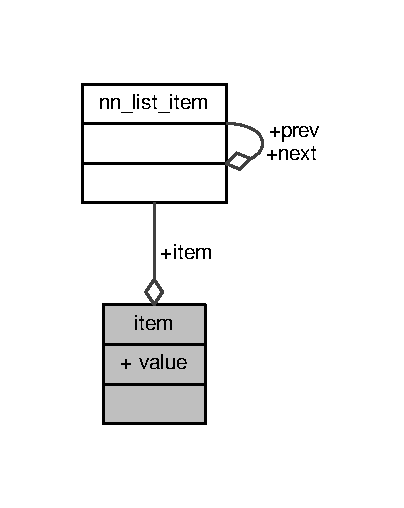
\includegraphics[width=194pt]{structitem__coll__graph}
\end{center}
\end{figure}
\subsection*{Public Attributes}
\begin{DoxyCompactItemize}
\item 
int \hyperlink{structitem_a48e03a66deef7b4ec95296391a17a420}{value}
\item 
struct \hyperlink{structnn__list__item}{nn\+\_\+list\+\_\+item} \hyperlink{structitem_adbc4635da385d1cea2cb4957467a47f9}{item}
\end{DoxyCompactItemize}


\subsection{Member Data Documentation}
\index{item@{item}!item@{item}}
\index{item@{item}!item@{item}}
\subsubsection[{item}]{\setlength{\rightskip}{0pt plus 5cm}struct {\bf nn\+\_\+list\+\_\+item} item\+::item}\hypertarget{structitem_adbc4635da385d1cea2cb4957467a47f9}{}\label{structitem_adbc4635da385d1cea2cb4957467a47f9}
\index{item@{item}!value@{value}}
\index{value@{value}!item@{item}}
\subsubsection[{value}]{\setlength{\rightskip}{0pt plus 5cm}int item\+::value}\hypertarget{structitem_a48e03a66deef7b4ec95296391a17a420}{}\label{structitem_a48e03a66deef7b4ec95296391a17a420}


The documentation for this struct was generated from the following file\+:\begin{DoxyCompactItemize}
\item 
tests/\hyperlink{tests_2list_8c}{list.\+c}\end{DoxyCompactItemize}

\hypertarget{structmsg__chunk}{}\section{msg\+\_\+chunk Struct Reference}
\label{structmsg__chunk}\index{msg\+\_\+chunk@{msg\+\_\+chunk}}


{\ttfamily \#include $<$sws.\+h$>$}



Collaboration diagram for msg\+\_\+chunk\+:\nopagebreak
\begin{figure}[H]
\begin{center}
\leavevmode
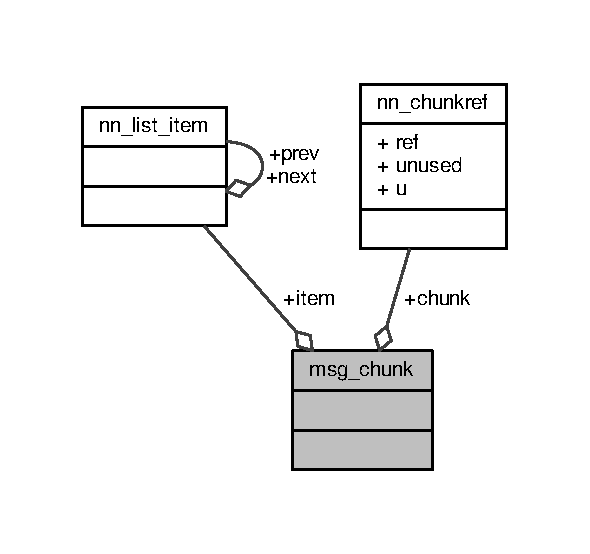
\includegraphics[width=283pt]{structmsg__chunk__coll__graph}
\end{center}
\end{figure}
\subsection*{Public Attributes}
\begin{DoxyCompactItemize}
\item 
struct \hyperlink{structnn__list__item}{nn\+\_\+list\+\_\+item} \hyperlink{structmsg__chunk_a6213f0c7d69f12c92c6b93128940ec3d}{item}
\item 
struct \hyperlink{structnn__chunkref}{nn\+\_\+chunkref} \hyperlink{structmsg__chunk_a001988b0b2d95416966e7f2fe1655f78}{chunk}
\end{DoxyCompactItemize}


\subsection{Member Data Documentation}
\index{msg\+\_\+chunk@{msg\+\_\+chunk}!chunk@{chunk}}
\index{chunk@{chunk}!msg\+\_\+chunk@{msg\+\_\+chunk}}
\subsubsection[{chunk}]{\setlength{\rightskip}{0pt plus 5cm}struct {\bf nn\+\_\+chunkref} msg\+\_\+chunk\+::chunk}\hypertarget{structmsg__chunk_a001988b0b2d95416966e7f2fe1655f78}{}\label{structmsg__chunk_a001988b0b2d95416966e7f2fe1655f78}
\index{msg\+\_\+chunk@{msg\+\_\+chunk}!item@{item}}
\index{item@{item}!msg\+\_\+chunk@{msg\+\_\+chunk}}
\subsubsection[{item}]{\setlength{\rightskip}{0pt plus 5cm}struct {\bf nn\+\_\+list\+\_\+item} msg\+\_\+chunk\+::item}\hypertarget{structmsg__chunk_a6213f0c7d69f12c92c6b93128940ec3d}{}\label{structmsg__chunk_a6213f0c7d69f12c92c6b93128940ec3d}


The documentation for this struct was generated from the following file\+:\begin{DoxyCompactItemize}
\item 
src/transports/ws/\hyperlink{sws_8h}{sws.\+h}\end{DoxyCompactItemize}

\hypertarget{structnn__aipc}{}\section{nn\+\_\+aipc Struct Reference}
\label{structnn__aipc}\index{nn\+\_\+aipc@{nn\+\_\+aipc}}


{\ttfamily \#include $<$aipc.\+h$>$}



Collaboration diagram for nn\+\_\+aipc\+:\nopagebreak
\begin{figure}[H]
\begin{center}
\leavevmode
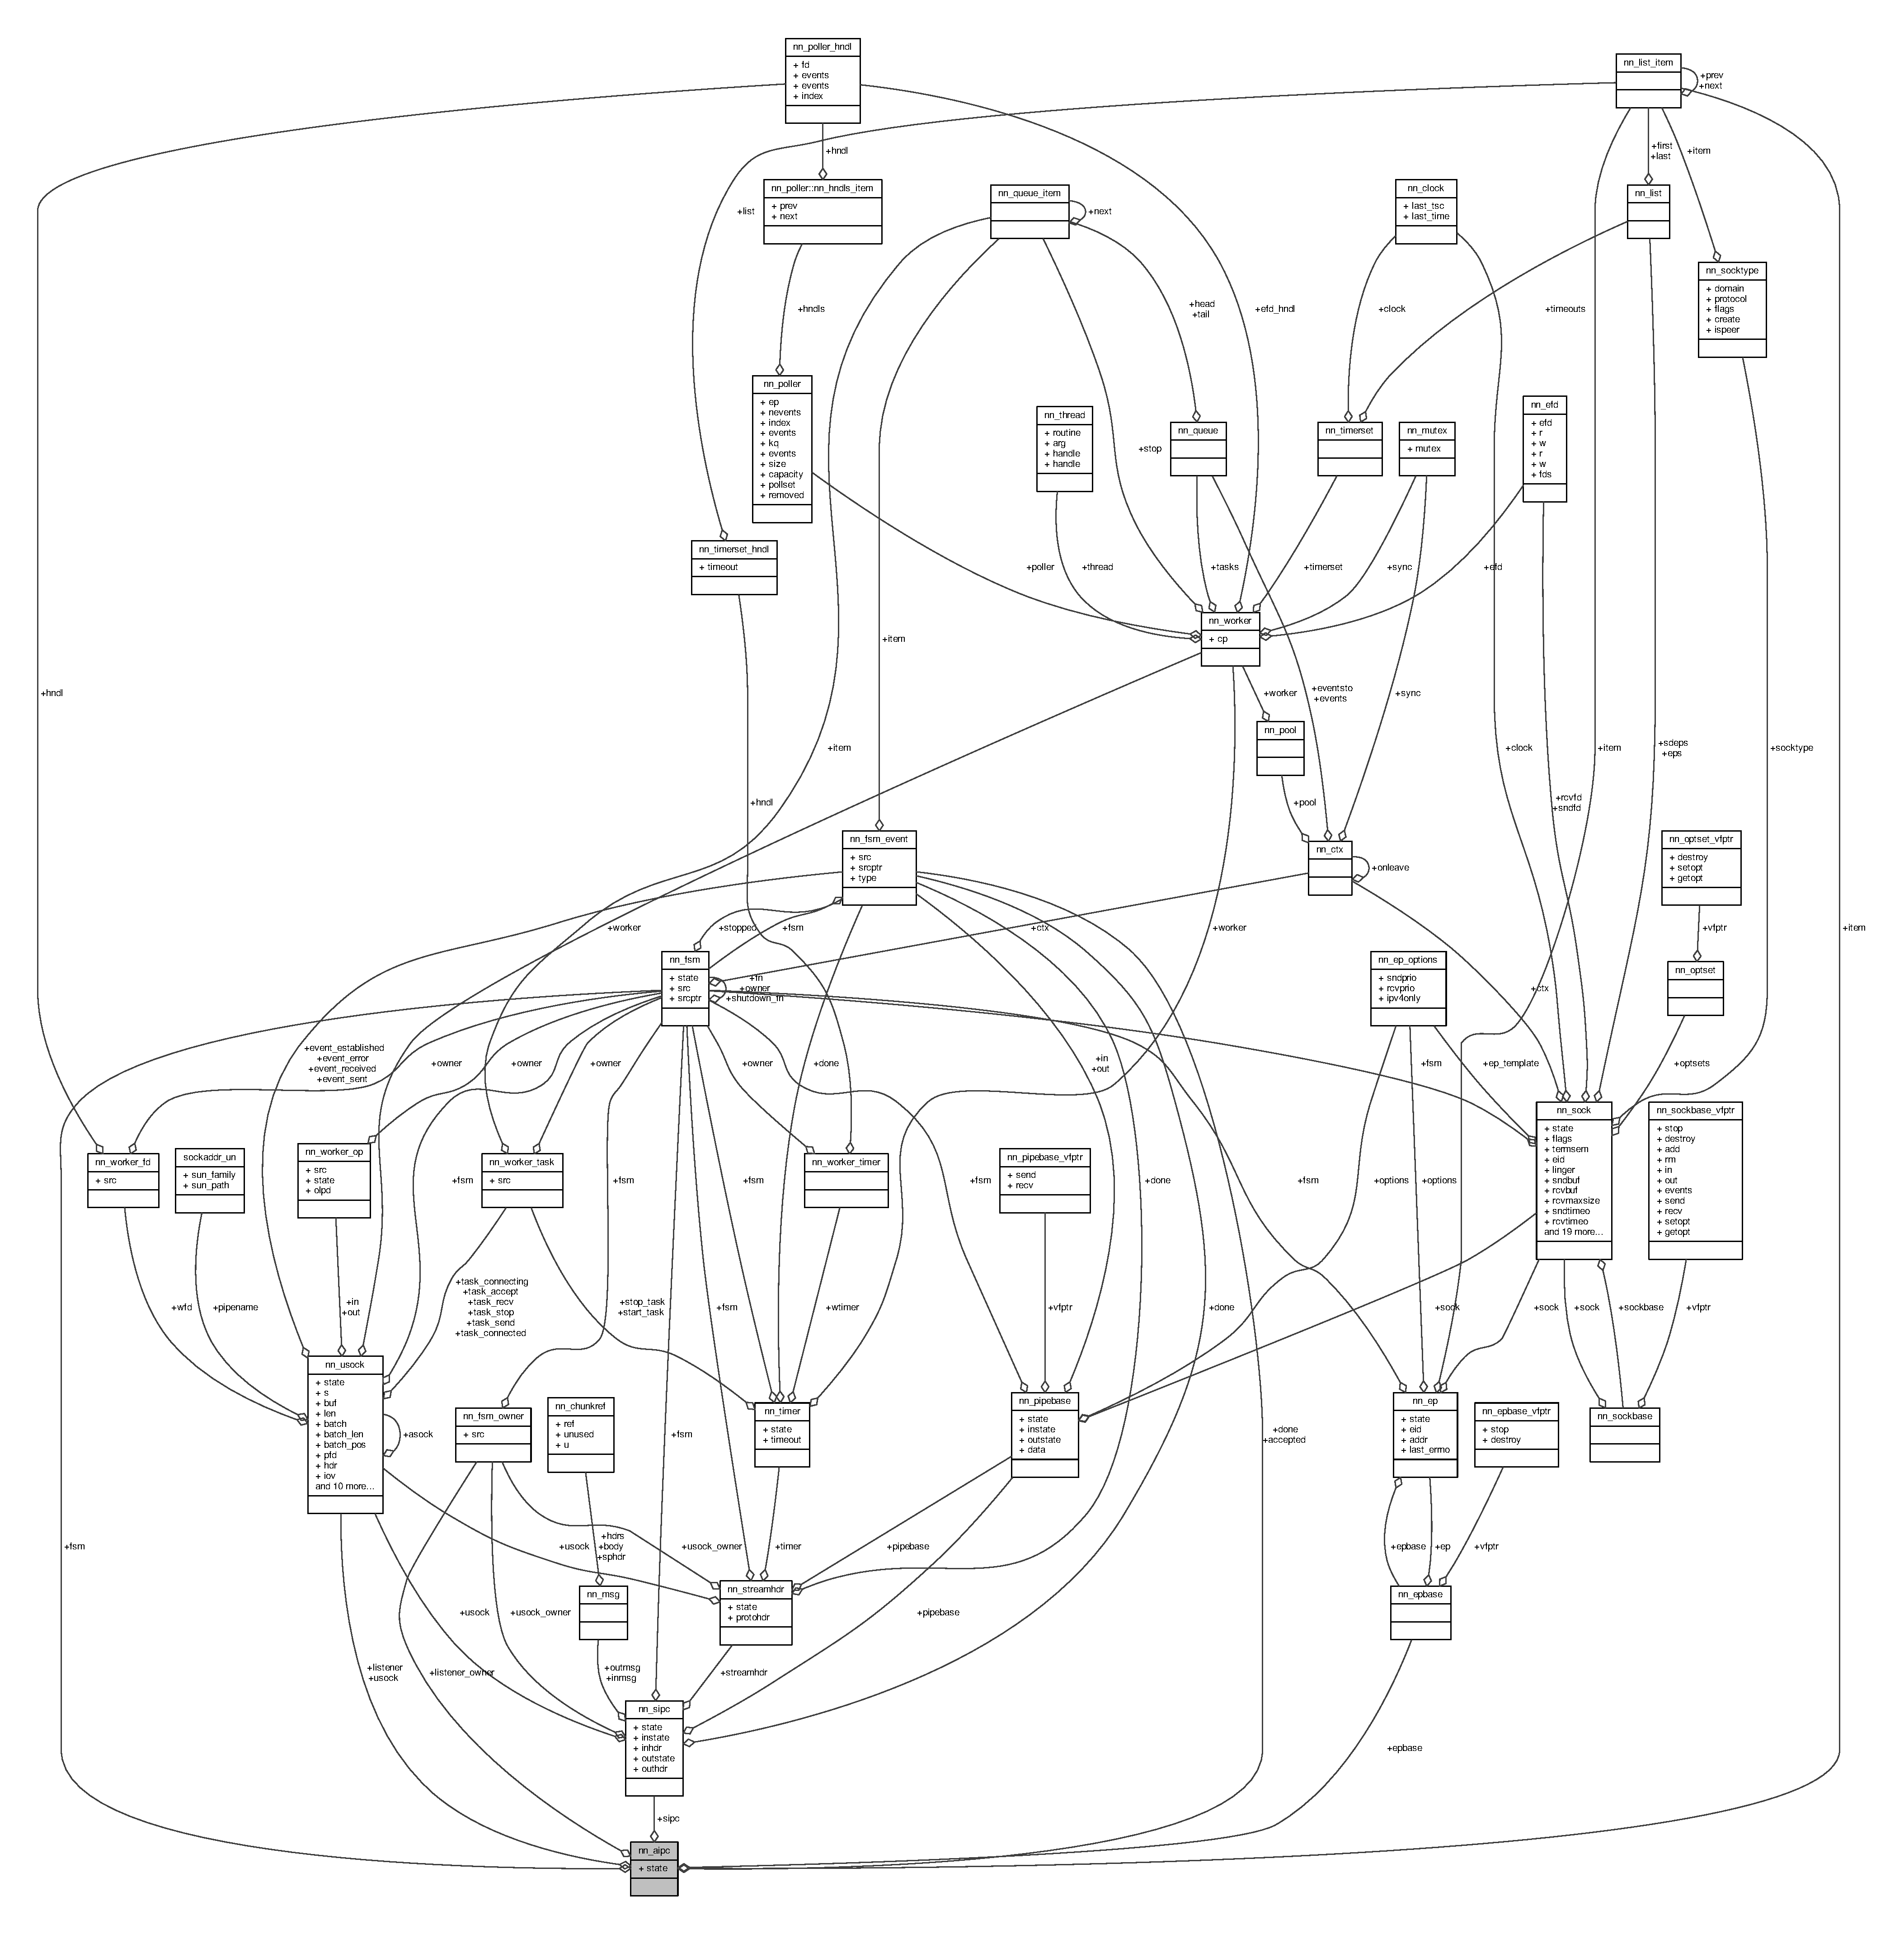
\includegraphics[width=350pt]{structnn__aipc__coll__graph}
\end{center}
\end{figure}
\subsection*{Public Attributes}
\begin{DoxyCompactItemize}
\item 
struct \hyperlink{structnn__fsm}{nn\+\_\+fsm} \hyperlink{structnn__aipc_af9e3aa7a9621f8dd9fbfe0b862dcdc89}{fsm}
\item 
int \hyperlink{structnn__aipc_a3aa1ceafa1bf2916f05b26bee723762d}{state}
\item 
struct \hyperlink{structnn__epbase}{nn\+\_\+epbase} $\ast$ \hyperlink{structnn__aipc_a25f1490e7a0246887156d2fbd12a2b80}{epbase}
\item 
struct \hyperlink{structnn__usock}{nn\+\_\+usock} \hyperlink{structnn__aipc_a9d3cd8149c6dac1c9f7987fd55325dcd}{usock}
\item 
struct \hyperlink{structnn__usock}{nn\+\_\+usock} $\ast$ \hyperlink{structnn__aipc_a008ab3a69a055c4744d6ee21042918ae}{listener}
\item 
struct \hyperlink{structnn__fsm__owner}{nn\+\_\+fsm\+\_\+owner} \hyperlink{structnn__aipc_a5a59d11eb014b4f1eb7982d762f0e524}{listener\+\_\+owner}
\item 
struct \hyperlink{structnn__sipc}{nn\+\_\+sipc} \hyperlink{structnn__aipc_a8fd7cacc4fd9dd917bb28b5531bea6d1}{sipc}
\item 
struct \hyperlink{structnn__fsm__event}{nn\+\_\+fsm\+\_\+event} \hyperlink{structnn__aipc_ad6656f52dbfb61b575abf726b4a04e53}{accepted}
\item 
struct \hyperlink{structnn__fsm__event}{nn\+\_\+fsm\+\_\+event} \hyperlink{structnn__aipc_ae4f441d4718a9fc65b30165f36ab28ac}{done}
\item 
struct \hyperlink{structnn__list__item}{nn\+\_\+list\+\_\+item} \hyperlink{structnn__aipc_aa406a6c84762843d34f8db2c0975f3cd}{item}
\end{DoxyCompactItemize}


\subsection{Member Data Documentation}
\index{nn\+\_\+aipc@{nn\+\_\+aipc}!accepted@{accepted}}
\index{accepted@{accepted}!nn\+\_\+aipc@{nn\+\_\+aipc}}
\subsubsection[{accepted}]{\setlength{\rightskip}{0pt plus 5cm}struct {\bf nn\+\_\+fsm\+\_\+event} nn\+\_\+aipc\+::accepted}\hypertarget{structnn__aipc_ad6656f52dbfb61b575abf726b4a04e53}{}\label{structnn__aipc_ad6656f52dbfb61b575abf726b4a04e53}
\index{nn\+\_\+aipc@{nn\+\_\+aipc}!done@{done}}
\index{done@{done}!nn\+\_\+aipc@{nn\+\_\+aipc}}
\subsubsection[{done}]{\setlength{\rightskip}{0pt plus 5cm}struct {\bf nn\+\_\+fsm\+\_\+event} nn\+\_\+aipc\+::done}\hypertarget{structnn__aipc_ae4f441d4718a9fc65b30165f36ab28ac}{}\label{structnn__aipc_ae4f441d4718a9fc65b30165f36ab28ac}
\index{nn\+\_\+aipc@{nn\+\_\+aipc}!epbase@{epbase}}
\index{epbase@{epbase}!nn\+\_\+aipc@{nn\+\_\+aipc}}
\subsubsection[{epbase}]{\setlength{\rightskip}{0pt plus 5cm}struct {\bf nn\+\_\+epbase}$\ast$ nn\+\_\+aipc\+::epbase}\hypertarget{structnn__aipc_a25f1490e7a0246887156d2fbd12a2b80}{}\label{structnn__aipc_a25f1490e7a0246887156d2fbd12a2b80}
\index{nn\+\_\+aipc@{nn\+\_\+aipc}!fsm@{fsm}}
\index{fsm@{fsm}!nn\+\_\+aipc@{nn\+\_\+aipc}}
\subsubsection[{fsm}]{\setlength{\rightskip}{0pt plus 5cm}struct {\bf nn\+\_\+fsm} nn\+\_\+aipc\+::fsm}\hypertarget{structnn__aipc_af9e3aa7a9621f8dd9fbfe0b862dcdc89}{}\label{structnn__aipc_af9e3aa7a9621f8dd9fbfe0b862dcdc89}
\index{nn\+\_\+aipc@{nn\+\_\+aipc}!item@{item}}
\index{item@{item}!nn\+\_\+aipc@{nn\+\_\+aipc}}
\subsubsection[{item}]{\setlength{\rightskip}{0pt plus 5cm}struct {\bf nn\+\_\+list\+\_\+item} nn\+\_\+aipc\+::item}\hypertarget{structnn__aipc_aa406a6c84762843d34f8db2c0975f3cd}{}\label{structnn__aipc_aa406a6c84762843d34f8db2c0975f3cd}
\index{nn\+\_\+aipc@{nn\+\_\+aipc}!listener@{listener}}
\index{listener@{listener}!nn\+\_\+aipc@{nn\+\_\+aipc}}
\subsubsection[{listener}]{\setlength{\rightskip}{0pt plus 5cm}struct {\bf nn\+\_\+usock}$\ast$ nn\+\_\+aipc\+::listener}\hypertarget{structnn__aipc_a008ab3a69a055c4744d6ee21042918ae}{}\label{structnn__aipc_a008ab3a69a055c4744d6ee21042918ae}
\index{nn\+\_\+aipc@{nn\+\_\+aipc}!listener\+\_\+owner@{listener\+\_\+owner}}
\index{listener\+\_\+owner@{listener\+\_\+owner}!nn\+\_\+aipc@{nn\+\_\+aipc}}
\subsubsection[{listener\+\_\+owner}]{\setlength{\rightskip}{0pt plus 5cm}struct {\bf nn\+\_\+fsm\+\_\+owner} nn\+\_\+aipc\+::listener\+\_\+owner}\hypertarget{structnn__aipc_a5a59d11eb014b4f1eb7982d762f0e524}{}\label{structnn__aipc_a5a59d11eb014b4f1eb7982d762f0e524}
\index{nn\+\_\+aipc@{nn\+\_\+aipc}!sipc@{sipc}}
\index{sipc@{sipc}!nn\+\_\+aipc@{nn\+\_\+aipc}}
\subsubsection[{sipc}]{\setlength{\rightskip}{0pt plus 5cm}struct {\bf nn\+\_\+sipc} nn\+\_\+aipc\+::sipc}\hypertarget{structnn__aipc_a8fd7cacc4fd9dd917bb28b5531bea6d1}{}\label{structnn__aipc_a8fd7cacc4fd9dd917bb28b5531bea6d1}
\index{nn\+\_\+aipc@{nn\+\_\+aipc}!state@{state}}
\index{state@{state}!nn\+\_\+aipc@{nn\+\_\+aipc}}
\subsubsection[{state}]{\setlength{\rightskip}{0pt plus 5cm}int nn\+\_\+aipc\+::state}\hypertarget{structnn__aipc_a3aa1ceafa1bf2916f05b26bee723762d}{}\label{structnn__aipc_a3aa1ceafa1bf2916f05b26bee723762d}
\index{nn\+\_\+aipc@{nn\+\_\+aipc}!usock@{usock}}
\index{usock@{usock}!nn\+\_\+aipc@{nn\+\_\+aipc}}
\subsubsection[{usock}]{\setlength{\rightskip}{0pt plus 5cm}struct {\bf nn\+\_\+usock} nn\+\_\+aipc\+::usock}\hypertarget{structnn__aipc_a9d3cd8149c6dac1c9f7987fd55325dcd}{}\label{structnn__aipc_a9d3cd8149c6dac1c9f7987fd55325dcd}


The documentation for this struct was generated from the following file\+:\begin{DoxyCompactItemize}
\item 
src/transports/ipc/\hyperlink{aipc_8h}{aipc.\+h}\end{DoxyCompactItemize}

\hypertarget{structnn__alibfabric}{}\section{nn\+\_\+alibfabric Struct Reference}
\label{structnn__alibfabric}\index{nn\+\_\+alibfabric@{nn\+\_\+alibfabric}}


{\ttfamily \#include $<$alibfabric.\+h$>$}



Collaboration diagram for nn\+\_\+alibfabric\+:\nopagebreak
\begin{figure}[H]
\begin{center}
\leavevmode
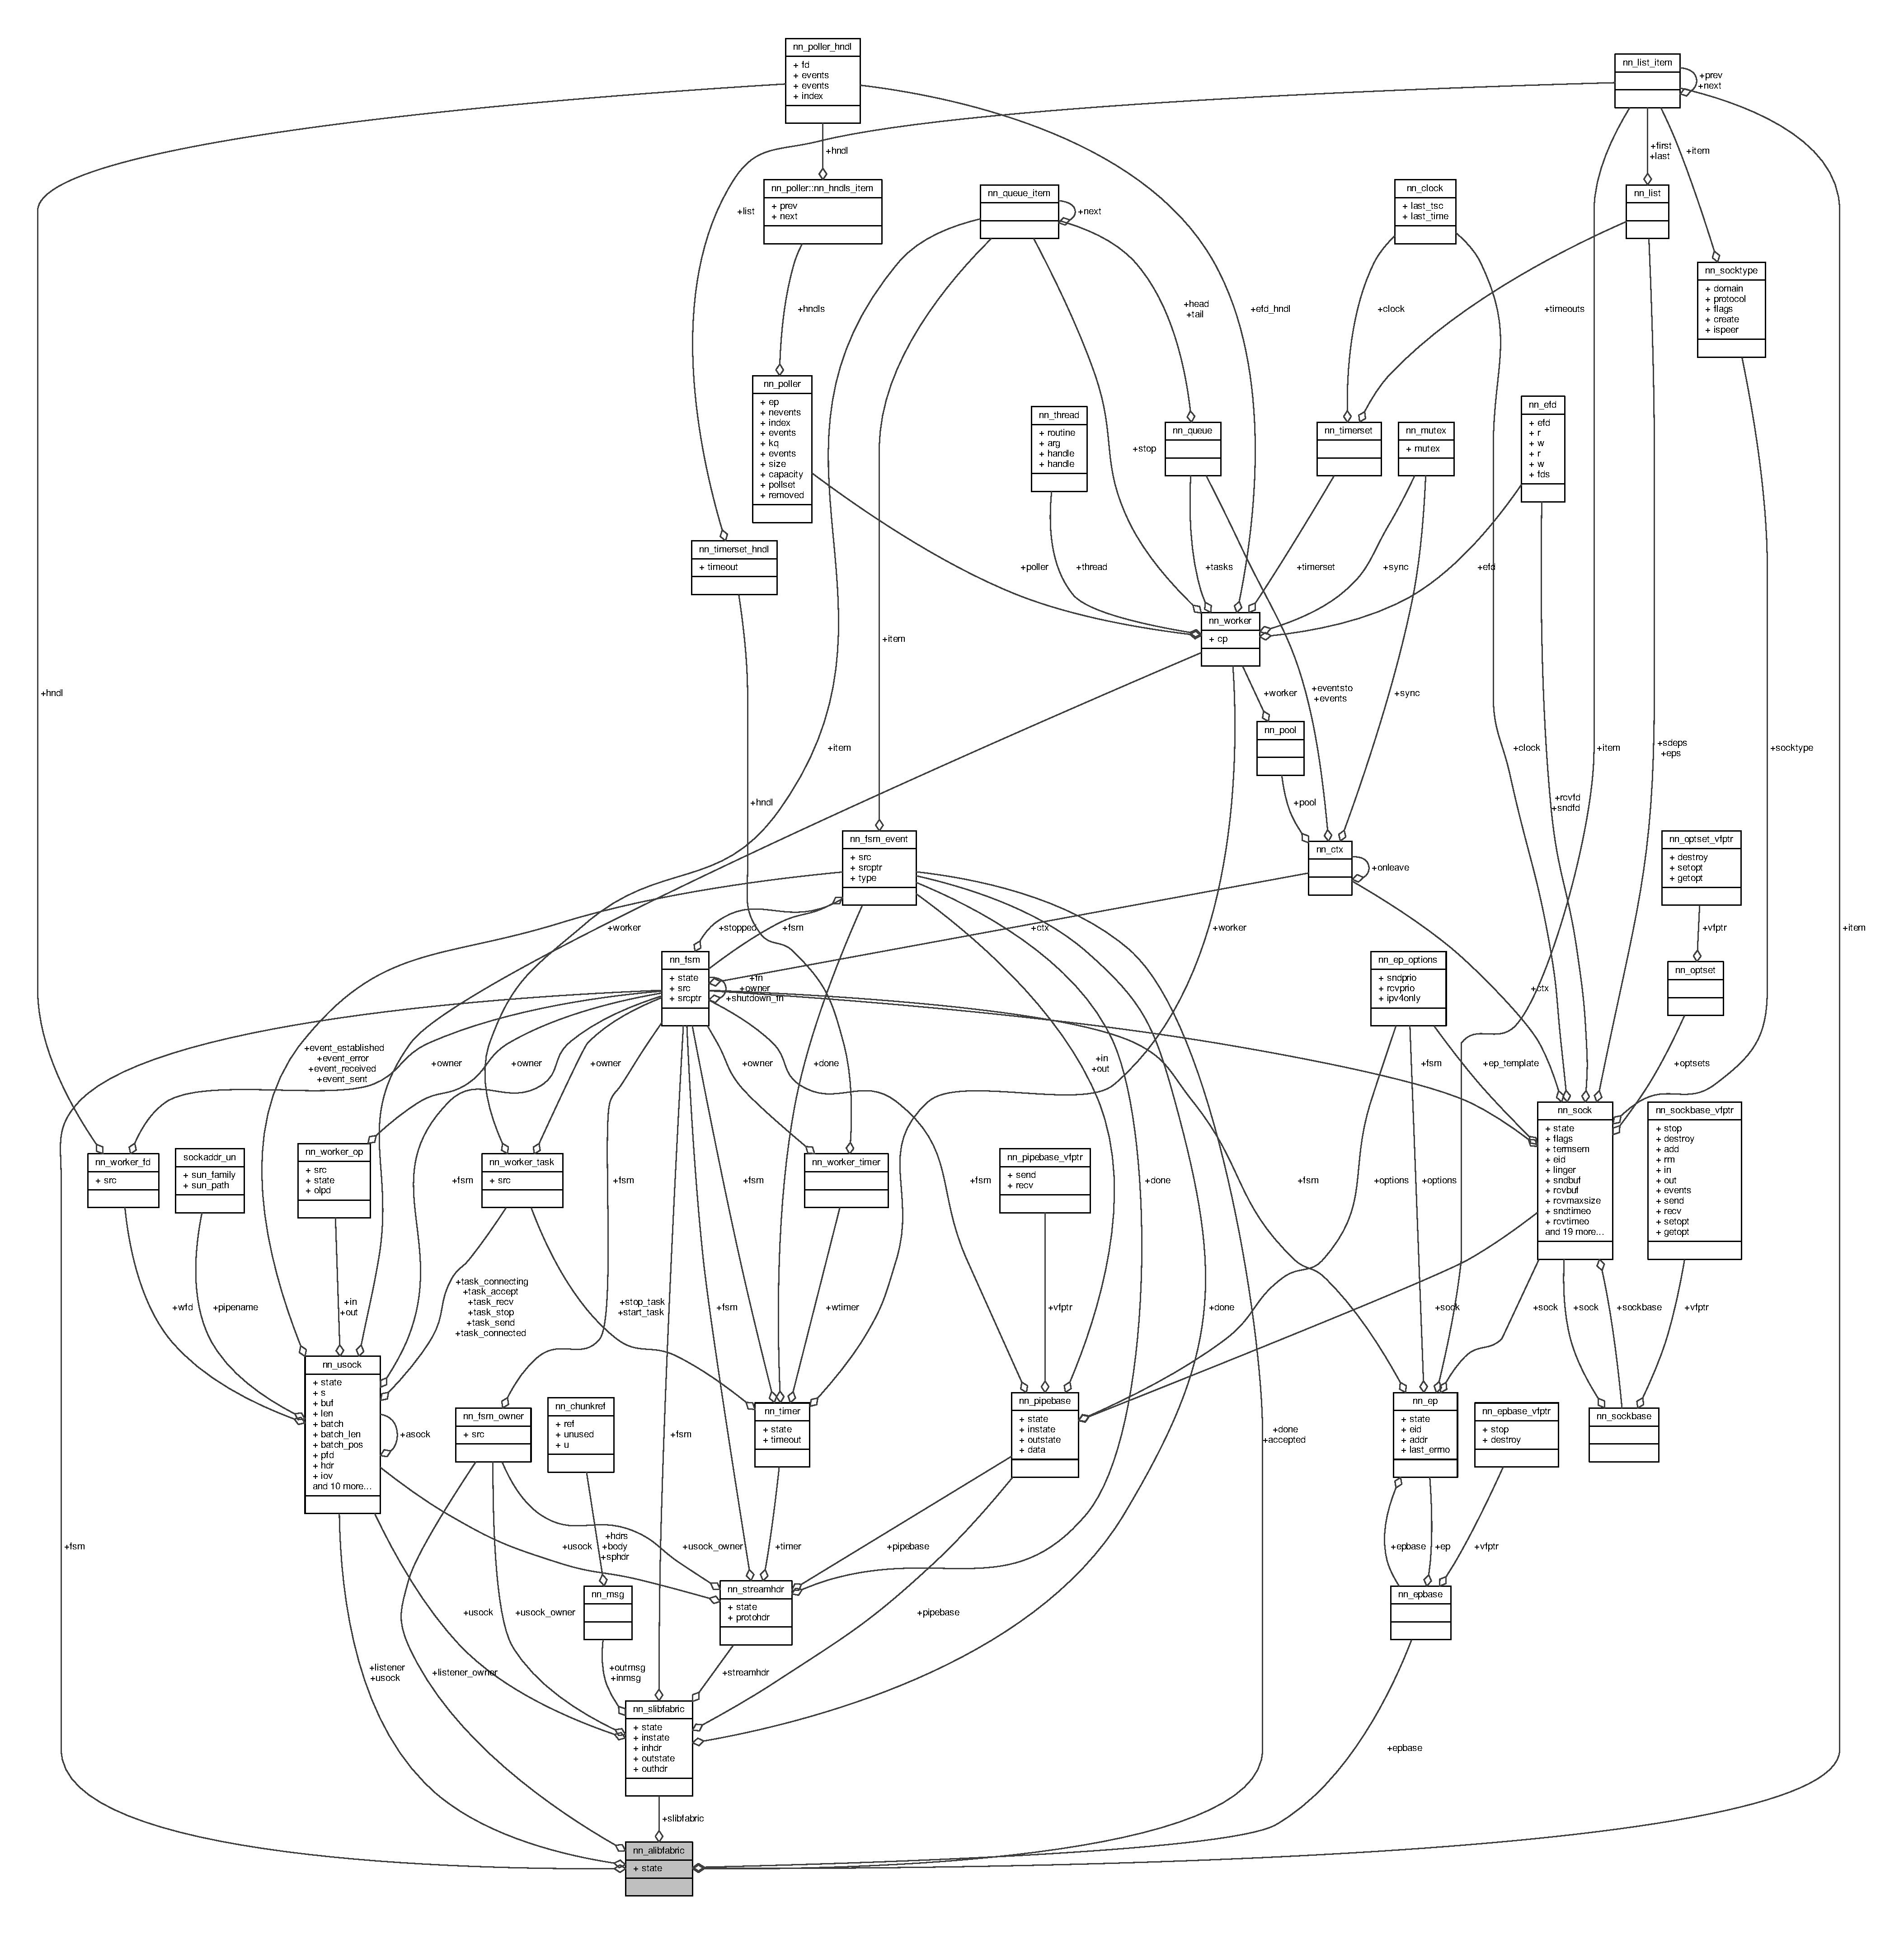
\includegraphics[width=350pt]{structnn__alibfabric__coll__graph}
\end{center}
\end{figure}
\subsection*{Public Attributes}
\begin{DoxyCompactItemize}
\item 
struct \hyperlink{structnn__fsm}{nn\+\_\+fsm} \hyperlink{structnn__alibfabric_ad969c376667b2c3116ac8d4450ec23e8}{fsm}
\item 
int \hyperlink{structnn__alibfabric_a21e93d82aff04c8a9ae6ba0122396ab4}{state}
\item 
struct \hyperlink{structnn__epbase}{nn\+\_\+epbase} $\ast$ \hyperlink{structnn__alibfabric_a6b8cbf1bd52a83e5420c21f7a1970fd5}{epbase}
\item 
struct \hyperlink{structnn__usock}{nn\+\_\+usock} \hyperlink{structnn__alibfabric_ac33d4e6efd8a6f9246e1573b05b7cad3}{usock}
\item 
struct \hyperlink{structnn__usock}{nn\+\_\+usock} $\ast$ \hyperlink{structnn__alibfabric_a164d9831253cc912122c3bb2ae674e74}{listener}
\item 
struct \hyperlink{structnn__fsm__owner}{nn\+\_\+fsm\+\_\+owner} \hyperlink{structnn__alibfabric_a78da852e79fbc018efabdb7215671dfc}{listener\+\_\+owner}
\item 
struct \hyperlink{structnn__slibfabric}{nn\+\_\+slibfabric} \hyperlink{structnn__alibfabric_aeb290b975bf6b052ec19e015ff95e6a1}{slibfabric}
\item 
struct \hyperlink{structnn__fsm__event}{nn\+\_\+fsm\+\_\+event} \hyperlink{structnn__alibfabric_aa437f27727644387eb2e42a38c0050ea}{accepted}
\item 
struct \hyperlink{structnn__fsm__event}{nn\+\_\+fsm\+\_\+event} \hyperlink{structnn__alibfabric_a87f3db2d6a717b2d07e7a2acf1d1ef90}{done}
\item 
struct \hyperlink{structnn__list__item}{nn\+\_\+list\+\_\+item} \hyperlink{structnn__alibfabric_a0fa4548f6e507cd776b75470cbbc7d49}{item}
\end{DoxyCompactItemize}


\subsection{Member Data Documentation}
\index{nn\+\_\+alibfabric@{nn\+\_\+alibfabric}!accepted@{accepted}}
\index{accepted@{accepted}!nn\+\_\+alibfabric@{nn\+\_\+alibfabric}}
\subsubsection[{accepted}]{\setlength{\rightskip}{0pt plus 5cm}struct {\bf nn\+\_\+fsm\+\_\+event} nn\+\_\+alibfabric\+::accepted}\hypertarget{structnn__alibfabric_aa437f27727644387eb2e42a38c0050ea}{}\label{structnn__alibfabric_aa437f27727644387eb2e42a38c0050ea}
\index{nn\+\_\+alibfabric@{nn\+\_\+alibfabric}!done@{done}}
\index{done@{done}!nn\+\_\+alibfabric@{nn\+\_\+alibfabric}}
\subsubsection[{done}]{\setlength{\rightskip}{0pt plus 5cm}struct {\bf nn\+\_\+fsm\+\_\+event} nn\+\_\+alibfabric\+::done}\hypertarget{structnn__alibfabric_a87f3db2d6a717b2d07e7a2acf1d1ef90}{}\label{structnn__alibfabric_a87f3db2d6a717b2d07e7a2acf1d1ef90}
\index{nn\+\_\+alibfabric@{nn\+\_\+alibfabric}!epbase@{epbase}}
\index{epbase@{epbase}!nn\+\_\+alibfabric@{nn\+\_\+alibfabric}}
\subsubsection[{epbase}]{\setlength{\rightskip}{0pt plus 5cm}struct {\bf nn\+\_\+epbase}$\ast$ nn\+\_\+alibfabric\+::epbase}\hypertarget{structnn__alibfabric_a6b8cbf1bd52a83e5420c21f7a1970fd5}{}\label{structnn__alibfabric_a6b8cbf1bd52a83e5420c21f7a1970fd5}
\index{nn\+\_\+alibfabric@{nn\+\_\+alibfabric}!fsm@{fsm}}
\index{fsm@{fsm}!nn\+\_\+alibfabric@{nn\+\_\+alibfabric}}
\subsubsection[{fsm}]{\setlength{\rightskip}{0pt plus 5cm}struct {\bf nn\+\_\+fsm} nn\+\_\+alibfabric\+::fsm}\hypertarget{structnn__alibfabric_ad969c376667b2c3116ac8d4450ec23e8}{}\label{structnn__alibfabric_ad969c376667b2c3116ac8d4450ec23e8}
\index{nn\+\_\+alibfabric@{nn\+\_\+alibfabric}!item@{item}}
\index{item@{item}!nn\+\_\+alibfabric@{nn\+\_\+alibfabric}}
\subsubsection[{item}]{\setlength{\rightskip}{0pt plus 5cm}struct {\bf nn\+\_\+list\+\_\+item} nn\+\_\+alibfabric\+::item}\hypertarget{structnn__alibfabric_a0fa4548f6e507cd776b75470cbbc7d49}{}\label{structnn__alibfabric_a0fa4548f6e507cd776b75470cbbc7d49}
\index{nn\+\_\+alibfabric@{nn\+\_\+alibfabric}!listener@{listener}}
\index{listener@{listener}!nn\+\_\+alibfabric@{nn\+\_\+alibfabric}}
\subsubsection[{listener}]{\setlength{\rightskip}{0pt plus 5cm}struct {\bf nn\+\_\+usock}$\ast$ nn\+\_\+alibfabric\+::listener}\hypertarget{structnn__alibfabric_a164d9831253cc912122c3bb2ae674e74}{}\label{structnn__alibfabric_a164d9831253cc912122c3bb2ae674e74}
\index{nn\+\_\+alibfabric@{nn\+\_\+alibfabric}!listener\+\_\+owner@{listener\+\_\+owner}}
\index{listener\+\_\+owner@{listener\+\_\+owner}!nn\+\_\+alibfabric@{nn\+\_\+alibfabric}}
\subsubsection[{listener\+\_\+owner}]{\setlength{\rightskip}{0pt plus 5cm}struct {\bf nn\+\_\+fsm\+\_\+owner} nn\+\_\+alibfabric\+::listener\+\_\+owner}\hypertarget{structnn__alibfabric_a78da852e79fbc018efabdb7215671dfc}{}\label{structnn__alibfabric_a78da852e79fbc018efabdb7215671dfc}
\index{nn\+\_\+alibfabric@{nn\+\_\+alibfabric}!slibfabric@{slibfabric}}
\index{slibfabric@{slibfabric}!nn\+\_\+alibfabric@{nn\+\_\+alibfabric}}
\subsubsection[{slibfabric}]{\setlength{\rightskip}{0pt plus 5cm}struct {\bf nn\+\_\+slibfabric} nn\+\_\+alibfabric\+::slibfabric}\hypertarget{structnn__alibfabric_aeb290b975bf6b052ec19e015ff95e6a1}{}\label{structnn__alibfabric_aeb290b975bf6b052ec19e015ff95e6a1}
\index{nn\+\_\+alibfabric@{nn\+\_\+alibfabric}!state@{state}}
\index{state@{state}!nn\+\_\+alibfabric@{nn\+\_\+alibfabric}}
\subsubsection[{state}]{\setlength{\rightskip}{0pt plus 5cm}int nn\+\_\+alibfabric\+::state}\hypertarget{structnn__alibfabric_a21e93d82aff04c8a9ae6ba0122396ab4}{}\label{structnn__alibfabric_a21e93d82aff04c8a9ae6ba0122396ab4}
\index{nn\+\_\+alibfabric@{nn\+\_\+alibfabric}!usock@{usock}}
\index{usock@{usock}!nn\+\_\+alibfabric@{nn\+\_\+alibfabric}}
\subsubsection[{usock}]{\setlength{\rightskip}{0pt plus 5cm}struct {\bf nn\+\_\+usock} nn\+\_\+alibfabric\+::usock}\hypertarget{structnn__alibfabric_ac33d4e6efd8a6f9246e1573b05b7cad3}{}\label{structnn__alibfabric_ac33d4e6efd8a6f9246e1573b05b7cad3}


The documentation for this struct was generated from the following file\+:\begin{DoxyCompactItemize}
\item 
src/transports/libfabric/\hyperlink{alibfabric_8h}{alibfabric.\+h}\end{DoxyCompactItemize}

\hypertarget{structnn__atcp}{}\section{nn\+\_\+atcp Struct Reference}
\label{structnn__atcp}\index{nn\+\_\+atcp@{nn\+\_\+atcp}}


{\ttfamily \#include $<$atcp.\+h$>$}



Collaboration diagram for nn\+\_\+atcp\+:\nopagebreak
\begin{figure}[H]
\begin{center}
\leavevmode
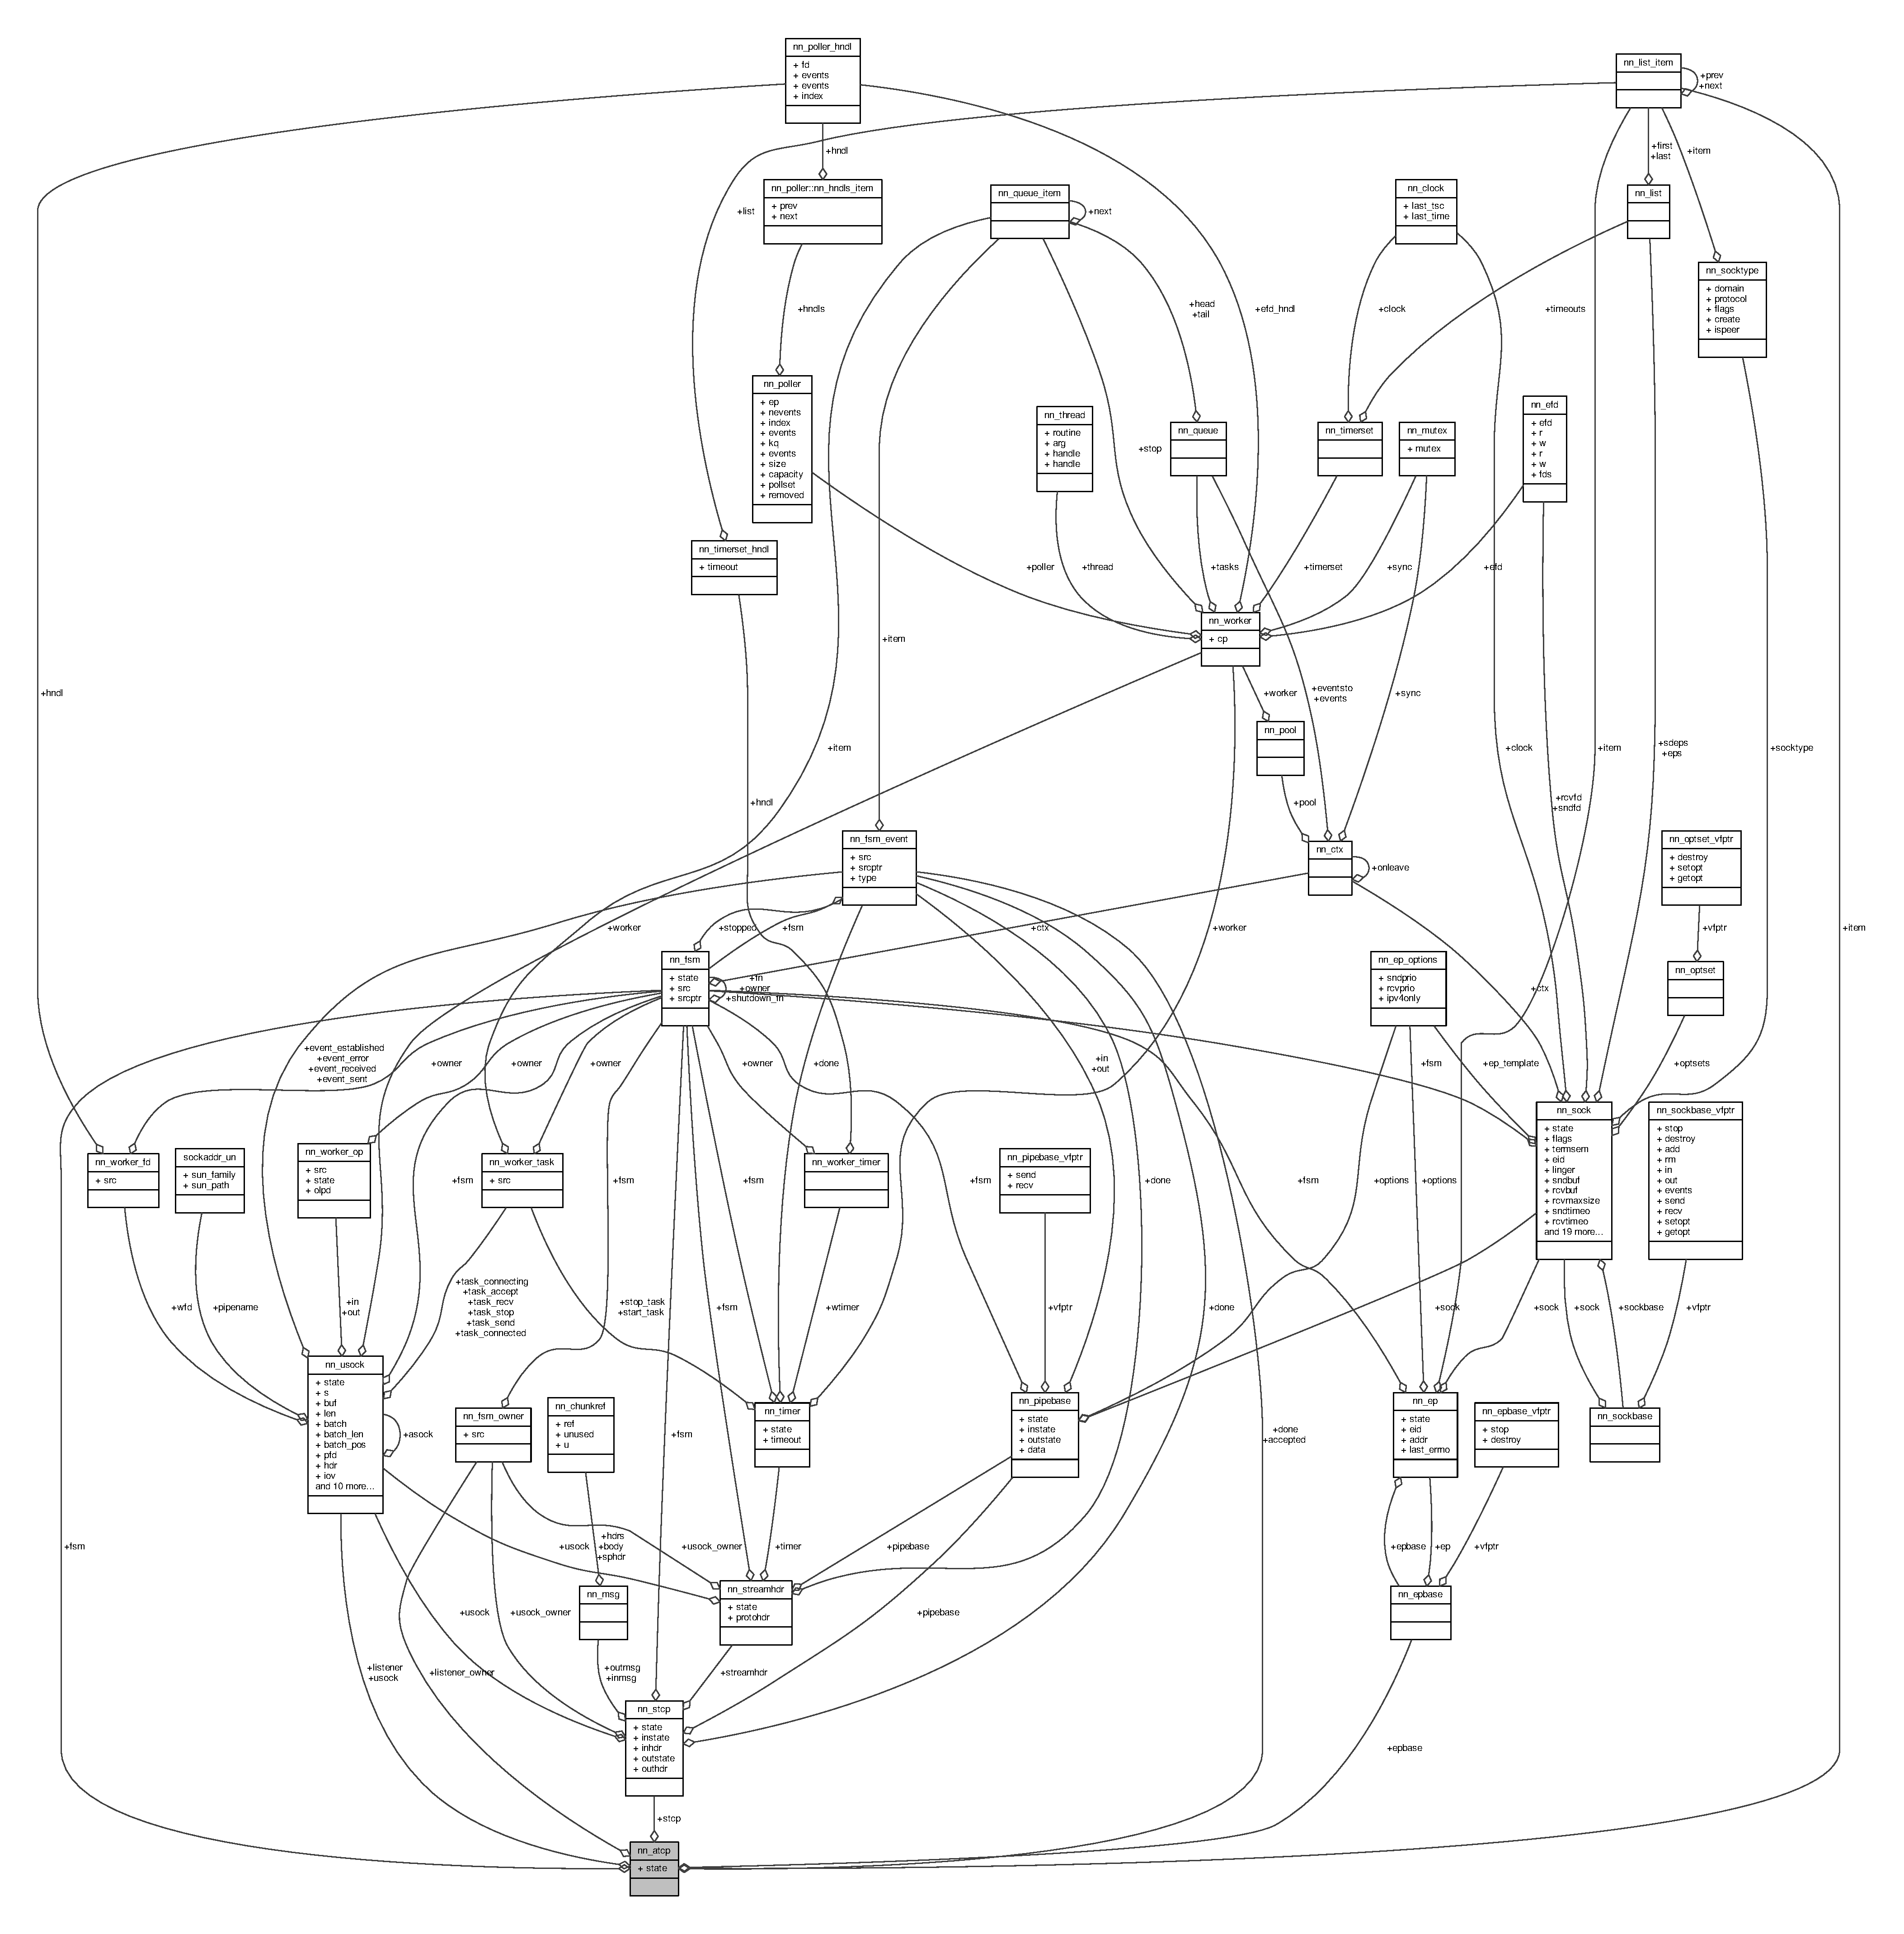
\includegraphics[width=350pt]{structnn__atcp__coll__graph}
\end{center}
\end{figure}
\subsection*{Public Attributes}
\begin{DoxyCompactItemize}
\item 
struct \hyperlink{structnn__fsm}{nn\+\_\+fsm} \hyperlink{structnn__atcp_ad04808fad8020edc6f3eb6e3b29cc793}{fsm}
\item 
int \hyperlink{structnn__atcp_ae28b649a99c4ae7f613d924dcdccc739}{state}
\item 
struct \hyperlink{structnn__epbase}{nn\+\_\+epbase} $\ast$ \hyperlink{structnn__atcp_ac1a71726a1f8735cb9c053f7f853ccdf}{epbase}
\item 
struct \hyperlink{structnn__usock}{nn\+\_\+usock} \hyperlink{structnn__atcp_ad3d53b493bc19478dea4f8b0de9854c5}{usock}
\item 
struct \hyperlink{structnn__usock}{nn\+\_\+usock} $\ast$ \hyperlink{structnn__atcp_a9d4cb8ab1d456ad451669a4563b3460d}{listener}
\item 
struct \hyperlink{structnn__fsm__owner}{nn\+\_\+fsm\+\_\+owner} \hyperlink{structnn__atcp_a78e8bf6c84ec7434898721de359545b7}{listener\+\_\+owner}
\item 
struct \hyperlink{structnn__stcp}{nn\+\_\+stcp} \hyperlink{structnn__atcp_a523f49bc19d9da3b311cff626cec79ff}{stcp}
\item 
struct \hyperlink{structnn__fsm__event}{nn\+\_\+fsm\+\_\+event} \hyperlink{structnn__atcp_a72950d59f755960bf799aad00e145c11}{accepted}
\item 
struct \hyperlink{structnn__fsm__event}{nn\+\_\+fsm\+\_\+event} \hyperlink{structnn__atcp_a4879108dbbc8b71b2bda57a38e41fb4b}{done}
\item 
struct \hyperlink{structnn__list__item}{nn\+\_\+list\+\_\+item} \hyperlink{structnn__atcp_a6fd995526e62b8f65d6848c383b8714c}{item}
\end{DoxyCompactItemize}


\subsection{Member Data Documentation}
\index{nn\+\_\+atcp@{nn\+\_\+atcp}!accepted@{accepted}}
\index{accepted@{accepted}!nn\+\_\+atcp@{nn\+\_\+atcp}}
\subsubsection[{accepted}]{\setlength{\rightskip}{0pt plus 5cm}struct {\bf nn\+\_\+fsm\+\_\+event} nn\+\_\+atcp\+::accepted}\hypertarget{structnn__atcp_a72950d59f755960bf799aad00e145c11}{}\label{structnn__atcp_a72950d59f755960bf799aad00e145c11}
\index{nn\+\_\+atcp@{nn\+\_\+atcp}!done@{done}}
\index{done@{done}!nn\+\_\+atcp@{nn\+\_\+atcp}}
\subsubsection[{done}]{\setlength{\rightskip}{0pt plus 5cm}struct {\bf nn\+\_\+fsm\+\_\+event} nn\+\_\+atcp\+::done}\hypertarget{structnn__atcp_a4879108dbbc8b71b2bda57a38e41fb4b}{}\label{structnn__atcp_a4879108dbbc8b71b2bda57a38e41fb4b}
\index{nn\+\_\+atcp@{nn\+\_\+atcp}!epbase@{epbase}}
\index{epbase@{epbase}!nn\+\_\+atcp@{nn\+\_\+atcp}}
\subsubsection[{epbase}]{\setlength{\rightskip}{0pt plus 5cm}struct {\bf nn\+\_\+epbase}$\ast$ nn\+\_\+atcp\+::epbase}\hypertarget{structnn__atcp_ac1a71726a1f8735cb9c053f7f853ccdf}{}\label{structnn__atcp_ac1a71726a1f8735cb9c053f7f853ccdf}
\index{nn\+\_\+atcp@{nn\+\_\+atcp}!fsm@{fsm}}
\index{fsm@{fsm}!nn\+\_\+atcp@{nn\+\_\+atcp}}
\subsubsection[{fsm}]{\setlength{\rightskip}{0pt plus 5cm}struct {\bf nn\+\_\+fsm} nn\+\_\+atcp\+::fsm}\hypertarget{structnn__atcp_ad04808fad8020edc6f3eb6e3b29cc793}{}\label{structnn__atcp_ad04808fad8020edc6f3eb6e3b29cc793}
\index{nn\+\_\+atcp@{nn\+\_\+atcp}!item@{item}}
\index{item@{item}!nn\+\_\+atcp@{nn\+\_\+atcp}}
\subsubsection[{item}]{\setlength{\rightskip}{0pt plus 5cm}struct {\bf nn\+\_\+list\+\_\+item} nn\+\_\+atcp\+::item}\hypertarget{structnn__atcp_a6fd995526e62b8f65d6848c383b8714c}{}\label{structnn__atcp_a6fd995526e62b8f65d6848c383b8714c}
\index{nn\+\_\+atcp@{nn\+\_\+atcp}!listener@{listener}}
\index{listener@{listener}!nn\+\_\+atcp@{nn\+\_\+atcp}}
\subsubsection[{listener}]{\setlength{\rightskip}{0pt plus 5cm}struct {\bf nn\+\_\+usock}$\ast$ nn\+\_\+atcp\+::listener}\hypertarget{structnn__atcp_a9d4cb8ab1d456ad451669a4563b3460d}{}\label{structnn__atcp_a9d4cb8ab1d456ad451669a4563b3460d}
\index{nn\+\_\+atcp@{nn\+\_\+atcp}!listener\+\_\+owner@{listener\+\_\+owner}}
\index{listener\+\_\+owner@{listener\+\_\+owner}!nn\+\_\+atcp@{nn\+\_\+atcp}}
\subsubsection[{listener\+\_\+owner}]{\setlength{\rightskip}{0pt plus 5cm}struct {\bf nn\+\_\+fsm\+\_\+owner} nn\+\_\+atcp\+::listener\+\_\+owner}\hypertarget{structnn__atcp_a78e8bf6c84ec7434898721de359545b7}{}\label{structnn__atcp_a78e8bf6c84ec7434898721de359545b7}
\index{nn\+\_\+atcp@{nn\+\_\+atcp}!state@{state}}
\index{state@{state}!nn\+\_\+atcp@{nn\+\_\+atcp}}
\subsubsection[{state}]{\setlength{\rightskip}{0pt plus 5cm}int nn\+\_\+atcp\+::state}\hypertarget{structnn__atcp_ae28b649a99c4ae7f613d924dcdccc739}{}\label{structnn__atcp_ae28b649a99c4ae7f613d924dcdccc739}
\index{nn\+\_\+atcp@{nn\+\_\+atcp}!stcp@{stcp}}
\index{stcp@{stcp}!nn\+\_\+atcp@{nn\+\_\+atcp}}
\subsubsection[{stcp}]{\setlength{\rightskip}{0pt plus 5cm}struct {\bf nn\+\_\+stcp} nn\+\_\+atcp\+::stcp}\hypertarget{structnn__atcp_a523f49bc19d9da3b311cff626cec79ff}{}\label{structnn__atcp_a523f49bc19d9da3b311cff626cec79ff}
\index{nn\+\_\+atcp@{nn\+\_\+atcp}!usock@{usock}}
\index{usock@{usock}!nn\+\_\+atcp@{nn\+\_\+atcp}}
\subsubsection[{usock}]{\setlength{\rightskip}{0pt plus 5cm}struct {\bf nn\+\_\+usock} nn\+\_\+atcp\+::usock}\hypertarget{structnn__atcp_ad3d53b493bc19478dea4f8b0de9854c5}{}\label{structnn__atcp_ad3d53b493bc19478dea4f8b0de9854c5}


The documentation for this struct was generated from the following file\+:\begin{DoxyCompactItemize}
\item 
src/transports/tcp/\hyperlink{atcp_8h}{atcp.\+h}\end{DoxyCompactItemize}

\hypertarget{structnn__atcpmux}{}\section{nn\+\_\+atcpmux Struct Reference}
\label{structnn__atcpmux}\index{nn\+\_\+atcpmux@{nn\+\_\+atcpmux}}


{\ttfamily \#include $<$atcpmux.\+h$>$}



Collaboration diagram for nn\+\_\+atcpmux\+:\nopagebreak
\begin{figure}[H]
\begin{center}
\leavevmode
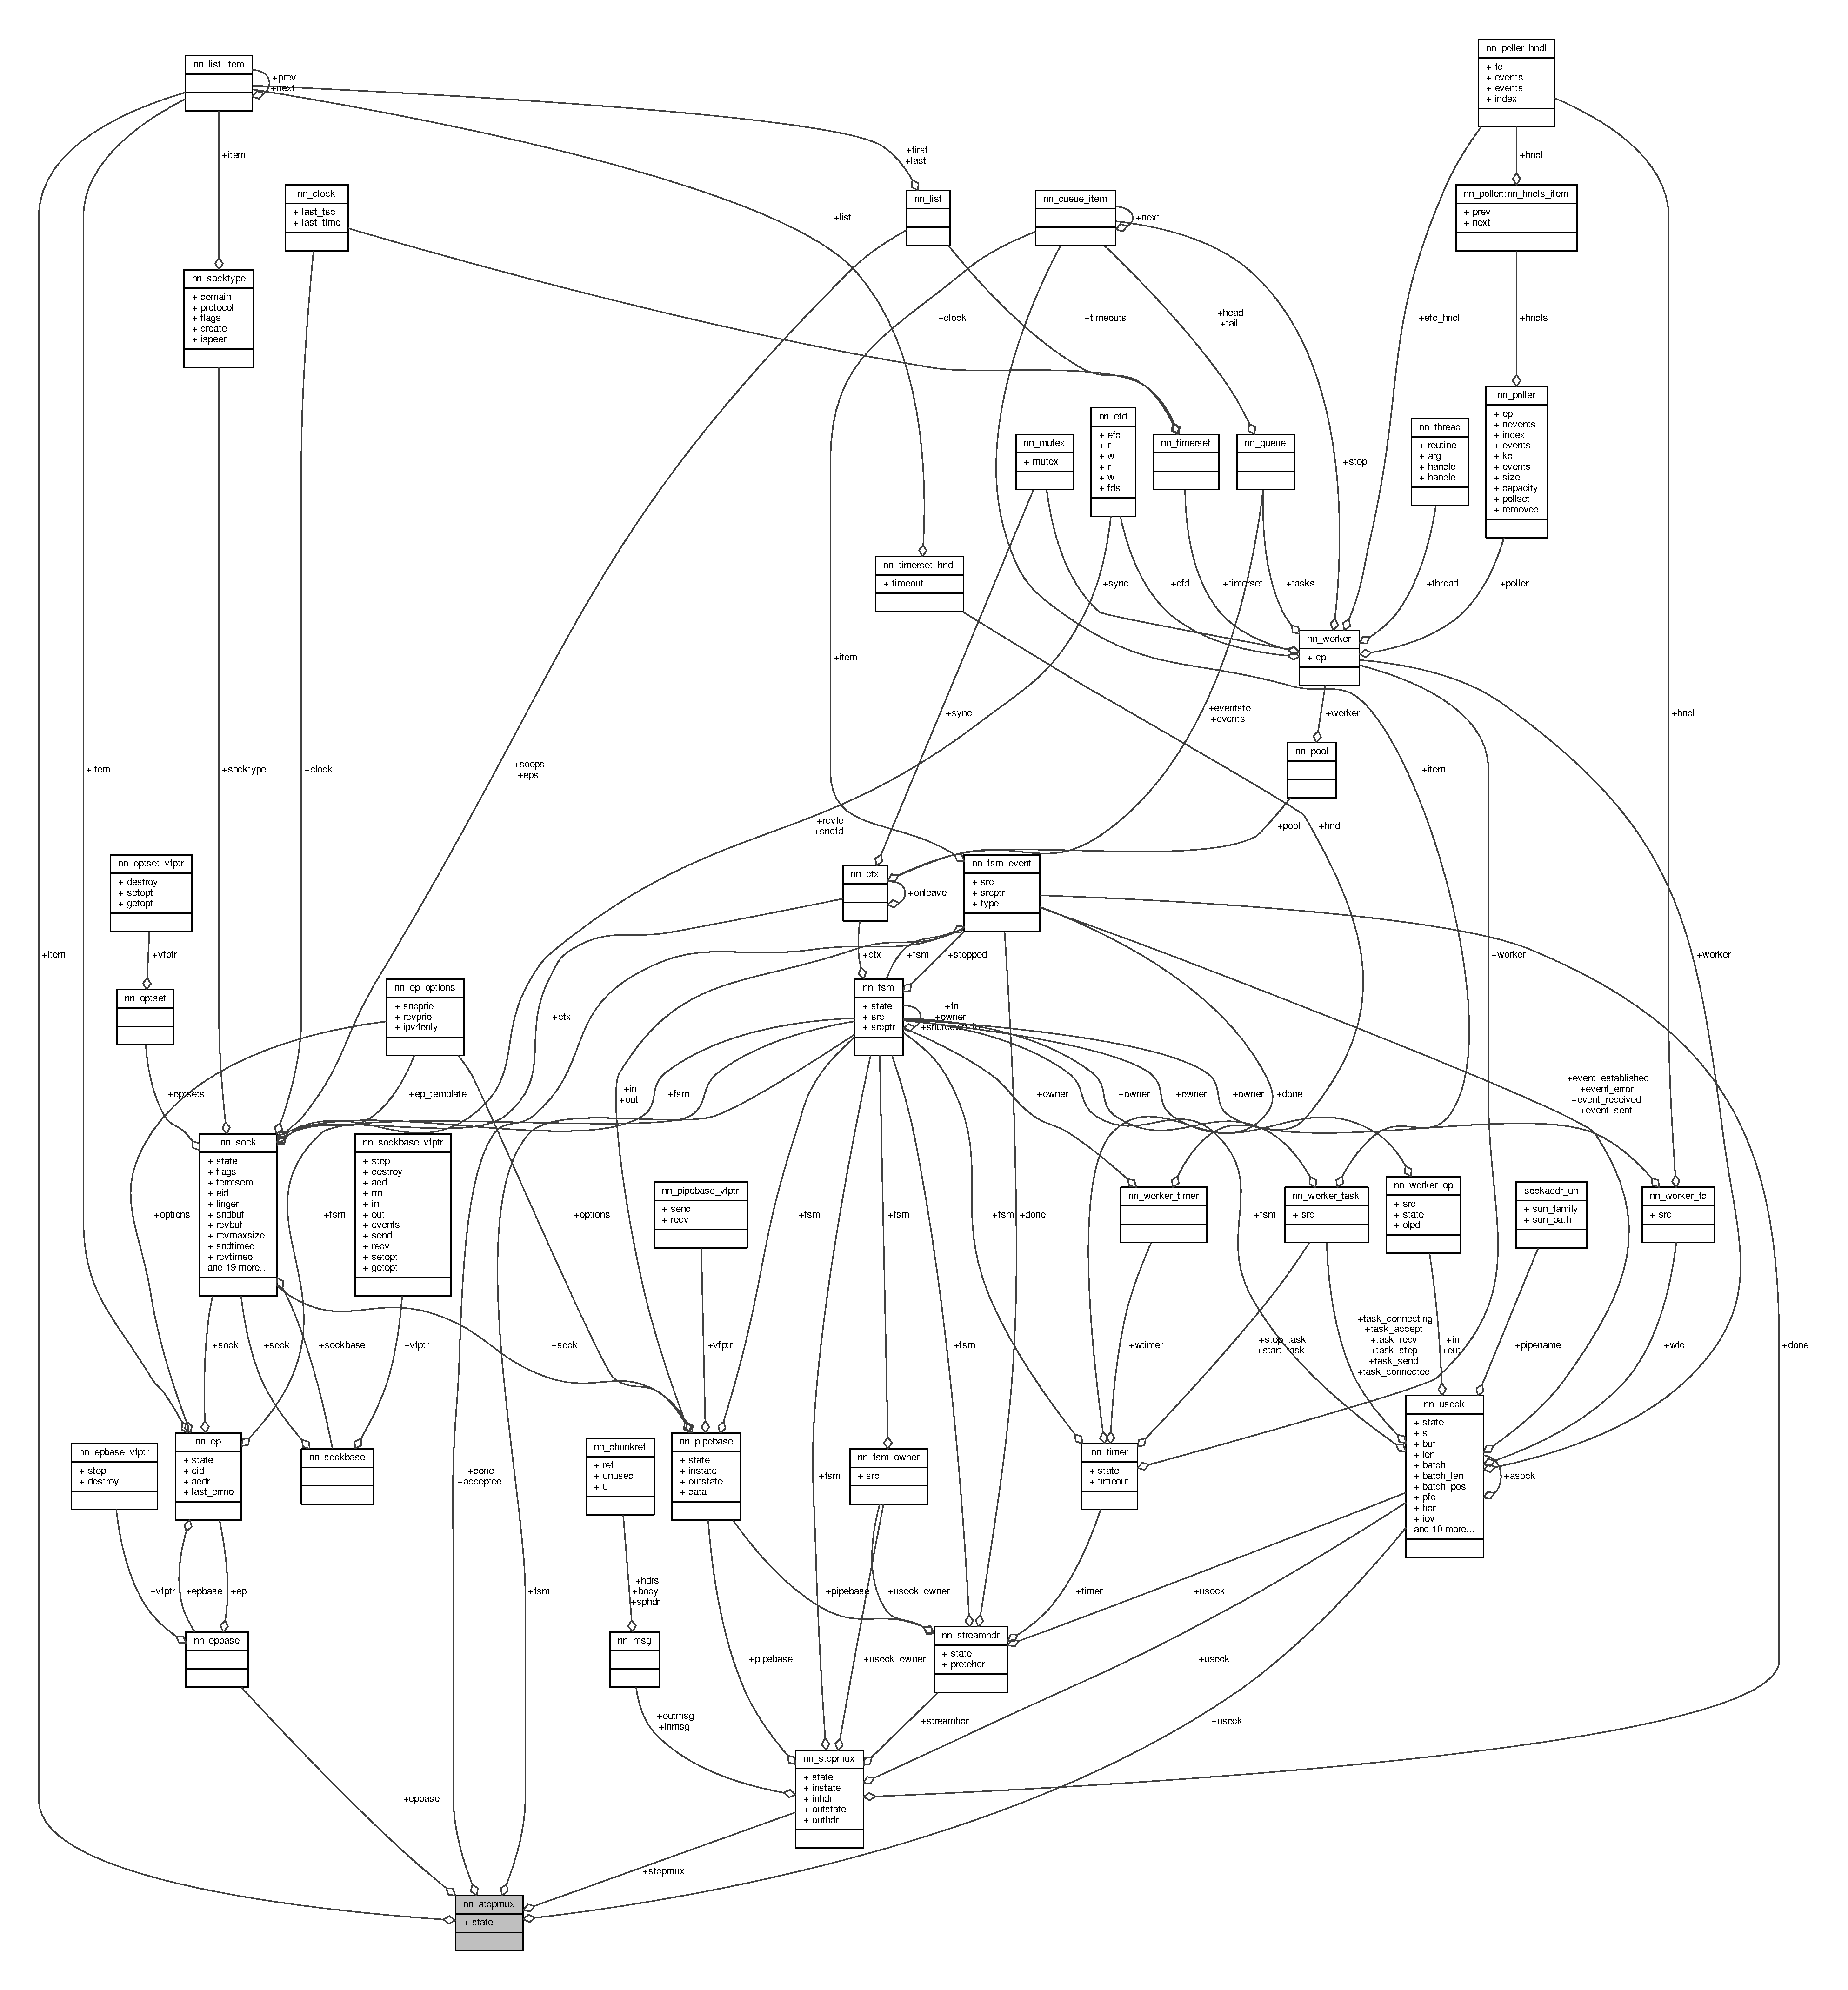
\includegraphics[width=350pt]{structnn__atcpmux__coll__graph}
\end{center}
\end{figure}
\subsection*{Public Attributes}
\begin{DoxyCompactItemize}
\item 
struct \hyperlink{structnn__fsm}{nn\+\_\+fsm} \hyperlink{structnn__atcpmux_a26d4e8b2d6c8b531764ffb49c43b4c3d}{fsm}
\item 
int \hyperlink{structnn__atcpmux_aef404e44445e0ee8ed0f2c71a5381043}{state}
\item 
struct \hyperlink{structnn__epbase}{nn\+\_\+epbase} $\ast$ \hyperlink{structnn__atcpmux_a483609219bb585fbf49fc33a84975cbe}{epbase}
\item 
struct \hyperlink{structnn__usock}{nn\+\_\+usock} \hyperlink{structnn__atcpmux_a098c32746a2c8c7ae2fc6df099306566}{usock}
\item 
struct \hyperlink{structnn__stcpmux}{nn\+\_\+stcpmux} \hyperlink{structnn__atcpmux_a0d71d6b00d9a8487c66972a95dd85a1d}{stcpmux}
\item 
struct \hyperlink{structnn__fsm__event}{nn\+\_\+fsm\+\_\+event} \hyperlink{structnn__atcpmux_abfa2adeace4b3e50ad652211011cdbdf}{accepted}
\item 
struct \hyperlink{structnn__fsm__event}{nn\+\_\+fsm\+\_\+event} \hyperlink{structnn__atcpmux_a70ec373c482cb06cddf83c7a8cbe64fe}{done}
\item 
struct \hyperlink{structnn__list__item}{nn\+\_\+list\+\_\+item} \hyperlink{structnn__atcpmux_a61556270226d5a637429c5436715b295}{item}
\end{DoxyCompactItemize}


\subsection{Member Data Documentation}
\index{nn\+\_\+atcpmux@{nn\+\_\+atcpmux}!accepted@{accepted}}
\index{accepted@{accepted}!nn\+\_\+atcpmux@{nn\+\_\+atcpmux}}
\subsubsection[{accepted}]{\setlength{\rightskip}{0pt plus 5cm}struct {\bf nn\+\_\+fsm\+\_\+event} nn\+\_\+atcpmux\+::accepted}\hypertarget{structnn__atcpmux_abfa2adeace4b3e50ad652211011cdbdf}{}\label{structnn__atcpmux_abfa2adeace4b3e50ad652211011cdbdf}
\index{nn\+\_\+atcpmux@{nn\+\_\+atcpmux}!done@{done}}
\index{done@{done}!nn\+\_\+atcpmux@{nn\+\_\+atcpmux}}
\subsubsection[{done}]{\setlength{\rightskip}{0pt plus 5cm}struct {\bf nn\+\_\+fsm\+\_\+event} nn\+\_\+atcpmux\+::done}\hypertarget{structnn__atcpmux_a70ec373c482cb06cddf83c7a8cbe64fe}{}\label{structnn__atcpmux_a70ec373c482cb06cddf83c7a8cbe64fe}
\index{nn\+\_\+atcpmux@{nn\+\_\+atcpmux}!epbase@{epbase}}
\index{epbase@{epbase}!nn\+\_\+atcpmux@{nn\+\_\+atcpmux}}
\subsubsection[{epbase}]{\setlength{\rightskip}{0pt plus 5cm}struct {\bf nn\+\_\+epbase}$\ast$ nn\+\_\+atcpmux\+::epbase}\hypertarget{structnn__atcpmux_a483609219bb585fbf49fc33a84975cbe}{}\label{structnn__atcpmux_a483609219bb585fbf49fc33a84975cbe}
\index{nn\+\_\+atcpmux@{nn\+\_\+atcpmux}!fsm@{fsm}}
\index{fsm@{fsm}!nn\+\_\+atcpmux@{nn\+\_\+atcpmux}}
\subsubsection[{fsm}]{\setlength{\rightskip}{0pt plus 5cm}struct {\bf nn\+\_\+fsm} nn\+\_\+atcpmux\+::fsm}\hypertarget{structnn__atcpmux_a26d4e8b2d6c8b531764ffb49c43b4c3d}{}\label{structnn__atcpmux_a26d4e8b2d6c8b531764ffb49c43b4c3d}
\index{nn\+\_\+atcpmux@{nn\+\_\+atcpmux}!item@{item}}
\index{item@{item}!nn\+\_\+atcpmux@{nn\+\_\+atcpmux}}
\subsubsection[{item}]{\setlength{\rightskip}{0pt plus 5cm}struct {\bf nn\+\_\+list\+\_\+item} nn\+\_\+atcpmux\+::item}\hypertarget{structnn__atcpmux_a61556270226d5a637429c5436715b295}{}\label{structnn__atcpmux_a61556270226d5a637429c5436715b295}
\index{nn\+\_\+atcpmux@{nn\+\_\+atcpmux}!state@{state}}
\index{state@{state}!nn\+\_\+atcpmux@{nn\+\_\+atcpmux}}
\subsubsection[{state}]{\setlength{\rightskip}{0pt plus 5cm}int nn\+\_\+atcpmux\+::state}\hypertarget{structnn__atcpmux_aef404e44445e0ee8ed0f2c71a5381043}{}\label{structnn__atcpmux_aef404e44445e0ee8ed0f2c71a5381043}
\index{nn\+\_\+atcpmux@{nn\+\_\+atcpmux}!stcpmux@{stcpmux}}
\index{stcpmux@{stcpmux}!nn\+\_\+atcpmux@{nn\+\_\+atcpmux}}
\subsubsection[{stcpmux}]{\setlength{\rightskip}{0pt plus 5cm}struct {\bf nn\+\_\+stcpmux} nn\+\_\+atcpmux\+::stcpmux}\hypertarget{structnn__atcpmux_a0d71d6b00d9a8487c66972a95dd85a1d}{}\label{structnn__atcpmux_a0d71d6b00d9a8487c66972a95dd85a1d}
\index{nn\+\_\+atcpmux@{nn\+\_\+atcpmux}!usock@{usock}}
\index{usock@{usock}!nn\+\_\+atcpmux@{nn\+\_\+atcpmux}}
\subsubsection[{usock}]{\setlength{\rightskip}{0pt plus 5cm}struct {\bf nn\+\_\+usock} nn\+\_\+atcpmux\+::usock}\hypertarget{structnn__atcpmux_a098c32746a2c8c7ae2fc6df099306566}{}\label{structnn__atcpmux_a098c32746a2c8c7ae2fc6df099306566}


The documentation for this struct was generated from the following file\+:\begin{DoxyCompactItemize}
\item 
src/transports/tcpmux/\hyperlink{atcpmux_8h}{atcpmux.\+h}\end{DoxyCompactItemize}

\hypertarget{structnn__atomic}{}\section{nn\+\_\+atomic Struct Reference}
\label{structnn__atomic}\index{nn\+\_\+atomic@{nn\+\_\+atomic}}


{\ttfamily \#include $<$atomic.\+h$>$}



Collaboration diagram for nn\+\_\+atomic\+:\nopagebreak
\begin{figure}[H]
\begin{center}
\leavevmode
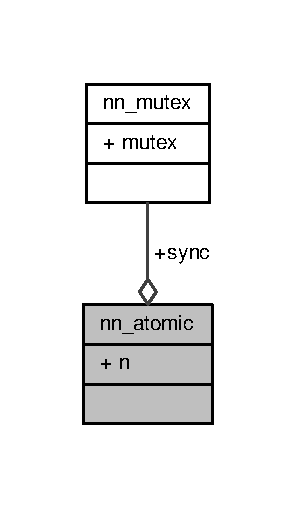
\includegraphics[width=142pt]{structnn__atomic__coll__graph}
\end{center}
\end{figure}
\subsection*{Public Attributes}
\begin{DoxyCompactItemize}
\item 
struct \hyperlink{structnn__mutex}{nn\+\_\+mutex} \hyperlink{structnn__atomic_a9ca93c0867fdfbbe8414d7417be4cad2}{sync}
\item 
volatile uint32\+\_\+t \hyperlink{structnn__atomic_ab9b3e24986e552a50cc16c2ea4c5c4d7}{n}
\end{DoxyCompactItemize}


\subsection{Member Data Documentation}
\index{nn\+\_\+atomic@{nn\+\_\+atomic}!n@{n}}
\index{n@{n}!nn\+\_\+atomic@{nn\+\_\+atomic}}
\subsubsection[{n}]{\setlength{\rightskip}{0pt plus 5cm}volatile uint32\+\_\+t nn\+\_\+atomic\+::n}\hypertarget{structnn__atomic_ab9b3e24986e552a50cc16c2ea4c5c4d7}{}\label{structnn__atomic_ab9b3e24986e552a50cc16c2ea4c5c4d7}
\index{nn\+\_\+atomic@{nn\+\_\+atomic}!sync@{sync}}
\index{sync@{sync}!nn\+\_\+atomic@{nn\+\_\+atomic}}
\subsubsection[{sync}]{\setlength{\rightskip}{0pt plus 5cm}struct {\bf nn\+\_\+mutex} nn\+\_\+atomic\+::sync}\hypertarget{structnn__atomic_a9ca93c0867fdfbbe8414d7417be4cad2}{}\label{structnn__atomic_a9ca93c0867fdfbbe8414d7417be4cad2}


The documentation for this struct was generated from the following file\+:\begin{DoxyCompactItemize}
\item 
src/utils/\hyperlink{atomic_8h}{atomic.\+h}\end{DoxyCompactItemize}

\hypertarget{structnn__aws}{}\section{nn\+\_\+aws Struct Reference}
\label{structnn__aws}\index{nn\+\_\+aws@{nn\+\_\+aws}}


{\ttfamily \#include $<$aws.\+h$>$}



Collaboration diagram for nn\+\_\+aws\+:\nopagebreak
\begin{figure}[H]
\begin{center}
\leavevmode
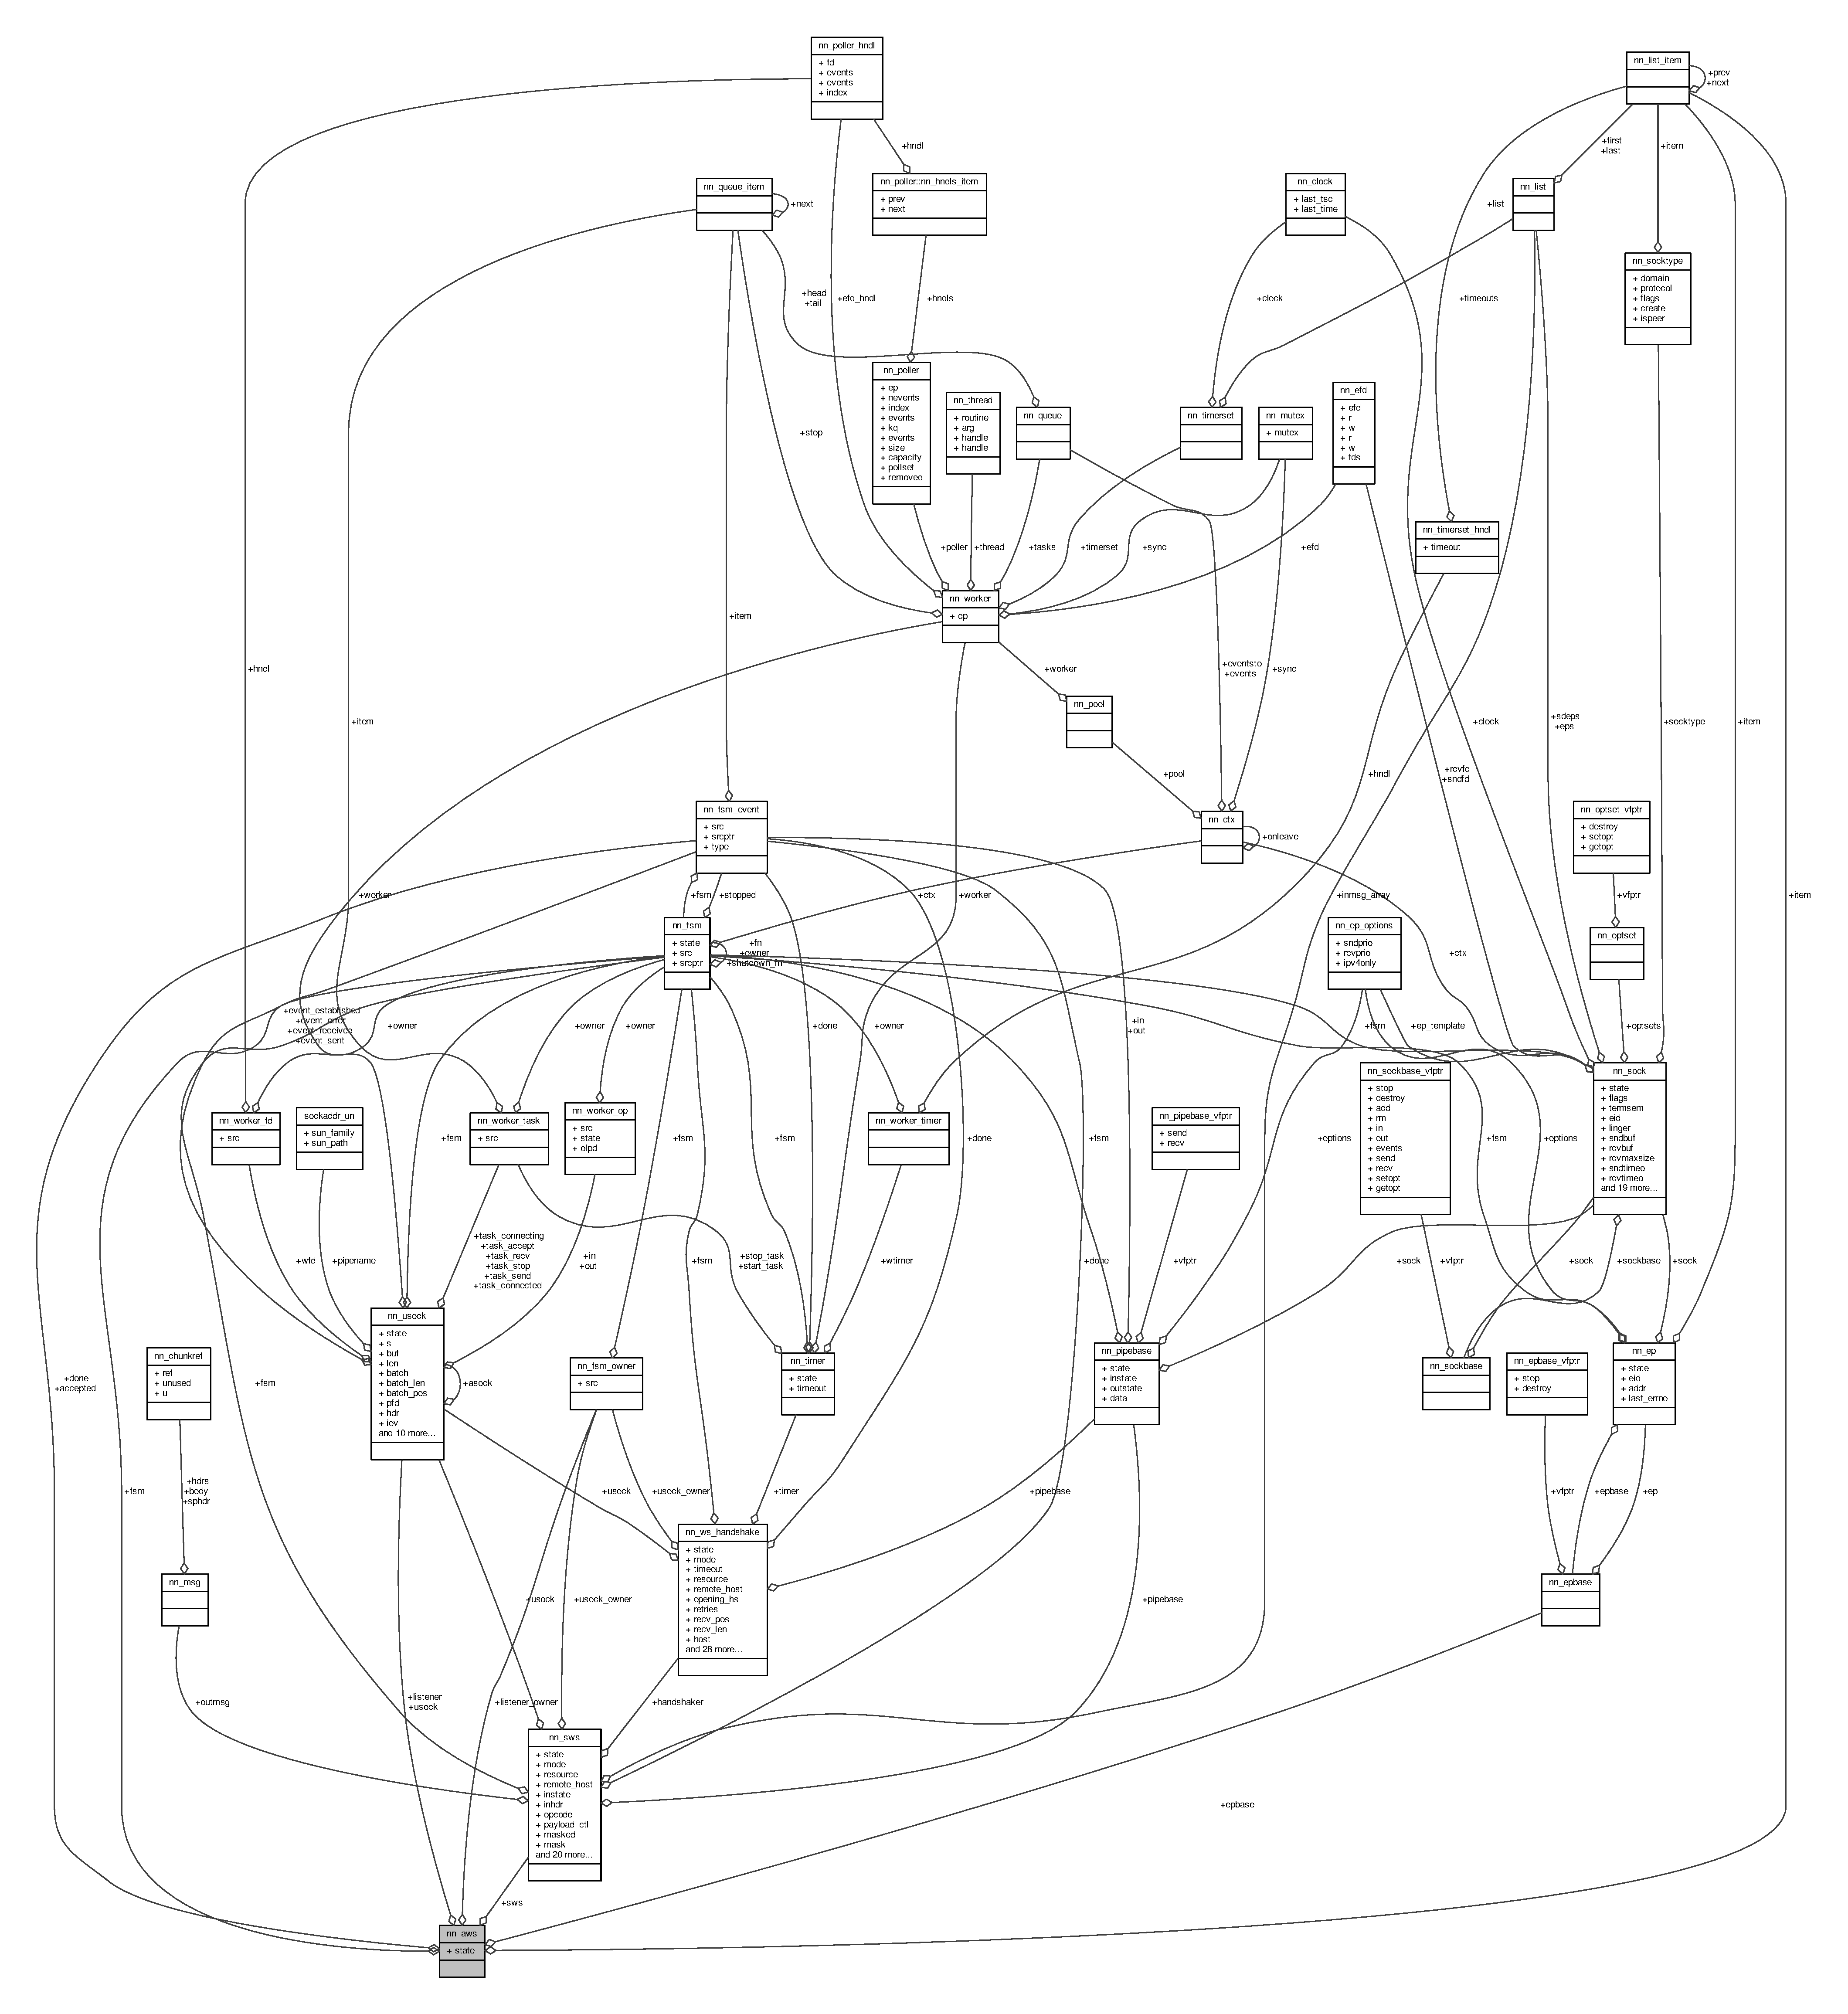
\includegraphics[width=350pt]{structnn__aws__coll__graph}
\end{center}
\end{figure}
\subsection*{Public Attributes}
\begin{DoxyCompactItemize}
\item 
struct \hyperlink{structnn__fsm}{nn\+\_\+fsm} \hyperlink{structnn__aws_a4dbdd1d180d0932049d668ef2326dbca}{fsm}
\item 
int \hyperlink{structnn__aws_a13068d88fe20b331e7f1775299bb36a0}{state}
\item 
struct \hyperlink{structnn__epbase}{nn\+\_\+epbase} $\ast$ \hyperlink{structnn__aws_aaa7afd36f1c5caae0c8a6c07ba8120e5}{epbase}
\item 
struct \hyperlink{structnn__usock}{nn\+\_\+usock} \hyperlink{structnn__aws_a994654d46043ffffb5c50a26418f07be}{usock}
\item 
struct \hyperlink{structnn__usock}{nn\+\_\+usock} $\ast$ \hyperlink{structnn__aws_ae45d418c32177d2cb4a170045790c0bb}{listener}
\item 
struct \hyperlink{structnn__fsm__owner}{nn\+\_\+fsm\+\_\+owner} \hyperlink{structnn__aws_ab87ccbd6d0da109f5bf1bd2ce76b031c}{listener\+\_\+owner}
\item 
struct \hyperlink{structnn__sws}{nn\+\_\+sws} \hyperlink{structnn__aws_a3a332be24b129cd1cbc6e6a224d3400e}{sws}
\item 
struct \hyperlink{structnn__fsm__event}{nn\+\_\+fsm\+\_\+event} \hyperlink{structnn__aws_a1f2a18aebfe209a2eb034ef8030c0f25}{accepted}
\item 
struct \hyperlink{structnn__fsm__event}{nn\+\_\+fsm\+\_\+event} \hyperlink{structnn__aws_a4d64e57f3bd783385b45203c3d4b7197}{done}
\item 
struct \hyperlink{structnn__list__item}{nn\+\_\+list\+\_\+item} \hyperlink{structnn__aws_a6e4050f21493a55997811caf94b3f6f6}{item}
\end{DoxyCompactItemize}


\subsection{Member Data Documentation}
\index{nn\+\_\+aws@{nn\+\_\+aws}!accepted@{accepted}}
\index{accepted@{accepted}!nn\+\_\+aws@{nn\+\_\+aws}}
\subsubsection[{accepted}]{\setlength{\rightskip}{0pt plus 5cm}struct {\bf nn\+\_\+fsm\+\_\+event} nn\+\_\+aws\+::accepted}\hypertarget{structnn__aws_a1f2a18aebfe209a2eb034ef8030c0f25}{}\label{structnn__aws_a1f2a18aebfe209a2eb034ef8030c0f25}
\index{nn\+\_\+aws@{nn\+\_\+aws}!done@{done}}
\index{done@{done}!nn\+\_\+aws@{nn\+\_\+aws}}
\subsubsection[{done}]{\setlength{\rightskip}{0pt plus 5cm}struct {\bf nn\+\_\+fsm\+\_\+event} nn\+\_\+aws\+::done}\hypertarget{structnn__aws_a4d64e57f3bd783385b45203c3d4b7197}{}\label{structnn__aws_a4d64e57f3bd783385b45203c3d4b7197}
\index{nn\+\_\+aws@{nn\+\_\+aws}!epbase@{epbase}}
\index{epbase@{epbase}!nn\+\_\+aws@{nn\+\_\+aws}}
\subsubsection[{epbase}]{\setlength{\rightskip}{0pt plus 5cm}struct {\bf nn\+\_\+epbase}$\ast$ nn\+\_\+aws\+::epbase}\hypertarget{structnn__aws_aaa7afd36f1c5caae0c8a6c07ba8120e5}{}\label{structnn__aws_aaa7afd36f1c5caae0c8a6c07ba8120e5}
\index{nn\+\_\+aws@{nn\+\_\+aws}!fsm@{fsm}}
\index{fsm@{fsm}!nn\+\_\+aws@{nn\+\_\+aws}}
\subsubsection[{fsm}]{\setlength{\rightskip}{0pt plus 5cm}struct {\bf nn\+\_\+fsm} nn\+\_\+aws\+::fsm}\hypertarget{structnn__aws_a4dbdd1d180d0932049d668ef2326dbca}{}\label{structnn__aws_a4dbdd1d180d0932049d668ef2326dbca}
\index{nn\+\_\+aws@{nn\+\_\+aws}!item@{item}}
\index{item@{item}!nn\+\_\+aws@{nn\+\_\+aws}}
\subsubsection[{item}]{\setlength{\rightskip}{0pt plus 5cm}struct {\bf nn\+\_\+list\+\_\+item} nn\+\_\+aws\+::item}\hypertarget{structnn__aws_a6e4050f21493a55997811caf94b3f6f6}{}\label{structnn__aws_a6e4050f21493a55997811caf94b3f6f6}
\index{nn\+\_\+aws@{nn\+\_\+aws}!listener@{listener}}
\index{listener@{listener}!nn\+\_\+aws@{nn\+\_\+aws}}
\subsubsection[{listener}]{\setlength{\rightskip}{0pt plus 5cm}struct {\bf nn\+\_\+usock}$\ast$ nn\+\_\+aws\+::listener}\hypertarget{structnn__aws_ae45d418c32177d2cb4a170045790c0bb}{}\label{structnn__aws_ae45d418c32177d2cb4a170045790c0bb}
\index{nn\+\_\+aws@{nn\+\_\+aws}!listener\+\_\+owner@{listener\+\_\+owner}}
\index{listener\+\_\+owner@{listener\+\_\+owner}!nn\+\_\+aws@{nn\+\_\+aws}}
\subsubsection[{listener\+\_\+owner}]{\setlength{\rightskip}{0pt plus 5cm}struct {\bf nn\+\_\+fsm\+\_\+owner} nn\+\_\+aws\+::listener\+\_\+owner}\hypertarget{structnn__aws_ab87ccbd6d0da109f5bf1bd2ce76b031c}{}\label{structnn__aws_ab87ccbd6d0da109f5bf1bd2ce76b031c}
\index{nn\+\_\+aws@{nn\+\_\+aws}!state@{state}}
\index{state@{state}!nn\+\_\+aws@{nn\+\_\+aws}}
\subsubsection[{state}]{\setlength{\rightskip}{0pt plus 5cm}int nn\+\_\+aws\+::state}\hypertarget{structnn__aws_a13068d88fe20b331e7f1775299bb36a0}{}\label{structnn__aws_a13068d88fe20b331e7f1775299bb36a0}
\index{nn\+\_\+aws@{nn\+\_\+aws}!sws@{sws}}
\index{sws@{sws}!nn\+\_\+aws@{nn\+\_\+aws}}
\subsubsection[{sws}]{\setlength{\rightskip}{0pt plus 5cm}struct {\bf nn\+\_\+sws} nn\+\_\+aws\+::sws}\hypertarget{structnn__aws_a3a332be24b129cd1cbc6e6a224d3400e}{}\label{structnn__aws_a3a332be24b129cd1cbc6e6a224d3400e}
\index{nn\+\_\+aws@{nn\+\_\+aws}!usock@{usock}}
\index{usock@{usock}!nn\+\_\+aws@{nn\+\_\+aws}}
\subsubsection[{usock}]{\setlength{\rightskip}{0pt plus 5cm}struct {\bf nn\+\_\+usock} nn\+\_\+aws\+::usock}\hypertarget{structnn__aws_a994654d46043ffffb5c50a26418f07be}{}\label{structnn__aws_a994654d46043ffffb5c50a26418f07be}


The documentation for this struct was generated from the following file\+:\begin{DoxyCompactItemize}
\item 
src/transports/ws/\hyperlink{aws_8h}{aws.\+h}\end{DoxyCompactItemize}

\hypertarget{structnn__backoff}{}\section{nn\+\_\+backoff Struct Reference}
\label{structnn__backoff}\index{nn\+\_\+backoff@{nn\+\_\+backoff}}


{\ttfamily \#include $<$backoff.\+h$>$}



Collaboration diagram for nn\+\_\+backoff\+:\nopagebreak
\begin{figure}[H]
\begin{center}
\leavevmode
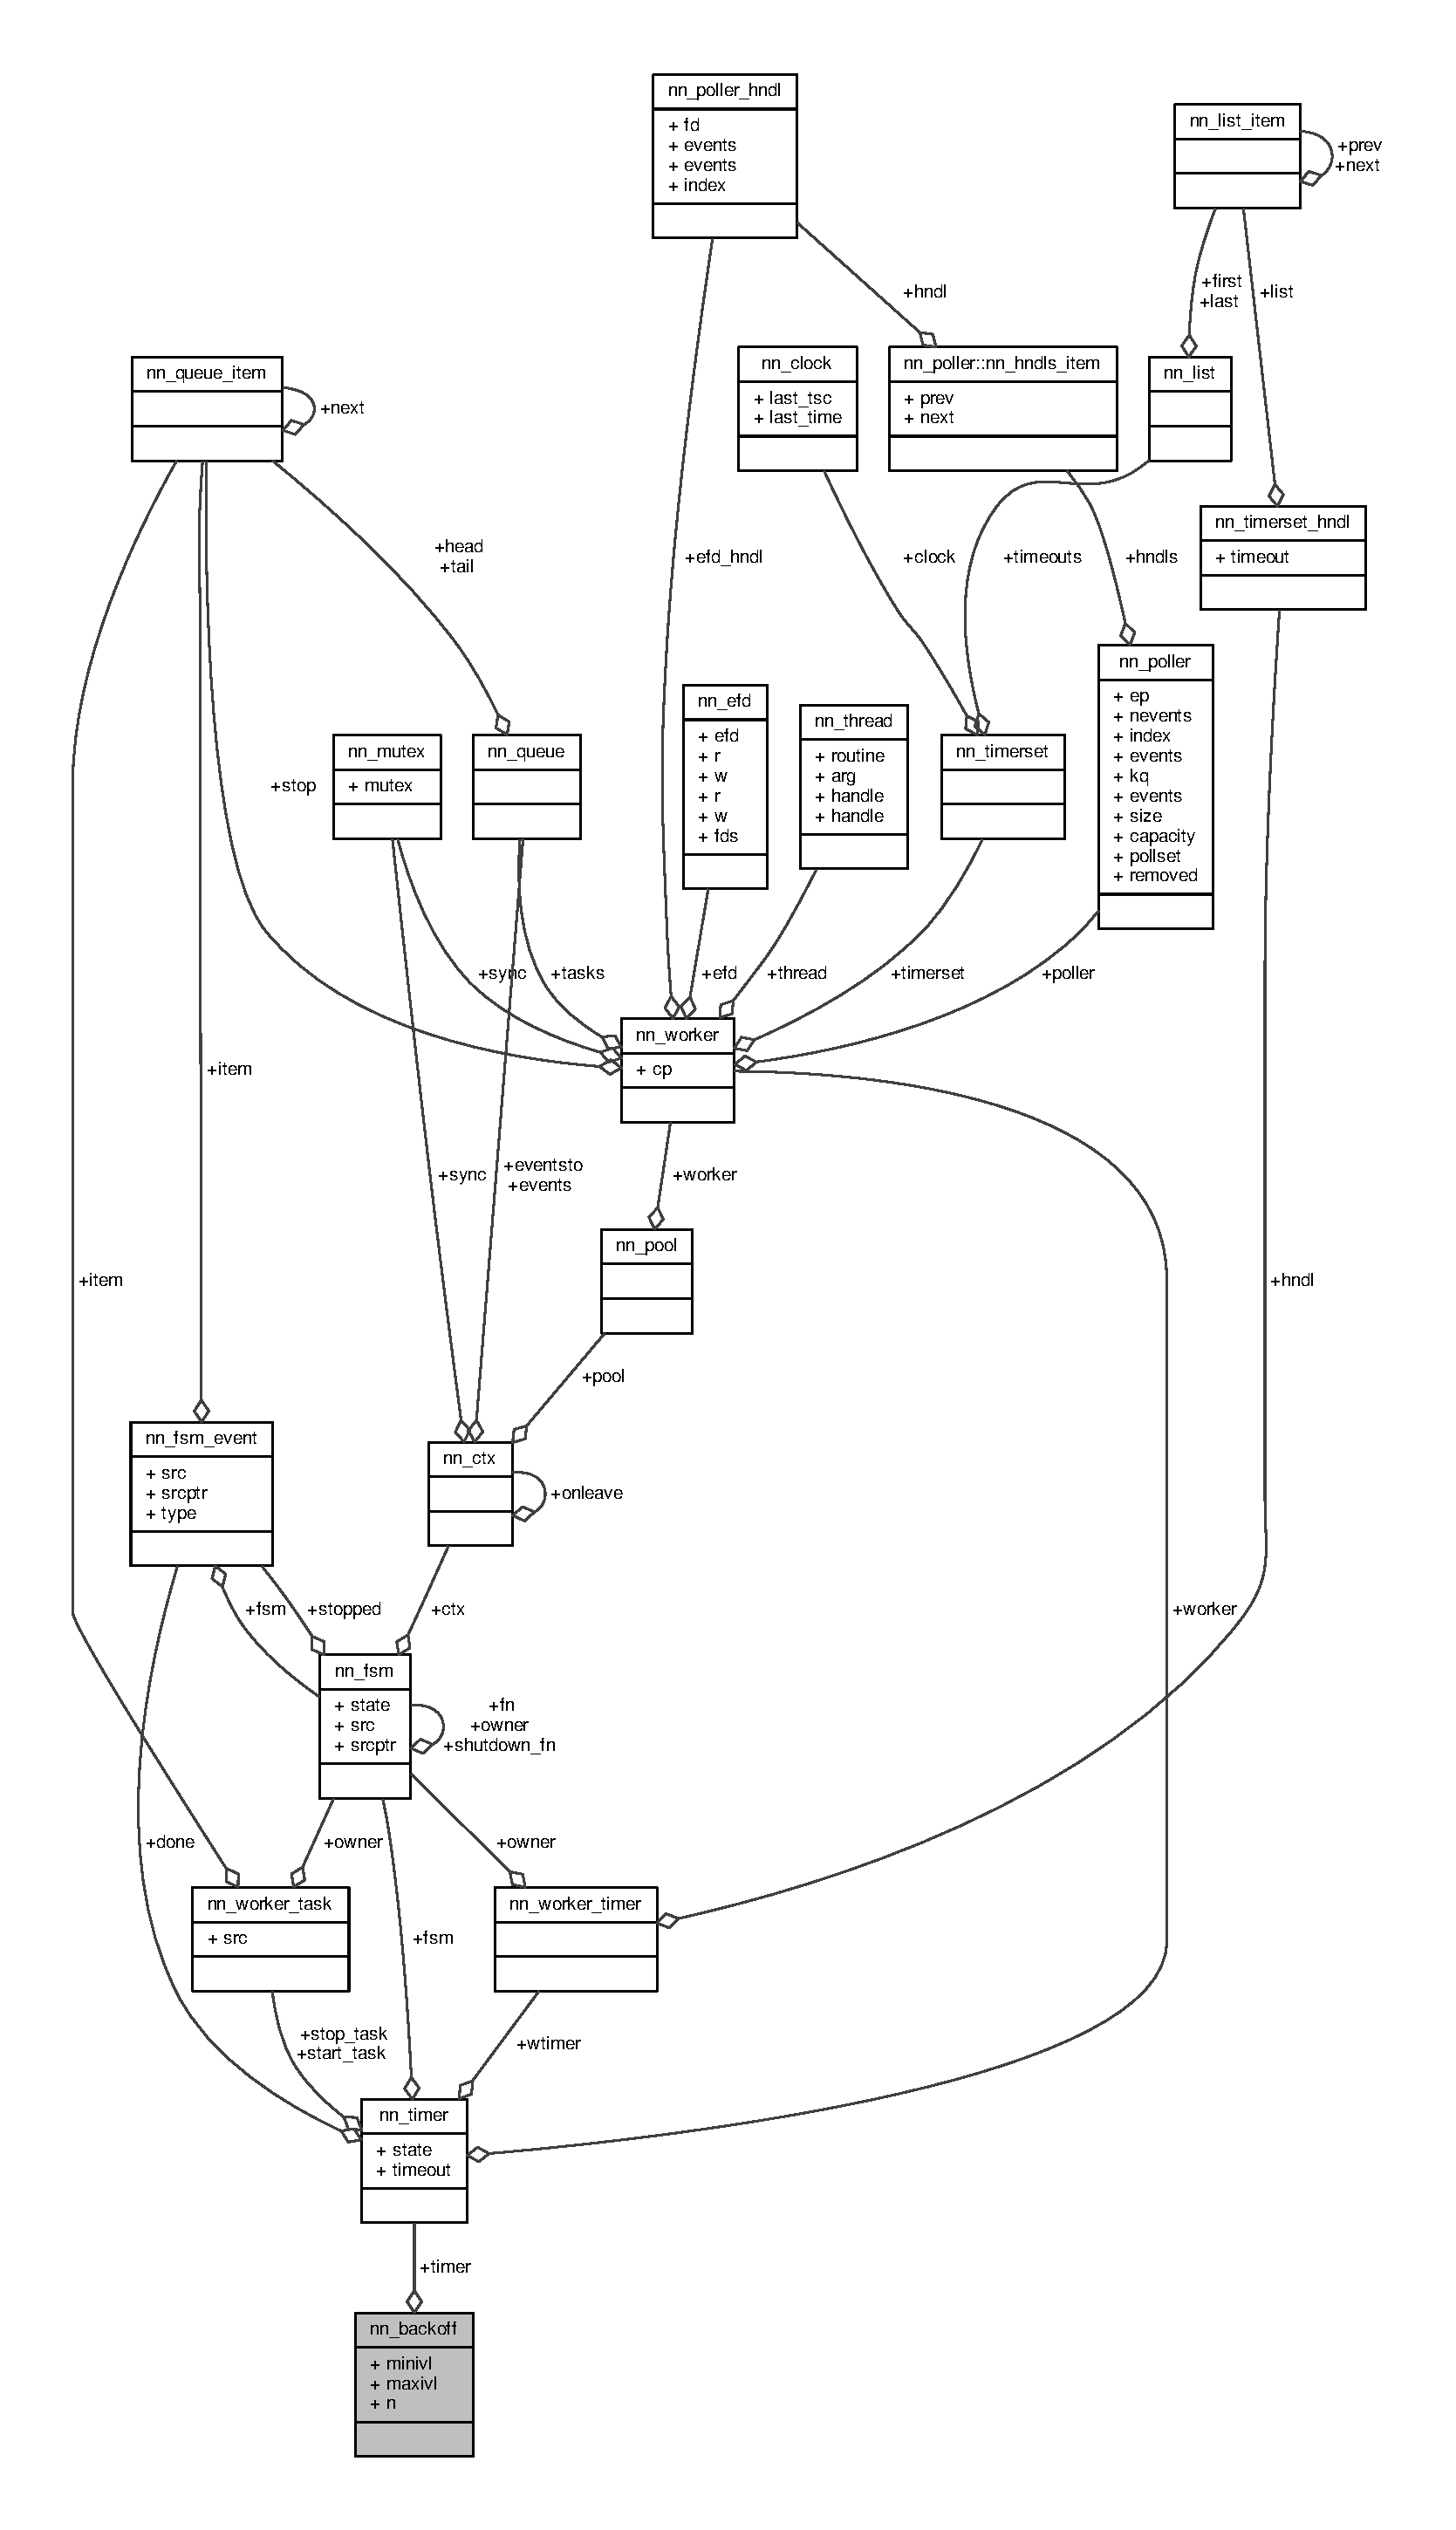
\includegraphics[height=550pt]{structnn__backoff__coll__graph}
\end{center}
\end{figure}
\subsection*{Public Attributes}
\begin{DoxyCompactItemize}
\item 
struct \hyperlink{structnn__timer}{nn\+\_\+timer} \hyperlink{structnn__backoff_a95e67b73fd37ef3528d06f3c7567869e}{timer}
\item 
int \hyperlink{structnn__backoff_a0ea8ab220d58f392e2e601e903183f1b}{minivl}
\item 
int \hyperlink{structnn__backoff_a63bdf88c08ffc214c2187e76b3674061}{maxivl}
\item 
int \hyperlink{structnn__backoff_a92192ee8dd09ddaef649f064f7431860}{n}
\end{DoxyCompactItemize}


\subsection{Member Data Documentation}
\index{nn\+\_\+backoff@{nn\+\_\+backoff}!maxivl@{maxivl}}
\index{maxivl@{maxivl}!nn\+\_\+backoff@{nn\+\_\+backoff}}
\subsubsection[{maxivl}]{\setlength{\rightskip}{0pt plus 5cm}int nn\+\_\+backoff\+::maxivl}\hypertarget{structnn__backoff_a63bdf88c08ffc214c2187e76b3674061}{}\label{structnn__backoff_a63bdf88c08ffc214c2187e76b3674061}
\index{nn\+\_\+backoff@{nn\+\_\+backoff}!minivl@{minivl}}
\index{minivl@{minivl}!nn\+\_\+backoff@{nn\+\_\+backoff}}
\subsubsection[{minivl}]{\setlength{\rightskip}{0pt plus 5cm}int nn\+\_\+backoff\+::minivl}\hypertarget{structnn__backoff_a0ea8ab220d58f392e2e601e903183f1b}{}\label{structnn__backoff_a0ea8ab220d58f392e2e601e903183f1b}
\index{nn\+\_\+backoff@{nn\+\_\+backoff}!n@{n}}
\index{n@{n}!nn\+\_\+backoff@{nn\+\_\+backoff}}
\subsubsection[{n}]{\setlength{\rightskip}{0pt plus 5cm}int nn\+\_\+backoff\+::n}\hypertarget{structnn__backoff_a92192ee8dd09ddaef649f064f7431860}{}\label{structnn__backoff_a92192ee8dd09ddaef649f064f7431860}
\index{nn\+\_\+backoff@{nn\+\_\+backoff}!timer@{timer}}
\index{timer@{timer}!nn\+\_\+backoff@{nn\+\_\+backoff}}
\subsubsection[{timer}]{\setlength{\rightskip}{0pt plus 5cm}struct {\bf nn\+\_\+timer} nn\+\_\+backoff\+::timer}\hypertarget{structnn__backoff_a95e67b73fd37ef3528d06f3c7567869e}{}\label{structnn__backoff_a95e67b73fd37ef3528d06f3c7567869e}


The documentation for this struct was generated from the following file\+:\begin{DoxyCompactItemize}
\item 
src/transports/utils/\hyperlink{backoff_8h}{backoff.\+h}\end{DoxyCompactItemize}

\hypertarget{structnn__binproc}{}\section{nn\+\_\+binproc Struct Reference}
\label{structnn__binproc}\index{nn\+\_\+binproc@{nn\+\_\+binproc}}


{\ttfamily \#include $<$binproc.\+h$>$}



Collaboration diagram for nn\+\_\+binproc\+:\nopagebreak
\begin{figure}[H]
\begin{center}
\leavevmode
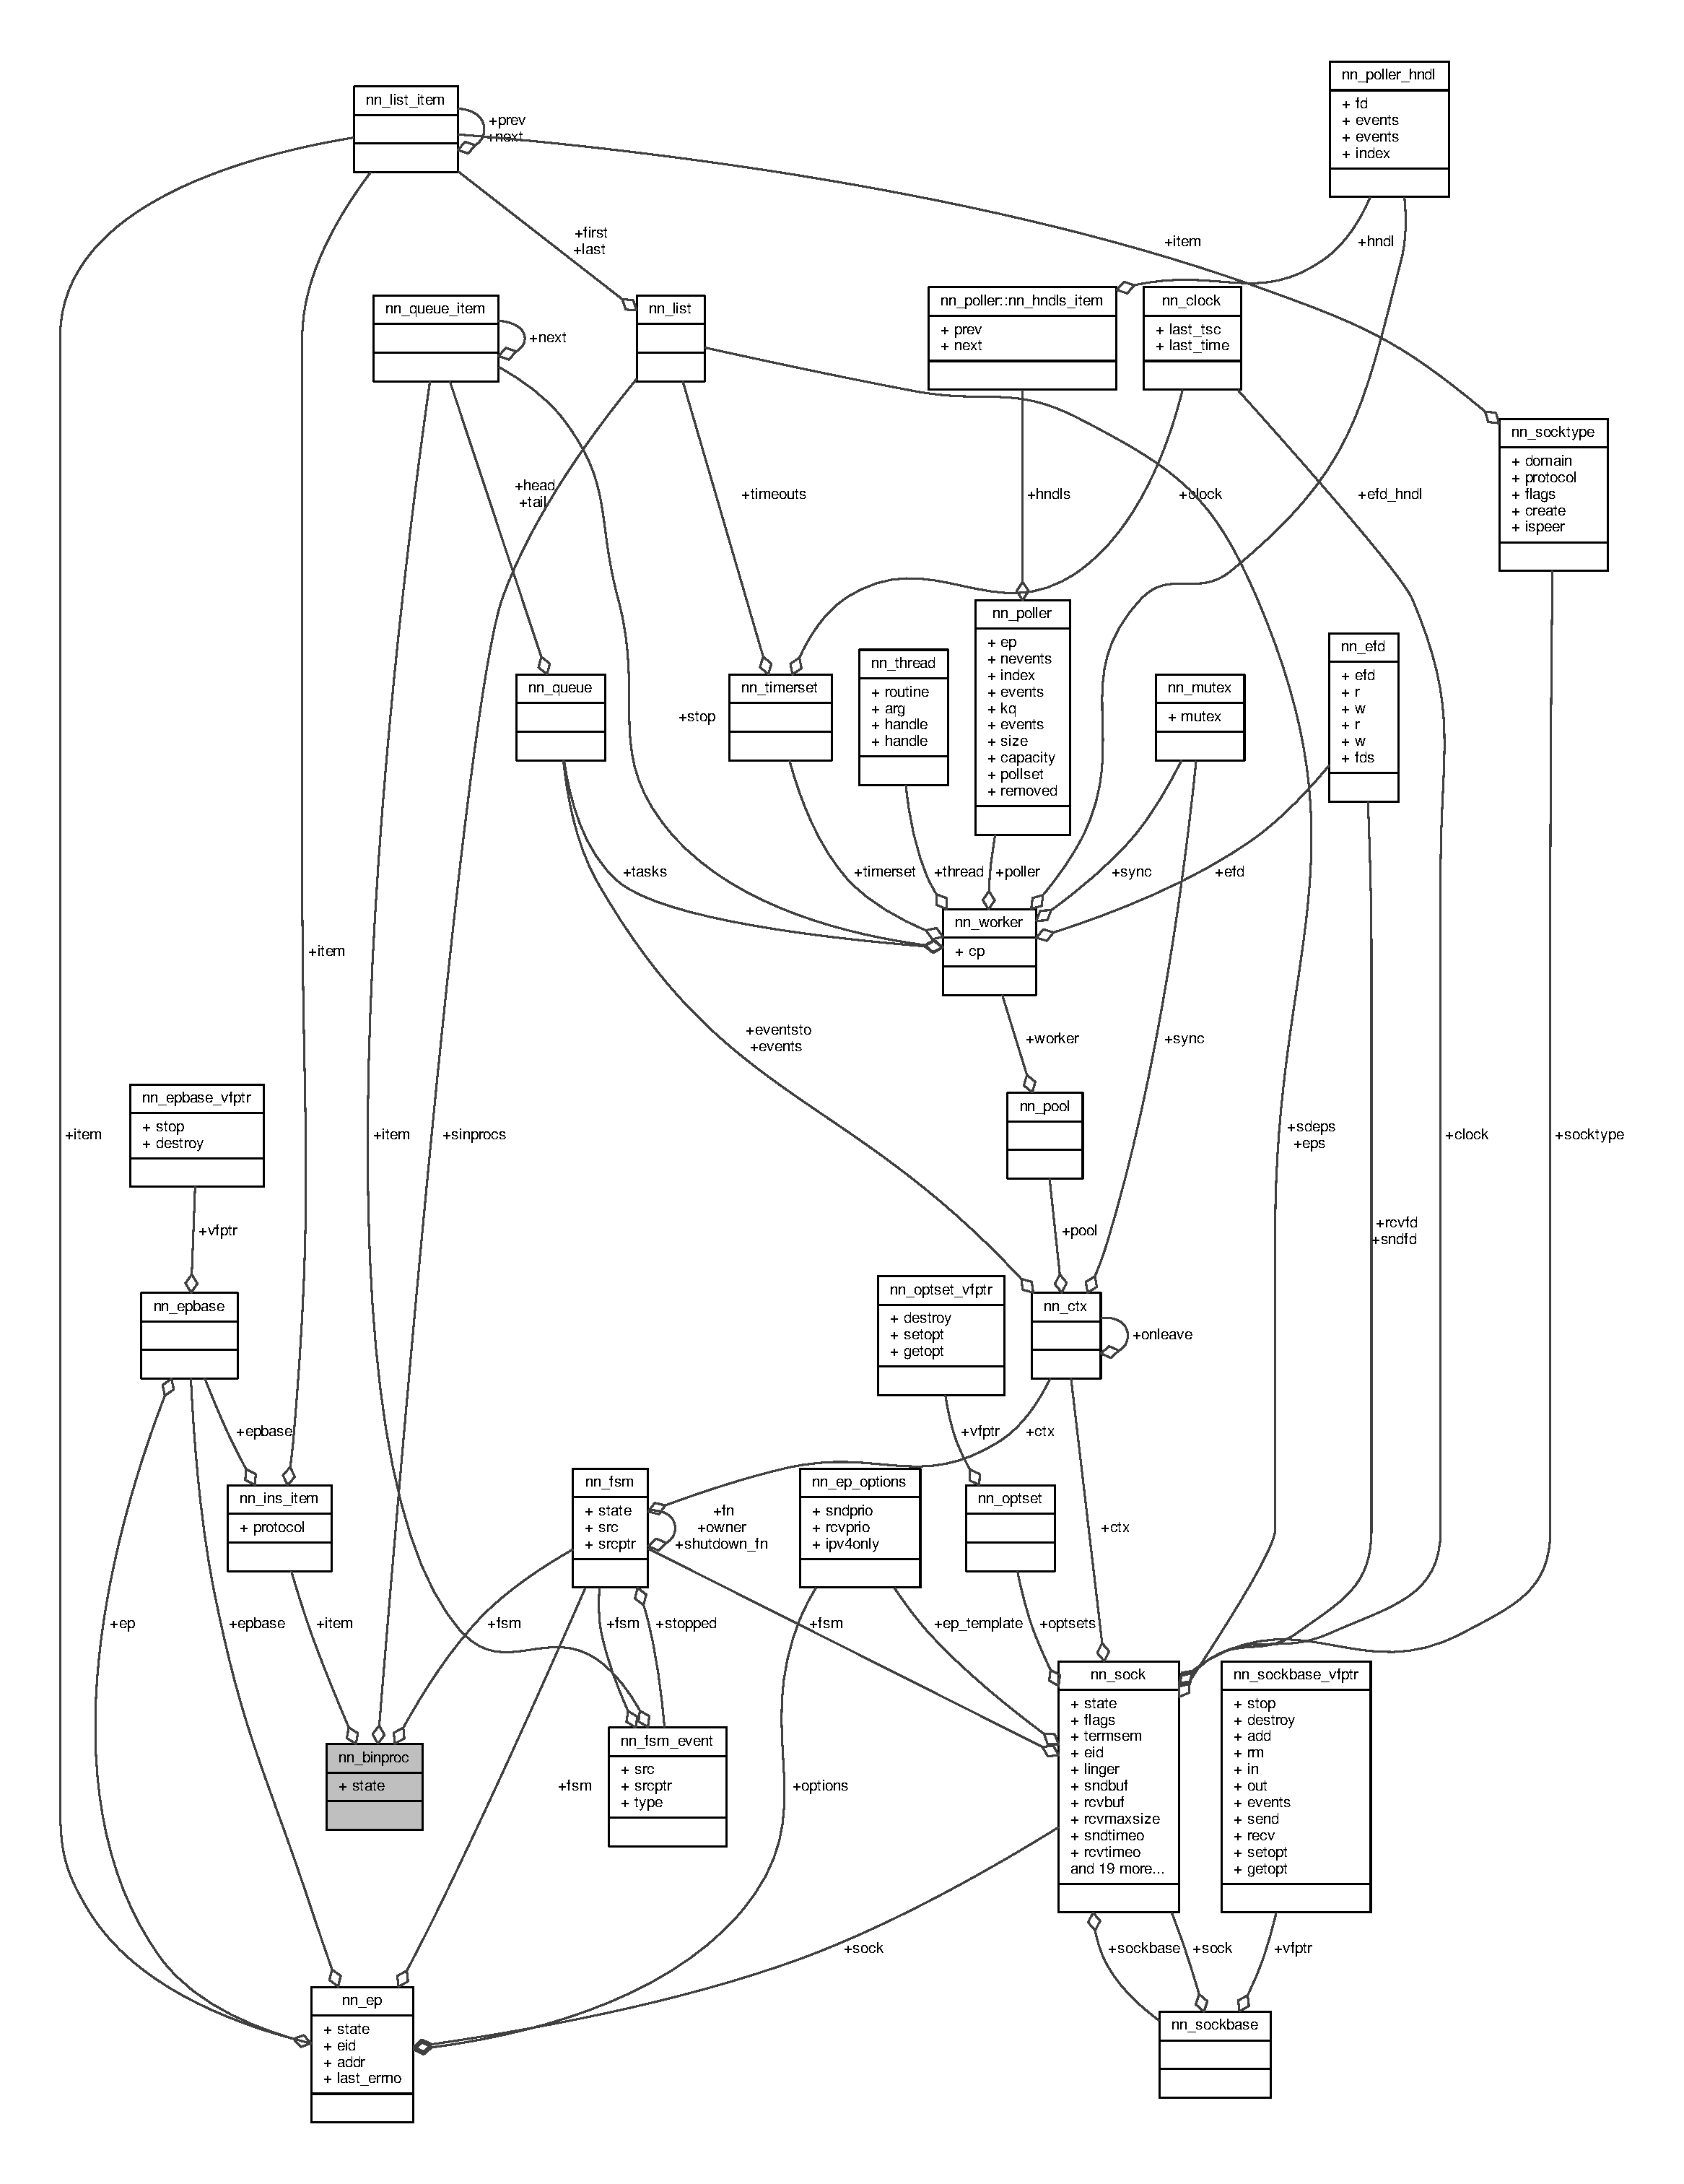
\includegraphics[width=350pt]{structnn__binproc__coll__graph}
\end{center}
\end{figure}
\subsection*{Public Attributes}
\begin{DoxyCompactItemize}
\item 
struct \hyperlink{structnn__fsm}{nn\+\_\+fsm} \hyperlink{structnn__binproc_ad152292e85dd03c76b5a04bf1b1c2312}{fsm}
\item 
int \hyperlink{structnn__binproc_a4a221bbc12129b2ce30068c90154f798}{state}
\item 
struct \hyperlink{structnn__ins__item}{nn\+\_\+ins\+\_\+item} \hyperlink{structnn__binproc_a83a82b2df7063407e75ee23708b7bbe1}{item}
\item 
struct \hyperlink{structnn__list}{nn\+\_\+list} \hyperlink{structnn__binproc_aafb4a9584de9f07138980df5521d06a2}{sinprocs}
\end{DoxyCompactItemize}


\subsection{Member Data Documentation}
\index{nn\+\_\+binproc@{nn\+\_\+binproc}!fsm@{fsm}}
\index{fsm@{fsm}!nn\+\_\+binproc@{nn\+\_\+binproc}}
\subsubsection[{fsm}]{\setlength{\rightskip}{0pt plus 5cm}struct {\bf nn\+\_\+fsm} nn\+\_\+binproc\+::fsm}\hypertarget{structnn__binproc_ad152292e85dd03c76b5a04bf1b1c2312}{}\label{structnn__binproc_ad152292e85dd03c76b5a04bf1b1c2312}
\index{nn\+\_\+binproc@{nn\+\_\+binproc}!item@{item}}
\index{item@{item}!nn\+\_\+binproc@{nn\+\_\+binproc}}
\subsubsection[{item}]{\setlength{\rightskip}{0pt plus 5cm}struct {\bf nn\+\_\+ins\+\_\+item} nn\+\_\+binproc\+::item}\hypertarget{structnn__binproc_a83a82b2df7063407e75ee23708b7bbe1}{}\label{structnn__binproc_a83a82b2df7063407e75ee23708b7bbe1}
\index{nn\+\_\+binproc@{nn\+\_\+binproc}!sinprocs@{sinprocs}}
\index{sinprocs@{sinprocs}!nn\+\_\+binproc@{nn\+\_\+binproc}}
\subsubsection[{sinprocs}]{\setlength{\rightskip}{0pt plus 5cm}struct {\bf nn\+\_\+list} nn\+\_\+binproc\+::sinprocs}\hypertarget{structnn__binproc_aafb4a9584de9f07138980df5521d06a2}{}\label{structnn__binproc_aafb4a9584de9f07138980df5521d06a2}
\index{nn\+\_\+binproc@{nn\+\_\+binproc}!state@{state}}
\index{state@{state}!nn\+\_\+binproc@{nn\+\_\+binproc}}
\subsubsection[{state}]{\setlength{\rightskip}{0pt plus 5cm}int nn\+\_\+binproc\+::state}\hypertarget{structnn__binproc_a4a221bbc12129b2ce30068c90154f798}{}\label{structnn__binproc_a4a221bbc12129b2ce30068c90154f798}


The documentation for this struct was generated from the following file\+:\begin{DoxyCompactItemize}
\item 
src/transports/inproc/\hyperlink{binproc_8h}{binproc.\+h}\end{DoxyCompactItemize}

\hypertarget{structnn__bipc}{}\section{nn\+\_\+bipc Struct Reference}
\label{structnn__bipc}\index{nn\+\_\+bipc@{nn\+\_\+bipc}}


Collaboration diagram for nn\+\_\+bipc\+:\nopagebreak
\begin{figure}[H]
\begin{center}
\leavevmode
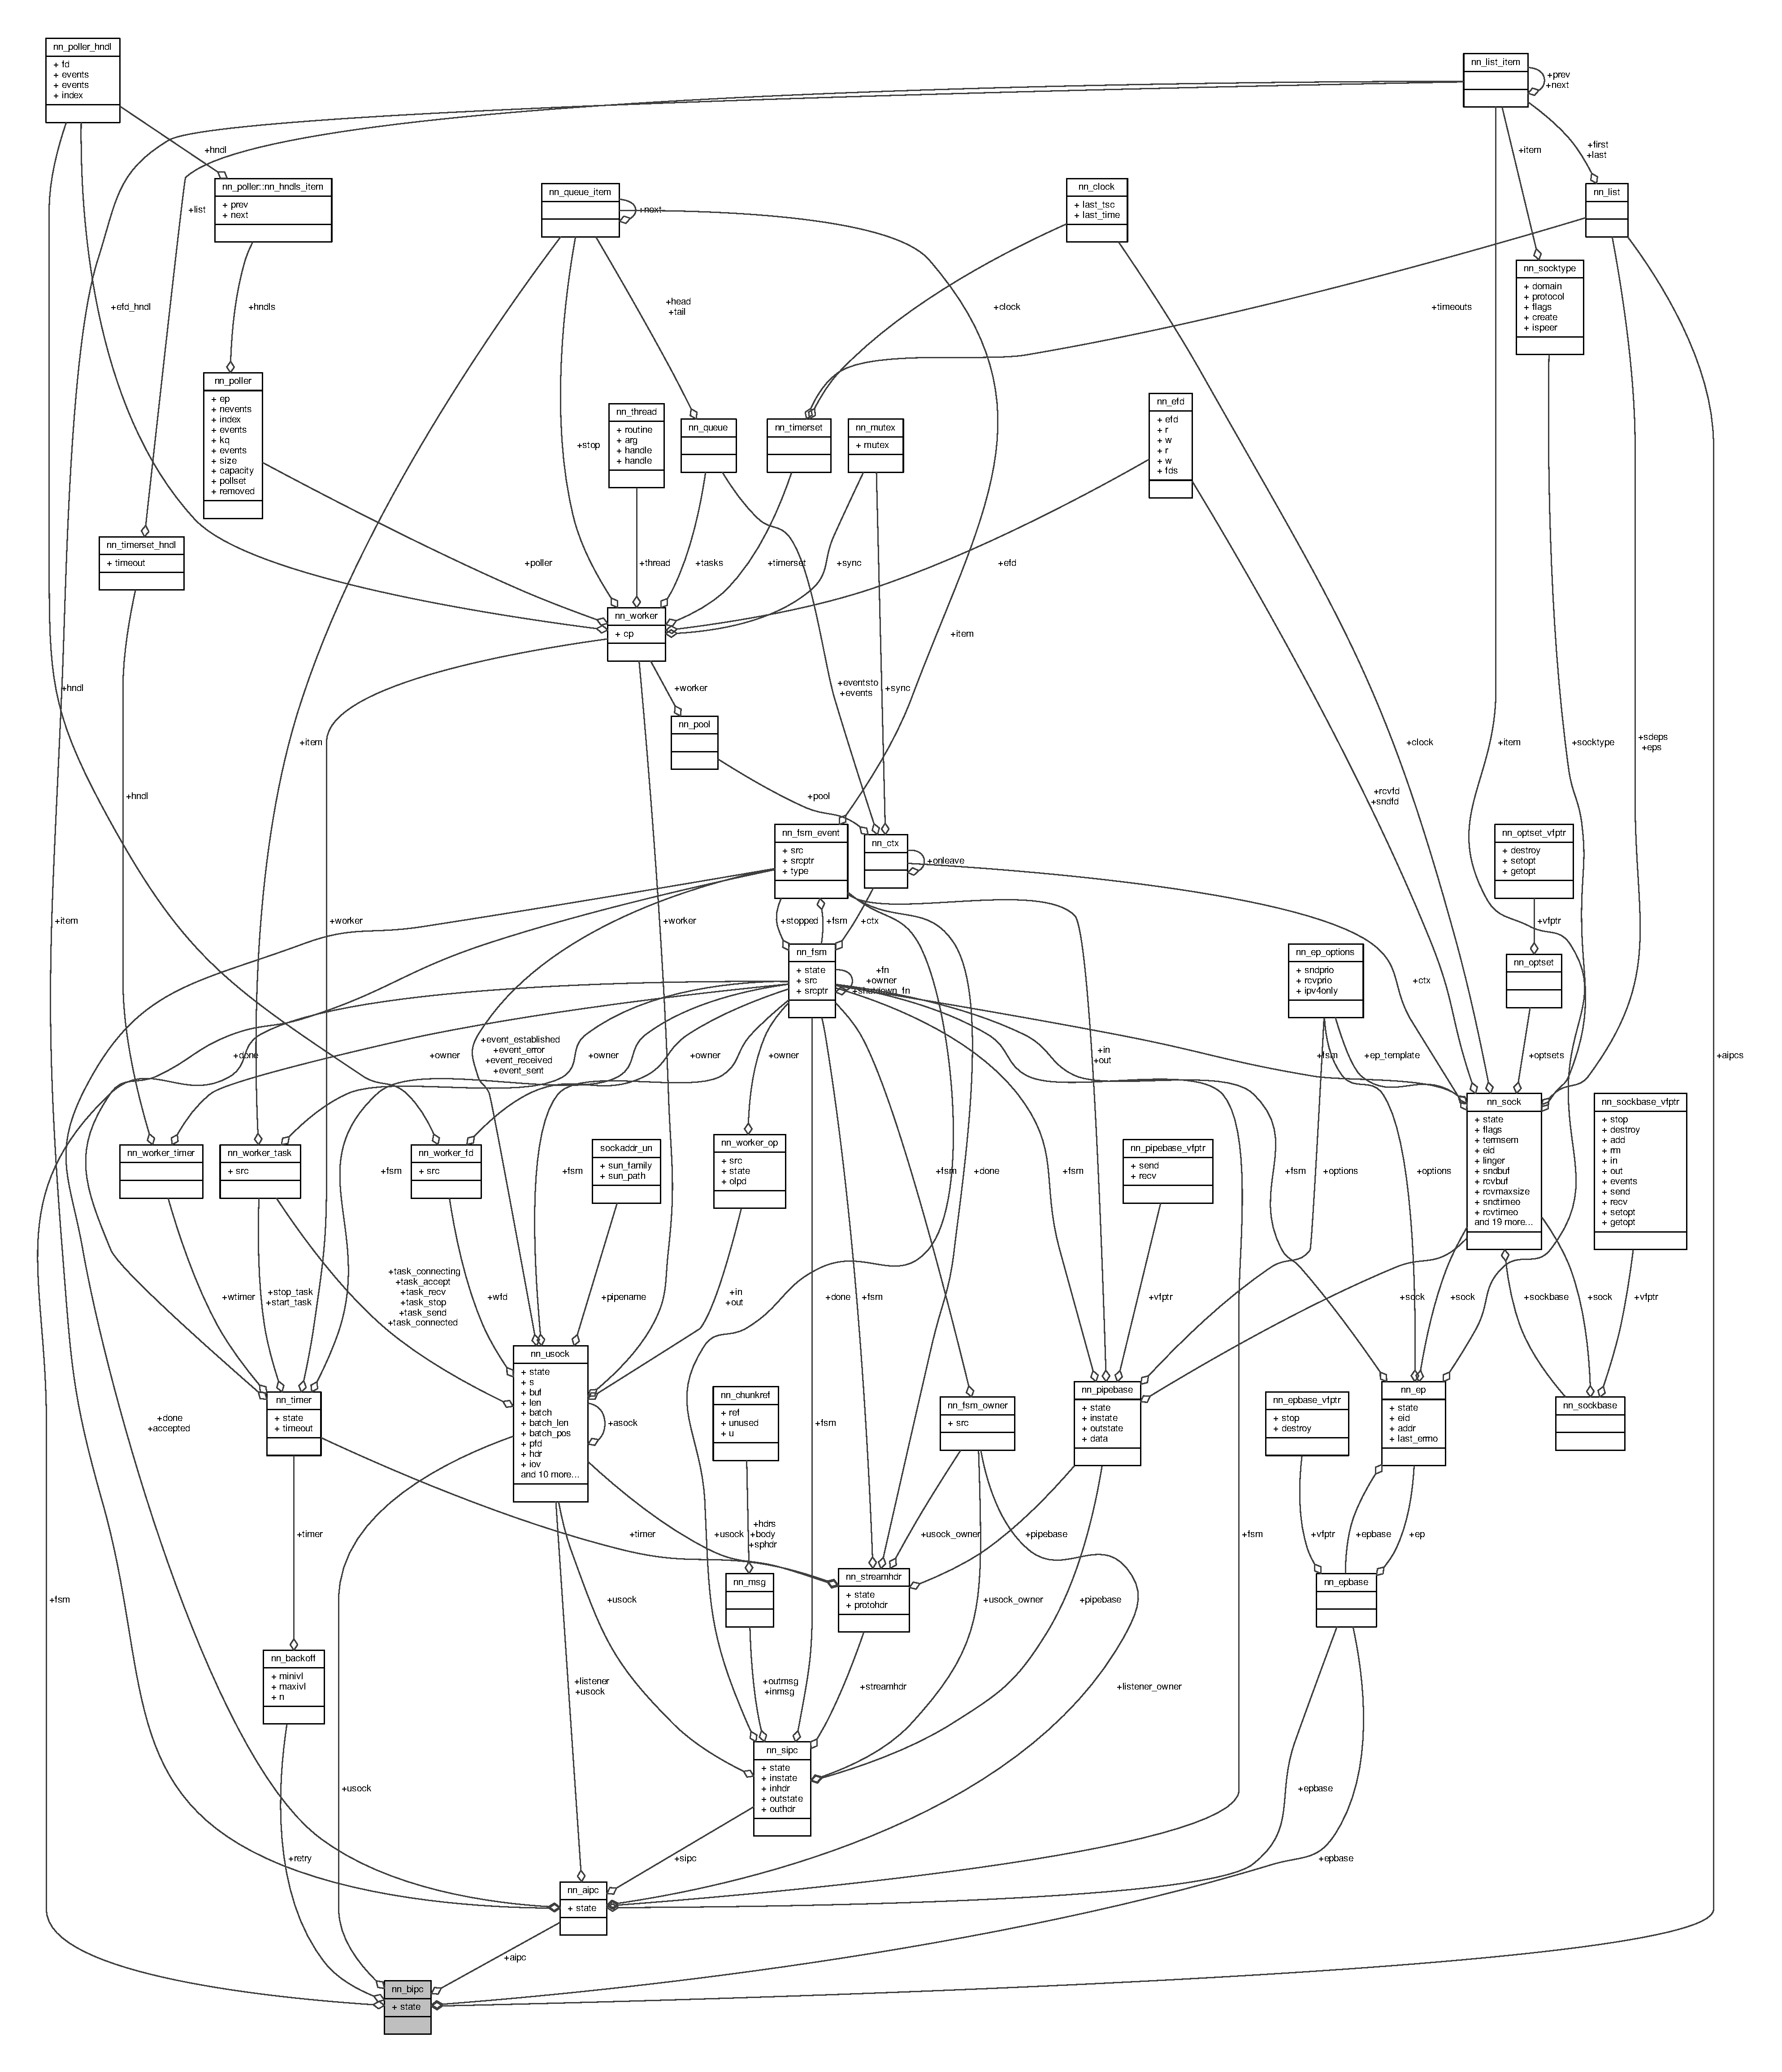
\includegraphics[width=350pt]{structnn__bipc__coll__graph}
\end{center}
\end{figure}
\subsection*{Public Attributes}
\begin{DoxyCompactItemize}
\item 
struct \hyperlink{structnn__fsm}{nn\+\_\+fsm} \hyperlink{structnn__bipc_a64911e7ba9bc1358348c0eb7b3583d98}{fsm}
\item 
int \hyperlink{structnn__bipc_a8f0ba2783e54ed508e4c923e52d7550f}{state}
\item 
struct \hyperlink{structnn__epbase}{nn\+\_\+epbase} \hyperlink{structnn__bipc_a2b53bc22063b4ef9b9536d6ddf7d7091}{epbase}
\item 
struct \hyperlink{structnn__usock}{nn\+\_\+usock} \hyperlink{structnn__bipc_aebeda50dee0039b337dbf02cd9f30458}{usock}
\item 
struct \hyperlink{structnn__aipc}{nn\+\_\+aipc} $\ast$ \hyperlink{structnn__bipc_ad055a23304c4f0a9599828c11a8b1c43}{aipc}
\item 
struct \hyperlink{structnn__list}{nn\+\_\+list} \hyperlink{structnn__bipc_ae73477903d0ce3ceb4e655933d96feb7}{aipcs}
\item 
struct \hyperlink{structnn__backoff}{nn\+\_\+backoff} \hyperlink{structnn__bipc_a5b16dc9fb899848e419d82f925cf19bb}{retry}
\end{DoxyCompactItemize}


\subsection{Member Data Documentation}
\index{nn\+\_\+bipc@{nn\+\_\+bipc}!aipc@{aipc}}
\index{aipc@{aipc}!nn\+\_\+bipc@{nn\+\_\+bipc}}
\subsubsection[{aipc}]{\setlength{\rightskip}{0pt plus 5cm}struct {\bf nn\+\_\+aipc}$\ast$ nn\+\_\+bipc\+::aipc}\hypertarget{structnn__bipc_ad055a23304c4f0a9599828c11a8b1c43}{}\label{structnn__bipc_ad055a23304c4f0a9599828c11a8b1c43}
\index{nn\+\_\+bipc@{nn\+\_\+bipc}!aipcs@{aipcs}}
\index{aipcs@{aipcs}!nn\+\_\+bipc@{nn\+\_\+bipc}}
\subsubsection[{aipcs}]{\setlength{\rightskip}{0pt plus 5cm}struct {\bf nn\+\_\+list} nn\+\_\+bipc\+::aipcs}\hypertarget{structnn__bipc_ae73477903d0ce3ceb4e655933d96feb7}{}\label{structnn__bipc_ae73477903d0ce3ceb4e655933d96feb7}
\index{nn\+\_\+bipc@{nn\+\_\+bipc}!epbase@{epbase}}
\index{epbase@{epbase}!nn\+\_\+bipc@{nn\+\_\+bipc}}
\subsubsection[{epbase}]{\setlength{\rightskip}{0pt plus 5cm}struct {\bf nn\+\_\+epbase} nn\+\_\+bipc\+::epbase}\hypertarget{structnn__bipc_a2b53bc22063b4ef9b9536d6ddf7d7091}{}\label{structnn__bipc_a2b53bc22063b4ef9b9536d6ddf7d7091}
\index{nn\+\_\+bipc@{nn\+\_\+bipc}!fsm@{fsm}}
\index{fsm@{fsm}!nn\+\_\+bipc@{nn\+\_\+bipc}}
\subsubsection[{fsm}]{\setlength{\rightskip}{0pt plus 5cm}struct {\bf nn\+\_\+fsm} nn\+\_\+bipc\+::fsm}\hypertarget{structnn__bipc_a64911e7ba9bc1358348c0eb7b3583d98}{}\label{structnn__bipc_a64911e7ba9bc1358348c0eb7b3583d98}
\index{nn\+\_\+bipc@{nn\+\_\+bipc}!retry@{retry}}
\index{retry@{retry}!nn\+\_\+bipc@{nn\+\_\+bipc}}
\subsubsection[{retry}]{\setlength{\rightskip}{0pt plus 5cm}struct {\bf nn\+\_\+backoff} nn\+\_\+bipc\+::retry}\hypertarget{structnn__bipc_a5b16dc9fb899848e419d82f925cf19bb}{}\label{structnn__bipc_a5b16dc9fb899848e419d82f925cf19bb}
\index{nn\+\_\+bipc@{nn\+\_\+bipc}!state@{state}}
\index{state@{state}!nn\+\_\+bipc@{nn\+\_\+bipc}}
\subsubsection[{state}]{\setlength{\rightskip}{0pt plus 5cm}int nn\+\_\+bipc\+::state}\hypertarget{structnn__bipc_a8f0ba2783e54ed508e4c923e52d7550f}{}\label{structnn__bipc_a8f0ba2783e54ed508e4c923e52d7550f}
\index{nn\+\_\+bipc@{nn\+\_\+bipc}!usock@{usock}}
\index{usock@{usock}!nn\+\_\+bipc@{nn\+\_\+bipc}}
\subsubsection[{usock}]{\setlength{\rightskip}{0pt plus 5cm}struct {\bf nn\+\_\+usock} nn\+\_\+bipc\+::usock}\hypertarget{structnn__bipc_aebeda50dee0039b337dbf02cd9f30458}{}\label{structnn__bipc_aebeda50dee0039b337dbf02cd9f30458}


The documentation for this struct was generated from the following file\+:\begin{DoxyCompactItemize}
\item 
src/transports/ipc/\hyperlink{bipc_8c}{bipc.\+c}\end{DoxyCompactItemize}

\hypertarget{structnn__blibfabric}{}\section{nn\+\_\+blibfabric Struct Reference}
\label{structnn__blibfabric}\index{nn\+\_\+blibfabric@{nn\+\_\+blibfabric}}


Collaboration diagram for nn\+\_\+blibfabric\+:\nopagebreak
\begin{figure}[H]
\begin{center}
\leavevmode
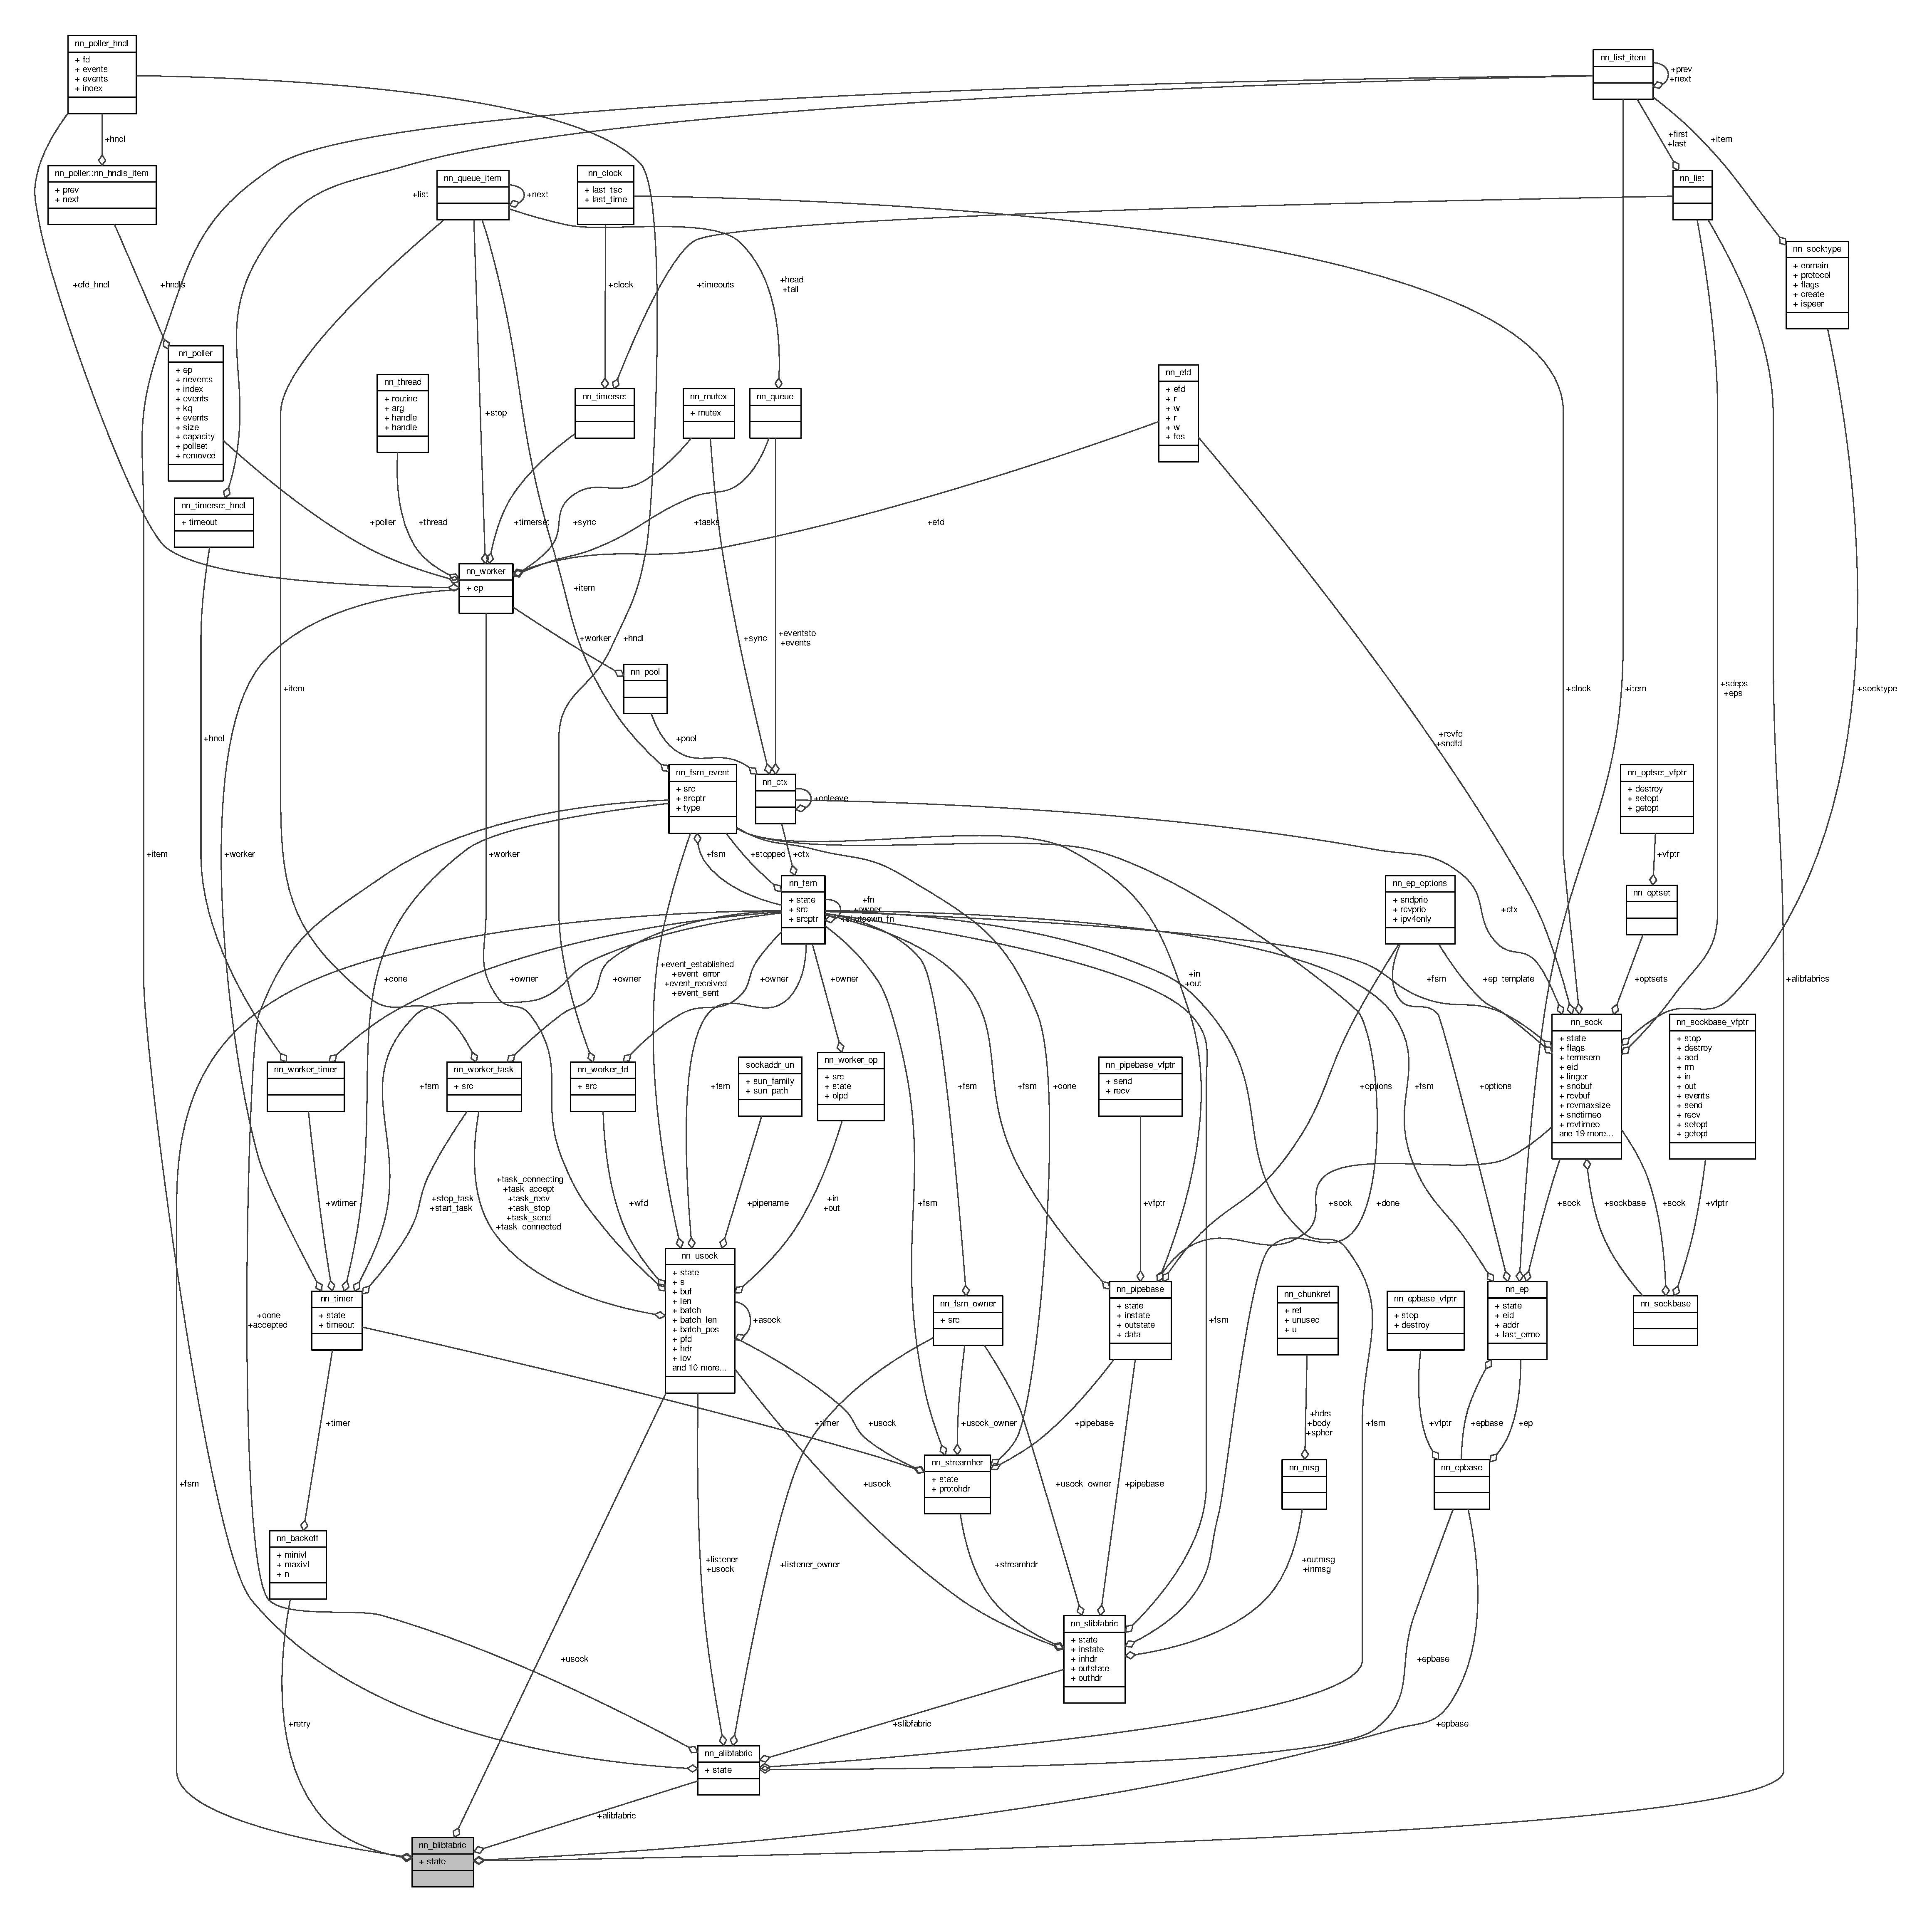
\includegraphics[width=350pt]{structnn__blibfabric__coll__graph}
\end{center}
\end{figure}
\subsection*{Public Attributes}
\begin{DoxyCompactItemize}
\item 
struct \hyperlink{structnn__fsm}{nn\+\_\+fsm} \hyperlink{structnn__blibfabric_ac4da7c0cbcb8000dd0bdf92a5f250483}{fsm}
\item 
int \hyperlink{structnn__blibfabric_a215abc4fe37a396adedc66ee4af7de61}{state}
\item 
struct \hyperlink{structnn__epbase}{nn\+\_\+epbase} \hyperlink{structnn__blibfabric_a62a7b18e4d3c4e19d90bbaac7aab58e0}{epbase}
\item 
struct \hyperlink{structnn__usock}{nn\+\_\+usock} \hyperlink{structnn__blibfabric_acb29026f7306bc1de9ec8fdbbdde54af}{usock}
\item 
struct \hyperlink{structnn__alibfabric}{nn\+\_\+alibfabric} $\ast$ \hyperlink{structnn__blibfabric_aab27658e6d4f2fd14369456c72f9a6ed}{alibfabric}
\item 
struct \hyperlink{structnn__list}{nn\+\_\+list} \hyperlink{structnn__blibfabric_a45dd63b7b4f532b8cf89784eb5d8f12c}{alibfabrics}
\item 
struct \hyperlink{structnn__backoff}{nn\+\_\+backoff} \hyperlink{structnn__blibfabric_a6318655e10f61b8d295d6d97133e2380}{retry}
\end{DoxyCompactItemize}


\subsection{Member Data Documentation}
\index{nn\+\_\+blibfabric@{nn\+\_\+blibfabric}!alibfabric@{alibfabric}}
\index{alibfabric@{alibfabric}!nn\+\_\+blibfabric@{nn\+\_\+blibfabric}}
\subsubsection[{alibfabric}]{\setlength{\rightskip}{0pt plus 5cm}struct {\bf nn\+\_\+alibfabric} $\ast$ nn\+\_\+blibfabric\+::alibfabric}\hypertarget{structnn__blibfabric_aab27658e6d4f2fd14369456c72f9a6ed}{}\label{structnn__blibfabric_aab27658e6d4f2fd14369456c72f9a6ed}
\index{nn\+\_\+blibfabric@{nn\+\_\+blibfabric}!alibfabrics@{alibfabrics}}
\index{alibfabrics@{alibfabrics}!nn\+\_\+blibfabric@{nn\+\_\+blibfabric}}
\subsubsection[{alibfabrics}]{\setlength{\rightskip}{0pt plus 5cm}struct {\bf nn\+\_\+list} nn\+\_\+blibfabric\+::alibfabrics}\hypertarget{structnn__blibfabric_a45dd63b7b4f532b8cf89784eb5d8f12c}{}\label{structnn__blibfabric_a45dd63b7b4f532b8cf89784eb5d8f12c}
\index{nn\+\_\+blibfabric@{nn\+\_\+blibfabric}!epbase@{epbase}}
\index{epbase@{epbase}!nn\+\_\+blibfabric@{nn\+\_\+blibfabric}}
\subsubsection[{epbase}]{\setlength{\rightskip}{0pt plus 5cm}struct {\bf nn\+\_\+epbase} nn\+\_\+blibfabric\+::epbase}\hypertarget{structnn__blibfabric_a62a7b18e4d3c4e19d90bbaac7aab58e0}{}\label{structnn__blibfabric_a62a7b18e4d3c4e19d90bbaac7aab58e0}
\index{nn\+\_\+blibfabric@{nn\+\_\+blibfabric}!fsm@{fsm}}
\index{fsm@{fsm}!nn\+\_\+blibfabric@{nn\+\_\+blibfabric}}
\subsubsection[{fsm}]{\setlength{\rightskip}{0pt plus 5cm}struct {\bf nn\+\_\+fsm} nn\+\_\+blibfabric\+::fsm}\hypertarget{structnn__blibfabric_ac4da7c0cbcb8000dd0bdf92a5f250483}{}\label{structnn__blibfabric_ac4da7c0cbcb8000dd0bdf92a5f250483}
\index{nn\+\_\+blibfabric@{nn\+\_\+blibfabric}!retry@{retry}}
\index{retry@{retry}!nn\+\_\+blibfabric@{nn\+\_\+blibfabric}}
\subsubsection[{retry}]{\setlength{\rightskip}{0pt plus 5cm}struct {\bf nn\+\_\+backoff} nn\+\_\+blibfabric\+::retry}\hypertarget{structnn__blibfabric_a6318655e10f61b8d295d6d97133e2380}{}\label{structnn__blibfabric_a6318655e10f61b8d295d6d97133e2380}
\index{nn\+\_\+blibfabric@{nn\+\_\+blibfabric}!state@{state}}
\index{state@{state}!nn\+\_\+blibfabric@{nn\+\_\+blibfabric}}
\subsubsection[{state}]{\setlength{\rightskip}{0pt plus 5cm}int nn\+\_\+blibfabric\+::state}\hypertarget{structnn__blibfabric_a215abc4fe37a396adedc66ee4af7de61}{}\label{structnn__blibfabric_a215abc4fe37a396adedc66ee4af7de61}
\index{nn\+\_\+blibfabric@{nn\+\_\+blibfabric}!usock@{usock}}
\index{usock@{usock}!nn\+\_\+blibfabric@{nn\+\_\+blibfabric}}
\subsubsection[{usock}]{\setlength{\rightskip}{0pt plus 5cm}struct {\bf nn\+\_\+usock} nn\+\_\+blibfabric\+::usock}\hypertarget{structnn__blibfabric_acb29026f7306bc1de9ec8fdbbdde54af}{}\label{structnn__blibfabric_acb29026f7306bc1de9ec8fdbbdde54af}


The documentation for this struct was generated from the following files\+:\begin{DoxyCompactItemize}
\item 
src/transports/libfabric/\hyperlink{bagain_8c}{bagain.\+c}\item 
src/transports/libfabric/\hyperlink{blibfabric_8c}{blibfabric.\+c}\end{DoxyCompactItemize}

\hypertarget{structnn__btcp}{}\section{nn\+\_\+btcp Struct Reference}
\label{structnn__btcp}\index{nn\+\_\+btcp@{nn\+\_\+btcp}}


Collaboration diagram for nn\+\_\+btcp\+:\nopagebreak
\begin{figure}[H]
\begin{center}
\leavevmode
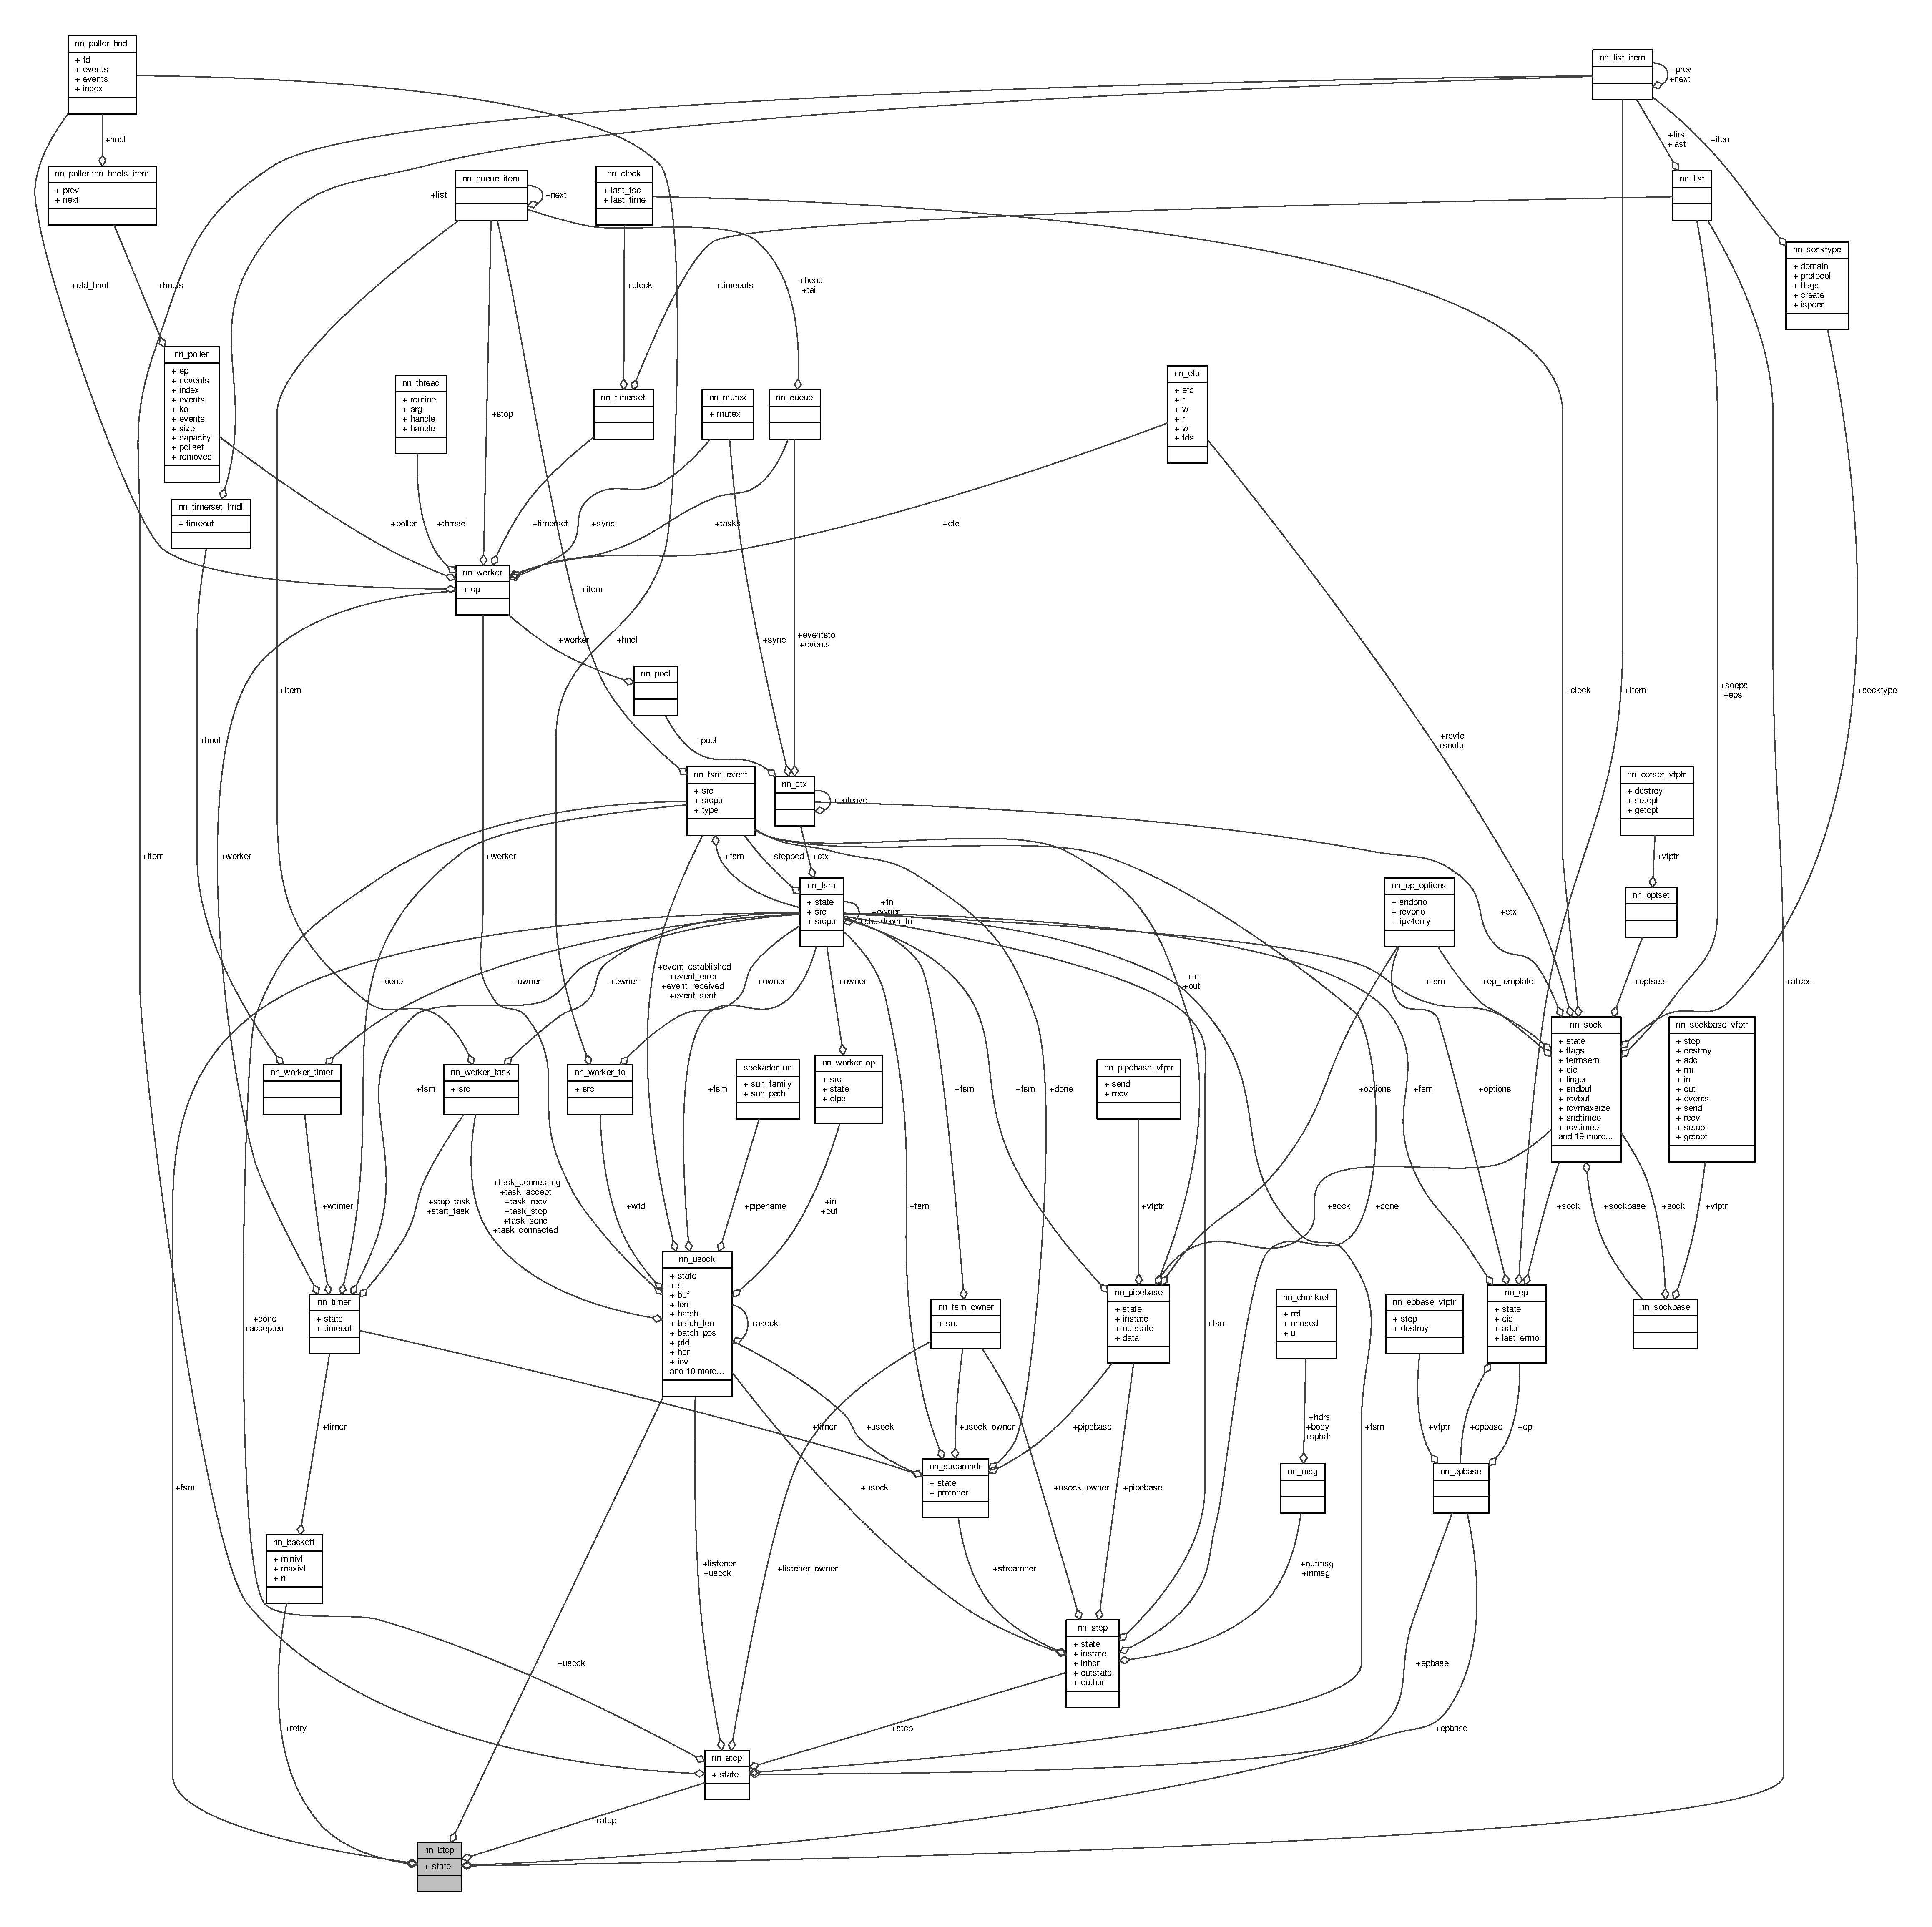
\includegraphics[width=350pt]{structnn__btcp__coll__graph}
\end{center}
\end{figure}
\subsection*{Public Attributes}
\begin{DoxyCompactItemize}
\item 
struct \hyperlink{structnn__fsm}{nn\+\_\+fsm} \hyperlink{structnn__btcp_a6886990fa4dd60e2535396aee2a97808}{fsm}
\item 
int \hyperlink{structnn__btcp_ac4e1a393ee479ac93b3d700f92099605}{state}
\item 
struct \hyperlink{structnn__epbase}{nn\+\_\+epbase} \hyperlink{structnn__btcp_acf1bdc439c5e15227dcb9da067d33c82}{epbase}
\item 
struct \hyperlink{structnn__usock}{nn\+\_\+usock} \hyperlink{structnn__btcp_a1f5c9c60495f0d5cd20611d3bcc9aaa0}{usock}
\item 
struct \hyperlink{structnn__atcp}{nn\+\_\+atcp} $\ast$ \hyperlink{structnn__btcp_a938d221e28e4dd8b259f446287677a7b}{atcp}
\item 
struct \hyperlink{structnn__list}{nn\+\_\+list} \hyperlink{structnn__btcp_a12b26d20ebff3da6c00c5dce249e2003}{atcps}
\item 
struct \hyperlink{structnn__backoff}{nn\+\_\+backoff} \hyperlink{structnn__btcp_a113d8b4835aeec6c8df2f7cf9ffdea5f}{retry}
\end{DoxyCompactItemize}


\subsection{Member Data Documentation}
\index{nn\+\_\+btcp@{nn\+\_\+btcp}!atcp@{atcp}}
\index{atcp@{atcp}!nn\+\_\+btcp@{nn\+\_\+btcp}}
\subsubsection[{atcp}]{\setlength{\rightskip}{0pt plus 5cm}struct {\bf nn\+\_\+atcp}$\ast$ nn\+\_\+btcp\+::atcp}\hypertarget{structnn__btcp_a938d221e28e4dd8b259f446287677a7b}{}\label{structnn__btcp_a938d221e28e4dd8b259f446287677a7b}
\index{nn\+\_\+btcp@{nn\+\_\+btcp}!atcps@{atcps}}
\index{atcps@{atcps}!nn\+\_\+btcp@{nn\+\_\+btcp}}
\subsubsection[{atcps}]{\setlength{\rightskip}{0pt plus 5cm}struct {\bf nn\+\_\+list} nn\+\_\+btcp\+::atcps}\hypertarget{structnn__btcp_a12b26d20ebff3da6c00c5dce249e2003}{}\label{structnn__btcp_a12b26d20ebff3da6c00c5dce249e2003}
\index{nn\+\_\+btcp@{nn\+\_\+btcp}!epbase@{epbase}}
\index{epbase@{epbase}!nn\+\_\+btcp@{nn\+\_\+btcp}}
\subsubsection[{epbase}]{\setlength{\rightskip}{0pt plus 5cm}struct {\bf nn\+\_\+epbase} nn\+\_\+btcp\+::epbase}\hypertarget{structnn__btcp_acf1bdc439c5e15227dcb9da067d33c82}{}\label{structnn__btcp_acf1bdc439c5e15227dcb9da067d33c82}
\index{nn\+\_\+btcp@{nn\+\_\+btcp}!fsm@{fsm}}
\index{fsm@{fsm}!nn\+\_\+btcp@{nn\+\_\+btcp}}
\subsubsection[{fsm}]{\setlength{\rightskip}{0pt plus 5cm}struct {\bf nn\+\_\+fsm} nn\+\_\+btcp\+::fsm}\hypertarget{structnn__btcp_a6886990fa4dd60e2535396aee2a97808}{}\label{structnn__btcp_a6886990fa4dd60e2535396aee2a97808}
\index{nn\+\_\+btcp@{nn\+\_\+btcp}!retry@{retry}}
\index{retry@{retry}!nn\+\_\+btcp@{nn\+\_\+btcp}}
\subsubsection[{retry}]{\setlength{\rightskip}{0pt plus 5cm}struct {\bf nn\+\_\+backoff} nn\+\_\+btcp\+::retry}\hypertarget{structnn__btcp_a113d8b4835aeec6c8df2f7cf9ffdea5f}{}\label{structnn__btcp_a113d8b4835aeec6c8df2f7cf9ffdea5f}
\index{nn\+\_\+btcp@{nn\+\_\+btcp}!state@{state}}
\index{state@{state}!nn\+\_\+btcp@{nn\+\_\+btcp}}
\subsubsection[{state}]{\setlength{\rightskip}{0pt plus 5cm}int nn\+\_\+btcp\+::state}\hypertarget{structnn__btcp_ac4e1a393ee479ac93b3d700f92099605}{}\label{structnn__btcp_ac4e1a393ee479ac93b3d700f92099605}
\index{nn\+\_\+btcp@{nn\+\_\+btcp}!usock@{usock}}
\index{usock@{usock}!nn\+\_\+btcp@{nn\+\_\+btcp}}
\subsubsection[{usock}]{\setlength{\rightskip}{0pt plus 5cm}struct {\bf nn\+\_\+usock} nn\+\_\+btcp\+::usock}\hypertarget{structnn__btcp_a1f5c9c60495f0d5cd20611d3bcc9aaa0}{}\label{structnn__btcp_a1f5c9c60495f0d5cd20611d3bcc9aaa0}


The documentation for this struct was generated from the following file\+:\begin{DoxyCompactItemize}
\item 
src/transports/tcp/\hyperlink{btcp_8c}{btcp.\+c}\end{DoxyCompactItemize}

\hypertarget{structnn__btcpmux}{}\section{nn\+\_\+btcpmux Struct Reference}
\label{structnn__btcpmux}\index{nn\+\_\+btcpmux@{nn\+\_\+btcpmux}}


Collaboration diagram for nn\+\_\+btcpmux\+:\nopagebreak
\begin{figure}[H]
\begin{center}
\leavevmode
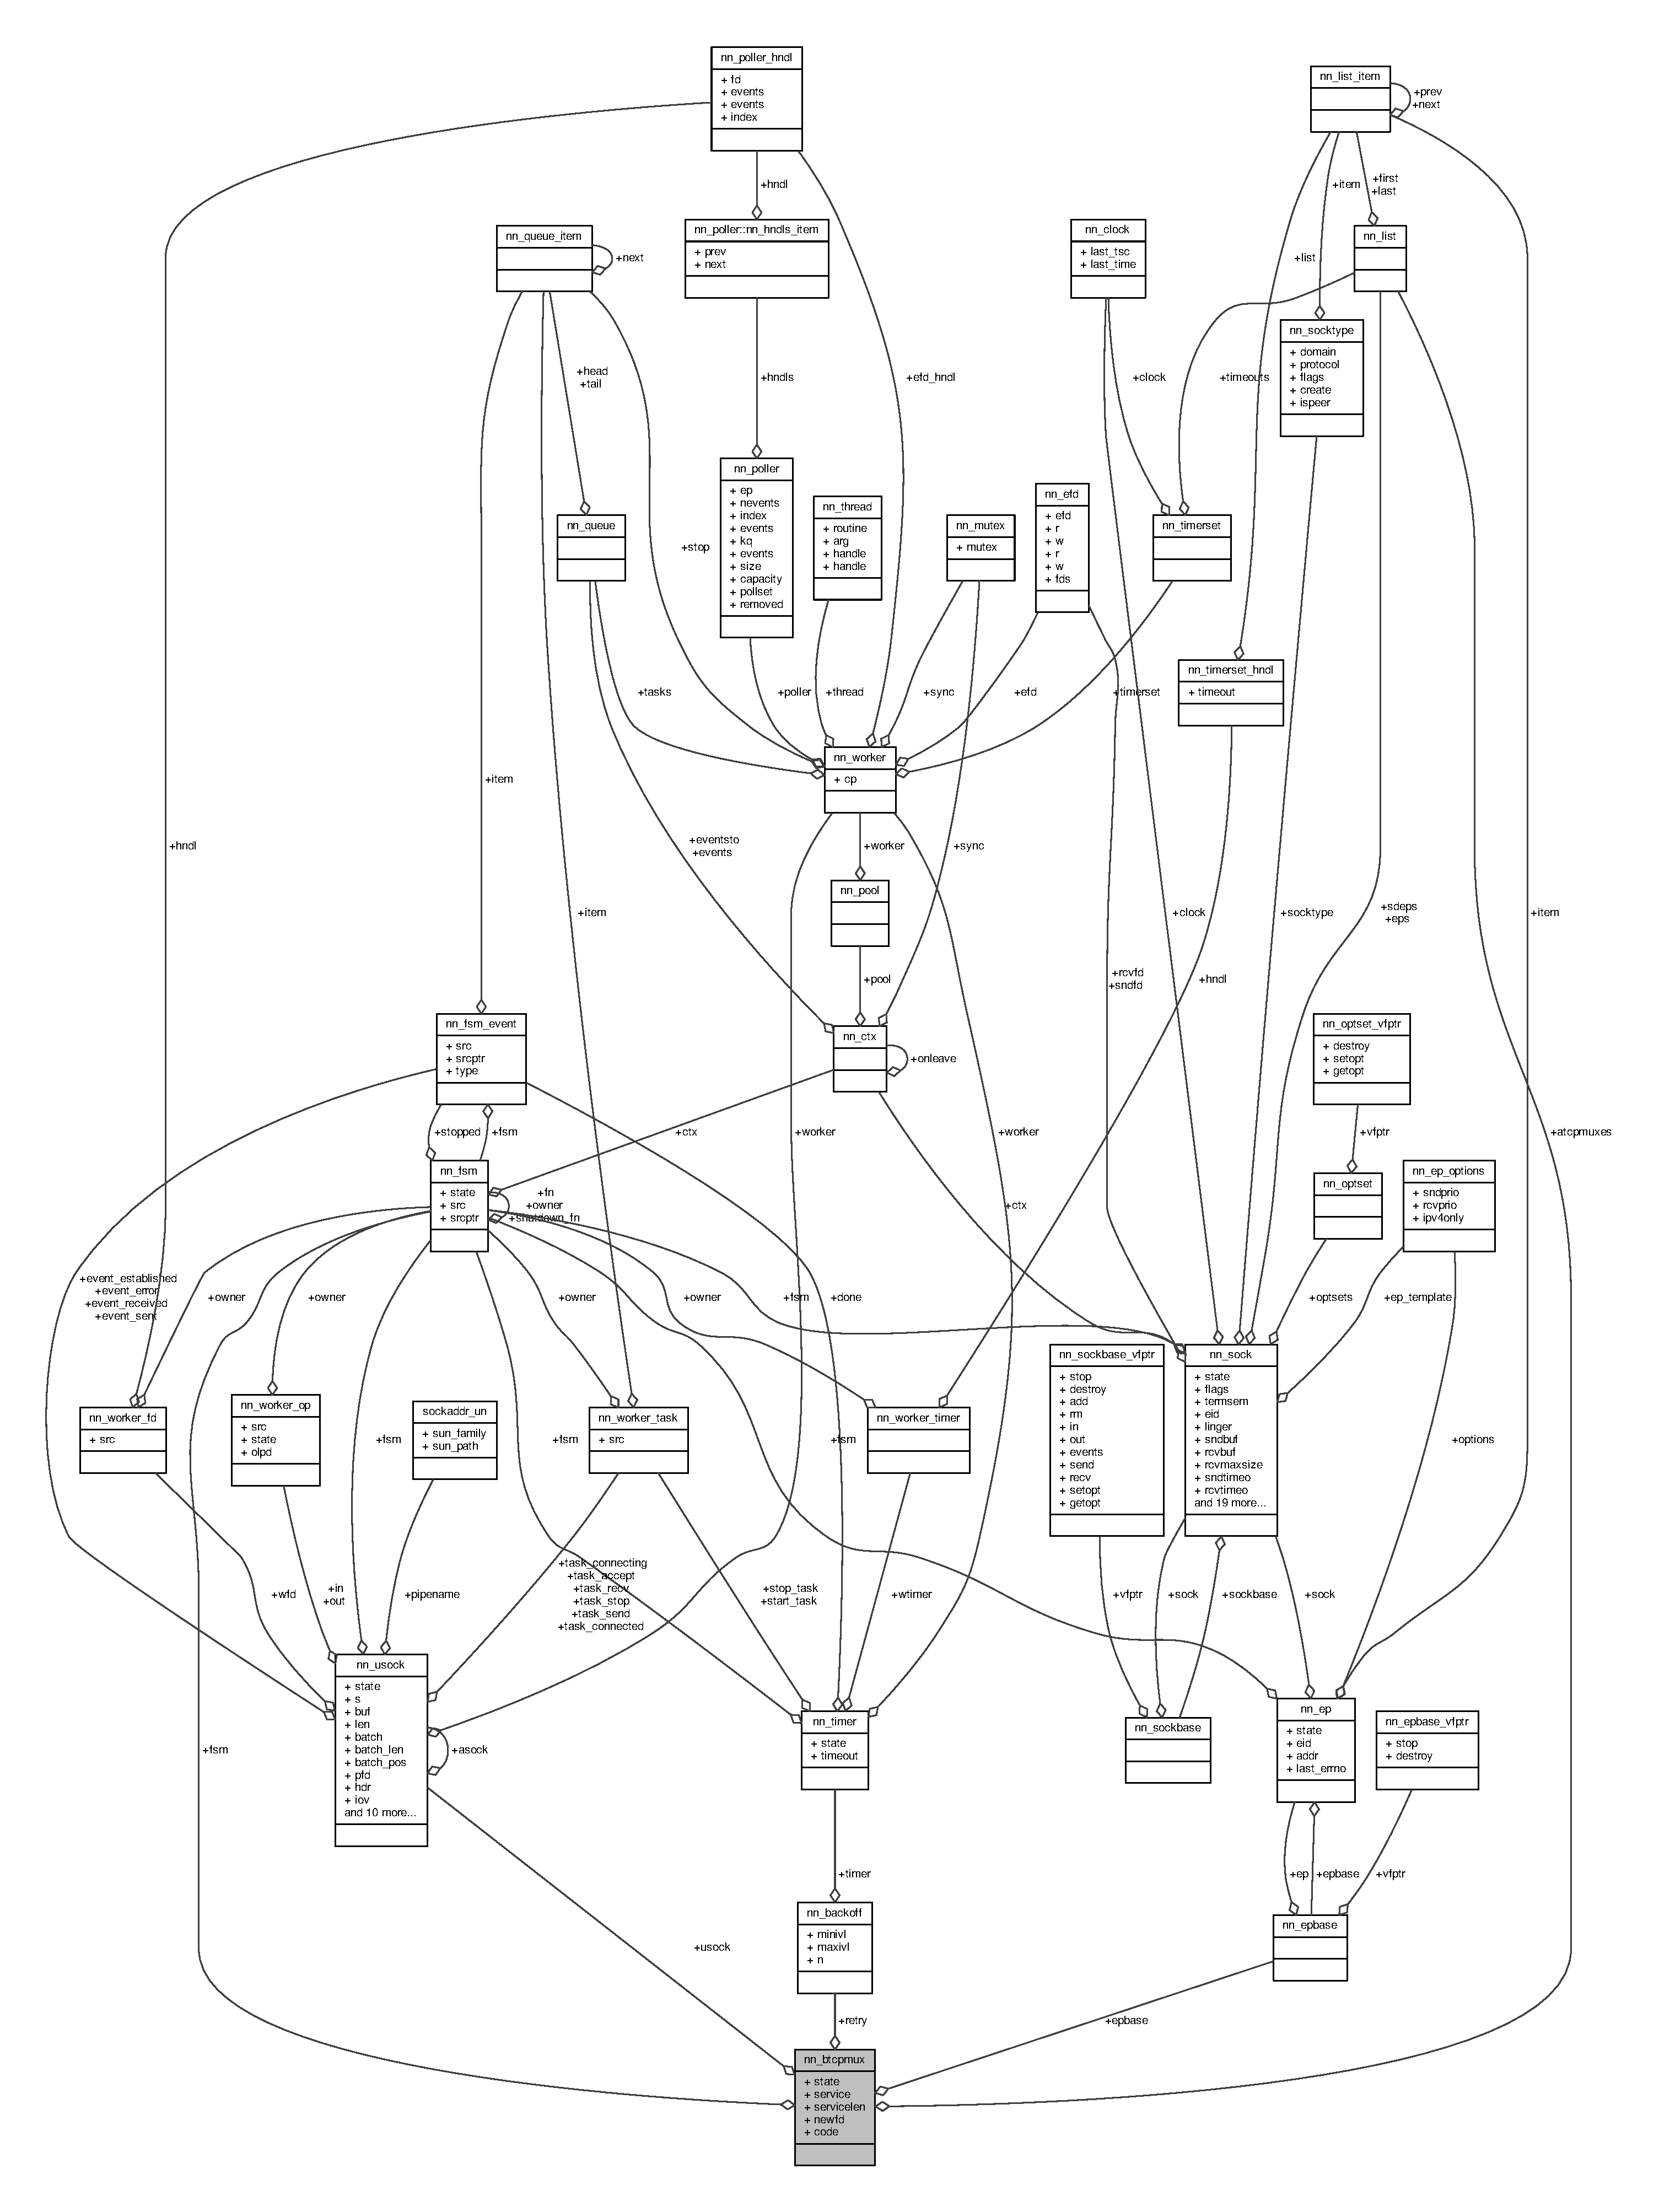
\includegraphics[width=350pt]{structnn__btcpmux__coll__graph}
\end{center}
\end{figure}
\subsection*{Public Attributes}
\begin{DoxyCompactItemize}
\item 
struct \hyperlink{structnn__fsm}{nn\+\_\+fsm} \hyperlink{structnn__btcpmux_ad05869d3010457846d3f0b4a9dbb61e3}{fsm}
\item 
int \hyperlink{structnn__btcpmux_afc599be6405e8a1646274ab3a378ed87}{state}
\item 
struct \hyperlink{structnn__epbase}{nn\+\_\+epbase} \hyperlink{structnn__btcpmux_a0228259a8bfcdb9a2f7863ff48e6a7ae}{epbase}
\item 
struct \hyperlink{structnn__usock}{nn\+\_\+usock} \hyperlink{structnn__btcpmux_ab566e4fee610dd8580194d14a4ee2417}{usock}
\item 
struct \hyperlink{structnn__list}{nn\+\_\+list} \hyperlink{structnn__btcpmux_adf2c3cbed0a8498e5963b3abd45c1408}{atcpmuxes}
\item 
struct \hyperlink{structnn__backoff}{nn\+\_\+backoff} \hyperlink{structnn__btcpmux_a910b39218598d10125dd5ff82b33914e}{retry}
\item 
const char $\ast$ \hyperlink{structnn__btcpmux_a7b397ca4f026d6da4959f031ff9e759d}{service}
\item 
uint16\+\_\+t \hyperlink{structnn__btcpmux_a6908f0b688e86cbab503cec8bae0afbd}{servicelen}
\item 
int \hyperlink{structnn__btcpmux_a996d4e690af37aad865017b598a14189}{newfd}
\item 
char \hyperlink{structnn__btcpmux_a33ca4d6da08be0f9da1b140f445c30a0}{code}
\end{DoxyCompactItemize}


\subsection{Member Data Documentation}
\index{nn\+\_\+btcpmux@{nn\+\_\+btcpmux}!atcpmuxes@{atcpmuxes}}
\index{atcpmuxes@{atcpmuxes}!nn\+\_\+btcpmux@{nn\+\_\+btcpmux}}
\subsubsection[{atcpmuxes}]{\setlength{\rightskip}{0pt plus 5cm}struct {\bf nn\+\_\+list} nn\+\_\+btcpmux\+::atcpmuxes}\hypertarget{structnn__btcpmux_adf2c3cbed0a8498e5963b3abd45c1408}{}\label{structnn__btcpmux_adf2c3cbed0a8498e5963b3abd45c1408}
\index{nn\+\_\+btcpmux@{nn\+\_\+btcpmux}!code@{code}}
\index{code@{code}!nn\+\_\+btcpmux@{nn\+\_\+btcpmux}}
\subsubsection[{code}]{\setlength{\rightskip}{0pt plus 5cm}char nn\+\_\+btcpmux\+::code}\hypertarget{structnn__btcpmux_a33ca4d6da08be0f9da1b140f445c30a0}{}\label{structnn__btcpmux_a33ca4d6da08be0f9da1b140f445c30a0}
\index{nn\+\_\+btcpmux@{nn\+\_\+btcpmux}!epbase@{epbase}}
\index{epbase@{epbase}!nn\+\_\+btcpmux@{nn\+\_\+btcpmux}}
\subsubsection[{epbase}]{\setlength{\rightskip}{0pt plus 5cm}struct {\bf nn\+\_\+epbase} nn\+\_\+btcpmux\+::epbase}\hypertarget{structnn__btcpmux_a0228259a8bfcdb9a2f7863ff48e6a7ae}{}\label{structnn__btcpmux_a0228259a8bfcdb9a2f7863ff48e6a7ae}
\index{nn\+\_\+btcpmux@{nn\+\_\+btcpmux}!fsm@{fsm}}
\index{fsm@{fsm}!nn\+\_\+btcpmux@{nn\+\_\+btcpmux}}
\subsubsection[{fsm}]{\setlength{\rightskip}{0pt plus 5cm}struct {\bf nn\+\_\+fsm} nn\+\_\+btcpmux\+::fsm}\hypertarget{structnn__btcpmux_ad05869d3010457846d3f0b4a9dbb61e3}{}\label{structnn__btcpmux_ad05869d3010457846d3f0b4a9dbb61e3}
\index{nn\+\_\+btcpmux@{nn\+\_\+btcpmux}!newfd@{newfd}}
\index{newfd@{newfd}!nn\+\_\+btcpmux@{nn\+\_\+btcpmux}}
\subsubsection[{newfd}]{\setlength{\rightskip}{0pt plus 5cm}int nn\+\_\+btcpmux\+::newfd}\hypertarget{structnn__btcpmux_a996d4e690af37aad865017b598a14189}{}\label{structnn__btcpmux_a996d4e690af37aad865017b598a14189}
\index{nn\+\_\+btcpmux@{nn\+\_\+btcpmux}!retry@{retry}}
\index{retry@{retry}!nn\+\_\+btcpmux@{nn\+\_\+btcpmux}}
\subsubsection[{retry}]{\setlength{\rightskip}{0pt plus 5cm}struct {\bf nn\+\_\+backoff} nn\+\_\+btcpmux\+::retry}\hypertarget{structnn__btcpmux_a910b39218598d10125dd5ff82b33914e}{}\label{structnn__btcpmux_a910b39218598d10125dd5ff82b33914e}
\index{nn\+\_\+btcpmux@{nn\+\_\+btcpmux}!service@{service}}
\index{service@{service}!nn\+\_\+btcpmux@{nn\+\_\+btcpmux}}
\subsubsection[{service}]{\setlength{\rightskip}{0pt plus 5cm}const char$\ast$ nn\+\_\+btcpmux\+::service}\hypertarget{structnn__btcpmux_a7b397ca4f026d6da4959f031ff9e759d}{}\label{structnn__btcpmux_a7b397ca4f026d6da4959f031ff9e759d}
\index{nn\+\_\+btcpmux@{nn\+\_\+btcpmux}!servicelen@{servicelen}}
\index{servicelen@{servicelen}!nn\+\_\+btcpmux@{nn\+\_\+btcpmux}}
\subsubsection[{servicelen}]{\setlength{\rightskip}{0pt plus 5cm}uint16\+\_\+t nn\+\_\+btcpmux\+::servicelen}\hypertarget{structnn__btcpmux_a6908f0b688e86cbab503cec8bae0afbd}{}\label{structnn__btcpmux_a6908f0b688e86cbab503cec8bae0afbd}
\index{nn\+\_\+btcpmux@{nn\+\_\+btcpmux}!state@{state}}
\index{state@{state}!nn\+\_\+btcpmux@{nn\+\_\+btcpmux}}
\subsubsection[{state}]{\setlength{\rightskip}{0pt plus 5cm}int nn\+\_\+btcpmux\+::state}\hypertarget{structnn__btcpmux_afc599be6405e8a1646274ab3a378ed87}{}\label{structnn__btcpmux_afc599be6405e8a1646274ab3a378ed87}
\index{nn\+\_\+btcpmux@{nn\+\_\+btcpmux}!usock@{usock}}
\index{usock@{usock}!nn\+\_\+btcpmux@{nn\+\_\+btcpmux}}
\subsubsection[{usock}]{\setlength{\rightskip}{0pt plus 5cm}struct {\bf nn\+\_\+usock} nn\+\_\+btcpmux\+::usock}\hypertarget{structnn__btcpmux_ab566e4fee610dd8580194d14a4ee2417}{}\label{structnn__btcpmux_ab566e4fee610dd8580194d14a4ee2417}


The documentation for this struct was generated from the following file\+:\begin{DoxyCompactItemize}
\item 
src/transports/tcpmux/\hyperlink{btcpmux_8c}{btcpmux.\+c}\end{DoxyCompactItemize}

\hypertarget{structnn__bus}{}\section{nn\+\_\+bus Struct Reference}
\label{structnn__bus}\index{nn\+\_\+bus@{nn\+\_\+bus}}


Collaboration diagram for nn\+\_\+bus\+:\nopagebreak
\begin{figure}[H]
\begin{center}
\leavevmode
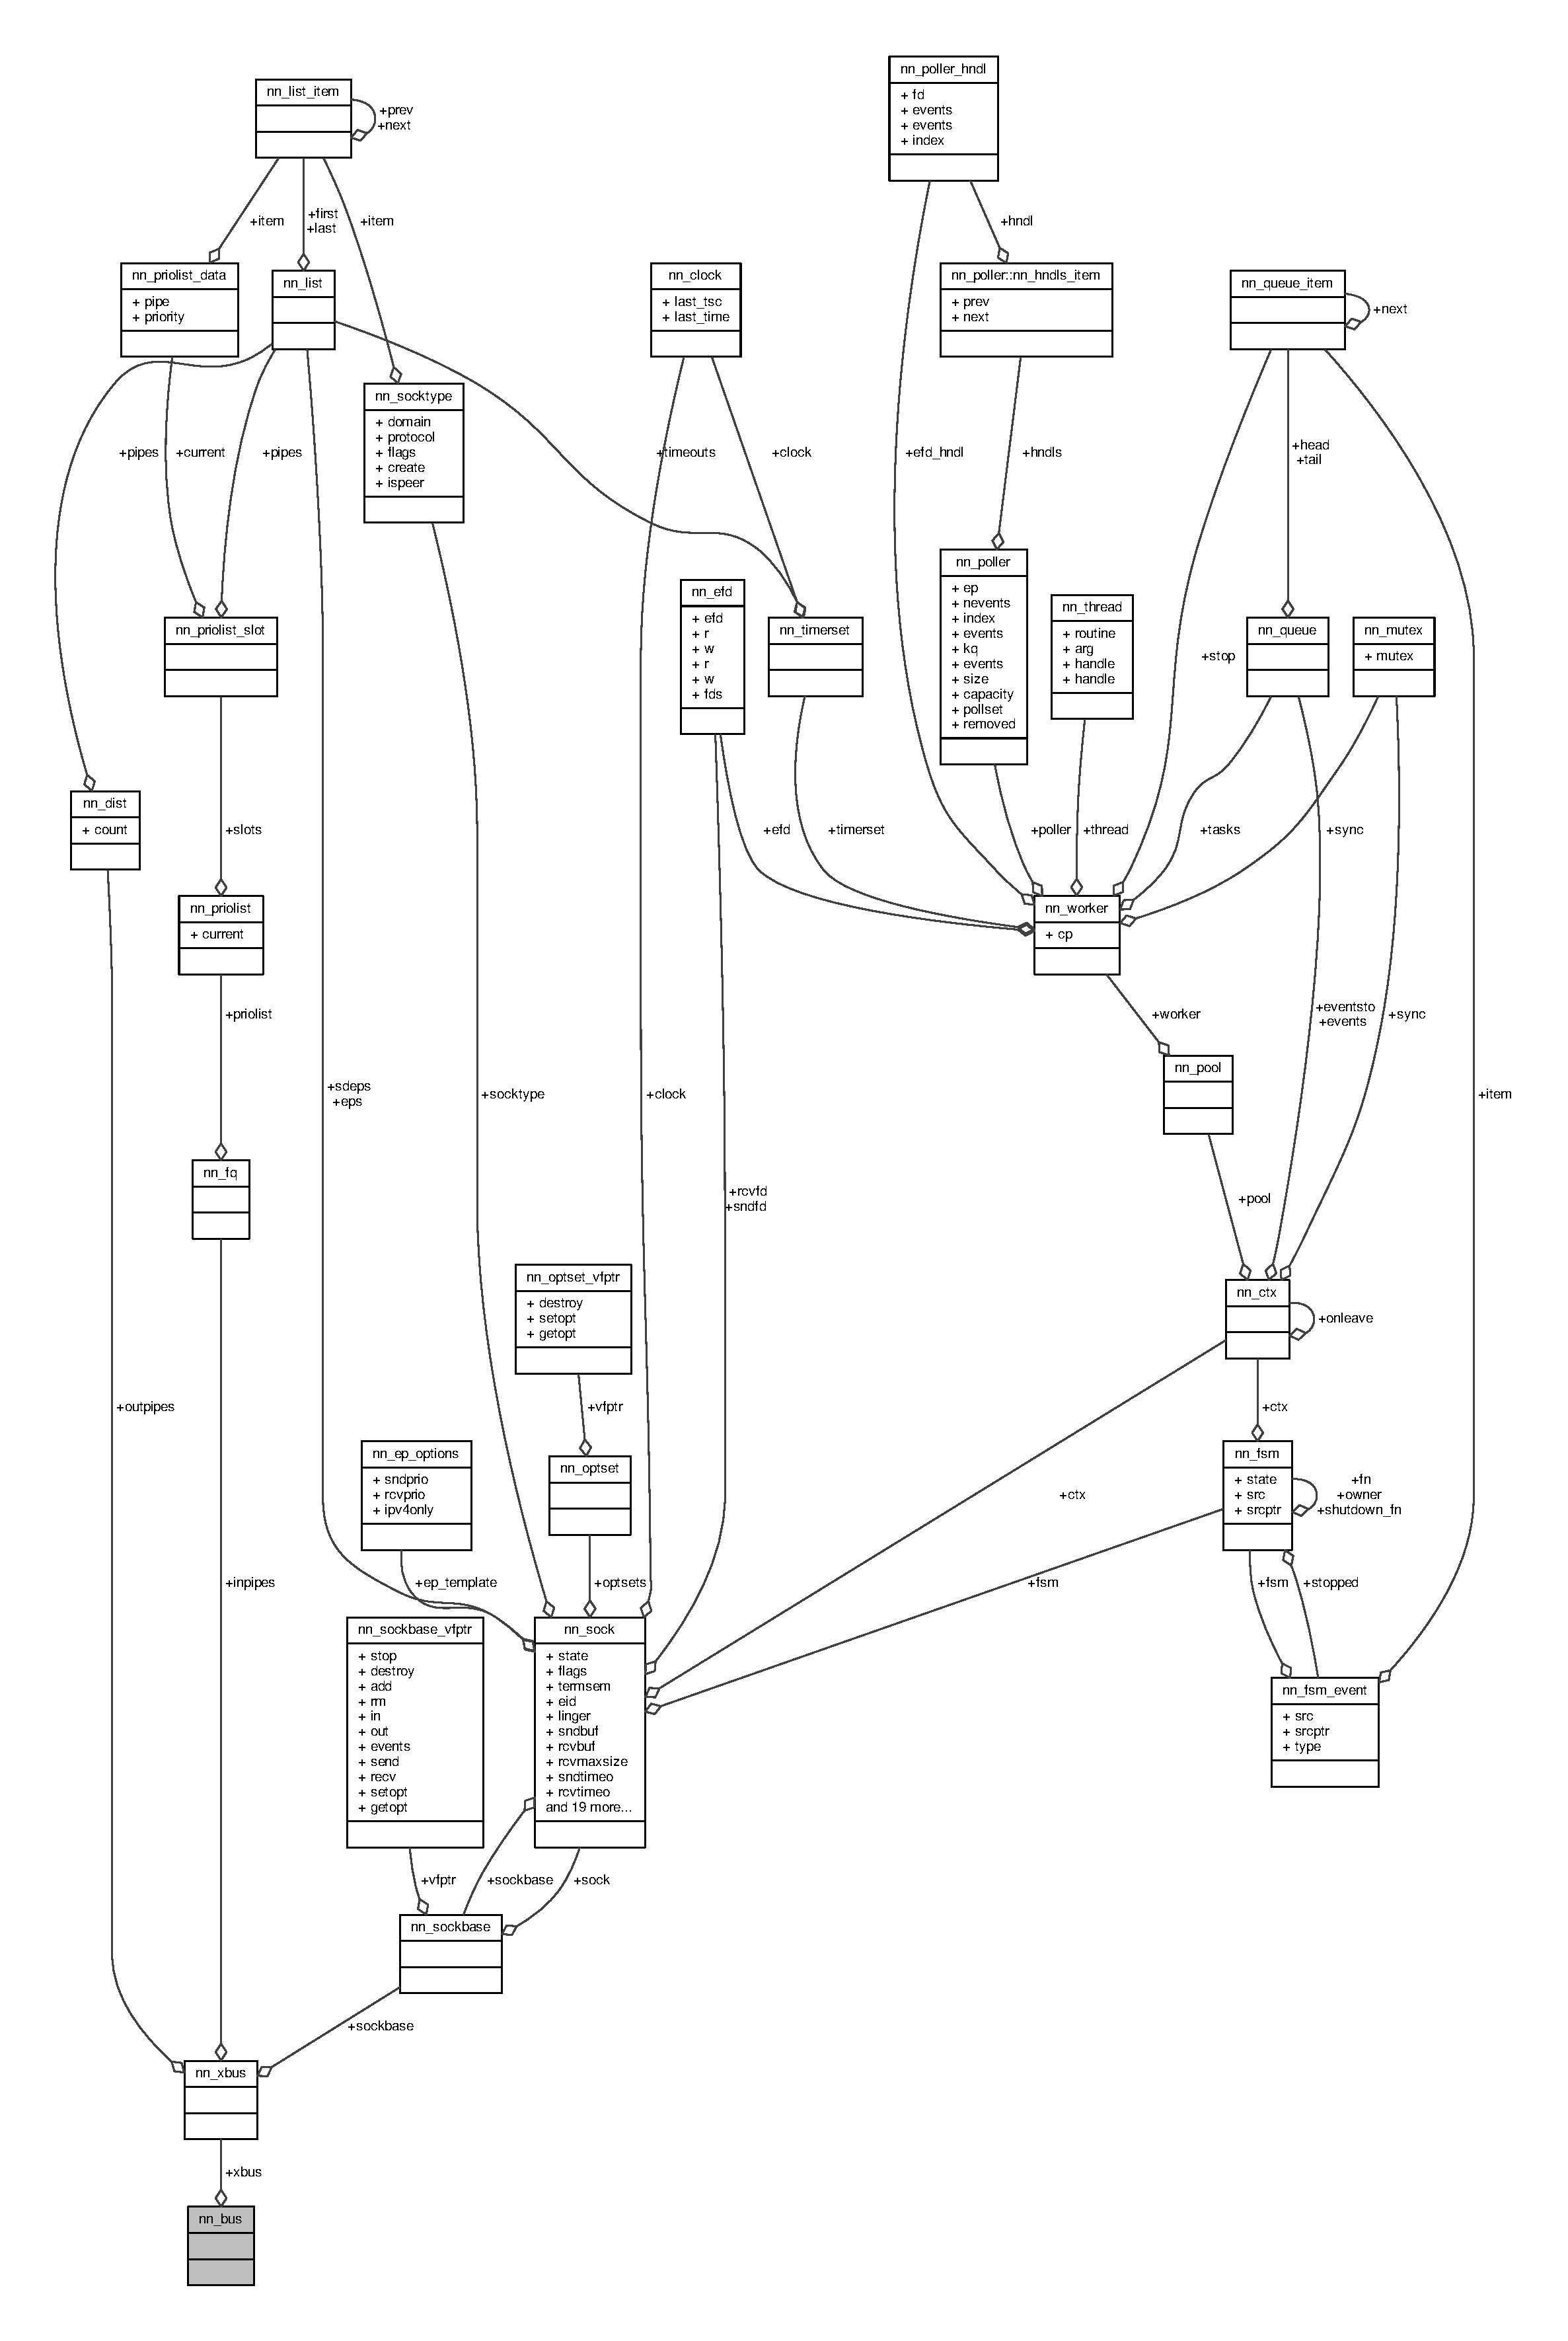
\includegraphics[width=350pt]{structnn__bus__coll__graph}
\end{center}
\end{figure}
\subsection*{Public Attributes}
\begin{DoxyCompactItemize}
\item 
struct \hyperlink{structnn__xbus}{nn\+\_\+xbus} \hyperlink{structnn__bus_a4e1cacf22f06d92e9707e3ca357072fe}{xbus}
\end{DoxyCompactItemize}


\subsection{Member Data Documentation}
\index{nn\+\_\+bus@{nn\+\_\+bus}!xbus@{xbus}}
\index{xbus@{xbus}!nn\+\_\+bus@{nn\+\_\+bus}}
\subsubsection[{xbus}]{\setlength{\rightskip}{0pt plus 5cm}struct {\bf nn\+\_\+xbus} nn\+\_\+bus\+::xbus}\hypertarget{structnn__bus_a4e1cacf22f06d92e9707e3ca357072fe}{}\label{structnn__bus_a4e1cacf22f06d92e9707e3ca357072fe}


The documentation for this struct was generated from the following file\+:\begin{DoxyCompactItemize}
\item 
src/protocols/bus/\hyperlink{src_2protocols_2bus_2bus_8c}{bus.\+c}\end{DoxyCompactItemize}

\hypertarget{structnn__bws}{}\section{nn\+\_\+bws Struct Reference}
\label{structnn__bws}\index{nn\+\_\+bws@{nn\+\_\+bws}}


Collaboration diagram for nn\+\_\+bws\+:\nopagebreak
\begin{figure}[H]
\begin{center}
\leavevmode
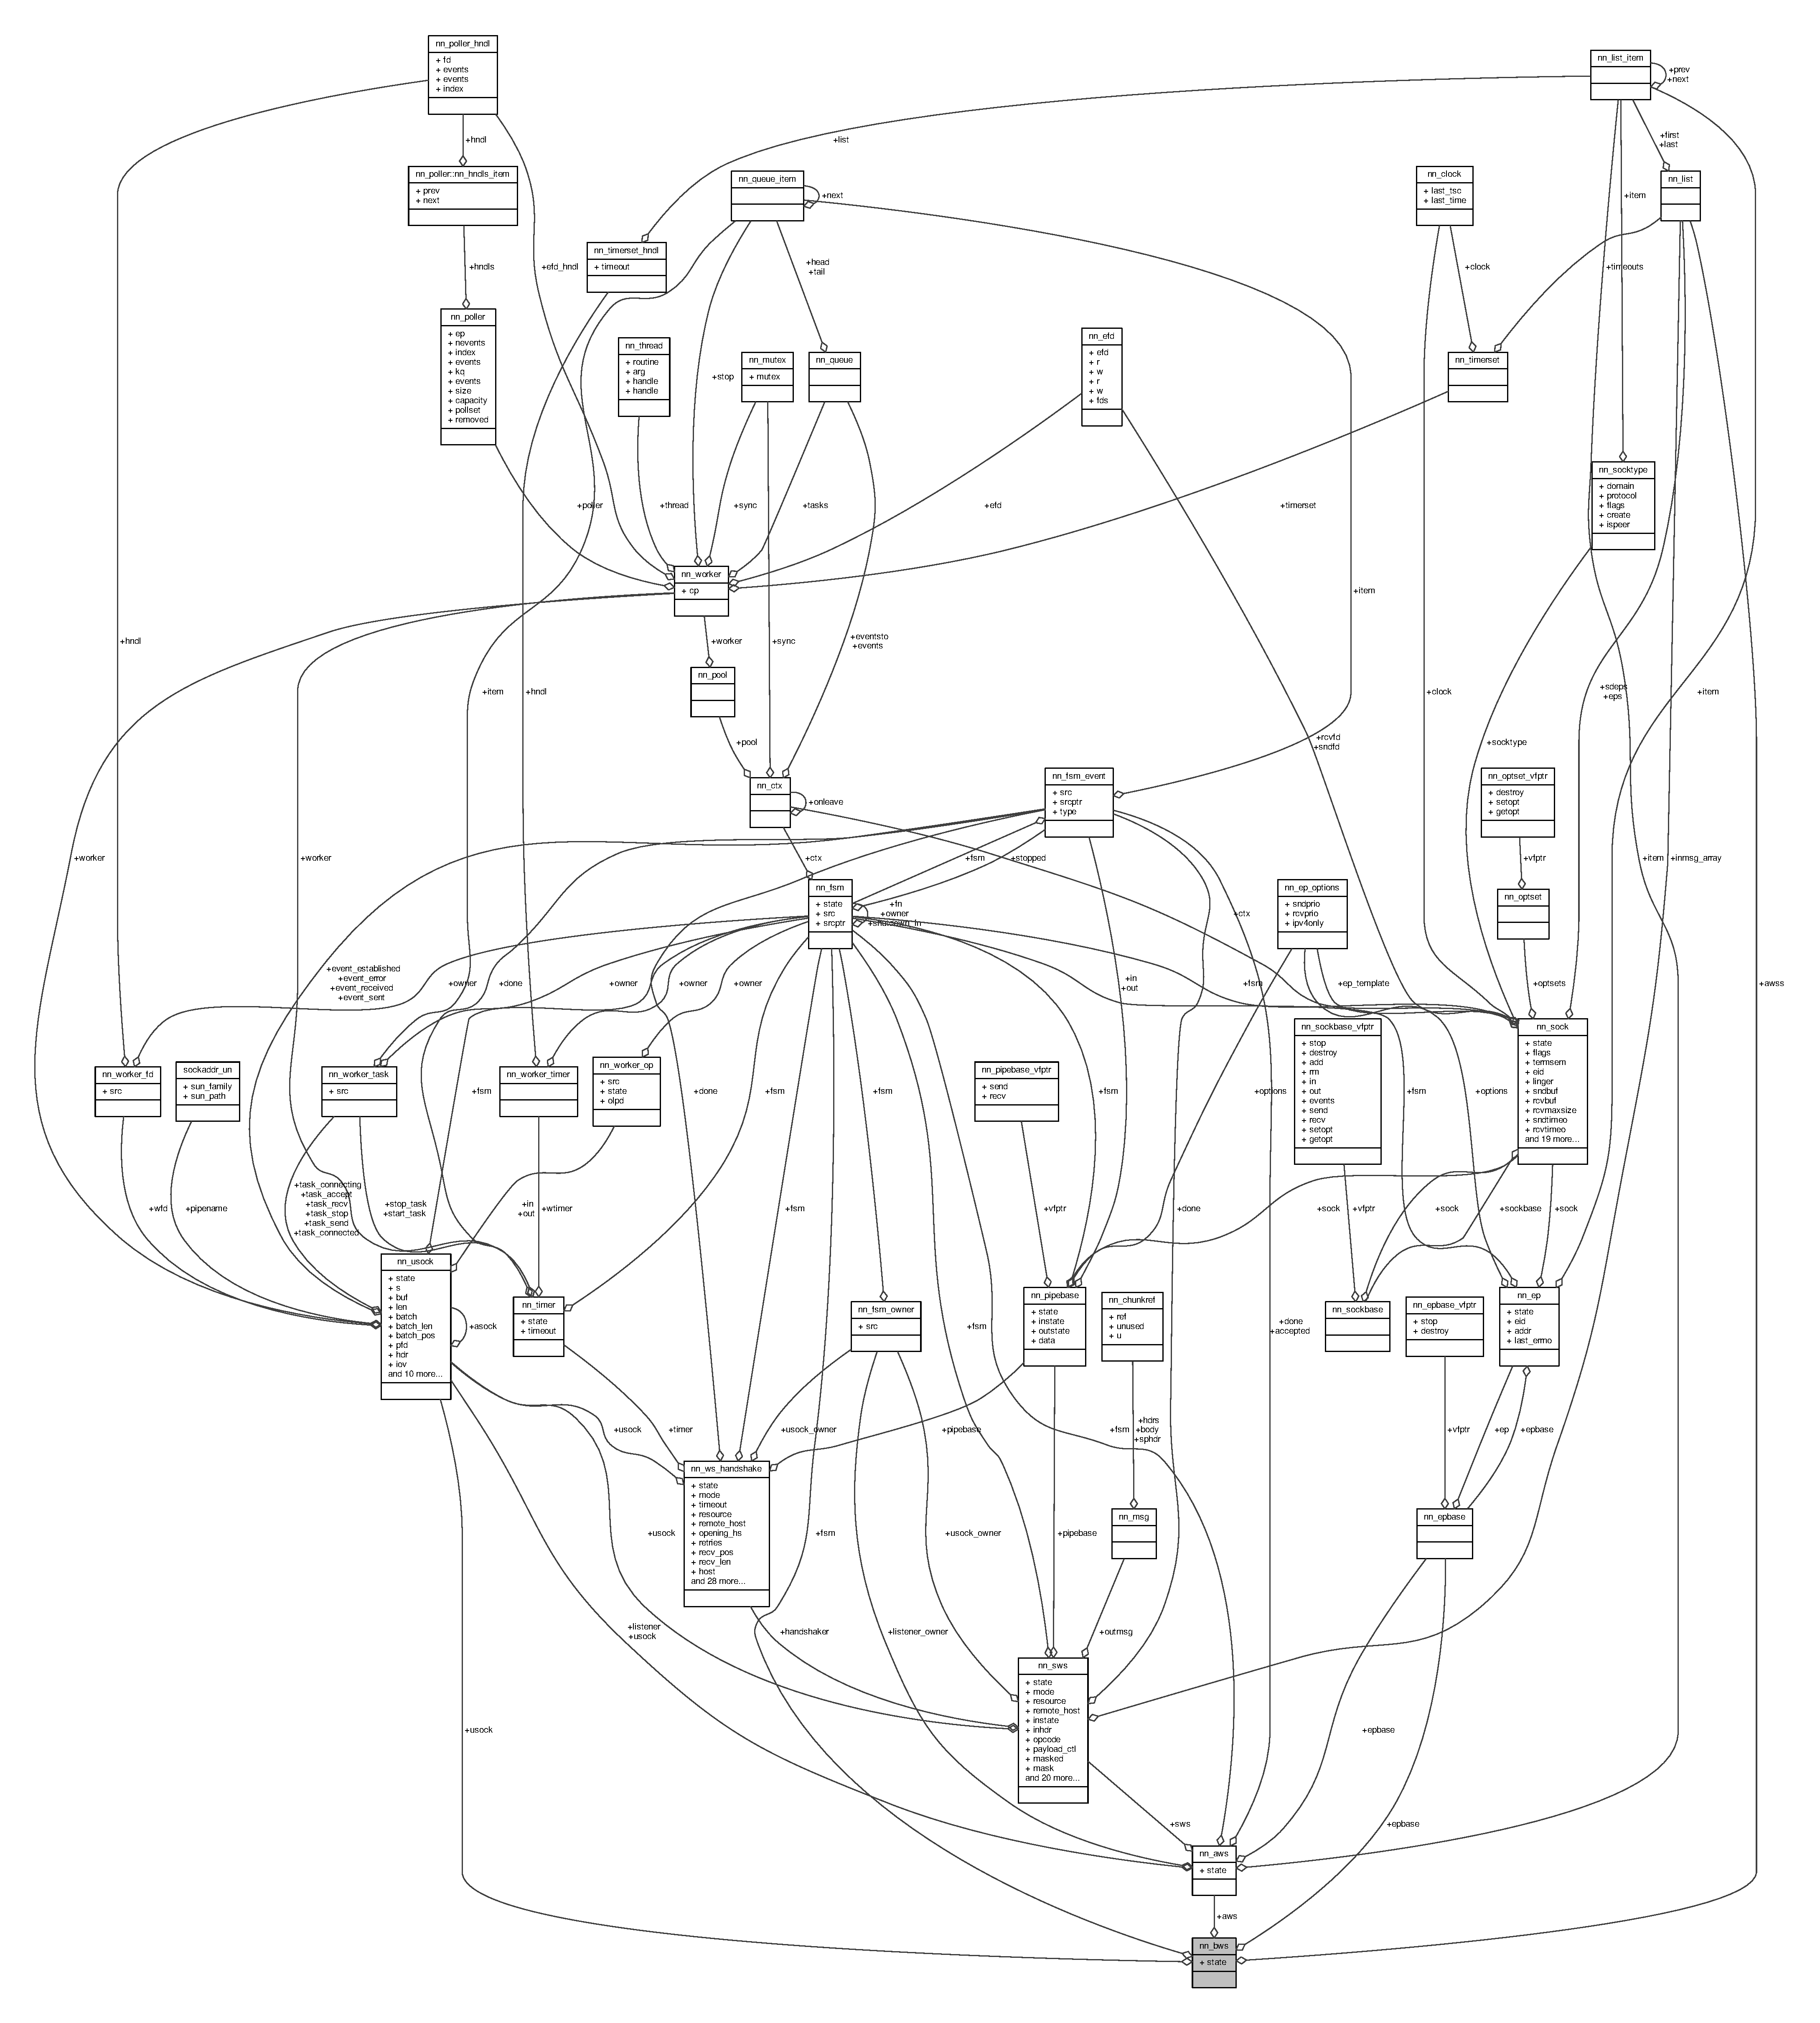
\includegraphics[width=350pt]{structnn__bws__coll__graph}
\end{center}
\end{figure}
\subsection*{Public Attributes}
\begin{DoxyCompactItemize}
\item 
struct \hyperlink{structnn__fsm}{nn\+\_\+fsm} \hyperlink{structnn__bws_a9418e42dd701ba439685ffaea8e97a02}{fsm}
\item 
int \hyperlink{structnn__bws_a0102f70d814af99ecedd5c2b0f471a2d}{state}
\item 
struct \hyperlink{structnn__epbase}{nn\+\_\+epbase} \hyperlink{structnn__bws_ad00de0df67ca0663205c45e207e81bfb}{epbase}
\item 
struct \hyperlink{structnn__usock}{nn\+\_\+usock} \hyperlink{structnn__bws_a322ef3f4fe653a4002a8d6355fe48ee5}{usock}
\item 
struct \hyperlink{structnn__aws}{nn\+\_\+aws} $\ast$ \hyperlink{structnn__bws_a718a3274a89d9327c13c956cc9b105a4}{aws}
\item 
struct \hyperlink{structnn__list}{nn\+\_\+list} \hyperlink{structnn__bws_ac1620e662d0c298115bcda10cfe6df91}{awss}
\end{DoxyCompactItemize}


\subsection{Member Data Documentation}
\index{nn\+\_\+bws@{nn\+\_\+bws}!aws@{aws}}
\index{aws@{aws}!nn\+\_\+bws@{nn\+\_\+bws}}
\subsubsection[{aws}]{\setlength{\rightskip}{0pt plus 5cm}struct {\bf nn\+\_\+aws}$\ast$ nn\+\_\+bws\+::aws}\hypertarget{structnn__bws_a718a3274a89d9327c13c956cc9b105a4}{}\label{structnn__bws_a718a3274a89d9327c13c956cc9b105a4}
\index{nn\+\_\+bws@{nn\+\_\+bws}!awss@{awss}}
\index{awss@{awss}!nn\+\_\+bws@{nn\+\_\+bws}}
\subsubsection[{awss}]{\setlength{\rightskip}{0pt plus 5cm}struct {\bf nn\+\_\+list} nn\+\_\+bws\+::awss}\hypertarget{structnn__bws_ac1620e662d0c298115bcda10cfe6df91}{}\label{structnn__bws_ac1620e662d0c298115bcda10cfe6df91}
\index{nn\+\_\+bws@{nn\+\_\+bws}!epbase@{epbase}}
\index{epbase@{epbase}!nn\+\_\+bws@{nn\+\_\+bws}}
\subsubsection[{epbase}]{\setlength{\rightskip}{0pt plus 5cm}struct {\bf nn\+\_\+epbase} nn\+\_\+bws\+::epbase}\hypertarget{structnn__bws_ad00de0df67ca0663205c45e207e81bfb}{}\label{structnn__bws_ad00de0df67ca0663205c45e207e81bfb}
\index{nn\+\_\+bws@{nn\+\_\+bws}!fsm@{fsm}}
\index{fsm@{fsm}!nn\+\_\+bws@{nn\+\_\+bws}}
\subsubsection[{fsm}]{\setlength{\rightskip}{0pt plus 5cm}struct {\bf nn\+\_\+fsm} nn\+\_\+bws\+::fsm}\hypertarget{structnn__bws_a9418e42dd701ba439685ffaea8e97a02}{}\label{structnn__bws_a9418e42dd701ba439685ffaea8e97a02}
\index{nn\+\_\+bws@{nn\+\_\+bws}!state@{state}}
\index{state@{state}!nn\+\_\+bws@{nn\+\_\+bws}}
\subsubsection[{state}]{\setlength{\rightskip}{0pt plus 5cm}int nn\+\_\+bws\+::state}\hypertarget{structnn__bws_a0102f70d814af99ecedd5c2b0f471a2d}{}\label{structnn__bws_a0102f70d814af99ecedd5c2b0f471a2d}
\index{nn\+\_\+bws@{nn\+\_\+bws}!usock@{usock}}
\index{usock@{usock}!nn\+\_\+bws@{nn\+\_\+bws}}
\subsubsection[{usock}]{\setlength{\rightskip}{0pt plus 5cm}struct {\bf nn\+\_\+usock} nn\+\_\+bws\+::usock}\hypertarget{structnn__bws_a322ef3f4fe653a4002a8d6355fe48ee5}{}\label{structnn__bws_a322ef3f4fe653a4002a8d6355fe48ee5}


The documentation for this struct was generated from the following file\+:\begin{DoxyCompactItemize}
\item 
src/transports/ws/\hyperlink{bws_8c}{bws.\+c}\end{DoxyCompactItemize}

\hypertarget{structnn__chunk}{}\section{nn\+\_\+chunk Struct Reference}
\label{structnn__chunk}\index{nn\+\_\+chunk@{nn\+\_\+chunk}}


Collaboration diagram for nn\+\_\+chunk\+:\nopagebreak
\begin{figure}[H]
\begin{center}
\leavevmode
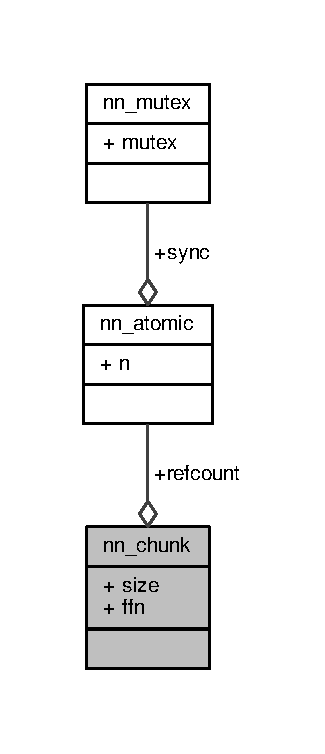
\includegraphics[width=156pt]{structnn__chunk__coll__graph}
\end{center}
\end{figure}
\subsection*{Public Attributes}
\begin{DoxyCompactItemize}
\item 
struct \hyperlink{structnn__atomic}{nn\+\_\+atomic} \hyperlink{structnn__chunk_a6d263535f4104d1e02e1b0e0b04e667c}{refcount}
\item 
size\+\_\+t \hyperlink{structnn__chunk_abf9a2795a02f86a19fe3db0db0a21106}{size}
\item 
\hyperlink{chunk_8c_a791a602d30b50b3a5637005123c7336d}{nn\+\_\+chunk\+\_\+free\+\_\+fn} \hyperlink{structnn__chunk_a902d9aa3b995457231f2e9e5694e93f3}{ffn}
\end{DoxyCompactItemize}


\subsection{Member Data Documentation}
\index{nn\+\_\+chunk@{nn\+\_\+chunk}!ffn@{ffn}}
\index{ffn@{ffn}!nn\+\_\+chunk@{nn\+\_\+chunk}}
\subsubsection[{ffn}]{\setlength{\rightskip}{0pt plus 5cm}{\bf nn\+\_\+chunk\+\_\+free\+\_\+fn} nn\+\_\+chunk\+::ffn}\hypertarget{structnn__chunk_a902d9aa3b995457231f2e9e5694e93f3}{}\label{structnn__chunk_a902d9aa3b995457231f2e9e5694e93f3}
\index{nn\+\_\+chunk@{nn\+\_\+chunk}!refcount@{refcount}}
\index{refcount@{refcount}!nn\+\_\+chunk@{nn\+\_\+chunk}}
\subsubsection[{refcount}]{\setlength{\rightskip}{0pt plus 5cm}struct {\bf nn\+\_\+atomic} nn\+\_\+chunk\+::refcount}\hypertarget{structnn__chunk_a6d263535f4104d1e02e1b0e0b04e667c}{}\label{structnn__chunk_a6d263535f4104d1e02e1b0e0b04e667c}
\index{nn\+\_\+chunk@{nn\+\_\+chunk}!size@{size}}
\index{size@{size}!nn\+\_\+chunk@{nn\+\_\+chunk}}
\subsubsection[{size}]{\setlength{\rightskip}{0pt plus 5cm}size\+\_\+t nn\+\_\+chunk\+::size}\hypertarget{structnn__chunk_abf9a2795a02f86a19fe3db0db0a21106}{}\label{structnn__chunk_abf9a2795a02f86a19fe3db0db0a21106}


The documentation for this struct was generated from the following file\+:\begin{DoxyCompactItemize}
\item 
src/utils/\hyperlink{chunk_8c}{chunk.\+c}\end{DoxyCompactItemize}

\hypertarget{structnn__chunkref}{}\section{nn\+\_\+chunkref Struct Reference}
\label{structnn__chunkref}\index{nn\+\_\+chunkref@{nn\+\_\+chunkref}}


{\ttfamily \#include $<$chunkref.\+h$>$}



Collaboration diagram for nn\+\_\+chunkref\+:\nopagebreak
\begin{figure}[H]
\begin{center}
\leavevmode
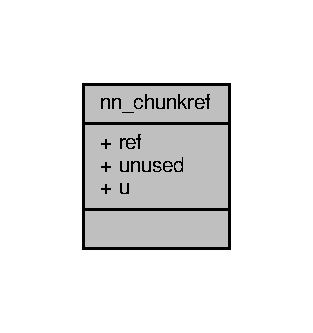
\includegraphics[width=150pt]{structnn__chunkref__coll__graph}
\end{center}
\end{figure}
\subsection*{Public Attributes}
\begin{DoxyCompactItemize}
\item 
\begin{tabbing}
xx\=xx\=xx\=xx\=xx\=xx\=xx\=xx\=xx\=\kill
union \{\\
\>uint8\_t \hyperlink{structnn__chunkref_a0fc4f3dc4f5b28d6f309d903d7d9ab38}{ref} \mbox{[}\hyperlink{chunkref_8h_a3ae177c9424f232e1e80e5556a48b27f}{NN\_CHUNKREF\_MAX}\mbox{]}\\
\>void $\ast$ \hyperlink{structnn__chunkref_a0481e23ecc1944c53854b5d1f424640b}{unused}\\
\} \hyperlink{structnn__chunkref_a4152ee1b9cc806576ba19b302d585d83}{u}\\

\end{tabbing}\end{DoxyCompactItemize}


\subsection{Member Data Documentation}
\index{nn\+\_\+chunkref@{nn\+\_\+chunkref}!ref@{ref}}
\index{ref@{ref}!nn\+\_\+chunkref@{nn\+\_\+chunkref}}
\subsubsection[{ref}]{\setlength{\rightskip}{0pt plus 5cm}uint8\+\_\+t nn\+\_\+chunkref\+::ref\mbox{[}{\bf N\+N\+\_\+\+C\+H\+U\+N\+K\+R\+E\+F\+\_\+\+M\+AX}\mbox{]}}\hypertarget{structnn__chunkref_a0fc4f3dc4f5b28d6f309d903d7d9ab38}{}\label{structnn__chunkref_a0fc4f3dc4f5b28d6f309d903d7d9ab38}
\index{nn\+\_\+chunkref@{nn\+\_\+chunkref}!u@{u}}
\index{u@{u}!nn\+\_\+chunkref@{nn\+\_\+chunkref}}
\subsubsection[{u}]{\setlength{\rightskip}{0pt plus 5cm}union \{ ... \}   nn\+\_\+chunkref\+::u}\hypertarget{structnn__chunkref_a4152ee1b9cc806576ba19b302d585d83}{}\label{structnn__chunkref_a4152ee1b9cc806576ba19b302d585d83}
\index{nn\+\_\+chunkref@{nn\+\_\+chunkref}!unused@{unused}}
\index{unused@{unused}!nn\+\_\+chunkref@{nn\+\_\+chunkref}}
\subsubsection[{unused}]{\setlength{\rightskip}{0pt plus 5cm}void$\ast$ nn\+\_\+chunkref\+::unused}\hypertarget{structnn__chunkref_a0481e23ecc1944c53854b5d1f424640b}{}\label{structnn__chunkref_a0481e23ecc1944c53854b5d1f424640b}


The documentation for this struct was generated from the following file\+:\begin{DoxyCompactItemize}
\item 
src/utils/\hyperlink{chunkref_8h}{chunkref.\+h}\end{DoxyCompactItemize}

\hypertarget{structnn__chunkref__chunk}{}\section{nn\+\_\+chunkref\+\_\+chunk Struct Reference}
\label{structnn__chunkref__chunk}\index{nn\+\_\+chunkref\+\_\+chunk@{nn\+\_\+chunkref\+\_\+chunk}}


Collaboration diagram for nn\+\_\+chunkref\+\_\+chunk\+:\nopagebreak
\begin{figure}[H]
\begin{center}
\leavevmode
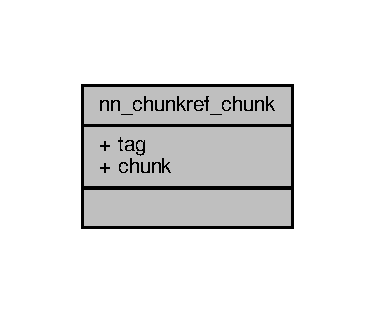
\includegraphics[width=180pt]{structnn__chunkref__chunk__coll__graph}
\end{center}
\end{figure}
\subsection*{Public Attributes}
\begin{DoxyCompactItemize}
\item 
uint8\+\_\+t \hyperlink{structnn__chunkref__chunk_abebb831eac6444be41bc134715a334b1}{tag}
\item 
void $\ast$ \hyperlink{structnn__chunkref__chunk_aa28fcd92116bdc5b636f1f76f93ddc0e}{chunk}
\end{DoxyCompactItemize}


\subsection{Member Data Documentation}
\index{nn\+\_\+chunkref\+\_\+chunk@{nn\+\_\+chunkref\+\_\+chunk}!chunk@{chunk}}
\index{chunk@{chunk}!nn\+\_\+chunkref\+\_\+chunk@{nn\+\_\+chunkref\+\_\+chunk}}
\subsubsection[{chunk}]{\setlength{\rightskip}{0pt plus 5cm}void$\ast$ nn\+\_\+chunkref\+\_\+chunk\+::chunk}\hypertarget{structnn__chunkref__chunk_aa28fcd92116bdc5b636f1f76f93ddc0e}{}\label{structnn__chunkref__chunk_aa28fcd92116bdc5b636f1f76f93ddc0e}
\index{nn\+\_\+chunkref\+\_\+chunk@{nn\+\_\+chunkref\+\_\+chunk}!tag@{tag}}
\index{tag@{tag}!nn\+\_\+chunkref\+\_\+chunk@{nn\+\_\+chunkref\+\_\+chunk}}
\subsubsection[{tag}]{\setlength{\rightskip}{0pt plus 5cm}uint8\+\_\+t nn\+\_\+chunkref\+\_\+chunk\+::tag}\hypertarget{structnn__chunkref__chunk_abebb831eac6444be41bc134715a334b1}{}\label{structnn__chunkref__chunk_abebb831eac6444be41bc134715a334b1}


The documentation for this struct was generated from the following file\+:\begin{DoxyCompactItemize}
\item 
src/utils/\hyperlink{chunkref_8c}{chunkref.\+c}\end{DoxyCompactItemize}

\hypertarget{structnn__cinproc}{}\section{nn\+\_\+cinproc Struct Reference}
\label{structnn__cinproc}\index{nn\+\_\+cinproc@{nn\+\_\+cinproc}}


{\ttfamily \#include $<$cinproc.\+h$>$}



Collaboration diagram for nn\+\_\+cinproc\+:\nopagebreak
\begin{figure}[H]
\begin{center}
\leavevmode
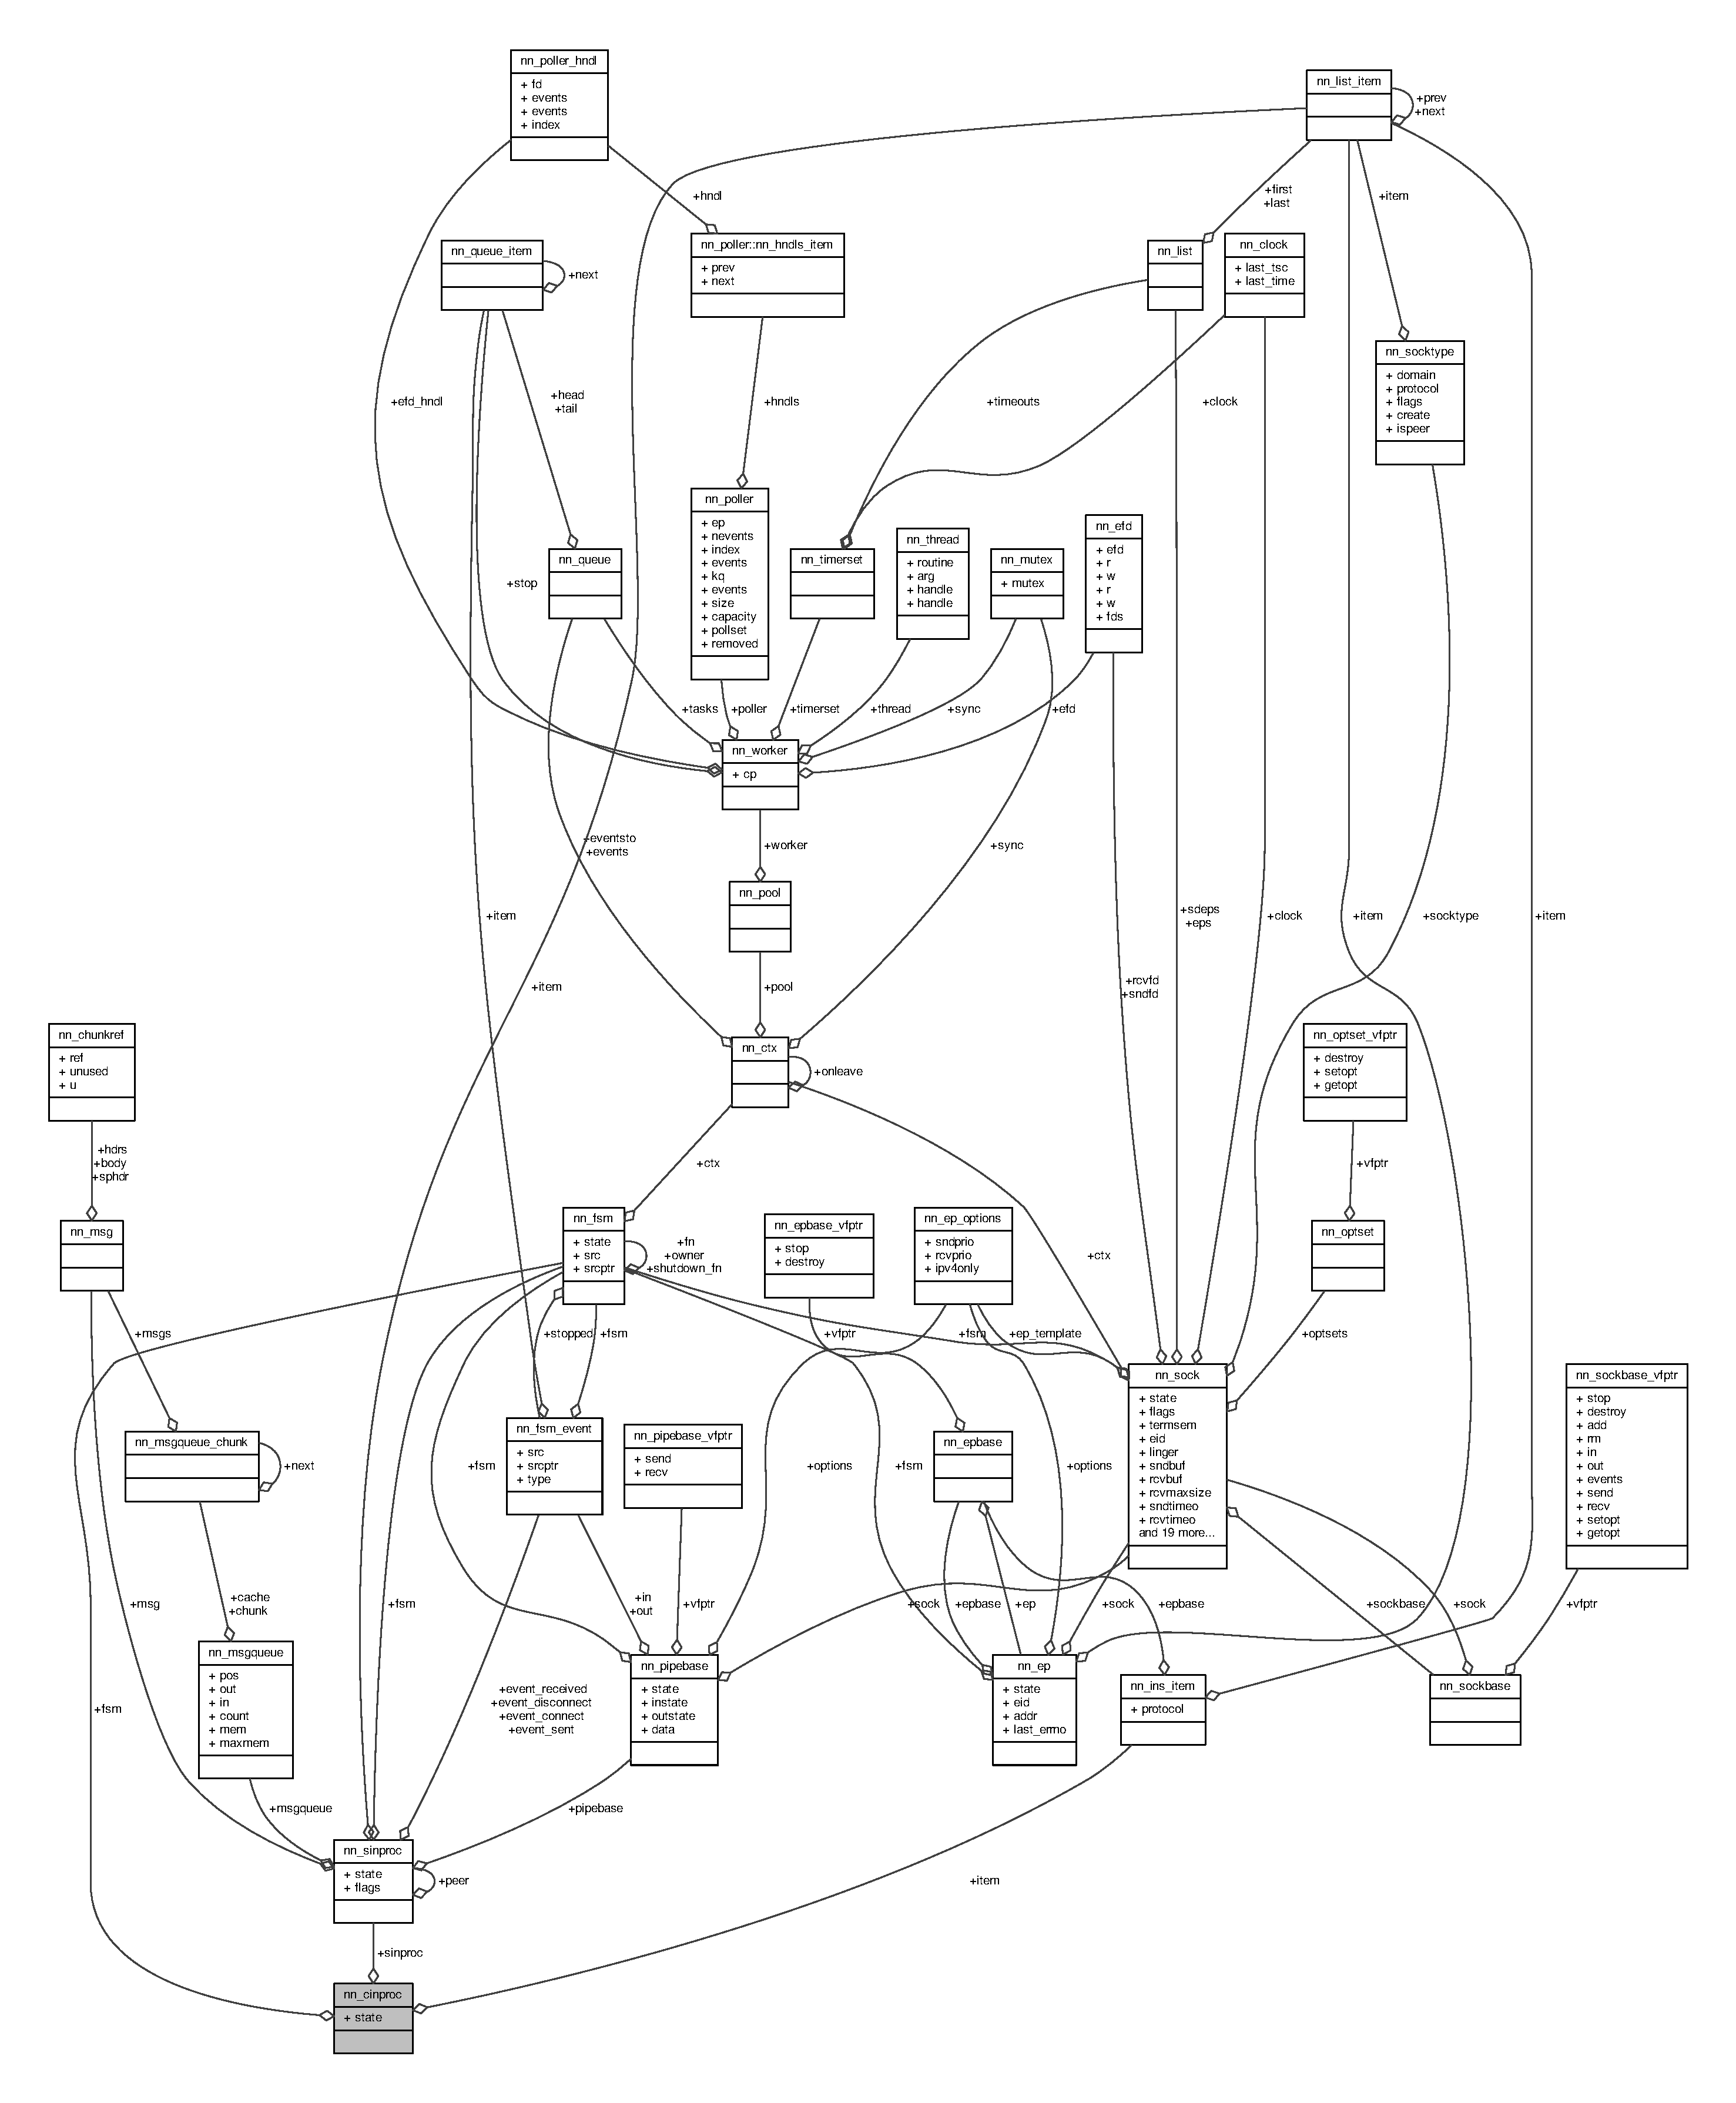
\includegraphics[width=350pt]{structnn__cinproc__coll__graph}
\end{center}
\end{figure}
\subsection*{Public Attributes}
\begin{DoxyCompactItemize}
\item 
struct \hyperlink{structnn__fsm}{nn\+\_\+fsm} \hyperlink{structnn__cinproc_a4944b367109e6d3fc2927fe52f4139f5}{fsm}
\item 
int \hyperlink{structnn__cinproc_ab01665c985955fbff04ad753615c030b}{state}
\item 
struct \hyperlink{structnn__ins__item}{nn\+\_\+ins\+\_\+item} \hyperlink{structnn__cinproc_a23852b5c008f49703409ebf04148891a}{item}
\item 
struct \hyperlink{structnn__sinproc}{nn\+\_\+sinproc} \hyperlink{structnn__cinproc_ab7ebfae31cd5c060a85329f21f7e12f0}{sinproc}
\end{DoxyCompactItemize}


\subsection{Member Data Documentation}
\index{nn\+\_\+cinproc@{nn\+\_\+cinproc}!fsm@{fsm}}
\index{fsm@{fsm}!nn\+\_\+cinproc@{nn\+\_\+cinproc}}
\subsubsection[{fsm}]{\setlength{\rightskip}{0pt plus 5cm}struct {\bf nn\+\_\+fsm} nn\+\_\+cinproc\+::fsm}\hypertarget{structnn__cinproc_a4944b367109e6d3fc2927fe52f4139f5}{}\label{structnn__cinproc_a4944b367109e6d3fc2927fe52f4139f5}
\index{nn\+\_\+cinproc@{nn\+\_\+cinproc}!item@{item}}
\index{item@{item}!nn\+\_\+cinproc@{nn\+\_\+cinproc}}
\subsubsection[{item}]{\setlength{\rightskip}{0pt plus 5cm}struct {\bf nn\+\_\+ins\+\_\+item} nn\+\_\+cinproc\+::item}\hypertarget{structnn__cinproc_a23852b5c008f49703409ebf04148891a}{}\label{structnn__cinproc_a23852b5c008f49703409ebf04148891a}
\index{nn\+\_\+cinproc@{nn\+\_\+cinproc}!sinproc@{sinproc}}
\index{sinproc@{sinproc}!nn\+\_\+cinproc@{nn\+\_\+cinproc}}
\subsubsection[{sinproc}]{\setlength{\rightskip}{0pt plus 5cm}struct {\bf nn\+\_\+sinproc} nn\+\_\+cinproc\+::sinproc}\hypertarget{structnn__cinproc_ab7ebfae31cd5c060a85329f21f7e12f0}{}\label{structnn__cinproc_ab7ebfae31cd5c060a85329f21f7e12f0}
\index{nn\+\_\+cinproc@{nn\+\_\+cinproc}!state@{state}}
\index{state@{state}!nn\+\_\+cinproc@{nn\+\_\+cinproc}}
\subsubsection[{state}]{\setlength{\rightskip}{0pt plus 5cm}int nn\+\_\+cinproc\+::state}\hypertarget{structnn__cinproc_ab01665c985955fbff04ad753615c030b}{}\label{structnn__cinproc_ab01665c985955fbff04ad753615c030b}


The documentation for this struct was generated from the following file\+:\begin{DoxyCompactItemize}
\item 
src/transports/inproc/\hyperlink{cinproc_8h}{cinproc.\+h}\end{DoxyCompactItemize}

\hypertarget{structnn__cipc}{}\section{nn\+\_\+cipc Struct Reference}
\label{structnn__cipc}\index{nn\+\_\+cipc@{nn\+\_\+cipc}}


Collaboration diagram for nn\+\_\+cipc\+:\nopagebreak
\begin{figure}[H]
\begin{center}
\leavevmode
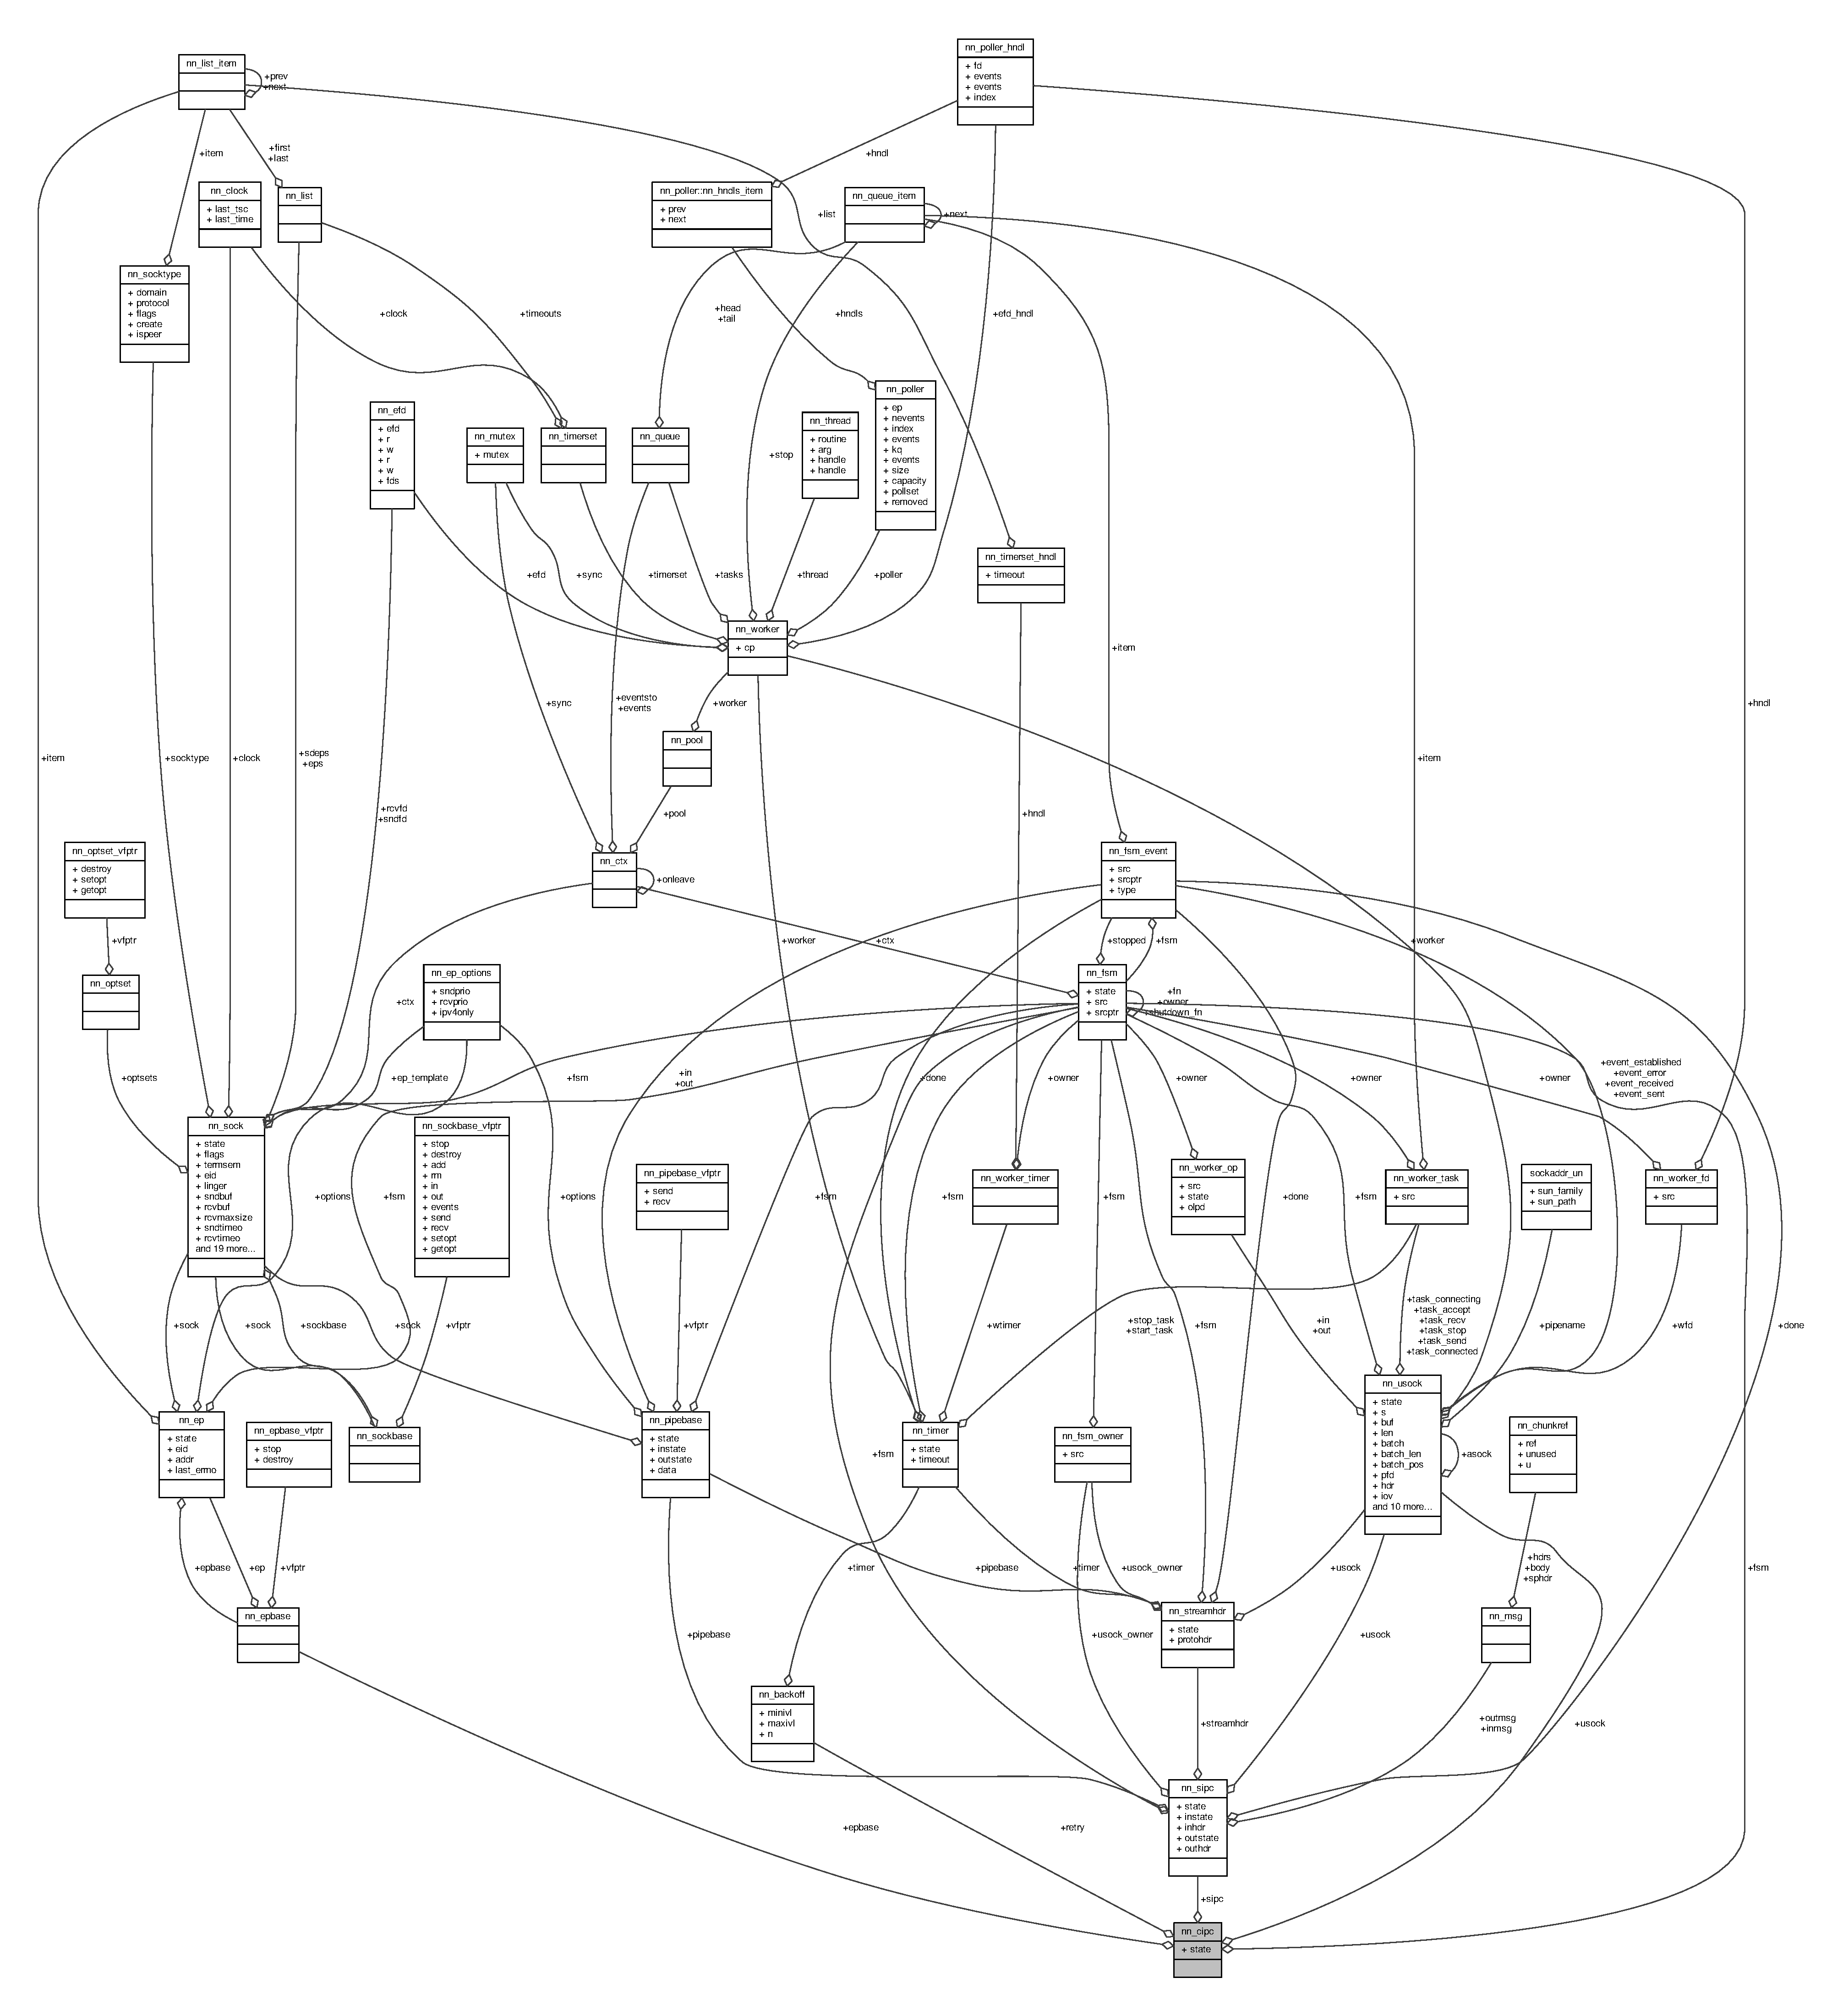
\includegraphics[width=350pt]{structnn__cipc__coll__graph}
\end{center}
\end{figure}
\subsection*{Public Attributes}
\begin{DoxyCompactItemize}
\item 
struct \hyperlink{structnn__fsm}{nn\+\_\+fsm} \hyperlink{structnn__cipc_ac3cb2e6f10f0e78f849c6aaa4ba6592a}{fsm}
\item 
int \hyperlink{structnn__cipc_af9b878e110d6071b4e693f3dd6e89213}{state}
\item 
struct \hyperlink{structnn__epbase}{nn\+\_\+epbase} \hyperlink{structnn__cipc_a767b765afab0b1be9653b01d30dbb36c}{epbase}
\item 
struct \hyperlink{structnn__usock}{nn\+\_\+usock} \hyperlink{structnn__cipc_a61f984db042983502c3d270326bd89d8}{usock}
\item 
struct \hyperlink{structnn__backoff}{nn\+\_\+backoff} \hyperlink{structnn__cipc_a7e238ae735a8050ae193bfa46195ed5e}{retry}
\item 
struct \hyperlink{structnn__sipc}{nn\+\_\+sipc} \hyperlink{structnn__cipc_a41de9ef8bc50161ae4ffd19e9ead3f06}{sipc}
\end{DoxyCompactItemize}


\subsection{Member Data Documentation}
\index{nn\+\_\+cipc@{nn\+\_\+cipc}!epbase@{epbase}}
\index{epbase@{epbase}!nn\+\_\+cipc@{nn\+\_\+cipc}}
\subsubsection[{epbase}]{\setlength{\rightskip}{0pt plus 5cm}struct {\bf nn\+\_\+epbase} nn\+\_\+cipc\+::epbase}\hypertarget{structnn__cipc_a767b765afab0b1be9653b01d30dbb36c}{}\label{structnn__cipc_a767b765afab0b1be9653b01d30dbb36c}
\index{nn\+\_\+cipc@{nn\+\_\+cipc}!fsm@{fsm}}
\index{fsm@{fsm}!nn\+\_\+cipc@{nn\+\_\+cipc}}
\subsubsection[{fsm}]{\setlength{\rightskip}{0pt plus 5cm}struct {\bf nn\+\_\+fsm} nn\+\_\+cipc\+::fsm}\hypertarget{structnn__cipc_ac3cb2e6f10f0e78f849c6aaa4ba6592a}{}\label{structnn__cipc_ac3cb2e6f10f0e78f849c6aaa4ba6592a}
\index{nn\+\_\+cipc@{nn\+\_\+cipc}!retry@{retry}}
\index{retry@{retry}!nn\+\_\+cipc@{nn\+\_\+cipc}}
\subsubsection[{retry}]{\setlength{\rightskip}{0pt plus 5cm}struct {\bf nn\+\_\+backoff} nn\+\_\+cipc\+::retry}\hypertarget{structnn__cipc_a7e238ae735a8050ae193bfa46195ed5e}{}\label{structnn__cipc_a7e238ae735a8050ae193bfa46195ed5e}
\index{nn\+\_\+cipc@{nn\+\_\+cipc}!sipc@{sipc}}
\index{sipc@{sipc}!nn\+\_\+cipc@{nn\+\_\+cipc}}
\subsubsection[{sipc}]{\setlength{\rightskip}{0pt plus 5cm}struct {\bf nn\+\_\+sipc} nn\+\_\+cipc\+::sipc}\hypertarget{structnn__cipc_a41de9ef8bc50161ae4ffd19e9ead3f06}{}\label{structnn__cipc_a41de9ef8bc50161ae4ffd19e9ead3f06}
\index{nn\+\_\+cipc@{nn\+\_\+cipc}!state@{state}}
\index{state@{state}!nn\+\_\+cipc@{nn\+\_\+cipc}}
\subsubsection[{state}]{\setlength{\rightskip}{0pt plus 5cm}int nn\+\_\+cipc\+::state}\hypertarget{structnn__cipc_af9b878e110d6071b4e693f3dd6e89213}{}\label{structnn__cipc_af9b878e110d6071b4e693f3dd6e89213}
\index{nn\+\_\+cipc@{nn\+\_\+cipc}!usock@{usock}}
\index{usock@{usock}!nn\+\_\+cipc@{nn\+\_\+cipc}}
\subsubsection[{usock}]{\setlength{\rightskip}{0pt plus 5cm}struct {\bf nn\+\_\+usock} nn\+\_\+cipc\+::usock}\hypertarget{structnn__cipc_a61f984db042983502c3d270326bd89d8}{}\label{structnn__cipc_a61f984db042983502c3d270326bd89d8}


The documentation for this struct was generated from the following file\+:\begin{DoxyCompactItemize}
\item 
src/transports/ipc/\hyperlink{cipc_8c}{cipc.\+c}\end{DoxyCompactItemize}

\hypertarget{structnn__clibfabric}{}\section{nn\+\_\+clibfabric Struct Reference}
\label{structnn__clibfabric}\index{nn\+\_\+clibfabric@{nn\+\_\+clibfabric}}


Collaboration diagram for nn\+\_\+clibfabric\+:\nopagebreak
\begin{figure}[H]
\begin{center}
\leavevmode
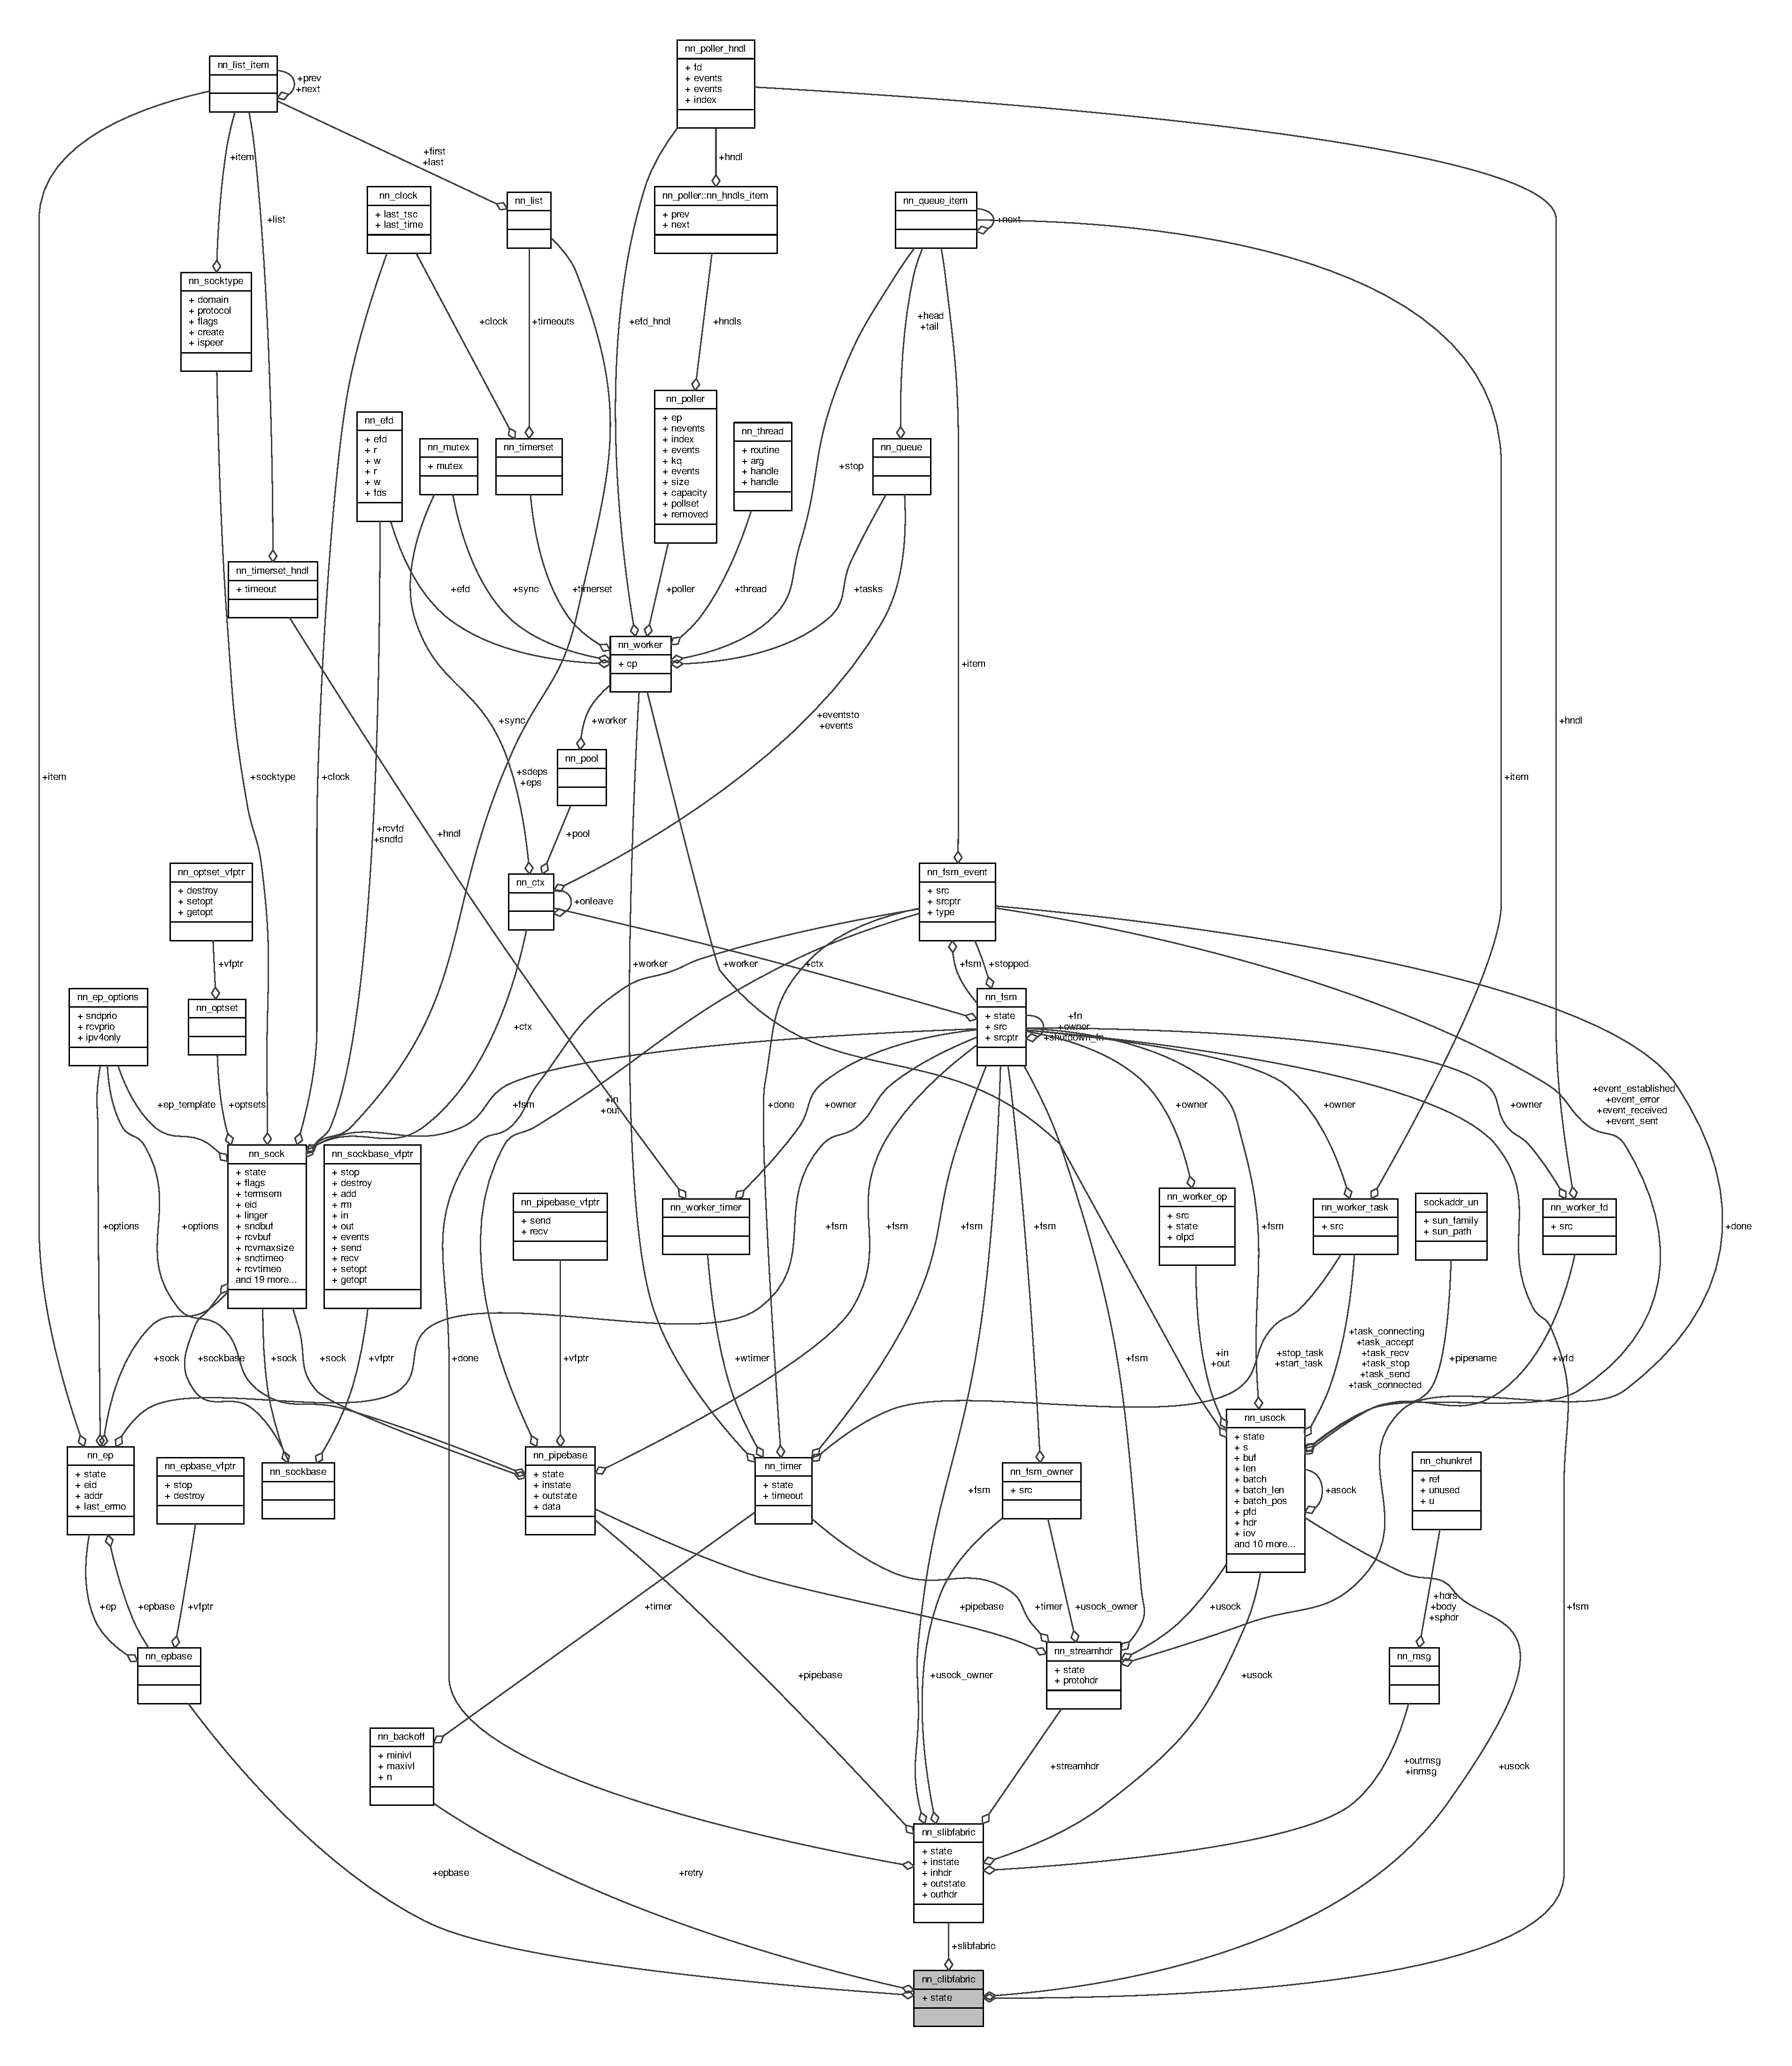
\includegraphics[width=350pt]{structnn__clibfabric__coll__graph}
\end{center}
\end{figure}
\subsection*{Public Attributes}
\begin{DoxyCompactItemize}
\item 
struct \hyperlink{structnn__fsm}{nn\+\_\+fsm} \hyperlink{structnn__clibfabric_a79bf5d5042cc883c3492a3f9221b8074}{fsm}
\item 
int \hyperlink{structnn__clibfabric_add852039e47247c9eac1575f90844988}{state}
\item 
struct \hyperlink{structnn__epbase}{nn\+\_\+epbase} \hyperlink{structnn__clibfabric_acdc1beac545401968ce1735fc153676f}{epbase}
\item 
struct \hyperlink{structnn__usock}{nn\+\_\+usock} \hyperlink{structnn__clibfabric_a8ca82c30329e862f0aa321878951d601}{usock}
\item 
struct \hyperlink{structnn__backoff}{nn\+\_\+backoff} \hyperlink{structnn__clibfabric_af75d0e9ca24bce5dba607471dd930976}{retry}
\item 
struct \hyperlink{structnn__slibfabric}{nn\+\_\+slibfabric} \hyperlink{structnn__clibfabric_ac0a7255ca2f0d8a7af3a62723d415297}{slibfabric}
\end{DoxyCompactItemize}


\subsection{Member Data Documentation}
\index{nn\+\_\+clibfabric@{nn\+\_\+clibfabric}!epbase@{epbase}}
\index{epbase@{epbase}!nn\+\_\+clibfabric@{nn\+\_\+clibfabric}}
\subsubsection[{epbase}]{\setlength{\rightskip}{0pt plus 5cm}struct {\bf nn\+\_\+epbase} nn\+\_\+clibfabric\+::epbase}\hypertarget{structnn__clibfabric_acdc1beac545401968ce1735fc153676f}{}\label{structnn__clibfabric_acdc1beac545401968ce1735fc153676f}
\index{nn\+\_\+clibfabric@{nn\+\_\+clibfabric}!fsm@{fsm}}
\index{fsm@{fsm}!nn\+\_\+clibfabric@{nn\+\_\+clibfabric}}
\subsubsection[{fsm}]{\setlength{\rightskip}{0pt plus 5cm}struct {\bf nn\+\_\+fsm} nn\+\_\+clibfabric\+::fsm}\hypertarget{structnn__clibfabric_a79bf5d5042cc883c3492a3f9221b8074}{}\label{structnn__clibfabric_a79bf5d5042cc883c3492a3f9221b8074}
\index{nn\+\_\+clibfabric@{nn\+\_\+clibfabric}!retry@{retry}}
\index{retry@{retry}!nn\+\_\+clibfabric@{nn\+\_\+clibfabric}}
\subsubsection[{retry}]{\setlength{\rightskip}{0pt plus 5cm}struct {\bf nn\+\_\+backoff} nn\+\_\+clibfabric\+::retry}\hypertarget{structnn__clibfabric_af75d0e9ca24bce5dba607471dd930976}{}\label{structnn__clibfabric_af75d0e9ca24bce5dba607471dd930976}
\index{nn\+\_\+clibfabric@{nn\+\_\+clibfabric}!slibfabric@{slibfabric}}
\index{slibfabric@{slibfabric}!nn\+\_\+clibfabric@{nn\+\_\+clibfabric}}
\subsubsection[{slibfabric}]{\setlength{\rightskip}{0pt plus 5cm}struct {\bf nn\+\_\+slibfabric} nn\+\_\+clibfabric\+::slibfabric}\hypertarget{structnn__clibfabric_ac0a7255ca2f0d8a7af3a62723d415297}{}\label{structnn__clibfabric_ac0a7255ca2f0d8a7af3a62723d415297}
\index{nn\+\_\+clibfabric@{nn\+\_\+clibfabric}!state@{state}}
\index{state@{state}!nn\+\_\+clibfabric@{nn\+\_\+clibfabric}}
\subsubsection[{state}]{\setlength{\rightskip}{0pt plus 5cm}int nn\+\_\+clibfabric\+::state}\hypertarget{structnn__clibfabric_add852039e47247c9eac1575f90844988}{}\label{structnn__clibfabric_add852039e47247c9eac1575f90844988}
\index{nn\+\_\+clibfabric@{nn\+\_\+clibfabric}!usock@{usock}}
\index{usock@{usock}!nn\+\_\+clibfabric@{nn\+\_\+clibfabric}}
\subsubsection[{usock}]{\setlength{\rightskip}{0pt plus 5cm}struct {\bf nn\+\_\+usock} nn\+\_\+clibfabric\+::usock}\hypertarget{structnn__clibfabric_a8ca82c30329e862f0aa321878951d601}{}\label{structnn__clibfabric_a8ca82c30329e862f0aa321878951d601}


The documentation for this struct was generated from the following files\+:\begin{DoxyCompactItemize}
\item 
src/transports/libfabric/\hyperlink{cagain_8c}{cagain.\+c}\item 
src/transports/libfabric/\hyperlink{clibfabric_8c}{clibfabric.\+c}\end{DoxyCompactItemize}

\hypertarget{structnn__clock}{}\section{nn\+\_\+clock Struct Reference}
\label{structnn__clock}\index{nn\+\_\+clock@{nn\+\_\+clock}}


{\ttfamily \#include $<$clock.\+h$>$}



Collaboration diagram for nn\+\_\+clock\+:\nopagebreak
\begin{figure}[H]
\begin{center}
\leavevmode
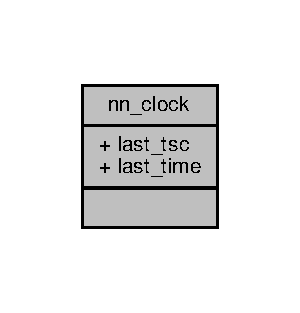
\includegraphics[width=144pt]{structnn__clock__coll__graph}
\end{center}
\end{figure}
\subsection*{Public Attributes}
\begin{DoxyCompactItemize}
\item 
uint64\+\_\+t \hyperlink{structnn__clock_ae1c93ad0ea0d06895e0f116f2c132b89}{last\+\_\+tsc}
\item 
uint64\+\_\+t \hyperlink{structnn__clock_a45a8e406b8c899971310f8c4967aa97e}{last\+\_\+time}
\end{DoxyCompactItemize}


\subsection{Member Data Documentation}
\index{nn\+\_\+clock@{nn\+\_\+clock}!last\+\_\+time@{last\+\_\+time}}
\index{last\+\_\+time@{last\+\_\+time}!nn\+\_\+clock@{nn\+\_\+clock}}
\subsubsection[{last\+\_\+time}]{\setlength{\rightskip}{0pt plus 5cm}uint64\+\_\+t nn\+\_\+clock\+::last\+\_\+time}\hypertarget{structnn__clock_a45a8e406b8c899971310f8c4967aa97e}{}\label{structnn__clock_a45a8e406b8c899971310f8c4967aa97e}
\index{nn\+\_\+clock@{nn\+\_\+clock}!last\+\_\+tsc@{last\+\_\+tsc}}
\index{last\+\_\+tsc@{last\+\_\+tsc}!nn\+\_\+clock@{nn\+\_\+clock}}
\subsubsection[{last\+\_\+tsc}]{\setlength{\rightskip}{0pt plus 5cm}uint64\+\_\+t nn\+\_\+clock\+::last\+\_\+tsc}\hypertarget{structnn__clock_ae1c93ad0ea0d06895e0f116f2c132b89}{}\label{structnn__clock_ae1c93ad0ea0d06895e0f116f2c132b89}


The documentation for this struct was generated from the following file\+:\begin{DoxyCompactItemize}
\item 
src/utils/\hyperlink{clock_8h}{clock.\+h}\end{DoxyCompactItemize}

\hypertarget{structnn__cmsghdr}{}\section{nn\+\_\+cmsghdr Struct Reference}
\label{structnn__cmsghdr}\index{nn\+\_\+cmsghdr@{nn\+\_\+cmsghdr}}


{\ttfamily \#include $<$nn.\+h$>$}



Collaboration diagram for nn\+\_\+cmsghdr\+:\nopagebreak
\begin{figure}[H]
\begin{center}
\leavevmode
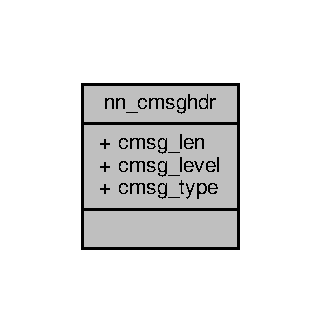
\includegraphics[width=154pt]{structnn__cmsghdr__coll__graph}
\end{center}
\end{figure}
\subsection*{Public Attributes}
\begin{DoxyCompactItemize}
\item 
size\+\_\+t \hyperlink{structnn__cmsghdr_a69be5db8bf0f6b68a7f8c9c10e8db839}{cmsg\+\_\+len}
\item 
int \hyperlink{structnn__cmsghdr_a032fd87fda6598a0038492a67f988588}{cmsg\+\_\+level}
\item 
int \hyperlink{structnn__cmsghdr_afdca1067604788429d246880beb07bff}{cmsg\+\_\+type}
\end{DoxyCompactItemize}


\subsection{Member Data Documentation}
\index{nn\+\_\+cmsghdr@{nn\+\_\+cmsghdr}!cmsg\+\_\+len@{cmsg\+\_\+len}}
\index{cmsg\+\_\+len@{cmsg\+\_\+len}!nn\+\_\+cmsghdr@{nn\+\_\+cmsghdr}}
\subsubsection[{cmsg\+\_\+len}]{\setlength{\rightskip}{0pt plus 5cm}size\+\_\+t nn\+\_\+cmsghdr\+::cmsg\+\_\+len}\hypertarget{structnn__cmsghdr_a69be5db8bf0f6b68a7f8c9c10e8db839}{}\label{structnn__cmsghdr_a69be5db8bf0f6b68a7f8c9c10e8db839}
\index{nn\+\_\+cmsghdr@{nn\+\_\+cmsghdr}!cmsg\+\_\+level@{cmsg\+\_\+level}}
\index{cmsg\+\_\+level@{cmsg\+\_\+level}!nn\+\_\+cmsghdr@{nn\+\_\+cmsghdr}}
\subsubsection[{cmsg\+\_\+level}]{\setlength{\rightskip}{0pt plus 5cm}int nn\+\_\+cmsghdr\+::cmsg\+\_\+level}\hypertarget{structnn__cmsghdr_a032fd87fda6598a0038492a67f988588}{}\label{structnn__cmsghdr_a032fd87fda6598a0038492a67f988588}
\index{nn\+\_\+cmsghdr@{nn\+\_\+cmsghdr}!cmsg\+\_\+type@{cmsg\+\_\+type}}
\index{cmsg\+\_\+type@{cmsg\+\_\+type}!nn\+\_\+cmsghdr@{nn\+\_\+cmsghdr}}
\subsubsection[{cmsg\+\_\+type}]{\setlength{\rightskip}{0pt plus 5cm}int nn\+\_\+cmsghdr\+::cmsg\+\_\+type}\hypertarget{structnn__cmsghdr_afdca1067604788429d246880beb07bff}{}\label{structnn__cmsghdr_afdca1067604788429d246880beb07bff}


The documentation for this struct was generated from the following file\+:\begin{DoxyCompactItemize}
\item 
src/\hyperlink{nn_8h}{nn.\+h}\end{DoxyCompactItemize}

\hypertarget{structnn__ctcp}{}\section{nn\+\_\+ctcp Struct Reference}
\label{structnn__ctcp}\index{nn\+\_\+ctcp@{nn\+\_\+ctcp}}


Collaboration diagram for nn\+\_\+ctcp\+:\nopagebreak
\begin{figure}[H]
\begin{center}
\leavevmode
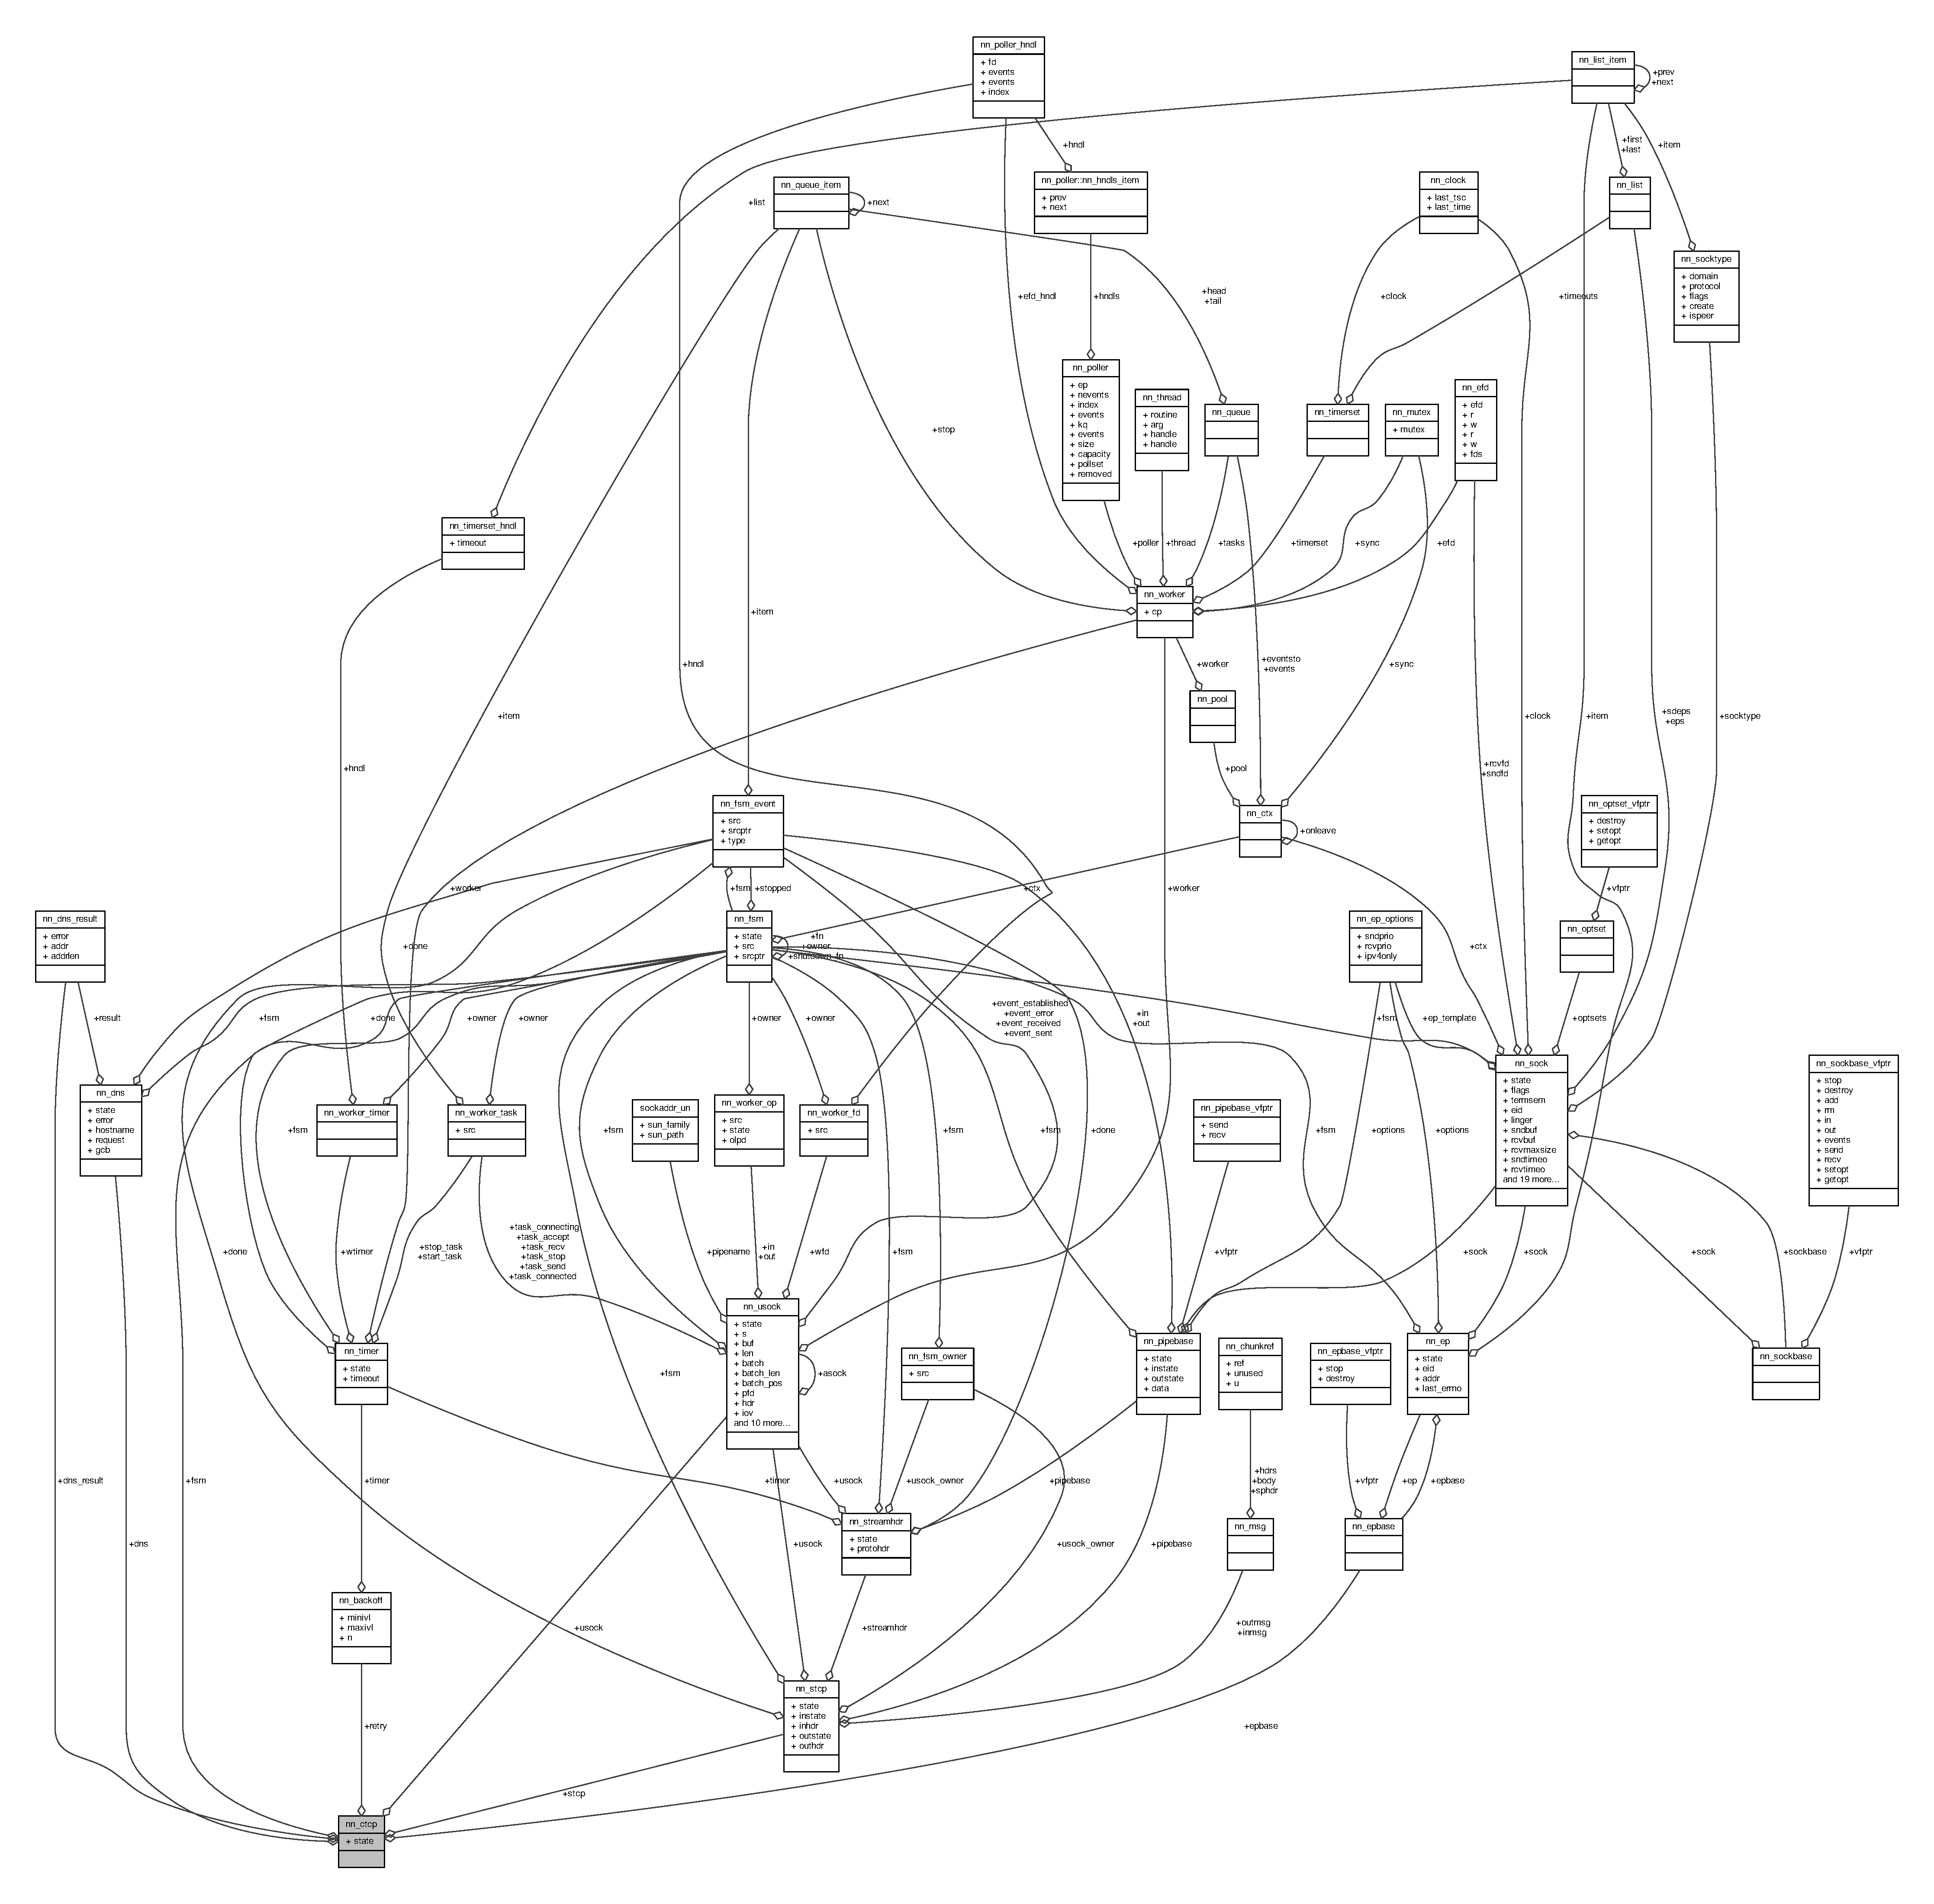
\includegraphics[width=350pt]{structnn__ctcp__coll__graph}
\end{center}
\end{figure}
\subsection*{Public Attributes}
\begin{DoxyCompactItemize}
\item 
struct \hyperlink{structnn__fsm}{nn\+\_\+fsm} \hyperlink{structnn__ctcp_a718324121d9a84e33bf2d7dbd1f6a8d8}{fsm}
\item 
int \hyperlink{structnn__ctcp_a4f07e9462114b70bbcac159837dd08b9}{state}
\item 
struct \hyperlink{structnn__epbase}{nn\+\_\+epbase} \hyperlink{structnn__ctcp_ab2ac5f22ebfcd925d3d9d3ecd89ec4bf}{epbase}
\item 
struct \hyperlink{structnn__usock}{nn\+\_\+usock} \hyperlink{structnn__ctcp_a4e614d0b4252d851f49c999b67d3fdc0}{usock}
\item 
struct \hyperlink{structnn__backoff}{nn\+\_\+backoff} \hyperlink{structnn__ctcp_ac1b95bd51dafc4cd2cdd710759f5767b}{retry}
\item 
struct \hyperlink{structnn__stcp}{nn\+\_\+stcp} \hyperlink{structnn__ctcp_ad3b1a0f3182b0ea30097b77d182c769e}{stcp}
\item 
struct \hyperlink{structnn__dns}{nn\+\_\+dns} \hyperlink{structnn__ctcp_a74fd788c14b71695640c6472e2c9d122}{dns}
\item 
struct \hyperlink{structnn__dns__result}{nn\+\_\+dns\+\_\+result} \hyperlink{structnn__ctcp_a8020854c49bc9f9ce455793400d8fdde}{dns\+\_\+result}
\end{DoxyCompactItemize}


\subsection{Member Data Documentation}
\index{nn\+\_\+ctcp@{nn\+\_\+ctcp}!dns@{dns}}
\index{dns@{dns}!nn\+\_\+ctcp@{nn\+\_\+ctcp}}
\subsubsection[{dns}]{\setlength{\rightskip}{0pt plus 5cm}struct {\bf nn\+\_\+dns} nn\+\_\+ctcp\+::dns}\hypertarget{structnn__ctcp_a74fd788c14b71695640c6472e2c9d122}{}\label{structnn__ctcp_a74fd788c14b71695640c6472e2c9d122}
\index{nn\+\_\+ctcp@{nn\+\_\+ctcp}!dns\+\_\+result@{dns\+\_\+result}}
\index{dns\+\_\+result@{dns\+\_\+result}!nn\+\_\+ctcp@{nn\+\_\+ctcp}}
\subsubsection[{dns\+\_\+result}]{\setlength{\rightskip}{0pt plus 5cm}struct {\bf nn\+\_\+dns\+\_\+result} nn\+\_\+ctcp\+::dns\+\_\+result}\hypertarget{structnn__ctcp_a8020854c49bc9f9ce455793400d8fdde}{}\label{structnn__ctcp_a8020854c49bc9f9ce455793400d8fdde}
\index{nn\+\_\+ctcp@{nn\+\_\+ctcp}!epbase@{epbase}}
\index{epbase@{epbase}!nn\+\_\+ctcp@{nn\+\_\+ctcp}}
\subsubsection[{epbase}]{\setlength{\rightskip}{0pt plus 5cm}struct {\bf nn\+\_\+epbase} nn\+\_\+ctcp\+::epbase}\hypertarget{structnn__ctcp_ab2ac5f22ebfcd925d3d9d3ecd89ec4bf}{}\label{structnn__ctcp_ab2ac5f22ebfcd925d3d9d3ecd89ec4bf}
\index{nn\+\_\+ctcp@{nn\+\_\+ctcp}!fsm@{fsm}}
\index{fsm@{fsm}!nn\+\_\+ctcp@{nn\+\_\+ctcp}}
\subsubsection[{fsm}]{\setlength{\rightskip}{0pt plus 5cm}struct {\bf nn\+\_\+fsm} nn\+\_\+ctcp\+::fsm}\hypertarget{structnn__ctcp_a718324121d9a84e33bf2d7dbd1f6a8d8}{}\label{structnn__ctcp_a718324121d9a84e33bf2d7dbd1f6a8d8}
\index{nn\+\_\+ctcp@{nn\+\_\+ctcp}!retry@{retry}}
\index{retry@{retry}!nn\+\_\+ctcp@{nn\+\_\+ctcp}}
\subsubsection[{retry}]{\setlength{\rightskip}{0pt plus 5cm}struct {\bf nn\+\_\+backoff} nn\+\_\+ctcp\+::retry}\hypertarget{structnn__ctcp_ac1b95bd51dafc4cd2cdd710759f5767b}{}\label{structnn__ctcp_ac1b95bd51dafc4cd2cdd710759f5767b}
\index{nn\+\_\+ctcp@{nn\+\_\+ctcp}!state@{state}}
\index{state@{state}!nn\+\_\+ctcp@{nn\+\_\+ctcp}}
\subsubsection[{state}]{\setlength{\rightskip}{0pt plus 5cm}int nn\+\_\+ctcp\+::state}\hypertarget{structnn__ctcp_a4f07e9462114b70bbcac159837dd08b9}{}\label{structnn__ctcp_a4f07e9462114b70bbcac159837dd08b9}
\index{nn\+\_\+ctcp@{nn\+\_\+ctcp}!stcp@{stcp}}
\index{stcp@{stcp}!nn\+\_\+ctcp@{nn\+\_\+ctcp}}
\subsubsection[{stcp}]{\setlength{\rightskip}{0pt plus 5cm}struct {\bf nn\+\_\+stcp} nn\+\_\+ctcp\+::stcp}\hypertarget{structnn__ctcp_ad3b1a0f3182b0ea30097b77d182c769e}{}\label{structnn__ctcp_ad3b1a0f3182b0ea30097b77d182c769e}
\index{nn\+\_\+ctcp@{nn\+\_\+ctcp}!usock@{usock}}
\index{usock@{usock}!nn\+\_\+ctcp@{nn\+\_\+ctcp}}
\subsubsection[{usock}]{\setlength{\rightskip}{0pt plus 5cm}struct {\bf nn\+\_\+usock} nn\+\_\+ctcp\+::usock}\hypertarget{structnn__ctcp_a4e614d0b4252d851f49c999b67d3fdc0}{}\label{structnn__ctcp_a4e614d0b4252d851f49c999b67d3fdc0}


The documentation for this struct was generated from the following file\+:\begin{DoxyCompactItemize}
\item 
src/transports/tcp/\hyperlink{ctcp_8c}{ctcp.\+c}\end{DoxyCompactItemize}

\hypertarget{structnn__ctcpmux}{}\section{nn\+\_\+ctcpmux Struct Reference}
\label{structnn__ctcpmux}\index{nn\+\_\+ctcpmux@{nn\+\_\+ctcpmux}}


Collaboration diagram for nn\+\_\+ctcpmux\+:\nopagebreak
\begin{figure}[H]
\begin{center}
\leavevmode
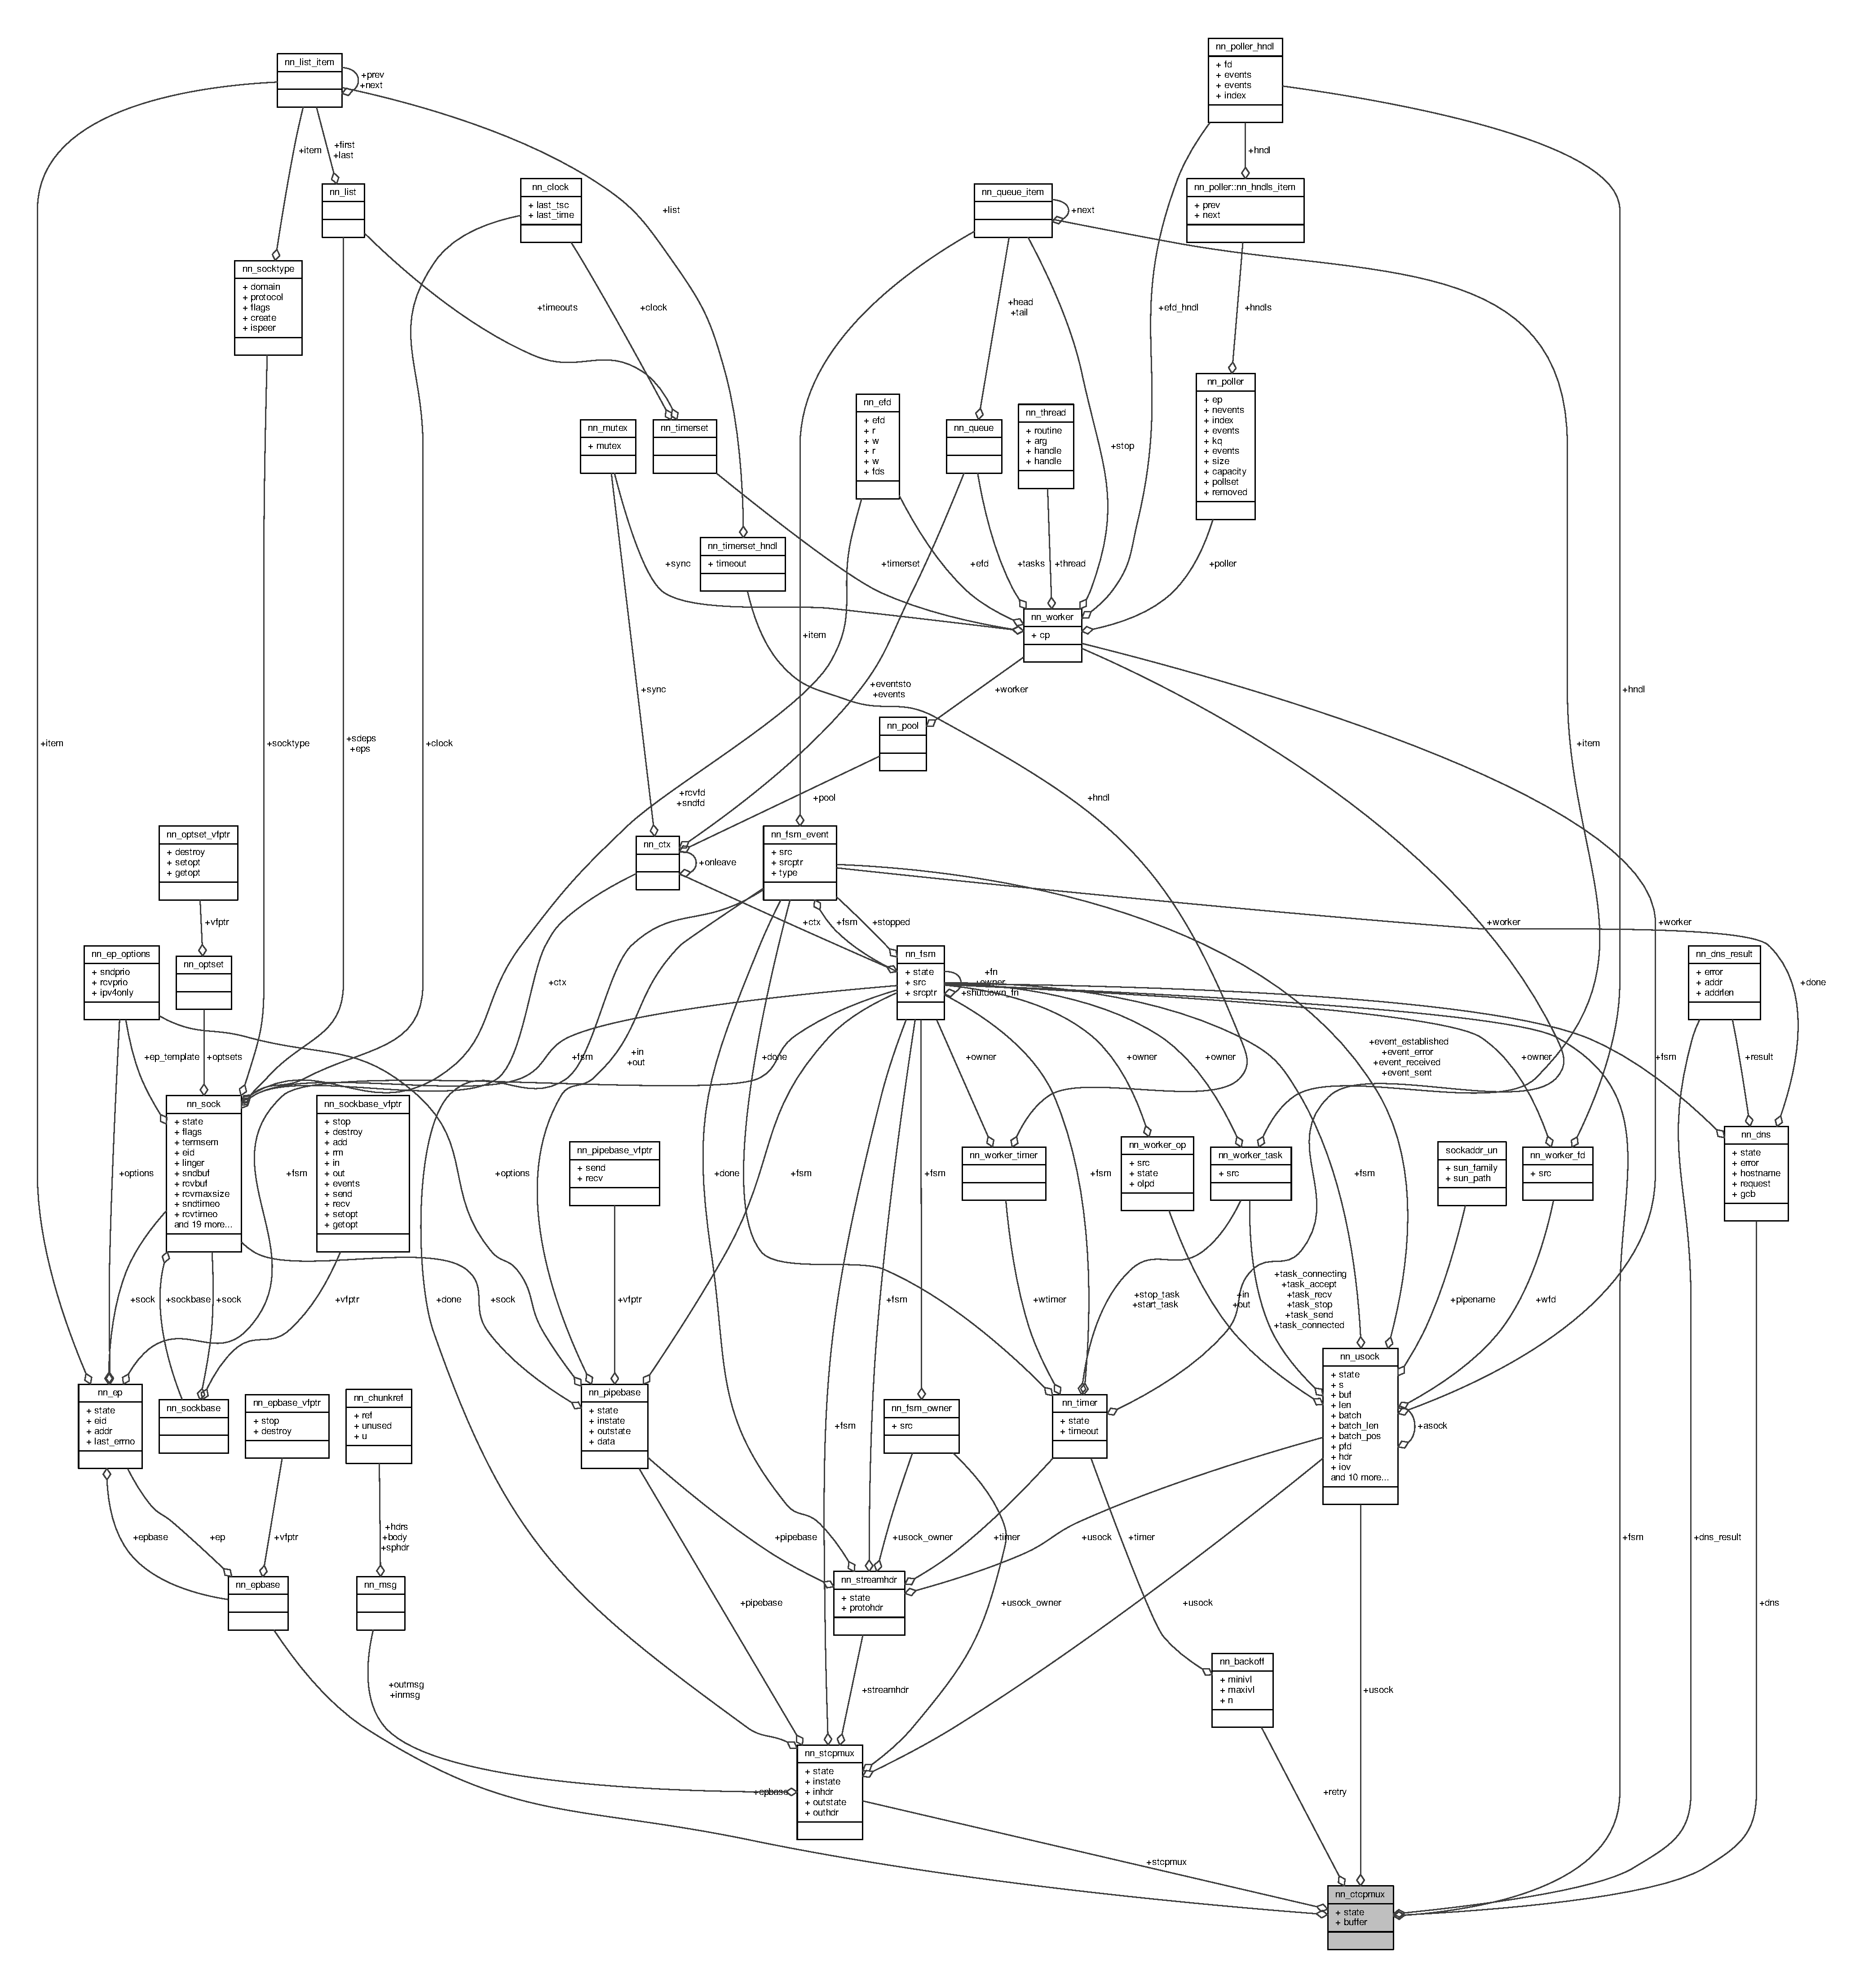
\includegraphics[width=350pt]{structnn__ctcpmux__coll__graph}
\end{center}
\end{figure}
\subsection*{Public Attributes}
\begin{DoxyCompactItemize}
\item 
struct \hyperlink{structnn__fsm}{nn\+\_\+fsm} \hyperlink{structnn__ctcpmux_a5e3c1c136cd2b28b585b7311dc61c795}{fsm}
\item 
int \hyperlink{structnn__ctcpmux_ab0103503ff213fe896f4d45ceea723ca}{state}
\item 
struct \hyperlink{structnn__epbase}{nn\+\_\+epbase} \hyperlink{structnn__ctcpmux_a5979503ad3f681f42da267bcceda7545}{epbase}
\item 
struct \hyperlink{structnn__usock}{nn\+\_\+usock} \hyperlink{structnn__ctcpmux_ae5c270ad3b4d7e376ed0d4a0f876e4ad}{usock}
\item 
struct \hyperlink{structnn__backoff}{nn\+\_\+backoff} \hyperlink{structnn__ctcpmux_a8c52683d34482048bedc8b3a60c9f901}{retry}
\item 
struct \hyperlink{structnn__stcpmux}{nn\+\_\+stcpmux} \hyperlink{structnn__ctcpmux_a53e694d9e610eb735da294988afc48e2}{stcpmux}
\item 
struct \hyperlink{structnn__dns}{nn\+\_\+dns} \hyperlink{structnn__ctcpmux_af6ee113d28282fd32301914547a26aae}{dns}
\item 
struct \hyperlink{structnn__dns__result}{nn\+\_\+dns\+\_\+result} \hyperlink{structnn__ctcpmux_a1f0c2bf52607b4504f10598bf1cbcf62}{dns\+\_\+result}
\item 
char \hyperlink{structnn__ctcpmux_a2dcc2919792d09641f8f8ff6f69d0f16}{buffer} \mbox{[}256\mbox{]}
\end{DoxyCompactItemize}


\subsection{Member Data Documentation}
\index{nn\+\_\+ctcpmux@{nn\+\_\+ctcpmux}!buffer@{buffer}}
\index{buffer@{buffer}!nn\+\_\+ctcpmux@{nn\+\_\+ctcpmux}}
\subsubsection[{buffer}]{\setlength{\rightskip}{0pt plus 5cm}char nn\+\_\+ctcpmux\+::buffer\mbox{[}256\mbox{]}}\hypertarget{structnn__ctcpmux_a2dcc2919792d09641f8f8ff6f69d0f16}{}\label{structnn__ctcpmux_a2dcc2919792d09641f8f8ff6f69d0f16}
\index{nn\+\_\+ctcpmux@{nn\+\_\+ctcpmux}!dns@{dns}}
\index{dns@{dns}!nn\+\_\+ctcpmux@{nn\+\_\+ctcpmux}}
\subsubsection[{dns}]{\setlength{\rightskip}{0pt plus 5cm}struct {\bf nn\+\_\+dns} nn\+\_\+ctcpmux\+::dns}\hypertarget{structnn__ctcpmux_af6ee113d28282fd32301914547a26aae}{}\label{structnn__ctcpmux_af6ee113d28282fd32301914547a26aae}
\index{nn\+\_\+ctcpmux@{nn\+\_\+ctcpmux}!dns\+\_\+result@{dns\+\_\+result}}
\index{dns\+\_\+result@{dns\+\_\+result}!nn\+\_\+ctcpmux@{nn\+\_\+ctcpmux}}
\subsubsection[{dns\+\_\+result}]{\setlength{\rightskip}{0pt plus 5cm}struct {\bf nn\+\_\+dns\+\_\+result} nn\+\_\+ctcpmux\+::dns\+\_\+result}\hypertarget{structnn__ctcpmux_a1f0c2bf52607b4504f10598bf1cbcf62}{}\label{structnn__ctcpmux_a1f0c2bf52607b4504f10598bf1cbcf62}
\index{nn\+\_\+ctcpmux@{nn\+\_\+ctcpmux}!epbase@{epbase}}
\index{epbase@{epbase}!nn\+\_\+ctcpmux@{nn\+\_\+ctcpmux}}
\subsubsection[{epbase}]{\setlength{\rightskip}{0pt plus 5cm}struct {\bf nn\+\_\+epbase} nn\+\_\+ctcpmux\+::epbase}\hypertarget{structnn__ctcpmux_a5979503ad3f681f42da267bcceda7545}{}\label{structnn__ctcpmux_a5979503ad3f681f42da267bcceda7545}
\index{nn\+\_\+ctcpmux@{nn\+\_\+ctcpmux}!fsm@{fsm}}
\index{fsm@{fsm}!nn\+\_\+ctcpmux@{nn\+\_\+ctcpmux}}
\subsubsection[{fsm}]{\setlength{\rightskip}{0pt plus 5cm}struct {\bf nn\+\_\+fsm} nn\+\_\+ctcpmux\+::fsm}\hypertarget{structnn__ctcpmux_a5e3c1c136cd2b28b585b7311dc61c795}{}\label{structnn__ctcpmux_a5e3c1c136cd2b28b585b7311dc61c795}
\index{nn\+\_\+ctcpmux@{nn\+\_\+ctcpmux}!retry@{retry}}
\index{retry@{retry}!nn\+\_\+ctcpmux@{nn\+\_\+ctcpmux}}
\subsubsection[{retry}]{\setlength{\rightskip}{0pt plus 5cm}struct {\bf nn\+\_\+backoff} nn\+\_\+ctcpmux\+::retry}\hypertarget{structnn__ctcpmux_a8c52683d34482048bedc8b3a60c9f901}{}\label{structnn__ctcpmux_a8c52683d34482048bedc8b3a60c9f901}
\index{nn\+\_\+ctcpmux@{nn\+\_\+ctcpmux}!state@{state}}
\index{state@{state}!nn\+\_\+ctcpmux@{nn\+\_\+ctcpmux}}
\subsubsection[{state}]{\setlength{\rightskip}{0pt plus 5cm}int nn\+\_\+ctcpmux\+::state}\hypertarget{structnn__ctcpmux_ab0103503ff213fe896f4d45ceea723ca}{}\label{structnn__ctcpmux_ab0103503ff213fe896f4d45ceea723ca}
\index{nn\+\_\+ctcpmux@{nn\+\_\+ctcpmux}!stcpmux@{stcpmux}}
\index{stcpmux@{stcpmux}!nn\+\_\+ctcpmux@{nn\+\_\+ctcpmux}}
\subsubsection[{stcpmux}]{\setlength{\rightskip}{0pt plus 5cm}struct {\bf nn\+\_\+stcpmux} nn\+\_\+ctcpmux\+::stcpmux}\hypertarget{structnn__ctcpmux_a53e694d9e610eb735da294988afc48e2}{}\label{structnn__ctcpmux_a53e694d9e610eb735da294988afc48e2}
\index{nn\+\_\+ctcpmux@{nn\+\_\+ctcpmux}!usock@{usock}}
\index{usock@{usock}!nn\+\_\+ctcpmux@{nn\+\_\+ctcpmux}}
\subsubsection[{usock}]{\setlength{\rightskip}{0pt plus 5cm}struct {\bf nn\+\_\+usock} nn\+\_\+ctcpmux\+::usock}\hypertarget{structnn__ctcpmux_ae5c270ad3b4d7e376ed0d4a0f876e4ad}{}\label{structnn__ctcpmux_ae5c270ad3b4d7e376ed0d4a0f876e4ad}


The documentation for this struct was generated from the following file\+:\begin{DoxyCompactItemize}
\item 
src/transports/tcpmux/\hyperlink{ctcpmux_8c}{ctcpmux.\+c}\end{DoxyCompactItemize}

\hypertarget{structnn__ctx}{}\section{nn\+\_\+ctx Struct Reference}
\label{structnn__ctx}\index{nn\+\_\+ctx@{nn\+\_\+ctx}}


{\ttfamily \#include $<$ctx.\+h$>$}



Collaboration diagram for nn\+\_\+ctx\+:\nopagebreak
\begin{figure}[H]
\begin{center}
\leavevmode
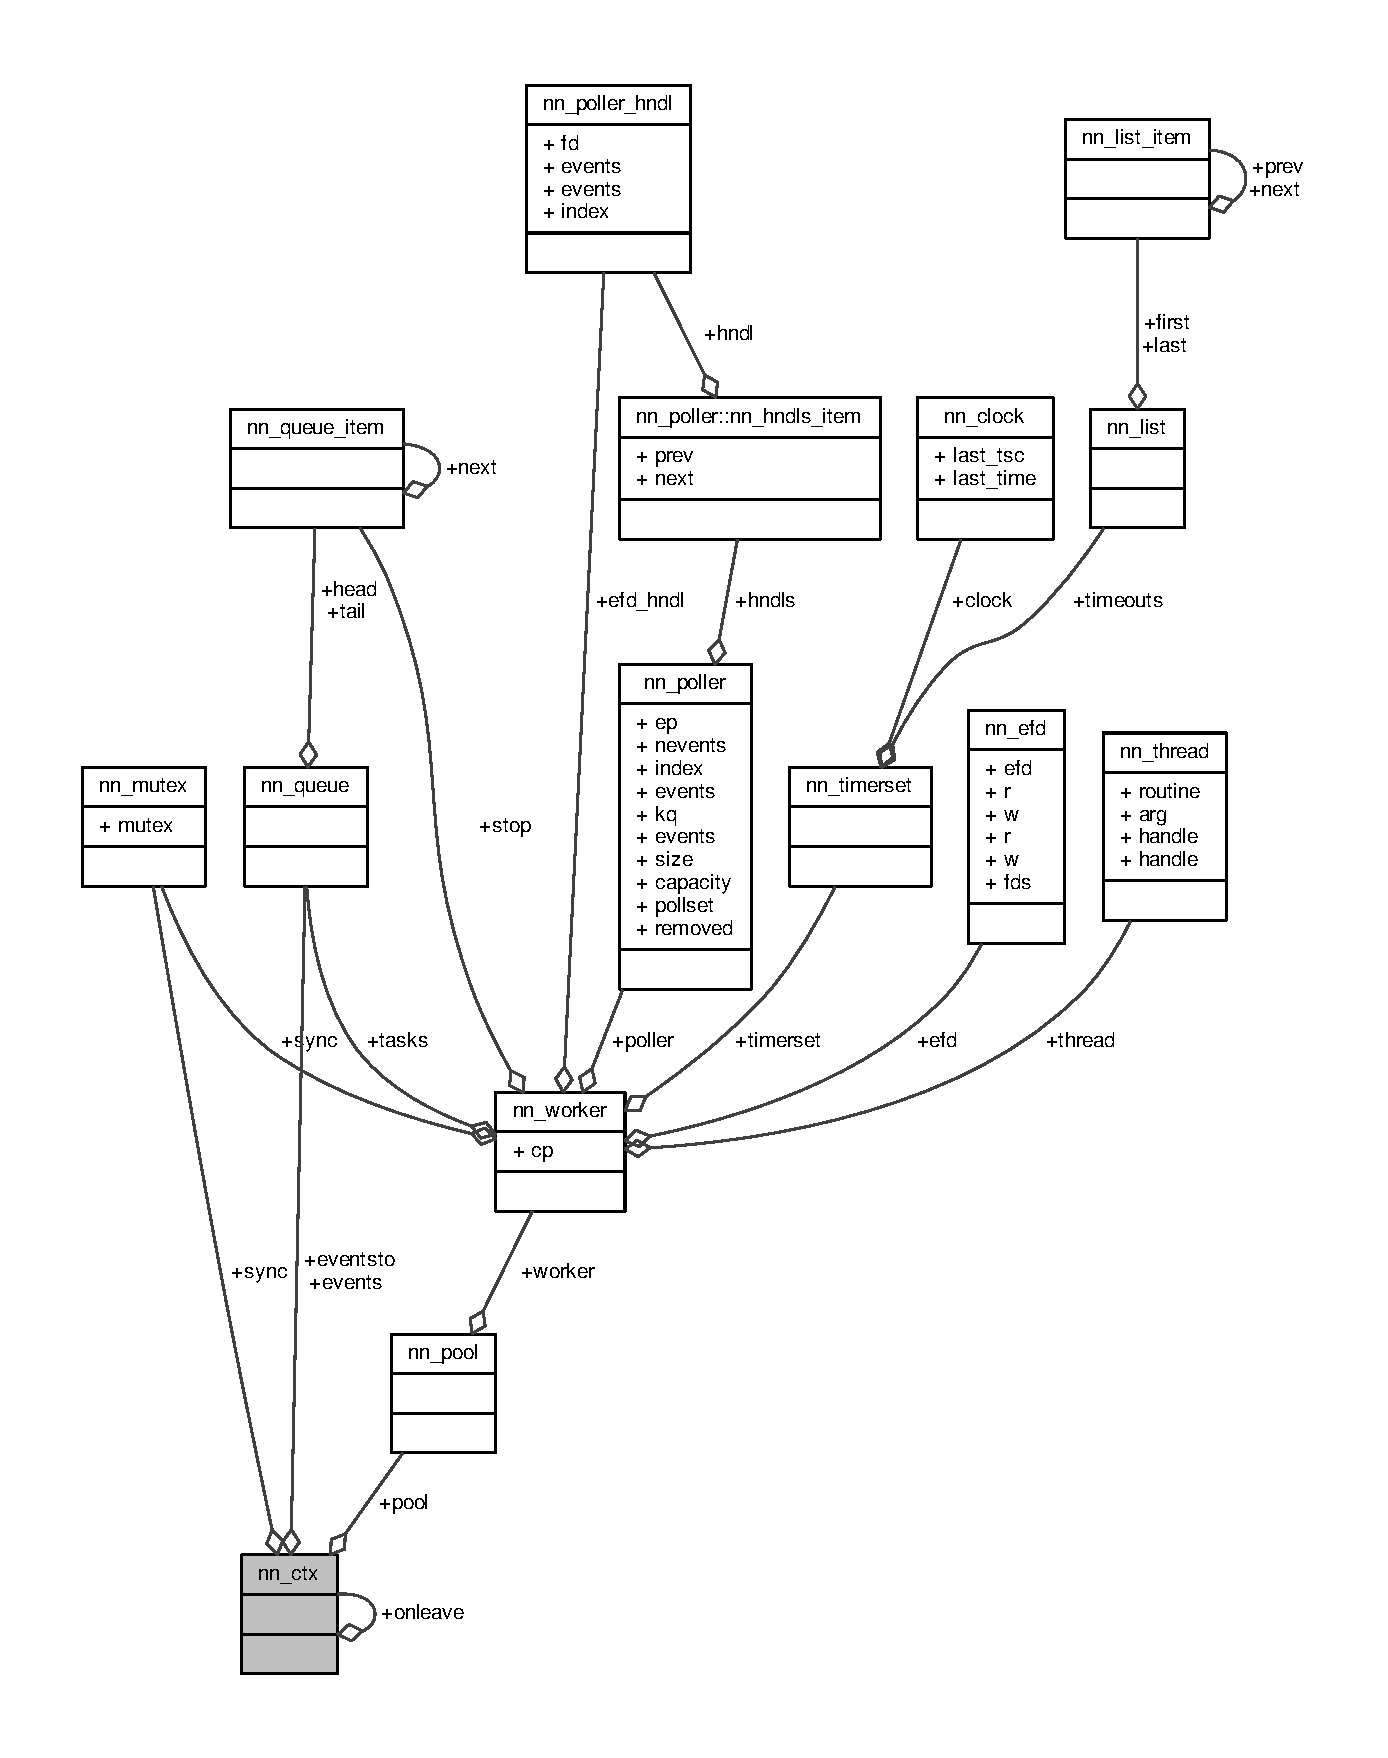
\includegraphics[width=350pt]{structnn__ctx__coll__graph}
\end{center}
\end{figure}
\subsection*{Public Attributes}
\begin{DoxyCompactItemize}
\item 
struct \hyperlink{structnn__mutex}{nn\+\_\+mutex} \hyperlink{structnn__ctx_a264057ae180e58357895cbcbd594101b}{sync}
\item 
struct \hyperlink{structnn__pool}{nn\+\_\+pool} $\ast$ \hyperlink{structnn__ctx_a19a7c8ad423a87033ddf12550c1d3bec}{pool}
\item 
struct \hyperlink{structnn__queue}{nn\+\_\+queue} \hyperlink{structnn__ctx_ae1142dc4694c701a581532111589add2}{events}
\item 
struct \hyperlink{structnn__queue}{nn\+\_\+queue} \hyperlink{structnn__ctx_a68de02831fae8dea24d3183c1c4a21ea}{eventsto}
\item 
\hyperlink{ctx_8h_ab63830bf02229318481d9ce1f27bf1ea}{nn\+\_\+ctx\+\_\+onleave} \hyperlink{structnn__ctx_aa1d4d51724a3a10dbc93d42d8e6d9a58}{onleave}
\end{DoxyCompactItemize}


\subsection{Member Data Documentation}
\index{nn\+\_\+ctx@{nn\+\_\+ctx}!events@{events}}
\index{events@{events}!nn\+\_\+ctx@{nn\+\_\+ctx}}
\subsubsection[{events}]{\setlength{\rightskip}{0pt plus 5cm}struct {\bf nn\+\_\+queue} nn\+\_\+ctx\+::events}\hypertarget{structnn__ctx_ae1142dc4694c701a581532111589add2}{}\label{structnn__ctx_ae1142dc4694c701a581532111589add2}
\index{nn\+\_\+ctx@{nn\+\_\+ctx}!eventsto@{eventsto}}
\index{eventsto@{eventsto}!nn\+\_\+ctx@{nn\+\_\+ctx}}
\subsubsection[{eventsto}]{\setlength{\rightskip}{0pt plus 5cm}struct {\bf nn\+\_\+queue} nn\+\_\+ctx\+::eventsto}\hypertarget{structnn__ctx_a68de02831fae8dea24d3183c1c4a21ea}{}\label{structnn__ctx_a68de02831fae8dea24d3183c1c4a21ea}
\index{nn\+\_\+ctx@{nn\+\_\+ctx}!onleave@{onleave}}
\index{onleave@{onleave}!nn\+\_\+ctx@{nn\+\_\+ctx}}
\subsubsection[{onleave}]{\setlength{\rightskip}{0pt plus 5cm}{\bf nn\+\_\+ctx\+\_\+onleave} nn\+\_\+ctx\+::onleave}\hypertarget{structnn__ctx_aa1d4d51724a3a10dbc93d42d8e6d9a58}{}\label{structnn__ctx_aa1d4d51724a3a10dbc93d42d8e6d9a58}
\index{nn\+\_\+ctx@{nn\+\_\+ctx}!pool@{pool}}
\index{pool@{pool}!nn\+\_\+ctx@{nn\+\_\+ctx}}
\subsubsection[{pool}]{\setlength{\rightskip}{0pt plus 5cm}struct {\bf nn\+\_\+pool}$\ast$ nn\+\_\+ctx\+::pool}\hypertarget{structnn__ctx_a19a7c8ad423a87033ddf12550c1d3bec}{}\label{structnn__ctx_a19a7c8ad423a87033ddf12550c1d3bec}
\index{nn\+\_\+ctx@{nn\+\_\+ctx}!sync@{sync}}
\index{sync@{sync}!nn\+\_\+ctx@{nn\+\_\+ctx}}
\subsubsection[{sync}]{\setlength{\rightskip}{0pt plus 5cm}struct {\bf nn\+\_\+mutex} nn\+\_\+ctx\+::sync}\hypertarget{structnn__ctx_a264057ae180e58357895cbcbd594101b}{}\label{structnn__ctx_a264057ae180e58357895cbcbd594101b}


The documentation for this struct was generated from the following file\+:\begin{DoxyCompactItemize}
\item 
src/aio/\hyperlink{ctx_8h}{ctx.\+h}\end{DoxyCompactItemize}

\hypertarget{structnn__cws}{}\section{nn\+\_\+cws Struct Reference}
\label{structnn__cws}\index{nn\+\_\+cws@{nn\+\_\+cws}}


Collaboration diagram for nn\+\_\+cws\+:\nopagebreak
\begin{figure}[H]
\begin{center}
\leavevmode
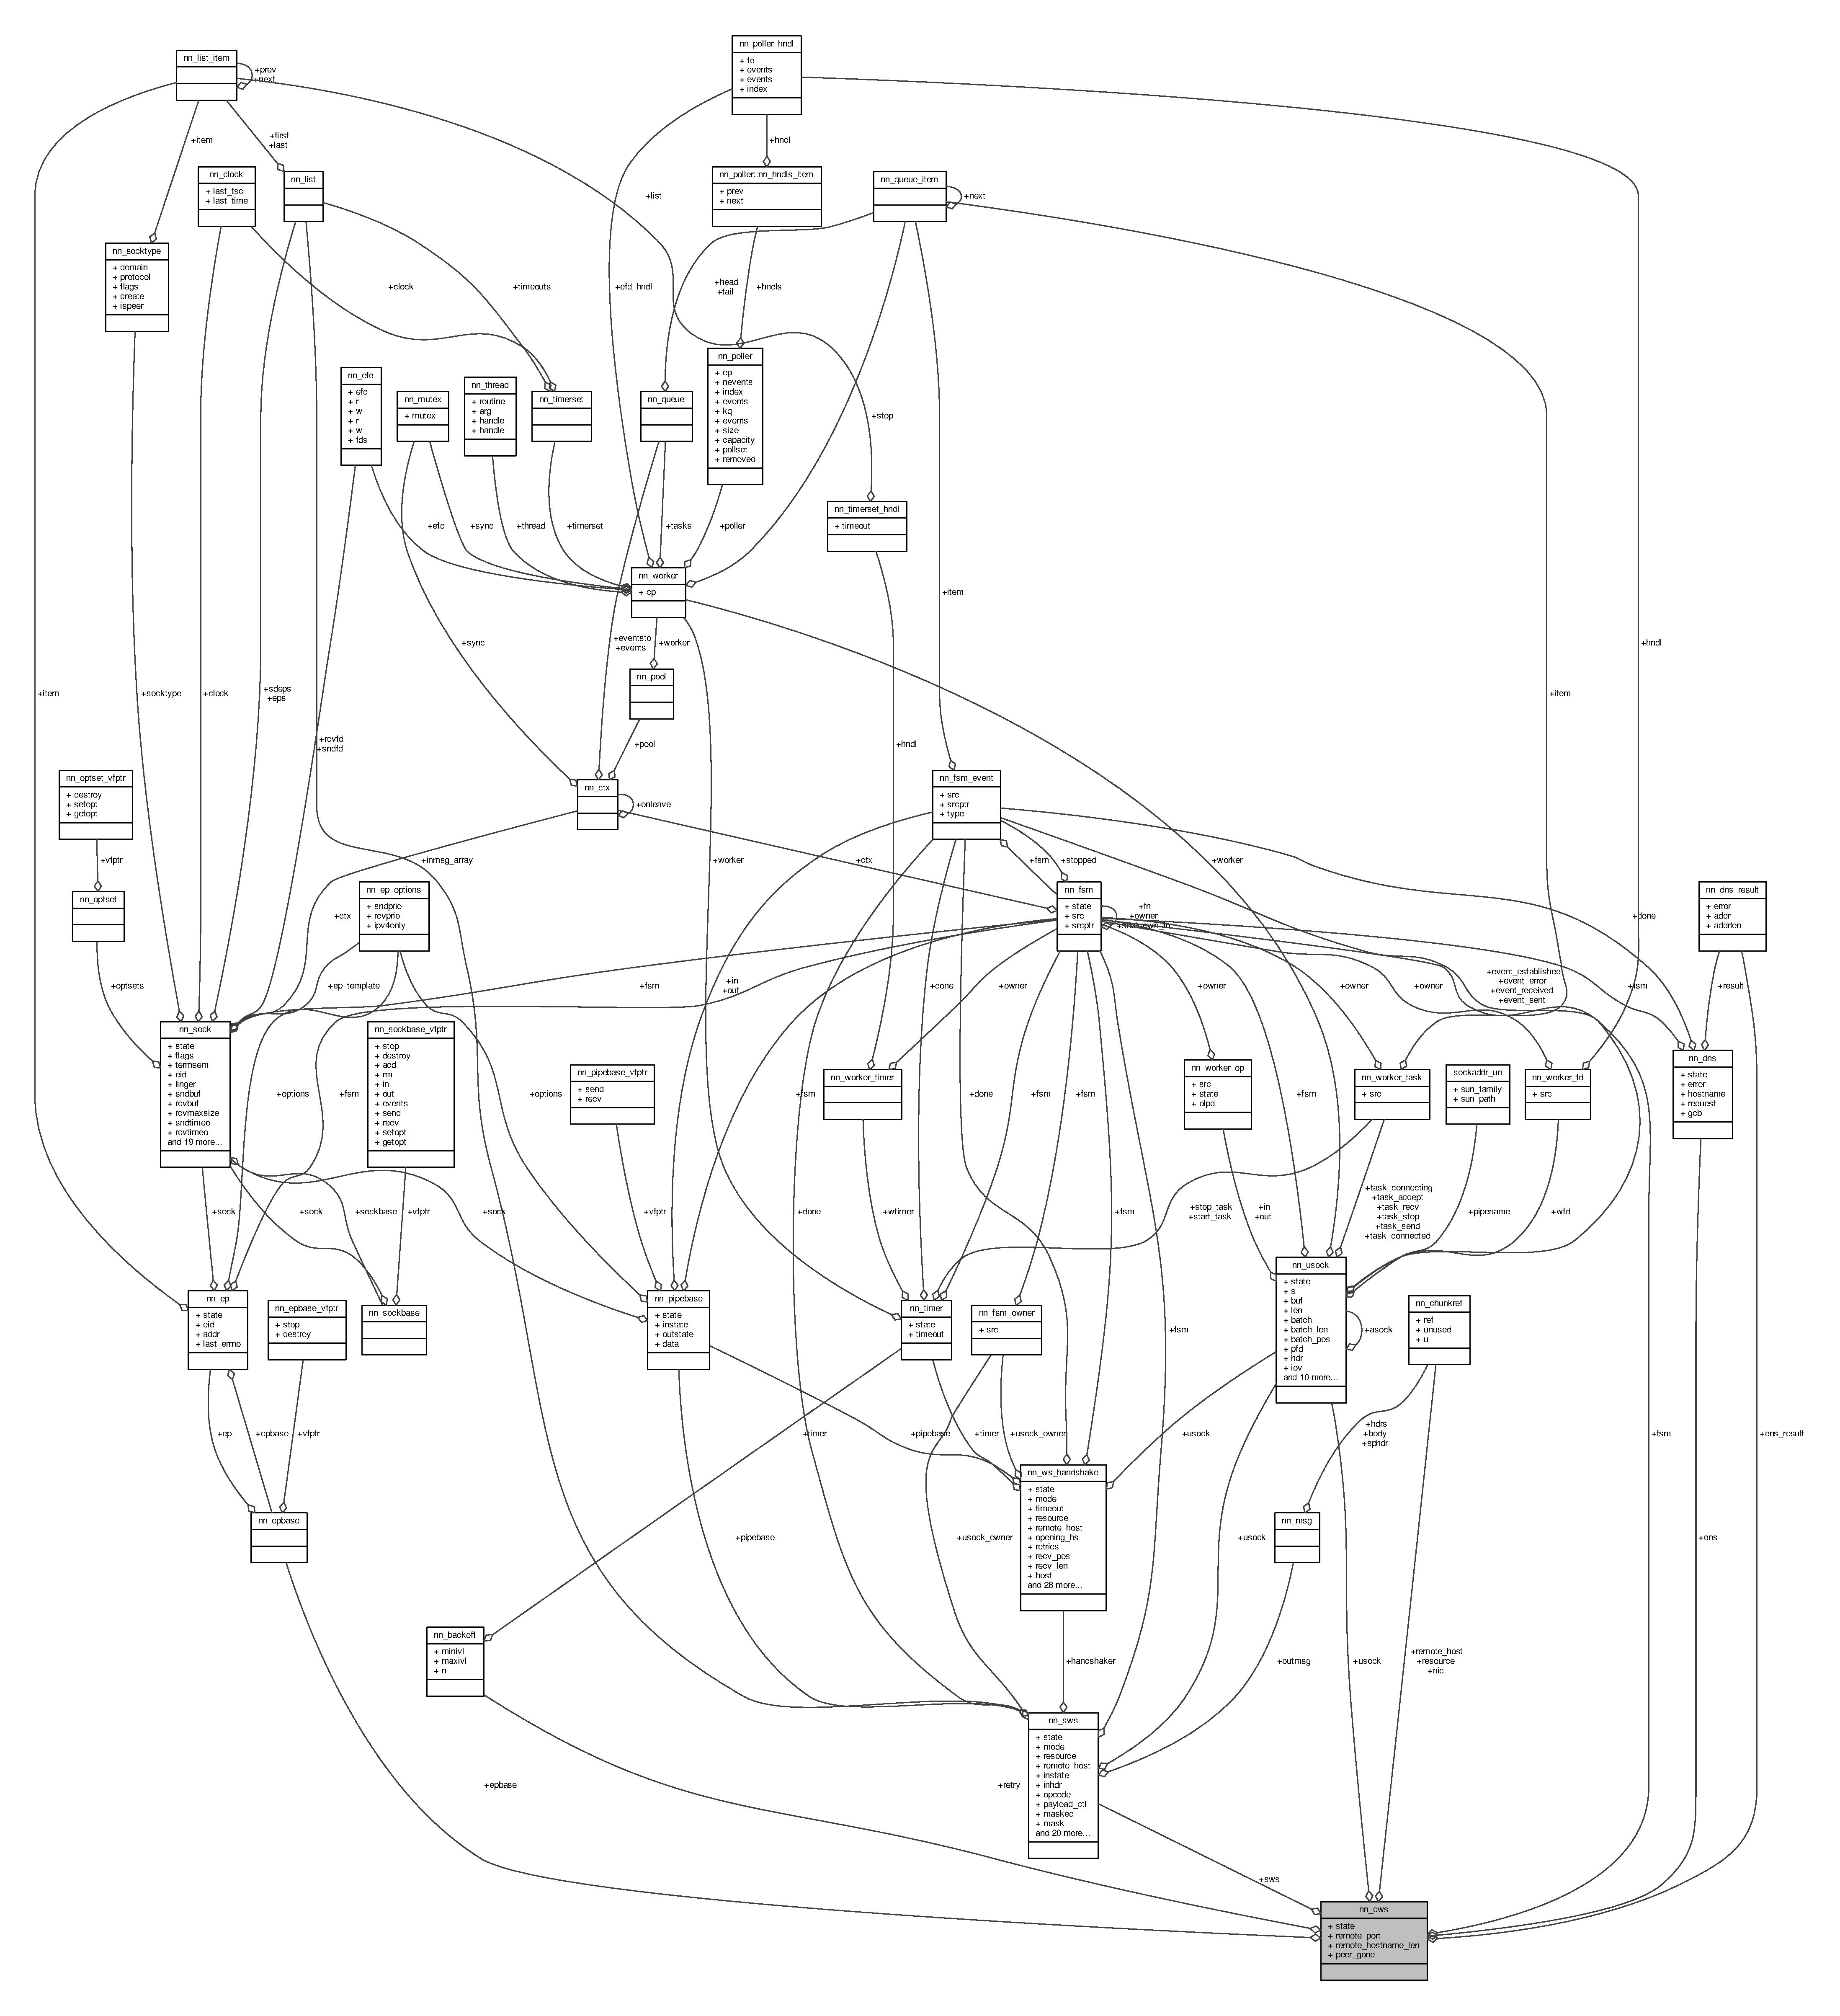
\includegraphics[width=350pt]{structnn__cws__coll__graph}
\end{center}
\end{figure}
\subsection*{Public Attributes}
\begin{DoxyCompactItemize}
\item 
struct \hyperlink{structnn__fsm}{nn\+\_\+fsm} \hyperlink{structnn__cws_a41c2cbb214b831321536bac975a001d1}{fsm}
\item 
int \hyperlink{structnn__cws_a95ff0b16ec166d1a8d4f3fab57d4a377}{state}
\item 
struct \hyperlink{structnn__epbase}{nn\+\_\+epbase} \hyperlink{structnn__cws_a6826c5e288398b8ce02bbd50fad890f6}{epbase}
\item 
struct \hyperlink{structnn__usock}{nn\+\_\+usock} \hyperlink{structnn__cws_afc94a8982678a15880a4e997e5ce7ee4}{usock}
\item 
struct \hyperlink{structnn__backoff}{nn\+\_\+backoff} \hyperlink{structnn__cws_a8abca9d2933ce61f56641f952b0c17a4}{retry}
\item 
struct \hyperlink{structnn__sws}{nn\+\_\+sws} \hyperlink{structnn__cws_a21c4c5f3afc0ac138b98bb1873457e6f}{sws}
\item 
struct \hyperlink{structnn__chunkref}{nn\+\_\+chunkref} \hyperlink{structnn__cws_ab87056e9f72028a8f06cca5e70de0c19}{resource}
\item 
struct \hyperlink{structnn__chunkref}{nn\+\_\+chunkref} \hyperlink{structnn__cws_a16a80129a6f9da75ace4d1b56d6f0287}{remote\+\_\+host}
\item 
struct \hyperlink{structnn__chunkref}{nn\+\_\+chunkref} \hyperlink{structnn__cws_ae43be2ce7b2083ca18e84472b0e67628}{nic}
\item 
int \hyperlink{structnn__cws_aed169e371de5fe39b8b21afcd4beaf4d}{remote\+\_\+port}
\item 
int \hyperlink{structnn__cws_abcddd98595f33963529039f615e70c59}{remote\+\_\+hostname\+\_\+len}
\item 
int \hyperlink{structnn__cws_a953699c3a7fc6c8addf3379489a0efbd}{peer\+\_\+gone}
\item 
struct \hyperlink{structnn__dns}{nn\+\_\+dns} \hyperlink{structnn__cws_aa6087b33d2a780cb5b5d7f56e1819d60}{dns}
\item 
struct \hyperlink{structnn__dns__result}{nn\+\_\+dns\+\_\+result} \hyperlink{structnn__cws_a08c7413b29dea92196ccfa67753cb471}{dns\+\_\+result}
\end{DoxyCompactItemize}


\subsection{Member Data Documentation}
\index{nn\+\_\+cws@{nn\+\_\+cws}!dns@{dns}}
\index{dns@{dns}!nn\+\_\+cws@{nn\+\_\+cws}}
\subsubsection[{dns}]{\setlength{\rightskip}{0pt plus 5cm}struct {\bf nn\+\_\+dns} nn\+\_\+cws\+::dns}\hypertarget{structnn__cws_aa6087b33d2a780cb5b5d7f56e1819d60}{}\label{structnn__cws_aa6087b33d2a780cb5b5d7f56e1819d60}
\index{nn\+\_\+cws@{nn\+\_\+cws}!dns\+\_\+result@{dns\+\_\+result}}
\index{dns\+\_\+result@{dns\+\_\+result}!nn\+\_\+cws@{nn\+\_\+cws}}
\subsubsection[{dns\+\_\+result}]{\setlength{\rightskip}{0pt plus 5cm}struct {\bf nn\+\_\+dns\+\_\+result} nn\+\_\+cws\+::dns\+\_\+result}\hypertarget{structnn__cws_a08c7413b29dea92196ccfa67753cb471}{}\label{structnn__cws_a08c7413b29dea92196ccfa67753cb471}
\index{nn\+\_\+cws@{nn\+\_\+cws}!epbase@{epbase}}
\index{epbase@{epbase}!nn\+\_\+cws@{nn\+\_\+cws}}
\subsubsection[{epbase}]{\setlength{\rightskip}{0pt plus 5cm}struct {\bf nn\+\_\+epbase} nn\+\_\+cws\+::epbase}\hypertarget{structnn__cws_a6826c5e288398b8ce02bbd50fad890f6}{}\label{structnn__cws_a6826c5e288398b8ce02bbd50fad890f6}
\index{nn\+\_\+cws@{nn\+\_\+cws}!fsm@{fsm}}
\index{fsm@{fsm}!nn\+\_\+cws@{nn\+\_\+cws}}
\subsubsection[{fsm}]{\setlength{\rightskip}{0pt plus 5cm}struct {\bf nn\+\_\+fsm} nn\+\_\+cws\+::fsm}\hypertarget{structnn__cws_a41c2cbb214b831321536bac975a001d1}{}\label{structnn__cws_a41c2cbb214b831321536bac975a001d1}
\index{nn\+\_\+cws@{nn\+\_\+cws}!nic@{nic}}
\index{nic@{nic}!nn\+\_\+cws@{nn\+\_\+cws}}
\subsubsection[{nic}]{\setlength{\rightskip}{0pt plus 5cm}struct {\bf nn\+\_\+chunkref} nn\+\_\+cws\+::nic}\hypertarget{structnn__cws_ae43be2ce7b2083ca18e84472b0e67628}{}\label{structnn__cws_ae43be2ce7b2083ca18e84472b0e67628}
\index{nn\+\_\+cws@{nn\+\_\+cws}!peer\+\_\+gone@{peer\+\_\+gone}}
\index{peer\+\_\+gone@{peer\+\_\+gone}!nn\+\_\+cws@{nn\+\_\+cws}}
\subsubsection[{peer\+\_\+gone}]{\setlength{\rightskip}{0pt plus 5cm}int nn\+\_\+cws\+::peer\+\_\+gone}\hypertarget{structnn__cws_a953699c3a7fc6c8addf3379489a0efbd}{}\label{structnn__cws_a953699c3a7fc6c8addf3379489a0efbd}
\index{nn\+\_\+cws@{nn\+\_\+cws}!remote\+\_\+host@{remote\+\_\+host}}
\index{remote\+\_\+host@{remote\+\_\+host}!nn\+\_\+cws@{nn\+\_\+cws}}
\subsubsection[{remote\+\_\+host}]{\setlength{\rightskip}{0pt plus 5cm}struct {\bf nn\+\_\+chunkref} nn\+\_\+cws\+::remote\+\_\+host}\hypertarget{structnn__cws_a16a80129a6f9da75ace4d1b56d6f0287}{}\label{structnn__cws_a16a80129a6f9da75ace4d1b56d6f0287}
\index{nn\+\_\+cws@{nn\+\_\+cws}!remote\+\_\+hostname\+\_\+len@{remote\+\_\+hostname\+\_\+len}}
\index{remote\+\_\+hostname\+\_\+len@{remote\+\_\+hostname\+\_\+len}!nn\+\_\+cws@{nn\+\_\+cws}}
\subsubsection[{remote\+\_\+hostname\+\_\+len}]{\setlength{\rightskip}{0pt plus 5cm}int nn\+\_\+cws\+::remote\+\_\+hostname\+\_\+len}\hypertarget{structnn__cws_abcddd98595f33963529039f615e70c59}{}\label{structnn__cws_abcddd98595f33963529039f615e70c59}
\index{nn\+\_\+cws@{nn\+\_\+cws}!remote\+\_\+port@{remote\+\_\+port}}
\index{remote\+\_\+port@{remote\+\_\+port}!nn\+\_\+cws@{nn\+\_\+cws}}
\subsubsection[{remote\+\_\+port}]{\setlength{\rightskip}{0pt plus 5cm}int nn\+\_\+cws\+::remote\+\_\+port}\hypertarget{structnn__cws_aed169e371de5fe39b8b21afcd4beaf4d}{}\label{structnn__cws_aed169e371de5fe39b8b21afcd4beaf4d}
\index{nn\+\_\+cws@{nn\+\_\+cws}!resource@{resource}}
\index{resource@{resource}!nn\+\_\+cws@{nn\+\_\+cws}}
\subsubsection[{resource}]{\setlength{\rightskip}{0pt plus 5cm}struct {\bf nn\+\_\+chunkref} nn\+\_\+cws\+::resource}\hypertarget{structnn__cws_ab87056e9f72028a8f06cca5e70de0c19}{}\label{structnn__cws_ab87056e9f72028a8f06cca5e70de0c19}
\index{nn\+\_\+cws@{nn\+\_\+cws}!retry@{retry}}
\index{retry@{retry}!nn\+\_\+cws@{nn\+\_\+cws}}
\subsubsection[{retry}]{\setlength{\rightskip}{0pt plus 5cm}struct {\bf nn\+\_\+backoff} nn\+\_\+cws\+::retry}\hypertarget{structnn__cws_a8abca9d2933ce61f56641f952b0c17a4}{}\label{structnn__cws_a8abca9d2933ce61f56641f952b0c17a4}
\index{nn\+\_\+cws@{nn\+\_\+cws}!state@{state}}
\index{state@{state}!nn\+\_\+cws@{nn\+\_\+cws}}
\subsubsection[{state}]{\setlength{\rightskip}{0pt plus 5cm}int nn\+\_\+cws\+::state}\hypertarget{structnn__cws_a95ff0b16ec166d1a8d4f3fab57d4a377}{}\label{structnn__cws_a95ff0b16ec166d1a8d4f3fab57d4a377}
\index{nn\+\_\+cws@{nn\+\_\+cws}!sws@{sws}}
\index{sws@{sws}!nn\+\_\+cws@{nn\+\_\+cws}}
\subsubsection[{sws}]{\setlength{\rightskip}{0pt plus 5cm}struct {\bf nn\+\_\+sws} nn\+\_\+cws\+::sws}\hypertarget{structnn__cws_a21c4c5f3afc0ac138b98bb1873457e6f}{}\label{structnn__cws_a21c4c5f3afc0ac138b98bb1873457e6f}
\index{nn\+\_\+cws@{nn\+\_\+cws}!usock@{usock}}
\index{usock@{usock}!nn\+\_\+cws@{nn\+\_\+cws}}
\subsubsection[{usock}]{\setlength{\rightskip}{0pt plus 5cm}struct {\bf nn\+\_\+usock} nn\+\_\+cws\+::usock}\hypertarget{structnn__cws_afc94a8982678a15880a4e997e5ce7ee4}{}\label{structnn__cws_afc94a8982678a15880a4e997e5ce7ee4}


The documentation for this struct was generated from the following file\+:\begin{DoxyCompactItemize}
\item 
src/transports/ws/\hyperlink{cws_8c}{cws.\+c}\end{DoxyCompactItemize}

\hypertarget{structnn__device__recipe}{}\section{nn\+\_\+device\+\_\+recipe Struct Reference}
\label{structnn__device__recipe}\index{nn\+\_\+device\+\_\+recipe@{nn\+\_\+device\+\_\+recipe}}


{\ttfamily \#include $<$device.\+h$>$}



Collaboration diagram for nn\+\_\+device\+\_\+recipe\+:\nopagebreak
\begin{figure}[H]
\begin{center}
\leavevmode
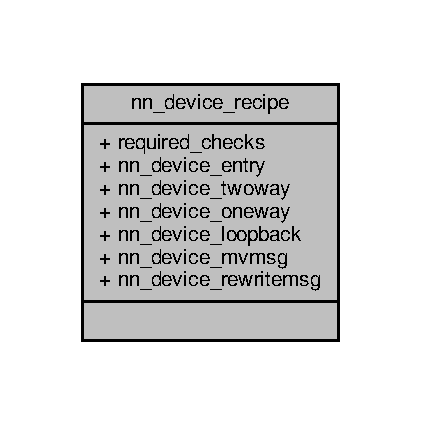
\includegraphics[width=202pt]{structnn__device__recipe__coll__graph}
\end{center}
\end{figure}
\subsection*{Public Attributes}
\begin{DoxyCompactItemize}
\item 
int \hyperlink{structnn__device__recipe_a78ce62e7ab6b45a11e8dfeb5894b356e}{required\+\_\+checks}
\item 
int($\ast$ \hyperlink{structnn__device__recipe_adeb5d36621f14a9837fdc4cb94c3d051}{nn\+\_\+device\+\_\+entry} )(struct \hyperlink{structnn__device__recipe}{nn\+\_\+device\+\_\+recipe} $\ast$device, int s1, int s2, int flags)
\item 
int($\ast$ \hyperlink{structnn__device__recipe_aff9065238d098af6a963756174a4043d}{nn\+\_\+device\+\_\+twoway} )(struct \hyperlink{structnn__device__recipe}{nn\+\_\+device\+\_\+recipe} $\ast$device, int s1, \hyperlink{efd__socketpair_8h_ac7ca4a7f723a6addf724ee88951a4d02}{nn\+\_\+fd} s1rcv, \hyperlink{efd__socketpair_8h_ac7ca4a7f723a6addf724ee88951a4d02}{nn\+\_\+fd} s1snd, int s2, \hyperlink{efd__socketpair_8h_ac7ca4a7f723a6addf724ee88951a4d02}{nn\+\_\+fd} s2rcv, \hyperlink{efd__socketpair_8h_ac7ca4a7f723a6addf724ee88951a4d02}{nn\+\_\+fd} s2snd)
\item 
int($\ast$ \hyperlink{structnn__device__recipe_a2228a6409b18679d8ae17d5c230967cc}{nn\+\_\+device\+\_\+oneway} )(struct \hyperlink{structnn__device__recipe}{nn\+\_\+device\+\_\+recipe} $\ast$device, int s1, \hyperlink{efd__socketpair_8h_ac7ca4a7f723a6addf724ee88951a4d02}{nn\+\_\+fd} s1rcv, int s2, \hyperlink{efd__socketpair_8h_ac7ca4a7f723a6addf724ee88951a4d02}{nn\+\_\+fd} s2snd)
\item 
int($\ast$ \hyperlink{structnn__device__recipe_a942a556adb7a502cce98f9090a6d0ebf}{nn\+\_\+device\+\_\+loopback} )(struct \hyperlink{structnn__device__recipe}{nn\+\_\+device\+\_\+recipe} $\ast$device, int s)
\item 
int($\ast$ \hyperlink{structnn__device__recipe_aaf7ad40c45c50814de02aa920f5e8a24}{nn\+\_\+device\+\_\+mvmsg} )(struct \hyperlink{structnn__device__recipe}{nn\+\_\+device\+\_\+recipe} $\ast$device, int from, int to, int flags)
\item 
int($\ast$ \hyperlink{structnn__device__recipe_afcfda6f162ed7dd5bb98f3d796a3a6ea}{nn\+\_\+device\+\_\+rewritemsg} )(struct \hyperlink{structnn__device__recipe}{nn\+\_\+device\+\_\+recipe} $\ast$device, int from, int to, int flags, struct \hyperlink{structnn__msghdr}{nn\+\_\+msghdr} $\ast$msghdr, int bytes)
\end{DoxyCompactItemize}


\subsection{Member Data Documentation}
\index{nn\+\_\+device\+\_\+recipe@{nn\+\_\+device\+\_\+recipe}!nn\+\_\+device\+\_\+entry@{nn\+\_\+device\+\_\+entry}}
\index{nn\+\_\+device\+\_\+entry@{nn\+\_\+device\+\_\+entry}!nn\+\_\+device\+\_\+recipe@{nn\+\_\+device\+\_\+recipe}}
\subsubsection[{nn\+\_\+device\+\_\+entry}]{\setlength{\rightskip}{0pt plus 5cm}int($\ast$ nn\+\_\+device\+\_\+recipe\+::nn\+\_\+device\+\_\+entry) (struct {\bf nn\+\_\+device\+\_\+recipe} $\ast$device, int s1, int s2, int flags)}\hypertarget{structnn__device__recipe_adeb5d36621f14a9837fdc4cb94c3d051}{}\label{structnn__device__recipe_adeb5d36621f14a9837fdc4cb94c3d051}
\index{nn\+\_\+device\+\_\+recipe@{nn\+\_\+device\+\_\+recipe}!nn\+\_\+device\+\_\+loopback@{nn\+\_\+device\+\_\+loopback}}
\index{nn\+\_\+device\+\_\+loopback@{nn\+\_\+device\+\_\+loopback}!nn\+\_\+device\+\_\+recipe@{nn\+\_\+device\+\_\+recipe}}
\subsubsection[{nn\+\_\+device\+\_\+loopback}]{\setlength{\rightskip}{0pt plus 5cm}int($\ast$ nn\+\_\+device\+\_\+recipe\+::nn\+\_\+device\+\_\+loopback) (struct {\bf nn\+\_\+device\+\_\+recipe} $\ast$device, int s)}\hypertarget{structnn__device__recipe_a942a556adb7a502cce98f9090a6d0ebf}{}\label{structnn__device__recipe_a942a556adb7a502cce98f9090a6d0ebf}
\index{nn\+\_\+device\+\_\+recipe@{nn\+\_\+device\+\_\+recipe}!nn\+\_\+device\+\_\+mvmsg@{nn\+\_\+device\+\_\+mvmsg}}
\index{nn\+\_\+device\+\_\+mvmsg@{nn\+\_\+device\+\_\+mvmsg}!nn\+\_\+device\+\_\+recipe@{nn\+\_\+device\+\_\+recipe}}
\subsubsection[{nn\+\_\+device\+\_\+mvmsg}]{\setlength{\rightskip}{0pt plus 5cm}int($\ast$ nn\+\_\+device\+\_\+recipe\+::nn\+\_\+device\+\_\+mvmsg) (struct {\bf nn\+\_\+device\+\_\+recipe} $\ast$device, int from, int to, int flags)}\hypertarget{structnn__device__recipe_aaf7ad40c45c50814de02aa920f5e8a24}{}\label{structnn__device__recipe_aaf7ad40c45c50814de02aa920f5e8a24}
\index{nn\+\_\+device\+\_\+recipe@{nn\+\_\+device\+\_\+recipe}!nn\+\_\+device\+\_\+oneway@{nn\+\_\+device\+\_\+oneway}}
\index{nn\+\_\+device\+\_\+oneway@{nn\+\_\+device\+\_\+oneway}!nn\+\_\+device\+\_\+recipe@{nn\+\_\+device\+\_\+recipe}}
\subsubsection[{nn\+\_\+device\+\_\+oneway}]{\setlength{\rightskip}{0pt plus 5cm}int($\ast$ nn\+\_\+device\+\_\+recipe\+::nn\+\_\+device\+\_\+oneway) (struct {\bf nn\+\_\+device\+\_\+recipe} $\ast$device, int s1, {\bf nn\+\_\+fd} s1rcv, int s2, {\bf nn\+\_\+fd} s2snd)}\hypertarget{structnn__device__recipe_a2228a6409b18679d8ae17d5c230967cc}{}\label{structnn__device__recipe_a2228a6409b18679d8ae17d5c230967cc}
\index{nn\+\_\+device\+\_\+recipe@{nn\+\_\+device\+\_\+recipe}!nn\+\_\+device\+\_\+rewritemsg@{nn\+\_\+device\+\_\+rewritemsg}}
\index{nn\+\_\+device\+\_\+rewritemsg@{nn\+\_\+device\+\_\+rewritemsg}!nn\+\_\+device\+\_\+recipe@{nn\+\_\+device\+\_\+recipe}}
\subsubsection[{nn\+\_\+device\+\_\+rewritemsg}]{\setlength{\rightskip}{0pt plus 5cm}int($\ast$ nn\+\_\+device\+\_\+recipe\+::nn\+\_\+device\+\_\+rewritemsg) (struct {\bf nn\+\_\+device\+\_\+recipe} $\ast$device, int from, int to, int flags, struct {\bf nn\+\_\+msghdr} $\ast$msghdr, int bytes)}\hypertarget{structnn__device__recipe_afcfda6f162ed7dd5bb98f3d796a3a6ea}{}\label{structnn__device__recipe_afcfda6f162ed7dd5bb98f3d796a3a6ea}
\index{nn\+\_\+device\+\_\+recipe@{nn\+\_\+device\+\_\+recipe}!nn\+\_\+device\+\_\+twoway@{nn\+\_\+device\+\_\+twoway}}
\index{nn\+\_\+device\+\_\+twoway@{nn\+\_\+device\+\_\+twoway}!nn\+\_\+device\+\_\+recipe@{nn\+\_\+device\+\_\+recipe}}
\subsubsection[{nn\+\_\+device\+\_\+twoway}]{\setlength{\rightskip}{0pt plus 5cm}int($\ast$ nn\+\_\+device\+\_\+recipe\+::nn\+\_\+device\+\_\+twoway) (struct {\bf nn\+\_\+device\+\_\+recipe} $\ast$device, int s1, {\bf nn\+\_\+fd} s1rcv, {\bf nn\+\_\+fd} s1snd, int s2, {\bf nn\+\_\+fd} s2rcv, {\bf nn\+\_\+fd} s2snd)}\hypertarget{structnn__device__recipe_aff9065238d098af6a963756174a4043d}{}\label{structnn__device__recipe_aff9065238d098af6a963756174a4043d}
\index{nn\+\_\+device\+\_\+recipe@{nn\+\_\+device\+\_\+recipe}!required\+\_\+checks@{required\+\_\+checks}}
\index{required\+\_\+checks@{required\+\_\+checks}!nn\+\_\+device\+\_\+recipe@{nn\+\_\+device\+\_\+recipe}}
\subsubsection[{required\+\_\+checks}]{\setlength{\rightskip}{0pt plus 5cm}int nn\+\_\+device\+\_\+recipe\+::required\+\_\+checks}\hypertarget{structnn__device__recipe_a78ce62e7ab6b45a11e8dfeb5894b356e}{}\label{structnn__device__recipe_a78ce62e7ab6b45a11e8dfeb5894b356e}


The documentation for this struct was generated from the following file\+:\begin{DoxyCompactItemize}
\item 
src/devices/\hyperlink{device_8h}{device.\+h}\end{DoxyCompactItemize}

\hypertarget{structnn__dist}{}\section{nn\+\_\+dist Struct Reference}
\label{structnn__dist}\index{nn\+\_\+dist@{nn\+\_\+dist}}


{\ttfamily \#include $<$dist.\+h$>$}



Collaboration diagram for nn\+\_\+dist\+:\nopagebreak
\begin{figure}[H]
\begin{center}
\leavevmode
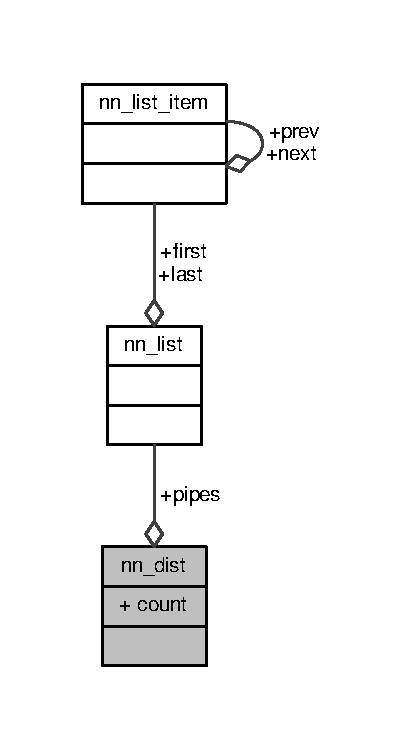
\includegraphics[width=194pt]{structnn__dist__coll__graph}
\end{center}
\end{figure}
\subsection*{Public Attributes}
\begin{DoxyCompactItemize}
\item 
uint32\+\_\+t \hyperlink{structnn__dist_a334300196bd129e8c909122435bef82a}{count}
\item 
struct \hyperlink{structnn__list}{nn\+\_\+list} \hyperlink{structnn__dist_a9ebfbe8b26a7da288e04b2cb6fd6c6f9}{pipes}
\end{DoxyCompactItemize}


\subsection{Member Data Documentation}
\index{nn\+\_\+dist@{nn\+\_\+dist}!count@{count}}
\index{count@{count}!nn\+\_\+dist@{nn\+\_\+dist}}
\subsubsection[{count}]{\setlength{\rightskip}{0pt plus 5cm}uint32\+\_\+t nn\+\_\+dist\+::count}\hypertarget{structnn__dist_a334300196bd129e8c909122435bef82a}{}\label{structnn__dist_a334300196bd129e8c909122435bef82a}
\index{nn\+\_\+dist@{nn\+\_\+dist}!pipes@{pipes}}
\index{pipes@{pipes}!nn\+\_\+dist@{nn\+\_\+dist}}
\subsubsection[{pipes}]{\setlength{\rightskip}{0pt plus 5cm}struct {\bf nn\+\_\+list} nn\+\_\+dist\+::pipes}\hypertarget{structnn__dist_a9ebfbe8b26a7da288e04b2cb6fd6c6f9}{}\label{structnn__dist_a9ebfbe8b26a7da288e04b2cb6fd6c6f9}


The documentation for this struct was generated from the following file\+:\begin{DoxyCompactItemize}
\item 
src/protocols/utils/\hyperlink{dist_8h}{dist.\+h}\end{DoxyCompactItemize}

\hypertarget{structnn__dist__data}{}\section{nn\+\_\+dist\+\_\+data Struct Reference}
\label{structnn__dist__data}\index{nn\+\_\+dist\+\_\+data@{nn\+\_\+dist\+\_\+data}}


{\ttfamily \#include $<$dist.\+h$>$}



Collaboration diagram for nn\+\_\+dist\+\_\+data\+:\nopagebreak
\begin{figure}[H]
\begin{center}
\leavevmode
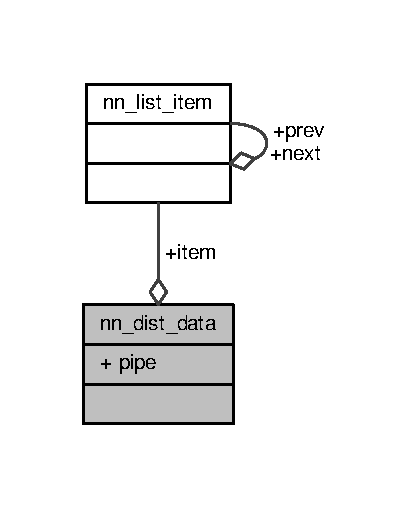
\includegraphics[width=196pt]{structnn__dist__data__coll__graph}
\end{center}
\end{figure}
\subsection*{Public Attributes}
\begin{DoxyCompactItemize}
\item 
struct \hyperlink{structnn__list__item}{nn\+\_\+list\+\_\+item} \hyperlink{structnn__dist__data_a32fb0eac783b93d2ba805656f1d9e6a6}{item}
\item 
struct nn\+\_\+pipe $\ast$ \hyperlink{structnn__dist__data_a812ff5953bd78545db17cdb09ba7cd48}{pipe}
\end{DoxyCompactItemize}


\subsection{Member Data Documentation}
\index{nn\+\_\+dist\+\_\+data@{nn\+\_\+dist\+\_\+data}!item@{item}}
\index{item@{item}!nn\+\_\+dist\+\_\+data@{nn\+\_\+dist\+\_\+data}}
\subsubsection[{item}]{\setlength{\rightskip}{0pt plus 5cm}struct {\bf nn\+\_\+list\+\_\+item} nn\+\_\+dist\+\_\+data\+::item}\hypertarget{structnn__dist__data_a32fb0eac783b93d2ba805656f1d9e6a6}{}\label{structnn__dist__data_a32fb0eac783b93d2ba805656f1d9e6a6}
\index{nn\+\_\+dist\+\_\+data@{nn\+\_\+dist\+\_\+data}!pipe@{pipe}}
\index{pipe@{pipe}!nn\+\_\+dist\+\_\+data@{nn\+\_\+dist\+\_\+data}}
\subsubsection[{pipe}]{\setlength{\rightskip}{0pt plus 5cm}struct nn\+\_\+pipe$\ast$ nn\+\_\+dist\+\_\+data\+::pipe}\hypertarget{structnn__dist__data_a812ff5953bd78545db17cdb09ba7cd48}{}\label{structnn__dist__data_a812ff5953bd78545db17cdb09ba7cd48}


The documentation for this struct was generated from the following file\+:\begin{DoxyCompactItemize}
\item 
src/protocols/utils/\hyperlink{dist_8h}{dist.\+h}\end{DoxyCompactItemize}

\hypertarget{structnn__dns}{}\section{nn\+\_\+dns Struct Reference}
\label{structnn__dns}\index{nn\+\_\+dns@{nn\+\_\+dns}}


{\ttfamily \#include $<$dns\+\_\+getaddrinfo.\+h$>$}



Collaboration diagram for nn\+\_\+dns\+:\nopagebreak
\begin{figure}[H]
\begin{center}
\leavevmode
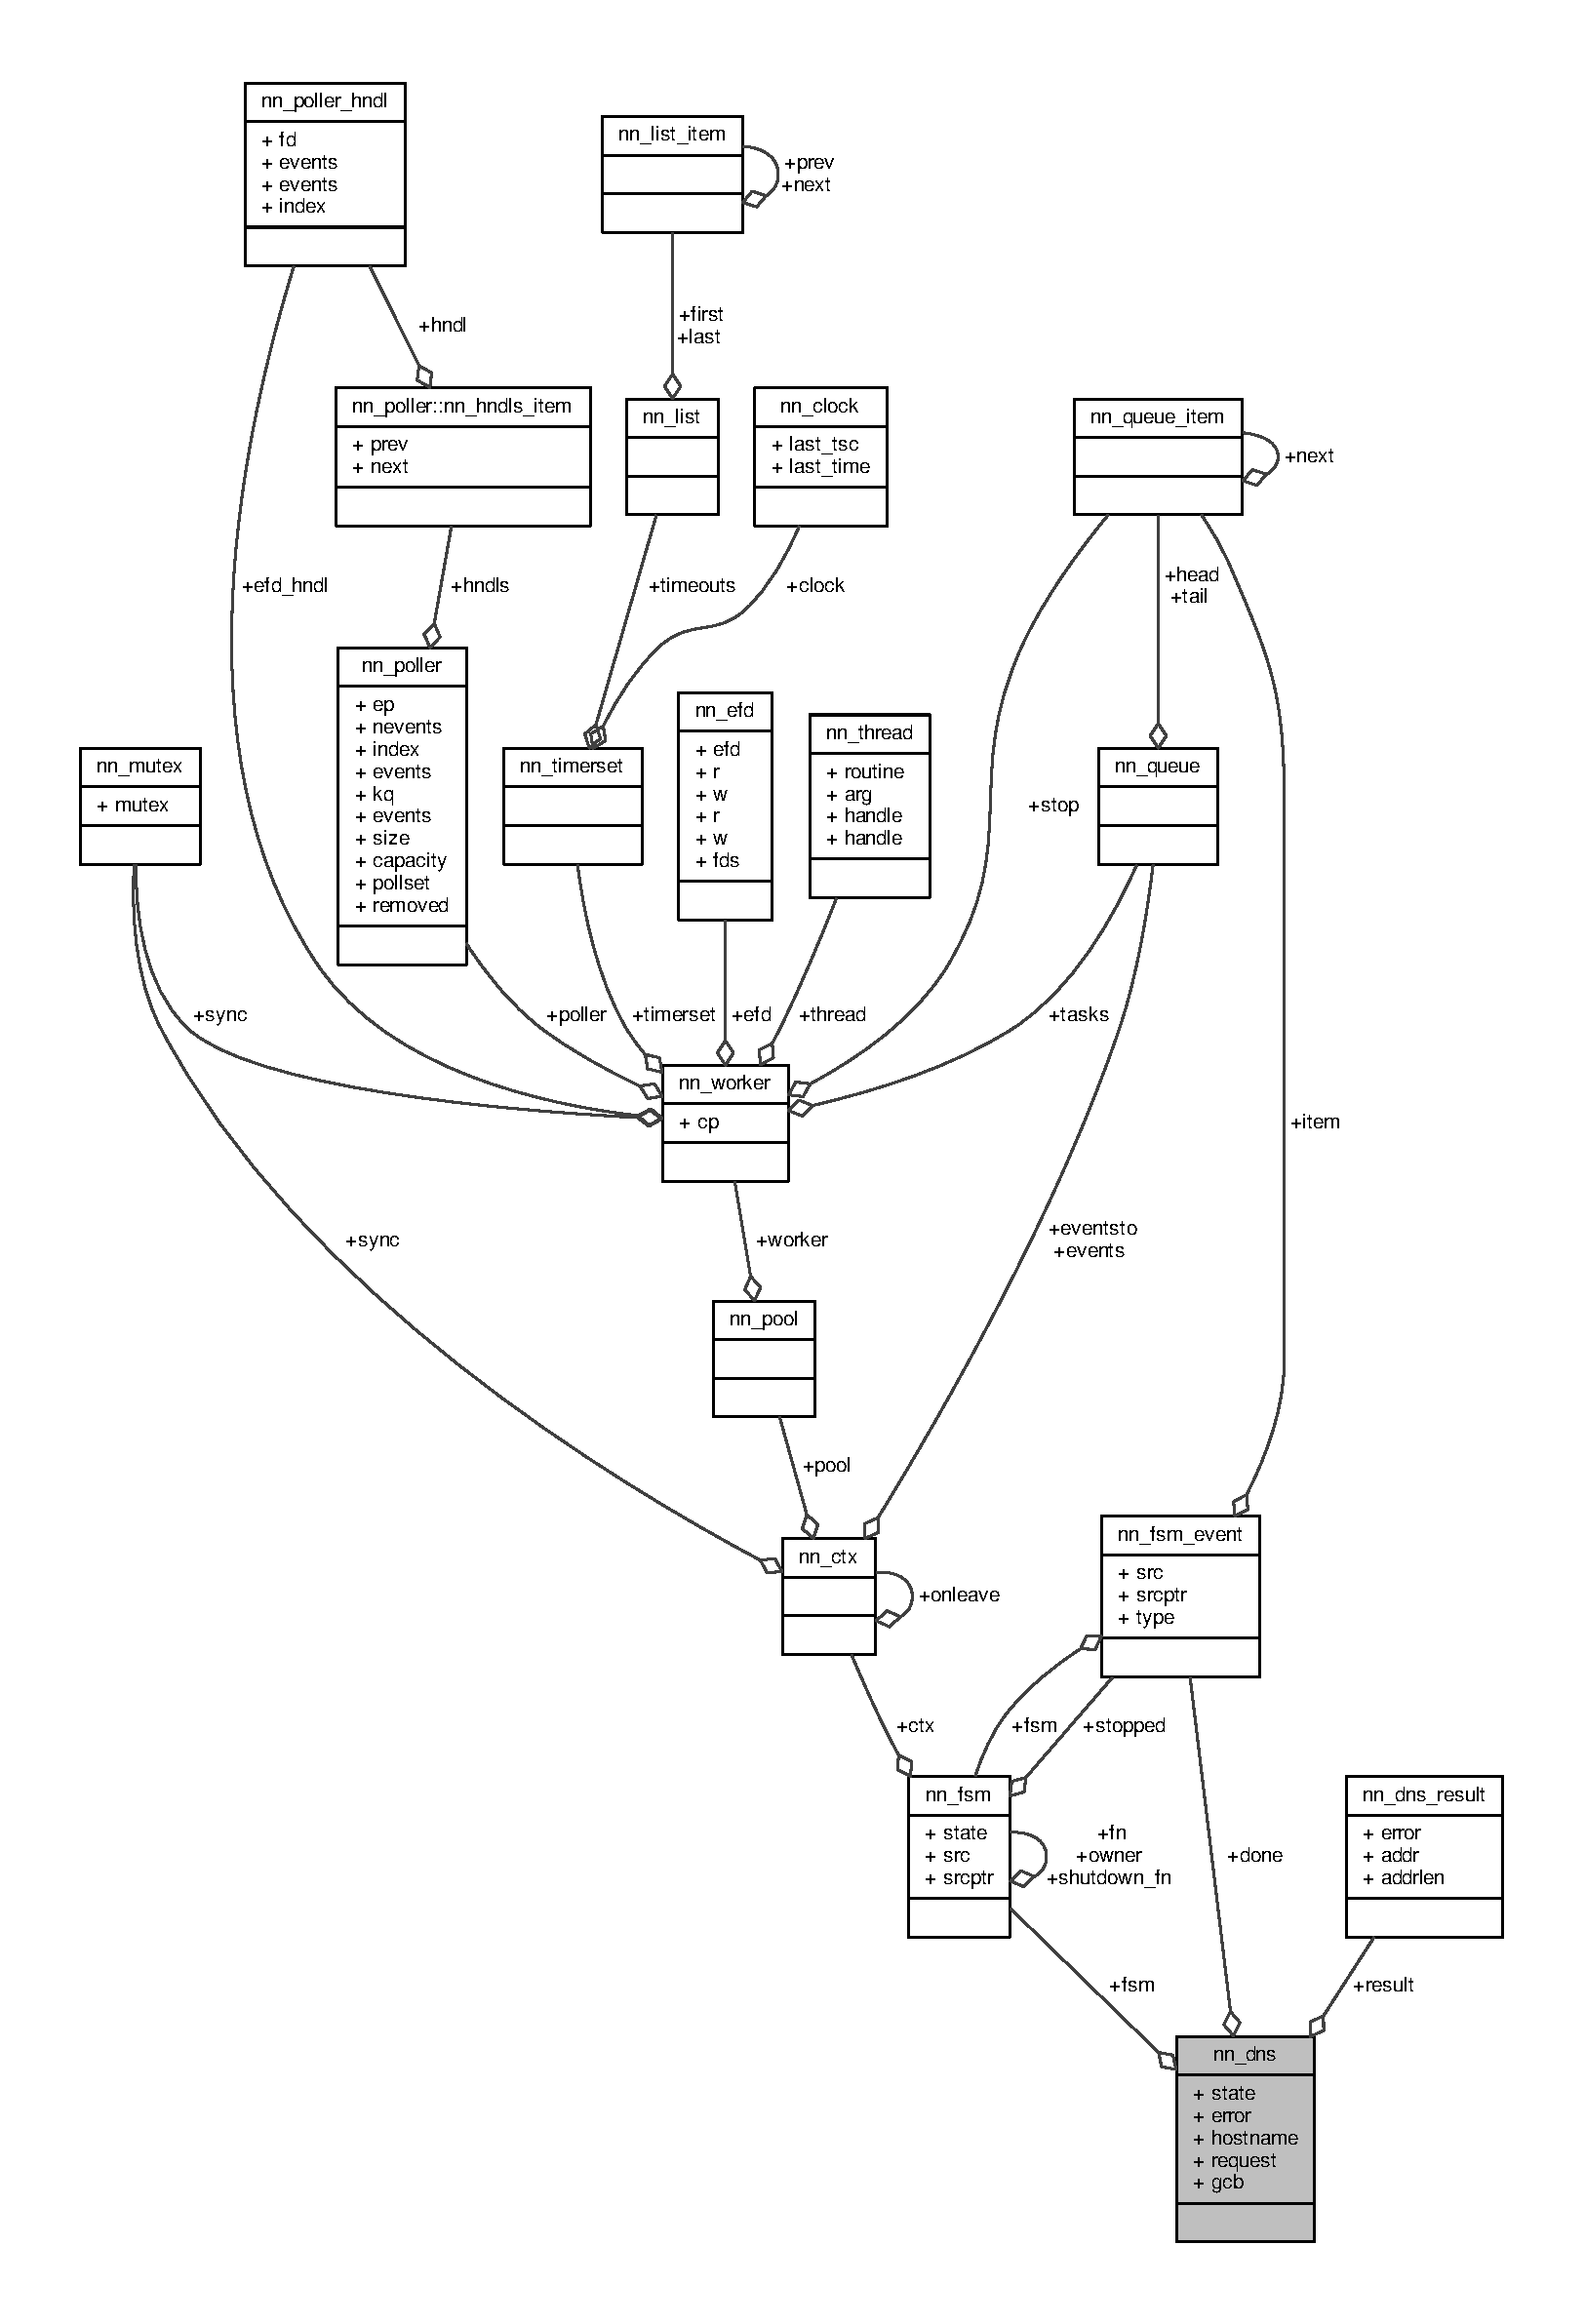
\includegraphics[width=350pt]{structnn__dns__coll__graph}
\end{center}
\end{figure}
\subsection*{Public Attributes}
\begin{DoxyCompactItemize}
\item 
struct \hyperlink{structnn__fsm}{nn\+\_\+fsm} \hyperlink{structnn__dns_a0f2f987efe48894f96a30199fbbf08d9}{fsm}
\item 
int \hyperlink{structnn__dns_a95a661cf2fc34d5dcb28bada51eee803}{state}
\item 
struct \hyperlink{structnn__dns__result}{nn\+\_\+dns\+\_\+result} $\ast$ \hyperlink{structnn__dns_a379539bb0b7354a8520acb23fdaac027}{result}
\item 
struct \hyperlink{structnn__fsm__event}{nn\+\_\+fsm\+\_\+event} \hyperlink{structnn__dns_a843e151f44152faf03780cf793842223}{done}
\item 
int \hyperlink{structnn__dns_a17d208ceb0ee12ec77eb91ecbaf21537}{error}
\item 
char \hyperlink{structnn__dns_aa9b2b6de4e2ac1e18876370ada8c8a7a}{hostname} \mbox{[}\hyperlink{nn_8h_a9b3759ef32562c8b4f0c8c75f54c8b03}{N\+N\+\_\+\+S\+O\+C\+K\+A\+D\+D\+R\+\_\+\+M\+AX}\mbox{]}
\item 
struct addrinfo \hyperlink{structnn__dns_aa16cc1ee1b29647de32a28ff2abe9ed3}{request}
\item 
struct gaicb \hyperlink{structnn__dns_ab81aea732ded93810fdf265eb2f257ea}{gcb}
\end{DoxyCompactItemize}


\subsection{Member Data Documentation}
\index{nn\+\_\+dns@{nn\+\_\+dns}!done@{done}}
\index{done@{done}!nn\+\_\+dns@{nn\+\_\+dns}}
\subsubsection[{done}]{\setlength{\rightskip}{0pt plus 5cm}struct {\bf nn\+\_\+fsm\+\_\+event} nn\+\_\+dns\+::done}\hypertarget{structnn__dns_a843e151f44152faf03780cf793842223}{}\label{structnn__dns_a843e151f44152faf03780cf793842223}
\index{nn\+\_\+dns@{nn\+\_\+dns}!error@{error}}
\index{error@{error}!nn\+\_\+dns@{nn\+\_\+dns}}
\subsubsection[{error}]{\setlength{\rightskip}{0pt plus 5cm}int nn\+\_\+dns\+::error}\hypertarget{structnn__dns_a17d208ceb0ee12ec77eb91ecbaf21537}{}\label{structnn__dns_a17d208ceb0ee12ec77eb91ecbaf21537}
\index{nn\+\_\+dns@{nn\+\_\+dns}!fsm@{fsm}}
\index{fsm@{fsm}!nn\+\_\+dns@{nn\+\_\+dns}}
\subsubsection[{fsm}]{\setlength{\rightskip}{0pt plus 5cm}struct {\bf nn\+\_\+fsm} nn\+\_\+dns\+::fsm}\hypertarget{structnn__dns_a0f2f987efe48894f96a30199fbbf08d9}{}\label{structnn__dns_a0f2f987efe48894f96a30199fbbf08d9}
\index{nn\+\_\+dns@{nn\+\_\+dns}!gcb@{gcb}}
\index{gcb@{gcb}!nn\+\_\+dns@{nn\+\_\+dns}}
\subsubsection[{gcb}]{\setlength{\rightskip}{0pt plus 5cm}struct gaicb nn\+\_\+dns\+::gcb}\hypertarget{structnn__dns_ab81aea732ded93810fdf265eb2f257ea}{}\label{structnn__dns_ab81aea732ded93810fdf265eb2f257ea}
\index{nn\+\_\+dns@{nn\+\_\+dns}!hostname@{hostname}}
\index{hostname@{hostname}!nn\+\_\+dns@{nn\+\_\+dns}}
\subsubsection[{hostname}]{\setlength{\rightskip}{0pt plus 5cm}char nn\+\_\+dns\+::hostname\mbox{[}{\bf N\+N\+\_\+\+S\+O\+C\+K\+A\+D\+D\+R\+\_\+\+M\+AX}\mbox{]}}\hypertarget{structnn__dns_aa9b2b6de4e2ac1e18876370ada8c8a7a}{}\label{structnn__dns_aa9b2b6de4e2ac1e18876370ada8c8a7a}
\index{nn\+\_\+dns@{nn\+\_\+dns}!request@{request}}
\index{request@{request}!nn\+\_\+dns@{nn\+\_\+dns}}
\subsubsection[{request}]{\setlength{\rightskip}{0pt plus 5cm}struct addrinfo nn\+\_\+dns\+::request}\hypertarget{structnn__dns_aa16cc1ee1b29647de32a28ff2abe9ed3}{}\label{structnn__dns_aa16cc1ee1b29647de32a28ff2abe9ed3}
\index{nn\+\_\+dns@{nn\+\_\+dns}!result@{result}}
\index{result@{result}!nn\+\_\+dns@{nn\+\_\+dns}}
\subsubsection[{result}]{\setlength{\rightskip}{0pt plus 5cm}struct {\bf nn\+\_\+dns\+\_\+result} $\ast$ nn\+\_\+dns\+::result}\hypertarget{structnn__dns_a379539bb0b7354a8520acb23fdaac027}{}\label{structnn__dns_a379539bb0b7354a8520acb23fdaac027}
\index{nn\+\_\+dns@{nn\+\_\+dns}!state@{state}}
\index{state@{state}!nn\+\_\+dns@{nn\+\_\+dns}}
\subsubsection[{state}]{\setlength{\rightskip}{0pt plus 5cm}int nn\+\_\+dns\+::state}\hypertarget{structnn__dns_a95a661cf2fc34d5dcb28bada51eee803}{}\label{structnn__dns_a95a661cf2fc34d5dcb28bada51eee803}


The documentation for this struct was generated from the following files\+:\begin{DoxyCompactItemize}
\item 
src/transports/utils/\hyperlink{dns__getaddrinfo_8h}{dns\+\_\+getaddrinfo.\+h}\item 
src/transports/utils/\hyperlink{dns__getaddrinfo__a_8h}{dns\+\_\+getaddrinfo\+\_\+a.\+h}\end{DoxyCompactItemize}

\hypertarget{structnn__dns__result}{}\section{nn\+\_\+dns\+\_\+result Struct Reference}
\label{structnn__dns__result}\index{nn\+\_\+dns\+\_\+result@{nn\+\_\+dns\+\_\+result}}


{\ttfamily \#include $<$dns.\+h$>$}



Collaboration diagram for nn\+\_\+dns\+\_\+result\+:\nopagebreak
\begin{figure}[H]
\begin{center}
\leavevmode
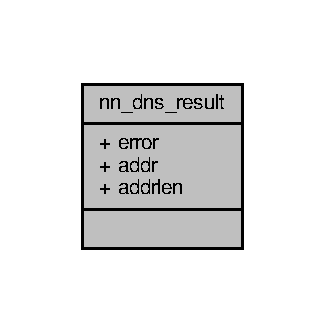
\includegraphics[width=156pt]{structnn__dns__result__coll__graph}
\end{center}
\end{figure}
\subsection*{Public Attributes}
\begin{DoxyCompactItemize}
\item 
int \hyperlink{structnn__dns__result_ad567eeaddc0e791da283e28911a1fe63}{error}
\item 
struct sockaddr\+\_\+storage \hyperlink{structnn__dns__result_ae9d56c807d97208851456a66d41255bd}{addr}
\item 
size\+\_\+t \hyperlink{structnn__dns__result_ab1533870912af14f5143555a83d6b36e}{addrlen}
\end{DoxyCompactItemize}


\subsection{Member Data Documentation}
\index{nn\+\_\+dns\+\_\+result@{nn\+\_\+dns\+\_\+result}!addr@{addr}}
\index{addr@{addr}!nn\+\_\+dns\+\_\+result@{nn\+\_\+dns\+\_\+result}}
\subsubsection[{addr}]{\setlength{\rightskip}{0pt plus 5cm}struct sockaddr\+\_\+storage nn\+\_\+dns\+\_\+result\+::addr}\hypertarget{structnn__dns__result_ae9d56c807d97208851456a66d41255bd}{}\label{structnn__dns__result_ae9d56c807d97208851456a66d41255bd}
\index{nn\+\_\+dns\+\_\+result@{nn\+\_\+dns\+\_\+result}!addrlen@{addrlen}}
\index{addrlen@{addrlen}!nn\+\_\+dns\+\_\+result@{nn\+\_\+dns\+\_\+result}}
\subsubsection[{addrlen}]{\setlength{\rightskip}{0pt plus 5cm}size\+\_\+t nn\+\_\+dns\+\_\+result\+::addrlen}\hypertarget{structnn__dns__result_ab1533870912af14f5143555a83d6b36e}{}\label{structnn__dns__result_ab1533870912af14f5143555a83d6b36e}
\index{nn\+\_\+dns\+\_\+result@{nn\+\_\+dns\+\_\+result}!error@{error}}
\index{error@{error}!nn\+\_\+dns\+\_\+result@{nn\+\_\+dns\+\_\+result}}
\subsubsection[{error}]{\setlength{\rightskip}{0pt plus 5cm}int nn\+\_\+dns\+\_\+result\+::error}\hypertarget{structnn__dns__result_ad567eeaddc0e791da283e28911a1fe63}{}\label{structnn__dns__result_ad567eeaddc0e791da283e28911a1fe63}


The documentation for this struct was generated from the following file\+:\begin{DoxyCompactItemize}
\item 
src/transports/utils/\hyperlink{dns_8h}{dns.\+h}\end{DoxyCompactItemize}

\hypertarget{structnn__efd}{}\section{nn\+\_\+efd Struct Reference}
\label{structnn__efd}\index{nn\+\_\+efd@{nn\+\_\+efd}}


{\ttfamily \#include $<$efd\+\_\+eventfd.\+h$>$}



Collaboration diagram for nn\+\_\+efd\+:\nopagebreak
\begin{figure}[H]
\begin{center}
\leavevmode
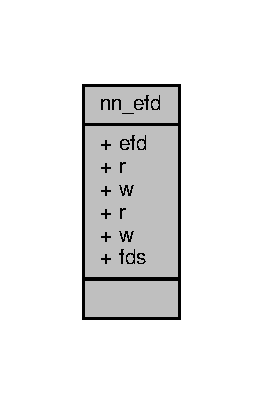
\includegraphics[width=126pt]{structnn__efd__coll__graph}
\end{center}
\end{figure}
\subsection*{Public Attributes}
\begin{DoxyCompactItemize}
\item 
int \hyperlink{structnn__efd_a754cb58e2b0a2efed6e5aa81a98275e0}{efd}
\item 
int \hyperlink{structnn__efd_a83da20c603791c11e137bf0411c33edd}{r}
\item 
int \hyperlink{structnn__efd_a871578e6e6cbf91469323f57655bb9db}{w}
\item 
S\+O\+C\+K\+ET \hyperlink{structnn__efd_ab5890557c42eae3e980c7c7b35e13ca6}{r}
\item 
S\+O\+C\+K\+ET \hyperlink{structnn__efd_a23bfc263f640b579e1a7846c7f3b81a0}{w}
\item 
fd\+\_\+set \hyperlink{structnn__efd_a97f26e7918650b84462a101e2dd40d49}{fds}
\end{DoxyCompactItemize}


\subsection{Member Data Documentation}
\index{nn\+\_\+efd@{nn\+\_\+efd}!efd@{efd}}
\index{efd@{efd}!nn\+\_\+efd@{nn\+\_\+efd}}
\subsubsection[{efd}]{\setlength{\rightskip}{0pt plus 5cm}int nn\+\_\+efd\+::efd}\hypertarget{structnn__efd_a754cb58e2b0a2efed6e5aa81a98275e0}{}\label{structnn__efd_a754cb58e2b0a2efed6e5aa81a98275e0}
\index{nn\+\_\+efd@{nn\+\_\+efd}!fds@{fds}}
\index{fds@{fds}!nn\+\_\+efd@{nn\+\_\+efd}}
\subsubsection[{fds}]{\setlength{\rightskip}{0pt plus 5cm}fd\+\_\+set nn\+\_\+efd\+::fds}\hypertarget{structnn__efd_a97f26e7918650b84462a101e2dd40d49}{}\label{structnn__efd_a97f26e7918650b84462a101e2dd40d49}
\index{nn\+\_\+efd@{nn\+\_\+efd}!r@{r}}
\index{r@{r}!nn\+\_\+efd@{nn\+\_\+efd}}
\subsubsection[{r}]{\setlength{\rightskip}{0pt plus 5cm}int nn\+\_\+efd\+::r}\hypertarget{structnn__efd_a83da20c603791c11e137bf0411c33edd}{}\label{structnn__efd_a83da20c603791c11e137bf0411c33edd}
\index{nn\+\_\+efd@{nn\+\_\+efd}!r@{r}}
\index{r@{r}!nn\+\_\+efd@{nn\+\_\+efd}}
\subsubsection[{r}]{\setlength{\rightskip}{0pt plus 5cm}S\+O\+C\+K\+ET nn\+\_\+efd\+::r}\hypertarget{structnn__efd_ab5890557c42eae3e980c7c7b35e13ca6}{}\label{structnn__efd_ab5890557c42eae3e980c7c7b35e13ca6}
\index{nn\+\_\+efd@{nn\+\_\+efd}!w@{w}}
\index{w@{w}!nn\+\_\+efd@{nn\+\_\+efd}}
\subsubsection[{w}]{\setlength{\rightskip}{0pt plus 5cm}int nn\+\_\+efd\+::w}\hypertarget{structnn__efd_a871578e6e6cbf91469323f57655bb9db}{}\label{structnn__efd_a871578e6e6cbf91469323f57655bb9db}
\index{nn\+\_\+efd@{nn\+\_\+efd}!w@{w}}
\index{w@{w}!nn\+\_\+efd@{nn\+\_\+efd}}
\subsubsection[{w}]{\setlength{\rightskip}{0pt plus 5cm}S\+O\+C\+K\+ET nn\+\_\+efd\+::w}\hypertarget{structnn__efd_a23bfc263f640b579e1a7846c7f3b81a0}{}\label{structnn__efd_a23bfc263f640b579e1a7846c7f3b81a0}


The documentation for this struct was generated from the following files\+:\begin{DoxyCompactItemize}
\item 
src/utils/\hyperlink{efd__eventfd_8h}{efd\+\_\+eventfd.\+h}\item 
src/utils/\hyperlink{efd__pipe_8h}{efd\+\_\+pipe.\+h}\item 
src/utils/\hyperlink{efd__socketpair_8h}{efd\+\_\+socketpair.\+h}\item 
src/utils/\hyperlink{efd__win_8h}{efd\+\_\+win.\+h}\end{DoxyCompactItemize}

\hypertarget{structnn__ep}{}\section{nn\+\_\+ep Struct Reference}
\label{structnn__ep}\index{nn\+\_\+ep@{nn\+\_\+ep}}


{\ttfamily \#include $<$ep.\+h$>$}



Collaboration diagram for nn\+\_\+ep\+:\nopagebreak
\begin{figure}[H]
\begin{center}
\leavevmode
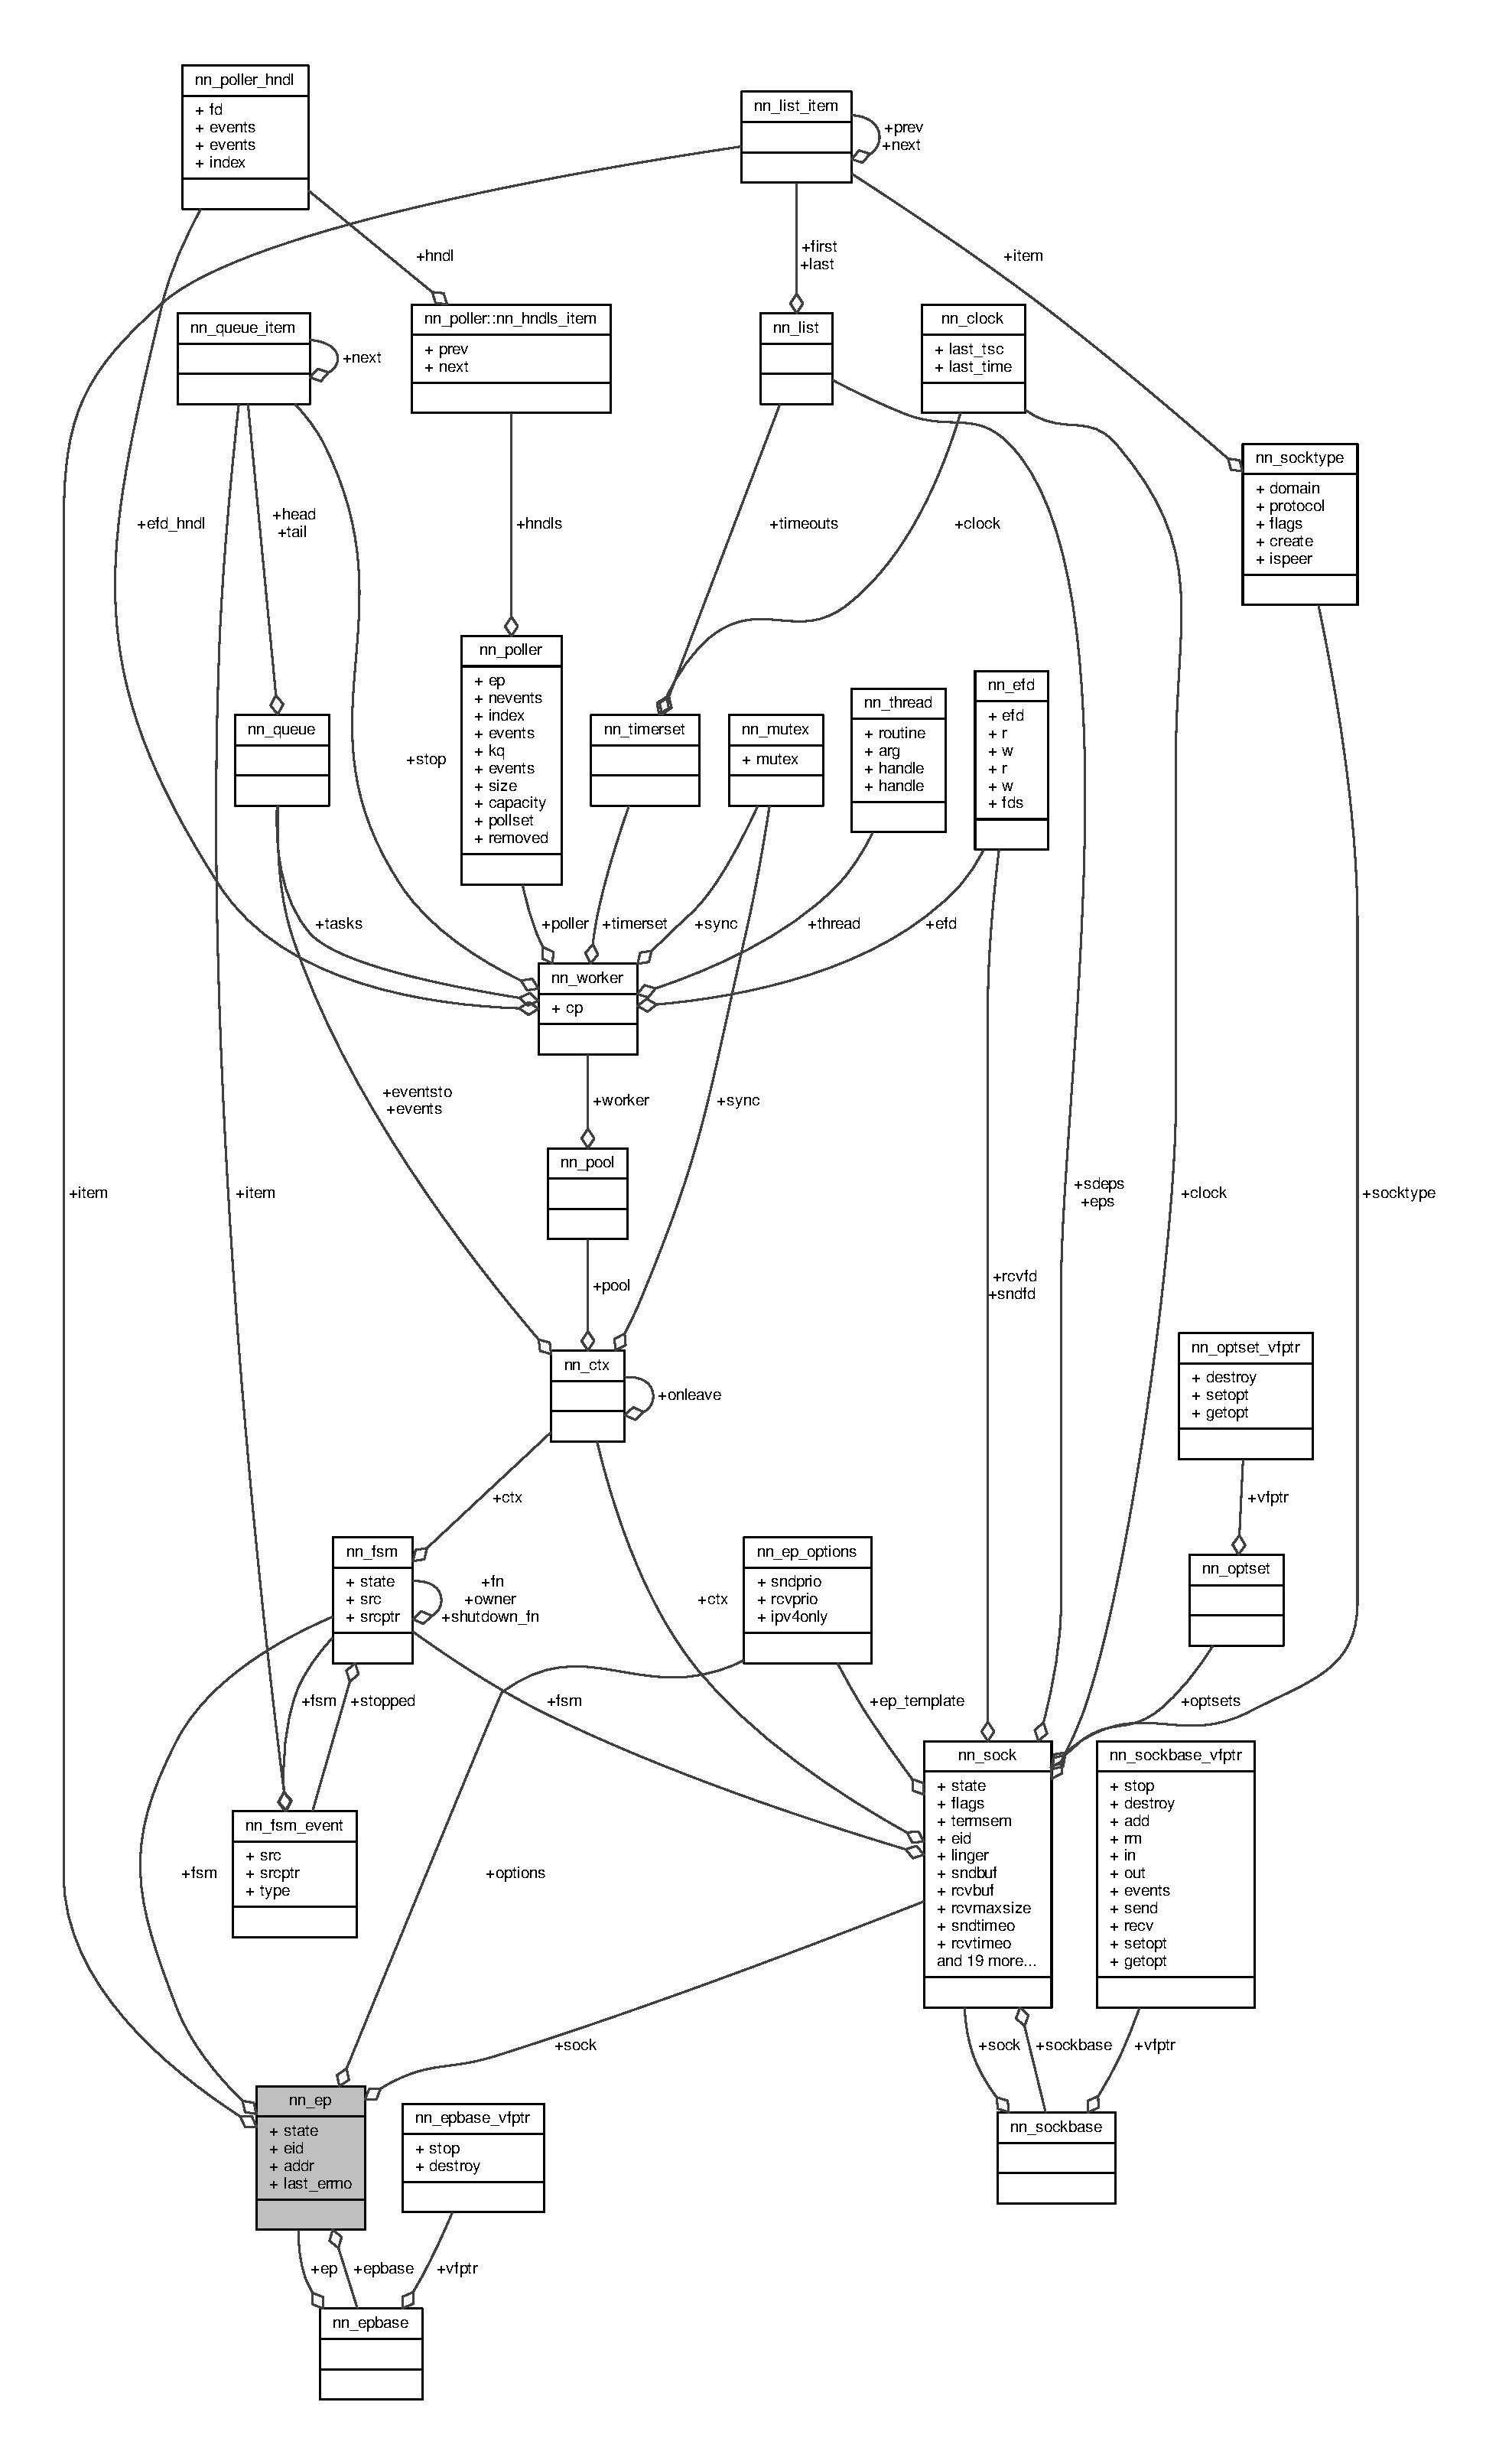
\includegraphics[height=550pt]{structnn__ep__coll__graph}
\end{center}
\end{figure}
\subsection*{Public Attributes}
\begin{DoxyCompactItemize}
\item 
struct \hyperlink{structnn__fsm}{nn\+\_\+fsm} \hyperlink{structnn__ep_a5e31919281d05cadde1b39f15d1247c7}{fsm}
\item 
int \hyperlink{structnn__ep_a84d29e1ab854c45678ba5cb07b525a33}{state}
\item 
struct \hyperlink{structnn__epbase}{nn\+\_\+epbase} $\ast$ \hyperlink{structnn__ep_af2099da4aa3cfa0d0c795262ff41cc89}{epbase}
\item 
struct \hyperlink{structnn__sock}{nn\+\_\+sock} $\ast$ \hyperlink{structnn__ep_a089f04f3d0b46462884350c430a417e9}{sock}
\item 
struct \hyperlink{structnn__ep__options}{nn\+\_\+ep\+\_\+options} \hyperlink{structnn__ep_a8b72c5b686aa263c18bb2a3219f2376f}{options}
\item 
int \hyperlink{structnn__ep_a16c6bc677912a107ba3a353252e8b09a}{eid}
\item 
struct \hyperlink{structnn__list__item}{nn\+\_\+list\+\_\+item} \hyperlink{structnn__ep_a2e46eb5aa8bd437a60f448d312e21d6e}{item}
\item 
char \hyperlink{structnn__ep_a596bc0e54a7247ab94a7e4cf4d6f3229}{addr} \mbox{[}\hyperlink{nn_8h_a9b3759ef32562c8b4f0c8c75f54c8b03}{N\+N\+\_\+\+S\+O\+C\+K\+A\+D\+D\+R\+\_\+\+M\+AX}+1\mbox{]}
\item 
int \hyperlink{structnn__ep_a415457d365d9964da0a4ef7627698ad0}{last\+\_\+errno}
\end{DoxyCompactItemize}


\subsection{Member Data Documentation}
\index{nn\+\_\+ep@{nn\+\_\+ep}!addr@{addr}}
\index{addr@{addr}!nn\+\_\+ep@{nn\+\_\+ep}}
\subsubsection[{addr}]{\setlength{\rightskip}{0pt plus 5cm}char nn\+\_\+ep\+::addr\mbox{[}{\bf N\+N\+\_\+\+S\+O\+C\+K\+A\+D\+D\+R\+\_\+\+M\+AX}+1\mbox{]}}\hypertarget{structnn__ep_a596bc0e54a7247ab94a7e4cf4d6f3229}{}\label{structnn__ep_a596bc0e54a7247ab94a7e4cf4d6f3229}
\index{nn\+\_\+ep@{nn\+\_\+ep}!eid@{eid}}
\index{eid@{eid}!nn\+\_\+ep@{nn\+\_\+ep}}
\subsubsection[{eid}]{\setlength{\rightskip}{0pt plus 5cm}int nn\+\_\+ep\+::eid}\hypertarget{structnn__ep_a16c6bc677912a107ba3a353252e8b09a}{}\label{structnn__ep_a16c6bc677912a107ba3a353252e8b09a}
\index{nn\+\_\+ep@{nn\+\_\+ep}!epbase@{epbase}}
\index{epbase@{epbase}!nn\+\_\+ep@{nn\+\_\+ep}}
\subsubsection[{epbase}]{\setlength{\rightskip}{0pt plus 5cm}struct {\bf nn\+\_\+epbase}$\ast$ nn\+\_\+ep\+::epbase}\hypertarget{structnn__ep_af2099da4aa3cfa0d0c795262ff41cc89}{}\label{structnn__ep_af2099da4aa3cfa0d0c795262ff41cc89}
\index{nn\+\_\+ep@{nn\+\_\+ep}!fsm@{fsm}}
\index{fsm@{fsm}!nn\+\_\+ep@{nn\+\_\+ep}}
\subsubsection[{fsm}]{\setlength{\rightskip}{0pt plus 5cm}struct {\bf nn\+\_\+fsm} nn\+\_\+ep\+::fsm}\hypertarget{structnn__ep_a5e31919281d05cadde1b39f15d1247c7}{}\label{structnn__ep_a5e31919281d05cadde1b39f15d1247c7}
\index{nn\+\_\+ep@{nn\+\_\+ep}!item@{item}}
\index{item@{item}!nn\+\_\+ep@{nn\+\_\+ep}}
\subsubsection[{item}]{\setlength{\rightskip}{0pt plus 5cm}struct {\bf nn\+\_\+list\+\_\+item} nn\+\_\+ep\+::item}\hypertarget{structnn__ep_a2e46eb5aa8bd437a60f448d312e21d6e}{}\label{structnn__ep_a2e46eb5aa8bd437a60f448d312e21d6e}
\index{nn\+\_\+ep@{nn\+\_\+ep}!last\+\_\+errno@{last\+\_\+errno}}
\index{last\+\_\+errno@{last\+\_\+errno}!nn\+\_\+ep@{nn\+\_\+ep}}
\subsubsection[{last\+\_\+errno}]{\setlength{\rightskip}{0pt plus 5cm}int nn\+\_\+ep\+::last\+\_\+errno}\hypertarget{structnn__ep_a415457d365d9964da0a4ef7627698ad0}{}\label{structnn__ep_a415457d365d9964da0a4ef7627698ad0}
\index{nn\+\_\+ep@{nn\+\_\+ep}!options@{options}}
\index{options@{options}!nn\+\_\+ep@{nn\+\_\+ep}}
\subsubsection[{options}]{\setlength{\rightskip}{0pt plus 5cm}struct {\bf nn\+\_\+ep\+\_\+options} nn\+\_\+ep\+::options}\hypertarget{structnn__ep_a8b72c5b686aa263c18bb2a3219f2376f}{}\label{structnn__ep_a8b72c5b686aa263c18bb2a3219f2376f}
\index{nn\+\_\+ep@{nn\+\_\+ep}!sock@{sock}}
\index{sock@{sock}!nn\+\_\+ep@{nn\+\_\+ep}}
\subsubsection[{sock}]{\setlength{\rightskip}{0pt plus 5cm}struct {\bf nn\+\_\+sock}$\ast$ nn\+\_\+ep\+::sock}\hypertarget{structnn__ep_a089f04f3d0b46462884350c430a417e9}{}\label{structnn__ep_a089f04f3d0b46462884350c430a417e9}
\index{nn\+\_\+ep@{nn\+\_\+ep}!state@{state}}
\index{state@{state}!nn\+\_\+ep@{nn\+\_\+ep}}
\subsubsection[{state}]{\setlength{\rightskip}{0pt plus 5cm}int nn\+\_\+ep\+::state}\hypertarget{structnn__ep_a84d29e1ab854c45678ba5cb07b525a33}{}\label{structnn__ep_a84d29e1ab854c45678ba5cb07b525a33}


The documentation for this struct was generated from the following file\+:\begin{DoxyCompactItemize}
\item 
src/core/\hyperlink{ep_8h}{ep.\+h}\end{DoxyCompactItemize}

\hypertarget{structnn__ep__options}{}\section{nn\+\_\+ep\+\_\+options Struct Reference}
\label{structnn__ep__options}\index{nn\+\_\+ep\+\_\+options@{nn\+\_\+ep\+\_\+options}}


{\ttfamily \#include $<$transport.\+h$>$}



Collaboration diagram for nn\+\_\+ep\+\_\+options\+:\nopagebreak
\begin{figure}[H]
\begin{center}
\leavevmode
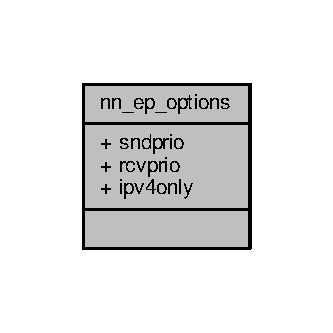
\includegraphics[width=160pt]{structnn__ep__options__coll__graph}
\end{center}
\end{figure}
\subsection*{Public Attributes}
\begin{DoxyCompactItemize}
\item 
int \hyperlink{structnn__ep__options_a094beafa8c4733b413c5982c9ab7552d}{sndprio}
\item 
int \hyperlink{structnn__ep__options_ad767f9fdbda05049cdb00e5122de9c7f}{rcvprio}
\item 
int \hyperlink{structnn__ep__options_a59ff01ae4c3e14629355a72a88cab1c1}{ipv4only}
\end{DoxyCompactItemize}


\subsection{Member Data Documentation}
\index{nn\+\_\+ep\+\_\+options@{nn\+\_\+ep\+\_\+options}!ipv4only@{ipv4only}}
\index{ipv4only@{ipv4only}!nn\+\_\+ep\+\_\+options@{nn\+\_\+ep\+\_\+options}}
\subsubsection[{ipv4only}]{\setlength{\rightskip}{0pt plus 5cm}int nn\+\_\+ep\+\_\+options\+::ipv4only}\hypertarget{structnn__ep__options_a59ff01ae4c3e14629355a72a88cab1c1}{}\label{structnn__ep__options_a59ff01ae4c3e14629355a72a88cab1c1}
\index{nn\+\_\+ep\+\_\+options@{nn\+\_\+ep\+\_\+options}!rcvprio@{rcvprio}}
\index{rcvprio@{rcvprio}!nn\+\_\+ep\+\_\+options@{nn\+\_\+ep\+\_\+options}}
\subsubsection[{rcvprio}]{\setlength{\rightskip}{0pt plus 5cm}int nn\+\_\+ep\+\_\+options\+::rcvprio}\hypertarget{structnn__ep__options_ad767f9fdbda05049cdb00e5122de9c7f}{}\label{structnn__ep__options_ad767f9fdbda05049cdb00e5122de9c7f}
\index{nn\+\_\+ep\+\_\+options@{nn\+\_\+ep\+\_\+options}!sndprio@{sndprio}}
\index{sndprio@{sndprio}!nn\+\_\+ep\+\_\+options@{nn\+\_\+ep\+\_\+options}}
\subsubsection[{sndprio}]{\setlength{\rightskip}{0pt plus 5cm}int nn\+\_\+ep\+\_\+options\+::sndprio}\hypertarget{structnn__ep__options_a094beafa8c4733b413c5982c9ab7552d}{}\label{structnn__ep__options_a094beafa8c4733b413c5982c9ab7552d}


The documentation for this struct was generated from the following file\+:\begin{DoxyCompactItemize}
\item 
src/\hyperlink{transport_8h}{transport.\+h}\end{DoxyCompactItemize}

\hypertarget{structnn__epbase}{}\section{nn\+\_\+epbase Struct Reference}
\label{structnn__epbase}\index{nn\+\_\+epbase@{nn\+\_\+epbase}}


{\ttfamily \#include $<$transport.\+h$>$}



Collaboration diagram for nn\+\_\+epbase\+:\nopagebreak
\begin{figure}[H]
\begin{center}
\leavevmode
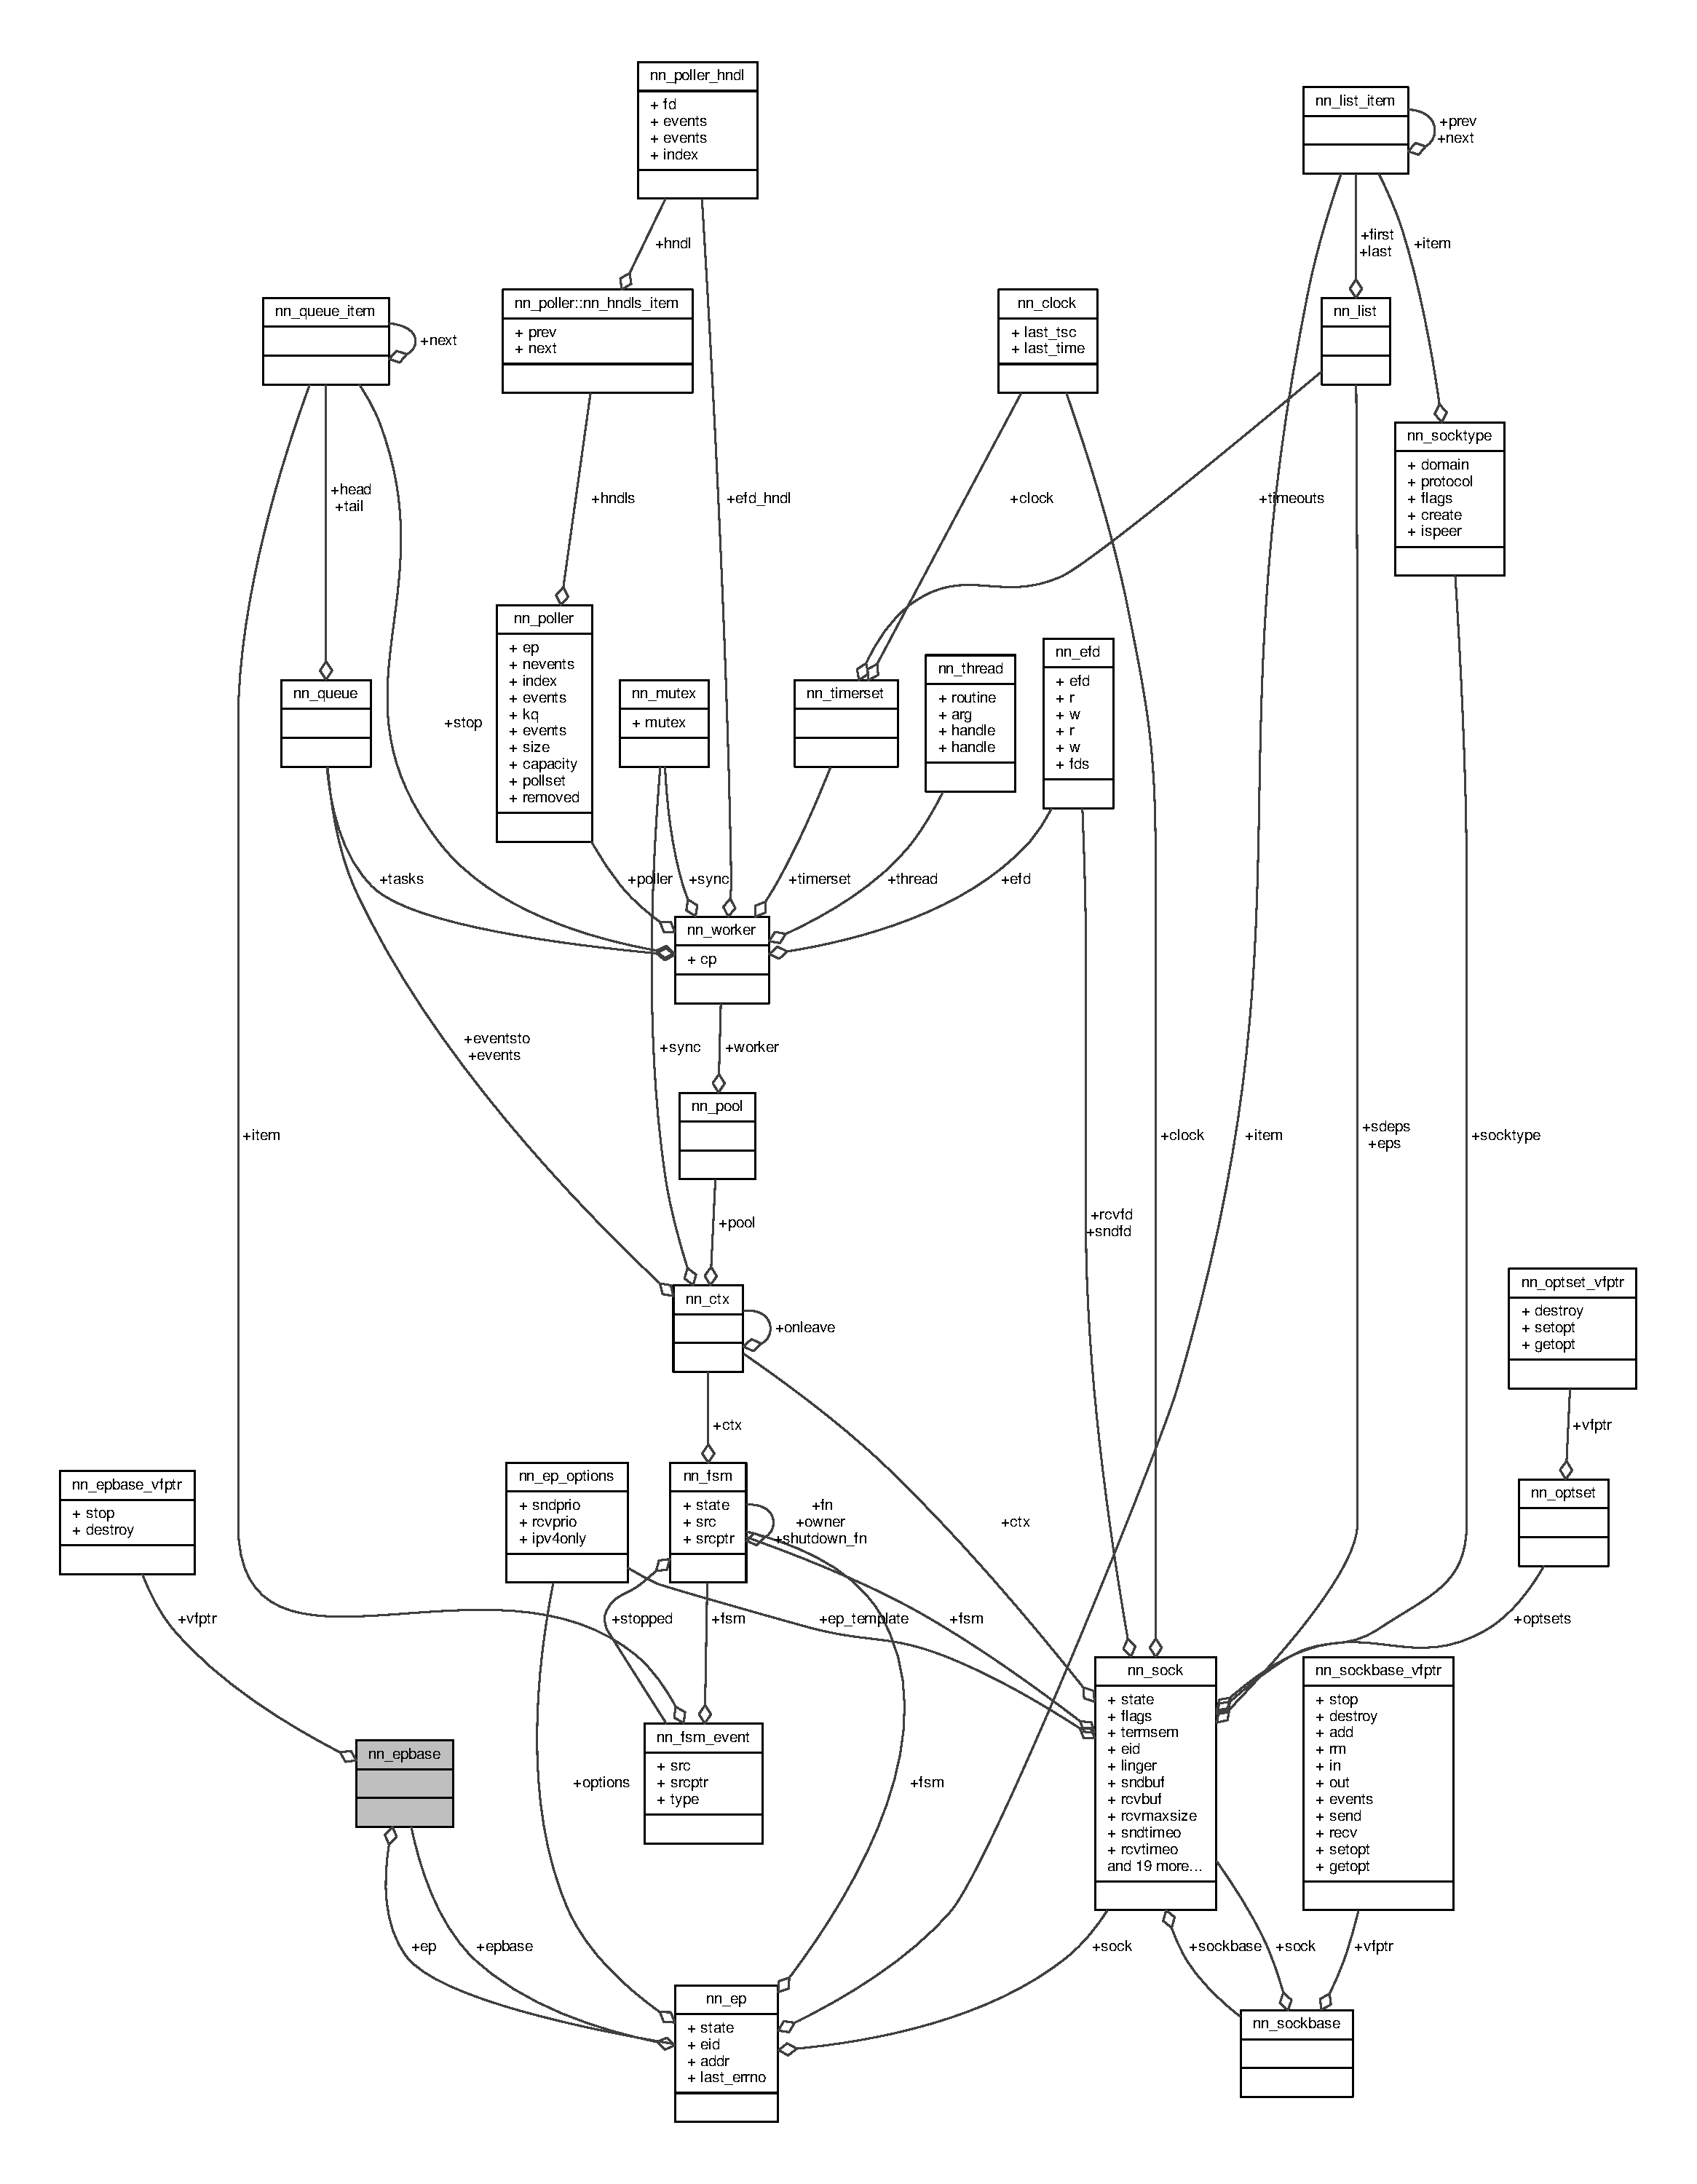
\includegraphics[width=350pt]{structnn__epbase__coll__graph}
\end{center}
\end{figure}
\subsection*{Public Attributes}
\begin{DoxyCompactItemize}
\item 
const struct \hyperlink{structnn__epbase__vfptr}{nn\+\_\+epbase\+\_\+vfptr} $\ast$ \hyperlink{structnn__epbase_a7aeef264c3ec9adab7f7225e84689e41}{vfptr}
\item 
struct \hyperlink{structnn__ep}{nn\+\_\+ep} $\ast$ \hyperlink{structnn__epbase_a9256f20b0f06b8eab213745afe91fced}{ep}
\end{DoxyCompactItemize}


\subsection{Member Data Documentation}
\index{nn\+\_\+epbase@{nn\+\_\+epbase}!ep@{ep}}
\index{ep@{ep}!nn\+\_\+epbase@{nn\+\_\+epbase}}
\subsubsection[{ep}]{\setlength{\rightskip}{0pt plus 5cm}struct {\bf nn\+\_\+ep}$\ast$ nn\+\_\+epbase\+::ep}\hypertarget{structnn__epbase_a9256f20b0f06b8eab213745afe91fced}{}\label{structnn__epbase_a9256f20b0f06b8eab213745afe91fced}
\index{nn\+\_\+epbase@{nn\+\_\+epbase}!vfptr@{vfptr}}
\index{vfptr@{vfptr}!nn\+\_\+epbase@{nn\+\_\+epbase}}
\subsubsection[{vfptr}]{\setlength{\rightskip}{0pt plus 5cm}const struct {\bf nn\+\_\+epbase\+\_\+vfptr}$\ast$ nn\+\_\+epbase\+::vfptr}\hypertarget{structnn__epbase_a7aeef264c3ec9adab7f7225e84689e41}{}\label{structnn__epbase_a7aeef264c3ec9adab7f7225e84689e41}


The documentation for this struct was generated from the following file\+:\begin{DoxyCompactItemize}
\item 
src/\hyperlink{transport_8h}{transport.\+h}\end{DoxyCompactItemize}

\hypertarget{structnn__epbase__vfptr}{}\section{nn\+\_\+epbase\+\_\+vfptr Struct Reference}
\label{structnn__epbase__vfptr}\index{nn\+\_\+epbase\+\_\+vfptr@{nn\+\_\+epbase\+\_\+vfptr}}


{\ttfamily \#include $<$transport.\+h$>$}



Collaboration diagram for nn\+\_\+epbase\+\_\+vfptr\+:\nopagebreak
\begin{figure}[H]
\begin{center}
\leavevmode
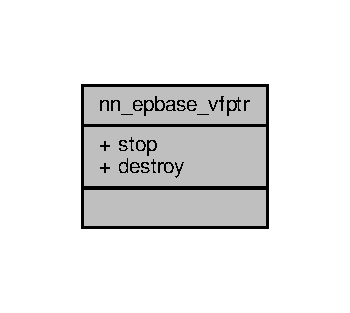
\includegraphics[width=168pt]{structnn__epbase__vfptr__coll__graph}
\end{center}
\end{figure}
\subsection*{Public Attributes}
\begin{DoxyCompactItemize}
\item 
void($\ast$ \hyperlink{structnn__epbase__vfptr_ab512201fc6ce1ea50d196ea1201aa37d}{stop} )(struct \hyperlink{structnn__epbase}{nn\+\_\+epbase} $\ast$self)
\item 
void($\ast$ \hyperlink{structnn__epbase__vfptr_a880662a8b6bb442b37bbb7d3ccb76a8d}{destroy} )(struct \hyperlink{structnn__epbase}{nn\+\_\+epbase} $\ast$self)
\end{DoxyCompactItemize}


\subsection{Member Data Documentation}
\index{nn\+\_\+epbase\+\_\+vfptr@{nn\+\_\+epbase\+\_\+vfptr}!destroy@{destroy}}
\index{destroy@{destroy}!nn\+\_\+epbase\+\_\+vfptr@{nn\+\_\+epbase\+\_\+vfptr}}
\subsubsection[{destroy}]{\setlength{\rightskip}{0pt plus 5cm}void($\ast$ nn\+\_\+epbase\+\_\+vfptr\+::destroy) (struct {\bf nn\+\_\+epbase} $\ast$self)}\hypertarget{structnn__epbase__vfptr_a880662a8b6bb442b37bbb7d3ccb76a8d}{}\label{structnn__epbase__vfptr_a880662a8b6bb442b37bbb7d3ccb76a8d}
\index{nn\+\_\+epbase\+\_\+vfptr@{nn\+\_\+epbase\+\_\+vfptr}!stop@{stop}}
\index{stop@{stop}!nn\+\_\+epbase\+\_\+vfptr@{nn\+\_\+epbase\+\_\+vfptr}}
\subsubsection[{stop}]{\setlength{\rightskip}{0pt plus 5cm}void($\ast$ nn\+\_\+epbase\+\_\+vfptr\+::stop) (struct {\bf nn\+\_\+epbase} $\ast$self)}\hypertarget{structnn__epbase__vfptr_ab512201fc6ce1ea50d196ea1201aa37d}{}\label{structnn__epbase__vfptr_ab512201fc6ce1ea50d196ea1201aa37d}


The documentation for this struct was generated from the following file\+:\begin{DoxyCompactItemize}
\item 
src/\hyperlink{transport_8h}{transport.\+h}\end{DoxyCompactItemize}

\hypertarget{structnn__excl}{}\section{nn\+\_\+excl Struct Reference}
\label{structnn__excl}\index{nn\+\_\+excl@{nn\+\_\+excl}}


{\ttfamily \#include $<$excl.\+h$>$}



Collaboration diagram for nn\+\_\+excl\+:\nopagebreak
\begin{figure}[H]
\begin{center}
\leavevmode
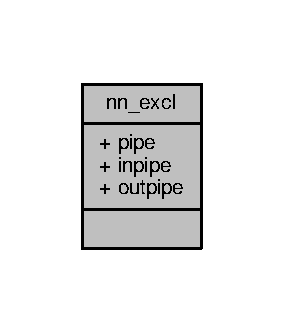
\includegraphics[width=136pt]{structnn__excl__coll__graph}
\end{center}
\end{figure}
\subsection*{Public Attributes}
\begin{DoxyCompactItemize}
\item 
struct nn\+\_\+pipe $\ast$ \hyperlink{structnn__excl_a94b5ea848971e08ed35baed15aea5ee9}{pipe}
\item 
struct nn\+\_\+pipe $\ast$ \hyperlink{structnn__excl_ac2da1ab40e0450e1311a80e28285e310}{inpipe}
\item 
struct nn\+\_\+pipe $\ast$ \hyperlink{structnn__excl_a28f7fc280d63150d45dce48ff58f738d}{outpipe}
\end{DoxyCompactItemize}


\subsection{Member Data Documentation}
\index{nn\+\_\+excl@{nn\+\_\+excl}!inpipe@{inpipe}}
\index{inpipe@{inpipe}!nn\+\_\+excl@{nn\+\_\+excl}}
\subsubsection[{inpipe}]{\setlength{\rightskip}{0pt plus 5cm}struct nn\+\_\+pipe$\ast$ nn\+\_\+excl\+::inpipe}\hypertarget{structnn__excl_ac2da1ab40e0450e1311a80e28285e310}{}\label{structnn__excl_ac2da1ab40e0450e1311a80e28285e310}
\index{nn\+\_\+excl@{nn\+\_\+excl}!outpipe@{outpipe}}
\index{outpipe@{outpipe}!nn\+\_\+excl@{nn\+\_\+excl}}
\subsubsection[{outpipe}]{\setlength{\rightskip}{0pt plus 5cm}struct nn\+\_\+pipe$\ast$ nn\+\_\+excl\+::outpipe}\hypertarget{structnn__excl_a28f7fc280d63150d45dce48ff58f738d}{}\label{structnn__excl_a28f7fc280d63150d45dce48ff58f738d}
\index{nn\+\_\+excl@{nn\+\_\+excl}!pipe@{pipe}}
\index{pipe@{pipe}!nn\+\_\+excl@{nn\+\_\+excl}}
\subsubsection[{pipe}]{\setlength{\rightskip}{0pt plus 5cm}struct nn\+\_\+pipe$\ast$ nn\+\_\+excl\+::pipe}\hypertarget{structnn__excl_a94b5ea848971e08ed35baed15aea5ee9}{}\label{structnn__excl_a94b5ea848971e08ed35baed15aea5ee9}


The documentation for this struct was generated from the following file\+:\begin{DoxyCompactItemize}
\item 
src/protocols/utils/\hyperlink{excl_8h}{excl.\+h}\end{DoxyCompactItemize}

\hypertarget{structnn__fq}{}\section{nn\+\_\+fq Struct Reference}
\label{structnn__fq}\index{nn\+\_\+fq@{nn\+\_\+fq}}


{\ttfamily \#include $<$fq.\+h$>$}



Collaboration diagram for nn\+\_\+fq\+:\nopagebreak
\begin{figure}[H]
\begin{center}
\leavevmode
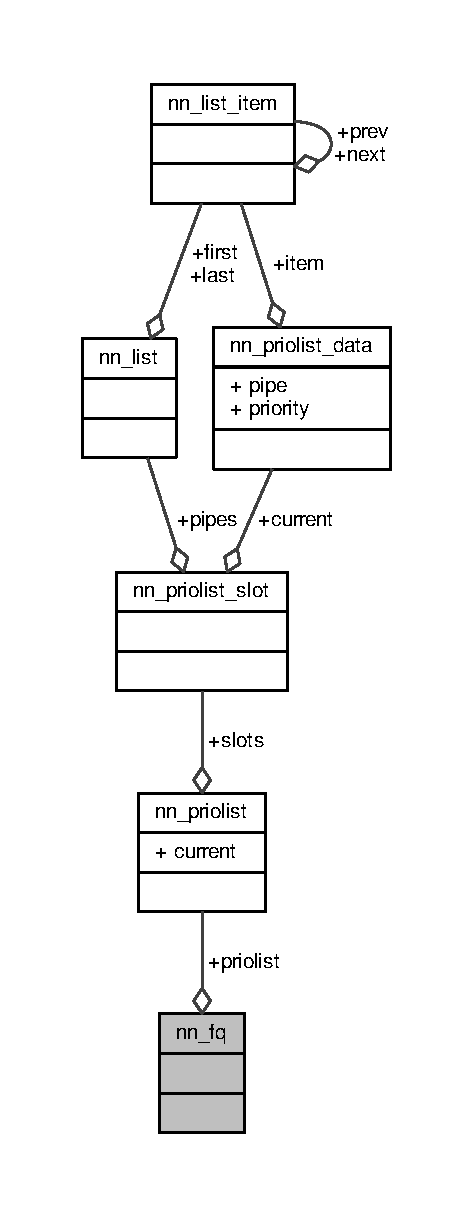
\includegraphics[height=550pt]{structnn__fq__coll__graph}
\end{center}
\end{figure}
\subsection*{Public Attributes}
\begin{DoxyCompactItemize}
\item 
struct \hyperlink{structnn__priolist}{nn\+\_\+priolist} \hyperlink{structnn__fq_a5bce08b6089ff9f0ebaf17cf07a45184}{priolist}
\end{DoxyCompactItemize}


\subsection{Member Data Documentation}
\index{nn\+\_\+fq@{nn\+\_\+fq}!priolist@{priolist}}
\index{priolist@{priolist}!nn\+\_\+fq@{nn\+\_\+fq}}
\subsubsection[{priolist}]{\setlength{\rightskip}{0pt plus 5cm}struct {\bf nn\+\_\+priolist} nn\+\_\+fq\+::priolist}\hypertarget{structnn__fq_a5bce08b6089ff9f0ebaf17cf07a45184}{}\label{structnn__fq_a5bce08b6089ff9f0ebaf17cf07a45184}


The documentation for this struct was generated from the following file\+:\begin{DoxyCompactItemize}
\item 
src/protocols/utils/\hyperlink{fq_8h}{fq.\+h}\end{DoxyCompactItemize}

\hypertarget{structnn__fq__data}{}\section{nn\+\_\+fq\+\_\+data Struct Reference}
\label{structnn__fq__data}\index{nn\+\_\+fq\+\_\+data@{nn\+\_\+fq\+\_\+data}}


{\ttfamily \#include $<$fq.\+h$>$}



Collaboration diagram for nn\+\_\+fq\+\_\+data\+:\nopagebreak
\begin{figure}[H]
\begin{center}
\leavevmode
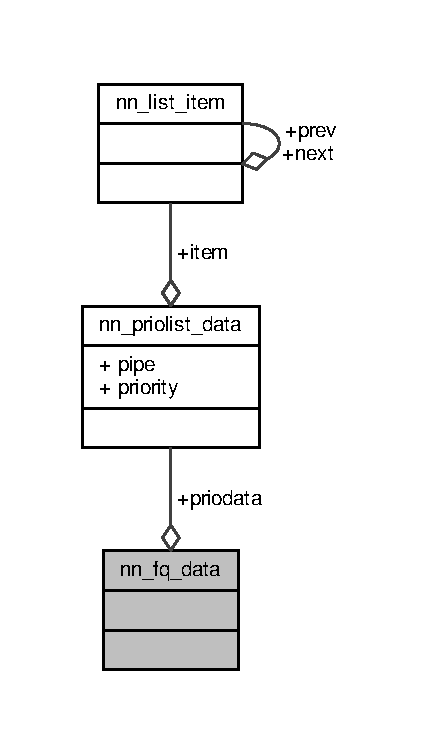
\includegraphics[width=202pt]{structnn__fq__data__coll__graph}
\end{center}
\end{figure}
\subsection*{Public Attributes}
\begin{DoxyCompactItemize}
\item 
struct \hyperlink{structnn__priolist__data}{nn\+\_\+priolist\+\_\+data} \hyperlink{structnn__fq__data_a404fcb98abd11c3e90edf6ca0b294432}{priodata}
\end{DoxyCompactItemize}


\subsection{Member Data Documentation}
\index{nn\+\_\+fq\+\_\+data@{nn\+\_\+fq\+\_\+data}!priodata@{priodata}}
\index{priodata@{priodata}!nn\+\_\+fq\+\_\+data@{nn\+\_\+fq\+\_\+data}}
\subsubsection[{priodata}]{\setlength{\rightskip}{0pt plus 5cm}struct {\bf nn\+\_\+priolist\+\_\+data} nn\+\_\+fq\+\_\+data\+::priodata}\hypertarget{structnn__fq__data_a404fcb98abd11c3e90edf6ca0b294432}{}\label{structnn__fq__data_a404fcb98abd11c3e90edf6ca0b294432}


The documentation for this struct was generated from the following file\+:\begin{DoxyCompactItemize}
\item 
src/protocols/utils/\hyperlink{fq_8h}{fq.\+h}\end{DoxyCompactItemize}

\hypertarget{structnn__fsm}{}\section{nn\+\_\+fsm Struct Reference}
\label{structnn__fsm}\index{nn\+\_\+fsm@{nn\+\_\+fsm}}


{\ttfamily \#include $<$fsm.\+h$>$}



Collaboration diagram for nn\+\_\+fsm\+:\nopagebreak
\begin{figure}[H]
\begin{center}
\leavevmode
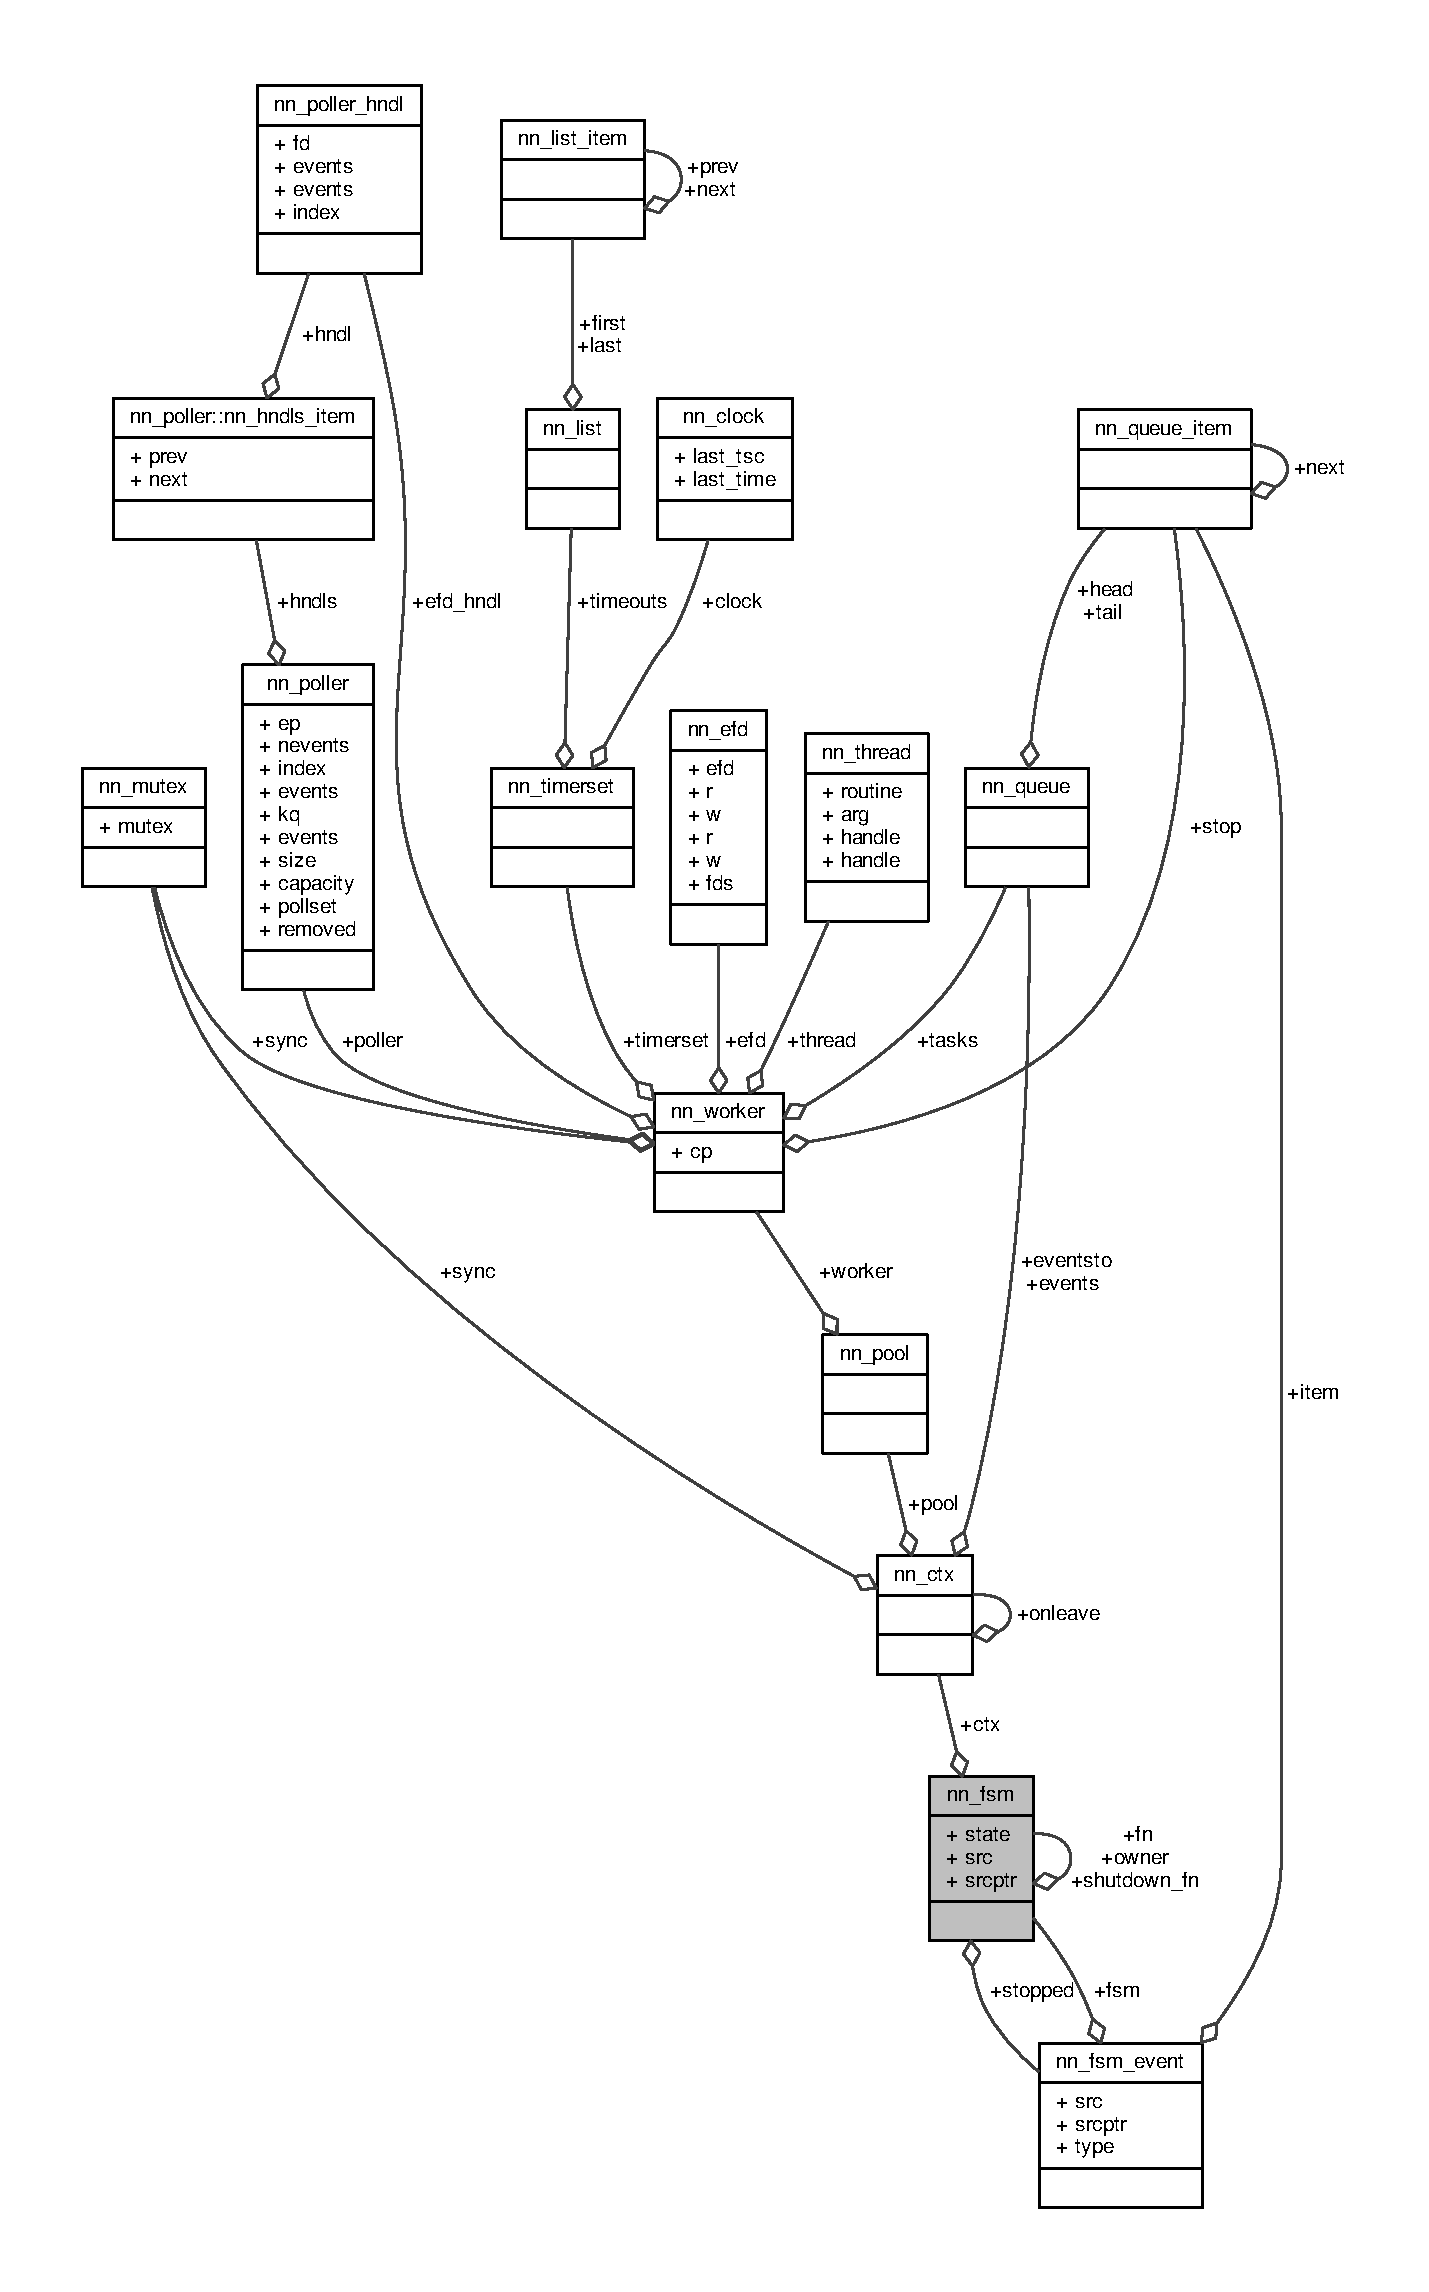
\includegraphics[height=550pt]{structnn__fsm__coll__graph}
\end{center}
\end{figure}
\subsection*{Public Attributes}
\begin{DoxyCompactItemize}
\item 
\hyperlink{fsm_8h_a05d92fd756f8b8d8ced977e68cace00b}{nn\+\_\+fsm\+\_\+fn} \hyperlink{structnn__fsm_a1fc34a657fdc5cc744c7ea51df7d38a4}{fn}
\item 
\hyperlink{fsm_8h_a05d92fd756f8b8d8ced977e68cace00b}{nn\+\_\+fsm\+\_\+fn} \hyperlink{structnn__fsm_a3ee3d9dd131d8761661e2e5ba2bba998}{shutdown\+\_\+fn}
\item 
int \hyperlink{structnn__fsm_a91bac7a0fffbb658bcbfa8610716d497}{state}
\item 
int \hyperlink{structnn__fsm_a71a938d92be27604a5db6228937736c8}{src}
\item 
void $\ast$ \hyperlink{structnn__fsm_a2f1dfafc0afec5d79c7944e7b2235b1f}{srcptr}
\item 
struct \hyperlink{structnn__fsm}{nn\+\_\+fsm} $\ast$ \hyperlink{structnn__fsm_ae9d3ae6031c4acec6fccac4e50bf9451}{owner}
\item 
struct \hyperlink{structnn__ctx}{nn\+\_\+ctx} $\ast$ \hyperlink{structnn__fsm_a1a6e8f761e19091bfb7846acdaf577b5}{ctx}
\item 
struct \hyperlink{structnn__fsm__event}{nn\+\_\+fsm\+\_\+event} \hyperlink{structnn__fsm_aba53a9882b534f46315292f7a879c018}{stopped}
\end{DoxyCompactItemize}


\subsection{Member Data Documentation}
\index{nn\+\_\+fsm@{nn\+\_\+fsm}!ctx@{ctx}}
\index{ctx@{ctx}!nn\+\_\+fsm@{nn\+\_\+fsm}}
\subsubsection[{ctx}]{\setlength{\rightskip}{0pt plus 5cm}struct {\bf nn\+\_\+ctx}$\ast$ nn\+\_\+fsm\+::ctx}\hypertarget{structnn__fsm_a1a6e8f761e19091bfb7846acdaf577b5}{}\label{structnn__fsm_a1a6e8f761e19091bfb7846acdaf577b5}
\index{nn\+\_\+fsm@{nn\+\_\+fsm}!fn@{fn}}
\index{fn@{fn}!nn\+\_\+fsm@{nn\+\_\+fsm}}
\subsubsection[{fn}]{\setlength{\rightskip}{0pt plus 5cm}{\bf nn\+\_\+fsm\+\_\+fn} nn\+\_\+fsm\+::fn}\hypertarget{structnn__fsm_a1fc34a657fdc5cc744c7ea51df7d38a4}{}\label{structnn__fsm_a1fc34a657fdc5cc744c7ea51df7d38a4}
\index{nn\+\_\+fsm@{nn\+\_\+fsm}!owner@{owner}}
\index{owner@{owner}!nn\+\_\+fsm@{nn\+\_\+fsm}}
\subsubsection[{owner}]{\setlength{\rightskip}{0pt plus 5cm}struct {\bf nn\+\_\+fsm}$\ast$ nn\+\_\+fsm\+::owner}\hypertarget{structnn__fsm_ae9d3ae6031c4acec6fccac4e50bf9451}{}\label{structnn__fsm_ae9d3ae6031c4acec6fccac4e50bf9451}
\index{nn\+\_\+fsm@{nn\+\_\+fsm}!shutdown\+\_\+fn@{shutdown\+\_\+fn}}
\index{shutdown\+\_\+fn@{shutdown\+\_\+fn}!nn\+\_\+fsm@{nn\+\_\+fsm}}
\subsubsection[{shutdown\+\_\+fn}]{\setlength{\rightskip}{0pt plus 5cm}{\bf nn\+\_\+fsm\+\_\+fn} nn\+\_\+fsm\+::shutdown\+\_\+fn}\hypertarget{structnn__fsm_a3ee3d9dd131d8761661e2e5ba2bba998}{}\label{structnn__fsm_a3ee3d9dd131d8761661e2e5ba2bba998}
\index{nn\+\_\+fsm@{nn\+\_\+fsm}!src@{src}}
\index{src@{src}!nn\+\_\+fsm@{nn\+\_\+fsm}}
\subsubsection[{src}]{\setlength{\rightskip}{0pt plus 5cm}int nn\+\_\+fsm\+::src}\hypertarget{structnn__fsm_a71a938d92be27604a5db6228937736c8}{}\label{structnn__fsm_a71a938d92be27604a5db6228937736c8}
\index{nn\+\_\+fsm@{nn\+\_\+fsm}!srcptr@{srcptr}}
\index{srcptr@{srcptr}!nn\+\_\+fsm@{nn\+\_\+fsm}}
\subsubsection[{srcptr}]{\setlength{\rightskip}{0pt plus 5cm}void$\ast$ nn\+\_\+fsm\+::srcptr}\hypertarget{structnn__fsm_a2f1dfafc0afec5d79c7944e7b2235b1f}{}\label{structnn__fsm_a2f1dfafc0afec5d79c7944e7b2235b1f}
\index{nn\+\_\+fsm@{nn\+\_\+fsm}!state@{state}}
\index{state@{state}!nn\+\_\+fsm@{nn\+\_\+fsm}}
\subsubsection[{state}]{\setlength{\rightskip}{0pt plus 5cm}int nn\+\_\+fsm\+::state}\hypertarget{structnn__fsm_a91bac7a0fffbb658bcbfa8610716d497}{}\label{structnn__fsm_a91bac7a0fffbb658bcbfa8610716d497}
\index{nn\+\_\+fsm@{nn\+\_\+fsm}!stopped@{stopped}}
\index{stopped@{stopped}!nn\+\_\+fsm@{nn\+\_\+fsm}}
\subsubsection[{stopped}]{\setlength{\rightskip}{0pt plus 5cm}struct {\bf nn\+\_\+fsm\+\_\+event} nn\+\_\+fsm\+::stopped}\hypertarget{structnn__fsm_aba53a9882b534f46315292f7a879c018}{}\label{structnn__fsm_aba53a9882b534f46315292f7a879c018}


The documentation for this struct was generated from the following file\+:\begin{DoxyCompactItemize}
\item 
src/aio/\hyperlink{fsm_8h}{fsm.\+h}\end{DoxyCompactItemize}

\hypertarget{structnn__fsm__event}{}\section{nn\+\_\+fsm\+\_\+event Struct Reference}
\label{structnn__fsm__event}\index{nn\+\_\+fsm\+\_\+event@{nn\+\_\+fsm\+\_\+event}}


{\ttfamily \#include $<$fsm.\+h$>$}



Collaboration diagram for nn\+\_\+fsm\+\_\+event\+:\nopagebreak
\begin{figure}[H]
\begin{center}
\leavevmode
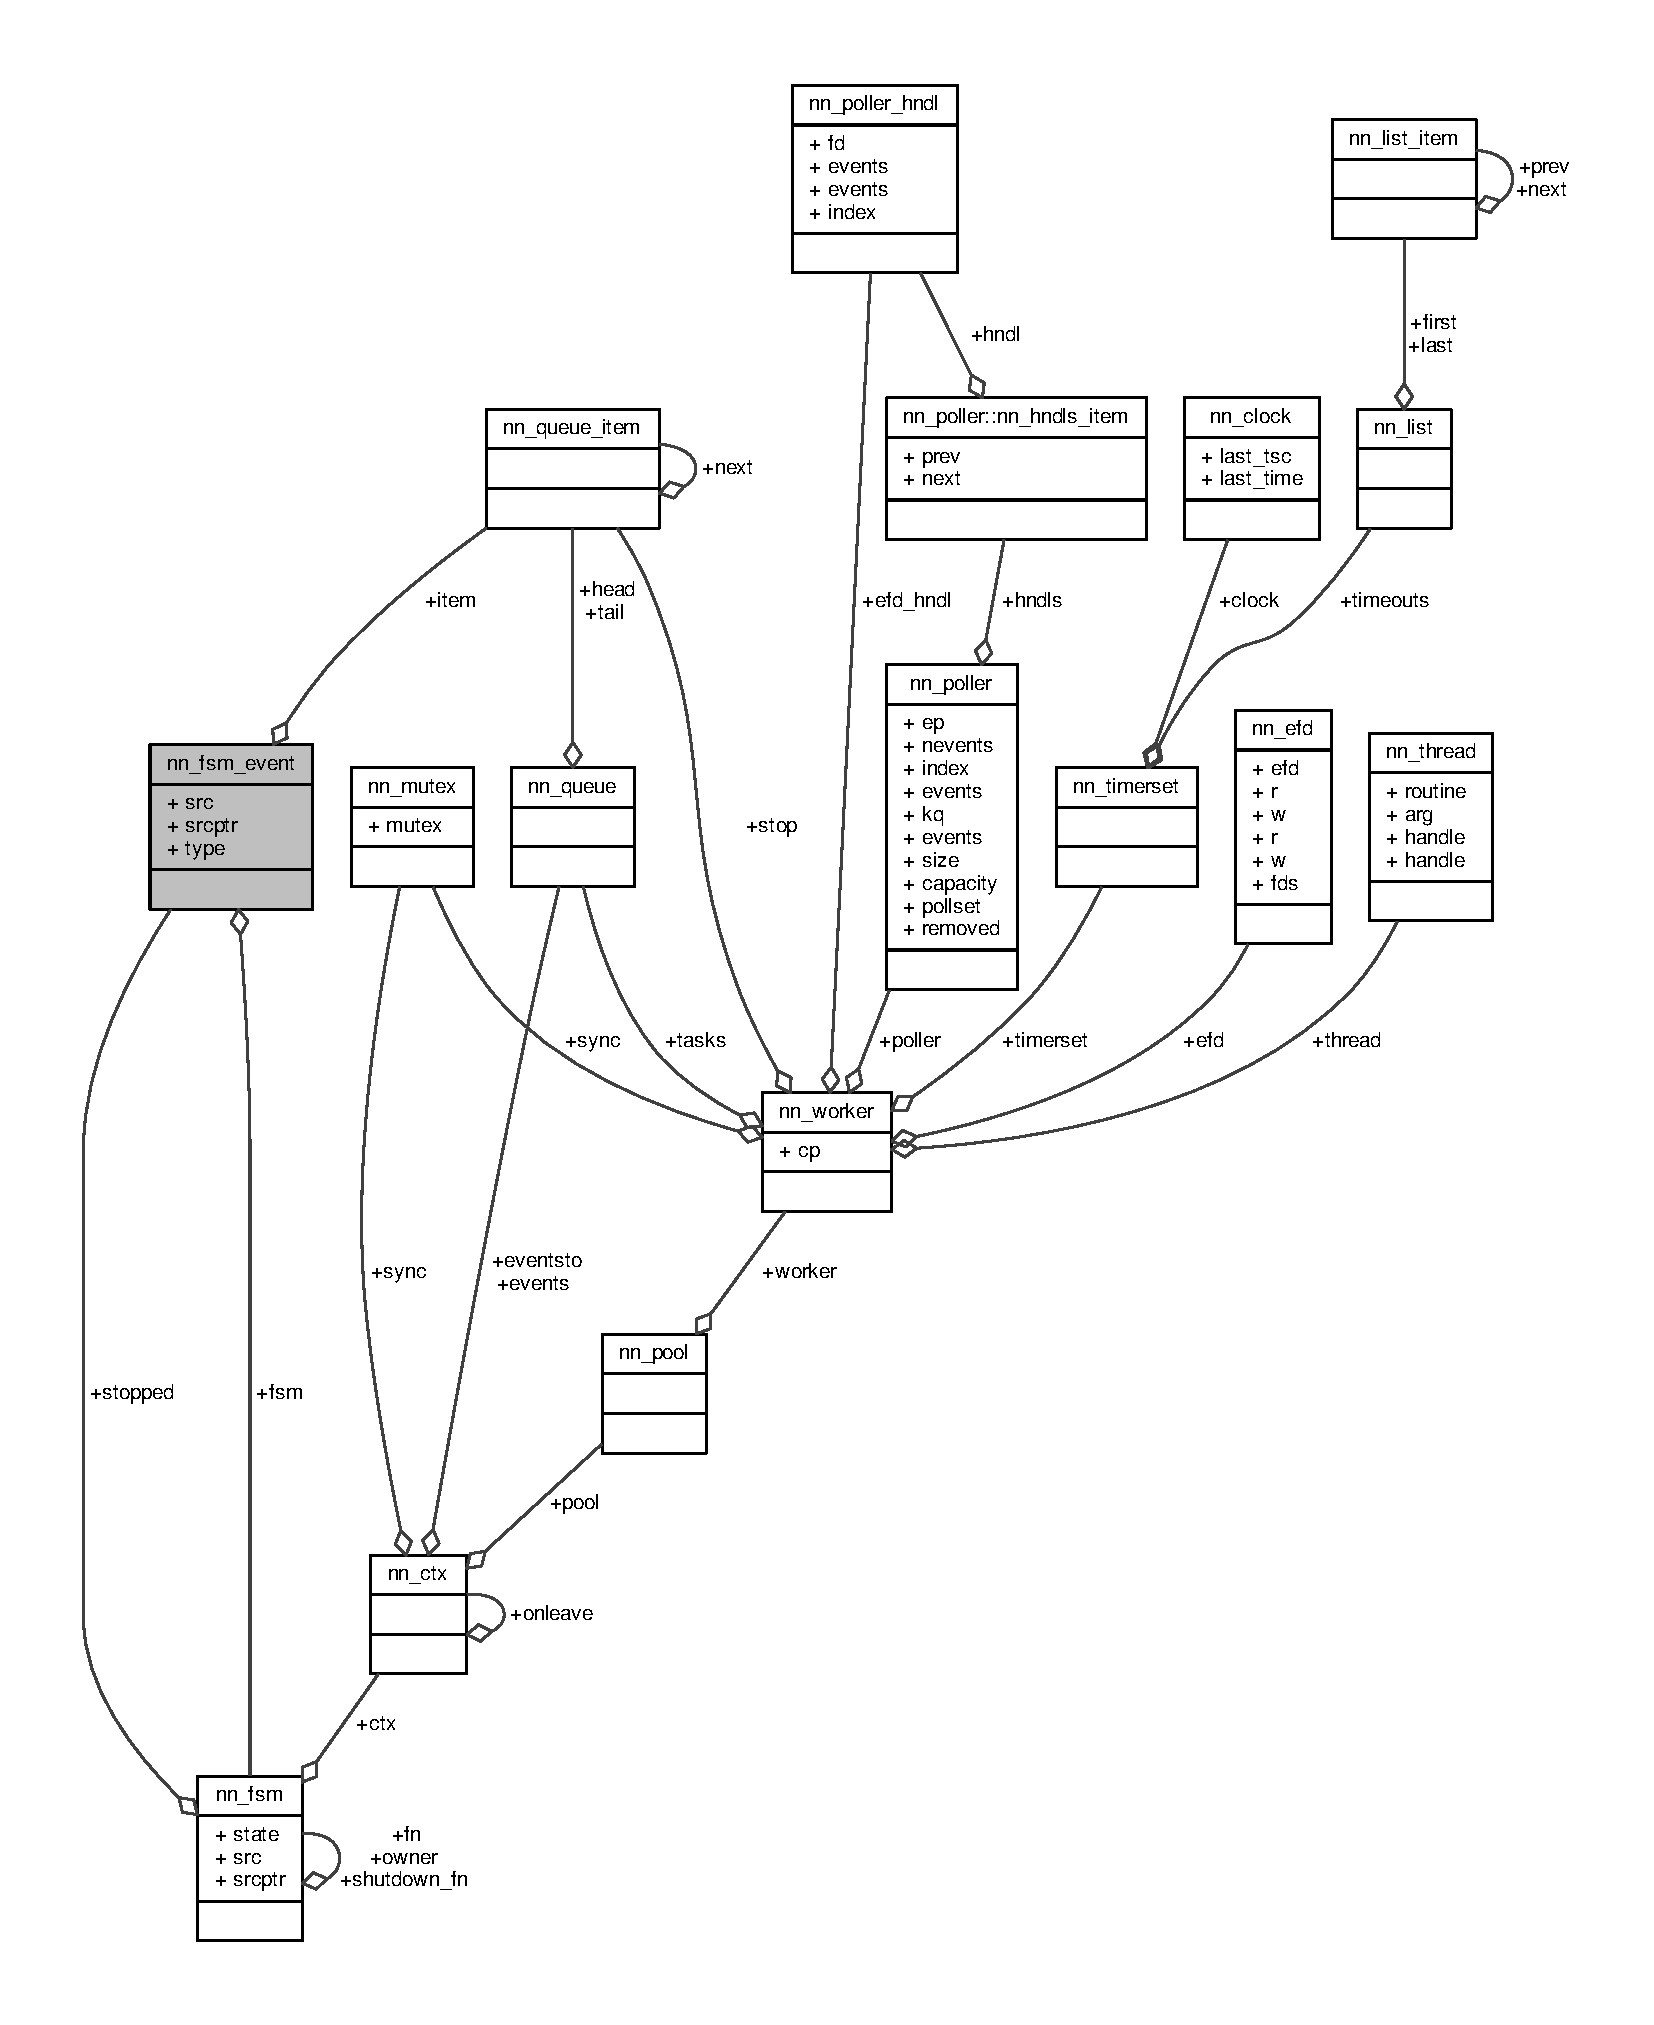
\includegraphics[width=350pt]{structnn__fsm__event__coll__graph}
\end{center}
\end{figure}
\subsection*{Public Attributes}
\begin{DoxyCompactItemize}
\item 
struct \hyperlink{structnn__fsm}{nn\+\_\+fsm} $\ast$ \hyperlink{structnn__fsm__event_a37e7bb55e85b8c65d08d2c71a5889480}{fsm}
\item 
int \hyperlink{structnn__fsm__event_a6ab6ed4117004772f0b0b1b489365701}{src}
\item 
void $\ast$ \hyperlink{structnn__fsm__event_a3216092753f9eb40385314e622d45350}{srcptr}
\item 
int \hyperlink{structnn__fsm__event_a9836f4659e72960e8959e3d14e2a7196}{type}
\item 
struct \hyperlink{structnn__queue__item}{nn\+\_\+queue\+\_\+item} \hyperlink{structnn__fsm__event_a4f93f7f20c2c966032cbd04b6dc8c49c}{item}
\end{DoxyCompactItemize}


\subsection{Member Data Documentation}
\index{nn\+\_\+fsm\+\_\+event@{nn\+\_\+fsm\+\_\+event}!fsm@{fsm}}
\index{fsm@{fsm}!nn\+\_\+fsm\+\_\+event@{nn\+\_\+fsm\+\_\+event}}
\subsubsection[{fsm}]{\setlength{\rightskip}{0pt plus 5cm}struct {\bf nn\+\_\+fsm}$\ast$ nn\+\_\+fsm\+\_\+event\+::fsm}\hypertarget{structnn__fsm__event_a37e7bb55e85b8c65d08d2c71a5889480}{}\label{structnn__fsm__event_a37e7bb55e85b8c65d08d2c71a5889480}
\index{nn\+\_\+fsm\+\_\+event@{nn\+\_\+fsm\+\_\+event}!item@{item}}
\index{item@{item}!nn\+\_\+fsm\+\_\+event@{nn\+\_\+fsm\+\_\+event}}
\subsubsection[{item}]{\setlength{\rightskip}{0pt plus 5cm}struct {\bf nn\+\_\+queue\+\_\+item} nn\+\_\+fsm\+\_\+event\+::item}\hypertarget{structnn__fsm__event_a4f93f7f20c2c966032cbd04b6dc8c49c}{}\label{structnn__fsm__event_a4f93f7f20c2c966032cbd04b6dc8c49c}
\index{nn\+\_\+fsm\+\_\+event@{nn\+\_\+fsm\+\_\+event}!src@{src}}
\index{src@{src}!nn\+\_\+fsm\+\_\+event@{nn\+\_\+fsm\+\_\+event}}
\subsubsection[{src}]{\setlength{\rightskip}{0pt plus 5cm}int nn\+\_\+fsm\+\_\+event\+::src}\hypertarget{structnn__fsm__event_a6ab6ed4117004772f0b0b1b489365701}{}\label{structnn__fsm__event_a6ab6ed4117004772f0b0b1b489365701}
\index{nn\+\_\+fsm\+\_\+event@{nn\+\_\+fsm\+\_\+event}!srcptr@{srcptr}}
\index{srcptr@{srcptr}!nn\+\_\+fsm\+\_\+event@{nn\+\_\+fsm\+\_\+event}}
\subsubsection[{srcptr}]{\setlength{\rightskip}{0pt plus 5cm}void$\ast$ nn\+\_\+fsm\+\_\+event\+::srcptr}\hypertarget{structnn__fsm__event_a3216092753f9eb40385314e622d45350}{}\label{structnn__fsm__event_a3216092753f9eb40385314e622d45350}
\index{nn\+\_\+fsm\+\_\+event@{nn\+\_\+fsm\+\_\+event}!type@{type}}
\index{type@{type}!nn\+\_\+fsm\+\_\+event@{nn\+\_\+fsm\+\_\+event}}
\subsubsection[{type}]{\setlength{\rightskip}{0pt plus 5cm}int nn\+\_\+fsm\+\_\+event\+::type}\hypertarget{structnn__fsm__event_a9836f4659e72960e8959e3d14e2a7196}{}\label{structnn__fsm__event_a9836f4659e72960e8959e3d14e2a7196}


The documentation for this struct was generated from the following file\+:\begin{DoxyCompactItemize}
\item 
src/aio/\hyperlink{fsm_8h}{fsm.\+h}\end{DoxyCompactItemize}

\hypertarget{structnn__fsm__owner}{}\section{nn\+\_\+fsm\+\_\+owner Struct Reference}
\label{structnn__fsm__owner}\index{nn\+\_\+fsm\+\_\+owner@{nn\+\_\+fsm\+\_\+owner}}


{\ttfamily \#include $<$fsm.\+h$>$}



Collaboration diagram for nn\+\_\+fsm\+\_\+owner\+:\nopagebreak
\begin{figure}[H]
\begin{center}
\leavevmode
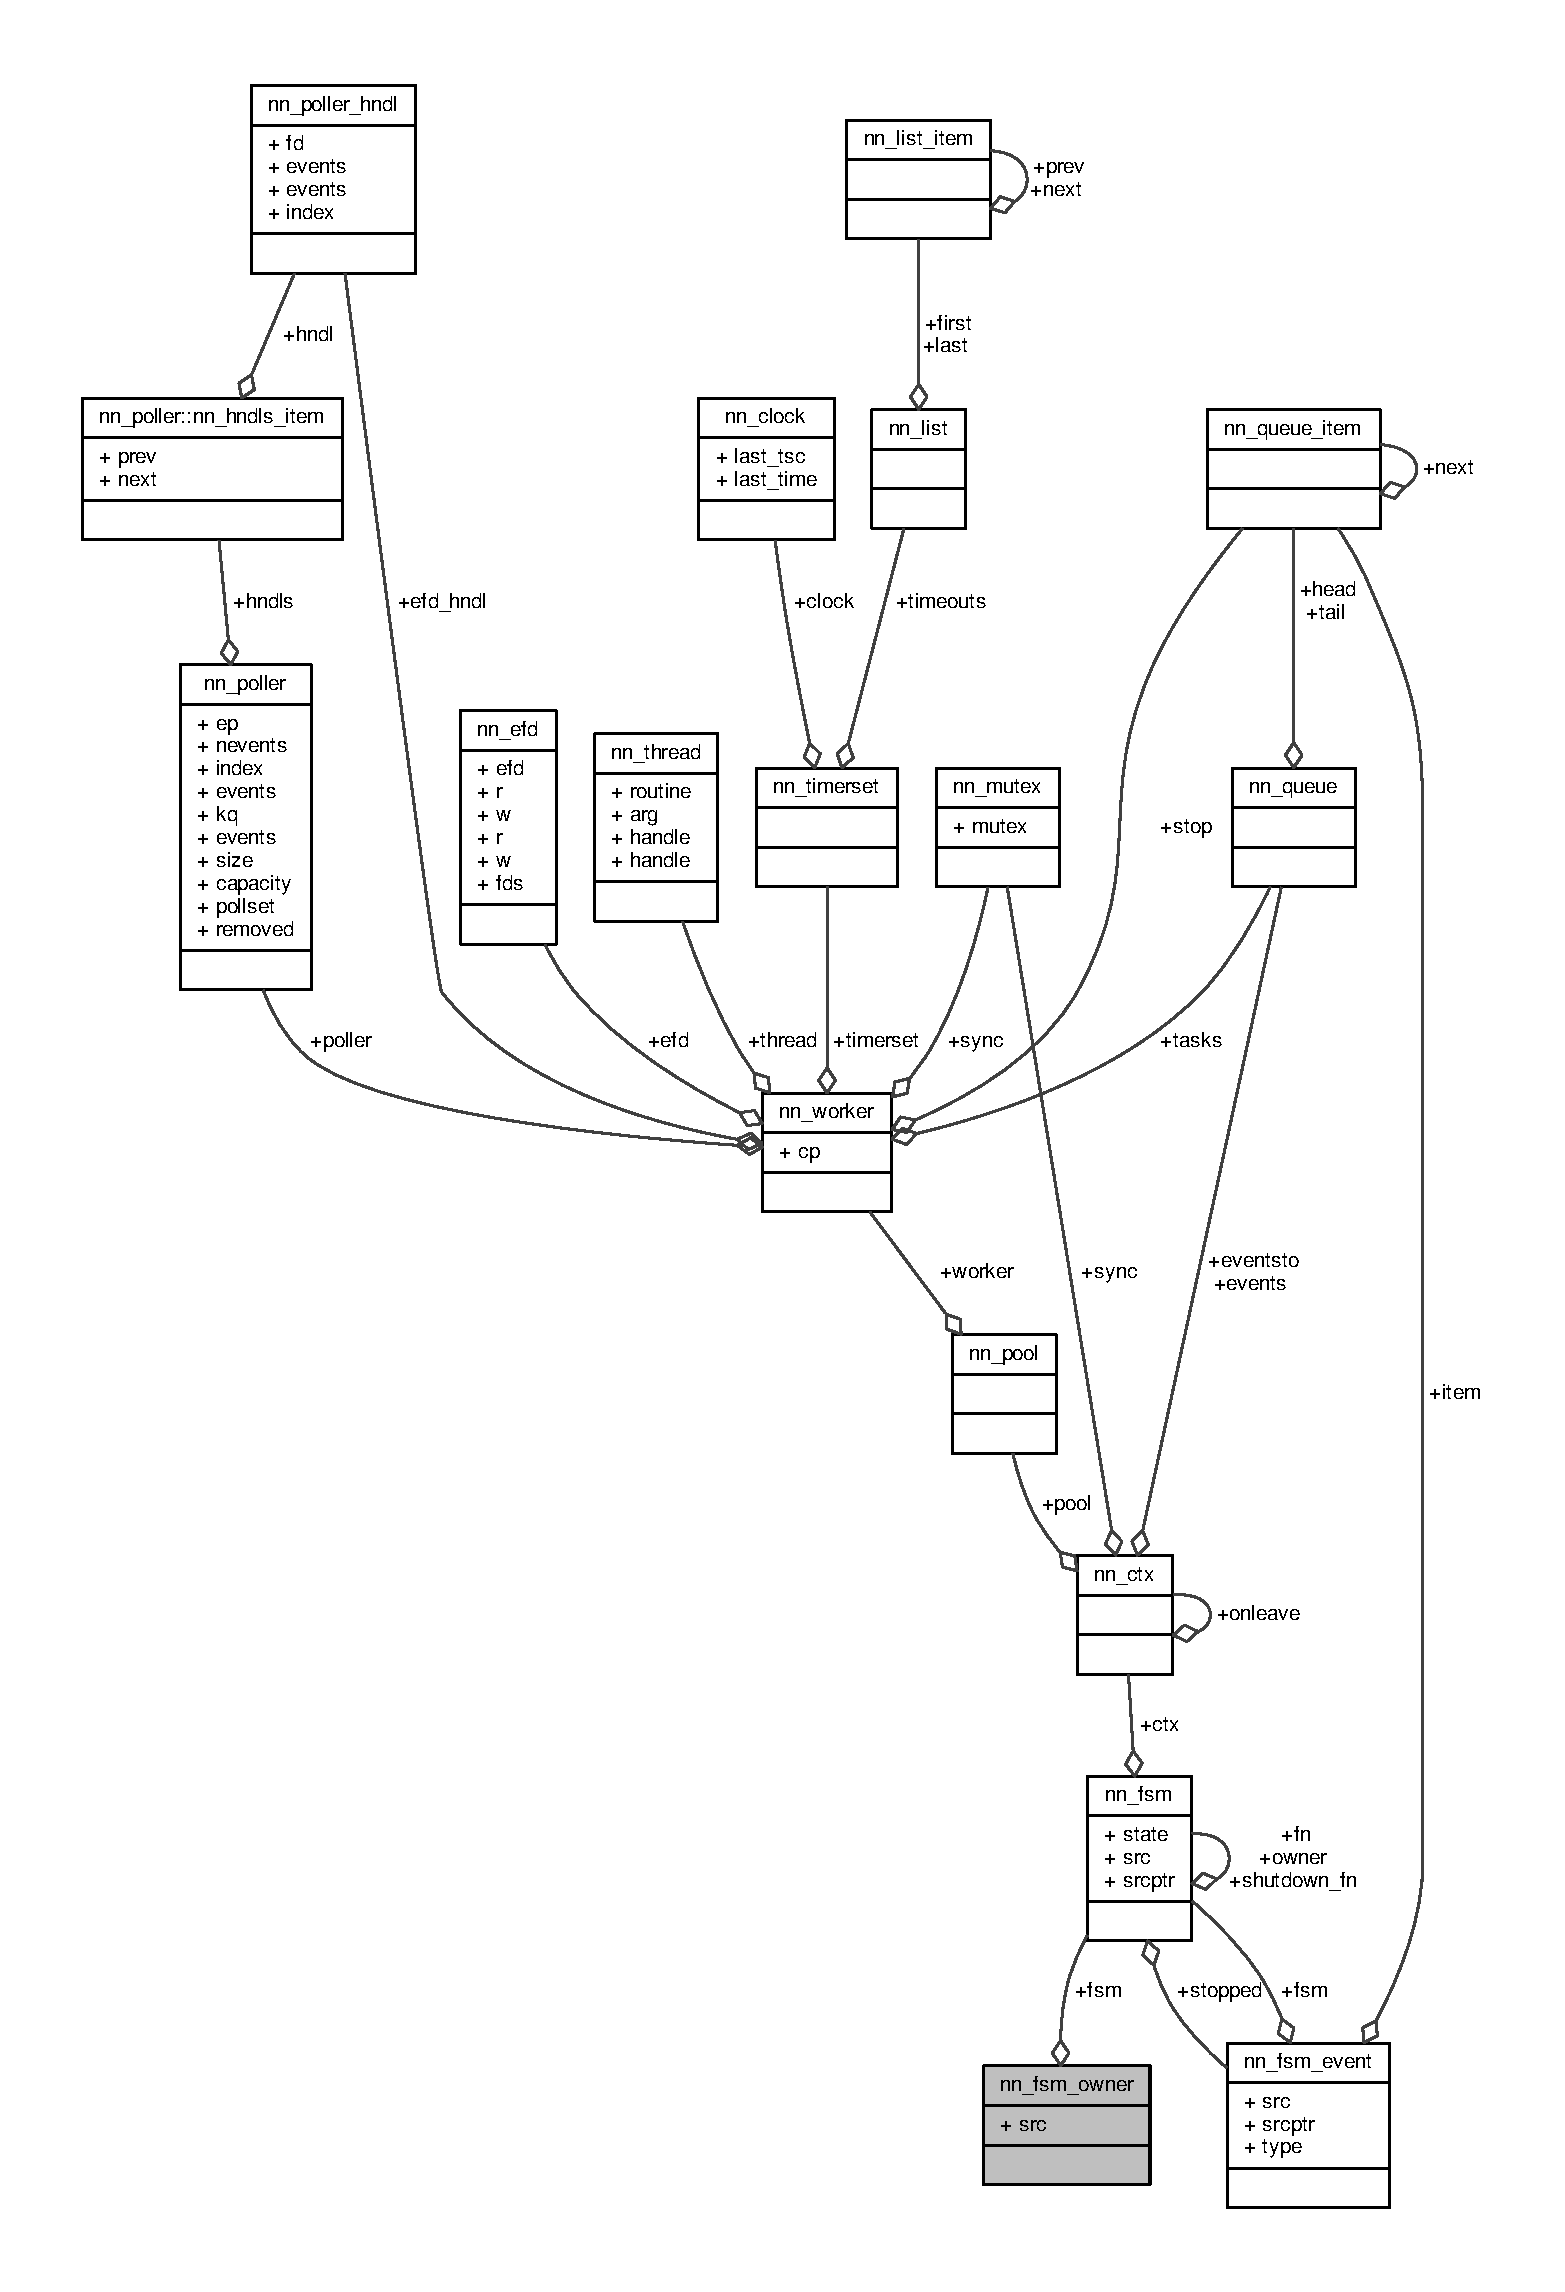
\includegraphics[width=350pt]{structnn__fsm__owner__coll__graph}
\end{center}
\end{figure}
\subsection*{Public Attributes}
\begin{DoxyCompactItemize}
\item 
int \hyperlink{structnn__fsm__owner_aab85be21a9bebaeb264d7626829c8632}{src}
\item 
struct \hyperlink{structnn__fsm}{nn\+\_\+fsm} $\ast$ \hyperlink{structnn__fsm__owner_ae05ede92ec1327579eb015bb707546b4}{fsm}
\end{DoxyCompactItemize}


\subsection{Member Data Documentation}
\index{nn\+\_\+fsm\+\_\+owner@{nn\+\_\+fsm\+\_\+owner}!fsm@{fsm}}
\index{fsm@{fsm}!nn\+\_\+fsm\+\_\+owner@{nn\+\_\+fsm\+\_\+owner}}
\subsubsection[{fsm}]{\setlength{\rightskip}{0pt plus 5cm}struct {\bf nn\+\_\+fsm}$\ast$ nn\+\_\+fsm\+\_\+owner\+::fsm}\hypertarget{structnn__fsm__owner_ae05ede92ec1327579eb015bb707546b4}{}\label{structnn__fsm__owner_ae05ede92ec1327579eb015bb707546b4}
\index{nn\+\_\+fsm\+\_\+owner@{nn\+\_\+fsm\+\_\+owner}!src@{src}}
\index{src@{src}!nn\+\_\+fsm\+\_\+owner@{nn\+\_\+fsm\+\_\+owner}}
\subsubsection[{src}]{\setlength{\rightskip}{0pt plus 5cm}int nn\+\_\+fsm\+\_\+owner\+::src}\hypertarget{structnn__fsm__owner_aab85be21a9bebaeb264d7626829c8632}{}\label{structnn__fsm__owner_aab85be21a9bebaeb264d7626829c8632}


The documentation for this struct was generated from the following file\+:\begin{DoxyCompactItemize}
\item 
src/aio/\hyperlink{fsm_8h}{fsm.\+h}\end{DoxyCompactItemize}

\hypertarget{structnn__global}{}\section{nn\+\_\+global Struct Reference}
\label{structnn__global}\index{nn\+\_\+global@{nn\+\_\+global}}


Collaboration diagram for nn\+\_\+global\+:\nopagebreak
\begin{figure}[H]
\begin{center}
\leavevmode
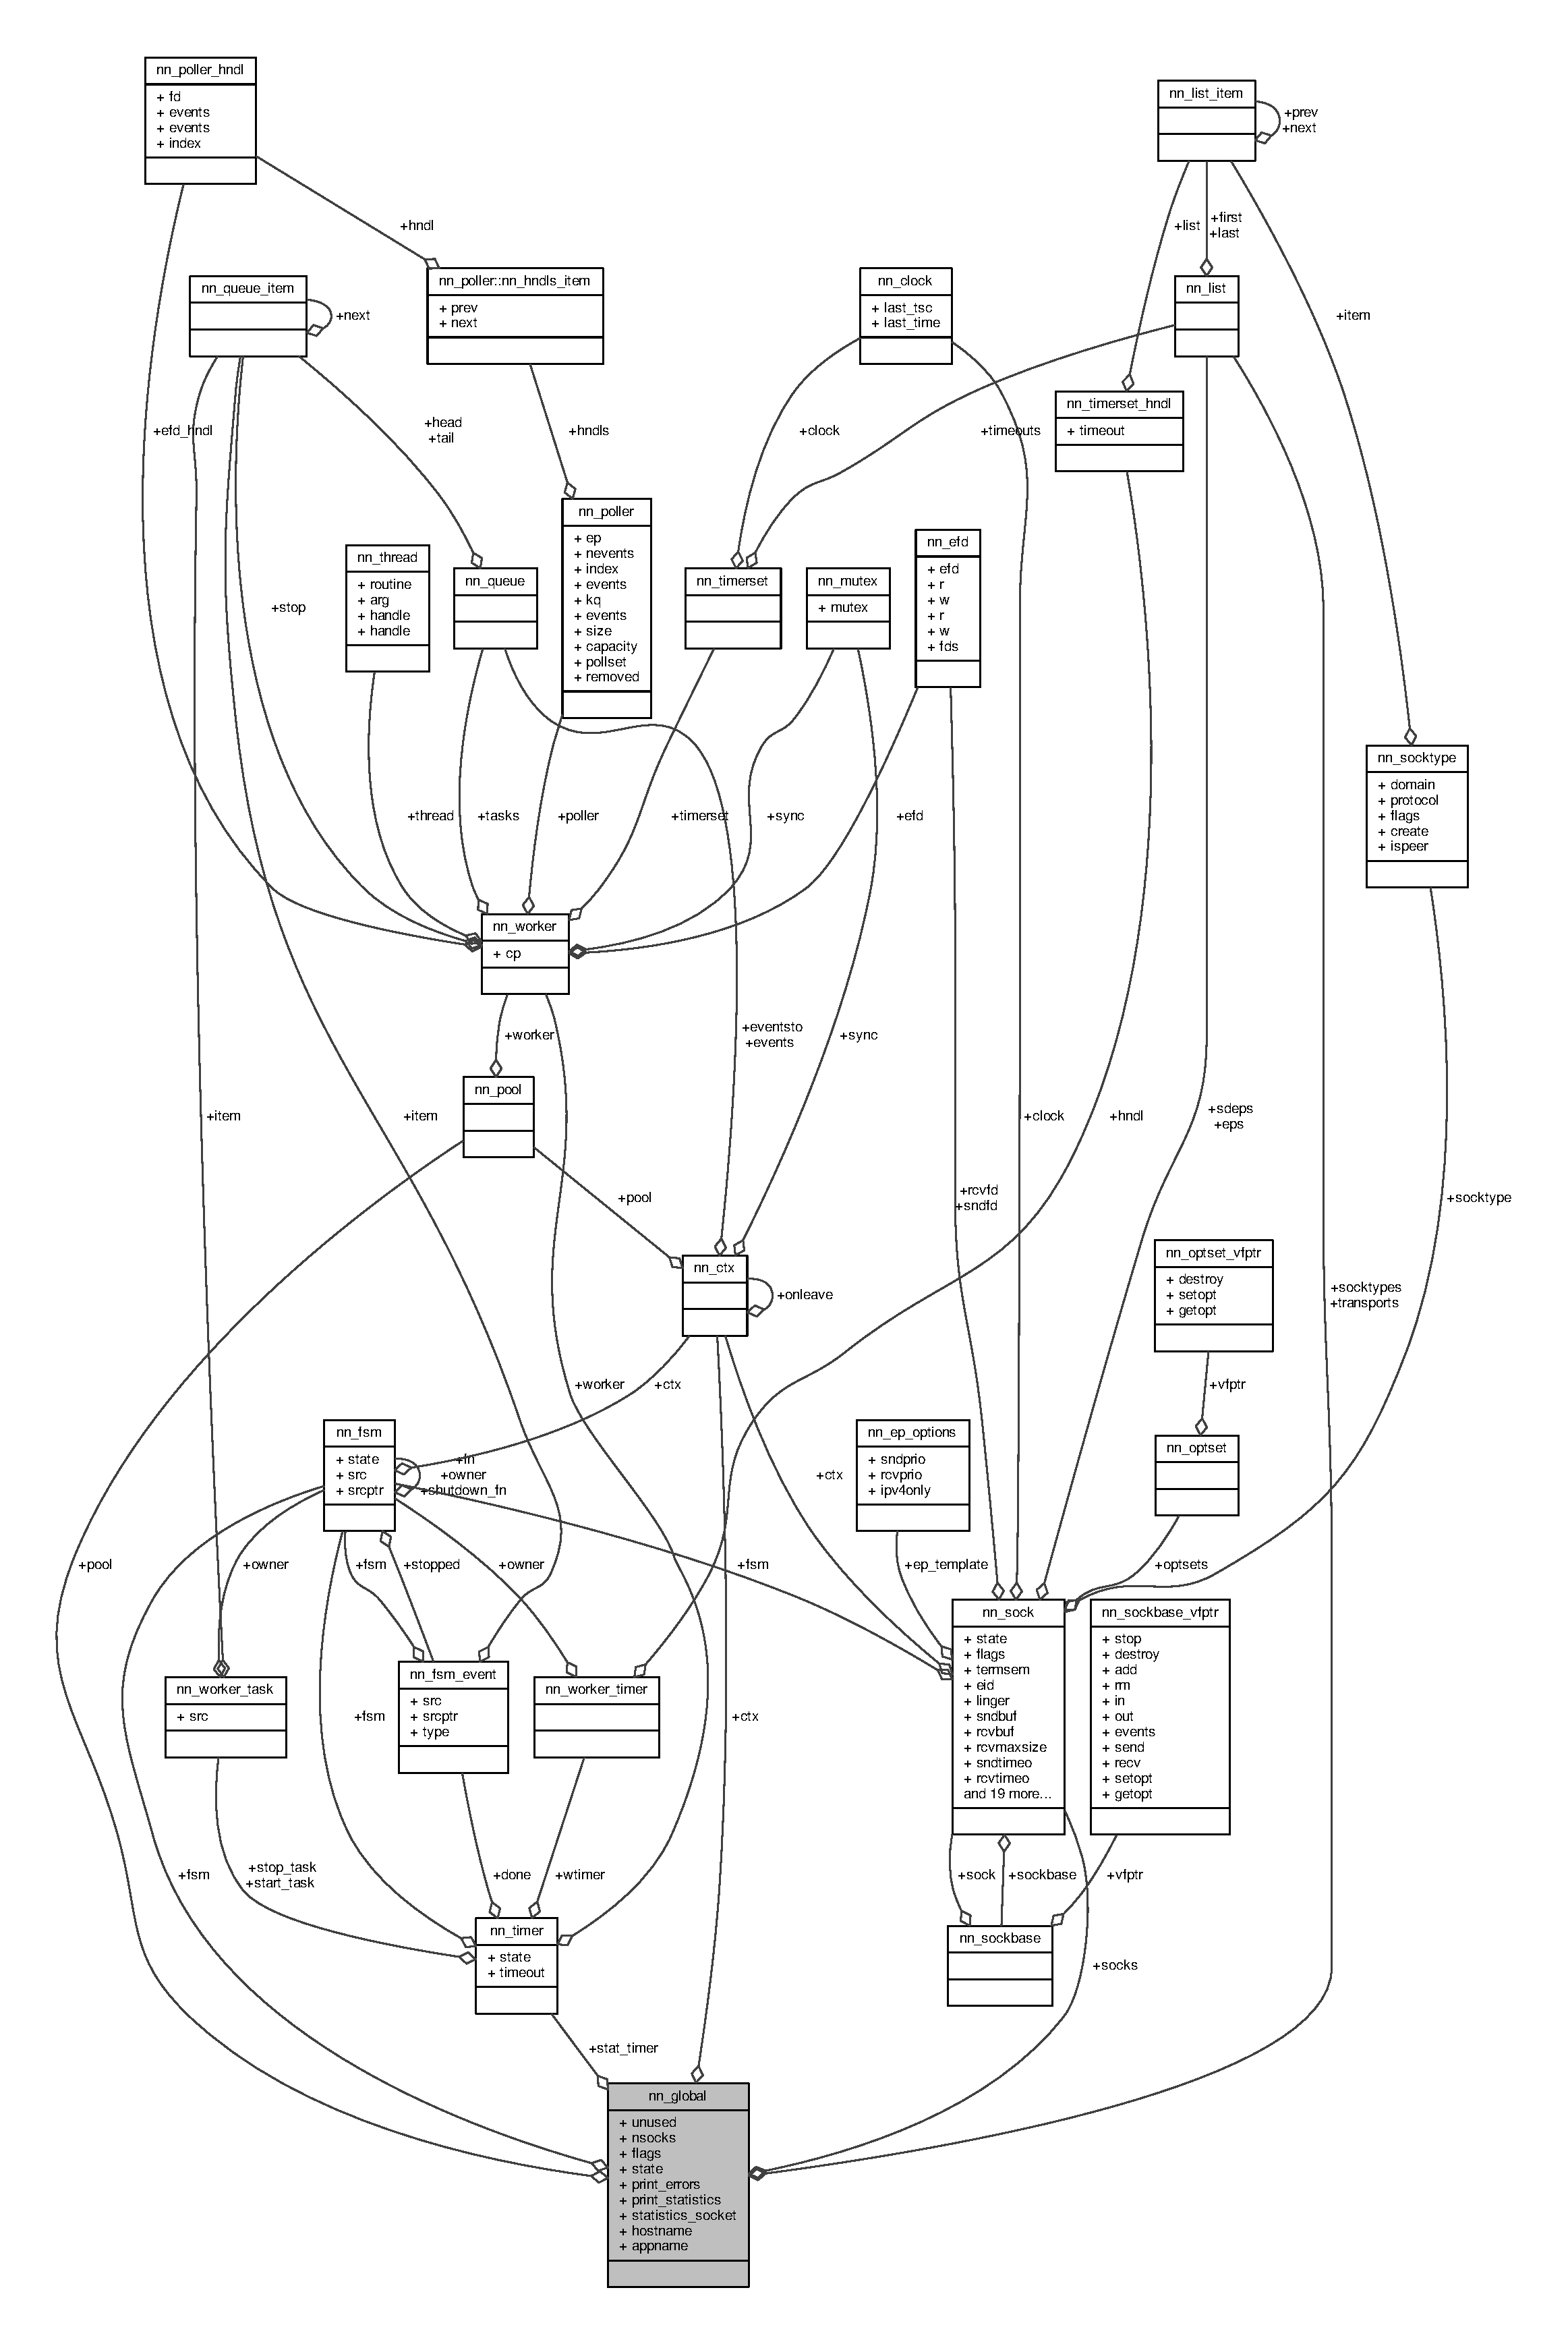
\includegraphics[width=350pt]{structnn__global__coll__graph}
\end{center}
\end{figure}
\subsection*{Public Attributes}
\begin{DoxyCompactItemize}
\item 
struct \hyperlink{structnn__sock}{nn\+\_\+sock} $\ast$$\ast$ \hyperlink{structnn__global_a2d4ac1ec0821fd73d64164024c6ac34a}{socks}
\item 
uint16\+\_\+t $\ast$ \hyperlink{structnn__global_adfca766f62f1d6fa7f676453083c71e7}{unused}
\item 
size\+\_\+t \hyperlink{structnn__global_a6edb3dc50e3cbda2500c9ed057d9c54b}{nsocks}
\item 
int \hyperlink{structnn__global_a14a59ff08fbab1ca0a02b1de0c1aa3d4}{flags}
\item 
struct \hyperlink{structnn__list}{nn\+\_\+list} \hyperlink{structnn__global_a5ebc096d525d2628fabd293dfaccc064}{transports}
\item 
struct \hyperlink{structnn__list}{nn\+\_\+list} \hyperlink{structnn__global_a13fbf4096f84ad16e1d972b693e17ab3}{socktypes}
\item 
struct \hyperlink{structnn__pool}{nn\+\_\+pool} \hyperlink{structnn__global_a00121159df6225e24a85fa9239e0572c}{pool}
\item 
struct \hyperlink{structnn__ctx}{nn\+\_\+ctx} \hyperlink{structnn__global_a785576884be1ca2618171882c8fb797e}{ctx}
\item 
struct \hyperlink{structnn__fsm}{nn\+\_\+fsm} \hyperlink{structnn__global_a4a70871e752cab1ff856b584d64ec63b}{fsm}
\item 
int \hyperlink{structnn__global_ac3e476bf3985bb063e646c725622f5f9}{state}
\item 
struct \hyperlink{structnn__timer}{nn\+\_\+timer} \hyperlink{structnn__global_a7b245b5376cf63a243f5b27a4a10a805}{stat\+\_\+timer}
\item 
int \hyperlink{structnn__global_abbd632a22981ef3e4cefbe273a47c36f}{print\+\_\+errors}
\item 
int \hyperlink{structnn__global_a3d435991b706e1573fe7e74854f84185}{print\+\_\+statistics}
\item 
int \hyperlink{structnn__global_a1e2fa6c4aa9ab985db67d12002095509}{statistics\+\_\+socket}
\item 
char \hyperlink{structnn__global_a5c5b258b0ace109bb10a1e007429725e}{hostname} \mbox{[}64\mbox{]}
\item 
char \hyperlink{structnn__global_a6c0970e479ba853119a5ecf5e858a29e}{appname} \mbox{[}64\mbox{]}
\end{DoxyCompactItemize}


\subsection{Member Data Documentation}
\index{nn\+\_\+global@{nn\+\_\+global}!appname@{appname}}
\index{appname@{appname}!nn\+\_\+global@{nn\+\_\+global}}
\subsubsection[{appname}]{\setlength{\rightskip}{0pt plus 5cm}char nn\+\_\+global\+::appname\mbox{[}64\mbox{]}}\hypertarget{structnn__global_a6c0970e479ba853119a5ecf5e858a29e}{}\label{structnn__global_a6c0970e479ba853119a5ecf5e858a29e}
\index{nn\+\_\+global@{nn\+\_\+global}!ctx@{ctx}}
\index{ctx@{ctx}!nn\+\_\+global@{nn\+\_\+global}}
\subsubsection[{ctx}]{\setlength{\rightskip}{0pt plus 5cm}struct {\bf nn\+\_\+ctx} nn\+\_\+global\+::ctx}\hypertarget{structnn__global_a785576884be1ca2618171882c8fb797e}{}\label{structnn__global_a785576884be1ca2618171882c8fb797e}
\index{nn\+\_\+global@{nn\+\_\+global}!flags@{flags}}
\index{flags@{flags}!nn\+\_\+global@{nn\+\_\+global}}
\subsubsection[{flags}]{\setlength{\rightskip}{0pt plus 5cm}int nn\+\_\+global\+::flags}\hypertarget{structnn__global_a14a59ff08fbab1ca0a02b1de0c1aa3d4}{}\label{structnn__global_a14a59ff08fbab1ca0a02b1de0c1aa3d4}
\index{nn\+\_\+global@{nn\+\_\+global}!fsm@{fsm}}
\index{fsm@{fsm}!nn\+\_\+global@{nn\+\_\+global}}
\subsubsection[{fsm}]{\setlength{\rightskip}{0pt plus 5cm}struct {\bf nn\+\_\+fsm} nn\+\_\+global\+::fsm}\hypertarget{structnn__global_a4a70871e752cab1ff856b584d64ec63b}{}\label{structnn__global_a4a70871e752cab1ff856b584d64ec63b}
\index{nn\+\_\+global@{nn\+\_\+global}!hostname@{hostname}}
\index{hostname@{hostname}!nn\+\_\+global@{nn\+\_\+global}}
\subsubsection[{hostname}]{\setlength{\rightskip}{0pt plus 5cm}char nn\+\_\+global\+::hostname\mbox{[}64\mbox{]}}\hypertarget{structnn__global_a5c5b258b0ace109bb10a1e007429725e}{}\label{structnn__global_a5c5b258b0ace109bb10a1e007429725e}
\index{nn\+\_\+global@{nn\+\_\+global}!nsocks@{nsocks}}
\index{nsocks@{nsocks}!nn\+\_\+global@{nn\+\_\+global}}
\subsubsection[{nsocks}]{\setlength{\rightskip}{0pt plus 5cm}size\+\_\+t nn\+\_\+global\+::nsocks}\hypertarget{structnn__global_a6edb3dc50e3cbda2500c9ed057d9c54b}{}\label{structnn__global_a6edb3dc50e3cbda2500c9ed057d9c54b}
\index{nn\+\_\+global@{nn\+\_\+global}!pool@{pool}}
\index{pool@{pool}!nn\+\_\+global@{nn\+\_\+global}}
\subsubsection[{pool}]{\setlength{\rightskip}{0pt plus 5cm}struct {\bf nn\+\_\+pool} nn\+\_\+global\+::pool}\hypertarget{structnn__global_a00121159df6225e24a85fa9239e0572c}{}\label{structnn__global_a00121159df6225e24a85fa9239e0572c}
\index{nn\+\_\+global@{nn\+\_\+global}!print\+\_\+errors@{print\+\_\+errors}}
\index{print\+\_\+errors@{print\+\_\+errors}!nn\+\_\+global@{nn\+\_\+global}}
\subsubsection[{print\+\_\+errors}]{\setlength{\rightskip}{0pt plus 5cm}int nn\+\_\+global\+::print\+\_\+errors}\hypertarget{structnn__global_abbd632a22981ef3e4cefbe273a47c36f}{}\label{structnn__global_abbd632a22981ef3e4cefbe273a47c36f}
\index{nn\+\_\+global@{nn\+\_\+global}!print\+\_\+statistics@{print\+\_\+statistics}}
\index{print\+\_\+statistics@{print\+\_\+statistics}!nn\+\_\+global@{nn\+\_\+global}}
\subsubsection[{print\+\_\+statistics}]{\setlength{\rightskip}{0pt plus 5cm}int nn\+\_\+global\+::print\+\_\+statistics}\hypertarget{structnn__global_a3d435991b706e1573fe7e74854f84185}{}\label{structnn__global_a3d435991b706e1573fe7e74854f84185}
\index{nn\+\_\+global@{nn\+\_\+global}!socks@{socks}}
\index{socks@{socks}!nn\+\_\+global@{nn\+\_\+global}}
\subsubsection[{socks}]{\setlength{\rightskip}{0pt plus 5cm}struct {\bf nn\+\_\+sock}$\ast$$\ast$ nn\+\_\+global\+::socks}\hypertarget{structnn__global_a2d4ac1ec0821fd73d64164024c6ac34a}{}\label{structnn__global_a2d4ac1ec0821fd73d64164024c6ac34a}
\index{nn\+\_\+global@{nn\+\_\+global}!socktypes@{socktypes}}
\index{socktypes@{socktypes}!nn\+\_\+global@{nn\+\_\+global}}
\subsubsection[{socktypes}]{\setlength{\rightskip}{0pt plus 5cm}struct {\bf nn\+\_\+list} nn\+\_\+global\+::socktypes}\hypertarget{structnn__global_a13fbf4096f84ad16e1d972b693e17ab3}{}\label{structnn__global_a13fbf4096f84ad16e1d972b693e17ab3}
\index{nn\+\_\+global@{nn\+\_\+global}!stat\+\_\+timer@{stat\+\_\+timer}}
\index{stat\+\_\+timer@{stat\+\_\+timer}!nn\+\_\+global@{nn\+\_\+global}}
\subsubsection[{stat\+\_\+timer}]{\setlength{\rightskip}{0pt plus 5cm}struct {\bf nn\+\_\+timer} nn\+\_\+global\+::stat\+\_\+timer}\hypertarget{structnn__global_a7b245b5376cf63a243f5b27a4a10a805}{}\label{structnn__global_a7b245b5376cf63a243f5b27a4a10a805}
\index{nn\+\_\+global@{nn\+\_\+global}!state@{state}}
\index{state@{state}!nn\+\_\+global@{nn\+\_\+global}}
\subsubsection[{state}]{\setlength{\rightskip}{0pt plus 5cm}int nn\+\_\+global\+::state}\hypertarget{structnn__global_ac3e476bf3985bb063e646c725622f5f9}{}\label{structnn__global_ac3e476bf3985bb063e646c725622f5f9}
\index{nn\+\_\+global@{nn\+\_\+global}!statistics\+\_\+socket@{statistics\+\_\+socket}}
\index{statistics\+\_\+socket@{statistics\+\_\+socket}!nn\+\_\+global@{nn\+\_\+global}}
\subsubsection[{statistics\+\_\+socket}]{\setlength{\rightskip}{0pt plus 5cm}int nn\+\_\+global\+::statistics\+\_\+socket}\hypertarget{structnn__global_a1e2fa6c4aa9ab985db67d12002095509}{}\label{structnn__global_a1e2fa6c4aa9ab985db67d12002095509}
\index{nn\+\_\+global@{nn\+\_\+global}!transports@{transports}}
\index{transports@{transports}!nn\+\_\+global@{nn\+\_\+global}}
\subsubsection[{transports}]{\setlength{\rightskip}{0pt plus 5cm}struct {\bf nn\+\_\+list} nn\+\_\+global\+::transports}\hypertarget{structnn__global_a5ebc096d525d2628fabd293dfaccc064}{}\label{structnn__global_a5ebc096d525d2628fabd293dfaccc064}
\index{nn\+\_\+global@{nn\+\_\+global}!unused@{unused}}
\index{unused@{unused}!nn\+\_\+global@{nn\+\_\+global}}
\subsubsection[{unused}]{\setlength{\rightskip}{0pt plus 5cm}uint16\+\_\+t$\ast$ nn\+\_\+global\+::unused}\hypertarget{structnn__global_adfca766f62f1d6fa7f676453083c71e7}{}\label{structnn__global_adfca766f62f1d6fa7f676453083c71e7}


The documentation for this struct was generated from the following file\+:\begin{DoxyCompactItemize}
\item 
src/core/\hyperlink{global_8c}{global.\+c}\end{DoxyCompactItemize}

\hypertarget{structnn__hash}{}\section{nn\+\_\+hash Struct Reference}
\label{structnn__hash}\index{nn\+\_\+hash@{nn\+\_\+hash}}


{\ttfamily \#include $<$hash.\+h$>$}



Collaboration diagram for nn\+\_\+hash\+:\nopagebreak
\begin{figure}[H]
\begin{center}
\leavevmode
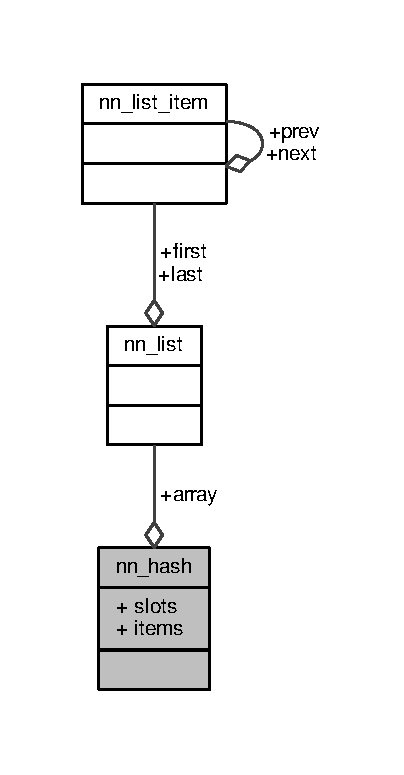
\includegraphics[width=194pt]{structnn__hash__coll__graph}
\end{center}
\end{figure}
\subsection*{Public Attributes}
\begin{DoxyCompactItemize}
\item 
uint32\+\_\+t \hyperlink{structnn__hash_a09c079149c424febf2b1cc5f639eaeac}{slots}
\item 
uint32\+\_\+t \hyperlink{structnn__hash_ad68a8fd4c0707eddc75558b3de0b8ff9}{items}
\item 
struct \hyperlink{structnn__list}{nn\+\_\+list} $\ast$ \hyperlink{structnn__hash_a2ba7047174afe682c1613286020015e4}{array}
\end{DoxyCompactItemize}


\subsection{Member Data Documentation}
\index{nn\+\_\+hash@{nn\+\_\+hash}!array@{array}}
\index{array@{array}!nn\+\_\+hash@{nn\+\_\+hash}}
\subsubsection[{array}]{\setlength{\rightskip}{0pt plus 5cm}struct {\bf nn\+\_\+list}$\ast$ nn\+\_\+hash\+::array}\hypertarget{structnn__hash_a2ba7047174afe682c1613286020015e4}{}\label{structnn__hash_a2ba7047174afe682c1613286020015e4}
\index{nn\+\_\+hash@{nn\+\_\+hash}!items@{items}}
\index{items@{items}!nn\+\_\+hash@{nn\+\_\+hash}}
\subsubsection[{items}]{\setlength{\rightskip}{0pt plus 5cm}uint32\+\_\+t nn\+\_\+hash\+::items}\hypertarget{structnn__hash_ad68a8fd4c0707eddc75558b3de0b8ff9}{}\label{structnn__hash_ad68a8fd4c0707eddc75558b3de0b8ff9}
\index{nn\+\_\+hash@{nn\+\_\+hash}!slots@{slots}}
\index{slots@{slots}!nn\+\_\+hash@{nn\+\_\+hash}}
\subsubsection[{slots}]{\setlength{\rightskip}{0pt plus 5cm}uint32\+\_\+t nn\+\_\+hash\+::slots}\hypertarget{structnn__hash_a09c079149c424febf2b1cc5f639eaeac}{}\label{structnn__hash_a09c079149c424febf2b1cc5f639eaeac}


The documentation for this struct was generated from the following file\+:\begin{DoxyCompactItemize}
\item 
src/utils/\hyperlink{hash_8h}{hash.\+h}\end{DoxyCompactItemize}

\hypertarget{structnn__hash__item}{}\section{nn\+\_\+hash\+\_\+item Struct Reference}
\label{structnn__hash__item}\index{nn\+\_\+hash\+\_\+item@{nn\+\_\+hash\+\_\+item}}


{\ttfamily \#include $<$hash.\+h$>$}



Collaboration diagram for nn\+\_\+hash\+\_\+item\+:\nopagebreak
\begin{figure}[H]
\begin{center}
\leavevmode
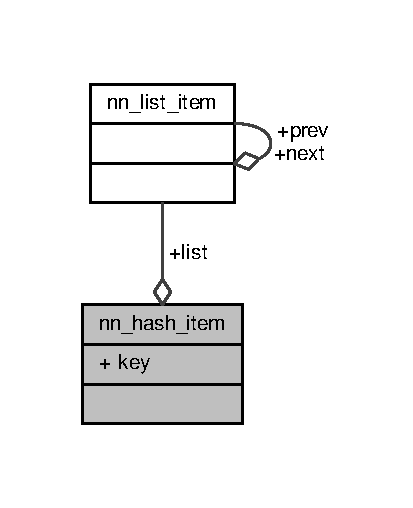
\includegraphics[width=198pt]{structnn__hash__item__coll__graph}
\end{center}
\end{figure}
\subsection*{Public Attributes}
\begin{DoxyCompactItemize}
\item 
uint32\+\_\+t \hyperlink{structnn__hash__item_a0c08a2cdf14f38f101faade8a1ee1101}{key}
\item 
struct \hyperlink{structnn__list__item}{nn\+\_\+list\+\_\+item} \hyperlink{structnn__hash__item_ab52f9314ec727442f49da157796b0a89}{list}
\end{DoxyCompactItemize}


\subsection{Member Data Documentation}
\index{nn\+\_\+hash\+\_\+item@{nn\+\_\+hash\+\_\+item}!key@{key}}
\index{key@{key}!nn\+\_\+hash\+\_\+item@{nn\+\_\+hash\+\_\+item}}
\subsubsection[{key}]{\setlength{\rightskip}{0pt plus 5cm}uint32\+\_\+t nn\+\_\+hash\+\_\+item\+::key}\hypertarget{structnn__hash__item_a0c08a2cdf14f38f101faade8a1ee1101}{}\label{structnn__hash__item_a0c08a2cdf14f38f101faade8a1ee1101}
\index{nn\+\_\+hash\+\_\+item@{nn\+\_\+hash\+\_\+item}!list@{list}}
\index{list@{list}!nn\+\_\+hash\+\_\+item@{nn\+\_\+hash\+\_\+item}}
\subsubsection[{list}]{\setlength{\rightskip}{0pt plus 5cm}struct {\bf nn\+\_\+list\+\_\+item} nn\+\_\+hash\+\_\+item\+::list}\hypertarget{structnn__hash__item_ab52f9314ec727442f49da157796b0a89}{}\label{structnn__hash__item_ab52f9314ec727442f49da157796b0a89}


The documentation for this struct was generated from the following file\+:\begin{DoxyCompactItemize}
\item 
src/utils/\hyperlink{hash_8h}{hash.\+h}\end{DoxyCompactItemize}

\hypertarget{structnn__poller_1_1nn__hndls__item}{}\section{nn\+\_\+poller\+:\+:nn\+\_\+hndls\+\_\+item Struct Reference}
\label{structnn__poller_1_1nn__hndls__item}\index{nn\+\_\+poller\+::nn\+\_\+hndls\+\_\+item@{nn\+\_\+poller\+::nn\+\_\+hndls\+\_\+item}}


{\ttfamily \#include $<$poller\+\_\+poll.\+h$>$}



Collaboration diagram for nn\+\_\+poller\+:\+:nn\+\_\+hndls\+\_\+item\+:\nopagebreak
\begin{figure}[H]
\begin{center}
\leavevmode
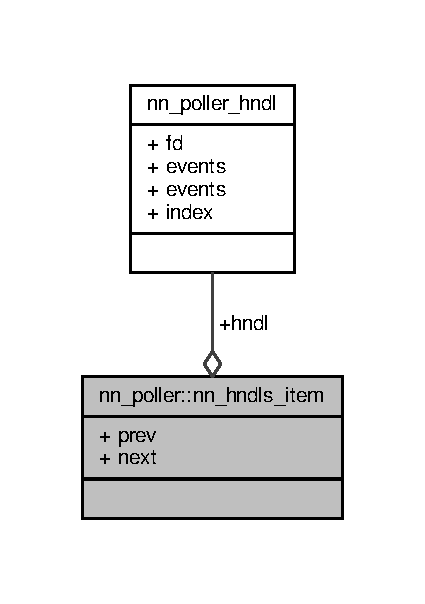
\includegraphics[width=204pt]{structnn__poller_1_1nn__hndls__item__coll__graph}
\end{center}
\end{figure}
\subsection*{Public Attributes}
\begin{DoxyCompactItemize}
\item 
struct \hyperlink{structnn__poller__hndl}{nn\+\_\+poller\+\_\+hndl} $\ast$ \hyperlink{structnn__poller_1_1nn__hndls__item_a0255d9a6f887fe0cd2a0363fb517f84e}{hndl}
\item 
int \hyperlink{structnn__poller_1_1nn__hndls__item_a7d9970256d55c4c0d7832e2d759682eb}{prev}
\item 
int \hyperlink{structnn__poller_1_1nn__hndls__item_a00d334ecc01f3fb24fb117cdb5242215}{next}
\end{DoxyCompactItemize}


\subsection{Member Data Documentation}
\index{nn\+\_\+poller\+::nn\+\_\+hndls\+\_\+item@{nn\+\_\+poller\+::nn\+\_\+hndls\+\_\+item}!hndl@{hndl}}
\index{hndl@{hndl}!nn\+\_\+poller\+::nn\+\_\+hndls\+\_\+item@{nn\+\_\+poller\+::nn\+\_\+hndls\+\_\+item}}
\subsubsection[{hndl}]{\setlength{\rightskip}{0pt plus 5cm}struct {\bf nn\+\_\+poller\+\_\+hndl}$\ast$ nn\+\_\+poller\+::nn\+\_\+hndls\+\_\+item\+::hndl}\hypertarget{structnn__poller_1_1nn__hndls__item_a0255d9a6f887fe0cd2a0363fb517f84e}{}\label{structnn__poller_1_1nn__hndls__item_a0255d9a6f887fe0cd2a0363fb517f84e}
\index{nn\+\_\+poller\+::nn\+\_\+hndls\+\_\+item@{nn\+\_\+poller\+::nn\+\_\+hndls\+\_\+item}!next@{next}}
\index{next@{next}!nn\+\_\+poller\+::nn\+\_\+hndls\+\_\+item@{nn\+\_\+poller\+::nn\+\_\+hndls\+\_\+item}}
\subsubsection[{next}]{\setlength{\rightskip}{0pt plus 5cm}int nn\+\_\+poller\+::nn\+\_\+hndls\+\_\+item\+::next}\hypertarget{structnn__poller_1_1nn__hndls__item_a00d334ecc01f3fb24fb117cdb5242215}{}\label{structnn__poller_1_1nn__hndls__item_a00d334ecc01f3fb24fb117cdb5242215}
\index{nn\+\_\+poller\+::nn\+\_\+hndls\+\_\+item@{nn\+\_\+poller\+::nn\+\_\+hndls\+\_\+item}!prev@{prev}}
\index{prev@{prev}!nn\+\_\+poller\+::nn\+\_\+hndls\+\_\+item@{nn\+\_\+poller\+::nn\+\_\+hndls\+\_\+item}}
\subsubsection[{prev}]{\setlength{\rightskip}{0pt plus 5cm}int nn\+\_\+poller\+::nn\+\_\+hndls\+\_\+item\+::prev}\hypertarget{structnn__poller_1_1nn__hndls__item_a7d9970256d55c4c0d7832e2d759682eb}{}\label{structnn__poller_1_1nn__hndls__item_a7d9970256d55c4c0d7832e2d759682eb}


The documentation for this struct was generated from the following file\+:\begin{DoxyCompactItemize}
\item 
src/aio/\hyperlink{poller__poll_8h}{poller\+\_\+poll.\+h}\end{DoxyCompactItemize}

\hypertarget{structnn__ins}{}\section{nn\+\_\+ins Struct Reference}
\label{structnn__ins}\index{nn\+\_\+ins@{nn\+\_\+ins}}


Collaboration diagram for nn\+\_\+ins\+:\nopagebreak
\begin{figure}[H]
\begin{center}
\leavevmode
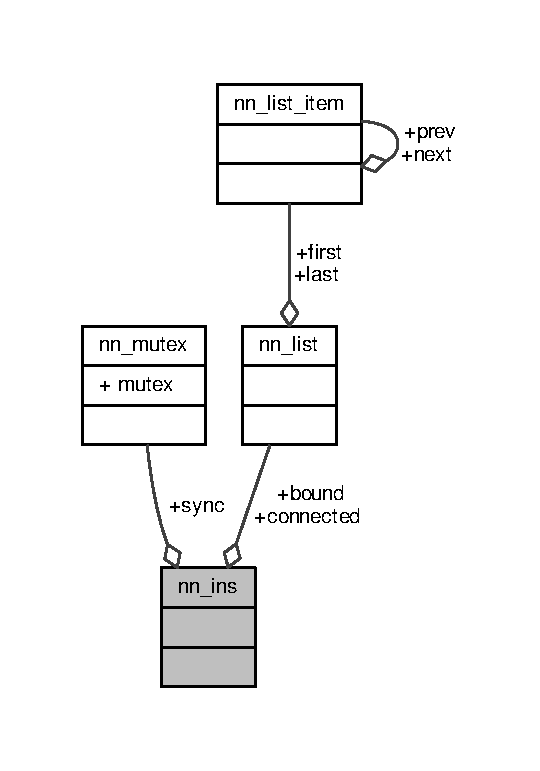
\includegraphics[width=259pt]{structnn__ins__coll__graph}
\end{center}
\end{figure}
\subsection*{Public Attributes}
\begin{DoxyCompactItemize}
\item 
struct \hyperlink{structnn__mutex}{nn\+\_\+mutex} \hyperlink{structnn__ins_a63ed8c2cce745f6dca202806f1db7301}{sync}
\item 
struct \hyperlink{structnn__list}{nn\+\_\+list} \hyperlink{structnn__ins_ad379fd9cffdbb9be945cab8bfeb01e9e}{bound}
\item 
struct \hyperlink{structnn__list}{nn\+\_\+list} \hyperlink{structnn__ins_a4b077905ad4f7970d6c67613daea6988}{connected}
\end{DoxyCompactItemize}


\subsection{Member Data Documentation}
\index{nn\+\_\+ins@{nn\+\_\+ins}!bound@{bound}}
\index{bound@{bound}!nn\+\_\+ins@{nn\+\_\+ins}}
\subsubsection[{bound}]{\setlength{\rightskip}{0pt plus 5cm}struct {\bf nn\+\_\+list} nn\+\_\+ins\+::bound}\hypertarget{structnn__ins_ad379fd9cffdbb9be945cab8bfeb01e9e}{}\label{structnn__ins_ad379fd9cffdbb9be945cab8bfeb01e9e}
\index{nn\+\_\+ins@{nn\+\_\+ins}!connected@{connected}}
\index{connected@{connected}!nn\+\_\+ins@{nn\+\_\+ins}}
\subsubsection[{connected}]{\setlength{\rightskip}{0pt plus 5cm}struct {\bf nn\+\_\+list} nn\+\_\+ins\+::connected}\hypertarget{structnn__ins_a4b077905ad4f7970d6c67613daea6988}{}\label{structnn__ins_a4b077905ad4f7970d6c67613daea6988}
\index{nn\+\_\+ins@{nn\+\_\+ins}!sync@{sync}}
\index{sync@{sync}!nn\+\_\+ins@{nn\+\_\+ins}}
\subsubsection[{sync}]{\setlength{\rightskip}{0pt plus 5cm}struct {\bf nn\+\_\+mutex} nn\+\_\+ins\+::sync}\hypertarget{structnn__ins_a63ed8c2cce745f6dca202806f1db7301}{}\label{structnn__ins_a63ed8c2cce745f6dca202806f1db7301}


The documentation for this struct was generated from the following file\+:\begin{DoxyCompactItemize}
\item 
src/transports/inproc/\hyperlink{ins_8c}{ins.\+c}\end{DoxyCompactItemize}

\hypertarget{structnn__ins__item}{}\section{nn\+\_\+ins\+\_\+item Struct Reference}
\label{structnn__ins__item}\index{nn\+\_\+ins\+\_\+item@{nn\+\_\+ins\+\_\+item}}


{\ttfamily \#include $<$ins.\+h$>$}



Collaboration diagram for nn\+\_\+ins\+\_\+item\+:\nopagebreak
\begin{figure}[H]
\begin{center}
\leavevmode
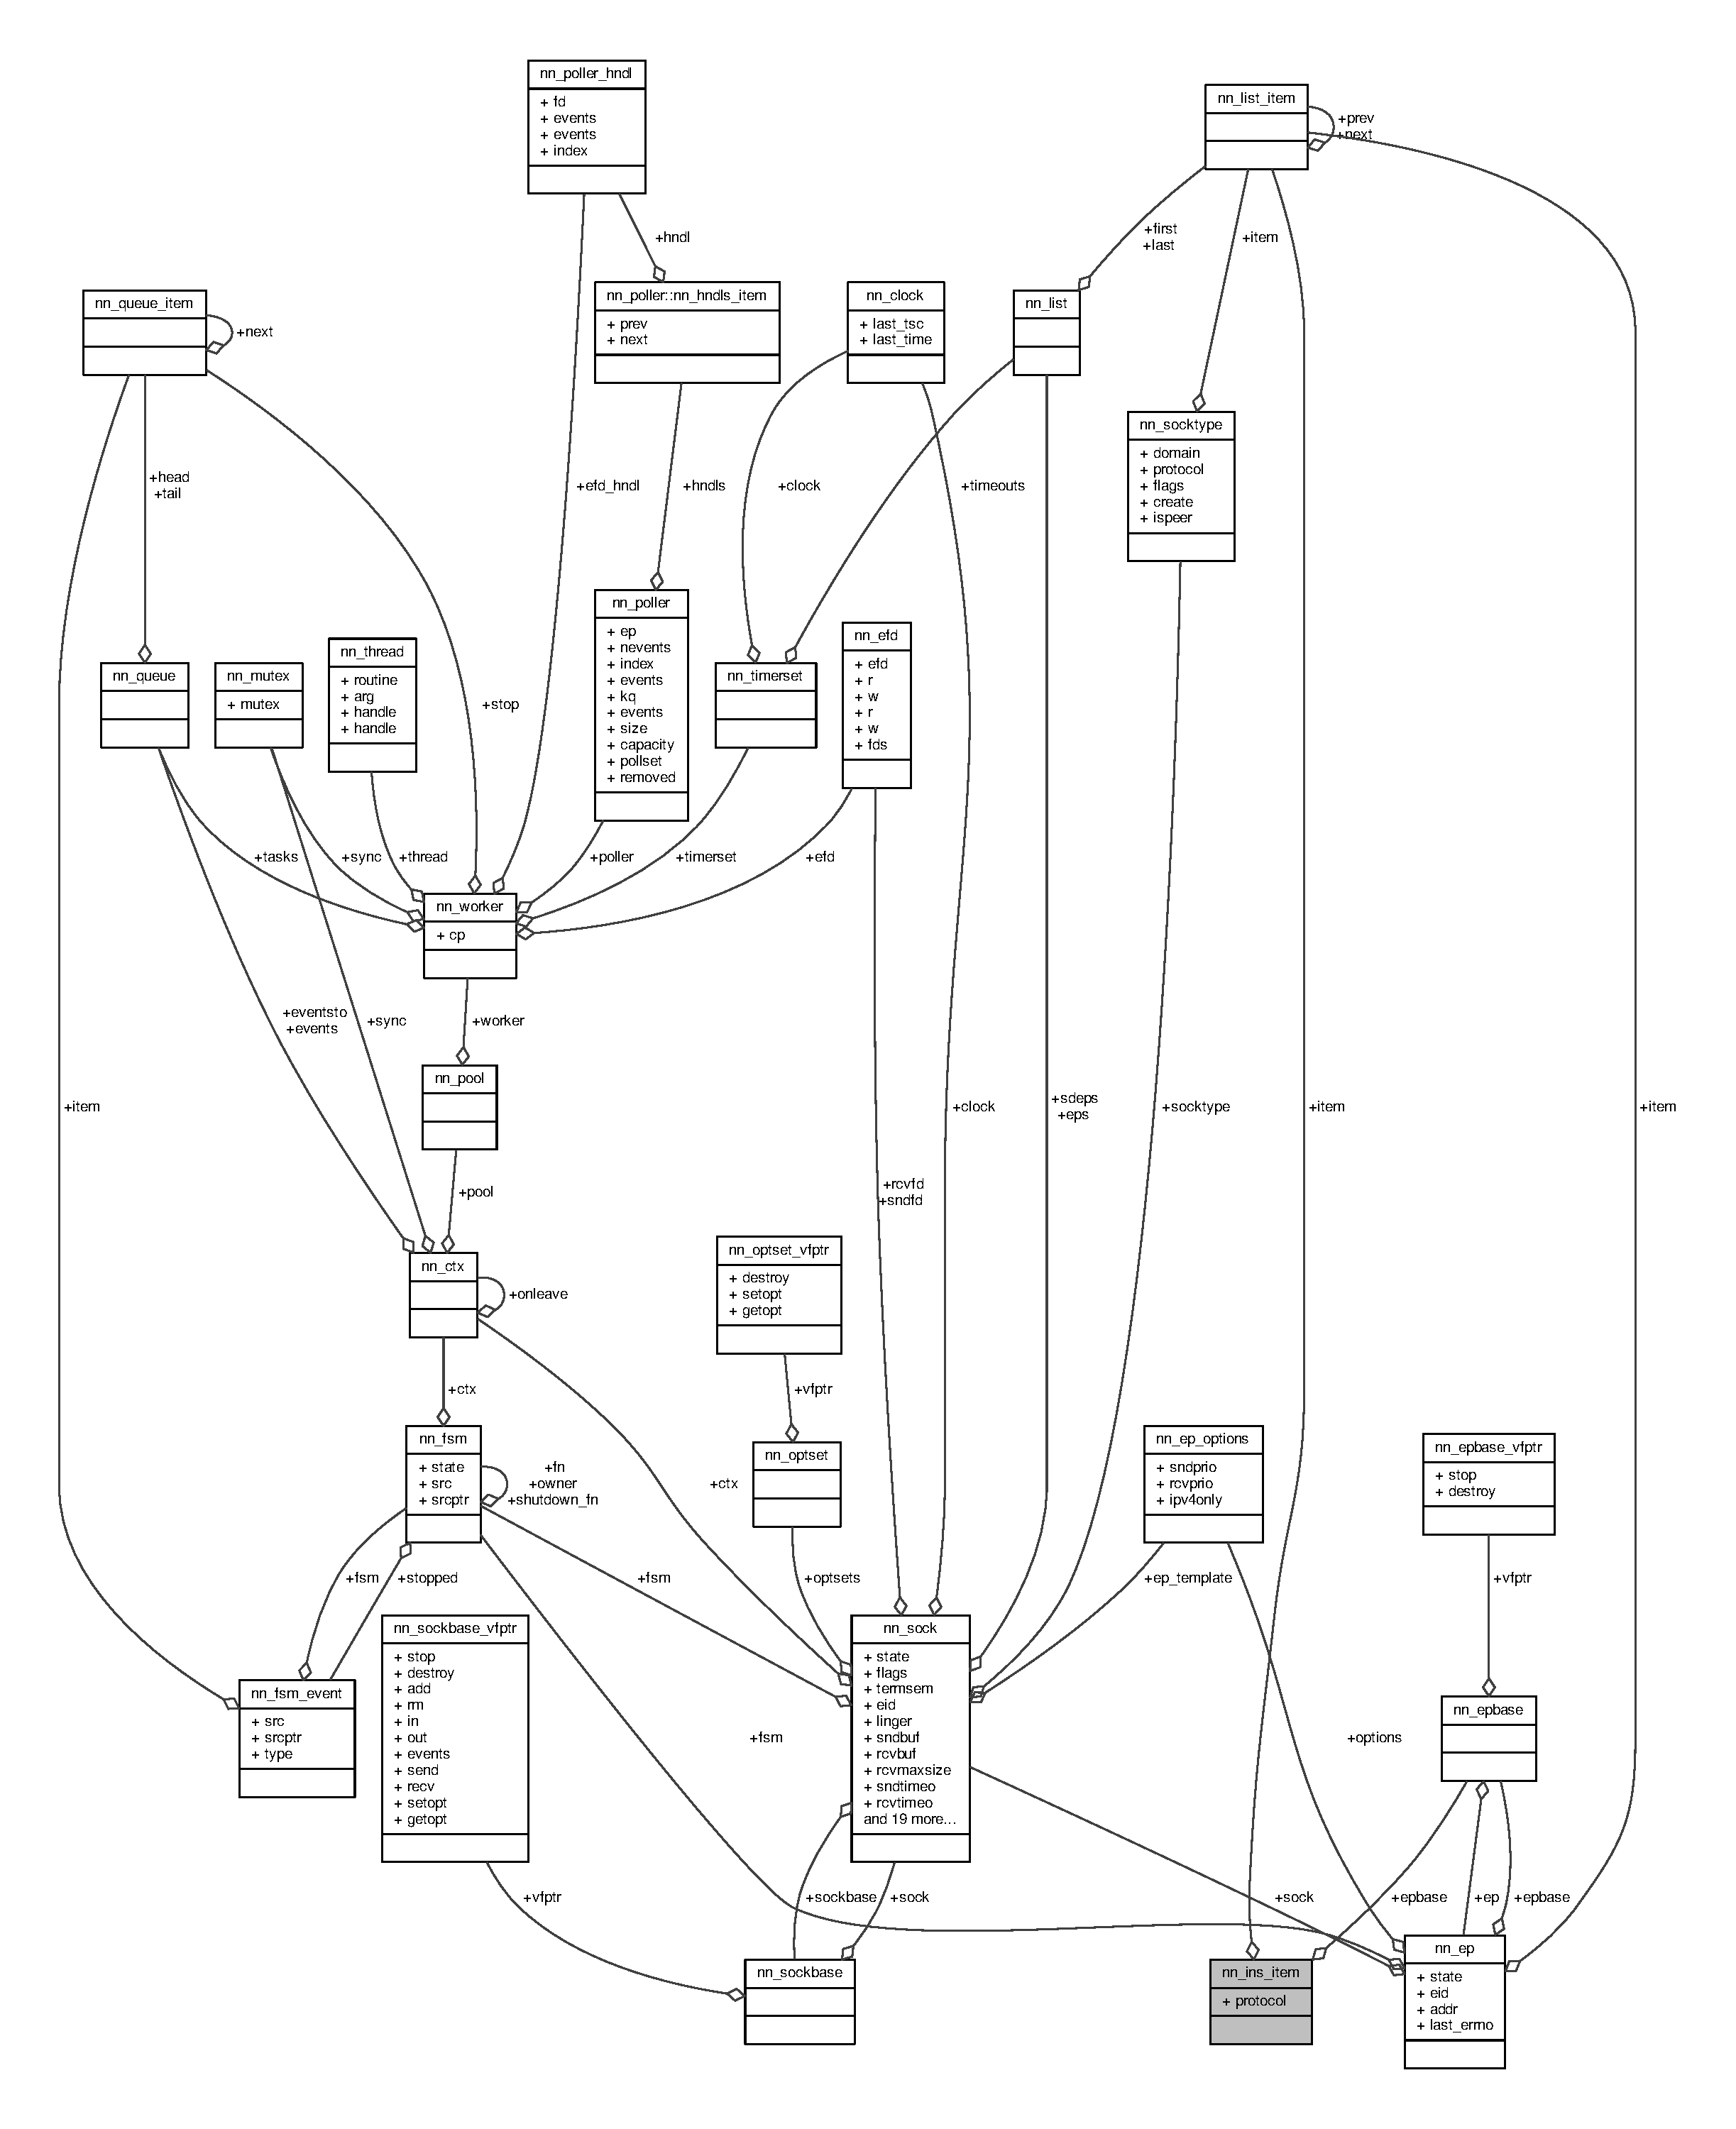
\includegraphics[width=350pt]{structnn__ins__item__coll__graph}
\end{center}
\end{figure}
\subsection*{Public Attributes}
\begin{DoxyCompactItemize}
\item 
struct \hyperlink{structnn__epbase}{nn\+\_\+epbase} \hyperlink{structnn__ins__item_a15a0b556b4f83f7e6e56100240ba447e}{epbase}
\item 
struct \hyperlink{structnn__list__item}{nn\+\_\+list\+\_\+item} \hyperlink{structnn__ins__item_a4bd16a4e13b6fdf31dd4676765c546ef}{item}
\item 
int \hyperlink{structnn__ins__item_a4b7d1b078f05bf6940b8df04dbf50483}{protocol}
\end{DoxyCompactItemize}


\subsection{Member Data Documentation}
\index{nn\+\_\+ins\+\_\+item@{nn\+\_\+ins\+\_\+item}!epbase@{epbase}}
\index{epbase@{epbase}!nn\+\_\+ins\+\_\+item@{nn\+\_\+ins\+\_\+item}}
\subsubsection[{epbase}]{\setlength{\rightskip}{0pt plus 5cm}struct {\bf nn\+\_\+epbase} nn\+\_\+ins\+\_\+item\+::epbase}\hypertarget{structnn__ins__item_a15a0b556b4f83f7e6e56100240ba447e}{}\label{structnn__ins__item_a15a0b556b4f83f7e6e56100240ba447e}
\index{nn\+\_\+ins\+\_\+item@{nn\+\_\+ins\+\_\+item}!item@{item}}
\index{item@{item}!nn\+\_\+ins\+\_\+item@{nn\+\_\+ins\+\_\+item}}
\subsubsection[{item}]{\setlength{\rightskip}{0pt plus 5cm}struct {\bf nn\+\_\+list\+\_\+item} nn\+\_\+ins\+\_\+item\+::item}\hypertarget{structnn__ins__item_a4bd16a4e13b6fdf31dd4676765c546ef}{}\label{structnn__ins__item_a4bd16a4e13b6fdf31dd4676765c546ef}
\index{nn\+\_\+ins\+\_\+item@{nn\+\_\+ins\+\_\+item}!protocol@{protocol}}
\index{protocol@{protocol}!nn\+\_\+ins\+\_\+item@{nn\+\_\+ins\+\_\+item}}
\subsubsection[{protocol}]{\setlength{\rightskip}{0pt plus 5cm}int nn\+\_\+ins\+\_\+item\+::protocol}\hypertarget{structnn__ins__item_a4b7d1b078f05bf6940b8df04dbf50483}{}\label{structnn__ins__item_a4b7d1b078f05bf6940b8df04dbf50483}


The documentation for this struct was generated from the following file\+:\begin{DoxyCompactItemize}
\item 
src/transports/inproc/\hyperlink{ins_8h}{ins.\+h}\end{DoxyCompactItemize}

\hypertarget{structnn__iovec}{}\section{nn\+\_\+iovec Struct Reference}
\label{structnn__iovec}\index{nn\+\_\+iovec@{nn\+\_\+iovec}}


{\ttfamily \#include $<$nn.\+h$>$}



Collaboration diagram for nn\+\_\+iovec\+:\nopagebreak
\begin{figure}[H]
\begin{center}
\leavevmode
\includegraphics[width=144pt]{structnn__iovec__coll__graph}
\end{center}
\end{figure}
\subsection*{Public Attributes}
\begin{DoxyCompactItemize}
\item 
void $\ast$ \hyperlink{structnn__iovec_aab8a89340c00a8222e8659c825afbe7f}{iov\+\_\+base}
\item 
size\+\_\+t \hyperlink{structnn__iovec_ae13415a807909521c74f6776515364b1}{iov\+\_\+len}
\end{DoxyCompactItemize}


\subsection{Member Data Documentation}
\index{nn\+\_\+iovec@{nn\+\_\+iovec}!iov\+\_\+base@{iov\+\_\+base}}
\index{iov\+\_\+base@{iov\+\_\+base}!nn\+\_\+iovec@{nn\+\_\+iovec}}
\subsubsection[{iov\+\_\+base}]{\setlength{\rightskip}{0pt plus 5cm}void$\ast$ nn\+\_\+iovec\+::iov\+\_\+base}\hypertarget{structnn__iovec_aab8a89340c00a8222e8659c825afbe7f}{}\label{structnn__iovec_aab8a89340c00a8222e8659c825afbe7f}
\index{nn\+\_\+iovec@{nn\+\_\+iovec}!iov\+\_\+len@{iov\+\_\+len}}
\index{iov\+\_\+len@{iov\+\_\+len}!nn\+\_\+iovec@{nn\+\_\+iovec}}
\subsubsection[{iov\+\_\+len}]{\setlength{\rightskip}{0pt plus 5cm}size\+\_\+t nn\+\_\+iovec\+::iov\+\_\+len}\hypertarget{structnn__iovec_ae13415a807909521c74f6776515364b1}{}\label{structnn__iovec_ae13415a807909521c74f6776515364b1}


The documentation for this struct was generated from the following file\+:\begin{DoxyCompactItemize}
\item 
src/\hyperlink{nn_8h}{nn.\+h}\end{DoxyCompactItemize}

\hypertarget{structnn__lb}{}\section{nn\+\_\+lb Struct Reference}
\label{structnn__lb}\index{nn\+\_\+lb@{nn\+\_\+lb}}


{\ttfamily \#include $<$lb.\+h$>$}



Collaboration diagram for nn\+\_\+lb\+:\nopagebreak
\begin{figure}[H]
\begin{center}
\leavevmode
\includegraphics[height=550pt]{structnn__lb__coll__graph}
\end{center}
\end{figure}
\subsection*{Public Attributes}
\begin{DoxyCompactItemize}
\item 
struct \hyperlink{structnn__priolist}{nn\+\_\+priolist} \hyperlink{structnn__lb_a2bd049c96526c0c0423611d6a6843926}{priolist}
\end{DoxyCompactItemize}


\subsection{Member Data Documentation}
\index{nn\+\_\+lb@{nn\+\_\+lb}!priolist@{priolist}}
\index{priolist@{priolist}!nn\+\_\+lb@{nn\+\_\+lb}}
\subsubsection[{priolist}]{\setlength{\rightskip}{0pt plus 5cm}struct {\bf nn\+\_\+priolist} nn\+\_\+lb\+::priolist}\hypertarget{structnn__lb_a2bd049c96526c0c0423611d6a6843926}{}\label{structnn__lb_a2bd049c96526c0c0423611d6a6843926}


The documentation for this struct was generated from the following file\+:\begin{DoxyCompactItemize}
\item 
src/protocols/utils/\hyperlink{lb_8h}{lb.\+h}\end{DoxyCompactItemize}

\hypertarget{structnn__lb__data}{}\section{nn\+\_\+lb\+\_\+data Struct Reference}
\label{structnn__lb__data}\index{nn\+\_\+lb\+\_\+data@{nn\+\_\+lb\+\_\+data}}


{\ttfamily \#include $<$lb.\+h$>$}



Collaboration diagram for nn\+\_\+lb\+\_\+data\+:\nopagebreak
\begin{figure}[H]
\begin{center}
\leavevmode
\includegraphics[width=202pt]{structnn__lb__data__coll__graph}
\end{center}
\end{figure}
\subsection*{Public Attributes}
\begin{DoxyCompactItemize}
\item 
struct \hyperlink{structnn__priolist__data}{nn\+\_\+priolist\+\_\+data} \hyperlink{structnn__lb__data_af6e25c0a43dee66626f73ae3055d4688}{priodata}
\end{DoxyCompactItemize}


\subsection{Member Data Documentation}
\index{nn\+\_\+lb\+\_\+data@{nn\+\_\+lb\+\_\+data}!priodata@{priodata}}
\index{priodata@{priodata}!nn\+\_\+lb\+\_\+data@{nn\+\_\+lb\+\_\+data}}
\subsubsection[{priodata}]{\setlength{\rightskip}{0pt plus 5cm}struct {\bf nn\+\_\+priolist\+\_\+data} nn\+\_\+lb\+\_\+data\+::priodata}\hypertarget{structnn__lb__data_af6e25c0a43dee66626f73ae3055d4688}{}\label{structnn__lb__data_af6e25c0a43dee66626f73ae3055d4688}


The documentation for this struct was generated from the following file\+:\begin{DoxyCompactItemize}
\item 
src/protocols/utils/\hyperlink{lb_8h}{lb.\+h}\end{DoxyCompactItemize}

\hypertarget{structnn__list}{}\section{nn\+\_\+list Struct Reference}
\label{structnn__list}\index{nn\+\_\+list@{nn\+\_\+list}}


{\ttfamily \#include $<$list.\+h$>$}



Collaboration diagram for nn\+\_\+list\+:\nopagebreak
\begin{figure}[H]
\begin{center}
\leavevmode
\includegraphics[width=194pt]{structnn__list__coll__graph}
\end{center}
\end{figure}
\subsection*{Public Attributes}
\begin{DoxyCompactItemize}
\item 
struct \hyperlink{structnn__list__item}{nn\+\_\+list\+\_\+item} $\ast$ \hyperlink{structnn__list_a98de32a9535052c37fd08fa23c974e8e}{first}
\item 
struct \hyperlink{structnn__list__item}{nn\+\_\+list\+\_\+item} $\ast$ \hyperlink{structnn__list_aee15a11389419a66b183b0246a3e4683}{last}
\end{DoxyCompactItemize}


\subsection{Member Data Documentation}
\index{nn\+\_\+list@{nn\+\_\+list}!first@{first}}
\index{first@{first}!nn\+\_\+list@{nn\+\_\+list}}
\subsubsection[{first}]{\setlength{\rightskip}{0pt plus 5cm}struct {\bf nn\+\_\+list\+\_\+item}$\ast$ nn\+\_\+list\+::first}\hypertarget{structnn__list_a98de32a9535052c37fd08fa23c974e8e}{}\label{structnn__list_a98de32a9535052c37fd08fa23c974e8e}
\index{nn\+\_\+list@{nn\+\_\+list}!last@{last}}
\index{last@{last}!nn\+\_\+list@{nn\+\_\+list}}
\subsubsection[{last}]{\setlength{\rightskip}{0pt plus 5cm}struct {\bf nn\+\_\+list\+\_\+item}$\ast$ nn\+\_\+list\+::last}\hypertarget{structnn__list_aee15a11389419a66b183b0246a3e4683}{}\label{structnn__list_aee15a11389419a66b183b0246a3e4683}


The documentation for this struct was generated from the following file\+:\begin{DoxyCompactItemize}
\item 
src/utils/\hyperlink{list_8h}{list.\+h}\end{DoxyCompactItemize}

\hypertarget{structnn__list__item}{}\section{nn\+\_\+list\+\_\+item Struct Reference}
\label{structnn__list__item}\index{nn\+\_\+list\+\_\+item@{nn\+\_\+list\+\_\+item}}


{\ttfamily \#include $<$list.\+h$>$}



Collaboration diagram for nn\+\_\+list\+\_\+item\+:\nopagebreak
\begin{figure}[H]
\begin{center}
\leavevmode
\includegraphics[width=194pt]{structnn__list__item__coll__graph}
\end{center}
\end{figure}
\subsection*{Public Attributes}
\begin{DoxyCompactItemize}
\item 
struct \hyperlink{structnn__list__item}{nn\+\_\+list\+\_\+item} $\ast$ \hyperlink{structnn__list__item_aeeacd653dc43eb9b8b75a71d3839e04c}{next}
\item 
struct \hyperlink{structnn__list__item}{nn\+\_\+list\+\_\+item} $\ast$ \hyperlink{structnn__list__item_ac6050ca0b2db2385edf95926b9103ea2}{prev}
\end{DoxyCompactItemize}


\subsection{Member Data Documentation}
\index{nn\+\_\+list\+\_\+item@{nn\+\_\+list\+\_\+item}!next@{next}}
\index{next@{next}!nn\+\_\+list\+\_\+item@{nn\+\_\+list\+\_\+item}}
\subsubsection[{next}]{\setlength{\rightskip}{0pt plus 5cm}struct {\bf nn\+\_\+list\+\_\+item}$\ast$ nn\+\_\+list\+\_\+item\+::next}\hypertarget{structnn__list__item_aeeacd653dc43eb9b8b75a71d3839e04c}{}\label{structnn__list__item_aeeacd653dc43eb9b8b75a71d3839e04c}
\index{nn\+\_\+list\+\_\+item@{nn\+\_\+list\+\_\+item}!prev@{prev}}
\index{prev@{prev}!nn\+\_\+list\+\_\+item@{nn\+\_\+list\+\_\+item}}
\subsubsection[{prev}]{\setlength{\rightskip}{0pt plus 5cm}struct {\bf nn\+\_\+list\+\_\+item}$\ast$ nn\+\_\+list\+\_\+item\+::prev}\hypertarget{structnn__list__item_ac6050ca0b2db2385edf95926b9103ea2}{}\label{structnn__list__item_ac6050ca0b2db2385edf95926b9103ea2}


The documentation for this struct was generated from the following file\+:\begin{DoxyCompactItemize}
\item 
src/utils/\hyperlink{list_8h}{list.\+h}\end{DoxyCompactItemize}

\hypertarget{structnn__msg}{}\section{nn\+\_\+msg Struct Reference}
\label{structnn__msg}\index{nn\+\_\+msg@{nn\+\_\+msg}}


{\ttfamily \#include $<$msg.\+h$>$}



Collaboration diagram for nn\+\_\+msg\+:\nopagebreak
\begin{figure}[H]
\begin{center}
\leavevmode
\includegraphics[width=150pt]{structnn__msg__coll__graph}
\end{center}
\end{figure}
\subsection*{Public Attributes}
\begin{DoxyCompactItemize}
\item 
struct \hyperlink{structnn__chunkref}{nn\+\_\+chunkref} \hyperlink{structnn__msg_abcd1120a337ed2957e733a0f829a2563}{sphdr}
\item 
struct \hyperlink{structnn__chunkref}{nn\+\_\+chunkref} \hyperlink{structnn__msg_a79cb5562faf3e56ba7922ff9beec621d}{hdrs}
\item 
struct \hyperlink{structnn__chunkref}{nn\+\_\+chunkref} \hyperlink{structnn__msg_ac52dbfdec4cf8d5a0b93d91a4375fd9f}{body}
\end{DoxyCompactItemize}


\subsection{Member Data Documentation}
\index{nn\+\_\+msg@{nn\+\_\+msg}!body@{body}}
\index{body@{body}!nn\+\_\+msg@{nn\+\_\+msg}}
\subsubsection[{body}]{\setlength{\rightskip}{0pt plus 5cm}struct {\bf nn\+\_\+chunkref} nn\+\_\+msg\+::body}\hypertarget{structnn__msg_ac52dbfdec4cf8d5a0b93d91a4375fd9f}{}\label{structnn__msg_ac52dbfdec4cf8d5a0b93d91a4375fd9f}
\index{nn\+\_\+msg@{nn\+\_\+msg}!hdrs@{hdrs}}
\index{hdrs@{hdrs}!nn\+\_\+msg@{nn\+\_\+msg}}
\subsubsection[{hdrs}]{\setlength{\rightskip}{0pt plus 5cm}struct {\bf nn\+\_\+chunkref} nn\+\_\+msg\+::hdrs}\hypertarget{structnn__msg_a79cb5562faf3e56ba7922ff9beec621d}{}\label{structnn__msg_a79cb5562faf3e56ba7922ff9beec621d}
\index{nn\+\_\+msg@{nn\+\_\+msg}!sphdr@{sphdr}}
\index{sphdr@{sphdr}!nn\+\_\+msg@{nn\+\_\+msg}}
\subsubsection[{sphdr}]{\setlength{\rightskip}{0pt plus 5cm}struct {\bf nn\+\_\+chunkref} nn\+\_\+msg\+::sphdr}\hypertarget{structnn__msg_abcd1120a337ed2957e733a0f829a2563}{}\label{structnn__msg_abcd1120a337ed2957e733a0f829a2563}


The documentation for this struct was generated from the following file\+:\begin{DoxyCompactItemize}
\item 
src/utils/\hyperlink{msg_8h}{msg.\+h}\end{DoxyCompactItemize}

\hypertarget{structnn__msghdr}{}\section{nn\+\_\+msghdr Struct Reference}
\label{structnn__msghdr}\index{nn\+\_\+msghdr@{nn\+\_\+msghdr}}


{\ttfamily \#include $<$nn.\+h$>$}



Collaboration diagram for nn\+\_\+msghdr\+:\nopagebreak
\begin{figure}[H]
\begin{center}
\leavevmode
\includegraphics[width=172pt]{structnn__msghdr__coll__graph}
\end{center}
\end{figure}
\subsection*{Public Attributes}
\begin{DoxyCompactItemize}
\item 
struct \hyperlink{structnn__iovec}{nn\+\_\+iovec} $\ast$ \hyperlink{structnn__msghdr_ad1f1c756e54ba58d8263e6ec4d00cf28}{msg\+\_\+iov}
\item 
int \hyperlink{structnn__msghdr_a0cf9a6f1b92f55a55f0ccc0184f6ff3b}{msg\+\_\+iovlen}
\item 
void $\ast$ \hyperlink{structnn__msghdr_aefe793fcf0d1b3d858e7fc8eaf1325eb}{msg\+\_\+control}
\item 
size\+\_\+t \hyperlink{structnn__msghdr_a100313e447a48a9514790be57cd799a6}{msg\+\_\+controllen}
\end{DoxyCompactItemize}


\subsection{Member Data Documentation}
\index{nn\+\_\+msghdr@{nn\+\_\+msghdr}!msg\+\_\+control@{msg\+\_\+control}}
\index{msg\+\_\+control@{msg\+\_\+control}!nn\+\_\+msghdr@{nn\+\_\+msghdr}}
\subsubsection[{msg\+\_\+control}]{\setlength{\rightskip}{0pt plus 5cm}void$\ast$ nn\+\_\+msghdr\+::msg\+\_\+control}\hypertarget{structnn__msghdr_aefe793fcf0d1b3d858e7fc8eaf1325eb}{}\label{structnn__msghdr_aefe793fcf0d1b3d858e7fc8eaf1325eb}
\index{nn\+\_\+msghdr@{nn\+\_\+msghdr}!msg\+\_\+controllen@{msg\+\_\+controllen}}
\index{msg\+\_\+controllen@{msg\+\_\+controllen}!nn\+\_\+msghdr@{nn\+\_\+msghdr}}
\subsubsection[{msg\+\_\+controllen}]{\setlength{\rightskip}{0pt plus 5cm}size\+\_\+t nn\+\_\+msghdr\+::msg\+\_\+controllen}\hypertarget{structnn__msghdr_a100313e447a48a9514790be57cd799a6}{}\label{structnn__msghdr_a100313e447a48a9514790be57cd799a6}
\index{nn\+\_\+msghdr@{nn\+\_\+msghdr}!msg\+\_\+iov@{msg\+\_\+iov}}
\index{msg\+\_\+iov@{msg\+\_\+iov}!nn\+\_\+msghdr@{nn\+\_\+msghdr}}
\subsubsection[{msg\+\_\+iov}]{\setlength{\rightskip}{0pt plus 5cm}struct {\bf nn\+\_\+iovec}$\ast$ nn\+\_\+msghdr\+::msg\+\_\+iov}\hypertarget{structnn__msghdr_ad1f1c756e54ba58d8263e6ec4d00cf28}{}\label{structnn__msghdr_ad1f1c756e54ba58d8263e6ec4d00cf28}
\index{nn\+\_\+msghdr@{nn\+\_\+msghdr}!msg\+\_\+iovlen@{msg\+\_\+iovlen}}
\index{msg\+\_\+iovlen@{msg\+\_\+iovlen}!nn\+\_\+msghdr@{nn\+\_\+msghdr}}
\subsubsection[{msg\+\_\+iovlen}]{\setlength{\rightskip}{0pt plus 5cm}int nn\+\_\+msghdr\+::msg\+\_\+iovlen}\hypertarget{structnn__msghdr_a0cf9a6f1b92f55a55f0ccc0184f6ff3b}{}\label{structnn__msghdr_a0cf9a6f1b92f55a55f0ccc0184f6ff3b}


The documentation for this struct was generated from the following file\+:\begin{DoxyCompactItemize}
\item 
src/\hyperlink{nn_8h}{nn.\+h}\end{DoxyCompactItemize}

\hypertarget{structnn__msgqueue}{}\section{nn\+\_\+msgqueue Struct Reference}
\label{structnn__msgqueue}\index{nn\+\_\+msgqueue@{nn\+\_\+msgqueue}}


{\ttfamily \#include $<$msgqueue.\+h$>$}



Collaboration diagram for nn\+\_\+msgqueue\+:\nopagebreak
\begin{figure}[H]
\begin{center}
\leavevmode
\includegraphics[height=550pt]{structnn__msgqueue__coll__graph}
\end{center}
\end{figure}
\subsection*{Public Attributes}
\begin{DoxyCompactItemize}
\item 
\begin{tabbing}
xx\=xx\=xx\=xx\=xx\=xx\=xx\=xx\=xx\=\kill
struct \{\\
\>struct \hyperlink{structnn__msgqueue__chunk}{nn\_msgqueue\_chunk} $\ast$ \hyperlink{structnn__msgqueue_a57b0ce10a1e3ba159bb3e05e9e25ea57}{chunk}\\
\>int \hyperlink{structnn__msgqueue_a3714414d2aad4d30b34bc8c3bd865003}{pos}\\
\} \hyperlink{structnn__msgqueue_a752f1190a9edc8818dbb980ce7b849f3}{out}\\

\end{tabbing}\item 
\begin{tabbing}
xx\=xx\=xx\=xx\=xx\=xx\=xx\=xx\=xx\=\kill
struct \{\\
\>struct \hyperlink{structnn__msgqueue__chunk}{nn\_msgqueue\_chunk} $\ast$ \hyperlink{structnn__msgqueue_a57b0ce10a1e3ba159bb3e05e9e25ea57}{chunk}\\
\>int \hyperlink{structnn__msgqueue_a3714414d2aad4d30b34bc8c3bd865003}{pos}\\
\} \hyperlink{structnn__msgqueue_a86267100cce5ad85aa85a23c07a5cbf6}{in}\\

\end{tabbing}\item 
size\+\_\+t \hyperlink{structnn__msgqueue_aaa463916bbe4482be01ce84444383cfd}{count}
\item 
size\+\_\+t \hyperlink{structnn__msgqueue_afd34fe72790a56ba9d99681fd2024b6c}{mem}
\item 
size\+\_\+t \hyperlink{structnn__msgqueue_a1989a55354b0a334168696d9c1b3e29b}{maxmem}
\item 
struct \hyperlink{structnn__msgqueue__chunk}{nn\+\_\+msgqueue\+\_\+chunk} $\ast$ \hyperlink{structnn__msgqueue_a4e886b7d4c87b147648980f4af8befa3}{cache}
\end{DoxyCompactItemize}


\subsection{Member Data Documentation}
\index{nn\+\_\+msgqueue@{nn\+\_\+msgqueue}!cache@{cache}}
\index{cache@{cache}!nn\+\_\+msgqueue@{nn\+\_\+msgqueue}}
\subsubsection[{cache}]{\setlength{\rightskip}{0pt plus 5cm}struct {\bf nn\+\_\+msgqueue\+\_\+chunk}$\ast$ nn\+\_\+msgqueue\+::cache}\hypertarget{structnn__msgqueue_a4e886b7d4c87b147648980f4af8befa3}{}\label{structnn__msgqueue_a4e886b7d4c87b147648980f4af8befa3}
\index{nn\+\_\+msgqueue@{nn\+\_\+msgqueue}!chunk@{chunk}}
\index{chunk@{chunk}!nn\+\_\+msgqueue@{nn\+\_\+msgqueue}}
\subsubsection[{chunk}]{\setlength{\rightskip}{0pt plus 5cm}struct {\bf nn\+\_\+msgqueue\+\_\+chunk}$\ast$ nn\+\_\+msgqueue\+::chunk}\hypertarget{structnn__msgqueue_a57b0ce10a1e3ba159bb3e05e9e25ea57}{}\label{structnn__msgqueue_a57b0ce10a1e3ba159bb3e05e9e25ea57}
\index{nn\+\_\+msgqueue@{nn\+\_\+msgqueue}!count@{count}}
\index{count@{count}!nn\+\_\+msgqueue@{nn\+\_\+msgqueue}}
\subsubsection[{count}]{\setlength{\rightskip}{0pt plus 5cm}size\+\_\+t nn\+\_\+msgqueue\+::count}\hypertarget{structnn__msgqueue_aaa463916bbe4482be01ce84444383cfd}{}\label{structnn__msgqueue_aaa463916bbe4482be01ce84444383cfd}
\index{nn\+\_\+msgqueue@{nn\+\_\+msgqueue}!in@{in}}
\index{in@{in}!nn\+\_\+msgqueue@{nn\+\_\+msgqueue}}
\subsubsection[{in}]{\setlength{\rightskip}{0pt plus 5cm}struct \{ ... \}   nn\+\_\+msgqueue\+::in}\hypertarget{structnn__msgqueue_a86267100cce5ad85aa85a23c07a5cbf6}{}\label{structnn__msgqueue_a86267100cce5ad85aa85a23c07a5cbf6}
\index{nn\+\_\+msgqueue@{nn\+\_\+msgqueue}!maxmem@{maxmem}}
\index{maxmem@{maxmem}!nn\+\_\+msgqueue@{nn\+\_\+msgqueue}}
\subsubsection[{maxmem}]{\setlength{\rightskip}{0pt plus 5cm}size\+\_\+t nn\+\_\+msgqueue\+::maxmem}\hypertarget{structnn__msgqueue_a1989a55354b0a334168696d9c1b3e29b}{}\label{structnn__msgqueue_a1989a55354b0a334168696d9c1b3e29b}
\index{nn\+\_\+msgqueue@{nn\+\_\+msgqueue}!mem@{mem}}
\index{mem@{mem}!nn\+\_\+msgqueue@{nn\+\_\+msgqueue}}
\subsubsection[{mem}]{\setlength{\rightskip}{0pt plus 5cm}size\+\_\+t nn\+\_\+msgqueue\+::mem}\hypertarget{structnn__msgqueue_afd34fe72790a56ba9d99681fd2024b6c}{}\label{structnn__msgqueue_afd34fe72790a56ba9d99681fd2024b6c}
\index{nn\+\_\+msgqueue@{nn\+\_\+msgqueue}!out@{out}}
\index{out@{out}!nn\+\_\+msgqueue@{nn\+\_\+msgqueue}}
\subsubsection[{out}]{\setlength{\rightskip}{0pt plus 5cm}struct \{ ... \}   nn\+\_\+msgqueue\+::out}\hypertarget{structnn__msgqueue_a752f1190a9edc8818dbb980ce7b849f3}{}\label{structnn__msgqueue_a752f1190a9edc8818dbb980ce7b849f3}
\index{nn\+\_\+msgqueue@{nn\+\_\+msgqueue}!pos@{pos}}
\index{pos@{pos}!nn\+\_\+msgqueue@{nn\+\_\+msgqueue}}
\subsubsection[{pos}]{\setlength{\rightskip}{0pt plus 5cm}int nn\+\_\+msgqueue\+::pos}\hypertarget{structnn__msgqueue_a3714414d2aad4d30b34bc8c3bd865003}{}\label{structnn__msgqueue_a3714414d2aad4d30b34bc8c3bd865003}


The documentation for this struct was generated from the following file\+:\begin{DoxyCompactItemize}
\item 
src/transports/inproc/\hyperlink{msgqueue_8h}{msgqueue.\+h}\end{DoxyCompactItemize}

\hypertarget{structnn__msgqueue__chunk}{}\section{nn\+\_\+msgqueue\+\_\+chunk Struct Reference}
\label{structnn__msgqueue__chunk}\index{nn\+\_\+msgqueue\+\_\+chunk@{nn\+\_\+msgqueue\+\_\+chunk}}


{\ttfamily \#include $<$msgqueue.\+h$>$}



Collaboration diagram for nn\+\_\+msgqueue\+\_\+chunk\+:\nopagebreak
\begin{figure}[H]
\begin{center}
\leavevmode
\includegraphics[width=234pt]{structnn__msgqueue__chunk__coll__graph}
\end{center}
\end{figure}
\subsection*{Public Attributes}
\begin{DoxyCompactItemize}
\item 
struct \hyperlink{structnn__msg}{nn\+\_\+msg} \hyperlink{structnn__msgqueue__chunk_a69bcf939f933f7711a47618ecb936e2b}{msgs} \mbox{[}\hyperlink{msgqueue_8h_a13fd89d03f816db3fdc589dfb3c706ff}{N\+N\+\_\+\+M\+S\+G\+Q\+U\+E\+U\+E\+\_\+\+G\+R\+A\+N\+U\+L\+A\+R\+I\+TY}\mbox{]}
\item 
struct \hyperlink{structnn__msgqueue__chunk}{nn\+\_\+msgqueue\+\_\+chunk} $\ast$ \hyperlink{structnn__msgqueue__chunk_aa539574be0f7c15d30f2c0920b3586a1}{next}
\end{DoxyCompactItemize}


\subsection{Member Data Documentation}
\index{nn\+\_\+msgqueue\+\_\+chunk@{nn\+\_\+msgqueue\+\_\+chunk}!msgs@{msgs}}
\index{msgs@{msgs}!nn\+\_\+msgqueue\+\_\+chunk@{nn\+\_\+msgqueue\+\_\+chunk}}
\subsubsection[{msgs}]{\setlength{\rightskip}{0pt plus 5cm}struct {\bf nn\+\_\+msg} nn\+\_\+msgqueue\+\_\+chunk\+::msgs\mbox{[}{\bf N\+N\+\_\+\+M\+S\+G\+Q\+U\+E\+U\+E\+\_\+\+G\+R\+A\+N\+U\+L\+A\+R\+I\+TY}\mbox{]}}\hypertarget{structnn__msgqueue__chunk_a69bcf939f933f7711a47618ecb936e2b}{}\label{structnn__msgqueue__chunk_a69bcf939f933f7711a47618ecb936e2b}
\index{nn\+\_\+msgqueue\+\_\+chunk@{nn\+\_\+msgqueue\+\_\+chunk}!next@{next}}
\index{next@{next}!nn\+\_\+msgqueue\+\_\+chunk@{nn\+\_\+msgqueue\+\_\+chunk}}
\subsubsection[{next}]{\setlength{\rightskip}{0pt plus 5cm}struct {\bf nn\+\_\+msgqueue\+\_\+chunk}$\ast$ nn\+\_\+msgqueue\+\_\+chunk\+::next}\hypertarget{structnn__msgqueue__chunk_aa539574be0f7c15d30f2c0920b3586a1}{}\label{structnn__msgqueue__chunk_aa539574be0f7c15d30f2c0920b3586a1}


The documentation for this struct was generated from the following file\+:\begin{DoxyCompactItemize}
\item 
src/transports/inproc/\hyperlink{msgqueue_8h}{msgqueue.\+h}\end{DoxyCompactItemize}

\hypertarget{structnn__mutex}{}\section{nn\+\_\+mutex Struct Reference}
\label{structnn__mutex}\index{nn\+\_\+mutex@{nn\+\_\+mutex}}


{\ttfamily \#include $<$mutex.\+h$>$}



Collaboration diagram for nn\+\_\+mutex\+:\nopagebreak
\begin{figure}[H]
\begin{center}
\leavevmode
\includegraphics[width=138pt]{structnn__mutex__coll__graph}
\end{center}
\end{figure}
\subsection*{Public Attributes}
\begin{DoxyCompactItemize}
\item 
pthread\+\_\+mutex\+\_\+t \hyperlink{structnn__mutex_a8fcb2bd2eb9fb48a29e362321360a9ec}{mutex}
\end{DoxyCompactItemize}


\subsection{Member Data Documentation}
\index{nn\+\_\+mutex@{nn\+\_\+mutex}!mutex@{mutex}}
\index{mutex@{mutex}!nn\+\_\+mutex@{nn\+\_\+mutex}}
\subsubsection[{mutex}]{\setlength{\rightskip}{0pt plus 5cm}pthread\+\_\+mutex\+\_\+t nn\+\_\+mutex\+::mutex}\hypertarget{structnn__mutex_a8fcb2bd2eb9fb48a29e362321360a9ec}{}\label{structnn__mutex_a8fcb2bd2eb9fb48a29e362321360a9ec}


The documentation for this struct was generated from the following file\+:\begin{DoxyCompactItemize}
\item 
src/utils/\hyperlink{mutex_8h}{mutex.\+h}\end{DoxyCompactItemize}

\hypertarget{structnn__optset}{}\section{nn\+\_\+optset Struct Reference}
\label{structnn__optset}\index{nn\+\_\+optset@{nn\+\_\+optset}}


{\ttfamily \#include $<$transport.\+h$>$}



Collaboration diagram for nn\+\_\+optset\+:\nopagebreak
\begin{figure}[H]
\begin{center}
\leavevmode
\includegraphics[width=164pt]{structnn__optset__coll__graph}
\end{center}
\end{figure}
\subsection*{Public Attributes}
\begin{DoxyCompactItemize}
\item 
const struct \hyperlink{structnn__optset__vfptr}{nn\+\_\+optset\+\_\+vfptr} $\ast$ \hyperlink{structnn__optset_a71dc561d46ade3014abd1e81dd3adcb3}{vfptr}
\end{DoxyCompactItemize}


\subsection{Member Data Documentation}
\index{nn\+\_\+optset@{nn\+\_\+optset}!vfptr@{vfptr}}
\index{vfptr@{vfptr}!nn\+\_\+optset@{nn\+\_\+optset}}
\subsubsection[{vfptr}]{\setlength{\rightskip}{0pt plus 5cm}const struct {\bf nn\+\_\+optset\+\_\+vfptr}$\ast$ nn\+\_\+optset\+::vfptr}\hypertarget{structnn__optset_a71dc561d46ade3014abd1e81dd3adcb3}{}\label{structnn__optset_a71dc561d46ade3014abd1e81dd3adcb3}


The documentation for this struct was generated from the following file\+:\begin{DoxyCompactItemize}
\item 
src/\hyperlink{transport_8h}{transport.\+h}\end{DoxyCompactItemize}

\hypertarget{structnn__optset__vfptr}{}\section{nn\+\_\+optset\+\_\+vfptr Struct Reference}
\label{structnn__optset__vfptr}\index{nn\+\_\+optset\+\_\+vfptr@{nn\+\_\+optset\+\_\+vfptr}}


{\ttfamily \#include $<$transport.\+h$>$}



Collaboration diagram for nn\+\_\+optset\+\_\+vfptr\+:\nopagebreak
\begin{figure}[H]
\begin{center}
\leavevmode
\includegraphics[width=164pt]{structnn__optset__vfptr__coll__graph}
\end{center}
\end{figure}
\subsection*{Public Attributes}
\begin{DoxyCompactItemize}
\item 
void($\ast$ \hyperlink{structnn__optset__vfptr_a74db5716dbfea0adbf69448f26804cc0}{destroy} )(struct \hyperlink{structnn__optset}{nn\+\_\+optset} $\ast$self)
\item 
int($\ast$ \hyperlink{structnn__optset__vfptr_a5a978c6140bb775abc02fcdf9456b60a}{setopt} )(struct \hyperlink{structnn__optset}{nn\+\_\+optset} $\ast$self, int option, const void $\ast$optval, size\+\_\+t optvallen)
\item 
int($\ast$ \hyperlink{structnn__optset__vfptr_a1e222a6d339ed4c930ab046bb61d77a0}{getopt} )(struct \hyperlink{structnn__optset}{nn\+\_\+optset} $\ast$self, int option, void $\ast$optval, size\+\_\+t $\ast$optvallen)
\end{DoxyCompactItemize}


\subsection{Member Data Documentation}
\index{nn\+\_\+optset\+\_\+vfptr@{nn\+\_\+optset\+\_\+vfptr}!destroy@{destroy}}
\index{destroy@{destroy}!nn\+\_\+optset\+\_\+vfptr@{nn\+\_\+optset\+\_\+vfptr}}
\subsubsection[{destroy}]{\setlength{\rightskip}{0pt plus 5cm}void($\ast$ nn\+\_\+optset\+\_\+vfptr\+::destroy) (struct {\bf nn\+\_\+optset} $\ast$self)}\hypertarget{structnn__optset__vfptr_a74db5716dbfea0adbf69448f26804cc0}{}\label{structnn__optset__vfptr_a74db5716dbfea0adbf69448f26804cc0}
\index{nn\+\_\+optset\+\_\+vfptr@{nn\+\_\+optset\+\_\+vfptr}!getopt@{getopt}}
\index{getopt@{getopt}!nn\+\_\+optset\+\_\+vfptr@{nn\+\_\+optset\+\_\+vfptr}}
\subsubsection[{getopt}]{\setlength{\rightskip}{0pt plus 5cm}int($\ast$ nn\+\_\+optset\+\_\+vfptr\+::getopt) (struct {\bf nn\+\_\+optset} $\ast$self, int option, void $\ast$optval, size\+\_\+t $\ast$optvallen)}\hypertarget{structnn__optset__vfptr_a1e222a6d339ed4c930ab046bb61d77a0}{}\label{structnn__optset__vfptr_a1e222a6d339ed4c930ab046bb61d77a0}
\index{nn\+\_\+optset\+\_\+vfptr@{nn\+\_\+optset\+\_\+vfptr}!setopt@{setopt}}
\index{setopt@{setopt}!nn\+\_\+optset\+\_\+vfptr@{nn\+\_\+optset\+\_\+vfptr}}
\subsubsection[{setopt}]{\setlength{\rightskip}{0pt plus 5cm}int($\ast$ nn\+\_\+optset\+\_\+vfptr\+::setopt) (struct {\bf nn\+\_\+optset} $\ast$self, int option, const void $\ast$optval, size\+\_\+t optvallen)}\hypertarget{structnn__optset__vfptr_a5a978c6140bb775abc02fcdf9456b60a}{}\label{structnn__optset__vfptr_a5a978c6140bb775abc02fcdf9456b60a}


The documentation for this struct was generated from the following file\+:\begin{DoxyCompactItemize}
\item 
src/\hyperlink{transport_8h}{transport.\+h}\end{DoxyCompactItemize}

\hypertarget{structnn__pipebase}{}\section{nn\+\_\+pipebase Struct Reference}
\label{structnn__pipebase}\index{nn\+\_\+pipebase@{nn\+\_\+pipebase}}


{\ttfamily \#include $<$transport.\+h$>$}



Collaboration diagram for nn\+\_\+pipebase\+:\nopagebreak
\begin{figure}[H]
\begin{center}
\leavevmode
\includegraphics[width=350pt]{structnn__pipebase__coll__graph}
\end{center}
\end{figure}
\subsection*{Public Attributes}
\begin{DoxyCompactItemize}
\item 
struct \hyperlink{structnn__fsm}{nn\+\_\+fsm} \hyperlink{structnn__pipebase_a2df83f45bfd06e19ef9519e95e8c459d}{fsm}
\item 
const struct \hyperlink{structnn__pipebase__vfptr}{nn\+\_\+pipebase\+\_\+vfptr} $\ast$ \hyperlink{structnn__pipebase_aeafca3d6f7ede1312294d1b768130adb}{vfptr}
\item 
uint8\+\_\+t \hyperlink{structnn__pipebase_ae266ebdd9c1dcd033e997be9049e5861}{state}
\item 
uint8\+\_\+t \hyperlink{structnn__pipebase_a52c7c1a0428f1cd9b89f30217442ec36}{instate}
\item 
uint8\+\_\+t \hyperlink{structnn__pipebase_a47e77991eaa37e441330fb93bc86a3da}{outstate}
\item 
struct \hyperlink{structnn__sock}{nn\+\_\+sock} $\ast$ \hyperlink{structnn__pipebase_a9dd997f470c0632dd53246da77092c0c}{sock}
\item 
void $\ast$ \hyperlink{structnn__pipebase_a5c7369489ad75feab924e951478d1e21}{data}
\item 
struct \hyperlink{structnn__fsm__event}{nn\+\_\+fsm\+\_\+event} \hyperlink{structnn__pipebase_ad1ca938a85f997895828e920920ab6c6}{in}
\item 
struct \hyperlink{structnn__fsm__event}{nn\+\_\+fsm\+\_\+event} \hyperlink{structnn__pipebase_a1c450f3f6188b25f28ce8639dece4c90}{out}
\item 
struct \hyperlink{structnn__ep__options}{nn\+\_\+ep\+\_\+options} \hyperlink{structnn__pipebase_a3da55d5d4fd95032107b0e66286cf62b}{options}
\end{DoxyCompactItemize}


\subsection{Member Data Documentation}
\index{nn\+\_\+pipebase@{nn\+\_\+pipebase}!data@{data}}
\index{data@{data}!nn\+\_\+pipebase@{nn\+\_\+pipebase}}
\subsubsection[{data}]{\setlength{\rightskip}{0pt plus 5cm}void$\ast$ nn\+\_\+pipebase\+::data}\hypertarget{structnn__pipebase_a5c7369489ad75feab924e951478d1e21}{}\label{structnn__pipebase_a5c7369489ad75feab924e951478d1e21}
\index{nn\+\_\+pipebase@{nn\+\_\+pipebase}!fsm@{fsm}}
\index{fsm@{fsm}!nn\+\_\+pipebase@{nn\+\_\+pipebase}}
\subsubsection[{fsm}]{\setlength{\rightskip}{0pt plus 5cm}struct {\bf nn\+\_\+fsm} nn\+\_\+pipebase\+::fsm}\hypertarget{structnn__pipebase_a2df83f45bfd06e19ef9519e95e8c459d}{}\label{structnn__pipebase_a2df83f45bfd06e19ef9519e95e8c459d}
\index{nn\+\_\+pipebase@{nn\+\_\+pipebase}!in@{in}}
\index{in@{in}!nn\+\_\+pipebase@{nn\+\_\+pipebase}}
\subsubsection[{in}]{\setlength{\rightskip}{0pt plus 5cm}struct {\bf nn\+\_\+fsm\+\_\+event} nn\+\_\+pipebase\+::in}\hypertarget{structnn__pipebase_ad1ca938a85f997895828e920920ab6c6}{}\label{structnn__pipebase_ad1ca938a85f997895828e920920ab6c6}
\index{nn\+\_\+pipebase@{nn\+\_\+pipebase}!instate@{instate}}
\index{instate@{instate}!nn\+\_\+pipebase@{nn\+\_\+pipebase}}
\subsubsection[{instate}]{\setlength{\rightskip}{0pt plus 5cm}uint8\+\_\+t nn\+\_\+pipebase\+::instate}\hypertarget{structnn__pipebase_a52c7c1a0428f1cd9b89f30217442ec36}{}\label{structnn__pipebase_a52c7c1a0428f1cd9b89f30217442ec36}
\index{nn\+\_\+pipebase@{nn\+\_\+pipebase}!options@{options}}
\index{options@{options}!nn\+\_\+pipebase@{nn\+\_\+pipebase}}
\subsubsection[{options}]{\setlength{\rightskip}{0pt plus 5cm}struct {\bf nn\+\_\+ep\+\_\+options} nn\+\_\+pipebase\+::options}\hypertarget{structnn__pipebase_a3da55d5d4fd95032107b0e66286cf62b}{}\label{structnn__pipebase_a3da55d5d4fd95032107b0e66286cf62b}
\index{nn\+\_\+pipebase@{nn\+\_\+pipebase}!out@{out}}
\index{out@{out}!nn\+\_\+pipebase@{nn\+\_\+pipebase}}
\subsubsection[{out}]{\setlength{\rightskip}{0pt plus 5cm}struct {\bf nn\+\_\+fsm\+\_\+event} nn\+\_\+pipebase\+::out}\hypertarget{structnn__pipebase_a1c450f3f6188b25f28ce8639dece4c90}{}\label{structnn__pipebase_a1c450f3f6188b25f28ce8639dece4c90}
\index{nn\+\_\+pipebase@{nn\+\_\+pipebase}!outstate@{outstate}}
\index{outstate@{outstate}!nn\+\_\+pipebase@{nn\+\_\+pipebase}}
\subsubsection[{outstate}]{\setlength{\rightskip}{0pt plus 5cm}uint8\+\_\+t nn\+\_\+pipebase\+::outstate}\hypertarget{structnn__pipebase_a47e77991eaa37e441330fb93bc86a3da}{}\label{structnn__pipebase_a47e77991eaa37e441330fb93bc86a3da}
\index{nn\+\_\+pipebase@{nn\+\_\+pipebase}!sock@{sock}}
\index{sock@{sock}!nn\+\_\+pipebase@{nn\+\_\+pipebase}}
\subsubsection[{sock}]{\setlength{\rightskip}{0pt plus 5cm}struct {\bf nn\+\_\+sock}$\ast$ nn\+\_\+pipebase\+::sock}\hypertarget{structnn__pipebase_a9dd997f470c0632dd53246da77092c0c}{}\label{structnn__pipebase_a9dd997f470c0632dd53246da77092c0c}
\index{nn\+\_\+pipebase@{nn\+\_\+pipebase}!state@{state}}
\index{state@{state}!nn\+\_\+pipebase@{nn\+\_\+pipebase}}
\subsubsection[{state}]{\setlength{\rightskip}{0pt plus 5cm}uint8\+\_\+t nn\+\_\+pipebase\+::state}\hypertarget{structnn__pipebase_ae266ebdd9c1dcd033e997be9049e5861}{}\label{structnn__pipebase_ae266ebdd9c1dcd033e997be9049e5861}
\index{nn\+\_\+pipebase@{nn\+\_\+pipebase}!vfptr@{vfptr}}
\index{vfptr@{vfptr}!nn\+\_\+pipebase@{nn\+\_\+pipebase}}
\subsubsection[{vfptr}]{\setlength{\rightskip}{0pt plus 5cm}const struct {\bf nn\+\_\+pipebase\+\_\+vfptr}$\ast$ nn\+\_\+pipebase\+::vfptr}\hypertarget{structnn__pipebase_aeafca3d6f7ede1312294d1b768130adb}{}\label{structnn__pipebase_aeafca3d6f7ede1312294d1b768130adb}


The documentation for this struct was generated from the following file\+:\begin{DoxyCompactItemize}
\item 
src/\hyperlink{transport_8h}{transport.\+h}\end{DoxyCompactItemize}

\hypertarget{structnn__pipebase__vfptr}{}\section{nn\+\_\+pipebase\+\_\+vfptr Struct Reference}
\label{structnn__pipebase__vfptr}\index{nn\+\_\+pipebase\+\_\+vfptr@{nn\+\_\+pipebase\+\_\+vfptr}}


{\ttfamily \#include $<$transport.\+h$>$}



Collaboration diagram for nn\+\_\+pipebase\+\_\+vfptr\+:\nopagebreak
\begin{figure}[H]
\begin{center}
\leavevmode
\includegraphics[width=176pt]{structnn__pipebase__vfptr__coll__graph}
\end{center}
\end{figure}
\subsection*{Public Attributes}
\begin{DoxyCompactItemize}
\item 
int($\ast$ \hyperlink{structnn__pipebase__vfptr_af11809ca13dbddb6d8640d701aa284b8}{send} )(struct \hyperlink{structnn__pipebase}{nn\+\_\+pipebase} $\ast$self, struct \hyperlink{structnn__msg}{nn\+\_\+msg} $\ast$msg)
\item 
int($\ast$ \hyperlink{structnn__pipebase__vfptr_a0e5133204ccaf510ef71b89ea3083c45}{recv} )(struct \hyperlink{structnn__pipebase}{nn\+\_\+pipebase} $\ast$self, struct \hyperlink{structnn__msg}{nn\+\_\+msg} $\ast$msg)
\end{DoxyCompactItemize}


\subsection{Member Data Documentation}
\index{nn\+\_\+pipebase\+\_\+vfptr@{nn\+\_\+pipebase\+\_\+vfptr}!recv@{recv}}
\index{recv@{recv}!nn\+\_\+pipebase\+\_\+vfptr@{nn\+\_\+pipebase\+\_\+vfptr}}
\subsubsection[{recv}]{\setlength{\rightskip}{0pt plus 5cm}int($\ast$ nn\+\_\+pipebase\+\_\+vfptr\+::recv) (struct {\bf nn\+\_\+pipebase} $\ast$self, struct {\bf nn\+\_\+msg} $\ast$msg)}\hypertarget{structnn__pipebase__vfptr_a0e5133204ccaf510ef71b89ea3083c45}{}\label{structnn__pipebase__vfptr_a0e5133204ccaf510ef71b89ea3083c45}
\index{nn\+\_\+pipebase\+\_\+vfptr@{nn\+\_\+pipebase\+\_\+vfptr}!send@{send}}
\index{send@{send}!nn\+\_\+pipebase\+\_\+vfptr@{nn\+\_\+pipebase\+\_\+vfptr}}
\subsubsection[{send}]{\setlength{\rightskip}{0pt plus 5cm}int($\ast$ nn\+\_\+pipebase\+\_\+vfptr\+::send) (struct {\bf nn\+\_\+pipebase} $\ast$self, struct {\bf nn\+\_\+msg} $\ast$msg)}\hypertarget{structnn__pipebase__vfptr_af11809ca13dbddb6d8640d701aa284b8}{}\label{structnn__pipebase__vfptr_af11809ca13dbddb6d8640d701aa284b8}


The documentation for this struct was generated from the following file\+:\begin{DoxyCompactItemize}
\item 
src/\hyperlink{transport_8h}{transport.\+h}\end{DoxyCompactItemize}

\hypertarget{structnn__poller}{}\section{nn\+\_\+poller Struct Reference}
\label{structnn__poller}\index{nn\+\_\+poller@{nn\+\_\+poller}}


{\ttfamily \#include $<$poller\+\_\+epoll.\+h$>$}



Collaboration diagram for nn\+\_\+poller\+:\nopagebreak
\begin{figure}[H]
\begin{center}
\leavevmode
\includegraphics[width=204pt]{structnn__poller__coll__graph}
\end{center}
\end{figure}
\subsection*{Classes}
\begin{DoxyCompactItemize}
\item 
struct \hyperlink{structnn__poller_1_1nn__hndls__item}{nn\+\_\+hndls\+\_\+item}
\end{DoxyCompactItemize}
\subsection*{Public Attributes}
\begin{DoxyCompactItemize}
\item 
int \hyperlink{structnn__poller_af927ff1ee0aabc2380bb1f5294c7aec2}{ep}
\item 
int \hyperlink{structnn__poller_afb554c7c16ed86202143b7b9edb0e810}{nevents}
\item 
int \hyperlink{structnn__poller_aeca31ffaf2a580f98fc8c727f8a3fa3b}{index}
\item 
struct epoll\+\_\+event \hyperlink{structnn__poller_a2e305f681cba77febc1864f249de5192}{events} \mbox{[}\hyperlink{poller__kqueue_8h_aaeb4a27a8666be4693e5626046f809b0}{N\+N\+\_\+\+P\+O\+L\+L\+E\+R\+\_\+\+M\+A\+X\+\_\+\+E\+V\+E\+N\+TS}\mbox{]}
\item 
int \hyperlink{structnn__poller_a2c791ee1963160c78f0e69f87c520618}{kq}
\item 
struct kevent \hyperlink{structnn__poller_a832e2b68ccf516c6db96c42ec37c65a7}{events} \mbox{[}\hyperlink{poller__kqueue_8h_aaeb4a27a8666be4693e5626046f809b0}{N\+N\+\_\+\+P\+O\+L\+L\+E\+R\+\_\+\+M\+A\+X\+\_\+\+E\+V\+E\+N\+TS}\mbox{]}
\item 
int \hyperlink{structnn__poller_ab898f454acc5a9cb9a6133e2273e753a}{size}
\item 
int \hyperlink{structnn__poller_abb25f431598ab8cf0e6245b7a39a4b74}{capacity}
\item 
struct pollfd $\ast$ \hyperlink{structnn__poller_ab8868a38e93b921fdc9822e4ee4bae38}{pollset}
\item 
struct \hyperlink{structnn__poller_1_1nn__hndls__item}{nn\+\_\+poller\+::nn\+\_\+hndls\+\_\+item} $\ast$ \hyperlink{structnn__poller_a4eed53b9b6ece7d8dfbc96bc80f988ce}{hndls}
\item 
int \hyperlink{structnn__poller_a6db22cb59d715d1afdf008cf58c3d419}{removed}
\end{DoxyCompactItemize}


\subsection{Member Data Documentation}
\index{nn\+\_\+poller@{nn\+\_\+poller}!capacity@{capacity}}
\index{capacity@{capacity}!nn\+\_\+poller@{nn\+\_\+poller}}
\subsubsection[{capacity}]{\setlength{\rightskip}{0pt plus 5cm}int nn\+\_\+poller\+::capacity}\hypertarget{structnn__poller_abb25f431598ab8cf0e6245b7a39a4b74}{}\label{structnn__poller_abb25f431598ab8cf0e6245b7a39a4b74}
\index{nn\+\_\+poller@{nn\+\_\+poller}!ep@{ep}}
\index{ep@{ep}!nn\+\_\+poller@{nn\+\_\+poller}}
\subsubsection[{ep}]{\setlength{\rightskip}{0pt plus 5cm}int nn\+\_\+poller\+::ep}\hypertarget{structnn__poller_af927ff1ee0aabc2380bb1f5294c7aec2}{}\label{structnn__poller_af927ff1ee0aabc2380bb1f5294c7aec2}
\index{nn\+\_\+poller@{nn\+\_\+poller}!events@{events}}
\index{events@{events}!nn\+\_\+poller@{nn\+\_\+poller}}
\subsubsection[{events}]{\setlength{\rightskip}{0pt plus 5cm}struct epoll\+\_\+event nn\+\_\+poller\+::events\mbox{[}{\bf N\+N\+\_\+\+P\+O\+L\+L\+E\+R\+\_\+\+M\+A\+X\+\_\+\+E\+V\+E\+N\+TS}\mbox{]}}\hypertarget{structnn__poller_a2e305f681cba77febc1864f249de5192}{}\label{structnn__poller_a2e305f681cba77febc1864f249de5192}
\index{nn\+\_\+poller@{nn\+\_\+poller}!events@{events}}
\index{events@{events}!nn\+\_\+poller@{nn\+\_\+poller}}
\subsubsection[{events}]{\setlength{\rightskip}{0pt plus 5cm}struct kevent nn\+\_\+poller\+::events\mbox{[}{\bf N\+N\+\_\+\+P\+O\+L\+L\+E\+R\+\_\+\+M\+A\+X\+\_\+\+E\+V\+E\+N\+TS}\mbox{]}}\hypertarget{structnn__poller_a832e2b68ccf516c6db96c42ec37c65a7}{}\label{structnn__poller_a832e2b68ccf516c6db96c42ec37c65a7}
\index{nn\+\_\+poller@{nn\+\_\+poller}!hndls@{hndls}}
\index{hndls@{hndls}!nn\+\_\+poller@{nn\+\_\+poller}}
\subsubsection[{hndls}]{\setlength{\rightskip}{0pt plus 5cm}struct {\bf nn\+\_\+poller\+::nn\+\_\+hndls\+\_\+item} $\ast$ nn\+\_\+poller\+::hndls}\hypertarget{structnn__poller_a4eed53b9b6ece7d8dfbc96bc80f988ce}{}\label{structnn__poller_a4eed53b9b6ece7d8dfbc96bc80f988ce}
\index{nn\+\_\+poller@{nn\+\_\+poller}!index@{index}}
\index{index@{index}!nn\+\_\+poller@{nn\+\_\+poller}}
\subsubsection[{index}]{\setlength{\rightskip}{0pt plus 5cm}int nn\+\_\+poller\+::index}\hypertarget{structnn__poller_aeca31ffaf2a580f98fc8c727f8a3fa3b}{}\label{structnn__poller_aeca31ffaf2a580f98fc8c727f8a3fa3b}
\index{nn\+\_\+poller@{nn\+\_\+poller}!kq@{kq}}
\index{kq@{kq}!nn\+\_\+poller@{nn\+\_\+poller}}
\subsubsection[{kq}]{\setlength{\rightskip}{0pt plus 5cm}int nn\+\_\+poller\+::kq}\hypertarget{structnn__poller_a2c791ee1963160c78f0e69f87c520618}{}\label{structnn__poller_a2c791ee1963160c78f0e69f87c520618}
\index{nn\+\_\+poller@{nn\+\_\+poller}!nevents@{nevents}}
\index{nevents@{nevents}!nn\+\_\+poller@{nn\+\_\+poller}}
\subsubsection[{nevents}]{\setlength{\rightskip}{0pt plus 5cm}int nn\+\_\+poller\+::nevents}\hypertarget{structnn__poller_afb554c7c16ed86202143b7b9edb0e810}{}\label{structnn__poller_afb554c7c16ed86202143b7b9edb0e810}
\index{nn\+\_\+poller@{nn\+\_\+poller}!pollset@{pollset}}
\index{pollset@{pollset}!nn\+\_\+poller@{nn\+\_\+poller}}
\subsubsection[{pollset}]{\setlength{\rightskip}{0pt plus 5cm}struct pollfd$\ast$ nn\+\_\+poller\+::pollset}\hypertarget{structnn__poller_ab8868a38e93b921fdc9822e4ee4bae38}{}\label{structnn__poller_ab8868a38e93b921fdc9822e4ee4bae38}
\index{nn\+\_\+poller@{nn\+\_\+poller}!removed@{removed}}
\index{removed@{removed}!nn\+\_\+poller@{nn\+\_\+poller}}
\subsubsection[{removed}]{\setlength{\rightskip}{0pt plus 5cm}int nn\+\_\+poller\+::removed}\hypertarget{structnn__poller_a6db22cb59d715d1afdf008cf58c3d419}{}\label{structnn__poller_a6db22cb59d715d1afdf008cf58c3d419}
\index{nn\+\_\+poller@{nn\+\_\+poller}!size@{size}}
\index{size@{size}!nn\+\_\+poller@{nn\+\_\+poller}}
\subsubsection[{size}]{\setlength{\rightskip}{0pt plus 5cm}int nn\+\_\+poller\+::size}\hypertarget{structnn__poller_ab898f454acc5a9cb9a6133e2273e753a}{}\label{structnn__poller_ab898f454acc5a9cb9a6133e2273e753a}


The documentation for this struct was generated from the following files\+:\begin{DoxyCompactItemize}
\item 
src/aio/\hyperlink{poller__epoll_8h}{poller\+\_\+epoll.\+h}\item 
src/aio/\hyperlink{poller__kqueue_8h}{poller\+\_\+kqueue.\+h}\item 
src/aio/\hyperlink{poller__poll_8h}{poller\+\_\+poll.\+h}\end{DoxyCompactItemize}

\hypertarget{structnn__poller__hndl}{}\section{nn\+\_\+poller\+\_\+hndl Struct Reference}
\label{structnn__poller__hndl}\index{nn\+\_\+poller\+\_\+hndl@{nn\+\_\+poller\+\_\+hndl}}


{\ttfamily \#include $<$poller\+\_\+epoll.\+h$>$}



Collaboration diagram for nn\+\_\+poller\+\_\+hndl\+:\nopagebreak
\begin{figure}[H]
\begin{center}
\leavevmode
\includegraphics[width=158pt]{structnn__poller__hndl__coll__graph}
\end{center}
\end{figure}
\subsection*{Public Attributes}
\begin{DoxyCompactItemize}
\item 
int \hyperlink{structnn__poller__hndl_a771d23018b76a0624c147c37b61c3494}{fd}
\item 
uint32\+\_\+t \hyperlink{structnn__poller__hndl_a8e8b359d3ccfcfae5aa53f4c13a0e573}{events}
\item 
int \hyperlink{structnn__poller__hndl_ae1ebcb140ef6540a8bd528eea997985f}{events}
\item 
int \hyperlink{structnn__poller__hndl_ac6bda1e59ff90470cea88327c6d023d1}{index}
\end{DoxyCompactItemize}


\subsection{Member Data Documentation}
\index{nn\+\_\+poller\+\_\+hndl@{nn\+\_\+poller\+\_\+hndl}!events@{events}}
\index{events@{events}!nn\+\_\+poller\+\_\+hndl@{nn\+\_\+poller\+\_\+hndl}}
\subsubsection[{events}]{\setlength{\rightskip}{0pt plus 5cm}uint32\+\_\+t nn\+\_\+poller\+\_\+hndl\+::events}\hypertarget{structnn__poller__hndl_a8e8b359d3ccfcfae5aa53f4c13a0e573}{}\label{structnn__poller__hndl_a8e8b359d3ccfcfae5aa53f4c13a0e573}
\index{nn\+\_\+poller\+\_\+hndl@{nn\+\_\+poller\+\_\+hndl}!events@{events}}
\index{events@{events}!nn\+\_\+poller\+\_\+hndl@{nn\+\_\+poller\+\_\+hndl}}
\subsubsection[{events}]{\setlength{\rightskip}{0pt plus 5cm}int nn\+\_\+poller\+\_\+hndl\+::events}\hypertarget{structnn__poller__hndl_ae1ebcb140ef6540a8bd528eea997985f}{}\label{structnn__poller__hndl_ae1ebcb140ef6540a8bd528eea997985f}
\index{nn\+\_\+poller\+\_\+hndl@{nn\+\_\+poller\+\_\+hndl}!fd@{fd}}
\index{fd@{fd}!nn\+\_\+poller\+\_\+hndl@{nn\+\_\+poller\+\_\+hndl}}
\subsubsection[{fd}]{\setlength{\rightskip}{0pt plus 5cm}int nn\+\_\+poller\+\_\+hndl\+::fd}\hypertarget{structnn__poller__hndl_a771d23018b76a0624c147c37b61c3494}{}\label{structnn__poller__hndl_a771d23018b76a0624c147c37b61c3494}
\index{nn\+\_\+poller\+\_\+hndl@{nn\+\_\+poller\+\_\+hndl}!index@{index}}
\index{index@{index}!nn\+\_\+poller\+\_\+hndl@{nn\+\_\+poller\+\_\+hndl}}
\subsubsection[{index}]{\setlength{\rightskip}{0pt plus 5cm}int nn\+\_\+poller\+\_\+hndl\+::index}\hypertarget{structnn__poller__hndl_ac6bda1e59ff90470cea88327c6d023d1}{}\label{structnn__poller__hndl_ac6bda1e59ff90470cea88327c6d023d1}


The documentation for this struct was generated from the following files\+:\begin{DoxyCompactItemize}
\item 
src/aio/\hyperlink{poller__epoll_8h}{poller\+\_\+epoll.\+h}\item 
src/aio/\hyperlink{poller__kqueue_8h}{poller\+\_\+kqueue.\+h}\item 
src/aio/\hyperlink{poller__poll_8h}{poller\+\_\+poll.\+h}\end{DoxyCompactItemize}

\hypertarget{structnn__pollfd}{}\section{nn\+\_\+pollfd Struct Reference}
\label{structnn__pollfd}\index{nn\+\_\+pollfd@{nn\+\_\+pollfd}}


{\ttfamily \#include $<$nn.\+h$>$}



Collaboration diagram for nn\+\_\+pollfd\+:\nopagebreak
\begin{figure}[H]
\begin{center}
\leavevmode
\includegraphics[width=138pt]{structnn__pollfd__coll__graph}
\end{center}
\end{figure}
\subsection*{Public Attributes}
\begin{DoxyCompactItemize}
\item 
int \hyperlink{structnn__pollfd_a6f8872e0d7e690a62592e2ffaa1b912a}{fd}
\item 
short \hyperlink{structnn__pollfd_aa506ca5b96774eb4bd5e2a785e40f00a}{events}
\item 
short \hyperlink{structnn__pollfd_aee92d25ebcaf6dbb0030537a75ddc7a1}{revents}
\end{DoxyCompactItemize}


\subsection{Member Data Documentation}
\index{nn\+\_\+pollfd@{nn\+\_\+pollfd}!events@{events}}
\index{events@{events}!nn\+\_\+pollfd@{nn\+\_\+pollfd}}
\subsubsection[{events}]{\setlength{\rightskip}{0pt plus 5cm}short nn\+\_\+pollfd\+::events}\hypertarget{structnn__pollfd_aa506ca5b96774eb4bd5e2a785e40f00a}{}\label{structnn__pollfd_aa506ca5b96774eb4bd5e2a785e40f00a}
\index{nn\+\_\+pollfd@{nn\+\_\+pollfd}!fd@{fd}}
\index{fd@{fd}!nn\+\_\+pollfd@{nn\+\_\+pollfd}}
\subsubsection[{fd}]{\setlength{\rightskip}{0pt plus 5cm}int nn\+\_\+pollfd\+::fd}\hypertarget{structnn__pollfd_a6f8872e0d7e690a62592e2ffaa1b912a}{}\label{structnn__pollfd_a6f8872e0d7e690a62592e2ffaa1b912a}
\index{nn\+\_\+pollfd@{nn\+\_\+pollfd}!revents@{revents}}
\index{revents@{revents}!nn\+\_\+pollfd@{nn\+\_\+pollfd}}
\subsubsection[{revents}]{\setlength{\rightskip}{0pt plus 5cm}short nn\+\_\+pollfd\+::revents}\hypertarget{structnn__pollfd_aee92d25ebcaf6dbb0030537a75ddc7a1}{}\label{structnn__pollfd_aee92d25ebcaf6dbb0030537a75ddc7a1}


The documentation for this struct was generated from the following file\+:\begin{DoxyCompactItemize}
\item 
src/\hyperlink{nn_8h}{nn.\+h}\end{DoxyCompactItemize}

\hypertarget{structnn__pool}{}\section{nn\+\_\+pool Struct Reference}
\label{structnn__pool}\index{nn\+\_\+pool@{nn\+\_\+pool}}


{\ttfamily \#include $<$pool.\+h$>$}



Collaboration diagram for nn\+\_\+pool\+:\nopagebreak
\begin{figure}[H]
\begin{center}
\leavevmode
\includegraphics[width=350pt]{structnn__pool__coll__graph}
\end{center}
\end{figure}
\subsection*{Public Attributes}
\begin{DoxyCompactItemize}
\item 
struct \hyperlink{structnn__worker}{nn\+\_\+worker} \hyperlink{structnn__pool_a5e271d82592f7d332ae2de798bc1906b}{worker}
\end{DoxyCompactItemize}


\subsection{Member Data Documentation}
\index{nn\+\_\+pool@{nn\+\_\+pool}!worker@{worker}}
\index{worker@{worker}!nn\+\_\+pool@{nn\+\_\+pool}}
\subsubsection[{worker}]{\setlength{\rightskip}{0pt plus 5cm}struct {\bf nn\+\_\+worker} nn\+\_\+pool\+::worker}\hypertarget{structnn__pool_a5e271d82592f7d332ae2de798bc1906b}{}\label{structnn__pool_a5e271d82592f7d332ae2de798bc1906b}


The documentation for this struct was generated from the following file\+:\begin{DoxyCompactItemize}
\item 
src/aio/\hyperlink{pool_8h}{pool.\+h}\end{DoxyCompactItemize}

\hypertarget{structnn__priolist}{}\section{nn\+\_\+priolist Struct Reference}
\label{structnn__priolist}\index{nn\+\_\+priolist@{nn\+\_\+priolist}}


{\ttfamily \#include $<$priolist.\+h$>$}



Collaboration diagram for nn\+\_\+priolist\+:\nopagebreak
\begin{figure}[H]
\begin{center}
\leavevmode
\includegraphics[width=227pt]{structnn__priolist__coll__graph}
\end{center}
\end{figure}
\subsection*{Public Attributes}
\begin{DoxyCompactItemize}
\item 
struct \hyperlink{structnn__priolist__slot}{nn\+\_\+priolist\+\_\+slot} \hyperlink{structnn__priolist_a2325d0c41356c41805714ce2e14a6d11}{slots} \mbox{[}\hyperlink{priolist_8h_a6394497883af24be47fd3ee4e9a0a598}{N\+N\+\_\+\+P\+R\+I\+O\+L\+I\+S\+T\+\_\+\+S\+L\+O\+TS}\mbox{]}
\item 
int \hyperlink{structnn__priolist_ad3ba3f789844959e4796cabf18acebcf}{current}
\end{DoxyCompactItemize}


\subsection{Member Data Documentation}
\index{nn\+\_\+priolist@{nn\+\_\+priolist}!current@{current}}
\index{current@{current}!nn\+\_\+priolist@{nn\+\_\+priolist}}
\subsubsection[{current}]{\setlength{\rightskip}{0pt plus 5cm}int nn\+\_\+priolist\+::current}\hypertarget{structnn__priolist_ad3ba3f789844959e4796cabf18acebcf}{}\label{structnn__priolist_ad3ba3f789844959e4796cabf18acebcf}
\index{nn\+\_\+priolist@{nn\+\_\+priolist}!slots@{slots}}
\index{slots@{slots}!nn\+\_\+priolist@{nn\+\_\+priolist}}
\subsubsection[{slots}]{\setlength{\rightskip}{0pt plus 5cm}struct {\bf nn\+\_\+priolist\+\_\+slot} nn\+\_\+priolist\+::slots\mbox{[}{\bf N\+N\+\_\+\+P\+R\+I\+O\+L\+I\+S\+T\+\_\+\+S\+L\+O\+TS}\mbox{]}}\hypertarget{structnn__priolist_a2325d0c41356c41805714ce2e14a6d11}{}\label{structnn__priolist_a2325d0c41356c41805714ce2e14a6d11}


The documentation for this struct was generated from the following file\+:\begin{DoxyCompactItemize}
\item 
src/protocols/utils/\hyperlink{priolist_8h}{priolist.\+h}\end{DoxyCompactItemize}

\hypertarget{structnn__priolist__data}{}\section{nn\+\_\+priolist\+\_\+data Struct Reference}
\label{structnn__priolist__data}\index{nn\+\_\+priolist\+\_\+data@{nn\+\_\+priolist\+\_\+data}}


{\ttfamily \#include $<$priolist.\+h$>$}



Collaboration diagram for nn\+\_\+priolist\+\_\+data\+:\nopagebreak
\begin{figure}[H]
\begin{center}
\leavevmode
\includegraphics[width=202pt]{structnn__priolist__data__coll__graph}
\end{center}
\end{figure}
\subsection*{Public Attributes}
\begin{DoxyCompactItemize}
\item 
struct nn\+\_\+pipe $\ast$ \hyperlink{structnn__priolist__data_ac38c3895992700941b876c2410e01f19}{pipe}
\item 
int \hyperlink{structnn__priolist__data_a2709d2e03071e27936dd1cb73aed3dbc}{priority}
\item 
struct \hyperlink{structnn__list__item}{nn\+\_\+list\+\_\+item} \hyperlink{structnn__priolist__data_ab5bead9bec69415ce75552478dba8af2}{item}
\end{DoxyCompactItemize}


\subsection{Member Data Documentation}
\index{nn\+\_\+priolist\+\_\+data@{nn\+\_\+priolist\+\_\+data}!item@{item}}
\index{item@{item}!nn\+\_\+priolist\+\_\+data@{nn\+\_\+priolist\+\_\+data}}
\subsubsection[{item}]{\setlength{\rightskip}{0pt plus 5cm}struct {\bf nn\+\_\+list\+\_\+item} nn\+\_\+priolist\+\_\+data\+::item}\hypertarget{structnn__priolist__data_ab5bead9bec69415ce75552478dba8af2}{}\label{structnn__priolist__data_ab5bead9bec69415ce75552478dba8af2}
\index{nn\+\_\+priolist\+\_\+data@{nn\+\_\+priolist\+\_\+data}!pipe@{pipe}}
\index{pipe@{pipe}!nn\+\_\+priolist\+\_\+data@{nn\+\_\+priolist\+\_\+data}}
\subsubsection[{pipe}]{\setlength{\rightskip}{0pt plus 5cm}struct nn\+\_\+pipe$\ast$ nn\+\_\+priolist\+\_\+data\+::pipe}\hypertarget{structnn__priolist__data_ac38c3895992700941b876c2410e01f19}{}\label{structnn__priolist__data_ac38c3895992700941b876c2410e01f19}
\index{nn\+\_\+priolist\+\_\+data@{nn\+\_\+priolist\+\_\+data}!priority@{priority}}
\index{priority@{priority}!nn\+\_\+priolist\+\_\+data@{nn\+\_\+priolist\+\_\+data}}
\subsubsection[{priority}]{\setlength{\rightskip}{0pt plus 5cm}int nn\+\_\+priolist\+\_\+data\+::priority}\hypertarget{structnn__priolist__data_a2709d2e03071e27936dd1cb73aed3dbc}{}\label{structnn__priolist__data_a2709d2e03071e27936dd1cb73aed3dbc}


The documentation for this struct was generated from the following file\+:\begin{DoxyCompactItemize}
\item 
src/protocols/utils/\hyperlink{priolist_8h}{priolist.\+h}\end{DoxyCompactItemize}

\hypertarget{structnn__priolist__slot}{}\section{nn\+\_\+priolist\+\_\+slot Struct Reference}
\label{structnn__priolist__slot}\index{nn\+\_\+priolist\+\_\+slot@{nn\+\_\+priolist\+\_\+slot}}


{\ttfamily \#include $<$priolist.\+h$>$}



Collaboration diagram for nn\+\_\+priolist\+\_\+slot\+:\nopagebreak
\begin{figure}[H]
\begin{center}
\leavevmode
\includegraphics[width=227pt]{structnn__priolist__slot__coll__graph}
\end{center}
\end{figure}
\subsection*{Public Attributes}
\begin{DoxyCompactItemize}
\item 
struct \hyperlink{structnn__list}{nn\+\_\+list} \hyperlink{structnn__priolist__slot_a6bbb571b29ea6f12d11cb1ef2cf24fde}{pipes}
\item 
struct \hyperlink{structnn__priolist__data}{nn\+\_\+priolist\+\_\+data} $\ast$ \hyperlink{structnn__priolist__slot_a8edde8ff839385d6f374db37f20dbafe}{current}
\end{DoxyCompactItemize}


\subsection{Member Data Documentation}
\index{nn\+\_\+priolist\+\_\+slot@{nn\+\_\+priolist\+\_\+slot}!current@{current}}
\index{current@{current}!nn\+\_\+priolist\+\_\+slot@{nn\+\_\+priolist\+\_\+slot}}
\subsubsection[{current}]{\setlength{\rightskip}{0pt plus 5cm}struct {\bf nn\+\_\+priolist\+\_\+data}$\ast$ nn\+\_\+priolist\+\_\+slot\+::current}\hypertarget{structnn__priolist__slot_a8edde8ff839385d6f374db37f20dbafe}{}\label{structnn__priolist__slot_a8edde8ff839385d6f374db37f20dbafe}
\index{nn\+\_\+priolist\+\_\+slot@{nn\+\_\+priolist\+\_\+slot}!pipes@{pipes}}
\index{pipes@{pipes}!nn\+\_\+priolist\+\_\+slot@{nn\+\_\+priolist\+\_\+slot}}
\subsubsection[{pipes}]{\setlength{\rightskip}{0pt plus 5cm}struct {\bf nn\+\_\+list} nn\+\_\+priolist\+\_\+slot\+::pipes}\hypertarget{structnn__priolist__slot_a6bbb571b29ea6f12d11cb1ef2cf24fde}{}\label{structnn__priolist__slot_a6bbb571b29ea6f12d11cb1ef2cf24fde}


The documentation for this struct was generated from the following file\+:\begin{DoxyCompactItemize}
\item 
src/protocols/utils/\hyperlink{priolist_8h}{priolist.\+h}\end{DoxyCompactItemize}

\hypertarget{structnn__queue}{}\section{nn\+\_\+queue Struct Reference}
\label{structnn__queue}\index{nn\+\_\+queue@{nn\+\_\+queue}}


{\ttfamily \#include $<$queue.\+h$>$}



Collaboration diagram for nn\+\_\+queue\+:\nopagebreak
\begin{figure}[H]
\begin{center}
\leavevmode
\includegraphics[width=208pt]{structnn__queue__coll__graph}
\end{center}
\end{figure}
\subsection*{Public Attributes}
\begin{DoxyCompactItemize}
\item 
struct \hyperlink{structnn__queue__item}{nn\+\_\+queue\+\_\+item} $\ast$ \hyperlink{structnn__queue_a3e9e8719559c09cbf465aba2f53f18cd}{head}
\item 
struct \hyperlink{structnn__queue__item}{nn\+\_\+queue\+\_\+item} $\ast$ \hyperlink{structnn__queue_ae32a4da4bc53162492eba90840b5c106}{tail}
\end{DoxyCompactItemize}


\subsection{Member Data Documentation}
\index{nn\+\_\+queue@{nn\+\_\+queue}!head@{head}}
\index{head@{head}!nn\+\_\+queue@{nn\+\_\+queue}}
\subsubsection[{head}]{\setlength{\rightskip}{0pt plus 5cm}struct {\bf nn\+\_\+queue\+\_\+item}$\ast$ nn\+\_\+queue\+::head}\hypertarget{structnn__queue_a3e9e8719559c09cbf465aba2f53f18cd}{}\label{structnn__queue_a3e9e8719559c09cbf465aba2f53f18cd}
\index{nn\+\_\+queue@{nn\+\_\+queue}!tail@{tail}}
\index{tail@{tail}!nn\+\_\+queue@{nn\+\_\+queue}}
\subsubsection[{tail}]{\setlength{\rightskip}{0pt plus 5cm}struct {\bf nn\+\_\+queue\+\_\+item}$\ast$ nn\+\_\+queue\+::tail}\hypertarget{structnn__queue_ae32a4da4bc53162492eba90840b5c106}{}\label{structnn__queue_ae32a4da4bc53162492eba90840b5c106}


The documentation for this struct was generated from the following file\+:\begin{DoxyCompactItemize}
\item 
src/utils/\hyperlink{queue_8h}{queue.\+h}\end{DoxyCompactItemize}

\hypertarget{structnn__queue__item}{}\section{nn\+\_\+queue\+\_\+item Struct Reference}
\label{structnn__queue__item}\index{nn\+\_\+queue\+\_\+item@{nn\+\_\+queue\+\_\+item}}


{\ttfamily \#include $<$queue.\+h$>$}



Collaboration diagram for nn\+\_\+queue\+\_\+item\+:\nopagebreak
\begin{figure}[H]
\begin{center}
\leavevmode
\includegraphics[width=208pt]{structnn__queue__item__coll__graph}
\end{center}
\end{figure}
\subsection*{Public Attributes}
\begin{DoxyCompactItemize}
\item 
struct \hyperlink{structnn__queue__item}{nn\+\_\+queue\+\_\+item} $\ast$ \hyperlink{structnn__queue__item_a075573448a6b40d50c2afd70dde9159b}{next}
\end{DoxyCompactItemize}


\subsection{Member Data Documentation}
\index{nn\+\_\+queue\+\_\+item@{nn\+\_\+queue\+\_\+item}!next@{next}}
\index{next@{next}!nn\+\_\+queue\+\_\+item@{nn\+\_\+queue\+\_\+item}}
\subsubsection[{next}]{\setlength{\rightskip}{0pt plus 5cm}struct {\bf nn\+\_\+queue\+\_\+item}$\ast$ nn\+\_\+queue\+\_\+item\+::next}\hypertarget{structnn__queue__item_a075573448a6b40d50c2afd70dde9159b}{}\label{structnn__queue__item_a075573448a6b40d50c2afd70dde9159b}


The documentation for this struct was generated from the following file\+:\begin{DoxyCompactItemize}
\item 
src/utils/\hyperlink{queue_8h}{queue.\+h}\end{DoxyCompactItemize}

\hypertarget{structnn__rep}{}\section{nn\+\_\+rep Struct Reference}
\label{structnn__rep}\index{nn\+\_\+rep@{nn\+\_\+rep}}


{\ttfamily \#include $<$rep.\+h$>$}



Collaboration diagram for nn\+\_\+rep\+:\nopagebreak
\begin{figure}[H]
\begin{center}
\leavevmode
\includegraphics[height=550pt]{structnn__rep__coll__graph}
\end{center}
\end{figure}
\subsection*{Public Attributes}
\begin{DoxyCompactItemize}
\item 
struct \hyperlink{structnn__xrep}{nn\+\_\+xrep} \hyperlink{structnn__rep_a3507e3952304e0e106b9ef50b24f163b}{xrep}
\item 
uint32\+\_\+t \hyperlink{structnn__rep_ab14a7c4eee7df0a5fa396ca104d1b542}{flags}
\item 
struct \hyperlink{structnn__chunkref}{nn\+\_\+chunkref} \hyperlink{structnn__rep_a6d121a771946f568bc2c9bcaad475843}{backtrace}
\end{DoxyCompactItemize}


\subsection{Member Data Documentation}
\index{nn\+\_\+rep@{nn\+\_\+rep}!backtrace@{backtrace}}
\index{backtrace@{backtrace}!nn\+\_\+rep@{nn\+\_\+rep}}
\subsubsection[{backtrace}]{\setlength{\rightskip}{0pt plus 5cm}struct {\bf nn\+\_\+chunkref} nn\+\_\+rep\+::backtrace}\hypertarget{structnn__rep_a6d121a771946f568bc2c9bcaad475843}{}\label{structnn__rep_a6d121a771946f568bc2c9bcaad475843}
\index{nn\+\_\+rep@{nn\+\_\+rep}!flags@{flags}}
\index{flags@{flags}!nn\+\_\+rep@{nn\+\_\+rep}}
\subsubsection[{flags}]{\setlength{\rightskip}{0pt plus 5cm}uint32\+\_\+t nn\+\_\+rep\+::flags}\hypertarget{structnn__rep_ab14a7c4eee7df0a5fa396ca104d1b542}{}\label{structnn__rep_ab14a7c4eee7df0a5fa396ca104d1b542}
\index{nn\+\_\+rep@{nn\+\_\+rep}!xrep@{xrep}}
\index{xrep@{xrep}!nn\+\_\+rep@{nn\+\_\+rep}}
\subsubsection[{xrep}]{\setlength{\rightskip}{0pt plus 5cm}struct {\bf nn\+\_\+xrep} nn\+\_\+rep\+::xrep}\hypertarget{structnn__rep_a3507e3952304e0e106b9ef50b24f163b}{}\label{structnn__rep_a3507e3952304e0e106b9ef50b24f163b}


The documentation for this struct was generated from the following file\+:\begin{DoxyCompactItemize}
\item 
src/protocols/reqrep/\hyperlink{rep_8h}{rep.\+h}\end{DoxyCompactItemize}

\hypertarget{structnn__req}{}\section{nn\+\_\+req Struct Reference}
\label{structnn__req}\index{nn\+\_\+req@{nn\+\_\+req}}


{\ttfamily \#include $<$req.\+h$>$}



Collaboration diagram for nn\+\_\+req\+:\nopagebreak
\begin{figure}[H]
\begin{center}
\leavevmode
\includegraphics[width=350pt]{structnn__req__coll__graph}
\end{center}
\end{figure}
\subsection*{Public Attributes}
\begin{DoxyCompactItemize}
\item 
struct \hyperlink{structnn__xreq}{nn\+\_\+xreq} \hyperlink{structnn__req_ac749569e351ea1230dd3a3f4dcfc0365}{xreq}
\item 
struct \hyperlink{structnn__fsm}{nn\+\_\+fsm} \hyperlink{structnn__req_a8b087cd8213955e24bb6ab47e7359e26}{fsm}
\item 
int \hyperlink{structnn__req_a7d1ed0a033eb20cc5a76570a9dba10fb}{state}
\item 
uint32\+\_\+t \hyperlink{structnn__req_a9d57a6521d6aba0abea5a09a65561a11}{lastid}
\item 
int \hyperlink{structnn__req_a1c0b9e587e167431580f1509a14c0d0d}{resend\+\_\+ivl}
\item 
struct \hyperlink{structnn__task}{nn\+\_\+task} \hyperlink{structnn__req_a71406ed3e5197e00395a75044b1b23c8}{task}
\end{DoxyCompactItemize}


\subsection{Member Data Documentation}
\index{nn\+\_\+req@{nn\+\_\+req}!fsm@{fsm}}
\index{fsm@{fsm}!nn\+\_\+req@{nn\+\_\+req}}
\subsubsection[{fsm}]{\setlength{\rightskip}{0pt plus 5cm}struct {\bf nn\+\_\+fsm} nn\+\_\+req\+::fsm}\hypertarget{structnn__req_a8b087cd8213955e24bb6ab47e7359e26}{}\label{structnn__req_a8b087cd8213955e24bb6ab47e7359e26}
\index{nn\+\_\+req@{nn\+\_\+req}!lastid@{lastid}}
\index{lastid@{lastid}!nn\+\_\+req@{nn\+\_\+req}}
\subsubsection[{lastid}]{\setlength{\rightskip}{0pt plus 5cm}uint32\+\_\+t nn\+\_\+req\+::lastid}\hypertarget{structnn__req_a9d57a6521d6aba0abea5a09a65561a11}{}\label{structnn__req_a9d57a6521d6aba0abea5a09a65561a11}
\index{nn\+\_\+req@{nn\+\_\+req}!resend\+\_\+ivl@{resend\+\_\+ivl}}
\index{resend\+\_\+ivl@{resend\+\_\+ivl}!nn\+\_\+req@{nn\+\_\+req}}
\subsubsection[{resend\+\_\+ivl}]{\setlength{\rightskip}{0pt plus 5cm}int nn\+\_\+req\+::resend\+\_\+ivl}\hypertarget{structnn__req_a1c0b9e587e167431580f1509a14c0d0d}{}\label{structnn__req_a1c0b9e587e167431580f1509a14c0d0d}
\index{nn\+\_\+req@{nn\+\_\+req}!state@{state}}
\index{state@{state}!nn\+\_\+req@{nn\+\_\+req}}
\subsubsection[{state}]{\setlength{\rightskip}{0pt plus 5cm}int nn\+\_\+req\+::state}\hypertarget{structnn__req_a7d1ed0a033eb20cc5a76570a9dba10fb}{}\label{structnn__req_a7d1ed0a033eb20cc5a76570a9dba10fb}
\index{nn\+\_\+req@{nn\+\_\+req}!task@{task}}
\index{task@{task}!nn\+\_\+req@{nn\+\_\+req}}
\subsubsection[{task}]{\setlength{\rightskip}{0pt plus 5cm}struct {\bf nn\+\_\+task} nn\+\_\+req\+::task}\hypertarget{structnn__req_a71406ed3e5197e00395a75044b1b23c8}{}\label{structnn__req_a71406ed3e5197e00395a75044b1b23c8}
\index{nn\+\_\+req@{nn\+\_\+req}!xreq@{xreq}}
\index{xreq@{xreq}!nn\+\_\+req@{nn\+\_\+req}}
\subsubsection[{xreq}]{\setlength{\rightskip}{0pt plus 5cm}struct {\bf nn\+\_\+xreq} nn\+\_\+req\+::xreq}\hypertarget{structnn__req_ac749569e351ea1230dd3a3f4dcfc0365}{}\label{structnn__req_ac749569e351ea1230dd3a3f4dcfc0365}


The documentation for this struct was generated from the following file\+:\begin{DoxyCompactItemize}
\item 
src/protocols/reqrep/\hyperlink{req_8h}{req.\+h}\end{DoxyCompactItemize}

\hypertarget{unionnn__req__handle}{}\section{nn\+\_\+req\+\_\+handle Union Reference}
\label{unionnn__req__handle}\index{nn\+\_\+req\+\_\+handle@{nn\+\_\+req\+\_\+handle}}


{\ttfamily \#include $<$reqrep.\+h$>$}



Collaboration diagram for nn\+\_\+req\+\_\+handle\+:\nopagebreak
\begin{figure}[H]
\begin{center}
\leavevmode
\includegraphics[width=160pt]{unionnn__req__handle__coll__graph}
\end{center}
\end{figure}
\subsection*{Public Attributes}
\begin{DoxyCompactItemize}
\item 
int \hyperlink{unionnn__req__handle_ab7457feef868c8ef6b2253429145ef22}{i}
\item 
void $\ast$ \hyperlink{unionnn__req__handle_aa2688ebeaa0a23aa18c36927331a8d52}{ptr}
\end{DoxyCompactItemize}


\subsection{Member Data Documentation}
\index{nn\+\_\+req\+\_\+handle@{nn\+\_\+req\+\_\+handle}!i@{i}}
\index{i@{i}!nn\+\_\+req\+\_\+handle@{nn\+\_\+req\+\_\+handle}}
\subsubsection[{i}]{\setlength{\rightskip}{0pt plus 5cm}int nn\+\_\+req\+\_\+handle\+::i}\hypertarget{unionnn__req__handle_ab7457feef868c8ef6b2253429145ef22}{}\label{unionnn__req__handle_ab7457feef868c8ef6b2253429145ef22}
\index{nn\+\_\+req\+\_\+handle@{nn\+\_\+req\+\_\+handle}!ptr@{ptr}}
\index{ptr@{ptr}!nn\+\_\+req\+\_\+handle@{nn\+\_\+req\+\_\+handle}}
\subsubsection[{ptr}]{\setlength{\rightskip}{0pt plus 5cm}void$\ast$ nn\+\_\+req\+\_\+handle\+::ptr}\hypertarget{unionnn__req__handle_aa2688ebeaa0a23aa18c36927331a8d52}{}\label{unionnn__req__handle_aa2688ebeaa0a23aa18c36927331a8d52}


The documentation for this union was generated from the following file\+:\begin{DoxyCompactItemize}
\item 
src/\hyperlink{reqrep_8h}{reqrep.\+h}\end{DoxyCompactItemize}

\hypertarget{structnn__respondent}{}\section{nn\+\_\+respondent Struct Reference}
\label{structnn__respondent}\index{nn\+\_\+respondent@{nn\+\_\+respondent}}


Collaboration diagram for nn\+\_\+respondent\+:\nopagebreak
\begin{figure}[H]
\begin{center}
\leavevmode
\includegraphics[height=550pt]{structnn__respondent__coll__graph}
\end{center}
\end{figure}
\subsection*{Public Attributes}
\begin{DoxyCompactItemize}
\item 
struct \hyperlink{structnn__xrespondent}{nn\+\_\+xrespondent} \hyperlink{structnn__respondent_ac4c692123b8ffc5427d75f7a66666026}{xrespondent}
\item 
uint32\+\_\+t \hyperlink{structnn__respondent_aa7b5f3f38f77166ddd7ab979d2159443}{flags}
\item 
struct \hyperlink{structnn__chunkref}{nn\+\_\+chunkref} \hyperlink{structnn__respondent_acca478c8d55146f2a2a26ab18a4e3e35}{backtrace}
\end{DoxyCompactItemize}


\subsection{Member Data Documentation}
\index{nn\+\_\+respondent@{nn\+\_\+respondent}!backtrace@{backtrace}}
\index{backtrace@{backtrace}!nn\+\_\+respondent@{nn\+\_\+respondent}}
\subsubsection[{backtrace}]{\setlength{\rightskip}{0pt plus 5cm}struct {\bf nn\+\_\+chunkref} nn\+\_\+respondent\+::backtrace}\hypertarget{structnn__respondent_acca478c8d55146f2a2a26ab18a4e3e35}{}\label{structnn__respondent_acca478c8d55146f2a2a26ab18a4e3e35}
\index{nn\+\_\+respondent@{nn\+\_\+respondent}!flags@{flags}}
\index{flags@{flags}!nn\+\_\+respondent@{nn\+\_\+respondent}}
\subsubsection[{flags}]{\setlength{\rightskip}{0pt plus 5cm}uint32\+\_\+t nn\+\_\+respondent\+::flags}\hypertarget{structnn__respondent_aa7b5f3f38f77166ddd7ab979d2159443}{}\label{structnn__respondent_aa7b5f3f38f77166ddd7ab979d2159443}
\index{nn\+\_\+respondent@{nn\+\_\+respondent}!xrespondent@{xrespondent}}
\index{xrespondent@{xrespondent}!nn\+\_\+respondent@{nn\+\_\+respondent}}
\subsubsection[{xrespondent}]{\setlength{\rightskip}{0pt plus 5cm}struct {\bf nn\+\_\+xrespondent} nn\+\_\+respondent\+::xrespondent}\hypertarget{structnn__respondent_ac4c692123b8ffc5427d75f7a66666026}{}\label{structnn__respondent_ac4c692123b8ffc5427d75f7a66666026}


The documentation for this struct was generated from the following file\+:\begin{DoxyCompactItemize}
\item 
src/protocols/survey/\hyperlink{respondent_8c}{respondent.\+c}\end{DoxyCompactItemize}

\hypertarget{structnn__sha1}{}\section{nn\+\_\+sha1 Struct Reference}
\label{structnn__sha1}\index{nn\+\_\+sha1@{nn\+\_\+sha1}}


{\ttfamily \#include $<$sha1.\+h$>$}



Collaboration diagram for nn\+\_\+sha1\+:\nopagebreak
\begin{figure}[H]
\begin{center}
\leavevmode
\includegraphics[width=170pt]{structnn__sha1__coll__graph}
\end{center}
\end{figure}
\subsection*{Public Attributes}
\begin{DoxyCompactItemize}
\item 
uint32\+\_\+t \hyperlink{structnn__sha1_a7535f28482cd3610ecc5b0d0b72fd276}{buffer} \mbox{[}\hyperlink{sha1_8h_ab29ebd3b274e21e96fb89f5993e0ed4b}{S\+H\+A1\+\_\+\+B\+L\+O\+C\+K\+\_\+\+L\+EN}/sizeof(uint32\+\_\+t)\mbox{]}
\item 
uint32\+\_\+t \hyperlink{structnn__sha1_ad3a14228d8f947c5d6a1617f7e4314a5}{state} \mbox{[}\hyperlink{sha1_8h_abc253430c98bab25e98aa93483fd6ce7}{S\+H\+A1\+\_\+\+H\+A\+S\+H\+\_\+\+L\+EN}/sizeof(uint32\+\_\+t)\mbox{]}
\item 
uint32\+\_\+t \hyperlink{structnn__sha1_a2a408e88ffe4f2331227950f66e61018}{bytes\+\_\+hashed}
\item 
uint8\+\_\+t \hyperlink{structnn__sha1_a5eda1144a7fdd41d01c70d38cdf76bfd}{buffer\+\_\+offset}
\item 
uint8\+\_\+t \hyperlink{structnn__sha1_ae62f56096d4ed975f2c463994331091b}{is\+\_\+little\+\_\+endian}
\end{DoxyCompactItemize}


\subsection{Member Data Documentation}
\index{nn\+\_\+sha1@{nn\+\_\+sha1}!buffer@{buffer}}
\index{buffer@{buffer}!nn\+\_\+sha1@{nn\+\_\+sha1}}
\subsubsection[{buffer}]{\setlength{\rightskip}{0pt plus 5cm}uint32\+\_\+t nn\+\_\+sha1\+::buffer\mbox{[}{\bf S\+H\+A1\+\_\+\+B\+L\+O\+C\+K\+\_\+\+L\+EN}/sizeof(uint32\+\_\+t)\mbox{]}}\hypertarget{structnn__sha1_a7535f28482cd3610ecc5b0d0b72fd276}{}\label{structnn__sha1_a7535f28482cd3610ecc5b0d0b72fd276}
\index{nn\+\_\+sha1@{nn\+\_\+sha1}!buffer\+\_\+offset@{buffer\+\_\+offset}}
\index{buffer\+\_\+offset@{buffer\+\_\+offset}!nn\+\_\+sha1@{nn\+\_\+sha1}}
\subsubsection[{buffer\+\_\+offset}]{\setlength{\rightskip}{0pt plus 5cm}uint8\+\_\+t nn\+\_\+sha1\+::buffer\+\_\+offset}\hypertarget{structnn__sha1_a5eda1144a7fdd41d01c70d38cdf76bfd}{}\label{structnn__sha1_a5eda1144a7fdd41d01c70d38cdf76bfd}
\index{nn\+\_\+sha1@{nn\+\_\+sha1}!bytes\+\_\+hashed@{bytes\+\_\+hashed}}
\index{bytes\+\_\+hashed@{bytes\+\_\+hashed}!nn\+\_\+sha1@{nn\+\_\+sha1}}
\subsubsection[{bytes\+\_\+hashed}]{\setlength{\rightskip}{0pt plus 5cm}uint32\+\_\+t nn\+\_\+sha1\+::bytes\+\_\+hashed}\hypertarget{structnn__sha1_a2a408e88ffe4f2331227950f66e61018}{}\label{structnn__sha1_a2a408e88ffe4f2331227950f66e61018}
\index{nn\+\_\+sha1@{nn\+\_\+sha1}!is\+\_\+little\+\_\+endian@{is\+\_\+little\+\_\+endian}}
\index{is\+\_\+little\+\_\+endian@{is\+\_\+little\+\_\+endian}!nn\+\_\+sha1@{nn\+\_\+sha1}}
\subsubsection[{is\+\_\+little\+\_\+endian}]{\setlength{\rightskip}{0pt plus 5cm}uint8\+\_\+t nn\+\_\+sha1\+::is\+\_\+little\+\_\+endian}\hypertarget{structnn__sha1_ae62f56096d4ed975f2c463994331091b}{}\label{structnn__sha1_ae62f56096d4ed975f2c463994331091b}
\index{nn\+\_\+sha1@{nn\+\_\+sha1}!state@{state}}
\index{state@{state}!nn\+\_\+sha1@{nn\+\_\+sha1}}
\subsubsection[{state}]{\setlength{\rightskip}{0pt plus 5cm}uint32\+\_\+t nn\+\_\+sha1\+::state\mbox{[}{\bf S\+H\+A1\+\_\+\+H\+A\+S\+H\+\_\+\+L\+EN}/sizeof(uint32\+\_\+t)\mbox{]}}\hypertarget{structnn__sha1_ad3a14228d8f947c5d6a1617f7e4314a5}{}\label{structnn__sha1_ad3a14228d8f947c5d6a1617f7e4314a5}


The documentation for this struct was generated from the following file\+:\begin{DoxyCompactItemize}
\item 
src/transports/ws/\hyperlink{sha1_8h}{sha1.\+h}\end{DoxyCompactItemize}

\hypertarget{structnn__sinproc}{}\section{nn\+\_\+sinproc Struct Reference}
\label{structnn__sinproc}\index{nn\+\_\+sinproc@{nn\+\_\+sinproc}}


{\ttfamily \#include $<$sinproc.\+h$>$}



Collaboration diagram for nn\+\_\+sinproc\+:\nopagebreak
\begin{figure}[H]
\begin{center}
\leavevmode
\includegraphics[width=350pt]{structnn__sinproc__coll__graph}
\end{center}
\end{figure}
\subsection*{Public Attributes}
\begin{DoxyCompactItemize}
\item 
struct \hyperlink{structnn__fsm}{nn\+\_\+fsm} \hyperlink{structnn__sinproc_a003cd82bc6cff8db88c1a547a6636cb8}{fsm}
\item 
int \hyperlink{structnn__sinproc_a4e706c4229c2a6744caa694b4c3d180f}{state}
\item 
int \hyperlink{structnn__sinproc_a68d3ef16b04178ca01f3951bc0be97f7}{flags}
\item 
struct \hyperlink{structnn__sinproc}{nn\+\_\+sinproc} $\ast$ \hyperlink{structnn__sinproc_a5bb8b30fe9e4c46aff1bfe5ef2d555df}{peer}
\item 
struct \hyperlink{structnn__pipebase}{nn\+\_\+pipebase} \hyperlink{structnn__sinproc_ae5e3756290ad85bbe90b48472cea16e1}{pipebase}
\item 
struct \hyperlink{structnn__msgqueue}{nn\+\_\+msgqueue} \hyperlink{structnn__sinproc_ab654cbbbc30b3b2e2a26719492fa4b98}{msgqueue}
\item 
struct \hyperlink{structnn__msg}{nn\+\_\+msg} \hyperlink{structnn__sinproc_acc15a46ac42799ae2a0726f2baae8c4b}{msg}
\item 
struct \hyperlink{structnn__fsm__event}{nn\+\_\+fsm\+\_\+event} \hyperlink{structnn__sinproc_a57b51461aa38deaff898fe1409c685cb}{event\+\_\+connect}
\item 
struct \hyperlink{structnn__fsm__event}{nn\+\_\+fsm\+\_\+event} \hyperlink{structnn__sinproc_af3b3fc50e4e92fc6184eeb88a3ed0422}{event\+\_\+sent}
\item 
struct \hyperlink{structnn__fsm__event}{nn\+\_\+fsm\+\_\+event} \hyperlink{structnn__sinproc_a08ac0565377739a29680295b021fb564}{event\+\_\+received}
\item 
struct \hyperlink{structnn__fsm__event}{nn\+\_\+fsm\+\_\+event} \hyperlink{structnn__sinproc_ae0549cc1eaf399d76ac2f963c199b0df}{event\+\_\+disconnect}
\item 
struct \hyperlink{structnn__list__item}{nn\+\_\+list\+\_\+item} \hyperlink{structnn__sinproc_a21419d9f464d248bb618e8954b80c843}{item}
\end{DoxyCompactItemize}


\subsection{Member Data Documentation}
\index{nn\+\_\+sinproc@{nn\+\_\+sinproc}!event\+\_\+connect@{event\+\_\+connect}}
\index{event\+\_\+connect@{event\+\_\+connect}!nn\+\_\+sinproc@{nn\+\_\+sinproc}}
\subsubsection[{event\+\_\+connect}]{\setlength{\rightskip}{0pt plus 5cm}struct {\bf nn\+\_\+fsm\+\_\+event} nn\+\_\+sinproc\+::event\+\_\+connect}\hypertarget{structnn__sinproc_a57b51461aa38deaff898fe1409c685cb}{}\label{structnn__sinproc_a57b51461aa38deaff898fe1409c685cb}
\index{nn\+\_\+sinproc@{nn\+\_\+sinproc}!event\+\_\+disconnect@{event\+\_\+disconnect}}
\index{event\+\_\+disconnect@{event\+\_\+disconnect}!nn\+\_\+sinproc@{nn\+\_\+sinproc}}
\subsubsection[{event\+\_\+disconnect}]{\setlength{\rightskip}{0pt plus 5cm}struct {\bf nn\+\_\+fsm\+\_\+event} nn\+\_\+sinproc\+::event\+\_\+disconnect}\hypertarget{structnn__sinproc_ae0549cc1eaf399d76ac2f963c199b0df}{}\label{structnn__sinproc_ae0549cc1eaf399d76ac2f963c199b0df}
\index{nn\+\_\+sinproc@{nn\+\_\+sinproc}!event\+\_\+received@{event\+\_\+received}}
\index{event\+\_\+received@{event\+\_\+received}!nn\+\_\+sinproc@{nn\+\_\+sinproc}}
\subsubsection[{event\+\_\+received}]{\setlength{\rightskip}{0pt plus 5cm}struct {\bf nn\+\_\+fsm\+\_\+event} nn\+\_\+sinproc\+::event\+\_\+received}\hypertarget{structnn__sinproc_a08ac0565377739a29680295b021fb564}{}\label{structnn__sinproc_a08ac0565377739a29680295b021fb564}
\index{nn\+\_\+sinproc@{nn\+\_\+sinproc}!event\+\_\+sent@{event\+\_\+sent}}
\index{event\+\_\+sent@{event\+\_\+sent}!nn\+\_\+sinproc@{nn\+\_\+sinproc}}
\subsubsection[{event\+\_\+sent}]{\setlength{\rightskip}{0pt plus 5cm}struct {\bf nn\+\_\+fsm\+\_\+event} nn\+\_\+sinproc\+::event\+\_\+sent}\hypertarget{structnn__sinproc_af3b3fc50e4e92fc6184eeb88a3ed0422}{}\label{structnn__sinproc_af3b3fc50e4e92fc6184eeb88a3ed0422}
\index{nn\+\_\+sinproc@{nn\+\_\+sinproc}!flags@{flags}}
\index{flags@{flags}!nn\+\_\+sinproc@{nn\+\_\+sinproc}}
\subsubsection[{flags}]{\setlength{\rightskip}{0pt plus 5cm}int nn\+\_\+sinproc\+::flags}\hypertarget{structnn__sinproc_a68d3ef16b04178ca01f3951bc0be97f7}{}\label{structnn__sinproc_a68d3ef16b04178ca01f3951bc0be97f7}
\index{nn\+\_\+sinproc@{nn\+\_\+sinproc}!fsm@{fsm}}
\index{fsm@{fsm}!nn\+\_\+sinproc@{nn\+\_\+sinproc}}
\subsubsection[{fsm}]{\setlength{\rightskip}{0pt plus 5cm}struct {\bf nn\+\_\+fsm} nn\+\_\+sinproc\+::fsm}\hypertarget{structnn__sinproc_a003cd82bc6cff8db88c1a547a6636cb8}{}\label{structnn__sinproc_a003cd82bc6cff8db88c1a547a6636cb8}
\index{nn\+\_\+sinproc@{nn\+\_\+sinproc}!item@{item}}
\index{item@{item}!nn\+\_\+sinproc@{nn\+\_\+sinproc}}
\subsubsection[{item}]{\setlength{\rightskip}{0pt plus 5cm}struct {\bf nn\+\_\+list\+\_\+item} nn\+\_\+sinproc\+::item}\hypertarget{structnn__sinproc_a21419d9f464d248bb618e8954b80c843}{}\label{structnn__sinproc_a21419d9f464d248bb618e8954b80c843}
\index{nn\+\_\+sinproc@{nn\+\_\+sinproc}!msg@{msg}}
\index{msg@{msg}!nn\+\_\+sinproc@{nn\+\_\+sinproc}}
\subsubsection[{msg}]{\setlength{\rightskip}{0pt plus 5cm}struct {\bf nn\+\_\+msg} nn\+\_\+sinproc\+::msg}\hypertarget{structnn__sinproc_acc15a46ac42799ae2a0726f2baae8c4b}{}\label{structnn__sinproc_acc15a46ac42799ae2a0726f2baae8c4b}
\index{nn\+\_\+sinproc@{nn\+\_\+sinproc}!msgqueue@{msgqueue}}
\index{msgqueue@{msgqueue}!nn\+\_\+sinproc@{nn\+\_\+sinproc}}
\subsubsection[{msgqueue}]{\setlength{\rightskip}{0pt plus 5cm}struct {\bf nn\+\_\+msgqueue} nn\+\_\+sinproc\+::msgqueue}\hypertarget{structnn__sinproc_ab654cbbbc30b3b2e2a26719492fa4b98}{}\label{structnn__sinproc_ab654cbbbc30b3b2e2a26719492fa4b98}
\index{nn\+\_\+sinproc@{nn\+\_\+sinproc}!peer@{peer}}
\index{peer@{peer}!nn\+\_\+sinproc@{nn\+\_\+sinproc}}
\subsubsection[{peer}]{\setlength{\rightskip}{0pt plus 5cm}struct {\bf nn\+\_\+sinproc}$\ast$ nn\+\_\+sinproc\+::peer}\hypertarget{structnn__sinproc_a5bb8b30fe9e4c46aff1bfe5ef2d555df}{}\label{structnn__sinproc_a5bb8b30fe9e4c46aff1bfe5ef2d555df}
\index{nn\+\_\+sinproc@{nn\+\_\+sinproc}!pipebase@{pipebase}}
\index{pipebase@{pipebase}!nn\+\_\+sinproc@{nn\+\_\+sinproc}}
\subsubsection[{pipebase}]{\setlength{\rightskip}{0pt plus 5cm}struct {\bf nn\+\_\+pipebase} nn\+\_\+sinproc\+::pipebase}\hypertarget{structnn__sinproc_ae5e3756290ad85bbe90b48472cea16e1}{}\label{structnn__sinproc_ae5e3756290ad85bbe90b48472cea16e1}
\index{nn\+\_\+sinproc@{nn\+\_\+sinproc}!state@{state}}
\index{state@{state}!nn\+\_\+sinproc@{nn\+\_\+sinproc}}
\subsubsection[{state}]{\setlength{\rightskip}{0pt plus 5cm}int nn\+\_\+sinproc\+::state}\hypertarget{structnn__sinproc_a4e706c4229c2a6744caa694b4c3d180f}{}\label{structnn__sinproc_a4e706c4229c2a6744caa694b4c3d180f}


The documentation for this struct was generated from the following file\+:\begin{DoxyCompactItemize}
\item 
src/transports/inproc/\hyperlink{sinproc_8h}{sinproc.\+h}\end{DoxyCompactItemize}

\hypertarget{structnn__sipc}{}\section{nn\+\_\+sipc Struct Reference}
\label{structnn__sipc}\index{nn\+\_\+sipc@{nn\+\_\+sipc}}


{\ttfamily \#include $<$sipc.\+h$>$}



Collaboration diagram for nn\+\_\+sipc\+:\nopagebreak
\begin{figure}[H]
\begin{center}
\leavevmode
\includegraphics[width=350pt]{structnn__sipc__coll__graph}
\end{center}
\end{figure}
\subsection*{Public Attributes}
\begin{DoxyCompactItemize}
\item 
struct \hyperlink{structnn__fsm}{nn\+\_\+fsm} \hyperlink{structnn__sipc_a87d9da9fa28a5657b0aa55fac311de02}{fsm}
\item 
int \hyperlink{structnn__sipc_aee023008a3ddf7b8a7b4bb4b3794dec2}{state}
\item 
struct \hyperlink{structnn__usock}{nn\+\_\+usock} $\ast$ \hyperlink{structnn__sipc_adc95a413352d2739ad66cb182ca34dbc}{usock}
\item 
struct \hyperlink{structnn__streamhdr}{nn\+\_\+streamhdr} \hyperlink{structnn__sipc_a8c72bf1257a05f914b59ce67e6b80a64}{streamhdr}
\item 
struct \hyperlink{structnn__fsm__owner}{nn\+\_\+fsm\+\_\+owner} \hyperlink{structnn__sipc_a5f5d602ecba8aabe32671874b2e40adb}{usock\+\_\+owner}
\item 
struct \hyperlink{structnn__pipebase}{nn\+\_\+pipebase} \hyperlink{structnn__sipc_ab5d0ceac7e850f4d12eff3a323e89824}{pipebase}
\item 
int \hyperlink{structnn__sipc_ac1145ec262ed3684d3d0f2625bcf699b}{instate}
\item 
uint8\+\_\+t \hyperlink{structnn__sipc_acc4edce715de1ec964ca6b1bbd7bd495}{inhdr} \mbox{[}9\mbox{]}
\item 
struct \hyperlink{structnn__msg}{nn\+\_\+msg} \hyperlink{structnn__sipc_a9d2c2aaae57d4b332a3c73db340b036d}{inmsg}
\item 
int \hyperlink{structnn__sipc_aa55363371878ff4b4782147f123face8}{outstate}
\item 
uint8\+\_\+t \hyperlink{structnn__sipc_a660705dddfd7289a6ca2de2090655157}{outhdr} \mbox{[}9\mbox{]}
\item 
struct \hyperlink{structnn__msg}{nn\+\_\+msg} \hyperlink{structnn__sipc_a6a129285cd3d0abc998c255433750151}{outmsg}
\item 
struct \hyperlink{structnn__fsm__event}{nn\+\_\+fsm\+\_\+event} \hyperlink{structnn__sipc_a1c0da8d5bfce0d9889f1c2329ec0df6e}{done}
\end{DoxyCompactItemize}


\subsection{Member Data Documentation}
\index{nn\+\_\+sipc@{nn\+\_\+sipc}!done@{done}}
\index{done@{done}!nn\+\_\+sipc@{nn\+\_\+sipc}}
\subsubsection[{done}]{\setlength{\rightskip}{0pt plus 5cm}struct {\bf nn\+\_\+fsm\+\_\+event} nn\+\_\+sipc\+::done}\hypertarget{structnn__sipc_a1c0da8d5bfce0d9889f1c2329ec0df6e}{}\label{structnn__sipc_a1c0da8d5bfce0d9889f1c2329ec0df6e}
\index{nn\+\_\+sipc@{nn\+\_\+sipc}!fsm@{fsm}}
\index{fsm@{fsm}!nn\+\_\+sipc@{nn\+\_\+sipc}}
\subsubsection[{fsm}]{\setlength{\rightskip}{0pt plus 5cm}struct {\bf nn\+\_\+fsm} nn\+\_\+sipc\+::fsm}\hypertarget{structnn__sipc_a87d9da9fa28a5657b0aa55fac311de02}{}\label{structnn__sipc_a87d9da9fa28a5657b0aa55fac311de02}
\index{nn\+\_\+sipc@{nn\+\_\+sipc}!inhdr@{inhdr}}
\index{inhdr@{inhdr}!nn\+\_\+sipc@{nn\+\_\+sipc}}
\subsubsection[{inhdr}]{\setlength{\rightskip}{0pt plus 5cm}uint8\+\_\+t nn\+\_\+sipc\+::inhdr\mbox{[}9\mbox{]}}\hypertarget{structnn__sipc_acc4edce715de1ec964ca6b1bbd7bd495}{}\label{structnn__sipc_acc4edce715de1ec964ca6b1bbd7bd495}
\index{nn\+\_\+sipc@{nn\+\_\+sipc}!inmsg@{inmsg}}
\index{inmsg@{inmsg}!nn\+\_\+sipc@{nn\+\_\+sipc}}
\subsubsection[{inmsg}]{\setlength{\rightskip}{0pt plus 5cm}struct {\bf nn\+\_\+msg} nn\+\_\+sipc\+::inmsg}\hypertarget{structnn__sipc_a9d2c2aaae57d4b332a3c73db340b036d}{}\label{structnn__sipc_a9d2c2aaae57d4b332a3c73db340b036d}
\index{nn\+\_\+sipc@{nn\+\_\+sipc}!instate@{instate}}
\index{instate@{instate}!nn\+\_\+sipc@{nn\+\_\+sipc}}
\subsubsection[{instate}]{\setlength{\rightskip}{0pt plus 5cm}int nn\+\_\+sipc\+::instate}\hypertarget{structnn__sipc_ac1145ec262ed3684d3d0f2625bcf699b}{}\label{structnn__sipc_ac1145ec262ed3684d3d0f2625bcf699b}
\index{nn\+\_\+sipc@{nn\+\_\+sipc}!outhdr@{outhdr}}
\index{outhdr@{outhdr}!nn\+\_\+sipc@{nn\+\_\+sipc}}
\subsubsection[{outhdr}]{\setlength{\rightskip}{0pt plus 5cm}uint8\+\_\+t nn\+\_\+sipc\+::outhdr\mbox{[}9\mbox{]}}\hypertarget{structnn__sipc_a660705dddfd7289a6ca2de2090655157}{}\label{structnn__sipc_a660705dddfd7289a6ca2de2090655157}
\index{nn\+\_\+sipc@{nn\+\_\+sipc}!outmsg@{outmsg}}
\index{outmsg@{outmsg}!nn\+\_\+sipc@{nn\+\_\+sipc}}
\subsubsection[{outmsg}]{\setlength{\rightskip}{0pt plus 5cm}struct {\bf nn\+\_\+msg} nn\+\_\+sipc\+::outmsg}\hypertarget{structnn__sipc_a6a129285cd3d0abc998c255433750151}{}\label{structnn__sipc_a6a129285cd3d0abc998c255433750151}
\index{nn\+\_\+sipc@{nn\+\_\+sipc}!outstate@{outstate}}
\index{outstate@{outstate}!nn\+\_\+sipc@{nn\+\_\+sipc}}
\subsubsection[{outstate}]{\setlength{\rightskip}{0pt plus 5cm}int nn\+\_\+sipc\+::outstate}\hypertarget{structnn__sipc_aa55363371878ff4b4782147f123face8}{}\label{structnn__sipc_aa55363371878ff4b4782147f123face8}
\index{nn\+\_\+sipc@{nn\+\_\+sipc}!pipebase@{pipebase}}
\index{pipebase@{pipebase}!nn\+\_\+sipc@{nn\+\_\+sipc}}
\subsubsection[{pipebase}]{\setlength{\rightskip}{0pt plus 5cm}struct {\bf nn\+\_\+pipebase} nn\+\_\+sipc\+::pipebase}\hypertarget{structnn__sipc_ab5d0ceac7e850f4d12eff3a323e89824}{}\label{structnn__sipc_ab5d0ceac7e850f4d12eff3a323e89824}
\index{nn\+\_\+sipc@{nn\+\_\+sipc}!state@{state}}
\index{state@{state}!nn\+\_\+sipc@{nn\+\_\+sipc}}
\subsubsection[{state}]{\setlength{\rightskip}{0pt plus 5cm}int nn\+\_\+sipc\+::state}\hypertarget{structnn__sipc_aee023008a3ddf7b8a7b4bb4b3794dec2}{}\label{structnn__sipc_aee023008a3ddf7b8a7b4bb4b3794dec2}
\index{nn\+\_\+sipc@{nn\+\_\+sipc}!streamhdr@{streamhdr}}
\index{streamhdr@{streamhdr}!nn\+\_\+sipc@{nn\+\_\+sipc}}
\subsubsection[{streamhdr}]{\setlength{\rightskip}{0pt plus 5cm}struct {\bf nn\+\_\+streamhdr} nn\+\_\+sipc\+::streamhdr}\hypertarget{structnn__sipc_a8c72bf1257a05f914b59ce67e6b80a64}{}\label{structnn__sipc_a8c72bf1257a05f914b59ce67e6b80a64}
\index{nn\+\_\+sipc@{nn\+\_\+sipc}!usock@{usock}}
\index{usock@{usock}!nn\+\_\+sipc@{nn\+\_\+sipc}}
\subsubsection[{usock}]{\setlength{\rightskip}{0pt plus 5cm}struct {\bf nn\+\_\+usock}$\ast$ nn\+\_\+sipc\+::usock}\hypertarget{structnn__sipc_adc95a413352d2739ad66cb182ca34dbc}{}\label{structnn__sipc_adc95a413352d2739ad66cb182ca34dbc}
\index{nn\+\_\+sipc@{nn\+\_\+sipc}!usock\+\_\+owner@{usock\+\_\+owner}}
\index{usock\+\_\+owner@{usock\+\_\+owner}!nn\+\_\+sipc@{nn\+\_\+sipc}}
\subsubsection[{usock\+\_\+owner}]{\setlength{\rightskip}{0pt plus 5cm}struct {\bf nn\+\_\+fsm\+\_\+owner} nn\+\_\+sipc\+::usock\+\_\+owner}\hypertarget{structnn__sipc_a5f5d602ecba8aabe32671874b2e40adb}{}\label{structnn__sipc_a5f5d602ecba8aabe32671874b2e40adb}


The documentation for this struct was generated from the following file\+:\begin{DoxyCompactItemize}
\item 
src/transports/ipc/\hyperlink{sipc_8h}{sipc.\+h}\end{DoxyCompactItemize}

\hypertarget{structnn__slibfabric}{}\section{nn\+\_\+slibfabric Struct Reference}
\label{structnn__slibfabric}\index{nn\+\_\+slibfabric@{nn\+\_\+slibfabric}}


{\ttfamily \#include $<$slibfabric.\+h$>$}



Collaboration diagram for nn\+\_\+slibfabric\+:\nopagebreak
\begin{figure}[H]
\begin{center}
\leavevmode
\includegraphics[width=350pt]{structnn__slibfabric__coll__graph}
\end{center}
\end{figure}
\subsection*{Public Attributes}
\begin{DoxyCompactItemize}
\item 
struct \hyperlink{structnn__fsm}{nn\+\_\+fsm} \hyperlink{structnn__slibfabric_a286b24bade62ada23cb0e86918633d4b}{fsm}
\item 
int \hyperlink{structnn__slibfabric_a02affdda8c79dd7796e1afb4b5ccb8fb}{state}
\item 
struct \hyperlink{structnn__usock}{nn\+\_\+usock} $\ast$ \hyperlink{structnn__slibfabric_a5208cceb46c2f7a8d1854850aa536739}{usock}
\item 
struct \hyperlink{structnn__streamhdr}{nn\+\_\+streamhdr} \hyperlink{structnn__slibfabric_a46abae8e6f3b15f833bccd0e3f127496}{streamhdr}
\item 
struct \hyperlink{structnn__fsm__owner}{nn\+\_\+fsm\+\_\+owner} \hyperlink{structnn__slibfabric_ad264fc1b912488e4df1030020ee30b53}{usock\+\_\+owner}
\item 
struct \hyperlink{structnn__pipebase}{nn\+\_\+pipebase} \hyperlink{structnn__slibfabric_a504d49b781940a83efa4c9169eeadf5d}{pipebase}
\item 
int \hyperlink{structnn__slibfabric_a3801ed95ecf359d7e21d9d88ef4fcccb}{instate}
\item 
uint8\+\_\+t \hyperlink{structnn__slibfabric_a930c2ac8a0d0642d33b1683473041d44}{inhdr} \mbox{[}9\mbox{]}
\item 
struct \hyperlink{structnn__msg}{nn\+\_\+msg} \hyperlink{structnn__slibfabric_aeeaea59b889f4741713be9e2471c897c}{inmsg}
\item 
int \hyperlink{structnn__slibfabric_afc303982dd45c73cdbcc948fbc04fa66}{outstate}
\item 
uint8\+\_\+t \hyperlink{structnn__slibfabric_a4428cf5b95e78538e0aa312bd2b921bf}{outhdr} \mbox{[}9\mbox{]}
\item 
struct \hyperlink{structnn__msg}{nn\+\_\+msg} \hyperlink{structnn__slibfabric_a4f2946368ef1eb08e41a41ee6d2bea7d}{outmsg}
\item 
struct \hyperlink{structnn__fsm__event}{nn\+\_\+fsm\+\_\+event} \hyperlink{structnn__slibfabric_a3c144b09215664a0c07f810cb44398bf}{done}
\end{DoxyCompactItemize}


\subsection{Member Data Documentation}
\index{nn\+\_\+slibfabric@{nn\+\_\+slibfabric}!done@{done}}
\index{done@{done}!nn\+\_\+slibfabric@{nn\+\_\+slibfabric}}
\subsubsection[{done}]{\setlength{\rightskip}{0pt plus 5cm}struct {\bf nn\+\_\+fsm\+\_\+event} nn\+\_\+slibfabric\+::done}\hypertarget{structnn__slibfabric_a3c144b09215664a0c07f810cb44398bf}{}\label{structnn__slibfabric_a3c144b09215664a0c07f810cb44398bf}
\index{nn\+\_\+slibfabric@{nn\+\_\+slibfabric}!fsm@{fsm}}
\index{fsm@{fsm}!nn\+\_\+slibfabric@{nn\+\_\+slibfabric}}
\subsubsection[{fsm}]{\setlength{\rightskip}{0pt plus 5cm}struct {\bf nn\+\_\+fsm} nn\+\_\+slibfabric\+::fsm}\hypertarget{structnn__slibfabric_a286b24bade62ada23cb0e86918633d4b}{}\label{structnn__slibfabric_a286b24bade62ada23cb0e86918633d4b}
\index{nn\+\_\+slibfabric@{nn\+\_\+slibfabric}!inhdr@{inhdr}}
\index{inhdr@{inhdr}!nn\+\_\+slibfabric@{nn\+\_\+slibfabric}}
\subsubsection[{inhdr}]{\setlength{\rightskip}{0pt plus 5cm}uint8\+\_\+t nn\+\_\+slibfabric\+::inhdr\mbox{[}9\mbox{]}}\hypertarget{structnn__slibfabric_a930c2ac8a0d0642d33b1683473041d44}{}\label{structnn__slibfabric_a930c2ac8a0d0642d33b1683473041d44}
\index{nn\+\_\+slibfabric@{nn\+\_\+slibfabric}!inmsg@{inmsg}}
\index{inmsg@{inmsg}!nn\+\_\+slibfabric@{nn\+\_\+slibfabric}}
\subsubsection[{inmsg}]{\setlength{\rightskip}{0pt plus 5cm}struct {\bf nn\+\_\+msg} nn\+\_\+slibfabric\+::inmsg}\hypertarget{structnn__slibfabric_aeeaea59b889f4741713be9e2471c897c}{}\label{structnn__slibfabric_aeeaea59b889f4741713be9e2471c897c}
\index{nn\+\_\+slibfabric@{nn\+\_\+slibfabric}!instate@{instate}}
\index{instate@{instate}!nn\+\_\+slibfabric@{nn\+\_\+slibfabric}}
\subsubsection[{instate}]{\setlength{\rightskip}{0pt plus 5cm}int nn\+\_\+slibfabric\+::instate}\hypertarget{structnn__slibfabric_a3801ed95ecf359d7e21d9d88ef4fcccb}{}\label{structnn__slibfabric_a3801ed95ecf359d7e21d9d88ef4fcccb}
\index{nn\+\_\+slibfabric@{nn\+\_\+slibfabric}!outhdr@{outhdr}}
\index{outhdr@{outhdr}!nn\+\_\+slibfabric@{nn\+\_\+slibfabric}}
\subsubsection[{outhdr}]{\setlength{\rightskip}{0pt plus 5cm}uint8\+\_\+t nn\+\_\+slibfabric\+::outhdr\mbox{[}9\mbox{]}}\hypertarget{structnn__slibfabric_a4428cf5b95e78538e0aa312bd2b921bf}{}\label{structnn__slibfabric_a4428cf5b95e78538e0aa312bd2b921bf}
\index{nn\+\_\+slibfabric@{nn\+\_\+slibfabric}!outmsg@{outmsg}}
\index{outmsg@{outmsg}!nn\+\_\+slibfabric@{nn\+\_\+slibfabric}}
\subsubsection[{outmsg}]{\setlength{\rightskip}{0pt plus 5cm}struct {\bf nn\+\_\+msg} nn\+\_\+slibfabric\+::outmsg}\hypertarget{structnn__slibfabric_a4f2946368ef1eb08e41a41ee6d2bea7d}{}\label{structnn__slibfabric_a4f2946368ef1eb08e41a41ee6d2bea7d}
\index{nn\+\_\+slibfabric@{nn\+\_\+slibfabric}!outstate@{outstate}}
\index{outstate@{outstate}!nn\+\_\+slibfabric@{nn\+\_\+slibfabric}}
\subsubsection[{outstate}]{\setlength{\rightskip}{0pt plus 5cm}int nn\+\_\+slibfabric\+::outstate}\hypertarget{structnn__slibfabric_afc303982dd45c73cdbcc948fbc04fa66}{}\label{structnn__slibfabric_afc303982dd45c73cdbcc948fbc04fa66}
\index{nn\+\_\+slibfabric@{nn\+\_\+slibfabric}!pipebase@{pipebase}}
\index{pipebase@{pipebase}!nn\+\_\+slibfabric@{nn\+\_\+slibfabric}}
\subsubsection[{pipebase}]{\setlength{\rightskip}{0pt plus 5cm}struct {\bf nn\+\_\+pipebase} nn\+\_\+slibfabric\+::pipebase}\hypertarget{structnn__slibfabric_a504d49b781940a83efa4c9169eeadf5d}{}\label{structnn__slibfabric_a504d49b781940a83efa4c9169eeadf5d}
\index{nn\+\_\+slibfabric@{nn\+\_\+slibfabric}!state@{state}}
\index{state@{state}!nn\+\_\+slibfabric@{nn\+\_\+slibfabric}}
\subsubsection[{state}]{\setlength{\rightskip}{0pt plus 5cm}int nn\+\_\+slibfabric\+::state}\hypertarget{structnn__slibfabric_a02affdda8c79dd7796e1afb4b5ccb8fb}{}\label{structnn__slibfabric_a02affdda8c79dd7796e1afb4b5ccb8fb}
\index{nn\+\_\+slibfabric@{nn\+\_\+slibfabric}!streamhdr@{streamhdr}}
\index{streamhdr@{streamhdr}!nn\+\_\+slibfabric@{nn\+\_\+slibfabric}}
\subsubsection[{streamhdr}]{\setlength{\rightskip}{0pt plus 5cm}struct {\bf nn\+\_\+streamhdr} nn\+\_\+slibfabric\+::streamhdr}\hypertarget{structnn__slibfabric_a46abae8e6f3b15f833bccd0e3f127496}{}\label{structnn__slibfabric_a46abae8e6f3b15f833bccd0e3f127496}
\index{nn\+\_\+slibfabric@{nn\+\_\+slibfabric}!usock@{usock}}
\index{usock@{usock}!nn\+\_\+slibfabric@{nn\+\_\+slibfabric}}
\subsubsection[{usock}]{\setlength{\rightskip}{0pt plus 5cm}struct {\bf nn\+\_\+usock}$\ast$ nn\+\_\+slibfabric\+::usock}\hypertarget{structnn__slibfabric_a5208cceb46c2f7a8d1854850aa536739}{}\label{structnn__slibfabric_a5208cceb46c2f7a8d1854850aa536739}
\index{nn\+\_\+slibfabric@{nn\+\_\+slibfabric}!usock\+\_\+owner@{usock\+\_\+owner}}
\index{usock\+\_\+owner@{usock\+\_\+owner}!nn\+\_\+slibfabric@{nn\+\_\+slibfabric}}
\subsubsection[{usock\+\_\+owner}]{\setlength{\rightskip}{0pt plus 5cm}struct {\bf nn\+\_\+fsm\+\_\+owner} nn\+\_\+slibfabric\+::usock\+\_\+owner}\hypertarget{structnn__slibfabric_ad264fc1b912488e4df1030020ee30b53}{}\label{structnn__slibfabric_ad264fc1b912488e4df1030020ee30b53}


The documentation for this struct was generated from the following file\+:\begin{DoxyCompactItemize}
\item 
src/transports/libfabric/\hyperlink{slibfabric_8h}{slibfabric.\+h}\end{DoxyCompactItemize}

\hypertarget{structnn__sock}{}\section{nn\+\_\+sock Struct Reference}
\label{structnn__sock}\index{nn\+\_\+sock@{nn\+\_\+sock}}


{\ttfamily \#include $<$sock.\+h$>$}



Collaboration diagram for nn\+\_\+sock\+:\nopagebreak
\begin{figure}[H]
\begin{center}
\leavevmode
\includegraphics[width=350pt]{structnn__sock__coll__graph}
\end{center}
\end{figure}
\subsection*{Public Attributes}
\begin{DoxyCompactItemize}
\item 
struct \hyperlink{structnn__fsm}{nn\+\_\+fsm} \hyperlink{structnn__sock_a4442a9828289f996a21c094801e87812}{fsm}
\item 
int \hyperlink{structnn__sock_a481cb8fb955527fd926e1e1c0a199be4}{state}
\item 
struct \hyperlink{structnn__sockbase}{nn\+\_\+sockbase} $\ast$ \hyperlink{structnn__sock_ab1d8048bec771175fa1b0a8ed5decbdd}{sockbase}
\item 
struct \hyperlink{structnn__socktype}{nn\+\_\+socktype} $\ast$ \hyperlink{structnn__sock_a51d244f07a571239c580623b685e07de}{socktype}
\item 
int \hyperlink{structnn__sock_ab4a146b813c91c7234062d23fac43cd9}{flags}
\item 
struct \hyperlink{structnn__ctx}{nn\+\_\+ctx} \hyperlink{structnn__sock_a821ca6b63730e1d30db13c0ab054588e}{ctx}
\item 
struct \hyperlink{structnn__efd}{nn\+\_\+efd} \hyperlink{structnn__sock_a930407ad2875a68877dcd5b55d5e1ea2}{sndfd}
\item 
struct \hyperlink{structnn__efd}{nn\+\_\+efd} \hyperlink{structnn__sock_a9fb47bafd675b79dd39e99a19e1adb53}{rcvfd}
\item 
struct nn\+\_\+sem \hyperlink{structnn__sock_a899d6cc7b10998e4e4979558dabd5c0d}{termsem}
\item 
struct \hyperlink{structnn__clock}{nn\+\_\+clock} \hyperlink{structnn__sock_afcf535ba063d881790951b6047850335}{clock}
\item 
struct \hyperlink{structnn__list}{nn\+\_\+list} \hyperlink{structnn__sock_aef79aa48a975a08a67e1735bf8102867}{eps}
\item 
struct \hyperlink{structnn__list}{nn\+\_\+list} \hyperlink{structnn__sock_a49da324c86816f1c9fc0218d9d9f20af}{sdeps}
\item 
int \hyperlink{structnn__sock_a9560a8b4ac91cb913d2b914240e09ad9}{eid}
\item 
int \hyperlink{structnn__sock_ad5cbf262759008ddd3fe228d643249c5}{linger}
\item 
int \hyperlink{structnn__sock_a22dd6b6e44efa831bc64816e30abec1e}{sndbuf}
\item 
int \hyperlink{structnn__sock_a1864e5e6fa7ee8a5315dd56d3637a002}{rcvbuf}
\item 
int \hyperlink{structnn__sock_ab9c1d5c09c74c1f1228f643bc87f0187}{rcvmaxsize}
\item 
int \hyperlink{structnn__sock_afe1318c3db26b711a788e5fc8fce8838}{sndtimeo}
\item 
int \hyperlink{structnn__sock_ad118169c7decab1c9ecb75c07a6d104b}{rcvtimeo}
\item 
int \hyperlink{structnn__sock_af39c561b3b34a6cd5950f80af1bb3248}{reconnect\+\_\+ivl}
\item 
int \hyperlink{structnn__sock_aab0fa9a0fe42e0791d83ae4d0bed6b8b}{reconnect\+\_\+ivl\+\_\+max}
\item 
struct \hyperlink{structnn__ep__options}{nn\+\_\+ep\+\_\+options} \hyperlink{structnn__sock_a497b47e1188091bd4394ffc701ebc79e}{ep\+\_\+template}
\item 
struct \hyperlink{structnn__optset}{nn\+\_\+optset} $\ast$ \hyperlink{structnn__sock_af9331237e898452f3525324d5f9a376c}{optsets} \mbox{[}\hyperlink{sock_8h_ab9b315ab0f1ce415349674677e90f527}{N\+N\+\_\+\+M\+A\+X\+\_\+\+T\+R\+A\+N\+S\+P\+O\+RT}\mbox{]}
\item 
\begin{tabbing}
xx\=xx\=xx\=xx\=xx\=xx\=xx\=xx\=xx\=\kill
struct \{\\
\>uint64\_t \hyperlink{structnn__sock_afd96e7bdc461ec48cc0a86282e5a8472}{established\_connections}\\
\>uint64\_t \hyperlink{structnn__sock_a4aeac0a4a30b852422bba1fac60f68a0}{accepted\_connections}\\
\>uint64\_t \hyperlink{structnn__sock_ac1165e1e66d693d44b95515288fede03}{dropped\_connections}\\
\>uint64\_t \hyperlink{structnn__sock_a10d39dc513902848eaf350d887fce1a4}{broken\_connections}\\
\>uint64\_t \hyperlink{structnn__sock_a3169a56955839c24d591d72caab921f4}{connect\_errors}\\
\>uint64\_t \hyperlink{structnn__sock_aa5003b128cda54acb1002ec3339d29ca}{bind\_errors}\\
\>uint64\_t \hyperlink{structnn__sock_a404c2b224c226875a95b15fe245f9d98}{accept\_errors}\\
\>uint64\_t \hyperlink{structnn__sock_a417a8cd7dc4c2814d26f8503ee0bac96}{messages\_sent}\\
\>uint64\_t \hyperlink{structnn__sock_ad77d1912739cfcc7999365a51d825198}{messages\_received}\\
\>uint64\_t \hyperlink{structnn__sock_aa9597d3fdc890e9ea04dc617363134c3}{bytes\_sent}\\
\>uint64\_t \hyperlink{structnn__sock_a06e5eae5cb9fbc0e4dfa1b66493dfbb3}{bytes\_received}\\
\>int \hyperlink{structnn__sock_a8a421bb654c019c01b834ff521ec63b6}{current\_connections}\\
\>int \hyperlink{structnn__sock_abdd3fbe2ee545c6c9db71cfe59f6ce84}{inprogress\_connections}\\
\>int \hyperlink{structnn__sock_a5cfbcb4a54ef829b2ea9b0ffcb0d451f}{current\_snd\_priority}\\
\>int \hyperlink{structnn__sock_ae5bc76524d9e7d5aa9c5017848a87ed9}{current\_ep\_errors}\\
\} \hyperlink{structnn__sock_a1ec3bb9a8e7c01aae8b396c4d17407e8}{statistics}\\

\end{tabbing}\item 
char \hyperlink{structnn__sock_aebe586094af0e703b13eb33ccd07d35c}{socket\+\_\+name} \mbox{[}64\mbox{]}
\end{DoxyCompactItemize}


\subsection{Member Data Documentation}
\index{nn\+\_\+sock@{nn\+\_\+sock}!accept\+\_\+errors@{accept\+\_\+errors}}
\index{accept\+\_\+errors@{accept\+\_\+errors}!nn\+\_\+sock@{nn\+\_\+sock}}
\subsubsection[{accept\+\_\+errors}]{\setlength{\rightskip}{0pt plus 5cm}uint64\+\_\+t nn\+\_\+sock\+::accept\+\_\+errors}\hypertarget{structnn__sock_a404c2b224c226875a95b15fe245f9d98}{}\label{structnn__sock_a404c2b224c226875a95b15fe245f9d98}
\index{nn\+\_\+sock@{nn\+\_\+sock}!accepted\+\_\+connections@{accepted\+\_\+connections}}
\index{accepted\+\_\+connections@{accepted\+\_\+connections}!nn\+\_\+sock@{nn\+\_\+sock}}
\subsubsection[{accepted\+\_\+connections}]{\setlength{\rightskip}{0pt plus 5cm}uint64\+\_\+t nn\+\_\+sock\+::accepted\+\_\+connections}\hypertarget{structnn__sock_a4aeac0a4a30b852422bba1fac60f68a0}{}\label{structnn__sock_a4aeac0a4a30b852422bba1fac60f68a0}
\index{nn\+\_\+sock@{nn\+\_\+sock}!bind\+\_\+errors@{bind\+\_\+errors}}
\index{bind\+\_\+errors@{bind\+\_\+errors}!nn\+\_\+sock@{nn\+\_\+sock}}
\subsubsection[{bind\+\_\+errors}]{\setlength{\rightskip}{0pt plus 5cm}uint64\+\_\+t nn\+\_\+sock\+::bind\+\_\+errors}\hypertarget{structnn__sock_aa5003b128cda54acb1002ec3339d29ca}{}\label{structnn__sock_aa5003b128cda54acb1002ec3339d29ca}
\index{nn\+\_\+sock@{nn\+\_\+sock}!broken\+\_\+connections@{broken\+\_\+connections}}
\index{broken\+\_\+connections@{broken\+\_\+connections}!nn\+\_\+sock@{nn\+\_\+sock}}
\subsubsection[{broken\+\_\+connections}]{\setlength{\rightskip}{0pt plus 5cm}uint64\+\_\+t nn\+\_\+sock\+::broken\+\_\+connections}\hypertarget{structnn__sock_a10d39dc513902848eaf350d887fce1a4}{}\label{structnn__sock_a10d39dc513902848eaf350d887fce1a4}
\index{nn\+\_\+sock@{nn\+\_\+sock}!bytes\+\_\+received@{bytes\+\_\+received}}
\index{bytes\+\_\+received@{bytes\+\_\+received}!nn\+\_\+sock@{nn\+\_\+sock}}
\subsubsection[{bytes\+\_\+received}]{\setlength{\rightskip}{0pt plus 5cm}uint64\+\_\+t nn\+\_\+sock\+::bytes\+\_\+received}\hypertarget{structnn__sock_a06e5eae5cb9fbc0e4dfa1b66493dfbb3}{}\label{structnn__sock_a06e5eae5cb9fbc0e4dfa1b66493dfbb3}
\index{nn\+\_\+sock@{nn\+\_\+sock}!bytes\+\_\+sent@{bytes\+\_\+sent}}
\index{bytes\+\_\+sent@{bytes\+\_\+sent}!nn\+\_\+sock@{nn\+\_\+sock}}
\subsubsection[{bytes\+\_\+sent}]{\setlength{\rightskip}{0pt plus 5cm}uint64\+\_\+t nn\+\_\+sock\+::bytes\+\_\+sent}\hypertarget{structnn__sock_aa9597d3fdc890e9ea04dc617363134c3}{}\label{structnn__sock_aa9597d3fdc890e9ea04dc617363134c3}
\index{nn\+\_\+sock@{nn\+\_\+sock}!clock@{clock}}
\index{clock@{clock}!nn\+\_\+sock@{nn\+\_\+sock}}
\subsubsection[{clock}]{\setlength{\rightskip}{0pt plus 5cm}struct {\bf nn\+\_\+clock} nn\+\_\+sock\+::clock}\hypertarget{structnn__sock_afcf535ba063d881790951b6047850335}{}\label{structnn__sock_afcf535ba063d881790951b6047850335}
\index{nn\+\_\+sock@{nn\+\_\+sock}!connect\+\_\+errors@{connect\+\_\+errors}}
\index{connect\+\_\+errors@{connect\+\_\+errors}!nn\+\_\+sock@{nn\+\_\+sock}}
\subsubsection[{connect\+\_\+errors}]{\setlength{\rightskip}{0pt plus 5cm}uint64\+\_\+t nn\+\_\+sock\+::connect\+\_\+errors}\hypertarget{structnn__sock_a3169a56955839c24d591d72caab921f4}{}\label{structnn__sock_a3169a56955839c24d591d72caab921f4}
\index{nn\+\_\+sock@{nn\+\_\+sock}!ctx@{ctx}}
\index{ctx@{ctx}!nn\+\_\+sock@{nn\+\_\+sock}}
\subsubsection[{ctx}]{\setlength{\rightskip}{0pt plus 5cm}struct {\bf nn\+\_\+ctx} nn\+\_\+sock\+::ctx}\hypertarget{structnn__sock_a821ca6b63730e1d30db13c0ab054588e}{}\label{structnn__sock_a821ca6b63730e1d30db13c0ab054588e}
\index{nn\+\_\+sock@{nn\+\_\+sock}!current\+\_\+connections@{current\+\_\+connections}}
\index{current\+\_\+connections@{current\+\_\+connections}!nn\+\_\+sock@{nn\+\_\+sock}}
\subsubsection[{current\+\_\+connections}]{\setlength{\rightskip}{0pt plus 5cm}int nn\+\_\+sock\+::current\+\_\+connections}\hypertarget{structnn__sock_a8a421bb654c019c01b834ff521ec63b6}{}\label{structnn__sock_a8a421bb654c019c01b834ff521ec63b6}
\index{nn\+\_\+sock@{nn\+\_\+sock}!current\+\_\+ep\+\_\+errors@{current\+\_\+ep\+\_\+errors}}
\index{current\+\_\+ep\+\_\+errors@{current\+\_\+ep\+\_\+errors}!nn\+\_\+sock@{nn\+\_\+sock}}
\subsubsection[{current\+\_\+ep\+\_\+errors}]{\setlength{\rightskip}{0pt plus 5cm}int nn\+\_\+sock\+::current\+\_\+ep\+\_\+errors}\hypertarget{structnn__sock_ae5bc76524d9e7d5aa9c5017848a87ed9}{}\label{structnn__sock_ae5bc76524d9e7d5aa9c5017848a87ed9}
\index{nn\+\_\+sock@{nn\+\_\+sock}!current\+\_\+snd\+\_\+priority@{current\+\_\+snd\+\_\+priority}}
\index{current\+\_\+snd\+\_\+priority@{current\+\_\+snd\+\_\+priority}!nn\+\_\+sock@{nn\+\_\+sock}}
\subsubsection[{current\+\_\+snd\+\_\+priority}]{\setlength{\rightskip}{0pt plus 5cm}int nn\+\_\+sock\+::current\+\_\+snd\+\_\+priority}\hypertarget{structnn__sock_a5cfbcb4a54ef829b2ea9b0ffcb0d451f}{}\label{structnn__sock_a5cfbcb4a54ef829b2ea9b0ffcb0d451f}
\index{nn\+\_\+sock@{nn\+\_\+sock}!dropped\+\_\+connections@{dropped\+\_\+connections}}
\index{dropped\+\_\+connections@{dropped\+\_\+connections}!nn\+\_\+sock@{nn\+\_\+sock}}
\subsubsection[{dropped\+\_\+connections}]{\setlength{\rightskip}{0pt plus 5cm}uint64\+\_\+t nn\+\_\+sock\+::dropped\+\_\+connections}\hypertarget{structnn__sock_ac1165e1e66d693d44b95515288fede03}{}\label{structnn__sock_ac1165e1e66d693d44b95515288fede03}
\index{nn\+\_\+sock@{nn\+\_\+sock}!eid@{eid}}
\index{eid@{eid}!nn\+\_\+sock@{nn\+\_\+sock}}
\subsubsection[{eid}]{\setlength{\rightskip}{0pt plus 5cm}int nn\+\_\+sock\+::eid}\hypertarget{structnn__sock_a9560a8b4ac91cb913d2b914240e09ad9}{}\label{structnn__sock_a9560a8b4ac91cb913d2b914240e09ad9}
\index{nn\+\_\+sock@{nn\+\_\+sock}!ep\+\_\+template@{ep\+\_\+template}}
\index{ep\+\_\+template@{ep\+\_\+template}!nn\+\_\+sock@{nn\+\_\+sock}}
\subsubsection[{ep\+\_\+template}]{\setlength{\rightskip}{0pt plus 5cm}struct {\bf nn\+\_\+ep\+\_\+options} nn\+\_\+sock\+::ep\+\_\+template}\hypertarget{structnn__sock_a497b47e1188091bd4394ffc701ebc79e}{}\label{structnn__sock_a497b47e1188091bd4394ffc701ebc79e}
\index{nn\+\_\+sock@{nn\+\_\+sock}!eps@{eps}}
\index{eps@{eps}!nn\+\_\+sock@{nn\+\_\+sock}}
\subsubsection[{eps}]{\setlength{\rightskip}{0pt plus 5cm}struct {\bf nn\+\_\+list} nn\+\_\+sock\+::eps}\hypertarget{structnn__sock_aef79aa48a975a08a67e1735bf8102867}{}\label{structnn__sock_aef79aa48a975a08a67e1735bf8102867}
\index{nn\+\_\+sock@{nn\+\_\+sock}!established\+\_\+connections@{established\+\_\+connections}}
\index{established\+\_\+connections@{established\+\_\+connections}!nn\+\_\+sock@{nn\+\_\+sock}}
\subsubsection[{established\+\_\+connections}]{\setlength{\rightskip}{0pt plus 5cm}uint64\+\_\+t nn\+\_\+sock\+::established\+\_\+connections}\hypertarget{structnn__sock_afd96e7bdc461ec48cc0a86282e5a8472}{}\label{structnn__sock_afd96e7bdc461ec48cc0a86282e5a8472}
\index{nn\+\_\+sock@{nn\+\_\+sock}!flags@{flags}}
\index{flags@{flags}!nn\+\_\+sock@{nn\+\_\+sock}}
\subsubsection[{flags}]{\setlength{\rightskip}{0pt plus 5cm}int nn\+\_\+sock\+::flags}\hypertarget{structnn__sock_ab4a146b813c91c7234062d23fac43cd9}{}\label{structnn__sock_ab4a146b813c91c7234062d23fac43cd9}
\index{nn\+\_\+sock@{nn\+\_\+sock}!fsm@{fsm}}
\index{fsm@{fsm}!nn\+\_\+sock@{nn\+\_\+sock}}
\subsubsection[{fsm}]{\setlength{\rightskip}{0pt plus 5cm}struct {\bf nn\+\_\+fsm} nn\+\_\+sock\+::fsm}\hypertarget{structnn__sock_a4442a9828289f996a21c094801e87812}{}\label{structnn__sock_a4442a9828289f996a21c094801e87812}
\index{nn\+\_\+sock@{nn\+\_\+sock}!inprogress\+\_\+connections@{inprogress\+\_\+connections}}
\index{inprogress\+\_\+connections@{inprogress\+\_\+connections}!nn\+\_\+sock@{nn\+\_\+sock}}
\subsubsection[{inprogress\+\_\+connections}]{\setlength{\rightskip}{0pt plus 5cm}int nn\+\_\+sock\+::inprogress\+\_\+connections}\hypertarget{structnn__sock_abdd3fbe2ee545c6c9db71cfe59f6ce84}{}\label{structnn__sock_abdd3fbe2ee545c6c9db71cfe59f6ce84}
\index{nn\+\_\+sock@{nn\+\_\+sock}!linger@{linger}}
\index{linger@{linger}!nn\+\_\+sock@{nn\+\_\+sock}}
\subsubsection[{linger}]{\setlength{\rightskip}{0pt plus 5cm}int nn\+\_\+sock\+::linger}\hypertarget{structnn__sock_ad5cbf262759008ddd3fe228d643249c5}{}\label{structnn__sock_ad5cbf262759008ddd3fe228d643249c5}
\index{nn\+\_\+sock@{nn\+\_\+sock}!messages\+\_\+received@{messages\+\_\+received}}
\index{messages\+\_\+received@{messages\+\_\+received}!nn\+\_\+sock@{nn\+\_\+sock}}
\subsubsection[{messages\+\_\+received}]{\setlength{\rightskip}{0pt plus 5cm}uint64\+\_\+t nn\+\_\+sock\+::messages\+\_\+received}\hypertarget{structnn__sock_ad77d1912739cfcc7999365a51d825198}{}\label{structnn__sock_ad77d1912739cfcc7999365a51d825198}
\index{nn\+\_\+sock@{nn\+\_\+sock}!messages\+\_\+sent@{messages\+\_\+sent}}
\index{messages\+\_\+sent@{messages\+\_\+sent}!nn\+\_\+sock@{nn\+\_\+sock}}
\subsubsection[{messages\+\_\+sent}]{\setlength{\rightskip}{0pt plus 5cm}uint64\+\_\+t nn\+\_\+sock\+::messages\+\_\+sent}\hypertarget{structnn__sock_a417a8cd7dc4c2814d26f8503ee0bac96}{}\label{structnn__sock_a417a8cd7dc4c2814d26f8503ee0bac96}
\index{nn\+\_\+sock@{nn\+\_\+sock}!optsets@{optsets}}
\index{optsets@{optsets}!nn\+\_\+sock@{nn\+\_\+sock}}
\subsubsection[{optsets}]{\setlength{\rightskip}{0pt plus 5cm}struct {\bf nn\+\_\+optset}$\ast$ nn\+\_\+sock\+::optsets\mbox{[}{\bf N\+N\+\_\+\+M\+A\+X\+\_\+\+T\+R\+A\+N\+S\+P\+O\+RT}\mbox{]}}\hypertarget{structnn__sock_af9331237e898452f3525324d5f9a376c}{}\label{structnn__sock_af9331237e898452f3525324d5f9a376c}
\index{nn\+\_\+sock@{nn\+\_\+sock}!rcvbuf@{rcvbuf}}
\index{rcvbuf@{rcvbuf}!nn\+\_\+sock@{nn\+\_\+sock}}
\subsubsection[{rcvbuf}]{\setlength{\rightskip}{0pt plus 5cm}int nn\+\_\+sock\+::rcvbuf}\hypertarget{structnn__sock_a1864e5e6fa7ee8a5315dd56d3637a002}{}\label{structnn__sock_a1864e5e6fa7ee8a5315dd56d3637a002}
\index{nn\+\_\+sock@{nn\+\_\+sock}!rcvfd@{rcvfd}}
\index{rcvfd@{rcvfd}!nn\+\_\+sock@{nn\+\_\+sock}}
\subsubsection[{rcvfd}]{\setlength{\rightskip}{0pt plus 5cm}struct {\bf nn\+\_\+efd} nn\+\_\+sock\+::rcvfd}\hypertarget{structnn__sock_a9fb47bafd675b79dd39e99a19e1adb53}{}\label{structnn__sock_a9fb47bafd675b79dd39e99a19e1adb53}
\index{nn\+\_\+sock@{nn\+\_\+sock}!rcvmaxsize@{rcvmaxsize}}
\index{rcvmaxsize@{rcvmaxsize}!nn\+\_\+sock@{nn\+\_\+sock}}
\subsubsection[{rcvmaxsize}]{\setlength{\rightskip}{0pt plus 5cm}int nn\+\_\+sock\+::rcvmaxsize}\hypertarget{structnn__sock_ab9c1d5c09c74c1f1228f643bc87f0187}{}\label{structnn__sock_ab9c1d5c09c74c1f1228f643bc87f0187}
\index{nn\+\_\+sock@{nn\+\_\+sock}!rcvtimeo@{rcvtimeo}}
\index{rcvtimeo@{rcvtimeo}!nn\+\_\+sock@{nn\+\_\+sock}}
\subsubsection[{rcvtimeo}]{\setlength{\rightskip}{0pt plus 5cm}int nn\+\_\+sock\+::rcvtimeo}\hypertarget{structnn__sock_ad118169c7decab1c9ecb75c07a6d104b}{}\label{structnn__sock_ad118169c7decab1c9ecb75c07a6d104b}
\index{nn\+\_\+sock@{nn\+\_\+sock}!reconnect\+\_\+ivl@{reconnect\+\_\+ivl}}
\index{reconnect\+\_\+ivl@{reconnect\+\_\+ivl}!nn\+\_\+sock@{nn\+\_\+sock}}
\subsubsection[{reconnect\+\_\+ivl}]{\setlength{\rightskip}{0pt plus 5cm}int nn\+\_\+sock\+::reconnect\+\_\+ivl}\hypertarget{structnn__sock_af39c561b3b34a6cd5950f80af1bb3248}{}\label{structnn__sock_af39c561b3b34a6cd5950f80af1bb3248}
\index{nn\+\_\+sock@{nn\+\_\+sock}!reconnect\+\_\+ivl\+\_\+max@{reconnect\+\_\+ivl\+\_\+max}}
\index{reconnect\+\_\+ivl\+\_\+max@{reconnect\+\_\+ivl\+\_\+max}!nn\+\_\+sock@{nn\+\_\+sock}}
\subsubsection[{reconnect\+\_\+ivl\+\_\+max}]{\setlength{\rightskip}{0pt plus 5cm}int nn\+\_\+sock\+::reconnect\+\_\+ivl\+\_\+max}\hypertarget{structnn__sock_aab0fa9a0fe42e0791d83ae4d0bed6b8b}{}\label{structnn__sock_aab0fa9a0fe42e0791d83ae4d0bed6b8b}
\index{nn\+\_\+sock@{nn\+\_\+sock}!sdeps@{sdeps}}
\index{sdeps@{sdeps}!nn\+\_\+sock@{nn\+\_\+sock}}
\subsubsection[{sdeps}]{\setlength{\rightskip}{0pt plus 5cm}struct {\bf nn\+\_\+list} nn\+\_\+sock\+::sdeps}\hypertarget{structnn__sock_a49da324c86816f1c9fc0218d9d9f20af}{}\label{structnn__sock_a49da324c86816f1c9fc0218d9d9f20af}
\index{nn\+\_\+sock@{nn\+\_\+sock}!sndbuf@{sndbuf}}
\index{sndbuf@{sndbuf}!nn\+\_\+sock@{nn\+\_\+sock}}
\subsubsection[{sndbuf}]{\setlength{\rightskip}{0pt plus 5cm}int nn\+\_\+sock\+::sndbuf}\hypertarget{structnn__sock_a22dd6b6e44efa831bc64816e30abec1e}{}\label{structnn__sock_a22dd6b6e44efa831bc64816e30abec1e}
\index{nn\+\_\+sock@{nn\+\_\+sock}!sndfd@{sndfd}}
\index{sndfd@{sndfd}!nn\+\_\+sock@{nn\+\_\+sock}}
\subsubsection[{sndfd}]{\setlength{\rightskip}{0pt plus 5cm}struct {\bf nn\+\_\+efd} nn\+\_\+sock\+::sndfd}\hypertarget{structnn__sock_a930407ad2875a68877dcd5b55d5e1ea2}{}\label{structnn__sock_a930407ad2875a68877dcd5b55d5e1ea2}
\index{nn\+\_\+sock@{nn\+\_\+sock}!sndtimeo@{sndtimeo}}
\index{sndtimeo@{sndtimeo}!nn\+\_\+sock@{nn\+\_\+sock}}
\subsubsection[{sndtimeo}]{\setlength{\rightskip}{0pt plus 5cm}int nn\+\_\+sock\+::sndtimeo}\hypertarget{structnn__sock_afe1318c3db26b711a788e5fc8fce8838}{}\label{structnn__sock_afe1318c3db26b711a788e5fc8fce8838}
\index{nn\+\_\+sock@{nn\+\_\+sock}!sockbase@{sockbase}}
\index{sockbase@{sockbase}!nn\+\_\+sock@{nn\+\_\+sock}}
\subsubsection[{sockbase}]{\setlength{\rightskip}{0pt plus 5cm}struct {\bf nn\+\_\+sockbase}$\ast$ nn\+\_\+sock\+::sockbase}\hypertarget{structnn__sock_ab1d8048bec771175fa1b0a8ed5decbdd}{}\label{structnn__sock_ab1d8048bec771175fa1b0a8ed5decbdd}
\index{nn\+\_\+sock@{nn\+\_\+sock}!socket\+\_\+name@{socket\+\_\+name}}
\index{socket\+\_\+name@{socket\+\_\+name}!nn\+\_\+sock@{nn\+\_\+sock}}
\subsubsection[{socket\+\_\+name}]{\setlength{\rightskip}{0pt plus 5cm}char nn\+\_\+sock\+::socket\+\_\+name\mbox{[}64\mbox{]}}\hypertarget{structnn__sock_aebe586094af0e703b13eb33ccd07d35c}{}\label{structnn__sock_aebe586094af0e703b13eb33ccd07d35c}
\index{nn\+\_\+sock@{nn\+\_\+sock}!socktype@{socktype}}
\index{socktype@{socktype}!nn\+\_\+sock@{nn\+\_\+sock}}
\subsubsection[{socktype}]{\setlength{\rightskip}{0pt plus 5cm}struct {\bf nn\+\_\+socktype}$\ast$ nn\+\_\+sock\+::socktype}\hypertarget{structnn__sock_a51d244f07a571239c580623b685e07de}{}\label{structnn__sock_a51d244f07a571239c580623b685e07de}
\index{nn\+\_\+sock@{nn\+\_\+sock}!state@{state}}
\index{state@{state}!nn\+\_\+sock@{nn\+\_\+sock}}
\subsubsection[{state}]{\setlength{\rightskip}{0pt plus 5cm}int nn\+\_\+sock\+::state}\hypertarget{structnn__sock_a481cb8fb955527fd926e1e1c0a199be4}{}\label{structnn__sock_a481cb8fb955527fd926e1e1c0a199be4}
\index{nn\+\_\+sock@{nn\+\_\+sock}!statistics@{statistics}}
\index{statistics@{statistics}!nn\+\_\+sock@{nn\+\_\+sock}}
\subsubsection[{statistics}]{\setlength{\rightskip}{0pt plus 5cm}struct \{ ... \}   nn\+\_\+sock\+::statistics}\hypertarget{structnn__sock_a1ec3bb9a8e7c01aae8b396c4d17407e8}{}\label{structnn__sock_a1ec3bb9a8e7c01aae8b396c4d17407e8}
\index{nn\+\_\+sock@{nn\+\_\+sock}!termsem@{termsem}}
\index{termsem@{termsem}!nn\+\_\+sock@{nn\+\_\+sock}}
\subsubsection[{termsem}]{\setlength{\rightskip}{0pt plus 5cm}struct nn\+\_\+sem nn\+\_\+sock\+::termsem}\hypertarget{structnn__sock_a899d6cc7b10998e4e4979558dabd5c0d}{}\label{structnn__sock_a899d6cc7b10998e4e4979558dabd5c0d}


The documentation for this struct was generated from the following file\+:\begin{DoxyCompactItemize}
\item 
src/core/\hyperlink{sock_8h}{sock.\+h}\end{DoxyCompactItemize}

\hypertarget{structnn__sockbase}{}\section{nn\+\_\+sockbase Struct Reference}
\label{structnn__sockbase}\index{nn\+\_\+sockbase@{nn\+\_\+sockbase}}


{\ttfamily \#include $<$protocol.\+h$>$}



Collaboration diagram for nn\+\_\+sockbase\+:\nopagebreak
\begin{figure}[H]
\begin{center}
\leavevmode
\includegraphics[width=350pt]{structnn__sockbase__coll__graph}
\end{center}
\end{figure}
\subsection*{Public Attributes}
\begin{DoxyCompactItemize}
\item 
const struct \hyperlink{structnn__sockbase__vfptr}{nn\+\_\+sockbase\+\_\+vfptr} $\ast$ \hyperlink{structnn__sockbase_a8e1306c5c153b58c9aa74a100ffa1faf}{vfptr}
\item 
struct \hyperlink{structnn__sock}{nn\+\_\+sock} $\ast$ \hyperlink{structnn__sockbase_a1a189b35cfe4078398f47c623a1083cd}{sock}
\end{DoxyCompactItemize}


\subsection{Member Data Documentation}
\index{nn\+\_\+sockbase@{nn\+\_\+sockbase}!sock@{sock}}
\index{sock@{sock}!nn\+\_\+sockbase@{nn\+\_\+sockbase}}
\subsubsection[{sock}]{\setlength{\rightskip}{0pt plus 5cm}struct {\bf nn\+\_\+sock}$\ast$ nn\+\_\+sockbase\+::sock}\hypertarget{structnn__sockbase_a1a189b35cfe4078398f47c623a1083cd}{}\label{structnn__sockbase_a1a189b35cfe4078398f47c623a1083cd}
\index{nn\+\_\+sockbase@{nn\+\_\+sockbase}!vfptr@{vfptr}}
\index{vfptr@{vfptr}!nn\+\_\+sockbase@{nn\+\_\+sockbase}}
\subsubsection[{vfptr}]{\setlength{\rightskip}{0pt plus 5cm}const struct {\bf nn\+\_\+sockbase\+\_\+vfptr}$\ast$ nn\+\_\+sockbase\+::vfptr}\hypertarget{structnn__sockbase_a8e1306c5c153b58c9aa74a100ffa1faf}{}\label{structnn__sockbase_a8e1306c5c153b58c9aa74a100ffa1faf}


The documentation for this struct was generated from the following file\+:\begin{DoxyCompactItemize}
\item 
src/\hyperlink{protocol_8h}{protocol.\+h}\end{DoxyCompactItemize}

\hypertarget{structnn__sockbase__vfptr}{}\section{nn\+\_\+sockbase\+\_\+vfptr Struct Reference}
\label{structnn__sockbase__vfptr}\index{nn\+\_\+sockbase\+\_\+vfptr@{nn\+\_\+sockbase\+\_\+vfptr}}


{\ttfamily \#include $<$protocol.\+h$>$}



Collaboration diagram for nn\+\_\+sockbase\+\_\+vfptr\+:\nopagebreak
\begin{figure}[H]
\begin{center}
\leavevmode
\includegraphics[width=178pt]{structnn__sockbase__vfptr__coll__graph}
\end{center}
\end{figure}
\subsection*{Public Attributes}
\begin{DoxyCompactItemize}
\item 
void($\ast$ \hyperlink{structnn__sockbase__vfptr_a87d584787fda9a1e73bce636a9b0e3dc}{stop} )(struct \hyperlink{structnn__sockbase}{nn\+\_\+sockbase} $\ast$self)
\item 
void($\ast$ \hyperlink{structnn__sockbase__vfptr_a034461ee8795802694e82d917c2f7600}{destroy} )(struct \hyperlink{structnn__sockbase}{nn\+\_\+sockbase} $\ast$self)
\item 
int($\ast$ \hyperlink{structnn__sockbase__vfptr_aa9a9206a0c9227cd3f4c1852d924b761}{add} )(struct \hyperlink{structnn__sockbase}{nn\+\_\+sockbase} $\ast$self, struct nn\+\_\+pipe $\ast$pipe)
\item 
void($\ast$ \hyperlink{structnn__sockbase__vfptr_a87bbdf36e121f7b43fd33469136f4120}{rm} )(struct \hyperlink{structnn__sockbase}{nn\+\_\+sockbase} $\ast$self, struct nn\+\_\+pipe $\ast$pipe)
\item 
void($\ast$ \hyperlink{structnn__sockbase__vfptr_a7c415a0569349edaa9a871b6cf046981}{in} )(struct \hyperlink{structnn__sockbase}{nn\+\_\+sockbase} $\ast$self, struct nn\+\_\+pipe $\ast$pipe)
\item 
void($\ast$ \hyperlink{structnn__sockbase__vfptr_a00462453b9943c58957d72dc1c81993e}{out} )(struct \hyperlink{structnn__sockbase}{nn\+\_\+sockbase} $\ast$self, struct nn\+\_\+pipe $\ast$pipe)
\item 
int($\ast$ \hyperlink{structnn__sockbase__vfptr_a6423947b5789f6a86daf300fc553fec0}{events} )(struct \hyperlink{structnn__sockbase}{nn\+\_\+sockbase} $\ast$self)
\item 
int($\ast$ \hyperlink{structnn__sockbase__vfptr_aec14503d16acd7d2da2a6b4e510c0e4d}{send} )(struct \hyperlink{structnn__sockbase}{nn\+\_\+sockbase} $\ast$self, struct \hyperlink{structnn__msg}{nn\+\_\+msg} $\ast$msg)
\item 
int($\ast$ \hyperlink{structnn__sockbase__vfptr_aa62b42312d6a67f46d14be1091bc7b6e}{recv} )(struct \hyperlink{structnn__sockbase}{nn\+\_\+sockbase} $\ast$self, struct \hyperlink{structnn__msg}{nn\+\_\+msg} $\ast$msg)
\item 
int($\ast$ \hyperlink{structnn__sockbase__vfptr_a910ea7f4cb9f53ceb74ccf56d91ec3df}{setopt} )(struct \hyperlink{structnn__sockbase}{nn\+\_\+sockbase} $\ast$self, int level, int option, const void $\ast$optval, size\+\_\+t optvallen)
\item 
int($\ast$ \hyperlink{structnn__sockbase__vfptr_a0251c54dcd65d0c0524cbd0a7068d7f9}{getopt} )(struct \hyperlink{structnn__sockbase}{nn\+\_\+sockbase} $\ast$self, int level, int option, void $\ast$optval, size\+\_\+t $\ast$optvallen)
\end{DoxyCompactItemize}


\subsection{Member Data Documentation}
\index{nn\+\_\+sockbase\+\_\+vfptr@{nn\+\_\+sockbase\+\_\+vfptr}!add@{add}}
\index{add@{add}!nn\+\_\+sockbase\+\_\+vfptr@{nn\+\_\+sockbase\+\_\+vfptr}}
\subsubsection[{add}]{\setlength{\rightskip}{0pt plus 5cm}int($\ast$ nn\+\_\+sockbase\+\_\+vfptr\+::add) (struct {\bf nn\+\_\+sockbase} $\ast$self, struct nn\+\_\+pipe $\ast$pipe)}\hypertarget{structnn__sockbase__vfptr_aa9a9206a0c9227cd3f4c1852d924b761}{}\label{structnn__sockbase__vfptr_aa9a9206a0c9227cd3f4c1852d924b761}
\index{nn\+\_\+sockbase\+\_\+vfptr@{nn\+\_\+sockbase\+\_\+vfptr}!destroy@{destroy}}
\index{destroy@{destroy}!nn\+\_\+sockbase\+\_\+vfptr@{nn\+\_\+sockbase\+\_\+vfptr}}
\subsubsection[{destroy}]{\setlength{\rightskip}{0pt plus 5cm}void($\ast$ nn\+\_\+sockbase\+\_\+vfptr\+::destroy) (struct {\bf nn\+\_\+sockbase} $\ast$self)}\hypertarget{structnn__sockbase__vfptr_a034461ee8795802694e82d917c2f7600}{}\label{structnn__sockbase__vfptr_a034461ee8795802694e82d917c2f7600}
\index{nn\+\_\+sockbase\+\_\+vfptr@{nn\+\_\+sockbase\+\_\+vfptr}!events@{events}}
\index{events@{events}!nn\+\_\+sockbase\+\_\+vfptr@{nn\+\_\+sockbase\+\_\+vfptr}}
\subsubsection[{events}]{\setlength{\rightskip}{0pt plus 5cm}int($\ast$ nn\+\_\+sockbase\+\_\+vfptr\+::events) (struct {\bf nn\+\_\+sockbase} $\ast$self)}\hypertarget{structnn__sockbase__vfptr_a6423947b5789f6a86daf300fc553fec0}{}\label{structnn__sockbase__vfptr_a6423947b5789f6a86daf300fc553fec0}
\index{nn\+\_\+sockbase\+\_\+vfptr@{nn\+\_\+sockbase\+\_\+vfptr}!getopt@{getopt}}
\index{getopt@{getopt}!nn\+\_\+sockbase\+\_\+vfptr@{nn\+\_\+sockbase\+\_\+vfptr}}
\subsubsection[{getopt}]{\setlength{\rightskip}{0pt plus 5cm}int($\ast$ nn\+\_\+sockbase\+\_\+vfptr\+::getopt) (struct {\bf nn\+\_\+sockbase} $\ast$self, int level, int option, void $\ast$optval, size\+\_\+t $\ast$optvallen)}\hypertarget{structnn__sockbase__vfptr_a0251c54dcd65d0c0524cbd0a7068d7f9}{}\label{structnn__sockbase__vfptr_a0251c54dcd65d0c0524cbd0a7068d7f9}
\index{nn\+\_\+sockbase\+\_\+vfptr@{nn\+\_\+sockbase\+\_\+vfptr}!in@{in}}
\index{in@{in}!nn\+\_\+sockbase\+\_\+vfptr@{nn\+\_\+sockbase\+\_\+vfptr}}
\subsubsection[{in}]{\setlength{\rightskip}{0pt plus 5cm}void($\ast$ nn\+\_\+sockbase\+\_\+vfptr\+::in) (struct {\bf nn\+\_\+sockbase} $\ast$self, struct nn\+\_\+pipe $\ast$pipe)}\hypertarget{structnn__sockbase__vfptr_a7c415a0569349edaa9a871b6cf046981}{}\label{structnn__sockbase__vfptr_a7c415a0569349edaa9a871b6cf046981}
\index{nn\+\_\+sockbase\+\_\+vfptr@{nn\+\_\+sockbase\+\_\+vfptr}!out@{out}}
\index{out@{out}!nn\+\_\+sockbase\+\_\+vfptr@{nn\+\_\+sockbase\+\_\+vfptr}}
\subsubsection[{out}]{\setlength{\rightskip}{0pt plus 5cm}void($\ast$ nn\+\_\+sockbase\+\_\+vfptr\+::out) (struct {\bf nn\+\_\+sockbase} $\ast$self, struct nn\+\_\+pipe $\ast$pipe)}\hypertarget{structnn__sockbase__vfptr_a00462453b9943c58957d72dc1c81993e}{}\label{structnn__sockbase__vfptr_a00462453b9943c58957d72dc1c81993e}
\index{nn\+\_\+sockbase\+\_\+vfptr@{nn\+\_\+sockbase\+\_\+vfptr}!recv@{recv}}
\index{recv@{recv}!nn\+\_\+sockbase\+\_\+vfptr@{nn\+\_\+sockbase\+\_\+vfptr}}
\subsubsection[{recv}]{\setlength{\rightskip}{0pt plus 5cm}int($\ast$ nn\+\_\+sockbase\+\_\+vfptr\+::recv) (struct {\bf nn\+\_\+sockbase} $\ast$self, struct {\bf nn\+\_\+msg} $\ast$msg)}\hypertarget{structnn__sockbase__vfptr_aa62b42312d6a67f46d14be1091bc7b6e}{}\label{structnn__sockbase__vfptr_aa62b42312d6a67f46d14be1091bc7b6e}
\index{nn\+\_\+sockbase\+\_\+vfptr@{nn\+\_\+sockbase\+\_\+vfptr}!rm@{rm}}
\index{rm@{rm}!nn\+\_\+sockbase\+\_\+vfptr@{nn\+\_\+sockbase\+\_\+vfptr}}
\subsubsection[{rm}]{\setlength{\rightskip}{0pt plus 5cm}void($\ast$ nn\+\_\+sockbase\+\_\+vfptr\+::rm) (struct {\bf nn\+\_\+sockbase} $\ast$self, struct nn\+\_\+pipe $\ast$pipe)}\hypertarget{structnn__sockbase__vfptr_a87bbdf36e121f7b43fd33469136f4120}{}\label{structnn__sockbase__vfptr_a87bbdf36e121f7b43fd33469136f4120}
\index{nn\+\_\+sockbase\+\_\+vfptr@{nn\+\_\+sockbase\+\_\+vfptr}!send@{send}}
\index{send@{send}!nn\+\_\+sockbase\+\_\+vfptr@{nn\+\_\+sockbase\+\_\+vfptr}}
\subsubsection[{send}]{\setlength{\rightskip}{0pt plus 5cm}int($\ast$ nn\+\_\+sockbase\+\_\+vfptr\+::send) (struct {\bf nn\+\_\+sockbase} $\ast$self, struct {\bf nn\+\_\+msg} $\ast$msg)}\hypertarget{structnn__sockbase__vfptr_aec14503d16acd7d2da2a6b4e510c0e4d}{}\label{structnn__sockbase__vfptr_aec14503d16acd7d2da2a6b4e510c0e4d}
\index{nn\+\_\+sockbase\+\_\+vfptr@{nn\+\_\+sockbase\+\_\+vfptr}!setopt@{setopt}}
\index{setopt@{setopt}!nn\+\_\+sockbase\+\_\+vfptr@{nn\+\_\+sockbase\+\_\+vfptr}}
\subsubsection[{setopt}]{\setlength{\rightskip}{0pt plus 5cm}int($\ast$ nn\+\_\+sockbase\+\_\+vfptr\+::setopt) (struct {\bf nn\+\_\+sockbase} $\ast$self, int level, int option, const void $\ast$optval, size\+\_\+t optvallen)}\hypertarget{structnn__sockbase__vfptr_a910ea7f4cb9f53ceb74ccf56d91ec3df}{}\label{structnn__sockbase__vfptr_a910ea7f4cb9f53ceb74ccf56d91ec3df}
\index{nn\+\_\+sockbase\+\_\+vfptr@{nn\+\_\+sockbase\+\_\+vfptr}!stop@{stop}}
\index{stop@{stop}!nn\+\_\+sockbase\+\_\+vfptr@{nn\+\_\+sockbase\+\_\+vfptr}}
\subsubsection[{stop}]{\setlength{\rightskip}{0pt plus 5cm}void($\ast$ nn\+\_\+sockbase\+\_\+vfptr\+::stop) (struct {\bf nn\+\_\+sockbase} $\ast$self)}\hypertarget{structnn__sockbase__vfptr_a87d584787fda9a1e73bce636a9b0e3dc}{}\label{structnn__sockbase__vfptr_a87d584787fda9a1e73bce636a9b0e3dc}


The documentation for this struct was generated from the following file\+:\begin{DoxyCompactItemize}
\item 
src/\hyperlink{protocol_8h}{protocol.\+h}\end{DoxyCompactItemize}

\hypertarget{structnn__socktype}{}\section{nn\+\_\+socktype Struct Reference}
\label{structnn__socktype}\index{nn\+\_\+socktype@{nn\+\_\+socktype}}


{\ttfamily \#include $<$protocol.\+h$>$}



Collaboration diagram for nn\+\_\+socktype\+:\nopagebreak
\begin{figure}[H]
\begin{center}
\leavevmode
\includegraphics[width=196pt]{structnn__socktype__coll__graph}
\end{center}
\end{figure}
\subsection*{Public Attributes}
\begin{DoxyCompactItemize}
\item 
int \hyperlink{structnn__socktype_a865681151fabc6cc207dfe6e173f129f}{domain}
\item 
int \hyperlink{structnn__socktype_a480a3fa2959895e5b761bc32f6be0a68}{protocol}
\item 
int \hyperlink{structnn__socktype_a2722660fbb0bd61add3cfdb00dcb48c4}{flags}
\item 
int($\ast$ \hyperlink{structnn__socktype_aaef1ec4f466bb440cb46ba97cf1b95fc}{create} )(void $\ast$hint, struct \hyperlink{structnn__sockbase}{nn\+\_\+sockbase} $\ast$$\ast$sockbase)
\item 
int($\ast$ \hyperlink{structnn__socktype_a07114a5bbc9ff799c734750e310cbf2d}{ispeer} )(int socktype)
\item 
struct \hyperlink{structnn__list__item}{nn\+\_\+list\+\_\+item} \hyperlink{structnn__socktype_a1c55011f6c127014a0d10503b1c228a5}{item}
\end{DoxyCompactItemize}


\subsection{Member Data Documentation}
\index{nn\+\_\+socktype@{nn\+\_\+socktype}!create@{create}}
\index{create@{create}!nn\+\_\+socktype@{nn\+\_\+socktype}}
\subsubsection[{create}]{\setlength{\rightskip}{0pt plus 5cm}int($\ast$ nn\+\_\+socktype\+::create) (void $\ast$hint, struct {\bf nn\+\_\+sockbase} $\ast$$\ast$sockbase)}\hypertarget{structnn__socktype_aaef1ec4f466bb440cb46ba97cf1b95fc}{}\label{structnn__socktype_aaef1ec4f466bb440cb46ba97cf1b95fc}
\index{nn\+\_\+socktype@{nn\+\_\+socktype}!domain@{domain}}
\index{domain@{domain}!nn\+\_\+socktype@{nn\+\_\+socktype}}
\subsubsection[{domain}]{\setlength{\rightskip}{0pt plus 5cm}int nn\+\_\+socktype\+::domain}\hypertarget{structnn__socktype_a865681151fabc6cc207dfe6e173f129f}{}\label{structnn__socktype_a865681151fabc6cc207dfe6e173f129f}
\index{nn\+\_\+socktype@{nn\+\_\+socktype}!flags@{flags}}
\index{flags@{flags}!nn\+\_\+socktype@{nn\+\_\+socktype}}
\subsubsection[{flags}]{\setlength{\rightskip}{0pt plus 5cm}int nn\+\_\+socktype\+::flags}\hypertarget{structnn__socktype_a2722660fbb0bd61add3cfdb00dcb48c4}{}\label{structnn__socktype_a2722660fbb0bd61add3cfdb00dcb48c4}
\index{nn\+\_\+socktype@{nn\+\_\+socktype}!ispeer@{ispeer}}
\index{ispeer@{ispeer}!nn\+\_\+socktype@{nn\+\_\+socktype}}
\subsubsection[{ispeer}]{\setlength{\rightskip}{0pt plus 5cm}int($\ast$ nn\+\_\+socktype\+::ispeer) (int socktype)}\hypertarget{structnn__socktype_a07114a5bbc9ff799c734750e310cbf2d}{}\label{structnn__socktype_a07114a5bbc9ff799c734750e310cbf2d}
\index{nn\+\_\+socktype@{nn\+\_\+socktype}!item@{item}}
\index{item@{item}!nn\+\_\+socktype@{nn\+\_\+socktype}}
\subsubsection[{item}]{\setlength{\rightskip}{0pt plus 5cm}struct {\bf nn\+\_\+list\+\_\+item} nn\+\_\+socktype\+::item}\hypertarget{structnn__socktype_a1c55011f6c127014a0d10503b1c228a5}{}\label{structnn__socktype_a1c55011f6c127014a0d10503b1c228a5}
\index{nn\+\_\+socktype@{nn\+\_\+socktype}!protocol@{protocol}}
\index{protocol@{protocol}!nn\+\_\+socktype@{nn\+\_\+socktype}}
\subsubsection[{protocol}]{\setlength{\rightskip}{0pt plus 5cm}int nn\+\_\+socktype\+::protocol}\hypertarget{structnn__socktype_a480a3fa2959895e5b761bc32f6be0a68}{}\label{structnn__socktype_a480a3fa2959895e5b761bc32f6be0a68}


The documentation for this struct was generated from the following file\+:\begin{DoxyCompactItemize}
\item 
src/\hyperlink{protocol_8h}{protocol.\+h}\end{DoxyCompactItemize}

\hypertarget{structnn__stcp}{}\section{nn\+\_\+stcp Struct Reference}
\label{structnn__stcp}\index{nn\+\_\+stcp@{nn\+\_\+stcp}}


{\ttfamily \#include $<$stcp.\+h$>$}



Collaboration diagram for nn\+\_\+stcp\+:\nopagebreak
\begin{figure}[H]
\begin{center}
\leavevmode
\includegraphics[width=350pt]{structnn__stcp__coll__graph}
\end{center}
\end{figure}
\subsection*{Public Attributes}
\begin{DoxyCompactItemize}
\item 
struct \hyperlink{structnn__fsm}{nn\+\_\+fsm} \hyperlink{structnn__stcp_a6ae6405087cd203f95f03e51ce4ed670}{fsm}
\item 
int \hyperlink{structnn__stcp_afba37d373a3ba23254bea9e094d1ad62}{state}
\item 
struct \hyperlink{structnn__usock}{nn\+\_\+usock} $\ast$ \hyperlink{structnn__stcp_a76f77fd461d033a021244ef1b9f79b40}{usock}
\item 
struct \hyperlink{structnn__streamhdr}{nn\+\_\+streamhdr} \hyperlink{structnn__stcp_a83d9f7a873f7e82006bfb888aab05c9f}{streamhdr}
\item 
struct \hyperlink{structnn__fsm__owner}{nn\+\_\+fsm\+\_\+owner} \hyperlink{structnn__stcp_a973e075ff7bd5addceccbb5e4f44a149}{usock\+\_\+owner}
\item 
struct \hyperlink{structnn__pipebase}{nn\+\_\+pipebase} \hyperlink{structnn__stcp_a1304b5f2b79734de08ab7a8a0d31798d}{pipebase}
\item 
int \hyperlink{structnn__stcp_a9a5d83789ce757a68a2fe573b5d0f011}{instate}
\item 
uint8\+\_\+t \hyperlink{structnn__stcp_a6c472c5010d33a6ebf2fe19ce846292f}{inhdr} \mbox{[}8\mbox{]}
\item 
struct \hyperlink{structnn__msg}{nn\+\_\+msg} \hyperlink{structnn__stcp_ad60769e6d407ebbd3e8b550bbc09fe4c}{inmsg}
\item 
int \hyperlink{structnn__stcp_ac616d48e415897b1878472eb3082ebe0}{outstate}
\item 
uint8\+\_\+t \hyperlink{structnn__stcp_a1b9bc319864703068bce14c560f20cf5}{outhdr} \mbox{[}8\mbox{]}
\item 
struct \hyperlink{structnn__msg}{nn\+\_\+msg} \hyperlink{structnn__stcp_a52236d63d9223804caf4af2fc4f71031}{outmsg}
\item 
struct \hyperlink{structnn__fsm__event}{nn\+\_\+fsm\+\_\+event} \hyperlink{structnn__stcp_a33f2cd36de28df5d28ce7fe949dddde5}{done}
\end{DoxyCompactItemize}


\subsection{Member Data Documentation}
\index{nn\+\_\+stcp@{nn\+\_\+stcp}!done@{done}}
\index{done@{done}!nn\+\_\+stcp@{nn\+\_\+stcp}}
\subsubsection[{done}]{\setlength{\rightskip}{0pt plus 5cm}struct {\bf nn\+\_\+fsm\+\_\+event} nn\+\_\+stcp\+::done}\hypertarget{structnn__stcp_a33f2cd36de28df5d28ce7fe949dddde5}{}\label{structnn__stcp_a33f2cd36de28df5d28ce7fe949dddde5}
\index{nn\+\_\+stcp@{nn\+\_\+stcp}!fsm@{fsm}}
\index{fsm@{fsm}!nn\+\_\+stcp@{nn\+\_\+stcp}}
\subsubsection[{fsm}]{\setlength{\rightskip}{0pt plus 5cm}struct {\bf nn\+\_\+fsm} nn\+\_\+stcp\+::fsm}\hypertarget{structnn__stcp_a6ae6405087cd203f95f03e51ce4ed670}{}\label{structnn__stcp_a6ae6405087cd203f95f03e51ce4ed670}
\index{nn\+\_\+stcp@{nn\+\_\+stcp}!inhdr@{inhdr}}
\index{inhdr@{inhdr}!nn\+\_\+stcp@{nn\+\_\+stcp}}
\subsubsection[{inhdr}]{\setlength{\rightskip}{0pt plus 5cm}uint8\+\_\+t nn\+\_\+stcp\+::inhdr\mbox{[}8\mbox{]}}\hypertarget{structnn__stcp_a6c472c5010d33a6ebf2fe19ce846292f}{}\label{structnn__stcp_a6c472c5010d33a6ebf2fe19ce846292f}
\index{nn\+\_\+stcp@{nn\+\_\+stcp}!inmsg@{inmsg}}
\index{inmsg@{inmsg}!nn\+\_\+stcp@{nn\+\_\+stcp}}
\subsubsection[{inmsg}]{\setlength{\rightskip}{0pt plus 5cm}struct {\bf nn\+\_\+msg} nn\+\_\+stcp\+::inmsg}\hypertarget{structnn__stcp_ad60769e6d407ebbd3e8b550bbc09fe4c}{}\label{structnn__stcp_ad60769e6d407ebbd3e8b550bbc09fe4c}
\index{nn\+\_\+stcp@{nn\+\_\+stcp}!instate@{instate}}
\index{instate@{instate}!nn\+\_\+stcp@{nn\+\_\+stcp}}
\subsubsection[{instate}]{\setlength{\rightskip}{0pt plus 5cm}int nn\+\_\+stcp\+::instate}\hypertarget{structnn__stcp_a9a5d83789ce757a68a2fe573b5d0f011}{}\label{structnn__stcp_a9a5d83789ce757a68a2fe573b5d0f011}
\index{nn\+\_\+stcp@{nn\+\_\+stcp}!outhdr@{outhdr}}
\index{outhdr@{outhdr}!nn\+\_\+stcp@{nn\+\_\+stcp}}
\subsubsection[{outhdr}]{\setlength{\rightskip}{0pt plus 5cm}uint8\+\_\+t nn\+\_\+stcp\+::outhdr\mbox{[}8\mbox{]}}\hypertarget{structnn__stcp_a1b9bc319864703068bce14c560f20cf5}{}\label{structnn__stcp_a1b9bc319864703068bce14c560f20cf5}
\index{nn\+\_\+stcp@{nn\+\_\+stcp}!outmsg@{outmsg}}
\index{outmsg@{outmsg}!nn\+\_\+stcp@{nn\+\_\+stcp}}
\subsubsection[{outmsg}]{\setlength{\rightskip}{0pt plus 5cm}struct {\bf nn\+\_\+msg} nn\+\_\+stcp\+::outmsg}\hypertarget{structnn__stcp_a52236d63d9223804caf4af2fc4f71031}{}\label{structnn__stcp_a52236d63d9223804caf4af2fc4f71031}
\index{nn\+\_\+stcp@{nn\+\_\+stcp}!outstate@{outstate}}
\index{outstate@{outstate}!nn\+\_\+stcp@{nn\+\_\+stcp}}
\subsubsection[{outstate}]{\setlength{\rightskip}{0pt plus 5cm}int nn\+\_\+stcp\+::outstate}\hypertarget{structnn__stcp_ac616d48e415897b1878472eb3082ebe0}{}\label{structnn__stcp_ac616d48e415897b1878472eb3082ebe0}
\index{nn\+\_\+stcp@{nn\+\_\+stcp}!pipebase@{pipebase}}
\index{pipebase@{pipebase}!nn\+\_\+stcp@{nn\+\_\+stcp}}
\subsubsection[{pipebase}]{\setlength{\rightskip}{0pt plus 5cm}struct {\bf nn\+\_\+pipebase} nn\+\_\+stcp\+::pipebase}\hypertarget{structnn__stcp_a1304b5f2b79734de08ab7a8a0d31798d}{}\label{structnn__stcp_a1304b5f2b79734de08ab7a8a0d31798d}
\index{nn\+\_\+stcp@{nn\+\_\+stcp}!state@{state}}
\index{state@{state}!nn\+\_\+stcp@{nn\+\_\+stcp}}
\subsubsection[{state}]{\setlength{\rightskip}{0pt plus 5cm}int nn\+\_\+stcp\+::state}\hypertarget{structnn__stcp_afba37d373a3ba23254bea9e094d1ad62}{}\label{structnn__stcp_afba37d373a3ba23254bea9e094d1ad62}
\index{nn\+\_\+stcp@{nn\+\_\+stcp}!streamhdr@{streamhdr}}
\index{streamhdr@{streamhdr}!nn\+\_\+stcp@{nn\+\_\+stcp}}
\subsubsection[{streamhdr}]{\setlength{\rightskip}{0pt plus 5cm}struct {\bf nn\+\_\+streamhdr} nn\+\_\+stcp\+::streamhdr}\hypertarget{structnn__stcp_a83d9f7a873f7e82006bfb888aab05c9f}{}\label{structnn__stcp_a83d9f7a873f7e82006bfb888aab05c9f}
\index{nn\+\_\+stcp@{nn\+\_\+stcp}!usock@{usock}}
\index{usock@{usock}!nn\+\_\+stcp@{nn\+\_\+stcp}}
\subsubsection[{usock}]{\setlength{\rightskip}{0pt plus 5cm}struct {\bf nn\+\_\+usock}$\ast$ nn\+\_\+stcp\+::usock}\hypertarget{structnn__stcp_a76f77fd461d033a021244ef1b9f79b40}{}\label{structnn__stcp_a76f77fd461d033a021244ef1b9f79b40}
\index{nn\+\_\+stcp@{nn\+\_\+stcp}!usock\+\_\+owner@{usock\+\_\+owner}}
\index{usock\+\_\+owner@{usock\+\_\+owner}!nn\+\_\+stcp@{nn\+\_\+stcp}}
\subsubsection[{usock\+\_\+owner}]{\setlength{\rightskip}{0pt plus 5cm}struct {\bf nn\+\_\+fsm\+\_\+owner} nn\+\_\+stcp\+::usock\+\_\+owner}\hypertarget{structnn__stcp_a973e075ff7bd5addceccbb5e4f44a149}{}\label{structnn__stcp_a973e075ff7bd5addceccbb5e4f44a149}


The documentation for this struct was generated from the following file\+:\begin{DoxyCompactItemize}
\item 
src/transports/tcp/\hyperlink{stcp_8h}{stcp.\+h}\end{DoxyCompactItemize}

\hypertarget{structnn__stcpmux}{}\section{nn\+\_\+stcpmux Struct Reference}
\label{structnn__stcpmux}\index{nn\+\_\+stcpmux@{nn\+\_\+stcpmux}}


{\ttfamily \#include $<$stcpmux.\+h$>$}



Collaboration diagram for nn\+\_\+stcpmux\+:\nopagebreak
\begin{figure}[H]
\begin{center}
\leavevmode
\includegraphics[width=350pt]{structnn__stcpmux__coll__graph}
\end{center}
\end{figure}
\subsection*{Public Attributes}
\begin{DoxyCompactItemize}
\item 
struct \hyperlink{structnn__fsm}{nn\+\_\+fsm} \hyperlink{structnn__stcpmux_a13e11d3e9ff4638309d71ed95befdf26}{fsm}
\item 
int \hyperlink{structnn__stcpmux_a7d61af0bb8deb581093f7f038be8d3c1}{state}
\item 
struct \hyperlink{structnn__usock}{nn\+\_\+usock} $\ast$ \hyperlink{structnn__stcpmux_a9d1942933afe0c3ce956c4045286680f}{usock}
\item 
struct \hyperlink{structnn__streamhdr}{nn\+\_\+streamhdr} \hyperlink{structnn__stcpmux_a6e0e4eb9a4390a90c2e681506c97ab26}{streamhdr}
\item 
struct \hyperlink{structnn__fsm__owner}{nn\+\_\+fsm\+\_\+owner} \hyperlink{structnn__stcpmux_a86f66d320ddd64a0706a891eeb4e6be1}{usock\+\_\+owner}
\item 
struct \hyperlink{structnn__pipebase}{nn\+\_\+pipebase} \hyperlink{structnn__stcpmux_a1808787c61208adc62e4031b3686e10c}{pipebase}
\item 
int \hyperlink{structnn__stcpmux_ad8501b9f80ac93856fa96c897bcab634}{instate}
\item 
uint8\+\_\+t \hyperlink{structnn__stcpmux_adf8c5aea3a5ca44c20885ce04ffacf66}{inhdr} \mbox{[}8\mbox{]}
\item 
struct \hyperlink{structnn__msg}{nn\+\_\+msg} \hyperlink{structnn__stcpmux_a98637f2983a1e14916a0c996af8e81ff}{inmsg}
\item 
int \hyperlink{structnn__stcpmux_a8c32969964826f07577f6f2d3f5e4d09}{outstate}
\item 
uint8\+\_\+t \hyperlink{structnn__stcpmux_af2f02c5703dfec8d66124c4990061186}{outhdr} \mbox{[}8\mbox{]}
\item 
struct \hyperlink{structnn__msg}{nn\+\_\+msg} \hyperlink{structnn__stcpmux_abe390b012b46096d47ba8660cee75330}{outmsg}
\item 
struct \hyperlink{structnn__fsm__event}{nn\+\_\+fsm\+\_\+event} \hyperlink{structnn__stcpmux_a94cb62c326bafd2a2ec1b976bade82bf}{done}
\end{DoxyCompactItemize}


\subsection{Member Data Documentation}
\index{nn\+\_\+stcpmux@{nn\+\_\+stcpmux}!done@{done}}
\index{done@{done}!nn\+\_\+stcpmux@{nn\+\_\+stcpmux}}
\subsubsection[{done}]{\setlength{\rightskip}{0pt plus 5cm}struct {\bf nn\+\_\+fsm\+\_\+event} nn\+\_\+stcpmux\+::done}\hypertarget{structnn__stcpmux_a94cb62c326bafd2a2ec1b976bade82bf}{}\label{structnn__stcpmux_a94cb62c326bafd2a2ec1b976bade82bf}
\index{nn\+\_\+stcpmux@{nn\+\_\+stcpmux}!fsm@{fsm}}
\index{fsm@{fsm}!nn\+\_\+stcpmux@{nn\+\_\+stcpmux}}
\subsubsection[{fsm}]{\setlength{\rightskip}{0pt plus 5cm}struct {\bf nn\+\_\+fsm} nn\+\_\+stcpmux\+::fsm}\hypertarget{structnn__stcpmux_a13e11d3e9ff4638309d71ed95befdf26}{}\label{structnn__stcpmux_a13e11d3e9ff4638309d71ed95befdf26}
\index{nn\+\_\+stcpmux@{nn\+\_\+stcpmux}!inhdr@{inhdr}}
\index{inhdr@{inhdr}!nn\+\_\+stcpmux@{nn\+\_\+stcpmux}}
\subsubsection[{inhdr}]{\setlength{\rightskip}{0pt plus 5cm}uint8\+\_\+t nn\+\_\+stcpmux\+::inhdr\mbox{[}8\mbox{]}}\hypertarget{structnn__stcpmux_adf8c5aea3a5ca44c20885ce04ffacf66}{}\label{structnn__stcpmux_adf8c5aea3a5ca44c20885ce04ffacf66}
\index{nn\+\_\+stcpmux@{nn\+\_\+stcpmux}!inmsg@{inmsg}}
\index{inmsg@{inmsg}!nn\+\_\+stcpmux@{nn\+\_\+stcpmux}}
\subsubsection[{inmsg}]{\setlength{\rightskip}{0pt plus 5cm}struct {\bf nn\+\_\+msg} nn\+\_\+stcpmux\+::inmsg}\hypertarget{structnn__stcpmux_a98637f2983a1e14916a0c996af8e81ff}{}\label{structnn__stcpmux_a98637f2983a1e14916a0c996af8e81ff}
\index{nn\+\_\+stcpmux@{nn\+\_\+stcpmux}!instate@{instate}}
\index{instate@{instate}!nn\+\_\+stcpmux@{nn\+\_\+stcpmux}}
\subsubsection[{instate}]{\setlength{\rightskip}{0pt plus 5cm}int nn\+\_\+stcpmux\+::instate}\hypertarget{structnn__stcpmux_ad8501b9f80ac93856fa96c897bcab634}{}\label{structnn__stcpmux_ad8501b9f80ac93856fa96c897bcab634}
\index{nn\+\_\+stcpmux@{nn\+\_\+stcpmux}!outhdr@{outhdr}}
\index{outhdr@{outhdr}!nn\+\_\+stcpmux@{nn\+\_\+stcpmux}}
\subsubsection[{outhdr}]{\setlength{\rightskip}{0pt plus 5cm}uint8\+\_\+t nn\+\_\+stcpmux\+::outhdr\mbox{[}8\mbox{]}}\hypertarget{structnn__stcpmux_af2f02c5703dfec8d66124c4990061186}{}\label{structnn__stcpmux_af2f02c5703dfec8d66124c4990061186}
\index{nn\+\_\+stcpmux@{nn\+\_\+stcpmux}!outmsg@{outmsg}}
\index{outmsg@{outmsg}!nn\+\_\+stcpmux@{nn\+\_\+stcpmux}}
\subsubsection[{outmsg}]{\setlength{\rightskip}{0pt plus 5cm}struct {\bf nn\+\_\+msg} nn\+\_\+stcpmux\+::outmsg}\hypertarget{structnn__stcpmux_abe390b012b46096d47ba8660cee75330}{}\label{structnn__stcpmux_abe390b012b46096d47ba8660cee75330}
\index{nn\+\_\+stcpmux@{nn\+\_\+stcpmux}!outstate@{outstate}}
\index{outstate@{outstate}!nn\+\_\+stcpmux@{nn\+\_\+stcpmux}}
\subsubsection[{outstate}]{\setlength{\rightskip}{0pt plus 5cm}int nn\+\_\+stcpmux\+::outstate}\hypertarget{structnn__stcpmux_a8c32969964826f07577f6f2d3f5e4d09}{}\label{structnn__stcpmux_a8c32969964826f07577f6f2d3f5e4d09}
\index{nn\+\_\+stcpmux@{nn\+\_\+stcpmux}!pipebase@{pipebase}}
\index{pipebase@{pipebase}!nn\+\_\+stcpmux@{nn\+\_\+stcpmux}}
\subsubsection[{pipebase}]{\setlength{\rightskip}{0pt plus 5cm}struct {\bf nn\+\_\+pipebase} nn\+\_\+stcpmux\+::pipebase}\hypertarget{structnn__stcpmux_a1808787c61208adc62e4031b3686e10c}{}\label{structnn__stcpmux_a1808787c61208adc62e4031b3686e10c}
\index{nn\+\_\+stcpmux@{nn\+\_\+stcpmux}!state@{state}}
\index{state@{state}!nn\+\_\+stcpmux@{nn\+\_\+stcpmux}}
\subsubsection[{state}]{\setlength{\rightskip}{0pt plus 5cm}int nn\+\_\+stcpmux\+::state}\hypertarget{structnn__stcpmux_a7d61af0bb8deb581093f7f038be8d3c1}{}\label{structnn__stcpmux_a7d61af0bb8deb581093f7f038be8d3c1}
\index{nn\+\_\+stcpmux@{nn\+\_\+stcpmux}!streamhdr@{streamhdr}}
\index{streamhdr@{streamhdr}!nn\+\_\+stcpmux@{nn\+\_\+stcpmux}}
\subsubsection[{streamhdr}]{\setlength{\rightskip}{0pt plus 5cm}struct {\bf nn\+\_\+streamhdr} nn\+\_\+stcpmux\+::streamhdr}\hypertarget{structnn__stcpmux_a6e0e4eb9a4390a90c2e681506c97ab26}{}\label{structnn__stcpmux_a6e0e4eb9a4390a90c2e681506c97ab26}
\index{nn\+\_\+stcpmux@{nn\+\_\+stcpmux}!usock@{usock}}
\index{usock@{usock}!nn\+\_\+stcpmux@{nn\+\_\+stcpmux}}
\subsubsection[{usock}]{\setlength{\rightskip}{0pt plus 5cm}struct {\bf nn\+\_\+usock}$\ast$ nn\+\_\+stcpmux\+::usock}\hypertarget{structnn__stcpmux_a9d1942933afe0c3ce956c4045286680f}{}\label{structnn__stcpmux_a9d1942933afe0c3ce956c4045286680f}
\index{nn\+\_\+stcpmux@{nn\+\_\+stcpmux}!usock\+\_\+owner@{usock\+\_\+owner}}
\index{usock\+\_\+owner@{usock\+\_\+owner}!nn\+\_\+stcpmux@{nn\+\_\+stcpmux}}
\subsubsection[{usock\+\_\+owner}]{\setlength{\rightskip}{0pt plus 5cm}struct {\bf nn\+\_\+fsm\+\_\+owner} nn\+\_\+stcpmux\+::usock\+\_\+owner}\hypertarget{structnn__stcpmux_a86f66d320ddd64a0706a891eeb4e6be1}{}\label{structnn__stcpmux_a86f66d320ddd64a0706a891eeb4e6be1}


The documentation for this struct was generated from the following file\+:\begin{DoxyCompactItemize}
\item 
src/transports/tcpmux/\hyperlink{stcpmux_8h}{stcpmux.\+h}\end{DoxyCompactItemize}

\hypertarget{structnn__stopwatch}{}\section{nn\+\_\+stopwatch Struct Reference}
\label{structnn__stopwatch}\index{nn\+\_\+stopwatch@{nn\+\_\+stopwatch}}


{\ttfamily \#include $<$stopwatch.\+h$>$}



Collaboration diagram for nn\+\_\+stopwatch\+:\nopagebreak
\begin{figure}[H]
\begin{center}
\leavevmode
\includegraphics[width=156pt]{structnn__stopwatch__coll__graph}
\end{center}
\end{figure}
\subsection*{Public Attributes}
\begin{DoxyCompactItemize}
\item 
uint64\+\_\+t \hyperlink{structnn__stopwatch_ab4d2a8e4ebfaf24c401772ce5c54685b}{start}
\end{DoxyCompactItemize}


\subsection{Member Data Documentation}
\index{nn\+\_\+stopwatch@{nn\+\_\+stopwatch}!start@{start}}
\index{start@{start}!nn\+\_\+stopwatch@{nn\+\_\+stopwatch}}
\subsubsection[{start}]{\setlength{\rightskip}{0pt plus 5cm}uint64\+\_\+t nn\+\_\+stopwatch\+::start}\hypertarget{structnn__stopwatch_ab4d2a8e4ebfaf24c401772ce5c54685b}{}\label{structnn__stopwatch_ab4d2a8e4ebfaf24c401772ce5c54685b}


The documentation for this struct was generated from the following file\+:\begin{DoxyCompactItemize}
\item 
src/utils/\hyperlink{stopwatch_8h}{stopwatch.\+h}\end{DoxyCompactItemize}

\hypertarget{structnn__streamhdr}{}\section{nn\+\_\+streamhdr Struct Reference}
\label{structnn__streamhdr}\index{nn\+\_\+streamhdr@{nn\+\_\+streamhdr}}


{\ttfamily \#include $<$streamhdr.\+h$>$}



Collaboration diagram for nn\+\_\+streamhdr\+:\nopagebreak
\begin{figure}[H]
\begin{center}
\leavevmode
\includegraphics[width=350pt]{structnn__streamhdr__coll__graph}
\end{center}
\end{figure}
\subsection*{Public Attributes}
\begin{DoxyCompactItemize}
\item 
struct \hyperlink{structnn__fsm}{nn\+\_\+fsm} \hyperlink{structnn__streamhdr_a79d1969412c9adf826156c1210d7b325}{fsm}
\item 
int \hyperlink{structnn__streamhdr_a720448235aaa27d08fbd8769664094cb}{state}
\item 
struct \hyperlink{structnn__timer}{nn\+\_\+timer} \hyperlink{structnn__streamhdr_abf10afb3e70039c31efeb4e3cae25733}{timer}
\item 
struct \hyperlink{structnn__usock}{nn\+\_\+usock} $\ast$ \hyperlink{structnn__streamhdr_aee06676379bc6c9dbef1fad5fc05fc0f}{usock}
\item 
struct \hyperlink{structnn__fsm__owner}{nn\+\_\+fsm\+\_\+owner} \hyperlink{structnn__streamhdr_a7ff476fc37646a9c472dbc44006849a3}{usock\+\_\+owner}
\item 
struct \hyperlink{structnn__pipebase}{nn\+\_\+pipebase} $\ast$ \hyperlink{structnn__streamhdr_ac35ee8048c2f4de86310e2fabb484b1d}{pipebase}
\item 
uint8\+\_\+t \hyperlink{structnn__streamhdr_ae98796384c88fcfaa6a6cb6810b22a2b}{protohdr} \mbox{[}8\mbox{]}
\item 
struct \hyperlink{structnn__fsm__event}{nn\+\_\+fsm\+\_\+event} \hyperlink{structnn__streamhdr_a743f23514b0ad9fb18bc545fd4a26c9c}{done}
\end{DoxyCompactItemize}


\subsection{Member Data Documentation}
\index{nn\+\_\+streamhdr@{nn\+\_\+streamhdr}!done@{done}}
\index{done@{done}!nn\+\_\+streamhdr@{nn\+\_\+streamhdr}}
\subsubsection[{done}]{\setlength{\rightskip}{0pt plus 5cm}struct {\bf nn\+\_\+fsm\+\_\+event} nn\+\_\+streamhdr\+::done}\hypertarget{structnn__streamhdr_a743f23514b0ad9fb18bc545fd4a26c9c}{}\label{structnn__streamhdr_a743f23514b0ad9fb18bc545fd4a26c9c}
\index{nn\+\_\+streamhdr@{nn\+\_\+streamhdr}!fsm@{fsm}}
\index{fsm@{fsm}!nn\+\_\+streamhdr@{nn\+\_\+streamhdr}}
\subsubsection[{fsm}]{\setlength{\rightskip}{0pt plus 5cm}struct {\bf nn\+\_\+fsm} nn\+\_\+streamhdr\+::fsm}\hypertarget{structnn__streamhdr_a79d1969412c9adf826156c1210d7b325}{}\label{structnn__streamhdr_a79d1969412c9adf826156c1210d7b325}
\index{nn\+\_\+streamhdr@{nn\+\_\+streamhdr}!pipebase@{pipebase}}
\index{pipebase@{pipebase}!nn\+\_\+streamhdr@{nn\+\_\+streamhdr}}
\subsubsection[{pipebase}]{\setlength{\rightskip}{0pt plus 5cm}struct {\bf nn\+\_\+pipebase}$\ast$ nn\+\_\+streamhdr\+::pipebase}\hypertarget{structnn__streamhdr_ac35ee8048c2f4de86310e2fabb484b1d}{}\label{structnn__streamhdr_ac35ee8048c2f4de86310e2fabb484b1d}
\index{nn\+\_\+streamhdr@{nn\+\_\+streamhdr}!protohdr@{protohdr}}
\index{protohdr@{protohdr}!nn\+\_\+streamhdr@{nn\+\_\+streamhdr}}
\subsubsection[{protohdr}]{\setlength{\rightskip}{0pt plus 5cm}uint8\+\_\+t nn\+\_\+streamhdr\+::protohdr\mbox{[}8\mbox{]}}\hypertarget{structnn__streamhdr_ae98796384c88fcfaa6a6cb6810b22a2b}{}\label{structnn__streamhdr_ae98796384c88fcfaa6a6cb6810b22a2b}
\index{nn\+\_\+streamhdr@{nn\+\_\+streamhdr}!state@{state}}
\index{state@{state}!nn\+\_\+streamhdr@{nn\+\_\+streamhdr}}
\subsubsection[{state}]{\setlength{\rightskip}{0pt plus 5cm}int nn\+\_\+streamhdr\+::state}\hypertarget{structnn__streamhdr_a720448235aaa27d08fbd8769664094cb}{}\label{structnn__streamhdr_a720448235aaa27d08fbd8769664094cb}
\index{nn\+\_\+streamhdr@{nn\+\_\+streamhdr}!timer@{timer}}
\index{timer@{timer}!nn\+\_\+streamhdr@{nn\+\_\+streamhdr}}
\subsubsection[{timer}]{\setlength{\rightskip}{0pt plus 5cm}struct {\bf nn\+\_\+timer} nn\+\_\+streamhdr\+::timer}\hypertarget{structnn__streamhdr_abf10afb3e70039c31efeb4e3cae25733}{}\label{structnn__streamhdr_abf10afb3e70039c31efeb4e3cae25733}
\index{nn\+\_\+streamhdr@{nn\+\_\+streamhdr}!usock@{usock}}
\index{usock@{usock}!nn\+\_\+streamhdr@{nn\+\_\+streamhdr}}
\subsubsection[{usock}]{\setlength{\rightskip}{0pt plus 5cm}struct {\bf nn\+\_\+usock}$\ast$ nn\+\_\+streamhdr\+::usock}\hypertarget{structnn__streamhdr_aee06676379bc6c9dbef1fad5fc05fc0f}{}\label{structnn__streamhdr_aee06676379bc6c9dbef1fad5fc05fc0f}
\index{nn\+\_\+streamhdr@{nn\+\_\+streamhdr}!usock\+\_\+owner@{usock\+\_\+owner}}
\index{usock\+\_\+owner@{usock\+\_\+owner}!nn\+\_\+streamhdr@{nn\+\_\+streamhdr}}
\subsubsection[{usock\+\_\+owner}]{\setlength{\rightskip}{0pt plus 5cm}struct {\bf nn\+\_\+fsm\+\_\+owner} nn\+\_\+streamhdr\+::usock\+\_\+owner}\hypertarget{structnn__streamhdr_a7ff476fc37646a9c472dbc44006849a3}{}\label{structnn__streamhdr_a7ff476fc37646a9c472dbc44006849a3}


The documentation for this struct was generated from the following file\+:\begin{DoxyCompactItemize}
\item 
src/transports/utils/\hyperlink{streamhdr_8h}{streamhdr.\+h}\end{DoxyCompactItemize}

\hypertarget{structnn__surveyor}{}\section{nn\+\_\+surveyor Struct Reference}
\label{structnn__surveyor}\index{nn\+\_\+surveyor@{nn\+\_\+surveyor}}


Collaboration diagram for nn\+\_\+surveyor\+:\nopagebreak
\begin{figure}[H]
\begin{center}
\leavevmode
\includegraphics[height=550pt]{structnn__surveyor__coll__graph}
\end{center}
\end{figure}
\subsection*{Public Attributes}
\begin{DoxyCompactItemize}
\item 
struct \hyperlink{structnn__xsurveyor}{nn\+\_\+xsurveyor} \hyperlink{structnn__surveyor_ab1b13ce4b6625436d5702e25c80d01ee}{xsurveyor}
\item 
struct \hyperlink{structnn__fsm}{nn\+\_\+fsm} \hyperlink{structnn__surveyor_ae3c087d0522c6dd6d15a380c7cada355}{fsm}
\item 
int \hyperlink{structnn__surveyor_affc3200017272d3e32f61e5f580845fd}{state}
\item 
uint32\+\_\+t \hyperlink{structnn__surveyor_a99902f4cd47871c07da694e751ae98aa}{surveyid}
\item 
struct \hyperlink{structnn__timer}{nn\+\_\+timer} \hyperlink{structnn__surveyor_a2a83430636c385e2bc375a0a650d7ba3}{timer}
\item 
struct \hyperlink{structnn__msg}{nn\+\_\+msg} \hyperlink{structnn__surveyor_ac8ab54591fb9abfa2f854b1357a74edf}{tosend}
\item 
int \hyperlink{structnn__surveyor_a57cec3e3c6270ddc7ef7eb82134fc809}{deadline}
\item 
int \hyperlink{structnn__surveyor_a6f966b4fd12270e2a8905a2a71289041}{timedout}
\end{DoxyCompactItemize}


\subsection{Member Data Documentation}
\index{nn\+\_\+surveyor@{nn\+\_\+surveyor}!deadline@{deadline}}
\index{deadline@{deadline}!nn\+\_\+surveyor@{nn\+\_\+surveyor}}
\subsubsection[{deadline}]{\setlength{\rightskip}{0pt plus 5cm}int nn\+\_\+surveyor\+::deadline}\hypertarget{structnn__surveyor_a57cec3e3c6270ddc7ef7eb82134fc809}{}\label{structnn__surveyor_a57cec3e3c6270ddc7ef7eb82134fc809}
\index{nn\+\_\+surveyor@{nn\+\_\+surveyor}!fsm@{fsm}}
\index{fsm@{fsm}!nn\+\_\+surveyor@{nn\+\_\+surveyor}}
\subsubsection[{fsm}]{\setlength{\rightskip}{0pt plus 5cm}struct {\bf nn\+\_\+fsm} nn\+\_\+surveyor\+::fsm}\hypertarget{structnn__surveyor_ae3c087d0522c6dd6d15a380c7cada355}{}\label{structnn__surveyor_ae3c087d0522c6dd6d15a380c7cada355}
\index{nn\+\_\+surveyor@{nn\+\_\+surveyor}!state@{state}}
\index{state@{state}!nn\+\_\+surveyor@{nn\+\_\+surveyor}}
\subsubsection[{state}]{\setlength{\rightskip}{0pt plus 5cm}int nn\+\_\+surveyor\+::state}\hypertarget{structnn__surveyor_affc3200017272d3e32f61e5f580845fd}{}\label{structnn__surveyor_affc3200017272d3e32f61e5f580845fd}
\index{nn\+\_\+surveyor@{nn\+\_\+surveyor}!surveyid@{surveyid}}
\index{surveyid@{surveyid}!nn\+\_\+surveyor@{nn\+\_\+surveyor}}
\subsubsection[{surveyid}]{\setlength{\rightskip}{0pt plus 5cm}uint32\+\_\+t nn\+\_\+surveyor\+::surveyid}\hypertarget{structnn__surveyor_a99902f4cd47871c07da694e751ae98aa}{}\label{structnn__surveyor_a99902f4cd47871c07da694e751ae98aa}
\index{nn\+\_\+surveyor@{nn\+\_\+surveyor}!timedout@{timedout}}
\index{timedout@{timedout}!nn\+\_\+surveyor@{nn\+\_\+surveyor}}
\subsubsection[{timedout}]{\setlength{\rightskip}{0pt plus 5cm}int nn\+\_\+surveyor\+::timedout}\hypertarget{structnn__surveyor_a6f966b4fd12270e2a8905a2a71289041}{}\label{structnn__surveyor_a6f966b4fd12270e2a8905a2a71289041}
\index{nn\+\_\+surveyor@{nn\+\_\+surveyor}!timer@{timer}}
\index{timer@{timer}!nn\+\_\+surveyor@{nn\+\_\+surveyor}}
\subsubsection[{timer}]{\setlength{\rightskip}{0pt plus 5cm}struct {\bf nn\+\_\+timer} nn\+\_\+surveyor\+::timer}\hypertarget{structnn__surveyor_a2a83430636c385e2bc375a0a650d7ba3}{}\label{structnn__surveyor_a2a83430636c385e2bc375a0a650d7ba3}
\index{nn\+\_\+surveyor@{nn\+\_\+surveyor}!tosend@{tosend}}
\index{tosend@{tosend}!nn\+\_\+surveyor@{nn\+\_\+surveyor}}
\subsubsection[{tosend}]{\setlength{\rightskip}{0pt plus 5cm}struct {\bf nn\+\_\+msg} nn\+\_\+surveyor\+::tosend}\hypertarget{structnn__surveyor_ac8ab54591fb9abfa2f854b1357a74edf}{}\label{structnn__surveyor_ac8ab54591fb9abfa2f854b1357a74edf}
\index{nn\+\_\+surveyor@{nn\+\_\+surveyor}!xsurveyor@{xsurveyor}}
\index{xsurveyor@{xsurveyor}!nn\+\_\+surveyor@{nn\+\_\+surveyor}}
\subsubsection[{xsurveyor}]{\setlength{\rightskip}{0pt plus 5cm}struct {\bf nn\+\_\+xsurveyor} nn\+\_\+surveyor\+::xsurveyor}\hypertarget{structnn__surveyor_ab1b13ce4b6625436d5702e25c80d01ee}{}\label{structnn__surveyor_ab1b13ce4b6625436d5702e25c80d01ee}


The documentation for this struct was generated from the following file\+:\begin{DoxyCompactItemize}
\item 
src/protocols/survey/\hyperlink{surveyor_8c}{surveyor.\+c}\end{DoxyCompactItemize}

\hypertarget{structnn__sws}{}\section{nn\+\_\+sws Struct Reference}
\label{structnn__sws}\index{nn\+\_\+sws@{nn\+\_\+sws}}


{\ttfamily \#include $<$sws.\+h$>$}



Collaboration diagram for nn\+\_\+sws\+:\nopagebreak
\begin{figure}[H]
\begin{center}
\leavevmode
\includegraphics[width=350pt]{structnn__sws__coll__graph}
\end{center}
\end{figure}
\subsection*{Public Attributes}
\begin{DoxyCompactItemize}
\item 
struct \hyperlink{structnn__fsm}{nn\+\_\+fsm} \hyperlink{structnn__sws_ae9c5bfd9cd2fda9942c5e25c6826ed3c}{fsm}
\item 
int \hyperlink{structnn__sws_a5c81cb6775c4dd2361723fc2db885144}{state}
\item 
int \hyperlink{structnn__sws_a88b0e0d57fcf681ef53be2ca49f2a341}{mode}
\item 
struct \hyperlink{structnn__usock}{nn\+\_\+usock} $\ast$ \hyperlink{structnn__sws_a2ec23037adda6557d8a2dd1f9524d4d5}{usock}
\item 
struct \hyperlink{structnn__ws__handshake}{nn\+\_\+ws\+\_\+handshake} \hyperlink{structnn__sws_a4060b8ee8880773dbfd7b3157695f258}{handshaker}
\item 
struct \hyperlink{structnn__fsm__owner}{nn\+\_\+fsm\+\_\+owner} \hyperlink{structnn__sws_a4bab9824cd6a75292195050f84075619}{usock\+\_\+owner}
\item 
struct \hyperlink{structnn__pipebase}{nn\+\_\+pipebase} \hyperlink{structnn__sws_a993f8e3fb7b7dc260b1764d3d4407373}{pipebase}
\item 
const char $\ast$ \hyperlink{structnn__sws_a7731d83e17f5bc25ed896d04bcec55ab}{resource}
\item 
const char $\ast$ \hyperlink{structnn__sws_a578ee74c7d337faa8b47246da9a35ebe}{remote\+\_\+host}
\item 
int \hyperlink{structnn__sws_a7b03ede6d1254c1bc96a340c6ad9a836}{instate}
\item 
uint8\+\_\+t \hyperlink{structnn__sws_a0a288b7934dcd70b5ec2e7f28a34ab9d}{inhdr} \mbox{[}\hyperlink{sws_8h_a3f2d4522741ce9d1814c024af679c186}{N\+N\+\_\+\+S\+W\+S\+\_\+\+F\+R\+A\+M\+E\+\_\+\+M\+A\+X\+\_\+\+H\+D\+R\+\_\+\+L\+EN}\mbox{]}
\item 
uint8\+\_\+t \hyperlink{structnn__sws_ada6f7afdf041c89256866209929c7016}{opcode}
\item 
uint8\+\_\+t \hyperlink{structnn__sws_af8f49b597cf5b93f5eb9758d0a178c5d}{payload\+\_\+ctl}
\item 
uint8\+\_\+t \hyperlink{structnn__sws_a878c0c3510f1d0540e8ed0fd456defa4}{masked}
\item 
uint8\+\_\+t $\ast$ \hyperlink{structnn__sws_ae9606f6f98dbabbe0ab905b78cf4b3dc}{mask}
\item 
size\+\_\+t \hyperlink{structnn__sws_ae899440bdfb42d398c22837861363f56}{ext\+\_\+hdr\+\_\+len}
\item 
int \hyperlink{structnn__sws_a0d827b4645506bccdab293b894e2afd7}{is\+\_\+final\+\_\+frame}
\item 
int \hyperlink{structnn__sws_a10eeed2a35b52e0d0e07799491aab045}{is\+\_\+control\+\_\+frame}
\item 
int \hyperlink{structnn__sws_a55f4dc293eaab3194dd58e18f458c3ea}{continuing}
\item 
uint8\+\_\+t \hyperlink{structnn__sws_a3cc64cfede7585a310444e2f0b38a3ea}{utf8\+\_\+code\+\_\+pt\+\_\+fragment} \mbox{[}\hyperlink{sws_8h_ac06acfb10fdd4a84904275fc23962793}{N\+N\+\_\+\+S\+W\+S\+\_\+\+U\+T\+F8\+\_\+\+M\+A\+X\+\_\+\+C\+O\+D\+E\+P\+O\+I\+N\+T\+\_\+\+L\+EN}\mbox{]}
\item 
size\+\_\+t \hyperlink{structnn__sws_a20193a81bc65b1a5674f0abba06ed89f}{utf8\+\_\+code\+\_\+pt\+\_\+fragment\+\_\+len}
\item 
int \hyperlink{structnn__sws_a614f8a22473f113cad679dc79da6ffcc}{pings\+\_\+sent}
\item 
int \hyperlink{structnn__sws_a70ca7f3b52f6f9a54836008a2a5c5ea5}{pongs\+\_\+sent}
\item 
int \hyperlink{structnn__sws_a506b1d054787f34095db38ca164bc38a}{pings\+\_\+received}
\item 
int \hyperlink{structnn__sws_aadc14a3375721e5114418c92996cc533}{pongs\+\_\+received}
\item 
struct \hyperlink{structnn__list}{nn\+\_\+list} \hyperlink{structnn__sws_afc2ece84443c16a9d7f355f5f69ffc66}{inmsg\+\_\+array}
\item 
uint8\+\_\+t $\ast$ \hyperlink{structnn__sws_a9504843df14857080a12ee7c23619d72}{inmsg\+\_\+current\+\_\+chunk\+\_\+buf}
\item 
size\+\_\+t \hyperlink{structnn__sws_a103b33dd01d203d032ea62771d273e78}{inmsg\+\_\+current\+\_\+chunk\+\_\+len}
\item 
size\+\_\+t \hyperlink{structnn__sws_aad52890329db9cd30c89f382baab548c}{inmsg\+\_\+total\+\_\+size}
\item 
int \hyperlink{structnn__sws_a86d3aac1fb485380af609c1c99a74f01}{inmsg\+\_\+chunks}
\item 
uint8\+\_\+t \hyperlink{structnn__sws_a2ec6307aef461a355875b1b5d8f8aaee}{inmsg\+\_\+hdr}
\item 
uint8\+\_\+t \hyperlink{structnn__sws_ae8a7a63a27e046f091fd9178d928e05a}{inmsg\+\_\+control} \mbox{[}\hyperlink{sws_8h_a54b93adb2e7c0b42654aeab3ba2771e5}{N\+N\+\_\+\+S\+W\+S\+\_\+\+P\+A\+Y\+L\+O\+A\+D\+\_\+\+M\+A\+X\+\_\+\+L\+E\+N\+G\+TH}\mbox{]}
\item 
char \hyperlink{structnn__sws_a9d03e1694e61fd9b31098e445fcf9fd1}{fail\+\_\+msg} \mbox{[}\hyperlink{sws_8h_a54b93adb2e7c0b42654aeab3ba2771e5}{N\+N\+\_\+\+S\+W\+S\+\_\+\+P\+A\+Y\+L\+O\+A\+D\+\_\+\+M\+A\+X\+\_\+\+L\+E\+N\+G\+TH}\mbox{]}
\item 
size\+\_\+t \hyperlink{structnn__sws_abeb867a90a0a86a267ad8098f80a2328}{fail\+\_\+msg\+\_\+len}
\item 
int \hyperlink{structnn__sws_a4606806fb56f1d958da0cbe08c123b29}{outstate}
\item 
uint8\+\_\+t \hyperlink{structnn__sws_a223cc6cb203657b92932e646ea7c100a}{outhdr} \mbox{[}\hyperlink{sws_8h_a3f2d4522741ce9d1814c024af679c186}{N\+N\+\_\+\+S\+W\+S\+\_\+\+F\+R\+A\+M\+E\+\_\+\+M\+A\+X\+\_\+\+H\+D\+R\+\_\+\+L\+EN}\mbox{]}
\item 
struct \hyperlink{structnn__msg}{nn\+\_\+msg} \hyperlink{structnn__sws_add9846cfd06c9dc10abce6543337df46}{outmsg}
\item 
struct \hyperlink{structnn__fsm__event}{nn\+\_\+fsm\+\_\+event} \hyperlink{structnn__sws_a04798b6e4390e58c756ca488df1c81a6}{done}
\end{DoxyCompactItemize}


\subsection{Member Data Documentation}
\index{nn\+\_\+sws@{nn\+\_\+sws}!continuing@{continuing}}
\index{continuing@{continuing}!nn\+\_\+sws@{nn\+\_\+sws}}
\subsubsection[{continuing}]{\setlength{\rightskip}{0pt plus 5cm}int nn\+\_\+sws\+::continuing}\hypertarget{structnn__sws_a55f4dc293eaab3194dd58e18f458c3ea}{}\label{structnn__sws_a55f4dc293eaab3194dd58e18f458c3ea}
\index{nn\+\_\+sws@{nn\+\_\+sws}!done@{done}}
\index{done@{done}!nn\+\_\+sws@{nn\+\_\+sws}}
\subsubsection[{done}]{\setlength{\rightskip}{0pt plus 5cm}struct {\bf nn\+\_\+fsm\+\_\+event} nn\+\_\+sws\+::done}\hypertarget{structnn__sws_a04798b6e4390e58c756ca488df1c81a6}{}\label{structnn__sws_a04798b6e4390e58c756ca488df1c81a6}
\index{nn\+\_\+sws@{nn\+\_\+sws}!ext\+\_\+hdr\+\_\+len@{ext\+\_\+hdr\+\_\+len}}
\index{ext\+\_\+hdr\+\_\+len@{ext\+\_\+hdr\+\_\+len}!nn\+\_\+sws@{nn\+\_\+sws}}
\subsubsection[{ext\+\_\+hdr\+\_\+len}]{\setlength{\rightskip}{0pt plus 5cm}size\+\_\+t nn\+\_\+sws\+::ext\+\_\+hdr\+\_\+len}\hypertarget{structnn__sws_ae899440bdfb42d398c22837861363f56}{}\label{structnn__sws_ae899440bdfb42d398c22837861363f56}
\index{nn\+\_\+sws@{nn\+\_\+sws}!fail\+\_\+msg@{fail\+\_\+msg}}
\index{fail\+\_\+msg@{fail\+\_\+msg}!nn\+\_\+sws@{nn\+\_\+sws}}
\subsubsection[{fail\+\_\+msg}]{\setlength{\rightskip}{0pt plus 5cm}char nn\+\_\+sws\+::fail\+\_\+msg\mbox{[}{\bf N\+N\+\_\+\+S\+W\+S\+\_\+\+P\+A\+Y\+L\+O\+A\+D\+\_\+\+M\+A\+X\+\_\+\+L\+E\+N\+G\+TH}\mbox{]}}\hypertarget{structnn__sws_a9d03e1694e61fd9b31098e445fcf9fd1}{}\label{structnn__sws_a9d03e1694e61fd9b31098e445fcf9fd1}
\index{nn\+\_\+sws@{nn\+\_\+sws}!fail\+\_\+msg\+\_\+len@{fail\+\_\+msg\+\_\+len}}
\index{fail\+\_\+msg\+\_\+len@{fail\+\_\+msg\+\_\+len}!nn\+\_\+sws@{nn\+\_\+sws}}
\subsubsection[{fail\+\_\+msg\+\_\+len}]{\setlength{\rightskip}{0pt plus 5cm}size\+\_\+t nn\+\_\+sws\+::fail\+\_\+msg\+\_\+len}\hypertarget{structnn__sws_abeb867a90a0a86a267ad8098f80a2328}{}\label{structnn__sws_abeb867a90a0a86a267ad8098f80a2328}
\index{nn\+\_\+sws@{nn\+\_\+sws}!fsm@{fsm}}
\index{fsm@{fsm}!nn\+\_\+sws@{nn\+\_\+sws}}
\subsubsection[{fsm}]{\setlength{\rightskip}{0pt plus 5cm}struct {\bf nn\+\_\+fsm} nn\+\_\+sws\+::fsm}\hypertarget{structnn__sws_ae9c5bfd9cd2fda9942c5e25c6826ed3c}{}\label{structnn__sws_ae9c5bfd9cd2fda9942c5e25c6826ed3c}
\index{nn\+\_\+sws@{nn\+\_\+sws}!handshaker@{handshaker}}
\index{handshaker@{handshaker}!nn\+\_\+sws@{nn\+\_\+sws}}
\subsubsection[{handshaker}]{\setlength{\rightskip}{0pt plus 5cm}struct {\bf nn\+\_\+ws\+\_\+handshake} nn\+\_\+sws\+::handshaker}\hypertarget{structnn__sws_a4060b8ee8880773dbfd7b3157695f258}{}\label{structnn__sws_a4060b8ee8880773dbfd7b3157695f258}
\index{nn\+\_\+sws@{nn\+\_\+sws}!inhdr@{inhdr}}
\index{inhdr@{inhdr}!nn\+\_\+sws@{nn\+\_\+sws}}
\subsubsection[{inhdr}]{\setlength{\rightskip}{0pt plus 5cm}uint8\+\_\+t nn\+\_\+sws\+::inhdr\mbox{[}{\bf N\+N\+\_\+\+S\+W\+S\+\_\+\+F\+R\+A\+M\+E\+\_\+\+M\+A\+X\+\_\+\+H\+D\+R\+\_\+\+L\+EN}\mbox{]}}\hypertarget{structnn__sws_a0a288b7934dcd70b5ec2e7f28a34ab9d}{}\label{structnn__sws_a0a288b7934dcd70b5ec2e7f28a34ab9d}
\index{nn\+\_\+sws@{nn\+\_\+sws}!inmsg\+\_\+array@{inmsg\+\_\+array}}
\index{inmsg\+\_\+array@{inmsg\+\_\+array}!nn\+\_\+sws@{nn\+\_\+sws}}
\subsubsection[{inmsg\+\_\+array}]{\setlength{\rightskip}{0pt plus 5cm}struct {\bf nn\+\_\+list} nn\+\_\+sws\+::inmsg\+\_\+array}\hypertarget{structnn__sws_afc2ece84443c16a9d7f355f5f69ffc66}{}\label{structnn__sws_afc2ece84443c16a9d7f355f5f69ffc66}
\index{nn\+\_\+sws@{nn\+\_\+sws}!inmsg\+\_\+chunks@{inmsg\+\_\+chunks}}
\index{inmsg\+\_\+chunks@{inmsg\+\_\+chunks}!nn\+\_\+sws@{nn\+\_\+sws}}
\subsubsection[{inmsg\+\_\+chunks}]{\setlength{\rightskip}{0pt plus 5cm}int nn\+\_\+sws\+::inmsg\+\_\+chunks}\hypertarget{structnn__sws_a86d3aac1fb485380af609c1c99a74f01}{}\label{structnn__sws_a86d3aac1fb485380af609c1c99a74f01}
\index{nn\+\_\+sws@{nn\+\_\+sws}!inmsg\+\_\+control@{inmsg\+\_\+control}}
\index{inmsg\+\_\+control@{inmsg\+\_\+control}!nn\+\_\+sws@{nn\+\_\+sws}}
\subsubsection[{inmsg\+\_\+control}]{\setlength{\rightskip}{0pt plus 5cm}uint8\+\_\+t nn\+\_\+sws\+::inmsg\+\_\+control\mbox{[}{\bf N\+N\+\_\+\+S\+W\+S\+\_\+\+P\+A\+Y\+L\+O\+A\+D\+\_\+\+M\+A\+X\+\_\+\+L\+E\+N\+G\+TH}\mbox{]}}\hypertarget{structnn__sws_ae8a7a63a27e046f091fd9178d928e05a}{}\label{structnn__sws_ae8a7a63a27e046f091fd9178d928e05a}
\index{nn\+\_\+sws@{nn\+\_\+sws}!inmsg\+\_\+current\+\_\+chunk\+\_\+buf@{inmsg\+\_\+current\+\_\+chunk\+\_\+buf}}
\index{inmsg\+\_\+current\+\_\+chunk\+\_\+buf@{inmsg\+\_\+current\+\_\+chunk\+\_\+buf}!nn\+\_\+sws@{nn\+\_\+sws}}
\subsubsection[{inmsg\+\_\+current\+\_\+chunk\+\_\+buf}]{\setlength{\rightskip}{0pt plus 5cm}uint8\+\_\+t$\ast$ nn\+\_\+sws\+::inmsg\+\_\+current\+\_\+chunk\+\_\+buf}\hypertarget{structnn__sws_a9504843df14857080a12ee7c23619d72}{}\label{structnn__sws_a9504843df14857080a12ee7c23619d72}
\index{nn\+\_\+sws@{nn\+\_\+sws}!inmsg\+\_\+current\+\_\+chunk\+\_\+len@{inmsg\+\_\+current\+\_\+chunk\+\_\+len}}
\index{inmsg\+\_\+current\+\_\+chunk\+\_\+len@{inmsg\+\_\+current\+\_\+chunk\+\_\+len}!nn\+\_\+sws@{nn\+\_\+sws}}
\subsubsection[{inmsg\+\_\+current\+\_\+chunk\+\_\+len}]{\setlength{\rightskip}{0pt plus 5cm}size\+\_\+t nn\+\_\+sws\+::inmsg\+\_\+current\+\_\+chunk\+\_\+len}\hypertarget{structnn__sws_a103b33dd01d203d032ea62771d273e78}{}\label{structnn__sws_a103b33dd01d203d032ea62771d273e78}
\index{nn\+\_\+sws@{nn\+\_\+sws}!inmsg\+\_\+hdr@{inmsg\+\_\+hdr}}
\index{inmsg\+\_\+hdr@{inmsg\+\_\+hdr}!nn\+\_\+sws@{nn\+\_\+sws}}
\subsubsection[{inmsg\+\_\+hdr}]{\setlength{\rightskip}{0pt plus 5cm}uint8\+\_\+t nn\+\_\+sws\+::inmsg\+\_\+hdr}\hypertarget{structnn__sws_a2ec6307aef461a355875b1b5d8f8aaee}{}\label{structnn__sws_a2ec6307aef461a355875b1b5d8f8aaee}
\index{nn\+\_\+sws@{nn\+\_\+sws}!inmsg\+\_\+total\+\_\+size@{inmsg\+\_\+total\+\_\+size}}
\index{inmsg\+\_\+total\+\_\+size@{inmsg\+\_\+total\+\_\+size}!nn\+\_\+sws@{nn\+\_\+sws}}
\subsubsection[{inmsg\+\_\+total\+\_\+size}]{\setlength{\rightskip}{0pt plus 5cm}size\+\_\+t nn\+\_\+sws\+::inmsg\+\_\+total\+\_\+size}\hypertarget{structnn__sws_aad52890329db9cd30c89f382baab548c}{}\label{structnn__sws_aad52890329db9cd30c89f382baab548c}
\index{nn\+\_\+sws@{nn\+\_\+sws}!instate@{instate}}
\index{instate@{instate}!nn\+\_\+sws@{nn\+\_\+sws}}
\subsubsection[{instate}]{\setlength{\rightskip}{0pt plus 5cm}int nn\+\_\+sws\+::instate}\hypertarget{structnn__sws_a7b03ede6d1254c1bc96a340c6ad9a836}{}\label{structnn__sws_a7b03ede6d1254c1bc96a340c6ad9a836}
\index{nn\+\_\+sws@{nn\+\_\+sws}!is\+\_\+control\+\_\+frame@{is\+\_\+control\+\_\+frame}}
\index{is\+\_\+control\+\_\+frame@{is\+\_\+control\+\_\+frame}!nn\+\_\+sws@{nn\+\_\+sws}}
\subsubsection[{is\+\_\+control\+\_\+frame}]{\setlength{\rightskip}{0pt plus 5cm}int nn\+\_\+sws\+::is\+\_\+control\+\_\+frame}\hypertarget{structnn__sws_a10eeed2a35b52e0d0e07799491aab045}{}\label{structnn__sws_a10eeed2a35b52e0d0e07799491aab045}
\index{nn\+\_\+sws@{nn\+\_\+sws}!is\+\_\+final\+\_\+frame@{is\+\_\+final\+\_\+frame}}
\index{is\+\_\+final\+\_\+frame@{is\+\_\+final\+\_\+frame}!nn\+\_\+sws@{nn\+\_\+sws}}
\subsubsection[{is\+\_\+final\+\_\+frame}]{\setlength{\rightskip}{0pt plus 5cm}int nn\+\_\+sws\+::is\+\_\+final\+\_\+frame}\hypertarget{structnn__sws_a0d827b4645506bccdab293b894e2afd7}{}\label{structnn__sws_a0d827b4645506bccdab293b894e2afd7}
\index{nn\+\_\+sws@{nn\+\_\+sws}!mask@{mask}}
\index{mask@{mask}!nn\+\_\+sws@{nn\+\_\+sws}}
\subsubsection[{mask}]{\setlength{\rightskip}{0pt plus 5cm}uint8\+\_\+t$\ast$ nn\+\_\+sws\+::mask}\hypertarget{structnn__sws_ae9606f6f98dbabbe0ab905b78cf4b3dc}{}\label{structnn__sws_ae9606f6f98dbabbe0ab905b78cf4b3dc}
\index{nn\+\_\+sws@{nn\+\_\+sws}!masked@{masked}}
\index{masked@{masked}!nn\+\_\+sws@{nn\+\_\+sws}}
\subsubsection[{masked}]{\setlength{\rightskip}{0pt plus 5cm}uint8\+\_\+t nn\+\_\+sws\+::masked}\hypertarget{structnn__sws_a878c0c3510f1d0540e8ed0fd456defa4}{}\label{structnn__sws_a878c0c3510f1d0540e8ed0fd456defa4}
\index{nn\+\_\+sws@{nn\+\_\+sws}!mode@{mode}}
\index{mode@{mode}!nn\+\_\+sws@{nn\+\_\+sws}}
\subsubsection[{mode}]{\setlength{\rightskip}{0pt plus 5cm}int nn\+\_\+sws\+::mode}\hypertarget{structnn__sws_a88b0e0d57fcf681ef53be2ca49f2a341}{}\label{structnn__sws_a88b0e0d57fcf681ef53be2ca49f2a341}
\index{nn\+\_\+sws@{nn\+\_\+sws}!opcode@{opcode}}
\index{opcode@{opcode}!nn\+\_\+sws@{nn\+\_\+sws}}
\subsubsection[{opcode}]{\setlength{\rightskip}{0pt plus 5cm}uint8\+\_\+t nn\+\_\+sws\+::opcode}\hypertarget{structnn__sws_ada6f7afdf041c89256866209929c7016}{}\label{structnn__sws_ada6f7afdf041c89256866209929c7016}
\index{nn\+\_\+sws@{nn\+\_\+sws}!outhdr@{outhdr}}
\index{outhdr@{outhdr}!nn\+\_\+sws@{nn\+\_\+sws}}
\subsubsection[{outhdr}]{\setlength{\rightskip}{0pt plus 5cm}uint8\+\_\+t nn\+\_\+sws\+::outhdr\mbox{[}{\bf N\+N\+\_\+\+S\+W\+S\+\_\+\+F\+R\+A\+M\+E\+\_\+\+M\+A\+X\+\_\+\+H\+D\+R\+\_\+\+L\+EN}\mbox{]}}\hypertarget{structnn__sws_a223cc6cb203657b92932e646ea7c100a}{}\label{structnn__sws_a223cc6cb203657b92932e646ea7c100a}
\index{nn\+\_\+sws@{nn\+\_\+sws}!outmsg@{outmsg}}
\index{outmsg@{outmsg}!nn\+\_\+sws@{nn\+\_\+sws}}
\subsubsection[{outmsg}]{\setlength{\rightskip}{0pt plus 5cm}struct {\bf nn\+\_\+msg} nn\+\_\+sws\+::outmsg}\hypertarget{structnn__sws_add9846cfd06c9dc10abce6543337df46}{}\label{structnn__sws_add9846cfd06c9dc10abce6543337df46}
\index{nn\+\_\+sws@{nn\+\_\+sws}!outstate@{outstate}}
\index{outstate@{outstate}!nn\+\_\+sws@{nn\+\_\+sws}}
\subsubsection[{outstate}]{\setlength{\rightskip}{0pt plus 5cm}int nn\+\_\+sws\+::outstate}\hypertarget{structnn__sws_a4606806fb56f1d958da0cbe08c123b29}{}\label{structnn__sws_a4606806fb56f1d958da0cbe08c123b29}
\index{nn\+\_\+sws@{nn\+\_\+sws}!payload\+\_\+ctl@{payload\+\_\+ctl}}
\index{payload\+\_\+ctl@{payload\+\_\+ctl}!nn\+\_\+sws@{nn\+\_\+sws}}
\subsubsection[{payload\+\_\+ctl}]{\setlength{\rightskip}{0pt plus 5cm}uint8\+\_\+t nn\+\_\+sws\+::payload\+\_\+ctl}\hypertarget{structnn__sws_af8f49b597cf5b93f5eb9758d0a178c5d}{}\label{structnn__sws_af8f49b597cf5b93f5eb9758d0a178c5d}
\index{nn\+\_\+sws@{nn\+\_\+sws}!pings\+\_\+received@{pings\+\_\+received}}
\index{pings\+\_\+received@{pings\+\_\+received}!nn\+\_\+sws@{nn\+\_\+sws}}
\subsubsection[{pings\+\_\+received}]{\setlength{\rightskip}{0pt plus 5cm}int nn\+\_\+sws\+::pings\+\_\+received}\hypertarget{structnn__sws_a506b1d054787f34095db38ca164bc38a}{}\label{structnn__sws_a506b1d054787f34095db38ca164bc38a}
\index{nn\+\_\+sws@{nn\+\_\+sws}!pings\+\_\+sent@{pings\+\_\+sent}}
\index{pings\+\_\+sent@{pings\+\_\+sent}!nn\+\_\+sws@{nn\+\_\+sws}}
\subsubsection[{pings\+\_\+sent}]{\setlength{\rightskip}{0pt plus 5cm}int nn\+\_\+sws\+::pings\+\_\+sent}\hypertarget{structnn__sws_a614f8a22473f113cad679dc79da6ffcc}{}\label{structnn__sws_a614f8a22473f113cad679dc79da6ffcc}
\index{nn\+\_\+sws@{nn\+\_\+sws}!pipebase@{pipebase}}
\index{pipebase@{pipebase}!nn\+\_\+sws@{nn\+\_\+sws}}
\subsubsection[{pipebase}]{\setlength{\rightskip}{0pt plus 5cm}struct {\bf nn\+\_\+pipebase} nn\+\_\+sws\+::pipebase}\hypertarget{structnn__sws_a993f8e3fb7b7dc260b1764d3d4407373}{}\label{structnn__sws_a993f8e3fb7b7dc260b1764d3d4407373}
\index{nn\+\_\+sws@{nn\+\_\+sws}!pongs\+\_\+received@{pongs\+\_\+received}}
\index{pongs\+\_\+received@{pongs\+\_\+received}!nn\+\_\+sws@{nn\+\_\+sws}}
\subsubsection[{pongs\+\_\+received}]{\setlength{\rightskip}{0pt plus 5cm}int nn\+\_\+sws\+::pongs\+\_\+received}\hypertarget{structnn__sws_aadc14a3375721e5114418c92996cc533}{}\label{structnn__sws_aadc14a3375721e5114418c92996cc533}
\index{nn\+\_\+sws@{nn\+\_\+sws}!pongs\+\_\+sent@{pongs\+\_\+sent}}
\index{pongs\+\_\+sent@{pongs\+\_\+sent}!nn\+\_\+sws@{nn\+\_\+sws}}
\subsubsection[{pongs\+\_\+sent}]{\setlength{\rightskip}{0pt plus 5cm}int nn\+\_\+sws\+::pongs\+\_\+sent}\hypertarget{structnn__sws_a70ca7f3b52f6f9a54836008a2a5c5ea5}{}\label{structnn__sws_a70ca7f3b52f6f9a54836008a2a5c5ea5}
\index{nn\+\_\+sws@{nn\+\_\+sws}!remote\+\_\+host@{remote\+\_\+host}}
\index{remote\+\_\+host@{remote\+\_\+host}!nn\+\_\+sws@{nn\+\_\+sws}}
\subsubsection[{remote\+\_\+host}]{\setlength{\rightskip}{0pt plus 5cm}const char$\ast$ nn\+\_\+sws\+::remote\+\_\+host}\hypertarget{structnn__sws_a578ee74c7d337faa8b47246da9a35ebe}{}\label{structnn__sws_a578ee74c7d337faa8b47246da9a35ebe}
\index{nn\+\_\+sws@{nn\+\_\+sws}!resource@{resource}}
\index{resource@{resource}!nn\+\_\+sws@{nn\+\_\+sws}}
\subsubsection[{resource}]{\setlength{\rightskip}{0pt plus 5cm}const char$\ast$ nn\+\_\+sws\+::resource}\hypertarget{structnn__sws_a7731d83e17f5bc25ed896d04bcec55ab}{}\label{structnn__sws_a7731d83e17f5bc25ed896d04bcec55ab}
\index{nn\+\_\+sws@{nn\+\_\+sws}!state@{state}}
\index{state@{state}!nn\+\_\+sws@{nn\+\_\+sws}}
\subsubsection[{state}]{\setlength{\rightskip}{0pt plus 5cm}int nn\+\_\+sws\+::state}\hypertarget{structnn__sws_a5c81cb6775c4dd2361723fc2db885144}{}\label{structnn__sws_a5c81cb6775c4dd2361723fc2db885144}
\index{nn\+\_\+sws@{nn\+\_\+sws}!usock@{usock}}
\index{usock@{usock}!nn\+\_\+sws@{nn\+\_\+sws}}
\subsubsection[{usock}]{\setlength{\rightskip}{0pt plus 5cm}struct {\bf nn\+\_\+usock}$\ast$ nn\+\_\+sws\+::usock}\hypertarget{structnn__sws_a2ec23037adda6557d8a2dd1f9524d4d5}{}\label{structnn__sws_a2ec23037adda6557d8a2dd1f9524d4d5}
\index{nn\+\_\+sws@{nn\+\_\+sws}!usock\+\_\+owner@{usock\+\_\+owner}}
\index{usock\+\_\+owner@{usock\+\_\+owner}!nn\+\_\+sws@{nn\+\_\+sws}}
\subsubsection[{usock\+\_\+owner}]{\setlength{\rightskip}{0pt plus 5cm}struct {\bf nn\+\_\+fsm\+\_\+owner} nn\+\_\+sws\+::usock\+\_\+owner}\hypertarget{structnn__sws_a4bab9824cd6a75292195050f84075619}{}\label{structnn__sws_a4bab9824cd6a75292195050f84075619}
\index{nn\+\_\+sws@{nn\+\_\+sws}!utf8\+\_\+code\+\_\+pt\+\_\+fragment@{utf8\+\_\+code\+\_\+pt\+\_\+fragment}}
\index{utf8\+\_\+code\+\_\+pt\+\_\+fragment@{utf8\+\_\+code\+\_\+pt\+\_\+fragment}!nn\+\_\+sws@{nn\+\_\+sws}}
\subsubsection[{utf8\+\_\+code\+\_\+pt\+\_\+fragment}]{\setlength{\rightskip}{0pt plus 5cm}uint8\+\_\+t nn\+\_\+sws\+::utf8\+\_\+code\+\_\+pt\+\_\+fragment\mbox{[}{\bf N\+N\+\_\+\+S\+W\+S\+\_\+\+U\+T\+F8\+\_\+\+M\+A\+X\+\_\+\+C\+O\+D\+E\+P\+O\+I\+N\+T\+\_\+\+L\+EN}\mbox{]}}\hypertarget{structnn__sws_a3cc64cfede7585a310444e2f0b38a3ea}{}\label{structnn__sws_a3cc64cfede7585a310444e2f0b38a3ea}
\index{nn\+\_\+sws@{nn\+\_\+sws}!utf8\+\_\+code\+\_\+pt\+\_\+fragment\+\_\+len@{utf8\+\_\+code\+\_\+pt\+\_\+fragment\+\_\+len}}
\index{utf8\+\_\+code\+\_\+pt\+\_\+fragment\+\_\+len@{utf8\+\_\+code\+\_\+pt\+\_\+fragment\+\_\+len}!nn\+\_\+sws@{nn\+\_\+sws}}
\subsubsection[{utf8\+\_\+code\+\_\+pt\+\_\+fragment\+\_\+len}]{\setlength{\rightskip}{0pt plus 5cm}size\+\_\+t nn\+\_\+sws\+::utf8\+\_\+code\+\_\+pt\+\_\+fragment\+\_\+len}\hypertarget{structnn__sws_a20193a81bc65b1a5674f0abba06ed89f}{}\label{structnn__sws_a20193a81bc65b1a5674f0abba06ed89f}


The documentation for this struct was generated from the following file\+:\begin{DoxyCompactItemize}
\item 
src/transports/ws/\hyperlink{sws_8h}{sws.\+h}\end{DoxyCompactItemize}

\hypertarget{structnn__symbol__properties}{}\section{nn\+\_\+symbol\+\_\+properties Struct Reference}
\label{structnn__symbol__properties}\index{nn\+\_\+symbol\+\_\+properties@{nn\+\_\+symbol\+\_\+properties}}


{\ttfamily \#include $<$nn.\+h$>$}



Collaboration diagram for nn\+\_\+symbol\+\_\+properties\+:\nopagebreak
\begin{figure}[H]
\begin{center}
\leavevmode
\includegraphics[width=192pt]{structnn__symbol__properties__coll__graph}
\end{center}
\end{figure}
\subsection*{Public Attributes}
\begin{DoxyCompactItemize}
\item 
int \hyperlink{structnn__symbol__properties_a11108a0bae890c4afeeb15eca62fd75d}{value}
\item 
const char $\ast$ \hyperlink{structnn__symbol__properties_af0f2469ed20f491bd25e04b3888578a7}{name}
\item 
int \hyperlink{structnn__symbol__properties_afae5ea3060f71f895430d70cfbed440d}{ns}
\item 
int \hyperlink{structnn__symbol__properties_a79c44b59a88abfb128bb7d8d492d220e}{type}
\item 
int \hyperlink{structnn__symbol__properties_a1fcac8f99a526f5be82bc36e848ce3ec}{unit}
\end{DoxyCompactItemize}


\subsection{Member Data Documentation}
\index{nn\+\_\+symbol\+\_\+properties@{nn\+\_\+symbol\+\_\+properties}!name@{name}}
\index{name@{name}!nn\+\_\+symbol\+\_\+properties@{nn\+\_\+symbol\+\_\+properties}}
\subsubsection[{name}]{\setlength{\rightskip}{0pt plus 5cm}const char$\ast$ nn\+\_\+symbol\+\_\+properties\+::name}\hypertarget{structnn__symbol__properties_af0f2469ed20f491bd25e04b3888578a7}{}\label{structnn__symbol__properties_af0f2469ed20f491bd25e04b3888578a7}
\index{nn\+\_\+symbol\+\_\+properties@{nn\+\_\+symbol\+\_\+properties}!ns@{ns}}
\index{ns@{ns}!nn\+\_\+symbol\+\_\+properties@{nn\+\_\+symbol\+\_\+properties}}
\subsubsection[{ns}]{\setlength{\rightskip}{0pt plus 5cm}int nn\+\_\+symbol\+\_\+properties\+::ns}\hypertarget{structnn__symbol__properties_afae5ea3060f71f895430d70cfbed440d}{}\label{structnn__symbol__properties_afae5ea3060f71f895430d70cfbed440d}
\index{nn\+\_\+symbol\+\_\+properties@{nn\+\_\+symbol\+\_\+properties}!type@{type}}
\index{type@{type}!nn\+\_\+symbol\+\_\+properties@{nn\+\_\+symbol\+\_\+properties}}
\subsubsection[{type}]{\setlength{\rightskip}{0pt plus 5cm}int nn\+\_\+symbol\+\_\+properties\+::type}\hypertarget{structnn__symbol__properties_a79c44b59a88abfb128bb7d8d492d220e}{}\label{structnn__symbol__properties_a79c44b59a88abfb128bb7d8d492d220e}
\index{nn\+\_\+symbol\+\_\+properties@{nn\+\_\+symbol\+\_\+properties}!unit@{unit}}
\index{unit@{unit}!nn\+\_\+symbol\+\_\+properties@{nn\+\_\+symbol\+\_\+properties}}
\subsubsection[{unit}]{\setlength{\rightskip}{0pt plus 5cm}int nn\+\_\+symbol\+\_\+properties\+::unit}\hypertarget{structnn__symbol__properties_a1fcac8f99a526f5be82bc36e848ce3ec}{}\label{structnn__symbol__properties_a1fcac8f99a526f5be82bc36e848ce3ec}
\index{nn\+\_\+symbol\+\_\+properties@{nn\+\_\+symbol\+\_\+properties}!value@{value}}
\index{value@{value}!nn\+\_\+symbol\+\_\+properties@{nn\+\_\+symbol\+\_\+properties}}
\subsubsection[{value}]{\setlength{\rightskip}{0pt plus 5cm}int nn\+\_\+symbol\+\_\+properties\+::value}\hypertarget{structnn__symbol__properties_a11108a0bae890c4afeeb15eca62fd75d}{}\label{structnn__symbol__properties_a11108a0bae890c4afeeb15eca62fd75d}


The documentation for this struct was generated from the following file\+:\begin{DoxyCompactItemize}
\item 
src/\hyperlink{nn_8h}{nn.\+h}\end{DoxyCompactItemize}

\hypertarget{structnn__task}{}\section{nn\+\_\+task Struct Reference}
\label{structnn__task}\index{nn\+\_\+task@{nn\+\_\+task}}


{\ttfamily \#include $<$task.\+h$>$}



Collaboration diagram for nn\+\_\+task\+:\nopagebreak
\begin{figure}[H]
\begin{center}
\leavevmode
\includegraphics[height=550pt]{structnn__task__coll__graph}
\end{center}
\end{figure}
\subsection*{Public Attributes}
\begin{DoxyCompactItemize}
\item 
uint32\+\_\+t \hyperlink{structnn__task_a61d4e6f7c317599f1a3e659df82c9919}{id}
\item 
\hyperlink{unionnn__req__handle}{nn\+\_\+req\+\_\+handle} \hyperlink{structnn__task_abc1d637c21b1afdea3f3474c6cbcfc03}{hndl}
\item 
struct \hyperlink{structnn__msg}{nn\+\_\+msg} \hyperlink{structnn__task_a0dab7513b2ff280027b3293dcd693655}{request}
\item 
struct \hyperlink{structnn__msg}{nn\+\_\+msg} \hyperlink{structnn__task_a835619341c3f9098c36f7da8ce7a27ee}{reply}
\item 
struct \hyperlink{structnn__timer}{nn\+\_\+timer} \hyperlink{structnn__task_a835b12a213008ea12a2075efc4180121}{timer}
\item 
struct nn\+\_\+pipe $\ast$ \hyperlink{structnn__task_af4a1558ae1fc15af8a1bda4fad2a31c8}{sent\+\_\+to}
\end{DoxyCompactItemize}


\subsection{Member Data Documentation}
\index{nn\+\_\+task@{nn\+\_\+task}!hndl@{hndl}}
\index{hndl@{hndl}!nn\+\_\+task@{nn\+\_\+task}}
\subsubsection[{hndl}]{\setlength{\rightskip}{0pt plus 5cm}{\bf nn\+\_\+req\+\_\+handle} nn\+\_\+task\+::hndl}\hypertarget{structnn__task_abc1d637c21b1afdea3f3474c6cbcfc03}{}\label{structnn__task_abc1d637c21b1afdea3f3474c6cbcfc03}
\index{nn\+\_\+task@{nn\+\_\+task}!id@{id}}
\index{id@{id}!nn\+\_\+task@{nn\+\_\+task}}
\subsubsection[{id}]{\setlength{\rightskip}{0pt plus 5cm}uint32\+\_\+t nn\+\_\+task\+::id}\hypertarget{structnn__task_a61d4e6f7c317599f1a3e659df82c9919}{}\label{structnn__task_a61d4e6f7c317599f1a3e659df82c9919}
\index{nn\+\_\+task@{nn\+\_\+task}!reply@{reply}}
\index{reply@{reply}!nn\+\_\+task@{nn\+\_\+task}}
\subsubsection[{reply}]{\setlength{\rightskip}{0pt plus 5cm}struct {\bf nn\+\_\+msg} nn\+\_\+task\+::reply}\hypertarget{structnn__task_a835619341c3f9098c36f7da8ce7a27ee}{}\label{structnn__task_a835619341c3f9098c36f7da8ce7a27ee}
\index{nn\+\_\+task@{nn\+\_\+task}!request@{request}}
\index{request@{request}!nn\+\_\+task@{nn\+\_\+task}}
\subsubsection[{request}]{\setlength{\rightskip}{0pt plus 5cm}struct {\bf nn\+\_\+msg} nn\+\_\+task\+::request}\hypertarget{structnn__task_a0dab7513b2ff280027b3293dcd693655}{}\label{structnn__task_a0dab7513b2ff280027b3293dcd693655}
\index{nn\+\_\+task@{nn\+\_\+task}!sent\+\_\+to@{sent\+\_\+to}}
\index{sent\+\_\+to@{sent\+\_\+to}!nn\+\_\+task@{nn\+\_\+task}}
\subsubsection[{sent\+\_\+to}]{\setlength{\rightskip}{0pt plus 5cm}struct nn\+\_\+pipe$\ast$ nn\+\_\+task\+::sent\+\_\+to}\hypertarget{structnn__task_af4a1558ae1fc15af8a1bda4fad2a31c8}{}\label{structnn__task_af4a1558ae1fc15af8a1bda4fad2a31c8}
\index{nn\+\_\+task@{nn\+\_\+task}!timer@{timer}}
\index{timer@{timer}!nn\+\_\+task@{nn\+\_\+task}}
\subsubsection[{timer}]{\setlength{\rightskip}{0pt plus 5cm}struct {\bf nn\+\_\+timer} nn\+\_\+task\+::timer}\hypertarget{structnn__task_a835b12a213008ea12a2075efc4180121}{}\label{structnn__task_a835b12a213008ea12a2075efc4180121}


The documentation for this struct was generated from the following file\+:\begin{DoxyCompactItemize}
\item 
src/protocols/reqrep/\hyperlink{task_8h}{task.\+h}\end{DoxyCompactItemize}

\hypertarget{structnn__tcp__optset}{}\section{nn\+\_\+tcp\+\_\+optset Struct Reference}
\label{structnn__tcp__optset}\index{nn\+\_\+tcp\+\_\+optset@{nn\+\_\+tcp\+\_\+optset}}


Collaboration diagram for nn\+\_\+tcp\+\_\+optset\+:\nopagebreak
\begin{figure}[H]
\begin{center}
\leavevmode
\includegraphics[width=164pt]{structnn__tcp__optset__coll__graph}
\end{center}
\end{figure}
\subsection*{Public Attributes}
\begin{DoxyCompactItemize}
\item 
struct \hyperlink{structnn__optset}{nn\+\_\+optset} \hyperlink{structnn__tcp__optset_adc310c531e0e75b90710658ac2db646d}{base}
\item 
int \hyperlink{structnn__tcp__optset_aba86c4b054d9bf1aa0d17d97d6a9c764}{nodelay}
\end{DoxyCompactItemize}


\subsection{Member Data Documentation}
\index{nn\+\_\+tcp\+\_\+optset@{nn\+\_\+tcp\+\_\+optset}!base@{base}}
\index{base@{base}!nn\+\_\+tcp\+\_\+optset@{nn\+\_\+tcp\+\_\+optset}}
\subsubsection[{base}]{\setlength{\rightskip}{0pt plus 5cm}struct {\bf nn\+\_\+optset} nn\+\_\+tcp\+\_\+optset\+::base}\hypertarget{structnn__tcp__optset_adc310c531e0e75b90710658ac2db646d}{}\label{structnn__tcp__optset_adc310c531e0e75b90710658ac2db646d}
\index{nn\+\_\+tcp\+\_\+optset@{nn\+\_\+tcp\+\_\+optset}!nodelay@{nodelay}}
\index{nodelay@{nodelay}!nn\+\_\+tcp\+\_\+optset@{nn\+\_\+tcp\+\_\+optset}}
\subsubsection[{nodelay}]{\setlength{\rightskip}{0pt plus 5cm}int nn\+\_\+tcp\+\_\+optset\+::nodelay}\hypertarget{structnn__tcp__optset_aba86c4b054d9bf1aa0d17d97d6a9c764}{}\label{structnn__tcp__optset_aba86c4b054d9bf1aa0d17d97d6a9c764}


The documentation for this struct was generated from the following file\+:\begin{DoxyCompactItemize}
\item 
src/transports/tcp/\hyperlink{src_2transports_2tcp_2tcp_8c}{tcp.\+c}\end{DoxyCompactItemize}

\hypertarget{structnn__tcpmux__optset}{}\section{nn\+\_\+tcpmux\+\_\+optset Struct Reference}
\label{structnn__tcpmux__optset}\index{nn\+\_\+tcpmux\+\_\+optset@{nn\+\_\+tcpmux\+\_\+optset}}


Collaboration diagram for nn\+\_\+tcpmux\+\_\+optset\+:\nopagebreak
\begin{figure}[H]
\begin{center}
\leavevmode
\includegraphics[width=176pt]{structnn__tcpmux__optset__coll__graph}
\end{center}
\end{figure}
\subsection*{Public Attributes}
\begin{DoxyCompactItemize}
\item 
struct \hyperlink{structnn__optset}{nn\+\_\+optset} \hyperlink{structnn__tcpmux__optset_a8c56761edc7976991ad1bb4ae6c44602}{base}
\item 
int \hyperlink{structnn__tcpmux__optset_a0c2c92a026e80f5c250aff379000fe12}{nodelay}
\end{DoxyCompactItemize}


\subsection{Member Data Documentation}
\index{nn\+\_\+tcpmux\+\_\+optset@{nn\+\_\+tcpmux\+\_\+optset}!base@{base}}
\index{base@{base}!nn\+\_\+tcpmux\+\_\+optset@{nn\+\_\+tcpmux\+\_\+optset}}
\subsubsection[{base}]{\setlength{\rightskip}{0pt plus 5cm}struct {\bf nn\+\_\+optset} nn\+\_\+tcpmux\+\_\+optset\+::base}\hypertarget{structnn__tcpmux__optset_a8c56761edc7976991ad1bb4ae6c44602}{}\label{structnn__tcpmux__optset_a8c56761edc7976991ad1bb4ae6c44602}
\index{nn\+\_\+tcpmux\+\_\+optset@{nn\+\_\+tcpmux\+\_\+optset}!nodelay@{nodelay}}
\index{nodelay@{nodelay}!nn\+\_\+tcpmux\+\_\+optset@{nn\+\_\+tcpmux\+\_\+optset}}
\subsubsection[{nodelay}]{\setlength{\rightskip}{0pt plus 5cm}int nn\+\_\+tcpmux\+\_\+optset\+::nodelay}\hypertarget{structnn__tcpmux__optset_a0c2c92a026e80f5c250aff379000fe12}{}\label{structnn__tcpmux__optset_a0c2c92a026e80f5c250aff379000fe12}


The documentation for this struct was generated from the following file\+:\begin{DoxyCompactItemize}
\item 
src/transports/tcpmux/\hyperlink{src_2transports_2tcpmux_2tcpmux_8c}{tcpmux.\+c}\end{DoxyCompactItemize}

\hypertarget{structnn__tcpmuxd__conn}{}\section{nn\+\_\+tcpmuxd\+\_\+conn Struct Reference}
\label{structnn__tcpmuxd__conn}\index{nn\+\_\+tcpmuxd\+\_\+conn@{nn\+\_\+tcpmuxd\+\_\+conn}}


Collaboration diagram for nn\+\_\+tcpmuxd\+\_\+conn\+:\nopagebreak
\begin{figure}[H]
\begin{center}
\leavevmode
\includegraphics[width=208pt]{structnn__tcpmuxd__conn__coll__graph}
\end{center}
\end{figure}
\subsection*{Public Attributes}
\begin{DoxyCompactItemize}
\item 
int \hyperlink{structnn__tcpmuxd__conn_a67ce1fec41d416d7d2745e5c6adcfdbd}{fd}
\item 
char $\ast$ \hyperlink{structnn__tcpmuxd__conn_a94fa92e87e6ef2efa20ca97dc5f66052}{service}
\item 
struct \hyperlink{structnn__list__item}{nn\+\_\+list\+\_\+item} \hyperlink{structnn__tcpmuxd__conn_a8bef328043430d10ea02a12d4b91b095}{item}
\end{DoxyCompactItemize}


\subsection{Member Data Documentation}
\index{nn\+\_\+tcpmuxd\+\_\+conn@{nn\+\_\+tcpmuxd\+\_\+conn}!fd@{fd}}
\index{fd@{fd}!nn\+\_\+tcpmuxd\+\_\+conn@{nn\+\_\+tcpmuxd\+\_\+conn}}
\subsubsection[{fd}]{\setlength{\rightskip}{0pt plus 5cm}int nn\+\_\+tcpmuxd\+\_\+conn\+::fd}\hypertarget{structnn__tcpmuxd__conn_a67ce1fec41d416d7d2745e5c6adcfdbd}{}\label{structnn__tcpmuxd__conn_a67ce1fec41d416d7d2745e5c6adcfdbd}
\index{nn\+\_\+tcpmuxd\+\_\+conn@{nn\+\_\+tcpmuxd\+\_\+conn}!item@{item}}
\index{item@{item}!nn\+\_\+tcpmuxd\+\_\+conn@{nn\+\_\+tcpmuxd\+\_\+conn}}
\subsubsection[{item}]{\setlength{\rightskip}{0pt plus 5cm}struct {\bf nn\+\_\+list\+\_\+item} nn\+\_\+tcpmuxd\+\_\+conn\+::item}\hypertarget{structnn__tcpmuxd__conn_a8bef328043430d10ea02a12d4b91b095}{}\label{structnn__tcpmuxd__conn_a8bef328043430d10ea02a12d4b91b095}
\index{nn\+\_\+tcpmuxd\+\_\+conn@{nn\+\_\+tcpmuxd\+\_\+conn}!service@{service}}
\index{service@{service}!nn\+\_\+tcpmuxd\+\_\+conn@{nn\+\_\+tcpmuxd\+\_\+conn}}
\subsubsection[{service}]{\setlength{\rightskip}{0pt plus 5cm}char$\ast$ nn\+\_\+tcpmuxd\+\_\+conn\+::service}\hypertarget{structnn__tcpmuxd__conn_a94fa92e87e6ef2efa20ca97dc5f66052}{}\label{structnn__tcpmuxd__conn_a94fa92e87e6ef2efa20ca97dc5f66052}


The documentation for this struct was generated from the following file\+:\begin{DoxyCompactItemize}
\item 
src/devices/\hyperlink{tcpmuxd_8c}{tcpmuxd.\+c}\end{DoxyCompactItemize}

\hypertarget{structnn__tcpmuxd__ctx}{}\section{nn\+\_\+tcpmuxd\+\_\+ctx Struct Reference}
\label{structnn__tcpmuxd__ctx}\index{nn\+\_\+tcpmuxd\+\_\+ctx@{nn\+\_\+tcpmuxd\+\_\+ctx}}


Collaboration diagram for nn\+\_\+tcpmuxd\+\_\+ctx\+:\nopagebreak
\begin{figure}[H]
\begin{center}
\leavevmode
\includegraphics[width=259pt]{structnn__tcpmuxd__ctx__coll__graph}
\end{center}
\end{figure}
\subsection*{Public Attributes}
\begin{DoxyCompactItemize}
\item 
int \hyperlink{structnn__tcpmuxd__ctx_a9a748562695c46e091f4179545f49a0c}{tcp\+\_\+listener}
\item 
int \hyperlink{structnn__tcpmuxd__ctx_a2215431c53f0d16c394112898f08c68c}{ipc\+\_\+listener}
\item 
struct \hyperlink{structnn__list}{nn\+\_\+list} \hyperlink{structnn__tcpmuxd__ctx_a59e9fb3663462acff2e91ff659656f1d}{conns}
\item 
struct pollfd $\ast$ \hyperlink{structnn__tcpmuxd__ctx_ae561c5e942bb5d994f932164a001cac0}{pfd}
\item 
size\+\_\+t \hyperlink{structnn__tcpmuxd__ctx_a030af965b1ecc68131d5b23df5ccd705}{pfd\+\_\+size}
\item 
size\+\_\+t \hyperlink{structnn__tcpmuxd__ctx_a5a5fb79c99e503b6b8acf8cff8ece82b}{pfd\+\_\+capacity}
\item 
struct \hyperlink{structnn__thread}{nn\+\_\+thread} \hyperlink{structnn__tcpmuxd__ctx_a0f353434edac1a6057af1b50905447be}{thread}
\end{DoxyCompactItemize}


\subsection{Member Data Documentation}
\index{nn\+\_\+tcpmuxd\+\_\+ctx@{nn\+\_\+tcpmuxd\+\_\+ctx}!conns@{conns}}
\index{conns@{conns}!nn\+\_\+tcpmuxd\+\_\+ctx@{nn\+\_\+tcpmuxd\+\_\+ctx}}
\subsubsection[{conns}]{\setlength{\rightskip}{0pt plus 5cm}struct {\bf nn\+\_\+list} nn\+\_\+tcpmuxd\+\_\+ctx\+::conns}\hypertarget{structnn__tcpmuxd__ctx_a59e9fb3663462acff2e91ff659656f1d}{}\label{structnn__tcpmuxd__ctx_a59e9fb3663462acff2e91ff659656f1d}
\index{nn\+\_\+tcpmuxd\+\_\+ctx@{nn\+\_\+tcpmuxd\+\_\+ctx}!ipc\+\_\+listener@{ipc\+\_\+listener}}
\index{ipc\+\_\+listener@{ipc\+\_\+listener}!nn\+\_\+tcpmuxd\+\_\+ctx@{nn\+\_\+tcpmuxd\+\_\+ctx}}
\subsubsection[{ipc\+\_\+listener}]{\setlength{\rightskip}{0pt plus 5cm}int nn\+\_\+tcpmuxd\+\_\+ctx\+::ipc\+\_\+listener}\hypertarget{structnn__tcpmuxd__ctx_a2215431c53f0d16c394112898f08c68c}{}\label{structnn__tcpmuxd__ctx_a2215431c53f0d16c394112898f08c68c}
\index{nn\+\_\+tcpmuxd\+\_\+ctx@{nn\+\_\+tcpmuxd\+\_\+ctx}!pfd@{pfd}}
\index{pfd@{pfd}!nn\+\_\+tcpmuxd\+\_\+ctx@{nn\+\_\+tcpmuxd\+\_\+ctx}}
\subsubsection[{pfd}]{\setlength{\rightskip}{0pt plus 5cm}struct pollfd$\ast$ nn\+\_\+tcpmuxd\+\_\+ctx\+::pfd}\hypertarget{structnn__tcpmuxd__ctx_ae561c5e942bb5d994f932164a001cac0}{}\label{structnn__tcpmuxd__ctx_ae561c5e942bb5d994f932164a001cac0}
\index{nn\+\_\+tcpmuxd\+\_\+ctx@{nn\+\_\+tcpmuxd\+\_\+ctx}!pfd\+\_\+capacity@{pfd\+\_\+capacity}}
\index{pfd\+\_\+capacity@{pfd\+\_\+capacity}!nn\+\_\+tcpmuxd\+\_\+ctx@{nn\+\_\+tcpmuxd\+\_\+ctx}}
\subsubsection[{pfd\+\_\+capacity}]{\setlength{\rightskip}{0pt plus 5cm}size\+\_\+t nn\+\_\+tcpmuxd\+\_\+ctx\+::pfd\+\_\+capacity}\hypertarget{structnn__tcpmuxd__ctx_a5a5fb79c99e503b6b8acf8cff8ece82b}{}\label{structnn__tcpmuxd__ctx_a5a5fb79c99e503b6b8acf8cff8ece82b}
\index{nn\+\_\+tcpmuxd\+\_\+ctx@{nn\+\_\+tcpmuxd\+\_\+ctx}!pfd\+\_\+size@{pfd\+\_\+size}}
\index{pfd\+\_\+size@{pfd\+\_\+size}!nn\+\_\+tcpmuxd\+\_\+ctx@{nn\+\_\+tcpmuxd\+\_\+ctx}}
\subsubsection[{pfd\+\_\+size}]{\setlength{\rightskip}{0pt plus 5cm}size\+\_\+t nn\+\_\+tcpmuxd\+\_\+ctx\+::pfd\+\_\+size}\hypertarget{structnn__tcpmuxd__ctx_a030af965b1ecc68131d5b23df5ccd705}{}\label{structnn__tcpmuxd__ctx_a030af965b1ecc68131d5b23df5ccd705}
\index{nn\+\_\+tcpmuxd\+\_\+ctx@{nn\+\_\+tcpmuxd\+\_\+ctx}!tcp\+\_\+listener@{tcp\+\_\+listener}}
\index{tcp\+\_\+listener@{tcp\+\_\+listener}!nn\+\_\+tcpmuxd\+\_\+ctx@{nn\+\_\+tcpmuxd\+\_\+ctx}}
\subsubsection[{tcp\+\_\+listener}]{\setlength{\rightskip}{0pt plus 5cm}int nn\+\_\+tcpmuxd\+\_\+ctx\+::tcp\+\_\+listener}\hypertarget{structnn__tcpmuxd__ctx_a9a748562695c46e091f4179545f49a0c}{}\label{structnn__tcpmuxd__ctx_a9a748562695c46e091f4179545f49a0c}
\index{nn\+\_\+tcpmuxd\+\_\+ctx@{nn\+\_\+tcpmuxd\+\_\+ctx}!thread@{thread}}
\index{thread@{thread}!nn\+\_\+tcpmuxd\+\_\+ctx@{nn\+\_\+tcpmuxd\+\_\+ctx}}
\subsubsection[{thread}]{\setlength{\rightskip}{0pt plus 5cm}struct {\bf nn\+\_\+thread} nn\+\_\+tcpmuxd\+\_\+ctx\+::thread}\hypertarget{structnn__tcpmuxd__ctx_a0f353434edac1a6057af1b50905447be}{}\label{structnn__tcpmuxd__ctx_a0f353434edac1a6057af1b50905447be}


The documentation for this struct was generated from the following file\+:\begin{DoxyCompactItemize}
\item 
src/devices/\hyperlink{tcpmuxd_8c}{tcpmuxd.\+c}\end{DoxyCompactItemize}

\hypertarget{structnn__thread}{}\section{nn\+\_\+thread Struct Reference}
\label{structnn__thread}\index{nn\+\_\+thread@{nn\+\_\+thread}}


{\ttfamily \#include $<$thread\+\_\+posix.\+h$>$}



Collaboration diagram for nn\+\_\+thread\+:\nopagebreak
\begin{figure}[H]
\begin{center}
\leavevmode
\includegraphics[width=138pt]{structnn__thread__coll__graph}
\end{center}
\end{figure}
\subsection*{Public Attributes}
\begin{DoxyCompactItemize}
\item 
\hyperlink{thread_8h_a44adfd05c0058506630e9e671222c543}{nn\+\_\+thread\+\_\+routine} $\ast$ \hyperlink{structnn__thread_a9f262c0e7e21082e8a5cbe2bd3cb2dc6}{routine}
\item 
void $\ast$ \hyperlink{structnn__thread_acdc3ce75ed1be5edd45764f32d929de6}{arg}
\item 
pthread\+\_\+t \hyperlink{structnn__thread_a716d0a3bb39d4fcba65b05cafeb16f44}{handle}
\item 
H\+A\+N\+D\+LE \hyperlink{structnn__thread_ab4a5499c56bbf976118c18587f923705}{handle}
\end{DoxyCompactItemize}


\subsection{Member Data Documentation}
\index{nn\+\_\+thread@{nn\+\_\+thread}!arg@{arg}}
\index{arg@{arg}!nn\+\_\+thread@{nn\+\_\+thread}}
\subsubsection[{arg}]{\setlength{\rightskip}{0pt plus 5cm}void $\ast$ nn\+\_\+thread\+::arg}\hypertarget{structnn__thread_acdc3ce75ed1be5edd45764f32d929de6}{}\label{structnn__thread_acdc3ce75ed1be5edd45764f32d929de6}
\index{nn\+\_\+thread@{nn\+\_\+thread}!handle@{handle}}
\index{handle@{handle}!nn\+\_\+thread@{nn\+\_\+thread}}
\subsubsection[{handle}]{\setlength{\rightskip}{0pt plus 5cm}H\+A\+N\+D\+LE nn\+\_\+thread\+::handle}\hypertarget{structnn__thread_ab4a5499c56bbf976118c18587f923705}{}\label{structnn__thread_ab4a5499c56bbf976118c18587f923705}
\index{nn\+\_\+thread@{nn\+\_\+thread}!handle@{handle}}
\index{handle@{handle}!nn\+\_\+thread@{nn\+\_\+thread}}
\subsubsection[{handle}]{\setlength{\rightskip}{0pt plus 5cm}pthread\+\_\+t nn\+\_\+thread\+::handle}\hypertarget{structnn__thread_a716d0a3bb39d4fcba65b05cafeb16f44}{}\label{structnn__thread_a716d0a3bb39d4fcba65b05cafeb16f44}
\index{nn\+\_\+thread@{nn\+\_\+thread}!routine@{routine}}
\index{routine@{routine}!nn\+\_\+thread@{nn\+\_\+thread}}
\subsubsection[{routine}]{\setlength{\rightskip}{0pt plus 5cm}{\bf nn\+\_\+thread\+\_\+routine} $\ast$ nn\+\_\+thread\+::routine}\hypertarget{structnn__thread_a9f262c0e7e21082e8a5cbe2bd3cb2dc6}{}\label{structnn__thread_a9f262c0e7e21082e8a5cbe2bd3cb2dc6}


The documentation for this struct was generated from the following files\+:\begin{DoxyCompactItemize}
\item 
src/utils/\hyperlink{thread__posix_8h}{thread\+\_\+posix.\+h}\item 
src/utils/\hyperlink{thread__win_8h}{thread\+\_\+win.\+h}\end{DoxyCompactItemize}

\hypertarget{structnn__timer}{}\section{nn\+\_\+timer Struct Reference}
\label{structnn__timer}\index{nn\+\_\+timer@{nn\+\_\+timer}}


{\ttfamily \#include $<$timer.\+h$>$}



Collaboration diagram for nn\+\_\+timer\+:\nopagebreak
\begin{figure}[H]
\begin{center}
\leavevmode
\includegraphics[height=550pt]{structnn__timer__coll__graph}
\end{center}
\end{figure}
\subsection*{Public Attributes}
\begin{DoxyCompactItemize}
\item 
struct \hyperlink{structnn__fsm}{nn\+\_\+fsm} \hyperlink{structnn__timer_aee9372c284e1ed98d42ae2d638a3307b}{fsm}
\item 
int \hyperlink{structnn__timer_add4f847855d22e1fe8dc34761dd6cf9a}{state}
\item 
struct \hyperlink{structnn__worker__task}{nn\+\_\+worker\+\_\+task} \hyperlink{structnn__timer_ae8c14b7f156c28cf75eb0853ea5a3ff1}{start\+\_\+task}
\item 
struct \hyperlink{structnn__worker__task}{nn\+\_\+worker\+\_\+task} \hyperlink{structnn__timer_ae06667d9c88c1da44d67328354f75ae0}{stop\+\_\+task}
\item 
struct \hyperlink{structnn__worker__timer}{nn\+\_\+worker\+\_\+timer} \hyperlink{structnn__timer_abfb3e66a216d8c107add935b2b7aeb61}{wtimer}
\item 
struct \hyperlink{structnn__fsm__event}{nn\+\_\+fsm\+\_\+event} \hyperlink{structnn__timer_a96fed38db516133378a286bb38665b81}{done}
\item 
struct \hyperlink{structnn__worker}{nn\+\_\+worker} $\ast$ \hyperlink{structnn__timer_aefae7d82dbdbc7ed2e52b59be2f1977e}{worker}
\item 
int \hyperlink{structnn__timer_ae745dcc75be2f6878bb77b21223f1b02}{timeout}
\end{DoxyCompactItemize}


\subsection{Member Data Documentation}
\index{nn\+\_\+timer@{nn\+\_\+timer}!done@{done}}
\index{done@{done}!nn\+\_\+timer@{nn\+\_\+timer}}
\subsubsection[{done}]{\setlength{\rightskip}{0pt plus 5cm}struct {\bf nn\+\_\+fsm\+\_\+event} nn\+\_\+timer\+::done}\hypertarget{structnn__timer_a96fed38db516133378a286bb38665b81}{}\label{structnn__timer_a96fed38db516133378a286bb38665b81}
\index{nn\+\_\+timer@{nn\+\_\+timer}!fsm@{fsm}}
\index{fsm@{fsm}!nn\+\_\+timer@{nn\+\_\+timer}}
\subsubsection[{fsm}]{\setlength{\rightskip}{0pt plus 5cm}struct {\bf nn\+\_\+fsm} nn\+\_\+timer\+::fsm}\hypertarget{structnn__timer_aee9372c284e1ed98d42ae2d638a3307b}{}\label{structnn__timer_aee9372c284e1ed98d42ae2d638a3307b}
\index{nn\+\_\+timer@{nn\+\_\+timer}!start\+\_\+task@{start\+\_\+task}}
\index{start\+\_\+task@{start\+\_\+task}!nn\+\_\+timer@{nn\+\_\+timer}}
\subsubsection[{start\+\_\+task}]{\setlength{\rightskip}{0pt plus 5cm}struct {\bf nn\+\_\+worker\+\_\+task} nn\+\_\+timer\+::start\+\_\+task}\hypertarget{structnn__timer_ae8c14b7f156c28cf75eb0853ea5a3ff1}{}\label{structnn__timer_ae8c14b7f156c28cf75eb0853ea5a3ff1}
\index{nn\+\_\+timer@{nn\+\_\+timer}!state@{state}}
\index{state@{state}!nn\+\_\+timer@{nn\+\_\+timer}}
\subsubsection[{state}]{\setlength{\rightskip}{0pt plus 5cm}int nn\+\_\+timer\+::state}\hypertarget{structnn__timer_add4f847855d22e1fe8dc34761dd6cf9a}{}\label{structnn__timer_add4f847855d22e1fe8dc34761dd6cf9a}
\index{nn\+\_\+timer@{nn\+\_\+timer}!stop\+\_\+task@{stop\+\_\+task}}
\index{stop\+\_\+task@{stop\+\_\+task}!nn\+\_\+timer@{nn\+\_\+timer}}
\subsubsection[{stop\+\_\+task}]{\setlength{\rightskip}{0pt plus 5cm}struct {\bf nn\+\_\+worker\+\_\+task} nn\+\_\+timer\+::stop\+\_\+task}\hypertarget{structnn__timer_ae06667d9c88c1da44d67328354f75ae0}{}\label{structnn__timer_ae06667d9c88c1da44d67328354f75ae0}
\index{nn\+\_\+timer@{nn\+\_\+timer}!timeout@{timeout}}
\index{timeout@{timeout}!nn\+\_\+timer@{nn\+\_\+timer}}
\subsubsection[{timeout}]{\setlength{\rightskip}{0pt plus 5cm}int nn\+\_\+timer\+::timeout}\hypertarget{structnn__timer_ae745dcc75be2f6878bb77b21223f1b02}{}\label{structnn__timer_ae745dcc75be2f6878bb77b21223f1b02}
\index{nn\+\_\+timer@{nn\+\_\+timer}!worker@{worker}}
\index{worker@{worker}!nn\+\_\+timer@{nn\+\_\+timer}}
\subsubsection[{worker}]{\setlength{\rightskip}{0pt plus 5cm}struct {\bf nn\+\_\+worker}$\ast$ nn\+\_\+timer\+::worker}\hypertarget{structnn__timer_aefae7d82dbdbc7ed2e52b59be2f1977e}{}\label{structnn__timer_aefae7d82dbdbc7ed2e52b59be2f1977e}
\index{nn\+\_\+timer@{nn\+\_\+timer}!wtimer@{wtimer}}
\index{wtimer@{wtimer}!nn\+\_\+timer@{nn\+\_\+timer}}
\subsubsection[{wtimer}]{\setlength{\rightskip}{0pt plus 5cm}struct {\bf nn\+\_\+worker\+\_\+timer} nn\+\_\+timer\+::wtimer}\hypertarget{structnn__timer_abfb3e66a216d8c107add935b2b7aeb61}{}\label{structnn__timer_abfb3e66a216d8c107add935b2b7aeb61}


The documentation for this struct was generated from the following file\+:\begin{DoxyCompactItemize}
\item 
src/aio/\hyperlink{timer_8h}{timer.\+h}\end{DoxyCompactItemize}

\hypertarget{structnn__timerset}{}\section{nn\+\_\+timerset Struct Reference}
\label{structnn__timerset}\index{nn\+\_\+timerset@{nn\+\_\+timerset}}


{\ttfamily \#include $<$timerset.\+h$>$}



Collaboration diagram for nn\+\_\+timerset\+:\nopagebreak
\begin{figure}[H]
\begin{center}
\leavevmode
\includegraphics[width=265pt]{structnn__timerset__coll__graph}
\end{center}
\end{figure}
\subsection*{Public Attributes}
\begin{DoxyCompactItemize}
\item 
struct \hyperlink{structnn__clock}{nn\+\_\+clock} \hyperlink{structnn__timerset_a5a3914bf199f9cf0091f3700cb94ea94}{clock}
\item 
struct \hyperlink{structnn__list}{nn\+\_\+list} \hyperlink{structnn__timerset_a7f956cb83b02643f85f83754b0a7ce41}{timeouts}
\end{DoxyCompactItemize}


\subsection{Member Data Documentation}
\index{nn\+\_\+timerset@{nn\+\_\+timerset}!clock@{clock}}
\index{clock@{clock}!nn\+\_\+timerset@{nn\+\_\+timerset}}
\subsubsection[{clock}]{\setlength{\rightskip}{0pt plus 5cm}struct {\bf nn\+\_\+clock} nn\+\_\+timerset\+::clock}\hypertarget{structnn__timerset_a5a3914bf199f9cf0091f3700cb94ea94}{}\label{structnn__timerset_a5a3914bf199f9cf0091f3700cb94ea94}
\index{nn\+\_\+timerset@{nn\+\_\+timerset}!timeouts@{timeouts}}
\index{timeouts@{timeouts}!nn\+\_\+timerset@{nn\+\_\+timerset}}
\subsubsection[{timeouts}]{\setlength{\rightskip}{0pt plus 5cm}struct {\bf nn\+\_\+list} nn\+\_\+timerset\+::timeouts}\hypertarget{structnn__timerset_a7f956cb83b02643f85f83754b0a7ce41}{}\label{structnn__timerset_a7f956cb83b02643f85f83754b0a7ce41}


The documentation for this struct was generated from the following file\+:\begin{DoxyCompactItemize}
\item 
src/aio/\hyperlink{timerset_8h}{timerset.\+h}\end{DoxyCompactItemize}

\hypertarget{structnn__timerset__hndl}{}\section{nn\+\_\+timerset\+\_\+hndl Struct Reference}
\label{structnn__timerset__hndl}\index{nn\+\_\+timerset\+\_\+hndl@{nn\+\_\+timerset\+\_\+hndl}}


{\ttfamily \#include $<$timerset.\+h$>$}



Collaboration diagram for nn\+\_\+timerset\+\_\+hndl\+:\nopagebreak
\begin{figure}[H]
\begin{center}
\leavevmode
\includegraphics[width=205pt]{structnn__timerset__hndl__coll__graph}
\end{center}
\end{figure}
\subsection*{Public Attributes}
\begin{DoxyCompactItemize}
\item 
struct \hyperlink{structnn__list__item}{nn\+\_\+list\+\_\+item} \hyperlink{structnn__timerset__hndl_a4b4e5d70f265a22cfa8b5c38e0cf0d0d}{list}
\item 
uint64\+\_\+t \hyperlink{structnn__timerset__hndl_ae5926df4c2f56c572797528f602657da}{timeout}
\end{DoxyCompactItemize}


\subsection{Member Data Documentation}
\index{nn\+\_\+timerset\+\_\+hndl@{nn\+\_\+timerset\+\_\+hndl}!list@{list}}
\index{list@{list}!nn\+\_\+timerset\+\_\+hndl@{nn\+\_\+timerset\+\_\+hndl}}
\subsubsection[{list}]{\setlength{\rightskip}{0pt plus 5cm}struct {\bf nn\+\_\+list\+\_\+item} nn\+\_\+timerset\+\_\+hndl\+::list}\hypertarget{structnn__timerset__hndl_a4b4e5d70f265a22cfa8b5c38e0cf0d0d}{}\label{structnn__timerset__hndl_a4b4e5d70f265a22cfa8b5c38e0cf0d0d}
\index{nn\+\_\+timerset\+\_\+hndl@{nn\+\_\+timerset\+\_\+hndl}!timeout@{timeout}}
\index{timeout@{timeout}!nn\+\_\+timerset\+\_\+hndl@{nn\+\_\+timerset\+\_\+hndl}}
\subsubsection[{timeout}]{\setlength{\rightskip}{0pt plus 5cm}uint64\+\_\+t nn\+\_\+timerset\+\_\+hndl\+::timeout}\hypertarget{structnn__timerset__hndl_ae5926df4c2f56c572797528f602657da}{}\label{structnn__timerset__hndl_ae5926df4c2f56c572797528f602657da}


The documentation for this struct was generated from the following file\+:\begin{DoxyCompactItemize}
\item 
src/aio/\hyperlink{timerset_8h}{timerset.\+h}\end{DoxyCompactItemize}

\hypertarget{structnn__transport}{}\section{nn\+\_\+transport Struct Reference}
\label{structnn__transport}\index{nn\+\_\+transport@{nn\+\_\+transport}}


{\ttfamily \#include $<$transport.\+h$>$}



Collaboration diagram for nn\+\_\+transport\+:\nopagebreak
\begin{figure}[H]
\begin{center}
\leavevmode
\includegraphics[width=284pt]{structnn__transport__coll__graph}
\end{center}
\end{figure}
\subsection*{Public Attributes}
\begin{DoxyCompactItemize}
\item 
const char $\ast$ \hyperlink{structnn__transport_a41c2bd6de70330d2dc35887143428de7}{name}
\item 
int \hyperlink{structnn__transport_afa0ae53caa7dc89cb290f7a36ea2bcf1}{id}
\item 
void($\ast$ \hyperlink{structnn__transport_ae93a54f87dd8d25c83364a6daec3cb8c}{init} )(void)
\item 
void($\ast$ \hyperlink{structnn__transport_a3a61c62241f41d01ad4d0c165462b8b5}{term} )(void)
\item 
int($\ast$ \hyperlink{structnn__transport_a252ff42ea9c5706048fff715828d5f60}{bind} )(void $\ast$hint, struct \hyperlink{structnn__epbase}{nn\+\_\+epbase} $\ast$$\ast$epbase)
\item 
int($\ast$ \hyperlink{structnn__transport_a8b9815786bf58364e89921bec636a1f9}{connect} )(void $\ast$hint, struct \hyperlink{structnn__epbase}{nn\+\_\+epbase} $\ast$$\ast$epbase)
\item 
struct \hyperlink{structnn__optset}{nn\+\_\+optset} $\ast$($\ast$ \hyperlink{structnn__transport_a44552f61e9236e7987e3c921361c76a8}{optset} )(void)
\item 
struct \hyperlink{structnn__list__item}{nn\+\_\+list\+\_\+item} \hyperlink{structnn__transport_ac8ae899e71a699a7bb1bb506aa404437}{item}
\end{DoxyCompactItemize}


\subsection{Member Data Documentation}
\index{nn\+\_\+transport@{nn\+\_\+transport}!bind@{bind}}
\index{bind@{bind}!nn\+\_\+transport@{nn\+\_\+transport}}
\subsubsection[{bind}]{\setlength{\rightskip}{0pt plus 5cm}int($\ast$ nn\+\_\+transport\+::bind) (void $\ast$hint, struct {\bf nn\+\_\+epbase} $\ast$$\ast$epbase)}\hypertarget{structnn__transport_a252ff42ea9c5706048fff715828d5f60}{}\label{structnn__transport_a252ff42ea9c5706048fff715828d5f60}
\index{nn\+\_\+transport@{nn\+\_\+transport}!connect@{connect}}
\index{connect@{connect}!nn\+\_\+transport@{nn\+\_\+transport}}
\subsubsection[{connect}]{\setlength{\rightskip}{0pt plus 5cm}int($\ast$ nn\+\_\+transport\+::connect) (void $\ast$hint, struct {\bf nn\+\_\+epbase} $\ast$$\ast$epbase)}\hypertarget{structnn__transport_a8b9815786bf58364e89921bec636a1f9}{}\label{structnn__transport_a8b9815786bf58364e89921bec636a1f9}
\index{nn\+\_\+transport@{nn\+\_\+transport}!id@{id}}
\index{id@{id}!nn\+\_\+transport@{nn\+\_\+transport}}
\subsubsection[{id}]{\setlength{\rightskip}{0pt plus 5cm}int nn\+\_\+transport\+::id}\hypertarget{structnn__transport_afa0ae53caa7dc89cb290f7a36ea2bcf1}{}\label{structnn__transport_afa0ae53caa7dc89cb290f7a36ea2bcf1}
\index{nn\+\_\+transport@{nn\+\_\+transport}!init@{init}}
\index{init@{init}!nn\+\_\+transport@{nn\+\_\+transport}}
\subsubsection[{init}]{\setlength{\rightskip}{0pt plus 5cm}void($\ast$ nn\+\_\+transport\+::init) (void)}\hypertarget{structnn__transport_ae93a54f87dd8d25c83364a6daec3cb8c}{}\label{structnn__transport_ae93a54f87dd8d25c83364a6daec3cb8c}
\index{nn\+\_\+transport@{nn\+\_\+transport}!item@{item}}
\index{item@{item}!nn\+\_\+transport@{nn\+\_\+transport}}
\subsubsection[{item}]{\setlength{\rightskip}{0pt plus 5cm}struct {\bf nn\+\_\+list\+\_\+item} nn\+\_\+transport\+::item}\hypertarget{structnn__transport_ac8ae899e71a699a7bb1bb506aa404437}{}\label{structnn__transport_ac8ae899e71a699a7bb1bb506aa404437}
\index{nn\+\_\+transport@{nn\+\_\+transport}!name@{name}}
\index{name@{name}!nn\+\_\+transport@{nn\+\_\+transport}}
\subsubsection[{name}]{\setlength{\rightskip}{0pt plus 5cm}const char$\ast$ nn\+\_\+transport\+::name}\hypertarget{structnn__transport_a41c2bd6de70330d2dc35887143428de7}{}\label{structnn__transport_a41c2bd6de70330d2dc35887143428de7}
\index{nn\+\_\+transport@{nn\+\_\+transport}!optset@{optset}}
\index{optset@{optset}!nn\+\_\+transport@{nn\+\_\+transport}}
\subsubsection[{optset}]{\setlength{\rightskip}{0pt plus 5cm}struct {\bf nn\+\_\+optset}$\ast$($\ast$ nn\+\_\+transport\+::optset) (void)}\hypertarget{structnn__transport_a44552f61e9236e7987e3c921361c76a8}{}\label{structnn__transport_a44552f61e9236e7987e3c921361c76a8}
\index{nn\+\_\+transport@{nn\+\_\+transport}!term@{term}}
\index{term@{term}!nn\+\_\+transport@{nn\+\_\+transport}}
\subsubsection[{term}]{\setlength{\rightskip}{0pt plus 5cm}void($\ast$ nn\+\_\+transport\+::term) (void)}\hypertarget{structnn__transport_a3a61c62241f41d01ad4d0c165462b8b5}{}\label{structnn__transport_a3a61c62241f41d01ad4d0c165462b8b5}


The documentation for this struct was generated from the following file\+:\begin{DoxyCompactItemize}
\item 
src/\hyperlink{transport_8h}{transport.\+h}\end{DoxyCompactItemize}

\hypertarget{structnn__trie}{}\section{nn\+\_\+trie Struct Reference}
\label{structnn__trie}\index{nn\+\_\+trie@{nn\+\_\+trie}}


{\ttfamily \#include $<$trie.\+h$>$}



Collaboration diagram for nn\+\_\+trie\+:\nopagebreak
\begin{figure}[H]
\begin{center}
\leavevmode
\includegraphics[width=152pt]{structnn__trie__coll__graph}
\end{center}
\end{figure}
\subsection*{Public Attributes}
\begin{DoxyCompactItemize}
\item 
struct \hyperlink{structnn__trie__node}{nn\+\_\+trie\+\_\+node} $\ast$ \hyperlink{structnn__trie_a013f0fc99bb590967abc42b70fc02b40}{root}
\end{DoxyCompactItemize}


\subsection{Member Data Documentation}
\index{nn\+\_\+trie@{nn\+\_\+trie}!root@{root}}
\index{root@{root}!nn\+\_\+trie@{nn\+\_\+trie}}
\subsubsection[{root}]{\setlength{\rightskip}{0pt plus 5cm}struct {\bf nn\+\_\+trie\+\_\+node}$\ast$ nn\+\_\+trie\+::root}\hypertarget{structnn__trie_a013f0fc99bb590967abc42b70fc02b40}{}\label{structnn__trie_a013f0fc99bb590967abc42b70fc02b40}


The documentation for this struct was generated from the following file\+:\begin{DoxyCompactItemize}
\item 
src/protocols/pubsub/\hyperlink{trie_8h}{trie.\+h}\end{DoxyCompactItemize}

\hypertarget{structnn__trie__node}{}\section{nn\+\_\+trie\+\_\+node Struct Reference}
\label{structnn__trie__node}\index{nn\+\_\+trie\+\_\+node@{nn\+\_\+trie\+\_\+node}}


{\ttfamily \#include $<$trie.\+h$>$}



Collaboration diagram for nn\+\_\+trie\+\_\+node\+:\nopagebreak
\begin{figure}[H]
\begin{center}
\leavevmode
\includegraphics[width=152pt]{structnn__trie__node__coll__graph}
\end{center}
\end{figure}
\subsection*{Public Attributes}
\begin{DoxyCompactItemize}
\item 
uint32\+\_\+t \hyperlink{structnn__trie__node_a6dc1089a8be3d504fab316eb5c550ac8}{refcount}
\item 
uint8\+\_\+t \hyperlink{structnn__trie__node_a1ad8cbb3a89780ea9958b48ecc0a2f45}{type}
\item 
uint8\+\_\+t \hyperlink{structnn__trie__node_a15bfe2d362609805b0a38881413347e9}{prefix\+\_\+len}
\item 
uint8\+\_\+t \hyperlink{structnn__trie__node_a7aefc668cabcbce6cad09c5e77637d31}{prefix} \mbox{[}\hyperlink{trie_8h_a164802a5386c0f04e37a9eb118c7707c}{N\+N\+\_\+\+T\+R\+I\+E\+\_\+\+P\+R\+E\+F\+I\+X\+\_\+\+M\+AX}\mbox{]}
\item 
\begin{tabbing}
xx\=xx\=xx\=xx\=xx\=xx\=xx\=xx\=xx\=\kill
union \{\\
\>struct \{\\
\>\>uint8\_t \hyperlink{structnn__trie__node_a452a8682dddb092a2a60fa43c15aaee6}{children} \mbox{[}\hyperlink{trie_8h_a54988260b3cd5b5f2321f25c74d369fe}{NN\_TRIE\_SPARSE\_MAX}\mbox{]}\\
\>\} \hyperlink{structnn__trie__node_ae430bf1862fd92f30bd991647645fc05}{sparse}\\
\>struct \{\\
\>\>uint8\_t \hyperlink{structnn__trie__node_a105e3aba00cda22951192c6fb12b43b8}{min}\\
\>\>uint8\_t \hyperlink{structnn__trie__node_ad164df8e7446669447ce5c8d6575fdc0}{max}\\
\>\>uint16\_t \hyperlink{structnn__trie__node_aa1b62c9e7cff55e4b2284124345c03ec}{nbr}\\
\>\} \hyperlink{structnn__trie__node_a431468d12b2188d837c28b75be39e323}{dense}\\
\} \hyperlink{structnn__trie__node_a2769fd778428eb659a86fdc725c6fbe4}{u}\\

\end{tabbing}\end{DoxyCompactItemize}


\subsection{Member Data Documentation}
\index{nn\+\_\+trie\+\_\+node@{nn\+\_\+trie\+\_\+node}!children@{children}}
\index{children@{children}!nn\+\_\+trie\+\_\+node@{nn\+\_\+trie\+\_\+node}}
\subsubsection[{children}]{\setlength{\rightskip}{0pt plus 5cm}uint8\+\_\+t nn\+\_\+trie\+\_\+node\+::children\mbox{[}{\bf N\+N\+\_\+\+T\+R\+I\+E\+\_\+\+S\+P\+A\+R\+S\+E\+\_\+\+M\+AX}\mbox{]}}\hypertarget{structnn__trie__node_a452a8682dddb092a2a60fa43c15aaee6}{}\label{structnn__trie__node_a452a8682dddb092a2a60fa43c15aaee6}
\index{nn\+\_\+trie\+\_\+node@{nn\+\_\+trie\+\_\+node}!dense@{dense}}
\index{dense@{dense}!nn\+\_\+trie\+\_\+node@{nn\+\_\+trie\+\_\+node}}
\subsubsection[{dense}]{\setlength{\rightskip}{0pt plus 5cm}struct \{ ... \}   nn\+\_\+trie\+\_\+node\+::dense}\hypertarget{structnn__trie__node_a431468d12b2188d837c28b75be39e323}{}\label{structnn__trie__node_a431468d12b2188d837c28b75be39e323}
\index{nn\+\_\+trie\+\_\+node@{nn\+\_\+trie\+\_\+node}!max@{max}}
\index{max@{max}!nn\+\_\+trie\+\_\+node@{nn\+\_\+trie\+\_\+node}}
\subsubsection[{max}]{\setlength{\rightskip}{0pt plus 5cm}uint8\+\_\+t nn\+\_\+trie\+\_\+node\+::max}\hypertarget{structnn__trie__node_ad164df8e7446669447ce5c8d6575fdc0}{}\label{structnn__trie__node_ad164df8e7446669447ce5c8d6575fdc0}
\index{nn\+\_\+trie\+\_\+node@{nn\+\_\+trie\+\_\+node}!min@{min}}
\index{min@{min}!nn\+\_\+trie\+\_\+node@{nn\+\_\+trie\+\_\+node}}
\subsubsection[{min}]{\setlength{\rightskip}{0pt plus 5cm}uint8\+\_\+t nn\+\_\+trie\+\_\+node\+::min}\hypertarget{structnn__trie__node_a105e3aba00cda22951192c6fb12b43b8}{}\label{structnn__trie__node_a105e3aba00cda22951192c6fb12b43b8}
\index{nn\+\_\+trie\+\_\+node@{nn\+\_\+trie\+\_\+node}!nbr@{nbr}}
\index{nbr@{nbr}!nn\+\_\+trie\+\_\+node@{nn\+\_\+trie\+\_\+node}}
\subsubsection[{nbr}]{\setlength{\rightskip}{0pt plus 5cm}uint16\+\_\+t nn\+\_\+trie\+\_\+node\+::nbr}\hypertarget{structnn__trie__node_aa1b62c9e7cff55e4b2284124345c03ec}{}\label{structnn__trie__node_aa1b62c9e7cff55e4b2284124345c03ec}
\index{nn\+\_\+trie\+\_\+node@{nn\+\_\+trie\+\_\+node}!prefix@{prefix}}
\index{prefix@{prefix}!nn\+\_\+trie\+\_\+node@{nn\+\_\+trie\+\_\+node}}
\subsubsection[{prefix}]{\setlength{\rightskip}{0pt plus 5cm}uint8\+\_\+t nn\+\_\+trie\+\_\+node\+::prefix\mbox{[}{\bf N\+N\+\_\+\+T\+R\+I\+E\+\_\+\+P\+R\+E\+F\+I\+X\+\_\+\+M\+AX}\mbox{]}}\hypertarget{structnn__trie__node_a7aefc668cabcbce6cad09c5e77637d31}{}\label{structnn__trie__node_a7aefc668cabcbce6cad09c5e77637d31}
\index{nn\+\_\+trie\+\_\+node@{nn\+\_\+trie\+\_\+node}!prefix\+\_\+len@{prefix\+\_\+len}}
\index{prefix\+\_\+len@{prefix\+\_\+len}!nn\+\_\+trie\+\_\+node@{nn\+\_\+trie\+\_\+node}}
\subsubsection[{prefix\+\_\+len}]{\setlength{\rightskip}{0pt plus 5cm}uint8\+\_\+t nn\+\_\+trie\+\_\+node\+::prefix\+\_\+len}\hypertarget{structnn__trie__node_a15bfe2d362609805b0a38881413347e9}{}\label{structnn__trie__node_a15bfe2d362609805b0a38881413347e9}
\index{nn\+\_\+trie\+\_\+node@{nn\+\_\+trie\+\_\+node}!refcount@{refcount}}
\index{refcount@{refcount}!nn\+\_\+trie\+\_\+node@{nn\+\_\+trie\+\_\+node}}
\subsubsection[{refcount}]{\setlength{\rightskip}{0pt plus 5cm}uint32\+\_\+t nn\+\_\+trie\+\_\+node\+::refcount}\hypertarget{structnn__trie__node_a6dc1089a8be3d504fab316eb5c550ac8}{}\label{structnn__trie__node_a6dc1089a8be3d504fab316eb5c550ac8}
\index{nn\+\_\+trie\+\_\+node@{nn\+\_\+trie\+\_\+node}!sparse@{sparse}}
\index{sparse@{sparse}!nn\+\_\+trie\+\_\+node@{nn\+\_\+trie\+\_\+node}}
\subsubsection[{sparse}]{\setlength{\rightskip}{0pt plus 5cm}struct \{ ... \}   nn\+\_\+trie\+\_\+node\+::sparse}\hypertarget{structnn__trie__node_ae430bf1862fd92f30bd991647645fc05}{}\label{structnn__trie__node_ae430bf1862fd92f30bd991647645fc05}
\index{nn\+\_\+trie\+\_\+node@{nn\+\_\+trie\+\_\+node}!type@{type}}
\index{type@{type}!nn\+\_\+trie\+\_\+node@{nn\+\_\+trie\+\_\+node}}
\subsubsection[{type}]{\setlength{\rightskip}{0pt plus 5cm}uint8\+\_\+t nn\+\_\+trie\+\_\+node\+::type}\hypertarget{structnn__trie__node_a1ad8cbb3a89780ea9958b48ecc0a2f45}{}\label{structnn__trie__node_a1ad8cbb3a89780ea9958b48ecc0a2f45}
\index{nn\+\_\+trie\+\_\+node@{nn\+\_\+trie\+\_\+node}!u@{u}}
\index{u@{u}!nn\+\_\+trie\+\_\+node@{nn\+\_\+trie\+\_\+node}}
\subsubsection[{u}]{\setlength{\rightskip}{0pt plus 5cm}union \{ ... \}   nn\+\_\+trie\+\_\+node\+::u}\hypertarget{structnn__trie__node_a2769fd778428eb659a86fdc725c6fbe4}{}\label{structnn__trie__node_a2769fd778428eb659a86fdc725c6fbe4}


The documentation for this struct was generated from the following file\+:\begin{DoxyCompactItemize}
\item 
src/protocols/pubsub/\hyperlink{trie_8h}{trie.\+h}\end{DoxyCompactItemize}

\hypertarget{structnn__usock}{}\section{nn\+\_\+usock Struct Reference}
\label{structnn__usock}\index{nn\+\_\+usock@{nn\+\_\+usock}}


{\ttfamily \#include $<$usock\+\_\+posix.\+h$>$}



Collaboration diagram for nn\+\_\+usock\+:\nopagebreak
\begin{figure}[H]
\begin{center}
\leavevmode
\includegraphics[height=550pt]{structnn__usock__coll__graph}
\end{center}
\end{figure}
\subsection*{Public Attributes}
\begin{DoxyCompactItemize}
\item 
struct \hyperlink{structnn__fsm}{nn\+\_\+fsm} \hyperlink{structnn__usock_a98c2a6282c489b65549e456c79dcf765}{fsm}
\item 
int \hyperlink{structnn__usock_a65e9e0f1508a46c242c190b86876097c}{state}
\item 
struct \hyperlink{structnn__worker}{nn\+\_\+worker} $\ast$ \hyperlink{structnn__usock_a1f386fc2676edf4e186d6f675fcf2922}{worker}
\item 
int \hyperlink{structnn__usock_a1ac2b5e168dfe2692a4e311267d1b2da}{s}
\item 
struct \hyperlink{structnn__worker__fd}{nn\+\_\+worker\+\_\+fd} \hyperlink{structnn__usock_a6dcccc01004ab1aed3b65dfdf7741153}{wfd}
\item 
\begin{tabbing}
xx\=xx\=xx\=xx\=xx\=xx\=xx\=xx\=xx\=\kill
struct \{\\
\>uint8\_t $\ast$ \hyperlink{structnn__usock_aaaf0337b5264f225397b58e66d4051da}{buf}\\
\>size\_t \hyperlink{structnn__usock_a470ef4e0625fba9bb7a08cd36518bcc2}{len}\\
\>uint8\_t $\ast$ \hyperlink{structnn__usock_a01aedba472c572ec57a75a2006b4bf10}{batch}\\
\>size\_t \hyperlink{structnn__usock_a17dc918600c0032398e04343c4e15236}{batch\_len}\\
\>size\_t \hyperlink{structnn__usock_ae2d1efe554aafb9c2477cc50258985d3}{batch\_pos}\\
\>int $\ast$ \hyperlink{structnn__usock_a0d1f75385c85309c1a0d730ca3edac4e}{pfd}\\
\} \hyperlink{structnn__usock_acdc3e32ab008621c9abeecca2541e43d}{in}\\

\end{tabbing}\item 
\begin{tabbing}
xx\=xx\=xx\=xx\=xx\=xx\=xx\=xx\=xx\=\kill
struct \{\\
\>struct msghdr \hyperlink{structnn__usock_a6a5703bf0dcb30238361a7490af587cd}{hdr}\\
\>struct iovec \hyperlink{structnn__usock_af63c29b3e11577d914c9c45db9581a66}{iov} \mbox{[}\hyperlink{usock_8h_afcddefc2e9c1f5e8aab8359c24bb58b0}{NN\_USOCK\_MAX\_IOVCNT}\mbox{]}\\
\} \hyperlink{structnn__usock_af4fcf132e39cf53c079b4f8e290eaed1}{out}\\

\end{tabbing}\item 
struct \hyperlink{structnn__worker__task}{nn\+\_\+worker\+\_\+task} \hyperlink{structnn__usock_a0ae67b8a2d07fccc8857754d75dcd7f1}{task\+\_\+connecting}
\item 
struct \hyperlink{structnn__worker__task}{nn\+\_\+worker\+\_\+task} \hyperlink{structnn__usock_a0d7d18551e25a476616ab10d60ce705e}{task\+\_\+connected}
\item 
struct \hyperlink{structnn__worker__task}{nn\+\_\+worker\+\_\+task} \hyperlink{structnn__usock_a7d6bb9be8380d7ce5ab091681859d3b7}{task\+\_\+accept}
\item 
struct \hyperlink{structnn__worker__task}{nn\+\_\+worker\+\_\+task} \hyperlink{structnn__usock_a5db90aa2055ddefeae86903bf1df35d3}{task\+\_\+send}
\item 
struct \hyperlink{structnn__worker__task}{nn\+\_\+worker\+\_\+task} \hyperlink{structnn__usock_a9b638ca950a635cc49e7eb17f0b73d07}{task\+\_\+recv}
\item 
struct \hyperlink{structnn__worker__task}{nn\+\_\+worker\+\_\+task} \hyperlink{structnn__usock_ade4ecaabd4210ac86a29d61cfbf346bc}{task\+\_\+stop}
\item 
struct \hyperlink{structnn__fsm__event}{nn\+\_\+fsm\+\_\+event} \hyperlink{structnn__usock_a3bea73503d270099926b2e38b66d08f2}{event\+\_\+established}
\item 
struct \hyperlink{structnn__fsm__event}{nn\+\_\+fsm\+\_\+event} \hyperlink{structnn__usock_a00d977a2443f72c36d498caada54cec2}{event\+\_\+sent}
\item 
struct \hyperlink{structnn__fsm__event}{nn\+\_\+fsm\+\_\+event} \hyperlink{structnn__usock_ad88294c9778826548ec88eb0d7ec1789}{event\+\_\+received}
\item 
struct \hyperlink{structnn__fsm__event}{nn\+\_\+fsm\+\_\+event} \hyperlink{structnn__usock_a00fa9612c702d6f3f97439326b53b617}{event\+\_\+error}
\item 
struct \hyperlink{structnn__usock}{nn\+\_\+usock} $\ast$ \hyperlink{structnn__usock_ac14b365a5a0e446a5d3f0ae2a7e7a642}{asock}
\item 
int \hyperlink{structnn__usock_a9342db14fcddb2856a24d062e1eb2516}{errnum}
\item 
\begin{tabbing}
xx\=xx\=xx\=xx\=xx\=xx\=xx\=xx\=xx\=\kill
union \{\\
\>SOCKET \hyperlink{structnn__usock_a63a7149fe4ffae3b39c05bb6a9c0d11e}{s}\\
\>HANDLE \hyperlink{structnn__usock_a156a09f286268517711bc6d13137be3d}{p}\\
\}; \\

\end{tabbing}\item 
int \hyperlink{structnn__usock_a6a82c1b670fd6515b421311a3fb52029}{isaccepted}
\item 
struct \hyperlink{structnn__worker__op}{nn\+\_\+worker\+\_\+op} \hyperlink{structnn__usock_aa038b159741f4e987d814f76b0a4df18}{in}
\item 
struct \hyperlink{structnn__worker__op}{nn\+\_\+worker\+\_\+op} \hyperlink{structnn__usock_ad3e30db9d5d87d8b071d7acf7383ce29}{out}
\item 
int \hyperlink{structnn__usock_a57a6a3c319ded299444dbbe75fbdc383}{domain}
\item 
int \hyperlink{structnn__usock_ac2de5c69882ca0041b210aaf57cdcebd}{type}
\item 
int \hyperlink{structnn__usock_a5d16683f021c46c67ed9687b11768df4}{protocol}
\item 
void $\ast$ \hyperlink{structnn__usock_a9b94e4c40ad43fe8a8fa0bcaa336cf75}{ainfo}
\item 
struct \hyperlink{structsockaddr__un}{sockaddr\+\_\+un} \hyperlink{structnn__usock_afaad9f5a27960aee76a305cbae8a47bd}{pipename}
\item 
void $\ast$ \hyperlink{structnn__usock_aa2c6e4b935c29acc433e55ce574965b3}{pipesendbuf}
\end{DoxyCompactItemize}


\subsection{Member Data Documentation}
\subsubsection[{"@3}]{\setlength{\rightskip}{0pt plus 5cm}union \{ ... \} }\hypertarget{structnn__usock_aaca6dabdb4bba0daf4e62e7c6777756f}{}\label{structnn__usock_aaca6dabdb4bba0daf4e62e7c6777756f}
\index{nn\+\_\+usock@{nn\+\_\+usock}!ainfo@{ainfo}}
\index{ainfo@{ainfo}!nn\+\_\+usock@{nn\+\_\+usock}}
\subsubsection[{ainfo}]{\setlength{\rightskip}{0pt plus 5cm}void$\ast$ nn\+\_\+usock\+::ainfo}\hypertarget{structnn__usock_a9b94e4c40ad43fe8a8fa0bcaa336cf75}{}\label{structnn__usock_a9b94e4c40ad43fe8a8fa0bcaa336cf75}
\index{nn\+\_\+usock@{nn\+\_\+usock}!asock@{asock}}
\index{asock@{asock}!nn\+\_\+usock@{nn\+\_\+usock}}
\subsubsection[{asock}]{\setlength{\rightskip}{0pt plus 5cm}struct {\bf nn\+\_\+usock} $\ast$ nn\+\_\+usock\+::asock}\hypertarget{structnn__usock_ac14b365a5a0e446a5d3f0ae2a7e7a642}{}\label{structnn__usock_ac14b365a5a0e446a5d3f0ae2a7e7a642}
\index{nn\+\_\+usock@{nn\+\_\+usock}!batch@{batch}}
\index{batch@{batch}!nn\+\_\+usock@{nn\+\_\+usock}}
\subsubsection[{batch}]{\setlength{\rightskip}{0pt plus 5cm}uint8\+\_\+t$\ast$ nn\+\_\+usock\+::batch}\hypertarget{structnn__usock_a01aedba472c572ec57a75a2006b4bf10}{}\label{structnn__usock_a01aedba472c572ec57a75a2006b4bf10}
\index{nn\+\_\+usock@{nn\+\_\+usock}!batch\+\_\+len@{batch\+\_\+len}}
\index{batch\+\_\+len@{batch\+\_\+len}!nn\+\_\+usock@{nn\+\_\+usock}}
\subsubsection[{batch\+\_\+len}]{\setlength{\rightskip}{0pt plus 5cm}size\+\_\+t nn\+\_\+usock\+::batch\+\_\+len}\hypertarget{structnn__usock_a17dc918600c0032398e04343c4e15236}{}\label{structnn__usock_a17dc918600c0032398e04343c4e15236}
\index{nn\+\_\+usock@{nn\+\_\+usock}!batch\+\_\+pos@{batch\+\_\+pos}}
\index{batch\+\_\+pos@{batch\+\_\+pos}!nn\+\_\+usock@{nn\+\_\+usock}}
\subsubsection[{batch\+\_\+pos}]{\setlength{\rightskip}{0pt plus 5cm}size\+\_\+t nn\+\_\+usock\+::batch\+\_\+pos}\hypertarget{structnn__usock_ae2d1efe554aafb9c2477cc50258985d3}{}\label{structnn__usock_ae2d1efe554aafb9c2477cc50258985d3}
\index{nn\+\_\+usock@{nn\+\_\+usock}!buf@{buf}}
\index{buf@{buf}!nn\+\_\+usock@{nn\+\_\+usock}}
\subsubsection[{buf}]{\setlength{\rightskip}{0pt plus 5cm}uint8\+\_\+t$\ast$ nn\+\_\+usock\+::buf}\hypertarget{structnn__usock_aaaf0337b5264f225397b58e66d4051da}{}\label{structnn__usock_aaaf0337b5264f225397b58e66d4051da}
\index{nn\+\_\+usock@{nn\+\_\+usock}!domain@{domain}}
\index{domain@{domain}!nn\+\_\+usock@{nn\+\_\+usock}}
\subsubsection[{domain}]{\setlength{\rightskip}{0pt plus 5cm}int nn\+\_\+usock\+::domain}\hypertarget{structnn__usock_a57a6a3c319ded299444dbbe75fbdc383}{}\label{structnn__usock_a57a6a3c319ded299444dbbe75fbdc383}
\index{nn\+\_\+usock@{nn\+\_\+usock}!errnum@{errnum}}
\index{errnum@{errnum}!nn\+\_\+usock@{nn\+\_\+usock}}
\subsubsection[{errnum}]{\setlength{\rightskip}{0pt plus 5cm}int nn\+\_\+usock\+::errnum}\hypertarget{structnn__usock_a9342db14fcddb2856a24d062e1eb2516}{}\label{structnn__usock_a9342db14fcddb2856a24d062e1eb2516}
\index{nn\+\_\+usock@{nn\+\_\+usock}!event\+\_\+error@{event\+\_\+error}}
\index{event\+\_\+error@{event\+\_\+error}!nn\+\_\+usock@{nn\+\_\+usock}}
\subsubsection[{event\+\_\+error}]{\setlength{\rightskip}{0pt plus 5cm}struct {\bf nn\+\_\+fsm\+\_\+event} nn\+\_\+usock\+::event\+\_\+error}\hypertarget{structnn__usock_a00fa9612c702d6f3f97439326b53b617}{}\label{structnn__usock_a00fa9612c702d6f3f97439326b53b617}
\index{nn\+\_\+usock@{nn\+\_\+usock}!event\+\_\+established@{event\+\_\+established}}
\index{event\+\_\+established@{event\+\_\+established}!nn\+\_\+usock@{nn\+\_\+usock}}
\subsubsection[{event\+\_\+established}]{\setlength{\rightskip}{0pt plus 5cm}struct {\bf nn\+\_\+fsm\+\_\+event} nn\+\_\+usock\+::event\+\_\+established}\hypertarget{structnn__usock_a3bea73503d270099926b2e38b66d08f2}{}\label{structnn__usock_a3bea73503d270099926b2e38b66d08f2}
\index{nn\+\_\+usock@{nn\+\_\+usock}!event\+\_\+received@{event\+\_\+received}}
\index{event\+\_\+received@{event\+\_\+received}!nn\+\_\+usock@{nn\+\_\+usock}}
\subsubsection[{event\+\_\+received}]{\setlength{\rightskip}{0pt plus 5cm}struct {\bf nn\+\_\+fsm\+\_\+event} nn\+\_\+usock\+::event\+\_\+received}\hypertarget{structnn__usock_ad88294c9778826548ec88eb0d7ec1789}{}\label{structnn__usock_ad88294c9778826548ec88eb0d7ec1789}
\index{nn\+\_\+usock@{nn\+\_\+usock}!event\+\_\+sent@{event\+\_\+sent}}
\index{event\+\_\+sent@{event\+\_\+sent}!nn\+\_\+usock@{nn\+\_\+usock}}
\subsubsection[{event\+\_\+sent}]{\setlength{\rightskip}{0pt plus 5cm}struct {\bf nn\+\_\+fsm\+\_\+event} nn\+\_\+usock\+::event\+\_\+sent}\hypertarget{structnn__usock_a00d977a2443f72c36d498caada54cec2}{}\label{structnn__usock_a00d977a2443f72c36d498caada54cec2}
\index{nn\+\_\+usock@{nn\+\_\+usock}!fsm@{fsm}}
\index{fsm@{fsm}!nn\+\_\+usock@{nn\+\_\+usock}}
\subsubsection[{fsm}]{\setlength{\rightskip}{0pt plus 5cm}struct {\bf nn\+\_\+fsm} nn\+\_\+usock\+::fsm}\hypertarget{structnn__usock_a98c2a6282c489b65549e456c79dcf765}{}\label{structnn__usock_a98c2a6282c489b65549e456c79dcf765}
\index{nn\+\_\+usock@{nn\+\_\+usock}!hdr@{hdr}}
\index{hdr@{hdr}!nn\+\_\+usock@{nn\+\_\+usock}}
\subsubsection[{hdr}]{\setlength{\rightskip}{0pt plus 5cm}struct msghdr nn\+\_\+usock\+::hdr}\hypertarget{structnn__usock_a6a5703bf0dcb30238361a7490af587cd}{}\label{structnn__usock_a6a5703bf0dcb30238361a7490af587cd}
\index{nn\+\_\+usock@{nn\+\_\+usock}!in@{in}}
\index{in@{in}!nn\+\_\+usock@{nn\+\_\+usock}}
\subsubsection[{in}]{\setlength{\rightskip}{0pt plus 5cm}struct {\bf nn\+\_\+worker\+\_\+op} nn\+\_\+usock\+::in}\hypertarget{structnn__usock_aa038b159741f4e987d814f76b0a4df18}{}\label{structnn__usock_aa038b159741f4e987d814f76b0a4df18}
\index{nn\+\_\+usock@{nn\+\_\+usock}!in@{in}}
\index{in@{in}!nn\+\_\+usock@{nn\+\_\+usock}}
\subsubsection[{in}]{\setlength{\rightskip}{0pt plus 5cm}struct \{ ... \}   nn\+\_\+usock\+::in}\hypertarget{structnn__usock_acdc3e32ab008621c9abeecca2541e43d}{}\label{structnn__usock_acdc3e32ab008621c9abeecca2541e43d}
\index{nn\+\_\+usock@{nn\+\_\+usock}!iov@{iov}}
\index{iov@{iov}!nn\+\_\+usock@{nn\+\_\+usock}}
\subsubsection[{iov}]{\setlength{\rightskip}{0pt plus 5cm}struct iovec nn\+\_\+usock\+::iov\mbox{[}{\bf N\+N\+\_\+\+U\+S\+O\+C\+K\+\_\+\+M\+A\+X\+\_\+\+I\+O\+V\+C\+NT}\mbox{]}}\hypertarget{structnn__usock_af63c29b3e11577d914c9c45db9581a66}{}\label{structnn__usock_af63c29b3e11577d914c9c45db9581a66}
\index{nn\+\_\+usock@{nn\+\_\+usock}!isaccepted@{isaccepted}}
\index{isaccepted@{isaccepted}!nn\+\_\+usock@{nn\+\_\+usock}}
\subsubsection[{isaccepted}]{\setlength{\rightskip}{0pt plus 5cm}int nn\+\_\+usock\+::isaccepted}\hypertarget{structnn__usock_a6a82c1b670fd6515b421311a3fb52029}{}\label{structnn__usock_a6a82c1b670fd6515b421311a3fb52029}
\index{nn\+\_\+usock@{nn\+\_\+usock}!len@{len}}
\index{len@{len}!nn\+\_\+usock@{nn\+\_\+usock}}
\subsubsection[{len}]{\setlength{\rightskip}{0pt plus 5cm}size\+\_\+t nn\+\_\+usock\+::len}\hypertarget{structnn__usock_a470ef4e0625fba9bb7a08cd36518bcc2}{}\label{structnn__usock_a470ef4e0625fba9bb7a08cd36518bcc2}
\index{nn\+\_\+usock@{nn\+\_\+usock}!out@{out}}
\index{out@{out}!nn\+\_\+usock@{nn\+\_\+usock}}
\subsubsection[{out}]{\setlength{\rightskip}{0pt plus 5cm}struct {\bf nn\+\_\+worker\+\_\+op} nn\+\_\+usock\+::out}\hypertarget{structnn__usock_ad3e30db9d5d87d8b071d7acf7383ce29}{}\label{structnn__usock_ad3e30db9d5d87d8b071d7acf7383ce29}
\index{nn\+\_\+usock@{nn\+\_\+usock}!out@{out}}
\index{out@{out}!nn\+\_\+usock@{nn\+\_\+usock}}
\subsubsection[{out}]{\setlength{\rightskip}{0pt plus 5cm}struct \{ ... \}   nn\+\_\+usock\+::out}\hypertarget{structnn__usock_af4fcf132e39cf53c079b4f8e290eaed1}{}\label{structnn__usock_af4fcf132e39cf53c079b4f8e290eaed1}
\index{nn\+\_\+usock@{nn\+\_\+usock}!p@{p}}
\index{p@{p}!nn\+\_\+usock@{nn\+\_\+usock}}
\subsubsection[{p}]{\setlength{\rightskip}{0pt plus 5cm}H\+A\+N\+D\+LE nn\+\_\+usock\+::p}\hypertarget{structnn__usock_a156a09f286268517711bc6d13137be3d}{}\label{structnn__usock_a156a09f286268517711bc6d13137be3d}
\index{nn\+\_\+usock@{nn\+\_\+usock}!pfd@{pfd}}
\index{pfd@{pfd}!nn\+\_\+usock@{nn\+\_\+usock}}
\subsubsection[{pfd}]{\setlength{\rightskip}{0pt plus 5cm}int$\ast$ nn\+\_\+usock\+::pfd}\hypertarget{structnn__usock_a0d1f75385c85309c1a0d730ca3edac4e}{}\label{structnn__usock_a0d1f75385c85309c1a0d730ca3edac4e}
\index{nn\+\_\+usock@{nn\+\_\+usock}!pipename@{pipename}}
\index{pipename@{pipename}!nn\+\_\+usock@{nn\+\_\+usock}}
\subsubsection[{pipename}]{\setlength{\rightskip}{0pt plus 5cm}struct {\bf sockaddr\+\_\+un} nn\+\_\+usock\+::pipename}\hypertarget{structnn__usock_afaad9f5a27960aee76a305cbae8a47bd}{}\label{structnn__usock_afaad9f5a27960aee76a305cbae8a47bd}
\index{nn\+\_\+usock@{nn\+\_\+usock}!pipesendbuf@{pipesendbuf}}
\index{pipesendbuf@{pipesendbuf}!nn\+\_\+usock@{nn\+\_\+usock}}
\subsubsection[{pipesendbuf}]{\setlength{\rightskip}{0pt plus 5cm}void$\ast$ nn\+\_\+usock\+::pipesendbuf}\hypertarget{structnn__usock_aa2c6e4b935c29acc433e55ce574965b3}{}\label{structnn__usock_aa2c6e4b935c29acc433e55ce574965b3}
\index{nn\+\_\+usock@{nn\+\_\+usock}!protocol@{protocol}}
\index{protocol@{protocol}!nn\+\_\+usock@{nn\+\_\+usock}}
\subsubsection[{protocol}]{\setlength{\rightskip}{0pt plus 5cm}int nn\+\_\+usock\+::protocol}\hypertarget{structnn__usock_a5d16683f021c46c67ed9687b11768df4}{}\label{structnn__usock_a5d16683f021c46c67ed9687b11768df4}
\index{nn\+\_\+usock@{nn\+\_\+usock}!s@{s}}
\index{s@{s}!nn\+\_\+usock@{nn\+\_\+usock}}
\subsubsection[{s}]{\setlength{\rightskip}{0pt plus 5cm}S\+O\+C\+K\+ET nn\+\_\+usock\+::s}\hypertarget{structnn__usock_a63a7149fe4ffae3b39c05bb6a9c0d11e}{}\label{structnn__usock_a63a7149fe4ffae3b39c05bb6a9c0d11e}
\index{nn\+\_\+usock@{nn\+\_\+usock}!s@{s}}
\index{s@{s}!nn\+\_\+usock@{nn\+\_\+usock}}
\subsubsection[{s}]{\setlength{\rightskip}{0pt plus 5cm}int nn\+\_\+usock\+::s}\hypertarget{structnn__usock_a1ac2b5e168dfe2692a4e311267d1b2da}{}\label{structnn__usock_a1ac2b5e168dfe2692a4e311267d1b2da}
\index{nn\+\_\+usock@{nn\+\_\+usock}!state@{state}}
\index{state@{state}!nn\+\_\+usock@{nn\+\_\+usock}}
\subsubsection[{state}]{\setlength{\rightskip}{0pt plus 5cm}int nn\+\_\+usock\+::state}\hypertarget{structnn__usock_a65e9e0f1508a46c242c190b86876097c}{}\label{structnn__usock_a65e9e0f1508a46c242c190b86876097c}
\index{nn\+\_\+usock@{nn\+\_\+usock}!task\+\_\+accept@{task\+\_\+accept}}
\index{task\+\_\+accept@{task\+\_\+accept}!nn\+\_\+usock@{nn\+\_\+usock}}
\subsubsection[{task\+\_\+accept}]{\setlength{\rightskip}{0pt plus 5cm}struct {\bf nn\+\_\+worker\+\_\+task} nn\+\_\+usock\+::task\+\_\+accept}\hypertarget{structnn__usock_a7d6bb9be8380d7ce5ab091681859d3b7}{}\label{structnn__usock_a7d6bb9be8380d7ce5ab091681859d3b7}
\index{nn\+\_\+usock@{nn\+\_\+usock}!task\+\_\+connected@{task\+\_\+connected}}
\index{task\+\_\+connected@{task\+\_\+connected}!nn\+\_\+usock@{nn\+\_\+usock}}
\subsubsection[{task\+\_\+connected}]{\setlength{\rightskip}{0pt plus 5cm}struct {\bf nn\+\_\+worker\+\_\+task} nn\+\_\+usock\+::task\+\_\+connected}\hypertarget{structnn__usock_a0d7d18551e25a476616ab10d60ce705e}{}\label{structnn__usock_a0d7d18551e25a476616ab10d60ce705e}
\index{nn\+\_\+usock@{nn\+\_\+usock}!task\+\_\+connecting@{task\+\_\+connecting}}
\index{task\+\_\+connecting@{task\+\_\+connecting}!nn\+\_\+usock@{nn\+\_\+usock}}
\subsubsection[{task\+\_\+connecting}]{\setlength{\rightskip}{0pt plus 5cm}struct {\bf nn\+\_\+worker\+\_\+task} nn\+\_\+usock\+::task\+\_\+connecting}\hypertarget{structnn__usock_a0ae67b8a2d07fccc8857754d75dcd7f1}{}\label{structnn__usock_a0ae67b8a2d07fccc8857754d75dcd7f1}
\index{nn\+\_\+usock@{nn\+\_\+usock}!task\+\_\+recv@{task\+\_\+recv}}
\index{task\+\_\+recv@{task\+\_\+recv}!nn\+\_\+usock@{nn\+\_\+usock}}
\subsubsection[{task\+\_\+recv}]{\setlength{\rightskip}{0pt plus 5cm}struct {\bf nn\+\_\+worker\+\_\+task} nn\+\_\+usock\+::task\+\_\+recv}\hypertarget{structnn__usock_a9b638ca950a635cc49e7eb17f0b73d07}{}\label{structnn__usock_a9b638ca950a635cc49e7eb17f0b73d07}
\index{nn\+\_\+usock@{nn\+\_\+usock}!task\+\_\+send@{task\+\_\+send}}
\index{task\+\_\+send@{task\+\_\+send}!nn\+\_\+usock@{nn\+\_\+usock}}
\subsubsection[{task\+\_\+send}]{\setlength{\rightskip}{0pt plus 5cm}struct {\bf nn\+\_\+worker\+\_\+task} nn\+\_\+usock\+::task\+\_\+send}\hypertarget{structnn__usock_a5db90aa2055ddefeae86903bf1df35d3}{}\label{structnn__usock_a5db90aa2055ddefeae86903bf1df35d3}
\index{nn\+\_\+usock@{nn\+\_\+usock}!task\+\_\+stop@{task\+\_\+stop}}
\index{task\+\_\+stop@{task\+\_\+stop}!nn\+\_\+usock@{nn\+\_\+usock}}
\subsubsection[{task\+\_\+stop}]{\setlength{\rightskip}{0pt plus 5cm}struct {\bf nn\+\_\+worker\+\_\+task} nn\+\_\+usock\+::task\+\_\+stop}\hypertarget{structnn__usock_ade4ecaabd4210ac86a29d61cfbf346bc}{}\label{structnn__usock_ade4ecaabd4210ac86a29d61cfbf346bc}
\index{nn\+\_\+usock@{nn\+\_\+usock}!type@{type}}
\index{type@{type}!nn\+\_\+usock@{nn\+\_\+usock}}
\subsubsection[{type}]{\setlength{\rightskip}{0pt plus 5cm}int nn\+\_\+usock\+::type}\hypertarget{structnn__usock_ac2de5c69882ca0041b210aaf57cdcebd}{}\label{structnn__usock_ac2de5c69882ca0041b210aaf57cdcebd}
\index{nn\+\_\+usock@{nn\+\_\+usock}!wfd@{wfd}}
\index{wfd@{wfd}!nn\+\_\+usock@{nn\+\_\+usock}}
\subsubsection[{wfd}]{\setlength{\rightskip}{0pt plus 5cm}struct {\bf nn\+\_\+worker\+\_\+fd} nn\+\_\+usock\+::wfd}\hypertarget{structnn__usock_a6dcccc01004ab1aed3b65dfdf7741153}{}\label{structnn__usock_a6dcccc01004ab1aed3b65dfdf7741153}
\index{nn\+\_\+usock@{nn\+\_\+usock}!worker@{worker}}
\index{worker@{worker}!nn\+\_\+usock@{nn\+\_\+usock}}
\subsubsection[{worker}]{\setlength{\rightskip}{0pt plus 5cm}struct {\bf nn\+\_\+worker}$\ast$ nn\+\_\+usock\+::worker}\hypertarget{structnn__usock_a1f386fc2676edf4e186d6f675fcf2922}{}\label{structnn__usock_a1f386fc2676edf4e186d6f675fcf2922}


The documentation for this struct was generated from the following files\+:\begin{DoxyCompactItemize}
\item 
src/aio/\hyperlink{usock__posix_8h}{usock\+\_\+posix.\+h}\item 
src/aio/\hyperlink{usock__win_8h}{usock\+\_\+win.\+h}\end{DoxyCompactItemize}

\hypertarget{structnn__worker}{}\section{nn\+\_\+worker Struct Reference}
\label{structnn__worker}\index{nn\+\_\+worker@{nn\+\_\+worker}}


{\ttfamily \#include $<$worker\+\_\+posix.\+h$>$}



Collaboration diagram for nn\+\_\+worker\+:\nopagebreak
\begin{figure}[H]
\begin{center}
\leavevmode
\includegraphics[width=350pt]{structnn__worker__coll__graph}
\end{center}
\end{figure}
\subsection*{Public Attributes}
\begin{DoxyCompactItemize}
\item 
struct \hyperlink{structnn__mutex}{nn\+\_\+mutex} \hyperlink{structnn__worker_a3ba45d381df6a5c98db85c69d1387673}{sync}
\item 
struct \hyperlink{structnn__queue}{nn\+\_\+queue} \hyperlink{structnn__worker_af14d85b3fd5398186d17b61e4afcc9c3}{tasks}
\item 
struct \hyperlink{structnn__queue__item}{nn\+\_\+queue\+\_\+item} \hyperlink{structnn__worker_acecc291f2b728c891694c701eb3081f1}{stop}
\item 
struct \hyperlink{structnn__efd}{nn\+\_\+efd} \hyperlink{structnn__worker_a45741cf3ce9c128308d7c5cf63aa78bb}{efd}
\item 
struct \hyperlink{structnn__poller}{nn\+\_\+poller} \hyperlink{structnn__worker_abb9794063c6c291431f5c851a6d88fae}{poller}
\item 
struct \hyperlink{structnn__poller__hndl}{nn\+\_\+poller\+\_\+hndl} \hyperlink{structnn__worker_a8898fc782028ff218b06374d8852327f}{efd\+\_\+hndl}
\item 
struct \hyperlink{structnn__timerset}{nn\+\_\+timerset} \hyperlink{structnn__worker_ad1a767bfefc0f42c2e3344d0e7b4dcf2}{timerset}
\item 
struct \hyperlink{structnn__thread}{nn\+\_\+thread} \hyperlink{structnn__worker_a3c0975d10f04acfecca6058b515be8bd}{thread}
\item 
H\+A\+N\+D\+LE \hyperlink{structnn__worker_a41ee78181275f5bddce3dfb754937c0c}{cp}
\end{DoxyCompactItemize}


\subsection{Member Data Documentation}
\index{nn\+\_\+worker@{nn\+\_\+worker}!cp@{cp}}
\index{cp@{cp}!nn\+\_\+worker@{nn\+\_\+worker}}
\subsubsection[{cp}]{\setlength{\rightskip}{0pt plus 5cm}H\+A\+N\+D\+LE nn\+\_\+worker\+::cp}\hypertarget{structnn__worker_a41ee78181275f5bddce3dfb754937c0c}{}\label{structnn__worker_a41ee78181275f5bddce3dfb754937c0c}
\index{nn\+\_\+worker@{nn\+\_\+worker}!efd@{efd}}
\index{efd@{efd}!nn\+\_\+worker@{nn\+\_\+worker}}
\subsubsection[{efd}]{\setlength{\rightskip}{0pt plus 5cm}struct {\bf nn\+\_\+efd} nn\+\_\+worker\+::efd}\hypertarget{structnn__worker_a45741cf3ce9c128308d7c5cf63aa78bb}{}\label{structnn__worker_a45741cf3ce9c128308d7c5cf63aa78bb}
\index{nn\+\_\+worker@{nn\+\_\+worker}!efd\+\_\+hndl@{efd\+\_\+hndl}}
\index{efd\+\_\+hndl@{efd\+\_\+hndl}!nn\+\_\+worker@{nn\+\_\+worker}}
\subsubsection[{efd\+\_\+hndl}]{\setlength{\rightskip}{0pt plus 5cm}struct {\bf nn\+\_\+poller\+\_\+hndl} nn\+\_\+worker\+::efd\+\_\+hndl}\hypertarget{structnn__worker_a8898fc782028ff218b06374d8852327f}{}\label{structnn__worker_a8898fc782028ff218b06374d8852327f}
\index{nn\+\_\+worker@{nn\+\_\+worker}!poller@{poller}}
\index{poller@{poller}!nn\+\_\+worker@{nn\+\_\+worker}}
\subsubsection[{poller}]{\setlength{\rightskip}{0pt plus 5cm}struct {\bf nn\+\_\+poller} nn\+\_\+worker\+::poller}\hypertarget{structnn__worker_abb9794063c6c291431f5c851a6d88fae}{}\label{structnn__worker_abb9794063c6c291431f5c851a6d88fae}
\index{nn\+\_\+worker@{nn\+\_\+worker}!stop@{stop}}
\index{stop@{stop}!nn\+\_\+worker@{nn\+\_\+worker}}
\subsubsection[{stop}]{\setlength{\rightskip}{0pt plus 5cm}struct {\bf nn\+\_\+queue\+\_\+item} nn\+\_\+worker\+::stop}\hypertarget{structnn__worker_acecc291f2b728c891694c701eb3081f1}{}\label{structnn__worker_acecc291f2b728c891694c701eb3081f1}
\index{nn\+\_\+worker@{nn\+\_\+worker}!sync@{sync}}
\index{sync@{sync}!nn\+\_\+worker@{nn\+\_\+worker}}
\subsubsection[{sync}]{\setlength{\rightskip}{0pt plus 5cm}struct {\bf nn\+\_\+mutex} nn\+\_\+worker\+::sync}\hypertarget{structnn__worker_a3ba45d381df6a5c98db85c69d1387673}{}\label{structnn__worker_a3ba45d381df6a5c98db85c69d1387673}
\index{nn\+\_\+worker@{nn\+\_\+worker}!tasks@{tasks}}
\index{tasks@{tasks}!nn\+\_\+worker@{nn\+\_\+worker}}
\subsubsection[{tasks}]{\setlength{\rightskip}{0pt plus 5cm}struct {\bf nn\+\_\+queue} nn\+\_\+worker\+::tasks}\hypertarget{structnn__worker_af14d85b3fd5398186d17b61e4afcc9c3}{}\label{structnn__worker_af14d85b3fd5398186d17b61e4afcc9c3}
\index{nn\+\_\+worker@{nn\+\_\+worker}!thread@{thread}}
\index{thread@{thread}!nn\+\_\+worker@{nn\+\_\+worker}}
\subsubsection[{thread}]{\setlength{\rightskip}{0pt plus 5cm}struct {\bf nn\+\_\+thread} nn\+\_\+worker\+::thread}\hypertarget{structnn__worker_a3c0975d10f04acfecca6058b515be8bd}{}\label{structnn__worker_a3c0975d10f04acfecca6058b515be8bd}
\index{nn\+\_\+worker@{nn\+\_\+worker}!timerset@{timerset}}
\index{timerset@{timerset}!nn\+\_\+worker@{nn\+\_\+worker}}
\subsubsection[{timerset}]{\setlength{\rightskip}{0pt plus 5cm}struct {\bf nn\+\_\+timerset} nn\+\_\+worker\+::timerset}\hypertarget{structnn__worker_ad1a767bfefc0f42c2e3344d0e7b4dcf2}{}\label{structnn__worker_ad1a767bfefc0f42c2e3344d0e7b4dcf2}


The documentation for this struct was generated from the following files\+:\begin{DoxyCompactItemize}
\item 
src/aio/\hyperlink{worker__posix_8h}{worker\+\_\+posix.\+h}\item 
src/aio/\hyperlink{worker__win_8h}{worker\+\_\+win.\+h}\end{DoxyCompactItemize}

\hypertarget{structnn__worker__fd}{}\section{nn\+\_\+worker\+\_\+fd Struct Reference}
\label{structnn__worker__fd}\index{nn\+\_\+worker\+\_\+fd@{nn\+\_\+worker\+\_\+fd}}


{\ttfamily \#include $<$worker\+\_\+posix.\+h$>$}



Collaboration diagram for nn\+\_\+worker\+\_\+fd\+:\nopagebreak
\begin{figure}[H]
\begin{center}
\leavevmode
\includegraphics[width=350pt]{structnn__worker__fd__coll__graph}
\end{center}
\end{figure}
\subsection*{Public Attributes}
\begin{DoxyCompactItemize}
\item 
int \hyperlink{structnn__worker__fd_ace0f996d09af6bcb852a389fb54c3f8a}{src}
\item 
struct \hyperlink{structnn__fsm}{nn\+\_\+fsm} $\ast$ \hyperlink{structnn__worker__fd_a4f42f80710f93cfc09af3f9845400b06}{owner}
\item 
struct \hyperlink{structnn__poller__hndl}{nn\+\_\+poller\+\_\+hndl} \hyperlink{structnn__worker__fd_a0d0b132d958abe4c94ebbaaf74253cc0}{hndl}
\end{DoxyCompactItemize}


\subsection{Member Data Documentation}
\index{nn\+\_\+worker\+\_\+fd@{nn\+\_\+worker\+\_\+fd}!hndl@{hndl}}
\index{hndl@{hndl}!nn\+\_\+worker\+\_\+fd@{nn\+\_\+worker\+\_\+fd}}
\subsubsection[{hndl}]{\setlength{\rightskip}{0pt plus 5cm}struct {\bf nn\+\_\+poller\+\_\+hndl} nn\+\_\+worker\+\_\+fd\+::hndl}\hypertarget{structnn__worker__fd_a0d0b132d958abe4c94ebbaaf74253cc0}{}\label{structnn__worker__fd_a0d0b132d958abe4c94ebbaaf74253cc0}
\index{nn\+\_\+worker\+\_\+fd@{nn\+\_\+worker\+\_\+fd}!owner@{owner}}
\index{owner@{owner}!nn\+\_\+worker\+\_\+fd@{nn\+\_\+worker\+\_\+fd}}
\subsubsection[{owner}]{\setlength{\rightskip}{0pt plus 5cm}struct {\bf nn\+\_\+fsm}$\ast$ nn\+\_\+worker\+\_\+fd\+::owner}\hypertarget{structnn__worker__fd_a4f42f80710f93cfc09af3f9845400b06}{}\label{structnn__worker__fd_a4f42f80710f93cfc09af3f9845400b06}
\index{nn\+\_\+worker\+\_\+fd@{nn\+\_\+worker\+\_\+fd}!src@{src}}
\index{src@{src}!nn\+\_\+worker\+\_\+fd@{nn\+\_\+worker\+\_\+fd}}
\subsubsection[{src}]{\setlength{\rightskip}{0pt plus 5cm}int nn\+\_\+worker\+\_\+fd\+::src}\hypertarget{structnn__worker__fd_ace0f996d09af6bcb852a389fb54c3f8a}{}\label{structnn__worker__fd_ace0f996d09af6bcb852a389fb54c3f8a}


The documentation for this struct was generated from the following file\+:\begin{DoxyCompactItemize}
\item 
src/aio/\hyperlink{worker__posix_8h}{worker\+\_\+posix.\+h}\end{DoxyCompactItemize}

\hypertarget{structnn__worker__op}{}\section{nn\+\_\+worker\+\_\+op Struct Reference}
\label{structnn__worker__op}\index{nn\+\_\+worker\+\_\+op@{nn\+\_\+worker\+\_\+op}}


{\ttfamily \#include $<$worker\+\_\+win.\+h$>$}



Collaboration diagram for nn\+\_\+worker\+\_\+op\+:\nopagebreak
\begin{figure}[H]
\begin{center}
\leavevmode
\includegraphics[width=350pt]{structnn__worker__op__coll__graph}
\end{center}
\end{figure}
\subsection*{Public Attributes}
\begin{DoxyCompactItemize}
\item 
int \hyperlink{structnn__worker__op_a6fe210f21ba1efbc04ab302e8de85a4b}{src}
\item 
struct \hyperlink{structnn__fsm}{nn\+\_\+fsm} $\ast$ \hyperlink{structnn__worker__op_ac614ac4cb45c9a576f2834c9e53a83b7}{owner}
\item 
int \hyperlink{structnn__worker__op_a25c39978f9c0ba61982f9f59ef17e89e}{state}
\item 
O\+V\+E\+R\+L\+A\+P\+P\+ED \hyperlink{structnn__worker__op_a7a1aa74348e1ff01bb488d87f42ad459}{olpd}
\end{DoxyCompactItemize}


\subsection{Member Data Documentation}
\index{nn\+\_\+worker\+\_\+op@{nn\+\_\+worker\+\_\+op}!olpd@{olpd}}
\index{olpd@{olpd}!nn\+\_\+worker\+\_\+op@{nn\+\_\+worker\+\_\+op}}
\subsubsection[{olpd}]{\setlength{\rightskip}{0pt plus 5cm}O\+V\+E\+R\+L\+A\+P\+P\+ED nn\+\_\+worker\+\_\+op\+::olpd}\hypertarget{structnn__worker__op_a7a1aa74348e1ff01bb488d87f42ad459}{}\label{structnn__worker__op_a7a1aa74348e1ff01bb488d87f42ad459}
\index{nn\+\_\+worker\+\_\+op@{nn\+\_\+worker\+\_\+op}!owner@{owner}}
\index{owner@{owner}!nn\+\_\+worker\+\_\+op@{nn\+\_\+worker\+\_\+op}}
\subsubsection[{owner}]{\setlength{\rightskip}{0pt plus 5cm}struct {\bf nn\+\_\+fsm}$\ast$ nn\+\_\+worker\+\_\+op\+::owner}\hypertarget{structnn__worker__op_ac614ac4cb45c9a576f2834c9e53a83b7}{}\label{structnn__worker__op_ac614ac4cb45c9a576f2834c9e53a83b7}
\index{nn\+\_\+worker\+\_\+op@{nn\+\_\+worker\+\_\+op}!src@{src}}
\index{src@{src}!nn\+\_\+worker\+\_\+op@{nn\+\_\+worker\+\_\+op}}
\subsubsection[{src}]{\setlength{\rightskip}{0pt plus 5cm}int nn\+\_\+worker\+\_\+op\+::src}\hypertarget{structnn__worker__op_a6fe210f21ba1efbc04ab302e8de85a4b}{}\label{structnn__worker__op_a6fe210f21ba1efbc04ab302e8de85a4b}
\index{nn\+\_\+worker\+\_\+op@{nn\+\_\+worker\+\_\+op}!state@{state}}
\index{state@{state}!nn\+\_\+worker\+\_\+op@{nn\+\_\+worker\+\_\+op}}
\subsubsection[{state}]{\setlength{\rightskip}{0pt plus 5cm}int nn\+\_\+worker\+\_\+op\+::state}\hypertarget{structnn__worker__op_a25c39978f9c0ba61982f9f59ef17e89e}{}\label{structnn__worker__op_a25c39978f9c0ba61982f9f59ef17e89e}


The documentation for this struct was generated from the following file\+:\begin{DoxyCompactItemize}
\item 
src/aio/\hyperlink{worker__win_8h}{worker\+\_\+win.\+h}\end{DoxyCompactItemize}

\hypertarget{structnn__worker__task}{}\section{nn\+\_\+worker\+\_\+task Struct Reference}
\label{structnn__worker__task}\index{nn\+\_\+worker\+\_\+task@{nn\+\_\+worker\+\_\+task}}


{\ttfamily \#include $<$worker\+\_\+posix.\+h$>$}



Collaboration diagram for nn\+\_\+worker\+\_\+task\+:\nopagebreak
\begin{figure}[H]
\begin{center}
\leavevmode
\includegraphics[width=350pt]{structnn__worker__task__coll__graph}
\end{center}
\end{figure}
\subsection*{Public Attributes}
\begin{DoxyCompactItemize}
\item 
int \hyperlink{structnn__worker__task_a4156adeadc92ae737bf02d525699b642}{src}
\item 
struct \hyperlink{structnn__fsm}{nn\+\_\+fsm} $\ast$ \hyperlink{structnn__worker__task_af9d121f46294915e9613f9c10a87388a}{owner}
\item 
struct \hyperlink{structnn__queue__item}{nn\+\_\+queue\+\_\+item} \hyperlink{structnn__worker__task_aada79ededec6bb2e9ff44ecf0fd44e85}{item}
\end{DoxyCompactItemize}


\subsection{Member Data Documentation}
\index{nn\+\_\+worker\+\_\+task@{nn\+\_\+worker\+\_\+task}!item@{item}}
\index{item@{item}!nn\+\_\+worker\+\_\+task@{nn\+\_\+worker\+\_\+task}}
\subsubsection[{item}]{\setlength{\rightskip}{0pt plus 5cm}struct {\bf nn\+\_\+queue\+\_\+item} nn\+\_\+worker\+\_\+task\+::item}\hypertarget{structnn__worker__task_aada79ededec6bb2e9ff44ecf0fd44e85}{}\label{structnn__worker__task_aada79ededec6bb2e9ff44ecf0fd44e85}
\index{nn\+\_\+worker\+\_\+task@{nn\+\_\+worker\+\_\+task}!owner@{owner}}
\index{owner@{owner}!nn\+\_\+worker\+\_\+task@{nn\+\_\+worker\+\_\+task}}
\subsubsection[{owner}]{\setlength{\rightskip}{0pt plus 5cm}struct {\bf nn\+\_\+fsm} $\ast$ nn\+\_\+worker\+\_\+task\+::owner}\hypertarget{structnn__worker__task_af9d121f46294915e9613f9c10a87388a}{}\label{structnn__worker__task_af9d121f46294915e9613f9c10a87388a}
\index{nn\+\_\+worker\+\_\+task@{nn\+\_\+worker\+\_\+task}!src@{src}}
\index{src@{src}!nn\+\_\+worker\+\_\+task@{nn\+\_\+worker\+\_\+task}}
\subsubsection[{src}]{\setlength{\rightskip}{0pt plus 5cm}int nn\+\_\+worker\+\_\+task\+::src}\hypertarget{structnn__worker__task_a4156adeadc92ae737bf02d525699b642}{}\label{structnn__worker__task_a4156adeadc92ae737bf02d525699b642}


The documentation for this struct was generated from the following files\+:\begin{DoxyCompactItemize}
\item 
src/aio/\hyperlink{worker__posix_8h}{worker\+\_\+posix.\+h}\item 
src/aio/\hyperlink{worker__win_8h}{worker\+\_\+win.\+h}\end{DoxyCompactItemize}

\hypertarget{structnn__worker__timer}{}\section{nn\+\_\+worker\+\_\+timer Struct Reference}
\label{structnn__worker__timer}\index{nn\+\_\+worker\+\_\+timer@{nn\+\_\+worker\+\_\+timer}}


{\ttfamily \#include $<$worker.\+h$>$}



Collaboration diagram for nn\+\_\+worker\+\_\+timer\+:\nopagebreak
\begin{figure}[H]
\begin{center}
\leavevmode
\includegraphics[width=350pt]{structnn__worker__timer__coll__graph}
\end{center}
\end{figure}
\subsection*{Public Attributes}
\begin{DoxyCompactItemize}
\item 
struct \hyperlink{structnn__fsm}{nn\+\_\+fsm} $\ast$ \hyperlink{structnn__worker__timer_afe2cfec1081fef9887670914c1a3195e}{owner}
\item 
struct \hyperlink{structnn__timerset__hndl}{nn\+\_\+timerset\+\_\+hndl} \hyperlink{structnn__worker__timer_abdd920512a278c6c4fa1db52e01b3ed1}{hndl}
\end{DoxyCompactItemize}


\subsection{Member Data Documentation}
\index{nn\+\_\+worker\+\_\+timer@{nn\+\_\+worker\+\_\+timer}!hndl@{hndl}}
\index{hndl@{hndl}!nn\+\_\+worker\+\_\+timer@{nn\+\_\+worker\+\_\+timer}}
\subsubsection[{hndl}]{\setlength{\rightskip}{0pt plus 5cm}struct {\bf nn\+\_\+timerset\+\_\+hndl} nn\+\_\+worker\+\_\+timer\+::hndl}\hypertarget{structnn__worker__timer_abdd920512a278c6c4fa1db52e01b3ed1}{}\label{structnn__worker__timer_abdd920512a278c6c4fa1db52e01b3ed1}
\index{nn\+\_\+worker\+\_\+timer@{nn\+\_\+worker\+\_\+timer}!owner@{owner}}
\index{owner@{owner}!nn\+\_\+worker\+\_\+timer@{nn\+\_\+worker\+\_\+timer}}
\subsubsection[{owner}]{\setlength{\rightskip}{0pt plus 5cm}struct {\bf nn\+\_\+fsm}$\ast$ nn\+\_\+worker\+\_\+timer\+::owner}\hypertarget{structnn__worker__timer_afe2cfec1081fef9887670914c1a3195e}{}\label{structnn__worker__timer_afe2cfec1081fef9887670914c1a3195e}


The documentation for this struct was generated from the following file\+:\begin{DoxyCompactItemize}
\item 
src/aio/\hyperlink{worker_8h}{worker.\+h}\end{DoxyCompactItemize}

\hypertarget{structnn__ws__handshake}{}\section{nn\+\_\+ws\+\_\+handshake Struct Reference}
\label{structnn__ws__handshake}\index{nn\+\_\+ws\+\_\+handshake@{nn\+\_\+ws\+\_\+handshake}}


{\ttfamily \#include $<$ws\+\_\+handshake.\+h$>$}



Collaboration diagram for nn\+\_\+ws\+\_\+handshake\+:\nopagebreak
\begin{figure}[H]
\begin{center}
\leavevmode
\includegraphics[width=350pt]{structnn__ws__handshake__coll__graph}
\end{center}
\end{figure}
\subsection*{Public Attributes}
\begin{DoxyCompactItemize}
\item 
struct \hyperlink{structnn__fsm}{nn\+\_\+fsm} \hyperlink{structnn__ws__handshake_aa80c61adc0dc7a0231487fb769050e65}{fsm}
\item 
int \hyperlink{structnn__ws__handshake_ab97b3c075f8b24eed4e04b491ad7cf06}{state}
\item 
int \hyperlink{structnn__ws__handshake_a15288545ca40c9759a9f75bff1c53709}{mode}
\item 
struct \hyperlink{structnn__timer}{nn\+\_\+timer} \hyperlink{structnn__ws__handshake_ae3a442388d2724d46575eb9de36224fa}{timer}
\item 
int \hyperlink{structnn__ws__handshake_a7f914e8dc5832e38d64f383af5e37942}{timeout}
\item 
struct \hyperlink{structnn__usock}{nn\+\_\+usock} $\ast$ \hyperlink{structnn__ws__handshake_aafe5096050974f37b482331217a97d02}{usock}
\item 
struct \hyperlink{structnn__fsm__owner}{nn\+\_\+fsm\+\_\+owner} \hyperlink{structnn__ws__handshake_a464dff1c646c33536bb1b38e66632866}{usock\+\_\+owner}
\item 
struct \hyperlink{structnn__pipebase}{nn\+\_\+pipebase} $\ast$ \hyperlink{structnn__ws__handshake_a8cf713ab9292e7a6019d192004ef7c38}{pipebase}
\item 
const char $\ast$ \hyperlink{structnn__ws__handshake_aa3fee6149a01e22d561b247ca393e933}{resource}
\item 
const char $\ast$ \hyperlink{structnn__ws__handshake_a67458638c68ae77cdb160d37ebbf6070}{remote\+\_\+host}
\item 
char \hyperlink{structnn__ws__handshake_a517c18c19321c84f50b5db3bc54df51e}{opening\+\_\+hs} \mbox{[}\hyperlink{ws__handshake_8h_a69ce694d268a249264eced5ef505d018}{N\+N\+\_\+\+W\+S\+\_\+\+H\+A\+N\+D\+S\+H\+A\+K\+E\+\_\+\+M\+A\+X\+\_\+\+S\+I\+ZE}\mbox{]}
\item 
int \hyperlink{structnn__ws__handshake_a0e398b73cc863d25a21c8e83024adf9a}{retries}
\item 
int \hyperlink{structnn__ws__handshake_ae6cf4d8f60004838480ef0f76e263906}{recv\+\_\+pos}
\item 
size\+\_\+t \hyperlink{structnn__ws__handshake_af82168d1f0322e6f902b99f9632b7871}{recv\+\_\+len}
\item 
const char $\ast$ \hyperlink{structnn__ws__handshake_a6e149d454f1591b67a2e8f3c473a8544}{host}
\item 
size\+\_\+t \hyperlink{structnn__ws__handshake_a3fcda23dfc0cbfb4735e98641550994c}{host\+\_\+len}
\item 
const char $\ast$ \hyperlink{structnn__ws__handshake_a5c331996ce021b6ea02a7b200a5df48d}{origin}
\item 
size\+\_\+t \hyperlink{structnn__ws__handshake_abf46ff8c803a47842c664d190231a71f}{origin\+\_\+len}
\item 
const char $\ast$ \hyperlink{structnn__ws__handshake_a813b1dff0fd69dcd24e3fc3d7192c264}{key}
\item 
size\+\_\+t \hyperlink{structnn__ws__handshake_acb2918c6c1c39d65226c5ba4b7c465c1}{key\+\_\+len}
\item 
const char $\ast$ \hyperlink{structnn__ws__handshake_adf65e6d5c2c1b72c6ef7e866946ace1e}{upgrade}
\item 
size\+\_\+t \hyperlink{structnn__ws__handshake_a97b63de5debf69884b865c0f43ea246c}{upgrade\+\_\+len}
\item 
const char $\ast$ \hyperlink{structnn__ws__handshake_a39e9cea471ac3688cc9911c763328205}{conn}
\item 
size\+\_\+t \hyperlink{structnn__ws__handshake_a269c67abfd22c22f4a9574fe6385f085}{conn\+\_\+len}
\item 
const char $\ast$ \hyperlink{structnn__ws__handshake_a48a9a5ca67775c6a84e470550a0a2693}{version}
\item 
size\+\_\+t \hyperlink{structnn__ws__handshake_a03669e42c930987c0b22fb800a8bb99f}{version\+\_\+len}
\item 
const char $\ast$ \hyperlink{structnn__ws__handshake_ad5fe69ee577cb19eba0750c7bf22bc3b}{protocol}
\item 
size\+\_\+t \hyperlink{structnn__ws__handshake_a732ca68ff4d0194fee2bee4976107f22}{protocol\+\_\+len}
\item 
const char $\ast$ \hyperlink{structnn__ws__handshake_ac7abcd6b36ed3b067c85dc1befed1276}{server}
\item 
size\+\_\+t \hyperlink{structnn__ws__handshake_a591115fd65e49df25abd07502ccdeee6}{server\+\_\+len}
\item 
const char $\ast$ \hyperlink{structnn__ws__handshake_a232c6eea32e0d68c40af288537aa71f8}{accept\+\_\+key}
\item 
size\+\_\+t \hyperlink{structnn__ws__handshake_ae4b845cff494c6c1fb5884f8ed3ebd8c}{accept\+\_\+key\+\_\+len}
\item 
char \hyperlink{structnn__ws__handshake_a6900b8db78f0e831cc5cbb88cbfa2756}{expected\+\_\+accept\+\_\+key} \mbox{[}\hyperlink{ws__handshake_8h_a0e0823af286def8ab04c551a94cafaf6}{N\+N\+\_\+\+W\+S\+\_\+\+H\+A\+N\+D\+S\+H\+A\+K\+E\+\_\+\+A\+C\+C\+E\+P\+T\+\_\+\+K\+E\+Y\+\_\+\+L\+EN}+1\mbox{]}
\item 
const char $\ast$ \hyperlink{structnn__ws__handshake_af78bc2f401a7685aa775c418cc02caea}{status\+\_\+code}
\item 
size\+\_\+t \hyperlink{structnn__ws__handshake_a3f3ce6da3070b1fd8257c097ced20ee7}{status\+\_\+code\+\_\+len}
\item 
const char $\ast$ \hyperlink{structnn__ws__handshake_a5767b466d666d242eaf8867ba643ead6}{reason\+\_\+phrase}
\item 
size\+\_\+t \hyperlink{structnn__ws__handshake_a380f0a37eb17376ef276eb81f8d9078b}{reason\+\_\+phrase\+\_\+len}
\item 
const char $\ast$ \hyperlink{structnn__ws__handshake_a740db748995241b2322b3e3fba7d413f}{uri}
\item 
size\+\_\+t \hyperlink{structnn__ws__handshake_aadf45c47c57915ff53b8465f9548ef7a}{uri\+\_\+len}
\item 
const char $\ast$ \hyperlink{structnn__ws__handshake_a06b381413703475f05d6007c12572005}{extensions}
\item 
size\+\_\+t \hyperlink{structnn__ws__handshake_a728de6886e84d680f7b461a1a9811e87}{extensions\+\_\+len}
\item 
int \hyperlink{structnn__ws__handshake_a927e74042f958433c47490c7e3aa18dc}{response\+\_\+code}
\item 
char \hyperlink{structnn__ws__handshake_a4ccc152559b66bb3be8c631c1d8d50ae}{response} \mbox{[}512\mbox{]}
\item 
struct \hyperlink{structnn__fsm__event}{nn\+\_\+fsm\+\_\+event} \hyperlink{structnn__ws__handshake_a29e3a8e55ea0e660734b1e242d1e6e1f}{done}
\end{DoxyCompactItemize}


\subsection{Member Data Documentation}
\index{nn\+\_\+ws\+\_\+handshake@{nn\+\_\+ws\+\_\+handshake}!accept\+\_\+key@{accept\+\_\+key}}
\index{accept\+\_\+key@{accept\+\_\+key}!nn\+\_\+ws\+\_\+handshake@{nn\+\_\+ws\+\_\+handshake}}
\subsubsection[{accept\+\_\+key}]{\setlength{\rightskip}{0pt plus 5cm}const char$\ast$ nn\+\_\+ws\+\_\+handshake\+::accept\+\_\+key}\hypertarget{structnn__ws__handshake_a232c6eea32e0d68c40af288537aa71f8}{}\label{structnn__ws__handshake_a232c6eea32e0d68c40af288537aa71f8}
\index{nn\+\_\+ws\+\_\+handshake@{nn\+\_\+ws\+\_\+handshake}!accept\+\_\+key\+\_\+len@{accept\+\_\+key\+\_\+len}}
\index{accept\+\_\+key\+\_\+len@{accept\+\_\+key\+\_\+len}!nn\+\_\+ws\+\_\+handshake@{nn\+\_\+ws\+\_\+handshake}}
\subsubsection[{accept\+\_\+key\+\_\+len}]{\setlength{\rightskip}{0pt plus 5cm}size\+\_\+t nn\+\_\+ws\+\_\+handshake\+::accept\+\_\+key\+\_\+len}\hypertarget{structnn__ws__handshake_ae4b845cff494c6c1fb5884f8ed3ebd8c}{}\label{structnn__ws__handshake_ae4b845cff494c6c1fb5884f8ed3ebd8c}
\index{nn\+\_\+ws\+\_\+handshake@{nn\+\_\+ws\+\_\+handshake}!conn@{conn}}
\index{conn@{conn}!nn\+\_\+ws\+\_\+handshake@{nn\+\_\+ws\+\_\+handshake}}
\subsubsection[{conn}]{\setlength{\rightskip}{0pt plus 5cm}const char$\ast$ nn\+\_\+ws\+\_\+handshake\+::conn}\hypertarget{structnn__ws__handshake_a39e9cea471ac3688cc9911c763328205}{}\label{structnn__ws__handshake_a39e9cea471ac3688cc9911c763328205}
\index{nn\+\_\+ws\+\_\+handshake@{nn\+\_\+ws\+\_\+handshake}!conn\+\_\+len@{conn\+\_\+len}}
\index{conn\+\_\+len@{conn\+\_\+len}!nn\+\_\+ws\+\_\+handshake@{nn\+\_\+ws\+\_\+handshake}}
\subsubsection[{conn\+\_\+len}]{\setlength{\rightskip}{0pt plus 5cm}size\+\_\+t nn\+\_\+ws\+\_\+handshake\+::conn\+\_\+len}\hypertarget{structnn__ws__handshake_a269c67abfd22c22f4a9574fe6385f085}{}\label{structnn__ws__handshake_a269c67abfd22c22f4a9574fe6385f085}
\index{nn\+\_\+ws\+\_\+handshake@{nn\+\_\+ws\+\_\+handshake}!done@{done}}
\index{done@{done}!nn\+\_\+ws\+\_\+handshake@{nn\+\_\+ws\+\_\+handshake}}
\subsubsection[{done}]{\setlength{\rightskip}{0pt plus 5cm}struct {\bf nn\+\_\+fsm\+\_\+event} nn\+\_\+ws\+\_\+handshake\+::done}\hypertarget{structnn__ws__handshake_a29e3a8e55ea0e660734b1e242d1e6e1f}{}\label{structnn__ws__handshake_a29e3a8e55ea0e660734b1e242d1e6e1f}
\index{nn\+\_\+ws\+\_\+handshake@{nn\+\_\+ws\+\_\+handshake}!expected\+\_\+accept\+\_\+key@{expected\+\_\+accept\+\_\+key}}
\index{expected\+\_\+accept\+\_\+key@{expected\+\_\+accept\+\_\+key}!nn\+\_\+ws\+\_\+handshake@{nn\+\_\+ws\+\_\+handshake}}
\subsubsection[{expected\+\_\+accept\+\_\+key}]{\setlength{\rightskip}{0pt plus 5cm}char nn\+\_\+ws\+\_\+handshake\+::expected\+\_\+accept\+\_\+key\mbox{[}{\bf N\+N\+\_\+\+W\+S\+\_\+\+H\+A\+N\+D\+S\+H\+A\+K\+E\+\_\+\+A\+C\+C\+E\+P\+T\+\_\+\+K\+E\+Y\+\_\+\+L\+EN}+1\mbox{]}}\hypertarget{structnn__ws__handshake_a6900b8db78f0e831cc5cbb88cbfa2756}{}\label{structnn__ws__handshake_a6900b8db78f0e831cc5cbb88cbfa2756}
\index{nn\+\_\+ws\+\_\+handshake@{nn\+\_\+ws\+\_\+handshake}!extensions@{extensions}}
\index{extensions@{extensions}!nn\+\_\+ws\+\_\+handshake@{nn\+\_\+ws\+\_\+handshake}}
\subsubsection[{extensions}]{\setlength{\rightskip}{0pt plus 5cm}const char$\ast$ nn\+\_\+ws\+\_\+handshake\+::extensions}\hypertarget{structnn__ws__handshake_a06b381413703475f05d6007c12572005}{}\label{structnn__ws__handshake_a06b381413703475f05d6007c12572005}
\index{nn\+\_\+ws\+\_\+handshake@{nn\+\_\+ws\+\_\+handshake}!extensions\+\_\+len@{extensions\+\_\+len}}
\index{extensions\+\_\+len@{extensions\+\_\+len}!nn\+\_\+ws\+\_\+handshake@{nn\+\_\+ws\+\_\+handshake}}
\subsubsection[{extensions\+\_\+len}]{\setlength{\rightskip}{0pt plus 5cm}size\+\_\+t nn\+\_\+ws\+\_\+handshake\+::extensions\+\_\+len}\hypertarget{structnn__ws__handshake_a728de6886e84d680f7b461a1a9811e87}{}\label{structnn__ws__handshake_a728de6886e84d680f7b461a1a9811e87}
\index{nn\+\_\+ws\+\_\+handshake@{nn\+\_\+ws\+\_\+handshake}!fsm@{fsm}}
\index{fsm@{fsm}!nn\+\_\+ws\+\_\+handshake@{nn\+\_\+ws\+\_\+handshake}}
\subsubsection[{fsm}]{\setlength{\rightskip}{0pt plus 5cm}struct {\bf nn\+\_\+fsm} nn\+\_\+ws\+\_\+handshake\+::fsm}\hypertarget{structnn__ws__handshake_aa80c61adc0dc7a0231487fb769050e65}{}\label{structnn__ws__handshake_aa80c61adc0dc7a0231487fb769050e65}
\index{nn\+\_\+ws\+\_\+handshake@{nn\+\_\+ws\+\_\+handshake}!host@{host}}
\index{host@{host}!nn\+\_\+ws\+\_\+handshake@{nn\+\_\+ws\+\_\+handshake}}
\subsubsection[{host}]{\setlength{\rightskip}{0pt plus 5cm}const char$\ast$ nn\+\_\+ws\+\_\+handshake\+::host}\hypertarget{structnn__ws__handshake_a6e149d454f1591b67a2e8f3c473a8544}{}\label{structnn__ws__handshake_a6e149d454f1591b67a2e8f3c473a8544}
\index{nn\+\_\+ws\+\_\+handshake@{nn\+\_\+ws\+\_\+handshake}!host\+\_\+len@{host\+\_\+len}}
\index{host\+\_\+len@{host\+\_\+len}!nn\+\_\+ws\+\_\+handshake@{nn\+\_\+ws\+\_\+handshake}}
\subsubsection[{host\+\_\+len}]{\setlength{\rightskip}{0pt plus 5cm}size\+\_\+t nn\+\_\+ws\+\_\+handshake\+::host\+\_\+len}\hypertarget{structnn__ws__handshake_a3fcda23dfc0cbfb4735e98641550994c}{}\label{structnn__ws__handshake_a3fcda23dfc0cbfb4735e98641550994c}
\index{nn\+\_\+ws\+\_\+handshake@{nn\+\_\+ws\+\_\+handshake}!key@{key}}
\index{key@{key}!nn\+\_\+ws\+\_\+handshake@{nn\+\_\+ws\+\_\+handshake}}
\subsubsection[{key}]{\setlength{\rightskip}{0pt plus 5cm}const char$\ast$ nn\+\_\+ws\+\_\+handshake\+::key}\hypertarget{structnn__ws__handshake_a813b1dff0fd69dcd24e3fc3d7192c264}{}\label{structnn__ws__handshake_a813b1dff0fd69dcd24e3fc3d7192c264}
\index{nn\+\_\+ws\+\_\+handshake@{nn\+\_\+ws\+\_\+handshake}!key\+\_\+len@{key\+\_\+len}}
\index{key\+\_\+len@{key\+\_\+len}!nn\+\_\+ws\+\_\+handshake@{nn\+\_\+ws\+\_\+handshake}}
\subsubsection[{key\+\_\+len}]{\setlength{\rightskip}{0pt plus 5cm}size\+\_\+t nn\+\_\+ws\+\_\+handshake\+::key\+\_\+len}\hypertarget{structnn__ws__handshake_acb2918c6c1c39d65226c5ba4b7c465c1}{}\label{structnn__ws__handshake_acb2918c6c1c39d65226c5ba4b7c465c1}
\index{nn\+\_\+ws\+\_\+handshake@{nn\+\_\+ws\+\_\+handshake}!mode@{mode}}
\index{mode@{mode}!nn\+\_\+ws\+\_\+handshake@{nn\+\_\+ws\+\_\+handshake}}
\subsubsection[{mode}]{\setlength{\rightskip}{0pt plus 5cm}int nn\+\_\+ws\+\_\+handshake\+::mode}\hypertarget{structnn__ws__handshake_a15288545ca40c9759a9f75bff1c53709}{}\label{structnn__ws__handshake_a15288545ca40c9759a9f75bff1c53709}
\index{nn\+\_\+ws\+\_\+handshake@{nn\+\_\+ws\+\_\+handshake}!opening\+\_\+hs@{opening\+\_\+hs}}
\index{opening\+\_\+hs@{opening\+\_\+hs}!nn\+\_\+ws\+\_\+handshake@{nn\+\_\+ws\+\_\+handshake}}
\subsubsection[{opening\+\_\+hs}]{\setlength{\rightskip}{0pt plus 5cm}char nn\+\_\+ws\+\_\+handshake\+::opening\+\_\+hs\mbox{[}{\bf N\+N\+\_\+\+W\+S\+\_\+\+H\+A\+N\+D\+S\+H\+A\+K\+E\+\_\+\+M\+A\+X\+\_\+\+S\+I\+ZE}\mbox{]}}\hypertarget{structnn__ws__handshake_a517c18c19321c84f50b5db3bc54df51e}{}\label{structnn__ws__handshake_a517c18c19321c84f50b5db3bc54df51e}
\index{nn\+\_\+ws\+\_\+handshake@{nn\+\_\+ws\+\_\+handshake}!origin@{origin}}
\index{origin@{origin}!nn\+\_\+ws\+\_\+handshake@{nn\+\_\+ws\+\_\+handshake}}
\subsubsection[{origin}]{\setlength{\rightskip}{0pt plus 5cm}const char$\ast$ nn\+\_\+ws\+\_\+handshake\+::origin}\hypertarget{structnn__ws__handshake_a5c331996ce021b6ea02a7b200a5df48d}{}\label{structnn__ws__handshake_a5c331996ce021b6ea02a7b200a5df48d}
\index{nn\+\_\+ws\+\_\+handshake@{nn\+\_\+ws\+\_\+handshake}!origin\+\_\+len@{origin\+\_\+len}}
\index{origin\+\_\+len@{origin\+\_\+len}!nn\+\_\+ws\+\_\+handshake@{nn\+\_\+ws\+\_\+handshake}}
\subsubsection[{origin\+\_\+len}]{\setlength{\rightskip}{0pt plus 5cm}size\+\_\+t nn\+\_\+ws\+\_\+handshake\+::origin\+\_\+len}\hypertarget{structnn__ws__handshake_abf46ff8c803a47842c664d190231a71f}{}\label{structnn__ws__handshake_abf46ff8c803a47842c664d190231a71f}
\index{nn\+\_\+ws\+\_\+handshake@{nn\+\_\+ws\+\_\+handshake}!pipebase@{pipebase}}
\index{pipebase@{pipebase}!nn\+\_\+ws\+\_\+handshake@{nn\+\_\+ws\+\_\+handshake}}
\subsubsection[{pipebase}]{\setlength{\rightskip}{0pt plus 5cm}struct {\bf nn\+\_\+pipebase}$\ast$ nn\+\_\+ws\+\_\+handshake\+::pipebase}\hypertarget{structnn__ws__handshake_a8cf713ab9292e7a6019d192004ef7c38}{}\label{structnn__ws__handshake_a8cf713ab9292e7a6019d192004ef7c38}
\index{nn\+\_\+ws\+\_\+handshake@{nn\+\_\+ws\+\_\+handshake}!protocol@{protocol}}
\index{protocol@{protocol}!nn\+\_\+ws\+\_\+handshake@{nn\+\_\+ws\+\_\+handshake}}
\subsubsection[{protocol}]{\setlength{\rightskip}{0pt plus 5cm}const char$\ast$ nn\+\_\+ws\+\_\+handshake\+::protocol}\hypertarget{structnn__ws__handshake_ad5fe69ee577cb19eba0750c7bf22bc3b}{}\label{structnn__ws__handshake_ad5fe69ee577cb19eba0750c7bf22bc3b}
\index{nn\+\_\+ws\+\_\+handshake@{nn\+\_\+ws\+\_\+handshake}!protocol\+\_\+len@{protocol\+\_\+len}}
\index{protocol\+\_\+len@{protocol\+\_\+len}!nn\+\_\+ws\+\_\+handshake@{nn\+\_\+ws\+\_\+handshake}}
\subsubsection[{protocol\+\_\+len}]{\setlength{\rightskip}{0pt plus 5cm}size\+\_\+t nn\+\_\+ws\+\_\+handshake\+::protocol\+\_\+len}\hypertarget{structnn__ws__handshake_a732ca68ff4d0194fee2bee4976107f22}{}\label{structnn__ws__handshake_a732ca68ff4d0194fee2bee4976107f22}
\index{nn\+\_\+ws\+\_\+handshake@{nn\+\_\+ws\+\_\+handshake}!reason\+\_\+phrase@{reason\+\_\+phrase}}
\index{reason\+\_\+phrase@{reason\+\_\+phrase}!nn\+\_\+ws\+\_\+handshake@{nn\+\_\+ws\+\_\+handshake}}
\subsubsection[{reason\+\_\+phrase}]{\setlength{\rightskip}{0pt plus 5cm}const char$\ast$ nn\+\_\+ws\+\_\+handshake\+::reason\+\_\+phrase}\hypertarget{structnn__ws__handshake_a5767b466d666d242eaf8867ba643ead6}{}\label{structnn__ws__handshake_a5767b466d666d242eaf8867ba643ead6}
\index{nn\+\_\+ws\+\_\+handshake@{nn\+\_\+ws\+\_\+handshake}!reason\+\_\+phrase\+\_\+len@{reason\+\_\+phrase\+\_\+len}}
\index{reason\+\_\+phrase\+\_\+len@{reason\+\_\+phrase\+\_\+len}!nn\+\_\+ws\+\_\+handshake@{nn\+\_\+ws\+\_\+handshake}}
\subsubsection[{reason\+\_\+phrase\+\_\+len}]{\setlength{\rightskip}{0pt plus 5cm}size\+\_\+t nn\+\_\+ws\+\_\+handshake\+::reason\+\_\+phrase\+\_\+len}\hypertarget{structnn__ws__handshake_a380f0a37eb17376ef276eb81f8d9078b}{}\label{structnn__ws__handshake_a380f0a37eb17376ef276eb81f8d9078b}
\index{nn\+\_\+ws\+\_\+handshake@{nn\+\_\+ws\+\_\+handshake}!recv\+\_\+len@{recv\+\_\+len}}
\index{recv\+\_\+len@{recv\+\_\+len}!nn\+\_\+ws\+\_\+handshake@{nn\+\_\+ws\+\_\+handshake}}
\subsubsection[{recv\+\_\+len}]{\setlength{\rightskip}{0pt plus 5cm}size\+\_\+t nn\+\_\+ws\+\_\+handshake\+::recv\+\_\+len}\hypertarget{structnn__ws__handshake_af82168d1f0322e6f902b99f9632b7871}{}\label{structnn__ws__handshake_af82168d1f0322e6f902b99f9632b7871}
\index{nn\+\_\+ws\+\_\+handshake@{nn\+\_\+ws\+\_\+handshake}!recv\+\_\+pos@{recv\+\_\+pos}}
\index{recv\+\_\+pos@{recv\+\_\+pos}!nn\+\_\+ws\+\_\+handshake@{nn\+\_\+ws\+\_\+handshake}}
\subsubsection[{recv\+\_\+pos}]{\setlength{\rightskip}{0pt plus 5cm}int nn\+\_\+ws\+\_\+handshake\+::recv\+\_\+pos}\hypertarget{structnn__ws__handshake_ae6cf4d8f60004838480ef0f76e263906}{}\label{structnn__ws__handshake_ae6cf4d8f60004838480ef0f76e263906}
\index{nn\+\_\+ws\+\_\+handshake@{nn\+\_\+ws\+\_\+handshake}!remote\+\_\+host@{remote\+\_\+host}}
\index{remote\+\_\+host@{remote\+\_\+host}!nn\+\_\+ws\+\_\+handshake@{nn\+\_\+ws\+\_\+handshake}}
\subsubsection[{remote\+\_\+host}]{\setlength{\rightskip}{0pt plus 5cm}const char$\ast$ nn\+\_\+ws\+\_\+handshake\+::remote\+\_\+host}\hypertarget{structnn__ws__handshake_a67458638c68ae77cdb160d37ebbf6070}{}\label{structnn__ws__handshake_a67458638c68ae77cdb160d37ebbf6070}
\index{nn\+\_\+ws\+\_\+handshake@{nn\+\_\+ws\+\_\+handshake}!resource@{resource}}
\index{resource@{resource}!nn\+\_\+ws\+\_\+handshake@{nn\+\_\+ws\+\_\+handshake}}
\subsubsection[{resource}]{\setlength{\rightskip}{0pt plus 5cm}const char$\ast$ nn\+\_\+ws\+\_\+handshake\+::resource}\hypertarget{structnn__ws__handshake_aa3fee6149a01e22d561b247ca393e933}{}\label{structnn__ws__handshake_aa3fee6149a01e22d561b247ca393e933}
\index{nn\+\_\+ws\+\_\+handshake@{nn\+\_\+ws\+\_\+handshake}!response@{response}}
\index{response@{response}!nn\+\_\+ws\+\_\+handshake@{nn\+\_\+ws\+\_\+handshake}}
\subsubsection[{response}]{\setlength{\rightskip}{0pt plus 5cm}char nn\+\_\+ws\+\_\+handshake\+::response\mbox{[}512\mbox{]}}\hypertarget{structnn__ws__handshake_a4ccc152559b66bb3be8c631c1d8d50ae}{}\label{structnn__ws__handshake_a4ccc152559b66bb3be8c631c1d8d50ae}
\index{nn\+\_\+ws\+\_\+handshake@{nn\+\_\+ws\+\_\+handshake}!response\+\_\+code@{response\+\_\+code}}
\index{response\+\_\+code@{response\+\_\+code}!nn\+\_\+ws\+\_\+handshake@{nn\+\_\+ws\+\_\+handshake}}
\subsubsection[{response\+\_\+code}]{\setlength{\rightskip}{0pt plus 5cm}int nn\+\_\+ws\+\_\+handshake\+::response\+\_\+code}\hypertarget{structnn__ws__handshake_a927e74042f958433c47490c7e3aa18dc}{}\label{structnn__ws__handshake_a927e74042f958433c47490c7e3aa18dc}
\index{nn\+\_\+ws\+\_\+handshake@{nn\+\_\+ws\+\_\+handshake}!retries@{retries}}
\index{retries@{retries}!nn\+\_\+ws\+\_\+handshake@{nn\+\_\+ws\+\_\+handshake}}
\subsubsection[{retries}]{\setlength{\rightskip}{0pt plus 5cm}int nn\+\_\+ws\+\_\+handshake\+::retries}\hypertarget{structnn__ws__handshake_a0e398b73cc863d25a21c8e83024adf9a}{}\label{structnn__ws__handshake_a0e398b73cc863d25a21c8e83024adf9a}
\index{nn\+\_\+ws\+\_\+handshake@{nn\+\_\+ws\+\_\+handshake}!server@{server}}
\index{server@{server}!nn\+\_\+ws\+\_\+handshake@{nn\+\_\+ws\+\_\+handshake}}
\subsubsection[{server}]{\setlength{\rightskip}{0pt plus 5cm}const char$\ast$ nn\+\_\+ws\+\_\+handshake\+::server}\hypertarget{structnn__ws__handshake_ac7abcd6b36ed3b067c85dc1befed1276}{}\label{structnn__ws__handshake_ac7abcd6b36ed3b067c85dc1befed1276}
\index{nn\+\_\+ws\+\_\+handshake@{nn\+\_\+ws\+\_\+handshake}!server\+\_\+len@{server\+\_\+len}}
\index{server\+\_\+len@{server\+\_\+len}!nn\+\_\+ws\+\_\+handshake@{nn\+\_\+ws\+\_\+handshake}}
\subsubsection[{server\+\_\+len}]{\setlength{\rightskip}{0pt plus 5cm}size\+\_\+t nn\+\_\+ws\+\_\+handshake\+::server\+\_\+len}\hypertarget{structnn__ws__handshake_a591115fd65e49df25abd07502ccdeee6}{}\label{structnn__ws__handshake_a591115fd65e49df25abd07502ccdeee6}
\index{nn\+\_\+ws\+\_\+handshake@{nn\+\_\+ws\+\_\+handshake}!state@{state}}
\index{state@{state}!nn\+\_\+ws\+\_\+handshake@{nn\+\_\+ws\+\_\+handshake}}
\subsubsection[{state}]{\setlength{\rightskip}{0pt plus 5cm}int nn\+\_\+ws\+\_\+handshake\+::state}\hypertarget{structnn__ws__handshake_ab97b3c075f8b24eed4e04b491ad7cf06}{}\label{structnn__ws__handshake_ab97b3c075f8b24eed4e04b491ad7cf06}
\index{nn\+\_\+ws\+\_\+handshake@{nn\+\_\+ws\+\_\+handshake}!status\+\_\+code@{status\+\_\+code}}
\index{status\+\_\+code@{status\+\_\+code}!nn\+\_\+ws\+\_\+handshake@{nn\+\_\+ws\+\_\+handshake}}
\subsubsection[{status\+\_\+code}]{\setlength{\rightskip}{0pt plus 5cm}const char$\ast$ nn\+\_\+ws\+\_\+handshake\+::status\+\_\+code}\hypertarget{structnn__ws__handshake_af78bc2f401a7685aa775c418cc02caea}{}\label{structnn__ws__handshake_af78bc2f401a7685aa775c418cc02caea}
\index{nn\+\_\+ws\+\_\+handshake@{nn\+\_\+ws\+\_\+handshake}!status\+\_\+code\+\_\+len@{status\+\_\+code\+\_\+len}}
\index{status\+\_\+code\+\_\+len@{status\+\_\+code\+\_\+len}!nn\+\_\+ws\+\_\+handshake@{nn\+\_\+ws\+\_\+handshake}}
\subsubsection[{status\+\_\+code\+\_\+len}]{\setlength{\rightskip}{0pt plus 5cm}size\+\_\+t nn\+\_\+ws\+\_\+handshake\+::status\+\_\+code\+\_\+len}\hypertarget{structnn__ws__handshake_a3f3ce6da3070b1fd8257c097ced20ee7}{}\label{structnn__ws__handshake_a3f3ce6da3070b1fd8257c097ced20ee7}
\index{nn\+\_\+ws\+\_\+handshake@{nn\+\_\+ws\+\_\+handshake}!timeout@{timeout}}
\index{timeout@{timeout}!nn\+\_\+ws\+\_\+handshake@{nn\+\_\+ws\+\_\+handshake}}
\subsubsection[{timeout}]{\setlength{\rightskip}{0pt plus 5cm}int nn\+\_\+ws\+\_\+handshake\+::timeout}\hypertarget{structnn__ws__handshake_a7f914e8dc5832e38d64f383af5e37942}{}\label{structnn__ws__handshake_a7f914e8dc5832e38d64f383af5e37942}
\index{nn\+\_\+ws\+\_\+handshake@{nn\+\_\+ws\+\_\+handshake}!timer@{timer}}
\index{timer@{timer}!nn\+\_\+ws\+\_\+handshake@{nn\+\_\+ws\+\_\+handshake}}
\subsubsection[{timer}]{\setlength{\rightskip}{0pt plus 5cm}struct {\bf nn\+\_\+timer} nn\+\_\+ws\+\_\+handshake\+::timer}\hypertarget{structnn__ws__handshake_ae3a442388d2724d46575eb9de36224fa}{}\label{structnn__ws__handshake_ae3a442388d2724d46575eb9de36224fa}
\index{nn\+\_\+ws\+\_\+handshake@{nn\+\_\+ws\+\_\+handshake}!upgrade@{upgrade}}
\index{upgrade@{upgrade}!nn\+\_\+ws\+\_\+handshake@{nn\+\_\+ws\+\_\+handshake}}
\subsubsection[{upgrade}]{\setlength{\rightskip}{0pt plus 5cm}const char$\ast$ nn\+\_\+ws\+\_\+handshake\+::upgrade}\hypertarget{structnn__ws__handshake_adf65e6d5c2c1b72c6ef7e866946ace1e}{}\label{structnn__ws__handshake_adf65e6d5c2c1b72c6ef7e866946ace1e}
\index{nn\+\_\+ws\+\_\+handshake@{nn\+\_\+ws\+\_\+handshake}!upgrade\+\_\+len@{upgrade\+\_\+len}}
\index{upgrade\+\_\+len@{upgrade\+\_\+len}!nn\+\_\+ws\+\_\+handshake@{nn\+\_\+ws\+\_\+handshake}}
\subsubsection[{upgrade\+\_\+len}]{\setlength{\rightskip}{0pt plus 5cm}size\+\_\+t nn\+\_\+ws\+\_\+handshake\+::upgrade\+\_\+len}\hypertarget{structnn__ws__handshake_a97b63de5debf69884b865c0f43ea246c}{}\label{structnn__ws__handshake_a97b63de5debf69884b865c0f43ea246c}
\index{nn\+\_\+ws\+\_\+handshake@{nn\+\_\+ws\+\_\+handshake}!uri@{uri}}
\index{uri@{uri}!nn\+\_\+ws\+\_\+handshake@{nn\+\_\+ws\+\_\+handshake}}
\subsubsection[{uri}]{\setlength{\rightskip}{0pt plus 5cm}const char$\ast$ nn\+\_\+ws\+\_\+handshake\+::uri}\hypertarget{structnn__ws__handshake_a740db748995241b2322b3e3fba7d413f}{}\label{structnn__ws__handshake_a740db748995241b2322b3e3fba7d413f}
\index{nn\+\_\+ws\+\_\+handshake@{nn\+\_\+ws\+\_\+handshake}!uri\+\_\+len@{uri\+\_\+len}}
\index{uri\+\_\+len@{uri\+\_\+len}!nn\+\_\+ws\+\_\+handshake@{nn\+\_\+ws\+\_\+handshake}}
\subsubsection[{uri\+\_\+len}]{\setlength{\rightskip}{0pt plus 5cm}size\+\_\+t nn\+\_\+ws\+\_\+handshake\+::uri\+\_\+len}\hypertarget{structnn__ws__handshake_aadf45c47c57915ff53b8465f9548ef7a}{}\label{structnn__ws__handshake_aadf45c47c57915ff53b8465f9548ef7a}
\index{nn\+\_\+ws\+\_\+handshake@{nn\+\_\+ws\+\_\+handshake}!usock@{usock}}
\index{usock@{usock}!nn\+\_\+ws\+\_\+handshake@{nn\+\_\+ws\+\_\+handshake}}
\subsubsection[{usock}]{\setlength{\rightskip}{0pt plus 5cm}struct {\bf nn\+\_\+usock}$\ast$ nn\+\_\+ws\+\_\+handshake\+::usock}\hypertarget{structnn__ws__handshake_aafe5096050974f37b482331217a97d02}{}\label{structnn__ws__handshake_aafe5096050974f37b482331217a97d02}
\index{nn\+\_\+ws\+\_\+handshake@{nn\+\_\+ws\+\_\+handshake}!usock\+\_\+owner@{usock\+\_\+owner}}
\index{usock\+\_\+owner@{usock\+\_\+owner}!nn\+\_\+ws\+\_\+handshake@{nn\+\_\+ws\+\_\+handshake}}
\subsubsection[{usock\+\_\+owner}]{\setlength{\rightskip}{0pt plus 5cm}struct {\bf nn\+\_\+fsm\+\_\+owner} nn\+\_\+ws\+\_\+handshake\+::usock\+\_\+owner}\hypertarget{structnn__ws__handshake_a464dff1c646c33536bb1b38e66632866}{}\label{structnn__ws__handshake_a464dff1c646c33536bb1b38e66632866}
\index{nn\+\_\+ws\+\_\+handshake@{nn\+\_\+ws\+\_\+handshake}!version@{version}}
\index{version@{version}!nn\+\_\+ws\+\_\+handshake@{nn\+\_\+ws\+\_\+handshake}}
\subsubsection[{version}]{\setlength{\rightskip}{0pt plus 5cm}const char$\ast$ nn\+\_\+ws\+\_\+handshake\+::version}\hypertarget{structnn__ws__handshake_a48a9a5ca67775c6a84e470550a0a2693}{}\label{structnn__ws__handshake_a48a9a5ca67775c6a84e470550a0a2693}
\index{nn\+\_\+ws\+\_\+handshake@{nn\+\_\+ws\+\_\+handshake}!version\+\_\+len@{version\+\_\+len}}
\index{version\+\_\+len@{version\+\_\+len}!nn\+\_\+ws\+\_\+handshake@{nn\+\_\+ws\+\_\+handshake}}
\subsubsection[{version\+\_\+len}]{\setlength{\rightskip}{0pt plus 5cm}size\+\_\+t nn\+\_\+ws\+\_\+handshake\+::version\+\_\+len}\hypertarget{structnn__ws__handshake_a03669e42c930987c0b22fb800a8bb99f}{}\label{structnn__ws__handshake_a03669e42c930987c0b22fb800a8bb99f}


The documentation for this struct was generated from the following file\+:\begin{DoxyCompactItemize}
\item 
src/transports/ws/\hyperlink{ws__handshake_8h}{ws\+\_\+handshake.\+h}\end{DoxyCompactItemize}

\hypertarget{structnn__ws__optset}{}\section{nn\+\_\+ws\+\_\+optset Struct Reference}
\label{structnn__ws__optset}\index{nn\+\_\+ws\+\_\+optset@{nn\+\_\+ws\+\_\+optset}}


Collaboration diagram for nn\+\_\+ws\+\_\+optset\+:\nopagebreak
\begin{figure}[H]
\begin{center}
\leavevmode
\includegraphics[width=164pt]{structnn__ws__optset__coll__graph}
\end{center}
\end{figure}
\subsection*{Public Attributes}
\begin{DoxyCompactItemize}
\item 
struct \hyperlink{structnn__optset}{nn\+\_\+optset} \hyperlink{structnn__ws__optset_a88e3f6c3846eb4142b038b3723d7a284}{base}
\item 
int \hyperlink{structnn__ws__optset_ad487ef22a8d90519c7b858707bfb997a}{placeholder}
\end{DoxyCompactItemize}


\subsection{Member Data Documentation}
\index{nn\+\_\+ws\+\_\+optset@{nn\+\_\+ws\+\_\+optset}!base@{base}}
\index{base@{base}!nn\+\_\+ws\+\_\+optset@{nn\+\_\+ws\+\_\+optset}}
\subsubsection[{base}]{\setlength{\rightskip}{0pt plus 5cm}struct {\bf nn\+\_\+optset} nn\+\_\+ws\+\_\+optset\+::base}\hypertarget{structnn__ws__optset_a88e3f6c3846eb4142b038b3723d7a284}{}\label{structnn__ws__optset_a88e3f6c3846eb4142b038b3723d7a284}
\index{nn\+\_\+ws\+\_\+optset@{nn\+\_\+ws\+\_\+optset}!placeholder@{placeholder}}
\index{placeholder@{placeholder}!nn\+\_\+ws\+\_\+optset@{nn\+\_\+ws\+\_\+optset}}
\subsubsection[{placeholder}]{\setlength{\rightskip}{0pt plus 5cm}int nn\+\_\+ws\+\_\+optset\+::placeholder}\hypertarget{structnn__ws__optset_ad487ef22a8d90519c7b858707bfb997a}{}\label{structnn__ws__optset_ad487ef22a8d90519c7b858707bfb997a}


The documentation for this struct was generated from the following file\+:\begin{DoxyCompactItemize}
\item 
src/transports/ws/\hyperlink{src_2transports_2ws_2ws_8c}{ws.\+c}\end{DoxyCompactItemize}

\hypertarget{structnn__ws__sp__map}{}\section{nn\+\_\+ws\+\_\+sp\+\_\+map Struct Reference}
\label{structnn__ws__sp__map}\index{nn\+\_\+ws\+\_\+sp\+\_\+map@{nn\+\_\+ws\+\_\+sp\+\_\+map}}


{\ttfamily \#include $<$ws\+\_\+handshake.\+h$>$}



Collaboration diagram for nn\+\_\+ws\+\_\+sp\+\_\+map\+:\nopagebreak
\begin{figure}[H]
\begin{center}
\leavevmode
\includegraphics[width=164pt]{structnn__ws__sp__map__coll__graph}
\end{center}
\end{figure}
\subsection*{Public Attributes}
\begin{DoxyCompactItemize}
\item 
int \hyperlink{structnn__ws__sp__map_a91d745d75b88332cd8dfd9a2f5cd59fc}{server}
\item 
int \hyperlink{structnn__ws__sp__map_a25830cf7a2ef07bd965bcc92d5499efc}{client}
\item 
const char $\ast$ \hyperlink{structnn__ws__sp__map_ab9ef6abcd447dbcd233458e0f08eaeb6}{ws\+\_\+sp}
\end{DoxyCompactItemize}


\subsection{Member Data Documentation}
\index{nn\+\_\+ws\+\_\+sp\+\_\+map@{nn\+\_\+ws\+\_\+sp\+\_\+map}!client@{client}}
\index{client@{client}!nn\+\_\+ws\+\_\+sp\+\_\+map@{nn\+\_\+ws\+\_\+sp\+\_\+map}}
\subsubsection[{client}]{\setlength{\rightskip}{0pt plus 5cm}int nn\+\_\+ws\+\_\+sp\+\_\+map\+::client}\hypertarget{structnn__ws__sp__map_a25830cf7a2ef07bd965bcc92d5499efc}{}\label{structnn__ws__sp__map_a25830cf7a2ef07bd965bcc92d5499efc}
\index{nn\+\_\+ws\+\_\+sp\+\_\+map@{nn\+\_\+ws\+\_\+sp\+\_\+map}!server@{server}}
\index{server@{server}!nn\+\_\+ws\+\_\+sp\+\_\+map@{nn\+\_\+ws\+\_\+sp\+\_\+map}}
\subsubsection[{server}]{\setlength{\rightskip}{0pt plus 5cm}int nn\+\_\+ws\+\_\+sp\+\_\+map\+::server}\hypertarget{structnn__ws__sp__map_a91d745d75b88332cd8dfd9a2f5cd59fc}{}\label{structnn__ws__sp__map_a91d745d75b88332cd8dfd9a2f5cd59fc}
\index{nn\+\_\+ws\+\_\+sp\+\_\+map@{nn\+\_\+ws\+\_\+sp\+\_\+map}!ws\+\_\+sp@{ws\+\_\+sp}}
\index{ws\+\_\+sp@{ws\+\_\+sp}!nn\+\_\+ws\+\_\+sp\+\_\+map@{nn\+\_\+ws\+\_\+sp\+\_\+map}}
\subsubsection[{ws\+\_\+sp}]{\setlength{\rightskip}{0pt plus 5cm}const char$\ast$ nn\+\_\+ws\+\_\+sp\+\_\+map\+::ws\+\_\+sp}\hypertarget{structnn__ws__sp__map_ab9ef6abcd447dbcd233458e0f08eaeb6}{}\label{structnn__ws__sp__map_ab9ef6abcd447dbcd233458e0f08eaeb6}


The documentation for this struct was generated from the following file\+:\begin{DoxyCompactItemize}
\item 
src/transports/ws/\hyperlink{ws__handshake_8h}{ws\+\_\+handshake.\+h}\end{DoxyCompactItemize}

\hypertarget{structnn__xbus}{}\section{nn\+\_\+xbus Struct Reference}
\label{structnn__xbus}\index{nn\+\_\+xbus@{nn\+\_\+xbus}}


{\ttfamily \#include $<$xbus.\+h$>$}



Collaboration diagram for nn\+\_\+xbus\+:\nopagebreak
\begin{figure}[H]
\begin{center}
\leavevmode
\includegraphics[width=350pt]{structnn__xbus__coll__graph}
\end{center}
\end{figure}
\subsection*{Public Attributes}
\begin{DoxyCompactItemize}
\item 
struct \hyperlink{structnn__sockbase}{nn\+\_\+sockbase} \hyperlink{structnn__xbus_a68b2737065ec78b74c38087a7ce55bc4}{sockbase}
\item 
struct \hyperlink{structnn__dist}{nn\+\_\+dist} \hyperlink{structnn__xbus_a48445675e3b8c5a6f8c71e1815b30505}{outpipes}
\item 
struct \hyperlink{structnn__fq}{nn\+\_\+fq} \hyperlink{structnn__xbus_a8360c87f314c042ec1e91d4c4c57c8d6}{inpipes}
\end{DoxyCompactItemize}


\subsection{Member Data Documentation}
\index{nn\+\_\+xbus@{nn\+\_\+xbus}!inpipes@{inpipes}}
\index{inpipes@{inpipes}!nn\+\_\+xbus@{nn\+\_\+xbus}}
\subsubsection[{inpipes}]{\setlength{\rightskip}{0pt plus 5cm}struct {\bf nn\+\_\+fq} nn\+\_\+xbus\+::inpipes}\hypertarget{structnn__xbus_a8360c87f314c042ec1e91d4c4c57c8d6}{}\label{structnn__xbus_a8360c87f314c042ec1e91d4c4c57c8d6}
\index{nn\+\_\+xbus@{nn\+\_\+xbus}!outpipes@{outpipes}}
\index{outpipes@{outpipes}!nn\+\_\+xbus@{nn\+\_\+xbus}}
\subsubsection[{outpipes}]{\setlength{\rightskip}{0pt plus 5cm}struct {\bf nn\+\_\+dist} nn\+\_\+xbus\+::outpipes}\hypertarget{structnn__xbus_a48445675e3b8c5a6f8c71e1815b30505}{}\label{structnn__xbus_a48445675e3b8c5a6f8c71e1815b30505}
\index{nn\+\_\+xbus@{nn\+\_\+xbus}!sockbase@{sockbase}}
\index{sockbase@{sockbase}!nn\+\_\+xbus@{nn\+\_\+xbus}}
\subsubsection[{sockbase}]{\setlength{\rightskip}{0pt plus 5cm}struct {\bf nn\+\_\+sockbase} nn\+\_\+xbus\+::sockbase}\hypertarget{structnn__xbus_a68b2737065ec78b74c38087a7ce55bc4}{}\label{structnn__xbus_a68b2737065ec78b74c38087a7ce55bc4}


The documentation for this struct was generated from the following file\+:\begin{DoxyCompactItemize}
\item 
src/protocols/bus/\hyperlink{xbus_8h}{xbus.\+h}\end{DoxyCompactItemize}

\hypertarget{structnn__xbus__data}{}\section{nn\+\_\+xbus\+\_\+data Struct Reference}
\label{structnn__xbus__data}\index{nn\+\_\+xbus\+\_\+data@{nn\+\_\+xbus\+\_\+data}}


{\ttfamily \#include $<$xbus.\+h$>$}



Collaboration diagram for nn\+\_\+xbus\+\_\+data\+:\nopagebreak
\begin{figure}[H]
\begin{center}
\leavevmode
\includegraphics[width=245pt]{structnn__xbus__data__coll__graph}
\end{center}
\end{figure}
\subsection*{Public Attributes}
\begin{DoxyCompactItemize}
\item 
struct \hyperlink{structnn__dist__data}{nn\+\_\+dist\+\_\+data} \hyperlink{structnn__xbus__data_a947f1c64e4775f7e7091a1022ce1aac8}{outitem}
\item 
struct \hyperlink{structnn__fq__data}{nn\+\_\+fq\+\_\+data} \hyperlink{structnn__xbus__data_ad348aae27eb3db4c91f565ff8f48cf25}{initem}
\end{DoxyCompactItemize}


\subsection{Member Data Documentation}
\index{nn\+\_\+xbus\+\_\+data@{nn\+\_\+xbus\+\_\+data}!initem@{initem}}
\index{initem@{initem}!nn\+\_\+xbus\+\_\+data@{nn\+\_\+xbus\+\_\+data}}
\subsubsection[{initem}]{\setlength{\rightskip}{0pt plus 5cm}struct {\bf nn\+\_\+fq\+\_\+data} nn\+\_\+xbus\+\_\+data\+::initem}\hypertarget{structnn__xbus__data_ad348aae27eb3db4c91f565ff8f48cf25}{}\label{structnn__xbus__data_ad348aae27eb3db4c91f565ff8f48cf25}
\index{nn\+\_\+xbus\+\_\+data@{nn\+\_\+xbus\+\_\+data}!outitem@{outitem}}
\index{outitem@{outitem}!nn\+\_\+xbus\+\_\+data@{nn\+\_\+xbus\+\_\+data}}
\subsubsection[{outitem}]{\setlength{\rightskip}{0pt plus 5cm}struct {\bf nn\+\_\+dist\+\_\+data} nn\+\_\+xbus\+\_\+data\+::outitem}\hypertarget{structnn__xbus__data_a947f1c64e4775f7e7091a1022ce1aac8}{}\label{structnn__xbus__data_a947f1c64e4775f7e7091a1022ce1aac8}


The documentation for this struct was generated from the following file\+:\begin{DoxyCompactItemize}
\item 
src/protocols/bus/\hyperlink{xbus_8h}{xbus.\+h}\end{DoxyCompactItemize}

\hypertarget{structnn__xpair}{}\section{nn\+\_\+xpair Struct Reference}
\label{structnn__xpair}\index{nn\+\_\+xpair@{nn\+\_\+xpair}}


Collaboration diagram for nn\+\_\+xpair\+:\nopagebreak
\begin{figure}[H]
\begin{center}
\leavevmode
\includegraphics[width=350pt]{structnn__xpair__coll__graph}
\end{center}
\end{figure}
\subsection*{Public Attributes}
\begin{DoxyCompactItemize}
\item 
struct \hyperlink{structnn__sockbase}{nn\+\_\+sockbase} \hyperlink{structnn__xpair_afe4579bfde9c85d49f8e0235063c50e8}{sockbase}
\item 
struct \hyperlink{structnn__excl}{nn\+\_\+excl} \hyperlink{structnn__xpair_afa806b85b6074e3a0a0208f4d8604488}{excl}
\end{DoxyCompactItemize}


\subsection{Member Data Documentation}
\index{nn\+\_\+xpair@{nn\+\_\+xpair}!excl@{excl}}
\index{excl@{excl}!nn\+\_\+xpair@{nn\+\_\+xpair}}
\subsubsection[{excl}]{\setlength{\rightskip}{0pt plus 5cm}struct {\bf nn\+\_\+excl} nn\+\_\+xpair\+::excl}\hypertarget{structnn__xpair_afa806b85b6074e3a0a0208f4d8604488}{}\label{structnn__xpair_afa806b85b6074e3a0a0208f4d8604488}
\index{nn\+\_\+xpair@{nn\+\_\+xpair}!sockbase@{sockbase}}
\index{sockbase@{sockbase}!nn\+\_\+xpair@{nn\+\_\+xpair}}
\subsubsection[{sockbase}]{\setlength{\rightskip}{0pt plus 5cm}struct {\bf nn\+\_\+sockbase} nn\+\_\+xpair\+::sockbase}\hypertarget{structnn__xpair_afe4579bfde9c85d49f8e0235063c50e8}{}\label{structnn__xpair_afe4579bfde9c85d49f8e0235063c50e8}


The documentation for this struct was generated from the following file\+:\begin{DoxyCompactItemize}
\item 
src/protocols/pair/\hyperlink{xpair_8c}{xpair.\+c}\end{DoxyCompactItemize}

\hypertarget{structnn__xpub}{}\section{nn\+\_\+xpub Struct Reference}
\label{structnn__xpub}\index{nn\+\_\+xpub@{nn\+\_\+xpub}}


Collaboration diagram for nn\+\_\+xpub\+:\nopagebreak
\begin{figure}[H]
\begin{center}
\leavevmode
\includegraphics[height=550pt]{structnn__xpub__coll__graph}
\end{center}
\end{figure}
\subsection*{Public Attributes}
\begin{DoxyCompactItemize}
\item 
struct \hyperlink{structnn__sockbase}{nn\+\_\+sockbase} \hyperlink{structnn__xpub_adf60875a20e0267e62049b1e2247dd84}{sockbase}
\item 
struct \hyperlink{structnn__dist}{nn\+\_\+dist} \hyperlink{structnn__xpub_a924e28cc57e4c4d0b08f22c4958f70cf}{outpipes}
\end{DoxyCompactItemize}


\subsection{Member Data Documentation}
\index{nn\+\_\+xpub@{nn\+\_\+xpub}!outpipes@{outpipes}}
\index{outpipes@{outpipes}!nn\+\_\+xpub@{nn\+\_\+xpub}}
\subsubsection[{outpipes}]{\setlength{\rightskip}{0pt plus 5cm}struct {\bf nn\+\_\+dist} nn\+\_\+xpub\+::outpipes}\hypertarget{structnn__xpub_a924e28cc57e4c4d0b08f22c4958f70cf}{}\label{structnn__xpub_a924e28cc57e4c4d0b08f22c4958f70cf}
\index{nn\+\_\+xpub@{nn\+\_\+xpub}!sockbase@{sockbase}}
\index{sockbase@{sockbase}!nn\+\_\+xpub@{nn\+\_\+xpub}}
\subsubsection[{sockbase}]{\setlength{\rightskip}{0pt plus 5cm}struct {\bf nn\+\_\+sockbase} nn\+\_\+xpub\+::sockbase}\hypertarget{structnn__xpub_adf60875a20e0267e62049b1e2247dd84}{}\label{structnn__xpub_adf60875a20e0267e62049b1e2247dd84}


The documentation for this struct was generated from the following file\+:\begin{DoxyCompactItemize}
\item 
src/protocols/pubsub/\hyperlink{xpub_8c}{xpub.\+c}\end{DoxyCompactItemize}

\hypertarget{structnn__xpub__data}{}\section{nn\+\_\+xpub\+\_\+data Struct Reference}
\label{structnn__xpub__data}\index{nn\+\_\+xpub\+\_\+data@{nn\+\_\+xpub\+\_\+data}}


Collaboration diagram for nn\+\_\+xpub\+\_\+data\+:\nopagebreak
\begin{figure}[H]
\begin{center}
\leavevmode
\includegraphics[width=198pt]{structnn__xpub__data__coll__graph}
\end{center}
\end{figure}
\subsection*{Public Attributes}
\begin{DoxyCompactItemize}
\item 
struct \hyperlink{structnn__dist__data}{nn\+\_\+dist\+\_\+data} \hyperlink{structnn__xpub__data_ae205fa1e647458bb9db4198cce6fcbfd}{item}
\end{DoxyCompactItemize}


\subsection{Member Data Documentation}
\index{nn\+\_\+xpub\+\_\+data@{nn\+\_\+xpub\+\_\+data}!item@{item}}
\index{item@{item}!nn\+\_\+xpub\+\_\+data@{nn\+\_\+xpub\+\_\+data}}
\subsubsection[{item}]{\setlength{\rightskip}{0pt plus 5cm}struct {\bf nn\+\_\+dist\+\_\+data} nn\+\_\+xpub\+\_\+data\+::item}\hypertarget{structnn__xpub__data_ae205fa1e647458bb9db4198cce6fcbfd}{}\label{structnn__xpub__data_ae205fa1e647458bb9db4198cce6fcbfd}


The documentation for this struct was generated from the following file\+:\begin{DoxyCompactItemize}
\item 
src/protocols/pubsub/\hyperlink{xpub_8c}{xpub.\+c}\end{DoxyCompactItemize}

\hypertarget{structnn__xpull}{}\section{nn\+\_\+xpull Struct Reference}
\label{structnn__xpull}\index{nn\+\_\+xpull@{nn\+\_\+xpull}}


Collaboration diagram for nn\+\_\+xpull\+:\nopagebreak
\begin{figure}[H]
\begin{center}
\leavevmode
\includegraphics[width=350pt]{structnn__xpull__coll__graph}
\end{center}
\end{figure}
\subsection*{Public Attributes}
\begin{DoxyCompactItemize}
\item 
struct \hyperlink{structnn__sockbase}{nn\+\_\+sockbase} \hyperlink{structnn__xpull_a99136496008d6c7a9399c96f00c85433}{sockbase}
\item 
struct \hyperlink{structnn__fq}{nn\+\_\+fq} \hyperlink{structnn__xpull_aaf4412eaae57eef0a4773453fcfe65d3}{fq}
\end{DoxyCompactItemize}


\subsection{Member Data Documentation}
\index{nn\+\_\+xpull@{nn\+\_\+xpull}!fq@{fq}}
\index{fq@{fq}!nn\+\_\+xpull@{nn\+\_\+xpull}}
\subsubsection[{fq}]{\setlength{\rightskip}{0pt plus 5cm}struct {\bf nn\+\_\+fq} nn\+\_\+xpull\+::fq}\hypertarget{structnn__xpull_aaf4412eaae57eef0a4773453fcfe65d3}{}\label{structnn__xpull_aaf4412eaae57eef0a4773453fcfe65d3}
\index{nn\+\_\+xpull@{nn\+\_\+xpull}!sockbase@{sockbase}}
\index{sockbase@{sockbase}!nn\+\_\+xpull@{nn\+\_\+xpull}}
\subsubsection[{sockbase}]{\setlength{\rightskip}{0pt plus 5cm}struct {\bf nn\+\_\+sockbase} nn\+\_\+xpull\+::sockbase}\hypertarget{structnn__xpull_a99136496008d6c7a9399c96f00c85433}{}\label{structnn__xpull_a99136496008d6c7a9399c96f00c85433}


The documentation for this struct was generated from the following file\+:\begin{DoxyCompactItemize}
\item 
src/protocols/pipeline/\hyperlink{xpull_8c}{xpull.\+c}\end{DoxyCompactItemize}

\hypertarget{structnn__xpull__data}{}\section{nn\+\_\+xpull\+\_\+data Struct Reference}
\label{structnn__xpull__data}\index{nn\+\_\+xpull\+\_\+data@{nn\+\_\+xpull\+\_\+data}}


Collaboration diagram for nn\+\_\+xpull\+\_\+data\+:\nopagebreak
\begin{figure}[H]
\begin{center}
\leavevmode
\includegraphics[width=202pt]{structnn__xpull__data__coll__graph}
\end{center}
\end{figure}
\subsection*{Public Attributes}
\begin{DoxyCompactItemize}
\item 
struct \hyperlink{structnn__fq__data}{nn\+\_\+fq\+\_\+data} \hyperlink{structnn__xpull__data_ab7f05878a08a8ee56cd825ffc583d295}{fq}
\end{DoxyCompactItemize}


\subsection{Member Data Documentation}
\index{nn\+\_\+xpull\+\_\+data@{nn\+\_\+xpull\+\_\+data}!fq@{fq}}
\index{fq@{fq}!nn\+\_\+xpull\+\_\+data@{nn\+\_\+xpull\+\_\+data}}
\subsubsection[{fq}]{\setlength{\rightskip}{0pt plus 5cm}struct {\bf nn\+\_\+fq\+\_\+data} nn\+\_\+xpull\+\_\+data\+::fq}\hypertarget{structnn__xpull__data_ab7f05878a08a8ee56cd825ffc583d295}{}\label{structnn__xpull__data_ab7f05878a08a8ee56cd825ffc583d295}


The documentation for this struct was generated from the following file\+:\begin{DoxyCompactItemize}
\item 
src/protocols/pipeline/\hyperlink{xpull_8c}{xpull.\+c}\end{DoxyCompactItemize}

\hypertarget{structnn__xpush}{}\section{nn\+\_\+xpush Struct Reference}
\label{structnn__xpush}\index{nn\+\_\+xpush@{nn\+\_\+xpush}}


Collaboration diagram for nn\+\_\+xpush\+:\nopagebreak
\begin{figure}[H]
\begin{center}
\leavevmode
\includegraphics[width=350pt]{structnn__xpush__coll__graph}
\end{center}
\end{figure}
\subsection*{Public Attributes}
\begin{DoxyCompactItemize}
\item 
struct \hyperlink{structnn__sockbase}{nn\+\_\+sockbase} \hyperlink{structnn__xpush_a96831cbdff702af2735b7cb6b6ce9638}{sockbase}
\item 
struct \hyperlink{structnn__lb}{nn\+\_\+lb} \hyperlink{structnn__xpush_a1fafce229b653ae12781c4b716f17ed6}{lb}
\end{DoxyCompactItemize}


\subsection{Member Data Documentation}
\index{nn\+\_\+xpush@{nn\+\_\+xpush}!lb@{lb}}
\index{lb@{lb}!nn\+\_\+xpush@{nn\+\_\+xpush}}
\subsubsection[{lb}]{\setlength{\rightskip}{0pt plus 5cm}struct {\bf nn\+\_\+lb} nn\+\_\+xpush\+::lb}\hypertarget{structnn__xpush_a1fafce229b653ae12781c4b716f17ed6}{}\label{structnn__xpush_a1fafce229b653ae12781c4b716f17ed6}
\index{nn\+\_\+xpush@{nn\+\_\+xpush}!sockbase@{sockbase}}
\index{sockbase@{sockbase}!nn\+\_\+xpush@{nn\+\_\+xpush}}
\subsubsection[{sockbase}]{\setlength{\rightskip}{0pt plus 5cm}struct {\bf nn\+\_\+sockbase} nn\+\_\+xpush\+::sockbase}\hypertarget{structnn__xpush_a96831cbdff702af2735b7cb6b6ce9638}{}\label{structnn__xpush_a96831cbdff702af2735b7cb6b6ce9638}


The documentation for this struct was generated from the following file\+:\begin{DoxyCompactItemize}
\item 
src/protocols/pipeline/\hyperlink{xpush_8c}{xpush.\+c}\end{DoxyCompactItemize}

\hypertarget{structnn__xpush__data}{}\section{nn\+\_\+xpush\+\_\+data Struct Reference}
\label{structnn__xpush__data}\index{nn\+\_\+xpush\+\_\+data@{nn\+\_\+xpush\+\_\+data}}


Collaboration diagram for nn\+\_\+xpush\+\_\+data\+:\nopagebreak
\begin{figure}[H]
\begin{center}
\leavevmode
\includegraphics[width=202pt]{structnn__xpush__data__coll__graph}
\end{center}
\end{figure}
\subsection*{Public Attributes}
\begin{DoxyCompactItemize}
\item 
struct \hyperlink{structnn__lb__data}{nn\+\_\+lb\+\_\+data} \hyperlink{structnn__xpush__data_ac8eb3f7d4f57f2d9e6af5ce2f9f3f5b8}{lb}
\end{DoxyCompactItemize}


\subsection{Member Data Documentation}
\index{nn\+\_\+xpush\+\_\+data@{nn\+\_\+xpush\+\_\+data}!lb@{lb}}
\index{lb@{lb}!nn\+\_\+xpush\+\_\+data@{nn\+\_\+xpush\+\_\+data}}
\subsubsection[{lb}]{\setlength{\rightskip}{0pt plus 5cm}struct {\bf nn\+\_\+lb\+\_\+data} nn\+\_\+xpush\+\_\+data\+::lb}\hypertarget{structnn__xpush__data_ac8eb3f7d4f57f2d9e6af5ce2f9f3f5b8}{}\label{structnn__xpush__data_ac8eb3f7d4f57f2d9e6af5ce2f9f3f5b8}


The documentation for this struct was generated from the following file\+:\begin{DoxyCompactItemize}
\item 
src/protocols/pipeline/\hyperlink{xpush_8c}{xpush.\+c}\end{DoxyCompactItemize}

\hypertarget{structnn__xrep}{}\section{nn\+\_\+xrep Struct Reference}
\label{structnn__xrep}\index{nn\+\_\+xrep@{nn\+\_\+xrep}}


{\ttfamily \#include $<$xrep.\+h$>$}



Collaboration diagram for nn\+\_\+xrep\+:\nopagebreak
\begin{figure}[H]
\begin{center}
\leavevmode
\includegraphics[width=350pt]{structnn__xrep__coll__graph}
\end{center}
\end{figure}
\subsection*{Public Attributes}
\begin{DoxyCompactItemize}
\item 
struct \hyperlink{structnn__sockbase}{nn\+\_\+sockbase} \hyperlink{structnn__xrep_add8f981681f3c0a7a4d33b291769d9de}{sockbase}
\item 
uint32\+\_\+t \hyperlink{structnn__xrep_a0576b0acb4308a6fd5e5cbcd7fd29537}{next\+\_\+key}
\item 
struct \hyperlink{structnn__hash}{nn\+\_\+hash} \hyperlink{structnn__xrep_aaeb940475be9b683f7525ae4f1086f53}{outpipes}
\item 
struct \hyperlink{structnn__fq}{nn\+\_\+fq} \hyperlink{structnn__xrep_ac212c37239144956802b4ca502688325}{inpipes}
\end{DoxyCompactItemize}


\subsection{Member Data Documentation}
\index{nn\+\_\+xrep@{nn\+\_\+xrep}!inpipes@{inpipes}}
\index{inpipes@{inpipes}!nn\+\_\+xrep@{nn\+\_\+xrep}}
\subsubsection[{inpipes}]{\setlength{\rightskip}{0pt plus 5cm}struct {\bf nn\+\_\+fq} nn\+\_\+xrep\+::inpipes}\hypertarget{structnn__xrep_ac212c37239144956802b4ca502688325}{}\label{structnn__xrep_ac212c37239144956802b4ca502688325}
\index{nn\+\_\+xrep@{nn\+\_\+xrep}!next\+\_\+key@{next\+\_\+key}}
\index{next\+\_\+key@{next\+\_\+key}!nn\+\_\+xrep@{nn\+\_\+xrep}}
\subsubsection[{next\+\_\+key}]{\setlength{\rightskip}{0pt plus 5cm}uint32\+\_\+t nn\+\_\+xrep\+::next\+\_\+key}\hypertarget{structnn__xrep_a0576b0acb4308a6fd5e5cbcd7fd29537}{}\label{structnn__xrep_a0576b0acb4308a6fd5e5cbcd7fd29537}
\index{nn\+\_\+xrep@{nn\+\_\+xrep}!outpipes@{outpipes}}
\index{outpipes@{outpipes}!nn\+\_\+xrep@{nn\+\_\+xrep}}
\subsubsection[{outpipes}]{\setlength{\rightskip}{0pt plus 5cm}struct {\bf nn\+\_\+hash} nn\+\_\+xrep\+::outpipes}\hypertarget{structnn__xrep_aaeb940475be9b683f7525ae4f1086f53}{}\label{structnn__xrep_aaeb940475be9b683f7525ae4f1086f53}
\index{nn\+\_\+xrep@{nn\+\_\+xrep}!sockbase@{sockbase}}
\index{sockbase@{sockbase}!nn\+\_\+xrep@{nn\+\_\+xrep}}
\subsubsection[{sockbase}]{\setlength{\rightskip}{0pt plus 5cm}struct {\bf nn\+\_\+sockbase} nn\+\_\+xrep\+::sockbase}\hypertarget{structnn__xrep_add8f981681f3c0a7a4d33b291769d9de}{}\label{structnn__xrep_add8f981681f3c0a7a4d33b291769d9de}


The documentation for this struct was generated from the following file\+:\begin{DoxyCompactItemize}
\item 
src/protocols/reqrep/\hyperlink{xrep_8h}{xrep.\+h}\end{DoxyCompactItemize}

\hypertarget{structnn__xrep__data}{}\section{nn\+\_\+xrep\+\_\+data Struct Reference}
\label{structnn__xrep__data}\index{nn\+\_\+xrep\+\_\+data@{nn\+\_\+xrep\+\_\+data}}


{\ttfamily \#include $<$xrep.\+h$>$}



Collaboration diagram for nn\+\_\+xrep\+\_\+data\+:\nopagebreak
\begin{figure}[H]
\begin{center}
\leavevmode
\includegraphics[width=245pt]{structnn__xrep__data__coll__graph}
\end{center}
\end{figure}
\subsection*{Public Attributes}
\begin{DoxyCompactItemize}
\item 
struct nn\+\_\+pipe $\ast$ \hyperlink{structnn__xrep__data_ab3cd33d77a367f2527da944c9aaeb577}{pipe}
\item 
struct \hyperlink{structnn__hash__item}{nn\+\_\+hash\+\_\+item} \hyperlink{structnn__xrep__data_acd2caae810b15ecd775ff98bdc42ac71}{outitem}
\item 
struct \hyperlink{structnn__fq__data}{nn\+\_\+fq\+\_\+data} \hyperlink{structnn__xrep__data_ac7d291eec9ff5b59fdaed85298285c53}{initem}
\item 
uint32\+\_\+t \hyperlink{structnn__xrep__data_afa859ffc8eb42330e4e5fbd4b2ea7049}{flags}
\end{DoxyCompactItemize}


\subsection{Member Data Documentation}
\index{nn\+\_\+xrep\+\_\+data@{nn\+\_\+xrep\+\_\+data}!flags@{flags}}
\index{flags@{flags}!nn\+\_\+xrep\+\_\+data@{nn\+\_\+xrep\+\_\+data}}
\subsubsection[{flags}]{\setlength{\rightskip}{0pt plus 5cm}uint32\+\_\+t nn\+\_\+xrep\+\_\+data\+::flags}\hypertarget{structnn__xrep__data_afa859ffc8eb42330e4e5fbd4b2ea7049}{}\label{structnn__xrep__data_afa859ffc8eb42330e4e5fbd4b2ea7049}
\index{nn\+\_\+xrep\+\_\+data@{nn\+\_\+xrep\+\_\+data}!initem@{initem}}
\index{initem@{initem}!nn\+\_\+xrep\+\_\+data@{nn\+\_\+xrep\+\_\+data}}
\subsubsection[{initem}]{\setlength{\rightskip}{0pt plus 5cm}struct {\bf nn\+\_\+fq\+\_\+data} nn\+\_\+xrep\+\_\+data\+::initem}\hypertarget{structnn__xrep__data_ac7d291eec9ff5b59fdaed85298285c53}{}\label{structnn__xrep__data_ac7d291eec9ff5b59fdaed85298285c53}
\index{nn\+\_\+xrep\+\_\+data@{nn\+\_\+xrep\+\_\+data}!outitem@{outitem}}
\index{outitem@{outitem}!nn\+\_\+xrep\+\_\+data@{nn\+\_\+xrep\+\_\+data}}
\subsubsection[{outitem}]{\setlength{\rightskip}{0pt plus 5cm}struct {\bf nn\+\_\+hash\+\_\+item} nn\+\_\+xrep\+\_\+data\+::outitem}\hypertarget{structnn__xrep__data_acd2caae810b15ecd775ff98bdc42ac71}{}\label{structnn__xrep__data_acd2caae810b15ecd775ff98bdc42ac71}
\index{nn\+\_\+xrep\+\_\+data@{nn\+\_\+xrep\+\_\+data}!pipe@{pipe}}
\index{pipe@{pipe}!nn\+\_\+xrep\+\_\+data@{nn\+\_\+xrep\+\_\+data}}
\subsubsection[{pipe}]{\setlength{\rightskip}{0pt plus 5cm}struct nn\+\_\+pipe$\ast$ nn\+\_\+xrep\+\_\+data\+::pipe}\hypertarget{structnn__xrep__data_ab3cd33d77a367f2527da944c9aaeb577}{}\label{structnn__xrep__data_ab3cd33d77a367f2527da944c9aaeb577}


The documentation for this struct was generated from the following file\+:\begin{DoxyCompactItemize}
\item 
src/protocols/reqrep/\hyperlink{xrep_8h}{xrep.\+h}\end{DoxyCompactItemize}

\hypertarget{structnn__xreq}{}\section{nn\+\_\+xreq Struct Reference}
\label{structnn__xreq}\index{nn\+\_\+xreq@{nn\+\_\+xreq}}


{\ttfamily \#include $<$xreq.\+h$>$}



Collaboration diagram for nn\+\_\+xreq\+:\nopagebreak
\begin{figure}[H]
\begin{center}
\leavevmode
\includegraphics[width=350pt]{structnn__xreq__coll__graph}
\end{center}
\end{figure}
\subsection*{Public Attributes}
\begin{DoxyCompactItemize}
\item 
struct \hyperlink{structnn__sockbase}{nn\+\_\+sockbase} \hyperlink{structnn__xreq_a788ba048cefed592907ffadb3d7e7a96}{sockbase}
\item 
struct \hyperlink{structnn__lb}{nn\+\_\+lb} \hyperlink{structnn__xreq_a5815e000462e4c1fd010e6fb6fec71bb}{lb}
\item 
struct \hyperlink{structnn__fq}{nn\+\_\+fq} \hyperlink{structnn__xreq_a2081c86c86e3b6e0d40ae050a81fa07d}{fq}
\end{DoxyCompactItemize}


\subsection{Member Data Documentation}
\index{nn\+\_\+xreq@{nn\+\_\+xreq}!fq@{fq}}
\index{fq@{fq}!nn\+\_\+xreq@{nn\+\_\+xreq}}
\subsubsection[{fq}]{\setlength{\rightskip}{0pt plus 5cm}struct {\bf nn\+\_\+fq} nn\+\_\+xreq\+::fq}\hypertarget{structnn__xreq_a2081c86c86e3b6e0d40ae050a81fa07d}{}\label{structnn__xreq_a2081c86c86e3b6e0d40ae050a81fa07d}
\index{nn\+\_\+xreq@{nn\+\_\+xreq}!lb@{lb}}
\index{lb@{lb}!nn\+\_\+xreq@{nn\+\_\+xreq}}
\subsubsection[{lb}]{\setlength{\rightskip}{0pt plus 5cm}struct {\bf nn\+\_\+lb} nn\+\_\+xreq\+::lb}\hypertarget{structnn__xreq_a5815e000462e4c1fd010e6fb6fec71bb}{}\label{structnn__xreq_a5815e000462e4c1fd010e6fb6fec71bb}
\index{nn\+\_\+xreq@{nn\+\_\+xreq}!sockbase@{sockbase}}
\index{sockbase@{sockbase}!nn\+\_\+xreq@{nn\+\_\+xreq}}
\subsubsection[{sockbase}]{\setlength{\rightskip}{0pt plus 5cm}struct {\bf nn\+\_\+sockbase} nn\+\_\+xreq\+::sockbase}\hypertarget{structnn__xreq_a788ba048cefed592907ffadb3d7e7a96}{}\label{structnn__xreq_a788ba048cefed592907ffadb3d7e7a96}


The documentation for this struct was generated from the following file\+:\begin{DoxyCompactItemize}
\item 
src/protocols/reqrep/\hyperlink{xreq_8h}{xreq.\+h}\end{DoxyCompactItemize}

\hypertarget{structnn__xreq__data}{}\section{nn\+\_\+xreq\+\_\+data Struct Reference}
\label{structnn__xreq__data}\index{nn\+\_\+xreq\+\_\+data@{nn\+\_\+xreq\+\_\+data}}


Collaboration diagram for nn\+\_\+xreq\+\_\+data\+:\nopagebreak
\begin{figure}[H]
\begin{center}
\leavevmode
\includegraphics[width=229pt]{structnn__xreq__data__coll__graph}
\end{center}
\end{figure}
\subsection*{Public Attributes}
\begin{DoxyCompactItemize}
\item 
struct \hyperlink{structnn__lb__data}{nn\+\_\+lb\+\_\+data} \hyperlink{structnn__xreq__data_a2290d7fe793cdb2bd32c5d19092b361f}{lb}
\item 
struct \hyperlink{structnn__fq__data}{nn\+\_\+fq\+\_\+data} \hyperlink{structnn__xreq__data_a88b05a788b59690e65795136e63f4c9c}{fq}
\end{DoxyCompactItemize}


\subsection{Member Data Documentation}
\index{nn\+\_\+xreq\+\_\+data@{nn\+\_\+xreq\+\_\+data}!fq@{fq}}
\index{fq@{fq}!nn\+\_\+xreq\+\_\+data@{nn\+\_\+xreq\+\_\+data}}
\subsubsection[{fq}]{\setlength{\rightskip}{0pt plus 5cm}struct {\bf nn\+\_\+fq\+\_\+data} nn\+\_\+xreq\+\_\+data\+::fq}\hypertarget{structnn__xreq__data_a88b05a788b59690e65795136e63f4c9c}{}\label{structnn__xreq__data_a88b05a788b59690e65795136e63f4c9c}
\index{nn\+\_\+xreq\+\_\+data@{nn\+\_\+xreq\+\_\+data}!lb@{lb}}
\index{lb@{lb}!nn\+\_\+xreq\+\_\+data@{nn\+\_\+xreq\+\_\+data}}
\subsubsection[{lb}]{\setlength{\rightskip}{0pt plus 5cm}struct {\bf nn\+\_\+lb\+\_\+data} nn\+\_\+xreq\+\_\+data\+::lb}\hypertarget{structnn__xreq__data_a2290d7fe793cdb2bd32c5d19092b361f}{}\label{structnn__xreq__data_a2290d7fe793cdb2bd32c5d19092b361f}


The documentation for this struct was generated from the following file\+:\begin{DoxyCompactItemize}
\item 
src/protocols/reqrep/\hyperlink{xreq_8c}{xreq.\+c}\end{DoxyCompactItemize}

\hypertarget{structnn__xrespondent}{}\section{nn\+\_\+xrespondent Struct Reference}
\label{structnn__xrespondent}\index{nn\+\_\+xrespondent@{nn\+\_\+xrespondent}}


{\ttfamily \#include $<$xrespondent.\+h$>$}



Collaboration diagram for nn\+\_\+xrespondent\+:\nopagebreak
\begin{figure}[H]
\begin{center}
\leavevmode
\includegraphics[width=350pt]{structnn__xrespondent__coll__graph}
\end{center}
\end{figure}
\subsection*{Public Attributes}
\begin{DoxyCompactItemize}
\item 
struct \hyperlink{structnn__sockbase}{nn\+\_\+sockbase} \hyperlink{structnn__xrespondent_a9d4a5e23b78a1dbb272cf42f414ec7e6}{sockbase}
\item 
uint32\+\_\+t \hyperlink{structnn__xrespondent_abb9a895daa3e095d6cdeb60932854e87}{next\+\_\+key}
\item 
struct \hyperlink{structnn__hash}{nn\+\_\+hash} \hyperlink{structnn__xrespondent_a00fdec4f4ed570813fb676907b13a5d0}{outpipes}
\item 
struct \hyperlink{structnn__fq}{nn\+\_\+fq} \hyperlink{structnn__xrespondent_a09d1cbe7517e1d3306add4f8334b7600}{inpipes}
\end{DoxyCompactItemize}


\subsection{Member Data Documentation}
\index{nn\+\_\+xrespondent@{nn\+\_\+xrespondent}!inpipes@{inpipes}}
\index{inpipes@{inpipes}!nn\+\_\+xrespondent@{nn\+\_\+xrespondent}}
\subsubsection[{inpipes}]{\setlength{\rightskip}{0pt plus 5cm}struct {\bf nn\+\_\+fq} nn\+\_\+xrespondent\+::inpipes}\hypertarget{structnn__xrespondent_a09d1cbe7517e1d3306add4f8334b7600}{}\label{structnn__xrespondent_a09d1cbe7517e1d3306add4f8334b7600}
\index{nn\+\_\+xrespondent@{nn\+\_\+xrespondent}!next\+\_\+key@{next\+\_\+key}}
\index{next\+\_\+key@{next\+\_\+key}!nn\+\_\+xrespondent@{nn\+\_\+xrespondent}}
\subsubsection[{next\+\_\+key}]{\setlength{\rightskip}{0pt plus 5cm}uint32\+\_\+t nn\+\_\+xrespondent\+::next\+\_\+key}\hypertarget{structnn__xrespondent_abb9a895daa3e095d6cdeb60932854e87}{}\label{structnn__xrespondent_abb9a895daa3e095d6cdeb60932854e87}
\index{nn\+\_\+xrespondent@{nn\+\_\+xrespondent}!outpipes@{outpipes}}
\index{outpipes@{outpipes}!nn\+\_\+xrespondent@{nn\+\_\+xrespondent}}
\subsubsection[{outpipes}]{\setlength{\rightskip}{0pt plus 5cm}struct {\bf nn\+\_\+hash} nn\+\_\+xrespondent\+::outpipes}\hypertarget{structnn__xrespondent_a00fdec4f4ed570813fb676907b13a5d0}{}\label{structnn__xrespondent_a00fdec4f4ed570813fb676907b13a5d0}
\index{nn\+\_\+xrespondent@{nn\+\_\+xrespondent}!sockbase@{sockbase}}
\index{sockbase@{sockbase}!nn\+\_\+xrespondent@{nn\+\_\+xrespondent}}
\subsubsection[{sockbase}]{\setlength{\rightskip}{0pt plus 5cm}struct {\bf nn\+\_\+sockbase} nn\+\_\+xrespondent\+::sockbase}\hypertarget{structnn__xrespondent_a9d4a5e23b78a1dbb272cf42f414ec7e6}{}\label{structnn__xrespondent_a9d4a5e23b78a1dbb272cf42f414ec7e6}


The documentation for this struct was generated from the following file\+:\begin{DoxyCompactItemize}
\item 
src/protocols/survey/\hyperlink{xrespondent_8h}{xrespondent.\+h}\end{DoxyCompactItemize}

\hypertarget{structnn__xrespondent__data}{}\section{nn\+\_\+xrespondent\+\_\+data Struct Reference}
\label{structnn__xrespondent__data}\index{nn\+\_\+xrespondent\+\_\+data@{nn\+\_\+xrespondent\+\_\+data}}


{\ttfamily \#include $<$xrespondent.\+h$>$}



Collaboration diagram for nn\+\_\+xrespondent\+\_\+data\+:\nopagebreak
\begin{figure}[H]
\begin{center}
\leavevmode
\includegraphics[width=245pt]{structnn__xrespondent__data__coll__graph}
\end{center}
\end{figure}
\subsection*{Public Attributes}
\begin{DoxyCompactItemize}
\item 
struct nn\+\_\+pipe $\ast$ \hyperlink{structnn__xrespondent__data_add6861ce1f3977a99871f23d62851a10}{pipe}
\item 
struct \hyperlink{structnn__hash__item}{nn\+\_\+hash\+\_\+item} \hyperlink{structnn__xrespondent__data_a76ec23d34f74a173d721e768e0eb09e4}{outitem}
\item 
struct \hyperlink{structnn__fq__data}{nn\+\_\+fq\+\_\+data} \hyperlink{structnn__xrespondent__data_a3a7066223e2ee9d043ddfe3e14770f12}{initem}
\item 
uint32\+\_\+t \hyperlink{structnn__xrespondent__data_a5bed2560929e09672f4071d7430f1528}{flags}
\end{DoxyCompactItemize}


\subsection{Member Data Documentation}
\index{nn\+\_\+xrespondent\+\_\+data@{nn\+\_\+xrespondent\+\_\+data}!flags@{flags}}
\index{flags@{flags}!nn\+\_\+xrespondent\+\_\+data@{nn\+\_\+xrespondent\+\_\+data}}
\subsubsection[{flags}]{\setlength{\rightskip}{0pt plus 5cm}uint32\+\_\+t nn\+\_\+xrespondent\+\_\+data\+::flags}\hypertarget{structnn__xrespondent__data_a5bed2560929e09672f4071d7430f1528}{}\label{structnn__xrespondent__data_a5bed2560929e09672f4071d7430f1528}
\index{nn\+\_\+xrespondent\+\_\+data@{nn\+\_\+xrespondent\+\_\+data}!initem@{initem}}
\index{initem@{initem}!nn\+\_\+xrespondent\+\_\+data@{nn\+\_\+xrespondent\+\_\+data}}
\subsubsection[{initem}]{\setlength{\rightskip}{0pt plus 5cm}struct {\bf nn\+\_\+fq\+\_\+data} nn\+\_\+xrespondent\+\_\+data\+::initem}\hypertarget{structnn__xrespondent__data_a3a7066223e2ee9d043ddfe3e14770f12}{}\label{structnn__xrespondent__data_a3a7066223e2ee9d043ddfe3e14770f12}
\index{nn\+\_\+xrespondent\+\_\+data@{nn\+\_\+xrespondent\+\_\+data}!outitem@{outitem}}
\index{outitem@{outitem}!nn\+\_\+xrespondent\+\_\+data@{nn\+\_\+xrespondent\+\_\+data}}
\subsubsection[{outitem}]{\setlength{\rightskip}{0pt plus 5cm}struct {\bf nn\+\_\+hash\+\_\+item} nn\+\_\+xrespondent\+\_\+data\+::outitem}\hypertarget{structnn__xrespondent__data_a76ec23d34f74a173d721e768e0eb09e4}{}\label{structnn__xrespondent__data_a76ec23d34f74a173d721e768e0eb09e4}
\index{nn\+\_\+xrespondent\+\_\+data@{nn\+\_\+xrespondent\+\_\+data}!pipe@{pipe}}
\index{pipe@{pipe}!nn\+\_\+xrespondent\+\_\+data@{nn\+\_\+xrespondent\+\_\+data}}
\subsubsection[{pipe}]{\setlength{\rightskip}{0pt plus 5cm}struct nn\+\_\+pipe$\ast$ nn\+\_\+xrespondent\+\_\+data\+::pipe}\hypertarget{structnn__xrespondent__data_add6861ce1f3977a99871f23d62851a10}{}\label{structnn__xrespondent__data_add6861ce1f3977a99871f23d62851a10}


The documentation for this struct was generated from the following file\+:\begin{DoxyCompactItemize}
\item 
src/protocols/survey/\hyperlink{xrespondent_8h}{xrespondent.\+h}\end{DoxyCompactItemize}

\hypertarget{structnn__xsub}{}\section{nn\+\_\+xsub Struct Reference}
\label{structnn__xsub}\index{nn\+\_\+xsub@{nn\+\_\+xsub}}


Collaboration diagram for nn\+\_\+xsub\+:\nopagebreak
\begin{figure}[H]
\begin{center}
\leavevmode
\includegraphics[width=350pt]{structnn__xsub__coll__graph}
\end{center}
\end{figure}
\subsection*{Public Attributes}
\begin{DoxyCompactItemize}
\item 
struct \hyperlink{structnn__sockbase}{nn\+\_\+sockbase} \hyperlink{structnn__xsub_ae8be666a045e96afac3fa0c5479e6562}{sockbase}
\item 
struct \hyperlink{structnn__fq}{nn\+\_\+fq} \hyperlink{structnn__xsub_a53b351025205d5c32035a97e082d5d41}{fq}
\item 
struct \hyperlink{structnn__trie}{nn\+\_\+trie} \hyperlink{structnn__xsub_ad2717708af5bad6da6e686034dc91629}{trie}
\end{DoxyCompactItemize}


\subsection{Member Data Documentation}
\index{nn\+\_\+xsub@{nn\+\_\+xsub}!fq@{fq}}
\index{fq@{fq}!nn\+\_\+xsub@{nn\+\_\+xsub}}
\subsubsection[{fq}]{\setlength{\rightskip}{0pt plus 5cm}struct {\bf nn\+\_\+fq} nn\+\_\+xsub\+::fq}\hypertarget{structnn__xsub_a53b351025205d5c32035a97e082d5d41}{}\label{structnn__xsub_a53b351025205d5c32035a97e082d5d41}
\index{nn\+\_\+xsub@{nn\+\_\+xsub}!sockbase@{sockbase}}
\index{sockbase@{sockbase}!nn\+\_\+xsub@{nn\+\_\+xsub}}
\subsubsection[{sockbase}]{\setlength{\rightskip}{0pt plus 5cm}struct {\bf nn\+\_\+sockbase} nn\+\_\+xsub\+::sockbase}\hypertarget{structnn__xsub_ae8be666a045e96afac3fa0c5479e6562}{}\label{structnn__xsub_ae8be666a045e96afac3fa0c5479e6562}
\index{nn\+\_\+xsub@{nn\+\_\+xsub}!trie@{trie}}
\index{trie@{trie}!nn\+\_\+xsub@{nn\+\_\+xsub}}
\subsubsection[{trie}]{\setlength{\rightskip}{0pt plus 5cm}struct {\bf nn\+\_\+trie} nn\+\_\+xsub\+::trie}\hypertarget{structnn__xsub_ad2717708af5bad6da6e686034dc91629}{}\label{structnn__xsub_ad2717708af5bad6da6e686034dc91629}


The documentation for this struct was generated from the following file\+:\begin{DoxyCompactItemize}
\item 
src/protocols/pubsub/\hyperlink{xsub_8c}{xsub.\+c}\end{DoxyCompactItemize}

\hypertarget{structnn__xsub__data}{}\section{nn\+\_\+xsub\+\_\+data Struct Reference}
\label{structnn__xsub__data}\index{nn\+\_\+xsub\+\_\+data@{nn\+\_\+xsub\+\_\+data}}


Collaboration diagram for nn\+\_\+xsub\+\_\+data\+:\nopagebreak
\begin{figure}[H]
\begin{center}
\leavevmode
\includegraphics[width=202pt]{structnn__xsub__data__coll__graph}
\end{center}
\end{figure}
\subsection*{Public Attributes}
\begin{DoxyCompactItemize}
\item 
struct \hyperlink{structnn__fq__data}{nn\+\_\+fq\+\_\+data} \hyperlink{structnn__xsub__data_ac51715c35045378f68ac4ee64e426cac}{fq}
\end{DoxyCompactItemize}


\subsection{Member Data Documentation}
\index{nn\+\_\+xsub\+\_\+data@{nn\+\_\+xsub\+\_\+data}!fq@{fq}}
\index{fq@{fq}!nn\+\_\+xsub\+\_\+data@{nn\+\_\+xsub\+\_\+data}}
\subsubsection[{fq}]{\setlength{\rightskip}{0pt plus 5cm}struct {\bf nn\+\_\+fq\+\_\+data} nn\+\_\+xsub\+\_\+data\+::fq}\hypertarget{structnn__xsub__data_ac51715c35045378f68ac4ee64e426cac}{}\label{structnn__xsub__data_ac51715c35045378f68ac4ee64e426cac}


The documentation for this struct was generated from the following file\+:\begin{DoxyCompactItemize}
\item 
src/protocols/pubsub/\hyperlink{xsub_8c}{xsub.\+c}\end{DoxyCompactItemize}

\hypertarget{structnn__xsurveyor}{}\section{nn\+\_\+xsurveyor Struct Reference}
\label{structnn__xsurveyor}\index{nn\+\_\+xsurveyor@{nn\+\_\+xsurveyor}}


{\ttfamily \#include $<$xsurveyor.\+h$>$}



Collaboration diagram for nn\+\_\+xsurveyor\+:\nopagebreak
\begin{figure}[H]
\begin{center}
\leavevmode
\includegraphics[width=350pt]{structnn__xsurveyor__coll__graph}
\end{center}
\end{figure}
\subsection*{Public Attributes}
\begin{DoxyCompactItemize}
\item 
struct \hyperlink{structnn__sockbase}{nn\+\_\+sockbase} \hyperlink{structnn__xsurveyor_a74031df742a38c6180ff842bf50be7ba}{sockbase}
\item 
struct \hyperlink{structnn__dist}{nn\+\_\+dist} \hyperlink{structnn__xsurveyor_af4b29b3a1eff8803e7476ffe26fbdd65}{outpipes}
\item 
struct \hyperlink{structnn__fq}{nn\+\_\+fq} \hyperlink{structnn__xsurveyor_a22880899a5fc576ce14d537d72010317}{inpipes}
\end{DoxyCompactItemize}


\subsection{Member Data Documentation}
\index{nn\+\_\+xsurveyor@{nn\+\_\+xsurveyor}!inpipes@{inpipes}}
\index{inpipes@{inpipes}!nn\+\_\+xsurveyor@{nn\+\_\+xsurveyor}}
\subsubsection[{inpipes}]{\setlength{\rightskip}{0pt plus 5cm}struct {\bf nn\+\_\+fq} nn\+\_\+xsurveyor\+::inpipes}\hypertarget{structnn__xsurveyor_a22880899a5fc576ce14d537d72010317}{}\label{structnn__xsurveyor_a22880899a5fc576ce14d537d72010317}
\index{nn\+\_\+xsurveyor@{nn\+\_\+xsurveyor}!outpipes@{outpipes}}
\index{outpipes@{outpipes}!nn\+\_\+xsurveyor@{nn\+\_\+xsurveyor}}
\subsubsection[{outpipes}]{\setlength{\rightskip}{0pt plus 5cm}struct {\bf nn\+\_\+dist} nn\+\_\+xsurveyor\+::outpipes}\hypertarget{structnn__xsurveyor_af4b29b3a1eff8803e7476ffe26fbdd65}{}\label{structnn__xsurveyor_af4b29b3a1eff8803e7476ffe26fbdd65}
\index{nn\+\_\+xsurveyor@{nn\+\_\+xsurveyor}!sockbase@{sockbase}}
\index{sockbase@{sockbase}!nn\+\_\+xsurveyor@{nn\+\_\+xsurveyor}}
\subsubsection[{sockbase}]{\setlength{\rightskip}{0pt plus 5cm}struct {\bf nn\+\_\+sockbase} nn\+\_\+xsurveyor\+::sockbase}\hypertarget{structnn__xsurveyor_a74031df742a38c6180ff842bf50be7ba}{}\label{structnn__xsurveyor_a74031df742a38c6180ff842bf50be7ba}


The documentation for this struct was generated from the following file\+:\begin{DoxyCompactItemize}
\item 
src/protocols/survey/\hyperlink{xsurveyor_8h}{xsurveyor.\+h}\end{DoxyCompactItemize}

\hypertarget{structnn__xsurveyor__data}{}\section{nn\+\_\+xsurveyor\+\_\+data Struct Reference}
\label{structnn__xsurveyor__data}\index{nn\+\_\+xsurveyor\+\_\+data@{nn\+\_\+xsurveyor\+\_\+data}}


{\ttfamily \#include $<$xsurveyor.\+h$>$}



Collaboration diagram for nn\+\_\+xsurveyor\+\_\+data\+:\nopagebreak
\begin{figure}[H]
\begin{center}
\leavevmode
\includegraphics[width=245pt]{structnn__xsurveyor__data__coll__graph}
\end{center}
\end{figure}
\subsection*{Public Attributes}
\begin{DoxyCompactItemize}
\item 
struct nn\+\_\+pipe $\ast$ \hyperlink{structnn__xsurveyor__data_ae62451255efaf6d2c6d82f90563c4c0a}{pipe}
\item 
struct \hyperlink{structnn__dist__data}{nn\+\_\+dist\+\_\+data} \hyperlink{structnn__xsurveyor__data_a19cc420e9b15b585db99d1027923c669}{outitem}
\item 
struct \hyperlink{structnn__fq__data}{nn\+\_\+fq\+\_\+data} \hyperlink{structnn__xsurveyor__data_aa8ee33fc02c7402fdb06e243113273bc}{initem}
\end{DoxyCompactItemize}


\subsection{Member Data Documentation}
\index{nn\+\_\+xsurveyor\+\_\+data@{nn\+\_\+xsurveyor\+\_\+data}!initem@{initem}}
\index{initem@{initem}!nn\+\_\+xsurveyor\+\_\+data@{nn\+\_\+xsurveyor\+\_\+data}}
\subsubsection[{initem}]{\setlength{\rightskip}{0pt plus 5cm}struct {\bf nn\+\_\+fq\+\_\+data} nn\+\_\+xsurveyor\+\_\+data\+::initem}\hypertarget{structnn__xsurveyor__data_aa8ee33fc02c7402fdb06e243113273bc}{}\label{structnn__xsurveyor__data_aa8ee33fc02c7402fdb06e243113273bc}
\index{nn\+\_\+xsurveyor\+\_\+data@{nn\+\_\+xsurveyor\+\_\+data}!outitem@{outitem}}
\index{outitem@{outitem}!nn\+\_\+xsurveyor\+\_\+data@{nn\+\_\+xsurveyor\+\_\+data}}
\subsubsection[{outitem}]{\setlength{\rightskip}{0pt plus 5cm}struct {\bf nn\+\_\+dist\+\_\+data} nn\+\_\+xsurveyor\+\_\+data\+::outitem}\hypertarget{structnn__xsurveyor__data_a19cc420e9b15b585db99d1027923c669}{}\label{structnn__xsurveyor__data_a19cc420e9b15b585db99d1027923c669}
\index{nn\+\_\+xsurveyor\+\_\+data@{nn\+\_\+xsurveyor\+\_\+data}!pipe@{pipe}}
\index{pipe@{pipe}!nn\+\_\+xsurveyor\+\_\+data@{nn\+\_\+xsurveyor\+\_\+data}}
\subsubsection[{pipe}]{\setlength{\rightskip}{0pt plus 5cm}struct nn\+\_\+pipe$\ast$ nn\+\_\+xsurveyor\+\_\+data\+::pipe}\hypertarget{structnn__xsurveyor__data_ae62451255efaf6d2c6d82f90563c4c0a}{}\label{structnn__xsurveyor__data_ae62451255efaf6d2c6d82f90563c4c0a}


The documentation for this struct was generated from the following file\+:\begin{DoxyCompactItemize}
\item 
src/protocols/survey/\hyperlink{xsurveyor_8h}{xsurveyor.\+h}\end{DoxyCompactItemize}

\hypertarget{structsockaddr__un}{}\section{sockaddr\+\_\+un Struct Reference}
\label{structsockaddr__un}\index{sockaddr\+\_\+un@{sockaddr\+\_\+un}}


{\ttfamily \#include $<$win.\+h$>$}



Collaboration diagram for sockaddr\+\_\+un\+:\nopagebreak
\begin{figure}[H]
\begin{center}
\leavevmode
\includegraphics[width=152pt]{structsockaddr__un__coll__graph}
\end{center}
\end{figure}
\subsection*{Public Attributes}
\begin{DoxyCompactItemize}
\item 
short \hyperlink{structsockaddr__un_a3ab1928116ebc6fbb80b72d52bf1750e}{sun\+\_\+family}
\item 
char \hyperlink{structsockaddr__un_a623d9818fff309e9e9a5a80b8bf9e0e0}{sun\+\_\+path} \mbox{[}sizeof(struct sockaddr\+\_\+storage)-\/                       sizeof(short)\mbox{]}
\end{DoxyCompactItemize}


\subsection{Member Data Documentation}
\index{sockaddr\+\_\+un@{sockaddr\+\_\+un}!sun\+\_\+family@{sun\+\_\+family}}
\index{sun\+\_\+family@{sun\+\_\+family}!sockaddr\+\_\+un@{sockaddr\+\_\+un}}
\subsubsection[{sun\+\_\+family}]{\setlength{\rightskip}{0pt plus 5cm}short sockaddr\+\_\+un\+::sun\+\_\+family}\hypertarget{structsockaddr__un_a3ab1928116ebc6fbb80b72d52bf1750e}{}\label{structsockaddr__un_a3ab1928116ebc6fbb80b72d52bf1750e}
\index{sockaddr\+\_\+un@{sockaddr\+\_\+un}!sun\+\_\+path@{sun\+\_\+path}}
\index{sun\+\_\+path@{sun\+\_\+path}!sockaddr\+\_\+un@{sockaddr\+\_\+un}}
\subsubsection[{sun\+\_\+path}]{\setlength{\rightskip}{0pt plus 5cm}char sockaddr\+\_\+un\+::sun\+\_\+path\mbox{[}sizeof(struct sockaddr\+\_\+storage)-\/             sizeof(short)\mbox{]}}\hypertarget{structsockaddr__un_a623d9818fff309e9e9a5a80b8bf9e0e0}{}\label{structsockaddr__un_a623d9818fff309e9e9a5a80b8bf9e0e0}


The documentation for this struct was generated from the following file\+:\begin{DoxyCompactItemize}
\item 
src/utils/\hyperlink{win_8h}{win.\+h}\end{DoxyCompactItemize}

\chapter{File Documentation}
\hypertarget{ctx_8c}{}\section{src/aio/ctx.c File Reference}
\label{ctx_8c}\index{src/aio/ctx.\+c@{src/aio/ctx.\+c}}
{\ttfamily \#include \char`\"{}ctx.\+h\char`\"{}}\\*
{\ttfamily \#include \char`\"{}../utils/err.\+h\char`\"{}}\\*
{\ttfamily \#include \char`\"{}../utils/cont.\+h\char`\"{}}\\*
{\ttfamily \#include \char`\"{}../utils/fast.\+h\char`\"{}}\\*
Include dependency graph for ctx.\+c\+:\nopagebreak
\begin{figure}[H]
\begin{center}
\leavevmode
\includegraphics[width=350pt]{ctx_8c__incl}
\end{center}
\end{figure}
\subsection*{Functions}
\begin{DoxyCompactItemize}
\item 
void \hyperlink{ctx_8c_ac3614165c4ea9d813fbd7ebcc2ba3c91}{nn\+\_\+ctx\+\_\+init} (struct \hyperlink{structnn__ctx}{nn\+\_\+ctx} $\ast$self, struct \hyperlink{structnn__pool}{nn\+\_\+pool} $\ast$pool, \hyperlink{ctx_8h_ab63830bf02229318481d9ce1f27bf1ea}{nn\+\_\+ctx\+\_\+onleave} onleave)
\item 
void \hyperlink{ctx_8c_a27abefa9dffb962b1c5583f0da0c7c81}{nn\+\_\+ctx\+\_\+term} (struct \hyperlink{structnn__ctx}{nn\+\_\+ctx} $\ast$self)
\item 
void \hyperlink{ctx_8c_a7e886167c8fff582b09b75e760eb3c9f}{nn\+\_\+ctx\+\_\+enter} (struct \hyperlink{structnn__ctx}{nn\+\_\+ctx} $\ast$self)
\item 
void \hyperlink{ctx_8c_affb8ed0c05df6a00adb31be42b1bf2f8}{nn\+\_\+ctx\+\_\+leave} (struct \hyperlink{structnn__ctx}{nn\+\_\+ctx} $\ast$self)
\item 
struct \hyperlink{structnn__worker}{nn\+\_\+worker} $\ast$ \hyperlink{ctx_8c_a991fe31a700a3c76ea8920d55d506357}{nn\+\_\+ctx\+\_\+choose\+\_\+worker} (struct \hyperlink{structnn__ctx}{nn\+\_\+ctx} $\ast$self)
\item 
void \hyperlink{ctx_8c_ae015f5ae3991d7639f77a9325eadeea3}{nn\+\_\+ctx\+\_\+raise} (struct \hyperlink{structnn__ctx}{nn\+\_\+ctx} $\ast$self, struct \hyperlink{structnn__fsm__event}{nn\+\_\+fsm\+\_\+event} $\ast$event)
\item 
void \hyperlink{ctx_8c_afff509217cb0ada6942c947fd8dd89ba}{nn\+\_\+ctx\+\_\+raiseto} (struct \hyperlink{structnn__ctx}{nn\+\_\+ctx} $\ast$self, struct \hyperlink{structnn__fsm__event}{nn\+\_\+fsm\+\_\+event} $\ast$event)
\end{DoxyCompactItemize}


\subsection{Function Documentation}
\index{ctx.\+c@{ctx.\+c}!nn\+\_\+ctx\+\_\+choose\+\_\+worker@{nn\+\_\+ctx\+\_\+choose\+\_\+worker}}
\index{nn\+\_\+ctx\+\_\+choose\+\_\+worker@{nn\+\_\+ctx\+\_\+choose\+\_\+worker}!ctx.\+c@{ctx.\+c}}
\subsubsection[{nn\+\_\+ctx\+\_\+choose\+\_\+worker(struct nn\+\_\+ctx $\ast$self)}]{\setlength{\rightskip}{0pt plus 5cm}struct {\bf nn\+\_\+worker}$\ast$ nn\+\_\+ctx\+\_\+choose\+\_\+worker (
\begin{DoxyParamCaption}
\item[{struct {\bf nn\+\_\+ctx} $\ast$}]{self}
\end{DoxyParamCaption}
)}\hypertarget{ctx_8c_a991fe31a700a3c76ea8920d55d506357}{}\label{ctx_8c_a991fe31a700a3c76ea8920d55d506357}
\index{ctx.\+c@{ctx.\+c}!nn\+\_\+ctx\+\_\+enter@{nn\+\_\+ctx\+\_\+enter}}
\index{nn\+\_\+ctx\+\_\+enter@{nn\+\_\+ctx\+\_\+enter}!ctx.\+c@{ctx.\+c}}
\subsubsection[{nn\+\_\+ctx\+\_\+enter(struct nn\+\_\+ctx $\ast$self)}]{\setlength{\rightskip}{0pt plus 5cm}void nn\+\_\+ctx\+\_\+enter (
\begin{DoxyParamCaption}
\item[{struct {\bf nn\+\_\+ctx} $\ast$}]{self}
\end{DoxyParamCaption}
)}\hypertarget{ctx_8c_a7e886167c8fff582b09b75e760eb3c9f}{}\label{ctx_8c_a7e886167c8fff582b09b75e760eb3c9f}
\index{ctx.\+c@{ctx.\+c}!nn\+\_\+ctx\+\_\+init@{nn\+\_\+ctx\+\_\+init}}
\index{nn\+\_\+ctx\+\_\+init@{nn\+\_\+ctx\+\_\+init}!ctx.\+c@{ctx.\+c}}
\subsubsection[{nn\+\_\+ctx\+\_\+init(struct nn\+\_\+ctx $\ast$self, struct nn\+\_\+pool $\ast$pool, nn\+\_\+ctx\+\_\+onleave onleave)}]{\setlength{\rightskip}{0pt plus 5cm}void nn\+\_\+ctx\+\_\+init (
\begin{DoxyParamCaption}
\item[{struct {\bf nn\+\_\+ctx} $\ast$}]{self, }
\item[{struct {\bf nn\+\_\+pool} $\ast$}]{pool, }
\item[{{\bf nn\+\_\+ctx\+\_\+onleave}}]{onleave}
\end{DoxyParamCaption}
)}\hypertarget{ctx_8c_ac3614165c4ea9d813fbd7ebcc2ba3c91}{}\label{ctx_8c_ac3614165c4ea9d813fbd7ebcc2ba3c91}
\index{ctx.\+c@{ctx.\+c}!nn\+\_\+ctx\+\_\+leave@{nn\+\_\+ctx\+\_\+leave}}
\index{nn\+\_\+ctx\+\_\+leave@{nn\+\_\+ctx\+\_\+leave}!ctx.\+c@{ctx.\+c}}
\subsubsection[{nn\+\_\+ctx\+\_\+leave(struct nn\+\_\+ctx $\ast$self)}]{\setlength{\rightskip}{0pt plus 5cm}void nn\+\_\+ctx\+\_\+leave (
\begin{DoxyParamCaption}
\item[{struct {\bf nn\+\_\+ctx} $\ast$}]{self}
\end{DoxyParamCaption}
)}\hypertarget{ctx_8c_affb8ed0c05df6a00adb31be42b1bf2f8}{}\label{ctx_8c_affb8ed0c05df6a00adb31be42b1bf2f8}
\index{ctx.\+c@{ctx.\+c}!nn\+\_\+ctx\+\_\+raise@{nn\+\_\+ctx\+\_\+raise}}
\index{nn\+\_\+ctx\+\_\+raise@{nn\+\_\+ctx\+\_\+raise}!ctx.\+c@{ctx.\+c}}
\subsubsection[{nn\+\_\+ctx\+\_\+raise(struct nn\+\_\+ctx $\ast$self, struct nn\+\_\+fsm\+\_\+event $\ast$event)}]{\setlength{\rightskip}{0pt plus 5cm}void nn\+\_\+ctx\+\_\+raise (
\begin{DoxyParamCaption}
\item[{struct {\bf nn\+\_\+ctx} $\ast$}]{self, }
\item[{struct {\bf nn\+\_\+fsm\+\_\+event} $\ast$}]{event}
\end{DoxyParamCaption}
)}\hypertarget{ctx_8c_ae015f5ae3991d7639f77a9325eadeea3}{}\label{ctx_8c_ae015f5ae3991d7639f77a9325eadeea3}
\index{ctx.\+c@{ctx.\+c}!nn\+\_\+ctx\+\_\+raiseto@{nn\+\_\+ctx\+\_\+raiseto}}
\index{nn\+\_\+ctx\+\_\+raiseto@{nn\+\_\+ctx\+\_\+raiseto}!ctx.\+c@{ctx.\+c}}
\subsubsection[{nn\+\_\+ctx\+\_\+raiseto(struct nn\+\_\+ctx $\ast$self, struct nn\+\_\+fsm\+\_\+event $\ast$event)}]{\setlength{\rightskip}{0pt plus 5cm}void nn\+\_\+ctx\+\_\+raiseto (
\begin{DoxyParamCaption}
\item[{struct {\bf nn\+\_\+ctx} $\ast$}]{self, }
\item[{struct {\bf nn\+\_\+fsm\+\_\+event} $\ast$}]{event}
\end{DoxyParamCaption}
)}\hypertarget{ctx_8c_afff509217cb0ada6942c947fd8dd89ba}{}\label{ctx_8c_afff509217cb0ada6942c947fd8dd89ba}
\index{ctx.\+c@{ctx.\+c}!nn\+\_\+ctx\+\_\+term@{nn\+\_\+ctx\+\_\+term}}
\index{nn\+\_\+ctx\+\_\+term@{nn\+\_\+ctx\+\_\+term}!ctx.\+c@{ctx.\+c}}
\subsubsection[{nn\+\_\+ctx\+\_\+term(struct nn\+\_\+ctx $\ast$self)}]{\setlength{\rightskip}{0pt plus 5cm}void nn\+\_\+ctx\+\_\+term (
\begin{DoxyParamCaption}
\item[{struct {\bf nn\+\_\+ctx} $\ast$}]{self}
\end{DoxyParamCaption}
)}\hypertarget{ctx_8c_a27abefa9dffb962b1c5583f0da0c7c81}{}\label{ctx_8c_a27abefa9dffb962b1c5583f0da0c7c81}

\hypertarget{ctx_8h}{}\section{src/aio/ctx.h File Reference}
\label{ctx_8h}\index{src/aio/ctx.\+h@{src/aio/ctx.\+h}}
{\ttfamily \#include \char`\"{}../utils/mutex.\+h\char`\"{}}\\*
{\ttfamily \#include \char`\"{}../utils/queue.\+h\char`\"{}}\\*
{\ttfamily \#include \char`\"{}worker.\+h\char`\"{}}\\*
{\ttfamily \#include \char`\"{}pool.\+h\char`\"{}}\\*
{\ttfamily \#include \char`\"{}fsm.\+h\char`\"{}}\\*
Include dependency graph for ctx.\+h\+:\nopagebreak
\begin{figure}[H]
\begin{center}
\leavevmode
\includegraphics[width=350pt]{ctx_8h__incl}
\end{center}
\end{figure}
This graph shows which files directly or indirectly include this file\+:\nopagebreak
\begin{figure}[H]
\begin{center}
\leavevmode
\includegraphics[width=350pt]{ctx_8h__dep__incl}
\end{center}
\end{figure}
\subsection*{Classes}
\begin{DoxyCompactItemize}
\item 
struct \hyperlink{structnn__ctx}{nn\+\_\+ctx}
\end{DoxyCompactItemize}
\subsection*{Typedefs}
\begin{DoxyCompactItemize}
\item 
typedef void($\ast$ \hyperlink{ctx_8h_ab63830bf02229318481d9ce1f27bf1ea}{nn\+\_\+ctx\+\_\+onleave}) (struct \hyperlink{structnn__ctx}{nn\+\_\+ctx} $\ast$self)
\end{DoxyCompactItemize}
\subsection*{Functions}
\begin{DoxyCompactItemize}
\item 
void \hyperlink{ctx_8h_ac3614165c4ea9d813fbd7ebcc2ba3c91}{nn\+\_\+ctx\+\_\+init} (struct \hyperlink{structnn__ctx}{nn\+\_\+ctx} $\ast$self, struct \hyperlink{structnn__pool}{nn\+\_\+pool} $\ast$pool, \hyperlink{ctx_8h_ab63830bf02229318481d9ce1f27bf1ea}{nn\+\_\+ctx\+\_\+onleave} onleave)
\item 
void \hyperlink{ctx_8h_a27abefa9dffb962b1c5583f0da0c7c81}{nn\+\_\+ctx\+\_\+term} (struct \hyperlink{structnn__ctx}{nn\+\_\+ctx} $\ast$self)
\item 
void \hyperlink{ctx_8h_a7e886167c8fff582b09b75e760eb3c9f}{nn\+\_\+ctx\+\_\+enter} (struct \hyperlink{structnn__ctx}{nn\+\_\+ctx} $\ast$self)
\item 
void \hyperlink{ctx_8h_affb8ed0c05df6a00adb31be42b1bf2f8}{nn\+\_\+ctx\+\_\+leave} (struct \hyperlink{structnn__ctx}{nn\+\_\+ctx} $\ast$self)
\item 
struct \hyperlink{structnn__worker}{nn\+\_\+worker} $\ast$ \hyperlink{ctx_8h_a991fe31a700a3c76ea8920d55d506357}{nn\+\_\+ctx\+\_\+choose\+\_\+worker} (struct \hyperlink{structnn__ctx}{nn\+\_\+ctx} $\ast$self)
\item 
void \hyperlink{ctx_8h_ae015f5ae3991d7639f77a9325eadeea3}{nn\+\_\+ctx\+\_\+raise} (struct \hyperlink{structnn__ctx}{nn\+\_\+ctx} $\ast$self, struct \hyperlink{structnn__fsm__event}{nn\+\_\+fsm\+\_\+event} $\ast$event)
\item 
void \hyperlink{ctx_8h_afff509217cb0ada6942c947fd8dd89ba}{nn\+\_\+ctx\+\_\+raiseto} (struct \hyperlink{structnn__ctx}{nn\+\_\+ctx} $\ast$self, struct \hyperlink{structnn__fsm__event}{nn\+\_\+fsm\+\_\+event} $\ast$event)
\end{DoxyCompactItemize}


\subsection{Typedef Documentation}
\index{ctx.\+h@{ctx.\+h}!nn\+\_\+ctx\+\_\+onleave@{nn\+\_\+ctx\+\_\+onleave}}
\index{nn\+\_\+ctx\+\_\+onleave@{nn\+\_\+ctx\+\_\+onleave}!ctx.\+h@{ctx.\+h}}
\subsubsection[{nn\+\_\+ctx\+\_\+onleave}]{\setlength{\rightskip}{0pt plus 5cm}typedef void($\ast$ nn\+\_\+ctx\+\_\+onleave) (struct {\bf nn\+\_\+ctx} $\ast$self)}\hypertarget{ctx_8h_ab63830bf02229318481d9ce1f27bf1ea}{}\label{ctx_8h_ab63830bf02229318481d9ce1f27bf1ea}


\subsection{Function Documentation}
\index{ctx.\+h@{ctx.\+h}!nn\+\_\+ctx\+\_\+choose\+\_\+worker@{nn\+\_\+ctx\+\_\+choose\+\_\+worker}}
\index{nn\+\_\+ctx\+\_\+choose\+\_\+worker@{nn\+\_\+ctx\+\_\+choose\+\_\+worker}!ctx.\+h@{ctx.\+h}}
\subsubsection[{nn\+\_\+ctx\+\_\+choose\+\_\+worker(struct nn\+\_\+ctx $\ast$self)}]{\setlength{\rightskip}{0pt plus 5cm}struct {\bf nn\+\_\+worker}$\ast$ nn\+\_\+ctx\+\_\+choose\+\_\+worker (
\begin{DoxyParamCaption}
\item[{struct {\bf nn\+\_\+ctx} $\ast$}]{self}
\end{DoxyParamCaption}
)}\hypertarget{ctx_8h_a991fe31a700a3c76ea8920d55d506357}{}\label{ctx_8h_a991fe31a700a3c76ea8920d55d506357}
\index{ctx.\+h@{ctx.\+h}!nn\+\_\+ctx\+\_\+enter@{nn\+\_\+ctx\+\_\+enter}}
\index{nn\+\_\+ctx\+\_\+enter@{nn\+\_\+ctx\+\_\+enter}!ctx.\+h@{ctx.\+h}}
\subsubsection[{nn\+\_\+ctx\+\_\+enter(struct nn\+\_\+ctx $\ast$self)}]{\setlength{\rightskip}{0pt plus 5cm}void nn\+\_\+ctx\+\_\+enter (
\begin{DoxyParamCaption}
\item[{struct {\bf nn\+\_\+ctx} $\ast$}]{self}
\end{DoxyParamCaption}
)}\hypertarget{ctx_8h_a7e886167c8fff582b09b75e760eb3c9f}{}\label{ctx_8h_a7e886167c8fff582b09b75e760eb3c9f}
\index{ctx.\+h@{ctx.\+h}!nn\+\_\+ctx\+\_\+init@{nn\+\_\+ctx\+\_\+init}}
\index{nn\+\_\+ctx\+\_\+init@{nn\+\_\+ctx\+\_\+init}!ctx.\+h@{ctx.\+h}}
\subsubsection[{nn\+\_\+ctx\+\_\+init(struct nn\+\_\+ctx $\ast$self, struct nn\+\_\+pool $\ast$pool, nn\+\_\+ctx\+\_\+onleave onleave)}]{\setlength{\rightskip}{0pt plus 5cm}void nn\+\_\+ctx\+\_\+init (
\begin{DoxyParamCaption}
\item[{struct {\bf nn\+\_\+ctx} $\ast$}]{self, }
\item[{struct {\bf nn\+\_\+pool} $\ast$}]{pool, }
\item[{{\bf nn\+\_\+ctx\+\_\+onleave}}]{onleave}
\end{DoxyParamCaption}
)}\hypertarget{ctx_8h_ac3614165c4ea9d813fbd7ebcc2ba3c91}{}\label{ctx_8h_ac3614165c4ea9d813fbd7ebcc2ba3c91}
\index{ctx.\+h@{ctx.\+h}!nn\+\_\+ctx\+\_\+leave@{nn\+\_\+ctx\+\_\+leave}}
\index{nn\+\_\+ctx\+\_\+leave@{nn\+\_\+ctx\+\_\+leave}!ctx.\+h@{ctx.\+h}}
\subsubsection[{nn\+\_\+ctx\+\_\+leave(struct nn\+\_\+ctx $\ast$self)}]{\setlength{\rightskip}{0pt plus 5cm}void nn\+\_\+ctx\+\_\+leave (
\begin{DoxyParamCaption}
\item[{struct {\bf nn\+\_\+ctx} $\ast$}]{self}
\end{DoxyParamCaption}
)}\hypertarget{ctx_8h_affb8ed0c05df6a00adb31be42b1bf2f8}{}\label{ctx_8h_affb8ed0c05df6a00adb31be42b1bf2f8}
\index{ctx.\+h@{ctx.\+h}!nn\+\_\+ctx\+\_\+raise@{nn\+\_\+ctx\+\_\+raise}}
\index{nn\+\_\+ctx\+\_\+raise@{nn\+\_\+ctx\+\_\+raise}!ctx.\+h@{ctx.\+h}}
\subsubsection[{nn\+\_\+ctx\+\_\+raise(struct nn\+\_\+ctx $\ast$self, struct nn\+\_\+fsm\+\_\+event $\ast$event)}]{\setlength{\rightskip}{0pt plus 5cm}void nn\+\_\+ctx\+\_\+raise (
\begin{DoxyParamCaption}
\item[{struct {\bf nn\+\_\+ctx} $\ast$}]{self, }
\item[{struct {\bf nn\+\_\+fsm\+\_\+event} $\ast$}]{event}
\end{DoxyParamCaption}
)}\hypertarget{ctx_8h_ae015f5ae3991d7639f77a9325eadeea3}{}\label{ctx_8h_ae015f5ae3991d7639f77a9325eadeea3}
\index{ctx.\+h@{ctx.\+h}!nn\+\_\+ctx\+\_\+raiseto@{nn\+\_\+ctx\+\_\+raiseto}}
\index{nn\+\_\+ctx\+\_\+raiseto@{nn\+\_\+ctx\+\_\+raiseto}!ctx.\+h@{ctx.\+h}}
\subsubsection[{nn\+\_\+ctx\+\_\+raiseto(struct nn\+\_\+ctx $\ast$self, struct nn\+\_\+fsm\+\_\+event $\ast$event)}]{\setlength{\rightskip}{0pt plus 5cm}void nn\+\_\+ctx\+\_\+raiseto (
\begin{DoxyParamCaption}
\item[{struct {\bf nn\+\_\+ctx} $\ast$}]{self, }
\item[{struct {\bf nn\+\_\+fsm\+\_\+event} $\ast$}]{event}
\end{DoxyParamCaption}
)}\hypertarget{ctx_8h_afff509217cb0ada6942c947fd8dd89ba}{}\label{ctx_8h_afff509217cb0ada6942c947fd8dd89ba}
\index{ctx.\+h@{ctx.\+h}!nn\+\_\+ctx\+\_\+term@{nn\+\_\+ctx\+\_\+term}}
\index{nn\+\_\+ctx\+\_\+term@{nn\+\_\+ctx\+\_\+term}!ctx.\+h@{ctx.\+h}}
\subsubsection[{nn\+\_\+ctx\+\_\+term(struct nn\+\_\+ctx $\ast$self)}]{\setlength{\rightskip}{0pt plus 5cm}void nn\+\_\+ctx\+\_\+term (
\begin{DoxyParamCaption}
\item[{struct {\bf nn\+\_\+ctx} $\ast$}]{self}
\end{DoxyParamCaption}
)}\hypertarget{ctx_8h_a27abefa9dffb962b1c5583f0da0c7c81}{}\label{ctx_8h_a27abefa9dffb962b1c5583f0da0c7c81}

\hypertarget{fsm_8c}{}\section{src/aio/fsm.c File Reference}
\label{fsm_8c}\index{src/aio/fsm.\+c@{src/aio/fsm.\+c}}
{\ttfamily \#include \char`\"{}fsm.\+h\char`\"{}}\\*
{\ttfamily \#include \char`\"{}ctx.\+h\char`\"{}}\\*
{\ttfamily \#include \char`\"{}../utils/err.\+h\char`\"{}}\\*
{\ttfamily \#include $<$stddef.\+h$>$}\\*
Include dependency graph for fsm.\+c\+:\nopagebreak
\begin{figure}[H]
\begin{center}
\leavevmode
\includegraphics[width=350pt]{fsm_8c__incl}
\end{center}
\end{figure}
\subsection*{Macros}
\begin{DoxyCompactItemize}
\item 
\#define \hyperlink{fsm_8c_a4704bb4252245672d5e990de413b0495}{N\+N\+\_\+\+F\+S\+M\+\_\+\+S\+T\+A\+T\+E\+\_\+\+I\+D\+LE}~1
\item 
\#define \hyperlink{fsm_8c_aa01deef56afbd242dab4f6c04a7e4ef2}{N\+N\+\_\+\+F\+S\+M\+\_\+\+S\+T\+A\+T\+E\+\_\+\+A\+C\+T\+I\+VE}~2
\item 
\#define \hyperlink{fsm_8c_a719f4e97b18c486fba6431a2b80b6edc}{N\+N\+\_\+\+F\+S\+M\+\_\+\+S\+T\+A\+T\+E\+\_\+\+S\+T\+O\+P\+P\+I\+NG}~3
\end{DoxyCompactItemize}
\subsection*{Functions}
\begin{DoxyCompactItemize}
\item 
void \hyperlink{fsm_8c_ae85c56e4f391edd47009d72d14361b98}{nn\+\_\+fsm\+\_\+event\+\_\+init} (struct \hyperlink{structnn__fsm__event}{nn\+\_\+fsm\+\_\+event} $\ast$self)
\item 
void \hyperlink{fsm_8c_a29b64d96ea5341f1cb5441ffa92ed2fa}{nn\+\_\+fsm\+\_\+event\+\_\+term} (struct \hyperlink{structnn__fsm__event}{nn\+\_\+fsm\+\_\+event} $\ast$self)
\item 
int \hyperlink{fsm_8c_a882c6ec97cfba554f1a4f553038028f6}{nn\+\_\+fsm\+\_\+event\+\_\+active} (struct \hyperlink{structnn__fsm__event}{nn\+\_\+fsm\+\_\+event} $\ast$self)
\item 
void \hyperlink{fsm_8c_a45135d0d4a3974c27ef2ea459b91cbaa}{nn\+\_\+fsm\+\_\+event\+\_\+process} (struct \hyperlink{structnn__fsm__event}{nn\+\_\+fsm\+\_\+event} $\ast$self)
\item 
void \hyperlink{fsm_8c_ad8422c23665b00b9f522408d17ebf89a}{nn\+\_\+fsm\+\_\+feed} (struct \hyperlink{structnn__fsm}{nn\+\_\+fsm} $\ast$self, int src, int type, void $\ast$srcptr)
\item 
void \hyperlink{fsm_8c_a176a0c3c3279bafc25cce043308870f9}{nn\+\_\+fsm\+\_\+init\+\_\+root} (struct \hyperlink{structnn__fsm}{nn\+\_\+fsm} $\ast$self, \hyperlink{fsm_8h_a05d92fd756f8b8d8ced977e68cace00b}{nn\+\_\+fsm\+\_\+fn} fn, \hyperlink{fsm_8h_a05d92fd756f8b8d8ced977e68cace00b}{nn\+\_\+fsm\+\_\+fn} shutdown\+\_\+fn, struct \hyperlink{structnn__ctx}{nn\+\_\+ctx} $\ast$ctx)
\item 
void \hyperlink{fsm_8c_a22b539a40102c9f4158c7b1be6e39036}{nn\+\_\+fsm\+\_\+init} (struct \hyperlink{structnn__fsm}{nn\+\_\+fsm} $\ast$self, \hyperlink{fsm_8h_a05d92fd756f8b8d8ced977e68cace00b}{nn\+\_\+fsm\+\_\+fn} fn, \hyperlink{fsm_8h_a05d92fd756f8b8d8ced977e68cace00b}{nn\+\_\+fsm\+\_\+fn} shutdown\+\_\+fn, int src, void $\ast$srcptr, struct \hyperlink{structnn__fsm}{nn\+\_\+fsm} $\ast$owner)
\item 
void \hyperlink{fsm_8c_a7a5f51c1440f822acd47016b9787d5f5}{nn\+\_\+fsm\+\_\+term} (struct \hyperlink{structnn__fsm}{nn\+\_\+fsm} $\ast$self)
\item 
void \hyperlink{fsm_8c_aa20174a717fb272c6668409ad91d27b1}{nn\+\_\+fsm\+\_\+start} (struct \hyperlink{structnn__fsm}{nn\+\_\+fsm} $\ast$self)
\item 
int \hyperlink{fsm_8c_a0b889e45fc1a4165ea0f295ada45c369}{nn\+\_\+fsm\+\_\+isidle} (struct \hyperlink{structnn__fsm}{nn\+\_\+fsm} $\ast$self)
\item 
void \hyperlink{fsm_8c_a3daabf1aeb904f66528c31de9eeafa30}{nn\+\_\+fsm\+\_\+stop} (struct \hyperlink{structnn__fsm}{nn\+\_\+fsm} $\ast$self)
\item 
void \hyperlink{fsm_8c_ad34583bc0093c696c86870d3988180fe}{nn\+\_\+fsm\+\_\+stopped} (struct \hyperlink{structnn__fsm}{nn\+\_\+fsm} $\ast$self, int type)
\item 
void \hyperlink{fsm_8c_ad16c62ffa3669df728b5e3f617976eee}{nn\+\_\+fsm\+\_\+stopped\+\_\+noevent} (struct \hyperlink{structnn__fsm}{nn\+\_\+fsm} $\ast$self)
\item 
void \hyperlink{fsm_8c_a5562435ec1f6f0f11b4914b2460194c5}{nn\+\_\+fsm\+\_\+swap\+\_\+owner} (struct \hyperlink{structnn__fsm}{nn\+\_\+fsm} $\ast$self, struct \hyperlink{structnn__fsm__owner}{nn\+\_\+fsm\+\_\+owner} $\ast$owner)
\item 
struct \hyperlink{structnn__worker}{nn\+\_\+worker} $\ast$ \hyperlink{fsm_8c_a0333c003d94d7fe5da1334bdb7f73a03}{nn\+\_\+fsm\+\_\+choose\+\_\+worker} (struct \hyperlink{structnn__fsm}{nn\+\_\+fsm} $\ast$self)
\item 
void \hyperlink{fsm_8c_ac52f4d4ac3f1e2d2a0b827e953e7a74e}{nn\+\_\+fsm\+\_\+action} (struct \hyperlink{structnn__fsm}{nn\+\_\+fsm} $\ast$self, int type)
\item 
void \hyperlink{fsm_8c_a6ff11f1baaef065064637aa534f8f5d8}{nn\+\_\+fsm\+\_\+raise} (struct \hyperlink{structnn__fsm}{nn\+\_\+fsm} $\ast$self, struct \hyperlink{structnn__fsm__event}{nn\+\_\+fsm\+\_\+event} $\ast$event, int type)
\item 
void \hyperlink{fsm_8c_a30dd4df3e8bbf341a6e3789d4c7c1efa}{nn\+\_\+fsm\+\_\+raiseto} (struct \hyperlink{structnn__fsm}{nn\+\_\+fsm} $\ast$self, struct \hyperlink{structnn__fsm}{nn\+\_\+fsm} $\ast$dst, struct \hyperlink{structnn__fsm__event}{nn\+\_\+fsm\+\_\+event} $\ast$event, int src, int type, void $\ast$srcptr)
\end{DoxyCompactItemize}


\subsection{Macro Definition Documentation}
\index{fsm.\+c@{fsm.\+c}!N\+N\+\_\+\+F\+S\+M\+\_\+\+S\+T\+A\+T\+E\+\_\+\+A\+C\+T\+I\+VE@{N\+N\+\_\+\+F\+S\+M\+\_\+\+S\+T\+A\+T\+E\+\_\+\+A\+C\+T\+I\+VE}}
\index{N\+N\+\_\+\+F\+S\+M\+\_\+\+S\+T\+A\+T\+E\+\_\+\+A\+C\+T\+I\+VE@{N\+N\+\_\+\+F\+S\+M\+\_\+\+S\+T\+A\+T\+E\+\_\+\+A\+C\+T\+I\+VE}!fsm.\+c@{fsm.\+c}}
\subsubsection[{N\+N\+\_\+\+F\+S\+M\+\_\+\+S\+T\+A\+T\+E\+\_\+\+A\+C\+T\+I\+VE}]{\setlength{\rightskip}{0pt plus 5cm}\#define N\+N\+\_\+\+F\+S\+M\+\_\+\+S\+T\+A\+T\+E\+\_\+\+A\+C\+T\+I\+VE~2}\hypertarget{fsm_8c_aa01deef56afbd242dab4f6c04a7e4ef2}{}\label{fsm_8c_aa01deef56afbd242dab4f6c04a7e4ef2}
\index{fsm.\+c@{fsm.\+c}!N\+N\+\_\+\+F\+S\+M\+\_\+\+S\+T\+A\+T\+E\+\_\+\+I\+D\+LE@{N\+N\+\_\+\+F\+S\+M\+\_\+\+S\+T\+A\+T\+E\+\_\+\+I\+D\+LE}}
\index{N\+N\+\_\+\+F\+S\+M\+\_\+\+S\+T\+A\+T\+E\+\_\+\+I\+D\+LE@{N\+N\+\_\+\+F\+S\+M\+\_\+\+S\+T\+A\+T\+E\+\_\+\+I\+D\+LE}!fsm.\+c@{fsm.\+c}}
\subsubsection[{N\+N\+\_\+\+F\+S\+M\+\_\+\+S\+T\+A\+T\+E\+\_\+\+I\+D\+LE}]{\setlength{\rightskip}{0pt plus 5cm}\#define N\+N\+\_\+\+F\+S\+M\+\_\+\+S\+T\+A\+T\+E\+\_\+\+I\+D\+LE~1}\hypertarget{fsm_8c_a4704bb4252245672d5e990de413b0495}{}\label{fsm_8c_a4704bb4252245672d5e990de413b0495}
\index{fsm.\+c@{fsm.\+c}!N\+N\+\_\+\+F\+S\+M\+\_\+\+S\+T\+A\+T\+E\+\_\+\+S\+T\+O\+P\+P\+I\+NG@{N\+N\+\_\+\+F\+S\+M\+\_\+\+S\+T\+A\+T\+E\+\_\+\+S\+T\+O\+P\+P\+I\+NG}}
\index{N\+N\+\_\+\+F\+S\+M\+\_\+\+S\+T\+A\+T\+E\+\_\+\+S\+T\+O\+P\+P\+I\+NG@{N\+N\+\_\+\+F\+S\+M\+\_\+\+S\+T\+A\+T\+E\+\_\+\+S\+T\+O\+P\+P\+I\+NG}!fsm.\+c@{fsm.\+c}}
\subsubsection[{N\+N\+\_\+\+F\+S\+M\+\_\+\+S\+T\+A\+T\+E\+\_\+\+S\+T\+O\+P\+P\+I\+NG}]{\setlength{\rightskip}{0pt plus 5cm}\#define N\+N\+\_\+\+F\+S\+M\+\_\+\+S\+T\+A\+T\+E\+\_\+\+S\+T\+O\+P\+P\+I\+NG~3}\hypertarget{fsm_8c_a719f4e97b18c486fba6431a2b80b6edc}{}\label{fsm_8c_a719f4e97b18c486fba6431a2b80b6edc}


\subsection{Function Documentation}
\index{fsm.\+c@{fsm.\+c}!nn\+\_\+fsm\+\_\+action@{nn\+\_\+fsm\+\_\+action}}
\index{nn\+\_\+fsm\+\_\+action@{nn\+\_\+fsm\+\_\+action}!fsm.\+c@{fsm.\+c}}
\subsubsection[{nn\+\_\+fsm\+\_\+action(struct nn\+\_\+fsm $\ast$self, int type)}]{\setlength{\rightskip}{0pt plus 5cm}void nn\+\_\+fsm\+\_\+action (
\begin{DoxyParamCaption}
\item[{struct {\bf nn\+\_\+fsm} $\ast$}]{self, }
\item[{int}]{type}
\end{DoxyParamCaption}
)}\hypertarget{fsm_8c_ac52f4d4ac3f1e2d2a0b827e953e7a74e}{}\label{fsm_8c_ac52f4d4ac3f1e2d2a0b827e953e7a74e}
\index{fsm.\+c@{fsm.\+c}!nn\+\_\+fsm\+\_\+choose\+\_\+worker@{nn\+\_\+fsm\+\_\+choose\+\_\+worker}}
\index{nn\+\_\+fsm\+\_\+choose\+\_\+worker@{nn\+\_\+fsm\+\_\+choose\+\_\+worker}!fsm.\+c@{fsm.\+c}}
\subsubsection[{nn\+\_\+fsm\+\_\+choose\+\_\+worker(struct nn\+\_\+fsm $\ast$self)}]{\setlength{\rightskip}{0pt plus 5cm}struct {\bf nn\+\_\+worker}$\ast$ nn\+\_\+fsm\+\_\+choose\+\_\+worker (
\begin{DoxyParamCaption}
\item[{struct {\bf nn\+\_\+fsm} $\ast$}]{self}
\end{DoxyParamCaption}
)}\hypertarget{fsm_8c_a0333c003d94d7fe5da1334bdb7f73a03}{}\label{fsm_8c_a0333c003d94d7fe5da1334bdb7f73a03}
\index{fsm.\+c@{fsm.\+c}!nn\+\_\+fsm\+\_\+event\+\_\+active@{nn\+\_\+fsm\+\_\+event\+\_\+active}}
\index{nn\+\_\+fsm\+\_\+event\+\_\+active@{nn\+\_\+fsm\+\_\+event\+\_\+active}!fsm.\+c@{fsm.\+c}}
\subsubsection[{nn\+\_\+fsm\+\_\+event\+\_\+active(struct nn\+\_\+fsm\+\_\+event $\ast$self)}]{\setlength{\rightskip}{0pt plus 5cm}int nn\+\_\+fsm\+\_\+event\+\_\+active (
\begin{DoxyParamCaption}
\item[{struct {\bf nn\+\_\+fsm\+\_\+event} $\ast$}]{self}
\end{DoxyParamCaption}
)}\hypertarget{fsm_8c_a882c6ec97cfba554f1a4f553038028f6}{}\label{fsm_8c_a882c6ec97cfba554f1a4f553038028f6}
\index{fsm.\+c@{fsm.\+c}!nn\+\_\+fsm\+\_\+event\+\_\+init@{nn\+\_\+fsm\+\_\+event\+\_\+init}}
\index{nn\+\_\+fsm\+\_\+event\+\_\+init@{nn\+\_\+fsm\+\_\+event\+\_\+init}!fsm.\+c@{fsm.\+c}}
\subsubsection[{nn\+\_\+fsm\+\_\+event\+\_\+init(struct nn\+\_\+fsm\+\_\+event $\ast$self)}]{\setlength{\rightskip}{0pt plus 5cm}void nn\+\_\+fsm\+\_\+event\+\_\+init (
\begin{DoxyParamCaption}
\item[{struct {\bf nn\+\_\+fsm\+\_\+event} $\ast$}]{self}
\end{DoxyParamCaption}
)}\hypertarget{fsm_8c_ae85c56e4f391edd47009d72d14361b98}{}\label{fsm_8c_ae85c56e4f391edd47009d72d14361b98}
\index{fsm.\+c@{fsm.\+c}!nn\+\_\+fsm\+\_\+event\+\_\+process@{nn\+\_\+fsm\+\_\+event\+\_\+process}}
\index{nn\+\_\+fsm\+\_\+event\+\_\+process@{nn\+\_\+fsm\+\_\+event\+\_\+process}!fsm.\+c@{fsm.\+c}}
\subsubsection[{nn\+\_\+fsm\+\_\+event\+\_\+process(struct nn\+\_\+fsm\+\_\+event $\ast$self)}]{\setlength{\rightskip}{0pt plus 5cm}void nn\+\_\+fsm\+\_\+event\+\_\+process (
\begin{DoxyParamCaption}
\item[{struct {\bf nn\+\_\+fsm\+\_\+event} $\ast$}]{self}
\end{DoxyParamCaption}
)}\hypertarget{fsm_8c_a45135d0d4a3974c27ef2ea459b91cbaa}{}\label{fsm_8c_a45135d0d4a3974c27ef2ea459b91cbaa}
\index{fsm.\+c@{fsm.\+c}!nn\+\_\+fsm\+\_\+event\+\_\+term@{nn\+\_\+fsm\+\_\+event\+\_\+term}}
\index{nn\+\_\+fsm\+\_\+event\+\_\+term@{nn\+\_\+fsm\+\_\+event\+\_\+term}!fsm.\+c@{fsm.\+c}}
\subsubsection[{nn\+\_\+fsm\+\_\+event\+\_\+term(struct nn\+\_\+fsm\+\_\+event $\ast$self)}]{\setlength{\rightskip}{0pt plus 5cm}void nn\+\_\+fsm\+\_\+event\+\_\+term (
\begin{DoxyParamCaption}
\item[{struct {\bf nn\+\_\+fsm\+\_\+event} $\ast$}]{self}
\end{DoxyParamCaption}
)}\hypertarget{fsm_8c_a29b64d96ea5341f1cb5441ffa92ed2fa}{}\label{fsm_8c_a29b64d96ea5341f1cb5441ffa92ed2fa}
\index{fsm.\+c@{fsm.\+c}!nn\+\_\+fsm\+\_\+feed@{nn\+\_\+fsm\+\_\+feed}}
\index{nn\+\_\+fsm\+\_\+feed@{nn\+\_\+fsm\+\_\+feed}!fsm.\+c@{fsm.\+c}}
\subsubsection[{nn\+\_\+fsm\+\_\+feed(struct nn\+\_\+fsm $\ast$self, int src, int type, void $\ast$srcptr)}]{\setlength{\rightskip}{0pt plus 5cm}void nn\+\_\+fsm\+\_\+feed (
\begin{DoxyParamCaption}
\item[{struct {\bf nn\+\_\+fsm} $\ast$}]{self, }
\item[{int}]{src, }
\item[{int}]{type, }
\item[{void $\ast$}]{srcptr}
\end{DoxyParamCaption}
)}\hypertarget{fsm_8c_ad8422c23665b00b9f522408d17ebf89a}{}\label{fsm_8c_ad8422c23665b00b9f522408d17ebf89a}
\index{fsm.\+c@{fsm.\+c}!nn\+\_\+fsm\+\_\+init@{nn\+\_\+fsm\+\_\+init}}
\index{nn\+\_\+fsm\+\_\+init@{nn\+\_\+fsm\+\_\+init}!fsm.\+c@{fsm.\+c}}
\subsubsection[{nn\+\_\+fsm\+\_\+init(struct nn\+\_\+fsm $\ast$self, nn\+\_\+fsm\+\_\+fn fn, nn\+\_\+fsm\+\_\+fn shutdown\+\_\+fn, int src, void $\ast$srcptr, struct nn\+\_\+fsm $\ast$owner)}]{\setlength{\rightskip}{0pt plus 5cm}void nn\+\_\+fsm\+\_\+init (
\begin{DoxyParamCaption}
\item[{struct {\bf nn\+\_\+fsm} $\ast$}]{self, }
\item[{{\bf nn\+\_\+fsm\+\_\+fn}}]{fn, }
\item[{{\bf nn\+\_\+fsm\+\_\+fn}}]{shutdown\+\_\+fn, }
\item[{int}]{src, }
\item[{void $\ast$}]{srcptr, }
\item[{struct {\bf nn\+\_\+fsm} $\ast$}]{owner}
\end{DoxyParamCaption}
)}\hypertarget{fsm_8c_a22b539a40102c9f4158c7b1be6e39036}{}\label{fsm_8c_a22b539a40102c9f4158c7b1be6e39036}
\index{fsm.\+c@{fsm.\+c}!nn\+\_\+fsm\+\_\+init\+\_\+root@{nn\+\_\+fsm\+\_\+init\+\_\+root}}
\index{nn\+\_\+fsm\+\_\+init\+\_\+root@{nn\+\_\+fsm\+\_\+init\+\_\+root}!fsm.\+c@{fsm.\+c}}
\subsubsection[{nn\+\_\+fsm\+\_\+init\+\_\+root(struct nn\+\_\+fsm $\ast$self, nn\+\_\+fsm\+\_\+fn fn, nn\+\_\+fsm\+\_\+fn shutdown\+\_\+fn, struct nn\+\_\+ctx $\ast$ctx)}]{\setlength{\rightskip}{0pt plus 5cm}void nn\+\_\+fsm\+\_\+init\+\_\+root (
\begin{DoxyParamCaption}
\item[{struct {\bf nn\+\_\+fsm} $\ast$}]{self, }
\item[{{\bf nn\+\_\+fsm\+\_\+fn}}]{fn, }
\item[{{\bf nn\+\_\+fsm\+\_\+fn}}]{shutdown\+\_\+fn, }
\item[{struct {\bf nn\+\_\+ctx} $\ast$}]{ctx}
\end{DoxyParamCaption}
)}\hypertarget{fsm_8c_a176a0c3c3279bafc25cce043308870f9}{}\label{fsm_8c_a176a0c3c3279bafc25cce043308870f9}
\index{fsm.\+c@{fsm.\+c}!nn\+\_\+fsm\+\_\+isidle@{nn\+\_\+fsm\+\_\+isidle}}
\index{nn\+\_\+fsm\+\_\+isidle@{nn\+\_\+fsm\+\_\+isidle}!fsm.\+c@{fsm.\+c}}
\subsubsection[{nn\+\_\+fsm\+\_\+isidle(struct nn\+\_\+fsm $\ast$self)}]{\setlength{\rightskip}{0pt plus 5cm}int nn\+\_\+fsm\+\_\+isidle (
\begin{DoxyParamCaption}
\item[{struct {\bf nn\+\_\+fsm} $\ast$}]{self}
\end{DoxyParamCaption}
)}\hypertarget{fsm_8c_a0b889e45fc1a4165ea0f295ada45c369}{}\label{fsm_8c_a0b889e45fc1a4165ea0f295ada45c369}
\index{fsm.\+c@{fsm.\+c}!nn\+\_\+fsm\+\_\+raise@{nn\+\_\+fsm\+\_\+raise}}
\index{nn\+\_\+fsm\+\_\+raise@{nn\+\_\+fsm\+\_\+raise}!fsm.\+c@{fsm.\+c}}
\subsubsection[{nn\+\_\+fsm\+\_\+raise(struct nn\+\_\+fsm $\ast$self, struct nn\+\_\+fsm\+\_\+event $\ast$event, int type)}]{\setlength{\rightskip}{0pt plus 5cm}void nn\+\_\+fsm\+\_\+raise (
\begin{DoxyParamCaption}
\item[{struct {\bf nn\+\_\+fsm} $\ast$}]{self, }
\item[{struct {\bf nn\+\_\+fsm\+\_\+event} $\ast$}]{event, }
\item[{int}]{type}
\end{DoxyParamCaption}
)}\hypertarget{fsm_8c_a6ff11f1baaef065064637aa534f8f5d8}{}\label{fsm_8c_a6ff11f1baaef065064637aa534f8f5d8}
\index{fsm.\+c@{fsm.\+c}!nn\+\_\+fsm\+\_\+raiseto@{nn\+\_\+fsm\+\_\+raiseto}}
\index{nn\+\_\+fsm\+\_\+raiseto@{nn\+\_\+fsm\+\_\+raiseto}!fsm.\+c@{fsm.\+c}}
\subsubsection[{nn\+\_\+fsm\+\_\+raiseto(struct nn\+\_\+fsm $\ast$self, struct nn\+\_\+fsm $\ast$dst, struct nn\+\_\+fsm\+\_\+event $\ast$event, int src, int type, void $\ast$srcptr)}]{\setlength{\rightskip}{0pt plus 5cm}void nn\+\_\+fsm\+\_\+raiseto (
\begin{DoxyParamCaption}
\item[{struct {\bf nn\+\_\+fsm} $\ast$}]{self, }
\item[{struct {\bf nn\+\_\+fsm} $\ast$}]{dst, }
\item[{struct {\bf nn\+\_\+fsm\+\_\+event} $\ast$}]{event, }
\item[{int}]{src, }
\item[{int}]{type, }
\item[{void $\ast$}]{srcptr}
\end{DoxyParamCaption}
)}\hypertarget{fsm_8c_a30dd4df3e8bbf341a6e3789d4c7c1efa}{}\label{fsm_8c_a30dd4df3e8bbf341a6e3789d4c7c1efa}
\index{fsm.\+c@{fsm.\+c}!nn\+\_\+fsm\+\_\+start@{nn\+\_\+fsm\+\_\+start}}
\index{nn\+\_\+fsm\+\_\+start@{nn\+\_\+fsm\+\_\+start}!fsm.\+c@{fsm.\+c}}
\subsubsection[{nn\+\_\+fsm\+\_\+start(struct nn\+\_\+fsm $\ast$self)}]{\setlength{\rightskip}{0pt plus 5cm}void nn\+\_\+fsm\+\_\+start (
\begin{DoxyParamCaption}
\item[{struct {\bf nn\+\_\+fsm} $\ast$}]{self}
\end{DoxyParamCaption}
)}\hypertarget{fsm_8c_aa20174a717fb272c6668409ad91d27b1}{}\label{fsm_8c_aa20174a717fb272c6668409ad91d27b1}
\index{fsm.\+c@{fsm.\+c}!nn\+\_\+fsm\+\_\+stop@{nn\+\_\+fsm\+\_\+stop}}
\index{nn\+\_\+fsm\+\_\+stop@{nn\+\_\+fsm\+\_\+stop}!fsm.\+c@{fsm.\+c}}
\subsubsection[{nn\+\_\+fsm\+\_\+stop(struct nn\+\_\+fsm $\ast$self)}]{\setlength{\rightskip}{0pt plus 5cm}void nn\+\_\+fsm\+\_\+stop (
\begin{DoxyParamCaption}
\item[{struct {\bf nn\+\_\+fsm} $\ast$}]{self}
\end{DoxyParamCaption}
)}\hypertarget{fsm_8c_a3daabf1aeb904f66528c31de9eeafa30}{}\label{fsm_8c_a3daabf1aeb904f66528c31de9eeafa30}
\index{fsm.\+c@{fsm.\+c}!nn\+\_\+fsm\+\_\+stopped@{nn\+\_\+fsm\+\_\+stopped}}
\index{nn\+\_\+fsm\+\_\+stopped@{nn\+\_\+fsm\+\_\+stopped}!fsm.\+c@{fsm.\+c}}
\subsubsection[{nn\+\_\+fsm\+\_\+stopped(struct nn\+\_\+fsm $\ast$self, int type)}]{\setlength{\rightskip}{0pt plus 5cm}void nn\+\_\+fsm\+\_\+stopped (
\begin{DoxyParamCaption}
\item[{struct {\bf nn\+\_\+fsm} $\ast$}]{self, }
\item[{int}]{type}
\end{DoxyParamCaption}
)}\hypertarget{fsm_8c_ad34583bc0093c696c86870d3988180fe}{}\label{fsm_8c_ad34583bc0093c696c86870d3988180fe}
\index{fsm.\+c@{fsm.\+c}!nn\+\_\+fsm\+\_\+stopped\+\_\+noevent@{nn\+\_\+fsm\+\_\+stopped\+\_\+noevent}}
\index{nn\+\_\+fsm\+\_\+stopped\+\_\+noevent@{nn\+\_\+fsm\+\_\+stopped\+\_\+noevent}!fsm.\+c@{fsm.\+c}}
\subsubsection[{nn\+\_\+fsm\+\_\+stopped\+\_\+noevent(struct nn\+\_\+fsm $\ast$self)}]{\setlength{\rightskip}{0pt plus 5cm}void nn\+\_\+fsm\+\_\+stopped\+\_\+noevent (
\begin{DoxyParamCaption}
\item[{struct {\bf nn\+\_\+fsm} $\ast$}]{self}
\end{DoxyParamCaption}
)}\hypertarget{fsm_8c_ad16c62ffa3669df728b5e3f617976eee}{}\label{fsm_8c_ad16c62ffa3669df728b5e3f617976eee}
\index{fsm.\+c@{fsm.\+c}!nn\+\_\+fsm\+\_\+swap\+\_\+owner@{nn\+\_\+fsm\+\_\+swap\+\_\+owner}}
\index{nn\+\_\+fsm\+\_\+swap\+\_\+owner@{nn\+\_\+fsm\+\_\+swap\+\_\+owner}!fsm.\+c@{fsm.\+c}}
\subsubsection[{nn\+\_\+fsm\+\_\+swap\+\_\+owner(struct nn\+\_\+fsm $\ast$self, struct nn\+\_\+fsm\+\_\+owner $\ast$owner)}]{\setlength{\rightskip}{0pt plus 5cm}void nn\+\_\+fsm\+\_\+swap\+\_\+owner (
\begin{DoxyParamCaption}
\item[{struct {\bf nn\+\_\+fsm} $\ast$}]{self, }
\item[{struct {\bf nn\+\_\+fsm\+\_\+owner} $\ast$}]{owner}
\end{DoxyParamCaption}
)}\hypertarget{fsm_8c_a5562435ec1f6f0f11b4914b2460194c5}{}\label{fsm_8c_a5562435ec1f6f0f11b4914b2460194c5}
\index{fsm.\+c@{fsm.\+c}!nn\+\_\+fsm\+\_\+term@{nn\+\_\+fsm\+\_\+term}}
\index{nn\+\_\+fsm\+\_\+term@{nn\+\_\+fsm\+\_\+term}!fsm.\+c@{fsm.\+c}}
\subsubsection[{nn\+\_\+fsm\+\_\+term(struct nn\+\_\+fsm $\ast$self)}]{\setlength{\rightskip}{0pt plus 5cm}void nn\+\_\+fsm\+\_\+term (
\begin{DoxyParamCaption}
\item[{struct {\bf nn\+\_\+fsm} $\ast$}]{self}
\end{DoxyParamCaption}
)}\hypertarget{fsm_8c_a7a5f51c1440f822acd47016b9787d5f5}{}\label{fsm_8c_a7a5f51c1440f822acd47016b9787d5f5}

\hypertarget{fsm_8h}{}\section{src/aio/fsm.h File Reference}
\label{fsm_8h}\index{src/aio/fsm.\+h@{src/aio/fsm.\+h}}
{\ttfamily \#include \char`\"{}../utils/queue.\+h\char`\"{}}\\*
Include dependency graph for fsm.\+h\+:\nopagebreak
\begin{figure}[H]
\begin{center}
\leavevmode
\includegraphics[width=160pt]{fsm_8h__incl}
\end{center}
\end{figure}
This graph shows which files directly or indirectly include this file\+:\nopagebreak
\begin{figure}[H]
\begin{center}
\leavevmode
\includegraphics[width=350pt]{fsm_8h__dep__incl}
\end{center}
\end{figure}
\subsection*{Classes}
\begin{DoxyCompactItemize}
\item 
struct \hyperlink{structnn__fsm__event}{nn\+\_\+fsm\+\_\+event}
\item 
struct \hyperlink{structnn__fsm__owner}{nn\+\_\+fsm\+\_\+owner}
\item 
struct \hyperlink{structnn__fsm}{nn\+\_\+fsm}
\end{DoxyCompactItemize}
\subsection*{Macros}
\begin{DoxyCompactItemize}
\item 
\#define \hyperlink{fsm_8h_a789ddcbe083b5c17e9349dc284279019}{N\+N\+\_\+\+F\+S\+M\+\_\+\+A\+C\+T\+I\+ON}~-\/2
\item 
\#define \hyperlink{fsm_8h_a26885f41318423cd285d08f6a18ad3a5}{N\+N\+\_\+\+F\+S\+M\+\_\+\+S\+T\+A\+RT}~-\/2
\item 
\#define \hyperlink{fsm_8h_aa7d703805364a3d493559fc1a40f8bfe}{N\+N\+\_\+\+F\+S\+M\+\_\+\+S\+T\+OP}~-\/3
\end{DoxyCompactItemize}
\subsection*{Typedefs}
\begin{DoxyCompactItemize}
\item 
typedef void($\ast$ \hyperlink{fsm_8h_a05d92fd756f8b8d8ced977e68cace00b}{nn\+\_\+fsm\+\_\+fn}) (struct \hyperlink{structnn__fsm}{nn\+\_\+fsm} $\ast$self, int src, int type, void $\ast$srcptr)
\end{DoxyCompactItemize}
\subsection*{Functions}
\begin{DoxyCompactItemize}
\item 
void \hyperlink{fsm_8h_ae85c56e4f391edd47009d72d14361b98}{nn\+\_\+fsm\+\_\+event\+\_\+init} (struct \hyperlink{structnn__fsm__event}{nn\+\_\+fsm\+\_\+event} $\ast$self)
\item 
void \hyperlink{fsm_8h_a29b64d96ea5341f1cb5441ffa92ed2fa}{nn\+\_\+fsm\+\_\+event\+\_\+term} (struct \hyperlink{structnn__fsm__event}{nn\+\_\+fsm\+\_\+event} $\ast$self)
\item 
int \hyperlink{fsm_8h_a882c6ec97cfba554f1a4f553038028f6}{nn\+\_\+fsm\+\_\+event\+\_\+active} (struct \hyperlink{structnn__fsm__event}{nn\+\_\+fsm\+\_\+event} $\ast$self)
\item 
void \hyperlink{fsm_8h_a45135d0d4a3974c27ef2ea459b91cbaa}{nn\+\_\+fsm\+\_\+event\+\_\+process} (struct \hyperlink{structnn__fsm__event}{nn\+\_\+fsm\+\_\+event} $\ast$self)
\item 
void \hyperlink{fsm_8h_a176a0c3c3279bafc25cce043308870f9}{nn\+\_\+fsm\+\_\+init\+\_\+root} (struct \hyperlink{structnn__fsm}{nn\+\_\+fsm} $\ast$self, \hyperlink{fsm_8h_a05d92fd756f8b8d8ced977e68cace00b}{nn\+\_\+fsm\+\_\+fn} fn, \hyperlink{fsm_8h_a05d92fd756f8b8d8ced977e68cace00b}{nn\+\_\+fsm\+\_\+fn} shutdown\+\_\+fn, struct \hyperlink{structnn__ctx}{nn\+\_\+ctx} $\ast$ctx)
\item 
void \hyperlink{fsm_8h_a22b539a40102c9f4158c7b1be6e39036}{nn\+\_\+fsm\+\_\+init} (struct \hyperlink{structnn__fsm}{nn\+\_\+fsm} $\ast$self, \hyperlink{fsm_8h_a05d92fd756f8b8d8ced977e68cace00b}{nn\+\_\+fsm\+\_\+fn} fn, \hyperlink{fsm_8h_a05d92fd756f8b8d8ced977e68cace00b}{nn\+\_\+fsm\+\_\+fn} shutdown\+\_\+fn, int src, void $\ast$srcptr, struct \hyperlink{structnn__fsm}{nn\+\_\+fsm} $\ast$owner)
\item 
void \hyperlink{fsm_8h_a7a5f51c1440f822acd47016b9787d5f5}{nn\+\_\+fsm\+\_\+term} (struct \hyperlink{structnn__fsm}{nn\+\_\+fsm} $\ast$self)
\item 
int \hyperlink{fsm_8h_a0b889e45fc1a4165ea0f295ada45c369}{nn\+\_\+fsm\+\_\+isidle} (struct \hyperlink{structnn__fsm}{nn\+\_\+fsm} $\ast$self)
\item 
void \hyperlink{fsm_8h_aa20174a717fb272c6668409ad91d27b1}{nn\+\_\+fsm\+\_\+start} (struct \hyperlink{structnn__fsm}{nn\+\_\+fsm} $\ast$self)
\item 
void \hyperlink{fsm_8h_a3daabf1aeb904f66528c31de9eeafa30}{nn\+\_\+fsm\+\_\+stop} (struct \hyperlink{structnn__fsm}{nn\+\_\+fsm} $\ast$self)
\item 
void \hyperlink{fsm_8h_ad34583bc0093c696c86870d3988180fe}{nn\+\_\+fsm\+\_\+stopped} (struct \hyperlink{structnn__fsm}{nn\+\_\+fsm} $\ast$self, int type)
\item 
void \hyperlink{fsm_8h_ad16c62ffa3669df728b5e3f617976eee}{nn\+\_\+fsm\+\_\+stopped\+\_\+noevent} (struct \hyperlink{structnn__fsm}{nn\+\_\+fsm} $\ast$self)
\item 
void \hyperlink{fsm_8h_a5562435ec1f6f0f11b4914b2460194c5}{nn\+\_\+fsm\+\_\+swap\+\_\+owner} (struct \hyperlink{structnn__fsm}{nn\+\_\+fsm} $\ast$self, struct \hyperlink{structnn__fsm__owner}{nn\+\_\+fsm\+\_\+owner} $\ast$owner)
\item 
struct \hyperlink{structnn__worker}{nn\+\_\+worker} $\ast$ \hyperlink{fsm_8h_a0333c003d94d7fe5da1334bdb7f73a03}{nn\+\_\+fsm\+\_\+choose\+\_\+worker} (struct \hyperlink{structnn__fsm}{nn\+\_\+fsm} $\ast$self)
\item 
void \hyperlink{fsm_8h_ac52f4d4ac3f1e2d2a0b827e953e7a74e}{nn\+\_\+fsm\+\_\+action} (struct \hyperlink{structnn__fsm}{nn\+\_\+fsm} $\ast$self, int type)
\item 
void \hyperlink{fsm_8h_a6ff11f1baaef065064637aa534f8f5d8}{nn\+\_\+fsm\+\_\+raise} (struct \hyperlink{structnn__fsm}{nn\+\_\+fsm} $\ast$self, struct \hyperlink{structnn__fsm__event}{nn\+\_\+fsm\+\_\+event} $\ast$event, int type)
\item 
void \hyperlink{fsm_8h_a30dd4df3e8bbf341a6e3789d4c7c1efa}{nn\+\_\+fsm\+\_\+raiseto} (struct \hyperlink{structnn__fsm}{nn\+\_\+fsm} $\ast$self, struct \hyperlink{structnn__fsm}{nn\+\_\+fsm} $\ast$dst, struct \hyperlink{structnn__fsm__event}{nn\+\_\+fsm\+\_\+event} $\ast$event, int src, int type, void $\ast$srcptr)
\item 
void \hyperlink{fsm_8h_ad8422c23665b00b9f522408d17ebf89a}{nn\+\_\+fsm\+\_\+feed} (struct \hyperlink{structnn__fsm}{nn\+\_\+fsm} $\ast$self, int src, int type, void $\ast$srcptr)
\end{DoxyCompactItemize}


\subsection{Macro Definition Documentation}
\index{fsm.\+h@{fsm.\+h}!N\+N\+\_\+\+F\+S\+M\+\_\+\+A\+C\+T\+I\+ON@{N\+N\+\_\+\+F\+S\+M\+\_\+\+A\+C\+T\+I\+ON}}
\index{N\+N\+\_\+\+F\+S\+M\+\_\+\+A\+C\+T\+I\+ON@{N\+N\+\_\+\+F\+S\+M\+\_\+\+A\+C\+T\+I\+ON}!fsm.\+h@{fsm.\+h}}
\subsubsection[{N\+N\+\_\+\+F\+S\+M\+\_\+\+A\+C\+T\+I\+ON}]{\setlength{\rightskip}{0pt plus 5cm}\#define N\+N\+\_\+\+F\+S\+M\+\_\+\+A\+C\+T\+I\+ON~-\/2}\hypertarget{fsm_8h_a789ddcbe083b5c17e9349dc284279019}{}\label{fsm_8h_a789ddcbe083b5c17e9349dc284279019}
\index{fsm.\+h@{fsm.\+h}!N\+N\+\_\+\+F\+S\+M\+\_\+\+S\+T\+A\+RT@{N\+N\+\_\+\+F\+S\+M\+\_\+\+S\+T\+A\+RT}}
\index{N\+N\+\_\+\+F\+S\+M\+\_\+\+S\+T\+A\+RT@{N\+N\+\_\+\+F\+S\+M\+\_\+\+S\+T\+A\+RT}!fsm.\+h@{fsm.\+h}}
\subsubsection[{N\+N\+\_\+\+F\+S\+M\+\_\+\+S\+T\+A\+RT}]{\setlength{\rightskip}{0pt plus 5cm}\#define N\+N\+\_\+\+F\+S\+M\+\_\+\+S\+T\+A\+RT~-\/2}\hypertarget{fsm_8h_a26885f41318423cd285d08f6a18ad3a5}{}\label{fsm_8h_a26885f41318423cd285d08f6a18ad3a5}
\index{fsm.\+h@{fsm.\+h}!N\+N\+\_\+\+F\+S\+M\+\_\+\+S\+T\+OP@{N\+N\+\_\+\+F\+S\+M\+\_\+\+S\+T\+OP}}
\index{N\+N\+\_\+\+F\+S\+M\+\_\+\+S\+T\+OP@{N\+N\+\_\+\+F\+S\+M\+\_\+\+S\+T\+OP}!fsm.\+h@{fsm.\+h}}
\subsubsection[{N\+N\+\_\+\+F\+S\+M\+\_\+\+S\+T\+OP}]{\setlength{\rightskip}{0pt plus 5cm}\#define N\+N\+\_\+\+F\+S\+M\+\_\+\+S\+T\+OP~-\/3}\hypertarget{fsm_8h_aa7d703805364a3d493559fc1a40f8bfe}{}\label{fsm_8h_aa7d703805364a3d493559fc1a40f8bfe}


\subsection{Typedef Documentation}
\index{fsm.\+h@{fsm.\+h}!nn\+\_\+fsm\+\_\+fn@{nn\+\_\+fsm\+\_\+fn}}
\index{nn\+\_\+fsm\+\_\+fn@{nn\+\_\+fsm\+\_\+fn}!fsm.\+h@{fsm.\+h}}
\subsubsection[{nn\+\_\+fsm\+\_\+fn}]{\setlength{\rightskip}{0pt plus 5cm}typedef void($\ast$ nn\+\_\+fsm\+\_\+fn) (struct {\bf nn\+\_\+fsm} $\ast$self, int src, int type, void $\ast$srcptr)}\hypertarget{fsm_8h_a05d92fd756f8b8d8ced977e68cace00b}{}\label{fsm_8h_a05d92fd756f8b8d8ced977e68cace00b}


\subsection{Function Documentation}
\index{fsm.\+h@{fsm.\+h}!nn\+\_\+fsm\+\_\+action@{nn\+\_\+fsm\+\_\+action}}
\index{nn\+\_\+fsm\+\_\+action@{nn\+\_\+fsm\+\_\+action}!fsm.\+h@{fsm.\+h}}
\subsubsection[{nn\+\_\+fsm\+\_\+action(struct nn\+\_\+fsm $\ast$self, int type)}]{\setlength{\rightskip}{0pt plus 5cm}void nn\+\_\+fsm\+\_\+action (
\begin{DoxyParamCaption}
\item[{struct {\bf nn\+\_\+fsm} $\ast$}]{self, }
\item[{int}]{type}
\end{DoxyParamCaption}
)}\hypertarget{fsm_8h_ac52f4d4ac3f1e2d2a0b827e953e7a74e}{}\label{fsm_8h_ac52f4d4ac3f1e2d2a0b827e953e7a74e}
\index{fsm.\+h@{fsm.\+h}!nn\+\_\+fsm\+\_\+choose\+\_\+worker@{nn\+\_\+fsm\+\_\+choose\+\_\+worker}}
\index{nn\+\_\+fsm\+\_\+choose\+\_\+worker@{nn\+\_\+fsm\+\_\+choose\+\_\+worker}!fsm.\+h@{fsm.\+h}}
\subsubsection[{nn\+\_\+fsm\+\_\+choose\+\_\+worker(struct nn\+\_\+fsm $\ast$self)}]{\setlength{\rightskip}{0pt plus 5cm}struct {\bf nn\+\_\+worker}$\ast$ nn\+\_\+fsm\+\_\+choose\+\_\+worker (
\begin{DoxyParamCaption}
\item[{struct {\bf nn\+\_\+fsm} $\ast$}]{self}
\end{DoxyParamCaption}
)}\hypertarget{fsm_8h_a0333c003d94d7fe5da1334bdb7f73a03}{}\label{fsm_8h_a0333c003d94d7fe5da1334bdb7f73a03}
\index{fsm.\+h@{fsm.\+h}!nn\+\_\+fsm\+\_\+event\+\_\+active@{nn\+\_\+fsm\+\_\+event\+\_\+active}}
\index{nn\+\_\+fsm\+\_\+event\+\_\+active@{nn\+\_\+fsm\+\_\+event\+\_\+active}!fsm.\+h@{fsm.\+h}}
\subsubsection[{nn\+\_\+fsm\+\_\+event\+\_\+active(struct nn\+\_\+fsm\+\_\+event $\ast$self)}]{\setlength{\rightskip}{0pt plus 5cm}int nn\+\_\+fsm\+\_\+event\+\_\+active (
\begin{DoxyParamCaption}
\item[{struct {\bf nn\+\_\+fsm\+\_\+event} $\ast$}]{self}
\end{DoxyParamCaption}
)}\hypertarget{fsm_8h_a882c6ec97cfba554f1a4f553038028f6}{}\label{fsm_8h_a882c6ec97cfba554f1a4f553038028f6}
\index{fsm.\+h@{fsm.\+h}!nn\+\_\+fsm\+\_\+event\+\_\+init@{nn\+\_\+fsm\+\_\+event\+\_\+init}}
\index{nn\+\_\+fsm\+\_\+event\+\_\+init@{nn\+\_\+fsm\+\_\+event\+\_\+init}!fsm.\+h@{fsm.\+h}}
\subsubsection[{nn\+\_\+fsm\+\_\+event\+\_\+init(struct nn\+\_\+fsm\+\_\+event $\ast$self)}]{\setlength{\rightskip}{0pt plus 5cm}void nn\+\_\+fsm\+\_\+event\+\_\+init (
\begin{DoxyParamCaption}
\item[{struct {\bf nn\+\_\+fsm\+\_\+event} $\ast$}]{self}
\end{DoxyParamCaption}
)}\hypertarget{fsm_8h_ae85c56e4f391edd47009d72d14361b98}{}\label{fsm_8h_ae85c56e4f391edd47009d72d14361b98}
\index{fsm.\+h@{fsm.\+h}!nn\+\_\+fsm\+\_\+event\+\_\+process@{nn\+\_\+fsm\+\_\+event\+\_\+process}}
\index{nn\+\_\+fsm\+\_\+event\+\_\+process@{nn\+\_\+fsm\+\_\+event\+\_\+process}!fsm.\+h@{fsm.\+h}}
\subsubsection[{nn\+\_\+fsm\+\_\+event\+\_\+process(struct nn\+\_\+fsm\+\_\+event $\ast$self)}]{\setlength{\rightskip}{0pt plus 5cm}void nn\+\_\+fsm\+\_\+event\+\_\+process (
\begin{DoxyParamCaption}
\item[{struct {\bf nn\+\_\+fsm\+\_\+event} $\ast$}]{self}
\end{DoxyParamCaption}
)}\hypertarget{fsm_8h_a45135d0d4a3974c27ef2ea459b91cbaa}{}\label{fsm_8h_a45135d0d4a3974c27ef2ea459b91cbaa}
\index{fsm.\+h@{fsm.\+h}!nn\+\_\+fsm\+\_\+event\+\_\+term@{nn\+\_\+fsm\+\_\+event\+\_\+term}}
\index{nn\+\_\+fsm\+\_\+event\+\_\+term@{nn\+\_\+fsm\+\_\+event\+\_\+term}!fsm.\+h@{fsm.\+h}}
\subsubsection[{nn\+\_\+fsm\+\_\+event\+\_\+term(struct nn\+\_\+fsm\+\_\+event $\ast$self)}]{\setlength{\rightskip}{0pt plus 5cm}void nn\+\_\+fsm\+\_\+event\+\_\+term (
\begin{DoxyParamCaption}
\item[{struct {\bf nn\+\_\+fsm\+\_\+event} $\ast$}]{self}
\end{DoxyParamCaption}
)}\hypertarget{fsm_8h_a29b64d96ea5341f1cb5441ffa92ed2fa}{}\label{fsm_8h_a29b64d96ea5341f1cb5441ffa92ed2fa}
\index{fsm.\+h@{fsm.\+h}!nn\+\_\+fsm\+\_\+feed@{nn\+\_\+fsm\+\_\+feed}}
\index{nn\+\_\+fsm\+\_\+feed@{nn\+\_\+fsm\+\_\+feed}!fsm.\+h@{fsm.\+h}}
\subsubsection[{nn\+\_\+fsm\+\_\+feed(struct nn\+\_\+fsm $\ast$self, int src, int type, void $\ast$srcptr)}]{\setlength{\rightskip}{0pt plus 5cm}void nn\+\_\+fsm\+\_\+feed (
\begin{DoxyParamCaption}
\item[{struct {\bf nn\+\_\+fsm} $\ast$}]{self, }
\item[{int}]{src, }
\item[{int}]{type, }
\item[{void $\ast$}]{srcptr}
\end{DoxyParamCaption}
)}\hypertarget{fsm_8h_ad8422c23665b00b9f522408d17ebf89a}{}\label{fsm_8h_ad8422c23665b00b9f522408d17ebf89a}
\index{fsm.\+h@{fsm.\+h}!nn\+\_\+fsm\+\_\+init@{nn\+\_\+fsm\+\_\+init}}
\index{nn\+\_\+fsm\+\_\+init@{nn\+\_\+fsm\+\_\+init}!fsm.\+h@{fsm.\+h}}
\subsubsection[{nn\+\_\+fsm\+\_\+init(struct nn\+\_\+fsm $\ast$self, nn\+\_\+fsm\+\_\+fn fn, nn\+\_\+fsm\+\_\+fn shutdown\+\_\+fn, int src, void $\ast$srcptr, struct nn\+\_\+fsm $\ast$owner)}]{\setlength{\rightskip}{0pt plus 5cm}void nn\+\_\+fsm\+\_\+init (
\begin{DoxyParamCaption}
\item[{struct {\bf nn\+\_\+fsm} $\ast$}]{self, }
\item[{{\bf nn\+\_\+fsm\+\_\+fn}}]{fn, }
\item[{{\bf nn\+\_\+fsm\+\_\+fn}}]{shutdown\+\_\+fn, }
\item[{int}]{src, }
\item[{void $\ast$}]{srcptr, }
\item[{struct {\bf nn\+\_\+fsm} $\ast$}]{owner}
\end{DoxyParamCaption}
)}\hypertarget{fsm_8h_a22b539a40102c9f4158c7b1be6e39036}{}\label{fsm_8h_a22b539a40102c9f4158c7b1be6e39036}
\index{fsm.\+h@{fsm.\+h}!nn\+\_\+fsm\+\_\+init\+\_\+root@{nn\+\_\+fsm\+\_\+init\+\_\+root}}
\index{nn\+\_\+fsm\+\_\+init\+\_\+root@{nn\+\_\+fsm\+\_\+init\+\_\+root}!fsm.\+h@{fsm.\+h}}
\subsubsection[{nn\+\_\+fsm\+\_\+init\+\_\+root(struct nn\+\_\+fsm $\ast$self, nn\+\_\+fsm\+\_\+fn fn, nn\+\_\+fsm\+\_\+fn shutdown\+\_\+fn, struct nn\+\_\+ctx $\ast$ctx)}]{\setlength{\rightskip}{0pt plus 5cm}void nn\+\_\+fsm\+\_\+init\+\_\+root (
\begin{DoxyParamCaption}
\item[{struct {\bf nn\+\_\+fsm} $\ast$}]{self, }
\item[{{\bf nn\+\_\+fsm\+\_\+fn}}]{fn, }
\item[{{\bf nn\+\_\+fsm\+\_\+fn}}]{shutdown\+\_\+fn, }
\item[{struct {\bf nn\+\_\+ctx} $\ast$}]{ctx}
\end{DoxyParamCaption}
)}\hypertarget{fsm_8h_a176a0c3c3279bafc25cce043308870f9}{}\label{fsm_8h_a176a0c3c3279bafc25cce043308870f9}
\index{fsm.\+h@{fsm.\+h}!nn\+\_\+fsm\+\_\+isidle@{nn\+\_\+fsm\+\_\+isidle}}
\index{nn\+\_\+fsm\+\_\+isidle@{nn\+\_\+fsm\+\_\+isidle}!fsm.\+h@{fsm.\+h}}
\subsubsection[{nn\+\_\+fsm\+\_\+isidle(struct nn\+\_\+fsm $\ast$self)}]{\setlength{\rightskip}{0pt plus 5cm}int nn\+\_\+fsm\+\_\+isidle (
\begin{DoxyParamCaption}
\item[{struct {\bf nn\+\_\+fsm} $\ast$}]{self}
\end{DoxyParamCaption}
)}\hypertarget{fsm_8h_a0b889e45fc1a4165ea0f295ada45c369}{}\label{fsm_8h_a0b889e45fc1a4165ea0f295ada45c369}
\index{fsm.\+h@{fsm.\+h}!nn\+\_\+fsm\+\_\+raise@{nn\+\_\+fsm\+\_\+raise}}
\index{nn\+\_\+fsm\+\_\+raise@{nn\+\_\+fsm\+\_\+raise}!fsm.\+h@{fsm.\+h}}
\subsubsection[{nn\+\_\+fsm\+\_\+raise(struct nn\+\_\+fsm $\ast$self, struct nn\+\_\+fsm\+\_\+event $\ast$event, int type)}]{\setlength{\rightskip}{0pt plus 5cm}void nn\+\_\+fsm\+\_\+raise (
\begin{DoxyParamCaption}
\item[{struct {\bf nn\+\_\+fsm} $\ast$}]{self, }
\item[{struct {\bf nn\+\_\+fsm\+\_\+event} $\ast$}]{event, }
\item[{int}]{type}
\end{DoxyParamCaption}
)}\hypertarget{fsm_8h_a6ff11f1baaef065064637aa534f8f5d8}{}\label{fsm_8h_a6ff11f1baaef065064637aa534f8f5d8}
\index{fsm.\+h@{fsm.\+h}!nn\+\_\+fsm\+\_\+raiseto@{nn\+\_\+fsm\+\_\+raiseto}}
\index{nn\+\_\+fsm\+\_\+raiseto@{nn\+\_\+fsm\+\_\+raiseto}!fsm.\+h@{fsm.\+h}}
\subsubsection[{nn\+\_\+fsm\+\_\+raiseto(struct nn\+\_\+fsm $\ast$self, struct nn\+\_\+fsm $\ast$dst, struct nn\+\_\+fsm\+\_\+event $\ast$event, int src, int type, void $\ast$srcptr)}]{\setlength{\rightskip}{0pt plus 5cm}void nn\+\_\+fsm\+\_\+raiseto (
\begin{DoxyParamCaption}
\item[{struct {\bf nn\+\_\+fsm} $\ast$}]{self, }
\item[{struct {\bf nn\+\_\+fsm} $\ast$}]{dst, }
\item[{struct {\bf nn\+\_\+fsm\+\_\+event} $\ast$}]{event, }
\item[{int}]{src, }
\item[{int}]{type, }
\item[{void $\ast$}]{srcptr}
\end{DoxyParamCaption}
)}\hypertarget{fsm_8h_a30dd4df3e8bbf341a6e3789d4c7c1efa}{}\label{fsm_8h_a30dd4df3e8bbf341a6e3789d4c7c1efa}
\index{fsm.\+h@{fsm.\+h}!nn\+\_\+fsm\+\_\+start@{nn\+\_\+fsm\+\_\+start}}
\index{nn\+\_\+fsm\+\_\+start@{nn\+\_\+fsm\+\_\+start}!fsm.\+h@{fsm.\+h}}
\subsubsection[{nn\+\_\+fsm\+\_\+start(struct nn\+\_\+fsm $\ast$self)}]{\setlength{\rightskip}{0pt plus 5cm}void nn\+\_\+fsm\+\_\+start (
\begin{DoxyParamCaption}
\item[{struct {\bf nn\+\_\+fsm} $\ast$}]{self}
\end{DoxyParamCaption}
)}\hypertarget{fsm_8h_aa20174a717fb272c6668409ad91d27b1}{}\label{fsm_8h_aa20174a717fb272c6668409ad91d27b1}
\index{fsm.\+h@{fsm.\+h}!nn\+\_\+fsm\+\_\+stop@{nn\+\_\+fsm\+\_\+stop}}
\index{nn\+\_\+fsm\+\_\+stop@{nn\+\_\+fsm\+\_\+stop}!fsm.\+h@{fsm.\+h}}
\subsubsection[{nn\+\_\+fsm\+\_\+stop(struct nn\+\_\+fsm $\ast$self)}]{\setlength{\rightskip}{0pt plus 5cm}void nn\+\_\+fsm\+\_\+stop (
\begin{DoxyParamCaption}
\item[{struct {\bf nn\+\_\+fsm} $\ast$}]{self}
\end{DoxyParamCaption}
)}\hypertarget{fsm_8h_a3daabf1aeb904f66528c31de9eeafa30}{}\label{fsm_8h_a3daabf1aeb904f66528c31de9eeafa30}
\index{fsm.\+h@{fsm.\+h}!nn\+\_\+fsm\+\_\+stopped@{nn\+\_\+fsm\+\_\+stopped}}
\index{nn\+\_\+fsm\+\_\+stopped@{nn\+\_\+fsm\+\_\+stopped}!fsm.\+h@{fsm.\+h}}
\subsubsection[{nn\+\_\+fsm\+\_\+stopped(struct nn\+\_\+fsm $\ast$self, int type)}]{\setlength{\rightskip}{0pt plus 5cm}void nn\+\_\+fsm\+\_\+stopped (
\begin{DoxyParamCaption}
\item[{struct {\bf nn\+\_\+fsm} $\ast$}]{self, }
\item[{int}]{type}
\end{DoxyParamCaption}
)}\hypertarget{fsm_8h_ad34583bc0093c696c86870d3988180fe}{}\label{fsm_8h_ad34583bc0093c696c86870d3988180fe}
\index{fsm.\+h@{fsm.\+h}!nn\+\_\+fsm\+\_\+stopped\+\_\+noevent@{nn\+\_\+fsm\+\_\+stopped\+\_\+noevent}}
\index{nn\+\_\+fsm\+\_\+stopped\+\_\+noevent@{nn\+\_\+fsm\+\_\+stopped\+\_\+noevent}!fsm.\+h@{fsm.\+h}}
\subsubsection[{nn\+\_\+fsm\+\_\+stopped\+\_\+noevent(struct nn\+\_\+fsm $\ast$self)}]{\setlength{\rightskip}{0pt plus 5cm}void nn\+\_\+fsm\+\_\+stopped\+\_\+noevent (
\begin{DoxyParamCaption}
\item[{struct {\bf nn\+\_\+fsm} $\ast$}]{self}
\end{DoxyParamCaption}
)}\hypertarget{fsm_8h_ad16c62ffa3669df728b5e3f617976eee}{}\label{fsm_8h_ad16c62ffa3669df728b5e3f617976eee}
\index{fsm.\+h@{fsm.\+h}!nn\+\_\+fsm\+\_\+swap\+\_\+owner@{nn\+\_\+fsm\+\_\+swap\+\_\+owner}}
\index{nn\+\_\+fsm\+\_\+swap\+\_\+owner@{nn\+\_\+fsm\+\_\+swap\+\_\+owner}!fsm.\+h@{fsm.\+h}}
\subsubsection[{nn\+\_\+fsm\+\_\+swap\+\_\+owner(struct nn\+\_\+fsm $\ast$self, struct nn\+\_\+fsm\+\_\+owner $\ast$owner)}]{\setlength{\rightskip}{0pt plus 5cm}void nn\+\_\+fsm\+\_\+swap\+\_\+owner (
\begin{DoxyParamCaption}
\item[{struct {\bf nn\+\_\+fsm} $\ast$}]{self, }
\item[{struct {\bf nn\+\_\+fsm\+\_\+owner} $\ast$}]{owner}
\end{DoxyParamCaption}
)}\hypertarget{fsm_8h_a5562435ec1f6f0f11b4914b2460194c5}{}\label{fsm_8h_a5562435ec1f6f0f11b4914b2460194c5}
\index{fsm.\+h@{fsm.\+h}!nn\+\_\+fsm\+\_\+term@{nn\+\_\+fsm\+\_\+term}}
\index{nn\+\_\+fsm\+\_\+term@{nn\+\_\+fsm\+\_\+term}!fsm.\+h@{fsm.\+h}}
\subsubsection[{nn\+\_\+fsm\+\_\+term(struct nn\+\_\+fsm $\ast$self)}]{\setlength{\rightskip}{0pt plus 5cm}void nn\+\_\+fsm\+\_\+term (
\begin{DoxyParamCaption}
\item[{struct {\bf nn\+\_\+fsm} $\ast$}]{self}
\end{DoxyParamCaption}
)}\hypertarget{fsm_8h_a7a5f51c1440f822acd47016b9787d5f5}{}\label{fsm_8h_a7a5f51c1440f822acd47016b9787d5f5}

\hypertarget{poller_8c}{}\section{src/aio/poller.c File Reference}
\label{poller_8c}\index{src/aio/poller.\+c@{src/aio/poller.\+c}}
{\ttfamily \#include \char`\"{}poller.\+h\char`\"{}}\\*
Include dependency graph for poller.\+c\+:\nopagebreak
\begin{figure}[H]
\begin{center}
\leavevmode
\includegraphics[width=160pt]{poller_8c__incl}
\end{center}
\end{figure}

\hypertarget{poller_8h}{}\section{src/aio/poller.h File Reference}
\label{poller_8h}\index{src/aio/poller.\+h@{src/aio/poller.\+h}}
This graph shows which files directly or indirectly include this file\+:\nopagebreak
\begin{figure}[H]
\begin{center}
\leavevmode
\includegraphics[width=350pt]{poller_8h__dep__incl}
\end{center}
\end{figure}
\subsection*{Macros}
\begin{DoxyCompactItemize}
\item 
\#define \hyperlink{poller_8h_af32537e516bea823a1ae19c3a2b2fe77}{N\+N\+\_\+\+P\+O\+L\+L\+E\+R\+\_\+\+IN}~1
\item 
\#define \hyperlink{poller_8h_a6fda466401f52f32de8bc7b3872b3b00}{N\+N\+\_\+\+P\+O\+L\+L\+E\+R\+\_\+\+O\+UT}~2
\item 
\#define \hyperlink{poller_8h_a52f4b0a1298517f2cfe2a6c77f9ac816}{N\+N\+\_\+\+P\+O\+L\+L\+E\+R\+\_\+\+E\+RR}~3
\end{DoxyCompactItemize}
\subsection*{Functions}
\begin{DoxyCompactItemize}
\item 
int \hyperlink{poller_8h_a9f251b06e98797adc057fe6cb5fcd493}{nn\+\_\+poller\+\_\+init} (struct \hyperlink{structnn__poller}{nn\+\_\+poller} $\ast$self)
\item 
void \hyperlink{poller_8h_a9658796577350a351ccc07e7f71ddcb8}{nn\+\_\+poller\+\_\+term} (struct \hyperlink{structnn__poller}{nn\+\_\+poller} $\ast$self)
\item 
void \hyperlink{poller_8h_a0a4a07b141599725aa04ce8911eb5c48}{nn\+\_\+poller\+\_\+add} (struct \hyperlink{structnn__poller}{nn\+\_\+poller} $\ast$self, int fd, struct \hyperlink{structnn__poller__hndl}{nn\+\_\+poller\+\_\+hndl} $\ast$hndl)
\item 
void \hyperlink{poller_8h_a9df2b8b0048d53ea35356dfd46baa844}{nn\+\_\+poller\+\_\+rm} (struct \hyperlink{structnn__poller}{nn\+\_\+poller} $\ast$self, struct \hyperlink{structnn__poller__hndl}{nn\+\_\+poller\+\_\+hndl} $\ast$hndl)
\item 
void \hyperlink{poller_8h_ab7cc630b4d188c9a1d57fce6b561ee0e}{nn\+\_\+poller\+\_\+set\+\_\+in} (struct \hyperlink{structnn__poller}{nn\+\_\+poller} $\ast$self, struct \hyperlink{structnn__poller__hndl}{nn\+\_\+poller\+\_\+hndl} $\ast$hndl)
\item 
void \hyperlink{poller_8h_ab68842366fafe50dacbc97bc752c1c12}{nn\+\_\+poller\+\_\+reset\+\_\+in} (struct \hyperlink{structnn__poller}{nn\+\_\+poller} $\ast$self, struct \hyperlink{structnn__poller__hndl}{nn\+\_\+poller\+\_\+hndl} $\ast$hndl)
\item 
void \hyperlink{poller_8h_ac1572240d30f45ad8249cee325e1b4f1}{nn\+\_\+poller\+\_\+set\+\_\+out} (struct \hyperlink{structnn__poller}{nn\+\_\+poller} $\ast$self, struct \hyperlink{structnn__poller__hndl}{nn\+\_\+poller\+\_\+hndl} $\ast$hndl)
\item 
void \hyperlink{poller_8h_ac9a538c1248c3bc8c878a393cfe0dde9}{nn\+\_\+poller\+\_\+reset\+\_\+out} (struct \hyperlink{structnn__poller}{nn\+\_\+poller} $\ast$self, struct \hyperlink{structnn__poller__hndl}{nn\+\_\+poller\+\_\+hndl} $\ast$hndl)
\item 
int \hyperlink{poller_8h_a0a266f0c2edb682973738f46fb92f1cd}{nn\+\_\+poller\+\_\+wait} (struct \hyperlink{structnn__poller}{nn\+\_\+poller} $\ast$self, int timeout)
\item 
int \hyperlink{poller_8h_a55ddce1be1e7ecadcb0f9d0bfa582df2}{nn\+\_\+poller\+\_\+event} (struct \hyperlink{structnn__poller}{nn\+\_\+poller} $\ast$self, int $\ast$event, struct \hyperlink{structnn__poller__hndl}{nn\+\_\+poller\+\_\+hndl} $\ast$$\ast$hndl)
\end{DoxyCompactItemize}


\subsection{Macro Definition Documentation}
\index{poller.\+h@{poller.\+h}!N\+N\+\_\+\+P\+O\+L\+L\+E\+R\+\_\+\+E\+RR@{N\+N\+\_\+\+P\+O\+L\+L\+E\+R\+\_\+\+E\+RR}}
\index{N\+N\+\_\+\+P\+O\+L\+L\+E\+R\+\_\+\+E\+RR@{N\+N\+\_\+\+P\+O\+L\+L\+E\+R\+\_\+\+E\+RR}!poller.\+h@{poller.\+h}}
\subsubsection[{N\+N\+\_\+\+P\+O\+L\+L\+E\+R\+\_\+\+E\+RR}]{\setlength{\rightskip}{0pt plus 5cm}\#define N\+N\+\_\+\+P\+O\+L\+L\+E\+R\+\_\+\+E\+RR~3}\hypertarget{poller_8h_a52f4b0a1298517f2cfe2a6c77f9ac816}{}\label{poller_8h_a52f4b0a1298517f2cfe2a6c77f9ac816}
\index{poller.\+h@{poller.\+h}!N\+N\+\_\+\+P\+O\+L\+L\+E\+R\+\_\+\+IN@{N\+N\+\_\+\+P\+O\+L\+L\+E\+R\+\_\+\+IN}}
\index{N\+N\+\_\+\+P\+O\+L\+L\+E\+R\+\_\+\+IN@{N\+N\+\_\+\+P\+O\+L\+L\+E\+R\+\_\+\+IN}!poller.\+h@{poller.\+h}}
\subsubsection[{N\+N\+\_\+\+P\+O\+L\+L\+E\+R\+\_\+\+IN}]{\setlength{\rightskip}{0pt plus 5cm}\#define N\+N\+\_\+\+P\+O\+L\+L\+E\+R\+\_\+\+IN~1}\hypertarget{poller_8h_af32537e516bea823a1ae19c3a2b2fe77}{}\label{poller_8h_af32537e516bea823a1ae19c3a2b2fe77}
\index{poller.\+h@{poller.\+h}!N\+N\+\_\+\+P\+O\+L\+L\+E\+R\+\_\+\+O\+UT@{N\+N\+\_\+\+P\+O\+L\+L\+E\+R\+\_\+\+O\+UT}}
\index{N\+N\+\_\+\+P\+O\+L\+L\+E\+R\+\_\+\+O\+UT@{N\+N\+\_\+\+P\+O\+L\+L\+E\+R\+\_\+\+O\+UT}!poller.\+h@{poller.\+h}}
\subsubsection[{N\+N\+\_\+\+P\+O\+L\+L\+E\+R\+\_\+\+O\+UT}]{\setlength{\rightskip}{0pt plus 5cm}\#define N\+N\+\_\+\+P\+O\+L\+L\+E\+R\+\_\+\+O\+UT~2}\hypertarget{poller_8h_a6fda466401f52f32de8bc7b3872b3b00}{}\label{poller_8h_a6fda466401f52f32de8bc7b3872b3b00}


\subsection{Function Documentation}
\index{poller.\+h@{poller.\+h}!nn\+\_\+poller\+\_\+add@{nn\+\_\+poller\+\_\+add}}
\index{nn\+\_\+poller\+\_\+add@{nn\+\_\+poller\+\_\+add}!poller.\+h@{poller.\+h}}
\subsubsection[{nn\+\_\+poller\+\_\+add(struct nn\+\_\+poller $\ast$self, int fd, struct nn\+\_\+poller\+\_\+hndl $\ast$hndl)}]{\setlength{\rightskip}{0pt plus 5cm}void nn\+\_\+poller\+\_\+add (
\begin{DoxyParamCaption}
\item[{struct {\bf nn\+\_\+poller} $\ast$}]{self, }
\item[{int}]{fd, }
\item[{struct {\bf nn\+\_\+poller\+\_\+hndl} $\ast$}]{hndl}
\end{DoxyParamCaption}
)}\hypertarget{poller_8h_a0a4a07b141599725aa04ce8911eb5c48}{}\label{poller_8h_a0a4a07b141599725aa04ce8911eb5c48}
\index{poller.\+h@{poller.\+h}!nn\+\_\+poller\+\_\+event@{nn\+\_\+poller\+\_\+event}}
\index{nn\+\_\+poller\+\_\+event@{nn\+\_\+poller\+\_\+event}!poller.\+h@{poller.\+h}}
\subsubsection[{nn\+\_\+poller\+\_\+event(struct nn\+\_\+poller $\ast$self, int $\ast$event, struct nn\+\_\+poller\+\_\+hndl $\ast$$\ast$hndl)}]{\setlength{\rightskip}{0pt plus 5cm}int nn\+\_\+poller\+\_\+event (
\begin{DoxyParamCaption}
\item[{struct {\bf nn\+\_\+poller} $\ast$}]{self, }
\item[{int $\ast$}]{event, }
\item[{struct {\bf nn\+\_\+poller\+\_\+hndl} $\ast$$\ast$}]{hndl}
\end{DoxyParamCaption}
)}\hypertarget{poller_8h_a55ddce1be1e7ecadcb0f9d0bfa582df2}{}\label{poller_8h_a55ddce1be1e7ecadcb0f9d0bfa582df2}
\index{poller.\+h@{poller.\+h}!nn\+\_\+poller\+\_\+init@{nn\+\_\+poller\+\_\+init}}
\index{nn\+\_\+poller\+\_\+init@{nn\+\_\+poller\+\_\+init}!poller.\+h@{poller.\+h}}
\subsubsection[{nn\+\_\+poller\+\_\+init(struct nn\+\_\+poller $\ast$self)}]{\setlength{\rightskip}{0pt plus 5cm}int nn\+\_\+poller\+\_\+init (
\begin{DoxyParamCaption}
\item[{struct {\bf nn\+\_\+poller} $\ast$}]{self}
\end{DoxyParamCaption}
)}\hypertarget{poller_8h_a9f251b06e98797adc057fe6cb5fcd493}{}\label{poller_8h_a9f251b06e98797adc057fe6cb5fcd493}
\index{poller.\+h@{poller.\+h}!nn\+\_\+poller\+\_\+reset\+\_\+in@{nn\+\_\+poller\+\_\+reset\+\_\+in}}
\index{nn\+\_\+poller\+\_\+reset\+\_\+in@{nn\+\_\+poller\+\_\+reset\+\_\+in}!poller.\+h@{poller.\+h}}
\subsubsection[{nn\+\_\+poller\+\_\+reset\+\_\+in(struct nn\+\_\+poller $\ast$self, struct nn\+\_\+poller\+\_\+hndl $\ast$hndl)}]{\setlength{\rightskip}{0pt plus 5cm}void nn\+\_\+poller\+\_\+reset\+\_\+in (
\begin{DoxyParamCaption}
\item[{struct {\bf nn\+\_\+poller} $\ast$}]{self, }
\item[{struct {\bf nn\+\_\+poller\+\_\+hndl} $\ast$}]{hndl}
\end{DoxyParamCaption}
)}\hypertarget{poller_8h_ab68842366fafe50dacbc97bc752c1c12}{}\label{poller_8h_ab68842366fafe50dacbc97bc752c1c12}
\index{poller.\+h@{poller.\+h}!nn\+\_\+poller\+\_\+reset\+\_\+out@{nn\+\_\+poller\+\_\+reset\+\_\+out}}
\index{nn\+\_\+poller\+\_\+reset\+\_\+out@{nn\+\_\+poller\+\_\+reset\+\_\+out}!poller.\+h@{poller.\+h}}
\subsubsection[{nn\+\_\+poller\+\_\+reset\+\_\+out(struct nn\+\_\+poller $\ast$self, struct nn\+\_\+poller\+\_\+hndl $\ast$hndl)}]{\setlength{\rightskip}{0pt plus 5cm}void nn\+\_\+poller\+\_\+reset\+\_\+out (
\begin{DoxyParamCaption}
\item[{struct {\bf nn\+\_\+poller} $\ast$}]{self, }
\item[{struct {\bf nn\+\_\+poller\+\_\+hndl} $\ast$}]{hndl}
\end{DoxyParamCaption}
)}\hypertarget{poller_8h_ac9a538c1248c3bc8c878a393cfe0dde9}{}\label{poller_8h_ac9a538c1248c3bc8c878a393cfe0dde9}
\index{poller.\+h@{poller.\+h}!nn\+\_\+poller\+\_\+rm@{nn\+\_\+poller\+\_\+rm}}
\index{nn\+\_\+poller\+\_\+rm@{nn\+\_\+poller\+\_\+rm}!poller.\+h@{poller.\+h}}
\subsubsection[{nn\+\_\+poller\+\_\+rm(struct nn\+\_\+poller $\ast$self, struct nn\+\_\+poller\+\_\+hndl $\ast$hndl)}]{\setlength{\rightskip}{0pt plus 5cm}void nn\+\_\+poller\+\_\+rm (
\begin{DoxyParamCaption}
\item[{struct {\bf nn\+\_\+poller} $\ast$}]{self, }
\item[{struct {\bf nn\+\_\+poller\+\_\+hndl} $\ast$}]{hndl}
\end{DoxyParamCaption}
)}\hypertarget{poller_8h_a9df2b8b0048d53ea35356dfd46baa844}{}\label{poller_8h_a9df2b8b0048d53ea35356dfd46baa844}
\index{poller.\+h@{poller.\+h}!nn\+\_\+poller\+\_\+set\+\_\+in@{nn\+\_\+poller\+\_\+set\+\_\+in}}
\index{nn\+\_\+poller\+\_\+set\+\_\+in@{nn\+\_\+poller\+\_\+set\+\_\+in}!poller.\+h@{poller.\+h}}
\subsubsection[{nn\+\_\+poller\+\_\+set\+\_\+in(struct nn\+\_\+poller $\ast$self, struct nn\+\_\+poller\+\_\+hndl $\ast$hndl)}]{\setlength{\rightskip}{0pt plus 5cm}void nn\+\_\+poller\+\_\+set\+\_\+in (
\begin{DoxyParamCaption}
\item[{struct {\bf nn\+\_\+poller} $\ast$}]{self, }
\item[{struct {\bf nn\+\_\+poller\+\_\+hndl} $\ast$}]{hndl}
\end{DoxyParamCaption}
)}\hypertarget{poller_8h_ab7cc630b4d188c9a1d57fce6b561ee0e}{}\label{poller_8h_ab7cc630b4d188c9a1d57fce6b561ee0e}
\index{poller.\+h@{poller.\+h}!nn\+\_\+poller\+\_\+set\+\_\+out@{nn\+\_\+poller\+\_\+set\+\_\+out}}
\index{nn\+\_\+poller\+\_\+set\+\_\+out@{nn\+\_\+poller\+\_\+set\+\_\+out}!poller.\+h@{poller.\+h}}
\subsubsection[{nn\+\_\+poller\+\_\+set\+\_\+out(struct nn\+\_\+poller $\ast$self, struct nn\+\_\+poller\+\_\+hndl $\ast$hndl)}]{\setlength{\rightskip}{0pt plus 5cm}void nn\+\_\+poller\+\_\+set\+\_\+out (
\begin{DoxyParamCaption}
\item[{struct {\bf nn\+\_\+poller} $\ast$}]{self, }
\item[{struct {\bf nn\+\_\+poller\+\_\+hndl} $\ast$}]{hndl}
\end{DoxyParamCaption}
)}\hypertarget{poller_8h_ac1572240d30f45ad8249cee325e1b4f1}{}\label{poller_8h_ac1572240d30f45ad8249cee325e1b4f1}
\index{poller.\+h@{poller.\+h}!nn\+\_\+poller\+\_\+term@{nn\+\_\+poller\+\_\+term}}
\index{nn\+\_\+poller\+\_\+term@{nn\+\_\+poller\+\_\+term}!poller.\+h@{poller.\+h}}
\subsubsection[{nn\+\_\+poller\+\_\+term(struct nn\+\_\+poller $\ast$self)}]{\setlength{\rightskip}{0pt plus 5cm}void nn\+\_\+poller\+\_\+term (
\begin{DoxyParamCaption}
\item[{struct {\bf nn\+\_\+poller} $\ast$}]{self}
\end{DoxyParamCaption}
)}\hypertarget{poller_8h_a9658796577350a351ccc07e7f71ddcb8}{}\label{poller_8h_a9658796577350a351ccc07e7f71ddcb8}
\index{poller.\+h@{poller.\+h}!nn\+\_\+poller\+\_\+wait@{nn\+\_\+poller\+\_\+wait}}
\index{nn\+\_\+poller\+\_\+wait@{nn\+\_\+poller\+\_\+wait}!poller.\+h@{poller.\+h}}
\subsubsection[{nn\+\_\+poller\+\_\+wait(struct nn\+\_\+poller $\ast$self, int timeout)}]{\setlength{\rightskip}{0pt plus 5cm}int nn\+\_\+poller\+\_\+wait (
\begin{DoxyParamCaption}
\item[{struct {\bf nn\+\_\+poller} $\ast$}]{self, }
\item[{int}]{timeout}
\end{DoxyParamCaption}
)}\hypertarget{poller_8h_a0a266f0c2edb682973738f46fb92f1cd}{}\label{poller_8h_a0a266f0c2edb682973738f46fb92f1cd}

\hypertarget{poller__epoll_8h}{}\section{src/aio/poller\+\_\+epoll.h File Reference}
\label{poller__epoll_8h}\index{src/aio/poller\+\_\+epoll.\+h@{src/aio/poller\+\_\+epoll.\+h}}
{\ttfamily \#include $<$stdint.\+h$>$}\\*
{\ttfamily \#include $<$sys/types.\+h$>$}\\*
{\ttfamily \#include $<$sys/epoll.\+h$>$}\\*
Include dependency graph for poller\+\_\+epoll.\+h\+:\nopagebreak
\begin{figure}[H]
\begin{center}
\leavevmode
\includegraphics[width=297pt]{poller__epoll_8h__incl}
\end{center}
\end{figure}
\subsection*{Classes}
\begin{DoxyCompactItemize}
\item 
struct \hyperlink{structnn__poller__hndl}{nn\+\_\+poller\+\_\+hndl}
\item 
struct \hyperlink{structnn__poller}{nn\+\_\+poller}
\end{DoxyCompactItemize}
\subsection*{Macros}
\begin{DoxyCompactItemize}
\item 
\#define \hyperlink{poller__epoll_8h_aaf34ec795d978ecbe78177d4cd5797dc}{N\+N\+\_\+\+P\+O\+L\+L\+E\+R\+\_\+\+H\+A\+V\+E\+\_\+\+A\+S\+Y\+N\+C\+\_\+\+A\+DD}~1
\item 
\#define \hyperlink{poller__epoll_8h_aaeb4a27a8666be4693e5626046f809b0}{N\+N\+\_\+\+P\+O\+L\+L\+E\+R\+\_\+\+M\+A\+X\+\_\+\+E\+V\+E\+N\+TS}~32
\end{DoxyCompactItemize}


\subsection{Macro Definition Documentation}
\index{poller\+\_\+epoll.\+h@{poller\+\_\+epoll.\+h}!N\+N\+\_\+\+P\+O\+L\+L\+E\+R\+\_\+\+H\+A\+V\+E\+\_\+\+A\+S\+Y\+N\+C\+\_\+\+A\+DD@{N\+N\+\_\+\+P\+O\+L\+L\+E\+R\+\_\+\+H\+A\+V\+E\+\_\+\+A\+S\+Y\+N\+C\+\_\+\+A\+DD}}
\index{N\+N\+\_\+\+P\+O\+L\+L\+E\+R\+\_\+\+H\+A\+V\+E\+\_\+\+A\+S\+Y\+N\+C\+\_\+\+A\+DD@{N\+N\+\_\+\+P\+O\+L\+L\+E\+R\+\_\+\+H\+A\+V\+E\+\_\+\+A\+S\+Y\+N\+C\+\_\+\+A\+DD}!poller\+\_\+epoll.\+h@{poller\+\_\+epoll.\+h}}
\subsubsection[{N\+N\+\_\+\+P\+O\+L\+L\+E\+R\+\_\+\+H\+A\+V\+E\+\_\+\+A\+S\+Y\+N\+C\+\_\+\+A\+DD}]{\setlength{\rightskip}{0pt plus 5cm}\#define N\+N\+\_\+\+P\+O\+L\+L\+E\+R\+\_\+\+H\+A\+V\+E\+\_\+\+A\+S\+Y\+N\+C\+\_\+\+A\+DD~1}\hypertarget{poller__epoll_8h_aaf34ec795d978ecbe78177d4cd5797dc}{}\label{poller__epoll_8h_aaf34ec795d978ecbe78177d4cd5797dc}
\index{poller\+\_\+epoll.\+h@{poller\+\_\+epoll.\+h}!N\+N\+\_\+\+P\+O\+L\+L\+E\+R\+\_\+\+M\+A\+X\+\_\+\+E\+V\+E\+N\+TS@{N\+N\+\_\+\+P\+O\+L\+L\+E\+R\+\_\+\+M\+A\+X\+\_\+\+E\+V\+E\+N\+TS}}
\index{N\+N\+\_\+\+P\+O\+L\+L\+E\+R\+\_\+\+M\+A\+X\+\_\+\+E\+V\+E\+N\+TS@{N\+N\+\_\+\+P\+O\+L\+L\+E\+R\+\_\+\+M\+A\+X\+\_\+\+E\+V\+E\+N\+TS}!poller\+\_\+epoll.\+h@{poller\+\_\+epoll.\+h}}
\subsubsection[{N\+N\+\_\+\+P\+O\+L\+L\+E\+R\+\_\+\+M\+A\+X\+\_\+\+E\+V\+E\+N\+TS}]{\setlength{\rightskip}{0pt plus 5cm}\#define N\+N\+\_\+\+P\+O\+L\+L\+E\+R\+\_\+\+M\+A\+X\+\_\+\+E\+V\+E\+N\+TS~32}\hypertarget{poller__epoll_8h_aaeb4a27a8666be4693e5626046f809b0}{}\label{poller__epoll_8h_aaeb4a27a8666be4693e5626046f809b0}

\hypertarget{poller__epoll_8inc}{}\section{src/aio/poller\+\_\+epoll.inc File Reference}
\label{poller__epoll_8inc}\index{src/aio/poller\+\_\+epoll.\+inc@{src/aio/poller\+\_\+epoll.\+inc}}

\hypertarget{poller__kqueue_8h}{}\section{src/aio/poller\+\_\+kqueue.h File Reference}
\label{poller__kqueue_8h}\index{src/aio/poller\+\_\+kqueue.\+h@{src/aio/poller\+\_\+kqueue.\+h}}
{\ttfamily \#include $<$sys/time.\+h$>$}\\*
{\ttfamily \#include $<$sys/types.\+h$>$}\\*
{\ttfamily \#include $<$sys/event.\+h$>$}\\*
Include dependency graph for poller\+\_\+kqueue.\+h\+:\nopagebreak
\begin{figure}[H]
\begin{center}
\leavevmode
\includegraphics[width=314pt]{poller__kqueue_8h__incl}
\end{center}
\end{figure}
\subsection*{Classes}
\begin{DoxyCompactItemize}
\item 
struct \hyperlink{structnn__poller__hndl}{nn\+\_\+poller\+\_\+hndl}
\item 
struct \hyperlink{structnn__poller}{nn\+\_\+poller}
\end{DoxyCompactItemize}
\subsection*{Macros}
\begin{DoxyCompactItemize}
\item 
\#define \hyperlink{poller__kqueue_8h_aaeb4a27a8666be4693e5626046f809b0}{N\+N\+\_\+\+P\+O\+L\+L\+E\+R\+\_\+\+M\+A\+X\+\_\+\+E\+V\+E\+N\+TS}~32
\item 
\#define \hyperlink{poller__kqueue_8h_a39e27cdb4a63c6ce71a12d58113adccf}{N\+N\+\_\+\+P\+O\+L\+L\+E\+R\+\_\+\+E\+V\+E\+N\+T\+\_\+\+IN}~1
\item 
\#define \hyperlink{poller__kqueue_8h_a6373c01cb6b47947cccbf32f60f32a68}{N\+N\+\_\+\+P\+O\+L\+L\+E\+R\+\_\+\+E\+V\+E\+N\+T\+\_\+\+O\+UT}~2
\end{DoxyCompactItemize}


\subsection{Macro Definition Documentation}
\index{poller\+\_\+kqueue.\+h@{poller\+\_\+kqueue.\+h}!N\+N\+\_\+\+P\+O\+L\+L\+E\+R\+\_\+\+E\+V\+E\+N\+T\+\_\+\+IN@{N\+N\+\_\+\+P\+O\+L\+L\+E\+R\+\_\+\+E\+V\+E\+N\+T\+\_\+\+IN}}
\index{N\+N\+\_\+\+P\+O\+L\+L\+E\+R\+\_\+\+E\+V\+E\+N\+T\+\_\+\+IN@{N\+N\+\_\+\+P\+O\+L\+L\+E\+R\+\_\+\+E\+V\+E\+N\+T\+\_\+\+IN}!poller\+\_\+kqueue.\+h@{poller\+\_\+kqueue.\+h}}
\subsubsection[{N\+N\+\_\+\+P\+O\+L\+L\+E\+R\+\_\+\+E\+V\+E\+N\+T\+\_\+\+IN}]{\setlength{\rightskip}{0pt plus 5cm}\#define N\+N\+\_\+\+P\+O\+L\+L\+E\+R\+\_\+\+E\+V\+E\+N\+T\+\_\+\+IN~1}\hypertarget{poller__kqueue_8h_a39e27cdb4a63c6ce71a12d58113adccf}{}\label{poller__kqueue_8h_a39e27cdb4a63c6ce71a12d58113adccf}
\index{poller\+\_\+kqueue.\+h@{poller\+\_\+kqueue.\+h}!N\+N\+\_\+\+P\+O\+L\+L\+E\+R\+\_\+\+E\+V\+E\+N\+T\+\_\+\+O\+UT@{N\+N\+\_\+\+P\+O\+L\+L\+E\+R\+\_\+\+E\+V\+E\+N\+T\+\_\+\+O\+UT}}
\index{N\+N\+\_\+\+P\+O\+L\+L\+E\+R\+\_\+\+E\+V\+E\+N\+T\+\_\+\+O\+UT@{N\+N\+\_\+\+P\+O\+L\+L\+E\+R\+\_\+\+E\+V\+E\+N\+T\+\_\+\+O\+UT}!poller\+\_\+kqueue.\+h@{poller\+\_\+kqueue.\+h}}
\subsubsection[{N\+N\+\_\+\+P\+O\+L\+L\+E\+R\+\_\+\+E\+V\+E\+N\+T\+\_\+\+O\+UT}]{\setlength{\rightskip}{0pt plus 5cm}\#define N\+N\+\_\+\+P\+O\+L\+L\+E\+R\+\_\+\+E\+V\+E\+N\+T\+\_\+\+O\+UT~2}\hypertarget{poller__kqueue_8h_a6373c01cb6b47947cccbf32f60f32a68}{}\label{poller__kqueue_8h_a6373c01cb6b47947cccbf32f60f32a68}
\index{poller\+\_\+kqueue.\+h@{poller\+\_\+kqueue.\+h}!N\+N\+\_\+\+P\+O\+L\+L\+E\+R\+\_\+\+M\+A\+X\+\_\+\+E\+V\+E\+N\+TS@{N\+N\+\_\+\+P\+O\+L\+L\+E\+R\+\_\+\+M\+A\+X\+\_\+\+E\+V\+E\+N\+TS}}
\index{N\+N\+\_\+\+P\+O\+L\+L\+E\+R\+\_\+\+M\+A\+X\+\_\+\+E\+V\+E\+N\+TS@{N\+N\+\_\+\+P\+O\+L\+L\+E\+R\+\_\+\+M\+A\+X\+\_\+\+E\+V\+E\+N\+TS}!poller\+\_\+kqueue.\+h@{poller\+\_\+kqueue.\+h}}
\subsubsection[{N\+N\+\_\+\+P\+O\+L\+L\+E\+R\+\_\+\+M\+A\+X\+\_\+\+E\+V\+E\+N\+TS}]{\setlength{\rightskip}{0pt plus 5cm}\#define N\+N\+\_\+\+P\+O\+L\+L\+E\+R\+\_\+\+M\+A\+X\+\_\+\+E\+V\+E\+N\+TS~32}\hypertarget{poller__kqueue_8h_aaeb4a27a8666be4693e5626046f809b0}{}\label{poller__kqueue_8h_aaeb4a27a8666be4693e5626046f809b0}

\hypertarget{poller__kqueue_8inc}{}\section{src/aio/poller\+\_\+kqueue.inc File Reference}
\label{poller__kqueue_8inc}\index{src/aio/poller\+\_\+kqueue.\+inc@{src/aio/poller\+\_\+kqueue.\+inc}}

\hypertarget{poller__poll_8h}{}\section{src/aio/poller\+\_\+poll.h File Reference}
\label{poller__poll_8h}\index{src/aio/poller\+\_\+poll.\+h@{src/aio/poller\+\_\+poll.\+h}}
{\ttfamily \#include $<$poll.\+h$>$}\\*
Include dependency graph for poller\+\_\+poll.\+h\+:\nopagebreak
\begin{figure}[H]
\begin{center}
\leavevmode
\includegraphics[width=180pt]{poller__poll_8h__incl}
\end{center}
\end{figure}
\subsection*{Classes}
\begin{DoxyCompactItemize}
\item 
struct \hyperlink{structnn__poller__hndl}{nn\+\_\+poller\+\_\+hndl}
\item 
struct \hyperlink{structnn__poller}{nn\+\_\+poller}
\item 
struct \hyperlink{structnn__poller_1_1nn__hndls__item}{nn\+\_\+poller\+::nn\+\_\+hndls\+\_\+item}
\end{DoxyCompactItemize}
\subsection*{Macros}
\begin{DoxyCompactItemize}
\item 
\#define \hyperlink{poller__poll_8h_aaf34ec795d978ecbe78177d4cd5797dc}{N\+N\+\_\+\+P\+O\+L\+L\+E\+R\+\_\+\+H\+A\+V\+E\+\_\+\+A\+S\+Y\+N\+C\+\_\+\+A\+DD}~0
\end{DoxyCompactItemize}


\subsection{Macro Definition Documentation}
\index{poller\+\_\+poll.\+h@{poller\+\_\+poll.\+h}!N\+N\+\_\+\+P\+O\+L\+L\+E\+R\+\_\+\+H\+A\+V\+E\+\_\+\+A\+S\+Y\+N\+C\+\_\+\+A\+DD@{N\+N\+\_\+\+P\+O\+L\+L\+E\+R\+\_\+\+H\+A\+V\+E\+\_\+\+A\+S\+Y\+N\+C\+\_\+\+A\+DD}}
\index{N\+N\+\_\+\+P\+O\+L\+L\+E\+R\+\_\+\+H\+A\+V\+E\+\_\+\+A\+S\+Y\+N\+C\+\_\+\+A\+DD@{N\+N\+\_\+\+P\+O\+L\+L\+E\+R\+\_\+\+H\+A\+V\+E\+\_\+\+A\+S\+Y\+N\+C\+\_\+\+A\+DD}!poller\+\_\+poll.\+h@{poller\+\_\+poll.\+h}}
\subsubsection[{N\+N\+\_\+\+P\+O\+L\+L\+E\+R\+\_\+\+H\+A\+V\+E\+\_\+\+A\+S\+Y\+N\+C\+\_\+\+A\+DD}]{\setlength{\rightskip}{0pt plus 5cm}\#define N\+N\+\_\+\+P\+O\+L\+L\+E\+R\+\_\+\+H\+A\+V\+E\+\_\+\+A\+S\+Y\+N\+C\+\_\+\+A\+DD~0}\hypertarget{poller__poll_8h_aaf34ec795d978ecbe78177d4cd5797dc}{}\label{poller__poll_8h_aaf34ec795d978ecbe78177d4cd5797dc}

\hypertarget{poller__poll_8inc}{}\section{src/aio/poller\+\_\+poll.inc File Reference}
\label{poller__poll_8inc}\index{src/aio/poller\+\_\+poll.\+inc@{src/aio/poller\+\_\+poll.\+inc}}

\hypertarget{pool_8c}{}\section{src/aio/pool.c File Reference}
\label{pool_8c}\index{src/aio/pool.\+c@{src/aio/pool.\+c}}
{\ttfamily \#include \char`\"{}pool.\+h\char`\"{}}\\*
Include dependency graph for pool.\+c\+:\nopagebreak
\begin{figure}[H]
\begin{center}
\leavevmode
\includegraphics[width=350pt]{pool_8c__incl}
\end{center}
\end{figure}
\subsection*{Functions}
\begin{DoxyCompactItemize}
\item 
int \hyperlink{pool_8c_ae6e6a47f47b527b22f75301871d1205f}{nn\+\_\+pool\+\_\+init} (struct \hyperlink{structnn__pool}{nn\+\_\+pool} $\ast$self)
\item 
void \hyperlink{pool_8c_a9f70c729bc8771270b843777487116b2}{nn\+\_\+pool\+\_\+term} (struct \hyperlink{structnn__pool}{nn\+\_\+pool} $\ast$self)
\item 
struct \hyperlink{structnn__worker}{nn\+\_\+worker} $\ast$ \hyperlink{pool_8c_a2b563fdbdbe7f81d43397a976a08720e}{nn\+\_\+pool\+\_\+choose\+\_\+worker} (struct \hyperlink{structnn__pool}{nn\+\_\+pool} $\ast$self)
\end{DoxyCompactItemize}


\subsection{Function Documentation}
\index{pool.\+c@{pool.\+c}!nn\+\_\+pool\+\_\+choose\+\_\+worker@{nn\+\_\+pool\+\_\+choose\+\_\+worker}}
\index{nn\+\_\+pool\+\_\+choose\+\_\+worker@{nn\+\_\+pool\+\_\+choose\+\_\+worker}!pool.\+c@{pool.\+c}}
\subsubsection[{nn\+\_\+pool\+\_\+choose\+\_\+worker(struct nn\+\_\+pool $\ast$self)}]{\setlength{\rightskip}{0pt plus 5cm}struct {\bf nn\+\_\+worker}$\ast$ nn\+\_\+pool\+\_\+choose\+\_\+worker (
\begin{DoxyParamCaption}
\item[{struct {\bf nn\+\_\+pool} $\ast$}]{self}
\end{DoxyParamCaption}
)}\hypertarget{pool_8c_a2b563fdbdbe7f81d43397a976a08720e}{}\label{pool_8c_a2b563fdbdbe7f81d43397a976a08720e}
\index{pool.\+c@{pool.\+c}!nn\+\_\+pool\+\_\+init@{nn\+\_\+pool\+\_\+init}}
\index{nn\+\_\+pool\+\_\+init@{nn\+\_\+pool\+\_\+init}!pool.\+c@{pool.\+c}}
\subsubsection[{nn\+\_\+pool\+\_\+init(struct nn\+\_\+pool $\ast$self)}]{\setlength{\rightskip}{0pt plus 5cm}int nn\+\_\+pool\+\_\+init (
\begin{DoxyParamCaption}
\item[{struct {\bf nn\+\_\+pool} $\ast$}]{self}
\end{DoxyParamCaption}
)}\hypertarget{pool_8c_ae6e6a47f47b527b22f75301871d1205f}{}\label{pool_8c_ae6e6a47f47b527b22f75301871d1205f}
\index{pool.\+c@{pool.\+c}!nn\+\_\+pool\+\_\+term@{nn\+\_\+pool\+\_\+term}}
\index{nn\+\_\+pool\+\_\+term@{nn\+\_\+pool\+\_\+term}!pool.\+c@{pool.\+c}}
\subsubsection[{nn\+\_\+pool\+\_\+term(struct nn\+\_\+pool $\ast$self)}]{\setlength{\rightskip}{0pt plus 5cm}void nn\+\_\+pool\+\_\+term (
\begin{DoxyParamCaption}
\item[{struct {\bf nn\+\_\+pool} $\ast$}]{self}
\end{DoxyParamCaption}
)}\hypertarget{pool_8c_a9f70c729bc8771270b843777487116b2}{}\label{pool_8c_a9f70c729bc8771270b843777487116b2}

\hypertarget{pool_8h}{}\section{src/aio/pool.h File Reference}
\label{pool_8h}\index{src/aio/pool.\+h@{src/aio/pool.\+h}}
{\ttfamily \#include \char`\"{}worker.\+h\char`\"{}}\\*
Include dependency graph for pool.\+h\+:\nopagebreak
\begin{figure}[H]
\begin{center}
\leavevmode
\includegraphics[width=350pt]{pool_8h__incl}
\end{center}
\end{figure}
This graph shows which files directly or indirectly include this file\+:\nopagebreak
\begin{figure}[H]
\begin{center}
\leavevmode
\includegraphics[width=350pt]{pool_8h__dep__incl}
\end{center}
\end{figure}
\subsection*{Classes}
\begin{DoxyCompactItemize}
\item 
struct \hyperlink{structnn__pool}{nn\+\_\+pool}
\end{DoxyCompactItemize}
\subsection*{Functions}
\begin{DoxyCompactItemize}
\item 
int \hyperlink{pool_8h_ae6e6a47f47b527b22f75301871d1205f}{nn\+\_\+pool\+\_\+init} (struct \hyperlink{structnn__pool}{nn\+\_\+pool} $\ast$self)
\item 
void \hyperlink{pool_8h_a9f70c729bc8771270b843777487116b2}{nn\+\_\+pool\+\_\+term} (struct \hyperlink{structnn__pool}{nn\+\_\+pool} $\ast$self)
\item 
struct \hyperlink{structnn__worker}{nn\+\_\+worker} $\ast$ \hyperlink{pool_8h_a2b563fdbdbe7f81d43397a976a08720e}{nn\+\_\+pool\+\_\+choose\+\_\+worker} (struct \hyperlink{structnn__pool}{nn\+\_\+pool} $\ast$self)
\end{DoxyCompactItemize}


\subsection{Function Documentation}
\index{pool.\+h@{pool.\+h}!nn\+\_\+pool\+\_\+choose\+\_\+worker@{nn\+\_\+pool\+\_\+choose\+\_\+worker}}
\index{nn\+\_\+pool\+\_\+choose\+\_\+worker@{nn\+\_\+pool\+\_\+choose\+\_\+worker}!pool.\+h@{pool.\+h}}
\subsubsection[{nn\+\_\+pool\+\_\+choose\+\_\+worker(struct nn\+\_\+pool $\ast$self)}]{\setlength{\rightskip}{0pt plus 5cm}struct {\bf nn\+\_\+worker}$\ast$ nn\+\_\+pool\+\_\+choose\+\_\+worker (
\begin{DoxyParamCaption}
\item[{struct {\bf nn\+\_\+pool} $\ast$}]{self}
\end{DoxyParamCaption}
)}\hypertarget{pool_8h_a2b563fdbdbe7f81d43397a976a08720e}{}\label{pool_8h_a2b563fdbdbe7f81d43397a976a08720e}
\index{pool.\+h@{pool.\+h}!nn\+\_\+pool\+\_\+init@{nn\+\_\+pool\+\_\+init}}
\index{nn\+\_\+pool\+\_\+init@{nn\+\_\+pool\+\_\+init}!pool.\+h@{pool.\+h}}
\subsubsection[{nn\+\_\+pool\+\_\+init(struct nn\+\_\+pool $\ast$self)}]{\setlength{\rightskip}{0pt plus 5cm}int nn\+\_\+pool\+\_\+init (
\begin{DoxyParamCaption}
\item[{struct {\bf nn\+\_\+pool} $\ast$}]{self}
\end{DoxyParamCaption}
)}\hypertarget{pool_8h_ae6e6a47f47b527b22f75301871d1205f}{}\label{pool_8h_ae6e6a47f47b527b22f75301871d1205f}
\index{pool.\+h@{pool.\+h}!nn\+\_\+pool\+\_\+term@{nn\+\_\+pool\+\_\+term}}
\index{nn\+\_\+pool\+\_\+term@{nn\+\_\+pool\+\_\+term}!pool.\+h@{pool.\+h}}
\subsubsection[{nn\+\_\+pool\+\_\+term(struct nn\+\_\+pool $\ast$self)}]{\setlength{\rightskip}{0pt plus 5cm}void nn\+\_\+pool\+\_\+term (
\begin{DoxyParamCaption}
\item[{struct {\bf nn\+\_\+pool} $\ast$}]{self}
\end{DoxyParamCaption}
)}\hypertarget{pool_8h_a9f70c729bc8771270b843777487116b2}{}\label{pool_8h_a9f70c729bc8771270b843777487116b2}

\hypertarget{timer_8c}{}\section{src/aio/timer.c File Reference}
\label{timer_8c}\index{src/aio/timer.\+c@{src/aio/timer.\+c}}
{\ttfamily \#include \char`\"{}timer.\+h\char`\"{}}\\*
{\ttfamily \#include \char`\"{}../utils/cont.\+h\char`\"{}}\\*
{\ttfamily \#include \char`\"{}../utils/fast.\+h\char`\"{}}\\*
{\ttfamily \#include \char`\"{}../utils/err.\+h\char`\"{}}\\*
{\ttfamily \#include \char`\"{}../utils/attr.\+h\char`\"{}}\\*
Include dependency graph for timer.\+c\+:\nopagebreak
\begin{figure}[H]
\begin{center}
\leavevmode
\includegraphics[width=350pt]{timer_8c__incl}
\end{center}
\end{figure}
\subsection*{Macros}
\begin{DoxyCompactItemize}
\item 
\#define \hyperlink{timer_8c_a617d0f23b293233a191d6407bc753da6}{N\+N\+\_\+\+T\+I\+M\+E\+R\+\_\+\+S\+T\+A\+T\+E\+\_\+\+I\+D\+LE}~1
\item 
\#define \hyperlink{timer_8c_acf88de8ee48fedcb9e2473560c406262}{N\+N\+\_\+\+T\+I\+M\+E\+R\+\_\+\+S\+T\+A\+T\+E\+\_\+\+A\+C\+T\+I\+VE}~2
\item 
\#define \hyperlink{timer_8c_a39825a5c1ee0470274634c37ff7bb8d9}{N\+N\+\_\+\+T\+I\+M\+E\+R\+\_\+\+S\+T\+A\+T\+E\+\_\+\+S\+T\+O\+P\+P\+I\+NG}~3
\item 
\#define \hyperlink{timer_8c_a54b23e10e6a9b8423c499cea23c86e35}{N\+N\+\_\+\+T\+I\+M\+E\+R\+\_\+\+S\+R\+C\+\_\+\+S\+T\+A\+R\+T\+\_\+\+T\+A\+SK}~1
\item 
\#define \hyperlink{timer_8c_ae89da604bcd8da3bc0fe2e7a98dc52c0}{N\+N\+\_\+\+T\+I\+M\+E\+R\+\_\+\+S\+R\+C\+\_\+\+S\+T\+O\+P\+\_\+\+T\+A\+SK}~2
\end{DoxyCompactItemize}
\subsection*{Functions}
\begin{DoxyCompactItemize}
\item 
void \hyperlink{timer_8c_a383cdd55d83d02e6a59c14b2f421b880}{nn\+\_\+timer\+\_\+init} (struct \hyperlink{structnn__timer}{nn\+\_\+timer} $\ast$self, int src, struct \hyperlink{structnn__fsm}{nn\+\_\+fsm} $\ast$owner)
\item 
void \hyperlink{timer_8c_ac6c46e6c414d4958b21b26130c0a8125}{nn\+\_\+timer\+\_\+term} (struct \hyperlink{structnn__timer}{nn\+\_\+timer} $\ast$self)
\item 
int \hyperlink{timer_8c_a6bc78383b0b2b3acd4e8d4bc9662cddb}{nn\+\_\+timer\+\_\+isidle} (struct \hyperlink{structnn__timer}{nn\+\_\+timer} $\ast$self)
\item 
void \hyperlink{timer_8c_a01b9e89b0588d1bd9f07b7b4a3202db3}{nn\+\_\+timer\+\_\+start} (struct \hyperlink{structnn__timer}{nn\+\_\+timer} $\ast$self, int timeout)
\item 
void \hyperlink{timer_8c_a3b7fb56e8c02566db5f97621c8f03772}{nn\+\_\+timer\+\_\+stop} (struct \hyperlink{structnn__timer}{nn\+\_\+timer} $\ast$self)
\end{DoxyCompactItemize}


\subsection{Macro Definition Documentation}
\index{timer.\+c@{timer.\+c}!N\+N\+\_\+\+T\+I\+M\+E\+R\+\_\+\+S\+R\+C\+\_\+\+S\+T\+A\+R\+T\+\_\+\+T\+A\+SK@{N\+N\+\_\+\+T\+I\+M\+E\+R\+\_\+\+S\+R\+C\+\_\+\+S\+T\+A\+R\+T\+\_\+\+T\+A\+SK}}
\index{N\+N\+\_\+\+T\+I\+M\+E\+R\+\_\+\+S\+R\+C\+\_\+\+S\+T\+A\+R\+T\+\_\+\+T\+A\+SK@{N\+N\+\_\+\+T\+I\+M\+E\+R\+\_\+\+S\+R\+C\+\_\+\+S\+T\+A\+R\+T\+\_\+\+T\+A\+SK}!timer.\+c@{timer.\+c}}
\subsubsection[{N\+N\+\_\+\+T\+I\+M\+E\+R\+\_\+\+S\+R\+C\+\_\+\+S\+T\+A\+R\+T\+\_\+\+T\+A\+SK}]{\setlength{\rightskip}{0pt plus 5cm}\#define N\+N\+\_\+\+T\+I\+M\+E\+R\+\_\+\+S\+R\+C\+\_\+\+S\+T\+A\+R\+T\+\_\+\+T\+A\+SK~1}\hypertarget{timer_8c_a54b23e10e6a9b8423c499cea23c86e35}{}\label{timer_8c_a54b23e10e6a9b8423c499cea23c86e35}
\index{timer.\+c@{timer.\+c}!N\+N\+\_\+\+T\+I\+M\+E\+R\+\_\+\+S\+R\+C\+\_\+\+S\+T\+O\+P\+\_\+\+T\+A\+SK@{N\+N\+\_\+\+T\+I\+M\+E\+R\+\_\+\+S\+R\+C\+\_\+\+S\+T\+O\+P\+\_\+\+T\+A\+SK}}
\index{N\+N\+\_\+\+T\+I\+M\+E\+R\+\_\+\+S\+R\+C\+\_\+\+S\+T\+O\+P\+\_\+\+T\+A\+SK@{N\+N\+\_\+\+T\+I\+M\+E\+R\+\_\+\+S\+R\+C\+\_\+\+S\+T\+O\+P\+\_\+\+T\+A\+SK}!timer.\+c@{timer.\+c}}
\subsubsection[{N\+N\+\_\+\+T\+I\+M\+E\+R\+\_\+\+S\+R\+C\+\_\+\+S\+T\+O\+P\+\_\+\+T\+A\+SK}]{\setlength{\rightskip}{0pt plus 5cm}\#define N\+N\+\_\+\+T\+I\+M\+E\+R\+\_\+\+S\+R\+C\+\_\+\+S\+T\+O\+P\+\_\+\+T\+A\+SK~2}\hypertarget{timer_8c_ae89da604bcd8da3bc0fe2e7a98dc52c0}{}\label{timer_8c_ae89da604bcd8da3bc0fe2e7a98dc52c0}
\index{timer.\+c@{timer.\+c}!N\+N\+\_\+\+T\+I\+M\+E\+R\+\_\+\+S\+T\+A\+T\+E\+\_\+\+A\+C\+T\+I\+VE@{N\+N\+\_\+\+T\+I\+M\+E\+R\+\_\+\+S\+T\+A\+T\+E\+\_\+\+A\+C\+T\+I\+VE}}
\index{N\+N\+\_\+\+T\+I\+M\+E\+R\+\_\+\+S\+T\+A\+T\+E\+\_\+\+A\+C\+T\+I\+VE@{N\+N\+\_\+\+T\+I\+M\+E\+R\+\_\+\+S\+T\+A\+T\+E\+\_\+\+A\+C\+T\+I\+VE}!timer.\+c@{timer.\+c}}
\subsubsection[{N\+N\+\_\+\+T\+I\+M\+E\+R\+\_\+\+S\+T\+A\+T\+E\+\_\+\+A\+C\+T\+I\+VE}]{\setlength{\rightskip}{0pt plus 5cm}\#define N\+N\+\_\+\+T\+I\+M\+E\+R\+\_\+\+S\+T\+A\+T\+E\+\_\+\+A\+C\+T\+I\+VE~2}\hypertarget{timer_8c_acf88de8ee48fedcb9e2473560c406262}{}\label{timer_8c_acf88de8ee48fedcb9e2473560c406262}
\index{timer.\+c@{timer.\+c}!N\+N\+\_\+\+T\+I\+M\+E\+R\+\_\+\+S\+T\+A\+T\+E\+\_\+\+I\+D\+LE@{N\+N\+\_\+\+T\+I\+M\+E\+R\+\_\+\+S\+T\+A\+T\+E\+\_\+\+I\+D\+LE}}
\index{N\+N\+\_\+\+T\+I\+M\+E\+R\+\_\+\+S\+T\+A\+T\+E\+\_\+\+I\+D\+LE@{N\+N\+\_\+\+T\+I\+M\+E\+R\+\_\+\+S\+T\+A\+T\+E\+\_\+\+I\+D\+LE}!timer.\+c@{timer.\+c}}
\subsubsection[{N\+N\+\_\+\+T\+I\+M\+E\+R\+\_\+\+S\+T\+A\+T\+E\+\_\+\+I\+D\+LE}]{\setlength{\rightskip}{0pt plus 5cm}\#define N\+N\+\_\+\+T\+I\+M\+E\+R\+\_\+\+S\+T\+A\+T\+E\+\_\+\+I\+D\+LE~1}\hypertarget{timer_8c_a617d0f23b293233a191d6407bc753da6}{}\label{timer_8c_a617d0f23b293233a191d6407bc753da6}
\index{timer.\+c@{timer.\+c}!N\+N\+\_\+\+T\+I\+M\+E\+R\+\_\+\+S\+T\+A\+T\+E\+\_\+\+S\+T\+O\+P\+P\+I\+NG@{N\+N\+\_\+\+T\+I\+M\+E\+R\+\_\+\+S\+T\+A\+T\+E\+\_\+\+S\+T\+O\+P\+P\+I\+NG}}
\index{N\+N\+\_\+\+T\+I\+M\+E\+R\+\_\+\+S\+T\+A\+T\+E\+\_\+\+S\+T\+O\+P\+P\+I\+NG@{N\+N\+\_\+\+T\+I\+M\+E\+R\+\_\+\+S\+T\+A\+T\+E\+\_\+\+S\+T\+O\+P\+P\+I\+NG}!timer.\+c@{timer.\+c}}
\subsubsection[{N\+N\+\_\+\+T\+I\+M\+E\+R\+\_\+\+S\+T\+A\+T\+E\+\_\+\+S\+T\+O\+P\+P\+I\+NG}]{\setlength{\rightskip}{0pt plus 5cm}\#define N\+N\+\_\+\+T\+I\+M\+E\+R\+\_\+\+S\+T\+A\+T\+E\+\_\+\+S\+T\+O\+P\+P\+I\+NG~3}\hypertarget{timer_8c_a39825a5c1ee0470274634c37ff7bb8d9}{}\label{timer_8c_a39825a5c1ee0470274634c37ff7bb8d9}


\subsection{Function Documentation}
\index{timer.\+c@{timer.\+c}!nn\+\_\+timer\+\_\+init@{nn\+\_\+timer\+\_\+init}}
\index{nn\+\_\+timer\+\_\+init@{nn\+\_\+timer\+\_\+init}!timer.\+c@{timer.\+c}}
\subsubsection[{nn\+\_\+timer\+\_\+init(struct nn\+\_\+timer $\ast$self, int src, struct nn\+\_\+fsm $\ast$owner)}]{\setlength{\rightskip}{0pt plus 5cm}void nn\+\_\+timer\+\_\+init (
\begin{DoxyParamCaption}
\item[{struct {\bf nn\+\_\+timer} $\ast$}]{self, }
\item[{int}]{src, }
\item[{struct {\bf nn\+\_\+fsm} $\ast$}]{owner}
\end{DoxyParamCaption}
)}\hypertarget{timer_8c_a383cdd55d83d02e6a59c14b2f421b880}{}\label{timer_8c_a383cdd55d83d02e6a59c14b2f421b880}
\index{timer.\+c@{timer.\+c}!nn\+\_\+timer\+\_\+isidle@{nn\+\_\+timer\+\_\+isidle}}
\index{nn\+\_\+timer\+\_\+isidle@{nn\+\_\+timer\+\_\+isidle}!timer.\+c@{timer.\+c}}
\subsubsection[{nn\+\_\+timer\+\_\+isidle(struct nn\+\_\+timer $\ast$self)}]{\setlength{\rightskip}{0pt plus 5cm}int nn\+\_\+timer\+\_\+isidle (
\begin{DoxyParamCaption}
\item[{struct {\bf nn\+\_\+timer} $\ast$}]{self}
\end{DoxyParamCaption}
)}\hypertarget{timer_8c_a6bc78383b0b2b3acd4e8d4bc9662cddb}{}\label{timer_8c_a6bc78383b0b2b3acd4e8d4bc9662cddb}
\index{timer.\+c@{timer.\+c}!nn\+\_\+timer\+\_\+start@{nn\+\_\+timer\+\_\+start}}
\index{nn\+\_\+timer\+\_\+start@{nn\+\_\+timer\+\_\+start}!timer.\+c@{timer.\+c}}
\subsubsection[{nn\+\_\+timer\+\_\+start(struct nn\+\_\+timer $\ast$self, int timeout)}]{\setlength{\rightskip}{0pt plus 5cm}void nn\+\_\+timer\+\_\+start (
\begin{DoxyParamCaption}
\item[{struct {\bf nn\+\_\+timer} $\ast$}]{self, }
\item[{int}]{timeout}
\end{DoxyParamCaption}
)}\hypertarget{timer_8c_a01b9e89b0588d1bd9f07b7b4a3202db3}{}\label{timer_8c_a01b9e89b0588d1bd9f07b7b4a3202db3}
\index{timer.\+c@{timer.\+c}!nn\+\_\+timer\+\_\+stop@{nn\+\_\+timer\+\_\+stop}}
\index{nn\+\_\+timer\+\_\+stop@{nn\+\_\+timer\+\_\+stop}!timer.\+c@{timer.\+c}}
\subsubsection[{nn\+\_\+timer\+\_\+stop(struct nn\+\_\+timer $\ast$self)}]{\setlength{\rightskip}{0pt plus 5cm}void nn\+\_\+timer\+\_\+stop (
\begin{DoxyParamCaption}
\item[{struct {\bf nn\+\_\+timer} $\ast$}]{self}
\end{DoxyParamCaption}
)}\hypertarget{timer_8c_a3b7fb56e8c02566db5f97621c8f03772}{}\label{timer_8c_a3b7fb56e8c02566db5f97621c8f03772}
\index{timer.\+c@{timer.\+c}!nn\+\_\+timer\+\_\+term@{nn\+\_\+timer\+\_\+term}}
\index{nn\+\_\+timer\+\_\+term@{nn\+\_\+timer\+\_\+term}!timer.\+c@{timer.\+c}}
\subsubsection[{nn\+\_\+timer\+\_\+term(struct nn\+\_\+timer $\ast$self)}]{\setlength{\rightskip}{0pt plus 5cm}void nn\+\_\+timer\+\_\+term (
\begin{DoxyParamCaption}
\item[{struct {\bf nn\+\_\+timer} $\ast$}]{self}
\end{DoxyParamCaption}
)}\hypertarget{timer_8c_ac6c46e6c414d4958b21b26130c0a8125}{}\label{timer_8c_ac6c46e6c414d4958b21b26130c0a8125}

\hypertarget{timer_8h}{}\section{src/aio/timer.h File Reference}
\label{timer_8h}\index{src/aio/timer.\+h@{src/aio/timer.\+h}}
{\ttfamily \#include \char`\"{}fsm.\+h\char`\"{}}\\*
{\ttfamily \#include \char`\"{}worker.\+h\char`\"{}}\\*
Include dependency graph for timer.\+h\+:\nopagebreak
\begin{figure}[H]
\begin{center}
\leavevmode
\includegraphics[width=350pt]{timer_8h__incl}
\end{center}
\end{figure}
This graph shows which files directly or indirectly include this file\+:
\nopagebreak
\begin{figure}[H]
\begin{center}
\leavevmode
\includegraphics[width=350pt]{timer_8h__dep__incl}
\end{center}
\end{figure}
\subsection*{Classes}
\begin{DoxyCompactItemize}
\item 
struct \hyperlink{structnn__timer}{nn\+\_\+timer}
\end{DoxyCompactItemize}
\subsection*{Macros}
\begin{DoxyCompactItemize}
\item 
\#define \hyperlink{timer_8h_a2c6e26f16df28aadfc3aeea78a77213e}{N\+N\+\_\+\+T\+I\+M\+E\+R\+\_\+\+T\+I\+M\+E\+O\+UT}~1
\item 
\#define \hyperlink{timer_8h_a817c98824dca90b83214804116b08331}{N\+N\+\_\+\+T\+I\+M\+E\+R\+\_\+\+S\+T\+O\+P\+P\+ED}~2
\end{DoxyCompactItemize}
\subsection*{Functions}
\begin{DoxyCompactItemize}
\item 
void \hyperlink{timer_8h_a383cdd55d83d02e6a59c14b2f421b880}{nn\+\_\+timer\+\_\+init} (struct \hyperlink{structnn__timer}{nn\+\_\+timer} $\ast$self, int src, struct \hyperlink{structnn__fsm}{nn\+\_\+fsm} $\ast$owner)
\item 
void \hyperlink{timer_8h_ac6c46e6c414d4958b21b26130c0a8125}{nn\+\_\+timer\+\_\+term} (struct \hyperlink{structnn__timer}{nn\+\_\+timer} $\ast$self)
\item 
int \hyperlink{timer_8h_a6bc78383b0b2b3acd4e8d4bc9662cddb}{nn\+\_\+timer\+\_\+isidle} (struct \hyperlink{structnn__timer}{nn\+\_\+timer} $\ast$self)
\item 
void \hyperlink{timer_8h_a01b9e89b0588d1bd9f07b7b4a3202db3}{nn\+\_\+timer\+\_\+start} (struct \hyperlink{structnn__timer}{nn\+\_\+timer} $\ast$self, int timeout)
\item 
void \hyperlink{timer_8h_a3b7fb56e8c02566db5f97621c8f03772}{nn\+\_\+timer\+\_\+stop} (struct \hyperlink{structnn__timer}{nn\+\_\+timer} $\ast$self)
\end{DoxyCompactItemize}


\subsection{Macro Definition Documentation}
\index{timer.\+h@{timer.\+h}!N\+N\+\_\+\+T\+I\+M\+E\+R\+\_\+\+S\+T\+O\+P\+P\+ED@{N\+N\+\_\+\+T\+I\+M\+E\+R\+\_\+\+S\+T\+O\+P\+P\+ED}}
\index{N\+N\+\_\+\+T\+I\+M\+E\+R\+\_\+\+S\+T\+O\+P\+P\+ED@{N\+N\+\_\+\+T\+I\+M\+E\+R\+\_\+\+S\+T\+O\+P\+P\+ED}!timer.\+h@{timer.\+h}}
\subsubsection[{N\+N\+\_\+\+T\+I\+M\+E\+R\+\_\+\+S\+T\+O\+P\+P\+ED}]{\setlength{\rightskip}{0pt plus 5cm}\#define N\+N\+\_\+\+T\+I\+M\+E\+R\+\_\+\+S\+T\+O\+P\+P\+ED~2}\hypertarget{timer_8h_a817c98824dca90b83214804116b08331}{}\label{timer_8h_a817c98824dca90b83214804116b08331}
\index{timer.\+h@{timer.\+h}!N\+N\+\_\+\+T\+I\+M\+E\+R\+\_\+\+T\+I\+M\+E\+O\+UT@{N\+N\+\_\+\+T\+I\+M\+E\+R\+\_\+\+T\+I\+M\+E\+O\+UT}}
\index{N\+N\+\_\+\+T\+I\+M\+E\+R\+\_\+\+T\+I\+M\+E\+O\+UT@{N\+N\+\_\+\+T\+I\+M\+E\+R\+\_\+\+T\+I\+M\+E\+O\+UT}!timer.\+h@{timer.\+h}}
\subsubsection[{N\+N\+\_\+\+T\+I\+M\+E\+R\+\_\+\+T\+I\+M\+E\+O\+UT}]{\setlength{\rightskip}{0pt plus 5cm}\#define N\+N\+\_\+\+T\+I\+M\+E\+R\+\_\+\+T\+I\+M\+E\+O\+UT~1}\hypertarget{timer_8h_a2c6e26f16df28aadfc3aeea78a77213e}{}\label{timer_8h_a2c6e26f16df28aadfc3aeea78a77213e}


\subsection{Function Documentation}
\index{timer.\+h@{timer.\+h}!nn\+\_\+timer\+\_\+init@{nn\+\_\+timer\+\_\+init}}
\index{nn\+\_\+timer\+\_\+init@{nn\+\_\+timer\+\_\+init}!timer.\+h@{timer.\+h}}
\subsubsection[{nn\+\_\+timer\+\_\+init(struct nn\+\_\+timer $\ast$self, int src, struct nn\+\_\+fsm $\ast$owner)}]{\setlength{\rightskip}{0pt plus 5cm}void nn\+\_\+timer\+\_\+init (
\begin{DoxyParamCaption}
\item[{struct {\bf nn\+\_\+timer} $\ast$}]{self, }
\item[{int}]{src, }
\item[{struct {\bf nn\+\_\+fsm} $\ast$}]{owner}
\end{DoxyParamCaption}
)}\hypertarget{timer_8h_a383cdd55d83d02e6a59c14b2f421b880}{}\label{timer_8h_a383cdd55d83d02e6a59c14b2f421b880}
\index{timer.\+h@{timer.\+h}!nn\+\_\+timer\+\_\+isidle@{nn\+\_\+timer\+\_\+isidle}}
\index{nn\+\_\+timer\+\_\+isidle@{nn\+\_\+timer\+\_\+isidle}!timer.\+h@{timer.\+h}}
\subsubsection[{nn\+\_\+timer\+\_\+isidle(struct nn\+\_\+timer $\ast$self)}]{\setlength{\rightskip}{0pt plus 5cm}int nn\+\_\+timer\+\_\+isidle (
\begin{DoxyParamCaption}
\item[{struct {\bf nn\+\_\+timer} $\ast$}]{self}
\end{DoxyParamCaption}
)}\hypertarget{timer_8h_a6bc78383b0b2b3acd4e8d4bc9662cddb}{}\label{timer_8h_a6bc78383b0b2b3acd4e8d4bc9662cddb}
\index{timer.\+h@{timer.\+h}!nn\+\_\+timer\+\_\+start@{nn\+\_\+timer\+\_\+start}}
\index{nn\+\_\+timer\+\_\+start@{nn\+\_\+timer\+\_\+start}!timer.\+h@{timer.\+h}}
\subsubsection[{nn\+\_\+timer\+\_\+start(struct nn\+\_\+timer $\ast$self, int timeout)}]{\setlength{\rightskip}{0pt plus 5cm}void nn\+\_\+timer\+\_\+start (
\begin{DoxyParamCaption}
\item[{struct {\bf nn\+\_\+timer} $\ast$}]{self, }
\item[{int}]{timeout}
\end{DoxyParamCaption}
)}\hypertarget{timer_8h_a01b9e89b0588d1bd9f07b7b4a3202db3}{}\label{timer_8h_a01b9e89b0588d1bd9f07b7b4a3202db3}
\index{timer.\+h@{timer.\+h}!nn\+\_\+timer\+\_\+stop@{nn\+\_\+timer\+\_\+stop}}
\index{nn\+\_\+timer\+\_\+stop@{nn\+\_\+timer\+\_\+stop}!timer.\+h@{timer.\+h}}
\subsubsection[{nn\+\_\+timer\+\_\+stop(struct nn\+\_\+timer $\ast$self)}]{\setlength{\rightskip}{0pt plus 5cm}void nn\+\_\+timer\+\_\+stop (
\begin{DoxyParamCaption}
\item[{struct {\bf nn\+\_\+timer} $\ast$}]{self}
\end{DoxyParamCaption}
)}\hypertarget{timer_8h_a3b7fb56e8c02566db5f97621c8f03772}{}\label{timer_8h_a3b7fb56e8c02566db5f97621c8f03772}
\index{timer.\+h@{timer.\+h}!nn\+\_\+timer\+\_\+term@{nn\+\_\+timer\+\_\+term}}
\index{nn\+\_\+timer\+\_\+term@{nn\+\_\+timer\+\_\+term}!timer.\+h@{timer.\+h}}
\subsubsection[{nn\+\_\+timer\+\_\+term(struct nn\+\_\+timer $\ast$self)}]{\setlength{\rightskip}{0pt plus 5cm}void nn\+\_\+timer\+\_\+term (
\begin{DoxyParamCaption}
\item[{struct {\bf nn\+\_\+timer} $\ast$}]{self}
\end{DoxyParamCaption}
)}\hypertarget{timer_8h_ac6c46e6c414d4958b21b26130c0a8125}{}\label{timer_8h_ac6c46e6c414d4958b21b26130c0a8125}

\hypertarget{timerset_8c}{}\section{src/aio/timerset.c File Reference}
\label{timerset_8c}\index{src/aio/timerset.\+c@{src/aio/timerset.\+c}}
{\ttfamily \#include \char`\"{}timerset.\+h\char`\"{}}\\*
{\ttfamily \#include \char`\"{}../utils/fast.\+h\char`\"{}}\\*
{\ttfamily \#include \char`\"{}../utils/cont.\+h\char`\"{}}\\*
{\ttfamily \#include \char`\"{}../utils/err.\+h\char`\"{}}\\*
Include dependency graph for timerset.\+c\+:\nopagebreak
\begin{figure}[H]
\begin{center}
\leavevmode
\includegraphics[width=350pt]{timerset_8c__incl}
\end{center}
\end{figure}
\subsection*{Functions}
\begin{DoxyCompactItemize}
\item 
void \hyperlink{timerset_8c_a568321177dc6d75821d345ab4f59b179}{nn\+\_\+timerset\+\_\+init} (struct \hyperlink{structnn__timerset}{nn\+\_\+timerset} $\ast$self)
\item 
void \hyperlink{timerset_8c_ad928903013e86ae9be6c6d7c9c823d5b}{nn\+\_\+timerset\+\_\+term} (struct \hyperlink{structnn__timerset}{nn\+\_\+timerset} $\ast$self)
\item 
int \hyperlink{timerset_8c_abeefc3fe08c0c4a4670285a78217be22}{nn\+\_\+timerset\+\_\+add} (struct \hyperlink{structnn__timerset}{nn\+\_\+timerset} $\ast$self, int timeout, struct \hyperlink{structnn__timerset__hndl}{nn\+\_\+timerset\+\_\+hndl} $\ast$hndl)
\item 
int \hyperlink{timerset_8c_ab8a2bc36ae503f6dc798a6d50638674e}{nn\+\_\+timerset\+\_\+rm} (struct \hyperlink{structnn__timerset}{nn\+\_\+timerset} $\ast$self, struct \hyperlink{structnn__timerset__hndl}{nn\+\_\+timerset\+\_\+hndl} $\ast$hndl)
\item 
int \hyperlink{timerset_8c_a33a88456ac18e574373d3c9decb1e3d0}{nn\+\_\+timerset\+\_\+timeout} (struct \hyperlink{structnn__timerset}{nn\+\_\+timerset} $\ast$self)
\item 
int \hyperlink{timerset_8c_a4529b5eb8458bea368c0d581076f73cb}{nn\+\_\+timerset\+\_\+event} (struct \hyperlink{structnn__timerset}{nn\+\_\+timerset} $\ast$self, struct \hyperlink{structnn__timerset__hndl}{nn\+\_\+timerset\+\_\+hndl} $\ast$$\ast$hndl)
\item 
void \hyperlink{timerset_8c_af517fd1e075874640ab354ca1e23e84c}{nn\+\_\+timerset\+\_\+hndl\+\_\+init} (struct \hyperlink{structnn__timerset__hndl}{nn\+\_\+timerset\+\_\+hndl} $\ast$self)
\item 
void \hyperlink{timerset_8c_a754a14b82f7c14ee7c7a25bad2656fa4}{nn\+\_\+timerset\+\_\+hndl\+\_\+term} (struct \hyperlink{structnn__timerset__hndl}{nn\+\_\+timerset\+\_\+hndl} $\ast$self)
\item 
int \hyperlink{timerset_8c_a5175b2b3fd993e684017340d6c408e42}{nn\+\_\+timerset\+\_\+hndl\+\_\+isactive} (struct \hyperlink{structnn__timerset__hndl}{nn\+\_\+timerset\+\_\+hndl} $\ast$self)
\end{DoxyCompactItemize}


\subsection{Function Documentation}
\index{timerset.\+c@{timerset.\+c}!nn\+\_\+timerset\+\_\+add@{nn\+\_\+timerset\+\_\+add}}
\index{nn\+\_\+timerset\+\_\+add@{nn\+\_\+timerset\+\_\+add}!timerset.\+c@{timerset.\+c}}
\subsubsection[{nn\+\_\+timerset\+\_\+add(struct nn\+\_\+timerset $\ast$self, int timeout, struct nn\+\_\+timerset\+\_\+hndl $\ast$hndl)}]{\setlength{\rightskip}{0pt plus 5cm}int nn\+\_\+timerset\+\_\+add (
\begin{DoxyParamCaption}
\item[{struct {\bf nn\+\_\+timerset} $\ast$}]{self, }
\item[{int}]{timeout, }
\item[{struct {\bf nn\+\_\+timerset\+\_\+hndl} $\ast$}]{hndl}
\end{DoxyParamCaption}
)}\hypertarget{timerset_8c_abeefc3fe08c0c4a4670285a78217be22}{}\label{timerset_8c_abeefc3fe08c0c4a4670285a78217be22}
\index{timerset.\+c@{timerset.\+c}!nn\+\_\+timerset\+\_\+event@{nn\+\_\+timerset\+\_\+event}}
\index{nn\+\_\+timerset\+\_\+event@{nn\+\_\+timerset\+\_\+event}!timerset.\+c@{timerset.\+c}}
\subsubsection[{nn\+\_\+timerset\+\_\+event(struct nn\+\_\+timerset $\ast$self, struct nn\+\_\+timerset\+\_\+hndl $\ast$$\ast$hndl)}]{\setlength{\rightskip}{0pt plus 5cm}int nn\+\_\+timerset\+\_\+event (
\begin{DoxyParamCaption}
\item[{struct {\bf nn\+\_\+timerset} $\ast$}]{self, }
\item[{struct {\bf nn\+\_\+timerset\+\_\+hndl} $\ast$$\ast$}]{hndl}
\end{DoxyParamCaption}
)}\hypertarget{timerset_8c_a4529b5eb8458bea368c0d581076f73cb}{}\label{timerset_8c_a4529b5eb8458bea368c0d581076f73cb}
\index{timerset.\+c@{timerset.\+c}!nn\+\_\+timerset\+\_\+hndl\+\_\+init@{nn\+\_\+timerset\+\_\+hndl\+\_\+init}}
\index{nn\+\_\+timerset\+\_\+hndl\+\_\+init@{nn\+\_\+timerset\+\_\+hndl\+\_\+init}!timerset.\+c@{timerset.\+c}}
\subsubsection[{nn\+\_\+timerset\+\_\+hndl\+\_\+init(struct nn\+\_\+timerset\+\_\+hndl $\ast$self)}]{\setlength{\rightskip}{0pt plus 5cm}void nn\+\_\+timerset\+\_\+hndl\+\_\+init (
\begin{DoxyParamCaption}
\item[{struct {\bf nn\+\_\+timerset\+\_\+hndl} $\ast$}]{self}
\end{DoxyParamCaption}
)}\hypertarget{timerset_8c_af517fd1e075874640ab354ca1e23e84c}{}\label{timerset_8c_af517fd1e075874640ab354ca1e23e84c}
\index{timerset.\+c@{timerset.\+c}!nn\+\_\+timerset\+\_\+hndl\+\_\+isactive@{nn\+\_\+timerset\+\_\+hndl\+\_\+isactive}}
\index{nn\+\_\+timerset\+\_\+hndl\+\_\+isactive@{nn\+\_\+timerset\+\_\+hndl\+\_\+isactive}!timerset.\+c@{timerset.\+c}}
\subsubsection[{nn\+\_\+timerset\+\_\+hndl\+\_\+isactive(struct nn\+\_\+timerset\+\_\+hndl $\ast$self)}]{\setlength{\rightskip}{0pt plus 5cm}int nn\+\_\+timerset\+\_\+hndl\+\_\+isactive (
\begin{DoxyParamCaption}
\item[{struct {\bf nn\+\_\+timerset\+\_\+hndl} $\ast$}]{self}
\end{DoxyParamCaption}
)}\hypertarget{timerset_8c_a5175b2b3fd993e684017340d6c408e42}{}\label{timerset_8c_a5175b2b3fd993e684017340d6c408e42}
\index{timerset.\+c@{timerset.\+c}!nn\+\_\+timerset\+\_\+hndl\+\_\+term@{nn\+\_\+timerset\+\_\+hndl\+\_\+term}}
\index{nn\+\_\+timerset\+\_\+hndl\+\_\+term@{nn\+\_\+timerset\+\_\+hndl\+\_\+term}!timerset.\+c@{timerset.\+c}}
\subsubsection[{nn\+\_\+timerset\+\_\+hndl\+\_\+term(struct nn\+\_\+timerset\+\_\+hndl $\ast$self)}]{\setlength{\rightskip}{0pt plus 5cm}void nn\+\_\+timerset\+\_\+hndl\+\_\+term (
\begin{DoxyParamCaption}
\item[{struct {\bf nn\+\_\+timerset\+\_\+hndl} $\ast$}]{self}
\end{DoxyParamCaption}
)}\hypertarget{timerset_8c_a754a14b82f7c14ee7c7a25bad2656fa4}{}\label{timerset_8c_a754a14b82f7c14ee7c7a25bad2656fa4}
\index{timerset.\+c@{timerset.\+c}!nn\+\_\+timerset\+\_\+init@{nn\+\_\+timerset\+\_\+init}}
\index{nn\+\_\+timerset\+\_\+init@{nn\+\_\+timerset\+\_\+init}!timerset.\+c@{timerset.\+c}}
\subsubsection[{nn\+\_\+timerset\+\_\+init(struct nn\+\_\+timerset $\ast$self)}]{\setlength{\rightskip}{0pt plus 5cm}void nn\+\_\+timerset\+\_\+init (
\begin{DoxyParamCaption}
\item[{struct {\bf nn\+\_\+timerset} $\ast$}]{self}
\end{DoxyParamCaption}
)}\hypertarget{timerset_8c_a568321177dc6d75821d345ab4f59b179}{}\label{timerset_8c_a568321177dc6d75821d345ab4f59b179}
\index{timerset.\+c@{timerset.\+c}!nn\+\_\+timerset\+\_\+rm@{nn\+\_\+timerset\+\_\+rm}}
\index{nn\+\_\+timerset\+\_\+rm@{nn\+\_\+timerset\+\_\+rm}!timerset.\+c@{timerset.\+c}}
\subsubsection[{nn\+\_\+timerset\+\_\+rm(struct nn\+\_\+timerset $\ast$self, struct nn\+\_\+timerset\+\_\+hndl $\ast$hndl)}]{\setlength{\rightskip}{0pt plus 5cm}int nn\+\_\+timerset\+\_\+rm (
\begin{DoxyParamCaption}
\item[{struct {\bf nn\+\_\+timerset} $\ast$}]{self, }
\item[{struct {\bf nn\+\_\+timerset\+\_\+hndl} $\ast$}]{hndl}
\end{DoxyParamCaption}
)}\hypertarget{timerset_8c_ab8a2bc36ae503f6dc798a6d50638674e}{}\label{timerset_8c_ab8a2bc36ae503f6dc798a6d50638674e}
\index{timerset.\+c@{timerset.\+c}!nn\+\_\+timerset\+\_\+term@{nn\+\_\+timerset\+\_\+term}}
\index{nn\+\_\+timerset\+\_\+term@{nn\+\_\+timerset\+\_\+term}!timerset.\+c@{timerset.\+c}}
\subsubsection[{nn\+\_\+timerset\+\_\+term(struct nn\+\_\+timerset $\ast$self)}]{\setlength{\rightskip}{0pt plus 5cm}void nn\+\_\+timerset\+\_\+term (
\begin{DoxyParamCaption}
\item[{struct {\bf nn\+\_\+timerset} $\ast$}]{self}
\end{DoxyParamCaption}
)}\hypertarget{timerset_8c_ad928903013e86ae9be6c6d7c9c823d5b}{}\label{timerset_8c_ad928903013e86ae9be6c6d7c9c823d5b}
\index{timerset.\+c@{timerset.\+c}!nn\+\_\+timerset\+\_\+timeout@{nn\+\_\+timerset\+\_\+timeout}}
\index{nn\+\_\+timerset\+\_\+timeout@{nn\+\_\+timerset\+\_\+timeout}!timerset.\+c@{timerset.\+c}}
\subsubsection[{nn\+\_\+timerset\+\_\+timeout(struct nn\+\_\+timerset $\ast$self)}]{\setlength{\rightskip}{0pt plus 5cm}int nn\+\_\+timerset\+\_\+timeout (
\begin{DoxyParamCaption}
\item[{struct {\bf nn\+\_\+timerset} $\ast$}]{self}
\end{DoxyParamCaption}
)}\hypertarget{timerset_8c_a33a88456ac18e574373d3c9decb1e3d0}{}\label{timerset_8c_a33a88456ac18e574373d3c9decb1e3d0}

\hypertarget{timerset_8h}{}\section{src/aio/timerset.h File Reference}
\label{timerset_8h}\index{src/aio/timerset.\+h@{src/aio/timerset.\+h}}
{\ttfamily \#include \char`\"{}../utils/clock.\+h\char`\"{}}\\*
{\ttfamily \#include \char`\"{}../utils/list.\+h\char`\"{}}\\*
Include dependency graph for timerset.\+h\+:\nopagebreak
\begin{figure}[H]
\begin{center}
\leavevmode
\includegraphics[width=244pt]{timerset_8h__incl}
\end{center}
\end{figure}
This graph shows which files directly or indirectly include this file\+:\nopagebreak
\begin{figure}[H]
\begin{center}
\leavevmode
\includegraphics[width=350pt]{timerset_8h__dep__incl}
\end{center}
\end{figure}
\subsection*{Classes}
\begin{DoxyCompactItemize}
\item 
struct \hyperlink{structnn__timerset__hndl}{nn\+\_\+timerset\+\_\+hndl}
\item 
struct \hyperlink{structnn__timerset}{nn\+\_\+timerset}
\end{DoxyCompactItemize}
\subsection*{Functions}
\begin{DoxyCompactItemize}
\item 
void \hyperlink{timerset_8h_a568321177dc6d75821d345ab4f59b179}{nn\+\_\+timerset\+\_\+init} (struct \hyperlink{structnn__timerset}{nn\+\_\+timerset} $\ast$self)
\item 
void \hyperlink{timerset_8h_ad928903013e86ae9be6c6d7c9c823d5b}{nn\+\_\+timerset\+\_\+term} (struct \hyperlink{structnn__timerset}{nn\+\_\+timerset} $\ast$self)
\item 
int \hyperlink{timerset_8h_abeefc3fe08c0c4a4670285a78217be22}{nn\+\_\+timerset\+\_\+add} (struct \hyperlink{structnn__timerset}{nn\+\_\+timerset} $\ast$self, int timeout, struct \hyperlink{structnn__timerset__hndl}{nn\+\_\+timerset\+\_\+hndl} $\ast$hndl)
\item 
int \hyperlink{timerset_8h_ab8a2bc36ae503f6dc798a6d50638674e}{nn\+\_\+timerset\+\_\+rm} (struct \hyperlink{structnn__timerset}{nn\+\_\+timerset} $\ast$self, struct \hyperlink{structnn__timerset__hndl}{nn\+\_\+timerset\+\_\+hndl} $\ast$hndl)
\item 
int \hyperlink{timerset_8h_a33a88456ac18e574373d3c9decb1e3d0}{nn\+\_\+timerset\+\_\+timeout} (struct \hyperlink{structnn__timerset}{nn\+\_\+timerset} $\ast$self)
\item 
int \hyperlink{timerset_8h_a4529b5eb8458bea368c0d581076f73cb}{nn\+\_\+timerset\+\_\+event} (struct \hyperlink{structnn__timerset}{nn\+\_\+timerset} $\ast$self, struct \hyperlink{structnn__timerset__hndl}{nn\+\_\+timerset\+\_\+hndl} $\ast$$\ast$hndl)
\item 
void \hyperlink{timerset_8h_af517fd1e075874640ab354ca1e23e84c}{nn\+\_\+timerset\+\_\+hndl\+\_\+init} (struct \hyperlink{structnn__timerset__hndl}{nn\+\_\+timerset\+\_\+hndl} $\ast$self)
\item 
void \hyperlink{timerset_8h_a754a14b82f7c14ee7c7a25bad2656fa4}{nn\+\_\+timerset\+\_\+hndl\+\_\+term} (struct \hyperlink{structnn__timerset__hndl}{nn\+\_\+timerset\+\_\+hndl} $\ast$self)
\item 
int \hyperlink{timerset_8h_a5175b2b3fd993e684017340d6c408e42}{nn\+\_\+timerset\+\_\+hndl\+\_\+isactive} (struct \hyperlink{structnn__timerset__hndl}{nn\+\_\+timerset\+\_\+hndl} $\ast$self)
\end{DoxyCompactItemize}


\subsection{Function Documentation}
\index{timerset.\+h@{timerset.\+h}!nn\+\_\+timerset\+\_\+add@{nn\+\_\+timerset\+\_\+add}}
\index{nn\+\_\+timerset\+\_\+add@{nn\+\_\+timerset\+\_\+add}!timerset.\+h@{timerset.\+h}}
\subsubsection[{nn\+\_\+timerset\+\_\+add(struct nn\+\_\+timerset $\ast$self, int timeout, struct nn\+\_\+timerset\+\_\+hndl $\ast$hndl)}]{\setlength{\rightskip}{0pt plus 5cm}int nn\+\_\+timerset\+\_\+add (
\begin{DoxyParamCaption}
\item[{struct {\bf nn\+\_\+timerset} $\ast$}]{self, }
\item[{int}]{timeout, }
\item[{struct {\bf nn\+\_\+timerset\+\_\+hndl} $\ast$}]{hndl}
\end{DoxyParamCaption}
)}\hypertarget{timerset_8h_abeefc3fe08c0c4a4670285a78217be22}{}\label{timerset_8h_abeefc3fe08c0c4a4670285a78217be22}
\index{timerset.\+h@{timerset.\+h}!nn\+\_\+timerset\+\_\+event@{nn\+\_\+timerset\+\_\+event}}
\index{nn\+\_\+timerset\+\_\+event@{nn\+\_\+timerset\+\_\+event}!timerset.\+h@{timerset.\+h}}
\subsubsection[{nn\+\_\+timerset\+\_\+event(struct nn\+\_\+timerset $\ast$self, struct nn\+\_\+timerset\+\_\+hndl $\ast$$\ast$hndl)}]{\setlength{\rightskip}{0pt plus 5cm}int nn\+\_\+timerset\+\_\+event (
\begin{DoxyParamCaption}
\item[{struct {\bf nn\+\_\+timerset} $\ast$}]{self, }
\item[{struct {\bf nn\+\_\+timerset\+\_\+hndl} $\ast$$\ast$}]{hndl}
\end{DoxyParamCaption}
)}\hypertarget{timerset_8h_a4529b5eb8458bea368c0d581076f73cb}{}\label{timerset_8h_a4529b5eb8458bea368c0d581076f73cb}
\index{timerset.\+h@{timerset.\+h}!nn\+\_\+timerset\+\_\+hndl\+\_\+init@{nn\+\_\+timerset\+\_\+hndl\+\_\+init}}
\index{nn\+\_\+timerset\+\_\+hndl\+\_\+init@{nn\+\_\+timerset\+\_\+hndl\+\_\+init}!timerset.\+h@{timerset.\+h}}
\subsubsection[{nn\+\_\+timerset\+\_\+hndl\+\_\+init(struct nn\+\_\+timerset\+\_\+hndl $\ast$self)}]{\setlength{\rightskip}{0pt plus 5cm}void nn\+\_\+timerset\+\_\+hndl\+\_\+init (
\begin{DoxyParamCaption}
\item[{struct {\bf nn\+\_\+timerset\+\_\+hndl} $\ast$}]{self}
\end{DoxyParamCaption}
)}\hypertarget{timerset_8h_af517fd1e075874640ab354ca1e23e84c}{}\label{timerset_8h_af517fd1e075874640ab354ca1e23e84c}
\index{timerset.\+h@{timerset.\+h}!nn\+\_\+timerset\+\_\+hndl\+\_\+isactive@{nn\+\_\+timerset\+\_\+hndl\+\_\+isactive}}
\index{nn\+\_\+timerset\+\_\+hndl\+\_\+isactive@{nn\+\_\+timerset\+\_\+hndl\+\_\+isactive}!timerset.\+h@{timerset.\+h}}
\subsubsection[{nn\+\_\+timerset\+\_\+hndl\+\_\+isactive(struct nn\+\_\+timerset\+\_\+hndl $\ast$self)}]{\setlength{\rightskip}{0pt plus 5cm}int nn\+\_\+timerset\+\_\+hndl\+\_\+isactive (
\begin{DoxyParamCaption}
\item[{struct {\bf nn\+\_\+timerset\+\_\+hndl} $\ast$}]{self}
\end{DoxyParamCaption}
)}\hypertarget{timerset_8h_a5175b2b3fd993e684017340d6c408e42}{}\label{timerset_8h_a5175b2b3fd993e684017340d6c408e42}
\index{timerset.\+h@{timerset.\+h}!nn\+\_\+timerset\+\_\+hndl\+\_\+term@{nn\+\_\+timerset\+\_\+hndl\+\_\+term}}
\index{nn\+\_\+timerset\+\_\+hndl\+\_\+term@{nn\+\_\+timerset\+\_\+hndl\+\_\+term}!timerset.\+h@{timerset.\+h}}
\subsubsection[{nn\+\_\+timerset\+\_\+hndl\+\_\+term(struct nn\+\_\+timerset\+\_\+hndl $\ast$self)}]{\setlength{\rightskip}{0pt plus 5cm}void nn\+\_\+timerset\+\_\+hndl\+\_\+term (
\begin{DoxyParamCaption}
\item[{struct {\bf nn\+\_\+timerset\+\_\+hndl} $\ast$}]{self}
\end{DoxyParamCaption}
)}\hypertarget{timerset_8h_a754a14b82f7c14ee7c7a25bad2656fa4}{}\label{timerset_8h_a754a14b82f7c14ee7c7a25bad2656fa4}
\index{timerset.\+h@{timerset.\+h}!nn\+\_\+timerset\+\_\+init@{nn\+\_\+timerset\+\_\+init}}
\index{nn\+\_\+timerset\+\_\+init@{nn\+\_\+timerset\+\_\+init}!timerset.\+h@{timerset.\+h}}
\subsubsection[{nn\+\_\+timerset\+\_\+init(struct nn\+\_\+timerset $\ast$self)}]{\setlength{\rightskip}{0pt plus 5cm}void nn\+\_\+timerset\+\_\+init (
\begin{DoxyParamCaption}
\item[{struct {\bf nn\+\_\+timerset} $\ast$}]{self}
\end{DoxyParamCaption}
)}\hypertarget{timerset_8h_a568321177dc6d75821d345ab4f59b179}{}\label{timerset_8h_a568321177dc6d75821d345ab4f59b179}
\index{timerset.\+h@{timerset.\+h}!nn\+\_\+timerset\+\_\+rm@{nn\+\_\+timerset\+\_\+rm}}
\index{nn\+\_\+timerset\+\_\+rm@{nn\+\_\+timerset\+\_\+rm}!timerset.\+h@{timerset.\+h}}
\subsubsection[{nn\+\_\+timerset\+\_\+rm(struct nn\+\_\+timerset $\ast$self, struct nn\+\_\+timerset\+\_\+hndl $\ast$hndl)}]{\setlength{\rightskip}{0pt plus 5cm}int nn\+\_\+timerset\+\_\+rm (
\begin{DoxyParamCaption}
\item[{struct {\bf nn\+\_\+timerset} $\ast$}]{self, }
\item[{struct {\bf nn\+\_\+timerset\+\_\+hndl} $\ast$}]{hndl}
\end{DoxyParamCaption}
)}\hypertarget{timerset_8h_ab8a2bc36ae503f6dc798a6d50638674e}{}\label{timerset_8h_ab8a2bc36ae503f6dc798a6d50638674e}
\index{timerset.\+h@{timerset.\+h}!nn\+\_\+timerset\+\_\+term@{nn\+\_\+timerset\+\_\+term}}
\index{nn\+\_\+timerset\+\_\+term@{nn\+\_\+timerset\+\_\+term}!timerset.\+h@{timerset.\+h}}
\subsubsection[{nn\+\_\+timerset\+\_\+term(struct nn\+\_\+timerset $\ast$self)}]{\setlength{\rightskip}{0pt plus 5cm}void nn\+\_\+timerset\+\_\+term (
\begin{DoxyParamCaption}
\item[{struct {\bf nn\+\_\+timerset} $\ast$}]{self}
\end{DoxyParamCaption}
)}\hypertarget{timerset_8h_ad928903013e86ae9be6c6d7c9c823d5b}{}\label{timerset_8h_ad928903013e86ae9be6c6d7c9c823d5b}
\index{timerset.\+h@{timerset.\+h}!nn\+\_\+timerset\+\_\+timeout@{nn\+\_\+timerset\+\_\+timeout}}
\index{nn\+\_\+timerset\+\_\+timeout@{nn\+\_\+timerset\+\_\+timeout}!timerset.\+h@{timerset.\+h}}
\subsubsection[{nn\+\_\+timerset\+\_\+timeout(struct nn\+\_\+timerset $\ast$self)}]{\setlength{\rightskip}{0pt plus 5cm}int nn\+\_\+timerset\+\_\+timeout (
\begin{DoxyParamCaption}
\item[{struct {\bf nn\+\_\+timerset} $\ast$}]{self}
\end{DoxyParamCaption}
)}\hypertarget{timerset_8h_a33a88456ac18e574373d3c9decb1e3d0}{}\label{timerset_8h_a33a88456ac18e574373d3c9decb1e3d0}

\hypertarget{usock_8c}{}\section{src/aio/usock.c File Reference}
\label{usock_8c}\index{src/aio/usock.\+c@{src/aio/usock.\+c}}
{\ttfamily \#include \char`\"{}usock.\+h\char`\"{}}\\*
{\ttfamily \#include \char`\"{}usock\+\_\+posix.\+inc\char`\"{}}\\*
Include dependency graph for usock.\+c\+:\nopagebreak
\begin{figure}[H]
\begin{center}
\leavevmode
\includegraphics[width=350pt]{usock_8c__incl}
\end{center}
\end{figure}
\subsection*{Functions}
\begin{DoxyCompactItemize}
\item 
int \hyperlink{usock_8c_a79a37632dc973f68f8f8a2bfdbfe9e47}{nn\+\_\+usock\+\_\+geterrno} (struct \hyperlink{structnn__usock}{nn\+\_\+usock} $\ast$self)
\end{DoxyCompactItemize}


\subsection{Function Documentation}
\index{usock.\+c@{usock.\+c}!nn\+\_\+usock\+\_\+geterrno@{nn\+\_\+usock\+\_\+geterrno}}
\index{nn\+\_\+usock\+\_\+geterrno@{nn\+\_\+usock\+\_\+geterrno}!usock.\+c@{usock.\+c}}
\subsubsection[{nn\+\_\+usock\+\_\+geterrno(struct nn\+\_\+usock $\ast$self)}]{\setlength{\rightskip}{0pt plus 5cm}int nn\+\_\+usock\+\_\+geterrno (
\begin{DoxyParamCaption}
\item[{struct {\bf nn\+\_\+usock} $\ast$}]{self}
\end{DoxyParamCaption}
)}\hypertarget{usock_8c_a79a37632dc973f68f8f8a2bfdbfe9e47}{}\label{usock_8c_a79a37632dc973f68f8f8a2bfdbfe9e47}

\hypertarget{usock_8h}{}\section{src/aio/usock.h File Reference}
\label{usock_8h}\index{src/aio/usock.\+h@{src/aio/usock.\+h}}
{\ttfamily \#include \char`\"{}../nn.\+h\char`\"{}}\\*
{\ttfamily \#include \char`\"{}usock\+\_\+posix.\+h\char`\"{}}\\*
Include dependency graph for usock.\+h\+:\nopagebreak
\begin{figure}[H]
\begin{center}
\leavevmode
\includegraphics[width=350pt]{usock_8h__incl}
\end{center}
\end{figure}
This graph shows which files directly or indirectly include this file\+:
\nopagebreak
\begin{figure}[H]
\begin{center}
\leavevmode
\includegraphics[width=350pt]{usock_8h__dep__incl}
\end{center}
\end{figure}
\subsection*{Macros}
\begin{DoxyCompactItemize}
\item 
\#define \hyperlink{usock_8h_aa154a0a0f85a6e2dd33ecc8f7c070fd1}{N\+N\+\_\+\+U\+S\+O\+C\+K\+\_\+\+C\+O\+N\+N\+E\+C\+T\+ED}~1
\item 
\#define \hyperlink{usock_8h_a6b5981033eee823488de51b3ca737d05}{N\+N\+\_\+\+U\+S\+O\+C\+K\+\_\+\+A\+C\+C\+E\+P\+T\+ED}~2
\item 
\#define \hyperlink{usock_8h_a7a8e79c561c591aebc5d350042f66d04}{N\+N\+\_\+\+U\+S\+O\+C\+K\+\_\+\+S\+E\+NT}~3
\item 
\#define \hyperlink{usock_8h_a42283ba04e6824a91bcce5919493fe1c}{N\+N\+\_\+\+U\+S\+O\+C\+K\+\_\+\+R\+E\+C\+E\+I\+V\+ED}~4
\item 
\#define \hyperlink{usock_8h_a767c8519c330c57ef9f958cb9f885a23}{N\+N\+\_\+\+U\+S\+O\+C\+K\+\_\+\+E\+R\+R\+OR}~5
\item 
\#define \hyperlink{usock_8h_aced3244fd15b76821357408c851dced3}{N\+N\+\_\+\+U\+S\+O\+C\+K\+\_\+\+A\+C\+C\+E\+P\+T\+\_\+\+E\+R\+R\+OR}~6
\item 
\#define \hyperlink{usock_8h_a255d5f552a2fdfff22d8af4738ce2b79}{N\+N\+\_\+\+U\+S\+O\+C\+K\+\_\+\+S\+T\+O\+P\+P\+ED}~7
\item 
\#define \hyperlink{usock_8h_ad17bb4398e45cc3c50a3c3be8ee6a444}{N\+N\+\_\+\+U\+S\+O\+C\+K\+\_\+\+S\+H\+U\+T\+D\+O\+WN}~8
\item 
\#define \hyperlink{usock_8h_afcddefc2e9c1f5e8aab8359c24bb58b0}{N\+N\+\_\+\+U\+S\+O\+C\+K\+\_\+\+M\+A\+X\+\_\+\+I\+O\+V\+C\+NT}~3
\item 
\#define \hyperlink{usock_8h_ae8948f248866e876002ac2a10c1696c8}{N\+N\+\_\+\+U\+S\+O\+C\+K\+\_\+\+B\+A\+T\+C\+H\+\_\+\+S\+I\+ZE}~2048
\end{DoxyCompactItemize}
\subsection*{Functions}
\begin{DoxyCompactItemize}
\item 
void \hyperlink{usock_8h_ac45dab0ae32f422eb6b5a84f0f7dbb6f}{nn\+\_\+usock\+\_\+init} (struct \hyperlink{structnn__usock}{nn\+\_\+usock} $\ast$self, int src, struct \hyperlink{structnn__fsm}{nn\+\_\+fsm} $\ast$owner)
\item 
void \hyperlink{usock_8h_a7c6ccf19c5b2a230ab39f625d8e48b6f}{nn\+\_\+usock\+\_\+term} (struct \hyperlink{structnn__usock}{nn\+\_\+usock} $\ast$self)
\item 
int \hyperlink{usock_8h_a7ac8ded61269ba456e7a5a8ab20223a7}{nn\+\_\+usock\+\_\+isidle} (struct \hyperlink{structnn__usock}{nn\+\_\+usock} $\ast$self)
\item 
int \hyperlink{usock_8h_abfdb8ef7ec4fca6f5794b9d1edd7b924}{nn\+\_\+usock\+\_\+start} (struct \hyperlink{structnn__usock}{nn\+\_\+usock} $\ast$self, int domain, int type, int protocol)
\item 
void \hyperlink{usock_8h_aeb7747c4a6c3f360a9c3f8ce9e2944d2}{nn\+\_\+usock\+\_\+start\+\_\+fd} (struct \hyperlink{structnn__usock}{nn\+\_\+usock} $\ast$self, int fd)
\item 
void \hyperlink{usock_8h_a324fb5c92e050c3fa92634abf8a51116}{nn\+\_\+usock\+\_\+stop} (struct \hyperlink{structnn__usock}{nn\+\_\+usock} $\ast$self)
\item 
void \hyperlink{usock_8h_a5d888e238ae20dc9bb23c5801c09f39e}{nn\+\_\+usock\+\_\+swap\+\_\+owner} (struct \hyperlink{structnn__usock}{nn\+\_\+usock} $\ast$self, struct \hyperlink{structnn__fsm__owner}{nn\+\_\+fsm\+\_\+owner} $\ast$owner)
\item 
int \hyperlink{usock_8h_ad04fbefb96b1353ad400098b07e2989d}{nn\+\_\+usock\+\_\+setsockopt} (struct \hyperlink{structnn__usock}{nn\+\_\+usock} $\ast$self, int level, int optname, const void $\ast$optval, size\+\_\+t optlen)
\item 
int \hyperlink{usock_8h_a0569ef3aec4f4e45323fa4a33dcd7464}{nn\+\_\+usock\+\_\+bind} (struct \hyperlink{structnn__usock}{nn\+\_\+usock} $\ast$self, const struct sockaddr $\ast$addr, size\+\_\+t addrlen)
\item 
int \hyperlink{usock_8h_abef9e3f51e411d9aa54905d52da39c42}{nn\+\_\+usock\+\_\+listen} (struct \hyperlink{structnn__usock}{nn\+\_\+usock} $\ast$self, int backlog)
\item 
void \hyperlink{usock_8h_a500871ac1348377e071e472f79aa2a1a}{nn\+\_\+usock\+\_\+accept} (struct \hyperlink{structnn__usock}{nn\+\_\+usock} $\ast$self, struct \hyperlink{structnn__usock}{nn\+\_\+usock} $\ast$listener)
\item 
void \hyperlink{usock_8h_ad2cf503afe2fd766a7fcf5d90289567d}{nn\+\_\+usock\+\_\+activate} (struct \hyperlink{structnn__usock}{nn\+\_\+usock} $\ast$self)
\item 
void \hyperlink{usock_8h_a8a9a22db1299d1d071e36f61b7e011df}{nn\+\_\+usock\+\_\+connect} (struct \hyperlink{structnn__usock}{nn\+\_\+usock} $\ast$self, const struct sockaddr $\ast$addr, size\+\_\+t addrlen)
\item 
void \hyperlink{usock_8h_ad39c2d6a4219f6e436309e6718b49940}{nn\+\_\+usock\+\_\+send} (struct \hyperlink{structnn__usock}{nn\+\_\+usock} $\ast$self, const struct \hyperlink{structnn__iovec}{nn\+\_\+iovec} $\ast$iov, int iovcnt)
\item 
void \hyperlink{usock_8h_ab26ca6c05222a30b7af66a306ed1e302}{nn\+\_\+usock\+\_\+recv} (struct \hyperlink{structnn__usock}{nn\+\_\+usock} $\ast$self, void $\ast$buf, size\+\_\+t len, int $\ast$fd)
\item 
int \hyperlink{usock_8h_a79a37632dc973f68f8f8a2bfdbfe9e47}{nn\+\_\+usock\+\_\+geterrno} (struct \hyperlink{structnn__usock}{nn\+\_\+usock} $\ast$self)
\end{DoxyCompactItemize}


\subsection{Macro Definition Documentation}
\index{usock.\+h@{usock.\+h}!N\+N\+\_\+\+U\+S\+O\+C\+K\+\_\+\+A\+C\+C\+E\+P\+T\+\_\+\+E\+R\+R\+OR@{N\+N\+\_\+\+U\+S\+O\+C\+K\+\_\+\+A\+C\+C\+E\+P\+T\+\_\+\+E\+R\+R\+OR}}
\index{N\+N\+\_\+\+U\+S\+O\+C\+K\+\_\+\+A\+C\+C\+E\+P\+T\+\_\+\+E\+R\+R\+OR@{N\+N\+\_\+\+U\+S\+O\+C\+K\+\_\+\+A\+C\+C\+E\+P\+T\+\_\+\+E\+R\+R\+OR}!usock.\+h@{usock.\+h}}
\subsubsection[{N\+N\+\_\+\+U\+S\+O\+C\+K\+\_\+\+A\+C\+C\+E\+P\+T\+\_\+\+E\+R\+R\+OR}]{\setlength{\rightskip}{0pt plus 5cm}\#define N\+N\+\_\+\+U\+S\+O\+C\+K\+\_\+\+A\+C\+C\+E\+P\+T\+\_\+\+E\+R\+R\+OR~6}\hypertarget{usock_8h_aced3244fd15b76821357408c851dced3}{}\label{usock_8h_aced3244fd15b76821357408c851dced3}
\index{usock.\+h@{usock.\+h}!N\+N\+\_\+\+U\+S\+O\+C\+K\+\_\+\+A\+C\+C\+E\+P\+T\+ED@{N\+N\+\_\+\+U\+S\+O\+C\+K\+\_\+\+A\+C\+C\+E\+P\+T\+ED}}
\index{N\+N\+\_\+\+U\+S\+O\+C\+K\+\_\+\+A\+C\+C\+E\+P\+T\+ED@{N\+N\+\_\+\+U\+S\+O\+C\+K\+\_\+\+A\+C\+C\+E\+P\+T\+ED}!usock.\+h@{usock.\+h}}
\subsubsection[{N\+N\+\_\+\+U\+S\+O\+C\+K\+\_\+\+A\+C\+C\+E\+P\+T\+ED}]{\setlength{\rightskip}{0pt plus 5cm}\#define N\+N\+\_\+\+U\+S\+O\+C\+K\+\_\+\+A\+C\+C\+E\+P\+T\+ED~2}\hypertarget{usock_8h_a6b5981033eee823488de51b3ca737d05}{}\label{usock_8h_a6b5981033eee823488de51b3ca737d05}
\index{usock.\+h@{usock.\+h}!N\+N\+\_\+\+U\+S\+O\+C\+K\+\_\+\+B\+A\+T\+C\+H\+\_\+\+S\+I\+ZE@{N\+N\+\_\+\+U\+S\+O\+C\+K\+\_\+\+B\+A\+T\+C\+H\+\_\+\+S\+I\+ZE}}
\index{N\+N\+\_\+\+U\+S\+O\+C\+K\+\_\+\+B\+A\+T\+C\+H\+\_\+\+S\+I\+ZE@{N\+N\+\_\+\+U\+S\+O\+C\+K\+\_\+\+B\+A\+T\+C\+H\+\_\+\+S\+I\+ZE}!usock.\+h@{usock.\+h}}
\subsubsection[{N\+N\+\_\+\+U\+S\+O\+C\+K\+\_\+\+B\+A\+T\+C\+H\+\_\+\+S\+I\+ZE}]{\setlength{\rightskip}{0pt plus 5cm}\#define N\+N\+\_\+\+U\+S\+O\+C\+K\+\_\+\+B\+A\+T\+C\+H\+\_\+\+S\+I\+ZE~2048}\hypertarget{usock_8h_ae8948f248866e876002ac2a10c1696c8}{}\label{usock_8h_ae8948f248866e876002ac2a10c1696c8}
\index{usock.\+h@{usock.\+h}!N\+N\+\_\+\+U\+S\+O\+C\+K\+\_\+\+C\+O\+N\+N\+E\+C\+T\+ED@{N\+N\+\_\+\+U\+S\+O\+C\+K\+\_\+\+C\+O\+N\+N\+E\+C\+T\+ED}}
\index{N\+N\+\_\+\+U\+S\+O\+C\+K\+\_\+\+C\+O\+N\+N\+E\+C\+T\+ED@{N\+N\+\_\+\+U\+S\+O\+C\+K\+\_\+\+C\+O\+N\+N\+E\+C\+T\+ED}!usock.\+h@{usock.\+h}}
\subsubsection[{N\+N\+\_\+\+U\+S\+O\+C\+K\+\_\+\+C\+O\+N\+N\+E\+C\+T\+ED}]{\setlength{\rightskip}{0pt plus 5cm}\#define N\+N\+\_\+\+U\+S\+O\+C\+K\+\_\+\+C\+O\+N\+N\+E\+C\+T\+ED~1}\hypertarget{usock_8h_aa154a0a0f85a6e2dd33ecc8f7c070fd1}{}\label{usock_8h_aa154a0a0f85a6e2dd33ecc8f7c070fd1}
\index{usock.\+h@{usock.\+h}!N\+N\+\_\+\+U\+S\+O\+C\+K\+\_\+\+E\+R\+R\+OR@{N\+N\+\_\+\+U\+S\+O\+C\+K\+\_\+\+E\+R\+R\+OR}}
\index{N\+N\+\_\+\+U\+S\+O\+C\+K\+\_\+\+E\+R\+R\+OR@{N\+N\+\_\+\+U\+S\+O\+C\+K\+\_\+\+E\+R\+R\+OR}!usock.\+h@{usock.\+h}}
\subsubsection[{N\+N\+\_\+\+U\+S\+O\+C\+K\+\_\+\+E\+R\+R\+OR}]{\setlength{\rightskip}{0pt plus 5cm}\#define N\+N\+\_\+\+U\+S\+O\+C\+K\+\_\+\+E\+R\+R\+OR~5}\hypertarget{usock_8h_a767c8519c330c57ef9f958cb9f885a23}{}\label{usock_8h_a767c8519c330c57ef9f958cb9f885a23}
\index{usock.\+h@{usock.\+h}!N\+N\+\_\+\+U\+S\+O\+C\+K\+\_\+\+M\+A\+X\+\_\+\+I\+O\+V\+C\+NT@{N\+N\+\_\+\+U\+S\+O\+C\+K\+\_\+\+M\+A\+X\+\_\+\+I\+O\+V\+C\+NT}}
\index{N\+N\+\_\+\+U\+S\+O\+C\+K\+\_\+\+M\+A\+X\+\_\+\+I\+O\+V\+C\+NT@{N\+N\+\_\+\+U\+S\+O\+C\+K\+\_\+\+M\+A\+X\+\_\+\+I\+O\+V\+C\+NT}!usock.\+h@{usock.\+h}}
\subsubsection[{N\+N\+\_\+\+U\+S\+O\+C\+K\+\_\+\+M\+A\+X\+\_\+\+I\+O\+V\+C\+NT}]{\setlength{\rightskip}{0pt plus 5cm}\#define N\+N\+\_\+\+U\+S\+O\+C\+K\+\_\+\+M\+A\+X\+\_\+\+I\+O\+V\+C\+NT~3}\hypertarget{usock_8h_afcddefc2e9c1f5e8aab8359c24bb58b0}{}\label{usock_8h_afcddefc2e9c1f5e8aab8359c24bb58b0}
\index{usock.\+h@{usock.\+h}!N\+N\+\_\+\+U\+S\+O\+C\+K\+\_\+\+R\+E\+C\+E\+I\+V\+ED@{N\+N\+\_\+\+U\+S\+O\+C\+K\+\_\+\+R\+E\+C\+E\+I\+V\+ED}}
\index{N\+N\+\_\+\+U\+S\+O\+C\+K\+\_\+\+R\+E\+C\+E\+I\+V\+ED@{N\+N\+\_\+\+U\+S\+O\+C\+K\+\_\+\+R\+E\+C\+E\+I\+V\+ED}!usock.\+h@{usock.\+h}}
\subsubsection[{N\+N\+\_\+\+U\+S\+O\+C\+K\+\_\+\+R\+E\+C\+E\+I\+V\+ED}]{\setlength{\rightskip}{0pt plus 5cm}\#define N\+N\+\_\+\+U\+S\+O\+C\+K\+\_\+\+R\+E\+C\+E\+I\+V\+ED~4}\hypertarget{usock_8h_a42283ba04e6824a91bcce5919493fe1c}{}\label{usock_8h_a42283ba04e6824a91bcce5919493fe1c}
\index{usock.\+h@{usock.\+h}!N\+N\+\_\+\+U\+S\+O\+C\+K\+\_\+\+S\+E\+NT@{N\+N\+\_\+\+U\+S\+O\+C\+K\+\_\+\+S\+E\+NT}}
\index{N\+N\+\_\+\+U\+S\+O\+C\+K\+\_\+\+S\+E\+NT@{N\+N\+\_\+\+U\+S\+O\+C\+K\+\_\+\+S\+E\+NT}!usock.\+h@{usock.\+h}}
\subsubsection[{N\+N\+\_\+\+U\+S\+O\+C\+K\+\_\+\+S\+E\+NT}]{\setlength{\rightskip}{0pt plus 5cm}\#define N\+N\+\_\+\+U\+S\+O\+C\+K\+\_\+\+S\+E\+NT~3}\hypertarget{usock_8h_a7a8e79c561c591aebc5d350042f66d04}{}\label{usock_8h_a7a8e79c561c591aebc5d350042f66d04}
\index{usock.\+h@{usock.\+h}!N\+N\+\_\+\+U\+S\+O\+C\+K\+\_\+\+S\+H\+U\+T\+D\+O\+WN@{N\+N\+\_\+\+U\+S\+O\+C\+K\+\_\+\+S\+H\+U\+T\+D\+O\+WN}}
\index{N\+N\+\_\+\+U\+S\+O\+C\+K\+\_\+\+S\+H\+U\+T\+D\+O\+WN@{N\+N\+\_\+\+U\+S\+O\+C\+K\+\_\+\+S\+H\+U\+T\+D\+O\+WN}!usock.\+h@{usock.\+h}}
\subsubsection[{N\+N\+\_\+\+U\+S\+O\+C\+K\+\_\+\+S\+H\+U\+T\+D\+O\+WN}]{\setlength{\rightskip}{0pt plus 5cm}\#define N\+N\+\_\+\+U\+S\+O\+C\+K\+\_\+\+S\+H\+U\+T\+D\+O\+WN~8}\hypertarget{usock_8h_ad17bb4398e45cc3c50a3c3be8ee6a444}{}\label{usock_8h_ad17bb4398e45cc3c50a3c3be8ee6a444}
\index{usock.\+h@{usock.\+h}!N\+N\+\_\+\+U\+S\+O\+C\+K\+\_\+\+S\+T\+O\+P\+P\+ED@{N\+N\+\_\+\+U\+S\+O\+C\+K\+\_\+\+S\+T\+O\+P\+P\+ED}}
\index{N\+N\+\_\+\+U\+S\+O\+C\+K\+\_\+\+S\+T\+O\+P\+P\+ED@{N\+N\+\_\+\+U\+S\+O\+C\+K\+\_\+\+S\+T\+O\+P\+P\+ED}!usock.\+h@{usock.\+h}}
\subsubsection[{N\+N\+\_\+\+U\+S\+O\+C\+K\+\_\+\+S\+T\+O\+P\+P\+ED}]{\setlength{\rightskip}{0pt plus 5cm}\#define N\+N\+\_\+\+U\+S\+O\+C\+K\+\_\+\+S\+T\+O\+P\+P\+ED~7}\hypertarget{usock_8h_a255d5f552a2fdfff22d8af4738ce2b79}{}\label{usock_8h_a255d5f552a2fdfff22d8af4738ce2b79}


\subsection{Function Documentation}
\index{usock.\+h@{usock.\+h}!nn\+\_\+usock\+\_\+accept@{nn\+\_\+usock\+\_\+accept}}
\index{nn\+\_\+usock\+\_\+accept@{nn\+\_\+usock\+\_\+accept}!usock.\+h@{usock.\+h}}
\subsubsection[{nn\+\_\+usock\+\_\+accept(struct nn\+\_\+usock $\ast$self, struct nn\+\_\+usock $\ast$listener)}]{\setlength{\rightskip}{0pt plus 5cm}void nn\+\_\+usock\+\_\+accept (
\begin{DoxyParamCaption}
\item[{struct {\bf nn\+\_\+usock} $\ast$}]{self, }
\item[{struct {\bf nn\+\_\+usock} $\ast$}]{listener}
\end{DoxyParamCaption}
)}\hypertarget{usock_8h_a500871ac1348377e071e472f79aa2a1a}{}\label{usock_8h_a500871ac1348377e071e472f79aa2a1a}
\index{usock.\+h@{usock.\+h}!nn\+\_\+usock\+\_\+activate@{nn\+\_\+usock\+\_\+activate}}
\index{nn\+\_\+usock\+\_\+activate@{nn\+\_\+usock\+\_\+activate}!usock.\+h@{usock.\+h}}
\subsubsection[{nn\+\_\+usock\+\_\+activate(struct nn\+\_\+usock $\ast$self)}]{\setlength{\rightskip}{0pt plus 5cm}void nn\+\_\+usock\+\_\+activate (
\begin{DoxyParamCaption}
\item[{struct {\bf nn\+\_\+usock} $\ast$}]{self}
\end{DoxyParamCaption}
)}\hypertarget{usock_8h_ad2cf503afe2fd766a7fcf5d90289567d}{}\label{usock_8h_ad2cf503afe2fd766a7fcf5d90289567d}
\index{usock.\+h@{usock.\+h}!nn\+\_\+usock\+\_\+bind@{nn\+\_\+usock\+\_\+bind}}
\index{nn\+\_\+usock\+\_\+bind@{nn\+\_\+usock\+\_\+bind}!usock.\+h@{usock.\+h}}
\subsubsection[{nn\+\_\+usock\+\_\+bind(struct nn\+\_\+usock $\ast$self, const struct sockaddr $\ast$addr, size\+\_\+t addrlen)}]{\setlength{\rightskip}{0pt plus 5cm}int nn\+\_\+usock\+\_\+bind (
\begin{DoxyParamCaption}
\item[{struct {\bf nn\+\_\+usock} $\ast$}]{self, }
\item[{const struct sockaddr $\ast$}]{addr, }
\item[{size\+\_\+t}]{addrlen}
\end{DoxyParamCaption}
)}\hypertarget{usock_8h_a0569ef3aec4f4e45323fa4a33dcd7464}{}\label{usock_8h_a0569ef3aec4f4e45323fa4a33dcd7464}
\index{usock.\+h@{usock.\+h}!nn\+\_\+usock\+\_\+connect@{nn\+\_\+usock\+\_\+connect}}
\index{nn\+\_\+usock\+\_\+connect@{nn\+\_\+usock\+\_\+connect}!usock.\+h@{usock.\+h}}
\subsubsection[{nn\+\_\+usock\+\_\+connect(struct nn\+\_\+usock $\ast$self, const struct sockaddr $\ast$addr, size\+\_\+t addrlen)}]{\setlength{\rightskip}{0pt plus 5cm}void nn\+\_\+usock\+\_\+connect (
\begin{DoxyParamCaption}
\item[{struct {\bf nn\+\_\+usock} $\ast$}]{self, }
\item[{const struct sockaddr $\ast$}]{addr, }
\item[{size\+\_\+t}]{addrlen}
\end{DoxyParamCaption}
)}\hypertarget{usock_8h_a8a9a22db1299d1d071e36f61b7e011df}{}\label{usock_8h_a8a9a22db1299d1d071e36f61b7e011df}
\index{usock.\+h@{usock.\+h}!nn\+\_\+usock\+\_\+geterrno@{nn\+\_\+usock\+\_\+geterrno}}
\index{nn\+\_\+usock\+\_\+geterrno@{nn\+\_\+usock\+\_\+geterrno}!usock.\+h@{usock.\+h}}
\subsubsection[{nn\+\_\+usock\+\_\+geterrno(struct nn\+\_\+usock $\ast$self)}]{\setlength{\rightskip}{0pt plus 5cm}int nn\+\_\+usock\+\_\+geterrno (
\begin{DoxyParamCaption}
\item[{struct {\bf nn\+\_\+usock} $\ast$}]{self}
\end{DoxyParamCaption}
)}\hypertarget{usock_8h_a79a37632dc973f68f8f8a2bfdbfe9e47}{}\label{usock_8h_a79a37632dc973f68f8f8a2bfdbfe9e47}
\index{usock.\+h@{usock.\+h}!nn\+\_\+usock\+\_\+init@{nn\+\_\+usock\+\_\+init}}
\index{nn\+\_\+usock\+\_\+init@{nn\+\_\+usock\+\_\+init}!usock.\+h@{usock.\+h}}
\subsubsection[{nn\+\_\+usock\+\_\+init(struct nn\+\_\+usock $\ast$self, int src, struct nn\+\_\+fsm $\ast$owner)}]{\setlength{\rightskip}{0pt plus 5cm}void nn\+\_\+usock\+\_\+init (
\begin{DoxyParamCaption}
\item[{struct {\bf nn\+\_\+usock} $\ast$}]{self, }
\item[{int}]{src, }
\item[{struct {\bf nn\+\_\+fsm} $\ast$}]{owner}
\end{DoxyParamCaption}
)}\hypertarget{usock_8h_ac45dab0ae32f422eb6b5a84f0f7dbb6f}{}\label{usock_8h_ac45dab0ae32f422eb6b5a84f0f7dbb6f}
\index{usock.\+h@{usock.\+h}!nn\+\_\+usock\+\_\+isidle@{nn\+\_\+usock\+\_\+isidle}}
\index{nn\+\_\+usock\+\_\+isidle@{nn\+\_\+usock\+\_\+isidle}!usock.\+h@{usock.\+h}}
\subsubsection[{nn\+\_\+usock\+\_\+isidle(struct nn\+\_\+usock $\ast$self)}]{\setlength{\rightskip}{0pt plus 5cm}int nn\+\_\+usock\+\_\+isidle (
\begin{DoxyParamCaption}
\item[{struct {\bf nn\+\_\+usock} $\ast$}]{self}
\end{DoxyParamCaption}
)}\hypertarget{usock_8h_a7ac8ded61269ba456e7a5a8ab20223a7}{}\label{usock_8h_a7ac8ded61269ba456e7a5a8ab20223a7}
\index{usock.\+h@{usock.\+h}!nn\+\_\+usock\+\_\+listen@{nn\+\_\+usock\+\_\+listen}}
\index{nn\+\_\+usock\+\_\+listen@{nn\+\_\+usock\+\_\+listen}!usock.\+h@{usock.\+h}}
\subsubsection[{nn\+\_\+usock\+\_\+listen(struct nn\+\_\+usock $\ast$self, int backlog)}]{\setlength{\rightskip}{0pt plus 5cm}int nn\+\_\+usock\+\_\+listen (
\begin{DoxyParamCaption}
\item[{struct {\bf nn\+\_\+usock} $\ast$}]{self, }
\item[{int}]{backlog}
\end{DoxyParamCaption}
)}\hypertarget{usock_8h_abef9e3f51e411d9aa54905d52da39c42}{}\label{usock_8h_abef9e3f51e411d9aa54905d52da39c42}
\index{usock.\+h@{usock.\+h}!nn\+\_\+usock\+\_\+recv@{nn\+\_\+usock\+\_\+recv}}
\index{nn\+\_\+usock\+\_\+recv@{nn\+\_\+usock\+\_\+recv}!usock.\+h@{usock.\+h}}
\subsubsection[{nn\+\_\+usock\+\_\+recv(struct nn\+\_\+usock $\ast$self, void $\ast$buf, size\+\_\+t len, int $\ast$fd)}]{\setlength{\rightskip}{0pt plus 5cm}void nn\+\_\+usock\+\_\+recv (
\begin{DoxyParamCaption}
\item[{struct {\bf nn\+\_\+usock} $\ast$}]{self, }
\item[{void $\ast$}]{buf, }
\item[{size\+\_\+t}]{len, }
\item[{int $\ast$}]{fd}
\end{DoxyParamCaption}
)}\hypertarget{usock_8h_ab26ca6c05222a30b7af66a306ed1e302}{}\label{usock_8h_ab26ca6c05222a30b7af66a306ed1e302}
\index{usock.\+h@{usock.\+h}!nn\+\_\+usock\+\_\+send@{nn\+\_\+usock\+\_\+send}}
\index{nn\+\_\+usock\+\_\+send@{nn\+\_\+usock\+\_\+send}!usock.\+h@{usock.\+h}}
\subsubsection[{nn\+\_\+usock\+\_\+send(struct nn\+\_\+usock $\ast$self, const struct nn\+\_\+iovec $\ast$iov, int iovcnt)}]{\setlength{\rightskip}{0pt plus 5cm}void nn\+\_\+usock\+\_\+send (
\begin{DoxyParamCaption}
\item[{struct {\bf nn\+\_\+usock} $\ast$}]{self, }
\item[{const struct {\bf nn\+\_\+iovec} $\ast$}]{iov, }
\item[{int}]{iovcnt}
\end{DoxyParamCaption}
)}\hypertarget{usock_8h_ad39c2d6a4219f6e436309e6718b49940}{}\label{usock_8h_ad39c2d6a4219f6e436309e6718b49940}
\index{usock.\+h@{usock.\+h}!nn\+\_\+usock\+\_\+setsockopt@{nn\+\_\+usock\+\_\+setsockopt}}
\index{nn\+\_\+usock\+\_\+setsockopt@{nn\+\_\+usock\+\_\+setsockopt}!usock.\+h@{usock.\+h}}
\subsubsection[{nn\+\_\+usock\+\_\+setsockopt(struct nn\+\_\+usock $\ast$self, int level, int optname, const void $\ast$optval, size\+\_\+t optlen)}]{\setlength{\rightskip}{0pt plus 5cm}int nn\+\_\+usock\+\_\+setsockopt (
\begin{DoxyParamCaption}
\item[{struct {\bf nn\+\_\+usock} $\ast$}]{self, }
\item[{int}]{level, }
\item[{int}]{optname, }
\item[{const void $\ast$}]{optval, }
\item[{size\+\_\+t}]{optlen}
\end{DoxyParamCaption}
)}\hypertarget{usock_8h_ad04fbefb96b1353ad400098b07e2989d}{}\label{usock_8h_ad04fbefb96b1353ad400098b07e2989d}
\index{usock.\+h@{usock.\+h}!nn\+\_\+usock\+\_\+start@{nn\+\_\+usock\+\_\+start}}
\index{nn\+\_\+usock\+\_\+start@{nn\+\_\+usock\+\_\+start}!usock.\+h@{usock.\+h}}
\subsubsection[{nn\+\_\+usock\+\_\+start(struct nn\+\_\+usock $\ast$self, int domain, int type, int protocol)}]{\setlength{\rightskip}{0pt plus 5cm}int nn\+\_\+usock\+\_\+start (
\begin{DoxyParamCaption}
\item[{struct {\bf nn\+\_\+usock} $\ast$}]{self, }
\item[{int}]{domain, }
\item[{int}]{type, }
\item[{int}]{protocol}
\end{DoxyParamCaption}
)}\hypertarget{usock_8h_abfdb8ef7ec4fca6f5794b9d1edd7b924}{}\label{usock_8h_abfdb8ef7ec4fca6f5794b9d1edd7b924}
\index{usock.\+h@{usock.\+h}!nn\+\_\+usock\+\_\+start\+\_\+fd@{nn\+\_\+usock\+\_\+start\+\_\+fd}}
\index{nn\+\_\+usock\+\_\+start\+\_\+fd@{nn\+\_\+usock\+\_\+start\+\_\+fd}!usock.\+h@{usock.\+h}}
\subsubsection[{nn\+\_\+usock\+\_\+start\+\_\+fd(struct nn\+\_\+usock $\ast$self, int fd)}]{\setlength{\rightskip}{0pt plus 5cm}void nn\+\_\+usock\+\_\+start\+\_\+fd (
\begin{DoxyParamCaption}
\item[{struct {\bf nn\+\_\+usock} $\ast$}]{self, }
\item[{int}]{fd}
\end{DoxyParamCaption}
)}\hypertarget{usock_8h_aeb7747c4a6c3f360a9c3f8ce9e2944d2}{}\label{usock_8h_aeb7747c4a6c3f360a9c3f8ce9e2944d2}
\index{usock.\+h@{usock.\+h}!nn\+\_\+usock\+\_\+stop@{nn\+\_\+usock\+\_\+stop}}
\index{nn\+\_\+usock\+\_\+stop@{nn\+\_\+usock\+\_\+stop}!usock.\+h@{usock.\+h}}
\subsubsection[{nn\+\_\+usock\+\_\+stop(struct nn\+\_\+usock $\ast$self)}]{\setlength{\rightskip}{0pt plus 5cm}void nn\+\_\+usock\+\_\+stop (
\begin{DoxyParamCaption}
\item[{struct {\bf nn\+\_\+usock} $\ast$}]{self}
\end{DoxyParamCaption}
)}\hypertarget{usock_8h_a324fb5c92e050c3fa92634abf8a51116}{}\label{usock_8h_a324fb5c92e050c3fa92634abf8a51116}
\index{usock.\+h@{usock.\+h}!nn\+\_\+usock\+\_\+swap\+\_\+owner@{nn\+\_\+usock\+\_\+swap\+\_\+owner}}
\index{nn\+\_\+usock\+\_\+swap\+\_\+owner@{nn\+\_\+usock\+\_\+swap\+\_\+owner}!usock.\+h@{usock.\+h}}
\subsubsection[{nn\+\_\+usock\+\_\+swap\+\_\+owner(struct nn\+\_\+usock $\ast$self, struct nn\+\_\+fsm\+\_\+owner $\ast$owner)}]{\setlength{\rightskip}{0pt plus 5cm}void nn\+\_\+usock\+\_\+swap\+\_\+owner (
\begin{DoxyParamCaption}
\item[{struct {\bf nn\+\_\+usock} $\ast$}]{self, }
\item[{struct {\bf nn\+\_\+fsm\+\_\+owner} $\ast$}]{owner}
\end{DoxyParamCaption}
)}\hypertarget{usock_8h_a5d888e238ae20dc9bb23c5801c09f39e}{}\label{usock_8h_a5d888e238ae20dc9bb23c5801c09f39e}
\index{usock.\+h@{usock.\+h}!nn\+\_\+usock\+\_\+term@{nn\+\_\+usock\+\_\+term}}
\index{nn\+\_\+usock\+\_\+term@{nn\+\_\+usock\+\_\+term}!usock.\+h@{usock.\+h}}
\subsubsection[{nn\+\_\+usock\+\_\+term(struct nn\+\_\+usock $\ast$self)}]{\setlength{\rightskip}{0pt plus 5cm}void nn\+\_\+usock\+\_\+term (
\begin{DoxyParamCaption}
\item[{struct {\bf nn\+\_\+usock} $\ast$}]{self}
\end{DoxyParamCaption}
)}\hypertarget{usock_8h_a7c6ccf19c5b2a230ab39f625d8e48b6f}{}\label{usock_8h_a7c6ccf19c5b2a230ab39f625d8e48b6f}

\hypertarget{usock__posix_8h}{}\section{src/aio/usock\+\_\+posix.h File Reference}
\label{usock__posix_8h}\index{src/aio/usock\+\_\+posix.\+h@{src/aio/usock\+\_\+posix.\+h}}
{\ttfamily \#include \char`\"{}fsm.\+h\char`\"{}}\\*
{\ttfamily \#include \char`\"{}worker.\+h\char`\"{}}\\*
{\ttfamily \#include $<$sys/types.\+h$>$}\\*
{\ttfamily \#include $<$sys/socket.\+h$>$}\\*
{\ttfamily \#include $<$sys/uio.\+h$>$}\\*
Include dependency graph for usock\+\_\+posix.\+h\+:\nopagebreak
\begin{figure}[H]
\begin{center}
\leavevmode
\includegraphics[width=350pt]{usock__posix_8h__incl}
\end{center}
\end{figure}
This graph shows which files directly or indirectly include this file\+:
\nopagebreak
\begin{figure}[H]
\begin{center}
\leavevmode
\includegraphics[width=350pt]{usock__posix_8h__dep__incl}
\end{center}
\end{figure}
\subsection*{Classes}
\begin{DoxyCompactItemize}
\item 
struct \hyperlink{structnn__usock}{nn\+\_\+usock}
\end{DoxyCompactItemize}

\hypertarget{usock__posix_8inc}{}\section{src/aio/usock\+\_\+posix.inc File Reference}
\label{usock__posix_8inc}\index{src/aio/usock\+\_\+posix.\+inc@{src/aio/usock\+\_\+posix.\+inc}}
{\ttfamily \#include \char`\"{}../utils/alloc.\+h\char`\"{}}\\*
{\ttfamily \#include \char`\"{}../utils/closefd.\+h\char`\"{}}\\*
{\ttfamily \#include \char`\"{}../utils/cont.\+h\char`\"{}}\\*
{\ttfamily \#include \char`\"{}../utils/fast.\+h\char`\"{}}\\*
{\ttfamily \#include \char`\"{}../utils/err.\+h\char`\"{}}\\*
{\ttfamily \#include \char`\"{}../utils/attr.\+h\char`\"{}}\\*
{\ttfamily \#include $<$string.\+h$>$}\\*
{\ttfamily \#include $<$unistd.\+h$>$}\\*
{\ttfamily \#include $<$fcntl.\+h$>$}\\*
{\ttfamily \#include $<$sys/uio.\+h$>$}\\*
Include dependency graph for usock\+\_\+posix.\+inc\+:\nopagebreak
\begin{figure}[H]
\begin{center}
\leavevmode
\includegraphics[width=350pt]{usock__posix_8inc__incl}
\end{center}
\end{figure}
This graph shows which files directly or indirectly include this file\+:\nopagebreak
\begin{figure}[H]
\begin{center}
\leavevmode
\includegraphics[width=198pt]{usock__posix_8inc__dep__incl}
\end{center}
\end{figure}

\hypertarget{usock__win_8h}{}\section{src/aio/usock\+\_\+win.h File Reference}
\label{usock__win_8h}\index{src/aio/usock\+\_\+win.\+h@{src/aio/usock\+\_\+win.\+h}}
{\ttfamily \#include \char`\"{}fsm.\+h\char`\"{}}\\*
{\ttfamily \#include \char`\"{}worker.\+h\char`\"{}}\\*
{\ttfamily \#include \char`\"{}../utils/win.\+h\char`\"{}}\\*
Include dependency graph for usock\+\_\+win.\+h\+:\nopagebreak
\begin{figure}[H]
\begin{center}
\leavevmode
\includegraphics[width=350pt]{usock__win_8h__incl}
\end{center}
\end{figure}
\subsection*{Classes}
\begin{DoxyCompactItemize}
\item 
struct \hyperlink{structnn__usock}{nn\+\_\+usock}
\end{DoxyCompactItemize}

\hypertarget{usock__win_8inc}{}\section{src/aio/usock\+\_\+win.inc File Reference}
\label{usock__win_8inc}\index{src/aio/usock\+\_\+win.\+inc@{src/aio/usock\+\_\+win.\+inc}}

\hypertarget{worker_8c}{}\section{src/aio/worker.c File Reference}
\label{worker_8c}\index{src/aio/worker.\+c@{src/aio/worker.\+c}}
{\ttfamily \#include \char`\"{}worker.\+h\char`\"{}}\\*
{\ttfamily \#include \char`\"{}worker\+\_\+posix.\+inc\char`\"{}}\\*
Include dependency graph for worker.\+c\+:\nopagebreak
\begin{figure}[H]
\begin{center}
\leavevmode
\includegraphics[width=350pt]{worker_8c__incl}
\end{center}
\end{figure}
\subsection*{Functions}
\begin{DoxyCompactItemize}
\item 
void \hyperlink{worker_8c_a011b723fdf235aec4a431e0eeab7d137}{nn\+\_\+worker\+\_\+timer\+\_\+init} (struct \hyperlink{structnn__worker__timer}{nn\+\_\+worker\+\_\+timer} $\ast$self, struct \hyperlink{structnn__fsm}{nn\+\_\+fsm} $\ast$owner)
\item 
void \hyperlink{worker_8c_abd6a0c11a6423ce9f41af8a51870ea17}{nn\+\_\+worker\+\_\+timer\+\_\+term} (struct \hyperlink{structnn__worker__timer}{nn\+\_\+worker\+\_\+timer} $\ast$self)
\item 
int \hyperlink{worker_8c_a92e989e0596af75aa5122466b1389b86}{nn\+\_\+worker\+\_\+timer\+\_\+isactive} (struct \hyperlink{structnn__worker__timer}{nn\+\_\+worker\+\_\+timer} $\ast$self)
\end{DoxyCompactItemize}


\subsection{Function Documentation}
\index{worker.\+c@{worker.\+c}!nn\+\_\+worker\+\_\+timer\+\_\+init@{nn\+\_\+worker\+\_\+timer\+\_\+init}}
\index{nn\+\_\+worker\+\_\+timer\+\_\+init@{nn\+\_\+worker\+\_\+timer\+\_\+init}!worker.\+c@{worker.\+c}}
\subsubsection[{nn\+\_\+worker\+\_\+timer\+\_\+init(struct nn\+\_\+worker\+\_\+timer $\ast$self, struct nn\+\_\+fsm $\ast$owner)}]{\setlength{\rightskip}{0pt plus 5cm}void nn\+\_\+worker\+\_\+timer\+\_\+init (
\begin{DoxyParamCaption}
\item[{struct {\bf nn\+\_\+worker\+\_\+timer} $\ast$}]{self, }
\item[{struct {\bf nn\+\_\+fsm} $\ast$}]{owner}
\end{DoxyParamCaption}
)}\hypertarget{worker_8c_a011b723fdf235aec4a431e0eeab7d137}{}\label{worker_8c_a011b723fdf235aec4a431e0eeab7d137}
\index{worker.\+c@{worker.\+c}!nn\+\_\+worker\+\_\+timer\+\_\+isactive@{nn\+\_\+worker\+\_\+timer\+\_\+isactive}}
\index{nn\+\_\+worker\+\_\+timer\+\_\+isactive@{nn\+\_\+worker\+\_\+timer\+\_\+isactive}!worker.\+c@{worker.\+c}}
\subsubsection[{nn\+\_\+worker\+\_\+timer\+\_\+isactive(struct nn\+\_\+worker\+\_\+timer $\ast$self)}]{\setlength{\rightskip}{0pt plus 5cm}int nn\+\_\+worker\+\_\+timer\+\_\+isactive (
\begin{DoxyParamCaption}
\item[{struct {\bf nn\+\_\+worker\+\_\+timer} $\ast$}]{self}
\end{DoxyParamCaption}
)}\hypertarget{worker_8c_a92e989e0596af75aa5122466b1389b86}{}\label{worker_8c_a92e989e0596af75aa5122466b1389b86}
\index{worker.\+c@{worker.\+c}!nn\+\_\+worker\+\_\+timer\+\_\+term@{nn\+\_\+worker\+\_\+timer\+\_\+term}}
\index{nn\+\_\+worker\+\_\+timer\+\_\+term@{nn\+\_\+worker\+\_\+timer\+\_\+term}!worker.\+c@{worker.\+c}}
\subsubsection[{nn\+\_\+worker\+\_\+timer\+\_\+term(struct nn\+\_\+worker\+\_\+timer $\ast$self)}]{\setlength{\rightskip}{0pt plus 5cm}void nn\+\_\+worker\+\_\+timer\+\_\+term (
\begin{DoxyParamCaption}
\item[{struct {\bf nn\+\_\+worker\+\_\+timer} $\ast$}]{self}
\end{DoxyParamCaption}
)}\hypertarget{worker_8c_abd6a0c11a6423ce9f41af8a51870ea17}{}\label{worker_8c_abd6a0c11a6423ce9f41af8a51870ea17}

\hypertarget{worker_8h}{}\section{src/aio/worker.h File Reference}
\label{worker_8h}\index{src/aio/worker.\+h@{src/aio/worker.\+h}}
{\ttfamily \#include \char`\"{}fsm.\+h\char`\"{}}\\*
{\ttfamily \#include \char`\"{}timerset.\+h\char`\"{}}\\*
{\ttfamily \#include \char`\"{}worker\+\_\+posix.\+h\char`\"{}}\\*
Include dependency graph for worker.\+h\+:\nopagebreak
\begin{figure}[H]
\begin{center}
\leavevmode
\includegraphics[width=350pt]{worker_8h__incl}
\end{center}
\end{figure}
This graph shows which files directly or indirectly include this file\+:\nopagebreak
\begin{figure}[H]
\begin{center}
\leavevmode
\includegraphics[width=350pt]{worker_8h__dep__incl}
\end{center}
\end{figure}
\subsection*{Classes}
\begin{DoxyCompactItemize}
\item 
struct \hyperlink{structnn__worker__timer}{nn\+\_\+worker\+\_\+timer}
\end{DoxyCompactItemize}
\subsection*{Macros}
\begin{DoxyCompactItemize}
\item 
\#define \hyperlink{worker_8h_a26b55d3277a8b2f597794eca95adc881}{N\+N\+\_\+\+W\+O\+R\+K\+E\+R\+\_\+\+T\+I\+M\+E\+R\+\_\+\+T\+I\+M\+E\+O\+UT}~1
\item 
\#define \hyperlink{worker_8h_a2b96ba35d7cb50fbc0eee5b0e56ccb75}{N\+N\+\_\+\+W\+O\+R\+K\+E\+R\+\_\+\+T\+A\+S\+K\+\_\+\+E\+X\+E\+C\+U\+TE}~1
\end{DoxyCompactItemize}
\subsection*{Functions}
\begin{DoxyCompactItemize}
\item 
void \hyperlink{worker_8h_a011b723fdf235aec4a431e0eeab7d137}{nn\+\_\+worker\+\_\+timer\+\_\+init} (struct \hyperlink{structnn__worker__timer}{nn\+\_\+worker\+\_\+timer} $\ast$self, struct \hyperlink{structnn__fsm}{nn\+\_\+fsm} $\ast$owner)
\item 
void \hyperlink{worker_8h_abd6a0c11a6423ce9f41af8a51870ea17}{nn\+\_\+worker\+\_\+timer\+\_\+term} (struct \hyperlink{structnn__worker__timer}{nn\+\_\+worker\+\_\+timer} $\ast$self)
\item 
int \hyperlink{worker_8h_a92e989e0596af75aa5122466b1389b86}{nn\+\_\+worker\+\_\+timer\+\_\+isactive} (struct \hyperlink{structnn__worker__timer}{nn\+\_\+worker\+\_\+timer} $\ast$self)
\item 
void \hyperlink{worker_8h_a532c7e67b3d6ea6f1e3ebfe1d8a41dad}{nn\+\_\+worker\+\_\+task\+\_\+init} (struct \hyperlink{structnn__worker__task}{nn\+\_\+worker\+\_\+task} $\ast$self, int src, struct \hyperlink{structnn__fsm}{nn\+\_\+fsm} $\ast$owner)
\item 
void \hyperlink{worker_8h_ab1eee115fbc4c65080e088d1002eb4ba}{nn\+\_\+worker\+\_\+task\+\_\+term} (struct \hyperlink{structnn__worker__task}{nn\+\_\+worker\+\_\+task} $\ast$self)
\item 
int \hyperlink{worker_8h_aaedb773c90ae0d4de5c86c666dc9ec73}{nn\+\_\+worker\+\_\+init} (struct \hyperlink{structnn__worker}{nn\+\_\+worker} $\ast$self)
\item 
void \hyperlink{worker_8h_a37ce0895697e79549abe2b407c448ba7}{nn\+\_\+worker\+\_\+term} (struct \hyperlink{structnn__worker}{nn\+\_\+worker} $\ast$self)
\item 
void \hyperlink{worker_8h_a2c1a868faccaf268f3738314278b7ed4}{nn\+\_\+worker\+\_\+execute} (struct \hyperlink{structnn__worker}{nn\+\_\+worker} $\ast$self, struct \hyperlink{structnn__worker__task}{nn\+\_\+worker\+\_\+task} $\ast$task)
\item 
void \hyperlink{worker_8h_ad17c347afa9daa1c879be62fff0a7dcf}{nn\+\_\+worker\+\_\+cancel} (struct \hyperlink{structnn__worker}{nn\+\_\+worker} $\ast$self, struct \hyperlink{structnn__worker__task}{nn\+\_\+worker\+\_\+task} $\ast$task)
\item 
void \hyperlink{worker_8h_ada93c7220efac02d74c7469e951c40af}{nn\+\_\+worker\+\_\+add\+\_\+timer} (struct \hyperlink{structnn__worker}{nn\+\_\+worker} $\ast$self, int timeout, struct \hyperlink{structnn__worker__timer}{nn\+\_\+worker\+\_\+timer} $\ast$timer)
\item 
void \hyperlink{worker_8h_ab3de18a73e196991c1a3dc13f19eab58}{nn\+\_\+worker\+\_\+rm\+\_\+timer} (struct \hyperlink{structnn__worker}{nn\+\_\+worker} $\ast$self, struct \hyperlink{structnn__worker__timer}{nn\+\_\+worker\+\_\+timer} $\ast$timer)
\end{DoxyCompactItemize}


\subsection{Macro Definition Documentation}
\index{worker.\+h@{worker.\+h}!N\+N\+\_\+\+W\+O\+R\+K\+E\+R\+\_\+\+T\+A\+S\+K\+\_\+\+E\+X\+E\+C\+U\+TE@{N\+N\+\_\+\+W\+O\+R\+K\+E\+R\+\_\+\+T\+A\+S\+K\+\_\+\+E\+X\+E\+C\+U\+TE}}
\index{N\+N\+\_\+\+W\+O\+R\+K\+E\+R\+\_\+\+T\+A\+S\+K\+\_\+\+E\+X\+E\+C\+U\+TE@{N\+N\+\_\+\+W\+O\+R\+K\+E\+R\+\_\+\+T\+A\+S\+K\+\_\+\+E\+X\+E\+C\+U\+TE}!worker.\+h@{worker.\+h}}
\subsubsection[{N\+N\+\_\+\+W\+O\+R\+K\+E\+R\+\_\+\+T\+A\+S\+K\+\_\+\+E\+X\+E\+C\+U\+TE}]{\setlength{\rightskip}{0pt plus 5cm}\#define N\+N\+\_\+\+W\+O\+R\+K\+E\+R\+\_\+\+T\+A\+S\+K\+\_\+\+E\+X\+E\+C\+U\+TE~1}\hypertarget{worker_8h_a2b96ba35d7cb50fbc0eee5b0e56ccb75}{}\label{worker_8h_a2b96ba35d7cb50fbc0eee5b0e56ccb75}
\index{worker.\+h@{worker.\+h}!N\+N\+\_\+\+W\+O\+R\+K\+E\+R\+\_\+\+T\+I\+M\+E\+R\+\_\+\+T\+I\+M\+E\+O\+UT@{N\+N\+\_\+\+W\+O\+R\+K\+E\+R\+\_\+\+T\+I\+M\+E\+R\+\_\+\+T\+I\+M\+E\+O\+UT}}
\index{N\+N\+\_\+\+W\+O\+R\+K\+E\+R\+\_\+\+T\+I\+M\+E\+R\+\_\+\+T\+I\+M\+E\+O\+UT@{N\+N\+\_\+\+W\+O\+R\+K\+E\+R\+\_\+\+T\+I\+M\+E\+R\+\_\+\+T\+I\+M\+E\+O\+UT}!worker.\+h@{worker.\+h}}
\subsubsection[{N\+N\+\_\+\+W\+O\+R\+K\+E\+R\+\_\+\+T\+I\+M\+E\+R\+\_\+\+T\+I\+M\+E\+O\+UT}]{\setlength{\rightskip}{0pt plus 5cm}\#define N\+N\+\_\+\+W\+O\+R\+K\+E\+R\+\_\+\+T\+I\+M\+E\+R\+\_\+\+T\+I\+M\+E\+O\+UT~1}\hypertarget{worker_8h_a26b55d3277a8b2f597794eca95adc881}{}\label{worker_8h_a26b55d3277a8b2f597794eca95adc881}


\subsection{Function Documentation}
\index{worker.\+h@{worker.\+h}!nn\+\_\+worker\+\_\+add\+\_\+timer@{nn\+\_\+worker\+\_\+add\+\_\+timer}}
\index{nn\+\_\+worker\+\_\+add\+\_\+timer@{nn\+\_\+worker\+\_\+add\+\_\+timer}!worker.\+h@{worker.\+h}}
\subsubsection[{nn\+\_\+worker\+\_\+add\+\_\+timer(struct nn\+\_\+worker $\ast$self, int timeout, struct nn\+\_\+worker\+\_\+timer $\ast$timer)}]{\setlength{\rightskip}{0pt plus 5cm}void nn\+\_\+worker\+\_\+add\+\_\+timer (
\begin{DoxyParamCaption}
\item[{struct {\bf nn\+\_\+worker} $\ast$}]{self, }
\item[{int}]{timeout, }
\item[{struct {\bf nn\+\_\+worker\+\_\+timer} $\ast$}]{timer}
\end{DoxyParamCaption}
)}\hypertarget{worker_8h_ada93c7220efac02d74c7469e951c40af}{}\label{worker_8h_ada93c7220efac02d74c7469e951c40af}
\index{worker.\+h@{worker.\+h}!nn\+\_\+worker\+\_\+cancel@{nn\+\_\+worker\+\_\+cancel}}
\index{nn\+\_\+worker\+\_\+cancel@{nn\+\_\+worker\+\_\+cancel}!worker.\+h@{worker.\+h}}
\subsubsection[{nn\+\_\+worker\+\_\+cancel(struct nn\+\_\+worker $\ast$self, struct nn\+\_\+worker\+\_\+task $\ast$task)}]{\setlength{\rightskip}{0pt plus 5cm}void nn\+\_\+worker\+\_\+cancel (
\begin{DoxyParamCaption}
\item[{struct {\bf nn\+\_\+worker} $\ast$}]{self, }
\item[{struct {\bf nn\+\_\+worker\+\_\+task} $\ast$}]{task}
\end{DoxyParamCaption}
)}\hypertarget{worker_8h_ad17c347afa9daa1c879be62fff0a7dcf}{}\label{worker_8h_ad17c347afa9daa1c879be62fff0a7dcf}
\index{worker.\+h@{worker.\+h}!nn\+\_\+worker\+\_\+execute@{nn\+\_\+worker\+\_\+execute}}
\index{nn\+\_\+worker\+\_\+execute@{nn\+\_\+worker\+\_\+execute}!worker.\+h@{worker.\+h}}
\subsubsection[{nn\+\_\+worker\+\_\+execute(struct nn\+\_\+worker $\ast$self, struct nn\+\_\+worker\+\_\+task $\ast$task)}]{\setlength{\rightskip}{0pt plus 5cm}void nn\+\_\+worker\+\_\+execute (
\begin{DoxyParamCaption}
\item[{struct {\bf nn\+\_\+worker} $\ast$}]{self, }
\item[{struct {\bf nn\+\_\+worker\+\_\+task} $\ast$}]{task}
\end{DoxyParamCaption}
)}\hypertarget{worker_8h_a2c1a868faccaf268f3738314278b7ed4}{}\label{worker_8h_a2c1a868faccaf268f3738314278b7ed4}
\index{worker.\+h@{worker.\+h}!nn\+\_\+worker\+\_\+init@{nn\+\_\+worker\+\_\+init}}
\index{nn\+\_\+worker\+\_\+init@{nn\+\_\+worker\+\_\+init}!worker.\+h@{worker.\+h}}
\subsubsection[{nn\+\_\+worker\+\_\+init(struct nn\+\_\+worker $\ast$self)}]{\setlength{\rightskip}{0pt plus 5cm}int nn\+\_\+worker\+\_\+init (
\begin{DoxyParamCaption}
\item[{struct {\bf nn\+\_\+worker} $\ast$}]{self}
\end{DoxyParamCaption}
)}\hypertarget{worker_8h_aaedb773c90ae0d4de5c86c666dc9ec73}{}\label{worker_8h_aaedb773c90ae0d4de5c86c666dc9ec73}
\index{worker.\+h@{worker.\+h}!nn\+\_\+worker\+\_\+rm\+\_\+timer@{nn\+\_\+worker\+\_\+rm\+\_\+timer}}
\index{nn\+\_\+worker\+\_\+rm\+\_\+timer@{nn\+\_\+worker\+\_\+rm\+\_\+timer}!worker.\+h@{worker.\+h}}
\subsubsection[{nn\+\_\+worker\+\_\+rm\+\_\+timer(struct nn\+\_\+worker $\ast$self, struct nn\+\_\+worker\+\_\+timer $\ast$timer)}]{\setlength{\rightskip}{0pt plus 5cm}void nn\+\_\+worker\+\_\+rm\+\_\+timer (
\begin{DoxyParamCaption}
\item[{struct {\bf nn\+\_\+worker} $\ast$}]{self, }
\item[{struct {\bf nn\+\_\+worker\+\_\+timer} $\ast$}]{timer}
\end{DoxyParamCaption}
)}\hypertarget{worker_8h_ab3de18a73e196991c1a3dc13f19eab58}{}\label{worker_8h_ab3de18a73e196991c1a3dc13f19eab58}
\index{worker.\+h@{worker.\+h}!nn\+\_\+worker\+\_\+task\+\_\+init@{nn\+\_\+worker\+\_\+task\+\_\+init}}
\index{nn\+\_\+worker\+\_\+task\+\_\+init@{nn\+\_\+worker\+\_\+task\+\_\+init}!worker.\+h@{worker.\+h}}
\subsubsection[{nn\+\_\+worker\+\_\+task\+\_\+init(struct nn\+\_\+worker\+\_\+task $\ast$self, int src, struct nn\+\_\+fsm $\ast$owner)}]{\setlength{\rightskip}{0pt plus 5cm}void nn\+\_\+worker\+\_\+task\+\_\+init (
\begin{DoxyParamCaption}
\item[{struct {\bf nn\+\_\+worker\+\_\+task} $\ast$}]{self, }
\item[{int}]{src, }
\item[{struct {\bf nn\+\_\+fsm} $\ast$}]{owner}
\end{DoxyParamCaption}
)}\hypertarget{worker_8h_a532c7e67b3d6ea6f1e3ebfe1d8a41dad}{}\label{worker_8h_a532c7e67b3d6ea6f1e3ebfe1d8a41dad}
\index{worker.\+h@{worker.\+h}!nn\+\_\+worker\+\_\+task\+\_\+term@{nn\+\_\+worker\+\_\+task\+\_\+term}}
\index{nn\+\_\+worker\+\_\+task\+\_\+term@{nn\+\_\+worker\+\_\+task\+\_\+term}!worker.\+h@{worker.\+h}}
\subsubsection[{nn\+\_\+worker\+\_\+task\+\_\+term(struct nn\+\_\+worker\+\_\+task $\ast$self)}]{\setlength{\rightskip}{0pt plus 5cm}void nn\+\_\+worker\+\_\+task\+\_\+term (
\begin{DoxyParamCaption}
\item[{struct {\bf nn\+\_\+worker\+\_\+task} $\ast$}]{self}
\end{DoxyParamCaption}
)}\hypertarget{worker_8h_ab1eee115fbc4c65080e088d1002eb4ba}{}\label{worker_8h_ab1eee115fbc4c65080e088d1002eb4ba}
\index{worker.\+h@{worker.\+h}!nn\+\_\+worker\+\_\+term@{nn\+\_\+worker\+\_\+term}}
\index{nn\+\_\+worker\+\_\+term@{nn\+\_\+worker\+\_\+term}!worker.\+h@{worker.\+h}}
\subsubsection[{nn\+\_\+worker\+\_\+term(struct nn\+\_\+worker $\ast$self)}]{\setlength{\rightskip}{0pt plus 5cm}void nn\+\_\+worker\+\_\+term (
\begin{DoxyParamCaption}
\item[{struct {\bf nn\+\_\+worker} $\ast$}]{self}
\end{DoxyParamCaption}
)}\hypertarget{worker_8h_a37ce0895697e79549abe2b407c448ba7}{}\label{worker_8h_a37ce0895697e79549abe2b407c448ba7}
\index{worker.\+h@{worker.\+h}!nn\+\_\+worker\+\_\+timer\+\_\+init@{nn\+\_\+worker\+\_\+timer\+\_\+init}}
\index{nn\+\_\+worker\+\_\+timer\+\_\+init@{nn\+\_\+worker\+\_\+timer\+\_\+init}!worker.\+h@{worker.\+h}}
\subsubsection[{nn\+\_\+worker\+\_\+timer\+\_\+init(struct nn\+\_\+worker\+\_\+timer $\ast$self, struct nn\+\_\+fsm $\ast$owner)}]{\setlength{\rightskip}{0pt plus 5cm}void nn\+\_\+worker\+\_\+timer\+\_\+init (
\begin{DoxyParamCaption}
\item[{struct {\bf nn\+\_\+worker\+\_\+timer} $\ast$}]{self, }
\item[{struct {\bf nn\+\_\+fsm} $\ast$}]{owner}
\end{DoxyParamCaption}
)}\hypertarget{worker_8h_a011b723fdf235aec4a431e0eeab7d137}{}\label{worker_8h_a011b723fdf235aec4a431e0eeab7d137}
\index{worker.\+h@{worker.\+h}!nn\+\_\+worker\+\_\+timer\+\_\+isactive@{nn\+\_\+worker\+\_\+timer\+\_\+isactive}}
\index{nn\+\_\+worker\+\_\+timer\+\_\+isactive@{nn\+\_\+worker\+\_\+timer\+\_\+isactive}!worker.\+h@{worker.\+h}}
\subsubsection[{nn\+\_\+worker\+\_\+timer\+\_\+isactive(struct nn\+\_\+worker\+\_\+timer $\ast$self)}]{\setlength{\rightskip}{0pt plus 5cm}int nn\+\_\+worker\+\_\+timer\+\_\+isactive (
\begin{DoxyParamCaption}
\item[{struct {\bf nn\+\_\+worker\+\_\+timer} $\ast$}]{self}
\end{DoxyParamCaption}
)}\hypertarget{worker_8h_a92e989e0596af75aa5122466b1389b86}{}\label{worker_8h_a92e989e0596af75aa5122466b1389b86}
\index{worker.\+h@{worker.\+h}!nn\+\_\+worker\+\_\+timer\+\_\+term@{nn\+\_\+worker\+\_\+timer\+\_\+term}}
\index{nn\+\_\+worker\+\_\+timer\+\_\+term@{nn\+\_\+worker\+\_\+timer\+\_\+term}!worker.\+h@{worker.\+h}}
\subsubsection[{nn\+\_\+worker\+\_\+timer\+\_\+term(struct nn\+\_\+worker\+\_\+timer $\ast$self)}]{\setlength{\rightskip}{0pt plus 5cm}void nn\+\_\+worker\+\_\+timer\+\_\+term (
\begin{DoxyParamCaption}
\item[{struct {\bf nn\+\_\+worker\+\_\+timer} $\ast$}]{self}
\end{DoxyParamCaption}
)}\hypertarget{worker_8h_abd6a0c11a6423ce9f41af8a51870ea17}{}\label{worker_8h_abd6a0c11a6423ce9f41af8a51870ea17}

\hypertarget{worker__posix_8h}{}\section{src/aio/worker\+\_\+posix.h File Reference}
\label{worker__posix_8h}\index{src/aio/worker\+\_\+posix.\+h@{src/aio/worker\+\_\+posix.\+h}}
{\ttfamily \#include \char`\"{}../utils/queue.\+h\char`\"{}}\\*
{\ttfamily \#include \char`\"{}../utils/mutex.\+h\char`\"{}}\\*
{\ttfamily \#include \char`\"{}../utils/thread.\+h\char`\"{}}\\*
{\ttfamily \#include \char`\"{}../utils/efd.\+h\char`\"{}}\\*
{\ttfamily \#include \char`\"{}poller.\+h\char`\"{}}\\*
Include dependency graph for worker\+\_\+posix.\+h\+:\nopagebreak
\begin{figure}[H]
\begin{center}
\leavevmode
\includegraphics[width=350pt]{worker__posix_8h__incl}
\end{center}
\end{figure}
This graph shows which files directly or indirectly include this file\+:\nopagebreak
\begin{figure}[H]
\begin{center}
\leavevmode
\includegraphics[width=350pt]{worker__posix_8h__dep__incl}
\end{center}
\end{figure}
\subsection*{Classes}
\begin{DoxyCompactItemize}
\item 
struct \hyperlink{structnn__worker__fd}{nn\+\_\+worker\+\_\+fd}
\item 
struct \hyperlink{structnn__worker__task}{nn\+\_\+worker\+\_\+task}
\item 
struct \hyperlink{structnn__worker}{nn\+\_\+worker}
\end{DoxyCompactItemize}
\subsection*{Macros}
\begin{DoxyCompactItemize}
\item 
\#define \hyperlink{worker__posix_8h_a8a7963075ba9b665930683de40ae2014}{N\+N\+\_\+\+W\+O\+R\+K\+E\+R\+\_\+\+F\+D\+\_\+\+IN}~\hyperlink{poller_8h_af32537e516bea823a1ae19c3a2b2fe77}{N\+N\+\_\+\+P\+O\+L\+L\+E\+R\+\_\+\+IN}
\item 
\#define \hyperlink{worker__posix_8h_a38cf809876c29aa3a27e7ed25782cf52}{N\+N\+\_\+\+W\+O\+R\+K\+E\+R\+\_\+\+F\+D\+\_\+\+O\+UT}~\hyperlink{poller_8h_a6fda466401f52f32de8bc7b3872b3b00}{N\+N\+\_\+\+P\+O\+L\+L\+E\+R\+\_\+\+O\+UT}
\item 
\#define \hyperlink{worker__posix_8h_ae1cc1ce835e9facf5c55b457155c7309}{N\+N\+\_\+\+W\+O\+R\+K\+E\+R\+\_\+\+F\+D\+\_\+\+E\+RR}~\hyperlink{poller_8h_a52f4b0a1298517f2cfe2a6c77f9ac816}{N\+N\+\_\+\+P\+O\+L\+L\+E\+R\+\_\+\+E\+RR}
\end{DoxyCompactItemize}
\subsection*{Functions}
\begin{DoxyCompactItemize}
\item 
void \hyperlink{worker__posix_8h_a8582abebe92e15e0261ac17d1521e7d6}{nn\+\_\+worker\+\_\+fd\+\_\+init} (struct \hyperlink{structnn__worker__fd}{nn\+\_\+worker\+\_\+fd} $\ast$self, int src, struct \hyperlink{structnn__fsm}{nn\+\_\+fsm} $\ast$owner)
\item 
void \hyperlink{worker__posix_8h_af3c3bec48e0065aca6f8070795b781da}{nn\+\_\+worker\+\_\+fd\+\_\+term} (struct \hyperlink{structnn__worker__fd}{nn\+\_\+worker\+\_\+fd} $\ast$self)
\item 
void \hyperlink{worker__posix_8h_a659032d7a64fa97a3791843d2c8cc0dc}{nn\+\_\+worker\+\_\+add\+\_\+fd} (struct \hyperlink{structnn__worker}{nn\+\_\+worker} $\ast$self, int s, struct \hyperlink{structnn__worker__fd}{nn\+\_\+worker\+\_\+fd} $\ast$fd)
\item 
void \hyperlink{worker__posix_8h_a128a07a6f8f3d761fdaecd3403f47b27}{nn\+\_\+worker\+\_\+rm\+\_\+fd} (struct \hyperlink{structnn__worker}{nn\+\_\+worker} $\ast$self, struct \hyperlink{structnn__worker__fd}{nn\+\_\+worker\+\_\+fd} $\ast$fd)
\item 
void \hyperlink{worker__posix_8h_a95f0fb38469b3ae1ec1010a3cc38a97b}{nn\+\_\+worker\+\_\+set\+\_\+in} (struct \hyperlink{structnn__worker}{nn\+\_\+worker} $\ast$self, struct \hyperlink{structnn__worker__fd}{nn\+\_\+worker\+\_\+fd} $\ast$fd)
\item 
void \hyperlink{worker__posix_8h_aeca3fad1f2a361962593d7b098bf1722}{nn\+\_\+worker\+\_\+reset\+\_\+in} (struct \hyperlink{structnn__worker}{nn\+\_\+worker} $\ast$self, struct \hyperlink{structnn__worker__fd}{nn\+\_\+worker\+\_\+fd} $\ast$fd)
\item 
void \hyperlink{worker__posix_8h_afa2326a67ba5354fb80f1d9753fad41b}{nn\+\_\+worker\+\_\+set\+\_\+out} (struct \hyperlink{structnn__worker}{nn\+\_\+worker} $\ast$self, struct \hyperlink{structnn__worker__fd}{nn\+\_\+worker\+\_\+fd} $\ast$fd)
\item 
void \hyperlink{worker__posix_8h_a9ac6cc316ba9428115f258b706fcdc20}{nn\+\_\+worker\+\_\+reset\+\_\+out} (struct \hyperlink{structnn__worker}{nn\+\_\+worker} $\ast$self, struct \hyperlink{structnn__worker__fd}{nn\+\_\+worker\+\_\+fd} $\ast$fd)
\end{DoxyCompactItemize}


\subsection{Macro Definition Documentation}
\index{worker\+\_\+posix.\+h@{worker\+\_\+posix.\+h}!N\+N\+\_\+\+W\+O\+R\+K\+E\+R\+\_\+\+F\+D\+\_\+\+E\+RR@{N\+N\+\_\+\+W\+O\+R\+K\+E\+R\+\_\+\+F\+D\+\_\+\+E\+RR}}
\index{N\+N\+\_\+\+W\+O\+R\+K\+E\+R\+\_\+\+F\+D\+\_\+\+E\+RR@{N\+N\+\_\+\+W\+O\+R\+K\+E\+R\+\_\+\+F\+D\+\_\+\+E\+RR}!worker\+\_\+posix.\+h@{worker\+\_\+posix.\+h}}
\subsubsection[{N\+N\+\_\+\+W\+O\+R\+K\+E\+R\+\_\+\+F\+D\+\_\+\+E\+RR}]{\setlength{\rightskip}{0pt plus 5cm}\#define N\+N\+\_\+\+W\+O\+R\+K\+E\+R\+\_\+\+F\+D\+\_\+\+E\+RR~{\bf N\+N\+\_\+\+P\+O\+L\+L\+E\+R\+\_\+\+E\+RR}}\hypertarget{worker__posix_8h_ae1cc1ce835e9facf5c55b457155c7309}{}\label{worker__posix_8h_ae1cc1ce835e9facf5c55b457155c7309}
\index{worker\+\_\+posix.\+h@{worker\+\_\+posix.\+h}!N\+N\+\_\+\+W\+O\+R\+K\+E\+R\+\_\+\+F\+D\+\_\+\+IN@{N\+N\+\_\+\+W\+O\+R\+K\+E\+R\+\_\+\+F\+D\+\_\+\+IN}}
\index{N\+N\+\_\+\+W\+O\+R\+K\+E\+R\+\_\+\+F\+D\+\_\+\+IN@{N\+N\+\_\+\+W\+O\+R\+K\+E\+R\+\_\+\+F\+D\+\_\+\+IN}!worker\+\_\+posix.\+h@{worker\+\_\+posix.\+h}}
\subsubsection[{N\+N\+\_\+\+W\+O\+R\+K\+E\+R\+\_\+\+F\+D\+\_\+\+IN}]{\setlength{\rightskip}{0pt plus 5cm}\#define N\+N\+\_\+\+W\+O\+R\+K\+E\+R\+\_\+\+F\+D\+\_\+\+IN~{\bf N\+N\+\_\+\+P\+O\+L\+L\+E\+R\+\_\+\+IN}}\hypertarget{worker__posix_8h_a8a7963075ba9b665930683de40ae2014}{}\label{worker__posix_8h_a8a7963075ba9b665930683de40ae2014}
\index{worker\+\_\+posix.\+h@{worker\+\_\+posix.\+h}!N\+N\+\_\+\+W\+O\+R\+K\+E\+R\+\_\+\+F\+D\+\_\+\+O\+UT@{N\+N\+\_\+\+W\+O\+R\+K\+E\+R\+\_\+\+F\+D\+\_\+\+O\+UT}}
\index{N\+N\+\_\+\+W\+O\+R\+K\+E\+R\+\_\+\+F\+D\+\_\+\+O\+UT@{N\+N\+\_\+\+W\+O\+R\+K\+E\+R\+\_\+\+F\+D\+\_\+\+O\+UT}!worker\+\_\+posix.\+h@{worker\+\_\+posix.\+h}}
\subsubsection[{N\+N\+\_\+\+W\+O\+R\+K\+E\+R\+\_\+\+F\+D\+\_\+\+O\+UT}]{\setlength{\rightskip}{0pt plus 5cm}\#define N\+N\+\_\+\+W\+O\+R\+K\+E\+R\+\_\+\+F\+D\+\_\+\+O\+UT~{\bf N\+N\+\_\+\+P\+O\+L\+L\+E\+R\+\_\+\+O\+UT}}\hypertarget{worker__posix_8h_a38cf809876c29aa3a27e7ed25782cf52}{}\label{worker__posix_8h_a38cf809876c29aa3a27e7ed25782cf52}


\subsection{Function Documentation}
\index{worker\+\_\+posix.\+h@{worker\+\_\+posix.\+h}!nn\+\_\+worker\+\_\+add\+\_\+fd@{nn\+\_\+worker\+\_\+add\+\_\+fd}}
\index{nn\+\_\+worker\+\_\+add\+\_\+fd@{nn\+\_\+worker\+\_\+add\+\_\+fd}!worker\+\_\+posix.\+h@{worker\+\_\+posix.\+h}}
\subsubsection[{nn\+\_\+worker\+\_\+add\+\_\+fd(struct nn\+\_\+worker $\ast$self, int s, struct nn\+\_\+worker\+\_\+fd $\ast$fd)}]{\setlength{\rightskip}{0pt plus 5cm}void nn\+\_\+worker\+\_\+add\+\_\+fd (
\begin{DoxyParamCaption}
\item[{struct {\bf nn\+\_\+worker} $\ast$}]{self, }
\item[{int}]{s, }
\item[{struct {\bf nn\+\_\+worker\+\_\+fd} $\ast$}]{fd}
\end{DoxyParamCaption}
)}\hypertarget{worker__posix_8h_a659032d7a64fa97a3791843d2c8cc0dc}{}\label{worker__posix_8h_a659032d7a64fa97a3791843d2c8cc0dc}
\index{worker\+\_\+posix.\+h@{worker\+\_\+posix.\+h}!nn\+\_\+worker\+\_\+fd\+\_\+init@{nn\+\_\+worker\+\_\+fd\+\_\+init}}
\index{nn\+\_\+worker\+\_\+fd\+\_\+init@{nn\+\_\+worker\+\_\+fd\+\_\+init}!worker\+\_\+posix.\+h@{worker\+\_\+posix.\+h}}
\subsubsection[{nn\+\_\+worker\+\_\+fd\+\_\+init(struct nn\+\_\+worker\+\_\+fd $\ast$self, int src, struct nn\+\_\+fsm $\ast$owner)}]{\setlength{\rightskip}{0pt plus 5cm}void nn\+\_\+worker\+\_\+fd\+\_\+init (
\begin{DoxyParamCaption}
\item[{struct {\bf nn\+\_\+worker\+\_\+fd} $\ast$}]{self, }
\item[{int}]{src, }
\item[{struct {\bf nn\+\_\+fsm} $\ast$}]{owner}
\end{DoxyParamCaption}
)}\hypertarget{worker__posix_8h_a8582abebe92e15e0261ac17d1521e7d6}{}\label{worker__posix_8h_a8582abebe92e15e0261ac17d1521e7d6}
\index{worker\+\_\+posix.\+h@{worker\+\_\+posix.\+h}!nn\+\_\+worker\+\_\+fd\+\_\+term@{nn\+\_\+worker\+\_\+fd\+\_\+term}}
\index{nn\+\_\+worker\+\_\+fd\+\_\+term@{nn\+\_\+worker\+\_\+fd\+\_\+term}!worker\+\_\+posix.\+h@{worker\+\_\+posix.\+h}}
\subsubsection[{nn\+\_\+worker\+\_\+fd\+\_\+term(struct nn\+\_\+worker\+\_\+fd $\ast$self)}]{\setlength{\rightskip}{0pt plus 5cm}void nn\+\_\+worker\+\_\+fd\+\_\+term (
\begin{DoxyParamCaption}
\item[{struct {\bf nn\+\_\+worker\+\_\+fd} $\ast$}]{self}
\end{DoxyParamCaption}
)}\hypertarget{worker__posix_8h_af3c3bec48e0065aca6f8070795b781da}{}\label{worker__posix_8h_af3c3bec48e0065aca6f8070795b781da}
\index{worker\+\_\+posix.\+h@{worker\+\_\+posix.\+h}!nn\+\_\+worker\+\_\+reset\+\_\+in@{nn\+\_\+worker\+\_\+reset\+\_\+in}}
\index{nn\+\_\+worker\+\_\+reset\+\_\+in@{nn\+\_\+worker\+\_\+reset\+\_\+in}!worker\+\_\+posix.\+h@{worker\+\_\+posix.\+h}}
\subsubsection[{nn\+\_\+worker\+\_\+reset\+\_\+in(struct nn\+\_\+worker $\ast$self, struct nn\+\_\+worker\+\_\+fd $\ast$fd)}]{\setlength{\rightskip}{0pt plus 5cm}void nn\+\_\+worker\+\_\+reset\+\_\+in (
\begin{DoxyParamCaption}
\item[{struct {\bf nn\+\_\+worker} $\ast$}]{self, }
\item[{struct {\bf nn\+\_\+worker\+\_\+fd} $\ast$}]{fd}
\end{DoxyParamCaption}
)}\hypertarget{worker__posix_8h_aeca3fad1f2a361962593d7b098bf1722}{}\label{worker__posix_8h_aeca3fad1f2a361962593d7b098bf1722}
\index{worker\+\_\+posix.\+h@{worker\+\_\+posix.\+h}!nn\+\_\+worker\+\_\+reset\+\_\+out@{nn\+\_\+worker\+\_\+reset\+\_\+out}}
\index{nn\+\_\+worker\+\_\+reset\+\_\+out@{nn\+\_\+worker\+\_\+reset\+\_\+out}!worker\+\_\+posix.\+h@{worker\+\_\+posix.\+h}}
\subsubsection[{nn\+\_\+worker\+\_\+reset\+\_\+out(struct nn\+\_\+worker $\ast$self, struct nn\+\_\+worker\+\_\+fd $\ast$fd)}]{\setlength{\rightskip}{0pt plus 5cm}void nn\+\_\+worker\+\_\+reset\+\_\+out (
\begin{DoxyParamCaption}
\item[{struct {\bf nn\+\_\+worker} $\ast$}]{self, }
\item[{struct {\bf nn\+\_\+worker\+\_\+fd} $\ast$}]{fd}
\end{DoxyParamCaption}
)}\hypertarget{worker__posix_8h_a9ac6cc316ba9428115f258b706fcdc20}{}\label{worker__posix_8h_a9ac6cc316ba9428115f258b706fcdc20}
\index{worker\+\_\+posix.\+h@{worker\+\_\+posix.\+h}!nn\+\_\+worker\+\_\+rm\+\_\+fd@{nn\+\_\+worker\+\_\+rm\+\_\+fd}}
\index{nn\+\_\+worker\+\_\+rm\+\_\+fd@{nn\+\_\+worker\+\_\+rm\+\_\+fd}!worker\+\_\+posix.\+h@{worker\+\_\+posix.\+h}}
\subsubsection[{nn\+\_\+worker\+\_\+rm\+\_\+fd(struct nn\+\_\+worker $\ast$self, struct nn\+\_\+worker\+\_\+fd $\ast$fd)}]{\setlength{\rightskip}{0pt plus 5cm}void nn\+\_\+worker\+\_\+rm\+\_\+fd (
\begin{DoxyParamCaption}
\item[{struct {\bf nn\+\_\+worker} $\ast$}]{self, }
\item[{struct {\bf nn\+\_\+worker\+\_\+fd} $\ast$}]{fd}
\end{DoxyParamCaption}
)}\hypertarget{worker__posix_8h_a128a07a6f8f3d761fdaecd3403f47b27}{}\label{worker__posix_8h_a128a07a6f8f3d761fdaecd3403f47b27}
\index{worker\+\_\+posix.\+h@{worker\+\_\+posix.\+h}!nn\+\_\+worker\+\_\+set\+\_\+in@{nn\+\_\+worker\+\_\+set\+\_\+in}}
\index{nn\+\_\+worker\+\_\+set\+\_\+in@{nn\+\_\+worker\+\_\+set\+\_\+in}!worker\+\_\+posix.\+h@{worker\+\_\+posix.\+h}}
\subsubsection[{nn\+\_\+worker\+\_\+set\+\_\+in(struct nn\+\_\+worker $\ast$self, struct nn\+\_\+worker\+\_\+fd $\ast$fd)}]{\setlength{\rightskip}{0pt plus 5cm}void nn\+\_\+worker\+\_\+set\+\_\+in (
\begin{DoxyParamCaption}
\item[{struct {\bf nn\+\_\+worker} $\ast$}]{self, }
\item[{struct {\bf nn\+\_\+worker\+\_\+fd} $\ast$}]{fd}
\end{DoxyParamCaption}
)}\hypertarget{worker__posix_8h_a95f0fb38469b3ae1ec1010a3cc38a97b}{}\label{worker__posix_8h_a95f0fb38469b3ae1ec1010a3cc38a97b}
\index{worker\+\_\+posix.\+h@{worker\+\_\+posix.\+h}!nn\+\_\+worker\+\_\+set\+\_\+out@{nn\+\_\+worker\+\_\+set\+\_\+out}}
\index{nn\+\_\+worker\+\_\+set\+\_\+out@{nn\+\_\+worker\+\_\+set\+\_\+out}!worker\+\_\+posix.\+h@{worker\+\_\+posix.\+h}}
\subsubsection[{nn\+\_\+worker\+\_\+set\+\_\+out(struct nn\+\_\+worker $\ast$self, struct nn\+\_\+worker\+\_\+fd $\ast$fd)}]{\setlength{\rightskip}{0pt plus 5cm}void nn\+\_\+worker\+\_\+set\+\_\+out (
\begin{DoxyParamCaption}
\item[{struct {\bf nn\+\_\+worker} $\ast$}]{self, }
\item[{struct {\bf nn\+\_\+worker\+\_\+fd} $\ast$}]{fd}
\end{DoxyParamCaption}
)}\hypertarget{worker__posix_8h_afa2326a67ba5354fb80f1d9753fad41b}{}\label{worker__posix_8h_afa2326a67ba5354fb80f1d9753fad41b}

\hypertarget{worker__posix_8inc}{}\section{src/aio/worker\+\_\+posix.inc File Reference}
\label{worker__posix_8inc}\index{src/aio/worker\+\_\+posix.\+inc@{src/aio/worker\+\_\+posix.\+inc}}
{\ttfamily \#include \char`\"{}ctx.\+h\char`\"{}}\\*
{\ttfamily \#include \char`\"{}../utils/err.\+h\char`\"{}}\\*
{\ttfamily \#include \char`\"{}../utils/fast.\+h\char`\"{}}\\*
{\ttfamily \#include \char`\"{}../utils/cont.\+h\char`\"{}}\\*
{\ttfamily \#include \char`\"{}../utils/attr.\+h\char`\"{}}\\*
{\ttfamily \#include \char`\"{}../utils/queue.\+h\char`\"{}}\\*
Include dependency graph for worker\+\_\+posix.\+inc\+:\nopagebreak
\begin{figure}[H]
\begin{center}
\leavevmode
\includegraphics[width=350pt]{worker__posix_8inc__incl}
\end{center}
\end{figure}
This graph shows which files directly or indirectly include this file\+:\nopagebreak
\begin{figure}[H]
\begin{center}
\leavevmode
\includegraphics[width=202pt]{worker__posix_8inc__dep__incl}
\end{center}
\end{figure}

\hypertarget{worker__win_8h}{}\section{src/aio/worker\+\_\+win.h File Reference}
\label{worker__win_8h}\index{src/aio/worker\+\_\+win.\+h@{src/aio/worker\+\_\+win.\+h}}
{\ttfamily \#include \char`\"{}fsm.\+h\char`\"{}}\\*
{\ttfamily \#include \char`\"{}timerset.\+h\char`\"{}}\\*
{\ttfamily \#include \char`\"{}../utils/win.\+h\char`\"{}}\\*
{\ttfamily \#include \char`\"{}../utils/thread.\+h\char`\"{}}\\*
Include dependency graph for worker\+\_\+win.\+h\+:\nopagebreak
\begin{figure}[H]
\begin{center}
\leavevmode
\includegraphics[width=350pt]{worker__win_8h__incl}
\end{center}
\end{figure}
\subsection*{Classes}
\begin{DoxyCompactItemize}
\item 
struct \hyperlink{structnn__worker__task}{nn\+\_\+worker\+\_\+task}
\item 
struct \hyperlink{structnn__worker__op}{nn\+\_\+worker\+\_\+op}
\item 
struct \hyperlink{structnn__worker}{nn\+\_\+worker}
\end{DoxyCompactItemize}
\subsection*{Macros}
\begin{DoxyCompactItemize}
\item 
\#define \hyperlink{worker__win_8h_a339aea854760d85550c148e06450e950}{N\+N\+\_\+\+W\+O\+R\+K\+E\+R\+\_\+\+O\+P\+\_\+\+D\+O\+NE}~1
\item 
\#define \hyperlink{worker__win_8h_a13ec64811f4308d373bcb4f3f8bb18a3}{N\+N\+\_\+\+W\+O\+R\+K\+E\+R\+\_\+\+O\+P\+\_\+\+E\+R\+R\+OR}~2
\end{DoxyCompactItemize}
\subsection*{Functions}
\begin{DoxyCompactItemize}
\item 
void \hyperlink{worker__win_8h_a7a437b9b9eaf9d8a482deef5825247b3}{nn\+\_\+worker\+\_\+op\+\_\+init} (struct \hyperlink{structnn__worker__op}{nn\+\_\+worker\+\_\+op} $\ast$self, int src, struct \hyperlink{structnn__fsm}{nn\+\_\+fsm} $\ast$owner)
\item 
void \hyperlink{worker__win_8h_a7cffb29c9536d6653c5b22c8de8977d4}{nn\+\_\+worker\+\_\+op\+\_\+term} (struct \hyperlink{structnn__worker__op}{nn\+\_\+worker\+\_\+op} $\ast$self)
\item 
void \hyperlink{worker__win_8h_afd561da2d85643e3b79f578710ade518}{nn\+\_\+worker\+\_\+op\+\_\+start} (struct \hyperlink{structnn__worker__op}{nn\+\_\+worker\+\_\+op} $\ast$self, int zeroiserror)
\item 
int \hyperlink{worker__win_8h_a80f0e0b657c5b0dd110f990149802845}{nn\+\_\+worker\+\_\+op\+\_\+isidle} (struct \hyperlink{structnn__worker__op}{nn\+\_\+worker\+\_\+op} $\ast$self)
\item 
H\+A\+N\+D\+LE \hyperlink{worker__win_8h_a5d4c3363549f2acdb2a37fe5bbb21446}{nn\+\_\+worker\+\_\+getcp} (struct \hyperlink{structnn__worker}{nn\+\_\+worker} $\ast$self)
\end{DoxyCompactItemize}


\subsection{Macro Definition Documentation}
\index{worker\+\_\+win.\+h@{worker\+\_\+win.\+h}!N\+N\+\_\+\+W\+O\+R\+K\+E\+R\+\_\+\+O\+P\+\_\+\+D\+O\+NE@{N\+N\+\_\+\+W\+O\+R\+K\+E\+R\+\_\+\+O\+P\+\_\+\+D\+O\+NE}}
\index{N\+N\+\_\+\+W\+O\+R\+K\+E\+R\+\_\+\+O\+P\+\_\+\+D\+O\+NE@{N\+N\+\_\+\+W\+O\+R\+K\+E\+R\+\_\+\+O\+P\+\_\+\+D\+O\+NE}!worker\+\_\+win.\+h@{worker\+\_\+win.\+h}}
\subsubsection[{N\+N\+\_\+\+W\+O\+R\+K\+E\+R\+\_\+\+O\+P\+\_\+\+D\+O\+NE}]{\setlength{\rightskip}{0pt plus 5cm}\#define N\+N\+\_\+\+W\+O\+R\+K\+E\+R\+\_\+\+O\+P\+\_\+\+D\+O\+NE~1}\hypertarget{worker__win_8h_a339aea854760d85550c148e06450e950}{}\label{worker__win_8h_a339aea854760d85550c148e06450e950}
\index{worker\+\_\+win.\+h@{worker\+\_\+win.\+h}!N\+N\+\_\+\+W\+O\+R\+K\+E\+R\+\_\+\+O\+P\+\_\+\+E\+R\+R\+OR@{N\+N\+\_\+\+W\+O\+R\+K\+E\+R\+\_\+\+O\+P\+\_\+\+E\+R\+R\+OR}}
\index{N\+N\+\_\+\+W\+O\+R\+K\+E\+R\+\_\+\+O\+P\+\_\+\+E\+R\+R\+OR@{N\+N\+\_\+\+W\+O\+R\+K\+E\+R\+\_\+\+O\+P\+\_\+\+E\+R\+R\+OR}!worker\+\_\+win.\+h@{worker\+\_\+win.\+h}}
\subsubsection[{N\+N\+\_\+\+W\+O\+R\+K\+E\+R\+\_\+\+O\+P\+\_\+\+E\+R\+R\+OR}]{\setlength{\rightskip}{0pt plus 5cm}\#define N\+N\+\_\+\+W\+O\+R\+K\+E\+R\+\_\+\+O\+P\+\_\+\+E\+R\+R\+OR~2}\hypertarget{worker__win_8h_a13ec64811f4308d373bcb4f3f8bb18a3}{}\label{worker__win_8h_a13ec64811f4308d373bcb4f3f8bb18a3}


\subsection{Function Documentation}
\index{worker\+\_\+win.\+h@{worker\+\_\+win.\+h}!nn\+\_\+worker\+\_\+getcp@{nn\+\_\+worker\+\_\+getcp}}
\index{nn\+\_\+worker\+\_\+getcp@{nn\+\_\+worker\+\_\+getcp}!worker\+\_\+win.\+h@{worker\+\_\+win.\+h}}
\subsubsection[{nn\+\_\+worker\+\_\+getcp(struct nn\+\_\+worker $\ast$self)}]{\setlength{\rightskip}{0pt plus 5cm}H\+A\+N\+D\+LE nn\+\_\+worker\+\_\+getcp (
\begin{DoxyParamCaption}
\item[{struct {\bf nn\+\_\+worker} $\ast$}]{self}
\end{DoxyParamCaption}
)}\hypertarget{worker__win_8h_a5d4c3363549f2acdb2a37fe5bbb21446}{}\label{worker__win_8h_a5d4c3363549f2acdb2a37fe5bbb21446}
\index{worker\+\_\+win.\+h@{worker\+\_\+win.\+h}!nn\+\_\+worker\+\_\+op\+\_\+init@{nn\+\_\+worker\+\_\+op\+\_\+init}}
\index{nn\+\_\+worker\+\_\+op\+\_\+init@{nn\+\_\+worker\+\_\+op\+\_\+init}!worker\+\_\+win.\+h@{worker\+\_\+win.\+h}}
\subsubsection[{nn\+\_\+worker\+\_\+op\+\_\+init(struct nn\+\_\+worker\+\_\+op $\ast$self, int src, struct nn\+\_\+fsm $\ast$owner)}]{\setlength{\rightskip}{0pt plus 5cm}void nn\+\_\+worker\+\_\+op\+\_\+init (
\begin{DoxyParamCaption}
\item[{struct {\bf nn\+\_\+worker\+\_\+op} $\ast$}]{self, }
\item[{int}]{src, }
\item[{struct {\bf nn\+\_\+fsm} $\ast$}]{owner}
\end{DoxyParamCaption}
)}\hypertarget{worker__win_8h_a7a437b9b9eaf9d8a482deef5825247b3}{}\label{worker__win_8h_a7a437b9b9eaf9d8a482deef5825247b3}
\index{worker\+\_\+win.\+h@{worker\+\_\+win.\+h}!nn\+\_\+worker\+\_\+op\+\_\+isidle@{nn\+\_\+worker\+\_\+op\+\_\+isidle}}
\index{nn\+\_\+worker\+\_\+op\+\_\+isidle@{nn\+\_\+worker\+\_\+op\+\_\+isidle}!worker\+\_\+win.\+h@{worker\+\_\+win.\+h}}
\subsubsection[{nn\+\_\+worker\+\_\+op\+\_\+isidle(struct nn\+\_\+worker\+\_\+op $\ast$self)}]{\setlength{\rightskip}{0pt plus 5cm}int nn\+\_\+worker\+\_\+op\+\_\+isidle (
\begin{DoxyParamCaption}
\item[{struct {\bf nn\+\_\+worker\+\_\+op} $\ast$}]{self}
\end{DoxyParamCaption}
)}\hypertarget{worker__win_8h_a80f0e0b657c5b0dd110f990149802845}{}\label{worker__win_8h_a80f0e0b657c5b0dd110f990149802845}
\index{worker\+\_\+win.\+h@{worker\+\_\+win.\+h}!nn\+\_\+worker\+\_\+op\+\_\+start@{nn\+\_\+worker\+\_\+op\+\_\+start}}
\index{nn\+\_\+worker\+\_\+op\+\_\+start@{nn\+\_\+worker\+\_\+op\+\_\+start}!worker\+\_\+win.\+h@{worker\+\_\+win.\+h}}
\subsubsection[{nn\+\_\+worker\+\_\+op\+\_\+start(struct nn\+\_\+worker\+\_\+op $\ast$self, int zeroiserror)}]{\setlength{\rightskip}{0pt plus 5cm}void nn\+\_\+worker\+\_\+op\+\_\+start (
\begin{DoxyParamCaption}
\item[{struct {\bf nn\+\_\+worker\+\_\+op} $\ast$}]{self, }
\item[{int}]{zeroiserror}
\end{DoxyParamCaption}
)}\hypertarget{worker__win_8h_afd561da2d85643e3b79f578710ade518}{}\label{worker__win_8h_afd561da2d85643e3b79f578710ade518}
\index{worker\+\_\+win.\+h@{worker\+\_\+win.\+h}!nn\+\_\+worker\+\_\+op\+\_\+term@{nn\+\_\+worker\+\_\+op\+\_\+term}}
\index{nn\+\_\+worker\+\_\+op\+\_\+term@{nn\+\_\+worker\+\_\+op\+\_\+term}!worker\+\_\+win.\+h@{worker\+\_\+win.\+h}}
\subsubsection[{nn\+\_\+worker\+\_\+op\+\_\+term(struct nn\+\_\+worker\+\_\+op $\ast$self)}]{\setlength{\rightskip}{0pt plus 5cm}void nn\+\_\+worker\+\_\+op\+\_\+term (
\begin{DoxyParamCaption}
\item[{struct {\bf nn\+\_\+worker\+\_\+op} $\ast$}]{self}
\end{DoxyParamCaption}
)}\hypertarget{worker__win_8h_a7cffb29c9536d6653c5b22c8de8977d4}{}\label{worker__win_8h_a7cffb29c9536d6653c5b22c8de8977d4}

\hypertarget{worker__win_8inc}{}\section{src/aio/worker\+\_\+win.inc File Reference}
\label{worker__win_8inc}\index{src/aio/worker\+\_\+win.\+inc@{src/aio/worker\+\_\+win.\+inc}}

\hypertarget{bus_8h}{}\section{src/bus.h File Reference}
\label{bus_8h}\index{src/bus.\+h@{src/bus.\+h}}
This graph shows which files directly or indirectly include this file\+:
\nopagebreak
\begin{figure}[H]
\begin{center}
\leavevmode
\includegraphics[width=350pt]{bus_8h__dep__incl}
\end{center}
\end{figure}
\subsection*{Macros}
\begin{DoxyCompactItemize}
\item 
\#define \hyperlink{bus_8h_a02b56fd20b8b65907ed0feddb9a0478a}{N\+N\+\_\+\+P\+R\+O\+T\+O\+\_\+\+B\+US}~7
\item 
\#define \hyperlink{bus_8h_a03aac06259b50136e504fecb55e49097}{N\+N\+\_\+\+B\+US}~(\hyperlink{bus_8h_a02b56fd20b8b65907ed0feddb9a0478a}{N\+N\+\_\+\+P\+R\+O\+T\+O\+\_\+\+B\+US} $\ast$ 16 + 0)
\end{DoxyCompactItemize}


\subsection{Macro Definition Documentation}
\index{bus.\+h@{bus.\+h}!N\+N\+\_\+\+B\+US@{N\+N\+\_\+\+B\+US}}
\index{N\+N\+\_\+\+B\+US@{N\+N\+\_\+\+B\+US}!bus.\+h@{bus.\+h}}
\subsubsection[{N\+N\+\_\+\+B\+US}]{\setlength{\rightskip}{0pt plus 5cm}\#define N\+N\+\_\+\+B\+US~({\bf N\+N\+\_\+\+P\+R\+O\+T\+O\+\_\+\+B\+US} $\ast$ 16 + 0)}\hypertarget{bus_8h_a03aac06259b50136e504fecb55e49097}{}\label{bus_8h_a03aac06259b50136e504fecb55e49097}
\index{bus.\+h@{bus.\+h}!N\+N\+\_\+\+P\+R\+O\+T\+O\+\_\+\+B\+US@{N\+N\+\_\+\+P\+R\+O\+T\+O\+\_\+\+B\+US}}
\index{N\+N\+\_\+\+P\+R\+O\+T\+O\+\_\+\+B\+US@{N\+N\+\_\+\+P\+R\+O\+T\+O\+\_\+\+B\+US}!bus.\+h@{bus.\+h}}
\subsubsection[{N\+N\+\_\+\+P\+R\+O\+T\+O\+\_\+\+B\+US}]{\setlength{\rightskip}{0pt plus 5cm}\#define N\+N\+\_\+\+P\+R\+O\+T\+O\+\_\+\+B\+US~7}\hypertarget{bus_8h_a02b56fd20b8b65907ed0feddb9a0478a}{}\label{bus_8h_a02b56fd20b8b65907ed0feddb9a0478a}

\hypertarget{protocols_2bus_2bus_8h}{}\section{src/protocols/bus/bus.h File Reference}
\label{protocols_2bus_2bus_8h}\index{src/protocols/bus/bus.\+h@{src/protocols/bus/bus.\+h}}
{\ttfamily \#include \char`\"{}../../protocol.\+h\char`\"{}}\\*
Include dependency graph for bus.\+h\+:\nopagebreak
\begin{figure}[H]
\begin{center}
\leavevmode
\includegraphics[width=269pt]{protocols_2bus_2bus_8h__incl}
\end{center}
\end{figure}
This graph shows which files directly or indirectly include this file\+:
\nopagebreak
\begin{figure}[H]
\begin{center}
\leavevmode
\includegraphics[width=305pt]{protocols_2bus_2bus_8h__dep__incl}
\end{center}
\end{figure}
\subsection*{Variables}
\begin{DoxyCompactItemize}
\item 
struct \hyperlink{structnn__socktype}{nn\+\_\+socktype} $\ast$ \hyperlink{protocols_2bus_2bus_8h_a6b40b58cf60d84aecc68c3841a4238dc}{nn\+\_\+bus\+\_\+socktype}
\end{DoxyCompactItemize}


\subsection{Variable Documentation}
\index{protocols/bus/bus.\+h@{protocols/bus/bus.\+h}!nn\+\_\+bus\+\_\+socktype@{nn\+\_\+bus\+\_\+socktype}}
\index{nn\+\_\+bus\+\_\+socktype@{nn\+\_\+bus\+\_\+socktype}!protocols/bus/bus.\+h@{protocols/bus/bus.\+h}}
\subsubsection[{nn\+\_\+bus\+\_\+socktype}]{\setlength{\rightskip}{0pt plus 5cm}struct {\bf nn\+\_\+socktype}$\ast$ nn\+\_\+bus\+\_\+socktype}\hypertarget{protocols_2bus_2bus_8h_a6b40b58cf60d84aecc68c3841a4238dc}{}\label{protocols_2bus_2bus_8h_a6b40b58cf60d84aecc68c3841a4238dc}

\hypertarget{CMakeLists_8txt}{}\section{src/\+C\+Make\+Lists.txt File Reference}
\label{CMakeLists_8txt}\index{src/\+C\+Make\+Lists.\+txt@{src/\+C\+Make\+Lists.\+txt}}
\subsection*{Functions}
\begin{DoxyCompactItemize}
\item 
\hyperlink{CMakeLists_8txt_a7e11ef212fac7011566e470dececbcd8}{set} (C\+M\+A\+K\+E\+\_\+\+R\+U\+N\+T\+I\+M\+E\+\_\+\+O\+U\+T\+P\+U\+T\+\_\+\+D\+I\+R\+E\+C\+T\+O\+RY \$\{C\+M\+A\+K\+E\+\_\+\+B\+I\+N\+A\+R\+Y\+\_\+\+D\+IR\}) set(C\+M\+A\+K\+E\+\_\+\+L\+I\+B\+R\+A\+R\+Y\+\_\+\+O\+U\+T\+P\+U\+T\+\_\+\+D\+I\+R\+E\+C\+T\+O\+RY \$
\item 
\hyperlink{CMakeLists_8txt_a579d71c62358564a70db1ec36650b8eb}{set} (C\+M\+A\+K\+E\+\_\+\+A\+R\+C\+H\+I\+V\+E\+\_\+\+O\+U\+T\+P\+U\+T\+\_\+\+D\+I\+R\+E\+C\+T\+O\+RY \$\{C\+M\+A\+K\+E\+\_\+\+B\+I\+N\+A\+R\+Y\+\_\+\+D\+IR\}) set(N\+N\+\_\+\+S\+O\+U\+R\+C\+ES nn.\+h inproc.\+h ipc.\+h tcp.\+h ws.\+h pair.\+h pubsub.\+h reqrep.\+h pipeline.\+h survey.\+h bus.\+h core/ep.\+h core/\hyperlink{all__1_8js_a7d4a455e4f44360eeccfbf0c3079fc32}{ep.\+c} core/\hyperlink{all__1_8js_a7d4a455e4f44360eeccfbf0c3079fc32}{epbase.\+c} core/global.\+h core/\hyperlink{all__1_8js_a7d4a455e4f44360eeccfbf0c3079fc32}{global.\+c} core/\hyperlink{all__1_8js_a7d4a455e4f44360eeccfbf0c3079fc32}{pipe.\+c} core/\hyperlink{all__1_8js_a7d4a455e4f44360eeccfbf0c3079fc32}{poll.\+c} core/sock.\+h core/\hyperlink{all__1_8js_a7d4a455e4f44360eeccfbf0c3079fc32}{sock.\+c} core/\hyperlink{all__1_8js_a7d4a455e4f44360eeccfbf0c3079fc32}{sockbase.\+c} core/\hyperlink{all__1_8js_a7d4a455e4f44360eeccfbf0c3079fc32}{symbol.\+c} aio/ctx.\+h aio/\hyperlink{all__1_8js_a7d4a455e4f44360eeccfbf0c3079fc32}{ctx.\+c} aio/fsm.\+h aio/\hyperlink{all__1_8js_a7d4a455e4f44360eeccfbf0c3079fc32}{fsm.\+c} aio/poller.\+h aio/\hyperlink{all__1_8js_a7d4a455e4f44360eeccfbf0c3079fc32}{poller.\+c} aio/poller\+\_\+epoll.\+h aio/poller\+\_\+epoll.\+inc aio/poller\+\_\+kqueue.\+h aio/poller\+\_\+kqueue.\+inc aio/poller\+\_\+poll.\+h aio/poller\+\_\+poll.\+inc aio/pool.\+h aio/\hyperlink{all__1_8js_a7d4a455e4f44360eeccfbf0c3079fc32}{pool.\+c} aio/timer.\+h aio/\hyperlink{all__1_8js_a7d4a455e4f44360eeccfbf0c3079fc32}{timer.\+c} aio/timerset.\+h aio/\hyperlink{all__1_8js_a7d4a455e4f44360eeccfbf0c3079fc32}{timerset.\+c} aio/usock.\+h aio/\hyperlink{all__1_8js_a7d4a455e4f44360eeccfbf0c3079fc32}{usock.\+c} aio/usock\+\_\+posix.\+h aio/usock\+\_\+posix.\+inc aio/usock\+\_\+win.\+h aio/usock\+\_\+win.\+inc aio/worker.\+h aio/\hyperlink{all__1_8js_a7d4a455e4f44360eeccfbf0c3079fc32}{worker.\+c} aio/worker\+\_\+posix.\+h aio/worker\+\_\+posix.\+inc aio/worker\+\_\+win.\+h aio/worker\+\_\+win.\+inc utils/alloc.\+h utils/\hyperlink{all__1_8js_a7d4a455e4f44360eeccfbf0c3079fc32}{alloc.\+c} utils/atomic.\+h utils/\hyperlink{all__1_8js_a7d4a455e4f44360eeccfbf0c3079fc32}{atomic.\+c} utils/attr.\+h utils/chunk.\+h utils/\hyperlink{all__1_8js_a7d4a455e4f44360eeccfbf0c3079fc32}{chunk.\+c} utils/chunkref.\+h utils/\hyperlink{all__1_8js_a7d4a455e4f44360eeccfbf0c3079fc32}{chunkref.\+c} utils/clock.\+h utils/\hyperlink{all__1_8js_a7d4a455e4f44360eeccfbf0c3079fc32}{clock.\+c} utils/closefd.\+h utils/\hyperlink{all__1_8js_a7d4a455e4f44360eeccfbf0c3079fc32}{closefd.\+c} utils/cont.\+h utils/efd.\+h utils/\hyperlink{all__1_8js_a7d4a455e4f44360eeccfbf0c3079fc32}{efd.\+c} utils/efd\+\_\+eventfd.\+h utils/efd\+\_\+eventfd.\+inc utils/efd\+\_\+pipe.\+h utils/efd\+\_\+pipe.\+inc utils/efd\+\_\+socketpair.\+h utils/efd\+\_\+socketpair.\+inc utils/efd\+\_\+win.\+h utils/efd\+\_\+win.\+inc utils/err.\+h utils/\hyperlink{all__1_8js_a7d4a455e4f44360eeccfbf0c3079fc32}{err.\+c} utils/fast.\+h utils/fd.\+h utils/glock.\+h utils/\hyperlink{all__1_8js_a7d4a455e4f44360eeccfbf0c3079fc32}{glock.\+c} utils/hash.\+h utils/\hyperlink{all__1_8js_a7d4a455e4f44360eeccfbf0c3079fc32}{hash.\+c} utils/int.\+h utils/list.\+h utils/\hyperlink{all__1_8js_a7d4a455e4f44360eeccfbf0c3079fc32}{list.\+c} utils/msg.\+h utils/\hyperlink{all__1_8js_a7d4a455e4f44360eeccfbf0c3079fc32}{msg.\+c} utils/mutex.\+h utils/\hyperlink{all__1_8js_a7d4a455e4f44360eeccfbf0c3079fc32}{mutex.\+c} utils/queue.\+h utils/\hyperlink{all__1_8js_a7d4a455e4f44360eeccfbf0c3079fc32}{queue.\+c} utils/random.\+h utils/\hyperlink{all__1_8js_a7d4a455e4f44360eeccfbf0c3079fc32}{random.\+c} utils/sem.\+h utils/\hyperlink{all__1_8js_a7d4a455e4f44360eeccfbf0c3079fc32}{sem.\+c} utils/sleep.\+h utils/\hyperlink{all__1_8js_a7d4a455e4f44360eeccfbf0c3079fc32}{sleep.\+c} utils/thread.\+h utils/\hyperlink{all__1_8js_a7d4a455e4f44360eeccfbf0c3079fc32}{thread.\+c} utils/thread\+\_\+posix.\+h utils/thread\+\_\+posix.\+inc utils/thread\+\_\+win.\+h utils/thread\+\_\+win.\+inc utils/wire.\+h utils/\hyperlink{all__1_8js_a7d4a455e4f44360eeccfbf0c3079fc32}{wire.\+c} devices/device.\+h devices/\hyperlink{all__1_8js_a7d4a455e4f44360eeccfbf0c3079fc32}{device.\+c} devices/\hyperlink{all__1_8js_a7d4a455e4f44360eeccfbf0c3079fc32}{tcpmuxd.\+c} protocols/utils/dist.\+h protocols/utils/\hyperlink{all__1_8js_a7d4a455e4f44360eeccfbf0c3079fc32}{dist.\+c} protocols/utils/excl.\+h protocols/utils/\hyperlink{all__1_8js_a7d4a455e4f44360eeccfbf0c3079fc32}{excl.\+c} protocols/utils/fq.\+h protocols/utils/\hyperlink{all__1_8js_a7d4a455e4f44360eeccfbf0c3079fc32}{fq.\+c} protocols/utils/lb.\+h protocols/utils/\hyperlink{all__1_8js_a7d4a455e4f44360eeccfbf0c3079fc32}{lb.\+c} protocols/utils/priolist.\+h protocols/utils/\hyperlink{all__1_8js_a7d4a455e4f44360eeccfbf0c3079fc32}{priolist.\+c} protocols/bus/bus.\+h protocols/bus/\hyperlink{all__1_8js_a7d4a455e4f44360eeccfbf0c3079fc32}{bus.\+c} protocols/bus/xbus.\+h protocols/bus/\hyperlink{all__1_8js_a7d4a455e4f44360eeccfbf0c3079fc32}{xbus.\+c} protocols/pipeline/push.\+h protocols/pipeline/\hyperlink{all__1_8js_a7d4a455e4f44360eeccfbf0c3079fc32}{push.\+c} protocols/pipeline/pull.\+h protocols/pipeline/\hyperlink{all__1_8js_a7d4a455e4f44360eeccfbf0c3079fc32}{pull.\+c} protocols/pipeline/xpull.\+h protocols/pipeline/\hyperlink{all__1_8js_a7d4a455e4f44360eeccfbf0c3079fc32}{xpull.\+c} protocols/pipeline/xpush.\+h protocols/pipeline/\hyperlink{all__1_8js_a7d4a455e4f44360eeccfbf0c3079fc32}{xpush.\+c} protocols/pair/pair.\+h protocols/pair/\hyperlink{all__1_8js_a7d4a455e4f44360eeccfbf0c3079fc32}{pair.\+c} protocols/pair/xpair.\+h protocols/pair/\hyperlink{all__1_8js_a7d4a455e4f44360eeccfbf0c3079fc32}{xpair.\+c} protocols/pubsub/pub.\+h protocols/pubsub/\hyperlink{all__1_8js_a7d4a455e4f44360eeccfbf0c3079fc32}{pub.\+c} protocols/pubsub/sub.\+h protocols/pubsub/\hyperlink{all__1_8js_a7d4a455e4f44360eeccfbf0c3079fc32}{sub.\+c} protocols/pubsub/trie.\+h protocols/pubsub/\hyperlink{all__1_8js_a7d4a455e4f44360eeccfbf0c3079fc32}{trie.\+c} protocols/pubsub/xpub.\+h protocols/pubsub/\hyperlink{all__1_8js_a7d4a455e4f44360eeccfbf0c3079fc32}{xpub.\+c} protocols/pubsub/xsub.\+h protocols/pubsub/\hyperlink{all__1_8js_a7d4a455e4f44360eeccfbf0c3079fc32}{xsub.\+c} protocols/reqrep/req.\+h protocols/reqrep/\hyperlink{all__1_8js_a7d4a455e4f44360eeccfbf0c3079fc32}{req.\+c} protocols/reqrep/rep.\+h protocols/reqrep/\hyperlink{all__1_8js_a7d4a455e4f44360eeccfbf0c3079fc32}{rep.\+c} protocols/reqrep/task.\+h protocols/reqrep/\hyperlink{all__1_8js_a7d4a455e4f44360eeccfbf0c3079fc32}{task.\+c} protocols/reqrep/xrep.\+h protocols/reqrep/\hyperlink{all__1_8js_a7d4a455e4f44360eeccfbf0c3079fc32}{xrep.\+c} protocols/reqrep/xreq.\+h protocols/reqrep/\hyperlink{all__1_8js_a7d4a455e4f44360eeccfbf0c3079fc32}{xreq.\+c} protocols/survey/respondent.\+h protocols/survey/\hyperlink{all__1_8js_a7d4a455e4f44360eeccfbf0c3079fc32}{respondent.\+c} protocols/survey/surveyor.\+h protocols/survey/\hyperlink{all__1_8js_a7d4a455e4f44360eeccfbf0c3079fc32}{surveyor.\+c} protocols/survey/xrespondent.\+h protocols/survey/\hyperlink{all__1_8js_a7d4a455e4f44360eeccfbf0c3079fc32}{xrespondent.\+c} protocols/survey/xsurveyor.\+h protocols/survey/\hyperlink{all__1_8js_a7d4a455e4f44360eeccfbf0c3079fc32}{xsurveyor.\+c} transports/utils/backoff.\+h transports/utils/\hyperlink{all__1_8js_a7d4a455e4f44360eeccfbf0c3079fc32}{backoff.\+c} transports/utils/dns.\+h transports/utils/\hyperlink{all__1_8js_a7d4a455e4f44360eeccfbf0c3079fc32}{dns.\+c} transports/utils/dns\+\_\+getaddrinfo.\+h transports/utils/dns\+\_\+getaddrinfo.\+inc transports/utils/dns\+\_\+getaddrinfo\+\_\+a.\+h transports/utils/dns\+\_\+getaddrinfo\+\_\+a.\+inc transports/utils/iface.\+h transports/utils/\hyperlink{all__1_8js_a7d4a455e4f44360eeccfbf0c3079fc32}{iface.\+c} transports/utils/literal.\+h transports/utils/\hyperlink{all__1_8js_a7d4a455e4f44360eeccfbf0c3079fc32}{literal.\+c} transports/utils/port.\+h transports/utils/\hyperlink{all__1_8js_a7d4a455e4f44360eeccfbf0c3079fc32}{port.\+c} transports/utils/streamhdr.\+h transports/utils/\hyperlink{all__1_8js_a7d4a455e4f44360eeccfbf0c3079fc32}{streamhdr.\+c} transports/utils/base64.\+h transports/utils/\hyperlink{all__1_8js_a7d4a455e4f44360eeccfbf0c3079fc32}{base64.\+c} transports/inproc/binproc.\+h transports/inproc/\hyperlink{all__1_8js_a7d4a455e4f44360eeccfbf0c3079fc32}{binproc.\+c} transports/inproc/cinproc.\+h transports/inproc/\hyperlink{all__1_8js_a7d4a455e4f44360eeccfbf0c3079fc32}{cinproc.\+c} transports/inproc/inproc.\+h transports/inproc/\hyperlink{all__1_8js_a7d4a455e4f44360eeccfbf0c3079fc32}{inproc.\+c} transports/inproc/ins.\+h transports/inproc/\hyperlink{all__1_8js_a7d4a455e4f44360eeccfbf0c3079fc32}{ins.\+c} transports/inproc/msgqueue.\+h transports/inproc/\hyperlink{all__1_8js_a7d4a455e4f44360eeccfbf0c3079fc32}{msgqueue.\+c} transports/inproc/sinproc.\+h transports/inproc/\hyperlink{all__1_8js_a7d4a455e4f44360eeccfbf0c3079fc32}{sinproc.\+c} transports/ipc/aipc.\+h transports/ipc/\hyperlink{all__1_8js_a7d4a455e4f44360eeccfbf0c3079fc32}{aipc.\+c} transports/ipc/bipc.\+h transports/ipc/\hyperlink{all__1_8js_a7d4a455e4f44360eeccfbf0c3079fc32}{bipc.\+c} transports/ipc/cipc.\+h transports/ipc/\hyperlink{all__1_8js_a7d4a455e4f44360eeccfbf0c3079fc32}{cipc.\+c} transports/ipc/ipc.\+h transports/ipc/\hyperlink{all__1_8js_a7d4a455e4f44360eeccfbf0c3079fc32}{ipc.\+c} transports/ipc/sipc.\+h transports/ipc/\hyperlink{all__1_8js_a7d4a455e4f44360eeccfbf0c3079fc32}{sipc.\+c} transports/tcp/atcp.\+h transports/tcp/\hyperlink{all__1_8js_a7d4a455e4f44360eeccfbf0c3079fc32}{atcp.\+c} transports/tcp/btcp.\+h transports/tcp/\hyperlink{all__1_8js_a7d4a455e4f44360eeccfbf0c3079fc32}{btcp.\+c} transports/tcp/ctcp.\+h transports/tcp/\hyperlink{all__1_8js_a7d4a455e4f44360eeccfbf0c3079fc32}{ctcp.\+c} transports/tcp/stcp.\+h transports/tcp/\hyperlink{all__1_8js_a7d4a455e4f44360eeccfbf0c3079fc32}{stcp.\+c} transports/tcp/tcp.\+h transports/tcp/\hyperlink{all__1_8js_a7d4a455e4f44360eeccfbf0c3079fc32}{tcp.\+c} transports/tcpmux/atcpmux.\+h transports/tcpmux/\hyperlink{all__1_8js_a7d4a455e4f44360eeccfbf0c3079fc32}{atcpmux.\+c} transports/tcpmux/btcpmux.\+h transports/tcpmux/\hyperlink{all__1_8js_a7d4a455e4f44360eeccfbf0c3079fc32}{btcpmux.\+c} transports/tcpmux/ctcpmux.\+h transports/tcpmux/\hyperlink{all__1_8js_a7d4a455e4f44360eeccfbf0c3079fc32}{ctcpmux.\+c} transports/tcpmux/stcpmux.\+h transports/tcpmux/\hyperlink{all__1_8js_a7d4a455e4f44360eeccfbf0c3079fc32}{stcpmux.\+c} transports/tcpmux/tcpmux.\+h transports/tcpmux/\hyperlink{all__1_8js_a7d4a455e4f44360eeccfbf0c3079fc32}{tcpmux.\+c} transports/ws/aws.\+h transports/ws/\hyperlink{all__1_8js_a7d4a455e4f44360eeccfbf0c3079fc32}{aws.\+c} transports/ws/bws.\+h transports/ws/\hyperlink{all__1_8js_a7d4a455e4f44360eeccfbf0c3079fc32}{bws.\+c} transports/ws/cws.\+h transports/ws/\hyperlink{all__1_8js_a7d4a455e4f44360eeccfbf0c3079fc32}{cws.\+c} transports/ws/sws.\+h transports/ws/\hyperlink{all__1_8js_a7d4a455e4f44360eeccfbf0c3079fc32}{sws.\+c} transports/ws/ws.\+h transports/ws/\hyperlink{all__1_8js_a7d4a455e4f44360eeccfbf0c3079fc32}{ws.\+c} transports/ws/ws\+\_\+handshake.\+h transports/ws/\hyperlink{all__1_8js_a7d4a455e4f44360eeccfbf0c3079fc32}{ws\+\_\+handshake.\+c} transports/ws/sha1.\+h transports/ws/\hyperlink{all__1_8js_a7d4a455e4f44360eeccfbf0c3079fc32}{sha1.\+c}) \hyperlink{jquery_8js_a42cbfadee2b4749e8f699ea8d745a0e4}{if}(W\+I\+N32) L\+I\+ST(A\+P\+P\+E\+ND N\+N\+\_\+\+S\+O\+U\+R\+C\+ES utils/win.\+h) endif() add\+\_\+library(nanomsg S\+H\+A\+R\+ED \$
\end{DoxyCompactItemize}


\subsection{Function Documentation}
\index{C\+Make\+Lists.\+txt@{C\+Make\+Lists.\+txt}!set@{set}}
\index{set@{set}!C\+Make\+Lists.\+txt@{C\+Make\+Lists.\+txt}}
\subsubsection[{set(\+C\+M\+A\+K\+E\+\_\+\+R\+U\+N\+T\+I\+M\+E\+\_\+\+O\+U\+T\+P\+U\+T\+\_\+\+D\+I\+R\+E\+C\+T\+O\+R\+Y \$\lcurly{}C\+M\+A\+K\+E\+\_\+\+B\+I\+N\+A\+R\+Y\+\_\+\+D\+IR\rcurly{}) set(\+C\+M\+A\+K\+E\+\_\+\+L\+I\+B\+R\+A\+R\+Y\+\_\+\+O\+U\+T\+P\+U\+T\+\_\+\+D\+I\+R\+E\+C\+T\+O\+R\+Y \$}]{\setlength{\rightskip}{0pt plus 5cm}set (
\begin{DoxyParamCaption}
\item[{C\+M\+A\+K\+E\+\_\+\+R\+U\+N\+T\+I\+M\+E\+\_\+\+O\+U\+T\+P\+U\+T\+\_\+\+D\+I\+R\+E\+C\+T\+O\+RY \$\{C\+M\+A\+K\+E\+\_\+\+B\+I\+N\+A\+R\+Y\+\_\+\+D\+IR\}}]{}
\end{DoxyParamCaption}
)}\hypertarget{CMakeLists_8txt_a7e11ef212fac7011566e470dececbcd8}{}\label{CMakeLists_8txt_a7e11ef212fac7011566e470dececbcd8}
\index{C\+Make\+Lists.\+txt@{C\+Make\+Lists.\+txt}!set@{set}}
\index{set@{set}!C\+Make\+Lists.\+txt@{C\+Make\+Lists.\+txt}}
\subsubsection[{set(\+C\+M\+A\+K\+E\+\_\+\+A\+R\+C\+H\+I\+V\+E\+\_\+\+O\+U\+T\+P\+U\+T\+\_\+\+D\+I\+R\+E\+C\+T\+O\+R\+Y \$\lcurly{}C\+M\+A\+K\+E\+\_\+\+B\+I\+N\+A\+R\+Y\+\_\+\+D\+IR\rcurly{}) set(\+N\+N\+\_\+\+S\+O\+U\+R\+C\+E\+S nn.\+h inproc.\+h ipc.\+h tcp.\+h ws.\+h pair.\+h pubsub.\+h reqrep.\+h pipeline.\+h survey.\+h bus.\+h core/ep.\+h core/ep.\+c core/epbase.\+c core/global.\+h core/global.\+c core/pipe.\+c core/poll.\+c core/sock.\+h core/sock.\+c core/sockbase.\+c core/symbol.\+c aio/ctx.\+h aio/ctx.\+c aio/fsm.\+h aio/fsm.\+c aio/poller.\+h aio/poller.\+c aio/poller\+\_\+epoll.\+h aio/poller\+\_\+epoll.\+inc aio/poller\+\_\+kqueue.\+h aio/poller\+\_\+kqueue.\+inc aio/poller\+\_\+poll.\+h aio/poller\+\_\+poll.\+inc aio/pool.\+h aio/pool.\+c aio/timer.\+h aio/timer.\+c aio/timerset.\+h aio/timerset.\+c aio/usock.\+h aio/usock.\+c aio/usock\+\_\+posix.\+h aio/usock\+\_\+posix.\+inc aio/usock\+\_\+win.\+h aio/usock\+\_\+win.\+inc aio/worker.\+h aio/worker.\+c aio/worker\+\_\+posix.\+h aio/worker\+\_\+posix.\+inc aio/worker\+\_\+win.\+h aio/worker\+\_\+win.\+inc utils/alloc.\+h utils/alloc.\+c utils/atomic.\+h utils/atomic.\+c utils/attr.\+h utils/chunk.\+h utils/chunk.\+c utils/chunkref.\+h utils/chunkref.\+c utils/clock.\+h utils/clock.\+c utils/closefd.\+h utils/closefd.\+c utils/cont.\+h utils/efd.\+h utils/efd.\+c utils/efd\+\_\+eventfd.\+h utils/efd\+\_\+eventfd.\+inc utils/efd\+\_\+pipe.\+h utils/efd\+\_\+pipe.\+inc utils/efd\+\_\+socketpair.\+h utils/efd\+\_\+socketpair.\+inc utils/efd\+\_\+win.\+h utils/efd\+\_\+win.\+inc utils/err.\+h utils/err.\+c utils/fast.\+h utils/fd.\+h utils/glock.\+h utils/glock.\+c utils/hash.\+h utils/hash.\+c utils/int.\+h utils/list.\+h utils/list.\+c utils/msg.\+h utils/msg.\+c utils/mutex.\+h utils/mutex.\+c utils/queue.\+h utils/queue.\+c utils/random.\+h utils/random.\+c utils/sem.\+h utils/sem.\+c utils/sleep.\+h utils/sleep.\+c utils/thread.\+h utils/thread.\+c utils/thread\+\_\+posix.\+h utils/thread\+\_\+posix.\+inc utils/thread\+\_\+win.\+h utils/thread\+\_\+win.\+inc utils/wire.\+h utils/wire.\+c devices/device.\+h devices/device.\+c devices/tcpmuxd.\+c protocols/utils/dist.\+h protocols/utils/dist.\+c protocols/utils/excl.\+h protocols/utils/excl.\+c protocols/utils/fq.\+h protocols/utils/fq.\+c protocols/utils/lb.\+h protocols/utils/lb.\+c protocols/utils/priolist.\+h protocols/utils/priolist.\+c protocols/bus/bus.\+h protocols/bus/bus.\+c protocols/bus/xbus.\+h protocols/bus/xbus.\+c protocols/pipeline/push.\+h protocols/pipeline/push.\+c protocols/pipeline/pull.\+h protocols/pipeline/pull.\+c protocols/pipeline/xpull.\+h protocols/pipeline/xpull.\+c protocols/pipeline/xpush.\+h protocols/pipeline/xpush.\+c protocols/pair/pair.\+h protocols/pair/pair.\+c protocols/pair/xpair.\+h protocols/pair/xpair.\+c protocols/pubsub/pub.\+h protocols/pubsub/pub.\+c protocols/pubsub/sub.\+h protocols/pubsub/sub.\+c protocols/pubsub/trie.\+h protocols/pubsub/trie.\+c protocols/pubsub/xpub.\+h protocols/pubsub/xpub.\+c protocols/pubsub/xsub.\+h protocols/pubsub/xsub.\+c protocols/reqrep/req.\+h protocols/reqrep/req.\+c protocols/reqrep/rep.\+h protocols/reqrep/rep.\+c protocols/reqrep/task.\+h protocols/reqrep/task.\+c protocols/reqrep/xrep.\+h protocols/reqrep/xrep.\+c protocols/reqrep/xreq.\+h protocols/reqrep/xreq.\+c protocols/survey/respondent.\+h protocols/survey/respondent.\+c protocols/survey/surveyor.\+h protocols/survey/surveyor.\+c protocols/survey/xrespondent.\+h protocols/survey/xrespondent.\+c protocols/survey/xsurveyor.\+h protocols/survey/xsurveyor.\+c transports/utils/backoff.\+h transports/utils/backoff.\+c transports/utils/dns.\+h transports/utils/dns.\+c transports/utils/dns\+\_\+getaddrinfo.\+h transports/utils/dns\+\_\+getaddrinfo.\+inc transports/utils/dns\+\_\+getaddrinfo\+\_\+a.\+h transports/utils/dns\+\_\+getaddrinfo\+\_\+a.\+inc transports/utils/iface.\+h transports/utils/iface.\+c transports/utils/literal.\+h transports/utils/literal.\+c transports/utils/port.\+h transports/utils/port.\+c transports/utils/streamhdr.\+h transports/utils/streamhdr.\+c transports/utils/base64.\+h transports/utils/base64.\+c transports/inproc/binproc.\+h transports/inproc/binproc.\+c transports/inproc/cinproc.\+h transports/inproc/cinproc.\+c transports/inproc/inproc.\+h transports/inproc/inproc.\+c transports/inproc/ins.\+h transports/inproc/ins.\+c transports/inproc/msgqueue.\+h transports/inproc/msgqueue.\+c transports/inproc/sinproc.\+h transports/inproc/sinproc.\+c transports/ipc/aipc.\+h transports/ipc/aipc.\+c transports/ipc/bipc.\+h transports/ipc/bipc.\+c transports/ipc/cipc.\+h transports/ipc/cipc.\+c transports/ipc/ipc.\+h transports/ipc/ipc.\+c transports/ipc/sipc.\+h transports/ipc/sipc.\+c transports/tcp/atcp.\+h transports/tcp/atcp.\+c transports/tcp/btcp.\+h transports/tcp/btcp.\+c transports/tcp/ctcp.\+h transports/tcp/ctcp.\+c transports/tcp/stcp.\+h transports/tcp/stcp.\+c transports/tcp/tcp.\+h transports/tcp/tcp.\+c transports/tcpmux/atcpmux.\+h transports/tcpmux/atcpmux.\+c transports/tcpmux/btcpmux.\+h transports/tcpmux/btcpmux.\+c transports/tcpmux/ctcpmux.\+h transports/tcpmux/ctcpmux.\+c transports/tcpmux/stcpmux.\+h transports/tcpmux/stcpmux.\+c transports/tcpmux/tcpmux.\+h transports/tcpmux/tcpmux.\+c transports/ws/aws.\+h transports/ws/aws.\+c transports/ws/bws.\+h transports/ws/bws.\+c transports/ws/cws.\+h transports/ws/cws.\+c transports/ws/sws.\+h transports/ws/sws.\+c transports/ws/ws.\+h transports/ws/ws.\+c transports/ws/ws\+\_\+handshake.\+h transports/ws/ws\+\_\+handshake.\+c transports/ws/sha1.\+h transports/ws/sha1.\+c) if(\+W\+I\+N32) L\+I\+S\+T(\+A\+P\+P\+E\+N\+D N\+N\+\_\+\+S\+O\+U\+R\+C\+E\+S utils/win.\+h) endif() add\+\_\+library(nanomsg S\+H\+A\+R\+E\+D \$}]{\setlength{\rightskip}{0pt plus 5cm}set (
\begin{DoxyParamCaption}
\item[{C\+M\+A\+K\+E\+\_\+\+A\+R\+C\+H\+I\+V\+E\+\_\+\+O\+U\+T\+P\+U\+T\+\_\+\+D\+I\+R\+E\+C\+T\+O\+RY \$\{C\+M\+A\+K\+E\+\_\+\+B\+I\+N\+A\+R\+Y\+\_\+\+D\+IR\}}]{}
\end{DoxyParamCaption}
)}\hypertarget{CMakeLists_8txt_a579d71c62358564a70db1ec36650b8eb}{}\label{CMakeLists_8txt_a579d71c62358564a70db1ec36650b8eb}

\hypertarget{ep_8c}{}\section{src/core/ep.c File Reference}
\label{ep_8c}\index{src/core/ep.\+c@{src/core/ep.\+c}}
{\ttfamily \#include \char`\"{}../transport.\+h\char`\"{}}\\*
{\ttfamily \#include \char`\"{}ep.\+h\char`\"{}}\\*
{\ttfamily \#include \char`\"{}sock.\+h\char`\"{}}\\*
{\ttfamily \#include \char`\"{}../utils/err.\+h\char`\"{}}\\*
{\ttfamily \#include \char`\"{}../utils/cont.\+h\char`\"{}}\\*
{\ttfamily \#include \char`\"{}../utils/fast.\+h\char`\"{}}\\*
{\ttfamily \#include \char`\"{}../utils/attr.\+h\char`\"{}}\\*
{\ttfamily \#include $<$string.\+h$>$}\\*
Include dependency graph for ep.\+c\+:\nopagebreak
\begin{figure}[H]
\begin{center}
\leavevmode
\includegraphics[width=350pt]{ep_8c__incl}
\end{center}
\end{figure}
\subsection*{Macros}
\begin{DoxyCompactItemize}
\item 
\#define \hyperlink{ep_8c_af85c94e69eca6abf55964d5ba01c48a6}{N\+N\+\_\+\+E\+P\+\_\+\+S\+T\+A\+T\+E\+\_\+\+I\+D\+LE}~1
\item 
\#define \hyperlink{ep_8c_a7a9e8b6cf49cd3f167ffd2e0ea0a655b}{N\+N\+\_\+\+E\+P\+\_\+\+S\+T\+A\+T\+E\+\_\+\+A\+C\+T\+I\+VE}~2
\item 
\#define \hyperlink{ep_8c_ada27bbf4d7af4134302dacdf8c348a26}{N\+N\+\_\+\+E\+P\+\_\+\+S\+T\+A\+T\+E\+\_\+\+S\+T\+O\+P\+P\+I\+NG}~3
\item 
\#define \hyperlink{ep_8c_ac43cae112dc3e20486ba62da0de2bf11}{N\+N\+\_\+\+E\+P\+\_\+\+A\+C\+T\+I\+O\+N\+\_\+\+S\+T\+O\+P\+P\+ED}~1
\end{DoxyCompactItemize}
\subsection*{Functions}
\begin{DoxyCompactItemize}
\item 
int \hyperlink{ep_8c_a184952f801d59965a7d663488fe3042e}{nn\+\_\+ep\+\_\+init} (struct \hyperlink{structnn__ep}{nn\+\_\+ep} $\ast$self, int src, struct \hyperlink{structnn__sock}{nn\+\_\+sock} $\ast$sock, int eid, struct \hyperlink{structnn__transport}{nn\+\_\+transport} $\ast$transport, int bind, const char $\ast$addr)
\item 
void \hyperlink{ep_8c_a01476bf96920e5f6006725409d4a878f}{nn\+\_\+ep\+\_\+term} (struct \hyperlink{structnn__ep}{nn\+\_\+ep} $\ast$self)
\item 
void \hyperlink{ep_8c_a32ee84a3147f2a9b2cccc90797af9e35}{nn\+\_\+ep\+\_\+start} (struct \hyperlink{structnn__ep}{nn\+\_\+ep} $\ast$self)
\item 
void \hyperlink{ep_8c_a65109729a2e518acfc32fb39d8050a68}{nn\+\_\+ep\+\_\+stop} (struct \hyperlink{structnn__ep}{nn\+\_\+ep} $\ast$self)
\item 
void \hyperlink{ep_8c_aa37baf05ef9c4904b0f996387df02049}{nn\+\_\+ep\+\_\+stopped} (struct \hyperlink{structnn__ep}{nn\+\_\+ep} $\ast$self)
\item 
struct \hyperlink{structnn__ctx}{nn\+\_\+ctx} $\ast$ \hyperlink{ep_8c_a053fb56fbda305460f90b4f5f02479db}{nn\+\_\+ep\+\_\+getctx} (struct \hyperlink{structnn__ep}{nn\+\_\+ep} $\ast$self)
\item 
const char $\ast$ \hyperlink{ep_8c_a88dd2edc60c34143f32d5054a2047ebd}{nn\+\_\+ep\+\_\+getaddr} (struct \hyperlink{structnn__ep}{nn\+\_\+ep} $\ast$self)
\item 
void \hyperlink{ep_8c_a15a0ddf70bc0c1aea699ed0b3caeec10}{nn\+\_\+ep\+\_\+getopt} (struct \hyperlink{structnn__ep}{nn\+\_\+ep} $\ast$self, int level, int option, void $\ast$optval, size\+\_\+t $\ast$optvallen)
\item 
int \hyperlink{ep_8c_a48725aec760dcd62060cc51a4a6083fb}{nn\+\_\+ep\+\_\+ispeer} (struct \hyperlink{structnn__ep}{nn\+\_\+ep} $\ast$self, int socktype)
\item 
void \hyperlink{ep_8c_a186810c58465aac3768ad4a3a8dfb6c2}{nn\+\_\+ep\+\_\+set\+\_\+error} (struct \hyperlink{structnn__ep}{nn\+\_\+ep} $\ast$self, int errnum)
\item 
void \hyperlink{ep_8c_ab229c649e58a7b8935bcda62df26601f}{nn\+\_\+ep\+\_\+clear\+\_\+error} (struct \hyperlink{structnn__ep}{nn\+\_\+ep} $\ast$self)
\item 
void \hyperlink{ep_8c_aeefd7ead91c20e2fe31e8d8c03464aae}{nn\+\_\+ep\+\_\+stat\+\_\+increment} (struct \hyperlink{structnn__ep}{nn\+\_\+ep} $\ast$self, int name, int increment)
\end{DoxyCompactItemize}


\subsection{Macro Definition Documentation}
\index{ep.\+c@{ep.\+c}!N\+N\+\_\+\+E\+P\+\_\+\+A\+C\+T\+I\+O\+N\+\_\+\+S\+T\+O\+P\+P\+ED@{N\+N\+\_\+\+E\+P\+\_\+\+A\+C\+T\+I\+O\+N\+\_\+\+S\+T\+O\+P\+P\+ED}}
\index{N\+N\+\_\+\+E\+P\+\_\+\+A\+C\+T\+I\+O\+N\+\_\+\+S\+T\+O\+P\+P\+ED@{N\+N\+\_\+\+E\+P\+\_\+\+A\+C\+T\+I\+O\+N\+\_\+\+S\+T\+O\+P\+P\+ED}!ep.\+c@{ep.\+c}}
\subsubsection[{N\+N\+\_\+\+E\+P\+\_\+\+A\+C\+T\+I\+O\+N\+\_\+\+S\+T\+O\+P\+P\+ED}]{\setlength{\rightskip}{0pt plus 5cm}\#define N\+N\+\_\+\+E\+P\+\_\+\+A\+C\+T\+I\+O\+N\+\_\+\+S\+T\+O\+P\+P\+ED~1}\hypertarget{ep_8c_ac43cae112dc3e20486ba62da0de2bf11}{}\label{ep_8c_ac43cae112dc3e20486ba62da0de2bf11}
\index{ep.\+c@{ep.\+c}!N\+N\+\_\+\+E\+P\+\_\+\+S\+T\+A\+T\+E\+\_\+\+A\+C\+T\+I\+VE@{N\+N\+\_\+\+E\+P\+\_\+\+S\+T\+A\+T\+E\+\_\+\+A\+C\+T\+I\+VE}}
\index{N\+N\+\_\+\+E\+P\+\_\+\+S\+T\+A\+T\+E\+\_\+\+A\+C\+T\+I\+VE@{N\+N\+\_\+\+E\+P\+\_\+\+S\+T\+A\+T\+E\+\_\+\+A\+C\+T\+I\+VE}!ep.\+c@{ep.\+c}}
\subsubsection[{N\+N\+\_\+\+E\+P\+\_\+\+S\+T\+A\+T\+E\+\_\+\+A\+C\+T\+I\+VE}]{\setlength{\rightskip}{0pt plus 5cm}\#define N\+N\+\_\+\+E\+P\+\_\+\+S\+T\+A\+T\+E\+\_\+\+A\+C\+T\+I\+VE~2}\hypertarget{ep_8c_a7a9e8b6cf49cd3f167ffd2e0ea0a655b}{}\label{ep_8c_a7a9e8b6cf49cd3f167ffd2e0ea0a655b}
\index{ep.\+c@{ep.\+c}!N\+N\+\_\+\+E\+P\+\_\+\+S\+T\+A\+T\+E\+\_\+\+I\+D\+LE@{N\+N\+\_\+\+E\+P\+\_\+\+S\+T\+A\+T\+E\+\_\+\+I\+D\+LE}}
\index{N\+N\+\_\+\+E\+P\+\_\+\+S\+T\+A\+T\+E\+\_\+\+I\+D\+LE@{N\+N\+\_\+\+E\+P\+\_\+\+S\+T\+A\+T\+E\+\_\+\+I\+D\+LE}!ep.\+c@{ep.\+c}}
\subsubsection[{N\+N\+\_\+\+E\+P\+\_\+\+S\+T\+A\+T\+E\+\_\+\+I\+D\+LE}]{\setlength{\rightskip}{0pt plus 5cm}\#define N\+N\+\_\+\+E\+P\+\_\+\+S\+T\+A\+T\+E\+\_\+\+I\+D\+LE~1}\hypertarget{ep_8c_af85c94e69eca6abf55964d5ba01c48a6}{}\label{ep_8c_af85c94e69eca6abf55964d5ba01c48a6}
\index{ep.\+c@{ep.\+c}!N\+N\+\_\+\+E\+P\+\_\+\+S\+T\+A\+T\+E\+\_\+\+S\+T\+O\+P\+P\+I\+NG@{N\+N\+\_\+\+E\+P\+\_\+\+S\+T\+A\+T\+E\+\_\+\+S\+T\+O\+P\+P\+I\+NG}}
\index{N\+N\+\_\+\+E\+P\+\_\+\+S\+T\+A\+T\+E\+\_\+\+S\+T\+O\+P\+P\+I\+NG@{N\+N\+\_\+\+E\+P\+\_\+\+S\+T\+A\+T\+E\+\_\+\+S\+T\+O\+P\+P\+I\+NG}!ep.\+c@{ep.\+c}}
\subsubsection[{N\+N\+\_\+\+E\+P\+\_\+\+S\+T\+A\+T\+E\+\_\+\+S\+T\+O\+P\+P\+I\+NG}]{\setlength{\rightskip}{0pt plus 5cm}\#define N\+N\+\_\+\+E\+P\+\_\+\+S\+T\+A\+T\+E\+\_\+\+S\+T\+O\+P\+P\+I\+NG~3}\hypertarget{ep_8c_ada27bbf4d7af4134302dacdf8c348a26}{}\label{ep_8c_ada27bbf4d7af4134302dacdf8c348a26}


\subsection{Function Documentation}
\index{ep.\+c@{ep.\+c}!nn\+\_\+ep\+\_\+clear\+\_\+error@{nn\+\_\+ep\+\_\+clear\+\_\+error}}
\index{nn\+\_\+ep\+\_\+clear\+\_\+error@{nn\+\_\+ep\+\_\+clear\+\_\+error}!ep.\+c@{ep.\+c}}
\subsubsection[{nn\+\_\+ep\+\_\+clear\+\_\+error(struct nn\+\_\+ep $\ast$self)}]{\setlength{\rightskip}{0pt plus 5cm}void nn\+\_\+ep\+\_\+clear\+\_\+error (
\begin{DoxyParamCaption}
\item[{struct {\bf nn\+\_\+ep} $\ast$}]{self}
\end{DoxyParamCaption}
)}\hypertarget{ep_8c_ab229c649e58a7b8935bcda62df26601f}{}\label{ep_8c_ab229c649e58a7b8935bcda62df26601f}
\index{ep.\+c@{ep.\+c}!nn\+\_\+ep\+\_\+getaddr@{nn\+\_\+ep\+\_\+getaddr}}
\index{nn\+\_\+ep\+\_\+getaddr@{nn\+\_\+ep\+\_\+getaddr}!ep.\+c@{ep.\+c}}
\subsubsection[{nn\+\_\+ep\+\_\+getaddr(struct nn\+\_\+ep $\ast$self)}]{\setlength{\rightskip}{0pt plus 5cm}const char$\ast$ nn\+\_\+ep\+\_\+getaddr (
\begin{DoxyParamCaption}
\item[{struct {\bf nn\+\_\+ep} $\ast$}]{self}
\end{DoxyParamCaption}
)}\hypertarget{ep_8c_a88dd2edc60c34143f32d5054a2047ebd}{}\label{ep_8c_a88dd2edc60c34143f32d5054a2047ebd}
\index{ep.\+c@{ep.\+c}!nn\+\_\+ep\+\_\+getctx@{nn\+\_\+ep\+\_\+getctx}}
\index{nn\+\_\+ep\+\_\+getctx@{nn\+\_\+ep\+\_\+getctx}!ep.\+c@{ep.\+c}}
\subsubsection[{nn\+\_\+ep\+\_\+getctx(struct nn\+\_\+ep $\ast$self)}]{\setlength{\rightskip}{0pt plus 5cm}struct {\bf nn\+\_\+ctx}$\ast$ nn\+\_\+ep\+\_\+getctx (
\begin{DoxyParamCaption}
\item[{struct {\bf nn\+\_\+ep} $\ast$}]{self}
\end{DoxyParamCaption}
)}\hypertarget{ep_8c_a053fb56fbda305460f90b4f5f02479db}{}\label{ep_8c_a053fb56fbda305460f90b4f5f02479db}
\index{ep.\+c@{ep.\+c}!nn\+\_\+ep\+\_\+getopt@{nn\+\_\+ep\+\_\+getopt}}
\index{nn\+\_\+ep\+\_\+getopt@{nn\+\_\+ep\+\_\+getopt}!ep.\+c@{ep.\+c}}
\subsubsection[{nn\+\_\+ep\+\_\+getopt(struct nn\+\_\+ep $\ast$self, int level, int option, void $\ast$optval, size\+\_\+t $\ast$optvallen)}]{\setlength{\rightskip}{0pt plus 5cm}void nn\+\_\+ep\+\_\+getopt (
\begin{DoxyParamCaption}
\item[{struct {\bf nn\+\_\+ep} $\ast$}]{self, }
\item[{int}]{level, }
\item[{int}]{option, }
\item[{void $\ast$}]{optval, }
\item[{size\+\_\+t $\ast$}]{optvallen}
\end{DoxyParamCaption}
)}\hypertarget{ep_8c_a15a0ddf70bc0c1aea699ed0b3caeec10}{}\label{ep_8c_a15a0ddf70bc0c1aea699ed0b3caeec10}
\index{ep.\+c@{ep.\+c}!nn\+\_\+ep\+\_\+init@{nn\+\_\+ep\+\_\+init}}
\index{nn\+\_\+ep\+\_\+init@{nn\+\_\+ep\+\_\+init}!ep.\+c@{ep.\+c}}
\subsubsection[{nn\+\_\+ep\+\_\+init(struct nn\+\_\+ep $\ast$self, int src, struct nn\+\_\+sock $\ast$sock, int eid, struct nn\+\_\+transport $\ast$transport, int bind, const char $\ast$addr)}]{\setlength{\rightskip}{0pt plus 5cm}int nn\+\_\+ep\+\_\+init (
\begin{DoxyParamCaption}
\item[{struct {\bf nn\+\_\+ep} $\ast$}]{self, }
\item[{int}]{src, }
\item[{struct {\bf nn\+\_\+sock} $\ast$}]{sock, }
\item[{int}]{eid, }
\item[{struct {\bf nn\+\_\+transport} $\ast$}]{transport, }
\item[{int}]{bind, }
\item[{const char $\ast$}]{addr}
\end{DoxyParamCaption}
)}\hypertarget{ep_8c_a184952f801d59965a7d663488fe3042e}{}\label{ep_8c_a184952f801d59965a7d663488fe3042e}
\index{ep.\+c@{ep.\+c}!nn\+\_\+ep\+\_\+ispeer@{nn\+\_\+ep\+\_\+ispeer}}
\index{nn\+\_\+ep\+\_\+ispeer@{nn\+\_\+ep\+\_\+ispeer}!ep.\+c@{ep.\+c}}
\subsubsection[{nn\+\_\+ep\+\_\+ispeer(struct nn\+\_\+ep $\ast$self, int socktype)}]{\setlength{\rightskip}{0pt plus 5cm}int nn\+\_\+ep\+\_\+ispeer (
\begin{DoxyParamCaption}
\item[{struct {\bf nn\+\_\+ep} $\ast$}]{self, }
\item[{int}]{socktype}
\end{DoxyParamCaption}
)}\hypertarget{ep_8c_a48725aec760dcd62060cc51a4a6083fb}{}\label{ep_8c_a48725aec760dcd62060cc51a4a6083fb}
\index{ep.\+c@{ep.\+c}!nn\+\_\+ep\+\_\+set\+\_\+error@{nn\+\_\+ep\+\_\+set\+\_\+error}}
\index{nn\+\_\+ep\+\_\+set\+\_\+error@{nn\+\_\+ep\+\_\+set\+\_\+error}!ep.\+c@{ep.\+c}}
\subsubsection[{nn\+\_\+ep\+\_\+set\+\_\+error(struct nn\+\_\+ep $\ast$self, int errnum)}]{\setlength{\rightskip}{0pt plus 5cm}void nn\+\_\+ep\+\_\+set\+\_\+error (
\begin{DoxyParamCaption}
\item[{struct {\bf nn\+\_\+ep} $\ast$}]{self, }
\item[{int}]{errnum}
\end{DoxyParamCaption}
)}\hypertarget{ep_8c_a186810c58465aac3768ad4a3a8dfb6c2}{}\label{ep_8c_a186810c58465aac3768ad4a3a8dfb6c2}
\index{ep.\+c@{ep.\+c}!nn\+\_\+ep\+\_\+start@{nn\+\_\+ep\+\_\+start}}
\index{nn\+\_\+ep\+\_\+start@{nn\+\_\+ep\+\_\+start}!ep.\+c@{ep.\+c}}
\subsubsection[{nn\+\_\+ep\+\_\+start(struct nn\+\_\+ep $\ast$self)}]{\setlength{\rightskip}{0pt plus 5cm}void nn\+\_\+ep\+\_\+start (
\begin{DoxyParamCaption}
\item[{struct {\bf nn\+\_\+ep} $\ast$}]{self}
\end{DoxyParamCaption}
)}\hypertarget{ep_8c_a32ee84a3147f2a9b2cccc90797af9e35}{}\label{ep_8c_a32ee84a3147f2a9b2cccc90797af9e35}
\index{ep.\+c@{ep.\+c}!nn\+\_\+ep\+\_\+stat\+\_\+increment@{nn\+\_\+ep\+\_\+stat\+\_\+increment}}
\index{nn\+\_\+ep\+\_\+stat\+\_\+increment@{nn\+\_\+ep\+\_\+stat\+\_\+increment}!ep.\+c@{ep.\+c}}
\subsubsection[{nn\+\_\+ep\+\_\+stat\+\_\+increment(struct nn\+\_\+ep $\ast$self, int name, int increment)}]{\setlength{\rightskip}{0pt plus 5cm}void nn\+\_\+ep\+\_\+stat\+\_\+increment (
\begin{DoxyParamCaption}
\item[{struct {\bf nn\+\_\+ep} $\ast$}]{self, }
\item[{int}]{name, }
\item[{int}]{increment}
\end{DoxyParamCaption}
)}\hypertarget{ep_8c_aeefd7ead91c20e2fe31e8d8c03464aae}{}\label{ep_8c_aeefd7ead91c20e2fe31e8d8c03464aae}
\index{ep.\+c@{ep.\+c}!nn\+\_\+ep\+\_\+stop@{nn\+\_\+ep\+\_\+stop}}
\index{nn\+\_\+ep\+\_\+stop@{nn\+\_\+ep\+\_\+stop}!ep.\+c@{ep.\+c}}
\subsubsection[{nn\+\_\+ep\+\_\+stop(struct nn\+\_\+ep $\ast$self)}]{\setlength{\rightskip}{0pt plus 5cm}void nn\+\_\+ep\+\_\+stop (
\begin{DoxyParamCaption}
\item[{struct {\bf nn\+\_\+ep} $\ast$}]{self}
\end{DoxyParamCaption}
)}\hypertarget{ep_8c_a65109729a2e518acfc32fb39d8050a68}{}\label{ep_8c_a65109729a2e518acfc32fb39d8050a68}
\index{ep.\+c@{ep.\+c}!nn\+\_\+ep\+\_\+stopped@{nn\+\_\+ep\+\_\+stopped}}
\index{nn\+\_\+ep\+\_\+stopped@{nn\+\_\+ep\+\_\+stopped}!ep.\+c@{ep.\+c}}
\subsubsection[{nn\+\_\+ep\+\_\+stopped(struct nn\+\_\+ep $\ast$self)}]{\setlength{\rightskip}{0pt plus 5cm}void nn\+\_\+ep\+\_\+stopped (
\begin{DoxyParamCaption}
\item[{struct {\bf nn\+\_\+ep} $\ast$}]{self}
\end{DoxyParamCaption}
)}\hypertarget{ep_8c_aa37baf05ef9c4904b0f996387df02049}{}\label{ep_8c_aa37baf05ef9c4904b0f996387df02049}
\index{ep.\+c@{ep.\+c}!nn\+\_\+ep\+\_\+term@{nn\+\_\+ep\+\_\+term}}
\index{nn\+\_\+ep\+\_\+term@{nn\+\_\+ep\+\_\+term}!ep.\+c@{ep.\+c}}
\subsubsection[{nn\+\_\+ep\+\_\+term(struct nn\+\_\+ep $\ast$self)}]{\setlength{\rightskip}{0pt plus 5cm}void nn\+\_\+ep\+\_\+term (
\begin{DoxyParamCaption}
\item[{struct {\bf nn\+\_\+ep} $\ast$}]{self}
\end{DoxyParamCaption}
)}\hypertarget{ep_8c_a01476bf96920e5f6006725409d4a878f}{}\label{ep_8c_a01476bf96920e5f6006725409d4a878f}

\hypertarget{ep_8h}{}\section{src/core/ep.h File Reference}
\label{ep_8h}\index{src/core/ep.\+h@{src/core/ep.\+h}}
{\ttfamily \#include \char`\"{}../transport.\+h\char`\"{}}\\*
{\ttfamily \#include \char`\"{}../aio/fsm.\+h\char`\"{}}\\*
{\ttfamily \#include \char`\"{}../utils/list.\+h\char`\"{}}\\*
Include dependency graph for ep.\+h\+:\nopagebreak
\begin{figure}[H]
\begin{center}
\leavevmode
\includegraphics[width=350pt]{ep_8h__incl}
\end{center}
\end{figure}
This graph shows which files directly or indirectly include this file\+:\nopagebreak
\begin{figure}[H]
\begin{center}
\leavevmode
\includegraphics[width=350pt]{ep_8h__dep__incl}
\end{center}
\end{figure}
\subsection*{Classes}
\begin{DoxyCompactItemize}
\item 
struct \hyperlink{structnn__ep}{nn\+\_\+ep}
\end{DoxyCompactItemize}
\subsection*{Macros}
\begin{DoxyCompactItemize}
\item 
\#define \hyperlink{ep_8h_a02edd575e77fc0d69b98c82de0ae92df}{N\+N\+\_\+\+E\+P\+\_\+\+S\+T\+O\+P\+P\+ED}~1
\end{DoxyCompactItemize}
\subsection*{Functions}
\begin{DoxyCompactItemize}
\item 
int \hyperlink{ep_8h_a184952f801d59965a7d663488fe3042e}{nn\+\_\+ep\+\_\+init} (struct \hyperlink{structnn__ep}{nn\+\_\+ep} $\ast$self, int src, struct \hyperlink{structnn__sock}{nn\+\_\+sock} $\ast$sock, int eid, struct \hyperlink{structnn__transport}{nn\+\_\+transport} $\ast$transport, int bind, const char $\ast$addr)
\item 
void \hyperlink{ep_8h_a01476bf96920e5f6006725409d4a878f}{nn\+\_\+ep\+\_\+term} (struct \hyperlink{structnn__ep}{nn\+\_\+ep} $\ast$self)
\item 
void \hyperlink{ep_8h_a32ee84a3147f2a9b2cccc90797af9e35}{nn\+\_\+ep\+\_\+start} (struct \hyperlink{structnn__ep}{nn\+\_\+ep} $\ast$self)
\item 
void \hyperlink{ep_8h_a65109729a2e518acfc32fb39d8050a68}{nn\+\_\+ep\+\_\+stop} (struct \hyperlink{structnn__ep}{nn\+\_\+ep} $\ast$self)
\item 
void \hyperlink{ep_8h_aa37baf05ef9c4904b0f996387df02049}{nn\+\_\+ep\+\_\+stopped} (struct \hyperlink{structnn__ep}{nn\+\_\+ep} $\ast$self)
\item 
struct \hyperlink{structnn__ctx}{nn\+\_\+ctx} $\ast$ \hyperlink{ep_8h_a053fb56fbda305460f90b4f5f02479db}{nn\+\_\+ep\+\_\+getctx} (struct \hyperlink{structnn__ep}{nn\+\_\+ep} $\ast$self)
\item 
const char $\ast$ \hyperlink{ep_8h_a88dd2edc60c34143f32d5054a2047ebd}{nn\+\_\+ep\+\_\+getaddr} (struct \hyperlink{structnn__ep}{nn\+\_\+ep} $\ast$self)
\item 
void \hyperlink{ep_8h_a15a0ddf70bc0c1aea699ed0b3caeec10}{nn\+\_\+ep\+\_\+getopt} (struct \hyperlink{structnn__ep}{nn\+\_\+ep} $\ast$self, int level, int option, void $\ast$optval, size\+\_\+t $\ast$optvallen)
\item 
int \hyperlink{ep_8h_a48725aec760dcd62060cc51a4a6083fb}{nn\+\_\+ep\+\_\+ispeer} (struct \hyperlink{structnn__ep}{nn\+\_\+ep} $\ast$self, int socktype)
\item 
void \hyperlink{ep_8h_a186810c58465aac3768ad4a3a8dfb6c2}{nn\+\_\+ep\+\_\+set\+\_\+error} (struct \hyperlink{structnn__ep}{nn\+\_\+ep} $\ast$self, int errnum)
\item 
void \hyperlink{ep_8h_ab229c649e58a7b8935bcda62df26601f}{nn\+\_\+ep\+\_\+clear\+\_\+error} (struct \hyperlink{structnn__ep}{nn\+\_\+ep} $\ast$self)
\item 
void \hyperlink{ep_8h_aeefd7ead91c20e2fe31e8d8c03464aae}{nn\+\_\+ep\+\_\+stat\+\_\+increment} (struct \hyperlink{structnn__ep}{nn\+\_\+ep} $\ast$self, int name, int increment)
\end{DoxyCompactItemize}


\subsection{Macro Definition Documentation}
\index{ep.\+h@{ep.\+h}!N\+N\+\_\+\+E\+P\+\_\+\+S\+T\+O\+P\+P\+ED@{N\+N\+\_\+\+E\+P\+\_\+\+S\+T\+O\+P\+P\+ED}}
\index{N\+N\+\_\+\+E\+P\+\_\+\+S\+T\+O\+P\+P\+ED@{N\+N\+\_\+\+E\+P\+\_\+\+S\+T\+O\+P\+P\+ED}!ep.\+h@{ep.\+h}}
\subsubsection[{N\+N\+\_\+\+E\+P\+\_\+\+S\+T\+O\+P\+P\+ED}]{\setlength{\rightskip}{0pt plus 5cm}\#define N\+N\+\_\+\+E\+P\+\_\+\+S\+T\+O\+P\+P\+ED~1}\hypertarget{ep_8h_a02edd575e77fc0d69b98c82de0ae92df}{}\label{ep_8h_a02edd575e77fc0d69b98c82de0ae92df}


\subsection{Function Documentation}
\index{ep.\+h@{ep.\+h}!nn\+\_\+ep\+\_\+clear\+\_\+error@{nn\+\_\+ep\+\_\+clear\+\_\+error}}
\index{nn\+\_\+ep\+\_\+clear\+\_\+error@{nn\+\_\+ep\+\_\+clear\+\_\+error}!ep.\+h@{ep.\+h}}
\subsubsection[{nn\+\_\+ep\+\_\+clear\+\_\+error(struct nn\+\_\+ep $\ast$self)}]{\setlength{\rightskip}{0pt plus 5cm}void nn\+\_\+ep\+\_\+clear\+\_\+error (
\begin{DoxyParamCaption}
\item[{struct {\bf nn\+\_\+ep} $\ast$}]{self}
\end{DoxyParamCaption}
)}\hypertarget{ep_8h_ab229c649e58a7b8935bcda62df26601f}{}\label{ep_8h_ab229c649e58a7b8935bcda62df26601f}
\index{ep.\+h@{ep.\+h}!nn\+\_\+ep\+\_\+getaddr@{nn\+\_\+ep\+\_\+getaddr}}
\index{nn\+\_\+ep\+\_\+getaddr@{nn\+\_\+ep\+\_\+getaddr}!ep.\+h@{ep.\+h}}
\subsubsection[{nn\+\_\+ep\+\_\+getaddr(struct nn\+\_\+ep $\ast$self)}]{\setlength{\rightskip}{0pt plus 5cm}const char$\ast$ nn\+\_\+ep\+\_\+getaddr (
\begin{DoxyParamCaption}
\item[{struct {\bf nn\+\_\+ep} $\ast$}]{self}
\end{DoxyParamCaption}
)}\hypertarget{ep_8h_a88dd2edc60c34143f32d5054a2047ebd}{}\label{ep_8h_a88dd2edc60c34143f32d5054a2047ebd}
\index{ep.\+h@{ep.\+h}!nn\+\_\+ep\+\_\+getctx@{nn\+\_\+ep\+\_\+getctx}}
\index{nn\+\_\+ep\+\_\+getctx@{nn\+\_\+ep\+\_\+getctx}!ep.\+h@{ep.\+h}}
\subsubsection[{nn\+\_\+ep\+\_\+getctx(struct nn\+\_\+ep $\ast$self)}]{\setlength{\rightskip}{0pt plus 5cm}struct {\bf nn\+\_\+ctx}$\ast$ nn\+\_\+ep\+\_\+getctx (
\begin{DoxyParamCaption}
\item[{struct {\bf nn\+\_\+ep} $\ast$}]{self}
\end{DoxyParamCaption}
)}\hypertarget{ep_8h_a053fb56fbda305460f90b4f5f02479db}{}\label{ep_8h_a053fb56fbda305460f90b4f5f02479db}
\index{ep.\+h@{ep.\+h}!nn\+\_\+ep\+\_\+getopt@{nn\+\_\+ep\+\_\+getopt}}
\index{nn\+\_\+ep\+\_\+getopt@{nn\+\_\+ep\+\_\+getopt}!ep.\+h@{ep.\+h}}
\subsubsection[{nn\+\_\+ep\+\_\+getopt(struct nn\+\_\+ep $\ast$self, int level, int option, void $\ast$optval, size\+\_\+t $\ast$optvallen)}]{\setlength{\rightskip}{0pt plus 5cm}void nn\+\_\+ep\+\_\+getopt (
\begin{DoxyParamCaption}
\item[{struct {\bf nn\+\_\+ep} $\ast$}]{self, }
\item[{int}]{level, }
\item[{int}]{option, }
\item[{void $\ast$}]{optval, }
\item[{size\+\_\+t $\ast$}]{optvallen}
\end{DoxyParamCaption}
)}\hypertarget{ep_8h_a15a0ddf70bc0c1aea699ed0b3caeec10}{}\label{ep_8h_a15a0ddf70bc0c1aea699ed0b3caeec10}
\index{ep.\+h@{ep.\+h}!nn\+\_\+ep\+\_\+init@{nn\+\_\+ep\+\_\+init}}
\index{nn\+\_\+ep\+\_\+init@{nn\+\_\+ep\+\_\+init}!ep.\+h@{ep.\+h}}
\subsubsection[{nn\+\_\+ep\+\_\+init(struct nn\+\_\+ep $\ast$self, int src, struct nn\+\_\+sock $\ast$sock, int eid, struct nn\+\_\+transport $\ast$transport, int bind, const char $\ast$addr)}]{\setlength{\rightskip}{0pt plus 5cm}int nn\+\_\+ep\+\_\+init (
\begin{DoxyParamCaption}
\item[{struct {\bf nn\+\_\+ep} $\ast$}]{self, }
\item[{int}]{src, }
\item[{struct {\bf nn\+\_\+sock} $\ast$}]{sock, }
\item[{int}]{eid, }
\item[{struct {\bf nn\+\_\+transport} $\ast$}]{transport, }
\item[{int}]{bind, }
\item[{const char $\ast$}]{addr}
\end{DoxyParamCaption}
)}\hypertarget{ep_8h_a184952f801d59965a7d663488fe3042e}{}\label{ep_8h_a184952f801d59965a7d663488fe3042e}
\index{ep.\+h@{ep.\+h}!nn\+\_\+ep\+\_\+ispeer@{nn\+\_\+ep\+\_\+ispeer}}
\index{nn\+\_\+ep\+\_\+ispeer@{nn\+\_\+ep\+\_\+ispeer}!ep.\+h@{ep.\+h}}
\subsubsection[{nn\+\_\+ep\+\_\+ispeer(struct nn\+\_\+ep $\ast$self, int socktype)}]{\setlength{\rightskip}{0pt plus 5cm}int nn\+\_\+ep\+\_\+ispeer (
\begin{DoxyParamCaption}
\item[{struct {\bf nn\+\_\+ep} $\ast$}]{self, }
\item[{int}]{socktype}
\end{DoxyParamCaption}
)}\hypertarget{ep_8h_a48725aec760dcd62060cc51a4a6083fb}{}\label{ep_8h_a48725aec760dcd62060cc51a4a6083fb}
\index{ep.\+h@{ep.\+h}!nn\+\_\+ep\+\_\+set\+\_\+error@{nn\+\_\+ep\+\_\+set\+\_\+error}}
\index{nn\+\_\+ep\+\_\+set\+\_\+error@{nn\+\_\+ep\+\_\+set\+\_\+error}!ep.\+h@{ep.\+h}}
\subsubsection[{nn\+\_\+ep\+\_\+set\+\_\+error(struct nn\+\_\+ep $\ast$self, int errnum)}]{\setlength{\rightskip}{0pt plus 5cm}void nn\+\_\+ep\+\_\+set\+\_\+error (
\begin{DoxyParamCaption}
\item[{struct {\bf nn\+\_\+ep} $\ast$}]{self, }
\item[{int}]{errnum}
\end{DoxyParamCaption}
)}\hypertarget{ep_8h_a186810c58465aac3768ad4a3a8dfb6c2}{}\label{ep_8h_a186810c58465aac3768ad4a3a8dfb6c2}
\index{ep.\+h@{ep.\+h}!nn\+\_\+ep\+\_\+start@{nn\+\_\+ep\+\_\+start}}
\index{nn\+\_\+ep\+\_\+start@{nn\+\_\+ep\+\_\+start}!ep.\+h@{ep.\+h}}
\subsubsection[{nn\+\_\+ep\+\_\+start(struct nn\+\_\+ep $\ast$self)}]{\setlength{\rightskip}{0pt plus 5cm}void nn\+\_\+ep\+\_\+start (
\begin{DoxyParamCaption}
\item[{struct {\bf nn\+\_\+ep} $\ast$}]{self}
\end{DoxyParamCaption}
)}\hypertarget{ep_8h_a32ee84a3147f2a9b2cccc90797af9e35}{}\label{ep_8h_a32ee84a3147f2a9b2cccc90797af9e35}
\index{ep.\+h@{ep.\+h}!nn\+\_\+ep\+\_\+stat\+\_\+increment@{nn\+\_\+ep\+\_\+stat\+\_\+increment}}
\index{nn\+\_\+ep\+\_\+stat\+\_\+increment@{nn\+\_\+ep\+\_\+stat\+\_\+increment}!ep.\+h@{ep.\+h}}
\subsubsection[{nn\+\_\+ep\+\_\+stat\+\_\+increment(struct nn\+\_\+ep $\ast$self, int name, int increment)}]{\setlength{\rightskip}{0pt plus 5cm}void nn\+\_\+ep\+\_\+stat\+\_\+increment (
\begin{DoxyParamCaption}
\item[{struct {\bf nn\+\_\+ep} $\ast$}]{self, }
\item[{int}]{name, }
\item[{int}]{increment}
\end{DoxyParamCaption}
)}\hypertarget{ep_8h_aeefd7ead91c20e2fe31e8d8c03464aae}{}\label{ep_8h_aeefd7ead91c20e2fe31e8d8c03464aae}
\index{ep.\+h@{ep.\+h}!nn\+\_\+ep\+\_\+stop@{nn\+\_\+ep\+\_\+stop}}
\index{nn\+\_\+ep\+\_\+stop@{nn\+\_\+ep\+\_\+stop}!ep.\+h@{ep.\+h}}
\subsubsection[{nn\+\_\+ep\+\_\+stop(struct nn\+\_\+ep $\ast$self)}]{\setlength{\rightskip}{0pt plus 5cm}void nn\+\_\+ep\+\_\+stop (
\begin{DoxyParamCaption}
\item[{struct {\bf nn\+\_\+ep} $\ast$}]{self}
\end{DoxyParamCaption}
)}\hypertarget{ep_8h_a65109729a2e518acfc32fb39d8050a68}{}\label{ep_8h_a65109729a2e518acfc32fb39d8050a68}
\index{ep.\+h@{ep.\+h}!nn\+\_\+ep\+\_\+stopped@{nn\+\_\+ep\+\_\+stopped}}
\index{nn\+\_\+ep\+\_\+stopped@{nn\+\_\+ep\+\_\+stopped}!ep.\+h@{ep.\+h}}
\subsubsection[{nn\+\_\+ep\+\_\+stopped(struct nn\+\_\+ep $\ast$self)}]{\setlength{\rightskip}{0pt plus 5cm}void nn\+\_\+ep\+\_\+stopped (
\begin{DoxyParamCaption}
\item[{struct {\bf nn\+\_\+ep} $\ast$}]{self}
\end{DoxyParamCaption}
)}\hypertarget{ep_8h_aa37baf05ef9c4904b0f996387df02049}{}\label{ep_8h_aa37baf05ef9c4904b0f996387df02049}
\index{ep.\+h@{ep.\+h}!nn\+\_\+ep\+\_\+term@{nn\+\_\+ep\+\_\+term}}
\index{nn\+\_\+ep\+\_\+term@{nn\+\_\+ep\+\_\+term}!ep.\+h@{ep.\+h}}
\subsubsection[{nn\+\_\+ep\+\_\+term(struct nn\+\_\+ep $\ast$self)}]{\setlength{\rightskip}{0pt plus 5cm}void nn\+\_\+ep\+\_\+term (
\begin{DoxyParamCaption}
\item[{struct {\bf nn\+\_\+ep} $\ast$}]{self}
\end{DoxyParamCaption}
)}\hypertarget{ep_8h_a01476bf96920e5f6006725409d4a878f}{}\label{ep_8h_a01476bf96920e5f6006725409d4a878f}

\hypertarget{epbase_8c}{}\section{src/core/epbase.c File Reference}
\label{epbase_8c}\index{src/core/epbase.\+c@{src/core/epbase.\+c}}
{\ttfamily \#include \char`\"{}../transport.\+h\char`\"{}}\\*
{\ttfamily \#include \char`\"{}ep.\+h\char`\"{}}\\*
{\ttfamily \#include \char`\"{}sock.\+h\char`\"{}}\\*
{\ttfamily \#include \char`\"{}../utils/attr.\+h\char`\"{}}\\*
Include dependency graph for epbase.\+c\+:\nopagebreak
\begin{figure}[H]
\begin{center}
\leavevmode
\includegraphics[width=350pt]{epbase_8c__incl}
\end{center}
\end{figure}
\subsection*{Functions}
\begin{DoxyCompactItemize}
\item 
void \hyperlink{epbase_8c_ae943a35bee957422a34ebd7ac6ff3b0b}{nn\+\_\+epbase\+\_\+init} (struct \hyperlink{structnn__epbase}{nn\+\_\+epbase} $\ast$self, const struct \hyperlink{structnn__epbase__vfptr}{nn\+\_\+epbase\+\_\+vfptr} $\ast$vfptr, void $\ast$hint)
\item 
void \hyperlink{epbase_8c_aab7fb4e4d8040b67587f6c48db535a67}{nn\+\_\+epbase\+\_\+term} (\hyperlink{attr_8h_a2dd7fc61294c979b24b5a042c910736f}{N\+N\+\_\+\+U\+N\+U\+S\+ED} struct \hyperlink{structnn__epbase}{nn\+\_\+epbase} $\ast$self)
\item 
void \hyperlink{epbase_8c_afadac141161207299877907809dc6eb4}{nn\+\_\+epbase\+\_\+stopped} (struct \hyperlink{structnn__epbase}{nn\+\_\+epbase} $\ast$self)
\item 
struct \hyperlink{structnn__ctx}{nn\+\_\+ctx} $\ast$ \hyperlink{epbase_8c_adeb19ad68a54035f29371d455c06284e}{nn\+\_\+epbase\+\_\+getctx} (struct \hyperlink{structnn__epbase}{nn\+\_\+epbase} $\ast$self)
\item 
const char $\ast$ \hyperlink{epbase_8c_a37510a80073b717a174819df13e0d115}{nn\+\_\+epbase\+\_\+getaddr} (struct \hyperlink{structnn__epbase}{nn\+\_\+epbase} $\ast$self)
\item 
void \hyperlink{epbase_8c_ac9c995aa0a76fb95b6eb54f4163d7c0e}{nn\+\_\+epbase\+\_\+getopt} (struct \hyperlink{structnn__epbase}{nn\+\_\+epbase} $\ast$self, int level, int option, void $\ast$optval, size\+\_\+t $\ast$optvallen)
\item 
int \hyperlink{epbase_8c_a7be48934a80708708e703d01966fe049}{nn\+\_\+epbase\+\_\+ispeer} (struct \hyperlink{structnn__epbase}{nn\+\_\+epbase} $\ast$self, int socktype)
\item 
void \hyperlink{epbase_8c_a3b8e5f4f22f8c67d5ddb9a8156f5a421}{nn\+\_\+epbase\+\_\+set\+\_\+error} (struct \hyperlink{structnn__epbase}{nn\+\_\+epbase} $\ast$self, int errnum)
\item 
void \hyperlink{epbase_8c_af85b01a36f9e988a35ea66cbd9daf5e4}{nn\+\_\+epbase\+\_\+clear\+\_\+error} (struct \hyperlink{structnn__epbase}{nn\+\_\+epbase} $\ast$self)
\item 
void \hyperlink{epbase_8c_a05b810d8dc9893dcd4c009a58b0d8aac}{nn\+\_\+epbase\+\_\+stat\+\_\+increment} (struct \hyperlink{structnn__epbase}{nn\+\_\+epbase} $\ast$self, int name, int increment)
\end{DoxyCompactItemize}


\subsection{Function Documentation}
\index{epbase.\+c@{epbase.\+c}!nn\+\_\+epbase\+\_\+clear\+\_\+error@{nn\+\_\+epbase\+\_\+clear\+\_\+error}}
\index{nn\+\_\+epbase\+\_\+clear\+\_\+error@{nn\+\_\+epbase\+\_\+clear\+\_\+error}!epbase.\+c@{epbase.\+c}}
\subsubsection[{nn\+\_\+epbase\+\_\+clear\+\_\+error(struct nn\+\_\+epbase $\ast$self)}]{\setlength{\rightskip}{0pt plus 5cm}void nn\+\_\+epbase\+\_\+clear\+\_\+error (
\begin{DoxyParamCaption}
\item[{struct {\bf nn\+\_\+epbase} $\ast$}]{self}
\end{DoxyParamCaption}
)}\hypertarget{epbase_8c_af85b01a36f9e988a35ea66cbd9daf5e4}{}\label{epbase_8c_af85b01a36f9e988a35ea66cbd9daf5e4}
\index{epbase.\+c@{epbase.\+c}!nn\+\_\+epbase\+\_\+getaddr@{nn\+\_\+epbase\+\_\+getaddr}}
\index{nn\+\_\+epbase\+\_\+getaddr@{nn\+\_\+epbase\+\_\+getaddr}!epbase.\+c@{epbase.\+c}}
\subsubsection[{nn\+\_\+epbase\+\_\+getaddr(struct nn\+\_\+epbase $\ast$self)}]{\setlength{\rightskip}{0pt plus 5cm}const char$\ast$ nn\+\_\+epbase\+\_\+getaddr (
\begin{DoxyParamCaption}
\item[{struct {\bf nn\+\_\+epbase} $\ast$}]{self}
\end{DoxyParamCaption}
)}\hypertarget{epbase_8c_a37510a80073b717a174819df13e0d115}{}\label{epbase_8c_a37510a80073b717a174819df13e0d115}
\index{epbase.\+c@{epbase.\+c}!nn\+\_\+epbase\+\_\+getctx@{nn\+\_\+epbase\+\_\+getctx}}
\index{nn\+\_\+epbase\+\_\+getctx@{nn\+\_\+epbase\+\_\+getctx}!epbase.\+c@{epbase.\+c}}
\subsubsection[{nn\+\_\+epbase\+\_\+getctx(struct nn\+\_\+epbase $\ast$self)}]{\setlength{\rightskip}{0pt plus 5cm}struct {\bf nn\+\_\+ctx}$\ast$ nn\+\_\+epbase\+\_\+getctx (
\begin{DoxyParamCaption}
\item[{struct {\bf nn\+\_\+epbase} $\ast$}]{self}
\end{DoxyParamCaption}
)}\hypertarget{epbase_8c_adeb19ad68a54035f29371d455c06284e}{}\label{epbase_8c_adeb19ad68a54035f29371d455c06284e}
\index{epbase.\+c@{epbase.\+c}!nn\+\_\+epbase\+\_\+getopt@{nn\+\_\+epbase\+\_\+getopt}}
\index{nn\+\_\+epbase\+\_\+getopt@{nn\+\_\+epbase\+\_\+getopt}!epbase.\+c@{epbase.\+c}}
\subsubsection[{nn\+\_\+epbase\+\_\+getopt(struct nn\+\_\+epbase $\ast$self, int level, int option, void $\ast$optval, size\+\_\+t $\ast$optvallen)}]{\setlength{\rightskip}{0pt plus 5cm}void nn\+\_\+epbase\+\_\+getopt (
\begin{DoxyParamCaption}
\item[{struct {\bf nn\+\_\+epbase} $\ast$}]{self, }
\item[{int}]{level, }
\item[{int}]{option, }
\item[{void $\ast$}]{optval, }
\item[{size\+\_\+t $\ast$}]{optvallen}
\end{DoxyParamCaption}
)}\hypertarget{epbase_8c_ac9c995aa0a76fb95b6eb54f4163d7c0e}{}\label{epbase_8c_ac9c995aa0a76fb95b6eb54f4163d7c0e}
\index{epbase.\+c@{epbase.\+c}!nn\+\_\+epbase\+\_\+init@{nn\+\_\+epbase\+\_\+init}}
\index{nn\+\_\+epbase\+\_\+init@{nn\+\_\+epbase\+\_\+init}!epbase.\+c@{epbase.\+c}}
\subsubsection[{nn\+\_\+epbase\+\_\+init(struct nn\+\_\+epbase $\ast$self, const struct nn\+\_\+epbase\+\_\+vfptr $\ast$vfptr, void $\ast$hint)}]{\setlength{\rightskip}{0pt plus 5cm}void nn\+\_\+epbase\+\_\+init (
\begin{DoxyParamCaption}
\item[{struct {\bf nn\+\_\+epbase} $\ast$}]{self, }
\item[{const struct {\bf nn\+\_\+epbase\+\_\+vfptr} $\ast$}]{vfptr, }
\item[{void $\ast$}]{hint}
\end{DoxyParamCaption}
)}\hypertarget{epbase_8c_ae943a35bee957422a34ebd7ac6ff3b0b}{}\label{epbase_8c_ae943a35bee957422a34ebd7ac6ff3b0b}
\index{epbase.\+c@{epbase.\+c}!nn\+\_\+epbase\+\_\+ispeer@{nn\+\_\+epbase\+\_\+ispeer}}
\index{nn\+\_\+epbase\+\_\+ispeer@{nn\+\_\+epbase\+\_\+ispeer}!epbase.\+c@{epbase.\+c}}
\subsubsection[{nn\+\_\+epbase\+\_\+ispeer(struct nn\+\_\+epbase $\ast$self, int socktype)}]{\setlength{\rightskip}{0pt plus 5cm}int nn\+\_\+epbase\+\_\+ispeer (
\begin{DoxyParamCaption}
\item[{struct {\bf nn\+\_\+epbase} $\ast$}]{self, }
\item[{int}]{socktype}
\end{DoxyParamCaption}
)}\hypertarget{epbase_8c_a7be48934a80708708e703d01966fe049}{}\label{epbase_8c_a7be48934a80708708e703d01966fe049}
\index{epbase.\+c@{epbase.\+c}!nn\+\_\+epbase\+\_\+set\+\_\+error@{nn\+\_\+epbase\+\_\+set\+\_\+error}}
\index{nn\+\_\+epbase\+\_\+set\+\_\+error@{nn\+\_\+epbase\+\_\+set\+\_\+error}!epbase.\+c@{epbase.\+c}}
\subsubsection[{nn\+\_\+epbase\+\_\+set\+\_\+error(struct nn\+\_\+epbase $\ast$self, int errnum)}]{\setlength{\rightskip}{0pt plus 5cm}void nn\+\_\+epbase\+\_\+set\+\_\+error (
\begin{DoxyParamCaption}
\item[{struct {\bf nn\+\_\+epbase} $\ast$}]{self, }
\item[{int}]{errnum}
\end{DoxyParamCaption}
)}\hypertarget{epbase_8c_a3b8e5f4f22f8c67d5ddb9a8156f5a421}{}\label{epbase_8c_a3b8e5f4f22f8c67d5ddb9a8156f5a421}
\index{epbase.\+c@{epbase.\+c}!nn\+\_\+epbase\+\_\+stat\+\_\+increment@{nn\+\_\+epbase\+\_\+stat\+\_\+increment}}
\index{nn\+\_\+epbase\+\_\+stat\+\_\+increment@{nn\+\_\+epbase\+\_\+stat\+\_\+increment}!epbase.\+c@{epbase.\+c}}
\subsubsection[{nn\+\_\+epbase\+\_\+stat\+\_\+increment(struct nn\+\_\+epbase $\ast$self, int name, int increment)}]{\setlength{\rightskip}{0pt plus 5cm}void nn\+\_\+epbase\+\_\+stat\+\_\+increment (
\begin{DoxyParamCaption}
\item[{struct {\bf nn\+\_\+epbase} $\ast$}]{self, }
\item[{int}]{name, }
\item[{int}]{increment}
\end{DoxyParamCaption}
)}\hypertarget{epbase_8c_a05b810d8dc9893dcd4c009a58b0d8aac}{}\label{epbase_8c_a05b810d8dc9893dcd4c009a58b0d8aac}
\index{epbase.\+c@{epbase.\+c}!nn\+\_\+epbase\+\_\+stopped@{nn\+\_\+epbase\+\_\+stopped}}
\index{nn\+\_\+epbase\+\_\+stopped@{nn\+\_\+epbase\+\_\+stopped}!epbase.\+c@{epbase.\+c}}
\subsubsection[{nn\+\_\+epbase\+\_\+stopped(struct nn\+\_\+epbase $\ast$self)}]{\setlength{\rightskip}{0pt plus 5cm}void nn\+\_\+epbase\+\_\+stopped (
\begin{DoxyParamCaption}
\item[{struct {\bf nn\+\_\+epbase} $\ast$}]{self}
\end{DoxyParamCaption}
)}\hypertarget{epbase_8c_afadac141161207299877907809dc6eb4}{}\label{epbase_8c_afadac141161207299877907809dc6eb4}
\index{epbase.\+c@{epbase.\+c}!nn\+\_\+epbase\+\_\+term@{nn\+\_\+epbase\+\_\+term}}
\index{nn\+\_\+epbase\+\_\+term@{nn\+\_\+epbase\+\_\+term}!epbase.\+c@{epbase.\+c}}
\subsubsection[{nn\+\_\+epbase\+\_\+term(\+N\+N\+\_\+\+U\+N\+U\+S\+E\+D struct nn\+\_\+epbase $\ast$self)}]{\setlength{\rightskip}{0pt plus 5cm}void nn\+\_\+epbase\+\_\+term (
\begin{DoxyParamCaption}
\item[{{\bf N\+N\+\_\+\+U\+N\+U\+S\+ED} struct {\bf nn\+\_\+epbase} $\ast$}]{self}
\end{DoxyParamCaption}
)}\hypertarget{epbase_8c_aab7fb4e4d8040b67587f6c48db535a67}{}\label{epbase_8c_aab7fb4e4d8040b67587f6c48db535a67}

\hypertarget{global_8c}{}\section{src/core/global.c File Reference}
\label{global_8c}\index{src/core/global.\+c@{src/core/global.\+c}}
{\ttfamily \#include \char`\"{}../nn.\+h\char`\"{}}\\*
{\ttfamily \#include \char`\"{}../transport.\+h\char`\"{}}\\*
{\ttfamily \#include \char`\"{}../protocol.\+h\char`\"{}}\\*
{\ttfamily \#include \char`\"{}global.\+h\char`\"{}}\\*
{\ttfamily \#include \char`\"{}sock.\+h\char`\"{}}\\*
{\ttfamily \#include \char`\"{}ep.\+h\char`\"{}}\\*
{\ttfamily \#include \char`\"{}../aio/pool.\+h\char`\"{}}\\*
{\ttfamily \#include \char`\"{}../aio/timer.\+h\char`\"{}}\\*
{\ttfamily \#include \char`\"{}../utils/err.\+h\char`\"{}}\\*
{\ttfamily \#include \char`\"{}../utils/alloc.\+h\char`\"{}}\\*
{\ttfamily \#include \char`\"{}../utils/mutex.\+h\char`\"{}}\\*
{\ttfamily \#include \char`\"{}../utils/list.\+h\char`\"{}}\\*
{\ttfamily \#include \char`\"{}../utils/cont.\+h\char`\"{}}\\*
{\ttfamily \#include \char`\"{}../utils/random.\+h\char`\"{}}\\*
{\ttfamily \#include \char`\"{}../utils/glock.\+h\char`\"{}}\\*
{\ttfamily \#include \char`\"{}../utils/chunk.\+h\char`\"{}}\\*
{\ttfamily \#include \char`\"{}../utils/msg.\+h\char`\"{}}\\*
{\ttfamily \#include \char`\"{}../utils/attr.\+h\char`\"{}}\\*
{\ttfamily \#include \char`\"{}../transports/inproc/inproc.\+h\char`\"{}}\\*
{\ttfamily \#include \char`\"{}../transports/ipc/ipc.\+h\char`\"{}}\\*
{\ttfamily \#include \char`\"{}../transports/libfabric/libfabric.\+h\char`\"{}}\\*
{\ttfamily \#include \char`\"{}../transports/tcp/tcp.\+h\char`\"{}}\\*
{\ttfamily \#include \char`\"{}../transports/ws/ws.\+h\char`\"{}}\\*
{\ttfamily \#include \char`\"{}../transports/tcpmux/tcpmux.\+h\char`\"{}}\\*
{\ttfamily \#include \char`\"{}../protocols/pair/pair.\+h\char`\"{}}\\*
{\ttfamily \#include \char`\"{}../protocols/pair/xpair.\+h\char`\"{}}\\*
{\ttfamily \#include \char`\"{}../protocols/pubsub/pub.\+h\char`\"{}}\\*
{\ttfamily \#include \char`\"{}../protocols/pubsub/sub.\+h\char`\"{}}\\*
{\ttfamily \#include \char`\"{}../protocols/pubsub/xpub.\+h\char`\"{}}\\*
{\ttfamily \#include \char`\"{}../protocols/pubsub/xsub.\+h\char`\"{}}\\*
{\ttfamily \#include \char`\"{}../protocols/reqrep/rep.\+h\char`\"{}}\\*
{\ttfamily \#include \char`\"{}../protocols/reqrep/req.\+h\char`\"{}}\\*
{\ttfamily \#include \char`\"{}../protocols/reqrep/xrep.\+h\char`\"{}}\\*
{\ttfamily \#include \char`\"{}../protocols/reqrep/xreq.\+h\char`\"{}}\\*
{\ttfamily \#include \char`\"{}../protocols/pipeline/push.\+h\char`\"{}}\\*
{\ttfamily \#include \char`\"{}../protocols/pipeline/pull.\+h\char`\"{}}\\*
{\ttfamily \#include \char`\"{}../protocols/pipeline/xpush.\+h\char`\"{}}\\*
{\ttfamily \#include \char`\"{}../protocols/pipeline/xpull.\+h\char`\"{}}\\*
{\ttfamily \#include \char`\"{}../protocols/survey/respondent.\+h\char`\"{}}\\*
{\ttfamily \#include \char`\"{}../protocols/survey/surveyor.\+h\char`\"{}}\\*
{\ttfamily \#include \char`\"{}../protocols/survey/xrespondent.\+h\char`\"{}}\\*
{\ttfamily \#include \char`\"{}../protocols/survey/xsurveyor.\+h\char`\"{}}\\*
{\ttfamily \#include \char`\"{}../protocols/bus/bus.\+h\char`\"{}}\\*
{\ttfamily \#include \char`\"{}../protocols/bus/xbus.\+h\char`\"{}}\\*
{\ttfamily \#include \char`\"{}../pubsub.\+h\char`\"{}}\\*
{\ttfamily \#include \char`\"{}../pipeline.\+h\char`\"{}}\\*
{\ttfamily \#include $<$stddef.\+h$>$}\\*
{\ttfamily \#include $<$stdlib.\+h$>$}\\*
{\ttfamily \#include $<$string.\+h$>$}\\*
{\ttfamily \#include $<$time.\+h$>$}\\*
{\ttfamily \#include $<$unistd.\+h$>$}\\*
\subsection*{Classes}
\begin{DoxyCompactItemize}
\item 
struct \hyperlink{structnn__global}{nn\+\_\+global}
\end{DoxyCompactItemize}
\subsection*{Macros}
\begin{DoxyCompactItemize}
\item 
\#define \hyperlink{global_8c_ac40f6966c998b699abf7b8fe75d73e7a}{N\+N\+\_\+\+H\+A\+V\+E\+\_\+\+G\+M\+T\+I\+M\+E\+\_\+R}
\item 
\#define \hyperlink{global_8c_a54b9d54dd3f01ca3bb690ebc849f350b}{N\+N\+\_\+\+M\+A\+X\+\_\+\+S\+O\+C\+K\+E\+TS}~512
\item 
\#define \hyperlink{global_8c_a27e9010f57c86ddaa862824e536006f0}{N\+N\+\_\+\+B\+A\+S\+I\+C\+\_\+\+C\+H\+E\+C\+KS}
\item 
\#define \hyperlink{global_8c_a1c1c7cb03c592b555e2354188218f236}{N\+N\+\_\+\+C\+T\+X\+\_\+\+F\+L\+A\+G\+\_\+\+Z\+O\+M\+B\+IE}~1
\item 
\#define \hyperlink{global_8c_a650a0bf99427324a6e95a35fef436e5a}{N\+N\+\_\+\+G\+L\+O\+B\+A\+L\+\_\+\+S\+R\+C\+\_\+\+S\+T\+A\+T\+\_\+\+T\+I\+M\+ER}~1
\item 
\#define \hyperlink{global_8c_aa3b9fc0f6b487bc20b1472c4a8b162a6}{N\+N\+\_\+\+G\+L\+O\+B\+A\+L\+\_\+\+S\+T\+A\+T\+E\+\_\+\+I\+D\+LE}~1
\item 
\#define \hyperlink{global_8c_a20fe6e4ce8fa9007c3d5f1b82a2f3cb1}{N\+N\+\_\+\+G\+L\+O\+B\+A\+L\+\_\+\+S\+T\+A\+T\+E\+\_\+\+A\+C\+T\+I\+VE}~2
\item 
\#define \hyperlink{global_8c_a7101b28ab8095f645a68bb5c5a6d351a}{N\+N\+\_\+\+G\+L\+O\+B\+A\+L\+\_\+\+S\+T\+A\+T\+E\+\_\+\+S\+T\+O\+P\+P\+I\+N\+G\+\_\+\+T\+I\+M\+ER}~3
\end{DoxyCompactItemize}
\subsection*{Functions}
\begin{DoxyCompactItemize}
\item 
\hyperlink{global_8c_a1aad21099d4b5a76b4af59f1fca4a784}{C\+T\+\_\+\+A\+S\+S\+E\+RT} (\hyperlink{global_8c_a54b9d54dd3f01ca3bb690ebc849f350b}{N\+N\+\_\+\+M\+A\+X\+\_\+\+S\+O\+C\+K\+E\+TS}$<$=0x10000)
\item 
int \hyperlink{global_8c_a8db2b45db8f3ecc1d4a496fe0136b0c8}{nn\+\_\+errno} (void)
\item 
const char $\ast$ \hyperlink{global_8c_a8f2f8e5a2c8e4f34a5405bc725bb1586}{nn\+\_\+strerror} (int errnum)
\item 
void \hyperlink{global_8c_a67a6c891208c7559d766878dd617b3c9}{nn\+\_\+term} (void)
\item 
void $\ast$ \hyperlink{global_8c_a7a4f6442b44eed1a0b18752d675c3959}{nn\+\_\+allocmsg} (size\+\_\+t size, int type)
\item 
void $\ast$ \hyperlink{global_8c_a79e3d3bbb79bf8139f301beb99c26910}{nn\+\_\+reallocmsg} (void $\ast$msg, size\+\_\+t size)
\item 
int \hyperlink{global_8c_ad24e54e5960eff24a809aa7b34553fc4}{nn\+\_\+freemsg} (void $\ast$msg)
\item 
struct \hyperlink{structnn__cmsghdr}{nn\+\_\+cmsghdr} $\ast$ \hyperlink{global_8c_af2fb411e2ac4afbdfc13378595cc7440}{nn\+\_\+cmsg\+\_\+nxthdr\+\_\+} (const struct \hyperlink{structnn__msghdr}{nn\+\_\+msghdr} $\ast$mhdr, const struct \hyperlink{structnn__cmsghdr}{nn\+\_\+cmsghdr} $\ast$cmsg)
\item 
int \hyperlink{global_8c_aaabad088c5f551ff5788a550443964c3}{nn\+\_\+socket} (int domain, int protocol)
\item 
int \hyperlink{global_8c_a2e90d9619bafe0faa65abf3ce7446d5b}{nn\+\_\+close} (int s)
\item 
int \hyperlink{global_8c_a708452e872e618be9196623d0c1146d8}{nn\+\_\+setsockopt} (int s, int level, int option, const void $\ast$optval, size\+\_\+t optvallen)
\item 
int \hyperlink{global_8c_a680fba43d83b4ec12667fcd982eec4c7}{nn\+\_\+getsockopt} (int s, int level, int option, void $\ast$optval, size\+\_\+t $\ast$optvallen)
\item 
int \hyperlink{global_8c_a0fa5c74bed2bd66729821bfd3a18e49f}{nn\+\_\+bind} (int s, const char $\ast$addr)
\item 
int \hyperlink{global_8c_a6952ba5ee12a262c3b7cb02f5c5ef547}{nn\+\_\+connect} (int s, const char $\ast$addr)
\item 
int \hyperlink{global_8c_acf02390f335e15def6ab5036b3010f27}{nn\+\_\+shutdown} (int s, int how)
\item 
int \hyperlink{global_8c_a9bf326e7c5a551171d054b247d89e57c}{nn\+\_\+send} (int s, const void $\ast$buf, size\+\_\+t len, int flags)
\item 
int \hyperlink{global_8c_a45aa60b6559270b2a064cfe5e8da4f5a}{nn\+\_\+recv} (int s, void $\ast$buf, size\+\_\+t len, int flags)
\item 
int \hyperlink{global_8c_ab49189e5a5356e176d9b0a85abe2b981}{nn\+\_\+sendmsg} (int s, const struct \hyperlink{structnn__msghdr}{nn\+\_\+msghdr} $\ast$msghdr, int flags)
\item 
int \hyperlink{global_8c_a72297338ac57e9075ab853daa66fb854}{nn\+\_\+recvmsg} (int s, struct \hyperlink{structnn__msghdr}{nn\+\_\+msghdr} $\ast$msghdr, int flags)
\item 
struct \hyperlink{structnn__transport}{nn\+\_\+transport} $\ast$ \hyperlink{global_8c_a0e12b1fba4c0fa68397b6e9a4ccf306b}{nn\+\_\+global\+\_\+transport} (int id)
\item 
struct \hyperlink{structnn__pool}{nn\+\_\+pool} $\ast$ \hyperlink{global_8c_aabea24219b4ed6e83997af263f068809}{nn\+\_\+global\+\_\+getpool} ()
\item 
int \hyperlink{global_8c_a6a12eabaa7f2b084215f3e863640caef}{nn\+\_\+global\+\_\+print\+\_\+errors} ()
\end{DoxyCompactItemize}


\subsection{Macro Definition Documentation}
\index{global.\+c@{global.\+c}!N\+N\+\_\+\+B\+A\+S\+I\+C\+\_\+\+C\+H\+E\+C\+KS@{N\+N\+\_\+\+B\+A\+S\+I\+C\+\_\+\+C\+H\+E\+C\+KS}}
\index{N\+N\+\_\+\+B\+A\+S\+I\+C\+\_\+\+C\+H\+E\+C\+KS@{N\+N\+\_\+\+B\+A\+S\+I\+C\+\_\+\+C\+H\+E\+C\+KS}!global.\+c@{global.\+c}}
\subsubsection[{N\+N\+\_\+\+B\+A\+S\+I\+C\+\_\+\+C\+H\+E\+C\+KS}]{\setlength{\rightskip}{0pt plus 5cm}\#define N\+N\+\_\+\+B\+A\+S\+I\+C\+\_\+\+C\+H\+E\+C\+KS}\hypertarget{global_8c_a27e9010f57c86ddaa862824e536006f0}{}\label{global_8c_a27e9010f57c86ddaa862824e536006f0}
{\bfseries Value\+:}
\begin{DoxyCode}
\textcolor{keywordflow}{if} (\hyperlink{fast_8h_a07d2cd089a9c03bba5585c15c43b2b8d}{nn\_slow} (s < 0 || s > \hyperlink{global_8c_a54b9d54dd3f01ca3bb690ebc849f350b}{NN\_MAX\_SOCKETS})) \{\(\backslash\)
        errno = \hyperlink{nn_8h_ac54507d66b43ad12f9356257323c0018}{EBADF};\(\backslash\)
        return -1;\(\backslash\)
        \}\(\backslash\)
    if (\hyperlink{fast_8h_a07d2cd089a9c03bba5585c15c43b2b8d}{nn\_slow} (!\textcolor{keyword}{self}.socks || !\textcolor{keyword}{self}.socks [s])) \{\(\backslash\)
        errno = \hyperlink{nn_8h_ac54507d66b43ad12f9356257323c0018}{EBADF};\(\backslash\)
        return -1;\(\backslash\)
    \}
\end{DoxyCode}
\index{global.\+c@{global.\+c}!N\+N\+\_\+\+C\+T\+X\+\_\+\+F\+L\+A\+G\+\_\+\+Z\+O\+M\+B\+IE@{N\+N\+\_\+\+C\+T\+X\+\_\+\+F\+L\+A\+G\+\_\+\+Z\+O\+M\+B\+IE}}
\index{N\+N\+\_\+\+C\+T\+X\+\_\+\+F\+L\+A\+G\+\_\+\+Z\+O\+M\+B\+IE@{N\+N\+\_\+\+C\+T\+X\+\_\+\+F\+L\+A\+G\+\_\+\+Z\+O\+M\+B\+IE}!global.\+c@{global.\+c}}
\subsubsection[{N\+N\+\_\+\+C\+T\+X\+\_\+\+F\+L\+A\+G\+\_\+\+Z\+O\+M\+B\+IE}]{\setlength{\rightskip}{0pt plus 5cm}\#define N\+N\+\_\+\+C\+T\+X\+\_\+\+F\+L\+A\+G\+\_\+\+Z\+O\+M\+B\+IE~1}\hypertarget{global_8c_a1c1c7cb03c592b555e2354188218f236}{}\label{global_8c_a1c1c7cb03c592b555e2354188218f236}
\index{global.\+c@{global.\+c}!N\+N\+\_\+\+G\+L\+O\+B\+A\+L\+\_\+\+S\+R\+C\+\_\+\+S\+T\+A\+T\+\_\+\+T\+I\+M\+ER@{N\+N\+\_\+\+G\+L\+O\+B\+A\+L\+\_\+\+S\+R\+C\+\_\+\+S\+T\+A\+T\+\_\+\+T\+I\+M\+ER}}
\index{N\+N\+\_\+\+G\+L\+O\+B\+A\+L\+\_\+\+S\+R\+C\+\_\+\+S\+T\+A\+T\+\_\+\+T\+I\+M\+ER@{N\+N\+\_\+\+G\+L\+O\+B\+A\+L\+\_\+\+S\+R\+C\+\_\+\+S\+T\+A\+T\+\_\+\+T\+I\+M\+ER}!global.\+c@{global.\+c}}
\subsubsection[{N\+N\+\_\+\+G\+L\+O\+B\+A\+L\+\_\+\+S\+R\+C\+\_\+\+S\+T\+A\+T\+\_\+\+T\+I\+M\+ER}]{\setlength{\rightskip}{0pt plus 5cm}\#define N\+N\+\_\+\+G\+L\+O\+B\+A\+L\+\_\+\+S\+R\+C\+\_\+\+S\+T\+A\+T\+\_\+\+T\+I\+M\+ER~1}\hypertarget{global_8c_a650a0bf99427324a6e95a35fef436e5a}{}\label{global_8c_a650a0bf99427324a6e95a35fef436e5a}
\index{global.\+c@{global.\+c}!N\+N\+\_\+\+G\+L\+O\+B\+A\+L\+\_\+\+S\+T\+A\+T\+E\+\_\+\+A\+C\+T\+I\+VE@{N\+N\+\_\+\+G\+L\+O\+B\+A\+L\+\_\+\+S\+T\+A\+T\+E\+\_\+\+A\+C\+T\+I\+VE}}
\index{N\+N\+\_\+\+G\+L\+O\+B\+A\+L\+\_\+\+S\+T\+A\+T\+E\+\_\+\+A\+C\+T\+I\+VE@{N\+N\+\_\+\+G\+L\+O\+B\+A\+L\+\_\+\+S\+T\+A\+T\+E\+\_\+\+A\+C\+T\+I\+VE}!global.\+c@{global.\+c}}
\subsubsection[{N\+N\+\_\+\+G\+L\+O\+B\+A\+L\+\_\+\+S\+T\+A\+T\+E\+\_\+\+A\+C\+T\+I\+VE}]{\setlength{\rightskip}{0pt plus 5cm}\#define N\+N\+\_\+\+G\+L\+O\+B\+A\+L\+\_\+\+S\+T\+A\+T\+E\+\_\+\+A\+C\+T\+I\+VE~2}\hypertarget{global_8c_a20fe6e4ce8fa9007c3d5f1b82a2f3cb1}{}\label{global_8c_a20fe6e4ce8fa9007c3d5f1b82a2f3cb1}
\index{global.\+c@{global.\+c}!N\+N\+\_\+\+G\+L\+O\+B\+A\+L\+\_\+\+S\+T\+A\+T\+E\+\_\+\+I\+D\+LE@{N\+N\+\_\+\+G\+L\+O\+B\+A\+L\+\_\+\+S\+T\+A\+T\+E\+\_\+\+I\+D\+LE}}
\index{N\+N\+\_\+\+G\+L\+O\+B\+A\+L\+\_\+\+S\+T\+A\+T\+E\+\_\+\+I\+D\+LE@{N\+N\+\_\+\+G\+L\+O\+B\+A\+L\+\_\+\+S\+T\+A\+T\+E\+\_\+\+I\+D\+LE}!global.\+c@{global.\+c}}
\subsubsection[{N\+N\+\_\+\+G\+L\+O\+B\+A\+L\+\_\+\+S\+T\+A\+T\+E\+\_\+\+I\+D\+LE}]{\setlength{\rightskip}{0pt plus 5cm}\#define N\+N\+\_\+\+G\+L\+O\+B\+A\+L\+\_\+\+S\+T\+A\+T\+E\+\_\+\+I\+D\+LE~1}\hypertarget{global_8c_aa3b9fc0f6b487bc20b1472c4a8b162a6}{}\label{global_8c_aa3b9fc0f6b487bc20b1472c4a8b162a6}
\index{global.\+c@{global.\+c}!N\+N\+\_\+\+G\+L\+O\+B\+A\+L\+\_\+\+S\+T\+A\+T\+E\+\_\+\+S\+T\+O\+P\+P\+I\+N\+G\+\_\+\+T\+I\+M\+ER@{N\+N\+\_\+\+G\+L\+O\+B\+A\+L\+\_\+\+S\+T\+A\+T\+E\+\_\+\+S\+T\+O\+P\+P\+I\+N\+G\+\_\+\+T\+I\+M\+ER}}
\index{N\+N\+\_\+\+G\+L\+O\+B\+A\+L\+\_\+\+S\+T\+A\+T\+E\+\_\+\+S\+T\+O\+P\+P\+I\+N\+G\+\_\+\+T\+I\+M\+ER@{N\+N\+\_\+\+G\+L\+O\+B\+A\+L\+\_\+\+S\+T\+A\+T\+E\+\_\+\+S\+T\+O\+P\+P\+I\+N\+G\+\_\+\+T\+I\+M\+ER}!global.\+c@{global.\+c}}
\subsubsection[{N\+N\+\_\+\+G\+L\+O\+B\+A\+L\+\_\+\+S\+T\+A\+T\+E\+\_\+\+S\+T\+O\+P\+P\+I\+N\+G\+\_\+\+T\+I\+M\+ER}]{\setlength{\rightskip}{0pt plus 5cm}\#define N\+N\+\_\+\+G\+L\+O\+B\+A\+L\+\_\+\+S\+T\+A\+T\+E\+\_\+\+S\+T\+O\+P\+P\+I\+N\+G\+\_\+\+T\+I\+M\+ER~3}\hypertarget{global_8c_a7101b28ab8095f645a68bb5c5a6d351a}{}\label{global_8c_a7101b28ab8095f645a68bb5c5a6d351a}
\index{global.\+c@{global.\+c}!N\+N\+\_\+\+H\+A\+V\+E\+\_\+\+G\+M\+T\+I\+M\+E\+\_\+R@{N\+N\+\_\+\+H\+A\+V\+E\+\_\+\+G\+M\+T\+I\+M\+E\+\_\+R}}
\index{N\+N\+\_\+\+H\+A\+V\+E\+\_\+\+G\+M\+T\+I\+M\+E\+\_\+R@{N\+N\+\_\+\+H\+A\+V\+E\+\_\+\+G\+M\+T\+I\+M\+E\+\_\+R}!global.\+c@{global.\+c}}
\subsubsection[{N\+N\+\_\+\+H\+A\+V\+E\+\_\+\+G\+M\+T\+I\+M\+E\+\_\+R}]{\setlength{\rightskip}{0pt plus 5cm}\#define N\+N\+\_\+\+H\+A\+V\+E\+\_\+\+G\+M\+T\+I\+M\+E\+\_\+R}\hypertarget{global_8c_ac40f6966c998b699abf7b8fe75d73e7a}{}\label{global_8c_ac40f6966c998b699abf7b8fe75d73e7a}
\index{global.\+c@{global.\+c}!N\+N\+\_\+\+M\+A\+X\+\_\+\+S\+O\+C\+K\+E\+TS@{N\+N\+\_\+\+M\+A\+X\+\_\+\+S\+O\+C\+K\+E\+TS}}
\index{N\+N\+\_\+\+M\+A\+X\+\_\+\+S\+O\+C\+K\+E\+TS@{N\+N\+\_\+\+M\+A\+X\+\_\+\+S\+O\+C\+K\+E\+TS}!global.\+c@{global.\+c}}
\subsubsection[{N\+N\+\_\+\+M\+A\+X\+\_\+\+S\+O\+C\+K\+E\+TS}]{\setlength{\rightskip}{0pt plus 5cm}\#define N\+N\+\_\+\+M\+A\+X\+\_\+\+S\+O\+C\+K\+E\+TS~512}\hypertarget{global_8c_a54b9d54dd3f01ca3bb690ebc849f350b}{}\label{global_8c_a54b9d54dd3f01ca3bb690ebc849f350b}


\subsection{Function Documentation}
\index{global.\+c@{global.\+c}!C\+T\+\_\+\+A\+S\+S\+E\+RT@{C\+T\+\_\+\+A\+S\+S\+E\+RT}}
\index{C\+T\+\_\+\+A\+S\+S\+E\+RT@{C\+T\+\_\+\+A\+S\+S\+E\+RT}!global.\+c@{global.\+c}}
\subsubsection[{C\+T\+\_\+\+A\+S\+S\+E\+R\+T(\+N\+N\+\_\+\+M\+A\+X\+\_\+\+S\+O\+C\+K\+E\+T\+S$<$=0x10000)}]{\setlength{\rightskip}{0pt plus 5cm}C\+T\+\_\+\+A\+S\+S\+E\+RT (
\begin{DoxyParamCaption}
\item[{{\bf N\+N\+\_\+\+M\+A\+X\+\_\+\+S\+O\+C\+K\+E\+TS}$<$=}]{0x10000}
\end{DoxyParamCaption}
)}\hypertarget{global_8c_a1aad21099d4b5a76b4af59f1fca4a784}{}\label{global_8c_a1aad21099d4b5a76b4af59f1fca4a784}
\index{global.\+c@{global.\+c}!nn\+\_\+allocmsg@{nn\+\_\+allocmsg}}
\index{nn\+\_\+allocmsg@{nn\+\_\+allocmsg}!global.\+c@{global.\+c}}
\subsubsection[{nn\+\_\+allocmsg(size\+\_\+t size, int type)}]{\setlength{\rightskip}{0pt plus 5cm}void$\ast$ nn\+\_\+allocmsg (
\begin{DoxyParamCaption}
\item[{size\+\_\+t}]{size, }
\item[{int}]{type}
\end{DoxyParamCaption}
)}\hypertarget{global_8c_a7a4f6442b44eed1a0b18752d675c3959}{}\label{global_8c_a7a4f6442b44eed1a0b18752d675c3959}
\index{global.\+c@{global.\+c}!nn\+\_\+bind@{nn\+\_\+bind}}
\index{nn\+\_\+bind@{nn\+\_\+bind}!global.\+c@{global.\+c}}
\subsubsection[{nn\+\_\+bind(int s, const char $\ast$addr)}]{\setlength{\rightskip}{0pt plus 5cm}int nn\+\_\+bind (
\begin{DoxyParamCaption}
\item[{int}]{s, }
\item[{const char $\ast$}]{addr}
\end{DoxyParamCaption}
)}\hypertarget{global_8c_a0fa5c74bed2bd66729821bfd3a18e49f}{}\label{global_8c_a0fa5c74bed2bd66729821bfd3a18e49f}
\index{global.\+c@{global.\+c}!nn\+\_\+close@{nn\+\_\+close}}
\index{nn\+\_\+close@{nn\+\_\+close}!global.\+c@{global.\+c}}
\subsubsection[{nn\+\_\+close(int s)}]{\setlength{\rightskip}{0pt plus 5cm}int nn\+\_\+close (
\begin{DoxyParamCaption}
\item[{int}]{s}
\end{DoxyParamCaption}
)}\hypertarget{global_8c_a2e90d9619bafe0faa65abf3ce7446d5b}{}\label{global_8c_a2e90d9619bafe0faa65abf3ce7446d5b}
\index{global.\+c@{global.\+c}!nn\+\_\+cmsg\+\_\+nxthdr\+\_\+@{nn\+\_\+cmsg\+\_\+nxthdr\+\_\+}}
\index{nn\+\_\+cmsg\+\_\+nxthdr\+\_\+@{nn\+\_\+cmsg\+\_\+nxthdr\+\_\+}!global.\+c@{global.\+c}}
\subsubsection[{nn\+\_\+cmsg\+\_\+nxthdr\+\_\+(const struct nn\+\_\+msghdr $\ast$mhdr, const struct nn\+\_\+cmsghdr $\ast$cmsg)}]{\setlength{\rightskip}{0pt plus 5cm}struct {\bf nn\+\_\+cmsghdr}$\ast$ nn\+\_\+cmsg\+\_\+nxthdr\+\_\+ (
\begin{DoxyParamCaption}
\item[{const struct {\bf nn\+\_\+msghdr} $\ast$}]{mhdr, }
\item[{const struct {\bf nn\+\_\+cmsghdr} $\ast$}]{cmsg}
\end{DoxyParamCaption}
)}\hypertarget{global_8c_af2fb411e2ac4afbdfc13378595cc7440}{}\label{global_8c_af2fb411e2ac4afbdfc13378595cc7440}
\index{global.\+c@{global.\+c}!nn\+\_\+connect@{nn\+\_\+connect}}
\index{nn\+\_\+connect@{nn\+\_\+connect}!global.\+c@{global.\+c}}
\subsubsection[{nn\+\_\+connect(int s, const char $\ast$addr)}]{\setlength{\rightskip}{0pt plus 5cm}int nn\+\_\+connect (
\begin{DoxyParamCaption}
\item[{int}]{s, }
\item[{const char $\ast$}]{addr}
\end{DoxyParamCaption}
)}\hypertarget{global_8c_a6952ba5ee12a262c3b7cb02f5c5ef547}{}\label{global_8c_a6952ba5ee12a262c3b7cb02f5c5ef547}
\index{global.\+c@{global.\+c}!nn\+\_\+errno@{nn\+\_\+errno}}
\index{nn\+\_\+errno@{nn\+\_\+errno}!global.\+c@{global.\+c}}
\subsubsection[{nn\+\_\+errno(void)}]{\setlength{\rightskip}{0pt plus 5cm}int nn\+\_\+errno (
\begin{DoxyParamCaption}
\item[{void}]{}
\end{DoxyParamCaption}
)}\hypertarget{global_8c_a8db2b45db8f3ecc1d4a496fe0136b0c8}{}\label{global_8c_a8db2b45db8f3ecc1d4a496fe0136b0c8}
\index{global.\+c@{global.\+c}!nn\+\_\+freemsg@{nn\+\_\+freemsg}}
\index{nn\+\_\+freemsg@{nn\+\_\+freemsg}!global.\+c@{global.\+c}}
\subsubsection[{nn\+\_\+freemsg(void $\ast$msg)}]{\setlength{\rightskip}{0pt plus 5cm}int nn\+\_\+freemsg (
\begin{DoxyParamCaption}
\item[{void $\ast$}]{msg}
\end{DoxyParamCaption}
)}\hypertarget{global_8c_ad24e54e5960eff24a809aa7b34553fc4}{}\label{global_8c_ad24e54e5960eff24a809aa7b34553fc4}
\index{global.\+c@{global.\+c}!nn\+\_\+getsockopt@{nn\+\_\+getsockopt}}
\index{nn\+\_\+getsockopt@{nn\+\_\+getsockopt}!global.\+c@{global.\+c}}
\subsubsection[{nn\+\_\+getsockopt(int s, int level, int option, void $\ast$optval, size\+\_\+t $\ast$optvallen)}]{\setlength{\rightskip}{0pt plus 5cm}int nn\+\_\+getsockopt (
\begin{DoxyParamCaption}
\item[{int}]{s, }
\item[{int}]{level, }
\item[{int}]{option, }
\item[{void $\ast$}]{optval, }
\item[{size\+\_\+t $\ast$}]{optvallen}
\end{DoxyParamCaption}
)}\hypertarget{global_8c_a680fba43d83b4ec12667fcd982eec4c7}{}\label{global_8c_a680fba43d83b4ec12667fcd982eec4c7}
\index{global.\+c@{global.\+c}!nn\+\_\+global\+\_\+getpool@{nn\+\_\+global\+\_\+getpool}}
\index{nn\+\_\+global\+\_\+getpool@{nn\+\_\+global\+\_\+getpool}!global.\+c@{global.\+c}}
\subsubsection[{nn\+\_\+global\+\_\+getpool()}]{\setlength{\rightskip}{0pt plus 5cm}struct {\bf nn\+\_\+pool}$\ast$ nn\+\_\+global\+\_\+getpool (
\begin{DoxyParamCaption}
{}
\end{DoxyParamCaption}
)}\hypertarget{global_8c_aabea24219b4ed6e83997af263f068809}{}\label{global_8c_aabea24219b4ed6e83997af263f068809}
\index{global.\+c@{global.\+c}!nn\+\_\+global\+\_\+print\+\_\+errors@{nn\+\_\+global\+\_\+print\+\_\+errors}}
\index{nn\+\_\+global\+\_\+print\+\_\+errors@{nn\+\_\+global\+\_\+print\+\_\+errors}!global.\+c@{global.\+c}}
\subsubsection[{nn\+\_\+global\+\_\+print\+\_\+errors()}]{\setlength{\rightskip}{0pt plus 5cm}int nn\+\_\+global\+\_\+print\+\_\+errors (
\begin{DoxyParamCaption}
{}
\end{DoxyParamCaption}
)}\hypertarget{global_8c_a6a12eabaa7f2b084215f3e863640caef}{}\label{global_8c_a6a12eabaa7f2b084215f3e863640caef}
\index{global.\+c@{global.\+c}!nn\+\_\+global\+\_\+transport@{nn\+\_\+global\+\_\+transport}}
\index{nn\+\_\+global\+\_\+transport@{nn\+\_\+global\+\_\+transport}!global.\+c@{global.\+c}}
\subsubsection[{nn\+\_\+global\+\_\+transport(int id)}]{\setlength{\rightskip}{0pt plus 5cm}struct {\bf nn\+\_\+transport}$\ast$ nn\+\_\+global\+\_\+transport (
\begin{DoxyParamCaption}
\item[{int}]{id}
\end{DoxyParamCaption}
)}\hypertarget{global_8c_a0e12b1fba4c0fa68397b6e9a4ccf306b}{}\label{global_8c_a0e12b1fba4c0fa68397b6e9a4ccf306b}
\index{global.\+c@{global.\+c}!nn\+\_\+reallocmsg@{nn\+\_\+reallocmsg}}
\index{nn\+\_\+reallocmsg@{nn\+\_\+reallocmsg}!global.\+c@{global.\+c}}
\subsubsection[{nn\+\_\+reallocmsg(void $\ast$msg, size\+\_\+t size)}]{\setlength{\rightskip}{0pt plus 5cm}void$\ast$ nn\+\_\+reallocmsg (
\begin{DoxyParamCaption}
\item[{void $\ast$}]{msg, }
\item[{size\+\_\+t}]{size}
\end{DoxyParamCaption}
)}\hypertarget{global_8c_a79e3d3bbb79bf8139f301beb99c26910}{}\label{global_8c_a79e3d3bbb79bf8139f301beb99c26910}
\index{global.\+c@{global.\+c}!nn\+\_\+recv@{nn\+\_\+recv}}
\index{nn\+\_\+recv@{nn\+\_\+recv}!global.\+c@{global.\+c}}
\subsubsection[{nn\+\_\+recv(int s, void $\ast$buf, size\+\_\+t len, int flags)}]{\setlength{\rightskip}{0pt plus 5cm}int nn\+\_\+recv (
\begin{DoxyParamCaption}
\item[{int}]{s, }
\item[{void $\ast$}]{buf, }
\item[{size\+\_\+t}]{len, }
\item[{int}]{flags}
\end{DoxyParamCaption}
)}\hypertarget{global_8c_a45aa60b6559270b2a064cfe5e8da4f5a}{}\label{global_8c_a45aa60b6559270b2a064cfe5e8da4f5a}
\index{global.\+c@{global.\+c}!nn\+\_\+recvmsg@{nn\+\_\+recvmsg}}
\index{nn\+\_\+recvmsg@{nn\+\_\+recvmsg}!global.\+c@{global.\+c}}
\subsubsection[{nn\+\_\+recvmsg(int s, struct nn\+\_\+msghdr $\ast$msghdr, int flags)}]{\setlength{\rightskip}{0pt plus 5cm}int nn\+\_\+recvmsg (
\begin{DoxyParamCaption}
\item[{int}]{s, }
\item[{struct {\bf nn\+\_\+msghdr} $\ast$}]{msghdr, }
\item[{int}]{flags}
\end{DoxyParamCaption}
)}\hypertarget{global_8c_a72297338ac57e9075ab853daa66fb854}{}\label{global_8c_a72297338ac57e9075ab853daa66fb854}
\index{global.\+c@{global.\+c}!nn\+\_\+send@{nn\+\_\+send}}
\index{nn\+\_\+send@{nn\+\_\+send}!global.\+c@{global.\+c}}
\subsubsection[{nn\+\_\+send(int s, const void $\ast$buf, size\+\_\+t len, int flags)}]{\setlength{\rightskip}{0pt plus 5cm}int nn\+\_\+send (
\begin{DoxyParamCaption}
\item[{int}]{s, }
\item[{const void $\ast$}]{buf, }
\item[{size\+\_\+t}]{len, }
\item[{int}]{flags}
\end{DoxyParamCaption}
)}\hypertarget{global_8c_a9bf326e7c5a551171d054b247d89e57c}{}\label{global_8c_a9bf326e7c5a551171d054b247d89e57c}
\index{global.\+c@{global.\+c}!nn\+\_\+sendmsg@{nn\+\_\+sendmsg}}
\index{nn\+\_\+sendmsg@{nn\+\_\+sendmsg}!global.\+c@{global.\+c}}
\subsubsection[{nn\+\_\+sendmsg(int s, const struct nn\+\_\+msghdr $\ast$msghdr, int flags)}]{\setlength{\rightskip}{0pt plus 5cm}int nn\+\_\+sendmsg (
\begin{DoxyParamCaption}
\item[{int}]{s, }
\item[{const struct {\bf nn\+\_\+msghdr} $\ast$}]{msghdr, }
\item[{int}]{flags}
\end{DoxyParamCaption}
)}\hypertarget{global_8c_ab49189e5a5356e176d9b0a85abe2b981}{}\label{global_8c_ab49189e5a5356e176d9b0a85abe2b981}
\index{global.\+c@{global.\+c}!nn\+\_\+setsockopt@{nn\+\_\+setsockopt}}
\index{nn\+\_\+setsockopt@{nn\+\_\+setsockopt}!global.\+c@{global.\+c}}
\subsubsection[{nn\+\_\+setsockopt(int s, int level, int option, const void $\ast$optval, size\+\_\+t optvallen)}]{\setlength{\rightskip}{0pt plus 5cm}int nn\+\_\+setsockopt (
\begin{DoxyParamCaption}
\item[{int}]{s, }
\item[{int}]{level, }
\item[{int}]{option, }
\item[{const void $\ast$}]{optval, }
\item[{size\+\_\+t}]{optvallen}
\end{DoxyParamCaption}
)}\hypertarget{global_8c_a708452e872e618be9196623d0c1146d8}{}\label{global_8c_a708452e872e618be9196623d0c1146d8}
\index{global.\+c@{global.\+c}!nn\+\_\+shutdown@{nn\+\_\+shutdown}}
\index{nn\+\_\+shutdown@{nn\+\_\+shutdown}!global.\+c@{global.\+c}}
\subsubsection[{nn\+\_\+shutdown(int s, int how)}]{\setlength{\rightskip}{0pt plus 5cm}int nn\+\_\+shutdown (
\begin{DoxyParamCaption}
\item[{int}]{s, }
\item[{int}]{how}
\end{DoxyParamCaption}
)}\hypertarget{global_8c_acf02390f335e15def6ab5036b3010f27}{}\label{global_8c_acf02390f335e15def6ab5036b3010f27}
\index{global.\+c@{global.\+c}!nn\+\_\+socket@{nn\+\_\+socket}}
\index{nn\+\_\+socket@{nn\+\_\+socket}!global.\+c@{global.\+c}}
\subsubsection[{nn\+\_\+socket(int domain, int protocol)}]{\setlength{\rightskip}{0pt plus 5cm}int nn\+\_\+socket (
\begin{DoxyParamCaption}
\item[{int}]{domain, }
\item[{int}]{protocol}
\end{DoxyParamCaption}
)}\hypertarget{global_8c_aaabad088c5f551ff5788a550443964c3}{}\label{global_8c_aaabad088c5f551ff5788a550443964c3}
\index{global.\+c@{global.\+c}!nn\+\_\+strerror@{nn\+\_\+strerror}}
\index{nn\+\_\+strerror@{nn\+\_\+strerror}!global.\+c@{global.\+c}}
\subsubsection[{nn\+\_\+strerror(int errnum)}]{\setlength{\rightskip}{0pt plus 5cm}const char$\ast$ nn\+\_\+strerror (
\begin{DoxyParamCaption}
\item[{int}]{errnum}
\end{DoxyParamCaption}
)}\hypertarget{global_8c_a8f2f8e5a2c8e4f34a5405bc725bb1586}{}\label{global_8c_a8f2f8e5a2c8e4f34a5405bc725bb1586}
\index{global.\+c@{global.\+c}!nn\+\_\+term@{nn\+\_\+term}}
\index{nn\+\_\+term@{nn\+\_\+term}!global.\+c@{global.\+c}}
\subsubsection[{nn\+\_\+term(void)}]{\setlength{\rightskip}{0pt plus 5cm}void nn\+\_\+term (
\begin{DoxyParamCaption}
\item[{void}]{}
\end{DoxyParamCaption}
)}\hypertarget{global_8c_a67a6c891208c7559d766878dd617b3c9}{}\label{global_8c_a67a6c891208c7559d766878dd617b3c9}

\hypertarget{global_8h}{}\section{src/core/global.h File Reference}
\label{global_8h}\index{src/core/global.\+h@{src/core/global.\+h}}
This graph shows which files directly or indirectly include this file\+:\nopagebreak
\begin{figure}[H]
\begin{center}
\leavevmode
\includegraphics[width=271pt]{global_8h__dep__incl}
\end{center}
\end{figure}
\subsection*{Functions}
\begin{DoxyCompactItemize}
\item 
struct \hyperlink{structnn__transport}{nn\+\_\+transport} $\ast$ \hyperlink{global_8h_a0e12b1fba4c0fa68397b6e9a4ccf306b}{nn\+\_\+global\+\_\+transport} (int id)
\item 
struct \hyperlink{structnn__pool}{nn\+\_\+pool} $\ast$ \hyperlink{global_8h_aabea24219b4ed6e83997af263f068809}{nn\+\_\+global\+\_\+getpool} ()
\item 
int \hyperlink{global_8h_a6a12eabaa7f2b084215f3e863640caef}{nn\+\_\+global\+\_\+print\+\_\+errors} ()
\end{DoxyCompactItemize}


\subsection{Function Documentation}
\index{global.\+h@{global.\+h}!nn\+\_\+global\+\_\+getpool@{nn\+\_\+global\+\_\+getpool}}
\index{nn\+\_\+global\+\_\+getpool@{nn\+\_\+global\+\_\+getpool}!global.\+h@{global.\+h}}
\subsubsection[{nn\+\_\+global\+\_\+getpool()}]{\setlength{\rightskip}{0pt plus 5cm}struct {\bf nn\+\_\+pool}$\ast$ nn\+\_\+global\+\_\+getpool (
\begin{DoxyParamCaption}
{}
\end{DoxyParamCaption}
)}\hypertarget{global_8h_aabea24219b4ed6e83997af263f068809}{}\label{global_8h_aabea24219b4ed6e83997af263f068809}
\index{global.\+h@{global.\+h}!nn\+\_\+global\+\_\+print\+\_\+errors@{nn\+\_\+global\+\_\+print\+\_\+errors}}
\index{nn\+\_\+global\+\_\+print\+\_\+errors@{nn\+\_\+global\+\_\+print\+\_\+errors}!global.\+h@{global.\+h}}
\subsubsection[{nn\+\_\+global\+\_\+print\+\_\+errors()}]{\setlength{\rightskip}{0pt plus 5cm}int nn\+\_\+global\+\_\+print\+\_\+errors (
\begin{DoxyParamCaption}
{}
\end{DoxyParamCaption}
)}\hypertarget{global_8h_a6a12eabaa7f2b084215f3e863640caef}{}\label{global_8h_a6a12eabaa7f2b084215f3e863640caef}
\index{global.\+h@{global.\+h}!nn\+\_\+global\+\_\+transport@{nn\+\_\+global\+\_\+transport}}
\index{nn\+\_\+global\+\_\+transport@{nn\+\_\+global\+\_\+transport}!global.\+h@{global.\+h}}
\subsubsection[{nn\+\_\+global\+\_\+transport(int id)}]{\setlength{\rightskip}{0pt plus 5cm}struct {\bf nn\+\_\+transport}$\ast$ nn\+\_\+global\+\_\+transport (
\begin{DoxyParamCaption}
\item[{int}]{id}
\end{DoxyParamCaption}
)}\hypertarget{global_8h_a0e12b1fba4c0fa68397b6e9a4ccf306b}{}\label{global_8h_a0e12b1fba4c0fa68397b6e9a4ccf306b}

\hypertarget{pipe_8c}{}\section{src/core/pipe.c File Reference}
\label{pipe_8c}\index{src/core/pipe.\+c@{src/core/pipe.\+c}}
{\ttfamily \#include \char`\"{}../transport.\+h\char`\"{}}\\*
{\ttfamily \#include \char`\"{}../protocol.\+h\char`\"{}}\\*
{\ttfamily \#include \char`\"{}sock.\+h\char`\"{}}\\*
{\ttfamily \#include \char`\"{}ep.\+h\char`\"{}}\\*
{\ttfamily \#include \char`\"{}../utils/err.\+h\char`\"{}}\\*
{\ttfamily \#include \char`\"{}../utils/fast.\+h\char`\"{}}\\*
Include dependency graph for pipe.\+c\+:\nopagebreak
\begin{figure}[H]
\begin{center}
\leavevmode
\includegraphics[width=350pt]{pipe_8c__incl}
\end{center}
\end{figure}
\subsection*{Macros}
\begin{DoxyCompactItemize}
\item 
\#define \hyperlink{pipe_8c_a4bc72c54e0722d301a9bb76dd1b872df}{N\+N\+\_\+\+P\+I\+P\+E\+B\+A\+S\+E\+\_\+\+S\+T\+A\+T\+E\+\_\+\+I\+D\+LE}~1
\item 
\#define \hyperlink{pipe_8c_a0f706d3734baa447277880cc09229aff}{N\+N\+\_\+\+P\+I\+P\+E\+B\+A\+S\+E\+\_\+\+S\+T\+A\+T\+E\+\_\+\+A\+C\+T\+I\+VE}~2
\item 
\#define \hyperlink{pipe_8c_a407a7a96914a0ecbf8ef683ac8898400}{N\+N\+\_\+\+P\+I\+P\+E\+B\+A\+S\+E\+\_\+\+S\+T\+A\+T\+E\+\_\+\+F\+A\+I\+L\+ED}~3
\item 
\#define \hyperlink{pipe_8c_a2687365583b9e7c8a9ad7196f66fb656}{N\+N\+\_\+\+P\+I\+P\+E\+B\+A\+S\+E\+\_\+\+I\+N\+S\+T\+A\+T\+E\+\_\+\+D\+E\+A\+C\+T\+I\+V\+A\+T\+ED}~0
\item 
\#define \hyperlink{pipe_8c_a4c243804070d91dd8a346be12841f040}{N\+N\+\_\+\+P\+I\+P\+E\+B\+A\+S\+E\+\_\+\+I\+N\+S\+T\+A\+T\+E\+\_\+\+I\+D\+LE}~1
\item 
\#define \hyperlink{pipe_8c_adefb6715adc533beb9303bce22c19f6a}{N\+N\+\_\+\+P\+I\+P\+E\+B\+A\+S\+E\+\_\+\+I\+N\+S\+T\+A\+T\+E\+\_\+\+R\+E\+C\+E\+I\+V\+I\+NG}~2
\item 
\#define \hyperlink{pipe_8c_acb3ace7bded9b47d7c10aa65561947b3}{N\+N\+\_\+\+P\+I\+P\+E\+B\+A\+S\+E\+\_\+\+I\+N\+S\+T\+A\+T\+E\+\_\+\+R\+E\+C\+E\+I\+V\+ED}~3
\item 
\#define \hyperlink{pipe_8c_af6affe6b35a780c02dd60739eea1d935}{N\+N\+\_\+\+P\+I\+P\+E\+B\+A\+S\+E\+\_\+\+I\+N\+S\+T\+A\+T\+E\+\_\+\+A\+S\+Y\+NC}~4
\item 
\#define \hyperlink{pipe_8c_a477b8a8787982e850f477954f6152213}{N\+N\+\_\+\+P\+I\+P\+E\+B\+A\+S\+E\+\_\+\+O\+U\+T\+S\+T\+A\+T\+E\+\_\+\+D\+E\+A\+C\+T\+I\+V\+A\+T\+ED}~0
\item 
\#define \hyperlink{pipe_8c_a653a2d8a57ee83adc3f79647b29d104a}{N\+N\+\_\+\+P\+I\+P\+E\+B\+A\+S\+E\+\_\+\+O\+U\+T\+S\+T\+A\+T\+E\+\_\+\+I\+D\+LE}~1
\item 
\#define \hyperlink{pipe_8c_a8342c14223440155a5146835dd28efa4}{N\+N\+\_\+\+P\+I\+P\+E\+B\+A\+S\+E\+\_\+\+O\+U\+T\+S\+T\+A\+T\+E\+\_\+\+S\+E\+N\+D\+I\+NG}~2
\item 
\#define \hyperlink{pipe_8c_a98401743c6cd74cd499bcae17fce06c0}{N\+N\+\_\+\+P\+I\+P\+E\+B\+A\+S\+E\+\_\+\+O\+U\+T\+S\+T\+A\+T\+E\+\_\+\+S\+E\+NT}~3
\item 
\#define \hyperlink{pipe_8c_a29fb448b51f4affae4f68971e1dd7665}{N\+N\+\_\+\+P\+I\+P\+E\+B\+A\+S\+E\+\_\+\+O\+U\+T\+S\+T\+A\+T\+E\+\_\+\+A\+S\+Y\+NC}~4
\end{DoxyCompactItemize}
\subsection*{Functions}
\begin{DoxyCompactItemize}
\item 
void \hyperlink{pipe_8c_a375a6a62b25cbfcbf12bd3a4a2df6423}{nn\+\_\+pipebase\+\_\+init} (struct \hyperlink{structnn__pipebase}{nn\+\_\+pipebase} $\ast$self, const struct \hyperlink{structnn__pipebase__vfptr}{nn\+\_\+pipebase\+\_\+vfptr} $\ast$vfptr, struct \hyperlink{structnn__epbase}{nn\+\_\+epbase} $\ast$epbase)
\item 
void \hyperlink{pipe_8c_a6ee3dbf76f35073b3f9e67302d13a337}{nn\+\_\+pipebase\+\_\+term} (struct \hyperlink{structnn__pipebase}{nn\+\_\+pipebase} $\ast$self)
\item 
int \hyperlink{pipe_8c_a087206c5589427bac6d255885c3e40f6}{nn\+\_\+pipebase\+\_\+start} (struct \hyperlink{structnn__pipebase}{nn\+\_\+pipebase} $\ast$self)
\item 
void \hyperlink{pipe_8c_a08b777df20d43b9831d1ce1a812ded70}{nn\+\_\+pipebase\+\_\+stop} (struct \hyperlink{structnn__pipebase}{nn\+\_\+pipebase} $\ast$self)
\item 
void \hyperlink{pipe_8c_a04513a4d213046b198b074f148eebce8}{nn\+\_\+pipebase\+\_\+received} (struct \hyperlink{structnn__pipebase}{nn\+\_\+pipebase} $\ast$self)
\item 
void \hyperlink{pipe_8c_a3ec2bb7cb6704ec9885947907f907a2e}{nn\+\_\+pipebase\+\_\+sent} (struct \hyperlink{structnn__pipebase}{nn\+\_\+pipebase} $\ast$self)
\item 
void \hyperlink{pipe_8c_aaae6ed026d0586412aa07f3c6490e040}{nn\+\_\+pipebase\+\_\+getopt} (struct \hyperlink{structnn__pipebase}{nn\+\_\+pipebase} $\ast$self, int level, int option, void $\ast$optval, size\+\_\+t $\ast$optvallen)
\item 
int \hyperlink{pipe_8c_a06a47beec621eed61ec67f0c354a18a9}{nn\+\_\+pipebase\+\_\+ispeer} (struct \hyperlink{structnn__pipebase}{nn\+\_\+pipebase} $\ast$self, int socktype)
\item 
void \hyperlink{pipe_8c_adfbe16f910a870e166e9c634183030eb}{nn\+\_\+pipe\+\_\+setdata} (struct nn\+\_\+pipe $\ast$self, void $\ast$data)
\item 
void $\ast$ \hyperlink{pipe_8c_a0cb1a4d287cb560c94291c50f015029e}{nn\+\_\+pipe\+\_\+getdata} (struct nn\+\_\+pipe $\ast$self)
\item 
int \hyperlink{pipe_8c_a1e831bbad0eccfeadb98aa93af495062}{nn\+\_\+pipe\+\_\+send} (struct nn\+\_\+pipe $\ast$self, struct \hyperlink{structnn__msg}{nn\+\_\+msg} $\ast$msg)
\item 
int \hyperlink{pipe_8c_ae03c8f1911fdb7ab75bf26b49109715f}{nn\+\_\+pipe\+\_\+recv} (struct nn\+\_\+pipe $\ast$self, struct \hyperlink{structnn__msg}{nn\+\_\+msg} $\ast$msg)
\item 
void \hyperlink{pipe_8c_aac3da26b20accb6675562722210ab958}{nn\+\_\+pipe\+\_\+getopt} (struct nn\+\_\+pipe $\ast$self, int level, int option, void $\ast$optval, size\+\_\+t $\ast$optvallen)
\end{DoxyCompactItemize}


\subsection{Macro Definition Documentation}
\index{pipe.\+c@{pipe.\+c}!N\+N\+\_\+\+P\+I\+P\+E\+B\+A\+S\+E\+\_\+\+I\+N\+S\+T\+A\+T\+E\+\_\+\+A\+S\+Y\+NC@{N\+N\+\_\+\+P\+I\+P\+E\+B\+A\+S\+E\+\_\+\+I\+N\+S\+T\+A\+T\+E\+\_\+\+A\+S\+Y\+NC}}
\index{N\+N\+\_\+\+P\+I\+P\+E\+B\+A\+S\+E\+\_\+\+I\+N\+S\+T\+A\+T\+E\+\_\+\+A\+S\+Y\+NC@{N\+N\+\_\+\+P\+I\+P\+E\+B\+A\+S\+E\+\_\+\+I\+N\+S\+T\+A\+T\+E\+\_\+\+A\+S\+Y\+NC}!pipe.\+c@{pipe.\+c}}
\subsubsection[{N\+N\+\_\+\+P\+I\+P\+E\+B\+A\+S\+E\+\_\+\+I\+N\+S\+T\+A\+T\+E\+\_\+\+A\+S\+Y\+NC}]{\setlength{\rightskip}{0pt plus 5cm}\#define N\+N\+\_\+\+P\+I\+P\+E\+B\+A\+S\+E\+\_\+\+I\+N\+S\+T\+A\+T\+E\+\_\+\+A\+S\+Y\+NC~4}\hypertarget{pipe_8c_af6affe6b35a780c02dd60739eea1d935}{}\label{pipe_8c_af6affe6b35a780c02dd60739eea1d935}
\index{pipe.\+c@{pipe.\+c}!N\+N\+\_\+\+P\+I\+P\+E\+B\+A\+S\+E\+\_\+\+I\+N\+S\+T\+A\+T\+E\+\_\+\+D\+E\+A\+C\+T\+I\+V\+A\+T\+ED@{N\+N\+\_\+\+P\+I\+P\+E\+B\+A\+S\+E\+\_\+\+I\+N\+S\+T\+A\+T\+E\+\_\+\+D\+E\+A\+C\+T\+I\+V\+A\+T\+ED}}
\index{N\+N\+\_\+\+P\+I\+P\+E\+B\+A\+S\+E\+\_\+\+I\+N\+S\+T\+A\+T\+E\+\_\+\+D\+E\+A\+C\+T\+I\+V\+A\+T\+ED@{N\+N\+\_\+\+P\+I\+P\+E\+B\+A\+S\+E\+\_\+\+I\+N\+S\+T\+A\+T\+E\+\_\+\+D\+E\+A\+C\+T\+I\+V\+A\+T\+ED}!pipe.\+c@{pipe.\+c}}
\subsubsection[{N\+N\+\_\+\+P\+I\+P\+E\+B\+A\+S\+E\+\_\+\+I\+N\+S\+T\+A\+T\+E\+\_\+\+D\+E\+A\+C\+T\+I\+V\+A\+T\+ED}]{\setlength{\rightskip}{0pt plus 5cm}\#define N\+N\+\_\+\+P\+I\+P\+E\+B\+A\+S\+E\+\_\+\+I\+N\+S\+T\+A\+T\+E\+\_\+\+D\+E\+A\+C\+T\+I\+V\+A\+T\+ED~0}\hypertarget{pipe_8c_a2687365583b9e7c8a9ad7196f66fb656}{}\label{pipe_8c_a2687365583b9e7c8a9ad7196f66fb656}
\index{pipe.\+c@{pipe.\+c}!N\+N\+\_\+\+P\+I\+P\+E\+B\+A\+S\+E\+\_\+\+I\+N\+S\+T\+A\+T\+E\+\_\+\+I\+D\+LE@{N\+N\+\_\+\+P\+I\+P\+E\+B\+A\+S\+E\+\_\+\+I\+N\+S\+T\+A\+T\+E\+\_\+\+I\+D\+LE}}
\index{N\+N\+\_\+\+P\+I\+P\+E\+B\+A\+S\+E\+\_\+\+I\+N\+S\+T\+A\+T\+E\+\_\+\+I\+D\+LE@{N\+N\+\_\+\+P\+I\+P\+E\+B\+A\+S\+E\+\_\+\+I\+N\+S\+T\+A\+T\+E\+\_\+\+I\+D\+LE}!pipe.\+c@{pipe.\+c}}
\subsubsection[{N\+N\+\_\+\+P\+I\+P\+E\+B\+A\+S\+E\+\_\+\+I\+N\+S\+T\+A\+T\+E\+\_\+\+I\+D\+LE}]{\setlength{\rightskip}{0pt plus 5cm}\#define N\+N\+\_\+\+P\+I\+P\+E\+B\+A\+S\+E\+\_\+\+I\+N\+S\+T\+A\+T\+E\+\_\+\+I\+D\+LE~1}\hypertarget{pipe_8c_a4c243804070d91dd8a346be12841f040}{}\label{pipe_8c_a4c243804070d91dd8a346be12841f040}
\index{pipe.\+c@{pipe.\+c}!N\+N\+\_\+\+P\+I\+P\+E\+B\+A\+S\+E\+\_\+\+I\+N\+S\+T\+A\+T\+E\+\_\+\+R\+E\+C\+E\+I\+V\+ED@{N\+N\+\_\+\+P\+I\+P\+E\+B\+A\+S\+E\+\_\+\+I\+N\+S\+T\+A\+T\+E\+\_\+\+R\+E\+C\+E\+I\+V\+ED}}
\index{N\+N\+\_\+\+P\+I\+P\+E\+B\+A\+S\+E\+\_\+\+I\+N\+S\+T\+A\+T\+E\+\_\+\+R\+E\+C\+E\+I\+V\+ED@{N\+N\+\_\+\+P\+I\+P\+E\+B\+A\+S\+E\+\_\+\+I\+N\+S\+T\+A\+T\+E\+\_\+\+R\+E\+C\+E\+I\+V\+ED}!pipe.\+c@{pipe.\+c}}
\subsubsection[{N\+N\+\_\+\+P\+I\+P\+E\+B\+A\+S\+E\+\_\+\+I\+N\+S\+T\+A\+T\+E\+\_\+\+R\+E\+C\+E\+I\+V\+ED}]{\setlength{\rightskip}{0pt plus 5cm}\#define N\+N\+\_\+\+P\+I\+P\+E\+B\+A\+S\+E\+\_\+\+I\+N\+S\+T\+A\+T\+E\+\_\+\+R\+E\+C\+E\+I\+V\+ED~3}\hypertarget{pipe_8c_acb3ace7bded9b47d7c10aa65561947b3}{}\label{pipe_8c_acb3ace7bded9b47d7c10aa65561947b3}
\index{pipe.\+c@{pipe.\+c}!N\+N\+\_\+\+P\+I\+P\+E\+B\+A\+S\+E\+\_\+\+I\+N\+S\+T\+A\+T\+E\+\_\+\+R\+E\+C\+E\+I\+V\+I\+NG@{N\+N\+\_\+\+P\+I\+P\+E\+B\+A\+S\+E\+\_\+\+I\+N\+S\+T\+A\+T\+E\+\_\+\+R\+E\+C\+E\+I\+V\+I\+NG}}
\index{N\+N\+\_\+\+P\+I\+P\+E\+B\+A\+S\+E\+\_\+\+I\+N\+S\+T\+A\+T\+E\+\_\+\+R\+E\+C\+E\+I\+V\+I\+NG@{N\+N\+\_\+\+P\+I\+P\+E\+B\+A\+S\+E\+\_\+\+I\+N\+S\+T\+A\+T\+E\+\_\+\+R\+E\+C\+E\+I\+V\+I\+NG}!pipe.\+c@{pipe.\+c}}
\subsubsection[{N\+N\+\_\+\+P\+I\+P\+E\+B\+A\+S\+E\+\_\+\+I\+N\+S\+T\+A\+T\+E\+\_\+\+R\+E\+C\+E\+I\+V\+I\+NG}]{\setlength{\rightskip}{0pt plus 5cm}\#define N\+N\+\_\+\+P\+I\+P\+E\+B\+A\+S\+E\+\_\+\+I\+N\+S\+T\+A\+T\+E\+\_\+\+R\+E\+C\+E\+I\+V\+I\+NG~2}\hypertarget{pipe_8c_adefb6715adc533beb9303bce22c19f6a}{}\label{pipe_8c_adefb6715adc533beb9303bce22c19f6a}
\index{pipe.\+c@{pipe.\+c}!N\+N\+\_\+\+P\+I\+P\+E\+B\+A\+S\+E\+\_\+\+O\+U\+T\+S\+T\+A\+T\+E\+\_\+\+A\+S\+Y\+NC@{N\+N\+\_\+\+P\+I\+P\+E\+B\+A\+S\+E\+\_\+\+O\+U\+T\+S\+T\+A\+T\+E\+\_\+\+A\+S\+Y\+NC}}
\index{N\+N\+\_\+\+P\+I\+P\+E\+B\+A\+S\+E\+\_\+\+O\+U\+T\+S\+T\+A\+T\+E\+\_\+\+A\+S\+Y\+NC@{N\+N\+\_\+\+P\+I\+P\+E\+B\+A\+S\+E\+\_\+\+O\+U\+T\+S\+T\+A\+T\+E\+\_\+\+A\+S\+Y\+NC}!pipe.\+c@{pipe.\+c}}
\subsubsection[{N\+N\+\_\+\+P\+I\+P\+E\+B\+A\+S\+E\+\_\+\+O\+U\+T\+S\+T\+A\+T\+E\+\_\+\+A\+S\+Y\+NC}]{\setlength{\rightskip}{0pt plus 5cm}\#define N\+N\+\_\+\+P\+I\+P\+E\+B\+A\+S\+E\+\_\+\+O\+U\+T\+S\+T\+A\+T\+E\+\_\+\+A\+S\+Y\+NC~4}\hypertarget{pipe_8c_a29fb448b51f4affae4f68971e1dd7665}{}\label{pipe_8c_a29fb448b51f4affae4f68971e1dd7665}
\index{pipe.\+c@{pipe.\+c}!N\+N\+\_\+\+P\+I\+P\+E\+B\+A\+S\+E\+\_\+\+O\+U\+T\+S\+T\+A\+T\+E\+\_\+\+D\+E\+A\+C\+T\+I\+V\+A\+T\+ED@{N\+N\+\_\+\+P\+I\+P\+E\+B\+A\+S\+E\+\_\+\+O\+U\+T\+S\+T\+A\+T\+E\+\_\+\+D\+E\+A\+C\+T\+I\+V\+A\+T\+ED}}
\index{N\+N\+\_\+\+P\+I\+P\+E\+B\+A\+S\+E\+\_\+\+O\+U\+T\+S\+T\+A\+T\+E\+\_\+\+D\+E\+A\+C\+T\+I\+V\+A\+T\+ED@{N\+N\+\_\+\+P\+I\+P\+E\+B\+A\+S\+E\+\_\+\+O\+U\+T\+S\+T\+A\+T\+E\+\_\+\+D\+E\+A\+C\+T\+I\+V\+A\+T\+ED}!pipe.\+c@{pipe.\+c}}
\subsubsection[{N\+N\+\_\+\+P\+I\+P\+E\+B\+A\+S\+E\+\_\+\+O\+U\+T\+S\+T\+A\+T\+E\+\_\+\+D\+E\+A\+C\+T\+I\+V\+A\+T\+ED}]{\setlength{\rightskip}{0pt plus 5cm}\#define N\+N\+\_\+\+P\+I\+P\+E\+B\+A\+S\+E\+\_\+\+O\+U\+T\+S\+T\+A\+T\+E\+\_\+\+D\+E\+A\+C\+T\+I\+V\+A\+T\+ED~0}\hypertarget{pipe_8c_a477b8a8787982e850f477954f6152213}{}\label{pipe_8c_a477b8a8787982e850f477954f6152213}
\index{pipe.\+c@{pipe.\+c}!N\+N\+\_\+\+P\+I\+P\+E\+B\+A\+S\+E\+\_\+\+O\+U\+T\+S\+T\+A\+T\+E\+\_\+\+I\+D\+LE@{N\+N\+\_\+\+P\+I\+P\+E\+B\+A\+S\+E\+\_\+\+O\+U\+T\+S\+T\+A\+T\+E\+\_\+\+I\+D\+LE}}
\index{N\+N\+\_\+\+P\+I\+P\+E\+B\+A\+S\+E\+\_\+\+O\+U\+T\+S\+T\+A\+T\+E\+\_\+\+I\+D\+LE@{N\+N\+\_\+\+P\+I\+P\+E\+B\+A\+S\+E\+\_\+\+O\+U\+T\+S\+T\+A\+T\+E\+\_\+\+I\+D\+LE}!pipe.\+c@{pipe.\+c}}
\subsubsection[{N\+N\+\_\+\+P\+I\+P\+E\+B\+A\+S\+E\+\_\+\+O\+U\+T\+S\+T\+A\+T\+E\+\_\+\+I\+D\+LE}]{\setlength{\rightskip}{0pt plus 5cm}\#define N\+N\+\_\+\+P\+I\+P\+E\+B\+A\+S\+E\+\_\+\+O\+U\+T\+S\+T\+A\+T\+E\+\_\+\+I\+D\+LE~1}\hypertarget{pipe_8c_a653a2d8a57ee83adc3f79647b29d104a}{}\label{pipe_8c_a653a2d8a57ee83adc3f79647b29d104a}
\index{pipe.\+c@{pipe.\+c}!N\+N\+\_\+\+P\+I\+P\+E\+B\+A\+S\+E\+\_\+\+O\+U\+T\+S\+T\+A\+T\+E\+\_\+\+S\+E\+N\+D\+I\+NG@{N\+N\+\_\+\+P\+I\+P\+E\+B\+A\+S\+E\+\_\+\+O\+U\+T\+S\+T\+A\+T\+E\+\_\+\+S\+E\+N\+D\+I\+NG}}
\index{N\+N\+\_\+\+P\+I\+P\+E\+B\+A\+S\+E\+\_\+\+O\+U\+T\+S\+T\+A\+T\+E\+\_\+\+S\+E\+N\+D\+I\+NG@{N\+N\+\_\+\+P\+I\+P\+E\+B\+A\+S\+E\+\_\+\+O\+U\+T\+S\+T\+A\+T\+E\+\_\+\+S\+E\+N\+D\+I\+NG}!pipe.\+c@{pipe.\+c}}
\subsubsection[{N\+N\+\_\+\+P\+I\+P\+E\+B\+A\+S\+E\+\_\+\+O\+U\+T\+S\+T\+A\+T\+E\+\_\+\+S\+E\+N\+D\+I\+NG}]{\setlength{\rightskip}{0pt plus 5cm}\#define N\+N\+\_\+\+P\+I\+P\+E\+B\+A\+S\+E\+\_\+\+O\+U\+T\+S\+T\+A\+T\+E\+\_\+\+S\+E\+N\+D\+I\+NG~2}\hypertarget{pipe_8c_a8342c14223440155a5146835dd28efa4}{}\label{pipe_8c_a8342c14223440155a5146835dd28efa4}
\index{pipe.\+c@{pipe.\+c}!N\+N\+\_\+\+P\+I\+P\+E\+B\+A\+S\+E\+\_\+\+O\+U\+T\+S\+T\+A\+T\+E\+\_\+\+S\+E\+NT@{N\+N\+\_\+\+P\+I\+P\+E\+B\+A\+S\+E\+\_\+\+O\+U\+T\+S\+T\+A\+T\+E\+\_\+\+S\+E\+NT}}
\index{N\+N\+\_\+\+P\+I\+P\+E\+B\+A\+S\+E\+\_\+\+O\+U\+T\+S\+T\+A\+T\+E\+\_\+\+S\+E\+NT@{N\+N\+\_\+\+P\+I\+P\+E\+B\+A\+S\+E\+\_\+\+O\+U\+T\+S\+T\+A\+T\+E\+\_\+\+S\+E\+NT}!pipe.\+c@{pipe.\+c}}
\subsubsection[{N\+N\+\_\+\+P\+I\+P\+E\+B\+A\+S\+E\+\_\+\+O\+U\+T\+S\+T\+A\+T\+E\+\_\+\+S\+E\+NT}]{\setlength{\rightskip}{0pt plus 5cm}\#define N\+N\+\_\+\+P\+I\+P\+E\+B\+A\+S\+E\+\_\+\+O\+U\+T\+S\+T\+A\+T\+E\+\_\+\+S\+E\+NT~3}\hypertarget{pipe_8c_a98401743c6cd74cd499bcae17fce06c0}{}\label{pipe_8c_a98401743c6cd74cd499bcae17fce06c0}
\index{pipe.\+c@{pipe.\+c}!N\+N\+\_\+\+P\+I\+P\+E\+B\+A\+S\+E\+\_\+\+S\+T\+A\+T\+E\+\_\+\+A\+C\+T\+I\+VE@{N\+N\+\_\+\+P\+I\+P\+E\+B\+A\+S\+E\+\_\+\+S\+T\+A\+T\+E\+\_\+\+A\+C\+T\+I\+VE}}
\index{N\+N\+\_\+\+P\+I\+P\+E\+B\+A\+S\+E\+\_\+\+S\+T\+A\+T\+E\+\_\+\+A\+C\+T\+I\+VE@{N\+N\+\_\+\+P\+I\+P\+E\+B\+A\+S\+E\+\_\+\+S\+T\+A\+T\+E\+\_\+\+A\+C\+T\+I\+VE}!pipe.\+c@{pipe.\+c}}
\subsubsection[{N\+N\+\_\+\+P\+I\+P\+E\+B\+A\+S\+E\+\_\+\+S\+T\+A\+T\+E\+\_\+\+A\+C\+T\+I\+VE}]{\setlength{\rightskip}{0pt plus 5cm}\#define N\+N\+\_\+\+P\+I\+P\+E\+B\+A\+S\+E\+\_\+\+S\+T\+A\+T\+E\+\_\+\+A\+C\+T\+I\+VE~2}\hypertarget{pipe_8c_a0f706d3734baa447277880cc09229aff}{}\label{pipe_8c_a0f706d3734baa447277880cc09229aff}
\index{pipe.\+c@{pipe.\+c}!N\+N\+\_\+\+P\+I\+P\+E\+B\+A\+S\+E\+\_\+\+S\+T\+A\+T\+E\+\_\+\+F\+A\+I\+L\+ED@{N\+N\+\_\+\+P\+I\+P\+E\+B\+A\+S\+E\+\_\+\+S\+T\+A\+T\+E\+\_\+\+F\+A\+I\+L\+ED}}
\index{N\+N\+\_\+\+P\+I\+P\+E\+B\+A\+S\+E\+\_\+\+S\+T\+A\+T\+E\+\_\+\+F\+A\+I\+L\+ED@{N\+N\+\_\+\+P\+I\+P\+E\+B\+A\+S\+E\+\_\+\+S\+T\+A\+T\+E\+\_\+\+F\+A\+I\+L\+ED}!pipe.\+c@{pipe.\+c}}
\subsubsection[{N\+N\+\_\+\+P\+I\+P\+E\+B\+A\+S\+E\+\_\+\+S\+T\+A\+T\+E\+\_\+\+F\+A\+I\+L\+ED}]{\setlength{\rightskip}{0pt plus 5cm}\#define N\+N\+\_\+\+P\+I\+P\+E\+B\+A\+S\+E\+\_\+\+S\+T\+A\+T\+E\+\_\+\+F\+A\+I\+L\+ED~3}\hypertarget{pipe_8c_a407a7a96914a0ecbf8ef683ac8898400}{}\label{pipe_8c_a407a7a96914a0ecbf8ef683ac8898400}
\index{pipe.\+c@{pipe.\+c}!N\+N\+\_\+\+P\+I\+P\+E\+B\+A\+S\+E\+\_\+\+S\+T\+A\+T\+E\+\_\+\+I\+D\+LE@{N\+N\+\_\+\+P\+I\+P\+E\+B\+A\+S\+E\+\_\+\+S\+T\+A\+T\+E\+\_\+\+I\+D\+LE}}
\index{N\+N\+\_\+\+P\+I\+P\+E\+B\+A\+S\+E\+\_\+\+S\+T\+A\+T\+E\+\_\+\+I\+D\+LE@{N\+N\+\_\+\+P\+I\+P\+E\+B\+A\+S\+E\+\_\+\+S\+T\+A\+T\+E\+\_\+\+I\+D\+LE}!pipe.\+c@{pipe.\+c}}
\subsubsection[{N\+N\+\_\+\+P\+I\+P\+E\+B\+A\+S\+E\+\_\+\+S\+T\+A\+T\+E\+\_\+\+I\+D\+LE}]{\setlength{\rightskip}{0pt plus 5cm}\#define N\+N\+\_\+\+P\+I\+P\+E\+B\+A\+S\+E\+\_\+\+S\+T\+A\+T\+E\+\_\+\+I\+D\+LE~1}\hypertarget{pipe_8c_a4bc72c54e0722d301a9bb76dd1b872df}{}\label{pipe_8c_a4bc72c54e0722d301a9bb76dd1b872df}


\subsection{Function Documentation}
\index{pipe.\+c@{pipe.\+c}!nn\+\_\+pipe\+\_\+getdata@{nn\+\_\+pipe\+\_\+getdata}}
\index{nn\+\_\+pipe\+\_\+getdata@{nn\+\_\+pipe\+\_\+getdata}!pipe.\+c@{pipe.\+c}}
\subsubsection[{nn\+\_\+pipe\+\_\+getdata(struct nn\+\_\+pipe $\ast$self)}]{\setlength{\rightskip}{0pt plus 5cm}void$\ast$ nn\+\_\+pipe\+\_\+getdata (
\begin{DoxyParamCaption}
\item[{struct nn\+\_\+pipe $\ast$}]{self}
\end{DoxyParamCaption}
)}\hypertarget{pipe_8c_a0cb1a4d287cb560c94291c50f015029e}{}\label{pipe_8c_a0cb1a4d287cb560c94291c50f015029e}
\index{pipe.\+c@{pipe.\+c}!nn\+\_\+pipe\+\_\+getopt@{nn\+\_\+pipe\+\_\+getopt}}
\index{nn\+\_\+pipe\+\_\+getopt@{nn\+\_\+pipe\+\_\+getopt}!pipe.\+c@{pipe.\+c}}
\subsubsection[{nn\+\_\+pipe\+\_\+getopt(struct nn\+\_\+pipe $\ast$self, int level, int option, void $\ast$optval, size\+\_\+t $\ast$optvallen)}]{\setlength{\rightskip}{0pt plus 5cm}void nn\+\_\+pipe\+\_\+getopt (
\begin{DoxyParamCaption}
\item[{struct nn\+\_\+pipe $\ast$}]{self, }
\item[{int}]{level, }
\item[{int}]{option, }
\item[{void $\ast$}]{optval, }
\item[{size\+\_\+t $\ast$}]{optvallen}
\end{DoxyParamCaption}
)}\hypertarget{pipe_8c_aac3da26b20accb6675562722210ab958}{}\label{pipe_8c_aac3da26b20accb6675562722210ab958}
\index{pipe.\+c@{pipe.\+c}!nn\+\_\+pipe\+\_\+recv@{nn\+\_\+pipe\+\_\+recv}}
\index{nn\+\_\+pipe\+\_\+recv@{nn\+\_\+pipe\+\_\+recv}!pipe.\+c@{pipe.\+c}}
\subsubsection[{nn\+\_\+pipe\+\_\+recv(struct nn\+\_\+pipe $\ast$self, struct nn\+\_\+msg $\ast$msg)}]{\setlength{\rightskip}{0pt plus 5cm}int nn\+\_\+pipe\+\_\+recv (
\begin{DoxyParamCaption}
\item[{struct nn\+\_\+pipe $\ast$}]{self, }
\item[{struct {\bf nn\+\_\+msg} $\ast$}]{msg}
\end{DoxyParamCaption}
)}\hypertarget{pipe_8c_ae03c8f1911fdb7ab75bf26b49109715f}{}\label{pipe_8c_ae03c8f1911fdb7ab75bf26b49109715f}
\index{pipe.\+c@{pipe.\+c}!nn\+\_\+pipe\+\_\+send@{nn\+\_\+pipe\+\_\+send}}
\index{nn\+\_\+pipe\+\_\+send@{nn\+\_\+pipe\+\_\+send}!pipe.\+c@{pipe.\+c}}
\subsubsection[{nn\+\_\+pipe\+\_\+send(struct nn\+\_\+pipe $\ast$self, struct nn\+\_\+msg $\ast$msg)}]{\setlength{\rightskip}{0pt plus 5cm}int nn\+\_\+pipe\+\_\+send (
\begin{DoxyParamCaption}
\item[{struct nn\+\_\+pipe $\ast$}]{self, }
\item[{struct {\bf nn\+\_\+msg} $\ast$}]{msg}
\end{DoxyParamCaption}
)}\hypertarget{pipe_8c_a1e831bbad0eccfeadb98aa93af495062}{}\label{pipe_8c_a1e831bbad0eccfeadb98aa93af495062}
\index{pipe.\+c@{pipe.\+c}!nn\+\_\+pipe\+\_\+setdata@{nn\+\_\+pipe\+\_\+setdata}}
\index{nn\+\_\+pipe\+\_\+setdata@{nn\+\_\+pipe\+\_\+setdata}!pipe.\+c@{pipe.\+c}}
\subsubsection[{nn\+\_\+pipe\+\_\+setdata(struct nn\+\_\+pipe $\ast$self, void $\ast$data)}]{\setlength{\rightskip}{0pt plus 5cm}void nn\+\_\+pipe\+\_\+setdata (
\begin{DoxyParamCaption}
\item[{struct nn\+\_\+pipe $\ast$}]{self, }
\item[{void $\ast$}]{data}
\end{DoxyParamCaption}
)}\hypertarget{pipe_8c_adfbe16f910a870e166e9c634183030eb}{}\label{pipe_8c_adfbe16f910a870e166e9c634183030eb}
\index{pipe.\+c@{pipe.\+c}!nn\+\_\+pipebase\+\_\+getopt@{nn\+\_\+pipebase\+\_\+getopt}}
\index{nn\+\_\+pipebase\+\_\+getopt@{nn\+\_\+pipebase\+\_\+getopt}!pipe.\+c@{pipe.\+c}}
\subsubsection[{nn\+\_\+pipebase\+\_\+getopt(struct nn\+\_\+pipebase $\ast$self, int level, int option, void $\ast$optval, size\+\_\+t $\ast$optvallen)}]{\setlength{\rightskip}{0pt plus 5cm}void nn\+\_\+pipebase\+\_\+getopt (
\begin{DoxyParamCaption}
\item[{struct {\bf nn\+\_\+pipebase} $\ast$}]{self, }
\item[{int}]{level, }
\item[{int}]{option, }
\item[{void $\ast$}]{optval, }
\item[{size\+\_\+t $\ast$}]{optvallen}
\end{DoxyParamCaption}
)}\hypertarget{pipe_8c_aaae6ed026d0586412aa07f3c6490e040}{}\label{pipe_8c_aaae6ed026d0586412aa07f3c6490e040}
\index{pipe.\+c@{pipe.\+c}!nn\+\_\+pipebase\+\_\+init@{nn\+\_\+pipebase\+\_\+init}}
\index{nn\+\_\+pipebase\+\_\+init@{nn\+\_\+pipebase\+\_\+init}!pipe.\+c@{pipe.\+c}}
\subsubsection[{nn\+\_\+pipebase\+\_\+init(struct nn\+\_\+pipebase $\ast$self, const struct nn\+\_\+pipebase\+\_\+vfptr $\ast$vfptr, struct nn\+\_\+epbase $\ast$epbase)}]{\setlength{\rightskip}{0pt plus 5cm}void nn\+\_\+pipebase\+\_\+init (
\begin{DoxyParamCaption}
\item[{struct {\bf nn\+\_\+pipebase} $\ast$}]{self, }
\item[{const struct {\bf nn\+\_\+pipebase\+\_\+vfptr} $\ast$}]{vfptr, }
\item[{struct {\bf nn\+\_\+epbase} $\ast$}]{epbase}
\end{DoxyParamCaption}
)}\hypertarget{pipe_8c_a375a6a62b25cbfcbf12bd3a4a2df6423}{}\label{pipe_8c_a375a6a62b25cbfcbf12bd3a4a2df6423}
\index{pipe.\+c@{pipe.\+c}!nn\+\_\+pipebase\+\_\+ispeer@{nn\+\_\+pipebase\+\_\+ispeer}}
\index{nn\+\_\+pipebase\+\_\+ispeer@{nn\+\_\+pipebase\+\_\+ispeer}!pipe.\+c@{pipe.\+c}}
\subsubsection[{nn\+\_\+pipebase\+\_\+ispeer(struct nn\+\_\+pipebase $\ast$self, int socktype)}]{\setlength{\rightskip}{0pt plus 5cm}int nn\+\_\+pipebase\+\_\+ispeer (
\begin{DoxyParamCaption}
\item[{struct {\bf nn\+\_\+pipebase} $\ast$}]{self, }
\item[{int}]{socktype}
\end{DoxyParamCaption}
)}\hypertarget{pipe_8c_a06a47beec621eed61ec67f0c354a18a9}{}\label{pipe_8c_a06a47beec621eed61ec67f0c354a18a9}
\index{pipe.\+c@{pipe.\+c}!nn\+\_\+pipebase\+\_\+received@{nn\+\_\+pipebase\+\_\+received}}
\index{nn\+\_\+pipebase\+\_\+received@{nn\+\_\+pipebase\+\_\+received}!pipe.\+c@{pipe.\+c}}
\subsubsection[{nn\+\_\+pipebase\+\_\+received(struct nn\+\_\+pipebase $\ast$self)}]{\setlength{\rightskip}{0pt plus 5cm}void nn\+\_\+pipebase\+\_\+received (
\begin{DoxyParamCaption}
\item[{struct {\bf nn\+\_\+pipebase} $\ast$}]{self}
\end{DoxyParamCaption}
)}\hypertarget{pipe_8c_a04513a4d213046b198b074f148eebce8}{}\label{pipe_8c_a04513a4d213046b198b074f148eebce8}
\index{pipe.\+c@{pipe.\+c}!nn\+\_\+pipebase\+\_\+sent@{nn\+\_\+pipebase\+\_\+sent}}
\index{nn\+\_\+pipebase\+\_\+sent@{nn\+\_\+pipebase\+\_\+sent}!pipe.\+c@{pipe.\+c}}
\subsubsection[{nn\+\_\+pipebase\+\_\+sent(struct nn\+\_\+pipebase $\ast$self)}]{\setlength{\rightskip}{0pt plus 5cm}void nn\+\_\+pipebase\+\_\+sent (
\begin{DoxyParamCaption}
\item[{struct {\bf nn\+\_\+pipebase} $\ast$}]{self}
\end{DoxyParamCaption}
)}\hypertarget{pipe_8c_a3ec2bb7cb6704ec9885947907f907a2e}{}\label{pipe_8c_a3ec2bb7cb6704ec9885947907f907a2e}
\index{pipe.\+c@{pipe.\+c}!nn\+\_\+pipebase\+\_\+start@{nn\+\_\+pipebase\+\_\+start}}
\index{nn\+\_\+pipebase\+\_\+start@{nn\+\_\+pipebase\+\_\+start}!pipe.\+c@{pipe.\+c}}
\subsubsection[{nn\+\_\+pipebase\+\_\+start(struct nn\+\_\+pipebase $\ast$self)}]{\setlength{\rightskip}{0pt plus 5cm}int nn\+\_\+pipebase\+\_\+start (
\begin{DoxyParamCaption}
\item[{struct {\bf nn\+\_\+pipebase} $\ast$}]{self}
\end{DoxyParamCaption}
)}\hypertarget{pipe_8c_a087206c5589427bac6d255885c3e40f6}{}\label{pipe_8c_a087206c5589427bac6d255885c3e40f6}
\index{pipe.\+c@{pipe.\+c}!nn\+\_\+pipebase\+\_\+stop@{nn\+\_\+pipebase\+\_\+stop}}
\index{nn\+\_\+pipebase\+\_\+stop@{nn\+\_\+pipebase\+\_\+stop}!pipe.\+c@{pipe.\+c}}
\subsubsection[{nn\+\_\+pipebase\+\_\+stop(struct nn\+\_\+pipebase $\ast$self)}]{\setlength{\rightskip}{0pt plus 5cm}void nn\+\_\+pipebase\+\_\+stop (
\begin{DoxyParamCaption}
\item[{struct {\bf nn\+\_\+pipebase} $\ast$}]{self}
\end{DoxyParamCaption}
)}\hypertarget{pipe_8c_a08b777df20d43b9831d1ce1a812ded70}{}\label{pipe_8c_a08b777df20d43b9831d1ce1a812ded70}
\index{pipe.\+c@{pipe.\+c}!nn\+\_\+pipebase\+\_\+term@{nn\+\_\+pipebase\+\_\+term}}
\index{nn\+\_\+pipebase\+\_\+term@{nn\+\_\+pipebase\+\_\+term}!pipe.\+c@{pipe.\+c}}
\subsubsection[{nn\+\_\+pipebase\+\_\+term(struct nn\+\_\+pipebase $\ast$self)}]{\setlength{\rightskip}{0pt plus 5cm}void nn\+\_\+pipebase\+\_\+term (
\begin{DoxyParamCaption}
\item[{struct {\bf nn\+\_\+pipebase} $\ast$}]{self}
\end{DoxyParamCaption}
)}\hypertarget{pipe_8c_a6ee3dbf76f35073b3f9e67302d13a337}{}\label{pipe_8c_a6ee3dbf76f35073b3f9e67302d13a337}

\hypertarget{src_2core_2poll_8c}{}\section{src/core/poll.c File Reference}
\label{src_2core_2poll_8c}\index{src/core/poll.\+c@{src/core/poll.\+c}}
{\ttfamily \#include \char`\"{}../nn.\+h\char`\"{}}\\*
{\ttfamily \#include \char`\"{}../utils/alloc.\+h\char`\"{}}\\*
{\ttfamily \#include \char`\"{}../utils/fast.\+h\char`\"{}}\\*
{\ttfamily \#include \char`\"{}../utils/err.\+h\char`\"{}}\\*
{\ttfamily \#include $<$poll.\+h$>$}\\*
{\ttfamily \#include $<$stddef.\+h$>$}\\*
Include dependency graph for poll.\+c\+:
\nopagebreak
\begin{figure}[H]
\begin{center}
\leavevmode
\includegraphics[width=350pt]{src_2core_2poll_8c__incl}
\end{center}
\end{figure}
\subsection*{Functions}
\begin{DoxyCompactItemize}
\item 
int \hyperlink{src_2core_2poll_8c_a968d9afbd7cfaaedaeda6f1f581f7a00}{nn\+\_\+poll} (struct \hyperlink{structnn__pollfd}{nn\+\_\+pollfd} $\ast$fds, int nfds, int timeout)
\end{DoxyCompactItemize}


\subsection{Function Documentation}
\index{src/core/poll.\+c@{src/core/poll.\+c}!nn\+\_\+poll@{nn\+\_\+poll}}
\index{nn\+\_\+poll@{nn\+\_\+poll}!src/core/poll.\+c@{src/core/poll.\+c}}
\subsubsection[{nn\+\_\+poll(struct nn\+\_\+pollfd $\ast$fds, int nfds, int timeout)}]{\setlength{\rightskip}{0pt plus 5cm}int nn\+\_\+poll (
\begin{DoxyParamCaption}
\item[{struct {\bf nn\+\_\+pollfd} $\ast$}]{fds, }
\item[{int}]{nfds, }
\item[{int}]{timeout}
\end{DoxyParamCaption}
)}\hypertarget{src_2core_2poll_8c_a968d9afbd7cfaaedaeda6f1f581f7a00}{}\label{src_2core_2poll_8c_a968d9afbd7cfaaedaeda6f1f581f7a00}

\hypertarget{tests_2poll_8c}{}\section{tests/poll.c File Reference}
\label{tests_2poll_8c}\index{tests/poll.\+c@{tests/poll.\+c}}
{\ttfamily \#include \char`\"{}../src/nn.\+h\char`\"{}}\\*
{\ttfamily \#include \char`\"{}../src/pair.\+h\char`\"{}}\\*
{\ttfamily \#include \char`\"{}../src/inproc.\+h\char`\"{}}\\*
{\ttfamily \#include \char`\"{}testutil.\+h\char`\"{}}\\*
{\ttfamily \#include \char`\"{}../src/utils/attr.\+h\char`\"{}}\\*
{\ttfamily \#include \char`\"{}../src/utils/thread.\+c\char`\"{}}\\*
{\ttfamily \#include $<$sys/select.\+h$>$}\\*
Include dependency graph for poll.\+c\+:
\nopagebreak
\begin{figure}[H]
\begin{center}
\leavevmode
\includegraphics[width=350pt]{tests_2poll_8c__incl}
\end{center}
\end{figure}
\subsection*{Macros}
\begin{DoxyCompactItemize}
\item 
\#define \hyperlink{tests_2poll_8c_a8cccdb3b239ce7cf58e9781af267072b}{S\+O\+C\+K\+E\+T\+\_\+\+A\+D\+D\+R\+E\+SS}~\char`\"{}inproc\+://a\char`\"{}
\item 
\#define \hyperlink{tests_2poll_8c_a08b6b3c80047e8dc08b5c6aab393fc70}{N\+N\+\_\+\+IN}~1
\item 
\#define \hyperlink{tests_2poll_8c_a7b5612b0959fd77cc7c0f5ff1530f2bf}{N\+N\+\_\+\+O\+UT}~2
\end{DoxyCompactItemize}
\subsection*{Functions}
\begin{DoxyCompactItemize}
\item 
void \hyperlink{tests_2poll_8c_a3984314275305968bf339a3dff963553}{routine1} (\hyperlink{attr_8h_a2dd7fc61294c979b24b5a042c910736f}{N\+N\+\_\+\+U\+N\+U\+S\+ED} void $\ast$arg)
\item 
void \hyperlink{tests_2poll_8c_aef3e59c81e6e7739c2da373b2bab1826}{routine2} (\hyperlink{attr_8h_a2dd7fc61294c979b24b5a042c910736f}{N\+N\+\_\+\+U\+N\+U\+S\+ED} void $\ast$arg)
\item 
int \hyperlink{tests_2poll_8c_a506ea3c9d594f2f356a761265e22f4e7}{getevents} (int s, int events, int timeout)
\item 
int \hyperlink{tests_2poll_8c_ae66f6b31b5ad750f1fe042a706a4e3d4}{main} ()
\end{DoxyCompactItemize}
\subsection*{Variables}
\begin{DoxyCompactItemize}
\item 
int \hyperlink{tests_2poll_8c_aa462bab367c8aac56ebc986ad8f4e30c}{sc}
\end{DoxyCompactItemize}


\subsection{Macro Definition Documentation}
\index{tests/poll.\+c@{tests/poll.\+c}!N\+N\+\_\+\+IN@{N\+N\+\_\+\+IN}}
\index{N\+N\+\_\+\+IN@{N\+N\+\_\+\+IN}!tests/poll.\+c@{tests/poll.\+c}}
\subsubsection[{N\+N\+\_\+\+IN}]{\setlength{\rightskip}{0pt plus 5cm}\#define N\+N\+\_\+\+IN~1}\hypertarget{tests_2poll_8c_a08b6b3c80047e8dc08b5c6aab393fc70}{}\label{tests_2poll_8c_a08b6b3c80047e8dc08b5c6aab393fc70}
\index{tests/poll.\+c@{tests/poll.\+c}!N\+N\+\_\+\+O\+UT@{N\+N\+\_\+\+O\+UT}}
\index{N\+N\+\_\+\+O\+UT@{N\+N\+\_\+\+O\+UT}!tests/poll.\+c@{tests/poll.\+c}}
\subsubsection[{N\+N\+\_\+\+O\+UT}]{\setlength{\rightskip}{0pt plus 5cm}\#define N\+N\+\_\+\+O\+UT~2}\hypertarget{tests_2poll_8c_a7b5612b0959fd77cc7c0f5ff1530f2bf}{}\label{tests_2poll_8c_a7b5612b0959fd77cc7c0f5ff1530f2bf}
\index{tests/poll.\+c@{tests/poll.\+c}!S\+O\+C\+K\+E\+T\+\_\+\+A\+D\+D\+R\+E\+SS@{S\+O\+C\+K\+E\+T\+\_\+\+A\+D\+D\+R\+E\+SS}}
\index{S\+O\+C\+K\+E\+T\+\_\+\+A\+D\+D\+R\+E\+SS@{S\+O\+C\+K\+E\+T\+\_\+\+A\+D\+D\+R\+E\+SS}!tests/poll.\+c@{tests/poll.\+c}}
\subsubsection[{S\+O\+C\+K\+E\+T\+\_\+\+A\+D\+D\+R\+E\+SS}]{\setlength{\rightskip}{0pt plus 5cm}\#define S\+O\+C\+K\+E\+T\+\_\+\+A\+D\+D\+R\+E\+SS~\char`\"{}inproc\+://a\char`\"{}}\hypertarget{tests_2poll_8c_a8cccdb3b239ce7cf58e9781af267072b}{}\label{tests_2poll_8c_a8cccdb3b239ce7cf58e9781af267072b}


\subsection{Function Documentation}
\index{tests/poll.\+c@{tests/poll.\+c}!getevents@{getevents}}
\index{getevents@{getevents}!tests/poll.\+c@{tests/poll.\+c}}
\subsubsection[{getevents(int s, int events, int timeout)}]{\setlength{\rightskip}{0pt plus 5cm}int getevents (
\begin{DoxyParamCaption}
\item[{int}]{s, }
\item[{int}]{events, }
\item[{int}]{timeout}
\end{DoxyParamCaption}
)}\hypertarget{tests_2poll_8c_a506ea3c9d594f2f356a761265e22f4e7}{}\label{tests_2poll_8c_a506ea3c9d594f2f356a761265e22f4e7}
\index{tests/poll.\+c@{tests/poll.\+c}!main@{main}}
\index{main@{main}!tests/poll.\+c@{tests/poll.\+c}}
\subsubsection[{main()}]{\setlength{\rightskip}{0pt plus 5cm}int main (
\begin{DoxyParamCaption}
{}
\end{DoxyParamCaption}
)}\hypertarget{tests_2poll_8c_ae66f6b31b5ad750f1fe042a706a4e3d4}{}\label{tests_2poll_8c_ae66f6b31b5ad750f1fe042a706a4e3d4}
\index{tests/poll.\+c@{tests/poll.\+c}!routine1@{routine1}}
\index{routine1@{routine1}!tests/poll.\+c@{tests/poll.\+c}}
\subsubsection[{routine1(\+N\+N\+\_\+\+U\+N\+U\+S\+E\+D void $\ast$arg)}]{\setlength{\rightskip}{0pt plus 5cm}void routine1 (
\begin{DoxyParamCaption}
\item[{{\bf N\+N\+\_\+\+U\+N\+U\+S\+ED} void $\ast$}]{arg}
\end{DoxyParamCaption}
)}\hypertarget{tests_2poll_8c_a3984314275305968bf339a3dff963553}{}\label{tests_2poll_8c_a3984314275305968bf339a3dff963553}
\index{tests/poll.\+c@{tests/poll.\+c}!routine2@{routine2}}
\index{routine2@{routine2}!tests/poll.\+c@{tests/poll.\+c}}
\subsubsection[{routine2(\+N\+N\+\_\+\+U\+N\+U\+S\+E\+D void $\ast$arg)}]{\setlength{\rightskip}{0pt plus 5cm}void routine2 (
\begin{DoxyParamCaption}
\item[{{\bf N\+N\+\_\+\+U\+N\+U\+S\+ED} void $\ast$}]{arg}
\end{DoxyParamCaption}
)}\hypertarget{tests_2poll_8c_aef3e59c81e6e7739c2da373b2bab1826}{}\label{tests_2poll_8c_aef3e59c81e6e7739c2da373b2bab1826}


\subsection{Variable Documentation}
\index{tests/poll.\+c@{tests/poll.\+c}!sc@{sc}}
\index{sc@{sc}!tests/poll.\+c@{tests/poll.\+c}}
\subsubsection[{sc}]{\setlength{\rightskip}{0pt plus 5cm}int sc}\hypertarget{tests_2poll_8c_aa462bab367c8aac56ebc986ad8f4e30c}{}\label{tests_2poll_8c_aa462bab367c8aac56ebc986ad8f4e30c}

\hypertarget{sock_8c}{}\section{src/core/sock.c File Reference}
\label{sock_8c}\index{src/core/sock.\+c@{src/core/sock.\+c}}
{\ttfamily \#include \char`\"{}../protocol.\+h\char`\"{}}\\*
{\ttfamily \#include \char`\"{}../transport.\+h\char`\"{}}\\*
{\ttfamily \#include \char`\"{}sock.\+h\char`\"{}}\\*
{\ttfamily \#include \char`\"{}global.\+h\char`\"{}}\\*
{\ttfamily \#include \char`\"{}ep.\+h\char`\"{}}\\*
{\ttfamily \#include \char`\"{}../utils/err.\+h\char`\"{}}\\*
{\ttfamily \#include \char`\"{}../utils/cont.\+h\char`\"{}}\\*
{\ttfamily \#include \char`\"{}../utils/fast.\+h\char`\"{}}\\*
{\ttfamily \#include \char`\"{}../utils/alloc.\+h\char`\"{}}\\*
{\ttfamily \#include \char`\"{}../utils/msg.\+h\char`\"{}}\\*
{\ttfamily \#include $<$limits.\+h$>$}\\*
Include dependency graph for sock.\+c\+:\nopagebreak
\begin{figure}[H]
\begin{center}
\leavevmode
\includegraphics[width=350pt]{sock_8c__incl}
\end{center}
\end{figure}
\subsection*{Macros}
\begin{DoxyCompactItemize}
\item 
\#define \hyperlink{sock_8c_ac31f658c6059322b9784bdbb1fc11b7b}{N\+N\+\_\+\+S\+O\+C\+K\+\_\+\+F\+L\+A\+G\+\_\+\+IN}~1
\item 
\#define \hyperlink{sock_8c_a08805dd0bfb4d2653eb35e0a780da66d}{N\+N\+\_\+\+S\+O\+C\+K\+\_\+\+F\+L\+A\+G\+\_\+\+O\+UT}~2
\item 
\#define \hyperlink{sock_8c_af6221c341816df9a6a51c362312e75d8}{N\+N\+\_\+\+S\+O\+C\+K\+\_\+\+S\+T\+A\+T\+E\+\_\+\+I\+N\+IT}~1
\item 
\#define \hyperlink{sock_8c_a077c68d161b0a5ef5fc0f43b5d0d42b7}{N\+N\+\_\+\+S\+O\+C\+K\+\_\+\+S\+T\+A\+T\+E\+\_\+\+A\+C\+T\+I\+VE}~2
\item 
\#define \hyperlink{sock_8c_ae3997f477f65b3681777025dd0260fdb}{N\+N\+\_\+\+S\+O\+C\+K\+\_\+\+S\+T\+A\+T\+E\+\_\+\+Z\+O\+M\+B\+IE}~3
\item 
\#define \hyperlink{sock_8c_affb8a5e25eb6f6e5d7f2f23b7df3b27f}{N\+N\+\_\+\+S\+O\+C\+K\+\_\+\+S\+T\+A\+T\+E\+\_\+\+S\+T\+O\+P\+P\+I\+N\+G\+\_\+\+E\+PS}~4
\item 
\#define \hyperlink{sock_8c_a8523ce6610a528d00c26b08623ec552b}{N\+N\+\_\+\+S\+O\+C\+K\+\_\+\+S\+T\+A\+T\+E\+\_\+\+S\+T\+O\+P\+P\+I\+NG}~5
\item 
\#define \hyperlink{sock_8c_a07164c021638b6cb2ee1f1bdad9bd1b5}{N\+N\+\_\+\+S\+O\+C\+K\+\_\+\+A\+C\+T\+I\+O\+N\+\_\+\+Z\+O\+M\+B\+I\+FY}~1
\item 
\#define \hyperlink{sock_8c_af72c9e0db844543bacc04dd06bc4b774}{N\+N\+\_\+\+S\+O\+C\+K\+\_\+\+A\+C\+T\+I\+O\+N\+\_\+\+S\+T\+O\+P\+P\+ED}~2
\item 
\#define \hyperlink{sock_8c_ad242ff2c4bfcb7c26444ba673cdc7c4a}{N\+N\+\_\+\+S\+O\+C\+K\+\_\+\+S\+R\+C\+\_\+\+EP}~1
\end{DoxyCompactItemize}
\subsection*{Functions}
\begin{DoxyCompactItemize}
\item 
int \hyperlink{sock_8c_a56ee9beb70921ef0ea3ace7c44cf0667}{nn\+\_\+sock\+\_\+init} (struct \hyperlink{structnn__sock}{nn\+\_\+sock} $\ast$self, struct \hyperlink{structnn__socktype}{nn\+\_\+socktype} $\ast$socktype, int fd)
\item 
void \hyperlink{sock_8c_a639fd1e4bebd16a82d36ff2d28e2c8ee}{nn\+\_\+sock\+\_\+stopped} (struct \hyperlink{structnn__sock}{nn\+\_\+sock} $\ast$self)
\item 
void \hyperlink{sock_8c_a2600bdcf784c6b4b126afaeb99b6d52e}{nn\+\_\+sock\+\_\+zombify} (struct \hyperlink{structnn__sock}{nn\+\_\+sock} $\ast$self)
\item 
int \hyperlink{sock_8c_a1b485b27cb6ed09e5e28c281f6f6a9bb}{nn\+\_\+sock\+\_\+term} (struct \hyperlink{structnn__sock}{nn\+\_\+sock} $\ast$self)
\item 
struct \hyperlink{structnn__ctx}{nn\+\_\+ctx} $\ast$ \hyperlink{sock_8c_aaaf0c2461ba892d79f5368dca13b05b5}{nn\+\_\+sock\+\_\+getctx} (struct \hyperlink{structnn__sock}{nn\+\_\+sock} $\ast$self)
\item 
int \hyperlink{sock_8c_ad89cf5ab93a2a6831f22364fbc07e1fd}{nn\+\_\+sock\+\_\+ispeer} (struct \hyperlink{structnn__sock}{nn\+\_\+sock} $\ast$self, int socktype)
\item 
int \hyperlink{sock_8c_acbc6b6183fc914e69a9a01a322db893e}{nn\+\_\+sock\+\_\+setopt} (struct \hyperlink{structnn__sock}{nn\+\_\+sock} $\ast$self, int level, int option, const void $\ast$optval, size\+\_\+t optvallen)
\item 
int \hyperlink{sock_8c_a697803b32e5e67731a303b6cd723f5c3}{nn\+\_\+sock\+\_\+getopt} (struct \hyperlink{structnn__sock}{nn\+\_\+sock} $\ast$self, int level, int option, void $\ast$optval, size\+\_\+t $\ast$optvallen)
\item 
int \hyperlink{sock_8c_aa924dd7886651dac8127f026354f6fad}{nn\+\_\+sock\+\_\+getopt\+\_\+inner} (struct \hyperlink{structnn__sock}{nn\+\_\+sock} $\ast$self, int level, int option, void $\ast$optval, size\+\_\+t $\ast$optvallen)
\item 
int \hyperlink{sock_8c_a1881522010165f192cdaaba14f93902e}{nn\+\_\+sock\+\_\+add\+\_\+ep} (struct \hyperlink{structnn__sock}{nn\+\_\+sock} $\ast$self, struct \hyperlink{structnn__transport}{nn\+\_\+transport} $\ast$transport, int bind, const char $\ast$addr)
\item 
int \hyperlink{sock_8c_af78a0876c45b274665d1bfc0e8e1a865}{nn\+\_\+sock\+\_\+rm\+\_\+ep} (struct \hyperlink{structnn__sock}{nn\+\_\+sock} $\ast$self, int eid)
\item 
int \hyperlink{sock_8c_abc1b297a9f7159d8a7b18826b39b77bc}{nn\+\_\+sock\+\_\+send} (struct \hyperlink{structnn__sock}{nn\+\_\+sock} $\ast$self, struct \hyperlink{structnn__msg}{nn\+\_\+msg} $\ast$msg, int flags)
\item 
int \hyperlink{sock_8c_a189defc2d937517cda2d582ba9994556}{nn\+\_\+sock\+\_\+recv} (struct \hyperlink{structnn__sock}{nn\+\_\+sock} $\ast$self, struct \hyperlink{structnn__msg}{nn\+\_\+msg} $\ast$msg, int flags)
\item 
int \hyperlink{sock_8c_a34e3446ba11a3ff0079b45f8337f51cf}{nn\+\_\+sock\+\_\+add} (struct \hyperlink{structnn__sock}{nn\+\_\+sock} $\ast$self, struct nn\+\_\+pipe $\ast$pipe)
\item 
void \hyperlink{sock_8c_a0dc939d4b59aeb058da33b9092c91e34}{nn\+\_\+sock\+\_\+rm} (struct \hyperlink{structnn__sock}{nn\+\_\+sock} $\ast$self, struct nn\+\_\+pipe $\ast$pipe)
\item 
void \hyperlink{sock_8c_a0512a50c62d781921c7d8929f3a23608}{nn\+\_\+sock\+\_\+report\+\_\+error} (struct \hyperlink{structnn__sock}{nn\+\_\+sock} $\ast$self, struct \hyperlink{structnn__ep}{nn\+\_\+ep} $\ast$ep, int errnum)
\item 
void \hyperlink{sock_8c_ac95e74a349c4b48a6163b67583deb664}{nn\+\_\+sock\+\_\+stat\+\_\+increment} (struct \hyperlink{structnn__sock}{nn\+\_\+sock} $\ast$self, int name, int64\+\_\+t increment)
\end{DoxyCompactItemize}


\subsection{Macro Definition Documentation}
\index{sock.\+c@{sock.\+c}!N\+N\+\_\+\+S\+O\+C\+K\+\_\+\+A\+C\+T\+I\+O\+N\+\_\+\+S\+T\+O\+P\+P\+ED@{N\+N\+\_\+\+S\+O\+C\+K\+\_\+\+A\+C\+T\+I\+O\+N\+\_\+\+S\+T\+O\+P\+P\+ED}}
\index{N\+N\+\_\+\+S\+O\+C\+K\+\_\+\+A\+C\+T\+I\+O\+N\+\_\+\+S\+T\+O\+P\+P\+ED@{N\+N\+\_\+\+S\+O\+C\+K\+\_\+\+A\+C\+T\+I\+O\+N\+\_\+\+S\+T\+O\+P\+P\+ED}!sock.\+c@{sock.\+c}}
\subsubsection[{N\+N\+\_\+\+S\+O\+C\+K\+\_\+\+A\+C\+T\+I\+O\+N\+\_\+\+S\+T\+O\+P\+P\+ED}]{\setlength{\rightskip}{0pt plus 5cm}\#define N\+N\+\_\+\+S\+O\+C\+K\+\_\+\+A\+C\+T\+I\+O\+N\+\_\+\+S\+T\+O\+P\+P\+ED~2}\hypertarget{sock_8c_af72c9e0db844543bacc04dd06bc4b774}{}\label{sock_8c_af72c9e0db844543bacc04dd06bc4b774}
\index{sock.\+c@{sock.\+c}!N\+N\+\_\+\+S\+O\+C\+K\+\_\+\+A\+C\+T\+I\+O\+N\+\_\+\+Z\+O\+M\+B\+I\+FY@{N\+N\+\_\+\+S\+O\+C\+K\+\_\+\+A\+C\+T\+I\+O\+N\+\_\+\+Z\+O\+M\+B\+I\+FY}}
\index{N\+N\+\_\+\+S\+O\+C\+K\+\_\+\+A\+C\+T\+I\+O\+N\+\_\+\+Z\+O\+M\+B\+I\+FY@{N\+N\+\_\+\+S\+O\+C\+K\+\_\+\+A\+C\+T\+I\+O\+N\+\_\+\+Z\+O\+M\+B\+I\+FY}!sock.\+c@{sock.\+c}}
\subsubsection[{N\+N\+\_\+\+S\+O\+C\+K\+\_\+\+A\+C\+T\+I\+O\+N\+\_\+\+Z\+O\+M\+B\+I\+FY}]{\setlength{\rightskip}{0pt plus 5cm}\#define N\+N\+\_\+\+S\+O\+C\+K\+\_\+\+A\+C\+T\+I\+O\+N\+\_\+\+Z\+O\+M\+B\+I\+FY~1}\hypertarget{sock_8c_a07164c021638b6cb2ee1f1bdad9bd1b5}{}\label{sock_8c_a07164c021638b6cb2ee1f1bdad9bd1b5}
\index{sock.\+c@{sock.\+c}!N\+N\+\_\+\+S\+O\+C\+K\+\_\+\+F\+L\+A\+G\+\_\+\+IN@{N\+N\+\_\+\+S\+O\+C\+K\+\_\+\+F\+L\+A\+G\+\_\+\+IN}}
\index{N\+N\+\_\+\+S\+O\+C\+K\+\_\+\+F\+L\+A\+G\+\_\+\+IN@{N\+N\+\_\+\+S\+O\+C\+K\+\_\+\+F\+L\+A\+G\+\_\+\+IN}!sock.\+c@{sock.\+c}}
\subsubsection[{N\+N\+\_\+\+S\+O\+C\+K\+\_\+\+F\+L\+A\+G\+\_\+\+IN}]{\setlength{\rightskip}{0pt plus 5cm}\#define N\+N\+\_\+\+S\+O\+C\+K\+\_\+\+F\+L\+A\+G\+\_\+\+IN~1}\hypertarget{sock_8c_ac31f658c6059322b9784bdbb1fc11b7b}{}\label{sock_8c_ac31f658c6059322b9784bdbb1fc11b7b}
\index{sock.\+c@{sock.\+c}!N\+N\+\_\+\+S\+O\+C\+K\+\_\+\+F\+L\+A\+G\+\_\+\+O\+UT@{N\+N\+\_\+\+S\+O\+C\+K\+\_\+\+F\+L\+A\+G\+\_\+\+O\+UT}}
\index{N\+N\+\_\+\+S\+O\+C\+K\+\_\+\+F\+L\+A\+G\+\_\+\+O\+UT@{N\+N\+\_\+\+S\+O\+C\+K\+\_\+\+F\+L\+A\+G\+\_\+\+O\+UT}!sock.\+c@{sock.\+c}}
\subsubsection[{N\+N\+\_\+\+S\+O\+C\+K\+\_\+\+F\+L\+A\+G\+\_\+\+O\+UT}]{\setlength{\rightskip}{0pt plus 5cm}\#define N\+N\+\_\+\+S\+O\+C\+K\+\_\+\+F\+L\+A\+G\+\_\+\+O\+UT~2}\hypertarget{sock_8c_a08805dd0bfb4d2653eb35e0a780da66d}{}\label{sock_8c_a08805dd0bfb4d2653eb35e0a780da66d}
\index{sock.\+c@{sock.\+c}!N\+N\+\_\+\+S\+O\+C\+K\+\_\+\+S\+R\+C\+\_\+\+EP@{N\+N\+\_\+\+S\+O\+C\+K\+\_\+\+S\+R\+C\+\_\+\+EP}}
\index{N\+N\+\_\+\+S\+O\+C\+K\+\_\+\+S\+R\+C\+\_\+\+EP@{N\+N\+\_\+\+S\+O\+C\+K\+\_\+\+S\+R\+C\+\_\+\+EP}!sock.\+c@{sock.\+c}}
\subsubsection[{N\+N\+\_\+\+S\+O\+C\+K\+\_\+\+S\+R\+C\+\_\+\+EP}]{\setlength{\rightskip}{0pt plus 5cm}\#define N\+N\+\_\+\+S\+O\+C\+K\+\_\+\+S\+R\+C\+\_\+\+EP~1}\hypertarget{sock_8c_ad242ff2c4bfcb7c26444ba673cdc7c4a}{}\label{sock_8c_ad242ff2c4bfcb7c26444ba673cdc7c4a}
\index{sock.\+c@{sock.\+c}!N\+N\+\_\+\+S\+O\+C\+K\+\_\+\+S\+T\+A\+T\+E\+\_\+\+A\+C\+T\+I\+VE@{N\+N\+\_\+\+S\+O\+C\+K\+\_\+\+S\+T\+A\+T\+E\+\_\+\+A\+C\+T\+I\+VE}}
\index{N\+N\+\_\+\+S\+O\+C\+K\+\_\+\+S\+T\+A\+T\+E\+\_\+\+A\+C\+T\+I\+VE@{N\+N\+\_\+\+S\+O\+C\+K\+\_\+\+S\+T\+A\+T\+E\+\_\+\+A\+C\+T\+I\+VE}!sock.\+c@{sock.\+c}}
\subsubsection[{N\+N\+\_\+\+S\+O\+C\+K\+\_\+\+S\+T\+A\+T\+E\+\_\+\+A\+C\+T\+I\+VE}]{\setlength{\rightskip}{0pt plus 5cm}\#define N\+N\+\_\+\+S\+O\+C\+K\+\_\+\+S\+T\+A\+T\+E\+\_\+\+A\+C\+T\+I\+VE~2}\hypertarget{sock_8c_a077c68d161b0a5ef5fc0f43b5d0d42b7}{}\label{sock_8c_a077c68d161b0a5ef5fc0f43b5d0d42b7}
\index{sock.\+c@{sock.\+c}!N\+N\+\_\+\+S\+O\+C\+K\+\_\+\+S\+T\+A\+T\+E\+\_\+\+I\+N\+IT@{N\+N\+\_\+\+S\+O\+C\+K\+\_\+\+S\+T\+A\+T\+E\+\_\+\+I\+N\+IT}}
\index{N\+N\+\_\+\+S\+O\+C\+K\+\_\+\+S\+T\+A\+T\+E\+\_\+\+I\+N\+IT@{N\+N\+\_\+\+S\+O\+C\+K\+\_\+\+S\+T\+A\+T\+E\+\_\+\+I\+N\+IT}!sock.\+c@{sock.\+c}}
\subsubsection[{N\+N\+\_\+\+S\+O\+C\+K\+\_\+\+S\+T\+A\+T\+E\+\_\+\+I\+N\+IT}]{\setlength{\rightskip}{0pt plus 5cm}\#define N\+N\+\_\+\+S\+O\+C\+K\+\_\+\+S\+T\+A\+T\+E\+\_\+\+I\+N\+IT~1}\hypertarget{sock_8c_af6221c341816df9a6a51c362312e75d8}{}\label{sock_8c_af6221c341816df9a6a51c362312e75d8}
\index{sock.\+c@{sock.\+c}!N\+N\+\_\+\+S\+O\+C\+K\+\_\+\+S\+T\+A\+T\+E\+\_\+\+S\+T\+O\+P\+P\+I\+NG@{N\+N\+\_\+\+S\+O\+C\+K\+\_\+\+S\+T\+A\+T\+E\+\_\+\+S\+T\+O\+P\+P\+I\+NG}}
\index{N\+N\+\_\+\+S\+O\+C\+K\+\_\+\+S\+T\+A\+T\+E\+\_\+\+S\+T\+O\+P\+P\+I\+NG@{N\+N\+\_\+\+S\+O\+C\+K\+\_\+\+S\+T\+A\+T\+E\+\_\+\+S\+T\+O\+P\+P\+I\+NG}!sock.\+c@{sock.\+c}}
\subsubsection[{N\+N\+\_\+\+S\+O\+C\+K\+\_\+\+S\+T\+A\+T\+E\+\_\+\+S\+T\+O\+P\+P\+I\+NG}]{\setlength{\rightskip}{0pt plus 5cm}\#define N\+N\+\_\+\+S\+O\+C\+K\+\_\+\+S\+T\+A\+T\+E\+\_\+\+S\+T\+O\+P\+P\+I\+NG~5}\hypertarget{sock_8c_a8523ce6610a528d00c26b08623ec552b}{}\label{sock_8c_a8523ce6610a528d00c26b08623ec552b}
\index{sock.\+c@{sock.\+c}!N\+N\+\_\+\+S\+O\+C\+K\+\_\+\+S\+T\+A\+T\+E\+\_\+\+S\+T\+O\+P\+P\+I\+N\+G\+\_\+\+E\+PS@{N\+N\+\_\+\+S\+O\+C\+K\+\_\+\+S\+T\+A\+T\+E\+\_\+\+S\+T\+O\+P\+P\+I\+N\+G\+\_\+\+E\+PS}}
\index{N\+N\+\_\+\+S\+O\+C\+K\+\_\+\+S\+T\+A\+T\+E\+\_\+\+S\+T\+O\+P\+P\+I\+N\+G\+\_\+\+E\+PS@{N\+N\+\_\+\+S\+O\+C\+K\+\_\+\+S\+T\+A\+T\+E\+\_\+\+S\+T\+O\+P\+P\+I\+N\+G\+\_\+\+E\+PS}!sock.\+c@{sock.\+c}}
\subsubsection[{N\+N\+\_\+\+S\+O\+C\+K\+\_\+\+S\+T\+A\+T\+E\+\_\+\+S\+T\+O\+P\+P\+I\+N\+G\+\_\+\+E\+PS}]{\setlength{\rightskip}{0pt plus 5cm}\#define N\+N\+\_\+\+S\+O\+C\+K\+\_\+\+S\+T\+A\+T\+E\+\_\+\+S\+T\+O\+P\+P\+I\+N\+G\+\_\+\+E\+PS~4}\hypertarget{sock_8c_affb8a5e25eb6f6e5d7f2f23b7df3b27f}{}\label{sock_8c_affb8a5e25eb6f6e5d7f2f23b7df3b27f}
\index{sock.\+c@{sock.\+c}!N\+N\+\_\+\+S\+O\+C\+K\+\_\+\+S\+T\+A\+T\+E\+\_\+\+Z\+O\+M\+B\+IE@{N\+N\+\_\+\+S\+O\+C\+K\+\_\+\+S\+T\+A\+T\+E\+\_\+\+Z\+O\+M\+B\+IE}}
\index{N\+N\+\_\+\+S\+O\+C\+K\+\_\+\+S\+T\+A\+T\+E\+\_\+\+Z\+O\+M\+B\+IE@{N\+N\+\_\+\+S\+O\+C\+K\+\_\+\+S\+T\+A\+T\+E\+\_\+\+Z\+O\+M\+B\+IE}!sock.\+c@{sock.\+c}}
\subsubsection[{N\+N\+\_\+\+S\+O\+C\+K\+\_\+\+S\+T\+A\+T\+E\+\_\+\+Z\+O\+M\+B\+IE}]{\setlength{\rightskip}{0pt plus 5cm}\#define N\+N\+\_\+\+S\+O\+C\+K\+\_\+\+S\+T\+A\+T\+E\+\_\+\+Z\+O\+M\+B\+IE~3}\hypertarget{sock_8c_ae3997f477f65b3681777025dd0260fdb}{}\label{sock_8c_ae3997f477f65b3681777025dd0260fdb}


\subsection{Function Documentation}
\index{sock.\+c@{sock.\+c}!nn\+\_\+sock\+\_\+add@{nn\+\_\+sock\+\_\+add}}
\index{nn\+\_\+sock\+\_\+add@{nn\+\_\+sock\+\_\+add}!sock.\+c@{sock.\+c}}
\subsubsection[{nn\+\_\+sock\+\_\+add(struct nn\+\_\+sock $\ast$self, struct nn\+\_\+pipe $\ast$pipe)}]{\setlength{\rightskip}{0pt plus 5cm}int nn\+\_\+sock\+\_\+add (
\begin{DoxyParamCaption}
\item[{struct {\bf nn\+\_\+sock} $\ast$}]{self, }
\item[{struct nn\+\_\+pipe $\ast$}]{pipe}
\end{DoxyParamCaption}
)}\hypertarget{sock_8c_a34e3446ba11a3ff0079b45f8337f51cf}{}\label{sock_8c_a34e3446ba11a3ff0079b45f8337f51cf}
\index{sock.\+c@{sock.\+c}!nn\+\_\+sock\+\_\+add\+\_\+ep@{nn\+\_\+sock\+\_\+add\+\_\+ep}}
\index{nn\+\_\+sock\+\_\+add\+\_\+ep@{nn\+\_\+sock\+\_\+add\+\_\+ep}!sock.\+c@{sock.\+c}}
\subsubsection[{nn\+\_\+sock\+\_\+add\+\_\+ep(struct nn\+\_\+sock $\ast$self, struct nn\+\_\+transport $\ast$transport, int bind, const char $\ast$addr)}]{\setlength{\rightskip}{0pt plus 5cm}int nn\+\_\+sock\+\_\+add\+\_\+ep (
\begin{DoxyParamCaption}
\item[{struct {\bf nn\+\_\+sock} $\ast$}]{self, }
\item[{struct {\bf nn\+\_\+transport} $\ast$}]{transport, }
\item[{int}]{bind, }
\item[{const char $\ast$}]{addr}
\end{DoxyParamCaption}
)}\hypertarget{sock_8c_a1881522010165f192cdaaba14f93902e}{}\label{sock_8c_a1881522010165f192cdaaba14f93902e}
\index{sock.\+c@{sock.\+c}!nn\+\_\+sock\+\_\+getctx@{nn\+\_\+sock\+\_\+getctx}}
\index{nn\+\_\+sock\+\_\+getctx@{nn\+\_\+sock\+\_\+getctx}!sock.\+c@{sock.\+c}}
\subsubsection[{nn\+\_\+sock\+\_\+getctx(struct nn\+\_\+sock $\ast$self)}]{\setlength{\rightskip}{0pt plus 5cm}struct {\bf nn\+\_\+ctx}$\ast$ nn\+\_\+sock\+\_\+getctx (
\begin{DoxyParamCaption}
\item[{struct {\bf nn\+\_\+sock} $\ast$}]{self}
\end{DoxyParamCaption}
)}\hypertarget{sock_8c_aaaf0c2461ba892d79f5368dca13b05b5}{}\label{sock_8c_aaaf0c2461ba892d79f5368dca13b05b5}
\index{sock.\+c@{sock.\+c}!nn\+\_\+sock\+\_\+getopt@{nn\+\_\+sock\+\_\+getopt}}
\index{nn\+\_\+sock\+\_\+getopt@{nn\+\_\+sock\+\_\+getopt}!sock.\+c@{sock.\+c}}
\subsubsection[{nn\+\_\+sock\+\_\+getopt(struct nn\+\_\+sock $\ast$self, int level, int option, void $\ast$optval, size\+\_\+t $\ast$optvallen)}]{\setlength{\rightskip}{0pt plus 5cm}int nn\+\_\+sock\+\_\+getopt (
\begin{DoxyParamCaption}
\item[{struct {\bf nn\+\_\+sock} $\ast$}]{self, }
\item[{int}]{level, }
\item[{int}]{option, }
\item[{void $\ast$}]{optval, }
\item[{size\+\_\+t $\ast$}]{optvallen}
\end{DoxyParamCaption}
)}\hypertarget{sock_8c_a697803b32e5e67731a303b6cd723f5c3}{}\label{sock_8c_a697803b32e5e67731a303b6cd723f5c3}
\index{sock.\+c@{sock.\+c}!nn\+\_\+sock\+\_\+getopt\+\_\+inner@{nn\+\_\+sock\+\_\+getopt\+\_\+inner}}
\index{nn\+\_\+sock\+\_\+getopt\+\_\+inner@{nn\+\_\+sock\+\_\+getopt\+\_\+inner}!sock.\+c@{sock.\+c}}
\subsubsection[{nn\+\_\+sock\+\_\+getopt\+\_\+inner(struct nn\+\_\+sock $\ast$self, int level, int option, void $\ast$optval, size\+\_\+t $\ast$optvallen)}]{\setlength{\rightskip}{0pt plus 5cm}int nn\+\_\+sock\+\_\+getopt\+\_\+inner (
\begin{DoxyParamCaption}
\item[{struct {\bf nn\+\_\+sock} $\ast$}]{self, }
\item[{int}]{level, }
\item[{int}]{option, }
\item[{void $\ast$}]{optval, }
\item[{size\+\_\+t $\ast$}]{optvallen}
\end{DoxyParamCaption}
)}\hypertarget{sock_8c_aa924dd7886651dac8127f026354f6fad}{}\label{sock_8c_aa924dd7886651dac8127f026354f6fad}
\index{sock.\+c@{sock.\+c}!nn\+\_\+sock\+\_\+init@{nn\+\_\+sock\+\_\+init}}
\index{nn\+\_\+sock\+\_\+init@{nn\+\_\+sock\+\_\+init}!sock.\+c@{sock.\+c}}
\subsubsection[{nn\+\_\+sock\+\_\+init(struct nn\+\_\+sock $\ast$self, struct nn\+\_\+socktype $\ast$socktype, int fd)}]{\setlength{\rightskip}{0pt plus 5cm}int nn\+\_\+sock\+\_\+init (
\begin{DoxyParamCaption}
\item[{struct {\bf nn\+\_\+sock} $\ast$}]{self, }
\item[{struct {\bf nn\+\_\+socktype} $\ast$}]{socktype, }
\item[{int}]{fd}
\end{DoxyParamCaption}
)}\hypertarget{sock_8c_a56ee9beb70921ef0ea3ace7c44cf0667}{}\label{sock_8c_a56ee9beb70921ef0ea3ace7c44cf0667}
\index{sock.\+c@{sock.\+c}!nn\+\_\+sock\+\_\+ispeer@{nn\+\_\+sock\+\_\+ispeer}}
\index{nn\+\_\+sock\+\_\+ispeer@{nn\+\_\+sock\+\_\+ispeer}!sock.\+c@{sock.\+c}}
\subsubsection[{nn\+\_\+sock\+\_\+ispeer(struct nn\+\_\+sock $\ast$self, int socktype)}]{\setlength{\rightskip}{0pt plus 5cm}int nn\+\_\+sock\+\_\+ispeer (
\begin{DoxyParamCaption}
\item[{struct {\bf nn\+\_\+sock} $\ast$}]{self, }
\item[{int}]{socktype}
\end{DoxyParamCaption}
)}\hypertarget{sock_8c_ad89cf5ab93a2a6831f22364fbc07e1fd}{}\label{sock_8c_ad89cf5ab93a2a6831f22364fbc07e1fd}
\index{sock.\+c@{sock.\+c}!nn\+\_\+sock\+\_\+recv@{nn\+\_\+sock\+\_\+recv}}
\index{nn\+\_\+sock\+\_\+recv@{nn\+\_\+sock\+\_\+recv}!sock.\+c@{sock.\+c}}
\subsubsection[{nn\+\_\+sock\+\_\+recv(struct nn\+\_\+sock $\ast$self, struct nn\+\_\+msg $\ast$msg, int flags)}]{\setlength{\rightskip}{0pt plus 5cm}int nn\+\_\+sock\+\_\+recv (
\begin{DoxyParamCaption}
\item[{struct {\bf nn\+\_\+sock} $\ast$}]{self, }
\item[{struct {\bf nn\+\_\+msg} $\ast$}]{msg, }
\item[{int}]{flags}
\end{DoxyParamCaption}
)}\hypertarget{sock_8c_a189defc2d937517cda2d582ba9994556}{}\label{sock_8c_a189defc2d937517cda2d582ba9994556}
\index{sock.\+c@{sock.\+c}!nn\+\_\+sock\+\_\+report\+\_\+error@{nn\+\_\+sock\+\_\+report\+\_\+error}}
\index{nn\+\_\+sock\+\_\+report\+\_\+error@{nn\+\_\+sock\+\_\+report\+\_\+error}!sock.\+c@{sock.\+c}}
\subsubsection[{nn\+\_\+sock\+\_\+report\+\_\+error(struct nn\+\_\+sock $\ast$self, struct nn\+\_\+ep $\ast$ep, int errnum)}]{\setlength{\rightskip}{0pt plus 5cm}void nn\+\_\+sock\+\_\+report\+\_\+error (
\begin{DoxyParamCaption}
\item[{struct {\bf nn\+\_\+sock} $\ast$}]{self, }
\item[{struct {\bf nn\+\_\+ep} $\ast$}]{ep, }
\item[{int}]{errnum}
\end{DoxyParamCaption}
)}\hypertarget{sock_8c_a0512a50c62d781921c7d8929f3a23608}{}\label{sock_8c_a0512a50c62d781921c7d8929f3a23608}
\index{sock.\+c@{sock.\+c}!nn\+\_\+sock\+\_\+rm@{nn\+\_\+sock\+\_\+rm}}
\index{nn\+\_\+sock\+\_\+rm@{nn\+\_\+sock\+\_\+rm}!sock.\+c@{sock.\+c}}
\subsubsection[{nn\+\_\+sock\+\_\+rm(struct nn\+\_\+sock $\ast$self, struct nn\+\_\+pipe $\ast$pipe)}]{\setlength{\rightskip}{0pt plus 5cm}void nn\+\_\+sock\+\_\+rm (
\begin{DoxyParamCaption}
\item[{struct {\bf nn\+\_\+sock} $\ast$}]{self, }
\item[{struct nn\+\_\+pipe $\ast$}]{pipe}
\end{DoxyParamCaption}
)}\hypertarget{sock_8c_a0dc939d4b59aeb058da33b9092c91e34}{}\label{sock_8c_a0dc939d4b59aeb058da33b9092c91e34}
\index{sock.\+c@{sock.\+c}!nn\+\_\+sock\+\_\+rm\+\_\+ep@{nn\+\_\+sock\+\_\+rm\+\_\+ep}}
\index{nn\+\_\+sock\+\_\+rm\+\_\+ep@{nn\+\_\+sock\+\_\+rm\+\_\+ep}!sock.\+c@{sock.\+c}}
\subsubsection[{nn\+\_\+sock\+\_\+rm\+\_\+ep(struct nn\+\_\+sock $\ast$self, int eid)}]{\setlength{\rightskip}{0pt plus 5cm}int nn\+\_\+sock\+\_\+rm\+\_\+ep (
\begin{DoxyParamCaption}
\item[{struct {\bf nn\+\_\+sock} $\ast$}]{self, }
\item[{int}]{eid}
\end{DoxyParamCaption}
)}\hypertarget{sock_8c_af78a0876c45b274665d1bfc0e8e1a865}{}\label{sock_8c_af78a0876c45b274665d1bfc0e8e1a865}
\index{sock.\+c@{sock.\+c}!nn\+\_\+sock\+\_\+send@{nn\+\_\+sock\+\_\+send}}
\index{nn\+\_\+sock\+\_\+send@{nn\+\_\+sock\+\_\+send}!sock.\+c@{sock.\+c}}
\subsubsection[{nn\+\_\+sock\+\_\+send(struct nn\+\_\+sock $\ast$self, struct nn\+\_\+msg $\ast$msg, int flags)}]{\setlength{\rightskip}{0pt plus 5cm}int nn\+\_\+sock\+\_\+send (
\begin{DoxyParamCaption}
\item[{struct {\bf nn\+\_\+sock} $\ast$}]{self, }
\item[{struct {\bf nn\+\_\+msg} $\ast$}]{msg, }
\item[{int}]{flags}
\end{DoxyParamCaption}
)}\hypertarget{sock_8c_abc1b297a9f7159d8a7b18826b39b77bc}{}\label{sock_8c_abc1b297a9f7159d8a7b18826b39b77bc}
\index{sock.\+c@{sock.\+c}!nn\+\_\+sock\+\_\+setopt@{nn\+\_\+sock\+\_\+setopt}}
\index{nn\+\_\+sock\+\_\+setopt@{nn\+\_\+sock\+\_\+setopt}!sock.\+c@{sock.\+c}}
\subsubsection[{nn\+\_\+sock\+\_\+setopt(struct nn\+\_\+sock $\ast$self, int level, int option, const void $\ast$optval, size\+\_\+t optvallen)}]{\setlength{\rightskip}{0pt plus 5cm}int nn\+\_\+sock\+\_\+setopt (
\begin{DoxyParamCaption}
\item[{struct {\bf nn\+\_\+sock} $\ast$}]{self, }
\item[{int}]{level, }
\item[{int}]{option, }
\item[{const void $\ast$}]{optval, }
\item[{size\+\_\+t}]{optvallen}
\end{DoxyParamCaption}
)}\hypertarget{sock_8c_acbc6b6183fc914e69a9a01a322db893e}{}\label{sock_8c_acbc6b6183fc914e69a9a01a322db893e}
\index{sock.\+c@{sock.\+c}!nn\+\_\+sock\+\_\+stat\+\_\+increment@{nn\+\_\+sock\+\_\+stat\+\_\+increment}}
\index{nn\+\_\+sock\+\_\+stat\+\_\+increment@{nn\+\_\+sock\+\_\+stat\+\_\+increment}!sock.\+c@{sock.\+c}}
\subsubsection[{nn\+\_\+sock\+\_\+stat\+\_\+increment(struct nn\+\_\+sock $\ast$self, int name, int64\+\_\+t increment)}]{\setlength{\rightskip}{0pt plus 5cm}void nn\+\_\+sock\+\_\+stat\+\_\+increment (
\begin{DoxyParamCaption}
\item[{struct {\bf nn\+\_\+sock} $\ast$}]{self, }
\item[{int}]{name, }
\item[{int64\+\_\+t}]{increment}
\end{DoxyParamCaption}
)}\hypertarget{sock_8c_ac95e74a349c4b48a6163b67583deb664}{}\label{sock_8c_ac95e74a349c4b48a6163b67583deb664}
\index{sock.\+c@{sock.\+c}!nn\+\_\+sock\+\_\+stopped@{nn\+\_\+sock\+\_\+stopped}}
\index{nn\+\_\+sock\+\_\+stopped@{nn\+\_\+sock\+\_\+stopped}!sock.\+c@{sock.\+c}}
\subsubsection[{nn\+\_\+sock\+\_\+stopped(struct nn\+\_\+sock $\ast$self)}]{\setlength{\rightskip}{0pt plus 5cm}void nn\+\_\+sock\+\_\+stopped (
\begin{DoxyParamCaption}
\item[{struct {\bf nn\+\_\+sock} $\ast$}]{self}
\end{DoxyParamCaption}
)}\hypertarget{sock_8c_a639fd1e4bebd16a82d36ff2d28e2c8ee}{}\label{sock_8c_a639fd1e4bebd16a82d36ff2d28e2c8ee}
\index{sock.\+c@{sock.\+c}!nn\+\_\+sock\+\_\+term@{nn\+\_\+sock\+\_\+term}}
\index{nn\+\_\+sock\+\_\+term@{nn\+\_\+sock\+\_\+term}!sock.\+c@{sock.\+c}}
\subsubsection[{nn\+\_\+sock\+\_\+term(struct nn\+\_\+sock $\ast$self)}]{\setlength{\rightskip}{0pt plus 5cm}int nn\+\_\+sock\+\_\+term (
\begin{DoxyParamCaption}
\item[{struct {\bf nn\+\_\+sock} $\ast$}]{self}
\end{DoxyParamCaption}
)}\hypertarget{sock_8c_a1b485b27cb6ed09e5e28c281f6f6a9bb}{}\label{sock_8c_a1b485b27cb6ed09e5e28c281f6f6a9bb}
\index{sock.\+c@{sock.\+c}!nn\+\_\+sock\+\_\+zombify@{nn\+\_\+sock\+\_\+zombify}}
\index{nn\+\_\+sock\+\_\+zombify@{nn\+\_\+sock\+\_\+zombify}!sock.\+c@{sock.\+c}}
\subsubsection[{nn\+\_\+sock\+\_\+zombify(struct nn\+\_\+sock $\ast$self)}]{\setlength{\rightskip}{0pt plus 5cm}void nn\+\_\+sock\+\_\+zombify (
\begin{DoxyParamCaption}
\item[{struct {\bf nn\+\_\+sock} $\ast$}]{self}
\end{DoxyParamCaption}
)}\hypertarget{sock_8c_a2600bdcf784c6b4b126afaeb99b6d52e}{}\label{sock_8c_a2600bdcf784c6b4b126afaeb99b6d52e}

\hypertarget{sock_8h}{}\section{src/core/sock.h File Reference}
\label{sock_8h}\index{src/core/sock.\+h@{src/core/sock.\+h}}
{\ttfamily \#include \char`\"{}../protocol.\+h\char`\"{}}\\*
{\ttfamily \#include \char`\"{}../transport.\+h\char`\"{}}\\*
{\ttfamily \#include \char`\"{}../aio/ctx.\+h\char`\"{}}\\*
{\ttfamily \#include \char`\"{}../aio/fsm.\+h\char`\"{}}\\*
{\ttfamily \#include \char`\"{}../utils/efd.\+h\char`\"{}}\\*
{\ttfamily \#include \char`\"{}../utils/sem.\+h\char`\"{}}\\*
{\ttfamily \#include \char`\"{}../utils/clock.\+h\char`\"{}}\\*
{\ttfamily \#include \char`\"{}../utils/list.\+h\char`\"{}}\\*
Include dependency graph for sock.\+h\+:\nopagebreak
\begin{figure}[H]
\begin{center}
\leavevmode
\includegraphics[width=350pt]{sock_8h__incl}
\end{center}
\end{figure}
This graph shows which files directly or indirectly include this file\+:\nopagebreak
\begin{figure}[H]
\begin{center}
\leavevmode
\includegraphics[width=350pt]{sock_8h__dep__incl}
\end{center}
\end{figure}
\subsection*{Classes}
\begin{DoxyCompactItemize}
\item 
struct \hyperlink{structnn__sock}{nn\+\_\+sock}
\end{DoxyCompactItemize}
\subsection*{Macros}
\begin{DoxyCompactItemize}
\item 
\#define \hyperlink{sock_8h_ab9b315ab0f1ce415349674677e90f527}{N\+N\+\_\+\+M\+A\+X\+\_\+\+T\+R\+A\+N\+S\+P\+O\+RT}~4
\item 
\#define \hyperlink{sock_8h_ace0da324baff87ff31df939b0f11fc0d}{N\+N\+\_\+\+S\+T\+A\+T\+\_\+\+M\+E\+S\+S\+A\+G\+E\+S\+\_\+\+S\+E\+NT}~301
\item 
\#define \hyperlink{sock_8h_a75e6da34d2c063f2259936527ed0604b}{N\+N\+\_\+\+S\+T\+A\+T\+\_\+\+M\+E\+S\+S\+A\+G\+E\+S\+\_\+\+R\+E\+C\+E\+I\+V\+ED}~302
\item 
\#define \hyperlink{sock_8h_ab8e0959218217b9a9beeb40c95412811}{N\+N\+\_\+\+S\+T\+A\+T\+\_\+\+B\+Y\+T\+E\+S\+\_\+\+S\+E\+NT}~303
\item 
\#define \hyperlink{sock_8h_a6eba4e9442137763f54c01928dc2e2d8}{N\+N\+\_\+\+S\+T\+A\+T\+\_\+\+B\+Y\+T\+E\+S\+\_\+\+R\+E\+C\+E\+I\+V\+ED}~304
\end{DoxyCompactItemize}
\subsection*{Functions}
\begin{DoxyCompactItemize}
\item 
int \hyperlink{sock_8h_a56ee9beb70921ef0ea3ace7c44cf0667}{nn\+\_\+sock\+\_\+init} (struct \hyperlink{structnn__sock}{nn\+\_\+sock} $\ast$self, struct \hyperlink{structnn__socktype}{nn\+\_\+socktype} $\ast$socktype, int fd)
\item 
int \hyperlink{sock_8h_a1b485b27cb6ed09e5e28c281f6f6a9bb}{nn\+\_\+sock\+\_\+term} (struct \hyperlink{structnn__sock}{nn\+\_\+sock} $\ast$self)
\item 
void \hyperlink{sock_8h_a639fd1e4bebd16a82d36ff2d28e2c8ee}{nn\+\_\+sock\+\_\+stopped} (struct \hyperlink{structnn__sock}{nn\+\_\+sock} $\ast$self)
\item 
void \hyperlink{sock_8h_a2600bdcf784c6b4b126afaeb99b6d52e}{nn\+\_\+sock\+\_\+zombify} (struct \hyperlink{structnn__sock}{nn\+\_\+sock} $\ast$self)
\item 
struct \hyperlink{structnn__ctx}{nn\+\_\+ctx} $\ast$ \hyperlink{sock_8h_aaaf0c2461ba892d79f5368dca13b05b5}{nn\+\_\+sock\+\_\+getctx} (struct \hyperlink{structnn__sock}{nn\+\_\+sock} $\ast$self)
\item 
int \hyperlink{sock_8h_ad89cf5ab93a2a6831f22364fbc07e1fd}{nn\+\_\+sock\+\_\+ispeer} (struct \hyperlink{structnn__sock}{nn\+\_\+sock} $\ast$self, int socktype)
\item 
int \hyperlink{sock_8h_a1881522010165f192cdaaba14f93902e}{nn\+\_\+sock\+\_\+add\+\_\+ep} (struct \hyperlink{structnn__sock}{nn\+\_\+sock} $\ast$self, struct \hyperlink{structnn__transport}{nn\+\_\+transport} $\ast$transport, int bind, const char $\ast$addr)
\item 
int \hyperlink{sock_8h_af78a0876c45b274665d1bfc0e8e1a865}{nn\+\_\+sock\+\_\+rm\+\_\+ep} (struct \hyperlink{structnn__sock}{nn\+\_\+sock} $\ast$self, int eid)
\item 
int \hyperlink{sock_8h_abc1b297a9f7159d8a7b18826b39b77bc}{nn\+\_\+sock\+\_\+send} (struct \hyperlink{structnn__sock}{nn\+\_\+sock} $\ast$self, struct \hyperlink{structnn__msg}{nn\+\_\+msg} $\ast$msg, int flags)
\item 
int \hyperlink{sock_8h_a189defc2d937517cda2d582ba9994556}{nn\+\_\+sock\+\_\+recv} (struct \hyperlink{structnn__sock}{nn\+\_\+sock} $\ast$self, struct \hyperlink{structnn__msg}{nn\+\_\+msg} $\ast$msg, int flags)
\item 
int \hyperlink{sock_8h_acbc6b6183fc914e69a9a01a322db893e}{nn\+\_\+sock\+\_\+setopt} (struct \hyperlink{structnn__sock}{nn\+\_\+sock} $\ast$self, int level, int option, const void $\ast$optval, size\+\_\+t optvallen)
\item 
int \hyperlink{sock_8h_a697803b32e5e67731a303b6cd723f5c3}{nn\+\_\+sock\+\_\+getopt} (struct \hyperlink{structnn__sock}{nn\+\_\+sock} $\ast$self, int level, int option, void $\ast$optval, size\+\_\+t $\ast$optvallen)
\item 
int \hyperlink{sock_8h_aa924dd7886651dac8127f026354f6fad}{nn\+\_\+sock\+\_\+getopt\+\_\+inner} (struct \hyperlink{structnn__sock}{nn\+\_\+sock} $\ast$self, int level, int option, void $\ast$optval, size\+\_\+t $\ast$optvallen)
\item 
int \hyperlink{sock_8h_a34e3446ba11a3ff0079b45f8337f51cf}{nn\+\_\+sock\+\_\+add} (struct \hyperlink{structnn__sock}{nn\+\_\+sock} $\ast$self, struct nn\+\_\+pipe $\ast$pipe)
\item 
void \hyperlink{sock_8h_a0dc939d4b59aeb058da33b9092c91e34}{nn\+\_\+sock\+\_\+rm} (struct \hyperlink{structnn__sock}{nn\+\_\+sock} $\ast$self, struct nn\+\_\+pipe $\ast$pipe)
\item 
void \hyperlink{sock_8h_a0512a50c62d781921c7d8929f3a23608}{nn\+\_\+sock\+\_\+report\+\_\+error} (struct \hyperlink{structnn__sock}{nn\+\_\+sock} $\ast$self, struct \hyperlink{structnn__ep}{nn\+\_\+ep} $\ast$ep, int errnum)
\item 
void \hyperlink{sock_8h_ac95e74a349c4b48a6163b67583deb664}{nn\+\_\+sock\+\_\+stat\+\_\+increment} (struct \hyperlink{structnn__sock}{nn\+\_\+sock} $\ast$self, int name, int64\+\_\+t increment)
\end{DoxyCompactItemize}


\subsection{Macro Definition Documentation}
\index{sock.\+h@{sock.\+h}!N\+N\+\_\+\+M\+A\+X\+\_\+\+T\+R\+A\+N\+S\+P\+O\+RT@{N\+N\+\_\+\+M\+A\+X\+\_\+\+T\+R\+A\+N\+S\+P\+O\+RT}}
\index{N\+N\+\_\+\+M\+A\+X\+\_\+\+T\+R\+A\+N\+S\+P\+O\+RT@{N\+N\+\_\+\+M\+A\+X\+\_\+\+T\+R\+A\+N\+S\+P\+O\+RT}!sock.\+h@{sock.\+h}}
\subsubsection[{N\+N\+\_\+\+M\+A\+X\+\_\+\+T\+R\+A\+N\+S\+P\+O\+RT}]{\setlength{\rightskip}{0pt plus 5cm}\#define N\+N\+\_\+\+M\+A\+X\+\_\+\+T\+R\+A\+N\+S\+P\+O\+RT~4}\hypertarget{sock_8h_ab9b315ab0f1ce415349674677e90f527}{}\label{sock_8h_ab9b315ab0f1ce415349674677e90f527}
\index{sock.\+h@{sock.\+h}!N\+N\+\_\+\+S\+T\+A\+T\+\_\+\+B\+Y\+T\+E\+S\+\_\+\+R\+E\+C\+E\+I\+V\+ED@{N\+N\+\_\+\+S\+T\+A\+T\+\_\+\+B\+Y\+T\+E\+S\+\_\+\+R\+E\+C\+E\+I\+V\+ED}}
\index{N\+N\+\_\+\+S\+T\+A\+T\+\_\+\+B\+Y\+T\+E\+S\+\_\+\+R\+E\+C\+E\+I\+V\+ED@{N\+N\+\_\+\+S\+T\+A\+T\+\_\+\+B\+Y\+T\+E\+S\+\_\+\+R\+E\+C\+E\+I\+V\+ED}!sock.\+h@{sock.\+h}}
\subsubsection[{N\+N\+\_\+\+S\+T\+A\+T\+\_\+\+B\+Y\+T\+E\+S\+\_\+\+R\+E\+C\+E\+I\+V\+ED}]{\setlength{\rightskip}{0pt plus 5cm}\#define N\+N\+\_\+\+S\+T\+A\+T\+\_\+\+B\+Y\+T\+E\+S\+\_\+\+R\+E\+C\+E\+I\+V\+ED~304}\hypertarget{sock_8h_a6eba4e9442137763f54c01928dc2e2d8}{}\label{sock_8h_a6eba4e9442137763f54c01928dc2e2d8}
\index{sock.\+h@{sock.\+h}!N\+N\+\_\+\+S\+T\+A\+T\+\_\+\+B\+Y\+T\+E\+S\+\_\+\+S\+E\+NT@{N\+N\+\_\+\+S\+T\+A\+T\+\_\+\+B\+Y\+T\+E\+S\+\_\+\+S\+E\+NT}}
\index{N\+N\+\_\+\+S\+T\+A\+T\+\_\+\+B\+Y\+T\+E\+S\+\_\+\+S\+E\+NT@{N\+N\+\_\+\+S\+T\+A\+T\+\_\+\+B\+Y\+T\+E\+S\+\_\+\+S\+E\+NT}!sock.\+h@{sock.\+h}}
\subsubsection[{N\+N\+\_\+\+S\+T\+A\+T\+\_\+\+B\+Y\+T\+E\+S\+\_\+\+S\+E\+NT}]{\setlength{\rightskip}{0pt plus 5cm}\#define N\+N\+\_\+\+S\+T\+A\+T\+\_\+\+B\+Y\+T\+E\+S\+\_\+\+S\+E\+NT~303}\hypertarget{sock_8h_ab8e0959218217b9a9beeb40c95412811}{}\label{sock_8h_ab8e0959218217b9a9beeb40c95412811}
\index{sock.\+h@{sock.\+h}!N\+N\+\_\+\+S\+T\+A\+T\+\_\+\+M\+E\+S\+S\+A\+G\+E\+S\+\_\+\+R\+E\+C\+E\+I\+V\+ED@{N\+N\+\_\+\+S\+T\+A\+T\+\_\+\+M\+E\+S\+S\+A\+G\+E\+S\+\_\+\+R\+E\+C\+E\+I\+V\+ED}}
\index{N\+N\+\_\+\+S\+T\+A\+T\+\_\+\+M\+E\+S\+S\+A\+G\+E\+S\+\_\+\+R\+E\+C\+E\+I\+V\+ED@{N\+N\+\_\+\+S\+T\+A\+T\+\_\+\+M\+E\+S\+S\+A\+G\+E\+S\+\_\+\+R\+E\+C\+E\+I\+V\+ED}!sock.\+h@{sock.\+h}}
\subsubsection[{N\+N\+\_\+\+S\+T\+A\+T\+\_\+\+M\+E\+S\+S\+A\+G\+E\+S\+\_\+\+R\+E\+C\+E\+I\+V\+ED}]{\setlength{\rightskip}{0pt plus 5cm}\#define N\+N\+\_\+\+S\+T\+A\+T\+\_\+\+M\+E\+S\+S\+A\+G\+E\+S\+\_\+\+R\+E\+C\+E\+I\+V\+ED~302}\hypertarget{sock_8h_a75e6da34d2c063f2259936527ed0604b}{}\label{sock_8h_a75e6da34d2c063f2259936527ed0604b}
\index{sock.\+h@{sock.\+h}!N\+N\+\_\+\+S\+T\+A\+T\+\_\+\+M\+E\+S\+S\+A\+G\+E\+S\+\_\+\+S\+E\+NT@{N\+N\+\_\+\+S\+T\+A\+T\+\_\+\+M\+E\+S\+S\+A\+G\+E\+S\+\_\+\+S\+E\+NT}}
\index{N\+N\+\_\+\+S\+T\+A\+T\+\_\+\+M\+E\+S\+S\+A\+G\+E\+S\+\_\+\+S\+E\+NT@{N\+N\+\_\+\+S\+T\+A\+T\+\_\+\+M\+E\+S\+S\+A\+G\+E\+S\+\_\+\+S\+E\+NT}!sock.\+h@{sock.\+h}}
\subsubsection[{N\+N\+\_\+\+S\+T\+A\+T\+\_\+\+M\+E\+S\+S\+A\+G\+E\+S\+\_\+\+S\+E\+NT}]{\setlength{\rightskip}{0pt plus 5cm}\#define N\+N\+\_\+\+S\+T\+A\+T\+\_\+\+M\+E\+S\+S\+A\+G\+E\+S\+\_\+\+S\+E\+NT~301}\hypertarget{sock_8h_ace0da324baff87ff31df939b0f11fc0d}{}\label{sock_8h_ace0da324baff87ff31df939b0f11fc0d}


\subsection{Function Documentation}
\index{sock.\+h@{sock.\+h}!nn\+\_\+sock\+\_\+add@{nn\+\_\+sock\+\_\+add}}
\index{nn\+\_\+sock\+\_\+add@{nn\+\_\+sock\+\_\+add}!sock.\+h@{sock.\+h}}
\subsubsection[{nn\+\_\+sock\+\_\+add(struct nn\+\_\+sock $\ast$self, struct nn\+\_\+pipe $\ast$pipe)}]{\setlength{\rightskip}{0pt plus 5cm}int nn\+\_\+sock\+\_\+add (
\begin{DoxyParamCaption}
\item[{struct {\bf nn\+\_\+sock} $\ast$}]{self, }
\item[{struct nn\+\_\+pipe $\ast$}]{pipe}
\end{DoxyParamCaption}
)}\hypertarget{sock_8h_a34e3446ba11a3ff0079b45f8337f51cf}{}\label{sock_8h_a34e3446ba11a3ff0079b45f8337f51cf}
\index{sock.\+h@{sock.\+h}!nn\+\_\+sock\+\_\+add\+\_\+ep@{nn\+\_\+sock\+\_\+add\+\_\+ep}}
\index{nn\+\_\+sock\+\_\+add\+\_\+ep@{nn\+\_\+sock\+\_\+add\+\_\+ep}!sock.\+h@{sock.\+h}}
\subsubsection[{nn\+\_\+sock\+\_\+add\+\_\+ep(struct nn\+\_\+sock $\ast$self, struct nn\+\_\+transport $\ast$transport, int bind, const char $\ast$addr)}]{\setlength{\rightskip}{0pt plus 5cm}int nn\+\_\+sock\+\_\+add\+\_\+ep (
\begin{DoxyParamCaption}
\item[{struct {\bf nn\+\_\+sock} $\ast$}]{self, }
\item[{struct {\bf nn\+\_\+transport} $\ast$}]{transport, }
\item[{int}]{bind, }
\item[{const char $\ast$}]{addr}
\end{DoxyParamCaption}
)}\hypertarget{sock_8h_a1881522010165f192cdaaba14f93902e}{}\label{sock_8h_a1881522010165f192cdaaba14f93902e}
\index{sock.\+h@{sock.\+h}!nn\+\_\+sock\+\_\+getctx@{nn\+\_\+sock\+\_\+getctx}}
\index{nn\+\_\+sock\+\_\+getctx@{nn\+\_\+sock\+\_\+getctx}!sock.\+h@{sock.\+h}}
\subsubsection[{nn\+\_\+sock\+\_\+getctx(struct nn\+\_\+sock $\ast$self)}]{\setlength{\rightskip}{0pt plus 5cm}struct {\bf nn\+\_\+ctx}$\ast$ nn\+\_\+sock\+\_\+getctx (
\begin{DoxyParamCaption}
\item[{struct {\bf nn\+\_\+sock} $\ast$}]{self}
\end{DoxyParamCaption}
)}\hypertarget{sock_8h_aaaf0c2461ba892d79f5368dca13b05b5}{}\label{sock_8h_aaaf0c2461ba892d79f5368dca13b05b5}
\index{sock.\+h@{sock.\+h}!nn\+\_\+sock\+\_\+getopt@{nn\+\_\+sock\+\_\+getopt}}
\index{nn\+\_\+sock\+\_\+getopt@{nn\+\_\+sock\+\_\+getopt}!sock.\+h@{sock.\+h}}
\subsubsection[{nn\+\_\+sock\+\_\+getopt(struct nn\+\_\+sock $\ast$self, int level, int option, void $\ast$optval, size\+\_\+t $\ast$optvallen)}]{\setlength{\rightskip}{0pt plus 5cm}int nn\+\_\+sock\+\_\+getopt (
\begin{DoxyParamCaption}
\item[{struct {\bf nn\+\_\+sock} $\ast$}]{self, }
\item[{int}]{level, }
\item[{int}]{option, }
\item[{void $\ast$}]{optval, }
\item[{size\+\_\+t $\ast$}]{optvallen}
\end{DoxyParamCaption}
)}\hypertarget{sock_8h_a697803b32e5e67731a303b6cd723f5c3}{}\label{sock_8h_a697803b32e5e67731a303b6cd723f5c3}
\index{sock.\+h@{sock.\+h}!nn\+\_\+sock\+\_\+getopt\+\_\+inner@{nn\+\_\+sock\+\_\+getopt\+\_\+inner}}
\index{nn\+\_\+sock\+\_\+getopt\+\_\+inner@{nn\+\_\+sock\+\_\+getopt\+\_\+inner}!sock.\+h@{sock.\+h}}
\subsubsection[{nn\+\_\+sock\+\_\+getopt\+\_\+inner(struct nn\+\_\+sock $\ast$self, int level, int option, void $\ast$optval, size\+\_\+t $\ast$optvallen)}]{\setlength{\rightskip}{0pt plus 5cm}int nn\+\_\+sock\+\_\+getopt\+\_\+inner (
\begin{DoxyParamCaption}
\item[{struct {\bf nn\+\_\+sock} $\ast$}]{self, }
\item[{int}]{level, }
\item[{int}]{option, }
\item[{void $\ast$}]{optval, }
\item[{size\+\_\+t $\ast$}]{optvallen}
\end{DoxyParamCaption}
)}\hypertarget{sock_8h_aa924dd7886651dac8127f026354f6fad}{}\label{sock_8h_aa924dd7886651dac8127f026354f6fad}
\index{sock.\+h@{sock.\+h}!nn\+\_\+sock\+\_\+init@{nn\+\_\+sock\+\_\+init}}
\index{nn\+\_\+sock\+\_\+init@{nn\+\_\+sock\+\_\+init}!sock.\+h@{sock.\+h}}
\subsubsection[{nn\+\_\+sock\+\_\+init(struct nn\+\_\+sock $\ast$self, struct nn\+\_\+socktype $\ast$socktype, int fd)}]{\setlength{\rightskip}{0pt plus 5cm}int nn\+\_\+sock\+\_\+init (
\begin{DoxyParamCaption}
\item[{struct {\bf nn\+\_\+sock} $\ast$}]{self, }
\item[{struct {\bf nn\+\_\+socktype} $\ast$}]{socktype, }
\item[{int}]{fd}
\end{DoxyParamCaption}
)}\hypertarget{sock_8h_a56ee9beb70921ef0ea3ace7c44cf0667}{}\label{sock_8h_a56ee9beb70921ef0ea3ace7c44cf0667}
\index{sock.\+h@{sock.\+h}!nn\+\_\+sock\+\_\+ispeer@{nn\+\_\+sock\+\_\+ispeer}}
\index{nn\+\_\+sock\+\_\+ispeer@{nn\+\_\+sock\+\_\+ispeer}!sock.\+h@{sock.\+h}}
\subsubsection[{nn\+\_\+sock\+\_\+ispeer(struct nn\+\_\+sock $\ast$self, int socktype)}]{\setlength{\rightskip}{0pt plus 5cm}int nn\+\_\+sock\+\_\+ispeer (
\begin{DoxyParamCaption}
\item[{struct {\bf nn\+\_\+sock} $\ast$}]{self, }
\item[{int}]{socktype}
\end{DoxyParamCaption}
)}\hypertarget{sock_8h_ad89cf5ab93a2a6831f22364fbc07e1fd}{}\label{sock_8h_ad89cf5ab93a2a6831f22364fbc07e1fd}
\index{sock.\+h@{sock.\+h}!nn\+\_\+sock\+\_\+recv@{nn\+\_\+sock\+\_\+recv}}
\index{nn\+\_\+sock\+\_\+recv@{nn\+\_\+sock\+\_\+recv}!sock.\+h@{sock.\+h}}
\subsubsection[{nn\+\_\+sock\+\_\+recv(struct nn\+\_\+sock $\ast$self, struct nn\+\_\+msg $\ast$msg, int flags)}]{\setlength{\rightskip}{0pt plus 5cm}int nn\+\_\+sock\+\_\+recv (
\begin{DoxyParamCaption}
\item[{struct {\bf nn\+\_\+sock} $\ast$}]{self, }
\item[{struct {\bf nn\+\_\+msg} $\ast$}]{msg, }
\item[{int}]{flags}
\end{DoxyParamCaption}
)}\hypertarget{sock_8h_a189defc2d937517cda2d582ba9994556}{}\label{sock_8h_a189defc2d937517cda2d582ba9994556}
\index{sock.\+h@{sock.\+h}!nn\+\_\+sock\+\_\+report\+\_\+error@{nn\+\_\+sock\+\_\+report\+\_\+error}}
\index{nn\+\_\+sock\+\_\+report\+\_\+error@{nn\+\_\+sock\+\_\+report\+\_\+error}!sock.\+h@{sock.\+h}}
\subsubsection[{nn\+\_\+sock\+\_\+report\+\_\+error(struct nn\+\_\+sock $\ast$self, struct nn\+\_\+ep $\ast$ep, int errnum)}]{\setlength{\rightskip}{0pt plus 5cm}void nn\+\_\+sock\+\_\+report\+\_\+error (
\begin{DoxyParamCaption}
\item[{struct {\bf nn\+\_\+sock} $\ast$}]{self, }
\item[{struct {\bf nn\+\_\+ep} $\ast$}]{ep, }
\item[{int}]{errnum}
\end{DoxyParamCaption}
)}\hypertarget{sock_8h_a0512a50c62d781921c7d8929f3a23608}{}\label{sock_8h_a0512a50c62d781921c7d8929f3a23608}
\index{sock.\+h@{sock.\+h}!nn\+\_\+sock\+\_\+rm@{nn\+\_\+sock\+\_\+rm}}
\index{nn\+\_\+sock\+\_\+rm@{nn\+\_\+sock\+\_\+rm}!sock.\+h@{sock.\+h}}
\subsubsection[{nn\+\_\+sock\+\_\+rm(struct nn\+\_\+sock $\ast$self, struct nn\+\_\+pipe $\ast$pipe)}]{\setlength{\rightskip}{0pt plus 5cm}void nn\+\_\+sock\+\_\+rm (
\begin{DoxyParamCaption}
\item[{struct {\bf nn\+\_\+sock} $\ast$}]{self, }
\item[{struct nn\+\_\+pipe $\ast$}]{pipe}
\end{DoxyParamCaption}
)}\hypertarget{sock_8h_a0dc939d4b59aeb058da33b9092c91e34}{}\label{sock_8h_a0dc939d4b59aeb058da33b9092c91e34}
\index{sock.\+h@{sock.\+h}!nn\+\_\+sock\+\_\+rm\+\_\+ep@{nn\+\_\+sock\+\_\+rm\+\_\+ep}}
\index{nn\+\_\+sock\+\_\+rm\+\_\+ep@{nn\+\_\+sock\+\_\+rm\+\_\+ep}!sock.\+h@{sock.\+h}}
\subsubsection[{nn\+\_\+sock\+\_\+rm\+\_\+ep(struct nn\+\_\+sock $\ast$self, int eid)}]{\setlength{\rightskip}{0pt plus 5cm}int nn\+\_\+sock\+\_\+rm\+\_\+ep (
\begin{DoxyParamCaption}
\item[{struct {\bf nn\+\_\+sock} $\ast$}]{self, }
\item[{int}]{eid}
\end{DoxyParamCaption}
)}\hypertarget{sock_8h_af78a0876c45b274665d1bfc0e8e1a865}{}\label{sock_8h_af78a0876c45b274665d1bfc0e8e1a865}
\index{sock.\+h@{sock.\+h}!nn\+\_\+sock\+\_\+send@{nn\+\_\+sock\+\_\+send}}
\index{nn\+\_\+sock\+\_\+send@{nn\+\_\+sock\+\_\+send}!sock.\+h@{sock.\+h}}
\subsubsection[{nn\+\_\+sock\+\_\+send(struct nn\+\_\+sock $\ast$self, struct nn\+\_\+msg $\ast$msg, int flags)}]{\setlength{\rightskip}{0pt plus 5cm}int nn\+\_\+sock\+\_\+send (
\begin{DoxyParamCaption}
\item[{struct {\bf nn\+\_\+sock} $\ast$}]{self, }
\item[{struct {\bf nn\+\_\+msg} $\ast$}]{msg, }
\item[{int}]{flags}
\end{DoxyParamCaption}
)}\hypertarget{sock_8h_abc1b297a9f7159d8a7b18826b39b77bc}{}\label{sock_8h_abc1b297a9f7159d8a7b18826b39b77bc}
\index{sock.\+h@{sock.\+h}!nn\+\_\+sock\+\_\+setopt@{nn\+\_\+sock\+\_\+setopt}}
\index{nn\+\_\+sock\+\_\+setopt@{nn\+\_\+sock\+\_\+setopt}!sock.\+h@{sock.\+h}}
\subsubsection[{nn\+\_\+sock\+\_\+setopt(struct nn\+\_\+sock $\ast$self, int level, int option, const void $\ast$optval, size\+\_\+t optvallen)}]{\setlength{\rightskip}{0pt plus 5cm}int nn\+\_\+sock\+\_\+setopt (
\begin{DoxyParamCaption}
\item[{struct {\bf nn\+\_\+sock} $\ast$}]{self, }
\item[{int}]{level, }
\item[{int}]{option, }
\item[{const void $\ast$}]{optval, }
\item[{size\+\_\+t}]{optvallen}
\end{DoxyParamCaption}
)}\hypertarget{sock_8h_acbc6b6183fc914e69a9a01a322db893e}{}\label{sock_8h_acbc6b6183fc914e69a9a01a322db893e}
\index{sock.\+h@{sock.\+h}!nn\+\_\+sock\+\_\+stat\+\_\+increment@{nn\+\_\+sock\+\_\+stat\+\_\+increment}}
\index{nn\+\_\+sock\+\_\+stat\+\_\+increment@{nn\+\_\+sock\+\_\+stat\+\_\+increment}!sock.\+h@{sock.\+h}}
\subsubsection[{nn\+\_\+sock\+\_\+stat\+\_\+increment(struct nn\+\_\+sock $\ast$self, int name, int64\+\_\+t increment)}]{\setlength{\rightskip}{0pt plus 5cm}void nn\+\_\+sock\+\_\+stat\+\_\+increment (
\begin{DoxyParamCaption}
\item[{struct {\bf nn\+\_\+sock} $\ast$}]{self, }
\item[{int}]{name, }
\item[{int64\+\_\+t}]{increment}
\end{DoxyParamCaption}
)}\hypertarget{sock_8h_ac95e74a349c4b48a6163b67583deb664}{}\label{sock_8h_ac95e74a349c4b48a6163b67583deb664}
\index{sock.\+h@{sock.\+h}!nn\+\_\+sock\+\_\+stopped@{nn\+\_\+sock\+\_\+stopped}}
\index{nn\+\_\+sock\+\_\+stopped@{nn\+\_\+sock\+\_\+stopped}!sock.\+h@{sock.\+h}}
\subsubsection[{nn\+\_\+sock\+\_\+stopped(struct nn\+\_\+sock $\ast$self)}]{\setlength{\rightskip}{0pt plus 5cm}void nn\+\_\+sock\+\_\+stopped (
\begin{DoxyParamCaption}
\item[{struct {\bf nn\+\_\+sock} $\ast$}]{self}
\end{DoxyParamCaption}
)}\hypertarget{sock_8h_a639fd1e4bebd16a82d36ff2d28e2c8ee}{}\label{sock_8h_a639fd1e4bebd16a82d36ff2d28e2c8ee}
\index{sock.\+h@{sock.\+h}!nn\+\_\+sock\+\_\+term@{nn\+\_\+sock\+\_\+term}}
\index{nn\+\_\+sock\+\_\+term@{nn\+\_\+sock\+\_\+term}!sock.\+h@{sock.\+h}}
\subsubsection[{nn\+\_\+sock\+\_\+term(struct nn\+\_\+sock $\ast$self)}]{\setlength{\rightskip}{0pt plus 5cm}int nn\+\_\+sock\+\_\+term (
\begin{DoxyParamCaption}
\item[{struct {\bf nn\+\_\+sock} $\ast$}]{self}
\end{DoxyParamCaption}
)}\hypertarget{sock_8h_a1b485b27cb6ed09e5e28c281f6f6a9bb}{}\label{sock_8h_a1b485b27cb6ed09e5e28c281f6f6a9bb}
\index{sock.\+h@{sock.\+h}!nn\+\_\+sock\+\_\+zombify@{nn\+\_\+sock\+\_\+zombify}}
\index{nn\+\_\+sock\+\_\+zombify@{nn\+\_\+sock\+\_\+zombify}!sock.\+h@{sock.\+h}}
\subsubsection[{nn\+\_\+sock\+\_\+zombify(struct nn\+\_\+sock $\ast$self)}]{\setlength{\rightskip}{0pt plus 5cm}void nn\+\_\+sock\+\_\+zombify (
\begin{DoxyParamCaption}
\item[{struct {\bf nn\+\_\+sock} $\ast$}]{self}
\end{DoxyParamCaption}
)}\hypertarget{sock_8h_a2600bdcf784c6b4b126afaeb99b6d52e}{}\label{sock_8h_a2600bdcf784c6b4b126afaeb99b6d52e}

\hypertarget{sockbase_8c}{}\section{src/core/sockbase.c File Reference}
\label{sockbase_8c}\index{src/core/sockbase.\+c@{src/core/sockbase.\+c}}
{\ttfamily \#include \char`\"{}../protocol.\+h\char`\"{}}\\*
{\ttfamily \#include \char`\"{}sock.\+h\char`\"{}}\\*
{\ttfamily \#include \char`\"{}../utils/err.\+h\char`\"{}}\\*
{\ttfamily \#include \char`\"{}../utils/attr.\+h\char`\"{}}\\*
Include dependency graph for sockbase.\+c\+:\nopagebreak
\begin{figure}[H]
\begin{center}
\leavevmode
\includegraphics[width=350pt]{sockbase_8c__incl}
\end{center}
\end{figure}
\subsection*{Functions}
\begin{DoxyCompactItemize}
\item 
void \hyperlink{sockbase_8c_a9abab095e85f1eccd9700b3ba3e7968c}{nn\+\_\+sockbase\+\_\+init} (struct \hyperlink{structnn__sockbase}{nn\+\_\+sockbase} $\ast$self, const struct \hyperlink{structnn__sockbase__vfptr}{nn\+\_\+sockbase\+\_\+vfptr} $\ast$vfptr, void $\ast$hint)
\item 
void \hyperlink{sockbase_8c_a86ae7423891024daceb368c195bf4378}{nn\+\_\+sockbase\+\_\+term} (\hyperlink{attr_8h_a2dd7fc61294c979b24b5a042c910736f}{N\+N\+\_\+\+U\+N\+U\+S\+ED} struct \hyperlink{structnn__sockbase}{nn\+\_\+sockbase} $\ast$self)
\item 
void \hyperlink{sockbase_8c_a96e0aaeb05843c6de131a0aa19fc63ea}{nn\+\_\+sockbase\+\_\+stopped} (struct \hyperlink{structnn__sockbase}{nn\+\_\+sockbase} $\ast$self)
\item 
struct \hyperlink{structnn__ctx}{nn\+\_\+ctx} $\ast$ \hyperlink{sockbase_8c_a2faa7078c00635241d9e5726c139956f}{nn\+\_\+sockbase\+\_\+getctx} (struct \hyperlink{structnn__sockbase}{nn\+\_\+sockbase} $\ast$self)
\item 
int \hyperlink{sockbase_8c_a5e908625cf31ce2b66027fb0f48706a9}{nn\+\_\+sockbase\+\_\+getopt} (struct \hyperlink{structnn__sockbase}{nn\+\_\+sockbase} $\ast$self, int option, void $\ast$optval, size\+\_\+t $\ast$optvallen)
\item 
void \hyperlink{sockbase_8c_a1adccc173608830e702519df9355f36b}{nn\+\_\+sockbase\+\_\+stat\+\_\+increment} (struct \hyperlink{structnn__sockbase}{nn\+\_\+sockbase} $\ast$self, int name, int increment)
\end{DoxyCompactItemize}


\subsection{Function Documentation}
\index{sockbase.\+c@{sockbase.\+c}!nn\+\_\+sockbase\+\_\+getctx@{nn\+\_\+sockbase\+\_\+getctx}}
\index{nn\+\_\+sockbase\+\_\+getctx@{nn\+\_\+sockbase\+\_\+getctx}!sockbase.\+c@{sockbase.\+c}}
\subsubsection[{nn\+\_\+sockbase\+\_\+getctx(struct nn\+\_\+sockbase $\ast$self)}]{\setlength{\rightskip}{0pt plus 5cm}struct {\bf nn\+\_\+ctx}$\ast$ nn\+\_\+sockbase\+\_\+getctx (
\begin{DoxyParamCaption}
\item[{struct {\bf nn\+\_\+sockbase} $\ast$}]{self}
\end{DoxyParamCaption}
)}\hypertarget{sockbase_8c_a2faa7078c00635241d9e5726c139956f}{}\label{sockbase_8c_a2faa7078c00635241d9e5726c139956f}
\index{sockbase.\+c@{sockbase.\+c}!nn\+\_\+sockbase\+\_\+getopt@{nn\+\_\+sockbase\+\_\+getopt}}
\index{nn\+\_\+sockbase\+\_\+getopt@{nn\+\_\+sockbase\+\_\+getopt}!sockbase.\+c@{sockbase.\+c}}
\subsubsection[{nn\+\_\+sockbase\+\_\+getopt(struct nn\+\_\+sockbase $\ast$self, int option, void $\ast$optval, size\+\_\+t $\ast$optvallen)}]{\setlength{\rightskip}{0pt plus 5cm}int nn\+\_\+sockbase\+\_\+getopt (
\begin{DoxyParamCaption}
\item[{struct {\bf nn\+\_\+sockbase} $\ast$}]{self, }
\item[{int}]{option, }
\item[{void $\ast$}]{optval, }
\item[{size\+\_\+t $\ast$}]{optvallen}
\end{DoxyParamCaption}
)}\hypertarget{sockbase_8c_a5e908625cf31ce2b66027fb0f48706a9}{}\label{sockbase_8c_a5e908625cf31ce2b66027fb0f48706a9}
\index{sockbase.\+c@{sockbase.\+c}!nn\+\_\+sockbase\+\_\+init@{nn\+\_\+sockbase\+\_\+init}}
\index{nn\+\_\+sockbase\+\_\+init@{nn\+\_\+sockbase\+\_\+init}!sockbase.\+c@{sockbase.\+c}}
\subsubsection[{nn\+\_\+sockbase\+\_\+init(struct nn\+\_\+sockbase $\ast$self, const struct nn\+\_\+sockbase\+\_\+vfptr $\ast$vfptr, void $\ast$hint)}]{\setlength{\rightskip}{0pt plus 5cm}void nn\+\_\+sockbase\+\_\+init (
\begin{DoxyParamCaption}
\item[{struct {\bf nn\+\_\+sockbase} $\ast$}]{self, }
\item[{const struct {\bf nn\+\_\+sockbase\+\_\+vfptr} $\ast$}]{vfptr, }
\item[{void $\ast$}]{hint}
\end{DoxyParamCaption}
)}\hypertarget{sockbase_8c_a9abab095e85f1eccd9700b3ba3e7968c}{}\label{sockbase_8c_a9abab095e85f1eccd9700b3ba3e7968c}
\index{sockbase.\+c@{sockbase.\+c}!nn\+\_\+sockbase\+\_\+stat\+\_\+increment@{nn\+\_\+sockbase\+\_\+stat\+\_\+increment}}
\index{nn\+\_\+sockbase\+\_\+stat\+\_\+increment@{nn\+\_\+sockbase\+\_\+stat\+\_\+increment}!sockbase.\+c@{sockbase.\+c}}
\subsubsection[{nn\+\_\+sockbase\+\_\+stat\+\_\+increment(struct nn\+\_\+sockbase $\ast$self, int name, int increment)}]{\setlength{\rightskip}{0pt plus 5cm}void nn\+\_\+sockbase\+\_\+stat\+\_\+increment (
\begin{DoxyParamCaption}
\item[{struct {\bf nn\+\_\+sockbase} $\ast$}]{self, }
\item[{int}]{name, }
\item[{int}]{increment}
\end{DoxyParamCaption}
)}\hypertarget{sockbase_8c_a1adccc173608830e702519df9355f36b}{}\label{sockbase_8c_a1adccc173608830e702519df9355f36b}
\index{sockbase.\+c@{sockbase.\+c}!nn\+\_\+sockbase\+\_\+stopped@{nn\+\_\+sockbase\+\_\+stopped}}
\index{nn\+\_\+sockbase\+\_\+stopped@{nn\+\_\+sockbase\+\_\+stopped}!sockbase.\+c@{sockbase.\+c}}
\subsubsection[{nn\+\_\+sockbase\+\_\+stopped(struct nn\+\_\+sockbase $\ast$self)}]{\setlength{\rightskip}{0pt plus 5cm}void nn\+\_\+sockbase\+\_\+stopped (
\begin{DoxyParamCaption}
\item[{struct {\bf nn\+\_\+sockbase} $\ast$}]{self}
\end{DoxyParamCaption}
)}\hypertarget{sockbase_8c_a96e0aaeb05843c6de131a0aa19fc63ea}{}\label{sockbase_8c_a96e0aaeb05843c6de131a0aa19fc63ea}
\index{sockbase.\+c@{sockbase.\+c}!nn\+\_\+sockbase\+\_\+term@{nn\+\_\+sockbase\+\_\+term}}
\index{nn\+\_\+sockbase\+\_\+term@{nn\+\_\+sockbase\+\_\+term}!sockbase.\+c@{sockbase.\+c}}
\subsubsection[{nn\+\_\+sockbase\+\_\+term(\+N\+N\+\_\+\+U\+N\+U\+S\+E\+D struct nn\+\_\+sockbase $\ast$self)}]{\setlength{\rightskip}{0pt plus 5cm}void nn\+\_\+sockbase\+\_\+term (
\begin{DoxyParamCaption}
\item[{{\bf N\+N\+\_\+\+U\+N\+U\+S\+ED} struct {\bf nn\+\_\+sockbase} $\ast$}]{self}
\end{DoxyParamCaption}
)}\hypertarget{sockbase_8c_a86ae7423891024daceb368c195bf4378}{}\label{sockbase_8c_a86ae7423891024daceb368c195bf4378}

\hypertarget{src_2core_2symbol_8c}{}\section{src/core/symbol.c File Reference}
\label{src_2core_2symbol_8c}\index{src/core/symbol.\+c@{src/core/symbol.\+c}}
{\ttfamily \#include \char`\"{}../nn.\+h\char`\"{}}\\*
{\ttfamily \#include \char`\"{}../inproc.\+h\char`\"{}}\\*
{\ttfamily \#include \char`\"{}../ipc.\+h\char`\"{}}\\*
{\ttfamily \#include \char`\"{}../tcp.\+h\char`\"{}}\\*
{\ttfamily \#include \char`\"{}../libfabric.\+h\char`\"{}}\\*
{\ttfamily \#include \char`\"{}../pair.\+h\char`\"{}}\\*
{\ttfamily \#include \char`\"{}../pubsub.\+h\char`\"{}}\\*
{\ttfamily \#include \char`\"{}../reqrep.\+h\char`\"{}}\\*
{\ttfamily \#include \char`\"{}../pipeline.\+h\char`\"{}}\\*
{\ttfamily \#include \char`\"{}../survey.\+h\char`\"{}}\\*
{\ttfamily \#include \char`\"{}../bus.\+h\char`\"{}}\\*
{\ttfamily \#include $<$string.\+h$>$}\\*
Include dependency graph for symbol.\+c\+:
\nopagebreak
\begin{figure}[H]
\begin{center}
\leavevmode
\includegraphics[width=350pt]{src_2core_2symbol_8c__incl}
\end{center}
\end{figure}
\subsection*{Functions}
\begin{DoxyCompactItemize}
\item 
const char $\ast$ \hyperlink{src_2core_2symbol_8c_a43be01f6fbc47750f7f7c3b388f36c96}{nn\+\_\+symbol} (int i, int $\ast$value)
\item 
int \hyperlink{src_2core_2symbol_8c_a18e71044871462571fde5de466da3f9c}{nn\+\_\+symbol\+\_\+info} (int i, struct \hyperlink{structnn__symbol__properties}{nn\+\_\+symbol\+\_\+properties} $\ast$buf, int buflen)
\end{DoxyCompactItemize}
\subsection*{Variables}
\begin{DoxyCompactItemize}
\item 
const int \hyperlink{src_2core_2symbol_8c_ab1002f3be72dc1efc44db4332403b8c0}{S\+Y\+M\+\_\+\+V\+A\+L\+U\+E\+\_\+\+N\+A\+M\+E\+S\+\_\+\+L\+EN}
\end{DoxyCompactItemize}


\subsection{Function Documentation}
\index{src/core/symbol.\+c@{src/core/symbol.\+c}!nn\+\_\+symbol@{nn\+\_\+symbol}}
\index{nn\+\_\+symbol@{nn\+\_\+symbol}!src/core/symbol.\+c@{src/core/symbol.\+c}}
\subsubsection[{nn\+\_\+symbol(int i, int $\ast$value)}]{\setlength{\rightskip}{0pt plus 5cm}const char$\ast$ nn\+\_\+symbol (
\begin{DoxyParamCaption}
\item[{int}]{i, }
\item[{int $\ast$}]{value}
\end{DoxyParamCaption}
)}\hypertarget{src_2core_2symbol_8c_a43be01f6fbc47750f7f7c3b388f36c96}{}\label{src_2core_2symbol_8c_a43be01f6fbc47750f7f7c3b388f36c96}
\index{src/core/symbol.\+c@{src/core/symbol.\+c}!nn\+\_\+symbol\+\_\+info@{nn\+\_\+symbol\+\_\+info}}
\index{nn\+\_\+symbol\+\_\+info@{nn\+\_\+symbol\+\_\+info}!src/core/symbol.\+c@{src/core/symbol.\+c}}
\subsubsection[{nn\+\_\+symbol\+\_\+info(int i, struct nn\+\_\+symbol\+\_\+properties $\ast$buf, int buflen)}]{\setlength{\rightskip}{0pt plus 5cm}int nn\+\_\+symbol\+\_\+info (
\begin{DoxyParamCaption}
\item[{int}]{i, }
\item[{struct {\bf nn\+\_\+symbol\+\_\+properties} $\ast$}]{buf, }
\item[{int}]{buflen}
\end{DoxyParamCaption}
)}\hypertarget{src_2core_2symbol_8c_a18e71044871462571fde5de466da3f9c}{}\label{src_2core_2symbol_8c_a18e71044871462571fde5de466da3f9c}


\subsection{Variable Documentation}
\index{src/core/symbol.\+c@{src/core/symbol.\+c}!S\+Y\+M\+\_\+\+V\+A\+L\+U\+E\+\_\+\+N\+A\+M\+E\+S\+\_\+\+L\+EN@{S\+Y\+M\+\_\+\+V\+A\+L\+U\+E\+\_\+\+N\+A\+M\+E\+S\+\_\+\+L\+EN}}
\index{S\+Y\+M\+\_\+\+V\+A\+L\+U\+E\+\_\+\+N\+A\+M\+E\+S\+\_\+\+L\+EN@{S\+Y\+M\+\_\+\+V\+A\+L\+U\+E\+\_\+\+N\+A\+M\+E\+S\+\_\+\+L\+EN}!src/core/symbol.\+c@{src/core/symbol.\+c}}
\subsubsection[{S\+Y\+M\+\_\+\+V\+A\+L\+U\+E\+\_\+\+N\+A\+M\+E\+S\+\_\+\+L\+EN}]{\setlength{\rightskip}{0pt plus 5cm}const int S\+Y\+M\+\_\+\+V\+A\+L\+U\+E\+\_\+\+N\+A\+M\+E\+S\+\_\+\+L\+EN}\hypertarget{src_2core_2symbol_8c_ab1002f3be72dc1efc44db4332403b8c0}{}\label{src_2core_2symbol_8c_ab1002f3be72dc1efc44db4332403b8c0}
{\bfseries Initial value\+:}
\begin{DoxyCode}
= (\textcolor{keyword}{sizeof} (sym\_value\_names) /
    \textcolor{keyword}{sizeof} (sym\_value\_names [0]))
\end{DoxyCode}

\hypertarget{tests_2symbol_8c}{}\section{tests/symbol.c File Reference}
\label{tests_2symbol_8c}\index{tests/symbol.\+c@{tests/symbol.\+c}}
{\ttfamily \#include \char`\"{}../src/utils/err.\+c\char`\"{}}\\*
Include dependency graph for symbol.\+c\+:
\nopagebreak
\begin{figure}[H]
\begin{center}
\leavevmode
\includegraphics[width=328pt]{tests_2symbol_8c__incl}
\end{center}
\end{figure}
\subsection*{Functions}
\begin{DoxyCompactItemize}
\item 
int \hyperlink{tests_2symbol_8c_ae66f6b31b5ad750f1fe042a706a4e3d4}{main} ()
\end{DoxyCompactItemize}


\subsection{Function Documentation}
\index{tests/symbol.\+c@{tests/symbol.\+c}!main@{main}}
\index{main@{main}!tests/symbol.\+c@{tests/symbol.\+c}}
\subsubsection[{main()}]{\setlength{\rightskip}{0pt plus 5cm}int main (
\begin{DoxyParamCaption}
{}
\end{DoxyParamCaption}
)}\hypertarget{tests_2symbol_8c_ae66f6b31b5ad750f1fe042a706a4e3d4}{}\label{tests_2symbol_8c_ae66f6b31b5ad750f1fe042a706a4e3d4}

\hypertarget{src_2devices_2device_8c}{}\section{src/devices/device.c File Reference}
\label{src_2devices_2device_8c}\index{src/devices/device.\+c@{src/devices/device.\+c}}
{\ttfamily \#include \char`\"{}../nn.\+h\char`\"{}}\\*
{\ttfamily \#include \char`\"{}../utils/err.\+h\char`\"{}}\\*
{\ttfamily \#include \char`\"{}../utils/fast.\+h\char`\"{}}\\*
{\ttfamily \#include \char`\"{}../utils/fd.\+h\char`\"{}}\\*
{\ttfamily \#include \char`\"{}../utils/attr.\+h\char`\"{}}\\*
{\ttfamily \#include \char`\"{}device.\+h\char`\"{}}\\*
{\ttfamily \#include $<$string.\+h$>$}\\*
Include dependency graph for device.\+c\+:
\nopagebreak
\begin{figure}[H]
\begin{center}
\leavevmode
\includegraphics[width=350pt]{src_2devices_2device_8c__incl}
\end{center}
\end{figure}
\subsection*{Functions}
\begin{DoxyCompactItemize}
\item 
int \hyperlink{src_2devices_2device_8c_aa2dde9bc615b6690f2b47fb9ef9131f2}{nn\+\_\+custom\+\_\+device} (struct \hyperlink{structnn__device__recipe}{nn\+\_\+device\+\_\+recipe} $\ast$device, int s1, int s2, int flags)
\item 
int \hyperlink{src_2devices_2device_8c_a6642bc334f4553cfb227a276cd093055}{nn\+\_\+device} (int s1, int s2)
\item 
int \hyperlink{src_2devices_2device_8c_a553e0231bfc7562c4368a41b9ad091d4}{nn\+\_\+device\+\_\+entry} (struct \hyperlink{structnn__device__recipe}{nn\+\_\+device\+\_\+recipe} $\ast$device, int s1, int s2, int flags)
\item 
int \hyperlink{src_2devices_2device_8c_a9691b8b5c57d29b8e68d1f2c8cc045b0}{nn\+\_\+device\+\_\+loopback} (struct \hyperlink{structnn__device__recipe}{nn\+\_\+device\+\_\+recipe} $\ast$device, int s)
\item 
int \hyperlink{src_2devices_2device_8c_a013226625763cd433acf7a955493f798}{nn\+\_\+device\+\_\+oneway} (struct \hyperlink{structnn__device__recipe}{nn\+\_\+device\+\_\+recipe} $\ast$device, int s1, \hyperlink{attr_8h_a2dd7fc61294c979b24b5a042c910736f}{N\+N\+\_\+\+U\+N\+U\+S\+ED} \hyperlink{efd__socketpair_8h_ac7ca4a7f723a6addf724ee88951a4d02}{nn\+\_\+fd} s1rcv, int s2, \hyperlink{attr_8h_a2dd7fc61294c979b24b5a042c910736f}{N\+N\+\_\+\+U\+N\+U\+S\+ED} \hyperlink{efd__socketpair_8h_ac7ca4a7f723a6addf724ee88951a4d02}{nn\+\_\+fd} s2snd)
\item 
int \hyperlink{src_2devices_2device_8c_a48652c933cfb8cf0e5f73c17fee8dd88}{nn\+\_\+device\+\_\+mvmsg} (struct \hyperlink{structnn__device__recipe}{nn\+\_\+device\+\_\+recipe} $\ast$device, int from, int to, int flags)
\item 
int \hyperlink{src_2devices_2device_8c_af7d09b3ae908fa9f5e74708262b27989}{nn\+\_\+device\+\_\+rewritemsg} (struct \hyperlink{structnn__device__recipe}{nn\+\_\+device\+\_\+recipe} $\ast$device, int from, int to, int flags, struct \hyperlink{structnn__msghdr}{nn\+\_\+msghdr} $\ast$msghdr, int bytes)
\end{DoxyCompactItemize}


\subsection{Function Documentation}
\index{src/devices/device.\+c@{src/devices/device.\+c}!nn\+\_\+custom\+\_\+device@{nn\+\_\+custom\+\_\+device}}
\index{nn\+\_\+custom\+\_\+device@{nn\+\_\+custom\+\_\+device}!src/devices/device.\+c@{src/devices/device.\+c}}
\subsubsection[{nn\+\_\+custom\+\_\+device(struct nn\+\_\+device\+\_\+recipe $\ast$device, int s1, int s2, int flags)}]{\setlength{\rightskip}{0pt plus 5cm}int nn\+\_\+custom\+\_\+device (
\begin{DoxyParamCaption}
\item[{struct {\bf nn\+\_\+device\+\_\+recipe} $\ast$}]{device, }
\item[{int}]{s1, }
\item[{int}]{s2, }
\item[{int}]{flags}
\end{DoxyParamCaption}
)}\hypertarget{src_2devices_2device_8c_aa2dde9bc615b6690f2b47fb9ef9131f2}{}\label{src_2devices_2device_8c_aa2dde9bc615b6690f2b47fb9ef9131f2}
\index{src/devices/device.\+c@{src/devices/device.\+c}!nn\+\_\+device@{nn\+\_\+device}}
\index{nn\+\_\+device@{nn\+\_\+device}!src/devices/device.\+c@{src/devices/device.\+c}}
\subsubsection[{nn\+\_\+device(int s1, int s2)}]{\setlength{\rightskip}{0pt plus 5cm}int nn\+\_\+device (
\begin{DoxyParamCaption}
\item[{int}]{s1, }
\item[{int}]{s2}
\end{DoxyParamCaption}
)}\hypertarget{src_2devices_2device_8c_a6642bc334f4553cfb227a276cd093055}{}\label{src_2devices_2device_8c_a6642bc334f4553cfb227a276cd093055}
\index{src/devices/device.\+c@{src/devices/device.\+c}!nn\+\_\+device\+\_\+entry@{nn\+\_\+device\+\_\+entry}}
\index{nn\+\_\+device\+\_\+entry@{nn\+\_\+device\+\_\+entry}!src/devices/device.\+c@{src/devices/device.\+c}}
\subsubsection[{nn\+\_\+device\+\_\+entry(struct nn\+\_\+device\+\_\+recipe $\ast$device, int s1, int s2, int flags)}]{\setlength{\rightskip}{0pt plus 5cm}int nn\+\_\+device\+\_\+entry (
\begin{DoxyParamCaption}
\item[{struct {\bf nn\+\_\+device\+\_\+recipe} $\ast$}]{device, }
\item[{int}]{s1, }
\item[{int}]{s2, }
\item[{int}]{flags}
\end{DoxyParamCaption}
)}\hypertarget{src_2devices_2device_8c_a553e0231bfc7562c4368a41b9ad091d4}{}\label{src_2devices_2device_8c_a553e0231bfc7562c4368a41b9ad091d4}
\index{src/devices/device.\+c@{src/devices/device.\+c}!nn\+\_\+device\+\_\+loopback@{nn\+\_\+device\+\_\+loopback}}
\index{nn\+\_\+device\+\_\+loopback@{nn\+\_\+device\+\_\+loopback}!src/devices/device.\+c@{src/devices/device.\+c}}
\subsubsection[{nn\+\_\+device\+\_\+loopback(struct nn\+\_\+device\+\_\+recipe $\ast$device, int s)}]{\setlength{\rightskip}{0pt plus 5cm}int nn\+\_\+device\+\_\+loopback (
\begin{DoxyParamCaption}
\item[{struct {\bf nn\+\_\+device\+\_\+recipe} $\ast$}]{device, }
\item[{int}]{s}
\end{DoxyParamCaption}
)}\hypertarget{src_2devices_2device_8c_a9691b8b5c57d29b8e68d1f2c8cc045b0}{}\label{src_2devices_2device_8c_a9691b8b5c57d29b8e68d1f2c8cc045b0}
\index{src/devices/device.\+c@{src/devices/device.\+c}!nn\+\_\+device\+\_\+mvmsg@{nn\+\_\+device\+\_\+mvmsg}}
\index{nn\+\_\+device\+\_\+mvmsg@{nn\+\_\+device\+\_\+mvmsg}!src/devices/device.\+c@{src/devices/device.\+c}}
\subsubsection[{nn\+\_\+device\+\_\+mvmsg(struct nn\+\_\+device\+\_\+recipe $\ast$device, int from, int to, int flags)}]{\setlength{\rightskip}{0pt plus 5cm}int nn\+\_\+device\+\_\+mvmsg (
\begin{DoxyParamCaption}
\item[{struct {\bf nn\+\_\+device\+\_\+recipe} $\ast$}]{device, }
\item[{int}]{from, }
\item[{int}]{to, }
\item[{int}]{flags}
\end{DoxyParamCaption}
)}\hypertarget{src_2devices_2device_8c_a48652c933cfb8cf0e5f73c17fee8dd88}{}\label{src_2devices_2device_8c_a48652c933cfb8cf0e5f73c17fee8dd88}
\index{src/devices/device.\+c@{src/devices/device.\+c}!nn\+\_\+device\+\_\+oneway@{nn\+\_\+device\+\_\+oneway}}
\index{nn\+\_\+device\+\_\+oneway@{nn\+\_\+device\+\_\+oneway}!src/devices/device.\+c@{src/devices/device.\+c}}
\subsubsection[{nn\+\_\+device\+\_\+oneway(struct nn\+\_\+device\+\_\+recipe $\ast$device, int s1, N\+N\+\_\+\+U\+N\+U\+S\+E\+D nn\+\_\+fd s1rcv, int s2, N\+N\+\_\+\+U\+N\+U\+S\+E\+D nn\+\_\+fd s2snd)}]{\setlength{\rightskip}{0pt plus 5cm}int nn\+\_\+device\+\_\+oneway (
\begin{DoxyParamCaption}
\item[{struct {\bf nn\+\_\+device\+\_\+recipe} $\ast$}]{device, }
\item[{int}]{s1, }
\item[{{\bf N\+N\+\_\+\+U\+N\+U\+S\+ED} {\bf nn\+\_\+fd}}]{s1rcv, }
\item[{int}]{s2, }
\item[{{\bf N\+N\+\_\+\+U\+N\+U\+S\+ED} {\bf nn\+\_\+fd}}]{s2snd}
\end{DoxyParamCaption}
)}\hypertarget{src_2devices_2device_8c_a013226625763cd433acf7a955493f798}{}\label{src_2devices_2device_8c_a013226625763cd433acf7a955493f798}
\index{src/devices/device.\+c@{src/devices/device.\+c}!nn\+\_\+device\+\_\+rewritemsg@{nn\+\_\+device\+\_\+rewritemsg}}
\index{nn\+\_\+device\+\_\+rewritemsg@{nn\+\_\+device\+\_\+rewritemsg}!src/devices/device.\+c@{src/devices/device.\+c}}
\subsubsection[{nn\+\_\+device\+\_\+rewritemsg(struct nn\+\_\+device\+\_\+recipe $\ast$device, int from, int to, int flags, struct nn\+\_\+msghdr $\ast$msghdr, int bytes)}]{\setlength{\rightskip}{0pt plus 5cm}int nn\+\_\+device\+\_\+rewritemsg (
\begin{DoxyParamCaption}
\item[{struct {\bf nn\+\_\+device\+\_\+recipe} $\ast$}]{device, }
\item[{int}]{from, }
\item[{int}]{to, }
\item[{int}]{flags, }
\item[{struct {\bf nn\+\_\+msghdr} $\ast$}]{msghdr, }
\item[{int}]{bytes}
\end{DoxyParamCaption}
)}\hypertarget{src_2devices_2device_8c_af7d09b3ae908fa9f5e74708262b27989}{}\label{src_2devices_2device_8c_af7d09b3ae908fa9f5e74708262b27989}

\hypertarget{tests_2device_8c}{}\section{tests/device.c File Reference}
\label{tests_2device_8c}\index{tests/device.\+c@{tests/device.\+c}}
{\ttfamily \#include \char`\"{}../src/nn.\+h\char`\"{}}\\*
{\ttfamily \#include \char`\"{}../src/bus.\+h\char`\"{}}\\*
{\ttfamily \#include \char`\"{}../src/pair.\+h\char`\"{}}\\*
{\ttfamily \#include \char`\"{}../src/pipeline.\+h\char`\"{}}\\*
{\ttfamily \#include \char`\"{}../src/inproc.\+h\char`\"{}}\\*
{\ttfamily \#include \char`\"{}testutil.\+h\char`\"{}}\\*
{\ttfamily \#include \char`\"{}../src/utils/attr.\+h\char`\"{}}\\*
{\ttfamily \#include \char`\"{}../src/utils/thread.\+c\char`\"{}}\\*
Include dependency graph for device.\+c\+:
\nopagebreak
\begin{figure}[H]
\begin{center}
\leavevmode
\includegraphics[width=350pt]{tests_2device_8c__incl}
\end{center}
\end{figure}
\subsection*{Macros}
\begin{DoxyCompactItemize}
\item 
\#define \hyperlink{tests_2device_8c_a12ae7d943bb54204d36908c146048934}{S\+O\+C\+K\+E\+T\+\_\+\+A\+D\+D\+R\+E\+S\+S\+\_\+A}~\char`\"{}inproc\+://a\char`\"{}
\item 
\#define \hyperlink{tests_2device_8c_a55366de1b95c21e3762a829691feb910}{S\+O\+C\+K\+E\+T\+\_\+\+A\+D\+D\+R\+E\+S\+S\+\_\+B}~\char`\"{}inproc\+://\hyperlink{jquery_8js_a2fa551895933fae935a0a6b87282241d}{b}\char`\"{}
\item 
\#define \hyperlink{tests_2device_8c_a94377f659680fe9068f17879054ed3de}{S\+O\+C\+K\+E\+T\+\_\+\+A\+D\+D\+R\+E\+S\+S\+\_\+C}~\char`\"{}inproc\+://\hyperlink{all__1_8js_a7d4a455e4f44360eeccfbf0c3079fc32}{c}\char`\"{}
\item 
\#define \hyperlink{tests_2device_8c_a2741eb852ba6a876627615a3600c9b67}{S\+O\+C\+K\+E\+T\+\_\+\+A\+D\+D\+R\+E\+S\+S\+\_\+D}~\char`\"{}inproc\+://d\char`\"{}
\item 
\#define \hyperlink{tests_2device_8c_af4258afb9d7451f7d3a81f979aeda0ac}{S\+O\+C\+K\+E\+T\+\_\+\+A\+D\+D\+R\+E\+S\+S\+\_\+E}~\char`\"{}inproc\+://e\char`\"{}
\end{DoxyCompactItemize}
\subsection*{Functions}
\begin{DoxyCompactItemize}
\item 
void \hyperlink{tests_2device_8c_ae3032248f1561afec3100eb533625ab9}{device1} (\hyperlink{attr_8h_a2dd7fc61294c979b24b5a042c910736f}{N\+N\+\_\+\+U\+N\+U\+S\+ED} void $\ast$arg)
\item 
void \hyperlink{tests_2device_8c_a6097d2cfb2f6be2c6dde902afe890c75}{device2} (\hyperlink{attr_8h_a2dd7fc61294c979b24b5a042c910736f}{N\+N\+\_\+\+U\+N\+U\+S\+ED} void $\ast$arg)
\item 
void \hyperlink{tests_2device_8c_a59633aca134c80eff6c7ba83c3bc3eb3}{device3} (\hyperlink{attr_8h_a2dd7fc61294c979b24b5a042c910736f}{N\+N\+\_\+\+U\+N\+U\+S\+ED} void $\ast$arg)
\item 
int \hyperlink{tests_2device_8c_ae66f6b31b5ad750f1fe042a706a4e3d4}{main} ()
\end{DoxyCompactItemize}


\subsection{Macro Definition Documentation}
\index{tests/device.\+c@{tests/device.\+c}!S\+O\+C\+K\+E\+T\+\_\+\+A\+D\+D\+R\+E\+S\+S\+\_\+A@{S\+O\+C\+K\+E\+T\+\_\+\+A\+D\+D\+R\+E\+S\+S\+\_\+A}}
\index{S\+O\+C\+K\+E\+T\+\_\+\+A\+D\+D\+R\+E\+S\+S\+\_\+A@{S\+O\+C\+K\+E\+T\+\_\+\+A\+D\+D\+R\+E\+S\+S\+\_\+A}!tests/device.\+c@{tests/device.\+c}}
\subsubsection[{S\+O\+C\+K\+E\+T\+\_\+\+A\+D\+D\+R\+E\+S\+S\+\_\+A}]{\setlength{\rightskip}{0pt plus 5cm}\#define S\+O\+C\+K\+E\+T\+\_\+\+A\+D\+D\+R\+E\+S\+S\+\_\+A~\char`\"{}inproc\+://a\char`\"{}}\hypertarget{tests_2device_8c_a12ae7d943bb54204d36908c146048934}{}\label{tests_2device_8c_a12ae7d943bb54204d36908c146048934}
\index{tests/device.\+c@{tests/device.\+c}!S\+O\+C\+K\+E\+T\+\_\+\+A\+D\+D\+R\+E\+S\+S\+\_\+B@{S\+O\+C\+K\+E\+T\+\_\+\+A\+D\+D\+R\+E\+S\+S\+\_\+B}}
\index{S\+O\+C\+K\+E\+T\+\_\+\+A\+D\+D\+R\+E\+S\+S\+\_\+B@{S\+O\+C\+K\+E\+T\+\_\+\+A\+D\+D\+R\+E\+S\+S\+\_\+B}!tests/device.\+c@{tests/device.\+c}}
\subsubsection[{S\+O\+C\+K\+E\+T\+\_\+\+A\+D\+D\+R\+E\+S\+S\+\_\+B}]{\setlength{\rightskip}{0pt plus 5cm}\#define S\+O\+C\+K\+E\+T\+\_\+\+A\+D\+D\+R\+E\+S\+S\+\_\+B~\char`\"{}inproc\+://{\bf b}\char`\"{}}\hypertarget{tests_2device_8c_a55366de1b95c21e3762a829691feb910}{}\label{tests_2device_8c_a55366de1b95c21e3762a829691feb910}
\index{tests/device.\+c@{tests/device.\+c}!S\+O\+C\+K\+E\+T\+\_\+\+A\+D\+D\+R\+E\+S\+S\+\_\+C@{S\+O\+C\+K\+E\+T\+\_\+\+A\+D\+D\+R\+E\+S\+S\+\_\+C}}
\index{S\+O\+C\+K\+E\+T\+\_\+\+A\+D\+D\+R\+E\+S\+S\+\_\+C@{S\+O\+C\+K\+E\+T\+\_\+\+A\+D\+D\+R\+E\+S\+S\+\_\+C}!tests/device.\+c@{tests/device.\+c}}
\subsubsection[{S\+O\+C\+K\+E\+T\+\_\+\+A\+D\+D\+R\+E\+S\+S\+\_\+C}]{\setlength{\rightskip}{0pt plus 5cm}\#define S\+O\+C\+K\+E\+T\+\_\+\+A\+D\+D\+R\+E\+S\+S\+\_\+C~\char`\"{}inproc\+://{\bf c}\char`\"{}}\hypertarget{tests_2device_8c_a94377f659680fe9068f17879054ed3de}{}\label{tests_2device_8c_a94377f659680fe9068f17879054ed3de}
\index{tests/device.\+c@{tests/device.\+c}!S\+O\+C\+K\+E\+T\+\_\+\+A\+D\+D\+R\+E\+S\+S\+\_\+D@{S\+O\+C\+K\+E\+T\+\_\+\+A\+D\+D\+R\+E\+S\+S\+\_\+D}}
\index{S\+O\+C\+K\+E\+T\+\_\+\+A\+D\+D\+R\+E\+S\+S\+\_\+D@{S\+O\+C\+K\+E\+T\+\_\+\+A\+D\+D\+R\+E\+S\+S\+\_\+D}!tests/device.\+c@{tests/device.\+c}}
\subsubsection[{S\+O\+C\+K\+E\+T\+\_\+\+A\+D\+D\+R\+E\+S\+S\+\_\+D}]{\setlength{\rightskip}{0pt plus 5cm}\#define S\+O\+C\+K\+E\+T\+\_\+\+A\+D\+D\+R\+E\+S\+S\+\_\+D~\char`\"{}inproc\+://d\char`\"{}}\hypertarget{tests_2device_8c_a2741eb852ba6a876627615a3600c9b67}{}\label{tests_2device_8c_a2741eb852ba6a876627615a3600c9b67}
\index{tests/device.\+c@{tests/device.\+c}!S\+O\+C\+K\+E\+T\+\_\+\+A\+D\+D\+R\+E\+S\+S\+\_\+E@{S\+O\+C\+K\+E\+T\+\_\+\+A\+D\+D\+R\+E\+S\+S\+\_\+E}}
\index{S\+O\+C\+K\+E\+T\+\_\+\+A\+D\+D\+R\+E\+S\+S\+\_\+E@{S\+O\+C\+K\+E\+T\+\_\+\+A\+D\+D\+R\+E\+S\+S\+\_\+E}!tests/device.\+c@{tests/device.\+c}}
\subsubsection[{S\+O\+C\+K\+E\+T\+\_\+\+A\+D\+D\+R\+E\+S\+S\+\_\+E}]{\setlength{\rightskip}{0pt plus 5cm}\#define S\+O\+C\+K\+E\+T\+\_\+\+A\+D\+D\+R\+E\+S\+S\+\_\+E~\char`\"{}inproc\+://e\char`\"{}}\hypertarget{tests_2device_8c_af4258afb9d7451f7d3a81f979aeda0ac}{}\label{tests_2device_8c_af4258afb9d7451f7d3a81f979aeda0ac}


\subsection{Function Documentation}
\index{tests/device.\+c@{tests/device.\+c}!device1@{device1}}
\index{device1@{device1}!tests/device.\+c@{tests/device.\+c}}
\subsubsection[{device1(\+N\+N\+\_\+\+U\+N\+U\+S\+E\+D void $\ast$arg)}]{\setlength{\rightskip}{0pt plus 5cm}void device1 (
\begin{DoxyParamCaption}
\item[{{\bf N\+N\+\_\+\+U\+N\+U\+S\+ED} void $\ast$}]{arg}
\end{DoxyParamCaption}
)}\hypertarget{tests_2device_8c_ae3032248f1561afec3100eb533625ab9}{}\label{tests_2device_8c_ae3032248f1561afec3100eb533625ab9}
\index{tests/device.\+c@{tests/device.\+c}!device2@{device2}}
\index{device2@{device2}!tests/device.\+c@{tests/device.\+c}}
\subsubsection[{device2(\+N\+N\+\_\+\+U\+N\+U\+S\+E\+D void $\ast$arg)}]{\setlength{\rightskip}{0pt plus 5cm}void device2 (
\begin{DoxyParamCaption}
\item[{{\bf N\+N\+\_\+\+U\+N\+U\+S\+ED} void $\ast$}]{arg}
\end{DoxyParamCaption}
)}\hypertarget{tests_2device_8c_a6097d2cfb2f6be2c6dde902afe890c75}{}\label{tests_2device_8c_a6097d2cfb2f6be2c6dde902afe890c75}
\index{tests/device.\+c@{tests/device.\+c}!device3@{device3}}
\index{device3@{device3}!tests/device.\+c@{tests/device.\+c}}
\subsubsection[{device3(\+N\+N\+\_\+\+U\+N\+U\+S\+E\+D void $\ast$arg)}]{\setlength{\rightskip}{0pt plus 5cm}void device3 (
\begin{DoxyParamCaption}
\item[{{\bf N\+N\+\_\+\+U\+N\+U\+S\+ED} void $\ast$}]{arg}
\end{DoxyParamCaption}
)}\hypertarget{tests_2device_8c_a59633aca134c80eff6c7ba83c3bc3eb3}{}\label{tests_2device_8c_a59633aca134c80eff6c7ba83c3bc3eb3}
\index{tests/device.\+c@{tests/device.\+c}!main@{main}}
\index{main@{main}!tests/device.\+c@{tests/device.\+c}}
\subsubsection[{main()}]{\setlength{\rightskip}{0pt plus 5cm}int main (
\begin{DoxyParamCaption}
{}
\end{DoxyParamCaption}
)}\hypertarget{tests_2device_8c_ae66f6b31b5ad750f1fe042a706a4e3d4}{}\label{tests_2device_8c_ae66f6b31b5ad750f1fe042a706a4e3d4}

\hypertarget{device_8h}{}\section{src/devices/device.h File Reference}
\label{device_8h}\index{src/devices/device.\+h@{src/devices/device.\+h}}
This graph shows which files directly or indirectly include this file\+:
\nopagebreak
\begin{figure}[H]
\begin{center}
\leavevmode
\includegraphics[width=186pt]{device_8h__dep__incl}
\end{center}
\end{figure}
\subsection*{Classes}
\begin{DoxyCompactItemize}
\item 
struct \hyperlink{structnn__device__recipe}{nn\+\_\+device\+\_\+recipe}
\end{DoxyCompactItemize}
\subsection*{Macros}
\begin{DoxyCompactItemize}
\item 
\#define \hyperlink{device_8h_a376a29694a45d9c132c705a56dabd56d}{N\+N\+\_\+\+C\+H\+E\+C\+K\+\_\+\+A\+T\+\_\+\+L\+E\+A\+S\+T\+\_\+\+O\+N\+E\+\_\+\+S\+O\+C\+K\+ET}~(1 $<$$<$ 0)
\item 
\#define \hyperlink{device_8h_aa841e164663b648bafe16ae63289d9e2}{N\+N\+\_\+\+C\+H\+E\+C\+K\+\_\+\+A\+L\+L\+O\+W\+\_\+\+L\+O\+O\+P\+B\+A\+CK}~(1 $<$$<$ 1)
\item 
\#define \hyperlink{device_8h_ad5c41fdf7607038e2db79923e65cd6ee}{N\+N\+\_\+\+C\+H\+E\+C\+K\+\_\+\+A\+L\+L\+O\+W\+\_\+\+B\+I\+D\+I\+R\+E\+C\+T\+I\+O\+N\+AL}~(1 $<$$<$ 2)
\item 
\#define \hyperlink{device_8h_aeee6996ac541acbc87ee7774ebf0befc}{N\+N\+\_\+\+C\+H\+E\+C\+K\+\_\+\+A\+L\+L\+O\+W\+\_\+\+U\+N\+I\+D\+I\+R\+E\+C\+T\+I\+O\+N\+AL}~(1$<$$<$3)
\item 
\#define \hyperlink{device_8h_ac01b02eaaf0b10da1ead9f67463616d9}{N\+N\+\_\+\+C\+H\+E\+C\+K\+\_\+\+R\+E\+Q\+U\+I\+R\+E\+\_\+\+R\+A\+W\+\_\+\+S\+O\+C\+K\+E\+TS}~(1 $<$$<$ 4)
\item 
\#define \hyperlink{device_8h_adf723a9e7b22626cad685758eb411110}{N\+N\+\_\+\+C\+H\+E\+C\+K\+\_\+\+S\+A\+M\+E\+\_\+\+P\+R\+O\+T\+O\+C\+O\+L\+\_\+\+F\+A\+M\+I\+LY}~(1 $<$$<$ 5)
\item 
\#define \hyperlink{device_8h_a47138fa894ceec375d785a28a02a75f9}{N\+N\+\_\+\+C\+H\+E\+C\+K\+\_\+\+S\+O\+C\+K\+E\+T\+\_\+\+D\+I\+R\+E\+C\+T\+I\+O\+N\+A\+L\+I\+TY}~(1 $<$$<$ 6)
\end{DoxyCompactItemize}
\subsection*{Functions}
\begin{DoxyCompactItemize}
\item 
int \hyperlink{device_8h_a9691b8b5c57d29b8e68d1f2c8cc045b0}{nn\+\_\+device\+\_\+loopback} (struct \hyperlink{structnn__device__recipe}{nn\+\_\+device\+\_\+recipe} $\ast$device, int s)
\item 
int \hyperlink{device_8h_a6d216e738f00909bfbd5b2ba89b83728}{nn\+\_\+device\+\_\+twoway} (struct \hyperlink{structnn__device__recipe}{nn\+\_\+device\+\_\+recipe} $\ast$device, int s1, \hyperlink{efd__socketpair_8h_ac7ca4a7f723a6addf724ee88951a4d02}{nn\+\_\+fd} s1rcv, \hyperlink{efd__socketpair_8h_ac7ca4a7f723a6addf724ee88951a4d02}{nn\+\_\+fd} s1snd, int s2, \hyperlink{efd__socketpair_8h_ac7ca4a7f723a6addf724ee88951a4d02}{nn\+\_\+fd} s2rcv, \hyperlink{efd__socketpair_8h_ac7ca4a7f723a6addf724ee88951a4d02}{nn\+\_\+fd} s2snd)
\item 
int \hyperlink{device_8h_ac0d46e82e826db675a92faf8ac89d9b8}{nn\+\_\+device\+\_\+oneway} (struct \hyperlink{structnn__device__recipe}{nn\+\_\+device\+\_\+recipe} $\ast$device, int s1, \hyperlink{efd__socketpair_8h_ac7ca4a7f723a6addf724ee88951a4d02}{nn\+\_\+fd} s1rcv, int s2, \hyperlink{efd__socketpair_8h_ac7ca4a7f723a6addf724ee88951a4d02}{nn\+\_\+fd} s2snd)
\item 
int \hyperlink{device_8h_a48652c933cfb8cf0e5f73c17fee8dd88}{nn\+\_\+device\+\_\+mvmsg} (struct \hyperlink{structnn__device__recipe}{nn\+\_\+device\+\_\+recipe} $\ast$device, int from, int to, int flags)
\item 
int \hyperlink{device_8h_a553e0231bfc7562c4368a41b9ad091d4}{nn\+\_\+device\+\_\+entry} (struct \hyperlink{structnn__device__recipe}{nn\+\_\+device\+\_\+recipe} $\ast$device, int s1, int s2, int flags)
\item 
int \hyperlink{device_8h_af7d09b3ae908fa9f5e74708262b27989}{nn\+\_\+device\+\_\+rewritemsg} (struct \hyperlink{structnn__device__recipe}{nn\+\_\+device\+\_\+recipe} $\ast$device, int from, int to, int flags, struct \hyperlink{structnn__msghdr}{nn\+\_\+msghdr} $\ast$msghdr, int bytes)
\item 
int \hyperlink{device_8h_aa2dde9bc615b6690f2b47fb9ef9131f2}{nn\+\_\+custom\+\_\+device} (struct \hyperlink{structnn__device__recipe}{nn\+\_\+device\+\_\+recipe} $\ast$device, int s1, int s2, int flags)
\end{DoxyCompactItemize}


\subsection{Macro Definition Documentation}
\index{device.\+h@{device.\+h}!N\+N\+\_\+\+C\+H\+E\+C\+K\+\_\+\+A\+L\+L\+O\+W\+\_\+\+B\+I\+D\+I\+R\+E\+C\+T\+I\+O\+N\+AL@{N\+N\+\_\+\+C\+H\+E\+C\+K\+\_\+\+A\+L\+L\+O\+W\+\_\+\+B\+I\+D\+I\+R\+E\+C\+T\+I\+O\+N\+AL}}
\index{N\+N\+\_\+\+C\+H\+E\+C\+K\+\_\+\+A\+L\+L\+O\+W\+\_\+\+B\+I\+D\+I\+R\+E\+C\+T\+I\+O\+N\+AL@{N\+N\+\_\+\+C\+H\+E\+C\+K\+\_\+\+A\+L\+L\+O\+W\+\_\+\+B\+I\+D\+I\+R\+E\+C\+T\+I\+O\+N\+AL}!device.\+h@{device.\+h}}
\subsubsection[{N\+N\+\_\+\+C\+H\+E\+C\+K\+\_\+\+A\+L\+L\+O\+W\+\_\+\+B\+I\+D\+I\+R\+E\+C\+T\+I\+O\+N\+AL}]{\setlength{\rightskip}{0pt plus 5cm}\#define N\+N\+\_\+\+C\+H\+E\+C\+K\+\_\+\+A\+L\+L\+O\+W\+\_\+\+B\+I\+D\+I\+R\+E\+C\+T\+I\+O\+N\+AL~(1 $<$$<$ 2)}\hypertarget{device_8h_ad5c41fdf7607038e2db79923e65cd6ee}{}\label{device_8h_ad5c41fdf7607038e2db79923e65cd6ee}
\index{device.\+h@{device.\+h}!N\+N\+\_\+\+C\+H\+E\+C\+K\+\_\+\+A\+L\+L\+O\+W\+\_\+\+L\+O\+O\+P\+B\+A\+CK@{N\+N\+\_\+\+C\+H\+E\+C\+K\+\_\+\+A\+L\+L\+O\+W\+\_\+\+L\+O\+O\+P\+B\+A\+CK}}
\index{N\+N\+\_\+\+C\+H\+E\+C\+K\+\_\+\+A\+L\+L\+O\+W\+\_\+\+L\+O\+O\+P\+B\+A\+CK@{N\+N\+\_\+\+C\+H\+E\+C\+K\+\_\+\+A\+L\+L\+O\+W\+\_\+\+L\+O\+O\+P\+B\+A\+CK}!device.\+h@{device.\+h}}
\subsubsection[{N\+N\+\_\+\+C\+H\+E\+C\+K\+\_\+\+A\+L\+L\+O\+W\+\_\+\+L\+O\+O\+P\+B\+A\+CK}]{\setlength{\rightskip}{0pt plus 5cm}\#define N\+N\+\_\+\+C\+H\+E\+C\+K\+\_\+\+A\+L\+L\+O\+W\+\_\+\+L\+O\+O\+P\+B\+A\+CK~(1 $<$$<$ 1)}\hypertarget{device_8h_aa841e164663b648bafe16ae63289d9e2}{}\label{device_8h_aa841e164663b648bafe16ae63289d9e2}
\index{device.\+h@{device.\+h}!N\+N\+\_\+\+C\+H\+E\+C\+K\+\_\+\+A\+L\+L\+O\+W\+\_\+\+U\+N\+I\+D\+I\+R\+E\+C\+T\+I\+O\+N\+AL@{N\+N\+\_\+\+C\+H\+E\+C\+K\+\_\+\+A\+L\+L\+O\+W\+\_\+\+U\+N\+I\+D\+I\+R\+E\+C\+T\+I\+O\+N\+AL}}
\index{N\+N\+\_\+\+C\+H\+E\+C\+K\+\_\+\+A\+L\+L\+O\+W\+\_\+\+U\+N\+I\+D\+I\+R\+E\+C\+T\+I\+O\+N\+AL@{N\+N\+\_\+\+C\+H\+E\+C\+K\+\_\+\+A\+L\+L\+O\+W\+\_\+\+U\+N\+I\+D\+I\+R\+E\+C\+T\+I\+O\+N\+AL}!device.\+h@{device.\+h}}
\subsubsection[{N\+N\+\_\+\+C\+H\+E\+C\+K\+\_\+\+A\+L\+L\+O\+W\+\_\+\+U\+N\+I\+D\+I\+R\+E\+C\+T\+I\+O\+N\+AL}]{\setlength{\rightskip}{0pt plus 5cm}\#define N\+N\+\_\+\+C\+H\+E\+C\+K\+\_\+\+A\+L\+L\+O\+W\+\_\+\+U\+N\+I\+D\+I\+R\+E\+C\+T\+I\+O\+N\+AL~(1$<$$<$3)}\hypertarget{device_8h_aeee6996ac541acbc87ee7774ebf0befc}{}\label{device_8h_aeee6996ac541acbc87ee7774ebf0befc}
\index{device.\+h@{device.\+h}!N\+N\+\_\+\+C\+H\+E\+C\+K\+\_\+\+A\+T\+\_\+\+L\+E\+A\+S\+T\+\_\+\+O\+N\+E\+\_\+\+S\+O\+C\+K\+ET@{N\+N\+\_\+\+C\+H\+E\+C\+K\+\_\+\+A\+T\+\_\+\+L\+E\+A\+S\+T\+\_\+\+O\+N\+E\+\_\+\+S\+O\+C\+K\+ET}}
\index{N\+N\+\_\+\+C\+H\+E\+C\+K\+\_\+\+A\+T\+\_\+\+L\+E\+A\+S\+T\+\_\+\+O\+N\+E\+\_\+\+S\+O\+C\+K\+ET@{N\+N\+\_\+\+C\+H\+E\+C\+K\+\_\+\+A\+T\+\_\+\+L\+E\+A\+S\+T\+\_\+\+O\+N\+E\+\_\+\+S\+O\+C\+K\+ET}!device.\+h@{device.\+h}}
\subsubsection[{N\+N\+\_\+\+C\+H\+E\+C\+K\+\_\+\+A\+T\+\_\+\+L\+E\+A\+S\+T\+\_\+\+O\+N\+E\+\_\+\+S\+O\+C\+K\+ET}]{\setlength{\rightskip}{0pt plus 5cm}\#define N\+N\+\_\+\+C\+H\+E\+C\+K\+\_\+\+A\+T\+\_\+\+L\+E\+A\+S\+T\+\_\+\+O\+N\+E\+\_\+\+S\+O\+C\+K\+ET~(1 $<$$<$ 0)}\hypertarget{device_8h_a376a29694a45d9c132c705a56dabd56d}{}\label{device_8h_a376a29694a45d9c132c705a56dabd56d}
\index{device.\+h@{device.\+h}!N\+N\+\_\+\+C\+H\+E\+C\+K\+\_\+\+R\+E\+Q\+U\+I\+R\+E\+\_\+\+R\+A\+W\+\_\+\+S\+O\+C\+K\+E\+TS@{N\+N\+\_\+\+C\+H\+E\+C\+K\+\_\+\+R\+E\+Q\+U\+I\+R\+E\+\_\+\+R\+A\+W\+\_\+\+S\+O\+C\+K\+E\+TS}}
\index{N\+N\+\_\+\+C\+H\+E\+C\+K\+\_\+\+R\+E\+Q\+U\+I\+R\+E\+\_\+\+R\+A\+W\+\_\+\+S\+O\+C\+K\+E\+TS@{N\+N\+\_\+\+C\+H\+E\+C\+K\+\_\+\+R\+E\+Q\+U\+I\+R\+E\+\_\+\+R\+A\+W\+\_\+\+S\+O\+C\+K\+E\+TS}!device.\+h@{device.\+h}}
\subsubsection[{N\+N\+\_\+\+C\+H\+E\+C\+K\+\_\+\+R\+E\+Q\+U\+I\+R\+E\+\_\+\+R\+A\+W\+\_\+\+S\+O\+C\+K\+E\+TS}]{\setlength{\rightskip}{0pt plus 5cm}\#define N\+N\+\_\+\+C\+H\+E\+C\+K\+\_\+\+R\+E\+Q\+U\+I\+R\+E\+\_\+\+R\+A\+W\+\_\+\+S\+O\+C\+K\+E\+TS~(1 $<$$<$ 4)}\hypertarget{device_8h_ac01b02eaaf0b10da1ead9f67463616d9}{}\label{device_8h_ac01b02eaaf0b10da1ead9f67463616d9}
\index{device.\+h@{device.\+h}!N\+N\+\_\+\+C\+H\+E\+C\+K\+\_\+\+S\+A\+M\+E\+\_\+\+P\+R\+O\+T\+O\+C\+O\+L\+\_\+\+F\+A\+M\+I\+LY@{N\+N\+\_\+\+C\+H\+E\+C\+K\+\_\+\+S\+A\+M\+E\+\_\+\+P\+R\+O\+T\+O\+C\+O\+L\+\_\+\+F\+A\+M\+I\+LY}}
\index{N\+N\+\_\+\+C\+H\+E\+C\+K\+\_\+\+S\+A\+M\+E\+\_\+\+P\+R\+O\+T\+O\+C\+O\+L\+\_\+\+F\+A\+M\+I\+LY@{N\+N\+\_\+\+C\+H\+E\+C\+K\+\_\+\+S\+A\+M\+E\+\_\+\+P\+R\+O\+T\+O\+C\+O\+L\+\_\+\+F\+A\+M\+I\+LY}!device.\+h@{device.\+h}}
\subsubsection[{N\+N\+\_\+\+C\+H\+E\+C\+K\+\_\+\+S\+A\+M\+E\+\_\+\+P\+R\+O\+T\+O\+C\+O\+L\+\_\+\+F\+A\+M\+I\+LY}]{\setlength{\rightskip}{0pt plus 5cm}\#define N\+N\+\_\+\+C\+H\+E\+C\+K\+\_\+\+S\+A\+M\+E\+\_\+\+P\+R\+O\+T\+O\+C\+O\+L\+\_\+\+F\+A\+M\+I\+LY~(1 $<$$<$ 5)}\hypertarget{device_8h_adf723a9e7b22626cad685758eb411110}{}\label{device_8h_adf723a9e7b22626cad685758eb411110}
\index{device.\+h@{device.\+h}!N\+N\+\_\+\+C\+H\+E\+C\+K\+\_\+\+S\+O\+C\+K\+E\+T\+\_\+\+D\+I\+R\+E\+C\+T\+I\+O\+N\+A\+L\+I\+TY@{N\+N\+\_\+\+C\+H\+E\+C\+K\+\_\+\+S\+O\+C\+K\+E\+T\+\_\+\+D\+I\+R\+E\+C\+T\+I\+O\+N\+A\+L\+I\+TY}}
\index{N\+N\+\_\+\+C\+H\+E\+C\+K\+\_\+\+S\+O\+C\+K\+E\+T\+\_\+\+D\+I\+R\+E\+C\+T\+I\+O\+N\+A\+L\+I\+TY@{N\+N\+\_\+\+C\+H\+E\+C\+K\+\_\+\+S\+O\+C\+K\+E\+T\+\_\+\+D\+I\+R\+E\+C\+T\+I\+O\+N\+A\+L\+I\+TY}!device.\+h@{device.\+h}}
\subsubsection[{N\+N\+\_\+\+C\+H\+E\+C\+K\+\_\+\+S\+O\+C\+K\+E\+T\+\_\+\+D\+I\+R\+E\+C\+T\+I\+O\+N\+A\+L\+I\+TY}]{\setlength{\rightskip}{0pt plus 5cm}\#define N\+N\+\_\+\+C\+H\+E\+C\+K\+\_\+\+S\+O\+C\+K\+E\+T\+\_\+\+D\+I\+R\+E\+C\+T\+I\+O\+N\+A\+L\+I\+TY~(1 $<$$<$ 6)}\hypertarget{device_8h_a47138fa894ceec375d785a28a02a75f9}{}\label{device_8h_a47138fa894ceec375d785a28a02a75f9}


\subsection{Function Documentation}
\index{device.\+h@{device.\+h}!nn\+\_\+custom\+\_\+device@{nn\+\_\+custom\+\_\+device}}
\index{nn\+\_\+custom\+\_\+device@{nn\+\_\+custom\+\_\+device}!device.\+h@{device.\+h}}
\subsubsection[{nn\+\_\+custom\+\_\+device(struct nn\+\_\+device\+\_\+recipe $\ast$device, int s1, int s2, int flags)}]{\setlength{\rightskip}{0pt plus 5cm}int nn\+\_\+custom\+\_\+device (
\begin{DoxyParamCaption}
\item[{struct {\bf nn\+\_\+device\+\_\+recipe} $\ast$}]{device, }
\item[{int}]{s1, }
\item[{int}]{s2, }
\item[{int}]{flags}
\end{DoxyParamCaption}
)}\hypertarget{device_8h_aa2dde9bc615b6690f2b47fb9ef9131f2}{}\label{device_8h_aa2dde9bc615b6690f2b47fb9ef9131f2}
\index{device.\+h@{device.\+h}!nn\+\_\+device\+\_\+entry@{nn\+\_\+device\+\_\+entry}}
\index{nn\+\_\+device\+\_\+entry@{nn\+\_\+device\+\_\+entry}!device.\+h@{device.\+h}}
\subsubsection[{nn\+\_\+device\+\_\+entry(struct nn\+\_\+device\+\_\+recipe $\ast$device, int s1, int s2, int flags)}]{\setlength{\rightskip}{0pt plus 5cm}int nn\+\_\+device\+\_\+entry (
\begin{DoxyParamCaption}
\item[{struct {\bf nn\+\_\+device\+\_\+recipe} $\ast$}]{device, }
\item[{int}]{s1, }
\item[{int}]{s2, }
\item[{int}]{flags}
\end{DoxyParamCaption}
)}\hypertarget{device_8h_a553e0231bfc7562c4368a41b9ad091d4}{}\label{device_8h_a553e0231bfc7562c4368a41b9ad091d4}
\index{device.\+h@{device.\+h}!nn\+\_\+device\+\_\+loopback@{nn\+\_\+device\+\_\+loopback}}
\index{nn\+\_\+device\+\_\+loopback@{nn\+\_\+device\+\_\+loopback}!device.\+h@{device.\+h}}
\subsubsection[{nn\+\_\+device\+\_\+loopback(struct nn\+\_\+device\+\_\+recipe $\ast$device, int s)}]{\setlength{\rightskip}{0pt plus 5cm}int nn\+\_\+device\+\_\+loopback (
\begin{DoxyParamCaption}
\item[{struct {\bf nn\+\_\+device\+\_\+recipe} $\ast$}]{device, }
\item[{int}]{s}
\end{DoxyParamCaption}
)}\hypertarget{device_8h_a9691b8b5c57d29b8e68d1f2c8cc045b0}{}\label{device_8h_a9691b8b5c57d29b8e68d1f2c8cc045b0}
\index{device.\+h@{device.\+h}!nn\+\_\+device\+\_\+mvmsg@{nn\+\_\+device\+\_\+mvmsg}}
\index{nn\+\_\+device\+\_\+mvmsg@{nn\+\_\+device\+\_\+mvmsg}!device.\+h@{device.\+h}}
\subsubsection[{nn\+\_\+device\+\_\+mvmsg(struct nn\+\_\+device\+\_\+recipe $\ast$device, int from, int to, int flags)}]{\setlength{\rightskip}{0pt plus 5cm}int nn\+\_\+device\+\_\+mvmsg (
\begin{DoxyParamCaption}
\item[{struct {\bf nn\+\_\+device\+\_\+recipe} $\ast$}]{device, }
\item[{int}]{from, }
\item[{int}]{to, }
\item[{int}]{flags}
\end{DoxyParamCaption}
)}\hypertarget{device_8h_a48652c933cfb8cf0e5f73c17fee8dd88}{}\label{device_8h_a48652c933cfb8cf0e5f73c17fee8dd88}
\index{device.\+h@{device.\+h}!nn\+\_\+device\+\_\+oneway@{nn\+\_\+device\+\_\+oneway}}
\index{nn\+\_\+device\+\_\+oneway@{nn\+\_\+device\+\_\+oneway}!device.\+h@{device.\+h}}
\subsubsection[{nn\+\_\+device\+\_\+oneway(struct nn\+\_\+device\+\_\+recipe $\ast$device, int s1, nn\+\_\+fd s1rcv, int s2, nn\+\_\+fd s2snd)}]{\setlength{\rightskip}{0pt plus 5cm}int nn\+\_\+device\+\_\+oneway (
\begin{DoxyParamCaption}
\item[{struct {\bf nn\+\_\+device\+\_\+recipe} $\ast$}]{device, }
\item[{int}]{s1, }
\item[{{\bf nn\+\_\+fd}}]{s1rcv, }
\item[{int}]{s2, }
\item[{{\bf nn\+\_\+fd}}]{s2snd}
\end{DoxyParamCaption}
)}\hypertarget{device_8h_ac0d46e82e826db675a92faf8ac89d9b8}{}\label{device_8h_ac0d46e82e826db675a92faf8ac89d9b8}
\index{device.\+h@{device.\+h}!nn\+\_\+device\+\_\+rewritemsg@{nn\+\_\+device\+\_\+rewritemsg}}
\index{nn\+\_\+device\+\_\+rewritemsg@{nn\+\_\+device\+\_\+rewritemsg}!device.\+h@{device.\+h}}
\subsubsection[{nn\+\_\+device\+\_\+rewritemsg(struct nn\+\_\+device\+\_\+recipe $\ast$device, int from, int to, int flags, struct nn\+\_\+msghdr $\ast$msghdr, int bytes)}]{\setlength{\rightskip}{0pt plus 5cm}int nn\+\_\+device\+\_\+rewritemsg (
\begin{DoxyParamCaption}
\item[{struct {\bf nn\+\_\+device\+\_\+recipe} $\ast$}]{device, }
\item[{int}]{from, }
\item[{int}]{to, }
\item[{int}]{flags, }
\item[{struct {\bf nn\+\_\+msghdr} $\ast$}]{msghdr, }
\item[{int}]{bytes}
\end{DoxyParamCaption}
)}\hypertarget{device_8h_af7d09b3ae908fa9f5e74708262b27989}{}\label{device_8h_af7d09b3ae908fa9f5e74708262b27989}
\index{device.\+h@{device.\+h}!nn\+\_\+device\+\_\+twoway@{nn\+\_\+device\+\_\+twoway}}
\index{nn\+\_\+device\+\_\+twoway@{nn\+\_\+device\+\_\+twoway}!device.\+h@{device.\+h}}
\subsubsection[{nn\+\_\+device\+\_\+twoway(struct nn\+\_\+device\+\_\+recipe $\ast$device, int s1, nn\+\_\+fd s1rcv, nn\+\_\+fd s1snd, int s2, nn\+\_\+fd s2rcv, nn\+\_\+fd s2snd)}]{\setlength{\rightskip}{0pt plus 5cm}int nn\+\_\+device\+\_\+twoway (
\begin{DoxyParamCaption}
\item[{struct {\bf nn\+\_\+device\+\_\+recipe} $\ast$}]{device, }
\item[{int}]{s1, }
\item[{{\bf nn\+\_\+fd}}]{s1rcv, }
\item[{{\bf nn\+\_\+fd}}]{s1snd, }
\item[{int}]{s2, }
\item[{{\bf nn\+\_\+fd}}]{s2rcv, }
\item[{{\bf nn\+\_\+fd}}]{s2snd}
\end{DoxyParamCaption}
)}\hypertarget{device_8h_a6d216e738f00909bfbd5b2ba89b83728}{}\label{device_8h_a6d216e738f00909bfbd5b2ba89b83728}

\hypertarget{tcpmuxd_8c}{}\section{src/devices/tcpmuxd.c File Reference}
\label{tcpmuxd_8c}\index{src/devices/tcpmuxd.\+c@{src/devices/tcpmuxd.\+c}}
{\ttfamily \#include \char`\"{}../nn.\+h\char`\"{}}\\*
{\ttfamily \#include \char`\"{}../utils/thread.\+h\char`\"{}}\\*
{\ttfamily \#include \char`\"{}../utils/attr.\+h\char`\"{}}\\*
{\ttfamily \#include \char`\"{}../utils/err.\+h\char`\"{}}\\*
{\ttfamily \#include \char`\"{}../utils/int.\+h\char`\"{}}\\*
{\ttfamily \#include \char`\"{}../utils/cont.\+h\char`\"{}}\\*
{\ttfamily \#include \char`\"{}../utils/wire.\+h\char`\"{}}\\*
{\ttfamily \#include \char`\"{}../utils/alloc.\+h\char`\"{}}\\*
{\ttfamily \#include \char`\"{}../utils/list.\+h\char`\"{}}\\*
{\ttfamily \#include \char`\"{}../utils/mutex.\+h\char`\"{}}\\*
{\ttfamily \#include \char`\"{}../utils/closefd.\+h\char`\"{}}\\*
{\ttfamily \#include $<$stddef.\+h$>$}\\*
{\ttfamily \#include $<$string.\+h$>$}\\*
{\ttfamily \#include $<$stdlib.\+h$>$}\\*
{\ttfamily \#include $<$unistd.\+h$>$}\\*
{\ttfamily \#include $<$sys/socket.\+h$>$}\\*
{\ttfamily \#include $<$netinet/in.\+h$>$}\\*
{\ttfamily \#include $<$netinet/tcp.\+h$>$}\\*
{\ttfamily \#include $<$sys/time.\+h$>$}\\*
{\ttfamily \#include $<$sys/un.\+h$>$}\\*
{\ttfamily \#include $<$ctype.\+h$>$}\\*
{\ttfamily \#include $<$poll.\+h$>$}\\*
Include dependency graph for tcpmuxd.\+c\+:\nopagebreak
\begin{figure}[H]
\begin{center}
\leavevmode
\includegraphics[width=350pt]{tcpmuxd_8c__incl}
\end{center}
\end{figure}
\subsection*{Classes}
\begin{DoxyCompactItemize}
\item 
struct \hyperlink{structnn__tcpmuxd__ctx}{nn\+\_\+tcpmuxd\+\_\+ctx}
\item 
struct \hyperlink{structnn__tcpmuxd__conn}{nn\+\_\+tcpmuxd\+\_\+conn}
\end{DoxyCompactItemize}
\subsection*{Functions}
\begin{DoxyCompactItemize}
\item 
int \hyperlink{tcpmuxd_8c_a1bc115329878e7d244cb1fd6a88161fe}{nn\+\_\+tcpmuxd} (int port)
\end{DoxyCompactItemize}


\subsection{Function Documentation}
\index{tcpmuxd.\+c@{tcpmuxd.\+c}!nn\+\_\+tcpmuxd@{nn\+\_\+tcpmuxd}}
\index{nn\+\_\+tcpmuxd@{nn\+\_\+tcpmuxd}!tcpmuxd.\+c@{tcpmuxd.\+c}}
\subsubsection[{nn\+\_\+tcpmuxd(int port)}]{\setlength{\rightskip}{0pt plus 5cm}int nn\+\_\+tcpmuxd (
\begin{DoxyParamCaption}
\item[{int}]{port}
\end{DoxyParamCaption}
)}\hypertarget{tcpmuxd_8c_a1bc115329878e7d244cb1fd6a88161fe}{}\label{tcpmuxd_8c_a1bc115329878e7d244cb1fd6a88161fe}

\hypertarget{inproc_8h}{}\section{src/inproc.h File Reference}
\label{inproc_8h}\index{src/inproc.\+h@{src/inproc.\+h}}
This graph shows which files directly or indirectly include this file\+:
\nopagebreak
\begin{figure}[H]
\begin{center}
\leavevmode
\includegraphics[width=350pt]{inproc_8h__dep__incl}
\end{center}
\end{figure}
\subsection*{Macros}
\begin{DoxyCompactItemize}
\item 
\#define \hyperlink{inproc_8h_aa7c63fe2e56a7bb58c1cb211a611b6a4}{N\+N\+\_\+\+I\+N\+P\+R\+OC}~-\/1
\end{DoxyCompactItemize}


\subsection{Macro Definition Documentation}
\index{inproc.\+h@{inproc.\+h}!N\+N\+\_\+\+I\+N\+P\+R\+OC@{N\+N\+\_\+\+I\+N\+P\+R\+OC}}
\index{N\+N\+\_\+\+I\+N\+P\+R\+OC@{N\+N\+\_\+\+I\+N\+P\+R\+OC}!inproc.\+h@{inproc.\+h}}
\subsubsection[{N\+N\+\_\+\+I\+N\+P\+R\+OC}]{\setlength{\rightskip}{0pt plus 5cm}\#define N\+N\+\_\+\+I\+N\+P\+R\+OC~-\/1}\hypertarget{inproc_8h_aa7c63fe2e56a7bb58c1cb211a611b6a4}{}\label{inproc_8h_aa7c63fe2e56a7bb58c1cb211a611b6a4}

\hypertarget{transports_2inproc_2inproc_8h}{}\section{src/transports/inproc/inproc.h File Reference}
\label{transports_2inproc_2inproc_8h}\index{src/transports/inproc/inproc.\+h@{src/transports/inproc/inproc.\+h}}
{\ttfamily \#include \char`\"{}../../transport.\+h\char`\"{}}\\*
Include dependency graph for inproc.\+h\+:\nopagebreak
\begin{figure}[H]
\begin{center}
\leavevmode
\includegraphics[width=350pt]{transports_2inproc_2inproc_8h__incl}
\end{center}
\end{figure}
This graph shows which files directly or indirectly include this file\+:
\nopagebreak
\begin{figure}[H]
\begin{center}
\leavevmode
\includegraphics[width=293pt]{transports_2inproc_2inproc_8h__dep__incl}
\end{center}
\end{figure}
\subsection*{Variables}
\begin{DoxyCompactItemize}
\item 
struct \hyperlink{structnn__transport}{nn\+\_\+transport} $\ast$ \hyperlink{transports_2inproc_2inproc_8h_a5d4a98b87a4c78214383c8b0d1062fb0}{nn\+\_\+inproc}
\end{DoxyCompactItemize}


\subsection{Variable Documentation}
\index{transports/inproc/inproc.\+h@{transports/inproc/inproc.\+h}!nn\+\_\+inproc@{nn\+\_\+inproc}}
\index{nn\+\_\+inproc@{nn\+\_\+inproc}!transports/inproc/inproc.\+h@{transports/inproc/inproc.\+h}}
\subsubsection[{nn\+\_\+inproc}]{\setlength{\rightskip}{0pt plus 5cm}struct {\bf nn\+\_\+transport}$\ast$ nn\+\_\+inproc}\hypertarget{transports_2inproc_2inproc_8h_a5d4a98b87a4c78214383c8b0d1062fb0}{}\label{transports_2inproc_2inproc_8h_a5d4a98b87a4c78214383c8b0d1062fb0}

\hypertarget{ipc_8h}{}\section{src/ipc.h File Reference}
\label{ipc_8h}\index{src/ipc.\+h@{src/ipc.\+h}}
This graph shows which files directly or indirectly include this file\+:
\nopagebreak
\begin{figure}[H]
\begin{center}
\leavevmode
\includegraphics[width=350pt]{ipc_8h__dep__incl}
\end{center}
\end{figure}
\subsection*{Macros}
\begin{DoxyCompactItemize}
\item 
\#define \hyperlink{ipc_8h_a183ad6ee7fcffe007f641a4c942fecf6}{N\+N\+\_\+\+I\+PC}~-\/2
\end{DoxyCompactItemize}


\subsection{Macro Definition Documentation}
\index{ipc.\+h@{ipc.\+h}!N\+N\+\_\+\+I\+PC@{N\+N\+\_\+\+I\+PC}}
\index{N\+N\+\_\+\+I\+PC@{N\+N\+\_\+\+I\+PC}!ipc.\+h@{ipc.\+h}}
\subsubsection[{N\+N\+\_\+\+I\+PC}]{\setlength{\rightskip}{0pt plus 5cm}\#define N\+N\+\_\+\+I\+PC~-\/2}\hypertarget{ipc_8h_a183ad6ee7fcffe007f641a4c942fecf6}{}\label{ipc_8h_a183ad6ee7fcffe007f641a4c942fecf6}

\hypertarget{transports_2ipc_2ipc_8h}{}\section{src/transports/ipc/ipc.h File Reference}
\label{transports_2ipc_2ipc_8h}\index{src/transports/ipc/ipc.\+h@{src/transports/ipc/ipc.\+h}}
{\ttfamily \#include \char`\"{}../../transport.\+h\char`\"{}}\\*
Include dependency graph for ipc.\+h\+:\nopagebreak
\begin{figure}[H]
\begin{center}
\leavevmode
\includegraphics[width=350pt]{transports_2ipc_2ipc_8h__incl}
\end{center}
\end{figure}
This graph shows which files directly or indirectly include this file\+:
\nopagebreak
\begin{figure}[H]
\begin{center}
\leavevmode
\includegraphics[width=279pt]{transports_2ipc_2ipc_8h__dep__incl}
\end{center}
\end{figure}
\subsection*{Variables}
\begin{DoxyCompactItemize}
\item 
struct \hyperlink{structnn__transport}{nn\+\_\+transport} $\ast$ \hyperlink{transports_2ipc_2ipc_8h_afad04f997223a2da6a7ee713640326fe}{nn\+\_\+ipc}
\end{DoxyCompactItemize}


\subsection{Variable Documentation}
\index{transports/ipc/ipc.\+h@{transports/ipc/ipc.\+h}!nn\+\_\+ipc@{nn\+\_\+ipc}}
\index{nn\+\_\+ipc@{nn\+\_\+ipc}!transports/ipc/ipc.\+h@{transports/ipc/ipc.\+h}}
\subsubsection[{nn\+\_\+ipc}]{\setlength{\rightskip}{0pt plus 5cm}struct {\bf nn\+\_\+transport}$\ast$ nn\+\_\+ipc}\hypertarget{transports_2ipc_2ipc_8h_afad04f997223a2da6a7ee713640326fe}{}\label{transports_2ipc_2ipc_8h_afad04f997223a2da6a7ee713640326fe}

\hypertarget{libfabric_8h}{}\section{src/libfabric.h File Reference}
\label{libfabric_8h}\index{src/libfabric.\+h@{src/libfabric.\+h}}
This graph shows which files directly or indirectly include this file\+:
\nopagebreak
\begin{figure}[H]
\begin{center}
\leavevmode
\includegraphics[width=350pt]{libfabric_8h__dep__incl}
\end{center}
\end{figure}
\subsection*{Macros}
\begin{DoxyCompactItemize}
\item 
\#define \hyperlink{libfabric_8h_a8954411e74903fd0c7e79be13cf576a8}{N\+N\+\_\+\+L\+I\+B\+F\+A\+B\+R\+IC}~-\/2
\end{DoxyCompactItemize}


\subsection{Macro Definition Documentation}
\index{libfabric.\+h@{libfabric.\+h}!N\+N\+\_\+\+L\+I\+B\+F\+A\+B\+R\+IC@{N\+N\+\_\+\+L\+I\+B\+F\+A\+B\+R\+IC}}
\index{N\+N\+\_\+\+L\+I\+B\+F\+A\+B\+R\+IC@{N\+N\+\_\+\+L\+I\+B\+F\+A\+B\+R\+IC}!libfabric.\+h@{libfabric.\+h}}
\subsubsection[{N\+N\+\_\+\+L\+I\+B\+F\+A\+B\+R\+IC}]{\setlength{\rightskip}{0pt plus 5cm}\#define N\+N\+\_\+\+L\+I\+B\+F\+A\+B\+R\+IC~-\/2}\hypertarget{libfabric_8h_a8954411e74903fd0c7e79be13cf576a8}{}\label{libfabric_8h_a8954411e74903fd0c7e79be13cf576a8}

\hypertarget{transports_2libfabric_2libfabric_8h}{}\section{src/transports/libfabric/libfabric.h File Reference}
\label{transports_2libfabric_2libfabric_8h}\index{src/transports/libfabric/libfabric.\+h@{src/transports/libfabric/libfabric.\+h}}
{\ttfamily \#include \char`\"{}../../transport.\+h\char`\"{}}\\*
Include dependency graph for libfabric.\+h\+:\nopagebreak
\begin{figure}[H]
\begin{center}
\leavevmode
\includegraphics[width=350pt]{transports_2libfabric_2libfabric_8h__incl}
\end{center}
\end{figure}
This graph shows which files directly or indirectly include this file\+:\nopagebreak
\begin{figure}[H]
\begin{center}
\leavevmode
\includegraphics[width=299pt]{transports_2libfabric_2libfabric_8h__dep__incl}
\end{center}
\end{figure}
\subsection*{Variables}
\begin{DoxyCompactItemize}
\item 
struct \hyperlink{structnn__transport}{nn\+\_\+transport} $\ast$ \hyperlink{transports_2libfabric_2libfabric_8h_a36f46d5459e01aeac22b1f3d16964d50}{nn\+\_\+libfabric}
\end{DoxyCompactItemize}


\subsection{Variable Documentation}
\index{transports/libfabric/libfabric.\+h@{transports/libfabric/libfabric.\+h}!nn\+\_\+libfabric@{nn\+\_\+libfabric}}
\index{nn\+\_\+libfabric@{nn\+\_\+libfabric}!transports/libfabric/libfabric.\+h@{transports/libfabric/libfabric.\+h}}
\subsubsection[{nn\+\_\+libfabric}]{\setlength{\rightskip}{0pt plus 5cm}struct {\bf nn\+\_\+transport}$\ast$ nn\+\_\+libfabric}\hypertarget{transports_2libfabric_2libfabric_8h_a36f46d5459e01aeac22b1f3d16964d50}{}\label{transports_2libfabric_2libfabric_8h_a36f46d5459e01aeac22b1f3d16964d50}

\hypertarget{nn_8h}{}\section{src/nn.h File Reference}
\label{nn_8h}\index{src/nn.\+h@{src/nn.\+h}}
{\ttfamily \#include $<$errno.\+h$>$}\\*
{\ttfamily \#include $<$stddef.\+h$>$}\\*
Include dependency graph for nn.\+h\+:\nopagebreak
\begin{figure}[H]
\begin{center}
\leavevmode
\includegraphics[width=197pt]{nn_8h__incl}
\end{center}
\end{figure}
\subsection*{Classes}
\begin{DoxyCompactItemize}
\item 
struct \hyperlink{structnn__symbol__properties}{nn\+\_\+symbol\+\_\+properties}
\item 
struct \hyperlink{structnn__iovec}{nn\+\_\+iovec}
\item 
struct \hyperlink{structnn__msghdr}{nn\+\_\+msghdr}
\item 
struct \hyperlink{structnn__cmsghdr}{nn\+\_\+cmsghdr}
\item 
struct \hyperlink{structnn__pollfd}{nn\+\_\+pollfd}
\end{DoxyCompactItemize}
\subsection*{Macros}
\begin{DoxyCompactItemize}
\item 
\#define \hyperlink{nn_8h_a0fc0f004f73e11705b7d3c568c2fba13}{N\+N\+\_\+\+E\+X\+P\+O\+RT}
\item 
\#define \hyperlink{nn_8h_a1290087008780841a3ac10e6394fa9f1}{N\+N\+\_\+\+V\+E\+R\+S\+I\+O\+N\+\_\+\+C\+U\+R\+R\+E\+NT}~2
\item 
\#define \hyperlink{nn_8h_aecd510faaa096cd362cd6e568294d251}{N\+N\+\_\+\+V\+E\+R\+S\+I\+O\+N\+\_\+\+R\+E\+V\+I\+S\+I\+ON}~2
\item 
\#define \hyperlink{nn_8h_a9ad8f5dc6f3e2481cf24be788431a626}{N\+N\+\_\+\+V\+E\+R\+S\+I\+O\+N\+\_\+\+A\+GE}~2
\item 
\#define \hyperlink{nn_8h_a7a61172699db037f0bb97b5f995c908a}{N\+N\+\_\+\+H\+A\+U\+S\+N\+U\+M\+E\+RO}~156384712
\item 
\#define \hyperlink{nn_8h_a91457bbf35f0f1085619a99423bb1f33}{E\+N\+O\+T\+S\+UP}~(\hyperlink{nn_8h_a7a61172699db037f0bb97b5f995c908a}{N\+N\+\_\+\+H\+A\+U\+S\+N\+U\+M\+E\+RO} + 1)
\item 
\#define \hyperlink{nn_8h_ad581c46fdd4dee9419f60eaff40415e7}{E\+P\+R\+O\+T\+O\+N\+O\+S\+U\+P\+P\+O\+RT}~(\hyperlink{nn_8h_a7a61172699db037f0bb97b5f995c908a}{N\+N\+\_\+\+H\+A\+U\+S\+N\+U\+M\+E\+RO} + 2)
\item 
\#define \hyperlink{nn_8h_a9e655f47bfd914a1174f281fc31cf63d}{E\+N\+O\+B\+U\+FS}~(\hyperlink{nn_8h_a7a61172699db037f0bb97b5f995c908a}{N\+N\+\_\+\+H\+A\+U\+S\+N\+U\+M\+E\+RO} + 3)
\item 
\#define \hyperlink{nn_8h_aac51995026fa19cdd0ad84a272304af0}{E\+N\+E\+T\+D\+O\+WN}~(\hyperlink{nn_8h_a7a61172699db037f0bb97b5f995c908a}{N\+N\+\_\+\+H\+A\+U\+S\+N\+U\+M\+E\+RO} + 4)
\item 
\#define \hyperlink{nn_8h_a61676e39b42371c65c3b960a91887b03}{E\+A\+D\+D\+R\+I\+N\+U\+SE}~(\hyperlink{nn_8h_a7a61172699db037f0bb97b5f995c908a}{N\+N\+\_\+\+H\+A\+U\+S\+N\+U\+M\+E\+RO} + 5)
\item 
\#define \hyperlink{nn_8h_a556612e55358838192165684c971a44f}{E\+A\+D\+D\+R\+N\+O\+T\+A\+V\+A\+IL}~(\hyperlink{nn_8h_a7a61172699db037f0bb97b5f995c908a}{N\+N\+\_\+\+H\+A\+U\+S\+N\+U\+M\+E\+RO} + 6)
\item 
\#define \hyperlink{nn_8h_aad88020b394ef1aa4af2f4ef9b4c8b39}{E\+C\+O\+N\+N\+R\+E\+F\+U\+S\+ED}~(\hyperlink{nn_8h_a7a61172699db037f0bb97b5f995c908a}{N\+N\+\_\+\+H\+A\+U\+S\+N\+U\+M\+E\+RO} + 7)
\item 
\#define \hyperlink{nn_8h_a6c045d5be06e715cc335784a7320714e}{E\+I\+N\+P\+R\+O\+G\+R\+E\+SS}~(\hyperlink{nn_8h_a7a61172699db037f0bb97b5f995c908a}{N\+N\+\_\+\+H\+A\+U\+S\+N\+U\+M\+E\+RO} + 8)
\item 
\#define \hyperlink{nn_8h_ae34fa7a550ac1c415daa2e114a1c0f38}{E\+N\+O\+T\+S\+O\+CK}~(\hyperlink{nn_8h_a7a61172699db037f0bb97b5f995c908a}{N\+N\+\_\+\+H\+A\+U\+S\+N\+U\+M\+E\+RO} + 9)
\item 
\#define \hyperlink{nn_8h_a4c3a793b4d51cb7dd020af92e536fe21}{E\+A\+F\+N\+O\+S\+U\+P\+P\+O\+RT}~(\hyperlink{nn_8h_a7a61172699db037f0bb97b5f995c908a}{N\+N\+\_\+\+H\+A\+U\+S\+N\+U\+M\+E\+RO} + 10)
\item 
\#define \hyperlink{nn_8h_a5a92de56e8ebe19cbd8a2ce8c80ad03e}{E\+P\+R\+O\+TO}~(\hyperlink{nn_8h_a7a61172699db037f0bb97b5f995c908a}{N\+N\+\_\+\+H\+A\+U\+S\+N\+U\+M\+E\+RO} + 11)
\item 
\#define \hyperlink{nn_8h_af0fac1cea1165b4debec7f686edf3313}{E\+A\+G\+A\+IN}~(\hyperlink{nn_8h_a7a61172699db037f0bb97b5f995c908a}{N\+N\+\_\+\+H\+A\+U\+S\+N\+U\+M\+E\+RO} + 12)
\item 
\#define \hyperlink{nn_8h_ac54507d66b43ad12f9356257323c0018}{E\+B\+A\+DF}~(\hyperlink{nn_8h_a7a61172699db037f0bb97b5f995c908a}{N\+N\+\_\+\+H\+A\+U\+S\+N\+U\+M\+E\+RO} + 13)
\item 
\#define \hyperlink{nn_8h_a2d1678d5a7cc8ce499643f3b8957def4}{E\+I\+N\+V\+AL}~(\hyperlink{nn_8h_a7a61172699db037f0bb97b5f995c908a}{N\+N\+\_\+\+H\+A\+U\+S\+N\+U\+M\+E\+RO} + 14)
\item 
\#define \hyperlink{nn_8h_a64a75c174882ddbfa726c7fd040f87a1}{E\+M\+F\+I\+LE}~(\hyperlink{nn_8h_a7a61172699db037f0bb97b5f995c908a}{N\+N\+\_\+\+H\+A\+U\+S\+N\+U\+M\+E\+RO} + 15)
\item 
\#define \hyperlink{nn_8h_a3f317946e043623f9d6b93dbf60e6316}{E\+F\+A\+U\+LT}~(\hyperlink{nn_8h_a7a61172699db037f0bb97b5f995c908a}{N\+N\+\_\+\+H\+A\+U\+S\+N\+U\+M\+E\+RO} + 16)
\item 
\#define \hyperlink{nn_8h_ac2a2e9fa555401f94478f74e01868032}{E\+A\+C\+C\+ES}~(\hyperlink{nn_8h_a7a61172699db037f0bb97b5f995c908a}{N\+N\+\_\+\+H\+A\+U\+S\+N\+U\+M\+E\+RO} + 17)
\item 
\#define \hyperlink{nn_8h_acced044f00f1982f06fc02cc44fbbdca}{E\+A\+C\+C\+E\+SS}~(\hyperlink{nn_8h_ac2a2e9fa555401f94478f74e01868032}{E\+A\+C\+C\+ES})
\item 
\#define \hyperlink{nn_8h_a92750db73ff8e83591c977bbb3a5bea1}{E\+N\+E\+T\+R\+E\+S\+ET}~(\hyperlink{nn_8h_a7a61172699db037f0bb97b5f995c908a}{N\+N\+\_\+\+H\+A\+U\+S\+N\+U\+M\+E\+RO} + 18)
\item 
\#define \hyperlink{nn_8h_a3f91f1ad503432783c7a5d1481b45419}{E\+N\+E\+T\+U\+N\+R\+E\+A\+CH}~(\hyperlink{nn_8h_a7a61172699db037f0bb97b5f995c908a}{N\+N\+\_\+\+H\+A\+U\+S\+N\+U\+M\+E\+RO} + 19)
\item 
\#define \hyperlink{nn_8h_a53e186028fc992c3341ccb0d4d239b24}{E\+H\+O\+S\+T\+U\+N\+R\+E\+A\+CH}~(\hyperlink{nn_8h_a7a61172699db037f0bb97b5f995c908a}{N\+N\+\_\+\+H\+A\+U\+S\+N\+U\+M\+E\+RO} + 20)
\item 
\#define \hyperlink{nn_8h_af23e48762a0676f49d480db91cfd5e4b}{E\+N\+O\+T\+C\+O\+NN}~(\hyperlink{nn_8h_a7a61172699db037f0bb97b5f995c908a}{N\+N\+\_\+\+H\+A\+U\+S\+N\+U\+M\+E\+RO} + 21)
\item 
\#define \hyperlink{nn_8h_ae37becfaa095a9df5c5c788bce5aa06f}{E\+M\+S\+G\+S\+I\+ZE}~(\hyperlink{nn_8h_a7a61172699db037f0bb97b5f995c908a}{N\+N\+\_\+\+H\+A\+U\+S\+N\+U\+M\+E\+RO} + 22)
\item 
\#define \hyperlink{nn_8h_a597718e59a8fc9c4d4ab63f5a34e28b1}{E\+T\+I\+M\+E\+D\+O\+UT}~(\hyperlink{nn_8h_a7a61172699db037f0bb97b5f995c908a}{N\+N\+\_\+\+H\+A\+U\+S\+N\+U\+M\+E\+RO} + 23)
\item 
\#define \hyperlink{nn_8h_a45342991e001e28bbf87916d92b7e09a}{E\+C\+O\+N\+N\+A\+B\+O\+R\+T\+ED}~(\hyperlink{nn_8h_a7a61172699db037f0bb97b5f995c908a}{N\+N\+\_\+\+H\+A\+U\+S\+N\+U\+M\+E\+RO} + 24)
\item 
\#define \hyperlink{nn_8h_add4258b08af02fbe4590fbaae7260037}{E\+C\+O\+N\+N\+R\+E\+S\+ET}~(\hyperlink{nn_8h_a7a61172699db037f0bb97b5f995c908a}{N\+N\+\_\+\+H\+A\+U\+S\+N\+U\+M\+E\+RO} + 25)
\item 
\#define \hyperlink{nn_8h_acd570f8ab92198653b4459773dc3bca3}{E\+N\+O\+P\+R\+O\+T\+O\+O\+PT}~(\hyperlink{nn_8h_a7a61172699db037f0bb97b5f995c908a}{N\+N\+\_\+\+H\+A\+U\+S\+N\+U\+M\+E\+RO} + 26)
\item 
\#define \hyperlink{nn_8h_a164ca8549da7a385e2fe1cba823b9eaf}{E\+I\+S\+C\+O\+NN}~(\hyperlink{nn_8h_a7a61172699db037f0bb97b5f995c908a}{N\+N\+\_\+\+H\+A\+U\+S\+N\+U\+M\+E\+RO} + 27)
\item 
\#define \hyperlink{nn_8h_a0afda2dab58aee92338a2be5406c6dca}{N\+N\+\_\+\+E\+I\+S\+C\+O\+N\+N\+\_\+\+D\+E\+F\+I\+N\+ED}
\item 
\#define \hyperlink{nn_8h_a891103a0628442461b41d4d85fb6d945}{E\+S\+O\+C\+K\+T\+N\+O\+S\+U\+P\+P\+O\+RT}~(\hyperlink{nn_8h_a7a61172699db037f0bb97b5f995c908a}{N\+N\+\_\+\+H\+A\+U\+S\+N\+U\+M\+E\+RO} + 28)
\item 
\#define \hyperlink{nn_8h_ac2ac1a2e8c039a4def30f537b6e39ca1}{E\+T\+E\+RM}~(\hyperlink{nn_8h_a7a61172699db037f0bb97b5f995c908a}{N\+N\+\_\+\+H\+A\+U\+S\+N\+U\+M\+E\+RO} + 53)
\item 
\#define \hyperlink{nn_8h_ac98b9d20508095401c7fa316a3247e84}{E\+F\+SM}~(\hyperlink{nn_8h_a7a61172699db037f0bb97b5f995c908a}{N\+N\+\_\+\+H\+A\+U\+S\+N\+U\+M\+E\+RO} + 54)
\item 
\#define \hyperlink{nn_8h_ac08009eee67d0c673c6dbc2be9aadef1}{N\+N\+\_\+\+N\+S\+\_\+\+N\+A\+M\+E\+S\+P\+A\+CE}~0
\item 
\#define \hyperlink{nn_8h_a34ce11561d5b0592d3c0806b2ade13f0}{N\+N\+\_\+\+N\+S\+\_\+\+V\+E\+R\+S\+I\+ON}~1
\item 
\#define \hyperlink{nn_8h_a8e7ad5a5b8c1d24e37b2c6727fdd25be}{N\+N\+\_\+\+N\+S\+\_\+\+D\+O\+M\+A\+IN}~2
\item 
\#define \hyperlink{nn_8h_a0c16938998597f8eb861ebec98b5427c}{N\+N\+\_\+\+N\+S\+\_\+\+T\+R\+A\+N\+S\+P\+O\+RT}~3
\item 
\#define \hyperlink{nn_8h_a2477f82da458ae52365730c9bd11c064}{N\+N\+\_\+\+N\+S\+\_\+\+P\+R\+O\+T\+O\+C\+OL}~4
\item 
\#define \hyperlink{nn_8h_a7cadcdef8b1e908826e3fddf585daa08}{N\+N\+\_\+\+N\+S\+\_\+\+O\+P\+T\+I\+O\+N\+\_\+\+L\+E\+V\+EL}~5
\item 
\#define \hyperlink{nn_8h_a19f4cc92ea8ee9acaa87c08b1639e316}{N\+N\+\_\+\+N\+S\+\_\+\+S\+O\+C\+K\+E\+T\+\_\+\+O\+P\+T\+I\+ON}~6
\item 
\#define \hyperlink{nn_8h_af395d60fc3d2fe470c115a8288d3f440}{N\+N\+\_\+\+N\+S\+\_\+\+T\+R\+A\+N\+S\+P\+O\+R\+T\+\_\+\+O\+P\+T\+I\+ON}~7
\item 
\#define \hyperlink{nn_8h_a8666ffb7e6d6dc84a0bbf16cf370343f}{N\+N\+\_\+\+N\+S\+\_\+\+O\+P\+T\+I\+O\+N\+\_\+\+T\+Y\+PE}~8
\item 
\#define \hyperlink{nn_8h_a84babfd0e32e697d317af8ffecfffb08}{N\+N\+\_\+\+N\+S\+\_\+\+O\+P\+T\+I\+O\+N\+\_\+\+U\+N\+IT}~9
\item 
\#define \hyperlink{nn_8h_a71fa21d5e1d7ec1829b5e6f07c501f77}{N\+N\+\_\+\+N\+S\+\_\+\+F\+L\+AG}~10
\item 
\#define \hyperlink{nn_8h_aad479fd6fd8c785e7f432858e5d79cad}{N\+N\+\_\+\+N\+S\+\_\+\+E\+R\+R\+OR}~11
\item 
\#define \hyperlink{nn_8h_a140bec20367be1e055968502201b1657}{N\+N\+\_\+\+N\+S\+\_\+\+L\+I\+M\+IT}~12
\item 
\#define \hyperlink{nn_8h_ab33cb8a2b334d0544a48b451a8538b21}{N\+N\+\_\+\+N\+S\+\_\+\+E\+V\+E\+NT}~13
\item 
\#define \hyperlink{nn_8h_a0661063ff32dd217d1073554af80bff2}{N\+N\+\_\+\+T\+Y\+P\+E\+\_\+\+N\+O\+NE}~0
\item 
\#define \hyperlink{nn_8h_a8559305d926a36cec701abe26f76ddc7}{N\+N\+\_\+\+T\+Y\+P\+E\+\_\+\+I\+NT}~1
\item 
\#define \hyperlink{nn_8h_a2fee148f9b8ff3fb06f9fe9898f14add}{N\+N\+\_\+\+T\+Y\+P\+E\+\_\+\+S\+TR}~2
\item 
\#define \hyperlink{nn_8h_a1aa830cbce6c917311429e85918308d2}{N\+N\+\_\+\+U\+N\+I\+T\+\_\+\+N\+O\+NE}~0
\item 
\#define \hyperlink{nn_8h_a3985f0693053755a7428e20e0f3d8e74}{N\+N\+\_\+\+U\+N\+I\+T\+\_\+\+B\+Y\+T\+ES}~1
\item 
\#define \hyperlink{nn_8h_af5cdeb43d47da7c651810015c184499e}{N\+N\+\_\+\+U\+N\+I\+T\+\_\+\+M\+I\+L\+L\+I\+S\+E\+C\+O\+N\+DS}~2
\item 
\#define \hyperlink{nn_8h_a96852855541ac8a0d8fcd4d22494969c}{N\+N\+\_\+\+U\+N\+I\+T\+\_\+\+P\+R\+I\+O\+R\+I\+TY}~3
\item 
\#define \hyperlink{nn_8h_a3f2d6be8d55897851327e6a456c1facb}{N\+N\+\_\+\+U\+N\+I\+T\+\_\+\+B\+O\+O\+L\+E\+AN}~4
\item 
\#define \hyperlink{nn_8h_a3a10542d52c64de136c50c46d6a5c35a}{N\+N\+\_\+\+M\+SG}~((size\+\_\+t) -\/1)
\item 
\#define \hyperlink{nn_8h_a57b62f84e92c856647f9bd3e8698267d}{N\+N\+\_\+\+C\+M\+S\+G\+\_\+\+A\+L\+I\+G\+N\+\_\+}(len)~(((len) + sizeof (size\+\_\+t) -\/ 1) \& (size\+\_\+t) $\sim$(sizeof (size\+\_\+t) -\/ 1))
\item 
\#define \hyperlink{nn_8h_a7714e3c824a9d375ed025534c7fdb6a2}{N\+N\+\_\+\+C\+M\+S\+G\+\_\+\+F\+I\+R\+S\+T\+H\+DR}(mhdr)~\hyperlink{nn_8h_aeac13ee05e758b5dfcc9c30ec492299c}{nn\+\_\+cmsg\+\_\+nxthdr\+\_\+} ((struct \hyperlink{structnn__msghdr}{nn\+\_\+msghdr}$\ast$) (mhdr), N\+U\+LL)
\item 
\#define \hyperlink{nn_8h_a303cee53bb22f00c3c8f31842d982acd}{N\+N\+\_\+\+C\+M\+S\+G\+\_\+\+N\+X\+T\+H\+DR}(mhdr,  cmsg)~\hyperlink{nn_8h_aeac13ee05e758b5dfcc9c30ec492299c}{nn\+\_\+cmsg\+\_\+nxthdr\+\_\+} ((struct \hyperlink{structnn__msghdr}{nn\+\_\+msghdr}$\ast$) (mhdr), (struct \hyperlink{structnn__cmsghdr}{nn\+\_\+cmsghdr}$\ast$) (cmsg))
\item 
\#define \hyperlink{nn_8h_a0d3dceb9169194bc7fad90e2c87a06a6}{N\+N\+\_\+\+C\+M\+S\+G\+\_\+\+D\+A\+TA}(cmsg)~((unsigned char$\ast$) (((struct \hyperlink{structnn__cmsghdr}{nn\+\_\+cmsghdr}$\ast$) (cmsg)) + 1))
\item 
\#define \hyperlink{nn_8h_a2a3371d757644e60dbd838f5da848443}{N\+N\+\_\+\+C\+M\+S\+G\+\_\+\+S\+P\+A\+CE}(len)~(\hyperlink{nn_8h_a57b62f84e92c856647f9bd3e8698267d}{N\+N\+\_\+\+C\+M\+S\+G\+\_\+\+A\+L\+I\+G\+N\+\_\+} (len) + \hyperlink{nn_8h_a57b62f84e92c856647f9bd3e8698267d}{N\+N\+\_\+\+C\+M\+S\+G\+\_\+\+A\+L\+I\+G\+N\+\_\+} (sizeof (struct \hyperlink{structnn__cmsghdr}{nn\+\_\+cmsghdr})))
\item 
\#define \hyperlink{nn_8h_a74e23f100627146d54247a629b2e5239}{N\+N\+\_\+\+C\+M\+S\+G\+\_\+\+L\+EN}(len)~(\hyperlink{nn_8h_a57b62f84e92c856647f9bd3e8698267d}{N\+N\+\_\+\+C\+M\+S\+G\+\_\+\+A\+L\+I\+G\+N\+\_\+} (sizeof (struct \hyperlink{structnn__cmsghdr}{nn\+\_\+cmsghdr})) + (len))
\item 
\#define \hyperlink{nn_8h_a19d66aaeb08d2a34893b71607e2cf957}{A\+F\+\_\+\+SP}~1
\item 
\#define \hyperlink{nn_8h_a65c48c5a6cb1c0a08d9c1239810a35c9}{A\+F\+\_\+\+S\+P\+\_\+\+R\+AW}~2
\item 
\#define \hyperlink{nn_8h_a9b3759ef32562c8b4f0c8c75f54c8b03}{N\+N\+\_\+\+S\+O\+C\+K\+A\+D\+D\+R\+\_\+\+M\+AX}~128
\item 
\#define \hyperlink{nn_8h_a2678cca2ca4d19cd395dbd6d9b73e41f}{N\+N\+\_\+\+S\+O\+L\+\_\+\+S\+O\+C\+K\+ET}~0
\item 
\#define \hyperlink{nn_8h_a32d7bda3889bc8044d9cc1855f18b25c}{N\+N\+\_\+\+L\+I\+N\+G\+ER}~1
\item 
\#define \hyperlink{nn_8h_ad368b36269df0afb0c35b4a79f33f8d4}{N\+N\+\_\+\+S\+N\+D\+B\+UF}~2
\item 
\#define \hyperlink{nn_8h_a68724a71ea6aa9b78e2c93de9ccda947}{N\+N\+\_\+\+R\+C\+V\+B\+UF}~3
\item 
\#define \hyperlink{nn_8h_ade68c186c8d246f842815c04018d32d3}{N\+N\+\_\+\+S\+N\+D\+T\+I\+M\+EO}~4
\item 
\#define \hyperlink{nn_8h_a7f54fcb9b7a1237a3062ddcca294c21e}{N\+N\+\_\+\+R\+C\+V\+T\+I\+M\+EO}~5
\item 
\#define \hyperlink{nn_8h_a2905286e6b550a8363856b7707ee16e7}{N\+N\+\_\+\+R\+E\+C\+O\+N\+N\+E\+C\+T\+\_\+\+I\+VL}~6
\item 
\#define \hyperlink{nn_8h_af07fe79c352b1dbaf42758853ba22549}{N\+N\+\_\+\+R\+E\+C\+O\+N\+N\+E\+C\+T\+\_\+\+I\+V\+L\+\_\+\+M\+AX}~7
\item 
\#define \hyperlink{nn_8h_a900700fba041ae51c1ea280a8abcab50}{N\+N\+\_\+\+S\+N\+D\+P\+R\+IO}~8
\item 
\#define \hyperlink{nn_8h_a83ed6ea67fd7d395e3fb8aab753bff16}{N\+N\+\_\+\+R\+C\+V\+P\+R\+IO}~9
\item 
\#define \hyperlink{nn_8h_ac651791703a791a6959660cdd41cbfe8}{N\+N\+\_\+\+S\+N\+D\+FD}~10
\item 
\#define \hyperlink{nn_8h_a1894ed827cb5550b9e9567c1ff40baaa}{N\+N\+\_\+\+R\+C\+V\+FD}~11
\item 
\#define \hyperlink{nn_8h_a0fe19ee27c55e6a3ac478f4018108ad1}{N\+N\+\_\+\+D\+O\+M\+A\+IN}~12
\item 
\#define \hyperlink{nn_8h_a1f5abecf4a90a41f936ae422df32002d}{N\+N\+\_\+\+P\+R\+O\+T\+O\+C\+OL}~13
\item 
\#define \hyperlink{nn_8h_a291988271cda119649bc8916458bd645}{N\+N\+\_\+\+I\+P\+V4\+O\+N\+LY}~14
\item 
\#define \hyperlink{nn_8h_ab3ed066c7ead6038c6da9f00a2815ea9}{N\+N\+\_\+\+S\+O\+C\+K\+E\+T\+\_\+\+N\+A\+ME}~15
\item 
\#define \hyperlink{nn_8h_af93fdbc729cccdba56f057ca33ab560f}{N\+N\+\_\+\+R\+C\+V\+M\+A\+X\+S\+I\+ZE}~16
\item 
\#define \hyperlink{nn_8h_a0f8191372a83a0397059dac89371431a}{N\+N\+\_\+\+D\+O\+N\+T\+W\+A\+IT}~1
\item 
\#define \hyperlink{nn_8h_af7f4d50c865545a816137ee3a2994790}{P\+R\+O\+T\+O\+\_\+\+SP}~1
\item 
\#define \hyperlink{nn_8h_a4a6bf678795944c9c9a99088d54b8ce0}{S\+P\+\_\+\+H\+DR}~1
\item 
\#define \hyperlink{nn_8h_a13312637ec722350f8062874039b23d1}{N\+N\+\_\+\+P\+O\+L\+L\+IN}~1
\item 
\#define \hyperlink{nn_8h_a595848fa9dac3275ec99dd6dfe0035c7}{N\+N\+\_\+\+P\+O\+L\+L\+O\+UT}~2
\end{DoxyCompactItemize}
\subsection*{Functions}
\begin{DoxyCompactItemize}
\item 
\hyperlink{nn_8h_a0fc0f004f73e11705b7d3c568c2fba13}{N\+N\+\_\+\+E\+X\+P\+O\+RT} int \hyperlink{nn_8h_a644e9eb75aadedddbca014ce6c2089dc}{nn\+\_\+errno} (void)
\item 
\hyperlink{nn_8h_a0fc0f004f73e11705b7d3c568c2fba13}{N\+N\+\_\+\+E\+X\+P\+O\+RT} const char $\ast$ \hyperlink{nn_8h_a4e47aff32aab5be318264c030ec34d35}{nn\+\_\+strerror} (int errnum)
\item 
\hyperlink{nn_8h_a0fc0f004f73e11705b7d3c568c2fba13}{N\+N\+\_\+\+E\+X\+P\+O\+RT} const char $\ast$ \hyperlink{nn_8h_ac5e27b9942e5db86e3ab2a4f4eced91b}{nn\+\_\+symbol} (int i, int $\ast$value)
\item 
\hyperlink{nn_8h_a0fc0f004f73e11705b7d3c568c2fba13}{N\+N\+\_\+\+E\+X\+P\+O\+RT} int \hyperlink{nn_8h_aa05121e9a516f431e98c111999877c48}{nn\+\_\+symbol\+\_\+info} (int i, struct \hyperlink{structnn__symbol__properties}{nn\+\_\+symbol\+\_\+properties} $\ast$buf, int buflen)
\item 
\hyperlink{nn_8h_a0fc0f004f73e11705b7d3c568c2fba13}{N\+N\+\_\+\+E\+X\+P\+O\+RT} void \hyperlink{nn_8h_a003997deee419259b9a8437fdc9c942f}{nn\+\_\+term} (void)
\item 
\hyperlink{nn_8h_a0fc0f004f73e11705b7d3c568c2fba13}{N\+N\+\_\+\+E\+X\+P\+O\+RT} void $\ast$ \hyperlink{nn_8h_a36c4c56d86479ee269a381881b7e20c6}{nn\+\_\+allocmsg} (size\+\_\+t size, int type)
\item 
\hyperlink{nn_8h_a0fc0f004f73e11705b7d3c568c2fba13}{N\+N\+\_\+\+E\+X\+P\+O\+RT} void $\ast$ \hyperlink{nn_8h_ab5432433c852820b75d73461bfefd285}{nn\+\_\+reallocmsg} (void $\ast$msg, size\+\_\+t size)
\item 
\hyperlink{nn_8h_a0fc0f004f73e11705b7d3c568c2fba13}{N\+N\+\_\+\+E\+X\+P\+O\+RT} int \hyperlink{nn_8h_a4a6fa12b19904dd326ccc15d96f91594}{nn\+\_\+freemsg} (void $\ast$msg)
\item 
\hyperlink{nn_8h_a0fc0f004f73e11705b7d3c568c2fba13}{N\+N\+\_\+\+E\+X\+P\+O\+RT} struct \hyperlink{structnn__cmsghdr}{nn\+\_\+cmsghdr} $\ast$ \hyperlink{nn_8h_aeac13ee05e758b5dfcc9c30ec492299c}{nn\+\_\+cmsg\+\_\+nxthdr\+\_\+} (const struct \hyperlink{structnn__msghdr}{nn\+\_\+msghdr} $\ast$mhdr, const struct \hyperlink{structnn__cmsghdr}{nn\+\_\+cmsghdr} $\ast$cmsg)
\item 
\hyperlink{nn_8h_a0fc0f004f73e11705b7d3c568c2fba13}{N\+N\+\_\+\+E\+X\+P\+O\+RT} int \hyperlink{nn_8h_a6e32469eea1c807ca4b70a15abe46690}{nn\+\_\+socket} (int domain, int protocol)
\item 
\hyperlink{nn_8h_a0fc0f004f73e11705b7d3c568c2fba13}{N\+N\+\_\+\+E\+X\+P\+O\+RT} int \hyperlink{nn_8h_aace51be3b3c211a507d56dda803aa693}{nn\+\_\+close} (int s)
\item 
\hyperlink{nn_8h_a0fc0f004f73e11705b7d3c568c2fba13}{N\+N\+\_\+\+E\+X\+P\+O\+RT} int \hyperlink{nn_8h_ae844eaf85cf9e74e0416e491a78aa0e0}{nn\+\_\+setsockopt} (int s, int level, int option, const void $\ast$optval, size\+\_\+t optvallen)
\item 
\hyperlink{nn_8h_a0fc0f004f73e11705b7d3c568c2fba13}{N\+N\+\_\+\+E\+X\+P\+O\+RT} int \hyperlink{nn_8h_a95494f05f8b0414829d3012a3884b081}{nn\+\_\+getsockopt} (int s, int level, int option, void $\ast$optval, size\+\_\+t $\ast$optvallen)
\item 
\hyperlink{nn_8h_a0fc0f004f73e11705b7d3c568c2fba13}{N\+N\+\_\+\+E\+X\+P\+O\+RT} int \hyperlink{nn_8h_ac4c433eb81ef4dc781142652cd0c51a4}{nn\+\_\+bind} (int s, const char $\ast$addr)
\item 
\hyperlink{nn_8h_a0fc0f004f73e11705b7d3c568c2fba13}{N\+N\+\_\+\+E\+X\+P\+O\+RT} int \hyperlink{nn_8h_a22a7c684fd0934112bc8140f2183f936}{nn\+\_\+connect} (int s, const char $\ast$addr)
\item 
\hyperlink{nn_8h_a0fc0f004f73e11705b7d3c568c2fba13}{N\+N\+\_\+\+E\+X\+P\+O\+RT} int \hyperlink{nn_8h_ae5f3d74975c01d590681f06ee9d4b0c2}{nn\+\_\+shutdown} (int s, int how)
\item 
\hyperlink{nn_8h_a0fc0f004f73e11705b7d3c568c2fba13}{N\+N\+\_\+\+E\+X\+P\+O\+RT} int \hyperlink{nn_8h_a9135724c67843677ebb86e83054e01d4}{nn\+\_\+send} (int s, const void $\ast$buf, size\+\_\+t len, int flags)
\item 
\hyperlink{nn_8h_a0fc0f004f73e11705b7d3c568c2fba13}{N\+N\+\_\+\+E\+X\+P\+O\+RT} int \hyperlink{nn_8h_affe35ccc1eaf24c5fb0b9f0017fcd680}{nn\+\_\+recv} (int s, void $\ast$buf, size\+\_\+t len, int flags)
\item 
\hyperlink{nn_8h_a0fc0f004f73e11705b7d3c568c2fba13}{N\+N\+\_\+\+E\+X\+P\+O\+RT} int \hyperlink{nn_8h_a288ba4266a0e8dd80d1e1b1fb5003817}{nn\+\_\+sendmsg} (int s, const struct \hyperlink{structnn__msghdr}{nn\+\_\+msghdr} $\ast$msghdr, int flags)
\item 
\hyperlink{nn_8h_a0fc0f004f73e11705b7d3c568c2fba13}{N\+N\+\_\+\+E\+X\+P\+O\+RT} int \hyperlink{nn_8h_a0270e84f2cb098d0f9e022521ce93665}{nn\+\_\+recvmsg} (int s, struct \hyperlink{structnn__msghdr}{nn\+\_\+msghdr} $\ast$msghdr, int flags)
\item 
\hyperlink{nn_8h_a0fc0f004f73e11705b7d3c568c2fba13}{N\+N\+\_\+\+E\+X\+P\+O\+RT} int \hyperlink{nn_8h_aa5317cc4f4c3b82aaa3b4d6964f5f13f}{nn\+\_\+poll} (struct \hyperlink{structnn__pollfd}{nn\+\_\+pollfd} $\ast$fds, int nfds, int timeout)
\item 
\hyperlink{nn_8h_a0fc0f004f73e11705b7d3c568c2fba13}{N\+N\+\_\+\+E\+X\+P\+O\+RT} int \hyperlink{nn_8h_a48c036c6a71b1c25088db156df9df7a8}{nn\+\_\+device} (int s1, int s2)
\item 
\hyperlink{nn_8h_a0fc0f004f73e11705b7d3c568c2fba13}{N\+N\+\_\+\+E\+X\+P\+O\+RT} int \hyperlink{nn_8h_a635542d4d942e563a10a4b767469d424}{nn\+\_\+tcpmuxd} (int port)
\end{DoxyCompactItemize}


\subsection{Macro Definition Documentation}
\index{nn.\+h@{nn.\+h}!A\+F\+\_\+\+SP@{A\+F\+\_\+\+SP}}
\index{A\+F\+\_\+\+SP@{A\+F\+\_\+\+SP}!nn.\+h@{nn.\+h}}
\subsubsection[{A\+F\+\_\+\+SP}]{\setlength{\rightskip}{0pt plus 5cm}\#define A\+F\+\_\+\+SP~1}\hypertarget{nn_8h_a19d66aaeb08d2a34893b71607e2cf957}{}\label{nn_8h_a19d66aaeb08d2a34893b71607e2cf957}
\index{nn.\+h@{nn.\+h}!A\+F\+\_\+\+S\+P\+\_\+\+R\+AW@{A\+F\+\_\+\+S\+P\+\_\+\+R\+AW}}
\index{A\+F\+\_\+\+S\+P\+\_\+\+R\+AW@{A\+F\+\_\+\+S\+P\+\_\+\+R\+AW}!nn.\+h@{nn.\+h}}
\subsubsection[{A\+F\+\_\+\+S\+P\+\_\+\+R\+AW}]{\setlength{\rightskip}{0pt plus 5cm}\#define A\+F\+\_\+\+S\+P\+\_\+\+R\+AW~2}\hypertarget{nn_8h_a65c48c5a6cb1c0a08d9c1239810a35c9}{}\label{nn_8h_a65c48c5a6cb1c0a08d9c1239810a35c9}
\index{nn.\+h@{nn.\+h}!E\+A\+C\+C\+ES@{E\+A\+C\+C\+ES}}
\index{E\+A\+C\+C\+ES@{E\+A\+C\+C\+ES}!nn.\+h@{nn.\+h}}
\subsubsection[{E\+A\+C\+C\+ES}]{\setlength{\rightskip}{0pt plus 5cm}\#define E\+A\+C\+C\+ES~({\bf N\+N\+\_\+\+H\+A\+U\+S\+N\+U\+M\+E\+RO} + 17)}\hypertarget{nn_8h_ac2a2e9fa555401f94478f74e01868032}{}\label{nn_8h_ac2a2e9fa555401f94478f74e01868032}
\index{nn.\+h@{nn.\+h}!E\+A\+C\+C\+E\+SS@{E\+A\+C\+C\+E\+SS}}
\index{E\+A\+C\+C\+E\+SS@{E\+A\+C\+C\+E\+SS}!nn.\+h@{nn.\+h}}
\subsubsection[{E\+A\+C\+C\+E\+SS}]{\setlength{\rightskip}{0pt plus 5cm}\#define E\+A\+C\+C\+E\+SS~({\bf E\+A\+C\+C\+ES})}\hypertarget{nn_8h_acced044f00f1982f06fc02cc44fbbdca}{}\label{nn_8h_acced044f00f1982f06fc02cc44fbbdca}
\index{nn.\+h@{nn.\+h}!E\+A\+D\+D\+R\+I\+N\+U\+SE@{E\+A\+D\+D\+R\+I\+N\+U\+SE}}
\index{E\+A\+D\+D\+R\+I\+N\+U\+SE@{E\+A\+D\+D\+R\+I\+N\+U\+SE}!nn.\+h@{nn.\+h}}
\subsubsection[{E\+A\+D\+D\+R\+I\+N\+U\+SE}]{\setlength{\rightskip}{0pt plus 5cm}\#define E\+A\+D\+D\+R\+I\+N\+U\+SE~({\bf N\+N\+\_\+\+H\+A\+U\+S\+N\+U\+M\+E\+RO} + 5)}\hypertarget{nn_8h_a61676e39b42371c65c3b960a91887b03}{}\label{nn_8h_a61676e39b42371c65c3b960a91887b03}
\index{nn.\+h@{nn.\+h}!E\+A\+D\+D\+R\+N\+O\+T\+A\+V\+A\+IL@{E\+A\+D\+D\+R\+N\+O\+T\+A\+V\+A\+IL}}
\index{E\+A\+D\+D\+R\+N\+O\+T\+A\+V\+A\+IL@{E\+A\+D\+D\+R\+N\+O\+T\+A\+V\+A\+IL}!nn.\+h@{nn.\+h}}
\subsubsection[{E\+A\+D\+D\+R\+N\+O\+T\+A\+V\+A\+IL}]{\setlength{\rightskip}{0pt plus 5cm}\#define E\+A\+D\+D\+R\+N\+O\+T\+A\+V\+A\+IL~({\bf N\+N\+\_\+\+H\+A\+U\+S\+N\+U\+M\+E\+RO} + 6)}\hypertarget{nn_8h_a556612e55358838192165684c971a44f}{}\label{nn_8h_a556612e55358838192165684c971a44f}
\index{nn.\+h@{nn.\+h}!E\+A\+F\+N\+O\+S\+U\+P\+P\+O\+RT@{E\+A\+F\+N\+O\+S\+U\+P\+P\+O\+RT}}
\index{E\+A\+F\+N\+O\+S\+U\+P\+P\+O\+RT@{E\+A\+F\+N\+O\+S\+U\+P\+P\+O\+RT}!nn.\+h@{nn.\+h}}
\subsubsection[{E\+A\+F\+N\+O\+S\+U\+P\+P\+O\+RT}]{\setlength{\rightskip}{0pt plus 5cm}\#define E\+A\+F\+N\+O\+S\+U\+P\+P\+O\+RT~({\bf N\+N\+\_\+\+H\+A\+U\+S\+N\+U\+M\+E\+RO} + 10)}\hypertarget{nn_8h_a4c3a793b4d51cb7dd020af92e536fe21}{}\label{nn_8h_a4c3a793b4d51cb7dd020af92e536fe21}
\index{nn.\+h@{nn.\+h}!E\+A\+G\+A\+IN@{E\+A\+G\+A\+IN}}
\index{E\+A\+G\+A\+IN@{E\+A\+G\+A\+IN}!nn.\+h@{nn.\+h}}
\subsubsection[{E\+A\+G\+A\+IN}]{\setlength{\rightskip}{0pt plus 5cm}\#define E\+A\+G\+A\+IN~({\bf N\+N\+\_\+\+H\+A\+U\+S\+N\+U\+M\+E\+RO} + 12)}\hypertarget{nn_8h_af0fac1cea1165b4debec7f686edf3313}{}\label{nn_8h_af0fac1cea1165b4debec7f686edf3313}
\index{nn.\+h@{nn.\+h}!E\+B\+A\+DF@{E\+B\+A\+DF}}
\index{E\+B\+A\+DF@{E\+B\+A\+DF}!nn.\+h@{nn.\+h}}
\subsubsection[{E\+B\+A\+DF}]{\setlength{\rightskip}{0pt plus 5cm}\#define E\+B\+A\+DF~({\bf N\+N\+\_\+\+H\+A\+U\+S\+N\+U\+M\+E\+RO} + 13)}\hypertarget{nn_8h_ac54507d66b43ad12f9356257323c0018}{}\label{nn_8h_ac54507d66b43ad12f9356257323c0018}
\index{nn.\+h@{nn.\+h}!E\+C\+O\+N\+N\+A\+B\+O\+R\+T\+ED@{E\+C\+O\+N\+N\+A\+B\+O\+R\+T\+ED}}
\index{E\+C\+O\+N\+N\+A\+B\+O\+R\+T\+ED@{E\+C\+O\+N\+N\+A\+B\+O\+R\+T\+ED}!nn.\+h@{nn.\+h}}
\subsubsection[{E\+C\+O\+N\+N\+A\+B\+O\+R\+T\+ED}]{\setlength{\rightskip}{0pt plus 5cm}\#define E\+C\+O\+N\+N\+A\+B\+O\+R\+T\+ED~({\bf N\+N\+\_\+\+H\+A\+U\+S\+N\+U\+M\+E\+RO} + 24)}\hypertarget{nn_8h_a45342991e001e28bbf87916d92b7e09a}{}\label{nn_8h_a45342991e001e28bbf87916d92b7e09a}
\index{nn.\+h@{nn.\+h}!E\+C\+O\+N\+N\+R\+E\+F\+U\+S\+ED@{E\+C\+O\+N\+N\+R\+E\+F\+U\+S\+ED}}
\index{E\+C\+O\+N\+N\+R\+E\+F\+U\+S\+ED@{E\+C\+O\+N\+N\+R\+E\+F\+U\+S\+ED}!nn.\+h@{nn.\+h}}
\subsubsection[{E\+C\+O\+N\+N\+R\+E\+F\+U\+S\+ED}]{\setlength{\rightskip}{0pt plus 5cm}\#define E\+C\+O\+N\+N\+R\+E\+F\+U\+S\+ED~({\bf N\+N\+\_\+\+H\+A\+U\+S\+N\+U\+M\+E\+RO} + 7)}\hypertarget{nn_8h_aad88020b394ef1aa4af2f4ef9b4c8b39}{}\label{nn_8h_aad88020b394ef1aa4af2f4ef9b4c8b39}
\index{nn.\+h@{nn.\+h}!E\+C\+O\+N\+N\+R\+E\+S\+ET@{E\+C\+O\+N\+N\+R\+E\+S\+ET}}
\index{E\+C\+O\+N\+N\+R\+E\+S\+ET@{E\+C\+O\+N\+N\+R\+E\+S\+ET}!nn.\+h@{nn.\+h}}
\subsubsection[{E\+C\+O\+N\+N\+R\+E\+S\+ET}]{\setlength{\rightskip}{0pt plus 5cm}\#define E\+C\+O\+N\+N\+R\+E\+S\+ET~({\bf N\+N\+\_\+\+H\+A\+U\+S\+N\+U\+M\+E\+RO} + 25)}\hypertarget{nn_8h_add4258b08af02fbe4590fbaae7260037}{}\label{nn_8h_add4258b08af02fbe4590fbaae7260037}
\index{nn.\+h@{nn.\+h}!E\+F\+A\+U\+LT@{E\+F\+A\+U\+LT}}
\index{E\+F\+A\+U\+LT@{E\+F\+A\+U\+LT}!nn.\+h@{nn.\+h}}
\subsubsection[{E\+F\+A\+U\+LT}]{\setlength{\rightskip}{0pt plus 5cm}\#define E\+F\+A\+U\+LT~({\bf N\+N\+\_\+\+H\+A\+U\+S\+N\+U\+M\+E\+RO} + 16)}\hypertarget{nn_8h_a3f317946e043623f9d6b93dbf60e6316}{}\label{nn_8h_a3f317946e043623f9d6b93dbf60e6316}
\index{nn.\+h@{nn.\+h}!E\+F\+SM@{E\+F\+SM}}
\index{E\+F\+SM@{E\+F\+SM}!nn.\+h@{nn.\+h}}
\subsubsection[{E\+F\+SM}]{\setlength{\rightskip}{0pt plus 5cm}\#define E\+F\+SM~({\bf N\+N\+\_\+\+H\+A\+U\+S\+N\+U\+M\+E\+RO} + 54)}\hypertarget{nn_8h_ac98b9d20508095401c7fa316a3247e84}{}\label{nn_8h_ac98b9d20508095401c7fa316a3247e84}
\index{nn.\+h@{nn.\+h}!E\+H\+O\+S\+T\+U\+N\+R\+E\+A\+CH@{E\+H\+O\+S\+T\+U\+N\+R\+E\+A\+CH}}
\index{E\+H\+O\+S\+T\+U\+N\+R\+E\+A\+CH@{E\+H\+O\+S\+T\+U\+N\+R\+E\+A\+CH}!nn.\+h@{nn.\+h}}
\subsubsection[{E\+H\+O\+S\+T\+U\+N\+R\+E\+A\+CH}]{\setlength{\rightskip}{0pt plus 5cm}\#define E\+H\+O\+S\+T\+U\+N\+R\+E\+A\+CH~({\bf N\+N\+\_\+\+H\+A\+U\+S\+N\+U\+M\+E\+RO} + 20)}\hypertarget{nn_8h_a53e186028fc992c3341ccb0d4d239b24}{}\label{nn_8h_a53e186028fc992c3341ccb0d4d239b24}
\index{nn.\+h@{nn.\+h}!E\+I\+N\+P\+R\+O\+G\+R\+E\+SS@{E\+I\+N\+P\+R\+O\+G\+R\+E\+SS}}
\index{E\+I\+N\+P\+R\+O\+G\+R\+E\+SS@{E\+I\+N\+P\+R\+O\+G\+R\+E\+SS}!nn.\+h@{nn.\+h}}
\subsubsection[{E\+I\+N\+P\+R\+O\+G\+R\+E\+SS}]{\setlength{\rightskip}{0pt plus 5cm}\#define E\+I\+N\+P\+R\+O\+G\+R\+E\+SS~({\bf N\+N\+\_\+\+H\+A\+U\+S\+N\+U\+M\+E\+RO} + 8)}\hypertarget{nn_8h_a6c045d5be06e715cc335784a7320714e}{}\label{nn_8h_a6c045d5be06e715cc335784a7320714e}
\index{nn.\+h@{nn.\+h}!E\+I\+N\+V\+AL@{E\+I\+N\+V\+AL}}
\index{E\+I\+N\+V\+AL@{E\+I\+N\+V\+AL}!nn.\+h@{nn.\+h}}
\subsubsection[{E\+I\+N\+V\+AL}]{\setlength{\rightskip}{0pt plus 5cm}\#define E\+I\+N\+V\+AL~({\bf N\+N\+\_\+\+H\+A\+U\+S\+N\+U\+M\+E\+RO} + 14)}\hypertarget{nn_8h_a2d1678d5a7cc8ce499643f3b8957def4}{}\label{nn_8h_a2d1678d5a7cc8ce499643f3b8957def4}
\index{nn.\+h@{nn.\+h}!E\+I\+S\+C\+O\+NN@{E\+I\+S\+C\+O\+NN}}
\index{E\+I\+S\+C\+O\+NN@{E\+I\+S\+C\+O\+NN}!nn.\+h@{nn.\+h}}
\subsubsection[{E\+I\+S\+C\+O\+NN}]{\setlength{\rightskip}{0pt plus 5cm}\#define E\+I\+S\+C\+O\+NN~({\bf N\+N\+\_\+\+H\+A\+U\+S\+N\+U\+M\+E\+RO} + 27)}\hypertarget{nn_8h_a164ca8549da7a385e2fe1cba823b9eaf}{}\label{nn_8h_a164ca8549da7a385e2fe1cba823b9eaf}
\index{nn.\+h@{nn.\+h}!E\+M\+F\+I\+LE@{E\+M\+F\+I\+LE}}
\index{E\+M\+F\+I\+LE@{E\+M\+F\+I\+LE}!nn.\+h@{nn.\+h}}
\subsubsection[{E\+M\+F\+I\+LE}]{\setlength{\rightskip}{0pt plus 5cm}\#define E\+M\+F\+I\+LE~({\bf N\+N\+\_\+\+H\+A\+U\+S\+N\+U\+M\+E\+RO} + 15)}\hypertarget{nn_8h_a64a75c174882ddbfa726c7fd040f87a1}{}\label{nn_8h_a64a75c174882ddbfa726c7fd040f87a1}
\index{nn.\+h@{nn.\+h}!E\+M\+S\+G\+S\+I\+ZE@{E\+M\+S\+G\+S\+I\+ZE}}
\index{E\+M\+S\+G\+S\+I\+ZE@{E\+M\+S\+G\+S\+I\+ZE}!nn.\+h@{nn.\+h}}
\subsubsection[{E\+M\+S\+G\+S\+I\+ZE}]{\setlength{\rightskip}{0pt plus 5cm}\#define E\+M\+S\+G\+S\+I\+ZE~({\bf N\+N\+\_\+\+H\+A\+U\+S\+N\+U\+M\+E\+RO} + 22)}\hypertarget{nn_8h_ae37becfaa095a9df5c5c788bce5aa06f}{}\label{nn_8h_ae37becfaa095a9df5c5c788bce5aa06f}
\index{nn.\+h@{nn.\+h}!E\+N\+E\+T\+D\+O\+WN@{E\+N\+E\+T\+D\+O\+WN}}
\index{E\+N\+E\+T\+D\+O\+WN@{E\+N\+E\+T\+D\+O\+WN}!nn.\+h@{nn.\+h}}
\subsubsection[{E\+N\+E\+T\+D\+O\+WN}]{\setlength{\rightskip}{0pt plus 5cm}\#define E\+N\+E\+T\+D\+O\+WN~({\bf N\+N\+\_\+\+H\+A\+U\+S\+N\+U\+M\+E\+RO} + 4)}\hypertarget{nn_8h_aac51995026fa19cdd0ad84a272304af0}{}\label{nn_8h_aac51995026fa19cdd0ad84a272304af0}
\index{nn.\+h@{nn.\+h}!E\+N\+E\+T\+R\+E\+S\+ET@{E\+N\+E\+T\+R\+E\+S\+ET}}
\index{E\+N\+E\+T\+R\+E\+S\+ET@{E\+N\+E\+T\+R\+E\+S\+ET}!nn.\+h@{nn.\+h}}
\subsubsection[{E\+N\+E\+T\+R\+E\+S\+ET}]{\setlength{\rightskip}{0pt plus 5cm}\#define E\+N\+E\+T\+R\+E\+S\+ET~({\bf N\+N\+\_\+\+H\+A\+U\+S\+N\+U\+M\+E\+RO} + 18)}\hypertarget{nn_8h_a92750db73ff8e83591c977bbb3a5bea1}{}\label{nn_8h_a92750db73ff8e83591c977bbb3a5bea1}
\index{nn.\+h@{nn.\+h}!E\+N\+E\+T\+U\+N\+R\+E\+A\+CH@{E\+N\+E\+T\+U\+N\+R\+E\+A\+CH}}
\index{E\+N\+E\+T\+U\+N\+R\+E\+A\+CH@{E\+N\+E\+T\+U\+N\+R\+E\+A\+CH}!nn.\+h@{nn.\+h}}
\subsubsection[{E\+N\+E\+T\+U\+N\+R\+E\+A\+CH}]{\setlength{\rightskip}{0pt plus 5cm}\#define E\+N\+E\+T\+U\+N\+R\+E\+A\+CH~({\bf N\+N\+\_\+\+H\+A\+U\+S\+N\+U\+M\+E\+RO} + 19)}\hypertarget{nn_8h_a3f91f1ad503432783c7a5d1481b45419}{}\label{nn_8h_a3f91f1ad503432783c7a5d1481b45419}
\index{nn.\+h@{nn.\+h}!E\+N\+O\+B\+U\+FS@{E\+N\+O\+B\+U\+FS}}
\index{E\+N\+O\+B\+U\+FS@{E\+N\+O\+B\+U\+FS}!nn.\+h@{nn.\+h}}
\subsubsection[{E\+N\+O\+B\+U\+FS}]{\setlength{\rightskip}{0pt plus 5cm}\#define E\+N\+O\+B\+U\+FS~({\bf N\+N\+\_\+\+H\+A\+U\+S\+N\+U\+M\+E\+RO} + 3)}\hypertarget{nn_8h_a9e655f47bfd914a1174f281fc31cf63d}{}\label{nn_8h_a9e655f47bfd914a1174f281fc31cf63d}
\index{nn.\+h@{nn.\+h}!E\+N\+O\+P\+R\+O\+T\+O\+O\+PT@{E\+N\+O\+P\+R\+O\+T\+O\+O\+PT}}
\index{E\+N\+O\+P\+R\+O\+T\+O\+O\+PT@{E\+N\+O\+P\+R\+O\+T\+O\+O\+PT}!nn.\+h@{nn.\+h}}
\subsubsection[{E\+N\+O\+P\+R\+O\+T\+O\+O\+PT}]{\setlength{\rightskip}{0pt plus 5cm}\#define E\+N\+O\+P\+R\+O\+T\+O\+O\+PT~({\bf N\+N\+\_\+\+H\+A\+U\+S\+N\+U\+M\+E\+RO} + 26)}\hypertarget{nn_8h_acd570f8ab92198653b4459773dc3bca3}{}\label{nn_8h_acd570f8ab92198653b4459773dc3bca3}
\index{nn.\+h@{nn.\+h}!E\+N\+O\+T\+C\+O\+NN@{E\+N\+O\+T\+C\+O\+NN}}
\index{E\+N\+O\+T\+C\+O\+NN@{E\+N\+O\+T\+C\+O\+NN}!nn.\+h@{nn.\+h}}
\subsubsection[{E\+N\+O\+T\+C\+O\+NN}]{\setlength{\rightskip}{0pt plus 5cm}\#define E\+N\+O\+T\+C\+O\+NN~({\bf N\+N\+\_\+\+H\+A\+U\+S\+N\+U\+M\+E\+RO} + 21)}\hypertarget{nn_8h_af23e48762a0676f49d480db91cfd5e4b}{}\label{nn_8h_af23e48762a0676f49d480db91cfd5e4b}
\index{nn.\+h@{nn.\+h}!E\+N\+O\+T\+S\+O\+CK@{E\+N\+O\+T\+S\+O\+CK}}
\index{E\+N\+O\+T\+S\+O\+CK@{E\+N\+O\+T\+S\+O\+CK}!nn.\+h@{nn.\+h}}
\subsubsection[{E\+N\+O\+T\+S\+O\+CK}]{\setlength{\rightskip}{0pt plus 5cm}\#define E\+N\+O\+T\+S\+O\+CK~({\bf N\+N\+\_\+\+H\+A\+U\+S\+N\+U\+M\+E\+RO} + 9)}\hypertarget{nn_8h_ae34fa7a550ac1c415daa2e114a1c0f38}{}\label{nn_8h_ae34fa7a550ac1c415daa2e114a1c0f38}
\index{nn.\+h@{nn.\+h}!E\+N\+O\+T\+S\+UP@{E\+N\+O\+T\+S\+UP}}
\index{E\+N\+O\+T\+S\+UP@{E\+N\+O\+T\+S\+UP}!nn.\+h@{nn.\+h}}
\subsubsection[{E\+N\+O\+T\+S\+UP}]{\setlength{\rightskip}{0pt plus 5cm}\#define E\+N\+O\+T\+S\+UP~({\bf N\+N\+\_\+\+H\+A\+U\+S\+N\+U\+M\+E\+RO} + 1)}\hypertarget{nn_8h_a91457bbf35f0f1085619a99423bb1f33}{}\label{nn_8h_a91457bbf35f0f1085619a99423bb1f33}
\index{nn.\+h@{nn.\+h}!E\+P\+R\+O\+TO@{E\+P\+R\+O\+TO}}
\index{E\+P\+R\+O\+TO@{E\+P\+R\+O\+TO}!nn.\+h@{nn.\+h}}
\subsubsection[{E\+P\+R\+O\+TO}]{\setlength{\rightskip}{0pt plus 5cm}\#define E\+P\+R\+O\+TO~({\bf N\+N\+\_\+\+H\+A\+U\+S\+N\+U\+M\+E\+RO} + 11)}\hypertarget{nn_8h_a5a92de56e8ebe19cbd8a2ce8c80ad03e}{}\label{nn_8h_a5a92de56e8ebe19cbd8a2ce8c80ad03e}
\index{nn.\+h@{nn.\+h}!E\+P\+R\+O\+T\+O\+N\+O\+S\+U\+P\+P\+O\+RT@{E\+P\+R\+O\+T\+O\+N\+O\+S\+U\+P\+P\+O\+RT}}
\index{E\+P\+R\+O\+T\+O\+N\+O\+S\+U\+P\+P\+O\+RT@{E\+P\+R\+O\+T\+O\+N\+O\+S\+U\+P\+P\+O\+RT}!nn.\+h@{nn.\+h}}
\subsubsection[{E\+P\+R\+O\+T\+O\+N\+O\+S\+U\+P\+P\+O\+RT}]{\setlength{\rightskip}{0pt plus 5cm}\#define E\+P\+R\+O\+T\+O\+N\+O\+S\+U\+P\+P\+O\+RT~({\bf N\+N\+\_\+\+H\+A\+U\+S\+N\+U\+M\+E\+RO} + 2)}\hypertarget{nn_8h_ad581c46fdd4dee9419f60eaff40415e7}{}\label{nn_8h_ad581c46fdd4dee9419f60eaff40415e7}
\index{nn.\+h@{nn.\+h}!E\+S\+O\+C\+K\+T\+N\+O\+S\+U\+P\+P\+O\+RT@{E\+S\+O\+C\+K\+T\+N\+O\+S\+U\+P\+P\+O\+RT}}
\index{E\+S\+O\+C\+K\+T\+N\+O\+S\+U\+P\+P\+O\+RT@{E\+S\+O\+C\+K\+T\+N\+O\+S\+U\+P\+P\+O\+RT}!nn.\+h@{nn.\+h}}
\subsubsection[{E\+S\+O\+C\+K\+T\+N\+O\+S\+U\+P\+P\+O\+RT}]{\setlength{\rightskip}{0pt plus 5cm}\#define E\+S\+O\+C\+K\+T\+N\+O\+S\+U\+P\+P\+O\+RT~({\bf N\+N\+\_\+\+H\+A\+U\+S\+N\+U\+M\+E\+RO} + 28)}\hypertarget{nn_8h_a891103a0628442461b41d4d85fb6d945}{}\label{nn_8h_a891103a0628442461b41d4d85fb6d945}
\index{nn.\+h@{nn.\+h}!E\+T\+E\+RM@{E\+T\+E\+RM}}
\index{E\+T\+E\+RM@{E\+T\+E\+RM}!nn.\+h@{nn.\+h}}
\subsubsection[{E\+T\+E\+RM}]{\setlength{\rightskip}{0pt plus 5cm}\#define E\+T\+E\+RM~({\bf N\+N\+\_\+\+H\+A\+U\+S\+N\+U\+M\+E\+RO} + 53)}\hypertarget{nn_8h_ac2ac1a2e8c039a4def30f537b6e39ca1}{}\label{nn_8h_ac2ac1a2e8c039a4def30f537b6e39ca1}
\index{nn.\+h@{nn.\+h}!E\+T\+I\+M\+E\+D\+O\+UT@{E\+T\+I\+M\+E\+D\+O\+UT}}
\index{E\+T\+I\+M\+E\+D\+O\+UT@{E\+T\+I\+M\+E\+D\+O\+UT}!nn.\+h@{nn.\+h}}
\subsubsection[{E\+T\+I\+M\+E\+D\+O\+UT}]{\setlength{\rightskip}{0pt plus 5cm}\#define E\+T\+I\+M\+E\+D\+O\+UT~({\bf N\+N\+\_\+\+H\+A\+U\+S\+N\+U\+M\+E\+RO} + 23)}\hypertarget{nn_8h_a597718e59a8fc9c4d4ab63f5a34e28b1}{}\label{nn_8h_a597718e59a8fc9c4d4ab63f5a34e28b1}
\index{nn.\+h@{nn.\+h}!N\+N\+\_\+\+C\+M\+S\+G\+\_\+\+A\+L\+I\+G\+N\+\_\+@{N\+N\+\_\+\+C\+M\+S\+G\+\_\+\+A\+L\+I\+G\+N\+\_\+}}
\index{N\+N\+\_\+\+C\+M\+S\+G\+\_\+\+A\+L\+I\+G\+N\+\_\+@{N\+N\+\_\+\+C\+M\+S\+G\+\_\+\+A\+L\+I\+G\+N\+\_\+}!nn.\+h@{nn.\+h}}
\subsubsection[{N\+N\+\_\+\+C\+M\+S\+G\+\_\+\+A\+L\+I\+G\+N\+\_\+}]{\setlength{\rightskip}{0pt plus 5cm}\#define N\+N\+\_\+\+C\+M\+S\+G\+\_\+\+A\+L\+I\+G\+N\+\_\+(
\begin{DoxyParamCaption}
\item[{}]{len}
\end{DoxyParamCaption}
)~(((len) + sizeof (size\+\_\+t) -\/ 1) \& (size\+\_\+t) $\sim$(sizeof (size\+\_\+t) -\/ 1))}\hypertarget{nn_8h_a57b62f84e92c856647f9bd3e8698267d}{}\label{nn_8h_a57b62f84e92c856647f9bd3e8698267d}
\index{nn.\+h@{nn.\+h}!N\+N\+\_\+\+C\+M\+S\+G\+\_\+\+D\+A\+TA@{N\+N\+\_\+\+C\+M\+S\+G\+\_\+\+D\+A\+TA}}
\index{N\+N\+\_\+\+C\+M\+S\+G\+\_\+\+D\+A\+TA@{N\+N\+\_\+\+C\+M\+S\+G\+\_\+\+D\+A\+TA}!nn.\+h@{nn.\+h}}
\subsubsection[{N\+N\+\_\+\+C\+M\+S\+G\+\_\+\+D\+A\+TA}]{\setlength{\rightskip}{0pt plus 5cm}\#define N\+N\+\_\+\+C\+M\+S\+G\+\_\+\+D\+A\+TA(
\begin{DoxyParamCaption}
\item[{}]{cmsg}
\end{DoxyParamCaption}
)~((unsigned char$\ast$) (((struct {\bf nn\+\_\+cmsghdr}$\ast$) (cmsg)) + 1))}\hypertarget{nn_8h_a0d3dceb9169194bc7fad90e2c87a06a6}{}\label{nn_8h_a0d3dceb9169194bc7fad90e2c87a06a6}
\index{nn.\+h@{nn.\+h}!N\+N\+\_\+\+C\+M\+S\+G\+\_\+\+F\+I\+R\+S\+T\+H\+DR@{N\+N\+\_\+\+C\+M\+S\+G\+\_\+\+F\+I\+R\+S\+T\+H\+DR}}
\index{N\+N\+\_\+\+C\+M\+S\+G\+\_\+\+F\+I\+R\+S\+T\+H\+DR@{N\+N\+\_\+\+C\+M\+S\+G\+\_\+\+F\+I\+R\+S\+T\+H\+DR}!nn.\+h@{nn.\+h}}
\subsubsection[{N\+N\+\_\+\+C\+M\+S\+G\+\_\+\+F\+I\+R\+S\+T\+H\+DR}]{\setlength{\rightskip}{0pt plus 5cm}\#define N\+N\+\_\+\+C\+M\+S\+G\+\_\+\+F\+I\+R\+S\+T\+H\+DR(
\begin{DoxyParamCaption}
\item[{}]{mhdr}
\end{DoxyParamCaption}
)~{\bf nn\+\_\+cmsg\+\_\+nxthdr\+\_\+} ((struct {\bf nn\+\_\+msghdr}$\ast$) (mhdr), N\+U\+LL)}\hypertarget{nn_8h_a7714e3c824a9d375ed025534c7fdb6a2}{}\label{nn_8h_a7714e3c824a9d375ed025534c7fdb6a2}
\index{nn.\+h@{nn.\+h}!N\+N\+\_\+\+C\+M\+S\+G\+\_\+\+L\+EN@{N\+N\+\_\+\+C\+M\+S\+G\+\_\+\+L\+EN}}
\index{N\+N\+\_\+\+C\+M\+S\+G\+\_\+\+L\+EN@{N\+N\+\_\+\+C\+M\+S\+G\+\_\+\+L\+EN}!nn.\+h@{nn.\+h}}
\subsubsection[{N\+N\+\_\+\+C\+M\+S\+G\+\_\+\+L\+EN}]{\setlength{\rightskip}{0pt plus 5cm}\#define N\+N\+\_\+\+C\+M\+S\+G\+\_\+\+L\+EN(
\begin{DoxyParamCaption}
\item[{}]{len}
\end{DoxyParamCaption}
)~({\bf N\+N\+\_\+\+C\+M\+S\+G\+\_\+\+A\+L\+I\+G\+N\+\_\+} (sizeof (struct {\bf nn\+\_\+cmsghdr})) + (len))}\hypertarget{nn_8h_a74e23f100627146d54247a629b2e5239}{}\label{nn_8h_a74e23f100627146d54247a629b2e5239}
\index{nn.\+h@{nn.\+h}!N\+N\+\_\+\+C\+M\+S\+G\+\_\+\+N\+X\+T\+H\+DR@{N\+N\+\_\+\+C\+M\+S\+G\+\_\+\+N\+X\+T\+H\+DR}}
\index{N\+N\+\_\+\+C\+M\+S\+G\+\_\+\+N\+X\+T\+H\+DR@{N\+N\+\_\+\+C\+M\+S\+G\+\_\+\+N\+X\+T\+H\+DR}!nn.\+h@{nn.\+h}}
\subsubsection[{N\+N\+\_\+\+C\+M\+S\+G\+\_\+\+N\+X\+T\+H\+DR}]{\setlength{\rightskip}{0pt plus 5cm}\#define N\+N\+\_\+\+C\+M\+S\+G\+\_\+\+N\+X\+T\+H\+DR(
\begin{DoxyParamCaption}
\item[{}]{mhdr, }
\item[{}]{cmsg}
\end{DoxyParamCaption}
)~{\bf nn\+\_\+cmsg\+\_\+nxthdr\+\_\+} ((struct {\bf nn\+\_\+msghdr}$\ast$) (mhdr), (struct {\bf nn\+\_\+cmsghdr}$\ast$) (cmsg))}\hypertarget{nn_8h_a303cee53bb22f00c3c8f31842d982acd}{}\label{nn_8h_a303cee53bb22f00c3c8f31842d982acd}
\index{nn.\+h@{nn.\+h}!N\+N\+\_\+\+C\+M\+S\+G\+\_\+\+S\+P\+A\+CE@{N\+N\+\_\+\+C\+M\+S\+G\+\_\+\+S\+P\+A\+CE}}
\index{N\+N\+\_\+\+C\+M\+S\+G\+\_\+\+S\+P\+A\+CE@{N\+N\+\_\+\+C\+M\+S\+G\+\_\+\+S\+P\+A\+CE}!nn.\+h@{nn.\+h}}
\subsubsection[{N\+N\+\_\+\+C\+M\+S\+G\+\_\+\+S\+P\+A\+CE}]{\setlength{\rightskip}{0pt plus 5cm}\#define N\+N\+\_\+\+C\+M\+S\+G\+\_\+\+S\+P\+A\+CE(
\begin{DoxyParamCaption}
\item[{}]{len}
\end{DoxyParamCaption}
)~({\bf N\+N\+\_\+\+C\+M\+S\+G\+\_\+\+A\+L\+I\+G\+N\+\_\+} (len) + {\bf N\+N\+\_\+\+C\+M\+S\+G\+\_\+\+A\+L\+I\+G\+N\+\_\+} (sizeof (struct {\bf nn\+\_\+cmsghdr})))}\hypertarget{nn_8h_a2a3371d757644e60dbd838f5da848443}{}\label{nn_8h_a2a3371d757644e60dbd838f5da848443}
\index{nn.\+h@{nn.\+h}!N\+N\+\_\+\+D\+O\+M\+A\+IN@{N\+N\+\_\+\+D\+O\+M\+A\+IN}}
\index{N\+N\+\_\+\+D\+O\+M\+A\+IN@{N\+N\+\_\+\+D\+O\+M\+A\+IN}!nn.\+h@{nn.\+h}}
\subsubsection[{N\+N\+\_\+\+D\+O\+M\+A\+IN}]{\setlength{\rightskip}{0pt plus 5cm}\#define N\+N\+\_\+\+D\+O\+M\+A\+IN~12}\hypertarget{nn_8h_a0fe19ee27c55e6a3ac478f4018108ad1}{}\label{nn_8h_a0fe19ee27c55e6a3ac478f4018108ad1}
\index{nn.\+h@{nn.\+h}!N\+N\+\_\+\+D\+O\+N\+T\+W\+A\+IT@{N\+N\+\_\+\+D\+O\+N\+T\+W\+A\+IT}}
\index{N\+N\+\_\+\+D\+O\+N\+T\+W\+A\+IT@{N\+N\+\_\+\+D\+O\+N\+T\+W\+A\+IT}!nn.\+h@{nn.\+h}}
\subsubsection[{N\+N\+\_\+\+D\+O\+N\+T\+W\+A\+IT}]{\setlength{\rightskip}{0pt plus 5cm}\#define N\+N\+\_\+\+D\+O\+N\+T\+W\+A\+IT~1}\hypertarget{nn_8h_a0f8191372a83a0397059dac89371431a}{}\label{nn_8h_a0f8191372a83a0397059dac89371431a}
\index{nn.\+h@{nn.\+h}!N\+N\+\_\+\+E\+I\+S\+C\+O\+N\+N\+\_\+\+D\+E\+F\+I\+N\+ED@{N\+N\+\_\+\+E\+I\+S\+C\+O\+N\+N\+\_\+\+D\+E\+F\+I\+N\+ED}}
\index{N\+N\+\_\+\+E\+I\+S\+C\+O\+N\+N\+\_\+\+D\+E\+F\+I\+N\+ED@{N\+N\+\_\+\+E\+I\+S\+C\+O\+N\+N\+\_\+\+D\+E\+F\+I\+N\+ED}!nn.\+h@{nn.\+h}}
\subsubsection[{N\+N\+\_\+\+E\+I\+S\+C\+O\+N\+N\+\_\+\+D\+E\+F\+I\+N\+ED}]{\setlength{\rightskip}{0pt plus 5cm}\#define N\+N\+\_\+\+E\+I\+S\+C\+O\+N\+N\+\_\+\+D\+E\+F\+I\+N\+ED}\hypertarget{nn_8h_a0afda2dab58aee92338a2be5406c6dca}{}\label{nn_8h_a0afda2dab58aee92338a2be5406c6dca}
\index{nn.\+h@{nn.\+h}!N\+N\+\_\+\+E\+X\+P\+O\+RT@{N\+N\+\_\+\+E\+X\+P\+O\+RT}}
\index{N\+N\+\_\+\+E\+X\+P\+O\+RT@{N\+N\+\_\+\+E\+X\+P\+O\+RT}!nn.\+h@{nn.\+h}}
\subsubsection[{N\+N\+\_\+\+E\+X\+P\+O\+RT}]{\setlength{\rightskip}{0pt plus 5cm}\#define N\+N\+\_\+\+E\+X\+P\+O\+RT}\hypertarget{nn_8h_a0fc0f004f73e11705b7d3c568c2fba13}{}\label{nn_8h_a0fc0f004f73e11705b7d3c568c2fba13}
\index{nn.\+h@{nn.\+h}!N\+N\+\_\+\+H\+A\+U\+S\+N\+U\+M\+E\+RO@{N\+N\+\_\+\+H\+A\+U\+S\+N\+U\+M\+E\+RO}}
\index{N\+N\+\_\+\+H\+A\+U\+S\+N\+U\+M\+E\+RO@{N\+N\+\_\+\+H\+A\+U\+S\+N\+U\+M\+E\+RO}!nn.\+h@{nn.\+h}}
\subsubsection[{N\+N\+\_\+\+H\+A\+U\+S\+N\+U\+M\+E\+RO}]{\setlength{\rightskip}{0pt plus 5cm}\#define N\+N\+\_\+\+H\+A\+U\+S\+N\+U\+M\+E\+RO~156384712}\hypertarget{nn_8h_a7a61172699db037f0bb97b5f995c908a}{}\label{nn_8h_a7a61172699db037f0bb97b5f995c908a}
\index{nn.\+h@{nn.\+h}!N\+N\+\_\+\+I\+P\+V4\+O\+N\+LY@{N\+N\+\_\+\+I\+P\+V4\+O\+N\+LY}}
\index{N\+N\+\_\+\+I\+P\+V4\+O\+N\+LY@{N\+N\+\_\+\+I\+P\+V4\+O\+N\+LY}!nn.\+h@{nn.\+h}}
\subsubsection[{N\+N\+\_\+\+I\+P\+V4\+O\+N\+LY}]{\setlength{\rightskip}{0pt plus 5cm}\#define N\+N\+\_\+\+I\+P\+V4\+O\+N\+LY~14}\hypertarget{nn_8h_a291988271cda119649bc8916458bd645}{}\label{nn_8h_a291988271cda119649bc8916458bd645}
\index{nn.\+h@{nn.\+h}!N\+N\+\_\+\+L\+I\+N\+G\+ER@{N\+N\+\_\+\+L\+I\+N\+G\+ER}}
\index{N\+N\+\_\+\+L\+I\+N\+G\+ER@{N\+N\+\_\+\+L\+I\+N\+G\+ER}!nn.\+h@{nn.\+h}}
\subsubsection[{N\+N\+\_\+\+L\+I\+N\+G\+ER}]{\setlength{\rightskip}{0pt plus 5cm}\#define N\+N\+\_\+\+L\+I\+N\+G\+ER~1}\hypertarget{nn_8h_a32d7bda3889bc8044d9cc1855f18b25c}{}\label{nn_8h_a32d7bda3889bc8044d9cc1855f18b25c}
\index{nn.\+h@{nn.\+h}!N\+N\+\_\+\+M\+SG@{N\+N\+\_\+\+M\+SG}}
\index{N\+N\+\_\+\+M\+SG@{N\+N\+\_\+\+M\+SG}!nn.\+h@{nn.\+h}}
\subsubsection[{N\+N\+\_\+\+M\+SG}]{\setlength{\rightskip}{0pt plus 5cm}\#define N\+N\+\_\+\+M\+SG~((size\+\_\+t) -\/1)}\hypertarget{nn_8h_a3a10542d52c64de136c50c46d6a5c35a}{}\label{nn_8h_a3a10542d52c64de136c50c46d6a5c35a}
\index{nn.\+h@{nn.\+h}!N\+N\+\_\+\+N\+S\+\_\+\+D\+O\+M\+A\+IN@{N\+N\+\_\+\+N\+S\+\_\+\+D\+O\+M\+A\+IN}}
\index{N\+N\+\_\+\+N\+S\+\_\+\+D\+O\+M\+A\+IN@{N\+N\+\_\+\+N\+S\+\_\+\+D\+O\+M\+A\+IN}!nn.\+h@{nn.\+h}}
\subsubsection[{N\+N\+\_\+\+N\+S\+\_\+\+D\+O\+M\+A\+IN}]{\setlength{\rightskip}{0pt plus 5cm}\#define N\+N\+\_\+\+N\+S\+\_\+\+D\+O\+M\+A\+IN~2}\hypertarget{nn_8h_a8e7ad5a5b8c1d24e37b2c6727fdd25be}{}\label{nn_8h_a8e7ad5a5b8c1d24e37b2c6727fdd25be}
\index{nn.\+h@{nn.\+h}!N\+N\+\_\+\+N\+S\+\_\+\+E\+R\+R\+OR@{N\+N\+\_\+\+N\+S\+\_\+\+E\+R\+R\+OR}}
\index{N\+N\+\_\+\+N\+S\+\_\+\+E\+R\+R\+OR@{N\+N\+\_\+\+N\+S\+\_\+\+E\+R\+R\+OR}!nn.\+h@{nn.\+h}}
\subsubsection[{N\+N\+\_\+\+N\+S\+\_\+\+E\+R\+R\+OR}]{\setlength{\rightskip}{0pt plus 5cm}\#define N\+N\+\_\+\+N\+S\+\_\+\+E\+R\+R\+OR~11}\hypertarget{nn_8h_aad479fd6fd8c785e7f432858e5d79cad}{}\label{nn_8h_aad479fd6fd8c785e7f432858e5d79cad}
\index{nn.\+h@{nn.\+h}!N\+N\+\_\+\+N\+S\+\_\+\+E\+V\+E\+NT@{N\+N\+\_\+\+N\+S\+\_\+\+E\+V\+E\+NT}}
\index{N\+N\+\_\+\+N\+S\+\_\+\+E\+V\+E\+NT@{N\+N\+\_\+\+N\+S\+\_\+\+E\+V\+E\+NT}!nn.\+h@{nn.\+h}}
\subsubsection[{N\+N\+\_\+\+N\+S\+\_\+\+E\+V\+E\+NT}]{\setlength{\rightskip}{0pt plus 5cm}\#define N\+N\+\_\+\+N\+S\+\_\+\+E\+V\+E\+NT~13}\hypertarget{nn_8h_ab33cb8a2b334d0544a48b451a8538b21}{}\label{nn_8h_ab33cb8a2b334d0544a48b451a8538b21}
\index{nn.\+h@{nn.\+h}!N\+N\+\_\+\+N\+S\+\_\+\+F\+L\+AG@{N\+N\+\_\+\+N\+S\+\_\+\+F\+L\+AG}}
\index{N\+N\+\_\+\+N\+S\+\_\+\+F\+L\+AG@{N\+N\+\_\+\+N\+S\+\_\+\+F\+L\+AG}!nn.\+h@{nn.\+h}}
\subsubsection[{N\+N\+\_\+\+N\+S\+\_\+\+F\+L\+AG}]{\setlength{\rightskip}{0pt plus 5cm}\#define N\+N\+\_\+\+N\+S\+\_\+\+F\+L\+AG~10}\hypertarget{nn_8h_a71fa21d5e1d7ec1829b5e6f07c501f77}{}\label{nn_8h_a71fa21d5e1d7ec1829b5e6f07c501f77}
\index{nn.\+h@{nn.\+h}!N\+N\+\_\+\+N\+S\+\_\+\+L\+I\+M\+IT@{N\+N\+\_\+\+N\+S\+\_\+\+L\+I\+M\+IT}}
\index{N\+N\+\_\+\+N\+S\+\_\+\+L\+I\+M\+IT@{N\+N\+\_\+\+N\+S\+\_\+\+L\+I\+M\+IT}!nn.\+h@{nn.\+h}}
\subsubsection[{N\+N\+\_\+\+N\+S\+\_\+\+L\+I\+M\+IT}]{\setlength{\rightskip}{0pt plus 5cm}\#define N\+N\+\_\+\+N\+S\+\_\+\+L\+I\+M\+IT~12}\hypertarget{nn_8h_a140bec20367be1e055968502201b1657}{}\label{nn_8h_a140bec20367be1e055968502201b1657}
\index{nn.\+h@{nn.\+h}!N\+N\+\_\+\+N\+S\+\_\+\+N\+A\+M\+E\+S\+P\+A\+CE@{N\+N\+\_\+\+N\+S\+\_\+\+N\+A\+M\+E\+S\+P\+A\+CE}}
\index{N\+N\+\_\+\+N\+S\+\_\+\+N\+A\+M\+E\+S\+P\+A\+CE@{N\+N\+\_\+\+N\+S\+\_\+\+N\+A\+M\+E\+S\+P\+A\+CE}!nn.\+h@{nn.\+h}}
\subsubsection[{N\+N\+\_\+\+N\+S\+\_\+\+N\+A\+M\+E\+S\+P\+A\+CE}]{\setlength{\rightskip}{0pt plus 5cm}\#define N\+N\+\_\+\+N\+S\+\_\+\+N\+A\+M\+E\+S\+P\+A\+CE~0}\hypertarget{nn_8h_ac08009eee67d0c673c6dbc2be9aadef1}{}\label{nn_8h_ac08009eee67d0c673c6dbc2be9aadef1}
\index{nn.\+h@{nn.\+h}!N\+N\+\_\+\+N\+S\+\_\+\+O\+P\+T\+I\+O\+N\+\_\+\+L\+E\+V\+EL@{N\+N\+\_\+\+N\+S\+\_\+\+O\+P\+T\+I\+O\+N\+\_\+\+L\+E\+V\+EL}}
\index{N\+N\+\_\+\+N\+S\+\_\+\+O\+P\+T\+I\+O\+N\+\_\+\+L\+E\+V\+EL@{N\+N\+\_\+\+N\+S\+\_\+\+O\+P\+T\+I\+O\+N\+\_\+\+L\+E\+V\+EL}!nn.\+h@{nn.\+h}}
\subsubsection[{N\+N\+\_\+\+N\+S\+\_\+\+O\+P\+T\+I\+O\+N\+\_\+\+L\+E\+V\+EL}]{\setlength{\rightskip}{0pt plus 5cm}\#define N\+N\+\_\+\+N\+S\+\_\+\+O\+P\+T\+I\+O\+N\+\_\+\+L\+E\+V\+EL~5}\hypertarget{nn_8h_a7cadcdef8b1e908826e3fddf585daa08}{}\label{nn_8h_a7cadcdef8b1e908826e3fddf585daa08}
\index{nn.\+h@{nn.\+h}!N\+N\+\_\+\+N\+S\+\_\+\+O\+P\+T\+I\+O\+N\+\_\+\+T\+Y\+PE@{N\+N\+\_\+\+N\+S\+\_\+\+O\+P\+T\+I\+O\+N\+\_\+\+T\+Y\+PE}}
\index{N\+N\+\_\+\+N\+S\+\_\+\+O\+P\+T\+I\+O\+N\+\_\+\+T\+Y\+PE@{N\+N\+\_\+\+N\+S\+\_\+\+O\+P\+T\+I\+O\+N\+\_\+\+T\+Y\+PE}!nn.\+h@{nn.\+h}}
\subsubsection[{N\+N\+\_\+\+N\+S\+\_\+\+O\+P\+T\+I\+O\+N\+\_\+\+T\+Y\+PE}]{\setlength{\rightskip}{0pt plus 5cm}\#define N\+N\+\_\+\+N\+S\+\_\+\+O\+P\+T\+I\+O\+N\+\_\+\+T\+Y\+PE~8}\hypertarget{nn_8h_a8666ffb7e6d6dc84a0bbf16cf370343f}{}\label{nn_8h_a8666ffb7e6d6dc84a0bbf16cf370343f}
\index{nn.\+h@{nn.\+h}!N\+N\+\_\+\+N\+S\+\_\+\+O\+P\+T\+I\+O\+N\+\_\+\+U\+N\+IT@{N\+N\+\_\+\+N\+S\+\_\+\+O\+P\+T\+I\+O\+N\+\_\+\+U\+N\+IT}}
\index{N\+N\+\_\+\+N\+S\+\_\+\+O\+P\+T\+I\+O\+N\+\_\+\+U\+N\+IT@{N\+N\+\_\+\+N\+S\+\_\+\+O\+P\+T\+I\+O\+N\+\_\+\+U\+N\+IT}!nn.\+h@{nn.\+h}}
\subsubsection[{N\+N\+\_\+\+N\+S\+\_\+\+O\+P\+T\+I\+O\+N\+\_\+\+U\+N\+IT}]{\setlength{\rightskip}{0pt plus 5cm}\#define N\+N\+\_\+\+N\+S\+\_\+\+O\+P\+T\+I\+O\+N\+\_\+\+U\+N\+IT~9}\hypertarget{nn_8h_a84babfd0e32e697d317af8ffecfffb08}{}\label{nn_8h_a84babfd0e32e697d317af8ffecfffb08}
\index{nn.\+h@{nn.\+h}!N\+N\+\_\+\+N\+S\+\_\+\+P\+R\+O\+T\+O\+C\+OL@{N\+N\+\_\+\+N\+S\+\_\+\+P\+R\+O\+T\+O\+C\+OL}}
\index{N\+N\+\_\+\+N\+S\+\_\+\+P\+R\+O\+T\+O\+C\+OL@{N\+N\+\_\+\+N\+S\+\_\+\+P\+R\+O\+T\+O\+C\+OL}!nn.\+h@{nn.\+h}}
\subsubsection[{N\+N\+\_\+\+N\+S\+\_\+\+P\+R\+O\+T\+O\+C\+OL}]{\setlength{\rightskip}{0pt plus 5cm}\#define N\+N\+\_\+\+N\+S\+\_\+\+P\+R\+O\+T\+O\+C\+OL~4}\hypertarget{nn_8h_a2477f82da458ae52365730c9bd11c064}{}\label{nn_8h_a2477f82da458ae52365730c9bd11c064}
\index{nn.\+h@{nn.\+h}!N\+N\+\_\+\+N\+S\+\_\+\+S\+O\+C\+K\+E\+T\+\_\+\+O\+P\+T\+I\+ON@{N\+N\+\_\+\+N\+S\+\_\+\+S\+O\+C\+K\+E\+T\+\_\+\+O\+P\+T\+I\+ON}}
\index{N\+N\+\_\+\+N\+S\+\_\+\+S\+O\+C\+K\+E\+T\+\_\+\+O\+P\+T\+I\+ON@{N\+N\+\_\+\+N\+S\+\_\+\+S\+O\+C\+K\+E\+T\+\_\+\+O\+P\+T\+I\+ON}!nn.\+h@{nn.\+h}}
\subsubsection[{N\+N\+\_\+\+N\+S\+\_\+\+S\+O\+C\+K\+E\+T\+\_\+\+O\+P\+T\+I\+ON}]{\setlength{\rightskip}{0pt plus 5cm}\#define N\+N\+\_\+\+N\+S\+\_\+\+S\+O\+C\+K\+E\+T\+\_\+\+O\+P\+T\+I\+ON~6}\hypertarget{nn_8h_a19f4cc92ea8ee9acaa87c08b1639e316}{}\label{nn_8h_a19f4cc92ea8ee9acaa87c08b1639e316}
\index{nn.\+h@{nn.\+h}!N\+N\+\_\+\+N\+S\+\_\+\+T\+R\+A\+N\+S\+P\+O\+RT@{N\+N\+\_\+\+N\+S\+\_\+\+T\+R\+A\+N\+S\+P\+O\+RT}}
\index{N\+N\+\_\+\+N\+S\+\_\+\+T\+R\+A\+N\+S\+P\+O\+RT@{N\+N\+\_\+\+N\+S\+\_\+\+T\+R\+A\+N\+S\+P\+O\+RT}!nn.\+h@{nn.\+h}}
\subsubsection[{N\+N\+\_\+\+N\+S\+\_\+\+T\+R\+A\+N\+S\+P\+O\+RT}]{\setlength{\rightskip}{0pt plus 5cm}\#define N\+N\+\_\+\+N\+S\+\_\+\+T\+R\+A\+N\+S\+P\+O\+RT~3}\hypertarget{nn_8h_a0c16938998597f8eb861ebec98b5427c}{}\label{nn_8h_a0c16938998597f8eb861ebec98b5427c}
\index{nn.\+h@{nn.\+h}!N\+N\+\_\+\+N\+S\+\_\+\+T\+R\+A\+N\+S\+P\+O\+R\+T\+\_\+\+O\+P\+T\+I\+ON@{N\+N\+\_\+\+N\+S\+\_\+\+T\+R\+A\+N\+S\+P\+O\+R\+T\+\_\+\+O\+P\+T\+I\+ON}}
\index{N\+N\+\_\+\+N\+S\+\_\+\+T\+R\+A\+N\+S\+P\+O\+R\+T\+\_\+\+O\+P\+T\+I\+ON@{N\+N\+\_\+\+N\+S\+\_\+\+T\+R\+A\+N\+S\+P\+O\+R\+T\+\_\+\+O\+P\+T\+I\+ON}!nn.\+h@{nn.\+h}}
\subsubsection[{N\+N\+\_\+\+N\+S\+\_\+\+T\+R\+A\+N\+S\+P\+O\+R\+T\+\_\+\+O\+P\+T\+I\+ON}]{\setlength{\rightskip}{0pt plus 5cm}\#define N\+N\+\_\+\+N\+S\+\_\+\+T\+R\+A\+N\+S\+P\+O\+R\+T\+\_\+\+O\+P\+T\+I\+ON~7}\hypertarget{nn_8h_af395d60fc3d2fe470c115a8288d3f440}{}\label{nn_8h_af395d60fc3d2fe470c115a8288d3f440}
\index{nn.\+h@{nn.\+h}!N\+N\+\_\+\+N\+S\+\_\+\+V\+E\+R\+S\+I\+ON@{N\+N\+\_\+\+N\+S\+\_\+\+V\+E\+R\+S\+I\+ON}}
\index{N\+N\+\_\+\+N\+S\+\_\+\+V\+E\+R\+S\+I\+ON@{N\+N\+\_\+\+N\+S\+\_\+\+V\+E\+R\+S\+I\+ON}!nn.\+h@{nn.\+h}}
\subsubsection[{N\+N\+\_\+\+N\+S\+\_\+\+V\+E\+R\+S\+I\+ON}]{\setlength{\rightskip}{0pt plus 5cm}\#define N\+N\+\_\+\+N\+S\+\_\+\+V\+E\+R\+S\+I\+ON~1}\hypertarget{nn_8h_a34ce11561d5b0592d3c0806b2ade13f0}{}\label{nn_8h_a34ce11561d5b0592d3c0806b2ade13f0}
\index{nn.\+h@{nn.\+h}!N\+N\+\_\+\+P\+O\+L\+L\+IN@{N\+N\+\_\+\+P\+O\+L\+L\+IN}}
\index{N\+N\+\_\+\+P\+O\+L\+L\+IN@{N\+N\+\_\+\+P\+O\+L\+L\+IN}!nn.\+h@{nn.\+h}}
\subsubsection[{N\+N\+\_\+\+P\+O\+L\+L\+IN}]{\setlength{\rightskip}{0pt plus 5cm}\#define N\+N\+\_\+\+P\+O\+L\+L\+IN~1}\hypertarget{nn_8h_a13312637ec722350f8062874039b23d1}{}\label{nn_8h_a13312637ec722350f8062874039b23d1}
\index{nn.\+h@{nn.\+h}!N\+N\+\_\+\+P\+O\+L\+L\+O\+UT@{N\+N\+\_\+\+P\+O\+L\+L\+O\+UT}}
\index{N\+N\+\_\+\+P\+O\+L\+L\+O\+UT@{N\+N\+\_\+\+P\+O\+L\+L\+O\+UT}!nn.\+h@{nn.\+h}}
\subsubsection[{N\+N\+\_\+\+P\+O\+L\+L\+O\+UT}]{\setlength{\rightskip}{0pt plus 5cm}\#define N\+N\+\_\+\+P\+O\+L\+L\+O\+UT~2}\hypertarget{nn_8h_a595848fa9dac3275ec99dd6dfe0035c7}{}\label{nn_8h_a595848fa9dac3275ec99dd6dfe0035c7}
\index{nn.\+h@{nn.\+h}!N\+N\+\_\+\+P\+R\+O\+T\+O\+C\+OL@{N\+N\+\_\+\+P\+R\+O\+T\+O\+C\+OL}}
\index{N\+N\+\_\+\+P\+R\+O\+T\+O\+C\+OL@{N\+N\+\_\+\+P\+R\+O\+T\+O\+C\+OL}!nn.\+h@{nn.\+h}}
\subsubsection[{N\+N\+\_\+\+P\+R\+O\+T\+O\+C\+OL}]{\setlength{\rightskip}{0pt plus 5cm}\#define N\+N\+\_\+\+P\+R\+O\+T\+O\+C\+OL~13}\hypertarget{nn_8h_a1f5abecf4a90a41f936ae422df32002d}{}\label{nn_8h_a1f5abecf4a90a41f936ae422df32002d}
\index{nn.\+h@{nn.\+h}!N\+N\+\_\+\+R\+C\+V\+B\+UF@{N\+N\+\_\+\+R\+C\+V\+B\+UF}}
\index{N\+N\+\_\+\+R\+C\+V\+B\+UF@{N\+N\+\_\+\+R\+C\+V\+B\+UF}!nn.\+h@{nn.\+h}}
\subsubsection[{N\+N\+\_\+\+R\+C\+V\+B\+UF}]{\setlength{\rightskip}{0pt plus 5cm}\#define N\+N\+\_\+\+R\+C\+V\+B\+UF~3}\hypertarget{nn_8h_a68724a71ea6aa9b78e2c93de9ccda947}{}\label{nn_8h_a68724a71ea6aa9b78e2c93de9ccda947}
\index{nn.\+h@{nn.\+h}!N\+N\+\_\+\+R\+C\+V\+FD@{N\+N\+\_\+\+R\+C\+V\+FD}}
\index{N\+N\+\_\+\+R\+C\+V\+FD@{N\+N\+\_\+\+R\+C\+V\+FD}!nn.\+h@{nn.\+h}}
\subsubsection[{N\+N\+\_\+\+R\+C\+V\+FD}]{\setlength{\rightskip}{0pt plus 5cm}\#define N\+N\+\_\+\+R\+C\+V\+FD~11}\hypertarget{nn_8h_a1894ed827cb5550b9e9567c1ff40baaa}{}\label{nn_8h_a1894ed827cb5550b9e9567c1ff40baaa}
\index{nn.\+h@{nn.\+h}!N\+N\+\_\+\+R\+C\+V\+M\+A\+X\+S\+I\+ZE@{N\+N\+\_\+\+R\+C\+V\+M\+A\+X\+S\+I\+ZE}}
\index{N\+N\+\_\+\+R\+C\+V\+M\+A\+X\+S\+I\+ZE@{N\+N\+\_\+\+R\+C\+V\+M\+A\+X\+S\+I\+ZE}!nn.\+h@{nn.\+h}}
\subsubsection[{N\+N\+\_\+\+R\+C\+V\+M\+A\+X\+S\+I\+ZE}]{\setlength{\rightskip}{0pt plus 5cm}\#define N\+N\+\_\+\+R\+C\+V\+M\+A\+X\+S\+I\+ZE~16}\hypertarget{nn_8h_af93fdbc729cccdba56f057ca33ab560f}{}\label{nn_8h_af93fdbc729cccdba56f057ca33ab560f}
\index{nn.\+h@{nn.\+h}!N\+N\+\_\+\+R\+C\+V\+P\+R\+IO@{N\+N\+\_\+\+R\+C\+V\+P\+R\+IO}}
\index{N\+N\+\_\+\+R\+C\+V\+P\+R\+IO@{N\+N\+\_\+\+R\+C\+V\+P\+R\+IO}!nn.\+h@{nn.\+h}}
\subsubsection[{N\+N\+\_\+\+R\+C\+V\+P\+R\+IO}]{\setlength{\rightskip}{0pt plus 5cm}\#define N\+N\+\_\+\+R\+C\+V\+P\+R\+IO~9}\hypertarget{nn_8h_a83ed6ea67fd7d395e3fb8aab753bff16}{}\label{nn_8h_a83ed6ea67fd7d395e3fb8aab753bff16}
\index{nn.\+h@{nn.\+h}!N\+N\+\_\+\+R\+C\+V\+T\+I\+M\+EO@{N\+N\+\_\+\+R\+C\+V\+T\+I\+M\+EO}}
\index{N\+N\+\_\+\+R\+C\+V\+T\+I\+M\+EO@{N\+N\+\_\+\+R\+C\+V\+T\+I\+M\+EO}!nn.\+h@{nn.\+h}}
\subsubsection[{N\+N\+\_\+\+R\+C\+V\+T\+I\+M\+EO}]{\setlength{\rightskip}{0pt plus 5cm}\#define N\+N\+\_\+\+R\+C\+V\+T\+I\+M\+EO~5}\hypertarget{nn_8h_a7f54fcb9b7a1237a3062ddcca294c21e}{}\label{nn_8h_a7f54fcb9b7a1237a3062ddcca294c21e}
\index{nn.\+h@{nn.\+h}!N\+N\+\_\+\+R\+E\+C\+O\+N\+N\+E\+C\+T\+\_\+\+I\+VL@{N\+N\+\_\+\+R\+E\+C\+O\+N\+N\+E\+C\+T\+\_\+\+I\+VL}}
\index{N\+N\+\_\+\+R\+E\+C\+O\+N\+N\+E\+C\+T\+\_\+\+I\+VL@{N\+N\+\_\+\+R\+E\+C\+O\+N\+N\+E\+C\+T\+\_\+\+I\+VL}!nn.\+h@{nn.\+h}}
\subsubsection[{N\+N\+\_\+\+R\+E\+C\+O\+N\+N\+E\+C\+T\+\_\+\+I\+VL}]{\setlength{\rightskip}{0pt plus 5cm}\#define N\+N\+\_\+\+R\+E\+C\+O\+N\+N\+E\+C\+T\+\_\+\+I\+VL~6}\hypertarget{nn_8h_a2905286e6b550a8363856b7707ee16e7}{}\label{nn_8h_a2905286e6b550a8363856b7707ee16e7}
\index{nn.\+h@{nn.\+h}!N\+N\+\_\+\+R\+E\+C\+O\+N\+N\+E\+C\+T\+\_\+\+I\+V\+L\+\_\+\+M\+AX@{N\+N\+\_\+\+R\+E\+C\+O\+N\+N\+E\+C\+T\+\_\+\+I\+V\+L\+\_\+\+M\+AX}}
\index{N\+N\+\_\+\+R\+E\+C\+O\+N\+N\+E\+C\+T\+\_\+\+I\+V\+L\+\_\+\+M\+AX@{N\+N\+\_\+\+R\+E\+C\+O\+N\+N\+E\+C\+T\+\_\+\+I\+V\+L\+\_\+\+M\+AX}!nn.\+h@{nn.\+h}}
\subsubsection[{N\+N\+\_\+\+R\+E\+C\+O\+N\+N\+E\+C\+T\+\_\+\+I\+V\+L\+\_\+\+M\+AX}]{\setlength{\rightskip}{0pt plus 5cm}\#define N\+N\+\_\+\+R\+E\+C\+O\+N\+N\+E\+C\+T\+\_\+\+I\+V\+L\+\_\+\+M\+AX~7}\hypertarget{nn_8h_af07fe79c352b1dbaf42758853ba22549}{}\label{nn_8h_af07fe79c352b1dbaf42758853ba22549}
\index{nn.\+h@{nn.\+h}!N\+N\+\_\+\+S\+N\+D\+B\+UF@{N\+N\+\_\+\+S\+N\+D\+B\+UF}}
\index{N\+N\+\_\+\+S\+N\+D\+B\+UF@{N\+N\+\_\+\+S\+N\+D\+B\+UF}!nn.\+h@{nn.\+h}}
\subsubsection[{N\+N\+\_\+\+S\+N\+D\+B\+UF}]{\setlength{\rightskip}{0pt plus 5cm}\#define N\+N\+\_\+\+S\+N\+D\+B\+UF~2}\hypertarget{nn_8h_ad368b36269df0afb0c35b4a79f33f8d4}{}\label{nn_8h_ad368b36269df0afb0c35b4a79f33f8d4}
\index{nn.\+h@{nn.\+h}!N\+N\+\_\+\+S\+N\+D\+FD@{N\+N\+\_\+\+S\+N\+D\+FD}}
\index{N\+N\+\_\+\+S\+N\+D\+FD@{N\+N\+\_\+\+S\+N\+D\+FD}!nn.\+h@{nn.\+h}}
\subsubsection[{N\+N\+\_\+\+S\+N\+D\+FD}]{\setlength{\rightskip}{0pt plus 5cm}\#define N\+N\+\_\+\+S\+N\+D\+FD~10}\hypertarget{nn_8h_ac651791703a791a6959660cdd41cbfe8}{}\label{nn_8h_ac651791703a791a6959660cdd41cbfe8}
\index{nn.\+h@{nn.\+h}!N\+N\+\_\+\+S\+N\+D\+P\+R\+IO@{N\+N\+\_\+\+S\+N\+D\+P\+R\+IO}}
\index{N\+N\+\_\+\+S\+N\+D\+P\+R\+IO@{N\+N\+\_\+\+S\+N\+D\+P\+R\+IO}!nn.\+h@{nn.\+h}}
\subsubsection[{N\+N\+\_\+\+S\+N\+D\+P\+R\+IO}]{\setlength{\rightskip}{0pt plus 5cm}\#define N\+N\+\_\+\+S\+N\+D\+P\+R\+IO~8}\hypertarget{nn_8h_a900700fba041ae51c1ea280a8abcab50}{}\label{nn_8h_a900700fba041ae51c1ea280a8abcab50}
\index{nn.\+h@{nn.\+h}!N\+N\+\_\+\+S\+N\+D\+T\+I\+M\+EO@{N\+N\+\_\+\+S\+N\+D\+T\+I\+M\+EO}}
\index{N\+N\+\_\+\+S\+N\+D\+T\+I\+M\+EO@{N\+N\+\_\+\+S\+N\+D\+T\+I\+M\+EO}!nn.\+h@{nn.\+h}}
\subsubsection[{N\+N\+\_\+\+S\+N\+D\+T\+I\+M\+EO}]{\setlength{\rightskip}{0pt plus 5cm}\#define N\+N\+\_\+\+S\+N\+D\+T\+I\+M\+EO~4}\hypertarget{nn_8h_ade68c186c8d246f842815c04018d32d3}{}\label{nn_8h_ade68c186c8d246f842815c04018d32d3}
\index{nn.\+h@{nn.\+h}!N\+N\+\_\+\+S\+O\+C\+K\+A\+D\+D\+R\+\_\+\+M\+AX@{N\+N\+\_\+\+S\+O\+C\+K\+A\+D\+D\+R\+\_\+\+M\+AX}}
\index{N\+N\+\_\+\+S\+O\+C\+K\+A\+D\+D\+R\+\_\+\+M\+AX@{N\+N\+\_\+\+S\+O\+C\+K\+A\+D\+D\+R\+\_\+\+M\+AX}!nn.\+h@{nn.\+h}}
\subsubsection[{N\+N\+\_\+\+S\+O\+C\+K\+A\+D\+D\+R\+\_\+\+M\+AX}]{\setlength{\rightskip}{0pt plus 5cm}\#define N\+N\+\_\+\+S\+O\+C\+K\+A\+D\+D\+R\+\_\+\+M\+AX~128}\hypertarget{nn_8h_a9b3759ef32562c8b4f0c8c75f54c8b03}{}\label{nn_8h_a9b3759ef32562c8b4f0c8c75f54c8b03}
\index{nn.\+h@{nn.\+h}!N\+N\+\_\+\+S\+O\+C\+K\+E\+T\+\_\+\+N\+A\+ME@{N\+N\+\_\+\+S\+O\+C\+K\+E\+T\+\_\+\+N\+A\+ME}}
\index{N\+N\+\_\+\+S\+O\+C\+K\+E\+T\+\_\+\+N\+A\+ME@{N\+N\+\_\+\+S\+O\+C\+K\+E\+T\+\_\+\+N\+A\+ME}!nn.\+h@{nn.\+h}}
\subsubsection[{N\+N\+\_\+\+S\+O\+C\+K\+E\+T\+\_\+\+N\+A\+ME}]{\setlength{\rightskip}{0pt plus 5cm}\#define N\+N\+\_\+\+S\+O\+C\+K\+E\+T\+\_\+\+N\+A\+ME~15}\hypertarget{nn_8h_ab3ed066c7ead6038c6da9f00a2815ea9}{}\label{nn_8h_ab3ed066c7ead6038c6da9f00a2815ea9}
\index{nn.\+h@{nn.\+h}!N\+N\+\_\+\+S\+O\+L\+\_\+\+S\+O\+C\+K\+ET@{N\+N\+\_\+\+S\+O\+L\+\_\+\+S\+O\+C\+K\+ET}}
\index{N\+N\+\_\+\+S\+O\+L\+\_\+\+S\+O\+C\+K\+ET@{N\+N\+\_\+\+S\+O\+L\+\_\+\+S\+O\+C\+K\+ET}!nn.\+h@{nn.\+h}}
\subsubsection[{N\+N\+\_\+\+S\+O\+L\+\_\+\+S\+O\+C\+K\+ET}]{\setlength{\rightskip}{0pt plus 5cm}\#define N\+N\+\_\+\+S\+O\+L\+\_\+\+S\+O\+C\+K\+ET~0}\hypertarget{nn_8h_a2678cca2ca4d19cd395dbd6d9b73e41f}{}\label{nn_8h_a2678cca2ca4d19cd395dbd6d9b73e41f}
\index{nn.\+h@{nn.\+h}!N\+N\+\_\+\+T\+Y\+P\+E\+\_\+\+I\+NT@{N\+N\+\_\+\+T\+Y\+P\+E\+\_\+\+I\+NT}}
\index{N\+N\+\_\+\+T\+Y\+P\+E\+\_\+\+I\+NT@{N\+N\+\_\+\+T\+Y\+P\+E\+\_\+\+I\+NT}!nn.\+h@{nn.\+h}}
\subsubsection[{N\+N\+\_\+\+T\+Y\+P\+E\+\_\+\+I\+NT}]{\setlength{\rightskip}{0pt plus 5cm}\#define N\+N\+\_\+\+T\+Y\+P\+E\+\_\+\+I\+NT~1}\hypertarget{nn_8h_a8559305d926a36cec701abe26f76ddc7}{}\label{nn_8h_a8559305d926a36cec701abe26f76ddc7}
\index{nn.\+h@{nn.\+h}!N\+N\+\_\+\+T\+Y\+P\+E\+\_\+\+N\+O\+NE@{N\+N\+\_\+\+T\+Y\+P\+E\+\_\+\+N\+O\+NE}}
\index{N\+N\+\_\+\+T\+Y\+P\+E\+\_\+\+N\+O\+NE@{N\+N\+\_\+\+T\+Y\+P\+E\+\_\+\+N\+O\+NE}!nn.\+h@{nn.\+h}}
\subsubsection[{N\+N\+\_\+\+T\+Y\+P\+E\+\_\+\+N\+O\+NE}]{\setlength{\rightskip}{0pt plus 5cm}\#define N\+N\+\_\+\+T\+Y\+P\+E\+\_\+\+N\+O\+NE~0}\hypertarget{nn_8h_a0661063ff32dd217d1073554af80bff2}{}\label{nn_8h_a0661063ff32dd217d1073554af80bff2}
\index{nn.\+h@{nn.\+h}!N\+N\+\_\+\+T\+Y\+P\+E\+\_\+\+S\+TR@{N\+N\+\_\+\+T\+Y\+P\+E\+\_\+\+S\+TR}}
\index{N\+N\+\_\+\+T\+Y\+P\+E\+\_\+\+S\+TR@{N\+N\+\_\+\+T\+Y\+P\+E\+\_\+\+S\+TR}!nn.\+h@{nn.\+h}}
\subsubsection[{N\+N\+\_\+\+T\+Y\+P\+E\+\_\+\+S\+TR}]{\setlength{\rightskip}{0pt plus 5cm}\#define N\+N\+\_\+\+T\+Y\+P\+E\+\_\+\+S\+TR~2}\hypertarget{nn_8h_a2fee148f9b8ff3fb06f9fe9898f14add}{}\label{nn_8h_a2fee148f9b8ff3fb06f9fe9898f14add}
\index{nn.\+h@{nn.\+h}!N\+N\+\_\+\+U\+N\+I\+T\+\_\+\+B\+O\+O\+L\+E\+AN@{N\+N\+\_\+\+U\+N\+I\+T\+\_\+\+B\+O\+O\+L\+E\+AN}}
\index{N\+N\+\_\+\+U\+N\+I\+T\+\_\+\+B\+O\+O\+L\+E\+AN@{N\+N\+\_\+\+U\+N\+I\+T\+\_\+\+B\+O\+O\+L\+E\+AN}!nn.\+h@{nn.\+h}}
\subsubsection[{N\+N\+\_\+\+U\+N\+I\+T\+\_\+\+B\+O\+O\+L\+E\+AN}]{\setlength{\rightskip}{0pt plus 5cm}\#define N\+N\+\_\+\+U\+N\+I\+T\+\_\+\+B\+O\+O\+L\+E\+AN~4}\hypertarget{nn_8h_a3f2d6be8d55897851327e6a456c1facb}{}\label{nn_8h_a3f2d6be8d55897851327e6a456c1facb}
\index{nn.\+h@{nn.\+h}!N\+N\+\_\+\+U\+N\+I\+T\+\_\+\+B\+Y\+T\+ES@{N\+N\+\_\+\+U\+N\+I\+T\+\_\+\+B\+Y\+T\+ES}}
\index{N\+N\+\_\+\+U\+N\+I\+T\+\_\+\+B\+Y\+T\+ES@{N\+N\+\_\+\+U\+N\+I\+T\+\_\+\+B\+Y\+T\+ES}!nn.\+h@{nn.\+h}}
\subsubsection[{N\+N\+\_\+\+U\+N\+I\+T\+\_\+\+B\+Y\+T\+ES}]{\setlength{\rightskip}{0pt plus 5cm}\#define N\+N\+\_\+\+U\+N\+I\+T\+\_\+\+B\+Y\+T\+ES~1}\hypertarget{nn_8h_a3985f0693053755a7428e20e0f3d8e74}{}\label{nn_8h_a3985f0693053755a7428e20e0f3d8e74}
\index{nn.\+h@{nn.\+h}!N\+N\+\_\+\+U\+N\+I\+T\+\_\+\+M\+I\+L\+L\+I\+S\+E\+C\+O\+N\+DS@{N\+N\+\_\+\+U\+N\+I\+T\+\_\+\+M\+I\+L\+L\+I\+S\+E\+C\+O\+N\+DS}}
\index{N\+N\+\_\+\+U\+N\+I\+T\+\_\+\+M\+I\+L\+L\+I\+S\+E\+C\+O\+N\+DS@{N\+N\+\_\+\+U\+N\+I\+T\+\_\+\+M\+I\+L\+L\+I\+S\+E\+C\+O\+N\+DS}!nn.\+h@{nn.\+h}}
\subsubsection[{N\+N\+\_\+\+U\+N\+I\+T\+\_\+\+M\+I\+L\+L\+I\+S\+E\+C\+O\+N\+DS}]{\setlength{\rightskip}{0pt plus 5cm}\#define N\+N\+\_\+\+U\+N\+I\+T\+\_\+\+M\+I\+L\+L\+I\+S\+E\+C\+O\+N\+DS~2}\hypertarget{nn_8h_af5cdeb43d47da7c651810015c184499e}{}\label{nn_8h_af5cdeb43d47da7c651810015c184499e}
\index{nn.\+h@{nn.\+h}!N\+N\+\_\+\+U\+N\+I\+T\+\_\+\+N\+O\+NE@{N\+N\+\_\+\+U\+N\+I\+T\+\_\+\+N\+O\+NE}}
\index{N\+N\+\_\+\+U\+N\+I\+T\+\_\+\+N\+O\+NE@{N\+N\+\_\+\+U\+N\+I\+T\+\_\+\+N\+O\+NE}!nn.\+h@{nn.\+h}}
\subsubsection[{N\+N\+\_\+\+U\+N\+I\+T\+\_\+\+N\+O\+NE}]{\setlength{\rightskip}{0pt plus 5cm}\#define N\+N\+\_\+\+U\+N\+I\+T\+\_\+\+N\+O\+NE~0}\hypertarget{nn_8h_a1aa830cbce6c917311429e85918308d2}{}\label{nn_8h_a1aa830cbce6c917311429e85918308d2}
\index{nn.\+h@{nn.\+h}!N\+N\+\_\+\+U\+N\+I\+T\+\_\+\+P\+R\+I\+O\+R\+I\+TY@{N\+N\+\_\+\+U\+N\+I\+T\+\_\+\+P\+R\+I\+O\+R\+I\+TY}}
\index{N\+N\+\_\+\+U\+N\+I\+T\+\_\+\+P\+R\+I\+O\+R\+I\+TY@{N\+N\+\_\+\+U\+N\+I\+T\+\_\+\+P\+R\+I\+O\+R\+I\+TY}!nn.\+h@{nn.\+h}}
\subsubsection[{N\+N\+\_\+\+U\+N\+I\+T\+\_\+\+P\+R\+I\+O\+R\+I\+TY}]{\setlength{\rightskip}{0pt plus 5cm}\#define N\+N\+\_\+\+U\+N\+I\+T\+\_\+\+P\+R\+I\+O\+R\+I\+TY~3}\hypertarget{nn_8h_a96852855541ac8a0d8fcd4d22494969c}{}\label{nn_8h_a96852855541ac8a0d8fcd4d22494969c}
\index{nn.\+h@{nn.\+h}!N\+N\+\_\+\+V\+E\+R\+S\+I\+O\+N\+\_\+\+A\+GE@{N\+N\+\_\+\+V\+E\+R\+S\+I\+O\+N\+\_\+\+A\+GE}}
\index{N\+N\+\_\+\+V\+E\+R\+S\+I\+O\+N\+\_\+\+A\+GE@{N\+N\+\_\+\+V\+E\+R\+S\+I\+O\+N\+\_\+\+A\+GE}!nn.\+h@{nn.\+h}}
\subsubsection[{N\+N\+\_\+\+V\+E\+R\+S\+I\+O\+N\+\_\+\+A\+GE}]{\setlength{\rightskip}{0pt plus 5cm}\#define N\+N\+\_\+\+V\+E\+R\+S\+I\+O\+N\+\_\+\+A\+GE~2}\hypertarget{nn_8h_a9ad8f5dc6f3e2481cf24be788431a626}{}\label{nn_8h_a9ad8f5dc6f3e2481cf24be788431a626}
\index{nn.\+h@{nn.\+h}!N\+N\+\_\+\+V\+E\+R\+S\+I\+O\+N\+\_\+\+C\+U\+R\+R\+E\+NT@{N\+N\+\_\+\+V\+E\+R\+S\+I\+O\+N\+\_\+\+C\+U\+R\+R\+E\+NT}}
\index{N\+N\+\_\+\+V\+E\+R\+S\+I\+O\+N\+\_\+\+C\+U\+R\+R\+E\+NT@{N\+N\+\_\+\+V\+E\+R\+S\+I\+O\+N\+\_\+\+C\+U\+R\+R\+E\+NT}!nn.\+h@{nn.\+h}}
\subsubsection[{N\+N\+\_\+\+V\+E\+R\+S\+I\+O\+N\+\_\+\+C\+U\+R\+R\+E\+NT}]{\setlength{\rightskip}{0pt plus 5cm}\#define N\+N\+\_\+\+V\+E\+R\+S\+I\+O\+N\+\_\+\+C\+U\+R\+R\+E\+NT~2}\hypertarget{nn_8h_a1290087008780841a3ac10e6394fa9f1}{}\label{nn_8h_a1290087008780841a3ac10e6394fa9f1}
\index{nn.\+h@{nn.\+h}!N\+N\+\_\+\+V\+E\+R\+S\+I\+O\+N\+\_\+\+R\+E\+V\+I\+S\+I\+ON@{N\+N\+\_\+\+V\+E\+R\+S\+I\+O\+N\+\_\+\+R\+E\+V\+I\+S\+I\+ON}}
\index{N\+N\+\_\+\+V\+E\+R\+S\+I\+O\+N\+\_\+\+R\+E\+V\+I\+S\+I\+ON@{N\+N\+\_\+\+V\+E\+R\+S\+I\+O\+N\+\_\+\+R\+E\+V\+I\+S\+I\+ON}!nn.\+h@{nn.\+h}}
\subsubsection[{N\+N\+\_\+\+V\+E\+R\+S\+I\+O\+N\+\_\+\+R\+E\+V\+I\+S\+I\+ON}]{\setlength{\rightskip}{0pt plus 5cm}\#define N\+N\+\_\+\+V\+E\+R\+S\+I\+O\+N\+\_\+\+R\+E\+V\+I\+S\+I\+ON~2}\hypertarget{nn_8h_aecd510faaa096cd362cd6e568294d251}{}\label{nn_8h_aecd510faaa096cd362cd6e568294d251}
\index{nn.\+h@{nn.\+h}!P\+R\+O\+T\+O\+\_\+\+SP@{P\+R\+O\+T\+O\+\_\+\+SP}}
\index{P\+R\+O\+T\+O\+\_\+\+SP@{P\+R\+O\+T\+O\+\_\+\+SP}!nn.\+h@{nn.\+h}}
\subsubsection[{P\+R\+O\+T\+O\+\_\+\+SP}]{\setlength{\rightskip}{0pt plus 5cm}\#define P\+R\+O\+T\+O\+\_\+\+SP~1}\hypertarget{nn_8h_af7f4d50c865545a816137ee3a2994790}{}\label{nn_8h_af7f4d50c865545a816137ee3a2994790}
\index{nn.\+h@{nn.\+h}!S\+P\+\_\+\+H\+DR@{S\+P\+\_\+\+H\+DR}}
\index{S\+P\+\_\+\+H\+DR@{S\+P\+\_\+\+H\+DR}!nn.\+h@{nn.\+h}}
\subsubsection[{S\+P\+\_\+\+H\+DR}]{\setlength{\rightskip}{0pt plus 5cm}\#define S\+P\+\_\+\+H\+DR~1}\hypertarget{nn_8h_a4a6bf678795944c9c9a99088d54b8ce0}{}\label{nn_8h_a4a6bf678795944c9c9a99088d54b8ce0}


\subsection{Function Documentation}
\index{nn.\+h@{nn.\+h}!nn\+\_\+allocmsg@{nn\+\_\+allocmsg}}
\index{nn\+\_\+allocmsg@{nn\+\_\+allocmsg}!nn.\+h@{nn.\+h}}
\subsubsection[{nn\+\_\+allocmsg(size\+\_\+t size, int type)}]{\setlength{\rightskip}{0pt plus 5cm}{\bf N\+N\+\_\+\+E\+X\+P\+O\+RT} void$\ast$ nn\+\_\+allocmsg (
\begin{DoxyParamCaption}
\item[{size\+\_\+t}]{size, }
\item[{int}]{type}
\end{DoxyParamCaption}
)}\hypertarget{nn_8h_a36c4c56d86479ee269a381881b7e20c6}{}\label{nn_8h_a36c4c56d86479ee269a381881b7e20c6}
\index{nn.\+h@{nn.\+h}!nn\+\_\+bind@{nn\+\_\+bind}}
\index{nn\+\_\+bind@{nn\+\_\+bind}!nn.\+h@{nn.\+h}}
\subsubsection[{nn\+\_\+bind(int s, const char $\ast$addr)}]{\setlength{\rightskip}{0pt plus 5cm}{\bf N\+N\+\_\+\+E\+X\+P\+O\+RT} int nn\+\_\+bind (
\begin{DoxyParamCaption}
\item[{int}]{s, }
\item[{const char $\ast$}]{addr}
\end{DoxyParamCaption}
)}\hypertarget{nn_8h_ac4c433eb81ef4dc781142652cd0c51a4}{}\label{nn_8h_ac4c433eb81ef4dc781142652cd0c51a4}
\index{nn.\+h@{nn.\+h}!nn\+\_\+close@{nn\+\_\+close}}
\index{nn\+\_\+close@{nn\+\_\+close}!nn.\+h@{nn.\+h}}
\subsubsection[{nn\+\_\+close(int s)}]{\setlength{\rightskip}{0pt plus 5cm}{\bf N\+N\+\_\+\+E\+X\+P\+O\+RT} int nn\+\_\+close (
\begin{DoxyParamCaption}
\item[{int}]{s}
\end{DoxyParamCaption}
)}\hypertarget{nn_8h_aace51be3b3c211a507d56dda803aa693}{}\label{nn_8h_aace51be3b3c211a507d56dda803aa693}
\index{nn.\+h@{nn.\+h}!nn\+\_\+cmsg\+\_\+nxthdr\+\_\+@{nn\+\_\+cmsg\+\_\+nxthdr\+\_\+}}
\index{nn\+\_\+cmsg\+\_\+nxthdr\+\_\+@{nn\+\_\+cmsg\+\_\+nxthdr\+\_\+}!nn.\+h@{nn.\+h}}
\subsubsection[{nn\+\_\+cmsg\+\_\+nxthdr\+\_\+(const struct nn\+\_\+msghdr $\ast$mhdr, const struct nn\+\_\+cmsghdr $\ast$cmsg)}]{\setlength{\rightskip}{0pt plus 5cm}{\bf N\+N\+\_\+\+E\+X\+P\+O\+RT} struct {\bf nn\+\_\+cmsghdr}$\ast$ nn\+\_\+cmsg\+\_\+nxthdr\+\_\+ (
\begin{DoxyParamCaption}
\item[{const struct {\bf nn\+\_\+msghdr} $\ast$}]{mhdr, }
\item[{const struct {\bf nn\+\_\+cmsghdr} $\ast$}]{cmsg}
\end{DoxyParamCaption}
)}\hypertarget{nn_8h_aeac13ee05e758b5dfcc9c30ec492299c}{}\label{nn_8h_aeac13ee05e758b5dfcc9c30ec492299c}
\index{nn.\+h@{nn.\+h}!nn\+\_\+connect@{nn\+\_\+connect}}
\index{nn\+\_\+connect@{nn\+\_\+connect}!nn.\+h@{nn.\+h}}
\subsubsection[{nn\+\_\+connect(int s, const char $\ast$addr)}]{\setlength{\rightskip}{0pt plus 5cm}{\bf N\+N\+\_\+\+E\+X\+P\+O\+RT} int nn\+\_\+connect (
\begin{DoxyParamCaption}
\item[{int}]{s, }
\item[{const char $\ast$}]{addr}
\end{DoxyParamCaption}
)}\hypertarget{nn_8h_a22a7c684fd0934112bc8140f2183f936}{}\label{nn_8h_a22a7c684fd0934112bc8140f2183f936}
\index{nn.\+h@{nn.\+h}!nn\+\_\+device@{nn\+\_\+device}}
\index{nn\+\_\+device@{nn\+\_\+device}!nn.\+h@{nn.\+h}}
\subsubsection[{nn\+\_\+device(int s1, int s2)}]{\setlength{\rightskip}{0pt plus 5cm}{\bf N\+N\+\_\+\+E\+X\+P\+O\+RT} int nn\+\_\+device (
\begin{DoxyParamCaption}
\item[{int}]{s1, }
\item[{int}]{s2}
\end{DoxyParamCaption}
)}\hypertarget{nn_8h_a48c036c6a71b1c25088db156df9df7a8}{}\label{nn_8h_a48c036c6a71b1c25088db156df9df7a8}
\index{nn.\+h@{nn.\+h}!nn\+\_\+errno@{nn\+\_\+errno}}
\index{nn\+\_\+errno@{nn\+\_\+errno}!nn.\+h@{nn.\+h}}
\subsubsection[{nn\+\_\+errno(void)}]{\setlength{\rightskip}{0pt plus 5cm}{\bf N\+N\+\_\+\+E\+X\+P\+O\+RT} int nn\+\_\+errno (
\begin{DoxyParamCaption}
\item[{void}]{}
\end{DoxyParamCaption}
)}\hypertarget{nn_8h_a644e9eb75aadedddbca014ce6c2089dc}{}\label{nn_8h_a644e9eb75aadedddbca014ce6c2089dc}
\index{nn.\+h@{nn.\+h}!nn\+\_\+freemsg@{nn\+\_\+freemsg}}
\index{nn\+\_\+freemsg@{nn\+\_\+freemsg}!nn.\+h@{nn.\+h}}
\subsubsection[{nn\+\_\+freemsg(void $\ast$msg)}]{\setlength{\rightskip}{0pt plus 5cm}{\bf N\+N\+\_\+\+E\+X\+P\+O\+RT} int nn\+\_\+freemsg (
\begin{DoxyParamCaption}
\item[{void $\ast$}]{msg}
\end{DoxyParamCaption}
)}\hypertarget{nn_8h_a4a6fa12b19904dd326ccc15d96f91594}{}\label{nn_8h_a4a6fa12b19904dd326ccc15d96f91594}
\index{nn.\+h@{nn.\+h}!nn\+\_\+getsockopt@{nn\+\_\+getsockopt}}
\index{nn\+\_\+getsockopt@{nn\+\_\+getsockopt}!nn.\+h@{nn.\+h}}
\subsubsection[{nn\+\_\+getsockopt(int s, int level, int option, void $\ast$optval, size\+\_\+t $\ast$optvallen)}]{\setlength{\rightskip}{0pt plus 5cm}{\bf N\+N\+\_\+\+E\+X\+P\+O\+RT} int nn\+\_\+getsockopt (
\begin{DoxyParamCaption}
\item[{int}]{s, }
\item[{int}]{level, }
\item[{int}]{option, }
\item[{void $\ast$}]{optval, }
\item[{size\+\_\+t $\ast$}]{optvallen}
\end{DoxyParamCaption}
)}\hypertarget{nn_8h_a95494f05f8b0414829d3012a3884b081}{}\label{nn_8h_a95494f05f8b0414829d3012a3884b081}
\index{nn.\+h@{nn.\+h}!nn\+\_\+poll@{nn\+\_\+poll}}
\index{nn\+\_\+poll@{nn\+\_\+poll}!nn.\+h@{nn.\+h}}
\subsubsection[{nn\+\_\+poll(struct nn\+\_\+pollfd $\ast$fds, int nfds, int timeout)}]{\setlength{\rightskip}{0pt plus 5cm}{\bf N\+N\+\_\+\+E\+X\+P\+O\+RT} int nn\+\_\+poll (
\begin{DoxyParamCaption}
\item[{struct {\bf nn\+\_\+pollfd} $\ast$}]{fds, }
\item[{int}]{nfds, }
\item[{int}]{timeout}
\end{DoxyParamCaption}
)}\hypertarget{nn_8h_aa5317cc4f4c3b82aaa3b4d6964f5f13f}{}\label{nn_8h_aa5317cc4f4c3b82aaa3b4d6964f5f13f}
\index{nn.\+h@{nn.\+h}!nn\+\_\+reallocmsg@{nn\+\_\+reallocmsg}}
\index{nn\+\_\+reallocmsg@{nn\+\_\+reallocmsg}!nn.\+h@{nn.\+h}}
\subsubsection[{nn\+\_\+reallocmsg(void $\ast$msg, size\+\_\+t size)}]{\setlength{\rightskip}{0pt plus 5cm}{\bf N\+N\+\_\+\+E\+X\+P\+O\+RT} void$\ast$ nn\+\_\+reallocmsg (
\begin{DoxyParamCaption}
\item[{void $\ast$}]{msg, }
\item[{size\+\_\+t}]{size}
\end{DoxyParamCaption}
)}\hypertarget{nn_8h_ab5432433c852820b75d73461bfefd285}{}\label{nn_8h_ab5432433c852820b75d73461bfefd285}
\index{nn.\+h@{nn.\+h}!nn\+\_\+recv@{nn\+\_\+recv}}
\index{nn\+\_\+recv@{nn\+\_\+recv}!nn.\+h@{nn.\+h}}
\subsubsection[{nn\+\_\+recv(int s, void $\ast$buf, size\+\_\+t len, int flags)}]{\setlength{\rightskip}{0pt plus 5cm}{\bf N\+N\+\_\+\+E\+X\+P\+O\+RT} int nn\+\_\+recv (
\begin{DoxyParamCaption}
\item[{int}]{s, }
\item[{void $\ast$}]{buf, }
\item[{size\+\_\+t}]{len, }
\item[{int}]{flags}
\end{DoxyParamCaption}
)}\hypertarget{nn_8h_affe35ccc1eaf24c5fb0b9f0017fcd680}{}\label{nn_8h_affe35ccc1eaf24c5fb0b9f0017fcd680}
\index{nn.\+h@{nn.\+h}!nn\+\_\+recvmsg@{nn\+\_\+recvmsg}}
\index{nn\+\_\+recvmsg@{nn\+\_\+recvmsg}!nn.\+h@{nn.\+h}}
\subsubsection[{nn\+\_\+recvmsg(int s, struct nn\+\_\+msghdr $\ast$msghdr, int flags)}]{\setlength{\rightskip}{0pt plus 5cm}{\bf N\+N\+\_\+\+E\+X\+P\+O\+RT} int nn\+\_\+recvmsg (
\begin{DoxyParamCaption}
\item[{int}]{s, }
\item[{struct {\bf nn\+\_\+msghdr} $\ast$}]{msghdr, }
\item[{int}]{flags}
\end{DoxyParamCaption}
)}\hypertarget{nn_8h_a0270e84f2cb098d0f9e022521ce93665}{}\label{nn_8h_a0270e84f2cb098d0f9e022521ce93665}
\index{nn.\+h@{nn.\+h}!nn\+\_\+send@{nn\+\_\+send}}
\index{nn\+\_\+send@{nn\+\_\+send}!nn.\+h@{nn.\+h}}
\subsubsection[{nn\+\_\+send(int s, const void $\ast$buf, size\+\_\+t len, int flags)}]{\setlength{\rightskip}{0pt plus 5cm}{\bf N\+N\+\_\+\+E\+X\+P\+O\+RT} int nn\+\_\+send (
\begin{DoxyParamCaption}
\item[{int}]{s, }
\item[{const void $\ast$}]{buf, }
\item[{size\+\_\+t}]{len, }
\item[{int}]{flags}
\end{DoxyParamCaption}
)}\hypertarget{nn_8h_a9135724c67843677ebb86e83054e01d4}{}\label{nn_8h_a9135724c67843677ebb86e83054e01d4}
\index{nn.\+h@{nn.\+h}!nn\+\_\+sendmsg@{nn\+\_\+sendmsg}}
\index{nn\+\_\+sendmsg@{nn\+\_\+sendmsg}!nn.\+h@{nn.\+h}}
\subsubsection[{nn\+\_\+sendmsg(int s, const struct nn\+\_\+msghdr $\ast$msghdr, int flags)}]{\setlength{\rightskip}{0pt plus 5cm}{\bf N\+N\+\_\+\+E\+X\+P\+O\+RT} int nn\+\_\+sendmsg (
\begin{DoxyParamCaption}
\item[{int}]{s, }
\item[{const struct {\bf nn\+\_\+msghdr} $\ast$}]{msghdr, }
\item[{int}]{flags}
\end{DoxyParamCaption}
)}\hypertarget{nn_8h_a288ba4266a0e8dd80d1e1b1fb5003817}{}\label{nn_8h_a288ba4266a0e8dd80d1e1b1fb5003817}
\index{nn.\+h@{nn.\+h}!nn\+\_\+setsockopt@{nn\+\_\+setsockopt}}
\index{nn\+\_\+setsockopt@{nn\+\_\+setsockopt}!nn.\+h@{nn.\+h}}
\subsubsection[{nn\+\_\+setsockopt(int s, int level, int option, const void $\ast$optval, size\+\_\+t optvallen)}]{\setlength{\rightskip}{0pt plus 5cm}{\bf N\+N\+\_\+\+E\+X\+P\+O\+RT} int nn\+\_\+setsockopt (
\begin{DoxyParamCaption}
\item[{int}]{s, }
\item[{int}]{level, }
\item[{int}]{option, }
\item[{const void $\ast$}]{optval, }
\item[{size\+\_\+t}]{optvallen}
\end{DoxyParamCaption}
)}\hypertarget{nn_8h_ae844eaf85cf9e74e0416e491a78aa0e0}{}\label{nn_8h_ae844eaf85cf9e74e0416e491a78aa0e0}
\index{nn.\+h@{nn.\+h}!nn\+\_\+shutdown@{nn\+\_\+shutdown}}
\index{nn\+\_\+shutdown@{nn\+\_\+shutdown}!nn.\+h@{nn.\+h}}
\subsubsection[{nn\+\_\+shutdown(int s, int how)}]{\setlength{\rightskip}{0pt plus 5cm}{\bf N\+N\+\_\+\+E\+X\+P\+O\+RT} int nn\+\_\+shutdown (
\begin{DoxyParamCaption}
\item[{int}]{s, }
\item[{int}]{how}
\end{DoxyParamCaption}
)}\hypertarget{nn_8h_ae5f3d74975c01d590681f06ee9d4b0c2}{}\label{nn_8h_ae5f3d74975c01d590681f06ee9d4b0c2}
\index{nn.\+h@{nn.\+h}!nn\+\_\+socket@{nn\+\_\+socket}}
\index{nn\+\_\+socket@{nn\+\_\+socket}!nn.\+h@{nn.\+h}}
\subsubsection[{nn\+\_\+socket(int domain, int protocol)}]{\setlength{\rightskip}{0pt plus 5cm}{\bf N\+N\+\_\+\+E\+X\+P\+O\+RT} int nn\+\_\+socket (
\begin{DoxyParamCaption}
\item[{int}]{domain, }
\item[{int}]{protocol}
\end{DoxyParamCaption}
)}\hypertarget{nn_8h_a6e32469eea1c807ca4b70a15abe46690}{}\label{nn_8h_a6e32469eea1c807ca4b70a15abe46690}
\index{nn.\+h@{nn.\+h}!nn\+\_\+strerror@{nn\+\_\+strerror}}
\index{nn\+\_\+strerror@{nn\+\_\+strerror}!nn.\+h@{nn.\+h}}
\subsubsection[{nn\+\_\+strerror(int errnum)}]{\setlength{\rightskip}{0pt plus 5cm}{\bf N\+N\+\_\+\+E\+X\+P\+O\+RT} const char$\ast$ nn\+\_\+strerror (
\begin{DoxyParamCaption}
\item[{int}]{errnum}
\end{DoxyParamCaption}
)}\hypertarget{nn_8h_a4e47aff32aab5be318264c030ec34d35}{}\label{nn_8h_a4e47aff32aab5be318264c030ec34d35}
\index{nn.\+h@{nn.\+h}!nn\+\_\+symbol@{nn\+\_\+symbol}}
\index{nn\+\_\+symbol@{nn\+\_\+symbol}!nn.\+h@{nn.\+h}}
\subsubsection[{nn\+\_\+symbol(int i, int $\ast$value)}]{\setlength{\rightskip}{0pt plus 5cm}{\bf N\+N\+\_\+\+E\+X\+P\+O\+RT} const char$\ast$ nn\+\_\+symbol (
\begin{DoxyParamCaption}
\item[{int}]{i, }
\item[{int $\ast$}]{value}
\end{DoxyParamCaption}
)}\hypertarget{nn_8h_ac5e27b9942e5db86e3ab2a4f4eced91b}{}\label{nn_8h_ac5e27b9942e5db86e3ab2a4f4eced91b}
\index{nn.\+h@{nn.\+h}!nn\+\_\+symbol\+\_\+info@{nn\+\_\+symbol\+\_\+info}}
\index{nn\+\_\+symbol\+\_\+info@{nn\+\_\+symbol\+\_\+info}!nn.\+h@{nn.\+h}}
\subsubsection[{nn\+\_\+symbol\+\_\+info(int i, struct nn\+\_\+symbol\+\_\+properties $\ast$buf, int buflen)}]{\setlength{\rightskip}{0pt plus 5cm}{\bf N\+N\+\_\+\+E\+X\+P\+O\+RT} int nn\+\_\+symbol\+\_\+info (
\begin{DoxyParamCaption}
\item[{int}]{i, }
\item[{struct {\bf nn\+\_\+symbol\+\_\+properties} $\ast$}]{buf, }
\item[{int}]{buflen}
\end{DoxyParamCaption}
)}\hypertarget{nn_8h_aa05121e9a516f431e98c111999877c48}{}\label{nn_8h_aa05121e9a516f431e98c111999877c48}
\index{nn.\+h@{nn.\+h}!nn\+\_\+tcpmuxd@{nn\+\_\+tcpmuxd}}
\index{nn\+\_\+tcpmuxd@{nn\+\_\+tcpmuxd}!nn.\+h@{nn.\+h}}
\subsubsection[{nn\+\_\+tcpmuxd(int port)}]{\setlength{\rightskip}{0pt plus 5cm}{\bf N\+N\+\_\+\+E\+X\+P\+O\+RT} int nn\+\_\+tcpmuxd (
\begin{DoxyParamCaption}
\item[{int}]{port}
\end{DoxyParamCaption}
)}\hypertarget{nn_8h_a635542d4d942e563a10a4b767469d424}{}\label{nn_8h_a635542d4d942e563a10a4b767469d424}
\index{nn.\+h@{nn.\+h}!nn\+\_\+term@{nn\+\_\+term}}
\index{nn\+\_\+term@{nn\+\_\+term}!nn.\+h@{nn.\+h}}
\subsubsection[{nn\+\_\+term(void)}]{\setlength{\rightskip}{0pt plus 5cm}{\bf N\+N\+\_\+\+E\+X\+P\+O\+RT} void nn\+\_\+term (
\begin{DoxyParamCaption}
\item[{void}]{}
\end{DoxyParamCaption}
)}\hypertarget{nn_8h_a003997deee419259b9a8437fdc9c942f}{}\label{nn_8h_a003997deee419259b9a8437fdc9c942f}

\hypertarget{pair_8h}{}\section{src/pair.h File Reference}
\label{pair_8h}\index{src/pair.\+h@{src/pair.\+h}}
This graph shows which files directly or indirectly include this file\+:
\nopagebreak
\begin{figure}[H]
\begin{center}
\leavevmode
\includegraphics[width=350pt]{pair_8h__dep__incl}
\end{center}
\end{figure}
\subsection*{Macros}
\begin{DoxyCompactItemize}
\item 
\#define \hyperlink{pair_8h_a156b0649e597867502b86e5bcb23ce06}{N\+N\+\_\+\+P\+R\+O\+T\+O\+\_\+\+P\+A\+IR}~1
\item 
\#define \hyperlink{pair_8h_a47f3e1772b17943bd51d269cd8a20bce}{N\+N\+\_\+\+P\+A\+IR}~(\hyperlink{pair_8h_a156b0649e597867502b86e5bcb23ce06}{N\+N\+\_\+\+P\+R\+O\+T\+O\+\_\+\+P\+A\+IR} $\ast$ 16 + 0)
\end{DoxyCompactItemize}


\subsection{Macro Definition Documentation}
\index{pair.\+h@{pair.\+h}!N\+N\+\_\+\+P\+A\+IR@{N\+N\+\_\+\+P\+A\+IR}}
\index{N\+N\+\_\+\+P\+A\+IR@{N\+N\+\_\+\+P\+A\+IR}!pair.\+h@{pair.\+h}}
\subsubsection[{N\+N\+\_\+\+P\+A\+IR}]{\setlength{\rightskip}{0pt plus 5cm}\#define N\+N\+\_\+\+P\+A\+IR~({\bf N\+N\+\_\+\+P\+R\+O\+T\+O\+\_\+\+P\+A\+IR} $\ast$ 16 + 0)}\hypertarget{pair_8h_a47f3e1772b17943bd51d269cd8a20bce}{}\label{pair_8h_a47f3e1772b17943bd51d269cd8a20bce}
\index{pair.\+h@{pair.\+h}!N\+N\+\_\+\+P\+R\+O\+T\+O\+\_\+\+P\+A\+IR@{N\+N\+\_\+\+P\+R\+O\+T\+O\+\_\+\+P\+A\+IR}}
\index{N\+N\+\_\+\+P\+R\+O\+T\+O\+\_\+\+P\+A\+IR@{N\+N\+\_\+\+P\+R\+O\+T\+O\+\_\+\+P\+A\+IR}!pair.\+h@{pair.\+h}}
\subsubsection[{N\+N\+\_\+\+P\+R\+O\+T\+O\+\_\+\+P\+A\+IR}]{\setlength{\rightskip}{0pt plus 5cm}\#define N\+N\+\_\+\+P\+R\+O\+T\+O\+\_\+\+P\+A\+IR~1}\hypertarget{pair_8h_a156b0649e597867502b86e5bcb23ce06}{}\label{pair_8h_a156b0649e597867502b86e5bcb23ce06}

\hypertarget{protocols_2pair_2pair_8h}{}\section{src/protocols/pair/pair.h File Reference}
\label{protocols_2pair_2pair_8h}\index{src/protocols/pair/pair.\+h@{src/protocols/pair/pair.\+h}}
{\ttfamily \#include \char`\"{}../../protocol.\+h\char`\"{}}\\*
Include dependency graph for pair.\+h\+:\nopagebreak
\begin{figure}[H]
\begin{center}
\leavevmode
\includegraphics[width=269pt]{protocols_2pair_2pair_8h__incl}
\end{center}
\end{figure}
This graph shows which files directly or indirectly include this file\+:
\nopagebreak
\begin{figure}[H]
\begin{center}
\leavevmode
\includegraphics[width=279pt]{protocols_2pair_2pair_8h__dep__incl}
\end{center}
\end{figure}
\subsection*{Variables}
\begin{DoxyCompactItemize}
\item 
struct \hyperlink{structnn__socktype}{nn\+\_\+socktype} $\ast$ \hyperlink{protocols_2pair_2pair_8h_a30db7c7b33b798e8c02b85af4bb2d153}{nn\+\_\+pair\+\_\+socktype}
\end{DoxyCompactItemize}


\subsection{Variable Documentation}
\index{protocols/pair/pair.\+h@{protocols/pair/pair.\+h}!nn\+\_\+pair\+\_\+socktype@{nn\+\_\+pair\+\_\+socktype}}
\index{nn\+\_\+pair\+\_\+socktype@{nn\+\_\+pair\+\_\+socktype}!protocols/pair/pair.\+h@{protocols/pair/pair.\+h}}
\subsubsection[{nn\+\_\+pair\+\_\+socktype}]{\setlength{\rightskip}{0pt plus 5cm}struct {\bf nn\+\_\+socktype}$\ast$ nn\+\_\+pair\+\_\+socktype}\hypertarget{protocols_2pair_2pair_8h_a30db7c7b33b798e8c02b85af4bb2d153}{}\label{protocols_2pair_2pair_8h_a30db7c7b33b798e8c02b85af4bb2d153}

\hypertarget{pipeline_8h}{}\section{src/pipeline.h File Reference}
\label{pipeline_8h}\index{src/pipeline.\+h@{src/pipeline.\+h}}
This graph shows which files directly or indirectly include this file\+:
\nopagebreak
\begin{figure}[H]
\begin{center}
\leavevmode
\includegraphics[width=350pt]{pipeline_8h__dep__incl}
\end{center}
\end{figure}
\subsection*{Macros}
\begin{DoxyCompactItemize}
\item 
\#define \hyperlink{pipeline_8h_a1bc872e04875e31c851098f3c24fd6d3}{N\+N\+\_\+\+P\+R\+O\+T\+O\+\_\+\+P\+I\+P\+E\+L\+I\+NE}~5
\item 
\#define \hyperlink{pipeline_8h_aa1a406e49b55c5949d4436b8517c7777}{N\+N\+\_\+\+P\+U\+SH}~(\hyperlink{pipeline_8h_a1bc872e04875e31c851098f3c24fd6d3}{N\+N\+\_\+\+P\+R\+O\+T\+O\+\_\+\+P\+I\+P\+E\+L\+I\+NE} $\ast$ 16 + 0)
\item 
\#define \hyperlink{pipeline_8h_a7c186da2d15bede289715c246c253253}{N\+N\+\_\+\+P\+U\+LL}~(\hyperlink{pipeline_8h_a1bc872e04875e31c851098f3c24fd6d3}{N\+N\+\_\+\+P\+R\+O\+T\+O\+\_\+\+P\+I\+P\+E\+L\+I\+NE} $\ast$ 16 + 1)
\end{DoxyCompactItemize}


\subsection{Macro Definition Documentation}
\index{pipeline.\+h@{pipeline.\+h}!N\+N\+\_\+\+P\+R\+O\+T\+O\+\_\+\+P\+I\+P\+E\+L\+I\+NE@{N\+N\+\_\+\+P\+R\+O\+T\+O\+\_\+\+P\+I\+P\+E\+L\+I\+NE}}
\index{N\+N\+\_\+\+P\+R\+O\+T\+O\+\_\+\+P\+I\+P\+E\+L\+I\+NE@{N\+N\+\_\+\+P\+R\+O\+T\+O\+\_\+\+P\+I\+P\+E\+L\+I\+NE}!pipeline.\+h@{pipeline.\+h}}
\subsubsection[{N\+N\+\_\+\+P\+R\+O\+T\+O\+\_\+\+P\+I\+P\+E\+L\+I\+NE}]{\setlength{\rightskip}{0pt plus 5cm}\#define N\+N\+\_\+\+P\+R\+O\+T\+O\+\_\+\+P\+I\+P\+E\+L\+I\+NE~5}\hypertarget{pipeline_8h_a1bc872e04875e31c851098f3c24fd6d3}{}\label{pipeline_8h_a1bc872e04875e31c851098f3c24fd6d3}
\index{pipeline.\+h@{pipeline.\+h}!N\+N\+\_\+\+P\+U\+LL@{N\+N\+\_\+\+P\+U\+LL}}
\index{N\+N\+\_\+\+P\+U\+LL@{N\+N\+\_\+\+P\+U\+LL}!pipeline.\+h@{pipeline.\+h}}
\subsubsection[{N\+N\+\_\+\+P\+U\+LL}]{\setlength{\rightskip}{0pt plus 5cm}\#define N\+N\+\_\+\+P\+U\+LL~({\bf N\+N\+\_\+\+P\+R\+O\+T\+O\+\_\+\+P\+I\+P\+E\+L\+I\+NE} $\ast$ 16 + 1)}\hypertarget{pipeline_8h_a7c186da2d15bede289715c246c253253}{}\label{pipeline_8h_a7c186da2d15bede289715c246c253253}
\index{pipeline.\+h@{pipeline.\+h}!N\+N\+\_\+\+P\+U\+SH@{N\+N\+\_\+\+P\+U\+SH}}
\index{N\+N\+\_\+\+P\+U\+SH@{N\+N\+\_\+\+P\+U\+SH}!pipeline.\+h@{pipeline.\+h}}
\subsubsection[{N\+N\+\_\+\+P\+U\+SH}]{\setlength{\rightskip}{0pt plus 5cm}\#define N\+N\+\_\+\+P\+U\+SH~({\bf N\+N\+\_\+\+P\+R\+O\+T\+O\+\_\+\+P\+I\+P\+E\+L\+I\+NE} $\ast$ 16 + 0)}\hypertarget{pipeline_8h_aa1a406e49b55c5949d4436b8517c7777}{}\label{pipeline_8h_aa1a406e49b55c5949d4436b8517c7777}

\hypertarget{protocol_8h}{}\section{src/protocol.h File Reference}
\label{protocol_8h}\index{src/protocol.\+h@{src/protocol.\+h}}
{\ttfamily \#include \char`\"{}utils/msg.\+h\char`\"{}}\\*
{\ttfamily \#include \char`\"{}utils/list.\+h\char`\"{}}\\*
{\ttfamily \#include \char`\"{}utils/int.\+h\char`\"{}}\\*
{\ttfamily \#include $<$stddef.\+h$>$}\\*
Include dependency graph for protocol.\+h\+:\nopagebreak
\begin{figure}[H]
\begin{center}
\leavevmode
\includegraphics[width=269pt]{protocol_8h__incl}
\end{center}
\end{figure}
This graph shows which files directly or indirectly include this file\+:
\nopagebreak
\begin{figure}[H]
\begin{center}
\leavevmode
\includegraphics[width=350pt]{protocol_8h__dep__incl}
\end{center}
\end{figure}
\subsection*{Classes}
\begin{DoxyCompactItemize}
\item 
struct \hyperlink{structnn__sockbase__vfptr}{nn\+\_\+sockbase\+\_\+vfptr}
\item 
struct \hyperlink{structnn__sockbase}{nn\+\_\+sockbase}
\item 
struct \hyperlink{structnn__socktype}{nn\+\_\+socktype}
\end{DoxyCompactItemize}
\subsection*{Macros}
\begin{DoxyCompactItemize}
\item 
\#define \hyperlink{protocol_8h_a4ce6197f747d8abe24d030dab71e3f2b}{N\+N\+\_\+\+P\+I\+P\+E\+\_\+\+R\+E\+L\+E\+A\+SE}~1
\item 
\#define \hyperlink{protocol_8h_a7754af7bdc1e7ac39fd7fdc9c17b39be}{N\+N\+\_\+\+P\+I\+P\+E\+\_\+\+P\+A\+R\+S\+ED}~2
\item 
\#define \hyperlink{protocol_8h_a3bf9d396863bc64411cb354102000d8a}{N\+N\+\_\+\+P\+I\+P\+E\+\_\+\+IN}~33987
\item 
\#define \hyperlink{protocol_8h_a7dd9b3bdcc26728f527180711190e932}{N\+N\+\_\+\+P\+I\+P\+E\+\_\+\+O\+UT}~33988
\item 
\#define \hyperlink{protocol_8h_a947b694055d54017596ceeeecb0df814}{N\+N\+\_\+\+S\+O\+C\+K\+B\+A\+S\+E\+\_\+\+E\+V\+E\+N\+T\+\_\+\+IN}~1
\item 
\#define \hyperlink{protocol_8h_aae2d317518156ec1103d3d02875e60bc}{N\+N\+\_\+\+S\+O\+C\+K\+B\+A\+S\+E\+\_\+\+E\+V\+E\+N\+T\+\_\+\+O\+UT}~2
\item 
\#define \hyperlink{protocol_8h_a6a5a163e9f86a0d71854e361b7c80b38}{N\+N\+\_\+\+S\+T\+A\+T\+\_\+\+C\+U\+R\+R\+E\+N\+T\+\_\+\+S\+N\+D\+\_\+\+P\+R\+I\+O\+R\+I\+TY}~401
\item 
\#define \hyperlink{protocol_8h_a558b4664d5a477d1e423ffd4670c66fb}{N\+N\+\_\+\+S\+O\+C\+K\+T\+Y\+P\+E\+\_\+\+F\+L\+A\+G\+\_\+\+N\+O\+R\+E\+CV}~1
\item 
\#define \hyperlink{protocol_8h_a6b75a63f7e412c4a1d83b28be80a5586}{N\+N\+\_\+\+S\+O\+C\+K\+T\+Y\+P\+E\+\_\+\+F\+L\+A\+G\+\_\+\+N\+O\+S\+E\+ND}~2
\end{DoxyCompactItemize}
\subsection*{Functions}
\begin{DoxyCompactItemize}
\item 
void \hyperlink{protocol_8h_adfbe16f910a870e166e9c634183030eb}{nn\+\_\+pipe\+\_\+setdata} (struct nn\+\_\+pipe $\ast$self, void $\ast$data)
\item 
void $\ast$ \hyperlink{protocol_8h_a0cb1a4d287cb560c94291c50f015029e}{nn\+\_\+pipe\+\_\+getdata} (struct nn\+\_\+pipe $\ast$self)
\item 
int \hyperlink{protocol_8h_a1e831bbad0eccfeadb98aa93af495062}{nn\+\_\+pipe\+\_\+send} (struct nn\+\_\+pipe $\ast$self, struct \hyperlink{structnn__msg}{nn\+\_\+msg} $\ast$msg)
\item 
int \hyperlink{protocol_8h_ae03c8f1911fdb7ab75bf26b49109715f}{nn\+\_\+pipe\+\_\+recv} (struct nn\+\_\+pipe $\ast$self, struct \hyperlink{structnn__msg}{nn\+\_\+msg} $\ast$msg)
\item 
void \hyperlink{protocol_8h_aac3da26b20accb6675562722210ab958}{nn\+\_\+pipe\+\_\+getopt} (struct nn\+\_\+pipe $\ast$self, int level, int option, void $\ast$optval, size\+\_\+t $\ast$optvallen)
\item 
void \hyperlink{protocol_8h_a9abab095e85f1eccd9700b3ba3e7968c}{nn\+\_\+sockbase\+\_\+init} (struct \hyperlink{structnn__sockbase}{nn\+\_\+sockbase} $\ast$self, const struct \hyperlink{structnn__sockbase__vfptr}{nn\+\_\+sockbase\+\_\+vfptr} $\ast$vfptr, void $\ast$hint)
\item 
void \hyperlink{protocol_8h_a89f1eea67caace0701cbd0f9d82a0000}{nn\+\_\+sockbase\+\_\+term} (struct \hyperlink{structnn__sockbase}{nn\+\_\+sockbase} $\ast$self)
\item 
void \hyperlink{protocol_8h_a96e0aaeb05843c6de131a0aa19fc63ea}{nn\+\_\+sockbase\+\_\+stopped} (struct \hyperlink{structnn__sockbase}{nn\+\_\+sockbase} $\ast$self)
\item 
struct \hyperlink{structnn__ctx}{nn\+\_\+ctx} $\ast$ \hyperlink{protocol_8h_a2faa7078c00635241d9e5726c139956f}{nn\+\_\+sockbase\+\_\+getctx} (struct \hyperlink{structnn__sockbase}{nn\+\_\+sockbase} $\ast$self)
\item 
int \hyperlink{protocol_8h_a5e908625cf31ce2b66027fb0f48706a9}{nn\+\_\+sockbase\+\_\+getopt} (struct \hyperlink{structnn__sockbase}{nn\+\_\+sockbase} $\ast$self, int option, void $\ast$optval, size\+\_\+t $\ast$optvallen)
\item 
void \hyperlink{protocol_8h_a1adccc173608830e702519df9355f36b}{nn\+\_\+sockbase\+\_\+stat\+\_\+increment} (struct \hyperlink{structnn__sockbase}{nn\+\_\+sockbase} $\ast$self, int name, int increment)
\end{DoxyCompactItemize}


\subsection{Macro Definition Documentation}
\index{protocol.\+h@{protocol.\+h}!N\+N\+\_\+\+P\+I\+P\+E\+\_\+\+IN@{N\+N\+\_\+\+P\+I\+P\+E\+\_\+\+IN}}
\index{N\+N\+\_\+\+P\+I\+P\+E\+\_\+\+IN@{N\+N\+\_\+\+P\+I\+P\+E\+\_\+\+IN}!protocol.\+h@{protocol.\+h}}
\subsubsection[{N\+N\+\_\+\+P\+I\+P\+E\+\_\+\+IN}]{\setlength{\rightskip}{0pt plus 5cm}\#define N\+N\+\_\+\+P\+I\+P\+E\+\_\+\+IN~33987}\hypertarget{protocol_8h_a3bf9d396863bc64411cb354102000d8a}{}\label{protocol_8h_a3bf9d396863bc64411cb354102000d8a}
\index{protocol.\+h@{protocol.\+h}!N\+N\+\_\+\+P\+I\+P\+E\+\_\+\+O\+UT@{N\+N\+\_\+\+P\+I\+P\+E\+\_\+\+O\+UT}}
\index{N\+N\+\_\+\+P\+I\+P\+E\+\_\+\+O\+UT@{N\+N\+\_\+\+P\+I\+P\+E\+\_\+\+O\+UT}!protocol.\+h@{protocol.\+h}}
\subsubsection[{N\+N\+\_\+\+P\+I\+P\+E\+\_\+\+O\+UT}]{\setlength{\rightskip}{0pt plus 5cm}\#define N\+N\+\_\+\+P\+I\+P\+E\+\_\+\+O\+UT~33988}\hypertarget{protocol_8h_a7dd9b3bdcc26728f527180711190e932}{}\label{protocol_8h_a7dd9b3bdcc26728f527180711190e932}
\index{protocol.\+h@{protocol.\+h}!N\+N\+\_\+\+P\+I\+P\+E\+\_\+\+P\+A\+R\+S\+ED@{N\+N\+\_\+\+P\+I\+P\+E\+\_\+\+P\+A\+R\+S\+ED}}
\index{N\+N\+\_\+\+P\+I\+P\+E\+\_\+\+P\+A\+R\+S\+ED@{N\+N\+\_\+\+P\+I\+P\+E\+\_\+\+P\+A\+R\+S\+ED}!protocol.\+h@{protocol.\+h}}
\subsubsection[{N\+N\+\_\+\+P\+I\+P\+E\+\_\+\+P\+A\+R\+S\+ED}]{\setlength{\rightskip}{0pt plus 5cm}\#define N\+N\+\_\+\+P\+I\+P\+E\+\_\+\+P\+A\+R\+S\+ED~2}\hypertarget{protocol_8h_a7754af7bdc1e7ac39fd7fdc9c17b39be}{}\label{protocol_8h_a7754af7bdc1e7ac39fd7fdc9c17b39be}
\index{protocol.\+h@{protocol.\+h}!N\+N\+\_\+\+P\+I\+P\+E\+\_\+\+R\+E\+L\+E\+A\+SE@{N\+N\+\_\+\+P\+I\+P\+E\+\_\+\+R\+E\+L\+E\+A\+SE}}
\index{N\+N\+\_\+\+P\+I\+P\+E\+\_\+\+R\+E\+L\+E\+A\+SE@{N\+N\+\_\+\+P\+I\+P\+E\+\_\+\+R\+E\+L\+E\+A\+SE}!protocol.\+h@{protocol.\+h}}
\subsubsection[{N\+N\+\_\+\+P\+I\+P\+E\+\_\+\+R\+E\+L\+E\+A\+SE}]{\setlength{\rightskip}{0pt plus 5cm}\#define N\+N\+\_\+\+P\+I\+P\+E\+\_\+\+R\+E\+L\+E\+A\+SE~1}\hypertarget{protocol_8h_a4ce6197f747d8abe24d030dab71e3f2b}{}\label{protocol_8h_a4ce6197f747d8abe24d030dab71e3f2b}
\index{protocol.\+h@{protocol.\+h}!N\+N\+\_\+\+S\+O\+C\+K\+B\+A\+S\+E\+\_\+\+E\+V\+E\+N\+T\+\_\+\+IN@{N\+N\+\_\+\+S\+O\+C\+K\+B\+A\+S\+E\+\_\+\+E\+V\+E\+N\+T\+\_\+\+IN}}
\index{N\+N\+\_\+\+S\+O\+C\+K\+B\+A\+S\+E\+\_\+\+E\+V\+E\+N\+T\+\_\+\+IN@{N\+N\+\_\+\+S\+O\+C\+K\+B\+A\+S\+E\+\_\+\+E\+V\+E\+N\+T\+\_\+\+IN}!protocol.\+h@{protocol.\+h}}
\subsubsection[{N\+N\+\_\+\+S\+O\+C\+K\+B\+A\+S\+E\+\_\+\+E\+V\+E\+N\+T\+\_\+\+IN}]{\setlength{\rightskip}{0pt plus 5cm}\#define N\+N\+\_\+\+S\+O\+C\+K\+B\+A\+S\+E\+\_\+\+E\+V\+E\+N\+T\+\_\+\+IN~1}\hypertarget{protocol_8h_a947b694055d54017596ceeeecb0df814}{}\label{protocol_8h_a947b694055d54017596ceeeecb0df814}
\index{protocol.\+h@{protocol.\+h}!N\+N\+\_\+\+S\+O\+C\+K\+B\+A\+S\+E\+\_\+\+E\+V\+E\+N\+T\+\_\+\+O\+UT@{N\+N\+\_\+\+S\+O\+C\+K\+B\+A\+S\+E\+\_\+\+E\+V\+E\+N\+T\+\_\+\+O\+UT}}
\index{N\+N\+\_\+\+S\+O\+C\+K\+B\+A\+S\+E\+\_\+\+E\+V\+E\+N\+T\+\_\+\+O\+UT@{N\+N\+\_\+\+S\+O\+C\+K\+B\+A\+S\+E\+\_\+\+E\+V\+E\+N\+T\+\_\+\+O\+UT}!protocol.\+h@{protocol.\+h}}
\subsubsection[{N\+N\+\_\+\+S\+O\+C\+K\+B\+A\+S\+E\+\_\+\+E\+V\+E\+N\+T\+\_\+\+O\+UT}]{\setlength{\rightskip}{0pt plus 5cm}\#define N\+N\+\_\+\+S\+O\+C\+K\+B\+A\+S\+E\+\_\+\+E\+V\+E\+N\+T\+\_\+\+O\+UT~2}\hypertarget{protocol_8h_aae2d317518156ec1103d3d02875e60bc}{}\label{protocol_8h_aae2d317518156ec1103d3d02875e60bc}
\index{protocol.\+h@{protocol.\+h}!N\+N\+\_\+\+S\+O\+C\+K\+T\+Y\+P\+E\+\_\+\+F\+L\+A\+G\+\_\+\+N\+O\+R\+E\+CV@{N\+N\+\_\+\+S\+O\+C\+K\+T\+Y\+P\+E\+\_\+\+F\+L\+A\+G\+\_\+\+N\+O\+R\+E\+CV}}
\index{N\+N\+\_\+\+S\+O\+C\+K\+T\+Y\+P\+E\+\_\+\+F\+L\+A\+G\+\_\+\+N\+O\+R\+E\+CV@{N\+N\+\_\+\+S\+O\+C\+K\+T\+Y\+P\+E\+\_\+\+F\+L\+A\+G\+\_\+\+N\+O\+R\+E\+CV}!protocol.\+h@{protocol.\+h}}
\subsubsection[{N\+N\+\_\+\+S\+O\+C\+K\+T\+Y\+P\+E\+\_\+\+F\+L\+A\+G\+\_\+\+N\+O\+R\+E\+CV}]{\setlength{\rightskip}{0pt plus 5cm}\#define N\+N\+\_\+\+S\+O\+C\+K\+T\+Y\+P\+E\+\_\+\+F\+L\+A\+G\+\_\+\+N\+O\+R\+E\+CV~1}\hypertarget{protocol_8h_a558b4664d5a477d1e423ffd4670c66fb}{}\label{protocol_8h_a558b4664d5a477d1e423ffd4670c66fb}
\index{protocol.\+h@{protocol.\+h}!N\+N\+\_\+\+S\+O\+C\+K\+T\+Y\+P\+E\+\_\+\+F\+L\+A\+G\+\_\+\+N\+O\+S\+E\+ND@{N\+N\+\_\+\+S\+O\+C\+K\+T\+Y\+P\+E\+\_\+\+F\+L\+A\+G\+\_\+\+N\+O\+S\+E\+ND}}
\index{N\+N\+\_\+\+S\+O\+C\+K\+T\+Y\+P\+E\+\_\+\+F\+L\+A\+G\+\_\+\+N\+O\+S\+E\+ND@{N\+N\+\_\+\+S\+O\+C\+K\+T\+Y\+P\+E\+\_\+\+F\+L\+A\+G\+\_\+\+N\+O\+S\+E\+ND}!protocol.\+h@{protocol.\+h}}
\subsubsection[{N\+N\+\_\+\+S\+O\+C\+K\+T\+Y\+P\+E\+\_\+\+F\+L\+A\+G\+\_\+\+N\+O\+S\+E\+ND}]{\setlength{\rightskip}{0pt plus 5cm}\#define N\+N\+\_\+\+S\+O\+C\+K\+T\+Y\+P\+E\+\_\+\+F\+L\+A\+G\+\_\+\+N\+O\+S\+E\+ND~2}\hypertarget{protocol_8h_a6b75a63f7e412c4a1d83b28be80a5586}{}\label{protocol_8h_a6b75a63f7e412c4a1d83b28be80a5586}
\index{protocol.\+h@{protocol.\+h}!N\+N\+\_\+\+S\+T\+A\+T\+\_\+\+C\+U\+R\+R\+E\+N\+T\+\_\+\+S\+N\+D\+\_\+\+P\+R\+I\+O\+R\+I\+TY@{N\+N\+\_\+\+S\+T\+A\+T\+\_\+\+C\+U\+R\+R\+E\+N\+T\+\_\+\+S\+N\+D\+\_\+\+P\+R\+I\+O\+R\+I\+TY}}
\index{N\+N\+\_\+\+S\+T\+A\+T\+\_\+\+C\+U\+R\+R\+E\+N\+T\+\_\+\+S\+N\+D\+\_\+\+P\+R\+I\+O\+R\+I\+TY@{N\+N\+\_\+\+S\+T\+A\+T\+\_\+\+C\+U\+R\+R\+E\+N\+T\+\_\+\+S\+N\+D\+\_\+\+P\+R\+I\+O\+R\+I\+TY}!protocol.\+h@{protocol.\+h}}
\subsubsection[{N\+N\+\_\+\+S\+T\+A\+T\+\_\+\+C\+U\+R\+R\+E\+N\+T\+\_\+\+S\+N\+D\+\_\+\+P\+R\+I\+O\+R\+I\+TY}]{\setlength{\rightskip}{0pt plus 5cm}\#define N\+N\+\_\+\+S\+T\+A\+T\+\_\+\+C\+U\+R\+R\+E\+N\+T\+\_\+\+S\+N\+D\+\_\+\+P\+R\+I\+O\+R\+I\+TY~401}\hypertarget{protocol_8h_a6a5a163e9f86a0d71854e361b7c80b38}{}\label{protocol_8h_a6a5a163e9f86a0d71854e361b7c80b38}


\subsection{Function Documentation}
\index{protocol.\+h@{protocol.\+h}!nn\+\_\+pipe\+\_\+getdata@{nn\+\_\+pipe\+\_\+getdata}}
\index{nn\+\_\+pipe\+\_\+getdata@{nn\+\_\+pipe\+\_\+getdata}!protocol.\+h@{protocol.\+h}}
\subsubsection[{nn\+\_\+pipe\+\_\+getdata(struct nn\+\_\+pipe $\ast$self)}]{\setlength{\rightskip}{0pt plus 5cm}void$\ast$ nn\+\_\+pipe\+\_\+getdata (
\begin{DoxyParamCaption}
\item[{struct nn\+\_\+pipe $\ast$}]{self}
\end{DoxyParamCaption}
)}\hypertarget{protocol_8h_a0cb1a4d287cb560c94291c50f015029e}{}\label{protocol_8h_a0cb1a4d287cb560c94291c50f015029e}
\index{protocol.\+h@{protocol.\+h}!nn\+\_\+pipe\+\_\+getopt@{nn\+\_\+pipe\+\_\+getopt}}
\index{nn\+\_\+pipe\+\_\+getopt@{nn\+\_\+pipe\+\_\+getopt}!protocol.\+h@{protocol.\+h}}
\subsubsection[{nn\+\_\+pipe\+\_\+getopt(struct nn\+\_\+pipe $\ast$self, int level, int option, void $\ast$optval, size\+\_\+t $\ast$optvallen)}]{\setlength{\rightskip}{0pt plus 5cm}void nn\+\_\+pipe\+\_\+getopt (
\begin{DoxyParamCaption}
\item[{struct nn\+\_\+pipe $\ast$}]{self, }
\item[{int}]{level, }
\item[{int}]{option, }
\item[{void $\ast$}]{optval, }
\item[{size\+\_\+t $\ast$}]{optvallen}
\end{DoxyParamCaption}
)}\hypertarget{protocol_8h_aac3da26b20accb6675562722210ab958}{}\label{protocol_8h_aac3da26b20accb6675562722210ab958}
\index{protocol.\+h@{protocol.\+h}!nn\+\_\+pipe\+\_\+recv@{nn\+\_\+pipe\+\_\+recv}}
\index{nn\+\_\+pipe\+\_\+recv@{nn\+\_\+pipe\+\_\+recv}!protocol.\+h@{protocol.\+h}}
\subsubsection[{nn\+\_\+pipe\+\_\+recv(struct nn\+\_\+pipe $\ast$self, struct nn\+\_\+msg $\ast$msg)}]{\setlength{\rightskip}{0pt plus 5cm}int nn\+\_\+pipe\+\_\+recv (
\begin{DoxyParamCaption}
\item[{struct nn\+\_\+pipe $\ast$}]{self, }
\item[{struct {\bf nn\+\_\+msg} $\ast$}]{msg}
\end{DoxyParamCaption}
)}\hypertarget{protocol_8h_ae03c8f1911fdb7ab75bf26b49109715f}{}\label{protocol_8h_ae03c8f1911fdb7ab75bf26b49109715f}
\index{protocol.\+h@{protocol.\+h}!nn\+\_\+pipe\+\_\+send@{nn\+\_\+pipe\+\_\+send}}
\index{nn\+\_\+pipe\+\_\+send@{nn\+\_\+pipe\+\_\+send}!protocol.\+h@{protocol.\+h}}
\subsubsection[{nn\+\_\+pipe\+\_\+send(struct nn\+\_\+pipe $\ast$self, struct nn\+\_\+msg $\ast$msg)}]{\setlength{\rightskip}{0pt plus 5cm}int nn\+\_\+pipe\+\_\+send (
\begin{DoxyParamCaption}
\item[{struct nn\+\_\+pipe $\ast$}]{self, }
\item[{struct {\bf nn\+\_\+msg} $\ast$}]{msg}
\end{DoxyParamCaption}
)}\hypertarget{protocol_8h_a1e831bbad0eccfeadb98aa93af495062}{}\label{protocol_8h_a1e831bbad0eccfeadb98aa93af495062}
\index{protocol.\+h@{protocol.\+h}!nn\+\_\+pipe\+\_\+setdata@{nn\+\_\+pipe\+\_\+setdata}}
\index{nn\+\_\+pipe\+\_\+setdata@{nn\+\_\+pipe\+\_\+setdata}!protocol.\+h@{protocol.\+h}}
\subsubsection[{nn\+\_\+pipe\+\_\+setdata(struct nn\+\_\+pipe $\ast$self, void $\ast$data)}]{\setlength{\rightskip}{0pt plus 5cm}void nn\+\_\+pipe\+\_\+setdata (
\begin{DoxyParamCaption}
\item[{struct nn\+\_\+pipe $\ast$}]{self, }
\item[{void $\ast$}]{data}
\end{DoxyParamCaption}
)}\hypertarget{protocol_8h_adfbe16f910a870e166e9c634183030eb}{}\label{protocol_8h_adfbe16f910a870e166e9c634183030eb}
\index{protocol.\+h@{protocol.\+h}!nn\+\_\+sockbase\+\_\+getctx@{nn\+\_\+sockbase\+\_\+getctx}}
\index{nn\+\_\+sockbase\+\_\+getctx@{nn\+\_\+sockbase\+\_\+getctx}!protocol.\+h@{protocol.\+h}}
\subsubsection[{nn\+\_\+sockbase\+\_\+getctx(struct nn\+\_\+sockbase $\ast$self)}]{\setlength{\rightskip}{0pt plus 5cm}struct {\bf nn\+\_\+ctx}$\ast$ nn\+\_\+sockbase\+\_\+getctx (
\begin{DoxyParamCaption}
\item[{struct {\bf nn\+\_\+sockbase} $\ast$}]{self}
\end{DoxyParamCaption}
)}\hypertarget{protocol_8h_a2faa7078c00635241d9e5726c139956f}{}\label{protocol_8h_a2faa7078c00635241d9e5726c139956f}
\index{protocol.\+h@{protocol.\+h}!nn\+\_\+sockbase\+\_\+getopt@{nn\+\_\+sockbase\+\_\+getopt}}
\index{nn\+\_\+sockbase\+\_\+getopt@{nn\+\_\+sockbase\+\_\+getopt}!protocol.\+h@{protocol.\+h}}
\subsubsection[{nn\+\_\+sockbase\+\_\+getopt(struct nn\+\_\+sockbase $\ast$self, int option, void $\ast$optval, size\+\_\+t $\ast$optvallen)}]{\setlength{\rightskip}{0pt plus 5cm}int nn\+\_\+sockbase\+\_\+getopt (
\begin{DoxyParamCaption}
\item[{struct {\bf nn\+\_\+sockbase} $\ast$}]{self, }
\item[{int}]{option, }
\item[{void $\ast$}]{optval, }
\item[{size\+\_\+t $\ast$}]{optvallen}
\end{DoxyParamCaption}
)}\hypertarget{protocol_8h_a5e908625cf31ce2b66027fb0f48706a9}{}\label{protocol_8h_a5e908625cf31ce2b66027fb0f48706a9}
\index{protocol.\+h@{protocol.\+h}!nn\+\_\+sockbase\+\_\+init@{nn\+\_\+sockbase\+\_\+init}}
\index{nn\+\_\+sockbase\+\_\+init@{nn\+\_\+sockbase\+\_\+init}!protocol.\+h@{protocol.\+h}}
\subsubsection[{nn\+\_\+sockbase\+\_\+init(struct nn\+\_\+sockbase $\ast$self, const struct nn\+\_\+sockbase\+\_\+vfptr $\ast$vfptr, void $\ast$hint)}]{\setlength{\rightskip}{0pt plus 5cm}void nn\+\_\+sockbase\+\_\+init (
\begin{DoxyParamCaption}
\item[{struct {\bf nn\+\_\+sockbase} $\ast$}]{self, }
\item[{const struct {\bf nn\+\_\+sockbase\+\_\+vfptr} $\ast$}]{vfptr, }
\item[{void $\ast$}]{hint}
\end{DoxyParamCaption}
)}\hypertarget{protocol_8h_a9abab095e85f1eccd9700b3ba3e7968c}{}\label{protocol_8h_a9abab095e85f1eccd9700b3ba3e7968c}
\index{protocol.\+h@{protocol.\+h}!nn\+\_\+sockbase\+\_\+stat\+\_\+increment@{nn\+\_\+sockbase\+\_\+stat\+\_\+increment}}
\index{nn\+\_\+sockbase\+\_\+stat\+\_\+increment@{nn\+\_\+sockbase\+\_\+stat\+\_\+increment}!protocol.\+h@{protocol.\+h}}
\subsubsection[{nn\+\_\+sockbase\+\_\+stat\+\_\+increment(struct nn\+\_\+sockbase $\ast$self, int name, int increment)}]{\setlength{\rightskip}{0pt plus 5cm}void nn\+\_\+sockbase\+\_\+stat\+\_\+increment (
\begin{DoxyParamCaption}
\item[{struct {\bf nn\+\_\+sockbase} $\ast$}]{self, }
\item[{int}]{name, }
\item[{int}]{increment}
\end{DoxyParamCaption}
)}\hypertarget{protocol_8h_a1adccc173608830e702519df9355f36b}{}\label{protocol_8h_a1adccc173608830e702519df9355f36b}
\index{protocol.\+h@{protocol.\+h}!nn\+\_\+sockbase\+\_\+stopped@{nn\+\_\+sockbase\+\_\+stopped}}
\index{nn\+\_\+sockbase\+\_\+stopped@{nn\+\_\+sockbase\+\_\+stopped}!protocol.\+h@{protocol.\+h}}
\subsubsection[{nn\+\_\+sockbase\+\_\+stopped(struct nn\+\_\+sockbase $\ast$self)}]{\setlength{\rightskip}{0pt plus 5cm}void nn\+\_\+sockbase\+\_\+stopped (
\begin{DoxyParamCaption}
\item[{struct {\bf nn\+\_\+sockbase} $\ast$}]{self}
\end{DoxyParamCaption}
)}\hypertarget{protocol_8h_a96e0aaeb05843c6de131a0aa19fc63ea}{}\label{protocol_8h_a96e0aaeb05843c6de131a0aa19fc63ea}
\index{protocol.\+h@{protocol.\+h}!nn\+\_\+sockbase\+\_\+term@{nn\+\_\+sockbase\+\_\+term}}
\index{nn\+\_\+sockbase\+\_\+term@{nn\+\_\+sockbase\+\_\+term}!protocol.\+h@{protocol.\+h}}
\subsubsection[{nn\+\_\+sockbase\+\_\+term(struct nn\+\_\+sockbase $\ast$self)}]{\setlength{\rightskip}{0pt plus 5cm}void nn\+\_\+sockbase\+\_\+term (
\begin{DoxyParamCaption}
\item[{struct {\bf nn\+\_\+sockbase} $\ast$}]{self}
\end{DoxyParamCaption}
)}\hypertarget{protocol_8h_a89f1eea67caace0701cbd0f9d82a0000}{}\label{protocol_8h_a89f1eea67caace0701cbd0f9d82a0000}

\hypertarget{src_2protocols_2bus_2bus_8c}{}\section{src/protocols/bus/bus.c File Reference}
\label{src_2protocols_2bus_2bus_8c}\index{src/protocols/bus/bus.\+c@{src/protocols/bus/bus.\+c}}
{\ttfamily \#include \char`\"{}bus.\+h\char`\"{}}\\*
{\ttfamily \#include \char`\"{}xbus.\+h\char`\"{}}\\*
{\ttfamily \#include \char`\"{}../../nn.\+h\char`\"{}}\\*
{\ttfamily \#include \char`\"{}../../bus.\+h\char`\"{}}\\*
{\ttfamily \#include \char`\"{}../../utils/cont.\+h\char`\"{}}\\*
{\ttfamily \#include \char`\"{}../../utils/alloc.\+h\char`\"{}}\\*
{\ttfamily \#include \char`\"{}../../utils/err.\+h\char`\"{}}\\*
{\ttfamily \#include \char`\"{}../../utils/list.\+h\char`\"{}}\\*
Include dependency graph for bus.\+c\+:
\nopagebreak
\begin{figure}[H]
\begin{center}
\leavevmode
\includegraphics[width=350pt]{src_2protocols_2bus_2bus_8c__incl}
\end{center}
\end{figure}
\subsection*{Classes}
\begin{DoxyCompactItemize}
\item 
struct \hyperlink{structnn__bus}{nn\+\_\+bus}
\end{DoxyCompactItemize}
\subsection*{Variables}
\begin{DoxyCompactItemize}
\item 
struct \hyperlink{structnn__socktype}{nn\+\_\+socktype} $\ast$ \hyperlink{src_2protocols_2bus_2bus_8c_a6b40b58cf60d84aecc68c3841a4238dc}{nn\+\_\+bus\+\_\+socktype} = \&nn\+\_\+bus\+\_\+socktype\+\_\+struct
\end{DoxyCompactItemize}


\subsection{Variable Documentation}
\index{src/protocols/bus/bus.\+c@{src/protocols/bus/bus.\+c}!nn\+\_\+bus\+\_\+socktype@{nn\+\_\+bus\+\_\+socktype}}
\index{nn\+\_\+bus\+\_\+socktype@{nn\+\_\+bus\+\_\+socktype}!src/protocols/bus/bus.\+c@{src/protocols/bus/bus.\+c}}
\subsubsection[{nn\+\_\+bus\+\_\+socktype}]{\setlength{\rightskip}{0pt plus 5cm}struct {\bf nn\+\_\+socktype}$\ast$ nn\+\_\+bus\+\_\+socktype = \&nn\+\_\+bus\+\_\+socktype\+\_\+struct}\hypertarget{src_2protocols_2bus_2bus_8c_a6b40b58cf60d84aecc68c3841a4238dc}{}\label{src_2protocols_2bus_2bus_8c_a6b40b58cf60d84aecc68c3841a4238dc}

\hypertarget{tests_2bus_8c}{}\section{tests/bus.c File Reference}
\label{tests_2bus_8c}\index{tests/bus.\+c@{tests/bus.\+c}}
{\ttfamily \#include \char`\"{}../src/nn.\+h\char`\"{}}\\*
{\ttfamily \#include \char`\"{}../src/bus.\+h\char`\"{}}\\*
{\ttfamily \#include \char`\"{}testutil.\+h\char`\"{}}\\*
Include dependency graph for bus.\+c\+:
\nopagebreak
\begin{figure}[H]
\begin{center}
\leavevmode
\includegraphics[width=350pt]{tests_2bus_8c__incl}
\end{center}
\end{figure}
\subsection*{Macros}
\begin{DoxyCompactItemize}
\item 
\#define \hyperlink{tests_2bus_8c_a12ae7d943bb54204d36908c146048934}{S\+O\+C\+K\+E\+T\+\_\+\+A\+D\+D\+R\+E\+S\+S\+\_\+A}~\char`\"{}inproc\+://a\char`\"{}
\item 
\#define \hyperlink{tests_2bus_8c_a55366de1b95c21e3762a829691feb910}{S\+O\+C\+K\+E\+T\+\_\+\+A\+D\+D\+R\+E\+S\+S\+\_\+B}~\char`\"{}inproc\+://\hyperlink{jquery_8js_a2fa551895933fae935a0a6b87282241d}{b}\char`\"{}
\end{DoxyCompactItemize}
\subsection*{Functions}
\begin{DoxyCompactItemize}
\item 
int \hyperlink{tests_2bus_8c_ae66f6b31b5ad750f1fe042a706a4e3d4}{main} ()
\end{DoxyCompactItemize}


\subsection{Macro Definition Documentation}
\index{tests/bus.\+c@{tests/bus.\+c}!S\+O\+C\+K\+E\+T\+\_\+\+A\+D\+D\+R\+E\+S\+S\+\_\+A@{S\+O\+C\+K\+E\+T\+\_\+\+A\+D\+D\+R\+E\+S\+S\+\_\+A}}
\index{S\+O\+C\+K\+E\+T\+\_\+\+A\+D\+D\+R\+E\+S\+S\+\_\+A@{S\+O\+C\+K\+E\+T\+\_\+\+A\+D\+D\+R\+E\+S\+S\+\_\+A}!tests/bus.\+c@{tests/bus.\+c}}
\subsubsection[{S\+O\+C\+K\+E\+T\+\_\+\+A\+D\+D\+R\+E\+S\+S\+\_\+A}]{\setlength{\rightskip}{0pt plus 5cm}\#define S\+O\+C\+K\+E\+T\+\_\+\+A\+D\+D\+R\+E\+S\+S\+\_\+A~\char`\"{}inproc\+://a\char`\"{}}\hypertarget{tests_2bus_8c_a12ae7d943bb54204d36908c146048934}{}\label{tests_2bus_8c_a12ae7d943bb54204d36908c146048934}
\index{tests/bus.\+c@{tests/bus.\+c}!S\+O\+C\+K\+E\+T\+\_\+\+A\+D\+D\+R\+E\+S\+S\+\_\+B@{S\+O\+C\+K\+E\+T\+\_\+\+A\+D\+D\+R\+E\+S\+S\+\_\+B}}
\index{S\+O\+C\+K\+E\+T\+\_\+\+A\+D\+D\+R\+E\+S\+S\+\_\+B@{S\+O\+C\+K\+E\+T\+\_\+\+A\+D\+D\+R\+E\+S\+S\+\_\+B}!tests/bus.\+c@{tests/bus.\+c}}
\subsubsection[{S\+O\+C\+K\+E\+T\+\_\+\+A\+D\+D\+R\+E\+S\+S\+\_\+B}]{\setlength{\rightskip}{0pt plus 5cm}\#define S\+O\+C\+K\+E\+T\+\_\+\+A\+D\+D\+R\+E\+S\+S\+\_\+B~\char`\"{}inproc\+://{\bf b}\char`\"{}}\hypertarget{tests_2bus_8c_a55366de1b95c21e3762a829691feb910}{}\label{tests_2bus_8c_a55366de1b95c21e3762a829691feb910}


\subsection{Function Documentation}
\index{tests/bus.\+c@{tests/bus.\+c}!main@{main}}
\index{main@{main}!tests/bus.\+c@{tests/bus.\+c}}
\subsubsection[{main()}]{\setlength{\rightskip}{0pt plus 5cm}int main (
\begin{DoxyParamCaption}
{}
\end{DoxyParamCaption}
)}\hypertarget{tests_2bus_8c_ae66f6b31b5ad750f1fe042a706a4e3d4}{}\label{tests_2bus_8c_ae66f6b31b5ad750f1fe042a706a4e3d4}

\hypertarget{xbus_8c}{}\section{src/protocols/bus/xbus.c File Reference}
\label{xbus_8c}\index{src/protocols/bus/xbus.\+c@{src/protocols/bus/xbus.\+c}}
{\ttfamily \#include \char`\"{}xbus.\+h\char`\"{}}\\*
{\ttfamily \#include \char`\"{}../../nn.\+h\char`\"{}}\\*
{\ttfamily \#include \char`\"{}../../bus.\+h\char`\"{}}\\*
{\ttfamily \#include \char`\"{}../../utils/err.\+h\char`\"{}}\\*
{\ttfamily \#include \char`\"{}../../utils/cont.\+h\char`\"{}}\\*
{\ttfamily \#include \char`\"{}../../utils/fast.\+h\char`\"{}}\\*
{\ttfamily \#include \char`\"{}../../utils/alloc.\+h\char`\"{}}\\*
{\ttfamily \#include \char`\"{}../../utils/list.\+h\char`\"{}}\\*
{\ttfamily \#include \char`\"{}../../utils/int.\+h\char`\"{}}\\*
{\ttfamily \#include \char`\"{}../../utils/attr.\+h\char`\"{}}\\*
{\ttfamily \#include $<$stddef.\+h$>$}\\*
{\ttfamily \#include $<$string.\+h$>$}\\*
Include dependency graph for xbus.\+c\+:\nopagebreak
\begin{figure}[H]
\begin{center}
\leavevmode
\includegraphics[width=350pt]{xbus_8c__incl}
\end{center}
\end{figure}
\subsection*{Functions}
\begin{DoxyCompactItemize}
\item 
\hyperlink{xbus_8c_acbb94ebf57a56fd1718f8b87273abcd0}{C\+T\+\_\+\+A\+S\+S\+E\+RT} (sizeof(uint64\+\_\+t) $>$=sizeof(struct nn\+\_\+pipe $\ast$))
\item 
void \hyperlink{xbus_8c_a6d1b7ee6fa99a32e25d7f92a308fc1ed}{nn\+\_\+xbus\+\_\+init} (struct \hyperlink{structnn__xbus}{nn\+\_\+xbus} $\ast$self, const struct \hyperlink{structnn__sockbase__vfptr}{nn\+\_\+sockbase\+\_\+vfptr} $\ast$vfptr, void $\ast$hint)
\item 
void \hyperlink{xbus_8c_a58ac01e2e15687b364a8835150467692}{nn\+\_\+xbus\+\_\+term} (struct \hyperlink{structnn__xbus}{nn\+\_\+xbus} $\ast$self)
\item 
int \hyperlink{xbus_8c_a72f33aa98bdc0c28f1427741ebb919c2}{nn\+\_\+xbus\+\_\+add} (struct \hyperlink{structnn__sockbase}{nn\+\_\+sockbase} $\ast$self, struct nn\+\_\+pipe $\ast$pipe)
\item 
void \hyperlink{xbus_8c_a3796874153ca98d703cff0a251808b2d}{nn\+\_\+xbus\+\_\+rm} (struct \hyperlink{structnn__sockbase}{nn\+\_\+sockbase} $\ast$self, struct nn\+\_\+pipe $\ast$pipe)
\item 
void \hyperlink{xbus_8c_a3480082a962c55267f08e2ec5d3b9d23}{nn\+\_\+xbus\+\_\+in} (struct \hyperlink{structnn__sockbase}{nn\+\_\+sockbase} $\ast$self, struct nn\+\_\+pipe $\ast$pipe)
\item 
void \hyperlink{xbus_8c_a08267db4c6d1796a4ead4c9495ad5a7f}{nn\+\_\+xbus\+\_\+out} (struct \hyperlink{structnn__sockbase}{nn\+\_\+sockbase} $\ast$self, struct nn\+\_\+pipe $\ast$pipe)
\item 
int \hyperlink{xbus_8c_abb58501c99a428682ed3e601252d8d72}{nn\+\_\+xbus\+\_\+events} (struct \hyperlink{structnn__sockbase}{nn\+\_\+sockbase} $\ast$self)
\item 
int \hyperlink{xbus_8c_aa53985d4c77e42d5a2d3751b59b26a0d}{nn\+\_\+xbus\+\_\+send} (struct \hyperlink{structnn__sockbase}{nn\+\_\+sockbase} $\ast$self, struct \hyperlink{structnn__msg}{nn\+\_\+msg} $\ast$msg)
\item 
int \hyperlink{xbus_8c_a3a072d4101fa3afb28b0a573067506c5}{nn\+\_\+xbus\+\_\+recv} (struct \hyperlink{structnn__sockbase}{nn\+\_\+sockbase} $\ast$self, struct \hyperlink{structnn__msg}{nn\+\_\+msg} $\ast$msg)
\item 
int \hyperlink{xbus_8c_ad67bc9c9b01019b2549699b5dd826883}{nn\+\_\+xbus\+\_\+setopt} (\hyperlink{attr_8h_a2dd7fc61294c979b24b5a042c910736f}{N\+N\+\_\+\+U\+N\+U\+S\+ED} struct \hyperlink{structnn__sockbase}{nn\+\_\+sockbase} $\ast$self, \hyperlink{attr_8h_a2dd7fc61294c979b24b5a042c910736f}{N\+N\+\_\+\+U\+N\+U\+S\+ED} int level, \hyperlink{attr_8h_a2dd7fc61294c979b24b5a042c910736f}{N\+N\+\_\+\+U\+N\+U\+S\+ED} int option, \hyperlink{attr_8h_a2dd7fc61294c979b24b5a042c910736f}{N\+N\+\_\+\+U\+N\+U\+S\+ED} const void $\ast$optval, \hyperlink{attr_8h_a2dd7fc61294c979b24b5a042c910736f}{N\+N\+\_\+\+U\+N\+U\+S\+ED} size\+\_\+t optvallen)
\item 
int \hyperlink{xbus_8c_a181c920677776e0fbeca96c9f19e3578}{nn\+\_\+xbus\+\_\+getopt} (\hyperlink{attr_8h_a2dd7fc61294c979b24b5a042c910736f}{N\+N\+\_\+\+U\+N\+U\+S\+ED} struct \hyperlink{structnn__sockbase}{nn\+\_\+sockbase} $\ast$self, \hyperlink{attr_8h_a2dd7fc61294c979b24b5a042c910736f}{N\+N\+\_\+\+U\+N\+U\+S\+ED} int level, \hyperlink{attr_8h_a2dd7fc61294c979b24b5a042c910736f}{N\+N\+\_\+\+U\+N\+U\+S\+ED} int option, \hyperlink{attr_8h_a2dd7fc61294c979b24b5a042c910736f}{N\+N\+\_\+\+U\+N\+U\+S\+ED} void $\ast$optval, \hyperlink{attr_8h_a2dd7fc61294c979b24b5a042c910736f}{N\+N\+\_\+\+U\+N\+U\+S\+ED} size\+\_\+t $\ast$optvallen)
\item 
int \hyperlink{xbus_8c_a60a38585b9274da97c8101063408266a}{nn\+\_\+xbus\+\_\+ispeer} (int socktype)
\end{DoxyCompactItemize}
\subsection*{Variables}
\begin{DoxyCompactItemize}
\item 
struct \hyperlink{structnn__socktype}{nn\+\_\+socktype} $\ast$ \hyperlink{xbus_8c_a36786010edb1af30c90127c75f7b57fa}{nn\+\_\+xbus\+\_\+socktype} = \&nn\+\_\+xbus\+\_\+socktype\+\_\+struct
\end{DoxyCompactItemize}


\subsection{Function Documentation}
\index{xbus.\+c@{xbus.\+c}!C\+T\+\_\+\+A\+S\+S\+E\+RT@{C\+T\+\_\+\+A\+S\+S\+E\+RT}}
\index{C\+T\+\_\+\+A\+S\+S\+E\+RT@{C\+T\+\_\+\+A\+S\+S\+E\+RT}!xbus.\+c@{xbus.\+c}}
\subsubsection[{C\+T\+\_\+\+A\+S\+S\+E\+R\+T(sizeof(uint64\+\_\+t) $>$=sizeof(struct nn\+\_\+pipe $\ast$))}]{\setlength{\rightskip}{0pt plus 5cm}C\+T\+\_\+\+A\+S\+S\+E\+RT (
\begin{DoxyParamCaption}
\item[{sizeof(uint64\+\_\+t) $>$=sizeof(struct nn\+\_\+pipe $\ast$)}]{}
\end{DoxyParamCaption}
)}\hypertarget{xbus_8c_acbb94ebf57a56fd1718f8b87273abcd0}{}\label{xbus_8c_acbb94ebf57a56fd1718f8b87273abcd0}
\index{xbus.\+c@{xbus.\+c}!nn\+\_\+xbus\+\_\+add@{nn\+\_\+xbus\+\_\+add}}
\index{nn\+\_\+xbus\+\_\+add@{nn\+\_\+xbus\+\_\+add}!xbus.\+c@{xbus.\+c}}
\subsubsection[{nn\+\_\+xbus\+\_\+add(struct nn\+\_\+sockbase $\ast$self, struct nn\+\_\+pipe $\ast$pipe)}]{\setlength{\rightskip}{0pt plus 5cm}int nn\+\_\+xbus\+\_\+add (
\begin{DoxyParamCaption}
\item[{struct {\bf nn\+\_\+sockbase} $\ast$}]{self, }
\item[{struct nn\+\_\+pipe $\ast$}]{pipe}
\end{DoxyParamCaption}
)}\hypertarget{xbus_8c_a72f33aa98bdc0c28f1427741ebb919c2}{}\label{xbus_8c_a72f33aa98bdc0c28f1427741ebb919c2}
\index{xbus.\+c@{xbus.\+c}!nn\+\_\+xbus\+\_\+events@{nn\+\_\+xbus\+\_\+events}}
\index{nn\+\_\+xbus\+\_\+events@{nn\+\_\+xbus\+\_\+events}!xbus.\+c@{xbus.\+c}}
\subsubsection[{nn\+\_\+xbus\+\_\+events(struct nn\+\_\+sockbase $\ast$self)}]{\setlength{\rightskip}{0pt plus 5cm}int nn\+\_\+xbus\+\_\+events (
\begin{DoxyParamCaption}
\item[{struct {\bf nn\+\_\+sockbase} $\ast$}]{self}
\end{DoxyParamCaption}
)}\hypertarget{xbus_8c_abb58501c99a428682ed3e601252d8d72}{}\label{xbus_8c_abb58501c99a428682ed3e601252d8d72}
\index{xbus.\+c@{xbus.\+c}!nn\+\_\+xbus\+\_\+getopt@{nn\+\_\+xbus\+\_\+getopt}}
\index{nn\+\_\+xbus\+\_\+getopt@{nn\+\_\+xbus\+\_\+getopt}!xbus.\+c@{xbus.\+c}}
\subsubsection[{nn\+\_\+xbus\+\_\+getopt(\+N\+N\+\_\+\+U\+N\+U\+S\+E\+D struct nn\+\_\+sockbase $\ast$self, N\+N\+\_\+\+U\+N\+U\+S\+E\+D int level, N\+N\+\_\+\+U\+N\+U\+S\+E\+D int option, N\+N\+\_\+\+U\+N\+U\+S\+E\+D void $\ast$optval, N\+N\+\_\+\+U\+N\+U\+S\+E\+D size\+\_\+t $\ast$optvallen)}]{\setlength{\rightskip}{0pt plus 5cm}int nn\+\_\+xbus\+\_\+getopt (
\begin{DoxyParamCaption}
\item[{{\bf N\+N\+\_\+\+U\+N\+U\+S\+ED} struct {\bf nn\+\_\+sockbase} $\ast$}]{self, }
\item[{{\bf N\+N\+\_\+\+U\+N\+U\+S\+ED} int}]{level, }
\item[{{\bf N\+N\+\_\+\+U\+N\+U\+S\+ED} int}]{option, }
\item[{{\bf N\+N\+\_\+\+U\+N\+U\+S\+ED} void $\ast$}]{optval, }
\item[{{\bf N\+N\+\_\+\+U\+N\+U\+S\+ED} size\+\_\+t $\ast$}]{optvallen}
\end{DoxyParamCaption}
)}\hypertarget{xbus_8c_a181c920677776e0fbeca96c9f19e3578}{}\label{xbus_8c_a181c920677776e0fbeca96c9f19e3578}
\index{xbus.\+c@{xbus.\+c}!nn\+\_\+xbus\+\_\+in@{nn\+\_\+xbus\+\_\+in}}
\index{nn\+\_\+xbus\+\_\+in@{nn\+\_\+xbus\+\_\+in}!xbus.\+c@{xbus.\+c}}
\subsubsection[{nn\+\_\+xbus\+\_\+in(struct nn\+\_\+sockbase $\ast$self, struct nn\+\_\+pipe $\ast$pipe)}]{\setlength{\rightskip}{0pt plus 5cm}void nn\+\_\+xbus\+\_\+in (
\begin{DoxyParamCaption}
\item[{struct {\bf nn\+\_\+sockbase} $\ast$}]{self, }
\item[{struct nn\+\_\+pipe $\ast$}]{pipe}
\end{DoxyParamCaption}
)}\hypertarget{xbus_8c_a3480082a962c55267f08e2ec5d3b9d23}{}\label{xbus_8c_a3480082a962c55267f08e2ec5d3b9d23}
\index{xbus.\+c@{xbus.\+c}!nn\+\_\+xbus\+\_\+init@{nn\+\_\+xbus\+\_\+init}}
\index{nn\+\_\+xbus\+\_\+init@{nn\+\_\+xbus\+\_\+init}!xbus.\+c@{xbus.\+c}}
\subsubsection[{nn\+\_\+xbus\+\_\+init(struct nn\+\_\+xbus $\ast$self, const struct nn\+\_\+sockbase\+\_\+vfptr $\ast$vfptr, void $\ast$hint)}]{\setlength{\rightskip}{0pt plus 5cm}void nn\+\_\+xbus\+\_\+init (
\begin{DoxyParamCaption}
\item[{struct {\bf nn\+\_\+xbus} $\ast$}]{self, }
\item[{const struct {\bf nn\+\_\+sockbase\+\_\+vfptr} $\ast$}]{vfptr, }
\item[{void $\ast$}]{hint}
\end{DoxyParamCaption}
)}\hypertarget{xbus_8c_a6d1b7ee6fa99a32e25d7f92a308fc1ed}{}\label{xbus_8c_a6d1b7ee6fa99a32e25d7f92a308fc1ed}
\index{xbus.\+c@{xbus.\+c}!nn\+\_\+xbus\+\_\+ispeer@{nn\+\_\+xbus\+\_\+ispeer}}
\index{nn\+\_\+xbus\+\_\+ispeer@{nn\+\_\+xbus\+\_\+ispeer}!xbus.\+c@{xbus.\+c}}
\subsubsection[{nn\+\_\+xbus\+\_\+ispeer(int socktype)}]{\setlength{\rightskip}{0pt plus 5cm}int nn\+\_\+xbus\+\_\+ispeer (
\begin{DoxyParamCaption}
\item[{int}]{socktype}
\end{DoxyParamCaption}
)}\hypertarget{xbus_8c_a60a38585b9274da97c8101063408266a}{}\label{xbus_8c_a60a38585b9274da97c8101063408266a}
\index{xbus.\+c@{xbus.\+c}!nn\+\_\+xbus\+\_\+out@{nn\+\_\+xbus\+\_\+out}}
\index{nn\+\_\+xbus\+\_\+out@{nn\+\_\+xbus\+\_\+out}!xbus.\+c@{xbus.\+c}}
\subsubsection[{nn\+\_\+xbus\+\_\+out(struct nn\+\_\+sockbase $\ast$self, struct nn\+\_\+pipe $\ast$pipe)}]{\setlength{\rightskip}{0pt plus 5cm}void nn\+\_\+xbus\+\_\+out (
\begin{DoxyParamCaption}
\item[{struct {\bf nn\+\_\+sockbase} $\ast$}]{self, }
\item[{struct nn\+\_\+pipe $\ast$}]{pipe}
\end{DoxyParamCaption}
)}\hypertarget{xbus_8c_a08267db4c6d1796a4ead4c9495ad5a7f}{}\label{xbus_8c_a08267db4c6d1796a4ead4c9495ad5a7f}
\index{xbus.\+c@{xbus.\+c}!nn\+\_\+xbus\+\_\+recv@{nn\+\_\+xbus\+\_\+recv}}
\index{nn\+\_\+xbus\+\_\+recv@{nn\+\_\+xbus\+\_\+recv}!xbus.\+c@{xbus.\+c}}
\subsubsection[{nn\+\_\+xbus\+\_\+recv(struct nn\+\_\+sockbase $\ast$self, struct nn\+\_\+msg $\ast$msg)}]{\setlength{\rightskip}{0pt plus 5cm}int nn\+\_\+xbus\+\_\+recv (
\begin{DoxyParamCaption}
\item[{struct {\bf nn\+\_\+sockbase} $\ast$}]{self, }
\item[{struct {\bf nn\+\_\+msg} $\ast$}]{msg}
\end{DoxyParamCaption}
)}\hypertarget{xbus_8c_a3a072d4101fa3afb28b0a573067506c5}{}\label{xbus_8c_a3a072d4101fa3afb28b0a573067506c5}
\index{xbus.\+c@{xbus.\+c}!nn\+\_\+xbus\+\_\+rm@{nn\+\_\+xbus\+\_\+rm}}
\index{nn\+\_\+xbus\+\_\+rm@{nn\+\_\+xbus\+\_\+rm}!xbus.\+c@{xbus.\+c}}
\subsubsection[{nn\+\_\+xbus\+\_\+rm(struct nn\+\_\+sockbase $\ast$self, struct nn\+\_\+pipe $\ast$pipe)}]{\setlength{\rightskip}{0pt plus 5cm}void nn\+\_\+xbus\+\_\+rm (
\begin{DoxyParamCaption}
\item[{struct {\bf nn\+\_\+sockbase} $\ast$}]{self, }
\item[{struct nn\+\_\+pipe $\ast$}]{pipe}
\end{DoxyParamCaption}
)}\hypertarget{xbus_8c_a3796874153ca98d703cff0a251808b2d}{}\label{xbus_8c_a3796874153ca98d703cff0a251808b2d}
\index{xbus.\+c@{xbus.\+c}!nn\+\_\+xbus\+\_\+send@{nn\+\_\+xbus\+\_\+send}}
\index{nn\+\_\+xbus\+\_\+send@{nn\+\_\+xbus\+\_\+send}!xbus.\+c@{xbus.\+c}}
\subsubsection[{nn\+\_\+xbus\+\_\+send(struct nn\+\_\+sockbase $\ast$self, struct nn\+\_\+msg $\ast$msg)}]{\setlength{\rightskip}{0pt plus 5cm}int nn\+\_\+xbus\+\_\+send (
\begin{DoxyParamCaption}
\item[{struct {\bf nn\+\_\+sockbase} $\ast$}]{self, }
\item[{struct {\bf nn\+\_\+msg} $\ast$}]{msg}
\end{DoxyParamCaption}
)}\hypertarget{xbus_8c_aa53985d4c77e42d5a2d3751b59b26a0d}{}\label{xbus_8c_aa53985d4c77e42d5a2d3751b59b26a0d}
\index{xbus.\+c@{xbus.\+c}!nn\+\_\+xbus\+\_\+setopt@{nn\+\_\+xbus\+\_\+setopt}}
\index{nn\+\_\+xbus\+\_\+setopt@{nn\+\_\+xbus\+\_\+setopt}!xbus.\+c@{xbus.\+c}}
\subsubsection[{nn\+\_\+xbus\+\_\+setopt(\+N\+N\+\_\+\+U\+N\+U\+S\+E\+D struct nn\+\_\+sockbase $\ast$self, N\+N\+\_\+\+U\+N\+U\+S\+E\+D int level, N\+N\+\_\+\+U\+N\+U\+S\+E\+D int option, N\+N\+\_\+\+U\+N\+U\+S\+E\+D const void $\ast$optval, N\+N\+\_\+\+U\+N\+U\+S\+E\+D size\+\_\+t optvallen)}]{\setlength{\rightskip}{0pt plus 5cm}int nn\+\_\+xbus\+\_\+setopt (
\begin{DoxyParamCaption}
\item[{{\bf N\+N\+\_\+\+U\+N\+U\+S\+ED} struct {\bf nn\+\_\+sockbase} $\ast$}]{self, }
\item[{{\bf N\+N\+\_\+\+U\+N\+U\+S\+ED} int}]{level, }
\item[{{\bf N\+N\+\_\+\+U\+N\+U\+S\+ED} int}]{option, }
\item[{{\bf N\+N\+\_\+\+U\+N\+U\+S\+ED} const void $\ast$}]{optval, }
\item[{{\bf N\+N\+\_\+\+U\+N\+U\+S\+ED} size\+\_\+t}]{optvallen}
\end{DoxyParamCaption}
)}\hypertarget{xbus_8c_ad67bc9c9b01019b2549699b5dd826883}{}\label{xbus_8c_ad67bc9c9b01019b2549699b5dd826883}
\index{xbus.\+c@{xbus.\+c}!nn\+\_\+xbus\+\_\+term@{nn\+\_\+xbus\+\_\+term}}
\index{nn\+\_\+xbus\+\_\+term@{nn\+\_\+xbus\+\_\+term}!xbus.\+c@{xbus.\+c}}
\subsubsection[{nn\+\_\+xbus\+\_\+term(struct nn\+\_\+xbus $\ast$self)}]{\setlength{\rightskip}{0pt plus 5cm}void nn\+\_\+xbus\+\_\+term (
\begin{DoxyParamCaption}
\item[{struct {\bf nn\+\_\+xbus} $\ast$}]{self}
\end{DoxyParamCaption}
)}\hypertarget{xbus_8c_a58ac01e2e15687b364a8835150467692}{}\label{xbus_8c_a58ac01e2e15687b364a8835150467692}


\subsection{Variable Documentation}
\index{xbus.\+c@{xbus.\+c}!nn\+\_\+xbus\+\_\+socktype@{nn\+\_\+xbus\+\_\+socktype}}
\index{nn\+\_\+xbus\+\_\+socktype@{nn\+\_\+xbus\+\_\+socktype}!xbus.\+c@{xbus.\+c}}
\subsubsection[{nn\+\_\+xbus\+\_\+socktype}]{\setlength{\rightskip}{0pt plus 5cm}struct {\bf nn\+\_\+socktype}$\ast$ nn\+\_\+xbus\+\_\+socktype = \&nn\+\_\+xbus\+\_\+socktype\+\_\+struct}\hypertarget{xbus_8c_a36786010edb1af30c90127c75f7b57fa}{}\label{xbus_8c_a36786010edb1af30c90127c75f7b57fa}

\hypertarget{xbus_8h}{}\section{src/protocols/bus/xbus.h File Reference}
\label{xbus_8h}\index{src/protocols/bus/xbus.\+h@{src/protocols/bus/xbus.\+h}}
{\ttfamily \#include \char`\"{}../../protocol.\+h\char`\"{}}\\*
{\ttfamily \#include \char`\"{}../utils/dist.\+h\char`\"{}}\\*
{\ttfamily \#include \char`\"{}../utils/fq.\+h\char`\"{}}\\*
Include dependency graph for xbus.\+h\+:\nopagebreak
\begin{figure}[H]
\begin{center}
\leavevmode
\includegraphics[width=350pt]{xbus_8h__incl}
\end{center}
\end{figure}
This graph shows which files directly or indirectly include this file\+:
\nopagebreak
\begin{figure}[H]
\begin{center}
\leavevmode
\includegraphics[width=350pt]{xbus_8h__dep__incl}
\end{center}
\end{figure}
\subsection*{Classes}
\begin{DoxyCompactItemize}
\item 
struct \hyperlink{structnn__xbus__data}{nn\+\_\+xbus\+\_\+data}
\item 
struct \hyperlink{structnn__xbus}{nn\+\_\+xbus}
\end{DoxyCompactItemize}
\subsection*{Functions}
\begin{DoxyCompactItemize}
\item 
void \hyperlink{xbus_8h_a6d1b7ee6fa99a32e25d7f92a308fc1ed}{nn\+\_\+xbus\+\_\+init} (struct \hyperlink{structnn__xbus}{nn\+\_\+xbus} $\ast$self, const struct \hyperlink{structnn__sockbase__vfptr}{nn\+\_\+sockbase\+\_\+vfptr} $\ast$vfptr, void $\ast$hint)
\item 
void \hyperlink{xbus_8h_a58ac01e2e15687b364a8835150467692}{nn\+\_\+xbus\+\_\+term} (struct \hyperlink{structnn__xbus}{nn\+\_\+xbus} $\ast$self)
\item 
int \hyperlink{xbus_8h_a72f33aa98bdc0c28f1427741ebb919c2}{nn\+\_\+xbus\+\_\+add} (struct \hyperlink{structnn__sockbase}{nn\+\_\+sockbase} $\ast$self, struct nn\+\_\+pipe $\ast$pipe)
\item 
void \hyperlink{xbus_8h_a3796874153ca98d703cff0a251808b2d}{nn\+\_\+xbus\+\_\+rm} (struct \hyperlink{structnn__sockbase}{nn\+\_\+sockbase} $\ast$self, struct nn\+\_\+pipe $\ast$pipe)
\item 
void \hyperlink{xbus_8h_a3480082a962c55267f08e2ec5d3b9d23}{nn\+\_\+xbus\+\_\+in} (struct \hyperlink{structnn__sockbase}{nn\+\_\+sockbase} $\ast$self, struct nn\+\_\+pipe $\ast$pipe)
\item 
void \hyperlink{xbus_8h_a08267db4c6d1796a4ead4c9495ad5a7f}{nn\+\_\+xbus\+\_\+out} (struct \hyperlink{structnn__sockbase}{nn\+\_\+sockbase} $\ast$self, struct nn\+\_\+pipe $\ast$pipe)
\item 
int \hyperlink{xbus_8h_abb58501c99a428682ed3e601252d8d72}{nn\+\_\+xbus\+\_\+events} (struct \hyperlink{structnn__sockbase}{nn\+\_\+sockbase} $\ast$self)
\item 
int \hyperlink{xbus_8h_aa53985d4c77e42d5a2d3751b59b26a0d}{nn\+\_\+xbus\+\_\+send} (struct \hyperlink{structnn__sockbase}{nn\+\_\+sockbase} $\ast$self, struct \hyperlink{structnn__msg}{nn\+\_\+msg} $\ast$msg)
\item 
int \hyperlink{xbus_8h_a3a072d4101fa3afb28b0a573067506c5}{nn\+\_\+xbus\+\_\+recv} (struct \hyperlink{structnn__sockbase}{nn\+\_\+sockbase} $\ast$self, struct \hyperlink{structnn__msg}{nn\+\_\+msg} $\ast$msg)
\item 
int \hyperlink{xbus_8h_abc12869d073beacf945b41131397795e}{nn\+\_\+xbus\+\_\+setopt} (struct \hyperlink{structnn__sockbase}{nn\+\_\+sockbase} $\ast$self, int level, int option, const void $\ast$optval, size\+\_\+t optvallen)
\item 
int \hyperlink{xbus_8h_ad4b5ef63d47db26867e546f89fff84f5}{nn\+\_\+xbus\+\_\+getopt} (struct \hyperlink{structnn__sockbase}{nn\+\_\+sockbase} $\ast$self, int level, int option, void $\ast$optval, size\+\_\+t $\ast$optvallen)
\item 
int \hyperlink{xbus_8h_a60a38585b9274da97c8101063408266a}{nn\+\_\+xbus\+\_\+ispeer} (int socktype)
\end{DoxyCompactItemize}
\subsection*{Variables}
\begin{DoxyCompactItemize}
\item 
struct \hyperlink{structnn__socktype}{nn\+\_\+socktype} $\ast$ \hyperlink{xbus_8h_a36786010edb1af30c90127c75f7b57fa}{nn\+\_\+xbus\+\_\+socktype}
\end{DoxyCompactItemize}


\subsection{Function Documentation}
\index{xbus.\+h@{xbus.\+h}!nn\+\_\+xbus\+\_\+add@{nn\+\_\+xbus\+\_\+add}}
\index{nn\+\_\+xbus\+\_\+add@{nn\+\_\+xbus\+\_\+add}!xbus.\+h@{xbus.\+h}}
\subsubsection[{nn\+\_\+xbus\+\_\+add(struct nn\+\_\+sockbase $\ast$self, struct nn\+\_\+pipe $\ast$pipe)}]{\setlength{\rightskip}{0pt plus 5cm}int nn\+\_\+xbus\+\_\+add (
\begin{DoxyParamCaption}
\item[{struct {\bf nn\+\_\+sockbase} $\ast$}]{self, }
\item[{struct nn\+\_\+pipe $\ast$}]{pipe}
\end{DoxyParamCaption}
)}\hypertarget{xbus_8h_a72f33aa98bdc0c28f1427741ebb919c2}{}\label{xbus_8h_a72f33aa98bdc0c28f1427741ebb919c2}
\index{xbus.\+h@{xbus.\+h}!nn\+\_\+xbus\+\_\+events@{nn\+\_\+xbus\+\_\+events}}
\index{nn\+\_\+xbus\+\_\+events@{nn\+\_\+xbus\+\_\+events}!xbus.\+h@{xbus.\+h}}
\subsubsection[{nn\+\_\+xbus\+\_\+events(struct nn\+\_\+sockbase $\ast$self)}]{\setlength{\rightskip}{0pt plus 5cm}int nn\+\_\+xbus\+\_\+events (
\begin{DoxyParamCaption}
\item[{struct {\bf nn\+\_\+sockbase} $\ast$}]{self}
\end{DoxyParamCaption}
)}\hypertarget{xbus_8h_abb58501c99a428682ed3e601252d8d72}{}\label{xbus_8h_abb58501c99a428682ed3e601252d8d72}
\index{xbus.\+h@{xbus.\+h}!nn\+\_\+xbus\+\_\+getopt@{nn\+\_\+xbus\+\_\+getopt}}
\index{nn\+\_\+xbus\+\_\+getopt@{nn\+\_\+xbus\+\_\+getopt}!xbus.\+h@{xbus.\+h}}
\subsubsection[{nn\+\_\+xbus\+\_\+getopt(struct nn\+\_\+sockbase $\ast$self, int level, int option, void $\ast$optval, size\+\_\+t $\ast$optvallen)}]{\setlength{\rightskip}{0pt plus 5cm}int nn\+\_\+xbus\+\_\+getopt (
\begin{DoxyParamCaption}
\item[{struct {\bf nn\+\_\+sockbase} $\ast$}]{self, }
\item[{int}]{level, }
\item[{int}]{option, }
\item[{void $\ast$}]{optval, }
\item[{size\+\_\+t $\ast$}]{optvallen}
\end{DoxyParamCaption}
)}\hypertarget{xbus_8h_ad4b5ef63d47db26867e546f89fff84f5}{}\label{xbus_8h_ad4b5ef63d47db26867e546f89fff84f5}
\index{xbus.\+h@{xbus.\+h}!nn\+\_\+xbus\+\_\+in@{nn\+\_\+xbus\+\_\+in}}
\index{nn\+\_\+xbus\+\_\+in@{nn\+\_\+xbus\+\_\+in}!xbus.\+h@{xbus.\+h}}
\subsubsection[{nn\+\_\+xbus\+\_\+in(struct nn\+\_\+sockbase $\ast$self, struct nn\+\_\+pipe $\ast$pipe)}]{\setlength{\rightskip}{0pt plus 5cm}void nn\+\_\+xbus\+\_\+in (
\begin{DoxyParamCaption}
\item[{struct {\bf nn\+\_\+sockbase} $\ast$}]{self, }
\item[{struct nn\+\_\+pipe $\ast$}]{pipe}
\end{DoxyParamCaption}
)}\hypertarget{xbus_8h_a3480082a962c55267f08e2ec5d3b9d23}{}\label{xbus_8h_a3480082a962c55267f08e2ec5d3b9d23}
\index{xbus.\+h@{xbus.\+h}!nn\+\_\+xbus\+\_\+init@{nn\+\_\+xbus\+\_\+init}}
\index{nn\+\_\+xbus\+\_\+init@{nn\+\_\+xbus\+\_\+init}!xbus.\+h@{xbus.\+h}}
\subsubsection[{nn\+\_\+xbus\+\_\+init(struct nn\+\_\+xbus $\ast$self, const struct nn\+\_\+sockbase\+\_\+vfptr $\ast$vfptr, void $\ast$hint)}]{\setlength{\rightskip}{0pt plus 5cm}void nn\+\_\+xbus\+\_\+init (
\begin{DoxyParamCaption}
\item[{struct {\bf nn\+\_\+xbus} $\ast$}]{self, }
\item[{const struct {\bf nn\+\_\+sockbase\+\_\+vfptr} $\ast$}]{vfptr, }
\item[{void $\ast$}]{hint}
\end{DoxyParamCaption}
)}\hypertarget{xbus_8h_a6d1b7ee6fa99a32e25d7f92a308fc1ed}{}\label{xbus_8h_a6d1b7ee6fa99a32e25d7f92a308fc1ed}
\index{xbus.\+h@{xbus.\+h}!nn\+\_\+xbus\+\_\+ispeer@{nn\+\_\+xbus\+\_\+ispeer}}
\index{nn\+\_\+xbus\+\_\+ispeer@{nn\+\_\+xbus\+\_\+ispeer}!xbus.\+h@{xbus.\+h}}
\subsubsection[{nn\+\_\+xbus\+\_\+ispeer(int socktype)}]{\setlength{\rightskip}{0pt plus 5cm}int nn\+\_\+xbus\+\_\+ispeer (
\begin{DoxyParamCaption}
\item[{int}]{socktype}
\end{DoxyParamCaption}
)}\hypertarget{xbus_8h_a60a38585b9274da97c8101063408266a}{}\label{xbus_8h_a60a38585b9274da97c8101063408266a}
\index{xbus.\+h@{xbus.\+h}!nn\+\_\+xbus\+\_\+out@{nn\+\_\+xbus\+\_\+out}}
\index{nn\+\_\+xbus\+\_\+out@{nn\+\_\+xbus\+\_\+out}!xbus.\+h@{xbus.\+h}}
\subsubsection[{nn\+\_\+xbus\+\_\+out(struct nn\+\_\+sockbase $\ast$self, struct nn\+\_\+pipe $\ast$pipe)}]{\setlength{\rightskip}{0pt plus 5cm}void nn\+\_\+xbus\+\_\+out (
\begin{DoxyParamCaption}
\item[{struct {\bf nn\+\_\+sockbase} $\ast$}]{self, }
\item[{struct nn\+\_\+pipe $\ast$}]{pipe}
\end{DoxyParamCaption}
)}\hypertarget{xbus_8h_a08267db4c6d1796a4ead4c9495ad5a7f}{}\label{xbus_8h_a08267db4c6d1796a4ead4c9495ad5a7f}
\index{xbus.\+h@{xbus.\+h}!nn\+\_\+xbus\+\_\+recv@{nn\+\_\+xbus\+\_\+recv}}
\index{nn\+\_\+xbus\+\_\+recv@{nn\+\_\+xbus\+\_\+recv}!xbus.\+h@{xbus.\+h}}
\subsubsection[{nn\+\_\+xbus\+\_\+recv(struct nn\+\_\+sockbase $\ast$self, struct nn\+\_\+msg $\ast$msg)}]{\setlength{\rightskip}{0pt plus 5cm}int nn\+\_\+xbus\+\_\+recv (
\begin{DoxyParamCaption}
\item[{struct {\bf nn\+\_\+sockbase} $\ast$}]{self, }
\item[{struct {\bf nn\+\_\+msg} $\ast$}]{msg}
\end{DoxyParamCaption}
)}\hypertarget{xbus_8h_a3a072d4101fa3afb28b0a573067506c5}{}\label{xbus_8h_a3a072d4101fa3afb28b0a573067506c5}
\index{xbus.\+h@{xbus.\+h}!nn\+\_\+xbus\+\_\+rm@{nn\+\_\+xbus\+\_\+rm}}
\index{nn\+\_\+xbus\+\_\+rm@{nn\+\_\+xbus\+\_\+rm}!xbus.\+h@{xbus.\+h}}
\subsubsection[{nn\+\_\+xbus\+\_\+rm(struct nn\+\_\+sockbase $\ast$self, struct nn\+\_\+pipe $\ast$pipe)}]{\setlength{\rightskip}{0pt plus 5cm}void nn\+\_\+xbus\+\_\+rm (
\begin{DoxyParamCaption}
\item[{struct {\bf nn\+\_\+sockbase} $\ast$}]{self, }
\item[{struct nn\+\_\+pipe $\ast$}]{pipe}
\end{DoxyParamCaption}
)}\hypertarget{xbus_8h_a3796874153ca98d703cff0a251808b2d}{}\label{xbus_8h_a3796874153ca98d703cff0a251808b2d}
\index{xbus.\+h@{xbus.\+h}!nn\+\_\+xbus\+\_\+send@{nn\+\_\+xbus\+\_\+send}}
\index{nn\+\_\+xbus\+\_\+send@{nn\+\_\+xbus\+\_\+send}!xbus.\+h@{xbus.\+h}}
\subsubsection[{nn\+\_\+xbus\+\_\+send(struct nn\+\_\+sockbase $\ast$self, struct nn\+\_\+msg $\ast$msg)}]{\setlength{\rightskip}{0pt plus 5cm}int nn\+\_\+xbus\+\_\+send (
\begin{DoxyParamCaption}
\item[{struct {\bf nn\+\_\+sockbase} $\ast$}]{self, }
\item[{struct {\bf nn\+\_\+msg} $\ast$}]{msg}
\end{DoxyParamCaption}
)}\hypertarget{xbus_8h_aa53985d4c77e42d5a2d3751b59b26a0d}{}\label{xbus_8h_aa53985d4c77e42d5a2d3751b59b26a0d}
\index{xbus.\+h@{xbus.\+h}!nn\+\_\+xbus\+\_\+setopt@{nn\+\_\+xbus\+\_\+setopt}}
\index{nn\+\_\+xbus\+\_\+setopt@{nn\+\_\+xbus\+\_\+setopt}!xbus.\+h@{xbus.\+h}}
\subsubsection[{nn\+\_\+xbus\+\_\+setopt(struct nn\+\_\+sockbase $\ast$self, int level, int option, const void $\ast$optval, size\+\_\+t optvallen)}]{\setlength{\rightskip}{0pt plus 5cm}int nn\+\_\+xbus\+\_\+setopt (
\begin{DoxyParamCaption}
\item[{struct {\bf nn\+\_\+sockbase} $\ast$}]{self, }
\item[{int}]{level, }
\item[{int}]{option, }
\item[{const void $\ast$}]{optval, }
\item[{size\+\_\+t}]{optvallen}
\end{DoxyParamCaption}
)}\hypertarget{xbus_8h_abc12869d073beacf945b41131397795e}{}\label{xbus_8h_abc12869d073beacf945b41131397795e}
\index{xbus.\+h@{xbus.\+h}!nn\+\_\+xbus\+\_\+term@{nn\+\_\+xbus\+\_\+term}}
\index{nn\+\_\+xbus\+\_\+term@{nn\+\_\+xbus\+\_\+term}!xbus.\+h@{xbus.\+h}}
\subsubsection[{nn\+\_\+xbus\+\_\+term(struct nn\+\_\+xbus $\ast$self)}]{\setlength{\rightskip}{0pt plus 5cm}void nn\+\_\+xbus\+\_\+term (
\begin{DoxyParamCaption}
\item[{struct {\bf nn\+\_\+xbus} $\ast$}]{self}
\end{DoxyParamCaption}
)}\hypertarget{xbus_8h_a58ac01e2e15687b364a8835150467692}{}\label{xbus_8h_a58ac01e2e15687b364a8835150467692}


\subsection{Variable Documentation}
\index{xbus.\+h@{xbus.\+h}!nn\+\_\+xbus\+\_\+socktype@{nn\+\_\+xbus\+\_\+socktype}}
\index{nn\+\_\+xbus\+\_\+socktype@{nn\+\_\+xbus\+\_\+socktype}!xbus.\+h@{xbus.\+h}}
\subsubsection[{nn\+\_\+xbus\+\_\+socktype}]{\setlength{\rightskip}{0pt plus 5cm}struct {\bf nn\+\_\+socktype}$\ast$ nn\+\_\+xbus\+\_\+socktype}\hypertarget{xbus_8h_a36786010edb1af30c90127c75f7b57fa}{}\label{xbus_8h_a36786010edb1af30c90127c75f7b57fa}

\hypertarget{src_2protocols_2pair_2pair_8c}{}\section{src/protocols/pair/pair.c File Reference}
\label{src_2protocols_2pair_2pair_8c}\index{src/protocols/pair/pair.\+c@{src/protocols/pair/pair.\+c}}
{\ttfamily \#include \char`\"{}pair.\+h\char`\"{}}\\*
{\ttfamily \#include \char`\"{}xpair.\+h\char`\"{}}\\*
{\ttfamily \#include \char`\"{}../../nn.\+h\char`\"{}}\\*
{\ttfamily \#include \char`\"{}../../pair.\+h\char`\"{}}\\*
{\ttfamily \#include \char`\"{}../../utils/list.\+h\char`\"{}}\\*
Include dependency graph for pair.\+c\+:
\nopagebreak
\begin{figure}[H]
\begin{center}
\leavevmode
\includegraphics[width=350pt]{src_2protocols_2pair_2pair_8c__incl}
\end{center}
\end{figure}
\subsection*{Variables}
\begin{DoxyCompactItemize}
\item 
struct \hyperlink{structnn__socktype}{nn\+\_\+socktype} $\ast$ \hyperlink{src_2protocols_2pair_2pair_8c_a30db7c7b33b798e8c02b85af4bb2d153}{nn\+\_\+pair\+\_\+socktype} = \&nn\+\_\+pair\+\_\+socktype\+\_\+struct
\end{DoxyCompactItemize}


\subsection{Variable Documentation}
\index{src/protocols/pair/pair.\+c@{src/protocols/pair/pair.\+c}!nn\+\_\+pair\+\_\+socktype@{nn\+\_\+pair\+\_\+socktype}}
\index{nn\+\_\+pair\+\_\+socktype@{nn\+\_\+pair\+\_\+socktype}!src/protocols/pair/pair.\+c@{src/protocols/pair/pair.\+c}}
\subsubsection[{nn\+\_\+pair\+\_\+socktype}]{\setlength{\rightskip}{0pt plus 5cm}struct {\bf nn\+\_\+socktype}$\ast$ nn\+\_\+pair\+\_\+socktype = \&nn\+\_\+pair\+\_\+socktype\+\_\+struct}\hypertarget{src_2protocols_2pair_2pair_8c_a30db7c7b33b798e8c02b85af4bb2d153}{}\label{src_2protocols_2pair_2pair_8c_a30db7c7b33b798e8c02b85af4bb2d153}

\hypertarget{tests_2pair_8c}{}\section{tests/pair.c File Reference}
\label{tests_2pair_8c}\index{tests/pair.\+c@{tests/pair.\+c}}
{\ttfamily \#include \char`\"{}../src/nn.\+h\char`\"{}}\\*
{\ttfamily \#include \char`\"{}../src/pair.\+h\char`\"{}}\\*
{\ttfamily \#include \char`\"{}testutil.\+h\char`\"{}}\\*
Include dependency graph for pair.\+c\+:
\nopagebreak
\begin{figure}[H]
\begin{center}
\leavevmode
\includegraphics[width=350pt]{tests_2pair_8c__incl}
\end{center}
\end{figure}
\subsection*{Macros}
\begin{DoxyCompactItemize}
\item 
\#define \hyperlink{tests_2pair_8c_a8cccdb3b239ce7cf58e9781af267072b}{S\+O\+C\+K\+E\+T\+\_\+\+A\+D\+D\+R\+E\+SS}~\char`\"{}inproc\+://a\char`\"{}
\end{DoxyCompactItemize}
\subsection*{Functions}
\begin{DoxyCompactItemize}
\item 
int \hyperlink{tests_2pair_8c_ae66f6b31b5ad750f1fe042a706a4e3d4}{main} ()
\end{DoxyCompactItemize}


\subsection{Macro Definition Documentation}
\index{tests/pair.\+c@{tests/pair.\+c}!S\+O\+C\+K\+E\+T\+\_\+\+A\+D\+D\+R\+E\+SS@{S\+O\+C\+K\+E\+T\+\_\+\+A\+D\+D\+R\+E\+SS}}
\index{S\+O\+C\+K\+E\+T\+\_\+\+A\+D\+D\+R\+E\+SS@{S\+O\+C\+K\+E\+T\+\_\+\+A\+D\+D\+R\+E\+SS}!tests/pair.\+c@{tests/pair.\+c}}
\subsubsection[{S\+O\+C\+K\+E\+T\+\_\+\+A\+D\+D\+R\+E\+SS}]{\setlength{\rightskip}{0pt plus 5cm}\#define S\+O\+C\+K\+E\+T\+\_\+\+A\+D\+D\+R\+E\+SS~\char`\"{}inproc\+://a\char`\"{}}\hypertarget{tests_2pair_8c_a8cccdb3b239ce7cf58e9781af267072b}{}\label{tests_2pair_8c_a8cccdb3b239ce7cf58e9781af267072b}


\subsection{Function Documentation}
\index{tests/pair.\+c@{tests/pair.\+c}!main@{main}}
\index{main@{main}!tests/pair.\+c@{tests/pair.\+c}}
\subsubsection[{main()}]{\setlength{\rightskip}{0pt plus 5cm}int main (
\begin{DoxyParamCaption}
{}
\end{DoxyParamCaption}
)}\hypertarget{tests_2pair_8c_ae66f6b31b5ad750f1fe042a706a4e3d4}{}\label{tests_2pair_8c_ae66f6b31b5ad750f1fe042a706a4e3d4}

\hypertarget{xpair_8c}{}\section{src/protocols/pair/xpair.c File Reference}
\label{xpair_8c}\index{src/protocols/pair/xpair.\+c@{src/protocols/pair/xpair.\+c}}
{\ttfamily \#include \char`\"{}xpair.\+h\char`\"{}}\\*
{\ttfamily \#include \char`\"{}../../nn.\+h\char`\"{}}\\*
{\ttfamily \#include \char`\"{}../../pair.\+h\char`\"{}}\\*
{\ttfamily \#include \char`\"{}../utils/excl.\+h\char`\"{}}\\*
{\ttfamily \#include \char`\"{}../../utils/err.\+h\char`\"{}}\\*
{\ttfamily \#include \char`\"{}../../utils/cont.\+h\char`\"{}}\\*
{\ttfamily \#include \char`\"{}../../utils/fast.\+h\char`\"{}}\\*
{\ttfamily \#include \char`\"{}../../utils/alloc.\+h\char`\"{}}\\*
{\ttfamily \#include \char`\"{}../../utils/list.\+h\char`\"{}}\\*
{\ttfamily \#include \char`\"{}../../utils/attr.\+h\char`\"{}}\\*
Include dependency graph for xpair.\+c\+:\nopagebreak
\begin{figure}[H]
\begin{center}
\leavevmode
\includegraphics[width=350pt]{xpair_8c__incl}
\end{center}
\end{figure}
\subsection*{Classes}
\begin{DoxyCompactItemize}
\item 
struct \hyperlink{structnn__xpair}{nn\+\_\+xpair}
\end{DoxyCompactItemize}
\subsection*{Functions}
\begin{DoxyCompactItemize}
\item 
int \hyperlink{xpair_8c_ac3146f51eae582ae170bbedd7c451789}{nn\+\_\+xpair\+\_\+create} (void $\ast$hint, struct \hyperlink{structnn__sockbase}{nn\+\_\+sockbase} $\ast$$\ast$sockbase)
\item 
int \hyperlink{xpair_8c_a30d604cc076c3a8d6485936d9e088915}{nn\+\_\+xpair\+\_\+ispeer} (int socktype)
\end{DoxyCompactItemize}
\subsection*{Variables}
\begin{DoxyCompactItemize}
\item 
struct \hyperlink{structnn__socktype}{nn\+\_\+socktype} $\ast$ \hyperlink{xpair_8c_a00555eda6ab9b00af2eb7f848d6838d6}{nn\+\_\+xpair\+\_\+socktype} = \&nn\+\_\+xpair\+\_\+socktype\+\_\+struct
\end{DoxyCompactItemize}


\subsection{Function Documentation}
\index{xpair.\+c@{xpair.\+c}!nn\+\_\+xpair\+\_\+create@{nn\+\_\+xpair\+\_\+create}}
\index{nn\+\_\+xpair\+\_\+create@{nn\+\_\+xpair\+\_\+create}!xpair.\+c@{xpair.\+c}}
\subsubsection[{nn\+\_\+xpair\+\_\+create(void $\ast$hint, struct nn\+\_\+sockbase $\ast$$\ast$sockbase)}]{\setlength{\rightskip}{0pt plus 5cm}int nn\+\_\+xpair\+\_\+create (
\begin{DoxyParamCaption}
\item[{void $\ast$}]{hint, }
\item[{struct {\bf nn\+\_\+sockbase} $\ast$$\ast$}]{sockbase}
\end{DoxyParamCaption}
)}\hypertarget{xpair_8c_ac3146f51eae582ae170bbedd7c451789}{}\label{xpair_8c_ac3146f51eae582ae170bbedd7c451789}
\index{xpair.\+c@{xpair.\+c}!nn\+\_\+xpair\+\_\+ispeer@{nn\+\_\+xpair\+\_\+ispeer}}
\index{nn\+\_\+xpair\+\_\+ispeer@{nn\+\_\+xpair\+\_\+ispeer}!xpair.\+c@{xpair.\+c}}
\subsubsection[{nn\+\_\+xpair\+\_\+ispeer(int socktype)}]{\setlength{\rightskip}{0pt plus 5cm}int nn\+\_\+xpair\+\_\+ispeer (
\begin{DoxyParamCaption}
\item[{int}]{socktype}
\end{DoxyParamCaption}
)}\hypertarget{xpair_8c_a30d604cc076c3a8d6485936d9e088915}{}\label{xpair_8c_a30d604cc076c3a8d6485936d9e088915}


\subsection{Variable Documentation}
\index{xpair.\+c@{xpair.\+c}!nn\+\_\+xpair\+\_\+socktype@{nn\+\_\+xpair\+\_\+socktype}}
\index{nn\+\_\+xpair\+\_\+socktype@{nn\+\_\+xpair\+\_\+socktype}!xpair.\+c@{xpair.\+c}}
\subsubsection[{nn\+\_\+xpair\+\_\+socktype}]{\setlength{\rightskip}{0pt plus 5cm}struct {\bf nn\+\_\+socktype}$\ast$ nn\+\_\+xpair\+\_\+socktype = \&nn\+\_\+xpair\+\_\+socktype\+\_\+struct}\hypertarget{xpair_8c_a00555eda6ab9b00af2eb7f848d6838d6}{}\label{xpair_8c_a00555eda6ab9b00af2eb7f848d6838d6}

\hypertarget{xpair_8h}{}\section{src/protocols/pair/xpair.h File Reference}
\label{xpair_8h}\index{src/protocols/pair/xpair.\+h@{src/protocols/pair/xpair.\+h}}
{\ttfamily \#include \char`\"{}../../protocol.\+h\char`\"{}}\\*
Include dependency graph for xpair.\+h\+:\nopagebreak
\begin{figure}[H]
\begin{center}
\leavevmode
\includegraphics[width=269pt]{xpair_8h__incl}
\end{center}
\end{figure}
This graph shows which files directly or indirectly include this file\+:
\nopagebreak
\begin{figure}[H]
\begin{center}
\leavevmode
\includegraphics[width=350pt]{xpair_8h__dep__incl}
\end{center}
\end{figure}
\subsection*{Functions}
\begin{DoxyCompactItemize}
\item 
int \hyperlink{xpair_8h_ac3146f51eae582ae170bbedd7c451789}{nn\+\_\+xpair\+\_\+create} (void $\ast$hint, struct \hyperlink{structnn__sockbase}{nn\+\_\+sockbase} $\ast$$\ast$sockbase)
\item 
int \hyperlink{xpair_8h_a30d604cc076c3a8d6485936d9e088915}{nn\+\_\+xpair\+\_\+ispeer} (int socktype)
\end{DoxyCompactItemize}
\subsection*{Variables}
\begin{DoxyCompactItemize}
\item 
struct \hyperlink{structnn__socktype}{nn\+\_\+socktype} $\ast$ \hyperlink{xpair_8h_a00555eda6ab9b00af2eb7f848d6838d6}{nn\+\_\+xpair\+\_\+socktype}
\end{DoxyCompactItemize}


\subsection{Function Documentation}
\index{xpair.\+h@{xpair.\+h}!nn\+\_\+xpair\+\_\+create@{nn\+\_\+xpair\+\_\+create}}
\index{nn\+\_\+xpair\+\_\+create@{nn\+\_\+xpair\+\_\+create}!xpair.\+h@{xpair.\+h}}
\subsubsection[{nn\+\_\+xpair\+\_\+create(void $\ast$hint, struct nn\+\_\+sockbase $\ast$$\ast$sockbase)}]{\setlength{\rightskip}{0pt plus 5cm}int nn\+\_\+xpair\+\_\+create (
\begin{DoxyParamCaption}
\item[{void $\ast$}]{hint, }
\item[{struct {\bf nn\+\_\+sockbase} $\ast$$\ast$}]{sockbase}
\end{DoxyParamCaption}
)}\hypertarget{xpair_8h_ac3146f51eae582ae170bbedd7c451789}{}\label{xpair_8h_ac3146f51eae582ae170bbedd7c451789}
\index{xpair.\+h@{xpair.\+h}!nn\+\_\+xpair\+\_\+ispeer@{nn\+\_\+xpair\+\_\+ispeer}}
\index{nn\+\_\+xpair\+\_\+ispeer@{nn\+\_\+xpair\+\_\+ispeer}!xpair.\+h@{xpair.\+h}}
\subsubsection[{nn\+\_\+xpair\+\_\+ispeer(int socktype)}]{\setlength{\rightskip}{0pt plus 5cm}int nn\+\_\+xpair\+\_\+ispeer (
\begin{DoxyParamCaption}
\item[{int}]{socktype}
\end{DoxyParamCaption}
)}\hypertarget{xpair_8h_a30d604cc076c3a8d6485936d9e088915}{}\label{xpair_8h_a30d604cc076c3a8d6485936d9e088915}


\subsection{Variable Documentation}
\index{xpair.\+h@{xpair.\+h}!nn\+\_\+xpair\+\_\+socktype@{nn\+\_\+xpair\+\_\+socktype}}
\index{nn\+\_\+xpair\+\_\+socktype@{nn\+\_\+xpair\+\_\+socktype}!xpair.\+h@{xpair.\+h}}
\subsubsection[{nn\+\_\+xpair\+\_\+socktype}]{\setlength{\rightskip}{0pt plus 5cm}struct {\bf nn\+\_\+socktype}$\ast$ nn\+\_\+xpair\+\_\+socktype}\hypertarget{xpair_8h_a00555eda6ab9b00af2eb7f848d6838d6}{}\label{xpair_8h_a00555eda6ab9b00af2eb7f848d6838d6}

\hypertarget{pull_8c}{}\section{src/protocols/pipeline/pull.c File Reference}
\label{pull_8c}\index{src/protocols/pipeline/pull.\+c@{src/protocols/pipeline/pull.\+c}}
{\ttfamily \#include \char`\"{}pull.\+h\char`\"{}}\\*
{\ttfamily \#include \char`\"{}xpull.\+h\char`\"{}}\\*
{\ttfamily \#include \char`\"{}../../nn.\+h\char`\"{}}\\*
{\ttfamily \#include \char`\"{}../../pipeline.\+h\char`\"{}}\\*
{\ttfamily \#include \char`\"{}../../utils/list.\+h\char`\"{}}\\*
Include dependency graph for pull.\+c\+:\nopagebreak
\begin{figure}[H]
\begin{center}
\leavevmode
\includegraphics[width=350pt]{pull_8c__incl}
\end{center}
\end{figure}
\subsection*{Variables}
\begin{DoxyCompactItemize}
\item 
struct \hyperlink{structnn__socktype}{nn\+\_\+socktype} $\ast$ \hyperlink{pull_8c_a3474fb03b1c61f10cbad73a7cb0724f5}{nn\+\_\+pull\+\_\+socktype} = \&nn\+\_\+pull\+\_\+socktype\+\_\+struct
\end{DoxyCompactItemize}


\subsection{Variable Documentation}
\index{pull.\+c@{pull.\+c}!nn\+\_\+pull\+\_\+socktype@{nn\+\_\+pull\+\_\+socktype}}
\index{nn\+\_\+pull\+\_\+socktype@{nn\+\_\+pull\+\_\+socktype}!pull.\+c@{pull.\+c}}
\subsubsection[{nn\+\_\+pull\+\_\+socktype}]{\setlength{\rightskip}{0pt plus 5cm}struct {\bf nn\+\_\+socktype}$\ast$ nn\+\_\+pull\+\_\+socktype = \&nn\+\_\+pull\+\_\+socktype\+\_\+struct}\hypertarget{pull_8c_a3474fb03b1c61f10cbad73a7cb0724f5}{}\label{pull_8c_a3474fb03b1c61f10cbad73a7cb0724f5}

\hypertarget{pull_8h}{}\section{src/protocols/pipeline/pull.h File Reference}
\label{pull_8h}\index{src/protocols/pipeline/pull.\+h@{src/protocols/pipeline/pull.\+h}}
{\ttfamily \#include \char`\"{}../../protocol.\+h\char`\"{}}\\*
Include dependency graph for pull.\+h\+:\nopagebreak
\begin{figure}[H]
\begin{center}
\leavevmode
\includegraphics[width=269pt]{pull_8h__incl}
\end{center}
\end{figure}
This graph shows which files directly or indirectly include this file\+:\nopagebreak
\begin{figure}[H]
\begin{center}
\leavevmode
\includegraphics[width=295pt]{pull_8h__dep__incl}
\end{center}
\end{figure}
\subsection*{Variables}
\begin{DoxyCompactItemize}
\item 
struct \hyperlink{structnn__socktype}{nn\+\_\+socktype} $\ast$ \hyperlink{pull_8h_a3474fb03b1c61f10cbad73a7cb0724f5}{nn\+\_\+pull\+\_\+socktype}
\end{DoxyCompactItemize}


\subsection{Variable Documentation}
\index{pull.\+h@{pull.\+h}!nn\+\_\+pull\+\_\+socktype@{nn\+\_\+pull\+\_\+socktype}}
\index{nn\+\_\+pull\+\_\+socktype@{nn\+\_\+pull\+\_\+socktype}!pull.\+h@{pull.\+h}}
\subsubsection[{nn\+\_\+pull\+\_\+socktype}]{\setlength{\rightskip}{0pt plus 5cm}struct {\bf nn\+\_\+socktype}$\ast$ nn\+\_\+pull\+\_\+socktype}\hypertarget{pull_8h_a3474fb03b1c61f10cbad73a7cb0724f5}{}\label{pull_8h_a3474fb03b1c61f10cbad73a7cb0724f5}

\hypertarget{push_8c}{}\section{src/protocols/pipeline/push.c File Reference}
\label{push_8c}\index{src/protocols/pipeline/push.\+c@{src/protocols/pipeline/push.\+c}}
{\ttfamily \#include \char`\"{}push.\+h\char`\"{}}\\*
{\ttfamily \#include \char`\"{}xpush.\+h\char`\"{}}\\*
{\ttfamily \#include \char`\"{}../../nn.\+h\char`\"{}}\\*
{\ttfamily \#include \char`\"{}../../pipeline.\+h\char`\"{}}\\*
{\ttfamily \#include \char`\"{}../../utils/list.\+h\char`\"{}}\\*
Include dependency graph for push.\+c\+:\nopagebreak
\begin{figure}[H]
\begin{center}
\leavevmode
\includegraphics[width=350pt]{push_8c__incl}
\end{center}
\end{figure}
\subsection*{Variables}
\begin{DoxyCompactItemize}
\item 
struct \hyperlink{structnn__socktype}{nn\+\_\+socktype} $\ast$ \hyperlink{push_8c_abb6d10b4150fcda28183d90df9b763e2}{nn\+\_\+push\+\_\+socktype} = \&nn\+\_\+push\+\_\+socktype\+\_\+struct
\end{DoxyCompactItemize}


\subsection{Variable Documentation}
\index{push.\+c@{push.\+c}!nn\+\_\+push\+\_\+socktype@{nn\+\_\+push\+\_\+socktype}}
\index{nn\+\_\+push\+\_\+socktype@{nn\+\_\+push\+\_\+socktype}!push.\+c@{push.\+c}}
\subsubsection[{nn\+\_\+push\+\_\+socktype}]{\setlength{\rightskip}{0pt plus 5cm}struct {\bf nn\+\_\+socktype}$\ast$ nn\+\_\+push\+\_\+socktype = \&nn\+\_\+push\+\_\+socktype\+\_\+struct}\hypertarget{push_8c_abb6d10b4150fcda28183d90df9b763e2}{}\label{push_8c_abb6d10b4150fcda28183d90df9b763e2}

\hypertarget{push_8h}{}\section{src/protocols/pipeline/push.h File Reference}
\label{push_8h}\index{src/protocols/pipeline/push.\+h@{src/protocols/pipeline/push.\+h}}
{\ttfamily \#include \char`\"{}../../protocol.\+h\char`\"{}}\\*
Include dependency graph for push.\+h\+:\nopagebreak
\begin{figure}[H]
\begin{center}
\leavevmode
\includegraphics[width=269pt]{push_8h__incl}
\end{center}
\end{figure}
This graph shows which files directly or indirectly include this file\+:\nopagebreak
\begin{figure}[H]
\begin{center}
\leavevmode
\includegraphics[width=295pt]{push_8h__dep__incl}
\end{center}
\end{figure}
\subsection*{Variables}
\begin{DoxyCompactItemize}
\item 
struct \hyperlink{structnn__socktype}{nn\+\_\+socktype} $\ast$ \hyperlink{push_8h_abb6d10b4150fcda28183d90df9b763e2}{nn\+\_\+push\+\_\+socktype}
\end{DoxyCompactItemize}


\subsection{Variable Documentation}
\index{push.\+h@{push.\+h}!nn\+\_\+push\+\_\+socktype@{nn\+\_\+push\+\_\+socktype}}
\index{nn\+\_\+push\+\_\+socktype@{nn\+\_\+push\+\_\+socktype}!push.\+h@{push.\+h}}
\subsubsection[{nn\+\_\+push\+\_\+socktype}]{\setlength{\rightskip}{0pt plus 5cm}struct {\bf nn\+\_\+socktype}$\ast$ nn\+\_\+push\+\_\+socktype}\hypertarget{push_8h_abb6d10b4150fcda28183d90df9b763e2}{}\label{push_8h_abb6d10b4150fcda28183d90df9b763e2}

\hypertarget{xpull_8c}{}\section{src/protocols/pipeline/xpull.c File Reference}
\label{xpull_8c}\index{src/protocols/pipeline/xpull.\+c@{src/protocols/pipeline/xpull.\+c}}
{\ttfamily \#include \char`\"{}xpull.\+h\char`\"{}}\\*
{\ttfamily \#include \char`\"{}../../nn.\+h\char`\"{}}\\*
{\ttfamily \#include \char`\"{}../../pipeline.\+h\char`\"{}}\\*
{\ttfamily \#include \char`\"{}../utils/fq.\+h\char`\"{}}\\*
{\ttfamily \#include \char`\"{}../../utils/err.\+h\char`\"{}}\\*
{\ttfamily \#include \char`\"{}../../utils/cont.\+h\char`\"{}}\\*
{\ttfamily \#include \char`\"{}../../utils/fast.\+h\char`\"{}}\\*
{\ttfamily \#include \char`\"{}../../utils/alloc.\+h\char`\"{}}\\*
{\ttfamily \#include \char`\"{}../../utils/list.\+h\char`\"{}}\\*
{\ttfamily \#include \char`\"{}../../utils/attr.\+h\char`\"{}}\\*
Include dependency graph for xpull.\+c\+:\nopagebreak
\begin{figure}[H]
\begin{center}
\leavevmode
\includegraphics[width=350pt]{xpull_8c__incl}
\end{center}
\end{figure}
\subsection*{Classes}
\begin{DoxyCompactItemize}
\item 
struct \hyperlink{structnn__xpull__data}{nn\+\_\+xpull\+\_\+data}
\item 
struct \hyperlink{structnn__xpull}{nn\+\_\+xpull}
\end{DoxyCompactItemize}
\subsection*{Functions}
\begin{DoxyCompactItemize}
\item 
int \hyperlink{xpull_8c_aa21c30e26b387a1be4d56ae2fd23c2d0}{nn\+\_\+xpull\+\_\+create} (void $\ast$hint, struct \hyperlink{structnn__sockbase}{nn\+\_\+sockbase} $\ast$$\ast$sockbase)
\item 
int \hyperlink{xpull_8c_ac0ce2a25fd7b57583b3a2244ef02ee1a}{nn\+\_\+xpull\+\_\+ispeer} (int socktype)
\end{DoxyCompactItemize}
\subsection*{Variables}
\begin{DoxyCompactItemize}
\item 
struct \hyperlink{structnn__socktype}{nn\+\_\+socktype} $\ast$ \hyperlink{xpull_8c_a2a944069b66bf24eb0fb9f4ec5613325}{nn\+\_\+xpull\+\_\+socktype} = \&nn\+\_\+xpull\+\_\+socktype\+\_\+struct
\end{DoxyCompactItemize}


\subsection{Function Documentation}
\index{xpull.\+c@{xpull.\+c}!nn\+\_\+xpull\+\_\+create@{nn\+\_\+xpull\+\_\+create}}
\index{nn\+\_\+xpull\+\_\+create@{nn\+\_\+xpull\+\_\+create}!xpull.\+c@{xpull.\+c}}
\subsubsection[{nn\+\_\+xpull\+\_\+create(void $\ast$hint, struct nn\+\_\+sockbase $\ast$$\ast$sockbase)}]{\setlength{\rightskip}{0pt plus 5cm}int nn\+\_\+xpull\+\_\+create (
\begin{DoxyParamCaption}
\item[{void $\ast$}]{hint, }
\item[{struct {\bf nn\+\_\+sockbase} $\ast$$\ast$}]{sockbase}
\end{DoxyParamCaption}
)}\hypertarget{xpull_8c_aa21c30e26b387a1be4d56ae2fd23c2d0}{}\label{xpull_8c_aa21c30e26b387a1be4d56ae2fd23c2d0}
\index{xpull.\+c@{xpull.\+c}!nn\+\_\+xpull\+\_\+ispeer@{nn\+\_\+xpull\+\_\+ispeer}}
\index{nn\+\_\+xpull\+\_\+ispeer@{nn\+\_\+xpull\+\_\+ispeer}!xpull.\+c@{xpull.\+c}}
\subsubsection[{nn\+\_\+xpull\+\_\+ispeer(int socktype)}]{\setlength{\rightskip}{0pt plus 5cm}int nn\+\_\+xpull\+\_\+ispeer (
\begin{DoxyParamCaption}
\item[{int}]{socktype}
\end{DoxyParamCaption}
)}\hypertarget{xpull_8c_ac0ce2a25fd7b57583b3a2244ef02ee1a}{}\label{xpull_8c_ac0ce2a25fd7b57583b3a2244ef02ee1a}


\subsection{Variable Documentation}
\index{xpull.\+c@{xpull.\+c}!nn\+\_\+xpull\+\_\+socktype@{nn\+\_\+xpull\+\_\+socktype}}
\index{nn\+\_\+xpull\+\_\+socktype@{nn\+\_\+xpull\+\_\+socktype}!xpull.\+c@{xpull.\+c}}
\subsubsection[{nn\+\_\+xpull\+\_\+socktype}]{\setlength{\rightskip}{0pt plus 5cm}struct {\bf nn\+\_\+socktype}$\ast$ nn\+\_\+xpull\+\_\+socktype = \&nn\+\_\+xpull\+\_\+socktype\+\_\+struct}\hypertarget{xpull_8c_a2a944069b66bf24eb0fb9f4ec5613325}{}\label{xpull_8c_a2a944069b66bf24eb0fb9f4ec5613325}

\hypertarget{xpull_8h}{}\section{src/protocols/pipeline/xpull.h File Reference}
\label{xpull_8h}\index{src/protocols/pipeline/xpull.\+h@{src/protocols/pipeline/xpull.\+h}}
{\ttfamily \#include \char`\"{}../../protocol.\+h\char`\"{}}\\*
Include dependency graph for xpull.\+h\+:\nopagebreak
\begin{figure}[H]
\begin{center}
\leavevmode
\includegraphics[width=269pt]{xpull_8h__incl}
\end{center}
\end{figure}
This graph shows which files directly or indirectly include this file\+:\nopagebreak
\begin{figure}[H]
\begin{center}
\leavevmode
\includegraphics[width=350pt]{xpull_8h__dep__incl}
\end{center}
\end{figure}
\subsection*{Functions}
\begin{DoxyCompactItemize}
\item 
int \hyperlink{xpull_8h_aa21c30e26b387a1be4d56ae2fd23c2d0}{nn\+\_\+xpull\+\_\+create} (void $\ast$hint, struct \hyperlink{structnn__sockbase}{nn\+\_\+sockbase} $\ast$$\ast$sockbase)
\item 
int \hyperlink{xpull_8h_ac0ce2a25fd7b57583b3a2244ef02ee1a}{nn\+\_\+xpull\+\_\+ispeer} (int socktype)
\end{DoxyCompactItemize}
\subsection*{Variables}
\begin{DoxyCompactItemize}
\item 
struct \hyperlink{structnn__socktype}{nn\+\_\+socktype} $\ast$ \hyperlink{xpull_8h_a2a944069b66bf24eb0fb9f4ec5613325}{nn\+\_\+xpull\+\_\+socktype}
\end{DoxyCompactItemize}


\subsection{Function Documentation}
\index{xpull.\+h@{xpull.\+h}!nn\+\_\+xpull\+\_\+create@{nn\+\_\+xpull\+\_\+create}}
\index{nn\+\_\+xpull\+\_\+create@{nn\+\_\+xpull\+\_\+create}!xpull.\+h@{xpull.\+h}}
\subsubsection[{nn\+\_\+xpull\+\_\+create(void $\ast$hint, struct nn\+\_\+sockbase $\ast$$\ast$sockbase)}]{\setlength{\rightskip}{0pt plus 5cm}int nn\+\_\+xpull\+\_\+create (
\begin{DoxyParamCaption}
\item[{void $\ast$}]{hint, }
\item[{struct {\bf nn\+\_\+sockbase} $\ast$$\ast$}]{sockbase}
\end{DoxyParamCaption}
)}\hypertarget{xpull_8h_aa21c30e26b387a1be4d56ae2fd23c2d0}{}\label{xpull_8h_aa21c30e26b387a1be4d56ae2fd23c2d0}
\index{xpull.\+h@{xpull.\+h}!nn\+\_\+xpull\+\_\+ispeer@{nn\+\_\+xpull\+\_\+ispeer}}
\index{nn\+\_\+xpull\+\_\+ispeer@{nn\+\_\+xpull\+\_\+ispeer}!xpull.\+h@{xpull.\+h}}
\subsubsection[{nn\+\_\+xpull\+\_\+ispeer(int socktype)}]{\setlength{\rightskip}{0pt plus 5cm}int nn\+\_\+xpull\+\_\+ispeer (
\begin{DoxyParamCaption}
\item[{int}]{socktype}
\end{DoxyParamCaption}
)}\hypertarget{xpull_8h_ac0ce2a25fd7b57583b3a2244ef02ee1a}{}\label{xpull_8h_ac0ce2a25fd7b57583b3a2244ef02ee1a}


\subsection{Variable Documentation}
\index{xpull.\+h@{xpull.\+h}!nn\+\_\+xpull\+\_\+socktype@{nn\+\_\+xpull\+\_\+socktype}}
\index{nn\+\_\+xpull\+\_\+socktype@{nn\+\_\+xpull\+\_\+socktype}!xpull.\+h@{xpull.\+h}}
\subsubsection[{nn\+\_\+xpull\+\_\+socktype}]{\setlength{\rightskip}{0pt plus 5cm}struct {\bf nn\+\_\+socktype}$\ast$ nn\+\_\+xpull\+\_\+socktype}\hypertarget{xpull_8h_a2a944069b66bf24eb0fb9f4ec5613325}{}\label{xpull_8h_a2a944069b66bf24eb0fb9f4ec5613325}

\hypertarget{xpush_8c}{}\section{src/protocols/pipeline/xpush.c File Reference}
\label{xpush_8c}\index{src/protocols/pipeline/xpush.\+c@{src/protocols/pipeline/xpush.\+c}}
{\ttfamily \#include \char`\"{}xpush.\+h\char`\"{}}\\*
{\ttfamily \#include \char`\"{}../../nn.\+h\char`\"{}}\\*
{\ttfamily \#include \char`\"{}../../pipeline.\+h\char`\"{}}\\*
{\ttfamily \#include \char`\"{}../utils/lb.\+h\char`\"{}}\\*
{\ttfamily \#include \char`\"{}../../utils/err.\+h\char`\"{}}\\*
{\ttfamily \#include \char`\"{}../../utils/cont.\+h\char`\"{}}\\*
{\ttfamily \#include \char`\"{}../../utils/fast.\+h\char`\"{}}\\*
{\ttfamily \#include \char`\"{}../../utils/alloc.\+h\char`\"{}}\\*
{\ttfamily \#include \char`\"{}../../utils/list.\+h\char`\"{}}\\*
{\ttfamily \#include \char`\"{}../../utils/attr.\+h\char`\"{}}\\*
Include dependency graph for xpush.\+c\+:\nopagebreak
\begin{figure}[H]
\begin{center}
\leavevmode
\includegraphics[width=350pt]{xpush_8c__incl}
\end{center}
\end{figure}
\subsection*{Classes}
\begin{DoxyCompactItemize}
\item 
struct \hyperlink{structnn__xpush__data}{nn\+\_\+xpush\+\_\+data}
\item 
struct \hyperlink{structnn__xpush}{nn\+\_\+xpush}
\end{DoxyCompactItemize}
\subsection*{Functions}
\begin{DoxyCompactItemize}
\item 
int \hyperlink{xpush_8c_a7b4ae3458c46e5182285eb81899d967f}{nn\+\_\+xpush\+\_\+create} (void $\ast$hint, struct \hyperlink{structnn__sockbase}{nn\+\_\+sockbase} $\ast$$\ast$sockbase)
\item 
int \hyperlink{xpush_8c_a6d7e324e41756e5579e9da1d474e3839}{nn\+\_\+xpush\+\_\+ispeer} (int socktype)
\end{DoxyCompactItemize}
\subsection*{Variables}
\begin{DoxyCompactItemize}
\item 
struct \hyperlink{structnn__socktype}{nn\+\_\+socktype} $\ast$ \hyperlink{xpush_8c_af16603a7e900cbfd7ca05545a0704b28}{nn\+\_\+xpush\+\_\+socktype} = \&nn\+\_\+xpush\+\_\+socktype\+\_\+struct
\end{DoxyCompactItemize}


\subsection{Function Documentation}
\index{xpush.\+c@{xpush.\+c}!nn\+\_\+xpush\+\_\+create@{nn\+\_\+xpush\+\_\+create}}
\index{nn\+\_\+xpush\+\_\+create@{nn\+\_\+xpush\+\_\+create}!xpush.\+c@{xpush.\+c}}
\subsubsection[{nn\+\_\+xpush\+\_\+create(void $\ast$hint, struct nn\+\_\+sockbase $\ast$$\ast$sockbase)}]{\setlength{\rightskip}{0pt plus 5cm}int nn\+\_\+xpush\+\_\+create (
\begin{DoxyParamCaption}
\item[{void $\ast$}]{hint, }
\item[{struct {\bf nn\+\_\+sockbase} $\ast$$\ast$}]{sockbase}
\end{DoxyParamCaption}
)}\hypertarget{xpush_8c_a7b4ae3458c46e5182285eb81899d967f}{}\label{xpush_8c_a7b4ae3458c46e5182285eb81899d967f}
\index{xpush.\+c@{xpush.\+c}!nn\+\_\+xpush\+\_\+ispeer@{nn\+\_\+xpush\+\_\+ispeer}}
\index{nn\+\_\+xpush\+\_\+ispeer@{nn\+\_\+xpush\+\_\+ispeer}!xpush.\+c@{xpush.\+c}}
\subsubsection[{nn\+\_\+xpush\+\_\+ispeer(int socktype)}]{\setlength{\rightskip}{0pt plus 5cm}int nn\+\_\+xpush\+\_\+ispeer (
\begin{DoxyParamCaption}
\item[{int}]{socktype}
\end{DoxyParamCaption}
)}\hypertarget{xpush_8c_a6d7e324e41756e5579e9da1d474e3839}{}\label{xpush_8c_a6d7e324e41756e5579e9da1d474e3839}


\subsection{Variable Documentation}
\index{xpush.\+c@{xpush.\+c}!nn\+\_\+xpush\+\_\+socktype@{nn\+\_\+xpush\+\_\+socktype}}
\index{nn\+\_\+xpush\+\_\+socktype@{nn\+\_\+xpush\+\_\+socktype}!xpush.\+c@{xpush.\+c}}
\subsubsection[{nn\+\_\+xpush\+\_\+socktype}]{\setlength{\rightskip}{0pt plus 5cm}struct {\bf nn\+\_\+socktype}$\ast$ nn\+\_\+xpush\+\_\+socktype = \&nn\+\_\+xpush\+\_\+socktype\+\_\+struct}\hypertarget{xpush_8c_af16603a7e900cbfd7ca05545a0704b28}{}\label{xpush_8c_af16603a7e900cbfd7ca05545a0704b28}

\hypertarget{xpush_8h}{}\section{src/protocols/pipeline/xpush.h File Reference}
\label{xpush_8h}\index{src/protocols/pipeline/xpush.\+h@{src/protocols/pipeline/xpush.\+h}}
{\ttfamily \#include \char`\"{}../../protocol.\+h\char`\"{}}\\*
Include dependency graph for xpush.\+h\+:\nopagebreak
\begin{figure}[H]
\begin{center}
\leavevmode
\includegraphics[width=269pt]{xpush_8h__incl}
\end{center}
\end{figure}
This graph shows which files directly or indirectly include this file\+:\nopagebreak
\begin{figure}[H]
\begin{center}
\leavevmode
\includegraphics[width=350pt]{xpush_8h__dep__incl}
\end{center}
\end{figure}
\subsection*{Functions}
\begin{DoxyCompactItemize}
\item 
int \hyperlink{xpush_8h_a7b4ae3458c46e5182285eb81899d967f}{nn\+\_\+xpush\+\_\+create} (void $\ast$hint, struct \hyperlink{structnn__sockbase}{nn\+\_\+sockbase} $\ast$$\ast$sockbase)
\item 
int \hyperlink{xpush_8h_a6d7e324e41756e5579e9da1d474e3839}{nn\+\_\+xpush\+\_\+ispeer} (int socktype)
\end{DoxyCompactItemize}
\subsection*{Variables}
\begin{DoxyCompactItemize}
\item 
struct \hyperlink{structnn__socktype}{nn\+\_\+socktype} $\ast$ \hyperlink{xpush_8h_af16603a7e900cbfd7ca05545a0704b28}{nn\+\_\+xpush\+\_\+socktype}
\end{DoxyCompactItemize}


\subsection{Function Documentation}
\index{xpush.\+h@{xpush.\+h}!nn\+\_\+xpush\+\_\+create@{nn\+\_\+xpush\+\_\+create}}
\index{nn\+\_\+xpush\+\_\+create@{nn\+\_\+xpush\+\_\+create}!xpush.\+h@{xpush.\+h}}
\subsubsection[{nn\+\_\+xpush\+\_\+create(void $\ast$hint, struct nn\+\_\+sockbase $\ast$$\ast$sockbase)}]{\setlength{\rightskip}{0pt plus 5cm}int nn\+\_\+xpush\+\_\+create (
\begin{DoxyParamCaption}
\item[{void $\ast$}]{hint, }
\item[{struct {\bf nn\+\_\+sockbase} $\ast$$\ast$}]{sockbase}
\end{DoxyParamCaption}
)}\hypertarget{xpush_8h_a7b4ae3458c46e5182285eb81899d967f}{}\label{xpush_8h_a7b4ae3458c46e5182285eb81899d967f}
\index{xpush.\+h@{xpush.\+h}!nn\+\_\+xpush\+\_\+ispeer@{nn\+\_\+xpush\+\_\+ispeer}}
\index{nn\+\_\+xpush\+\_\+ispeer@{nn\+\_\+xpush\+\_\+ispeer}!xpush.\+h@{xpush.\+h}}
\subsubsection[{nn\+\_\+xpush\+\_\+ispeer(int socktype)}]{\setlength{\rightskip}{0pt plus 5cm}int nn\+\_\+xpush\+\_\+ispeer (
\begin{DoxyParamCaption}
\item[{int}]{socktype}
\end{DoxyParamCaption}
)}\hypertarget{xpush_8h_a6d7e324e41756e5579e9da1d474e3839}{}\label{xpush_8h_a6d7e324e41756e5579e9da1d474e3839}


\subsection{Variable Documentation}
\index{xpush.\+h@{xpush.\+h}!nn\+\_\+xpush\+\_\+socktype@{nn\+\_\+xpush\+\_\+socktype}}
\index{nn\+\_\+xpush\+\_\+socktype@{nn\+\_\+xpush\+\_\+socktype}!xpush.\+h@{xpush.\+h}}
\subsubsection[{nn\+\_\+xpush\+\_\+socktype}]{\setlength{\rightskip}{0pt plus 5cm}struct {\bf nn\+\_\+socktype}$\ast$ nn\+\_\+xpush\+\_\+socktype}\hypertarget{xpush_8h_af16603a7e900cbfd7ca05545a0704b28}{}\label{xpush_8h_af16603a7e900cbfd7ca05545a0704b28}

\hypertarget{pub_8c}{}\section{src/protocols/pubsub/pub.c File Reference}
\label{pub_8c}\index{src/protocols/pubsub/pub.\+c@{src/protocols/pubsub/pub.\+c}}
{\ttfamily \#include \char`\"{}pub.\+h\char`\"{}}\\*
{\ttfamily \#include \char`\"{}xpub.\+h\char`\"{}}\\*
{\ttfamily \#include \char`\"{}../../nn.\+h\char`\"{}}\\*
{\ttfamily \#include \char`\"{}../../pubsub.\+h\char`\"{}}\\*
{\ttfamily \#include \char`\"{}../../utils/list.\+h\char`\"{}}\\*
Include dependency graph for pub.\+c\+:\nopagebreak
\begin{figure}[H]
\begin{center}
\leavevmode
\includegraphics[width=350pt]{pub_8c__incl}
\end{center}
\end{figure}
\subsection*{Variables}
\begin{DoxyCompactItemize}
\item 
struct \hyperlink{structnn__socktype}{nn\+\_\+socktype} $\ast$ \hyperlink{pub_8c_aae6546763b0b3413452df1e2514125bb}{nn\+\_\+pub\+\_\+socktype} = \&nn\+\_\+pub\+\_\+socktype\+\_\+struct
\end{DoxyCompactItemize}


\subsection{Variable Documentation}
\index{pub.\+c@{pub.\+c}!nn\+\_\+pub\+\_\+socktype@{nn\+\_\+pub\+\_\+socktype}}
\index{nn\+\_\+pub\+\_\+socktype@{nn\+\_\+pub\+\_\+socktype}!pub.\+c@{pub.\+c}}
\subsubsection[{nn\+\_\+pub\+\_\+socktype}]{\setlength{\rightskip}{0pt plus 5cm}struct {\bf nn\+\_\+socktype}$\ast$ nn\+\_\+pub\+\_\+socktype = \&nn\+\_\+pub\+\_\+socktype\+\_\+struct}\hypertarget{pub_8c_aae6546763b0b3413452df1e2514125bb}{}\label{pub_8c_aae6546763b0b3413452df1e2514125bb}

\hypertarget{pub_8h}{}\section{src/protocols/pubsub/pub.h File Reference}
\label{pub_8h}\index{src/protocols/pubsub/pub.\+h@{src/protocols/pubsub/pub.\+h}}
{\ttfamily \#include \char`\"{}../../protocol.\+h\char`\"{}}\\*
Include dependency graph for pub.\+h\+:\nopagebreak
\begin{figure}[H]
\begin{center}
\leavevmode
\includegraphics[width=269pt]{pub_8h__incl}
\end{center}
\end{figure}
This graph shows which files directly or indirectly include this file\+:\nopagebreak
\begin{figure}[H]
\begin{center}
\leavevmode
\includegraphics[width=293pt]{pub_8h__dep__incl}
\end{center}
\end{figure}
\subsection*{Variables}
\begin{DoxyCompactItemize}
\item 
struct \hyperlink{structnn__socktype}{nn\+\_\+socktype} $\ast$ \hyperlink{pub_8h_aae6546763b0b3413452df1e2514125bb}{nn\+\_\+pub\+\_\+socktype}
\end{DoxyCompactItemize}


\subsection{Variable Documentation}
\index{pub.\+h@{pub.\+h}!nn\+\_\+pub\+\_\+socktype@{nn\+\_\+pub\+\_\+socktype}}
\index{nn\+\_\+pub\+\_\+socktype@{nn\+\_\+pub\+\_\+socktype}!pub.\+h@{pub.\+h}}
\subsubsection[{nn\+\_\+pub\+\_\+socktype}]{\setlength{\rightskip}{0pt plus 5cm}struct {\bf nn\+\_\+socktype}$\ast$ nn\+\_\+pub\+\_\+socktype}\hypertarget{pub_8h_aae6546763b0b3413452df1e2514125bb}{}\label{pub_8h_aae6546763b0b3413452df1e2514125bb}

\hypertarget{sub_8c}{}\section{src/protocols/pubsub/sub.c File Reference}
\label{sub_8c}\index{src/protocols/pubsub/sub.\+c@{src/protocols/pubsub/sub.\+c}}
{\ttfamily \#include \char`\"{}sub.\+h\char`\"{}}\\*
{\ttfamily \#include \char`\"{}xsub.\+h\char`\"{}}\\*
{\ttfamily \#include \char`\"{}../../nn.\+h\char`\"{}}\\*
{\ttfamily \#include \char`\"{}../../pubsub.\+h\char`\"{}}\\*
{\ttfamily \#include \char`\"{}../../utils/list.\+h\char`\"{}}\\*
Include dependency graph for sub.\+c\+:\nopagebreak
\begin{figure}[H]
\begin{center}
\leavevmode
\includegraphics[width=350pt]{sub_8c__incl}
\end{center}
\end{figure}
\subsection*{Variables}
\begin{DoxyCompactItemize}
\item 
struct \hyperlink{structnn__socktype}{nn\+\_\+socktype} $\ast$ \hyperlink{sub_8c_a8a276fa728fac79103eef6646ff257dd}{nn\+\_\+sub\+\_\+socktype} = \&nn\+\_\+sub\+\_\+socktype\+\_\+struct
\end{DoxyCompactItemize}


\subsection{Variable Documentation}
\index{sub.\+c@{sub.\+c}!nn\+\_\+sub\+\_\+socktype@{nn\+\_\+sub\+\_\+socktype}}
\index{nn\+\_\+sub\+\_\+socktype@{nn\+\_\+sub\+\_\+socktype}!sub.\+c@{sub.\+c}}
\subsubsection[{nn\+\_\+sub\+\_\+socktype}]{\setlength{\rightskip}{0pt plus 5cm}struct {\bf nn\+\_\+socktype}$\ast$ nn\+\_\+sub\+\_\+socktype = \&nn\+\_\+sub\+\_\+socktype\+\_\+struct}\hypertarget{sub_8c_a8a276fa728fac79103eef6646ff257dd}{}\label{sub_8c_a8a276fa728fac79103eef6646ff257dd}

\hypertarget{sub_8h}{}\section{src/protocols/pubsub/sub.h File Reference}
\label{sub_8h}\index{src/protocols/pubsub/sub.\+h@{src/protocols/pubsub/sub.\+h}}
{\ttfamily \#include \char`\"{}../../protocol.\+h\char`\"{}}\\*
Include dependency graph for sub.\+h\+:\nopagebreak
\begin{figure}[H]
\begin{center}
\leavevmode
\includegraphics[width=269pt]{sub_8h__incl}
\end{center}
\end{figure}
This graph shows which files directly or indirectly include this file\+:\nopagebreak
\begin{figure}[H]
\begin{center}
\leavevmode
\includegraphics[width=293pt]{sub_8h__dep__incl}
\end{center}
\end{figure}
\subsection*{Variables}
\begin{DoxyCompactItemize}
\item 
struct \hyperlink{structnn__socktype}{nn\+\_\+socktype} $\ast$ \hyperlink{sub_8h_a8a276fa728fac79103eef6646ff257dd}{nn\+\_\+sub\+\_\+socktype}
\end{DoxyCompactItemize}


\subsection{Variable Documentation}
\index{sub.\+h@{sub.\+h}!nn\+\_\+sub\+\_\+socktype@{nn\+\_\+sub\+\_\+socktype}}
\index{nn\+\_\+sub\+\_\+socktype@{nn\+\_\+sub\+\_\+socktype}!sub.\+h@{sub.\+h}}
\subsubsection[{nn\+\_\+sub\+\_\+socktype}]{\setlength{\rightskip}{0pt plus 5cm}struct {\bf nn\+\_\+socktype}$\ast$ nn\+\_\+sub\+\_\+socktype}\hypertarget{sub_8h_a8a276fa728fac79103eef6646ff257dd}{}\label{sub_8h_a8a276fa728fac79103eef6646ff257dd}

\hypertarget{src_2protocols_2pubsub_2trie_8c}{}\section{src/protocols/pubsub/trie.c File Reference}
\label{src_2protocols_2pubsub_2trie_8c}\index{src/protocols/pubsub/trie.\+c@{src/protocols/pubsub/trie.\+c}}
{\ttfamily \#include $<$string.\+h$>$}\\*
{\ttfamily \#include $<$assert.\+h$>$}\\*
{\ttfamily \#include $<$stdio.\+h$>$}\\*
{\ttfamily \#include \char`\"{}trie.\+h\char`\"{}}\\*
{\ttfamily \#include \char`\"{}../../utils/alloc.\+h\char`\"{}}\\*
{\ttfamily \#include \char`\"{}../../utils/fast.\+h\char`\"{}}\\*
{\ttfamily \#include \char`\"{}../../utils/err.\+h\char`\"{}}\\*
Include dependency graph for trie.\+c\+:
\nopagebreak
\begin{figure}[H]
\begin{center}
\leavevmode
\includegraphics[width=350pt]{src_2protocols_2pubsub_2trie_8c__incl}
\end{center}
\end{figure}
This graph shows which files directly or indirectly include this file\+:
\nopagebreak
\begin{figure}[H]
\begin{center}
\leavevmode
\includegraphics[width=186pt]{src_2protocols_2pubsub_2trie_8c__dep__incl}
\end{center}
\end{figure}
\subsection*{Functions}
\begin{DoxyCompactItemize}
\item 
\hyperlink{src_2protocols_2pubsub_2trie_8c_a4b9dbfc092eccea3fc60c0b365c1472c}{C\+T\+\_\+\+A\+S\+S\+E\+RT} (sizeof(struct \hyperlink{structnn__trie__node}{nn\+\_\+trie\+\_\+node})==24)
\item 
void \hyperlink{src_2protocols_2pubsub_2trie_8c_a911dd2886d706b580556dc1a294bda20}{nn\+\_\+trie\+\_\+init} (struct \hyperlink{structnn__trie}{nn\+\_\+trie} $\ast$self)
\item 
void \hyperlink{src_2protocols_2pubsub_2trie_8c_aaaef4d7a009e5c75ad17fa3e08fdf417}{nn\+\_\+trie\+\_\+term} (struct \hyperlink{structnn__trie}{nn\+\_\+trie} $\ast$self)
\item 
void \hyperlink{src_2protocols_2pubsub_2trie_8c_a68ea0b83aace150449dfb844778ec150}{nn\+\_\+trie\+\_\+dump} (struct \hyperlink{structnn__trie}{nn\+\_\+trie} $\ast$self)
\item 
int \hyperlink{src_2protocols_2pubsub_2trie_8c_a0a3479b59563743a7d1987a536443c67}{nn\+\_\+trie\+\_\+subscribe} (struct \hyperlink{structnn__trie}{nn\+\_\+trie} $\ast$self, const uint8\+\_\+t $\ast$data, size\+\_\+t size)
\item 
int \hyperlink{src_2protocols_2pubsub_2trie_8c_a718e6fac82acc662a0eca23b392a2b3d}{nn\+\_\+trie\+\_\+match} (struct \hyperlink{structnn__trie}{nn\+\_\+trie} $\ast$self, const uint8\+\_\+t $\ast$data, size\+\_\+t size)
\item 
int \hyperlink{src_2protocols_2pubsub_2trie_8c_a15461e7d40b928db34bc36a7bc9f2e6e}{nn\+\_\+trie\+\_\+unsubscribe} (struct \hyperlink{structnn__trie}{nn\+\_\+trie} $\ast$self, const uint8\+\_\+t $\ast$data, size\+\_\+t size)
\end{DoxyCompactItemize}


\subsection{Function Documentation}
\index{src/protocols/pubsub/trie.\+c@{src/protocols/pubsub/trie.\+c}!C\+T\+\_\+\+A\+S\+S\+E\+RT@{C\+T\+\_\+\+A\+S\+S\+E\+RT}}
\index{C\+T\+\_\+\+A\+S\+S\+E\+RT@{C\+T\+\_\+\+A\+S\+S\+E\+RT}!src/protocols/pubsub/trie.\+c@{src/protocols/pubsub/trie.\+c}}
\subsubsection[{C\+T\+\_\+\+A\+S\+S\+E\+R\+T(sizeof(struct nn\+\_\+trie\+\_\+node)==24)}]{\setlength{\rightskip}{0pt plus 5cm}C\+T\+\_\+\+A\+S\+S\+E\+RT (
\begin{DoxyParamCaption}
\item[{sizeof(struct {\bf nn\+\_\+trie\+\_\+node})}]{ = {\ttfamily =24}}
\end{DoxyParamCaption}
)}\hypertarget{src_2protocols_2pubsub_2trie_8c_a4b9dbfc092eccea3fc60c0b365c1472c}{}\label{src_2protocols_2pubsub_2trie_8c_a4b9dbfc092eccea3fc60c0b365c1472c}
\index{src/protocols/pubsub/trie.\+c@{src/protocols/pubsub/trie.\+c}!nn\+\_\+trie\+\_\+dump@{nn\+\_\+trie\+\_\+dump}}
\index{nn\+\_\+trie\+\_\+dump@{nn\+\_\+trie\+\_\+dump}!src/protocols/pubsub/trie.\+c@{src/protocols/pubsub/trie.\+c}}
\subsubsection[{nn\+\_\+trie\+\_\+dump(struct nn\+\_\+trie $\ast$self)}]{\setlength{\rightskip}{0pt plus 5cm}void nn\+\_\+trie\+\_\+dump (
\begin{DoxyParamCaption}
\item[{struct {\bf nn\+\_\+trie} $\ast$}]{self}
\end{DoxyParamCaption}
)}\hypertarget{src_2protocols_2pubsub_2trie_8c_a68ea0b83aace150449dfb844778ec150}{}\label{src_2protocols_2pubsub_2trie_8c_a68ea0b83aace150449dfb844778ec150}
\index{src/protocols/pubsub/trie.\+c@{src/protocols/pubsub/trie.\+c}!nn\+\_\+trie\+\_\+init@{nn\+\_\+trie\+\_\+init}}
\index{nn\+\_\+trie\+\_\+init@{nn\+\_\+trie\+\_\+init}!src/protocols/pubsub/trie.\+c@{src/protocols/pubsub/trie.\+c}}
\subsubsection[{nn\+\_\+trie\+\_\+init(struct nn\+\_\+trie $\ast$self)}]{\setlength{\rightskip}{0pt plus 5cm}void nn\+\_\+trie\+\_\+init (
\begin{DoxyParamCaption}
\item[{struct {\bf nn\+\_\+trie} $\ast$}]{self}
\end{DoxyParamCaption}
)}\hypertarget{src_2protocols_2pubsub_2trie_8c_a911dd2886d706b580556dc1a294bda20}{}\label{src_2protocols_2pubsub_2trie_8c_a911dd2886d706b580556dc1a294bda20}
\index{src/protocols/pubsub/trie.\+c@{src/protocols/pubsub/trie.\+c}!nn\+\_\+trie\+\_\+match@{nn\+\_\+trie\+\_\+match}}
\index{nn\+\_\+trie\+\_\+match@{nn\+\_\+trie\+\_\+match}!src/protocols/pubsub/trie.\+c@{src/protocols/pubsub/trie.\+c}}
\subsubsection[{nn\+\_\+trie\+\_\+match(struct nn\+\_\+trie $\ast$self, const uint8\+\_\+t $\ast$data, size\+\_\+t size)}]{\setlength{\rightskip}{0pt plus 5cm}int nn\+\_\+trie\+\_\+match (
\begin{DoxyParamCaption}
\item[{struct {\bf nn\+\_\+trie} $\ast$}]{self, }
\item[{const uint8\+\_\+t $\ast$}]{data, }
\item[{size\+\_\+t}]{size}
\end{DoxyParamCaption}
)}\hypertarget{src_2protocols_2pubsub_2trie_8c_a718e6fac82acc662a0eca23b392a2b3d}{}\label{src_2protocols_2pubsub_2trie_8c_a718e6fac82acc662a0eca23b392a2b3d}
\index{src/protocols/pubsub/trie.\+c@{src/protocols/pubsub/trie.\+c}!nn\+\_\+trie\+\_\+subscribe@{nn\+\_\+trie\+\_\+subscribe}}
\index{nn\+\_\+trie\+\_\+subscribe@{nn\+\_\+trie\+\_\+subscribe}!src/protocols/pubsub/trie.\+c@{src/protocols/pubsub/trie.\+c}}
\subsubsection[{nn\+\_\+trie\+\_\+subscribe(struct nn\+\_\+trie $\ast$self, const uint8\+\_\+t $\ast$data, size\+\_\+t size)}]{\setlength{\rightskip}{0pt plus 5cm}int nn\+\_\+trie\+\_\+subscribe (
\begin{DoxyParamCaption}
\item[{struct {\bf nn\+\_\+trie} $\ast$}]{self, }
\item[{const uint8\+\_\+t $\ast$}]{data, }
\item[{size\+\_\+t}]{size}
\end{DoxyParamCaption}
)}\hypertarget{src_2protocols_2pubsub_2trie_8c_a0a3479b59563743a7d1987a536443c67}{}\label{src_2protocols_2pubsub_2trie_8c_a0a3479b59563743a7d1987a536443c67}
\index{src/protocols/pubsub/trie.\+c@{src/protocols/pubsub/trie.\+c}!nn\+\_\+trie\+\_\+term@{nn\+\_\+trie\+\_\+term}}
\index{nn\+\_\+trie\+\_\+term@{nn\+\_\+trie\+\_\+term}!src/protocols/pubsub/trie.\+c@{src/protocols/pubsub/trie.\+c}}
\subsubsection[{nn\+\_\+trie\+\_\+term(struct nn\+\_\+trie $\ast$self)}]{\setlength{\rightskip}{0pt plus 5cm}void nn\+\_\+trie\+\_\+term (
\begin{DoxyParamCaption}
\item[{struct {\bf nn\+\_\+trie} $\ast$}]{self}
\end{DoxyParamCaption}
)}\hypertarget{src_2protocols_2pubsub_2trie_8c_aaaef4d7a009e5c75ad17fa3e08fdf417}{}\label{src_2protocols_2pubsub_2trie_8c_aaaef4d7a009e5c75ad17fa3e08fdf417}
\index{src/protocols/pubsub/trie.\+c@{src/protocols/pubsub/trie.\+c}!nn\+\_\+trie\+\_\+unsubscribe@{nn\+\_\+trie\+\_\+unsubscribe}}
\index{nn\+\_\+trie\+\_\+unsubscribe@{nn\+\_\+trie\+\_\+unsubscribe}!src/protocols/pubsub/trie.\+c@{src/protocols/pubsub/trie.\+c}}
\subsubsection[{nn\+\_\+trie\+\_\+unsubscribe(struct nn\+\_\+trie $\ast$self, const uint8\+\_\+t $\ast$data, size\+\_\+t size)}]{\setlength{\rightskip}{0pt plus 5cm}int nn\+\_\+trie\+\_\+unsubscribe (
\begin{DoxyParamCaption}
\item[{struct {\bf nn\+\_\+trie} $\ast$}]{self, }
\item[{const uint8\+\_\+t $\ast$}]{data, }
\item[{size\+\_\+t}]{size}
\end{DoxyParamCaption}
)}\hypertarget{src_2protocols_2pubsub_2trie_8c_a15461e7d40b928db34bc36a7bc9f2e6e}{}\label{src_2protocols_2pubsub_2trie_8c_a15461e7d40b928db34bc36a7bc9f2e6e}

\hypertarget{tests_2trie_8c}{}\section{tests/trie.c File Reference}
\label{tests_2trie_8c}\index{tests/trie.\+c@{tests/trie.\+c}}
{\ttfamily \#include \char`\"{}../src/protocols/pubsub/trie.\+c\char`\"{}}\\*
{\ttfamily \#include \char`\"{}../src/utils/alloc.\+c\char`\"{}}\\*
{\ttfamily \#include \char`\"{}../src/utils/err.\+c\char`\"{}}\\*
{\ttfamily \#include $<$stdio.\+h$>$}\\*
Include dependency graph for trie.\+c\+:
\nopagebreak
\begin{figure}[H]
\begin{center}
\leavevmode
\includegraphics[width=350pt]{tests_2trie_8c__incl}
\end{center}
\end{figure}
\subsection*{Functions}
\begin{DoxyCompactItemize}
\item 
int \hyperlink{tests_2trie_8c_ae66f6b31b5ad750f1fe042a706a4e3d4}{main} ()
\end{DoxyCompactItemize}


\subsection{Function Documentation}
\index{tests/trie.\+c@{tests/trie.\+c}!main@{main}}
\index{main@{main}!tests/trie.\+c@{tests/trie.\+c}}
\subsubsection[{main()}]{\setlength{\rightskip}{0pt plus 5cm}int main (
\begin{DoxyParamCaption}
{}
\end{DoxyParamCaption}
)}\hypertarget{tests_2trie_8c_ae66f6b31b5ad750f1fe042a706a4e3d4}{}\label{tests_2trie_8c_ae66f6b31b5ad750f1fe042a706a4e3d4}

\hypertarget{trie_8h}{}\section{src/protocols/pubsub/trie.h File Reference}
\label{trie_8h}\index{src/protocols/pubsub/trie.\+h@{src/protocols/pubsub/trie.\+h}}
{\ttfamily \#include \char`\"{}../../utils/int.\+h\char`\"{}}\\*
{\ttfamily \#include $<$stddef.\+h$>$}\\*
Include dependency graph for trie.\+h\+:\nopagebreak
\begin{figure}[H]
\begin{center}
\leavevmode
\includegraphics[width=224pt]{trie_8h__incl}
\end{center}
\end{figure}
This graph shows which files directly or indirectly include this file\+:
\nopagebreak
\begin{figure}[H]
\begin{center}
\leavevmode
\includegraphics[width=311pt]{trie_8h__dep__incl}
\end{center}
\end{figure}
\subsection*{Classes}
\begin{DoxyCompactItemize}
\item 
struct \hyperlink{structnn__trie__node}{nn\+\_\+trie\+\_\+node}
\item 
struct \hyperlink{structnn__trie}{nn\+\_\+trie}
\end{DoxyCompactItemize}
\subsection*{Macros}
\begin{DoxyCompactItemize}
\item 
\#define \hyperlink{trie_8h_a164802a5386c0f04e37a9eb118c7707c}{N\+N\+\_\+\+T\+R\+I\+E\+\_\+\+P\+R\+E\+F\+I\+X\+\_\+\+M\+AX}~10
\item 
\#define \hyperlink{trie_8h_a54988260b3cd5b5f2321f25c74d369fe}{N\+N\+\_\+\+T\+R\+I\+E\+\_\+\+S\+P\+A\+R\+S\+E\+\_\+\+M\+AX}~8
\item 
\#define \hyperlink{trie_8h_a119976f658d0cea02f1b9d4a40dd69a5}{N\+N\+\_\+\+T\+R\+I\+E\+\_\+\+D\+E\+N\+S\+E\+\_\+\+T\+Y\+PE}~(\hyperlink{trie_8h_a54988260b3cd5b5f2321f25c74d369fe}{N\+N\+\_\+\+T\+R\+I\+E\+\_\+\+S\+P\+A\+R\+S\+E\+\_\+\+M\+AX} + 1)
\end{DoxyCompactItemize}
\subsection*{Functions}
\begin{DoxyCompactItemize}
\item 
void \hyperlink{trie_8h_a911dd2886d706b580556dc1a294bda20}{nn\+\_\+trie\+\_\+init} (struct \hyperlink{structnn__trie}{nn\+\_\+trie} $\ast$self)
\item 
void \hyperlink{trie_8h_aaaef4d7a009e5c75ad17fa3e08fdf417}{nn\+\_\+trie\+\_\+term} (struct \hyperlink{structnn__trie}{nn\+\_\+trie} $\ast$self)
\item 
int \hyperlink{trie_8h_a0a3479b59563743a7d1987a536443c67}{nn\+\_\+trie\+\_\+subscribe} (struct \hyperlink{structnn__trie}{nn\+\_\+trie} $\ast$self, const uint8\+\_\+t $\ast$data, size\+\_\+t size)
\item 
int \hyperlink{trie_8h_a15461e7d40b928db34bc36a7bc9f2e6e}{nn\+\_\+trie\+\_\+unsubscribe} (struct \hyperlink{structnn__trie}{nn\+\_\+trie} $\ast$self, const uint8\+\_\+t $\ast$data, size\+\_\+t size)
\item 
int \hyperlink{trie_8h_a718e6fac82acc662a0eca23b392a2b3d}{nn\+\_\+trie\+\_\+match} (struct \hyperlink{structnn__trie}{nn\+\_\+trie} $\ast$self, const uint8\+\_\+t $\ast$data, size\+\_\+t size)
\item 
void \hyperlink{trie_8h_a68ea0b83aace150449dfb844778ec150}{nn\+\_\+trie\+\_\+dump} (struct \hyperlink{structnn__trie}{nn\+\_\+trie} $\ast$self)
\end{DoxyCompactItemize}


\subsection{Macro Definition Documentation}
\index{trie.\+h@{trie.\+h}!N\+N\+\_\+\+T\+R\+I\+E\+\_\+\+D\+E\+N\+S\+E\+\_\+\+T\+Y\+PE@{N\+N\+\_\+\+T\+R\+I\+E\+\_\+\+D\+E\+N\+S\+E\+\_\+\+T\+Y\+PE}}
\index{N\+N\+\_\+\+T\+R\+I\+E\+\_\+\+D\+E\+N\+S\+E\+\_\+\+T\+Y\+PE@{N\+N\+\_\+\+T\+R\+I\+E\+\_\+\+D\+E\+N\+S\+E\+\_\+\+T\+Y\+PE}!trie.\+h@{trie.\+h}}
\subsubsection[{N\+N\+\_\+\+T\+R\+I\+E\+\_\+\+D\+E\+N\+S\+E\+\_\+\+T\+Y\+PE}]{\setlength{\rightskip}{0pt plus 5cm}\#define N\+N\+\_\+\+T\+R\+I\+E\+\_\+\+D\+E\+N\+S\+E\+\_\+\+T\+Y\+PE~({\bf N\+N\+\_\+\+T\+R\+I\+E\+\_\+\+S\+P\+A\+R\+S\+E\+\_\+\+M\+AX} + 1)}\hypertarget{trie_8h_a119976f658d0cea02f1b9d4a40dd69a5}{}\label{trie_8h_a119976f658d0cea02f1b9d4a40dd69a5}
\index{trie.\+h@{trie.\+h}!N\+N\+\_\+\+T\+R\+I\+E\+\_\+\+P\+R\+E\+F\+I\+X\+\_\+\+M\+AX@{N\+N\+\_\+\+T\+R\+I\+E\+\_\+\+P\+R\+E\+F\+I\+X\+\_\+\+M\+AX}}
\index{N\+N\+\_\+\+T\+R\+I\+E\+\_\+\+P\+R\+E\+F\+I\+X\+\_\+\+M\+AX@{N\+N\+\_\+\+T\+R\+I\+E\+\_\+\+P\+R\+E\+F\+I\+X\+\_\+\+M\+AX}!trie.\+h@{trie.\+h}}
\subsubsection[{N\+N\+\_\+\+T\+R\+I\+E\+\_\+\+P\+R\+E\+F\+I\+X\+\_\+\+M\+AX}]{\setlength{\rightskip}{0pt plus 5cm}\#define N\+N\+\_\+\+T\+R\+I\+E\+\_\+\+P\+R\+E\+F\+I\+X\+\_\+\+M\+AX~10}\hypertarget{trie_8h_a164802a5386c0f04e37a9eb118c7707c}{}\label{trie_8h_a164802a5386c0f04e37a9eb118c7707c}
\index{trie.\+h@{trie.\+h}!N\+N\+\_\+\+T\+R\+I\+E\+\_\+\+S\+P\+A\+R\+S\+E\+\_\+\+M\+AX@{N\+N\+\_\+\+T\+R\+I\+E\+\_\+\+S\+P\+A\+R\+S\+E\+\_\+\+M\+AX}}
\index{N\+N\+\_\+\+T\+R\+I\+E\+\_\+\+S\+P\+A\+R\+S\+E\+\_\+\+M\+AX@{N\+N\+\_\+\+T\+R\+I\+E\+\_\+\+S\+P\+A\+R\+S\+E\+\_\+\+M\+AX}!trie.\+h@{trie.\+h}}
\subsubsection[{N\+N\+\_\+\+T\+R\+I\+E\+\_\+\+S\+P\+A\+R\+S\+E\+\_\+\+M\+AX}]{\setlength{\rightskip}{0pt plus 5cm}\#define N\+N\+\_\+\+T\+R\+I\+E\+\_\+\+S\+P\+A\+R\+S\+E\+\_\+\+M\+AX~8}\hypertarget{trie_8h_a54988260b3cd5b5f2321f25c74d369fe}{}\label{trie_8h_a54988260b3cd5b5f2321f25c74d369fe}


\subsection{Function Documentation}
\index{trie.\+h@{trie.\+h}!nn\+\_\+trie\+\_\+dump@{nn\+\_\+trie\+\_\+dump}}
\index{nn\+\_\+trie\+\_\+dump@{nn\+\_\+trie\+\_\+dump}!trie.\+h@{trie.\+h}}
\subsubsection[{nn\+\_\+trie\+\_\+dump(struct nn\+\_\+trie $\ast$self)}]{\setlength{\rightskip}{0pt plus 5cm}void nn\+\_\+trie\+\_\+dump (
\begin{DoxyParamCaption}
\item[{struct {\bf nn\+\_\+trie} $\ast$}]{self}
\end{DoxyParamCaption}
)}\hypertarget{trie_8h_a68ea0b83aace150449dfb844778ec150}{}\label{trie_8h_a68ea0b83aace150449dfb844778ec150}
\index{trie.\+h@{trie.\+h}!nn\+\_\+trie\+\_\+init@{nn\+\_\+trie\+\_\+init}}
\index{nn\+\_\+trie\+\_\+init@{nn\+\_\+trie\+\_\+init}!trie.\+h@{trie.\+h}}
\subsubsection[{nn\+\_\+trie\+\_\+init(struct nn\+\_\+trie $\ast$self)}]{\setlength{\rightskip}{0pt plus 5cm}void nn\+\_\+trie\+\_\+init (
\begin{DoxyParamCaption}
\item[{struct {\bf nn\+\_\+trie} $\ast$}]{self}
\end{DoxyParamCaption}
)}\hypertarget{trie_8h_a911dd2886d706b580556dc1a294bda20}{}\label{trie_8h_a911dd2886d706b580556dc1a294bda20}
\index{trie.\+h@{trie.\+h}!nn\+\_\+trie\+\_\+match@{nn\+\_\+trie\+\_\+match}}
\index{nn\+\_\+trie\+\_\+match@{nn\+\_\+trie\+\_\+match}!trie.\+h@{trie.\+h}}
\subsubsection[{nn\+\_\+trie\+\_\+match(struct nn\+\_\+trie $\ast$self, const uint8\+\_\+t $\ast$data, size\+\_\+t size)}]{\setlength{\rightskip}{0pt plus 5cm}int nn\+\_\+trie\+\_\+match (
\begin{DoxyParamCaption}
\item[{struct {\bf nn\+\_\+trie} $\ast$}]{self, }
\item[{const uint8\+\_\+t $\ast$}]{data, }
\item[{size\+\_\+t}]{size}
\end{DoxyParamCaption}
)}\hypertarget{trie_8h_a718e6fac82acc662a0eca23b392a2b3d}{}\label{trie_8h_a718e6fac82acc662a0eca23b392a2b3d}
\index{trie.\+h@{trie.\+h}!nn\+\_\+trie\+\_\+subscribe@{nn\+\_\+trie\+\_\+subscribe}}
\index{nn\+\_\+trie\+\_\+subscribe@{nn\+\_\+trie\+\_\+subscribe}!trie.\+h@{trie.\+h}}
\subsubsection[{nn\+\_\+trie\+\_\+subscribe(struct nn\+\_\+trie $\ast$self, const uint8\+\_\+t $\ast$data, size\+\_\+t size)}]{\setlength{\rightskip}{0pt plus 5cm}int nn\+\_\+trie\+\_\+subscribe (
\begin{DoxyParamCaption}
\item[{struct {\bf nn\+\_\+trie} $\ast$}]{self, }
\item[{const uint8\+\_\+t $\ast$}]{data, }
\item[{size\+\_\+t}]{size}
\end{DoxyParamCaption}
)}\hypertarget{trie_8h_a0a3479b59563743a7d1987a536443c67}{}\label{trie_8h_a0a3479b59563743a7d1987a536443c67}
\index{trie.\+h@{trie.\+h}!nn\+\_\+trie\+\_\+term@{nn\+\_\+trie\+\_\+term}}
\index{nn\+\_\+trie\+\_\+term@{nn\+\_\+trie\+\_\+term}!trie.\+h@{trie.\+h}}
\subsubsection[{nn\+\_\+trie\+\_\+term(struct nn\+\_\+trie $\ast$self)}]{\setlength{\rightskip}{0pt plus 5cm}void nn\+\_\+trie\+\_\+term (
\begin{DoxyParamCaption}
\item[{struct {\bf nn\+\_\+trie} $\ast$}]{self}
\end{DoxyParamCaption}
)}\hypertarget{trie_8h_aaaef4d7a009e5c75ad17fa3e08fdf417}{}\label{trie_8h_aaaef4d7a009e5c75ad17fa3e08fdf417}
\index{trie.\+h@{trie.\+h}!nn\+\_\+trie\+\_\+unsubscribe@{nn\+\_\+trie\+\_\+unsubscribe}}
\index{nn\+\_\+trie\+\_\+unsubscribe@{nn\+\_\+trie\+\_\+unsubscribe}!trie.\+h@{trie.\+h}}
\subsubsection[{nn\+\_\+trie\+\_\+unsubscribe(struct nn\+\_\+trie $\ast$self, const uint8\+\_\+t $\ast$data, size\+\_\+t size)}]{\setlength{\rightskip}{0pt plus 5cm}int nn\+\_\+trie\+\_\+unsubscribe (
\begin{DoxyParamCaption}
\item[{struct {\bf nn\+\_\+trie} $\ast$}]{self, }
\item[{const uint8\+\_\+t $\ast$}]{data, }
\item[{size\+\_\+t}]{size}
\end{DoxyParamCaption}
)}\hypertarget{trie_8h_a15461e7d40b928db34bc36a7bc9f2e6e}{}\label{trie_8h_a15461e7d40b928db34bc36a7bc9f2e6e}

\hypertarget{xpub_8c}{}\section{src/protocols/pubsub/xpub.c File Reference}
\label{xpub_8c}\index{src/protocols/pubsub/xpub.\+c@{src/protocols/pubsub/xpub.\+c}}
{\ttfamily \#include \char`\"{}xpub.\+h\char`\"{}}\\*
{\ttfamily \#include \char`\"{}../../nn.\+h\char`\"{}}\\*
{\ttfamily \#include \char`\"{}../../pubsub.\+h\char`\"{}}\\*
{\ttfamily \#include \char`\"{}../utils/dist.\+h\char`\"{}}\\*
{\ttfamily \#include \char`\"{}../../utils/err.\+h\char`\"{}}\\*
{\ttfamily \#include \char`\"{}../../utils/cont.\+h\char`\"{}}\\*
{\ttfamily \#include \char`\"{}../../utils/fast.\+h\char`\"{}}\\*
{\ttfamily \#include \char`\"{}../../utils/alloc.\+h\char`\"{}}\\*
{\ttfamily \#include \char`\"{}../../utils/list.\+h\char`\"{}}\\*
{\ttfamily \#include \char`\"{}../../utils/attr.\+h\char`\"{}}\\*
{\ttfamily \#include $<$stddef.\+h$>$}\\*
Include dependency graph for xpub.\+c\+:\nopagebreak
\begin{figure}[H]
\begin{center}
\leavevmode
\includegraphics[width=350pt]{xpub_8c__incl}
\end{center}
\end{figure}
\subsection*{Classes}
\begin{DoxyCompactItemize}
\item 
struct \hyperlink{structnn__xpub__data}{nn\+\_\+xpub\+\_\+data}
\item 
struct \hyperlink{structnn__xpub}{nn\+\_\+xpub}
\end{DoxyCompactItemize}
\subsection*{Functions}
\begin{DoxyCompactItemize}
\item 
int \hyperlink{xpub_8c_a6b580661f99d3ca2264058315fd24665}{nn\+\_\+xpub\+\_\+create} (void $\ast$hint, struct \hyperlink{structnn__sockbase}{nn\+\_\+sockbase} $\ast$$\ast$sockbase)
\item 
int \hyperlink{xpub_8c_a66c0021f6c4c30e431b4c82fa5f31cab}{nn\+\_\+xpub\+\_\+ispeer} (int socktype)
\end{DoxyCompactItemize}
\subsection*{Variables}
\begin{DoxyCompactItemize}
\item 
struct \hyperlink{structnn__socktype}{nn\+\_\+socktype} $\ast$ \hyperlink{xpub_8c_ae9557072dcf9dec1151889b076b9fb78}{nn\+\_\+xpub\+\_\+socktype} = \&nn\+\_\+xpub\+\_\+socktype\+\_\+struct
\end{DoxyCompactItemize}


\subsection{Function Documentation}
\index{xpub.\+c@{xpub.\+c}!nn\+\_\+xpub\+\_\+create@{nn\+\_\+xpub\+\_\+create}}
\index{nn\+\_\+xpub\+\_\+create@{nn\+\_\+xpub\+\_\+create}!xpub.\+c@{xpub.\+c}}
\subsubsection[{nn\+\_\+xpub\+\_\+create(void $\ast$hint, struct nn\+\_\+sockbase $\ast$$\ast$sockbase)}]{\setlength{\rightskip}{0pt plus 5cm}int nn\+\_\+xpub\+\_\+create (
\begin{DoxyParamCaption}
\item[{void $\ast$}]{hint, }
\item[{struct {\bf nn\+\_\+sockbase} $\ast$$\ast$}]{sockbase}
\end{DoxyParamCaption}
)}\hypertarget{xpub_8c_a6b580661f99d3ca2264058315fd24665}{}\label{xpub_8c_a6b580661f99d3ca2264058315fd24665}
\index{xpub.\+c@{xpub.\+c}!nn\+\_\+xpub\+\_\+ispeer@{nn\+\_\+xpub\+\_\+ispeer}}
\index{nn\+\_\+xpub\+\_\+ispeer@{nn\+\_\+xpub\+\_\+ispeer}!xpub.\+c@{xpub.\+c}}
\subsubsection[{nn\+\_\+xpub\+\_\+ispeer(int socktype)}]{\setlength{\rightskip}{0pt plus 5cm}int nn\+\_\+xpub\+\_\+ispeer (
\begin{DoxyParamCaption}
\item[{int}]{socktype}
\end{DoxyParamCaption}
)}\hypertarget{xpub_8c_a66c0021f6c4c30e431b4c82fa5f31cab}{}\label{xpub_8c_a66c0021f6c4c30e431b4c82fa5f31cab}


\subsection{Variable Documentation}
\index{xpub.\+c@{xpub.\+c}!nn\+\_\+xpub\+\_\+socktype@{nn\+\_\+xpub\+\_\+socktype}}
\index{nn\+\_\+xpub\+\_\+socktype@{nn\+\_\+xpub\+\_\+socktype}!xpub.\+c@{xpub.\+c}}
\subsubsection[{nn\+\_\+xpub\+\_\+socktype}]{\setlength{\rightskip}{0pt plus 5cm}struct {\bf nn\+\_\+socktype}$\ast$ nn\+\_\+xpub\+\_\+socktype = \&nn\+\_\+xpub\+\_\+socktype\+\_\+struct}\hypertarget{xpub_8c_ae9557072dcf9dec1151889b076b9fb78}{}\label{xpub_8c_ae9557072dcf9dec1151889b076b9fb78}

\hypertarget{xpub_8h}{}\section{src/protocols/pubsub/xpub.h File Reference}
\label{xpub_8h}\index{src/protocols/pubsub/xpub.\+h@{src/protocols/pubsub/xpub.\+h}}
{\ttfamily \#include \char`\"{}../../protocol.\+h\char`\"{}}\\*
Include dependency graph for xpub.\+h\+:\nopagebreak
\begin{figure}[H]
\begin{center}
\leavevmode
\includegraphics[width=269pt]{xpub_8h__incl}
\end{center}
\end{figure}
This graph shows which files directly or indirectly include this file\+:\nopagebreak
\begin{figure}[H]
\begin{center}
\leavevmode
\includegraphics[width=350pt]{xpub_8h__dep__incl}
\end{center}
\end{figure}
\subsection*{Functions}
\begin{DoxyCompactItemize}
\item 
int \hyperlink{xpub_8h_a6b580661f99d3ca2264058315fd24665}{nn\+\_\+xpub\+\_\+create} (void $\ast$hint, struct \hyperlink{structnn__sockbase}{nn\+\_\+sockbase} $\ast$$\ast$sockbase)
\item 
int \hyperlink{xpub_8h_a66c0021f6c4c30e431b4c82fa5f31cab}{nn\+\_\+xpub\+\_\+ispeer} (int socktype)
\end{DoxyCompactItemize}
\subsection*{Variables}
\begin{DoxyCompactItemize}
\item 
struct \hyperlink{structnn__socktype}{nn\+\_\+socktype} $\ast$ \hyperlink{xpub_8h_ae9557072dcf9dec1151889b076b9fb78}{nn\+\_\+xpub\+\_\+socktype}
\end{DoxyCompactItemize}


\subsection{Function Documentation}
\index{xpub.\+h@{xpub.\+h}!nn\+\_\+xpub\+\_\+create@{nn\+\_\+xpub\+\_\+create}}
\index{nn\+\_\+xpub\+\_\+create@{nn\+\_\+xpub\+\_\+create}!xpub.\+h@{xpub.\+h}}
\subsubsection[{nn\+\_\+xpub\+\_\+create(void $\ast$hint, struct nn\+\_\+sockbase $\ast$$\ast$sockbase)}]{\setlength{\rightskip}{0pt plus 5cm}int nn\+\_\+xpub\+\_\+create (
\begin{DoxyParamCaption}
\item[{void $\ast$}]{hint, }
\item[{struct {\bf nn\+\_\+sockbase} $\ast$$\ast$}]{sockbase}
\end{DoxyParamCaption}
)}\hypertarget{xpub_8h_a6b580661f99d3ca2264058315fd24665}{}\label{xpub_8h_a6b580661f99d3ca2264058315fd24665}
\index{xpub.\+h@{xpub.\+h}!nn\+\_\+xpub\+\_\+ispeer@{nn\+\_\+xpub\+\_\+ispeer}}
\index{nn\+\_\+xpub\+\_\+ispeer@{nn\+\_\+xpub\+\_\+ispeer}!xpub.\+h@{xpub.\+h}}
\subsubsection[{nn\+\_\+xpub\+\_\+ispeer(int socktype)}]{\setlength{\rightskip}{0pt plus 5cm}int nn\+\_\+xpub\+\_\+ispeer (
\begin{DoxyParamCaption}
\item[{int}]{socktype}
\end{DoxyParamCaption}
)}\hypertarget{xpub_8h_a66c0021f6c4c30e431b4c82fa5f31cab}{}\label{xpub_8h_a66c0021f6c4c30e431b4c82fa5f31cab}


\subsection{Variable Documentation}
\index{xpub.\+h@{xpub.\+h}!nn\+\_\+xpub\+\_\+socktype@{nn\+\_\+xpub\+\_\+socktype}}
\index{nn\+\_\+xpub\+\_\+socktype@{nn\+\_\+xpub\+\_\+socktype}!xpub.\+h@{xpub.\+h}}
\subsubsection[{nn\+\_\+xpub\+\_\+socktype}]{\setlength{\rightskip}{0pt plus 5cm}struct {\bf nn\+\_\+socktype}$\ast$ nn\+\_\+xpub\+\_\+socktype}\hypertarget{xpub_8h_ae9557072dcf9dec1151889b076b9fb78}{}\label{xpub_8h_ae9557072dcf9dec1151889b076b9fb78}

\hypertarget{xsub_8c}{}\section{src/protocols/pubsub/xsub.c File Reference}
\label{xsub_8c}\index{src/protocols/pubsub/xsub.\+c@{src/protocols/pubsub/xsub.\+c}}
{\ttfamily \#include \char`\"{}xsub.\+h\char`\"{}}\\*
{\ttfamily \#include \char`\"{}trie.\+h\char`\"{}}\\*
{\ttfamily \#include \char`\"{}../../nn.\+h\char`\"{}}\\*
{\ttfamily \#include \char`\"{}../../pubsub.\+h\char`\"{}}\\*
{\ttfamily \#include \char`\"{}../utils/fq.\+h\char`\"{}}\\*
{\ttfamily \#include \char`\"{}../../utils/err.\+h\char`\"{}}\\*
{\ttfamily \#include \char`\"{}../../utils/cont.\+h\char`\"{}}\\*
{\ttfamily \#include \char`\"{}../../utils/fast.\+h\char`\"{}}\\*
{\ttfamily \#include \char`\"{}../../utils/alloc.\+h\char`\"{}}\\*
{\ttfamily \#include \char`\"{}../../utils/list.\+h\char`\"{}}\\*
{\ttfamily \#include \char`\"{}../../utils/attr.\+h\char`\"{}}\\*
Include dependency graph for xsub.\+c\+:\nopagebreak
\begin{figure}[H]
\begin{center}
\leavevmode
\includegraphics[width=350pt]{xsub_8c__incl}
\end{center}
\end{figure}
\subsection*{Classes}
\begin{DoxyCompactItemize}
\item 
struct \hyperlink{structnn__xsub__data}{nn\+\_\+xsub\+\_\+data}
\item 
struct \hyperlink{structnn__xsub}{nn\+\_\+xsub}
\end{DoxyCompactItemize}
\subsection*{Functions}
\begin{DoxyCompactItemize}
\item 
int \hyperlink{xsub_8c_a6b1c939cc2fbf1b5f4e2bea556ca0759}{nn\+\_\+xsub\+\_\+create} (void $\ast$hint, struct \hyperlink{structnn__sockbase}{nn\+\_\+sockbase} $\ast$$\ast$sockbase)
\item 
int \hyperlink{xsub_8c_ae0f05deb3a94723b38d222bc3deddc55}{nn\+\_\+xsub\+\_\+ispeer} (int socktype)
\end{DoxyCompactItemize}
\subsection*{Variables}
\begin{DoxyCompactItemize}
\item 
struct \hyperlink{structnn__socktype}{nn\+\_\+socktype} $\ast$ \hyperlink{xsub_8c_a492d8fdad3f8d68ad92215495a16d46f}{nn\+\_\+xsub\+\_\+socktype} = \&nn\+\_\+xsub\+\_\+socktype\+\_\+struct
\end{DoxyCompactItemize}


\subsection{Function Documentation}
\index{xsub.\+c@{xsub.\+c}!nn\+\_\+xsub\+\_\+create@{nn\+\_\+xsub\+\_\+create}}
\index{nn\+\_\+xsub\+\_\+create@{nn\+\_\+xsub\+\_\+create}!xsub.\+c@{xsub.\+c}}
\subsubsection[{nn\+\_\+xsub\+\_\+create(void $\ast$hint, struct nn\+\_\+sockbase $\ast$$\ast$sockbase)}]{\setlength{\rightskip}{0pt plus 5cm}int nn\+\_\+xsub\+\_\+create (
\begin{DoxyParamCaption}
\item[{void $\ast$}]{hint, }
\item[{struct {\bf nn\+\_\+sockbase} $\ast$$\ast$}]{sockbase}
\end{DoxyParamCaption}
)}\hypertarget{xsub_8c_a6b1c939cc2fbf1b5f4e2bea556ca0759}{}\label{xsub_8c_a6b1c939cc2fbf1b5f4e2bea556ca0759}
\index{xsub.\+c@{xsub.\+c}!nn\+\_\+xsub\+\_\+ispeer@{nn\+\_\+xsub\+\_\+ispeer}}
\index{nn\+\_\+xsub\+\_\+ispeer@{nn\+\_\+xsub\+\_\+ispeer}!xsub.\+c@{xsub.\+c}}
\subsubsection[{nn\+\_\+xsub\+\_\+ispeer(int socktype)}]{\setlength{\rightskip}{0pt plus 5cm}int nn\+\_\+xsub\+\_\+ispeer (
\begin{DoxyParamCaption}
\item[{int}]{socktype}
\end{DoxyParamCaption}
)}\hypertarget{xsub_8c_ae0f05deb3a94723b38d222bc3deddc55}{}\label{xsub_8c_ae0f05deb3a94723b38d222bc3deddc55}


\subsection{Variable Documentation}
\index{xsub.\+c@{xsub.\+c}!nn\+\_\+xsub\+\_\+socktype@{nn\+\_\+xsub\+\_\+socktype}}
\index{nn\+\_\+xsub\+\_\+socktype@{nn\+\_\+xsub\+\_\+socktype}!xsub.\+c@{xsub.\+c}}
\subsubsection[{nn\+\_\+xsub\+\_\+socktype}]{\setlength{\rightskip}{0pt plus 5cm}struct {\bf nn\+\_\+socktype}$\ast$ nn\+\_\+xsub\+\_\+socktype = \&nn\+\_\+xsub\+\_\+socktype\+\_\+struct}\hypertarget{xsub_8c_a492d8fdad3f8d68ad92215495a16d46f}{}\label{xsub_8c_a492d8fdad3f8d68ad92215495a16d46f}

\hypertarget{xsub_8h}{}\section{src/protocols/pubsub/xsub.h File Reference}
\label{xsub_8h}\index{src/protocols/pubsub/xsub.\+h@{src/protocols/pubsub/xsub.\+h}}
{\ttfamily \#include \char`\"{}../../protocol.\+h\char`\"{}}\\*
Include dependency graph for xsub.\+h\+:\nopagebreak
\begin{figure}[H]
\begin{center}
\leavevmode
\includegraphics[width=269pt]{xsub_8h__incl}
\end{center}
\end{figure}
This graph shows which files directly or indirectly include this file\+:\nopagebreak
\begin{figure}[H]
\begin{center}
\leavevmode
\includegraphics[width=350pt]{xsub_8h__dep__incl}
\end{center}
\end{figure}
\subsection*{Functions}
\begin{DoxyCompactItemize}
\item 
int \hyperlink{xsub_8h_a6b1c939cc2fbf1b5f4e2bea556ca0759}{nn\+\_\+xsub\+\_\+create} (void $\ast$hint, struct \hyperlink{structnn__sockbase}{nn\+\_\+sockbase} $\ast$$\ast$sockbase)
\item 
int \hyperlink{xsub_8h_ae0f05deb3a94723b38d222bc3deddc55}{nn\+\_\+xsub\+\_\+ispeer} (int socktype)
\end{DoxyCompactItemize}
\subsection*{Variables}
\begin{DoxyCompactItemize}
\item 
struct \hyperlink{structnn__socktype}{nn\+\_\+socktype} $\ast$ \hyperlink{xsub_8h_a492d8fdad3f8d68ad92215495a16d46f}{nn\+\_\+xsub\+\_\+socktype}
\end{DoxyCompactItemize}


\subsection{Function Documentation}
\index{xsub.\+h@{xsub.\+h}!nn\+\_\+xsub\+\_\+create@{nn\+\_\+xsub\+\_\+create}}
\index{nn\+\_\+xsub\+\_\+create@{nn\+\_\+xsub\+\_\+create}!xsub.\+h@{xsub.\+h}}
\subsubsection[{nn\+\_\+xsub\+\_\+create(void $\ast$hint, struct nn\+\_\+sockbase $\ast$$\ast$sockbase)}]{\setlength{\rightskip}{0pt plus 5cm}int nn\+\_\+xsub\+\_\+create (
\begin{DoxyParamCaption}
\item[{void $\ast$}]{hint, }
\item[{struct {\bf nn\+\_\+sockbase} $\ast$$\ast$}]{sockbase}
\end{DoxyParamCaption}
)}\hypertarget{xsub_8h_a6b1c939cc2fbf1b5f4e2bea556ca0759}{}\label{xsub_8h_a6b1c939cc2fbf1b5f4e2bea556ca0759}
\index{xsub.\+h@{xsub.\+h}!nn\+\_\+xsub\+\_\+ispeer@{nn\+\_\+xsub\+\_\+ispeer}}
\index{nn\+\_\+xsub\+\_\+ispeer@{nn\+\_\+xsub\+\_\+ispeer}!xsub.\+h@{xsub.\+h}}
\subsubsection[{nn\+\_\+xsub\+\_\+ispeer(int socktype)}]{\setlength{\rightskip}{0pt plus 5cm}int nn\+\_\+xsub\+\_\+ispeer (
\begin{DoxyParamCaption}
\item[{int}]{socktype}
\end{DoxyParamCaption}
)}\hypertarget{xsub_8h_ae0f05deb3a94723b38d222bc3deddc55}{}\label{xsub_8h_ae0f05deb3a94723b38d222bc3deddc55}


\subsection{Variable Documentation}
\index{xsub.\+h@{xsub.\+h}!nn\+\_\+xsub\+\_\+socktype@{nn\+\_\+xsub\+\_\+socktype}}
\index{nn\+\_\+xsub\+\_\+socktype@{nn\+\_\+xsub\+\_\+socktype}!xsub.\+h@{xsub.\+h}}
\subsubsection[{nn\+\_\+xsub\+\_\+socktype}]{\setlength{\rightskip}{0pt plus 5cm}struct {\bf nn\+\_\+socktype}$\ast$ nn\+\_\+xsub\+\_\+socktype}\hypertarget{xsub_8h_a492d8fdad3f8d68ad92215495a16d46f}{}\label{xsub_8h_a492d8fdad3f8d68ad92215495a16d46f}

\hypertarget{rep_8c}{}\section{src/protocols/reqrep/rep.c File Reference}
\label{rep_8c}\index{src/protocols/reqrep/rep.\+c@{src/protocols/reqrep/rep.\+c}}
{\ttfamily \#include \char`\"{}rep.\+h\char`\"{}}\\*
{\ttfamily \#include \char`\"{}xrep.\+h\char`\"{}}\\*
{\ttfamily \#include \char`\"{}../../nn.\+h\char`\"{}}\\*
{\ttfamily \#include \char`\"{}../../reqrep.\+h\char`\"{}}\\*
{\ttfamily \#include \char`\"{}../../utils/err.\+h\char`\"{}}\\*
{\ttfamily \#include \char`\"{}../../utils/cont.\+h\char`\"{}}\\*
{\ttfamily \#include \char`\"{}../../utils/alloc.\+h\char`\"{}}\\*
{\ttfamily \#include \char`\"{}../../utils/chunkref.\+h\char`\"{}}\\*
{\ttfamily \#include \char`\"{}../../utils/wire.\+h\char`\"{}}\\*
{\ttfamily \#include \char`\"{}../../utils/list.\+h\char`\"{}}\\*
{\ttfamily \#include \char`\"{}../../utils/int.\+h\char`\"{}}\\*
{\ttfamily \#include $<$stddef.\+h$>$}\\*
{\ttfamily \#include $<$string.\+h$>$}\\*
Include dependency graph for rep.\+c\+:\nopagebreak
\begin{figure}[H]
\begin{center}
\leavevmode
\includegraphics[width=350pt]{rep_8c__incl}
\end{center}
\end{figure}
\subsection*{Macros}
\begin{DoxyCompactItemize}
\item 
\#define \hyperlink{rep_8c_ab6524879ef4e1853ba769bdd17aec110}{N\+N\+\_\+\+R\+E\+P\+\_\+\+I\+N\+P\+R\+O\+G\+R\+E\+SS}~1
\end{DoxyCompactItemize}
\subsection*{Functions}
\begin{DoxyCompactItemize}
\item 
void \hyperlink{rep_8c_a2d208874b3431556e8ee4de3e7268f63}{nn\+\_\+rep\+\_\+init} (struct \hyperlink{structnn__rep}{nn\+\_\+rep} $\ast$self, const struct \hyperlink{structnn__sockbase__vfptr}{nn\+\_\+sockbase\+\_\+vfptr} $\ast$vfptr, void $\ast$hint)
\item 
void \hyperlink{rep_8c_a14b6e35d5be4c3b0cbbfba8091dd797c}{nn\+\_\+rep\+\_\+term} (struct \hyperlink{structnn__rep}{nn\+\_\+rep} $\ast$self)
\item 
void \hyperlink{rep_8c_adb54dc64b9b5794ef56a1af5894ea5d2}{nn\+\_\+rep\+\_\+destroy} (struct \hyperlink{structnn__sockbase}{nn\+\_\+sockbase} $\ast$self)
\item 
int \hyperlink{rep_8c_ab4cdf0748d53772517d82a08539dc0a0}{nn\+\_\+rep\+\_\+events} (struct \hyperlink{structnn__sockbase}{nn\+\_\+sockbase} $\ast$self)
\item 
int \hyperlink{rep_8c_a834af29fa0022c3a04ce06a0e5dcb8fa}{nn\+\_\+rep\+\_\+send} (struct \hyperlink{structnn__sockbase}{nn\+\_\+sockbase} $\ast$self, struct \hyperlink{structnn__msg}{nn\+\_\+msg} $\ast$msg)
\item 
int \hyperlink{rep_8c_a432904f2ad29a90cad4a19568302ee3e}{nn\+\_\+rep\+\_\+recv} (struct \hyperlink{structnn__sockbase}{nn\+\_\+sockbase} $\ast$self, struct \hyperlink{structnn__msg}{nn\+\_\+msg} $\ast$msg)
\end{DoxyCompactItemize}
\subsection*{Variables}
\begin{DoxyCompactItemize}
\item 
struct \hyperlink{structnn__socktype}{nn\+\_\+socktype} $\ast$ \hyperlink{rep_8c_a04646081f8179576e5f92339be8cc813}{nn\+\_\+rep\+\_\+socktype} = \&nn\+\_\+rep\+\_\+socktype\+\_\+struct
\end{DoxyCompactItemize}


\subsection{Macro Definition Documentation}
\index{rep.\+c@{rep.\+c}!N\+N\+\_\+\+R\+E\+P\+\_\+\+I\+N\+P\+R\+O\+G\+R\+E\+SS@{N\+N\+\_\+\+R\+E\+P\+\_\+\+I\+N\+P\+R\+O\+G\+R\+E\+SS}}
\index{N\+N\+\_\+\+R\+E\+P\+\_\+\+I\+N\+P\+R\+O\+G\+R\+E\+SS@{N\+N\+\_\+\+R\+E\+P\+\_\+\+I\+N\+P\+R\+O\+G\+R\+E\+SS}!rep.\+c@{rep.\+c}}
\subsubsection[{N\+N\+\_\+\+R\+E\+P\+\_\+\+I\+N\+P\+R\+O\+G\+R\+E\+SS}]{\setlength{\rightskip}{0pt plus 5cm}\#define N\+N\+\_\+\+R\+E\+P\+\_\+\+I\+N\+P\+R\+O\+G\+R\+E\+SS~1}\hypertarget{rep_8c_ab6524879ef4e1853ba769bdd17aec110}{}\label{rep_8c_ab6524879ef4e1853ba769bdd17aec110}


\subsection{Function Documentation}
\index{rep.\+c@{rep.\+c}!nn\+\_\+rep\+\_\+destroy@{nn\+\_\+rep\+\_\+destroy}}
\index{nn\+\_\+rep\+\_\+destroy@{nn\+\_\+rep\+\_\+destroy}!rep.\+c@{rep.\+c}}
\subsubsection[{nn\+\_\+rep\+\_\+destroy(struct nn\+\_\+sockbase $\ast$self)}]{\setlength{\rightskip}{0pt plus 5cm}void nn\+\_\+rep\+\_\+destroy (
\begin{DoxyParamCaption}
\item[{struct {\bf nn\+\_\+sockbase} $\ast$}]{self}
\end{DoxyParamCaption}
)}\hypertarget{rep_8c_adb54dc64b9b5794ef56a1af5894ea5d2}{}\label{rep_8c_adb54dc64b9b5794ef56a1af5894ea5d2}
\index{rep.\+c@{rep.\+c}!nn\+\_\+rep\+\_\+events@{nn\+\_\+rep\+\_\+events}}
\index{nn\+\_\+rep\+\_\+events@{nn\+\_\+rep\+\_\+events}!rep.\+c@{rep.\+c}}
\subsubsection[{nn\+\_\+rep\+\_\+events(struct nn\+\_\+sockbase $\ast$self)}]{\setlength{\rightskip}{0pt plus 5cm}int nn\+\_\+rep\+\_\+events (
\begin{DoxyParamCaption}
\item[{struct {\bf nn\+\_\+sockbase} $\ast$}]{self}
\end{DoxyParamCaption}
)}\hypertarget{rep_8c_ab4cdf0748d53772517d82a08539dc0a0}{}\label{rep_8c_ab4cdf0748d53772517d82a08539dc0a0}
\index{rep.\+c@{rep.\+c}!nn\+\_\+rep\+\_\+init@{nn\+\_\+rep\+\_\+init}}
\index{nn\+\_\+rep\+\_\+init@{nn\+\_\+rep\+\_\+init}!rep.\+c@{rep.\+c}}
\subsubsection[{nn\+\_\+rep\+\_\+init(struct nn\+\_\+rep $\ast$self, const struct nn\+\_\+sockbase\+\_\+vfptr $\ast$vfptr, void $\ast$hint)}]{\setlength{\rightskip}{0pt plus 5cm}void nn\+\_\+rep\+\_\+init (
\begin{DoxyParamCaption}
\item[{struct {\bf nn\+\_\+rep} $\ast$}]{self, }
\item[{const struct {\bf nn\+\_\+sockbase\+\_\+vfptr} $\ast$}]{vfptr, }
\item[{void $\ast$}]{hint}
\end{DoxyParamCaption}
)}\hypertarget{rep_8c_a2d208874b3431556e8ee4de3e7268f63}{}\label{rep_8c_a2d208874b3431556e8ee4de3e7268f63}
\index{rep.\+c@{rep.\+c}!nn\+\_\+rep\+\_\+recv@{nn\+\_\+rep\+\_\+recv}}
\index{nn\+\_\+rep\+\_\+recv@{nn\+\_\+rep\+\_\+recv}!rep.\+c@{rep.\+c}}
\subsubsection[{nn\+\_\+rep\+\_\+recv(struct nn\+\_\+sockbase $\ast$self, struct nn\+\_\+msg $\ast$msg)}]{\setlength{\rightskip}{0pt plus 5cm}int nn\+\_\+rep\+\_\+recv (
\begin{DoxyParamCaption}
\item[{struct {\bf nn\+\_\+sockbase} $\ast$}]{self, }
\item[{struct {\bf nn\+\_\+msg} $\ast$}]{msg}
\end{DoxyParamCaption}
)}\hypertarget{rep_8c_a432904f2ad29a90cad4a19568302ee3e}{}\label{rep_8c_a432904f2ad29a90cad4a19568302ee3e}
\index{rep.\+c@{rep.\+c}!nn\+\_\+rep\+\_\+send@{nn\+\_\+rep\+\_\+send}}
\index{nn\+\_\+rep\+\_\+send@{nn\+\_\+rep\+\_\+send}!rep.\+c@{rep.\+c}}
\subsubsection[{nn\+\_\+rep\+\_\+send(struct nn\+\_\+sockbase $\ast$self, struct nn\+\_\+msg $\ast$msg)}]{\setlength{\rightskip}{0pt plus 5cm}int nn\+\_\+rep\+\_\+send (
\begin{DoxyParamCaption}
\item[{struct {\bf nn\+\_\+sockbase} $\ast$}]{self, }
\item[{struct {\bf nn\+\_\+msg} $\ast$}]{msg}
\end{DoxyParamCaption}
)}\hypertarget{rep_8c_a834af29fa0022c3a04ce06a0e5dcb8fa}{}\label{rep_8c_a834af29fa0022c3a04ce06a0e5dcb8fa}
\index{rep.\+c@{rep.\+c}!nn\+\_\+rep\+\_\+term@{nn\+\_\+rep\+\_\+term}}
\index{nn\+\_\+rep\+\_\+term@{nn\+\_\+rep\+\_\+term}!rep.\+c@{rep.\+c}}
\subsubsection[{nn\+\_\+rep\+\_\+term(struct nn\+\_\+rep $\ast$self)}]{\setlength{\rightskip}{0pt plus 5cm}void nn\+\_\+rep\+\_\+term (
\begin{DoxyParamCaption}
\item[{struct {\bf nn\+\_\+rep} $\ast$}]{self}
\end{DoxyParamCaption}
)}\hypertarget{rep_8c_a14b6e35d5be4c3b0cbbfba8091dd797c}{}\label{rep_8c_a14b6e35d5be4c3b0cbbfba8091dd797c}


\subsection{Variable Documentation}
\index{rep.\+c@{rep.\+c}!nn\+\_\+rep\+\_\+socktype@{nn\+\_\+rep\+\_\+socktype}}
\index{nn\+\_\+rep\+\_\+socktype@{nn\+\_\+rep\+\_\+socktype}!rep.\+c@{rep.\+c}}
\subsubsection[{nn\+\_\+rep\+\_\+socktype}]{\setlength{\rightskip}{0pt plus 5cm}struct {\bf nn\+\_\+socktype}$\ast$ nn\+\_\+rep\+\_\+socktype = \&nn\+\_\+rep\+\_\+socktype\+\_\+struct}\hypertarget{rep_8c_a04646081f8179576e5f92339be8cc813}{}\label{rep_8c_a04646081f8179576e5f92339be8cc813}

\hypertarget{rep_8h}{}\section{src/protocols/reqrep/rep.h File Reference}
\label{rep_8h}\index{src/protocols/reqrep/rep.\+h@{src/protocols/reqrep/rep.\+h}}
{\ttfamily \#include \char`\"{}../../protocol.\+h\char`\"{}}\\*
{\ttfamily \#include \char`\"{}xrep.\+h\char`\"{}}\\*
Include dependency graph for rep.\+h\+:\nopagebreak
\begin{figure}[H]
\begin{center}
\leavevmode
\includegraphics[width=350pt]{rep_8h__incl}
\end{center}
\end{figure}
This graph shows which files directly or indirectly include this file\+:\nopagebreak
\begin{figure}[H]
\begin{center}
\leavevmode
\includegraphics[width=289pt]{rep_8h__dep__incl}
\end{center}
\end{figure}
\subsection*{Classes}
\begin{DoxyCompactItemize}
\item 
struct \hyperlink{structnn__rep}{nn\+\_\+rep}
\end{DoxyCompactItemize}
\subsection*{Functions}
\begin{DoxyCompactItemize}
\item 
void \hyperlink{rep_8h_a2d208874b3431556e8ee4de3e7268f63}{nn\+\_\+rep\+\_\+init} (struct \hyperlink{structnn__rep}{nn\+\_\+rep} $\ast$self, const struct \hyperlink{structnn__sockbase__vfptr}{nn\+\_\+sockbase\+\_\+vfptr} $\ast$vfptr, void $\ast$hint)
\item 
void \hyperlink{rep_8h_a14b6e35d5be4c3b0cbbfba8091dd797c}{nn\+\_\+rep\+\_\+term} (struct \hyperlink{structnn__rep}{nn\+\_\+rep} $\ast$self)
\item 
void \hyperlink{rep_8h_adb54dc64b9b5794ef56a1af5894ea5d2}{nn\+\_\+rep\+\_\+destroy} (struct \hyperlink{structnn__sockbase}{nn\+\_\+sockbase} $\ast$self)
\item 
int \hyperlink{rep_8h_ab4cdf0748d53772517d82a08539dc0a0}{nn\+\_\+rep\+\_\+events} (struct \hyperlink{structnn__sockbase}{nn\+\_\+sockbase} $\ast$self)
\item 
int \hyperlink{rep_8h_a834af29fa0022c3a04ce06a0e5dcb8fa}{nn\+\_\+rep\+\_\+send} (struct \hyperlink{structnn__sockbase}{nn\+\_\+sockbase} $\ast$self, struct \hyperlink{structnn__msg}{nn\+\_\+msg} $\ast$msg)
\item 
int \hyperlink{rep_8h_a432904f2ad29a90cad4a19568302ee3e}{nn\+\_\+rep\+\_\+recv} (struct \hyperlink{structnn__sockbase}{nn\+\_\+sockbase} $\ast$self, struct \hyperlink{structnn__msg}{nn\+\_\+msg} $\ast$msg)
\end{DoxyCompactItemize}
\subsection*{Variables}
\begin{DoxyCompactItemize}
\item 
struct \hyperlink{structnn__socktype}{nn\+\_\+socktype} $\ast$ \hyperlink{rep_8h_a04646081f8179576e5f92339be8cc813}{nn\+\_\+rep\+\_\+socktype}
\end{DoxyCompactItemize}


\subsection{Function Documentation}
\index{rep.\+h@{rep.\+h}!nn\+\_\+rep\+\_\+destroy@{nn\+\_\+rep\+\_\+destroy}}
\index{nn\+\_\+rep\+\_\+destroy@{nn\+\_\+rep\+\_\+destroy}!rep.\+h@{rep.\+h}}
\subsubsection[{nn\+\_\+rep\+\_\+destroy(struct nn\+\_\+sockbase $\ast$self)}]{\setlength{\rightskip}{0pt plus 5cm}void nn\+\_\+rep\+\_\+destroy (
\begin{DoxyParamCaption}
\item[{struct {\bf nn\+\_\+sockbase} $\ast$}]{self}
\end{DoxyParamCaption}
)}\hypertarget{rep_8h_adb54dc64b9b5794ef56a1af5894ea5d2}{}\label{rep_8h_adb54dc64b9b5794ef56a1af5894ea5d2}
\index{rep.\+h@{rep.\+h}!nn\+\_\+rep\+\_\+events@{nn\+\_\+rep\+\_\+events}}
\index{nn\+\_\+rep\+\_\+events@{nn\+\_\+rep\+\_\+events}!rep.\+h@{rep.\+h}}
\subsubsection[{nn\+\_\+rep\+\_\+events(struct nn\+\_\+sockbase $\ast$self)}]{\setlength{\rightskip}{0pt plus 5cm}int nn\+\_\+rep\+\_\+events (
\begin{DoxyParamCaption}
\item[{struct {\bf nn\+\_\+sockbase} $\ast$}]{self}
\end{DoxyParamCaption}
)}\hypertarget{rep_8h_ab4cdf0748d53772517d82a08539dc0a0}{}\label{rep_8h_ab4cdf0748d53772517d82a08539dc0a0}
\index{rep.\+h@{rep.\+h}!nn\+\_\+rep\+\_\+init@{nn\+\_\+rep\+\_\+init}}
\index{nn\+\_\+rep\+\_\+init@{nn\+\_\+rep\+\_\+init}!rep.\+h@{rep.\+h}}
\subsubsection[{nn\+\_\+rep\+\_\+init(struct nn\+\_\+rep $\ast$self, const struct nn\+\_\+sockbase\+\_\+vfptr $\ast$vfptr, void $\ast$hint)}]{\setlength{\rightskip}{0pt plus 5cm}void nn\+\_\+rep\+\_\+init (
\begin{DoxyParamCaption}
\item[{struct {\bf nn\+\_\+rep} $\ast$}]{self, }
\item[{const struct {\bf nn\+\_\+sockbase\+\_\+vfptr} $\ast$}]{vfptr, }
\item[{void $\ast$}]{hint}
\end{DoxyParamCaption}
)}\hypertarget{rep_8h_a2d208874b3431556e8ee4de3e7268f63}{}\label{rep_8h_a2d208874b3431556e8ee4de3e7268f63}
\index{rep.\+h@{rep.\+h}!nn\+\_\+rep\+\_\+recv@{nn\+\_\+rep\+\_\+recv}}
\index{nn\+\_\+rep\+\_\+recv@{nn\+\_\+rep\+\_\+recv}!rep.\+h@{rep.\+h}}
\subsubsection[{nn\+\_\+rep\+\_\+recv(struct nn\+\_\+sockbase $\ast$self, struct nn\+\_\+msg $\ast$msg)}]{\setlength{\rightskip}{0pt plus 5cm}int nn\+\_\+rep\+\_\+recv (
\begin{DoxyParamCaption}
\item[{struct {\bf nn\+\_\+sockbase} $\ast$}]{self, }
\item[{struct {\bf nn\+\_\+msg} $\ast$}]{msg}
\end{DoxyParamCaption}
)}\hypertarget{rep_8h_a432904f2ad29a90cad4a19568302ee3e}{}\label{rep_8h_a432904f2ad29a90cad4a19568302ee3e}
\index{rep.\+h@{rep.\+h}!nn\+\_\+rep\+\_\+send@{nn\+\_\+rep\+\_\+send}}
\index{nn\+\_\+rep\+\_\+send@{nn\+\_\+rep\+\_\+send}!rep.\+h@{rep.\+h}}
\subsubsection[{nn\+\_\+rep\+\_\+send(struct nn\+\_\+sockbase $\ast$self, struct nn\+\_\+msg $\ast$msg)}]{\setlength{\rightskip}{0pt plus 5cm}int nn\+\_\+rep\+\_\+send (
\begin{DoxyParamCaption}
\item[{struct {\bf nn\+\_\+sockbase} $\ast$}]{self, }
\item[{struct {\bf nn\+\_\+msg} $\ast$}]{msg}
\end{DoxyParamCaption}
)}\hypertarget{rep_8h_a834af29fa0022c3a04ce06a0e5dcb8fa}{}\label{rep_8h_a834af29fa0022c3a04ce06a0e5dcb8fa}
\index{rep.\+h@{rep.\+h}!nn\+\_\+rep\+\_\+term@{nn\+\_\+rep\+\_\+term}}
\index{nn\+\_\+rep\+\_\+term@{nn\+\_\+rep\+\_\+term}!rep.\+h@{rep.\+h}}
\subsubsection[{nn\+\_\+rep\+\_\+term(struct nn\+\_\+rep $\ast$self)}]{\setlength{\rightskip}{0pt plus 5cm}void nn\+\_\+rep\+\_\+term (
\begin{DoxyParamCaption}
\item[{struct {\bf nn\+\_\+rep} $\ast$}]{self}
\end{DoxyParamCaption}
)}\hypertarget{rep_8h_a14b6e35d5be4c3b0cbbfba8091dd797c}{}\label{rep_8h_a14b6e35d5be4c3b0cbbfba8091dd797c}


\subsection{Variable Documentation}
\index{rep.\+h@{rep.\+h}!nn\+\_\+rep\+\_\+socktype@{nn\+\_\+rep\+\_\+socktype}}
\index{nn\+\_\+rep\+\_\+socktype@{nn\+\_\+rep\+\_\+socktype}!rep.\+h@{rep.\+h}}
\subsubsection[{nn\+\_\+rep\+\_\+socktype}]{\setlength{\rightskip}{0pt plus 5cm}struct {\bf nn\+\_\+socktype}$\ast$ nn\+\_\+rep\+\_\+socktype}\hypertarget{rep_8h_a04646081f8179576e5f92339be8cc813}{}\label{rep_8h_a04646081f8179576e5f92339be8cc813}

\hypertarget{req_8c}{}\section{src/protocols/reqrep/req.c File Reference}
\label{req_8c}\index{src/protocols/reqrep/req.\+c@{src/protocols/reqrep/req.\+c}}
{\ttfamily \#include \char`\"{}req.\+h\char`\"{}}\\*
{\ttfamily \#include \char`\"{}xreq.\+h\char`\"{}}\\*
{\ttfamily \#include \char`\"{}../../nn.\+h\char`\"{}}\\*
{\ttfamily \#include \char`\"{}../../reqrep.\+h\char`\"{}}\\*
{\ttfamily \#include \char`\"{}../../aio/fsm.\+h\char`\"{}}\\*
{\ttfamily \#include \char`\"{}../../aio/timer.\+h\char`\"{}}\\*
{\ttfamily \#include \char`\"{}../../utils/err.\+h\char`\"{}}\\*
{\ttfamily \#include \char`\"{}../../utils/cont.\+h\char`\"{}}\\*
{\ttfamily \#include \char`\"{}../../utils/alloc.\+h\char`\"{}}\\*
{\ttfamily \#include \char`\"{}../../utils/random.\+h\char`\"{}}\\*
{\ttfamily \#include \char`\"{}../../utils/wire.\+h\char`\"{}}\\*
{\ttfamily \#include \char`\"{}../../utils/list.\+h\char`\"{}}\\*
{\ttfamily \#include \char`\"{}../../utils/int.\+h\char`\"{}}\\*
{\ttfamily \#include \char`\"{}../../utils/attr.\+h\char`\"{}}\\*
{\ttfamily \#include $<$stddef.\+h$>$}\\*
{\ttfamily \#include $<$string.\+h$>$}\\*
Include dependency graph for req.\+c\+:\nopagebreak
\begin{figure}[H]
\begin{center}
\leavevmode
\includegraphics[width=350pt]{req_8c__incl}
\end{center}
\end{figure}
\subsection*{Macros}
\begin{DoxyCompactItemize}
\item 
\#define \hyperlink{req_8c_aefda40a48790db3d34d1b46dc80cd6ce}{N\+N\+\_\+\+R\+E\+Q\+\_\+\+D\+E\+F\+A\+U\+L\+T\+\_\+\+R\+E\+S\+E\+N\+D\+\_\+\+I\+VL}~60000
\item 
\#define \hyperlink{req_8c_a41f75af013b32a7a1f51c67da42cb2c0}{N\+N\+\_\+\+R\+E\+Q\+\_\+\+S\+T\+A\+T\+E\+\_\+\+I\+D\+LE}~1
\item 
\#define \hyperlink{req_8c_a2065786f9838758198366754c2ee5bb3}{N\+N\+\_\+\+R\+E\+Q\+\_\+\+S\+T\+A\+T\+E\+\_\+\+P\+A\+S\+S\+I\+VE}~2
\item 
\#define \hyperlink{req_8c_abc42c465b7a3a32aeed23a0e4afa9b0c}{N\+N\+\_\+\+R\+E\+Q\+\_\+\+S\+T\+A\+T\+E\+\_\+\+D\+E\+L\+A\+Y\+ED}~3
\item 
\#define \hyperlink{req_8c_a086ea3c8cc58fd461aa33de5bb371473}{N\+N\+\_\+\+R\+E\+Q\+\_\+\+S\+T\+A\+T\+E\+\_\+\+A\+C\+T\+I\+VE}~4
\item 
\#define \hyperlink{req_8c_a8324f9c8ec04dfffb8b69a4bbb14b3f8}{N\+N\+\_\+\+R\+E\+Q\+\_\+\+S\+T\+A\+T\+E\+\_\+\+T\+I\+M\+E\+D\+\_\+\+O\+UT}~5
\item 
\#define \hyperlink{req_8c_a613d5470cc19c9b2dcfd719a52d6d264}{N\+N\+\_\+\+R\+E\+Q\+\_\+\+S\+T\+A\+T\+E\+\_\+\+C\+A\+N\+C\+E\+L\+L\+I\+NG}~6
\item 
\#define \hyperlink{req_8c_a55443a099d716251dc659640874e6e71}{N\+N\+\_\+\+R\+E\+Q\+\_\+\+S\+T\+A\+T\+E\+\_\+\+S\+T\+O\+P\+P\+I\+N\+G\+\_\+\+T\+I\+M\+ER}~7
\item 
\#define \hyperlink{req_8c_ad2d96915adbd2050c3dc48a76ff775ee}{N\+N\+\_\+\+R\+E\+Q\+\_\+\+S\+T\+A\+T\+E\+\_\+\+D\+O\+NE}~8
\item 
\#define \hyperlink{req_8c_aa8e658d9ac826785fb8346b66ca7104c}{N\+N\+\_\+\+R\+E\+Q\+\_\+\+S\+T\+A\+T\+E\+\_\+\+S\+T\+O\+P\+P\+I\+NG}~9
\item 
\#define \hyperlink{req_8c_adc091c5c4058c5308f09cf11eaa22e1b}{N\+N\+\_\+\+R\+E\+Q\+\_\+\+A\+C\+T\+I\+O\+N\+\_\+\+S\+T\+A\+RT}~1
\item 
\#define \hyperlink{req_8c_aa44caf65c70607d2914a323069eb42d5}{N\+N\+\_\+\+R\+E\+Q\+\_\+\+A\+C\+T\+I\+O\+N\+\_\+\+IN}~2
\item 
\#define \hyperlink{req_8c_a3724a4525dd4169b3e22cf4e9a431fae}{N\+N\+\_\+\+R\+E\+Q\+\_\+\+A\+C\+T\+I\+O\+N\+\_\+\+O\+UT}~3
\item 
\#define \hyperlink{req_8c_af2f04eced330fb5f9fd04d5998d487c0}{N\+N\+\_\+\+R\+E\+Q\+\_\+\+A\+C\+T\+I\+O\+N\+\_\+\+S\+E\+NT}~4
\item 
\#define \hyperlink{req_8c_a3d454538b51ddcd3f1c43299f93337eb}{N\+N\+\_\+\+R\+E\+Q\+\_\+\+A\+C\+T\+I\+O\+N\+\_\+\+R\+E\+C\+E\+I\+V\+ED}~5
\item 
\#define \hyperlink{req_8c_a0c4ce62dceb4b049b1a241d5f57883ac}{N\+N\+\_\+\+R\+E\+Q\+\_\+\+A\+C\+T\+I\+O\+N\+\_\+\+P\+I\+P\+E\+\_\+\+RM}~6
\item 
\#define \hyperlink{req_8c_a6ccbe4a11b0874d87e91c5fd2ec2b2be}{N\+N\+\_\+\+R\+E\+Q\+\_\+\+S\+R\+C\+\_\+\+R\+E\+S\+E\+N\+D\+\_\+\+T\+I\+M\+ER}~1
\end{DoxyCompactItemize}
\subsection*{Functions}
\begin{DoxyCompactItemize}
\item 
void \hyperlink{req_8c_ab012f9fb2295c573a7c5a20a1ef586f3}{nn\+\_\+req\+\_\+init} (struct \hyperlink{structnn__req}{nn\+\_\+req} $\ast$self, const struct \hyperlink{structnn__sockbase__vfptr}{nn\+\_\+sockbase\+\_\+vfptr} $\ast$vfptr, void $\ast$hint)
\item 
void \hyperlink{req_8c_a24a7dc7afd14d93777d57bce5d13a3c0}{nn\+\_\+req\+\_\+term} (struct \hyperlink{structnn__req}{nn\+\_\+req} $\ast$self)
\item 
void \hyperlink{req_8c_ad5158d2aeb1f07c7dae1553dc555b65c}{nn\+\_\+req\+\_\+stop} (struct \hyperlink{structnn__sockbase}{nn\+\_\+sockbase} $\ast$self)
\item 
void \hyperlink{req_8c_af42fa4d854ced63a384a2203d74da7de}{nn\+\_\+req\+\_\+destroy} (struct \hyperlink{structnn__sockbase}{nn\+\_\+sockbase} $\ast$self)
\item 
int \hyperlink{req_8c_a6501f361b570ee2a19cdaeb08af788a4}{nn\+\_\+req\+\_\+inprogress} (struct \hyperlink{structnn__req}{nn\+\_\+req} $\ast$self)
\item 
void \hyperlink{req_8c_add72536b2113e48f974e29e88d2995a4}{nn\+\_\+req\+\_\+in} (struct \hyperlink{structnn__sockbase}{nn\+\_\+sockbase} $\ast$self, struct nn\+\_\+pipe $\ast$pipe)
\item 
void \hyperlink{req_8c_a263422214a8bc124bb76662ed0895ba7}{nn\+\_\+req\+\_\+out} (struct \hyperlink{structnn__sockbase}{nn\+\_\+sockbase} $\ast$self, struct nn\+\_\+pipe $\ast$pipe)
\item 
int \hyperlink{req_8c_acd93ddc2a987da55c6ed7c94a58d1c3f}{nn\+\_\+req\+\_\+events} (struct \hyperlink{structnn__sockbase}{nn\+\_\+sockbase} $\ast$self)
\item 
int \hyperlink{req_8c_ae8ead5698f6c265b92e78eeb834fcd34}{nn\+\_\+req\+\_\+send} (int s, \hyperlink{unionnn__req__handle}{nn\+\_\+req\+\_\+handle} hndl, const void $\ast$buf, size\+\_\+t len, int flags)
\item 
int \hyperlink{req_8c_a47a37ce703704d69ca44c9abc96ac6e2}{nn\+\_\+req\+\_\+csend} (struct \hyperlink{structnn__sockbase}{nn\+\_\+sockbase} $\ast$self, struct \hyperlink{structnn__msg}{nn\+\_\+msg} $\ast$msg)
\item 
int \hyperlink{req_8c_af7f1b5d66b89f27b835c720b9ebaa332}{nn\+\_\+req\+\_\+recv} (int s, \hyperlink{unionnn__req__handle}{nn\+\_\+req\+\_\+handle} $\ast$hndl, void $\ast$buf, size\+\_\+t len, int flags)
\item 
int \hyperlink{req_8c_a1761b8c0228df8bfb76cc62cc46f3eb6}{nn\+\_\+req\+\_\+crecv} (struct \hyperlink{structnn__sockbase}{nn\+\_\+sockbase} $\ast$self, struct \hyperlink{structnn__msg}{nn\+\_\+msg} $\ast$msg)
\item 
int \hyperlink{req_8c_a71410dd63e3804d502306a4822423a7e}{nn\+\_\+req\+\_\+setopt} (struct \hyperlink{structnn__sockbase}{nn\+\_\+sockbase} $\ast$self, int level, int option, const void $\ast$optval, size\+\_\+t optvallen)
\item 
int \hyperlink{req_8c_a499b59c1b46505ec77c2e14ab9310d9a}{nn\+\_\+req\+\_\+getopt} (struct \hyperlink{structnn__sockbase}{nn\+\_\+sockbase} $\ast$self, int level, int option, void $\ast$optval, size\+\_\+t $\ast$optvallen)
\item 
void \hyperlink{req_8c_ac2d25e6a501d04b7382b195729a48080}{nn\+\_\+req\+\_\+shutdown} (struct \hyperlink{structnn__fsm}{nn\+\_\+fsm} $\ast$self, int src, int type, \hyperlink{attr_8h_a2dd7fc61294c979b24b5a042c910736f}{N\+N\+\_\+\+U\+N\+U\+S\+ED} void $\ast$srcptr)
\item 
void \hyperlink{req_8c_a885b95e06f6cda927ca7c35069f2c717}{nn\+\_\+req\+\_\+handler} (struct \hyperlink{structnn__fsm}{nn\+\_\+fsm} $\ast$self, int src, int type, \hyperlink{attr_8h_a2dd7fc61294c979b24b5a042c910736f}{N\+N\+\_\+\+U\+N\+U\+S\+ED} void $\ast$srcptr)
\item 
void \hyperlink{req_8c_addc4aebc5a0f02d5ccb98e5fbf1c771b}{nn\+\_\+req\+\_\+action\+\_\+send} (struct \hyperlink{structnn__req}{nn\+\_\+req} $\ast$self, int allow\+\_\+delay)
\item 
void \hyperlink{req_8c_a46daa3c0af0abcb8b18a87cd14e79218}{nn\+\_\+req\+\_\+rm} (struct \hyperlink{structnn__sockbase}{nn\+\_\+sockbase} $\ast$self, struct nn\+\_\+pipe $\ast$pipe)
\end{DoxyCompactItemize}
\subsection*{Variables}
\begin{DoxyCompactItemize}
\item 
struct \hyperlink{structnn__socktype}{nn\+\_\+socktype} $\ast$ \hyperlink{req_8c_a7e255477c14850f166db383cb5807371}{nn\+\_\+req\+\_\+socktype} = \&nn\+\_\+req\+\_\+socktype\+\_\+struct
\end{DoxyCompactItemize}


\subsection{Macro Definition Documentation}
\index{req.\+c@{req.\+c}!N\+N\+\_\+\+R\+E\+Q\+\_\+\+A\+C\+T\+I\+O\+N\+\_\+\+IN@{N\+N\+\_\+\+R\+E\+Q\+\_\+\+A\+C\+T\+I\+O\+N\+\_\+\+IN}}
\index{N\+N\+\_\+\+R\+E\+Q\+\_\+\+A\+C\+T\+I\+O\+N\+\_\+\+IN@{N\+N\+\_\+\+R\+E\+Q\+\_\+\+A\+C\+T\+I\+O\+N\+\_\+\+IN}!req.\+c@{req.\+c}}
\subsubsection[{N\+N\+\_\+\+R\+E\+Q\+\_\+\+A\+C\+T\+I\+O\+N\+\_\+\+IN}]{\setlength{\rightskip}{0pt plus 5cm}\#define N\+N\+\_\+\+R\+E\+Q\+\_\+\+A\+C\+T\+I\+O\+N\+\_\+\+IN~2}\hypertarget{req_8c_aa44caf65c70607d2914a323069eb42d5}{}\label{req_8c_aa44caf65c70607d2914a323069eb42d5}
\index{req.\+c@{req.\+c}!N\+N\+\_\+\+R\+E\+Q\+\_\+\+A\+C\+T\+I\+O\+N\+\_\+\+O\+UT@{N\+N\+\_\+\+R\+E\+Q\+\_\+\+A\+C\+T\+I\+O\+N\+\_\+\+O\+UT}}
\index{N\+N\+\_\+\+R\+E\+Q\+\_\+\+A\+C\+T\+I\+O\+N\+\_\+\+O\+UT@{N\+N\+\_\+\+R\+E\+Q\+\_\+\+A\+C\+T\+I\+O\+N\+\_\+\+O\+UT}!req.\+c@{req.\+c}}
\subsubsection[{N\+N\+\_\+\+R\+E\+Q\+\_\+\+A\+C\+T\+I\+O\+N\+\_\+\+O\+UT}]{\setlength{\rightskip}{0pt plus 5cm}\#define N\+N\+\_\+\+R\+E\+Q\+\_\+\+A\+C\+T\+I\+O\+N\+\_\+\+O\+UT~3}\hypertarget{req_8c_a3724a4525dd4169b3e22cf4e9a431fae}{}\label{req_8c_a3724a4525dd4169b3e22cf4e9a431fae}
\index{req.\+c@{req.\+c}!N\+N\+\_\+\+R\+E\+Q\+\_\+\+A\+C\+T\+I\+O\+N\+\_\+\+P\+I\+P\+E\+\_\+\+RM@{N\+N\+\_\+\+R\+E\+Q\+\_\+\+A\+C\+T\+I\+O\+N\+\_\+\+P\+I\+P\+E\+\_\+\+RM}}
\index{N\+N\+\_\+\+R\+E\+Q\+\_\+\+A\+C\+T\+I\+O\+N\+\_\+\+P\+I\+P\+E\+\_\+\+RM@{N\+N\+\_\+\+R\+E\+Q\+\_\+\+A\+C\+T\+I\+O\+N\+\_\+\+P\+I\+P\+E\+\_\+\+RM}!req.\+c@{req.\+c}}
\subsubsection[{N\+N\+\_\+\+R\+E\+Q\+\_\+\+A\+C\+T\+I\+O\+N\+\_\+\+P\+I\+P\+E\+\_\+\+RM}]{\setlength{\rightskip}{0pt plus 5cm}\#define N\+N\+\_\+\+R\+E\+Q\+\_\+\+A\+C\+T\+I\+O\+N\+\_\+\+P\+I\+P\+E\+\_\+\+RM~6}\hypertarget{req_8c_a0c4ce62dceb4b049b1a241d5f57883ac}{}\label{req_8c_a0c4ce62dceb4b049b1a241d5f57883ac}
\index{req.\+c@{req.\+c}!N\+N\+\_\+\+R\+E\+Q\+\_\+\+A\+C\+T\+I\+O\+N\+\_\+\+R\+E\+C\+E\+I\+V\+ED@{N\+N\+\_\+\+R\+E\+Q\+\_\+\+A\+C\+T\+I\+O\+N\+\_\+\+R\+E\+C\+E\+I\+V\+ED}}
\index{N\+N\+\_\+\+R\+E\+Q\+\_\+\+A\+C\+T\+I\+O\+N\+\_\+\+R\+E\+C\+E\+I\+V\+ED@{N\+N\+\_\+\+R\+E\+Q\+\_\+\+A\+C\+T\+I\+O\+N\+\_\+\+R\+E\+C\+E\+I\+V\+ED}!req.\+c@{req.\+c}}
\subsubsection[{N\+N\+\_\+\+R\+E\+Q\+\_\+\+A\+C\+T\+I\+O\+N\+\_\+\+R\+E\+C\+E\+I\+V\+ED}]{\setlength{\rightskip}{0pt plus 5cm}\#define N\+N\+\_\+\+R\+E\+Q\+\_\+\+A\+C\+T\+I\+O\+N\+\_\+\+R\+E\+C\+E\+I\+V\+ED~5}\hypertarget{req_8c_a3d454538b51ddcd3f1c43299f93337eb}{}\label{req_8c_a3d454538b51ddcd3f1c43299f93337eb}
\index{req.\+c@{req.\+c}!N\+N\+\_\+\+R\+E\+Q\+\_\+\+A\+C\+T\+I\+O\+N\+\_\+\+S\+E\+NT@{N\+N\+\_\+\+R\+E\+Q\+\_\+\+A\+C\+T\+I\+O\+N\+\_\+\+S\+E\+NT}}
\index{N\+N\+\_\+\+R\+E\+Q\+\_\+\+A\+C\+T\+I\+O\+N\+\_\+\+S\+E\+NT@{N\+N\+\_\+\+R\+E\+Q\+\_\+\+A\+C\+T\+I\+O\+N\+\_\+\+S\+E\+NT}!req.\+c@{req.\+c}}
\subsubsection[{N\+N\+\_\+\+R\+E\+Q\+\_\+\+A\+C\+T\+I\+O\+N\+\_\+\+S\+E\+NT}]{\setlength{\rightskip}{0pt plus 5cm}\#define N\+N\+\_\+\+R\+E\+Q\+\_\+\+A\+C\+T\+I\+O\+N\+\_\+\+S\+E\+NT~4}\hypertarget{req_8c_af2f04eced330fb5f9fd04d5998d487c0}{}\label{req_8c_af2f04eced330fb5f9fd04d5998d487c0}
\index{req.\+c@{req.\+c}!N\+N\+\_\+\+R\+E\+Q\+\_\+\+A\+C\+T\+I\+O\+N\+\_\+\+S\+T\+A\+RT@{N\+N\+\_\+\+R\+E\+Q\+\_\+\+A\+C\+T\+I\+O\+N\+\_\+\+S\+T\+A\+RT}}
\index{N\+N\+\_\+\+R\+E\+Q\+\_\+\+A\+C\+T\+I\+O\+N\+\_\+\+S\+T\+A\+RT@{N\+N\+\_\+\+R\+E\+Q\+\_\+\+A\+C\+T\+I\+O\+N\+\_\+\+S\+T\+A\+RT}!req.\+c@{req.\+c}}
\subsubsection[{N\+N\+\_\+\+R\+E\+Q\+\_\+\+A\+C\+T\+I\+O\+N\+\_\+\+S\+T\+A\+RT}]{\setlength{\rightskip}{0pt plus 5cm}\#define N\+N\+\_\+\+R\+E\+Q\+\_\+\+A\+C\+T\+I\+O\+N\+\_\+\+S\+T\+A\+RT~1}\hypertarget{req_8c_adc091c5c4058c5308f09cf11eaa22e1b}{}\label{req_8c_adc091c5c4058c5308f09cf11eaa22e1b}
\index{req.\+c@{req.\+c}!N\+N\+\_\+\+R\+E\+Q\+\_\+\+D\+E\+F\+A\+U\+L\+T\+\_\+\+R\+E\+S\+E\+N\+D\+\_\+\+I\+VL@{N\+N\+\_\+\+R\+E\+Q\+\_\+\+D\+E\+F\+A\+U\+L\+T\+\_\+\+R\+E\+S\+E\+N\+D\+\_\+\+I\+VL}}
\index{N\+N\+\_\+\+R\+E\+Q\+\_\+\+D\+E\+F\+A\+U\+L\+T\+\_\+\+R\+E\+S\+E\+N\+D\+\_\+\+I\+VL@{N\+N\+\_\+\+R\+E\+Q\+\_\+\+D\+E\+F\+A\+U\+L\+T\+\_\+\+R\+E\+S\+E\+N\+D\+\_\+\+I\+VL}!req.\+c@{req.\+c}}
\subsubsection[{N\+N\+\_\+\+R\+E\+Q\+\_\+\+D\+E\+F\+A\+U\+L\+T\+\_\+\+R\+E\+S\+E\+N\+D\+\_\+\+I\+VL}]{\setlength{\rightskip}{0pt plus 5cm}\#define N\+N\+\_\+\+R\+E\+Q\+\_\+\+D\+E\+F\+A\+U\+L\+T\+\_\+\+R\+E\+S\+E\+N\+D\+\_\+\+I\+VL~60000}\hypertarget{req_8c_aefda40a48790db3d34d1b46dc80cd6ce}{}\label{req_8c_aefda40a48790db3d34d1b46dc80cd6ce}
\index{req.\+c@{req.\+c}!N\+N\+\_\+\+R\+E\+Q\+\_\+\+S\+R\+C\+\_\+\+R\+E\+S\+E\+N\+D\+\_\+\+T\+I\+M\+ER@{N\+N\+\_\+\+R\+E\+Q\+\_\+\+S\+R\+C\+\_\+\+R\+E\+S\+E\+N\+D\+\_\+\+T\+I\+M\+ER}}
\index{N\+N\+\_\+\+R\+E\+Q\+\_\+\+S\+R\+C\+\_\+\+R\+E\+S\+E\+N\+D\+\_\+\+T\+I\+M\+ER@{N\+N\+\_\+\+R\+E\+Q\+\_\+\+S\+R\+C\+\_\+\+R\+E\+S\+E\+N\+D\+\_\+\+T\+I\+M\+ER}!req.\+c@{req.\+c}}
\subsubsection[{N\+N\+\_\+\+R\+E\+Q\+\_\+\+S\+R\+C\+\_\+\+R\+E\+S\+E\+N\+D\+\_\+\+T\+I\+M\+ER}]{\setlength{\rightskip}{0pt plus 5cm}\#define N\+N\+\_\+\+R\+E\+Q\+\_\+\+S\+R\+C\+\_\+\+R\+E\+S\+E\+N\+D\+\_\+\+T\+I\+M\+ER~1}\hypertarget{req_8c_a6ccbe4a11b0874d87e91c5fd2ec2b2be}{}\label{req_8c_a6ccbe4a11b0874d87e91c5fd2ec2b2be}
\index{req.\+c@{req.\+c}!N\+N\+\_\+\+R\+E\+Q\+\_\+\+S\+T\+A\+T\+E\+\_\+\+A\+C\+T\+I\+VE@{N\+N\+\_\+\+R\+E\+Q\+\_\+\+S\+T\+A\+T\+E\+\_\+\+A\+C\+T\+I\+VE}}
\index{N\+N\+\_\+\+R\+E\+Q\+\_\+\+S\+T\+A\+T\+E\+\_\+\+A\+C\+T\+I\+VE@{N\+N\+\_\+\+R\+E\+Q\+\_\+\+S\+T\+A\+T\+E\+\_\+\+A\+C\+T\+I\+VE}!req.\+c@{req.\+c}}
\subsubsection[{N\+N\+\_\+\+R\+E\+Q\+\_\+\+S\+T\+A\+T\+E\+\_\+\+A\+C\+T\+I\+VE}]{\setlength{\rightskip}{0pt plus 5cm}\#define N\+N\+\_\+\+R\+E\+Q\+\_\+\+S\+T\+A\+T\+E\+\_\+\+A\+C\+T\+I\+VE~4}\hypertarget{req_8c_a086ea3c8cc58fd461aa33de5bb371473}{}\label{req_8c_a086ea3c8cc58fd461aa33de5bb371473}
\index{req.\+c@{req.\+c}!N\+N\+\_\+\+R\+E\+Q\+\_\+\+S\+T\+A\+T\+E\+\_\+\+C\+A\+N\+C\+E\+L\+L\+I\+NG@{N\+N\+\_\+\+R\+E\+Q\+\_\+\+S\+T\+A\+T\+E\+\_\+\+C\+A\+N\+C\+E\+L\+L\+I\+NG}}
\index{N\+N\+\_\+\+R\+E\+Q\+\_\+\+S\+T\+A\+T\+E\+\_\+\+C\+A\+N\+C\+E\+L\+L\+I\+NG@{N\+N\+\_\+\+R\+E\+Q\+\_\+\+S\+T\+A\+T\+E\+\_\+\+C\+A\+N\+C\+E\+L\+L\+I\+NG}!req.\+c@{req.\+c}}
\subsubsection[{N\+N\+\_\+\+R\+E\+Q\+\_\+\+S\+T\+A\+T\+E\+\_\+\+C\+A\+N\+C\+E\+L\+L\+I\+NG}]{\setlength{\rightskip}{0pt plus 5cm}\#define N\+N\+\_\+\+R\+E\+Q\+\_\+\+S\+T\+A\+T\+E\+\_\+\+C\+A\+N\+C\+E\+L\+L\+I\+NG~6}\hypertarget{req_8c_a613d5470cc19c9b2dcfd719a52d6d264}{}\label{req_8c_a613d5470cc19c9b2dcfd719a52d6d264}
\index{req.\+c@{req.\+c}!N\+N\+\_\+\+R\+E\+Q\+\_\+\+S\+T\+A\+T\+E\+\_\+\+D\+E\+L\+A\+Y\+ED@{N\+N\+\_\+\+R\+E\+Q\+\_\+\+S\+T\+A\+T\+E\+\_\+\+D\+E\+L\+A\+Y\+ED}}
\index{N\+N\+\_\+\+R\+E\+Q\+\_\+\+S\+T\+A\+T\+E\+\_\+\+D\+E\+L\+A\+Y\+ED@{N\+N\+\_\+\+R\+E\+Q\+\_\+\+S\+T\+A\+T\+E\+\_\+\+D\+E\+L\+A\+Y\+ED}!req.\+c@{req.\+c}}
\subsubsection[{N\+N\+\_\+\+R\+E\+Q\+\_\+\+S\+T\+A\+T\+E\+\_\+\+D\+E\+L\+A\+Y\+ED}]{\setlength{\rightskip}{0pt plus 5cm}\#define N\+N\+\_\+\+R\+E\+Q\+\_\+\+S\+T\+A\+T\+E\+\_\+\+D\+E\+L\+A\+Y\+ED~3}\hypertarget{req_8c_abc42c465b7a3a32aeed23a0e4afa9b0c}{}\label{req_8c_abc42c465b7a3a32aeed23a0e4afa9b0c}
\index{req.\+c@{req.\+c}!N\+N\+\_\+\+R\+E\+Q\+\_\+\+S\+T\+A\+T\+E\+\_\+\+D\+O\+NE@{N\+N\+\_\+\+R\+E\+Q\+\_\+\+S\+T\+A\+T\+E\+\_\+\+D\+O\+NE}}
\index{N\+N\+\_\+\+R\+E\+Q\+\_\+\+S\+T\+A\+T\+E\+\_\+\+D\+O\+NE@{N\+N\+\_\+\+R\+E\+Q\+\_\+\+S\+T\+A\+T\+E\+\_\+\+D\+O\+NE}!req.\+c@{req.\+c}}
\subsubsection[{N\+N\+\_\+\+R\+E\+Q\+\_\+\+S\+T\+A\+T\+E\+\_\+\+D\+O\+NE}]{\setlength{\rightskip}{0pt plus 5cm}\#define N\+N\+\_\+\+R\+E\+Q\+\_\+\+S\+T\+A\+T\+E\+\_\+\+D\+O\+NE~8}\hypertarget{req_8c_ad2d96915adbd2050c3dc48a76ff775ee}{}\label{req_8c_ad2d96915adbd2050c3dc48a76ff775ee}
\index{req.\+c@{req.\+c}!N\+N\+\_\+\+R\+E\+Q\+\_\+\+S\+T\+A\+T\+E\+\_\+\+I\+D\+LE@{N\+N\+\_\+\+R\+E\+Q\+\_\+\+S\+T\+A\+T\+E\+\_\+\+I\+D\+LE}}
\index{N\+N\+\_\+\+R\+E\+Q\+\_\+\+S\+T\+A\+T\+E\+\_\+\+I\+D\+LE@{N\+N\+\_\+\+R\+E\+Q\+\_\+\+S\+T\+A\+T\+E\+\_\+\+I\+D\+LE}!req.\+c@{req.\+c}}
\subsubsection[{N\+N\+\_\+\+R\+E\+Q\+\_\+\+S\+T\+A\+T\+E\+\_\+\+I\+D\+LE}]{\setlength{\rightskip}{0pt plus 5cm}\#define N\+N\+\_\+\+R\+E\+Q\+\_\+\+S\+T\+A\+T\+E\+\_\+\+I\+D\+LE~1}\hypertarget{req_8c_a41f75af013b32a7a1f51c67da42cb2c0}{}\label{req_8c_a41f75af013b32a7a1f51c67da42cb2c0}
\index{req.\+c@{req.\+c}!N\+N\+\_\+\+R\+E\+Q\+\_\+\+S\+T\+A\+T\+E\+\_\+\+P\+A\+S\+S\+I\+VE@{N\+N\+\_\+\+R\+E\+Q\+\_\+\+S\+T\+A\+T\+E\+\_\+\+P\+A\+S\+S\+I\+VE}}
\index{N\+N\+\_\+\+R\+E\+Q\+\_\+\+S\+T\+A\+T\+E\+\_\+\+P\+A\+S\+S\+I\+VE@{N\+N\+\_\+\+R\+E\+Q\+\_\+\+S\+T\+A\+T\+E\+\_\+\+P\+A\+S\+S\+I\+VE}!req.\+c@{req.\+c}}
\subsubsection[{N\+N\+\_\+\+R\+E\+Q\+\_\+\+S\+T\+A\+T\+E\+\_\+\+P\+A\+S\+S\+I\+VE}]{\setlength{\rightskip}{0pt plus 5cm}\#define N\+N\+\_\+\+R\+E\+Q\+\_\+\+S\+T\+A\+T\+E\+\_\+\+P\+A\+S\+S\+I\+VE~2}\hypertarget{req_8c_a2065786f9838758198366754c2ee5bb3}{}\label{req_8c_a2065786f9838758198366754c2ee5bb3}
\index{req.\+c@{req.\+c}!N\+N\+\_\+\+R\+E\+Q\+\_\+\+S\+T\+A\+T\+E\+\_\+\+S\+T\+O\+P\+P\+I\+NG@{N\+N\+\_\+\+R\+E\+Q\+\_\+\+S\+T\+A\+T\+E\+\_\+\+S\+T\+O\+P\+P\+I\+NG}}
\index{N\+N\+\_\+\+R\+E\+Q\+\_\+\+S\+T\+A\+T\+E\+\_\+\+S\+T\+O\+P\+P\+I\+NG@{N\+N\+\_\+\+R\+E\+Q\+\_\+\+S\+T\+A\+T\+E\+\_\+\+S\+T\+O\+P\+P\+I\+NG}!req.\+c@{req.\+c}}
\subsubsection[{N\+N\+\_\+\+R\+E\+Q\+\_\+\+S\+T\+A\+T\+E\+\_\+\+S\+T\+O\+P\+P\+I\+NG}]{\setlength{\rightskip}{0pt plus 5cm}\#define N\+N\+\_\+\+R\+E\+Q\+\_\+\+S\+T\+A\+T\+E\+\_\+\+S\+T\+O\+P\+P\+I\+NG~9}\hypertarget{req_8c_aa8e658d9ac826785fb8346b66ca7104c}{}\label{req_8c_aa8e658d9ac826785fb8346b66ca7104c}
\index{req.\+c@{req.\+c}!N\+N\+\_\+\+R\+E\+Q\+\_\+\+S\+T\+A\+T\+E\+\_\+\+S\+T\+O\+P\+P\+I\+N\+G\+\_\+\+T\+I\+M\+ER@{N\+N\+\_\+\+R\+E\+Q\+\_\+\+S\+T\+A\+T\+E\+\_\+\+S\+T\+O\+P\+P\+I\+N\+G\+\_\+\+T\+I\+M\+ER}}
\index{N\+N\+\_\+\+R\+E\+Q\+\_\+\+S\+T\+A\+T\+E\+\_\+\+S\+T\+O\+P\+P\+I\+N\+G\+\_\+\+T\+I\+M\+ER@{N\+N\+\_\+\+R\+E\+Q\+\_\+\+S\+T\+A\+T\+E\+\_\+\+S\+T\+O\+P\+P\+I\+N\+G\+\_\+\+T\+I\+M\+ER}!req.\+c@{req.\+c}}
\subsubsection[{N\+N\+\_\+\+R\+E\+Q\+\_\+\+S\+T\+A\+T\+E\+\_\+\+S\+T\+O\+P\+P\+I\+N\+G\+\_\+\+T\+I\+M\+ER}]{\setlength{\rightskip}{0pt plus 5cm}\#define N\+N\+\_\+\+R\+E\+Q\+\_\+\+S\+T\+A\+T\+E\+\_\+\+S\+T\+O\+P\+P\+I\+N\+G\+\_\+\+T\+I\+M\+ER~7}\hypertarget{req_8c_a55443a099d716251dc659640874e6e71}{}\label{req_8c_a55443a099d716251dc659640874e6e71}
\index{req.\+c@{req.\+c}!N\+N\+\_\+\+R\+E\+Q\+\_\+\+S\+T\+A\+T\+E\+\_\+\+T\+I\+M\+E\+D\+\_\+\+O\+UT@{N\+N\+\_\+\+R\+E\+Q\+\_\+\+S\+T\+A\+T\+E\+\_\+\+T\+I\+M\+E\+D\+\_\+\+O\+UT}}
\index{N\+N\+\_\+\+R\+E\+Q\+\_\+\+S\+T\+A\+T\+E\+\_\+\+T\+I\+M\+E\+D\+\_\+\+O\+UT@{N\+N\+\_\+\+R\+E\+Q\+\_\+\+S\+T\+A\+T\+E\+\_\+\+T\+I\+M\+E\+D\+\_\+\+O\+UT}!req.\+c@{req.\+c}}
\subsubsection[{N\+N\+\_\+\+R\+E\+Q\+\_\+\+S\+T\+A\+T\+E\+\_\+\+T\+I\+M\+E\+D\+\_\+\+O\+UT}]{\setlength{\rightskip}{0pt plus 5cm}\#define N\+N\+\_\+\+R\+E\+Q\+\_\+\+S\+T\+A\+T\+E\+\_\+\+T\+I\+M\+E\+D\+\_\+\+O\+UT~5}\hypertarget{req_8c_a8324f9c8ec04dfffb8b69a4bbb14b3f8}{}\label{req_8c_a8324f9c8ec04dfffb8b69a4bbb14b3f8}


\subsection{Function Documentation}
\index{req.\+c@{req.\+c}!nn\+\_\+req\+\_\+action\+\_\+send@{nn\+\_\+req\+\_\+action\+\_\+send}}
\index{nn\+\_\+req\+\_\+action\+\_\+send@{nn\+\_\+req\+\_\+action\+\_\+send}!req.\+c@{req.\+c}}
\subsubsection[{nn\+\_\+req\+\_\+action\+\_\+send(struct nn\+\_\+req $\ast$self, int allow\+\_\+delay)}]{\setlength{\rightskip}{0pt plus 5cm}void nn\+\_\+req\+\_\+action\+\_\+send (
\begin{DoxyParamCaption}
\item[{struct {\bf nn\+\_\+req} $\ast$}]{self, }
\item[{int}]{allow\+\_\+delay}
\end{DoxyParamCaption}
)}\hypertarget{req_8c_addc4aebc5a0f02d5ccb98e5fbf1c771b}{}\label{req_8c_addc4aebc5a0f02d5ccb98e5fbf1c771b}
\index{req.\+c@{req.\+c}!nn\+\_\+req\+\_\+crecv@{nn\+\_\+req\+\_\+crecv}}
\index{nn\+\_\+req\+\_\+crecv@{nn\+\_\+req\+\_\+crecv}!req.\+c@{req.\+c}}
\subsubsection[{nn\+\_\+req\+\_\+crecv(struct nn\+\_\+sockbase $\ast$self, struct nn\+\_\+msg $\ast$msg)}]{\setlength{\rightskip}{0pt plus 5cm}int nn\+\_\+req\+\_\+crecv (
\begin{DoxyParamCaption}
\item[{struct {\bf nn\+\_\+sockbase} $\ast$}]{self, }
\item[{struct {\bf nn\+\_\+msg} $\ast$}]{msg}
\end{DoxyParamCaption}
)}\hypertarget{req_8c_a1761b8c0228df8bfb76cc62cc46f3eb6}{}\label{req_8c_a1761b8c0228df8bfb76cc62cc46f3eb6}
\index{req.\+c@{req.\+c}!nn\+\_\+req\+\_\+csend@{nn\+\_\+req\+\_\+csend}}
\index{nn\+\_\+req\+\_\+csend@{nn\+\_\+req\+\_\+csend}!req.\+c@{req.\+c}}
\subsubsection[{nn\+\_\+req\+\_\+csend(struct nn\+\_\+sockbase $\ast$self, struct nn\+\_\+msg $\ast$msg)}]{\setlength{\rightskip}{0pt plus 5cm}int nn\+\_\+req\+\_\+csend (
\begin{DoxyParamCaption}
\item[{struct {\bf nn\+\_\+sockbase} $\ast$}]{self, }
\item[{struct {\bf nn\+\_\+msg} $\ast$}]{msg}
\end{DoxyParamCaption}
)}\hypertarget{req_8c_a47a37ce703704d69ca44c9abc96ac6e2}{}\label{req_8c_a47a37ce703704d69ca44c9abc96ac6e2}
\index{req.\+c@{req.\+c}!nn\+\_\+req\+\_\+destroy@{nn\+\_\+req\+\_\+destroy}}
\index{nn\+\_\+req\+\_\+destroy@{nn\+\_\+req\+\_\+destroy}!req.\+c@{req.\+c}}
\subsubsection[{nn\+\_\+req\+\_\+destroy(struct nn\+\_\+sockbase $\ast$self)}]{\setlength{\rightskip}{0pt plus 5cm}void nn\+\_\+req\+\_\+destroy (
\begin{DoxyParamCaption}
\item[{struct {\bf nn\+\_\+sockbase} $\ast$}]{self}
\end{DoxyParamCaption}
)}\hypertarget{req_8c_af42fa4d854ced63a384a2203d74da7de}{}\label{req_8c_af42fa4d854ced63a384a2203d74da7de}
\index{req.\+c@{req.\+c}!nn\+\_\+req\+\_\+events@{nn\+\_\+req\+\_\+events}}
\index{nn\+\_\+req\+\_\+events@{nn\+\_\+req\+\_\+events}!req.\+c@{req.\+c}}
\subsubsection[{nn\+\_\+req\+\_\+events(struct nn\+\_\+sockbase $\ast$self)}]{\setlength{\rightskip}{0pt plus 5cm}int nn\+\_\+req\+\_\+events (
\begin{DoxyParamCaption}
\item[{struct {\bf nn\+\_\+sockbase} $\ast$}]{self}
\end{DoxyParamCaption}
)}\hypertarget{req_8c_acd93ddc2a987da55c6ed7c94a58d1c3f}{}\label{req_8c_acd93ddc2a987da55c6ed7c94a58d1c3f}
\index{req.\+c@{req.\+c}!nn\+\_\+req\+\_\+getopt@{nn\+\_\+req\+\_\+getopt}}
\index{nn\+\_\+req\+\_\+getopt@{nn\+\_\+req\+\_\+getopt}!req.\+c@{req.\+c}}
\subsubsection[{nn\+\_\+req\+\_\+getopt(struct nn\+\_\+sockbase $\ast$self, int level, int option, void $\ast$optval, size\+\_\+t $\ast$optvallen)}]{\setlength{\rightskip}{0pt plus 5cm}int nn\+\_\+req\+\_\+getopt (
\begin{DoxyParamCaption}
\item[{struct {\bf nn\+\_\+sockbase} $\ast$}]{self, }
\item[{int}]{level, }
\item[{int}]{option, }
\item[{void $\ast$}]{optval, }
\item[{size\+\_\+t $\ast$}]{optvallen}
\end{DoxyParamCaption}
)}\hypertarget{req_8c_a499b59c1b46505ec77c2e14ab9310d9a}{}\label{req_8c_a499b59c1b46505ec77c2e14ab9310d9a}
\index{req.\+c@{req.\+c}!nn\+\_\+req\+\_\+handler@{nn\+\_\+req\+\_\+handler}}
\index{nn\+\_\+req\+\_\+handler@{nn\+\_\+req\+\_\+handler}!req.\+c@{req.\+c}}
\subsubsection[{nn\+\_\+req\+\_\+handler(struct nn\+\_\+fsm $\ast$self, int src, int type, N\+N\+\_\+\+U\+N\+U\+S\+E\+D void $\ast$srcptr)}]{\setlength{\rightskip}{0pt plus 5cm}void nn\+\_\+req\+\_\+handler (
\begin{DoxyParamCaption}
\item[{struct {\bf nn\+\_\+fsm} $\ast$}]{self, }
\item[{int}]{src, }
\item[{int}]{type, }
\item[{{\bf N\+N\+\_\+\+U\+N\+U\+S\+ED} void $\ast$}]{srcptr}
\end{DoxyParamCaption}
)}\hypertarget{req_8c_a885b95e06f6cda927ca7c35069f2c717}{}\label{req_8c_a885b95e06f6cda927ca7c35069f2c717}
\index{req.\+c@{req.\+c}!nn\+\_\+req\+\_\+in@{nn\+\_\+req\+\_\+in}}
\index{nn\+\_\+req\+\_\+in@{nn\+\_\+req\+\_\+in}!req.\+c@{req.\+c}}
\subsubsection[{nn\+\_\+req\+\_\+in(struct nn\+\_\+sockbase $\ast$self, struct nn\+\_\+pipe $\ast$pipe)}]{\setlength{\rightskip}{0pt plus 5cm}void nn\+\_\+req\+\_\+in (
\begin{DoxyParamCaption}
\item[{struct {\bf nn\+\_\+sockbase} $\ast$}]{self, }
\item[{struct nn\+\_\+pipe $\ast$}]{pipe}
\end{DoxyParamCaption}
)}\hypertarget{req_8c_add72536b2113e48f974e29e88d2995a4}{}\label{req_8c_add72536b2113e48f974e29e88d2995a4}
\index{req.\+c@{req.\+c}!nn\+\_\+req\+\_\+init@{nn\+\_\+req\+\_\+init}}
\index{nn\+\_\+req\+\_\+init@{nn\+\_\+req\+\_\+init}!req.\+c@{req.\+c}}
\subsubsection[{nn\+\_\+req\+\_\+init(struct nn\+\_\+req $\ast$self, const struct nn\+\_\+sockbase\+\_\+vfptr $\ast$vfptr, void $\ast$hint)}]{\setlength{\rightskip}{0pt plus 5cm}void nn\+\_\+req\+\_\+init (
\begin{DoxyParamCaption}
\item[{struct {\bf nn\+\_\+req} $\ast$}]{self, }
\item[{const struct {\bf nn\+\_\+sockbase\+\_\+vfptr} $\ast$}]{vfptr, }
\item[{void $\ast$}]{hint}
\end{DoxyParamCaption}
)}\hypertarget{req_8c_ab012f9fb2295c573a7c5a20a1ef586f3}{}\label{req_8c_ab012f9fb2295c573a7c5a20a1ef586f3}
\index{req.\+c@{req.\+c}!nn\+\_\+req\+\_\+inprogress@{nn\+\_\+req\+\_\+inprogress}}
\index{nn\+\_\+req\+\_\+inprogress@{nn\+\_\+req\+\_\+inprogress}!req.\+c@{req.\+c}}
\subsubsection[{nn\+\_\+req\+\_\+inprogress(struct nn\+\_\+req $\ast$self)}]{\setlength{\rightskip}{0pt plus 5cm}int nn\+\_\+req\+\_\+inprogress (
\begin{DoxyParamCaption}
\item[{struct {\bf nn\+\_\+req} $\ast$}]{self}
\end{DoxyParamCaption}
)}\hypertarget{req_8c_a6501f361b570ee2a19cdaeb08af788a4}{}\label{req_8c_a6501f361b570ee2a19cdaeb08af788a4}
\index{req.\+c@{req.\+c}!nn\+\_\+req\+\_\+out@{nn\+\_\+req\+\_\+out}}
\index{nn\+\_\+req\+\_\+out@{nn\+\_\+req\+\_\+out}!req.\+c@{req.\+c}}
\subsubsection[{nn\+\_\+req\+\_\+out(struct nn\+\_\+sockbase $\ast$self, struct nn\+\_\+pipe $\ast$pipe)}]{\setlength{\rightskip}{0pt plus 5cm}void nn\+\_\+req\+\_\+out (
\begin{DoxyParamCaption}
\item[{struct {\bf nn\+\_\+sockbase} $\ast$}]{self, }
\item[{struct nn\+\_\+pipe $\ast$}]{pipe}
\end{DoxyParamCaption}
)}\hypertarget{req_8c_a263422214a8bc124bb76662ed0895ba7}{}\label{req_8c_a263422214a8bc124bb76662ed0895ba7}
\index{req.\+c@{req.\+c}!nn\+\_\+req\+\_\+recv@{nn\+\_\+req\+\_\+recv}}
\index{nn\+\_\+req\+\_\+recv@{nn\+\_\+req\+\_\+recv}!req.\+c@{req.\+c}}
\subsubsection[{nn\+\_\+req\+\_\+recv(int s, nn\+\_\+req\+\_\+handle $\ast$hndl, void $\ast$buf, size\+\_\+t len, int flags)}]{\setlength{\rightskip}{0pt plus 5cm}int nn\+\_\+req\+\_\+recv (
\begin{DoxyParamCaption}
\item[{int}]{s, }
\item[{{\bf nn\+\_\+req\+\_\+handle} $\ast$}]{hndl, }
\item[{void $\ast$}]{buf, }
\item[{size\+\_\+t}]{len, }
\item[{int}]{flags}
\end{DoxyParamCaption}
)}\hypertarget{req_8c_af7f1b5d66b89f27b835c720b9ebaa332}{}\label{req_8c_af7f1b5d66b89f27b835c720b9ebaa332}
\index{req.\+c@{req.\+c}!nn\+\_\+req\+\_\+rm@{nn\+\_\+req\+\_\+rm}}
\index{nn\+\_\+req\+\_\+rm@{nn\+\_\+req\+\_\+rm}!req.\+c@{req.\+c}}
\subsubsection[{nn\+\_\+req\+\_\+rm(struct nn\+\_\+sockbase $\ast$self, struct nn\+\_\+pipe $\ast$pipe)}]{\setlength{\rightskip}{0pt plus 5cm}void nn\+\_\+req\+\_\+rm (
\begin{DoxyParamCaption}
\item[{struct {\bf nn\+\_\+sockbase} $\ast$}]{self, }
\item[{struct nn\+\_\+pipe $\ast$}]{pipe}
\end{DoxyParamCaption}
)}\hypertarget{req_8c_a46daa3c0af0abcb8b18a87cd14e79218}{}\label{req_8c_a46daa3c0af0abcb8b18a87cd14e79218}
\index{req.\+c@{req.\+c}!nn\+\_\+req\+\_\+send@{nn\+\_\+req\+\_\+send}}
\index{nn\+\_\+req\+\_\+send@{nn\+\_\+req\+\_\+send}!req.\+c@{req.\+c}}
\subsubsection[{nn\+\_\+req\+\_\+send(int s, nn\+\_\+req\+\_\+handle hndl, const void $\ast$buf, size\+\_\+t len, int flags)}]{\setlength{\rightskip}{0pt plus 5cm}int nn\+\_\+req\+\_\+send (
\begin{DoxyParamCaption}
\item[{int}]{s, }
\item[{{\bf nn\+\_\+req\+\_\+handle}}]{hndl, }
\item[{const void $\ast$}]{buf, }
\item[{size\+\_\+t}]{len, }
\item[{int}]{flags}
\end{DoxyParamCaption}
)}\hypertarget{req_8c_ae8ead5698f6c265b92e78eeb834fcd34}{}\label{req_8c_ae8ead5698f6c265b92e78eeb834fcd34}
\index{req.\+c@{req.\+c}!nn\+\_\+req\+\_\+setopt@{nn\+\_\+req\+\_\+setopt}}
\index{nn\+\_\+req\+\_\+setopt@{nn\+\_\+req\+\_\+setopt}!req.\+c@{req.\+c}}
\subsubsection[{nn\+\_\+req\+\_\+setopt(struct nn\+\_\+sockbase $\ast$self, int level, int option, const void $\ast$optval, size\+\_\+t optvallen)}]{\setlength{\rightskip}{0pt plus 5cm}int nn\+\_\+req\+\_\+setopt (
\begin{DoxyParamCaption}
\item[{struct {\bf nn\+\_\+sockbase} $\ast$}]{self, }
\item[{int}]{level, }
\item[{int}]{option, }
\item[{const void $\ast$}]{optval, }
\item[{size\+\_\+t}]{optvallen}
\end{DoxyParamCaption}
)}\hypertarget{req_8c_a71410dd63e3804d502306a4822423a7e}{}\label{req_8c_a71410dd63e3804d502306a4822423a7e}
\index{req.\+c@{req.\+c}!nn\+\_\+req\+\_\+shutdown@{nn\+\_\+req\+\_\+shutdown}}
\index{nn\+\_\+req\+\_\+shutdown@{nn\+\_\+req\+\_\+shutdown}!req.\+c@{req.\+c}}
\subsubsection[{nn\+\_\+req\+\_\+shutdown(struct nn\+\_\+fsm $\ast$self, int src, int type, N\+N\+\_\+\+U\+N\+U\+S\+E\+D void $\ast$srcptr)}]{\setlength{\rightskip}{0pt plus 5cm}void nn\+\_\+req\+\_\+shutdown (
\begin{DoxyParamCaption}
\item[{struct {\bf nn\+\_\+fsm} $\ast$}]{self, }
\item[{int}]{src, }
\item[{int}]{type, }
\item[{{\bf N\+N\+\_\+\+U\+N\+U\+S\+ED} void $\ast$}]{srcptr}
\end{DoxyParamCaption}
)}\hypertarget{req_8c_ac2d25e6a501d04b7382b195729a48080}{}\label{req_8c_ac2d25e6a501d04b7382b195729a48080}
\index{req.\+c@{req.\+c}!nn\+\_\+req\+\_\+stop@{nn\+\_\+req\+\_\+stop}}
\index{nn\+\_\+req\+\_\+stop@{nn\+\_\+req\+\_\+stop}!req.\+c@{req.\+c}}
\subsubsection[{nn\+\_\+req\+\_\+stop(struct nn\+\_\+sockbase $\ast$self)}]{\setlength{\rightskip}{0pt plus 5cm}void nn\+\_\+req\+\_\+stop (
\begin{DoxyParamCaption}
\item[{struct {\bf nn\+\_\+sockbase} $\ast$}]{self}
\end{DoxyParamCaption}
)}\hypertarget{req_8c_ad5158d2aeb1f07c7dae1553dc555b65c}{}\label{req_8c_ad5158d2aeb1f07c7dae1553dc555b65c}
\index{req.\+c@{req.\+c}!nn\+\_\+req\+\_\+term@{nn\+\_\+req\+\_\+term}}
\index{nn\+\_\+req\+\_\+term@{nn\+\_\+req\+\_\+term}!req.\+c@{req.\+c}}
\subsubsection[{nn\+\_\+req\+\_\+term(struct nn\+\_\+req $\ast$self)}]{\setlength{\rightskip}{0pt plus 5cm}void nn\+\_\+req\+\_\+term (
\begin{DoxyParamCaption}
\item[{struct {\bf nn\+\_\+req} $\ast$}]{self}
\end{DoxyParamCaption}
)}\hypertarget{req_8c_a24a7dc7afd14d93777d57bce5d13a3c0}{}\label{req_8c_a24a7dc7afd14d93777d57bce5d13a3c0}


\subsection{Variable Documentation}
\index{req.\+c@{req.\+c}!nn\+\_\+req\+\_\+socktype@{nn\+\_\+req\+\_\+socktype}}
\index{nn\+\_\+req\+\_\+socktype@{nn\+\_\+req\+\_\+socktype}!req.\+c@{req.\+c}}
\subsubsection[{nn\+\_\+req\+\_\+socktype}]{\setlength{\rightskip}{0pt plus 5cm}struct {\bf nn\+\_\+socktype}$\ast$ nn\+\_\+req\+\_\+socktype = \&nn\+\_\+req\+\_\+socktype\+\_\+struct}\hypertarget{req_8c_a7e255477c14850f166db383cb5807371}{}\label{req_8c_a7e255477c14850f166db383cb5807371}

\hypertarget{req_8h}{}\section{src/protocols/reqrep/req.h File Reference}
\label{req_8h}\index{src/protocols/reqrep/req.\+h@{src/protocols/reqrep/req.\+h}}
{\ttfamily \#include \char`\"{}xreq.\+h\char`\"{}}\\*
{\ttfamily \#include \char`\"{}task.\+h\char`\"{}}\\*
{\ttfamily \#include \char`\"{}../../protocol.\+h\char`\"{}}\\*
{\ttfamily \#include \char`\"{}../../aio/fsm.\+h\char`\"{}}\\*
Include dependency graph for req.\+h\+:\nopagebreak
\begin{figure}[H]
\begin{center}
\leavevmode
\includegraphics[width=350pt]{req_8h__incl}
\end{center}
\end{figure}
This graph shows which files directly or indirectly include this file\+:\nopagebreak
\begin{figure}[H]
\begin{center}
\leavevmode
\includegraphics[width=289pt]{req_8h__dep__incl}
\end{center}
\end{figure}
\subsection*{Classes}
\begin{DoxyCompactItemize}
\item 
struct \hyperlink{structnn__req}{nn\+\_\+req}
\end{DoxyCompactItemize}
\subsection*{Functions}
\begin{DoxyCompactItemize}
\item 
void \hyperlink{req_8h_ab012f9fb2295c573a7c5a20a1ef586f3}{nn\+\_\+req\+\_\+init} (struct \hyperlink{structnn__req}{nn\+\_\+req} $\ast$self, const struct \hyperlink{structnn__sockbase__vfptr}{nn\+\_\+sockbase\+\_\+vfptr} $\ast$vfptr, void $\ast$hint)
\item 
void \hyperlink{req_8h_a24a7dc7afd14d93777d57bce5d13a3c0}{nn\+\_\+req\+\_\+term} (struct \hyperlink{structnn__req}{nn\+\_\+req} $\ast$self)
\item 
int \hyperlink{req_8h_a6501f361b570ee2a19cdaeb08af788a4}{nn\+\_\+req\+\_\+inprogress} (struct \hyperlink{structnn__req}{nn\+\_\+req} $\ast$self)
\item 
void \hyperlink{req_8h_a7107cc9c5239f63941eb80e334cca7a2}{nn\+\_\+req\+\_\+handler} (struct \hyperlink{structnn__fsm}{nn\+\_\+fsm} $\ast$self, int src, int type, void $\ast$srcptr)
\item 
void \hyperlink{req_8h_a6596668a13267eeabf616b1dd8d49848}{nn\+\_\+req\+\_\+shutdown} (struct \hyperlink{structnn__fsm}{nn\+\_\+fsm} $\ast$self, int src, int type, void $\ast$srcptr)
\item 
void \hyperlink{req_8h_addc4aebc5a0f02d5ccb98e5fbf1c771b}{nn\+\_\+req\+\_\+action\+\_\+send} (struct \hyperlink{structnn__req}{nn\+\_\+req} $\ast$self, int allow\+\_\+delay)
\item 
void \hyperlink{req_8h_ad5158d2aeb1f07c7dae1553dc555b65c}{nn\+\_\+req\+\_\+stop} (struct \hyperlink{structnn__sockbase}{nn\+\_\+sockbase} $\ast$self)
\item 
void \hyperlink{req_8h_af42fa4d854ced63a384a2203d74da7de}{nn\+\_\+req\+\_\+destroy} (struct \hyperlink{structnn__sockbase}{nn\+\_\+sockbase} $\ast$self)
\item 
void \hyperlink{req_8h_add72536b2113e48f974e29e88d2995a4}{nn\+\_\+req\+\_\+in} (struct \hyperlink{structnn__sockbase}{nn\+\_\+sockbase} $\ast$self, struct nn\+\_\+pipe $\ast$pipe)
\item 
void \hyperlink{req_8h_a263422214a8bc124bb76662ed0895ba7}{nn\+\_\+req\+\_\+out} (struct \hyperlink{structnn__sockbase}{nn\+\_\+sockbase} $\ast$self, struct nn\+\_\+pipe $\ast$pipe)
\item 
int \hyperlink{req_8h_acd93ddc2a987da55c6ed7c94a58d1c3f}{nn\+\_\+req\+\_\+events} (struct \hyperlink{structnn__sockbase}{nn\+\_\+sockbase} $\ast$self)
\item 
int \hyperlink{req_8h_a47a37ce703704d69ca44c9abc96ac6e2}{nn\+\_\+req\+\_\+csend} (struct \hyperlink{structnn__sockbase}{nn\+\_\+sockbase} $\ast$self, struct \hyperlink{structnn__msg}{nn\+\_\+msg} $\ast$msg)
\item 
void \hyperlink{req_8h_a46daa3c0af0abcb8b18a87cd14e79218}{nn\+\_\+req\+\_\+rm} (struct \hyperlink{structnn__sockbase}{nn\+\_\+sockbase} $\ast$self, struct nn\+\_\+pipe $\ast$pipe)
\item 
int \hyperlink{req_8h_a1761b8c0228df8bfb76cc62cc46f3eb6}{nn\+\_\+req\+\_\+crecv} (struct \hyperlink{structnn__sockbase}{nn\+\_\+sockbase} $\ast$self, struct \hyperlink{structnn__msg}{nn\+\_\+msg} $\ast$msg)
\item 
int \hyperlink{req_8h_a71410dd63e3804d502306a4822423a7e}{nn\+\_\+req\+\_\+setopt} (struct \hyperlink{structnn__sockbase}{nn\+\_\+sockbase} $\ast$self, int level, int option, const void $\ast$optval, size\+\_\+t optvallen)
\item 
int \hyperlink{req_8h_a499b59c1b46505ec77c2e14ab9310d9a}{nn\+\_\+req\+\_\+getopt} (struct \hyperlink{structnn__sockbase}{nn\+\_\+sockbase} $\ast$self, int level, int option, void $\ast$optval, size\+\_\+t $\ast$optvallen)
\end{DoxyCompactItemize}
\subsection*{Variables}
\begin{DoxyCompactItemize}
\item 
struct \hyperlink{structnn__socktype}{nn\+\_\+socktype} $\ast$ \hyperlink{req_8h_a7e255477c14850f166db383cb5807371}{nn\+\_\+req\+\_\+socktype}
\end{DoxyCompactItemize}


\subsection{Function Documentation}
\index{req.\+h@{req.\+h}!nn\+\_\+req\+\_\+action\+\_\+send@{nn\+\_\+req\+\_\+action\+\_\+send}}
\index{nn\+\_\+req\+\_\+action\+\_\+send@{nn\+\_\+req\+\_\+action\+\_\+send}!req.\+h@{req.\+h}}
\subsubsection[{nn\+\_\+req\+\_\+action\+\_\+send(struct nn\+\_\+req $\ast$self, int allow\+\_\+delay)}]{\setlength{\rightskip}{0pt plus 5cm}void nn\+\_\+req\+\_\+action\+\_\+send (
\begin{DoxyParamCaption}
\item[{struct {\bf nn\+\_\+req} $\ast$}]{self, }
\item[{int}]{allow\+\_\+delay}
\end{DoxyParamCaption}
)}\hypertarget{req_8h_addc4aebc5a0f02d5ccb98e5fbf1c771b}{}\label{req_8h_addc4aebc5a0f02d5ccb98e5fbf1c771b}
\index{req.\+h@{req.\+h}!nn\+\_\+req\+\_\+crecv@{nn\+\_\+req\+\_\+crecv}}
\index{nn\+\_\+req\+\_\+crecv@{nn\+\_\+req\+\_\+crecv}!req.\+h@{req.\+h}}
\subsubsection[{nn\+\_\+req\+\_\+crecv(struct nn\+\_\+sockbase $\ast$self, struct nn\+\_\+msg $\ast$msg)}]{\setlength{\rightskip}{0pt plus 5cm}int nn\+\_\+req\+\_\+crecv (
\begin{DoxyParamCaption}
\item[{struct {\bf nn\+\_\+sockbase} $\ast$}]{self, }
\item[{struct {\bf nn\+\_\+msg} $\ast$}]{msg}
\end{DoxyParamCaption}
)}\hypertarget{req_8h_a1761b8c0228df8bfb76cc62cc46f3eb6}{}\label{req_8h_a1761b8c0228df8bfb76cc62cc46f3eb6}
\index{req.\+h@{req.\+h}!nn\+\_\+req\+\_\+csend@{nn\+\_\+req\+\_\+csend}}
\index{nn\+\_\+req\+\_\+csend@{nn\+\_\+req\+\_\+csend}!req.\+h@{req.\+h}}
\subsubsection[{nn\+\_\+req\+\_\+csend(struct nn\+\_\+sockbase $\ast$self, struct nn\+\_\+msg $\ast$msg)}]{\setlength{\rightskip}{0pt plus 5cm}int nn\+\_\+req\+\_\+csend (
\begin{DoxyParamCaption}
\item[{struct {\bf nn\+\_\+sockbase} $\ast$}]{self, }
\item[{struct {\bf nn\+\_\+msg} $\ast$}]{msg}
\end{DoxyParamCaption}
)}\hypertarget{req_8h_a47a37ce703704d69ca44c9abc96ac6e2}{}\label{req_8h_a47a37ce703704d69ca44c9abc96ac6e2}
\index{req.\+h@{req.\+h}!nn\+\_\+req\+\_\+destroy@{nn\+\_\+req\+\_\+destroy}}
\index{nn\+\_\+req\+\_\+destroy@{nn\+\_\+req\+\_\+destroy}!req.\+h@{req.\+h}}
\subsubsection[{nn\+\_\+req\+\_\+destroy(struct nn\+\_\+sockbase $\ast$self)}]{\setlength{\rightskip}{0pt plus 5cm}void nn\+\_\+req\+\_\+destroy (
\begin{DoxyParamCaption}
\item[{struct {\bf nn\+\_\+sockbase} $\ast$}]{self}
\end{DoxyParamCaption}
)}\hypertarget{req_8h_af42fa4d854ced63a384a2203d74da7de}{}\label{req_8h_af42fa4d854ced63a384a2203d74da7de}
\index{req.\+h@{req.\+h}!nn\+\_\+req\+\_\+events@{nn\+\_\+req\+\_\+events}}
\index{nn\+\_\+req\+\_\+events@{nn\+\_\+req\+\_\+events}!req.\+h@{req.\+h}}
\subsubsection[{nn\+\_\+req\+\_\+events(struct nn\+\_\+sockbase $\ast$self)}]{\setlength{\rightskip}{0pt plus 5cm}int nn\+\_\+req\+\_\+events (
\begin{DoxyParamCaption}
\item[{struct {\bf nn\+\_\+sockbase} $\ast$}]{self}
\end{DoxyParamCaption}
)}\hypertarget{req_8h_acd93ddc2a987da55c6ed7c94a58d1c3f}{}\label{req_8h_acd93ddc2a987da55c6ed7c94a58d1c3f}
\index{req.\+h@{req.\+h}!nn\+\_\+req\+\_\+getopt@{nn\+\_\+req\+\_\+getopt}}
\index{nn\+\_\+req\+\_\+getopt@{nn\+\_\+req\+\_\+getopt}!req.\+h@{req.\+h}}
\subsubsection[{nn\+\_\+req\+\_\+getopt(struct nn\+\_\+sockbase $\ast$self, int level, int option, void $\ast$optval, size\+\_\+t $\ast$optvallen)}]{\setlength{\rightskip}{0pt plus 5cm}int nn\+\_\+req\+\_\+getopt (
\begin{DoxyParamCaption}
\item[{struct {\bf nn\+\_\+sockbase} $\ast$}]{self, }
\item[{int}]{level, }
\item[{int}]{option, }
\item[{void $\ast$}]{optval, }
\item[{size\+\_\+t $\ast$}]{optvallen}
\end{DoxyParamCaption}
)}\hypertarget{req_8h_a499b59c1b46505ec77c2e14ab9310d9a}{}\label{req_8h_a499b59c1b46505ec77c2e14ab9310d9a}
\index{req.\+h@{req.\+h}!nn\+\_\+req\+\_\+handler@{nn\+\_\+req\+\_\+handler}}
\index{nn\+\_\+req\+\_\+handler@{nn\+\_\+req\+\_\+handler}!req.\+h@{req.\+h}}
\subsubsection[{nn\+\_\+req\+\_\+handler(struct nn\+\_\+fsm $\ast$self, int src, int type, void $\ast$srcptr)}]{\setlength{\rightskip}{0pt plus 5cm}void nn\+\_\+req\+\_\+handler (
\begin{DoxyParamCaption}
\item[{struct {\bf nn\+\_\+fsm} $\ast$}]{self, }
\item[{int}]{src, }
\item[{int}]{type, }
\item[{void $\ast$}]{srcptr}
\end{DoxyParamCaption}
)}\hypertarget{req_8h_a7107cc9c5239f63941eb80e334cca7a2}{}\label{req_8h_a7107cc9c5239f63941eb80e334cca7a2}
\index{req.\+h@{req.\+h}!nn\+\_\+req\+\_\+in@{nn\+\_\+req\+\_\+in}}
\index{nn\+\_\+req\+\_\+in@{nn\+\_\+req\+\_\+in}!req.\+h@{req.\+h}}
\subsubsection[{nn\+\_\+req\+\_\+in(struct nn\+\_\+sockbase $\ast$self, struct nn\+\_\+pipe $\ast$pipe)}]{\setlength{\rightskip}{0pt plus 5cm}void nn\+\_\+req\+\_\+in (
\begin{DoxyParamCaption}
\item[{struct {\bf nn\+\_\+sockbase} $\ast$}]{self, }
\item[{struct nn\+\_\+pipe $\ast$}]{pipe}
\end{DoxyParamCaption}
)}\hypertarget{req_8h_add72536b2113e48f974e29e88d2995a4}{}\label{req_8h_add72536b2113e48f974e29e88d2995a4}
\index{req.\+h@{req.\+h}!nn\+\_\+req\+\_\+init@{nn\+\_\+req\+\_\+init}}
\index{nn\+\_\+req\+\_\+init@{nn\+\_\+req\+\_\+init}!req.\+h@{req.\+h}}
\subsubsection[{nn\+\_\+req\+\_\+init(struct nn\+\_\+req $\ast$self, const struct nn\+\_\+sockbase\+\_\+vfptr $\ast$vfptr, void $\ast$hint)}]{\setlength{\rightskip}{0pt plus 5cm}void nn\+\_\+req\+\_\+init (
\begin{DoxyParamCaption}
\item[{struct {\bf nn\+\_\+req} $\ast$}]{self, }
\item[{const struct {\bf nn\+\_\+sockbase\+\_\+vfptr} $\ast$}]{vfptr, }
\item[{void $\ast$}]{hint}
\end{DoxyParamCaption}
)}\hypertarget{req_8h_ab012f9fb2295c573a7c5a20a1ef586f3}{}\label{req_8h_ab012f9fb2295c573a7c5a20a1ef586f3}
\index{req.\+h@{req.\+h}!nn\+\_\+req\+\_\+inprogress@{nn\+\_\+req\+\_\+inprogress}}
\index{nn\+\_\+req\+\_\+inprogress@{nn\+\_\+req\+\_\+inprogress}!req.\+h@{req.\+h}}
\subsubsection[{nn\+\_\+req\+\_\+inprogress(struct nn\+\_\+req $\ast$self)}]{\setlength{\rightskip}{0pt plus 5cm}int nn\+\_\+req\+\_\+inprogress (
\begin{DoxyParamCaption}
\item[{struct {\bf nn\+\_\+req} $\ast$}]{self}
\end{DoxyParamCaption}
)}\hypertarget{req_8h_a6501f361b570ee2a19cdaeb08af788a4}{}\label{req_8h_a6501f361b570ee2a19cdaeb08af788a4}
\index{req.\+h@{req.\+h}!nn\+\_\+req\+\_\+out@{nn\+\_\+req\+\_\+out}}
\index{nn\+\_\+req\+\_\+out@{nn\+\_\+req\+\_\+out}!req.\+h@{req.\+h}}
\subsubsection[{nn\+\_\+req\+\_\+out(struct nn\+\_\+sockbase $\ast$self, struct nn\+\_\+pipe $\ast$pipe)}]{\setlength{\rightskip}{0pt plus 5cm}void nn\+\_\+req\+\_\+out (
\begin{DoxyParamCaption}
\item[{struct {\bf nn\+\_\+sockbase} $\ast$}]{self, }
\item[{struct nn\+\_\+pipe $\ast$}]{pipe}
\end{DoxyParamCaption}
)}\hypertarget{req_8h_a263422214a8bc124bb76662ed0895ba7}{}\label{req_8h_a263422214a8bc124bb76662ed0895ba7}
\index{req.\+h@{req.\+h}!nn\+\_\+req\+\_\+rm@{nn\+\_\+req\+\_\+rm}}
\index{nn\+\_\+req\+\_\+rm@{nn\+\_\+req\+\_\+rm}!req.\+h@{req.\+h}}
\subsubsection[{nn\+\_\+req\+\_\+rm(struct nn\+\_\+sockbase $\ast$self, struct nn\+\_\+pipe $\ast$pipe)}]{\setlength{\rightskip}{0pt plus 5cm}void nn\+\_\+req\+\_\+rm (
\begin{DoxyParamCaption}
\item[{struct {\bf nn\+\_\+sockbase} $\ast$}]{self, }
\item[{struct nn\+\_\+pipe $\ast$}]{pipe}
\end{DoxyParamCaption}
)}\hypertarget{req_8h_a46daa3c0af0abcb8b18a87cd14e79218}{}\label{req_8h_a46daa3c0af0abcb8b18a87cd14e79218}
\index{req.\+h@{req.\+h}!nn\+\_\+req\+\_\+setopt@{nn\+\_\+req\+\_\+setopt}}
\index{nn\+\_\+req\+\_\+setopt@{nn\+\_\+req\+\_\+setopt}!req.\+h@{req.\+h}}
\subsubsection[{nn\+\_\+req\+\_\+setopt(struct nn\+\_\+sockbase $\ast$self, int level, int option, const void $\ast$optval, size\+\_\+t optvallen)}]{\setlength{\rightskip}{0pt plus 5cm}int nn\+\_\+req\+\_\+setopt (
\begin{DoxyParamCaption}
\item[{struct {\bf nn\+\_\+sockbase} $\ast$}]{self, }
\item[{int}]{level, }
\item[{int}]{option, }
\item[{const void $\ast$}]{optval, }
\item[{size\+\_\+t}]{optvallen}
\end{DoxyParamCaption}
)}\hypertarget{req_8h_a71410dd63e3804d502306a4822423a7e}{}\label{req_8h_a71410dd63e3804d502306a4822423a7e}
\index{req.\+h@{req.\+h}!nn\+\_\+req\+\_\+shutdown@{nn\+\_\+req\+\_\+shutdown}}
\index{nn\+\_\+req\+\_\+shutdown@{nn\+\_\+req\+\_\+shutdown}!req.\+h@{req.\+h}}
\subsubsection[{nn\+\_\+req\+\_\+shutdown(struct nn\+\_\+fsm $\ast$self, int src, int type, void $\ast$srcptr)}]{\setlength{\rightskip}{0pt plus 5cm}void nn\+\_\+req\+\_\+shutdown (
\begin{DoxyParamCaption}
\item[{struct {\bf nn\+\_\+fsm} $\ast$}]{self, }
\item[{int}]{src, }
\item[{int}]{type, }
\item[{void $\ast$}]{srcptr}
\end{DoxyParamCaption}
)}\hypertarget{req_8h_a6596668a13267eeabf616b1dd8d49848}{}\label{req_8h_a6596668a13267eeabf616b1dd8d49848}
\index{req.\+h@{req.\+h}!nn\+\_\+req\+\_\+stop@{nn\+\_\+req\+\_\+stop}}
\index{nn\+\_\+req\+\_\+stop@{nn\+\_\+req\+\_\+stop}!req.\+h@{req.\+h}}
\subsubsection[{nn\+\_\+req\+\_\+stop(struct nn\+\_\+sockbase $\ast$self)}]{\setlength{\rightskip}{0pt plus 5cm}void nn\+\_\+req\+\_\+stop (
\begin{DoxyParamCaption}
\item[{struct {\bf nn\+\_\+sockbase} $\ast$}]{self}
\end{DoxyParamCaption}
)}\hypertarget{req_8h_ad5158d2aeb1f07c7dae1553dc555b65c}{}\label{req_8h_ad5158d2aeb1f07c7dae1553dc555b65c}
\index{req.\+h@{req.\+h}!nn\+\_\+req\+\_\+term@{nn\+\_\+req\+\_\+term}}
\index{nn\+\_\+req\+\_\+term@{nn\+\_\+req\+\_\+term}!req.\+h@{req.\+h}}
\subsubsection[{nn\+\_\+req\+\_\+term(struct nn\+\_\+req $\ast$self)}]{\setlength{\rightskip}{0pt plus 5cm}void nn\+\_\+req\+\_\+term (
\begin{DoxyParamCaption}
\item[{struct {\bf nn\+\_\+req} $\ast$}]{self}
\end{DoxyParamCaption}
)}\hypertarget{req_8h_a24a7dc7afd14d93777d57bce5d13a3c0}{}\label{req_8h_a24a7dc7afd14d93777d57bce5d13a3c0}


\subsection{Variable Documentation}
\index{req.\+h@{req.\+h}!nn\+\_\+req\+\_\+socktype@{nn\+\_\+req\+\_\+socktype}}
\index{nn\+\_\+req\+\_\+socktype@{nn\+\_\+req\+\_\+socktype}!req.\+h@{req.\+h}}
\subsubsection[{nn\+\_\+req\+\_\+socktype}]{\setlength{\rightskip}{0pt plus 5cm}struct {\bf nn\+\_\+socktype}$\ast$ nn\+\_\+req\+\_\+socktype}\hypertarget{req_8h_a7e255477c14850f166db383cb5807371}{}\label{req_8h_a7e255477c14850f166db383cb5807371}

\hypertarget{task_8c}{}\section{src/protocols/reqrep/task.c File Reference}
\label{task_8c}\index{src/protocols/reqrep/task.\+c@{src/protocols/reqrep/task.\+c}}
{\ttfamily \#include \char`\"{}task.\+h\char`\"{}}\\*
Include dependency graph for task.\+c\+:\nopagebreak
\begin{figure}[H]
\begin{center}
\leavevmode
\includegraphics[width=350pt]{task_8c__incl}
\end{center}
\end{figure}
\subsection*{Functions}
\begin{DoxyCompactItemize}
\item 
void \hyperlink{task_8c_a4d435a32b2c6f2984cb382abce54b1f0}{nn\+\_\+task\+\_\+init} (struct \hyperlink{structnn__task}{nn\+\_\+task} $\ast$self, uint32\+\_\+t id, \hyperlink{unionnn__req__handle}{nn\+\_\+req\+\_\+handle} hndl)
\item 
void \hyperlink{task_8c_aeaa81042bca1a7fb92b7b11aaf2f2fef}{nn\+\_\+task\+\_\+term} (struct \hyperlink{structnn__task}{nn\+\_\+task} $\ast$self)
\end{DoxyCompactItemize}


\subsection{Function Documentation}
\index{task.\+c@{task.\+c}!nn\+\_\+task\+\_\+init@{nn\+\_\+task\+\_\+init}}
\index{nn\+\_\+task\+\_\+init@{nn\+\_\+task\+\_\+init}!task.\+c@{task.\+c}}
\subsubsection[{nn\+\_\+task\+\_\+init(struct nn\+\_\+task $\ast$self, uint32\+\_\+t id, nn\+\_\+req\+\_\+handle hndl)}]{\setlength{\rightskip}{0pt plus 5cm}void nn\+\_\+task\+\_\+init (
\begin{DoxyParamCaption}
\item[{struct {\bf nn\+\_\+task} $\ast$}]{self, }
\item[{uint32\+\_\+t}]{id, }
\item[{{\bf nn\+\_\+req\+\_\+handle}}]{hndl}
\end{DoxyParamCaption}
)}\hypertarget{task_8c_a4d435a32b2c6f2984cb382abce54b1f0}{}\label{task_8c_a4d435a32b2c6f2984cb382abce54b1f0}
\index{task.\+c@{task.\+c}!nn\+\_\+task\+\_\+term@{nn\+\_\+task\+\_\+term}}
\index{nn\+\_\+task\+\_\+term@{nn\+\_\+task\+\_\+term}!task.\+c@{task.\+c}}
\subsubsection[{nn\+\_\+task\+\_\+term(struct nn\+\_\+task $\ast$self)}]{\setlength{\rightskip}{0pt plus 5cm}void nn\+\_\+task\+\_\+term (
\begin{DoxyParamCaption}
\item[{struct {\bf nn\+\_\+task} $\ast$}]{self}
\end{DoxyParamCaption}
)}\hypertarget{task_8c_aeaa81042bca1a7fb92b7b11aaf2f2fef}{}\label{task_8c_aeaa81042bca1a7fb92b7b11aaf2f2fef}

\hypertarget{task_8h}{}\section{src/protocols/reqrep/task.h File Reference}
\label{task_8h}\index{src/protocols/reqrep/task.\+h@{src/protocols/reqrep/task.\+h}}
{\ttfamily \#include \char`\"{}../../reqrep.\+h\char`\"{}}\\*
{\ttfamily \#include \char`\"{}../../aio/fsm.\+h\char`\"{}}\\*
{\ttfamily \#include \char`\"{}../../aio/timer.\+h\char`\"{}}\\*
{\ttfamily \#include \char`\"{}../../utils/msg.\+h\char`\"{}}\\*
{\ttfamily \#include \char`\"{}../../utils/int.\+h\char`\"{}}\\*
Include dependency graph for task.\+h\+:\nopagebreak
\begin{figure}[H]
\begin{center}
\leavevmode
\includegraphics[width=350pt]{task_8h__incl}
\end{center}
\end{figure}
This graph shows which files directly or indirectly include this file\+:\nopagebreak
\begin{figure}[H]
\begin{center}
\leavevmode
\includegraphics[width=350pt]{task_8h__dep__incl}
\end{center}
\end{figure}
\subsection*{Classes}
\begin{DoxyCompactItemize}
\item 
struct \hyperlink{structnn__task}{nn\+\_\+task}
\end{DoxyCompactItemize}
\subsection*{Functions}
\begin{DoxyCompactItemize}
\item 
void \hyperlink{task_8h_a4d435a32b2c6f2984cb382abce54b1f0}{nn\+\_\+task\+\_\+init} (struct \hyperlink{structnn__task}{nn\+\_\+task} $\ast$self, uint32\+\_\+t id, \hyperlink{unionnn__req__handle}{nn\+\_\+req\+\_\+handle} hndl)
\item 
void \hyperlink{task_8h_aeaa81042bca1a7fb92b7b11aaf2f2fef}{nn\+\_\+task\+\_\+term} (struct \hyperlink{structnn__task}{nn\+\_\+task} $\ast$self)
\end{DoxyCompactItemize}


\subsection{Function Documentation}
\index{task.\+h@{task.\+h}!nn\+\_\+task\+\_\+init@{nn\+\_\+task\+\_\+init}}
\index{nn\+\_\+task\+\_\+init@{nn\+\_\+task\+\_\+init}!task.\+h@{task.\+h}}
\subsubsection[{nn\+\_\+task\+\_\+init(struct nn\+\_\+task $\ast$self, uint32\+\_\+t id, nn\+\_\+req\+\_\+handle hndl)}]{\setlength{\rightskip}{0pt plus 5cm}void nn\+\_\+task\+\_\+init (
\begin{DoxyParamCaption}
\item[{struct {\bf nn\+\_\+task} $\ast$}]{self, }
\item[{uint32\+\_\+t}]{id, }
\item[{{\bf nn\+\_\+req\+\_\+handle}}]{hndl}
\end{DoxyParamCaption}
)}\hypertarget{task_8h_a4d435a32b2c6f2984cb382abce54b1f0}{}\label{task_8h_a4d435a32b2c6f2984cb382abce54b1f0}
\index{task.\+h@{task.\+h}!nn\+\_\+task\+\_\+term@{nn\+\_\+task\+\_\+term}}
\index{nn\+\_\+task\+\_\+term@{nn\+\_\+task\+\_\+term}!task.\+h@{task.\+h}}
\subsubsection[{nn\+\_\+task\+\_\+term(struct nn\+\_\+task $\ast$self)}]{\setlength{\rightskip}{0pt plus 5cm}void nn\+\_\+task\+\_\+term (
\begin{DoxyParamCaption}
\item[{struct {\bf nn\+\_\+task} $\ast$}]{self}
\end{DoxyParamCaption}
)}\hypertarget{task_8h_aeaa81042bca1a7fb92b7b11aaf2f2fef}{}\label{task_8h_aeaa81042bca1a7fb92b7b11aaf2f2fef}

\hypertarget{xrep_8c}{}\section{src/protocols/reqrep/xrep.c File Reference}
\label{xrep_8c}\index{src/protocols/reqrep/xrep.\+c@{src/protocols/reqrep/xrep.\+c}}
{\ttfamily \#include \char`\"{}xrep.\+h\char`\"{}}\\*
{\ttfamily \#include \char`\"{}../../nn.\+h\char`\"{}}\\*
{\ttfamily \#include \char`\"{}../../reqrep.\+h\char`\"{}}\\*
{\ttfamily \#include \char`\"{}../../utils/err.\+h\char`\"{}}\\*
{\ttfamily \#include \char`\"{}../../utils/cont.\+h\char`\"{}}\\*
{\ttfamily \#include \char`\"{}../../utils/fast.\+h\char`\"{}}\\*
{\ttfamily \#include \char`\"{}../../utils/alloc.\+h\char`\"{}}\\*
{\ttfamily \#include \char`\"{}../../utils/random.\+h\char`\"{}}\\*
{\ttfamily \#include \char`\"{}../../utils/wire.\+h\char`\"{}}\\*
{\ttfamily \#include \char`\"{}../../utils/list.\+h\char`\"{}}\\*
{\ttfamily \#include \char`\"{}../../utils/attr.\+h\char`\"{}}\\*
{\ttfamily \#include $<$string.\+h$>$}\\*
Include dependency graph for xrep.\+c\+:\nopagebreak
\begin{figure}[H]
\begin{center}
\leavevmode
\includegraphics[width=350pt]{xrep_8c__incl}
\end{center}
\end{figure}
\subsection*{Functions}
\begin{DoxyCompactItemize}
\item 
void \hyperlink{xrep_8c_a18ae36910fd9152a69ea97e0458aa732}{nn\+\_\+xrep\+\_\+init} (struct \hyperlink{structnn__xrep}{nn\+\_\+xrep} $\ast$self, const struct \hyperlink{structnn__sockbase__vfptr}{nn\+\_\+sockbase\+\_\+vfptr} $\ast$vfptr, void $\ast$hint)
\item 
void \hyperlink{xrep_8c_a01a7f58639fde991aa7b2514e055fd80}{nn\+\_\+xrep\+\_\+term} (struct \hyperlink{structnn__xrep}{nn\+\_\+xrep} $\ast$self)
\item 
int \hyperlink{xrep_8c_a6685bd3276c6b152451364298e973572}{nn\+\_\+xrep\+\_\+add} (struct \hyperlink{structnn__sockbase}{nn\+\_\+sockbase} $\ast$self, struct nn\+\_\+pipe $\ast$pipe)
\item 
void \hyperlink{xrep_8c_a5a1edc0b638df64ee561cca069a0074f}{nn\+\_\+xrep\+\_\+rm} (struct \hyperlink{structnn__sockbase}{nn\+\_\+sockbase} $\ast$self, struct nn\+\_\+pipe $\ast$pipe)
\item 
void \hyperlink{xrep_8c_af694d17a21de9c0d4de14ea6da579748}{nn\+\_\+xrep\+\_\+in} (struct \hyperlink{structnn__sockbase}{nn\+\_\+sockbase} $\ast$self, struct nn\+\_\+pipe $\ast$pipe)
\item 
void \hyperlink{xrep_8c_a8be674af7eb1bf9689de003b41629751}{nn\+\_\+xrep\+\_\+out} (\hyperlink{attr_8h_a2dd7fc61294c979b24b5a042c910736f}{N\+N\+\_\+\+U\+N\+U\+S\+ED} struct \hyperlink{structnn__sockbase}{nn\+\_\+sockbase} $\ast$self, struct nn\+\_\+pipe $\ast$pipe)
\item 
int \hyperlink{xrep_8c_aa0839199c1378de02d9e78d46271cff1}{nn\+\_\+xrep\+\_\+events} (struct \hyperlink{structnn__sockbase}{nn\+\_\+sockbase} $\ast$self)
\item 
int \hyperlink{xrep_8c_ad4920f9ba24c205518f80d781e0646fb}{nn\+\_\+xrep\+\_\+send} (struct \hyperlink{structnn__sockbase}{nn\+\_\+sockbase} $\ast$self, struct \hyperlink{structnn__msg}{nn\+\_\+msg} $\ast$msg)
\item 
int \hyperlink{xrep_8c_a525149a7cfdc10f136383feacae7c451}{nn\+\_\+xrep\+\_\+recv} (struct \hyperlink{structnn__sockbase}{nn\+\_\+sockbase} $\ast$self, struct \hyperlink{structnn__msg}{nn\+\_\+msg} $\ast$msg)
\item 
int \hyperlink{xrep_8c_aa045b90f724cf0e9a90faa0707e5ab9c}{nn\+\_\+xrep\+\_\+setopt} (\hyperlink{attr_8h_a2dd7fc61294c979b24b5a042c910736f}{N\+N\+\_\+\+U\+N\+U\+S\+ED} struct \hyperlink{structnn__sockbase}{nn\+\_\+sockbase} $\ast$self, \hyperlink{attr_8h_a2dd7fc61294c979b24b5a042c910736f}{N\+N\+\_\+\+U\+N\+U\+S\+ED} int level, \hyperlink{attr_8h_a2dd7fc61294c979b24b5a042c910736f}{N\+N\+\_\+\+U\+N\+U\+S\+ED} int option, \hyperlink{attr_8h_a2dd7fc61294c979b24b5a042c910736f}{N\+N\+\_\+\+U\+N\+U\+S\+ED} const void $\ast$optval, \hyperlink{attr_8h_a2dd7fc61294c979b24b5a042c910736f}{N\+N\+\_\+\+U\+N\+U\+S\+ED} size\+\_\+t optvallen)
\item 
int \hyperlink{xrep_8c_aa1da367ba8eeaf50397ab267a30eff34}{nn\+\_\+xrep\+\_\+getopt} (\hyperlink{attr_8h_a2dd7fc61294c979b24b5a042c910736f}{N\+N\+\_\+\+U\+N\+U\+S\+ED} struct \hyperlink{structnn__sockbase}{nn\+\_\+sockbase} $\ast$self, \hyperlink{attr_8h_a2dd7fc61294c979b24b5a042c910736f}{N\+N\+\_\+\+U\+N\+U\+S\+ED} int level, \hyperlink{attr_8h_a2dd7fc61294c979b24b5a042c910736f}{N\+N\+\_\+\+U\+N\+U\+S\+ED} int option, \hyperlink{attr_8h_a2dd7fc61294c979b24b5a042c910736f}{N\+N\+\_\+\+U\+N\+U\+S\+ED} void $\ast$optval, \hyperlink{attr_8h_a2dd7fc61294c979b24b5a042c910736f}{N\+N\+\_\+\+U\+N\+U\+S\+ED} size\+\_\+t $\ast$optvallen)
\item 
int \hyperlink{xrep_8c_aeda2f1d2200dc2c031f7d0c1ecb350f8}{nn\+\_\+xrep\+\_\+ispeer} (int socktype)
\end{DoxyCompactItemize}
\subsection*{Variables}
\begin{DoxyCompactItemize}
\item 
struct \hyperlink{structnn__socktype}{nn\+\_\+socktype} $\ast$ \hyperlink{xrep_8c_ae489bcd1a24f9a57404fe96559967108}{nn\+\_\+xrep\+\_\+socktype} = \&nn\+\_\+xrep\+\_\+socktype\+\_\+struct
\end{DoxyCompactItemize}


\subsection{Function Documentation}
\index{xrep.\+c@{xrep.\+c}!nn\+\_\+xrep\+\_\+add@{nn\+\_\+xrep\+\_\+add}}
\index{nn\+\_\+xrep\+\_\+add@{nn\+\_\+xrep\+\_\+add}!xrep.\+c@{xrep.\+c}}
\subsubsection[{nn\+\_\+xrep\+\_\+add(struct nn\+\_\+sockbase $\ast$self, struct nn\+\_\+pipe $\ast$pipe)}]{\setlength{\rightskip}{0pt plus 5cm}int nn\+\_\+xrep\+\_\+add (
\begin{DoxyParamCaption}
\item[{struct {\bf nn\+\_\+sockbase} $\ast$}]{self, }
\item[{struct nn\+\_\+pipe $\ast$}]{pipe}
\end{DoxyParamCaption}
)}\hypertarget{xrep_8c_a6685bd3276c6b152451364298e973572}{}\label{xrep_8c_a6685bd3276c6b152451364298e973572}
\index{xrep.\+c@{xrep.\+c}!nn\+\_\+xrep\+\_\+events@{nn\+\_\+xrep\+\_\+events}}
\index{nn\+\_\+xrep\+\_\+events@{nn\+\_\+xrep\+\_\+events}!xrep.\+c@{xrep.\+c}}
\subsubsection[{nn\+\_\+xrep\+\_\+events(struct nn\+\_\+sockbase $\ast$self)}]{\setlength{\rightskip}{0pt plus 5cm}int nn\+\_\+xrep\+\_\+events (
\begin{DoxyParamCaption}
\item[{struct {\bf nn\+\_\+sockbase} $\ast$}]{self}
\end{DoxyParamCaption}
)}\hypertarget{xrep_8c_aa0839199c1378de02d9e78d46271cff1}{}\label{xrep_8c_aa0839199c1378de02d9e78d46271cff1}
\index{xrep.\+c@{xrep.\+c}!nn\+\_\+xrep\+\_\+getopt@{nn\+\_\+xrep\+\_\+getopt}}
\index{nn\+\_\+xrep\+\_\+getopt@{nn\+\_\+xrep\+\_\+getopt}!xrep.\+c@{xrep.\+c}}
\subsubsection[{nn\+\_\+xrep\+\_\+getopt(\+N\+N\+\_\+\+U\+N\+U\+S\+E\+D struct nn\+\_\+sockbase $\ast$self, N\+N\+\_\+\+U\+N\+U\+S\+E\+D int level, N\+N\+\_\+\+U\+N\+U\+S\+E\+D int option, N\+N\+\_\+\+U\+N\+U\+S\+E\+D void $\ast$optval, N\+N\+\_\+\+U\+N\+U\+S\+E\+D size\+\_\+t $\ast$optvallen)}]{\setlength{\rightskip}{0pt plus 5cm}int nn\+\_\+xrep\+\_\+getopt (
\begin{DoxyParamCaption}
\item[{{\bf N\+N\+\_\+\+U\+N\+U\+S\+ED} struct {\bf nn\+\_\+sockbase} $\ast$}]{self, }
\item[{{\bf N\+N\+\_\+\+U\+N\+U\+S\+ED} int}]{level, }
\item[{{\bf N\+N\+\_\+\+U\+N\+U\+S\+ED} int}]{option, }
\item[{{\bf N\+N\+\_\+\+U\+N\+U\+S\+ED} void $\ast$}]{optval, }
\item[{{\bf N\+N\+\_\+\+U\+N\+U\+S\+ED} size\+\_\+t $\ast$}]{optvallen}
\end{DoxyParamCaption}
)}\hypertarget{xrep_8c_aa1da367ba8eeaf50397ab267a30eff34}{}\label{xrep_8c_aa1da367ba8eeaf50397ab267a30eff34}
\index{xrep.\+c@{xrep.\+c}!nn\+\_\+xrep\+\_\+in@{nn\+\_\+xrep\+\_\+in}}
\index{nn\+\_\+xrep\+\_\+in@{nn\+\_\+xrep\+\_\+in}!xrep.\+c@{xrep.\+c}}
\subsubsection[{nn\+\_\+xrep\+\_\+in(struct nn\+\_\+sockbase $\ast$self, struct nn\+\_\+pipe $\ast$pipe)}]{\setlength{\rightskip}{0pt plus 5cm}void nn\+\_\+xrep\+\_\+in (
\begin{DoxyParamCaption}
\item[{struct {\bf nn\+\_\+sockbase} $\ast$}]{self, }
\item[{struct nn\+\_\+pipe $\ast$}]{pipe}
\end{DoxyParamCaption}
)}\hypertarget{xrep_8c_af694d17a21de9c0d4de14ea6da579748}{}\label{xrep_8c_af694d17a21de9c0d4de14ea6da579748}
\index{xrep.\+c@{xrep.\+c}!nn\+\_\+xrep\+\_\+init@{nn\+\_\+xrep\+\_\+init}}
\index{nn\+\_\+xrep\+\_\+init@{nn\+\_\+xrep\+\_\+init}!xrep.\+c@{xrep.\+c}}
\subsubsection[{nn\+\_\+xrep\+\_\+init(struct nn\+\_\+xrep $\ast$self, const struct nn\+\_\+sockbase\+\_\+vfptr $\ast$vfptr, void $\ast$hint)}]{\setlength{\rightskip}{0pt plus 5cm}void nn\+\_\+xrep\+\_\+init (
\begin{DoxyParamCaption}
\item[{struct {\bf nn\+\_\+xrep} $\ast$}]{self, }
\item[{const struct {\bf nn\+\_\+sockbase\+\_\+vfptr} $\ast$}]{vfptr, }
\item[{void $\ast$}]{hint}
\end{DoxyParamCaption}
)}\hypertarget{xrep_8c_a18ae36910fd9152a69ea97e0458aa732}{}\label{xrep_8c_a18ae36910fd9152a69ea97e0458aa732}
\index{xrep.\+c@{xrep.\+c}!nn\+\_\+xrep\+\_\+ispeer@{nn\+\_\+xrep\+\_\+ispeer}}
\index{nn\+\_\+xrep\+\_\+ispeer@{nn\+\_\+xrep\+\_\+ispeer}!xrep.\+c@{xrep.\+c}}
\subsubsection[{nn\+\_\+xrep\+\_\+ispeer(int socktype)}]{\setlength{\rightskip}{0pt plus 5cm}int nn\+\_\+xrep\+\_\+ispeer (
\begin{DoxyParamCaption}
\item[{int}]{socktype}
\end{DoxyParamCaption}
)}\hypertarget{xrep_8c_aeda2f1d2200dc2c031f7d0c1ecb350f8}{}\label{xrep_8c_aeda2f1d2200dc2c031f7d0c1ecb350f8}
\index{xrep.\+c@{xrep.\+c}!nn\+\_\+xrep\+\_\+out@{nn\+\_\+xrep\+\_\+out}}
\index{nn\+\_\+xrep\+\_\+out@{nn\+\_\+xrep\+\_\+out}!xrep.\+c@{xrep.\+c}}
\subsubsection[{nn\+\_\+xrep\+\_\+out(\+N\+N\+\_\+\+U\+N\+U\+S\+E\+D struct nn\+\_\+sockbase $\ast$self, struct nn\+\_\+pipe $\ast$pipe)}]{\setlength{\rightskip}{0pt plus 5cm}void nn\+\_\+xrep\+\_\+out (
\begin{DoxyParamCaption}
\item[{{\bf N\+N\+\_\+\+U\+N\+U\+S\+ED} struct {\bf nn\+\_\+sockbase} $\ast$}]{self, }
\item[{struct nn\+\_\+pipe $\ast$}]{pipe}
\end{DoxyParamCaption}
)}\hypertarget{xrep_8c_a8be674af7eb1bf9689de003b41629751}{}\label{xrep_8c_a8be674af7eb1bf9689de003b41629751}
\index{xrep.\+c@{xrep.\+c}!nn\+\_\+xrep\+\_\+recv@{nn\+\_\+xrep\+\_\+recv}}
\index{nn\+\_\+xrep\+\_\+recv@{nn\+\_\+xrep\+\_\+recv}!xrep.\+c@{xrep.\+c}}
\subsubsection[{nn\+\_\+xrep\+\_\+recv(struct nn\+\_\+sockbase $\ast$self, struct nn\+\_\+msg $\ast$msg)}]{\setlength{\rightskip}{0pt plus 5cm}int nn\+\_\+xrep\+\_\+recv (
\begin{DoxyParamCaption}
\item[{struct {\bf nn\+\_\+sockbase} $\ast$}]{self, }
\item[{struct {\bf nn\+\_\+msg} $\ast$}]{msg}
\end{DoxyParamCaption}
)}\hypertarget{xrep_8c_a525149a7cfdc10f136383feacae7c451}{}\label{xrep_8c_a525149a7cfdc10f136383feacae7c451}
\index{xrep.\+c@{xrep.\+c}!nn\+\_\+xrep\+\_\+rm@{nn\+\_\+xrep\+\_\+rm}}
\index{nn\+\_\+xrep\+\_\+rm@{nn\+\_\+xrep\+\_\+rm}!xrep.\+c@{xrep.\+c}}
\subsubsection[{nn\+\_\+xrep\+\_\+rm(struct nn\+\_\+sockbase $\ast$self, struct nn\+\_\+pipe $\ast$pipe)}]{\setlength{\rightskip}{0pt plus 5cm}void nn\+\_\+xrep\+\_\+rm (
\begin{DoxyParamCaption}
\item[{struct {\bf nn\+\_\+sockbase} $\ast$}]{self, }
\item[{struct nn\+\_\+pipe $\ast$}]{pipe}
\end{DoxyParamCaption}
)}\hypertarget{xrep_8c_a5a1edc0b638df64ee561cca069a0074f}{}\label{xrep_8c_a5a1edc0b638df64ee561cca069a0074f}
\index{xrep.\+c@{xrep.\+c}!nn\+\_\+xrep\+\_\+send@{nn\+\_\+xrep\+\_\+send}}
\index{nn\+\_\+xrep\+\_\+send@{nn\+\_\+xrep\+\_\+send}!xrep.\+c@{xrep.\+c}}
\subsubsection[{nn\+\_\+xrep\+\_\+send(struct nn\+\_\+sockbase $\ast$self, struct nn\+\_\+msg $\ast$msg)}]{\setlength{\rightskip}{0pt plus 5cm}int nn\+\_\+xrep\+\_\+send (
\begin{DoxyParamCaption}
\item[{struct {\bf nn\+\_\+sockbase} $\ast$}]{self, }
\item[{struct {\bf nn\+\_\+msg} $\ast$}]{msg}
\end{DoxyParamCaption}
)}\hypertarget{xrep_8c_ad4920f9ba24c205518f80d781e0646fb}{}\label{xrep_8c_ad4920f9ba24c205518f80d781e0646fb}
\index{xrep.\+c@{xrep.\+c}!nn\+\_\+xrep\+\_\+setopt@{nn\+\_\+xrep\+\_\+setopt}}
\index{nn\+\_\+xrep\+\_\+setopt@{nn\+\_\+xrep\+\_\+setopt}!xrep.\+c@{xrep.\+c}}
\subsubsection[{nn\+\_\+xrep\+\_\+setopt(\+N\+N\+\_\+\+U\+N\+U\+S\+E\+D struct nn\+\_\+sockbase $\ast$self, N\+N\+\_\+\+U\+N\+U\+S\+E\+D int level, N\+N\+\_\+\+U\+N\+U\+S\+E\+D int option, N\+N\+\_\+\+U\+N\+U\+S\+E\+D const void $\ast$optval, N\+N\+\_\+\+U\+N\+U\+S\+E\+D size\+\_\+t optvallen)}]{\setlength{\rightskip}{0pt plus 5cm}int nn\+\_\+xrep\+\_\+setopt (
\begin{DoxyParamCaption}
\item[{{\bf N\+N\+\_\+\+U\+N\+U\+S\+ED} struct {\bf nn\+\_\+sockbase} $\ast$}]{self, }
\item[{{\bf N\+N\+\_\+\+U\+N\+U\+S\+ED} int}]{level, }
\item[{{\bf N\+N\+\_\+\+U\+N\+U\+S\+ED} int}]{option, }
\item[{{\bf N\+N\+\_\+\+U\+N\+U\+S\+ED} const void $\ast$}]{optval, }
\item[{{\bf N\+N\+\_\+\+U\+N\+U\+S\+ED} size\+\_\+t}]{optvallen}
\end{DoxyParamCaption}
)}\hypertarget{xrep_8c_aa045b90f724cf0e9a90faa0707e5ab9c}{}\label{xrep_8c_aa045b90f724cf0e9a90faa0707e5ab9c}
\index{xrep.\+c@{xrep.\+c}!nn\+\_\+xrep\+\_\+term@{nn\+\_\+xrep\+\_\+term}}
\index{nn\+\_\+xrep\+\_\+term@{nn\+\_\+xrep\+\_\+term}!xrep.\+c@{xrep.\+c}}
\subsubsection[{nn\+\_\+xrep\+\_\+term(struct nn\+\_\+xrep $\ast$self)}]{\setlength{\rightskip}{0pt plus 5cm}void nn\+\_\+xrep\+\_\+term (
\begin{DoxyParamCaption}
\item[{struct {\bf nn\+\_\+xrep} $\ast$}]{self}
\end{DoxyParamCaption}
)}\hypertarget{xrep_8c_a01a7f58639fde991aa7b2514e055fd80}{}\label{xrep_8c_a01a7f58639fde991aa7b2514e055fd80}


\subsection{Variable Documentation}
\index{xrep.\+c@{xrep.\+c}!nn\+\_\+xrep\+\_\+socktype@{nn\+\_\+xrep\+\_\+socktype}}
\index{nn\+\_\+xrep\+\_\+socktype@{nn\+\_\+xrep\+\_\+socktype}!xrep.\+c@{xrep.\+c}}
\subsubsection[{nn\+\_\+xrep\+\_\+socktype}]{\setlength{\rightskip}{0pt plus 5cm}struct {\bf nn\+\_\+socktype}$\ast$ nn\+\_\+xrep\+\_\+socktype = \&nn\+\_\+xrep\+\_\+socktype\+\_\+struct}\hypertarget{xrep_8c_ae489bcd1a24f9a57404fe96559967108}{}\label{xrep_8c_ae489bcd1a24f9a57404fe96559967108}

\hypertarget{xrep_8h}{}\section{src/protocols/reqrep/xrep.h File Reference}
\label{xrep_8h}\index{src/protocols/reqrep/xrep.\+h@{src/protocols/reqrep/xrep.\+h}}
{\ttfamily \#include \char`\"{}../../protocol.\+h\char`\"{}}\\*
{\ttfamily \#include \char`\"{}../../utils/hash.\+h\char`\"{}}\\*
{\ttfamily \#include \char`\"{}../../utils/int.\+h\char`\"{}}\\*
{\ttfamily \#include \char`\"{}../utils/fq.\+h\char`\"{}}\\*
{\ttfamily \#include $<$stddef.\+h$>$}\\*
Include dependency graph for xrep.\+h\+:\nopagebreak
\begin{figure}[H]
\begin{center}
\leavevmode
\includegraphics[width=350pt]{xrep_8h__incl}
\end{center}
\end{figure}
This graph shows which files directly or indirectly include this file\+:\nopagebreak
\begin{figure}[H]
\begin{center}
\leavevmode
\includegraphics[width=350pt]{xrep_8h__dep__incl}
\end{center}
\end{figure}
\subsection*{Classes}
\begin{DoxyCompactItemize}
\item 
struct \hyperlink{structnn__xrep__data}{nn\+\_\+xrep\+\_\+data}
\item 
struct \hyperlink{structnn__xrep}{nn\+\_\+xrep}
\end{DoxyCompactItemize}
\subsection*{Macros}
\begin{DoxyCompactItemize}
\item 
\#define \hyperlink{xrep_8h_a050aeb7498f1012b6ca10fa5035561e9}{N\+N\+\_\+\+X\+R\+E\+P\+\_\+\+O\+UT}~1
\end{DoxyCompactItemize}
\subsection*{Functions}
\begin{DoxyCompactItemize}
\item 
void \hyperlink{xrep_8h_a18ae36910fd9152a69ea97e0458aa732}{nn\+\_\+xrep\+\_\+init} (struct \hyperlink{structnn__xrep}{nn\+\_\+xrep} $\ast$self, const struct \hyperlink{structnn__sockbase__vfptr}{nn\+\_\+sockbase\+\_\+vfptr} $\ast$vfptr, void $\ast$hint)
\item 
void \hyperlink{xrep_8h_a01a7f58639fde991aa7b2514e055fd80}{nn\+\_\+xrep\+\_\+term} (struct \hyperlink{structnn__xrep}{nn\+\_\+xrep} $\ast$self)
\item 
int \hyperlink{xrep_8h_a6685bd3276c6b152451364298e973572}{nn\+\_\+xrep\+\_\+add} (struct \hyperlink{structnn__sockbase}{nn\+\_\+sockbase} $\ast$self, struct nn\+\_\+pipe $\ast$pipe)
\item 
void \hyperlink{xrep_8h_a5a1edc0b638df64ee561cca069a0074f}{nn\+\_\+xrep\+\_\+rm} (struct \hyperlink{structnn__sockbase}{nn\+\_\+sockbase} $\ast$self, struct nn\+\_\+pipe $\ast$pipe)
\item 
void \hyperlink{xrep_8h_af694d17a21de9c0d4de14ea6da579748}{nn\+\_\+xrep\+\_\+in} (struct \hyperlink{structnn__sockbase}{nn\+\_\+sockbase} $\ast$self, struct nn\+\_\+pipe $\ast$pipe)
\item 
void \hyperlink{xrep_8h_a4a6ee12d5846cdad42ca8d7bf6268d06}{nn\+\_\+xrep\+\_\+out} (struct \hyperlink{structnn__sockbase}{nn\+\_\+sockbase} $\ast$self, struct nn\+\_\+pipe $\ast$pipe)
\item 
int \hyperlink{xrep_8h_aa0839199c1378de02d9e78d46271cff1}{nn\+\_\+xrep\+\_\+events} (struct \hyperlink{structnn__sockbase}{nn\+\_\+sockbase} $\ast$self)
\item 
int \hyperlink{xrep_8h_ad4920f9ba24c205518f80d781e0646fb}{nn\+\_\+xrep\+\_\+send} (struct \hyperlink{structnn__sockbase}{nn\+\_\+sockbase} $\ast$self, struct \hyperlink{structnn__msg}{nn\+\_\+msg} $\ast$msg)
\item 
int \hyperlink{xrep_8h_a525149a7cfdc10f136383feacae7c451}{nn\+\_\+xrep\+\_\+recv} (struct \hyperlink{structnn__sockbase}{nn\+\_\+sockbase} $\ast$self, struct \hyperlink{structnn__msg}{nn\+\_\+msg} $\ast$msg)
\item 
int \hyperlink{xrep_8h_a8cce4ab489d20dba36040da6fcc0bbb1}{nn\+\_\+xrep\+\_\+setopt} (struct \hyperlink{structnn__sockbase}{nn\+\_\+sockbase} $\ast$self, int level, int option, const void $\ast$optval, size\+\_\+t optvallen)
\item 
int \hyperlink{xrep_8h_a08bf95f4f3abd17d93b90870876c8a11}{nn\+\_\+xrep\+\_\+getopt} (struct \hyperlink{structnn__sockbase}{nn\+\_\+sockbase} $\ast$self, int level, int option, void $\ast$optval, size\+\_\+t $\ast$optvallen)
\item 
int \hyperlink{xrep_8h_aeda2f1d2200dc2c031f7d0c1ecb350f8}{nn\+\_\+xrep\+\_\+ispeer} (int socktype)
\end{DoxyCompactItemize}
\subsection*{Variables}
\begin{DoxyCompactItemize}
\item 
struct \hyperlink{structnn__socktype}{nn\+\_\+socktype} $\ast$ \hyperlink{xrep_8h_ae489bcd1a24f9a57404fe96559967108}{nn\+\_\+xrep\+\_\+socktype}
\end{DoxyCompactItemize}


\subsection{Macro Definition Documentation}
\index{xrep.\+h@{xrep.\+h}!N\+N\+\_\+\+X\+R\+E\+P\+\_\+\+O\+UT@{N\+N\+\_\+\+X\+R\+E\+P\+\_\+\+O\+UT}}
\index{N\+N\+\_\+\+X\+R\+E\+P\+\_\+\+O\+UT@{N\+N\+\_\+\+X\+R\+E\+P\+\_\+\+O\+UT}!xrep.\+h@{xrep.\+h}}
\subsubsection[{N\+N\+\_\+\+X\+R\+E\+P\+\_\+\+O\+UT}]{\setlength{\rightskip}{0pt plus 5cm}\#define N\+N\+\_\+\+X\+R\+E\+P\+\_\+\+O\+UT~1}\hypertarget{xrep_8h_a050aeb7498f1012b6ca10fa5035561e9}{}\label{xrep_8h_a050aeb7498f1012b6ca10fa5035561e9}


\subsection{Function Documentation}
\index{xrep.\+h@{xrep.\+h}!nn\+\_\+xrep\+\_\+add@{nn\+\_\+xrep\+\_\+add}}
\index{nn\+\_\+xrep\+\_\+add@{nn\+\_\+xrep\+\_\+add}!xrep.\+h@{xrep.\+h}}
\subsubsection[{nn\+\_\+xrep\+\_\+add(struct nn\+\_\+sockbase $\ast$self, struct nn\+\_\+pipe $\ast$pipe)}]{\setlength{\rightskip}{0pt plus 5cm}int nn\+\_\+xrep\+\_\+add (
\begin{DoxyParamCaption}
\item[{struct {\bf nn\+\_\+sockbase} $\ast$}]{self, }
\item[{struct nn\+\_\+pipe $\ast$}]{pipe}
\end{DoxyParamCaption}
)}\hypertarget{xrep_8h_a6685bd3276c6b152451364298e973572}{}\label{xrep_8h_a6685bd3276c6b152451364298e973572}
\index{xrep.\+h@{xrep.\+h}!nn\+\_\+xrep\+\_\+events@{nn\+\_\+xrep\+\_\+events}}
\index{nn\+\_\+xrep\+\_\+events@{nn\+\_\+xrep\+\_\+events}!xrep.\+h@{xrep.\+h}}
\subsubsection[{nn\+\_\+xrep\+\_\+events(struct nn\+\_\+sockbase $\ast$self)}]{\setlength{\rightskip}{0pt plus 5cm}int nn\+\_\+xrep\+\_\+events (
\begin{DoxyParamCaption}
\item[{struct {\bf nn\+\_\+sockbase} $\ast$}]{self}
\end{DoxyParamCaption}
)}\hypertarget{xrep_8h_aa0839199c1378de02d9e78d46271cff1}{}\label{xrep_8h_aa0839199c1378de02d9e78d46271cff1}
\index{xrep.\+h@{xrep.\+h}!nn\+\_\+xrep\+\_\+getopt@{nn\+\_\+xrep\+\_\+getopt}}
\index{nn\+\_\+xrep\+\_\+getopt@{nn\+\_\+xrep\+\_\+getopt}!xrep.\+h@{xrep.\+h}}
\subsubsection[{nn\+\_\+xrep\+\_\+getopt(struct nn\+\_\+sockbase $\ast$self, int level, int option, void $\ast$optval, size\+\_\+t $\ast$optvallen)}]{\setlength{\rightskip}{0pt plus 5cm}int nn\+\_\+xrep\+\_\+getopt (
\begin{DoxyParamCaption}
\item[{struct {\bf nn\+\_\+sockbase} $\ast$}]{self, }
\item[{int}]{level, }
\item[{int}]{option, }
\item[{void $\ast$}]{optval, }
\item[{size\+\_\+t $\ast$}]{optvallen}
\end{DoxyParamCaption}
)}\hypertarget{xrep_8h_a08bf95f4f3abd17d93b90870876c8a11}{}\label{xrep_8h_a08bf95f4f3abd17d93b90870876c8a11}
\index{xrep.\+h@{xrep.\+h}!nn\+\_\+xrep\+\_\+in@{nn\+\_\+xrep\+\_\+in}}
\index{nn\+\_\+xrep\+\_\+in@{nn\+\_\+xrep\+\_\+in}!xrep.\+h@{xrep.\+h}}
\subsubsection[{nn\+\_\+xrep\+\_\+in(struct nn\+\_\+sockbase $\ast$self, struct nn\+\_\+pipe $\ast$pipe)}]{\setlength{\rightskip}{0pt plus 5cm}void nn\+\_\+xrep\+\_\+in (
\begin{DoxyParamCaption}
\item[{struct {\bf nn\+\_\+sockbase} $\ast$}]{self, }
\item[{struct nn\+\_\+pipe $\ast$}]{pipe}
\end{DoxyParamCaption}
)}\hypertarget{xrep_8h_af694d17a21de9c0d4de14ea6da579748}{}\label{xrep_8h_af694d17a21de9c0d4de14ea6da579748}
\index{xrep.\+h@{xrep.\+h}!nn\+\_\+xrep\+\_\+init@{nn\+\_\+xrep\+\_\+init}}
\index{nn\+\_\+xrep\+\_\+init@{nn\+\_\+xrep\+\_\+init}!xrep.\+h@{xrep.\+h}}
\subsubsection[{nn\+\_\+xrep\+\_\+init(struct nn\+\_\+xrep $\ast$self, const struct nn\+\_\+sockbase\+\_\+vfptr $\ast$vfptr, void $\ast$hint)}]{\setlength{\rightskip}{0pt plus 5cm}void nn\+\_\+xrep\+\_\+init (
\begin{DoxyParamCaption}
\item[{struct {\bf nn\+\_\+xrep} $\ast$}]{self, }
\item[{const struct {\bf nn\+\_\+sockbase\+\_\+vfptr} $\ast$}]{vfptr, }
\item[{void $\ast$}]{hint}
\end{DoxyParamCaption}
)}\hypertarget{xrep_8h_a18ae36910fd9152a69ea97e0458aa732}{}\label{xrep_8h_a18ae36910fd9152a69ea97e0458aa732}
\index{xrep.\+h@{xrep.\+h}!nn\+\_\+xrep\+\_\+ispeer@{nn\+\_\+xrep\+\_\+ispeer}}
\index{nn\+\_\+xrep\+\_\+ispeer@{nn\+\_\+xrep\+\_\+ispeer}!xrep.\+h@{xrep.\+h}}
\subsubsection[{nn\+\_\+xrep\+\_\+ispeer(int socktype)}]{\setlength{\rightskip}{0pt plus 5cm}int nn\+\_\+xrep\+\_\+ispeer (
\begin{DoxyParamCaption}
\item[{int}]{socktype}
\end{DoxyParamCaption}
)}\hypertarget{xrep_8h_aeda2f1d2200dc2c031f7d0c1ecb350f8}{}\label{xrep_8h_aeda2f1d2200dc2c031f7d0c1ecb350f8}
\index{xrep.\+h@{xrep.\+h}!nn\+\_\+xrep\+\_\+out@{nn\+\_\+xrep\+\_\+out}}
\index{nn\+\_\+xrep\+\_\+out@{nn\+\_\+xrep\+\_\+out}!xrep.\+h@{xrep.\+h}}
\subsubsection[{nn\+\_\+xrep\+\_\+out(struct nn\+\_\+sockbase $\ast$self, struct nn\+\_\+pipe $\ast$pipe)}]{\setlength{\rightskip}{0pt plus 5cm}void nn\+\_\+xrep\+\_\+out (
\begin{DoxyParamCaption}
\item[{struct {\bf nn\+\_\+sockbase} $\ast$}]{self, }
\item[{struct nn\+\_\+pipe $\ast$}]{pipe}
\end{DoxyParamCaption}
)}\hypertarget{xrep_8h_a4a6ee12d5846cdad42ca8d7bf6268d06}{}\label{xrep_8h_a4a6ee12d5846cdad42ca8d7bf6268d06}
\index{xrep.\+h@{xrep.\+h}!nn\+\_\+xrep\+\_\+recv@{nn\+\_\+xrep\+\_\+recv}}
\index{nn\+\_\+xrep\+\_\+recv@{nn\+\_\+xrep\+\_\+recv}!xrep.\+h@{xrep.\+h}}
\subsubsection[{nn\+\_\+xrep\+\_\+recv(struct nn\+\_\+sockbase $\ast$self, struct nn\+\_\+msg $\ast$msg)}]{\setlength{\rightskip}{0pt plus 5cm}int nn\+\_\+xrep\+\_\+recv (
\begin{DoxyParamCaption}
\item[{struct {\bf nn\+\_\+sockbase} $\ast$}]{self, }
\item[{struct {\bf nn\+\_\+msg} $\ast$}]{msg}
\end{DoxyParamCaption}
)}\hypertarget{xrep_8h_a525149a7cfdc10f136383feacae7c451}{}\label{xrep_8h_a525149a7cfdc10f136383feacae7c451}
\index{xrep.\+h@{xrep.\+h}!nn\+\_\+xrep\+\_\+rm@{nn\+\_\+xrep\+\_\+rm}}
\index{nn\+\_\+xrep\+\_\+rm@{nn\+\_\+xrep\+\_\+rm}!xrep.\+h@{xrep.\+h}}
\subsubsection[{nn\+\_\+xrep\+\_\+rm(struct nn\+\_\+sockbase $\ast$self, struct nn\+\_\+pipe $\ast$pipe)}]{\setlength{\rightskip}{0pt plus 5cm}void nn\+\_\+xrep\+\_\+rm (
\begin{DoxyParamCaption}
\item[{struct {\bf nn\+\_\+sockbase} $\ast$}]{self, }
\item[{struct nn\+\_\+pipe $\ast$}]{pipe}
\end{DoxyParamCaption}
)}\hypertarget{xrep_8h_a5a1edc0b638df64ee561cca069a0074f}{}\label{xrep_8h_a5a1edc0b638df64ee561cca069a0074f}
\index{xrep.\+h@{xrep.\+h}!nn\+\_\+xrep\+\_\+send@{nn\+\_\+xrep\+\_\+send}}
\index{nn\+\_\+xrep\+\_\+send@{nn\+\_\+xrep\+\_\+send}!xrep.\+h@{xrep.\+h}}
\subsubsection[{nn\+\_\+xrep\+\_\+send(struct nn\+\_\+sockbase $\ast$self, struct nn\+\_\+msg $\ast$msg)}]{\setlength{\rightskip}{0pt plus 5cm}int nn\+\_\+xrep\+\_\+send (
\begin{DoxyParamCaption}
\item[{struct {\bf nn\+\_\+sockbase} $\ast$}]{self, }
\item[{struct {\bf nn\+\_\+msg} $\ast$}]{msg}
\end{DoxyParamCaption}
)}\hypertarget{xrep_8h_ad4920f9ba24c205518f80d781e0646fb}{}\label{xrep_8h_ad4920f9ba24c205518f80d781e0646fb}
\index{xrep.\+h@{xrep.\+h}!nn\+\_\+xrep\+\_\+setopt@{nn\+\_\+xrep\+\_\+setopt}}
\index{nn\+\_\+xrep\+\_\+setopt@{nn\+\_\+xrep\+\_\+setopt}!xrep.\+h@{xrep.\+h}}
\subsubsection[{nn\+\_\+xrep\+\_\+setopt(struct nn\+\_\+sockbase $\ast$self, int level, int option, const void $\ast$optval, size\+\_\+t optvallen)}]{\setlength{\rightskip}{0pt plus 5cm}int nn\+\_\+xrep\+\_\+setopt (
\begin{DoxyParamCaption}
\item[{struct {\bf nn\+\_\+sockbase} $\ast$}]{self, }
\item[{int}]{level, }
\item[{int}]{option, }
\item[{const void $\ast$}]{optval, }
\item[{size\+\_\+t}]{optvallen}
\end{DoxyParamCaption}
)}\hypertarget{xrep_8h_a8cce4ab489d20dba36040da6fcc0bbb1}{}\label{xrep_8h_a8cce4ab489d20dba36040da6fcc0bbb1}
\index{xrep.\+h@{xrep.\+h}!nn\+\_\+xrep\+\_\+term@{nn\+\_\+xrep\+\_\+term}}
\index{nn\+\_\+xrep\+\_\+term@{nn\+\_\+xrep\+\_\+term}!xrep.\+h@{xrep.\+h}}
\subsubsection[{nn\+\_\+xrep\+\_\+term(struct nn\+\_\+xrep $\ast$self)}]{\setlength{\rightskip}{0pt plus 5cm}void nn\+\_\+xrep\+\_\+term (
\begin{DoxyParamCaption}
\item[{struct {\bf nn\+\_\+xrep} $\ast$}]{self}
\end{DoxyParamCaption}
)}\hypertarget{xrep_8h_a01a7f58639fde991aa7b2514e055fd80}{}\label{xrep_8h_a01a7f58639fde991aa7b2514e055fd80}


\subsection{Variable Documentation}
\index{xrep.\+h@{xrep.\+h}!nn\+\_\+xrep\+\_\+socktype@{nn\+\_\+xrep\+\_\+socktype}}
\index{nn\+\_\+xrep\+\_\+socktype@{nn\+\_\+xrep\+\_\+socktype}!xrep.\+h@{xrep.\+h}}
\subsubsection[{nn\+\_\+xrep\+\_\+socktype}]{\setlength{\rightskip}{0pt plus 5cm}struct {\bf nn\+\_\+socktype}$\ast$ nn\+\_\+xrep\+\_\+socktype}\hypertarget{xrep_8h_ae489bcd1a24f9a57404fe96559967108}{}\label{xrep_8h_ae489bcd1a24f9a57404fe96559967108}

\hypertarget{xreq_8c}{}\section{src/protocols/reqrep/xreq.c File Reference}
\label{xreq_8c}\index{src/protocols/reqrep/xreq.\+c@{src/protocols/reqrep/xreq.\+c}}
{\ttfamily \#include \char`\"{}xreq.\+h\char`\"{}}\\*
{\ttfamily \#include \char`\"{}../../nn.\+h\char`\"{}}\\*
{\ttfamily \#include \char`\"{}../../reqrep.\+h\char`\"{}}\\*
{\ttfamily \#include \char`\"{}../../utils/err.\+h\char`\"{}}\\*
{\ttfamily \#include \char`\"{}../../utils/cont.\+h\char`\"{}}\\*
{\ttfamily \#include \char`\"{}../../utils/fast.\+h\char`\"{}}\\*
{\ttfamily \#include \char`\"{}../../utils/alloc.\+h\char`\"{}}\\*
{\ttfamily \#include \char`\"{}../../utils/list.\+h\char`\"{}}\\*
{\ttfamily \#include \char`\"{}../../utils/attr.\+h\char`\"{}}\\*
Include dependency graph for xreq.\+c\+:\nopagebreak
\begin{figure}[H]
\begin{center}
\leavevmode
\includegraphics[width=350pt]{xreq_8c__incl}
\end{center}
\end{figure}
\subsection*{Classes}
\begin{DoxyCompactItemize}
\item 
struct \hyperlink{structnn__xreq__data}{nn\+\_\+xreq\+\_\+data}
\end{DoxyCompactItemize}
\subsection*{Functions}
\begin{DoxyCompactItemize}
\item 
void \hyperlink{xreq_8c_a427073f9e4e4720c7d439d84788d591c}{nn\+\_\+xreq\+\_\+init} (struct \hyperlink{structnn__xreq}{nn\+\_\+xreq} $\ast$self, const struct \hyperlink{structnn__sockbase__vfptr}{nn\+\_\+sockbase\+\_\+vfptr} $\ast$vfptr, void $\ast$hint)
\item 
void \hyperlink{xreq_8c_a6fbbca59bef4b0272b177062146363ed}{nn\+\_\+xreq\+\_\+term} (struct \hyperlink{structnn__xreq}{nn\+\_\+xreq} $\ast$self)
\item 
int \hyperlink{xreq_8c_a12022fdaa3137ddeb34b2586954c1b49}{nn\+\_\+xreq\+\_\+add} (struct \hyperlink{structnn__sockbase}{nn\+\_\+sockbase} $\ast$self, struct nn\+\_\+pipe $\ast$pipe)
\item 
void \hyperlink{xreq_8c_ad5dd79b889bb3682f35c8e931126c30d}{nn\+\_\+xreq\+\_\+rm} (struct \hyperlink{structnn__sockbase}{nn\+\_\+sockbase} $\ast$self, struct nn\+\_\+pipe $\ast$pipe)
\item 
void \hyperlink{xreq_8c_ae6b94a8063a78546f40b482354bb7162}{nn\+\_\+xreq\+\_\+in} (struct \hyperlink{structnn__sockbase}{nn\+\_\+sockbase} $\ast$self, struct nn\+\_\+pipe $\ast$pipe)
\item 
void \hyperlink{xreq_8c_aa35917b6df0182de6ac076149a4a33da}{nn\+\_\+xreq\+\_\+out} (struct \hyperlink{structnn__sockbase}{nn\+\_\+sockbase} $\ast$self, struct nn\+\_\+pipe $\ast$pipe)
\item 
int \hyperlink{xreq_8c_a53543afcabcd33f709c86cd7382ea13b}{nn\+\_\+xreq\+\_\+events} (struct \hyperlink{structnn__sockbase}{nn\+\_\+sockbase} $\ast$self)
\item 
int \hyperlink{xreq_8c_a8c274e4536e3269b1d1d8fd3cdcfefd8}{nn\+\_\+xreq\+\_\+send} (struct \hyperlink{structnn__sockbase}{nn\+\_\+sockbase} $\ast$self, struct \hyperlink{structnn__msg}{nn\+\_\+msg} $\ast$msg)
\item 
int \hyperlink{xreq_8c_a52d793e9332c16bc59e2697b45283a3a}{nn\+\_\+xreq\+\_\+send\+\_\+to} (struct \hyperlink{structnn__sockbase}{nn\+\_\+sockbase} $\ast$self, struct \hyperlink{structnn__msg}{nn\+\_\+msg} $\ast$msg, struct nn\+\_\+pipe $\ast$$\ast$to)
\item 
int \hyperlink{xreq_8c_adefce63d37558a0c97b62c70d6e8d9a7}{nn\+\_\+xreq\+\_\+recv} (struct \hyperlink{structnn__sockbase}{nn\+\_\+sockbase} $\ast$self, struct \hyperlink{structnn__msg}{nn\+\_\+msg} $\ast$msg)
\item 
int \hyperlink{xreq_8c_a323ffa240153aa44bb7264bc7f36ff4b}{nn\+\_\+xreq\+\_\+setopt} (\hyperlink{attr_8h_a2dd7fc61294c979b24b5a042c910736f}{N\+N\+\_\+\+U\+N\+U\+S\+ED} struct \hyperlink{structnn__sockbase}{nn\+\_\+sockbase} $\ast$self, \hyperlink{attr_8h_a2dd7fc61294c979b24b5a042c910736f}{N\+N\+\_\+\+U\+N\+U\+S\+ED} int level, \hyperlink{attr_8h_a2dd7fc61294c979b24b5a042c910736f}{N\+N\+\_\+\+U\+N\+U\+S\+ED} int option, \hyperlink{attr_8h_a2dd7fc61294c979b24b5a042c910736f}{N\+N\+\_\+\+U\+N\+U\+S\+ED} const void $\ast$optval, \hyperlink{attr_8h_a2dd7fc61294c979b24b5a042c910736f}{N\+N\+\_\+\+U\+N\+U\+S\+ED} size\+\_\+t optvallen)
\item 
int \hyperlink{xreq_8c_a631f9c6dfc3dd809833a84a3181c71ea}{nn\+\_\+xreq\+\_\+getopt} (\hyperlink{attr_8h_a2dd7fc61294c979b24b5a042c910736f}{N\+N\+\_\+\+U\+N\+U\+S\+ED} struct \hyperlink{structnn__sockbase}{nn\+\_\+sockbase} $\ast$self, \hyperlink{attr_8h_a2dd7fc61294c979b24b5a042c910736f}{N\+N\+\_\+\+U\+N\+U\+S\+ED} int level, \hyperlink{attr_8h_a2dd7fc61294c979b24b5a042c910736f}{N\+N\+\_\+\+U\+N\+U\+S\+ED} int option, \hyperlink{attr_8h_a2dd7fc61294c979b24b5a042c910736f}{N\+N\+\_\+\+U\+N\+U\+S\+ED} void $\ast$optval, \hyperlink{attr_8h_a2dd7fc61294c979b24b5a042c910736f}{N\+N\+\_\+\+U\+N\+U\+S\+ED} size\+\_\+t $\ast$optvallen)
\item 
int \hyperlink{xreq_8c_ae0838528f7a1418b6313b051e383dfaa}{nn\+\_\+xreq\+\_\+ispeer} (int socktype)
\end{DoxyCompactItemize}
\subsection*{Variables}
\begin{DoxyCompactItemize}
\item 
struct \hyperlink{structnn__socktype}{nn\+\_\+socktype} $\ast$ \hyperlink{xreq_8c_a9cbae33636f5e18299910aa7f4125bc3}{nn\+\_\+xreq\+\_\+socktype} = \&nn\+\_\+xreq\+\_\+socktype\+\_\+struct
\end{DoxyCompactItemize}


\subsection{Function Documentation}
\index{xreq.\+c@{xreq.\+c}!nn\+\_\+xreq\+\_\+add@{nn\+\_\+xreq\+\_\+add}}
\index{nn\+\_\+xreq\+\_\+add@{nn\+\_\+xreq\+\_\+add}!xreq.\+c@{xreq.\+c}}
\subsubsection[{nn\+\_\+xreq\+\_\+add(struct nn\+\_\+sockbase $\ast$self, struct nn\+\_\+pipe $\ast$pipe)}]{\setlength{\rightskip}{0pt plus 5cm}int nn\+\_\+xreq\+\_\+add (
\begin{DoxyParamCaption}
\item[{struct {\bf nn\+\_\+sockbase} $\ast$}]{self, }
\item[{struct nn\+\_\+pipe $\ast$}]{pipe}
\end{DoxyParamCaption}
)}\hypertarget{xreq_8c_a12022fdaa3137ddeb34b2586954c1b49}{}\label{xreq_8c_a12022fdaa3137ddeb34b2586954c1b49}
\index{xreq.\+c@{xreq.\+c}!nn\+\_\+xreq\+\_\+events@{nn\+\_\+xreq\+\_\+events}}
\index{nn\+\_\+xreq\+\_\+events@{nn\+\_\+xreq\+\_\+events}!xreq.\+c@{xreq.\+c}}
\subsubsection[{nn\+\_\+xreq\+\_\+events(struct nn\+\_\+sockbase $\ast$self)}]{\setlength{\rightskip}{0pt plus 5cm}int nn\+\_\+xreq\+\_\+events (
\begin{DoxyParamCaption}
\item[{struct {\bf nn\+\_\+sockbase} $\ast$}]{self}
\end{DoxyParamCaption}
)}\hypertarget{xreq_8c_a53543afcabcd33f709c86cd7382ea13b}{}\label{xreq_8c_a53543afcabcd33f709c86cd7382ea13b}
\index{xreq.\+c@{xreq.\+c}!nn\+\_\+xreq\+\_\+getopt@{nn\+\_\+xreq\+\_\+getopt}}
\index{nn\+\_\+xreq\+\_\+getopt@{nn\+\_\+xreq\+\_\+getopt}!xreq.\+c@{xreq.\+c}}
\subsubsection[{nn\+\_\+xreq\+\_\+getopt(\+N\+N\+\_\+\+U\+N\+U\+S\+E\+D struct nn\+\_\+sockbase $\ast$self, N\+N\+\_\+\+U\+N\+U\+S\+E\+D int level, N\+N\+\_\+\+U\+N\+U\+S\+E\+D int option, N\+N\+\_\+\+U\+N\+U\+S\+E\+D void $\ast$optval, N\+N\+\_\+\+U\+N\+U\+S\+E\+D size\+\_\+t $\ast$optvallen)}]{\setlength{\rightskip}{0pt plus 5cm}int nn\+\_\+xreq\+\_\+getopt (
\begin{DoxyParamCaption}
\item[{{\bf N\+N\+\_\+\+U\+N\+U\+S\+ED} struct {\bf nn\+\_\+sockbase} $\ast$}]{self, }
\item[{{\bf N\+N\+\_\+\+U\+N\+U\+S\+ED} int}]{level, }
\item[{{\bf N\+N\+\_\+\+U\+N\+U\+S\+ED} int}]{option, }
\item[{{\bf N\+N\+\_\+\+U\+N\+U\+S\+ED} void $\ast$}]{optval, }
\item[{{\bf N\+N\+\_\+\+U\+N\+U\+S\+ED} size\+\_\+t $\ast$}]{optvallen}
\end{DoxyParamCaption}
)}\hypertarget{xreq_8c_a631f9c6dfc3dd809833a84a3181c71ea}{}\label{xreq_8c_a631f9c6dfc3dd809833a84a3181c71ea}
\index{xreq.\+c@{xreq.\+c}!nn\+\_\+xreq\+\_\+in@{nn\+\_\+xreq\+\_\+in}}
\index{nn\+\_\+xreq\+\_\+in@{nn\+\_\+xreq\+\_\+in}!xreq.\+c@{xreq.\+c}}
\subsubsection[{nn\+\_\+xreq\+\_\+in(struct nn\+\_\+sockbase $\ast$self, struct nn\+\_\+pipe $\ast$pipe)}]{\setlength{\rightskip}{0pt plus 5cm}void nn\+\_\+xreq\+\_\+in (
\begin{DoxyParamCaption}
\item[{struct {\bf nn\+\_\+sockbase} $\ast$}]{self, }
\item[{struct nn\+\_\+pipe $\ast$}]{pipe}
\end{DoxyParamCaption}
)}\hypertarget{xreq_8c_ae6b94a8063a78546f40b482354bb7162}{}\label{xreq_8c_ae6b94a8063a78546f40b482354bb7162}
\index{xreq.\+c@{xreq.\+c}!nn\+\_\+xreq\+\_\+init@{nn\+\_\+xreq\+\_\+init}}
\index{nn\+\_\+xreq\+\_\+init@{nn\+\_\+xreq\+\_\+init}!xreq.\+c@{xreq.\+c}}
\subsubsection[{nn\+\_\+xreq\+\_\+init(struct nn\+\_\+xreq $\ast$self, const struct nn\+\_\+sockbase\+\_\+vfptr $\ast$vfptr, void $\ast$hint)}]{\setlength{\rightskip}{0pt plus 5cm}void nn\+\_\+xreq\+\_\+init (
\begin{DoxyParamCaption}
\item[{struct {\bf nn\+\_\+xreq} $\ast$}]{self, }
\item[{const struct {\bf nn\+\_\+sockbase\+\_\+vfptr} $\ast$}]{vfptr, }
\item[{void $\ast$}]{hint}
\end{DoxyParamCaption}
)}\hypertarget{xreq_8c_a427073f9e4e4720c7d439d84788d591c}{}\label{xreq_8c_a427073f9e4e4720c7d439d84788d591c}
\index{xreq.\+c@{xreq.\+c}!nn\+\_\+xreq\+\_\+ispeer@{nn\+\_\+xreq\+\_\+ispeer}}
\index{nn\+\_\+xreq\+\_\+ispeer@{nn\+\_\+xreq\+\_\+ispeer}!xreq.\+c@{xreq.\+c}}
\subsubsection[{nn\+\_\+xreq\+\_\+ispeer(int socktype)}]{\setlength{\rightskip}{0pt plus 5cm}int nn\+\_\+xreq\+\_\+ispeer (
\begin{DoxyParamCaption}
\item[{int}]{socktype}
\end{DoxyParamCaption}
)}\hypertarget{xreq_8c_ae0838528f7a1418b6313b051e383dfaa}{}\label{xreq_8c_ae0838528f7a1418b6313b051e383dfaa}
\index{xreq.\+c@{xreq.\+c}!nn\+\_\+xreq\+\_\+out@{nn\+\_\+xreq\+\_\+out}}
\index{nn\+\_\+xreq\+\_\+out@{nn\+\_\+xreq\+\_\+out}!xreq.\+c@{xreq.\+c}}
\subsubsection[{nn\+\_\+xreq\+\_\+out(struct nn\+\_\+sockbase $\ast$self, struct nn\+\_\+pipe $\ast$pipe)}]{\setlength{\rightskip}{0pt plus 5cm}void nn\+\_\+xreq\+\_\+out (
\begin{DoxyParamCaption}
\item[{struct {\bf nn\+\_\+sockbase} $\ast$}]{self, }
\item[{struct nn\+\_\+pipe $\ast$}]{pipe}
\end{DoxyParamCaption}
)}\hypertarget{xreq_8c_aa35917b6df0182de6ac076149a4a33da}{}\label{xreq_8c_aa35917b6df0182de6ac076149a4a33da}
\index{xreq.\+c@{xreq.\+c}!nn\+\_\+xreq\+\_\+recv@{nn\+\_\+xreq\+\_\+recv}}
\index{nn\+\_\+xreq\+\_\+recv@{nn\+\_\+xreq\+\_\+recv}!xreq.\+c@{xreq.\+c}}
\subsubsection[{nn\+\_\+xreq\+\_\+recv(struct nn\+\_\+sockbase $\ast$self, struct nn\+\_\+msg $\ast$msg)}]{\setlength{\rightskip}{0pt plus 5cm}int nn\+\_\+xreq\+\_\+recv (
\begin{DoxyParamCaption}
\item[{struct {\bf nn\+\_\+sockbase} $\ast$}]{self, }
\item[{struct {\bf nn\+\_\+msg} $\ast$}]{msg}
\end{DoxyParamCaption}
)}\hypertarget{xreq_8c_adefce63d37558a0c97b62c70d6e8d9a7}{}\label{xreq_8c_adefce63d37558a0c97b62c70d6e8d9a7}
\index{xreq.\+c@{xreq.\+c}!nn\+\_\+xreq\+\_\+rm@{nn\+\_\+xreq\+\_\+rm}}
\index{nn\+\_\+xreq\+\_\+rm@{nn\+\_\+xreq\+\_\+rm}!xreq.\+c@{xreq.\+c}}
\subsubsection[{nn\+\_\+xreq\+\_\+rm(struct nn\+\_\+sockbase $\ast$self, struct nn\+\_\+pipe $\ast$pipe)}]{\setlength{\rightskip}{0pt plus 5cm}void nn\+\_\+xreq\+\_\+rm (
\begin{DoxyParamCaption}
\item[{struct {\bf nn\+\_\+sockbase} $\ast$}]{self, }
\item[{struct nn\+\_\+pipe $\ast$}]{pipe}
\end{DoxyParamCaption}
)}\hypertarget{xreq_8c_ad5dd79b889bb3682f35c8e931126c30d}{}\label{xreq_8c_ad5dd79b889bb3682f35c8e931126c30d}
\index{xreq.\+c@{xreq.\+c}!nn\+\_\+xreq\+\_\+send@{nn\+\_\+xreq\+\_\+send}}
\index{nn\+\_\+xreq\+\_\+send@{nn\+\_\+xreq\+\_\+send}!xreq.\+c@{xreq.\+c}}
\subsubsection[{nn\+\_\+xreq\+\_\+send(struct nn\+\_\+sockbase $\ast$self, struct nn\+\_\+msg $\ast$msg)}]{\setlength{\rightskip}{0pt plus 5cm}int nn\+\_\+xreq\+\_\+send (
\begin{DoxyParamCaption}
\item[{struct {\bf nn\+\_\+sockbase} $\ast$}]{self, }
\item[{struct {\bf nn\+\_\+msg} $\ast$}]{msg}
\end{DoxyParamCaption}
)}\hypertarget{xreq_8c_a8c274e4536e3269b1d1d8fd3cdcfefd8}{}\label{xreq_8c_a8c274e4536e3269b1d1d8fd3cdcfefd8}
\index{xreq.\+c@{xreq.\+c}!nn\+\_\+xreq\+\_\+send\+\_\+to@{nn\+\_\+xreq\+\_\+send\+\_\+to}}
\index{nn\+\_\+xreq\+\_\+send\+\_\+to@{nn\+\_\+xreq\+\_\+send\+\_\+to}!xreq.\+c@{xreq.\+c}}
\subsubsection[{nn\+\_\+xreq\+\_\+send\+\_\+to(struct nn\+\_\+sockbase $\ast$self, struct nn\+\_\+msg $\ast$msg, struct nn\+\_\+pipe $\ast$$\ast$to)}]{\setlength{\rightskip}{0pt plus 5cm}int nn\+\_\+xreq\+\_\+send\+\_\+to (
\begin{DoxyParamCaption}
\item[{struct {\bf nn\+\_\+sockbase} $\ast$}]{self, }
\item[{struct {\bf nn\+\_\+msg} $\ast$}]{msg, }
\item[{struct nn\+\_\+pipe $\ast$$\ast$}]{to}
\end{DoxyParamCaption}
)}\hypertarget{xreq_8c_a52d793e9332c16bc59e2697b45283a3a}{}\label{xreq_8c_a52d793e9332c16bc59e2697b45283a3a}
\index{xreq.\+c@{xreq.\+c}!nn\+\_\+xreq\+\_\+setopt@{nn\+\_\+xreq\+\_\+setopt}}
\index{nn\+\_\+xreq\+\_\+setopt@{nn\+\_\+xreq\+\_\+setopt}!xreq.\+c@{xreq.\+c}}
\subsubsection[{nn\+\_\+xreq\+\_\+setopt(\+N\+N\+\_\+\+U\+N\+U\+S\+E\+D struct nn\+\_\+sockbase $\ast$self, N\+N\+\_\+\+U\+N\+U\+S\+E\+D int level, N\+N\+\_\+\+U\+N\+U\+S\+E\+D int option, N\+N\+\_\+\+U\+N\+U\+S\+E\+D const void $\ast$optval, N\+N\+\_\+\+U\+N\+U\+S\+E\+D size\+\_\+t optvallen)}]{\setlength{\rightskip}{0pt plus 5cm}int nn\+\_\+xreq\+\_\+setopt (
\begin{DoxyParamCaption}
\item[{{\bf N\+N\+\_\+\+U\+N\+U\+S\+ED} struct {\bf nn\+\_\+sockbase} $\ast$}]{self, }
\item[{{\bf N\+N\+\_\+\+U\+N\+U\+S\+ED} int}]{level, }
\item[{{\bf N\+N\+\_\+\+U\+N\+U\+S\+ED} int}]{option, }
\item[{{\bf N\+N\+\_\+\+U\+N\+U\+S\+ED} const void $\ast$}]{optval, }
\item[{{\bf N\+N\+\_\+\+U\+N\+U\+S\+ED} size\+\_\+t}]{optvallen}
\end{DoxyParamCaption}
)}\hypertarget{xreq_8c_a323ffa240153aa44bb7264bc7f36ff4b}{}\label{xreq_8c_a323ffa240153aa44bb7264bc7f36ff4b}
\index{xreq.\+c@{xreq.\+c}!nn\+\_\+xreq\+\_\+term@{nn\+\_\+xreq\+\_\+term}}
\index{nn\+\_\+xreq\+\_\+term@{nn\+\_\+xreq\+\_\+term}!xreq.\+c@{xreq.\+c}}
\subsubsection[{nn\+\_\+xreq\+\_\+term(struct nn\+\_\+xreq $\ast$self)}]{\setlength{\rightskip}{0pt plus 5cm}void nn\+\_\+xreq\+\_\+term (
\begin{DoxyParamCaption}
\item[{struct {\bf nn\+\_\+xreq} $\ast$}]{self}
\end{DoxyParamCaption}
)}\hypertarget{xreq_8c_a6fbbca59bef4b0272b177062146363ed}{}\label{xreq_8c_a6fbbca59bef4b0272b177062146363ed}


\subsection{Variable Documentation}
\index{xreq.\+c@{xreq.\+c}!nn\+\_\+xreq\+\_\+socktype@{nn\+\_\+xreq\+\_\+socktype}}
\index{nn\+\_\+xreq\+\_\+socktype@{nn\+\_\+xreq\+\_\+socktype}!xreq.\+c@{xreq.\+c}}
\subsubsection[{nn\+\_\+xreq\+\_\+socktype}]{\setlength{\rightskip}{0pt plus 5cm}struct {\bf nn\+\_\+socktype}$\ast$ nn\+\_\+xreq\+\_\+socktype = \&nn\+\_\+xreq\+\_\+socktype\+\_\+struct}\hypertarget{xreq_8c_a9cbae33636f5e18299910aa7f4125bc3}{}\label{xreq_8c_a9cbae33636f5e18299910aa7f4125bc3}

\hypertarget{xreq_8h}{}\section{src/protocols/reqrep/xreq.h File Reference}
\label{xreq_8h}\index{src/protocols/reqrep/xreq.\+h@{src/protocols/reqrep/xreq.\+h}}
{\ttfamily \#include \char`\"{}../../protocol.\+h\char`\"{}}\\*
{\ttfamily \#include \char`\"{}../utils/lb.\+h\char`\"{}}\\*
{\ttfamily \#include \char`\"{}../utils/fq.\+h\char`\"{}}\\*
Include dependency graph for xreq.\+h\+:\nopagebreak
\begin{figure}[H]
\begin{center}
\leavevmode
\includegraphics[width=350pt]{xreq_8h__incl}
\end{center}
\end{figure}
This graph shows which files directly or indirectly include this file\+:\nopagebreak
\begin{figure}[H]
\begin{center}
\leavevmode
\includegraphics[width=350pt]{xreq_8h__dep__incl}
\end{center}
\end{figure}
\subsection*{Classes}
\begin{DoxyCompactItemize}
\item 
struct \hyperlink{structnn__xreq}{nn\+\_\+xreq}
\end{DoxyCompactItemize}
\subsection*{Functions}
\begin{DoxyCompactItemize}
\item 
void \hyperlink{xreq_8h_a427073f9e4e4720c7d439d84788d591c}{nn\+\_\+xreq\+\_\+init} (struct \hyperlink{structnn__xreq}{nn\+\_\+xreq} $\ast$self, const struct \hyperlink{structnn__sockbase__vfptr}{nn\+\_\+sockbase\+\_\+vfptr} $\ast$vfptr, void $\ast$hint)
\item 
void \hyperlink{xreq_8h_a6fbbca59bef4b0272b177062146363ed}{nn\+\_\+xreq\+\_\+term} (struct \hyperlink{structnn__xreq}{nn\+\_\+xreq} $\ast$self)
\item 
int \hyperlink{xreq_8h_a12022fdaa3137ddeb34b2586954c1b49}{nn\+\_\+xreq\+\_\+add} (struct \hyperlink{structnn__sockbase}{nn\+\_\+sockbase} $\ast$self, struct nn\+\_\+pipe $\ast$pipe)
\item 
void \hyperlink{xreq_8h_ad5dd79b889bb3682f35c8e931126c30d}{nn\+\_\+xreq\+\_\+rm} (struct \hyperlink{structnn__sockbase}{nn\+\_\+sockbase} $\ast$self, struct nn\+\_\+pipe $\ast$pipe)
\item 
void \hyperlink{xreq_8h_ae6b94a8063a78546f40b482354bb7162}{nn\+\_\+xreq\+\_\+in} (struct \hyperlink{structnn__sockbase}{nn\+\_\+sockbase} $\ast$self, struct nn\+\_\+pipe $\ast$pipe)
\item 
void \hyperlink{xreq_8h_aa35917b6df0182de6ac076149a4a33da}{nn\+\_\+xreq\+\_\+out} (struct \hyperlink{structnn__sockbase}{nn\+\_\+sockbase} $\ast$self, struct nn\+\_\+pipe $\ast$pipe)
\item 
int \hyperlink{xreq_8h_a53543afcabcd33f709c86cd7382ea13b}{nn\+\_\+xreq\+\_\+events} (struct \hyperlink{structnn__sockbase}{nn\+\_\+sockbase} $\ast$self)
\item 
int \hyperlink{xreq_8h_a8c274e4536e3269b1d1d8fd3cdcfefd8}{nn\+\_\+xreq\+\_\+send} (struct \hyperlink{structnn__sockbase}{nn\+\_\+sockbase} $\ast$self, struct \hyperlink{structnn__msg}{nn\+\_\+msg} $\ast$msg)
\item 
int \hyperlink{xreq_8h_a52d793e9332c16bc59e2697b45283a3a}{nn\+\_\+xreq\+\_\+send\+\_\+to} (struct \hyperlink{structnn__sockbase}{nn\+\_\+sockbase} $\ast$self, struct \hyperlink{structnn__msg}{nn\+\_\+msg} $\ast$msg, struct nn\+\_\+pipe $\ast$$\ast$to)
\item 
int \hyperlink{xreq_8h_adefce63d37558a0c97b62c70d6e8d9a7}{nn\+\_\+xreq\+\_\+recv} (struct \hyperlink{structnn__sockbase}{nn\+\_\+sockbase} $\ast$self, struct \hyperlink{structnn__msg}{nn\+\_\+msg} $\ast$msg)
\item 
int \hyperlink{xreq_8h_a4a834c8adb55900f12cf6162b5e42e06}{nn\+\_\+xreq\+\_\+setopt} (struct \hyperlink{structnn__sockbase}{nn\+\_\+sockbase} $\ast$self, int level, int option, const void $\ast$optval, size\+\_\+t optvallen)
\item 
int \hyperlink{xreq_8h_a957e85917475d014d08aa668870f1690}{nn\+\_\+xreq\+\_\+getopt} (struct \hyperlink{structnn__sockbase}{nn\+\_\+sockbase} $\ast$self, int level, int option, void $\ast$optval, size\+\_\+t $\ast$optvallen)
\item 
int \hyperlink{xreq_8h_ae0838528f7a1418b6313b051e383dfaa}{nn\+\_\+xreq\+\_\+ispeer} (int socktype)
\end{DoxyCompactItemize}
\subsection*{Variables}
\begin{DoxyCompactItemize}
\item 
struct \hyperlink{structnn__socktype}{nn\+\_\+socktype} $\ast$ \hyperlink{xreq_8h_a9cbae33636f5e18299910aa7f4125bc3}{nn\+\_\+xreq\+\_\+socktype}
\end{DoxyCompactItemize}


\subsection{Function Documentation}
\index{xreq.\+h@{xreq.\+h}!nn\+\_\+xreq\+\_\+add@{nn\+\_\+xreq\+\_\+add}}
\index{nn\+\_\+xreq\+\_\+add@{nn\+\_\+xreq\+\_\+add}!xreq.\+h@{xreq.\+h}}
\subsubsection[{nn\+\_\+xreq\+\_\+add(struct nn\+\_\+sockbase $\ast$self, struct nn\+\_\+pipe $\ast$pipe)}]{\setlength{\rightskip}{0pt plus 5cm}int nn\+\_\+xreq\+\_\+add (
\begin{DoxyParamCaption}
\item[{struct {\bf nn\+\_\+sockbase} $\ast$}]{self, }
\item[{struct nn\+\_\+pipe $\ast$}]{pipe}
\end{DoxyParamCaption}
)}\hypertarget{xreq_8h_a12022fdaa3137ddeb34b2586954c1b49}{}\label{xreq_8h_a12022fdaa3137ddeb34b2586954c1b49}
\index{xreq.\+h@{xreq.\+h}!nn\+\_\+xreq\+\_\+events@{nn\+\_\+xreq\+\_\+events}}
\index{nn\+\_\+xreq\+\_\+events@{nn\+\_\+xreq\+\_\+events}!xreq.\+h@{xreq.\+h}}
\subsubsection[{nn\+\_\+xreq\+\_\+events(struct nn\+\_\+sockbase $\ast$self)}]{\setlength{\rightskip}{0pt plus 5cm}int nn\+\_\+xreq\+\_\+events (
\begin{DoxyParamCaption}
\item[{struct {\bf nn\+\_\+sockbase} $\ast$}]{self}
\end{DoxyParamCaption}
)}\hypertarget{xreq_8h_a53543afcabcd33f709c86cd7382ea13b}{}\label{xreq_8h_a53543afcabcd33f709c86cd7382ea13b}
\index{xreq.\+h@{xreq.\+h}!nn\+\_\+xreq\+\_\+getopt@{nn\+\_\+xreq\+\_\+getopt}}
\index{nn\+\_\+xreq\+\_\+getopt@{nn\+\_\+xreq\+\_\+getopt}!xreq.\+h@{xreq.\+h}}
\subsubsection[{nn\+\_\+xreq\+\_\+getopt(struct nn\+\_\+sockbase $\ast$self, int level, int option, void $\ast$optval, size\+\_\+t $\ast$optvallen)}]{\setlength{\rightskip}{0pt plus 5cm}int nn\+\_\+xreq\+\_\+getopt (
\begin{DoxyParamCaption}
\item[{struct {\bf nn\+\_\+sockbase} $\ast$}]{self, }
\item[{int}]{level, }
\item[{int}]{option, }
\item[{void $\ast$}]{optval, }
\item[{size\+\_\+t $\ast$}]{optvallen}
\end{DoxyParamCaption}
)}\hypertarget{xreq_8h_a957e85917475d014d08aa668870f1690}{}\label{xreq_8h_a957e85917475d014d08aa668870f1690}
\index{xreq.\+h@{xreq.\+h}!nn\+\_\+xreq\+\_\+in@{nn\+\_\+xreq\+\_\+in}}
\index{nn\+\_\+xreq\+\_\+in@{nn\+\_\+xreq\+\_\+in}!xreq.\+h@{xreq.\+h}}
\subsubsection[{nn\+\_\+xreq\+\_\+in(struct nn\+\_\+sockbase $\ast$self, struct nn\+\_\+pipe $\ast$pipe)}]{\setlength{\rightskip}{0pt plus 5cm}void nn\+\_\+xreq\+\_\+in (
\begin{DoxyParamCaption}
\item[{struct {\bf nn\+\_\+sockbase} $\ast$}]{self, }
\item[{struct nn\+\_\+pipe $\ast$}]{pipe}
\end{DoxyParamCaption}
)}\hypertarget{xreq_8h_ae6b94a8063a78546f40b482354bb7162}{}\label{xreq_8h_ae6b94a8063a78546f40b482354bb7162}
\index{xreq.\+h@{xreq.\+h}!nn\+\_\+xreq\+\_\+init@{nn\+\_\+xreq\+\_\+init}}
\index{nn\+\_\+xreq\+\_\+init@{nn\+\_\+xreq\+\_\+init}!xreq.\+h@{xreq.\+h}}
\subsubsection[{nn\+\_\+xreq\+\_\+init(struct nn\+\_\+xreq $\ast$self, const struct nn\+\_\+sockbase\+\_\+vfptr $\ast$vfptr, void $\ast$hint)}]{\setlength{\rightskip}{0pt plus 5cm}void nn\+\_\+xreq\+\_\+init (
\begin{DoxyParamCaption}
\item[{struct {\bf nn\+\_\+xreq} $\ast$}]{self, }
\item[{const struct {\bf nn\+\_\+sockbase\+\_\+vfptr} $\ast$}]{vfptr, }
\item[{void $\ast$}]{hint}
\end{DoxyParamCaption}
)}\hypertarget{xreq_8h_a427073f9e4e4720c7d439d84788d591c}{}\label{xreq_8h_a427073f9e4e4720c7d439d84788d591c}
\index{xreq.\+h@{xreq.\+h}!nn\+\_\+xreq\+\_\+ispeer@{nn\+\_\+xreq\+\_\+ispeer}}
\index{nn\+\_\+xreq\+\_\+ispeer@{nn\+\_\+xreq\+\_\+ispeer}!xreq.\+h@{xreq.\+h}}
\subsubsection[{nn\+\_\+xreq\+\_\+ispeer(int socktype)}]{\setlength{\rightskip}{0pt plus 5cm}int nn\+\_\+xreq\+\_\+ispeer (
\begin{DoxyParamCaption}
\item[{int}]{socktype}
\end{DoxyParamCaption}
)}\hypertarget{xreq_8h_ae0838528f7a1418b6313b051e383dfaa}{}\label{xreq_8h_ae0838528f7a1418b6313b051e383dfaa}
\index{xreq.\+h@{xreq.\+h}!nn\+\_\+xreq\+\_\+out@{nn\+\_\+xreq\+\_\+out}}
\index{nn\+\_\+xreq\+\_\+out@{nn\+\_\+xreq\+\_\+out}!xreq.\+h@{xreq.\+h}}
\subsubsection[{nn\+\_\+xreq\+\_\+out(struct nn\+\_\+sockbase $\ast$self, struct nn\+\_\+pipe $\ast$pipe)}]{\setlength{\rightskip}{0pt plus 5cm}void nn\+\_\+xreq\+\_\+out (
\begin{DoxyParamCaption}
\item[{struct {\bf nn\+\_\+sockbase} $\ast$}]{self, }
\item[{struct nn\+\_\+pipe $\ast$}]{pipe}
\end{DoxyParamCaption}
)}\hypertarget{xreq_8h_aa35917b6df0182de6ac076149a4a33da}{}\label{xreq_8h_aa35917b6df0182de6ac076149a4a33da}
\index{xreq.\+h@{xreq.\+h}!nn\+\_\+xreq\+\_\+recv@{nn\+\_\+xreq\+\_\+recv}}
\index{nn\+\_\+xreq\+\_\+recv@{nn\+\_\+xreq\+\_\+recv}!xreq.\+h@{xreq.\+h}}
\subsubsection[{nn\+\_\+xreq\+\_\+recv(struct nn\+\_\+sockbase $\ast$self, struct nn\+\_\+msg $\ast$msg)}]{\setlength{\rightskip}{0pt plus 5cm}int nn\+\_\+xreq\+\_\+recv (
\begin{DoxyParamCaption}
\item[{struct {\bf nn\+\_\+sockbase} $\ast$}]{self, }
\item[{struct {\bf nn\+\_\+msg} $\ast$}]{msg}
\end{DoxyParamCaption}
)}\hypertarget{xreq_8h_adefce63d37558a0c97b62c70d6e8d9a7}{}\label{xreq_8h_adefce63d37558a0c97b62c70d6e8d9a7}
\index{xreq.\+h@{xreq.\+h}!nn\+\_\+xreq\+\_\+rm@{nn\+\_\+xreq\+\_\+rm}}
\index{nn\+\_\+xreq\+\_\+rm@{nn\+\_\+xreq\+\_\+rm}!xreq.\+h@{xreq.\+h}}
\subsubsection[{nn\+\_\+xreq\+\_\+rm(struct nn\+\_\+sockbase $\ast$self, struct nn\+\_\+pipe $\ast$pipe)}]{\setlength{\rightskip}{0pt plus 5cm}void nn\+\_\+xreq\+\_\+rm (
\begin{DoxyParamCaption}
\item[{struct {\bf nn\+\_\+sockbase} $\ast$}]{self, }
\item[{struct nn\+\_\+pipe $\ast$}]{pipe}
\end{DoxyParamCaption}
)}\hypertarget{xreq_8h_ad5dd79b889bb3682f35c8e931126c30d}{}\label{xreq_8h_ad5dd79b889bb3682f35c8e931126c30d}
\index{xreq.\+h@{xreq.\+h}!nn\+\_\+xreq\+\_\+send@{nn\+\_\+xreq\+\_\+send}}
\index{nn\+\_\+xreq\+\_\+send@{nn\+\_\+xreq\+\_\+send}!xreq.\+h@{xreq.\+h}}
\subsubsection[{nn\+\_\+xreq\+\_\+send(struct nn\+\_\+sockbase $\ast$self, struct nn\+\_\+msg $\ast$msg)}]{\setlength{\rightskip}{0pt plus 5cm}int nn\+\_\+xreq\+\_\+send (
\begin{DoxyParamCaption}
\item[{struct {\bf nn\+\_\+sockbase} $\ast$}]{self, }
\item[{struct {\bf nn\+\_\+msg} $\ast$}]{msg}
\end{DoxyParamCaption}
)}\hypertarget{xreq_8h_a8c274e4536e3269b1d1d8fd3cdcfefd8}{}\label{xreq_8h_a8c274e4536e3269b1d1d8fd3cdcfefd8}
\index{xreq.\+h@{xreq.\+h}!nn\+\_\+xreq\+\_\+send\+\_\+to@{nn\+\_\+xreq\+\_\+send\+\_\+to}}
\index{nn\+\_\+xreq\+\_\+send\+\_\+to@{nn\+\_\+xreq\+\_\+send\+\_\+to}!xreq.\+h@{xreq.\+h}}
\subsubsection[{nn\+\_\+xreq\+\_\+send\+\_\+to(struct nn\+\_\+sockbase $\ast$self, struct nn\+\_\+msg $\ast$msg, struct nn\+\_\+pipe $\ast$$\ast$to)}]{\setlength{\rightskip}{0pt plus 5cm}int nn\+\_\+xreq\+\_\+send\+\_\+to (
\begin{DoxyParamCaption}
\item[{struct {\bf nn\+\_\+sockbase} $\ast$}]{self, }
\item[{struct {\bf nn\+\_\+msg} $\ast$}]{msg, }
\item[{struct nn\+\_\+pipe $\ast$$\ast$}]{to}
\end{DoxyParamCaption}
)}\hypertarget{xreq_8h_a52d793e9332c16bc59e2697b45283a3a}{}\label{xreq_8h_a52d793e9332c16bc59e2697b45283a3a}
\index{xreq.\+h@{xreq.\+h}!nn\+\_\+xreq\+\_\+setopt@{nn\+\_\+xreq\+\_\+setopt}}
\index{nn\+\_\+xreq\+\_\+setopt@{nn\+\_\+xreq\+\_\+setopt}!xreq.\+h@{xreq.\+h}}
\subsubsection[{nn\+\_\+xreq\+\_\+setopt(struct nn\+\_\+sockbase $\ast$self, int level, int option, const void $\ast$optval, size\+\_\+t optvallen)}]{\setlength{\rightskip}{0pt plus 5cm}int nn\+\_\+xreq\+\_\+setopt (
\begin{DoxyParamCaption}
\item[{struct {\bf nn\+\_\+sockbase} $\ast$}]{self, }
\item[{int}]{level, }
\item[{int}]{option, }
\item[{const void $\ast$}]{optval, }
\item[{size\+\_\+t}]{optvallen}
\end{DoxyParamCaption}
)}\hypertarget{xreq_8h_a4a834c8adb55900f12cf6162b5e42e06}{}\label{xreq_8h_a4a834c8adb55900f12cf6162b5e42e06}
\index{xreq.\+h@{xreq.\+h}!nn\+\_\+xreq\+\_\+term@{nn\+\_\+xreq\+\_\+term}}
\index{nn\+\_\+xreq\+\_\+term@{nn\+\_\+xreq\+\_\+term}!xreq.\+h@{xreq.\+h}}
\subsubsection[{nn\+\_\+xreq\+\_\+term(struct nn\+\_\+xreq $\ast$self)}]{\setlength{\rightskip}{0pt plus 5cm}void nn\+\_\+xreq\+\_\+term (
\begin{DoxyParamCaption}
\item[{struct {\bf nn\+\_\+xreq} $\ast$}]{self}
\end{DoxyParamCaption}
)}\hypertarget{xreq_8h_a6fbbca59bef4b0272b177062146363ed}{}\label{xreq_8h_a6fbbca59bef4b0272b177062146363ed}


\subsection{Variable Documentation}
\index{xreq.\+h@{xreq.\+h}!nn\+\_\+xreq\+\_\+socktype@{nn\+\_\+xreq\+\_\+socktype}}
\index{nn\+\_\+xreq\+\_\+socktype@{nn\+\_\+xreq\+\_\+socktype}!xreq.\+h@{xreq.\+h}}
\subsubsection[{nn\+\_\+xreq\+\_\+socktype}]{\setlength{\rightskip}{0pt plus 5cm}struct {\bf nn\+\_\+socktype}$\ast$ nn\+\_\+xreq\+\_\+socktype}\hypertarget{xreq_8h_a9cbae33636f5e18299910aa7f4125bc3}{}\label{xreq_8h_a9cbae33636f5e18299910aa7f4125bc3}

\hypertarget{respondent_8c}{}\section{src/protocols/survey/respondent.c File Reference}
\label{respondent_8c}\index{src/protocols/survey/respondent.\+c@{src/protocols/survey/respondent.\+c}}
{\ttfamily \#include \char`\"{}respondent.\+h\char`\"{}}\\*
{\ttfamily \#include \char`\"{}xrespondent.\+h\char`\"{}}\\*
{\ttfamily \#include \char`\"{}../../nn.\+h\char`\"{}}\\*
{\ttfamily \#include \char`\"{}../../survey.\+h\char`\"{}}\\*
{\ttfamily \#include \char`\"{}../../utils/err.\+h\char`\"{}}\\*
{\ttfamily \#include \char`\"{}../../utils/cont.\+h\char`\"{}}\\*
{\ttfamily \#include \char`\"{}../../utils/fast.\+h\char`\"{}}\\*
{\ttfamily \#include \char`\"{}../../utils/alloc.\+h\char`\"{}}\\*
{\ttfamily \#include \char`\"{}../../utils/wire.\+h\char`\"{}}\\*
{\ttfamily \#include \char`\"{}../../utils/list.\+h\char`\"{}}\\*
{\ttfamily \#include \char`\"{}../../utils/int.\+h\char`\"{}}\\*
{\ttfamily \#include $<$string.\+h$>$}\\*
Include dependency graph for respondent.\+c\+:\nopagebreak
\begin{figure}[H]
\begin{center}
\leavevmode
\includegraphics[width=350pt]{respondent_8c__incl}
\end{center}
\end{figure}
\subsection*{Classes}
\begin{DoxyCompactItemize}
\item 
struct \hyperlink{structnn__respondent}{nn\+\_\+respondent}
\end{DoxyCompactItemize}
\subsection*{Macros}
\begin{DoxyCompactItemize}
\item 
\#define \hyperlink{respondent_8c_aa668c4122f62dfd815a295210144012a}{N\+N\+\_\+\+R\+E\+S\+P\+O\+N\+D\+E\+N\+T\+\_\+\+I\+N\+P\+R\+O\+G\+R\+E\+SS}~1
\end{DoxyCompactItemize}
\subsection*{Variables}
\begin{DoxyCompactItemize}
\item 
struct \hyperlink{structnn__socktype}{nn\+\_\+socktype} $\ast$ \hyperlink{respondent_8c_ab1136177cb41eeee1cded56ce9639109}{nn\+\_\+respondent\+\_\+socktype} = \&nn\+\_\+respondent\+\_\+socktype\+\_\+struct
\end{DoxyCompactItemize}


\subsection{Macro Definition Documentation}
\index{respondent.\+c@{respondent.\+c}!N\+N\+\_\+\+R\+E\+S\+P\+O\+N\+D\+E\+N\+T\+\_\+\+I\+N\+P\+R\+O\+G\+R\+E\+SS@{N\+N\+\_\+\+R\+E\+S\+P\+O\+N\+D\+E\+N\+T\+\_\+\+I\+N\+P\+R\+O\+G\+R\+E\+SS}}
\index{N\+N\+\_\+\+R\+E\+S\+P\+O\+N\+D\+E\+N\+T\+\_\+\+I\+N\+P\+R\+O\+G\+R\+E\+SS@{N\+N\+\_\+\+R\+E\+S\+P\+O\+N\+D\+E\+N\+T\+\_\+\+I\+N\+P\+R\+O\+G\+R\+E\+SS}!respondent.\+c@{respondent.\+c}}
\subsubsection[{N\+N\+\_\+\+R\+E\+S\+P\+O\+N\+D\+E\+N\+T\+\_\+\+I\+N\+P\+R\+O\+G\+R\+E\+SS}]{\setlength{\rightskip}{0pt plus 5cm}\#define N\+N\+\_\+\+R\+E\+S\+P\+O\+N\+D\+E\+N\+T\+\_\+\+I\+N\+P\+R\+O\+G\+R\+E\+SS~1}\hypertarget{respondent_8c_aa668c4122f62dfd815a295210144012a}{}\label{respondent_8c_aa668c4122f62dfd815a295210144012a}


\subsection{Variable Documentation}
\index{respondent.\+c@{respondent.\+c}!nn\+\_\+respondent\+\_\+socktype@{nn\+\_\+respondent\+\_\+socktype}}
\index{nn\+\_\+respondent\+\_\+socktype@{nn\+\_\+respondent\+\_\+socktype}!respondent.\+c@{respondent.\+c}}
\subsubsection[{nn\+\_\+respondent\+\_\+socktype}]{\setlength{\rightskip}{0pt plus 5cm}struct {\bf nn\+\_\+socktype}$\ast$ nn\+\_\+respondent\+\_\+socktype = \&nn\+\_\+respondent\+\_\+socktype\+\_\+struct}\hypertarget{respondent_8c_ab1136177cb41eeee1cded56ce9639109}{}\label{respondent_8c_ab1136177cb41eeee1cded56ce9639109}

\hypertarget{respondent_8h}{}\section{src/protocols/survey/respondent.h File Reference}
\label{respondent_8h}\index{src/protocols/survey/respondent.\+h@{src/protocols/survey/respondent.\+h}}
{\ttfamily \#include \char`\"{}../../protocol.\+h\char`\"{}}\\*
Include dependency graph for respondent.\+h\+:\nopagebreak
\begin{figure}[H]
\begin{center}
\leavevmode
\includegraphics[width=269pt]{respondent_8h__incl}
\end{center}
\end{figure}
This graph shows which files directly or indirectly include this file\+:\nopagebreak
\begin{figure}[H]
\begin{center}
\leavevmode
\includegraphics[width=291pt]{respondent_8h__dep__incl}
\end{center}
\end{figure}
\subsection*{Variables}
\begin{DoxyCompactItemize}
\item 
struct \hyperlink{structnn__socktype}{nn\+\_\+socktype} $\ast$ \hyperlink{respondent_8h_ab1136177cb41eeee1cded56ce9639109}{nn\+\_\+respondent\+\_\+socktype}
\end{DoxyCompactItemize}


\subsection{Variable Documentation}
\index{respondent.\+h@{respondent.\+h}!nn\+\_\+respondent\+\_\+socktype@{nn\+\_\+respondent\+\_\+socktype}}
\index{nn\+\_\+respondent\+\_\+socktype@{nn\+\_\+respondent\+\_\+socktype}!respondent.\+h@{respondent.\+h}}
\subsubsection[{nn\+\_\+respondent\+\_\+socktype}]{\setlength{\rightskip}{0pt plus 5cm}struct {\bf nn\+\_\+socktype}$\ast$ nn\+\_\+respondent\+\_\+socktype}\hypertarget{respondent_8h_ab1136177cb41eeee1cded56ce9639109}{}\label{respondent_8h_ab1136177cb41eeee1cded56ce9639109}

\hypertarget{surveyor_8c}{}\section{src/protocols/survey/surveyor.c File Reference}
\label{surveyor_8c}\index{src/protocols/survey/surveyor.\+c@{src/protocols/survey/surveyor.\+c}}
{\ttfamily \#include \char`\"{}surveyor.\+h\char`\"{}}\\*
{\ttfamily \#include \char`\"{}xsurveyor.\+h\char`\"{}}\\*
{\ttfamily \#include \char`\"{}../../nn.\+h\char`\"{}}\\*
{\ttfamily \#include \char`\"{}../../survey.\+h\char`\"{}}\\*
{\ttfamily \#include \char`\"{}../../aio/fsm.\+h\char`\"{}}\\*
{\ttfamily \#include \char`\"{}../../aio/timer.\+h\char`\"{}}\\*
{\ttfamily \#include \char`\"{}../../utils/err.\+h\char`\"{}}\\*
{\ttfamily \#include \char`\"{}../../utils/cont.\+h\char`\"{}}\\*
{\ttfamily \#include \char`\"{}../../utils/fast.\+h\char`\"{}}\\*
{\ttfamily \#include \char`\"{}../../utils/wire.\+h\char`\"{}}\\*
{\ttfamily \#include \char`\"{}../../utils/alloc.\+h\char`\"{}}\\*
{\ttfamily \#include \char`\"{}../../utils/random.\+h\char`\"{}}\\*
{\ttfamily \#include \char`\"{}../../utils/list.\+h\char`\"{}}\\*
{\ttfamily \#include \char`\"{}../../utils/int.\+h\char`\"{}}\\*
{\ttfamily \#include \char`\"{}../../utils/attr.\+h\char`\"{}}\\*
{\ttfamily \#include $<$string.\+h$>$}\\*
Include dependency graph for surveyor.\+c\+:\nopagebreak
\begin{figure}[H]
\begin{center}
\leavevmode
\includegraphics[width=350pt]{surveyor_8c__incl}
\end{center}
\end{figure}
\subsection*{Classes}
\begin{DoxyCompactItemize}
\item 
struct \hyperlink{structnn__surveyor}{nn\+\_\+surveyor}
\end{DoxyCompactItemize}
\subsection*{Macros}
\begin{DoxyCompactItemize}
\item 
\#define \hyperlink{surveyor_8c_a5d8838ae1f00acb512ba263cc808e5b8}{N\+N\+\_\+\+S\+U\+R\+V\+E\+Y\+O\+R\+\_\+\+D\+E\+F\+A\+U\+L\+T\+\_\+\+D\+E\+A\+D\+L\+I\+NE}~1000
\item 
\#define \hyperlink{surveyor_8c_a4e017911136c8d1da564cc01a1af6306}{N\+N\+\_\+\+S\+U\+R\+V\+E\+Y\+O\+R\+\_\+\+S\+T\+A\+T\+E\+\_\+\+I\+D\+LE}~1
\item 
\#define \hyperlink{surveyor_8c_af0ed8672df5102f2d89b6438606b1c3b}{N\+N\+\_\+\+S\+U\+R\+V\+E\+Y\+O\+R\+\_\+\+S\+T\+A\+T\+E\+\_\+\+P\+A\+S\+S\+I\+VE}~2
\item 
\#define \hyperlink{surveyor_8c_a2b60d7f9025eb3c176ccdb64aa567bcc}{N\+N\+\_\+\+S\+U\+R\+V\+E\+Y\+O\+R\+\_\+\+S\+T\+A\+T\+E\+\_\+\+A\+C\+T\+I\+VE}~3
\item 
\#define \hyperlink{surveyor_8c_a70d903b2608937fba6e2005b9a9991ac}{N\+N\+\_\+\+S\+U\+R\+V\+E\+Y\+O\+R\+\_\+\+S\+T\+A\+T\+E\+\_\+\+C\+A\+N\+C\+E\+L\+L\+I\+NG}~4
\item 
\#define \hyperlink{surveyor_8c_a27f7b7316af4030933400aba1a24eb29}{N\+N\+\_\+\+S\+U\+R\+V\+E\+Y\+O\+R\+\_\+\+S\+T\+A\+T\+E\+\_\+\+S\+T\+O\+P\+P\+I\+N\+G\+\_\+\+T\+I\+M\+ER}~5
\item 
\#define \hyperlink{surveyor_8c_a90cac0c2a2ec08c476fa4a3cfbc21c40}{N\+N\+\_\+\+S\+U\+R\+V\+E\+Y\+O\+R\+\_\+\+S\+T\+A\+T\+E\+\_\+\+S\+T\+O\+P\+P\+I\+NG}~6
\item 
\#define \hyperlink{surveyor_8c_a67140c864c6a6a942348559944fa3738}{N\+N\+\_\+\+S\+U\+R\+V\+E\+Y\+O\+R\+\_\+\+A\+C\+T\+I\+O\+N\+\_\+\+S\+T\+A\+RT}~1
\item 
\#define \hyperlink{surveyor_8c_a3a51a4e94132ce888a1dae7fc50ebb42}{N\+N\+\_\+\+S\+U\+R\+V\+E\+Y\+O\+R\+\_\+\+A\+C\+T\+I\+O\+N\+\_\+\+C\+A\+N\+C\+EL}~2
\item 
\#define \hyperlink{surveyor_8c_ac5c6eabff6da43414614501aa85a1daa}{N\+N\+\_\+\+S\+U\+R\+V\+E\+Y\+O\+R\+\_\+\+S\+R\+C\+\_\+\+D\+E\+A\+D\+L\+I\+N\+E\+\_\+\+T\+I\+M\+ER}~1
\item 
\#define \hyperlink{surveyor_8c_a8dee8077f3dba30acb3874f8739fd188}{N\+N\+\_\+\+S\+U\+R\+V\+E\+Y\+O\+R\+\_\+\+T\+I\+M\+E\+D\+O\+UT}~1
\end{DoxyCompactItemize}
\subsection*{Variables}
\begin{DoxyCompactItemize}
\item 
struct \hyperlink{structnn__socktype}{nn\+\_\+socktype} $\ast$ \hyperlink{surveyor_8c_a5a20a6f9110b75b626cab290bc58e8c4}{nn\+\_\+surveyor\+\_\+socktype} = \&nn\+\_\+surveyor\+\_\+socktype\+\_\+struct
\end{DoxyCompactItemize}


\subsection{Macro Definition Documentation}
\index{surveyor.\+c@{surveyor.\+c}!N\+N\+\_\+\+S\+U\+R\+V\+E\+Y\+O\+R\+\_\+\+A\+C\+T\+I\+O\+N\+\_\+\+C\+A\+N\+C\+EL@{N\+N\+\_\+\+S\+U\+R\+V\+E\+Y\+O\+R\+\_\+\+A\+C\+T\+I\+O\+N\+\_\+\+C\+A\+N\+C\+EL}}
\index{N\+N\+\_\+\+S\+U\+R\+V\+E\+Y\+O\+R\+\_\+\+A\+C\+T\+I\+O\+N\+\_\+\+C\+A\+N\+C\+EL@{N\+N\+\_\+\+S\+U\+R\+V\+E\+Y\+O\+R\+\_\+\+A\+C\+T\+I\+O\+N\+\_\+\+C\+A\+N\+C\+EL}!surveyor.\+c@{surveyor.\+c}}
\subsubsection[{N\+N\+\_\+\+S\+U\+R\+V\+E\+Y\+O\+R\+\_\+\+A\+C\+T\+I\+O\+N\+\_\+\+C\+A\+N\+C\+EL}]{\setlength{\rightskip}{0pt plus 5cm}\#define N\+N\+\_\+\+S\+U\+R\+V\+E\+Y\+O\+R\+\_\+\+A\+C\+T\+I\+O\+N\+\_\+\+C\+A\+N\+C\+EL~2}\hypertarget{surveyor_8c_a3a51a4e94132ce888a1dae7fc50ebb42}{}\label{surveyor_8c_a3a51a4e94132ce888a1dae7fc50ebb42}
\index{surveyor.\+c@{surveyor.\+c}!N\+N\+\_\+\+S\+U\+R\+V\+E\+Y\+O\+R\+\_\+\+A\+C\+T\+I\+O\+N\+\_\+\+S\+T\+A\+RT@{N\+N\+\_\+\+S\+U\+R\+V\+E\+Y\+O\+R\+\_\+\+A\+C\+T\+I\+O\+N\+\_\+\+S\+T\+A\+RT}}
\index{N\+N\+\_\+\+S\+U\+R\+V\+E\+Y\+O\+R\+\_\+\+A\+C\+T\+I\+O\+N\+\_\+\+S\+T\+A\+RT@{N\+N\+\_\+\+S\+U\+R\+V\+E\+Y\+O\+R\+\_\+\+A\+C\+T\+I\+O\+N\+\_\+\+S\+T\+A\+RT}!surveyor.\+c@{surveyor.\+c}}
\subsubsection[{N\+N\+\_\+\+S\+U\+R\+V\+E\+Y\+O\+R\+\_\+\+A\+C\+T\+I\+O\+N\+\_\+\+S\+T\+A\+RT}]{\setlength{\rightskip}{0pt plus 5cm}\#define N\+N\+\_\+\+S\+U\+R\+V\+E\+Y\+O\+R\+\_\+\+A\+C\+T\+I\+O\+N\+\_\+\+S\+T\+A\+RT~1}\hypertarget{surveyor_8c_a67140c864c6a6a942348559944fa3738}{}\label{surveyor_8c_a67140c864c6a6a942348559944fa3738}
\index{surveyor.\+c@{surveyor.\+c}!N\+N\+\_\+\+S\+U\+R\+V\+E\+Y\+O\+R\+\_\+\+D\+E\+F\+A\+U\+L\+T\+\_\+\+D\+E\+A\+D\+L\+I\+NE@{N\+N\+\_\+\+S\+U\+R\+V\+E\+Y\+O\+R\+\_\+\+D\+E\+F\+A\+U\+L\+T\+\_\+\+D\+E\+A\+D\+L\+I\+NE}}
\index{N\+N\+\_\+\+S\+U\+R\+V\+E\+Y\+O\+R\+\_\+\+D\+E\+F\+A\+U\+L\+T\+\_\+\+D\+E\+A\+D\+L\+I\+NE@{N\+N\+\_\+\+S\+U\+R\+V\+E\+Y\+O\+R\+\_\+\+D\+E\+F\+A\+U\+L\+T\+\_\+\+D\+E\+A\+D\+L\+I\+NE}!surveyor.\+c@{surveyor.\+c}}
\subsubsection[{N\+N\+\_\+\+S\+U\+R\+V\+E\+Y\+O\+R\+\_\+\+D\+E\+F\+A\+U\+L\+T\+\_\+\+D\+E\+A\+D\+L\+I\+NE}]{\setlength{\rightskip}{0pt plus 5cm}\#define N\+N\+\_\+\+S\+U\+R\+V\+E\+Y\+O\+R\+\_\+\+D\+E\+F\+A\+U\+L\+T\+\_\+\+D\+E\+A\+D\+L\+I\+NE~1000}\hypertarget{surveyor_8c_a5d8838ae1f00acb512ba263cc808e5b8}{}\label{surveyor_8c_a5d8838ae1f00acb512ba263cc808e5b8}
\index{surveyor.\+c@{surveyor.\+c}!N\+N\+\_\+\+S\+U\+R\+V\+E\+Y\+O\+R\+\_\+\+S\+R\+C\+\_\+\+D\+E\+A\+D\+L\+I\+N\+E\+\_\+\+T\+I\+M\+ER@{N\+N\+\_\+\+S\+U\+R\+V\+E\+Y\+O\+R\+\_\+\+S\+R\+C\+\_\+\+D\+E\+A\+D\+L\+I\+N\+E\+\_\+\+T\+I\+M\+ER}}
\index{N\+N\+\_\+\+S\+U\+R\+V\+E\+Y\+O\+R\+\_\+\+S\+R\+C\+\_\+\+D\+E\+A\+D\+L\+I\+N\+E\+\_\+\+T\+I\+M\+ER@{N\+N\+\_\+\+S\+U\+R\+V\+E\+Y\+O\+R\+\_\+\+S\+R\+C\+\_\+\+D\+E\+A\+D\+L\+I\+N\+E\+\_\+\+T\+I\+M\+ER}!surveyor.\+c@{surveyor.\+c}}
\subsubsection[{N\+N\+\_\+\+S\+U\+R\+V\+E\+Y\+O\+R\+\_\+\+S\+R\+C\+\_\+\+D\+E\+A\+D\+L\+I\+N\+E\+\_\+\+T\+I\+M\+ER}]{\setlength{\rightskip}{0pt plus 5cm}\#define N\+N\+\_\+\+S\+U\+R\+V\+E\+Y\+O\+R\+\_\+\+S\+R\+C\+\_\+\+D\+E\+A\+D\+L\+I\+N\+E\+\_\+\+T\+I\+M\+ER~1}\hypertarget{surveyor_8c_ac5c6eabff6da43414614501aa85a1daa}{}\label{surveyor_8c_ac5c6eabff6da43414614501aa85a1daa}
\index{surveyor.\+c@{surveyor.\+c}!N\+N\+\_\+\+S\+U\+R\+V\+E\+Y\+O\+R\+\_\+\+S\+T\+A\+T\+E\+\_\+\+A\+C\+T\+I\+VE@{N\+N\+\_\+\+S\+U\+R\+V\+E\+Y\+O\+R\+\_\+\+S\+T\+A\+T\+E\+\_\+\+A\+C\+T\+I\+VE}}
\index{N\+N\+\_\+\+S\+U\+R\+V\+E\+Y\+O\+R\+\_\+\+S\+T\+A\+T\+E\+\_\+\+A\+C\+T\+I\+VE@{N\+N\+\_\+\+S\+U\+R\+V\+E\+Y\+O\+R\+\_\+\+S\+T\+A\+T\+E\+\_\+\+A\+C\+T\+I\+VE}!surveyor.\+c@{surveyor.\+c}}
\subsubsection[{N\+N\+\_\+\+S\+U\+R\+V\+E\+Y\+O\+R\+\_\+\+S\+T\+A\+T\+E\+\_\+\+A\+C\+T\+I\+VE}]{\setlength{\rightskip}{0pt plus 5cm}\#define N\+N\+\_\+\+S\+U\+R\+V\+E\+Y\+O\+R\+\_\+\+S\+T\+A\+T\+E\+\_\+\+A\+C\+T\+I\+VE~3}\hypertarget{surveyor_8c_a2b60d7f9025eb3c176ccdb64aa567bcc}{}\label{surveyor_8c_a2b60d7f9025eb3c176ccdb64aa567bcc}
\index{surveyor.\+c@{surveyor.\+c}!N\+N\+\_\+\+S\+U\+R\+V\+E\+Y\+O\+R\+\_\+\+S\+T\+A\+T\+E\+\_\+\+C\+A\+N\+C\+E\+L\+L\+I\+NG@{N\+N\+\_\+\+S\+U\+R\+V\+E\+Y\+O\+R\+\_\+\+S\+T\+A\+T\+E\+\_\+\+C\+A\+N\+C\+E\+L\+L\+I\+NG}}
\index{N\+N\+\_\+\+S\+U\+R\+V\+E\+Y\+O\+R\+\_\+\+S\+T\+A\+T\+E\+\_\+\+C\+A\+N\+C\+E\+L\+L\+I\+NG@{N\+N\+\_\+\+S\+U\+R\+V\+E\+Y\+O\+R\+\_\+\+S\+T\+A\+T\+E\+\_\+\+C\+A\+N\+C\+E\+L\+L\+I\+NG}!surveyor.\+c@{surveyor.\+c}}
\subsubsection[{N\+N\+\_\+\+S\+U\+R\+V\+E\+Y\+O\+R\+\_\+\+S\+T\+A\+T\+E\+\_\+\+C\+A\+N\+C\+E\+L\+L\+I\+NG}]{\setlength{\rightskip}{0pt plus 5cm}\#define N\+N\+\_\+\+S\+U\+R\+V\+E\+Y\+O\+R\+\_\+\+S\+T\+A\+T\+E\+\_\+\+C\+A\+N\+C\+E\+L\+L\+I\+NG~4}\hypertarget{surveyor_8c_a70d903b2608937fba6e2005b9a9991ac}{}\label{surveyor_8c_a70d903b2608937fba6e2005b9a9991ac}
\index{surveyor.\+c@{surveyor.\+c}!N\+N\+\_\+\+S\+U\+R\+V\+E\+Y\+O\+R\+\_\+\+S\+T\+A\+T\+E\+\_\+\+I\+D\+LE@{N\+N\+\_\+\+S\+U\+R\+V\+E\+Y\+O\+R\+\_\+\+S\+T\+A\+T\+E\+\_\+\+I\+D\+LE}}
\index{N\+N\+\_\+\+S\+U\+R\+V\+E\+Y\+O\+R\+\_\+\+S\+T\+A\+T\+E\+\_\+\+I\+D\+LE@{N\+N\+\_\+\+S\+U\+R\+V\+E\+Y\+O\+R\+\_\+\+S\+T\+A\+T\+E\+\_\+\+I\+D\+LE}!surveyor.\+c@{surveyor.\+c}}
\subsubsection[{N\+N\+\_\+\+S\+U\+R\+V\+E\+Y\+O\+R\+\_\+\+S\+T\+A\+T\+E\+\_\+\+I\+D\+LE}]{\setlength{\rightskip}{0pt plus 5cm}\#define N\+N\+\_\+\+S\+U\+R\+V\+E\+Y\+O\+R\+\_\+\+S\+T\+A\+T\+E\+\_\+\+I\+D\+LE~1}\hypertarget{surveyor_8c_a4e017911136c8d1da564cc01a1af6306}{}\label{surveyor_8c_a4e017911136c8d1da564cc01a1af6306}
\index{surveyor.\+c@{surveyor.\+c}!N\+N\+\_\+\+S\+U\+R\+V\+E\+Y\+O\+R\+\_\+\+S\+T\+A\+T\+E\+\_\+\+P\+A\+S\+S\+I\+VE@{N\+N\+\_\+\+S\+U\+R\+V\+E\+Y\+O\+R\+\_\+\+S\+T\+A\+T\+E\+\_\+\+P\+A\+S\+S\+I\+VE}}
\index{N\+N\+\_\+\+S\+U\+R\+V\+E\+Y\+O\+R\+\_\+\+S\+T\+A\+T\+E\+\_\+\+P\+A\+S\+S\+I\+VE@{N\+N\+\_\+\+S\+U\+R\+V\+E\+Y\+O\+R\+\_\+\+S\+T\+A\+T\+E\+\_\+\+P\+A\+S\+S\+I\+VE}!surveyor.\+c@{surveyor.\+c}}
\subsubsection[{N\+N\+\_\+\+S\+U\+R\+V\+E\+Y\+O\+R\+\_\+\+S\+T\+A\+T\+E\+\_\+\+P\+A\+S\+S\+I\+VE}]{\setlength{\rightskip}{0pt plus 5cm}\#define N\+N\+\_\+\+S\+U\+R\+V\+E\+Y\+O\+R\+\_\+\+S\+T\+A\+T\+E\+\_\+\+P\+A\+S\+S\+I\+VE~2}\hypertarget{surveyor_8c_af0ed8672df5102f2d89b6438606b1c3b}{}\label{surveyor_8c_af0ed8672df5102f2d89b6438606b1c3b}
\index{surveyor.\+c@{surveyor.\+c}!N\+N\+\_\+\+S\+U\+R\+V\+E\+Y\+O\+R\+\_\+\+S\+T\+A\+T\+E\+\_\+\+S\+T\+O\+P\+P\+I\+NG@{N\+N\+\_\+\+S\+U\+R\+V\+E\+Y\+O\+R\+\_\+\+S\+T\+A\+T\+E\+\_\+\+S\+T\+O\+P\+P\+I\+NG}}
\index{N\+N\+\_\+\+S\+U\+R\+V\+E\+Y\+O\+R\+\_\+\+S\+T\+A\+T\+E\+\_\+\+S\+T\+O\+P\+P\+I\+NG@{N\+N\+\_\+\+S\+U\+R\+V\+E\+Y\+O\+R\+\_\+\+S\+T\+A\+T\+E\+\_\+\+S\+T\+O\+P\+P\+I\+NG}!surveyor.\+c@{surveyor.\+c}}
\subsubsection[{N\+N\+\_\+\+S\+U\+R\+V\+E\+Y\+O\+R\+\_\+\+S\+T\+A\+T\+E\+\_\+\+S\+T\+O\+P\+P\+I\+NG}]{\setlength{\rightskip}{0pt plus 5cm}\#define N\+N\+\_\+\+S\+U\+R\+V\+E\+Y\+O\+R\+\_\+\+S\+T\+A\+T\+E\+\_\+\+S\+T\+O\+P\+P\+I\+NG~6}\hypertarget{surveyor_8c_a90cac0c2a2ec08c476fa4a3cfbc21c40}{}\label{surveyor_8c_a90cac0c2a2ec08c476fa4a3cfbc21c40}
\index{surveyor.\+c@{surveyor.\+c}!N\+N\+\_\+\+S\+U\+R\+V\+E\+Y\+O\+R\+\_\+\+S\+T\+A\+T\+E\+\_\+\+S\+T\+O\+P\+P\+I\+N\+G\+\_\+\+T\+I\+M\+ER@{N\+N\+\_\+\+S\+U\+R\+V\+E\+Y\+O\+R\+\_\+\+S\+T\+A\+T\+E\+\_\+\+S\+T\+O\+P\+P\+I\+N\+G\+\_\+\+T\+I\+M\+ER}}
\index{N\+N\+\_\+\+S\+U\+R\+V\+E\+Y\+O\+R\+\_\+\+S\+T\+A\+T\+E\+\_\+\+S\+T\+O\+P\+P\+I\+N\+G\+\_\+\+T\+I\+M\+ER@{N\+N\+\_\+\+S\+U\+R\+V\+E\+Y\+O\+R\+\_\+\+S\+T\+A\+T\+E\+\_\+\+S\+T\+O\+P\+P\+I\+N\+G\+\_\+\+T\+I\+M\+ER}!surveyor.\+c@{surveyor.\+c}}
\subsubsection[{N\+N\+\_\+\+S\+U\+R\+V\+E\+Y\+O\+R\+\_\+\+S\+T\+A\+T\+E\+\_\+\+S\+T\+O\+P\+P\+I\+N\+G\+\_\+\+T\+I\+M\+ER}]{\setlength{\rightskip}{0pt plus 5cm}\#define N\+N\+\_\+\+S\+U\+R\+V\+E\+Y\+O\+R\+\_\+\+S\+T\+A\+T\+E\+\_\+\+S\+T\+O\+P\+P\+I\+N\+G\+\_\+\+T\+I\+M\+ER~5}\hypertarget{surveyor_8c_a27f7b7316af4030933400aba1a24eb29}{}\label{surveyor_8c_a27f7b7316af4030933400aba1a24eb29}
\index{surveyor.\+c@{surveyor.\+c}!N\+N\+\_\+\+S\+U\+R\+V\+E\+Y\+O\+R\+\_\+\+T\+I\+M\+E\+D\+O\+UT@{N\+N\+\_\+\+S\+U\+R\+V\+E\+Y\+O\+R\+\_\+\+T\+I\+M\+E\+D\+O\+UT}}
\index{N\+N\+\_\+\+S\+U\+R\+V\+E\+Y\+O\+R\+\_\+\+T\+I\+M\+E\+D\+O\+UT@{N\+N\+\_\+\+S\+U\+R\+V\+E\+Y\+O\+R\+\_\+\+T\+I\+M\+E\+D\+O\+UT}!surveyor.\+c@{surveyor.\+c}}
\subsubsection[{N\+N\+\_\+\+S\+U\+R\+V\+E\+Y\+O\+R\+\_\+\+T\+I\+M\+E\+D\+O\+UT}]{\setlength{\rightskip}{0pt plus 5cm}\#define N\+N\+\_\+\+S\+U\+R\+V\+E\+Y\+O\+R\+\_\+\+T\+I\+M\+E\+D\+O\+UT~1}\hypertarget{surveyor_8c_a8dee8077f3dba30acb3874f8739fd188}{}\label{surveyor_8c_a8dee8077f3dba30acb3874f8739fd188}


\subsection{Variable Documentation}
\index{surveyor.\+c@{surveyor.\+c}!nn\+\_\+surveyor\+\_\+socktype@{nn\+\_\+surveyor\+\_\+socktype}}
\index{nn\+\_\+surveyor\+\_\+socktype@{nn\+\_\+surveyor\+\_\+socktype}!surveyor.\+c@{surveyor.\+c}}
\subsubsection[{nn\+\_\+surveyor\+\_\+socktype}]{\setlength{\rightskip}{0pt plus 5cm}struct {\bf nn\+\_\+socktype}$\ast$ nn\+\_\+surveyor\+\_\+socktype = \&nn\+\_\+surveyor\+\_\+socktype\+\_\+struct}\hypertarget{surveyor_8c_a5a20a6f9110b75b626cab290bc58e8c4}{}\label{surveyor_8c_a5a20a6f9110b75b626cab290bc58e8c4}

\hypertarget{surveyor_8h}{}\section{src/protocols/survey/surveyor.h File Reference}
\label{surveyor_8h}\index{src/protocols/survey/surveyor.\+h@{src/protocols/survey/surveyor.\+h}}
{\ttfamily \#include \char`\"{}../../protocol.\+h\char`\"{}}\\*
Include dependency graph for surveyor.\+h\+:\nopagebreak
\begin{figure}[H]
\begin{center}
\leavevmode
\includegraphics[width=269pt]{surveyor_8h__incl}
\end{center}
\end{figure}
This graph shows which files directly or indirectly include this file\+:\nopagebreak
\begin{figure}[H]
\begin{center}
\leavevmode
\includegraphics[width=291pt]{surveyor_8h__dep__incl}
\end{center}
\end{figure}
\subsection*{Variables}
\begin{DoxyCompactItemize}
\item 
struct \hyperlink{structnn__socktype}{nn\+\_\+socktype} $\ast$ \hyperlink{surveyor_8h_a5a20a6f9110b75b626cab290bc58e8c4}{nn\+\_\+surveyor\+\_\+socktype}
\end{DoxyCompactItemize}


\subsection{Variable Documentation}
\index{surveyor.\+h@{surveyor.\+h}!nn\+\_\+surveyor\+\_\+socktype@{nn\+\_\+surveyor\+\_\+socktype}}
\index{nn\+\_\+surveyor\+\_\+socktype@{nn\+\_\+surveyor\+\_\+socktype}!surveyor.\+h@{surveyor.\+h}}
\subsubsection[{nn\+\_\+surveyor\+\_\+socktype}]{\setlength{\rightskip}{0pt plus 5cm}struct {\bf nn\+\_\+socktype}$\ast$ nn\+\_\+surveyor\+\_\+socktype}\hypertarget{surveyor_8h_a5a20a6f9110b75b626cab290bc58e8c4}{}\label{surveyor_8h_a5a20a6f9110b75b626cab290bc58e8c4}

\hypertarget{xrespondent_8c}{}\section{src/protocols/survey/xrespondent.c File Reference}
\label{xrespondent_8c}\index{src/protocols/survey/xrespondent.\+c@{src/protocols/survey/xrespondent.\+c}}
{\ttfamily \#include \char`\"{}xrespondent.\+h\char`\"{}}\\*
{\ttfamily \#include \char`\"{}../../nn.\+h\char`\"{}}\\*
{\ttfamily \#include \char`\"{}../../survey.\+h\char`\"{}}\\*
{\ttfamily \#include \char`\"{}../../utils/err.\+h\char`\"{}}\\*
{\ttfamily \#include \char`\"{}../../utils/cont.\+h\char`\"{}}\\*
{\ttfamily \#include \char`\"{}../../utils/fast.\+h\char`\"{}}\\*
{\ttfamily \#include \char`\"{}../../utils/alloc.\+h\char`\"{}}\\*
{\ttfamily \#include \char`\"{}../../utils/random.\+h\char`\"{}}\\*
{\ttfamily \#include \char`\"{}../../utils/wire.\+h\char`\"{}}\\*
{\ttfamily \#include \char`\"{}../../utils/list.\+h\char`\"{}}\\*
{\ttfamily \#include \char`\"{}../../utils/attr.\+h\char`\"{}}\\*
Include dependency graph for xrespondent.\+c\+:\nopagebreak
\begin{figure}[H]
\begin{center}
\leavevmode
\includegraphics[width=350pt]{xrespondent_8c__incl}
\end{center}
\end{figure}
\subsection*{Functions}
\begin{DoxyCompactItemize}
\item 
void \hyperlink{xrespondent_8c_a4ad4a0056a936ccca12c68074ca9b3f2}{nn\+\_\+xrespondent\+\_\+init} (struct \hyperlink{structnn__xrespondent}{nn\+\_\+xrespondent} $\ast$self, const struct \hyperlink{structnn__sockbase__vfptr}{nn\+\_\+sockbase\+\_\+vfptr} $\ast$vfptr, void $\ast$hint)
\item 
void \hyperlink{xrespondent_8c_a989873a1798ba078d8690c457a3fe8e0}{nn\+\_\+xrespondent\+\_\+term} (struct \hyperlink{structnn__xrespondent}{nn\+\_\+xrespondent} $\ast$self)
\item 
int \hyperlink{xrespondent_8c_a8e83c7d438f5a291235d1f63ed2950cb}{nn\+\_\+xrespondent\+\_\+add} (struct \hyperlink{structnn__sockbase}{nn\+\_\+sockbase} $\ast$self, struct nn\+\_\+pipe $\ast$pipe)
\item 
void \hyperlink{xrespondent_8c_a1ea70ec5621770f8ea2434aeea0dabe2}{nn\+\_\+xrespondent\+\_\+rm} (struct \hyperlink{structnn__sockbase}{nn\+\_\+sockbase} $\ast$self, struct nn\+\_\+pipe $\ast$pipe)
\item 
void \hyperlink{xrespondent_8c_adbb983c3cca28d93d44f81fe53e3cd36}{nn\+\_\+xrespondent\+\_\+in} (struct \hyperlink{structnn__sockbase}{nn\+\_\+sockbase} $\ast$self, struct nn\+\_\+pipe $\ast$pipe)
\item 
void \hyperlink{xrespondent_8c_a63d5bb9ab879da42e786b0a09aa647ef}{nn\+\_\+xrespondent\+\_\+out} (struct \hyperlink{structnn__sockbase}{nn\+\_\+sockbase} $\ast$self, struct nn\+\_\+pipe $\ast$pipe)
\item 
int \hyperlink{xrespondent_8c_a7c9643c63b68288feae0e1cd060421cd}{nn\+\_\+xrespondent\+\_\+events} (struct \hyperlink{structnn__sockbase}{nn\+\_\+sockbase} $\ast$self)
\item 
int \hyperlink{xrespondent_8c_a1632b7c2984c9b3814c918f4b9a4c57a}{nn\+\_\+xrespondent\+\_\+send} (struct \hyperlink{structnn__sockbase}{nn\+\_\+sockbase} $\ast$self, struct \hyperlink{structnn__msg}{nn\+\_\+msg} $\ast$msg)
\item 
int \hyperlink{xrespondent_8c_a3cea18804d5fe15a0cb40d59f887c324}{nn\+\_\+xrespondent\+\_\+recv} (struct \hyperlink{structnn__sockbase}{nn\+\_\+sockbase} $\ast$self, struct \hyperlink{structnn__msg}{nn\+\_\+msg} $\ast$msg)
\item 
int \hyperlink{xrespondent_8c_a38ed2cd774263d46eb87823e2b2b3273}{nn\+\_\+xrespondent\+\_\+setopt} (\hyperlink{attr_8h_a2dd7fc61294c979b24b5a042c910736f}{N\+N\+\_\+\+U\+N\+U\+S\+ED} struct \hyperlink{structnn__sockbase}{nn\+\_\+sockbase} $\ast$self, \hyperlink{attr_8h_a2dd7fc61294c979b24b5a042c910736f}{N\+N\+\_\+\+U\+N\+U\+S\+ED} int level, \hyperlink{attr_8h_a2dd7fc61294c979b24b5a042c910736f}{N\+N\+\_\+\+U\+N\+U\+S\+ED} int option, \hyperlink{attr_8h_a2dd7fc61294c979b24b5a042c910736f}{N\+N\+\_\+\+U\+N\+U\+S\+ED} const void $\ast$optval, \hyperlink{attr_8h_a2dd7fc61294c979b24b5a042c910736f}{N\+N\+\_\+\+U\+N\+U\+S\+ED} size\+\_\+t optvallen)
\item 
int \hyperlink{xrespondent_8c_a9dcf4b52caf4e9ac3bfbcc589b23ec9f}{nn\+\_\+xrespondent\+\_\+getopt} (\hyperlink{attr_8h_a2dd7fc61294c979b24b5a042c910736f}{N\+N\+\_\+\+U\+N\+U\+S\+ED} struct \hyperlink{structnn__sockbase}{nn\+\_\+sockbase} $\ast$self, \hyperlink{attr_8h_a2dd7fc61294c979b24b5a042c910736f}{N\+N\+\_\+\+U\+N\+U\+S\+ED} int level, \hyperlink{attr_8h_a2dd7fc61294c979b24b5a042c910736f}{N\+N\+\_\+\+U\+N\+U\+S\+ED} int option, \hyperlink{attr_8h_a2dd7fc61294c979b24b5a042c910736f}{N\+N\+\_\+\+U\+N\+U\+S\+ED} void $\ast$optval, \hyperlink{attr_8h_a2dd7fc61294c979b24b5a042c910736f}{N\+N\+\_\+\+U\+N\+U\+S\+ED} size\+\_\+t $\ast$optvallen)
\item 
int \hyperlink{xrespondent_8c_ac661944e1d174fa98dfcaa222d6f3b12}{nn\+\_\+xrespondent\+\_\+ispeer} (int socktype)
\end{DoxyCompactItemize}
\subsection*{Variables}
\begin{DoxyCompactItemize}
\item 
struct \hyperlink{structnn__socktype}{nn\+\_\+socktype} $\ast$ \hyperlink{xrespondent_8c_a05bb235281db8af86a6ca946165d78a6}{nn\+\_\+xrespondent\+\_\+socktype} = \&nn\+\_\+xrespondent\+\_\+socktype\+\_\+struct
\end{DoxyCompactItemize}


\subsection{Function Documentation}
\index{xrespondent.\+c@{xrespondent.\+c}!nn\+\_\+xrespondent\+\_\+add@{nn\+\_\+xrespondent\+\_\+add}}
\index{nn\+\_\+xrespondent\+\_\+add@{nn\+\_\+xrespondent\+\_\+add}!xrespondent.\+c@{xrespondent.\+c}}
\subsubsection[{nn\+\_\+xrespondent\+\_\+add(struct nn\+\_\+sockbase $\ast$self, struct nn\+\_\+pipe $\ast$pipe)}]{\setlength{\rightskip}{0pt plus 5cm}int nn\+\_\+xrespondent\+\_\+add (
\begin{DoxyParamCaption}
\item[{struct {\bf nn\+\_\+sockbase} $\ast$}]{self, }
\item[{struct nn\+\_\+pipe $\ast$}]{pipe}
\end{DoxyParamCaption}
)}\hypertarget{xrespondent_8c_a8e83c7d438f5a291235d1f63ed2950cb}{}\label{xrespondent_8c_a8e83c7d438f5a291235d1f63ed2950cb}
\index{xrespondent.\+c@{xrespondent.\+c}!nn\+\_\+xrespondent\+\_\+events@{nn\+\_\+xrespondent\+\_\+events}}
\index{nn\+\_\+xrespondent\+\_\+events@{nn\+\_\+xrespondent\+\_\+events}!xrespondent.\+c@{xrespondent.\+c}}
\subsubsection[{nn\+\_\+xrespondent\+\_\+events(struct nn\+\_\+sockbase $\ast$self)}]{\setlength{\rightskip}{0pt plus 5cm}int nn\+\_\+xrespondent\+\_\+events (
\begin{DoxyParamCaption}
\item[{struct {\bf nn\+\_\+sockbase} $\ast$}]{self}
\end{DoxyParamCaption}
)}\hypertarget{xrespondent_8c_a7c9643c63b68288feae0e1cd060421cd}{}\label{xrespondent_8c_a7c9643c63b68288feae0e1cd060421cd}
\index{xrespondent.\+c@{xrespondent.\+c}!nn\+\_\+xrespondent\+\_\+getopt@{nn\+\_\+xrespondent\+\_\+getopt}}
\index{nn\+\_\+xrespondent\+\_\+getopt@{nn\+\_\+xrespondent\+\_\+getopt}!xrespondent.\+c@{xrespondent.\+c}}
\subsubsection[{nn\+\_\+xrespondent\+\_\+getopt(\+N\+N\+\_\+\+U\+N\+U\+S\+E\+D struct nn\+\_\+sockbase $\ast$self, N\+N\+\_\+\+U\+N\+U\+S\+E\+D int level, N\+N\+\_\+\+U\+N\+U\+S\+E\+D int option, N\+N\+\_\+\+U\+N\+U\+S\+E\+D void $\ast$optval, N\+N\+\_\+\+U\+N\+U\+S\+E\+D size\+\_\+t $\ast$optvallen)}]{\setlength{\rightskip}{0pt plus 5cm}int nn\+\_\+xrespondent\+\_\+getopt (
\begin{DoxyParamCaption}
\item[{{\bf N\+N\+\_\+\+U\+N\+U\+S\+ED} struct {\bf nn\+\_\+sockbase} $\ast$}]{self, }
\item[{{\bf N\+N\+\_\+\+U\+N\+U\+S\+ED} int}]{level, }
\item[{{\bf N\+N\+\_\+\+U\+N\+U\+S\+ED} int}]{option, }
\item[{{\bf N\+N\+\_\+\+U\+N\+U\+S\+ED} void $\ast$}]{optval, }
\item[{{\bf N\+N\+\_\+\+U\+N\+U\+S\+ED} size\+\_\+t $\ast$}]{optvallen}
\end{DoxyParamCaption}
)}\hypertarget{xrespondent_8c_a9dcf4b52caf4e9ac3bfbcc589b23ec9f}{}\label{xrespondent_8c_a9dcf4b52caf4e9ac3bfbcc589b23ec9f}
\index{xrespondent.\+c@{xrespondent.\+c}!nn\+\_\+xrespondent\+\_\+in@{nn\+\_\+xrespondent\+\_\+in}}
\index{nn\+\_\+xrespondent\+\_\+in@{nn\+\_\+xrespondent\+\_\+in}!xrespondent.\+c@{xrespondent.\+c}}
\subsubsection[{nn\+\_\+xrespondent\+\_\+in(struct nn\+\_\+sockbase $\ast$self, struct nn\+\_\+pipe $\ast$pipe)}]{\setlength{\rightskip}{0pt plus 5cm}void nn\+\_\+xrespondent\+\_\+in (
\begin{DoxyParamCaption}
\item[{struct {\bf nn\+\_\+sockbase} $\ast$}]{self, }
\item[{struct nn\+\_\+pipe $\ast$}]{pipe}
\end{DoxyParamCaption}
)}\hypertarget{xrespondent_8c_adbb983c3cca28d93d44f81fe53e3cd36}{}\label{xrespondent_8c_adbb983c3cca28d93d44f81fe53e3cd36}
\index{xrespondent.\+c@{xrespondent.\+c}!nn\+\_\+xrespondent\+\_\+init@{nn\+\_\+xrespondent\+\_\+init}}
\index{nn\+\_\+xrespondent\+\_\+init@{nn\+\_\+xrespondent\+\_\+init}!xrespondent.\+c@{xrespondent.\+c}}
\subsubsection[{nn\+\_\+xrespondent\+\_\+init(struct nn\+\_\+xrespondent $\ast$self, const struct nn\+\_\+sockbase\+\_\+vfptr $\ast$vfptr, void $\ast$hint)}]{\setlength{\rightskip}{0pt plus 5cm}void nn\+\_\+xrespondent\+\_\+init (
\begin{DoxyParamCaption}
\item[{struct {\bf nn\+\_\+xrespondent} $\ast$}]{self, }
\item[{const struct {\bf nn\+\_\+sockbase\+\_\+vfptr} $\ast$}]{vfptr, }
\item[{void $\ast$}]{hint}
\end{DoxyParamCaption}
)}\hypertarget{xrespondent_8c_a4ad4a0056a936ccca12c68074ca9b3f2}{}\label{xrespondent_8c_a4ad4a0056a936ccca12c68074ca9b3f2}
\index{xrespondent.\+c@{xrespondent.\+c}!nn\+\_\+xrespondent\+\_\+ispeer@{nn\+\_\+xrespondent\+\_\+ispeer}}
\index{nn\+\_\+xrespondent\+\_\+ispeer@{nn\+\_\+xrespondent\+\_\+ispeer}!xrespondent.\+c@{xrespondent.\+c}}
\subsubsection[{nn\+\_\+xrespondent\+\_\+ispeer(int socktype)}]{\setlength{\rightskip}{0pt plus 5cm}int nn\+\_\+xrespondent\+\_\+ispeer (
\begin{DoxyParamCaption}
\item[{int}]{socktype}
\end{DoxyParamCaption}
)}\hypertarget{xrespondent_8c_ac661944e1d174fa98dfcaa222d6f3b12}{}\label{xrespondent_8c_ac661944e1d174fa98dfcaa222d6f3b12}
\index{xrespondent.\+c@{xrespondent.\+c}!nn\+\_\+xrespondent\+\_\+out@{nn\+\_\+xrespondent\+\_\+out}}
\index{nn\+\_\+xrespondent\+\_\+out@{nn\+\_\+xrespondent\+\_\+out}!xrespondent.\+c@{xrespondent.\+c}}
\subsubsection[{nn\+\_\+xrespondent\+\_\+out(struct nn\+\_\+sockbase $\ast$self, struct nn\+\_\+pipe $\ast$pipe)}]{\setlength{\rightskip}{0pt plus 5cm}void nn\+\_\+xrespondent\+\_\+out (
\begin{DoxyParamCaption}
\item[{struct {\bf nn\+\_\+sockbase} $\ast$}]{self, }
\item[{struct nn\+\_\+pipe $\ast$}]{pipe}
\end{DoxyParamCaption}
)}\hypertarget{xrespondent_8c_a63d5bb9ab879da42e786b0a09aa647ef}{}\label{xrespondent_8c_a63d5bb9ab879da42e786b0a09aa647ef}
\index{xrespondent.\+c@{xrespondent.\+c}!nn\+\_\+xrespondent\+\_\+recv@{nn\+\_\+xrespondent\+\_\+recv}}
\index{nn\+\_\+xrespondent\+\_\+recv@{nn\+\_\+xrespondent\+\_\+recv}!xrespondent.\+c@{xrespondent.\+c}}
\subsubsection[{nn\+\_\+xrespondent\+\_\+recv(struct nn\+\_\+sockbase $\ast$self, struct nn\+\_\+msg $\ast$msg)}]{\setlength{\rightskip}{0pt plus 5cm}int nn\+\_\+xrespondent\+\_\+recv (
\begin{DoxyParamCaption}
\item[{struct {\bf nn\+\_\+sockbase} $\ast$}]{self, }
\item[{struct {\bf nn\+\_\+msg} $\ast$}]{msg}
\end{DoxyParamCaption}
)}\hypertarget{xrespondent_8c_a3cea18804d5fe15a0cb40d59f887c324}{}\label{xrespondent_8c_a3cea18804d5fe15a0cb40d59f887c324}
\index{xrespondent.\+c@{xrespondent.\+c}!nn\+\_\+xrespondent\+\_\+rm@{nn\+\_\+xrespondent\+\_\+rm}}
\index{nn\+\_\+xrespondent\+\_\+rm@{nn\+\_\+xrespondent\+\_\+rm}!xrespondent.\+c@{xrespondent.\+c}}
\subsubsection[{nn\+\_\+xrespondent\+\_\+rm(struct nn\+\_\+sockbase $\ast$self, struct nn\+\_\+pipe $\ast$pipe)}]{\setlength{\rightskip}{0pt plus 5cm}void nn\+\_\+xrespondent\+\_\+rm (
\begin{DoxyParamCaption}
\item[{struct {\bf nn\+\_\+sockbase} $\ast$}]{self, }
\item[{struct nn\+\_\+pipe $\ast$}]{pipe}
\end{DoxyParamCaption}
)}\hypertarget{xrespondent_8c_a1ea70ec5621770f8ea2434aeea0dabe2}{}\label{xrespondent_8c_a1ea70ec5621770f8ea2434aeea0dabe2}
\index{xrespondent.\+c@{xrespondent.\+c}!nn\+\_\+xrespondent\+\_\+send@{nn\+\_\+xrespondent\+\_\+send}}
\index{nn\+\_\+xrespondent\+\_\+send@{nn\+\_\+xrespondent\+\_\+send}!xrespondent.\+c@{xrespondent.\+c}}
\subsubsection[{nn\+\_\+xrespondent\+\_\+send(struct nn\+\_\+sockbase $\ast$self, struct nn\+\_\+msg $\ast$msg)}]{\setlength{\rightskip}{0pt plus 5cm}int nn\+\_\+xrespondent\+\_\+send (
\begin{DoxyParamCaption}
\item[{struct {\bf nn\+\_\+sockbase} $\ast$}]{self, }
\item[{struct {\bf nn\+\_\+msg} $\ast$}]{msg}
\end{DoxyParamCaption}
)}\hypertarget{xrespondent_8c_a1632b7c2984c9b3814c918f4b9a4c57a}{}\label{xrespondent_8c_a1632b7c2984c9b3814c918f4b9a4c57a}
\index{xrespondent.\+c@{xrespondent.\+c}!nn\+\_\+xrespondent\+\_\+setopt@{nn\+\_\+xrespondent\+\_\+setopt}}
\index{nn\+\_\+xrespondent\+\_\+setopt@{nn\+\_\+xrespondent\+\_\+setopt}!xrespondent.\+c@{xrespondent.\+c}}
\subsubsection[{nn\+\_\+xrespondent\+\_\+setopt(\+N\+N\+\_\+\+U\+N\+U\+S\+E\+D struct nn\+\_\+sockbase $\ast$self, N\+N\+\_\+\+U\+N\+U\+S\+E\+D int level, N\+N\+\_\+\+U\+N\+U\+S\+E\+D int option, N\+N\+\_\+\+U\+N\+U\+S\+E\+D const void $\ast$optval, N\+N\+\_\+\+U\+N\+U\+S\+E\+D size\+\_\+t optvallen)}]{\setlength{\rightskip}{0pt plus 5cm}int nn\+\_\+xrespondent\+\_\+setopt (
\begin{DoxyParamCaption}
\item[{{\bf N\+N\+\_\+\+U\+N\+U\+S\+ED} struct {\bf nn\+\_\+sockbase} $\ast$}]{self, }
\item[{{\bf N\+N\+\_\+\+U\+N\+U\+S\+ED} int}]{level, }
\item[{{\bf N\+N\+\_\+\+U\+N\+U\+S\+ED} int}]{option, }
\item[{{\bf N\+N\+\_\+\+U\+N\+U\+S\+ED} const void $\ast$}]{optval, }
\item[{{\bf N\+N\+\_\+\+U\+N\+U\+S\+ED} size\+\_\+t}]{optvallen}
\end{DoxyParamCaption}
)}\hypertarget{xrespondent_8c_a38ed2cd774263d46eb87823e2b2b3273}{}\label{xrespondent_8c_a38ed2cd774263d46eb87823e2b2b3273}
\index{xrespondent.\+c@{xrespondent.\+c}!nn\+\_\+xrespondent\+\_\+term@{nn\+\_\+xrespondent\+\_\+term}}
\index{nn\+\_\+xrespondent\+\_\+term@{nn\+\_\+xrespondent\+\_\+term}!xrespondent.\+c@{xrespondent.\+c}}
\subsubsection[{nn\+\_\+xrespondent\+\_\+term(struct nn\+\_\+xrespondent $\ast$self)}]{\setlength{\rightskip}{0pt plus 5cm}void nn\+\_\+xrespondent\+\_\+term (
\begin{DoxyParamCaption}
\item[{struct {\bf nn\+\_\+xrespondent} $\ast$}]{self}
\end{DoxyParamCaption}
)}\hypertarget{xrespondent_8c_a989873a1798ba078d8690c457a3fe8e0}{}\label{xrespondent_8c_a989873a1798ba078d8690c457a3fe8e0}


\subsection{Variable Documentation}
\index{xrespondent.\+c@{xrespondent.\+c}!nn\+\_\+xrespondent\+\_\+socktype@{nn\+\_\+xrespondent\+\_\+socktype}}
\index{nn\+\_\+xrespondent\+\_\+socktype@{nn\+\_\+xrespondent\+\_\+socktype}!xrespondent.\+c@{xrespondent.\+c}}
\subsubsection[{nn\+\_\+xrespondent\+\_\+socktype}]{\setlength{\rightskip}{0pt plus 5cm}struct {\bf nn\+\_\+socktype}$\ast$ nn\+\_\+xrespondent\+\_\+socktype = \&nn\+\_\+xrespondent\+\_\+socktype\+\_\+struct}\hypertarget{xrespondent_8c_a05bb235281db8af86a6ca946165d78a6}{}\label{xrespondent_8c_a05bb235281db8af86a6ca946165d78a6}

\hypertarget{xrespondent_8h}{}\section{src/protocols/survey/xrespondent.h File Reference}
\label{xrespondent_8h}\index{src/protocols/survey/xrespondent.\+h@{src/protocols/survey/xrespondent.\+h}}
{\ttfamily \#include \char`\"{}../../protocol.\+h\char`\"{}}\\*
{\ttfamily \#include \char`\"{}../../utils/hash.\+h\char`\"{}}\\*
{\ttfamily \#include \char`\"{}../../utils/int.\+h\char`\"{}}\\*
{\ttfamily \#include \char`\"{}../utils/fq.\+h\char`\"{}}\\*
Include dependency graph for xrespondent.\+h\+:\nopagebreak
\begin{figure}[H]
\begin{center}
\leavevmode
\includegraphics[width=350pt]{xrespondent_8h__incl}
\end{center}
\end{figure}
This graph shows which files directly or indirectly include this file\+:\nopagebreak
\begin{figure}[H]
\begin{center}
\leavevmode
\includegraphics[width=350pt]{xrespondent_8h__dep__incl}
\end{center}
\end{figure}
\subsection*{Classes}
\begin{DoxyCompactItemize}
\item 
struct \hyperlink{structnn__xrespondent__data}{nn\+\_\+xrespondent\+\_\+data}
\item 
struct \hyperlink{structnn__xrespondent}{nn\+\_\+xrespondent}
\end{DoxyCompactItemize}
\subsection*{Macros}
\begin{DoxyCompactItemize}
\item 
\#define \hyperlink{xrespondent_8h_a0a94733023d7402090fd0a4204ebea14}{N\+N\+\_\+\+X\+R\+E\+S\+P\+O\+N\+D\+E\+N\+T\+\_\+\+O\+UT}~1
\end{DoxyCompactItemize}
\subsection*{Functions}
\begin{DoxyCompactItemize}
\item 
void \hyperlink{xrespondent_8h_a4ad4a0056a936ccca12c68074ca9b3f2}{nn\+\_\+xrespondent\+\_\+init} (struct \hyperlink{structnn__xrespondent}{nn\+\_\+xrespondent} $\ast$self, const struct \hyperlink{structnn__sockbase__vfptr}{nn\+\_\+sockbase\+\_\+vfptr} $\ast$vfptr, void $\ast$hint)
\item 
void \hyperlink{xrespondent_8h_a989873a1798ba078d8690c457a3fe8e0}{nn\+\_\+xrespondent\+\_\+term} (struct \hyperlink{structnn__xrespondent}{nn\+\_\+xrespondent} $\ast$self)
\item 
int \hyperlink{xrespondent_8h_a8e83c7d438f5a291235d1f63ed2950cb}{nn\+\_\+xrespondent\+\_\+add} (struct \hyperlink{structnn__sockbase}{nn\+\_\+sockbase} $\ast$self, struct nn\+\_\+pipe $\ast$pipe)
\item 
void \hyperlink{xrespondent_8h_a1ea70ec5621770f8ea2434aeea0dabe2}{nn\+\_\+xrespondent\+\_\+rm} (struct \hyperlink{structnn__sockbase}{nn\+\_\+sockbase} $\ast$self, struct nn\+\_\+pipe $\ast$pipe)
\item 
void \hyperlink{xrespondent_8h_adbb983c3cca28d93d44f81fe53e3cd36}{nn\+\_\+xrespondent\+\_\+in} (struct \hyperlink{structnn__sockbase}{nn\+\_\+sockbase} $\ast$self, struct nn\+\_\+pipe $\ast$pipe)
\item 
void \hyperlink{xrespondent_8h_a63d5bb9ab879da42e786b0a09aa647ef}{nn\+\_\+xrespondent\+\_\+out} (struct \hyperlink{structnn__sockbase}{nn\+\_\+sockbase} $\ast$self, struct nn\+\_\+pipe $\ast$pipe)
\item 
int \hyperlink{xrespondent_8h_a7c9643c63b68288feae0e1cd060421cd}{nn\+\_\+xrespondent\+\_\+events} (struct \hyperlink{structnn__sockbase}{nn\+\_\+sockbase} $\ast$self)
\item 
int \hyperlink{xrespondent_8h_a1632b7c2984c9b3814c918f4b9a4c57a}{nn\+\_\+xrespondent\+\_\+send} (struct \hyperlink{structnn__sockbase}{nn\+\_\+sockbase} $\ast$self, struct \hyperlink{structnn__msg}{nn\+\_\+msg} $\ast$msg)
\item 
int \hyperlink{xrespondent_8h_a3cea18804d5fe15a0cb40d59f887c324}{nn\+\_\+xrespondent\+\_\+recv} (struct \hyperlink{structnn__sockbase}{nn\+\_\+sockbase} $\ast$self, struct \hyperlink{structnn__msg}{nn\+\_\+msg} $\ast$msg)
\item 
int \hyperlink{xrespondent_8h_ad494df86e4811e726e8420ec6b4b5b73}{nn\+\_\+xrespondent\+\_\+setopt} (struct \hyperlink{structnn__sockbase}{nn\+\_\+sockbase} $\ast$self, int level, int option, const void $\ast$optval, size\+\_\+t optvallen)
\item 
int \hyperlink{xrespondent_8h_a7636ca05033b6e00da51fd0a2b0bad7f}{nn\+\_\+xrespondent\+\_\+getopt} (struct \hyperlink{structnn__sockbase}{nn\+\_\+sockbase} $\ast$self, int level, int option, void $\ast$optval, size\+\_\+t $\ast$optvallen)
\item 
int \hyperlink{xrespondent_8h_ac661944e1d174fa98dfcaa222d6f3b12}{nn\+\_\+xrespondent\+\_\+ispeer} (int socktype)
\end{DoxyCompactItemize}
\subsection*{Variables}
\begin{DoxyCompactItemize}
\item 
struct \hyperlink{structnn__socktype}{nn\+\_\+socktype} $\ast$ \hyperlink{xrespondent_8h_a05bb235281db8af86a6ca946165d78a6}{nn\+\_\+xrespondent\+\_\+socktype}
\end{DoxyCompactItemize}


\subsection{Macro Definition Documentation}
\index{xrespondent.\+h@{xrespondent.\+h}!N\+N\+\_\+\+X\+R\+E\+S\+P\+O\+N\+D\+E\+N\+T\+\_\+\+O\+UT@{N\+N\+\_\+\+X\+R\+E\+S\+P\+O\+N\+D\+E\+N\+T\+\_\+\+O\+UT}}
\index{N\+N\+\_\+\+X\+R\+E\+S\+P\+O\+N\+D\+E\+N\+T\+\_\+\+O\+UT@{N\+N\+\_\+\+X\+R\+E\+S\+P\+O\+N\+D\+E\+N\+T\+\_\+\+O\+UT}!xrespondent.\+h@{xrespondent.\+h}}
\subsubsection[{N\+N\+\_\+\+X\+R\+E\+S\+P\+O\+N\+D\+E\+N\+T\+\_\+\+O\+UT}]{\setlength{\rightskip}{0pt plus 5cm}\#define N\+N\+\_\+\+X\+R\+E\+S\+P\+O\+N\+D\+E\+N\+T\+\_\+\+O\+UT~1}\hypertarget{xrespondent_8h_a0a94733023d7402090fd0a4204ebea14}{}\label{xrespondent_8h_a0a94733023d7402090fd0a4204ebea14}


\subsection{Function Documentation}
\index{xrespondent.\+h@{xrespondent.\+h}!nn\+\_\+xrespondent\+\_\+add@{nn\+\_\+xrespondent\+\_\+add}}
\index{nn\+\_\+xrespondent\+\_\+add@{nn\+\_\+xrespondent\+\_\+add}!xrespondent.\+h@{xrespondent.\+h}}
\subsubsection[{nn\+\_\+xrespondent\+\_\+add(struct nn\+\_\+sockbase $\ast$self, struct nn\+\_\+pipe $\ast$pipe)}]{\setlength{\rightskip}{0pt plus 5cm}int nn\+\_\+xrespondent\+\_\+add (
\begin{DoxyParamCaption}
\item[{struct {\bf nn\+\_\+sockbase} $\ast$}]{self, }
\item[{struct nn\+\_\+pipe $\ast$}]{pipe}
\end{DoxyParamCaption}
)}\hypertarget{xrespondent_8h_a8e83c7d438f5a291235d1f63ed2950cb}{}\label{xrespondent_8h_a8e83c7d438f5a291235d1f63ed2950cb}
\index{xrespondent.\+h@{xrespondent.\+h}!nn\+\_\+xrespondent\+\_\+events@{nn\+\_\+xrespondent\+\_\+events}}
\index{nn\+\_\+xrespondent\+\_\+events@{nn\+\_\+xrespondent\+\_\+events}!xrespondent.\+h@{xrespondent.\+h}}
\subsubsection[{nn\+\_\+xrespondent\+\_\+events(struct nn\+\_\+sockbase $\ast$self)}]{\setlength{\rightskip}{0pt plus 5cm}int nn\+\_\+xrespondent\+\_\+events (
\begin{DoxyParamCaption}
\item[{struct {\bf nn\+\_\+sockbase} $\ast$}]{self}
\end{DoxyParamCaption}
)}\hypertarget{xrespondent_8h_a7c9643c63b68288feae0e1cd060421cd}{}\label{xrespondent_8h_a7c9643c63b68288feae0e1cd060421cd}
\index{xrespondent.\+h@{xrespondent.\+h}!nn\+\_\+xrespondent\+\_\+getopt@{nn\+\_\+xrespondent\+\_\+getopt}}
\index{nn\+\_\+xrespondent\+\_\+getopt@{nn\+\_\+xrespondent\+\_\+getopt}!xrespondent.\+h@{xrespondent.\+h}}
\subsubsection[{nn\+\_\+xrespondent\+\_\+getopt(struct nn\+\_\+sockbase $\ast$self, int level, int option, void $\ast$optval, size\+\_\+t $\ast$optvallen)}]{\setlength{\rightskip}{0pt plus 5cm}int nn\+\_\+xrespondent\+\_\+getopt (
\begin{DoxyParamCaption}
\item[{struct {\bf nn\+\_\+sockbase} $\ast$}]{self, }
\item[{int}]{level, }
\item[{int}]{option, }
\item[{void $\ast$}]{optval, }
\item[{size\+\_\+t $\ast$}]{optvallen}
\end{DoxyParamCaption}
)}\hypertarget{xrespondent_8h_a7636ca05033b6e00da51fd0a2b0bad7f}{}\label{xrespondent_8h_a7636ca05033b6e00da51fd0a2b0bad7f}
\index{xrespondent.\+h@{xrespondent.\+h}!nn\+\_\+xrespondent\+\_\+in@{nn\+\_\+xrespondent\+\_\+in}}
\index{nn\+\_\+xrespondent\+\_\+in@{nn\+\_\+xrespondent\+\_\+in}!xrespondent.\+h@{xrespondent.\+h}}
\subsubsection[{nn\+\_\+xrespondent\+\_\+in(struct nn\+\_\+sockbase $\ast$self, struct nn\+\_\+pipe $\ast$pipe)}]{\setlength{\rightskip}{0pt plus 5cm}void nn\+\_\+xrespondent\+\_\+in (
\begin{DoxyParamCaption}
\item[{struct {\bf nn\+\_\+sockbase} $\ast$}]{self, }
\item[{struct nn\+\_\+pipe $\ast$}]{pipe}
\end{DoxyParamCaption}
)}\hypertarget{xrespondent_8h_adbb983c3cca28d93d44f81fe53e3cd36}{}\label{xrespondent_8h_adbb983c3cca28d93d44f81fe53e3cd36}
\index{xrespondent.\+h@{xrespondent.\+h}!nn\+\_\+xrespondent\+\_\+init@{nn\+\_\+xrespondent\+\_\+init}}
\index{nn\+\_\+xrespondent\+\_\+init@{nn\+\_\+xrespondent\+\_\+init}!xrespondent.\+h@{xrespondent.\+h}}
\subsubsection[{nn\+\_\+xrespondent\+\_\+init(struct nn\+\_\+xrespondent $\ast$self, const struct nn\+\_\+sockbase\+\_\+vfptr $\ast$vfptr, void $\ast$hint)}]{\setlength{\rightskip}{0pt plus 5cm}void nn\+\_\+xrespondent\+\_\+init (
\begin{DoxyParamCaption}
\item[{struct {\bf nn\+\_\+xrespondent} $\ast$}]{self, }
\item[{const struct {\bf nn\+\_\+sockbase\+\_\+vfptr} $\ast$}]{vfptr, }
\item[{void $\ast$}]{hint}
\end{DoxyParamCaption}
)}\hypertarget{xrespondent_8h_a4ad4a0056a936ccca12c68074ca9b3f2}{}\label{xrespondent_8h_a4ad4a0056a936ccca12c68074ca9b3f2}
\index{xrespondent.\+h@{xrespondent.\+h}!nn\+\_\+xrespondent\+\_\+ispeer@{nn\+\_\+xrespondent\+\_\+ispeer}}
\index{nn\+\_\+xrespondent\+\_\+ispeer@{nn\+\_\+xrespondent\+\_\+ispeer}!xrespondent.\+h@{xrespondent.\+h}}
\subsubsection[{nn\+\_\+xrespondent\+\_\+ispeer(int socktype)}]{\setlength{\rightskip}{0pt plus 5cm}int nn\+\_\+xrespondent\+\_\+ispeer (
\begin{DoxyParamCaption}
\item[{int}]{socktype}
\end{DoxyParamCaption}
)}\hypertarget{xrespondent_8h_ac661944e1d174fa98dfcaa222d6f3b12}{}\label{xrespondent_8h_ac661944e1d174fa98dfcaa222d6f3b12}
\index{xrespondent.\+h@{xrespondent.\+h}!nn\+\_\+xrespondent\+\_\+out@{nn\+\_\+xrespondent\+\_\+out}}
\index{nn\+\_\+xrespondent\+\_\+out@{nn\+\_\+xrespondent\+\_\+out}!xrespondent.\+h@{xrespondent.\+h}}
\subsubsection[{nn\+\_\+xrespondent\+\_\+out(struct nn\+\_\+sockbase $\ast$self, struct nn\+\_\+pipe $\ast$pipe)}]{\setlength{\rightskip}{0pt plus 5cm}void nn\+\_\+xrespondent\+\_\+out (
\begin{DoxyParamCaption}
\item[{struct {\bf nn\+\_\+sockbase} $\ast$}]{self, }
\item[{struct nn\+\_\+pipe $\ast$}]{pipe}
\end{DoxyParamCaption}
)}\hypertarget{xrespondent_8h_a63d5bb9ab879da42e786b0a09aa647ef}{}\label{xrespondent_8h_a63d5bb9ab879da42e786b0a09aa647ef}
\index{xrespondent.\+h@{xrespondent.\+h}!nn\+\_\+xrespondent\+\_\+recv@{nn\+\_\+xrespondent\+\_\+recv}}
\index{nn\+\_\+xrespondent\+\_\+recv@{nn\+\_\+xrespondent\+\_\+recv}!xrespondent.\+h@{xrespondent.\+h}}
\subsubsection[{nn\+\_\+xrespondent\+\_\+recv(struct nn\+\_\+sockbase $\ast$self, struct nn\+\_\+msg $\ast$msg)}]{\setlength{\rightskip}{0pt plus 5cm}int nn\+\_\+xrespondent\+\_\+recv (
\begin{DoxyParamCaption}
\item[{struct {\bf nn\+\_\+sockbase} $\ast$}]{self, }
\item[{struct {\bf nn\+\_\+msg} $\ast$}]{msg}
\end{DoxyParamCaption}
)}\hypertarget{xrespondent_8h_a3cea18804d5fe15a0cb40d59f887c324}{}\label{xrespondent_8h_a3cea18804d5fe15a0cb40d59f887c324}
\index{xrespondent.\+h@{xrespondent.\+h}!nn\+\_\+xrespondent\+\_\+rm@{nn\+\_\+xrespondent\+\_\+rm}}
\index{nn\+\_\+xrespondent\+\_\+rm@{nn\+\_\+xrespondent\+\_\+rm}!xrespondent.\+h@{xrespondent.\+h}}
\subsubsection[{nn\+\_\+xrespondent\+\_\+rm(struct nn\+\_\+sockbase $\ast$self, struct nn\+\_\+pipe $\ast$pipe)}]{\setlength{\rightskip}{0pt plus 5cm}void nn\+\_\+xrespondent\+\_\+rm (
\begin{DoxyParamCaption}
\item[{struct {\bf nn\+\_\+sockbase} $\ast$}]{self, }
\item[{struct nn\+\_\+pipe $\ast$}]{pipe}
\end{DoxyParamCaption}
)}\hypertarget{xrespondent_8h_a1ea70ec5621770f8ea2434aeea0dabe2}{}\label{xrespondent_8h_a1ea70ec5621770f8ea2434aeea0dabe2}
\index{xrespondent.\+h@{xrespondent.\+h}!nn\+\_\+xrespondent\+\_\+send@{nn\+\_\+xrespondent\+\_\+send}}
\index{nn\+\_\+xrespondent\+\_\+send@{nn\+\_\+xrespondent\+\_\+send}!xrespondent.\+h@{xrespondent.\+h}}
\subsubsection[{nn\+\_\+xrespondent\+\_\+send(struct nn\+\_\+sockbase $\ast$self, struct nn\+\_\+msg $\ast$msg)}]{\setlength{\rightskip}{0pt plus 5cm}int nn\+\_\+xrespondent\+\_\+send (
\begin{DoxyParamCaption}
\item[{struct {\bf nn\+\_\+sockbase} $\ast$}]{self, }
\item[{struct {\bf nn\+\_\+msg} $\ast$}]{msg}
\end{DoxyParamCaption}
)}\hypertarget{xrespondent_8h_a1632b7c2984c9b3814c918f4b9a4c57a}{}\label{xrespondent_8h_a1632b7c2984c9b3814c918f4b9a4c57a}
\index{xrespondent.\+h@{xrespondent.\+h}!nn\+\_\+xrespondent\+\_\+setopt@{nn\+\_\+xrespondent\+\_\+setopt}}
\index{nn\+\_\+xrespondent\+\_\+setopt@{nn\+\_\+xrespondent\+\_\+setopt}!xrespondent.\+h@{xrespondent.\+h}}
\subsubsection[{nn\+\_\+xrespondent\+\_\+setopt(struct nn\+\_\+sockbase $\ast$self, int level, int option, const void $\ast$optval, size\+\_\+t optvallen)}]{\setlength{\rightskip}{0pt plus 5cm}int nn\+\_\+xrespondent\+\_\+setopt (
\begin{DoxyParamCaption}
\item[{struct {\bf nn\+\_\+sockbase} $\ast$}]{self, }
\item[{int}]{level, }
\item[{int}]{option, }
\item[{const void $\ast$}]{optval, }
\item[{size\+\_\+t}]{optvallen}
\end{DoxyParamCaption}
)}\hypertarget{xrespondent_8h_ad494df86e4811e726e8420ec6b4b5b73}{}\label{xrespondent_8h_ad494df86e4811e726e8420ec6b4b5b73}
\index{xrespondent.\+h@{xrespondent.\+h}!nn\+\_\+xrespondent\+\_\+term@{nn\+\_\+xrespondent\+\_\+term}}
\index{nn\+\_\+xrespondent\+\_\+term@{nn\+\_\+xrespondent\+\_\+term}!xrespondent.\+h@{xrespondent.\+h}}
\subsubsection[{nn\+\_\+xrespondent\+\_\+term(struct nn\+\_\+xrespondent $\ast$self)}]{\setlength{\rightskip}{0pt plus 5cm}void nn\+\_\+xrespondent\+\_\+term (
\begin{DoxyParamCaption}
\item[{struct {\bf nn\+\_\+xrespondent} $\ast$}]{self}
\end{DoxyParamCaption}
)}\hypertarget{xrespondent_8h_a989873a1798ba078d8690c457a3fe8e0}{}\label{xrespondent_8h_a989873a1798ba078d8690c457a3fe8e0}


\subsection{Variable Documentation}
\index{xrespondent.\+h@{xrespondent.\+h}!nn\+\_\+xrespondent\+\_\+socktype@{nn\+\_\+xrespondent\+\_\+socktype}}
\index{nn\+\_\+xrespondent\+\_\+socktype@{nn\+\_\+xrespondent\+\_\+socktype}!xrespondent.\+h@{xrespondent.\+h}}
\subsubsection[{nn\+\_\+xrespondent\+\_\+socktype}]{\setlength{\rightskip}{0pt plus 5cm}struct {\bf nn\+\_\+socktype}$\ast$ nn\+\_\+xrespondent\+\_\+socktype}\hypertarget{xrespondent_8h_a05bb235281db8af86a6ca946165d78a6}{}\label{xrespondent_8h_a05bb235281db8af86a6ca946165d78a6}

\hypertarget{xsurveyor_8c}{}\section{src/protocols/survey/xsurveyor.c File Reference}
\label{xsurveyor_8c}\index{src/protocols/survey/xsurveyor.\+c@{src/protocols/survey/xsurveyor.\+c}}
{\ttfamily \#include \char`\"{}xsurveyor.\+h\char`\"{}}\\*
{\ttfamily \#include \char`\"{}../../nn.\+h\char`\"{}}\\*
{\ttfamily \#include \char`\"{}../../survey.\+h\char`\"{}}\\*
{\ttfamily \#include \char`\"{}../../utils/err.\+h\char`\"{}}\\*
{\ttfamily \#include \char`\"{}../../utils/cont.\+h\char`\"{}}\\*
{\ttfamily \#include \char`\"{}../../utils/fast.\+h\char`\"{}}\\*
{\ttfamily \#include \char`\"{}../../utils/list.\+h\char`\"{}}\\*
{\ttfamily \#include \char`\"{}../../utils/alloc.\+h\char`\"{}}\\*
{\ttfamily \#include \char`\"{}../../utils/attr.\+h\char`\"{}}\\*
{\ttfamily \#include $<$stddef.\+h$>$}\\*
Include dependency graph for xsurveyor.\+c\+:\nopagebreak
\begin{figure}[H]
\begin{center}
\leavevmode
\includegraphics[width=350pt]{xsurveyor_8c__incl}
\end{center}
\end{figure}
\subsection*{Functions}
\begin{DoxyCompactItemize}
\item 
void \hyperlink{xsurveyor_8c_a8090a985e3a6ae3570caddf4f0574e45}{nn\+\_\+xsurveyor\+\_\+init} (struct \hyperlink{structnn__xsurveyor}{nn\+\_\+xsurveyor} $\ast$self, const struct \hyperlink{structnn__sockbase__vfptr}{nn\+\_\+sockbase\+\_\+vfptr} $\ast$vfptr, void $\ast$hint)
\item 
void \hyperlink{xsurveyor_8c_ad7e4bc274522c5602b9fb78ed4f29986}{nn\+\_\+xsurveyor\+\_\+term} (struct \hyperlink{structnn__xsurveyor}{nn\+\_\+xsurveyor} $\ast$self)
\item 
int \hyperlink{xsurveyor_8c_aff407d3e7e11a8cd6d56f5bd1f95da9d}{nn\+\_\+xsurveyor\+\_\+add} (struct \hyperlink{structnn__sockbase}{nn\+\_\+sockbase} $\ast$self, struct nn\+\_\+pipe $\ast$pipe)
\item 
void \hyperlink{xsurveyor_8c_a86c7fe3ee3392784e8a75018c7ddc545}{nn\+\_\+xsurveyor\+\_\+rm} (struct \hyperlink{structnn__sockbase}{nn\+\_\+sockbase} $\ast$self, struct nn\+\_\+pipe $\ast$pipe)
\item 
void \hyperlink{xsurveyor_8c_a259735a0488e71fd97e30491b4e9f249}{nn\+\_\+xsurveyor\+\_\+in} (struct \hyperlink{structnn__sockbase}{nn\+\_\+sockbase} $\ast$self, struct nn\+\_\+pipe $\ast$pipe)
\item 
void \hyperlink{xsurveyor_8c_a8c2b6906e3a83fc91c8ad209cdae78cd}{nn\+\_\+xsurveyor\+\_\+out} (struct \hyperlink{structnn__sockbase}{nn\+\_\+sockbase} $\ast$self, struct nn\+\_\+pipe $\ast$pipe)
\item 
int \hyperlink{xsurveyor_8c_a066300cdd2ebb65f2cd6f3b142d3b360}{nn\+\_\+xsurveyor\+\_\+events} (struct \hyperlink{structnn__sockbase}{nn\+\_\+sockbase} $\ast$self)
\item 
int \hyperlink{xsurveyor_8c_ac42425121f360f76a30eaf4d0c08f6a3}{nn\+\_\+xsurveyor\+\_\+send} (struct \hyperlink{structnn__sockbase}{nn\+\_\+sockbase} $\ast$self, struct \hyperlink{structnn__msg}{nn\+\_\+msg} $\ast$msg)
\item 
int \hyperlink{xsurveyor_8c_a8629c4621768a11d7d7edf2665ee9227}{nn\+\_\+xsurveyor\+\_\+recv} (struct \hyperlink{structnn__sockbase}{nn\+\_\+sockbase} $\ast$self, struct \hyperlink{structnn__msg}{nn\+\_\+msg} $\ast$msg)
\item 
int \hyperlink{xsurveyor_8c_ac377fcdf09159bc4ba480ca4463f139f}{nn\+\_\+xsurveyor\+\_\+setopt} (\hyperlink{attr_8h_a2dd7fc61294c979b24b5a042c910736f}{N\+N\+\_\+\+U\+N\+U\+S\+ED} struct \hyperlink{structnn__sockbase}{nn\+\_\+sockbase} $\ast$self, \hyperlink{attr_8h_a2dd7fc61294c979b24b5a042c910736f}{N\+N\+\_\+\+U\+N\+U\+S\+ED} int level, \hyperlink{attr_8h_a2dd7fc61294c979b24b5a042c910736f}{N\+N\+\_\+\+U\+N\+U\+S\+ED} int option, \hyperlink{attr_8h_a2dd7fc61294c979b24b5a042c910736f}{N\+N\+\_\+\+U\+N\+U\+S\+ED} const void $\ast$optval, \hyperlink{attr_8h_a2dd7fc61294c979b24b5a042c910736f}{N\+N\+\_\+\+U\+N\+U\+S\+ED} size\+\_\+t optvallen)
\item 
int \hyperlink{xsurveyor_8c_a34483d39b1044542aa504cbe777eb314}{nn\+\_\+xsurveyor\+\_\+getopt} (\hyperlink{attr_8h_a2dd7fc61294c979b24b5a042c910736f}{N\+N\+\_\+\+U\+N\+U\+S\+ED} struct \hyperlink{structnn__sockbase}{nn\+\_\+sockbase} $\ast$self, \hyperlink{attr_8h_a2dd7fc61294c979b24b5a042c910736f}{N\+N\+\_\+\+U\+N\+U\+S\+ED} int level, \hyperlink{attr_8h_a2dd7fc61294c979b24b5a042c910736f}{N\+N\+\_\+\+U\+N\+U\+S\+ED} int option, \hyperlink{attr_8h_a2dd7fc61294c979b24b5a042c910736f}{N\+N\+\_\+\+U\+N\+U\+S\+ED} void $\ast$optval, \hyperlink{attr_8h_a2dd7fc61294c979b24b5a042c910736f}{N\+N\+\_\+\+U\+N\+U\+S\+ED} size\+\_\+t $\ast$optvallen)
\item 
int \hyperlink{xsurveyor_8c_af56fe41e25bde2f84c09877525f65a0e}{nn\+\_\+xsurveyor\+\_\+ispeer} (int socktype)
\end{DoxyCompactItemize}
\subsection*{Variables}
\begin{DoxyCompactItemize}
\item 
struct \hyperlink{structnn__socktype}{nn\+\_\+socktype} $\ast$ \hyperlink{xsurveyor_8c_a92fcf9dbe58868536c9a32547295a81f}{nn\+\_\+xsurveyor\+\_\+socktype} = \&nn\+\_\+xsurveyor\+\_\+socktype\+\_\+struct
\end{DoxyCompactItemize}


\subsection{Function Documentation}
\index{xsurveyor.\+c@{xsurveyor.\+c}!nn\+\_\+xsurveyor\+\_\+add@{nn\+\_\+xsurveyor\+\_\+add}}
\index{nn\+\_\+xsurveyor\+\_\+add@{nn\+\_\+xsurveyor\+\_\+add}!xsurveyor.\+c@{xsurveyor.\+c}}
\subsubsection[{nn\+\_\+xsurveyor\+\_\+add(struct nn\+\_\+sockbase $\ast$self, struct nn\+\_\+pipe $\ast$pipe)}]{\setlength{\rightskip}{0pt plus 5cm}int nn\+\_\+xsurveyor\+\_\+add (
\begin{DoxyParamCaption}
\item[{struct {\bf nn\+\_\+sockbase} $\ast$}]{self, }
\item[{struct nn\+\_\+pipe $\ast$}]{pipe}
\end{DoxyParamCaption}
)}\hypertarget{xsurveyor_8c_aff407d3e7e11a8cd6d56f5bd1f95da9d}{}\label{xsurveyor_8c_aff407d3e7e11a8cd6d56f5bd1f95da9d}
\index{xsurveyor.\+c@{xsurveyor.\+c}!nn\+\_\+xsurveyor\+\_\+events@{nn\+\_\+xsurveyor\+\_\+events}}
\index{nn\+\_\+xsurveyor\+\_\+events@{nn\+\_\+xsurveyor\+\_\+events}!xsurveyor.\+c@{xsurveyor.\+c}}
\subsubsection[{nn\+\_\+xsurveyor\+\_\+events(struct nn\+\_\+sockbase $\ast$self)}]{\setlength{\rightskip}{0pt plus 5cm}int nn\+\_\+xsurveyor\+\_\+events (
\begin{DoxyParamCaption}
\item[{struct {\bf nn\+\_\+sockbase} $\ast$}]{self}
\end{DoxyParamCaption}
)}\hypertarget{xsurveyor_8c_a066300cdd2ebb65f2cd6f3b142d3b360}{}\label{xsurveyor_8c_a066300cdd2ebb65f2cd6f3b142d3b360}
\index{xsurveyor.\+c@{xsurveyor.\+c}!nn\+\_\+xsurveyor\+\_\+getopt@{nn\+\_\+xsurveyor\+\_\+getopt}}
\index{nn\+\_\+xsurveyor\+\_\+getopt@{nn\+\_\+xsurveyor\+\_\+getopt}!xsurveyor.\+c@{xsurveyor.\+c}}
\subsubsection[{nn\+\_\+xsurveyor\+\_\+getopt(\+N\+N\+\_\+\+U\+N\+U\+S\+E\+D struct nn\+\_\+sockbase $\ast$self, N\+N\+\_\+\+U\+N\+U\+S\+E\+D int level, N\+N\+\_\+\+U\+N\+U\+S\+E\+D int option, N\+N\+\_\+\+U\+N\+U\+S\+E\+D void $\ast$optval, N\+N\+\_\+\+U\+N\+U\+S\+E\+D size\+\_\+t $\ast$optvallen)}]{\setlength{\rightskip}{0pt plus 5cm}int nn\+\_\+xsurveyor\+\_\+getopt (
\begin{DoxyParamCaption}
\item[{{\bf N\+N\+\_\+\+U\+N\+U\+S\+ED} struct {\bf nn\+\_\+sockbase} $\ast$}]{self, }
\item[{{\bf N\+N\+\_\+\+U\+N\+U\+S\+ED} int}]{level, }
\item[{{\bf N\+N\+\_\+\+U\+N\+U\+S\+ED} int}]{option, }
\item[{{\bf N\+N\+\_\+\+U\+N\+U\+S\+ED} void $\ast$}]{optval, }
\item[{{\bf N\+N\+\_\+\+U\+N\+U\+S\+ED} size\+\_\+t $\ast$}]{optvallen}
\end{DoxyParamCaption}
)}\hypertarget{xsurveyor_8c_a34483d39b1044542aa504cbe777eb314}{}\label{xsurveyor_8c_a34483d39b1044542aa504cbe777eb314}
\index{xsurveyor.\+c@{xsurveyor.\+c}!nn\+\_\+xsurveyor\+\_\+in@{nn\+\_\+xsurveyor\+\_\+in}}
\index{nn\+\_\+xsurveyor\+\_\+in@{nn\+\_\+xsurveyor\+\_\+in}!xsurveyor.\+c@{xsurveyor.\+c}}
\subsubsection[{nn\+\_\+xsurveyor\+\_\+in(struct nn\+\_\+sockbase $\ast$self, struct nn\+\_\+pipe $\ast$pipe)}]{\setlength{\rightskip}{0pt plus 5cm}void nn\+\_\+xsurveyor\+\_\+in (
\begin{DoxyParamCaption}
\item[{struct {\bf nn\+\_\+sockbase} $\ast$}]{self, }
\item[{struct nn\+\_\+pipe $\ast$}]{pipe}
\end{DoxyParamCaption}
)}\hypertarget{xsurveyor_8c_a259735a0488e71fd97e30491b4e9f249}{}\label{xsurveyor_8c_a259735a0488e71fd97e30491b4e9f249}
\index{xsurveyor.\+c@{xsurveyor.\+c}!nn\+\_\+xsurveyor\+\_\+init@{nn\+\_\+xsurveyor\+\_\+init}}
\index{nn\+\_\+xsurveyor\+\_\+init@{nn\+\_\+xsurveyor\+\_\+init}!xsurveyor.\+c@{xsurveyor.\+c}}
\subsubsection[{nn\+\_\+xsurveyor\+\_\+init(struct nn\+\_\+xsurveyor $\ast$self, const struct nn\+\_\+sockbase\+\_\+vfptr $\ast$vfptr, void $\ast$hint)}]{\setlength{\rightskip}{0pt plus 5cm}void nn\+\_\+xsurveyor\+\_\+init (
\begin{DoxyParamCaption}
\item[{struct {\bf nn\+\_\+xsurveyor} $\ast$}]{self, }
\item[{const struct {\bf nn\+\_\+sockbase\+\_\+vfptr} $\ast$}]{vfptr, }
\item[{void $\ast$}]{hint}
\end{DoxyParamCaption}
)}\hypertarget{xsurveyor_8c_a8090a985e3a6ae3570caddf4f0574e45}{}\label{xsurveyor_8c_a8090a985e3a6ae3570caddf4f0574e45}
\index{xsurveyor.\+c@{xsurveyor.\+c}!nn\+\_\+xsurveyor\+\_\+ispeer@{nn\+\_\+xsurveyor\+\_\+ispeer}}
\index{nn\+\_\+xsurveyor\+\_\+ispeer@{nn\+\_\+xsurveyor\+\_\+ispeer}!xsurveyor.\+c@{xsurveyor.\+c}}
\subsubsection[{nn\+\_\+xsurveyor\+\_\+ispeer(int socktype)}]{\setlength{\rightskip}{0pt plus 5cm}int nn\+\_\+xsurveyor\+\_\+ispeer (
\begin{DoxyParamCaption}
\item[{int}]{socktype}
\end{DoxyParamCaption}
)}\hypertarget{xsurveyor_8c_af56fe41e25bde2f84c09877525f65a0e}{}\label{xsurveyor_8c_af56fe41e25bde2f84c09877525f65a0e}
\index{xsurveyor.\+c@{xsurveyor.\+c}!nn\+\_\+xsurveyor\+\_\+out@{nn\+\_\+xsurveyor\+\_\+out}}
\index{nn\+\_\+xsurveyor\+\_\+out@{nn\+\_\+xsurveyor\+\_\+out}!xsurveyor.\+c@{xsurveyor.\+c}}
\subsubsection[{nn\+\_\+xsurveyor\+\_\+out(struct nn\+\_\+sockbase $\ast$self, struct nn\+\_\+pipe $\ast$pipe)}]{\setlength{\rightskip}{0pt plus 5cm}void nn\+\_\+xsurveyor\+\_\+out (
\begin{DoxyParamCaption}
\item[{struct {\bf nn\+\_\+sockbase} $\ast$}]{self, }
\item[{struct nn\+\_\+pipe $\ast$}]{pipe}
\end{DoxyParamCaption}
)}\hypertarget{xsurveyor_8c_a8c2b6906e3a83fc91c8ad209cdae78cd}{}\label{xsurveyor_8c_a8c2b6906e3a83fc91c8ad209cdae78cd}
\index{xsurveyor.\+c@{xsurveyor.\+c}!nn\+\_\+xsurveyor\+\_\+recv@{nn\+\_\+xsurveyor\+\_\+recv}}
\index{nn\+\_\+xsurveyor\+\_\+recv@{nn\+\_\+xsurveyor\+\_\+recv}!xsurveyor.\+c@{xsurveyor.\+c}}
\subsubsection[{nn\+\_\+xsurveyor\+\_\+recv(struct nn\+\_\+sockbase $\ast$self, struct nn\+\_\+msg $\ast$msg)}]{\setlength{\rightskip}{0pt plus 5cm}int nn\+\_\+xsurveyor\+\_\+recv (
\begin{DoxyParamCaption}
\item[{struct {\bf nn\+\_\+sockbase} $\ast$}]{self, }
\item[{struct {\bf nn\+\_\+msg} $\ast$}]{msg}
\end{DoxyParamCaption}
)}\hypertarget{xsurveyor_8c_a8629c4621768a11d7d7edf2665ee9227}{}\label{xsurveyor_8c_a8629c4621768a11d7d7edf2665ee9227}
\index{xsurveyor.\+c@{xsurveyor.\+c}!nn\+\_\+xsurveyor\+\_\+rm@{nn\+\_\+xsurveyor\+\_\+rm}}
\index{nn\+\_\+xsurveyor\+\_\+rm@{nn\+\_\+xsurveyor\+\_\+rm}!xsurveyor.\+c@{xsurveyor.\+c}}
\subsubsection[{nn\+\_\+xsurveyor\+\_\+rm(struct nn\+\_\+sockbase $\ast$self, struct nn\+\_\+pipe $\ast$pipe)}]{\setlength{\rightskip}{0pt plus 5cm}void nn\+\_\+xsurveyor\+\_\+rm (
\begin{DoxyParamCaption}
\item[{struct {\bf nn\+\_\+sockbase} $\ast$}]{self, }
\item[{struct nn\+\_\+pipe $\ast$}]{pipe}
\end{DoxyParamCaption}
)}\hypertarget{xsurveyor_8c_a86c7fe3ee3392784e8a75018c7ddc545}{}\label{xsurveyor_8c_a86c7fe3ee3392784e8a75018c7ddc545}
\index{xsurveyor.\+c@{xsurveyor.\+c}!nn\+\_\+xsurveyor\+\_\+send@{nn\+\_\+xsurveyor\+\_\+send}}
\index{nn\+\_\+xsurveyor\+\_\+send@{nn\+\_\+xsurveyor\+\_\+send}!xsurveyor.\+c@{xsurveyor.\+c}}
\subsubsection[{nn\+\_\+xsurveyor\+\_\+send(struct nn\+\_\+sockbase $\ast$self, struct nn\+\_\+msg $\ast$msg)}]{\setlength{\rightskip}{0pt plus 5cm}int nn\+\_\+xsurveyor\+\_\+send (
\begin{DoxyParamCaption}
\item[{struct {\bf nn\+\_\+sockbase} $\ast$}]{self, }
\item[{struct {\bf nn\+\_\+msg} $\ast$}]{msg}
\end{DoxyParamCaption}
)}\hypertarget{xsurveyor_8c_ac42425121f360f76a30eaf4d0c08f6a3}{}\label{xsurveyor_8c_ac42425121f360f76a30eaf4d0c08f6a3}
\index{xsurveyor.\+c@{xsurveyor.\+c}!nn\+\_\+xsurveyor\+\_\+setopt@{nn\+\_\+xsurveyor\+\_\+setopt}}
\index{nn\+\_\+xsurveyor\+\_\+setopt@{nn\+\_\+xsurveyor\+\_\+setopt}!xsurveyor.\+c@{xsurveyor.\+c}}
\subsubsection[{nn\+\_\+xsurveyor\+\_\+setopt(\+N\+N\+\_\+\+U\+N\+U\+S\+E\+D struct nn\+\_\+sockbase $\ast$self, N\+N\+\_\+\+U\+N\+U\+S\+E\+D int level, N\+N\+\_\+\+U\+N\+U\+S\+E\+D int option, N\+N\+\_\+\+U\+N\+U\+S\+E\+D const void $\ast$optval, N\+N\+\_\+\+U\+N\+U\+S\+E\+D size\+\_\+t optvallen)}]{\setlength{\rightskip}{0pt plus 5cm}int nn\+\_\+xsurveyor\+\_\+setopt (
\begin{DoxyParamCaption}
\item[{{\bf N\+N\+\_\+\+U\+N\+U\+S\+ED} struct {\bf nn\+\_\+sockbase} $\ast$}]{self, }
\item[{{\bf N\+N\+\_\+\+U\+N\+U\+S\+ED} int}]{level, }
\item[{{\bf N\+N\+\_\+\+U\+N\+U\+S\+ED} int}]{option, }
\item[{{\bf N\+N\+\_\+\+U\+N\+U\+S\+ED} const void $\ast$}]{optval, }
\item[{{\bf N\+N\+\_\+\+U\+N\+U\+S\+ED} size\+\_\+t}]{optvallen}
\end{DoxyParamCaption}
)}\hypertarget{xsurveyor_8c_ac377fcdf09159bc4ba480ca4463f139f}{}\label{xsurveyor_8c_ac377fcdf09159bc4ba480ca4463f139f}
\index{xsurveyor.\+c@{xsurveyor.\+c}!nn\+\_\+xsurveyor\+\_\+term@{nn\+\_\+xsurveyor\+\_\+term}}
\index{nn\+\_\+xsurveyor\+\_\+term@{nn\+\_\+xsurveyor\+\_\+term}!xsurveyor.\+c@{xsurveyor.\+c}}
\subsubsection[{nn\+\_\+xsurveyor\+\_\+term(struct nn\+\_\+xsurveyor $\ast$self)}]{\setlength{\rightskip}{0pt plus 5cm}void nn\+\_\+xsurveyor\+\_\+term (
\begin{DoxyParamCaption}
\item[{struct {\bf nn\+\_\+xsurveyor} $\ast$}]{self}
\end{DoxyParamCaption}
)}\hypertarget{xsurveyor_8c_ad7e4bc274522c5602b9fb78ed4f29986}{}\label{xsurveyor_8c_ad7e4bc274522c5602b9fb78ed4f29986}


\subsection{Variable Documentation}
\index{xsurveyor.\+c@{xsurveyor.\+c}!nn\+\_\+xsurveyor\+\_\+socktype@{nn\+\_\+xsurveyor\+\_\+socktype}}
\index{nn\+\_\+xsurveyor\+\_\+socktype@{nn\+\_\+xsurveyor\+\_\+socktype}!xsurveyor.\+c@{xsurveyor.\+c}}
\subsubsection[{nn\+\_\+xsurveyor\+\_\+socktype}]{\setlength{\rightskip}{0pt plus 5cm}struct {\bf nn\+\_\+socktype}$\ast$ nn\+\_\+xsurveyor\+\_\+socktype = \&nn\+\_\+xsurveyor\+\_\+socktype\+\_\+struct}\hypertarget{xsurveyor_8c_a92fcf9dbe58868536c9a32547295a81f}{}\label{xsurveyor_8c_a92fcf9dbe58868536c9a32547295a81f}

\hypertarget{xsurveyor_8h}{}\section{src/protocols/survey/xsurveyor.h File Reference}
\label{xsurveyor_8h}\index{src/protocols/survey/xsurveyor.\+h@{src/protocols/survey/xsurveyor.\+h}}
{\ttfamily \#include \char`\"{}../../protocol.\+h\char`\"{}}\\*
{\ttfamily \#include \char`\"{}../utils/dist.\+h\char`\"{}}\\*
{\ttfamily \#include \char`\"{}../utils/fq.\+h\char`\"{}}\\*
Include dependency graph for xsurveyor.\+h\+:\nopagebreak
\begin{figure}[H]
\begin{center}
\leavevmode
\includegraphics[width=350pt]{xsurveyor_8h__incl}
\end{center}
\end{figure}
This graph shows which files directly or indirectly include this file\+:\nopagebreak
\begin{figure}[H]
\begin{center}
\leavevmode
\includegraphics[width=350pt]{xsurveyor_8h__dep__incl}
\end{center}
\end{figure}
\subsection*{Classes}
\begin{DoxyCompactItemize}
\item 
struct \hyperlink{structnn__xsurveyor__data}{nn\+\_\+xsurveyor\+\_\+data}
\item 
struct \hyperlink{structnn__xsurveyor}{nn\+\_\+xsurveyor}
\end{DoxyCompactItemize}
\subsection*{Functions}
\begin{DoxyCompactItemize}
\item 
void \hyperlink{xsurveyor_8h_a8090a985e3a6ae3570caddf4f0574e45}{nn\+\_\+xsurveyor\+\_\+init} (struct \hyperlink{structnn__xsurveyor}{nn\+\_\+xsurveyor} $\ast$self, const struct \hyperlink{structnn__sockbase__vfptr}{nn\+\_\+sockbase\+\_\+vfptr} $\ast$vfptr, void $\ast$hint)
\item 
void \hyperlink{xsurveyor_8h_ad7e4bc274522c5602b9fb78ed4f29986}{nn\+\_\+xsurveyor\+\_\+term} (struct \hyperlink{structnn__xsurveyor}{nn\+\_\+xsurveyor} $\ast$self)
\item 
int \hyperlink{xsurveyor_8h_aff407d3e7e11a8cd6d56f5bd1f95da9d}{nn\+\_\+xsurveyor\+\_\+add} (struct \hyperlink{structnn__sockbase}{nn\+\_\+sockbase} $\ast$self, struct nn\+\_\+pipe $\ast$pipe)
\item 
void \hyperlink{xsurveyor_8h_a86c7fe3ee3392784e8a75018c7ddc545}{nn\+\_\+xsurveyor\+\_\+rm} (struct \hyperlink{structnn__sockbase}{nn\+\_\+sockbase} $\ast$self, struct nn\+\_\+pipe $\ast$pipe)
\item 
void \hyperlink{xsurveyor_8h_a259735a0488e71fd97e30491b4e9f249}{nn\+\_\+xsurveyor\+\_\+in} (struct \hyperlink{structnn__sockbase}{nn\+\_\+sockbase} $\ast$self, struct nn\+\_\+pipe $\ast$pipe)
\item 
void \hyperlink{xsurveyor_8h_a8c2b6906e3a83fc91c8ad209cdae78cd}{nn\+\_\+xsurveyor\+\_\+out} (struct \hyperlink{structnn__sockbase}{nn\+\_\+sockbase} $\ast$self, struct nn\+\_\+pipe $\ast$pipe)
\item 
int \hyperlink{xsurveyor_8h_a066300cdd2ebb65f2cd6f3b142d3b360}{nn\+\_\+xsurveyor\+\_\+events} (struct \hyperlink{structnn__sockbase}{nn\+\_\+sockbase} $\ast$self)
\item 
int \hyperlink{xsurveyor_8h_ac42425121f360f76a30eaf4d0c08f6a3}{nn\+\_\+xsurveyor\+\_\+send} (struct \hyperlink{structnn__sockbase}{nn\+\_\+sockbase} $\ast$self, struct \hyperlink{structnn__msg}{nn\+\_\+msg} $\ast$msg)
\item 
int \hyperlink{xsurveyor_8h_a8629c4621768a11d7d7edf2665ee9227}{nn\+\_\+xsurveyor\+\_\+recv} (struct \hyperlink{structnn__sockbase}{nn\+\_\+sockbase} $\ast$self, struct \hyperlink{structnn__msg}{nn\+\_\+msg} $\ast$msg)
\item 
int \hyperlink{xsurveyor_8h_a4877b578bcce7a1de58a2dffac1c85b8}{nn\+\_\+xsurveyor\+\_\+setopt} (struct \hyperlink{structnn__sockbase}{nn\+\_\+sockbase} $\ast$self, int level, int option, const void $\ast$optval, size\+\_\+t optvallen)
\item 
int \hyperlink{xsurveyor_8h_a6deefe00a541d0c69e5b9f8a7ef22a09}{nn\+\_\+xsurveyor\+\_\+getopt} (struct \hyperlink{structnn__sockbase}{nn\+\_\+sockbase} $\ast$self, int level, int option, void $\ast$optval, size\+\_\+t $\ast$optvallen)
\item 
int \hyperlink{xsurveyor_8h_af56fe41e25bde2f84c09877525f65a0e}{nn\+\_\+xsurveyor\+\_\+ispeer} (int socktype)
\end{DoxyCompactItemize}
\subsection*{Variables}
\begin{DoxyCompactItemize}
\item 
struct \hyperlink{structnn__socktype}{nn\+\_\+socktype} $\ast$ \hyperlink{xsurveyor_8h_a92fcf9dbe58868536c9a32547295a81f}{nn\+\_\+xsurveyor\+\_\+socktype}
\end{DoxyCompactItemize}


\subsection{Function Documentation}
\index{xsurveyor.\+h@{xsurveyor.\+h}!nn\+\_\+xsurveyor\+\_\+add@{nn\+\_\+xsurveyor\+\_\+add}}
\index{nn\+\_\+xsurveyor\+\_\+add@{nn\+\_\+xsurveyor\+\_\+add}!xsurveyor.\+h@{xsurveyor.\+h}}
\subsubsection[{nn\+\_\+xsurveyor\+\_\+add(struct nn\+\_\+sockbase $\ast$self, struct nn\+\_\+pipe $\ast$pipe)}]{\setlength{\rightskip}{0pt plus 5cm}int nn\+\_\+xsurveyor\+\_\+add (
\begin{DoxyParamCaption}
\item[{struct {\bf nn\+\_\+sockbase} $\ast$}]{self, }
\item[{struct nn\+\_\+pipe $\ast$}]{pipe}
\end{DoxyParamCaption}
)}\hypertarget{xsurveyor_8h_aff407d3e7e11a8cd6d56f5bd1f95da9d}{}\label{xsurveyor_8h_aff407d3e7e11a8cd6d56f5bd1f95da9d}
\index{xsurveyor.\+h@{xsurveyor.\+h}!nn\+\_\+xsurveyor\+\_\+events@{nn\+\_\+xsurveyor\+\_\+events}}
\index{nn\+\_\+xsurveyor\+\_\+events@{nn\+\_\+xsurveyor\+\_\+events}!xsurveyor.\+h@{xsurveyor.\+h}}
\subsubsection[{nn\+\_\+xsurveyor\+\_\+events(struct nn\+\_\+sockbase $\ast$self)}]{\setlength{\rightskip}{0pt plus 5cm}int nn\+\_\+xsurveyor\+\_\+events (
\begin{DoxyParamCaption}
\item[{struct {\bf nn\+\_\+sockbase} $\ast$}]{self}
\end{DoxyParamCaption}
)}\hypertarget{xsurveyor_8h_a066300cdd2ebb65f2cd6f3b142d3b360}{}\label{xsurveyor_8h_a066300cdd2ebb65f2cd6f3b142d3b360}
\index{xsurveyor.\+h@{xsurveyor.\+h}!nn\+\_\+xsurveyor\+\_\+getopt@{nn\+\_\+xsurveyor\+\_\+getopt}}
\index{nn\+\_\+xsurveyor\+\_\+getopt@{nn\+\_\+xsurveyor\+\_\+getopt}!xsurveyor.\+h@{xsurveyor.\+h}}
\subsubsection[{nn\+\_\+xsurveyor\+\_\+getopt(struct nn\+\_\+sockbase $\ast$self, int level, int option, void $\ast$optval, size\+\_\+t $\ast$optvallen)}]{\setlength{\rightskip}{0pt plus 5cm}int nn\+\_\+xsurveyor\+\_\+getopt (
\begin{DoxyParamCaption}
\item[{struct {\bf nn\+\_\+sockbase} $\ast$}]{self, }
\item[{int}]{level, }
\item[{int}]{option, }
\item[{void $\ast$}]{optval, }
\item[{size\+\_\+t $\ast$}]{optvallen}
\end{DoxyParamCaption}
)}\hypertarget{xsurveyor_8h_a6deefe00a541d0c69e5b9f8a7ef22a09}{}\label{xsurveyor_8h_a6deefe00a541d0c69e5b9f8a7ef22a09}
\index{xsurveyor.\+h@{xsurveyor.\+h}!nn\+\_\+xsurveyor\+\_\+in@{nn\+\_\+xsurveyor\+\_\+in}}
\index{nn\+\_\+xsurveyor\+\_\+in@{nn\+\_\+xsurveyor\+\_\+in}!xsurveyor.\+h@{xsurveyor.\+h}}
\subsubsection[{nn\+\_\+xsurveyor\+\_\+in(struct nn\+\_\+sockbase $\ast$self, struct nn\+\_\+pipe $\ast$pipe)}]{\setlength{\rightskip}{0pt plus 5cm}void nn\+\_\+xsurveyor\+\_\+in (
\begin{DoxyParamCaption}
\item[{struct {\bf nn\+\_\+sockbase} $\ast$}]{self, }
\item[{struct nn\+\_\+pipe $\ast$}]{pipe}
\end{DoxyParamCaption}
)}\hypertarget{xsurveyor_8h_a259735a0488e71fd97e30491b4e9f249}{}\label{xsurveyor_8h_a259735a0488e71fd97e30491b4e9f249}
\index{xsurveyor.\+h@{xsurveyor.\+h}!nn\+\_\+xsurveyor\+\_\+init@{nn\+\_\+xsurveyor\+\_\+init}}
\index{nn\+\_\+xsurveyor\+\_\+init@{nn\+\_\+xsurveyor\+\_\+init}!xsurveyor.\+h@{xsurveyor.\+h}}
\subsubsection[{nn\+\_\+xsurveyor\+\_\+init(struct nn\+\_\+xsurveyor $\ast$self, const struct nn\+\_\+sockbase\+\_\+vfptr $\ast$vfptr, void $\ast$hint)}]{\setlength{\rightskip}{0pt plus 5cm}void nn\+\_\+xsurveyor\+\_\+init (
\begin{DoxyParamCaption}
\item[{struct {\bf nn\+\_\+xsurveyor} $\ast$}]{self, }
\item[{const struct {\bf nn\+\_\+sockbase\+\_\+vfptr} $\ast$}]{vfptr, }
\item[{void $\ast$}]{hint}
\end{DoxyParamCaption}
)}\hypertarget{xsurveyor_8h_a8090a985e3a6ae3570caddf4f0574e45}{}\label{xsurveyor_8h_a8090a985e3a6ae3570caddf4f0574e45}
\index{xsurveyor.\+h@{xsurveyor.\+h}!nn\+\_\+xsurveyor\+\_\+ispeer@{nn\+\_\+xsurveyor\+\_\+ispeer}}
\index{nn\+\_\+xsurveyor\+\_\+ispeer@{nn\+\_\+xsurveyor\+\_\+ispeer}!xsurveyor.\+h@{xsurveyor.\+h}}
\subsubsection[{nn\+\_\+xsurveyor\+\_\+ispeer(int socktype)}]{\setlength{\rightskip}{0pt plus 5cm}int nn\+\_\+xsurveyor\+\_\+ispeer (
\begin{DoxyParamCaption}
\item[{int}]{socktype}
\end{DoxyParamCaption}
)}\hypertarget{xsurveyor_8h_af56fe41e25bde2f84c09877525f65a0e}{}\label{xsurveyor_8h_af56fe41e25bde2f84c09877525f65a0e}
\index{xsurveyor.\+h@{xsurveyor.\+h}!nn\+\_\+xsurveyor\+\_\+out@{nn\+\_\+xsurveyor\+\_\+out}}
\index{nn\+\_\+xsurveyor\+\_\+out@{nn\+\_\+xsurveyor\+\_\+out}!xsurveyor.\+h@{xsurveyor.\+h}}
\subsubsection[{nn\+\_\+xsurveyor\+\_\+out(struct nn\+\_\+sockbase $\ast$self, struct nn\+\_\+pipe $\ast$pipe)}]{\setlength{\rightskip}{0pt plus 5cm}void nn\+\_\+xsurveyor\+\_\+out (
\begin{DoxyParamCaption}
\item[{struct {\bf nn\+\_\+sockbase} $\ast$}]{self, }
\item[{struct nn\+\_\+pipe $\ast$}]{pipe}
\end{DoxyParamCaption}
)}\hypertarget{xsurveyor_8h_a8c2b6906e3a83fc91c8ad209cdae78cd}{}\label{xsurveyor_8h_a8c2b6906e3a83fc91c8ad209cdae78cd}
\index{xsurveyor.\+h@{xsurveyor.\+h}!nn\+\_\+xsurveyor\+\_\+recv@{nn\+\_\+xsurveyor\+\_\+recv}}
\index{nn\+\_\+xsurveyor\+\_\+recv@{nn\+\_\+xsurveyor\+\_\+recv}!xsurveyor.\+h@{xsurveyor.\+h}}
\subsubsection[{nn\+\_\+xsurveyor\+\_\+recv(struct nn\+\_\+sockbase $\ast$self, struct nn\+\_\+msg $\ast$msg)}]{\setlength{\rightskip}{0pt plus 5cm}int nn\+\_\+xsurveyor\+\_\+recv (
\begin{DoxyParamCaption}
\item[{struct {\bf nn\+\_\+sockbase} $\ast$}]{self, }
\item[{struct {\bf nn\+\_\+msg} $\ast$}]{msg}
\end{DoxyParamCaption}
)}\hypertarget{xsurveyor_8h_a8629c4621768a11d7d7edf2665ee9227}{}\label{xsurveyor_8h_a8629c4621768a11d7d7edf2665ee9227}
\index{xsurveyor.\+h@{xsurveyor.\+h}!nn\+\_\+xsurveyor\+\_\+rm@{nn\+\_\+xsurveyor\+\_\+rm}}
\index{nn\+\_\+xsurveyor\+\_\+rm@{nn\+\_\+xsurveyor\+\_\+rm}!xsurveyor.\+h@{xsurveyor.\+h}}
\subsubsection[{nn\+\_\+xsurveyor\+\_\+rm(struct nn\+\_\+sockbase $\ast$self, struct nn\+\_\+pipe $\ast$pipe)}]{\setlength{\rightskip}{0pt plus 5cm}void nn\+\_\+xsurveyor\+\_\+rm (
\begin{DoxyParamCaption}
\item[{struct {\bf nn\+\_\+sockbase} $\ast$}]{self, }
\item[{struct nn\+\_\+pipe $\ast$}]{pipe}
\end{DoxyParamCaption}
)}\hypertarget{xsurveyor_8h_a86c7fe3ee3392784e8a75018c7ddc545}{}\label{xsurveyor_8h_a86c7fe3ee3392784e8a75018c7ddc545}
\index{xsurveyor.\+h@{xsurveyor.\+h}!nn\+\_\+xsurveyor\+\_\+send@{nn\+\_\+xsurveyor\+\_\+send}}
\index{nn\+\_\+xsurveyor\+\_\+send@{nn\+\_\+xsurveyor\+\_\+send}!xsurveyor.\+h@{xsurveyor.\+h}}
\subsubsection[{nn\+\_\+xsurveyor\+\_\+send(struct nn\+\_\+sockbase $\ast$self, struct nn\+\_\+msg $\ast$msg)}]{\setlength{\rightskip}{0pt plus 5cm}int nn\+\_\+xsurveyor\+\_\+send (
\begin{DoxyParamCaption}
\item[{struct {\bf nn\+\_\+sockbase} $\ast$}]{self, }
\item[{struct {\bf nn\+\_\+msg} $\ast$}]{msg}
\end{DoxyParamCaption}
)}\hypertarget{xsurveyor_8h_ac42425121f360f76a30eaf4d0c08f6a3}{}\label{xsurveyor_8h_ac42425121f360f76a30eaf4d0c08f6a3}
\index{xsurveyor.\+h@{xsurveyor.\+h}!nn\+\_\+xsurveyor\+\_\+setopt@{nn\+\_\+xsurveyor\+\_\+setopt}}
\index{nn\+\_\+xsurveyor\+\_\+setopt@{nn\+\_\+xsurveyor\+\_\+setopt}!xsurveyor.\+h@{xsurveyor.\+h}}
\subsubsection[{nn\+\_\+xsurveyor\+\_\+setopt(struct nn\+\_\+sockbase $\ast$self, int level, int option, const void $\ast$optval, size\+\_\+t optvallen)}]{\setlength{\rightskip}{0pt plus 5cm}int nn\+\_\+xsurveyor\+\_\+setopt (
\begin{DoxyParamCaption}
\item[{struct {\bf nn\+\_\+sockbase} $\ast$}]{self, }
\item[{int}]{level, }
\item[{int}]{option, }
\item[{const void $\ast$}]{optval, }
\item[{size\+\_\+t}]{optvallen}
\end{DoxyParamCaption}
)}\hypertarget{xsurveyor_8h_a4877b578bcce7a1de58a2dffac1c85b8}{}\label{xsurveyor_8h_a4877b578bcce7a1de58a2dffac1c85b8}
\index{xsurveyor.\+h@{xsurveyor.\+h}!nn\+\_\+xsurveyor\+\_\+term@{nn\+\_\+xsurveyor\+\_\+term}}
\index{nn\+\_\+xsurveyor\+\_\+term@{nn\+\_\+xsurveyor\+\_\+term}!xsurveyor.\+h@{xsurveyor.\+h}}
\subsubsection[{nn\+\_\+xsurveyor\+\_\+term(struct nn\+\_\+xsurveyor $\ast$self)}]{\setlength{\rightskip}{0pt plus 5cm}void nn\+\_\+xsurveyor\+\_\+term (
\begin{DoxyParamCaption}
\item[{struct {\bf nn\+\_\+xsurveyor} $\ast$}]{self}
\end{DoxyParamCaption}
)}\hypertarget{xsurveyor_8h_ad7e4bc274522c5602b9fb78ed4f29986}{}\label{xsurveyor_8h_ad7e4bc274522c5602b9fb78ed4f29986}


\subsection{Variable Documentation}
\index{xsurveyor.\+h@{xsurveyor.\+h}!nn\+\_\+xsurveyor\+\_\+socktype@{nn\+\_\+xsurveyor\+\_\+socktype}}
\index{nn\+\_\+xsurveyor\+\_\+socktype@{nn\+\_\+xsurveyor\+\_\+socktype}!xsurveyor.\+h@{xsurveyor.\+h}}
\subsubsection[{nn\+\_\+xsurveyor\+\_\+socktype}]{\setlength{\rightskip}{0pt plus 5cm}struct {\bf nn\+\_\+socktype}$\ast$ nn\+\_\+xsurveyor\+\_\+socktype}\hypertarget{xsurveyor_8h_a92fcf9dbe58868536c9a32547295a81f}{}\label{xsurveyor_8h_a92fcf9dbe58868536c9a32547295a81f}

\hypertarget{dist_8c}{}\section{src/protocols/utils/dist.c File Reference}
\label{dist_8c}\index{src/protocols/utils/dist.\+c@{src/protocols/utils/dist.\+c}}
{\ttfamily \#include \char`\"{}dist.\+h\char`\"{}}\\*
{\ttfamily \#include \char`\"{}../../utils/err.\+h\char`\"{}}\\*
{\ttfamily \#include \char`\"{}../../utils/cont.\+h\char`\"{}}\\*
{\ttfamily \#include \char`\"{}../../utils/fast.\+h\char`\"{}}\\*
{\ttfamily \#include \char`\"{}../../utils/attr.\+h\char`\"{}}\\*
{\ttfamily \#include $<$stddef.\+h$>$}\\*
Include dependency graph for dist.\+c\+:\nopagebreak
\begin{figure}[H]
\begin{center}
\leavevmode
\includegraphics[width=350pt]{dist_8c__incl}
\end{center}
\end{figure}
\subsection*{Functions}
\begin{DoxyCompactItemize}
\item 
void \hyperlink{dist_8c_aedaf061502b3b29cf90ed08f62f5a9c3}{nn\+\_\+dist\+\_\+init} (struct \hyperlink{structnn__dist}{nn\+\_\+dist} $\ast$self)
\item 
void \hyperlink{dist_8c_a3b023168a2f19b710bd36a8c70e3e1a1}{nn\+\_\+dist\+\_\+term} (struct \hyperlink{structnn__dist}{nn\+\_\+dist} $\ast$self)
\item 
void \hyperlink{dist_8c_af63986cba46724b7d8563ae2998ee94a}{nn\+\_\+dist\+\_\+add} (\hyperlink{attr_8h_a2dd7fc61294c979b24b5a042c910736f}{N\+N\+\_\+\+U\+N\+U\+S\+ED} struct \hyperlink{structnn__dist}{nn\+\_\+dist} $\ast$self, struct \hyperlink{structnn__dist__data}{nn\+\_\+dist\+\_\+data} $\ast$data, struct nn\+\_\+pipe $\ast$pipe)
\item 
void \hyperlink{dist_8c_a4f11b3b9dcd6cfc33a02075cc6e45141}{nn\+\_\+dist\+\_\+rm} (struct \hyperlink{structnn__dist}{nn\+\_\+dist} $\ast$self, struct \hyperlink{structnn__dist__data}{nn\+\_\+dist\+\_\+data} $\ast$data)
\item 
void \hyperlink{dist_8c_abac101b53c19636b8c2625ea5549eac7}{nn\+\_\+dist\+\_\+out} (struct \hyperlink{structnn__dist}{nn\+\_\+dist} $\ast$self, struct \hyperlink{structnn__dist__data}{nn\+\_\+dist\+\_\+data} $\ast$data)
\item 
int \hyperlink{dist_8c_afe6f834d5faa9c5a2a9d1500c76ca564}{nn\+\_\+dist\+\_\+send} (struct \hyperlink{structnn__dist}{nn\+\_\+dist} $\ast$self, struct \hyperlink{structnn__msg}{nn\+\_\+msg} $\ast$msg, struct nn\+\_\+pipe $\ast$exclude)
\end{DoxyCompactItemize}


\subsection{Function Documentation}
\index{dist.\+c@{dist.\+c}!nn\+\_\+dist\+\_\+add@{nn\+\_\+dist\+\_\+add}}
\index{nn\+\_\+dist\+\_\+add@{nn\+\_\+dist\+\_\+add}!dist.\+c@{dist.\+c}}
\subsubsection[{nn\+\_\+dist\+\_\+add(\+N\+N\+\_\+\+U\+N\+U\+S\+E\+D struct nn\+\_\+dist $\ast$self, struct nn\+\_\+dist\+\_\+data $\ast$data, struct nn\+\_\+pipe $\ast$pipe)}]{\setlength{\rightskip}{0pt plus 5cm}void nn\+\_\+dist\+\_\+add (
\begin{DoxyParamCaption}
\item[{{\bf N\+N\+\_\+\+U\+N\+U\+S\+ED} struct {\bf nn\+\_\+dist} $\ast$}]{self, }
\item[{struct {\bf nn\+\_\+dist\+\_\+data} $\ast$}]{data, }
\item[{struct nn\+\_\+pipe $\ast$}]{pipe}
\end{DoxyParamCaption}
)}\hypertarget{dist_8c_af63986cba46724b7d8563ae2998ee94a}{}\label{dist_8c_af63986cba46724b7d8563ae2998ee94a}
\index{dist.\+c@{dist.\+c}!nn\+\_\+dist\+\_\+init@{nn\+\_\+dist\+\_\+init}}
\index{nn\+\_\+dist\+\_\+init@{nn\+\_\+dist\+\_\+init}!dist.\+c@{dist.\+c}}
\subsubsection[{nn\+\_\+dist\+\_\+init(struct nn\+\_\+dist $\ast$self)}]{\setlength{\rightskip}{0pt plus 5cm}void nn\+\_\+dist\+\_\+init (
\begin{DoxyParamCaption}
\item[{struct {\bf nn\+\_\+dist} $\ast$}]{self}
\end{DoxyParamCaption}
)}\hypertarget{dist_8c_aedaf061502b3b29cf90ed08f62f5a9c3}{}\label{dist_8c_aedaf061502b3b29cf90ed08f62f5a9c3}
\index{dist.\+c@{dist.\+c}!nn\+\_\+dist\+\_\+out@{nn\+\_\+dist\+\_\+out}}
\index{nn\+\_\+dist\+\_\+out@{nn\+\_\+dist\+\_\+out}!dist.\+c@{dist.\+c}}
\subsubsection[{nn\+\_\+dist\+\_\+out(struct nn\+\_\+dist $\ast$self, struct nn\+\_\+dist\+\_\+data $\ast$data)}]{\setlength{\rightskip}{0pt plus 5cm}void nn\+\_\+dist\+\_\+out (
\begin{DoxyParamCaption}
\item[{struct {\bf nn\+\_\+dist} $\ast$}]{self, }
\item[{struct {\bf nn\+\_\+dist\+\_\+data} $\ast$}]{data}
\end{DoxyParamCaption}
)}\hypertarget{dist_8c_abac101b53c19636b8c2625ea5549eac7}{}\label{dist_8c_abac101b53c19636b8c2625ea5549eac7}
\index{dist.\+c@{dist.\+c}!nn\+\_\+dist\+\_\+rm@{nn\+\_\+dist\+\_\+rm}}
\index{nn\+\_\+dist\+\_\+rm@{nn\+\_\+dist\+\_\+rm}!dist.\+c@{dist.\+c}}
\subsubsection[{nn\+\_\+dist\+\_\+rm(struct nn\+\_\+dist $\ast$self, struct nn\+\_\+dist\+\_\+data $\ast$data)}]{\setlength{\rightskip}{0pt plus 5cm}void nn\+\_\+dist\+\_\+rm (
\begin{DoxyParamCaption}
\item[{struct {\bf nn\+\_\+dist} $\ast$}]{self, }
\item[{struct {\bf nn\+\_\+dist\+\_\+data} $\ast$}]{data}
\end{DoxyParamCaption}
)}\hypertarget{dist_8c_a4f11b3b9dcd6cfc33a02075cc6e45141}{}\label{dist_8c_a4f11b3b9dcd6cfc33a02075cc6e45141}
\index{dist.\+c@{dist.\+c}!nn\+\_\+dist\+\_\+send@{nn\+\_\+dist\+\_\+send}}
\index{nn\+\_\+dist\+\_\+send@{nn\+\_\+dist\+\_\+send}!dist.\+c@{dist.\+c}}
\subsubsection[{nn\+\_\+dist\+\_\+send(struct nn\+\_\+dist $\ast$self, struct nn\+\_\+msg $\ast$msg, struct nn\+\_\+pipe $\ast$exclude)}]{\setlength{\rightskip}{0pt plus 5cm}int nn\+\_\+dist\+\_\+send (
\begin{DoxyParamCaption}
\item[{struct {\bf nn\+\_\+dist} $\ast$}]{self, }
\item[{struct {\bf nn\+\_\+msg} $\ast$}]{msg, }
\item[{struct nn\+\_\+pipe $\ast$}]{exclude}
\end{DoxyParamCaption}
)}\hypertarget{dist_8c_afe6f834d5faa9c5a2a9d1500c76ca564}{}\label{dist_8c_afe6f834d5faa9c5a2a9d1500c76ca564}
\index{dist.\+c@{dist.\+c}!nn\+\_\+dist\+\_\+term@{nn\+\_\+dist\+\_\+term}}
\index{nn\+\_\+dist\+\_\+term@{nn\+\_\+dist\+\_\+term}!dist.\+c@{dist.\+c}}
\subsubsection[{nn\+\_\+dist\+\_\+term(struct nn\+\_\+dist $\ast$self)}]{\setlength{\rightskip}{0pt plus 5cm}void nn\+\_\+dist\+\_\+term (
\begin{DoxyParamCaption}
\item[{struct {\bf nn\+\_\+dist} $\ast$}]{self}
\end{DoxyParamCaption}
)}\hypertarget{dist_8c_a3b023168a2f19b710bd36a8c70e3e1a1}{}\label{dist_8c_a3b023168a2f19b710bd36a8c70e3e1a1}

\hypertarget{dist_8h}{}\section{src/protocols/utils/dist.h File Reference}
\label{dist_8h}\index{src/protocols/utils/dist.\+h@{src/protocols/utils/dist.\+h}}
{\ttfamily \#include \char`\"{}../../protocol.\+h\char`\"{}}\\*
{\ttfamily \#include \char`\"{}../../utils/list.\+h\char`\"{}}\\*
Include dependency graph for dist.\+h\+:\nopagebreak
\begin{figure}[H]
\begin{center}
\leavevmode
\includegraphics[width=350pt]{dist_8h__incl}
\end{center}
\end{figure}
This graph shows which files directly or indirectly include this file\+:
\nopagebreak
\begin{figure}[H]
\begin{center}
\leavevmode
\includegraphics[width=350pt]{dist_8h__dep__incl}
\end{center}
\end{figure}
\subsection*{Classes}
\begin{DoxyCompactItemize}
\item 
struct \hyperlink{structnn__dist__data}{nn\+\_\+dist\+\_\+data}
\item 
struct \hyperlink{structnn__dist}{nn\+\_\+dist}
\end{DoxyCompactItemize}
\subsection*{Functions}
\begin{DoxyCompactItemize}
\item 
void \hyperlink{dist_8h_aedaf061502b3b29cf90ed08f62f5a9c3}{nn\+\_\+dist\+\_\+init} (struct \hyperlink{structnn__dist}{nn\+\_\+dist} $\ast$self)
\item 
void \hyperlink{dist_8h_a3b023168a2f19b710bd36a8c70e3e1a1}{nn\+\_\+dist\+\_\+term} (struct \hyperlink{structnn__dist}{nn\+\_\+dist} $\ast$self)
\item 
void \hyperlink{dist_8h_a5f452255aa9e428c3bcd8b6d0d0302ed}{nn\+\_\+dist\+\_\+add} (struct \hyperlink{structnn__dist}{nn\+\_\+dist} $\ast$self, struct \hyperlink{structnn__dist__data}{nn\+\_\+dist\+\_\+data} $\ast$data, struct nn\+\_\+pipe $\ast$pipe)
\item 
void \hyperlink{dist_8h_a4f11b3b9dcd6cfc33a02075cc6e45141}{nn\+\_\+dist\+\_\+rm} (struct \hyperlink{structnn__dist}{nn\+\_\+dist} $\ast$self, struct \hyperlink{structnn__dist__data}{nn\+\_\+dist\+\_\+data} $\ast$data)
\item 
void \hyperlink{dist_8h_abac101b53c19636b8c2625ea5549eac7}{nn\+\_\+dist\+\_\+out} (struct \hyperlink{structnn__dist}{nn\+\_\+dist} $\ast$self, struct \hyperlink{structnn__dist__data}{nn\+\_\+dist\+\_\+data} $\ast$data)
\item 
int \hyperlink{dist_8h_afe6f834d5faa9c5a2a9d1500c76ca564}{nn\+\_\+dist\+\_\+send} (struct \hyperlink{structnn__dist}{nn\+\_\+dist} $\ast$self, struct \hyperlink{structnn__msg}{nn\+\_\+msg} $\ast$msg, struct nn\+\_\+pipe $\ast$exclude)
\end{DoxyCompactItemize}


\subsection{Function Documentation}
\index{dist.\+h@{dist.\+h}!nn\+\_\+dist\+\_\+add@{nn\+\_\+dist\+\_\+add}}
\index{nn\+\_\+dist\+\_\+add@{nn\+\_\+dist\+\_\+add}!dist.\+h@{dist.\+h}}
\subsubsection[{nn\+\_\+dist\+\_\+add(struct nn\+\_\+dist $\ast$self, struct nn\+\_\+dist\+\_\+data $\ast$data, struct nn\+\_\+pipe $\ast$pipe)}]{\setlength{\rightskip}{0pt plus 5cm}void nn\+\_\+dist\+\_\+add (
\begin{DoxyParamCaption}
\item[{struct {\bf nn\+\_\+dist} $\ast$}]{self, }
\item[{struct {\bf nn\+\_\+dist\+\_\+data} $\ast$}]{data, }
\item[{struct nn\+\_\+pipe $\ast$}]{pipe}
\end{DoxyParamCaption}
)}\hypertarget{dist_8h_a5f452255aa9e428c3bcd8b6d0d0302ed}{}\label{dist_8h_a5f452255aa9e428c3bcd8b6d0d0302ed}
\index{dist.\+h@{dist.\+h}!nn\+\_\+dist\+\_\+init@{nn\+\_\+dist\+\_\+init}}
\index{nn\+\_\+dist\+\_\+init@{nn\+\_\+dist\+\_\+init}!dist.\+h@{dist.\+h}}
\subsubsection[{nn\+\_\+dist\+\_\+init(struct nn\+\_\+dist $\ast$self)}]{\setlength{\rightskip}{0pt plus 5cm}void nn\+\_\+dist\+\_\+init (
\begin{DoxyParamCaption}
\item[{struct {\bf nn\+\_\+dist} $\ast$}]{self}
\end{DoxyParamCaption}
)}\hypertarget{dist_8h_aedaf061502b3b29cf90ed08f62f5a9c3}{}\label{dist_8h_aedaf061502b3b29cf90ed08f62f5a9c3}
\index{dist.\+h@{dist.\+h}!nn\+\_\+dist\+\_\+out@{nn\+\_\+dist\+\_\+out}}
\index{nn\+\_\+dist\+\_\+out@{nn\+\_\+dist\+\_\+out}!dist.\+h@{dist.\+h}}
\subsubsection[{nn\+\_\+dist\+\_\+out(struct nn\+\_\+dist $\ast$self, struct nn\+\_\+dist\+\_\+data $\ast$data)}]{\setlength{\rightskip}{0pt plus 5cm}void nn\+\_\+dist\+\_\+out (
\begin{DoxyParamCaption}
\item[{struct {\bf nn\+\_\+dist} $\ast$}]{self, }
\item[{struct {\bf nn\+\_\+dist\+\_\+data} $\ast$}]{data}
\end{DoxyParamCaption}
)}\hypertarget{dist_8h_abac101b53c19636b8c2625ea5549eac7}{}\label{dist_8h_abac101b53c19636b8c2625ea5549eac7}
\index{dist.\+h@{dist.\+h}!nn\+\_\+dist\+\_\+rm@{nn\+\_\+dist\+\_\+rm}}
\index{nn\+\_\+dist\+\_\+rm@{nn\+\_\+dist\+\_\+rm}!dist.\+h@{dist.\+h}}
\subsubsection[{nn\+\_\+dist\+\_\+rm(struct nn\+\_\+dist $\ast$self, struct nn\+\_\+dist\+\_\+data $\ast$data)}]{\setlength{\rightskip}{0pt plus 5cm}void nn\+\_\+dist\+\_\+rm (
\begin{DoxyParamCaption}
\item[{struct {\bf nn\+\_\+dist} $\ast$}]{self, }
\item[{struct {\bf nn\+\_\+dist\+\_\+data} $\ast$}]{data}
\end{DoxyParamCaption}
)}\hypertarget{dist_8h_a4f11b3b9dcd6cfc33a02075cc6e45141}{}\label{dist_8h_a4f11b3b9dcd6cfc33a02075cc6e45141}
\index{dist.\+h@{dist.\+h}!nn\+\_\+dist\+\_\+send@{nn\+\_\+dist\+\_\+send}}
\index{nn\+\_\+dist\+\_\+send@{nn\+\_\+dist\+\_\+send}!dist.\+h@{dist.\+h}}
\subsubsection[{nn\+\_\+dist\+\_\+send(struct nn\+\_\+dist $\ast$self, struct nn\+\_\+msg $\ast$msg, struct nn\+\_\+pipe $\ast$exclude)}]{\setlength{\rightskip}{0pt plus 5cm}int nn\+\_\+dist\+\_\+send (
\begin{DoxyParamCaption}
\item[{struct {\bf nn\+\_\+dist} $\ast$}]{self, }
\item[{struct {\bf nn\+\_\+msg} $\ast$}]{msg, }
\item[{struct nn\+\_\+pipe $\ast$}]{exclude}
\end{DoxyParamCaption}
)}\hypertarget{dist_8h_afe6f834d5faa9c5a2a9d1500c76ca564}{}\label{dist_8h_afe6f834d5faa9c5a2a9d1500c76ca564}
\index{dist.\+h@{dist.\+h}!nn\+\_\+dist\+\_\+term@{nn\+\_\+dist\+\_\+term}}
\index{nn\+\_\+dist\+\_\+term@{nn\+\_\+dist\+\_\+term}!dist.\+h@{dist.\+h}}
\subsubsection[{nn\+\_\+dist\+\_\+term(struct nn\+\_\+dist $\ast$self)}]{\setlength{\rightskip}{0pt plus 5cm}void nn\+\_\+dist\+\_\+term (
\begin{DoxyParamCaption}
\item[{struct {\bf nn\+\_\+dist} $\ast$}]{self}
\end{DoxyParamCaption}
)}\hypertarget{dist_8h_a3b023168a2f19b710bd36a8c70e3e1a1}{}\label{dist_8h_a3b023168a2f19b710bd36a8c70e3e1a1}

\hypertarget{excl_8c}{}\section{src/protocols/utils/excl.c File Reference}
\label{excl_8c}\index{src/protocols/utils/excl.\+c@{src/protocols/utils/excl.\+c}}
{\ttfamily \#include \char`\"{}excl.\+h\char`\"{}}\\*
{\ttfamily \#include \char`\"{}../../utils/fast.\+h\char`\"{}}\\*
{\ttfamily \#include \char`\"{}../../utils/err.\+h\char`\"{}}\\*
{\ttfamily \#include \char`\"{}../../utils/attr.\+h\char`\"{}}\\*
Include dependency graph for excl.\+c\+:\nopagebreak
\begin{figure}[H]
\begin{center}
\leavevmode
\includegraphics[width=350pt]{excl_8c__incl}
\end{center}
\end{figure}
\subsection*{Functions}
\begin{DoxyCompactItemize}
\item 
void \hyperlink{excl_8c_aac85ce15a51aeb35621ee63200c752b8}{nn\+\_\+excl\+\_\+init} (struct \hyperlink{structnn__excl}{nn\+\_\+excl} $\ast$self)
\item 
void \hyperlink{excl_8c_a55199710e5bd1ad71e28f01565f380aa}{nn\+\_\+excl\+\_\+term} (struct \hyperlink{structnn__excl}{nn\+\_\+excl} $\ast$self)
\item 
int \hyperlink{excl_8c_a525fc975bbec1f39d7e73b49c8a4e1a1}{nn\+\_\+excl\+\_\+add} (struct \hyperlink{structnn__excl}{nn\+\_\+excl} $\ast$self, struct nn\+\_\+pipe $\ast$pipe)
\item 
void \hyperlink{excl_8c_ad161d13060967b177f296df680de7860}{nn\+\_\+excl\+\_\+rm} (struct \hyperlink{structnn__excl}{nn\+\_\+excl} $\ast$self, \hyperlink{attr_8h_a2dd7fc61294c979b24b5a042c910736f}{N\+N\+\_\+\+U\+N\+U\+S\+ED} struct nn\+\_\+pipe $\ast$pipe)
\item 
void \hyperlink{excl_8c_abf2cc9f0566b15270ae35a3d7c3c1e23}{nn\+\_\+excl\+\_\+in} (struct \hyperlink{structnn__excl}{nn\+\_\+excl} $\ast$self, struct nn\+\_\+pipe $\ast$pipe)
\item 
void \hyperlink{excl_8c_ae165c3d87381a2ddc00e7aa074a2ce26}{nn\+\_\+excl\+\_\+out} (struct \hyperlink{structnn__excl}{nn\+\_\+excl} $\ast$self, struct nn\+\_\+pipe $\ast$pipe)
\item 
int \hyperlink{excl_8c_addb91d78b7d468d1cc6735fab78743f8}{nn\+\_\+excl\+\_\+send} (struct \hyperlink{structnn__excl}{nn\+\_\+excl} $\ast$self, struct \hyperlink{structnn__msg}{nn\+\_\+msg} $\ast$msg)
\item 
int \hyperlink{excl_8c_a3af1381ea5bc4f6a597d5e939397cb49}{nn\+\_\+excl\+\_\+recv} (struct \hyperlink{structnn__excl}{nn\+\_\+excl} $\ast$self, struct \hyperlink{structnn__msg}{nn\+\_\+msg} $\ast$msg)
\item 
int \hyperlink{excl_8c_a035702ea808c476484b80d3822d1a5b9}{nn\+\_\+excl\+\_\+can\+\_\+send} (struct \hyperlink{structnn__excl}{nn\+\_\+excl} $\ast$self)
\item 
int \hyperlink{excl_8c_a7f60ee15f0154efe9f83971abfec9ee8}{nn\+\_\+excl\+\_\+can\+\_\+recv} (struct \hyperlink{structnn__excl}{nn\+\_\+excl} $\ast$self)
\end{DoxyCompactItemize}


\subsection{Function Documentation}
\index{excl.\+c@{excl.\+c}!nn\+\_\+excl\+\_\+add@{nn\+\_\+excl\+\_\+add}}
\index{nn\+\_\+excl\+\_\+add@{nn\+\_\+excl\+\_\+add}!excl.\+c@{excl.\+c}}
\subsubsection[{nn\+\_\+excl\+\_\+add(struct nn\+\_\+excl $\ast$self, struct nn\+\_\+pipe $\ast$pipe)}]{\setlength{\rightskip}{0pt plus 5cm}int nn\+\_\+excl\+\_\+add (
\begin{DoxyParamCaption}
\item[{struct {\bf nn\+\_\+excl} $\ast$}]{self, }
\item[{struct nn\+\_\+pipe $\ast$}]{pipe}
\end{DoxyParamCaption}
)}\hypertarget{excl_8c_a525fc975bbec1f39d7e73b49c8a4e1a1}{}\label{excl_8c_a525fc975bbec1f39d7e73b49c8a4e1a1}
\index{excl.\+c@{excl.\+c}!nn\+\_\+excl\+\_\+can\+\_\+recv@{nn\+\_\+excl\+\_\+can\+\_\+recv}}
\index{nn\+\_\+excl\+\_\+can\+\_\+recv@{nn\+\_\+excl\+\_\+can\+\_\+recv}!excl.\+c@{excl.\+c}}
\subsubsection[{nn\+\_\+excl\+\_\+can\+\_\+recv(struct nn\+\_\+excl $\ast$self)}]{\setlength{\rightskip}{0pt plus 5cm}int nn\+\_\+excl\+\_\+can\+\_\+recv (
\begin{DoxyParamCaption}
\item[{struct {\bf nn\+\_\+excl} $\ast$}]{self}
\end{DoxyParamCaption}
)}\hypertarget{excl_8c_a7f60ee15f0154efe9f83971abfec9ee8}{}\label{excl_8c_a7f60ee15f0154efe9f83971abfec9ee8}
\index{excl.\+c@{excl.\+c}!nn\+\_\+excl\+\_\+can\+\_\+send@{nn\+\_\+excl\+\_\+can\+\_\+send}}
\index{nn\+\_\+excl\+\_\+can\+\_\+send@{nn\+\_\+excl\+\_\+can\+\_\+send}!excl.\+c@{excl.\+c}}
\subsubsection[{nn\+\_\+excl\+\_\+can\+\_\+send(struct nn\+\_\+excl $\ast$self)}]{\setlength{\rightskip}{0pt plus 5cm}int nn\+\_\+excl\+\_\+can\+\_\+send (
\begin{DoxyParamCaption}
\item[{struct {\bf nn\+\_\+excl} $\ast$}]{self}
\end{DoxyParamCaption}
)}\hypertarget{excl_8c_a035702ea808c476484b80d3822d1a5b9}{}\label{excl_8c_a035702ea808c476484b80d3822d1a5b9}
\index{excl.\+c@{excl.\+c}!nn\+\_\+excl\+\_\+in@{nn\+\_\+excl\+\_\+in}}
\index{nn\+\_\+excl\+\_\+in@{nn\+\_\+excl\+\_\+in}!excl.\+c@{excl.\+c}}
\subsubsection[{nn\+\_\+excl\+\_\+in(struct nn\+\_\+excl $\ast$self, struct nn\+\_\+pipe $\ast$pipe)}]{\setlength{\rightskip}{0pt plus 5cm}void nn\+\_\+excl\+\_\+in (
\begin{DoxyParamCaption}
\item[{struct {\bf nn\+\_\+excl} $\ast$}]{self, }
\item[{struct nn\+\_\+pipe $\ast$}]{pipe}
\end{DoxyParamCaption}
)}\hypertarget{excl_8c_abf2cc9f0566b15270ae35a3d7c3c1e23}{}\label{excl_8c_abf2cc9f0566b15270ae35a3d7c3c1e23}
\index{excl.\+c@{excl.\+c}!nn\+\_\+excl\+\_\+init@{nn\+\_\+excl\+\_\+init}}
\index{nn\+\_\+excl\+\_\+init@{nn\+\_\+excl\+\_\+init}!excl.\+c@{excl.\+c}}
\subsubsection[{nn\+\_\+excl\+\_\+init(struct nn\+\_\+excl $\ast$self)}]{\setlength{\rightskip}{0pt plus 5cm}void nn\+\_\+excl\+\_\+init (
\begin{DoxyParamCaption}
\item[{struct {\bf nn\+\_\+excl} $\ast$}]{self}
\end{DoxyParamCaption}
)}\hypertarget{excl_8c_aac85ce15a51aeb35621ee63200c752b8}{}\label{excl_8c_aac85ce15a51aeb35621ee63200c752b8}
\index{excl.\+c@{excl.\+c}!nn\+\_\+excl\+\_\+out@{nn\+\_\+excl\+\_\+out}}
\index{nn\+\_\+excl\+\_\+out@{nn\+\_\+excl\+\_\+out}!excl.\+c@{excl.\+c}}
\subsubsection[{nn\+\_\+excl\+\_\+out(struct nn\+\_\+excl $\ast$self, struct nn\+\_\+pipe $\ast$pipe)}]{\setlength{\rightskip}{0pt plus 5cm}void nn\+\_\+excl\+\_\+out (
\begin{DoxyParamCaption}
\item[{struct {\bf nn\+\_\+excl} $\ast$}]{self, }
\item[{struct nn\+\_\+pipe $\ast$}]{pipe}
\end{DoxyParamCaption}
)}\hypertarget{excl_8c_ae165c3d87381a2ddc00e7aa074a2ce26}{}\label{excl_8c_ae165c3d87381a2ddc00e7aa074a2ce26}
\index{excl.\+c@{excl.\+c}!nn\+\_\+excl\+\_\+recv@{nn\+\_\+excl\+\_\+recv}}
\index{nn\+\_\+excl\+\_\+recv@{nn\+\_\+excl\+\_\+recv}!excl.\+c@{excl.\+c}}
\subsubsection[{nn\+\_\+excl\+\_\+recv(struct nn\+\_\+excl $\ast$self, struct nn\+\_\+msg $\ast$msg)}]{\setlength{\rightskip}{0pt plus 5cm}int nn\+\_\+excl\+\_\+recv (
\begin{DoxyParamCaption}
\item[{struct {\bf nn\+\_\+excl} $\ast$}]{self, }
\item[{struct {\bf nn\+\_\+msg} $\ast$}]{msg}
\end{DoxyParamCaption}
)}\hypertarget{excl_8c_a3af1381ea5bc4f6a597d5e939397cb49}{}\label{excl_8c_a3af1381ea5bc4f6a597d5e939397cb49}
\index{excl.\+c@{excl.\+c}!nn\+\_\+excl\+\_\+rm@{nn\+\_\+excl\+\_\+rm}}
\index{nn\+\_\+excl\+\_\+rm@{nn\+\_\+excl\+\_\+rm}!excl.\+c@{excl.\+c}}
\subsubsection[{nn\+\_\+excl\+\_\+rm(struct nn\+\_\+excl $\ast$self, N\+N\+\_\+\+U\+N\+U\+S\+E\+D struct nn\+\_\+pipe $\ast$pipe)}]{\setlength{\rightskip}{0pt plus 5cm}void nn\+\_\+excl\+\_\+rm (
\begin{DoxyParamCaption}
\item[{struct {\bf nn\+\_\+excl} $\ast$}]{self, }
\item[{{\bf N\+N\+\_\+\+U\+N\+U\+S\+ED} struct nn\+\_\+pipe $\ast$}]{pipe}
\end{DoxyParamCaption}
)}\hypertarget{excl_8c_ad161d13060967b177f296df680de7860}{}\label{excl_8c_ad161d13060967b177f296df680de7860}
\index{excl.\+c@{excl.\+c}!nn\+\_\+excl\+\_\+send@{nn\+\_\+excl\+\_\+send}}
\index{nn\+\_\+excl\+\_\+send@{nn\+\_\+excl\+\_\+send}!excl.\+c@{excl.\+c}}
\subsubsection[{nn\+\_\+excl\+\_\+send(struct nn\+\_\+excl $\ast$self, struct nn\+\_\+msg $\ast$msg)}]{\setlength{\rightskip}{0pt plus 5cm}int nn\+\_\+excl\+\_\+send (
\begin{DoxyParamCaption}
\item[{struct {\bf nn\+\_\+excl} $\ast$}]{self, }
\item[{struct {\bf nn\+\_\+msg} $\ast$}]{msg}
\end{DoxyParamCaption}
)}\hypertarget{excl_8c_addb91d78b7d468d1cc6735fab78743f8}{}\label{excl_8c_addb91d78b7d468d1cc6735fab78743f8}
\index{excl.\+c@{excl.\+c}!nn\+\_\+excl\+\_\+term@{nn\+\_\+excl\+\_\+term}}
\index{nn\+\_\+excl\+\_\+term@{nn\+\_\+excl\+\_\+term}!excl.\+c@{excl.\+c}}
\subsubsection[{nn\+\_\+excl\+\_\+term(struct nn\+\_\+excl $\ast$self)}]{\setlength{\rightskip}{0pt plus 5cm}void nn\+\_\+excl\+\_\+term (
\begin{DoxyParamCaption}
\item[{struct {\bf nn\+\_\+excl} $\ast$}]{self}
\end{DoxyParamCaption}
)}\hypertarget{excl_8c_a55199710e5bd1ad71e28f01565f380aa}{}\label{excl_8c_a55199710e5bd1ad71e28f01565f380aa}

\hypertarget{excl_8h}{}\section{src/protocols/utils/excl.h File Reference}
\label{excl_8h}\index{src/protocols/utils/excl.\+h@{src/protocols/utils/excl.\+h}}
{\ttfamily \#include \char`\"{}../../protocol.\+h\char`\"{}}\\*
{\ttfamily \#include $<$stddef.\+h$>$}\\*
Include dependency graph for excl.\+h\+:\nopagebreak
\begin{figure}[H]
\begin{center}
\leavevmode
\includegraphics[width=350pt]{excl_8h__incl}
\end{center}
\end{figure}
This graph shows which files directly or indirectly include this file\+:\nopagebreak
\begin{figure}[H]
\begin{center}
\leavevmode
\includegraphics[width=284pt]{excl_8h__dep__incl}
\end{center}
\end{figure}
\subsection*{Classes}
\begin{DoxyCompactItemize}
\item 
struct \hyperlink{structnn__excl}{nn\+\_\+excl}
\end{DoxyCompactItemize}
\subsection*{Functions}
\begin{DoxyCompactItemize}
\item 
void \hyperlink{excl_8h_aac85ce15a51aeb35621ee63200c752b8}{nn\+\_\+excl\+\_\+init} (struct \hyperlink{structnn__excl}{nn\+\_\+excl} $\ast$self)
\item 
void \hyperlink{excl_8h_a55199710e5bd1ad71e28f01565f380aa}{nn\+\_\+excl\+\_\+term} (struct \hyperlink{structnn__excl}{nn\+\_\+excl} $\ast$self)
\item 
int \hyperlink{excl_8h_a525fc975bbec1f39d7e73b49c8a4e1a1}{nn\+\_\+excl\+\_\+add} (struct \hyperlink{structnn__excl}{nn\+\_\+excl} $\ast$self, struct nn\+\_\+pipe $\ast$pipe)
\item 
void \hyperlink{excl_8h_a8546d81931916c7328ae8dd50ed3b452}{nn\+\_\+excl\+\_\+rm} (struct \hyperlink{structnn__excl}{nn\+\_\+excl} $\ast$self, struct nn\+\_\+pipe $\ast$pipe)
\item 
void \hyperlink{excl_8h_abf2cc9f0566b15270ae35a3d7c3c1e23}{nn\+\_\+excl\+\_\+in} (struct \hyperlink{structnn__excl}{nn\+\_\+excl} $\ast$self, struct nn\+\_\+pipe $\ast$pipe)
\item 
void \hyperlink{excl_8h_ae165c3d87381a2ddc00e7aa074a2ce26}{nn\+\_\+excl\+\_\+out} (struct \hyperlink{structnn__excl}{nn\+\_\+excl} $\ast$self, struct nn\+\_\+pipe $\ast$pipe)
\item 
int \hyperlink{excl_8h_addb91d78b7d468d1cc6735fab78743f8}{nn\+\_\+excl\+\_\+send} (struct \hyperlink{structnn__excl}{nn\+\_\+excl} $\ast$self, struct \hyperlink{structnn__msg}{nn\+\_\+msg} $\ast$msg)
\item 
int \hyperlink{excl_8h_a3af1381ea5bc4f6a597d5e939397cb49}{nn\+\_\+excl\+\_\+recv} (struct \hyperlink{structnn__excl}{nn\+\_\+excl} $\ast$self, struct \hyperlink{structnn__msg}{nn\+\_\+msg} $\ast$msg)
\item 
int \hyperlink{excl_8h_a035702ea808c476484b80d3822d1a5b9}{nn\+\_\+excl\+\_\+can\+\_\+send} (struct \hyperlink{structnn__excl}{nn\+\_\+excl} $\ast$self)
\item 
int \hyperlink{excl_8h_a7f60ee15f0154efe9f83971abfec9ee8}{nn\+\_\+excl\+\_\+can\+\_\+recv} (struct \hyperlink{structnn__excl}{nn\+\_\+excl} $\ast$self)
\end{DoxyCompactItemize}


\subsection{Function Documentation}
\index{excl.\+h@{excl.\+h}!nn\+\_\+excl\+\_\+add@{nn\+\_\+excl\+\_\+add}}
\index{nn\+\_\+excl\+\_\+add@{nn\+\_\+excl\+\_\+add}!excl.\+h@{excl.\+h}}
\subsubsection[{nn\+\_\+excl\+\_\+add(struct nn\+\_\+excl $\ast$self, struct nn\+\_\+pipe $\ast$pipe)}]{\setlength{\rightskip}{0pt plus 5cm}int nn\+\_\+excl\+\_\+add (
\begin{DoxyParamCaption}
\item[{struct {\bf nn\+\_\+excl} $\ast$}]{self, }
\item[{struct nn\+\_\+pipe $\ast$}]{pipe}
\end{DoxyParamCaption}
)}\hypertarget{excl_8h_a525fc975bbec1f39d7e73b49c8a4e1a1}{}\label{excl_8h_a525fc975bbec1f39d7e73b49c8a4e1a1}
\index{excl.\+h@{excl.\+h}!nn\+\_\+excl\+\_\+can\+\_\+recv@{nn\+\_\+excl\+\_\+can\+\_\+recv}}
\index{nn\+\_\+excl\+\_\+can\+\_\+recv@{nn\+\_\+excl\+\_\+can\+\_\+recv}!excl.\+h@{excl.\+h}}
\subsubsection[{nn\+\_\+excl\+\_\+can\+\_\+recv(struct nn\+\_\+excl $\ast$self)}]{\setlength{\rightskip}{0pt plus 5cm}int nn\+\_\+excl\+\_\+can\+\_\+recv (
\begin{DoxyParamCaption}
\item[{struct {\bf nn\+\_\+excl} $\ast$}]{self}
\end{DoxyParamCaption}
)}\hypertarget{excl_8h_a7f60ee15f0154efe9f83971abfec9ee8}{}\label{excl_8h_a7f60ee15f0154efe9f83971abfec9ee8}
\index{excl.\+h@{excl.\+h}!nn\+\_\+excl\+\_\+can\+\_\+send@{nn\+\_\+excl\+\_\+can\+\_\+send}}
\index{nn\+\_\+excl\+\_\+can\+\_\+send@{nn\+\_\+excl\+\_\+can\+\_\+send}!excl.\+h@{excl.\+h}}
\subsubsection[{nn\+\_\+excl\+\_\+can\+\_\+send(struct nn\+\_\+excl $\ast$self)}]{\setlength{\rightskip}{0pt plus 5cm}int nn\+\_\+excl\+\_\+can\+\_\+send (
\begin{DoxyParamCaption}
\item[{struct {\bf nn\+\_\+excl} $\ast$}]{self}
\end{DoxyParamCaption}
)}\hypertarget{excl_8h_a035702ea808c476484b80d3822d1a5b9}{}\label{excl_8h_a035702ea808c476484b80d3822d1a5b9}
\index{excl.\+h@{excl.\+h}!nn\+\_\+excl\+\_\+in@{nn\+\_\+excl\+\_\+in}}
\index{nn\+\_\+excl\+\_\+in@{nn\+\_\+excl\+\_\+in}!excl.\+h@{excl.\+h}}
\subsubsection[{nn\+\_\+excl\+\_\+in(struct nn\+\_\+excl $\ast$self, struct nn\+\_\+pipe $\ast$pipe)}]{\setlength{\rightskip}{0pt plus 5cm}void nn\+\_\+excl\+\_\+in (
\begin{DoxyParamCaption}
\item[{struct {\bf nn\+\_\+excl} $\ast$}]{self, }
\item[{struct nn\+\_\+pipe $\ast$}]{pipe}
\end{DoxyParamCaption}
)}\hypertarget{excl_8h_abf2cc9f0566b15270ae35a3d7c3c1e23}{}\label{excl_8h_abf2cc9f0566b15270ae35a3d7c3c1e23}
\index{excl.\+h@{excl.\+h}!nn\+\_\+excl\+\_\+init@{nn\+\_\+excl\+\_\+init}}
\index{nn\+\_\+excl\+\_\+init@{nn\+\_\+excl\+\_\+init}!excl.\+h@{excl.\+h}}
\subsubsection[{nn\+\_\+excl\+\_\+init(struct nn\+\_\+excl $\ast$self)}]{\setlength{\rightskip}{0pt plus 5cm}void nn\+\_\+excl\+\_\+init (
\begin{DoxyParamCaption}
\item[{struct {\bf nn\+\_\+excl} $\ast$}]{self}
\end{DoxyParamCaption}
)}\hypertarget{excl_8h_aac85ce15a51aeb35621ee63200c752b8}{}\label{excl_8h_aac85ce15a51aeb35621ee63200c752b8}
\index{excl.\+h@{excl.\+h}!nn\+\_\+excl\+\_\+out@{nn\+\_\+excl\+\_\+out}}
\index{nn\+\_\+excl\+\_\+out@{nn\+\_\+excl\+\_\+out}!excl.\+h@{excl.\+h}}
\subsubsection[{nn\+\_\+excl\+\_\+out(struct nn\+\_\+excl $\ast$self, struct nn\+\_\+pipe $\ast$pipe)}]{\setlength{\rightskip}{0pt plus 5cm}void nn\+\_\+excl\+\_\+out (
\begin{DoxyParamCaption}
\item[{struct {\bf nn\+\_\+excl} $\ast$}]{self, }
\item[{struct nn\+\_\+pipe $\ast$}]{pipe}
\end{DoxyParamCaption}
)}\hypertarget{excl_8h_ae165c3d87381a2ddc00e7aa074a2ce26}{}\label{excl_8h_ae165c3d87381a2ddc00e7aa074a2ce26}
\index{excl.\+h@{excl.\+h}!nn\+\_\+excl\+\_\+recv@{nn\+\_\+excl\+\_\+recv}}
\index{nn\+\_\+excl\+\_\+recv@{nn\+\_\+excl\+\_\+recv}!excl.\+h@{excl.\+h}}
\subsubsection[{nn\+\_\+excl\+\_\+recv(struct nn\+\_\+excl $\ast$self, struct nn\+\_\+msg $\ast$msg)}]{\setlength{\rightskip}{0pt plus 5cm}int nn\+\_\+excl\+\_\+recv (
\begin{DoxyParamCaption}
\item[{struct {\bf nn\+\_\+excl} $\ast$}]{self, }
\item[{struct {\bf nn\+\_\+msg} $\ast$}]{msg}
\end{DoxyParamCaption}
)}\hypertarget{excl_8h_a3af1381ea5bc4f6a597d5e939397cb49}{}\label{excl_8h_a3af1381ea5bc4f6a597d5e939397cb49}
\index{excl.\+h@{excl.\+h}!nn\+\_\+excl\+\_\+rm@{nn\+\_\+excl\+\_\+rm}}
\index{nn\+\_\+excl\+\_\+rm@{nn\+\_\+excl\+\_\+rm}!excl.\+h@{excl.\+h}}
\subsubsection[{nn\+\_\+excl\+\_\+rm(struct nn\+\_\+excl $\ast$self, struct nn\+\_\+pipe $\ast$pipe)}]{\setlength{\rightskip}{0pt plus 5cm}void nn\+\_\+excl\+\_\+rm (
\begin{DoxyParamCaption}
\item[{struct {\bf nn\+\_\+excl} $\ast$}]{self, }
\item[{struct nn\+\_\+pipe $\ast$}]{pipe}
\end{DoxyParamCaption}
)}\hypertarget{excl_8h_a8546d81931916c7328ae8dd50ed3b452}{}\label{excl_8h_a8546d81931916c7328ae8dd50ed3b452}
\index{excl.\+h@{excl.\+h}!nn\+\_\+excl\+\_\+send@{nn\+\_\+excl\+\_\+send}}
\index{nn\+\_\+excl\+\_\+send@{nn\+\_\+excl\+\_\+send}!excl.\+h@{excl.\+h}}
\subsubsection[{nn\+\_\+excl\+\_\+send(struct nn\+\_\+excl $\ast$self, struct nn\+\_\+msg $\ast$msg)}]{\setlength{\rightskip}{0pt plus 5cm}int nn\+\_\+excl\+\_\+send (
\begin{DoxyParamCaption}
\item[{struct {\bf nn\+\_\+excl} $\ast$}]{self, }
\item[{struct {\bf nn\+\_\+msg} $\ast$}]{msg}
\end{DoxyParamCaption}
)}\hypertarget{excl_8h_addb91d78b7d468d1cc6735fab78743f8}{}\label{excl_8h_addb91d78b7d468d1cc6735fab78743f8}
\index{excl.\+h@{excl.\+h}!nn\+\_\+excl\+\_\+term@{nn\+\_\+excl\+\_\+term}}
\index{nn\+\_\+excl\+\_\+term@{nn\+\_\+excl\+\_\+term}!excl.\+h@{excl.\+h}}
\subsubsection[{nn\+\_\+excl\+\_\+term(struct nn\+\_\+excl $\ast$self)}]{\setlength{\rightskip}{0pt plus 5cm}void nn\+\_\+excl\+\_\+term (
\begin{DoxyParamCaption}
\item[{struct {\bf nn\+\_\+excl} $\ast$}]{self}
\end{DoxyParamCaption}
)}\hypertarget{excl_8h_a55199710e5bd1ad71e28f01565f380aa}{}\label{excl_8h_a55199710e5bd1ad71e28f01565f380aa}

\hypertarget{fq_8c}{}\section{src/protocols/utils/fq.c File Reference}
\label{fq_8c}\index{src/protocols/utils/fq.\+c@{src/protocols/utils/fq.\+c}}
{\ttfamily \#include \char`\"{}fq.\+h\char`\"{}}\\*
{\ttfamily \#include \char`\"{}../../utils/err.\+h\char`\"{}}\\*
{\ttfamily \#include \char`\"{}../../utils/cont.\+h\char`\"{}}\\*
{\ttfamily \#include $<$stddef.\+h$>$}\\*
Include dependency graph for fq.\+c\+:\nopagebreak
\begin{figure}[H]
\begin{center}
\leavevmode
\includegraphics[width=350pt]{fq_8c__incl}
\end{center}
\end{figure}
\subsection*{Functions}
\begin{DoxyCompactItemize}
\item 
void \hyperlink{fq_8c_ab9b5ba35f1b77d0d079ab4a5688287df}{nn\+\_\+fq\+\_\+init} (struct \hyperlink{structnn__fq}{nn\+\_\+fq} $\ast$self)
\item 
void \hyperlink{fq_8c_af762c7bcd24f6a32b6bbf0cfaf92a38f}{nn\+\_\+fq\+\_\+term} (struct \hyperlink{structnn__fq}{nn\+\_\+fq} $\ast$self)
\item 
void \hyperlink{fq_8c_a4c0b34831ee72d06ac4e488bab0c23b1}{nn\+\_\+fq\+\_\+add} (struct \hyperlink{structnn__fq}{nn\+\_\+fq} $\ast$self, struct \hyperlink{structnn__fq__data}{nn\+\_\+fq\+\_\+data} $\ast$data, struct nn\+\_\+pipe $\ast$pipe, int priority)
\item 
void \hyperlink{fq_8c_a9bc1243d9bb832ddbce377a186733e4d}{nn\+\_\+fq\+\_\+rm} (struct \hyperlink{structnn__fq}{nn\+\_\+fq} $\ast$self, struct \hyperlink{structnn__fq__data}{nn\+\_\+fq\+\_\+data} $\ast$data)
\item 
void \hyperlink{fq_8c_a88af4d3998963c77ee7bc3f3cec07324}{nn\+\_\+fq\+\_\+in} (struct \hyperlink{structnn__fq}{nn\+\_\+fq} $\ast$self, struct \hyperlink{structnn__fq__data}{nn\+\_\+fq\+\_\+data} $\ast$data)
\item 
int \hyperlink{fq_8c_a9f742dfb33d4ffb20f5cd4c5300d470f}{nn\+\_\+fq\+\_\+can\+\_\+recv} (struct \hyperlink{structnn__fq}{nn\+\_\+fq} $\ast$self)
\item 
int \hyperlink{fq_8c_a4456de5a3f8b3d4d7821450b755986d1}{nn\+\_\+fq\+\_\+recv} (struct \hyperlink{structnn__fq}{nn\+\_\+fq} $\ast$self, struct \hyperlink{structnn__msg}{nn\+\_\+msg} $\ast$msg, struct nn\+\_\+pipe $\ast$$\ast$pipe)
\end{DoxyCompactItemize}


\subsection{Function Documentation}
\index{fq.\+c@{fq.\+c}!nn\+\_\+fq\+\_\+add@{nn\+\_\+fq\+\_\+add}}
\index{nn\+\_\+fq\+\_\+add@{nn\+\_\+fq\+\_\+add}!fq.\+c@{fq.\+c}}
\subsubsection[{nn\+\_\+fq\+\_\+add(struct nn\+\_\+fq $\ast$self, struct nn\+\_\+fq\+\_\+data $\ast$data, struct nn\+\_\+pipe $\ast$pipe, int priority)}]{\setlength{\rightskip}{0pt plus 5cm}void nn\+\_\+fq\+\_\+add (
\begin{DoxyParamCaption}
\item[{struct {\bf nn\+\_\+fq} $\ast$}]{self, }
\item[{struct {\bf nn\+\_\+fq\+\_\+data} $\ast$}]{data, }
\item[{struct nn\+\_\+pipe $\ast$}]{pipe, }
\item[{int}]{priority}
\end{DoxyParamCaption}
)}\hypertarget{fq_8c_a4c0b34831ee72d06ac4e488bab0c23b1}{}\label{fq_8c_a4c0b34831ee72d06ac4e488bab0c23b1}
\index{fq.\+c@{fq.\+c}!nn\+\_\+fq\+\_\+can\+\_\+recv@{nn\+\_\+fq\+\_\+can\+\_\+recv}}
\index{nn\+\_\+fq\+\_\+can\+\_\+recv@{nn\+\_\+fq\+\_\+can\+\_\+recv}!fq.\+c@{fq.\+c}}
\subsubsection[{nn\+\_\+fq\+\_\+can\+\_\+recv(struct nn\+\_\+fq $\ast$self)}]{\setlength{\rightskip}{0pt plus 5cm}int nn\+\_\+fq\+\_\+can\+\_\+recv (
\begin{DoxyParamCaption}
\item[{struct {\bf nn\+\_\+fq} $\ast$}]{self}
\end{DoxyParamCaption}
)}\hypertarget{fq_8c_a9f742dfb33d4ffb20f5cd4c5300d470f}{}\label{fq_8c_a9f742dfb33d4ffb20f5cd4c5300d470f}
\index{fq.\+c@{fq.\+c}!nn\+\_\+fq\+\_\+in@{nn\+\_\+fq\+\_\+in}}
\index{nn\+\_\+fq\+\_\+in@{nn\+\_\+fq\+\_\+in}!fq.\+c@{fq.\+c}}
\subsubsection[{nn\+\_\+fq\+\_\+in(struct nn\+\_\+fq $\ast$self, struct nn\+\_\+fq\+\_\+data $\ast$data)}]{\setlength{\rightskip}{0pt plus 5cm}void nn\+\_\+fq\+\_\+in (
\begin{DoxyParamCaption}
\item[{struct {\bf nn\+\_\+fq} $\ast$}]{self, }
\item[{struct {\bf nn\+\_\+fq\+\_\+data} $\ast$}]{data}
\end{DoxyParamCaption}
)}\hypertarget{fq_8c_a88af4d3998963c77ee7bc3f3cec07324}{}\label{fq_8c_a88af4d3998963c77ee7bc3f3cec07324}
\index{fq.\+c@{fq.\+c}!nn\+\_\+fq\+\_\+init@{nn\+\_\+fq\+\_\+init}}
\index{nn\+\_\+fq\+\_\+init@{nn\+\_\+fq\+\_\+init}!fq.\+c@{fq.\+c}}
\subsubsection[{nn\+\_\+fq\+\_\+init(struct nn\+\_\+fq $\ast$self)}]{\setlength{\rightskip}{0pt plus 5cm}void nn\+\_\+fq\+\_\+init (
\begin{DoxyParamCaption}
\item[{struct {\bf nn\+\_\+fq} $\ast$}]{self}
\end{DoxyParamCaption}
)}\hypertarget{fq_8c_ab9b5ba35f1b77d0d079ab4a5688287df}{}\label{fq_8c_ab9b5ba35f1b77d0d079ab4a5688287df}
\index{fq.\+c@{fq.\+c}!nn\+\_\+fq\+\_\+recv@{nn\+\_\+fq\+\_\+recv}}
\index{nn\+\_\+fq\+\_\+recv@{nn\+\_\+fq\+\_\+recv}!fq.\+c@{fq.\+c}}
\subsubsection[{nn\+\_\+fq\+\_\+recv(struct nn\+\_\+fq $\ast$self, struct nn\+\_\+msg $\ast$msg, struct nn\+\_\+pipe $\ast$$\ast$pipe)}]{\setlength{\rightskip}{0pt plus 5cm}int nn\+\_\+fq\+\_\+recv (
\begin{DoxyParamCaption}
\item[{struct {\bf nn\+\_\+fq} $\ast$}]{self, }
\item[{struct {\bf nn\+\_\+msg} $\ast$}]{msg, }
\item[{struct nn\+\_\+pipe $\ast$$\ast$}]{pipe}
\end{DoxyParamCaption}
)}\hypertarget{fq_8c_a4456de5a3f8b3d4d7821450b755986d1}{}\label{fq_8c_a4456de5a3f8b3d4d7821450b755986d1}
\index{fq.\+c@{fq.\+c}!nn\+\_\+fq\+\_\+rm@{nn\+\_\+fq\+\_\+rm}}
\index{nn\+\_\+fq\+\_\+rm@{nn\+\_\+fq\+\_\+rm}!fq.\+c@{fq.\+c}}
\subsubsection[{nn\+\_\+fq\+\_\+rm(struct nn\+\_\+fq $\ast$self, struct nn\+\_\+fq\+\_\+data $\ast$data)}]{\setlength{\rightskip}{0pt plus 5cm}void nn\+\_\+fq\+\_\+rm (
\begin{DoxyParamCaption}
\item[{struct {\bf nn\+\_\+fq} $\ast$}]{self, }
\item[{struct {\bf nn\+\_\+fq\+\_\+data} $\ast$}]{data}
\end{DoxyParamCaption}
)}\hypertarget{fq_8c_a9bc1243d9bb832ddbce377a186733e4d}{}\label{fq_8c_a9bc1243d9bb832ddbce377a186733e4d}
\index{fq.\+c@{fq.\+c}!nn\+\_\+fq\+\_\+term@{nn\+\_\+fq\+\_\+term}}
\index{nn\+\_\+fq\+\_\+term@{nn\+\_\+fq\+\_\+term}!fq.\+c@{fq.\+c}}
\subsubsection[{nn\+\_\+fq\+\_\+term(struct nn\+\_\+fq $\ast$self)}]{\setlength{\rightskip}{0pt plus 5cm}void nn\+\_\+fq\+\_\+term (
\begin{DoxyParamCaption}
\item[{struct {\bf nn\+\_\+fq} $\ast$}]{self}
\end{DoxyParamCaption}
)}\hypertarget{fq_8c_af762c7bcd24f6a32b6bbf0cfaf92a38f}{}\label{fq_8c_af762c7bcd24f6a32b6bbf0cfaf92a38f}

\hypertarget{fq_8h}{}\section{src/protocols/utils/fq.h File Reference}
\label{fq_8h}\index{src/protocols/utils/fq.\+h@{src/protocols/utils/fq.\+h}}
{\ttfamily \#include \char`\"{}../../protocol.\+h\char`\"{}}\\*
{\ttfamily \#include \char`\"{}priolist.\+h\char`\"{}}\\*
Include dependency graph for fq.\+h\+:\nopagebreak
\begin{figure}[H]
\begin{center}
\leavevmode
\includegraphics[width=350pt]{fq_8h__incl}
\end{center}
\end{figure}
This graph shows which files directly or indirectly include this file\+:
\nopagebreak
\begin{figure}[H]
\begin{center}
\leavevmode
\includegraphics[width=350pt]{fq_8h__dep__incl}
\end{center}
\end{figure}
\subsection*{Classes}
\begin{DoxyCompactItemize}
\item 
struct \hyperlink{structnn__fq__data}{nn\+\_\+fq\+\_\+data}
\item 
struct \hyperlink{structnn__fq}{nn\+\_\+fq}
\end{DoxyCompactItemize}
\subsection*{Functions}
\begin{DoxyCompactItemize}
\item 
void \hyperlink{fq_8h_ab9b5ba35f1b77d0d079ab4a5688287df}{nn\+\_\+fq\+\_\+init} (struct \hyperlink{structnn__fq}{nn\+\_\+fq} $\ast$self)
\item 
void \hyperlink{fq_8h_af762c7bcd24f6a32b6bbf0cfaf92a38f}{nn\+\_\+fq\+\_\+term} (struct \hyperlink{structnn__fq}{nn\+\_\+fq} $\ast$self)
\item 
void \hyperlink{fq_8h_a4c0b34831ee72d06ac4e488bab0c23b1}{nn\+\_\+fq\+\_\+add} (struct \hyperlink{structnn__fq}{nn\+\_\+fq} $\ast$self, struct \hyperlink{structnn__fq__data}{nn\+\_\+fq\+\_\+data} $\ast$data, struct nn\+\_\+pipe $\ast$pipe, int priority)
\item 
void \hyperlink{fq_8h_a9bc1243d9bb832ddbce377a186733e4d}{nn\+\_\+fq\+\_\+rm} (struct \hyperlink{structnn__fq}{nn\+\_\+fq} $\ast$self, struct \hyperlink{structnn__fq__data}{nn\+\_\+fq\+\_\+data} $\ast$data)
\item 
void \hyperlink{fq_8h_a88af4d3998963c77ee7bc3f3cec07324}{nn\+\_\+fq\+\_\+in} (struct \hyperlink{structnn__fq}{nn\+\_\+fq} $\ast$self, struct \hyperlink{structnn__fq__data}{nn\+\_\+fq\+\_\+data} $\ast$data)
\item 
int \hyperlink{fq_8h_a9f742dfb33d4ffb20f5cd4c5300d470f}{nn\+\_\+fq\+\_\+can\+\_\+recv} (struct \hyperlink{structnn__fq}{nn\+\_\+fq} $\ast$self)
\item 
int \hyperlink{fq_8h_a4456de5a3f8b3d4d7821450b755986d1}{nn\+\_\+fq\+\_\+recv} (struct \hyperlink{structnn__fq}{nn\+\_\+fq} $\ast$self, struct \hyperlink{structnn__msg}{nn\+\_\+msg} $\ast$msg, struct nn\+\_\+pipe $\ast$$\ast$pipe)
\end{DoxyCompactItemize}


\subsection{Function Documentation}
\index{fq.\+h@{fq.\+h}!nn\+\_\+fq\+\_\+add@{nn\+\_\+fq\+\_\+add}}
\index{nn\+\_\+fq\+\_\+add@{nn\+\_\+fq\+\_\+add}!fq.\+h@{fq.\+h}}
\subsubsection[{nn\+\_\+fq\+\_\+add(struct nn\+\_\+fq $\ast$self, struct nn\+\_\+fq\+\_\+data $\ast$data, struct nn\+\_\+pipe $\ast$pipe, int priority)}]{\setlength{\rightskip}{0pt plus 5cm}void nn\+\_\+fq\+\_\+add (
\begin{DoxyParamCaption}
\item[{struct {\bf nn\+\_\+fq} $\ast$}]{self, }
\item[{struct {\bf nn\+\_\+fq\+\_\+data} $\ast$}]{data, }
\item[{struct nn\+\_\+pipe $\ast$}]{pipe, }
\item[{int}]{priority}
\end{DoxyParamCaption}
)}\hypertarget{fq_8h_a4c0b34831ee72d06ac4e488bab0c23b1}{}\label{fq_8h_a4c0b34831ee72d06ac4e488bab0c23b1}
\index{fq.\+h@{fq.\+h}!nn\+\_\+fq\+\_\+can\+\_\+recv@{nn\+\_\+fq\+\_\+can\+\_\+recv}}
\index{nn\+\_\+fq\+\_\+can\+\_\+recv@{nn\+\_\+fq\+\_\+can\+\_\+recv}!fq.\+h@{fq.\+h}}
\subsubsection[{nn\+\_\+fq\+\_\+can\+\_\+recv(struct nn\+\_\+fq $\ast$self)}]{\setlength{\rightskip}{0pt plus 5cm}int nn\+\_\+fq\+\_\+can\+\_\+recv (
\begin{DoxyParamCaption}
\item[{struct {\bf nn\+\_\+fq} $\ast$}]{self}
\end{DoxyParamCaption}
)}\hypertarget{fq_8h_a9f742dfb33d4ffb20f5cd4c5300d470f}{}\label{fq_8h_a9f742dfb33d4ffb20f5cd4c5300d470f}
\index{fq.\+h@{fq.\+h}!nn\+\_\+fq\+\_\+in@{nn\+\_\+fq\+\_\+in}}
\index{nn\+\_\+fq\+\_\+in@{nn\+\_\+fq\+\_\+in}!fq.\+h@{fq.\+h}}
\subsubsection[{nn\+\_\+fq\+\_\+in(struct nn\+\_\+fq $\ast$self, struct nn\+\_\+fq\+\_\+data $\ast$data)}]{\setlength{\rightskip}{0pt plus 5cm}void nn\+\_\+fq\+\_\+in (
\begin{DoxyParamCaption}
\item[{struct {\bf nn\+\_\+fq} $\ast$}]{self, }
\item[{struct {\bf nn\+\_\+fq\+\_\+data} $\ast$}]{data}
\end{DoxyParamCaption}
)}\hypertarget{fq_8h_a88af4d3998963c77ee7bc3f3cec07324}{}\label{fq_8h_a88af4d3998963c77ee7bc3f3cec07324}
\index{fq.\+h@{fq.\+h}!nn\+\_\+fq\+\_\+init@{nn\+\_\+fq\+\_\+init}}
\index{nn\+\_\+fq\+\_\+init@{nn\+\_\+fq\+\_\+init}!fq.\+h@{fq.\+h}}
\subsubsection[{nn\+\_\+fq\+\_\+init(struct nn\+\_\+fq $\ast$self)}]{\setlength{\rightskip}{0pt plus 5cm}void nn\+\_\+fq\+\_\+init (
\begin{DoxyParamCaption}
\item[{struct {\bf nn\+\_\+fq} $\ast$}]{self}
\end{DoxyParamCaption}
)}\hypertarget{fq_8h_ab9b5ba35f1b77d0d079ab4a5688287df}{}\label{fq_8h_ab9b5ba35f1b77d0d079ab4a5688287df}
\index{fq.\+h@{fq.\+h}!nn\+\_\+fq\+\_\+recv@{nn\+\_\+fq\+\_\+recv}}
\index{nn\+\_\+fq\+\_\+recv@{nn\+\_\+fq\+\_\+recv}!fq.\+h@{fq.\+h}}
\subsubsection[{nn\+\_\+fq\+\_\+recv(struct nn\+\_\+fq $\ast$self, struct nn\+\_\+msg $\ast$msg, struct nn\+\_\+pipe $\ast$$\ast$pipe)}]{\setlength{\rightskip}{0pt plus 5cm}int nn\+\_\+fq\+\_\+recv (
\begin{DoxyParamCaption}
\item[{struct {\bf nn\+\_\+fq} $\ast$}]{self, }
\item[{struct {\bf nn\+\_\+msg} $\ast$}]{msg, }
\item[{struct nn\+\_\+pipe $\ast$$\ast$}]{pipe}
\end{DoxyParamCaption}
)}\hypertarget{fq_8h_a4456de5a3f8b3d4d7821450b755986d1}{}\label{fq_8h_a4456de5a3f8b3d4d7821450b755986d1}
\index{fq.\+h@{fq.\+h}!nn\+\_\+fq\+\_\+rm@{nn\+\_\+fq\+\_\+rm}}
\index{nn\+\_\+fq\+\_\+rm@{nn\+\_\+fq\+\_\+rm}!fq.\+h@{fq.\+h}}
\subsubsection[{nn\+\_\+fq\+\_\+rm(struct nn\+\_\+fq $\ast$self, struct nn\+\_\+fq\+\_\+data $\ast$data)}]{\setlength{\rightskip}{0pt plus 5cm}void nn\+\_\+fq\+\_\+rm (
\begin{DoxyParamCaption}
\item[{struct {\bf nn\+\_\+fq} $\ast$}]{self, }
\item[{struct {\bf nn\+\_\+fq\+\_\+data} $\ast$}]{data}
\end{DoxyParamCaption}
)}\hypertarget{fq_8h_a9bc1243d9bb832ddbce377a186733e4d}{}\label{fq_8h_a9bc1243d9bb832ddbce377a186733e4d}
\index{fq.\+h@{fq.\+h}!nn\+\_\+fq\+\_\+term@{nn\+\_\+fq\+\_\+term}}
\index{nn\+\_\+fq\+\_\+term@{nn\+\_\+fq\+\_\+term}!fq.\+h@{fq.\+h}}
\subsubsection[{nn\+\_\+fq\+\_\+term(struct nn\+\_\+fq $\ast$self)}]{\setlength{\rightskip}{0pt plus 5cm}void nn\+\_\+fq\+\_\+term (
\begin{DoxyParamCaption}
\item[{struct {\bf nn\+\_\+fq} $\ast$}]{self}
\end{DoxyParamCaption}
)}\hypertarget{fq_8h_af762c7bcd24f6a32b6bbf0cfaf92a38f}{}\label{fq_8h_af762c7bcd24f6a32b6bbf0cfaf92a38f}

\hypertarget{lb_8c}{}\section{src/protocols/utils/lb.c File Reference}
\label{lb_8c}\index{src/protocols/utils/lb.\+c@{src/protocols/utils/lb.\+c}}
{\ttfamily \#include \char`\"{}lb.\+h\char`\"{}}\\*
{\ttfamily \#include \char`\"{}../../utils/err.\+h\char`\"{}}\\*
{\ttfamily \#include \char`\"{}../../utils/cont.\+h\char`\"{}}\\*
{\ttfamily \#include $<$stddef.\+h$>$}\\*
Include dependency graph for lb.\+c\+:\nopagebreak
\begin{figure}[H]
\begin{center}
\leavevmode
\includegraphics[width=350pt]{lb_8c__incl}
\end{center}
\end{figure}
\subsection*{Functions}
\begin{DoxyCompactItemize}
\item 
void \hyperlink{lb_8c_accf5cfbeeb51a29119bc68d4b0e59654}{nn\+\_\+lb\+\_\+init} (struct \hyperlink{structnn__lb}{nn\+\_\+lb} $\ast$self)
\item 
void \hyperlink{lb_8c_a5f54d3c0fd83a48143344294d6a895b2}{nn\+\_\+lb\+\_\+term} (struct \hyperlink{structnn__lb}{nn\+\_\+lb} $\ast$self)
\item 
void \hyperlink{lb_8c_a9016b064955be6569a2e772db5cb2736}{nn\+\_\+lb\+\_\+add} (struct \hyperlink{structnn__lb}{nn\+\_\+lb} $\ast$self, struct \hyperlink{structnn__lb__data}{nn\+\_\+lb\+\_\+data} $\ast$data, struct nn\+\_\+pipe $\ast$pipe, int priority)
\item 
void \hyperlink{lb_8c_a03940b6bd0722d397cbfea9c09601286}{nn\+\_\+lb\+\_\+rm} (struct \hyperlink{structnn__lb}{nn\+\_\+lb} $\ast$self, struct \hyperlink{structnn__lb__data}{nn\+\_\+lb\+\_\+data} $\ast$data)
\item 
void \hyperlink{lb_8c_a820c660cd2db020c15ec510ca4dc4409}{nn\+\_\+lb\+\_\+out} (struct \hyperlink{structnn__lb}{nn\+\_\+lb} $\ast$self, struct \hyperlink{structnn__lb__data}{nn\+\_\+lb\+\_\+data} $\ast$data)
\item 
int \hyperlink{lb_8c_a11d5719dec765435ce41693162b47dc5}{nn\+\_\+lb\+\_\+can\+\_\+send} (struct \hyperlink{structnn__lb}{nn\+\_\+lb} $\ast$self)
\item 
int \hyperlink{lb_8c_aea0e8c47b1ed5055fca3e3918479fec0}{nn\+\_\+lb\+\_\+get\+\_\+priority} (struct \hyperlink{structnn__lb}{nn\+\_\+lb} $\ast$self)
\item 
int \hyperlink{lb_8c_add79cd9b533023e72470a42c7cb0ba57}{nn\+\_\+lb\+\_\+send} (struct \hyperlink{structnn__lb}{nn\+\_\+lb} $\ast$self, struct \hyperlink{structnn__msg}{nn\+\_\+msg} $\ast$msg, struct nn\+\_\+pipe $\ast$$\ast$to)
\end{DoxyCompactItemize}


\subsection{Function Documentation}
\index{lb.\+c@{lb.\+c}!nn\+\_\+lb\+\_\+add@{nn\+\_\+lb\+\_\+add}}
\index{nn\+\_\+lb\+\_\+add@{nn\+\_\+lb\+\_\+add}!lb.\+c@{lb.\+c}}
\subsubsection[{nn\+\_\+lb\+\_\+add(struct nn\+\_\+lb $\ast$self, struct nn\+\_\+lb\+\_\+data $\ast$data, struct nn\+\_\+pipe $\ast$pipe, int priority)}]{\setlength{\rightskip}{0pt plus 5cm}void nn\+\_\+lb\+\_\+add (
\begin{DoxyParamCaption}
\item[{struct {\bf nn\+\_\+lb} $\ast$}]{self, }
\item[{struct {\bf nn\+\_\+lb\+\_\+data} $\ast$}]{data, }
\item[{struct nn\+\_\+pipe $\ast$}]{pipe, }
\item[{int}]{priority}
\end{DoxyParamCaption}
)}\hypertarget{lb_8c_a9016b064955be6569a2e772db5cb2736}{}\label{lb_8c_a9016b064955be6569a2e772db5cb2736}
\index{lb.\+c@{lb.\+c}!nn\+\_\+lb\+\_\+can\+\_\+send@{nn\+\_\+lb\+\_\+can\+\_\+send}}
\index{nn\+\_\+lb\+\_\+can\+\_\+send@{nn\+\_\+lb\+\_\+can\+\_\+send}!lb.\+c@{lb.\+c}}
\subsubsection[{nn\+\_\+lb\+\_\+can\+\_\+send(struct nn\+\_\+lb $\ast$self)}]{\setlength{\rightskip}{0pt plus 5cm}int nn\+\_\+lb\+\_\+can\+\_\+send (
\begin{DoxyParamCaption}
\item[{struct {\bf nn\+\_\+lb} $\ast$}]{self}
\end{DoxyParamCaption}
)}\hypertarget{lb_8c_a11d5719dec765435ce41693162b47dc5}{}\label{lb_8c_a11d5719dec765435ce41693162b47dc5}
\index{lb.\+c@{lb.\+c}!nn\+\_\+lb\+\_\+get\+\_\+priority@{nn\+\_\+lb\+\_\+get\+\_\+priority}}
\index{nn\+\_\+lb\+\_\+get\+\_\+priority@{nn\+\_\+lb\+\_\+get\+\_\+priority}!lb.\+c@{lb.\+c}}
\subsubsection[{nn\+\_\+lb\+\_\+get\+\_\+priority(struct nn\+\_\+lb $\ast$self)}]{\setlength{\rightskip}{0pt plus 5cm}int nn\+\_\+lb\+\_\+get\+\_\+priority (
\begin{DoxyParamCaption}
\item[{struct {\bf nn\+\_\+lb} $\ast$}]{self}
\end{DoxyParamCaption}
)}\hypertarget{lb_8c_aea0e8c47b1ed5055fca3e3918479fec0}{}\label{lb_8c_aea0e8c47b1ed5055fca3e3918479fec0}
\index{lb.\+c@{lb.\+c}!nn\+\_\+lb\+\_\+init@{nn\+\_\+lb\+\_\+init}}
\index{nn\+\_\+lb\+\_\+init@{nn\+\_\+lb\+\_\+init}!lb.\+c@{lb.\+c}}
\subsubsection[{nn\+\_\+lb\+\_\+init(struct nn\+\_\+lb $\ast$self)}]{\setlength{\rightskip}{0pt plus 5cm}void nn\+\_\+lb\+\_\+init (
\begin{DoxyParamCaption}
\item[{struct {\bf nn\+\_\+lb} $\ast$}]{self}
\end{DoxyParamCaption}
)}\hypertarget{lb_8c_accf5cfbeeb51a29119bc68d4b0e59654}{}\label{lb_8c_accf5cfbeeb51a29119bc68d4b0e59654}
\index{lb.\+c@{lb.\+c}!nn\+\_\+lb\+\_\+out@{nn\+\_\+lb\+\_\+out}}
\index{nn\+\_\+lb\+\_\+out@{nn\+\_\+lb\+\_\+out}!lb.\+c@{lb.\+c}}
\subsubsection[{nn\+\_\+lb\+\_\+out(struct nn\+\_\+lb $\ast$self, struct nn\+\_\+lb\+\_\+data $\ast$data)}]{\setlength{\rightskip}{0pt plus 5cm}void nn\+\_\+lb\+\_\+out (
\begin{DoxyParamCaption}
\item[{struct {\bf nn\+\_\+lb} $\ast$}]{self, }
\item[{struct {\bf nn\+\_\+lb\+\_\+data} $\ast$}]{data}
\end{DoxyParamCaption}
)}\hypertarget{lb_8c_a820c660cd2db020c15ec510ca4dc4409}{}\label{lb_8c_a820c660cd2db020c15ec510ca4dc4409}
\index{lb.\+c@{lb.\+c}!nn\+\_\+lb\+\_\+rm@{nn\+\_\+lb\+\_\+rm}}
\index{nn\+\_\+lb\+\_\+rm@{nn\+\_\+lb\+\_\+rm}!lb.\+c@{lb.\+c}}
\subsubsection[{nn\+\_\+lb\+\_\+rm(struct nn\+\_\+lb $\ast$self, struct nn\+\_\+lb\+\_\+data $\ast$data)}]{\setlength{\rightskip}{0pt plus 5cm}void nn\+\_\+lb\+\_\+rm (
\begin{DoxyParamCaption}
\item[{struct {\bf nn\+\_\+lb} $\ast$}]{self, }
\item[{struct {\bf nn\+\_\+lb\+\_\+data} $\ast$}]{data}
\end{DoxyParamCaption}
)}\hypertarget{lb_8c_a03940b6bd0722d397cbfea9c09601286}{}\label{lb_8c_a03940b6bd0722d397cbfea9c09601286}
\index{lb.\+c@{lb.\+c}!nn\+\_\+lb\+\_\+send@{nn\+\_\+lb\+\_\+send}}
\index{nn\+\_\+lb\+\_\+send@{nn\+\_\+lb\+\_\+send}!lb.\+c@{lb.\+c}}
\subsubsection[{nn\+\_\+lb\+\_\+send(struct nn\+\_\+lb $\ast$self, struct nn\+\_\+msg $\ast$msg, struct nn\+\_\+pipe $\ast$$\ast$to)}]{\setlength{\rightskip}{0pt plus 5cm}int nn\+\_\+lb\+\_\+send (
\begin{DoxyParamCaption}
\item[{struct {\bf nn\+\_\+lb} $\ast$}]{self, }
\item[{struct {\bf nn\+\_\+msg} $\ast$}]{msg, }
\item[{struct nn\+\_\+pipe $\ast$$\ast$}]{to}
\end{DoxyParamCaption}
)}\hypertarget{lb_8c_add79cd9b533023e72470a42c7cb0ba57}{}\label{lb_8c_add79cd9b533023e72470a42c7cb0ba57}
\index{lb.\+c@{lb.\+c}!nn\+\_\+lb\+\_\+term@{nn\+\_\+lb\+\_\+term}}
\index{nn\+\_\+lb\+\_\+term@{nn\+\_\+lb\+\_\+term}!lb.\+c@{lb.\+c}}
\subsubsection[{nn\+\_\+lb\+\_\+term(struct nn\+\_\+lb $\ast$self)}]{\setlength{\rightskip}{0pt plus 5cm}void nn\+\_\+lb\+\_\+term (
\begin{DoxyParamCaption}
\item[{struct {\bf nn\+\_\+lb} $\ast$}]{self}
\end{DoxyParamCaption}
)}\hypertarget{lb_8c_a5f54d3c0fd83a48143344294d6a895b2}{}\label{lb_8c_a5f54d3c0fd83a48143344294d6a895b2}

\hypertarget{lb_8h}{}\section{src/protocols/utils/lb.h File Reference}
\label{lb_8h}\index{src/protocols/utils/lb.\+h@{src/protocols/utils/lb.\+h}}
{\ttfamily \#include \char`\"{}../../protocol.\+h\char`\"{}}\\*
{\ttfamily \#include \char`\"{}priolist.\+h\char`\"{}}\\*
Include dependency graph for lb.\+h\+:\nopagebreak
\begin{figure}[H]
\begin{center}
\leavevmode
\includegraphics[width=350pt]{lb_8h__incl}
\end{center}
\end{figure}
This graph shows which files directly or indirectly include this file\+:\nopagebreak
\begin{figure}[H]
\begin{center}
\leavevmode
\includegraphics[width=350pt]{lb_8h__dep__incl}
\end{center}
\end{figure}
\subsection*{Classes}
\begin{DoxyCompactItemize}
\item 
struct \hyperlink{structnn__lb__data}{nn\+\_\+lb\+\_\+data}
\item 
struct \hyperlink{structnn__lb}{nn\+\_\+lb}
\end{DoxyCompactItemize}
\subsection*{Functions}
\begin{DoxyCompactItemize}
\item 
void \hyperlink{lb_8h_accf5cfbeeb51a29119bc68d4b0e59654}{nn\+\_\+lb\+\_\+init} (struct \hyperlink{structnn__lb}{nn\+\_\+lb} $\ast$self)
\item 
void \hyperlink{lb_8h_a5f54d3c0fd83a48143344294d6a895b2}{nn\+\_\+lb\+\_\+term} (struct \hyperlink{structnn__lb}{nn\+\_\+lb} $\ast$self)
\item 
void \hyperlink{lb_8h_a9016b064955be6569a2e772db5cb2736}{nn\+\_\+lb\+\_\+add} (struct \hyperlink{structnn__lb}{nn\+\_\+lb} $\ast$self, struct \hyperlink{structnn__lb__data}{nn\+\_\+lb\+\_\+data} $\ast$data, struct nn\+\_\+pipe $\ast$pipe, int priority)
\item 
void \hyperlink{lb_8h_a03940b6bd0722d397cbfea9c09601286}{nn\+\_\+lb\+\_\+rm} (struct \hyperlink{structnn__lb}{nn\+\_\+lb} $\ast$self, struct \hyperlink{structnn__lb__data}{nn\+\_\+lb\+\_\+data} $\ast$data)
\item 
void \hyperlink{lb_8h_a820c660cd2db020c15ec510ca4dc4409}{nn\+\_\+lb\+\_\+out} (struct \hyperlink{structnn__lb}{nn\+\_\+lb} $\ast$self, struct \hyperlink{structnn__lb__data}{nn\+\_\+lb\+\_\+data} $\ast$data)
\item 
int \hyperlink{lb_8h_a11d5719dec765435ce41693162b47dc5}{nn\+\_\+lb\+\_\+can\+\_\+send} (struct \hyperlink{structnn__lb}{nn\+\_\+lb} $\ast$self)
\item 
int \hyperlink{lb_8h_aea0e8c47b1ed5055fca3e3918479fec0}{nn\+\_\+lb\+\_\+get\+\_\+priority} (struct \hyperlink{structnn__lb}{nn\+\_\+lb} $\ast$self)
\item 
int \hyperlink{lb_8h_add79cd9b533023e72470a42c7cb0ba57}{nn\+\_\+lb\+\_\+send} (struct \hyperlink{structnn__lb}{nn\+\_\+lb} $\ast$self, struct \hyperlink{structnn__msg}{nn\+\_\+msg} $\ast$msg, struct nn\+\_\+pipe $\ast$$\ast$to)
\end{DoxyCompactItemize}


\subsection{Function Documentation}
\index{lb.\+h@{lb.\+h}!nn\+\_\+lb\+\_\+add@{nn\+\_\+lb\+\_\+add}}
\index{nn\+\_\+lb\+\_\+add@{nn\+\_\+lb\+\_\+add}!lb.\+h@{lb.\+h}}
\subsubsection[{nn\+\_\+lb\+\_\+add(struct nn\+\_\+lb $\ast$self, struct nn\+\_\+lb\+\_\+data $\ast$data, struct nn\+\_\+pipe $\ast$pipe, int priority)}]{\setlength{\rightskip}{0pt plus 5cm}void nn\+\_\+lb\+\_\+add (
\begin{DoxyParamCaption}
\item[{struct {\bf nn\+\_\+lb} $\ast$}]{self, }
\item[{struct {\bf nn\+\_\+lb\+\_\+data} $\ast$}]{data, }
\item[{struct nn\+\_\+pipe $\ast$}]{pipe, }
\item[{int}]{priority}
\end{DoxyParamCaption}
)}\hypertarget{lb_8h_a9016b064955be6569a2e772db5cb2736}{}\label{lb_8h_a9016b064955be6569a2e772db5cb2736}
\index{lb.\+h@{lb.\+h}!nn\+\_\+lb\+\_\+can\+\_\+send@{nn\+\_\+lb\+\_\+can\+\_\+send}}
\index{nn\+\_\+lb\+\_\+can\+\_\+send@{nn\+\_\+lb\+\_\+can\+\_\+send}!lb.\+h@{lb.\+h}}
\subsubsection[{nn\+\_\+lb\+\_\+can\+\_\+send(struct nn\+\_\+lb $\ast$self)}]{\setlength{\rightskip}{0pt plus 5cm}int nn\+\_\+lb\+\_\+can\+\_\+send (
\begin{DoxyParamCaption}
\item[{struct {\bf nn\+\_\+lb} $\ast$}]{self}
\end{DoxyParamCaption}
)}\hypertarget{lb_8h_a11d5719dec765435ce41693162b47dc5}{}\label{lb_8h_a11d5719dec765435ce41693162b47dc5}
\index{lb.\+h@{lb.\+h}!nn\+\_\+lb\+\_\+get\+\_\+priority@{nn\+\_\+lb\+\_\+get\+\_\+priority}}
\index{nn\+\_\+lb\+\_\+get\+\_\+priority@{nn\+\_\+lb\+\_\+get\+\_\+priority}!lb.\+h@{lb.\+h}}
\subsubsection[{nn\+\_\+lb\+\_\+get\+\_\+priority(struct nn\+\_\+lb $\ast$self)}]{\setlength{\rightskip}{0pt plus 5cm}int nn\+\_\+lb\+\_\+get\+\_\+priority (
\begin{DoxyParamCaption}
\item[{struct {\bf nn\+\_\+lb} $\ast$}]{self}
\end{DoxyParamCaption}
)}\hypertarget{lb_8h_aea0e8c47b1ed5055fca3e3918479fec0}{}\label{lb_8h_aea0e8c47b1ed5055fca3e3918479fec0}
\index{lb.\+h@{lb.\+h}!nn\+\_\+lb\+\_\+init@{nn\+\_\+lb\+\_\+init}}
\index{nn\+\_\+lb\+\_\+init@{nn\+\_\+lb\+\_\+init}!lb.\+h@{lb.\+h}}
\subsubsection[{nn\+\_\+lb\+\_\+init(struct nn\+\_\+lb $\ast$self)}]{\setlength{\rightskip}{0pt plus 5cm}void nn\+\_\+lb\+\_\+init (
\begin{DoxyParamCaption}
\item[{struct {\bf nn\+\_\+lb} $\ast$}]{self}
\end{DoxyParamCaption}
)}\hypertarget{lb_8h_accf5cfbeeb51a29119bc68d4b0e59654}{}\label{lb_8h_accf5cfbeeb51a29119bc68d4b0e59654}
\index{lb.\+h@{lb.\+h}!nn\+\_\+lb\+\_\+out@{nn\+\_\+lb\+\_\+out}}
\index{nn\+\_\+lb\+\_\+out@{nn\+\_\+lb\+\_\+out}!lb.\+h@{lb.\+h}}
\subsubsection[{nn\+\_\+lb\+\_\+out(struct nn\+\_\+lb $\ast$self, struct nn\+\_\+lb\+\_\+data $\ast$data)}]{\setlength{\rightskip}{0pt plus 5cm}void nn\+\_\+lb\+\_\+out (
\begin{DoxyParamCaption}
\item[{struct {\bf nn\+\_\+lb} $\ast$}]{self, }
\item[{struct {\bf nn\+\_\+lb\+\_\+data} $\ast$}]{data}
\end{DoxyParamCaption}
)}\hypertarget{lb_8h_a820c660cd2db020c15ec510ca4dc4409}{}\label{lb_8h_a820c660cd2db020c15ec510ca4dc4409}
\index{lb.\+h@{lb.\+h}!nn\+\_\+lb\+\_\+rm@{nn\+\_\+lb\+\_\+rm}}
\index{nn\+\_\+lb\+\_\+rm@{nn\+\_\+lb\+\_\+rm}!lb.\+h@{lb.\+h}}
\subsubsection[{nn\+\_\+lb\+\_\+rm(struct nn\+\_\+lb $\ast$self, struct nn\+\_\+lb\+\_\+data $\ast$data)}]{\setlength{\rightskip}{0pt plus 5cm}void nn\+\_\+lb\+\_\+rm (
\begin{DoxyParamCaption}
\item[{struct {\bf nn\+\_\+lb} $\ast$}]{self, }
\item[{struct {\bf nn\+\_\+lb\+\_\+data} $\ast$}]{data}
\end{DoxyParamCaption}
)}\hypertarget{lb_8h_a03940b6bd0722d397cbfea9c09601286}{}\label{lb_8h_a03940b6bd0722d397cbfea9c09601286}
\index{lb.\+h@{lb.\+h}!nn\+\_\+lb\+\_\+send@{nn\+\_\+lb\+\_\+send}}
\index{nn\+\_\+lb\+\_\+send@{nn\+\_\+lb\+\_\+send}!lb.\+h@{lb.\+h}}
\subsubsection[{nn\+\_\+lb\+\_\+send(struct nn\+\_\+lb $\ast$self, struct nn\+\_\+msg $\ast$msg, struct nn\+\_\+pipe $\ast$$\ast$to)}]{\setlength{\rightskip}{0pt plus 5cm}int nn\+\_\+lb\+\_\+send (
\begin{DoxyParamCaption}
\item[{struct {\bf nn\+\_\+lb} $\ast$}]{self, }
\item[{struct {\bf nn\+\_\+msg} $\ast$}]{msg, }
\item[{struct nn\+\_\+pipe $\ast$$\ast$}]{to}
\end{DoxyParamCaption}
)}\hypertarget{lb_8h_add79cd9b533023e72470a42c7cb0ba57}{}\label{lb_8h_add79cd9b533023e72470a42c7cb0ba57}
\index{lb.\+h@{lb.\+h}!nn\+\_\+lb\+\_\+term@{nn\+\_\+lb\+\_\+term}}
\index{nn\+\_\+lb\+\_\+term@{nn\+\_\+lb\+\_\+term}!lb.\+h@{lb.\+h}}
\subsubsection[{nn\+\_\+lb\+\_\+term(struct nn\+\_\+lb $\ast$self)}]{\setlength{\rightskip}{0pt plus 5cm}void nn\+\_\+lb\+\_\+term (
\begin{DoxyParamCaption}
\item[{struct {\bf nn\+\_\+lb} $\ast$}]{self}
\end{DoxyParamCaption}
)}\hypertarget{lb_8h_a5f54d3c0fd83a48143344294d6a895b2}{}\label{lb_8h_a5f54d3c0fd83a48143344294d6a895b2}

\hypertarget{priolist_8c}{}\section{src/protocols/utils/priolist.c File Reference}
\label{priolist_8c}\index{src/protocols/utils/priolist.\+c@{src/protocols/utils/priolist.\+c}}
{\ttfamily \#include \char`\"{}priolist.\+h\char`\"{}}\\*
{\ttfamily \#include \char`\"{}../../utils/cont.\+h\char`\"{}}\\*
{\ttfamily \#include \char`\"{}../../utils/fast.\+h\char`\"{}}\\*
{\ttfamily \#include \char`\"{}../../utils/err.\+h\char`\"{}}\\*
{\ttfamily \#include \char`\"{}../../utils/attr.\+h\char`\"{}}\\*
{\ttfamily \#include $<$stddef.\+h$>$}\\*
Include dependency graph for priolist.\+c\+:\nopagebreak
\begin{figure}[H]
\begin{center}
\leavevmode
\includegraphics[width=350pt]{priolist_8c__incl}
\end{center}
\end{figure}
\subsection*{Functions}
\begin{DoxyCompactItemize}
\item 
void \hyperlink{priolist_8c_a1366518796289136df0cd325331f3b39}{nn\+\_\+priolist\+\_\+init} (struct \hyperlink{structnn__priolist}{nn\+\_\+priolist} $\ast$self)
\item 
void \hyperlink{priolist_8c_a3f3721a5fc89d900da35eb1acb909b86}{nn\+\_\+priolist\+\_\+term} (struct \hyperlink{structnn__priolist}{nn\+\_\+priolist} $\ast$self)
\item 
void \hyperlink{priolist_8c_aac5f226e035327ee91fa84522daf24f5}{nn\+\_\+priolist\+\_\+add} (\hyperlink{attr_8h_a2dd7fc61294c979b24b5a042c910736f}{N\+N\+\_\+\+U\+N\+U\+S\+ED} struct \hyperlink{structnn__priolist}{nn\+\_\+priolist} $\ast$self, struct \hyperlink{structnn__priolist__data}{nn\+\_\+priolist\+\_\+data} $\ast$data, struct nn\+\_\+pipe $\ast$pipe, int priority)
\item 
void \hyperlink{priolist_8c_a0e06fe22bff9fcefa5d2ea37358ca0e0}{nn\+\_\+priolist\+\_\+rm} (struct \hyperlink{structnn__priolist}{nn\+\_\+priolist} $\ast$self, struct \hyperlink{structnn__priolist__data}{nn\+\_\+priolist\+\_\+data} $\ast$data)
\item 
void \hyperlink{priolist_8c_a6b8a6e245bf76dd26c59ffb131f7694b}{nn\+\_\+priolist\+\_\+activate} (struct \hyperlink{structnn__priolist}{nn\+\_\+priolist} $\ast$self, struct \hyperlink{structnn__priolist__data}{nn\+\_\+priolist\+\_\+data} $\ast$data)
\item 
int \hyperlink{priolist_8c_a1c926f6fd9e45fc30b3c2c7a1888cb77}{nn\+\_\+priolist\+\_\+is\+\_\+active} (struct \hyperlink{structnn__priolist}{nn\+\_\+priolist} $\ast$self)
\item 
struct nn\+\_\+pipe $\ast$ \hyperlink{priolist_8c_a4d9e87232c60c4cf5730cb678c57a7a6}{nn\+\_\+priolist\+\_\+getpipe} (struct \hyperlink{structnn__priolist}{nn\+\_\+priolist} $\ast$self)
\item 
void \hyperlink{priolist_8c_a27bf5d6b783c86bfcf99c68594e2b7e8}{nn\+\_\+priolist\+\_\+advance} (struct \hyperlink{structnn__priolist}{nn\+\_\+priolist} $\ast$self, int release)
\item 
int \hyperlink{priolist_8c_a21b3d9fdff9677dff483fde5c92142f6}{nn\+\_\+priolist\+\_\+get\+\_\+priority} (struct \hyperlink{structnn__priolist}{nn\+\_\+priolist} $\ast$self)
\end{DoxyCompactItemize}


\subsection{Function Documentation}
\index{priolist.\+c@{priolist.\+c}!nn\+\_\+priolist\+\_\+activate@{nn\+\_\+priolist\+\_\+activate}}
\index{nn\+\_\+priolist\+\_\+activate@{nn\+\_\+priolist\+\_\+activate}!priolist.\+c@{priolist.\+c}}
\subsubsection[{nn\+\_\+priolist\+\_\+activate(struct nn\+\_\+priolist $\ast$self, struct nn\+\_\+priolist\+\_\+data $\ast$data)}]{\setlength{\rightskip}{0pt plus 5cm}void nn\+\_\+priolist\+\_\+activate (
\begin{DoxyParamCaption}
\item[{struct {\bf nn\+\_\+priolist} $\ast$}]{self, }
\item[{struct {\bf nn\+\_\+priolist\+\_\+data} $\ast$}]{data}
\end{DoxyParamCaption}
)}\hypertarget{priolist_8c_a6b8a6e245bf76dd26c59ffb131f7694b}{}\label{priolist_8c_a6b8a6e245bf76dd26c59ffb131f7694b}
\index{priolist.\+c@{priolist.\+c}!nn\+\_\+priolist\+\_\+add@{nn\+\_\+priolist\+\_\+add}}
\index{nn\+\_\+priolist\+\_\+add@{nn\+\_\+priolist\+\_\+add}!priolist.\+c@{priolist.\+c}}
\subsubsection[{nn\+\_\+priolist\+\_\+add(\+N\+N\+\_\+\+U\+N\+U\+S\+E\+D struct nn\+\_\+priolist $\ast$self, struct nn\+\_\+priolist\+\_\+data $\ast$data, struct nn\+\_\+pipe $\ast$pipe, int priority)}]{\setlength{\rightskip}{0pt plus 5cm}void nn\+\_\+priolist\+\_\+add (
\begin{DoxyParamCaption}
\item[{{\bf N\+N\+\_\+\+U\+N\+U\+S\+ED} struct {\bf nn\+\_\+priolist} $\ast$}]{self, }
\item[{struct {\bf nn\+\_\+priolist\+\_\+data} $\ast$}]{data, }
\item[{struct nn\+\_\+pipe $\ast$}]{pipe, }
\item[{int}]{priority}
\end{DoxyParamCaption}
)}\hypertarget{priolist_8c_aac5f226e035327ee91fa84522daf24f5}{}\label{priolist_8c_aac5f226e035327ee91fa84522daf24f5}
\index{priolist.\+c@{priolist.\+c}!nn\+\_\+priolist\+\_\+advance@{nn\+\_\+priolist\+\_\+advance}}
\index{nn\+\_\+priolist\+\_\+advance@{nn\+\_\+priolist\+\_\+advance}!priolist.\+c@{priolist.\+c}}
\subsubsection[{nn\+\_\+priolist\+\_\+advance(struct nn\+\_\+priolist $\ast$self, int release)}]{\setlength{\rightskip}{0pt plus 5cm}void nn\+\_\+priolist\+\_\+advance (
\begin{DoxyParamCaption}
\item[{struct {\bf nn\+\_\+priolist} $\ast$}]{self, }
\item[{int}]{release}
\end{DoxyParamCaption}
)}\hypertarget{priolist_8c_a27bf5d6b783c86bfcf99c68594e2b7e8}{}\label{priolist_8c_a27bf5d6b783c86bfcf99c68594e2b7e8}
\index{priolist.\+c@{priolist.\+c}!nn\+\_\+priolist\+\_\+get\+\_\+priority@{nn\+\_\+priolist\+\_\+get\+\_\+priority}}
\index{nn\+\_\+priolist\+\_\+get\+\_\+priority@{nn\+\_\+priolist\+\_\+get\+\_\+priority}!priolist.\+c@{priolist.\+c}}
\subsubsection[{nn\+\_\+priolist\+\_\+get\+\_\+priority(struct nn\+\_\+priolist $\ast$self)}]{\setlength{\rightskip}{0pt plus 5cm}int nn\+\_\+priolist\+\_\+get\+\_\+priority (
\begin{DoxyParamCaption}
\item[{struct {\bf nn\+\_\+priolist} $\ast$}]{self}
\end{DoxyParamCaption}
)}\hypertarget{priolist_8c_a21b3d9fdff9677dff483fde5c92142f6}{}\label{priolist_8c_a21b3d9fdff9677dff483fde5c92142f6}
\index{priolist.\+c@{priolist.\+c}!nn\+\_\+priolist\+\_\+getpipe@{nn\+\_\+priolist\+\_\+getpipe}}
\index{nn\+\_\+priolist\+\_\+getpipe@{nn\+\_\+priolist\+\_\+getpipe}!priolist.\+c@{priolist.\+c}}
\subsubsection[{nn\+\_\+priolist\+\_\+getpipe(struct nn\+\_\+priolist $\ast$self)}]{\setlength{\rightskip}{0pt plus 5cm}struct nn\+\_\+pipe$\ast$ nn\+\_\+priolist\+\_\+getpipe (
\begin{DoxyParamCaption}
\item[{struct {\bf nn\+\_\+priolist} $\ast$}]{self}
\end{DoxyParamCaption}
)}\hypertarget{priolist_8c_a4d9e87232c60c4cf5730cb678c57a7a6}{}\label{priolist_8c_a4d9e87232c60c4cf5730cb678c57a7a6}
\index{priolist.\+c@{priolist.\+c}!nn\+\_\+priolist\+\_\+init@{nn\+\_\+priolist\+\_\+init}}
\index{nn\+\_\+priolist\+\_\+init@{nn\+\_\+priolist\+\_\+init}!priolist.\+c@{priolist.\+c}}
\subsubsection[{nn\+\_\+priolist\+\_\+init(struct nn\+\_\+priolist $\ast$self)}]{\setlength{\rightskip}{0pt plus 5cm}void nn\+\_\+priolist\+\_\+init (
\begin{DoxyParamCaption}
\item[{struct {\bf nn\+\_\+priolist} $\ast$}]{self}
\end{DoxyParamCaption}
)}\hypertarget{priolist_8c_a1366518796289136df0cd325331f3b39}{}\label{priolist_8c_a1366518796289136df0cd325331f3b39}
\index{priolist.\+c@{priolist.\+c}!nn\+\_\+priolist\+\_\+is\+\_\+active@{nn\+\_\+priolist\+\_\+is\+\_\+active}}
\index{nn\+\_\+priolist\+\_\+is\+\_\+active@{nn\+\_\+priolist\+\_\+is\+\_\+active}!priolist.\+c@{priolist.\+c}}
\subsubsection[{nn\+\_\+priolist\+\_\+is\+\_\+active(struct nn\+\_\+priolist $\ast$self)}]{\setlength{\rightskip}{0pt plus 5cm}int nn\+\_\+priolist\+\_\+is\+\_\+active (
\begin{DoxyParamCaption}
\item[{struct {\bf nn\+\_\+priolist} $\ast$}]{self}
\end{DoxyParamCaption}
)}\hypertarget{priolist_8c_a1c926f6fd9e45fc30b3c2c7a1888cb77}{}\label{priolist_8c_a1c926f6fd9e45fc30b3c2c7a1888cb77}
\index{priolist.\+c@{priolist.\+c}!nn\+\_\+priolist\+\_\+rm@{nn\+\_\+priolist\+\_\+rm}}
\index{nn\+\_\+priolist\+\_\+rm@{nn\+\_\+priolist\+\_\+rm}!priolist.\+c@{priolist.\+c}}
\subsubsection[{nn\+\_\+priolist\+\_\+rm(struct nn\+\_\+priolist $\ast$self, struct nn\+\_\+priolist\+\_\+data $\ast$data)}]{\setlength{\rightskip}{0pt plus 5cm}void nn\+\_\+priolist\+\_\+rm (
\begin{DoxyParamCaption}
\item[{struct {\bf nn\+\_\+priolist} $\ast$}]{self, }
\item[{struct {\bf nn\+\_\+priolist\+\_\+data} $\ast$}]{data}
\end{DoxyParamCaption}
)}\hypertarget{priolist_8c_a0e06fe22bff9fcefa5d2ea37358ca0e0}{}\label{priolist_8c_a0e06fe22bff9fcefa5d2ea37358ca0e0}
\index{priolist.\+c@{priolist.\+c}!nn\+\_\+priolist\+\_\+term@{nn\+\_\+priolist\+\_\+term}}
\index{nn\+\_\+priolist\+\_\+term@{nn\+\_\+priolist\+\_\+term}!priolist.\+c@{priolist.\+c}}
\subsubsection[{nn\+\_\+priolist\+\_\+term(struct nn\+\_\+priolist $\ast$self)}]{\setlength{\rightskip}{0pt plus 5cm}void nn\+\_\+priolist\+\_\+term (
\begin{DoxyParamCaption}
\item[{struct {\bf nn\+\_\+priolist} $\ast$}]{self}
\end{DoxyParamCaption}
)}\hypertarget{priolist_8c_a3f3721a5fc89d900da35eb1acb909b86}{}\label{priolist_8c_a3f3721a5fc89d900da35eb1acb909b86}

\hypertarget{priolist_8h}{}\section{src/protocols/utils/priolist.h File Reference}
\label{priolist_8h}\index{src/protocols/utils/priolist.\+h@{src/protocols/utils/priolist.\+h}}
{\ttfamily \#include \char`\"{}../../protocol.\+h\char`\"{}}\\*
{\ttfamily \#include \char`\"{}../../utils/list.\+h\char`\"{}}\\*
Include dependency graph for priolist.\+h\+:\nopagebreak
\begin{figure}[H]
\begin{center}
\leavevmode
\includegraphics[width=350pt]{priolist_8h__incl}
\end{center}
\end{figure}
This graph shows which files directly or indirectly include this file\+:
\nopagebreak
\begin{figure}[H]
\begin{center}
\leavevmode
\includegraphics[width=350pt]{priolist_8h__dep__incl}
\end{center}
\end{figure}
\subsection*{Classes}
\begin{DoxyCompactItemize}
\item 
struct \hyperlink{structnn__priolist__data}{nn\+\_\+priolist\+\_\+data}
\item 
struct \hyperlink{structnn__priolist__slot}{nn\+\_\+priolist\+\_\+slot}
\item 
struct \hyperlink{structnn__priolist}{nn\+\_\+priolist}
\end{DoxyCompactItemize}
\subsection*{Macros}
\begin{DoxyCompactItemize}
\item 
\#define \hyperlink{priolist_8h_a6394497883af24be47fd3ee4e9a0a598}{N\+N\+\_\+\+P\+R\+I\+O\+L\+I\+S\+T\+\_\+\+S\+L\+O\+TS}~16
\end{DoxyCompactItemize}
\subsection*{Functions}
\begin{DoxyCompactItemize}
\item 
void \hyperlink{priolist_8h_a1366518796289136df0cd325331f3b39}{nn\+\_\+priolist\+\_\+init} (struct \hyperlink{structnn__priolist}{nn\+\_\+priolist} $\ast$self)
\item 
void \hyperlink{priolist_8h_a3f3721a5fc89d900da35eb1acb909b86}{nn\+\_\+priolist\+\_\+term} (struct \hyperlink{structnn__priolist}{nn\+\_\+priolist} $\ast$self)
\item 
void \hyperlink{priolist_8h_af99764b5c22d077fc43c2880ac8d99ed}{nn\+\_\+priolist\+\_\+add} (struct \hyperlink{structnn__priolist}{nn\+\_\+priolist} $\ast$self, struct \hyperlink{structnn__priolist__data}{nn\+\_\+priolist\+\_\+data} $\ast$data, struct nn\+\_\+pipe $\ast$pipe, int priority)
\item 
void \hyperlink{priolist_8h_a0e06fe22bff9fcefa5d2ea37358ca0e0}{nn\+\_\+priolist\+\_\+rm} (struct \hyperlink{structnn__priolist}{nn\+\_\+priolist} $\ast$self, struct \hyperlink{structnn__priolist__data}{nn\+\_\+priolist\+\_\+data} $\ast$data)
\item 
void \hyperlink{priolist_8h_a6b8a6e245bf76dd26c59ffb131f7694b}{nn\+\_\+priolist\+\_\+activate} (struct \hyperlink{structnn__priolist}{nn\+\_\+priolist} $\ast$self, struct \hyperlink{structnn__priolist__data}{nn\+\_\+priolist\+\_\+data} $\ast$data)
\item 
int \hyperlink{priolist_8h_a1c926f6fd9e45fc30b3c2c7a1888cb77}{nn\+\_\+priolist\+\_\+is\+\_\+active} (struct \hyperlink{structnn__priolist}{nn\+\_\+priolist} $\ast$self)
\item 
struct nn\+\_\+pipe $\ast$ \hyperlink{priolist_8h_a4d9e87232c60c4cf5730cb678c57a7a6}{nn\+\_\+priolist\+\_\+getpipe} (struct \hyperlink{structnn__priolist}{nn\+\_\+priolist} $\ast$self)
\item 
void \hyperlink{priolist_8h_a27bf5d6b783c86bfcf99c68594e2b7e8}{nn\+\_\+priolist\+\_\+advance} (struct \hyperlink{structnn__priolist}{nn\+\_\+priolist} $\ast$self, int release)
\item 
int \hyperlink{priolist_8h_a21b3d9fdff9677dff483fde5c92142f6}{nn\+\_\+priolist\+\_\+get\+\_\+priority} (struct \hyperlink{structnn__priolist}{nn\+\_\+priolist} $\ast$self)
\end{DoxyCompactItemize}


\subsection{Macro Definition Documentation}
\index{priolist.\+h@{priolist.\+h}!N\+N\+\_\+\+P\+R\+I\+O\+L\+I\+S\+T\+\_\+\+S\+L\+O\+TS@{N\+N\+\_\+\+P\+R\+I\+O\+L\+I\+S\+T\+\_\+\+S\+L\+O\+TS}}
\index{N\+N\+\_\+\+P\+R\+I\+O\+L\+I\+S\+T\+\_\+\+S\+L\+O\+TS@{N\+N\+\_\+\+P\+R\+I\+O\+L\+I\+S\+T\+\_\+\+S\+L\+O\+TS}!priolist.\+h@{priolist.\+h}}
\subsubsection[{N\+N\+\_\+\+P\+R\+I\+O\+L\+I\+S\+T\+\_\+\+S\+L\+O\+TS}]{\setlength{\rightskip}{0pt plus 5cm}\#define N\+N\+\_\+\+P\+R\+I\+O\+L\+I\+S\+T\+\_\+\+S\+L\+O\+TS~16}\hypertarget{priolist_8h_a6394497883af24be47fd3ee4e9a0a598}{}\label{priolist_8h_a6394497883af24be47fd3ee4e9a0a598}


\subsection{Function Documentation}
\index{priolist.\+h@{priolist.\+h}!nn\+\_\+priolist\+\_\+activate@{nn\+\_\+priolist\+\_\+activate}}
\index{nn\+\_\+priolist\+\_\+activate@{nn\+\_\+priolist\+\_\+activate}!priolist.\+h@{priolist.\+h}}
\subsubsection[{nn\+\_\+priolist\+\_\+activate(struct nn\+\_\+priolist $\ast$self, struct nn\+\_\+priolist\+\_\+data $\ast$data)}]{\setlength{\rightskip}{0pt plus 5cm}void nn\+\_\+priolist\+\_\+activate (
\begin{DoxyParamCaption}
\item[{struct {\bf nn\+\_\+priolist} $\ast$}]{self, }
\item[{struct {\bf nn\+\_\+priolist\+\_\+data} $\ast$}]{data}
\end{DoxyParamCaption}
)}\hypertarget{priolist_8h_a6b8a6e245bf76dd26c59ffb131f7694b}{}\label{priolist_8h_a6b8a6e245bf76dd26c59ffb131f7694b}
\index{priolist.\+h@{priolist.\+h}!nn\+\_\+priolist\+\_\+add@{nn\+\_\+priolist\+\_\+add}}
\index{nn\+\_\+priolist\+\_\+add@{nn\+\_\+priolist\+\_\+add}!priolist.\+h@{priolist.\+h}}
\subsubsection[{nn\+\_\+priolist\+\_\+add(struct nn\+\_\+priolist $\ast$self, struct nn\+\_\+priolist\+\_\+data $\ast$data, struct nn\+\_\+pipe $\ast$pipe, int priority)}]{\setlength{\rightskip}{0pt plus 5cm}void nn\+\_\+priolist\+\_\+add (
\begin{DoxyParamCaption}
\item[{struct {\bf nn\+\_\+priolist} $\ast$}]{self, }
\item[{struct {\bf nn\+\_\+priolist\+\_\+data} $\ast$}]{data, }
\item[{struct nn\+\_\+pipe $\ast$}]{pipe, }
\item[{int}]{priority}
\end{DoxyParamCaption}
)}\hypertarget{priolist_8h_af99764b5c22d077fc43c2880ac8d99ed}{}\label{priolist_8h_af99764b5c22d077fc43c2880ac8d99ed}
\index{priolist.\+h@{priolist.\+h}!nn\+\_\+priolist\+\_\+advance@{nn\+\_\+priolist\+\_\+advance}}
\index{nn\+\_\+priolist\+\_\+advance@{nn\+\_\+priolist\+\_\+advance}!priolist.\+h@{priolist.\+h}}
\subsubsection[{nn\+\_\+priolist\+\_\+advance(struct nn\+\_\+priolist $\ast$self, int release)}]{\setlength{\rightskip}{0pt plus 5cm}void nn\+\_\+priolist\+\_\+advance (
\begin{DoxyParamCaption}
\item[{struct {\bf nn\+\_\+priolist} $\ast$}]{self, }
\item[{int}]{release}
\end{DoxyParamCaption}
)}\hypertarget{priolist_8h_a27bf5d6b783c86bfcf99c68594e2b7e8}{}\label{priolist_8h_a27bf5d6b783c86bfcf99c68594e2b7e8}
\index{priolist.\+h@{priolist.\+h}!nn\+\_\+priolist\+\_\+get\+\_\+priority@{nn\+\_\+priolist\+\_\+get\+\_\+priority}}
\index{nn\+\_\+priolist\+\_\+get\+\_\+priority@{nn\+\_\+priolist\+\_\+get\+\_\+priority}!priolist.\+h@{priolist.\+h}}
\subsubsection[{nn\+\_\+priolist\+\_\+get\+\_\+priority(struct nn\+\_\+priolist $\ast$self)}]{\setlength{\rightskip}{0pt plus 5cm}int nn\+\_\+priolist\+\_\+get\+\_\+priority (
\begin{DoxyParamCaption}
\item[{struct {\bf nn\+\_\+priolist} $\ast$}]{self}
\end{DoxyParamCaption}
)}\hypertarget{priolist_8h_a21b3d9fdff9677dff483fde5c92142f6}{}\label{priolist_8h_a21b3d9fdff9677dff483fde5c92142f6}
\index{priolist.\+h@{priolist.\+h}!nn\+\_\+priolist\+\_\+getpipe@{nn\+\_\+priolist\+\_\+getpipe}}
\index{nn\+\_\+priolist\+\_\+getpipe@{nn\+\_\+priolist\+\_\+getpipe}!priolist.\+h@{priolist.\+h}}
\subsubsection[{nn\+\_\+priolist\+\_\+getpipe(struct nn\+\_\+priolist $\ast$self)}]{\setlength{\rightskip}{0pt plus 5cm}struct nn\+\_\+pipe$\ast$ nn\+\_\+priolist\+\_\+getpipe (
\begin{DoxyParamCaption}
\item[{struct {\bf nn\+\_\+priolist} $\ast$}]{self}
\end{DoxyParamCaption}
)}\hypertarget{priolist_8h_a4d9e87232c60c4cf5730cb678c57a7a6}{}\label{priolist_8h_a4d9e87232c60c4cf5730cb678c57a7a6}
\index{priolist.\+h@{priolist.\+h}!nn\+\_\+priolist\+\_\+init@{nn\+\_\+priolist\+\_\+init}}
\index{nn\+\_\+priolist\+\_\+init@{nn\+\_\+priolist\+\_\+init}!priolist.\+h@{priolist.\+h}}
\subsubsection[{nn\+\_\+priolist\+\_\+init(struct nn\+\_\+priolist $\ast$self)}]{\setlength{\rightskip}{0pt plus 5cm}void nn\+\_\+priolist\+\_\+init (
\begin{DoxyParamCaption}
\item[{struct {\bf nn\+\_\+priolist} $\ast$}]{self}
\end{DoxyParamCaption}
)}\hypertarget{priolist_8h_a1366518796289136df0cd325331f3b39}{}\label{priolist_8h_a1366518796289136df0cd325331f3b39}
\index{priolist.\+h@{priolist.\+h}!nn\+\_\+priolist\+\_\+is\+\_\+active@{nn\+\_\+priolist\+\_\+is\+\_\+active}}
\index{nn\+\_\+priolist\+\_\+is\+\_\+active@{nn\+\_\+priolist\+\_\+is\+\_\+active}!priolist.\+h@{priolist.\+h}}
\subsubsection[{nn\+\_\+priolist\+\_\+is\+\_\+active(struct nn\+\_\+priolist $\ast$self)}]{\setlength{\rightskip}{0pt plus 5cm}int nn\+\_\+priolist\+\_\+is\+\_\+active (
\begin{DoxyParamCaption}
\item[{struct {\bf nn\+\_\+priolist} $\ast$}]{self}
\end{DoxyParamCaption}
)}\hypertarget{priolist_8h_a1c926f6fd9e45fc30b3c2c7a1888cb77}{}\label{priolist_8h_a1c926f6fd9e45fc30b3c2c7a1888cb77}
\index{priolist.\+h@{priolist.\+h}!nn\+\_\+priolist\+\_\+rm@{nn\+\_\+priolist\+\_\+rm}}
\index{nn\+\_\+priolist\+\_\+rm@{nn\+\_\+priolist\+\_\+rm}!priolist.\+h@{priolist.\+h}}
\subsubsection[{nn\+\_\+priolist\+\_\+rm(struct nn\+\_\+priolist $\ast$self, struct nn\+\_\+priolist\+\_\+data $\ast$data)}]{\setlength{\rightskip}{0pt plus 5cm}void nn\+\_\+priolist\+\_\+rm (
\begin{DoxyParamCaption}
\item[{struct {\bf nn\+\_\+priolist} $\ast$}]{self, }
\item[{struct {\bf nn\+\_\+priolist\+\_\+data} $\ast$}]{data}
\end{DoxyParamCaption}
)}\hypertarget{priolist_8h_a0e06fe22bff9fcefa5d2ea37358ca0e0}{}\label{priolist_8h_a0e06fe22bff9fcefa5d2ea37358ca0e0}
\index{priolist.\+h@{priolist.\+h}!nn\+\_\+priolist\+\_\+term@{nn\+\_\+priolist\+\_\+term}}
\index{nn\+\_\+priolist\+\_\+term@{nn\+\_\+priolist\+\_\+term}!priolist.\+h@{priolist.\+h}}
\subsubsection[{nn\+\_\+priolist\+\_\+term(struct nn\+\_\+priolist $\ast$self)}]{\setlength{\rightskip}{0pt plus 5cm}void nn\+\_\+priolist\+\_\+term (
\begin{DoxyParamCaption}
\item[{struct {\bf nn\+\_\+priolist} $\ast$}]{self}
\end{DoxyParamCaption}
)}\hypertarget{priolist_8h_a3f3721a5fc89d900da35eb1acb909b86}{}\label{priolist_8h_a3f3721a5fc89d900da35eb1acb909b86}

\hypertarget{pubsub_8h}{}\section{src/pubsub.h File Reference}
\label{pubsub_8h}\index{src/pubsub.\+h@{src/pubsub.\+h}}
This graph shows which files directly or indirectly include this file\+:
\nopagebreak
\begin{figure}[H]
\begin{center}
\leavevmode
\includegraphics[width=350pt]{pubsub_8h__dep__incl}
\end{center}
\end{figure}
\subsection*{Macros}
\begin{DoxyCompactItemize}
\item 
\#define \hyperlink{pubsub_8h_ad25672626ac32cf001898821ce7b629f}{N\+N\+\_\+\+P\+R\+O\+T\+O\+\_\+\+P\+U\+B\+S\+UB}~2
\item 
\#define \hyperlink{pubsub_8h_afe62ddc1327ca2710d6957df5450607e}{N\+N\+\_\+\+P\+UB}~(\hyperlink{pubsub_8h_ad25672626ac32cf001898821ce7b629f}{N\+N\+\_\+\+P\+R\+O\+T\+O\+\_\+\+P\+U\+B\+S\+UB} $\ast$ 16 + 0)
\item 
\#define \hyperlink{pubsub_8h_a72ffb1ba3dee216c3acbbc5adfee5c39}{N\+N\+\_\+\+S\+UB}~(\hyperlink{pubsub_8h_ad25672626ac32cf001898821ce7b629f}{N\+N\+\_\+\+P\+R\+O\+T\+O\+\_\+\+P\+U\+B\+S\+UB} $\ast$ 16 + 1)
\item 
\#define \hyperlink{pubsub_8h_a75793ad72bed96827088ee6c84c8057e}{N\+N\+\_\+\+S\+U\+B\+\_\+\+S\+U\+B\+S\+C\+R\+I\+BE}~1
\item 
\#define \hyperlink{pubsub_8h_a1b6cfbe3784dade2409c3a9e5ad4812d}{N\+N\+\_\+\+S\+U\+B\+\_\+\+U\+N\+S\+U\+B\+S\+C\+R\+I\+BE}~2
\end{DoxyCompactItemize}


\subsection{Macro Definition Documentation}
\index{pubsub.\+h@{pubsub.\+h}!N\+N\+\_\+\+P\+R\+O\+T\+O\+\_\+\+P\+U\+B\+S\+UB@{N\+N\+\_\+\+P\+R\+O\+T\+O\+\_\+\+P\+U\+B\+S\+UB}}
\index{N\+N\+\_\+\+P\+R\+O\+T\+O\+\_\+\+P\+U\+B\+S\+UB@{N\+N\+\_\+\+P\+R\+O\+T\+O\+\_\+\+P\+U\+B\+S\+UB}!pubsub.\+h@{pubsub.\+h}}
\subsubsection[{N\+N\+\_\+\+P\+R\+O\+T\+O\+\_\+\+P\+U\+B\+S\+UB}]{\setlength{\rightskip}{0pt plus 5cm}\#define N\+N\+\_\+\+P\+R\+O\+T\+O\+\_\+\+P\+U\+B\+S\+UB~2}\hypertarget{pubsub_8h_ad25672626ac32cf001898821ce7b629f}{}\label{pubsub_8h_ad25672626ac32cf001898821ce7b629f}
\index{pubsub.\+h@{pubsub.\+h}!N\+N\+\_\+\+P\+UB@{N\+N\+\_\+\+P\+UB}}
\index{N\+N\+\_\+\+P\+UB@{N\+N\+\_\+\+P\+UB}!pubsub.\+h@{pubsub.\+h}}
\subsubsection[{N\+N\+\_\+\+P\+UB}]{\setlength{\rightskip}{0pt plus 5cm}\#define N\+N\+\_\+\+P\+UB~({\bf N\+N\+\_\+\+P\+R\+O\+T\+O\+\_\+\+P\+U\+B\+S\+UB} $\ast$ 16 + 0)}\hypertarget{pubsub_8h_afe62ddc1327ca2710d6957df5450607e}{}\label{pubsub_8h_afe62ddc1327ca2710d6957df5450607e}
\index{pubsub.\+h@{pubsub.\+h}!N\+N\+\_\+\+S\+UB@{N\+N\+\_\+\+S\+UB}}
\index{N\+N\+\_\+\+S\+UB@{N\+N\+\_\+\+S\+UB}!pubsub.\+h@{pubsub.\+h}}
\subsubsection[{N\+N\+\_\+\+S\+UB}]{\setlength{\rightskip}{0pt plus 5cm}\#define N\+N\+\_\+\+S\+UB~({\bf N\+N\+\_\+\+P\+R\+O\+T\+O\+\_\+\+P\+U\+B\+S\+UB} $\ast$ 16 + 1)}\hypertarget{pubsub_8h_a72ffb1ba3dee216c3acbbc5adfee5c39}{}\label{pubsub_8h_a72ffb1ba3dee216c3acbbc5adfee5c39}
\index{pubsub.\+h@{pubsub.\+h}!N\+N\+\_\+\+S\+U\+B\+\_\+\+S\+U\+B\+S\+C\+R\+I\+BE@{N\+N\+\_\+\+S\+U\+B\+\_\+\+S\+U\+B\+S\+C\+R\+I\+BE}}
\index{N\+N\+\_\+\+S\+U\+B\+\_\+\+S\+U\+B\+S\+C\+R\+I\+BE@{N\+N\+\_\+\+S\+U\+B\+\_\+\+S\+U\+B\+S\+C\+R\+I\+BE}!pubsub.\+h@{pubsub.\+h}}
\subsubsection[{N\+N\+\_\+\+S\+U\+B\+\_\+\+S\+U\+B\+S\+C\+R\+I\+BE}]{\setlength{\rightskip}{0pt plus 5cm}\#define N\+N\+\_\+\+S\+U\+B\+\_\+\+S\+U\+B\+S\+C\+R\+I\+BE~1}\hypertarget{pubsub_8h_a75793ad72bed96827088ee6c84c8057e}{}\label{pubsub_8h_a75793ad72bed96827088ee6c84c8057e}
\index{pubsub.\+h@{pubsub.\+h}!N\+N\+\_\+\+S\+U\+B\+\_\+\+U\+N\+S\+U\+B\+S\+C\+R\+I\+BE@{N\+N\+\_\+\+S\+U\+B\+\_\+\+U\+N\+S\+U\+B\+S\+C\+R\+I\+BE}}
\index{N\+N\+\_\+\+S\+U\+B\+\_\+\+U\+N\+S\+U\+B\+S\+C\+R\+I\+BE@{N\+N\+\_\+\+S\+U\+B\+\_\+\+U\+N\+S\+U\+B\+S\+C\+R\+I\+BE}!pubsub.\+h@{pubsub.\+h}}
\subsubsection[{N\+N\+\_\+\+S\+U\+B\+\_\+\+U\+N\+S\+U\+B\+S\+C\+R\+I\+BE}]{\setlength{\rightskip}{0pt plus 5cm}\#define N\+N\+\_\+\+S\+U\+B\+\_\+\+U\+N\+S\+U\+B\+S\+C\+R\+I\+BE~2}\hypertarget{pubsub_8h_a1b6cfbe3784dade2409c3a9e5ad4812d}{}\label{pubsub_8h_a1b6cfbe3784dade2409c3a9e5ad4812d}

\hypertarget{reqrep_8h}{}\section{src/reqrep.h File Reference}
\label{reqrep_8h}\index{src/reqrep.\+h@{src/reqrep.\+h}}
{\ttfamily \#include \char`\"{}nn.\+h\char`\"{}}\\*
Include dependency graph for reqrep.\+h\+:\nopagebreak
\begin{figure}[H]
\begin{center}
\leavevmode
\includegraphics[width=197pt]{reqrep_8h__incl}
\end{center}
\end{figure}
This graph shows which files directly or indirectly include this file\+:
\nopagebreak
\begin{figure}[H]
\begin{center}
\leavevmode
\includegraphics[width=350pt]{reqrep_8h__dep__incl}
\end{center}
\end{figure}
\subsection*{Classes}
\begin{DoxyCompactItemize}
\item 
union \hyperlink{unionnn__req__handle}{nn\+\_\+req\+\_\+handle}
\end{DoxyCompactItemize}
\subsection*{Macros}
\begin{DoxyCompactItemize}
\item 
\#define \hyperlink{reqrep_8h_aab4b9e8ac8e5e03b38979ea12201fa4b}{N\+N\+\_\+\+P\+R\+O\+T\+O\+\_\+\+R\+E\+Q\+R\+EP}~3
\item 
\#define \hyperlink{reqrep_8h_ac7e3998108a6631776999ef8e72afceb}{N\+N\+\_\+\+R\+EQ}~(\hyperlink{reqrep_8h_aab4b9e8ac8e5e03b38979ea12201fa4b}{N\+N\+\_\+\+P\+R\+O\+T\+O\+\_\+\+R\+E\+Q\+R\+EP} $\ast$ 16 + 0)
\item 
\#define \hyperlink{reqrep_8h_a55f92a33fbfaa66fbfc1fe535f7f1501}{N\+N\+\_\+\+R\+EP}~(\hyperlink{reqrep_8h_aab4b9e8ac8e5e03b38979ea12201fa4b}{N\+N\+\_\+\+P\+R\+O\+T\+O\+\_\+\+R\+E\+Q\+R\+EP} $\ast$ 16 + 1)
\item 
\#define \hyperlink{reqrep_8h_aa185f2520f55cef8ef1c1145b1284e35}{N\+N\+\_\+\+R\+E\+Q\+\_\+\+R\+E\+S\+E\+N\+D\+\_\+\+I\+VL}~1
\end{DoxyCompactItemize}
\subsection*{Typedefs}
\begin{DoxyCompactItemize}
\item 
typedef union \hyperlink{unionnn__req__handle}{nn\+\_\+req\+\_\+handle} \hyperlink{reqrep_8h_a33b0ebaa0b5d8a86362b437e5809b1df}{nn\+\_\+req\+\_\+handle}
\end{DoxyCompactItemize}
\subsection*{Functions}
\begin{DoxyCompactItemize}
\item 
\hyperlink{nn_8h_a0fc0f004f73e11705b7d3c568c2fba13}{N\+N\+\_\+\+E\+X\+P\+O\+RT} int \hyperlink{reqrep_8h_a9a02cbd13dda41d9c51038f05d7351d8}{nn\+\_\+req\+\_\+send} (int s, \hyperlink{unionnn__req__handle}{nn\+\_\+req\+\_\+handle} hndl, const void $\ast$buf, size\+\_\+t len, int flags)
\item 
\hyperlink{nn_8h_a0fc0f004f73e11705b7d3c568c2fba13}{N\+N\+\_\+\+E\+X\+P\+O\+RT} int \hyperlink{reqrep_8h_a910cef297c53f37ede50784e55594c32}{nn\+\_\+req\+\_\+recv} (int s, \hyperlink{unionnn__req__handle}{nn\+\_\+req\+\_\+handle} $\ast$hndl, void $\ast$buf, size\+\_\+t len, int flags)
\end{DoxyCompactItemize}


\subsection{Macro Definition Documentation}
\index{reqrep.\+h@{reqrep.\+h}!N\+N\+\_\+\+P\+R\+O\+T\+O\+\_\+\+R\+E\+Q\+R\+EP@{N\+N\+\_\+\+P\+R\+O\+T\+O\+\_\+\+R\+E\+Q\+R\+EP}}
\index{N\+N\+\_\+\+P\+R\+O\+T\+O\+\_\+\+R\+E\+Q\+R\+EP@{N\+N\+\_\+\+P\+R\+O\+T\+O\+\_\+\+R\+E\+Q\+R\+EP}!reqrep.\+h@{reqrep.\+h}}
\subsubsection[{N\+N\+\_\+\+P\+R\+O\+T\+O\+\_\+\+R\+E\+Q\+R\+EP}]{\setlength{\rightskip}{0pt plus 5cm}\#define N\+N\+\_\+\+P\+R\+O\+T\+O\+\_\+\+R\+E\+Q\+R\+EP~3}\hypertarget{reqrep_8h_aab4b9e8ac8e5e03b38979ea12201fa4b}{}\label{reqrep_8h_aab4b9e8ac8e5e03b38979ea12201fa4b}
\index{reqrep.\+h@{reqrep.\+h}!N\+N\+\_\+\+R\+EP@{N\+N\+\_\+\+R\+EP}}
\index{N\+N\+\_\+\+R\+EP@{N\+N\+\_\+\+R\+EP}!reqrep.\+h@{reqrep.\+h}}
\subsubsection[{N\+N\+\_\+\+R\+EP}]{\setlength{\rightskip}{0pt plus 5cm}\#define N\+N\+\_\+\+R\+EP~({\bf N\+N\+\_\+\+P\+R\+O\+T\+O\+\_\+\+R\+E\+Q\+R\+EP} $\ast$ 16 + 1)}\hypertarget{reqrep_8h_a55f92a33fbfaa66fbfc1fe535f7f1501}{}\label{reqrep_8h_a55f92a33fbfaa66fbfc1fe535f7f1501}
\index{reqrep.\+h@{reqrep.\+h}!N\+N\+\_\+\+R\+EQ@{N\+N\+\_\+\+R\+EQ}}
\index{N\+N\+\_\+\+R\+EQ@{N\+N\+\_\+\+R\+EQ}!reqrep.\+h@{reqrep.\+h}}
\subsubsection[{N\+N\+\_\+\+R\+EQ}]{\setlength{\rightskip}{0pt plus 5cm}\#define N\+N\+\_\+\+R\+EQ~({\bf N\+N\+\_\+\+P\+R\+O\+T\+O\+\_\+\+R\+E\+Q\+R\+EP} $\ast$ 16 + 0)}\hypertarget{reqrep_8h_ac7e3998108a6631776999ef8e72afceb}{}\label{reqrep_8h_ac7e3998108a6631776999ef8e72afceb}
\index{reqrep.\+h@{reqrep.\+h}!N\+N\+\_\+\+R\+E\+Q\+\_\+\+R\+E\+S\+E\+N\+D\+\_\+\+I\+VL@{N\+N\+\_\+\+R\+E\+Q\+\_\+\+R\+E\+S\+E\+N\+D\+\_\+\+I\+VL}}
\index{N\+N\+\_\+\+R\+E\+Q\+\_\+\+R\+E\+S\+E\+N\+D\+\_\+\+I\+VL@{N\+N\+\_\+\+R\+E\+Q\+\_\+\+R\+E\+S\+E\+N\+D\+\_\+\+I\+VL}!reqrep.\+h@{reqrep.\+h}}
\subsubsection[{N\+N\+\_\+\+R\+E\+Q\+\_\+\+R\+E\+S\+E\+N\+D\+\_\+\+I\+VL}]{\setlength{\rightskip}{0pt plus 5cm}\#define N\+N\+\_\+\+R\+E\+Q\+\_\+\+R\+E\+S\+E\+N\+D\+\_\+\+I\+VL~1}\hypertarget{reqrep_8h_aa185f2520f55cef8ef1c1145b1284e35}{}\label{reqrep_8h_aa185f2520f55cef8ef1c1145b1284e35}


\subsection{Typedef Documentation}
\index{reqrep.\+h@{reqrep.\+h}!nn\+\_\+req\+\_\+handle@{nn\+\_\+req\+\_\+handle}}
\index{nn\+\_\+req\+\_\+handle@{nn\+\_\+req\+\_\+handle}!reqrep.\+h@{reqrep.\+h}}
\subsubsection[{nn\+\_\+req\+\_\+handle}]{\setlength{\rightskip}{0pt plus 5cm}typedef union {\bf nn\+\_\+req\+\_\+handle}  {\bf nn\+\_\+req\+\_\+handle}}\hypertarget{reqrep_8h_a33b0ebaa0b5d8a86362b437e5809b1df}{}\label{reqrep_8h_a33b0ebaa0b5d8a86362b437e5809b1df}


\subsection{Function Documentation}
\index{reqrep.\+h@{reqrep.\+h}!nn\+\_\+req\+\_\+recv@{nn\+\_\+req\+\_\+recv}}
\index{nn\+\_\+req\+\_\+recv@{nn\+\_\+req\+\_\+recv}!reqrep.\+h@{reqrep.\+h}}
\subsubsection[{nn\+\_\+req\+\_\+recv(int s, nn\+\_\+req\+\_\+handle $\ast$hndl, void $\ast$buf, size\+\_\+t len, int flags)}]{\setlength{\rightskip}{0pt plus 5cm}{\bf N\+N\+\_\+\+E\+X\+P\+O\+RT} int nn\+\_\+req\+\_\+recv (
\begin{DoxyParamCaption}
\item[{int}]{s, }
\item[{{\bf nn\+\_\+req\+\_\+handle} $\ast$}]{hndl, }
\item[{void $\ast$}]{buf, }
\item[{size\+\_\+t}]{len, }
\item[{int}]{flags}
\end{DoxyParamCaption}
)}\hypertarget{reqrep_8h_a910cef297c53f37ede50784e55594c32}{}\label{reqrep_8h_a910cef297c53f37ede50784e55594c32}
\index{reqrep.\+h@{reqrep.\+h}!nn\+\_\+req\+\_\+send@{nn\+\_\+req\+\_\+send}}
\index{nn\+\_\+req\+\_\+send@{nn\+\_\+req\+\_\+send}!reqrep.\+h@{reqrep.\+h}}
\subsubsection[{nn\+\_\+req\+\_\+send(int s, nn\+\_\+req\+\_\+handle hndl, const void $\ast$buf, size\+\_\+t len, int flags)}]{\setlength{\rightskip}{0pt plus 5cm}{\bf N\+N\+\_\+\+E\+X\+P\+O\+RT} int nn\+\_\+req\+\_\+send (
\begin{DoxyParamCaption}
\item[{int}]{s, }
\item[{{\bf nn\+\_\+req\+\_\+handle}}]{hndl, }
\item[{const void $\ast$}]{buf, }
\item[{size\+\_\+t}]{len, }
\item[{int}]{flags}
\end{DoxyParamCaption}
)}\hypertarget{reqrep_8h_a9a02cbd13dda41d9c51038f05d7351d8}{}\label{reqrep_8h_a9a02cbd13dda41d9c51038f05d7351d8}

\hypertarget{survey_8h}{}\section{src/survey.h File Reference}
\label{survey_8h}\index{src/survey.\+h@{src/survey.\+h}}
This graph shows which files directly or indirectly include this file\+:
\nopagebreak
\begin{figure}[H]
\begin{center}
\leavevmode
\includegraphics[width=350pt]{survey_8h__dep__incl}
\end{center}
\end{figure}
\subsection*{Macros}
\begin{DoxyCompactItemize}
\item 
\#define \hyperlink{survey_8h_ae041dff77456871c28588a55deb68eef}{N\+N\+\_\+\+P\+R\+O\+T\+O\+\_\+\+S\+U\+R\+V\+EY}~6
\item 
\#define \hyperlink{survey_8h_a0f46d7b97680a7fb07eb80ef09d5b77a}{N\+N\+\_\+\+S\+U\+R\+V\+E\+Y\+OR}~(\hyperlink{survey_8h_ae041dff77456871c28588a55deb68eef}{N\+N\+\_\+\+P\+R\+O\+T\+O\+\_\+\+S\+U\+R\+V\+EY} $\ast$ 16 + 2)
\item 
\#define \hyperlink{survey_8h_a5243e511da17334e888abcde906c3b02}{N\+N\+\_\+\+R\+E\+S\+P\+O\+N\+D\+E\+NT}~(\hyperlink{survey_8h_ae041dff77456871c28588a55deb68eef}{N\+N\+\_\+\+P\+R\+O\+T\+O\+\_\+\+S\+U\+R\+V\+EY} $\ast$ 16 + 3)
\item 
\#define \hyperlink{survey_8h_aa98042f79a0a8a098e6be1dd228b0076}{N\+N\+\_\+\+S\+U\+R\+V\+E\+Y\+O\+R\+\_\+\+D\+E\+A\+D\+L\+I\+NE}~1
\end{DoxyCompactItemize}


\subsection{Macro Definition Documentation}
\index{survey.\+h@{survey.\+h}!N\+N\+\_\+\+P\+R\+O\+T\+O\+\_\+\+S\+U\+R\+V\+EY@{N\+N\+\_\+\+P\+R\+O\+T\+O\+\_\+\+S\+U\+R\+V\+EY}}
\index{N\+N\+\_\+\+P\+R\+O\+T\+O\+\_\+\+S\+U\+R\+V\+EY@{N\+N\+\_\+\+P\+R\+O\+T\+O\+\_\+\+S\+U\+R\+V\+EY}!survey.\+h@{survey.\+h}}
\subsubsection[{N\+N\+\_\+\+P\+R\+O\+T\+O\+\_\+\+S\+U\+R\+V\+EY}]{\setlength{\rightskip}{0pt plus 5cm}\#define N\+N\+\_\+\+P\+R\+O\+T\+O\+\_\+\+S\+U\+R\+V\+EY~6}\hypertarget{survey_8h_ae041dff77456871c28588a55deb68eef}{}\label{survey_8h_ae041dff77456871c28588a55deb68eef}
\index{survey.\+h@{survey.\+h}!N\+N\+\_\+\+R\+E\+S\+P\+O\+N\+D\+E\+NT@{N\+N\+\_\+\+R\+E\+S\+P\+O\+N\+D\+E\+NT}}
\index{N\+N\+\_\+\+R\+E\+S\+P\+O\+N\+D\+E\+NT@{N\+N\+\_\+\+R\+E\+S\+P\+O\+N\+D\+E\+NT}!survey.\+h@{survey.\+h}}
\subsubsection[{N\+N\+\_\+\+R\+E\+S\+P\+O\+N\+D\+E\+NT}]{\setlength{\rightskip}{0pt plus 5cm}\#define N\+N\+\_\+\+R\+E\+S\+P\+O\+N\+D\+E\+NT~({\bf N\+N\+\_\+\+P\+R\+O\+T\+O\+\_\+\+S\+U\+R\+V\+EY} $\ast$ 16 + 3)}\hypertarget{survey_8h_a5243e511da17334e888abcde906c3b02}{}\label{survey_8h_a5243e511da17334e888abcde906c3b02}
\index{survey.\+h@{survey.\+h}!N\+N\+\_\+\+S\+U\+R\+V\+E\+Y\+OR@{N\+N\+\_\+\+S\+U\+R\+V\+E\+Y\+OR}}
\index{N\+N\+\_\+\+S\+U\+R\+V\+E\+Y\+OR@{N\+N\+\_\+\+S\+U\+R\+V\+E\+Y\+OR}!survey.\+h@{survey.\+h}}
\subsubsection[{N\+N\+\_\+\+S\+U\+R\+V\+E\+Y\+OR}]{\setlength{\rightskip}{0pt plus 5cm}\#define N\+N\+\_\+\+S\+U\+R\+V\+E\+Y\+OR~({\bf N\+N\+\_\+\+P\+R\+O\+T\+O\+\_\+\+S\+U\+R\+V\+EY} $\ast$ 16 + 2)}\hypertarget{survey_8h_a0f46d7b97680a7fb07eb80ef09d5b77a}{}\label{survey_8h_a0f46d7b97680a7fb07eb80ef09d5b77a}
\index{survey.\+h@{survey.\+h}!N\+N\+\_\+\+S\+U\+R\+V\+E\+Y\+O\+R\+\_\+\+D\+E\+A\+D\+L\+I\+NE@{N\+N\+\_\+\+S\+U\+R\+V\+E\+Y\+O\+R\+\_\+\+D\+E\+A\+D\+L\+I\+NE}}
\index{N\+N\+\_\+\+S\+U\+R\+V\+E\+Y\+O\+R\+\_\+\+D\+E\+A\+D\+L\+I\+NE@{N\+N\+\_\+\+S\+U\+R\+V\+E\+Y\+O\+R\+\_\+\+D\+E\+A\+D\+L\+I\+NE}!survey.\+h@{survey.\+h}}
\subsubsection[{N\+N\+\_\+\+S\+U\+R\+V\+E\+Y\+O\+R\+\_\+\+D\+E\+A\+D\+L\+I\+NE}]{\setlength{\rightskip}{0pt plus 5cm}\#define N\+N\+\_\+\+S\+U\+R\+V\+E\+Y\+O\+R\+\_\+\+D\+E\+A\+D\+L\+I\+NE~1}\hypertarget{survey_8h_aa98042f79a0a8a098e6be1dd228b0076}{}\label{survey_8h_aa98042f79a0a8a098e6be1dd228b0076}

\hypertarget{tcp_8h}{}\section{src/tcp.h File Reference}
\label{tcp_8h}\index{src/tcp.\+h@{src/tcp.\+h}}
This graph shows which files directly or indirectly include this file\+:
\nopagebreak
\begin{figure}[H]
\begin{center}
\leavevmode
\includegraphics[width=350pt]{tcp_8h__dep__incl}
\end{center}
\end{figure}
\subsection*{Macros}
\begin{DoxyCompactItemize}
\item 
\#define \hyperlink{tcp_8h_ad940f331775eaf0f890133adbe7e914b}{N\+N\+\_\+\+T\+CP}~-\/3
\item 
\#define \hyperlink{tcp_8h_a3773b84fb47cfb98c8c968143658f932}{N\+N\+\_\+\+T\+C\+P\+\_\+\+N\+O\+D\+E\+L\+AY}~1
\end{DoxyCompactItemize}


\subsection{Macro Definition Documentation}
\index{tcp.\+h@{tcp.\+h}!N\+N\+\_\+\+T\+CP@{N\+N\+\_\+\+T\+CP}}
\index{N\+N\+\_\+\+T\+CP@{N\+N\+\_\+\+T\+CP}!tcp.\+h@{tcp.\+h}}
\subsubsection[{N\+N\+\_\+\+T\+CP}]{\setlength{\rightskip}{0pt plus 5cm}\#define N\+N\+\_\+\+T\+CP~-\/3}\hypertarget{tcp_8h_ad940f331775eaf0f890133adbe7e914b}{}\label{tcp_8h_ad940f331775eaf0f890133adbe7e914b}
\index{tcp.\+h@{tcp.\+h}!N\+N\+\_\+\+T\+C\+P\+\_\+\+N\+O\+D\+E\+L\+AY@{N\+N\+\_\+\+T\+C\+P\+\_\+\+N\+O\+D\+E\+L\+AY}}
\index{N\+N\+\_\+\+T\+C\+P\+\_\+\+N\+O\+D\+E\+L\+AY@{N\+N\+\_\+\+T\+C\+P\+\_\+\+N\+O\+D\+E\+L\+AY}!tcp.\+h@{tcp.\+h}}
\subsubsection[{N\+N\+\_\+\+T\+C\+P\+\_\+\+N\+O\+D\+E\+L\+AY}]{\setlength{\rightskip}{0pt plus 5cm}\#define N\+N\+\_\+\+T\+C\+P\+\_\+\+N\+O\+D\+E\+L\+AY~1}\hypertarget{tcp_8h_a3773b84fb47cfb98c8c968143658f932}{}\label{tcp_8h_a3773b84fb47cfb98c8c968143658f932}

\hypertarget{transports_2tcp_2tcp_8h}{}\section{src/transports/tcp/tcp.h File Reference}
\label{transports_2tcp_2tcp_8h}\index{src/transports/tcp/tcp.\+h@{src/transports/tcp/tcp.\+h}}
{\ttfamily \#include \char`\"{}../../transport.\+h\char`\"{}}\\*
Include dependency graph for tcp.\+h\+:\nopagebreak
\begin{figure}[H]
\begin{center}
\leavevmode
\includegraphics[width=350pt]{transports_2tcp_2tcp_8h__incl}
\end{center}
\end{figure}
This graph shows which files directly or indirectly include this file\+:
\nopagebreak
\begin{figure}[H]
\begin{center}
\leavevmode
\includegraphics[width=279pt]{transports_2tcp_2tcp_8h__dep__incl}
\end{center}
\end{figure}
\subsection*{Variables}
\begin{DoxyCompactItemize}
\item 
struct \hyperlink{structnn__transport}{nn\+\_\+transport} $\ast$ \hyperlink{transports_2tcp_2tcp_8h_a49cae577b6a5f862cf71b9ae4d3d050d}{nn\+\_\+tcp}
\end{DoxyCompactItemize}


\subsection{Variable Documentation}
\index{transports/tcp/tcp.\+h@{transports/tcp/tcp.\+h}!nn\+\_\+tcp@{nn\+\_\+tcp}}
\index{nn\+\_\+tcp@{nn\+\_\+tcp}!transports/tcp/tcp.\+h@{transports/tcp/tcp.\+h}}
\subsubsection[{nn\+\_\+tcp}]{\setlength{\rightskip}{0pt plus 5cm}struct {\bf nn\+\_\+transport}$\ast$ nn\+\_\+tcp}\hypertarget{transports_2tcp_2tcp_8h_a49cae577b6a5f862cf71b9ae4d3d050d}{}\label{transports_2tcp_2tcp_8h_a49cae577b6a5f862cf71b9ae4d3d050d}

\hypertarget{tcpmux_8h}{}\section{src/tcpmux.h File Reference}
\label{tcpmux_8h}\index{src/tcpmux.\+h@{src/tcpmux.\+h}}
This graph shows which files directly or indirectly include this file\+:
\nopagebreak
\begin{figure}[H]
\begin{center}
\leavevmode
\includegraphics[width=350pt]{tcpmux_8h__dep__incl}
\end{center}
\end{figure}
\subsection*{Macros}
\begin{DoxyCompactItemize}
\item 
\#define \hyperlink{tcpmux_8h_a8e7ad4521349f62bb633bd5363d74840}{N\+N\+\_\+\+T\+C\+P\+M\+UX}~-\/5
\item 
\#define \hyperlink{tcpmux_8h_a3029cad55be656018558a34254ca7159}{N\+N\+\_\+\+T\+C\+P\+M\+U\+X\+\_\+\+N\+O\+D\+E\+L\+AY}~1
\end{DoxyCompactItemize}


\subsection{Macro Definition Documentation}
\index{tcpmux.\+h@{tcpmux.\+h}!N\+N\+\_\+\+T\+C\+P\+M\+UX@{N\+N\+\_\+\+T\+C\+P\+M\+UX}}
\index{N\+N\+\_\+\+T\+C\+P\+M\+UX@{N\+N\+\_\+\+T\+C\+P\+M\+UX}!tcpmux.\+h@{tcpmux.\+h}}
\subsubsection[{N\+N\+\_\+\+T\+C\+P\+M\+UX}]{\setlength{\rightskip}{0pt plus 5cm}\#define N\+N\+\_\+\+T\+C\+P\+M\+UX~-\/5}\hypertarget{tcpmux_8h_a8e7ad4521349f62bb633bd5363d74840}{}\label{tcpmux_8h_a8e7ad4521349f62bb633bd5363d74840}
\index{tcpmux.\+h@{tcpmux.\+h}!N\+N\+\_\+\+T\+C\+P\+M\+U\+X\+\_\+\+N\+O\+D\+E\+L\+AY@{N\+N\+\_\+\+T\+C\+P\+M\+U\+X\+\_\+\+N\+O\+D\+E\+L\+AY}}
\index{N\+N\+\_\+\+T\+C\+P\+M\+U\+X\+\_\+\+N\+O\+D\+E\+L\+AY@{N\+N\+\_\+\+T\+C\+P\+M\+U\+X\+\_\+\+N\+O\+D\+E\+L\+AY}!tcpmux.\+h@{tcpmux.\+h}}
\subsubsection[{N\+N\+\_\+\+T\+C\+P\+M\+U\+X\+\_\+\+N\+O\+D\+E\+L\+AY}]{\setlength{\rightskip}{0pt plus 5cm}\#define N\+N\+\_\+\+T\+C\+P\+M\+U\+X\+\_\+\+N\+O\+D\+E\+L\+AY~1}\hypertarget{tcpmux_8h_a3029cad55be656018558a34254ca7159}{}\label{tcpmux_8h_a3029cad55be656018558a34254ca7159}

\hypertarget{transports_2tcpmux_2tcpmux_8h}{}\section{src/transports/tcpmux/tcpmux.h File Reference}
\label{transports_2tcpmux_2tcpmux_8h}\index{src/transports/tcpmux/tcpmux.\+h@{src/transports/tcpmux/tcpmux.\+h}}
{\ttfamily \#include \char`\"{}../../transport.\+h\char`\"{}}\\*
Include dependency graph for tcpmux.\+h\+:\nopagebreak
\begin{figure}[H]
\begin{center}
\leavevmode
\includegraphics[width=350pt]{transports_2tcpmux_2tcpmux_8h__incl}
\end{center}
\end{figure}
This graph shows which files directly or indirectly include this file\+:
\nopagebreak
\begin{figure}[H]
\begin{center}
\leavevmode
\includegraphics[width=299pt]{transports_2tcpmux_2tcpmux_8h__dep__incl}
\end{center}
\end{figure}
\subsection*{Variables}
\begin{DoxyCompactItemize}
\item 
struct \hyperlink{structnn__transport}{nn\+\_\+transport} $\ast$ \hyperlink{transports_2tcpmux_2tcpmux_8h_a23207a5c90888bfcb7b1de3b422cf889}{nn\+\_\+tcpmux}
\end{DoxyCompactItemize}


\subsection{Variable Documentation}
\index{transports/tcpmux/tcpmux.\+h@{transports/tcpmux/tcpmux.\+h}!nn\+\_\+tcpmux@{nn\+\_\+tcpmux}}
\index{nn\+\_\+tcpmux@{nn\+\_\+tcpmux}!transports/tcpmux/tcpmux.\+h@{transports/tcpmux/tcpmux.\+h}}
\subsubsection[{nn\+\_\+tcpmux}]{\setlength{\rightskip}{0pt plus 5cm}struct {\bf nn\+\_\+transport}$\ast$ nn\+\_\+tcpmux}\hypertarget{transports_2tcpmux_2tcpmux_8h_a23207a5c90888bfcb7b1de3b422cf889}{}\label{transports_2tcpmux_2tcpmux_8h_a23207a5c90888bfcb7b1de3b422cf889}

\hypertarget{transports_2utils_2tcpmux_8h}{}\section{src/transports/utils/tcpmux.h File Reference}
\label{transports_2utils_2tcpmux_8h}\index{src/transports/utils/tcpmux.\+h@{src/transports/utils/tcpmux.\+h}}
{\ttfamily \#include $<$sys/socket.\+h$>$}\\*
Include dependency graph for tcpmux.\+h\+:\nopagebreak
\begin{figure}[H]
\begin{center}
\leavevmode
\includegraphics[width=178pt]{transports_2utils_2tcpmux_8h__incl}
\end{center}
\end{figure}
This graph shows which files directly or indirectly include this file\+:
\nopagebreak
\begin{figure}[H]
\begin{center}
\leavevmode
\includegraphics[width=178pt]{transports_2utils_2tcpmux_8h__dep__incl}
\end{center}
\end{figure}
\subsection*{Functions}
\begin{DoxyCompactItemize}
\item 
int \hyperlink{transports_2utils_2tcpmux_8h_aa529feef1eab58a03c5e8cec487b7a3e}{tcpmux\+\_\+listen} (int port, const char $\ast$service)
\item 
int \hyperlink{transports_2utils_2tcpmux_8h_a55bdcf7ab9ab4c8cc8cb81b3f155141d}{tcpmux\+\_\+accept} (int s)
\item 
int \hyperlink{transports_2utils_2tcpmux_8h_a8c70634cedf2686da9e9a319909c1332}{tcpmux\+\_\+connect} (int s, const struct sockaddr $\ast$addr, socklen\+\_\+t addrlen, const char $\ast$service)
\end{DoxyCompactItemize}


\subsection{Function Documentation}
\index{transports/utils/tcpmux.\+h@{transports/utils/tcpmux.\+h}!tcpmux\+\_\+accept@{tcpmux\+\_\+accept}}
\index{tcpmux\+\_\+accept@{tcpmux\+\_\+accept}!transports/utils/tcpmux.\+h@{transports/utils/tcpmux.\+h}}
\subsubsection[{tcpmux\+\_\+accept(int s)}]{\setlength{\rightskip}{0pt plus 5cm}int tcpmux\+\_\+accept (
\begin{DoxyParamCaption}
\item[{int}]{s}
\end{DoxyParamCaption}
)}\hypertarget{transports_2utils_2tcpmux_8h_a55bdcf7ab9ab4c8cc8cb81b3f155141d}{}\label{transports_2utils_2tcpmux_8h_a55bdcf7ab9ab4c8cc8cb81b3f155141d}
\index{transports/utils/tcpmux.\+h@{transports/utils/tcpmux.\+h}!tcpmux\+\_\+connect@{tcpmux\+\_\+connect}}
\index{tcpmux\+\_\+connect@{tcpmux\+\_\+connect}!transports/utils/tcpmux.\+h@{transports/utils/tcpmux.\+h}}
\subsubsection[{tcpmux\+\_\+connect(int s, const struct sockaddr $\ast$addr, socklen\+\_\+t addrlen, const char $\ast$service)}]{\setlength{\rightskip}{0pt plus 5cm}int tcpmux\+\_\+connect (
\begin{DoxyParamCaption}
\item[{int}]{s, }
\item[{const struct sockaddr $\ast$}]{addr, }
\item[{socklen\+\_\+t}]{addrlen, }
\item[{const char $\ast$}]{service}
\end{DoxyParamCaption}
)}\hypertarget{transports_2utils_2tcpmux_8h_a8c70634cedf2686da9e9a319909c1332}{}\label{transports_2utils_2tcpmux_8h_a8c70634cedf2686da9e9a319909c1332}
\index{transports/utils/tcpmux.\+h@{transports/utils/tcpmux.\+h}!tcpmux\+\_\+listen@{tcpmux\+\_\+listen}}
\index{tcpmux\+\_\+listen@{tcpmux\+\_\+listen}!transports/utils/tcpmux.\+h@{transports/utils/tcpmux.\+h}}
\subsubsection[{tcpmux\+\_\+listen(int port, const char $\ast$service)}]{\setlength{\rightskip}{0pt plus 5cm}int tcpmux\+\_\+listen (
\begin{DoxyParamCaption}
\item[{int}]{port, }
\item[{const char $\ast$}]{service}
\end{DoxyParamCaption}
)}\hypertarget{transports_2utils_2tcpmux_8h_aa529feef1eab58a03c5e8cec487b7a3e}{}\label{transports_2utils_2tcpmux_8h_aa529feef1eab58a03c5e8cec487b7a3e}

\hypertarget{transport_8h}{}\section{src/transport.h File Reference}
\label{transport_8h}\index{src/transport.\+h@{src/transport.\+h}}
{\ttfamily \#include \char`\"{}nn.\+h\char`\"{}}\\*
{\ttfamily \#include \char`\"{}aio/fsm.\+h\char`\"{}}\\*
{\ttfamily \#include \char`\"{}utils/list.\+h\char`\"{}}\\*
{\ttfamily \#include \char`\"{}utils/msg.\+h\char`\"{}}\\*
{\ttfamily \#include \char`\"{}utils/int.\+h\char`\"{}}\\*
{\ttfamily \#include $<$stddef.\+h$>$}\\*
Include dependency graph for transport.\+h\+:\nopagebreak
\begin{figure}[H]
\begin{center}
\leavevmode
\includegraphics[width=350pt]{transport_8h__incl}
\end{center}
\end{figure}
This graph shows which files directly or indirectly include this file\+:
\nopagebreak
\begin{figure}[H]
\begin{center}
\leavevmode
\includegraphics[width=350pt]{transport_8h__dep__incl}
\end{center}
\end{figure}
\subsection*{Classes}
\begin{DoxyCompactItemize}
\item 
struct \hyperlink{structnn__optset__vfptr}{nn\+\_\+optset\+\_\+vfptr}
\item 
struct \hyperlink{structnn__optset}{nn\+\_\+optset}
\item 
struct \hyperlink{structnn__epbase__vfptr}{nn\+\_\+epbase\+\_\+vfptr}
\item 
struct \hyperlink{structnn__epbase}{nn\+\_\+epbase}
\item 
struct \hyperlink{structnn__pipebase__vfptr}{nn\+\_\+pipebase\+\_\+vfptr}
\item 
struct \hyperlink{structnn__ep__options}{nn\+\_\+ep\+\_\+options}
\item 
struct \hyperlink{structnn__pipebase}{nn\+\_\+pipebase}
\item 
struct \hyperlink{structnn__transport}{nn\+\_\+transport}
\end{DoxyCompactItemize}
\subsection*{Macros}
\begin{DoxyCompactItemize}
\item 
\#define \hyperlink{transport_8h_a32fae4208333338ab3aeb96aebb5bdfa}{N\+N\+\_\+\+S\+T\+A\+T\+\_\+\+E\+S\+T\+A\+B\+L\+I\+S\+H\+E\+D\+\_\+\+C\+O\+N\+N\+E\+C\+T\+I\+O\+NS}~101
\item 
\#define \hyperlink{transport_8h_aeb2598fb9952a150c19da073797dd9a9}{N\+N\+\_\+\+S\+T\+A\+T\+\_\+\+A\+C\+C\+E\+P\+T\+E\+D\+\_\+\+C\+O\+N\+N\+E\+C\+T\+I\+O\+NS}~102
\item 
\#define \hyperlink{transport_8h_aeb39ee6754026012c74d8e2e918da9e8}{N\+N\+\_\+\+S\+T\+A\+T\+\_\+\+D\+R\+O\+P\+P\+E\+D\+\_\+\+C\+O\+N\+N\+E\+C\+T\+I\+O\+NS}~103
\item 
\#define \hyperlink{transport_8h_ab3ca6a98af2b5ca93d84c4bab4e317c5}{N\+N\+\_\+\+S\+T\+A\+T\+\_\+\+B\+R\+O\+K\+E\+N\+\_\+\+C\+O\+N\+N\+E\+C\+T\+I\+O\+NS}~104
\item 
\#define \hyperlink{transport_8h_ad814ca70885f20f3e411c0c29ce8d088}{N\+N\+\_\+\+S\+T\+A\+T\+\_\+\+C\+O\+N\+N\+E\+C\+T\+\_\+\+E\+R\+R\+O\+RS}~105
\item 
\#define \hyperlink{transport_8h_aeb4869d43eda52fef6cb319bebed1311}{N\+N\+\_\+\+S\+T\+A\+T\+\_\+\+B\+I\+N\+D\+\_\+\+E\+R\+R\+O\+RS}~106
\item 
\#define \hyperlink{transport_8h_a0db46e7ab19fd8706c788d36f584ee34}{N\+N\+\_\+\+S\+T\+A\+T\+\_\+\+A\+C\+C\+E\+P\+T\+\_\+\+E\+R\+R\+O\+RS}~107
\item 
\#define \hyperlink{transport_8h_a22cd6e6e54a98d160f64791e7087ad38}{N\+N\+\_\+\+S\+T\+A\+T\+\_\+\+C\+U\+R\+R\+E\+N\+T\+\_\+\+C\+O\+N\+N\+E\+C\+T\+I\+O\+NS}~201
\item 
\#define \hyperlink{transport_8h_a2046e27b6d134d325e2ccd35bce79948}{N\+N\+\_\+\+S\+T\+A\+T\+\_\+\+I\+N\+P\+R\+O\+G\+R\+E\+S\+S\+\_\+\+C\+O\+N\+N\+E\+C\+T\+I\+O\+NS}~202
\item 
\#define \hyperlink{transport_8h_aa34ad2afff2577d3f75d04a33295035c}{N\+N\+\_\+\+S\+T\+A\+T\+\_\+\+C\+U\+R\+R\+E\+N\+T\+\_\+\+E\+P\+\_\+\+E\+R\+R\+O\+RS}~203
\item 
\#define \hyperlink{transport_8h_a012eafe6e1b8a735b949ebd7bbb75ae0}{N\+N\+\_\+\+P\+I\+P\+E\+B\+A\+S\+E\+\_\+\+R\+E\+L\+E\+A\+SE}~1
\item 
\#define \hyperlink{transport_8h_ace3beecb2d9824d17d91e84cae98b92d}{N\+N\+\_\+\+P\+I\+P\+E\+B\+A\+S\+E\+\_\+\+P\+A\+R\+S\+ED}~2
\end{DoxyCompactItemize}
\subsection*{Functions}
\begin{DoxyCompactItemize}
\item 
void \hyperlink{transport_8h_ae943a35bee957422a34ebd7ac6ff3b0b}{nn\+\_\+epbase\+\_\+init} (struct \hyperlink{structnn__epbase}{nn\+\_\+epbase} $\ast$self, const struct \hyperlink{structnn__epbase__vfptr}{nn\+\_\+epbase\+\_\+vfptr} $\ast$vfptr, void $\ast$hint)
\item 
void \hyperlink{transport_8h_afadac141161207299877907809dc6eb4}{nn\+\_\+epbase\+\_\+stopped} (struct \hyperlink{structnn__epbase}{nn\+\_\+epbase} $\ast$self)
\item 
void \hyperlink{transport_8h_aea58ba34f23bb50e00bb6e360187fcd2}{nn\+\_\+epbase\+\_\+term} (struct \hyperlink{structnn__epbase}{nn\+\_\+epbase} $\ast$self)
\item 
struct \hyperlink{structnn__ctx}{nn\+\_\+ctx} $\ast$ \hyperlink{transport_8h_adeb19ad68a54035f29371d455c06284e}{nn\+\_\+epbase\+\_\+getctx} (struct \hyperlink{structnn__epbase}{nn\+\_\+epbase} $\ast$self)
\item 
const char $\ast$ \hyperlink{transport_8h_a37510a80073b717a174819df13e0d115}{nn\+\_\+epbase\+\_\+getaddr} (struct \hyperlink{structnn__epbase}{nn\+\_\+epbase} $\ast$self)
\item 
void \hyperlink{transport_8h_ac9c995aa0a76fb95b6eb54f4163d7c0e}{nn\+\_\+epbase\+\_\+getopt} (struct \hyperlink{structnn__epbase}{nn\+\_\+epbase} $\ast$self, int level, int option, void $\ast$optval, size\+\_\+t $\ast$optvallen)
\item 
int \hyperlink{transport_8h_a7be48934a80708708e703d01966fe049}{nn\+\_\+epbase\+\_\+ispeer} (struct \hyperlink{structnn__epbase}{nn\+\_\+epbase} $\ast$self, int socktype)
\item 
void \hyperlink{transport_8h_a3b8e5f4f22f8c67d5ddb9a8156f5a421}{nn\+\_\+epbase\+\_\+set\+\_\+error} (struct \hyperlink{structnn__epbase}{nn\+\_\+epbase} $\ast$self, int errnum)
\item 
void \hyperlink{transport_8h_af85b01a36f9e988a35ea66cbd9daf5e4}{nn\+\_\+epbase\+\_\+clear\+\_\+error} (struct \hyperlink{structnn__epbase}{nn\+\_\+epbase} $\ast$self)
\item 
void \hyperlink{transport_8h_a05b810d8dc9893dcd4c009a58b0d8aac}{nn\+\_\+epbase\+\_\+stat\+\_\+increment} (struct \hyperlink{structnn__epbase}{nn\+\_\+epbase} $\ast$self, int name, int increment)
\item 
void \hyperlink{transport_8h_a375a6a62b25cbfcbf12bd3a4a2df6423}{nn\+\_\+pipebase\+\_\+init} (struct \hyperlink{structnn__pipebase}{nn\+\_\+pipebase} $\ast$self, const struct \hyperlink{structnn__pipebase__vfptr}{nn\+\_\+pipebase\+\_\+vfptr} $\ast$vfptr, struct \hyperlink{structnn__epbase}{nn\+\_\+epbase} $\ast$epbase)
\item 
void \hyperlink{transport_8h_a6ee3dbf76f35073b3f9e67302d13a337}{nn\+\_\+pipebase\+\_\+term} (struct \hyperlink{structnn__pipebase}{nn\+\_\+pipebase} $\ast$self)
\item 
int \hyperlink{transport_8h_a087206c5589427bac6d255885c3e40f6}{nn\+\_\+pipebase\+\_\+start} (struct \hyperlink{structnn__pipebase}{nn\+\_\+pipebase} $\ast$self)
\item 
void \hyperlink{transport_8h_a08b777df20d43b9831d1ce1a812ded70}{nn\+\_\+pipebase\+\_\+stop} (struct \hyperlink{structnn__pipebase}{nn\+\_\+pipebase} $\ast$self)
\item 
void \hyperlink{transport_8h_a04513a4d213046b198b074f148eebce8}{nn\+\_\+pipebase\+\_\+received} (struct \hyperlink{structnn__pipebase}{nn\+\_\+pipebase} $\ast$self)
\item 
void \hyperlink{transport_8h_a3ec2bb7cb6704ec9885947907f907a2e}{nn\+\_\+pipebase\+\_\+sent} (struct \hyperlink{structnn__pipebase}{nn\+\_\+pipebase} $\ast$self)
\item 
void \hyperlink{transport_8h_aaae6ed026d0586412aa07f3c6490e040}{nn\+\_\+pipebase\+\_\+getopt} (struct \hyperlink{structnn__pipebase}{nn\+\_\+pipebase} $\ast$self, int level, int option, void $\ast$optval, size\+\_\+t $\ast$optvallen)
\item 
int \hyperlink{transport_8h_a06a47beec621eed61ec67f0c354a18a9}{nn\+\_\+pipebase\+\_\+ispeer} (struct \hyperlink{structnn__pipebase}{nn\+\_\+pipebase} $\ast$self, int socktype)
\end{DoxyCompactItemize}


\subsection{Macro Definition Documentation}
\index{transport.\+h@{transport.\+h}!N\+N\+\_\+\+P\+I\+P\+E\+B\+A\+S\+E\+\_\+\+P\+A\+R\+S\+ED@{N\+N\+\_\+\+P\+I\+P\+E\+B\+A\+S\+E\+\_\+\+P\+A\+R\+S\+ED}}
\index{N\+N\+\_\+\+P\+I\+P\+E\+B\+A\+S\+E\+\_\+\+P\+A\+R\+S\+ED@{N\+N\+\_\+\+P\+I\+P\+E\+B\+A\+S\+E\+\_\+\+P\+A\+R\+S\+ED}!transport.\+h@{transport.\+h}}
\subsubsection[{N\+N\+\_\+\+P\+I\+P\+E\+B\+A\+S\+E\+\_\+\+P\+A\+R\+S\+ED}]{\setlength{\rightskip}{0pt plus 5cm}\#define N\+N\+\_\+\+P\+I\+P\+E\+B\+A\+S\+E\+\_\+\+P\+A\+R\+S\+ED~2}\hypertarget{transport_8h_ace3beecb2d9824d17d91e84cae98b92d}{}\label{transport_8h_ace3beecb2d9824d17d91e84cae98b92d}
\index{transport.\+h@{transport.\+h}!N\+N\+\_\+\+P\+I\+P\+E\+B\+A\+S\+E\+\_\+\+R\+E\+L\+E\+A\+SE@{N\+N\+\_\+\+P\+I\+P\+E\+B\+A\+S\+E\+\_\+\+R\+E\+L\+E\+A\+SE}}
\index{N\+N\+\_\+\+P\+I\+P\+E\+B\+A\+S\+E\+\_\+\+R\+E\+L\+E\+A\+SE@{N\+N\+\_\+\+P\+I\+P\+E\+B\+A\+S\+E\+\_\+\+R\+E\+L\+E\+A\+SE}!transport.\+h@{transport.\+h}}
\subsubsection[{N\+N\+\_\+\+P\+I\+P\+E\+B\+A\+S\+E\+\_\+\+R\+E\+L\+E\+A\+SE}]{\setlength{\rightskip}{0pt plus 5cm}\#define N\+N\+\_\+\+P\+I\+P\+E\+B\+A\+S\+E\+\_\+\+R\+E\+L\+E\+A\+SE~1}\hypertarget{transport_8h_a012eafe6e1b8a735b949ebd7bbb75ae0}{}\label{transport_8h_a012eafe6e1b8a735b949ebd7bbb75ae0}
\index{transport.\+h@{transport.\+h}!N\+N\+\_\+\+S\+T\+A\+T\+\_\+\+A\+C\+C\+E\+P\+T\+\_\+\+E\+R\+R\+O\+RS@{N\+N\+\_\+\+S\+T\+A\+T\+\_\+\+A\+C\+C\+E\+P\+T\+\_\+\+E\+R\+R\+O\+RS}}
\index{N\+N\+\_\+\+S\+T\+A\+T\+\_\+\+A\+C\+C\+E\+P\+T\+\_\+\+E\+R\+R\+O\+RS@{N\+N\+\_\+\+S\+T\+A\+T\+\_\+\+A\+C\+C\+E\+P\+T\+\_\+\+E\+R\+R\+O\+RS}!transport.\+h@{transport.\+h}}
\subsubsection[{N\+N\+\_\+\+S\+T\+A\+T\+\_\+\+A\+C\+C\+E\+P\+T\+\_\+\+E\+R\+R\+O\+RS}]{\setlength{\rightskip}{0pt plus 5cm}\#define N\+N\+\_\+\+S\+T\+A\+T\+\_\+\+A\+C\+C\+E\+P\+T\+\_\+\+E\+R\+R\+O\+RS~107}\hypertarget{transport_8h_a0db46e7ab19fd8706c788d36f584ee34}{}\label{transport_8h_a0db46e7ab19fd8706c788d36f584ee34}
\index{transport.\+h@{transport.\+h}!N\+N\+\_\+\+S\+T\+A\+T\+\_\+\+A\+C\+C\+E\+P\+T\+E\+D\+\_\+\+C\+O\+N\+N\+E\+C\+T\+I\+O\+NS@{N\+N\+\_\+\+S\+T\+A\+T\+\_\+\+A\+C\+C\+E\+P\+T\+E\+D\+\_\+\+C\+O\+N\+N\+E\+C\+T\+I\+O\+NS}}
\index{N\+N\+\_\+\+S\+T\+A\+T\+\_\+\+A\+C\+C\+E\+P\+T\+E\+D\+\_\+\+C\+O\+N\+N\+E\+C\+T\+I\+O\+NS@{N\+N\+\_\+\+S\+T\+A\+T\+\_\+\+A\+C\+C\+E\+P\+T\+E\+D\+\_\+\+C\+O\+N\+N\+E\+C\+T\+I\+O\+NS}!transport.\+h@{transport.\+h}}
\subsubsection[{N\+N\+\_\+\+S\+T\+A\+T\+\_\+\+A\+C\+C\+E\+P\+T\+E\+D\+\_\+\+C\+O\+N\+N\+E\+C\+T\+I\+O\+NS}]{\setlength{\rightskip}{0pt plus 5cm}\#define N\+N\+\_\+\+S\+T\+A\+T\+\_\+\+A\+C\+C\+E\+P\+T\+E\+D\+\_\+\+C\+O\+N\+N\+E\+C\+T\+I\+O\+NS~102}\hypertarget{transport_8h_aeb2598fb9952a150c19da073797dd9a9}{}\label{transport_8h_aeb2598fb9952a150c19da073797dd9a9}
\index{transport.\+h@{transport.\+h}!N\+N\+\_\+\+S\+T\+A\+T\+\_\+\+B\+I\+N\+D\+\_\+\+E\+R\+R\+O\+RS@{N\+N\+\_\+\+S\+T\+A\+T\+\_\+\+B\+I\+N\+D\+\_\+\+E\+R\+R\+O\+RS}}
\index{N\+N\+\_\+\+S\+T\+A\+T\+\_\+\+B\+I\+N\+D\+\_\+\+E\+R\+R\+O\+RS@{N\+N\+\_\+\+S\+T\+A\+T\+\_\+\+B\+I\+N\+D\+\_\+\+E\+R\+R\+O\+RS}!transport.\+h@{transport.\+h}}
\subsubsection[{N\+N\+\_\+\+S\+T\+A\+T\+\_\+\+B\+I\+N\+D\+\_\+\+E\+R\+R\+O\+RS}]{\setlength{\rightskip}{0pt plus 5cm}\#define N\+N\+\_\+\+S\+T\+A\+T\+\_\+\+B\+I\+N\+D\+\_\+\+E\+R\+R\+O\+RS~106}\hypertarget{transport_8h_aeb4869d43eda52fef6cb319bebed1311}{}\label{transport_8h_aeb4869d43eda52fef6cb319bebed1311}
\index{transport.\+h@{transport.\+h}!N\+N\+\_\+\+S\+T\+A\+T\+\_\+\+B\+R\+O\+K\+E\+N\+\_\+\+C\+O\+N\+N\+E\+C\+T\+I\+O\+NS@{N\+N\+\_\+\+S\+T\+A\+T\+\_\+\+B\+R\+O\+K\+E\+N\+\_\+\+C\+O\+N\+N\+E\+C\+T\+I\+O\+NS}}
\index{N\+N\+\_\+\+S\+T\+A\+T\+\_\+\+B\+R\+O\+K\+E\+N\+\_\+\+C\+O\+N\+N\+E\+C\+T\+I\+O\+NS@{N\+N\+\_\+\+S\+T\+A\+T\+\_\+\+B\+R\+O\+K\+E\+N\+\_\+\+C\+O\+N\+N\+E\+C\+T\+I\+O\+NS}!transport.\+h@{transport.\+h}}
\subsubsection[{N\+N\+\_\+\+S\+T\+A\+T\+\_\+\+B\+R\+O\+K\+E\+N\+\_\+\+C\+O\+N\+N\+E\+C\+T\+I\+O\+NS}]{\setlength{\rightskip}{0pt plus 5cm}\#define N\+N\+\_\+\+S\+T\+A\+T\+\_\+\+B\+R\+O\+K\+E\+N\+\_\+\+C\+O\+N\+N\+E\+C\+T\+I\+O\+NS~104}\hypertarget{transport_8h_ab3ca6a98af2b5ca93d84c4bab4e317c5}{}\label{transport_8h_ab3ca6a98af2b5ca93d84c4bab4e317c5}
\index{transport.\+h@{transport.\+h}!N\+N\+\_\+\+S\+T\+A\+T\+\_\+\+C\+O\+N\+N\+E\+C\+T\+\_\+\+E\+R\+R\+O\+RS@{N\+N\+\_\+\+S\+T\+A\+T\+\_\+\+C\+O\+N\+N\+E\+C\+T\+\_\+\+E\+R\+R\+O\+RS}}
\index{N\+N\+\_\+\+S\+T\+A\+T\+\_\+\+C\+O\+N\+N\+E\+C\+T\+\_\+\+E\+R\+R\+O\+RS@{N\+N\+\_\+\+S\+T\+A\+T\+\_\+\+C\+O\+N\+N\+E\+C\+T\+\_\+\+E\+R\+R\+O\+RS}!transport.\+h@{transport.\+h}}
\subsubsection[{N\+N\+\_\+\+S\+T\+A\+T\+\_\+\+C\+O\+N\+N\+E\+C\+T\+\_\+\+E\+R\+R\+O\+RS}]{\setlength{\rightskip}{0pt plus 5cm}\#define N\+N\+\_\+\+S\+T\+A\+T\+\_\+\+C\+O\+N\+N\+E\+C\+T\+\_\+\+E\+R\+R\+O\+RS~105}\hypertarget{transport_8h_ad814ca70885f20f3e411c0c29ce8d088}{}\label{transport_8h_ad814ca70885f20f3e411c0c29ce8d088}
\index{transport.\+h@{transport.\+h}!N\+N\+\_\+\+S\+T\+A\+T\+\_\+\+C\+U\+R\+R\+E\+N\+T\+\_\+\+C\+O\+N\+N\+E\+C\+T\+I\+O\+NS@{N\+N\+\_\+\+S\+T\+A\+T\+\_\+\+C\+U\+R\+R\+E\+N\+T\+\_\+\+C\+O\+N\+N\+E\+C\+T\+I\+O\+NS}}
\index{N\+N\+\_\+\+S\+T\+A\+T\+\_\+\+C\+U\+R\+R\+E\+N\+T\+\_\+\+C\+O\+N\+N\+E\+C\+T\+I\+O\+NS@{N\+N\+\_\+\+S\+T\+A\+T\+\_\+\+C\+U\+R\+R\+E\+N\+T\+\_\+\+C\+O\+N\+N\+E\+C\+T\+I\+O\+NS}!transport.\+h@{transport.\+h}}
\subsubsection[{N\+N\+\_\+\+S\+T\+A\+T\+\_\+\+C\+U\+R\+R\+E\+N\+T\+\_\+\+C\+O\+N\+N\+E\+C\+T\+I\+O\+NS}]{\setlength{\rightskip}{0pt plus 5cm}\#define N\+N\+\_\+\+S\+T\+A\+T\+\_\+\+C\+U\+R\+R\+E\+N\+T\+\_\+\+C\+O\+N\+N\+E\+C\+T\+I\+O\+NS~201}\hypertarget{transport_8h_a22cd6e6e54a98d160f64791e7087ad38}{}\label{transport_8h_a22cd6e6e54a98d160f64791e7087ad38}
\index{transport.\+h@{transport.\+h}!N\+N\+\_\+\+S\+T\+A\+T\+\_\+\+C\+U\+R\+R\+E\+N\+T\+\_\+\+E\+P\+\_\+\+E\+R\+R\+O\+RS@{N\+N\+\_\+\+S\+T\+A\+T\+\_\+\+C\+U\+R\+R\+E\+N\+T\+\_\+\+E\+P\+\_\+\+E\+R\+R\+O\+RS}}
\index{N\+N\+\_\+\+S\+T\+A\+T\+\_\+\+C\+U\+R\+R\+E\+N\+T\+\_\+\+E\+P\+\_\+\+E\+R\+R\+O\+RS@{N\+N\+\_\+\+S\+T\+A\+T\+\_\+\+C\+U\+R\+R\+E\+N\+T\+\_\+\+E\+P\+\_\+\+E\+R\+R\+O\+RS}!transport.\+h@{transport.\+h}}
\subsubsection[{N\+N\+\_\+\+S\+T\+A\+T\+\_\+\+C\+U\+R\+R\+E\+N\+T\+\_\+\+E\+P\+\_\+\+E\+R\+R\+O\+RS}]{\setlength{\rightskip}{0pt plus 5cm}\#define N\+N\+\_\+\+S\+T\+A\+T\+\_\+\+C\+U\+R\+R\+E\+N\+T\+\_\+\+E\+P\+\_\+\+E\+R\+R\+O\+RS~203}\hypertarget{transport_8h_aa34ad2afff2577d3f75d04a33295035c}{}\label{transport_8h_aa34ad2afff2577d3f75d04a33295035c}
\index{transport.\+h@{transport.\+h}!N\+N\+\_\+\+S\+T\+A\+T\+\_\+\+D\+R\+O\+P\+P\+E\+D\+\_\+\+C\+O\+N\+N\+E\+C\+T\+I\+O\+NS@{N\+N\+\_\+\+S\+T\+A\+T\+\_\+\+D\+R\+O\+P\+P\+E\+D\+\_\+\+C\+O\+N\+N\+E\+C\+T\+I\+O\+NS}}
\index{N\+N\+\_\+\+S\+T\+A\+T\+\_\+\+D\+R\+O\+P\+P\+E\+D\+\_\+\+C\+O\+N\+N\+E\+C\+T\+I\+O\+NS@{N\+N\+\_\+\+S\+T\+A\+T\+\_\+\+D\+R\+O\+P\+P\+E\+D\+\_\+\+C\+O\+N\+N\+E\+C\+T\+I\+O\+NS}!transport.\+h@{transport.\+h}}
\subsubsection[{N\+N\+\_\+\+S\+T\+A\+T\+\_\+\+D\+R\+O\+P\+P\+E\+D\+\_\+\+C\+O\+N\+N\+E\+C\+T\+I\+O\+NS}]{\setlength{\rightskip}{0pt plus 5cm}\#define N\+N\+\_\+\+S\+T\+A\+T\+\_\+\+D\+R\+O\+P\+P\+E\+D\+\_\+\+C\+O\+N\+N\+E\+C\+T\+I\+O\+NS~103}\hypertarget{transport_8h_aeb39ee6754026012c74d8e2e918da9e8}{}\label{transport_8h_aeb39ee6754026012c74d8e2e918da9e8}
\index{transport.\+h@{transport.\+h}!N\+N\+\_\+\+S\+T\+A\+T\+\_\+\+E\+S\+T\+A\+B\+L\+I\+S\+H\+E\+D\+\_\+\+C\+O\+N\+N\+E\+C\+T\+I\+O\+NS@{N\+N\+\_\+\+S\+T\+A\+T\+\_\+\+E\+S\+T\+A\+B\+L\+I\+S\+H\+E\+D\+\_\+\+C\+O\+N\+N\+E\+C\+T\+I\+O\+NS}}
\index{N\+N\+\_\+\+S\+T\+A\+T\+\_\+\+E\+S\+T\+A\+B\+L\+I\+S\+H\+E\+D\+\_\+\+C\+O\+N\+N\+E\+C\+T\+I\+O\+NS@{N\+N\+\_\+\+S\+T\+A\+T\+\_\+\+E\+S\+T\+A\+B\+L\+I\+S\+H\+E\+D\+\_\+\+C\+O\+N\+N\+E\+C\+T\+I\+O\+NS}!transport.\+h@{transport.\+h}}
\subsubsection[{N\+N\+\_\+\+S\+T\+A\+T\+\_\+\+E\+S\+T\+A\+B\+L\+I\+S\+H\+E\+D\+\_\+\+C\+O\+N\+N\+E\+C\+T\+I\+O\+NS}]{\setlength{\rightskip}{0pt plus 5cm}\#define N\+N\+\_\+\+S\+T\+A\+T\+\_\+\+E\+S\+T\+A\+B\+L\+I\+S\+H\+E\+D\+\_\+\+C\+O\+N\+N\+E\+C\+T\+I\+O\+NS~101}\hypertarget{transport_8h_a32fae4208333338ab3aeb96aebb5bdfa}{}\label{transport_8h_a32fae4208333338ab3aeb96aebb5bdfa}
\index{transport.\+h@{transport.\+h}!N\+N\+\_\+\+S\+T\+A\+T\+\_\+\+I\+N\+P\+R\+O\+G\+R\+E\+S\+S\+\_\+\+C\+O\+N\+N\+E\+C\+T\+I\+O\+NS@{N\+N\+\_\+\+S\+T\+A\+T\+\_\+\+I\+N\+P\+R\+O\+G\+R\+E\+S\+S\+\_\+\+C\+O\+N\+N\+E\+C\+T\+I\+O\+NS}}
\index{N\+N\+\_\+\+S\+T\+A\+T\+\_\+\+I\+N\+P\+R\+O\+G\+R\+E\+S\+S\+\_\+\+C\+O\+N\+N\+E\+C\+T\+I\+O\+NS@{N\+N\+\_\+\+S\+T\+A\+T\+\_\+\+I\+N\+P\+R\+O\+G\+R\+E\+S\+S\+\_\+\+C\+O\+N\+N\+E\+C\+T\+I\+O\+NS}!transport.\+h@{transport.\+h}}
\subsubsection[{N\+N\+\_\+\+S\+T\+A\+T\+\_\+\+I\+N\+P\+R\+O\+G\+R\+E\+S\+S\+\_\+\+C\+O\+N\+N\+E\+C\+T\+I\+O\+NS}]{\setlength{\rightskip}{0pt plus 5cm}\#define N\+N\+\_\+\+S\+T\+A\+T\+\_\+\+I\+N\+P\+R\+O\+G\+R\+E\+S\+S\+\_\+\+C\+O\+N\+N\+E\+C\+T\+I\+O\+NS~202}\hypertarget{transport_8h_a2046e27b6d134d325e2ccd35bce79948}{}\label{transport_8h_a2046e27b6d134d325e2ccd35bce79948}


\subsection{Function Documentation}
\index{transport.\+h@{transport.\+h}!nn\+\_\+epbase\+\_\+clear\+\_\+error@{nn\+\_\+epbase\+\_\+clear\+\_\+error}}
\index{nn\+\_\+epbase\+\_\+clear\+\_\+error@{nn\+\_\+epbase\+\_\+clear\+\_\+error}!transport.\+h@{transport.\+h}}
\subsubsection[{nn\+\_\+epbase\+\_\+clear\+\_\+error(struct nn\+\_\+epbase $\ast$self)}]{\setlength{\rightskip}{0pt plus 5cm}void nn\+\_\+epbase\+\_\+clear\+\_\+error (
\begin{DoxyParamCaption}
\item[{struct {\bf nn\+\_\+epbase} $\ast$}]{self}
\end{DoxyParamCaption}
)}\hypertarget{transport_8h_af85b01a36f9e988a35ea66cbd9daf5e4}{}\label{transport_8h_af85b01a36f9e988a35ea66cbd9daf5e4}
\index{transport.\+h@{transport.\+h}!nn\+\_\+epbase\+\_\+getaddr@{nn\+\_\+epbase\+\_\+getaddr}}
\index{nn\+\_\+epbase\+\_\+getaddr@{nn\+\_\+epbase\+\_\+getaddr}!transport.\+h@{transport.\+h}}
\subsubsection[{nn\+\_\+epbase\+\_\+getaddr(struct nn\+\_\+epbase $\ast$self)}]{\setlength{\rightskip}{0pt plus 5cm}const char$\ast$ nn\+\_\+epbase\+\_\+getaddr (
\begin{DoxyParamCaption}
\item[{struct {\bf nn\+\_\+epbase} $\ast$}]{self}
\end{DoxyParamCaption}
)}\hypertarget{transport_8h_a37510a80073b717a174819df13e0d115}{}\label{transport_8h_a37510a80073b717a174819df13e0d115}
\index{transport.\+h@{transport.\+h}!nn\+\_\+epbase\+\_\+getctx@{nn\+\_\+epbase\+\_\+getctx}}
\index{nn\+\_\+epbase\+\_\+getctx@{nn\+\_\+epbase\+\_\+getctx}!transport.\+h@{transport.\+h}}
\subsubsection[{nn\+\_\+epbase\+\_\+getctx(struct nn\+\_\+epbase $\ast$self)}]{\setlength{\rightskip}{0pt plus 5cm}struct {\bf nn\+\_\+ctx}$\ast$ nn\+\_\+epbase\+\_\+getctx (
\begin{DoxyParamCaption}
\item[{struct {\bf nn\+\_\+epbase} $\ast$}]{self}
\end{DoxyParamCaption}
)}\hypertarget{transport_8h_adeb19ad68a54035f29371d455c06284e}{}\label{transport_8h_adeb19ad68a54035f29371d455c06284e}
\index{transport.\+h@{transport.\+h}!nn\+\_\+epbase\+\_\+getopt@{nn\+\_\+epbase\+\_\+getopt}}
\index{nn\+\_\+epbase\+\_\+getopt@{nn\+\_\+epbase\+\_\+getopt}!transport.\+h@{transport.\+h}}
\subsubsection[{nn\+\_\+epbase\+\_\+getopt(struct nn\+\_\+epbase $\ast$self, int level, int option, void $\ast$optval, size\+\_\+t $\ast$optvallen)}]{\setlength{\rightskip}{0pt plus 5cm}void nn\+\_\+epbase\+\_\+getopt (
\begin{DoxyParamCaption}
\item[{struct {\bf nn\+\_\+epbase} $\ast$}]{self, }
\item[{int}]{level, }
\item[{int}]{option, }
\item[{void $\ast$}]{optval, }
\item[{size\+\_\+t $\ast$}]{optvallen}
\end{DoxyParamCaption}
)}\hypertarget{transport_8h_ac9c995aa0a76fb95b6eb54f4163d7c0e}{}\label{transport_8h_ac9c995aa0a76fb95b6eb54f4163d7c0e}
\index{transport.\+h@{transport.\+h}!nn\+\_\+epbase\+\_\+init@{nn\+\_\+epbase\+\_\+init}}
\index{nn\+\_\+epbase\+\_\+init@{nn\+\_\+epbase\+\_\+init}!transport.\+h@{transport.\+h}}
\subsubsection[{nn\+\_\+epbase\+\_\+init(struct nn\+\_\+epbase $\ast$self, const struct nn\+\_\+epbase\+\_\+vfptr $\ast$vfptr, void $\ast$hint)}]{\setlength{\rightskip}{0pt plus 5cm}void nn\+\_\+epbase\+\_\+init (
\begin{DoxyParamCaption}
\item[{struct {\bf nn\+\_\+epbase} $\ast$}]{self, }
\item[{const struct {\bf nn\+\_\+epbase\+\_\+vfptr} $\ast$}]{vfptr, }
\item[{void $\ast$}]{hint}
\end{DoxyParamCaption}
)}\hypertarget{transport_8h_ae943a35bee957422a34ebd7ac6ff3b0b}{}\label{transport_8h_ae943a35bee957422a34ebd7ac6ff3b0b}
\index{transport.\+h@{transport.\+h}!nn\+\_\+epbase\+\_\+ispeer@{nn\+\_\+epbase\+\_\+ispeer}}
\index{nn\+\_\+epbase\+\_\+ispeer@{nn\+\_\+epbase\+\_\+ispeer}!transport.\+h@{transport.\+h}}
\subsubsection[{nn\+\_\+epbase\+\_\+ispeer(struct nn\+\_\+epbase $\ast$self, int socktype)}]{\setlength{\rightskip}{0pt plus 5cm}int nn\+\_\+epbase\+\_\+ispeer (
\begin{DoxyParamCaption}
\item[{struct {\bf nn\+\_\+epbase} $\ast$}]{self, }
\item[{int}]{socktype}
\end{DoxyParamCaption}
)}\hypertarget{transport_8h_a7be48934a80708708e703d01966fe049}{}\label{transport_8h_a7be48934a80708708e703d01966fe049}
\index{transport.\+h@{transport.\+h}!nn\+\_\+epbase\+\_\+set\+\_\+error@{nn\+\_\+epbase\+\_\+set\+\_\+error}}
\index{nn\+\_\+epbase\+\_\+set\+\_\+error@{nn\+\_\+epbase\+\_\+set\+\_\+error}!transport.\+h@{transport.\+h}}
\subsubsection[{nn\+\_\+epbase\+\_\+set\+\_\+error(struct nn\+\_\+epbase $\ast$self, int errnum)}]{\setlength{\rightskip}{0pt plus 5cm}void nn\+\_\+epbase\+\_\+set\+\_\+error (
\begin{DoxyParamCaption}
\item[{struct {\bf nn\+\_\+epbase} $\ast$}]{self, }
\item[{int}]{errnum}
\end{DoxyParamCaption}
)}\hypertarget{transport_8h_a3b8e5f4f22f8c67d5ddb9a8156f5a421}{}\label{transport_8h_a3b8e5f4f22f8c67d5ddb9a8156f5a421}
\index{transport.\+h@{transport.\+h}!nn\+\_\+epbase\+\_\+stat\+\_\+increment@{nn\+\_\+epbase\+\_\+stat\+\_\+increment}}
\index{nn\+\_\+epbase\+\_\+stat\+\_\+increment@{nn\+\_\+epbase\+\_\+stat\+\_\+increment}!transport.\+h@{transport.\+h}}
\subsubsection[{nn\+\_\+epbase\+\_\+stat\+\_\+increment(struct nn\+\_\+epbase $\ast$self, int name, int increment)}]{\setlength{\rightskip}{0pt plus 5cm}void nn\+\_\+epbase\+\_\+stat\+\_\+increment (
\begin{DoxyParamCaption}
\item[{struct {\bf nn\+\_\+epbase} $\ast$}]{self, }
\item[{int}]{name, }
\item[{int}]{increment}
\end{DoxyParamCaption}
)}\hypertarget{transport_8h_a05b810d8dc9893dcd4c009a58b0d8aac}{}\label{transport_8h_a05b810d8dc9893dcd4c009a58b0d8aac}
\index{transport.\+h@{transport.\+h}!nn\+\_\+epbase\+\_\+stopped@{nn\+\_\+epbase\+\_\+stopped}}
\index{nn\+\_\+epbase\+\_\+stopped@{nn\+\_\+epbase\+\_\+stopped}!transport.\+h@{transport.\+h}}
\subsubsection[{nn\+\_\+epbase\+\_\+stopped(struct nn\+\_\+epbase $\ast$self)}]{\setlength{\rightskip}{0pt plus 5cm}void nn\+\_\+epbase\+\_\+stopped (
\begin{DoxyParamCaption}
\item[{struct {\bf nn\+\_\+epbase} $\ast$}]{self}
\end{DoxyParamCaption}
)}\hypertarget{transport_8h_afadac141161207299877907809dc6eb4}{}\label{transport_8h_afadac141161207299877907809dc6eb4}
\index{transport.\+h@{transport.\+h}!nn\+\_\+epbase\+\_\+term@{nn\+\_\+epbase\+\_\+term}}
\index{nn\+\_\+epbase\+\_\+term@{nn\+\_\+epbase\+\_\+term}!transport.\+h@{transport.\+h}}
\subsubsection[{nn\+\_\+epbase\+\_\+term(struct nn\+\_\+epbase $\ast$self)}]{\setlength{\rightskip}{0pt plus 5cm}void nn\+\_\+epbase\+\_\+term (
\begin{DoxyParamCaption}
\item[{struct {\bf nn\+\_\+epbase} $\ast$}]{self}
\end{DoxyParamCaption}
)}\hypertarget{transport_8h_aea58ba34f23bb50e00bb6e360187fcd2}{}\label{transport_8h_aea58ba34f23bb50e00bb6e360187fcd2}
\index{transport.\+h@{transport.\+h}!nn\+\_\+pipebase\+\_\+getopt@{nn\+\_\+pipebase\+\_\+getopt}}
\index{nn\+\_\+pipebase\+\_\+getopt@{nn\+\_\+pipebase\+\_\+getopt}!transport.\+h@{transport.\+h}}
\subsubsection[{nn\+\_\+pipebase\+\_\+getopt(struct nn\+\_\+pipebase $\ast$self, int level, int option, void $\ast$optval, size\+\_\+t $\ast$optvallen)}]{\setlength{\rightskip}{0pt plus 5cm}void nn\+\_\+pipebase\+\_\+getopt (
\begin{DoxyParamCaption}
\item[{struct {\bf nn\+\_\+pipebase} $\ast$}]{self, }
\item[{int}]{level, }
\item[{int}]{option, }
\item[{void $\ast$}]{optval, }
\item[{size\+\_\+t $\ast$}]{optvallen}
\end{DoxyParamCaption}
)}\hypertarget{transport_8h_aaae6ed026d0586412aa07f3c6490e040}{}\label{transport_8h_aaae6ed026d0586412aa07f3c6490e040}
\index{transport.\+h@{transport.\+h}!nn\+\_\+pipebase\+\_\+init@{nn\+\_\+pipebase\+\_\+init}}
\index{nn\+\_\+pipebase\+\_\+init@{nn\+\_\+pipebase\+\_\+init}!transport.\+h@{transport.\+h}}
\subsubsection[{nn\+\_\+pipebase\+\_\+init(struct nn\+\_\+pipebase $\ast$self, const struct nn\+\_\+pipebase\+\_\+vfptr $\ast$vfptr, struct nn\+\_\+epbase $\ast$epbase)}]{\setlength{\rightskip}{0pt plus 5cm}void nn\+\_\+pipebase\+\_\+init (
\begin{DoxyParamCaption}
\item[{struct {\bf nn\+\_\+pipebase} $\ast$}]{self, }
\item[{const struct {\bf nn\+\_\+pipebase\+\_\+vfptr} $\ast$}]{vfptr, }
\item[{struct {\bf nn\+\_\+epbase} $\ast$}]{epbase}
\end{DoxyParamCaption}
)}\hypertarget{transport_8h_a375a6a62b25cbfcbf12bd3a4a2df6423}{}\label{transport_8h_a375a6a62b25cbfcbf12bd3a4a2df6423}
\index{transport.\+h@{transport.\+h}!nn\+\_\+pipebase\+\_\+ispeer@{nn\+\_\+pipebase\+\_\+ispeer}}
\index{nn\+\_\+pipebase\+\_\+ispeer@{nn\+\_\+pipebase\+\_\+ispeer}!transport.\+h@{transport.\+h}}
\subsubsection[{nn\+\_\+pipebase\+\_\+ispeer(struct nn\+\_\+pipebase $\ast$self, int socktype)}]{\setlength{\rightskip}{0pt plus 5cm}int nn\+\_\+pipebase\+\_\+ispeer (
\begin{DoxyParamCaption}
\item[{struct {\bf nn\+\_\+pipebase} $\ast$}]{self, }
\item[{int}]{socktype}
\end{DoxyParamCaption}
)}\hypertarget{transport_8h_a06a47beec621eed61ec67f0c354a18a9}{}\label{transport_8h_a06a47beec621eed61ec67f0c354a18a9}
\index{transport.\+h@{transport.\+h}!nn\+\_\+pipebase\+\_\+received@{nn\+\_\+pipebase\+\_\+received}}
\index{nn\+\_\+pipebase\+\_\+received@{nn\+\_\+pipebase\+\_\+received}!transport.\+h@{transport.\+h}}
\subsubsection[{nn\+\_\+pipebase\+\_\+received(struct nn\+\_\+pipebase $\ast$self)}]{\setlength{\rightskip}{0pt plus 5cm}void nn\+\_\+pipebase\+\_\+received (
\begin{DoxyParamCaption}
\item[{struct {\bf nn\+\_\+pipebase} $\ast$}]{self}
\end{DoxyParamCaption}
)}\hypertarget{transport_8h_a04513a4d213046b198b074f148eebce8}{}\label{transport_8h_a04513a4d213046b198b074f148eebce8}
\index{transport.\+h@{transport.\+h}!nn\+\_\+pipebase\+\_\+sent@{nn\+\_\+pipebase\+\_\+sent}}
\index{nn\+\_\+pipebase\+\_\+sent@{nn\+\_\+pipebase\+\_\+sent}!transport.\+h@{transport.\+h}}
\subsubsection[{nn\+\_\+pipebase\+\_\+sent(struct nn\+\_\+pipebase $\ast$self)}]{\setlength{\rightskip}{0pt plus 5cm}void nn\+\_\+pipebase\+\_\+sent (
\begin{DoxyParamCaption}
\item[{struct {\bf nn\+\_\+pipebase} $\ast$}]{self}
\end{DoxyParamCaption}
)}\hypertarget{transport_8h_a3ec2bb7cb6704ec9885947907f907a2e}{}\label{transport_8h_a3ec2bb7cb6704ec9885947907f907a2e}
\index{transport.\+h@{transport.\+h}!nn\+\_\+pipebase\+\_\+start@{nn\+\_\+pipebase\+\_\+start}}
\index{nn\+\_\+pipebase\+\_\+start@{nn\+\_\+pipebase\+\_\+start}!transport.\+h@{transport.\+h}}
\subsubsection[{nn\+\_\+pipebase\+\_\+start(struct nn\+\_\+pipebase $\ast$self)}]{\setlength{\rightskip}{0pt plus 5cm}int nn\+\_\+pipebase\+\_\+start (
\begin{DoxyParamCaption}
\item[{struct {\bf nn\+\_\+pipebase} $\ast$}]{self}
\end{DoxyParamCaption}
)}\hypertarget{transport_8h_a087206c5589427bac6d255885c3e40f6}{}\label{transport_8h_a087206c5589427bac6d255885c3e40f6}
\index{transport.\+h@{transport.\+h}!nn\+\_\+pipebase\+\_\+stop@{nn\+\_\+pipebase\+\_\+stop}}
\index{nn\+\_\+pipebase\+\_\+stop@{nn\+\_\+pipebase\+\_\+stop}!transport.\+h@{transport.\+h}}
\subsubsection[{nn\+\_\+pipebase\+\_\+stop(struct nn\+\_\+pipebase $\ast$self)}]{\setlength{\rightskip}{0pt plus 5cm}void nn\+\_\+pipebase\+\_\+stop (
\begin{DoxyParamCaption}
\item[{struct {\bf nn\+\_\+pipebase} $\ast$}]{self}
\end{DoxyParamCaption}
)}\hypertarget{transport_8h_a08b777df20d43b9831d1ce1a812ded70}{}\label{transport_8h_a08b777df20d43b9831d1ce1a812ded70}
\index{transport.\+h@{transport.\+h}!nn\+\_\+pipebase\+\_\+term@{nn\+\_\+pipebase\+\_\+term}}
\index{nn\+\_\+pipebase\+\_\+term@{nn\+\_\+pipebase\+\_\+term}!transport.\+h@{transport.\+h}}
\subsubsection[{nn\+\_\+pipebase\+\_\+term(struct nn\+\_\+pipebase $\ast$self)}]{\setlength{\rightskip}{0pt plus 5cm}void nn\+\_\+pipebase\+\_\+term (
\begin{DoxyParamCaption}
\item[{struct {\bf nn\+\_\+pipebase} $\ast$}]{self}
\end{DoxyParamCaption}
)}\hypertarget{transport_8h_a6ee3dbf76f35073b3f9e67302d13a337}{}\label{transport_8h_a6ee3dbf76f35073b3f9e67302d13a337}

\hypertarget{binproc_8c}{}\section{src/transports/inproc/binproc.c File Reference}
\label{binproc_8c}\index{src/transports/inproc/binproc.\+c@{src/transports/inproc/binproc.\+c}}
{\ttfamily \#include \char`\"{}binproc.\+h\char`\"{}}\\*
{\ttfamily \#include \char`\"{}sinproc.\+h\char`\"{}}\\*
{\ttfamily \#include \char`\"{}cinproc.\+h\char`\"{}}\\*
{\ttfamily \#include \char`\"{}ins.\+h\char`\"{}}\\*
{\ttfamily \#include \char`\"{}../../utils/err.\+h\char`\"{}}\\*
{\ttfamily \#include \char`\"{}../../utils/cont.\+h\char`\"{}}\\*
{\ttfamily \#include \char`\"{}../../utils/fast.\+h\char`\"{}}\\*
{\ttfamily \#include \char`\"{}../../utils/alloc.\+h\char`\"{}}\\*
Include dependency graph for binproc.\+c\+:\nopagebreak
\begin{figure}[H]
\begin{center}
\leavevmode
\includegraphics[width=350pt]{binproc_8c__incl}
\end{center}
\end{figure}
\subsection*{Macros}
\begin{DoxyCompactItemize}
\item 
\#define \hyperlink{binproc_8c_aa3e6584ac6179bd89f64cd1030c99c31}{N\+N\+\_\+\+B\+I\+N\+P\+R\+O\+C\+\_\+\+S\+T\+A\+T\+E\+\_\+\+I\+D\+LE}~1
\item 
\#define \hyperlink{binproc_8c_a71c798748786c00bcbce7dcafc44513d}{N\+N\+\_\+\+B\+I\+N\+P\+R\+O\+C\+\_\+\+S\+T\+A\+T\+E\+\_\+\+A\+C\+T\+I\+VE}~2
\item 
\#define \hyperlink{binproc_8c_abaff774386d2d2d5d0c3a584dee9eeb9}{N\+N\+\_\+\+B\+I\+N\+P\+R\+O\+C\+\_\+\+S\+T\+A\+T\+E\+\_\+\+S\+T\+O\+P\+P\+I\+NG}~3
\item 
\#define \hyperlink{binproc_8c_a6b24671bcfb98fbfd4d8f2363545086c}{N\+N\+\_\+\+B\+I\+N\+P\+R\+O\+C\+\_\+\+S\+R\+C\+\_\+\+S\+I\+N\+P\+R\+OC}~1
\end{DoxyCompactItemize}
\subsection*{Functions}
\begin{DoxyCompactItemize}
\item 
int \hyperlink{binproc_8c_a077fc057b3610500220231820392c588}{nn\+\_\+binproc\+\_\+create} (void $\ast$hint, struct \hyperlink{structnn__epbase}{nn\+\_\+epbase} $\ast$$\ast$epbase)
\end{DoxyCompactItemize}


\subsection{Macro Definition Documentation}
\index{binproc.\+c@{binproc.\+c}!N\+N\+\_\+\+B\+I\+N\+P\+R\+O\+C\+\_\+\+S\+R\+C\+\_\+\+S\+I\+N\+P\+R\+OC@{N\+N\+\_\+\+B\+I\+N\+P\+R\+O\+C\+\_\+\+S\+R\+C\+\_\+\+S\+I\+N\+P\+R\+OC}}
\index{N\+N\+\_\+\+B\+I\+N\+P\+R\+O\+C\+\_\+\+S\+R\+C\+\_\+\+S\+I\+N\+P\+R\+OC@{N\+N\+\_\+\+B\+I\+N\+P\+R\+O\+C\+\_\+\+S\+R\+C\+\_\+\+S\+I\+N\+P\+R\+OC}!binproc.\+c@{binproc.\+c}}
\subsubsection[{N\+N\+\_\+\+B\+I\+N\+P\+R\+O\+C\+\_\+\+S\+R\+C\+\_\+\+S\+I\+N\+P\+R\+OC}]{\setlength{\rightskip}{0pt plus 5cm}\#define N\+N\+\_\+\+B\+I\+N\+P\+R\+O\+C\+\_\+\+S\+R\+C\+\_\+\+S\+I\+N\+P\+R\+OC~1}\hypertarget{binproc_8c_a6b24671bcfb98fbfd4d8f2363545086c}{}\label{binproc_8c_a6b24671bcfb98fbfd4d8f2363545086c}
\index{binproc.\+c@{binproc.\+c}!N\+N\+\_\+\+B\+I\+N\+P\+R\+O\+C\+\_\+\+S\+T\+A\+T\+E\+\_\+\+A\+C\+T\+I\+VE@{N\+N\+\_\+\+B\+I\+N\+P\+R\+O\+C\+\_\+\+S\+T\+A\+T\+E\+\_\+\+A\+C\+T\+I\+VE}}
\index{N\+N\+\_\+\+B\+I\+N\+P\+R\+O\+C\+\_\+\+S\+T\+A\+T\+E\+\_\+\+A\+C\+T\+I\+VE@{N\+N\+\_\+\+B\+I\+N\+P\+R\+O\+C\+\_\+\+S\+T\+A\+T\+E\+\_\+\+A\+C\+T\+I\+VE}!binproc.\+c@{binproc.\+c}}
\subsubsection[{N\+N\+\_\+\+B\+I\+N\+P\+R\+O\+C\+\_\+\+S\+T\+A\+T\+E\+\_\+\+A\+C\+T\+I\+VE}]{\setlength{\rightskip}{0pt plus 5cm}\#define N\+N\+\_\+\+B\+I\+N\+P\+R\+O\+C\+\_\+\+S\+T\+A\+T\+E\+\_\+\+A\+C\+T\+I\+VE~2}\hypertarget{binproc_8c_a71c798748786c00bcbce7dcafc44513d}{}\label{binproc_8c_a71c798748786c00bcbce7dcafc44513d}
\index{binproc.\+c@{binproc.\+c}!N\+N\+\_\+\+B\+I\+N\+P\+R\+O\+C\+\_\+\+S\+T\+A\+T\+E\+\_\+\+I\+D\+LE@{N\+N\+\_\+\+B\+I\+N\+P\+R\+O\+C\+\_\+\+S\+T\+A\+T\+E\+\_\+\+I\+D\+LE}}
\index{N\+N\+\_\+\+B\+I\+N\+P\+R\+O\+C\+\_\+\+S\+T\+A\+T\+E\+\_\+\+I\+D\+LE@{N\+N\+\_\+\+B\+I\+N\+P\+R\+O\+C\+\_\+\+S\+T\+A\+T\+E\+\_\+\+I\+D\+LE}!binproc.\+c@{binproc.\+c}}
\subsubsection[{N\+N\+\_\+\+B\+I\+N\+P\+R\+O\+C\+\_\+\+S\+T\+A\+T\+E\+\_\+\+I\+D\+LE}]{\setlength{\rightskip}{0pt plus 5cm}\#define N\+N\+\_\+\+B\+I\+N\+P\+R\+O\+C\+\_\+\+S\+T\+A\+T\+E\+\_\+\+I\+D\+LE~1}\hypertarget{binproc_8c_aa3e6584ac6179bd89f64cd1030c99c31}{}\label{binproc_8c_aa3e6584ac6179bd89f64cd1030c99c31}
\index{binproc.\+c@{binproc.\+c}!N\+N\+\_\+\+B\+I\+N\+P\+R\+O\+C\+\_\+\+S\+T\+A\+T\+E\+\_\+\+S\+T\+O\+P\+P\+I\+NG@{N\+N\+\_\+\+B\+I\+N\+P\+R\+O\+C\+\_\+\+S\+T\+A\+T\+E\+\_\+\+S\+T\+O\+P\+P\+I\+NG}}
\index{N\+N\+\_\+\+B\+I\+N\+P\+R\+O\+C\+\_\+\+S\+T\+A\+T\+E\+\_\+\+S\+T\+O\+P\+P\+I\+NG@{N\+N\+\_\+\+B\+I\+N\+P\+R\+O\+C\+\_\+\+S\+T\+A\+T\+E\+\_\+\+S\+T\+O\+P\+P\+I\+NG}!binproc.\+c@{binproc.\+c}}
\subsubsection[{N\+N\+\_\+\+B\+I\+N\+P\+R\+O\+C\+\_\+\+S\+T\+A\+T\+E\+\_\+\+S\+T\+O\+P\+P\+I\+NG}]{\setlength{\rightskip}{0pt plus 5cm}\#define N\+N\+\_\+\+B\+I\+N\+P\+R\+O\+C\+\_\+\+S\+T\+A\+T\+E\+\_\+\+S\+T\+O\+P\+P\+I\+NG~3}\hypertarget{binproc_8c_abaff774386d2d2d5d0c3a584dee9eeb9}{}\label{binproc_8c_abaff774386d2d2d5d0c3a584dee9eeb9}


\subsection{Function Documentation}
\index{binproc.\+c@{binproc.\+c}!nn\+\_\+binproc\+\_\+create@{nn\+\_\+binproc\+\_\+create}}
\index{nn\+\_\+binproc\+\_\+create@{nn\+\_\+binproc\+\_\+create}!binproc.\+c@{binproc.\+c}}
\subsubsection[{nn\+\_\+binproc\+\_\+create(void $\ast$hint, struct nn\+\_\+epbase $\ast$$\ast$epbase)}]{\setlength{\rightskip}{0pt plus 5cm}int nn\+\_\+binproc\+\_\+create (
\begin{DoxyParamCaption}
\item[{void $\ast$}]{hint, }
\item[{struct {\bf nn\+\_\+epbase} $\ast$$\ast$}]{epbase}
\end{DoxyParamCaption}
)}\hypertarget{binproc_8c_a077fc057b3610500220231820392c588}{}\label{binproc_8c_a077fc057b3610500220231820392c588}

\hypertarget{binproc_8h}{}\section{src/transports/inproc/binproc.h File Reference}
\label{binproc_8h}\index{src/transports/inproc/binproc.\+h@{src/transports/inproc/binproc.\+h}}
{\ttfamily \#include \char`\"{}ins.\+h\char`\"{}}\\*
{\ttfamily \#include \char`\"{}../../transport.\+h\char`\"{}}\\*
{\ttfamily \#include \char`\"{}../../aio/fsm.\+h\char`\"{}}\\*
{\ttfamily \#include \char`\"{}../../utils/list.\+h\char`\"{}}\\*
Include dependency graph for binproc.\+h\+:\nopagebreak
\begin{figure}[H]
\begin{center}
\leavevmode
\includegraphics[width=350pt]{binproc_8h__incl}
\end{center}
\end{figure}
This graph shows which files directly or indirectly include this file\+:
\nopagebreak
\begin{figure}[H]
\begin{center}
\leavevmode
\includegraphics[width=350pt]{binproc_8h__dep__incl}
\end{center}
\end{figure}
\subsection*{Classes}
\begin{DoxyCompactItemize}
\item 
struct \hyperlink{structnn__binproc}{nn\+\_\+binproc}
\end{DoxyCompactItemize}
\subsection*{Functions}
\begin{DoxyCompactItemize}
\item 
int \hyperlink{binproc_8h_a077fc057b3610500220231820392c588}{nn\+\_\+binproc\+\_\+create} (void $\ast$hint, struct \hyperlink{structnn__epbase}{nn\+\_\+epbase} $\ast$$\ast$epbase)
\end{DoxyCompactItemize}


\subsection{Function Documentation}
\index{binproc.\+h@{binproc.\+h}!nn\+\_\+binproc\+\_\+create@{nn\+\_\+binproc\+\_\+create}}
\index{nn\+\_\+binproc\+\_\+create@{nn\+\_\+binproc\+\_\+create}!binproc.\+h@{binproc.\+h}}
\subsubsection[{nn\+\_\+binproc\+\_\+create(void $\ast$hint, struct nn\+\_\+epbase $\ast$$\ast$epbase)}]{\setlength{\rightskip}{0pt plus 5cm}int nn\+\_\+binproc\+\_\+create (
\begin{DoxyParamCaption}
\item[{void $\ast$}]{hint, }
\item[{struct {\bf nn\+\_\+epbase} $\ast$$\ast$}]{epbase}
\end{DoxyParamCaption}
)}\hypertarget{binproc_8h_a077fc057b3610500220231820392c588}{}\label{binproc_8h_a077fc057b3610500220231820392c588}

\hypertarget{cinproc_8c}{}\section{src/transports/inproc/cinproc.c File Reference}
\label{cinproc_8c}\index{src/transports/inproc/cinproc.\+c@{src/transports/inproc/cinproc.\+c}}
{\ttfamily \#include \char`\"{}cinproc.\+h\char`\"{}}\\*
{\ttfamily \#include \char`\"{}binproc.\+h\char`\"{}}\\*
{\ttfamily \#include \char`\"{}ins.\+h\char`\"{}}\\*
{\ttfamily \#include \char`\"{}../../utils/err.\+h\char`\"{}}\\*
{\ttfamily \#include \char`\"{}../../utils/cont.\+h\char`\"{}}\\*
{\ttfamily \#include \char`\"{}../../utils/alloc.\+h\char`\"{}}\\*
{\ttfamily \#include \char`\"{}../../utils/attr.\+h\char`\"{}}\\*
{\ttfamily \#include $<$stddef.\+h$>$}\\*
Include dependency graph for cinproc.\+c\+:\nopagebreak
\begin{figure}[H]
\begin{center}
\leavevmode
\includegraphics[width=350pt]{cinproc_8c__incl}
\end{center}
\end{figure}
\subsection*{Macros}
\begin{DoxyCompactItemize}
\item 
\#define \hyperlink{cinproc_8c_af28e67885ceabfbcc9003b7efeff9927}{N\+N\+\_\+\+C\+I\+N\+P\+R\+O\+C\+\_\+\+S\+T\+A\+T\+E\+\_\+\+I\+D\+LE}~1
\item 
\#define \hyperlink{cinproc_8c_a56991ea82e5ba1a8c17cc8eb88e8f6c7}{N\+N\+\_\+\+C\+I\+N\+P\+R\+O\+C\+\_\+\+S\+T\+A\+T\+E\+\_\+\+D\+I\+S\+C\+O\+N\+N\+E\+C\+T\+ED}~2
\item 
\#define \hyperlink{cinproc_8c_ae99bf645e3e1e048755d87c59c24e749}{N\+N\+\_\+\+C\+I\+N\+P\+R\+O\+C\+\_\+\+S\+T\+A\+T\+E\+\_\+\+A\+C\+T\+I\+VE}~3
\item 
\#define \hyperlink{cinproc_8c_aa59bc2157eb57e1e85ff6373c7709b66}{N\+N\+\_\+\+C\+I\+N\+P\+R\+O\+C\+\_\+\+S\+T\+A\+T\+E\+\_\+\+S\+T\+O\+P\+P\+I\+NG}~4
\item 
\#define \hyperlink{cinproc_8c_a73b5ad47dcc374860802db405335f39a}{N\+N\+\_\+\+C\+I\+N\+P\+R\+O\+C\+\_\+\+A\+C\+T\+I\+O\+N\+\_\+\+C\+O\+N\+N\+E\+CT}~1
\item 
\#define \hyperlink{cinproc_8c_ad1c0376c5e0a45e49824d4a50b2f650e}{N\+N\+\_\+\+C\+I\+N\+P\+R\+O\+C\+\_\+\+S\+R\+C\+\_\+\+S\+I\+N\+P\+R\+OC}~1
\end{DoxyCompactItemize}
\subsection*{Functions}
\begin{DoxyCompactItemize}
\item 
int \hyperlink{cinproc_8c_a70c432f76a77897b8496f9975b0510a7}{nn\+\_\+cinproc\+\_\+create} (void $\ast$hint, struct \hyperlink{structnn__epbase}{nn\+\_\+epbase} $\ast$$\ast$epbase)
\end{DoxyCompactItemize}


\subsection{Macro Definition Documentation}
\index{cinproc.\+c@{cinproc.\+c}!N\+N\+\_\+\+C\+I\+N\+P\+R\+O\+C\+\_\+\+A\+C\+T\+I\+O\+N\+\_\+\+C\+O\+N\+N\+E\+CT@{N\+N\+\_\+\+C\+I\+N\+P\+R\+O\+C\+\_\+\+A\+C\+T\+I\+O\+N\+\_\+\+C\+O\+N\+N\+E\+CT}}
\index{N\+N\+\_\+\+C\+I\+N\+P\+R\+O\+C\+\_\+\+A\+C\+T\+I\+O\+N\+\_\+\+C\+O\+N\+N\+E\+CT@{N\+N\+\_\+\+C\+I\+N\+P\+R\+O\+C\+\_\+\+A\+C\+T\+I\+O\+N\+\_\+\+C\+O\+N\+N\+E\+CT}!cinproc.\+c@{cinproc.\+c}}
\subsubsection[{N\+N\+\_\+\+C\+I\+N\+P\+R\+O\+C\+\_\+\+A\+C\+T\+I\+O\+N\+\_\+\+C\+O\+N\+N\+E\+CT}]{\setlength{\rightskip}{0pt plus 5cm}\#define N\+N\+\_\+\+C\+I\+N\+P\+R\+O\+C\+\_\+\+A\+C\+T\+I\+O\+N\+\_\+\+C\+O\+N\+N\+E\+CT~1}\hypertarget{cinproc_8c_a73b5ad47dcc374860802db405335f39a}{}\label{cinproc_8c_a73b5ad47dcc374860802db405335f39a}
\index{cinproc.\+c@{cinproc.\+c}!N\+N\+\_\+\+C\+I\+N\+P\+R\+O\+C\+\_\+\+S\+R\+C\+\_\+\+S\+I\+N\+P\+R\+OC@{N\+N\+\_\+\+C\+I\+N\+P\+R\+O\+C\+\_\+\+S\+R\+C\+\_\+\+S\+I\+N\+P\+R\+OC}}
\index{N\+N\+\_\+\+C\+I\+N\+P\+R\+O\+C\+\_\+\+S\+R\+C\+\_\+\+S\+I\+N\+P\+R\+OC@{N\+N\+\_\+\+C\+I\+N\+P\+R\+O\+C\+\_\+\+S\+R\+C\+\_\+\+S\+I\+N\+P\+R\+OC}!cinproc.\+c@{cinproc.\+c}}
\subsubsection[{N\+N\+\_\+\+C\+I\+N\+P\+R\+O\+C\+\_\+\+S\+R\+C\+\_\+\+S\+I\+N\+P\+R\+OC}]{\setlength{\rightskip}{0pt plus 5cm}\#define N\+N\+\_\+\+C\+I\+N\+P\+R\+O\+C\+\_\+\+S\+R\+C\+\_\+\+S\+I\+N\+P\+R\+OC~1}\hypertarget{cinproc_8c_ad1c0376c5e0a45e49824d4a50b2f650e}{}\label{cinproc_8c_ad1c0376c5e0a45e49824d4a50b2f650e}
\index{cinproc.\+c@{cinproc.\+c}!N\+N\+\_\+\+C\+I\+N\+P\+R\+O\+C\+\_\+\+S\+T\+A\+T\+E\+\_\+\+A\+C\+T\+I\+VE@{N\+N\+\_\+\+C\+I\+N\+P\+R\+O\+C\+\_\+\+S\+T\+A\+T\+E\+\_\+\+A\+C\+T\+I\+VE}}
\index{N\+N\+\_\+\+C\+I\+N\+P\+R\+O\+C\+\_\+\+S\+T\+A\+T\+E\+\_\+\+A\+C\+T\+I\+VE@{N\+N\+\_\+\+C\+I\+N\+P\+R\+O\+C\+\_\+\+S\+T\+A\+T\+E\+\_\+\+A\+C\+T\+I\+VE}!cinproc.\+c@{cinproc.\+c}}
\subsubsection[{N\+N\+\_\+\+C\+I\+N\+P\+R\+O\+C\+\_\+\+S\+T\+A\+T\+E\+\_\+\+A\+C\+T\+I\+VE}]{\setlength{\rightskip}{0pt plus 5cm}\#define N\+N\+\_\+\+C\+I\+N\+P\+R\+O\+C\+\_\+\+S\+T\+A\+T\+E\+\_\+\+A\+C\+T\+I\+VE~3}\hypertarget{cinproc_8c_ae99bf645e3e1e048755d87c59c24e749}{}\label{cinproc_8c_ae99bf645e3e1e048755d87c59c24e749}
\index{cinproc.\+c@{cinproc.\+c}!N\+N\+\_\+\+C\+I\+N\+P\+R\+O\+C\+\_\+\+S\+T\+A\+T\+E\+\_\+\+D\+I\+S\+C\+O\+N\+N\+E\+C\+T\+ED@{N\+N\+\_\+\+C\+I\+N\+P\+R\+O\+C\+\_\+\+S\+T\+A\+T\+E\+\_\+\+D\+I\+S\+C\+O\+N\+N\+E\+C\+T\+ED}}
\index{N\+N\+\_\+\+C\+I\+N\+P\+R\+O\+C\+\_\+\+S\+T\+A\+T\+E\+\_\+\+D\+I\+S\+C\+O\+N\+N\+E\+C\+T\+ED@{N\+N\+\_\+\+C\+I\+N\+P\+R\+O\+C\+\_\+\+S\+T\+A\+T\+E\+\_\+\+D\+I\+S\+C\+O\+N\+N\+E\+C\+T\+ED}!cinproc.\+c@{cinproc.\+c}}
\subsubsection[{N\+N\+\_\+\+C\+I\+N\+P\+R\+O\+C\+\_\+\+S\+T\+A\+T\+E\+\_\+\+D\+I\+S\+C\+O\+N\+N\+E\+C\+T\+ED}]{\setlength{\rightskip}{0pt plus 5cm}\#define N\+N\+\_\+\+C\+I\+N\+P\+R\+O\+C\+\_\+\+S\+T\+A\+T\+E\+\_\+\+D\+I\+S\+C\+O\+N\+N\+E\+C\+T\+ED~2}\hypertarget{cinproc_8c_a56991ea82e5ba1a8c17cc8eb88e8f6c7}{}\label{cinproc_8c_a56991ea82e5ba1a8c17cc8eb88e8f6c7}
\index{cinproc.\+c@{cinproc.\+c}!N\+N\+\_\+\+C\+I\+N\+P\+R\+O\+C\+\_\+\+S\+T\+A\+T\+E\+\_\+\+I\+D\+LE@{N\+N\+\_\+\+C\+I\+N\+P\+R\+O\+C\+\_\+\+S\+T\+A\+T\+E\+\_\+\+I\+D\+LE}}
\index{N\+N\+\_\+\+C\+I\+N\+P\+R\+O\+C\+\_\+\+S\+T\+A\+T\+E\+\_\+\+I\+D\+LE@{N\+N\+\_\+\+C\+I\+N\+P\+R\+O\+C\+\_\+\+S\+T\+A\+T\+E\+\_\+\+I\+D\+LE}!cinproc.\+c@{cinproc.\+c}}
\subsubsection[{N\+N\+\_\+\+C\+I\+N\+P\+R\+O\+C\+\_\+\+S\+T\+A\+T\+E\+\_\+\+I\+D\+LE}]{\setlength{\rightskip}{0pt plus 5cm}\#define N\+N\+\_\+\+C\+I\+N\+P\+R\+O\+C\+\_\+\+S\+T\+A\+T\+E\+\_\+\+I\+D\+LE~1}\hypertarget{cinproc_8c_af28e67885ceabfbcc9003b7efeff9927}{}\label{cinproc_8c_af28e67885ceabfbcc9003b7efeff9927}
\index{cinproc.\+c@{cinproc.\+c}!N\+N\+\_\+\+C\+I\+N\+P\+R\+O\+C\+\_\+\+S\+T\+A\+T\+E\+\_\+\+S\+T\+O\+P\+P\+I\+NG@{N\+N\+\_\+\+C\+I\+N\+P\+R\+O\+C\+\_\+\+S\+T\+A\+T\+E\+\_\+\+S\+T\+O\+P\+P\+I\+NG}}
\index{N\+N\+\_\+\+C\+I\+N\+P\+R\+O\+C\+\_\+\+S\+T\+A\+T\+E\+\_\+\+S\+T\+O\+P\+P\+I\+NG@{N\+N\+\_\+\+C\+I\+N\+P\+R\+O\+C\+\_\+\+S\+T\+A\+T\+E\+\_\+\+S\+T\+O\+P\+P\+I\+NG}!cinproc.\+c@{cinproc.\+c}}
\subsubsection[{N\+N\+\_\+\+C\+I\+N\+P\+R\+O\+C\+\_\+\+S\+T\+A\+T\+E\+\_\+\+S\+T\+O\+P\+P\+I\+NG}]{\setlength{\rightskip}{0pt plus 5cm}\#define N\+N\+\_\+\+C\+I\+N\+P\+R\+O\+C\+\_\+\+S\+T\+A\+T\+E\+\_\+\+S\+T\+O\+P\+P\+I\+NG~4}\hypertarget{cinproc_8c_aa59bc2157eb57e1e85ff6373c7709b66}{}\label{cinproc_8c_aa59bc2157eb57e1e85ff6373c7709b66}


\subsection{Function Documentation}
\index{cinproc.\+c@{cinproc.\+c}!nn\+\_\+cinproc\+\_\+create@{nn\+\_\+cinproc\+\_\+create}}
\index{nn\+\_\+cinproc\+\_\+create@{nn\+\_\+cinproc\+\_\+create}!cinproc.\+c@{cinproc.\+c}}
\subsubsection[{nn\+\_\+cinproc\+\_\+create(void $\ast$hint, struct nn\+\_\+epbase $\ast$$\ast$epbase)}]{\setlength{\rightskip}{0pt plus 5cm}int nn\+\_\+cinproc\+\_\+create (
\begin{DoxyParamCaption}
\item[{void $\ast$}]{hint, }
\item[{struct {\bf nn\+\_\+epbase} $\ast$$\ast$}]{epbase}
\end{DoxyParamCaption}
)}\hypertarget{cinproc_8c_a70c432f76a77897b8496f9975b0510a7}{}\label{cinproc_8c_a70c432f76a77897b8496f9975b0510a7}

\hypertarget{cinproc_8h}{}\section{src/transports/inproc/cinproc.h File Reference}
\label{cinproc_8h}\index{src/transports/inproc/cinproc.\+h@{src/transports/inproc/cinproc.\+h}}
{\ttfamily \#include \char`\"{}ins.\+h\char`\"{}}\\*
{\ttfamily \#include \char`\"{}sinproc.\+h\char`\"{}}\\*
{\ttfamily \#include \char`\"{}../../transport.\+h\char`\"{}}\\*
{\ttfamily \#include \char`\"{}../../aio/fsm.\+h\char`\"{}}\\*
Include dependency graph for cinproc.\+h\+:\nopagebreak
\begin{figure}[H]
\begin{center}
\leavevmode
\includegraphics[width=350pt]{cinproc_8h__incl}
\end{center}
\end{figure}
This graph shows which files directly or indirectly include this file\+:
\nopagebreak
\begin{figure}[H]
\begin{center}
\leavevmode
\includegraphics[width=350pt]{cinproc_8h__dep__incl}
\end{center}
\end{figure}
\subsection*{Classes}
\begin{DoxyCompactItemize}
\item 
struct \hyperlink{structnn__cinproc}{nn\+\_\+cinproc}
\end{DoxyCompactItemize}
\subsection*{Functions}
\begin{DoxyCompactItemize}
\item 
int \hyperlink{cinproc_8h_a70c432f76a77897b8496f9975b0510a7}{nn\+\_\+cinproc\+\_\+create} (void $\ast$hint, struct \hyperlink{structnn__epbase}{nn\+\_\+epbase} $\ast$$\ast$epbase)
\end{DoxyCompactItemize}


\subsection{Function Documentation}
\index{cinproc.\+h@{cinproc.\+h}!nn\+\_\+cinproc\+\_\+create@{nn\+\_\+cinproc\+\_\+create}}
\index{nn\+\_\+cinproc\+\_\+create@{nn\+\_\+cinproc\+\_\+create}!cinproc.\+h@{cinproc.\+h}}
\subsubsection[{nn\+\_\+cinproc\+\_\+create(void $\ast$hint, struct nn\+\_\+epbase $\ast$$\ast$epbase)}]{\setlength{\rightskip}{0pt plus 5cm}int nn\+\_\+cinproc\+\_\+create (
\begin{DoxyParamCaption}
\item[{void $\ast$}]{hint, }
\item[{struct {\bf nn\+\_\+epbase} $\ast$$\ast$}]{epbase}
\end{DoxyParamCaption}
)}\hypertarget{cinproc_8h_a70c432f76a77897b8496f9975b0510a7}{}\label{cinproc_8h_a70c432f76a77897b8496f9975b0510a7}

\hypertarget{src_2transports_2inproc_2inproc_8c}{}\section{src/transports/inproc/inproc.c File Reference}
\label{src_2transports_2inproc_2inproc_8c}\index{src/transports/inproc/inproc.\+c@{src/transports/inproc/inproc.\+c}}
{\ttfamily \#include \char`\"{}inproc.\+h\char`\"{}}\\*
{\ttfamily \#include \char`\"{}ins.\+h\char`\"{}}\\*
{\ttfamily \#include \char`\"{}binproc.\+h\char`\"{}}\\*
{\ttfamily \#include \char`\"{}cinproc.\+h\char`\"{}}\\*
{\ttfamily \#include \char`\"{}../../inproc.\+h\char`\"{}}\\*
{\ttfamily \#include $<$string.\+h$>$}\\*
Include dependency graph for inproc.\+c\+:
\nopagebreak
\begin{figure}[H]
\begin{center}
\leavevmode
\includegraphics[width=350pt]{src_2transports_2inproc_2inproc_8c__incl}
\end{center}
\end{figure}
\subsection*{Variables}
\begin{DoxyCompactItemize}
\item 
struct \hyperlink{structnn__transport}{nn\+\_\+transport} $\ast$ \hyperlink{src_2transports_2inproc_2inproc_8c_a5d4a98b87a4c78214383c8b0d1062fb0}{nn\+\_\+inproc} = \&nn\+\_\+inproc\+\_\+vfptr
\end{DoxyCompactItemize}


\subsection{Variable Documentation}
\index{src/transports/inproc/inproc.\+c@{src/transports/inproc/inproc.\+c}!nn\+\_\+inproc@{nn\+\_\+inproc}}
\index{nn\+\_\+inproc@{nn\+\_\+inproc}!src/transports/inproc/inproc.\+c@{src/transports/inproc/inproc.\+c}}
\subsubsection[{nn\+\_\+inproc}]{\setlength{\rightskip}{0pt plus 5cm}struct {\bf nn\+\_\+transport}$\ast$ nn\+\_\+inproc = \&nn\+\_\+inproc\+\_\+vfptr}\hypertarget{src_2transports_2inproc_2inproc_8c_a5d4a98b87a4c78214383c8b0d1062fb0}{}\label{src_2transports_2inproc_2inproc_8c_a5d4a98b87a4c78214383c8b0d1062fb0}

\hypertarget{tests_2inproc_8c}{}\section{tests/inproc.c File Reference}
\label{tests_2inproc_8c}\index{tests/inproc.\+c@{tests/inproc.\+c}}
{\ttfamily \#include \char`\"{}../src/nn.\+h\char`\"{}}\\*
{\ttfamily \#include \char`\"{}../src/bus.\+h\char`\"{}}\\*
{\ttfamily \#include \char`\"{}../src/pair.\+h\char`\"{}}\\*
{\ttfamily \#include \char`\"{}../src/pubsub.\+h\char`\"{}}\\*
{\ttfamily \#include \char`\"{}../src/reqrep.\+h\char`\"{}}\\*
{\ttfamily \#include \char`\"{}../src/inproc.\+h\char`\"{}}\\*
{\ttfamily \#include \char`\"{}testutil.\+h\char`\"{}}\\*
Include dependency graph for inproc.\+c\+:
\nopagebreak
\begin{figure}[H]
\begin{center}
\leavevmode
\includegraphics[width=350pt]{tests_2inproc_8c__incl}
\end{center}
\end{figure}
\subsection*{Macros}
\begin{DoxyCompactItemize}
\item 
\#define \hyperlink{tests_2inproc_8c_a8cccdb3b239ce7cf58e9781af267072b}{S\+O\+C\+K\+E\+T\+\_\+\+A\+D\+D\+R\+E\+SS}~\char`\"{}inproc\+://test\char`\"{}
\end{DoxyCompactItemize}
\subsection*{Functions}
\begin{DoxyCompactItemize}
\item 
int \hyperlink{tests_2inproc_8c_ae66f6b31b5ad750f1fe042a706a4e3d4}{main} ()
\end{DoxyCompactItemize}


\subsection{Macro Definition Documentation}
\index{tests/inproc.\+c@{tests/inproc.\+c}!S\+O\+C\+K\+E\+T\+\_\+\+A\+D\+D\+R\+E\+SS@{S\+O\+C\+K\+E\+T\+\_\+\+A\+D\+D\+R\+E\+SS}}
\index{S\+O\+C\+K\+E\+T\+\_\+\+A\+D\+D\+R\+E\+SS@{S\+O\+C\+K\+E\+T\+\_\+\+A\+D\+D\+R\+E\+SS}!tests/inproc.\+c@{tests/inproc.\+c}}
\subsubsection[{S\+O\+C\+K\+E\+T\+\_\+\+A\+D\+D\+R\+E\+SS}]{\setlength{\rightskip}{0pt plus 5cm}\#define S\+O\+C\+K\+E\+T\+\_\+\+A\+D\+D\+R\+E\+SS~\char`\"{}inproc\+://test\char`\"{}}\hypertarget{tests_2inproc_8c_a8cccdb3b239ce7cf58e9781af267072b}{}\label{tests_2inproc_8c_a8cccdb3b239ce7cf58e9781af267072b}


\subsection{Function Documentation}
\index{tests/inproc.\+c@{tests/inproc.\+c}!main@{main}}
\index{main@{main}!tests/inproc.\+c@{tests/inproc.\+c}}
\subsubsection[{main()}]{\setlength{\rightskip}{0pt plus 5cm}int main (
\begin{DoxyParamCaption}
{}
\end{DoxyParamCaption}
)}\hypertarget{tests_2inproc_8c_ae66f6b31b5ad750f1fe042a706a4e3d4}{}\label{tests_2inproc_8c_ae66f6b31b5ad750f1fe042a706a4e3d4}

\hypertarget{ins_8c}{}\section{src/transports/inproc/ins.c File Reference}
\label{ins_8c}\index{src/transports/inproc/ins.\+c@{src/transports/inproc/ins.\+c}}
{\ttfamily \#include \char`\"{}ins.\+h\char`\"{}}\\*
{\ttfamily \#include \char`\"{}../../utils/mutex.\+h\char`\"{}}\\*
{\ttfamily \#include \char`\"{}../../utils/alloc.\+h\char`\"{}}\\*
{\ttfamily \#include \char`\"{}../../utils/list.\+h\char`\"{}}\\*
{\ttfamily \#include \char`\"{}../../utils/cont.\+h\char`\"{}}\\*
{\ttfamily \#include \char`\"{}../../utils/fast.\+h\char`\"{}}\\*
{\ttfamily \#include \char`\"{}../../utils/err.\+h\char`\"{}}\\*
Include dependency graph for ins.\+c\+:\nopagebreak
\begin{figure}[H]
\begin{center}
\leavevmode
\includegraphics[width=350pt]{ins_8c__incl}
\end{center}
\end{figure}
\subsection*{Classes}
\begin{DoxyCompactItemize}
\item 
struct \hyperlink{structnn__ins}{nn\+\_\+ins}
\end{DoxyCompactItemize}
\subsection*{Functions}
\begin{DoxyCompactItemize}
\item 
void \hyperlink{ins_8c_ad433d1b663956b5344b9273adf3a1d15}{nn\+\_\+ins\+\_\+item\+\_\+init} (struct \hyperlink{structnn__ins__item}{nn\+\_\+ins\+\_\+item} $\ast$self, const struct \hyperlink{structnn__epbase__vfptr}{nn\+\_\+epbase\+\_\+vfptr} $\ast$vfptr, void $\ast$hint)
\item 
void \hyperlink{ins_8c_a67f3d740c196c2cf4ba6af0c1316666f}{nn\+\_\+ins\+\_\+item\+\_\+term} (struct \hyperlink{structnn__ins__item}{nn\+\_\+ins\+\_\+item} $\ast$self)
\item 
void \hyperlink{ins_8c_a48963f723e52506e6dae611380c0fa60}{nn\+\_\+ins\+\_\+init} (void)
\item 
void \hyperlink{ins_8c_aecb714d71b71de9e58f39f6edd6b095a}{nn\+\_\+ins\+\_\+term} (void)
\item 
int \hyperlink{ins_8c_a0d90f4ef96af4a121e09a063ac82320b}{nn\+\_\+ins\+\_\+bind} (struct \hyperlink{structnn__ins__item}{nn\+\_\+ins\+\_\+item} $\ast$\hyperlink{structitem}{item}, \hyperlink{ins_8h_a7f1842a9a43667f9af538cd97067ff7d}{nn\+\_\+ins\+\_\+fn} fn)
\item 
void \hyperlink{ins_8c_a3fb589a1bfb1a97a3a81d45ff3c1303b}{nn\+\_\+ins\+\_\+connect} (struct \hyperlink{structnn__ins__item}{nn\+\_\+ins\+\_\+item} $\ast$\hyperlink{structitem}{item}, \hyperlink{ins_8h_a7f1842a9a43667f9af538cd97067ff7d}{nn\+\_\+ins\+\_\+fn} fn)
\item 
void \hyperlink{ins_8c_a2ba1637d157aa66cc539304245712406}{nn\+\_\+ins\+\_\+disconnect} (struct \hyperlink{structnn__ins__item}{nn\+\_\+ins\+\_\+item} $\ast$\hyperlink{structitem}{item})
\item 
void \hyperlink{ins_8c_a26a6891dccd187ada8b2194545adac26}{nn\+\_\+ins\+\_\+unbind} (struct \hyperlink{structnn__ins__item}{nn\+\_\+ins\+\_\+item} $\ast$\hyperlink{structitem}{item})
\end{DoxyCompactItemize}


\subsection{Function Documentation}
\index{ins.\+c@{ins.\+c}!nn\+\_\+ins\+\_\+bind@{nn\+\_\+ins\+\_\+bind}}
\index{nn\+\_\+ins\+\_\+bind@{nn\+\_\+ins\+\_\+bind}!ins.\+c@{ins.\+c}}
\subsubsection[{nn\+\_\+ins\+\_\+bind(struct nn\+\_\+ins\+\_\+item $\ast$item, nn\+\_\+ins\+\_\+fn fn)}]{\setlength{\rightskip}{0pt plus 5cm}int nn\+\_\+ins\+\_\+bind (
\begin{DoxyParamCaption}
\item[{struct {\bf nn\+\_\+ins\+\_\+item} $\ast$}]{item, }
\item[{{\bf nn\+\_\+ins\+\_\+fn}}]{fn}
\end{DoxyParamCaption}
)}\hypertarget{ins_8c_a0d90f4ef96af4a121e09a063ac82320b}{}\label{ins_8c_a0d90f4ef96af4a121e09a063ac82320b}
\index{ins.\+c@{ins.\+c}!nn\+\_\+ins\+\_\+connect@{nn\+\_\+ins\+\_\+connect}}
\index{nn\+\_\+ins\+\_\+connect@{nn\+\_\+ins\+\_\+connect}!ins.\+c@{ins.\+c}}
\subsubsection[{nn\+\_\+ins\+\_\+connect(struct nn\+\_\+ins\+\_\+item $\ast$item, nn\+\_\+ins\+\_\+fn fn)}]{\setlength{\rightskip}{0pt plus 5cm}void nn\+\_\+ins\+\_\+connect (
\begin{DoxyParamCaption}
\item[{struct {\bf nn\+\_\+ins\+\_\+item} $\ast$}]{item, }
\item[{{\bf nn\+\_\+ins\+\_\+fn}}]{fn}
\end{DoxyParamCaption}
)}\hypertarget{ins_8c_a3fb589a1bfb1a97a3a81d45ff3c1303b}{}\label{ins_8c_a3fb589a1bfb1a97a3a81d45ff3c1303b}
\index{ins.\+c@{ins.\+c}!nn\+\_\+ins\+\_\+disconnect@{nn\+\_\+ins\+\_\+disconnect}}
\index{nn\+\_\+ins\+\_\+disconnect@{nn\+\_\+ins\+\_\+disconnect}!ins.\+c@{ins.\+c}}
\subsubsection[{nn\+\_\+ins\+\_\+disconnect(struct nn\+\_\+ins\+\_\+item $\ast$item)}]{\setlength{\rightskip}{0pt plus 5cm}void nn\+\_\+ins\+\_\+disconnect (
\begin{DoxyParamCaption}
\item[{struct {\bf nn\+\_\+ins\+\_\+item} $\ast$}]{item}
\end{DoxyParamCaption}
)}\hypertarget{ins_8c_a2ba1637d157aa66cc539304245712406}{}\label{ins_8c_a2ba1637d157aa66cc539304245712406}
\index{ins.\+c@{ins.\+c}!nn\+\_\+ins\+\_\+init@{nn\+\_\+ins\+\_\+init}}
\index{nn\+\_\+ins\+\_\+init@{nn\+\_\+ins\+\_\+init}!ins.\+c@{ins.\+c}}
\subsubsection[{nn\+\_\+ins\+\_\+init(void)}]{\setlength{\rightskip}{0pt plus 5cm}void nn\+\_\+ins\+\_\+init (
\begin{DoxyParamCaption}
\item[{void}]{}
\end{DoxyParamCaption}
)}\hypertarget{ins_8c_a48963f723e52506e6dae611380c0fa60}{}\label{ins_8c_a48963f723e52506e6dae611380c0fa60}
\index{ins.\+c@{ins.\+c}!nn\+\_\+ins\+\_\+item\+\_\+init@{nn\+\_\+ins\+\_\+item\+\_\+init}}
\index{nn\+\_\+ins\+\_\+item\+\_\+init@{nn\+\_\+ins\+\_\+item\+\_\+init}!ins.\+c@{ins.\+c}}
\subsubsection[{nn\+\_\+ins\+\_\+item\+\_\+init(struct nn\+\_\+ins\+\_\+item $\ast$self, const struct nn\+\_\+epbase\+\_\+vfptr $\ast$vfptr, void $\ast$hint)}]{\setlength{\rightskip}{0pt plus 5cm}void nn\+\_\+ins\+\_\+item\+\_\+init (
\begin{DoxyParamCaption}
\item[{struct {\bf nn\+\_\+ins\+\_\+item} $\ast$}]{self, }
\item[{const struct {\bf nn\+\_\+epbase\+\_\+vfptr} $\ast$}]{vfptr, }
\item[{void $\ast$}]{hint}
\end{DoxyParamCaption}
)}\hypertarget{ins_8c_ad433d1b663956b5344b9273adf3a1d15}{}\label{ins_8c_ad433d1b663956b5344b9273adf3a1d15}
\index{ins.\+c@{ins.\+c}!nn\+\_\+ins\+\_\+item\+\_\+term@{nn\+\_\+ins\+\_\+item\+\_\+term}}
\index{nn\+\_\+ins\+\_\+item\+\_\+term@{nn\+\_\+ins\+\_\+item\+\_\+term}!ins.\+c@{ins.\+c}}
\subsubsection[{nn\+\_\+ins\+\_\+item\+\_\+term(struct nn\+\_\+ins\+\_\+item $\ast$self)}]{\setlength{\rightskip}{0pt plus 5cm}void nn\+\_\+ins\+\_\+item\+\_\+term (
\begin{DoxyParamCaption}
\item[{struct {\bf nn\+\_\+ins\+\_\+item} $\ast$}]{self}
\end{DoxyParamCaption}
)}\hypertarget{ins_8c_a67f3d740c196c2cf4ba6af0c1316666f}{}\label{ins_8c_a67f3d740c196c2cf4ba6af0c1316666f}
\index{ins.\+c@{ins.\+c}!nn\+\_\+ins\+\_\+term@{nn\+\_\+ins\+\_\+term}}
\index{nn\+\_\+ins\+\_\+term@{nn\+\_\+ins\+\_\+term}!ins.\+c@{ins.\+c}}
\subsubsection[{nn\+\_\+ins\+\_\+term(void)}]{\setlength{\rightskip}{0pt plus 5cm}void nn\+\_\+ins\+\_\+term (
\begin{DoxyParamCaption}
\item[{void}]{}
\end{DoxyParamCaption}
)}\hypertarget{ins_8c_aecb714d71b71de9e58f39f6edd6b095a}{}\label{ins_8c_aecb714d71b71de9e58f39f6edd6b095a}
\index{ins.\+c@{ins.\+c}!nn\+\_\+ins\+\_\+unbind@{nn\+\_\+ins\+\_\+unbind}}
\index{nn\+\_\+ins\+\_\+unbind@{nn\+\_\+ins\+\_\+unbind}!ins.\+c@{ins.\+c}}
\subsubsection[{nn\+\_\+ins\+\_\+unbind(struct nn\+\_\+ins\+\_\+item $\ast$item)}]{\setlength{\rightskip}{0pt plus 5cm}void nn\+\_\+ins\+\_\+unbind (
\begin{DoxyParamCaption}
\item[{struct {\bf nn\+\_\+ins\+\_\+item} $\ast$}]{item}
\end{DoxyParamCaption}
)}\hypertarget{ins_8c_a26a6891dccd187ada8b2194545adac26}{}\label{ins_8c_a26a6891dccd187ada8b2194545adac26}

\hypertarget{ins_8h}{}\section{src/transports/inproc/ins.h File Reference}
\label{ins_8h}\index{src/transports/inproc/ins.\+h@{src/transports/inproc/ins.\+h}}
{\ttfamily \#include \char`\"{}../../transport.\+h\char`\"{}}\\*
{\ttfamily \#include \char`\"{}../../utils/list.\+h\char`\"{}}\\*
Include dependency graph for ins.\+h\+:\nopagebreak
\begin{figure}[H]
\begin{center}
\leavevmode
\includegraphics[width=350pt]{ins_8h__incl}
\end{center}
\end{figure}
This graph shows which files directly or indirectly include this file\+:
\nopagebreak
\begin{figure}[H]
\begin{center}
\leavevmode
\includegraphics[width=350pt]{ins_8h__dep__incl}
\end{center}
\end{figure}
\subsection*{Classes}
\begin{DoxyCompactItemize}
\item 
struct \hyperlink{structnn__ins__item}{nn\+\_\+ins\+\_\+item}
\end{DoxyCompactItemize}
\subsection*{Typedefs}
\begin{DoxyCompactItemize}
\item 
typedef void($\ast$ \hyperlink{ins_8h_a7f1842a9a43667f9af538cd97067ff7d}{nn\+\_\+ins\+\_\+fn}) (struct \hyperlink{structnn__ins__item}{nn\+\_\+ins\+\_\+item} $\ast$self, struct \hyperlink{structnn__ins__item}{nn\+\_\+ins\+\_\+item} $\ast$peer)
\end{DoxyCompactItemize}
\subsection*{Functions}
\begin{DoxyCompactItemize}
\item 
void \hyperlink{ins_8h_ad433d1b663956b5344b9273adf3a1d15}{nn\+\_\+ins\+\_\+item\+\_\+init} (struct \hyperlink{structnn__ins__item}{nn\+\_\+ins\+\_\+item} $\ast$self, const struct \hyperlink{structnn__epbase__vfptr}{nn\+\_\+epbase\+\_\+vfptr} $\ast$vfptr, void $\ast$hint)
\item 
void \hyperlink{ins_8h_a67f3d740c196c2cf4ba6af0c1316666f}{nn\+\_\+ins\+\_\+item\+\_\+term} (struct \hyperlink{structnn__ins__item}{nn\+\_\+ins\+\_\+item} $\ast$self)
\item 
void \hyperlink{ins_8h_a48963f723e52506e6dae611380c0fa60}{nn\+\_\+ins\+\_\+init} (void)
\item 
void \hyperlink{ins_8h_aecb714d71b71de9e58f39f6edd6b095a}{nn\+\_\+ins\+\_\+term} (void)
\item 
int \hyperlink{ins_8h_a0d90f4ef96af4a121e09a063ac82320b}{nn\+\_\+ins\+\_\+bind} (struct \hyperlink{structnn__ins__item}{nn\+\_\+ins\+\_\+item} $\ast$\hyperlink{structitem}{item}, \hyperlink{ins_8h_a7f1842a9a43667f9af538cd97067ff7d}{nn\+\_\+ins\+\_\+fn} fn)
\item 
void \hyperlink{ins_8h_a3fb589a1bfb1a97a3a81d45ff3c1303b}{nn\+\_\+ins\+\_\+connect} (struct \hyperlink{structnn__ins__item}{nn\+\_\+ins\+\_\+item} $\ast$\hyperlink{structitem}{item}, \hyperlink{ins_8h_a7f1842a9a43667f9af538cd97067ff7d}{nn\+\_\+ins\+\_\+fn} fn)
\item 
void \hyperlink{ins_8h_a2ba1637d157aa66cc539304245712406}{nn\+\_\+ins\+\_\+disconnect} (struct \hyperlink{structnn__ins__item}{nn\+\_\+ins\+\_\+item} $\ast$\hyperlink{structitem}{item})
\item 
void \hyperlink{ins_8h_a26a6891dccd187ada8b2194545adac26}{nn\+\_\+ins\+\_\+unbind} (struct \hyperlink{structnn__ins__item}{nn\+\_\+ins\+\_\+item} $\ast$\hyperlink{structitem}{item})
\end{DoxyCompactItemize}


\subsection{Typedef Documentation}
\index{ins.\+h@{ins.\+h}!nn\+\_\+ins\+\_\+fn@{nn\+\_\+ins\+\_\+fn}}
\index{nn\+\_\+ins\+\_\+fn@{nn\+\_\+ins\+\_\+fn}!ins.\+h@{ins.\+h}}
\subsubsection[{nn\+\_\+ins\+\_\+fn}]{\setlength{\rightskip}{0pt plus 5cm}typedef void($\ast$ nn\+\_\+ins\+\_\+fn) (struct {\bf nn\+\_\+ins\+\_\+item} $\ast$self, struct {\bf nn\+\_\+ins\+\_\+item} $\ast$peer)}\hypertarget{ins_8h_a7f1842a9a43667f9af538cd97067ff7d}{}\label{ins_8h_a7f1842a9a43667f9af538cd97067ff7d}


\subsection{Function Documentation}
\index{ins.\+h@{ins.\+h}!nn\+\_\+ins\+\_\+bind@{nn\+\_\+ins\+\_\+bind}}
\index{nn\+\_\+ins\+\_\+bind@{nn\+\_\+ins\+\_\+bind}!ins.\+h@{ins.\+h}}
\subsubsection[{nn\+\_\+ins\+\_\+bind(struct nn\+\_\+ins\+\_\+item $\ast$item, nn\+\_\+ins\+\_\+fn fn)}]{\setlength{\rightskip}{0pt plus 5cm}int nn\+\_\+ins\+\_\+bind (
\begin{DoxyParamCaption}
\item[{struct {\bf nn\+\_\+ins\+\_\+item} $\ast$}]{item, }
\item[{{\bf nn\+\_\+ins\+\_\+fn}}]{fn}
\end{DoxyParamCaption}
)}\hypertarget{ins_8h_a0d90f4ef96af4a121e09a063ac82320b}{}\label{ins_8h_a0d90f4ef96af4a121e09a063ac82320b}
\index{ins.\+h@{ins.\+h}!nn\+\_\+ins\+\_\+connect@{nn\+\_\+ins\+\_\+connect}}
\index{nn\+\_\+ins\+\_\+connect@{nn\+\_\+ins\+\_\+connect}!ins.\+h@{ins.\+h}}
\subsubsection[{nn\+\_\+ins\+\_\+connect(struct nn\+\_\+ins\+\_\+item $\ast$item, nn\+\_\+ins\+\_\+fn fn)}]{\setlength{\rightskip}{0pt plus 5cm}void nn\+\_\+ins\+\_\+connect (
\begin{DoxyParamCaption}
\item[{struct {\bf nn\+\_\+ins\+\_\+item} $\ast$}]{item, }
\item[{{\bf nn\+\_\+ins\+\_\+fn}}]{fn}
\end{DoxyParamCaption}
)}\hypertarget{ins_8h_a3fb589a1bfb1a97a3a81d45ff3c1303b}{}\label{ins_8h_a3fb589a1bfb1a97a3a81d45ff3c1303b}
\index{ins.\+h@{ins.\+h}!nn\+\_\+ins\+\_\+disconnect@{nn\+\_\+ins\+\_\+disconnect}}
\index{nn\+\_\+ins\+\_\+disconnect@{nn\+\_\+ins\+\_\+disconnect}!ins.\+h@{ins.\+h}}
\subsubsection[{nn\+\_\+ins\+\_\+disconnect(struct nn\+\_\+ins\+\_\+item $\ast$item)}]{\setlength{\rightskip}{0pt plus 5cm}void nn\+\_\+ins\+\_\+disconnect (
\begin{DoxyParamCaption}
\item[{struct {\bf nn\+\_\+ins\+\_\+item} $\ast$}]{item}
\end{DoxyParamCaption}
)}\hypertarget{ins_8h_a2ba1637d157aa66cc539304245712406}{}\label{ins_8h_a2ba1637d157aa66cc539304245712406}
\index{ins.\+h@{ins.\+h}!nn\+\_\+ins\+\_\+init@{nn\+\_\+ins\+\_\+init}}
\index{nn\+\_\+ins\+\_\+init@{nn\+\_\+ins\+\_\+init}!ins.\+h@{ins.\+h}}
\subsubsection[{nn\+\_\+ins\+\_\+init(void)}]{\setlength{\rightskip}{0pt plus 5cm}void nn\+\_\+ins\+\_\+init (
\begin{DoxyParamCaption}
\item[{void}]{}
\end{DoxyParamCaption}
)}\hypertarget{ins_8h_a48963f723e52506e6dae611380c0fa60}{}\label{ins_8h_a48963f723e52506e6dae611380c0fa60}
\index{ins.\+h@{ins.\+h}!nn\+\_\+ins\+\_\+item\+\_\+init@{nn\+\_\+ins\+\_\+item\+\_\+init}}
\index{nn\+\_\+ins\+\_\+item\+\_\+init@{nn\+\_\+ins\+\_\+item\+\_\+init}!ins.\+h@{ins.\+h}}
\subsubsection[{nn\+\_\+ins\+\_\+item\+\_\+init(struct nn\+\_\+ins\+\_\+item $\ast$self, const struct nn\+\_\+epbase\+\_\+vfptr $\ast$vfptr, void $\ast$hint)}]{\setlength{\rightskip}{0pt plus 5cm}void nn\+\_\+ins\+\_\+item\+\_\+init (
\begin{DoxyParamCaption}
\item[{struct {\bf nn\+\_\+ins\+\_\+item} $\ast$}]{self, }
\item[{const struct {\bf nn\+\_\+epbase\+\_\+vfptr} $\ast$}]{vfptr, }
\item[{void $\ast$}]{hint}
\end{DoxyParamCaption}
)}\hypertarget{ins_8h_ad433d1b663956b5344b9273adf3a1d15}{}\label{ins_8h_ad433d1b663956b5344b9273adf3a1d15}
\index{ins.\+h@{ins.\+h}!nn\+\_\+ins\+\_\+item\+\_\+term@{nn\+\_\+ins\+\_\+item\+\_\+term}}
\index{nn\+\_\+ins\+\_\+item\+\_\+term@{nn\+\_\+ins\+\_\+item\+\_\+term}!ins.\+h@{ins.\+h}}
\subsubsection[{nn\+\_\+ins\+\_\+item\+\_\+term(struct nn\+\_\+ins\+\_\+item $\ast$self)}]{\setlength{\rightskip}{0pt plus 5cm}void nn\+\_\+ins\+\_\+item\+\_\+term (
\begin{DoxyParamCaption}
\item[{struct {\bf nn\+\_\+ins\+\_\+item} $\ast$}]{self}
\end{DoxyParamCaption}
)}\hypertarget{ins_8h_a67f3d740c196c2cf4ba6af0c1316666f}{}\label{ins_8h_a67f3d740c196c2cf4ba6af0c1316666f}
\index{ins.\+h@{ins.\+h}!nn\+\_\+ins\+\_\+term@{nn\+\_\+ins\+\_\+term}}
\index{nn\+\_\+ins\+\_\+term@{nn\+\_\+ins\+\_\+term}!ins.\+h@{ins.\+h}}
\subsubsection[{nn\+\_\+ins\+\_\+term(void)}]{\setlength{\rightskip}{0pt plus 5cm}void nn\+\_\+ins\+\_\+term (
\begin{DoxyParamCaption}
\item[{void}]{}
\end{DoxyParamCaption}
)}\hypertarget{ins_8h_aecb714d71b71de9e58f39f6edd6b095a}{}\label{ins_8h_aecb714d71b71de9e58f39f6edd6b095a}
\index{ins.\+h@{ins.\+h}!nn\+\_\+ins\+\_\+unbind@{nn\+\_\+ins\+\_\+unbind}}
\index{nn\+\_\+ins\+\_\+unbind@{nn\+\_\+ins\+\_\+unbind}!ins.\+h@{ins.\+h}}
\subsubsection[{nn\+\_\+ins\+\_\+unbind(struct nn\+\_\+ins\+\_\+item $\ast$item)}]{\setlength{\rightskip}{0pt plus 5cm}void nn\+\_\+ins\+\_\+unbind (
\begin{DoxyParamCaption}
\item[{struct {\bf nn\+\_\+ins\+\_\+item} $\ast$}]{item}
\end{DoxyParamCaption}
)}\hypertarget{ins_8h_a26a6891dccd187ada8b2194545adac26}{}\label{ins_8h_a26a6891dccd187ada8b2194545adac26}

\hypertarget{msgqueue_8c}{}\section{src/transports/inproc/msgqueue.c File Reference}
\label{msgqueue_8c}\index{src/transports/inproc/msgqueue.\+c@{src/transports/inproc/msgqueue.\+c}}
{\ttfamily \#include \char`\"{}msgqueue.\+h\char`\"{}}\\*
{\ttfamily \#include \char`\"{}../../utils/alloc.\+h\char`\"{}}\\*
{\ttfamily \#include \char`\"{}../../utils/fast.\+h\char`\"{}}\\*
{\ttfamily \#include \char`\"{}../../utils/err.\+h\char`\"{}}\\*
{\ttfamily \#include $<$string.\+h$>$}\\*
Include dependency graph for msgqueue.\+c\+:\nopagebreak
\begin{figure}[H]
\begin{center}
\leavevmode
\includegraphics[width=350pt]{msgqueue_8c__incl}
\end{center}
\end{figure}
\subsection*{Functions}
\begin{DoxyCompactItemize}
\item 
void \hyperlink{msgqueue_8c_a6909b72b822cbe910b928e6916274de8}{nn\+\_\+msgqueue\+\_\+init} (struct \hyperlink{structnn__msgqueue}{nn\+\_\+msgqueue} $\ast$self, size\+\_\+t maxmem)
\item 
void \hyperlink{msgqueue_8c_a57e964ab36ea444323b706d72c850cc6}{nn\+\_\+msgqueue\+\_\+term} (struct \hyperlink{structnn__msgqueue}{nn\+\_\+msgqueue} $\ast$self)
\item 
int \hyperlink{msgqueue_8c_a026a3de978ac295f5db8422989c2b92a}{nn\+\_\+msgqueue\+\_\+empty} (struct \hyperlink{structnn__msgqueue}{nn\+\_\+msgqueue} $\ast$self)
\item 
int \hyperlink{msgqueue_8c_a07c232d74a3c80b40daa0a24908e6497}{nn\+\_\+msgqueue\+\_\+send} (struct \hyperlink{structnn__msgqueue}{nn\+\_\+msgqueue} $\ast$self, struct \hyperlink{structnn__msg}{nn\+\_\+msg} $\ast$msg)
\item 
int \hyperlink{msgqueue_8c_abc8723e78075b5f48a81c8ab8c4cc74a}{nn\+\_\+msgqueue\+\_\+recv} (struct \hyperlink{structnn__msgqueue}{nn\+\_\+msgqueue} $\ast$self, struct \hyperlink{structnn__msg}{nn\+\_\+msg} $\ast$msg)
\end{DoxyCompactItemize}


\subsection{Function Documentation}
\index{msgqueue.\+c@{msgqueue.\+c}!nn\+\_\+msgqueue\+\_\+empty@{nn\+\_\+msgqueue\+\_\+empty}}
\index{nn\+\_\+msgqueue\+\_\+empty@{nn\+\_\+msgqueue\+\_\+empty}!msgqueue.\+c@{msgqueue.\+c}}
\subsubsection[{nn\+\_\+msgqueue\+\_\+empty(struct nn\+\_\+msgqueue $\ast$self)}]{\setlength{\rightskip}{0pt plus 5cm}int nn\+\_\+msgqueue\+\_\+empty (
\begin{DoxyParamCaption}
\item[{struct {\bf nn\+\_\+msgqueue} $\ast$}]{self}
\end{DoxyParamCaption}
)}\hypertarget{msgqueue_8c_a026a3de978ac295f5db8422989c2b92a}{}\label{msgqueue_8c_a026a3de978ac295f5db8422989c2b92a}
\index{msgqueue.\+c@{msgqueue.\+c}!nn\+\_\+msgqueue\+\_\+init@{nn\+\_\+msgqueue\+\_\+init}}
\index{nn\+\_\+msgqueue\+\_\+init@{nn\+\_\+msgqueue\+\_\+init}!msgqueue.\+c@{msgqueue.\+c}}
\subsubsection[{nn\+\_\+msgqueue\+\_\+init(struct nn\+\_\+msgqueue $\ast$self, size\+\_\+t maxmem)}]{\setlength{\rightskip}{0pt plus 5cm}void nn\+\_\+msgqueue\+\_\+init (
\begin{DoxyParamCaption}
\item[{struct {\bf nn\+\_\+msgqueue} $\ast$}]{self, }
\item[{size\+\_\+t}]{maxmem}
\end{DoxyParamCaption}
)}\hypertarget{msgqueue_8c_a6909b72b822cbe910b928e6916274de8}{}\label{msgqueue_8c_a6909b72b822cbe910b928e6916274de8}
\index{msgqueue.\+c@{msgqueue.\+c}!nn\+\_\+msgqueue\+\_\+recv@{nn\+\_\+msgqueue\+\_\+recv}}
\index{nn\+\_\+msgqueue\+\_\+recv@{nn\+\_\+msgqueue\+\_\+recv}!msgqueue.\+c@{msgqueue.\+c}}
\subsubsection[{nn\+\_\+msgqueue\+\_\+recv(struct nn\+\_\+msgqueue $\ast$self, struct nn\+\_\+msg $\ast$msg)}]{\setlength{\rightskip}{0pt plus 5cm}int nn\+\_\+msgqueue\+\_\+recv (
\begin{DoxyParamCaption}
\item[{struct {\bf nn\+\_\+msgqueue} $\ast$}]{self, }
\item[{struct {\bf nn\+\_\+msg} $\ast$}]{msg}
\end{DoxyParamCaption}
)}\hypertarget{msgqueue_8c_abc8723e78075b5f48a81c8ab8c4cc74a}{}\label{msgqueue_8c_abc8723e78075b5f48a81c8ab8c4cc74a}
\index{msgqueue.\+c@{msgqueue.\+c}!nn\+\_\+msgqueue\+\_\+send@{nn\+\_\+msgqueue\+\_\+send}}
\index{nn\+\_\+msgqueue\+\_\+send@{nn\+\_\+msgqueue\+\_\+send}!msgqueue.\+c@{msgqueue.\+c}}
\subsubsection[{nn\+\_\+msgqueue\+\_\+send(struct nn\+\_\+msgqueue $\ast$self, struct nn\+\_\+msg $\ast$msg)}]{\setlength{\rightskip}{0pt plus 5cm}int nn\+\_\+msgqueue\+\_\+send (
\begin{DoxyParamCaption}
\item[{struct {\bf nn\+\_\+msgqueue} $\ast$}]{self, }
\item[{struct {\bf nn\+\_\+msg} $\ast$}]{msg}
\end{DoxyParamCaption}
)}\hypertarget{msgqueue_8c_a07c232d74a3c80b40daa0a24908e6497}{}\label{msgqueue_8c_a07c232d74a3c80b40daa0a24908e6497}
\index{msgqueue.\+c@{msgqueue.\+c}!nn\+\_\+msgqueue\+\_\+term@{nn\+\_\+msgqueue\+\_\+term}}
\index{nn\+\_\+msgqueue\+\_\+term@{nn\+\_\+msgqueue\+\_\+term}!msgqueue.\+c@{msgqueue.\+c}}
\subsubsection[{nn\+\_\+msgqueue\+\_\+term(struct nn\+\_\+msgqueue $\ast$self)}]{\setlength{\rightskip}{0pt plus 5cm}void nn\+\_\+msgqueue\+\_\+term (
\begin{DoxyParamCaption}
\item[{struct {\bf nn\+\_\+msgqueue} $\ast$}]{self}
\end{DoxyParamCaption}
)}\hypertarget{msgqueue_8c_a57e964ab36ea444323b706d72c850cc6}{}\label{msgqueue_8c_a57e964ab36ea444323b706d72c850cc6}

\hypertarget{msgqueue_8h}{}\section{src/transports/inproc/msgqueue.h File Reference}
\label{msgqueue_8h}\index{src/transports/inproc/msgqueue.\+h@{src/transports/inproc/msgqueue.\+h}}
{\ttfamily \#include \char`\"{}../../utils/msg.\+h\char`\"{}}\\*
{\ttfamily \#include $<$stddef.\+h$>$}\\*
Include dependency graph for msgqueue.\+h\+:\nopagebreak
\begin{figure}[H]
\begin{center}
\leavevmode
\includegraphics[width=268pt]{msgqueue_8h__incl}
\end{center}
\end{figure}
This graph shows which files directly or indirectly include this file\+:
\nopagebreak
\begin{figure}[H]
\begin{center}
\leavevmode
\includegraphics[width=350pt]{msgqueue_8h__dep__incl}
\end{center}
\end{figure}
\subsection*{Classes}
\begin{DoxyCompactItemize}
\item 
struct \hyperlink{structnn__msgqueue__chunk}{nn\+\_\+msgqueue\+\_\+chunk}
\item 
struct \hyperlink{structnn__msgqueue}{nn\+\_\+msgqueue}
\end{DoxyCompactItemize}
\subsection*{Macros}
\begin{DoxyCompactItemize}
\item 
\#define \hyperlink{msgqueue_8h_a13fd89d03f816db3fdc589dfb3c706ff}{N\+N\+\_\+\+M\+S\+G\+Q\+U\+E\+U\+E\+\_\+\+G\+R\+A\+N\+U\+L\+A\+R\+I\+TY}~126
\end{DoxyCompactItemize}
\subsection*{Functions}
\begin{DoxyCompactItemize}
\item 
void \hyperlink{msgqueue_8h_a6909b72b822cbe910b928e6916274de8}{nn\+\_\+msgqueue\+\_\+init} (struct \hyperlink{structnn__msgqueue}{nn\+\_\+msgqueue} $\ast$self, size\+\_\+t maxmem)
\item 
void \hyperlink{msgqueue_8h_a57e964ab36ea444323b706d72c850cc6}{nn\+\_\+msgqueue\+\_\+term} (struct \hyperlink{structnn__msgqueue}{nn\+\_\+msgqueue} $\ast$self)
\item 
int \hyperlink{msgqueue_8h_a026a3de978ac295f5db8422989c2b92a}{nn\+\_\+msgqueue\+\_\+empty} (struct \hyperlink{structnn__msgqueue}{nn\+\_\+msgqueue} $\ast$self)
\item 
int \hyperlink{msgqueue_8h_a07c232d74a3c80b40daa0a24908e6497}{nn\+\_\+msgqueue\+\_\+send} (struct \hyperlink{structnn__msgqueue}{nn\+\_\+msgqueue} $\ast$self, struct \hyperlink{structnn__msg}{nn\+\_\+msg} $\ast$msg)
\item 
int \hyperlink{msgqueue_8h_abc8723e78075b5f48a81c8ab8c4cc74a}{nn\+\_\+msgqueue\+\_\+recv} (struct \hyperlink{structnn__msgqueue}{nn\+\_\+msgqueue} $\ast$self, struct \hyperlink{structnn__msg}{nn\+\_\+msg} $\ast$msg)
\end{DoxyCompactItemize}


\subsection{Macro Definition Documentation}
\index{msgqueue.\+h@{msgqueue.\+h}!N\+N\+\_\+\+M\+S\+G\+Q\+U\+E\+U\+E\+\_\+\+G\+R\+A\+N\+U\+L\+A\+R\+I\+TY@{N\+N\+\_\+\+M\+S\+G\+Q\+U\+E\+U\+E\+\_\+\+G\+R\+A\+N\+U\+L\+A\+R\+I\+TY}}
\index{N\+N\+\_\+\+M\+S\+G\+Q\+U\+E\+U\+E\+\_\+\+G\+R\+A\+N\+U\+L\+A\+R\+I\+TY@{N\+N\+\_\+\+M\+S\+G\+Q\+U\+E\+U\+E\+\_\+\+G\+R\+A\+N\+U\+L\+A\+R\+I\+TY}!msgqueue.\+h@{msgqueue.\+h}}
\subsubsection[{N\+N\+\_\+\+M\+S\+G\+Q\+U\+E\+U\+E\+\_\+\+G\+R\+A\+N\+U\+L\+A\+R\+I\+TY}]{\setlength{\rightskip}{0pt plus 5cm}\#define N\+N\+\_\+\+M\+S\+G\+Q\+U\+E\+U\+E\+\_\+\+G\+R\+A\+N\+U\+L\+A\+R\+I\+TY~126}\hypertarget{msgqueue_8h_a13fd89d03f816db3fdc589dfb3c706ff}{}\label{msgqueue_8h_a13fd89d03f816db3fdc589dfb3c706ff}


\subsection{Function Documentation}
\index{msgqueue.\+h@{msgqueue.\+h}!nn\+\_\+msgqueue\+\_\+empty@{nn\+\_\+msgqueue\+\_\+empty}}
\index{nn\+\_\+msgqueue\+\_\+empty@{nn\+\_\+msgqueue\+\_\+empty}!msgqueue.\+h@{msgqueue.\+h}}
\subsubsection[{nn\+\_\+msgqueue\+\_\+empty(struct nn\+\_\+msgqueue $\ast$self)}]{\setlength{\rightskip}{0pt plus 5cm}int nn\+\_\+msgqueue\+\_\+empty (
\begin{DoxyParamCaption}
\item[{struct {\bf nn\+\_\+msgqueue} $\ast$}]{self}
\end{DoxyParamCaption}
)}\hypertarget{msgqueue_8h_a026a3de978ac295f5db8422989c2b92a}{}\label{msgqueue_8h_a026a3de978ac295f5db8422989c2b92a}
\index{msgqueue.\+h@{msgqueue.\+h}!nn\+\_\+msgqueue\+\_\+init@{nn\+\_\+msgqueue\+\_\+init}}
\index{nn\+\_\+msgqueue\+\_\+init@{nn\+\_\+msgqueue\+\_\+init}!msgqueue.\+h@{msgqueue.\+h}}
\subsubsection[{nn\+\_\+msgqueue\+\_\+init(struct nn\+\_\+msgqueue $\ast$self, size\+\_\+t maxmem)}]{\setlength{\rightskip}{0pt plus 5cm}void nn\+\_\+msgqueue\+\_\+init (
\begin{DoxyParamCaption}
\item[{struct {\bf nn\+\_\+msgqueue} $\ast$}]{self, }
\item[{size\+\_\+t}]{maxmem}
\end{DoxyParamCaption}
)}\hypertarget{msgqueue_8h_a6909b72b822cbe910b928e6916274de8}{}\label{msgqueue_8h_a6909b72b822cbe910b928e6916274de8}
\index{msgqueue.\+h@{msgqueue.\+h}!nn\+\_\+msgqueue\+\_\+recv@{nn\+\_\+msgqueue\+\_\+recv}}
\index{nn\+\_\+msgqueue\+\_\+recv@{nn\+\_\+msgqueue\+\_\+recv}!msgqueue.\+h@{msgqueue.\+h}}
\subsubsection[{nn\+\_\+msgqueue\+\_\+recv(struct nn\+\_\+msgqueue $\ast$self, struct nn\+\_\+msg $\ast$msg)}]{\setlength{\rightskip}{0pt plus 5cm}int nn\+\_\+msgqueue\+\_\+recv (
\begin{DoxyParamCaption}
\item[{struct {\bf nn\+\_\+msgqueue} $\ast$}]{self, }
\item[{struct {\bf nn\+\_\+msg} $\ast$}]{msg}
\end{DoxyParamCaption}
)}\hypertarget{msgqueue_8h_abc8723e78075b5f48a81c8ab8c4cc74a}{}\label{msgqueue_8h_abc8723e78075b5f48a81c8ab8c4cc74a}
\index{msgqueue.\+h@{msgqueue.\+h}!nn\+\_\+msgqueue\+\_\+send@{nn\+\_\+msgqueue\+\_\+send}}
\index{nn\+\_\+msgqueue\+\_\+send@{nn\+\_\+msgqueue\+\_\+send}!msgqueue.\+h@{msgqueue.\+h}}
\subsubsection[{nn\+\_\+msgqueue\+\_\+send(struct nn\+\_\+msgqueue $\ast$self, struct nn\+\_\+msg $\ast$msg)}]{\setlength{\rightskip}{0pt plus 5cm}int nn\+\_\+msgqueue\+\_\+send (
\begin{DoxyParamCaption}
\item[{struct {\bf nn\+\_\+msgqueue} $\ast$}]{self, }
\item[{struct {\bf nn\+\_\+msg} $\ast$}]{msg}
\end{DoxyParamCaption}
)}\hypertarget{msgqueue_8h_a07c232d74a3c80b40daa0a24908e6497}{}\label{msgqueue_8h_a07c232d74a3c80b40daa0a24908e6497}
\index{msgqueue.\+h@{msgqueue.\+h}!nn\+\_\+msgqueue\+\_\+term@{nn\+\_\+msgqueue\+\_\+term}}
\index{nn\+\_\+msgqueue\+\_\+term@{nn\+\_\+msgqueue\+\_\+term}!msgqueue.\+h@{msgqueue.\+h}}
\subsubsection[{nn\+\_\+msgqueue\+\_\+term(struct nn\+\_\+msgqueue $\ast$self)}]{\setlength{\rightskip}{0pt plus 5cm}void nn\+\_\+msgqueue\+\_\+term (
\begin{DoxyParamCaption}
\item[{struct {\bf nn\+\_\+msgqueue} $\ast$}]{self}
\end{DoxyParamCaption}
)}\hypertarget{msgqueue_8h_a57e964ab36ea444323b706d72c850cc6}{}\label{msgqueue_8h_a57e964ab36ea444323b706d72c850cc6}

\hypertarget{sinproc_8c}{}\section{src/transports/inproc/sinproc.c File Reference}
\label{sinproc_8c}\index{src/transports/inproc/sinproc.\+c@{src/transports/inproc/sinproc.\+c}}
{\ttfamily \#include \char`\"{}sinproc.\+h\char`\"{}}\\*
{\ttfamily \#include \char`\"{}../../utils/err.\+h\char`\"{}}\\*
{\ttfamily \#include \char`\"{}../../utils/cont.\+h\char`\"{}}\\*
{\ttfamily \#include \char`\"{}../../utils/attr.\+h\char`\"{}}\\*
{\ttfamily \#include $<$stddef.\+h$>$}\\*
Include dependency graph for sinproc.\+c\+:\nopagebreak
\begin{figure}[H]
\begin{center}
\leavevmode
\includegraphics[width=350pt]{sinproc_8c__incl}
\end{center}
\end{figure}
\subsection*{Macros}
\begin{DoxyCompactItemize}
\item 
\#define \hyperlink{sinproc_8c_acd8c872635101ab6de37097ee478c883}{N\+N\+\_\+\+S\+I\+N\+P\+R\+O\+C\+\_\+\+S\+T\+A\+T\+E\+\_\+\+I\+D\+LE}~1
\item 
\#define \hyperlink{sinproc_8c_ab20abf0846694672cb3608f386666feb}{N\+N\+\_\+\+S\+I\+N\+P\+R\+O\+C\+\_\+\+S\+T\+A\+T\+E\+\_\+\+C\+O\+N\+N\+E\+C\+T\+I\+NG}~2
\item 
\#define \hyperlink{sinproc_8c_a565b52938bb3493ff37dc2b903fe4293}{N\+N\+\_\+\+S\+I\+N\+P\+R\+O\+C\+\_\+\+S\+T\+A\+T\+E\+\_\+\+R\+E\+A\+DY}~3
\item 
\#define \hyperlink{sinproc_8c_a6112ee08ede54b57f7740d9b240257a0}{N\+N\+\_\+\+S\+I\+N\+P\+R\+O\+C\+\_\+\+S\+T\+A\+T\+E\+\_\+\+A\+C\+T\+I\+VE}~4
\item 
\#define \hyperlink{sinproc_8c_a4e8e459eb8a88251b491c82e796755c6}{N\+N\+\_\+\+S\+I\+N\+P\+R\+O\+C\+\_\+\+S\+T\+A\+T\+E\+\_\+\+D\+I\+S\+C\+O\+N\+N\+E\+C\+T\+ED}~5
\item 
\#define \hyperlink{sinproc_8c_a7b84d3e5d77149b69c8910b8e129292e}{N\+N\+\_\+\+S\+I\+N\+P\+R\+O\+C\+\_\+\+S\+T\+A\+T\+E\+\_\+\+S\+T\+O\+P\+P\+I\+N\+G\+\_\+\+P\+E\+ER}~6
\item 
\#define \hyperlink{sinproc_8c_ac7a84afdbba10e2fd1f030eab2c2d799}{N\+N\+\_\+\+S\+I\+N\+P\+R\+O\+C\+\_\+\+S\+T\+A\+T\+E\+\_\+\+S\+T\+O\+P\+P\+I\+NG}~7
\item 
\#define \hyperlink{sinproc_8c_a37bf2a57b93867079f2eb22b4bacb61d}{N\+N\+\_\+\+S\+I\+N\+P\+R\+O\+C\+\_\+\+A\+C\+T\+I\+O\+N\+\_\+\+R\+E\+A\+DY}~1
\item 
\#define \hyperlink{sinproc_8c_ae9104257186bcfc117e50914d9a2fd84}{N\+N\+\_\+\+S\+I\+N\+P\+R\+O\+C\+\_\+\+A\+C\+T\+I\+O\+N\+\_\+\+A\+C\+C\+E\+P\+T\+ED}~2
\item 
\#define \hyperlink{sinproc_8c_a79192377825d7619c72c11700da23ef6}{N\+N\+\_\+\+S\+I\+N\+P\+R\+O\+C\+\_\+\+F\+L\+A\+G\+\_\+\+S\+E\+N\+D\+I\+NG}~1
\item 
\#define \hyperlink{sinproc_8c_aa8b99a5da3d60135ae7c848d3d438efd}{N\+N\+\_\+\+S\+I\+N\+P\+R\+O\+C\+\_\+\+F\+L\+A\+G\+\_\+\+R\+E\+C\+E\+I\+V\+I\+NG}~2
\end{DoxyCompactItemize}
\subsection*{Functions}
\begin{DoxyCompactItemize}
\item 
void \hyperlink{sinproc_8c_a6665d2cd892a7132ee29117778c2539a}{nn\+\_\+sinproc\+\_\+init} (struct \hyperlink{structnn__sinproc}{nn\+\_\+sinproc} $\ast$self, int src, struct \hyperlink{structnn__epbase}{nn\+\_\+epbase} $\ast$epbase, struct \hyperlink{structnn__fsm}{nn\+\_\+fsm} $\ast$owner)
\item 
void \hyperlink{sinproc_8c_afe8db31cad5f9d9fff1a430da3964ef7}{nn\+\_\+sinproc\+\_\+term} (struct \hyperlink{structnn__sinproc}{nn\+\_\+sinproc} $\ast$self)
\item 
int \hyperlink{sinproc_8c_aa2a2c5ce6ebcc9099ac435da14650265}{nn\+\_\+sinproc\+\_\+isidle} (struct \hyperlink{structnn__sinproc}{nn\+\_\+sinproc} $\ast$self)
\item 
void \hyperlink{sinproc_8c_a730451da3ad38abb884a5096e6f419d7}{nn\+\_\+sinproc\+\_\+connect} (struct \hyperlink{structnn__sinproc}{nn\+\_\+sinproc} $\ast$self, struct \hyperlink{structnn__fsm}{nn\+\_\+fsm} $\ast$peer)
\item 
void \hyperlink{sinproc_8c_a58908ed231d44f7b42b3668a893adba0}{nn\+\_\+sinproc\+\_\+accept} (struct \hyperlink{structnn__sinproc}{nn\+\_\+sinproc} $\ast$self, struct \hyperlink{structnn__sinproc}{nn\+\_\+sinproc} $\ast$peer)
\item 
void \hyperlink{sinproc_8c_a337033945ccab9551e4ac321124f988a}{nn\+\_\+sinproc\+\_\+stop} (struct \hyperlink{structnn__sinproc}{nn\+\_\+sinproc} $\ast$self)
\end{DoxyCompactItemize}
\subsection*{Variables}
\begin{DoxyCompactItemize}
\item 
const struct \hyperlink{structnn__pipebase__vfptr}{nn\+\_\+pipebase\+\_\+vfptr} \hyperlink{sinproc_8c_af2fd2fa6caaabc038d6111b470b665c8}{nn\+\_\+sinproc\+\_\+pipebase\+\_\+vfptr}
\end{DoxyCompactItemize}


\subsection{Macro Definition Documentation}
\index{sinproc.\+c@{sinproc.\+c}!N\+N\+\_\+\+S\+I\+N\+P\+R\+O\+C\+\_\+\+A\+C\+T\+I\+O\+N\+\_\+\+A\+C\+C\+E\+P\+T\+ED@{N\+N\+\_\+\+S\+I\+N\+P\+R\+O\+C\+\_\+\+A\+C\+T\+I\+O\+N\+\_\+\+A\+C\+C\+E\+P\+T\+ED}}
\index{N\+N\+\_\+\+S\+I\+N\+P\+R\+O\+C\+\_\+\+A\+C\+T\+I\+O\+N\+\_\+\+A\+C\+C\+E\+P\+T\+ED@{N\+N\+\_\+\+S\+I\+N\+P\+R\+O\+C\+\_\+\+A\+C\+T\+I\+O\+N\+\_\+\+A\+C\+C\+E\+P\+T\+ED}!sinproc.\+c@{sinproc.\+c}}
\subsubsection[{N\+N\+\_\+\+S\+I\+N\+P\+R\+O\+C\+\_\+\+A\+C\+T\+I\+O\+N\+\_\+\+A\+C\+C\+E\+P\+T\+ED}]{\setlength{\rightskip}{0pt plus 5cm}\#define N\+N\+\_\+\+S\+I\+N\+P\+R\+O\+C\+\_\+\+A\+C\+T\+I\+O\+N\+\_\+\+A\+C\+C\+E\+P\+T\+ED~2}\hypertarget{sinproc_8c_ae9104257186bcfc117e50914d9a2fd84}{}\label{sinproc_8c_ae9104257186bcfc117e50914d9a2fd84}
\index{sinproc.\+c@{sinproc.\+c}!N\+N\+\_\+\+S\+I\+N\+P\+R\+O\+C\+\_\+\+A\+C\+T\+I\+O\+N\+\_\+\+R\+E\+A\+DY@{N\+N\+\_\+\+S\+I\+N\+P\+R\+O\+C\+\_\+\+A\+C\+T\+I\+O\+N\+\_\+\+R\+E\+A\+DY}}
\index{N\+N\+\_\+\+S\+I\+N\+P\+R\+O\+C\+\_\+\+A\+C\+T\+I\+O\+N\+\_\+\+R\+E\+A\+DY@{N\+N\+\_\+\+S\+I\+N\+P\+R\+O\+C\+\_\+\+A\+C\+T\+I\+O\+N\+\_\+\+R\+E\+A\+DY}!sinproc.\+c@{sinproc.\+c}}
\subsubsection[{N\+N\+\_\+\+S\+I\+N\+P\+R\+O\+C\+\_\+\+A\+C\+T\+I\+O\+N\+\_\+\+R\+E\+A\+DY}]{\setlength{\rightskip}{0pt plus 5cm}\#define N\+N\+\_\+\+S\+I\+N\+P\+R\+O\+C\+\_\+\+A\+C\+T\+I\+O\+N\+\_\+\+R\+E\+A\+DY~1}\hypertarget{sinproc_8c_a37bf2a57b93867079f2eb22b4bacb61d}{}\label{sinproc_8c_a37bf2a57b93867079f2eb22b4bacb61d}
\index{sinproc.\+c@{sinproc.\+c}!N\+N\+\_\+\+S\+I\+N\+P\+R\+O\+C\+\_\+\+F\+L\+A\+G\+\_\+\+R\+E\+C\+E\+I\+V\+I\+NG@{N\+N\+\_\+\+S\+I\+N\+P\+R\+O\+C\+\_\+\+F\+L\+A\+G\+\_\+\+R\+E\+C\+E\+I\+V\+I\+NG}}
\index{N\+N\+\_\+\+S\+I\+N\+P\+R\+O\+C\+\_\+\+F\+L\+A\+G\+\_\+\+R\+E\+C\+E\+I\+V\+I\+NG@{N\+N\+\_\+\+S\+I\+N\+P\+R\+O\+C\+\_\+\+F\+L\+A\+G\+\_\+\+R\+E\+C\+E\+I\+V\+I\+NG}!sinproc.\+c@{sinproc.\+c}}
\subsubsection[{N\+N\+\_\+\+S\+I\+N\+P\+R\+O\+C\+\_\+\+F\+L\+A\+G\+\_\+\+R\+E\+C\+E\+I\+V\+I\+NG}]{\setlength{\rightskip}{0pt plus 5cm}\#define N\+N\+\_\+\+S\+I\+N\+P\+R\+O\+C\+\_\+\+F\+L\+A\+G\+\_\+\+R\+E\+C\+E\+I\+V\+I\+NG~2}\hypertarget{sinproc_8c_aa8b99a5da3d60135ae7c848d3d438efd}{}\label{sinproc_8c_aa8b99a5da3d60135ae7c848d3d438efd}
\index{sinproc.\+c@{sinproc.\+c}!N\+N\+\_\+\+S\+I\+N\+P\+R\+O\+C\+\_\+\+F\+L\+A\+G\+\_\+\+S\+E\+N\+D\+I\+NG@{N\+N\+\_\+\+S\+I\+N\+P\+R\+O\+C\+\_\+\+F\+L\+A\+G\+\_\+\+S\+E\+N\+D\+I\+NG}}
\index{N\+N\+\_\+\+S\+I\+N\+P\+R\+O\+C\+\_\+\+F\+L\+A\+G\+\_\+\+S\+E\+N\+D\+I\+NG@{N\+N\+\_\+\+S\+I\+N\+P\+R\+O\+C\+\_\+\+F\+L\+A\+G\+\_\+\+S\+E\+N\+D\+I\+NG}!sinproc.\+c@{sinproc.\+c}}
\subsubsection[{N\+N\+\_\+\+S\+I\+N\+P\+R\+O\+C\+\_\+\+F\+L\+A\+G\+\_\+\+S\+E\+N\+D\+I\+NG}]{\setlength{\rightskip}{0pt plus 5cm}\#define N\+N\+\_\+\+S\+I\+N\+P\+R\+O\+C\+\_\+\+F\+L\+A\+G\+\_\+\+S\+E\+N\+D\+I\+NG~1}\hypertarget{sinproc_8c_a79192377825d7619c72c11700da23ef6}{}\label{sinproc_8c_a79192377825d7619c72c11700da23ef6}
\index{sinproc.\+c@{sinproc.\+c}!N\+N\+\_\+\+S\+I\+N\+P\+R\+O\+C\+\_\+\+S\+T\+A\+T\+E\+\_\+\+A\+C\+T\+I\+VE@{N\+N\+\_\+\+S\+I\+N\+P\+R\+O\+C\+\_\+\+S\+T\+A\+T\+E\+\_\+\+A\+C\+T\+I\+VE}}
\index{N\+N\+\_\+\+S\+I\+N\+P\+R\+O\+C\+\_\+\+S\+T\+A\+T\+E\+\_\+\+A\+C\+T\+I\+VE@{N\+N\+\_\+\+S\+I\+N\+P\+R\+O\+C\+\_\+\+S\+T\+A\+T\+E\+\_\+\+A\+C\+T\+I\+VE}!sinproc.\+c@{sinproc.\+c}}
\subsubsection[{N\+N\+\_\+\+S\+I\+N\+P\+R\+O\+C\+\_\+\+S\+T\+A\+T\+E\+\_\+\+A\+C\+T\+I\+VE}]{\setlength{\rightskip}{0pt plus 5cm}\#define N\+N\+\_\+\+S\+I\+N\+P\+R\+O\+C\+\_\+\+S\+T\+A\+T\+E\+\_\+\+A\+C\+T\+I\+VE~4}\hypertarget{sinproc_8c_a6112ee08ede54b57f7740d9b240257a0}{}\label{sinproc_8c_a6112ee08ede54b57f7740d9b240257a0}
\index{sinproc.\+c@{sinproc.\+c}!N\+N\+\_\+\+S\+I\+N\+P\+R\+O\+C\+\_\+\+S\+T\+A\+T\+E\+\_\+\+C\+O\+N\+N\+E\+C\+T\+I\+NG@{N\+N\+\_\+\+S\+I\+N\+P\+R\+O\+C\+\_\+\+S\+T\+A\+T\+E\+\_\+\+C\+O\+N\+N\+E\+C\+T\+I\+NG}}
\index{N\+N\+\_\+\+S\+I\+N\+P\+R\+O\+C\+\_\+\+S\+T\+A\+T\+E\+\_\+\+C\+O\+N\+N\+E\+C\+T\+I\+NG@{N\+N\+\_\+\+S\+I\+N\+P\+R\+O\+C\+\_\+\+S\+T\+A\+T\+E\+\_\+\+C\+O\+N\+N\+E\+C\+T\+I\+NG}!sinproc.\+c@{sinproc.\+c}}
\subsubsection[{N\+N\+\_\+\+S\+I\+N\+P\+R\+O\+C\+\_\+\+S\+T\+A\+T\+E\+\_\+\+C\+O\+N\+N\+E\+C\+T\+I\+NG}]{\setlength{\rightskip}{0pt plus 5cm}\#define N\+N\+\_\+\+S\+I\+N\+P\+R\+O\+C\+\_\+\+S\+T\+A\+T\+E\+\_\+\+C\+O\+N\+N\+E\+C\+T\+I\+NG~2}\hypertarget{sinproc_8c_ab20abf0846694672cb3608f386666feb}{}\label{sinproc_8c_ab20abf0846694672cb3608f386666feb}
\index{sinproc.\+c@{sinproc.\+c}!N\+N\+\_\+\+S\+I\+N\+P\+R\+O\+C\+\_\+\+S\+T\+A\+T\+E\+\_\+\+D\+I\+S\+C\+O\+N\+N\+E\+C\+T\+ED@{N\+N\+\_\+\+S\+I\+N\+P\+R\+O\+C\+\_\+\+S\+T\+A\+T\+E\+\_\+\+D\+I\+S\+C\+O\+N\+N\+E\+C\+T\+ED}}
\index{N\+N\+\_\+\+S\+I\+N\+P\+R\+O\+C\+\_\+\+S\+T\+A\+T\+E\+\_\+\+D\+I\+S\+C\+O\+N\+N\+E\+C\+T\+ED@{N\+N\+\_\+\+S\+I\+N\+P\+R\+O\+C\+\_\+\+S\+T\+A\+T\+E\+\_\+\+D\+I\+S\+C\+O\+N\+N\+E\+C\+T\+ED}!sinproc.\+c@{sinproc.\+c}}
\subsubsection[{N\+N\+\_\+\+S\+I\+N\+P\+R\+O\+C\+\_\+\+S\+T\+A\+T\+E\+\_\+\+D\+I\+S\+C\+O\+N\+N\+E\+C\+T\+ED}]{\setlength{\rightskip}{0pt plus 5cm}\#define N\+N\+\_\+\+S\+I\+N\+P\+R\+O\+C\+\_\+\+S\+T\+A\+T\+E\+\_\+\+D\+I\+S\+C\+O\+N\+N\+E\+C\+T\+ED~5}\hypertarget{sinproc_8c_a4e8e459eb8a88251b491c82e796755c6}{}\label{sinproc_8c_a4e8e459eb8a88251b491c82e796755c6}
\index{sinproc.\+c@{sinproc.\+c}!N\+N\+\_\+\+S\+I\+N\+P\+R\+O\+C\+\_\+\+S\+T\+A\+T\+E\+\_\+\+I\+D\+LE@{N\+N\+\_\+\+S\+I\+N\+P\+R\+O\+C\+\_\+\+S\+T\+A\+T\+E\+\_\+\+I\+D\+LE}}
\index{N\+N\+\_\+\+S\+I\+N\+P\+R\+O\+C\+\_\+\+S\+T\+A\+T\+E\+\_\+\+I\+D\+LE@{N\+N\+\_\+\+S\+I\+N\+P\+R\+O\+C\+\_\+\+S\+T\+A\+T\+E\+\_\+\+I\+D\+LE}!sinproc.\+c@{sinproc.\+c}}
\subsubsection[{N\+N\+\_\+\+S\+I\+N\+P\+R\+O\+C\+\_\+\+S\+T\+A\+T\+E\+\_\+\+I\+D\+LE}]{\setlength{\rightskip}{0pt plus 5cm}\#define N\+N\+\_\+\+S\+I\+N\+P\+R\+O\+C\+\_\+\+S\+T\+A\+T\+E\+\_\+\+I\+D\+LE~1}\hypertarget{sinproc_8c_acd8c872635101ab6de37097ee478c883}{}\label{sinproc_8c_acd8c872635101ab6de37097ee478c883}
\index{sinproc.\+c@{sinproc.\+c}!N\+N\+\_\+\+S\+I\+N\+P\+R\+O\+C\+\_\+\+S\+T\+A\+T\+E\+\_\+\+R\+E\+A\+DY@{N\+N\+\_\+\+S\+I\+N\+P\+R\+O\+C\+\_\+\+S\+T\+A\+T\+E\+\_\+\+R\+E\+A\+DY}}
\index{N\+N\+\_\+\+S\+I\+N\+P\+R\+O\+C\+\_\+\+S\+T\+A\+T\+E\+\_\+\+R\+E\+A\+DY@{N\+N\+\_\+\+S\+I\+N\+P\+R\+O\+C\+\_\+\+S\+T\+A\+T\+E\+\_\+\+R\+E\+A\+DY}!sinproc.\+c@{sinproc.\+c}}
\subsubsection[{N\+N\+\_\+\+S\+I\+N\+P\+R\+O\+C\+\_\+\+S\+T\+A\+T\+E\+\_\+\+R\+E\+A\+DY}]{\setlength{\rightskip}{0pt plus 5cm}\#define N\+N\+\_\+\+S\+I\+N\+P\+R\+O\+C\+\_\+\+S\+T\+A\+T\+E\+\_\+\+R\+E\+A\+DY~3}\hypertarget{sinproc_8c_a565b52938bb3493ff37dc2b903fe4293}{}\label{sinproc_8c_a565b52938bb3493ff37dc2b903fe4293}
\index{sinproc.\+c@{sinproc.\+c}!N\+N\+\_\+\+S\+I\+N\+P\+R\+O\+C\+\_\+\+S\+T\+A\+T\+E\+\_\+\+S\+T\+O\+P\+P\+I\+NG@{N\+N\+\_\+\+S\+I\+N\+P\+R\+O\+C\+\_\+\+S\+T\+A\+T\+E\+\_\+\+S\+T\+O\+P\+P\+I\+NG}}
\index{N\+N\+\_\+\+S\+I\+N\+P\+R\+O\+C\+\_\+\+S\+T\+A\+T\+E\+\_\+\+S\+T\+O\+P\+P\+I\+NG@{N\+N\+\_\+\+S\+I\+N\+P\+R\+O\+C\+\_\+\+S\+T\+A\+T\+E\+\_\+\+S\+T\+O\+P\+P\+I\+NG}!sinproc.\+c@{sinproc.\+c}}
\subsubsection[{N\+N\+\_\+\+S\+I\+N\+P\+R\+O\+C\+\_\+\+S\+T\+A\+T\+E\+\_\+\+S\+T\+O\+P\+P\+I\+NG}]{\setlength{\rightskip}{0pt plus 5cm}\#define N\+N\+\_\+\+S\+I\+N\+P\+R\+O\+C\+\_\+\+S\+T\+A\+T\+E\+\_\+\+S\+T\+O\+P\+P\+I\+NG~7}\hypertarget{sinproc_8c_ac7a84afdbba10e2fd1f030eab2c2d799}{}\label{sinproc_8c_ac7a84afdbba10e2fd1f030eab2c2d799}
\index{sinproc.\+c@{sinproc.\+c}!N\+N\+\_\+\+S\+I\+N\+P\+R\+O\+C\+\_\+\+S\+T\+A\+T\+E\+\_\+\+S\+T\+O\+P\+P\+I\+N\+G\+\_\+\+P\+E\+ER@{N\+N\+\_\+\+S\+I\+N\+P\+R\+O\+C\+\_\+\+S\+T\+A\+T\+E\+\_\+\+S\+T\+O\+P\+P\+I\+N\+G\+\_\+\+P\+E\+ER}}
\index{N\+N\+\_\+\+S\+I\+N\+P\+R\+O\+C\+\_\+\+S\+T\+A\+T\+E\+\_\+\+S\+T\+O\+P\+P\+I\+N\+G\+\_\+\+P\+E\+ER@{N\+N\+\_\+\+S\+I\+N\+P\+R\+O\+C\+\_\+\+S\+T\+A\+T\+E\+\_\+\+S\+T\+O\+P\+P\+I\+N\+G\+\_\+\+P\+E\+ER}!sinproc.\+c@{sinproc.\+c}}
\subsubsection[{N\+N\+\_\+\+S\+I\+N\+P\+R\+O\+C\+\_\+\+S\+T\+A\+T\+E\+\_\+\+S\+T\+O\+P\+P\+I\+N\+G\+\_\+\+P\+E\+ER}]{\setlength{\rightskip}{0pt plus 5cm}\#define N\+N\+\_\+\+S\+I\+N\+P\+R\+O\+C\+\_\+\+S\+T\+A\+T\+E\+\_\+\+S\+T\+O\+P\+P\+I\+N\+G\+\_\+\+P\+E\+ER~6}\hypertarget{sinproc_8c_a7b84d3e5d77149b69c8910b8e129292e}{}\label{sinproc_8c_a7b84d3e5d77149b69c8910b8e129292e}


\subsection{Function Documentation}
\index{sinproc.\+c@{sinproc.\+c}!nn\+\_\+sinproc\+\_\+accept@{nn\+\_\+sinproc\+\_\+accept}}
\index{nn\+\_\+sinproc\+\_\+accept@{nn\+\_\+sinproc\+\_\+accept}!sinproc.\+c@{sinproc.\+c}}
\subsubsection[{nn\+\_\+sinproc\+\_\+accept(struct nn\+\_\+sinproc $\ast$self, struct nn\+\_\+sinproc $\ast$peer)}]{\setlength{\rightskip}{0pt plus 5cm}void nn\+\_\+sinproc\+\_\+accept (
\begin{DoxyParamCaption}
\item[{struct {\bf nn\+\_\+sinproc} $\ast$}]{self, }
\item[{struct {\bf nn\+\_\+sinproc} $\ast$}]{peer}
\end{DoxyParamCaption}
)}\hypertarget{sinproc_8c_a58908ed231d44f7b42b3668a893adba0}{}\label{sinproc_8c_a58908ed231d44f7b42b3668a893adba0}
\index{sinproc.\+c@{sinproc.\+c}!nn\+\_\+sinproc\+\_\+connect@{nn\+\_\+sinproc\+\_\+connect}}
\index{nn\+\_\+sinproc\+\_\+connect@{nn\+\_\+sinproc\+\_\+connect}!sinproc.\+c@{sinproc.\+c}}
\subsubsection[{nn\+\_\+sinproc\+\_\+connect(struct nn\+\_\+sinproc $\ast$self, struct nn\+\_\+fsm $\ast$peer)}]{\setlength{\rightskip}{0pt plus 5cm}void nn\+\_\+sinproc\+\_\+connect (
\begin{DoxyParamCaption}
\item[{struct {\bf nn\+\_\+sinproc} $\ast$}]{self, }
\item[{struct {\bf nn\+\_\+fsm} $\ast$}]{peer}
\end{DoxyParamCaption}
)}\hypertarget{sinproc_8c_a730451da3ad38abb884a5096e6f419d7}{}\label{sinproc_8c_a730451da3ad38abb884a5096e6f419d7}
\index{sinproc.\+c@{sinproc.\+c}!nn\+\_\+sinproc\+\_\+init@{nn\+\_\+sinproc\+\_\+init}}
\index{nn\+\_\+sinproc\+\_\+init@{nn\+\_\+sinproc\+\_\+init}!sinproc.\+c@{sinproc.\+c}}
\subsubsection[{nn\+\_\+sinproc\+\_\+init(struct nn\+\_\+sinproc $\ast$self, int src, struct nn\+\_\+epbase $\ast$epbase, struct nn\+\_\+fsm $\ast$owner)}]{\setlength{\rightskip}{0pt plus 5cm}void nn\+\_\+sinproc\+\_\+init (
\begin{DoxyParamCaption}
\item[{struct {\bf nn\+\_\+sinproc} $\ast$}]{self, }
\item[{int}]{src, }
\item[{struct {\bf nn\+\_\+epbase} $\ast$}]{epbase, }
\item[{struct {\bf nn\+\_\+fsm} $\ast$}]{owner}
\end{DoxyParamCaption}
)}\hypertarget{sinproc_8c_a6665d2cd892a7132ee29117778c2539a}{}\label{sinproc_8c_a6665d2cd892a7132ee29117778c2539a}
\index{sinproc.\+c@{sinproc.\+c}!nn\+\_\+sinproc\+\_\+isidle@{nn\+\_\+sinproc\+\_\+isidle}}
\index{nn\+\_\+sinproc\+\_\+isidle@{nn\+\_\+sinproc\+\_\+isidle}!sinproc.\+c@{sinproc.\+c}}
\subsubsection[{nn\+\_\+sinproc\+\_\+isidle(struct nn\+\_\+sinproc $\ast$self)}]{\setlength{\rightskip}{0pt plus 5cm}int nn\+\_\+sinproc\+\_\+isidle (
\begin{DoxyParamCaption}
\item[{struct {\bf nn\+\_\+sinproc} $\ast$}]{self}
\end{DoxyParamCaption}
)}\hypertarget{sinproc_8c_aa2a2c5ce6ebcc9099ac435da14650265}{}\label{sinproc_8c_aa2a2c5ce6ebcc9099ac435da14650265}
\index{sinproc.\+c@{sinproc.\+c}!nn\+\_\+sinproc\+\_\+stop@{nn\+\_\+sinproc\+\_\+stop}}
\index{nn\+\_\+sinproc\+\_\+stop@{nn\+\_\+sinproc\+\_\+stop}!sinproc.\+c@{sinproc.\+c}}
\subsubsection[{nn\+\_\+sinproc\+\_\+stop(struct nn\+\_\+sinproc $\ast$self)}]{\setlength{\rightskip}{0pt plus 5cm}void nn\+\_\+sinproc\+\_\+stop (
\begin{DoxyParamCaption}
\item[{struct {\bf nn\+\_\+sinproc} $\ast$}]{self}
\end{DoxyParamCaption}
)}\hypertarget{sinproc_8c_a337033945ccab9551e4ac321124f988a}{}\label{sinproc_8c_a337033945ccab9551e4ac321124f988a}
\index{sinproc.\+c@{sinproc.\+c}!nn\+\_\+sinproc\+\_\+term@{nn\+\_\+sinproc\+\_\+term}}
\index{nn\+\_\+sinproc\+\_\+term@{nn\+\_\+sinproc\+\_\+term}!sinproc.\+c@{sinproc.\+c}}
\subsubsection[{nn\+\_\+sinproc\+\_\+term(struct nn\+\_\+sinproc $\ast$self)}]{\setlength{\rightskip}{0pt plus 5cm}void nn\+\_\+sinproc\+\_\+term (
\begin{DoxyParamCaption}
\item[{struct {\bf nn\+\_\+sinproc} $\ast$}]{self}
\end{DoxyParamCaption}
)}\hypertarget{sinproc_8c_afe8db31cad5f9d9fff1a430da3964ef7}{}\label{sinproc_8c_afe8db31cad5f9d9fff1a430da3964ef7}


\subsection{Variable Documentation}
\index{sinproc.\+c@{sinproc.\+c}!nn\+\_\+sinproc\+\_\+pipebase\+\_\+vfptr@{nn\+\_\+sinproc\+\_\+pipebase\+\_\+vfptr}}
\index{nn\+\_\+sinproc\+\_\+pipebase\+\_\+vfptr@{nn\+\_\+sinproc\+\_\+pipebase\+\_\+vfptr}!sinproc.\+c@{sinproc.\+c}}
\subsubsection[{nn\+\_\+sinproc\+\_\+pipebase\+\_\+vfptr}]{\setlength{\rightskip}{0pt plus 5cm}const struct {\bf nn\+\_\+pipebase\+\_\+vfptr} nn\+\_\+sinproc\+\_\+pipebase\+\_\+vfptr}\hypertarget{sinproc_8c_af2fd2fa6caaabc038d6111b470b665c8}{}\label{sinproc_8c_af2fd2fa6caaabc038d6111b470b665c8}
{\bfseries Initial value\+:}
\begin{DoxyCode}
= \{
    nn\_sinproc\_send,
    nn\_sinproc\_recv
\}
\end{DoxyCode}

\hypertarget{sinproc_8h}{}\section{src/transports/inproc/sinproc.h File Reference}
\label{sinproc_8h}\index{src/transports/inproc/sinproc.\+h@{src/transports/inproc/sinproc.\+h}}
{\ttfamily \#include \char`\"{}msgqueue.\+h\char`\"{}}\\*
{\ttfamily \#include \char`\"{}../../transport.\+h\char`\"{}}\\*
{\ttfamily \#include \char`\"{}../../aio/fsm.\+h\char`\"{}}\\*
{\ttfamily \#include \char`\"{}../../utils/msg.\+h\char`\"{}}\\*
{\ttfamily \#include \char`\"{}../../utils/list.\+h\char`\"{}}\\*
Include dependency graph for sinproc.\+h\+:\nopagebreak
\begin{figure}[H]
\begin{center}
\leavevmode
\includegraphics[width=350pt]{sinproc_8h__incl}
\end{center}
\end{figure}
This graph shows which files directly or indirectly include this file\+:
\nopagebreak
\begin{figure}[H]
\begin{center}
\leavevmode
\includegraphics[width=350pt]{sinproc_8h__dep__incl}
\end{center}
\end{figure}
\subsection*{Classes}
\begin{DoxyCompactItemize}
\item 
struct \hyperlink{structnn__sinproc}{nn\+\_\+sinproc}
\end{DoxyCompactItemize}
\subsection*{Macros}
\begin{DoxyCompactItemize}
\item 
\#define \hyperlink{sinproc_8h_aeed6bdfe663497d46d362e0878bb43ed}{N\+N\+\_\+\+S\+I\+N\+P\+R\+O\+C\+\_\+\+C\+O\+N\+N\+E\+CT}~1
\item 
\#define \hyperlink{sinproc_8h_a15e8bebe94634f8136de651d9a9528dc}{N\+N\+\_\+\+S\+I\+N\+P\+R\+O\+C\+\_\+\+R\+E\+A\+DY}~2
\item 
\#define \hyperlink{sinproc_8h_ab07e1ca1f955553198c188693d9fc5b7}{N\+N\+\_\+\+S\+I\+N\+P\+R\+O\+C\+\_\+\+A\+C\+C\+E\+P\+T\+ED}~3
\item 
\#define \hyperlink{sinproc_8h_a3bf6462e01d99b69408c0c98a3799a7a}{N\+N\+\_\+\+S\+I\+N\+P\+R\+O\+C\+\_\+\+S\+E\+NT}~4
\item 
\#define \hyperlink{sinproc_8h_aff0e453495062c8a5520bae2efb799fe}{N\+N\+\_\+\+S\+I\+N\+P\+R\+O\+C\+\_\+\+R\+E\+C\+E\+I\+V\+ED}~5
\item 
\#define \hyperlink{sinproc_8h_a244c145ae45f71b36564131fd781a4ad}{N\+N\+\_\+\+S\+I\+N\+P\+R\+O\+C\+\_\+\+D\+I\+S\+C\+O\+N\+N\+E\+CT}~6
\item 
\#define \hyperlink{sinproc_8h_ab9c12f1175f22ad2e0122b050120a5df}{N\+N\+\_\+\+S\+I\+N\+P\+R\+O\+C\+\_\+\+S\+T\+O\+P\+P\+ED}~7
\item 
\#define \hyperlink{sinproc_8h_a604f6ed869ca6b794f968d1df476bb9e}{N\+N\+\_\+\+S\+I\+N\+P\+R\+O\+C\+\_\+\+S\+R\+C\+\_\+\+P\+E\+ER}~27713
\end{DoxyCompactItemize}
\subsection*{Functions}
\begin{DoxyCompactItemize}
\item 
void \hyperlink{sinproc_8h_a6665d2cd892a7132ee29117778c2539a}{nn\+\_\+sinproc\+\_\+init} (struct \hyperlink{structnn__sinproc}{nn\+\_\+sinproc} $\ast$self, int src, struct \hyperlink{structnn__epbase}{nn\+\_\+epbase} $\ast$epbase, struct \hyperlink{structnn__fsm}{nn\+\_\+fsm} $\ast$owner)
\item 
void \hyperlink{sinproc_8h_afe8db31cad5f9d9fff1a430da3964ef7}{nn\+\_\+sinproc\+\_\+term} (struct \hyperlink{structnn__sinproc}{nn\+\_\+sinproc} $\ast$self)
\item 
int \hyperlink{sinproc_8h_aa2a2c5ce6ebcc9099ac435da14650265}{nn\+\_\+sinproc\+\_\+isidle} (struct \hyperlink{structnn__sinproc}{nn\+\_\+sinproc} $\ast$self)
\item 
void \hyperlink{sinproc_8h_a730451da3ad38abb884a5096e6f419d7}{nn\+\_\+sinproc\+\_\+connect} (struct \hyperlink{structnn__sinproc}{nn\+\_\+sinproc} $\ast$self, struct \hyperlink{structnn__fsm}{nn\+\_\+fsm} $\ast$peer)
\item 
void \hyperlink{sinproc_8h_a58908ed231d44f7b42b3668a893adba0}{nn\+\_\+sinproc\+\_\+accept} (struct \hyperlink{structnn__sinproc}{nn\+\_\+sinproc} $\ast$self, struct \hyperlink{structnn__sinproc}{nn\+\_\+sinproc} $\ast$peer)
\item 
void \hyperlink{sinproc_8h_a337033945ccab9551e4ac321124f988a}{nn\+\_\+sinproc\+\_\+stop} (struct \hyperlink{structnn__sinproc}{nn\+\_\+sinproc} $\ast$self)
\end{DoxyCompactItemize}


\subsection{Macro Definition Documentation}
\index{sinproc.\+h@{sinproc.\+h}!N\+N\+\_\+\+S\+I\+N\+P\+R\+O\+C\+\_\+\+A\+C\+C\+E\+P\+T\+ED@{N\+N\+\_\+\+S\+I\+N\+P\+R\+O\+C\+\_\+\+A\+C\+C\+E\+P\+T\+ED}}
\index{N\+N\+\_\+\+S\+I\+N\+P\+R\+O\+C\+\_\+\+A\+C\+C\+E\+P\+T\+ED@{N\+N\+\_\+\+S\+I\+N\+P\+R\+O\+C\+\_\+\+A\+C\+C\+E\+P\+T\+ED}!sinproc.\+h@{sinproc.\+h}}
\subsubsection[{N\+N\+\_\+\+S\+I\+N\+P\+R\+O\+C\+\_\+\+A\+C\+C\+E\+P\+T\+ED}]{\setlength{\rightskip}{0pt plus 5cm}\#define N\+N\+\_\+\+S\+I\+N\+P\+R\+O\+C\+\_\+\+A\+C\+C\+E\+P\+T\+ED~3}\hypertarget{sinproc_8h_ab07e1ca1f955553198c188693d9fc5b7}{}\label{sinproc_8h_ab07e1ca1f955553198c188693d9fc5b7}
\index{sinproc.\+h@{sinproc.\+h}!N\+N\+\_\+\+S\+I\+N\+P\+R\+O\+C\+\_\+\+C\+O\+N\+N\+E\+CT@{N\+N\+\_\+\+S\+I\+N\+P\+R\+O\+C\+\_\+\+C\+O\+N\+N\+E\+CT}}
\index{N\+N\+\_\+\+S\+I\+N\+P\+R\+O\+C\+\_\+\+C\+O\+N\+N\+E\+CT@{N\+N\+\_\+\+S\+I\+N\+P\+R\+O\+C\+\_\+\+C\+O\+N\+N\+E\+CT}!sinproc.\+h@{sinproc.\+h}}
\subsubsection[{N\+N\+\_\+\+S\+I\+N\+P\+R\+O\+C\+\_\+\+C\+O\+N\+N\+E\+CT}]{\setlength{\rightskip}{0pt plus 5cm}\#define N\+N\+\_\+\+S\+I\+N\+P\+R\+O\+C\+\_\+\+C\+O\+N\+N\+E\+CT~1}\hypertarget{sinproc_8h_aeed6bdfe663497d46d362e0878bb43ed}{}\label{sinproc_8h_aeed6bdfe663497d46d362e0878bb43ed}
\index{sinproc.\+h@{sinproc.\+h}!N\+N\+\_\+\+S\+I\+N\+P\+R\+O\+C\+\_\+\+D\+I\+S\+C\+O\+N\+N\+E\+CT@{N\+N\+\_\+\+S\+I\+N\+P\+R\+O\+C\+\_\+\+D\+I\+S\+C\+O\+N\+N\+E\+CT}}
\index{N\+N\+\_\+\+S\+I\+N\+P\+R\+O\+C\+\_\+\+D\+I\+S\+C\+O\+N\+N\+E\+CT@{N\+N\+\_\+\+S\+I\+N\+P\+R\+O\+C\+\_\+\+D\+I\+S\+C\+O\+N\+N\+E\+CT}!sinproc.\+h@{sinproc.\+h}}
\subsubsection[{N\+N\+\_\+\+S\+I\+N\+P\+R\+O\+C\+\_\+\+D\+I\+S\+C\+O\+N\+N\+E\+CT}]{\setlength{\rightskip}{0pt plus 5cm}\#define N\+N\+\_\+\+S\+I\+N\+P\+R\+O\+C\+\_\+\+D\+I\+S\+C\+O\+N\+N\+E\+CT~6}\hypertarget{sinproc_8h_a244c145ae45f71b36564131fd781a4ad}{}\label{sinproc_8h_a244c145ae45f71b36564131fd781a4ad}
\index{sinproc.\+h@{sinproc.\+h}!N\+N\+\_\+\+S\+I\+N\+P\+R\+O\+C\+\_\+\+R\+E\+A\+DY@{N\+N\+\_\+\+S\+I\+N\+P\+R\+O\+C\+\_\+\+R\+E\+A\+DY}}
\index{N\+N\+\_\+\+S\+I\+N\+P\+R\+O\+C\+\_\+\+R\+E\+A\+DY@{N\+N\+\_\+\+S\+I\+N\+P\+R\+O\+C\+\_\+\+R\+E\+A\+DY}!sinproc.\+h@{sinproc.\+h}}
\subsubsection[{N\+N\+\_\+\+S\+I\+N\+P\+R\+O\+C\+\_\+\+R\+E\+A\+DY}]{\setlength{\rightskip}{0pt plus 5cm}\#define N\+N\+\_\+\+S\+I\+N\+P\+R\+O\+C\+\_\+\+R\+E\+A\+DY~2}\hypertarget{sinproc_8h_a15e8bebe94634f8136de651d9a9528dc}{}\label{sinproc_8h_a15e8bebe94634f8136de651d9a9528dc}
\index{sinproc.\+h@{sinproc.\+h}!N\+N\+\_\+\+S\+I\+N\+P\+R\+O\+C\+\_\+\+R\+E\+C\+E\+I\+V\+ED@{N\+N\+\_\+\+S\+I\+N\+P\+R\+O\+C\+\_\+\+R\+E\+C\+E\+I\+V\+ED}}
\index{N\+N\+\_\+\+S\+I\+N\+P\+R\+O\+C\+\_\+\+R\+E\+C\+E\+I\+V\+ED@{N\+N\+\_\+\+S\+I\+N\+P\+R\+O\+C\+\_\+\+R\+E\+C\+E\+I\+V\+ED}!sinproc.\+h@{sinproc.\+h}}
\subsubsection[{N\+N\+\_\+\+S\+I\+N\+P\+R\+O\+C\+\_\+\+R\+E\+C\+E\+I\+V\+ED}]{\setlength{\rightskip}{0pt plus 5cm}\#define N\+N\+\_\+\+S\+I\+N\+P\+R\+O\+C\+\_\+\+R\+E\+C\+E\+I\+V\+ED~5}\hypertarget{sinproc_8h_aff0e453495062c8a5520bae2efb799fe}{}\label{sinproc_8h_aff0e453495062c8a5520bae2efb799fe}
\index{sinproc.\+h@{sinproc.\+h}!N\+N\+\_\+\+S\+I\+N\+P\+R\+O\+C\+\_\+\+S\+E\+NT@{N\+N\+\_\+\+S\+I\+N\+P\+R\+O\+C\+\_\+\+S\+E\+NT}}
\index{N\+N\+\_\+\+S\+I\+N\+P\+R\+O\+C\+\_\+\+S\+E\+NT@{N\+N\+\_\+\+S\+I\+N\+P\+R\+O\+C\+\_\+\+S\+E\+NT}!sinproc.\+h@{sinproc.\+h}}
\subsubsection[{N\+N\+\_\+\+S\+I\+N\+P\+R\+O\+C\+\_\+\+S\+E\+NT}]{\setlength{\rightskip}{0pt plus 5cm}\#define N\+N\+\_\+\+S\+I\+N\+P\+R\+O\+C\+\_\+\+S\+E\+NT~4}\hypertarget{sinproc_8h_a3bf6462e01d99b69408c0c98a3799a7a}{}\label{sinproc_8h_a3bf6462e01d99b69408c0c98a3799a7a}
\index{sinproc.\+h@{sinproc.\+h}!N\+N\+\_\+\+S\+I\+N\+P\+R\+O\+C\+\_\+\+S\+R\+C\+\_\+\+P\+E\+ER@{N\+N\+\_\+\+S\+I\+N\+P\+R\+O\+C\+\_\+\+S\+R\+C\+\_\+\+P\+E\+ER}}
\index{N\+N\+\_\+\+S\+I\+N\+P\+R\+O\+C\+\_\+\+S\+R\+C\+\_\+\+P\+E\+ER@{N\+N\+\_\+\+S\+I\+N\+P\+R\+O\+C\+\_\+\+S\+R\+C\+\_\+\+P\+E\+ER}!sinproc.\+h@{sinproc.\+h}}
\subsubsection[{N\+N\+\_\+\+S\+I\+N\+P\+R\+O\+C\+\_\+\+S\+R\+C\+\_\+\+P\+E\+ER}]{\setlength{\rightskip}{0pt plus 5cm}\#define N\+N\+\_\+\+S\+I\+N\+P\+R\+O\+C\+\_\+\+S\+R\+C\+\_\+\+P\+E\+ER~27713}\hypertarget{sinproc_8h_a604f6ed869ca6b794f968d1df476bb9e}{}\label{sinproc_8h_a604f6ed869ca6b794f968d1df476bb9e}
\index{sinproc.\+h@{sinproc.\+h}!N\+N\+\_\+\+S\+I\+N\+P\+R\+O\+C\+\_\+\+S\+T\+O\+P\+P\+ED@{N\+N\+\_\+\+S\+I\+N\+P\+R\+O\+C\+\_\+\+S\+T\+O\+P\+P\+ED}}
\index{N\+N\+\_\+\+S\+I\+N\+P\+R\+O\+C\+\_\+\+S\+T\+O\+P\+P\+ED@{N\+N\+\_\+\+S\+I\+N\+P\+R\+O\+C\+\_\+\+S\+T\+O\+P\+P\+ED}!sinproc.\+h@{sinproc.\+h}}
\subsubsection[{N\+N\+\_\+\+S\+I\+N\+P\+R\+O\+C\+\_\+\+S\+T\+O\+P\+P\+ED}]{\setlength{\rightskip}{0pt plus 5cm}\#define N\+N\+\_\+\+S\+I\+N\+P\+R\+O\+C\+\_\+\+S\+T\+O\+P\+P\+ED~7}\hypertarget{sinproc_8h_ab9c12f1175f22ad2e0122b050120a5df}{}\label{sinproc_8h_ab9c12f1175f22ad2e0122b050120a5df}


\subsection{Function Documentation}
\index{sinproc.\+h@{sinproc.\+h}!nn\+\_\+sinproc\+\_\+accept@{nn\+\_\+sinproc\+\_\+accept}}
\index{nn\+\_\+sinproc\+\_\+accept@{nn\+\_\+sinproc\+\_\+accept}!sinproc.\+h@{sinproc.\+h}}
\subsubsection[{nn\+\_\+sinproc\+\_\+accept(struct nn\+\_\+sinproc $\ast$self, struct nn\+\_\+sinproc $\ast$peer)}]{\setlength{\rightskip}{0pt plus 5cm}void nn\+\_\+sinproc\+\_\+accept (
\begin{DoxyParamCaption}
\item[{struct {\bf nn\+\_\+sinproc} $\ast$}]{self, }
\item[{struct {\bf nn\+\_\+sinproc} $\ast$}]{peer}
\end{DoxyParamCaption}
)}\hypertarget{sinproc_8h_a58908ed231d44f7b42b3668a893adba0}{}\label{sinproc_8h_a58908ed231d44f7b42b3668a893adba0}
\index{sinproc.\+h@{sinproc.\+h}!nn\+\_\+sinproc\+\_\+connect@{nn\+\_\+sinproc\+\_\+connect}}
\index{nn\+\_\+sinproc\+\_\+connect@{nn\+\_\+sinproc\+\_\+connect}!sinproc.\+h@{sinproc.\+h}}
\subsubsection[{nn\+\_\+sinproc\+\_\+connect(struct nn\+\_\+sinproc $\ast$self, struct nn\+\_\+fsm $\ast$peer)}]{\setlength{\rightskip}{0pt plus 5cm}void nn\+\_\+sinproc\+\_\+connect (
\begin{DoxyParamCaption}
\item[{struct {\bf nn\+\_\+sinproc} $\ast$}]{self, }
\item[{struct {\bf nn\+\_\+fsm} $\ast$}]{peer}
\end{DoxyParamCaption}
)}\hypertarget{sinproc_8h_a730451da3ad38abb884a5096e6f419d7}{}\label{sinproc_8h_a730451da3ad38abb884a5096e6f419d7}
\index{sinproc.\+h@{sinproc.\+h}!nn\+\_\+sinproc\+\_\+init@{nn\+\_\+sinproc\+\_\+init}}
\index{nn\+\_\+sinproc\+\_\+init@{nn\+\_\+sinproc\+\_\+init}!sinproc.\+h@{sinproc.\+h}}
\subsubsection[{nn\+\_\+sinproc\+\_\+init(struct nn\+\_\+sinproc $\ast$self, int src, struct nn\+\_\+epbase $\ast$epbase, struct nn\+\_\+fsm $\ast$owner)}]{\setlength{\rightskip}{0pt plus 5cm}void nn\+\_\+sinproc\+\_\+init (
\begin{DoxyParamCaption}
\item[{struct {\bf nn\+\_\+sinproc} $\ast$}]{self, }
\item[{int}]{src, }
\item[{struct {\bf nn\+\_\+epbase} $\ast$}]{epbase, }
\item[{struct {\bf nn\+\_\+fsm} $\ast$}]{owner}
\end{DoxyParamCaption}
)}\hypertarget{sinproc_8h_a6665d2cd892a7132ee29117778c2539a}{}\label{sinproc_8h_a6665d2cd892a7132ee29117778c2539a}
\index{sinproc.\+h@{sinproc.\+h}!nn\+\_\+sinproc\+\_\+isidle@{nn\+\_\+sinproc\+\_\+isidle}}
\index{nn\+\_\+sinproc\+\_\+isidle@{nn\+\_\+sinproc\+\_\+isidle}!sinproc.\+h@{sinproc.\+h}}
\subsubsection[{nn\+\_\+sinproc\+\_\+isidle(struct nn\+\_\+sinproc $\ast$self)}]{\setlength{\rightskip}{0pt plus 5cm}int nn\+\_\+sinproc\+\_\+isidle (
\begin{DoxyParamCaption}
\item[{struct {\bf nn\+\_\+sinproc} $\ast$}]{self}
\end{DoxyParamCaption}
)}\hypertarget{sinproc_8h_aa2a2c5ce6ebcc9099ac435da14650265}{}\label{sinproc_8h_aa2a2c5ce6ebcc9099ac435da14650265}
\index{sinproc.\+h@{sinproc.\+h}!nn\+\_\+sinproc\+\_\+stop@{nn\+\_\+sinproc\+\_\+stop}}
\index{nn\+\_\+sinproc\+\_\+stop@{nn\+\_\+sinproc\+\_\+stop}!sinproc.\+h@{sinproc.\+h}}
\subsubsection[{nn\+\_\+sinproc\+\_\+stop(struct nn\+\_\+sinproc $\ast$self)}]{\setlength{\rightskip}{0pt plus 5cm}void nn\+\_\+sinproc\+\_\+stop (
\begin{DoxyParamCaption}
\item[{struct {\bf nn\+\_\+sinproc} $\ast$}]{self}
\end{DoxyParamCaption}
)}\hypertarget{sinproc_8h_a337033945ccab9551e4ac321124f988a}{}\label{sinproc_8h_a337033945ccab9551e4ac321124f988a}
\index{sinproc.\+h@{sinproc.\+h}!nn\+\_\+sinproc\+\_\+term@{nn\+\_\+sinproc\+\_\+term}}
\index{nn\+\_\+sinproc\+\_\+term@{nn\+\_\+sinproc\+\_\+term}!sinproc.\+h@{sinproc.\+h}}
\subsubsection[{nn\+\_\+sinproc\+\_\+term(struct nn\+\_\+sinproc $\ast$self)}]{\setlength{\rightskip}{0pt plus 5cm}void nn\+\_\+sinproc\+\_\+term (
\begin{DoxyParamCaption}
\item[{struct {\bf nn\+\_\+sinproc} $\ast$}]{self}
\end{DoxyParamCaption}
)}\hypertarget{sinproc_8h_afe8db31cad5f9d9fff1a430da3964ef7}{}\label{sinproc_8h_afe8db31cad5f9d9fff1a430da3964ef7}

\hypertarget{aipc_8c}{}\section{src/transports/ipc/aipc.c File Reference}
\label{aipc_8c}\index{src/transports/ipc/aipc.\+c@{src/transports/ipc/aipc.\+c}}
{\ttfamily \#include \char`\"{}aipc.\+h\char`\"{}}\\*
{\ttfamily \#include \char`\"{}../../utils/err.\+h\char`\"{}}\\*
{\ttfamily \#include \char`\"{}../../utils/cont.\+h\char`\"{}}\\*
{\ttfamily \#include \char`\"{}../../utils/attr.\+h\char`\"{}}\\*
Include dependency graph for aipc.\+c\+:\nopagebreak
\begin{figure}[H]
\begin{center}
\leavevmode
\includegraphics[width=350pt]{aipc_8c__incl}
\end{center}
\end{figure}
\subsection*{Macros}
\begin{DoxyCompactItemize}
\item 
\#define \hyperlink{aipc_8c_a1c65276c714e7188d75be389ef2ceb23}{N\+N\+\_\+\+A\+I\+P\+C\+\_\+\+S\+T\+A\+T\+E\+\_\+\+I\+D\+LE}~1
\item 
\#define \hyperlink{aipc_8c_a0aea0df54e4ecca958ca21908ab171d1}{N\+N\+\_\+\+A\+I\+P\+C\+\_\+\+S\+T\+A\+T\+E\+\_\+\+A\+C\+C\+E\+P\+T\+I\+NG}~2
\item 
\#define \hyperlink{aipc_8c_add9071955f6b2cb83e2d7a1bd3751f2d}{N\+N\+\_\+\+A\+I\+P\+C\+\_\+\+S\+T\+A\+T\+E\+\_\+\+A\+C\+T\+I\+VE}~3
\item 
\#define \hyperlink{aipc_8c_a10edee0a4298c65d8c4b18679e729aeb}{N\+N\+\_\+\+A\+I\+P\+C\+\_\+\+S\+T\+A\+T\+E\+\_\+\+S\+T\+O\+P\+P\+I\+N\+G\+\_\+\+S\+I\+PC}~4
\item 
\#define \hyperlink{aipc_8c_a0093cf6579c78b57e11505c16942e746}{N\+N\+\_\+\+A\+I\+P\+C\+\_\+\+S\+T\+A\+T\+E\+\_\+\+S\+T\+O\+P\+P\+I\+N\+G\+\_\+\+U\+S\+O\+CK}~5
\item 
\#define \hyperlink{aipc_8c_a226ec408deb6d874a78d2d042ce088d4}{N\+N\+\_\+\+A\+I\+P\+C\+\_\+\+S\+T\+A\+T\+E\+\_\+\+D\+O\+NE}~6
\item 
\#define \hyperlink{aipc_8c_a4a9e93b74d12fca4f375d620fa22a1c8}{N\+N\+\_\+\+A\+I\+P\+C\+\_\+\+S\+T\+A\+T\+E\+\_\+\+S\+T\+O\+P\+P\+I\+N\+G\+\_\+\+S\+I\+P\+C\+\_\+\+F\+I\+N\+AL}~7
\item 
\#define \hyperlink{aipc_8c_a7bf833efad0f244404aa58914ed8a88d}{N\+N\+\_\+\+A\+I\+P\+C\+\_\+\+S\+T\+A\+T\+E\+\_\+\+S\+T\+O\+P\+P\+I\+NG}~8
\item 
\#define \hyperlink{aipc_8c_a4f6e907e65a4e95667307bc502c412cf}{N\+N\+\_\+\+A\+I\+P\+C\+\_\+\+S\+R\+C\+\_\+\+U\+S\+O\+CK}~1
\item 
\#define \hyperlink{aipc_8c_a700945acab36867a7270ea76502f3d78}{N\+N\+\_\+\+A\+I\+P\+C\+\_\+\+S\+R\+C\+\_\+\+S\+I\+PC}~2
\item 
\#define \hyperlink{aipc_8c_a5e80660b11fd659307115a3b19b446bc}{N\+N\+\_\+\+A\+I\+P\+C\+\_\+\+S\+R\+C\+\_\+\+L\+I\+S\+T\+E\+N\+ER}~3
\end{DoxyCompactItemize}
\subsection*{Functions}
\begin{DoxyCompactItemize}
\item 
void \hyperlink{aipc_8c_ae13c10ebbae057fd361ec506511f50a6}{nn\+\_\+aipc\+\_\+init} (struct \hyperlink{structnn__aipc}{nn\+\_\+aipc} $\ast$self, int src, struct \hyperlink{structnn__epbase}{nn\+\_\+epbase} $\ast$epbase, struct \hyperlink{structnn__fsm}{nn\+\_\+fsm} $\ast$owner)
\item 
void \hyperlink{aipc_8c_ab51b47d84ff3225abc0e7557330c8f7e}{nn\+\_\+aipc\+\_\+term} (struct \hyperlink{structnn__aipc}{nn\+\_\+aipc} $\ast$self)
\item 
int \hyperlink{aipc_8c_a0cd6394266aa01914e9780a5e34d47a5}{nn\+\_\+aipc\+\_\+isidle} (struct \hyperlink{structnn__aipc}{nn\+\_\+aipc} $\ast$self)
\item 
void \hyperlink{aipc_8c_ab4d1dba17dfd82561e6d2b7a91d77b0c}{nn\+\_\+aipc\+\_\+start} (struct \hyperlink{structnn__aipc}{nn\+\_\+aipc} $\ast$self, struct \hyperlink{structnn__usock}{nn\+\_\+usock} $\ast$listener)
\item 
void \hyperlink{aipc_8c_a0e1f25a0ed19ee2aaed90c8e939020f5}{nn\+\_\+aipc\+\_\+stop} (struct \hyperlink{structnn__aipc}{nn\+\_\+aipc} $\ast$self)
\end{DoxyCompactItemize}


\subsection{Macro Definition Documentation}
\index{aipc.\+c@{aipc.\+c}!N\+N\+\_\+\+A\+I\+P\+C\+\_\+\+S\+R\+C\+\_\+\+L\+I\+S\+T\+E\+N\+ER@{N\+N\+\_\+\+A\+I\+P\+C\+\_\+\+S\+R\+C\+\_\+\+L\+I\+S\+T\+E\+N\+ER}}
\index{N\+N\+\_\+\+A\+I\+P\+C\+\_\+\+S\+R\+C\+\_\+\+L\+I\+S\+T\+E\+N\+ER@{N\+N\+\_\+\+A\+I\+P\+C\+\_\+\+S\+R\+C\+\_\+\+L\+I\+S\+T\+E\+N\+ER}!aipc.\+c@{aipc.\+c}}
\subsubsection[{N\+N\+\_\+\+A\+I\+P\+C\+\_\+\+S\+R\+C\+\_\+\+L\+I\+S\+T\+E\+N\+ER}]{\setlength{\rightskip}{0pt plus 5cm}\#define N\+N\+\_\+\+A\+I\+P\+C\+\_\+\+S\+R\+C\+\_\+\+L\+I\+S\+T\+E\+N\+ER~3}\hypertarget{aipc_8c_a5e80660b11fd659307115a3b19b446bc}{}\label{aipc_8c_a5e80660b11fd659307115a3b19b446bc}
\index{aipc.\+c@{aipc.\+c}!N\+N\+\_\+\+A\+I\+P\+C\+\_\+\+S\+R\+C\+\_\+\+S\+I\+PC@{N\+N\+\_\+\+A\+I\+P\+C\+\_\+\+S\+R\+C\+\_\+\+S\+I\+PC}}
\index{N\+N\+\_\+\+A\+I\+P\+C\+\_\+\+S\+R\+C\+\_\+\+S\+I\+PC@{N\+N\+\_\+\+A\+I\+P\+C\+\_\+\+S\+R\+C\+\_\+\+S\+I\+PC}!aipc.\+c@{aipc.\+c}}
\subsubsection[{N\+N\+\_\+\+A\+I\+P\+C\+\_\+\+S\+R\+C\+\_\+\+S\+I\+PC}]{\setlength{\rightskip}{0pt plus 5cm}\#define N\+N\+\_\+\+A\+I\+P\+C\+\_\+\+S\+R\+C\+\_\+\+S\+I\+PC~2}\hypertarget{aipc_8c_a700945acab36867a7270ea76502f3d78}{}\label{aipc_8c_a700945acab36867a7270ea76502f3d78}
\index{aipc.\+c@{aipc.\+c}!N\+N\+\_\+\+A\+I\+P\+C\+\_\+\+S\+R\+C\+\_\+\+U\+S\+O\+CK@{N\+N\+\_\+\+A\+I\+P\+C\+\_\+\+S\+R\+C\+\_\+\+U\+S\+O\+CK}}
\index{N\+N\+\_\+\+A\+I\+P\+C\+\_\+\+S\+R\+C\+\_\+\+U\+S\+O\+CK@{N\+N\+\_\+\+A\+I\+P\+C\+\_\+\+S\+R\+C\+\_\+\+U\+S\+O\+CK}!aipc.\+c@{aipc.\+c}}
\subsubsection[{N\+N\+\_\+\+A\+I\+P\+C\+\_\+\+S\+R\+C\+\_\+\+U\+S\+O\+CK}]{\setlength{\rightskip}{0pt plus 5cm}\#define N\+N\+\_\+\+A\+I\+P\+C\+\_\+\+S\+R\+C\+\_\+\+U\+S\+O\+CK~1}\hypertarget{aipc_8c_a4f6e907e65a4e95667307bc502c412cf}{}\label{aipc_8c_a4f6e907e65a4e95667307bc502c412cf}
\index{aipc.\+c@{aipc.\+c}!N\+N\+\_\+\+A\+I\+P\+C\+\_\+\+S\+T\+A\+T\+E\+\_\+\+A\+C\+C\+E\+P\+T\+I\+NG@{N\+N\+\_\+\+A\+I\+P\+C\+\_\+\+S\+T\+A\+T\+E\+\_\+\+A\+C\+C\+E\+P\+T\+I\+NG}}
\index{N\+N\+\_\+\+A\+I\+P\+C\+\_\+\+S\+T\+A\+T\+E\+\_\+\+A\+C\+C\+E\+P\+T\+I\+NG@{N\+N\+\_\+\+A\+I\+P\+C\+\_\+\+S\+T\+A\+T\+E\+\_\+\+A\+C\+C\+E\+P\+T\+I\+NG}!aipc.\+c@{aipc.\+c}}
\subsubsection[{N\+N\+\_\+\+A\+I\+P\+C\+\_\+\+S\+T\+A\+T\+E\+\_\+\+A\+C\+C\+E\+P\+T\+I\+NG}]{\setlength{\rightskip}{0pt plus 5cm}\#define N\+N\+\_\+\+A\+I\+P\+C\+\_\+\+S\+T\+A\+T\+E\+\_\+\+A\+C\+C\+E\+P\+T\+I\+NG~2}\hypertarget{aipc_8c_a0aea0df54e4ecca958ca21908ab171d1}{}\label{aipc_8c_a0aea0df54e4ecca958ca21908ab171d1}
\index{aipc.\+c@{aipc.\+c}!N\+N\+\_\+\+A\+I\+P\+C\+\_\+\+S\+T\+A\+T\+E\+\_\+\+A\+C\+T\+I\+VE@{N\+N\+\_\+\+A\+I\+P\+C\+\_\+\+S\+T\+A\+T\+E\+\_\+\+A\+C\+T\+I\+VE}}
\index{N\+N\+\_\+\+A\+I\+P\+C\+\_\+\+S\+T\+A\+T\+E\+\_\+\+A\+C\+T\+I\+VE@{N\+N\+\_\+\+A\+I\+P\+C\+\_\+\+S\+T\+A\+T\+E\+\_\+\+A\+C\+T\+I\+VE}!aipc.\+c@{aipc.\+c}}
\subsubsection[{N\+N\+\_\+\+A\+I\+P\+C\+\_\+\+S\+T\+A\+T\+E\+\_\+\+A\+C\+T\+I\+VE}]{\setlength{\rightskip}{0pt plus 5cm}\#define N\+N\+\_\+\+A\+I\+P\+C\+\_\+\+S\+T\+A\+T\+E\+\_\+\+A\+C\+T\+I\+VE~3}\hypertarget{aipc_8c_add9071955f6b2cb83e2d7a1bd3751f2d}{}\label{aipc_8c_add9071955f6b2cb83e2d7a1bd3751f2d}
\index{aipc.\+c@{aipc.\+c}!N\+N\+\_\+\+A\+I\+P\+C\+\_\+\+S\+T\+A\+T\+E\+\_\+\+D\+O\+NE@{N\+N\+\_\+\+A\+I\+P\+C\+\_\+\+S\+T\+A\+T\+E\+\_\+\+D\+O\+NE}}
\index{N\+N\+\_\+\+A\+I\+P\+C\+\_\+\+S\+T\+A\+T\+E\+\_\+\+D\+O\+NE@{N\+N\+\_\+\+A\+I\+P\+C\+\_\+\+S\+T\+A\+T\+E\+\_\+\+D\+O\+NE}!aipc.\+c@{aipc.\+c}}
\subsubsection[{N\+N\+\_\+\+A\+I\+P\+C\+\_\+\+S\+T\+A\+T\+E\+\_\+\+D\+O\+NE}]{\setlength{\rightskip}{0pt plus 5cm}\#define N\+N\+\_\+\+A\+I\+P\+C\+\_\+\+S\+T\+A\+T\+E\+\_\+\+D\+O\+NE~6}\hypertarget{aipc_8c_a226ec408deb6d874a78d2d042ce088d4}{}\label{aipc_8c_a226ec408deb6d874a78d2d042ce088d4}
\index{aipc.\+c@{aipc.\+c}!N\+N\+\_\+\+A\+I\+P\+C\+\_\+\+S\+T\+A\+T\+E\+\_\+\+I\+D\+LE@{N\+N\+\_\+\+A\+I\+P\+C\+\_\+\+S\+T\+A\+T\+E\+\_\+\+I\+D\+LE}}
\index{N\+N\+\_\+\+A\+I\+P\+C\+\_\+\+S\+T\+A\+T\+E\+\_\+\+I\+D\+LE@{N\+N\+\_\+\+A\+I\+P\+C\+\_\+\+S\+T\+A\+T\+E\+\_\+\+I\+D\+LE}!aipc.\+c@{aipc.\+c}}
\subsubsection[{N\+N\+\_\+\+A\+I\+P\+C\+\_\+\+S\+T\+A\+T\+E\+\_\+\+I\+D\+LE}]{\setlength{\rightskip}{0pt plus 5cm}\#define N\+N\+\_\+\+A\+I\+P\+C\+\_\+\+S\+T\+A\+T\+E\+\_\+\+I\+D\+LE~1}\hypertarget{aipc_8c_a1c65276c714e7188d75be389ef2ceb23}{}\label{aipc_8c_a1c65276c714e7188d75be389ef2ceb23}
\index{aipc.\+c@{aipc.\+c}!N\+N\+\_\+\+A\+I\+P\+C\+\_\+\+S\+T\+A\+T\+E\+\_\+\+S\+T\+O\+P\+P\+I\+NG@{N\+N\+\_\+\+A\+I\+P\+C\+\_\+\+S\+T\+A\+T\+E\+\_\+\+S\+T\+O\+P\+P\+I\+NG}}
\index{N\+N\+\_\+\+A\+I\+P\+C\+\_\+\+S\+T\+A\+T\+E\+\_\+\+S\+T\+O\+P\+P\+I\+NG@{N\+N\+\_\+\+A\+I\+P\+C\+\_\+\+S\+T\+A\+T\+E\+\_\+\+S\+T\+O\+P\+P\+I\+NG}!aipc.\+c@{aipc.\+c}}
\subsubsection[{N\+N\+\_\+\+A\+I\+P\+C\+\_\+\+S\+T\+A\+T\+E\+\_\+\+S\+T\+O\+P\+P\+I\+NG}]{\setlength{\rightskip}{0pt plus 5cm}\#define N\+N\+\_\+\+A\+I\+P\+C\+\_\+\+S\+T\+A\+T\+E\+\_\+\+S\+T\+O\+P\+P\+I\+NG~8}\hypertarget{aipc_8c_a7bf833efad0f244404aa58914ed8a88d}{}\label{aipc_8c_a7bf833efad0f244404aa58914ed8a88d}
\index{aipc.\+c@{aipc.\+c}!N\+N\+\_\+\+A\+I\+P\+C\+\_\+\+S\+T\+A\+T\+E\+\_\+\+S\+T\+O\+P\+P\+I\+N\+G\+\_\+\+S\+I\+PC@{N\+N\+\_\+\+A\+I\+P\+C\+\_\+\+S\+T\+A\+T\+E\+\_\+\+S\+T\+O\+P\+P\+I\+N\+G\+\_\+\+S\+I\+PC}}
\index{N\+N\+\_\+\+A\+I\+P\+C\+\_\+\+S\+T\+A\+T\+E\+\_\+\+S\+T\+O\+P\+P\+I\+N\+G\+\_\+\+S\+I\+PC@{N\+N\+\_\+\+A\+I\+P\+C\+\_\+\+S\+T\+A\+T\+E\+\_\+\+S\+T\+O\+P\+P\+I\+N\+G\+\_\+\+S\+I\+PC}!aipc.\+c@{aipc.\+c}}
\subsubsection[{N\+N\+\_\+\+A\+I\+P\+C\+\_\+\+S\+T\+A\+T\+E\+\_\+\+S\+T\+O\+P\+P\+I\+N\+G\+\_\+\+S\+I\+PC}]{\setlength{\rightskip}{0pt plus 5cm}\#define N\+N\+\_\+\+A\+I\+P\+C\+\_\+\+S\+T\+A\+T\+E\+\_\+\+S\+T\+O\+P\+P\+I\+N\+G\+\_\+\+S\+I\+PC~4}\hypertarget{aipc_8c_a10edee0a4298c65d8c4b18679e729aeb}{}\label{aipc_8c_a10edee0a4298c65d8c4b18679e729aeb}
\index{aipc.\+c@{aipc.\+c}!N\+N\+\_\+\+A\+I\+P\+C\+\_\+\+S\+T\+A\+T\+E\+\_\+\+S\+T\+O\+P\+P\+I\+N\+G\+\_\+\+S\+I\+P\+C\+\_\+\+F\+I\+N\+AL@{N\+N\+\_\+\+A\+I\+P\+C\+\_\+\+S\+T\+A\+T\+E\+\_\+\+S\+T\+O\+P\+P\+I\+N\+G\+\_\+\+S\+I\+P\+C\+\_\+\+F\+I\+N\+AL}}
\index{N\+N\+\_\+\+A\+I\+P\+C\+\_\+\+S\+T\+A\+T\+E\+\_\+\+S\+T\+O\+P\+P\+I\+N\+G\+\_\+\+S\+I\+P\+C\+\_\+\+F\+I\+N\+AL@{N\+N\+\_\+\+A\+I\+P\+C\+\_\+\+S\+T\+A\+T\+E\+\_\+\+S\+T\+O\+P\+P\+I\+N\+G\+\_\+\+S\+I\+P\+C\+\_\+\+F\+I\+N\+AL}!aipc.\+c@{aipc.\+c}}
\subsubsection[{N\+N\+\_\+\+A\+I\+P\+C\+\_\+\+S\+T\+A\+T\+E\+\_\+\+S\+T\+O\+P\+P\+I\+N\+G\+\_\+\+S\+I\+P\+C\+\_\+\+F\+I\+N\+AL}]{\setlength{\rightskip}{0pt plus 5cm}\#define N\+N\+\_\+\+A\+I\+P\+C\+\_\+\+S\+T\+A\+T\+E\+\_\+\+S\+T\+O\+P\+P\+I\+N\+G\+\_\+\+S\+I\+P\+C\+\_\+\+F\+I\+N\+AL~7}\hypertarget{aipc_8c_a4a9e93b74d12fca4f375d620fa22a1c8}{}\label{aipc_8c_a4a9e93b74d12fca4f375d620fa22a1c8}
\index{aipc.\+c@{aipc.\+c}!N\+N\+\_\+\+A\+I\+P\+C\+\_\+\+S\+T\+A\+T\+E\+\_\+\+S\+T\+O\+P\+P\+I\+N\+G\+\_\+\+U\+S\+O\+CK@{N\+N\+\_\+\+A\+I\+P\+C\+\_\+\+S\+T\+A\+T\+E\+\_\+\+S\+T\+O\+P\+P\+I\+N\+G\+\_\+\+U\+S\+O\+CK}}
\index{N\+N\+\_\+\+A\+I\+P\+C\+\_\+\+S\+T\+A\+T\+E\+\_\+\+S\+T\+O\+P\+P\+I\+N\+G\+\_\+\+U\+S\+O\+CK@{N\+N\+\_\+\+A\+I\+P\+C\+\_\+\+S\+T\+A\+T\+E\+\_\+\+S\+T\+O\+P\+P\+I\+N\+G\+\_\+\+U\+S\+O\+CK}!aipc.\+c@{aipc.\+c}}
\subsubsection[{N\+N\+\_\+\+A\+I\+P\+C\+\_\+\+S\+T\+A\+T\+E\+\_\+\+S\+T\+O\+P\+P\+I\+N\+G\+\_\+\+U\+S\+O\+CK}]{\setlength{\rightskip}{0pt plus 5cm}\#define N\+N\+\_\+\+A\+I\+P\+C\+\_\+\+S\+T\+A\+T\+E\+\_\+\+S\+T\+O\+P\+P\+I\+N\+G\+\_\+\+U\+S\+O\+CK~5}\hypertarget{aipc_8c_a0093cf6579c78b57e11505c16942e746}{}\label{aipc_8c_a0093cf6579c78b57e11505c16942e746}


\subsection{Function Documentation}
\index{aipc.\+c@{aipc.\+c}!nn\+\_\+aipc\+\_\+init@{nn\+\_\+aipc\+\_\+init}}
\index{nn\+\_\+aipc\+\_\+init@{nn\+\_\+aipc\+\_\+init}!aipc.\+c@{aipc.\+c}}
\subsubsection[{nn\+\_\+aipc\+\_\+init(struct nn\+\_\+aipc $\ast$self, int src, struct nn\+\_\+epbase $\ast$epbase, struct nn\+\_\+fsm $\ast$owner)}]{\setlength{\rightskip}{0pt plus 5cm}void nn\+\_\+aipc\+\_\+init (
\begin{DoxyParamCaption}
\item[{struct {\bf nn\+\_\+aipc} $\ast$}]{self, }
\item[{int}]{src, }
\item[{struct {\bf nn\+\_\+epbase} $\ast$}]{epbase, }
\item[{struct {\bf nn\+\_\+fsm} $\ast$}]{owner}
\end{DoxyParamCaption}
)}\hypertarget{aipc_8c_ae13c10ebbae057fd361ec506511f50a6}{}\label{aipc_8c_ae13c10ebbae057fd361ec506511f50a6}
\index{aipc.\+c@{aipc.\+c}!nn\+\_\+aipc\+\_\+isidle@{nn\+\_\+aipc\+\_\+isidle}}
\index{nn\+\_\+aipc\+\_\+isidle@{nn\+\_\+aipc\+\_\+isidle}!aipc.\+c@{aipc.\+c}}
\subsubsection[{nn\+\_\+aipc\+\_\+isidle(struct nn\+\_\+aipc $\ast$self)}]{\setlength{\rightskip}{0pt plus 5cm}int nn\+\_\+aipc\+\_\+isidle (
\begin{DoxyParamCaption}
\item[{struct {\bf nn\+\_\+aipc} $\ast$}]{self}
\end{DoxyParamCaption}
)}\hypertarget{aipc_8c_a0cd6394266aa01914e9780a5e34d47a5}{}\label{aipc_8c_a0cd6394266aa01914e9780a5e34d47a5}
\index{aipc.\+c@{aipc.\+c}!nn\+\_\+aipc\+\_\+start@{nn\+\_\+aipc\+\_\+start}}
\index{nn\+\_\+aipc\+\_\+start@{nn\+\_\+aipc\+\_\+start}!aipc.\+c@{aipc.\+c}}
\subsubsection[{nn\+\_\+aipc\+\_\+start(struct nn\+\_\+aipc $\ast$self, struct nn\+\_\+usock $\ast$listener)}]{\setlength{\rightskip}{0pt plus 5cm}void nn\+\_\+aipc\+\_\+start (
\begin{DoxyParamCaption}
\item[{struct {\bf nn\+\_\+aipc} $\ast$}]{self, }
\item[{struct {\bf nn\+\_\+usock} $\ast$}]{listener}
\end{DoxyParamCaption}
)}\hypertarget{aipc_8c_ab4d1dba17dfd82561e6d2b7a91d77b0c}{}\label{aipc_8c_ab4d1dba17dfd82561e6d2b7a91d77b0c}
\index{aipc.\+c@{aipc.\+c}!nn\+\_\+aipc\+\_\+stop@{nn\+\_\+aipc\+\_\+stop}}
\index{nn\+\_\+aipc\+\_\+stop@{nn\+\_\+aipc\+\_\+stop}!aipc.\+c@{aipc.\+c}}
\subsubsection[{nn\+\_\+aipc\+\_\+stop(struct nn\+\_\+aipc $\ast$self)}]{\setlength{\rightskip}{0pt plus 5cm}void nn\+\_\+aipc\+\_\+stop (
\begin{DoxyParamCaption}
\item[{struct {\bf nn\+\_\+aipc} $\ast$}]{self}
\end{DoxyParamCaption}
)}\hypertarget{aipc_8c_a0e1f25a0ed19ee2aaed90c8e939020f5}{}\label{aipc_8c_a0e1f25a0ed19ee2aaed90c8e939020f5}
\index{aipc.\+c@{aipc.\+c}!nn\+\_\+aipc\+\_\+term@{nn\+\_\+aipc\+\_\+term}}
\index{nn\+\_\+aipc\+\_\+term@{nn\+\_\+aipc\+\_\+term}!aipc.\+c@{aipc.\+c}}
\subsubsection[{nn\+\_\+aipc\+\_\+term(struct nn\+\_\+aipc $\ast$self)}]{\setlength{\rightskip}{0pt plus 5cm}void nn\+\_\+aipc\+\_\+term (
\begin{DoxyParamCaption}
\item[{struct {\bf nn\+\_\+aipc} $\ast$}]{self}
\end{DoxyParamCaption}
)}\hypertarget{aipc_8c_ab51b47d84ff3225abc0e7557330c8f7e}{}\label{aipc_8c_ab51b47d84ff3225abc0e7557330c8f7e}

\hypertarget{aipc_8h}{}\section{src/transports/ipc/aipc.h File Reference}
\label{aipc_8h}\index{src/transports/ipc/aipc.\+h@{src/transports/ipc/aipc.\+h}}
{\ttfamily \#include \char`\"{}sipc.\+h\char`\"{}}\\*
{\ttfamily \#include \char`\"{}../../transport.\+h\char`\"{}}\\*
{\ttfamily \#include \char`\"{}../../aio/fsm.\+h\char`\"{}}\\*
{\ttfamily \#include \char`\"{}../../aio/usock.\+h\char`\"{}}\\*
{\ttfamily \#include \char`\"{}../../utils/list.\+h\char`\"{}}\\*
Include dependency graph for aipc.\+h\+:\nopagebreak
\begin{figure}[H]
\begin{center}
\leavevmode
\includegraphics[width=350pt]{aipc_8h__incl}
\end{center}
\end{figure}
This graph shows which files directly or indirectly include this file\+:\nopagebreak
\begin{figure}[H]
\begin{center}
\leavevmode
\includegraphics[width=282pt]{aipc_8h__dep__incl}
\end{center}
\end{figure}
\subsection*{Classes}
\begin{DoxyCompactItemize}
\item 
struct \hyperlink{structnn__aipc}{nn\+\_\+aipc}
\end{DoxyCompactItemize}
\subsection*{Macros}
\begin{DoxyCompactItemize}
\item 
\#define \hyperlink{aipc_8h_a9cb516a196a0177d0de2eb6ef68beeb5}{N\+N\+\_\+\+A\+I\+P\+C\+\_\+\+A\+C\+C\+E\+P\+T\+ED}~34231
\item 
\#define \hyperlink{aipc_8h_a0a563acc7698fea93c79514856b2382a}{N\+N\+\_\+\+A\+I\+P\+C\+\_\+\+E\+R\+R\+OR}~34232
\item 
\#define \hyperlink{aipc_8h_a43353dd8f806860269c86dadd0d77a81}{N\+N\+\_\+\+A\+I\+P\+C\+\_\+\+S\+T\+O\+P\+P\+ED}~34233
\end{DoxyCompactItemize}
\subsection*{Functions}
\begin{DoxyCompactItemize}
\item 
void \hyperlink{aipc_8h_ae13c10ebbae057fd361ec506511f50a6}{nn\+\_\+aipc\+\_\+init} (struct \hyperlink{structnn__aipc}{nn\+\_\+aipc} $\ast$self, int src, struct \hyperlink{structnn__epbase}{nn\+\_\+epbase} $\ast$epbase, struct \hyperlink{structnn__fsm}{nn\+\_\+fsm} $\ast$owner)
\item 
void \hyperlink{aipc_8h_ab51b47d84ff3225abc0e7557330c8f7e}{nn\+\_\+aipc\+\_\+term} (struct \hyperlink{structnn__aipc}{nn\+\_\+aipc} $\ast$self)
\item 
int \hyperlink{aipc_8h_a0cd6394266aa01914e9780a5e34d47a5}{nn\+\_\+aipc\+\_\+isidle} (struct \hyperlink{structnn__aipc}{nn\+\_\+aipc} $\ast$self)
\item 
void \hyperlink{aipc_8h_ab4d1dba17dfd82561e6d2b7a91d77b0c}{nn\+\_\+aipc\+\_\+start} (struct \hyperlink{structnn__aipc}{nn\+\_\+aipc} $\ast$self, struct \hyperlink{structnn__usock}{nn\+\_\+usock} $\ast$listener)
\item 
void \hyperlink{aipc_8h_a0e1f25a0ed19ee2aaed90c8e939020f5}{nn\+\_\+aipc\+\_\+stop} (struct \hyperlink{structnn__aipc}{nn\+\_\+aipc} $\ast$self)
\end{DoxyCompactItemize}


\subsection{Macro Definition Documentation}
\index{aipc.\+h@{aipc.\+h}!N\+N\+\_\+\+A\+I\+P\+C\+\_\+\+A\+C\+C\+E\+P\+T\+ED@{N\+N\+\_\+\+A\+I\+P\+C\+\_\+\+A\+C\+C\+E\+P\+T\+ED}}
\index{N\+N\+\_\+\+A\+I\+P\+C\+\_\+\+A\+C\+C\+E\+P\+T\+ED@{N\+N\+\_\+\+A\+I\+P\+C\+\_\+\+A\+C\+C\+E\+P\+T\+ED}!aipc.\+h@{aipc.\+h}}
\subsubsection[{N\+N\+\_\+\+A\+I\+P\+C\+\_\+\+A\+C\+C\+E\+P\+T\+ED}]{\setlength{\rightskip}{0pt plus 5cm}\#define N\+N\+\_\+\+A\+I\+P\+C\+\_\+\+A\+C\+C\+E\+P\+T\+ED~34231}\hypertarget{aipc_8h_a9cb516a196a0177d0de2eb6ef68beeb5}{}\label{aipc_8h_a9cb516a196a0177d0de2eb6ef68beeb5}
\index{aipc.\+h@{aipc.\+h}!N\+N\+\_\+\+A\+I\+P\+C\+\_\+\+E\+R\+R\+OR@{N\+N\+\_\+\+A\+I\+P\+C\+\_\+\+E\+R\+R\+OR}}
\index{N\+N\+\_\+\+A\+I\+P\+C\+\_\+\+E\+R\+R\+OR@{N\+N\+\_\+\+A\+I\+P\+C\+\_\+\+E\+R\+R\+OR}!aipc.\+h@{aipc.\+h}}
\subsubsection[{N\+N\+\_\+\+A\+I\+P\+C\+\_\+\+E\+R\+R\+OR}]{\setlength{\rightskip}{0pt plus 5cm}\#define N\+N\+\_\+\+A\+I\+P\+C\+\_\+\+E\+R\+R\+OR~34232}\hypertarget{aipc_8h_a0a563acc7698fea93c79514856b2382a}{}\label{aipc_8h_a0a563acc7698fea93c79514856b2382a}
\index{aipc.\+h@{aipc.\+h}!N\+N\+\_\+\+A\+I\+P\+C\+\_\+\+S\+T\+O\+P\+P\+ED@{N\+N\+\_\+\+A\+I\+P\+C\+\_\+\+S\+T\+O\+P\+P\+ED}}
\index{N\+N\+\_\+\+A\+I\+P\+C\+\_\+\+S\+T\+O\+P\+P\+ED@{N\+N\+\_\+\+A\+I\+P\+C\+\_\+\+S\+T\+O\+P\+P\+ED}!aipc.\+h@{aipc.\+h}}
\subsubsection[{N\+N\+\_\+\+A\+I\+P\+C\+\_\+\+S\+T\+O\+P\+P\+ED}]{\setlength{\rightskip}{0pt plus 5cm}\#define N\+N\+\_\+\+A\+I\+P\+C\+\_\+\+S\+T\+O\+P\+P\+ED~34233}\hypertarget{aipc_8h_a43353dd8f806860269c86dadd0d77a81}{}\label{aipc_8h_a43353dd8f806860269c86dadd0d77a81}


\subsection{Function Documentation}
\index{aipc.\+h@{aipc.\+h}!nn\+\_\+aipc\+\_\+init@{nn\+\_\+aipc\+\_\+init}}
\index{nn\+\_\+aipc\+\_\+init@{nn\+\_\+aipc\+\_\+init}!aipc.\+h@{aipc.\+h}}
\subsubsection[{nn\+\_\+aipc\+\_\+init(struct nn\+\_\+aipc $\ast$self, int src, struct nn\+\_\+epbase $\ast$epbase, struct nn\+\_\+fsm $\ast$owner)}]{\setlength{\rightskip}{0pt plus 5cm}void nn\+\_\+aipc\+\_\+init (
\begin{DoxyParamCaption}
\item[{struct {\bf nn\+\_\+aipc} $\ast$}]{self, }
\item[{int}]{src, }
\item[{struct {\bf nn\+\_\+epbase} $\ast$}]{epbase, }
\item[{struct {\bf nn\+\_\+fsm} $\ast$}]{owner}
\end{DoxyParamCaption}
)}\hypertarget{aipc_8h_ae13c10ebbae057fd361ec506511f50a6}{}\label{aipc_8h_ae13c10ebbae057fd361ec506511f50a6}
\index{aipc.\+h@{aipc.\+h}!nn\+\_\+aipc\+\_\+isidle@{nn\+\_\+aipc\+\_\+isidle}}
\index{nn\+\_\+aipc\+\_\+isidle@{nn\+\_\+aipc\+\_\+isidle}!aipc.\+h@{aipc.\+h}}
\subsubsection[{nn\+\_\+aipc\+\_\+isidle(struct nn\+\_\+aipc $\ast$self)}]{\setlength{\rightskip}{0pt plus 5cm}int nn\+\_\+aipc\+\_\+isidle (
\begin{DoxyParamCaption}
\item[{struct {\bf nn\+\_\+aipc} $\ast$}]{self}
\end{DoxyParamCaption}
)}\hypertarget{aipc_8h_a0cd6394266aa01914e9780a5e34d47a5}{}\label{aipc_8h_a0cd6394266aa01914e9780a5e34d47a5}
\index{aipc.\+h@{aipc.\+h}!nn\+\_\+aipc\+\_\+start@{nn\+\_\+aipc\+\_\+start}}
\index{nn\+\_\+aipc\+\_\+start@{nn\+\_\+aipc\+\_\+start}!aipc.\+h@{aipc.\+h}}
\subsubsection[{nn\+\_\+aipc\+\_\+start(struct nn\+\_\+aipc $\ast$self, struct nn\+\_\+usock $\ast$listener)}]{\setlength{\rightskip}{0pt plus 5cm}void nn\+\_\+aipc\+\_\+start (
\begin{DoxyParamCaption}
\item[{struct {\bf nn\+\_\+aipc} $\ast$}]{self, }
\item[{struct {\bf nn\+\_\+usock} $\ast$}]{listener}
\end{DoxyParamCaption}
)}\hypertarget{aipc_8h_ab4d1dba17dfd82561e6d2b7a91d77b0c}{}\label{aipc_8h_ab4d1dba17dfd82561e6d2b7a91d77b0c}
\index{aipc.\+h@{aipc.\+h}!nn\+\_\+aipc\+\_\+stop@{nn\+\_\+aipc\+\_\+stop}}
\index{nn\+\_\+aipc\+\_\+stop@{nn\+\_\+aipc\+\_\+stop}!aipc.\+h@{aipc.\+h}}
\subsubsection[{nn\+\_\+aipc\+\_\+stop(struct nn\+\_\+aipc $\ast$self)}]{\setlength{\rightskip}{0pt plus 5cm}void nn\+\_\+aipc\+\_\+stop (
\begin{DoxyParamCaption}
\item[{struct {\bf nn\+\_\+aipc} $\ast$}]{self}
\end{DoxyParamCaption}
)}\hypertarget{aipc_8h_a0e1f25a0ed19ee2aaed90c8e939020f5}{}\label{aipc_8h_a0e1f25a0ed19ee2aaed90c8e939020f5}
\index{aipc.\+h@{aipc.\+h}!nn\+\_\+aipc\+\_\+term@{nn\+\_\+aipc\+\_\+term}}
\index{nn\+\_\+aipc\+\_\+term@{nn\+\_\+aipc\+\_\+term}!aipc.\+h@{aipc.\+h}}
\subsubsection[{nn\+\_\+aipc\+\_\+term(struct nn\+\_\+aipc $\ast$self)}]{\setlength{\rightskip}{0pt plus 5cm}void nn\+\_\+aipc\+\_\+term (
\begin{DoxyParamCaption}
\item[{struct {\bf nn\+\_\+aipc} $\ast$}]{self}
\end{DoxyParamCaption}
)}\hypertarget{aipc_8h_ab51b47d84ff3225abc0e7557330c8f7e}{}\label{aipc_8h_ab51b47d84ff3225abc0e7557330c8f7e}

\hypertarget{bipc_8c}{}\section{src/transports/ipc/bipc.c File Reference}
\label{bipc_8c}\index{src/transports/ipc/bipc.\+c@{src/transports/ipc/bipc.\+c}}
{\ttfamily \#include \char`\"{}bipc.\+h\char`\"{}}\\*
{\ttfamily \#include \char`\"{}aipc.\+h\char`\"{}}\\*
{\ttfamily \#include \char`\"{}../../aio/fsm.\+h\char`\"{}}\\*
{\ttfamily \#include \char`\"{}../../aio/usock.\+h\char`\"{}}\\*
{\ttfamily \#include \char`\"{}../utils/backoff.\+h\char`\"{}}\\*
{\ttfamily \#include \char`\"{}../../utils/err.\+h\char`\"{}}\\*
{\ttfamily \#include \char`\"{}../../utils/cont.\+h\char`\"{}}\\*
{\ttfamily \#include \char`\"{}../../utils/alloc.\+h\char`\"{}}\\*
{\ttfamily \#include \char`\"{}../../utils/list.\+h\char`\"{}}\\*
{\ttfamily \#include \char`\"{}../../utils/fast.\+h\char`\"{}}\\*
{\ttfamily \#include $<$string.\+h$>$}\\*
{\ttfamily \#include $<$unistd.\+h$>$}\\*
{\ttfamily \#include $<$sys/un.\+h$>$}\\*
{\ttfamily \#include $<$fcntl.\+h$>$}\\*
Include dependency graph for bipc.\+c\+:\nopagebreak
\begin{figure}[H]
\begin{center}
\leavevmode
\includegraphics[width=350pt]{bipc_8c__incl}
\end{center}
\end{figure}
\subsection*{Classes}
\begin{DoxyCompactItemize}
\item 
struct \hyperlink{structnn__bipc}{nn\+\_\+bipc}
\end{DoxyCompactItemize}
\subsection*{Macros}
\begin{DoxyCompactItemize}
\item 
\#define \hyperlink{bipc_8c_adbb32dbde59bec1846ed92f04f8df3ee}{N\+N\+\_\+\+B\+I\+P\+C\+\_\+\+B\+A\+C\+K\+L\+OG}~10
\item 
\#define \hyperlink{bipc_8c_aeb2539c9a84662e4705f242ecb263c6f}{N\+N\+\_\+\+B\+I\+P\+C\+\_\+\+S\+T\+A\+T\+E\+\_\+\+I\+D\+LE}~1
\item 
\#define \hyperlink{bipc_8c_a6de75a44befb97ad1f36c33611d505da}{N\+N\+\_\+\+B\+I\+P\+C\+\_\+\+S\+T\+A\+T\+E\+\_\+\+A\+C\+T\+I\+VE}~2
\item 
\#define \hyperlink{bipc_8c_ac9e03279cc09c7214c67f4faa8499232}{N\+N\+\_\+\+B\+I\+P\+C\+\_\+\+S\+T\+A\+T\+E\+\_\+\+S\+T\+O\+P\+P\+I\+N\+G\+\_\+\+A\+I\+PC}~3
\item 
\#define \hyperlink{bipc_8c_a395d84722a3747860cb38793942aeba6}{N\+N\+\_\+\+B\+I\+P\+C\+\_\+\+S\+T\+A\+T\+E\+\_\+\+S\+T\+O\+P\+P\+I\+N\+G\+\_\+\+U\+S\+O\+CK}~4
\item 
\#define \hyperlink{bipc_8c_a48d6de262b329160d9c7c2f0f3a29efa}{N\+N\+\_\+\+B\+I\+P\+C\+\_\+\+S\+T\+A\+T\+E\+\_\+\+S\+T\+O\+P\+P\+I\+N\+G\+\_\+\+A\+I\+P\+CS}~5
\item 
\#define \hyperlink{bipc_8c_a13f9ebc82efdf24a0fe08e3c52798913}{N\+N\+\_\+\+B\+I\+P\+C\+\_\+\+S\+T\+A\+T\+E\+\_\+\+L\+I\+S\+T\+E\+N\+I\+NG}~6
\item 
\#define \hyperlink{bipc_8c_a3b0933ca743a98a95cd9eac94b2d3d9e}{N\+N\+\_\+\+B\+I\+P\+C\+\_\+\+S\+T\+A\+T\+E\+\_\+\+W\+A\+I\+T\+I\+NG}~7
\item 
\#define \hyperlink{bipc_8c_ad8132f30e2ea22696375cf80d572c43c}{N\+N\+\_\+\+B\+I\+P\+C\+\_\+\+S\+T\+A\+T\+E\+\_\+\+C\+L\+O\+S\+I\+NG}~8
\item 
\#define \hyperlink{bipc_8c_ae82ed4ea2388a299986695b9172eb9fa}{N\+N\+\_\+\+B\+I\+P\+C\+\_\+\+S\+T\+A\+T\+E\+\_\+\+S\+T\+O\+P\+P\+I\+N\+G\+\_\+\+B\+A\+C\+K\+O\+FF}~9
\item 
\#define \hyperlink{bipc_8c_a52730a6c93b80c48634e9c0b61d58db9}{N\+N\+\_\+\+B\+I\+P\+C\+\_\+\+S\+R\+C\+\_\+\+U\+S\+O\+CK}~1
\item 
\#define \hyperlink{bipc_8c_adab3cfe89ea260443f58987dd7fd0e02}{N\+N\+\_\+\+B\+I\+P\+C\+\_\+\+S\+R\+C\+\_\+\+A\+I\+PC}~2
\item 
\#define \hyperlink{bipc_8c_acb7b74503aa2869f1285e6e5342fd77f}{N\+N\+\_\+\+B\+I\+P\+C\+\_\+\+S\+R\+C\+\_\+\+R\+E\+C\+O\+N\+N\+E\+C\+T\+\_\+\+T\+I\+M\+ER}~3
\end{DoxyCompactItemize}
\subsection*{Functions}
\begin{DoxyCompactItemize}
\item 
int \hyperlink{bipc_8c_aa0117b29bae6693be57b3ca62f1eefa2}{nn\+\_\+bipc\+\_\+create} (void $\ast$hint, struct \hyperlink{structnn__epbase}{nn\+\_\+epbase} $\ast$$\ast$epbase)
\end{DoxyCompactItemize}
\subsection*{Variables}
\begin{DoxyCompactItemize}
\item 
const struct \hyperlink{structnn__epbase__vfptr}{nn\+\_\+epbase\+\_\+vfptr} \hyperlink{bipc_8c_a035fdfa8167ad1f4c0338596781136d4}{nn\+\_\+bipc\+\_\+epbase\+\_\+vfptr}
\end{DoxyCompactItemize}


\subsection{Macro Definition Documentation}
\index{bipc.\+c@{bipc.\+c}!N\+N\+\_\+\+B\+I\+P\+C\+\_\+\+B\+A\+C\+K\+L\+OG@{N\+N\+\_\+\+B\+I\+P\+C\+\_\+\+B\+A\+C\+K\+L\+OG}}
\index{N\+N\+\_\+\+B\+I\+P\+C\+\_\+\+B\+A\+C\+K\+L\+OG@{N\+N\+\_\+\+B\+I\+P\+C\+\_\+\+B\+A\+C\+K\+L\+OG}!bipc.\+c@{bipc.\+c}}
\subsubsection[{N\+N\+\_\+\+B\+I\+P\+C\+\_\+\+B\+A\+C\+K\+L\+OG}]{\setlength{\rightskip}{0pt plus 5cm}\#define N\+N\+\_\+\+B\+I\+P\+C\+\_\+\+B\+A\+C\+K\+L\+OG~10}\hypertarget{bipc_8c_adbb32dbde59bec1846ed92f04f8df3ee}{}\label{bipc_8c_adbb32dbde59bec1846ed92f04f8df3ee}
\index{bipc.\+c@{bipc.\+c}!N\+N\+\_\+\+B\+I\+P\+C\+\_\+\+S\+R\+C\+\_\+\+A\+I\+PC@{N\+N\+\_\+\+B\+I\+P\+C\+\_\+\+S\+R\+C\+\_\+\+A\+I\+PC}}
\index{N\+N\+\_\+\+B\+I\+P\+C\+\_\+\+S\+R\+C\+\_\+\+A\+I\+PC@{N\+N\+\_\+\+B\+I\+P\+C\+\_\+\+S\+R\+C\+\_\+\+A\+I\+PC}!bipc.\+c@{bipc.\+c}}
\subsubsection[{N\+N\+\_\+\+B\+I\+P\+C\+\_\+\+S\+R\+C\+\_\+\+A\+I\+PC}]{\setlength{\rightskip}{0pt plus 5cm}\#define N\+N\+\_\+\+B\+I\+P\+C\+\_\+\+S\+R\+C\+\_\+\+A\+I\+PC~2}\hypertarget{bipc_8c_adab3cfe89ea260443f58987dd7fd0e02}{}\label{bipc_8c_adab3cfe89ea260443f58987dd7fd0e02}
\index{bipc.\+c@{bipc.\+c}!N\+N\+\_\+\+B\+I\+P\+C\+\_\+\+S\+R\+C\+\_\+\+R\+E\+C\+O\+N\+N\+E\+C\+T\+\_\+\+T\+I\+M\+ER@{N\+N\+\_\+\+B\+I\+P\+C\+\_\+\+S\+R\+C\+\_\+\+R\+E\+C\+O\+N\+N\+E\+C\+T\+\_\+\+T\+I\+M\+ER}}
\index{N\+N\+\_\+\+B\+I\+P\+C\+\_\+\+S\+R\+C\+\_\+\+R\+E\+C\+O\+N\+N\+E\+C\+T\+\_\+\+T\+I\+M\+ER@{N\+N\+\_\+\+B\+I\+P\+C\+\_\+\+S\+R\+C\+\_\+\+R\+E\+C\+O\+N\+N\+E\+C\+T\+\_\+\+T\+I\+M\+ER}!bipc.\+c@{bipc.\+c}}
\subsubsection[{N\+N\+\_\+\+B\+I\+P\+C\+\_\+\+S\+R\+C\+\_\+\+R\+E\+C\+O\+N\+N\+E\+C\+T\+\_\+\+T\+I\+M\+ER}]{\setlength{\rightskip}{0pt plus 5cm}\#define N\+N\+\_\+\+B\+I\+P\+C\+\_\+\+S\+R\+C\+\_\+\+R\+E\+C\+O\+N\+N\+E\+C\+T\+\_\+\+T\+I\+M\+ER~3}\hypertarget{bipc_8c_acb7b74503aa2869f1285e6e5342fd77f}{}\label{bipc_8c_acb7b74503aa2869f1285e6e5342fd77f}
\index{bipc.\+c@{bipc.\+c}!N\+N\+\_\+\+B\+I\+P\+C\+\_\+\+S\+R\+C\+\_\+\+U\+S\+O\+CK@{N\+N\+\_\+\+B\+I\+P\+C\+\_\+\+S\+R\+C\+\_\+\+U\+S\+O\+CK}}
\index{N\+N\+\_\+\+B\+I\+P\+C\+\_\+\+S\+R\+C\+\_\+\+U\+S\+O\+CK@{N\+N\+\_\+\+B\+I\+P\+C\+\_\+\+S\+R\+C\+\_\+\+U\+S\+O\+CK}!bipc.\+c@{bipc.\+c}}
\subsubsection[{N\+N\+\_\+\+B\+I\+P\+C\+\_\+\+S\+R\+C\+\_\+\+U\+S\+O\+CK}]{\setlength{\rightskip}{0pt plus 5cm}\#define N\+N\+\_\+\+B\+I\+P\+C\+\_\+\+S\+R\+C\+\_\+\+U\+S\+O\+CK~1}\hypertarget{bipc_8c_a52730a6c93b80c48634e9c0b61d58db9}{}\label{bipc_8c_a52730a6c93b80c48634e9c0b61d58db9}
\index{bipc.\+c@{bipc.\+c}!N\+N\+\_\+\+B\+I\+P\+C\+\_\+\+S\+T\+A\+T\+E\+\_\+\+A\+C\+T\+I\+VE@{N\+N\+\_\+\+B\+I\+P\+C\+\_\+\+S\+T\+A\+T\+E\+\_\+\+A\+C\+T\+I\+VE}}
\index{N\+N\+\_\+\+B\+I\+P\+C\+\_\+\+S\+T\+A\+T\+E\+\_\+\+A\+C\+T\+I\+VE@{N\+N\+\_\+\+B\+I\+P\+C\+\_\+\+S\+T\+A\+T\+E\+\_\+\+A\+C\+T\+I\+VE}!bipc.\+c@{bipc.\+c}}
\subsubsection[{N\+N\+\_\+\+B\+I\+P\+C\+\_\+\+S\+T\+A\+T\+E\+\_\+\+A\+C\+T\+I\+VE}]{\setlength{\rightskip}{0pt plus 5cm}\#define N\+N\+\_\+\+B\+I\+P\+C\+\_\+\+S\+T\+A\+T\+E\+\_\+\+A\+C\+T\+I\+VE~2}\hypertarget{bipc_8c_a6de75a44befb97ad1f36c33611d505da}{}\label{bipc_8c_a6de75a44befb97ad1f36c33611d505da}
\index{bipc.\+c@{bipc.\+c}!N\+N\+\_\+\+B\+I\+P\+C\+\_\+\+S\+T\+A\+T\+E\+\_\+\+C\+L\+O\+S\+I\+NG@{N\+N\+\_\+\+B\+I\+P\+C\+\_\+\+S\+T\+A\+T\+E\+\_\+\+C\+L\+O\+S\+I\+NG}}
\index{N\+N\+\_\+\+B\+I\+P\+C\+\_\+\+S\+T\+A\+T\+E\+\_\+\+C\+L\+O\+S\+I\+NG@{N\+N\+\_\+\+B\+I\+P\+C\+\_\+\+S\+T\+A\+T\+E\+\_\+\+C\+L\+O\+S\+I\+NG}!bipc.\+c@{bipc.\+c}}
\subsubsection[{N\+N\+\_\+\+B\+I\+P\+C\+\_\+\+S\+T\+A\+T\+E\+\_\+\+C\+L\+O\+S\+I\+NG}]{\setlength{\rightskip}{0pt plus 5cm}\#define N\+N\+\_\+\+B\+I\+P\+C\+\_\+\+S\+T\+A\+T\+E\+\_\+\+C\+L\+O\+S\+I\+NG~8}\hypertarget{bipc_8c_ad8132f30e2ea22696375cf80d572c43c}{}\label{bipc_8c_ad8132f30e2ea22696375cf80d572c43c}
\index{bipc.\+c@{bipc.\+c}!N\+N\+\_\+\+B\+I\+P\+C\+\_\+\+S\+T\+A\+T\+E\+\_\+\+I\+D\+LE@{N\+N\+\_\+\+B\+I\+P\+C\+\_\+\+S\+T\+A\+T\+E\+\_\+\+I\+D\+LE}}
\index{N\+N\+\_\+\+B\+I\+P\+C\+\_\+\+S\+T\+A\+T\+E\+\_\+\+I\+D\+LE@{N\+N\+\_\+\+B\+I\+P\+C\+\_\+\+S\+T\+A\+T\+E\+\_\+\+I\+D\+LE}!bipc.\+c@{bipc.\+c}}
\subsubsection[{N\+N\+\_\+\+B\+I\+P\+C\+\_\+\+S\+T\+A\+T\+E\+\_\+\+I\+D\+LE}]{\setlength{\rightskip}{0pt plus 5cm}\#define N\+N\+\_\+\+B\+I\+P\+C\+\_\+\+S\+T\+A\+T\+E\+\_\+\+I\+D\+LE~1}\hypertarget{bipc_8c_aeb2539c9a84662e4705f242ecb263c6f}{}\label{bipc_8c_aeb2539c9a84662e4705f242ecb263c6f}
\index{bipc.\+c@{bipc.\+c}!N\+N\+\_\+\+B\+I\+P\+C\+\_\+\+S\+T\+A\+T\+E\+\_\+\+L\+I\+S\+T\+E\+N\+I\+NG@{N\+N\+\_\+\+B\+I\+P\+C\+\_\+\+S\+T\+A\+T\+E\+\_\+\+L\+I\+S\+T\+E\+N\+I\+NG}}
\index{N\+N\+\_\+\+B\+I\+P\+C\+\_\+\+S\+T\+A\+T\+E\+\_\+\+L\+I\+S\+T\+E\+N\+I\+NG@{N\+N\+\_\+\+B\+I\+P\+C\+\_\+\+S\+T\+A\+T\+E\+\_\+\+L\+I\+S\+T\+E\+N\+I\+NG}!bipc.\+c@{bipc.\+c}}
\subsubsection[{N\+N\+\_\+\+B\+I\+P\+C\+\_\+\+S\+T\+A\+T\+E\+\_\+\+L\+I\+S\+T\+E\+N\+I\+NG}]{\setlength{\rightskip}{0pt plus 5cm}\#define N\+N\+\_\+\+B\+I\+P\+C\+\_\+\+S\+T\+A\+T\+E\+\_\+\+L\+I\+S\+T\+E\+N\+I\+NG~6}\hypertarget{bipc_8c_a13f9ebc82efdf24a0fe08e3c52798913}{}\label{bipc_8c_a13f9ebc82efdf24a0fe08e3c52798913}
\index{bipc.\+c@{bipc.\+c}!N\+N\+\_\+\+B\+I\+P\+C\+\_\+\+S\+T\+A\+T\+E\+\_\+\+S\+T\+O\+P\+P\+I\+N\+G\+\_\+\+A\+I\+PC@{N\+N\+\_\+\+B\+I\+P\+C\+\_\+\+S\+T\+A\+T\+E\+\_\+\+S\+T\+O\+P\+P\+I\+N\+G\+\_\+\+A\+I\+PC}}
\index{N\+N\+\_\+\+B\+I\+P\+C\+\_\+\+S\+T\+A\+T\+E\+\_\+\+S\+T\+O\+P\+P\+I\+N\+G\+\_\+\+A\+I\+PC@{N\+N\+\_\+\+B\+I\+P\+C\+\_\+\+S\+T\+A\+T\+E\+\_\+\+S\+T\+O\+P\+P\+I\+N\+G\+\_\+\+A\+I\+PC}!bipc.\+c@{bipc.\+c}}
\subsubsection[{N\+N\+\_\+\+B\+I\+P\+C\+\_\+\+S\+T\+A\+T\+E\+\_\+\+S\+T\+O\+P\+P\+I\+N\+G\+\_\+\+A\+I\+PC}]{\setlength{\rightskip}{0pt plus 5cm}\#define N\+N\+\_\+\+B\+I\+P\+C\+\_\+\+S\+T\+A\+T\+E\+\_\+\+S\+T\+O\+P\+P\+I\+N\+G\+\_\+\+A\+I\+PC~3}\hypertarget{bipc_8c_ac9e03279cc09c7214c67f4faa8499232}{}\label{bipc_8c_ac9e03279cc09c7214c67f4faa8499232}
\index{bipc.\+c@{bipc.\+c}!N\+N\+\_\+\+B\+I\+P\+C\+\_\+\+S\+T\+A\+T\+E\+\_\+\+S\+T\+O\+P\+P\+I\+N\+G\+\_\+\+A\+I\+P\+CS@{N\+N\+\_\+\+B\+I\+P\+C\+\_\+\+S\+T\+A\+T\+E\+\_\+\+S\+T\+O\+P\+P\+I\+N\+G\+\_\+\+A\+I\+P\+CS}}
\index{N\+N\+\_\+\+B\+I\+P\+C\+\_\+\+S\+T\+A\+T\+E\+\_\+\+S\+T\+O\+P\+P\+I\+N\+G\+\_\+\+A\+I\+P\+CS@{N\+N\+\_\+\+B\+I\+P\+C\+\_\+\+S\+T\+A\+T\+E\+\_\+\+S\+T\+O\+P\+P\+I\+N\+G\+\_\+\+A\+I\+P\+CS}!bipc.\+c@{bipc.\+c}}
\subsubsection[{N\+N\+\_\+\+B\+I\+P\+C\+\_\+\+S\+T\+A\+T\+E\+\_\+\+S\+T\+O\+P\+P\+I\+N\+G\+\_\+\+A\+I\+P\+CS}]{\setlength{\rightskip}{0pt plus 5cm}\#define N\+N\+\_\+\+B\+I\+P\+C\+\_\+\+S\+T\+A\+T\+E\+\_\+\+S\+T\+O\+P\+P\+I\+N\+G\+\_\+\+A\+I\+P\+CS~5}\hypertarget{bipc_8c_a48d6de262b329160d9c7c2f0f3a29efa}{}\label{bipc_8c_a48d6de262b329160d9c7c2f0f3a29efa}
\index{bipc.\+c@{bipc.\+c}!N\+N\+\_\+\+B\+I\+P\+C\+\_\+\+S\+T\+A\+T\+E\+\_\+\+S\+T\+O\+P\+P\+I\+N\+G\+\_\+\+B\+A\+C\+K\+O\+FF@{N\+N\+\_\+\+B\+I\+P\+C\+\_\+\+S\+T\+A\+T\+E\+\_\+\+S\+T\+O\+P\+P\+I\+N\+G\+\_\+\+B\+A\+C\+K\+O\+FF}}
\index{N\+N\+\_\+\+B\+I\+P\+C\+\_\+\+S\+T\+A\+T\+E\+\_\+\+S\+T\+O\+P\+P\+I\+N\+G\+\_\+\+B\+A\+C\+K\+O\+FF@{N\+N\+\_\+\+B\+I\+P\+C\+\_\+\+S\+T\+A\+T\+E\+\_\+\+S\+T\+O\+P\+P\+I\+N\+G\+\_\+\+B\+A\+C\+K\+O\+FF}!bipc.\+c@{bipc.\+c}}
\subsubsection[{N\+N\+\_\+\+B\+I\+P\+C\+\_\+\+S\+T\+A\+T\+E\+\_\+\+S\+T\+O\+P\+P\+I\+N\+G\+\_\+\+B\+A\+C\+K\+O\+FF}]{\setlength{\rightskip}{0pt plus 5cm}\#define N\+N\+\_\+\+B\+I\+P\+C\+\_\+\+S\+T\+A\+T\+E\+\_\+\+S\+T\+O\+P\+P\+I\+N\+G\+\_\+\+B\+A\+C\+K\+O\+FF~9}\hypertarget{bipc_8c_ae82ed4ea2388a299986695b9172eb9fa}{}\label{bipc_8c_ae82ed4ea2388a299986695b9172eb9fa}
\index{bipc.\+c@{bipc.\+c}!N\+N\+\_\+\+B\+I\+P\+C\+\_\+\+S\+T\+A\+T\+E\+\_\+\+S\+T\+O\+P\+P\+I\+N\+G\+\_\+\+U\+S\+O\+CK@{N\+N\+\_\+\+B\+I\+P\+C\+\_\+\+S\+T\+A\+T\+E\+\_\+\+S\+T\+O\+P\+P\+I\+N\+G\+\_\+\+U\+S\+O\+CK}}
\index{N\+N\+\_\+\+B\+I\+P\+C\+\_\+\+S\+T\+A\+T\+E\+\_\+\+S\+T\+O\+P\+P\+I\+N\+G\+\_\+\+U\+S\+O\+CK@{N\+N\+\_\+\+B\+I\+P\+C\+\_\+\+S\+T\+A\+T\+E\+\_\+\+S\+T\+O\+P\+P\+I\+N\+G\+\_\+\+U\+S\+O\+CK}!bipc.\+c@{bipc.\+c}}
\subsubsection[{N\+N\+\_\+\+B\+I\+P\+C\+\_\+\+S\+T\+A\+T\+E\+\_\+\+S\+T\+O\+P\+P\+I\+N\+G\+\_\+\+U\+S\+O\+CK}]{\setlength{\rightskip}{0pt plus 5cm}\#define N\+N\+\_\+\+B\+I\+P\+C\+\_\+\+S\+T\+A\+T\+E\+\_\+\+S\+T\+O\+P\+P\+I\+N\+G\+\_\+\+U\+S\+O\+CK~4}\hypertarget{bipc_8c_a395d84722a3747860cb38793942aeba6}{}\label{bipc_8c_a395d84722a3747860cb38793942aeba6}
\index{bipc.\+c@{bipc.\+c}!N\+N\+\_\+\+B\+I\+P\+C\+\_\+\+S\+T\+A\+T\+E\+\_\+\+W\+A\+I\+T\+I\+NG@{N\+N\+\_\+\+B\+I\+P\+C\+\_\+\+S\+T\+A\+T\+E\+\_\+\+W\+A\+I\+T\+I\+NG}}
\index{N\+N\+\_\+\+B\+I\+P\+C\+\_\+\+S\+T\+A\+T\+E\+\_\+\+W\+A\+I\+T\+I\+NG@{N\+N\+\_\+\+B\+I\+P\+C\+\_\+\+S\+T\+A\+T\+E\+\_\+\+W\+A\+I\+T\+I\+NG}!bipc.\+c@{bipc.\+c}}
\subsubsection[{N\+N\+\_\+\+B\+I\+P\+C\+\_\+\+S\+T\+A\+T\+E\+\_\+\+W\+A\+I\+T\+I\+NG}]{\setlength{\rightskip}{0pt plus 5cm}\#define N\+N\+\_\+\+B\+I\+P\+C\+\_\+\+S\+T\+A\+T\+E\+\_\+\+W\+A\+I\+T\+I\+NG~7}\hypertarget{bipc_8c_a3b0933ca743a98a95cd9eac94b2d3d9e}{}\label{bipc_8c_a3b0933ca743a98a95cd9eac94b2d3d9e}


\subsection{Function Documentation}
\index{bipc.\+c@{bipc.\+c}!nn\+\_\+bipc\+\_\+create@{nn\+\_\+bipc\+\_\+create}}
\index{nn\+\_\+bipc\+\_\+create@{nn\+\_\+bipc\+\_\+create}!bipc.\+c@{bipc.\+c}}
\subsubsection[{nn\+\_\+bipc\+\_\+create(void $\ast$hint, struct nn\+\_\+epbase $\ast$$\ast$epbase)}]{\setlength{\rightskip}{0pt plus 5cm}int nn\+\_\+bipc\+\_\+create (
\begin{DoxyParamCaption}
\item[{void $\ast$}]{hint, }
\item[{struct {\bf nn\+\_\+epbase} $\ast$$\ast$}]{epbase}
\end{DoxyParamCaption}
)}\hypertarget{bipc_8c_aa0117b29bae6693be57b3ca62f1eefa2}{}\label{bipc_8c_aa0117b29bae6693be57b3ca62f1eefa2}


\subsection{Variable Documentation}
\index{bipc.\+c@{bipc.\+c}!nn\+\_\+bipc\+\_\+epbase\+\_\+vfptr@{nn\+\_\+bipc\+\_\+epbase\+\_\+vfptr}}
\index{nn\+\_\+bipc\+\_\+epbase\+\_\+vfptr@{nn\+\_\+bipc\+\_\+epbase\+\_\+vfptr}!bipc.\+c@{bipc.\+c}}
\subsubsection[{nn\+\_\+bipc\+\_\+epbase\+\_\+vfptr}]{\setlength{\rightskip}{0pt plus 5cm}const struct {\bf nn\+\_\+epbase\+\_\+vfptr} nn\+\_\+bipc\+\_\+epbase\+\_\+vfptr}\hypertarget{bipc_8c_a035fdfa8167ad1f4c0338596781136d4}{}\label{bipc_8c_a035fdfa8167ad1f4c0338596781136d4}
{\bfseries Initial value\+:}
\begin{DoxyCode}
= \{
    nn\_bipc\_stop,
    nn\_bipc\_destroy
\}
\end{DoxyCode}

\hypertarget{bipc_8h}{}\section{src/transports/ipc/bipc.h File Reference}
\label{bipc_8h}\index{src/transports/ipc/bipc.\+h@{src/transports/ipc/bipc.\+h}}
{\ttfamily \#include \char`\"{}../../transport.\+h\char`\"{}}\\*
Include dependency graph for bipc.\+h\+:\nopagebreak
\begin{figure}[H]
\begin{center}
\leavevmode
\includegraphics[width=350pt]{bipc_8h__incl}
\end{center}
\end{figure}
This graph shows which files directly or indirectly include this file\+:
\nopagebreak
\begin{figure}[H]
\begin{center}
\leavevmode
\includegraphics[width=282pt]{bipc_8h__dep__incl}
\end{center}
\end{figure}
\subsection*{Functions}
\begin{DoxyCompactItemize}
\item 
int \hyperlink{bipc_8h_aa0117b29bae6693be57b3ca62f1eefa2}{nn\+\_\+bipc\+\_\+create} (void $\ast$hint, struct \hyperlink{structnn__epbase}{nn\+\_\+epbase} $\ast$$\ast$epbase)
\end{DoxyCompactItemize}


\subsection{Function Documentation}
\index{bipc.\+h@{bipc.\+h}!nn\+\_\+bipc\+\_\+create@{nn\+\_\+bipc\+\_\+create}}
\index{nn\+\_\+bipc\+\_\+create@{nn\+\_\+bipc\+\_\+create}!bipc.\+h@{bipc.\+h}}
\subsubsection[{nn\+\_\+bipc\+\_\+create(void $\ast$hint, struct nn\+\_\+epbase $\ast$$\ast$epbase)}]{\setlength{\rightskip}{0pt plus 5cm}int nn\+\_\+bipc\+\_\+create (
\begin{DoxyParamCaption}
\item[{void $\ast$}]{hint, }
\item[{struct {\bf nn\+\_\+epbase} $\ast$$\ast$}]{epbase}
\end{DoxyParamCaption}
)}\hypertarget{bipc_8h_aa0117b29bae6693be57b3ca62f1eefa2}{}\label{bipc_8h_aa0117b29bae6693be57b3ca62f1eefa2}

\hypertarget{cipc_8c}{}\section{src/transports/ipc/cipc.c File Reference}
\label{cipc_8c}\index{src/transports/ipc/cipc.\+c@{src/transports/ipc/cipc.\+c}}
{\ttfamily \#include \char`\"{}cipc.\+h\char`\"{}}\\*
{\ttfamily \#include \char`\"{}sipc.\+h\char`\"{}}\\*
{\ttfamily \#include \char`\"{}../../aio/fsm.\+h\char`\"{}}\\*
{\ttfamily \#include \char`\"{}../../aio/usock.\+h\char`\"{}}\\*
{\ttfamily \#include \char`\"{}../utils/backoff.\+h\char`\"{}}\\*
{\ttfamily \#include \char`\"{}../../utils/err.\+h\char`\"{}}\\*
{\ttfamily \#include \char`\"{}../../utils/cont.\+h\char`\"{}}\\*
{\ttfamily \#include \char`\"{}../../utils/alloc.\+h\char`\"{}}\\*
{\ttfamily \#include \char`\"{}../../utils/fast.\+h\char`\"{}}\\*
{\ttfamily \#include \char`\"{}../../utils/attr.\+h\char`\"{}}\\*
{\ttfamily \#include $<$string.\+h$>$}\\*
{\ttfamily \#include $<$unistd.\+h$>$}\\*
{\ttfamily \#include $<$sys/un.\+h$>$}\\*
Include dependency graph for cipc.\+c\+:\nopagebreak
\begin{figure}[H]
\begin{center}
\leavevmode
\includegraphics[width=350pt]{cipc_8c__incl}
\end{center}
\end{figure}
\subsection*{Classes}
\begin{DoxyCompactItemize}
\item 
struct \hyperlink{structnn__cipc}{nn\+\_\+cipc}
\end{DoxyCompactItemize}
\subsection*{Macros}
\begin{DoxyCompactItemize}
\item 
\#define \hyperlink{cipc_8c_ae9ebe1b7c8b0ce650dc850aac107c49d}{N\+N\+\_\+\+C\+I\+P\+C\+\_\+\+S\+T\+A\+T\+E\+\_\+\+I\+D\+LE}~1
\item 
\#define \hyperlink{cipc_8c_a9e227fe1b0cb15c7accc7f3c5cadfc20}{N\+N\+\_\+\+C\+I\+P\+C\+\_\+\+S\+T\+A\+T\+E\+\_\+\+C\+O\+N\+N\+E\+C\+T\+I\+NG}~2
\item 
\#define \hyperlink{cipc_8c_a1e2d4f809310559a32545581a9d1ae8e}{N\+N\+\_\+\+C\+I\+P\+C\+\_\+\+S\+T\+A\+T\+E\+\_\+\+A\+C\+T\+I\+VE}~3
\item 
\#define \hyperlink{cipc_8c_af8350b304c23273f8ef9034e4b3f06f9}{N\+N\+\_\+\+C\+I\+P\+C\+\_\+\+S\+T\+A\+T\+E\+\_\+\+S\+T\+O\+P\+P\+I\+N\+G\+\_\+\+S\+I\+PC}~4
\item 
\#define \hyperlink{cipc_8c_a0a70ca14568c9016faedddbeca05da64}{N\+N\+\_\+\+C\+I\+P\+C\+\_\+\+S\+T\+A\+T\+E\+\_\+\+S\+T\+O\+P\+P\+I\+N\+G\+\_\+\+U\+S\+O\+CK}~5
\item 
\#define \hyperlink{cipc_8c_a32d5c93ade557a9057713e9f7b5f992b}{N\+N\+\_\+\+C\+I\+P\+C\+\_\+\+S\+T\+A\+T\+E\+\_\+\+W\+A\+I\+T\+I\+NG}~6
\item 
\#define \hyperlink{cipc_8c_afecee4699cf735add98a55139f581542}{N\+N\+\_\+\+C\+I\+P\+C\+\_\+\+S\+T\+A\+T\+E\+\_\+\+S\+T\+O\+P\+P\+I\+N\+G\+\_\+\+B\+A\+C\+K\+O\+FF}~7
\item 
\#define \hyperlink{cipc_8c_a3d8ceca3ca2842218c575736fbfa30e3}{N\+N\+\_\+\+C\+I\+P\+C\+\_\+\+S\+T\+A\+T\+E\+\_\+\+S\+T\+O\+P\+P\+I\+N\+G\+\_\+\+S\+I\+P\+C\+\_\+\+F\+I\+N\+AL}~8
\item 
\#define \hyperlink{cipc_8c_a7db90fc78df4575e5ff4001ad742f27b}{N\+N\+\_\+\+C\+I\+P\+C\+\_\+\+S\+T\+A\+T\+E\+\_\+\+S\+T\+O\+P\+P\+I\+NG}~9
\item 
\#define \hyperlink{cipc_8c_a96b57648f68151a78655bbba24bcafac}{N\+N\+\_\+\+C\+I\+P\+C\+\_\+\+S\+R\+C\+\_\+\+U\+S\+O\+CK}~1
\item 
\#define \hyperlink{cipc_8c_a9026a6fdda458b1f5b8a9cb7aafc5991}{N\+N\+\_\+\+C\+I\+P\+C\+\_\+\+S\+R\+C\+\_\+\+R\+E\+C\+O\+N\+N\+E\+C\+T\+\_\+\+T\+I\+M\+ER}~2
\item 
\#define \hyperlink{cipc_8c_ac41c471035e835a29eaf5a2365fd9522}{N\+N\+\_\+\+C\+I\+P\+C\+\_\+\+S\+R\+C\+\_\+\+S\+I\+PC}~3
\end{DoxyCompactItemize}
\subsection*{Functions}
\begin{DoxyCompactItemize}
\item 
int \hyperlink{cipc_8c_a09f6c1c1ccda15650f2b32dedaa939b9}{nn\+\_\+cipc\+\_\+create} (void $\ast$hint, struct \hyperlink{structnn__epbase}{nn\+\_\+epbase} $\ast$$\ast$epbase)
\end{DoxyCompactItemize}
\subsection*{Variables}
\begin{DoxyCompactItemize}
\item 
const struct \hyperlink{structnn__epbase__vfptr}{nn\+\_\+epbase\+\_\+vfptr} \hyperlink{cipc_8c_a8d99942ce5543cc63e5a4636ac5974c1}{nn\+\_\+cipc\+\_\+epbase\+\_\+vfptr}
\end{DoxyCompactItemize}


\subsection{Macro Definition Documentation}
\index{cipc.\+c@{cipc.\+c}!N\+N\+\_\+\+C\+I\+P\+C\+\_\+\+S\+R\+C\+\_\+\+R\+E\+C\+O\+N\+N\+E\+C\+T\+\_\+\+T\+I\+M\+ER@{N\+N\+\_\+\+C\+I\+P\+C\+\_\+\+S\+R\+C\+\_\+\+R\+E\+C\+O\+N\+N\+E\+C\+T\+\_\+\+T\+I\+M\+ER}}
\index{N\+N\+\_\+\+C\+I\+P\+C\+\_\+\+S\+R\+C\+\_\+\+R\+E\+C\+O\+N\+N\+E\+C\+T\+\_\+\+T\+I\+M\+ER@{N\+N\+\_\+\+C\+I\+P\+C\+\_\+\+S\+R\+C\+\_\+\+R\+E\+C\+O\+N\+N\+E\+C\+T\+\_\+\+T\+I\+M\+ER}!cipc.\+c@{cipc.\+c}}
\subsubsection[{N\+N\+\_\+\+C\+I\+P\+C\+\_\+\+S\+R\+C\+\_\+\+R\+E\+C\+O\+N\+N\+E\+C\+T\+\_\+\+T\+I\+M\+ER}]{\setlength{\rightskip}{0pt plus 5cm}\#define N\+N\+\_\+\+C\+I\+P\+C\+\_\+\+S\+R\+C\+\_\+\+R\+E\+C\+O\+N\+N\+E\+C\+T\+\_\+\+T\+I\+M\+ER~2}\hypertarget{cipc_8c_a9026a6fdda458b1f5b8a9cb7aafc5991}{}\label{cipc_8c_a9026a6fdda458b1f5b8a9cb7aafc5991}
\index{cipc.\+c@{cipc.\+c}!N\+N\+\_\+\+C\+I\+P\+C\+\_\+\+S\+R\+C\+\_\+\+S\+I\+PC@{N\+N\+\_\+\+C\+I\+P\+C\+\_\+\+S\+R\+C\+\_\+\+S\+I\+PC}}
\index{N\+N\+\_\+\+C\+I\+P\+C\+\_\+\+S\+R\+C\+\_\+\+S\+I\+PC@{N\+N\+\_\+\+C\+I\+P\+C\+\_\+\+S\+R\+C\+\_\+\+S\+I\+PC}!cipc.\+c@{cipc.\+c}}
\subsubsection[{N\+N\+\_\+\+C\+I\+P\+C\+\_\+\+S\+R\+C\+\_\+\+S\+I\+PC}]{\setlength{\rightskip}{0pt plus 5cm}\#define N\+N\+\_\+\+C\+I\+P\+C\+\_\+\+S\+R\+C\+\_\+\+S\+I\+PC~3}\hypertarget{cipc_8c_ac41c471035e835a29eaf5a2365fd9522}{}\label{cipc_8c_ac41c471035e835a29eaf5a2365fd9522}
\index{cipc.\+c@{cipc.\+c}!N\+N\+\_\+\+C\+I\+P\+C\+\_\+\+S\+R\+C\+\_\+\+U\+S\+O\+CK@{N\+N\+\_\+\+C\+I\+P\+C\+\_\+\+S\+R\+C\+\_\+\+U\+S\+O\+CK}}
\index{N\+N\+\_\+\+C\+I\+P\+C\+\_\+\+S\+R\+C\+\_\+\+U\+S\+O\+CK@{N\+N\+\_\+\+C\+I\+P\+C\+\_\+\+S\+R\+C\+\_\+\+U\+S\+O\+CK}!cipc.\+c@{cipc.\+c}}
\subsubsection[{N\+N\+\_\+\+C\+I\+P\+C\+\_\+\+S\+R\+C\+\_\+\+U\+S\+O\+CK}]{\setlength{\rightskip}{0pt plus 5cm}\#define N\+N\+\_\+\+C\+I\+P\+C\+\_\+\+S\+R\+C\+\_\+\+U\+S\+O\+CK~1}\hypertarget{cipc_8c_a96b57648f68151a78655bbba24bcafac}{}\label{cipc_8c_a96b57648f68151a78655bbba24bcafac}
\index{cipc.\+c@{cipc.\+c}!N\+N\+\_\+\+C\+I\+P\+C\+\_\+\+S\+T\+A\+T\+E\+\_\+\+A\+C\+T\+I\+VE@{N\+N\+\_\+\+C\+I\+P\+C\+\_\+\+S\+T\+A\+T\+E\+\_\+\+A\+C\+T\+I\+VE}}
\index{N\+N\+\_\+\+C\+I\+P\+C\+\_\+\+S\+T\+A\+T\+E\+\_\+\+A\+C\+T\+I\+VE@{N\+N\+\_\+\+C\+I\+P\+C\+\_\+\+S\+T\+A\+T\+E\+\_\+\+A\+C\+T\+I\+VE}!cipc.\+c@{cipc.\+c}}
\subsubsection[{N\+N\+\_\+\+C\+I\+P\+C\+\_\+\+S\+T\+A\+T\+E\+\_\+\+A\+C\+T\+I\+VE}]{\setlength{\rightskip}{0pt plus 5cm}\#define N\+N\+\_\+\+C\+I\+P\+C\+\_\+\+S\+T\+A\+T\+E\+\_\+\+A\+C\+T\+I\+VE~3}\hypertarget{cipc_8c_a1e2d4f809310559a32545581a9d1ae8e}{}\label{cipc_8c_a1e2d4f809310559a32545581a9d1ae8e}
\index{cipc.\+c@{cipc.\+c}!N\+N\+\_\+\+C\+I\+P\+C\+\_\+\+S\+T\+A\+T\+E\+\_\+\+C\+O\+N\+N\+E\+C\+T\+I\+NG@{N\+N\+\_\+\+C\+I\+P\+C\+\_\+\+S\+T\+A\+T\+E\+\_\+\+C\+O\+N\+N\+E\+C\+T\+I\+NG}}
\index{N\+N\+\_\+\+C\+I\+P\+C\+\_\+\+S\+T\+A\+T\+E\+\_\+\+C\+O\+N\+N\+E\+C\+T\+I\+NG@{N\+N\+\_\+\+C\+I\+P\+C\+\_\+\+S\+T\+A\+T\+E\+\_\+\+C\+O\+N\+N\+E\+C\+T\+I\+NG}!cipc.\+c@{cipc.\+c}}
\subsubsection[{N\+N\+\_\+\+C\+I\+P\+C\+\_\+\+S\+T\+A\+T\+E\+\_\+\+C\+O\+N\+N\+E\+C\+T\+I\+NG}]{\setlength{\rightskip}{0pt plus 5cm}\#define N\+N\+\_\+\+C\+I\+P\+C\+\_\+\+S\+T\+A\+T\+E\+\_\+\+C\+O\+N\+N\+E\+C\+T\+I\+NG~2}\hypertarget{cipc_8c_a9e227fe1b0cb15c7accc7f3c5cadfc20}{}\label{cipc_8c_a9e227fe1b0cb15c7accc7f3c5cadfc20}
\index{cipc.\+c@{cipc.\+c}!N\+N\+\_\+\+C\+I\+P\+C\+\_\+\+S\+T\+A\+T\+E\+\_\+\+I\+D\+LE@{N\+N\+\_\+\+C\+I\+P\+C\+\_\+\+S\+T\+A\+T\+E\+\_\+\+I\+D\+LE}}
\index{N\+N\+\_\+\+C\+I\+P\+C\+\_\+\+S\+T\+A\+T\+E\+\_\+\+I\+D\+LE@{N\+N\+\_\+\+C\+I\+P\+C\+\_\+\+S\+T\+A\+T\+E\+\_\+\+I\+D\+LE}!cipc.\+c@{cipc.\+c}}
\subsubsection[{N\+N\+\_\+\+C\+I\+P\+C\+\_\+\+S\+T\+A\+T\+E\+\_\+\+I\+D\+LE}]{\setlength{\rightskip}{0pt plus 5cm}\#define N\+N\+\_\+\+C\+I\+P\+C\+\_\+\+S\+T\+A\+T\+E\+\_\+\+I\+D\+LE~1}\hypertarget{cipc_8c_ae9ebe1b7c8b0ce650dc850aac107c49d}{}\label{cipc_8c_ae9ebe1b7c8b0ce650dc850aac107c49d}
\index{cipc.\+c@{cipc.\+c}!N\+N\+\_\+\+C\+I\+P\+C\+\_\+\+S\+T\+A\+T\+E\+\_\+\+S\+T\+O\+P\+P\+I\+NG@{N\+N\+\_\+\+C\+I\+P\+C\+\_\+\+S\+T\+A\+T\+E\+\_\+\+S\+T\+O\+P\+P\+I\+NG}}
\index{N\+N\+\_\+\+C\+I\+P\+C\+\_\+\+S\+T\+A\+T\+E\+\_\+\+S\+T\+O\+P\+P\+I\+NG@{N\+N\+\_\+\+C\+I\+P\+C\+\_\+\+S\+T\+A\+T\+E\+\_\+\+S\+T\+O\+P\+P\+I\+NG}!cipc.\+c@{cipc.\+c}}
\subsubsection[{N\+N\+\_\+\+C\+I\+P\+C\+\_\+\+S\+T\+A\+T\+E\+\_\+\+S\+T\+O\+P\+P\+I\+NG}]{\setlength{\rightskip}{0pt plus 5cm}\#define N\+N\+\_\+\+C\+I\+P\+C\+\_\+\+S\+T\+A\+T\+E\+\_\+\+S\+T\+O\+P\+P\+I\+NG~9}\hypertarget{cipc_8c_a7db90fc78df4575e5ff4001ad742f27b}{}\label{cipc_8c_a7db90fc78df4575e5ff4001ad742f27b}
\index{cipc.\+c@{cipc.\+c}!N\+N\+\_\+\+C\+I\+P\+C\+\_\+\+S\+T\+A\+T\+E\+\_\+\+S\+T\+O\+P\+P\+I\+N\+G\+\_\+\+B\+A\+C\+K\+O\+FF@{N\+N\+\_\+\+C\+I\+P\+C\+\_\+\+S\+T\+A\+T\+E\+\_\+\+S\+T\+O\+P\+P\+I\+N\+G\+\_\+\+B\+A\+C\+K\+O\+FF}}
\index{N\+N\+\_\+\+C\+I\+P\+C\+\_\+\+S\+T\+A\+T\+E\+\_\+\+S\+T\+O\+P\+P\+I\+N\+G\+\_\+\+B\+A\+C\+K\+O\+FF@{N\+N\+\_\+\+C\+I\+P\+C\+\_\+\+S\+T\+A\+T\+E\+\_\+\+S\+T\+O\+P\+P\+I\+N\+G\+\_\+\+B\+A\+C\+K\+O\+FF}!cipc.\+c@{cipc.\+c}}
\subsubsection[{N\+N\+\_\+\+C\+I\+P\+C\+\_\+\+S\+T\+A\+T\+E\+\_\+\+S\+T\+O\+P\+P\+I\+N\+G\+\_\+\+B\+A\+C\+K\+O\+FF}]{\setlength{\rightskip}{0pt plus 5cm}\#define N\+N\+\_\+\+C\+I\+P\+C\+\_\+\+S\+T\+A\+T\+E\+\_\+\+S\+T\+O\+P\+P\+I\+N\+G\+\_\+\+B\+A\+C\+K\+O\+FF~7}\hypertarget{cipc_8c_afecee4699cf735add98a55139f581542}{}\label{cipc_8c_afecee4699cf735add98a55139f581542}
\index{cipc.\+c@{cipc.\+c}!N\+N\+\_\+\+C\+I\+P\+C\+\_\+\+S\+T\+A\+T\+E\+\_\+\+S\+T\+O\+P\+P\+I\+N\+G\+\_\+\+S\+I\+PC@{N\+N\+\_\+\+C\+I\+P\+C\+\_\+\+S\+T\+A\+T\+E\+\_\+\+S\+T\+O\+P\+P\+I\+N\+G\+\_\+\+S\+I\+PC}}
\index{N\+N\+\_\+\+C\+I\+P\+C\+\_\+\+S\+T\+A\+T\+E\+\_\+\+S\+T\+O\+P\+P\+I\+N\+G\+\_\+\+S\+I\+PC@{N\+N\+\_\+\+C\+I\+P\+C\+\_\+\+S\+T\+A\+T\+E\+\_\+\+S\+T\+O\+P\+P\+I\+N\+G\+\_\+\+S\+I\+PC}!cipc.\+c@{cipc.\+c}}
\subsubsection[{N\+N\+\_\+\+C\+I\+P\+C\+\_\+\+S\+T\+A\+T\+E\+\_\+\+S\+T\+O\+P\+P\+I\+N\+G\+\_\+\+S\+I\+PC}]{\setlength{\rightskip}{0pt plus 5cm}\#define N\+N\+\_\+\+C\+I\+P\+C\+\_\+\+S\+T\+A\+T\+E\+\_\+\+S\+T\+O\+P\+P\+I\+N\+G\+\_\+\+S\+I\+PC~4}\hypertarget{cipc_8c_af8350b304c23273f8ef9034e4b3f06f9}{}\label{cipc_8c_af8350b304c23273f8ef9034e4b3f06f9}
\index{cipc.\+c@{cipc.\+c}!N\+N\+\_\+\+C\+I\+P\+C\+\_\+\+S\+T\+A\+T\+E\+\_\+\+S\+T\+O\+P\+P\+I\+N\+G\+\_\+\+S\+I\+P\+C\+\_\+\+F\+I\+N\+AL@{N\+N\+\_\+\+C\+I\+P\+C\+\_\+\+S\+T\+A\+T\+E\+\_\+\+S\+T\+O\+P\+P\+I\+N\+G\+\_\+\+S\+I\+P\+C\+\_\+\+F\+I\+N\+AL}}
\index{N\+N\+\_\+\+C\+I\+P\+C\+\_\+\+S\+T\+A\+T\+E\+\_\+\+S\+T\+O\+P\+P\+I\+N\+G\+\_\+\+S\+I\+P\+C\+\_\+\+F\+I\+N\+AL@{N\+N\+\_\+\+C\+I\+P\+C\+\_\+\+S\+T\+A\+T\+E\+\_\+\+S\+T\+O\+P\+P\+I\+N\+G\+\_\+\+S\+I\+P\+C\+\_\+\+F\+I\+N\+AL}!cipc.\+c@{cipc.\+c}}
\subsubsection[{N\+N\+\_\+\+C\+I\+P\+C\+\_\+\+S\+T\+A\+T\+E\+\_\+\+S\+T\+O\+P\+P\+I\+N\+G\+\_\+\+S\+I\+P\+C\+\_\+\+F\+I\+N\+AL}]{\setlength{\rightskip}{0pt plus 5cm}\#define N\+N\+\_\+\+C\+I\+P\+C\+\_\+\+S\+T\+A\+T\+E\+\_\+\+S\+T\+O\+P\+P\+I\+N\+G\+\_\+\+S\+I\+P\+C\+\_\+\+F\+I\+N\+AL~8}\hypertarget{cipc_8c_a3d8ceca3ca2842218c575736fbfa30e3}{}\label{cipc_8c_a3d8ceca3ca2842218c575736fbfa30e3}
\index{cipc.\+c@{cipc.\+c}!N\+N\+\_\+\+C\+I\+P\+C\+\_\+\+S\+T\+A\+T\+E\+\_\+\+S\+T\+O\+P\+P\+I\+N\+G\+\_\+\+U\+S\+O\+CK@{N\+N\+\_\+\+C\+I\+P\+C\+\_\+\+S\+T\+A\+T\+E\+\_\+\+S\+T\+O\+P\+P\+I\+N\+G\+\_\+\+U\+S\+O\+CK}}
\index{N\+N\+\_\+\+C\+I\+P\+C\+\_\+\+S\+T\+A\+T\+E\+\_\+\+S\+T\+O\+P\+P\+I\+N\+G\+\_\+\+U\+S\+O\+CK@{N\+N\+\_\+\+C\+I\+P\+C\+\_\+\+S\+T\+A\+T\+E\+\_\+\+S\+T\+O\+P\+P\+I\+N\+G\+\_\+\+U\+S\+O\+CK}!cipc.\+c@{cipc.\+c}}
\subsubsection[{N\+N\+\_\+\+C\+I\+P\+C\+\_\+\+S\+T\+A\+T\+E\+\_\+\+S\+T\+O\+P\+P\+I\+N\+G\+\_\+\+U\+S\+O\+CK}]{\setlength{\rightskip}{0pt plus 5cm}\#define N\+N\+\_\+\+C\+I\+P\+C\+\_\+\+S\+T\+A\+T\+E\+\_\+\+S\+T\+O\+P\+P\+I\+N\+G\+\_\+\+U\+S\+O\+CK~5}\hypertarget{cipc_8c_a0a70ca14568c9016faedddbeca05da64}{}\label{cipc_8c_a0a70ca14568c9016faedddbeca05da64}
\index{cipc.\+c@{cipc.\+c}!N\+N\+\_\+\+C\+I\+P\+C\+\_\+\+S\+T\+A\+T\+E\+\_\+\+W\+A\+I\+T\+I\+NG@{N\+N\+\_\+\+C\+I\+P\+C\+\_\+\+S\+T\+A\+T\+E\+\_\+\+W\+A\+I\+T\+I\+NG}}
\index{N\+N\+\_\+\+C\+I\+P\+C\+\_\+\+S\+T\+A\+T\+E\+\_\+\+W\+A\+I\+T\+I\+NG@{N\+N\+\_\+\+C\+I\+P\+C\+\_\+\+S\+T\+A\+T\+E\+\_\+\+W\+A\+I\+T\+I\+NG}!cipc.\+c@{cipc.\+c}}
\subsubsection[{N\+N\+\_\+\+C\+I\+P\+C\+\_\+\+S\+T\+A\+T\+E\+\_\+\+W\+A\+I\+T\+I\+NG}]{\setlength{\rightskip}{0pt plus 5cm}\#define N\+N\+\_\+\+C\+I\+P\+C\+\_\+\+S\+T\+A\+T\+E\+\_\+\+W\+A\+I\+T\+I\+NG~6}\hypertarget{cipc_8c_a32d5c93ade557a9057713e9f7b5f992b}{}\label{cipc_8c_a32d5c93ade557a9057713e9f7b5f992b}


\subsection{Function Documentation}
\index{cipc.\+c@{cipc.\+c}!nn\+\_\+cipc\+\_\+create@{nn\+\_\+cipc\+\_\+create}}
\index{nn\+\_\+cipc\+\_\+create@{nn\+\_\+cipc\+\_\+create}!cipc.\+c@{cipc.\+c}}
\subsubsection[{nn\+\_\+cipc\+\_\+create(void $\ast$hint, struct nn\+\_\+epbase $\ast$$\ast$epbase)}]{\setlength{\rightskip}{0pt plus 5cm}int nn\+\_\+cipc\+\_\+create (
\begin{DoxyParamCaption}
\item[{void $\ast$}]{hint, }
\item[{struct {\bf nn\+\_\+epbase} $\ast$$\ast$}]{epbase}
\end{DoxyParamCaption}
)}\hypertarget{cipc_8c_a09f6c1c1ccda15650f2b32dedaa939b9}{}\label{cipc_8c_a09f6c1c1ccda15650f2b32dedaa939b9}


\subsection{Variable Documentation}
\index{cipc.\+c@{cipc.\+c}!nn\+\_\+cipc\+\_\+epbase\+\_\+vfptr@{nn\+\_\+cipc\+\_\+epbase\+\_\+vfptr}}
\index{nn\+\_\+cipc\+\_\+epbase\+\_\+vfptr@{nn\+\_\+cipc\+\_\+epbase\+\_\+vfptr}!cipc.\+c@{cipc.\+c}}
\subsubsection[{nn\+\_\+cipc\+\_\+epbase\+\_\+vfptr}]{\setlength{\rightskip}{0pt plus 5cm}const struct {\bf nn\+\_\+epbase\+\_\+vfptr} nn\+\_\+cipc\+\_\+epbase\+\_\+vfptr}\hypertarget{cipc_8c_a8d99942ce5543cc63e5a4636ac5974c1}{}\label{cipc_8c_a8d99942ce5543cc63e5a4636ac5974c1}
{\bfseries Initial value\+:}
\begin{DoxyCode}
= \{
    nn\_cipc\_stop,
    nn\_cipc\_destroy
\}
\end{DoxyCode}

\hypertarget{cipc_8h}{}\section{src/transports/ipc/cipc.h File Reference}
\label{cipc_8h}\index{src/transports/ipc/cipc.\+h@{src/transports/ipc/cipc.\+h}}
{\ttfamily \#include \char`\"{}../../transport.\+h\char`\"{}}\\*
Include dependency graph for cipc.\+h\+:\nopagebreak
\begin{figure}[H]
\begin{center}
\leavevmode
\includegraphics[width=350pt]{cipc_8h__incl}
\end{center}
\end{figure}
This graph shows which files directly or indirectly include this file\+:
\nopagebreak
\begin{figure}[H]
\begin{center}
\leavevmode
\includegraphics[width=282pt]{cipc_8h__dep__incl}
\end{center}
\end{figure}
\subsection*{Functions}
\begin{DoxyCompactItemize}
\item 
int \hyperlink{cipc_8h_a09f6c1c1ccda15650f2b32dedaa939b9}{nn\+\_\+cipc\+\_\+create} (void $\ast$hint, struct \hyperlink{structnn__epbase}{nn\+\_\+epbase} $\ast$$\ast$epbase)
\end{DoxyCompactItemize}


\subsection{Function Documentation}
\index{cipc.\+h@{cipc.\+h}!nn\+\_\+cipc\+\_\+create@{nn\+\_\+cipc\+\_\+create}}
\index{nn\+\_\+cipc\+\_\+create@{nn\+\_\+cipc\+\_\+create}!cipc.\+h@{cipc.\+h}}
\subsubsection[{nn\+\_\+cipc\+\_\+create(void $\ast$hint, struct nn\+\_\+epbase $\ast$$\ast$epbase)}]{\setlength{\rightskip}{0pt plus 5cm}int nn\+\_\+cipc\+\_\+create (
\begin{DoxyParamCaption}
\item[{void $\ast$}]{hint, }
\item[{struct {\bf nn\+\_\+epbase} $\ast$$\ast$}]{epbase}
\end{DoxyParamCaption}
)}\hypertarget{cipc_8h_a09f6c1c1ccda15650f2b32dedaa939b9}{}\label{cipc_8h_a09f6c1c1ccda15650f2b32dedaa939b9}

\hypertarget{src_2transports_2ipc_2ipc_8c}{}\section{src/transports/ipc/ipc.c File Reference}
\label{src_2transports_2ipc_2ipc_8c}\index{src/transports/ipc/ipc.\+c@{src/transports/ipc/ipc.\+c}}
{\ttfamily \#include \char`\"{}ipc.\+h\char`\"{}}\\*
{\ttfamily \#include \char`\"{}bipc.\+h\char`\"{}}\\*
{\ttfamily \#include \char`\"{}cipc.\+h\char`\"{}}\\*
{\ttfamily \#include \char`\"{}../../ipc.\+h\char`\"{}}\\*
{\ttfamily \#include \char`\"{}../../utils/err.\+h\char`\"{}}\\*
{\ttfamily \#include \char`\"{}../../utils/alloc.\+h\char`\"{}}\\*
{\ttfamily \#include \char`\"{}../../utils/fast.\+h\char`\"{}}\\*
{\ttfamily \#include \char`\"{}../../utils/list.\+h\char`\"{}}\\*
{\ttfamily \#include $<$string.\+h$>$}\\*
{\ttfamily \#include $<$sys/socket.\+h$>$}\\*
{\ttfamily \#include $<$sys/un.\+h$>$}\\*
{\ttfamily \#include $<$unistd.\+h$>$}\\*
Include dependency graph for ipc.\+c\+:
\nopagebreak
\begin{figure}[H]
\begin{center}
\leavevmode
\includegraphics[width=350pt]{src_2transports_2ipc_2ipc_8c__incl}
\end{center}
\end{figure}
\subsection*{Variables}
\begin{DoxyCompactItemize}
\item 
struct \hyperlink{structnn__transport}{nn\+\_\+transport} $\ast$ \hyperlink{src_2transports_2ipc_2ipc_8c_afad04f997223a2da6a7ee713640326fe}{nn\+\_\+ipc} = \&nn\+\_\+ipc\+\_\+vfptr
\end{DoxyCompactItemize}


\subsection{Variable Documentation}
\index{src/transports/ipc/ipc.\+c@{src/transports/ipc/ipc.\+c}!nn\+\_\+ipc@{nn\+\_\+ipc}}
\index{nn\+\_\+ipc@{nn\+\_\+ipc}!src/transports/ipc/ipc.\+c@{src/transports/ipc/ipc.\+c}}
\subsubsection[{nn\+\_\+ipc}]{\setlength{\rightskip}{0pt plus 5cm}struct {\bf nn\+\_\+transport}$\ast$ nn\+\_\+ipc = \&nn\+\_\+ipc\+\_\+vfptr}\hypertarget{src_2transports_2ipc_2ipc_8c_afad04f997223a2da6a7ee713640326fe}{}\label{src_2transports_2ipc_2ipc_8c_afad04f997223a2da6a7ee713640326fe}

\hypertarget{tests_2ipc_8c}{}\section{tests/ipc.c File Reference}
\label{tests_2ipc_8c}\index{tests/ipc.\+c@{tests/ipc.\+c}}
{\ttfamily \#include \char`\"{}../src/nn.\+h\char`\"{}}\\*
{\ttfamily \#include \char`\"{}../src/pair.\+h\char`\"{}}\\*
{\ttfamily \#include \char`\"{}../src/pubsub.\+h\char`\"{}}\\*
{\ttfamily \#include \char`\"{}../src/libfabric.\+h\char`\"{}}\\*
{\ttfamily \#include \char`\"{}testutil.\+h\char`\"{}}\\*
Include dependency graph for ipc.\+c\+:
\nopagebreak
\begin{figure}[H]
\begin{center}
\leavevmode
\includegraphics[width=350pt]{tests_2ipc_8c__incl}
\end{center}
\end{figure}
\subsection*{Macros}
\begin{DoxyCompactItemize}
\item 
\#define \hyperlink{tests_2ipc_8c_a8cccdb3b239ce7cf58e9781af267072b}{S\+O\+C\+K\+E\+T\+\_\+\+A\+D\+D\+R\+E\+SS}~\char`\"{}libfabric\+://test.\+libfabric\char`\"{}
\end{DoxyCompactItemize}
\subsection*{Functions}
\begin{DoxyCompactItemize}
\item 
int \hyperlink{tests_2ipc_8c_ae66f6b31b5ad750f1fe042a706a4e3d4}{main} ()
\end{DoxyCompactItemize}


\subsection{Macro Definition Documentation}
\index{tests/ipc.\+c@{tests/ipc.\+c}!S\+O\+C\+K\+E\+T\+\_\+\+A\+D\+D\+R\+E\+SS@{S\+O\+C\+K\+E\+T\+\_\+\+A\+D\+D\+R\+E\+SS}}
\index{S\+O\+C\+K\+E\+T\+\_\+\+A\+D\+D\+R\+E\+SS@{S\+O\+C\+K\+E\+T\+\_\+\+A\+D\+D\+R\+E\+SS}!tests/ipc.\+c@{tests/ipc.\+c}}
\subsubsection[{S\+O\+C\+K\+E\+T\+\_\+\+A\+D\+D\+R\+E\+SS}]{\setlength{\rightskip}{0pt plus 5cm}\#define S\+O\+C\+K\+E\+T\+\_\+\+A\+D\+D\+R\+E\+SS~\char`\"{}libfabric\+://test.\+libfabric\char`\"{}}\hypertarget{tests_2ipc_8c_a8cccdb3b239ce7cf58e9781af267072b}{}\label{tests_2ipc_8c_a8cccdb3b239ce7cf58e9781af267072b}


\subsection{Function Documentation}
\index{tests/ipc.\+c@{tests/ipc.\+c}!main@{main}}
\index{main@{main}!tests/ipc.\+c@{tests/ipc.\+c}}
\subsubsection[{main()}]{\setlength{\rightskip}{0pt plus 5cm}int main (
\begin{DoxyParamCaption}
{}
\end{DoxyParamCaption}
)}\hypertarget{tests_2ipc_8c_ae66f6b31b5ad750f1fe042a706a4e3d4}{}\label{tests_2ipc_8c_ae66f6b31b5ad750f1fe042a706a4e3d4}

\hypertarget{sipc_8c}{}\section{src/transports/ipc/sipc.c File Reference}
\label{sipc_8c}\index{src/transports/ipc/sipc.\+c@{src/transports/ipc/sipc.\+c}}
{\ttfamily \#include \char`\"{}sipc.\+h\char`\"{}}\\*
{\ttfamily \#include \char`\"{}../../utils/err.\+h\char`\"{}}\\*
{\ttfamily \#include \char`\"{}../../utils/cont.\+h\char`\"{}}\\*
{\ttfamily \#include \char`\"{}../../utils/fast.\+h\char`\"{}}\\*
{\ttfamily \#include \char`\"{}../../utils/wire.\+h\char`\"{}}\\*
{\ttfamily \#include \char`\"{}../../utils/int.\+h\char`\"{}}\\*
{\ttfamily \#include \char`\"{}../../utils/attr.\+h\char`\"{}}\\*
Include dependency graph for sipc.\+c\+:\nopagebreak
\begin{figure}[H]
\begin{center}
\leavevmode
\includegraphics[width=350pt]{sipc_8c__incl}
\end{center}
\end{figure}
\subsection*{Macros}
\begin{DoxyCompactItemize}
\item 
\#define \hyperlink{sipc_8c_a9c3aa547129de2fe8caf43a15d12835d}{N\+N\+\_\+\+S\+I\+P\+C\+\_\+\+M\+S\+G\+\_\+\+N\+O\+R\+M\+AL}~1
\item 
\#define \hyperlink{sipc_8c_a5b81cef2dd1232372b4be768724d594a}{N\+N\+\_\+\+S\+I\+P\+C\+\_\+\+M\+S\+G\+\_\+\+S\+H\+M\+EM}~2
\item 
\#define \hyperlink{sipc_8c_a86690327af57d17897a777779ba5fb38}{N\+N\+\_\+\+S\+I\+P\+C\+\_\+\+S\+T\+A\+T\+E\+\_\+\+I\+D\+LE}~1
\item 
\#define \hyperlink{sipc_8c_a056e823153db3a936badc8db82ab044b}{N\+N\+\_\+\+S\+I\+P\+C\+\_\+\+S\+T\+A\+T\+E\+\_\+\+P\+R\+O\+T\+O\+H\+DR}~2
\item 
\#define \hyperlink{sipc_8c_a95dc460188d7b7031ad8ed1d33176a42}{N\+N\+\_\+\+S\+I\+P\+C\+\_\+\+S\+T\+A\+T\+E\+\_\+\+S\+T\+O\+P\+P\+I\+N\+G\+\_\+\+S\+T\+R\+E\+A\+M\+H\+DR}~3
\item 
\#define \hyperlink{sipc_8c_a5429c2b483c8d85d9782cae116ffee7c}{N\+N\+\_\+\+S\+I\+P\+C\+\_\+\+S\+T\+A\+T\+E\+\_\+\+A\+C\+T\+I\+VE}~4
\item 
\#define \hyperlink{sipc_8c_a195cc1c9d4bcd21fe0b4515c2a3d4272}{N\+N\+\_\+\+S\+I\+P\+C\+\_\+\+S\+T\+A\+T\+E\+\_\+\+S\+H\+U\+T\+T\+I\+N\+G\+\_\+\+D\+O\+WN}~5
\item 
\#define \hyperlink{sipc_8c_a9f1e40ef7f3f88ddfd6f422e012cf275}{N\+N\+\_\+\+S\+I\+P\+C\+\_\+\+S\+T\+A\+T\+E\+\_\+\+D\+O\+NE}~6
\item 
\#define \hyperlink{sipc_8c_a5768dd01cd0580109ea3bb57a69898d9}{N\+N\+\_\+\+S\+I\+P\+C\+\_\+\+S\+T\+A\+T\+E\+\_\+\+S\+T\+O\+P\+P\+I\+NG}~7
\item 
\#define \hyperlink{sipc_8c_a3381cb2716e60fb8bff832fec5d7778a}{N\+N\+\_\+\+S\+I\+P\+C\+\_\+\+S\+R\+C\+\_\+\+U\+S\+O\+CK}~1
\item 
\#define \hyperlink{sipc_8c_ac54dd7a502a0d2ec34634d828e605dcd}{N\+N\+\_\+\+S\+I\+P\+C\+\_\+\+S\+R\+C\+\_\+\+S\+T\+R\+E\+A\+M\+H\+DR}~2
\item 
\#define \hyperlink{sipc_8c_a3cdb770a9b246bdc6be194371619255b}{N\+N\+\_\+\+S\+I\+P\+C\+\_\+\+I\+N\+S\+T\+A\+T\+E\+\_\+\+H\+DR}~1
\item 
\#define \hyperlink{sipc_8c_a73bd30e22ac910247dde9230c395cb20}{N\+N\+\_\+\+S\+I\+P\+C\+\_\+\+I\+N\+S\+T\+A\+T\+E\+\_\+\+B\+O\+DY}~2
\item 
\#define \hyperlink{sipc_8c_afb54668d656db3770ac66867851b7b44}{N\+N\+\_\+\+S\+I\+P\+C\+\_\+\+I\+N\+S\+T\+A\+T\+E\+\_\+\+H\+A\+S\+M\+SG}~3
\item 
\#define \hyperlink{sipc_8c_aa96ab0950290c2f2acae0f17debd804d}{N\+N\+\_\+\+S\+I\+P\+C\+\_\+\+O\+U\+T\+S\+T\+A\+T\+E\+\_\+\+I\+D\+LE}~1
\item 
\#define \hyperlink{sipc_8c_a384275bd749c9f08e29bcb0f0ee45ef0}{N\+N\+\_\+\+S\+I\+P\+C\+\_\+\+O\+U\+T\+S\+T\+A\+T\+E\+\_\+\+S\+E\+N\+D\+I\+NG}~2
\end{DoxyCompactItemize}
\subsection*{Functions}
\begin{DoxyCompactItemize}
\item 
void \hyperlink{sipc_8c_ab81576bed05f12058a4c0fb5ebc96c77}{nn\+\_\+sipc\+\_\+init} (struct \hyperlink{structnn__sipc}{nn\+\_\+sipc} $\ast$self, int src, struct \hyperlink{structnn__epbase}{nn\+\_\+epbase} $\ast$epbase, struct \hyperlink{structnn__fsm}{nn\+\_\+fsm} $\ast$owner)
\item 
void \hyperlink{sipc_8c_aefcd5c5e29798f820c91cd95c83beae6}{nn\+\_\+sipc\+\_\+term} (struct \hyperlink{structnn__sipc}{nn\+\_\+sipc} $\ast$self)
\item 
int \hyperlink{sipc_8c_a17ffbddac1ee46198e4590c0af66f96c}{nn\+\_\+sipc\+\_\+isidle} (struct \hyperlink{structnn__sipc}{nn\+\_\+sipc} $\ast$self)
\item 
void \hyperlink{sipc_8c_a2960e69c6b34c7c6ce5f5ae5d59e7ab7}{nn\+\_\+sipc\+\_\+start} (struct \hyperlink{structnn__sipc}{nn\+\_\+sipc} $\ast$self, struct \hyperlink{structnn__usock}{nn\+\_\+usock} $\ast$usock)
\item 
void \hyperlink{sipc_8c_a3081a4f97d9617c77e39042a0094fe3e}{nn\+\_\+sipc\+\_\+stop} (struct \hyperlink{structnn__sipc}{nn\+\_\+sipc} $\ast$self)
\end{DoxyCompactItemize}
\subsection*{Variables}
\begin{DoxyCompactItemize}
\item 
const struct \hyperlink{structnn__pipebase__vfptr}{nn\+\_\+pipebase\+\_\+vfptr} \hyperlink{sipc_8c_a88377e3de33a8c0b0cf2145ecc14292d}{nn\+\_\+sipc\+\_\+pipebase\+\_\+vfptr}
\end{DoxyCompactItemize}


\subsection{Macro Definition Documentation}
\index{sipc.\+c@{sipc.\+c}!N\+N\+\_\+\+S\+I\+P\+C\+\_\+\+I\+N\+S\+T\+A\+T\+E\+\_\+\+B\+O\+DY@{N\+N\+\_\+\+S\+I\+P\+C\+\_\+\+I\+N\+S\+T\+A\+T\+E\+\_\+\+B\+O\+DY}}
\index{N\+N\+\_\+\+S\+I\+P\+C\+\_\+\+I\+N\+S\+T\+A\+T\+E\+\_\+\+B\+O\+DY@{N\+N\+\_\+\+S\+I\+P\+C\+\_\+\+I\+N\+S\+T\+A\+T\+E\+\_\+\+B\+O\+DY}!sipc.\+c@{sipc.\+c}}
\subsubsection[{N\+N\+\_\+\+S\+I\+P\+C\+\_\+\+I\+N\+S\+T\+A\+T\+E\+\_\+\+B\+O\+DY}]{\setlength{\rightskip}{0pt plus 5cm}\#define N\+N\+\_\+\+S\+I\+P\+C\+\_\+\+I\+N\+S\+T\+A\+T\+E\+\_\+\+B\+O\+DY~2}\hypertarget{sipc_8c_a73bd30e22ac910247dde9230c395cb20}{}\label{sipc_8c_a73bd30e22ac910247dde9230c395cb20}
\index{sipc.\+c@{sipc.\+c}!N\+N\+\_\+\+S\+I\+P\+C\+\_\+\+I\+N\+S\+T\+A\+T\+E\+\_\+\+H\+A\+S\+M\+SG@{N\+N\+\_\+\+S\+I\+P\+C\+\_\+\+I\+N\+S\+T\+A\+T\+E\+\_\+\+H\+A\+S\+M\+SG}}
\index{N\+N\+\_\+\+S\+I\+P\+C\+\_\+\+I\+N\+S\+T\+A\+T\+E\+\_\+\+H\+A\+S\+M\+SG@{N\+N\+\_\+\+S\+I\+P\+C\+\_\+\+I\+N\+S\+T\+A\+T\+E\+\_\+\+H\+A\+S\+M\+SG}!sipc.\+c@{sipc.\+c}}
\subsubsection[{N\+N\+\_\+\+S\+I\+P\+C\+\_\+\+I\+N\+S\+T\+A\+T\+E\+\_\+\+H\+A\+S\+M\+SG}]{\setlength{\rightskip}{0pt plus 5cm}\#define N\+N\+\_\+\+S\+I\+P\+C\+\_\+\+I\+N\+S\+T\+A\+T\+E\+\_\+\+H\+A\+S\+M\+SG~3}\hypertarget{sipc_8c_afb54668d656db3770ac66867851b7b44}{}\label{sipc_8c_afb54668d656db3770ac66867851b7b44}
\index{sipc.\+c@{sipc.\+c}!N\+N\+\_\+\+S\+I\+P\+C\+\_\+\+I\+N\+S\+T\+A\+T\+E\+\_\+\+H\+DR@{N\+N\+\_\+\+S\+I\+P\+C\+\_\+\+I\+N\+S\+T\+A\+T\+E\+\_\+\+H\+DR}}
\index{N\+N\+\_\+\+S\+I\+P\+C\+\_\+\+I\+N\+S\+T\+A\+T\+E\+\_\+\+H\+DR@{N\+N\+\_\+\+S\+I\+P\+C\+\_\+\+I\+N\+S\+T\+A\+T\+E\+\_\+\+H\+DR}!sipc.\+c@{sipc.\+c}}
\subsubsection[{N\+N\+\_\+\+S\+I\+P\+C\+\_\+\+I\+N\+S\+T\+A\+T\+E\+\_\+\+H\+DR}]{\setlength{\rightskip}{0pt plus 5cm}\#define N\+N\+\_\+\+S\+I\+P\+C\+\_\+\+I\+N\+S\+T\+A\+T\+E\+\_\+\+H\+DR~1}\hypertarget{sipc_8c_a3cdb770a9b246bdc6be194371619255b}{}\label{sipc_8c_a3cdb770a9b246bdc6be194371619255b}
\index{sipc.\+c@{sipc.\+c}!N\+N\+\_\+\+S\+I\+P\+C\+\_\+\+M\+S\+G\+\_\+\+N\+O\+R\+M\+AL@{N\+N\+\_\+\+S\+I\+P\+C\+\_\+\+M\+S\+G\+\_\+\+N\+O\+R\+M\+AL}}
\index{N\+N\+\_\+\+S\+I\+P\+C\+\_\+\+M\+S\+G\+\_\+\+N\+O\+R\+M\+AL@{N\+N\+\_\+\+S\+I\+P\+C\+\_\+\+M\+S\+G\+\_\+\+N\+O\+R\+M\+AL}!sipc.\+c@{sipc.\+c}}
\subsubsection[{N\+N\+\_\+\+S\+I\+P\+C\+\_\+\+M\+S\+G\+\_\+\+N\+O\+R\+M\+AL}]{\setlength{\rightskip}{0pt plus 5cm}\#define N\+N\+\_\+\+S\+I\+P\+C\+\_\+\+M\+S\+G\+\_\+\+N\+O\+R\+M\+AL~1}\hypertarget{sipc_8c_a9c3aa547129de2fe8caf43a15d12835d}{}\label{sipc_8c_a9c3aa547129de2fe8caf43a15d12835d}
\index{sipc.\+c@{sipc.\+c}!N\+N\+\_\+\+S\+I\+P\+C\+\_\+\+M\+S\+G\+\_\+\+S\+H\+M\+EM@{N\+N\+\_\+\+S\+I\+P\+C\+\_\+\+M\+S\+G\+\_\+\+S\+H\+M\+EM}}
\index{N\+N\+\_\+\+S\+I\+P\+C\+\_\+\+M\+S\+G\+\_\+\+S\+H\+M\+EM@{N\+N\+\_\+\+S\+I\+P\+C\+\_\+\+M\+S\+G\+\_\+\+S\+H\+M\+EM}!sipc.\+c@{sipc.\+c}}
\subsubsection[{N\+N\+\_\+\+S\+I\+P\+C\+\_\+\+M\+S\+G\+\_\+\+S\+H\+M\+EM}]{\setlength{\rightskip}{0pt plus 5cm}\#define N\+N\+\_\+\+S\+I\+P\+C\+\_\+\+M\+S\+G\+\_\+\+S\+H\+M\+EM~2}\hypertarget{sipc_8c_a5b81cef2dd1232372b4be768724d594a}{}\label{sipc_8c_a5b81cef2dd1232372b4be768724d594a}
\index{sipc.\+c@{sipc.\+c}!N\+N\+\_\+\+S\+I\+P\+C\+\_\+\+O\+U\+T\+S\+T\+A\+T\+E\+\_\+\+I\+D\+LE@{N\+N\+\_\+\+S\+I\+P\+C\+\_\+\+O\+U\+T\+S\+T\+A\+T\+E\+\_\+\+I\+D\+LE}}
\index{N\+N\+\_\+\+S\+I\+P\+C\+\_\+\+O\+U\+T\+S\+T\+A\+T\+E\+\_\+\+I\+D\+LE@{N\+N\+\_\+\+S\+I\+P\+C\+\_\+\+O\+U\+T\+S\+T\+A\+T\+E\+\_\+\+I\+D\+LE}!sipc.\+c@{sipc.\+c}}
\subsubsection[{N\+N\+\_\+\+S\+I\+P\+C\+\_\+\+O\+U\+T\+S\+T\+A\+T\+E\+\_\+\+I\+D\+LE}]{\setlength{\rightskip}{0pt plus 5cm}\#define N\+N\+\_\+\+S\+I\+P\+C\+\_\+\+O\+U\+T\+S\+T\+A\+T\+E\+\_\+\+I\+D\+LE~1}\hypertarget{sipc_8c_aa96ab0950290c2f2acae0f17debd804d}{}\label{sipc_8c_aa96ab0950290c2f2acae0f17debd804d}
\index{sipc.\+c@{sipc.\+c}!N\+N\+\_\+\+S\+I\+P\+C\+\_\+\+O\+U\+T\+S\+T\+A\+T\+E\+\_\+\+S\+E\+N\+D\+I\+NG@{N\+N\+\_\+\+S\+I\+P\+C\+\_\+\+O\+U\+T\+S\+T\+A\+T\+E\+\_\+\+S\+E\+N\+D\+I\+NG}}
\index{N\+N\+\_\+\+S\+I\+P\+C\+\_\+\+O\+U\+T\+S\+T\+A\+T\+E\+\_\+\+S\+E\+N\+D\+I\+NG@{N\+N\+\_\+\+S\+I\+P\+C\+\_\+\+O\+U\+T\+S\+T\+A\+T\+E\+\_\+\+S\+E\+N\+D\+I\+NG}!sipc.\+c@{sipc.\+c}}
\subsubsection[{N\+N\+\_\+\+S\+I\+P\+C\+\_\+\+O\+U\+T\+S\+T\+A\+T\+E\+\_\+\+S\+E\+N\+D\+I\+NG}]{\setlength{\rightskip}{0pt plus 5cm}\#define N\+N\+\_\+\+S\+I\+P\+C\+\_\+\+O\+U\+T\+S\+T\+A\+T\+E\+\_\+\+S\+E\+N\+D\+I\+NG~2}\hypertarget{sipc_8c_a384275bd749c9f08e29bcb0f0ee45ef0}{}\label{sipc_8c_a384275bd749c9f08e29bcb0f0ee45ef0}
\index{sipc.\+c@{sipc.\+c}!N\+N\+\_\+\+S\+I\+P\+C\+\_\+\+S\+R\+C\+\_\+\+S\+T\+R\+E\+A\+M\+H\+DR@{N\+N\+\_\+\+S\+I\+P\+C\+\_\+\+S\+R\+C\+\_\+\+S\+T\+R\+E\+A\+M\+H\+DR}}
\index{N\+N\+\_\+\+S\+I\+P\+C\+\_\+\+S\+R\+C\+\_\+\+S\+T\+R\+E\+A\+M\+H\+DR@{N\+N\+\_\+\+S\+I\+P\+C\+\_\+\+S\+R\+C\+\_\+\+S\+T\+R\+E\+A\+M\+H\+DR}!sipc.\+c@{sipc.\+c}}
\subsubsection[{N\+N\+\_\+\+S\+I\+P\+C\+\_\+\+S\+R\+C\+\_\+\+S\+T\+R\+E\+A\+M\+H\+DR}]{\setlength{\rightskip}{0pt plus 5cm}\#define N\+N\+\_\+\+S\+I\+P\+C\+\_\+\+S\+R\+C\+\_\+\+S\+T\+R\+E\+A\+M\+H\+DR~2}\hypertarget{sipc_8c_ac54dd7a502a0d2ec34634d828e605dcd}{}\label{sipc_8c_ac54dd7a502a0d2ec34634d828e605dcd}
\index{sipc.\+c@{sipc.\+c}!N\+N\+\_\+\+S\+I\+P\+C\+\_\+\+S\+R\+C\+\_\+\+U\+S\+O\+CK@{N\+N\+\_\+\+S\+I\+P\+C\+\_\+\+S\+R\+C\+\_\+\+U\+S\+O\+CK}}
\index{N\+N\+\_\+\+S\+I\+P\+C\+\_\+\+S\+R\+C\+\_\+\+U\+S\+O\+CK@{N\+N\+\_\+\+S\+I\+P\+C\+\_\+\+S\+R\+C\+\_\+\+U\+S\+O\+CK}!sipc.\+c@{sipc.\+c}}
\subsubsection[{N\+N\+\_\+\+S\+I\+P\+C\+\_\+\+S\+R\+C\+\_\+\+U\+S\+O\+CK}]{\setlength{\rightskip}{0pt plus 5cm}\#define N\+N\+\_\+\+S\+I\+P\+C\+\_\+\+S\+R\+C\+\_\+\+U\+S\+O\+CK~1}\hypertarget{sipc_8c_a3381cb2716e60fb8bff832fec5d7778a}{}\label{sipc_8c_a3381cb2716e60fb8bff832fec5d7778a}
\index{sipc.\+c@{sipc.\+c}!N\+N\+\_\+\+S\+I\+P\+C\+\_\+\+S\+T\+A\+T\+E\+\_\+\+A\+C\+T\+I\+VE@{N\+N\+\_\+\+S\+I\+P\+C\+\_\+\+S\+T\+A\+T\+E\+\_\+\+A\+C\+T\+I\+VE}}
\index{N\+N\+\_\+\+S\+I\+P\+C\+\_\+\+S\+T\+A\+T\+E\+\_\+\+A\+C\+T\+I\+VE@{N\+N\+\_\+\+S\+I\+P\+C\+\_\+\+S\+T\+A\+T\+E\+\_\+\+A\+C\+T\+I\+VE}!sipc.\+c@{sipc.\+c}}
\subsubsection[{N\+N\+\_\+\+S\+I\+P\+C\+\_\+\+S\+T\+A\+T\+E\+\_\+\+A\+C\+T\+I\+VE}]{\setlength{\rightskip}{0pt plus 5cm}\#define N\+N\+\_\+\+S\+I\+P\+C\+\_\+\+S\+T\+A\+T\+E\+\_\+\+A\+C\+T\+I\+VE~4}\hypertarget{sipc_8c_a5429c2b483c8d85d9782cae116ffee7c}{}\label{sipc_8c_a5429c2b483c8d85d9782cae116ffee7c}
\index{sipc.\+c@{sipc.\+c}!N\+N\+\_\+\+S\+I\+P\+C\+\_\+\+S\+T\+A\+T\+E\+\_\+\+D\+O\+NE@{N\+N\+\_\+\+S\+I\+P\+C\+\_\+\+S\+T\+A\+T\+E\+\_\+\+D\+O\+NE}}
\index{N\+N\+\_\+\+S\+I\+P\+C\+\_\+\+S\+T\+A\+T\+E\+\_\+\+D\+O\+NE@{N\+N\+\_\+\+S\+I\+P\+C\+\_\+\+S\+T\+A\+T\+E\+\_\+\+D\+O\+NE}!sipc.\+c@{sipc.\+c}}
\subsubsection[{N\+N\+\_\+\+S\+I\+P\+C\+\_\+\+S\+T\+A\+T\+E\+\_\+\+D\+O\+NE}]{\setlength{\rightskip}{0pt plus 5cm}\#define N\+N\+\_\+\+S\+I\+P\+C\+\_\+\+S\+T\+A\+T\+E\+\_\+\+D\+O\+NE~6}\hypertarget{sipc_8c_a9f1e40ef7f3f88ddfd6f422e012cf275}{}\label{sipc_8c_a9f1e40ef7f3f88ddfd6f422e012cf275}
\index{sipc.\+c@{sipc.\+c}!N\+N\+\_\+\+S\+I\+P\+C\+\_\+\+S\+T\+A\+T\+E\+\_\+\+I\+D\+LE@{N\+N\+\_\+\+S\+I\+P\+C\+\_\+\+S\+T\+A\+T\+E\+\_\+\+I\+D\+LE}}
\index{N\+N\+\_\+\+S\+I\+P\+C\+\_\+\+S\+T\+A\+T\+E\+\_\+\+I\+D\+LE@{N\+N\+\_\+\+S\+I\+P\+C\+\_\+\+S\+T\+A\+T\+E\+\_\+\+I\+D\+LE}!sipc.\+c@{sipc.\+c}}
\subsubsection[{N\+N\+\_\+\+S\+I\+P\+C\+\_\+\+S\+T\+A\+T\+E\+\_\+\+I\+D\+LE}]{\setlength{\rightskip}{0pt plus 5cm}\#define N\+N\+\_\+\+S\+I\+P\+C\+\_\+\+S\+T\+A\+T\+E\+\_\+\+I\+D\+LE~1}\hypertarget{sipc_8c_a86690327af57d17897a777779ba5fb38}{}\label{sipc_8c_a86690327af57d17897a777779ba5fb38}
\index{sipc.\+c@{sipc.\+c}!N\+N\+\_\+\+S\+I\+P\+C\+\_\+\+S\+T\+A\+T\+E\+\_\+\+P\+R\+O\+T\+O\+H\+DR@{N\+N\+\_\+\+S\+I\+P\+C\+\_\+\+S\+T\+A\+T\+E\+\_\+\+P\+R\+O\+T\+O\+H\+DR}}
\index{N\+N\+\_\+\+S\+I\+P\+C\+\_\+\+S\+T\+A\+T\+E\+\_\+\+P\+R\+O\+T\+O\+H\+DR@{N\+N\+\_\+\+S\+I\+P\+C\+\_\+\+S\+T\+A\+T\+E\+\_\+\+P\+R\+O\+T\+O\+H\+DR}!sipc.\+c@{sipc.\+c}}
\subsubsection[{N\+N\+\_\+\+S\+I\+P\+C\+\_\+\+S\+T\+A\+T\+E\+\_\+\+P\+R\+O\+T\+O\+H\+DR}]{\setlength{\rightskip}{0pt plus 5cm}\#define N\+N\+\_\+\+S\+I\+P\+C\+\_\+\+S\+T\+A\+T\+E\+\_\+\+P\+R\+O\+T\+O\+H\+DR~2}\hypertarget{sipc_8c_a056e823153db3a936badc8db82ab044b}{}\label{sipc_8c_a056e823153db3a936badc8db82ab044b}
\index{sipc.\+c@{sipc.\+c}!N\+N\+\_\+\+S\+I\+P\+C\+\_\+\+S\+T\+A\+T\+E\+\_\+\+S\+H\+U\+T\+T\+I\+N\+G\+\_\+\+D\+O\+WN@{N\+N\+\_\+\+S\+I\+P\+C\+\_\+\+S\+T\+A\+T\+E\+\_\+\+S\+H\+U\+T\+T\+I\+N\+G\+\_\+\+D\+O\+WN}}
\index{N\+N\+\_\+\+S\+I\+P\+C\+\_\+\+S\+T\+A\+T\+E\+\_\+\+S\+H\+U\+T\+T\+I\+N\+G\+\_\+\+D\+O\+WN@{N\+N\+\_\+\+S\+I\+P\+C\+\_\+\+S\+T\+A\+T\+E\+\_\+\+S\+H\+U\+T\+T\+I\+N\+G\+\_\+\+D\+O\+WN}!sipc.\+c@{sipc.\+c}}
\subsubsection[{N\+N\+\_\+\+S\+I\+P\+C\+\_\+\+S\+T\+A\+T\+E\+\_\+\+S\+H\+U\+T\+T\+I\+N\+G\+\_\+\+D\+O\+WN}]{\setlength{\rightskip}{0pt plus 5cm}\#define N\+N\+\_\+\+S\+I\+P\+C\+\_\+\+S\+T\+A\+T\+E\+\_\+\+S\+H\+U\+T\+T\+I\+N\+G\+\_\+\+D\+O\+WN~5}\hypertarget{sipc_8c_a195cc1c9d4bcd21fe0b4515c2a3d4272}{}\label{sipc_8c_a195cc1c9d4bcd21fe0b4515c2a3d4272}
\index{sipc.\+c@{sipc.\+c}!N\+N\+\_\+\+S\+I\+P\+C\+\_\+\+S\+T\+A\+T\+E\+\_\+\+S\+T\+O\+P\+P\+I\+NG@{N\+N\+\_\+\+S\+I\+P\+C\+\_\+\+S\+T\+A\+T\+E\+\_\+\+S\+T\+O\+P\+P\+I\+NG}}
\index{N\+N\+\_\+\+S\+I\+P\+C\+\_\+\+S\+T\+A\+T\+E\+\_\+\+S\+T\+O\+P\+P\+I\+NG@{N\+N\+\_\+\+S\+I\+P\+C\+\_\+\+S\+T\+A\+T\+E\+\_\+\+S\+T\+O\+P\+P\+I\+NG}!sipc.\+c@{sipc.\+c}}
\subsubsection[{N\+N\+\_\+\+S\+I\+P\+C\+\_\+\+S\+T\+A\+T\+E\+\_\+\+S\+T\+O\+P\+P\+I\+NG}]{\setlength{\rightskip}{0pt plus 5cm}\#define N\+N\+\_\+\+S\+I\+P\+C\+\_\+\+S\+T\+A\+T\+E\+\_\+\+S\+T\+O\+P\+P\+I\+NG~7}\hypertarget{sipc_8c_a5768dd01cd0580109ea3bb57a69898d9}{}\label{sipc_8c_a5768dd01cd0580109ea3bb57a69898d9}
\index{sipc.\+c@{sipc.\+c}!N\+N\+\_\+\+S\+I\+P\+C\+\_\+\+S\+T\+A\+T\+E\+\_\+\+S\+T\+O\+P\+P\+I\+N\+G\+\_\+\+S\+T\+R\+E\+A\+M\+H\+DR@{N\+N\+\_\+\+S\+I\+P\+C\+\_\+\+S\+T\+A\+T\+E\+\_\+\+S\+T\+O\+P\+P\+I\+N\+G\+\_\+\+S\+T\+R\+E\+A\+M\+H\+DR}}
\index{N\+N\+\_\+\+S\+I\+P\+C\+\_\+\+S\+T\+A\+T\+E\+\_\+\+S\+T\+O\+P\+P\+I\+N\+G\+\_\+\+S\+T\+R\+E\+A\+M\+H\+DR@{N\+N\+\_\+\+S\+I\+P\+C\+\_\+\+S\+T\+A\+T\+E\+\_\+\+S\+T\+O\+P\+P\+I\+N\+G\+\_\+\+S\+T\+R\+E\+A\+M\+H\+DR}!sipc.\+c@{sipc.\+c}}
\subsubsection[{N\+N\+\_\+\+S\+I\+P\+C\+\_\+\+S\+T\+A\+T\+E\+\_\+\+S\+T\+O\+P\+P\+I\+N\+G\+\_\+\+S\+T\+R\+E\+A\+M\+H\+DR}]{\setlength{\rightskip}{0pt plus 5cm}\#define N\+N\+\_\+\+S\+I\+P\+C\+\_\+\+S\+T\+A\+T\+E\+\_\+\+S\+T\+O\+P\+P\+I\+N\+G\+\_\+\+S\+T\+R\+E\+A\+M\+H\+DR~3}\hypertarget{sipc_8c_a95dc460188d7b7031ad8ed1d33176a42}{}\label{sipc_8c_a95dc460188d7b7031ad8ed1d33176a42}


\subsection{Function Documentation}
\index{sipc.\+c@{sipc.\+c}!nn\+\_\+sipc\+\_\+init@{nn\+\_\+sipc\+\_\+init}}
\index{nn\+\_\+sipc\+\_\+init@{nn\+\_\+sipc\+\_\+init}!sipc.\+c@{sipc.\+c}}
\subsubsection[{nn\+\_\+sipc\+\_\+init(struct nn\+\_\+sipc $\ast$self, int src, struct nn\+\_\+epbase $\ast$epbase, struct nn\+\_\+fsm $\ast$owner)}]{\setlength{\rightskip}{0pt plus 5cm}void nn\+\_\+sipc\+\_\+init (
\begin{DoxyParamCaption}
\item[{struct {\bf nn\+\_\+sipc} $\ast$}]{self, }
\item[{int}]{src, }
\item[{struct {\bf nn\+\_\+epbase} $\ast$}]{epbase, }
\item[{struct {\bf nn\+\_\+fsm} $\ast$}]{owner}
\end{DoxyParamCaption}
)}\hypertarget{sipc_8c_ab81576bed05f12058a4c0fb5ebc96c77}{}\label{sipc_8c_ab81576bed05f12058a4c0fb5ebc96c77}
\index{sipc.\+c@{sipc.\+c}!nn\+\_\+sipc\+\_\+isidle@{nn\+\_\+sipc\+\_\+isidle}}
\index{nn\+\_\+sipc\+\_\+isidle@{nn\+\_\+sipc\+\_\+isidle}!sipc.\+c@{sipc.\+c}}
\subsubsection[{nn\+\_\+sipc\+\_\+isidle(struct nn\+\_\+sipc $\ast$self)}]{\setlength{\rightskip}{0pt plus 5cm}int nn\+\_\+sipc\+\_\+isidle (
\begin{DoxyParamCaption}
\item[{struct {\bf nn\+\_\+sipc} $\ast$}]{self}
\end{DoxyParamCaption}
)}\hypertarget{sipc_8c_a17ffbddac1ee46198e4590c0af66f96c}{}\label{sipc_8c_a17ffbddac1ee46198e4590c0af66f96c}
\index{sipc.\+c@{sipc.\+c}!nn\+\_\+sipc\+\_\+start@{nn\+\_\+sipc\+\_\+start}}
\index{nn\+\_\+sipc\+\_\+start@{nn\+\_\+sipc\+\_\+start}!sipc.\+c@{sipc.\+c}}
\subsubsection[{nn\+\_\+sipc\+\_\+start(struct nn\+\_\+sipc $\ast$self, struct nn\+\_\+usock $\ast$usock)}]{\setlength{\rightskip}{0pt plus 5cm}void nn\+\_\+sipc\+\_\+start (
\begin{DoxyParamCaption}
\item[{struct {\bf nn\+\_\+sipc} $\ast$}]{self, }
\item[{struct {\bf nn\+\_\+usock} $\ast$}]{usock}
\end{DoxyParamCaption}
)}\hypertarget{sipc_8c_a2960e69c6b34c7c6ce5f5ae5d59e7ab7}{}\label{sipc_8c_a2960e69c6b34c7c6ce5f5ae5d59e7ab7}
\index{sipc.\+c@{sipc.\+c}!nn\+\_\+sipc\+\_\+stop@{nn\+\_\+sipc\+\_\+stop}}
\index{nn\+\_\+sipc\+\_\+stop@{nn\+\_\+sipc\+\_\+stop}!sipc.\+c@{sipc.\+c}}
\subsubsection[{nn\+\_\+sipc\+\_\+stop(struct nn\+\_\+sipc $\ast$self)}]{\setlength{\rightskip}{0pt plus 5cm}void nn\+\_\+sipc\+\_\+stop (
\begin{DoxyParamCaption}
\item[{struct {\bf nn\+\_\+sipc} $\ast$}]{self}
\end{DoxyParamCaption}
)}\hypertarget{sipc_8c_a3081a4f97d9617c77e39042a0094fe3e}{}\label{sipc_8c_a3081a4f97d9617c77e39042a0094fe3e}
\index{sipc.\+c@{sipc.\+c}!nn\+\_\+sipc\+\_\+term@{nn\+\_\+sipc\+\_\+term}}
\index{nn\+\_\+sipc\+\_\+term@{nn\+\_\+sipc\+\_\+term}!sipc.\+c@{sipc.\+c}}
\subsubsection[{nn\+\_\+sipc\+\_\+term(struct nn\+\_\+sipc $\ast$self)}]{\setlength{\rightskip}{0pt plus 5cm}void nn\+\_\+sipc\+\_\+term (
\begin{DoxyParamCaption}
\item[{struct {\bf nn\+\_\+sipc} $\ast$}]{self}
\end{DoxyParamCaption}
)}\hypertarget{sipc_8c_aefcd5c5e29798f820c91cd95c83beae6}{}\label{sipc_8c_aefcd5c5e29798f820c91cd95c83beae6}


\subsection{Variable Documentation}
\index{sipc.\+c@{sipc.\+c}!nn\+\_\+sipc\+\_\+pipebase\+\_\+vfptr@{nn\+\_\+sipc\+\_\+pipebase\+\_\+vfptr}}
\index{nn\+\_\+sipc\+\_\+pipebase\+\_\+vfptr@{nn\+\_\+sipc\+\_\+pipebase\+\_\+vfptr}!sipc.\+c@{sipc.\+c}}
\subsubsection[{nn\+\_\+sipc\+\_\+pipebase\+\_\+vfptr}]{\setlength{\rightskip}{0pt plus 5cm}const struct {\bf nn\+\_\+pipebase\+\_\+vfptr} nn\+\_\+sipc\+\_\+pipebase\+\_\+vfptr}\hypertarget{sipc_8c_a88377e3de33a8c0b0cf2145ecc14292d}{}\label{sipc_8c_a88377e3de33a8c0b0cf2145ecc14292d}
{\bfseries Initial value\+:}
\begin{DoxyCode}
= \{
    nn\_sipc\_send,
    nn\_sipc\_recv
\}
\end{DoxyCode}

\hypertarget{sipc_8h}{}\section{src/transports/ipc/sipc.h File Reference}
\label{sipc_8h}\index{src/transports/ipc/sipc.\+h@{src/transports/ipc/sipc.\+h}}
{\ttfamily \#include \char`\"{}../../transport.\+h\char`\"{}}\\*
{\ttfamily \#include \char`\"{}../../aio/fsm.\+h\char`\"{}}\\*
{\ttfamily \#include \char`\"{}../../aio/usock.\+h\char`\"{}}\\*
{\ttfamily \#include \char`\"{}../utils/streamhdr.\+h\char`\"{}}\\*
{\ttfamily \#include \char`\"{}../../utils/msg.\+h\char`\"{}}\\*
Include dependency graph for sipc.\+h\+:\nopagebreak
\begin{figure}[H]
\begin{center}
\leavevmode
\includegraphics[width=350pt]{sipc_8h__incl}
\end{center}
\end{figure}
This graph shows which files directly or indirectly include this file\+:\nopagebreak
\begin{figure}[H]
\begin{center}
\leavevmode
\includegraphics[width=350pt]{sipc_8h__dep__incl}
\end{center}
\end{figure}
\subsection*{Classes}
\begin{DoxyCompactItemize}
\item 
struct \hyperlink{structnn__sipc}{nn\+\_\+sipc}
\end{DoxyCompactItemize}
\subsection*{Macros}
\begin{DoxyCompactItemize}
\item 
\#define \hyperlink{sipc_8h_aa481ee131b98711d642b5cdafd06d74d}{N\+N\+\_\+\+S\+I\+P\+C\+\_\+\+E\+R\+R\+OR}~1
\item 
\#define \hyperlink{sipc_8h_a76a1048e4e69bf48ed85d02373f4127f}{N\+N\+\_\+\+S\+I\+P\+C\+\_\+\+S\+T\+O\+P\+P\+ED}~2
\end{DoxyCompactItemize}
\subsection*{Functions}
\begin{DoxyCompactItemize}
\item 
void \hyperlink{sipc_8h_ab81576bed05f12058a4c0fb5ebc96c77}{nn\+\_\+sipc\+\_\+init} (struct \hyperlink{structnn__sipc}{nn\+\_\+sipc} $\ast$self, int src, struct \hyperlink{structnn__epbase}{nn\+\_\+epbase} $\ast$epbase, struct \hyperlink{structnn__fsm}{nn\+\_\+fsm} $\ast$owner)
\item 
void \hyperlink{sipc_8h_aefcd5c5e29798f820c91cd95c83beae6}{nn\+\_\+sipc\+\_\+term} (struct \hyperlink{structnn__sipc}{nn\+\_\+sipc} $\ast$self)
\item 
int \hyperlink{sipc_8h_a17ffbddac1ee46198e4590c0af66f96c}{nn\+\_\+sipc\+\_\+isidle} (struct \hyperlink{structnn__sipc}{nn\+\_\+sipc} $\ast$self)
\item 
void \hyperlink{sipc_8h_a2960e69c6b34c7c6ce5f5ae5d59e7ab7}{nn\+\_\+sipc\+\_\+start} (struct \hyperlink{structnn__sipc}{nn\+\_\+sipc} $\ast$self, struct \hyperlink{structnn__usock}{nn\+\_\+usock} $\ast$usock)
\item 
void \hyperlink{sipc_8h_a3081a4f97d9617c77e39042a0094fe3e}{nn\+\_\+sipc\+\_\+stop} (struct \hyperlink{structnn__sipc}{nn\+\_\+sipc} $\ast$self)
\end{DoxyCompactItemize}


\subsection{Macro Definition Documentation}
\index{sipc.\+h@{sipc.\+h}!N\+N\+\_\+\+S\+I\+P\+C\+\_\+\+E\+R\+R\+OR@{N\+N\+\_\+\+S\+I\+P\+C\+\_\+\+E\+R\+R\+OR}}
\index{N\+N\+\_\+\+S\+I\+P\+C\+\_\+\+E\+R\+R\+OR@{N\+N\+\_\+\+S\+I\+P\+C\+\_\+\+E\+R\+R\+OR}!sipc.\+h@{sipc.\+h}}
\subsubsection[{N\+N\+\_\+\+S\+I\+P\+C\+\_\+\+E\+R\+R\+OR}]{\setlength{\rightskip}{0pt plus 5cm}\#define N\+N\+\_\+\+S\+I\+P\+C\+\_\+\+E\+R\+R\+OR~1}\hypertarget{sipc_8h_aa481ee131b98711d642b5cdafd06d74d}{}\label{sipc_8h_aa481ee131b98711d642b5cdafd06d74d}
\index{sipc.\+h@{sipc.\+h}!N\+N\+\_\+\+S\+I\+P\+C\+\_\+\+S\+T\+O\+P\+P\+ED@{N\+N\+\_\+\+S\+I\+P\+C\+\_\+\+S\+T\+O\+P\+P\+ED}}
\index{N\+N\+\_\+\+S\+I\+P\+C\+\_\+\+S\+T\+O\+P\+P\+ED@{N\+N\+\_\+\+S\+I\+P\+C\+\_\+\+S\+T\+O\+P\+P\+ED}!sipc.\+h@{sipc.\+h}}
\subsubsection[{N\+N\+\_\+\+S\+I\+P\+C\+\_\+\+S\+T\+O\+P\+P\+ED}]{\setlength{\rightskip}{0pt plus 5cm}\#define N\+N\+\_\+\+S\+I\+P\+C\+\_\+\+S\+T\+O\+P\+P\+ED~2}\hypertarget{sipc_8h_a76a1048e4e69bf48ed85d02373f4127f}{}\label{sipc_8h_a76a1048e4e69bf48ed85d02373f4127f}


\subsection{Function Documentation}
\index{sipc.\+h@{sipc.\+h}!nn\+\_\+sipc\+\_\+init@{nn\+\_\+sipc\+\_\+init}}
\index{nn\+\_\+sipc\+\_\+init@{nn\+\_\+sipc\+\_\+init}!sipc.\+h@{sipc.\+h}}
\subsubsection[{nn\+\_\+sipc\+\_\+init(struct nn\+\_\+sipc $\ast$self, int src, struct nn\+\_\+epbase $\ast$epbase, struct nn\+\_\+fsm $\ast$owner)}]{\setlength{\rightskip}{0pt plus 5cm}void nn\+\_\+sipc\+\_\+init (
\begin{DoxyParamCaption}
\item[{struct {\bf nn\+\_\+sipc} $\ast$}]{self, }
\item[{int}]{src, }
\item[{struct {\bf nn\+\_\+epbase} $\ast$}]{epbase, }
\item[{struct {\bf nn\+\_\+fsm} $\ast$}]{owner}
\end{DoxyParamCaption}
)}\hypertarget{sipc_8h_ab81576bed05f12058a4c0fb5ebc96c77}{}\label{sipc_8h_ab81576bed05f12058a4c0fb5ebc96c77}
\index{sipc.\+h@{sipc.\+h}!nn\+\_\+sipc\+\_\+isidle@{nn\+\_\+sipc\+\_\+isidle}}
\index{nn\+\_\+sipc\+\_\+isidle@{nn\+\_\+sipc\+\_\+isidle}!sipc.\+h@{sipc.\+h}}
\subsubsection[{nn\+\_\+sipc\+\_\+isidle(struct nn\+\_\+sipc $\ast$self)}]{\setlength{\rightskip}{0pt plus 5cm}int nn\+\_\+sipc\+\_\+isidle (
\begin{DoxyParamCaption}
\item[{struct {\bf nn\+\_\+sipc} $\ast$}]{self}
\end{DoxyParamCaption}
)}\hypertarget{sipc_8h_a17ffbddac1ee46198e4590c0af66f96c}{}\label{sipc_8h_a17ffbddac1ee46198e4590c0af66f96c}
\index{sipc.\+h@{sipc.\+h}!nn\+\_\+sipc\+\_\+start@{nn\+\_\+sipc\+\_\+start}}
\index{nn\+\_\+sipc\+\_\+start@{nn\+\_\+sipc\+\_\+start}!sipc.\+h@{sipc.\+h}}
\subsubsection[{nn\+\_\+sipc\+\_\+start(struct nn\+\_\+sipc $\ast$self, struct nn\+\_\+usock $\ast$usock)}]{\setlength{\rightskip}{0pt plus 5cm}void nn\+\_\+sipc\+\_\+start (
\begin{DoxyParamCaption}
\item[{struct {\bf nn\+\_\+sipc} $\ast$}]{self, }
\item[{struct {\bf nn\+\_\+usock} $\ast$}]{usock}
\end{DoxyParamCaption}
)}\hypertarget{sipc_8h_a2960e69c6b34c7c6ce5f5ae5d59e7ab7}{}\label{sipc_8h_a2960e69c6b34c7c6ce5f5ae5d59e7ab7}
\index{sipc.\+h@{sipc.\+h}!nn\+\_\+sipc\+\_\+stop@{nn\+\_\+sipc\+\_\+stop}}
\index{nn\+\_\+sipc\+\_\+stop@{nn\+\_\+sipc\+\_\+stop}!sipc.\+h@{sipc.\+h}}
\subsubsection[{nn\+\_\+sipc\+\_\+stop(struct nn\+\_\+sipc $\ast$self)}]{\setlength{\rightskip}{0pt plus 5cm}void nn\+\_\+sipc\+\_\+stop (
\begin{DoxyParamCaption}
\item[{struct {\bf nn\+\_\+sipc} $\ast$}]{self}
\end{DoxyParamCaption}
)}\hypertarget{sipc_8h_a3081a4f97d9617c77e39042a0094fe3e}{}\label{sipc_8h_a3081a4f97d9617c77e39042a0094fe3e}
\index{sipc.\+h@{sipc.\+h}!nn\+\_\+sipc\+\_\+term@{nn\+\_\+sipc\+\_\+term}}
\index{nn\+\_\+sipc\+\_\+term@{nn\+\_\+sipc\+\_\+term}!sipc.\+h@{sipc.\+h}}
\subsubsection[{nn\+\_\+sipc\+\_\+term(struct nn\+\_\+sipc $\ast$self)}]{\setlength{\rightskip}{0pt plus 5cm}void nn\+\_\+sipc\+\_\+term (
\begin{DoxyParamCaption}
\item[{struct {\bf nn\+\_\+sipc} $\ast$}]{self}
\end{DoxyParamCaption}
)}\hypertarget{sipc_8h_aefcd5c5e29798f820c91cd95c83beae6}{}\label{sipc_8h_aefcd5c5e29798f820c91cd95c83beae6}

\hypertarget{alibfabric_8c}{}\section{src/transports/libfabric/alibfabric.c File Reference}
\label{alibfabric_8c}\index{src/transports/libfabric/alibfabric.\+c@{src/transports/libfabric/alibfabric.\+c}}
{\ttfamily \#include \char`\"{}alibfabric.\+h\char`\"{}}\\*
{\ttfamily \#include \char`\"{}../../utils/err.\+h\char`\"{}}\\*
{\ttfamily \#include \char`\"{}../../utils/cont.\+h\char`\"{}}\\*
{\ttfamily \#include \char`\"{}../../utils/attr.\+h\char`\"{}}\\*
Include dependency graph for alibfabric.\+c\+:\nopagebreak
\begin{figure}[H]
\begin{center}
\leavevmode
\includegraphics[width=350pt]{alibfabric_8c__incl}
\end{center}
\end{figure}
\subsection*{Macros}
\begin{DoxyCompactItemize}
\item 
\#define \hyperlink{alibfabric_8c_a30fbe319ce8ba51e2b064c9a6c9630bb}{N\+N\+\_\+\+A\+L\+I\+B\+F\+A\+B\+R\+I\+C\+\_\+\+S\+T\+A\+T\+E\+\_\+\+I\+D\+LE}~1
\item 
\#define \hyperlink{alibfabric_8c_a10e3d925a1befa9a595f18398b91d4fa}{N\+N\+\_\+\+A\+L\+I\+B\+F\+A\+B\+R\+I\+C\+\_\+\+S\+T\+A\+T\+E\+\_\+\+A\+C\+C\+E\+P\+T\+I\+NG}~2
\item 
\#define \hyperlink{alibfabric_8c_a3501998b23eb42ee4da924e8eed69a64}{N\+N\+\_\+\+A\+L\+I\+B\+F\+A\+B\+R\+I\+C\+\_\+\+S\+T\+A\+T\+E\+\_\+\+A\+C\+T\+I\+VE}~3
\item 
\#define \hyperlink{alibfabric_8c_a92fe846684c3aa09b7fb4a0ff0535de6}{N\+N\+\_\+\+A\+L\+I\+B\+F\+A\+B\+R\+I\+C\+\_\+\+S\+T\+A\+T\+E\+\_\+\+S\+T\+O\+P\+P\+I\+N\+G\+\_\+\+S\+L\+I\+B\+F\+A\+B\+R\+IC}~4
\item 
\#define \hyperlink{alibfabric_8c_a1dea6abedd93da0b59b28866a2bf5d03}{N\+N\+\_\+\+A\+L\+I\+B\+F\+A\+B\+R\+I\+C\+\_\+\+S\+T\+A\+T\+E\+\_\+\+S\+T\+O\+P\+P\+I\+N\+G\+\_\+\+U\+S\+O\+CK}~5
\item 
\#define \hyperlink{alibfabric_8c_a4cb326c8038212ee442a809196193aaa}{N\+N\+\_\+\+A\+L\+I\+B\+F\+A\+B\+R\+I\+C\+\_\+\+S\+T\+A\+T\+E\+\_\+\+D\+O\+NE}~6
\item 
\#define \hyperlink{alibfabric_8c_a06ffb9d4e98e43c20891edc3bfda849b}{N\+N\+\_\+\+A\+L\+I\+B\+F\+A\+B\+R\+I\+C\+\_\+\+S\+T\+A\+T\+E\+\_\+\+S\+T\+O\+P\+P\+I\+N\+G\+\_\+\+S\+L\+I\+B\+F\+A\+B\+R\+I\+C\+\_\+\+F\+I\+N\+AL}~7
\item 
\#define \hyperlink{alibfabric_8c_a04fc2b29e31a112a74e44adfb96df576}{N\+N\+\_\+\+A\+L\+I\+B\+F\+A\+B\+R\+I\+C\+\_\+\+S\+T\+A\+T\+E\+\_\+\+S\+T\+O\+P\+P\+I\+NG}~8
\item 
\#define \hyperlink{alibfabric_8c_a3b3979846fa121a7eb2541f87e95fb8e}{N\+N\+\_\+\+A\+L\+I\+B\+F\+A\+B\+R\+I\+C\+\_\+\+S\+R\+C\+\_\+\+U\+S\+O\+CK}~1
\item 
\#define \hyperlink{alibfabric_8c_a83fb8e9149346b0cf8962ce187830948}{N\+N\+\_\+\+A\+L\+I\+B\+F\+A\+B\+R\+I\+C\+\_\+\+S\+R\+C\+\_\+\+S\+L\+I\+B\+F\+A\+B\+R\+IC}~2
\item 
\#define \hyperlink{alibfabric_8c_afc70531fc6780358d287a45bb74e6384}{N\+N\+\_\+\+A\+L\+I\+B\+F\+A\+B\+R\+I\+C\+\_\+\+S\+R\+C\+\_\+\+L\+I\+S\+T\+E\+N\+ER}~3
\end{DoxyCompactItemize}
\subsection*{Functions}
\begin{DoxyCompactItemize}
\item 
void \hyperlink{alibfabric_8c_a007d1fe407292fbd12f6b1241ba18962}{nn\+\_\+alibfabric\+\_\+init} (struct \hyperlink{structnn__alibfabric}{nn\+\_\+alibfabric} $\ast$self, int src, struct \hyperlink{structnn__epbase}{nn\+\_\+epbase} $\ast$epbase, struct \hyperlink{structnn__fsm}{nn\+\_\+fsm} $\ast$owner)
\item 
void \hyperlink{alibfabric_8c_a22d17810b20db3e5caa0e5cd6440b414}{nn\+\_\+alibfabric\+\_\+term} (struct \hyperlink{structnn__alibfabric}{nn\+\_\+alibfabric} $\ast$self)
\item 
int \hyperlink{alibfabric_8c_a1b4c1c27eb1fb830a365ed617402e976}{nn\+\_\+alibfabric\+\_\+isidle} (struct \hyperlink{structnn__alibfabric}{nn\+\_\+alibfabric} $\ast$self)
\item 
void \hyperlink{alibfabric_8c_aead69e3658e5957dbd6379fa67dbd3e1}{nn\+\_\+alibfabric\+\_\+start} (struct \hyperlink{structnn__alibfabric}{nn\+\_\+alibfabric} $\ast$self, struct \hyperlink{structnn__usock}{nn\+\_\+usock} $\ast$listener)
\item 
void \hyperlink{alibfabric_8c_aed4ab25464b3aca6e70ccd367343e63f}{nn\+\_\+alibfabric\+\_\+stop} (struct \hyperlink{structnn__alibfabric}{nn\+\_\+alibfabric} $\ast$self)
\end{DoxyCompactItemize}


\subsection{Macro Definition Documentation}
\index{alibfabric.\+c@{alibfabric.\+c}!N\+N\+\_\+\+A\+L\+I\+B\+F\+A\+B\+R\+I\+C\+\_\+\+S\+R\+C\+\_\+\+L\+I\+S\+T\+E\+N\+ER@{N\+N\+\_\+\+A\+L\+I\+B\+F\+A\+B\+R\+I\+C\+\_\+\+S\+R\+C\+\_\+\+L\+I\+S\+T\+E\+N\+ER}}
\index{N\+N\+\_\+\+A\+L\+I\+B\+F\+A\+B\+R\+I\+C\+\_\+\+S\+R\+C\+\_\+\+L\+I\+S\+T\+E\+N\+ER@{N\+N\+\_\+\+A\+L\+I\+B\+F\+A\+B\+R\+I\+C\+\_\+\+S\+R\+C\+\_\+\+L\+I\+S\+T\+E\+N\+ER}!alibfabric.\+c@{alibfabric.\+c}}
\subsubsection[{N\+N\+\_\+\+A\+L\+I\+B\+F\+A\+B\+R\+I\+C\+\_\+\+S\+R\+C\+\_\+\+L\+I\+S\+T\+E\+N\+ER}]{\setlength{\rightskip}{0pt plus 5cm}\#define N\+N\+\_\+\+A\+L\+I\+B\+F\+A\+B\+R\+I\+C\+\_\+\+S\+R\+C\+\_\+\+L\+I\+S\+T\+E\+N\+ER~3}\hypertarget{alibfabric_8c_afc70531fc6780358d287a45bb74e6384}{}\label{alibfabric_8c_afc70531fc6780358d287a45bb74e6384}
\index{alibfabric.\+c@{alibfabric.\+c}!N\+N\+\_\+\+A\+L\+I\+B\+F\+A\+B\+R\+I\+C\+\_\+\+S\+R\+C\+\_\+\+S\+L\+I\+B\+F\+A\+B\+R\+IC@{N\+N\+\_\+\+A\+L\+I\+B\+F\+A\+B\+R\+I\+C\+\_\+\+S\+R\+C\+\_\+\+S\+L\+I\+B\+F\+A\+B\+R\+IC}}
\index{N\+N\+\_\+\+A\+L\+I\+B\+F\+A\+B\+R\+I\+C\+\_\+\+S\+R\+C\+\_\+\+S\+L\+I\+B\+F\+A\+B\+R\+IC@{N\+N\+\_\+\+A\+L\+I\+B\+F\+A\+B\+R\+I\+C\+\_\+\+S\+R\+C\+\_\+\+S\+L\+I\+B\+F\+A\+B\+R\+IC}!alibfabric.\+c@{alibfabric.\+c}}
\subsubsection[{N\+N\+\_\+\+A\+L\+I\+B\+F\+A\+B\+R\+I\+C\+\_\+\+S\+R\+C\+\_\+\+S\+L\+I\+B\+F\+A\+B\+R\+IC}]{\setlength{\rightskip}{0pt plus 5cm}\#define N\+N\+\_\+\+A\+L\+I\+B\+F\+A\+B\+R\+I\+C\+\_\+\+S\+R\+C\+\_\+\+S\+L\+I\+B\+F\+A\+B\+R\+IC~2}\hypertarget{alibfabric_8c_a83fb8e9149346b0cf8962ce187830948}{}\label{alibfabric_8c_a83fb8e9149346b0cf8962ce187830948}
\index{alibfabric.\+c@{alibfabric.\+c}!N\+N\+\_\+\+A\+L\+I\+B\+F\+A\+B\+R\+I\+C\+\_\+\+S\+R\+C\+\_\+\+U\+S\+O\+CK@{N\+N\+\_\+\+A\+L\+I\+B\+F\+A\+B\+R\+I\+C\+\_\+\+S\+R\+C\+\_\+\+U\+S\+O\+CK}}
\index{N\+N\+\_\+\+A\+L\+I\+B\+F\+A\+B\+R\+I\+C\+\_\+\+S\+R\+C\+\_\+\+U\+S\+O\+CK@{N\+N\+\_\+\+A\+L\+I\+B\+F\+A\+B\+R\+I\+C\+\_\+\+S\+R\+C\+\_\+\+U\+S\+O\+CK}!alibfabric.\+c@{alibfabric.\+c}}
\subsubsection[{N\+N\+\_\+\+A\+L\+I\+B\+F\+A\+B\+R\+I\+C\+\_\+\+S\+R\+C\+\_\+\+U\+S\+O\+CK}]{\setlength{\rightskip}{0pt plus 5cm}\#define N\+N\+\_\+\+A\+L\+I\+B\+F\+A\+B\+R\+I\+C\+\_\+\+S\+R\+C\+\_\+\+U\+S\+O\+CK~1}\hypertarget{alibfabric_8c_a3b3979846fa121a7eb2541f87e95fb8e}{}\label{alibfabric_8c_a3b3979846fa121a7eb2541f87e95fb8e}
\index{alibfabric.\+c@{alibfabric.\+c}!N\+N\+\_\+\+A\+L\+I\+B\+F\+A\+B\+R\+I\+C\+\_\+\+S\+T\+A\+T\+E\+\_\+\+A\+C\+C\+E\+P\+T\+I\+NG@{N\+N\+\_\+\+A\+L\+I\+B\+F\+A\+B\+R\+I\+C\+\_\+\+S\+T\+A\+T\+E\+\_\+\+A\+C\+C\+E\+P\+T\+I\+NG}}
\index{N\+N\+\_\+\+A\+L\+I\+B\+F\+A\+B\+R\+I\+C\+\_\+\+S\+T\+A\+T\+E\+\_\+\+A\+C\+C\+E\+P\+T\+I\+NG@{N\+N\+\_\+\+A\+L\+I\+B\+F\+A\+B\+R\+I\+C\+\_\+\+S\+T\+A\+T\+E\+\_\+\+A\+C\+C\+E\+P\+T\+I\+NG}!alibfabric.\+c@{alibfabric.\+c}}
\subsubsection[{N\+N\+\_\+\+A\+L\+I\+B\+F\+A\+B\+R\+I\+C\+\_\+\+S\+T\+A\+T\+E\+\_\+\+A\+C\+C\+E\+P\+T\+I\+NG}]{\setlength{\rightskip}{0pt plus 5cm}\#define N\+N\+\_\+\+A\+L\+I\+B\+F\+A\+B\+R\+I\+C\+\_\+\+S\+T\+A\+T\+E\+\_\+\+A\+C\+C\+E\+P\+T\+I\+NG~2}\hypertarget{alibfabric_8c_a10e3d925a1befa9a595f18398b91d4fa}{}\label{alibfabric_8c_a10e3d925a1befa9a595f18398b91d4fa}
\index{alibfabric.\+c@{alibfabric.\+c}!N\+N\+\_\+\+A\+L\+I\+B\+F\+A\+B\+R\+I\+C\+\_\+\+S\+T\+A\+T\+E\+\_\+\+A\+C\+T\+I\+VE@{N\+N\+\_\+\+A\+L\+I\+B\+F\+A\+B\+R\+I\+C\+\_\+\+S\+T\+A\+T\+E\+\_\+\+A\+C\+T\+I\+VE}}
\index{N\+N\+\_\+\+A\+L\+I\+B\+F\+A\+B\+R\+I\+C\+\_\+\+S\+T\+A\+T\+E\+\_\+\+A\+C\+T\+I\+VE@{N\+N\+\_\+\+A\+L\+I\+B\+F\+A\+B\+R\+I\+C\+\_\+\+S\+T\+A\+T\+E\+\_\+\+A\+C\+T\+I\+VE}!alibfabric.\+c@{alibfabric.\+c}}
\subsubsection[{N\+N\+\_\+\+A\+L\+I\+B\+F\+A\+B\+R\+I\+C\+\_\+\+S\+T\+A\+T\+E\+\_\+\+A\+C\+T\+I\+VE}]{\setlength{\rightskip}{0pt plus 5cm}\#define N\+N\+\_\+\+A\+L\+I\+B\+F\+A\+B\+R\+I\+C\+\_\+\+S\+T\+A\+T\+E\+\_\+\+A\+C\+T\+I\+VE~3}\hypertarget{alibfabric_8c_a3501998b23eb42ee4da924e8eed69a64}{}\label{alibfabric_8c_a3501998b23eb42ee4da924e8eed69a64}
\index{alibfabric.\+c@{alibfabric.\+c}!N\+N\+\_\+\+A\+L\+I\+B\+F\+A\+B\+R\+I\+C\+\_\+\+S\+T\+A\+T\+E\+\_\+\+D\+O\+NE@{N\+N\+\_\+\+A\+L\+I\+B\+F\+A\+B\+R\+I\+C\+\_\+\+S\+T\+A\+T\+E\+\_\+\+D\+O\+NE}}
\index{N\+N\+\_\+\+A\+L\+I\+B\+F\+A\+B\+R\+I\+C\+\_\+\+S\+T\+A\+T\+E\+\_\+\+D\+O\+NE@{N\+N\+\_\+\+A\+L\+I\+B\+F\+A\+B\+R\+I\+C\+\_\+\+S\+T\+A\+T\+E\+\_\+\+D\+O\+NE}!alibfabric.\+c@{alibfabric.\+c}}
\subsubsection[{N\+N\+\_\+\+A\+L\+I\+B\+F\+A\+B\+R\+I\+C\+\_\+\+S\+T\+A\+T\+E\+\_\+\+D\+O\+NE}]{\setlength{\rightskip}{0pt plus 5cm}\#define N\+N\+\_\+\+A\+L\+I\+B\+F\+A\+B\+R\+I\+C\+\_\+\+S\+T\+A\+T\+E\+\_\+\+D\+O\+NE~6}\hypertarget{alibfabric_8c_a4cb326c8038212ee442a809196193aaa}{}\label{alibfabric_8c_a4cb326c8038212ee442a809196193aaa}
\index{alibfabric.\+c@{alibfabric.\+c}!N\+N\+\_\+\+A\+L\+I\+B\+F\+A\+B\+R\+I\+C\+\_\+\+S\+T\+A\+T\+E\+\_\+\+I\+D\+LE@{N\+N\+\_\+\+A\+L\+I\+B\+F\+A\+B\+R\+I\+C\+\_\+\+S\+T\+A\+T\+E\+\_\+\+I\+D\+LE}}
\index{N\+N\+\_\+\+A\+L\+I\+B\+F\+A\+B\+R\+I\+C\+\_\+\+S\+T\+A\+T\+E\+\_\+\+I\+D\+LE@{N\+N\+\_\+\+A\+L\+I\+B\+F\+A\+B\+R\+I\+C\+\_\+\+S\+T\+A\+T\+E\+\_\+\+I\+D\+LE}!alibfabric.\+c@{alibfabric.\+c}}
\subsubsection[{N\+N\+\_\+\+A\+L\+I\+B\+F\+A\+B\+R\+I\+C\+\_\+\+S\+T\+A\+T\+E\+\_\+\+I\+D\+LE}]{\setlength{\rightskip}{0pt plus 5cm}\#define N\+N\+\_\+\+A\+L\+I\+B\+F\+A\+B\+R\+I\+C\+\_\+\+S\+T\+A\+T\+E\+\_\+\+I\+D\+LE~1}\hypertarget{alibfabric_8c_a30fbe319ce8ba51e2b064c9a6c9630bb}{}\label{alibfabric_8c_a30fbe319ce8ba51e2b064c9a6c9630bb}
\index{alibfabric.\+c@{alibfabric.\+c}!N\+N\+\_\+\+A\+L\+I\+B\+F\+A\+B\+R\+I\+C\+\_\+\+S\+T\+A\+T\+E\+\_\+\+S\+T\+O\+P\+P\+I\+NG@{N\+N\+\_\+\+A\+L\+I\+B\+F\+A\+B\+R\+I\+C\+\_\+\+S\+T\+A\+T\+E\+\_\+\+S\+T\+O\+P\+P\+I\+NG}}
\index{N\+N\+\_\+\+A\+L\+I\+B\+F\+A\+B\+R\+I\+C\+\_\+\+S\+T\+A\+T\+E\+\_\+\+S\+T\+O\+P\+P\+I\+NG@{N\+N\+\_\+\+A\+L\+I\+B\+F\+A\+B\+R\+I\+C\+\_\+\+S\+T\+A\+T\+E\+\_\+\+S\+T\+O\+P\+P\+I\+NG}!alibfabric.\+c@{alibfabric.\+c}}
\subsubsection[{N\+N\+\_\+\+A\+L\+I\+B\+F\+A\+B\+R\+I\+C\+\_\+\+S\+T\+A\+T\+E\+\_\+\+S\+T\+O\+P\+P\+I\+NG}]{\setlength{\rightskip}{0pt plus 5cm}\#define N\+N\+\_\+\+A\+L\+I\+B\+F\+A\+B\+R\+I\+C\+\_\+\+S\+T\+A\+T\+E\+\_\+\+S\+T\+O\+P\+P\+I\+NG~8}\hypertarget{alibfabric_8c_a04fc2b29e31a112a74e44adfb96df576}{}\label{alibfabric_8c_a04fc2b29e31a112a74e44adfb96df576}
\index{alibfabric.\+c@{alibfabric.\+c}!N\+N\+\_\+\+A\+L\+I\+B\+F\+A\+B\+R\+I\+C\+\_\+\+S\+T\+A\+T\+E\+\_\+\+S\+T\+O\+P\+P\+I\+N\+G\+\_\+\+S\+L\+I\+B\+F\+A\+B\+R\+IC@{N\+N\+\_\+\+A\+L\+I\+B\+F\+A\+B\+R\+I\+C\+\_\+\+S\+T\+A\+T\+E\+\_\+\+S\+T\+O\+P\+P\+I\+N\+G\+\_\+\+S\+L\+I\+B\+F\+A\+B\+R\+IC}}
\index{N\+N\+\_\+\+A\+L\+I\+B\+F\+A\+B\+R\+I\+C\+\_\+\+S\+T\+A\+T\+E\+\_\+\+S\+T\+O\+P\+P\+I\+N\+G\+\_\+\+S\+L\+I\+B\+F\+A\+B\+R\+IC@{N\+N\+\_\+\+A\+L\+I\+B\+F\+A\+B\+R\+I\+C\+\_\+\+S\+T\+A\+T\+E\+\_\+\+S\+T\+O\+P\+P\+I\+N\+G\+\_\+\+S\+L\+I\+B\+F\+A\+B\+R\+IC}!alibfabric.\+c@{alibfabric.\+c}}
\subsubsection[{N\+N\+\_\+\+A\+L\+I\+B\+F\+A\+B\+R\+I\+C\+\_\+\+S\+T\+A\+T\+E\+\_\+\+S\+T\+O\+P\+P\+I\+N\+G\+\_\+\+S\+L\+I\+B\+F\+A\+B\+R\+IC}]{\setlength{\rightskip}{0pt plus 5cm}\#define N\+N\+\_\+\+A\+L\+I\+B\+F\+A\+B\+R\+I\+C\+\_\+\+S\+T\+A\+T\+E\+\_\+\+S\+T\+O\+P\+P\+I\+N\+G\+\_\+\+S\+L\+I\+B\+F\+A\+B\+R\+IC~4}\hypertarget{alibfabric_8c_a92fe846684c3aa09b7fb4a0ff0535de6}{}\label{alibfabric_8c_a92fe846684c3aa09b7fb4a0ff0535de6}
\index{alibfabric.\+c@{alibfabric.\+c}!N\+N\+\_\+\+A\+L\+I\+B\+F\+A\+B\+R\+I\+C\+\_\+\+S\+T\+A\+T\+E\+\_\+\+S\+T\+O\+P\+P\+I\+N\+G\+\_\+\+S\+L\+I\+B\+F\+A\+B\+R\+I\+C\+\_\+\+F\+I\+N\+AL@{N\+N\+\_\+\+A\+L\+I\+B\+F\+A\+B\+R\+I\+C\+\_\+\+S\+T\+A\+T\+E\+\_\+\+S\+T\+O\+P\+P\+I\+N\+G\+\_\+\+S\+L\+I\+B\+F\+A\+B\+R\+I\+C\+\_\+\+F\+I\+N\+AL}}
\index{N\+N\+\_\+\+A\+L\+I\+B\+F\+A\+B\+R\+I\+C\+\_\+\+S\+T\+A\+T\+E\+\_\+\+S\+T\+O\+P\+P\+I\+N\+G\+\_\+\+S\+L\+I\+B\+F\+A\+B\+R\+I\+C\+\_\+\+F\+I\+N\+AL@{N\+N\+\_\+\+A\+L\+I\+B\+F\+A\+B\+R\+I\+C\+\_\+\+S\+T\+A\+T\+E\+\_\+\+S\+T\+O\+P\+P\+I\+N\+G\+\_\+\+S\+L\+I\+B\+F\+A\+B\+R\+I\+C\+\_\+\+F\+I\+N\+AL}!alibfabric.\+c@{alibfabric.\+c}}
\subsubsection[{N\+N\+\_\+\+A\+L\+I\+B\+F\+A\+B\+R\+I\+C\+\_\+\+S\+T\+A\+T\+E\+\_\+\+S\+T\+O\+P\+P\+I\+N\+G\+\_\+\+S\+L\+I\+B\+F\+A\+B\+R\+I\+C\+\_\+\+F\+I\+N\+AL}]{\setlength{\rightskip}{0pt plus 5cm}\#define N\+N\+\_\+\+A\+L\+I\+B\+F\+A\+B\+R\+I\+C\+\_\+\+S\+T\+A\+T\+E\+\_\+\+S\+T\+O\+P\+P\+I\+N\+G\+\_\+\+S\+L\+I\+B\+F\+A\+B\+R\+I\+C\+\_\+\+F\+I\+N\+AL~7}\hypertarget{alibfabric_8c_a06ffb9d4e98e43c20891edc3bfda849b}{}\label{alibfabric_8c_a06ffb9d4e98e43c20891edc3bfda849b}
\index{alibfabric.\+c@{alibfabric.\+c}!N\+N\+\_\+\+A\+L\+I\+B\+F\+A\+B\+R\+I\+C\+\_\+\+S\+T\+A\+T\+E\+\_\+\+S\+T\+O\+P\+P\+I\+N\+G\+\_\+\+U\+S\+O\+CK@{N\+N\+\_\+\+A\+L\+I\+B\+F\+A\+B\+R\+I\+C\+\_\+\+S\+T\+A\+T\+E\+\_\+\+S\+T\+O\+P\+P\+I\+N\+G\+\_\+\+U\+S\+O\+CK}}
\index{N\+N\+\_\+\+A\+L\+I\+B\+F\+A\+B\+R\+I\+C\+\_\+\+S\+T\+A\+T\+E\+\_\+\+S\+T\+O\+P\+P\+I\+N\+G\+\_\+\+U\+S\+O\+CK@{N\+N\+\_\+\+A\+L\+I\+B\+F\+A\+B\+R\+I\+C\+\_\+\+S\+T\+A\+T\+E\+\_\+\+S\+T\+O\+P\+P\+I\+N\+G\+\_\+\+U\+S\+O\+CK}!alibfabric.\+c@{alibfabric.\+c}}
\subsubsection[{N\+N\+\_\+\+A\+L\+I\+B\+F\+A\+B\+R\+I\+C\+\_\+\+S\+T\+A\+T\+E\+\_\+\+S\+T\+O\+P\+P\+I\+N\+G\+\_\+\+U\+S\+O\+CK}]{\setlength{\rightskip}{0pt plus 5cm}\#define N\+N\+\_\+\+A\+L\+I\+B\+F\+A\+B\+R\+I\+C\+\_\+\+S\+T\+A\+T\+E\+\_\+\+S\+T\+O\+P\+P\+I\+N\+G\+\_\+\+U\+S\+O\+CK~5}\hypertarget{alibfabric_8c_a1dea6abedd93da0b59b28866a2bf5d03}{}\label{alibfabric_8c_a1dea6abedd93da0b59b28866a2bf5d03}


\subsection{Function Documentation}
\index{alibfabric.\+c@{alibfabric.\+c}!nn\+\_\+alibfabric\+\_\+init@{nn\+\_\+alibfabric\+\_\+init}}
\index{nn\+\_\+alibfabric\+\_\+init@{nn\+\_\+alibfabric\+\_\+init}!alibfabric.\+c@{alibfabric.\+c}}
\subsubsection[{nn\+\_\+alibfabric\+\_\+init(struct nn\+\_\+alibfabric $\ast$self, int src, struct nn\+\_\+epbase $\ast$epbase, struct nn\+\_\+fsm $\ast$owner)}]{\setlength{\rightskip}{0pt plus 5cm}void nn\+\_\+alibfabric\+\_\+init (
\begin{DoxyParamCaption}
\item[{struct {\bf nn\+\_\+alibfabric} $\ast$}]{self, }
\item[{int}]{src, }
\item[{struct {\bf nn\+\_\+epbase} $\ast$}]{epbase, }
\item[{struct {\bf nn\+\_\+fsm} $\ast$}]{owner}
\end{DoxyParamCaption}
)}\hypertarget{alibfabric_8c_a007d1fe407292fbd12f6b1241ba18962}{}\label{alibfabric_8c_a007d1fe407292fbd12f6b1241ba18962}
\index{alibfabric.\+c@{alibfabric.\+c}!nn\+\_\+alibfabric\+\_\+isidle@{nn\+\_\+alibfabric\+\_\+isidle}}
\index{nn\+\_\+alibfabric\+\_\+isidle@{nn\+\_\+alibfabric\+\_\+isidle}!alibfabric.\+c@{alibfabric.\+c}}
\subsubsection[{nn\+\_\+alibfabric\+\_\+isidle(struct nn\+\_\+alibfabric $\ast$self)}]{\setlength{\rightskip}{0pt plus 5cm}int nn\+\_\+alibfabric\+\_\+isidle (
\begin{DoxyParamCaption}
\item[{struct {\bf nn\+\_\+alibfabric} $\ast$}]{self}
\end{DoxyParamCaption}
)}\hypertarget{alibfabric_8c_a1b4c1c27eb1fb830a365ed617402e976}{}\label{alibfabric_8c_a1b4c1c27eb1fb830a365ed617402e976}
\index{alibfabric.\+c@{alibfabric.\+c}!nn\+\_\+alibfabric\+\_\+start@{nn\+\_\+alibfabric\+\_\+start}}
\index{nn\+\_\+alibfabric\+\_\+start@{nn\+\_\+alibfabric\+\_\+start}!alibfabric.\+c@{alibfabric.\+c}}
\subsubsection[{nn\+\_\+alibfabric\+\_\+start(struct nn\+\_\+alibfabric $\ast$self, struct nn\+\_\+usock $\ast$listener)}]{\setlength{\rightskip}{0pt plus 5cm}void nn\+\_\+alibfabric\+\_\+start (
\begin{DoxyParamCaption}
\item[{struct {\bf nn\+\_\+alibfabric} $\ast$}]{self, }
\item[{struct {\bf nn\+\_\+usock} $\ast$}]{listener}
\end{DoxyParamCaption}
)}\hypertarget{alibfabric_8c_aead69e3658e5957dbd6379fa67dbd3e1}{}\label{alibfabric_8c_aead69e3658e5957dbd6379fa67dbd3e1}
\index{alibfabric.\+c@{alibfabric.\+c}!nn\+\_\+alibfabric\+\_\+stop@{nn\+\_\+alibfabric\+\_\+stop}}
\index{nn\+\_\+alibfabric\+\_\+stop@{nn\+\_\+alibfabric\+\_\+stop}!alibfabric.\+c@{alibfabric.\+c}}
\subsubsection[{nn\+\_\+alibfabric\+\_\+stop(struct nn\+\_\+alibfabric $\ast$self)}]{\setlength{\rightskip}{0pt plus 5cm}void nn\+\_\+alibfabric\+\_\+stop (
\begin{DoxyParamCaption}
\item[{struct {\bf nn\+\_\+alibfabric} $\ast$}]{self}
\end{DoxyParamCaption}
)}\hypertarget{alibfabric_8c_aed4ab25464b3aca6e70ccd367343e63f}{}\label{alibfabric_8c_aed4ab25464b3aca6e70ccd367343e63f}
\index{alibfabric.\+c@{alibfabric.\+c}!nn\+\_\+alibfabric\+\_\+term@{nn\+\_\+alibfabric\+\_\+term}}
\index{nn\+\_\+alibfabric\+\_\+term@{nn\+\_\+alibfabric\+\_\+term}!alibfabric.\+c@{alibfabric.\+c}}
\subsubsection[{nn\+\_\+alibfabric\+\_\+term(struct nn\+\_\+alibfabric $\ast$self)}]{\setlength{\rightskip}{0pt plus 5cm}void nn\+\_\+alibfabric\+\_\+term (
\begin{DoxyParamCaption}
\item[{struct {\bf nn\+\_\+alibfabric} $\ast$}]{self}
\end{DoxyParamCaption}
)}\hypertarget{alibfabric_8c_a22d17810b20db3e5caa0e5cd6440b414}{}\label{alibfabric_8c_a22d17810b20db3e5caa0e5cd6440b414}

\hypertarget{alibfabric_8h}{}\section{src/transports/libfabric/alibfabric.h File Reference}
\label{alibfabric_8h}\index{src/transports/libfabric/alibfabric.\+h@{src/transports/libfabric/alibfabric.\+h}}
{\ttfamily \#include \char`\"{}slibfabric.\+h\char`\"{}}\\*
{\ttfamily \#include \char`\"{}../../transport.\+h\char`\"{}}\\*
{\ttfamily \#include \char`\"{}../../aio/fsm.\+h\char`\"{}}\\*
{\ttfamily \#include \char`\"{}../../aio/usock.\+h\char`\"{}}\\*
{\ttfamily \#include \char`\"{}../../utils/list.\+h\char`\"{}}\\*
Include dependency graph for alibfabric.\+h\+:\nopagebreak
\begin{figure}[H]
\begin{center}
\leavevmode
\includegraphics[width=350pt]{alibfabric_8h__incl}
\end{center}
\end{figure}
This graph shows which files directly or indirectly include this file\+:\nopagebreak
\begin{figure}[H]
\begin{center}
\leavevmode
\includegraphics[width=350pt]{alibfabric_8h__dep__incl}
\end{center}
\end{figure}
\subsection*{Classes}
\begin{DoxyCompactItemize}
\item 
struct \hyperlink{structnn__alibfabric}{nn\+\_\+alibfabric}
\end{DoxyCompactItemize}
\subsection*{Macros}
\begin{DoxyCompactItemize}
\item 
\#define \hyperlink{alibfabric_8h_ae493bb26d70a76d1f86aa1bcd8e5b329}{N\+N\+\_\+\+A\+L\+I\+B\+F\+A\+B\+R\+I\+C\+\_\+\+A\+C\+C\+E\+P\+T\+ED}~34231
\item 
\#define \hyperlink{alibfabric_8h_a843cc10118eeea4163fc2b1a13dc9885}{N\+N\+\_\+\+A\+L\+I\+B\+F\+A\+B\+R\+I\+C\+\_\+\+E\+R\+R\+OR}~34232
\item 
\#define \hyperlink{alibfabric_8h_abf21c65ae36e7a382fe1f7d4436cdcd7}{N\+N\+\_\+\+A\+L\+I\+B\+F\+A\+B\+R\+I\+C\+\_\+\+S\+T\+O\+P\+P\+ED}~34233
\end{DoxyCompactItemize}
\subsection*{Functions}
\begin{DoxyCompactItemize}
\item 
void \hyperlink{alibfabric_8h_a007d1fe407292fbd12f6b1241ba18962}{nn\+\_\+alibfabric\+\_\+init} (struct \hyperlink{structnn__alibfabric}{nn\+\_\+alibfabric} $\ast$self, int src, struct \hyperlink{structnn__epbase}{nn\+\_\+epbase} $\ast$epbase, struct \hyperlink{structnn__fsm}{nn\+\_\+fsm} $\ast$owner)
\item 
void \hyperlink{alibfabric_8h_a22d17810b20db3e5caa0e5cd6440b414}{nn\+\_\+alibfabric\+\_\+term} (struct \hyperlink{structnn__alibfabric}{nn\+\_\+alibfabric} $\ast$self)
\item 
int \hyperlink{alibfabric_8h_a1b4c1c27eb1fb830a365ed617402e976}{nn\+\_\+alibfabric\+\_\+isidle} (struct \hyperlink{structnn__alibfabric}{nn\+\_\+alibfabric} $\ast$self)
\item 
void \hyperlink{alibfabric_8h_aead69e3658e5957dbd6379fa67dbd3e1}{nn\+\_\+alibfabric\+\_\+start} (struct \hyperlink{structnn__alibfabric}{nn\+\_\+alibfabric} $\ast$self, struct \hyperlink{structnn__usock}{nn\+\_\+usock} $\ast$listener)
\item 
void \hyperlink{alibfabric_8h_aed4ab25464b3aca6e70ccd367343e63f}{nn\+\_\+alibfabric\+\_\+stop} (struct \hyperlink{structnn__alibfabric}{nn\+\_\+alibfabric} $\ast$self)
\end{DoxyCompactItemize}


\subsection{Macro Definition Documentation}
\index{alibfabric.\+h@{alibfabric.\+h}!N\+N\+\_\+\+A\+L\+I\+B\+F\+A\+B\+R\+I\+C\+\_\+\+A\+C\+C\+E\+P\+T\+ED@{N\+N\+\_\+\+A\+L\+I\+B\+F\+A\+B\+R\+I\+C\+\_\+\+A\+C\+C\+E\+P\+T\+ED}}
\index{N\+N\+\_\+\+A\+L\+I\+B\+F\+A\+B\+R\+I\+C\+\_\+\+A\+C\+C\+E\+P\+T\+ED@{N\+N\+\_\+\+A\+L\+I\+B\+F\+A\+B\+R\+I\+C\+\_\+\+A\+C\+C\+E\+P\+T\+ED}!alibfabric.\+h@{alibfabric.\+h}}
\subsubsection[{N\+N\+\_\+\+A\+L\+I\+B\+F\+A\+B\+R\+I\+C\+\_\+\+A\+C\+C\+E\+P\+T\+ED}]{\setlength{\rightskip}{0pt plus 5cm}\#define N\+N\+\_\+\+A\+L\+I\+B\+F\+A\+B\+R\+I\+C\+\_\+\+A\+C\+C\+E\+P\+T\+ED~34231}\hypertarget{alibfabric_8h_ae493bb26d70a76d1f86aa1bcd8e5b329}{}\label{alibfabric_8h_ae493bb26d70a76d1f86aa1bcd8e5b329}
\index{alibfabric.\+h@{alibfabric.\+h}!N\+N\+\_\+\+A\+L\+I\+B\+F\+A\+B\+R\+I\+C\+\_\+\+E\+R\+R\+OR@{N\+N\+\_\+\+A\+L\+I\+B\+F\+A\+B\+R\+I\+C\+\_\+\+E\+R\+R\+OR}}
\index{N\+N\+\_\+\+A\+L\+I\+B\+F\+A\+B\+R\+I\+C\+\_\+\+E\+R\+R\+OR@{N\+N\+\_\+\+A\+L\+I\+B\+F\+A\+B\+R\+I\+C\+\_\+\+E\+R\+R\+OR}!alibfabric.\+h@{alibfabric.\+h}}
\subsubsection[{N\+N\+\_\+\+A\+L\+I\+B\+F\+A\+B\+R\+I\+C\+\_\+\+E\+R\+R\+OR}]{\setlength{\rightskip}{0pt plus 5cm}\#define N\+N\+\_\+\+A\+L\+I\+B\+F\+A\+B\+R\+I\+C\+\_\+\+E\+R\+R\+OR~34232}\hypertarget{alibfabric_8h_a843cc10118eeea4163fc2b1a13dc9885}{}\label{alibfabric_8h_a843cc10118eeea4163fc2b1a13dc9885}
\index{alibfabric.\+h@{alibfabric.\+h}!N\+N\+\_\+\+A\+L\+I\+B\+F\+A\+B\+R\+I\+C\+\_\+\+S\+T\+O\+P\+P\+ED@{N\+N\+\_\+\+A\+L\+I\+B\+F\+A\+B\+R\+I\+C\+\_\+\+S\+T\+O\+P\+P\+ED}}
\index{N\+N\+\_\+\+A\+L\+I\+B\+F\+A\+B\+R\+I\+C\+\_\+\+S\+T\+O\+P\+P\+ED@{N\+N\+\_\+\+A\+L\+I\+B\+F\+A\+B\+R\+I\+C\+\_\+\+S\+T\+O\+P\+P\+ED}!alibfabric.\+h@{alibfabric.\+h}}
\subsubsection[{N\+N\+\_\+\+A\+L\+I\+B\+F\+A\+B\+R\+I\+C\+\_\+\+S\+T\+O\+P\+P\+ED}]{\setlength{\rightskip}{0pt plus 5cm}\#define N\+N\+\_\+\+A\+L\+I\+B\+F\+A\+B\+R\+I\+C\+\_\+\+S\+T\+O\+P\+P\+ED~34233}\hypertarget{alibfabric_8h_abf21c65ae36e7a382fe1f7d4436cdcd7}{}\label{alibfabric_8h_abf21c65ae36e7a382fe1f7d4436cdcd7}


\subsection{Function Documentation}
\index{alibfabric.\+h@{alibfabric.\+h}!nn\+\_\+alibfabric\+\_\+init@{nn\+\_\+alibfabric\+\_\+init}}
\index{nn\+\_\+alibfabric\+\_\+init@{nn\+\_\+alibfabric\+\_\+init}!alibfabric.\+h@{alibfabric.\+h}}
\subsubsection[{nn\+\_\+alibfabric\+\_\+init(struct nn\+\_\+alibfabric $\ast$self, int src, struct nn\+\_\+epbase $\ast$epbase, struct nn\+\_\+fsm $\ast$owner)}]{\setlength{\rightskip}{0pt plus 5cm}void nn\+\_\+alibfabric\+\_\+init (
\begin{DoxyParamCaption}
\item[{struct {\bf nn\+\_\+alibfabric} $\ast$}]{self, }
\item[{int}]{src, }
\item[{struct {\bf nn\+\_\+epbase} $\ast$}]{epbase, }
\item[{struct {\bf nn\+\_\+fsm} $\ast$}]{owner}
\end{DoxyParamCaption}
)}\hypertarget{alibfabric_8h_a007d1fe407292fbd12f6b1241ba18962}{}\label{alibfabric_8h_a007d1fe407292fbd12f6b1241ba18962}
\index{alibfabric.\+h@{alibfabric.\+h}!nn\+\_\+alibfabric\+\_\+isidle@{nn\+\_\+alibfabric\+\_\+isidle}}
\index{nn\+\_\+alibfabric\+\_\+isidle@{nn\+\_\+alibfabric\+\_\+isidle}!alibfabric.\+h@{alibfabric.\+h}}
\subsubsection[{nn\+\_\+alibfabric\+\_\+isidle(struct nn\+\_\+alibfabric $\ast$self)}]{\setlength{\rightskip}{0pt plus 5cm}int nn\+\_\+alibfabric\+\_\+isidle (
\begin{DoxyParamCaption}
\item[{struct {\bf nn\+\_\+alibfabric} $\ast$}]{self}
\end{DoxyParamCaption}
)}\hypertarget{alibfabric_8h_a1b4c1c27eb1fb830a365ed617402e976}{}\label{alibfabric_8h_a1b4c1c27eb1fb830a365ed617402e976}
\index{alibfabric.\+h@{alibfabric.\+h}!nn\+\_\+alibfabric\+\_\+start@{nn\+\_\+alibfabric\+\_\+start}}
\index{nn\+\_\+alibfabric\+\_\+start@{nn\+\_\+alibfabric\+\_\+start}!alibfabric.\+h@{alibfabric.\+h}}
\subsubsection[{nn\+\_\+alibfabric\+\_\+start(struct nn\+\_\+alibfabric $\ast$self, struct nn\+\_\+usock $\ast$listener)}]{\setlength{\rightskip}{0pt plus 5cm}void nn\+\_\+alibfabric\+\_\+start (
\begin{DoxyParamCaption}
\item[{struct {\bf nn\+\_\+alibfabric} $\ast$}]{self, }
\item[{struct {\bf nn\+\_\+usock} $\ast$}]{listener}
\end{DoxyParamCaption}
)}\hypertarget{alibfabric_8h_aead69e3658e5957dbd6379fa67dbd3e1}{}\label{alibfabric_8h_aead69e3658e5957dbd6379fa67dbd3e1}
\index{alibfabric.\+h@{alibfabric.\+h}!nn\+\_\+alibfabric\+\_\+stop@{nn\+\_\+alibfabric\+\_\+stop}}
\index{nn\+\_\+alibfabric\+\_\+stop@{nn\+\_\+alibfabric\+\_\+stop}!alibfabric.\+h@{alibfabric.\+h}}
\subsubsection[{nn\+\_\+alibfabric\+\_\+stop(struct nn\+\_\+alibfabric $\ast$self)}]{\setlength{\rightskip}{0pt plus 5cm}void nn\+\_\+alibfabric\+\_\+stop (
\begin{DoxyParamCaption}
\item[{struct {\bf nn\+\_\+alibfabric} $\ast$}]{self}
\end{DoxyParamCaption}
)}\hypertarget{alibfabric_8h_aed4ab25464b3aca6e70ccd367343e63f}{}\label{alibfabric_8h_aed4ab25464b3aca6e70ccd367343e63f}
\index{alibfabric.\+h@{alibfabric.\+h}!nn\+\_\+alibfabric\+\_\+term@{nn\+\_\+alibfabric\+\_\+term}}
\index{nn\+\_\+alibfabric\+\_\+term@{nn\+\_\+alibfabric\+\_\+term}!alibfabric.\+h@{alibfabric.\+h}}
\subsubsection[{nn\+\_\+alibfabric\+\_\+term(struct nn\+\_\+alibfabric $\ast$self)}]{\setlength{\rightskip}{0pt plus 5cm}void nn\+\_\+alibfabric\+\_\+term (
\begin{DoxyParamCaption}
\item[{struct {\bf nn\+\_\+alibfabric} $\ast$}]{self}
\end{DoxyParamCaption}
)}\hypertarget{alibfabric_8h_a22d17810b20db3e5caa0e5cd6440b414}{}\label{alibfabric_8h_a22d17810b20db3e5caa0e5cd6440b414}

\hypertarget{bagain_8c}{}\section{src/transports/libfabric/bagain.c File Reference}
\label{bagain_8c}\index{src/transports/libfabric/bagain.\+c@{src/transports/libfabric/bagain.\+c}}
{\ttfamily \#include \char`\"{}blibfabric.\+h\char`\"{}}\\*
{\ttfamily \#include \char`\"{}alibfabric.\+h\char`\"{}}\\*
{\ttfamily \#include \char`\"{}../../aio/fsm.\+h\char`\"{}}\\*
{\ttfamily \#include \char`\"{}../../aio/usock.\+h\char`\"{}}\\*
{\ttfamily \#include \char`\"{}../utils/backoff.\+h\char`\"{}}\\*
{\ttfamily \#include \char`\"{}../../utils/err.\+h\char`\"{}}\\*
{\ttfamily \#include \char`\"{}../../utils/cont.\+h\char`\"{}}\\*
{\ttfamily \#include \char`\"{}../../utils/alloc.\+h\char`\"{}}\\*
{\ttfamily \#include \char`\"{}../../utils/list.\+h\char`\"{}}\\*
{\ttfamily \#include \char`\"{}../../utils/fast.\+h\char`\"{}}\\*
{\ttfamily \#include $<$string.\+h$>$}\\*
{\ttfamily \#include $<$unistd.\+h$>$}\\*
{\ttfamily \#include $<$sys/un.\+h$>$}\\*
{\ttfamily \#include $<$fcntl.\+h$>$}\\*
Include dependency graph for bagain.\+c\+:\nopagebreak
\begin{figure}[H]
\begin{center}
\leavevmode
\includegraphics[width=350pt]{bagain_8c__incl}
\end{center}
\end{figure}
\subsection*{Classes}
\begin{DoxyCompactItemize}
\item 
struct \hyperlink{structnn__blibfabric}{nn\+\_\+blibfabric}
\end{DoxyCompactItemize}
\subsection*{Macros}
\begin{DoxyCompactItemize}
\item 
\#define \hyperlink{bagain_8c_adbb32dbde59bec1846ed92f04f8df3ee}{N\+N\+\_\+\+B\+I\+P\+C\+\_\+\+B\+A\+C\+K\+L\+OG}~10
\item 
\#define \hyperlink{bagain_8c_aeb2539c9a84662e4705f242ecb263c6f}{N\+N\+\_\+\+B\+I\+P\+C\+\_\+\+S\+T\+A\+T\+E\+\_\+\+I\+D\+LE}~1
\item 
\#define \hyperlink{bagain_8c_a6de75a44befb97ad1f36c33611d505da}{N\+N\+\_\+\+B\+I\+P\+C\+\_\+\+S\+T\+A\+T\+E\+\_\+\+A\+C\+T\+I\+VE}~2
\item 
\#define \hyperlink{bagain_8c_ac9e03279cc09c7214c67f4faa8499232}{N\+N\+\_\+\+B\+I\+P\+C\+\_\+\+S\+T\+A\+T\+E\+\_\+\+S\+T\+O\+P\+P\+I\+N\+G\+\_\+\+A\+I\+PC}~3
\item 
\#define \hyperlink{bagain_8c_a395d84722a3747860cb38793942aeba6}{N\+N\+\_\+\+B\+I\+P\+C\+\_\+\+S\+T\+A\+T\+E\+\_\+\+S\+T\+O\+P\+P\+I\+N\+G\+\_\+\+U\+S\+O\+CK}~4
\item 
\#define \hyperlink{bagain_8c_a48d6de262b329160d9c7c2f0f3a29efa}{N\+N\+\_\+\+B\+I\+P\+C\+\_\+\+S\+T\+A\+T\+E\+\_\+\+S\+T\+O\+P\+P\+I\+N\+G\+\_\+\+A\+I\+P\+CS}~5
\item 
\#define \hyperlink{bagain_8c_a13f9ebc82efdf24a0fe08e3c52798913}{N\+N\+\_\+\+B\+I\+P\+C\+\_\+\+S\+T\+A\+T\+E\+\_\+\+L\+I\+S\+T\+E\+N\+I\+NG}~6
\item 
\#define \hyperlink{bagain_8c_a3b0933ca743a98a95cd9eac94b2d3d9e}{N\+N\+\_\+\+B\+I\+P\+C\+\_\+\+S\+T\+A\+T\+E\+\_\+\+W\+A\+I\+T\+I\+NG}~7
\item 
\#define \hyperlink{bagain_8c_ad8132f30e2ea22696375cf80d572c43c}{N\+N\+\_\+\+B\+I\+P\+C\+\_\+\+S\+T\+A\+T\+E\+\_\+\+C\+L\+O\+S\+I\+NG}~8
\item 
\#define \hyperlink{bagain_8c_ae82ed4ea2388a299986695b9172eb9fa}{N\+N\+\_\+\+B\+I\+P\+C\+\_\+\+S\+T\+A\+T\+E\+\_\+\+S\+T\+O\+P\+P\+I\+N\+G\+\_\+\+B\+A\+C\+K\+O\+FF}~9
\item 
\#define \hyperlink{bagain_8c_a52730a6c93b80c48634e9c0b61d58db9}{N\+N\+\_\+\+B\+I\+P\+C\+\_\+\+S\+R\+C\+\_\+\+U\+S\+O\+CK}~1
\item 
\#define \hyperlink{bagain_8c_adab3cfe89ea260443f58987dd7fd0e02}{N\+N\+\_\+\+B\+I\+P\+C\+\_\+\+S\+R\+C\+\_\+\+A\+I\+PC}~2
\item 
\#define \hyperlink{bagain_8c_acb7b74503aa2869f1285e6e5342fd77f}{N\+N\+\_\+\+B\+I\+P\+C\+\_\+\+S\+R\+C\+\_\+\+R\+E\+C\+O\+N\+N\+E\+C\+T\+\_\+\+T\+I\+M\+ER}~3
\end{DoxyCompactItemize}
\subsection*{Functions}
\begin{DoxyCompactItemize}
\item 
int \hyperlink{bagain_8c_a86cf66ea0581cf8944f93cac4d13b2e3}{nn\+\_\+blibfabric\+\_\+create} (void $\ast$hint, struct \hyperlink{structnn__epbase}{nn\+\_\+epbase} $\ast$$\ast$epbase)
\end{DoxyCompactItemize}
\subsection*{Variables}
\begin{DoxyCompactItemize}
\item 
const struct \hyperlink{structnn__epbase__vfptr}{nn\+\_\+epbase\+\_\+vfptr} \hyperlink{bagain_8c_a3cd781281e221bb43223deb2d48c7e3b}{nn\+\_\+blibfabric\+\_\+epbase\+\_\+vfptr}
\end{DoxyCompactItemize}


\subsection{Macro Definition Documentation}
\index{bagain.\+c@{bagain.\+c}!N\+N\+\_\+\+B\+I\+P\+C\+\_\+\+B\+A\+C\+K\+L\+OG@{N\+N\+\_\+\+B\+I\+P\+C\+\_\+\+B\+A\+C\+K\+L\+OG}}
\index{N\+N\+\_\+\+B\+I\+P\+C\+\_\+\+B\+A\+C\+K\+L\+OG@{N\+N\+\_\+\+B\+I\+P\+C\+\_\+\+B\+A\+C\+K\+L\+OG}!bagain.\+c@{bagain.\+c}}
\subsubsection[{N\+N\+\_\+\+B\+I\+P\+C\+\_\+\+B\+A\+C\+K\+L\+OG}]{\setlength{\rightskip}{0pt plus 5cm}\#define N\+N\+\_\+\+B\+I\+P\+C\+\_\+\+B\+A\+C\+K\+L\+OG~10}\hypertarget{bagain_8c_adbb32dbde59bec1846ed92f04f8df3ee}{}\label{bagain_8c_adbb32dbde59bec1846ed92f04f8df3ee}
\index{bagain.\+c@{bagain.\+c}!N\+N\+\_\+\+B\+I\+P\+C\+\_\+\+S\+R\+C\+\_\+\+A\+I\+PC@{N\+N\+\_\+\+B\+I\+P\+C\+\_\+\+S\+R\+C\+\_\+\+A\+I\+PC}}
\index{N\+N\+\_\+\+B\+I\+P\+C\+\_\+\+S\+R\+C\+\_\+\+A\+I\+PC@{N\+N\+\_\+\+B\+I\+P\+C\+\_\+\+S\+R\+C\+\_\+\+A\+I\+PC}!bagain.\+c@{bagain.\+c}}
\subsubsection[{N\+N\+\_\+\+B\+I\+P\+C\+\_\+\+S\+R\+C\+\_\+\+A\+I\+PC}]{\setlength{\rightskip}{0pt plus 5cm}\#define N\+N\+\_\+\+B\+I\+P\+C\+\_\+\+S\+R\+C\+\_\+\+A\+I\+PC~2}\hypertarget{bagain_8c_adab3cfe89ea260443f58987dd7fd0e02}{}\label{bagain_8c_adab3cfe89ea260443f58987dd7fd0e02}
\index{bagain.\+c@{bagain.\+c}!N\+N\+\_\+\+B\+I\+P\+C\+\_\+\+S\+R\+C\+\_\+\+R\+E\+C\+O\+N\+N\+E\+C\+T\+\_\+\+T\+I\+M\+ER@{N\+N\+\_\+\+B\+I\+P\+C\+\_\+\+S\+R\+C\+\_\+\+R\+E\+C\+O\+N\+N\+E\+C\+T\+\_\+\+T\+I\+M\+ER}}
\index{N\+N\+\_\+\+B\+I\+P\+C\+\_\+\+S\+R\+C\+\_\+\+R\+E\+C\+O\+N\+N\+E\+C\+T\+\_\+\+T\+I\+M\+ER@{N\+N\+\_\+\+B\+I\+P\+C\+\_\+\+S\+R\+C\+\_\+\+R\+E\+C\+O\+N\+N\+E\+C\+T\+\_\+\+T\+I\+M\+ER}!bagain.\+c@{bagain.\+c}}
\subsubsection[{N\+N\+\_\+\+B\+I\+P\+C\+\_\+\+S\+R\+C\+\_\+\+R\+E\+C\+O\+N\+N\+E\+C\+T\+\_\+\+T\+I\+M\+ER}]{\setlength{\rightskip}{0pt plus 5cm}\#define N\+N\+\_\+\+B\+I\+P\+C\+\_\+\+S\+R\+C\+\_\+\+R\+E\+C\+O\+N\+N\+E\+C\+T\+\_\+\+T\+I\+M\+ER~3}\hypertarget{bagain_8c_acb7b74503aa2869f1285e6e5342fd77f}{}\label{bagain_8c_acb7b74503aa2869f1285e6e5342fd77f}
\index{bagain.\+c@{bagain.\+c}!N\+N\+\_\+\+B\+I\+P\+C\+\_\+\+S\+R\+C\+\_\+\+U\+S\+O\+CK@{N\+N\+\_\+\+B\+I\+P\+C\+\_\+\+S\+R\+C\+\_\+\+U\+S\+O\+CK}}
\index{N\+N\+\_\+\+B\+I\+P\+C\+\_\+\+S\+R\+C\+\_\+\+U\+S\+O\+CK@{N\+N\+\_\+\+B\+I\+P\+C\+\_\+\+S\+R\+C\+\_\+\+U\+S\+O\+CK}!bagain.\+c@{bagain.\+c}}
\subsubsection[{N\+N\+\_\+\+B\+I\+P\+C\+\_\+\+S\+R\+C\+\_\+\+U\+S\+O\+CK}]{\setlength{\rightskip}{0pt plus 5cm}\#define N\+N\+\_\+\+B\+I\+P\+C\+\_\+\+S\+R\+C\+\_\+\+U\+S\+O\+CK~1}\hypertarget{bagain_8c_a52730a6c93b80c48634e9c0b61d58db9}{}\label{bagain_8c_a52730a6c93b80c48634e9c0b61d58db9}
\index{bagain.\+c@{bagain.\+c}!N\+N\+\_\+\+B\+I\+P\+C\+\_\+\+S\+T\+A\+T\+E\+\_\+\+A\+C\+T\+I\+VE@{N\+N\+\_\+\+B\+I\+P\+C\+\_\+\+S\+T\+A\+T\+E\+\_\+\+A\+C\+T\+I\+VE}}
\index{N\+N\+\_\+\+B\+I\+P\+C\+\_\+\+S\+T\+A\+T\+E\+\_\+\+A\+C\+T\+I\+VE@{N\+N\+\_\+\+B\+I\+P\+C\+\_\+\+S\+T\+A\+T\+E\+\_\+\+A\+C\+T\+I\+VE}!bagain.\+c@{bagain.\+c}}
\subsubsection[{N\+N\+\_\+\+B\+I\+P\+C\+\_\+\+S\+T\+A\+T\+E\+\_\+\+A\+C\+T\+I\+VE}]{\setlength{\rightskip}{0pt plus 5cm}\#define N\+N\+\_\+\+B\+I\+P\+C\+\_\+\+S\+T\+A\+T\+E\+\_\+\+A\+C\+T\+I\+VE~2}\hypertarget{bagain_8c_a6de75a44befb97ad1f36c33611d505da}{}\label{bagain_8c_a6de75a44befb97ad1f36c33611d505da}
\index{bagain.\+c@{bagain.\+c}!N\+N\+\_\+\+B\+I\+P\+C\+\_\+\+S\+T\+A\+T\+E\+\_\+\+C\+L\+O\+S\+I\+NG@{N\+N\+\_\+\+B\+I\+P\+C\+\_\+\+S\+T\+A\+T\+E\+\_\+\+C\+L\+O\+S\+I\+NG}}
\index{N\+N\+\_\+\+B\+I\+P\+C\+\_\+\+S\+T\+A\+T\+E\+\_\+\+C\+L\+O\+S\+I\+NG@{N\+N\+\_\+\+B\+I\+P\+C\+\_\+\+S\+T\+A\+T\+E\+\_\+\+C\+L\+O\+S\+I\+NG}!bagain.\+c@{bagain.\+c}}
\subsubsection[{N\+N\+\_\+\+B\+I\+P\+C\+\_\+\+S\+T\+A\+T\+E\+\_\+\+C\+L\+O\+S\+I\+NG}]{\setlength{\rightskip}{0pt plus 5cm}\#define N\+N\+\_\+\+B\+I\+P\+C\+\_\+\+S\+T\+A\+T\+E\+\_\+\+C\+L\+O\+S\+I\+NG~8}\hypertarget{bagain_8c_ad8132f30e2ea22696375cf80d572c43c}{}\label{bagain_8c_ad8132f30e2ea22696375cf80d572c43c}
\index{bagain.\+c@{bagain.\+c}!N\+N\+\_\+\+B\+I\+P\+C\+\_\+\+S\+T\+A\+T\+E\+\_\+\+I\+D\+LE@{N\+N\+\_\+\+B\+I\+P\+C\+\_\+\+S\+T\+A\+T\+E\+\_\+\+I\+D\+LE}}
\index{N\+N\+\_\+\+B\+I\+P\+C\+\_\+\+S\+T\+A\+T\+E\+\_\+\+I\+D\+LE@{N\+N\+\_\+\+B\+I\+P\+C\+\_\+\+S\+T\+A\+T\+E\+\_\+\+I\+D\+LE}!bagain.\+c@{bagain.\+c}}
\subsubsection[{N\+N\+\_\+\+B\+I\+P\+C\+\_\+\+S\+T\+A\+T\+E\+\_\+\+I\+D\+LE}]{\setlength{\rightskip}{0pt plus 5cm}\#define N\+N\+\_\+\+B\+I\+P\+C\+\_\+\+S\+T\+A\+T\+E\+\_\+\+I\+D\+LE~1}\hypertarget{bagain_8c_aeb2539c9a84662e4705f242ecb263c6f}{}\label{bagain_8c_aeb2539c9a84662e4705f242ecb263c6f}
\index{bagain.\+c@{bagain.\+c}!N\+N\+\_\+\+B\+I\+P\+C\+\_\+\+S\+T\+A\+T\+E\+\_\+\+L\+I\+S\+T\+E\+N\+I\+NG@{N\+N\+\_\+\+B\+I\+P\+C\+\_\+\+S\+T\+A\+T\+E\+\_\+\+L\+I\+S\+T\+E\+N\+I\+NG}}
\index{N\+N\+\_\+\+B\+I\+P\+C\+\_\+\+S\+T\+A\+T\+E\+\_\+\+L\+I\+S\+T\+E\+N\+I\+NG@{N\+N\+\_\+\+B\+I\+P\+C\+\_\+\+S\+T\+A\+T\+E\+\_\+\+L\+I\+S\+T\+E\+N\+I\+NG}!bagain.\+c@{bagain.\+c}}
\subsubsection[{N\+N\+\_\+\+B\+I\+P\+C\+\_\+\+S\+T\+A\+T\+E\+\_\+\+L\+I\+S\+T\+E\+N\+I\+NG}]{\setlength{\rightskip}{0pt plus 5cm}\#define N\+N\+\_\+\+B\+I\+P\+C\+\_\+\+S\+T\+A\+T\+E\+\_\+\+L\+I\+S\+T\+E\+N\+I\+NG~6}\hypertarget{bagain_8c_a13f9ebc82efdf24a0fe08e3c52798913}{}\label{bagain_8c_a13f9ebc82efdf24a0fe08e3c52798913}
\index{bagain.\+c@{bagain.\+c}!N\+N\+\_\+\+B\+I\+P\+C\+\_\+\+S\+T\+A\+T\+E\+\_\+\+S\+T\+O\+P\+P\+I\+N\+G\+\_\+\+A\+I\+PC@{N\+N\+\_\+\+B\+I\+P\+C\+\_\+\+S\+T\+A\+T\+E\+\_\+\+S\+T\+O\+P\+P\+I\+N\+G\+\_\+\+A\+I\+PC}}
\index{N\+N\+\_\+\+B\+I\+P\+C\+\_\+\+S\+T\+A\+T\+E\+\_\+\+S\+T\+O\+P\+P\+I\+N\+G\+\_\+\+A\+I\+PC@{N\+N\+\_\+\+B\+I\+P\+C\+\_\+\+S\+T\+A\+T\+E\+\_\+\+S\+T\+O\+P\+P\+I\+N\+G\+\_\+\+A\+I\+PC}!bagain.\+c@{bagain.\+c}}
\subsubsection[{N\+N\+\_\+\+B\+I\+P\+C\+\_\+\+S\+T\+A\+T\+E\+\_\+\+S\+T\+O\+P\+P\+I\+N\+G\+\_\+\+A\+I\+PC}]{\setlength{\rightskip}{0pt plus 5cm}\#define N\+N\+\_\+\+B\+I\+P\+C\+\_\+\+S\+T\+A\+T\+E\+\_\+\+S\+T\+O\+P\+P\+I\+N\+G\+\_\+\+A\+I\+PC~3}\hypertarget{bagain_8c_ac9e03279cc09c7214c67f4faa8499232}{}\label{bagain_8c_ac9e03279cc09c7214c67f4faa8499232}
\index{bagain.\+c@{bagain.\+c}!N\+N\+\_\+\+B\+I\+P\+C\+\_\+\+S\+T\+A\+T\+E\+\_\+\+S\+T\+O\+P\+P\+I\+N\+G\+\_\+\+A\+I\+P\+CS@{N\+N\+\_\+\+B\+I\+P\+C\+\_\+\+S\+T\+A\+T\+E\+\_\+\+S\+T\+O\+P\+P\+I\+N\+G\+\_\+\+A\+I\+P\+CS}}
\index{N\+N\+\_\+\+B\+I\+P\+C\+\_\+\+S\+T\+A\+T\+E\+\_\+\+S\+T\+O\+P\+P\+I\+N\+G\+\_\+\+A\+I\+P\+CS@{N\+N\+\_\+\+B\+I\+P\+C\+\_\+\+S\+T\+A\+T\+E\+\_\+\+S\+T\+O\+P\+P\+I\+N\+G\+\_\+\+A\+I\+P\+CS}!bagain.\+c@{bagain.\+c}}
\subsubsection[{N\+N\+\_\+\+B\+I\+P\+C\+\_\+\+S\+T\+A\+T\+E\+\_\+\+S\+T\+O\+P\+P\+I\+N\+G\+\_\+\+A\+I\+P\+CS}]{\setlength{\rightskip}{0pt plus 5cm}\#define N\+N\+\_\+\+B\+I\+P\+C\+\_\+\+S\+T\+A\+T\+E\+\_\+\+S\+T\+O\+P\+P\+I\+N\+G\+\_\+\+A\+I\+P\+CS~5}\hypertarget{bagain_8c_a48d6de262b329160d9c7c2f0f3a29efa}{}\label{bagain_8c_a48d6de262b329160d9c7c2f0f3a29efa}
\index{bagain.\+c@{bagain.\+c}!N\+N\+\_\+\+B\+I\+P\+C\+\_\+\+S\+T\+A\+T\+E\+\_\+\+S\+T\+O\+P\+P\+I\+N\+G\+\_\+\+B\+A\+C\+K\+O\+FF@{N\+N\+\_\+\+B\+I\+P\+C\+\_\+\+S\+T\+A\+T\+E\+\_\+\+S\+T\+O\+P\+P\+I\+N\+G\+\_\+\+B\+A\+C\+K\+O\+FF}}
\index{N\+N\+\_\+\+B\+I\+P\+C\+\_\+\+S\+T\+A\+T\+E\+\_\+\+S\+T\+O\+P\+P\+I\+N\+G\+\_\+\+B\+A\+C\+K\+O\+FF@{N\+N\+\_\+\+B\+I\+P\+C\+\_\+\+S\+T\+A\+T\+E\+\_\+\+S\+T\+O\+P\+P\+I\+N\+G\+\_\+\+B\+A\+C\+K\+O\+FF}!bagain.\+c@{bagain.\+c}}
\subsubsection[{N\+N\+\_\+\+B\+I\+P\+C\+\_\+\+S\+T\+A\+T\+E\+\_\+\+S\+T\+O\+P\+P\+I\+N\+G\+\_\+\+B\+A\+C\+K\+O\+FF}]{\setlength{\rightskip}{0pt plus 5cm}\#define N\+N\+\_\+\+B\+I\+P\+C\+\_\+\+S\+T\+A\+T\+E\+\_\+\+S\+T\+O\+P\+P\+I\+N\+G\+\_\+\+B\+A\+C\+K\+O\+FF~9}\hypertarget{bagain_8c_ae82ed4ea2388a299986695b9172eb9fa}{}\label{bagain_8c_ae82ed4ea2388a299986695b9172eb9fa}
\index{bagain.\+c@{bagain.\+c}!N\+N\+\_\+\+B\+I\+P\+C\+\_\+\+S\+T\+A\+T\+E\+\_\+\+S\+T\+O\+P\+P\+I\+N\+G\+\_\+\+U\+S\+O\+CK@{N\+N\+\_\+\+B\+I\+P\+C\+\_\+\+S\+T\+A\+T\+E\+\_\+\+S\+T\+O\+P\+P\+I\+N\+G\+\_\+\+U\+S\+O\+CK}}
\index{N\+N\+\_\+\+B\+I\+P\+C\+\_\+\+S\+T\+A\+T\+E\+\_\+\+S\+T\+O\+P\+P\+I\+N\+G\+\_\+\+U\+S\+O\+CK@{N\+N\+\_\+\+B\+I\+P\+C\+\_\+\+S\+T\+A\+T\+E\+\_\+\+S\+T\+O\+P\+P\+I\+N\+G\+\_\+\+U\+S\+O\+CK}!bagain.\+c@{bagain.\+c}}
\subsubsection[{N\+N\+\_\+\+B\+I\+P\+C\+\_\+\+S\+T\+A\+T\+E\+\_\+\+S\+T\+O\+P\+P\+I\+N\+G\+\_\+\+U\+S\+O\+CK}]{\setlength{\rightskip}{0pt plus 5cm}\#define N\+N\+\_\+\+B\+I\+P\+C\+\_\+\+S\+T\+A\+T\+E\+\_\+\+S\+T\+O\+P\+P\+I\+N\+G\+\_\+\+U\+S\+O\+CK~4}\hypertarget{bagain_8c_a395d84722a3747860cb38793942aeba6}{}\label{bagain_8c_a395d84722a3747860cb38793942aeba6}
\index{bagain.\+c@{bagain.\+c}!N\+N\+\_\+\+B\+I\+P\+C\+\_\+\+S\+T\+A\+T\+E\+\_\+\+W\+A\+I\+T\+I\+NG@{N\+N\+\_\+\+B\+I\+P\+C\+\_\+\+S\+T\+A\+T\+E\+\_\+\+W\+A\+I\+T\+I\+NG}}
\index{N\+N\+\_\+\+B\+I\+P\+C\+\_\+\+S\+T\+A\+T\+E\+\_\+\+W\+A\+I\+T\+I\+NG@{N\+N\+\_\+\+B\+I\+P\+C\+\_\+\+S\+T\+A\+T\+E\+\_\+\+W\+A\+I\+T\+I\+NG}!bagain.\+c@{bagain.\+c}}
\subsubsection[{N\+N\+\_\+\+B\+I\+P\+C\+\_\+\+S\+T\+A\+T\+E\+\_\+\+W\+A\+I\+T\+I\+NG}]{\setlength{\rightskip}{0pt plus 5cm}\#define N\+N\+\_\+\+B\+I\+P\+C\+\_\+\+S\+T\+A\+T\+E\+\_\+\+W\+A\+I\+T\+I\+NG~7}\hypertarget{bagain_8c_a3b0933ca743a98a95cd9eac94b2d3d9e}{}\label{bagain_8c_a3b0933ca743a98a95cd9eac94b2d3d9e}


\subsection{Function Documentation}
\index{bagain.\+c@{bagain.\+c}!nn\+\_\+blibfabric\+\_\+create@{nn\+\_\+blibfabric\+\_\+create}}
\index{nn\+\_\+blibfabric\+\_\+create@{nn\+\_\+blibfabric\+\_\+create}!bagain.\+c@{bagain.\+c}}
\subsubsection[{nn\+\_\+blibfabric\+\_\+create(void $\ast$hint, struct nn\+\_\+epbase $\ast$$\ast$epbase)}]{\setlength{\rightskip}{0pt plus 5cm}int nn\+\_\+blibfabric\+\_\+create (
\begin{DoxyParamCaption}
\item[{void $\ast$}]{hint, }
\item[{struct {\bf nn\+\_\+epbase} $\ast$$\ast$}]{epbase}
\end{DoxyParamCaption}
)}\hypertarget{bagain_8c_a86cf66ea0581cf8944f93cac4d13b2e3}{}\label{bagain_8c_a86cf66ea0581cf8944f93cac4d13b2e3}


\subsection{Variable Documentation}
\index{bagain.\+c@{bagain.\+c}!nn\+\_\+blibfabric\+\_\+epbase\+\_\+vfptr@{nn\+\_\+blibfabric\+\_\+epbase\+\_\+vfptr}}
\index{nn\+\_\+blibfabric\+\_\+epbase\+\_\+vfptr@{nn\+\_\+blibfabric\+\_\+epbase\+\_\+vfptr}!bagain.\+c@{bagain.\+c}}
\subsubsection[{nn\+\_\+blibfabric\+\_\+epbase\+\_\+vfptr}]{\setlength{\rightskip}{0pt plus 5cm}const struct {\bf nn\+\_\+epbase\+\_\+vfptr} nn\+\_\+blibfabric\+\_\+epbase\+\_\+vfptr}\hypertarget{bagain_8c_a3cd781281e221bb43223deb2d48c7e3b}{}\label{bagain_8c_a3cd781281e221bb43223deb2d48c7e3b}
{\bfseries Initial value\+:}
\begin{DoxyCode}
= \{
    nn\_blibfabric\_stop,
    nn\_blibfabric\_destroy
\}
\end{DoxyCode}

\hypertarget{blibfabric_8c}{}\section{src/transports/libfabric/blibfabric.c File Reference}
\label{blibfabric_8c}\index{src/transports/libfabric/blibfabric.\+c@{src/transports/libfabric/blibfabric.\+c}}
{\ttfamily \#include \char`\"{}blibfabric.\+h\char`\"{}}\\*
{\ttfamily \#include \char`\"{}alibfabric.\+h\char`\"{}}\\*
{\ttfamily \#include \char`\"{}../../aio/fsm.\+h\char`\"{}}\\*
{\ttfamily \#include \char`\"{}../../aio/usock.\+h\char`\"{}}\\*
{\ttfamily \#include \char`\"{}../utils/backoff.\+h\char`\"{}}\\*
{\ttfamily \#include \char`\"{}../../utils/err.\+h\char`\"{}}\\*
{\ttfamily \#include \char`\"{}../../utils/cont.\+h\char`\"{}}\\*
{\ttfamily \#include \char`\"{}../../utils/alloc.\+h\char`\"{}}\\*
{\ttfamily \#include \char`\"{}../../utils/list.\+h\char`\"{}}\\*
{\ttfamily \#include \char`\"{}../../utils/fast.\+h\char`\"{}}\\*
{\ttfamily \#include $<$string.\+h$>$}\\*
{\ttfamily \#include $<$unistd.\+h$>$}\\*
{\ttfamily \#include $<$sys/un.\+h$>$}\\*
{\ttfamily \#include $<$fcntl.\+h$>$}\\*
Include dependency graph for blibfabric.\+c\+:\nopagebreak
\begin{figure}[H]
\begin{center}
\leavevmode
\includegraphics[width=350pt]{blibfabric_8c__incl}
\end{center}
\end{figure}
\subsection*{Classes}
\begin{DoxyCompactItemize}
\item 
struct \hyperlink{structnn__blibfabric}{nn\+\_\+blibfabric}
\end{DoxyCompactItemize}
\subsection*{Macros}
\begin{DoxyCompactItemize}
\item 
\#define \hyperlink{blibfabric_8c_a089aa26d9ff5e21fa2f406adbe782c97}{N\+N\+\_\+\+B\+L\+I\+B\+F\+A\+B\+R\+I\+C\+\_\+\+B\+A\+C\+K\+L\+OG}~10
\item 
\#define \hyperlink{blibfabric_8c_aa1bb46586edefec60608632bfcc85f21}{N\+N\+\_\+\+B\+L\+I\+B\+F\+A\+B\+R\+I\+C\+\_\+\+S\+T\+A\+T\+E\+\_\+\+I\+D\+LE}~1
\item 
\#define \hyperlink{blibfabric_8c_a87dfcef0907269848879e769eb9266fd}{N\+N\+\_\+\+B\+L\+I\+B\+F\+A\+B\+R\+I\+C\+\_\+\+S\+T\+A\+T\+E\+\_\+\+A\+C\+T\+I\+VE}~2
\item 
\#define \hyperlink{blibfabric_8c_aa7a79eedbca642204075b79f24a53bd1}{N\+N\+\_\+\+B\+L\+I\+B\+F\+A\+B\+R\+I\+C\+\_\+\+S\+T\+A\+T\+E\+\_\+\+S\+T\+O\+P\+P\+I\+N\+G\+\_\+\+A\+L\+I\+B\+F\+A\+B\+R\+IC}~3
\item 
\#define \hyperlink{blibfabric_8c_abcd0f8e16d35200a031b69903dccf7ef}{N\+N\+\_\+\+B\+L\+I\+B\+F\+A\+B\+R\+I\+C\+\_\+\+S\+T\+A\+T\+E\+\_\+\+S\+T\+O\+P\+P\+I\+N\+G\+\_\+\+U\+S\+O\+CK}~4
\item 
\#define \hyperlink{blibfabric_8c_a6d1b442eeaf5a4cdc0c204709dbd8889}{N\+N\+\_\+\+B\+L\+I\+B\+F\+A\+B\+R\+I\+C\+\_\+\+S\+T\+A\+T\+E\+\_\+\+S\+T\+O\+P\+P\+I\+N\+G\+\_\+\+A\+L\+I\+B\+F\+A\+B\+R\+I\+CS}~5
\item 
\#define \hyperlink{blibfabric_8c_a1ac3b92625872cf8eb88e0f7a5936dc4}{N\+N\+\_\+\+B\+L\+I\+B\+F\+A\+B\+R\+I\+C\+\_\+\+S\+T\+A\+T\+E\+\_\+\+L\+I\+S\+T\+E\+N\+I\+NG}~6
\item 
\#define \hyperlink{blibfabric_8c_aa44c0c35ace05858baffdba32f4bb2cc}{N\+N\+\_\+\+B\+L\+I\+B\+F\+A\+B\+R\+I\+C\+\_\+\+S\+T\+A\+T\+E\+\_\+\+W\+A\+I\+T\+I\+NG}~7
\item 
\#define \hyperlink{blibfabric_8c_a3f1c13d9d17a4be55c65b58c31fe293a}{N\+N\+\_\+\+B\+L\+I\+B\+F\+A\+B\+R\+I\+C\+\_\+\+S\+T\+A\+T\+E\+\_\+\+C\+L\+O\+S\+I\+NG}~8
\item 
\#define \hyperlink{blibfabric_8c_aa7b83d3a87cbb2d99fe72dcd0b46cf32}{N\+N\+\_\+\+B\+L\+I\+B\+F\+A\+B\+R\+I\+C\+\_\+\+S\+T\+A\+T\+E\+\_\+\+S\+T\+O\+P\+P\+I\+N\+G\+\_\+\+B\+A\+C\+K\+O\+FF}~9
\item 
\#define \hyperlink{blibfabric_8c_a0134e5eb76ce043cd5e719dbd9f6550c}{N\+N\+\_\+\+B\+L\+I\+B\+F\+A\+B\+R\+I\+C\+\_\+\+S\+R\+C\+\_\+\+U\+S\+O\+CK}~1
\item 
\#define \hyperlink{blibfabric_8c_a749510a415b0b2c562866ed2ff63d613}{N\+N\+\_\+\+B\+L\+I\+B\+F\+A\+B\+R\+I\+C\+\_\+\+S\+R\+C\+\_\+\+A\+L\+I\+B\+F\+A\+B\+R\+IC}~2
\item 
\#define \hyperlink{blibfabric_8c_a071de5ce82ef8a455695f98877b04cba}{N\+N\+\_\+\+B\+L\+I\+B\+F\+A\+B\+R\+I\+C\+\_\+\+S\+R\+C\+\_\+\+R\+E\+C\+O\+N\+N\+E\+C\+T\+\_\+\+T\+I\+M\+ER}~3
\end{DoxyCompactItemize}
\subsection*{Functions}
\begin{DoxyCompactItemize}
\item 
int \hyperlink{blibfabric_8c_a86cf66ea0581cf8944f93cac4d13b2e3}{nn\+\_\+blibfabric\+\_\+create} (void $\ast$hint, struct \hyperlink{structnn__epbase}{nn\+\_\+epbase} $\ast$$\ast$epbase)
\end{DoxyCompactItemize}
\subsection*{Variables}
\begin{DoxyCompactItemize}
\item 
const struct \hyperlink{structnn__epbase__vfptr}{nn\+\_\+epbase\+\_\+vfptr} \hyperlink{blibfabric_8c_a3cd781281e221bb43223deb2d48c7e3b}{nn\+\_\+blibfabric\+\_\+epbase\+\_\+vfptr}
\end{DoxyCompactItemize}


\subsection{Macro Definition Documentation}
\index{blibfabric.\+c@{blibfabric.\+c}!N\+N\+\_\+\+B\+L\+I\+B\+F\+A\+B\+R\+I\+C\+\_\+\+B\+A\+C\+K\+L\+OG@{N\+N\+\_\+\+B\+L\+I\+B\+F\+A\+B\+R\+I\+C\+\_\+\+B\+A\+C\+K\+L\+OG}}
\index{N\+N\+\_\+\+B\+L\+I\+B\+F\+A\+B\+R\+I\+C\+\_\+\+B\+A\+C\+K\+L\+OG@{N\+N\+\_\+\+B\+L\+I\+B\+F\+A\+B\+R\+I\+C\+\_\+\+B\+A\+C\+K\+L\+OG}!blibfabric.\+c@{blibfabric.\+c}}
\subsubsection[{N\+N\+\_\+\+B\+L\+I\+B\+F\+A\+B\+R\+I\+C\+\_\+\+B\+A\+C\+K\+L\+OG}]{\setlength{\rightskip}{0pt plus 5cm}\#define N\+N\+\_\+\+B\+L\+I\+B\+F\+A\+B\+R\+I\+C\+\_\+\+B\+A\+C\+K\+L\+OG~10}\hypertarget{blibfabric_8c_a089aa26d9ff5e21fa2f406adbe782c97}{}\label{blibfabric_8c_a089aa26d9ff5e21fa2f406adbe782c97}
\index{blibfabric.\+c@{blibfabric.\+c}!N\+N\+\_\+\+B\+L\+I\+B\+F\+A\+B\+R\+I\+C\+\_\+\+S\+R\+C\+\_\+\+A\+L\+I\+B\+F\+A\+B\+R\+IC@{N\+N\+\_\+\+B\+L\+I\+B\+F\+A\+B\+R\+I\+C\+\_\+\+S\+R\+C\+\_\+\+A\+L\+I\+B\+F\+A\+B\+R\+IC}}
\index{N\+N\+\_\+\+B\+L\+I\+B\+F\+A\+B\+R\+I\+C\+\_\+\+S\+R\+C\+\_\+\+A\+L\+I\+B\+F\+A\+B\+R\+IC@{N\+N\+\_\+\+B\+L\+I\+B\+F\+A\+B\+R\+I\+C\+\_\+\+S\+R\+C\+\_\+\+A\+L\+I\+B\+F\+A\+B\+R\+IC}!blibfabric.\+c@{blibfabric.\+c}}
\subsubsection[{N\+N\+\_\+\+B\+L\+I\+B\+F\+A\+B\+R\+I\+C\+\_\+\+S\+R\+C\+\_\+\+A\+L\+I\+B\+F\+A\+B\+R\+IC}]{\setlength{\rightskip}{0pt plus 5cm}\#define N\+N\+\_\+\+B\+L\+I\+B\+F\+A\+B\+R\+I\+C\+\_\+\+S\+R\+C\+\_\+\+A\+L\+I\+B\+F\+A\+B\+R\+IC~2}\hypertarget{blibfabric_8c_a749510a415b0b2c562866ed2ff63d613}{}\label{blibfabric_8c_a749510a415b0b2c562866ed2ff63d613}
\index{blibfabric.\+c@{blibfabric.\+c}!N\+N\+\_\+\+B\+L\+I\+B\+F\+A\+B\+R\+I\+C\+\_\+\+S\+R\+C\+\_\+\+R\+E\+C\+O\+N\+N\+E\+C\+T\+\_\+\+T\+I\+M\+ER@{N\+N\+\_\+\+B\+L\+I\+B\+F\+A\+B\+R\+I\+C\+\_\+\+S\+R\+C\+\_\+\+R\+E\+C\+O\+N\+N\+E\+C\+T\+\_\+\+T\+I\+M\+ER}}
\index{N\+N\+\_\+\+B\+L\+I\+B\+F\+A\+B\+R\+I\+C\+\_\+\+S\+R\+C\+\_\+\+R\+E\+C\+O\+N\+N\+E\+C\+T\+\_\+\+T\+I\+M\+ER@{N\+N\+\_\+\+B\+L\+I\+B\+F\+A\+B\+R\+I\+C\+\_\+\+S\+R\+C\+\_\+\+R\+E\+C\+O\+N\+N\+E\+C\+T\+\_\+\+T\+I\+M\+ER}!blibfabric.\+c@{blibfabric.\+c}}
\subsubsection[{N\+N\+\_\+\+B\+L\+I\+B\+F\+A\+B\+R\+I\+C\+\_\+\+S\+R\+C\+\_\+\+R\+E\+C\+O\+N\+N\+E\+C\+T\+\_\+\+T\+I\+M\+ER}]{\setlength{\rightskip}{0pt plus 5cm}\#define N\+N\+\_\+\+B\+L\+I\+B\+F\+A\+B\+R\+I\+C\+\_\+\+S\+R\+C\+\_\+\+R\+E\+C\+O\+N\+N\+E\+C\+T\+\_\+\+T\+I\+M\+ER~3}\hypertarget{blibfabric_8c_a071de5ce82ef8a455695f98877b04cba}{}\label{blibfabric_8c_a071de5ce82ef8a455695f98877b04cba}
\index{blibfabric.\+c@{blibfabric.\+c}!N\+N\+\_\+\+B\+L\+I\+B\+F\+A\+B\+R\+I\+C\+\_\+\+S\+R\+C\+\_\+\+U\+S\+O\+CK@{N\+N\+\_\+\+B\+L\+I\+B\+F\+A\+B\+R\+I\+C\+\_\+\+S\+R\+C\+\_\+\+U\+S\+O\+CK}}
\index{N\+N\+\_\+\+B\+L\+I\+B\+F\+A\+B\+R\+I\+C\+\_\+\+S\+R\+C\+\_\+\+U\+S\+O\+CK@{N\+N\+\_\+\+B\+L\+I\+B\+F\+A\+B\+R\+I\+C\+\_\+\+S\+R\+C\+\_\+\+U\+S\+O\+CK}!blibfabric.\+c@{blibfabric.\+c}}
\subsubsection[{N\+N\+\_\+\+B\+L\+I\+B\+F\+A\+B\+R\+I\+C\+\_\+\+S\+R\+C\+\_\+\+U\+S\+O\+CK}]{\setlength{\rightskip}{0pt plus 5cm}\#define N\+N\+\_\+\+B\+L\+I\+B\+F\+A\+B\+R\+I\+C\+\_\+\+S\+R\+C\+\_\+\+U\+S\+O\+CK~1}\hypertarget{blibfabric_8c_a0134e5eb76ce043cd5e719dbd9f6550c}{}\label{blibfabric_8c_a0134e5eb76ce043cd5e719dbd9f6550c}
\index{blibfabric.\+c@{blibfabric.\+c}!N\+N\+\_\+\+B\+L\+I\+B\+F\+A\+B\+R\+I\+C\+\_\+\+S\+T\+A\+T\+E\+\_\+\+A\+C\+T\+I\+VE@{N\+N\+\_\+\+B\+L\+I\+B\+F\+A\+B\+R\+I\+C\+\_\+\+S\+T\+A\+T\+E\+\_\+\+A\+C\+T\+I\+VE}}
\index{N\+N\+\_\+\+B\+L\+I\+B\+F\+A\+B\+R\+I\+C\+\_\+\+S\+T\+A\+T\+E\+\_\+\+A\+C\+T\+I\+VE@{N\+N\+\_\+\+B\+L\+I\+B\+F\+A\+B\+R\+I\+C\+\_\+\+S\+T\+A\+T\+E\+\_\+\+A\+C\+T\+I\+VE}!blibfabric.\+c@{blibfabric.\+c}}
\subsubsection[{N\+N\+\_\+\+B\+L\+I\+B\+F\+A\+B\+R\+I\+C\+\_\+\+S\+T\+A\+T\+E\+\_\+\+A\+C\+T\+I\+VE}]{\setlength{\rightskip}{0pt plus 5cm}\#define N\+N\+\_\+\+B\+L\+I\+B\+F\+A\+B\+R\+I\+C\+\_\+\+S\+T\+A\+T\+E\+\_\+\+A\+C\+T\+I\+VE~2}\hypertarget{blibfabric_8c_a87dfcef0907269848879e769eb9266fd}{}\label{blibfabric_8c_a87dfcef0907269848879e769eb9266fd}
\index{blibfabric.\+c@{blibfabric.\+c}!N\+N\+\_\+\+B\+L\+I\+B\+F\+A\+B\+R\+I\+C\+\_\+\+S\+T\+A\+T\+E\+\_\+\+C\+L\+O\+S\+I\+NG@{N\+N\+\_\+\+B\+L\+I\+B\+F\+A\+B\+R\+I\+C\+\_\+\+S\+T\+A\+T\+E\+\_\+\+C\+L\+O\+S\+I\+NG}}
\index{N\+N\+\_\+\+B\+L\+I\+B\+F\+A\+B\+R\+I\+C\+\_\+\+S\+T\+A\+T\+E\+\_\+\+C\+L\+O\+S\+I\+NG@{N\+N\+\_\+\+B\+L\+I\+B\+F\+A\+B\+R\+I\+C\+\_\+\+S\+T\+A\+T\+E\+\_\+\+C\+L\+O\+S\+I\+NG}!blibfabric.\+c@{blibfabric.\+c}}
\subsubsection[{N\+N\+\_\+\+B\+L\+I\+B\+F\+A\+B\+R\+I\+C\+\_\+\+S\+T\+A\+T\+E\+\_\+\+C\+L\+O\+S\+I\+NG}]{\setlength{\rightskip}{0pt plus 5cm}\#define N\+N\+\_\+\+B\+L\+I\+B\+F\+A\+B\+R\+I\+C\+\_\+\+S\+T\+A\+T\+E\+\_\+\+C\+L\+O\+S\+I\+NG~8}\hypertarget{blibfabric_8c_a3f1c13d9d17a4be55c65b58c31fe293a}{}\label{blibfabric_8c_a3f1c13d9d17a4be55c65b58c31fe293a}
\index{blibfabric.\+c@{blibfabric.\+c}!N\+N\+\_\+\+B\+L\+I\+B\+F\+A\+B\+R\+I\+C\+\_\+\+S\+T\+A\+T\+E\+\_\+\+I\+D\+LE@{N\+N\+\_\+\+B\+L\+I\+B\+F\+A\+B\+R\+I\+C\+\_\+\+S\+T\+A\+T\+E\+\_\+\+I\+D\+LE}}
\index{N\+N\+\_\+\+B\+L\+I\+B\+F\+A\+B\+R\+I\+C\+\_\+\+S\+T\+A\+T\+E\+\_\+\+I\+D\+LE@{N\+N\+\_\+\+B\+L\+I\+B\+F\+A\+B\+R\+I\+C\+\_\+\+S\+T\+A\+T\+E\+\_\+\+I\+D\+LE}!blibfabric.\+c@{blibfabric.\+c}}
\subsubsection[{N\+N\+\_\+\+B\+L\+I\+B\+F\+A\+B\+R\+I\+C\+\_\+\+S\+T\+A\+T\+E\+\_\+\+I\+D\+LE}]{\setlength{\rightskip}{0pt plus 5cm}\#define N\+N\+\_\+\+B\+L\+I\+B\+F\+A\+B\+R\+I\+C\+\_\+\+S\+T\+A\+T\+E\+\_\+\+I\+D\+LE~1}\hypertarget{blibfabric_8c_aa1bb46586edefec60608632bfcc85f21}{}\label{blibfabric_8c_aa1bb46586edefec60608632bfcc85f21}
\index{blibfabric.\+c@{blibfabric.\+c}!N\+N\+\_\+\+B\+L\+I\+B\+F\+A\+B\+R\+I\+C\+\_\+\+S\+T\+A\+T\+E\+\_\+\+L\+I\+S\+T\+E\+N\+I\+NG@{N\+N\+\_\+\+B\+L\+I\+B\+F\+A\+B\+R\+I\+C\+\_\+\+S\+T\+A\+T\+E\+\_\+\+L\+I\+S\+T\+E\+N\+I\+NG}}
\index{N\+N\+\_\+\+B\+L\+I\+B\+F\+A\+B\+R\+I\+C\+\_\+\+S\+T\+A\+T\+E\+\_\+\+L\+I\+S\+T\+E\+N\+I\+NG@{N\+N\+\_\+\+B\+L\+I\+B\+F\+A\+B\+R\+I\+C\+\_\+\+S\+T\+A\+T\+E\+\_\+\+L\+I\+S\+T\+E\+N\+I\+NG}!blibfabric.\+c@{blibfabric.\+c}}
\subsubsection[{N\+N\+\_\+\+B\+L\+I\+B\+F\+A\+B\+R\+I\+C\+\_\+\+S\+T\+A\+T\+E\+\_\+\+L\+I\+S\+T\+E\+N\+I\+NG}]{\setlength{\rightskip}{0pt plus 5cm}\#define N\+N\+\_\+\+B\+L\+I\+B\+F\+A\+B\+R\+I\+C\+\_\+\+S\+T\+A\+T\+E\+\_\+\+L\+I\+S\+T\+E\+N\+I\+NG~6}\hypertarget{blibfabric_8c_a1ac3b92625872cf8eb88e0f7a5936dc4}{}\label{blibfabric_8c_a1ac3b92625872cf8eb88e0f7a5936dc4}
\index{blibfabric.\+c@{blibfabric.\+c}!N\+N\+\_\+\+B\+L\+I\+B\+F\+A\+B\+R\+I\+C\+\_\+\+S\+T\+A\+T\+E\+\_\+\+S\+T\+O\+P\+P\+I\+N\+G\+\_\+\+A\+L\+I\+B\+F\+A\+B\+R\+IC@{N\+N\+\_\+\+B\+L\+I\+B\+F\+A\+B\+R\+I\+C\+\_\+\+S\+T\+A\+T\+E\+\_\+\+S\+T\+O\+P\+P\+I\+N\+G\+\_\+\+A\+L\+I\+B\+F\+A\+B\+R\+IC}}
\index{N\+N\+\_\+\+B\+L\+I\+B\+F\+A\+B\+R\+I\+C\+\_\+\+S\+T\+A\+T\+E\+\_\+\+S\+T\+O\+P\+P\+I\+N\+G\+\_\+\+A\+L\+I\+B\+F\+A\+B\+R\+IC@{N\+N\+\_\+\+B\+L\+I\+B\+F\+A\+B\+R\+I\+C\+\_\+\+S\+T\+A\+T\+E\+\_\+\+S\+T\+O\+P\+P\+I\+N\+G\+\_\+\+A\+L\+I\+B\+F\+A\+B\+R\+IC}!blibfabric.\+c@{blibfabric.\+c}}
\subsubsection[{N\+N\+\_\+\+B\+L\+I\+B\+F\+A\+B\+R\+I\+C\+\_\+\+S\+T\+A\+T\+E\+\_\+\+S\+T\+O\+P\+P\+I\+N\+G\+\_\+\+A\+L\+I\+B\+F\+A\+B\+R\+IC}]{\setlength{\rightskip}{0pt plus 5cm}\#define N\+N\+\_\+\+B\+L\+I\+B\+F\+A\+B\+R\+I\+C\+\_\+\+S\+T\+A\+T\+E\+\_\+\+S\+T\+O\+P\+P\+I\+N\+G\+\_\+\+A\+L\+I\+B\+F\+A\+B\+R\+IC~3}\hypertarget{blibfabric_8c_aa7a79eedbca642204075b79f24a53bd1}{}\label{blibfabric_8c_aa7a79eedbca642204075b79f24a53bd1}
\index{blibfabric.\+c@{blibfabric.\+c}!N\+N\+\_\+\+B\+L\+I\+B\+F\+A\+B\+R\+I\+C\+\_\+\+S\+T\+A\+T\+E\+\_\+\+S\+T\+O\+P\+P\+I\+N\+G\+\_\+\+A\+L\+I\+B\+F\+A\+B\+R\+I\+CS@{N\+N\+\_\+\+B\+L\+I\+B\+F\+A\+B\+R\+I\+C\+\_\+\+S\+T\+A\+T\+E\+\_\+\+S\+T\+O\+P\+P\+I\+N\+G\+\_\+\+A\+L\+I\+B\+F\+A\+B\+R\+I\+CS}}
\index{N\+N\+\_\+\+B\+L\+I\+B\+F\+A\+B\+R\+I\+C\+\_\+\+S\+T\+A\+T\+E\+\_\+\+S\+T\+O\+P\+P\+I\+N\+G\+\_\+\+A\+L\+I\+B\+F\+A\+B\+R\+I\+CS@{N\+N\+\_\+\+B\+L\+I\+B\+F\+A\+B\+R\+I\+C\+\_\+\+S\+T\+A\+T\+E\+\_\+\+S\+T\+O\+P\+P\+I\+N\+G\+\_\+\+A\+L\+I\+B\+F\+A\+B\+R\+I\+CS}!blibfabric.\+c@{blibfabric.\+c}}
\subsubsection[{N\+N\+\_\+\+B\+L\+I\+B\+F\+A\+B\+R\+I\+C\+\_\+\+S\+T\+A\+T\+E\+\_\+\+S\+T\+O\+P\+P\+I\+N\+G\+\_\+\+A\+L\+I\+B\+F\+A\+B\+R\+I\+CS}]{\setlength{\rightskip}{0pt plus 5cm}\#define N\+N\+\_\+\+B\+L\+I\+B\+F\+A\+B\+R\+I\+C\+\_\+\+S\+T\+A\+T\+E\+\_\+\+S\+T\+O\+P\+P\+I\+N\+G\+\_\+\+A\+L\+I\+B\+F\+A\+B\+R\+I\+CS~5}\hypertarget{blibfabric_8c_a6d1b442eeaf5a4cdc0c204709dbd8889}{}\label{blibfabric_8c_a6d1b442eeaf5a4cdc0c204709dbd8889}
\index{blibfabric.\+c@{blibfabric.\+c}!N\+N\+\_\+\+B\+L\+I\+B\+F\+A\+B\+R\+I\+C\+\_\+\+S\+T\+A\+T\+E\+\_\+\+S\+T\+O\+P\+P\+I\+N\+G\+\_\+\+B\+A\+C\+K\+O\+FF@{N\+N\+\_\+\+B\+L\+I\+B\+F\+A\+B\+R\+I\+C\+\_\+\+S\+T\+A\+T\+E\+\_\+\+S\+T\+O\+P\+P\+I\+N\+G\+\_\+\+B\+A\+C\+K\+O\+FF}}
\index{N\+N\+\_\+\+B\+L\+I\+B\+F\+A\+B\+R\+I\+C\+\_\+\+S\+T\+A\+T\+E\+\_\+\+S\+T\+O\+P\+P\+I\+N\+G\+\_\+\+B\+A\+C\+K\+O\+FF@{N\+N\+\_\+\+B\+L\+I\+B\+F\+A\+B\+R\+I\+C\+\_\+\+S\+T\+A\+T\+E\+\_\+\+S\+T\+O\+P\+P\+I\+N\+G\+\_\+\+B\+A\+C\+K\+O\+FF}!blibfabric.\+c@{blibfabric.\+c}}
\subsubsection[{N\+N\+\_\+\+B\+L\+I\+B\+F\+A\+B\+R\+I\+C\+\_\+\+S\+T\+A\+T\+E\+\_\+\+S\+T\+O\+P\+P\+I\+N\+G\+\_\+\+B\+A\+C\+K\+O\+FF}]{\setlength{\rightskip}{0pt plus 5cm}\#define N\+N\+\_\+\+B\+L\+I\+B\+F\+A\+B\+R\+I\+C\+\_\+\+S\+T\+A\+T\+E\+\_\+\+S\+T\+O\+P\+P\+I\+N\+G\+\_\+\+B\+A\+C\+K\+O\+FF~9}\hypertarget{blibfabric_8c_aa7b83d3a87cbb2d99fe72dcd0b46cf32}{}\label{blibfabric_8c_aa7b83d3a87cbb2d99fe72dcd0b46cf32}
\index{blibfabric.\+c@{blibfabric.\+c}!N\+N\+\_\+\+B\+L\+I\+B\+F\+A\+B\+R\+I\+C\+\_\+\+S\+T\+A\+T\+E\+\_\+\+S\+T\+O\+P\+P\+I\+N\+G\+\_\+\+U\+S\+O\+CK@{N\+N\+\_\+\+B\+L\+I\+B\+F\+A\+B\+R\+I\+C\+\_\+\+S\+T\+A\+T\+E\+\_\+\+S\+T\+O\+P\+P\+I\+N\+G\+\_\+\+U\+S\+O\+CK}}
\index{N\+N\+\_\+\+B\+L\+I\+B\+F\+A\+B\+R\+I\+C\+\_\+\+S\+T\+A\+T\+E\+\_\+\+S\+T\+O\+P\+P\+I\+N\+G\+\_\+\+U\+S\+O\+CK@{N\+N\+\_\+\+B\+L\+I\+B\+F\+A\+B\+R\+I\+C\+\_\+\+S\+T\+A\+T\+E\+\_\+\+S\+T\+O\+P\+P\+I\+N\+G\+\_\+\+U\+S\+O\+CK}!blibfabric.\+c@{blibfabric.\+c}}
\subsubsection[{N\+N\+\_\+\+B\+L\+I\+B\+F\+A\+B\+R\+I\+C\+\_\+\+S\+T\+A\+T\+E\+\_\+\+S\+T\+O\+P\+P\+I\+N\+G\+\_\+\+U\+S\+O\+CK}]{\setlength{\rightskip}{0pt plus 5cm}\#define N\+N\+\_\+\+B\+L\+I\+B\+F\+A\+B\+R\+I\+C\+\_\+\+S\+T\+A\+T\+E\+\_\+\+S\+T\+O\+P\+P\+I\+N\+G\+\_\+\+U\+S\+O\+CK~4}\hypertarget{blibfabric_8c_abcd0f8e16d35200a031b69903dccf7ef}{}\label{blibfabric_8c_abcd0f8e16d35200a031b69903dccf7ef}
\index{blibfabric.\+c@{blibfabric.\+c}!N\+N\+\_\+\+B\+L\+I\+B\+F\+A\+B\+R\+I\+C\+\_\+\+S\+T\+A\+T\+E\+\_\+\+W\+A\+I\+T\+I\+NG@{N\+N\+\_\+\+B\+L\+I\+B\+F\+A\+B\+R\+I\+C\+\_\+\+S\+T\+A\+T\+E\+\_\+\+W\+A\+I\+T\+I\+NG}}
\index{N\+N\+\_\+\+B\+L\+I\+B\+F\+A\+B\+R\+I\+C\+\_\+\+S\+T\+A\+T\+E\+\_\+\+W\+A\+I\+T\+I\+NG@{N\+N\+\_\+\+B\+L\+I\+B\+F\+A\+B\+R\+I\+C\+\_\+\+S\+T\+A\+T\+E\+\_\+\+W\+A\+I\+T\+I\+NG}!blibfabric.\+c@{blibfabric.\+c}}
\subsubsection[{N\+N\+\_\+\+B\+L\+I\+B\+F\+A\+B\+R\+I\+C\+\_\+\+S\+T\+A\+T\+E\+\_\+\+W\+A\+I\+T\+I\+NG}]{\setlength{\rightskip}{0pt plus 5cm}\#define N\+N\+\_\+\+B\+L\+I\+B\+F\+A\+B\+R\+I\+C\+\_\+\+S\+T\+A\+T\+E\+\_\+\+W\+A\+I\+T\+I\+NG~7}\hypertarget{blibfabric_8c_aa44c0c35ace05858baffdba32f4bb2cc}{}\label{blibfabric_8c_aa44c0c35ace05858baffdba32f4bb2cc}


\subsection{Function Documentation}
\index{blibfabric.\+c@{blibfabric.\+c}!nn\+\_\+blibfabric\+\_\+create@{nn\+\_\+blibfabric\+\_\+create}}
\index{nn\+\_\+blibfabric\+\_\+create@{nn\+\_\+blibfabric\+\_\+create}!blibfabric.\+c@{blibfabric.\+c}}
\subsubsection[{nn\+\_\+blibfabric\+\_\+create(void $\ast$hint, struct nn\+\_\+epbase $\ast$$\ast$epbase)}]{\setlength{\rightskip}{0pt plus 5cm}int nn\+\_\+blibfabric\+\_\+create (
\begin{DoxyParamCaption}
\item[{void $\ast$}]{hint, }
\item[{struct {\bf nn\+\_\+epbase} $\ast$$\ast$}]{epbase}
\end{DoxyParamCaption}
)}\hypertarget{blibfabric_8c_a86cf66ea0581cf8944f93cac4d13b2e3}{}\label{blibfabric_8c_a86cf66ea0581cf8944f93cac4d13b2e3}


\subsection{Variable Documentation}
\index{blibfabric.\+c@{blibfabric.\+c}!nn\+\_\+blibfabric\+\_\+epbase\+\_\+vfptr@{nn\+\_\+blibfabric\+\_\+epbase\+\_\+vfptr}}
\index{nn\+\_\+blibfabric\+\_\+epbase\+\_\+vfptr@{nn\+\_\+blibfabric\+\_\+epbase\+\_\+vfptr}!blibfabric.\+c@{blibfabric.\+c}}
\subsubsection[{nn\+\_\+blibfabric\+\_\+epbase\+\_\+vfptr}]{\setlength{\rightskip}{0pt plus 5cm}const struct {\bf nn\+\_\+epbase\+\_\+vfptr} nn\+\_\+blibfabric\+\_\+epbase\+\_\+vfptr}\hypertarget{blibfabric_8c_a3cd781281e221bb43223deb2d48c7e3b}{}\label{blibfabric_8c_a3cd781281e221bb43223deb2d48c7e3b}
{\bfseries Initial value\+:}
\begin{DoxyCode}
= \{
    nn\_blibfabric\_stop,
    nn\_blibfabric\_destroy
\}
\end{DoxyCode}

\hypertarget{blibfabric_8h}{}\section{src/transports/libfabric/blibfabric.h File Reference}
\label{blibfabric_8h}\index{src/transports/libfabric/blibfabric.\+h@{src/transports/libfabric/blibfabric.\+h}}
{\ttfamily \#include \char`\"{}../../transport.\+h\char`\"{}}\\*
Include dependency graph for blibfabric.\+h\+:\nopagebreak
\begin{figure}[H]
\begin{center}
\leavevmode
\includegraphics[width=350pt]{blibfabric_8h__incl}
\end{center}
\end{figure}
This graph shows which files directly or indirectly include this file\+:\nopagebreak
\begin{figure}[H]
\begin{center}
\leavevmode
\includegraphics[width=350pt]{blibfabric_8h__dep__incl}
\end{center}
\end{figure}
\subsection*{Functions}
\begin{DoxyCompactItemize}
\item 
int \hyperlink{blibfabric_8h_a86cf66ea0581cf8944f93cac4d13b2e3}{nn\+\_\+blibfabric\+\_\+create} (void $\ast$hint, struct \hyperlink{structnn__epbase}{nn\+\_\+epbase} $\ast$$\ast$epbase)
\end{DoxyCompactItemize}


\subsection{Function Documentation}
\index{blibfabric.\+h@{blibfabric.\+h}!nn\+\_\+blibfabric\+\_\+create@{nn\+\_\+blibfabric\+\_\+create}}
\index{nn\+\_\+blibfabric\+\_\+create@{nn\+\_\+blibfabric\+\_\+create}!blibfabric.\+h@{blibfabric.\+h}}
\subsubsection[{nn\+\_\+blibfabric\+\_\+create(void $\ast$hint, struct nn\+\_\+epbase $\ast$$\ast$epbase)}]{\setlength{\rightskip}{0pt plus 5cm}int nn\+\_\+blibfabric\+\_\+create (
\begin{DoxyParamCaption}
\item[{void $\ast$}]{hint, }
\item[{struct {\bf nn\+\_\+epbase} $\ast$$\ast$}]{epbase}
\end{DoxyParamCaption}
)}\hypertarget{blibfabric_8h_a86cf66ea0581cf8944f93cac4d13b2e3}{}\label{blibfabric_8h_a86cf66ea0581cf8944f93cac4d13b2e3}

\hypertarget{cagain_8c}{}\section{src/transports/libfabric/cagain.c File Reference}
\label{cagain_8c}\index{src/transports/libfabric/cagain.\+c@{src/transports/libfabric/cagain.\+c}}
{\ttfamily \#include \char`\"{}clibfabric.\+h\char`\"{}}\\*
{\ttfamily \#include \char`\"{}slibfabric.\+h\char`\"{}}\\*
{\ttfamily \#include \char`\"{}../../aio/fsm.\+h\char`\"{}}\\*
{\ttfamily \#include \char`\"{}../../aio/usock.\+h\char`\"{}}\\*
{\ttfamily \#include \char`\"{}../utils/backoff.\+h\char`\"{}}\\*
{\ttfamily \#include \char`\"{}../../utils/err.\+h\char`\"{}}\\*
{\ttfamily \#include \char`\"{}../../utils/cont.\+h\char`\"{}}\\*
{\ttfamily \#include \char`\"{}../../utils/alloc.\+h\char`\"{}}\\*
{\ttfamily \#include \char`\"{}../../utils/fast.\+h\char`\"{}}\\*
{\ttfamily \#include \char`\"{}../../utils/attr.\+h\char`\"{}}\\*
{\ttfamily \#include $<$string.\+h$>$}\\*
{\ttfamily \#include $<$unistd.\+h$>$}\\*
{\ttfamily \#include $<$sys/un.\+h$>$}\\*
Include dependency graph for cagain.\+c\+:\nopagebreak
\begin{figure}[H]
\begin{center}
\leavevmode
\includegraphics[width=350pt]{cagain_8c__incl}
\end{center}
\end{figure}
\subsection*{Classes}
\begin{DoxyCompactItemize}
\item 
struct \hyperlink{structnn__clibfabric}{nn\+\_\+clibfabric}
\end{DoxyCompactItemize}
\subsection*{Macros}
\begin{DoxyCompactItemize}
\item 
\#define \hyperlink{cagain_8c_ae9ebe1b7c8b0ce650dc850aac107c49d}{N\+N\+\_\+\+C\+I\+P\+C\+\_\+\+S\+T\+A\+T\+E\+\_\+\+I\+D\+LE}~1
\item 
\#define \hyperlink{cagain_8c_a9e227fe1b0cb15c7accc7f3c5cadfc20}{N\+N\+\_\+\+C\+I\+P\+C\+\_\+\+S\+T\+A\+T\+E\+\_\+\+C\+O\+N\+N\+E\+C\+T\+I\+NG}~2
\item 
\#define \hyperlink{cagain_8c_a1e2d4f809310559a32545581a9d1ae8e}{N\+N\+\_\+\+C\+I\+P\+C\+\_\+\+S\+T\+A\+T\+E\+\_\+\+A\+C\+T\+I\+VE}~3
\item 
\#define \hyperlink{cagain_8c_af8350b304c23273f8ef9034e4b3f06f9}{N\+N\+\_\+\+C\+I\+P\+C\+\_\+\+S\+T\+A\+T\+E\+\_\+\+S\+T\+O\+P\+P\+I\+N\+G\+\_\+\+S\+I\+PC}~4
\item 
\#define \hyperlink{cagain_8c_a0a70ca14568c9016faedddbeca05da64}{N\+N\+\_\+\+C\+I\+P\+C\+\_\+\+S\+T\+A\+T\+E\+\_\+\+S\+T\+O\+P\+P\+I\+N\+G\+\_\+\+U\+S\+O\+CK}~5
\item 
\#define \hyperlink{cagain_8c_a32d5c93ade557a9057713e9f7b5f992b}{N\+N\+\_\+\+C\+I\+P\+C\+\_\+\+S\+T\+A\+T\+E\+\_\+\+W\+A\+I\+T\+I\+NG}~6
\item 
\#define \hyperlink{cagain_8c_afecee4699cf735add98a55139f581542}{N\+N\+\_\+\+C\+I\+P\+C\+\_\+\+S\+T\+A\+T\+E\+\_\+\+S\+T\+O\+P\+P\+I\+N\+G\+\_\+\+B\+A\+C\+K\+O\+FF}~7
\item 
\#define \hyperlink{cagain_8c_a3d8ceca3ca2842218c575736fbfa30e3}{N\+N\+\_\+\+C\+I\+P\+C\+\_\+\+S\+T\+A\+T\+E\+\_\+\+S\+T\+O\+P\+P\+I\+N\+G\+\_\+\+S\+I\+P\+C\+\_\+\+F\+I\+N\+AL}~8
\item 
\#define \hyperlink{cagain_8c_a7db90fc78df4575e5ff4001ad742f27b}{N\+N\+\_\+\+C\+I\+P\+C\+\_\+\+S\+T\+A\+T\+E\+\_\+\+S\+T\+O\+P\+P\+I\+NG}~9
\item 
\#define \hyperlink{cagain_8c_a96b57648f68151a78655bbba24bcafac}{N\+N\+\_\+\+C\+I\+P\+C\+\_\+\+S\+R\+C\+\_\+\+U\+S\+O\+CK}~1
\item 
\#define \hyperlink{cagain_8c_a9026a6fdda458b1f5b8a9cb7aafc5991}{N\+N\+\_\+\+C\+I\+P\+C\+\_\+\+S\+R\+C\+\_\+\+R\+E\+C\+O\+N\+N\+E\+C\+T\+\_\+\+T\+I\+M\+ER}~2
\item 
\#define \hyperlink{cagain_8c_ac41c471035e835a29eaf5a2365fd9522}{N\+N\+\_\+\+C\+I\+P\+C\+\_\+\+S\+R\+C\+\_\+\+S\+I\+PC}~3
\end{DoxyCompactItemize}
\subsection*{Functions}
\begin{DoxyCompactItemize}
\item 
int \hyperlink{cagain_8c_a99f1c4ed541dc6e41a59fe2e6ef8f185}{nn\+\_\+clibfabric\+\_\+create} (void $\ast$hint, struct \hyperlink{structnn__epbase}{nn\+\_\+epbase} $\ast$$\ast$epbase)
\end{DoxyCompactItemize}
\subsection*{Variables}
\begin{DoxyCompactItemize}
\item 
const struct \hyperlink{structnn__epbase__vfptr}{nn\+\_\+epbase\+\_\+vfptr} \hyperlink{cagain_8c_ac1c0b504cbe0a8fe09b79a6613ebbed7}{nn\+\_\+clibfabric\+\_\+epbase\+\_\+vfptr}
\end{DoxyCompactItemize}


\subsection{Macro Definition Documentation}
\index{cagain.\+c@{cagain.\+c}!N\+N\+\_\+\+C\+I\+P\+C\+\_\+\+S\+R\+C\+\_\+\+R\+E\+C\+O\+N\+N\+E\+C\+T\+\_\+\+T\+I\+M\+ER@{N\+N\+\_\+\+C\+I\+P\+C\+\_\+\+S\+R\+C\+\_\+\+R\+E\+C\+O\+N\+N\+E\+C\+T\+\_\+\+T\+I\+M\+ER}}
\index{N\+N\+\_\+\+C\+I\+P\+C\+\_\+\+S\+R\+C\+\_\+\+R\+E\+C\+O\+N\+N\+E\+C\+T\+\_\+\+T\+I\+M\+ER@{N\+N\+\_\+\+C\+I\+P\+C\+\_\+\+S\+R\+C\+\_\+\+R\+E\+C\+O\+N\+N\+E\+C\+T\+\_\+\+T\+I\+M\+ER}!cagain.\+c@{cagain.\+c}}
\subsubsection[{N\+N\+\_\+\+C\+I\+P\+C\+\_\+\+S\+R\+C\+\_\+\+R\+E\+C\+O\+N\+N\+E\+C\+T\+\_\+\+T\+I\+M\+ER}]{\setlength{\rightskip}{0pt plus 5cm}\#define N\+N\+\_\+\+C\+I\+P\+C\+\_\+\+S\+R\+C\+\_\+\+R\+E\+C\+O\+N\+N\+E\+C\+T\+\_\+\+T\+I\+M\+ER~2}\hypertarget{cagain_8c_a9026a6fdda458b1f5b8a9cb7aafc5991}{}\label{cagain_8c_a9026a6fdda458b1f5b8a9cb7aafc5991}
\index{cagain.\+c@{cagain.\+c}!N\+N\+\_\+\+C\+I\+P\+C\+\_\+\+S\+R\+C\+\_\+\+S\+I\+PC@{N\+N\+\_\+\+C\+I\+P\+C\+\_\+\+S\+R\+C\+\_\+\+S\+I\+PC}}
\index{N\+N\+\_\+\+C\+I\+P\+C\+\_\+\+S\+R\+C\+\_\+\+S\+I\+PC@{N\+N\+\_\+\+C\+I\+P\+C\+\_\+\+S\+R\+C\+\_\+\+S\+I\+PC}!cagain.\+c@{cagain.\+c}}
\subsubsection[{N\+N\+\_\+\+C\+I\+P\+C\+\_\+\+S\+R\+C\+\_\+\+S\+I\+PC}]{\setlength{\rightskip}{0pt plus 5cm}\#define N\+N\+\_\+\+C\+I\+P\+C\+\_\+\+S\+R\+C\+\_\+\+S\+I\+PC~3}\hypertarget{cagain_8c_ac41c471035e835a29eaf5a2365fd9522}{}\label{cagain_8c_ac41c471035e835a29eaf5a2365fd9522}
\index{cagain.\+c@{cagain.\+c}!N\+N\+\_\+\+C\+I\+P\+C\+\_\+\+S\+R\+C\+\_\+\+U\+S\+O\+CK@{N\+N\+\_\+\+C\+I\+P\+C\+\_\+\+S\+R\+C\+\_\+\+U\+S\+O\+CK}}
\index{N\+N\+\_\+\+C\+I\+P\+C\+\_\+\+S\+R\+C\+\_\+\+U\+S\+O\+CK@{N\+N\+\_\+\+C\+I\+P\+C\+\_\+\+S\+R\+C\+\_\+\+U\+S\+O\+CK}!cagain.\+c@{cagain.\+c}}
\subsubsection[{N\+N\+\_\+\+C\+I\+P\+C\+\_\+\+S\+R\+C\+\_\+\+U\+S\+O\+CK}]{\setlength{\rightskip}{0pt plus 5cm}\#define N\+N\+\_\+\+C\+I\+P\+C\+\_\+\+S\+R\+C\+\_\+\+U\+S\+O\+CK~1}\hypertarget{cagain_8c_a96b57648f68151a78655bbba24bcafac}{}\label{cagain_8c_a96b57648f68151a78655bbba24bcafac}
\index{cagain.\+c@{cagain.\+c}!N\+N\+\_\+\+C\+I\+P\+C\+\_\+\+S\+T\+A\+T\+E\+\_\+\+A\+C\+T\+I\+VE@{N\+N\+\_\+\+C\+I\+P\+C\+\_\+\+S\+T\+A\+T\+E\+\_\+\+A\+C\+T\+I\+VE}}
\index{N\+N\+\_\+\+C\+I\+P\+C\+\_\+\+S\+T\+A\+T\+E\+\_\+\+A\+C\+T\+I\+VE@{N\+N\+\_\+\+C\+I\+P\+C\+\_\+\+S\+T\+A\+T\+E\+\_\+\+A\+C\+T\+I\+VE}!cagain.\+c@{cagain.\+c}}
\subsubsection[{N\+N\+\_\+\+C\+I\+P\+C\+\_\+\+S\+T\+A\+T\+E\+\_\+\+A\+C\+T\+I\+VE}]{\setlength{\rightskip}{0pt plus 5cm}\#define N\+N\+\_\+\+C\+I\+P\+C\+\_\+\+S\+T\+A\+T\+E\+\_\+\+A\+C\+T\+I\+VE~3}\hypertarget{cagain_8c_a1e2d4f809310559a32545581a9d1ae8e}{}\label{cagain_8c_a1e2d4f809310559a32545581a9d1ae8e}
\index{cagain.\+c@{cagain.\+c}!N\+N\+\_\+\+C\+I\+P\+C\+\_\+\+S\+T\+A\+T\+E\+\_\+\+C\+O\+N\+N\+E\+C\+T\+I\+NG@{N\+N\+\_\+\+C\+I\+P\+C\+\_\+\+S\+T\+A\+T\+E\+\_\+\+C\+O\+N\+N\+E\+C\+T\+I\+NG}}
\index{N\+N\+\_\+\+C\+I\+P\+C\+\_\+\+S\+T\+A\+T\+E\+\_\+\+C\+O\+N\+N\+E\+C\+T\+I\+NG@{N\+N\+\_\+\+C\+I\+P\+C\+\_\+\+S\+T\+A\+T\+E\+\_\+\+C\+O\+N\+N\+E\+C\+T\+I\+NG}!cagain.\+c@{cagain.\+c}}
\subsubsection[{N\+N\+\_\+\+C\+I\+P\+C\+\_\+\+S\+T\+A\+T\+E\+\_\+\+C\+O\+N\+N\+E\+C\+T\+I\+NG}]{\setlength{\rightskip}{0pt plus 5cm}\#define N\+N\+\_\+\+C\+I\+P\+C\+\_\+\+S\+T\+A\+T\+E\+\_\+\+C\+O\+N\+N\+E\+C\+T\+I\+NG~2}\hypertarget{cagain_8c_a9e227fe1b0cb15c7accc7f3c5cadfc20}{}\label{cagain_8c_a9e227fe1b0cb15c7accc7f3c5cadfc20}
\index{cagain.\+c@{cagain.\+c}!N\+N\+\_\+\+C\+I\+P\+C\+\_\+\+S\+T\+A\+T\+E\+\_\+\+I\+D\+LE@{N\+N\+\_\+\+C\+I\+P\+C\+\_\+\+S\+T\+A\+T\+E\+\_\+\+I\+D\+LE}}
\index{N\+N\+\_\+\+C\+I\+P\+C\+\_\+\+S\+T\+A\+T\+E\+\_\+\+I\+D\+LE@{N\+N\+\_\+\+C\+I\+P\+C\+\_\+\+S\+T\+A\+T\+E\+\_\+\+I\+D\+LE}!cagain.\+c@{cagain.\+c}}
\subsubsection[{N\+N\+\_\+\+C\+I\+P\+C\+\_\+\+S\+T\+A\+T\+E\+\_\+\+I\+D\+LE}]{\setlength{\rightskip}{0pt plus 5cm}\#define N\+N\+\_\+\+C\+I\+P\+C\+\_\+\+S\+T\+A\+T\+E\+\_\+\+I\+D\+LE~1}\hypertarget{cagain_8c_ae9ebe1b7c8b0ce650dc850aac107c49d}{}\label{cagain_8c_ae9ebe1b7c8b0ce650dc850aac107c49d}
\index{cagain.\+c@{cagain.\+c}!N\+N\+\_\+\+C\+I\+P\+C\+\_\+\+S\+T\+A\+T\+E\+\_\+\+S\+T\+O\+P\+P\+I\+NG@{N\+N\+\_\+\+C\+I\+P\+C\+\_\+\+S\+T\+A\+T\+E\+\_\+\+S\+T\+O\+P\+P\+I\+NG}}
\index{N\+N\+\_\+\+C\+I\+P\+C\+\_\+\+S\+T\+A\+T\+E\+\_\+\+S\+T\+O\+P\+P\+I\+NG@{N\+N\+\_\+\+C\+I\+P\+C\+\_\+\+S\+T\+A\+T\+E\+\_\+\+S\+T\+O\+P\+P\+I\+NG}!cagain.\+c@{cagain.\+c}}
\subsubsection[{N\+N\+\_\+\+C\+I\+P\+C\+\_\+\+S\+T\+A\+T\+E\+\_\+\+S\+T\+O\+P\+P\+I\+NG}]{\setlength{\rightskip}{0pt plus 5cm}\#define N\+N\+\_\+\+C\+I\+P\+C\+\_\+\+S\+T\+A\+T\+E\+\_\+\+S\+T\+O\+P\+P\+I\+NG~9}\hypertarget{cagain_8c_a7db90fc78df4575e5ff4001ad742f27b}{}\label{cagain_8c_a7db90fc78df4575e5ff4001ad742f27b}
\index{cagain.\+c@{cagain.\+c}!N\+N\+\_\+\+C\+I\+P\+C\+\_\+\+S\+T\+A\+T\+E\+\_\+\+S\+T\+O\+P\+P\+I\+N\+G\+\_\+\+B\+A\+C\+K\+O\+FF@{N\+N\+\_\+\+C\+I\+P\+C\+\_\+\+S\+T\+A\+T\+E\+\_\+\+S\+T\+O\+P\+P\+I\+N\+G\+\_\+\+B\+A\+C\+K\+O\+FF}}
\index{N\+N\+\_\+\+C\+I\+P\+C\+\_\+\+S\+T\+A\+T\+E\+\_\+\+S\+T\+O\+P\+P\+I\+N\+G\+\_\+\+B\+A\+C\+K\+O\+FF@{N\+N\+\_\+\+C\+I\+P\+C\+\_\+\+S\+T\+A\+T\+E\+\_\+\+S\+T\+O\+P\+P\+I\+N\+G\+\_\+\+B\+A\+C\+K\+O\+FF}!cagain.\+c@{cagain.\+c}}
\subsubsection[{N\+N\+\_\+\+C\+I\+P\+C\+\_\+\+S\+T\+A\+T\+E\+\_\+\+S\+T\+O\+P\+P\+I\+N\+G\+\_\+\+B\+A\+C\+K\+O\+FF}]{\setlength{\rightskip}{0pt plus 5cm}\#define N\+N\+\_\+\+C\+I\+P\+C\+\_\+\+S\+T\+A\+T\+E\+\_\+\+S\+T\+O\+P\+P\+I\+N\+G\+\_\+\+B\+A\+C\+K\+O\+FF~7}\hypertarget{cagain_8c_afecee4699cf735add98a55139f581542}{}\label{cagain_8c_afecee4699cf735add98a55139f581542}
\index{cagain.\+c@{cagain.\+c}!N\+N\+\_\+\+C\+I\+P\+C\+\_\+\+S\+T\+A\+T\+E\+\_\+\+S\+T\+O\+P\+P\+I\+N\+G\+\_\+\+S\+I\+PC@{N\+N\+\_\+\+C\+I\+P\+C\+\_\+\+S\+T\+A\+T\+E\+\_\+\+S\+T\+O\+P\+P\+I\+N\+G\+\_\+\+S\+I\+PC}}
\index{N\+N\+\_\+\+C\+I\+P\+C\+\_\+\+S\+T\+A\+T\+E\+\_\+\+S\+T\+O\+P\+P\+I\+N\+G\+\_\+\+S\+I\+PC@{N\+N\+\_\+\+C\+I\+P\+C\+\_\+\+S\+T\+A\+T\+E\+\_\+\+S\+T\+O\+P\+P\+I\+N\+G\+\_\+\+S\+I\+PC}!cagain.\+c@{cagain.\+c}}
\subsubsection[{N\+N\+\_\+\+C\+I\+P\+C\+\_\+\+S\+T\+A\+T\+E\+\_\+\+S\+T\+O\+P\+P\+I\+N\+G\+\_\+\+S\+I\+PC}]{\setlength{\rightskip}{0pt plus 5cm}\#define N\+N\+\_\+\+C\+I\+P\+C\+\_\+\+S\+T\+A\+T\+E\+\_\+\+S\+T\+O\+P\+P\+I\+N\+G\+\_\+\+S\+I\+PC~4}\hypertarget{cagain_8c_af8350b304c23273f8ef9034e4b3f06f9}{}\label{cagain_8c_af8350b304c23273f8ef9034e4b3f06f9}
\index{cagain.\+c@{cagain.\+c}!N\+N\+\_\+\+C\+I\+P\+C\+\_\+\+S\+T\+A\+T\+E\+\_\+\+S\+T\+O\+P\+P\+I\+N\+G\+\_\+\+S\+I\+P\+C\+\_\+\+F\+I\+N\+AL@{N\+N\+\_\+\+C\+I\+P\+C\+\_\+\+S\+T\+A\+T\+E\+\_\+\+S\+T\+O\+P\+P\+I\+N\+G\+\_\+\+S\+I\+P\+C\+\_\+\+F\+I\+N\+AL}}
\index{N\+N\+\_\+\+C\+I\+P\+C\+\_\+\+S\+T\+A\+T\+E\+\_\+\+S\+T\+O\+P\+P\+I\+N\+G\+\_\+\+S\+I\+P\+C\+\_\+\+F\+I\+N\+AL@{N\+N\+\_\+\+C\+I\+P\+C\+\_\+\+S\+T\+A\+T\+E\+\_\+\+S\+T\+O\+P\+P\+I\+N\+G\+\_\+\+S\+I\+P\+C\+\_\+\+F\+I\+N\+AL}!cagain.\+c@{cagain.\+c}}
\subsubsection[{N\+N\+\_\+\+C\+I\+P\+C\+\_\+\+S\+T\+A\+T\+E\+\_\+\+S\+T\+O\+P\+P\+I\+N\+G\+\_\+\+S\+I\+P\+C\+\_\+\+F\+I\+N\+AL}]{\setlength{\rightskip}{0pt plus 5cm}\#define N\+N\+\_\+\+C\+I\+P\+C\+\_\+\+S\+T\+A\+T\+E\+\_\+\+S\+T\+O\+P\+P\+I\+N\+G\+\_\+\+S\+I\+P\+C\+\_\+\+F\+I\+N\+AL~8}\hypertarget{cagain_8c_a3d8ceca3ca2842218c575736fbfa30e3}{}\label{cagain_8c_a3d8ceca3ca2842218c575736fbfa30e3}
\index{cagain.\+c@{cagain.\+c}!N\+N\+\_\+\+C\+I\+P\+C\+\_\+\+S\+T\+A\+T\+E\+\_\+\+S\+T\+O\+P\+P\+I\+N\+G\+\_\+\+U\+S\+O\+CK@{N\+N\+\_\+\+C\+I\+P\+C\+\_\+\+S\+T\+A\+T\+E\+\_\+\+S\+T\+O\+P\+P\+I\+N\+G\+\_\+\+U\+S\+O\+CK}}
\index{N\+N\+\_\+\+C\+I\+P\+C\+\_\+\+S\+T\+A\+T\+E\+\_\+\+S\+T\+O\+P\+P\+I\+N\+G\+\_\+\+U\+S\+O\+CK@{N\+N\+\_\+\+C\+I\+P\+C\+\_\+\+S\+T\+A\+T\+E\+\_\+\+S\+T\+O\+P\+P\+I\+N\+G\+\_\+\+U\+S\+O\+CK}!cagain.\+c@{cagain.\+c}}
\subsubsection[{N\+N\+\_\+\+C\+I\+P\+C\+\_\+\+S\+T\+A\+T\+E\+\_\+\+S\+T\+O\+P\+P\+I\+N\+G\+\_\+\+U\+S\+O\+CK}]{\setlength{\rightskip}{0pt plus 5cm}\#define N\+N\+\_\+\+C\+I\+P\+C\+\_\+\+S\+T\+A\+T\+E\+\_\+\+S\+T\+O\+P\+P\+I\+N\+G\+\_\+\+U\+S\+O\+CK~5}\hypertarget{cagain_8c_a0a70ca14568c9016faedddbeca05da64}{}\label{cagain_8c_a0a70ca14568c9016faedddbeca05da64}
\index{cagain.\+c@{cagain.\+c}!N\+N\+\_\+\+C\+I\+P\+C\+\_\+\+S\+T\+A\+T\+E\+\_\+\+W\+A\+I\+T\+I\+NG@{N\+N\+\_\+\+C\+I\+P\+C\+\_\+\+S\+T\+A\+T\+E\+\_\+\+W\+A\+I\+T\+I\+NG}}
\index{N\+N\+\_\+\+C\+I\+P\+C\+\_\+\+S\+T\+A\+T\+E\+\_\+\+W\+A\+I\+T\+I\+NG@{N\+N\+\_\+\+C\+I\+P\+C\+\_\+\+S\+T\+A\+T\+E\+\_\+\+W\+A\+I\+T\+I\+NG}!cagain.\+c@{cagain.\+c}}
\subsubsection[{N\+N\+\_\+\+C\+I\+P\+C\+\_\+\+S\+T\+A\+T\+E\+\_\+\+W\+A\+I\+T\+I\+NG}]{\setlength{\rightskip}{0pt plus 5cm}\#define N\+N\+\_\+\+C\+I\+P\+C\+\_\+\+S\+T\+A\+T\+E\+\_\+\+W\+A\+I\+T\+I\+NG~6}\hypertarget{cagain_8c_a32d5c93ade557a9057713e9f7b5f992b}{}\label{cagain_8c_a32d5c93ade557a9057713e9f7b5f992b}


\subsection{Function Documentation}
\index{cagain.\+c@{cagain.\+c}!nn\+\_\+clibfabric\+\_\+create@{nn\+\_\+clibfabric\+\_\+create}}
\index{nn\+\_\+clibfabric\+\_\+create@{nn\+\_\+clibfabric\+\_\+create}!cagain.\+c@{cagain.\+c}}
\subsubsection[{nn\+\_\+clibfabric\+\_\+create(void $\ast$hint, struct nn\+\_\+epbase $\ast$$\ast$epbase)}]{\setlength{\rightskip}{0pt plus 5cm}int nn\+\_\+clibfabric\+\_\+create (
\begin{DoxyParamCaption}
\item[{void $\ast$}]{hint, }
\item[{struct {\bf nn\+\_\+epbase} $\ast$$\ast$}]{epbase}
\end{DoxyParamCaption}
)}\hypertarget{cagain_8c_a99f1c4ed541dc6e41a59fe2e6ef8f185}{}\label{cagain_8c_a99f1c4ed541dc6e41a59fe2e6ef8f185}


\subsection{Variable Documentation}
\index{cagain.\+c@{cagain.\+c}!nn\+\_\+clibfabric\+\_\+epbase\+\_\+vfptr@{nn\+\_\+clibfabric\+\_\+epbase\+\_\+vfptr}}
\index{nn\+\_\+clibfabric\+\_\+epbase\+\_\+vfptr@{nn\+\_\+clibfabric\+\_\+epbase\+\_\+vfptr}!cagain.\+c@{cagain.\+c}}
\subsubsection[{nn\+\_\+clibfabric\+\_\+epbase\+\_\+vfptr}]{\setlength{\rightskip}{0pt plus 5cm}const struct {\bf nn\+\_\+epbase\+\_\+vfptr} nn\+\_\+clibfabric\+\_\+epbase\+\_\+vfptr}\hypertarget{cagain_8c_ac1c0b504cbe0a8fe09b79a6613ebbed7}{}\label{cagain_8c_ac1c0b504cbe0a8fe09b79a6613ebbed7}
{\bfseries Initial value\+:}
\begin{DoxyCode}
= \{
    nn\_clibfabric\_stop,
    nn\_clibfabric\_destroy
\}
\end{DoxyCode}

\hypertarget{clibfabric_8c}{}\section{src/transports/libfabric/clibfabric.c File Reference}
\label{clibfabric_8c}\index{src/transports/libfabric/clibfabric.\+c@{src/transports/libfabric/clibfabric.\+c}}
{\ttfamily \#include \char`\"{}clibfabric.\+h\char`\"{}}\\*
{\ttfamily \#include \char`\"{}slibfabric.\+h\char`\"{}}\\*
{\ttfamily \#include \char`\"{}../../aio/fsm.\+h\char`\"{}}\\*
{\ttfamily \#include \char`\"{}../../aio/usock.\+h\char`\"{}}\\*
{\ttfamily \#include \char`\"{}../utils/backoff.\+h\char`\"{}}\\*
{\ttfamily \#include \char`\"{}../../utils/err.\+h\char`\"{}}\\*
{\ttfamily \#include \char`\"{}../../utils/cont.\+h\char`\"{}}\\*
{\ttfamily \#include \char`\"{}../../utils/alloc.\+h\char`\"{}}\\*
{\ttfamily \#include \char`\"{}../../utils/fast.\+h\char`\"{}}\\*
{\ttfamily \#include \char`\"{}../../utils/attr.\+h\char`\"{}}\\*
{\ttfamily \#include $<$string.\+h$>$}\\*
{\ttfamily \#include $<$unistd.\+h$>$}\\*
{\ttfamily \#include $<$sys/un.\+h$>$}\\*
Include dependency graph for clibfabric.\+c\+:\nopagebreak
\begin{figure}[H]
\begin{center}
\leavevmode
\includegraphics[width=350pt]{clibfabric_8c__incl}
\end{center}
\end{figure}
\subsection*{Classes}
\begin{DoxyCompactItemize}
\item 
struct \hyperlink{structnn__clibfabric}{nn\+\_\+clibfabric}
\end{DoxyCompactItemize}
\subsection*{Macros}
\begin{DoxyCompactItemize}
\item 
\#define \hyperlink{clibfabric_8c_a7c136c4121f1f8395b6e5799c91c6bfc}{N\+N\+\_\+\+C\+L\+I\+B\+F\+A\+B\+R\+I\+C\+\_\+\+S\+T\+A\+T\+E\+\_\+\+I\+D\+LE}~1
\item 
\#define \hyperlink{clibfabric_8c_aa69074e835d0e8a3667eff04d6d3058a}{N\+N\+\_\+\+C\+L\+I\+B\+F\+A\+B\+R\+I\+C\+\_\+\+S\+T\+A\+T\+E\+\_\+\+C\+O\+N\+N\+E\+C\+T\+I\+NG}~2
\item 
\#define \hyperlink{clibfabric_8c_a5f00561d90c5f12736e57646eee8d921}{N\+N\+\_\+\+C\+L\+I\+B\+F\+A\+B\+R\+I\+C\+\_\+\+S\+T\+A\+T\+E\+\_\+\+A\+C\+T\+I\+VE}~3
\item 
\#define \hyperlink{clibfabric_8c_a167464a15690e71ccfc9712a2046142d}{N\+N\+\_\+\+C\+L\+I\+B\+F\+A\+B\+R\+I\+C\+\_\+\+S\+T\+A\+T\+E\+\_\+\+S\+T\+O\+P\+P\+I\+N\+G\+\_\+\+S\+L\+I\+B\+F\+A\+B\+R\+IC}~4
\item 
\#define \hyperlink{clibfabric_8c_a61e6b2dc791a5ae5fa81b756e415a450}{N\+N\+\_\+\+C\+L\+I\+B\+F\+A\+B\+R\+I\+C\+\_\+\+S\+T\+A\+T\+E\+\_\+\+S\+T\+O\+P\+P\+I\+N\+G\+\_\+\+U\+S\+O\+CK}~5
\item 
\#define \hyperlink{clibfabric_8c_a849e0294b831e21637c640f71b117090}{N\+N\+\_\+\+C\+L\+I\+B\+F\+A\+B\+R\+I\+C\+\_\+\+S\+T\+A\+T\+E\+\_\+\+W\+A\+I\+T\+I\+NG}~6
\item 
\#define \hyperlink{clibfabric_8c_a8db227767895ab2eb367560b18795f8b}{N\+N\+\_\+\+C\+L\+I\+B\+F\+A\+B\+R\+I\+C\+\_\+\+S\+T\+A\+T\+E\+\_\+\+S\+T\+O\+P\+P\+I\+N\+G\+\_\+\+B\+A\+C\+K\+O\+FF}~7
\item 
\#define \hyperlink{clibfabric_8c_a929fd683a43b5bd8e90f2920efdbfda1}{N\+N\+\_\+\+C\+L\+I\+B\+F\+A\+B\+R\+I\+C\+\_\+\+S\+T\+A\+T\+E\+\_\+\+S\+T\+O\+P\+P\+I\+N\+G\+\_\+\+S\+L\+I\+B\+F\+A\+B\+R\+I\+C\+\_\+\+F\+I\+N\+AL}~8
\item 
\#define \hyperlink{clibfabric_8c_a778b9c14ecdcea3a0410d13178a7754e}{N\+N\+\_\+\+C\+L\+I\+B\+F\+A\+B\+R\+I\+C\+\_\+\+S\+T\+A\+T\+E\+\_\+\+S\+T\+O\+P\+P\+I\+NG}~9
\item 
\#define \hyperlink{clibfabric_8c_a426499820aad7cff4f31971c72ff97cb}{N\+N\+\_\+\+C\+L\+I\+B\+F\+A\+B\+R\+I\+C\+\_\+\+S\+R\+C\+\_\+\+U\+S\+O\+CK}~1
\item 
\#define \hyperlink{clibfabric_8c_a77c9bb796c604bc65380941f3e08e4a3}{N\+N\+\_\+\+C\+L\+I\+B\+F\+A\+B\+R\+I\+C\+\_\+\+S\+R\+C\+\_\+\+R\+E\+C\+O\+N\+N\+E\+C\+T\+\_\+\+T\+I\+M\+ER}~2
\item 
\#define \hyperlink{clibfabric_8c_a8c4104b572ce4e41aa4b0362a79b08f8}{N\+N\+\_\+\+C\+L\+I\+B\+F\+A\+B\+R\+I\+C\+\_\+\+S\+R\+C\+\_\+\+S\+L\+I\+B\+F\+A\+B\+R\+IC}~3
\end{DoxyCompactItemize}
\subsection*{Functions}
\begin{DoxyCompactItemize}
\item 
int \hyperlink{clibfabric_8c_a99f1c4ed541dc6e41a59fe2e6ef8f185}{nn\+\_\+clibfabric\+\_\+create} (void $\ast$hint, struct \hyperlink{structnn__epbase}{nn\+\_\+epbase} $\ast$$\ast$epbase)
\end{DoxyCompactItemize}
\subsection*{Variables}
\begin{DoxyCompactItemize}
\item 
const struct \hyperlink{structnn__epbase__vfptr}{nn\+\_\+epbase\+\_\+vfptr} \hyperlink{clibfabric_8c_ac1c0b504cbe0a8fe09b79a6613ebbed7}{nn\+\_\+clibfabric\+\_\+epbase\+\_\+vfptr}
\end{DoxyCompactItemize}


\subsection{Macro Definition Documentation}
\index{clibfabric.\+c@{clibfabric.\+c}!N\+N\+\_\+\+C\+L\+I\+B\+F\+A\+B\+R\+I\+C\+\_\+\+S\+R\+C\+\_\+\+R\+E\+C\+O\+N\+N\+E\+C\+T\+\_\+\+T\+I\+M\+ER@{N\+N\+\_\+\+C\+L\+I\+B\+F\+A\+B\+R\+I\+C\+\_\+\+S\+R\+C\+\_\+\+R\+E\+C\+O\+N\+N\+E\+C\+T\+\_\+\+T\+I\+M\+ER}}
\index{N\+N\+\_\+\+C\+L\+I\+B\+F\+A\+B\+R\+I\+C\+\_\+\+S\+R\+C\+\_\+\+R\+E\+C\+O\+N\+N\+E\+C\+T\+\_\+\+T\+I\+M\+ER@{N\+N\+\_\+\+C\+L\+I\+B\+F\+A\+B\+R\+I\+C\+\_\+\+S\+R\+C\+\_\+\+R\+E\+C\+O\+N\+N\+E\+C\+T\+\_\+\+T\+I\+M\+ER}!clibfabric.\+c@{clibfabric.\+c}}
\subsubsection[{N\+N\+\_\+\+C\+L\+I\+B\+F\+A\+B\+R\+I\+C\+\_\+\+S\+R\+C\+\_\+\+R\+E\+C\+O\+N\+N\+E\+C\+T\+\_\+\+T\+I\+M\+ER}]{\setlength{\rightskip}{0pt plus 5cm}\#define N\+N\+\_\+\+C\+L\+I\+B\+F\+A\+B\+R\+I\+C\+\_\+\+S\+R\+C\+\_\+\+R\+E\+C\+O\+N\+N\+E\+C\+T\+\_\+\+T\+I\+M\+ER~2}\hypertarget{clibfabric_8c_a77c9bb796c604bc65380941f3e08e4a3}{}\label{clibfabric_8c_a77c9bb796c604bc65380941f3e08e4a3}
\index{clibfabric.\+c@{clibfabric.\+c}!N\+N\+\_\+\+C\+L\+I\+B\+F\+A\+B\+R\+I\+C\+\_\+\+S\+R\+C\+\_\+\+S\+L\+I\+B\+F\+A\+B\+R\+IC@{N\+N\+\_\+\+C\+L\+I\+B\+F\+A\+B\+R\+I\+C\+\_\+\+S\+R\+C\+\_\+\+S\+L\+I\+B\+F\+A\+B\+R\+IC}}
\index{N\+N\+\_\+\+C\+L\+I\+B\+F\+A\+B\+R\+I\+C\+\_\+\+S\+R\+C\+\_\+\+S\+L\+I\+B\+F\+A\+B\+R\+IC@{N\+N\+\_\+\+C\+L\+I\+B\+F\+A\+B\+R\+I\+C\+\_\+\+S\+R\+C\+\_\+\+S\+L\+I\+B\+F\+A\+B\+R\+IC}!clibfabric.\+c@{clibfabric.\+c}}
\subsubsection[{N\+N\+\_\+\+C\+L\+I\+B\+F\+A\+B\+R\+I\+C\+\_\+\+S\+R\+C\+\_\+\+S\+L\+I\+B\+F\+A\+B\+R\+IC}]{\setlength{\rightskip}{0pt plus 5cm}\#define N\+N\+\_\+\+C\+L\+I\+B\+F\+A\+B\+R\+I\+C\+\_\+\+S\+R\+C\+\_\+\+S\+L\+I\+B\+F\+A\+B\+R\+IC~3}\hypertarget{clibfabric_8c_a8c4104b572ce4e41aa4b0362a79b08f8}{}\label{clibfabric_8c_a8c4104b572ce4e41aa4b0362a79b08f8}
\index{clibfabric.\+c@{clibfabric.\+c}!N\+N\+\_\+\+C\+L\+I\+B\+F\+A\+B\+R\+I\+C\+\_\+\+S\+R\+C\+\_\+\+U\+S\+O\+CK@{N\+N\+\_\+\+C\+L\+I\+B\+F\+A\+B\+R\+I\+C\+\_\+\+S\+R\+C\+\_\+\+U\+S\+O\+CK}}
\index{N\+N\+\_\+\+C\+L\+I\+B\+F\+A\+B\+R\+I\+C\+\_\+\+S\+R\+C\+\_\+\+U\+S\+O\+CK@{N\+N\+\_\+\+C\+L\+I\+B\+F\+A\+B\+R\+I\+C\+\_\+\+S\+R\+C\+\_\+\+U\+S\+O\+CK}!clibfabric.\+c@{clibfabric.\+c}}
\subsubsection[{N\+N\+\_\+\+C\+L\+I\+B\+F\+A\+B\+R\+I\+C\+\_\+\+S\+R\+C\+\_\+\+U\+S\+O\+CK}]{\setlength{\rightskip}{0pt plus 5cm}\#define N\+N\+\_\+\+C\+L\+I\+B\+F\+A\+B\+R\+I\+C\+\_\+\+S\+R\+C\+\_\+\+U\+S\+O\+CK~1}\hypertarget{clibfabric_8c_a426499820aad7cff4f31971c72ff97cb}{}\label{clibfabric_8c_a426499820aad7cff4f31971c72ff97cb}
\index{clibfabric.\+c@{clibfabric.\+c}!N\+N\+\_\+\+C\+L\+I\+B\+F\+A\+B\+R\+I\+C\+\_\+\+S\+T\+A\+T\+E\+\_\+\+A\+C\+T\+I\+VE@{N\+N\+\_\+\+C\+L\+I\+B\+F\+A\+B\+R\+I\+C\+\_\+\+S\+T\+A\+T\+E\+\_\+\+A\+C\+T\+I\+VE}}
\index{N\+N\+\_\+\+C\+L\+I\+B\+F\+A\+B\+R\+I\+C\+\_\+\+S\+T\+A\+T\+E\+\_\+\+A\+C\+T\+I\+VE@{N\+N\+\_\+\+C\+L\+I\+B\+F\+A\+B\+R\+I\+C\+\_\+\+S\+T\+A\+T\+E\+\_\+\+A\+C\+T\+I\+VE}!clibfabric.\+c@{clibfabric.\+c}}
\subsubsection[{N\+N\+\_\+\+C\+L\+I\+B\+F\+A\+B\+R\+I\+C\+\_\+\+S\+T\+A\+T\+E\+\_\+\+A\+C\+T\+I\+VE}]{\setlength{\rightskip}{0pt plus 5cm}\#define N\+N\+\_\+\+C\+L\+I\+B\+F\+A\+B\+R\+I\+C\+\_\+\+S\+T\+A\+T\+E\+\_\+\+A\+C\+T\+I\+VE~3}\hypertarget{clibfabric_8c_a5f00561d90c5f12736e57646eee8d921}{}\label{clibfabric_8c_a5f00561d90c5f12736e57646eee8d921}
\index{clibfabric.\+c@{clibfabric.\+c}!N\+N\+\_\+\+C\+L\+I\+B\+F\+A\+B\+R\+I\+C\+\_\+\+S\+T\+A\+T\+E\+\_\+\+C\+O\+N\+N\+E\+C\+T\+I\+NG@{N\+N\+\_\+\+C\+L\+I\+B\+F\+A\+B\+R\+I\+C\+\_\+\+S\+T\+A\+T\+E\+\_\+\+C\+O\+N\+N\+E\+C\+T\+I\+NG}}
\index{N\+N\+\_\+\+C\+L\+I\+B\+F\+A\+B\+R\+I\+C\+\_\+\+S\+T\+A\+T\+E\+\_\+\+C\+O\+N\+N\+E\+C\+T\+I\+NG@{N\+N\+\_\+\+C\+L\+I\+B\+F\+A\+B\+R\+I\+C\+\_\+\+S\+T\+A\+T\+E\+\_\+\+C\+O\+N\+N\+E\+C\+T\+I\+NG}!clibfabric.\+c@{clibfabric.\+c}}
\subsubsection[{N\+N\+\_\+\+C\+L\+I\+B\+F\+A\+B\+R\+I\+C\+\_\+\+S\+T\+A\+T\+E\+\_\+\+C\+O\+N\+N\+E\+C\+T\+I\+NG}]{\setlength{\rightskip}{0pt plus 5cm}\#define N\+N\+\_\+\+C\+L\+I\+B\+F\+A\+B\+R\+I\+C\+\_\+\+S\+T\+A\+T\+E\+\_\+\+C\+O\+N\+N\+E\+C\+T\+I\+NG~2}\hypertarget{clibfabric_8c_aa69074e835d0e8a3667eff04d6d3058a}{}\label{clibfabric_8c_aa69074e835d0e8a3667eff04d6d3058a}
\index{clibfabric.\+c@{clibfabric.\+c}!N\+N\+\_\+\+C\+L\+I\+B\+F\+A\+B\+R\+I\+C\+\_\+\+S\+T\+A\+T\+E\+\_\+\+I\+D\+LE@{N\+N\+\_\+\+C\+L\+I\+B\+F\+A\+B\+R\+I\+C\+\_\+\+S\+T\+A\+T\+E\+\_\+\+I\+D\+LE}}
\index{N\+N\+\_\+\+C\+L\+I\+B\+F\+A\+B\+R\+I\+C\+\_\+\+S\+T\+A\+T\+E\+\_\+\+I\+D\+LE@{N\+N\+\_\+\+C\+L\+I\+B\+F\+A\+B\+R\+I\+C\+\_\+\+S\+T\+A\+T\+E\+\_\+\+I\+D\+LE}!clibfabric.\+c@{clibfabric.\+c}}
\subsubsection[{N\+N\+\_\+\+C\+L\+I\+B\+F\+A\+B\+R\+I\+C\+\_\+\+S\+T\+A\+T\+E\+\_\+\+I\+D\+LE}]{\setlength{\rightskip}{0pt plus 5cm}\#define N\+N\+\_\+\+C\+L\+I\+B\+F\+A\+B\+R\+I\+C\+\_\+\+S\+T\+A\+T\+E\+\_\+\+I\+D\+LE~1}\hypertarget{clibfabric_8c_a7c136c4121f1f8395b6e5799c91c6bfc}{}\label{clibfabric_8c_a7c136c4121f1f8395b6e5799c91c6bfc}
\index{clibfabric.\+c@{clibfabric.\+c}!N\+N\+\_\+\+C\+L\+I\+B\+F\+A\+B\+R\+I\+C\+\_\+\+S\+T\+A\+T\+E\+\_\+\+S\+T\+O\+P\+P\+I\+NG@{N\+N\+\_\+\+C\+L\+I\+B\+F\+A\+B\+R\+I\+C\+\_\+\+S\+T\+A\+T\+E\+\_\+\+S\+T\+O\+P\+P\+I\+NG}}
\index{N\+N\+\_\+\+C\+L\+I\+B\+F\+A\+B\+R\+I\+C\+\_\+\+S\+T\+A\+T\+E\+\_\+\+S\+T\+O\+P\+P\+I\+NG@{N\+N\+\_\+\+C\+L\+I\+B\+F\+A\+B\+R\+I\+C\+\_\+\+S\+T\+A\+T\+E\+\_\+\+S\+T\+O\+P\+P\+I\+NG}!clibfabric.\+c@{clibfabric.\+c}}
\subsubsection[{N\+N\+\_\+\+C\+L\+I\+B\+F\+A\+B\+R\+I\+C\+\_\+\+S\+T\+A\+T\+E\+\_\+\+S\+T\+O\+P\+P\+I\+NG}]{\setlength{\rightskip}{0pt plus 5cm}\#define N\+N\+\_\+\+C\+L\+I\+B\+F\+A\+B\+R\+I\+C\+\_\+\+S\+T\+A\+T\+E\+\_\+\+S\+T\+O\+P\+P\+I\+NG~9}\hypertarget{clibfabric_8c_a778b9c14ecdcea3a0410d13178a7754e}{}\label{clibfabric_8c_a778b9c14ecdcea3a0410d13178a7754e}
\index{clibfabric.\+c@{clibfabric.\+c}!N\+N\+\_\+\+C\+L\+I\+B\+F\+A\+B\+R\+I\+C\+\_\+\+S\+T\+A\+T\+E\+\_\+\+S\+T\+O\+P\+P\+I\+N\+G\+\_\+\+B\+A\+C\+K\+O\+FF@{N\+N\+\_\+\+C\+L\+I\+B\+F\+A\+B\+R\+I\+C\+\_\+\+S\+T\+A\+T\+E\+\_\+\+S\+T\+O\+P\+P\+I\+N\+G\+\_\+\+B\+A\+C\+K\+O\+FF}}
\index{N\+N\+\_\+\+C\+L\+I\+B\+F\+A\+B\+R\+I\+C\+\_\+\+S\+T\+A\+T\+E\+\_\+\+S\+T\+O\+P\+P\+I\+N\+G\+\_\+\+B\+A\+C\+K\+O\+FF@{N\+N\+\_\+\+C\+L\+I\+B\+F\+A\+B\+R\+I\+C\+\_\+\+S\+T\+A\+T\+E\+\_\+\+S\+T\+O\+P\+P\+I\+N\+G\+\_\+\+B\+A\+C\+K\+O\+FF}!clibfabric.\+c@{clibfabric.\+c}}
\subsubsection[{N\+N\+\_\+\+C\+L\+I\+B\+F\+A\+B\+R\+I\+C\+\_\+\+S\+T\+A\+T\+E\+\_\+\+S\+T\+O\+P\+P\+I\+N\+G\+\_\+\+B\+A\+C\+K\+O\+FF}]{\setlength{\rightskip}{0pt plus 5cm}\#define N\+N\+\_\+\+C\+L\+I\+B\+F\+A\+B\+R\+I\+C\+\_\+\+S\+T\+A\+T\+E\+\_\+\+S\+T\+O\+P\+P\+I\+N\+G\+\_\+\+B\+A\+C\+K\+O\+FF~7}\hypertarget{clibfabric_8c_a8db227767895ab2eb367560b18795f8b}{}\label{clibfabric_8c_a8db227767895ab2eb367560b18795f8b}
\index{clibfabric.\+c@{clibfabric.\+c}!N\+N\+\_\+\+C\+L\+I\+B\+F\+A\+B\+R\+I\+C\+\_\+\+S\+T\+A\+T\+E\+\_\+\+S\+T\+O\+P\+P\+I\+N\+G\+\_\+\+S\+L\+I\+B\+F\+A\+B\+R\+IC@{N\+N\+\_\+\+C\+L\+I\+B\+F\+A\+B\+R\+I\+C\+\_\+\+S\+T\+A\+T\+E\+\_\+\+S\+T\+O\+P\+P\+I\+N\+G\+\_\+\+S\+L\+I\+B\+F\+A\+B\+R\+IC}}
\index{N\+N\+\_\+\+C\+L\+I\+B\+F\+A\+B\+R\+I\+C\+\_\+\+S\+T\+A\+T\+E\+\_\+\+S\+T\+O\+P\+P\+I\+N\+G\+\_\+\+S\+L\+I\+B\+F\+A\+B\+R\+IC@{N\+N\+\_\+\+C\+L\+I\+B\+F\+A\+B\+R\+I\+C\+\_\+\+S\+T\+A\+T\+E\+\_\+\+S\+T\+O\+P\+P\+I\+N\+G\+\_\+\+S\+L\+I\+B\+F\+A\+B\+R\+IC}!clibfabric.\+c@{clibfabric.\+c}}
\subsubsection[{N\+N\+\_\+\+C\+L\+I\+B\+F\+A\+B\+R\+I\+C\+\_\+\+S\+T\+A\+T\+E\+\_\+\+S\+T\+O\+P\+P\+I\+N\+G\+\_\+\+S\+L\+I\+B\+F\+A\+B\+R\+IC}]{\setlength{\rightskip}{0pt plus 5cm}\#define N\+N\+\_\+\+C\+L\+I\+B\+F\+A\+B\+R\+I\+C\+\_\+\+S\+T\+A\+T\+E\+\_\+\+S\+T\+O\+P\+P\+I\+N\+G\+\_\+\+S\+L\+I\+B\+F\+A\+B\+R\+IC~4}\hypertarget{clibfabric_8c_a167464a15690e71ccfc9712a2046142d}{}\label{clibfabric_8c_a167464a15690e71ccfc9712a2046142d}
\index{clibfabric.\+c@{clibfabric.\+c}!N\+N\+\_\+\+C\+L\+I\+B\+F\+A\+B\+R\+I\+C\+\_\+\+S\+T\+A\+T\+E\+\_\+\+S\+T\+O\+P\+P\+I\+N\+G\+\_\+\+S\+L\+I\+B\+F\+A\+B\+R\+I\+C\+\_\+\+F\+I\+N\+AL@{N\+N\+\_\+\+C\+L\+I\+B\+F\+A\+B\+R\+I\+C\+\_\+\+S\+T\+A\+T\+E\+\_\+\+S\+T\+O\+P\+P\+I\+N\+G\+\_\+\+S\+L\+I\+B\+F\+A\+B\+R\+I\+C\+\_\+\+F\+I\+N\+AL}}
\index{N\+N\+\_\+\+C\+L\+I\+B\+F\+A\+B\+R\+I\+C\+\_\+\+S\+T\+A\+T\+E\+\_\+\+S\+T\+O\+P\+P\+I\+N\+G\+\_\+\+S\+L\+I\+B\+F\+A\+B\+R\+I\+C\+\_\+\+F\+I\+N\+AL@{N\+N\+\_\+\+C\+L\+I\+B\+F\+A\+B\+R\+I\+C\+\_\+\+S\+T\+A\+T\+E\+\_\+\+S\+T\+O\+P\+P\+I\+N\+G\+\_\+\+S\+L\+I\+B\+F\+A\+B\+R\+I\+C\+\_\+\+F\+I\+N\+AL}!clibfabric.\+c@{clibfabric.\+c}}
\subsubsection[{N\+N\+\_\+\+C\+L\+I\+B\+F\+A\+B\+R\+I\+C\+\_\+\+S\+T\+A\+T\+E\+\_\+\+S\+T\+O\+P\+P\+I\+N\+G\+\_\+\+S\+L\+I\+B\+F\+A\+B\+R\+I\+C\+\_\+\+F\+I\+N\+AL}]{\setlength{\rightskip}{0pt plus 5cm}\#define N\+N\+\_\+\+C\+L\+I\+B\+F\+A\+B\+R\+I\+C\+\_\+\+S\+T\+A\+T\+E\+\_\+\+S\+T\+O\+P\+P\+I\+N\+G\+\_\+\+S\+L\+I\+B\+F\+A\+B\+R\+I\+C\+\_\+\+F\+I\+N\+AL~8}\hypertarget{clibfabric_8c_a929fd683a43b5bd8e90f2920efdbfda1}{}\label{clibfabric_8c_a929fd683a43b5bd8e90f2920efdbfda1}
\index{clibfabric.\+c@{clibfabric.\+c}!N\+N\+\_\+\+C\+L\+I\+B\+F\+A\+B\+R\+I\+C\+\_\+\+S\+T\+A\+T\+E\+\_\+\+S\+T\+O\+P\+P\+I\+N\+G\+\_\+\+U\+S\+O\+CK@{N\+N\+\_\+\+C\+L\+I\+B\+F\+A\+B\+R\+I\+C\+\_\+\+S\+T\+A\+T\+E\+\_\+\+S\+T\+O\+P\+P\+I\+N\+G\+\_\+\+U\+S\+O\+CK}}
\index{N\+N\+\_\+\+C\+L\+I\+B\+F\+A\+B\+R\+I\+C\+\_\+\+S\+T\+A\+T\+E\+\_\+\+S\+T\+O\+P\+P\+I\+N\+G\+\_\+\+U\+S\+O\+CK@{N\+N\+\_\+\+C\+L\+I\+B\+F\+A\+B\+R\+I\+C\+\_\+\+S\+T\+A\+T\+E\+\_\+\+S\+T\+O\+P\+P\+I\+N\+G\+\_\+\+U\+S\+O\+CK}!clibfabric.\+c@{clibfabric.\+c}}
\subsubsection[{N\+N\+\_\+\+C\+L\+I\+B\+F\+A\+B\+R\+I\+C\+\_\+\+S\+T\+A\+T\+E\+\_\+\+S\+T\+O\+P\+P\+I\+N\+G\+\_\+\+U\+S\+O\+CK}]{\setlength{\rightskip}{0pt plus 5cm}\#define N\+N\+\_\+\+C\+L\+I\+B\+F\+A\+B\+R\+I\+C\+\_\+\+S\+T\+A\+T\+E\+\_\+\+S\+T\+O\+P\+P\+I\+N\+G\+\_\+\+U\+S\+O\+CK~5}\hypertarget{clibfabric_8c_a61e6b2dc791a5ae5fa81b756e415a450}{}\label{clibfabric_8c_a61e6b2dc791a5ae5fa81b756e415a450}
\index{clibfabric.\+c@{clibfabric.\+c}!N\+N\+\_\+\+C\+L\+I\+B\+F\+A\+B\+R\+I\+C\+\_\+\+S\+T\+A\+T\+E\+\_\+\+W\+A\+I\+T\+I\+NG@{N\+N\+\_\+\+C\+L\+I\+B\+F\+A\+B\+R\+I\+C\+\_\+\+S\+T\+A\+T\+E\+\_\+\+W\+A\+I\+T\+I\+NG}}
\index{N\+N\+\_\+\+C\+L\+I\+B\+F\+A\+B\+R\+I\+C\+\_\+\+S\+T\+A\+T\+E\+\_\+\+W\+A\+I\+T\+I\+NG@{N\+N\+\_\+\+C\+L\+I\+B\+F\+A\+B\+R\+I\+C\+\_\+\+S\+T\+A\+T\+E\+\_\+\+W\+A\+I\+T\+I\+NG}!clibfabric.\+c@{clibfabric.\+c}}
\subsubsection[{N\+N\+\_\+\+C\+L\+I\+B\+F\+A\+B\+R\+I\+C\+\_\+\+S\+T\+A\+T\+E\+\_\+\+W\+A\+I\+T\+I\+NG}]{\setlength{\rightskip}{0pt plus 5cm}\#define N\+N\+\_\+\+C\+L\+I\+B\+F\+A\+B\+R\+I\+C\+\_\+\+S\+T\+A\+T\+E\+\_\+\+W\+A\+I\+T\+I\+NG~6}\hypertarget{clibfabric_8c_a849e0294b831e21637c640f71b117090}{}\label{clibfabric_8c_a849e0294b831e21637c640f71b117090}


\subsection{Function Documentation}
\index{clibfabric.\+c@{clibfabric.\+c}!nn\+\_\+clibfabric\+\_\+create@{nn\+\_\+clibfabric\+\_\+create}}
\index{nn\+\_\+clibfabric\+\_\+create@{nn\+\_\+clibfabric\+\_\+create}!clibfabric.\+c@{clibfabric.\+c}}
\subsubsection[{nn\+\_\+clibfabric\+\_\+create(void $\ast$hint, struct nn\+\_\+epbase $\ast$$\ast$epbase)}]{\setlength{\rightskip}{0pt plus 5cm}int nn\+\_\+clibfabric\+\_\+create (
\begin{DoxyParamCaption}
\item[{void $\ast$}]{hint, }
\item[{struct {\bf nn\+\_\+epbase} $\ast$$\ast$}]{epbase}
\end{DoxyParamCaption}
)}\hypertarget{clibfabric_8c_a99f1c4ed541dc6e41a59fe2e6ef8f185}{}\label{clibfabric_8c_a99f1c4ed541dc6e41a59fe2e6ef8f185}


\subsection{Variable Documentation}
\index{clibfabric.\+c@{clibfabric.\+c}!nn\+\_\+clibfabric\+\_\+epbase\+\_\+vfptr@{nn\+\_\+clibfabric\+\_\+epbase\+\_\+vfptr}}
\index{nn\+\_\+clibfabric\+\_\+epbase\+\_\+vfptr@{nn\+\_\+clibfabric\+\_\+epbase\+\_\+vfptr}!clibfabric.\+c@{clibfabric.\+c}}
\subsubsection[{nn\+\_\+clibfabric\+\_\+epbase\+\_\+vfptr}]{\setlength{\rightskip}{0pt plus 5cm}const struct {\bf nn\+\_\+epbase\+\_\+vfptr} nn\+\_\+clibfabric\+\_\+epbase\+\_\+vfptr}\hypertarget{clibfabric_8c_ac1c0b504cbe0a8fe09b79a6613ebbed7}{}\label{clibfabric_8c_ac1c0b504cbe0a8fe09b79a6613ebbed7}
{\bfseries Initial value\+:}
\begin{DoxyCode}
= \{
    nn\_clibfabric\_stop,
    nn\_clibfabric\_destroy
\}
\end{DoxyCode}

\hypertarget{clibfabric_8h}{}\section{src/transports/libfabric/clibfabric.h File Reference}
\label{clibfabric_8h}\index{src/transports/libfabric/clibfabric.\+h@{src/transports/libfabric/clibfabric.\+h}}
{\ttfamily \#include \char`\"{}../../transport.\+h\char`\"{}}\\*
Include dependency graph for clibfabric.\+h\+:\nopagebreak
\begin{figure}[H]
\begin{center}
\leavevmode
\includegraphics[width=350pt]{clibfabric_8h__incl}
\end{center}
\end{figure}
This graph shows which files directly or indirectly include this file\+:\nopagebreak
\begin{figure}[H]
\begin{center}
\leavevmode
\includegraphics[width=350pt]{clibfabric_8h__dep__incl}
\end{center}
\end{figure}
\subsection*{Functions}
\begin{DoxyCompactItemize}
\item 
int \hyperlink{clibfabric_8h_a99f1c4ed541dc6e41a59fe2e6ef8f185}{nn\+\_\+clibfabric\+\_\+create} (void $\ast$hint, struct \hyperlink{structnn__epbase}{nn\+\_\+epbase} $\ast$$\ast$epbase)
\end{DoxyCompactItemize}


\subsection{Function Documentation}
\index{clibfabric.\+h@{clibfabric.\+h}!nn\+\_\+clibfabric\+\_\+create@{nn\+\_\+clibfabric\+\_\+create}}
\index{nn\+\_\+clibfabric\+\_\+create@{nn\+\_\+clibfabric\+\_\+create}!clibfabric.\+h@{clibfabric.\+h}}
\subsubsection[{nn\+\_\+clibfabric\+\_\+create(void $\ast$hint, struct nn\+\_\+epbase $\ast$$\ast$epbase)}]{\setlength{\rightskip}{0pt plus 5cm}int nn\+\_\+clibfabric\+\_\+create (
\begin{DoxyParamCaption}
\item[{void $\ast$}]{hint, }
\item[{struct {\bf nn\+\_\+epbase} $\ast$$\ast$}]{epbase}
\end{DoxyParamCaption}
)}\hypertarget{clibfabric_8h_a99f1c4ed541dc6e41a59fe2e6ef8f185}{}\label{clibfabric_8h_a99f1c4ed541dc6e41a59fe2e6ef8f185}

\hypertarget{libfabric_8c}{}\section{src/transports/libfabric/libfabric.c File Reference}
\label{libfabric_8c}\index{src/transports/libfabric/libfabric.\+c@{src/transports/libfabric/libfabric.\+c}}
{\ttfamily \#include \char`\"{}libfabric.\+h\char`\"{}}\\*
{\ttfamily \#include \char`\"{}blibfabric.\+h\char`\"{}}\\*
{\ttfamily \#include \char`\"{}clibfabric.\+h\char`\"{}}\\*
{\ttfamily \#include \char`\"{}../../libfabric.\+h\char`\"{}}\\*
{\ttfamily \#include \char`\"{}../../utils/err.\+h\char`\"{}}\\*
{\ttfamily \#include \char`\"{}../../utils/alloc.\+h\char`\"{}}\\*
{\ttfamily \#include \char`\"{}../../utils/fast.\+h\char`\"{}}\\*
{\ttfamily \#include \char`\"{}../../utils/list.\+h\char`\"{}}\\*
{\ttfamily \#include $<$string.\+h$>$}\\*
{\ttfamily \#include $<$sys/socket.\+h$>$}\\*
{\ttfamily \#include $<$sys/un.\+h$>$}\\*
{\ttfamily \#include $<$unistd.\+h$>$}\\*
Include dependency graph for libfabric.\+c\+:\nopagebreak
\begin{figure}[H]
\begin{center}
\leavevmode
\includegraphics[width=350pt]{libfabric_8c__incl}
\end{center}
\end{figure}
\subsection*{Variables}
\begin{DoxyCompactItemize}
\item 
struct \hyperlink{structnn__transport}{nn\+\_\+transport} $\ast$ \hyperlink{libfabric_8c_a36f46d5459e01aeac22b1f3d16964d50}{nn\+\_\+libfabric} = \&nn\+\_\+libfabric\+\_\+vfptr
\end{DoxyCompactItemize}


\subsection{Variable Documentation}
\index{libfabric.\+c@{libfabric.\+c}!nn\+\_\+libfabric@{nn\+\_\+libfabric}}
\index{nn\+\_\+libfabric@{nn\+\_\+libfabric}!libfabric.\+c@{libfabric.\+c}}
\subsubsection[{nn\+\_\+libfabric}]{\setlength{\rightskip}{0pt plus 5cm}struct {\bf nn\+\_\+transport}$\ast$ nn\+\_\+libfabric = \&nn\+\_\+libfabric\+\_\+vfptr}\hypertarget{libfabric_8c_a36f46d5459e01aeac22b1f3d16964d50}{}\label{libfabric_8c_a36f46d5459e01aeac22b1f3d16964d50}

\hypertarget{slibfabric_8c}{}\section{src/transports/libfabric/slibfabric.c File Reference}
\label{slibfabric_8c}\index{src/transports/libfabric/slibfabric.\+c@{src/transports/libfabric/slibfabric.\+c}}
{\ttfamily \#include \char`\"{}slibfabric.\+h\char`\"{}}\\*
{\ttfamily \#include \char`\"{}../../utils/err.\+h\char`\"{}}\\*
{\ttfamily \#include \char`\"{}../../utils/cont.\+h\char`\"{}}\\*
{\ttfamily \#include \char`\"{}../../utils/fast.\+h\char`\"{}}\\*
{\ttfamily \#include \char`\"{}../../utils/wire.\+h\char`\"{}}\\*
{\ttfamily \#include \char`\"{}../../utils/int.\+h\char`\"{}}\\*
{\ttfamily \#include \char`\"{}../../utils/attr.\+h\char`\"{}}\\*
Include dependency graph for slibfabric.\+c\+:\nopagebreak
\begin{figure}[H]
\begin{center}
\leavevmode
\includegraphics[width=350pt]{slibfabric_8c__incl}
\end{center}
\end{figure}
\subsection*{Macros}
\begin{DoxyCompactItemize}
\item 
\#define \hyperlink{slibfabric_8c_ad40f2afc85632cec3144b82fd60ea7a9}{N\+N\+\_\+\+S\+L\+I\+B\+F\+A\+B\+R\+I\+C\+\_\+\+M\+S\+G\+\_\+\+N\+O\+R\+M\+AL}~1
\item 
\#define \hyperlink{slibfabric_8c_a68e2a756a0c88cafe3597648690b0530}{N\+N\+\_\+\+S\+L\+I\+B\+F\+A\+B\+R\+I\+C\+\_\+\+M\+S\+G\+\_\+\+S\+H\+M\+EM}~2
\item 
\#define \hyperlink{slibfabric_8c_a81ccdc7ee8e1d028d40edd3fff345d7a}{N\+N\+\_\+\+S\+L\+I\+B\+F\+A\+B\+R\+I\+C\+\_\+\+S\+T\+A\+T\+E\+\_\+\+I\+D\+LE}~1
\item 
\#define \hyperlink{slibfabric_8c_a44e255db565b68c9740846c8770764e0}{N\+N\+\_\+\+S\+L\+I\+B\+F\+A\+B\+R\+I\+C\+\_\+\+S\+T\+A\+T\+E\+\_\+\+P\+R\+O\+T\+O\+H\+DR}~2
\item 
\#define \hyperlink{slibfabric_8c_a365eaba07a1209b4386405c0efc4859b}{N\+N\+\_\+\+S\+L\+I\+B\+F\+A\+B\+R\+I\+C\+\_\+\+S\+T\+A\+T\+E\+\_\+\+S\+T\+O\+P\+P\+I\+N\+G\+\_\+\+S\+T\+R\+E\+A\+M\+H\+DR}~3
\item 
\#define \hyperlink{slibfabric_8c_a72b7ac51121bf0413c8dd6f0043efc59}{N\+N\+\_\+\+S\+L\+I\+B\+F\+A\+B\+R\+I\+C\+\_\+\+S\+T\+A\+T\+E\+\_\+\+A\+C\+T\+I\+VE}~4
\item 
\#define \hyperlink{slibfabric_8c_ad0733f66a53e14b8181b187b4b86e7c5}{N\+N\+\_\+\+S\+L\+I\+B\+F\+A\+B\+R\+I\+C\+\_\+\+S\+T\+A\+T\+E\+\_\+\+S\+H\+U\+T\+T\+I\+N\+G\+\_\+\+D\+O\+WN}~5
\item 
\#define \hyperlink{slibfabric_8c_a2a6914c748eb931f68f531265892ef96}{N\+N\+\_\+\+S\+L\+I\+B\+F\+A\+B\+R\+I\+C\+\_\+\+S\+T\+A\+T\+E\+\_\+\+D\+O\+NE}~6
\item 
\#define \hyperlink{slibfabric_8c_a00d9ab2f6fcbad467e465e33c83f9df3}{N\+N\+\_\+\+S\+L\+I\+B\+F\+A\+B\+R\+I\+C\+\_\+\+S\+T\+A\+T\+E\+\_\+\+S\+T\+O\+P\+P\+I\+NG}~7
\item 
\#define \hyperlink{slibfabric_8c_a334610a2148f0e0ea3d35ab8cd04ee5a}{N\+N\+\_\+\+S\+L\+I\+B\+F\+A\+B\+R\+I\+C\+\_\+\+S\+R\+C\+\_\+\+U\+S\+O\+CK}~1
\item 
\#define \hyperlink{slibfabric_8c_a31f069659048f086fb4809f5906fbdd9}{N\+N\+\_\+\+S\+L\+I\+B\+F\+A\+B\+R\+I\+C\+\_\+\+S\+R\+C\+\_\+\+S\+T\+R\+E\+A\+M\+H\+DR}~2
\item 
\#define \hyperlink{slibfabric_8c_ad2cb9a7966042074d19688587486612e}{N\+N\+\_\+\+S\+L\+I\+B\+F\+A\+B\+R\+I\+C\+\_\+\+I\+N\+S\+T\+A\+T\+E\+\_\+\+H\+DR}~1
\item 
\#define \hyperlink{slibfabric_8c_ad5f3b45d43996373886efc49aafb6e6c}{N\+N\+\_\+\+S\+L\+I\+B\+F\+A\+B\+R\+I\+C\+\_\+\+I\+N\+S\+T\+A\+T\+E\+\_\+\+B\+O\+DY}~2
\item 
\#define \hyperlink{slibfabric_8c_a8d4442ff6fcaf00b53759449fd422a41}{N\+N\+\_\+\+S\+L\+I\+B\+F\+A\+B\+R\+I\+C\+\_\+\+I\+N\+S\+T\+A\+T\+E\+\_\+\+H\+A\+S\+M\+SG}~3
\item 
\#define \hyperlink{slibfabric_8c_a709b32c44f192fdb0d7f25a486d8701c}{N\+N\+\_\+\+S\+L\+I\+B\+F\+A\+B\+R\+I\+C\+\_\+\+O\+U\+T\+S\+T\+A\+T\+E\+\_\+\+I\+D\+LE}~1
\item 
\#define \hyperlink{slibfabric_8c_ac90163c2007ac0d9d9a99a9ca271ac29}{N\+N\+\_\+\+S\+L\+I\+B\+F\+A\+B\+R\+I\+C\+\_\+\+O\+U\+T\+S\+T\+A\+T\+E\+\_\+\+S\+E\+N\+D\+I\+NG}~2
\end{DoxyCompactItemize}
\subsection*{Functions}
\begin{DoxyCompactItemize}
\item 
void \hyperlink{slibfabric_8c_a4f75ec51b99df7cfe736272ceb17ec1e}{nn\+\_\+slibfabric\+\_\+init} (struct \hyperlink{structnn__slibfabric}{nn\+\_\+slibfabric} $\ast$self, int src, struct \hyperlink{structnn__epbase}{nn\+\_\+epbase} $\ast$epbase, struct \hyperlink{structnn__fsm}{nn\+\_\+fsm} $\ast$owner)
\item 
void \hyperlink{slibfabric_8c_a01dce926413f72bb93842fe523507f63}{nn\+\_\+slibfabric\+\_\+term} (struct \hyperlink{structnn__slibfabric}{nn\+\_\+slibfabric} $\ast$self)
\item 
int \hyperlink{slibfabric_8c_a773c26ea3aca920c62b4eed3f88bd7a3}{nn\+\_\+slibfabric\+\_\+isidle} (struct \hyperlink{structnn__slibfabric}{nn\+\_\+slibfabric} $\ast$self)
\item 
void \hyperlink{slibfabric_8c_a842dbf3ee3ebb7bf5a3c64639df0591c}{nn\+\_\+slibfabric\+\_\+start} (struct \hyperlink{structnn__slibfabric}{nn\+\_\+slibfabric} $\ast$self, struct \hyperlink{structnn__usock}{nn\+\_\+usock} $\ast$usock)
\item 
void \hyperlink{slibfabric_8c_a5e4e0294580828521b850542c540ef12}{nn\+\_\+slibfabric\+\_\+stop} (struct \hyperlink{structnn__slibfabric}{nn\+\_\+slibfabric} $\ast$self)
\end{DoxyCompactItemize}
\subsection*{Variables}
\begin{DoxyCompactItemize}
\item 
const struct \hyperlink{structnn__pipebase__vfptr}{nn\+\_\+pipebase\+\_\+vfptr} \hyperlink{slibfabric_8c_aa00bee1e4a23b8f0ad3b745d1812dca0}{nn\+\_\+slibfabric\+\_\+pipebase\+\_\+vfptr}
\end{DoxyCompactItemize}


\subsection{Macro Definition Documentation}
\index{slibfabric.\+c@{slibfabric.\+c}!N\+N\+\_\+\+S\+L\+I\+B\+F\+A\+B\+R\+I\+C\+\_\+\+I\+N\+S\+T\+A\+T\+E\+\_\+\+B\+O\+DY@{N\+N\+\_\+\+S\+L\+I\+B\+F\+A\+B\+R\+I\+C\+\_\+\+I\+N\+S\+T\+A\+T\+E\+\_\+\+B\+O\+DY}}
\index{N\+N\+\_\+\+S\+L\+I\+B\+F\+A\+B\+R\+I\+C\+\_\+\+I\+N\+S\+T\+A\+T\+E\+\_\+\+B\+O\+DY@{N\+N\+\_\+\+S\+L\+I\+B\+F\+A\+B\+R\+I\+C\+\_\+\+I\+N\+S\+T\+A\+T\+E\+\_\+\+B\+O\+DY}!slibfabric.\+c@{slibfabric.\+c}}
\subsubsection[{N\+N\+\_\+\+S\+L\+I\+B\+F\+A\+B\+R\+I\+C\+\_\+\+I\+N\+S\+T\+A\+T\+E\+\_\+\+B\+O\+DY}]{\setlength{\rightskip}{0pt plus 5cm}\#define N\+N\+\_\+\+S\+L\+I\+B\+F\+A\+B\+R\+I\+C\+\_\+\+I\+N\+S\+T\+A\+T\+E\+\_\+\+B\+O\+DY~2}\hypertarget{slibfabric_8c_ad5f3b45d43996373886efc49aafb6e6c}{}\label{slibfabric_8c_ad5f3b45d43996373886efc49aafb6e6c}
\index{slibfabric.\+c@{slibfabric.\+c}!N\+N\+\_\+\+S\+L\+I\+B\+F\+A\+B\+R\+I\+C\+\_\+\+I\+N\+S\+T\+A\+T\+E\+\_\+\+H\+A\+S\+M\+SG@{N\+N\+\_\+\+S\+L\+I\+B\+F\+A\+B\+R\+I\+C\+\_\+\+I\+N\+S\+T\+A\+T\+E\+\_\+\+H\+A\+S\+M\+SG}}
\index{N\+N\+\_\+\+S\+L\+I\+B\+F\+A\+B\+R\+I\+C\+\_\+\+I\+N\+S\+T\+A\+T\+E\+\_\+\+H\+A\+S\+M\+SG@{N\+N\+\_\+\+S\+L\+I\+B\+F\+A\+B\+R\+I\+C\+\_\+\+I\+N\+S\+T\+A\+T\+E\+\_\+\+H\+A\+S\+M\+SG}!slibfabric.\+c@{slibfabric.\+c}}
\subsubsection[{N\+N\+\_\+\+S\+L\+I\+B\+F\+A\+B\+R\+I\+C\+\_\+\+I\+N\+S\+T\+A\+T\+E\+\_\+\+H\+A\+S\+M\+SG}]{\setlength{\rightskip}{0pt plus 5cm}\#define N\+N\+\_\+\+S\+L\+I\+B\+F\+A\+B\+R\+I\+C\+\_\+\+I\+N\+S\+T\+A\+T\+E\+\_\+\+H\+A\+S\+M\+SG~3}\hypertarget{slibfabric_8c_a8d4442ff6fcaf00b53759449fd422a41}{}\label{slibfabric_8c_a8d4442ff6fcaf00b53759449fd422a41}
\index{slibfabric.\+c@{slibfabric.\+c}!N\+N\+\_\+\+S\+L\+I\+B\+F\+A\+B\+R\+I\+C\+\_\+\+I\+N\+S\+T\+A\+T\+E\+\_\+\+H\+DR@{N\+N\+\_\+\+S\+L\+I\+B\+F\+A\+B\+R\+I\+C\+\_\+\+I\+N\+S\+T\+A\+T\+E\+\_\+\+H\+DR}}
\index{N\+N\+\_\+\+S\+L\+I\+B\+F\+A\+B\+R\+I\+C\+\_\+\+I\+N\+S\+T\+A\+T\+E\+\_\+\+H\+DR@{N\+N\+\_\+\+S\+L\+I\+B\+F\+A\+B\+R\+I\+C\+\_\+\+I\+N\+S\+T\+A\+T\+E\+\_\+\+H\+DR}!slibfabric.\+c@{slibfabric.\+c}}
\subsubsection[{N\+N\+\_\+\+S\+L\+I\+B\+F\+A\+B\+R\+I\+C\+\_\+\+I\+N\+S\+T\+A\+T\+E\+\_\+\+H\+DR}]{\setlength{\rightskip}{0pt plus 5cm}\#define N\+N\+\_\+\+S\+L\+I\+B\+F\+A\+B\+R\+I\+C\+\_\+\+I\+N\+S\+T\+A\+T\+E\+\_\+\+H\+DR~1}\hypertarget{slibfabric_8c_ad2cb9a7966042074d19688587486612e}{}\label{slibfabric_8c_ad2cb9a7966042074d19688587486612e}
\index{slibfabric.\+c@{slibfabric.\+c}!N\+N\+\_\+\+S\+L\+I\+B\+F\+A\+B\+R\+I\+C\+\_\+\+M\+S\+G\+\_\+\+N\+O\+R\+M\+AL@{N\+N\+\_\+\+S\+L\+I\+B\+F\+A\+B\+R\+I\+C\+\_\+\+M\+S\+G\+\_\+\+N\+O\+R\+M\+AL}}
\index{N\+N\+\_\+\+S\+L\+I\+B\+F\+A\+B\+R\+I\+C\+\_\+\+M\+S\+G\+\_\+\+N\+O\+R\+M\+AL@{N\+N\+\_\+\+S\+L\+I\+B\+F\+A\+B\+R\+I\+C\+\_\+\+M\+S\+G\+\_\+\+N\+O\+R\+M\+AL}!slibfabric.\+c@{slibfabric.\+c}}
\subsubsection[{N\+N\+\_\+\+S\+L\+I\+B\+F\+A\+B\+R\+I\+C\+\_\+\+M\+S\+G\+\_\+\+N\+O\+R\+M\+AL}]{\setlength{\rightskip}{0pt plus 5cm}\#define N\+N\+\_\+\+S\+L\+I\+B\+F\+A\+B\+R\+I\+C\+\_\+\+M\+S\+G\+\_\+\+N\+O\+R\+M\+AL~1}\hypertarget{slibfabric_8c_ad40f2afc85632cec3144b82fd60ea7a9}{}\label{slibfabric_8c_ad40f2afc85632cec3144b82fd60ea7a9}
\index{slibfabric.\+c@{slibfabric.\+c}!N\+N\+\_\+\+S\+L\+I\+B\+F\+A\+B\+R\+I\+C\+\_\+\+M\+S\+G\+\_\+\+S\+H\+M\+EM@{N\+N\+\_\+\+S\+L\+I\+B\+F\+A\+B\+R\+I\+C\+\_\+\+M\+S\+G\+\_\+\+S\+H\+M\+EM}}
\index{N\+N\+\_\+\+S\+L\+I\+B\+F\+A\+B\+R\+I\+C\+\_\+\+M\+S\+G\+\_\+\+S\+H\+M\+EM@{N\+N\+\_\+\+S\+L\+I\+B\+F\+A\+B\+R\+I\+C\+\_\+\+M\+S\+G\+\_\+\+S\+H\+M\+EM}!slibfabric.\+c@{slibfabric.\+c}}
\subsubsection[{N\+N\+\_\+\+S\+L\+I\+B\+F\+A\+B\+R\+I\+C\+\_\+\+M\+S\+G\+\_\+\+S\+H\+M\+EM}]{\setlength{\rightskip}{0pt plus 5cm}\#define N\+N\+\_\+\+S\+L\+I\+B\+F\+A\+B\+R\+I\+C\+\_\+\+M\+S\+G\+\_\+\+S\+H\+M\+EM~2}\hypertarget{slibfabric_8c_a68e2a756a0c88cafe3597648690b0530}{}\label{slibfabric_8c_a68e2a756a0c88cafe3597648690b0530}
\index{slibfabric.\+c@{slibfabric.\+c}!N\+N\+\_\+\+S\+L\+I\+B\+F\+A\+B\+R\+I\+C\+\_\+\+O\+U\+T\+S\+T\+A\+T\+E\+\_\+\+I\+D\+LE@{N\+N\+\_\+\+S\+L\+I\+B\+F\+A\+B\+R\+I\+C\+\_\+\+O\+U\+T\+S\+T\+A\+T\+E\+\_\+\+I\+D\+LE}}
\index{N\+N\+\_\+\+S\+L\+I\+B\+F\+A\+B\+R\+I\+C\+\_\+\+O\+U\+T\+S\+T\+A\+T\+E\+\_\+\+I\+D\+LE@{N\+N\+\_\+\+S\+L\+I\+B\+F\+A\+B\+R\+I\+C\+\_\+\+O\+U\+T\+S\+T\+A\+T\+E\+\_\+\+I\+D\+LE}!slibfabric.\+c@{slibfabric.\+c}}
\subsubsection[{N\+N\+\_\+\+S\+L\+I\+B\+F\+A\+B\+R\+I\+C\+\_\+\+O\+U\+T\+S\+T\+A\+T\+E\+\_\+\+I\+D\+LE}]{\setlength{\rightskip}{0pt plus 5cm}\#define N\+N\+\_\+\+S\+L\+I\+B\+F\+A\+B\+R\+I\+C\+\_\+\+O\+U\+T\+S\+T\+A\+T\+E\+\_\+\+I\+D\+LE~1}\hypertarget{slibfabric_8c_a709b32c44f192fdb0d7f25a486d8701c}{}\label{slibfabric_8c_a709b32c44f192fdb0d7f25a486d8701c}
\index{slibfabric.\+c@{slibfabric.\+c}!N\+N\+\_\+\+S\+L\+I\+B\+F\+A\+B\+R\+I\+C\+\_\+\+O\+U\+T\+S\+T\+A\+T\+E\+\_\+\+S\+E\+N\+D\+I\+NG@{N\+N\+\_\+\+S\+L\+I\+B\+F\+A\+B\+R\+I\+C\+\_\+\+O\+U\+T\+S\+T\+A\+T\+E\+\_\+\+S\+E\+N\+D\+I\+NG}}
\index{N\+N\+\_\+\+S\+L\+I\+B\+F\+A\+B\+R\+I\+C\+\_\+\+O\+U\+T\+S\+T\+A\+T\+E\+\_\+\+S\+E\+N\+D\+I\+NG@{N\+N\+\_\+\+S\+L\+I\+B\+F\+A\+B\+R\+I\+C\+\_\+\+O\+U\+T\+S\+T\+A\+T\+E\+\_\+\+S\+E\+N\+D\+I\+NG}!slibfabric.\+c@{slibfabric.\+c}}
\subsubsection[{N\+N\+\_\+\+S\+L\+I\+B\+F\+A\+B\+R\+I\+C\+\_\+\+O\+U\+T\+S\+T\+A\+T\+E\+\_\+\+S\+E\+N\+D\+I\+NG}]{\setlength{\rightskip}{0pt plus 5cm}\#define N\+N\+\_\+\+S\+L\+I\+B\+F\+A\+B\+R\+I\+C\+\_\+\+O\+U\+T\+S\+T\+A\+T\+E\+\_\+\+S\+E\+N\+D\+I\+NG~2}\hypertarget{slibfabric_8c_ac90163c2007ac0d9d9a99a9ca271ac29}{}\label{slibfabric_8c_ac90163c2007ac0d9d9a99a9ca271ac29}
\index{slibfabric.\+c@{slibfabric.\+c}!N\+N\+\_\+\+S\+L\+I\+B\+F\+A\+B\+R\+I\+C\+\_\+\+S\+R\+C\+\_\+\+S\+T\+R\+E\+A\+M\+H\+DR@{N\+N\+\_\+\+S\+L\+I\+B\+F\+A\+B\+R\+I\+C\+\_\+\+S\+R\+C\+\_\+\+S\+T\+R\+E\+A\+M\+H\+DR}}
\index{N\+N\+\_\+\+S\+L\+I\+B\+F\+A\+B\+R\+I\+C\+\_\+\+S\+R\+C\+\_\+\+S\+T\+R\+E\+A\+M\+H\+DR@{N\+N\+\_\+\+S\+L\+I\+B\+F\+A\+B\+R\+I\+C\+\_\+\+S\+R\+C\+\_\+\+S\+T\+R\+E\+A\+M\+H\+DR}!slibfabric.\+c@{slibfabric.\+c}}
\subsubsection[{N\+N\+\_\+\+S\+L\+I\+B\+F\+A\+B\+R\+I\+C\+\_\+\+S\+R\+C\+\_\+\+S\+T\+R\+E\+A\+M\+H\+DR}]{\setlength{\rightskip}{0pt plus 5cm}\#define N\+N\+\_\+\+S\+L\+I\+B\+F\+A\+B\+R\+I\+C\+\_\+\+S\+R\+C\+\_\+\+S\+T\+R\+E\+A\+M\+H\+DR~2}\hypertarget{slibfabric_8c_a31f069659048f086fb4809f5906fbdd9}{}\label{slibfabric_8c_a31f069659048f086fb4809f5906fbdd9}
\index{slibfabric.\+c@{slibfabric.\+c}!N\+N\+\_\+\+S\+L\+I\+B\+F\+A\+B\+R\+I\+C\+\_\+\+S\+R\+C\+\_\+\+U\+S\+O\+CK@{N\+N\+\_\+\+S\+L\+I\+B\+F\+A\+B\+R\+I\+C\+\_\+\+S\+R\+C\+\_\+\+U\+S\+O\+CK}}
\index{N\+N\+\_\+\+S\+L\+I\+B\+F\+A\+B\+R\+I\+C\+\_\+\+S\+R\+C\+\_\+\+U\+S\+O\+CK@{N\+N\+\_\+\+S\+L\+I\+B\+F\+A\+B\+R\+I\+C\+\_\+\+S\+R\+C\+\_\+\+U\+S\+O\+CK}!slibfabric.\+c@{slibfabric.\+c}}
\subsubsection[{N\+N\+\_\+\+S\+L\+I\+B\+F\+A\+B\+R\+I\+C\+\_\+\+S\+R\+C\+\_\+\+U\+S\+O\+CK}]{\setlength{\rightskip}{0pt plus 5cm}\#define N\+N\+\_\+\+S\+L\+I\+B\+F\+A\+B\+R\+I\+C\+\_\+\+S\+R\+C\+\_\+\+U\+S\+O\+CK~1}\hypertarget{slibfabric_8c_a334610a2148f0e0ea3d35ab8cd04ee5a}{}\label{slibfabric_8c_a334610a2148f0e0ea3d35ab8cd04ee5a}
\index{slibfabric.\+c@{slibfabric.\+c}!N\+N\+\_\+\+S\+L\+I\+B\+F\+A\+B\+R\+I\+C\+\_\+\+S\+T\+A\+T\+E\+\_\+\+A\+C\+T\+I\+VE@{N\+N\+\_\+\+S\+L\+I\+B\+F\+A\+B\+R\+I\+C\+\_\+\+S\+T\+A\+T\+E\+\_\+\+A\+C\+T\+I\+VE}}
\index{N\+N\+\_\+\+S\+L\+I\+B\+F\+A\+B\+R\+I\+C\+\_\+\+S\+T\+A\+T\+E\+\_\+\+A\+C\+T\+I\+VE@{N\+N\+\_\+\+S\+L\+I\+B\+F\+A\+B\+R\+I\+C\+\_\+\+S\+T\+A\+T\+E\+\_\+\+A\+C\+T\+I\+VE}!slibfabric.\+c@{slibfabric.\+c}}
\subsubsection[{N\+N\+\_\+\+S\+L\+I\+B\+F\+A\+B\+R\+I\+C\+\_\+\+S\+T\+A\+T\+E\+\_\+\+A\+C\+T\+I\+VE}]{\setlength{\rightskip}{0pt plus 5cm}\#define N\+N\+\_\+\+S\+L\+I\+B\+F\+A\+B\+R\+I\+C\+\_\+\+S\+T\+A\+T\+E\+\_\+\+A\+C\+T\+I\+VE~4}\hypertarget{slibfabric_8c_a72b7ac51121bf0413c8dd6f0043efc59}{}\label{slibfabric_8c_a72b7ac51121bf0413c8dd6f0043efc59}
\index{slibfabric.\+c@{slibfabric.\+c}!N\+N\+\_\+\+S\+L\+I\+B\+F\+A\+B\+R\+I\+C\+\_\+\+S\+T\+A\+T\+E\+\_\+\+D\+O\+NE@{N\+N\+\_\+\+S\+L\+I\+B\+F\+A\+B\+R\+I\+C\+\_\+\+S\+T\+A\+T\+E\+\_\+\+D\+O\+NE}}
\index{N\+N\+\_\+\+S\+L\+I\+B\+F\+A\+B\+R\+I\+C\+\_\+\+S\+T\+A\+T\+E\+\_\+\+D\+O\+NE@{N\+N\+\_\+\+S\+L\+I\+B\+F\+A\+B\+R\+I\+C\+\_\+\+S\+T\+A\+T\+E\+\_\+\+D\+O\+NE}!slibfabric.\+c@{slibfabric.\+c}}
\subsubsection[{N\+N\+\_\+\+S\+L\+I\+B\+F\+A\+B\+R\+I\+C\+\_\+\+S\+T\+A\+T\+E\+\_\+\+D\+O\+NE}]{\setlength{\rightskip}{0pt plus 5cm}\#define N\+N\+\_\+\+S\+L\+I\+B\+F\+A\+B\+R\+I\+C\+\_\+\+S\+T\+A\+T\+E\+\_\+\+D\+O\+NE~6}\hypertarget{slibfabric_8c_a2a6914c748eb931f68f531265892ef96}{}\label{slibfabric_8c_a2a6914c748eb931f68f531265892ef96}
\index{slibfabric.\+c@{slibfabric.\+c}!N\+N\+\_\+\+S\+L\+I\+B\+F\+A\+B\+R\+I\+C\+\_\+\+S\+T\+A\+T\+E\+\_\+\+I\+D\+LE@{N\+N\+\_\+\+S\+L\+I\+B\+F\+A\+B\+R\+I\+C\+\_\+\+S\+T\+A\+T\+E\+\_\+\+I\+D\+LE}}
\index{N\+N\+\_\+\+S\+L\+I\+B\+F\+A\+B\+R\+I\+C\+\_\+\+S\+T\+A\+T\+E\+\_\+\+I\+D\+LE@{N\+N\+\_\+\+S\+L\+I\+B\+F\+A\+B\+R\+I\+C\+\_\+\+S\+T\+A\+T\+E\+\_\+\+I\+D\+LE}!slibfabric.\+c@{slibfabric.\+c}}
\subsubsection[{N\+N\+\_\+\+S\+L\+I\+B\+F\+A\+B\+R\+I\+C\+\_\+\+S\+T\+A\+T\+E\+\_\+\+I\+D\+LE}]{\setlength{\rightskip}{0pt plus 5cm}\#define N\+N\+\_\+\+S\+L\+I\+B\+F\+A\+B\+R\+I\+C\+\_\+\+S\+T\+A\+T\+E\+\_\+\+I\+D\+LE~1}\hypertarget{slibfabric_8c_a81ccdc7ee8e1d028d40edd3fff345d7a}{}\label{slibfabric_8c_a81ccdc7ee8e1d028d40edd3fff345d7a}
\index{slibfabric.\+c@{slibfabric.\+c}!N\+N\+\_\+\+S\+L\+I\+B\+F\+A\+B\+R\+I\+C\+\_\+\+S\+T\+A\+T\+E\+\_\+\+P\+R\+O\+T\+O\+H\+DR@{N\+N\+\_\+\+S\+L\+I\+B\+F\+A\+B\+R\+I\+C\+\_\+\+S\+T\+A\+T\+E\+\_\+\+P\+R\+O\+T\+O\+H\+DR}}
\index{N\+N\+\_\+\+S\+L\+I\+B\+F\+A\+B\+R\+I\+C\+\_\+\+S\+T\+A\+T\+E\+\_\+\+P\+R\+O\+T\+O\+H\+DR@{N\+N\+\_\+\+S\+L\+I\+B\+F\+A\+B\+R\+I\+C\+\_\+\+S\+T\+A\+T\+E\+\_\+\+P\+R\+O\+T\+O\+H\+DR}!slibfabric.\+c@{slibfabric.\+c}}
\subsubsection[{N\+N\+\_\+\+S\+L\+I\+B\+F\+A\+B\+R\+I\+C\+\_\+\+S\+T\+A\+T\+E\+\_\+\+P\+R\+O\+T\+O\+H\+DR}]{\setlength{\rightskip}{0pt plus 5cm}\#define N\+N\+\_\+\+S\+L\+I\+B\+F\+A\+B\+R\+I\+C\+\_\+\+S\+T\+A\+T\+E\+\_\+\+P\+R\+O\+T\+O\+H\+DR~2}\hypertarget{slibfabric_8c_a44e255db565b68c9740846c8770764e0}{}\label{slibfabric_8c_a44e255db565b68c9740846c8770764e0}
\index{slibfabric.\+c@{slibfabric.\+c}!N\+N\+\_\+\+S\+L\+I\+B\+F\+A\+B\+R\+I\+C\+\_\+\+S\+T\+A\+T\+E\+\_\+\+S\+H\+U\+T\+T\+I\+N\+G\+\_\+\+D\+O\+WN@{N\+N\+\_\+\+S\+L\+I\+B\+F\+A\+B\+R\+I\+C\+\_\+\+S\+T\+A\+T\+E\+\_\+\+S\+H\+U\+T\+T\+I\+N\+G\+\_\+\+D\+O\+WN}}
\index{N\+N\+\_\+\+S\+L\+I\+B\+F\+A\+B\+R\+I\+C\+\_\+\+S\+T\+A\+T\+E\+\_\+\+S\+H\+U\+T\+T\+I\+N\+G\+\_\+\+D\+O\+WN@{N\+N\+\_\+\+S\+L\+I\+B\+F\+A\+B\+R\+I\+C\+\_\+\+S\+T\+A\+T\+E\+\_\+\+S\+H\+U\+T\+T\+I\+N\+G\+\_\+\+D\+O\+WN}!slibfabric.\+c@{slibfabric.\+c}}
\subsubsection[{N\+N\+\_\+\+S\+L\+I\+B\+F\+A\+B\+R\+I\+C\+\_\+\+S\+T\+A\+T\+E\+\_\+\+S\+H\+U\+T\+T\+I\+N\+G\+\_\+\+D\+O\+WN}]{\setlength{\rightskip}{0pt plus 5cm}\#define N\+N\+\_\+\+S\+L\+I\+B\+F\+A\+B\+R\+I\+C\+\_\+\+S\+T\+A\+T\+E\+\_\+\+S\+H\+U\+T\+T\+I\+N\+G\+\_\+\+D\+O\+WN~5}\hypertarget{slibfabric_8c_ad0733f66a53e14b8181b187b4b86e7c5}{}\label{slibfabric_8c_ad0733f66a53e14b8181b187b4b86e7c5}
\index{slibfabric.\+c@{slibfabric.\+c}!N\+N\+\_\+\+S\+L\+I\+B\+F\+A\+B\+R\+I\+C\+\_\+\+S\+T\+A\+T\+E\+\_\+\+S\+T\+O\+P\+P\+I\+NG@{N\+N\+\_\+\+S\+L\+I\+B\+F\+A\+B\+R\+I\+C\+\_\+\+S\+T\+A\+T\+E\+\_\+\+S\+T\+O\+P\+P\+I\+NG}}
\index{N\+N\+\_\+\+S\+L\+I\+B\+F\+A\+B\+R\+I\+C\+\_\+\+S\+T\+A\+T\+E\+\_\+\+S\+T\+O\+P\+P\+I\+NG@{N\+N\+\_\+\+S\+L\+I\+B\+F\+A\+B\+R\+I\+C\+\_\+\+S\+T\+A\+T\+E\+\_\+\+S\+T\+O\+P\+P\+I\+NG}!slibfabric.\+c@{slibfabric.\+c}}
\subsubsection[{N\+N\+\_\+\+S\+L\+I\+B\+F\+A\+B\+R\+I\+C\+\_\+\+S\+T\+A\+T\+E\+\_\+\+S\+T\+O\+P\+P\+I\+NG}]{\setlength{\rightskip}{0pt plus 5cm}\#define N\+N\+\_\+\+S\+L\+I\+B\+F\+A\+B\+R\+I\+C\+\_\+\+S\+T\+A\+T\+E\+\_\+\+S\+T\+O\+P\+P\+I\+NG~7}\hypertarget{slibfabric_8c_a00d9ab2f6fcbad467e465e33c83f9df3}{}\label{slibfabric_8c_a00d9ab2f6fcbad467e465e33c83f9df3}
\index{slibfabric.\+c@{slibfabric.\+c}!N\+N\+\_\+\+S\+L\+I\+B\+F\+A\+B\+R\+I\+C\+\_\+\+S\+T\+A\+T\+E\+\_\+\+S\+T\+O\+P\+P\+I\+N\+G\+\_\+\+S\+T\+R\+E\+A\+M\+H\+DR@{N\+N\+\_\+\+S\+L\+I\+B\+F\+A\+B\+R\+I\+C\+\_\+\+S\+T\+A\+T\+E\+\_\+\+S\+T\+O\+P\+P\+I\+N\+G\+\_\+\+S\+T\+R\+E\+A\+M\+H\+DR}}
\index{N\+N\+\_\+\+S\+L\+I\+B\+F\+A\+B\+R\+I\+C\+\_\+\+S\+T\+A\+T\+E\+\_\+\+S\+T\+O\+P\+P\+I\+N\+G\+\_\+\+S\+T\+R\+E\+A\+M\+H\+DR@{N\+N\+\_\+\+S\+L\+I\+B\+F\+A\+B\+R\+I\+C\+\_\+\+S\+T\+A\+T\+E\+\_\+\+S\+T\+O\+P\+P\+I\+N\+G\+\_\+\+S\+T\+R\+E\+A\+M\+H\+DR}!slibfabric.\+c@{slibfabric.\+c}}
\subsubsection[{N\+N\+\_\+\+S\+L\+I\+B\+F\+A\+B\+R\+I\+C\+\_\+\+S\+T\+A\+T\+E\+\_\+\+S\+T\+O\+P\+P\+I\+N\+G\+\_\+\+S\+T\+R\+E\+A\+M\+H\+DR}]{\setlength{\rightskip}{0pt plus 5cm}\#define N\+N\+\_\+\+S\+L\+I\+B\+F\+A\+B\+R\+I\+C\+\_\+\+S\+T\+A\+T\+E\+\_\+\+S\+T\+O\+P\+P\+I\+N\+G\+\_\+\+S\+T\+R\+E\+A\+M\+H\+DR~3}\hypertarget{slibfabric_8c_a365eaba07a1209b4386405c0efc4859b}{}\label{slibfabric_8c_a365eaba07a1209b4386405c0efc4859b}


\subsection{Function Documentation}
\index{slibfabric.\+c@{slibfabric.\+c}!nn\+\_\+slibfabric\+\_\+init@{nn\+\_\+slibfabric\+\_\+init}}
\index{nn\+\_\+slibfabric\+\_\+init@{nn\+\_\+slibfabric\+\_\+init}!slibfabric.\+c@{slibfabric.\+c}}
\subsubsection[{nn\+\_\+slibfabric\+\_\+init(struct nn\+\_\+slibfabric $\ast$self, int src, struct nn\+\_\+epbase $\ast$epbase, struct nn\+\_\+fsm $\ast$owner)}]{\setlength{\rightskip}{0pt plus 5cm}void nn\+\_\+slibfabric\+\_\+init (
\begin{DoxyParamCaption}
\item[{struct {\bf nn\+\_\+slibfabric} $\ast$}]{self, }
\item[{int}]{src, }
\item[{struct {\bf nn\+\_\+epbase} $\ast$}]{epbase, }
\item[{struct {\bf nn\+\_\+fsm} $\ast$}]{owner}
\end{DoxyParamCaption}
)}\hypertarget{slibfabric_8c_a4f75ec51b99df7cfe736272ceb17ec1e}{}\label{slibfabric_8c_a4f75ec51b99df7cfe736272ceb17ec1e}
\index{slibfabric.\+c@{slibfabric.\+c}!nn\+\_\+slibfabric\+\_\+isidle@{nn\+\_\+slibfabric\+\_\+isidle}}
\index{nn\+\_\+slibfabric\+\_\+isidle@{nn\+\_\+slibfabric\+\_\+isidle}!slibfabric.\+c@{slibfabric.\+c}}
\subsubsection[{nn\+\_\+slibfabric\+\_\+isidle(struct nn\+\_\+slibfabric $\ast$self)}]{\setlength{\rightskip}{0pt plus 5cm}int nn\+\_\+slibfabric\+\_\+isidle (
\begin{DoxyParamCaption}
\item[{struct {\bf nn\+\_\+slibfabric} $\ast$}]{self}
\end{DoxyParamCaption}
)}\hypertarget{slibfabric_8c_a773c26ea3aca920c62b4eed3f88bd7a3}{}\label{slibfabric_8c_a773c26ea3aca920c62b4eed3f88bd7a3}
\index{slibfabric.\+c@{slibfabric.\+c}!nn\+\_\+slibfabric\+\_\+start@{nn\+\_\+slibfabric\+\_\+start}}
\index{nn\+\_\+slibfabric\+\_\+start@{nn\+\_\+slibfabric\+\_\+start}!slibfabric.\+c@{slibfabric.\+c}}
\subsubsection[{nn\+\_\+slibfabric\+\_\+start(struct nn\+\_\+slibfabric $\ast$self, struct nn\+\_\+usock $\ast$usock)}]{\setlength{\rightskip}{0pt plus 5cm}void nn\+\_\+slibfabric\+\_\+start (
\begin{DoxyParamCaption}
\item[{struct {\bf nn\+\_\+slibfabric} $\ast$}]{self, }
\item[{struct {\bf nn\+\_\+usock} $\ast$}]{usock}
\end{DoxyParamCaption}
)}\hypertarget{slibfabric_8c_a842dbf3ee3ebb7bf5a3c64639df0591c}{}\label{slibfabric_8c_a842dbf3ee3ebb7bf5a3c64639df0591c}
\index{slibfabric.\+c@{slibfabric.\+c}!nn\+\_\+slibfabric\+\_\+stop@{nn\+\_\+slibfabric\+\_\+stop}}
\index{nn\+\_\+slibfabric\+\_\+stop@{nn\+\_\+slibfabric\+\_\+stop}!slibfabric.\+c@{slibfabric.\+c}}
\subsubsection[{nn\+\_\+slibfabric\+\_\+stop(struct nn\+\_\+slibfabric $\ast$self)}]{\setlength{\rightskip}{0pt plus 5cm}void nn\+\_\+slibfabric\+\_\+stop (
\begin{DoxyParamCaption}
\item[{struct {\bf nn\+\_\+slibfabric} $\ast$}]{self}
\end{DoxyParamCaption}
)}\hypertarget{slibfabric_8c_a5e4e0294580828521b850542c540ef12}{}\label{slibfabric_8c_a5e4e0294580828521b850542c540ef12}
\index{slibfabric.\+c@{slibfabric.\+c}!nn\+\_\+slibfabric\+\_\+term@{nn\+\_\+slibfabric\+\_\+term}}
\index{nn\+\_\+slibfabric\+\_\+term@{nn\+\_\+slibfabric\+\_\+term}!slibfabric.\+c@{slibfabric.\+c}}
\subsubsection[{nn\+\_\+slibfabric\+\_\+term(struct nn\+\_\+slibfabric $\ast$self)}]{\setlength{\rightskip}{0pt plus 5cm}void nn\+\_\+slibfabric\+\_\+term (
\begin{DoxyParamCaption}
\item[{struct {\bf nn\+\_\+slibfabric} $\ast$}]{self}
\end{DoxyParamCaption}
)}\hypertarget{slibfabric_8c_a01dce926413f72bb93842fe523507f63}{}\label{slibfabric_8c_a01dce926413f72bb93842fe523507f63}


\subsection{Variable Documentation}
\index{slibfabric.\+c@{slibfabric.\+c}!nn\+\_\+slibfabric\+\_\+pipebase\+\_\+vfptr@{nn\+\_\+slibfabric\+\_\+pipebase\+\_\+vfptr}}
\index{nn\+\_\+slibfabric\+\_\+pipebase\+\_\+vfptr@{nn\+\_\+slibfabric\+\_\+pipebase\+\_\+vfptr}!slibfabric.\+c@{slibfabric.\+c}}
\subsubsection[{nn\+\_\+slibfabric\+\_\+pipebase\+\_\+vfptr}]{\setlength{\rightskip}{0pt plus 5cm}const struct {\bf nn\+\_\+pipebase\+\_\+vfptr} nn\+\_\+slibfabric\+\_\+pipebase\+\_\+vfptr}\hypertarget{slibfabric_8c_aa00bee1e4a23b8f0ad3b745d1812dca0}{}\label{slibfabric_8c_aa00bee1e4a23b8f0ad3b745d1812dca0}
{\bfseries Initial value\+:}
\begin{DoxyCode}
= \{
    nn\_slibfabric\_send,
    nn\_slibfabric\_recv
\}
\end{DoxyCode}

\hypertarget{slibfabric_8h}{}\section{src/transports/libfabric/slibfabric.h File Reference}
\label{slibfabric_8h}\index{src/transports/libfabric/slibfabric.\+h@{src/transports/libfabric/slibfabric.\+h}}
{\ttfamily \#include \char`\"{}../../transport.\+h\char`\"{}}\\*
{\ttfamily \#include \char`\"{}../../aio/fsm.\+h\char`\"{}}\\*
{\ttfamily \#include \char`\"{}../../aio/usock.\+h\char`\"{}}\\*
{\ttfamily \#include \char`\"{}../utils/streamhdr.\+h\char`\"{}}\\*
{\ttfamily \#include \char`\"{}../../utils/msg.\+h\char`\"{}}\\*
Include dependency graph for slibfabric.\+h\+:\nopagebreak
\begin{figure}[H]
\begin{center}
\leavevmode
\includegraphics[width=350pt]{slibfabric_8h__incl}
\end{center}
\end{figure}
This graph shows which files directly or indirectly include this file\+:\nopagebreak
\begin{figure}[H]
\begin{center}
\leavevmode
\includegraphics[width=350pt]{slibfabric_8h__dep__incl}
\end{center}
\end{figure}
\subsection*{Classes}
\begin{DoxyCompactItemize}
\item 
struct \hyperlink{structnn__slibfabric}{nn\+\_\+slibfabric}
\end{DoxyCompactItemize}
\subsection*{Macros}
\begin{DoxyCompactItemize}
\item 
\#define \hyperlink{slibfabric_8h_a3c5ff2c386fecd0181bab733e500ef7f}{N\+N\+\_\+\+S\+L\+I\+B\+F\+A\+B\+R\+I\+C\+\_\+\+E\+R\+R\+OR}~1
\item 
\#define \hyperlink{slibfabric_8h_a404d2cc138f18e0ebe6b83c19b85272a}{N\+N\+\_\+\+S\+L\+I\+B\+F\+A\+B\+R\+I\+C\+\_\+\+S\+T\+O\+P\+P\+ED}~2
\end{DoxyCompactItemize}
\subsection*{Functions}
\begin{DoxyCompactItemize}
\item 
void \hyperlink{slibfabric_8h_a4f75ec51b99df7cfe736272ceb17ec1e}{nn\+\_\+slibfabric\+\_\+init} (struct \hyperlink{structnn__slibfabric}{nn\+\_\+slibfabric} $\ast$self, int src, struct \hyperlink{structnn__epbase}{nn\+\_\+epbase} $\ast$epbase, struct \hyperlink{structnn__fsm}{nn\+\_\+fsm} $\ast$owner)
\item 
void \hyperlink{slibfabric_8h_a01dce926413f72bb93842fe523507f63}{nn\+\_\+slibfabric\+\_\+term} (struct \hyperlink{structnn__slibfabric}{nn\+\_\+slibfabric} $\ast$self)
\item 
int \hyperlink{slibfabric_8h_a773c26ea3aca920c62b4eed3f88bd7a3}{nn\+\_\+slibfabric\+\_\+isidle} (struct \hyperlink{structnn__slibfabric}{nn\+\_\+slibfabric} $\ast$self)
\item 
void \hyperlink{slibfabric_8h_a842dbf3ee3ebb7bf5a3c64639df0591c}{nn\+\_\+slibfabric\+\_\+start} (struct \hyperlink{structnn__slibfabric}{nn\+\_\+slibfabric} $\ast$self, struct \hyperlink{structnn__usock}{nn\+\_\+usock} $\ast$usock)
\item 
void \hyperlink{slibfabric_8h_a5e4e0294580828521b850542c540ef12}{nn\+\_\+slibfabric\+\_\+stop} (struct \hyperlink{structnn__slibfabric}{nn\+\_\+slibfabric} $\ast$self)
\end{DoxyCompactItemize}


\subsection{Macro Definition Documentation}
\index{slibfabric.\+h@{slibfabric.\+h}!N\+N\+\_\+\+S\+L\+I\+B\+F\+A\+B\+R\+I\+C\+\_\+\+E\+R\+R\+OR@{N\+N\+\_\+\+S\+L\+I\+B\+F\+A\+B\+R\+I\+C\+\_\+\+E\+R\+R\+OR}}
\index{N\+N\+\_\+\+S\+L\+I\+B\+F\+A\+B\+R\+I\+C\+\_\+\+E\+R\+R\+OR@{N\+N\+\_\+\+S\+L\+I\+B\+F\+A\+B\+R\+I\+C\+\_\+\+E\+R\+R\+OR}!slibfabric.\+h@{slibfabric.\+h}}
\subsubsection[{N\+N\+\_\+\+S\+L\+I\+B\+F\+A\+B\+R\+I\+C\+\_\+\+E\+R\+R\+OR}]{\setlength{\rightskip}{0pt plus 5cm}\#define N\+N\+\_\+\+S\+L\+I\+B\+F\+A\+B\+R\+I\+C\+\_\+\+E\+R\+R\+OR~1}\hypertarget{slibfabric_8h_a3c5ff2c386fecd0181bab733e500ef7f}{}\label{slibfabric_8h_a3c5ff2c386fecd0181bab733e500ef7f}
\index{slibfabric.\+h@{slibfabric.\+h}!N\+N\+\_\+\+S\+L\+I\+B\+F\+A\+B\+R\+I\+C\+\_\+\+S\+T\+O\+P\+P\+ED@{N\+N\+\_\+\+S\+L\+I\+B\+F\+A\+B\+R\+I\+C\+\_\+\+S\+T\+O\+P\+P\+ED}}
\index{N\+N\+\_\+\+S\+L\+I\+B\+F\+A\+B\+R\+I\+C\+\_\+\+S\+T\+O\+P\+P\+ED@{N\+N\+\_\+\+S\+L\+I\+B\+F\+A\+B\+R\+I\+C\+\_\+\+S\+T\+O\+P\+P\+ED}!slibfabric.\+h@{slibfabric.\+h}}
\subsubsection[{N\+N\+\_\+\+S\+L\+I\+B\+F\+A\+B\+R\+I\+C\+\_\+\+S\+T\+O\+P\+P\+ED}]{\setlength{\rightskip}{0pt plus 5cm}\#define N\+N\+\_\+\+S\+L\+I\+B\+F\+A\+B\+R\+I\+C\+\_\+\+S\+T\+O\+P\+P\+ED~2}\hypertarget{slibfabric_8h_a404d2cc138f18e0ebe6b83c19b85272a}{}\label{slibfabric_8h_a404d2cc138f18e0ebe6b83c19b85272a}


\subsection{Function Documentation}
\index{slibfabric.\+h@{slibfabric.\+h}!nn\+\_\+slibfabric\+\_\+init@{nn\+\_\+slibfabric\+\_\+init}}
\index{nn\+\_\+slibfabric\+\_\+init@{nn\+\_\+slibfabric\+\_\+init}!slibfabric.\+h@{slibfabric.\+h}}
\subsubsection[{nn\+\_\+slibfabric\+\_\+init(struct nn\+\_\+slibfabric $\ast$self, int src, struct nn\+\_\+epbase $\ast$epbase, struct nn\+\_\+fsm $\ast$owner)}]{\setlength{\rightskip}{0pt plus 5cm}void nn\+\_\+slibfabric\+\_\+init (
\begin{DoxyParamCaption}
\item[{struct {\bf nn\+\_\+slibfabric} $\ast$}]{self, }
\item[{int}]{src, }
\item[{struct {\bf nn\+\_\+epbase} $\ast$}]{epbase, }
\item[{struct {\bf nn\+\_\+fsm} $\ast$}]{owner}
\end{DoxyParamCaption}
)}\hypertarget{slibfabric_8h_a4f75ec51b99df7cfe736272ceb17ec1e}{}\label{slibfabric_8h_a4f75ec51b99df7cfe736272ceb17ec1e}
\index{slibfabric.\+h@{slibfabric.\+h}!nn\+\_\+slibfabric\+\_\+isidle@{nn\+\_\+slibfabric\+\_\+isidle}}
\index{nn\+\_\+slibfabric\+\_\+isidle@{nn\+\_\+slibfabric\+\_\+isidle}!slibfabric.\+h@{slibfabric.\+h}}
\subsubsection[{nn\+\_\+slibfabric\+\_\+isidle(struct nn\+\_\+slibfabric $\ast$self)}]{\setlength{\rightskip}{0pt plus 5cm}int nn\+\_\+slibfabric\+\_\+isidle (
\begin{DoxyParamCaption}
\item[{struct {\bf nn\+\_\+slibfabric} $\ast$}]{self}
\end{DoxyParamCaption}
)}\hypertarget{slibfabric_8h_a773c26ea3aca920c62b4eed3f88bd7a3}{}\label{slibfabric_8h_a773c26ea3aca920c62b4eed3f88bd7a3}
\index{slibfabric.\+h@{slibfabric.\+h}!nn\+\_\+slibfabric\+\_\+start@{nn\+\_\+slibfabric\+\_\+start}}
\index{nn\+\_\+slibfabric\+\_\+start@{nn\+\_\+slibfabric\+\_\+start}!slibfabric.\+h@{slibfabric.\+h}}
\subsubsection[{nn\+\_\+slibfabric\+\_\+start(struct nn\+\_\+slibfabric $\ast$self, struct nn\+\_\+usock $\ast$usock)}]{\setlength{\rightskip}{0pt plus 5cm}void nn\+\_\+slibfabric\+\_\+start (
\begin{DoxyParamCaption}
\item[{struct {\bf nn\+\_\+slibfabric} $\ast$}]{self, }
\item[{struct {\bf nn\+\_\+usock} $\ast$}]{usock}
\end{DoxyParamCaption}
)}\hypertarget{slibfabric_8h_a842dbf3ee3ebb7bf5a3c64639df0591c}{}\label{slibfabric_8h_a842dbf3ee3ebb7bf5a3c64639df0591c}
\index{slibfabric.\+h@{slibfabric.\+h}!nn\+\_\+slibfabric\+\_\+stop@{nn\+\_\+slibfabric\+\_\+stop}}
\index{nn\+\_\+slibfabric\+\_\+stop@{nn\+\_\+slibfabric\+\_\+stop}!slibfabric.\+h@{slibfabric.\+h}}
\subsubsection[{nn\+\_\+slibfabric\+\_\+stop(struct nn\+\_\+slibfabric $\ast$self)}]{\setlength{\rightskip}{0pt plus 5cm}void nn\+\_\+slibfabric\+\_\+stop (
\begin{DoxyParamCaption}
\item[{struct {\bf nn\+\_\+slibfabric} $\ast$}]{self}
\end{DoxyParamCaption}
)}\hypertarget{slibfabric_8h_a5e4e0294580828521b850542c540ef12}{}\label{slibfabric_8h_a5e4e0294580828521b850542c540ef12}
\index{slibfabric.\+h@{slibfabric.\+h}!nn\+\_\+slibfabric\+\_\+term@{nn\+\_\+slibfabric\+\_\+term}}
\index{nn\+\_\+slibfabric\+\_\+term@{nn\+\_\+slibfabric\+\_\+term}!slibfabric.\+h@{slibfabric.\+h}}
\subsubsection[{nn\+\_\+slibfabric\+\_\+term(struct nn\+\_\+slibfabric $\ast$self)}]{\setlength{\rightskip}{0pt plus 5cm}void nn\+\_\+slibfabric\+\_\+term (
\begin{DoxyParamCaption}
\item[{struct {\bf nn\+\_\+slibfabric} $\ast$}]{self}
\end{DoxyParamCaption}
)}\hypertarget{slibfabric_8h_a01dce926413f72bb93842fe523507f63}{}\label{slibfabric_8h_a01dce926413f72bb93842fe523507f63}

\hypertarget{atcp_8c}{}\section{src/transports/tcp/atcp.c File Reference}
\label{atcp_8c}\index{src/transports/tcp/atcp.\+c@{src/transports/tcp/atcp.\+c}}
{\ttfamily \#include \char`\"{}atcp.\+h\char`\"{}}\\*
{\ttfamily \#include \char`\"{}../../utils/err.\+h\char`\"{}}\\*
{\ttfamily \#include \char`\"{}../../utils/cont.\+h\char`\"{}}\\*
{\ttfamily \#include \char`\"{}../../utils/attr.\+h\char`\"{}}\\*
Include dependency graph for atcp.\+c\+:\nopagebreak
\begin{figure}[H]
\begin{center}
\leavevmode
\includegraphics[width=350pt]{atcp_8c__incl}
\end{center}
\end{figure}
\subsection*{Macros}
\begin{DoxyCompactItemize}
\item 
\#define \hyperlink{atcp_8c_ac884d55fd59b7c68f78836ec92fa95ac}{N\+N\+\_\+\+A\+T\+C\+P\+\_\+\+S\+T\+A\+T\+E\+\_\+\+I\+D\+LE}~1
\item 
\#define \hyperlink{atcp_8c_a16fd17293cf7dc9932901486c4677aa7}{N\+N\+\_\+\+A\+T\+C\+P\+\_\+\+S\+T\+A\+T\+E\+\_\+\+A\+C\+C\+E\+P\+T\+I\+NG}~2
\item 
\#define \hyperlink{atcp_8c_aaf08589fbb84edf318a3c82be7b47ede}{N\+N\+\_\+\+A\+T\+C\+P\+\_\+\+S\+T\+A\+T\+E\+\_\+\+A\+C\+T\+I\+VE}~3
\item 
\#define \hyperlink{atcp_8c_afcf303fef3833882791c7cb580e0b912}{N\+N\+\_\+\+A\+T\+C\+P\+\_\+\+S\+T\+A\+T\+E\+\_\+\+S\+T\+O\+P\+P\+I\+N\+G\+\_\+\+S\+T\+CP}~4
\item 
\#define \hyperlink{atcp_8c_a4534d2dac6d06c5553da9e9041025345}{N\+N\+\_\+\+A\+T\+C\+P\+\_\+\+S\+T\+A\+T\+E\+\_\+\+S\+T\+O\+P\+P\+I\+N\+G\+\_\+\+U\+S\+O\+CK}~5
\item 
\#define \hyperlink{atcp_8c_a6fa0f4ca5aff1551502edc08c29044b4}{N\+N\+\_\+\+A\+T\+C\+P\+\_\+\+S\+T\+A\+T\+E\+\_\+\+D\+O\+NE}~6
\item 
\#define \hyperlink{atcp_8c_ae315ae67eb5eed594e4e9ae6e71f2fd3}{N\+N\+\_\+\+A\+T\+C\+P\+\_\+\+S\+T\+A\+T\+E\+\_\+\+S\+T\+O\+P\+P\+I\+N\+G\+\_\+\+S\+T\+C\+P\+\_\+\+F\+I\+N\+AL}~7
\item 
\#define \hyperlink{atcp_8c_a3ac39547028c1542db43e9c70ada5f7d}{N\+N\+\_\+\+A\+T\+C\+P\+\_\+\+S\+T\+A\+T\+E\+\_\+\+S\+T\+O\+P\+P\+I\+NG}~8
\item 
\#define \hyperlink{atcp_8c_a1f502cb223302f916497c411d6fff0d5}{N\+N\+\_\+\+A\+T\+C\+P\+\_\+\+S\+R\+C\+\_\+\+U\+S\+O\+CK}~1
\item 
\#define \hyperlink{atcp_8c_a8fa0fa12b40bdb8a8035507c137d515a}{N\+N\+\_\+\+A\+T\+C\+P\+\_\+\+S\+R\+C\+\_\+\+S\+T\+CP}~2
\item 
\#define \hyperlink{atcp_8c_a185eea819648145d6b872265c168568b}{N\+N\+\_\+\+A\+T\+C\+P\+\_\+\+S\+R\+C\+\_\+\+L\+I\+S\+T\+E\+N\+ER}~3
\end{DoxyCompactItemize}
\subsection*{Functions}
\begin{DoxyCompactItemize}
\item 
void \hyperlink{atcp_8c_a79c058feda3d404dcae9a9f3cf62b120}{nn\+\_\+atcp\+\_\+init} (struct \hyperlink{structnn__atcp}{nn\+\_\+atcp} $\ast$self, int src, struct \hyperlink{structnn__epbase}{nn\+\_\+epbase} $\ast$epbase, struct \hyperlink{structnn__fsm}{nn\+\_\+fsm} $\ast$owner)
\item 
void \hyperlink{atcp_8c_a525337b31cf0e84d1d1a96a0e9510e4b}{nn\+\_\+atcp\+\_\+term} (struct \hyperlink{structnn__atcp}{nn\+\_\+atcp} $\ast$self)
\item 
int \hyperlink{atcp_8c_a2e3d3b84f1a9c9300c9823e820557bc4}{nn\+\_\+atcp\+\_\+isidle} (struct \hyperlink{structnn__atcp}{nn\+\_\+atcp} $\ast$self)
\item 
void \hyperlink{atcp_8c_a021ed9284eb233cdce521896282c1ae3}{nn\+\_\+atcp\+\_\+start} (struct \hyperlink{structnn__atcp}{nn\+\_\+atcp} $\ast$self, struct \hyperlink{structnn__usock}{nn\+\_\+usock} $\ast$listener)
\item 
void \hyperlink{atcp_8c_a97a21e8d46bcb37b47e3e142aa251e30}{nn\+\_\+atcp\+\_\+stop} (struct \hyperlink{structnn__atcp}{nn\+\_\+atcp} $\ast$self)
\end{DoxyCompactItemize}


\subsection{Macro Definition Documentation}
\index{atcp.\+c@{atcp.\+c}!N\+N\+\_\+\+A\+T\+C\+P\+\_\+\+S\+R\+C\+\_\+\+L\+I\+S\+T\+E\+N\+ER@{N\+N\+\_\+\+A\+T\+C\+P\+\_\+\+S\+R\+C\+\_\+\+L\+I\+S\+T\+E\+N\+ER}}
\index{N\+N\+\_\+\+A\+T\+C\+P\+\_\+\+S\+R\+C\+\_\+\+L\+I\+S\+T\+E\+N\+ER@{N\+N\+\_\+\+A\+T\+C\+P\+\_\+\+S\+R\+C\+\_\+\+L\+I\+S\+T\+E\+N\+ER}!atcp.\+c@{atcp.\+c}}
\subsubsection[{N\+N\+\_\+\+A\+T\+C\+P\+\_\+\+S\+R\+C\+\_\+\+L\+I\+S\+T\+E\+N\+ER}]{\setlength{\rightskip}{0pt plus 5cm}\#define N\+N\+\_\+\+A\+T\+C\+P\+\_\+\+S\+R\+C\+\_\+\+L\+I\+S\+T\+E\+N\+ER~3}\hypertarget{atcp_8c_a185eea819648145d6b872265c168568b}{}\label{atcp_8c_a185eea819648145d6b872265c168568b}
\index{atcp.\+c@{atcp.\+c}!N\+N\+\_\+\+A\+T\+C\+P\+\_\+\+S\+R\+C\+\_\+\+S\+T\+CP@{N\+N\+\_\+\+A\+T\+C\+P\+\_\+\+S\+R\+C\+\_\+\+S\+T\+CP}}
\index{N\+N\+\_\+\+A\+T\+C\+P\+\_\+\+S\+R\+C\+\_\+\+S\+T\+CP@{N\+N\+\_\+\+A\+T\+C\+P\+\_\+\+S\+R\+C\+\_\+\+S\+T\+CP}!atcp.\+c@{atcp.\+c}}
\subsubsection[{N\+N\+\_\+\+A\+T\+C\+P\+\_\+\+S\+R\+C\+\_\+\+S\+T\+CP}]{\setlength{\rightskip}{0pt plus 5cm}\#define N\+N\+\_\+\+A\+T\+C\+P\+\_\+\+S\+R\+C\+\_\+\+S\+T\+CP~2}\hypertarget{atcp_8c_a8fa0fa12b40bdb8a8035507c137d515a}{}\label{atcp_8c_a8fa0fa12b40bdb8a8035507c137d515a}
\index{atcp.\+c@{atcp.\+c}!N\+N\+\_\+\+A\+T\+C\+P\+\_\+\+S\+R\+C\+\_\+\+U\+S\+O\+CK@{N\+N\+\_\+\+A\+T\+C\+P\+\_\+\+S\+R\+C\+\_\+\+U\+S\+O\+CK}}
\index{N\+N\+\_\+\+A\+T\+C\+P\+\_\+\+S\+R\+C\+\_\+\+U\+S\+O\+CK@{N\+N\+\_\+\+A\+T\+C\+P\+\_\+\+S\+R\+C\+\_\+\+U\+S\+O\+CK}!atcp.\+c@{atcp.\+c}}
\subsubsection[{N\+N\+\_\+\+A\+T\+C\+P\+\_\+\+S\+R\+C\+\_\+\+U\+S\+O\+CK}]{\setlength{\rightskip}{0pt plus 5cm}\#define N\+N\+\_\+\+A\+T\+C\+P\+\_\+\+S\+R\+C\+\_\+\+U\+S\+O\+CK~1}\hypertarget{atcp_8c_a1f502cb223302f916497c411d6fff0d5}{}\label{atcp_8c_a1f502cb223302f916497c411d6fff0d5}
\index{atcp.\+c@{atcp.\+c}!N\+N\+\_\+\+A\+T\+C\+P\+\_\+\+S\+T\+A\+T\+E\+\_\+\+A\+C\+C\+E\+P\+T\+I\+NG@{N\+N\+\_\+\+A\+T\+C\+P\+\_\+\+S\+T\+A\+T\+E\+\_\+\+A\+C\+C\+E\+P\+T\+I\+NG}}
\index{N\+N\+\_\+\+A\+T\+C\+P\+\_\+\+S\+T\+A\+T\+E\+\_\+\+A\+C\+C\+E\+P\+T\+I\+NG@{N\+N\+\_\+\+A\+T\+C\+P\+\_\+\+S\+T\+A\+T\+E\+\_\+\+A\+C\+C\+E\+P\+T\+I\+NG}!atcp.\+c@{atcp.\+c}}
\subsubsection[{N\+N\+\_\+\+A\+T\+C\+P\+\_\+\+S\+T\+A\+T\+E\+\_\+\+A\+C\+C\+E\+P\+T\+I\+NG}]{\setlength{\rightskip}{0pt plus 5cm}\#define N\+N\+\_\+\+A\+T\+C\+P\+\_\+\+S\+T\+A\+T\+E\+\_\+\+A\+C\+C\+E\+P\+T\+I\+NG~2}\hypertarget{atcp_8c_a16fd17293cf7dc9932901486c4677aa7}{}\label{atcp_8c_a16fd17293cf7dc9932901486c4677aa7}
\index{atcp.\+c@{atcp.\+c}!N\+N\+\_\+\+A\+T\+C\+P\+\_\+\+S\+T\+A\+T\+E\+\_\+\+A\+C\+T\+I\+VE@{N\+N\+\_\+\+A\+T\+C\+P\+\_\+\+S\+T\+A\+T\+E\+\_\+\+A\+C\+T\+I\+VE}}
\index{N\+N\+\_\+\+A\+T\+C\+P\+\_\+\+S\+T\+A\+T\+E\+\_\+\+A\+C\+T\+I\+VE@{N\+N\+\_\+\+A\+T\+C\+P\+\_\+\+S\+T\+A\+T\+E\+\_\+\+A\+C\+T\+I\+VE}!atcp.\+c@{atcp.\+c}}
\subsubsection[{N\+N\+\_\+\+A\+T\+C\+P\+\_\+\+S\+T\+A\+T\+E\+\_\+\+A\+C\+T\+I\+VE}]{\setlength{\rightskip}{0pt plus 5cm}\#define N\+N\+\_\+\+A\+T\+C\+P\+\_\+\+S\+T\+A\+T\+E\+\_\+\+A\+C\+T\+I\+VE~3}\hypertarget{atcp_8c_aaf08589fbb84edf318a3c82be7b47ede}{}\label{atcp_8c_aaf08589fbb84edf318a3c82be7b47ede}
\index{atcp.\+c@{atcp.\+c}!N\+N\+\_\+\+A\+T\+C\+P\+\_\+\+S\+T\+A\+T\+E\+\_\+\+D\+O\+NE@{N\+N\+\_\+\+A\+T\+C\+P\+\_\+\+S\+T\+A\+T\+E\+\_\+\+D\+O\+NE}}
\index{N\+N\+\_\+\+A\+T\+C\+P\+\_\+\+S\+T\+A\+T\+E\+\_\+\+D\+O\+NE@{N\+N\+\_\+\+A\+T\+C\+P\+\_\+\+S\+T\+A\+T\+E\+\_\+\+D\+O\+NE}!atcp.\+c@{atcp.\+c}}
\subsubsection[{N\+N\+\_\+\+A\+T\+C\+P\+\_\+\+S\+T\+A\+T\+E\+\_\+\+D\+O\+NE}]{\setlength{\rightskip}{0pt plus 5cm}\#define N\+N\+\_\+\+A\+T\+C\+P\+\_\+\+S\+T\+A\+T\+E\+\_\+\+D\+O\+NE~6}\hypertarget{atcp_8c_a6fa0f4ca5aff1551502edc08c29044b4}{}\label{atcp_8c_a6fa0f4ca5aff1551502edc08c29044b4}
\index{atcp.\+c@{atcp.\+c}!N\+N\+\_\+\+A\+T\+C\+P\+\_\+\+S\+T\+A\+T\+E\+\_\+\+I\+D\+LE@{N\+N\+\_\+\+A\+T\+C\+P\+\_\+\+S\+T\+A\+T\+E\+\_\+\+I\+D\+LE}}
\index{N\+N\+\_\+\+A\+T\+C\+P\+\_\+\+S\+T\+A\+T\+E\+\_\+\+I\+D\+LE@{N\+N\+\_\+\+A\+T\+C\+P\+\_\+\+S\+T\+A\+T\+E\+\_\+\+I\+D\+LE}!atcp.\+c@{atcp.\+c}}
\subsubsection[{N\+N\+\_\+\+A\+T\+C\+P\+\_\+\+S\+T\+A\+T\+E\+\_\+\+I\+D\+LE}]{\setlength{\rightskip}{0pt plus 5cm}\#define N\+N\+\_\+\+A\+T\+C\+P\+\_\+\+S\+T\+A\+T\+E\+\_\+\+I\+D\+LE~1}\hypertarget{atcp_8c_ac884d55fd59b7c68f78836ec92fa95ac}{}\label{atcp_8c_ac884d55fd59b7c68f78836ec92fa95ac}
\index{atcp.\+c@{atcp.\+c}!N\+N\+\_\+\+A\+T\+C\+P\+\_\+\+S\+T\+A\+T\+E\+\_\+\+S\+T\+O\+P\+P\+I\+NG@{N\+N\+\_\+\+A\+T\+C\+P\+\_\+\+S\+T\+A\+T\+E\+\_\+\+S\+T\+O\+P\+P\+I\+NG}}
\index{N\+N\+\_\+\+A\+T\+C\+P\+\_\+\+S\+T\+A\+T\+E\+\_\+\+S\+T\+O\+P\+P\+I\+NG@{N\+N\+\_\+\+A\+T\+C\+P\+\_\+\+S\+T\+A\+T\+E\+\_\+\+S\+T\+O\+P\+P\+I\+NG}!atcp.\+c@{atcp.\+c}}
\subsubsection[{N\+N\+\_\+\+A\+T\+C\+P\+\_\+\+S\+T\+A\+T\+E\+\_\+\+S\+T\+O\+P\+P\+I\+NG}]{\setlength{\rightskip}{0pt plus 5cm}\#define N\+N\+\_\+\+A\+T\+C\+P\+\_\+\+S\+T\+A\+T\+E\+\_\+\+S\+T\+O\+P\+P\+I\+NG~8}\hypertarget{atcp_8c_a3ac39547028c1542db43e9c70ada5f7d}{}\label{atcp_8c_a3ac39547028c1542db43e9c70ada5f7d}
\index{atcp.\+c@{atcp.\+c}!N\+N\+\_\+\+A\+T\+C\+P\+\_\+\+S\+T\+A\+T\+E\+\_\+\+S\+T\+O\+P\+P\+I\+N\+G\+\_\+\+S\+T\+CP@{N\+N\+\_\+\+A\+T\+C\+P\+\_\+\+S\+T\+A\+T\+E\+\_\+\+S\+T\+O\+P\+P\+I\+N\+G\+\_\+\+S\+T\+CP}}
\index{N\+N\+\_\+\+A\+T\+C\+P\+\_\+\+S\+T\+A\+T\+E\+\_\+\+S\+T\+O\+P\+P\+I\+N\+G\+\_\+\+S\+T\+CP@{N\+N\+\_\+\+A\+T\+C\+P\+\_\+\+S\+T\+A\+T\+E\+\_\+\+S\+T\+O\+P\+P\+I\+N\+G\+\_\+\+S\+T\+CP}!atcp.\+c@{atcp.\+c}}
\subsubsection[{N\+N\+\_\+\+A\+T\+C\+P\+\_\+\+S\+T\+A\+T\+E\+\_\+\+S\+T\+O\+P\+P\+I\+N\+G\+\_\+\+S\+T\+CP}]{\setlength{\rightskip}{0pt plus 5cm}\#define N\+N\+\_\+\+A\+T\+C\+P\+\_\+\+S\+T\+A\+T\+E\+\_\+\+S\+T\+O\+P\+P\+I\+N\+G\+\_\+\+S\+T\+CP~4}\hypertarget{atcp_8c_afcf303fef3833882791c7cb580e0b912}{}\label{atcp_8c_afcf303fef3833882791c7cb580e0b912}
\index{atcp.\+c@{atcp.\+c}!N\+N\+\_\+\+A\+T\+C\+P\+\_\+\+S\+T\+A\+T\+E\+\_\+\+S\+T\+O\+P\+P\+I\+N\+G\+\_\+\+S\+T\+C\+P\+\_\+\+F\+I\+N\+AL@{N\+N\+\_\+\+A\+T\+C\+P\+\_\+\+S\+T\+A\+T\+E\+\_\+\+S\+T\+O\+P\+P\+I\+N\+G\+\_\+\+S\+T\+C\+P\+\_\+\+F\+I\+N\+AL}}
\index{N\+N\+\_\+\+A\+T\+C\+P\+\_\+\+S\+T\+A\+T\+E\+\_\+\+S\+T\+O\+P\+P\+I\+N\+G\+\_\+\+S\+T\+C\+P\+\_\+\+F\+I\+N\+AL@{N\+N\+\_\+\+A\+T\+C\+P\+\_\+\+S\+T\+A\+T\+E\+\_\+\+S\+T\+O\+P\+P\+I\+N\+G\+\_\+\+S\+T\+C\+P\+\_\+\+F\+I\+N\+AL}!atcp.\+c@{atcp.\+c}}
\subsubsection[{N\+N\+\_\+\+A\+T\+C\+P\+\_\+\+S\+T\+A\+T\+E\+\_\+\+S\+T\+O\+P\+P\+I\+N\+G\+\_\+\+S\+T\+C\+P\+\_\+\+F\+I\+N\+AL}]{\setlength{\rightskip}{0pt plus 5cm}\#define N\+N\+\_\+\+A\+T\+C\+P\+\_\+\+S\+T\+A\+T\+E\+\_\+\+S\+T\+O\+P\+P\+I\+N\+G\+\_\+\+S\+T\+C\+P\+\_\+\+F\+I\+N\+AL~7}\hypertarget{atcp_8c_ae315ae67eb5eed594e4e9ae6e71f2fd3}{}\label{atcp_8c_ae315ae67eb5eed594e4e9ae6e71f2fd3}
\index{atcp.\+c@{atcp.\+c}!N\+N\+\_\+\+A\+T\+C\+P\+\_\+\+S\+T\+A\+T\+E\+\_\+\+S\+T\+O\+P\+P\+I\+N\+G\+\_\+\+U\+S\+O\+CK@{N\+N\+\_\+\+A\+T\+C\+P\+\_\+\+S\+T\+A\+T\+E\+\_\+\+S\+T\+O\+P\+P\+I\+N\+G\+\_\+\+U\+S\+O\+CK}}
\index{N\+N\+\_\+\+A\+T\+C\+P\+\_\+\+S\+T\+A\+T\+E\+\_\+\+S\+T\+O\+P\+P\+I\+N\+G\+\_\+\+U\+S\+O\+CK@{N\+N\+\_\+\+A\+T\+C\+P\+\_\+\+S\+T\+A\+T\+E\+\_\+\+S\+T\+O\+P\+P\+I\+N\+G\+\_\+\+U\+S\+O\+CK}!atcp.\+c@{atcp.\+c}}
\subsubsection[{N\+N\+\_\+\+A\+T\+C\+P\+\_\+\+S\+T\+A\+T\+E\+\_\+\+S\+T\+O\+P\+P\+I\+N\+G\+\_\+\+U\+S\+O\+CK}]{\setlength{\rightskip}{0pt plus 5cm}\#define N\+N\+\_\+\+A\+T\+C\+P\+\_\+\+S\+T\+A\+T\+E\+\_\+\+S\+T\+O\+P\+P\+I\+N\+G\+\_\+\+U\+S\+O\+CK~5}\hypertarget{atcp_8c_a4534d2dac6d06c5553da9e9041025345}{}\label{atcp_8c_a4534d2dac6d06c5553da9e9041025345}


\subsection{Function Documentation}
\index{atcp.\+c@{atcp.\+c}!nn\+\_\+atcp\+\_\+init@{nn\+\_\+atcp\+\_\+init}}
\index{nn\+\_\+atcp\+\_\+init@{nn\+\_\+atcp\+\_\+init}!atcp.\+c@{atcp.\+c}}
\subsubsection[{nn\+\_\+atcp\+\_\+init(struct nn\+\_\+atcp $\ast$self, int src, struct nn\+\_\+epbase $\ast$epbase, struct nn\+\_\+fsm $\ast$owner)}]{\setlength{\rightskip}{0pt plus 5cm}void nn\+\_\+atcp\+\_\+init (
\begin{DoxyParamCaption}
\item[{struct {\bf nn\+\_\+atcp} $\ast$}]{self, }
\item[{int}]{src, }
\item[{struct {\bf nn\+\_\+epbase} $\ast$}]{epbase, }
\item[{struct {\bf nn\+\_\+fsm} $\ast$}]{owner}
\end{DoxyParamCaption}
)}\hypertarget{atcp_8c_a79c058feda3d404dcae9a9f3cf62b120}{}\label{atcp_8c_a79c058feda3d404dcae9a9f3cf62b120}
\index{atcp.\+c@{atcp.\+c}!nn\+\_\+atcp\+\_\+isidle@{nn\+\_\+atcp\+\_\+isidle}}
\index{nn\+\_\+atcp\+\_\+isidle@{nn\+\_\+atcp\+\_\+isidle}!atcp.\+c@{atcp.\+c}}
\subsubsection[{nn\+\_\+atcp\+\_\+isidle(struct nn\+\_\+atcp $\ast$self)}]{\setlength{\rightskip}{0pt plus 5cm}int nn\+\_\+atcp\+\_\+isidle (
\begin{DoxyParamCaption}
\item[{struct {\bf nn\+\_\+atcp} $\ast$}]{self}
\end{DoxyParamCaption}
)}\hypertarget{atcp_8c_a2e3d3b84f1a9c9300c9823e820557bc4}{}\label{atcp_8c_a2e3d3b84f1a9c9300c9823e820557bc4}
\index{atcp.\+c@{atcp.\+c}!nn\+\_\+atcp\+\_\+start@{nn\+\_\+atcp\+\_\+start}}
\index{nn\+\_\+atcp\+\_\+start@{nn\+\_\+atcp\+\_\+start}!atcp.\+c@{atcp.\+c}}
\subsubsection[{nn\+\_\+atcp\+\_\+start(struct nn\+\_\+atcp $\ast$self, struct nn\+\_\+usock $\ast$listener)}]{\setlength{\rightskip}{0pt plus 5cm}void nn\+\_\+atcp\+\_\+start (
\begin{DoxyParamCaption}
\item[{struct {\bf nn\+\_\+atcp} $\ast$}]{self, }
\item[{struct {\bf nn\+\_\+usock} $\ast$}]{listener}
\end{DoxyParamCaption}
)}\hypertarget{atcp_8c_a021ed9284eb233cdce521896282c1ae3}{}\label{atcp_8c_a021ed9284eb233cdce521896282c1ae3}
\index{atcp.\+c@{atcp.\+c}!nn\+\_\+atcp\+\_\+stop@{nn\+\_\+atcp\+\_\+stop}}
\index{nn\+\_\+atcp\+\_\+stop@{nn\+\_\+atcp\+\_\+stop}!atcp.\+c@{atcp.\+c}}
\subsubsection[{nn\+\_\+atcp\+\_\+stop(struct nn\+\_\+atcp $\ast$self)}]{\setlength{\rightskip}{0pt plus 5cm}void nn\+\_\+atcp\+\_\+stop (
\begin{DoxyParamCaption}
\item[{struct {\bf nn\+\_\+atcp} $\ast$}]{self}
\end{DoxyParamCaption}
)}\hypertarget{atcp_8c_a97a21e8d46bcb37b47e3e142aa251e30}{}\label{atcp_8c_a97a21e8d46bcb37b47e3e142aa251e30}
\index{atcp.\+c@{atcp.\+c}!nn\+\_\+atcp\+\_\+term@{nn\+\_\+atcp\+\_\+term}}
\index{nn\+\_\+atcp\+\_\+term@{nn\+\_\+atcp\+\_\+term}!atcp.\+c@{atcp.\+c}}
\subsubsection[{nn\+\_\+atcp\+\_\+term(struct nn\+\_\+atcp $\ast$self)}]{\setlength{\rightskip}{0pt plus 5cm}void nn\+\_\+atcp\+\_\+term (
\begin{DoxyParamCaption}
\item[{struct {\bf nn\+\_\+atcp} $\ast$}]{self}
\end{DoxyParamCaption}
)}\hypertarget{atcp_8c_a525337b31cf0e84d1d1a96a0e9510e4b}{}\label{atcp_8c_a525337b31cf0e84d1d1a96a0e9510e4b}

\hypertarget{atcp_8h}{}\section{src/transports/tcp/atcp.h File Reference}
\label{atcp_8h}\index{src/transports/tcp/atcp.\+h@{src/transports/tcp/atcp.\+h}}
{\ttfamily \#include \char`\"{}stcp.\+h\char`\"{}}\\*
{\ttfamily \#include \char`\"{}../../transport.\+h\char`\"{}}\\*
{\ttfamily \#include \char`\"{}../../aio/fsm.\+h\char`\"{}}\\*
{\ttfamily \#include \char`\"{}../../aio/usock.\+h\char`\"{}}\\*
{\ttfamily \#include \char`\"{}../../utils/list.\+h\char`\"{}}\\*
Include dependency graph for atcp.\+h\+:\nopagebreak
\begin{figure}[H]
\begin{center}
\leavevmode
\includegraphics[width=350pt]{atcp_8h__incl}
\end{center}
\end{figure}
This graph shows which files directly or indirectly include this file\+:\nopagebreak
\begin{figure}[H]
\begin{center}
\leavevmode
\includegraphics[width=283pt]{atcp_8h__dep__incl}
\end{center}
\end{figure}
\subsection*{Classes}
\begin{DoxyCompactItemize}
\item 
struct \hyperlink{structnn__atcp}{nn\+\_\+atcp}
\end{DoxyCompactItemize}
\subsection*{Macros}
\begin{DoxyCompactItemize}
\item 
\#define \hyperlink{atcp_8h_aeff1f2533a688d786d1c3948ae885db8}{N\+N\+\_\+\+A\+T\+C\+P\+\_\+\+A\+C\+C\+E\+P\+T\+ED}~34231
\item 
\#define \hyperlink{atcp_8h_ace654e16175c692804bcb212a864301a}{N\+N\+\_\+\+A\+T\+C\+P\+\_\+\+E\+R\+R\+OR}~34232
\item 
\#define \hyperlink{atcp_8h_ac30837da5e302debb4752feedccc5e70}{N\+N\+\_\+\+A\+T\+C\+P\+\_\+\+S\+T\+O\+P\+P\+ED}~34233
\end{DoxyCompactItemize}
\subsection*{Functions}
\begin{DoxyCompactItemize}
\item 
void \hyperlink{atcp_8h_a79c058feda3d404dcae9a9f3cf62b120}{nn\+\_\+atcp\+\_\+init} (struct \hyperlink{structnn__atcp}{nn\+\_\+atcp} $\ast$self, int src, struct \hyperlink{structnn__epbase}{nn\+\_\+epbase} $\ast$epbase, struct \hyperlink{structnn__fsm}{nn\+\_\+fsm} $\ast$owner)
\item 
void \hyperlink{atcp_8h_a525337b31cf0e84d1d1a96a0e9510e4b}{nn\+\_\+atcp\+\_\+term} (struct \hyperlink{structnn__atcp}{nn\+\_\+atcp} $\ast$self)
\item 
int \hyperlink{atcp_8h_a2e3d3b84f1a9c9300c9823e820557bc4}{nn\+\_\+atcp\+\_\+isidle} (struct \hyperlink{structnn__atcp}{nn\+\_\+atcp} $\ast$self)
\item 
void \hyperlink{atcp_8h_a021ed9284eb233cdce521896282c1ae3}{nn\+\_\+atcp\+\_\+start} (struct \hyperlink{structnn__atcp}{nn\+\_\+atcp} $\ast$self, struct \hyperlink{structnn__usock}{nn\+\_\+usock} $\ast$listener)
\item 
void \hyperlink{atcp_8h_a97a21e8d46bcb37b47e3e142aa251e30}{nn\+\_\+atcp\+\_\+stop} (struct \hyperlink{structnn__atcp}{nn\+\_\+atcp} $\ast$self)
\end{DoxyCompactItemize}


\subsection{Macro Definition Documentation}
\index{atcp.\+h@{atcp.\+h}!N\+N\+\_\+\+A\+T\+C\+P\+\_\+\+A\+C\+C\+E\+P\+T\+ED@{N\+N\+\_\+\+A\+T\+C\+P\+\_\+\+A\+C\+C\+E\+P\+T\+ED}}
\index{N\+N\+\_\+\+A\+T\+C\+P\+\_\+\+A\+C\+C\+E\+P\+T\+ED@{N\+N\+\_\+\+A\+T\+C\+P\+\_\+\+A\+C\+C\+E\+P\+T\+ED}!atcp.\+h@{atcp.\+h}}
\subsubsection[{N\+N\+\_\+\+A\+T\+C\+P\+\_\+\+A\+C\+C\+E\+P\+T\+ED}]{\setlength{\rightskip}{0pt plus 5cm}\#define N\+N\+\_\+\+A\+T\+C\+P\+\_\+\+A\+C\+C\+E\+P\+T\+ED~34231}\hypertarget{atcp_8h_aeff1f2533a688d786d1c3948ae885db8}{}\label{atcp_8h_aeff1f2533a688d786d1c3948ae885db8}
\index{atcp.\+h@{atcp.\+h}!N\+N\+\_\+\+A\+T\+C\+P\+\_\+\+E\+R\+R\+OR@{N\+N\+\_\+\+A\+T\+C\+P\+\_\+\+E\+R\+R\+OR}}
\index{N\+N\+\_\+\+A\+T\+C\+P\+\_\+\+E\+R\+R\+OR@{N\+N\+\_\+\+A\+T\+C\+P\+\_\+\+E\+R\+R\+OR}!atcp.\+h@{atcp.\+h}}
\subsubsection[{N\+N\+\_\+\+A\+T\+C\+P\+\_\+\+E\+R\+R\+OR}]{\setlength{\rightskip}{0pt plus 5cm}\#define N\+N\+\_\+\+A\+T\+C\+P\+\_\+\+E\+R\+R\+OR~34232}\hypertarget{atcp_8h_ace654e16175c692804bcb212a864301a}{}\label{atcp_8h_ace654e16175c692804bcb212a864301a}
\index{atcp.\+h@{atcp.\+h}!N\+N\+\_\+\+A\+T\+C\+P\+\_\+\+S\+T\+O\+P\+P\+ED@{N\+N\+\_\+\+A\+T\+C\+P\+\_\+\+S\+T\+O\+P\+P\+ED}}
\index{N\+N\+\_\+\+A\+T\+C\+P\+\_\+\+S\+T\+O\+P\+P\+ED@{N\+N\+\_\+\+A\+T\+C\+P\+\_\+\+S\+T\+O\+P\+P\+ED}!atcp.\+h@{atcp.\+h}}
\subsubsection[{N\+N\+\_\+\+A\+T\+C\+P\+\_\+\+S\+T\+O\+P\+P\+ED}]{\setlength{\rightskip}{0pt plus 5cm}\#define N\+N\+\_\+\+A\+T\+C\+P\+\_\+\+S\+T\+O\+P\+P\+ED~34233}\hypertarget{atcp_8h_ac30837da5e302debb4752feedccc5e70}{}\label{atcp_8h_ac30837da5e302debb4752feedccc5e70}


\subsection{Function Documentation}
\index{atcp.\+h@{atcp.\+h}!nn\+\_\+atcp\+\_\+init@{nn\+\_\+atcp\+\_\+init}}
\index{nn\+\_\+atcp\+\_\+init@{nn\+\_\+atcp\+\_\+init}!atcp.\+h@{atcp.\+h}}
\subsubsection[{nn\+\_\+atcp\+\_\+init(struct nn\+\_\+atcp $\ast$self, int src, struct nn\+\_\+epbase $\ast$epbase, struct nn\+\_\+fsm $\ast$owner)}]{\setlength{\rightskip}{0pt plus 5cm}void nn\+\_\+atcp\+\_\+init (
\begin{DoxyParamCaption}
\item[{struct {\bf nn\+\_\+atcp} $\ast$}]{self, }
\item[{int}]{src, }
\item[{struct {\bf nn\+\_\+epbase} $\ast$}]{epbase, }
\item[{struct {\bf nn\+\_\+fsm} $\ast$}]{owner}
\end{DoxyParamCaption}
)}\hypertarget{atcp_8h_a79c058feda3d404dcae9a9f3cf62b120}{}\label{atcp_8h_a79c058feda3d404dcae9a9f3cf62b120}
\index{atcp.\+h@{atcp.\+h}!nn\+\_\+atcp\+\_\+isidle@{nn\+\_\+atcp\+\_\+isidle}}
\index{nn\+\_\+atcp\+\_\+isidle@{nn\+\_\+atcp\+\_\+isidle}!atcp.\+h@{atcp.\+h}}
\subsubsection[{nn\+\_\+atcp\+\_\+isidle(struct nn\+\_\+atcp $\ast$self)}]{\setlength{\rightskip}{0pt plus 5cm}int nn\+\_\+atcp\+\_\+isidle (
\begin{DoxyParamCaption}
\item[{struct {\bf nn\+\_\+atcp} $\ast$}]{self}
\end{DoxyParamCaption}
)}\hypertarget{atcp_8h_a2e3d3b84f1a9c9300c9823e820557bc4}{}\label{atcp_8h_a2e3d3b84f1a9c9300c9823e820557bc4}
\index{atcp.\+h@{atcp.\+h}!nn\+\_\+atcp\+\_\+start@{nn\+\_\+atcp\+\_\+start}}
\index{nn\+\_\+atcp\+\_\+start@{nn\+\_\+atcp\+\_\+start}!atcp.\+h@{atcp.\+h}}
\subsubsection[{nn\+\_\+atcp\+\_\+start(struct nn\+\_\+atcp $\ast$self, struct nn\+\_\+usock $\ast$listener)}]{\setlength{\rightskip}{0pt plus 5cm}void nn\+\_\+atcp\+\_\+start (
\begin{DoxyParamCaption}
\item[{struct {\bf nn\+\_\+atcp} $\ast$}]{self, }
\item[{struct {\bf nn\+\_\+usock} $\ast$}]{listener}
\end{DoxyParamCaption}
)}\hypertarget{atcp_8h_a021ed9284eb233cdce521896282c1ae3}{}\label{atcp_8h_a021ed9284eb233cdce521896282c1ae3}
\index{atcp.\+h@{atcp.\+h}!nn\+\_\+atcp\+\_\+stop@{nn\+\_\+atcp\+\_\+stop}}
\index{nn\+\_\+atcp\+\_\+stop@{nn\+\_\+atcp\+\_\+stop}!atcp.\+h@{atcp.\+h}}
\subsubsection[{nn\+\_\+atcp\+\_\+stop(struct nn\+\_\+atcp $\ast$self)}]{\setlength{\rightskip}{0pt plus 5cm}void nn\+\_\+atcp\+\_\+stop (
\begin{DoxyParamCaption}
\item[{struct {\bf nn\+\_\+atcp} $\ast$}]{self}
\end{DoxyParamCaption}
)}\hypertarget{atcp_8h_a97a21e8d46bcb37b47e3e142aa251e30}{}\label{atcp_8h_a97a21e8d46bcb37b47e3e142aa251e30}
\index{atcp.\+h@{atcp.\+h}!nn\+\_\+atcp\+\_\+term@{nn\+\_\+atcp\+\_\+term}}
\index{nn\+\_\+atcp\+\_\+term@{nn\+\_\+atcp\+\_\+term}!atcp.\+h@{atcp.\+h}}
\subsubsection[{nn\+\_\+atcp\+\_\+term(struct nn\+\_\+atcp $\ast$self)}]{\setlength{\rightskip}{0pt plus 5cm}void nn\+\_\+atcp\+\_\+term (
\begin{DoxyParamCaption}
\item[{struct {\bf nn\+\_\+atcp} $\ast$}]{self}
\end{DoxyParamCaption}
)}\hypertarget{atcp_8h_a525337b31cf0e84d1d1a96a0e9510e4b}{}\label{atcp_8h_a525337b31cf0e84d1d1a96a0e9510e4b}

\hypertarget{btcp_8c}{}\section{src/transports/tcp/btcp.c File Reference}
\label{btcp_8c}\index{src/transports/tcp/btcp.\+c@{src/transports/tcp/btcp.\+c}}
{\ttfamily \#include \char`\"{}btcp.\+h\char`\"{}}\\*
{\ttfamily \#include \char`\"{}atcp.\+h\char`\"{}}\\*
{\ttfamily \#include \char`\"{}../utils/port.\+h\char`\"{}}\\*
{\ttfamily \#include \char`\"{}../utils/iface.\+h\char`\"{}}\\*
{\ttfamily \#include \char`\"{}../../aio/fsm.\+h\char`\"{}}\\*
{\ttfamily \#include \char`\"{}../../aio/usock.\+h\char`\"{}}\\*
{\ttfamily \#include \char`\"{}../utils/backoff.\+h\char`\"{}}\\*
{\ttfamily \#include \char`\"{}../../utils/err.\+h\char`\"{}}\\*
{\ttfamily \#include \char`\"{}../../utils/cont.\+h\char`\"{}}\\*
{\ttfamily \#include \char`\"{}../../utils/alloc.\+h\char`\"{}}\\*
{\ttfamily \#include \char`\"{}../../utils/list.\+h\char`\"{}}\\*
{\ttfamily \#include \char`\"{}../../utils/fast.\+h\char`\"{}}\\*
{\ttfamily \#include \char`\"{}../../utils/int.\+h\char`\"{}}\\*
{\ttfamily \#include $<$string.\+h$>$}\\*
{\ttfamily \#include $<$unistd.\+h$>$}\\*
{\ttfamily \#include $<$netinet/in.\+h$>$}\\*
Include dependency graph for btcp.\+c\+:\nopagebreak
\begin{figure}[H]
\begin{center}
\leavevmode
\includegraphics[width=350pt]{btcp_8c__incl}
\end{center}
\end{figure}
\subsection*{Classes}
\begin{DoxyCompactItemize}
\item 
struct \hyperlink{structnn__btcp}{nn\+\_\+btcp}
\end{DoxyCompactItemize}
\subsection*{Macros}
\begin{DoxyCompactItemize}
\item 
\#define \hyperlink{btcp_8c_a06c023176f8cd4adadc47c7272cebd93}{N\+N\+\_\+\+B\+T\+C\+P\+\_\+\+B\+A\+C\+K\+L\+OG}~100
\item 
\#define \hyperlink{btcp_8c_adfa191a150a236a7e020c92061d23b48}{N\+N\+\_\+\+B\+T\+C\+P\+\_\+\+S\+T\+A\+T\+E\+\_\+\+I\+D\+LE}~1
\item 
\#define \hyperlink{btcp_8c_ace01f4a513f1e8b7562e7532091038b8}{N\+N\+\_\+\+B\+T\+C\+P\+\_\+\+S\+T\+A\+T\+E\+\_\+\+A\+C\+T\+I\+VE}~2
\item 
\#define \hyperlink{btcp_8c_a0a663c5c7e4739a949bce0a07aa1c4ea}{N\+N\+\_\+\+B\+T\+C\+P\+\_\+\+S\+T\+A\+T\+E\+\_\+\+S\+T\+O\+P\+P\+I\+N\+G\+\_\+\+A\+T\+CP}~3
\item 
\#define \hyperlink{btcp_8c_aaccf77bffa34074987a53c8cb993e208}{N\+N\+\_\+\+B\+T\+C\+P\+\_\+\+S\+T\+A\+T\+E\+\_\+\+S\+T\+O\+P\+P\+I\+N\+G\+\_\+\+U\+S\+O\+CK}~4
\item 
\#define \hyperlink{btcp_8c_ab27bc9566f4dab01cafca11671b86eb7}{N\+N\+\_\+\+B\+T\+C\+P\+\_\+\+S\+T\+A\+T\+E\+\_\+\+S\+T\+O\+P\+P\+I\+N\+G\+\_\+\+A\+T\+C\+PS}~5
\item 
\#define \hyperlink{btcp_8c_a7997f0503eb51dcf726152edac5f6b0d}{N\+N\+\_\+\+B\+T\+C\+P\+\_\+\+S\+T\+A\+T\+E\+\_\+\+L\+I\+S\+T\+E\+N\+I\+NG}~6
\item 
\#define \hyperlink{btcp_8c_a057bcbea669f04b3e0a6aaeb0d50c5e5}{N\+N\+\_\+\+B\+T\+C\+P\+\_\+\+S\+T\+A\+T\+E\+\_\+\+W\+A\+I\+T\+I\+NG}~7
\item 
\#define \hyperlink{btcp_8c_acadbf3dd9e41d8bf46ac8bb93ff8ce7c}{N\+N\+\_\+\+B\+T\+C\+P\+\_\+\+S\+T\+A\+T\+E\+\_\+\+C\+L\+O\+S\+I\+NG}~8
\item 
\#define \hyperlink{btcp_8c_a5ccc879662b3be8e09970a223d01877f}{N\+N\+\_\+\+B\+T\+C\+P\+\_\+\+S\+T\+A\+T\+E\+\_\+\+S\+T\+O\+P\+P\+I\+N\+G\+\_\+\+B\+A\+C\+K\+O\+FF}~9
\item 
\#define \hyperlink{btcp_8c_af067c76e06dcdca07637294b6f9921bb}{N\+N\+\_\+\+B\+T\+C\+P\+\_\+\+S\+R\+C\+\_\+\+U\+S\+O\+CK}~1
\item 
\#define \hyperlink{btcp_8c_a4a62e9fae7aad2fc5502035a206cd257}{N\+N\+\_\+\+B\+T\+C\+P\+\_\+\+S\+R\+C\+\_\+\+A\+T\+CP}~2
\item 
\#define \hyperlink{btcp_8c_a2656305c6bcbd3d8fb7a5edae0a0e479}{N\+N\+\_\+\+B\+T\+C\+P\+\_\+\+S\+R\+C\+\_\+\+R\+E\+C\+O\+N\+N\+E\+C\+T\+\_\+\+T\+I\+M\+ER}~3
\end{DoxyCompactItemize}
\subsection*{Functions}
\begin{DoxyCompactItemize}
\item 
int \hyperlink{btcp_8c_a20ddb70b31656c61b9a699d37345d17e}{nn\+\_\+btcp\+\_\+create} (void $\ast$hint, struct \hyperlink{structnn__epbase}{nn\+\_\+epbase} $\ast$$\ast$epbase)
\end{DoxyCompactItemize}
\subsection*{Variables}
\begin{DoxyCompactItemize}
\item 
const struct \hyperlink{structnn__epbase__vfptr}{nn\+\_\+epbase\+\_\+vfptr} \hyperlink{btcp_8c_aa04b05da676c39bf31e57434dec4fa25}{nn\+\_\+btcp\+\_\+epbase\+\_\+vfptr}
\end{DoxyCompactItemize}


\subsection{Macro Definition Documentation}
\index{btcp.\+c@{btcp.\+c}!N\+N\+\_\+\+B\+T\+C\+P\+\_\+\+B\+A\+C\+K\+L\+OG@{N\+N\+\_\+\+B\+T\+C\+P\+\_\+\+B\+A\+C\+K\+L\+OG}}
\index{N\+N\+\_\+\+B\+T\+C\+P\+\_\+\+B\+A\+C\+K\+L\+OG@{N\+N\+\_\+\+B\+T\+C\+P\+\_\+\+B\+A\+C\+K\+L\+OG}!btcp.\+c@{btcp.\+c}}
\subsubsection[{N\+N\+\_\+\+B\+T\+C\+P\+\_\+\+B\+A\+C\+K\+L\+OG}]{\setlength{\rightskip}{0pt plus 5cm}\#define N\+N\+\_\+\+B\+T\+C\+P\+\_\+\+B\+A\+C\+K\+L\+OG~100}\hypertarget{btcp_8c_a06c023176f8cd4adadc47c7272cebd93}{}\label{btcp_8c_a06c023176f8cd4adadc47c7272cebd93}
\index{btcp.\+c@{btcp.\+c}!N\+N\+\_\+\+B\+T\+C\+P\+\_\+\+S\+R\+C\+\_\+\+A\+T\+CP@{N\+N\+\_\+\+B\+T\+C\+P\+\_\+\+S\+R\+C\+\_\+\+A\+T\+CP}}
\index{N\+N\+\_\+\+B\+T\+C\+P\+\_\+\+S\+R\+C\+\_\+\+A\+T\+CP@{N\+N\+\_\+\+B\+T\+C\+P\+\_\+\+S\+R\+C\+\_\+\+A\+T\+CP}!btcp.\+c@{btcp.\+c}}
\subsubsection[{N\+N\+\_\+\+B\+T\+C\+P\+\_\+\+S\+R\+C\+\_\+\+A\+T\+CP}]{\setlength{\rightskip}{0pt plus 5cm}\#define N\+N\+\_\+\+B\+T\+C\+P\+\_\+\+S\+R\+C\+\_\+\+A\+T\+CP~2}\hypertarget{btcp_8c_a4a62e9fae7aad2fc5502035a206cd257}{}\label{btcp_8c_a4a62e9fae7aad2fc5502035a206cd257}
\index{btcp.\+c@{btcp.\+c}!N\+N\+\_\+\+B\+T\+C\+P\+\_\+\+S\+R\+C\+\_\+\+R\+E\+C\+O\+N\+N\+E\+C\+T\+\_\+\+T\+I\+M\+ER@{N\+N\+\_\+\+B\+T\+C\+P\+\_\+\+S\+R\+C\+\_\+\+R\+E\+C\+O\+N\+N\+E\+C\+T\+\_\+\+T\+I\+M\+ER}}
\index{N\+N\+\_\+\+B\+T\+C\+P\+\_\+\+S\+R\+C\+\_\+\+R\+E\+C\+O\+N\+N\+E\+C\+T\+\_\+\+T\+I\+M\+ER@{N\+N\+\_\+\+B\+T\+C\+P\+\_\+\+S\+R\+C\+\_\+\+R\+E\+C\+O\+N\+N\+E\+C\+T\+\_\+\+T\+I\+M\+ER}!btcp.\+c@{btcp.\+c}}
\subsubsection[{N\+N\+\_\+\+B\+T\+C\+P\+\_\+\+S\+R\+C\+\_\+\+R\+E\+C\+O\+N\+N\+E\+C\+T\+\_\+\+T\+I\+M\+ER}]{\setlength{\rightskip}{0pt plus 5cm}\#define N\+N\+\_\+\+B\+T\+C\+P\+\_\+\+S\+R\+C\+\_\+\+R\+E\+C\+O\+N\+N\+E\+C\+T\+\_\+\+T\+I\+M\+ER~3}\hypertarget{btcp_8c_a2656305c6bcbd3d8fb7a5edae0a0e479}{}\label{btcp_8c_a2656305c6bcbd3d8fb7a5edae0a0e479}
\index{btcp.\+c@{btcp.\+c}!N\+N\+\_\+\+B\+T\+C\+P\+\_\+\+S\+R\+C\+\_\+\+U\+S\+O\+CK@{N\+N\+\_\+\+B\+T\+C\+P\+\_\+\+S\+R\+C\+\_\+\+U\+S\+O\+CK}}
\index{N\+N\+\_\+\+B\+T\+C\+P\+\_\+\+S\+R\+C\+\_\+\+U\+S\+O\+CK@{N\+N\+\_\+\+B\+T\+C\+P\+\_\+\+S\+R\+C\+\_\+\+U\+S\+O\+CK}!btcp.\+c@{btcp.\+c}}
\subsubsection[{N\+N\+\_\+\+B\+T\+C\+P\+\_\+\+S\+R\+C\+\_\+\+U\+S\+O\+CK}]{\setlength{\rightskip}{0pt plus 5cm}\#define N\+N\+\_\+\+B\+T\+C\+P\+\_\+\+S\+R\+C\+\_\+\+U\+S\+O\+CK~1}\hypertarget{btcp_8c_af067c76e06dcdca07637294b6f9921bb}{}\label{btcp_8c_af067c76e06dcdca07637294b6f9921bb}
\index{btcp.\+c@{btcp.\+c}!N\+N\+\_\+\+B\+T\+C\+P\+\_\+\+S\+T\+A\+T\+E\+\_\+\+A\+C\+T\+I\+VE@{N\+N\+\_\+\+B\+T\+C\+P\+\_\+\+S\+T\+A\+T\+E\+\_\+\+A\+C\+T\+I\+VE}}
\index{N\+N\+\_\+\+B\+T\+C\+P\+\_\+\+S\+T\+A\+T\+E\+\_\+\+A\+C\+T\+I\+VE@{N\+N\+\_\+\+B\+T\+C\+P\+\_\+\+S\+T\+A\+T\+E\+\_\+\+A\+C\+T\+I\+VE}!btcp.\+c@{btcp.\+c}}
\subsubsection[{N\+N\+\_\+\+B\+T\+C\+P\+\_\+\+S\+T\+A\+T\+E\+\_\+\+A\+C\+T\+I\+VE}]{\setlength{\rightskip}{0pt plus 5cm}\#define N\+N\+\_\+\+B\+T\+C\+P\+\_\+\+S\+T\+A\+T\+E\+\_\+\+A\+C\+T\+I\+VE~2}\hypertarget{btcp_8c_ace01f4a513f1e8b7562e7532091038b8}{}\label{btcp_8c_ace01f4a513f1e8b7562e7532091038b8}
\index{btcp.\+c@{btcp.\+c}!N\+N\+\_\+\+B\+T\+C\+P\+\_\+\+S\+T\+A\+T\+E\+\_\+\+C\+L\+O\+S\+I\+NG@{N\+N\+\_\+\+B\+T\+C\+P\+\_\+\+S\+T\+A\+T\+E\+\_\+\+C\+L\+O\+S\+I\+NG}}
\index{N\+N\+\_\+\+B\+T\+C\+P\+\_\+\+S\+T\+A\+T\+E\+\_\+\+C\+L\+O\+S\+I\+NG@{N\+N\+\_\+\+B\+T\+C\+P\+\_\+\+S\+T\+A\+T\+E\+\_\+\+C\+L\+O\+S\+I\+NG}!btcp.\+c@{btcp.\+c}}
\subsubsection[{N\+N\+\_\+\+B\+T\+C\+P\+\_\+\+S\+T\+A\+T\+E\+\_\+\+C\+L\+O\+S\+I\+NG}]{\setlength{\rightskip}{0pt plus 5cm}\#define N\+N\+\_\+\+B\+T\+C\+P\+\_\+\+S\+T\+A\+T\+E\+\_\+\+C\+L\+O\+S\+I\+NG~8}\hypertarget{btcp_8c_acadbf3dd9e41d8bf46ac8bb93ff8ce7c}{}\label{btcp_8c_acadbf3dd9e41d8bf46ac8bb93ff8ce7c}
\index{btcp.\+c@{btcp.\+c}!N\+N\+\_\+\+B\+T\+C\+P\+\_\+\+S\+T\+A\+T\+E\+\_\+\+I\+D\+LE@{N\+N\+\_\+\+B\+T\+C\+P\+\_\+\+S\+T\+A\+T\+E\+\_\+\+I\+D\+LE}}
\index{N\+N\+\_\+\+B\+T\+C\+P\+\_\+\+S\+T\+A\+T\+E\+\_\+\+I\+D\+LE@{N\+N\+\_\+\+B\+T\+C\+P\+\_\+\+S\+T\+A\+T\+E\+\_\+\+I\+D\+LE}!btcp.\+c@{btcp.\+c}}
\subsubsection[{N\+N\+\_\+\+B\+T\+C\+P\+\_\+\+S\+T\+A\+T\+E\+\_\+\+I\+D\+LE}]{\setlength{\rightskip}{0pt plus 5cm}\#define N\+N\+\_\+\+B\+T\+C\+P\+\_\+\+S\+T\+A\+T\+E\+\_\+\+I\+D\+LE~1}\hypertarget{btcp_8c_adfa191a150a236a7e020c92061d23b48}{}\label{btcp_8c_adfa191a150a236a7e020c92061d23b48}
\index{btcp.\+c@{btcp.\+c}!N\+N\+\_\+\+B\+T\+C\+P\+\_\+\+S\+T\+A\+T\+E\+\_\+\+L\+I\+S\+T\+E\+N\+I\+NG@{N\+N\+\_\+\+B\+T\+C\+P\+\_\+\+S\+T\+A\+T\+E\+\_\+\+L\+I\+S\+T\+E\+N\+I\+NG}}
\index{N\+N\+\_\+\+B\+T\+C\+P\+\_\+\+S\+T\+A\+T\+E\+\_\+\+L\+I\+S\+T\+E\+N\+I\+NG@{N\+N\+\_\+\+B\+T\+C\+P\+\_\+\+S\+T\+A\+T\+E\+\_\+\+L\+I\+S\+T\+E\+N\+I\+NG}!btcp.\+c@{btcp.\+c}}
\subsubsection[{N\+N\+\_\+\+B\+T\+C\+P\+\_\+\+S\+T\+A\+T\+E\+\_\+\+L\+I\+S\+T\+E\+N\+I\+NG}]{\setlength{\rightskip}{0pt plus 5cm}\#define N\+N\+\_\+\+B\+T\+C\+P\+\_\+\+S\+T\+A\+T\+E\+\_\+\+L\+I\+S\+T\+E\+N\+I\+NG~6}\hypertarget{btcp_8c_a7997f0503eb51dcf726152edac5f6b0d}{}\label{btcp_8c_a7997f0503eb51dcf726152edac5f6b0d}
\index{btcp.\+c@{btcp.\+c}!N\+N\+\_\+\+B\+T\+C\+P\+\_\+\+S\+T\+A\+T\+E\+\_\+\+S\+T\+O\+P\+P\+I\+N\+G\+\_\+\+A\+T\+CP@{N\+N\+\_\+\+B\+T\+C\+P\+\_\+\+S\+T\+A\+T\+E\+\_\+\+S\+T\+O\+P\+P\+I\+N\+G\+\_\+\+A\+T\+CP}}
\index{N\+N\+\_\+\+B\+T\+C\+P\+\_\+\+S\+T\+A\+T\+E\+\_\+\+S\+T\+O\+P\+P\+I\+N\+G\+\_\+\+A\+T\+CP@{N\+N\+\_\+\+B\+T\+C\+P\+\_\+\+S\+T\+A\+T\+E\+\_\+\+S\+T\+O\+P\+P\+I\+N\+G\+\_\+\+A\+T\+CP}!btcp.\+c@{btcp.\+c}}
\subsubsection[{N\+N\+\_\+\+B\+T\+C\+P\+\_\+\+S\+T\+A\+T\+E\+\_\+\+S\+T\+O\+P\+P\+I\+N\+G\+\_\+\+A\+T\+CP}]{\setlength{\rightskip}{0pt plus 5cm}\#define N\+N\+\_\+\+B\+T\+C\+P\+\_\+\+S\+T\+A\+T\+E\+\_\+\+S\+T\+O\+P\+P\+I\+N\+G\+\_\+\+A\+T\+CP~3}\hypertarget{btcp_8c_a0a663c5c7e4739a949bce0a07aa1c4ea}{}\label{btcp_8c_a0a663c5c7e4739a949bce0a07aa1c4ea}
\index{btcp.\+c@{btcp.\+c}!N\+N\+\_\+\+B\+T\+C\+P\+\_\+\+S\+T\+A\+T\+E\+\_\+\+S\+T\+O\+P\+P\+I\+N\+G\+\_\+\+A\+T\+C\+PS@{N\+N\+\_\+\+B\+T\+C\+P\+\_\+\+S\+T\+A\+T\+E\+\_\+\+S\+T\+O\+P\+P\+I\+N\+G\+\_\+\+A\+T\+C\+PS}}
\index{N\+N\+\_\+\+B\+T\+C\+P\+\_\+\+S\+T\+A\+T\+E\+\_\+\+S\+T\+O\+P\+P\+I\+N\+G\+\_\+\+A\+T\+C\+PS@{N\+N\+\_\+\+B\+T\+C\+P\+\_\+\+S\+T\+A\+T\+E\+\_\+\+S\+T\+O\+P\+P\+I\+N\+G\+\_\+\+A\+T\+C\+PS}!btcp.\+c@{btcp.\+c}}
\subsubsection[{N\+N\+\_\+\+B\+T\+C\+P\+\_\+\+S\+T\+A\+T\+E\+\_\+\+S\+T\+O\+P\+P\+I\+N\+G\+\_\+\+A\+T\+C\+PS}]{\setlength{\rightskip}{0pt plus 5cm}\#define N\+N\+\_\+\+B\+T\+C\+P\+\_\+\+S\+T\+A\+T\+E\+\_\+\+S\+T\+O\+P\+P\+I\+N\+G\+\_\+\+A\+T\+C\+PS~5}\hypertarget{btcp_8c_ab27bc9566f4dab01cafca11671b86eb7}{}\label{btcp_8c_ab27bc9566f4dab01cafca11671b86eb7}
\index{btcp.\+c@{btcp.\+c}!N\+N\+\_\+\+B\+T\+C\+P\+\_\+\+S\+T\+A\+T\+E\+\_\+\+S\+T\+O\+P\+P\+I\+N\+G\+\_\+\+B\+A\+C\+K\+O\+FF@{N\+N\+\_\+\+B\+T\+C\+P\+\_\+\+S\+T\+A\+T\+E\+\_\+\+S\+T\+O\+P\+P\+I\+N\+G\+\_\+\+B\+A\+C\+K\+O\+FF}}
\index{N\+N\+\_\+\+B\+T\+C\+P\+\_\+\+S\+T\+A\+T\+E\+\_\+\+S\+T\+O\+P\+P\+I\+N\+G\+\_\+\+B\+A\+C\+K\+O\+FF@{N\+N\+\_\+\+B\+T\+C\+P\+\_\+\+S\+T\+A\+T\+E\+\_\+\+S\+T\+O\+P\+P\+I\+N\+G\+\_\+\+B\+A\+C\+K\+O\+FF}!btcp.\+c@{btcp.\+c}}
\subsubsection[{N\+N\+\_\+\+B\+T\+C\+P\+\_\+\+S\+T\+A\+T\+E\+\_\+\+S\+T\+O\+P\+P\+I\+N\+G\+\_\+\+B\+A\+C\+K\+O\+FF}]{\setlength{\rightskip}{0pt plus 5cm}\#define N\+N\+\_\+\+B\+T\+C\+P\+\_\+\+S\+T\+A\+T\+E\+\_\+\+S\+T\+O\+P\+P\+I\+N\+G\+\_\+\+B\+A\+C\+K\+O\+FF~9}\hypertarget{btcp_8c_a5ccc879662b3be8e09970a223d01877f}{}\label{btcp_8c_a5ccc879662b3be8e09970a223d01877f}
\index{btcp.\+c@{btcp.\+c}!N\+N\+\_\+\+B\+T\+C\+P\+\_\+\+S\+T\+A\+T\+E\+\_\+\+S\+T\+O\+P\+P\+I\+N\+G\+\_\+\+U\+S\+O\+CK@{N\+N\+\_\+\+B\+T\+C\+P\+\_\+\+S\+T\+A\+T\+E\+\_\+\+S\+T\+O\+P\+P\+I\+N\+G\+\_\+\+U\+S\+O\+CK}}
\index{N\+N\+\_\+\+B\+T\+C\+P\+\_\+\+S\+T\+A\+T\+E\+\_\+\+S\+T\+O\+P\+P\+I\+N\+G\+\_\+\+U\+S\+O\+CK@{N\+N\+\_\+\+B\+T\+C\+P\+\_\+\+S\+T\+A\+T\+E\+\_\+\+S\+T\+O\+P\+P\+I\+N\+G\+\_\+\+U\+S\+O\+CK}!btcp.\+c@{btcp.\+c}}
\subsubsection[{N\+N\+\_\+\+B\+T\+C\+P\+\_\+\+S\+T\+A\+T\+E\+\_\+\+S\+T\+O\+P\+P\+I\+N\+G\+\_\+\+U\+S\+O\+CK}]{\setlength{\rightskip}{0pt plus 5cm}\#define N\+N\+\_\+\+B\+T\+C\+P\+\_\+\+S\+T\+A\+T\+E\+\_\+\+S\+T\+O\+P\+P\+I\+N\+G\+\_\+\+U\+S\+O\+CK~4}\hypertarget{btcp_8c_aaccf77bffa34074987a53c8cb993e208}{}\label{btcp_8c_aaccf77bffa34074987a53c8cb993e208}
\index{btcp.\+c@{btcp.\+c}!N\+N\+\_\+\+B\+T\+C\+P\+\_\+\+S\+T\+A\+T\+E\+\_\+\+W\+A\+I\+T\+I\+NG@{N\+N\+\_\+\+B\+T\+C\+P\+\_\+\+S\+T\+A\+T\+E\+\_\+\+W\+A\+I\+T\+I\+NG}}
\index{N\+N\+\_\+\+B\+T\+C\+P\+\_\+\+S\+T\+A\+T\+E\+\_\+\+W\+A\+I\+T\+I\+NG@{N\+N\+\_\+\+B\+T\+C\+P\+\_\+\+S\+T\+A\+T\+E\+\_\+\+W\+A\+I\+T\+I\+NG}!btcp.\+c@{btcp.\+c}}
\subsubsection[{N\+N\+\_\+\+B\+T\+C\+P\+\_\+\+S\+T\+A\+T\+E\+\_\+\+W\+A\+I\+T\+I\+NG}]{\setlength{\rightskip}{0pt plus 5cm}\#define N\+N\+\_\+\+B\+T\+C\+P\+\_\+\+S\+T\+A\+T\+E\+\_\+\+W\+A\+I\+T\+I\+NG~7}\hypertarget{btcp_8c_a057bcbea669f04b3e0a6aaeb0d50c5e5}{}\label{btcp_8c_a057bcbea669f04b3e0a6aaeb0d50c5e5}


\subsection{Function Documentation}
\index{btcp.\+c@{btcp.\+c}!nn\+\_\+btcp\+\_\+create@{nn\+\_\+btcp\+\_\+create}}
\index{nn\+\_\+btcp\+\_\+create@{nn\+\_\+btcp\+\_\+create}!btcp.\+c@{btcp.\+c}}
\subsubsection[{nn\+\_\+btcp\+\_\+create(void $\ast$hint, struct nn\+\_\+epbase $\ast$$\ast$epbase)}]{\setlength{\rightskip}{0pt plus 5cm}int nn\+\_\+btcp\+\_\+create (
\begin{DoxyParamCaption}
\item[{void $\ast$}]{hint, }
\item[{struct {\bf nn\+\_\+epbase} $\ast$$\ast$}]{epbase}
\end{DoxyParamCaption}
)}\hypertarget{btcp_8c_a20ddb70b31656c61b9a699d37345d17e}{}\label{btcp_8c_a20ddb70b31656c61b9a699d37345d17e}


\subsection{Variable Documentation}
\index{btcp.\+c@{btcp.\+c}!nn\+\_\+btcp\+\_\+epbase\+\_\+vfptr@{nn\+\_\+btcp\+\_\+epbase\+\_\+vfptr}}
\index{nn\+\_\+btcp\+\_\+epbase\+\_\+vfptr@{nn\+\_\+btcp\+\_\+epbase\+\_\+vfptr}!btcp.\+c@{btcp.\+c}}
\subsubsection[{nn\+\_\+btcp\+\_\+epbase\+\_\+vfptr}]{\setlength{\rightskip}{0pt plus 5cm}const struct {\bf nn\+\_\+epbase\+\_\+vfptr} nn\+\_\+btcp\+\_\+epbase\+\_\+vfptr}\hypertarget{btcp_8c_aa04b05da676c39bf31e57434dec4fa25}{}\label{btcp_8c_aa04b05da676c39bf31e57434dec4fa25}
{\bfseries Initial value\+:}
\begin{DoxyCode}
= \{
    nn\_btcp\_stop,
    nn\_btcp\_destroy
\}
\end{DoxyCode}

\hypertarget{btcp_8h}{}\section{src/transports/tcp/btcp.h File Reference}
\label{btcp_8h}\index{src/transports/tcp/btcp.\+h@{src/transports/tcp/btcp.\+h}}
{\ttfamily \#include \char`\"{}../../transport.\+h\char`\"{}}\\*
Include dependency graph for btcp.\+h\+:\nopagebreak
\begin{figure}[H]
\begin{center}
\leavevmode
\includegraphics[width=350pt]{btcp_8h__incl}
\end{center}
\end{figure}
This graph shows which files directly or indirectly include this file\+:
\nopagebreak
\begin{figure}[H]
\begin{center}
\leavevmode
\includegraphics[width=283pt]{btcp_8h__dep__incl}
\end{center}
\end{figure}
\subsection*{Functions}
\begin{DoxyCompactItemize}
\item 
int \hyperlink{btcp_8h_a20ddb70b31656c61b9a699d37345d17e}{nn\+\_\+btcp\+\_\+create} (void $\ast$hint, struct \hyperlink{structnn__epbase}{nn\+\_\+epbase} $\ast$$\ast$epbase)
\end{DoxyCompactItemize}


\subsection{Function Documentation}
\index{btcp.\+h@{btcp.\+h}!nn\+\_\+btcp\+\_\+create@{nn\+\_\+btcp\+\_\+create}}
\index{nn\+\_\+btcp\+\_\+create@{nn\+\_\+btcp\+\_\+create}!btcp.\+h@{btcp.\+h}}
\subsubsection[{nn\+\_\+btcp\+\_\+create(void $\ast$hint, struct nn\+\_\+epbase $\ast$$\ast$epbase)}]{\setlength{\rightskip}{0pt plus 5cm}int nn\+\_\+btcp\+\_\+create (
\begin{DoxyParamCaption}
\item[{void $\ast$}]{hint, }
\item[{struct {\bf nn\+\_\+epbase} $\ast$$\ast$}]{epbase}
\end{DoxyParamCaption}
)}\hypertarget{btcp_8h_a20ddb70b31656c61b9a699d37345d17e}{}\label{btcp_8h_a20ddb70b31656c61b9a699d37345d17e}

\hypertarget{ctcp_8c}{}\section{src/transports/tcp/ctcp.c File Reference}
\label{ctcp_8c}\index{src/transports/tcp/ctcp.\+c@{src/transports/tcp/ctcp.\+c}}
{\ttfamily \#include \char`\"{}ctcp.\+h\char`\"{}}\\*
{\ttfamily \#include \char`\"{}stcp.\+h\char`\"{}}\\*
{\ttfamily \#include \char`\"{}../../tcp.\+h\char`\"{}}\\*
{\ttfamily \#include \char`\"{}../utils/dns.\+h\char`\"{}}\\*
{\ttfamily \#include \char`\"{}../utils/port.\+h\char`\"{}}\\*
{\ttfamily \#include \char`\"{}../utils/iface.\+h\char`\"{}}\\*
{\ttfamily \#include \char`\"{}../utils/backoff.\+h\char`\"{}}\\*
{\ttfamily \#include \char`\"{}../utils/literal.\+h\char`\"{}}\\*
{\ttfamily \#include \char`\"{}../../aio/fsm.\+h\char`\"{}}\\*
{\ttfamily \#include \char`\"{}../../aio/usock.\+h\char`\"{}}\\*
{\ttfamily \#include \char`\"{}../../utils/err.\+h\char`\"{}}\\*
{\ttfamily \#include \char`\"{}../../utils/cont.\+h\char`\"{}}\\*
{\ttfamily \#include \char`\"{}../../utils/alloc.\+h\char`\"{}}\\*
{\ttfamily \#include \char`\"{}../../utils/fast.\+h\char`\"{}}\\*
{\ttfamily \#include \char`\"{}../../utils/int.\+h\char`\"{}}\\*
{\ttfamily \#include \char`\"{}../../utils/attr.\+h\char`\"{}}\\*
{\ttfamily \#include $<$string.\+h$>$}\\*
{\ttfamily \#include $<$unistd.\+h$>$}\\*
{\ttfamily \#include $<$netinet/in.\+h$>$}\\*
{\ttfamily \#include $<$netinet/tcp.\+h$>$}\\*
Include dependency graph for ctcp.\+c\+:\nopagebreak
\begin{figure}[H]
\begin{center}
\leavevmode
\includegraphics[width=350pt]{ctcp_8c__incl}
\end{center}
\end{figure}
\subsection*{Classes}
\begin{DoxyCompactItemize}
\item 
struct \hyperlink{structnn__ctcp}{nn\+\_\+ctcp}
\end{DoxyCompactItemize}
\subsection*{Macros}
\begin{DoxyCompactItemize}
\item 
\#define \hyperlink{ctcp_8c_a37c5324854c77cb22f918e4d614849bb}{N\+N\+\_\+\+C\+T\+C\+P\+\_\+\+S\+T\+A\+T\+E\+\_\+\+I\+D\+LE}~1
\item 
\#define \hyperlink{ctcp_8c_aded96625eda4c78097590587a9ff4e25}{N\+N\+\_\+\+C\+T\+C\+P\+\_\+\+S\+T\+A\+T\+E\+\_\+\+R\+E\+S\+O\+L\+V\+I\+NG}~2
\item 
\#define \hyperlink{ctcp_8c_a3b69bc30fd8f41012a5e47e228b5e4fe}{N\+N\+\_\+\+C\+T\+C\+P\+\_\+\+S\+T\+A\+T\+E\+\_\+\+S\+T\+O\+P\+P\+I\+N\+G\+\_\+\+D\+NS}~3
\item 
\#define \hyperlink{ctcp_8c_a8293596b132314ddbcddc127093ecd83}{N\+N\+\_\+\+C\+T\+C\+P\+\_\+\+S\+T\+A\+T\+E\+\_\+\+C\+O\+N\+N\+E\+C\+T\+I\+NG}~4
\item 
\#define \hyperlink{ctcp_8c_a443a3971eea2bb85ca346fed8bae756c}{N\+N\+\_\+\+C\+T\+C\+P\+\_\+\+S\+T\+A\+T\+E\+\_\+\+A\+C\+T\+I\+VE}~5
\item 
\#define \hyperlink{ctcp_8c_af56c6581d1948d96006f678193962862}{N\+N\+\_\+\+C\+T\+C\+P\+\_\+\+S\+T\+A\+T\+E\+\_\+\+S\+T\+O\+P\+P\+I\+N\+G\+\_\+\+S\+T\+CP}~6
\item 
\#define \hyperlink{ctcp_8c_a688e06fc0f4c1a0805b37a9215d8f51f}{N\+N\+\_\+\+C\+T\+C\+P\+\_\+\+S\+T\+A\+T\+E\+\_\+\+S\+T\+O\+P\+P\+I\+N\+G\+\_\+\+U\+S\+O\+CK}~7
\item 
\#define \hyperlink{ctcp_8c_a1a6d58acd6a30129297f15d206b30c7f}{N\+N\+\_\+\+C\+T\+C\+P\+\_\+\+S\+T\+A\+T\+E\+\_\+\+W\+A\+I\+T\+I\+NG}~8
\item 
\#define \hyperlink{ctcp_8c_a242985df9d69ba83bdb500e960372e75}{N\+N\+\_\+\+C\+T\+C\+P\+\_\+\+S\+T\+A\+T\+E\+\_\+\+S\+T\+O\+P\+P\+I\+N\+G\+\_\+\+B\+A\+C\+K\+O\+FF}~9
\item 
\#define \hyperlink{ctcp_8c_a2db39b226d838be3959cfb82f0fa86f3}{N\+N\+\_\+\+C\+T\+C\+P\+\_\+\+S\+T\+A\+T\+E\+\_\+\+S\+T\+O\+P\+P\+I\+N\+G\+\_\+\+S\+T\+C\+P\+\_\+\+F\+I\+N\+AL}~10
\item 
\#define \hyperlink{ctcp_8c_a2145996e37bb3884804d5be500fb1908}{N\+N\+\_\+\+C\+T\+C\+P\+\_\+\+S\+T\+A\+T\+E\+\_\+\+S\+T\+O\+P\+P\+I\+NG}~11
\item 
\#define \hyperlink{ctcp_8c_a51dd1778f6b49506cf13d49641f7e287}{N\+N\+\_\+\+C\+T\+C\+P\+\_\+\+S\+R\+C\+\_\+\+U\+S\+O\+CK}~1
\item 
\#define \hyperlink{ctcp_8c_a28296448183bb509030e2babe511faa1}{N\+N\+\_\+\+C\+T\+C\+P\+\_\+\+S\+R\+C\+\_\+\+R\+E\+C\+O\+N\+N\+E\+C\+T\+\_\+\+T\+I\+M\+ER}~2
\item 
\#define \hyperlink{ctcp_8c_a24485a4afb0fd6a59ce06861fe943feb}{N\+N\+\_\+\+C\+T\+C\+P\+\_\+\+S\+R\+C\+\_\+\+D\+NS}~3
\item 
\#define \hyperlink{ctcp_8c_ac5461045d85c69cd8fb95144002fe6d4}{N\+N\+\_\+\+C\+T\+C\+P\+\_\+\+S\+R\+C\+\_\+\+S\+T\+CP}~4
\end{DoxyCompactItemize}
\subsection*{Functions}
\begin{DoxyCompactItemize}
\item 
int \hyperlink{ctcp_8c_ae84ad477262bbcadbdbfac3cce2fca5d}{nn\+\_\+ctcp\+\_\+create} (void $\ast$hint, struct \hyperlink{structnn__epbase}{nn\+\_\+epbase} $\ast$$\ast$epbase)
\end{DoxyCompactItemize}
\subsection*{Variables}
\begin{DoxyCompactItemize}
\item 
const struct \hyperlink{structnn__epbase__vfptr}{nn\+\_\+epbase\+\_\+vfptr} \hyperlink{ctcp_8c_a2356800b1070c372cacf14471731fafd}{nn\+\_\+ctcp\+\_\+epbase\+\_\+vfptr}
\end{DoxyCompactItemize}


\subsection{Macro Definition Documentation}
\index{ctcp.\+c@{ctcp.\+c}!N\+N\+\_\+\+C\+T\+C\+P\+\_\+\+S\+R\+C\+\_\+\+D\+NS@{N\+N\+\_\+\+C\+T\+C\+P\+\_\+\+S\+R\+C\+\_\+\+D\+NS}}
\index{N\+N\+\_\+\+C\+T\+C\+P\+\_\+\+S\+R\+C\+\_\+\+D\+NS@{N\+N\+\_\+\+C\+T\+C\+P\+\_\+\+S\+R\+C\+\_\+\+D\+NS}!ctcp.\+c@{ctcp.\+c}}
\subsubsection[{N\+N\+\_\+\+C\+T\+C\+P\+\_\+\+S\+R\+C\+\_\+\+D\+NS}]{\setlength{\rightskip}{0pt plus 5cm}\#define N\+N\+\_\+\+C\+T\+C\+P\+\_\+\+S\+R\+C\+\_\+\+D\+NS~3}\hypertarget{ctcp_8c_a24485a4afb0fd6a59ce06861fe943feb}{}\label{ctcp_8c_a24485a4afb0fd6a59ce06861fe943feb}
\index{ctcp.\+c@{ctcp.\+c}!N\+N\+\_\+\+C\+T\+C\+P\+\_\+\+S\+R\+C\+\_\+\+R\+E\+C\+O\+N\+N\+E\+C\+T\+\_\+\+T\+I\+M\+ER@{N\+N\+\_\+\+C\+T\+C\+P\+\_\+\+S\+R\+C\+\_\+\+R\+E\+C\+O\+N\+N\+E\+C\+T\+\_\+\+T\+I\+M\+ER}}
\index{N\+N\+\_\+\+C\+T\+C\+P\+\_\+\+S\+R\+C\+\_\+\+R\+E\+C\+O\+N\+N\+E\+C\+T\+\_\+\+T\+I\+M\+ER@{N\+N\+\_\+\+C\+T\+C\+P\+\_\+\+S\+R\+C\+\_\+\+R\+E\+C\+O\+N\+N\+E\+C\+T\+\_\+\+T\+I\+M\+ER}!ctcp.\+c@{ctcp.\+c}}
\subsubsection[{N\+N\+\_\+\+C\+T\+C\+P\+\_\+\+S\+R\+C\+\_\+\+R\+E\+C\+O\+N\+N\+E\+C\+T\+\_\+\+T\+I\+M\+ER}]{\setlength{\rightskip}{0pt plus 5cm}\#define N\+N\+\_\+\+C\+T\+C\+P\+\_\+\+S\+R\+C\+\_\+\+R\+E\+C\+O\+N\+N\+E\+C\+T\+\_\+\+T\+I\+M\+ER~2}\hypertarget{ctcp_8c_a28296448183bb509030e2babe511faa1}{}\label{ctcp_8c_a28296448183bb509030e2babe511faa1}
\index{ctcp.\+c@{ctcp.\+c}!N\+N\+\_\+\+C\+T\+C\+P\+\_\+\+S\+R\+C\+\_\+\+S\+T\+CP@{N\+N\+\_\+\+C\+T\+C\+P\+\_\+\+S\+R\+C\+\_\+\+S\+T\+CP}}
\index{N\+N\+\_\+\+C\+T\+C\+P\+\_\+\+S\+R\+C\+\_\+\+S\+T\+CP@{N\+N\+\_\+\+C\+T\+C\+P\+\_\+\+S\+R\+C\+\_\+\+S\+T\+CP}!ctcp.\+c@{ctcp.\+c}}
\subsubsection[{N\+N\+\_\+\+C\+T\+C\+P\+\_\+\+S\+R\+C\+\_\+\+S\+T\+CP}]{\setlength{\rightskip}{0pt plus 5cm}\#define N\+N\+\_\+\+C\+T\+C\+P\+\_\+\+S\+R\+C\+\_\+\+S\+T\+CP~4}\hypertarget{ctcp_8c_ac5461045d85c69cd8fb95144002fe6d4}{}\label{ctcp_8c_ac5461045d85c69cd8fb95144002fe6d4}
\index{ctcp.\+c@{ctcp.\+c}!N\+N\+\_\+\+C\+T\+C\+P\+\_\+\+S\+R\+C\+\_\+\+U\+S\+O\+CK@{N\+N\+\_\+\+C\+T\+C\+P\+\_\+\+S\+R\+C\+\_\+\+U\+S\+O\+CK}}
\index{N\+N\+\_\+\+C\+T\+C\+P\+\_\+\+S\+R\+C\+\_\+\+U\+S\+O\+CK@{N\+N\+\_\+\+C\+T\+C\+P\+\_\+\+S\+R\+C\+\_\+\+U\+S\+O\+CK}!ctcp.\+c@{ctcp.\+c}}
\subsubsection[{N\+N\+\_\+\+C\+T\+C\+P\+\_\+\+S\+R\+C\+\_\+\+U\+S\+O\+CK}]{\setlength{\rightskip}{0pt plus 5cm}\#define N\+N\+\_\+\+C\+T\+C\+P\+\_\+\+S\+R\+C\+\_\+\+U\+S\+O\+CK~1}\hypertarget{ctcp_8c_a51dd1778f6b49506cf13d49641f7e287}{}\label{ctcp_8c_a51dd1778f6b49506cf13d49641f7e287}
\index{ctcp.\+c@{ctcp.\+c}!N\+N\+\_\+\+C\+T\+C\+P\+\_\+\+S\+T\+A\+T\+E\+\_\+\+A\+C\+T\+I\+VE@{N\+N\+\_\+\+C\+T\+C\+P\+\_\+\+S\+T\+A\+T\+E\+\_\+\+A\+C\+T\+I\+VE}}
\index{N\+N\+\_\+\+C\+T\+C\+P\+\_\+\+S\+T\+A\+T\+E\+\_\+\+A\+C\+T\+I\+VE@{N\+N\+\_\+\+C\+T\+C\+P\+\_\+\+S\+T\+A\+T\+E\+\_\+\+A\+C\+T\+I\+VE}!ctcp.\+c@{ctcp.\+c}}
\subsubsection[{N\+N\+\_\+\+C\+T\+C\+P\+\_\+\+S\+T\+A\+T\+E\+\_\+\+A\+C\+T\+I\+VE}]{\setlength{\rightskip}{0pt plus 5cm}\#define N\+N\+\_\+\+C\+T\+C\+P\+\_\+\+S\+T\+A\+T\+E\+\_\+\+A\+C\+T\+I\+VE~5}\hypertarget{ctcp_8c_a443a3971eea2bb85ca346fed8bae756c}{}\label{ctcp_8c_a443a3971eea2bb85ca346fed8bae756c}
\index{ctcp.\+c@{ctcp.\+c}!N\+N\+\_\+\+C\+T\+C\+P\+\_\+\+S\+T\+A\+T\+E\+\_\+\+C\+O\+N\+N\+E\+C\+T\+I\+NG@{N\+N\+\_\+\+C\+T\+C\+P\+\_\+\+S\+T\+A\+T\+E\+\_\+\+C\+O\+N\+N\+E\+C\+T\+I\+NG}}
\index{N\+N\+\_\+\+C\+T\+C\+P\+\_\+\+S\+T\+A\+T\+E\+\_\+\+C\+O\+N\+N\+E\+C\+T\+I\+NG@{N\+N\+\_\+\+C\+T\+C\+P\+\_\+\+S\+T\+A\+T\+E\+\_\+\+C\+O\+N\+N\+E\+C\+T\+I\+NG}!ctcp.\+c@{ctcp.\+c}}
\subsubsection[{N\+N\+\_\+\+C\+T\+C\+P\+\_\+\+S\+T\+A\+T\+E\+\_\+\+C\+O\+N\+N\+E\+C\+T\+I\+NG}]{\setlength{\rightskip}{0pt plus 5cm}\#define N\+N\+\_\+\+C\+T\+C\+P\+\_\+\+S\+T\+A\+T\+E\+\_\+\+C\+O\+N\+N\+E\+C\+T\+I\+NG~4}\hypertarget{ctcp_8c_a8293596b132314ddbcddc127093ecd83}{}\label{ctcp_8c_a8293596b132314ddbcddc127093ecd83}
\index{ctcp.\+c@{ctcp.\+c}!N\+N\+\_\+\+C\+T\+C\+P\+\_\+\+S\+T\+A\+T\+E\+\_\+\+I\+D\+LE@{N\+N\+\_\+\+C\+T\+C\+P\+\_\+\+S\+T\+A\+T\+E\+\_\+\+I\+D\+LE}}
\index{N\+N\+\_\+\+C\+T\+C\+P\+\_\+\+S\+T\+A\+T\+E\+\_\+\+I\+D\+LE@{N\+N\+\_\+\+C\+T\+C\+P\+\_\+\+S\+T\+A\+T\+E\+\_\+\+I\+D\+LE}!ctcp.\+c@{ctcp.\+c}}
\subsubsection[{N\+N\+\_\+\+C\+T\+C\+P\+\_\+\+S\+T\+A\+T\+E\+\_\+\+I\+D\+LE}]{\setlength{\rightskip}{0pt plus 5cm}\#define N\+N\+\_\+\+C\+T\+C\+P\+\_\+\+S\+T\+A\+T\+E\+\_\+\+I\+D\+LE~1}\hypertarget{ctcp_8c_a37c5324854c77cb22f918e4d614849bb}{}\label{ctcp_8c_a37c5324854c77cb22f918e4d614849bb}
\index{ctcp.\+c@{ctcp.\+c}!N\+N\+\_\+\+C\+T\+C\+P\+\_\+\+S\+T\+A\+T\+E\+\_\+\+R\+E\+S\+O\+L\+V\+I\+NG@{N\+N\+\_\+\+C\+T\+C\+P\+\_\+\+S\+T\+A\+T\+E\+\_\+\+R\+E\+S\+O\+L\+V\+I\+NG}}
\index{N\+N\+\_\+\+C\+T\+C\+P\+\_\+\+S\+T\+A\+T\+E\+\_\+\+R\+E\+S\+O\+L\+V\+I\+NG@{N\+N\+\_\+\+C\+T\+C\+P\+\_\+\+S\+T\+A\+T\+E\+\_\+\+R\+E\+S\+O\+L\+V\+I\+NG}!ctcp.\+c@{ctcp.\+c}}
\subsubsection[{N\+N\+\_\+\+C\+T\+C\+P\+\_\+\+S\+T\+A\+T\+E\+\_\+\+R\+E\+S\+O\+L\+V\+I\+NG}]{\setlength{\rightskip}{0pt plus 5cm}\#define N\+N\+\_\+\+C\+T\+C\+P\+\_\+\+S\+T\+A\+T\+E\+\_\+\+R\+E\+S\+O\+L\+V\+I\+NG~2}\hypertarget{ctcp_8c_aded96625eda4c78097590587a9ff4e25}{}\label{ctcp_8c_aded96625eda4c78097590587a9ff4e25}
\index{ctcp.\+c@{ctcp.\+c}!N\+N\+\_\+\+C\+T\+C\+P\+\_\+\+S\+T\+A\+T\+E\+\_\+\+S\+T\+O\+P\+P\+I\+NG@{N\+N\+\_\+\+C\+T\+C\+P\+\_\+\+S\+T\+A\+T\+E\+\_\+\+S\+T\+O\+P\+P\+I\+NG}}
\index{N\+N\+\_\+\+C\+T\+C\+P\+\_\+\+S\+T\+A\+T\+E\+\_\+\+S\+T\+O\+P\+P\+I\+NG@{N\+N\+\_\+\+C\+T\+C\+P\+\_\+\+S\+T\+A\+T\+E\+\_\+\+S\+T\+O\+P\+P\+I\+NG}!ctcp.\+c@{ctcp.\+c}}
\subsubsection[{N\+N\+\_\+\+C\+T\+C\+P\+\_\+\+S\+T\+A\+T\+E\+\_\+\+S\+T\+O\+P\+P\+I\+NG}]{\setlength{\rightskip}{0pt plus 5cm}\#define N\+N\+\_\+\+C\+T\+C\+P\+\_\+\+S\+T\+A\+T\+E\+\_\+\+S\+T\+O\+P\+P\+I\+NG~11}\hypertarget{ctcp_8c_a2145996e37bb3884804d5be500fb1908}{}\label{ctcp_8c_a2145996e37bb3884804d5be500fb1908}
\index{ctcp.\+c@{ctcp.\+c}!N\+N\+\_\+\+C\+T\+C\+P\+\_\+\+S\+T\+A\+T\+E\+\_\+\+S\+T\+O\+P\+P\+I\+N\+G\+\_\+\+B\+A\+C\+K\+O\+FF@{N\+N\+\_\+\+C\+T\+C\+P\+\_\+\+S\+T\+A\+T\+E\+\_\+\+S\+T\+O\+P\+P\+I\+N\+G\+\_\+\+B\+A\+C\+K\+O\+FF}}
\index{N\+N\+\_\+\+C\+T\+C\+P\+\_\+\+S\+T\+A\+T\+E\+\_\+\+S\+T\+O\+P\+P\+I\+N\+G\+\_\+\+B\+A\+C\+K\+O\+FF@{N\+N\+\_\+\+C\+T\+C\+P\+\_\+\+S\+T\+A\+T\+E\+\_\+\+S\+T\+O\+P\+P\+I\+N\+G\+\_\+\+B\+A\+C\+K\+O\+FF}!ctcp.\+c@{ctcp.\+c}}
\subsubsection[{N\+N\+\_\+\+C\+T\+C\+P\+\_\+\+S\+T\+A\+T\+E\+\_\+\+S\+T\+O\+P\+P\+I\+N\+G\+\_\+\+B\+A\+C\+K\+O\+FF}]{\setlength{\rightskip}{0pt plus 5cm}\#define N\+N\+\_\+\+C\+T\+C\+P\+\_\+\+S\+T\+A\+T\+E\+\_\+\+S\+T\+O\+P\+P\+I\+N\+G\+\_\+\+B\+A\+C\+K\+O\+FF~9}\hypertarget{ctcp_8c_a242985df9d69ba83bdb500e960372e75}{}\label{ctcp_8c_a242985df9d69ba83bdb500e960372e75}
\index{ctcp.\+c@{ctcp.\+c}!N\+N\+\_\+\+C\+T\+C\+P\+\_\+\+S\+T\+A\+T\+E\+\_\+\+S\+T\+O\+P\+P\+I\+N\+G\+\_\+\+D\+NS@{N\+N\+\_\+\+C\+T\+C\+P\+\_\+\+S\+T\+A\+T\+E\+\_\+\+S\+T\+O\+P\+P\+I\+N\+G\+\_\+\+D\+NS}}
\index{N\+N\+\_\+\+C\+T\+C\+P\+\_\+\+S\+T\+A\+T\+E\+\_\+\+S\+T\+O\+P\+P\+I\+N\+G\+\_\+\+D\+NS@{N\+N\+\_\+\+C\+T\+C\+P\+\_\+\+S\+T\+A\+T\+E\+\_\+\+S\+T\+O\+P\+P\+I\+N\+G\+\_\+\+D\+NS}!ctcp.\+c@{ctcp.\+c}}
\subsubsection[{N\+N\+\_\+\+C\+T\+C\+P\+\_\+\+S\+T\+A\+T\+E\+\_\+\+S\+T\+O\+P\+P\+I\+N\+G\+\_\+\+D\+NS}]{\setlength{\rightskip}{0pt plus 5cm}\#define N\+N\+\_\+\+C\+T\+C\+P\+\_\+\+S\+T\+A\+T\+E\+\_\+\+S\+T\+O\+P\+P\+I\+N\+G\+\_\+\+D\+NS~3}\hypertarget{ctcp_8c_a3b69bc30fd8f41012a5e47e228b5e4fe}{}\label{ctcp_8c_a3b69bc30fd8f41012a5e47e228b5e4fe}
\index{ctcp.\+c@{ctcp.\+c}!N\+N\+\_\+\+C\+T\+C\+P\+\_\+\+S\+T\+A\+T\+E\+\_\+\+S\+T\+O\+P\+P\+I\+N\+G\+\_\+\+S\+T\+CP@{N\+N\+\_\+\+C\+T\+C\+P\+\_\+\+S\+T\+A\+T\+E\+\_\+\+S\+T\+O\+P\+P\+I\+N\+G\+\_\+\+S\+T\+CP}}
\index{N\+N\+\_\+\+C\+T\+C\+P\+\_\+\+S\+T\+A\+T\+E\+\_\+\+S\+T\+O\+P\+P\+I\+N\+G\+\_\+\+S\+T\+CP@{N\+N\+\_\+\+C\+T\+C\+P\+\_\+\+S\+T\+A\+T\+E\+\_\+\+S\+T\+O\+P\+P\+I\+N\+G\+\_\+\+S\+T\+CP}!ctcp.\+c@{ctcp.\+c}}
\subsubsection[{N\+N\+\_\+\+C\+T\+C\+P\+\_\+\+S\+T\+A\+T\+E\+\_\+\+S\+T\+O\+P\+P\+I\+N\+G\+\_\+\+S\+T\+CP}]{\setlength{\rightskip}{0pt plus 5cm}\#define N\+N\+\_\+\+C\+T\+C\+P\+\_\+\+S\+T\+A\+T\+E\+\_\+\+S\+T\+O\+P\+P\+I\+N\+G\+\_\+\+S\+T\+CP~6}\hypertarget{ctcp_8c_af56c6581d1948d96006f678193962862}{}\label{ctcp_8c_af56c6581d1948d96006f678193962862}
\index{ctcp.\+c@{ctcp.\+c}!N\+N\+\_\+\+C\+T\+C\+P\+\_\+\+S\+T\+A\+T\+E\+\_\+\+S\+T\+O\+P\+P\+I\+N\+G\+\_\+\+S\+T\+C\+P\+\_\+\+F\+I\+N\+AL@{N\+N\+\_\+\+C\+T\+C\+P\+\_\+\+S\+T\+A\+T\+E\+\_\+\+S\+T\+O\+P\+P\+I\+N\+G\+\_\+\+S\+T\+C\+P\+\_\+\+F\+I\+N\+AL}}
\index{N\+N\+\_\+\+C\+T\+C\+P\+\_\+\+S\+T\+A\+T\+E\+\_\+\+S\+T\+O\+P\+P\+I\+N\+G\+\_\+\+S\+T\+C\+P\+\_\+\+F\+I\+N\+AL@{N\+N\+\_\+\+C\+T\+C\+P\+\_\+\+S\+T\+A\+T\+E\+\_\+\+S\+T\+O\+P\+P\+I\+N\+G\+\_\+\+S\+T\+C\+P\+\_\+\+F\+I\+N\+AL}!ctcp.\+c@{ctcp.\+c}}
\subsubsection[{N\+N\+\_\+\+C\+T\+C\+P\+\_\+\+S\+T\+A\+T\+E\+\_\+\+S\+T\+O\+P\+P\+I\+N\+G\+\_\+\+S\+T\+C\+P\+\_\+\+F\+I\+N\+AL}]{\setlength{\rightskip}{0pt plus 5cm}\#define N\+N\+\_\+\+C\+T\+C\+P\+\_\+\+S\+T\+A\+T\+E\+\_\+\+S\+T\+O\+P\+P\+I\+N\+G\+\_\+\+S\+T\+C\+P\+\_\+\+F\+I\+N\+AL~10}\hypertarget{ctcp_8c_a2db39b226d838be3959cfb82f0fa86f3}{}\label{ctcp_8c_a2db39b226d838be3959cfb82f0fa86f3}
\index{ctcp.\+c@{ctcp.\+c}!N\+N\+\_\+\+C\+T\+C\+P\+\_\+\+S\+T\+A\+T\+E\+\_\+\+S\+T\+O\+P\+P\+I\+N\+G\+\_\+\+U\+S\+O\+CK@{N\+N\+\_\+\+C\+T\+C\+P\+\_\+\+S\+T\+A\+T\+E\+\_\+\+S\+T\+O\+P\+P\+I\+N\+G\+\_\+\+U\+S\+O\+CK}}
\index{N\+N\+\_\+\+C\+T\+C\+P\+\_\+\+S\+T\+A\+T\+E\+\_\+\+S\+T\+O\+P\+P\+I\+N\+G\+\_\+\+U\+S\+O\+CK@{N\+N\+\_\+\+C\+T\+C\+P\+\_\+\+S\+T\+A\+T\+E\+\_\+\+S\+T\+O\+P\+P\+I\+N\+G\+\_\+\+U\+S\+O\+CK}!ctcp.\+c@{ctcp.\+c}}
\subsubsection[{N\+N\+\_\+\+C\+T\+C\+P\+\_\+\+S\+T\+A\+T\+E\+\_\+\+S\+T\+O\+P\+P\+I\+N\+G\+\_\+\+U\+S\+O\+CK}]{\setlength{\rightskip}{0pt plus 5cm}\#define N\+N\+\_\+\+C\+T\+C\+P\+\_\+\+S\+T\+A\+T\+E\+\_\+\+S\+T\+O\+P\+P\+I\+N\+G\+\_\+\+U\+S\+O\+CK~7}\hypertarget{ctcp_8c_a688e06fc0f4c1a0805b37a9215d8f51f}{}\label{ctcp_8c_a688e06fc0f4c1a0805b37a9215d8f51f}
\index{ctcp.\+c@{ctcp.\+c}!N\+N\+\_\+\+C\+T\+C\+P\+\_\+\+S\+T\+A\+T\+E\+\_\+\+W\+A\+I\+T\+I\+NG@{N\+N\+\_\+\+C\+T\+C\+P\+\_\+\+S\+T\+A\+T\+E\+\_\+\+W\+A\+I\+T\+I\+NG}}
\index{N\+N\+\_\+\+C\+T\+C\+P\+\_\+\+S\+T\+A\+T\+E\+\_\+\+W\+A\+I\+T\+I\+NG@{N\+N\+\_\+\+C\+T\+C\+P\+\_\+\+S\+T\+A\+T\+E\+\_\+\+W\+A\+I\+T\+I\+NG}!ctcp.\+c@{ctcp.\+c}}
\subsubsection[{N\+N\+\_\+\+C\+T\+C\+P\+\_\+\+S\+T\+A\+T\+E\+\_\+\+W\+A\+I\+T\+I\+NG}]{\setlength{\rightskip}{0pt plus 5cm}\#define N\+N\+\_\+\+C\+T\+C\+P\+\_\+\+S\+T\+A\+T\+E\+\_\+\+W\+A\+I\+T\+I\+NG~8}\hypertarget{ctcp_8c_a1a6d58acd6a30129297f15d206b30c7f}{}\label{ctcp_8c_a1a6d58acd6a30129297f15d206b30c7f}


\subsection{Function Documentation}
\index{ctcp.\+c@{ctcp.\+c}!nn\+\_\+ctcp\+\_\+create@{nn\+\_\+ctcp\+\_\+create}}
\index{nn\+\_\+ctcp\+\_\+create@{nn\+\_\+ctcp\+\_\+create}!ctcp.\+c@{ctcp.\+c}}
\subsubsection[{nn\+\_\+ctcp\+\_\+create(void $\ast$hint, struct nn\+\_\+epbase $\ast$$\ast$epbase)}]{\setlength{\rightskip}{0pt plus 5cm}int nn\+\_\+ctcp\+\_\+create (
\begin{DoxyParamCaption}
\item[{void $\ast$}]{hint, }
\item[{struct {\bf nn\+\_\+epbase} $\ast$$\ast$}]{epbase}
\end{DoxyParamCaption}
)}\hypertarget{ctcp_8c_ae84ad477262bbcadbdbfac3cce2fca5d}{}\label{ctcp_8c_ae84ad477262bbcadbdbfac3cce2fca5d}


\subsection{Variable Documentation}
\index{ctcp.\+c@{ctcp.\+c}!nn\+\_\+ctcp\+\_\+epbase\+\_\+vfptr@{nn\+\_\+ctcp\+\_\+epbase\+\_\+vfptr}}
\index{nn\+\_\+ctcp\+\_\+epbase\+\_\+vfptr@{nn\+\_\+ctcp\+\_\+epbase\+\_\+vfptr}!ctcp.\+c@{ctcp.\+c}}
\subsubsection[{nn\+\_\+ctcp\+\_\+epbase\+\_\+vfptr}]{\setlength{\rightskip}{0pt plus 5cm}const struct {\bf nn\+\_\+epbase\+\_\+vfptr} nn\+\_\+ctcp\+\_\+epbase\+\_\+vfptr}\hypertarget{ctcp_8c_a2356800b1070c372cacf14471731fafd}{}\label{ctcp_8c_a2356800b1070c372cacf14471731fafd}
{\bfseries Initial value\+:}
\begin{DoxyCode}
= \{
    nn\_ctcp\_stop,
    nn\_ctcp\_destroy
\}
\end{DoxyCode}

\hypertarget{ctcp_8h}{}\section{src/transports/tcp/ctcp.h File Reference}
\label{ctcp_8h}\index{src/transports/tcp/ctcp.\+h@{src/transports/tcp/ctcp.\+h}}
{\ttfamily \#include \char`\"{}../../transport.\+h\char`\"{}}\\*
Include dependency graph for ctcp.\+h\+:\nopagebreak
\begin{figure}[H]
\begin{center}
\leavevmode
\includegraphics[width=350pt]{ctcp_8h__incl}
\end{center}
\end{figure}
This graph shows which files directly or indirectly include this file\+:
\nopagebreak
\begin{figure}[H]
\begin{center}
\leavevmode
\includegraphics[width=283pt]{ctcp_8h__dep__incl}
\end{center}
\end{figure}
\subsection*{Functions}
\begin{DoxyCompactItemize}
\item 
int \hyperlink{ctcp_8h_ae84ad477262bbcadbdbfac3cce2fca5d}{nn\+\_\+ctcp\+\_\+create} (void $\ast$hint, struct \hyperlink{structnn__epbase}{nn\+\_\+epbase} $\ast$$\ast$epbase)
\end{DoxyCompactItemize}


\subsection{Function Documentation}
\index{ctcp.\+h@{ctcp.\+h}!nn\+\_\+ctcp\+\_\+create@{nn\+\_\+ctcp\+\_\+create}}
\index{nn\+\_\+ctcp\+\_\+create@{nn\+\_\+ctcp\+\_\+create}!ctcp.\+h@{ctcp.\+h}}
\subsubsection[{nn\+\_\+ctcp\+\_\+create(void $\ast$hint, struct nn\+\_\+epbase $\ast$$\ast$epbase)}]{\setlength{\rightskip}{0pt plus 5cm}int nn\+\_\+ctcp\+\_\+create (
\begin{DoxyParamCaption}
\item[{void $\ast$}]{hint, }
\item[{struct {\bf nn\+\_\+epbase} $\ast$$\ast$}]{epbase}
\end{DoxyParamCaption}
)}\hypertarget{ctcp_8h_ae84ad477262bbcadbdbfac3cce2fca5d}{}\label{ctcp_8h_ae84ad477262bbcadbdbfac3cce2fca5d}

\hypertarget{stcp_8c}{}\section{src/transports/tcp/stcp.c File Reference}
\label{stcp_8c}\index{src/transports/tcp/stcp.\+c@{src/transports/tcp/stcp.\+c}}
{\ttfamily \#include \char`\"{}stcp.\+h\char`\"{}}\\*
{\ttfamily \#include \char`\"{}../../utils/err.\+h\char`\"{}}\\*
{\ttfamily \#include \char`\"{}../../utils/cont.\+h\char`\"{}}\\*
{\ttfamily \#include \char`\"{}../../utils/fast.\+h\char`\"{}}\\*
{\ttfamily \#include \char`\"{}../../utils/wire.\+h\char`\"{}}\\*
{\ttfamily \#include \char`\"{}../../utils/int.\+h\char`\"{}}\\*
{\ttfamily \#include \char`\"{}../../utils/attr.\+h\char`\"{}}\\*
Include dependency graph for stcp.\+c\+:\nopagebreak
\begin{figure}[H]
\begin{center}
\leavevmode
\includegraphics[width=350pt]{stcp_8c__incl}
\end{center}
\end{figure}
\subsection*{Macros}
\begin{DoxyCompactItemize}
\item 
\#define \hyperlink{stcp_8c_aa5db06a768575d91dbc5ad0cdf52ea64}{N\+N\+\_\+\+S\+T\+C\+P\+\_\+\+S\+T\+A\+T\+E\+\_\+\+I\+D\+LE}~1
\item 
\#define \hyperlink{stcp_8c_a84cbb700694c786002132eeb154eed9f}{N\+N\+\_\+\+S\+T\+C\+P\+\_\+\+S\+T\+A\+T\+E\+\_\+\+P\+R\+O\+T\+O\+H\+DR}~2
\item 
\#define \hyperlink{stcp_8c_a27f3a68025e160f66a3d4ac7676c30dc}{N\+N\+\_\+\+S\+T\+C\+P\+\_\+\+S\+T\+A\+T\+E\+\_\+\+S\+T\+O\+P\+P\+I\+N\+G\+\_\+\+S\+T\+R\+E\+A\+M\+H\+DR}~3
\item 
\#define \hyperlink{stcp_8c_adb558b35c2e51ae282b4ca6f937e6309}{N\+N\+\_\+\+S\+T\+C\+P\+\_\+\+S\+T\+A\+T\+E\+\_\+\+A\+C\+T\+I\+VE}~4
\item 
\#define \hyperlink{stcp_8c_aa6df097e9b532722853330bf0d811d12}{N\+N\+\_\+\+S\+T\+C\+P\+\_\+\+S\+T\+A\+T\+E\+\_\+\+S\+H\+U\+T\+T\+I\+N\+G\+\_\+\+D\+O\+WN}~5
\item 
\#define \hyperlink{stcp_8c_a49b56d01541fe39961987c57588360b1}{N\+N\+\_\+\+S\+T\+C\+P\+\_\+\+S\+T\+A\+T\+E\+\_\+\+D\+O\+NE}~6
\item 
\#define \hyperlink{stcp_8c_a5ac305c42af443900ffd27cb45f2cdcc}{N\+N\+\_\+\+S\+T\+C\+P\+\_\+\+S\+T\+A\+T\+E\+\_\+\+S\+T\+O\+P\+P\+I\+NG}~7
\item 
\#define \hyperlink{stcp_8c_a70c15e4f7896104f5210310a2b8e2636}{N\+N\+\_\+\+S\+T\+C\+P\+\_\+\+I\+N\+S\+T\+A\+T\+E\+\_\+\+H\+DR}~1
\item 
\#define \hyperlink{stcp_8c_a42cd92c99b54bbc890056b8adc9a6c7d}{N\+N\+\_\+\+S\+T\+C\+P\+\_\+\+I\+N\+S\+T\+A\+T\+E\+\_\+\+B\+O\+DY}~2
\item 
\#define \hyperlink{stcp_8c_a19bfd7fa8bed8cbec40cff071275ab9f}{N\+N\+\_\+\+S\+T\+C\+P\+\_\+\+I\+N\+S\+T\+A\+T\+E\+\_\+\+H\+A\+S\+M\+SG}~3
\item 
\#define \hyperlink{stcp_8c_a64fbeac6dc5e4ff665168286493c5651}{N\+N\+\_\+\+S\+T\+C\+P\+\_\+\+O\+U\+T\+S\+T\+A\+T\+E\+\_\+\+I\+D\+LE}~1
\item 
\#define \hyperlink{stcp_8c_a5df6c1ee373bef3557ae08724cf29165}{N\+N\+\_\+\+S\+T\+C\+P\+\_\+\+O\+U\+T\+S\+T\+A\+T\+E\+\_\+\+S\+E\+N\+D\+I\+NG}~2
\item 
\#define \hyperlink{stcp_8c_aced22afa3c926ae678fe335d798bc4ca}{N\+N\+\_\+\+S\+T\+C\+P\+\_\+\+S\+R\+C\+\_\+\+U\+S\+O\+CK}~1
\item 
\#define \hyperlink{stcp_8c_a2bac6f360a95e3d149e346f23ba78d9a}{N\+N\+\_\+\+S\+T\+C\+P\+\_\+\+S\+R\+C\+\_\+\+S\+T\+R\+E\+A\+M\+H\+DR}~2
\end{DoxyCompactItemize}
\subsection*{Functions}
\begin{DoxyCompactItemize}
\item 
void \hyperlink{stcp_8c_a6968f5b1fd48ea7aa113058881e753b1}{nn\+\_\+stcp\+\_\+init} (struct \hyperlink{structnn__stcp}{nn\+\_\+stcp} $\ast$self, int src, struct \hyperlink{structnn__epbase}{nn\+\_\+epbase} $\ast$epbase, struct \hyperlink{structnn__fsm}{nn\+\_\+fsm} $\ast$owner)
\item 
void \hyperlink{stcp_8c_a57747f10a45710b8fcdcb3c7602d41f3}{nn\+\_\+stcp\+\_\+term} (struct \hyperlink{structnn__stcp}{nn\+\_\+stcp} $\ast$self)
\item 
int \hyperlink{stcp_8c_ade85258707c36816059adb22ebc37766}{nn\+\_\+stcp\+\_\+isidle} (struct \hyperlink{structnn__stcp}{nn\+\_\+stcp} $\ast$self)
\item 
void \hyperlink{stcp_8c_a2ef570659995c2c821294158725369dc}{nn\+\_\+stcp\+\_\+start} (struct \hyperlink{structnn__stcp}{nn\+\_\+stcp} $\ast$self, struct \hyperlink{structnn__usock}{nn\+\_\+usock} $\ast$usock)
\item 
void \hyperlink{stcp_8c_a54cc71aeca6267a692ab52f5bedac15c}{nn\+\_\+stcp\+\_\+stop} (struct \hyperlink{structnn__stcp}{nn\+\_\+stcp} $\ast$self)
\end{DoxyCompactItemize}
\subsection*{Variables}
\begin{DoxyCompactItemize}
\item 
const struct \hyperlink{structnn__pipebase__vfptr}{nn\+\_\+pipebase\+\_\+vfptr} \hyperlink{stcp_8c_a69e27dcddd15e9ab88a8e3528ee00197}{nn\+\_\+stcp\+\_\+pipebase\+\_\+vfptr}
\end{DoxyCompactItemize}


\subsection{Macro Definition Documentation}
\index{stcp.\+c@{stcp.\+c}!N\+N\+\_\+\+S\+T\+C\+P\+\_\+\+I\+N\+S\+T\+A\+T\+E\+\_\+\+B\+O\+DY@{N\+N\+\_\+\+S\+T\+C\+P\+\_\+\+I\+N\+S\+T\+A\+T\+E\+\_\+\+B\+O\+DY}}
\index{N\+N\+\_\+\+S\+T\+C\+P\+\_\+\+I\+N\+S\+T\+A\+T\+E\+\_\+\+B\+O\+DY@{N\+N\+\_\+\+S\+T\+C\+P\+\_\+\+I\+N\+S\+T\+A\+T\+E\+\_\+\+B\+O\+DY}!stcp.\+c@{stcp.\+c}}
\subsubsection[{N\+N\+\_\+\+S\+T\+C\+P\+\_\+\+I\+N\+S\+T\+A\+T\+E\+\_\+\+B\+O\+DY}]{\setlength{\rightskip}{0pt plus 5cm}\#define N\+N\+\_\+\+S\+T\+C\+P\+\_\+\+I\+N\+S\+T\+A\+T\+E\+\_\+\+B\+O\+DY~2}\hypertarget{stcp_8c_a42cd92c99b54bbc890056b8adc9a6c7d}{}\label{stcp_8c_a42cd92c99b54bbc890056b8adc9a6c7d}
\index{stcp.\+c@{stcp.\+c}!N\+N\+\_\+\+S\+T\+C\+P\+\_\+\+I\+N\+S\+T\+A\+T\+E\+\_\+\+H\+A\+S\+M\+SG@{N\+N\+\_\+\+S\+T\+C\+P\+\_\+\+I\+N\+S\+T\+A\+T\+E\+\_\+\+H\+A\+S\+M\+SG}}
\index{N\+N\+\_\+\+S\+T\+C\+P\+\_\+\+I\+N\+S\+T\+A\+T\+E\+\_\+\+H\+A\+S\+M\+SG@{N\+N\+\_\+\+S\+T\+C\+P\+\_\+\+I\+N\+S\+T\+A\+T\+E\+\_\+\+H\+A\+S\+M\+SG}!stcp.\+c@{stcp.\+c}}
\subsubsection[{N\+N\+\_\+\+S\+T\+C\+P\+\_\+\+I\+N\+S\+T\+A\+T\+E\+\_\+\+H\+A\+S\+M\+SG}]{\setlength{\rightskip}{0pt plus 5cm}\#define N\+N\+\_\+\+S\+T\+C\+P\+\_\+\+I\+N\+S\+T\+A\+T\+E\+\_\+\+H\+A\+S\+M\+SG~3}\hypertarget{stcp_8c_a19bfd7fa8bed8cbec40cff071275ab9f}{}\label{stcp_8c_a19bfd7fa8bed8cbec40cff071275ab9f}
\index{stcp.\+c@{stcp.\+c}!N\+N\+\_\+\+S\+T\+C\+P\+\_\+\+I\+N\+S\+T\+A\+T\+E\+\_\+\+H\+DR@{N\+N\+\_\+\+S\+T\+C\+P\+\_\+\+I\+N\+S\+T\+A\+T\+E\+\_\+\+H\+DR}}
\index{N\+N\+\_\+\+S\+T\+C\+P\+\_\+\+I\+N\+S\+T\+A\+T\+E\+\_\+\+H\+DR@{N\+N\+\_\+\+S\+T\+C\+P\+\_\+\+I\+N\+S\+T\+A\+T\+E\+\_\+\+H\+DR}!stcp.\+c@{stcp.\+c}}
\subsubsection[{N\+N\+\_\+\+S\+T\+C\+P\+\_\+\+I\+N\+S\+T\+A\+T\+E\+\_\+\+H\+DR}]{\setlength{\rightskip}{0pt plus 5cm}\#define N\+N\+\_\+\+S\+T\+C\+P\+\_\+\+I\+N\+S\+T\+A\+T\+E\+\_\+\+H\+DR~1}\hypertarget{stcp_8c_a70c15e4f7896104f5210310a2b8e2636}{}\label{stcp_8c_a70c15e4f7896104f5210310a2b8e2636}
\index{stcp.\+c@{stcp.\+c}!N\+N\+\_\+\+S\+T\+C\+P\+\_\+\+O\+U\+T\+S\+T\+A\+T\+E\+\_\+\+I\+D\+LE@{N\+N\+\_\+\+S\+T\+C\+P\+\_\+\+O\+U\+T\+S\+T\+A\+T\+E\+\_\+\+I\+D\+LE}}
\index{N\+N\+\_\+\+S\+T\+C\+P\+\_\+\+O\+U\+T\+S\+T\+A\+T\+E\+\_\+\+I\+D\+LE@{N\+N\+\_\+\+S\+T\+C\+P\+\_\+\+O\+U\+T\+S\+T\+A\+T\+E\+\_\+\+I\+D\+LE}!stcp.\+c@{stcp.\+c}}
\subsubsection[{N\+N\+\_\+\+S\+T\+C\+P\+\_\+\+O\+U\+T\+S\+T\+A\+T\+E\+\_\+\+I\+D\+LE}]{\setlength{\rightskip}{0pt plus 5cm}\#define N\+N\+\_\+\+S\+T\+C\+P\+\_\+\+O\+U\+T\+S\+T\+A\+T\+E\+\_\+\+I\+D\+LE~1}\hypertarget{stcp_8c_a64fbeac6dc5e4ff665168286493c5651}{}\label{stcp_8c_a64fbeac6dc5e4ff665168286493c5651}
\index{stcp.\+c@{stcp.\+c}!N\+N\+\_\+\+S\+T\+C\+P\+\_\+\+O\+U\+T\+S\+T\+A\+T\+E\+\_\+\+S\+E\+N\+D\+I\+NG@{N\+N\+\_\+\+S\+T\+C\+P\+\_\+\+O\+U\+T\+S\+T\+A\+T\+E\+\_\+\+S\+E\+N\+D\+I\+NG}}
\index{N\+N\+\_\+\+S\+T\+C\+P\+\_\+\+O\+U\+T\+S\+T\+A\+T\+E\+\_\+\+S\+E\+N\+D\+I\+NG@{N\+N\+\_\+\+S\+T\+C\+P\+\_\+\+O\+U\+T\+S\+T\+A\+T\+E\+\_\+\+S\+E\+N\+D\+I\+NG}!stcp.\+c@{stcp.\+c}}
\subsubsection[{N\+N\+\_\+\+S\+T\+C\+P\+\_\+\+O\+U\+T\+S\+T\+A\+T\+E\+\_\+\+S\+E\+N\+D\+I\+NG}]{\setlength{\rightskip}{0pt plus 5cm}\#define N\+N\+\_\+\+S\+T\+C\+P\+\_\+\+O\+U\+T\+S\+T\+A\+T\+E\+\_\+\+S\+E\+N\+D\+I\+NG~2}\hypertarget{stcp_8c_a5df6c1ee373bef3557ae08724cf29165}{}\label{stcp_8c_a5df6c1ee373bef3557ae08724cf29165}
\index{stcp.\+c@{stcp.\+c}!N\+N\+\_\+\+S\+T\+C\+P\+\_\+\+S\+R\+C\+\_\+\+S\+T\+R\+E\+A\+M\+H\+DR@{N\+N\+\_\+\+S\+T\+C\+P\+\_\+\+S\+R\+C\+\_\+\+S\+T\+R\+E\+A\+M\+H\+DR}}
\index{N\+N\+\_\+\+S\+T\+C\+P\+\_\+\+S\+R\+C\+\_\+\+S\+T\+R\+E\+A\+M\+H\+DR@{N\+N\+\_\+\+S\+T\+C\+P\+\_\+\+S\+R\+C\+\_\+\+S\+T\+R\+E\+A\+M\+H\+DR}!stcp.\+c@{stcp.\+c}}
\subsubsection[{N\+N\+\_\+\+S\+T\+C\+P\+\_\+\+S\+R\+C\+\_\+\+S\+T\+R\+E\+A\+M\+H\+DR}]{\setlength{\rightskip}{0pt plus 5cm}\#define N\+N\+\_\+\+S\+T\+C\+P\+\_\+\+S\+R\+C\+\_\+\+S\+T\+R\+E\+A\+M\+H\+DR~2}\hypertarget{stcp_8c_a2bac6f360a95e3d149e346f23ba78d9a}{}\label{stcp_8c_a2bac6f360a95e3d149e346f23ba78d9a}
\index{stcp.\+c@{stcp.\+c}!N\+N\+\_\+\+S\+T\+C\+P\+\_\+\+S\+R\+C\+\_\+\+U\+S\+O\+CK@{N\+N\+\_\+\+S\+T\+C\+P\+\_\+\+S\+R\+C\+\_\+\+U\+S\+O\+CK}}
\index{N\+N\+\_\+\+S\+T\+C\+P\+\_\+\+S\+R\+C\+\_\+\+U\+S\+O\+CK@{N\+N\+\_\+\+S\+T\+C\+P\+\_\+\+S\+R\+C\+\_\+\+U\+S\+O\+CK}!stcp.\+c@{stcp.\+c}}
\subsubsection[{N\+N\+\_\+\+S\+T\+C\+P\+\_\+\+S\+R\+C\+\_\+\+U\+S\+O\+CK}]{\setlength{\rightskip}{0pt plus 5cm}\#define N\+N\+\_\+\+S\+T\+C\+P\+\_\+\+S\+R\+C\+\_\+\+U\+S\+O\+CK~1}\hypertarget{stcp_8c_aced22afa3c926ae678fe335d798bc4ca}{}\label{stcp_8c_aced22afa3c926ae678fe335d798bc4ca}
\index{stcp.\+c@{stcp.\+c}!N\+N\+\_\+\+S\+T\+C\+P\+\_\+\+S\+T\+A\+T\+E\+\_\+\+A\+C\+T\+I\+VE@{N\+N\+\_\+\+S\+T\+C\+P\+\_\+\+S\+T\+A\+T\+E\+\_\+\+A\+C\+T\+I\+VE}}
\index{N\+N\+\_\+\+S\+T\+C\+P\+\_\+\+S\+T\+A\+T\+E\+\_\+\+A\+C\+T\+I\+VE@{N\+N\+\_\+\+S\+T\+C\+P\+\_\+\+S\+T\+A\+T\+E\+\_\+\+A\+C\+T\+I\+VE}!stcp.\+c@{stcp.\+c}}
\subsubsection[{N\+N\+\_\+\+S\+T\+C\+P\+\_\+\+S\+T\+A\+T\+E\+\_\+\+A\+C\+T\+I\+VE}]{\setlength{\rightskip}{0pt plus 5cm}\#define N\+N\+\_\+\+S\+T\+C\+P\+\_\+\+S\+T\+A\+T\+E\+\_\+\+A\+C\+T\+I\+VE~4}\hypertarget{stcp_8c_adb558b35c2e51ae282b4ca6f937e6309}{}\label{stcp_8c_adb558b35c2e51ae282b4ca6f937e6309}
\index{stcp.\+c@{stcp.\+c}!N\+N\+\_\+\+S\+T\+C\+P\+\_\+\+S\+T\+A\+T\+E\+\_\+\+D\+O\+NE@{N\+N\+\_\+\+S\+T\+C\+P\+\_\+\+S\+T\+A\+T\+E\+\_\+\+D\+O\+NE}}
\index{N\+N\+\_\+\+S\+T\+C\+P\+\_\+\+S\+T\+A\+T\+E\+\_\+\+D\+O\+NE@{N\+N\+\_\+\+S\+T\+C\+P\+\_\+\+S\+T\+A\+T\+E\+\_\+\+D\+O\+NE}!stcp.\+c@{stcp.\+c}}
\subsubsection[{N\+N\+\_\+\+S\+T\+C\+P\+\_\+\+S\+T\+A\+T\+E\+\_\+\+D\+O\+NE}]{\setlength{\rightskip}{0pt plus 5cm}\#define N\+N\+\_\+\+S\+T\+C\+P\+\_\+\+S\+T\+A\+T\+E\+\_\+\+D\+O\+NE~6}\hypertarget{stcp_8c_a49b56d01541fe39961987c57588360b1}{}\label{stcp_8c_a49b56d01541fe39961987c57588360b1}
\index{stcp.\+c@{stcp.\+c}!N\+N\+\_\+\+S\+T\+C\+P\+\_\+\+S\+T\+A\+T\+E\+\_\+\+I\+D\+LE@{N\+N\+\_\+\+S\+T\+C\+P\+\_\+\+S\+T\+A\+T\+E\+\_\+\+I\+D\+LE}}
\index{N\+N\+\_\+\+S\+T\+C\+P\+\_\+\+S\+T\+A\+T\+E\+\_\+\+I\+D\+LE@{N\+N\+\_\+\+S\+T\+C\+P\+\_\+\+S\+T\+A\+T\+E\+\_\+\+I\+D\+LE}!stcp.\+c@{stcp.\+c}}
\subsubsection[{N\+N\+\_\+\+S\+T\+C\+P\+\_\+\+S\+T\+A\+T\+E\+\_\+\+I\+D\+LE}]{\setlength{\rightskip}{0pt plus 5cm}\#define N\+N\+\_\+\+S\+T\+C\+P\+\_\+\+S\+T\+A\+T\+E\+\_\+\+I\+D\+LE~1}\hypertarget{stcp_8c_aa5db06a768575d91dbc5ad0cdf52ea64}{}\label{stcp_8c_aa5db06a768575d91dbc5ad0cdf52ea64}
\index{stcp.\+c@{stcp.\+c}!N\+N\+\_\+\+S\+T\+C\+P\+\_\+\+S\+T\+A\+T\+E\+\_\+\+P\+R\+O\+T\+O\+H\+DR@{N\+N\+\_\+\+S\+T\+C\+P\+\_\+\+S\+T\+A\+T\+E\+\_\+\+P\+R\+O\+T\+O\+H\+DR}}
\index{N\+N\+\_\+\+S\+T\+C\+P\+\_\+\+S\+T\+A\+T\+E\+\_\+\+P\+R\+O\+T\+O\+H\+DR@{N\+N\+\_\+\+S\+T\+C\+P\+\_\+\+S\+T\+A\+T\+E\+\_\+\+P\+R\+O\+T\+O\+H\+DR}!stcp.\+c@{stcp.\+c}}
\subsubsection[{N\+N\+\_\+\+S\+T\+C\+P\+\_\+\+S\+T\+A\+T\+E\+\_\+\+P\+R\+O\+T\+O\+H\+DR}]{\setlength{\rightskip}{0pt plus 5cm}\#define N\+N\+\_\+\+S\+T\+C\+P\+\_\+\+S\+T\+A\+T\+E\+\_\+\+P\+R\+O\+T\+O\+H\+DR~2}\hypertarget{stcp_8c_a84cbb700694c786002132eeb154eed9f}{}\label{stcp_8c_a84cbb700694c786002132eeb154eed9f}
\index{stcp.\+c@{stcp.\+c}!N\+N\+\_\+\+S\+T\+C\+P\+\_\+\+S\+T\+A\+T\+E\+\_\+\+S\+H\+U\+T\+T\+I\+N\+G\+\_\+\+D\+O\+WN@{N\+N\+\_\+\+S\+T\+C\+P\+\_\+\+S\+T\+A\+T\+E\+\_\+\+S\+H\+U\+T\+T\+I\+N\+G\+\_\+\+D\+O\+WN}}
\index{N\+N\+\_\+\+S\+T\+C\+P\+\_\+\+S\+T\+A\+T\+E\+\_\+\+S\+H\+U\+T\+T\+I\+N\+G\+\_\+\+D\+O\+WN@{N\+N\+\_\+\+S\+T\+C\+P\+\_\+\+S\+T\+A\+T\+E\+\_\+\+S\+H\+U\+T\+T\+I\+N\+G\+\_\+\+D\+O\+WN}!stcp.\+c@{stcp.\+c}}
\subsubsection[{N\+N\+\_\+\+S\+T\+C\+P\+\_\+\+S\+T\+A\+T\+E\+\_\+\+S\+H\+U\+T\+T\+I\+N\+G\+\_\+\+D\+O\+WN}]{\setlength{\rightskip}{0pt plus 5cm}\#define N\+N\+\_\+\+S\+T\+C\+P\+\_\+\+S\+T\+A\+T\+E\+\_\+\+S\+H\+U\+T\+T\+I\+N\+G\+\_\+\+D\+O\+WN~5}\hypertarget{stcp_8c_aa6df097e9b532722853330bf0d811d12}{}\label{stcp_8c_aa6df097e9b532722853330bf0d811d12}
\index{stcp.\+c@{stcp.\+c}!N\+N\+\_\+\+S\+T\+C\+P\+\_\+\+S\+T\+A\+T\+E\+\_\+\+S\+T\+O\+P\+P\+I\+NG@{N\+N\+\_\+\+S\+T\+C\+P\+\_\+\+S\+T\+A\+T\+E\+\_\+\+S\+T\+O\+P\+P\+I\+NG}}
\index{N\+N\+\_\+\+S\+T\+C\+P\+\_\+\+S\+T\+A\+T\+E\+\_\+\+S\+T\+O\+P\+P\+I\+NG@{N\+N\+\_\+\+S\+T\+C\+P\+\_\+\+S\+T\+A\+T\+E\+\_\+\+S\+T\+O\+P\+P\+I\+NG}!stcp.\+c@{stcp.\+c}}
\subsubsection[{N\+N\+\_\+\+S\+T\+C\+P\+\_\+\+S\+T\+A\+T\+E\+\_\+\+S\+T\+O\+P\+P\+I\+NG}]{\setlength{\rightskip}{0pt plus 5cm}\#define N\+N\+\_\+\+S\+T\+C\+P\+\_\+\+S\+T\+A\+T\+E\+\_\+\+S\+T\+O\+P\+P\+I\+NG~7}\hypertarget{stcp_8c_a5ac305c42af443900ffd27cb45f2cdcc}{}\label{stcp_8c_a5ac305c42af443900ffd27cb45f2cdcc}
\index{stcp.\+c@{stcp.\+c}!N\+N\+\_\+\+S\+T\+C\+P\+\_\+\+S\+T\+A\+T\+E\+\_\+\+S\+T\+O\+P\+P\+I\+N\+G\+\_\+\+S\+T\+R\+E\+A\+M\+H\+DR@{N\+N\+\_\+\+S\+T\+C\+P\+\_\+\+S\+T\+A\+T\+E\+\_\+\+S\+T\+O\+P\+P\+I\+N\+G\+\_\+\+S\+T\+R\+E\+A\+M\+H\+DR}}
\index{N\+N\+\_\+\+S\+T\+C\+P\+\_\+\+S\+T\+A\+T\+E\+\_\+\+S\+T\+O\+P\+P\+I\+N\+G\+\_\+\+S\+T\+R\+E\+A\+M\+H\+DR@{N\+N\+\_\+\+S\+T\+C\+P\+\_\+\+S\+T\+A\+T\+E\+\_\+\+S\+T\+O\+P\+P\+I\+N\+G\+\_\+\+S\+T\+R\+E\+A\+M\+H\+DR}!stcp.\+c@{stcp.\+c}}
\subsubsection[{N\+N\+\_\+\+S\+T\+C\+P\+\_\+\+S\+T\+A\+T\+E\+\_\+\+S\+T\+O\+P\+P\+I\+N\+G\+\_\+\+S\+T\+R\+E\+A\+M\+H\+DR}]{\setlength{\rightskip}{0pt plus 5cm}\#define N\+N\+\_\+\+S\+T\+C\+P\+\_\+\+S\+T\+A\+T\+E\+\_\+\+S\+T\+O\+P\+P\+I\+N\+G\+\_\+\+S\+T\+R\+E\+A\+M\+H\+DR~3}\hypertarget{stcp_8c_a27f3a68025e160f66a3d4ac7676c30dc}{}\label{stcp_8c_a27f3a68025e160f66a3d4ac7676c30dc}


\subsection{Function Documentation}
\index{stcp.\+c@{stcp.\+c}!nn\+\_\+stcp\+\_\+init@{nn\+\_\+stcp\+\_\+init}}
\index{nn\+\_\+stcp\+\_\+init@{nn\+\_\+stcp\+\_\+init}!stcp.\+c@{stcp.\+c}}
\subsubsection[{nn\+\_\+stcp\+\_\+init(struct nn\+\_\+stcp $\ast$self, int src, struct nn\+\_\+epbase $\ast$epbase, struct nn\+\_\+fsm $\ast$owner)}]{\setlength{\rightskip}{0pt plus 5cm}void nn\+\_\+stcp\+\_\+init (
\begin{DoxyParamCaption}
\item[{struct {\bf nn\+\_\+stcp} $\ast$}]{self, }
\item[{int}]{src, }
\item[{struct {\bf nn\+\_\+epbase} $\ast$}]{epbase, }
\item[{struct {\bf nn\+\_\+fsm} $\ast$}]{owner}
\end{DoxyParamCaption}
)}\hypertarget{stcp_8c_a6968f5b1fd48ea7aa113058881e753b1}{}\label{stcp_8c_a6968f5b1fd48ea7aa113058881e753b1}
\index{stcp.\+c@{stcp.\+c}!nn\+\_\+stcp\+\_\+isidle@{nn\+\_\+stcp\+\_\+isidle}}
\index{nn\+\_\+stcp\+\_\+isidle@{nn\+\_\+stcp\+\_\+isidle}!stcp.\+c@{stcp.\+c}}
\subsubsection[{nn\+\_\+stcp\+\_\+isidle(struct nn\+\_\+stcp $\ast$self)}]{\setlength{\rightskip}{0pt plus 5cm}int nn\+\_\+stcp\+\_\+isidle (
\begin{DoxyParamCaption}
\item[{struct {\bf nn\+\_\+stcp} $\ast$}]{self}
\end{DoxyParamCaption}
)}\hypertarget{stcp_8c_ade85258707c36816059adb22ebc37766}{}\label{stcp_8c_ade85258707c36816059adb22ebc37766}
\index{stcp.\+c@{stcp.\+c}!nn\+\_\+stcp\+\_\+start@{nn\+\_\+stcp\+\_\+start}}
\index{nn\+\_\+stcp\+\_\+start@{nn\+\_\+stcp\+\_\+start}!stcp.\+c@{stcp.\+c}}
\subsubsection[{nn\+\_\+stcp\+\_\+start(struct nn\+\_\+stcp $\ast$self, struct nn\+\_\+usock $\ast$usock)}]{\setlength{\rightskip}{0pt plus 5cm}void nn\+\_\+stcp\+\_\+start (
\begin{DoxyParamCaption}
\item[{struct {\bf nn\+\_\+stcp} $\ast$}]{self, }
\item[{struct {\bf nn\+\_\+usock} $\ast$}]{usock}
\end{DoxyParamCaption}
)}\hypertarget{stcp_8c_a2ef570659995c2c821294158725369dc}{}\label{stcp_8c_a2ef570659995c2c821294158725369dc}
\index{stcp.\+c@{stcp.\+c}!nn\+\_\+stcp\+\_\+stop@{nn\+\_\+stcp\+\_\+stop}}
\index{nn\+\_\+stcp\+\_\+stop@{nn\+\_\+stcp\+\_\+stop}!stcp.\+c@{stcp.\+c}}
\subsubsection[{nn\+\_\+stcp\+\_\+stop(struct nn\+\_\+stcp $\ast$self)}]{\setlength{\rightskip}{0pt plus 5cm}void nn\+\_\+stcp\+\_\+stop (
\begin{DoxyParamCaption}
\item[{struct {\bf nn\+\_\+stcp} $\ast$}]{self}
\end{DoxyParamCaption}
)}\hypertarget{stcp_8c_a54cc71aeca6267a692ab52f5bedac15c}{}\label{stcp_8c_a54cc71aeca6267a692ab52f5bedac15c}
\index{stcp.\+c@{stcp.\+c}!nn\+\_\+stcp\+\_\+term@{nn\+\_\+stcp\+\_\+term}}
\index{nn\+\_\+stcp\+\_\+term@{nn\+\_\+stcp\+\_\+term}!stcp.\+c@{stcp.\+c}}
\subsubsection[{nn\+\_\+stcp\+\_\+term(struct nn\+\_\+stcp $\ast$self)}]{\setlength{\rightskip}{0pt plus 5cm}void nn\+\_\+stcp\+\_\+term (
\begin{DoxyParamCaption}
\item[{struct {\bf nn\+\_\+stcp} $\ast$}]{self}
\end{DoxyParamCaption}
)}\hypertarget{stcp_8c_a57747f10a45710b8fcdcb3c7602d41f3}{}\label{stcp_8c_a57747f10a45710b8fcdcb3c7602d41f3}


\subsection{Variable Documentation}
\index{stcp.\+c@{stcp.\+c}!nn\+\_\+stcp\+\_\+pipebase\+\_\+vfptr@{nn\+\_\+stcp\+\_\+pipebase\+\_\+vfptr}}
\index{nn\+\_\+stcp\+\_\+pipebase\+\_\+vfptr@{nn\+\_\+stcp\+\_\+pipebase\+\_\+vfptr}!stcp.\+c@{stcp.\+c}}
\subsubsection[{nn\+\_\+stcp\+\_\+pipebase\+\_\+vfptr}]{\setlength{\rightskip}{0pt plus 5cm}const struct {\bf nn\+\_\+pipebase\+\_\+vfptr} nn\+\_\+stcp\+\_\+pipebase\+\_\+vfptr}\hypertarget{stcp_8c_a69e27dcddd15e9ab88a8e3528ee00197}{}\label{stcp_8c_a69e27dcddd15e9ab88a8e3528ee00197}
{\bfseries Initial value\+:}
\begin{DoxyCode}
= \{
    nn\_stcp\_send,
    nn\_stcp\_recv
\}
\end{DoxyCode}

\hypertarget{stcp_8h}{}\section{src/transports/tcp/stcp.h File Reference}
\label{stcp_8h}\index{src/transports/tcp/stcp.\+h@{src/transports/tcp/stcp.\+h}}
{\ttfamily \#include \char`\"{}../../transport.\+h\char`\"{}}\\*
{\ttfamily \#include \char`\"{}../../aio/fsm.\+h\char`\"{}}\\*
{\ttfamily \#include \char`\"{}../../aio/usock.\+h\char`\"{}}\\*
{\ttfamily \#include \char`\"{}../utils/streamhdr.\+h\char`\"{}}\\*
{\ttfamily \#include \char`\"{}../../utils/msg.\+h\char`\"{}}\\*
Include dependency graph for stcp.\+h\+:\nopagebreak
\begin{figure}[H]
\begin{center}
\leavevmode
\includegraphics[width=350pt]{stcp_8h__incl}
\end{center}
\end{figure}
This graph shows which files directly or indirectly include this file\+:\nopagebreak
\begin{figure}[H]
\begin{center}
\leavevmode
\includegraphics[width=350pt]{stcp_8h__dep__incl}
\end{center}
\end{figure}
\subsection*{Classes}
\begin{DoxyCompactItemize}
\item 
struct \hyperlink{structnn__stcp}{nn\+\_\+stcp}
\end{DoxyCompactItemize}
\subsection*{Macros}
\begin{DoxyCompactItemize}
\item 
\#define \hyperlink{stcp_8h_a0069867ea77c7bed658fc56910f8c7ef}{N\+N\+\_\+\+S\+T\+C\+P\+\_\+\+E\+R\+R\+OR}~1
\item 
\#define \hyperlink{stcp_8h_a5cfa154e62909d0370a6baa50197aaf9}{N\+N\+\_\+\+S\+T\+C\+P\+\_\+\+S\+T\+O\+P\+P\+ED}~2
\end{DoxyCompactItemize}
\subsection*{Functions}
\begin{DoxyCompactItemize}
\item 
void \hyperlink{stcp_8h_a6968f5b1fd48ea7aa113058881e753b1}{nn\+\_\+stcp\+\_\+init} (struct \hyperlink{structnn__stcp}{nn\+\_\+stcp} $\ast$self, int src, struct \hyperlink{structnn__epbase}{nn\+\_\+epbase} $\ast$epbase, struct \hyperlink{structnn__fsm}{nn\+\_\+fsm} $\ast$owner)
\item 
void \hyperlink{stcp_8h_a57747f10a45710b8fcdcb3c7602d41f3}{nn\+\_\+stcp\+\_\+term} (struct \hyperlink{structnn__stcp}{nn\+\_\+stcp} $\ast$self)
\item 
int \hyperlink{stcp_8h_ade85258707c36816059adb22ebc37766}{nn\+\_\+stcp\+\_\+isidle} (struct \hyperlink{structnn__stcp}{nn\+\_\+stcp} $\ast$self)
\item 
void \hyperlink{stcp_8h_a2ef570659995c2c821294158725369dc}{nn\+\_\+stcp\+\_\+start} (struct \hyperlink{structnn__stcp}{nn\+\_\+stcp} $\ast$self, struct \hyperlink{structnn__usock}{nn\+\_\+usock} $\ast$usock)
\item 
void \hyperlink{stcp_8h_a54cc71aeca6267a692ab52f5bedac15c}{nn\+\_\+stcp\+\_\+stop} (struct \hyperlink{structnn__stcp}{nn\+\_\+stcp} $\ast$self)
\end{DoxyCompactItemize}


\subsection{Macro Definition Documentation}
\index{stcp.\+h@{stcp.\+h}!N\+N\+\_\+\+S\+T\+C\+P\+\_\+\+E\+R\+R\+OR@{N\+N\+\_\+\+S\+T\+C\+P\+\_\+\+E\+R\+R\+OR}}
\index{N\+N\+\_\+\+S\+T\+C\+P\+\_\+\+E\+R\+R\+OR@{N\+N\+\_\+\+S\+T\+C\+P\+\_\+\+E\+R\+R\+OR}!stcp.\+h@{stcp.\+h}}
\subsubsection[{N\+N\+\_\+\+S\+T\+C\+P\+\_\+\+E\+R\+R\+OR}]{\setlength{\rightskip}{0pt plus 5cm}\#define N\+N\+\_\+\+S\+T\+C\+P\+\_\+\+E\+R\+R\+OR~1}\hypertarget{stcp_8h_a0069867ea77c7bed658fc56910f8c7ef}{}\label{stcp_8h_a0069867ea77c7bed658fc56910f8c7ef}
\index{stcp.\+h@{stcp.\+h}!N\+N\+\_\+\+S\+T\+C\+P\+\_\+\+S\+T\+O\+P\+P\+ED@{N\+N\+\_\+\+S\+T\+C\+P\+\_\+\+S\+T\+O\+P\+P\+ED}}
\index{N\+N\+\_\+\+S\+T\+C\+P\+\_\+\+S\+T\+O\+P\+P\+ED@{N\+N\+\_\+\+S\+T\+C\+P\+\_\+\+S\+T\+O\+P\+P\+ED}!stcp.\+h@{stcp.\+h}}
\subsubsection[{N\+N\+\_\+\+S\+T\+C\+P\+\_\+\+S\+T\+O\+P\+P\+ED}]{\setlength{\rightskip}{0pt plus 5cm}\#define N\+N\+\_\+\+S\+T\+C\+P\+\_\+\+S\+T\+O\+P\+P\+ED~2}\hypertarget{stcp_8h_a5cfa154e62909d0370a6baa50197aaf9}{}\label{stcp_8h_a5cfa154e62909d0370a6baa50197aaf9}


\subsection{Function Documentation}
\index{stcp.\+h@{stcp.\+h}!nn\+\_\+stcp\+\_\+init@{nn\+\_\+stcp\+\_\+init}}
\index{nn\+\_\+stcp\+\_\+init@{nn\+\_\+stcp\+\_\+init}!stcp.\+h@{stcp.\+h}}
\subsubsection[{nn\+\_\+stcp\+\_\+init(struct nn\+\_\+stcp $\ast$self, int src, struct nn\+\_\+epbase $\ast$epbase, struct nn\+\_\+fsm $\ast$owner)}]{\setlength{\rightskip}{0pt plus 5cm}void nn\+\_\+stcp\+\_\+init (
\begin{DoxyParamCaption}
\item[{struct {\bf nn\+\_\+stcp} $\ast$}]{self, }
\item[{int}]{src, }
\item[{struct {\bf nn\+\_\+epbase} $\ast$}]{epbase, }
\item[{struct {\bf nn\+\_\+fsm} $\ast$}]{owner}
\end{DoxyParamCaption}
)}\hypertarget{stcp_8h_a6968f5b1fd48ea7aa113058881e753b1}{}\label{stcp_8h_a6968f5b1fd48ea7aa113058881e753b1}
\index{stcp.\+h@{stcp.\+h}!nn\+\_\+stcp\+\_\+isidle@{nn\+\_\+stcp\+\_\+isidle}}
\index{nn\+\_\+stcp\+\_\+isidle@{nn\+\_\+stcp\+\_\+isidle}!stcp.\+h@{stcp.\+h}}
\subsubsection[{nn\+\_\+stcp\+\_\+isidle(struct nn\+\_\+stcp $\ast$self)}]{\setlength{\rightskip}{0pt plus 5cm}int nn\+\_\+stcp\+\_\+isidle (
\begin{DoxyParamCaption}
\item[{struct {\bf nn\+\_\+stcp} $\ast$}]{self}
\end{DoxyParamCaption}
)}\hypertarget{stcp_8h_ade85258707c36816059adb22ebc37766}{}\label{stcp_8h_ade85258707c36816059adb22ebc37766}
\index{stcp.\+h@{stcp.\+h}!nn\+\_\+stcp\+\_\+start@{nn\+\_\+stcp\+\_\+start}}
\index{nn\+\_\+stcp\+\_\+start@{nn\+\_\+stcp\+\_\+start}!stcp.\+h@{stcp.\+h}}
\subsubsection[{nn\+\_\+stcp\+\_\+start(struct nn\+\_\+stcp $\ast$self, struct nn\+\_\+usock $\ast$usock)}]{\setlength{\rightskip}{0pt plus 5cm}void nn\+\_\+stcp\+\_\+start (
\begin{DoxyParamCaption}
\item[{struct {\bf nn\+\_\+stcp} $\ast$}]{self, }
\item[{struct {\bf nn\+\_\+usock} $\ast$}]{usock}
\end{DoxyParamCaption}
)}\hypertarget{stcp_8h_a2ef570659995c2c821294158725369dc}{}\label{stcp_8h_a2ef570659995c2c821294158725369dc}
\index{stcp.\+h@{stcp.\+h}!nn\+\_\+stcp\+\_\+stop@{nn\+\_\+stcp\+\_\+stop}}
\index{nn\+\_\+stcp\+\_\+stop@{nn\+\_\+stcp\+\_\+stop}!stcp.\+h@{stcp.\+h}}
\subsubsection[{nn\+\_\+stcp\+\_\+stop(struct nn\+\_\+stcp $\ast$self)}]{\setlength{\rightskip}{0pt plus 5cm}void nn\+\_\+stcp\+\_\+stop (
\begin{DoxyParamCaption}
\item[{struct {\bf nn\+\_\+stcp} $\ast$}]{self}
\end{DoxyParamCaption}
)}\hypertarget{stcp_8h_a54cc71aeca6267a692ab52f5bedac15c}{}\label{stcp_8h_a54cc71aeca6267a692ab52f5bedac15c}
\index{stcp.\+h@{stcp.\+h}!nn\+\_\+stcp\+\_\+term@{nn\+\_\+stcp\+\_\+term}}
\index{nn\+\_\+stcp\+\_\+term@{nn\+\_\+stcp\+\_\+term}!stcp.\+h@{stcp.\+h}}
\subsubsection[{nn\+\_\+stcp\+\_\+term(struct nn\+\_\+stcp $\ast$self)}]{\setlength{\rightskip}{0pt plus 5cm}void nn\+\_\+stcp\+\_\+term (
\begin{DoxyParamCaption}
\item[{struct {\bf nn\+\_\+stcp} $\ast$}]{self}
\end{DoxyParamCaption}
)}\hypertarget{stcp_8h_a57747f10a45710b8fcdcb3c7602d41f3}{}\label{stcp_8h_a57747f10a45710b8fcdcb3c7602d41f3}

\hypertarget{src_2transports_2tcp_2tcp_8c}{}\section{src/transports/tcp/tcp.c File Reference}
\label{src_2transports_2tcp_2tcp_8c}\index{src/transports/tcp/tcp.\+c@{src/transports/tcp/tcp.\+c}}
{\ttfamily \#include \char`\"{}tcp.\+h\char`\"{}}\\*
{\ttfamily \#include \char`\"{}btcp.\+h\char`\"{}}\\*
{\ttfamily \#include \char`\"{}ctcp.\+h\char`\"{}}\\*
{\ttfamily \#include \char`\"{}../../tcp.\+h\char`\"{}}\\*
{\ttfamily \#include \char`\"{}../utils/port.\+h\char`\"{}}\\*
{\ttfamily \#include \char`\"{}../utils/iface.\+h\char`\"{}}\\*
{\ttfamily \#include \char`\"{}../../utils/err.\+h\char`\"{}}\\*
{\ttfamily \#include \char`\"{}../../utils/alloc.\+h\char`\"{}}\\*
{\ttfamily \#include \char`\"{}../../utils/fast.\+h\char`\"{}}\\*
{\ttfamily \#include \char`\"{}../../utils/list.\+h\char`\"{}}\\*
{\ttfamily \#include \char`\"{}../../utils/cont.\+h\char`\"{}}\\*
{\ttfamily \#include $<$string.\+h$>$}\\*
{\ttfamily \#include $<$unistd.\+h$>$}\\*
Include dependency graph for tcp.\+c\+:
\nopagebreak
\begin{figure}[H]
\begin{center}
\leavevmode
\includegraphics[width=350pt]{src_2transports_2tcp_2tcp_8c__incl}
\end{center}
\end{figure}
\subsection*{Classes}
\begin{DoxyCompactItemize}
\item 
struct \hyperlink{structnn__tcp__optset}{nn\+\_\+tcp\+\_\+optset}
\end{DoxyCompactItemize}
\subsection*{Variables}
\begin{DoxyCompactItemize}
\item 
struct \hyperlink{structnn__transport}{nn\+\_\+transport} $\ast$ \hyperlink{src_2transports_2tcp_2tcp_8c_a49cae577b6a5f862cf71b9ae4d3d050d}{nn\+\_\+tcp} = \&nn\+\_\+tcp\+\_\+vfptr
\end{DoxyCompactItemize}


\subsection{Variable Documentation}
\index{src/transports/tcp/tcp.\+c@{src/transports/tcp/tcp.\+c}!nn\+\_\+tcp@{nn\+\_\+tcp}}
\index{nn\+\_\+tcp@{nn\+\_\+tcp}!src/transports/tcp/tcp.\+c@{src/transports/tcp/tcp.\+c}}
\subsubsection[{nn\+\_\+tcp}]{\setlength{\rightskip}{0pt plus 5cm}struct {\bf nn\+\_\+transport}$\ast$ nn\+\_\+tcp = \&nn\+\_\+tcp\+\_\+vfptr}\hypertarget{src_2transports_2tcp_2tcp_8c_a49cae577b6a5f862cf71b9ae4d3d050d}{}\label{src_2transports_2tcp_2tcp_8c_a49cae577b6a5f862cf71b9ae4d3d050d}

\hypertarget{tests_2tcp_8c}{}\section{tests/tcp.c File Reference}
\label{tests_2tcp_8c}\index{tests/tcp.\+c@{tests/tcp.\+c}}
{\ttfamily \#include \char`\"{}../src/nn.\+h\char`\"{}}\\*
{\ttfamily \#include \char`\"{}../src/pair.\+h\char`\"{}}\\*
{\ttfamily \#include \char`\"{}../src/pubsub.\+h\char`\"{}}\\*
{\ttfamily \#include \char`\"{}../src/tcp.\+h\char`\"{}}\\*
{\ttfamily \#include \char`\"{}testutil.\+h\char`\"{}}\\*
Include dependency graph for tcp.\+c\+:
\nopagebreak
\begin{figure}[H]
\begin{center}
\leavevmode
\includegraphics[width=350pt]{tests_2tcp_8c__incl}
\end{center}
\end{figure}
\subsection*{Macros}
\begin{DoxyCompactItemize}
\item 
\#define \hyperlink{tests_2tcp_8c_a8cccdb3b239ce7cf58e9781af267072b}{S\+O\+C\+K\+E\+T\+\_\+\+A\+D\+D\+R\+E\+SS}~\char`\"{}tcp\+://127.\+0.\+0.\+1\+:5555\char`\"{}
\end{DoxyCompactItemize}
\subsection*{Functions}
\begin{DoxyCompactItemize}
\item 
int \hyperlink{tests_2tcp_8c_ae66f6b31b5ad750f1fe042a706a4e3d4}{main} ()
\end{DoxyCompactItemize}
\subsection*{Variables}
\begin{DoxyCompactItemize}
\item 
int \hyperlink{tests_2tcp_8c_aa462bab367c8aac56ebc986ad8f4e30c}{sc}
\end{DoxyCompactItemize}


\subsection{Macro Definition Documentation}
\index{tests/tcp.\+c@{tests/tcp.\+c}!S\+O\+C\+K\+E\+T\+\_\+\+A\+D\+D\+R\+E\+SS@{S\+O\+C\+K\+E\+T\+\_\+\+A\+D\+D\+R\+E\+SS}}
\index{S\+O\+C\+K\+E\+T\+\_\+\+A\+D\+D\+R\+E\+SS@{S\+O\+C\+K\+E\+T\+\_\+\+A\+D\+D\+R\+E\+SS}!tests/tcp.\+c@{tests/tcp.\+c}}
\subsubsection[{S\+O\+C\+K\+E\+T\+\_\+\+A\+D\+D\+R\+E\+SS}]{\setlength{\rightskip}{0pt plus 5cm}\#define S\+O\+C\+K\+E\+T\+\_\+\+A\+D\+D\+R\+E\+SS~\char`\"{}tcp\+://127.\+0.\+0.\+1\+:5555\char`\"{}}\hypertarget{tests_2tcp_8c_a8cccdb3b239ce7cf58e9781af267072b}{}\label{tests_2tcp_8c_a8cccdb3b239ce7cf58e9781af267072b}


\subsection{Function Documentation}
\index{tests/tcp.\+c@{tests/tcp.\+c}!main@{main}}
\index{main@{main}!tests/tcp.\+c@{tests/tcp.\+c}}
\subsubsection[{main()}]{\setlength{\rightskip}{0pt plus 5cm}int main (
\begin{DoxyParamCaption}
{}
\end{DoxyParamCaption}
)}\hypertarget{tests_2tcp_8c_ae66f6b31b5ad750f1fe042a706a4e3d4}{}\label{tests_2tcp_8c_ae66f6b31b5ad750f1fe042a706a4e3d4}


\subsection{Variable Documentation}
\index{tests/tcp.\+c@{tests/tcp.\+c}!sc@{sc}}
\index{sc@{sc}!tests/tcp.\+c@{tests/tcp.\+c}}
\subsubsection[{sc}]{\setlength{\rightskip}{0pt plus 5cm}int sc}\hypertarget{tests_2tcp_8c_aa462bab367c8aac56ebc986ad8f4e30c}{}\label{tests_2tcp_8c_aa462bab367c8aac56ebc986ad8f4e30c}

\hypertarget{atcpmux_8c}{}\section{src/transports/tcpmux/atcpmux.c File Reference}
\label{atcpmux_8c}\index{src/transports/tcpmux/atcpmux.\+c@{src/transports/tcpmux/atcpmux.\+c}}
{\ttfamily \#include \char`\"{}atcpmux.\+h\char`\"{}}\\*
{\ttfamily \#include \char`\"{}../../utils/err.\+h\char`\"{}}\\*
{\ttfamily \#include \char`\"{}../../utils/cont.\+h\char`\"{}}\\*
{\ttfamily \#include \char`\"{}../../utils/attr.\+h\char`\"{}}\\*
Include dependency graph for atcpmux.\+c\+:\nopagebreak
\begin{figure}[H]
\begin{center}
\leavevmode
\includegraphics[width=350pt]{atcpmux_8c__incl}
\end{center}
\end{figure}
\subsection*{Macros}
\begin{DoxyCompactItemize}
\item 
\#define \hyperlink{atcpmux_8c_a694d60a84d96db591e7e12787b91a5fa}{N\+N\+\_\+\+A\+T\+C\+P\+M\+U\+X\+\_\+\+S\+T\+A\+T\+E\+\_\+\+I\+D\+LE}~1
\item 
\#define \hyperlink{atcpmux_8c_abadaca2feef334aa0317c53bb545fe8d}{N\+N\+\_\+\+A\+T\+C\+P\+M\+U\+X\+\_\+\+S\+T\+A\+T\+E\+\_\+\+A\+C\+T\+I\+VE}~2
\item 
\#define \hyperlink{atcpmux_8c_a8902529abf51344918380c1758cfd247}{N\+N\+\_\+\+A\+T\+C\+P\+M\+U\+X\+\_\+\+S\+T\+A\+T\+E\+\_\+\+S\+T\+O\+P\+P\+I\+N\+G\+\_\+\+S\+T\+C\+P\+M\+UX}~3
\item 
\#define \hyperlink{atcpmux_8c_aebd400151f16a16079a31721efb85aa4}{N\+N\+\_\+\+A\+T\+C\+P\+M\+U\+X\+\_\+\+S\+T\+A\+T\+E\+\_\+\+S\+T\+O\+P\+P\+I\+N\+G\+\_\+\+U\+S\+O\+CK}~4
\item 
\#define \hyperlink{atcpmux_8c_a7926a860fb5edeca09223627e90e1447}{N\+N\+\_\+\+A\+T\+C\+P\+M\+U\+X\+\_\+\+S\+T\+A\+T\+E\+\_\+\+D\+O\+NE}~5
\item 
\#define \hyperlink{atcpmux_8c_afd070a9a9eccab7f2e8063543d8dffff}{N\+N\+\_\+\+A\+T\+C\+P\+M\+U\+X\+\_\+\+S\+T\+A\+T\+E\+\_\+\+S\+T\+O\+P\+P\+I\+N\+G\+\_\+\+S\+T\+C\+P\+M\+U\+X\+\_\+\+F\+I\+N\+AL}~6
\item 
\#define \hyperlink{atcpmux_8c_a248664f54e073cbdc3728ff0d1e99910}{N\+N\+\_\+\+A\+T\+C\+P\+M\+U\+X\+\_\+\+S\+T\+A\+T\+E\+\_\+\+S\+T\+O\+P\+P\+I\+NG}~7
\item 
\#define \hyperlink{atcpmux_8c_a5db03ee8aab75240311b8b5b4e08018f}{N\+N\+\_\+\+A\+T\+C\+P\+M\+U\+X\+\_\+\+S\+R\+C\+\_\+\+U\+S\+O\+CK}~1
\item 
\#define \hyperlink{atcpmux_8c_af9b36bdf67764cb51c49d81e56a8c9a0}{N\+N\+\_\+\+A\+T\+C\+P\+M\+U\+X\+\_\+\+S\+R\+C\+\_\+\+S\+T\+C\+P\+M\+UX}~2
\end{DoxyCompactItemize}
\subsection*{Functions}
\begin{DoxyCompactItemize}
\item 
void \hyperlink{atcpmux_8c_ab860c0b0c06567aa9fe61b4afa328c09}{nn\+\_\+atcpmux\+\_\+init} (struct \hyperlink{structnn__atcpmux}{nn\+\_\+atcpmux} $\ast$self, int src, struct \hyperlink{structnn__epbase}{nn\+\_\+epbase} $\ast$epbase, struct \hyperlink{structnn__fsm}{nn\+\_\+fsm} $\ast$owner)
\item 
void \hyperlink{atcpmux_8c_a74a7965e52d5015191eac07972f63a87}{nn\+\_\+atcpmux\+\_\+term} (struct \hyperlink{structnn__atcpmux}{nn\+\_\+atcpmux} $\ast$self)
\item 
int \hyperlink{atcpmux_8c_a4af48fe874cdd48ec6fdb63076b53d1f}{nn\+\_\+atcpmux\+\_\+isidle} (struct \hyperlink{structnn__atcpmux}{nn\+\_\+atcpmux} $\ast$self)
\item 
void \hyperlink{atcpmux_8c_a71b91d9d9f4732653926b91c9c297039}{nn\+\_\+atcpmux\+\_\+start} (struct \hyperlink{structnn__atcpmux}{nn\+\_\+atcpmux} $\ast$self, int fd)
\item 
void \hyperlink{atcpmux_8c_a6c0e474ce62848b9c9c8b00a57a6fe62}{nn\+\_\+atcpmux\+\_\+stop} (struct \hyperlink{structnn__atcpmux}{nn\+\_\+atcpmux} $\ast$self)
\end{DoxyCompactItemize}


\subsection{Macro Definition Documentation}
\index{atcpmux.\+c@{atcpmux.\+c}!N\+N\+\_\+\+A\+T\+C\+P\+M\+U\+X\+\_\+\+S\+R\+C\+\_\+\+S\+T\+C\+P\+M\+UX@{N\+N\+\_\+\+A\+T\+C\+P\+M\+U\+X\+\_\+\+S\+R\+C\+\_\+\+S\+T\+C\+P\+M\+UX}}
\index{N\+N\+\_\+\+A\+T\+C\+P\+M\+U\+X\+\_\+\+S\+R\+C\+\_\+\+S\+T\+C\+P\+M\+UX@{N\+N\+\_\+\+A\+T\+C\+P\+M\+U\+X\+\_\+\+S\+R\+C\+\_\+\+S\+T\+C\+P\+M\+UX}!atcpmux.\+c@{atcpmux.\+c}}
\subsubsection[{N\+N\+\_\+\+A\+T\+C\+P\+M\+U\+X\+\_\+\+S\+R\+C\+\_\+\+S\+T\+C\+P\+M\+UX}]{\setlength{\rightskip}{0pt plus 5cm}\#define N\+N\+\_\+\+A\+T\+C\+P\+M\+U\+X\+\_\+\+S\+R\+C\+\_\+\+S\+T\+C\+P\+M\+UX~2}\hypertarget{atcpmux_8c_af9b36bdf67764cb51c49d81e56a8c9a0}{}\label{atcpmux_8c_af9b36bdf67764cb51c49d81e56a8c9a0}
\index{atcpmux.\+c@{atcpmux.\+c}!N\+N\+\_\+\+A\+T\+C\+P\+M\+U\+X\+\_\+\+S\+R\+C\+\_\+\+U\+S\+O\+CK@{N\+N\+\_\+\+A\+T\+C\+P\+M\+U\+X\+\_\+\+S\+R\+C\+\_\+\+U\+S\+O\+CK}}
\index{N\+N\+\_\+\+A\+T\+C\+P\+M\+U\+X\+\_\+\+S\+R\+C\+\_\+\+U\+S\+O\+CK@{N\+N\+\_\+\+A\+T\+C\+P\+M\+U\+X\+\_\+\+S\+R\+C\+\_\+\+U\+S\+O\+CK}!atcpmux.\+c@{atcpmux.\+c}}
\subsubsection[{N\+N\+\_\+\+A\+T\+C\+P\+M\+U\+X\+\_\+\+S\+R\+C\+\_\+\+U\+S\+O\+CK}]{\setlength{\rightskip}{0pt plus 5cm}\#define N\+N\+\_\+\+A\+T\+C\+P\+M\+U\+X\+\_\+\+S\+R\+C\+\_\+\+U\+S\+O\+CK~1}\hypertarget{atcpmux_8c_a5db03ee8aab75240311b8b5b4e08018f}{}\label{atcpmux_8c_a5db03ee8aab75240311b8b5b4e08018f}
\index{atcpmux.\+c@{atcpmux.\+c}!N\+N\+\_\+\+A\+T\+C\+P\+M\+U\+X\+\_\+\+S\+T\+A\+T\+E\+\_\+\+A\+C\+T\+I\+VE@{N\+N\+\_\+\+A\+T\+C\+P\+M\+U\+X\+\_\+\+S\+T\+A\+T\+E\+\_\+\+A\+C\+T\+I\+VE}}
\index{N\+N\+\_\+\+A\+T\+C\+P\+M\+U\+X\+\_\+\+S\+T\+A\+T\+E\+\_\+\+A\+C\+T\+I\+VE@{N\+N\+\_\+\+A\+T\+C\+P\+M\+U\+X\+\_\+\+S\+T\+A\+T\+E\+\_\+\+A\+C\+T\+I\+VE}!atcpmux.\+c@{atcpmux.\+c}}
\subsubsection[{N\+N\+\_\+\+A\+T\+C\+P\+M\+U\+X\+\_\+\+S\+T\+A\+T\+E\+\_\+\+A\+C\+T\+I\+VE}]{\setlength{\rightskip}{0pt plus 5cm}\#define N\+N\+\_\+\+A\+T\+C\+P\+M\+U\+X\+\_\+\+S\+T\+A\+T\+E\+\_\+\+A\+C\+T\+I\+VE~2}\hypertarget{atcpmux_8c_abadaca2feef334aa0317c53bb545fe8d}{}\label{atcpmux_8c_abadaca2feef334aa0317c53bb545fe8d}
\index{atcpmux.\+c@{atcpmux.\+c}!N\+N\+\_\+\+A\+T\+C\+P\+M\+U\+X\+\_\+\+S\+T\+A\+T\+E\+\_\+\+D\+O\+NE@{N\+N\+\_\+\+A\+T\+C\+P\+M\+U\+X\+\_\+\+S\+T\+A\+T\+E\+\_\+\+D\+O\+NE}}
\index{N\+N\+\_\+\+A\+T\+C\+P\+M\+U\+X\+\_\+\+S\+T\+A\+T\+E\+\_\+\+D\+O\+NE@{N\+N\+\_\+\+A\+T\+C\+P\+M\+U\+X\+\_\+\+S\+T\+A\+T\+E\+\_\+\+D\+O\+NE}!atcpmux.\+c@{atcpmux.\+c}}
\subsubsection[{N\+N\+\_\+\+A\+T\+C\+P\+M\+U\+X\+\_\+\+S\+T\+A\+T\+E\+\_\+\+D\+O\+NE}]{\setlength{\rightskip}{0pt plus 5cm}\#define N\+N\+\_\+\+A\+T\+C\+P\+M\+U\+X\+\_\+\+S\+T\+A\+T\+E\+\_\+\+D\+O\+NE~5}\hypertarget{atcpmux_8c_a7926a860fb5edeca09223627e90e1447}{}\label{atcpmux_8c_a7926a860fb5edeca09223627e90e1447}
\index{atcpmux.\+c@{atcpmux.\+c}!N\+N\+\_\+\+A\+T\+C\+P\+M\+U\+X\+\_\+\+S\+T\+A\+T\+E\+\_\+\+I\+D\+LE@{N\+N\+\_\+\+A\+T\+C\+P\+M\+U\+X\+\_\+\+S\+T\+A\+T\+E\+\_\+\+I\+D\+LE}}
\index{N\+N\+\_\+\+A\+T\+C\+P\+M\+U\+X\+\_\+\+S\+T\+A\+T\+E\+\_\+\+I\+D\+LE@{N\+N\+\_\+\+A\+T\+C\+P\+M\+U\+X\+\_\+\+S\+T\+A\+T\+E\+\_\+\+I\+D\+LE}!atcpmux.\+c@{atcpmux.\+c}}
\subsubsection[{N\+N\+\_\+\+A\+T\+C\+P\+M\+U\+X\+\_\+\+S\+T\+A\+T\+E\+\_\+\+I\+D\+LE}]{\setlength{\rightskip}{0pt plus 5cm}\#define N\+N\+\_\+\+A\+T\+C\+P\+M\+U\+X\+\_\+\+S\+T\+A\+T\+E\+\_\+\+I\+D\+LE~1}\hypertarget{atcpmux_8c_a694d60a84d96db591e7e12787b91a5fa}{}\label{atcpmux_8c_a694d60a84d96db591e7e12787b91a5fa}
\index{atcpmux.\+c@{atcpmux.\+c}!N\+N\+\_\+\+A\+T\+C\+P\+M\+U\+X\+\_\+\+S\+T\+A\+T\+E\+\_\+\+S\+T\+O\+P\+P\+I\+NG@{N\+N\+\_\+\+A\+T\+C\+P\+M\+U\+X\+\_\+\+S\+T\+A\+T\+E\+\_\+\+S\+T\+O\+P\+P\+I\+NG}}
\index{N\+N\+\_\+\+A\+T\+C\+P\+M\+U\+X\+\_\+\+S\+T\+A\+T\+E\+\_\+\+S\+T\+O\+P\+P\+I\+NG@{N\+N\+\_\+\+A\+T\+C\+P\+M\+U\+X\+\_\+\+S\+T\+A\+T\+E\+\_\+\+S\+T\+O\+P\+P\+I\+NG}!atcpmux.\+c@{atcpmux.\+c}}
\subsubsection[{N\+N\+\_\+\+A\+T\+C\+P\+M\+U\+X\+\_\+\+S\+T\+A\+T\+E\+\_\+\+S\+T\+O\+P\+P\+I\+NG}]{\setlength{\rightskip}{0pt plus 5cm}\#define N\+N\+\_\+\+A\+T\+C\+P\+M\+U\+X\+\_\+\+S\+T\+A\+T\+E\+\_\+\+S\+T\+O\+P\+P\+I\+NG~7}\hypertarget{atcpmux_8c_a248664f54e073cbdc3728ff0d1e99910}{}\label{atcpmux_8c_a248664f54e073cbdc3728ff0d1e99910}
\index{atcpmux.\+c@{atcpmux.\+c}!N\+N\+\_\+\+A\+T\+C\+P\+M\+U\+X\+\_\+\+S\+T\+A\+T\+E\+\_\+\+S\+T\+O\+P\+P\+I\+N\+G\+\_\+\+S\+T\+C\+P\+M\+UX@{N\+N\+\_\+\+A\+T\+C\+P\+M\+U\+X\+\_\+\+S\+T\+A\+T\+E\+\_\+\+S\+T\+O\+P\+P\+I\+N\+G\+\_\+\+S\+T\+C\+P\+M\+UX}}
\index{N\+N\+\_\+\+A\+T\+C\+P\+M\+U\+X\+\_\+\+S\+T\+A\+T\+E\+\_\+\+S\+T\+O\+P\+P\+I\+N\+G\+\_\+\+S\+T\+C\+P\+M\+UX@{N\+N\+\_\+\+A\+T\+C\+P\+M\+U\+X\+\_\+\+S\+T\+A\+T\+E\+\_\+\+S\+T\+O\+P\+P\+I\+N\+G\+\_\+\+S\+T\+C\+P\+M\+UX}!atcpmux.\+c@{atcpmux.\+c}}
\subsubsection[{N\+N\+\_\+\+A\+T\+C\+P\+M\+U\+X\+\_\+\+S\+T\+A\+T\+E\+\_\+\+S\+T\+O\+P\+P\+I\+N\+G\+\_\+\+S\+T\+C\+P\+M\+UX}]{\setlength{\rightskip}{0pt plus 5cm}\#define N\+N\+\_\+\+A\+T\+C\+P\+M\+U\+X\+\_\+\+S\+T\+A\+T\+E\+\_\+\+S\+T\+O\+P\+P\+I\+N\+G\+\_\+\+S\+T\+C\+P\+M\+UX~3}\hypertarget{atcpmux_8c_a8902529abf51344918380c1758cfd247}{}\label{atcpmux_8c_a8902529abf51344918380c1758cfd247}
\index{atcpmux.\+c@{atcpmux.\+c}!N\+N\+\_\+\+A\+T\+C\+P\+M\+U\+X\+\_\+\+S\+T\+A\+T\+E\+\_\+\+S\+T\+O\+P\+P\+I\+N\+G\+\_\+\+S\+T\+C\+P\+M\+U\+X\+\_\+\+F\+I\+N\+AL@{N\+N\+\_\+\+A\+T\+C\+P\+M\+U\+X\+\_\+\+S\+T\+A\+T\+E\+\_\+\+S\+T\+O\+P\+P\+I\+N\+G\+\_\+\+S\+T\+C\+P\+M\+U\+X\+\_\+\+F\+I\+N\+AL}}
\index{N\+N\+\_\+\+A\+T\+C\+P\+M\+U\+X\+\_\+\+S\+T\+A\+T\+E\+\_\+\+S\+T\+O\+P\+P\+I\+N\+G\+\_\+\+S\+T\+C\+P\+M\+U\+X\+\_\+\+F\+I\+N\+AL@{N\+N\+\_\+\+A\+T\+C\+P\+M\+U\+X\+\_\+\+S\+T\+A\+T\+E\+\_\+\+S\+T\+O\+P\+P\+I\+N\+G\+\_\+\+S\+T\+C\+P\+M\+U\+X\+\_\+\+F\+I\+N\+AL}!atcpmux.\+c@{atcpmux.\+c}}
\subsubsection[{N\+N\+\_\+\+A\+T\+C\+P\+M\+U\+X\+\_\+\+S\+T\+A\+T\+E\+\_\+\+S\+T\+O\+P\+P\+I\+N\+G\+\_\+\+S\+T\+C\+P\+M\+U\+X\+\_\+\+F\+I\+N\+AL}]{\setlength{\rightskip}{0pt plus 5cm}\#define N\+N\+\_\+\+A\+T\+C\+P\+M\+U\+X\+\_\+\+S\+T\+A\+T\+E\+\_\+\+S\+T\+O\+P\+P\+I\+N\+G\+\_\+\+S\+T\+C\+P\+M\+U\+X\+\_\+\+F\+I\+N\+AL~6}\hypertarget{atcpmux_8c_afd070a9a9eccab7f2e8063543d8dffff}{}\label{atcpmux_8c_afd070a9a9eccab7f2e8063543d8dffff}
\index{atcpmux.\+c@{atcpmux.\+c}!N\+N\+\_\+\+A\+T\+C\+P\+M\+U\+X\+\_\+\+S\+T\+A\+T\+E\+\_\+\+S\+T\+O\+P\+P\+I\+N\+G\+\_\+\+U\+S\+O\+CK@{N\+N\+\_\+\+A\+T\+C\+P\+M\+U\+X\+\_\+\+S\+T\+A\+T\+E\+\_\+\+S\+T\+O\+P\+P\+I\+N\+G\+\_\+\+U\+S\+O\+CK}}
\index{N\+N\+\_\+\+A\+T\+C\+P\+M\+U\+X\+\_\+\+S\+T\+A\+T\+E\+\_\+\+S\+T\+O\+P\+P\+I\+N\+G\+\_\+\+U\+S\+O\+CK@{N\+N\+\_\+\+A\+T\+C\+P\+M\+U\+X\+\_\+\+S\+T\+A\+T\+E\+\_\+\+S\+T\+O\+P\+P\+I\+N\+G\+\_\+\+U\+S\+O\+CK}!atcpmux.\+c@{atcpmux.\+c}}
\subsubsection[{N\+N\+\_\+\+A\+T\+C\+P\+M\+U\+X\+\_\+\+S\+T\+A\+T\+E\+\_\+\+S\+T\+O\+P\+P\+I\+N\+G\+\_\+\+U\+S\+O\+CK}]{\setlength{\rightskip}{0pt plus 5cm}\#define N\+N\+\_\+\+A\+T\+C\+P\+M\+U\+X\+\_\+\+S\+T\+A\+T\+E\+\_\+\+S\+T\+O\+P\+P\+I\+N\+G\+\_\+\+U\+S\+O\+CK~4}\hypertarget{atcpmux_8c_aebd400151f16a16079a31721efb85aa4}{}\label{atcpmux_8c_aebd400151f16a16079a31721efb85aa4}


\subsection{Function Documentation}
\index{atcpmux.\+c@{atcpmux.\+c}!nn\+\_\+atcpmux\+\_\+init@{nn\+\_\+atcpmux\+\_\+init}}
\index{nn\+\_\+atcpmux\+\_\+init@{nn\+\_\+atcpmux\+\_\+init}!atcpmux.\+c@{atcpmux.\+c}}
\subsubsection[{nn\+\_\+atcpmux\+\_\+init(struct nn\+\_\+atcpmux $\ast$self, int src, struct nn\+\_\+epbase $\ast$epbase, struct nn\+\_\+fsm $\ast$owner)}]{\setlength{\rightskip}{0pt plus 5cm}void nn\+\_\+atcpmux\+\_\+init (
\begin{DoxyParamCaption}
\item[{struct {\bf nn\+\_\+atcpmux} $\ast$}]{self, }
\item[{int}]{src, }
\item[{struct {\bf nn\+\_\+epbase} $\ast$}]{epbase, }
\item[{struct {\bf nn\+\_\+fsm} $\ast$}]{owner}
\end{DoxyParamCaption}
)}\hypertarget{atcpmux_8c_ab860c0b0c06567aa9fe61b4afa328c09}{}\label{atcpmux_8c_ab860c0b0c06567aa9fe61b4afa328c09}
\index{atcpmux.\+c@{atcpmux.\+c}!nn\+\_\+atcpmux\+\_\+isidle@{nn\+\_\+atcpmux\+\_\+isidle}}
\index{nn\+\_\+atcpmux\+\_\+isidle@{nn\+\_\+atcpmux\+\_\+isidle}!atcpmux.\+c@{atcpmux.\+c}}
\subsubsection[{nn\+\_\+atcpmux\+\_\+isidle(struct nn\+\_\+atcpmux $\ast$self)}]{\setlength{\rightskip}{0pt plus 5cm}int nn\+\_\+atcpmux\+\_\+isidle (
\begin{DoxyParamCaption}
\item[{struct {\bf nn\+\_\+atcpmux} $\ast$}]{self}
\end{DoxyParamCaption}
)}\hypertarget{atcpmux_8c_a4af48fe874cdd48ec6fdb63076b53d1f}{}\label{atcpmux_8c_a4af48fe874cdd48ec6fdb63076b53d1f}
\index{atcpmux.\+c@{atcpmux.\+c}!nn\+\_\+atcpmux\+\_\+start@{nn\+\_\+atcpmux\+\_\+start}}
\index{nn\+\_\+atcpmux\+\_\+start@{nn\+\_\+atcpmux\+\_\+start}!atcpmux.\+c@{atcpmux.\+c}}
\subsubsection[{nn\+\_\+atcpmux\+\_\+start(struct nn\+\_\+atcpmux $\ast$self, int fd)}]{\setlength{\rightskip}{0pt plus 5cm}void nn\+\_\+atcpmux\+\_\+start (
\begin{DoxyParamCaption}
\item[{struct {\bf nn\+\_\+atcpmux} $\ast$}]{self, }
\item[{int}]{fd}
\end{DoxyParamCaption}
)}\hypertarget{atcpmux_8c_a71b91d9d9f4732653926b91c9c297039}{}\label{atcpmux_8c_a71b91d9d9f4732653926b91c9c297039}
\index{atcpmux.\+c@{atcpmux.\+c}!nn\+\_\+atcpmux\+\_\+stop@{nn\+\_\+atcpmux\+\_\+stop}}
\index{nn\+\_\+atcpmux\+\_\+stop@{nn\+\_\+atcpmux\+\_\+stop}!atcpmux.\+c@{atcpmux.\+c}}
\subsubsection[{nn\+\_\+atcpmux\+\_\+stop(struct nn\+\_\+atcpmux $\ast$self)}]{\setlength{\rightskip}{0pt plus 5cm}void nn\+\_\+atcpmux\+\_\+stop (
\begin{DoxyParamCaption}
\item[{struct {\bf nn\+\_\+atcpmux} $\ast$}]{self}
\end{DoxyParamCaption}
)}\hypertarget{atcpmux_8c_a6c0e474ce62848b9c9c8b00a57a6fe62}{}\label{atcpmux_8c_a6c0e474ce62848b9c9c8b00a57a6fe62}
\index{atcpmux.\+c@{atcpmux.\+c}!nn\+\_\+atcpmux\+\_\+term@{nn\+\_\+atcpmux\+\_\+term}}
\index{nn\+\_\+atcpmux\+\_\+term@{nn\+\_\+atcpmux\+\_\+term}!atcpmux.\+c@{atcpmux.\+c}}
\subsubsection[{nn\+\_\+atcpmux\+\_\+term(struct nn\+\_\+atcpmux $\ast$self)}]{\setlength{\rightskip}{0pt plus 5cm}void nn\+\_\+atcpmux\+\_\+term (
\begin{DoxyParamCaption}
\item[{struct {\bf nn\+\_\+atcpmux} $\ast$}]{self}
\end{DoxyParamCaption}
)}\hypertarget{atcpmux_8c_a74a7965e52d5015191eac07972f63a87}{}\label{atcpmux_8c_a74a7965e52d5015191eac07972f63a87}

\hypertarget{atcpmux_8h}{}\section{src/transports/tcpmux/atcpmux.h File Reference}
\label{atcpmux_8h}\index{src/transports/tcpmux/atcpmux.\+h@{src/transports/tcpmux/atcpmux.\+h}}
{\ttfamily \#include \char`\"{}stcpmux.\+h\char`\"{}}\\*
{\ttfamily \#include \char`\"{}../../transport.\+h\char`\"{}}\\*
{\ttfamily \#include \char`\"{}../../aio/fsm.\+h\char`\"{}}\\*
{\ttfamily \#include \char`\"{}../../aio/usock.\+h\char`\"{}}\\*
{\ttfamily \#include \char`\"{}../../utils/list.\+h\char`\"{}}\\*
Include dependency graph for atcpmux.\+h\+:\nopagebreak
\begin{figure}[H]
\begin{center}
\leavevmode
\includegraphics[width=350pt]{atcpmux_8h__incl}
\end{center}
\end{figure}
This graph shows which files directly or indirectly include this file\+:\nopagebreak
\begin{figure}[H]
\begin{center}
\leavevmode
\includegraphics[width=322pt]{atcpmux_8h__dep__incl}
\end{center}
\end{figure}
\subsection*{Classes}
\begin{DoxyCompactItemize}
\item 
struct \hyperlink{structnn__atcpmux}{nn\+\_\+atcpmux}
\end{DoxyCompactItemize}
\subsection*{Macros}
\begin{DoxyCompactItemize}
\item 
\#define \hyperlink{atcpmux_8h_a26451251f65cd9ccc5885e4b4b198004}{N\+N\+\_\+\+A\+T\+C\+P\+M\+U\+X\+\_\+\+A\+C\+C\+E\+P\+T\+ED}~34231
\item 
\#define \hyperlink{atcpmux_8h_a71ae730cf9f8b81fbf95d71bb2341458}{N\+N\+\_\+\+A\+T\+C\+P\+M\+U\+X\+\_\+\+E\+R\+R\+OR}~34232
\item 
\#define \hyperlink{atcpmux_8h_a0bd9078e0257a35451b92fef64929012}{N\+N\+\_\+\+A\+T\+C\+P\+M\+U\+X\+\_\+\+S\+T\+O\+P\+P\+ED}~34233
\end{DoxyCompactItemize}
\subsection*{Functions}
\begin{DoxyCompactItemize}
\item 
void \hyperlink{atcpmux_8h_ab860c0b0c06567aa9fe61b4afa328c09}{nn\+\_\+atcpmux\+\_\+init} (struct \hyperlink{structnn__atcpmux}{nn\+\_\+atcpmux} $\ast$self, int src, struct \hyperlink{structnn__epbase}{nn\+\_\+epbase} $\ast$epbase, struct \hyperlink{structnn__fsm}{nn\+\_\+fsm} $\ast$owner)
\item 
void \hyperlink{atcpmux_8h_a74a7965e52d5015191eac07972f63a87}{nn\+\_\+atcpmux\+\_\+term} (struct \hyperlink{structnn__atcpmux}{nn\+\_\+atcpmux} $\ast$self)
\item 
int \hyperlink{atcpmux_8h_a4af48fe874cdd48ec6fdb63076b53d1f}{nn\+\_\+atcpmux\+\_\+isidle} (struct \hyperlink{structnn__atcpmux}{nn\+\_\+atcpmux} $\ast$self)
\item 
void \hyperlink{atcpmux_8h_a71b91d9d9f4732653926b91c9c297039}{nn\+\_\+atcpmux\+\_\+start} (struct \hyperlink{structnn__atcpmux}{nn\+\_\+atcpmux} $\ast$self, int fd)
\item 
void \hyperlink{atcpmux_8h_a6c0e474ce62848b9c9c8b00a57a6fe62}{nn\+\_\+atcpmux\+\_\+stop} (struct \hyperlink{structnn__atcpmux}{nn\+\_\+atcpmux} $\ast$self)
\end{DoxyCompactItemize}


\subsection{Macro Definition Documentation}
\index{atcpmux.\+h@{atcpmux.\+h}!N\+N\+\_\+\+A\+T\+C\+P\+M\+U\+X\+\_\+\+A\+C\+C\+E\+P\+T\+ED@{N\+N\+\_\+\+A\+T\+C\+P\+M\+U\+X\+\_\+\+A\+C\+C\+E\+P\+T\+ED}}
\index{N\+N\+\_\+\+A\+T\+C\+P\+M\+U\+X\+\_\+\+A\+C\+C\+E\+P\+T\+ED@{N\+N\+\_\+\+A\+T\+C\+P\+M\+U\+X\+\_\+\+A\+C\+C\+E\+P\+T\+ED}!atcpmux.\+h@{atcpmux.\+h}}
\subsubsection[{N\+N\+\_\+\+A\+T\+C\+P\+M\+U\+X\+\_\+\+A\+C\+C\+E\+P\+T\+ED}]{\setlength{\rightskip}{0pt plus 5cm}\#define N\+N\+\_\+\+A\+T\+C\+P\+M\+U\+X\+\_\+\+A\+C\+C\+E\+P\+T\+ED~34231}\hypertarget{atcpmux_8h_a26451251f65cd9ccc5885e4b4b198004}{}\label{atcpmux_8h_a26451251f65cd9ccc5885e4b4b198004}
\index{atcpmux.\+h@{atcpmux.\+h}!N\+N\+\_\+\+A\+T\+C\+P\+M\+U\+X\+\_\+\+E\+R\+R\+OR@{N\+N\+\_\+\+A\+T\+C\+P\+M\+U\+X\+\_\+\+E\+R\+R\+OR}}
\index{N\+N\+\_\+\+A\+T\+C\+P\+M\+U\+X\+\_\+\+E\+R\+R\+OR@{N\+N\+\_\+\+A\+T\+C\+P\+M\+U\+X\+\_\+\+E\+R\+R\+OR}!atcpmux.\+h@{atcpmux.\+h}}
\subsubsection[{N\+N\+\_\+\+A\+T\+C\+P\+M\+U\+X\+\_\+\+E\+R\+R\+OR}]{\setlength{\rightskip}{0pt plus 5cm}\#define N\+N\+\_\+\+A\+T\+C\+P\+M\+U\+X\+\_\+\+E\+R\+R\+OR~34232}\hypertarget{atcpmux_8h_a71ae730cf9f8b81fbf95d71bb2341458}{}\label{atcpmux_8h_a71ae730cf9f8b81fbf95d71bb2341458}
\index{atcpmux.\+h@{atcpmux.\+h}!N\+N\+\_\+\+A\+T\+C\+P\+M\+U\+X\+\_\+\+S\+T\+O\+P\+P\+ED@{N\+N\+\_\+\+A\+T\+C\+P\+M\+U\+X\+\_\+\+S\+T\+O\+P\+P\+ED}}
\index{N\+N\+\_\+\+A\+T\+C\+P\+M\+U\+X\+\_\+\+S\+T\+O\+P\+P\+ED@{N\+N\+\_\+\+A\+T\+C\+P\+M\+U\+X\+\_\+\+S\+T\+O\+P\+P\+ED}!atcpmux.\+h@{atcpmux.\+h}}
\subsubsection[{N\+N\+\_\+\+A\+T\+C\+P\+M\+U\+X\+\_\+\+S\+T\+O\+P\+P\+ED}]{\setlength{\rightskip}{0pt plus 5cm}\#define N\+N\+\_\+\+A\+T\+C\+P\+M\+U\+X\+\_\+\+S\+T\+O\+P\+P\+ED~34233}\hypertarget{atcpmux_8h_a0bd9078e0257a35451b92fef64929012}{}\label{atcpmux_8h_a0bd9078e0257a35451b92fef64929012}


\subsection{Function Documentation}
\index{atcpmux.\+h@{atcpmux.\+h}!nn\+\_\+atcpmux\+\_\+init@{nn\+\_\+atcpmux\+\_\+init}}
\index{nn\+\_\+atcpmux\+\_\+init@{nn\+\_\+atcpmux\+\_\+init}!atcpmux.\+h@{atcpmux.\+h}}
\subsubsection[{nn\+\_\+atcpmux\+\_\+init(struct nn\+\_\+atcpmux $\ast$self, int src, struct nn\+\_\+epbase $\ast$epbase, struct nn\+\_\+fsm $\ast$owner)}]{\setlength{\rightskip}{0pt plus 5cm}void nn\+\_\+atcpmux\+\_\+init (
\begin{DoxyParamCaption}
\item[{struct {\bf nn\+\_\+atcpmux} $\ast$}]{self, }
\item[{int}]{src, }
\item[{struct {\bf nn\+\_\+epbase} $\ast$}]{epbase, }
\item[{struct {\bf nn\+\_\+fsm} $\ast$}]{owner}
\end{DoxyParamCaption}
)}\hypertarget{atcpmux_8h_ab860c0b0c06567aa9fe61b4afa328c09}{}\label{atcpmux_8h_ab860c0b0c06567aa9fe61b4afa328c09}
\index{atcpmux.\+h@{atcpmux.\+h}!nn\+\_\+atcpmux\+\_\+isidle@{nn\+\_\+atcpmux\+\_\+isidle}}
\index{nn\+\_\+atcpmux\+\_\+isidle@{nn\+\_\+atcpmux\+\_\+isidle}!atcpmux.\+h@{atcpmux.\+h}}
\subsubsection[{nn\+\_\+atcpmux\+\_\+isidle(struct nn\+\_\+atcpmux $\ast$self)}]{\setlength{\rightskip}{0pt plus 5cm}int nn\+\_\+atcpmux\+\_\+isidle (
\begin{DoxyParamCaption}
\item[{struct {\bf nn\+\_\+atcpmux} $\ast$}]{self}
\end{DoxyParamCaption}
)}\hypertarget{atcpmux_8h_a4af48fe874cdd48ec6fdb63076b53d1f}{}\label{atcpmux_8h_a4af48fe874cdd48ec6fdb63076b53d1f}
\index{atcpmux.\+h@{atcpmux.\+h}!nn\+\_\+atcpmux\+\_\+start@{nn\+\_\+atcpmux\+\_\+start}}
\index{nn\+\_\+atcpmux\+\_\+start@{nn\+\_\+atcpmux\+\_\+start}!atcpmux.\+h@{atcpmux.\+h}}
\subsubsection[{nn\+\_\+atcpmux\+\_\+start(struct nn\+\_\+atcpmux $\ast$self, int fd)}]{\setlength{\rightskip}{0pt plus 5cm}void nn\+\_\+atcpmux\+\_\+start (
\begin{DoxyParamCaption}
\item[{struct {\bf nn\+\_\+atcpmux} $\ast$}]{self, }
\item[{int}]{fd}
\end{DoxyParamCaption}
)}\hypertarget{atcpmux_8h_a71b91d9d9f4732653926b91c9c297039}{}\label{atcpmux_8h_a71b91d9d9f4732653926b91c9c297039}
\index{atcpmux.\+h@{atcpmux.\+h}!nn\+\_\+atcpmux\+\_\+stop@{nn\+\_\+atcpmux\+\_\+stop}}
\index{nn\+\_\+atcpmux\+\_\+stop@{nn\+\_\+atcpmux\+\_\+stop}!atcpmux.\+h@{atcpmux.\+h}}
\subsubsection[{nn\+\_\+atcpmux\+\_\+stop(struct nn\+\_\+atcpmux $\ast$self)}]{\setlength{\rightskip}{0pt plus 5cm}void nn\+\_\+atcpmux\+\_\+stop (
\begin{DoxyParamCaption}
\item[{struct {\bf nn\+\_\+atcpmux} $\ast$}]{self}
\end{DoxyParamCaption}
)}\hypertarget{atcpmux_8h_a6c0e474ce62848b9c9c8b00a57a6fe62}{}\label{atcpmux_8h_a6c0e474ce62848b9c9c8b00a57a6fe62}
\index{atcpmux.\+h@{atcpmux.\+h}!nn\+\_\+atcpmux\+\_\+term@{nn\+\_\+atcpmux\+\_\+term}}
\index{nn\+\_\+atcpmux\+\_\+term@{nn\+\_\+atcpmux\+\_\+term}!atcpmux.\+h@{atcpmux.\+h}}
\subsubsection[{nn\+\_\+atcpmux\+\_\+term(struct nn\+\_\+atcpmux $\ast$self)}]{\setlength{\rightskip}{0pt plus 5cm}void nn\+\_\+atcpmux\+\_\+term (
\begin{DoxyParamCaption}
\item[{struct {\bf nn\+\_\+atcpmux} $\ast$}]{self}
\end{DoxyParamCaption}
)}\hypertarget{atcpmux_8h_a74a7965e52d5015191eac07972f63a87}{}\label{atcpmux_8h_a74a7965e52d5015191eac07972f63a87}

\hypertarget{btcpmux_8c}{}\section{src/transports/tcpmux/btcpmux.c File Reference}
\label{btcpmux_8c}\index{src/transports/tcpmux/btcpmux.\+c@{src/transports/tcpmux/btcpmux.\+c}}
{\ttfamily \#include \char`\"{}btcpmux.\+h\char`\"{}}\\*
{\ttfamily \#include \char`\"{}atcpmux.\+h\char`\"{}}\\*
{\ttfamily \#include \char`\"{}../utils/port.\+h\char`\"{}}\\*
{\ttfamily \#include \char`\"{}../utils/iface.\+h\char`\"{}}\\*
{\ttfamily \#include \char`\"{}../../aio/fsm.\+h\char`\"{}}\\*
{\ttfamily \#include \char`\"{}../../aio/usock.\+h\char`\"{}}\\*
{\ttfamily \#include \char`\"{}../utils/backoff.\+h\char`\"{}}\\*
{\ttfamily \#include \char`\"{}../../utils/err.\+h\char`\"{}}\\*
{\ttfamily \#include \char`\"{}../../utils/cont.\+h\char`\"{}}\\*
{\ttfamily \#include \char`\"{}../../utils/alloc.\+h\char`\"{}}\\*
{\ttfamily \#include \char`\"{}../../utils/list.\+h\char`\"{}}\\*
{\ttfamily \#include \char`\"{}../../utils/fast.\+h\char`\"{}}\\*
{\ttfamily \#include \char`\"{}../../utils/int.\+h\char`\"{}}\\*
{\ttfamily \#include $<$string.\+h$>$}\\*
{\ttfamily \#include $<$unistd.\+h$>$}\\*
{\ttfamily \#include $<$sys/un.\+h$>$}\\*
{\ttfamily \#include $<$arpa/inet.\+h$>$}\\*
Include dependency graph for btcpmux.\+c\+:\nopagebreak
\begin{figure}[H]
\begin{center}
\leavevmode
\includegraphics[width=350pt]{btcpmux_8c__incl}
\end{center}
\end{figure}
\subsection*{Classes}
\begin{DoxyCompactItemize}
\item 
struct \hyperlink{structnn__btcpmux}{nn\+\_\+btcpmux}
\end{DoxyCompactItemize}
\subsection*{Macros}
\begin{DoxyCompactItemize}
\item 
\#define \hyperlink{btcpmux_8c_a3a3a89b83549463d5d7b16977d139c07}{N\+N\+\_\+\+B\+T\+C\+P\+M\+U\+X\+\_\+\+B\+A\+C\+K\+L\+OG}~100
\item 
\#define \hyperlink{btcpmux_8c_a70dd80eee165973002fecaba084e0207}{N\+N\+\_\+\+B\+T\+C\+P\+M\+U\+X\+\_\+\+S\+T\+A\+T\+E\+\_\+\+I\+D\+LE}~1
\item 
\#define \hyperlink{btcpmux_8c_a875c879622d67bb442cf5ccde2e7bd0e}{N\+N\+\_\+\+B\+T\+C\+P\+M\+U\+X\+\_\+\+S\+T\+A\+T\+E\+\_\+\+C\+O\+N\+N\+E\+C\+T\+I\+NG}~2
\item 
\#define \hyperlink{btcpmux_8c_af3e6adddeb7b5165c886d0a2f09f8d30}{N\+N\+\_\+\+B\+T\+C\+P\+M\+U\+X\+\_\+\+S\+T\+A\+T\+E\+\_\+\+S\+E\+N\+D\+I\+N\+G\+\_\+\+B\+I\+N\+D\+R\+EQ}~3
\item 
\#define \hyperlink{btcpmux_8c_a3ad548b3e0099c0de7b83e652fe2e8bc}{N\+N\+\_\+\+B\+T\+C\+P\+M\+U\+X\+\_\+\+S\+T\+A\+T\+E\+\_\+\+A\+C\+T\+I\+VE}~4
\item 
\#define \hyperlink{btcpmux_8c_a22ad5de1f0538f9a5608eddd1994f5ff}{N\+N\+\_\+\+B\+T\+C\+P\+M\+U\+X\+\_\+\+S\+T\+A\+T\+E\+\_\+\+S\+T\+O\+P\+P\+I\+N\+G\+\_\+\+U\+S\+O\+CK}~5
\item 
\#define \hyperlink{btcpmux_8c_a687876c5d65489c140db3c7e3b5f0f8a}{N\+N\+\_\+\+B\+T\+C\+P\+M\+U\+X\+\_\+\+S\+T\+A\+T\+E\+\_\+\+S\+T\+O\+P\+P\+I\+N\+G\+\_\+\+A\+T\+C\+P\+M\+U\+X\+ES}~6
\item 
\#define \hyperlink{btcpmux_8c_af421628d7d1ac9965224804eba40f87a}{N\+N\+\_\+\+B\+T\+C\+P\+M\+U\+X\+\_\+\+S\+T\+A\+T\+E\+\_\+\+L\+I\+S\+T\+E\+N\+I\+NG}~7
\item 
\#define \hyperlink{btcpmux_8c_afad25961513895f5eb0f90cd37de3580}{N\+N\+\_\+\+B\+T\+C\+P\+M\+U\+X\+\_\+\+S\+T\+A\+T\+E\+\_\+\+W\+A\+I\+T\+I\+NG}~8
\item 
\#define \hyperlink{btcpmux_8c_a633690effa92f958d266016c5ee8d1ce}{N\+N\+\_\+\+B\+T\+C\+P\+M\+U\+X\+\_\+\+S\+T\+A\+T\+E\+\_\+\+C\+L\+O\+S\+I\+NG}~9
\item 
\#define \hyperlink{btcpmux_8c_aa1a380a944d03e9adeff190d71e75ea3}{N\+N\+\_\+\+B\+T\+C\+P\+M\+U\+X\+\_\+\+S\+T\+A\+T\+E\+\_\+\+S\+T\+O\+P\+P\+I\+N\+G\+\_\+\+B\+A\+C\+K\+O\+FF}~10
\item 
\#define \hyperlink{btcpmux_8c_a52a3ff49b1d8c52312789539998ca268}{N\+N\+\_\+\+B\+T\+C\+P\+M\+U\+X\+\_\+\+S\+R\+C\+\_\+\+U\+S\+O\+CK}~1
\item 
\#define \hyperlink{btcpmux_8c_abaf283367e047a686dfb00c2768d756c}{N\+N\+\_\+\+B\+T\+C\+P\+M\+U\+X\+\_\+\+S\+R\+C\+\_\+\+A\+T\+C\+P\+M\+UX}~2
\item 
\#define \hyperlink{btcpmux_8c_af115213b93360f7b5f454b1c86cca15e}{N\+N\+\_\+\+B\+T\+C\+P\+M\+U\+X\+\_\+\+S\+R\+C\+\_\+\+R\+E\+C\+O\+N\+N\+E\+C\+T\+\_\+\+T\+I\+M\+ER}~3
\end{DoxyCompactItemize}
\subsection*{Functions}
\begin{DoxyCompactItemize}
\item 
int \hyperlink{btcpmux_8c_a755c97b32308dd6a6b1619788bb96f42}{nn\+\_\+btcpmux\+\_\+create} (void $\ast$hint, struct \hyperlink{structnn__epbase}{nn\+\_\+epbase} $\ast$$\ast$epbase)
\end{DoxyCompactItemize}
\subsection*{Variables}
\begin{DoxyCompactItemize}
\item 
const struct \hyperlink{structnn__epbase__vfptr}{nn\+\_\+epbase\+\_\+vfptr} \hyperlink{btcpmux_8c_a9a4694f38f7502aa77d6b87997c3050a}{nn\+\_\+btcpmux\+\_\+epbase\+\_\+vfptr}
\end{DoxyCompactItemize}


\subsection{Macro Definition Documentation}
\index{btcpmux.\+c@{btcpmux.\+c}!N\+N\+\_\+\+B\+T\+C\+P\+M\+U\+X\+\_\+\+B\+A\+C\+K\+L\+OG@{N\+N\+\_\+\+B\+T\+C\+P\+M\+U\+X\+\_\+\+B\+A\+C\+K\+L\+OG}}
\index{N\+N\+\_\+\+B\+T\+C\+P\+M\+U\+X\+\_\+\+B\+A\+C\+K\+L\+OG@{N\+N\+\_\+\+B\+T\+C\+P\+M\+U\+X\+\_\+\+B\+A\+C\+K\+L\+OG}!btcpmux.\+c@{btcpmux.\+c}}
\subsubsection[{N\+N\+\_\+\+B\+T\+C\+P\+M\+U\+X\+\_\+\+B\+A\+C\+K\+L\+OG}]{\setlength{\rightskip}{0pt plus 5cm}\#define N\+N\+\_\+\+B\+T\+C\+P\+M\+U\+X\+\_\+\+B\+A\+C\+K\+L\+OG~100}\hypertarget{btcpmux_8c_a3a3a89b83549463d5d7b16977d139c07}{}\label{btcpmux_8c_a3a3a89b83549463d5d7b16977d139c07}
\index{btcpmux.\+c@{btcpmux.\+c}!N\+N\+\_\+\+B\+T\+C\+P\+M\+U\+X\+\_\+\+S\+R\+C\+\_\+\+A\+T\+C\+P\+M\+UX@{N\+N\+\_\+\+B\+T\+C\+P\+M\+U\+X\+\_\+\+S\+R\+C\+\_\+\+A\+T\+C\+P\+M\+UX}}
\index{N\+N\+\_\+\+B\+T\+C\+P\+M\+U\+X\+\_\+\+S\+R\+C\+\_\+\+A\+T\+C\+P\+M\+UX@{N\+N\+\_\+\+B\+T\+C\+P\+M\+U\+X\+\_\+\+S\+R\+C\+\_\+\+A\+T\+C\+P\+M\+UX}!btcpmux.\+c@{btcpmux.\+c}}
\subsubsection[{N\+N\+\_\+\+B\+T\+C\+P\+M\+U\+X\+\_\+\+S\+R\+C\+\_\+\+A\+T\+C\+P\+M\+UX}]{\setlength{\rightskip}{0pt plus 5cm}\#define N\+N\+\_\+\+B\+T\+C\+P\+M\+U\+X\+\_\+\+S\+R\+C\+\_\+\+A\+T\+C\+P\+M\+UX~2}\hypertarget{btcpmux_8c_abaf283367e047a686dfb00c2768d756c}{}\label{btcpmux_8c_abaf283367e047a686dfb00c2768d756c}
\index{btcpmux.\+c@{btcpmux.\+c}!N\+N\+\_\+\+B\+T\+C\+P\+M\+U\+X\+\_\+\+S\+R\+C\+\_\+\+R\+E\+C\+O\+N\+N\+E\+C\+T\+\_\+\+T\+I\+M\+ER@{N\+N\+\_\+\+B\+T\+C\+P\+M\+U\+X\+\_\+\+S\+R\+C\+\_\+\+R\+E\+C\+O\+N\+N\+E\+C\+T\+\_\+\+T\+I\+M\+ER}}
\index{N\+N\+\_\+\+B\+T\+C\+P\+M\+U\+X\+\_\+\+S\+R\+C\+\_\+\+R\+E\+C\+O\+N\+N\+E\+C\+T\+\_\+\+T\+I\+M\+ER@{N\+N\+\_\+\+B\+T\+C\+P\+M\+U\+X\+\_\+\+S\+R\+C\+\_\+\+R\+E\+C\+O\+N\+N\+E\+C\+T\+\_\+\+T\+I\+M\+ER}!btcpmux.\+c@{btcpmux.\+c}}
\subsubsection[{N\+N\+\_\+\+B\+T\+C\+P\+M\+U\+X\+\_\+\+S\+R\+C\+\_\+\+R\+E\+C\+O\+N\+N\+E\+C\+T\+\_\+\+T\+I\+M\+ER}]{\setlength{\rightskip}{0pt plus 5cm}\#define N\+N\+\_\+\+B\+T\+C\+P\+M\+U\+X\+\_\+\+S\+R\+C\+\_\+\+R\+E\+C\+O\+N\+N\+E\+C\+T\+\_\+\+T\+I\+M\+ER~3}\hypertarget{btcpmux_8c_af115213b93360f7b5f454b1c86cca15e}{}\label{btcpmux_8c_af115213b93360f7b5f454b1c86cca15e}
\index{btcpmux.\+c@{btcpmux.\+c}!N\+N\+\_\+\+B\+T\+C\+P\+M\+U\+X\+\_\+\+S\+R\+C\+\_\+\+U\+S\+O\+CK@{N\+N\+\_\+\+B\+T\+C\+P\+M\+U\+X\+\_\+\+S\+R\+C\+\_\+\+U\+S\+O\+CK}}
\index{N\+N\+\_\+\+B\+T\+C\+P\+M\+U\+X\+\_\+\+S\+R\+C\+\_\+\+U\+S\+O\+CK@{N\+N\+\_\+\+B\+T\+C\+P\+M\+U\+X\+\_\+\+S\+R\+C\+\_\+\+U\+S\+O\+CK}!btcpmux.\+c@{btcpmux.\+c}}
\subsubsection[{N\+N\+\_\+\+B\+T\+C\+P\+M\+U\+X\+\_\+\+S\+R\+C\+\_\+\+U\+S\+O\+CK}]{\setlength{\rightskip}{0pt plus 5cm}\#define N\+N\+\_\+\+B\+T\+C\+P\+M\+U\+X\+\_\+\+S\+R\+C\+\_\+\+U\+S\+O\+CK~1}\hypertarget{btcpmux_8c_a52a3ff49b1d8c52312789539998ca268}{}\label{btcpmux_8c_a52a3ff49b1d8c52312789539998ca268}
\index{btcpmux.\+c@{btcpmux.\+c}!N\+N\+\_\+\+B\+T\+C\+P\+M\+U\+X\+\_\+\+S\+T\+A\+T\+E\+\_\+\+A\+C\+T\+I\+VE@{N\+N\+\_\+\+B\+T\+C\+P\+M\+U\+X\+\_\+\+S\+T\+A\+T\+E\+\_\+\+A\+C\+T\+I\+VE}}
\index{N\+N\+\_\+\+B\+T\+C\+P\+M\+U\+X\+\_\+\+S\+T\+A\+T\+E\+\_\+\+A\+C\+T\+I\+VE@{N\+N\+\_\+\+B\+T\+C\+P\+M\+U\+X\+\_\+\+S\+T\+A\+T\+E\+\_\+\+A\+C\+T\+I\+VE}!btcpmux.\+c@{btcpmux.\+c}}
\subsubsection[{N\+N\+\_\+\+B\+T\+C\+P\+M\+U\+X\+\_\+\+S\+T\+A\+T\+E\+\_\+\+A\+C\+T\+I\+VE}]{\setlength{\rightskip}{0pt plus 5cm}\#define N\+N\+\_\+\+B\+T\+C\+P\+M\+U\+X\+\_\+\+S\+T\+A\+T\+E\+\_\+\+A\+C\+T\+I\+VE~4}\hypertarget{btcpmux_8c_a3ad548b3e0099c0de7b83e652fe2e8bc}{}\label{btcpmux_8c_a3ad548b3e0099c0de7b83e652fe2e8bc}
\index{btcpmux.\+c@{btcpmux.\+c}!N\+N\+\_\+\+B\+T\+C\+P\+M\+U\+X\+\_\+\+S\+T\+A\+T\+E\+\_\+\+C\+L\+O\+S\+I\+NG@{N\+N\+\_\+\+B\+T\+C\+P\+M\+U\+X\+\_\+\+S\+T\+A\+T\+E\+\_\+\+C\+L\+O\+S\+I\+NG}}
\index{N\+N\+\_\+\+B\+T\+C\+P\+M\+U\+X\+\_\+\+S\+T\+A\+T\+E\+\_\+\+C\+L\+O\+S\+I\+NG@{N\+N\+\_\+\+B\+T\+C\+P\+M\+U\+X\+\_\+\+S\+T\+A\+T\+E\+\_\+\+C\+L\+O\+S\+I\+NG}!btcpmux.\+c@{btcpmux.\+c}}
\subsubsection[{N\+N\+\_\+\+B\+T\+C\+P\+M\+U\+X\+\_\+\+S\+T\+A\+T\+E\+\_\+\+C\+L\+O\+S\+I\+NG}]{\setlength{\rightskip}{0pt plus 5cm}\#define N\+N\+\_\+\+B\+T\+C\+P\+M\+U\+X\+\_\+\+S\+T\+A\+T\+E\+\_\+\+C\+L\+O\+S\+I\+NG~9}\hypertarget{btcpmux_8c_a633690effa92f958d266016c5ee8d1ce}{}\label{btcpmux_8c_a633690effa92f958d266016c5ee8d1ce}
\index{btcpmux.\+c@{btcpmux.\+c}!N\+N\+\_\+\+B\+T\+C\+P\+M\+U\+X\+\_\+\+S\+T\+A\+T\+E\+\_\+\+C\+O\+N\+N\+E\+C\+T\+I\+NG@{N\+N\+\_\+\+B\+T\+C\+P\+M\+U\+X\+\_\+\+S\+T\+A\+T\+E\+\_\+\+C\+O\+N\+N\+E\+C\+T\+I\+NG}}
\index{N\+N\+\_\+\+B\+T\+C\+P\+M\+U\+X\+\_\+\+S\+T\+A\+T\+E\+\_\+\+C\+O\+N\+N\+E\+C\+T\+I\+NG@{N\+N\+\_\+\+B\+T\+C\+P\+M\+U\+X\+\_\+\+S\+T\+A\+T\+E\+\_\+\+C\+O\+N\+N\+E\+C\+T\+I\+NG}!btcpmux.\+c@{btcpmux.\+c}}
\subsubsection[{N\+N\+\_\+\+B\+T\+C\+P\+M\+U\+X\+\_\+\+S\+T\+A\+T\+E\+\_\+\+C\+O\+N\+N\+E\+C\+T\+I\+NG}]{\setlength{\rightskip}{0pt plus 5cm}\#define N\+N\+\_\+\+B\+T\+C\+P\+M\+U\+X\+\_\+\+S\+T\+A\+T\+E\+\_\+\+C\+O\+N\+N\+E\+C\+T\+I\+NG~2}\hypertarget{btcpmux_8c_a875c879622d67bb442cf5ccde2e7bd0e}{}\label{btcpmux_8c_a875c879622d67bb442cf5ccde2e7bd0e}
\index{btcpmux.\+c@{btcpmux.\+c}!N\+N\+\_\+\+B\+T\+C\+P\+M\+U\+X\+\_\+\+S\+T\+A\+T\+E\+\_\+\+I\+D\+LE@{N\+N\+\_\+\+B\+T\+C\+P\+M\+U\+X\+\_\+\+S\+T\+A\+T\+E\+\_\+\+I\+D\+LE}}
\index{N\+N\+\_\+\+B\+T\+C\+P\+M\+U\+X\+\_\+\+S\+T\+A\+T\+E\+\_\+\+I\+D\+LE@{N\+N\+\_\+\+B\+T\+C\+P\+M\+U\+X\+\_\+\+S\+T\+A\+T\+E\+\_\+\+I\+D\+LE}!btcpmux.\+c@{btcpmux.\+c}}
\subsubsection[{N\+N\+\_\+\+B\+T\+C\+P\+M\+U\+X\+\_\+\+S\+T\+A\+T\+E\+\_\+\+I\+D\+LE}]{\setlength{\rightskip}{0pt plus 5cm}\#define N\+N\+\_\+\+B\+T\+C\+P\+M\+U\+X\+\_\+\+S\+T\+A\+T\+E\+\_\+\+I\+D\+LE~1}\hypertarget{btcpmux_8c_a70dd80eee165973002fecaba084e0207}{}\label{btcpmux_8c_a70dd80eee165973002fecaba084e0207}
\index{btcpmux.\+c@{btcpmux.\+c}!N\+N\+\_\+\+B\+T\+C\+P\+M\+U\+X\+\_\+\+S\+T\+A\+T\+E\+\_\+\+L\+I\+S\+T\+E\+N\+I\+NG@{N\+N\+\_\+\+B\+T\+C\+P\+M\+U\+X\+\_\+\+S\+T\+A\+T\+E\+\_\+\+L\+I\+S\+T\+E\+N\+I\+NG}}
\index{N\+N\+\_\+\+B\+T\+C\+P\+M\+U\+X\+\_\+\+S\+T\+A\+T\+E\+\_\+\+L\+I\+S\+T\+E\+N\+I\+NG@{N\+N\+\_\+\+B\+T\+C\+P\+M\+U\+X\+\_\+\+S\+T\+A\+T\+E\+\_\+\+L\+I\+S\+T\+E\+N\+I\+NG}!btcpmux.\+c@{btcpmux.\+c}}
\subsubsection[{N\+N\+\_\+\+B\+T\+C\+P\+M\+U\+X\+\_\+\+S\+T\+A\+T\+E\+\_\+\+L\+I\+S\+T\+E\+N\+I\+NG}]{\setlength{\rightskip}{0pt plus 5cm}\#define N\+N\+\_\+\+B\+T\+C\+P\+M\+U\+X\+\_\+\+S\+T\+A\+T\+E\+\_\+\+L\+I\+S\+T\+E\+N\+I\+NG~7}\hypertarget{btcpmux_8c_af421628d7d1ac9965224804eba40f87a}{}\label{btcpmux_8c_af421628d7d1ac9965224804eba40f87a}
\index{btcpmux.\+c@{btcpmux.\+c}!N\+N\+\_\+\+B\+T\+C\+P\+M\+U\+X\+\_\+\+S\+T\+A\+T\+E\+\_\+\+S\+E\+N\+D\+I\+N\+G\+\_\+\+B\+I\+N\+D\+R\+EQ@{N\+N\+\_\+\+B\+T\+C\+P\+M\+U\+X\+\_\+\+S\+T\+A\+T\+E\+\_\+\+S\+E\+N\+D\+I\+N\+G\+\_\+\+B\+I\+N\+D\+R\+EQ}}
\index{N\+N\+\_\+\+B\+T\+C\+P\+M\+U\+X\+\_\+\+S\+T\+A\+T\+E\+\_\+\+S\+E\+N\+D\+I\+N\+G\+\_\+\+B\+I\+N\+D\+R\+EQ@{N\+N\+\_\+\+B\+T\+C\+P\+M\+U\+X\+\_\+\+S\+T\+A\+T\+E\+\_\+\+S\+E\+N\+D\+I\+N\+G\+\_\+\+B\+I\+N\+D\+R\+EQ}!btcpmux.\+c@{btcpmux.\+c}}
\subsubsection[{N\+N\+\_\+\+B\+T\+C\+P\+M\+U\+X\+\_\+\+S\+T\+A\+T\+E\+\_\+\+S\+E\+N\+D\+I\+N\+G\+\_\+\+B\+I\+N\+D\+R\+EQ}]{\setlength{\rightskip}{0pt plus 5cm}\#define N\+N\+\_\+\+B\+T\+C\+P\+M\+U\+X\+\_\+\+S\+T\+A\+T\+E\+\_\+\+S\+E\+N\+D\+I\+N\+G\+\_\+\+B\+I\+N\+D\+R\+EQ~3}\hypertarget{btcpmux_8c_af3e6adddeb7b5165c886d0a2f09f8d30}{}\label{btcpmux_8c_af3e6adddeb7b5165c886d0a2f09f8d30}
\index{btcpmux.\+c@{btcpmux.\+c}!N\+N\+\_\+\+B\+T\+C\+P\+M\+U\+X\+\_\+\+S\+T\+A\+T\+E\+\_\+\+S\+T\+O\+P\+P\+I\+N\+G\+\_\+\+A\+T\+C\+P\+M\+U\+X\+ES@{N\+N\+\_\+\+B\+T\+C\+P\+M\+U\+X\+\_\+\+S\+T\+A\+T\+E\+\_\+\+S\+T\+O\+P\+P\+I\+N\+G\+\_\+\+A\+T\+C\+P\+M\+U\+X\+ES}}
\index{N\+N\+\_\+\+B\+T\+C\+P\+M\+U\+X\+\_\+\+S\+T\+A\+T\+E\+\_\+\+S\+T\+O\+P\+P\+I\+N\+G\+\_\+\+A\+T\+C\+P\+M\+U\+X\+ES@{N\+N\+\_\+\+B\+T\+C\+P\+M\+U\+X\+\_\+\+S\+T\+A\+T\+E\+\_\+\+S\+T\+O\+P\+P\+I\+N\+G\+\_\+\+A\+T\+C\+P\+M\+U\+X\+ES}!btcpmux.\+c@{btcpmux.\+c}}
\subsubsection[{N\+N\+\_\+\+B\+T\+C\+P\+M\+U\+X\+\_\+\+S\+T\+A\+T\+E\+\_\+\+S\+T\+O\+P\+P\+I\+N\+G\+\_\+\+A\+T\+C\+P\+M\+U\+X\+ES}]{\setlength{\rightskip}{0pt plus 5cm}\#define N\+N\+\_\+\+B\+T\+C\+P\+M\+U\+X\+\_\+\+S\+T\+A\+T\+E\+\_\+\+S\+T\+O\+P\+P\+I\+N\+G\+\_\+\+A\+T\+C\+P\+M\+U\+X\+ES~6}\hypertarget{btcpmux_8c_a687876c5d65489c140db3c7e3b5f0f8a}{}\label{btcpmux_8c_a687876c5d65489c140db3c7e3b5f0f8a}
\index{btcpmux.\+c@{btcpmux.\+c}!N\+N\+\_\+\+B\+T\+C\+P\+M\+U\+X\+\_\+\+S\+T\+A\+T\+E\+\_\+\+S\+T\+O\+P\+P\+I\+N\+G\+\_\+\+B\+A\+C\+K\+O\+FF@{N\+N\+\_\+\+B\+T\+C\+P\+M\+U\+X\+\_\+\+S\+T\+A\+T\+E\+\_\+\+S\+T\+O\+P\+P\+I\+N\+G\+\_\+\+B\+A\+C\+K\+O\+FF}}
\index{N\+N\+\_\+\+B\+T\+C\+P\+M\+U\+X\+\_\+\+S\+T\+A\+T\+E\+\_\+\+S\+T\+O\+P\+P\+I\+N\+G\+\_\+\+B\+A\+C\+K\+O\+FF@{N\+N\+\_\+\+B\+T\+C\+P\+M\+U\+X\+\_\+\+S\+T\+A\+T\+E\+\_\+\+S\+T\+O\+P\+P\+I\+N\+G\+\_\+\+B\+A\+C\+K\+O\+FF}!btcpmux.\+c@{btcpmux.\+c}}
\subsubsection[{N\+N\+\_\+\+B\+T\+C\+P\+M\+U\+X\+\_\+\+S\+T\+A\+T\+E\+\_\+\+S\+T\+O\+P\+P\+I\+N\+G\+\_\+\+B\+A\+C\+K\+O\+FF}]{\setlength{\rightskip}{0pt plus 5cm}\#define N\+N\+\_\+\+B\+T\+C\+P\+M\+U\+X\+\_\+\+S\+T\+A\+T\+E\+\_\+\+S\+T\+O\+P\+P\+I\+N\+G\+\_\+\+B\+A\+C\+K\+O\+FF~10}\hypertarget{btcpmux_8c_aa1a380a944d03e9adeff190d71e75ea3}{}\label{btcpmux_8c_aa1a380a944d03e9adeff190d71e75ea3}
\index{btcpmux.\+c@{btcpmux.\+c}!N\+N\+\_\+\+B\+T\+C\+P\+M\+U\+X\+\_\+\+S\+T\+A\+T\+E\+\_\+\+S\+T\+O\+P\+P\+I\+N\+G\+\_\+\+U\+S\+O\+CK@{N\+N\+\_\+\+B\+T\+C\+P\+M\+U\+X\+\_\+\+S\+T\+A\+T\+E\+\_\+\+S\+T\+O\+P\+P\+I\+N\+G\+\_\+\+U\+S\+O\+CK}}
\index{N\+N\+\_\+\+B\+T\+C\+P\+M\+U\+X\+\_\+\+S\+T\+A\+T\+E\+\_\+\+S\+T\+O\+P\+P\+I\+N\+G\+\_\+\+U\+S\+O\+CK@{N\+N\+\_\+\+B\+T\+C\+P\+M\+U\+X\+\_\+\+S\+T\+A\+T\+E\+\_\+\+S\+T\+O\+P\+P\+I\+N\+G\+\_\+\+U\+S\+O\+CK}!btcpmux.\+c@{btcpmux.\+c}}
\subsubsection[{N\+N\+\_\+\+B\+T\+C\+P\+M\+U\+X\+\_\+\+S\+T\+A\+T\+E\+\_\+\+S\+T\+O\+P\+P\+I\+N\+G\+\_\+\+U\+S\+O\+CK}]{\setlength{\rightskip}{0pt plus 5cm}\#define N\+N\+\_\+\+B\+T\+C\+P\+M\+U\+X\+\_\+\+S\+T\+A\+T\+E\+\_\+\+S\+T\+O\+P\+P\+I\+N\+G\+\_\+\+U\+S\+O\+CK~5}\hypertarget{btcpmux_8c_a22ad5de1f0538f9a5608eddd1994f5ff}{}\label{btcpmux_8c_a22ad5de1f0538f9a5608eddd1994f5ff}
\index{btcpmux.\+c@{btcpmux.\+c}!N\+N\+\_\+\+B\+T\+C\+P\+M\+U\+X\+\_\+\+S\+T\+A\+T\+E\+\_\+\+W\+A\+I\+T\+I\+NG@{N\+N\+\_\+\+B\+T\+C\+P\+M\+U\+X\+\_\+\+S\+T\+A\+T\+E\+\_\+\+W\+A\+I\+T\+I\+NG}}
\index{N\+N\+\_\+\+B\+T\+C\+P\+M\+U\+X\+\_\+\+S\+T\+A\+T\+E\+\_\+\+W\+A\+I\+T\+I\+NG@{N\+N\+\_\+\+B\+T\+C\+P\+M\+U\+X\+\_\+\+S\+T\+A\+T\+E\+\_\+\+W\+A\+I\+T\+I\+NG}!btcpmux.\+c@{btcpmux.\+c}}
\subsubsection[{N\+N\+\_\+\+B\+T\+C\+P\+M\+U\+X\+\_\+\+S\+T\+A\+T\+E\+\_\+\+W\+A\+I\+T\+I\+NG}]{\setlength{\rightskip}{0pt plus 5cm}\#define N\+N\+\_\+\+B\+T\+C\+P\+M\+U\+X\+\_\+\+S\+T\+A\+T\+E\+\_\+\+W\+A\+I\+T\+I\+NG~8}\hypertarget{btcpmux_8c_afad25961513895f5eb0f90cd37de3580}{}\label{btcpmux_8c_afad25961513895f5eb0f90cd37de3580}


\subsection{Function Documentation}
\index{btcpmux.\+c@{btcpmux.\+c}!nn\+\_\+btcpmux\+\_\+create@{nn\+\_\+btcpmux\+\_\+create}}
\index{nn\+\_\+btcpmux\+\_\+create@{nn\+\_\+btcpmux\+\_\+create}!btcpmux.\+c@{btcpmux.\+c}}
\subsubsection[{nn\+\_\+btcpmux\+\_\+create(void $\ast$hint, struct nn\+\_\+epbase $\ast$$\ast$epbase)}]{\setlength{\rightskip}{0pt plus 5cm}int nn\+\_\+btcpmux\+\_\+create (
\begin{DoxyParamCaption}
\item[{void $\ast$}]{hint, }
\item[{struct {\bf nn\+\_\+epbase} $\ast$$\ast$}]{epbase}
\end{DoxyParamCaption}
)}\hypertarget{btcpmux_8c_a755c97b32308dd6a6b1619788bb96f42}{}\label{btcpmux_8c_a755c97b32308dd6a6b1619788bb96f42}


\subsection{Variable Documentation}
\index{btcpmux.\+c@{btcpmux.\+c}!nn\+\_\+btcpmux\+\_\+epbase\+\_\+vfptr@{nn\+\_\+btcpmux\+\_\+epbase\+\_\+vfptr}}
\index{nn\+\_\+btcpmux\+\_\+epbase\+\_\+vfptr@{nn\+\_\+btcpmux\+\_\+epbase\+\_\+vfptr}!btcpmux.\+c@{btcpmux.\+c}}
\subsubsection[{nn\+\_\+btcpmux\+\_\+epbase\+\_\+vfptr}]{\setlength{\rightskip}{0pt plus 5cm}const struct {\bf nn\+\_\+epbase\+\_\+vfptr} nn\+\_\+btcpmux\+\_\+epbase\+\_\+vfptr}\hypertarget{btcpmux_8c_a9a4694f38f7502aa77d6b87997c3050a}{}\label{btcpmux_8c_a9a4694f38f7502aa77d6b87997c3050a}
{\bfseries Initial value\+:}
\begin{DoxyCode}
= \{
    nn\_btcpmux\_stop,
    nn\_btcpmux\_destroy
\}
\end{DoxyCode}

\hypertarget{btcpmux_8h}{}\section{src/transports/tcpmux/btcpmux.h File Reference}
\label{btcpmux_8h}\index{src/transports/tcpmux/btcpmux.\+h@{src/transports/tcpmux/btcpmux.\+h}}
{\ttfamily \#include \char`\"{}../../transport.\+h\char`\"{}}\\*
Include dependency graph for btcpmux.\+h\+:\nopagebreak
\begin{figure}[H]
\begin{center}
\leavevmode
\includegraphics[width=350pt]{btcpmux_8h__incl}
\end{center}
\end{figure}
This graph shows which files directly or indirectly include this file\+:
\nopagebreak
\begin{figure}[H]
\begin{center}
\leavevmode
\includegraphics[width=322pt]{btcpmux_8h__dep__incl}
\end{center}
\end{figure}
\subsection*{Functions}
\begin{DoxyCompactItemize}
\item 
int \hyperlink{btcpmux_8h_a755c97b32308dd6a6b1619788bb96f42}{nn\+\_\+btcpmux\+\_\+create} (void $\ast$hint, struct \hyperlink{structnn__epbase}{nn\+\_\+epbase} $\ast$$\ast$epbase)
\end{DoxyCompactItemize}


\subsection{Function Documentation}
\index{btcpmux.\+h@{btcpmux.\+h}!nn\+\_\+btcpmux\+\_\+create@{nn\+\_\+btcpmux\+\_\+create}}
\index{nn\+\_\+btcpmux\+\_\+create@{nn\+\_\+btcpmux\+\_\+create}!btcpmux.\+h@{btcpmux.\+h}}
\subsubsection[{nn\+\_\+btcpmux\+\_\+create(void $\ast$hint, struct nn\+\_\+epbase $\ast$$\ast$epbase)}]{\setlength{\rightskip}{0pt plus 5cm}int nn\+\_\+btcpmux\+\_\+create (
\begin{DoxyParamCaption}
\item[{void $\ast$}]{hint, }
\item[{struct {\bf nn\+\_\+epbase} $\ast$$\ast$}]{epbase}
\end{DoxyParamCaption}
)}\hypertarget{btcpmux_8h_a755c97b32308dd6a6b1619788bb96f42}{}\label{btcpmux_8h_a755c97b32308dd6a6b1619788bb96f42}

\hypertarget{ctcpmux_8c}{}\section{src/transports/tcpmux/ctcpmux.c File Reference}
\label{ctcpmux_8c}\index{src/transports/tcpmux/ctcpmux.\+c@{src/transports/tcpmux/ctcpmux.\+c}}
{\ttfamily \#include \char`\"{}ctcpmux.\+h\char`\"{}}\\*
{\ttfamily \#include \char`\"{}stcpmux.\+h\char`\"{}}\\*
{\ttfamily \#include \char`\"{}../../tcpmux.\+h\char`\"{}}\\*
{\ttfamily \#include \char`\"{}../utils/dns.\+h\char`\"{}}\\*
{\ttfamily \#include \char`\"{}../utils/port.\+h\char`\"{}}\\*
{\ttfamily \#include \char`\"{}../utils/iface.\+h\char`\"{}}\\*
{\ttfamily \#include \char`\"{}../utils/backoff.\+h\char`\"{}}\\*
{\ttfamily \#include \char`\"{}../utils/literal.\+h\char`\"{}}\\*
{\ttfamily \#include \char`\"{}../../aio/fsm.\+h\char`\"{}}\\*
{\ttfamily \#include \char`\"{}../../aio/usock.\+h\char`\"{}}\\*
{\ttfamily \#include \char`\"{}../../utils/err.\+h\char`\"{}}\\*
{\ttfamily \#include \char`\"{}../../utils/cont.\+h\char`\"{}}\\*
{\ttfamily \#include \char`\"{}../../utils/alloc.\+h\char`\"{}}\\*
{\ttfamily \#include \char`\"{}../../utils/fast.\+h\char`\"{}}\\*
{\ttfamily \#include \char`\"{}../../utils/int.\+h\char`\"{}}\\*
{\ttfamily \#include \char`\"{}../../utils/attr.\+h\char`\"{}}\\*
{\ttfamily \#include $<$string.\+h$>$}\\*
{\ttfamily \#include $<$unistd.\+h$>$}\\*
{\ttfamily \#include $<$netinet/in.\+h$>$}\\*
{\ttfamily \#include $<$netinet/tcp.\+h$>$}\\*
Include dependency graph for ctcpmux.\+c\+:\nopagebreak
\begin{figure}[H]
\begin{center}
\leavevmode
\includegraphics[width=350pt]{ctcpmux_8c__incl}
\end{center}
\end{figure}
\subsection*{Classes}
\begin{DoxyCompactItemize}
\item 
struct \hyperlink{structnn__ctcpmux}{nn\+\_\+ctcpmux}
\end{DoxyCompactItemize}
\subsection*{Macros}
\begin{DoxyCompactItemize}
\item 
\#define \hyperlink{ctcpmux_8c_a4d166e6f79811aacf4b5d75238b4da8c}{N\+N\+\_\+\+C\+T\+C\+P\+M\+U\+X\+\_\+\+S\+T\+A\+T\+E\+\_\+\+I\+D\+LE}~1
\item 
\#define \hyperlink{ctcpmux_8c_a32559915aa4c8dd7615fadaba5dd3d9b}{N\+N\+\_\+\+C\+T\+C\+P\+M\+U\+X\+\_\+\+S\+T\+A\+T\+E\+\_\+\+R\+E\+S\+O\+L\+V\+I\+NG}~2
\item 
\#define \hyperlink{ctcpmux_8c_aa2099a33de2174a9cf02daee9834926e}{N\+N\+\_\+\+C\+T\+C\+P\+M\+U\+X\+\_\+\+S\+T\+A\+T\+E\+\_\+\+S\+T\+O\+P\+P\+I\+N\+G\+\_\+\+D\+NS}~3
\item 
\#define \hyperlink{ctcpmux_8c_a38dd1fcdcd2148cdf6998d32140996e2}{N\+N\+\_\+\+C\+T\+C\+P\+M\+U\+X\+\_\+\+S\+T\+A\+T\+E\+\_\+\+C\+O\+N\+N\+E\+C\+T\+I\+NG}~4
\item 
\#define \hyperlink{ctcpmux_8c_a67d4de7d5334cf3976ab0a8574e9b6de}{N\+N\+\_\+\+C\+T\+C\+P\+M\+U\+X\+\_\+\+S\+T\+A\+T\+E\+\_\+\+S\+E\+N\+D\+I\+N\+G\+\_\+\+T\+C\+P\+M\+U\+X\+H\+DR}~5
\item 
\#define \hyperlink{ctcpmux_8c_aee57a46af02b4dfbfb46e63a2feb02d7}{N\+N\+\_\+\+C\+T\+C\+P\+M\+U\+X\+\_\+\+S\+T\+A\+T\+E\+\_\+\+R\+E\+C\+E\+I\+V\+I\+N\+G\+\_\+\+T\+C\+P\+M\+U\+X\+H\+DR}~6
\item 
\#define \hyperlink{ctcpmux_8c_a487ebf4c8db2a91f4164e5462d65d21c}{N\+N\+\_\+\+C\+T\+C\+P\+M\+U\+X\+\_\+\+S\+T\+A\+T\+E\+\_\+\+A\+C\+T\+I\+VE}~7
\item 
\#define \hyperlink{ctcpmux_8c_a6120cf8029635a7d1fe94f5383227856}{N\+N\+\_\+\+C\+T\+C\+P\+M\+U\+X\+\_\+\+S\+T\+A\+T\+E\+\_\+\+S\+T\+O\+P\+P\+I\+N\+G\+\_\+\+S\+T\+C\+P\+M\+UX}~8
\item 
\#define \hyperlink{ctcpmux_8c_a392e7ff64418dfe23bfeedf881216d70}{N\+N\+\_\+\+C\+T\+C\+P\+M\+U\+X\+\_\+\+S\+T\+A\+T\+E\+\_\+\+S\+T\+O\+P\+P\+I\+N\+G\+\_\+\+U\+S\+O\+CK}~9
\item 
\#define \hyperlink{ctcpmux_8c_adaf39922c545f4545def92e004a613be}{N\+N\+\_\+\+C\+T\+C\+P\+M\+U\+X\+\_\+\+S\+T\+A\+T\+E\+\_\+\+W\+A\+I\+T\+I\+NG}~10
\item 
\#define \hyperlink{ctcpmux_8c_a60c47ab58da572922a7a1b835182cf5d}{N\+N\+\_\+\+C\+T\+C\+P\+M\+U\+X\+\_\+\+S\+T\+A\+T\+E\+\_\+\+S\+T\+O\+P\+P\+I\+N\+G\+\_\+\+B\+A\+C\+K\+O\+FF}~11
\item 
\#define \hyperlink{ctcpmux_8c_a9b5de0954ed0336c372c88635eca90fa}{N\+N\+\_\+\+C\+T\+C\+P\+M\+U\+X\+\_\+\+S\+T\+A\+T\+E\+\_\+\+S\+T\+O\+P\+P\+I\+N\+G\+\_\+\+S\+T\+C\+P\+M\+U\+X\+\_\+\+F\+I\+N\+AL}~12
\item 
\#define \hyperlink{ctcpmux_8c_a41a9ffc76e09c2585dc1ac977096f600}{N\+N\+\_\+\+C\+T\+C\+P\+M\+U\+X\+\_\+\+S\+T\+A\+T\+E\+\_\+\+S\+T\+O\+P\+P\+I\+NG}~13
\item 
\#define \hyperlink{ctcpmux_8c_a42e0b88e747a77c116298645bdeaae68}{N\+N\+\_\+\+C\+T\+C\+P\+M\+U\+X\+\_\+\+S\+R\+C\+\_\+\+U\+S\+O\+CK}~1
\item 
\#define \hyperlink{ctcpmux_8c_acedc80ab85398a7f3c58777bc8d7aef7}{N\+N\+\_\+\+C\+T\+C\+P\+M\+U\+X\+\_\+\+S\+R\+C\+\_\+\+R\+E\+C\+O\+N\+N\+E\+C\+T\+\_\+\+T\+I\+M\+ER}~2
\item 
\#define \hyperlink{ctcpmux_8c_a8a60d97d7833fbd136782b9407ce6bc3}{N\+N\+\_\+\+C\+T\+C\+P\+M\+U\+X\+\_\+\+S\+R\+C\+\_\+\+D\+NS}~3
\item 
\#define \hyperlink{ctcpmux_8c_a85c32105e7194013e4750904fc96c357}{N\+N\+\_\+\+C\+T\+C\+P\+M\+U\+X\+\_\+\+S\+R\+C\+\_\+\+S\+T\+C\+P\+M\+UX}~4
\end{DoxyCompactItemize}
\subsection*{Functions}
\begin{DoxyCompactItemize}
\item 
int \hyperlink{ctcpmux_8c_a0e75aedba3f86f88d1fdd6eaf9e65a3a}{nn\+\_\+ctcpmux\+\_\+create} (void $\ast$hint, struct \hyperlink{structnn__epbase}{nn\+\_\+epbase} $\ast$$\ast$epbase)
\end{DoxyCompactItemize}
\subsection*{Variables}
\begin{DoxyCompactItemize}
\item 
const struct \hyperlink{structnn__epbase__vfptr}{nn\+\_\+epbase\+\_\+vfptr} \hyperlink{ctcpmux_8c_afa8c267b9cc3dfd97fc954d626fd4f49}{nn\+\_\+ctcpmux\+\_\+epbase\+\_\+vfptr}
\end{DoxyCompactItemize}


\subsection{Macro Definition Documentation}
\index{ctcpmux.\+c@{ctcpmux.\+c}!N\+N\+\_\+\+C\+T\+C\+P\+M\+U\+X\+\_\+\+S\+R\+C\+\_\+\+D\+NS@{N\+N\+\_\+\+C\+T\+C\+P\+M\+U\+X\+\_\+\+S\+R\+C\+\_\+\+D\+NS}}
\index{N\+N\+\_\+\+C\+T\+C\+P\+M\+U\+X\+\_\+\+S\+R\+C\+\_\+\+D\+NS@{N\+N\+\_\+\+C\+T\+C\+P\+M\+U\+X\+\_\+\+S\+R\+C\+\_\+\+D\+NS}!ctcpmux.\+c@{ctcpmux.\+c}}
\subsubsection[{N\+N\+\_\+\+C\+T\+C\+P\+M\+U\+X\+\_\+\+S\+R\+C\+\_\+\+D\+NS}]{\setlength{\rightskip}{0pt plus 5cm}\#define N\+N\+\_\+\+C\+T\+C\+P\+M\+U\+X\+\_\+\+S\+R\+C\+\_\+\+D\+NS~3}\hypertarget{ctcpmux_8c_a8a60d97d7833fbd136782b9407ce6bc3}{}\label{ctcpmux_8c_a8a60d97d7833fbd136782b9407ce6bc3}
\index{ctcpmux.\+c@{ctcpmux.\+c}!N\+N\+\_\+\+C\+T\+C\+P\+M\+U\+X\+\_\+\+S\+R\+C\+\_\+\+R\+E\+C\+O\+N\+N\+E\+C\+T\+\_\+\+T\+I\+M\+ER@{N\+N\+\_\+\+C\+T\+C\+P\+M\+U\+X\+\_\+\+S\+R\+C\+\_\+\+R\+E\+C\+O\+N\+N\+E\+C\+T\+\_\+\+T\+I\+M\+ER}}
\index{N\+N\+\_\+\+C\+T\+C\+P\+M\+U\+X\+\_\+\+S\+R\+C\+\_\+\+R\+E\+C\+O\+N\+N\+E\+C\+T\+\_\+\+T\+I\+M\+ER@{N\+N\+\_\+\+C\+T\+C\+P\+M\+U\+X\+\_\+\+S\+R\+C\+\_\+\+R\+E\+C\+O\+N\+N\+E\+C\+T\+\_\+\+T\+I\+M\+ER}!ctcpmux.\+c@{ctcpmux.\+c}}
\subsubsection[{N\+N\+\_\+\+C\+T\+C\+P\+M\+U\+X\+\_\+\+S\+R\+C\+\_\+\+R\+E\+C\+O\+N\+N\+E\+C\+T\+\_\+\+T\+I\+M\+ER}]{\setlength{\rightskip}{0pt plus 5cm}\#define N\+N\+\_\+\+C\+T\+C\+P\+M\+U\+X\+\_\+\+S\+R\+C\+\_\+\+R\+E\+C\+O\+N\+N\+E\+C\+T\+\_\+\+T\+I\+M\+ER~2}\hypertarget{ctcpmux_8c_acedc80ab85398a7f3c58777bc8d7aef7}{}\label{ctcpmux_8c_acedc80ab85398a7f3c58777bc8d7aef7}
\index{ctcpmux.\+c@{ctcpmux.\+c}!N\+N\+\_\+\+C\+T\+C\+P\+M\+U\+X\+\_\+\+S\+R\+C\+\_\+\+S\+T\+C\+P\+M\+UX@{N\+N\+\_\+\+C\+T\+C\+P\+M\+U\+X\+\_\+\+S\+R\+C\+\_\+\+S\+T\+C\+P\+M\+UX}}
\index{N\+N\+\_\+\+C\+T\+C\+P\+M\+U\+X\+\_\+\+S\+R\+C\+\_\+\+S\+T\+C\+P\+M\+UX@{N\+N\+\_\+\+C\+T\+C\+P\+M\+U\+X\+\_\+\+S\+R\+C\+\_\+\+S\+T\+C\+P\+M\+UX}!ctcpmux.\+c@{ctcpmux.\+c}}
\subsubsection[{N\+N\+\_\+\+C\+T\+C\+P\+M\+U\+X\+\_\+\+S\+R\+C\+\_\+\+S\+T\+C\+P\+M\+UX}]{\setlength{\rightskip}{0pt plus 5cm}\#define N\+N\+\_\+\+C\+T\+C\+P\+M\+U\+X\+\_\+\+S\+R\+C\+\_\+\+S\+T\+C\+P\+M\+UX~4}\hypertarget{ctcpmux_8c_a85c32105e7194013e4750904fc96c357}{}\label{ctcpmux_8c_a85c32105e7194013e4750904fc96c357}
\index{ctcpmux.\+c@{ctcpmux.\+c}!N\+N\+\_\+\+C\+T\+C\+P\+M\+U\+X\+\_\+\+S\+R\+C\+\_\+\+U\+S\+O\+CK@{N\+N\+\_\+\+C\+T\+C\+P\+M\+U\+X\+\_\+\+S\+R\+C\+\_\+\+U\+S\+O\+CK}}
\index{N\+N\+\_\+\+C\+T\+C\+P\+M\+U\+X\+\_\+\+S\+R\+C\+\_\+\+U\+S\+O\+CK@{N\+N\+\_\+\+C\+T\+C\+P\+M\+U\+X\+\_\+\+S\+R\+C\+\_\+\+U\+S\+O\+CK}!ctcpmux.\+c@{ctcpmux.\+c}}
\subsubsection[{N\+N\+\_\+\+C\+T\+C\+P\+M\+U\+X\+\_\+\+S\+R\+C\+\_\+\+U\+S\+O\+CK}]{\setlength{\rightskip}{0pt plus 5cm}\#define N\+N\+\_\+\+C\+T\+C\+P\+M\+U\+X\+\_\+\+S\+R\+C\+\_\+\+U\+S\+O\+CK~1}\hypertarget{ctcpmux_8c_a42e0b88e747a77c116298645bdeaae68}{}\label{ctcpmux_8c_a42e0b88e747a77c116298645bdeaae68}
\index{ctcpmux.\+c@{ctcpmux.\+c}!N\+N\+\_\+\+C\+T\+C\+P\+M\+U\+X\+\_\+\+S\+T\+A\+T\+E\+\_\+\+A\+C\+T\+I\+VE@{N\+N\+\_\+\+C\+T\+C\+P\+M\+U\+X\+\_\+\+S\+T\+A\+T\+E\+\_\+\+A\+C\+T\+I\+VE}}
\index{N\+N\+\_\+\+C\+T\+C\+P\+M\+U\+X\+\_\+\+S\+T\+A\+T\+E\+\_\+\+A\+C\+T\+I\+VE@{N\+N\+\_\+\+C\+T\+C\+P\+M\+U\+X\+\_\+\+S\+T\+A\+T\+E\+\_\+\+A\+C\+T\+I\+VE}!ctcpmux.\+c@{ctcpmux.\+c}}
\subsubsection[{N\+N\+\_\+\+C\+T\+C\+P\+M\+U\+X\+\_\+\+S\+T\+A\+T\+E\+\_\+\+A\+C\+T\+I\+VE}]{\setlength{\rightskip}{0pt plus 5cm}\#define N\+N\+\_\+\+C\+T\+C\+P\+M\+U\+X\+\_\+\+S\+T\+A\+T\+E\+\_\+\+A\+C\+T\+I\+VE~7}\hypertarget{ctcpmux_8c_a487ebf4c8db2a91f4164e5462d65d21c}{}\label{ctcpmux_8c_a487ebf4c8db2a91f4164e5462d65d21c}
\index{ctcpmux.\+c@{ctcpmux.\+c}!N\+N\+\_\+\+C\+T\+C\+P\+M\+U\+X\+\_\+\+S\+T\+A\+T\+E\+\_\+\+C\+O\+N\+N\+E\+C\+T\+I\+NG@{N\+N\+\_\+\+C\+T\+C\+P\+M\+U\+X\+\_\+\+S\+T\+A\+T\+E\+\_\+\+C\+O\+N\+N\+E\+C\+T\+I\+NG}}
\index{N\+N\+\_\+\+C\+T\+C\+P\+M\+U\+X\+\_\+\+S\+T\+A\+T\+E\+\_\+\+C\+O\+N\+N\+E\+C\+T\+I\+NG@{N\+N\+\_\+\+C\+T\+C\+P\+M\+U\+X\+\_\+\+S\+T\+A\+T\+E\+\_\+\+C\+O\+N\+N\+E\+C\+T\+I\+NG}!ctcpmux.\+c@{ctcpmux.\+c}}
\subsubsection[{N\+N\+\_\+\+C\+T\+C\+P\+M\+U\+X\+\_\+\+S\+T\+A\+T\+E\+\_\+\+C\+O\+N\+N\+E\+C\+T\+I\+NG}]{\setlength{\rightskip}{0pt plus 5cm}\#define N\+N\+\_\+\+C\+T\+C\+P\+M\+U\+X\+\_\+\+S\+T\+A\+T\+E\+\_\+\+C\+O\+N\+N\+E\+C\+T\+I\+NG~4}\hypertarget{ctcpmux_8c_a38dd1fcdcd2148cdf6998d32140996e2}{}\label{ctcpmux_8c_a38dd1fcdcd2148cdf6998d32140996e2}
\index{ctcpmux.\+c@{ctcpmux.\+c}!N\+N\+\_\+\+C\+T\+C\+P\+M\+U\+X\+\_\+\+S\+T\+A\+T\+E\+\_\+\+I\+D\+LE@{N\+N\+\_\+\+C\+T\+C\+P\+M\+U\+X\+\_\+\+S\+T\+A\+T\+E\+\_\+\+I\+D\+LE}}
\index{N\+N\+\_\+\+C\+T\+C\+P\+M\+U\+X\+\_\+\+S\+T\+A\+T\+E\+\_\+\+I\+D\+LE@{N\+N\+\_\+\+C\+T\+C\+P\+M\+U\+X\+\_\+\+S\+T\+A\+T\+E\+\_\+\+I\+D\+LE}!ctcpmux.\+c@{ctcpmux.\+c}}
\subsubsection[{N\+N\+\_\+\+C\+T\+C\+P\+M\+U\+X\+\_\+\+S\+T\+A\+T\+E\+\_\+\+I\+D\+LE}]{\setlength{\rightskip}{0pt plus 5cm}\#define N\+N\+\_\+\+C\+T\+C\+P\+M\+U\+X\+\_\+\+S\+T\+A\+T\+E\+\_\+\+I\+D\+LE~1}\hypertarget{ctcpmux_8c_a4d166e6f79811aacf4b5d75238b4da8c}{}\label{ctcpmux_8c_a4d166e6f79811aacf4b5d75238b4da8c}
\index{ctcpmux.\+c@{ctcpmux.\+c}!N\+N\+\_\+\+C\+T\+C\+P\+M\+U\+X\+\_\+\+S\+T\+A\+T\+E\+\_\+\+R\+E\+C\+E\+I\+V\+I\+N\+G\+\_\+\+T\+C\+P\+M\+U\+X\+H\+DR@{N\+N\+\_\+\+C\+T\+C\+P\+M\+U\+X\+\_\+\+S\+T\+A\+T\+E\+\_\+\+R\+E\+C\+E\+I\+V\+I\+N\+G\+\_\+\+T\+C\+P\+M\+U\+X\+H\+DR}}
\index{N\+N\+\_\+\+C\+T\+C\+P\+M\+U\+X\+\_\+\+S\+T\+A\+T\+E\+\_\+\+R\+E\+C\+E\+I\+V\+I\+N\+G\+\_\+\+T\+C\+P\+M\+U\+X\+H\+DR@{N\+N\+\_\+\+C\+T\+C\+P\+M\+U\+X\+\_\+\+S\+T\+A\+T\+E\+\_\+\+R\+E\+C\+E\+I\+V\+I\+N\+G\+\_\+\+T\+C\+P\+M\+U\+X\+H\+DR}!ctcpmux.\+c@{ctcpmux.\+c}}
\subsubsection[{N\+N\+\_\+\+C\+T\+C\+P\+M\+U\+X\+\_\+\+S\+T\+A\+T\+E\+\_\+\+R\+E\+C\+E\+I\+V\+I\+N\+G\+\_\+\+T\+C\+P\+M\+U\+X\+H\+DR}]{\setlength{\rightskip}{0pt plus 5cm}\#define N\+N\+\_\+\+C\+T\+C\+P\+M\+U\+X\+\_\+\+S\+T\+A\+T\+E\+\_\+\+R\+E\+C\+E\+I\+V\+I\+N\+G\+\_\+\+T\+C\+P\+M\+U\+X\+H\+DR~6}\hypertarget{ctcpmux_8c_aee57a46af02b4dfbfb46e63a2feb02d7}{}\label{ctcpmux_8c_aee57a46af02b4dfbfb46e63a2feb02d7}
\index{ctcpmux.\+c@{ctcpmux.\+c}!N\+N\+\_\+\+C\+T\+C\+P\+M\+U\+X\+\_\+\+S\+T\+A\+T\+E\+\_\+\+R\+E\+S\+O\+L\+V\+I\+NG@{N\+N\+\_\+\+C\+T\+C\+P\+M\+U\+X\+\_\+\+S\+T\+A\+T\+E\+\_\+\+R\+E\+S\+O\+L\+V\+I\+NG}}
\index{N\+N\+\_\+\+C\+T\+C\+P\+M\+U\+X\+\_\+\+S\+T\+A\+T\+E\+\_\+\+R\+E\+S\+O\+L\+V\+I\+NG@{N\+N\+\_\+\+C\+T\+C\+P\+M\+U\+X\+\_\+\+S\+T\+A\+T\+E\+\_\+\+R\+E\+S\+O\+L\+V\+I\+NG}!ctcpmux.\+c@{ctcpmux.\+c}}
\subsubsection[{N\+N\+\_\+\+C\+T\+C\+P\+M\+U\+X\+\_\+\+S\+T\+A\+T\+E\+\_\+\+R\+E\+S\+O\+L\+V\+I\+NG}]{\setlength{\rightskip}{0pt plus 5cm}\#define N\+N\+\_\+\+C\+T\+C\+P\+M\+U\+X\+\_\+\+S\+T\+A\+T\+E\+\_\+\+R\+E\+S\+O\+L\+V\+I\+NG~2}\hypertarget{ctcpmux_8c_a32559915aa4c8dd7615fadaba5dd3d9b}{}\label{ctcpmux_8c_a32559915aa4c8dd7615fadaba5dd3d9b}
\index{ctcpmux.\+c@{ctcpmux.\+c}!N\+N\+\_\+\+C\+T\+C\+P\+M\+U\+X\+\_\+\+S\+T\+A\+T\+E\+\_\+\+S\+E\+N\+D\+I\+N\+G\+\_\+\+T\+C\+P\+M\+U\+X\+H\+DR@{N\+N\+\_\+\+C\+T\+C\+P\+M\+U\+X\+\_\+\+S\+T\+A\+T\+E\+\_\+\+S\+E\+N\+D\+I\+N\+G\+\_\+\+T\+C\+P\+M\+U\+X\+H\+DR}}
\index{N\+N\+\_\+\+C\+T\+C\+P\+M\+U\+X\+\_\+\+S\+T\+A\+T\+E\+\_\+\+S\+E\+N\+D\+I\+N\+G\+\_\+\+T\+C\+P\+M\+U\+X\+H\+DR@{N\+N\+\_\+\+C\+T\+C\+P\+M\+U\+X\+\_\+\+S\+T\+A\+T\+E\+\_\+\+S\+E\+N\+D\+I\+N\+G\+\_\+\+T\+C\+P\+M\+U\+X\+H\+DR}!ctcpmux.\+c@{ctcpmux.\+c}}
\subsubsection[{N\+N\+\_\+\+C\+T\+C\+P\+M\+U\+X\+\_\+\+S\+T\+A\+T\+E\+\_\+\+S\+E\+N\+D\+I\+N\+G\+\_\+\+T\+C\+P\+M\+U\+X\+H\+DR}]{\setlength{\rightskip}{0pt plus 5cm}\#define N\+N\+\_\+\+C\+T\+C\+P\+M\+U\+X\+\_\+\+S\+T\+A\+T\+E\+\_\+\+S\+E\+N\+D\+I\+N\+G\+\_\+\+T\+C\+P\+M\+U\+X\+H\+DR~5}\hypertarget{ctcpmux_8c_a67d4de7d5334cf3976ab0a8574e9b6de}{}\label{ctcpmux_8c_a67d4de7d5334cf3976ab0a8574e9b6de}
\index{ctcpmux.\+c@{ctcpmux.\+c}!N\+N\+\_\+\+C\+T\+C\+P\+M\+U\+X\+\_\+\+S\+T\+A\+T\+E\+\_\+\+S\+T\+O\+P\+P\+I\+NG@{N\+N\+\_\+\+C\+T\+C\+P\+M\+U\+X\+\_\+\+S\+T\+A\+T\+E\+\_\+\+S\+T\+O\+P\+P\+I\+NG}}
\index{N\+N\+\_\+\+C\+T\+C\+P\+M\+U\+X\+\_\+\+S\+T\+A\+T\+E\+\_\+\+S\+T\+O\+P\+P\+I\+NG@{N\+N\+\_\+\+C\+T\+C\+P\+M\+U\+X\+\_\+\+S\+T\+A\+T\+E\+\_\+\+S\+T\+O\+P\+P\+I\+NG}!ctcpmux.\+c@{ctcpmux.\+c}}
\subsubsection[{N\+N\+\_\+\+C\+T\+C\+P\+M\+U\+X\+\_\+\+S\+T\+A\+T\+E\+\_\+\+S\+T\+O\+P\+P\+I\+NG}]{\setlength{\rightskip}{0pt plus 5cm}\#define N\+N\+\_\+\+C\+T\+C\+P\+M\+U\+X\+\_\+\+S\+T\+A\+T\+E\+\_\+\+S\+T\+O\+P\+P\+I\+NG~13}\hypertarget{ctcpmux_8c_a41a9ffc76e09c2585dc1ac977096f600}{}\label{ctcpmux_8c_a41a9ffc76e09c2585dc1ac977096f600}
\index{ctcpmux.\+c@{ctcpmux.\+c}!N\+N\+\_\+\+C\+T\+C\+P\+M\+U\+X\+\_\+\+S\+T\+A\+T\+E\+\_\+\+S\+T\+O\+P\+P\+I\+N\+G\+\_\+\+B\+A\+C\+K\+O\+FF@{N\+N\+\_\+\+C\+T\+C\+P\+M\+U\+X\+\_\+\+S\+T\+A\+T\+E\+\_\+\+S\+T\+O\+P\+P\+I\+N\+G\+\_\+\+B\+A\+C\+K\+O\+FF}}
\index{N\+N\+\_\+\+C\+T\+C\+P\+M\+U\+X\+\_\+\+S\+T\+A\+T\+E\+\_\+\+S\+T\+O\+P\+P\+I\+N\+G\+\_\+\+B\+A\+C\+K\+O\+FF@{N\+N\+\_\+\+C\+T\+C\+P\+M\+U\+X\+\_\+\+S\+T\+A\+T\+E\+\_\+\+S\+T\+O\+P\+P\+I\+N\+G\+\_\+\+B\+A\+C\+K\+O\+FF}!ctcpmux.\+c@{ctcpmux.\+c}}
\subsubsection[{N\+N\+\_\+\+C\+T\+C\+P\+M\+U\+X\+\_\+\+S\+T\+A\+T\+E\+\_\+\+S\+T\+O\+P\+P\+I\+N\+G\+\_\+\+B\+A\+C\+K\+O\+FF}]{\setlength{\rightskip}{0pt plus 5cm}\#define N\+N\+\_\+\+C\+T\+C\+P\+M\+U\+X\+\_\+\+S\+T\+A\+T\+E\+\_\+\+S\+T\+O\+P\+P\+I\+N\+G\+\_\+\+B\+A\+C\+K\+O\+FF~11}\hypertarget{ctcpmux_8c_a60c47ab58da572922a7a1b835182cf5d}{}\label{ctcpmux_8c_a60c47ab58da572922a7a1b835182cf5d}
\index{ctcpmux.\+c@{ctcpmux.\+c}!N\+N\+\_\+\+C\+T\+C\+P\+M\+U\+X\+\_\+\+S\+T\+A\+T\+E\+\_\+\+S\+T\+O\+P\+P\+I\+N\+G\+\_\+\+D\+NS@{N\+N\+\_\+\+C\+T\+C\+P\+M\+U\+X\+\_\+\+S\+T\+A\+T\+E\+\_\+\+S\+T\+O\+P\+P\+I\+N\+G\+\_\+\+D\+NS}}
\index{N\+N\+\_\+\+C\+T\+C\+P\+M\+U\+X\+\_\+\+S\+T\+A\+T\+E\+\_\+\+S\+T\+O\+P\+P\+I\+N\+G\+\_\+\+D\+NS@{N\+N\+\_\+\+C\+T\+C\+P\+M\+U\+X\+\_\+\+S\+T\+A\+T\+E\+\_\+\+S\+T\+O\+P\+P\+I\+N\+G\+\_\+\+D\+NS}!ctcpmux.\+c@{ctcpmux.\+c}}
\subsubsection[{N\+N\+\_\+\+C\+T\+C\+P\+M\+U\+X\+\_\+\+S\+T\+A\+T\+E\+\_\+\+S\+T\+O\+P\+P\+I\+N\+G\+\_\+\+D\+NS}]{\setlength{\rightskip}{0pt plus 5cm}\#define N\+N\+\_\+\+C\+T\+C\+P\+M\+U\+X\+\_\+\+S\+T\+A\+T\+E\+\_\+\+S\+T\+O\+P\+P\+I\+N\+G\+\_\+\+D\+NS~3}\hypertarget{ctcpmux_8c_aa2099a33de2174a9cf02daee9834926e}{}\label{ctcpmux_8c_aa2099a33de2174a9cf02daee9834926e}
\index{ctcpmux.\+c@{ctcpmux.\+c}!N\+N\+\_\+\+C\+T\+C\+P\+M\+U\+X\+\_\+\+S\+T\+A\+T\+E\+\_\+\+S\+T\+O\+P\+P\+I\+N\+G\+\_\+\+S\+T\+C\+P\+M\+UX@{N\+N\+\_\+\+C\+T\+C\+P\+M\+U\+X\+\_\+\+S\+T\+A\+T\+E\+\_\+\+S\+T\+O\+P\+P\+I\+N\+G\+\_\+\+S\+T\+C\+P\+M\+UX}}
\index{N\+N\+\_\+\+C\+T\+C\+P\+M\+U\+X\+\_\+\+S\+T\+A\+T\+E\+\_\+\+S\+T\+O\+P\+P\+I\+N\+G\+\_\+\+S\+T\+C\+P\+M\+UX@{N\+N\+\_\+\+C\+T\+C\+P\+M\+U\+X\+\_\+\+S\+T\+A\+T\+E\+\_\+\+S\+T\+O\+P\+P\+I\+N\+G\+\_\+\+S\+T\+C\+P\+M\+UX}!ctcpmux.\+c@{ctcpmux.\+c}}
\subsubsection[{N\+N\+\_\+\+C\+T\+C\+P\+M\+U\+X\+\_\+\+S\+T\+A\+T\+E\+\_\+\+S\+T\+O\+P\+P\+I\+N\+G\+\_\+\+S\+T\+C\+P\+M\+UX}]{\setlength{\rightskip}{0pt plus 5cm}\#define N\+N\+\_\+\+C\+T\+C\+P\+M\+U\+X\+\_\+\+S\+T\+A\+T\+E\+\_\+\+S\+T\+O\+P\+P\+I\+N\+G\+\_\+\+S\+T\+C\+P\+M\+UX~8}\hypertarget{ctcpmux_8c_a6120cf8029635a7d1fe94f5383227856}{}\label{ctcpmux_8c_a6120cf8029635a7d1fe94f5383227856}
\index{ctcpmux.\+c@{ctcpmux.\+c}!N\+N\+\_\+\+C\+T\+C\+P\+M\+U\+X\+\_\+\+S\+T\+A\+T\+E\+\_\+\+S\+T\+O\+P\+P\+I\+N\+G\+\_\+\+S\+T\+C\+P\+M\+U\+X\+\_\+\+F\+I\+N\+AL@{N\+N\+\_\+\+C\+T\+C\+P\+M\+U\+X\+\_\+\+S\+T\+A\+T\+E\+\_\+\+S\+T\+O\+P\+P\+I\+N\+G\+\_\+\+S\+T\+C\+P\+M\+U\+X\+\_\+\+F\+I\+N\+AL}}
\index{N\+N\+\_\+\+C\+T\+C\+P\+M\+U\+X\+\_\+\+S\+T\+A\+T\+E\+\_\+\+S\+T\+O\+P\+P\+I\+N\+G\+\_\+\+S\+T\+C\+P\+M\+U\+X\+\_\+\+F\+I\+N\+AL@{N\+N\+\_\+\+C\+T\+C\+P\+M\+U\+X\+\_\+\+S\+T\+A\+T\+E\+\_\+\+S\+T\+O\+P\+P\+I\+N\+G\+\_\+\+S\+T\+C\+P\+M\+U\+X\+\_\+\+F\+I\+N\+AL}!ctcpmux.\+c@{ctcpmux.\+c}}
\subsubsection[{N\+N\+\_\+\+C\+T\+C\+P\+M\+U\+X\+\_\+\+S\+T\+A\+T\+E\+\_\+\+S\+T\+O\+P\+P\+I\+N\+G\+\_\+\+S\+T\+C\+P\+M\+U\+X\+\_\+\+F\+I\+N\+AL}]{\setlength{\rightskip}{0pt plus 5cm}\#define N\+N\+\_\+\+C\+T\+C\+P\+M\+U\+X\+\_\+\+S\+T\+A\+T\+E\+\_\+\+S\+T\+O\+P\+P\+I\+N\+G\+\_\+\+S\+T\+C\+P\+M\+U\+X\+\_\+\+F\+I\+N\+AL~12}\hypertarget{ctcpmux_8c_a9b5de0954ed0336c372c88635eca90fa}{}\label{ctcpmux_8c_a9b5de0954ed0336c372c88635eca90fa}
\index{ctcpmux.\+c@{ctcpmux.\+c}!N\+N\+\_\+\+C\+T\+C\+P\+M\+U\+X\+\_\+\+S\+T\+A\+T\+E\+\_\+\+S\+T\+O\+P\+P\+I\+N\+G\+\_\+\+U\+S\+O\+CK@{N\+N\+\_\+\+C\+T\+C\+P\+M\+U\+X\+\_\+\+S\+T\+A\+T\+E\+\_\+\+S\+T\+O\+P\+P\+I\+N\+G\+\_\+\+U\+S\+O\+CK}}
\index{N\+N\+\_\+\+C\+T\+C\+P\+M\+U\+X\+\_\+\+S\+T\+A\+T\+E\+\_\+\+S\+T\+O\+P\+P\+I\+N\+G\+\_\+\+U\+S\+O\+CK@{N\+N\+\_\+\+C\+T\+C\+P\+M\+U\+X\+\_\+\+S\+T\+A\+T\+E\+\_\+\+S\+T\+O\+P\+P\+I\+N\+G\+\_\+\+U\+S\+O\+CK}!ctcpmux.\+c@{ctcpmux.\+c}}
\subsubsection[{N\+N\+\_\+\+C\+T\+C\+P\+M\+U\+X\+\_\+\+S\+T\+A\+T\+E\+\_\+\+S\+T\+O\+P\+P\+I\+N\+G\+\_\+\+U\+S\+O\+CK}]{\setlength{\rightskip}{0pt plus 5cm}\#define N\+N\+\_\+\+C\+T\+C\+P\+M\+U\+X\+\_\+\+S\+T\+A\+T\+E\+\_\+\+S\+T\+O\+P\+P\+I\+N\+G\+\_\+\+U\+S\+O\+CK~9}\hypertarget{ctcpmux_8c_a392e7ff64418dfe23bfeedf881216d70}{}\label{ctcpmux_8c_a392e7ff64418dfe23bfeedf881216d70}
\index{ctcpmux.\+c@{ctcpmux.\+c}!N\+N\+\_\+\+C\+T\+C\+P\+M\+U\+X\+\_\+\+S\+T\+A\+T\+E\+\_\+\+W\+A\+I\+T\+I\+NG@{N\+N\+\_\+\+C\+T\+C\+P\+M\+U\+X\+\_\+\+S\+T\+A\+T\+E\+\_\+\+W\+A\+I\+T\+I\+NG}}
\index{N\+N\+\_\+\+C\+T\+C\+P\+M\+U\+X\+\_\+\+S\+T\+A\+T\+E\+\_\+\+W\+A\+I\+T\+I\+NG@{N\+N\+\_\+\+C\+T\+C\+P\+M\+U\+X\+\_\+\+S\+T\+A\+T\+E\+\_\+\+W\+A\+I\+T\+I\+NG}!ctcpmux.\+c@{ctcpmux.\+c}}
\subsubsection[{N\+N\+\_\+\+C\+T\+C\+P\+M\+U\+X\+\_\+\+S\+T\+A\+T\+E\+\_\+\+W\+A\+I\+T\+I\+NG}]{\setlength{\rightskip}{0pt plus 5cm}\#define N\+N\+\_\+\+C\+T\+C\+P\+M\+U\+X\+\_\+\+S\+T\+A\+T\+E\+\_\+\+W\+A\+I\+T\+I\+NG~10}\hypertarget{ctcpmux_8c_adaf39922c545f4545def92e004a613be}{}\label{ctcpmux_8c_adaf39922c545f4545def92e004a613be}


\subsection{Function Documentation}
\index{ctcpmux.\+c@{ctcpmux.\+c}!nn\+\_\+ctcpmux\+\_\+create@{nn\+\_\+ctcpmux\+\_\+create}}
\index{nn\+\_\+ctcpmux\+\_\+create@{nn\+\_\+ctcpmux\+\_\+create}!ctcpmux.\+c@{ctcpmux.\+c}}
\subsubsection[{nn\+\_\+ctcpmux\+\_\+create(void $\ast$hint, struct nn\+\_\+epbase $\ast$$\ast$epbase)}]{\setlength{\rightskip}{0pt plus 5cm}int nn\+\_\+ctcpmux\+\_\+create (
\begin{DoxyParamCaption}
\item[{void $\ast$}]{hint, }
\item[{struct {\bf nn\+\_\+epbase} $\ast$$\ast$}]{epbase}
\end{DoxyParamCaption}
)}\hypertarget{ctcpmux_8c_a0e75aedba3f86f88d1fdd6eaf9e65a3a}{}\label{ctcpmux_8c_a0e75aedba3f86f88d1fdd6eaf9e65a3a}


\subsection{Variable Documentation}
\index{ctcpmux.\+c@{ctcpmux.\+c}!nn\+\_\+ctcpmux\+\_\+epbase\+\_\+vfptr@{nn\+\_\+ctcpmux\+\_\+epbase\+\_\+vfptr}}
\index{nn\+\_\+ctcpmux\+\_\+epbase\+\_\+vfptr@{nn\+\_\+ctcpmux\+\_\+epbase\+\_\+vfptr}!ctcpmux.\+c@{ctcpmux.\+c}}
\subsubsection[{nn\+\_\+ctcpmux\+\_\+epbase\+\_\+vfptr}]{\setlength{\rightskip}{0pt plus 5cm}const struct {\bf nn\+\_\+epbase\+\_\+vfptr} nn\+\_\+ctcpmux\+\_\+epbase\+\_\+vfptr}\hypertarget{ctcpmux_8c_afa8c267b9cc3dfd97fc954d626fd4f49}{}\label{ctcpmux_8c_afa8c267b9cc3dfd97fc954d626fd4f49}
{\bfseries Initial value\+:}
\begin{DoxyCode}
= \{
    nn\_ctcpmux\_stop,
    nn\_ctcpmux\_destroy
\}
\end{DoxyCode}

\hypertarget{ctcpmux_8h}{}\section{src/transports/tcpmux/ctcpmux.h File Reference}
\label{ctcpmux_8h}\index{src/transports/tcpmux/ctcpmux.\+h@{src/transports/tcpmux/ctcpmux.\+h}}
{\ttfamily \#include \char`\"{}../../transport.\+h\char`\"{}}\\*
Include dependency graph for ctcpmux.\+h\+:\nopagebreak
\begin{figure}[H]
\begin{center}
\leavevmode
\includegraphics[width=350pt]{ctcpmux_8h__incl}
\end{center}
\end{figure}
This graph shows which files directly or indirectly include this file\+:
\nopagebreak
\begin{figure}[H]
\begin{center}
\leavevmode
\includegraphics[width=322pt]{ctcpmux_8h__dep__incl}
\end{center}
\end{figure}
\subsection*{Functions}
\begin{DoxyCompactItemize}
\item 
int \hyperlink{ctcpmux_8h_a0e75aedba3f86f88d1fdd6eaf9e65a3a}{nn\+\_\+ctcpmux\+\_\+create} (void $\ast$hint, struct \hyperlink{structnn__epbase}{nn\+\_\+epbase} $\ast$$\ast$epbase)
\end{DoxyCompactItemize}


\subsection{Function Documentation}
\index{ctcpmux.\+h@{ctcpmux.\+h}!nn\+\_\+ctcpmux\+\_\+create@{nn\+\_\+ctcpmux\+\_\+create}}
\index{nn\+\_\+ctcpmux\+\_\+create@{nn\+\_\+ctcpmux\+\_\+create}!ctcpmux.\+h@{ctcpmux.\+h}}
\subsubsection[{nn\+\_\+ctcpmux\+\_\+create(void $\ast$hint, struct nn\+\_\+epbase $\ast$$\ast$epbase)}]{\setlength{\rightskip}{0pt plus 5cm}int nn\+\_\+ctcpmux\+\_\+create (
\begin{DoxyParamCaption}
\item[{void $\ast$}]{hint, }
\item[{struct {\bf nn\+\_\+epbase} $\ast$$\ast$}]{epbase}
\end{DoxyParamCaption}
)}\hypertarget{ctcpmux_8h_a0e75aedba3f86f88d1fdd6eaf9e65a3a}{}\label{ctcpmux_8h_a0e75aedba3f86f88d1fdd6eaf9e65a3a}

\hypertarget{stcpmux_8c}{}\section{src/transports/tcpmux/stcpmux.c File Reference}
\label{stcpmux_8c}\index{src/transports/tcpmux/stcpmux.\+c@{src/transports/tcpmux/stcpmux.\+c}}
{\ttfamily \#include \char`\"{}stcpmux.\+h\char`\"{}}\\*
{\ttfamily \#include \char`\"{}../../utils/err.\+h\char`\"{}}\\*
{\ttfamily \#include \char`\"{}../../utils/cont.\+h\char`\"{}}\\*
{\ttfamily \#include \char`\"{}../../utils/fast.\+h\char`\"{}}\\*
{\ttfamily \#include \char`\"{}../../utils/wire.\+h\char`\"{}}\\*
{\ttfamily \#include \char`\"{}../../utils/int.\+h\char`\"{}}\\*
{\ttfamily \#include \char`\"{}../../utils/attr.\+h\char`\"{}}\\*
Include dependency graph for stcpmux.\+c\+:\nopagebreak
\begin{figure}[H]
\begin{center}
\leavevmode
\includegraphics[width=350pt]{stcpmux_8c__incl}
\end{center}
\end{figure}
\subsection*{Macros}
\begin{DoxyCompactItemize}
\item 
\#define \hyperlink{stcpmux_8c_a4d9aa733e96eb50d32220d3ded5e2b37}{N\+N\+\_\+\+S\+T\+C\+P\+M\+U\+X\+\_\+\+S\+T\+A\+T\+E\+\_\+\+I\+D\+LE}~1
\item 
\#define \hyperlink{stcpmux_8c_ac3c860d26dca7bda7eea373cfaddbec6}{N\+N\+\_\+\+S\+T\+C\+P\+M\+U\+X\+\_\+\+S\+T\+A\+T\+E\+\_\+\+P\+R\+O\+T\+O\+H\+DR}~2
\item 
\#define \hyperlink{stcpmux_8c_ab9e5ff6626eee61d3313adb3541a0e1b}{N\+N\+\_\+\+S\+T\+C\+P\+M\+U\+X\+\_\+\+S\+T\+A\+T\+E\+\_\+\+S\+T\+O\+P\+P\+I\+N\+G\+\_\+\+S\+T\+R\+E\+A\+M\+H\+DR}~3
\item 
\#define \hyperlink{stcpmux_8c_ab70b2d42ca4629a7a9d19f8b7f75dfa8}{N\+N\+\_\+\+S\+T\+C\+P\+M\+U\+X\+\_\+\+S\+T\+A\+T\+E\+\_\+\+A\+C\+T\+I\+VE}~4
\item 
\#define \hyperlink{stcpmux_8c_a129de547028bd29b71629acef6fa6e27}{N\+N\+\_\+\+S\+T\+C\+P\+M\+U\+X\+\_\+\+S\+T\+A\+T\+E\+\_\+\+S\+H\+U\+T\+T\+I\+N\+G\+\_\+\+D\+O\+WN}~5
\item 
\#define \hyperlink{stcpmux_8c_a113c4c1818211ccc6695523a9e68d2fe}{N\+N\+\_\+\+S\+T\+C\+P\+M\+U\+X\+\_\+\+S\+T\+A\+T\+E\+\_\+\+D\+O\+NE}~6
\item 
\#define \hyperlink{stcpmux_8c_acdaa5265b5c39c1a35ab48d7673d941a}{N\+N\+\_\+\+S\+T\+C\+P\+M\+U\+X\+\_\+\+S\+T\+A\+T\+E\+\_\+\+S\+T\+O\+P\+P\+I\+NG}~7
\item 
\#define \hyperlink{stcpmux_8c_aa2d1bc73c384759cb8d526724325d058}{N\+N\+\_\+\+S\+T\+C\+P\+M\+U\+X\+\_\+\+I\+N\+S\+T\+A\+T\+E\+\_\+\+H\+DR}~1
\item 
\#define \hyperlink{stcpmux_8c_aba4768b0ee052d2c718208e12b8d458f}{N\+N\+\_\+\+S\+T\+C\+P\+M\+U\+X\+\_\+\+I\+N\+S\+T\+A\+T\+E\+\_\+\+B\+O\+DY}~2
\item 
\#define \hyperlink{stcpmux_8c_af0c1b579920ca03d74a3487f4de08d6e}{N\+N\+\_\+\+S\+T\+C\+P\+M\+U\+X\+\_\+\+I\+N\+S\+T\+A\+T\+E\+\_\+\+H\+A\+S\+M\+SG}~3
\item 
\#define \hyperlink{stcpmux_8c_a1b12f9945dfb364e1adb943506a7be18}{N\+N\+\_\+\+S\+T\+C\+P\+M\+U\+X\+\_\+\+O\+U\+T\+S\+T\+A\+T\+E\+\_\+\+I\+D\+LE}~1
\item 
\#define \hyperlink{stcpmux_8c_a0fbe815892464965ddbe170f32202e2c}{N\+N\+\_\+\+S\+T\+C\+P\+M\+U\+X\+\_\+\+O\+U\+T\+S\+T\+A\+T\+E\+\_\+\+S\+E\+N\+D\+I\+NG}~2
\item 
\#define \hyperlink{stcpmux_8c_a0a7dfeee875e1601029307f415daede2}{N\+N\+\_\+\+S\+T\+C\+P\+M\+U\+X\+\_\+\+S\+R\+C\+\_\+\+U\+S\+O\+CK}~1
\item 
\#define \hyperlink{stcpmux_8c_a586262f691388b86762118c0a1dee7ec}{N\+N\+\_\+\+S\+T\+C\+P\+M\+U\+X\+\_\+\+S\+R\+C\+\_\+\+S\+T\+R\+E\+A\+M\+H\+DR}~2
\end{DoxyCompactItemize}
\subsection*{Functions}
\begin{DoxyCompactItemize}
\item 
void \hyperlink{stcpmux_8c_aca8355ed12538f65003e56112b9d7dd2}{nn\+\_\+stcpmux\+\_\+init} (struct \hyperlink{structnn__stcpmux}{nn\+\_\+stcpmux} $\ast$self, int src, struct \hyperlink{structnn__epbase}{nn\+\_\+epbase} $\ast$epbase, struct \hyperlink{structnn__fsm}{nn\+\_\+fsm} $\ast$owner)
\item 
void \hyperlink{stcpmux_8c_a634afcf257ca40ecb14f9b06cea1f86c}{nn\+\_\+stcpmux\+\_\+term} (struct \hyperlink{structnn__stcpmux}{nn\+\_\+stcpmux} $\ast$self)
\item 
int \hyperlink{stcpmux_8c_a1b27ce8361b165d1db1379617e5961af}{nn\+\_\+stcpmux\+\_\+isidle} (struct \hyperlink{structnn__stcpmux}{nn\+\_\+stcpmux} $\ast$self)
\item 
void \hyperlink{stcpmux_8c_a99966838fc5c46c7e1940404dcfd0a89}{nn\+\_\+stcpmux\+\_\+start} (struct \hyperlink{structnn__stcpmux}{nn\+\_\+stcpmux} $\ast$self, struct \hyperlink{structnn__usock}{nn\+\_\+usock} $\ast$usock)
\item 
void \hyperlink{stcpmux_8c_acfbe8f11efe314926182ab745b0e3cef}{nn\+\_\+stcpmux\+\_\+stop} (struct \hyperlink{structnn__stcpmux}{nn\+\_\+stcpmux} $\ast$self)
\end{DoxyCompactItemize}
\subsection*{Variables}
\begin{DoxyCompactItemize}
\item 
const struct \hyperlink{structnn__pipebase__vfptr}{nn\+\_\+pipebase\+\_\+vfptr} \hyperlink{stcpmux_8c_a21b2aa50bb189b9db6fa3170c2386ac3}{nn\+\_\+stcpmux\+\_\+pipebase\+\_\+vfptr}
\end{DoxyCompactItemize}


\subsection{Macro Definition Documentation}
\index{stcpmux.\+c@{stcpmux.\+c}!N\+N\+\_\+\+S\+T\+C\+P\+M\+U\+X\+\_\+\+I\+N\+S\+T\+A\+T\+E\+\_\+\+B\+O\+DY@{N\+N\+\_\+\+S\+T\+C\+P\+M\+U\+X\+\_\+\+I\+N\+S\+T\+A\+T\+E\+\_\+\+B\+O\+DY}}
\index{N\+N\+\_\+\+S\+T\+C\+P\+M\+U\+X\+\_\+\+I\+N\+S\+T\+A\+T\+E\+\_\+\+B\+O\+DY@{N\+N\+\_\+\+S\+T\+C\+P\+M\+U\+X\+\_\+\+I\+N\+S\+T\+A\+T\+E\+\_\+\+B\+O\+DY}!stcpmux.\+c@{stcpmux.\+c}}
\subsubsection[{N\+N\+\_\+\+S\+T\+C\+P\+M\+U\+X\+\_\+\+I\+N\+S\+T\+A\+T\+E\+\_\+\+B\+O\+DY}]{\setlength{\rightskip}{0pt plus 5cm}\#define N\+N\+\_\+\+S\+T\+C\+P\+M\+U\+X\+\_\+\+I\+N\+S\+T\+A\+T\+E\+\_\+\+B\+O\+DY~2}\hypertarget{stcpmux_8c_aba4768b0ee052d2c718208e12b8d458f}{}\label{stcpmux_8c_aba4768b0ee052d2c718208e12b8d458f}
\index{stcpmux.\+c@{stcpmux.\+c}!N\+N\+\_\+\+S\+T\+C\+P\+M\+U\+X\+\_\+\+I\+N\+S\+T\+A\+T\+E\+\_\+\+H\+A\+S\+M\+SG@{N\+N\+\_\+\+S\+T\+C\+P\+M\+U\+X\+\_\+\+I\+N\+S\+T\+A\+T\+E\+\_\+\+H\+A\+S\+M\+SG}}
\index{N\+N\+\_\+\+S\+T\+C\+P\+M\+U\+X\+\_\+\+I\+N\+S\+T\+A\+T\+E\+\_\+\+H\+A\+S\+M\+SG@{N\+N\+\_\+\+S\+T\+C\+P\+M\+U\+X\+\_\+\+I\+N\+S\+T\+A\+T\+E\+\_\+\+H\+A\+S\+M\+SG}!stcpmux.\+c@{stcpmux.\+c}}
\subsubsection[{N\+N\+\_\+\+S\+T\+C\+P\+M\+U\+X\+\_\+\+I\+N\+S\+T\+A\+T\+E\+\_\+\+H\+A\+S\+M\+SG}]{\setlength{\rightskip}{0pt plus 5cm}\#define N\+N\+\_\+\+S\+T\+C\+P\+M\+U\+X\+\_\+\+I\+N\+S\+T\+A\+T\+E\+\_\+\+H\+A\+S\+M\+SG~3}\hypertarget{stcpmux_8c_af0c1b579920ca03d74a3487f4de08d6e}{}\label{stcpmux_8c_af0c1b579920ca03d74a3487f4de08d6e}
\index{stcpmux.\+c@{stcpmux.\+c}!N\+N\+\_\+\+S\+T\+C\+P\+M\+U\+X\+\_\+\+I\+N\+S\+T\+A\+T\+E\+\_\+\+H\+DR@{N\+N\+\_\+\+S\+T\+C\+P\+M\+U\+X\+\_\+\+I\+N\+S\+T\+A\+T\+E\+\_\+\+H\+DR}}
\index{N\+N\+\_\+\+S\+T\+C\+P\+M\+U\+X\+\_\+\+I\+N\+S\+T\+A\+T\+E\+\_\+\+H\+DR@{N\+N\+\_\+\+S\+T\+C\+P\+M\+U\+X\+\_\+\+I\+N\+S\+T\+A\+T\+E\+\_\+\+H\+DR}!stcpmux.\+c@{stcpmux.\+c}}
\subsubsection[{N\+N\+\_\+\+S\+T\+C\+P\+M\+U\+X\+\_\+\+I\+N\+S\+T\+A\+T\+E\+\_\+\+H\+DR}]{\setlength{\rightskip}{0pt plus 5cm}\#define N\+N\+\_\+\+S\+T\+C\+P\+M\+U\+X\+\_\+\+I\+N\+S\+T\+A\+T\+E\+\_\+\+H\+DR~1}\hypertarget{stcpmux_8c_aa2d1bc73c384759cb8d526724325d058}{}\label{stcpmux_8c_aa2d1bc73c384759cb8d526724325d058}
\index{stcpmux.\+c@{stcpmux.\+c}!N\+N\+\_\+\+S\+T\+C\+P\+M\+U\+X\+\_\+\+O\+U\+T\+S\+T\+A\+T\+E\+\_\+\+I\+D\+LE@{N\+N\+\_\+\+S\+T\+C\+P\+M\+U\+X\+\_\+\+O\+U\+T\+S\+T\+A\+T\+E\+\_\+\+I\+D\+LE}}
\index{N\+N\+\_\+\+S\+T\+C\+P\+M\+U\+X\+\_\+\+O\+U\+T\+S\+T\+A\+T\+E\+\_\+\+I\+D\+LE@{N\+N\+\_\+\+S\+T\+C\+P\+M\+U\+X\+\_\+\+O\+U\+T\+S\+T\+A\+T\+E\+\_\+\+I\+D\+LE}!stcpmux.\+c@{stcpmux.\+c}}
\subsubsection[{N\+N\+\_\+\+S\+T\+C\+P\+M\+U\+X\+\_\+\+O\+U\+T\+S\+T\+A\+T\+E\+\_\+\+I\+D\+LE}]{\setlength{\rightskip}{0pt plus 5cm}\#define N\+N\+\_\+\+S\+T\+C\+P\+M\+U\+X\+\_\+\+O\+U\+T\+S\+T\+A\+T\+E\+\_\+\+I\+D\+LE~1}\hypertarget{stcpmux_8c_a1b12f9945dfb364e1adb943506a7be18}{}\label{stcpmux_8c_a1b12f9945dfb364e1adb943506a7be18}
\index{stcpmux.\+c@{stcpmux.\+c}!N\+N\+\_\+\+S\+T\+C\+P\+M\+U\+X\+\_\+\+O\+U\+T\+S\+T\+A\+T\+E\+\_\+\+S\+E\+N\+D\+I\+NG@{N\+N\+\_\+\+S\+T\+C\+P\+M\+U\+X\+\_\+\+O\+U\+T\+S\+T\+A\+T\+E\+\_\+\+S\+E\+N\+D\+I\+NG}}
\index{N\+N\+\_\+\+S\+T\+C\+P\+M\+U\+X\+\_\+\+O\+U\+T\+S\+T\+A\+T\+E\+\_\+\+S\+E\+N\+D\+I\+NG@{N\+N\+\_\+\+S\+T\+C\+P\+M\+U\+X\+\_\+\+O\+U\+T\+S\+T\+A\+T\+E\+\_\+\+S\+E\+N\+D\+I\+NG}!stcpmux.\+c@{stcpmux.\+c}}
\subsubsection[{N\+N\+\_\+\+S\+T\+C\+P\+M\+U\+X\+\_\+\+O\+U\+T\+S\+T\+A\+T\+E\+\_\+\+S\+E\+N\+D\+I\+NG}]{\setlength{\rightskip}{0pt plus 5cm}\#define N\+N\+\_\+\+S\+T\+C\+P\+M\+U\+X\+\_\+\+O\+U\+T\+S\+T\+A\+T\+E\+\_\+\+S\+E\+N\+D\+I\+NG~2}\hypertarget{stcpmux_8c_a0fbe815892464965ddbe170f32202e2c}{}\label{stcpmux_8c_a0fbe815892464965ddbe170f32202e2c}
\index{stcpmux.\+c@{stcpmux.\+c}!N\+N\+\_\+\+S\+T\+C\+P\+M\+U\+X\+\_\+\+S\+R\+C\+\_\+\+S\+T\+R\+E\+A\+M\+H\+DR@{N\+N\+\_\+\+S\+T\+C\+P\+M\+U\+X\+\_\+\+S\+R\+C\+\_\+\+S\+T\+R\+E\+A\+M\+H\+DR}}
\index{N\+N\+\_\+\+S\+T\+C\+P\+M\+U\+X\+\_\+\+S\+R\+C\+\_\+\+S\+T\+R\+E\+A\+M\+H\+DR@{N\+N\+\_\+\+S\+T\+C\+P\+M\+U\+X\+\_\+\+S\+R\+C\+\_\+\+S\+T\+R\+E\+A\+M\+H\+DR}!stcpmux.\+c@{stcpmux.\+c}}
\subsubsection[{N\+N\+\_\+\+S\+T\+C\+P\+M\+U\+X\+\_\+\+S\+R\+C\+\_\+\+S\+T\+R\+E\+A\+M\+H\+DR}]{\setlength{\rightskip}{0pt plus 5cm}\#define N\+N\+\_\+\+S\+T\+C\+P\+M\+U\+X\+\_\+\+S\+R\+C\+\_\+\+S\+T\+R\+E\+A\+M\+H\+DR~2}\hypertarget{stcpmux_8c_a586262f691388b86762118c0a1dee7ec}{}\label{stcpmux_8c_a586262f691388b86762118c0a1dee7ec}
\index{stcpmux.\+c@{stcpmux.\+c}!N\+N\+\_\+\+S\+T\+C\+P\+M\+U\+X\+\_\+\+S\+R\+C\+\_\+\+U\+S\+O\+CK@{N\+N\+\_\+\+S\+T\+C\+P\+M\+U\+X\+\_\+\+S\+R\+C\+\_\+\+U\+S\+O\+CK}}
\index{N\+N\+\_\+\+S\+T\+C\+P\+M\+U\+X\+\_\+\+S\+R\+C\+\_\+\+U\+S\+O\+CK@{N\+N\+\_\+\+S\+T\+C\+P\+M\+U\+X\+\_\+\+S\+R\+C\+\_\+\+U\+S\+O\+CK}!stcpmux.\+c@{stcpmux.\+c}}
\subsubsection[{N\+N\+\_\+\+S\+T\+C\+P\+M\+U\+X\+\_\+\+S\+R\+C\+\_\+\+U\+S\+O\+CK}]{\setlength{\rightskip}{0pt plus 5cm}\#define N\+N\+\_\+\+S\+T\+C\+P\+M\+U\+X\+\_\+\+S\+R\+C\+\_\+\+U\+S\+O\+CK~1}\hypertarget{stcpmux_8c_a0a7dfeee875e1601029307f415daede2}{}\label{stcpmux_8c_a0a7dfeee875e1601029307f415daede2}
\index{stcpmux.\+c@{stcpmux.\+c}!N\+N\+\_\+\+S\+T\+C\+P\+M\+U\+X\+\_\+\+S\+T\+A\+T\+E\+\_\+\+A\+C\+T\+I\+VE@{N\+N\+\_\+\+S\+T\+C\+P\+M\+U\+X\+\_\+\+S\+T\+A\+T\+E\+\_\+\+A\+C\+T\+I\+VE}}
\index{N\+N\+\_\+\+S\+T\+C\+P\+M\+U\+X\+\_\+\+S\+T\+A\+T\+E\+\_\+\+A\+C\+T\+I\+VE@{N\+N\+\_\+\+S\+T\+C\+P\+M\+U\+X\+\_\+\+S\+T\+A\+T\+E\+\_\+\+A\+C\+T\+I\+VE}!stcpmux.\+c@{stcpmux.\+c}}
\subsubsection[{N\+N\+\_\+\+S\+T\+C\+P\+M\+U\+X\+\_\+\+S\+T\+A\+T\+E\+\_\+\+A\+C\+T\+I\+VE}]{\setlength{\rightskip}{0pt plus 5cm}\#define N\+N\+\_\+\+S\+T\+C\+P\+M\+U\+X\+\_\+\+S\+T\+A\+T\+E\+\_\+\+A\+C\+T\+I\+VE~4}\hypertarget{stcpmux_8c_ab70b2d42ca4629a7a9d19f8b7f75dfa8}{}\label{stcpmux_8c_ab70b2d42ca4629a7a9d19f8b7f75dfa8}
\index{stcpmux.\+c@{stcpmux.\+c}!N\+N\+\_\+\+S\+T\+C\+P\+M\+U\+X\+\_\+\+S\+T\+A\+T\+E\+\_\+\+D\+O\+NE@{N\+N\+\_\+\+S\+T\+C\+P\+M\+U\+X\+\_\+\+S\+T\+A\+T\+E\+\_\+\+D\+O\+NE}}
\index{N\+N\+\_\+\+S\+T\+C\+P\+M\+U\+X\+\_\+\+S\+T\+A\+T\+E\+\_\+\+D\+O\+NE@{N\+N\+\_\+\+S\+T\+C\+P\+M\+U\+X\+\_\+\+S\+T\+A\+T\+E\+\_\+\+D\+O\+NE}!stcpmux.\+c@{stcpmux.\+c}}
\subsubsection[{N\+N\+\_\+\+S\+T\+C\+P\+M\+U\+X\+\_\+\+S\+T\+A\+T\+E\+\_\+\+D\+O\+NE}]{\setlength{\rightskip}{0pt plus 5cm}\#define N\+N\+\_\+\+S\+T\+C\+P\+M\+U\+X\+\_\+\+S\+T\+A\+T\+E\+\_\+\+D\+O\+NE~6}\hypertarget{stcpmux_8c_a113c4c1818211ccc6695523a9e68d2fe}{}\label{stcpmux_8c_a113c4c1818211ccc6695523a9e68d2fe}
\index{stcpmux.\+c@{stcpmux.\+c}!N\+N\+\_\+\+S\+T\+C\+P\+M\+U\+X\+\_\+\+S\+T\+A\+T\+E\+\_\+\+I\+D\+LE@{N\+N\+\_\+\+S\+T\+C\+P\+M\+U\+X\+\_\+\+S\+T\+A\+T\+E\+\_\+\+I\+D\+LE}}
\index{N\+N\+\_\+\+S\+T\+C\+P\+M\+U\+X\+\_\+\+S\+T\+A\+T\+E\+\_\+\+I\+D\+LE@{N\+N\+\_\+\+S\+T\+C\+P\+M\+U\+X\+\_\+\+S\+T\+A\+T\+E\+\_\+\+I\+D\+LE}!stcpmux.\+c@{stcpmux.\+c}}
\subsubsection[{N\+N\+\_\+\+S\+T\+C\+P\+M\+U\+X\+\_\+\+S\+T\+A\+T\+E\+\_\+\+I\+D\+LE}]{\setlength{\rightskip}{0pt plus 5cm}\#define N\+N\+\_\+\+S\+T\+C\+P\+M\+U\+X\+\_\+\+S\+T\+A\+T\+E\+\_\+\+I\+D\+LE~1}\hypertarget{stcpmux_8c_a4d9aa733e96eb50d32220d3ded5e2b37}{}\label{stcpmux_8c_a4d9aa733e96eb50d32220d3ded5e2b37}
\index{stcpmux.\+c@{stcpmux.\+c}!N\+N\+\_\+\+S\+T\+C\+P\+M\+U\+X\+\_\+\+S\+T\+A\+T\+E\+\_\+\+P\+R\+O\+T\+O\+H\+DR@{N\+N\+\_\+\+S\+T\+C\+P\+M\+U\+X\+\_\+\+S\+T\+A\+T\+E\+\_\+\+P\+R\+O\+T\+O\+H\+DR}}
\index{N\+N\+\_\+\+S\+T\+C\+P\+M\+U\+X\+\_\+\+S\+T\+A\+T\+E\+\_\+\+P\+R\+O\+T\+O\+H\+DR@{N\+N\+\_\+\+S\+T\+C\+P\+M\+U\+X\+\_\+\+S\+T\+A\+T\+E\+\_\+\+P\+R\+O\+T\+O\+H\+DR}!stcpmux.\+c@{stcpmux.\+c}}
\subsubsection[{N\+N\+\_\+\+S\+T\+C\+P\+M\+U\+X\+\_\+\+S\+T\+A\+T\+E\+\_\+\+P\+R\+O\+T\+O\+H\+DR}]{\setlength{\rightskip}{0pt plus 5cm}\#define N\+N\+\_\+\+S\+T\+C\+P\+M\+U\+X\+\_\+\+S\+T\+A\+T\+E\+\_\+\+P\+R\+O\+T\+O\+H\+DR~2}\hypertarget{stcpmux_8c_ac3c860d26dca7bda7eea373cfaddbec6}{}\label{stcpmux_8c_ac3c860d26dca7bda7eea373cfaddbec6}
\index{stcpmux.\+c@{stcpmux.\+c}!N\+N\+\_\+\+S\+T\+C\+P\+M\+U\+X\+\_\+\+S\+T\+A\+T\+E\+\_\+\+S\+H\+U\+T\+T\+I\+N\+G\+\_\+\+D\+O\+WN@{N\+N\+\_\+\+S\+T\+C\+P\+M\+U\+X\+\_\+\+S\+T\+A\+T\+E\+\_\+\+S\+H\+U\+T\+T\+I\+N\+G\+\_\+\+D\+O\+WN}}
\index{N\+N\+\_\+\+S\+T\+C\+P\+M\+U\+X\+\_\+\+S\+T\+A\+T\+E\+\_\+\+S\+H\+U\+T\+T\+I\+N\+G\+\_\+\+D\+O\+WN@{N\+N\+\_\+\+S\+T\+C\+P\+M\+U\+X\+\_\+\+S\+T\+A\+T\+E\+\_\+\+S\+H\+U\+T\+T\+I\+N\+G\+\_\+\+D\+O\+WN}!stcpmux.\+c@{stcpmux.\+c}}
\subsubsection[{N\+N\+\_\+\+S\+T\+C\+P\+M\+U\+X\+\_\+\+S\+T\+A\+T\+E\+\_\+\+S\+H\+U\+T\+T\+I\+N\+G\+\_\+\+D\+O\+WN}]{\setlength{\rightskip}{0pt plus 5cm}\#define N\+N\+\_\+\+S\+T\+C\+P\+M\+U\+X\+\_\+\+S\+T\+A\+T\+E\+\_\+\+S\+H\+U\+T\+T\+I\+N\+G\+\_\+\+D\+O\+WN~5}\hypertarget{stcpmux_8c_a129de547028bd29b71629acef6fa6e27}{}\label{stcpmux_8c_a129de547028bd29b71629acef6fa6e27}
\index{stcpmux.\+c@{stcpmux.\+c}!N\+N\+\_\+\+S\+T\+C\+P\+M\+U\+X\+\_\+\+S\+T\+A\+T\+E\+\_\+\+S\+T\+O\+P\+P\+I\+NG@{N\+N\+\_\+\+S\+T\+C\+P\+M\+U\+X\+\_\+\+S\+T\+A\+T\+E\+\_\+\+S\+T\+O\+P\+P\+I\+NG}}
\index{N\+N\+\_\+\+S\+T\+C\+P\+M\+U\+X\+\_\+\+S\+T\+A\+T\+E\+\_\+\+S\+T\+O\+P\+P\+I\+NG@{N\+N\+\_\+\+S\+T\+C\+P\+M\+U\+X\+\_\+\+S\+T\+A\+T\+E\+\_\+\+S\+T\+O\+P\+P\+I\+NG}!stcpmux.\+c@{stcpmux.\+c}}
\subsubsection[{N\+N\+\_\+\+S\+T\+C\+P\+M\+U\+X\+\_\+\+S\+T\+A\+T\+E\+\_\+\+S\+T\+O\+P\+P\+I\+NG}]{\setlength{\rightskip}{0pt plus 5cm}\#define N\+N\+\_\+\+S\+T\+C\+P\+M\+U\+X\+\_\+\+S\+T\+A\+T\+E\+\_\+\+S\+T\+O\+P\+P\+I\+NG~7}\hypertarget{stcpmux_8c_acdaa5265b5c39c1a35ab48d7673d941a}{}\label{stcpmux_8c_acdaa5265b5c39c1a35ab48d7673d941a}
\index{stcpmux.\+c@{stcpmux.\+c}!N\+N\+\_\+\+S\+T\+C\+P\+M\+U\+X\+\_\+\+S\+T\+A\+T\+E\+\_\+\+S\+T\+O\+P\+P\+I\+N\+G\+\_\+\+S\+T\+R\+E\+A\+M\+H\+DR@{N\+N\+\_\+\+S\+T\+C\+P\+M\+U\+X\+\_\+\+S\+T\+A\+T\+E\+\_\+\+S\+T\+O\+P\+P\+I\+N\+G\+\_\+\+S\+T\+R\+E\+A\+M\+H\+DR}}
\index{N\+N\+\_\+\+S\+T\+C\+P\+M\+U\+X\+\_\+\+S\+T\+A\+T\+E\+\_\+\+S\+T\+O\+P\+P\+I\+N\+G\+\_\+\+S\+T\+R\+E\+A\+M\+H\+DR@{N\+N\+\_\+\+S\+T\+C\+P\+M\+U\+X\+\_\+\+S\+T\+A\+T\+E\+\_\+\+S\+T\+O\+P\+P\+I\+N\+G\+\_\+\+S\+T\+R\+E\+A\+M\+H\+DR}!stcpmux.\+c@{stcpmux.\+c}}
\subsubsection[{N\+N\+\_\+\+S\+T\+C\+P\+M\+U\+X\+\_\+\+S\+T\+A\+T\+E\+\_\+\+S\+T\+O\+P\+P\+I\+N\+G\+\_\+\+S\+T\+R\+E\+A\+M\+H\+DR}]{\setlength{\rightskip}{0pt plus 5cm}\#define N\+N\+\_\+\+S\+T\+C\+P\+M\+U\+X\+\_\+\+S\+T\+A\+T\+E\+\_\+\+S\+T\+O\+P\+P\+I\+N\+G\+\_\+\+S\+T\+R\+E\+A\+M\+H\+DR~3}\hypertarget{stcpmux_8c_ab9e5ff6626eee61d3313adb3541a0e1b}{}\label{stcpmux_8c_ab9e5ff6626eee61d3313adb3541a0e1b}


\subsection{Function Documentation}
\index{stcpmux.\+c@{stcpmux.\+c}!nn\+\_\+stcpmux\+\_\+init@{nn\+\_\+stcpmux\+\_\+init}}
\index{nn\+\_\+stcpmux\+\_\+init@{nn\+\_\+stcpmux\+\_\+init}!stcpmux.\+c@{stcpmux.\+c}}
\subsubsection[{nn\+\_\+stcpmux\+\_\+init(struct nn\+\_\+stcpmux $\ast$self, int src, struct nn\+\_\+epbase $\ast$epbase, struct nn\+\_\+fsm $\ast$owner)}]{\setlength{\rightskip}{0pt plus 5cm}void nn\+\_\+stcpmux\+\_\+init (
\begin{DoxyParamCaption}
\item[{struct {\bf nn\+\_\+stcpmux} $\ast$}]{self, }
\item[{int}]{src, }
\item[{struct {\bf nn\+\_\+epbase} $\ast$}]{epbase, }
\item[{struct {\bf nn\+\_\+fsm} $\ast$}]{owner}
\end{DoxyParamCaption}
)}\hypertarget{stcpmux_8c_aca8355ed12538f65003e56112b9d7dd2}{}\label{stcpmux_8c_aca8355ed12538f65003e56112b9d7dd2}
\index{stcpmux.\+c@{stcpmux.\+c}!nn\+\_\+stcpmux\+\_\+isidle@{nn\+\_\+stcpmux\+\_\+isidle}}
\index{nn\+\_\+stcpmux\+\_\+isidle@{nn\+\_\+stcpmux\+\_\+isidle}!stcpmux.\+c@{stcpmux.\+c}}
\subsubsection[{nn\+\_\+stcpmux\+\_\+isidle(struct nn\+\_\+stcpmux $\ast$self)}]{\setlength{\rightskip}{0pt plus 5cm}int nn\+\_\+stcpmux\+\_\+isidle (
\begin{DoxyParamCaption}
\item[{struct {\bf nn\+\_\+stcpmux} $\ast$}]{self}
\end{DoxyParamCaption}
)}\hypertarget{stcpmux_8c_a1b27ce8361b165d1db1379617e5961af}{}\label{stcpmux_8c_a1b27ce8361b165d1db1379617e5961af}
\index{stcpmux.\+c@{stcpmux.\+c}!nn\+\_\+stcpmux\+\_\+start@{nn\+\_\+stcpmux\+\_\+start}}
\index{nn\+\_\+stcpmux\+\_\+start@{nn\+\_\+stcpmux\+\_\+start}!stcpmux.\+c@{stcpmux.\+c}}
\subsubsection[{nn\+\_\+stcpmux\+\_\+start(struct nn\+\_\+stcpmux $\ast$self, struct nn\+\_\+usock $\ast$usock)}]{\setlength{\rightskip}{0pt plus 5cm}void nn\+\_\+stcpmux\+\_\+start (
\begin{DoxyParamCaption}
\item[{struct {\bf nn\+\_\+stcpmux} $\ast$}]{self, }
\item[{struct {\bf nn\+\_\+usock} $\ast$}]{usock}
\end{DoxyParamCaption}
)}\hypertarget{stcpmux_8c_a99966838fc5c46c7e1940404dcfd0a89}{}\label{stcpmux_8c_a99966838fc5c46c7e1940404dcfd0a89}
\index{stcpmux.\+c@{stcpmux.\+c}!nn\+\_\+stcpmux\+\_\+stop@{nn\+\_\+stcpmux\+\_\+stop}}
\index{nn\+\_\+stcpmux\+\_\+stop@{nn\+\_\+stcpmux\+\_\+stop}!stcpmux.\+c@{stcpmux.\+c}}
\subsubsection[{nn\+\_\+stcpmux\+\_\+stop(struct nn\+\_\+stcpmux $\ast$self)}]{\setlength{\rightskip}{0pt plus 5cm}void nn\+\_\+stcpmux\+\_\+stop (
\begin{DoxyParamCaption}
\item[{struct {\bf nn\+\_\+stcpmux} $\ast$}]{self}
\end{DoxyParamCaption}
)}\hypertarget{stcpmux_8c_acfbe8f11efe314926182ab745b0e3cef}{}\label{stcpmux_8c_acfbe8f11efe314926182ab745b0e3cef}
\index{stcpmux.\+c@{stcpmux.\+c}!nn\+\_\+stcpmux\+\_\+term@{nn\+\_\+stcpmux\+\_\+term}}
\index{nn\+\_\+stcpmux\+\_\+term@{nn\+\_\+stcpmux\+\_\+term}!stcpmux.\+c@{stcpmux.\+c}}
\subsubsection[{nn\+\_\+stcpmux\+\_\+term(struct nn\+\_\+stcpmux $\ast$self)}]{\setlength{\rightskip}{0pt plus 5cm}void nn\+\_\+stcpmux\+\_\+term (
\begin{DoxyParamCaption}
\item[{struct {\bf nn\+\_\+stcpmux} $\ast$}]{self}
\end{DoxyParamCaption}
)}\hypertarget{stcpmux_8c_a634afcf257ca40ecb14f9b06cea1f86c}{}\label{stcpmux_8c_a634afcf257ca40ecb14f9b06cea1f86c}


\subsection{Variable Documentation}
\index{stcpmux.\+c@{stcpmux.\+c}!nn\+\_\+stcpmux\+\_\+pipebase\+\_\+vfptr@{nn\+\_\+stcpmux\+\_\+pipebase\+\_\+vfptr}}
\index{nn\+\_\+stcpmux\+\_\+pipebase\+\_\+vfptr@{nn\+\_\+stcpmux\+\_\+pipebase\+\_\+vfptr}!stcpmux.\+c@{stcpmux.\+c}}
\subsubsection[{nn\+\_\+stcpmux\+\_\+pipebase\+\_\+vfptr}]{\setlength{\rightskip}{0pt plus 5cm}const struct {\bf nn\+\_\+pipebase\+\_\+vfptr} nn\+\_\+stcpmux\+\_\+pipebase\+\_\+vfptr}\hypertarget{stcpmux_8c_a21b2aa50bb189b9db6fa3170c2386ac3}{}\label{stcpmux_8c_a21b2aa50bb189b9db6fa3170c2386ac3}
{\bfseries Initial value\+:}
\begin{DoxyCode}
= \{
    nn\_stcpmux\_send,
    nn\_stcpmux\_recv
\}
\end{DoxyCode}

\hypertarget{stcpmux_8h}{}\section{src/transports/tcpmux/stcpmux.h File Reference}
\label{stcpmux_8h}\index{src/transports/tcpmux/stcpmux.\+h@{src/transports/tcpmux/stcpmux.\+h}}
{\ttfamily \#include \char`\"{}../../transport.\+h\char`\"{}}\\*
{\ttfamily \#include \char`\"{}../../aio/fsm.\+h\char`\"{}}\\*
{\ttfamily \#include \char`\"{}../../aio/usock.\+h\char`\"{}}\\*
{\ttfamily \#include \char`\"{}../utils/streamhdr.\+h\char`\"{}}\\*
{\ttfamily \#include \char`\"{}../../utils/msg.\+h\char`\"{}}\\*
Include dependency graph for stcpmux.\+h\+:\nopagebreak
\begin{figure}[H]
\begin{center}
\leavevmode
\includegraphics[width=350pt]{stcpmux_8h__incl}
\end{center}
\end{figure}
This graph shows which files directly or indirectly include this file\+:\nopagebreak
\begin{figure}[H]
\begin{center}
\leavevmode
\includegraphics[width=350pt]{stcpmux_8h__dep__incl}
\end{center}
\end{figure}
\subsection*{Classes}
\begin{DoxyCompactItemize}
\item 
struct \hyperlink{structnn__stcpmux}{nn\+\_\+stcpmux}
\end{DoxyCompactItemize}
\subsection*{Macros}
\begin{DoxyCompactItemize}
\item 
\#define \hyperlink{stcpmux_8h_aeaa7134ba64a961d596d659b6309a3c6}{N\+N\+\_\+\+S\+T\+C\+P\+M\+U\+X\+\_\+\+E\+R\+R\+OR}~1
\item 
\#define \hyperlink{stcpmux_8h_afd23480cf5756b55b7ec53eb948eeaf2}{N\+N\+\_\+\+S\+T\+C\+P\+M\+U\+X\+\_\+\+S\+T\+O\+P\+P\+ED}~2
\end{DoxyCompactItemize}
\subsection*{Functions}
\begin{DoxyCompactItemize}
\item 
void \hyperlink{stcpmux_8h_aca8355ed12538f65003e56112b9d7dd2}{nn\+\_\+stcpmux\+\_\+init} (struct \hyperlink{structnn__stcpmux}{nn\+\_\+stcpmux} $\ast$self, int src, struct \hyperlink{structnn__epbase}{nn\+\_\+epbase} $\ast$epbase, struct \hyperlink{structnn__fsm}{nn\+\_\+fsm} $\ast$owner)
\item 
void \hyperlink{stcpmux_8h_a634afcf257ca40ecb14f9b06cea1f86c}{nn\+\_\+stcpmux\+\_\+term} (struct \hyperlink{structnn__stcpmux}{nn\+\_\+stcpmux} $\ast$self)
\item 
int \hyperlink{stcpmux_8h_a1b27ce8361b165d1db1379617e5961af}{nn\+\_\+stcpmux\+\_\+isidle} (struct \hyperlink{structnn__stcpmux}{nn\+\_\+stcpmux} $\ast$self)
\item 
void \hyperlink{stcpmux_8h_a99966838fc5c46c7e1940404dcfd0a89}{nn\+\_\+stcpmux\+\_\+start} (struct \hyperlink{structnn__stcpmux}{nn\+\_\+stcpmux} $\ast$self, struct \hyperlink{structnn__usock}{nn\+\_\+usock} $\ast$usock)
\item 
void \hyperlink{stcpmux_8h_acfbe8f11efe314926182ab745b0e3cef}{nn\+\_\+stcpmux\+\_\+stop} (struct \hyperlink{structnn__stcpmux}{nn\+\_\+stcpmux} $\ast$self)
\end{DoxyCompactItemize}


\subsection{Macro Definition Documentation}
\index{stcpmux.\+h@{stcpmux.\+h}!N\+N\+\_\+\+S\+T\+C\+P\+M\+U\+X\+\_\+\+E\+R\+R\+OR@{N\+N\+\_\+\+S\+T\+C\+P\+M\+U\+X\+\_\+\+E\+R\+R\+OR}}
\index{N\+N\+\_\+\+S\+T\+C\+P\+M\+U\+X\+\_\+\+E\+R\+R\+OR@{N\+N\+\_\+\+S\+T\+C\+P\+M\+U\+X\+\_\+\+E\+R\+R\+OR}!stcpmux.\+h@{stcpmux.\+h}}
\subsubsection[{N\+N\+\_\+\+S\+T\+C\+P\+M\+U\+X\+\_\+\+E\+R\+R\+OR}]{\setlength{\rightskip}{0pt plus 5cm}\#define N\+N\+\_\+\+S\+T\+C\+P\+M\+U\+X\+\_\+\+E\+R\+R\+OR~1}\hypertarget{stcpmux_8h_aeaa7134ba64a961d596d659b6309a3c6}{}\label{stcpmux_8h_aeaa7134ba64a961d596d659b6309a3c6}
\index{stcpmux.\+h@{stcpmux.\+h}!N\+N\+\_\+\+S\+T\+C\+P\+M\+U\+X\+\_\+\+S\+T\+O\+P\+P\+ED@{N\+N\+\_\+\+S\+T\+C\+P\+M\+U\+X\+\_\+\+S\+T\+O\+P\+P\+ED}}
\index{N\+N\+\_\+\+S\+T\+C\+P\+M\+U\+X\+\_\+\+S\+T\+O\+P\+P\+ED@{N\+N\+\_\+\+S\+T\+C\+P\+M\+U\+X\+\_\+\+S\+T\+O\+P\+P\+ED}!stcpmux.\+h@{stcpmux.\+h}}
\subsubsection[{N\+N\+\_\+\+S\+T\+C\+P\+M\+U\+X\+\_\+\+S\+T\+O\+P\+P\+ED}]{\setlength{\rightskip}{0pt plus 5cm}\#define N\+N\+\_\+\+S\+T\+C\+P\+M\+U\+X\+\_\+\+S\+T\+O\+P\+P\+ED~2}\hypertarget{stcpmux_8h_afd23480cf5756b55b7ec53eb948eeaf2}{}\label{stcpmux_8h_afd23480cf5756b55b7ec53eb948eeaf2}


\subsection{Function Documentation}
\index{stcpmux.\+h@{stcpmux.\+h}!nn\+\_\+stcpmux\+\_\+init@{nn\+\_\+stcpmux\+\_\+init}}
\index{nn\+\_\+stcpmux\+\_\+init@{nn\+\_\+stcpmux\+\_\+init}!stcpmux.\+h@{stcpmux.\+h}}
\subsubsection[{nn\+\_\+stcpmux\+\_\+init(struct nn\+\_\+stcpmux $\ast$self, int src, struct nn\+\_\+epbase $\ast$epbase, struct nn\+\_\+fsm $\ast$owner)}]{\setlength{\rightskip}{0pt plus 5cm}void nn\+\_\+stcpmux\+\_\+init (
\begin{DoxyParamCaption}
\item[{struct {\bf nn\+\_\+stcpmux} $\ast$}]{self, }
\item[{int}]{src, }
\item[{struct {\bf nn\+\_\+epbase} $\ast$}]{epbase, }
\item[{struct {\bf nn\+\_\+fsm} $\ast$}]{owner}
\end{DoxyParamCaption}
)}\hypertarget{stcpmux_8h_aca8355ed12538f65003e56112b9d7dd2}{}\label{stcpmux_8h_aca8355ed12538f65003e56112b9d7dd2}
\index{stcpmux.\+h@{stcpmux.\+h}!nn\+\_\+stcpmux\+\_\+isidle@{nn\+\_\+stcpmux\+\_\+isidle}}
\index{nn\+\_\+stcpmux\+\_\+isidle@{nn\+\_\+stcpmux\+\_\+isidle}!stcpmux.\+h@{stcpmux.\+h}}
\subsubsection[{nn\+\_\+stcpmux\+\_\+isidle(struct nn\+\_\+stcpmux $\ast$self)}]{\setlength{\rightskip}{0pt plus 5cm}int nn\+\_\+stcpmux\+\_\+isidle (
\begin{DoxyParamCaption}
\item[{struct {\bf nn\+\_\+stcpmux} $\ast$}]{self}
\end{DoxyParamCaption}
)}\hypertarget{stcpmux_8h_a1b27ce8361b165d1db1379617e5961af}{}\label{stcpmux_8h_a1b27ce8361b165d1db1379617e5961af}
\index{stcpmux.\+h@{stcpmux.\+h}!nn\+\_\+stcpmux\+\_\+start@{nn\+\_\+stcpmux\+\_\+start}}
\index{nn\+\_\+stcpmux\+\_\+start@{nn\+\_\+stcpmux\+\_\+start}!stcpmux.\+h@{stcpmux.\+h}}
\subsubsection[{nn\+\_\+stcpmux\+\_\+start(struct nn\+\_\+stcpmux $\ast$self, struct nn\+\_\+usock $\ast$usock)}]{\setlength{\rightskip}{0pt plus 5cm}void nn\+\_\+stcpmux\+\_\+start (
\begin{DoxyParamCaption}
\item[{struct {\bf nn\+\_\+stcpmux} $\ast$}]{self, }
\item[{struct {\bf nn\+\_\+usock} $\ast$}]{usock}
\end{DoxyParamCaption}
)}\hypertarget{stcpmux_8h_a99966838fc5c46c7e1940404dcfd0a89}{}\label{stcpmux_8h_a99966838fc5c46c7e1940404dcfd0a89}
\index{stcpmux.\+h@{stcpmux.\+h}!nn\+\_\+stcpmux\+\_\+stop@{nn\+\_\+stcpmux\+\_\+stop}}
\index{nn\+\_\+stcpmux\+\_\+stop@{nn\+\_\+stcpmux\+\_\+stop}!stcpmux.\+h@{stcpmux.\+h}}
\subsubsection[{nn\+\_\+stcpmux\+\_\+stop(struct nn\+\_\+stcpmux $\ast$self)}]{\setlength{\rightskip}{0pt plus 5cm}void nn\+\_\+stcpmux\+\_\+stop (
\begin{DoxyParamCaption}
\item[{struct {\bf nn\+\_\+stcpmux} $\ast$}]{self}
\end{DoxyParamCaption}
)}\hypertarget{stcpmux_8h_acfbe8f11efe314926182ab745b0e3cef}{}\label{stcpmux_8h_acfbe8f11efe314926182ab745b0e3cef}
\index{stcpmux.\+h@{stcpmux.\+h}!nn\+\_\+stcpmux\+\_\+term@{nn\+\_\+stcpmux\+\_\+term}}
\index{nn\+\_\+stcpmux\+\_\+term@{nn\+\_\+stcpmux\+\_\+term}!stcpmux.\+h@{stcpmux.\+h}}
\subsubsection[{nn\+\_\+stcpmux\+\_\+term(struct nn\+\_\+stcpmux $\ast$self)}]{\setlength{\rightskip}{0pt plus 5cm}void nn\+\_\+stcpmux\+\_\+term (
\begin{DoxyParamCaption}
\item[{struct {\bf nn\+\_\+stcpmux} $\ast$}]{self}
\end{DoxyParamCaption}
)}\hypertarget{stcpmux_8h_a634afcf257ca40ecb14f9b06cea1f86c}{}\label{stcpmux_8h_a634afcf257ca40ecb14f9b06cea1f86c}

\hypertarget{src_2transports_2tcpmux_2tcpmux_8c}{}\section{src/transports/tcpmux/tcpmux.c File Reference}
\label{src_2transports_2tcpmux_2tcpmux_8c}\index{src/transports/tcpmux/tcpmux.\+c@{src/transports/tcpmux/tcpmux.\+c}}
{\ttfamily \#include \char`\"{}tcpmux.\+h\char`\"{}}\\*
{\ttfamily \#include \char`\"{}btcpmux.\+h\char`\"{}}\\*
{\ttfamily \#include \char`\"{}ctcpmux.\+h\char`\"{}}\\*
{\ttfamily \#include \char`\"{}../../tcpmux.\+h\char`\"{}}\\*
{\ttfamily \#include \char`\"{}../utils/port.\+h\char`\"{}}\\*
{\ttfamily \#include \char`\"{}../utils/iface.\+h\char`\"{}}\\*
{\ttfamily \#include \char`\"{}../../utils/err.\+h\char`\"{}}\\*
{\ttfamily \#include \char`\"{}../../utils/alloc.\+h\char`\"{}}\\*
{\ttfamily \#include \char`\"{}../../utils/fast.\+h\char`\"{}}\\*
{\ttfamily \#include \char`\"{}../../utils/list.\+h\char`\"{}}\\*
{\ttfamily \#include \char`\"{}../../utils/cont.\+h\char`\"{}}\\*
{\ttfamily \#include $<$string.\+h$>$}\\*
{\ttfamily \#include $<$unistd.\+h$>$}\\*
Include dependency graph for tcpmux.\+c\+:
\nopagebreak
\begin{figure}[H]
\begin{center}
\leavevmode
\includegraphics[width=350pt]{src_2transports_2tcpmux_2tcpmux_8c__incl}
\end{center}
\end{figure}
\subsection*{Classes}
\begin{DoxyCompactItemize}
\item 
struct \hyperlink{structnn__tcpmux__optset}{nn\+\_\+tcpmux\+\_\+optset}
\end{DoxyCompactItemize}
\subsection*{Variables}
\begin{DoxyCompactItemize}
\item 
struct \hyperlink{structnn__transport}{nn\+\_\+transport} $\ast$ \hyperlink{src_2transports_2tcpmux_2tcpmux_8c_a23207a5c90888bfcb7b1de3b422cf889}{nn\+\_\+tcpmux} = \&nn\+\_\+tcpmux\+\_\+vfptr
\end{DoxyCompactItemize}


\subsection{Variable Documentation}
\index{src/transports/tcpmux/tcpmux.\+c@{src/transports/tcpmux/tcpmux.\+c}!nn\+\_\+tcpmux@{nn\+\_\+tcpmux}}
\index{nn\+\_\+tcpmux@{nn\+\_\+tcpmux}!src/transports/tcpmux/tcpmux.\+c@{src/transports/tcpmux/tcpmux.\+c}}
\subsubsection[{nn\+\_\+tcpmux}]{\setlength{\rightskip}{0pt plus 5cm}struct {\bf nn\+\_\+transport}$\ast$ nn\+\_\+tcpmux = \&nn\+\_\+tcpmux\+\_\+vfptr}\hypertarget{src_2transports_2tcpmux_2tcpmux_8c_a23207a5c90888bfcb7b1de3b422cf889}{}\label{src_2transports_2tcpmux_2tcpmux_8c_a23207a5c90888bfcb7b1de3b422cf889}

\hypertarget{src_2transports_2utils_2tcpmux_8c}{}\section{src/transports/utils/tcpmux.c File Reference}
\label{src_2transports_2utils_2tcpmux_8c}\index{src/transports/utils/tcpmux.\+c@{src/transports/utils/tcpmux.\+c}}
{\ttfamily \#include \char`\"{}../utils/err.\+h\char`\"{}}\\*
{\ttfamily \#include \char`\"{}../utils/wire.\+h\char`\"{}}\\*
{\ttfamily \#include $<$unistd.\+h$>$}\\*
{\ttfamily \#include $<$sys/socket.\+h$>$}\\*
{\ttfamily \#include $<$sys/un.\+h$>$}\\*
{\ttfamily \#include \char`\"{}tcpmux.\+h\char`\"{}}\\*
Include dependency graph for tcpmux.\+c\+:
\nopagebreak
\begin{figure}[H]
\begin{center}
\leavevmode
\includegraphics[width=350pt]{src_2transports_2utils_2tcpmux_8c__incl}
\end{center}
\end{figure}
\subsection*{Functions}
\begin{DoxyCompactItemize}
\item 
int \hyperlink{src_2transports_2utils_2tcpmux_8c_aa529feef1eab58a03c5e8cec487b7a3e}{tcpmux\+\_\+listen} (int port, const char $\ast$service)
\item 
int \hyperlink{src_2transports_2utils_2tcpmux_8c_a55bdcf7ab9ab4c8cc8cb81b3f155141d}{tcpmux\+\_\+accept} (int s)
\item 
int \hyperlink{src_2transports_2utils_2tcpmux_8c_a8c70634cedf2686da9e9a319909c1332}{tcpmux\+\_\+connect} (int s, const struct sockaddr $\ast$addr, socklen\+\_\+t addrlen, const char $\ast$service)
\end{DoxyCompactItemize}


\subsection{Function Documentation}
\index{src/transports/utils/tcpmux.\+c@{src/transports/utils/tcpmux.\+c}!tcpmux\+\_\+accept@{tcpmux\+\_\+accept}}
\index{tcpmux\+\_\+accept@{tcpmux\+\_\+accept}!src/transports/utils/tcpmux.\+c@{src/transports/utils/tcpmux.\+c}}
\subsubsection[{tcpmux\+\_\+accept(int s)}]{\setlength{\rightskip}{0pt plus 5cm}int tcpmux\+\_\+accept (
\begin{DoxyParamCaption}
\item[{int}]{s}
\end{DoxyParamCaption}
)}\hypertarget{src_2transports_2utils_2tcpmux_8c_a55bdcf7ab9ab4c8cc8cb81b3f155141d}{}\label{src_2transports_2utils_2tcpmux_8c_a55bdcf7ab9ab4c8cc8cb81b3f155141d}
\index{src/transports/utils/tcpmux.\+c@{src/transports/utils/tcpmux.\+c}!tcpmux\+\_\+connect@{tcpmux\+\_\+connect}}
\index{tcpmux\+\_\+connect@{tcpmux\+\_\+connect}!src/transports/utils/tcpmux.\+c@{src/transports/utils/tcpmux.\+c}}
\subsubsection[{tcpmux\+\_\+connect(int s, const struct sockaddr $\ast$addr, socklen\+\_\+t addrlen, const char $\ast$service)}]{\setlength{\rightskip}{0pt plus 5cm}int tcpmux\+\_\+connect (
\begin{DoxyParamCaption}
\item[{int}]{s, }
\item[{const struct sockaddr $\ast$}]{addr, }
\item[{socklen\+\_\+t}]{addrlen, }
\item[{const char $\ast$}]{service}
\end{DoxyParamCaption}
)}\hypertarget{src_2transports_2utils_2tcpmux_8c_a8c70634cedf2686da9e9a319909c1332}{}\label{src_2transports_2utils_2tcpmux_8c_a8c70634cedf2686da9e9a319909c1332}
\index{src/transports/utils/tcpmux.\+c@{src/transports/utils/tcpmux.\+c}!tcpmux\+\_\+listen@{tcpmux\+\_\+listen}}
\index{tcpmux\+\_\+listen@{tcpmux\+\_\+listen}!src/transports/utils/tcpmux.\+c@{src/transports/utils/tcpmux.\+c}}
\subsubsection[{tcpmux\+\_\+listen(int port, const char $\ast$service)}]{\setlength{\rightskip}{0pt plus 5cm}int tcpmux\+\_\+listen (
\begin{DoxyParamCaption}
\item[{int}]{port, }
\item[{const char $\ast$}]{service}
\end{DoxyParamCaption}
)}\hypertarget{src_2transports_2utils_2tcpmux_8c_aa529feef1eab58a03c5e8cec487b7a3e}{}\label{src_2transports_2utils_2tcpmux_8c_aa529feef1eab58a03c5e8cec487b7a3e}

\hypertarget{tests_2tcpmux_8c}{}\section{tests/tcpmux.c File Reference}
\label{tests_2tcpmux_8c}\index{tests/tcpmux.\+c@{tests/tcpmux.\+c}}
{\ttfamily \#include \char`\"{}../src/nn.\+h\char`\"{}}\\*
{\ttfamily \#include \char`\"{}../src/pair.\+h\char`\"{}}\\*
{\ttfamily \#include \char`\"{}../src/tcpmux.\+h\char`\"{}}\\*
{\ttfamily \#include \char`\"{}testutil.\+h\char`\"{}}\\*
Include dependency graph for tcpmux.\+c\+:
\nopagebreak
\begin{figure}[H]
\begin{center}
\leavevmode
\includegraphics[width=350pt]{tests_2tcpmux_8c__incl}
\end{center}
\end{figure}
\subsection*{Functions}
\begin{DoxyCompactItemize}
\item 
int \hyperlink{tests_2tcpmux_8c_ae66f6b31b5ad750f1fe042a706a4e3d4}{main} ()
\end{DoxyCompactItemize}
\subsection*{Variables}
\begin{DoxyCompactItemize}
\item 
int \hyperlink{tests_2tcpmux_8c_aa462bab367c8aac56ebc986ad8f4e30c}{sc}
\end{DoxyCompactItemize}


\subsection{Function Documentation}
\index{tests/tcpmux.\+c@{tests/tcpmux.\+c}!main@{main}}
\index{main@{main}!tests/tcpmux.\+c@{tests/tcpmux.\+c}}
\subsubsection[{main()}]{\setlength{\rightskip}{0pt plus 5cm}int main (
\begin{DoxyParamCaption}
{}
\end{DoxyParamCaption}
)}\hypertarget{tests_2tcpmux_8c_ae66f6b31b5ad750f1fe042a706a4e3d4}{}\label{tests_2tcpmux_8c_ae66f6b31b5ad750f1fe042a706a4e3d4}


\subsection{Variable Documentation}
\index{tests/tcpmux.\+c@{tests/tcpmux.\+c}!sc@{sc}}
\index{sc@{sc}!tests/tcpmux.\+c@{tests/tcpmux.\+c}}
\subsubsection[{sc}]{\setlength{\rightskip}{0pt plus 5cm}int sc}\hypertarget{tests_2tcpmux_8c_aa462bab367c8aac56ebc986ad8f4e30c}{}\label{tests_2tcpmux_8c_aa462bab367c8aac56ebc986ad8f4e30c}

\hypertarget{backoff_8c}{}\section{src/transports/utils/backoff.c File Reference}
\label{backoff_8c}\index{src/transports/utils/backoff.\+c@{src/transports/utils/backoff.\+c}}
{\ttfamily \#include \char`\"{}backoff.\+h\char`\"{}}\\*
Include dependency graph for backoff.\+c\+:\nopagebreak
\begin{figure}[H]
\begin{center}
\leavevmode
\includegraphics[width=350pt]{backoff_8c__incl}
\end{center}
\end{figure}
\subsection*{Functions}
\begin{DoxyCompactItemize}
\item 
void \hyperlink{backoff_8c_a86a887dd7e10266ef0ca81279fa5eaf9}{nn\+\_\+backoff\+\_\+init} (struct \hyperlink{structnn__backoff}{nn\+\_\+backoff} $\ast$self, int src, int minivl, int maxivl, struct \hyperlink{structnn__fsm}{nn\+\_\+fsm} $\ast$owner)
\item 
void \hyperlink{backoff_8c_a3af6f81333053f4ae6503bc090583458}{nn\+\_\+backoff\+\_\+term} (struct \hyperlink{structnn__backoff}{nn\+\_\+backoff} $\ast$self)
\item 
int \hyperlink{backoff_8c_aa244a152eb83ba692ea5d0e246ee7adc}{nn\+\_\+backoff\+\_\+isidle} (struct \hyperlink{structnn__backoff}{nn\+\_\+backoff} $\ast$self)
\item 
void \hyperlink{backoff_8c_a024ad8ed150d6da14145e40423a93c5b}{nn\+\_\+backoff\+\_\+start} (struct \hyperlink{structnn__backoff}{nn\+\_\+backoff} $\ast$self)
\item 
void \hyperlink{backoff_8c_a20fac0754a8d2e5b70fc73ff22d7d2d0}{nn\+\_\+backoff\+\_\+stop} (struct \hyperlink{structnn__backoff}{nn\+\_\+backoff} $\ast$self)
\item 
void \hyperlink{backoff_8c_a6616f270de1275edf423c726f559d56d}{nn\+\_\+backoff\+\_\+reset} (struct \hyperlink{structnn__backoff}{nn\+\_\+backoff} $\ast$self)
\end{DoxyCompactItemize}


\subsection{Function Documentation}
\index{backoff.\+c@{backoff.\+c}!nn\+\_\+backoff\+\_\+init@{nn\+\_\+backoff\+\_\+init}}
\index{nn\+\_\+backoff\+\_\+init@{nn\+\_\+backoff\+\_\+init}!backoff.\+c@{backoff.\+c}}
\subsubsection[{nn\+\_\+backoff\+\_\+init(struct nn\+\_\+backoff $\ast$self, int src, int minivl, int maxivl, struct nn\+\_\+fsm $\ast$owner)}]{\setlength{\rightskip}{0pt plus 5cm}void nn\+\_\+backoff\+\_\+init (
\begin{DoxyParamCaption}
\item[{struct {\bf nn\+\_\+backoff} $\ast$}]{self, }
\item[{int}]{src, }
\item[{int}]{minivl, }
\item[{int}]{maxivl, }
\item[{struct {\bf nn\+\_\+fsm} $\ast$}]{owner}
\end{DoxyParamCaption}
)}\hypertarget{backoff_8c_a86a887dd7e10266ef0ca81279fa5eaf9}{}\label{backoff_8c_a86a887dd7e10266ef0ca81279fa5eaf9}
\index{backoff.\+c@{backoff.\+c}!nn\+\_\+backoff\+\_\+isidle@{nn\+\_\+backoff\+\_\+isidle}}
\index{nn\+\_\+backoff\+\_\+isidle@{nn\+\_\+backoff\+\_\+isidle}!backoff.\+c@{backoff.\+c}}
\subsubsection[{nn\+\_\+backoff\+\_\+isidle(struct nn\+\_\+backoff $\ast$self)}]{\setlength{\rightskip}{0pt plus 5cm}int nn\+\_\+backoff\+\_\+isidle (
\begin{DoxyParamCaption}
\item[{struct {\bf nn\+\_\+backoff} $\ast$}]{self}
\end{DoxyParamCaption}
)}\hypertarget{backoff_8c_aa244a152eb83ba692ea5d0e246ee7adc}{}\label{backoff_8c_aa244a152eb83ba692ea5d0e246ee7adc}
\index{backoff.\+c@{backoff.\+c}!nn\+\_\+backoff\+\_\+reset@{nn\+\_\+backoff\+\_\+reset}}
\index{nn\+\_\+backoff\+\_\+reset@{nn\+\_\+backoff\+\_\+reset}!backoff.\+c@{backoff.\+c}}
\subsubsection[{nn\+\_\+backoff\+\_\+reset(struct nn\+\_\+backoff $\ast$self)}]{\setlength{\rightskip}{0pt plus 5cm}void nn\+\_\+backoff\+\_\+reset (
\begin{DoxyParamCaption}
\item[{struct {\bf nn\+\_\+backoff} $\ast$}]{self}
\end{DoxyParamCaption}
)}\hypertarget{backoff_8c_a6616f270de1275edf423c726f559d56d}{}\label{backoff_8c_a6616f270de1275edf423c726f559d56d}
\index{backoff.\+c@{backoff.\+c}!nn\+\_\+backoff\+\_\+start@{nn\+\_\+backoff\+\_\+start}}
\index{nn\+\_\+backoff\+\_\+start@{nn\+\_\+backoff\+\_\+start}!backoff.\+c@{backoff.\+c}}
\subsubsection[{nn\+\_\+backoff\+\_\+start(struct nn\+\_\+backoff $\ast$self)}]{\setlength{\rightskip}{0pt plus 5cm}void nn\+\_\+backoff\+\_\+start (
\begin{DoxyParamCaption}
\item[{struct {\bf nn\+\_\+backoff} $\ast$}]{self}
\end{DoxyParamCaption}
)}\hypertarget{backoff_8c_a024ad8ed150d6da14145e40423a93c5b}{}\label{backoff_8c_a024ad8ed150d6da14145e40423a93c5b}
\index{backoff.\+c@{backoff.\+c}!nn\+\_\+backoff\+\_\+stop@{nn\+\_\+backoff\+\_\+stop}}
\index{nn\+\_\+backoff\+\_\+stop@{nn\+\_\+backoff\+\_\+stop}!backoff.\+c@{backoff.\+c}}
\subsubsection[{nn\+\_\+backoff\+\_\+stop(struct nn\+\_\+backoff $\ast$self)}]{\setlength{\rightskip}{0pt plus 5cm}void nn\+\_\+backoff\+\_\+stop (
\begin{DoxyParamCaption}
\item[{struct {\bf nn\+\_\+backoff} $\ast$}]{self}
\end{DoxyParamCaption}
)}\hypertarget{backoff_8c_a20fac0754a8d2e5b70fc73ff22d7d2d0}{}\label{backoff_8c_a20fac0754a8d2e5b70fc73ff22d7d2d0}
\index{backoff.\+c@{backoff.\+c}!nn\+\_\+backoff\+\_\+term@{nn\+\_\+backoff\+\_\+term}}
\index{nn\+\_\+backoff\+\_\+term@{nn\+\_\+backoff\+\_\+term}!backoff.\+c@{backoff.\+c}}
\subsubsection[{nn\+\_\+backoff\+\_\+term(struct nn\+\_\+backoff $\ast$self)}]{\setlength{\rightskip}{0pt plus 5cm}void nn\+\_\+backoff\+\_\+term (
\begin{DoxyParamCaption}
\item[{struct {\bf nn\+\_\+backoff} $\ast$}]{self}
\end{DoxyParamCaption}
)}\hypertarget{backoff_8c_a3af6f81333053f4ae6503bc090583458}{}\label{backoff_8c_a3af6f81333053f4ae6503bc090583458}

\hypertarget{backoff_8h}{}\section{src/transports/utils/backoff.h File Reference}
\label{backoff_8h}\index{src/transports/utils/backoff.\+h@{src/transports/utils/backoff.\+h}}
{\ttfamily \#include \char`\"{}../../aio/timer.\+h\char`\"{}}\\*
Include dependency graph for backoff.\+h\+:\nopagebreak
\begin{figure}[H]
\begin{center}
\leavevmode
\includegraphics[width=350pt]{backoff_8h__incl}
\end{center}
\end{figure}
This graph shows which files directly or indirectly include this file\+:\nopagebreak
\begin{figure}[H]
\begin{center}
\leavevmode
\includegraphics[width=350pt]{backoff_8h__dep__incl}
\end{center}
\end{figure}
\subsection*{Classes}
\begin{DoxyCompactItemize}
\item 
struct \hyperlink{structnn__backoff}{nn\+\_\+backoff}
\end{DoxyCompactItemize}
\subsection*{Macros}
\begin{DoxyCompactItemize}
\item 
\#define \hyperlink{backoff_8h_ad0f2e81345247a47ce1766bcc0115bcf}{N\+N\+\_\+\+B\+A\+C\+K\+O\+F\+F\+\_\+\+T\+I\+M\+E\+O\+UT}~\hyperlink{timer_8h_a2c6e26f16df28aadfc3aeea78a77213e}{N\+N\+\_\+\+T\+I\+M\+E\+R\+\_\+\+T\+I\+M\+E\+O\+UT}
\item 
\#define \hyperlink{backoff_8h_afb7bc2764032482f7a1638bedbb3a819}{N\+N\+\_\+\+B\+A\+C\+K\+O\+F\+F\+\_\+\+S\+T\+O\+P\+P\+ED}~\hyperlink{timer_8h_a817c98824dca90b83214804116b08331}{N\+N\+\_\+\+T\+I\+M\+E\+R\+\_\+\+S\+T\+O\+P\+P\+ED}
\end{DoxyCompactItemize}
\subsection*{Functions}
\begin{DoxyCompactItemize}
\item 
void \hyperlink{backoff_8h_a86a887dd7e10266ef0ca81279fa5eaf9}{nn\+\_\+backoff\+\_\+init} (struct \hyperlink{structnn__backoff}{nn\+\_\+backoff} $\ast$self, int src, int minivl, int maxivl, struct \hyperlink{structnn__fsm}{nn\+\_\+fsm} $\ast$owner)
\item 
void \hyperlink{backoff_8h_a3af6f81333053f4ae6503bc090583458}{nn\+\_\+backoff\+\_\+term} (struct \hyperlink{structnn__backoff}{nn\+\_\+backoff} $\ast$self)
\item 
int \hyperlink{backoff_8h_aa244a152eb83ba692ea5d0e246ee7adc}{nn\+\_\+backoff\+\_\+isidle} (struct \hyperlink{structnn__backoff}{nn\+\_\+backoff} $\ast$self)
\item 
void \hyperlink{backoff_8h_a024ad8ed150d6da14145e40423a93c5b}{nn\+\_\+backoff\+\_\+start} (struct \hyperlink{structnn__backoff}{nn\+\_\+backoff} $\ast$self)
\item 
void \hyperlink{backoff_8h_a20fac0754a8d2e5b70fc73ff22d7d2d0}{nn\+\_\+backoff\+\_\+stop} (struct \hyperlink{structnn__backoff}{nn\+\_\+backoff} $\ast$self)
\item 
void \hyperlink{backoff_8h_a6616f270de1275edf423c726f559d56d}{nn\+\_\+backoff\+\_\+reset} (struct \hyperlink{structnn__backoff}{nn\+\_\+backoff} $\ast$self)
\end{DoxyCompactItemize}


\subsection{Macro Definition Documentation}
\index{backoff.\+h@{backoff.\+h}!N\+N\+\_\+\+B\+A\+C\+K\+O\+F\+F\+\_\+\+S\+T\+O\+P\+P\+ED@{N\+N\+\_\+\+B\+A\+C\+K\+O\+F\+F\+\_\+\+S\+T\+O\+P\+P\+ED}}
\index{N\+N\+\_\+\+B\+A\+C\+K\+O\+F\+F\+\_\+\+S\+T\+O\+P\+P\+ED@{N\+N\+\_\+\+B\+A\+C\+K\+O\+F\+F\+\_\+\+S\+T\+O\+P\+P\+ED}!backoff.\+h@{backoff.\+h}}
\subsubsection[{N\+N\+\_\+\+B\+A\+C\+K\+O\+F\+F\+\_\+\+S\+T\+O\+P\+P\+ED}]{\setlength{\rightskip}{0pt plus 5cm}\#define N\+N\+\_\+\+B\+A\+C\+K\+O\+F\+F\+\_\+\+S\+T\+O\+P\+P\+ED~{\bf N\+N\+\_\+\+T\+I\+M\+E\+R\+\_\+\+S\+T\+O\+P\+P\+ED}}\hypertarget{backoff_8h_afb7bc2764032482f7a1638bedbb3a819}{}\label{backoff_8h_afb7bc2764032482f7a1638bedbb3a819}
\index{backoff.\+h@{backoff.\+h}!N\+N\+\_\+\+B\+A\+C\+K\+O\+F\+F\+\_\+\+T\+I\+M\+E\+O\+UT@{N\+N\+\_\+\+B\+A\+C\+K\+O\+F\+F\+\_\+\+T\+I\+M\+E\+O\+UT}}
\index{N\+N\+\_\+\+B\+A\+C\+K\+O\+F\+F\+\_\+\+T\+I\+M\+E\+O\+UT@{N\+N\+\_\+\+B\+A\+C\+K\+O\+F\+F\+\_\+\+T\+I\+M\+E\+O\+UT}!backoff.\+h@{backoff.\+h}}
\subsubsection[{N\+N\+\_\+\+B\+A\+C\+K\+O\+F\+F\+\_\+\+T\+I\+M\+E\+O\+UT}]{\setlength{\rightskip}{0pt plus 5cm}\#define N\+N\+\_\+\+B\+A\+C\+K\+O\+F\+F\+\_\+\+T\+I\+M\+E\+O\+UT~{\bf N\+N\+\_\+\+T\+I\+M\+E\+R\+\_\+\+T\+I\+M\+E\+O\+UT}}\hypertarget{backoff_8h_ad0f2e81345247a47ce1766bcc0115bcf}{}\label{backoff_8h_ad0f2e81345247a47ce1766bcc0115bcf}


\subsection{Function Documentation}
\index{backoff.\+h@{backoff.\+h}!nn\+\_\+backoff\+\_\+init@{nn\+\_\+backoff\+\_\+init}}
\index{nn\+\_\+backoff\+\_\+init@{nn\+\_\+backoff\+\_\+init}!backoff.\+h@{backoff.\+h}}
\subsubsection[{nn\+\_\+backoff\+\_\+init(struct nn\+\_\+backoff $\ast$self, int src, int minivl, int maxivl, struct nn\+\_\+fsm $\ast$owner)}]{\setlength{\rightskip}{0pt plus 5cm}void nn\+\_\+backoff\+\_\+init (
\begin{DoxyParamCaption}
\item[{struct {\bf nn\+\_\+backoff} $\ast$}]{self, }
\item[{int}]{src, }
\item[{int}]{minivl, }
\item[{int}]{maxivl, }
\item[{struct {\bf nn\+\_\+fsm} $\ast$}]{owner}
\end{DoxyParamCaption}
)}\hypertarget{backoff_8h_a86a887dd7e10266ef0ca81279fa5eaf9}{}\label{backoff_8h_a86a887dd7e10266ef0ca81279fa5eaf9}
\index{backoff.\+h@{backoff.\+h}!nn\+\_\+backoff\+\_\+isidle@{nn\+\_\+backoff\+\_\+isidle}}
\index{nn\+\_\+backoff\+\_\+isidle@{nn\+\_\+backoff\+\_\+isidle}!backoff.\+h@{backoff.\+h}}
\subsubsection[{nn\+\_\+backoff\+\_\+isidle(struct nn\+\_\+backoff $\ast$self)}]{\setlength{\rightskip}{0pt plus 5cm}int nn\+\_\+backoff\+\_\+isidle (
\begin{DoxyParamCaption}
\item[{struct {\bf nn\+\_\+backoff} $\ast$}]{self}
\end{DoxyParamCaption}
)}\hypertarget{backoff_8h_aa244a152eb83ba692ea5d0e246ee7adc}{}\label{backoff_8h_aa244a152eb83ba692ea5d0e246ee7adc}
\index{backoff.\+h@{backoff.\+h}!nn\+\_\+backoff\+\_\+reset@{nn\+\_\+backoff\+\_\+reset}}
\index{nn\+\_\+backoff\+\_\+reset@{nn\+\_\+backoff\+\_\+reset}!backoff.\+h@{backoff.\+h}}
\subsubsection[{nn\+\_\+backoff\+\_\+reset(struct nn\+\_\+backoff $\ast$self)}]{\setlength{\rightskip}{0pt plus 5cm}void nn\+\_\+backoff\+\_\+reset (
\begin{DoxyParamCaption}
\item[{struct {\bf nn\+\_\+backoff} $\ast$}]{self}
\end{DoxyParamCaption}
)}\hypertarget{backoff_8h_a6616f270de1275edf423c726f559d56d}{}\label{backoff_8h_a6616f270de1275edf423c726f559d56d}
\index{backoff.\+h@{backoff.\+h}!nn\+\_\+backoff\+\_\+start@{nn\+\_\+backoff\+\_\+start}}
\index{nn\+\_\+backoff\+\_\+start@{nn\+\_\+backoff\+\_\+start}!backoff.\+h@{backoff.\+h}}
\subsubsection[{nn\+\_\+backoff\+\_\+start(struct nn\+\_\+backoff $\ast$self)}]{\setlength{\rightskip}{0pt plus 5cm}void nn\+\_\+backoff\+\_\+start (
\begin{DoxyParamCaption}
\item[{struct {\bf nn\+\_\+backoff} $\ast$}]{self}
\end{DoxyParamCaption}
)}\hypertarget{backoff_8h_a024ad8ed150d6da14145e40423a93c5b}{}\label{backoff_8h_a024ad8ed150d6da14145e40423a93c5b}
\index{backoff.\+h@{backoff.\+h}!nn\+\_\+backoff\+\_\+stop@{nn\+\_\+backoff\+\_\+stop}}
\index{nn\+\_\+backoff\+\_\+stop@{nn\+\_\+backoff\+\_\+stop}!backoff.\+h@{backoff.\+h}}
\subsubsection[{nn\+\_\+backoff\+\_\+stop(struct nn\+\_\+backoff $\ast$self)}]{\setlength{\rightskip}{0pt plus 5cm}void nn\+\_\+backoff\+\_\+stop (
\begin{DoxyParamCaption}
\item[{struct {\bf nn\+\_\+backoff} $\ast$}]{self}
\end{DoxyParamCaption}
)}\hypertarget{backoff_8h_a20fac0754a8d2e5b70fc73ff22d7d2d0}{}\label{backoff_8h_a20fac0754a8d2e5b70fc73ff22d7d2d0}
\index{backoff.\+h@{backoff.\+h}!nn\+\_\+backoff\+\_\+term@{nn\+\_\+backoff\+\_\+term}}
\index{nn\+\_\+backoff\+\_\+term@{nn\+\_\+backoff\+\_\+term}!backoff.\+h@{backoff.\+h}}
\subsubsection[{nn\+\_\+backoff\+\_\+term(struct nn\+\_\+backoff $\ast$self)}]{\setlength{\rightskip}{0pt plus 5cm}void nn\+\_\+backoff\+\_\+term (
\begin{DoxyParamCaption}
\item[{struct {\bf nn\+\_\+backoff} $\ast$}]{self}
\end{DoxyParamCaption}
)}\hypertarget{backoff_8h_a3af6f81333053f4ae6503bc090583458}{}\label{backoff_8h_a3af6f81333053f4ae6503bc090583458}

\hypertarget{base64_8c}{}\section{src/transports/utils/base64.c File Reference}
\label{base64_8c}\index{src/transports/utils/base64.\+c@{src/transports/utils/base64.\+c}}
{\ttfamily \#include \char`\"{}base64.\+h\char`\"{}}\\*
{\ttfamily \#include $<$ctype.\+h$>$}\\*
Include dependency graph for base64.\+c\+:\nopagebreak
\begin{figure}[H]
\begin{center}
\leavevmode
\includegraphics[width=350pt]{base64_8c__incl}
\end{center}
\end{figure}
\subsection*{Functions}
\begin{DoxyCompactItemize}
\item 
int \hyperlink{base64_8c_a2a59ea3ceb427bad7ca7aed392325cc4}{nn\+\_\+base64\+\_\+decode} (const char $\ast$in, size\+\_\+t in\+\_\+len, uint8\+\_\+t $\ast$out, size\+\_\+t out\+\_\+len)
\item 
int \hyperlink{base64_8c_a2a770fecfde6668805cf7677cb7e2797}{nn\+\_\+base64\+\_\+encode} (const uint8\+\_\+t $\ast$in, size\+\_\+t in\+\_\+len, char $\ast$out, size\+\_\+t out\+\_\+len)
\end{DoxyCompactItemize}


\subsection{Function Documentation}
\index{base64.\+c@{base64.\+c}!nn\+\_\+base64\+\_\+decode@{nn\+\_\+base64\+\_\+decode}}
\index{nn\+\_\+base64\+\_\+decode@{nn\+\_\+base64\+\_\+decode}!base64.\+c@{base64.\+c}}
\subsubsection[{nn\+\_\+base64\+\_\+decode(const char $\ast$in, size\+\_\+t in\+\_\+len, uint8\+\_\+t $\ast$out, size\+\_\+t out\+\_\+len)}]{\setlength{\rightskip}{0pt plus 5cm}int nn\+\_\+base64\+\_\+decode (
\begin{DoxyParamCaption}
\item[{const char $\ast$}]{in, }
\item[{size\+\_\+t}]{in\+\_\+len, }
\item[{uint8\+\_\+t $\ast$}]{out, }
\item[{size\+\_\+t}]{out\+\_\+len}
\end{DoxyParamCaption}
)}\hypertarget{base64_8c_a2a59ea3ceb427bad7ca7aed392325cc4}{}\label{base64_8c_a2a59ea3ceb427bad7ca7aed392325cc4}
\index{base64.\+c@{base64.\+c}!nn\+\_\+base64\+\_\+encode@{nn\+\_\+base64\+\_\+encode}}
\index{nn\+\_\+base64\+\_\+encode@{nn\+\_\+base64\+\_\+encode}!base64.\+c@{base64.\+c}}
\subsubsection[{nn\+\_\+base64\+\_\+encode(const uint8\+\_\+t $\ast$in, size\+\_\+t in\+\_\+len, char $\ast$out, size\+\_\+t out\+\_\+len)}]{\setlength{\rightskip}{0pt plus 5cm}int nn\+\_\+base64\+\_\+encode (
\begin{DoxyParamCaption}
\item[{const uint8\+\_\+t $\ast$}]{in, }
\item[{size\+\_\+t}]{in\+\_\+len, }
\item[{char $\ast$}]{out, }
\item[{size\+\_\+t}]{out\+\_\+len}
\end{DoxyParamCaption}
)}\hypertarget{base64_8c_a2a770fecfde6668805cf7677cb7e2797}{}\label{base64_8c_a2a770fecfde6668805cf7677cb7e2797}

\hypertarget{base64_8h}{}\section{src/transports/utils/base64.h File Reference}
\label{base64_8h}\index{src/transports/utils/base64.\+h@{src/transports/utils/base64.\+h}}
{\ttfamily \#include \char`\"{}../../utils/int.\+h\char`\"{}}\\*
{\ttfamily \#include \char`\"{}../../utils/err.\+h\char`\"{}}\\*
{\ttfamily \#include $<$stddef.\+h$>$}\\*
Include dependency graph for base64.\+h\+:\nopagebreak
\begin{figure}[H]
\begin{center}
\leavevmode
\includegraphics[width=350pt]{base64_8h__incl}
\end{center}
\end{figure}
This graph shows which files directly or indirectly include this file\+:\nopagebreak
\begin{figure}[H]
\begin{center}
\leavevmode
\includegraphics[width=304pt]{base64_8h__dep__incl}
\end{center}
\end{figure}
\subsection*{Functions}
\begin{DoxyCompactItemize}
\item 
int \hyperlink{base64_8h_a2a770fecfde6668805cf7677cb7e2797}{nn\+\_\+base64\+\_\+encode} (const uint8\+\_\+t $\ast$in, size\+\_\+t in\+\_\+len, char $\ast$out, size\+\_\+t out\+\_\+len)
\item 
int \hyperlink{base64_8h_a2a59ea3ceb427bad7ca7aed392325cc4}{nn\+\_\+base64\+\_\+decode} (const char $\ast$in, size\+\_\+t in\+\_\+len, uint8\+\_\+t $\ast$out, size\+\_\+t out\+\_\+len)
\end{DoxyCompactItemize}


\subsection{Function Documentation}
\index{base64.\+h@{base64.\+h}!nn\+\_\+base64\+\_\+decode@{nn\+\_\+base64\+\_\+decode}}
\index{nn\+\_\+base64\+\_\+decode@{nn\+\_\+base64\+\_\+decode}!base64.\+h@{base64.\+h}}
\subsubsection[{nn\+\_\+base64\+\_\+decode(const char $\ast$in, size\+\_\+t in\+\_\+len, uint8\+\_\+t $\ast$out, size\+\_\+t out\+\_\+len)}]{\setlength{\rightskip}{0pt plus 5cm}int nn\+\_\+base64\+\_\+decode (
\begin{DoxyParamCaption}
\item[{const char $\ast$}]{in, }
\item[{size\+\_\+t}]{in\+\_\+len, }
\item[{uint8\+\_\+t $\ast$}]{out, }
\item[{size\+\_\+t}]{out\+\_\+len}
\end{DoxyParamCaption}
)}\hypertarget{base64_8h_a2a59ea3ceb427bad7ca7aed392325cc4}{}\label{base64_8h_a2a59ea3ceb427bad7ca7aed392325cc4}
\index{base64.\+h@{base64.\+h}!nn\+\_\+base64\+\_\+encode@{nn\+\_\+base64\+\_\+encode}}
\index{nn\+\_\+base64\+\_\+encode@{nn\+\_\+base64\+\_\+encode}!base64.\+h@{base64.\+h}}
\subsubsection[{nn\+\_\+base64\+\_\+encode(const uint8\+\_\+t $\ast$in, size\+\_\+t in\+\_\+len, char $\ast$out, size\+\_\+t out\+\_\+len)}]{\setlength{\rightskip}{0pt plus 5cm}int nn\+\_\+base64\+\_\+encode (
\begin{DoxyParamCaption}
\item[{const uint8\+\_\+t $\ast$}]{in, }
\item[{size\+\_\+t}]{in\+\_\+len, }
\item[{char $\ast$}]{out, }
\item[{size\+\_\+t}]{out\+\_\+len}
\end{DoxyParamCaption}
)}\hypertarget{base64_8h_a2a770fecfde6668805cf7677cb7e2797}{}\label{base64_8h_a2a770fecfde6668805cf7677cb7e2797}

\hypertarget{dns_8c}{}\section{src/transports/utils/dns.c File Reference}
\label{dns_8c}\index{src/transports/utils/dns.\+c@{src/transports/utils/dns.\+c}}
{\ttfamily \#include \char`\"{}dns.\+h\char`\"{}}\\*
{\ttfamily \#include \char`\"{}../../utils/err.\+h\char`\"{}}\\*
{\ttfamily \#include $<$string.\+h$>$}\\*
{\ttfamily \#include \char`\"{}dns\+\_\+getaddrinfo.\+inc\char`\"{}}\\*
Include dependency graph for dns.\+c\+:\nopagebreak
\begin{figure}[H]
\begin{center}
\leavevmode
\includegraphics[width=350pt]{dns_8c__incl}
\end{center}
\end{figure}
\subsection*{Functions}
\begin{DoxyCompactItemize}
\item 
int \hyperlink{dns_8c_a3ed97c5e195d1b4ec2d29a8549e092d4}{nn\+\_\+dns\+\_\+check\+\_\+hostname} (const char $\ast$name, size\+\_\+t namelen)
\end{DoxyCompactItemize}


\subsection{Function Documentation}
\index{dns.\+c@{dns.\+c}!nn\+\_\+dns\+\_\+check\+\_\+hostname@{nn\+\_\+dns\+\_\+check\+\_\+hostname}}
\index{nn\+\_\+dns\+\_\+check\+\_\+hostname@{nn\+\_\+dns\+\_\+check\+\_\+hostname}!dns.\+c@{dns.\+c}}
\subsubsection[{nn\+\_\+dns\+\_\+check\+\_\+hostname(const char $\ast$name, size\+\_\+t namelen)}]{\setlength{\rightskip}{0pt plus 5cm}int nn\+\_\+dns\+\_\+check\+\_\+hostname (
\begin{DoxyParamCaption}
\item[{const char $\ast$}]{name, }
\item[{size\+\_\+t}]{namelen}
\end{DoxyParamCaption}
)}\hypertarget{dns_8c_a3ed97c5e195d1b4ec2d29a8549e092d4}{}\label{dns_8c_a3ed97c5e195d1b4ec2d29a8549e092d4}

\hypertarget{dns_8h}{}\section{src/transports/utils/dns.h File Reference}
\label{dns_8h}\index{src/transports/utils/dns.\+h@{src/transports/utils/dns.\+h}}
{\ttfamily \#include \char`\"{}../../aio/fsm.\+h\char`\"{}}\\*
{\ttfamily \#include $<$stddef.\+h$>$}\\*
{\ttfamily \#include \char`\"{}dns\+\_\+getaddrinfo.\+h\char`\"{}}\\*
Include dependency graph for dns.\+h\+:\nopagebreak
\begin{figure}[H]
\begin{center}
\leavevmode
\includegraphics[width=340pt]{dns_8h__incl}
\end{center}
\end{figure}
This graph shows which files directly or indirectly include this file\+:\nopagebreak
\begin{figure}[H]
\begin{center}
\leavevmode
\includegraphics[width=350pt]{dns_8h__dep__incl}
\end{center}
\end{figure}
\subsection*{Classes}
\begin{DoxyCompactItemize}
\item 
struct \hyperlink{structnn__dns__result}{nn\+\_\+dns\+\_\+result}
\end{DoxyCompactItemize}
\subsection*{Macros}
\begin{DoxyCompactItemize}
\item 
\#define \hyperlink{dns_8h_a1ccbf1da4a16ee3597d68551dfc701a6}{N\+N\+\_\+\+D\+N\+S\+\_\+\+D\+O\+NE}~1
\item 
\#define \hyperlink{dns_8h_a4565c5c444ad39c286a2906cb22dce0a}{N\+N\+\_\+\+D\+N\+S\+\_\+\+S\+T\+O\+P\+P\+ED}~2
\end{DoxyCompactItemize}
\subsection*{Functions}
\begin{DoxyCompactItemize}
\item 
int \hyperlink{dns_8h_a3ed97c5e195d1b4ec2d29a8549e092d4}{nn\+\_\+dns\+\_\+check\+\_\+hostname} (const char $\ast$name, size\+\_\+t namelen)
\item 
void \hyperlink{dns_8h_a052fbf46ad920d765a80aa18dff7883c}{nn\+\_\+dns\+\_\+init} (struct \hyperlink{structnn__dns}{nn\+\_\+dns} $\ast$self, int src, struct \hyperlink{structnn__fsm}{nn\+\_\+fsm} $\ast$owner)
\item 
void \hyperlink{dns_8h_a04e9a1dbba6d7f9daf19469ff243a60d}{nn\+\_\+dns\+\_\+term} (struct \hyperlink{structnn__dns}{nn\+\_\+dns} $\ast$self)
\item 
int \hyperlink{dns_8h_a14149584a101acde9abbf5d24bd2fd58}{nn\+\_\+dns\+\_\+isidle} (struct \hyperlink{structnn__dns}{nn\+\_\+dns} $\ast$self)
\item 
void \hyperlink{dns_8h_aa8502ac7f1d0bec31ffc115de6387037}{nn\+\_\+dns\+\_\+start} (struct \hyperlink{structnn__dns}{nn\+\_\+dns} $\ast$self, const char $\ast$addr, size\+\_\+t addrlen, int ipv4only, struct \hyperlink{structnn__dns__result}{nn\+\_\+dns\+\_\+result} $\ast$result)
\item 
void \hyperlink{dns_8h_a47d220e6de1e37ee45143c5d56cd32db}{nn\+\_\+dns\+\_\+stop} (struct \hyperlink{structnn__dns}{nn\+\_\+dns} $\ast$self)
\end{DoxyCompactItemize}


\subsection{Macro Definition Documentation}
\index{dns.\+h@{dns.\+h}!N\+N\+\_\+\+D\+N\+S\+\_\+\+D\+O\+NE@{N\+N\+\_\+\+D\+N\+S\+\_\+\+D\+O\+NE}}
\index{N\+N\+\_\+\+D\+N\+S\+\_\+\+D\+O\+NE@{N\+N\+\_\+\+D\+N\+S\+\_\+\+D\+O\+NE}!dns.\+h@{dns.\+h}}
\subsubsection[{N\+N\+\_\+\+D\+N\+S\+\_\+\+D\+O\+NE}]{\setlength{\rightskip}{0pt plus 5cm}\#define N\+N\+\_\+\+D\+N\+S\+\_\+\+D\+O\+NE~1}\hypertarget{dns_8h_a1ccbf1da4a16ee3597d68551dfc701a6}{}\label{dns_8h_a1ccbf1da4a16ee3597d68551dfc701a6}
\index{dns.\+h@{dns.\+h}!N\+N\+\_\+\+D\+N\+S\+\_\+\+S\+T\+O\+P\+P\+ED@{N\+N\+\_\+\+D\+N\+S\+\_\+\+S\+T\+O\+P\+P\+ED}}
\index{N\+N\+\_\+\+D\+N\+S\+\_\+\+S\+T\+O\+P\+P\+ED@{N\+N\+\_\+\+D\+N\+S\+\_\+\+S\+T\+O\+P\+P\+ED}!dns.\+h@{dns.\+h}}
\subsubsection[{N\+N\+\_\+\+D\+N\+S\+\_\+\+S\+T\+O\+P\+P\+ED}]{\setlength{\rightskip}{0pt plus 5cm}\#define N\+N\+\_\+\+D\+N\+S\+\_\+\+S\+T\+O\+P\+P\+ED~2}\hypertarget{dns_8h_a4565c5c444ad39c286a2906cb22dce0a}{}\label{dns_8h_a4565c5c444ad39c286a2906cb22dce0a}


\subsection{Function Documentation}
\index{dns.\+h@{dns.\+h}!nn\+\_\+dns\+\_\+check\+\_\+hostname@{nn\+\_\+dns\+\_\+check\+\_\+hostname}}
\index{nn\+\_\+dns\+\_\+check\+\_\+hostname@{nn\+\_\+dns\+\_\+check\+\_\+hostname}!dns.\+h@{dns.\+h}}
\subsubsection[{nn\+\_\+dns\+\_\+check\+\_\+hostname(const char $\ast$name, size\+\_\+t namelen)}]{\setlength{\rightskip}{0pt plus 5cm}int nn\+\_\+dns\+\_\+check\+\_\+hostname (
\begin{DoxyParamCaption}
\item[{const char $\ast$}]{name, }
\item[{size\+\_\+t}]{namelen}
\end{DoxyParamCaption}
)}\hypertarget{dns_8h_a3ed97c5e195d1b4ec2d29a8549e092d4}{}\label{dns_8h_a3ed97c5e195d1b4ec2d29a8549e092d4}
\index{dns.\+h@{dns.\+h}!nn\+\_\+dns\+\_\+init@{nn\+\_\+dns\+\_\+init}}
\index{nn\+\_\+dns\+\_\+init@{nn\+\_\+dns\+\_\+init}!dns.\+h@{dns.\+h}}
\subsubsection[{nn\+\_\+dns\+\_\+init(struct nn\+\_\+dns $\ast$self, int src, struct nn\+\_\+fsm $\ast$owner)}]{\setlength{\rightskip}{0pt plus 5cm}void nn\+\_\+dns\+\_\+init (
\begin{DoxyParamCaption}
\item[{struct {\bf nn\+\_\+dns} $\ast$}]{self, }
\item[{int}]{src, }
\item[{struct {\bf nn\+\_\+fsm} $\ast$}]{owner}
\end{DoxyParamCaption}
)}\hypertarget{dns_8h_a052fbf46ad920d765a80aa18dff7883c}{}\label{dns_8h_a052fbf46ad920d765a80aa18dff7883c}
\index{dns.\+h@{dns.\+h}!nn\+\_\+dns\+\_\+isidle@{nn\+\_\+dns\+\_\+isidle}}
\index{nn\+\_\+dns\+\_\+isidle@{nn\+\_\+dns\+\_\+isidle}!dns.\+h@{dns.\+h}}
\subsubsection[{nn\+\_\+dns\+\_\+isidle(struct nn\+\_\+dns $\ast$self)}]{\setlength{\rightskip}{0pt plus 5cm}int nn\+\_\+dns\+\_\+isidle (
\begin{DoxyParamCaption}
\item[{struct {\bf nn\+\_\+dns} $\ast$}]{self}
\end{DoxyParamCaption}
)}\hypertarget{dns_8h_a14149584a101acde9abbf5d24bd2fd58}{}\label{dns_8h_a14149584a101acde9abbf5d24bd2fd58}
\index{dns.\+h@{dns.\+h}!nn\+\_\+dns\+\_\+start@{nn\+\_\+dns\+\_\+start}}
\index{nn\+\_\+dns\+\_\+start@{nn\+\_\+dns\+\_\+start}!dns.\+h@{dns.\+h}}
\subsubsection[{nn\+\_\+dns\+\_\+start(struct nn\+\_\+dns $\ast$self, const char $\ast$addr, size\+\_\+t addrlen, int ipv4only, struct nn\+\_\+dns\+\_\+result $\ast$result)}]{\setlength{\rightskip}{0pt plus 5cm}void nn\+\_\+dns\+\_\+start (
\begin{DoxyParamCaption}
\item[{struct {\bf nn\+\_\+dns} $\ast$}]{self, }
\item[{const char $\ast$}]{addr, }
\item[{size\+\_\+t}]{addrlen, }
\item[{int}]{ipv4only, }
\item[{struct {\bf nn\+\_\+dns\+\_\+result} $\ast$}]{result}
\end{DoxyParamCaption}
)}\hypertarget{dns_8h_aa8502ac7f1d0bec31ffc115de6387037}{}\label{dns_8h_aa8502ac7f1d0bec31ffc115de6387037}
\index{dns.\+h@{dns.\+h}!nn\+\_\+dns\+\_\+stop@{nn\+\_\+dns\+\_\+stop}}
\index{nn\+\_\+dns\+\_\+stop@{nn\+\_\+dns\+\_\+stop}!dns.\+h@{dns.\+h}}
\subsubsection[{nn\+\_\+dns\+\_\+stop(struct nn\+\_\+dns $\ast$self)}]{\setlength{\rightskip}{0pt plus 5cm}void nn\+\_\+dns\+\_\+stop (
\begin{DoxyParamCaption}
\item[{struct {\bf nn\+\_\+dns} $\ast$}]{self}
\end{DoxyParamCaption}
)}\hypertarget{dns_8h_a47d220e6de1e37ee45143c5d56cd32db}{}\label{dns_8h_a47d220e6de1e37ee45143c5d56cd32db}
\index{dns.\+h@{dns.\+h}!nn\+\_\+dns\+\_\+term@{nn\+\_\+dns\+\_\+term}}
\index{nn\+\_\+dns\+\_\+term@{nn\+\_\+dns\+\_\+term}!dns.\+h@{dns.\+h}}
\subsubsection[{nn\+\_\+dns\+\_\+term(struct nn\+\_\+dns $\ast$self)}]{\setlength{\rightskip}{0pt plus 5cm}void nn\+\_\+dns\+\_\+term (
\begin{DoxyParamCaption}
\item[{struct {\bf nn\+\_\+dns} $\ast$}]{self}
\end{DoxyParamCaption}
)}\hypertarget{dns_8h_a04e9a1dbba6d7f9daf19469ff243a60d}{}\label{dns_8h_a04e9a1dbba6d7f9daf19469ff243a60d}

\hypertarget{dns__getaddrinfo_8h}{}\section{src/transports/utils/dns\+\_\+getaddrinfo.h File Reference}
\label{dns__getaddrinfo_8h}\index{src/transports/utils/dns\+\_\+getaddrinfo.\+h@{src/transports/utils/dns\+\_\+getaddrinfo.\+h}}
{\ttfamily \#include $<$sys/socket.\+h$>$}\\*
Include dependency graph for dns\+\_\+getaddrinfo.\+h\+:\nopagebreak
\begin{figure}[H]
\begin{center}
\leavevmode
\includegraphics[width=178pt]{dns__getaddrinfo_8h__incl}
\end{center}
\end{figure}
This graph shows which files directly or indirectly include this file\+:\nopagebreak
\begin{figure}[H]
\begin{center}
\leavevmode
\includegraphics[width=350pt]{dns__getaddrinfo_8h__dep__incl}
\end{center}
\end{figure}
\subsection*{Classes}
\begin{DoxyCompactItemize}
\item 
struct \hyperlink{structnn__dns}{nn\+\_\+dns}
\end{DoxyCompactItemize}

\hypertarget{dns__getaddrinfo_8inc}{}\section{src/transports/utils/dns\+\_\+getaddrinfo.inc File Reference}
\label{dns__getaddrinfo_8inc}\index{src/transports/utils/dns\+\_\+getaddrinfo.\+inc@{src/transports/utils/dns\+\_\+getaddrinfo.\+inc}}
{\ttfamily \#include \char`\"{}literal.\+h\char`\"{}}\\*
{\ttfamily \#include \char`\"{}../../utils/err.\+h\char`\"{}}\\*
{\ttfamily \#include \char`\"{}../../utils/cont.\+h\char`\"{}}\\*
{\ttfamily \#include $<$string.\+h$>$}\\*
{\ttfamily \#include $<$sys/types.\+h$>$}\\*
{\ttfamily \#include $<$netinet/in.\+h$>$}\\*
{\ttfamily \#include $<$netdb.\+h$>$}\\*
Include dependency graph for dns\+\_\+getaddrinfo.\+inc\+:\nopagebreak
\begin{figure}[H]
\begin{center}
\leavevmode
\includegraphics[width=350pt]{dns__getaddrinfo_8inc__incl}
\end{center}
\end{figure}
This graph shows which files directly or indirectly include this file\+:\nopagebreak
\begin{figure}[H]
\begin{center}
\leavevmode
\includegraphics[width=184pt]{dns__getaddrinfo_8inc__dep__incl}
\end{center}
\end{figure}

\hypertarget{dns__getaddrinfo__a_8h}{}\section{src/transports/utils/dns\+\_\+getaddrinfo\+\_\+a.h File Reference}
\label{dns__getaddrinfo__a_8h}\index{src/transports/utils/dns\+\_\+getaddrinfo\+\_\+a.\+h@{src/transports/utils/dns\+\_\+getaddrinfo\+\_\+a.\+h}}
{\ttfamily \#include $<$netdb.\+h$>$}\\*
{\ttfamily \#include \char`\"{}../../nn.\+h\char`\"{}}\\*
{\ttfamily \#include $<$sys/socket.\+h$>$}\\*
Include dependency graph for dns\+\_\+getaddrinfo\+\_\+a.\+h\+:\nopagebreak
\begin{figure}[H]
\begin{center}
\leavevmode
\includegraphics[width=290pt]{dns__getaddrinfo__a_8h__incl}
\end{center}
\end{figure}
\subsection*{Classes}
\begin{DoxyCompactItemize}
\item 
struct \hyperlink{structnn__dns}{nn\+\_\+dns}
\end{DoxyCompactItemize}

\hypertarget{dns__getaddrinfo__a_8inc}{}\section{src/transports/utils/dns\+\_\+getaddrinfo\+\_\+a.inc File Reference}
\label{dns__getaddrinfo__a_8inc}\index{src/transports/utils/dns\+\_\+getaddrinfo\+\_\+a.\+inc@{src/transports/utils/dns\+\_\+getaddrinfo\+\_\+a.\+inc}}

\hypertarget{iface_8c}{}\section{src/transports/utils/iface.c File Reference}
\label{iface_8c}\index{src/transports/utils/iface.\+c@{src/transports/utils/iface.\+c}}
{\ttfamily \#include \char`\"{}iface.\+h\char`\"{}}\\*
{\ttfamily \#include \char`\"{}literal.\+h\char`\"{}}\\*
{\ttfamily \#include \char`\"{}../../utils/err.\+h\char`\"{}}\\*
{\ttfamily \#include \char`\"{}../../utils/closefd.\+h\char`\"{}}\\*
{\ttfamily \#include $<$string.\+h$>$}\\*
{\ttfamily \#include $<$sys/types.\+h$>$}\\*
{\ttfamily \#include $<$netinet/in.\+h$>$}\\*
Include dependency graph for iface.\+c\+:\nopagebreak
\begin{figure}[H]
\begin{center}
\leavevmode
\includegraphics[width=350pt]{iface_8c__incl}
\end{center}
\end{figure}

\hypertarget{iface_8h}{}\section{src/transports/utils/iface.h File Reference}
\label{iface_8h}\index{src/transports/utils/iface.\+h@{src/transports/utils/iface.\+h}}
{\ttfamily \#include $<$sys/socket.\+h$>$}\\*
{\ttfamily \#include $<$stddef.\+h$>$}\\*
Include dependency graph for iface.\+h\+:\nopagebreak
\begin{figure}[H]
\begin{center}
\leavevmode
\includegraphics[width=223pt]{iface_8h__incl}
\end{center}
\end{figure}
This graph shows which files directly or indirectly include this file\+:
\nopagebreak
\begin{figure}[H]
\begin{center}
\leavevmode
\includegraphics[width=350pt]{iface_8h__dep__incl}
\end{center}
\end{figure}
\subsection*{Functions}
\begin{DoxyCompactItemize}
\item 
int \hyperlink{iface_8h_a4c28962d3282961e3c0fd5d8c42df611}{nn\+\_\+iface\+\_\+resolve} (const char $\ast$addr, size\+\_\+t addrlen, int ipv4only, struct sockaddr\+\_\+storage $\ast$result, size\+\_\+t $\ast$resultlen)
\end{DoxyCompactItemize}


\subsection{Function Documentation}
\index{iface.\+h@{iface.\+h}!nn\+\_\+iface\+\_\+resolve@{nn\+\_\+iface\+\_\+resolve}}
\index{nn\+\_\+iface\+\_\+resolve@{nn\+\_\+iface\+\_\+resolve}!iface.\+h@{iface.\+h}}
\subsubsection[{nn\+\_\+iface\+\_\+resolve(const char $\ast$addr, size\+\_\+t addrlen, int ipv4only, struct sockaddr\+\_\+storage $\ast$result, size\+\_\+t $\ast$resultlen)}]{\setlength{\rightskip}{0pt plus 5cm}int nn\+\_\+iface\+\_\+resolve (
\begin{DoxyParamCaption}
\item[{const char $\ast$}]{addr, }
\item[{size\+\_\+t}]{addrlen, }
\item[{int}]{ipv4only, }
\item[{struct sockaddr\+\_\+storage $\ast$}]{result, }
\item[{size\+\_\+t $\ast$}]{resultlen}
\end{DoxyParamCaption}
)}\hypertarget{iface_8h_a4c28962d3282961e3c0fd5d8c42df611}{}\label{iface_8h_a4c28962d3282961e3c0fd5d8c42df611}

\hypertarget{literal_8c}{}\section{src/transports/utils/literal.c File Reference}
\label{literal_8c}\index{src/transports/utils/literal.\+c@{src/transports/utils/literal.\+c}}
{\ttfamily \#include \char`\"{}literal.\+h\char`\"{}}\\*
{\ttfamily \#include \char`\"{}../../utils/err.\+h\char`\"{}}\\*
{\ttfamily \#include \char`\"{}../../utils/fast.\+h\char`\"{}}\\*
{\ttfamily \#include $<$string.\+h$>$}\\*
{\ttfamily \#include $<$arpa/inet.\+h$>$}\\*
{\ttfamily \#include $<$netinet/in.\+h$>$}\\*
Include dependency graph for literal.\+c\+:\nopagebreak
\begin{figure}[H]
\begin{center}
\leavevmode
\includegraphics[width=350pt]{literal_8c__incl}
\end{center}
\end{figure}
\subsection*{Functions}
\begin{DoxyCompactItemize}
\item 
int \hyperlink{literal_8c_a4f17b32eb533f6c60380921888884259}{nn\+\_\+literal\+\_\+resolve} (const char $\ast$addr, size\+\_\+t addrlen, int ipv4only, struct sockaddr\+\_\+storage $\ast$result, size\+\_\+t $\ast$resultlen)
\end{DoxyCompactItemize}


\subsection{Function Documentation}
\index{literal.\+c@{literal.\+c}!nn\+\_\+literal\+\_\+resolve@{nn\+\_\+literal\+\_\+resolve}}
\index{nn\+\_\+literal\+\_\+resolve@{nn\+\_\+literal\+\_\+resolve}!literal.\+c@{literal.\+c}}
\subsubsection[{nn\+\_\+literal\+\_\+resolve(const char $\ast$addr, size\+\_\+t addrlen, int ipv4only, struct sockaddr\+\_\+storage $\ast$result, size\+\_\+t $\ast$resultlen)}]{\setlength{\rightskip}{0pt plus 5cm}int nn\+\_\+literal\+\_\+resolve (
\begin{DoxyParamCaption}
\item[{const char $\ast$}]{addr, }
\item[{size\+\_\+t}]{addrlen, }
\item[{int}]{ipv4only, }
\item[{struct sockaddr\+\_\+storage $\ast$}]{result, }
\item[{size\+\_\+t $\ast$}]{resultlen}
\end{DoxyParamCaption}
)}\hypertarget{literal_8c_a4f17b32eb533f6c60380921888884259}{}\label{literal_8c_a4f17b32eb533f6c60380921888884259}

\hypertarget{literal_8h}{}\section{src/transports/utils/literal.h File Reference}
\label{literal_8h}\index{src/transports/utils/literal.\+h@{src/transports/utils/literal.\+h}}
{\ttfamily \#include $<$sys/socket.\+h$>$}\\*
{\ttfamily \#include $<$stddef.\+h$>$}\\*
Include dependency graph for literal.\+h\+:\nopagebreak
\begin{figure}[H]
\begin{center}
\leavevmode
\includegraphics[width=223pt]{literal_8h__incl}
\end{center}
\end{figure}
This graph shows which files directly or indirectly include this file\+:\nopagebreak
\begin{figure}[H]
\begin{center}
\leavevmode
\includegraphics[width=350pt]{literal_8h__dep__incl}
\end{center}
\end{figure}
\subsection*{Functions}
\begin{DoxyCompactItemize}
\item 
int \hyperlink{literal_8h_a4f17b32eb533f6c60380921888884259}{nn\+\_\+literal\+\_\+resolve} (const char $\ast$addr, size\+\_\+t addrlen, int ipv4only, struct sockaddr\+\_\+storage $\ast$result, size\+\_\+t $\ast$resultlen)
\end{DoxyCompactItemize}


\subsection{Function Documentation}
\index{literal.\+h@{literal.\+h}!nn\+\_\+literal\+\_\+resolve@{nn\+\_\+literal\+\_\+resolve}}
\index{nn\+\_\+literal\+\_\+resolve@{nn\+\_\+literal\+\_\+resolve}!literal.\+h@{literal.\+h}}
\subsubsection[{nn\+\_\+literal\+\_\+resolve(const char $\ast$addr, size\+\_\+t addrlen, int ipv4only, struct sockaddr\+\_\+storage $\ast$result, size\+\_\+t $\ast$resultlen)}]{\setlength{\rightskip}{0pt plus 5cm}int nn\+\_\+literal\+\_\+resolve (
\begin{DoxyParamCaption}
\item[{const char $\ast$}]{addr, }
\item[{size\+\_\+t}]{addrlen, }
\item[{int}]{ipv4only, }
\item[{struct sockaddr\+\_\+storage $\ast$}]{result, }
\item[{size\+\_\+t $\ast$}]{resultlen}
\end{DoxyParamCaption}
)}\hypertarget{literal_8h_a4f17b32eb533f6c60380921888884259}{}\label{literal_8h_a4f17b32eb533f6c60380921888884259}

\hypertarget{port_8c}{}\section{src/transports/utils/port.c File Reference}
\label{port_8c}\index{src/transports/utils/port.\+c@{src/transports/utils/port.\+c}}
{\ttfamily \#include \char`\"{}port.\+h\char`\"{}}\\*
{\ttfamily \#include \char`\"{}../../utils/err.\+h\char`\"{}}\\*
Include dependency graph for port.\+c\+:\nopagebreak
\begin{figure}[H]
\begin{center}
\leavevmode
\includegraphics[width=350pt]{port_8c__incl}
\end{center}
\end{figure}
\subsection*{Functions}
\begin{DoxyCompactItemize}
\item 
int \hyperlink{port_8c_af91a4a2e43d97a0652bd26d34d7746b3}{nn\+\_\+port\+\_\+resolve} (const char $\ast$port, size\+\_\+t portlen)
\end{DoxyCompactItemize}


\subsection{Function Documentation}
\index{port.\+c@{port.\+c}!nn\+\_\+port\+\_\+resolve@{nn\+\_\+port\+\_\+resolve}}
\index{nn\+\_\+port\+\_\+resolve@{nn\+\_\+port\+\_\+resolve}!port.\+c@{port.\+c}}
\subsubsection[{nn\+\_\+port\+\_\+resolve(const char $\ast$port, size\+\_\+t portlen)}]{\setlength{\rightskip}{0pt plus 5cm}int nn\+\_\+port\+\_\+resolve (
\begin{DoxyParamCaption}
\item[{const char $\ast$}]{port, }
\item[{size\+\_\+t}]{portlen}
\end{DoxyParamCaption}
)}\hypertarget{port_8c_af91a4a2e43d97a0652bd26d34d7746b3}{}\label{port_8c_af91a4a2e43d97a0652bd26d34d7746b3}

\hypertarget{port_8h}{}\section{src/transports/utils/port.h File Reference}
\label{port_8h}\index{src/transports/utils/port.\+h@{src/transports/utils/port.\+h}}
{\ttfamily \#include $<$stddef.\+h$>$}\\*
Include dependency graph for port.\+h\+:\nopagebreak
\begin{figure}[H]
\begin{center}
\leavevmode
\includegraphics[width=178pt]{port_8h__incl}
\end{center}
\end{figure}
This graph shows which files directly or indirectly include this file\+:
\nopagebreak
\begin{figure}[H]
\begin{center}
\leavevmode
\includegraphics[width=350pt]{port_8h__dep__incl}
\end{center}
\end{figure}
\subsection*{Functions}
\begin{DoxyCompactItemize}
\item 
int \hyperlink{port_8h_af91a4a2e43d97a0652bd26d34d7746b3}{nn\+\_\+port\+\_\+resolve} (const char $\ast$port, size\+\_\+t portlen)
\end{DoxyCompactItemize}


\subsection{Function Documentation}
\index{port.\+h@{port.\+h}!nn\+\_\+port\+\_\+resolve@{nn\+\_\+port\+\_\+resolve}}
\index{nn\+\_\+port\+\_\+resolve@{nn\+\_\+port\+\_\+resolve}!port.\+h@{port.\+h}}
\subsubsection[{nn\+\_\+port\+\_\+resolve(const char $\ast$port, size\+\_\+t portlen)}]{\setlength{\rightskip}{0pt plus 5cm}int nn\+\_\+port\+\_\+resolve (
\begin{DoxyParamCaption}
\item[{const char $\ast$}]{port, }
\item[{size\+\_\+t}]{portlen}
\end{DoxyParamCaption}
)}\hypertarget{port_8h_af91a4a2e43d97a0652bd26d34d7746b3}{}\label{port_8h_af91a4a2e43d97a0652bd26d34d7746b3}

\hypertarget{streamhdr_8c}{}\section{src/transports/utils/streamhdr.c File Reference}
\label{streamhdr_8c}\index{src/transports/utils/streamhdr.\+c@{src/transports/utils/streamhdr.\+c}}
{\ttfamily \#include \char`\"{}streamhdr.\+h\char`\"{}}\\*
{\ttfamily \#include \char`\"{}../../aio/timer.\+h\char`\"{}}\\*
{\ttfamily \#include \char`\"{}../../utils/err.\+h\char`\"{}}\\*
{\ttfamily \#include \char`\"{}../../utils/cont.\+h\char`\"{}}\\*
{\ttfamily \#include \char`\"{}../../utils/fast.\+h\char`\"{}}\\*
{\ttfamily \#include \char`\"{}../../utils/wire.\+h\char`\"{}}\\*
{\ttfamily \#include \char`\"{}../../utils/attr.\+h\char`\"{}}\\*
{\ttfamily \#include $<$stddef.\+h$>$}\\*
{\ttfamily \#include $<$string.\+h$>$}\\*
Include dependency graph for streamhdr.\+c\+:\nopagebreak
\begin{figure}[H]
\begin{center}
\leavevmode
\includegraphics[width=350pt]{streamhdr_8c__incl}
\end{center}
\end{figure}
\subsection*{Macros}
\begin{DoxyCompactItemize}
\item 
\#define \hyperlink{streamhdr_8c_a5a69139551931e47cb092ac0518d7849}{N\+N\+\_\+\+S\+T\+R\+E\+A\+M\+H\+D\+R\+\_\+\+S\+T\+A\+T\+E\+\_\+\+I\+D\+LE}~1
\item 
\#define \hyperlink{streamhdr_8c_a8508995d67affdcd44cef94d4f1484da}{N\+N\+\_\+\+S\+T\+R\+E\+A\+M\+H\+D\+R\+\_\+\+S\+T\+A\+T\+E\+\_\+\+S\+E\+N\+D\+I\+NG}~2
\item 
\#define \hyperlink{streamhdr_8c_a643d5b912d4cbf5450f571f9c514018b}{N\+N\+\_\+\+S\+T\+R\+E\+A\+M\+H\+D\+R\+\_\+\+S\+T\+A\+T\+E\+\_\+\+R\+E\+C\+E\+I\+V\+I\+NG}~3
\item 
\#define \hyperlink{streamhdr_8c_acefd5222ef3005f93dc7afc1093baede}{N\+N\+\_\+\+S\+T\+R\+E\+A\+M\+H\+D\+R\+\_\+\+S\+T\+A\+T\+E\+\_\+\+S\+T\+O\+P\+P\+I\+N\+G\+\_\+\+T\+I\+M\+E\+R\+\_\+\+E\+R\+R\+OR}~4
\item 
\#define \hyperlink{streamhdr_8c_a4a73a0cf18c25b0041a6964d6025d384}{N\+N\+\_\+\+S\+T\+R\+E\+A\+M\+H\+D\+R\+\_\+\+S\+T\+A\+T\+E\+\_\+\+S\+T\+O\+P\+P\+I\+N\+G\+\_\+\+T\+I\+M\+E\+R\+\_\+\+D\+O\+NE}~5
\item 
\#define \hyperlink{streamhdr_8c_abdf08d35d5f87e0210f1fede29b51485}{N\+N\+\_\+\+S\+T\+R\+E\+A\+M\+H\+D\+R\+\_\+\+S\+T\+A\+T\+E\+\_\+\+D\+O\+NE}~6
\item 
\#define \hyperlink{streamhdr_8c_a39449cf506c812b7070d6c62837556b2}{N\+N\+\_\+\+S\+T\+R\+E\+A\+M\+H\+D\+R\+\_\+\+S\+T\+A\+T\+E\+\_\+\+S\+T\+O\+P\+P\+I\+NG}~7
\item 
\#define \hyperlink{streamhdr_8c_a20331b3bfd90bc28d041c617586a077f}{N\+N\+\_\+\+S\+T\+R\+E\+A\+M\+H\+D\+R\+\_\+\+S\+R\+C\+\_\+\+U\+S\+O\+CK}~1
\item 
\#define \hyperlink{streamhdr_8c_a52d9fab2e3fde7a8f531fbe1011749a1}{N\+N\+\_\+\+S\+T\+R\+E\+A\+M\+H\+D\+R\+\_\+\+S\+R\+C\+\_\+\+T\+I\+M\+ER}~2
\end{DoxyCompactItemize}
\subsection*{Functions}
\begin{DoxyCompactItemize}
\item 
void \hyperlink{streamhdr_8c_a7693829b12a848b975b9ef39c47ff24e}{nn\+\_\+streamhdr\+\_\+init} (struct \hyperlink{structnn__streamhdr}{nn\+\_\+streamhdr} $\ast$self, int src, struct \hyperlink{structnn__fsm}{nn\+\_\+fsm} $\ast$owner)
\item 
void \hyperlink{streamhdr_8c_ad2f6b90fa206917039277f72533eeedc}{nn\+\_\+streamhdr\+\_\+term} (struct \hyperlink{structnn__streamhdr}{nn\+\_\+streamhdr} $\ast$self)
\item 
int \hyperlink{streamhdr_8c_a5c78e5794d074f007cb107a37f3786b3}{nn\+\_\+streamhdr\+\_\+isidle} (struct \hyperlink{structnn__streamhdr}{nn\+\_\+streamhdr} $\ast$self)
\item 
void \hyperlink{streamhdr_8c_a1c44527c3597edb3002d5bc78cee0c0b}{nn\+\_\+streamhdr\+\_\+start} (struct \hyperlink{structnn__streamhdr}{nn\+\_\+streamhdr} $\ast$self, struct \hyperlink{structnn__usock}{nn\+\_\+usock} $\ast$usock, struct \hyperlink{structnn__pipebase}{nn\+\_\+pipebase} $\ast$pipebase)
\item 
void \hyperlink{streamhdr_8c_a93299813cb0b6c8a4af04b2684a93864}{nn\+\_\+streamhdr\+\_\+stop} (struct \hyperlink{structnn__streamhdr}{nn\+\_\+streamhdr} $\ast$self)
\end{DoxyCompactItemize}


\subsection{Macro Definition Documentation}
\index{streamhdr.\+c@{streamhdr.\+c}!N\+N\+\_\+\+S\+T\+R\+E\+A\+M\+H\+D\+R\+\_\+\+S\+R\+C\+\_\+\+T\+I\+M\+ER@{N\+N\+\_\+\+S\+T\+R\+E\+A\+M\+H\+D\+R\+\_\+\+S\+R\+C\+\_\+\+T\+I\+M\+ER}}
\index{N\+N\+\_\+\+S\+T\+R\+E\+A\+M\+H\+D\+R\+\_\+\+S\+R\+C\+\_\+\+T\+I\+M\+ER@{N\+N\+\_\+\+S\+T\+R\+E\+A\+M\+H\+D\+R\+\_\+\+S\+R\+C\+\_\+\+T\+I\+M\+ER}!streamhdr.\+c@{streamhdr.\+c}}
\subsubsection[{N\+N\+\_\+\+S\+T\+R\+E\+A\+M\+H\+D\+R\+\_\+\+S\+R\+C\+\_\+\+T\+I\+M\+ER}]{\setlength{\rightskip}{0pt plus 5cm}\#define N\+N\+\_\+\+S\+T\+R\+E\+A\+M\+H\+D\+R\+\_\+\+S\+R\+C\+\_\+\+T\+I\+M\+ER~2}\hypertarget{streamhdr_8c_a52d9fab2e3fde7a8f531fbe1011749a1}{}\label{streamhdr_8c_a52d9fab2e3fde7a8f531fbe1011749a1}
\index{streamhdr.\+c@{streamhdr.\+c}!N\+N\+\_\+\+S\+T\+R\+E\+A\+M\+H\+D\+R\+\_\+\+S\+R\+C\+\_\+\+U\+S\+O\+CK@{N\+N\+\_\+\+S\+T\+R\+E\+A\+M\+H\+D\+R\+\_\+\+S\+R\+C\+\_\+\+U\+S\+O\+CK}}
\index{N\+N\+\_\+\+S\+T\+R\+E\+A\+M\+H\+D\+R\+\_\+\+S\+R\+C\+\_\+\+U\+S\+O\+CK@{N\+N\+\_\+\+S\+T\+R\+E\+A\+M\+H\+D\+R\+\_\+\+S\+R\+C\+\_\+\+U\+S\+O\+CK}!streamhdr.\+c@{streamhdr.\+c}}
\subsubsection[{N\+N\+\_\+\+S\+T\+R\+E\+A\+M\+H\+D\+R\+\_\+\+S\+R\+C\+\_\+\+U\+S\+O\+CK}]{\setlength{\rightskip}{0pt plus 5cm}\#define N\+N\+\_\+\+S\+T\+R\+E\+A\+M\+H\+D\+R\+\_\+\+S\+R\+C\+\_\+\+U\+S\+O\+CK~1}\hypertarget{streamhdr_8c_a20331b3bfd90bc28d041c617586a077f}{}\label{streamhdr_8c_a20331b3bfd90bc28d041c617586a077f}
\index{streamhdr.\+c@{streamhdr.\+c}!N\+N\+\_\+\+S\+T\+R\+E\+A\+M\+H\+D\+R\+\_\+\+S\+T\+A\+T\+E\+\_\+\+D\+O\+NE@{N\+N\+\_\+\+S\+T\+R\+E\+A\+M\+H\+D\+R\+\_\+\+S\+T\+A\+T\+E\+\_\+\+D\+O\+NE}}
\index{N\+N\+\_\+\+S\+T\+R\+E\+A\+M\+H\+D\+R\+\_\+\+S\+T\+A\+T\+E\+\_\+\+D\+O\+NE@{N\+N\+\_\+\+S\+T\+R\+E\+A\+M\+H\+D\+R\+\_\+\+S\+T\+A\+T\+E\+\_\+\+D\+O\+NE}!streamhdr.\+c@{streamhdr.\+c}}
\subsubsection[{N\+N\+\_\+\+S\+T\+R\+E\+A\+M\+H\+D\+R\+\_\+\+S\+T\+A\+T\+E\+\_\+\+D\+O\+NE}]{\setlength{\rightskip}{0pt plus 5cm}\#define N\+N\+\_\+\+S\+T\+R\+E\+A\+M\+H\+D\+R\+\_\+\+S\+T\+A\+T\+E\+\_\+\+D\+O\+NE~6}\hypertarget{streamhdr_8c_abdf08d35d5f87e0210f1fede29b51485}{}\label{streamhdr_8c_abdf08d35d5f87e0210f1fede29b51485}
\index{streamhdr.\+c@{streamhdr.\+c}!N\+N\+\_\+\+S\+T\+R\+E\+A\+M\+H\+D\+R\+\_\+\+S\+T\+A\+T\+E\+\_\+\+I\+D\+LE@{N\+N\+\_\+\+S\+T\+R\+E\+A\+M\+H\+D\+R\+\_\+\+S\+T\+A\+T\+E\+\_\+\+I\+D\+LE}}
\index{N\+N\+\_\+\+S\+T\+R\+E\+A\+M\+H\+D\+R\+\_\+\+S\+T\+A\+T\+E\+\_\+\+I\+D\+LE@{N\+N\+\_\+\+S\+T\+R\+E\+A\+M\+H\+D\+R\+\_\+\+S\+T\+A\+T\+E\+\_\+\+I\+D\+LE}!streamhdr.\+c@{streamhdr.\+c}}
\subsubsection[{N\+N\+\_\+\+S\+T\+R\+E\+A\+M\+H\+D\+R\+\_\+\+S\+T\+A\+T\+E\+\_\+\+I\+D\+LE}]{\setlength{\rightskip}{0pt plus 5cm}\#define N\+N\+\_\+\+S\+T\+R\+E\+A\+M\+H\+D\+R\+\_\+\+S\+T\+A\+T\+E\+\_\+\+I\+D\+LE~1}\hypertarget{streamhdr_8c_a5a69139551931e47cb092ac0518d7849}{}\label{streamhdr_8c_a5a69139551931e47cb092ac0518d7849}
\index{streamhdr.\+c@{streamhdr.\+c}!N\+N\+\_\+\+S\+T\+R\+E\+A\+M\+H\+D\+R\+\_\+\+S\+T\+A\+T\+E\+\_\+\+R\+E\+C\+E\+I\+V\+I\+NG@{N\+N\+\_\+\+S\+T\+R\+E\+A\+M\+H\+D\+R\+\_\+\+S\+T\+A\+T\+E\+\_\+\+R\+E\+C\+E\+I\+V\+I\+NG}}
\index{N\+N\+\_\+\+S\+T\+R\+E\+A\+M\+H\+D\+R\+\_\+\+S\+T\+A\+T\+E\+\_\+\+R\+E\+C\+E\+I\+V\+I\+NG@{N\+N\+\_\+\+S\+T\+R\+E\+A\+M\+H\+D\+R\+\_\+\+S\+T\+A\+T\+E\+\_\+\+R\+E\+C\+E\+I\+V\+I\+NG}!streamhdr.\+c@{streamhdr.\+c}}
\subsubsection[{N\+N\+\_\+\+S\+T\+R\+E\+A\+M\+H\+D\+R\+\_\+\+S\+T\+A\+T\+E\+\_\+\+R\+E\+C\+E\+I\+V\+I\+NG}]{\setlength{\rightskip}{0pt plus 5cm}\#define N\+N\+\_\+\+S\+T\+R\+E\+A\+M\+H\+D\+R\+\_\+\+S\+T\+A\+T\+E\+\_\+\+R\+E\+C\+E\+I\+V\+I\+NG~3}\hypertarget{streamhdr_8c_a643d5b912d4cbf5450f571f9c514018b}{}\label{streamhdr_8c_a643d5b912d4cbf5450f571f9c514018b}
\index{streamhdr.\+c@{streamhdr.\+c}!N\+N\+\_\+\+S\+T\+R\+E\+A\+M\+H\+D\+R\+\_\+\+S\+T\+A\+T\+E\+\_\+\+S\+E\+N\+D\+I\+NG@{N\+N\+\_\+\+S\+T\+R\+E\+A\+M\+H\+D\+R\+\_\+\+S\+T\+A\+T\+E\+\_\+\+S\+E\+N\+D\+I\+NG}}
\index{N\+N\+\_\+\+S\+T\+R\+E\+A\+M\+H\+D\+R\+\_\+\+S\+T\+A\+T\+E\+\_\+\+S\+E\+N\+D\+I\+NG@{N\+N\+\_\+\+S\+T\+R\+E\+A\+M\+H\+D\+R\+\_\+\+S\+T\+A\+T\+E\+\_\+\+S\+E\+N\+D\+I\+NG}!streamhdr.\+c@{streamhdr.\+c}}
\subsubsection[{N\+N\+\_\+\+S\+T\+R\+E\+A\+M\+H\+D\+R\+\_\+\+S\+T\+A\+T\+E\+\_\+\+S\+E\+N\+D\+I\+NG}]{\setlength{\rightskip}{0pt plus 5cm}\#define N\+N\+\_\+\+S\+T\+R\+E\+A\+M\+H\+D\+R\+\_\+\+S\+T\+A\+T\+E\+\_\+\+S\+E\+N\+D\+I\+NG~2}\hypertarget{streamhdr_8c_a8508995d67affdcd44cef94d4f1484da}{}\label{streamhdr_8c_a8508995d67affdcd44cef94d4f1484da}
\index{streamhdr.\+c@{streamhdr.\+c}!N\+N\+\_\+\+S\+T\+R\+E\+A\+M\+H\+D\+R\+\_\+\+S\+T\+A\+T\+E\+\_\+\+S\+T\+O\+P\+P\+I\+NG@{N\+N\+\_\+\+S\+T\+R\+E\+A\+M\+H\+D\+R\+\_\+\+S\+T\+A\+T\+E\+\_\+\+S\+T\+O\+P\+P\+I\+NG}}
\index{N\+N\+\_\+\+S\+T\+R\+E\+A\+M\+H\+D\+R\+\_\+\+S\+T\+A\+T\+E\+\_\+\+S\+T\+O\+P\+P\+I\+NG@{N\+N\+\_\+\+S\+T\+R\+E\+A\+M\+H\+D\+R\+\_\+\+S\+T\+A\+T\+E\+\_\+\+S\+T\+O\+P\+P\+I\+NG}!streamhdr.\+c@{streamhdr.\+c}}
\subsubsection[{N\+N\+\_\+\+S\+T\+R\+E\+A\+M\+H\+D\+R\+\_\+\+S\+T\+A\+T\+E\+\_\+\+S\+T\+O\+P\+P\+I\+NG}]{\setlength{\rightskip}{0pt plus 5cm}\#define N\+N\+\_\+\+S\+T\+R\+E\+A\+M\+H\+D\+R\+\_\+\+S\+T\+A\+T\+E\+\_\+\+S\+T\+O\+P\+P\+I\+NG~7}\hypertarget{streamhdr_8c_a39449cf506c812b7070d6c62837556b2}{}\label{streamhdr_8c_a39449cf506c812b7070d6c62837556b2}
\index{streamhdr.\+c@{streamhdr.\+c}!N\+N\+\_\+\+S\+T\+R\+E\+A\+M\+H\+D\+R\+\_\+\+S\+T\+A\+T\+E\+\_\+\+S\+T\+O\+P\+P\+I\+N\+G\+\_\+\+T\+I\+M\+E\+R\+\_\+\+D\+O\+NE@{N\+N\+\_\+\+S\+T\+R\+E\+A\+M\+H\+D\+R\+\_\+\+S\+T\+A\+T\+E\+\_\+\+S\+T\+O\+P\+P\+I\+N\+G\+\_\+\+T\+I\+M\+E\+R\+\_\+\+D\+O\+NE}}
\index{N\+N\+\_\+\+S\+T\+R\+E\+A\+M\+H\+D\+R\+\_\+\+S\+T\+A\+T\+E\+\_\+\+S\+T\+O\+P\+P\+I\+N\+G\+\_\+\+T\+I\+M\+E\+R\+\_\+\+D\+O\+NE@{N\+N\+\_\+\+S\+T\+R\+E\+A\+M\+H\+D\+R\+\_\+\+S\+T\+A\+T\+E\+\_\+\+S\+T\+O\+P\+P\+I\+N\+G\+\_\+\+T\+I\+M\+E\+R\+\_\+\+D\+O\+NE}!streamhdr.\+c@{streamhdr.\+c}}
\subsubsection[{N\+N\+\_\+\+S\+T\+R\+E\+A\+M\+H\+D\+R\+\_\+\+S\+T\+A\+T\+E\+\_\+\+S\+T\+O\+P\+P\+I\+N\+G\+\_\+\+T\+I\+M\+E\+R\+\_\+\+D\+O\+NE}]{\setlength{\rightskip}{0pt plus 5cm}\#define N\+N\+\_\+\+S\+T\+R\+E\+A\+M\+H\+D\+R\+\_\+\+S\+T\+A\+T\+E\+\_\+\+S\+T\+O\+P\+P\+I\+N\+G\+\_\+\+T\+I\+M\+E\+R\+\_\+\+D\+O\+NE~5}\hypertarget{streamhdr_8c_a4a73a0cf18c25b0041a6964d6025d384}{}\label{streamhdr_8c_a4a73a0cf18c25b0041a6964d6025d384}
\index{streamhdr.\+c@{streamhdr.\+c}!N\+N\+\_\+\+S\+T\+R\+E\+A\+M\+H\+D\+R\+\_\+\+S\+T\+A\+T\+E\+\_\+\+S\+T\+O\+P\+P\+I\+N\+G\+\_\+\+T\+I\+M\+E\+R\+\_\+\+E\+R\+R\+OR@{N\+N\+\_\+\+S\+T\+R\+E\+A\+M\+H\+D\+R\+\_\+\+S\+T\+A\+T\+E\+\_\+\+S\+T\+O\+P\+P\+I\+N\+G\+\_\+\+T\+I\+M\+E\+R\+\_\+\+E\+R\+R\+OR}}
\index{N\+N\+\_\+\+S\+T\+R\+E\+A\+M\+H\+D\+R\+\_\+\+S\+T\+A\+T\+E\+\_\+\+S\+T\+O\+P\+P\+I\+N\+G\+\_\+\+T\+I\+M\+E\+R\+\_\+\+E\+R\+R\+OR@{N\+N\+\_\+\+S\+T\+R\+E\+A\+M\+H\+D\+R\+\_\+\+S\+T\+A\+T\+E\+\_\+\+S\+T\+O\+P\+P\+I\+N\+G\+\_\+\+T\+I\+M\+E\+R\+\_\+\+E\+R\+R\+OR}!streamhdr.\+c@{streamhdr.\+c}}
\subsubsection[{N\+N\+\_\+\+S\+T\+R\+E\+A\+M\+H\+D\+R\+\_\+\+S\+T\+A\+T\+E\+\_\+\+S\+T\+O\+P\+P\+I\+N\+G\+\_\+\+T\+I\+M\+E\+R\+\_\+\+E\+R\+R\+OR}]{\setlength{\rightskip}{0pt plus 5cm}\#define N\+N\+\_\+\+S\+T\+R\+E\+A\+M\+H\+D\+R\+\_\+\+S\+T\+A\+T\+E\+\_\+\+S\+T\+O\+P\+P\+I\+N\+G\+\_\+\+T\+I\+M\+E\+R\+\_\+\+E\+R\+R\+OR~4}\hypertarget{streamhdr_8c_acefd5222ef3005f93dc7afc1093baede}{}\label{streamhdr_8c_acefd5222ef3005f93dc7afc1093baede}


\subsection{Function Documentation}
\index{streamhdr.\+c@{streamhdr.\+c}!nn\+\_\+streamhdr\+\_\+init@{nn\+\_\+streamhdr\+\_\+init}}
\index{nn\+\_\+streamhdr\+\_\+init@{nn\+\_\+streamhdr\+\_\+init}!streamhdr.\+c@{streamhdr.\+c}}
\subsubsection[{nn\+\_\+streamhdr\+\_\+init(struct nn\+\_\+streamhdr $\ast$self, int src, struct nn\+\_\+fsm $\ast$owner)}]{\setlength{\rightskip}{0pt plus 5cm}void nn\+\_\+streamhdr\+\_\+init (
\begin{DoxyParamCaption}
\item[{struct {\bf nn\+\_\+streamhdr} $\ast$}]{self, }
\item[{int}]{src, }
\item[{struct {\bf nn\+\_\+fsm} $\ast$}]{owner}
\end{DoxyParamCaption}
)}\hypertarget{streamhdr_8c_a7693829b12a848b975b9ef39c47ff24e}{}\label{streamhdr_8c_a7693829b12a848b975b9ef39c47ff24e}
\index{streamhdr.\+c@{streamhdr.\+c}!nn\+\_\+streamhdr\+\_\+isidle@{nn\+\_\+streamhdr\+\_\+isidle}}
\index{nn\+\_\+streamhdr\+\_\+isidle@{nn\+\_\+streamhdr\+\_\+isidle}!streamhdr.\+c@{streamhdr.\+c}}
\subsubsection[{nn\+\_\+streamhdr\+\_\+isidle(struct nn\+\_\+streamhdr $\ast$self)}]{\setlength{\rightskip}{0pt plus 5cm}int nn\+\_\+streamhdr\+\_\+isidle (
\begin{DoxyParamCaption}
\item[{struct {\bf nn\+\_\+streamhdr} $\ast$}]{self}
\end{DoxyParamCaption}
)}\hypertarget{streamhdr_8c_a5c78e5794d074f007cb107a37f3786b3}{}\label{streamhdr_8c_a5c78e5794d074f007cb107a37f3786b3}
\index{streamhdr.\+c@{streamhdr.\+c}!nn\+\_\+streamhdr\+\_\+start@{nn\+\_\+streamhdr\+\_\+start}}
\index{nn\+\_\+streamhdr\+\_\+start@{nn\+\_\+streamhdr\+\_\+start}!streamhdr.\+c@{streamhdr.\+c}}
\subsubsection[{nn\+\_\+streamhdr\+\_\+start(struct nn\+\_\+streamhdr $\ast$self, struct nn\+\_\+usock $\ast$usock, struct nn\+\_\+pipebase $\ast$pipebase)}]{\setlength{\rightskip}{0pt plus 5cm}void nn\+\_\+streamhdr\+\_\+start (
\begin{DoxyParamCaption}
\item[{struct {\bf nn\+\_\+streamhdr} $\ast$}]{self, }
\item[{struct {\bf nn\+\_\+usock} $\ast$}]{usock, }
\item[{struct {\bf nn\+\_\+pipebase} $\ast$}]{pipebase}
\end{DoxyParamCaption}
)}\hypertarget{streamhdr_8c_a1c44527c3597edb3002d5bc78cee0c0b}{}\label{streamhdr_8c_a1c44527c3597edb3002d5bc78cee0c0b}
\index{streamhdr.\+c@{streamhdr.\+c}!nn\+\_\+streamhdr\+\_\+stop@{nn\+\_\+streamhdr\+\_\+stop}}
\index{nn\+\_\+streamhdr\+\_\+stop@{nn\+\_\+streamhdr\+\_\+stop}!streamhdr.\+c@{streamhdr.\+c}}
\subsubsection[{nn\+\_\+streamhdr\+\_\+stop(struct nn\+\_\+streamhdr $\ast$self)}]{\setlength{\rightskip}{0pt plus 5cm}void nn\+\_\+streamhdr\+\_\+stop (
\begin{DoxyParamCaption}
\item[{struct {\bf nn\+\_\+streamhdr} $\ast$}]{self}
\end{DoxyParamCaption}
)}\hypertarget{streamhdr_8c_a93299813cb0b6c8a4af04b2684a93864}{}\label{streamhdr_8c_a93299813cb0b6c8a4af04b2684a93864}
\index{streamhdr.\+c@{streamhdr.\+c}!nn\+\_\+streamhdr\+\_\+term@{nn\+\_\+streamhdr\+\_\+term}}
\index{nn\+\_\+streamhdr\+\_\+term@{nn\+\_\+streamhdr\+\_\+term}!streamhdr.\+c@{streamhdr.\+c}}
\subsubsection[{nn\+\_\+streamhdr\+\_\+term(struct nn\+\_\+streamhdr $\ast$self)}]{\setlength{\rightskip}{0pt plus 5cm}void nn\+\_\+streamhdr\+\_\+term (
\begin{DoxyParamCaption}
\item[{struct {\bf nn\+\_\+streamhdr} $\ast$}]{self}
\end{DoxyParamCaption}
)}\hypertarget{streamhdr_8c_ad2f6b90fa206917039277f72533eeedc}{}\label{streamhdr_8c_ad2f6b90fa206917039277f72533eeedc}

\hypertarget{streamhdr_8h}{}\section{src/transports/utils/streamhdr.h File Reference}
\label{streamhdr_8h}\index{src/transports/utils/streamhdr.\+h@{src/transports/utils/streamhdr.\+h}}
{\ttfamily \#include \char`\"{}../../transport.\+h\char`\"{}}\\*
{\ttfamily \#include \char`\"{}../../aio/fsm.\+h\char`\"{}}\\*
{\ttfamily \#include \char`\"{}../../aio/usock.\+h\char`\"{}}\\*
{\ttfamily \#include \char`\"{}../../aio/timer.\+h\char`\"{}}\\*
{\ttfamily \#include \char`\"{}../../utils/int.\+h\char`\"{}}\\*
Include dependency graph for streamhdr.\+h\+:\nopagebreak
\begin{figure}[H]
\begin{center}
\leavevmode
\includegraphics[width=350pt]{streamhdr_8h__incl}
\end{center}
\end{figure}
This graph shows which files directly or indirectly include this file\+:\nopagebreak
\begin{figure}[H]
\begin{center}
\leavevmode
\includegraphics[width=350pt]{streamhdr_8h__dep__incl}
\end{center}
\end{figure}
\subsection*{Classes}
\begin{DoxyCompactItemize}
\item 
struct \hyperlink{structnn__streamhdr}{nn\+\_\+streamhdr}
\end{DoxyCompactItemize}
\subsection*{Macros}
\begin{DoxyCompactItemize}
\item 
\#define \hyperlink{streamhdr_8h_aa819265fb7ec11fb570f57ce1f9fd98d}{N\+N\+\_\+\+S\+T\+R\+E\+A\+M\+H\+D\+R\+\_\+\+OK}~1
\item 
\#define \hyperlink{streamhdr_8h_ac590331e25e298b023e50e8c2798630e}{N\+N\+\_\+\+S\+T\+R\+E\+A\+M\+H\+D\+R\+\_\+\+E\+R\+R\+OR}~2
\item 
\#define \hyperlink{streamhdr_8h_a62604ce8d14d68ba5c63d8f6cb6507a9}{N\+N\+\_\+\+S\+T\+R\+E\+A\+M\+H\+D\+R\+\_\+\+S\+T\+O\+P\+P\+ED}~3
\end{DoxyCompactItemize}
\subsection*{Functions}
\begin{DoxyCompactItemize}
\item 
void \hyperlink{streamhdr_8h_a7693829b12a848b975b9ef39c47ff24e}{nn\+\_\+streamhdr\+\_\+init} (struct \hyperlink{structnn__streamhdr}{nn\+\_\+streamhdr} $\ast$self, int src, struct \hyperlink{structnn__fsm}{nn\+\_\+fsm} $\ast$owner)
\item 
void \hyperlink{streamhdr_8h_ad2f6b90fa206917039277f72533eeedc}{nn\+\_\+streamhdr\+\_\+term} (struct \hyperlink{structnn__streamhdr}{nn\+\_\+streamhdr} $\ast$self)
\item 
int \hyperlink{streamhdr_8h_a5c78e5794d074f007cb107a37f3786b3}{nn\+\_\+streamhdr\+\_\+isidle} (struct \hyperlink{structnn__streamhdr}{nn\+\_\+streamhdr} $\ast$self)
\item 
void \hyperlink{streamhdr_8h_a1c44527c3597edb3002d5bc78cee0c0b}{nn\+\_\+streamhdr\+\_\+start} (struct \hyperlink{structnn__streamhdr}{nn\+\_\+streamhdr} $\ast$self, struct \hyperlink{structnn__usock}{nn\+\_\+usock} $\ast$usock, struct \hyperlink{structnn__pipebase}{nn\+\_\+pipebase} $\ast$pipebase)
\item 
void \hyperlink{streamhdr_8h_a93299813cb0b6c8a4af04b2684a93864}{nn\+\_\+streamhdr\+\_\+stop} (struct \hyperlink{structnn__streamhdr}{nn\+\_\+streamhdr} $\ast$self)
\end{DoxyCompactItemize}


\subsection{Macro Definition Documentation}
\index{streamhdr.\+h@{streamhdr.\+h}!N\+N\+\_\+\+S\+T\+R\+E\+A\+M\+H\+D\+R\+\_\+\+E\+R\+R\+OR@{N\+N\+\_\+\+S\+T\+R\+E\+A\+M\+H\+D\+R\+\_\+\+E\+R\+R\+OR}}
\index{N\+N\+\_\+\+S\+T\+R\+E\+A\+M\+H\+D\+R\+\_\+\+E\+R\+R\+OR@{N\+N\+\_\+\+S\+T\+R\+E\+A\+M\+H\+D\+R\+\_\+\+E\+R\+R\+OR}!streamhdr.\+h@{streamhdr.\+h}}
\subsubsection[{N\+N\+\_\+\+S\+T\+R\+E\+A\+M\+H\+D\+R\+\_\+\+E\+R\+R\+OR}]{\setlength{\rightskip}{0pt plus 5cm}\#define N\+N\+\_\+\+S\+T\+R\+E\+A\+M\+H\+D\+R\+\_\+\+E\+R\+R\+OR~2}\hypertarget{streamhdr_8h_ac590331e25e298b023e50e8c2798630e}{}\label{streamhdr_8h_ac590331e25e298b023e50e8c2798630e}
\index{streamhdr.\+h@{streamhdr.\+h}!N\+N\+\_\+\+S\+T\+R\+E\+A\+M\+H\+D\+R\+\_\+\+OK@{N\+N\+\_\+\+S\+T\+R\+E\+A\+M\+H\+D\+R\+\_\+\+OK}}
\index{N\+N\+\_\+\+S\+T\+R\+E\+A\+M\+H\+D\+R\+\_\+\+OK@{N\+N\+\_\+\+S\+T\+R\+E\+A\+M\+H\+D\+R\+\_\+\+OK}!streamhdr.\+h@{streamhdr.\+h}}
\subsubsection[{N\+N\+\_\+\+S\+T\+R\+E\+A\+M\+H\+D\+R\+\_\+\+OK}]{\setlength{\rightskip}{0pt plus 5cm}\#define N\+N\+\_\+\+S\+T\+R\+E\+A\+M\+H\+D\+R\+\_\+\+OK~1}\hypertarget{streamhdr_8h_aa819265fb7ec11fb570f57ce1f9fd98d}{}\label{streamhdr_8h_aa819265fb7ec11fb570f57ce1f9fd98d}
\index{streamhdr.\+h@{streamhdr.\+h}!N\+N\+\_\+\+S\+T\+R\+E\+A\+M\+H\+D\+R\+\_\+\+S\+T\+O\+P\+P\+ED@{N\+N\+\_\+\+S\+T\+R\+E\+A\+M\+H\+D\+R\+\_\+\+S\+T\+O\+P\+P\+ED}}
\index{N\+N\+\_\+\+S\+T\+R\+E\+A\+M\+H\+D\+R\+\_\+\+S\+T\+O\+P\+P\+ED@{N\+N\+\_\+\+S\+T\+R\+E\+A\+M\+H\+D\+R\+\_\+\+S\+T\+O\+P\+P\+ED}!streamhdr.\+h@{streamhdr.\+h}}
\subsubsection[{N\+N\+\_\+\+S\+T\+R\+E\+A\+M\+H\+D\+R\+\_\+\+S\+T\+O\+P\+P\+ED}]{\setlength{\rightskip}{0pt plus 5cm}\#define N\+N\+\_\+\+S\+T\+R\+E\+A\+M\+H\+D\+R\+\_\+\+S\+T\+O\+P\+P\+ED~3}\hypertarget{streamhdr_8h_a62604ce8d14d68ba5c63d8f6cb6507a9}{}\label{streamhdr_8h_a62604ce8d14d68ba5c63d8f6cb6507a9}


\subsection{Function Documentation}
\index{streamhdr.\+h@{streamhdr.\+h}!nn\+\_\+streamhdr\+\_\+init@{nn\+\_\+streamhdr\+\_\+init}}
\index{nn\+\_\+streamhdr\+\_\+init@{nn\+\_\+streamhdr\+\_\+init}!streamhdr.\+h@{streamhdr.\+h}}
\subsubsection[{nn\+\_\+streamhdr\+\_\+init(struct nn\+\_\+streamhdr $\ast$self, int src, struct nn\+\_\+fsm $\ast$owner)}]{\setlength{\rightskip}{0pt plus 5cm}void nn\+\_\+streamhdr\+\_\+init (
\begin{DoxyParamCaption}
\item[{struct {\bf nn\+\_\+streamhdr} $\ast$}]{self, }
\item[{int}]{src, }
\item[{struct {\bf nn\+\_\+fsm} $\ast$}]{owner}
\end{DoxyParamCaption}
)}\hypertarget{streamhdr_8h_a7693829b12a848b975b9ef39c47ff24e}{}\label{streamhdr_8h_a7693829b12a848b975b9ef39c47ff24e}
\index{streamhdr.\+h@{streamhdr.\+h}!nn\+\_\+streamhdr\+\_\+isidle@{nn\+\_\+streamhdr\+\_\+isidle}}
\index{nn\+\_\+streamhdr\+\_\+isidle@{nn\+\_\+streamhdr\+\_\+isidle}!streamhdr.\+h@{streamhdr.\+h}}
\subsubsection[{nn\+\_\+streamhdr\+\_\+isidle(struct nn\+\_\+streamhdr $\ast$self)}]{\setlength{\rightskip}{0pt plus 5cm}int nn\+\_\+streamhdr\+\_\+isidle (
\begin{DoxyParamCaption}
\item[{struct {\bf nn\+\_\+streamhdr} $\ast$}]{self}
\end{DoxyParamCaption}
)}\hypertarget{streamhdr_8h_a5c78e5794d074f007cb107a37f3786b3}{}\label{streamhdr_8h_a5c78e5794d074f007cb107a37f3786b3}
\index{streamhdr.\+h@{streamhdr.\+h}!nn\+\_\+streamhdr\+\_\+start@{nn\+\_\+streamhdr\+\_\+start}}
\index{nn\+\_\+streamhdr\+\_\+start@{nn\+\_\+streamhdr\+\_\+start}!streamhdr.\+h@{streamhdr.\+h}}
\subsubsection[{nn\+\_\+streamhdr\+\_\+start(struct nn\+\_\+streamhdr $\ast$self, struct nn\+\_\+usock $\ast$usock, struct nn\+\_\+pipebase $\ast$pipebase)}]{\setlength{\rightskip}{0pt plus 5cm}void nn\+\_\+streamhdr\+\_\+start (
\begin{DoxyParamCaption}
\item[{struct {\bf nn\+\_\+streamhdr} $\ast$}]{self, }
\item[{struct {\bf nn\+\_\+usock} $\ast$}]{usock, }
\item[{struct {\bf nn\+\_\+pipebase} $\ast$}]{pipebase}
\end{DoxyParamCaption}
)}\hypertarget{streamhdr_8h_a1c44527c3597edb3002d5bc78cee0c0b}{}\label{streamhdr_8h_a1c44527c3597edb3002d5bc78cee0c0b}
\index{streamhdr.\+h@{streamhdr.\+h}!nn\+\_\+streamhdr\+\_\+stop@{nn\+\_\+streamhdr\+\_\+stop}}
\index{nn\+\_\+streamhdr\+\_\+stop@{nn\+\_\+streamhdr\+\_\+stop}!streamhdr.\+h@{streamhdr.\+h}}
\subsubsection[{nn\+\_\+streamhdr\+\_\+stop(struct nn\+\_\+streamhdr $\ast$self)}]{\setlength{\rightskip}{0pt plus 5cm}void nn\+\_\+streamhdr\+\_\+stop (
\begin{DoxyParamCaption}
\item[{struct {\bf nn\+\_\+streamhdr} $\ast$}]{self}
\end{DoxyParamCaption}
)}\hypertarget{streamhdr_8h_a93299813cb0b6c8a4af04b2684a93864}{}\label{streamhdr_8h_a93299813cb0b6c8a4af04b2684a93864}
\index{streamhdr.\+h@{streamhdr.\+h}!nn\+\_\+streamhdr\+\_\+term@{nn\+\_\+streamhdr\+\_\+term}}
\index{nn\+\_\+streamhdr\+\_\+term@{nn\+\_\+streamhdr\+\_\+term}!streamhdr.\+h@{streamhdr.\+h}}
\subsubsection[{nn\+\_\+streamhdr\+\_\+term(struct nn\+\_\+streamhdr $\ast$self)}]{\setlength{\rightskip}{0pt plus 5cm}void nn\+\_\+streamhdr\+\_\+term (
\begin{DoxyParamCaption}
\item[{struct {\bf nn\+\_\+streamhdr} $\ast$}]{self}
\end{DoxyParamCaption}
)}\hypertarget{streamhdr_8h_ad2f6b90fa206917039277f72533eeedc}{}\label{streamhdr_8h_ad2f6b90fa206917039277f72533eeedc}

\hypertarget{aws_8c}{}\section{src/transports/ws/aws.c File Reference}
\label{aws_8c}\index{src/transports/ws/aws.\+c@{src/transports/ws/aws.\+c}}
{\ttfamily \#include \char`\"{}aws.\+h\char`\"{}}\\*
{\ttfamily \#include \char`\"{}../../utils/err.\+h\char`\"{}}\\*
{\ttfamily \#include \char`\"{}../../utils/cont.\+h\char`\"{}}\\*
{\ttfamily \#include \char`\"{}../../utils/attr.\+h\char`\"{}}\\*
Include dependency graph for aws.\+c\+:\nopagebreak
\begin{figure}[H]
\begin{center}
\leavevmode
\includegraphics[width=350pt]{aws_8c__incl}
\end{center}
\end{figure}
\subsection*{Macros}
\begin{DoxyCompactItemize}
\item 
\#define \hyperlink{aws_8c_a210d7841cc325678642d92e92ef48844}{N\+N\+\_\+\+A\+W\+S\+\_\+\+S\+T\+A\+T\+E\+\_\+\+I\+D\+LE}~1
\item 
\#define \hyperlink{aws_8c_ab2abf5359169de07d87b4e476eb02514}{N\+N\+\_\+\+A\+W\+S\+\_\+\+S\+T\+A\+T\+E\+\_\+\+A\+C\+C\+E\+P\+T\+I\+NG}~2
\item 
\#define \hyperlink{aws_8c_af82dc753cffbaba72335ad109a3082d1}{N\+N\+\_\+\+A\+W\+S\+\_\+\+S\+T\+A\+T\+E\+\_\+\+A\+C\+T\+I\+VE}~3
\item 
\#define \hyperlink{aws_8c_a07eb721d0e02de5aaa24254dede44671}{N\+N\+\_\+\+A\+W\+S\+\_\+\+S\+T\+A\+T\+E\+\_\+\+S\+T\+O\+P\+P\+I\+N\+G\+\_\+\+S\+WS}~4
\item 
\#define \hyperlink{aws_8c_a6ba6f94736fe1aeffaee218d92eccb73}{N\+N\+\_\+\+A\+W\+S\+\_\+\+S\+T\+A\+T\+E\+\_\+\+S\+T\+O\+P\+P\+I\+N\+G\+\_\+\+U\+S\+O\+CK}~5
\item 
\#define \hyperlink{aws_8c_ae2e0896c9f98e1cd5ddb1b4c27c8dffa}{N\+N\+\_\+\+A\+W\+S\+\_\+\+S\+T\+A\+T\+E\+\_\+\+D\+O\+NE}~6
\item 
\#define \hyperlink{aws_8c_ae4325565927fe7cadb871c761ce7d2d7}{N\+N\+\_\+\+A\+W\+S\+\_\+\+S\+T\+A\+T\+E\+\_\+\+S\+T\+O\+P\+P\+I\+N\+G\+\_\+\+S\+W\+S\+\_\+\+F\+I\+N\+AL}~7
\item 
\#define \hyperlink{aws_8c_a9764b0644ccd0458d54382cc05ce8edc}{N\+N\+\_\+\+A\+W\+S\+\_\+\+S\+T\+A\+T\+E\+\_\+\+S\+T\+O\+P\+P\+I\+NG}~8
\item 
\#define \hyperlink{aws_8c_a7b41ed48d04e0a618a25dbb0f0cfaa7b}{N\+N\+\_\+\+A\+W\+S\+\_\+\+S\+R\+C\+\_\+\+U\+S\+O\+CK}~1
\item 
\#define \hyperlink{aws_8c_a9b732c846d3366232c236d72388be474}{N\+N\+\_\+\+A\+W\+S\+\_\+\+S\+R\+C\+\_\+\+S\+WS}~2
\item 
\#define \hyperlink{aws_8c_a2c8b8adb7d6db067355cff61b0ef6fae}{N\+N\+\_\+\+A\+W\+S\+\_\+\+S\+R\+C\+\_\+\+L\+I\+S\+T\+E\+N\+ER}~3
\end{DoxyCompactItemize}
\subsection*{Functions}
\begin{DoxyCompactItemize}
\item 
void \hyperlink{aws_8c_ad07b8dfe29796f27962cbc8f6c61fec1}{nn\+\_\+aws\+\_\+init} (struct \hyperlink{structnn__aws}{nn\+\_\+aws} $\ast$self, int src, struct \hyperlink{structnn__epbase}{nn\+\_\+epbase} $\ast$epbase, struct \hyperlink{structnn__fsm}{nn\+\_\+fsm} $\ast$owner)
\item 
void \hyperlink{aws_8c_ad2519562f4d526cb1292bd38adadb9b3}{nn\+\_\+aws\+\_\+term} (struct \hyperlink{structnn__aws}{nn\+\_\+aws} $\ast$self)
\item 
int \hyperlink{aws_8c_acb6087866814cee5e914ee5e9c7ffcb9}{nn\+\_\+aws\+\_\+isidle} (struct \hyperlink{structnn__aws}{nn\+\_\+aws} $\ast$self)
\item 
void \hyperlink{aws_8c_a5ea151a2fca3dd37f369fd2804a93975}{nn\+\_\+aws\+\_\+start} (struct \hyperlink{structnn__aws}{nn\+\_\+aws} $\ast$self, struct \hyperlink{structnn__usock}{nn\+\_\+usock} $\ast$listener)
\item 
void \hyperlink{aws_8c_a87bd1d3b4a94f2493157b0854c4298ba}{nn\+\_\+aws\+\_\+stop} (struct \hyperlink{structnn__aws}{nn\+\_\+aws} $\ast$self)
\end{DoxyCompactItemize}


\subsection{Macro Definition Documentation}
\index{aws.\+c@{aws.\+c}!N\+N\+\_\+\+A\+W\+S\+\_\+\+S\+R\+C\+\_\+\+L\+I\+S\+T\+E\+N\+ER@{N\+N\+\_\+\+A\+W\+S\+\_\+\+S\+R\+C\+\_\+\+L\+I\+S\+T\+E\+N\+ER}}
\index{N\+N\+\_\+\+A\+W\+S\+\_\+\+S\+R\+C\+\_\+\+L\+I\+S\+T\+E\+N\+ER@{N\+N\+\_\+\+A\+W\+S\+\_\+\+S\+R\+C\+\_\+\+L\+I\+S\+T\+E\+N\+ER}!aws.\+c@{aws.\+c}}
\subsubsection[{N\+N\+\_\+\+A\+W\+S\+\_\+\+S\+R\+C\+\_\+\+L\+I\+S\+T\+E\+N\+ER}]{\setlength{\rightskip}{0pt plus 5cm}\#define N\+N\+\_\+\+A\+W\+S\+\_\+\+S\+R\+C\+\_\+\+L\+I\+S\+T\+E\+N\+ER~3}\hypertarget{aws_8c_a2c8b8adb7d6db067355cff61b0ef6fae}{}\label{aws_8c_a2c8b8adb7d6db067355cff61b0ef6fae}
\index{aws.\+c@{aws.\+c}!N\+N\+\_\+\+A\+W\+S\+\_\+\+S\+R\+C\+\_\+\+S\+WS@{N\+N\+\_\+\+A\+W\+S\+\_\+\+S\+R\+C\+\_\+\+S\+WS}}
\index{N\+N\+\_\+\+A\+W\+S\+\_\+\+S\+R\+C\+\_\+\+S\+WS@{N\+N\+\_\+\+A\+W\+S\+\_\+\+S\+R\+C\+\_\+\+S\+WS}!aws.\+c@{aws.\+c}}
\subsubsection[{N\+N\+\_\+\+A\+W\+S\+\_\+\+S\+R\+C\+\_\+\+S\+WS}]{\setlength{\rightskip}{0pt plus 5cm}\#define N\+N\+\_\+\+A\+W\+S\+\_\+\+S\+R\+C\+\_\+\+S\+WS~2}\hypertarget{aws_8c_a9b732c846d3366232c236d72388be474}{}\label{aws_8c_a9b732c846d3366232c236d72388be474}
\index{aws.\+c@{aws.\+c}!N\+N\+\_\+\+A\+W\+S\+\_\+\+S\+R\+C\+\_\+\+U\+S\+O\+CK@{N\+N\+\_\+\+A\+W\+S\+\_\+\+S\+R\+C\+\_\+\+U\+S\+O\+CK}}
\index{N\+N\+\_\+\+A\+W\+S\+\_\+\+S\+R\+C\+\_\+\+U\+S\+O\+CK@{N\+N\+\_\+\+A\+W\+S\+\_\+\+S\+R\+C\+\_\+\+U\+S\+O\+CK}!aws.\+c@{aws.\+c}}
\subsubsection[{N\+N\+\_\+\+A\+W\+S\+\_\+\+S\+R\+C\+\_\+\+U\+S\+O\+CK}]{\setlength{\rightskip}{0pt plus 5cm}\#define N\+N\+\_\+\+A\+W\+S\+\_\+\+S\+R\+C\+\_\+\+U\+S\+O\+CK~1}\hypertarget{aws_8c_a7b41ed48d04e0a618a25dbb0f0cfaa7b}{}\label{aws_8c_a7b41ed48d04e0a618a25dbb0f0cfaa7b}
\index{aws.\+c@{aws.\+c}!N\+N\+\_\+\+A\+W\+S\+\_\+\+S\+T\+A\+T\+E\+\_\+\+A\+C\+C\+E\+P\+T\+I\+NG@{N\+N\+\_\+\+A\+W\+S\+\_\+\+S\+T\+A\+T\+E\+\_\+\+A\+C\+C\+E\+P\+T\+I\+NG}}
\index{N\+N\+\_\+\+A\+W\+S\+\_\+\+S\+T\+A\+T\+E\+\_\+\+A\+C\+C\+E\+P\+T\+I\+NG@{N\+N\+\_\+\+A\+W\+S\+\_\+\+S\+T\+A\+T\+E\+\_\+\+A\+C\+C\+E\+P\+T\+I\+NG}!aws.\+c@{aws.\+c}}
\subsubsection[{N\+N\+\_\+\+A\+W\+S\+\_\+\+S\+T\+A\+T\+E\+\_\+\+A\+C\+C\+E\+P\+T\+I\+NG}]{\setlength{\rightskip}{0pt plus 5cm}\#define N\+N\+\_\+\+A\+W\+S\+\_\+\+S\+T\+A\+T\+E\+\_\+\+A\+C\+C\+E\+P\+T\+I\+NG~2}\hypertarget{aws_8c_ab2abf5359169de07d87b4e476eb02514}{}\label{aws_8c_ab2abf5359169de07d87b4e476eb02514}
\index{aws.\+c@{aws.\+c}!N\+N\+\_\+\+A\+W\+S\+\_\+\+S\+T\+A\+T\+E\+\_\+\+A\+C\+T\+I\+VE@{N\+N\+\_\+\+A\+W\+S\+\_\+\+S\+T\+A\+T\+E\+\_\+\+A\+C\+T\+I\+VE}}
\index{N\+N\+\_\+\+A\+W\+S\+\_\+\+S\+T\+A\+T\+E\+\_\+\+A\+C\+T\+I\+VE@{N\+N\+\_\+\+A\+W\+S\+\_\+\+S\+T\+A\+T\+E\+\_\+\+A\+C\+T\+I\+VE}!aws.\+c@{aws.\+c}}
\subsubsection[{N\+N\+\_\+\+A\+W\+S\+\_\+\+S\+T\+A\+T\+E\+\_\+\+A\+C\+T\+I\+VE}]{\setlength{\rightskip}{0pt plus 5cm}\#define N\+N\+\_\+\+A\+W\+S\+\_\+\+S\+T\+A\+T\+E\+\_\+\+A\+C\+T\+I\+VE~3}\hypertarget{aws_8c_af82dc753cffbaba72335ad109a3082d1}{}\label{aws_8c_af82dc753cffbaba72335ad109a3082d1}
\index{aws.\+c@{aws.\+c}!N\+N\+\_\+\+A\+W\+S\+\_\+\+S\+T\+A\+T\+E\+\_\+\+D\+O\+NE@{N\+N\+\_\+\+A\+W\+S\+\_\+\+S\+T\+A\+T\+E\+\_\+\+D\+O\+NE}}
\index{N\+N\+\_\+\+A\+W\+S\+\_\+\+S\+T\+A\+T\+E\+\_\+\+D\+O\+NE@{N\+N\+\_\+\+A\+W\+S\+\_\+\+S\+T\+A\+T\+E\+\_\+\+D\+O\+NE}!aws.\+c@{aws.\+c}}
\subsubsection[{N\+N\+\_\+\+A\+W\+S\+\_\+\+S\+T\+A\+T\+E\+\_\+\+D\+O\+NE}]{\setlength{\rightskip}{0pt plus 5cm}\#define N\+N\+\_\+\+A\+W\+S\+\_\+\+S\+T\+A\+T\+E\+\_\+\+D\+O\+NE~6}\hypertarget{aws_8c_ae2e0896c9f98e1cd5ddb1b4c27c8dffa}{}\label{aws_8c_ae2e0896c9f98e1cd5ddb1b4c27c8dffa}
\index{aws.\+c@{aws.\+c}!N\+N\+\_\+\+A\+W\+S\+\_\+\+S\+T\+A\+T\+E\+\_\+\+I\+D\+LE@{N\+N\+\_\+\+A\+W\+S\+\_\+\+S\+T\+A\+T\+E\+\_\+\+I\+D\+LE}}
\index{N\+N\+\_\+\+A\+W\+S\+\_\+\+S\+T\+A\+T\+E\+\_\+\+I\+D\+LE@{N\+N\+\_\+\+A\+W\+S\+\_\+\+S\+T\+A\+T\+E\+\_\+\+I\+D\+LE}!aws.\+c@{aws.\+c}}
\subsubsection[{N\+N\+\_\+\+A\+W\+S\+\_\+\+S\+T\+A\+T\+E\+\_\+\+I\+D\+LE}]{\setlength{\rightskip}{0pt plus 5cm}\#define N\+N\+\_\+\+A\+W\+S\+\_\+\+S\+T\+A\+T\+E\+\_\+\+I\+D\+LE~1}\hypertarget{aws_8c_a210d7841cc325678642d92e92ef48844}{}\label{aws_8c_a210d7841cc325678642d92e92ef48844}
\index{aws.\+c@{aws.\+c}!N\+N\+\_\+\+A\+W\+S\+\_\+\+S\+T\+A\+T\+E\+\_\+\+S\+T\+O\+P\+P\+I\+NG@{N\+N\+\_\+\+A\+W\+S\+\_\+\+S\+T\+A\+T\+E\+\_\+\+S\+T\+O\+P\+P\+I\+NG}}
\index{N\+N\+\_\+\+A\+W\+S\+\_\+\+S\+T\+A\+T\+E\+\_\+\+S\+T\+O\+P\+P\+I\+NG@{N\+N\+\_\+\+A\+W\+S\+\_\+\+S\+T\+A\+T\+E\+\_\+\+S\+T\+O\+P\+P\+I\+NG}!aws.\+c@{aws.\+c}}
\subsubsection[{N\+N\+\_\+\+A\+W\+S\+\_\+\+S\+T\+A\+T\+E\+\_\+\+S\+T\+O\+P\+P\+I\+NG}]{\setlength{\rightskip}{0pt plus 5cm}\#define N\+N\+\_\+\+A\+W\+S\+\_\+\+S\+T\+A\+T\+E\+\_\+\+S\+T\+O\+P\+P\+I\+NG~8}\hypertarget{aws_8c_a9764b0644ccd0458d54382cc05ce8edc}{}\label{aws_8c_a9764b0644ccd0458d54382cc05ce8edc}
\index{aws.\+c@{aws.\+c}!N\+N\+\_\+\+A\+W\+S\+\_\+\+S\+T\+A\+T\+E\+\_\+\+S\+T\+O\+P\+P\+I\+N\+G\+\_\+\+S\+WS@{N\+N\+\_\+\+A\+W\+S\+\_\+\+S\+T\+A\+T\+E\+\_\+\+S\+T\+O\+P\+P\+I\+N\+G\+\_\+\+S\+WS}}
\index{N\+N\+\_\+\+A\+W\+S\+\_\+\+S\+T\+A\+T\+E\+\_\+\+S\+T\+O\+P\+P\+I\+N\+G\+\_\+\+S\+WS@{N\+N\+\_\+\+A\+W\+S\+\_\+\+S\+T\+A\+T\+E\+\_\+\+S\+T\+O\+P\+P\+I\+N\+G\+\_\+\+S\+WS}!aws.\+c@{aws.\+c}}
\subsubsection[{N\+N\+\_\+\+A\+W\+S\+\_\+\+S\+T\+A\+T\+E\+\_\+\+S\+T\+O\+P\+P\+I\+N\+G\+\_\+\+S\+WS}]{\setlength{\rightskip}{0pt plus 5cm}\#define N\+N\+\_\+\+A\+W\+S\+\_\+\+S\+T\+A\+T\+E\+\_\+\+S\+T\+O\+P\+P\+I\+N\+G\+\_\+\+S\+WS~4}\hypertarget{aws_8c_a07eb721d0e02de5aaa24254dede44671}{}\label{aws_8c_a07eb721d0e02de5aaa24254dede44671}
\index{aws.\+c@{aws.\+c}!N\+N\+\_\+\+A\+W\+S\+\_\+\+S\+T\+A\+T\+E\+\_\+\+S\+T\+O\+P\+P\+I\+N\+G\+\_\+\+S\+W\+S\+\_\+\+F\+I\+N\+AL@{N\+N\+\_\+\+A\+W\+S\+\_\+\+S\+T\+A\+T\+E\+\_\+\+S\+T\+O\+P\+P\+I\+N\+G\+\_\+\+S\+W\+S\+\_\+\+F\+I\+N\+AL}}
\index{N\+N\+\_\+\+A\+W\+S\+\_\+\+S\+T\+A\+T\+E\+\_\+\+S\+T\+O\+P\+P\+I\+N\+G\+\_\+\+S\+W\+S\+\_\+\+F\+I\+N\+AL@{N\+N\+\_\+\+A\+W\+S\+\_\+\+S\+T\+A\+T\+E\+\_\+\+S\+T\+O\+P\+P\+I\+N\+G\+\_\+\+S\+W\+S\+\_\+\+F\+I\+N\+AL}!aws.\+c@{aws.\+c}}
\subsubsection[{N\+N\+\_\+\+A\+W\+S\+\_\+\+S\+T\+A\+T\+E\+\_\+\+S\+T\+O\+P\+P\+I\+N\+G\+\_\+\+S\+W\+S\+\_\+\+F\+I\+N\+AL}]{\setlength{\rightskip}{0pt plus 5cm}\#define N\+N\+\_\+\+A\+W\+S\+\_\+\+S\+T\+A\+T\+E\+\_\+\+S\+T\+O\+P\+P\+I\+N\+G\+\_\+\+S\+W\+S\+\_\+\+F\+I\+N\+AL~7}\hypertarget{aws_8c_ae4325565927fe7cadb871c761ce7d2d7}{}\label{aws_8c_ae4325565927fe7cadb871c761ce7d2d7}
\index{aws.\+c@{aws.\+c}!N\+N\+\_\+\+A\+W\+S\+\_\+\+S\+T\+A\+T\+E\+\_\+\+S\+T\+O\+P\+P\+I\+N\+G\+\_\+\+U\+S\+O\+CK@{N\+N\+\_\+\+A\+W\+S\+\_\+\+S\+T\+A\+T\+E\+\_\+\+S\+T\+O\+P\+P\+I\+N\+G\+\_\+\+U\+S\+O\+CK}}
\index{N\+N\+\_\+\+A\+W\+S\+\_\+\+S\+T\+A\+T\+E\+\_\+\+S\+T\+O\+P\+P\+I\+N\+G\+\_\+\+U\+S\+O\+CK@{N\+N\+\_\+\+A\+W\+S\+\_\+\+S\+T\+A\+T\+E\+\_\+\+S\+T\+O\+P\+P\+I\+N\+G\+\_\+\+U\+S\+O\+CK}!aws.\+c@{aws.\+c}}
\subsubsection[{N\+N\+\_\+\+A\+W\+S\+\_\+\+S\+T\+A\+T\+E\+\_\+\+S\+T\+O\+P\+P\+I\+N\+G\+\_\+\+U\+S\+O\+CK}]{\setlength{\rightskip}{0pt plus 5cm}\#define N\+N\+\_\+\+A\+W\+S\+\_\+\+S\+T\+A\+T\+E\+\_\+\+S\+T\+O\+P\+P\+I\+N\+G\+\_\+\+U\+S\+O\+CK~5}\hypertarget{aws_8c_a6ba6f94736fe1aeffaee218d92eccb73}{}\label{aws_8c_a6ba6f94736fe1aeffaee218d92eccb73}


\subsection{Function Documentation}
\index{aws.\+c@{aws.\+c}!nn\+\_\+aws\+\_\+init@{nn\+\_\+aws\+\_\+init}}
\index{nn\+\_\+aws\+\_\+init@{nn\+\_\+aws\+\_\+init}!aws.\+c@{aws.\+c}}
\subsubsection[{nn\+\_\+aws\+\_\+init(struct nn\+\_\+aws $\ast$self, int src, struct nn\+\_\+epbase $\ast$epbase, struct nn\+\_\+fsm $\ast$owner)}]{\setlength{\rightskip}{0pt plus 5cm}void nn\+\_\+aws\+\_\+init (
\begin{DoxyParamCaption}
\item[{struct {\bf nn\+\_\+aws} $\ast$}]{self, }
\item[{int}]{src, }
\item[{struct {\bf nn\+\_\+epbase} $\ast$}]{epbase, }
\item[{struct {\bf nn\+\_\+fsm} $\ast$}]{owner}
\end{DoxyParamCaption}
)}\hypertarget{aws_8c_ad07b8dfe29796f27962cbc8f6c61fec1}{}\label{aws_8c_ad07b8dfe29796f27962cbc8f6c61fec1}
\index{aws.\+c@{aws.\+c}!nn\+\_\+aws\+\_\+isidle@{nn\+\_\+aws\+\_\+isidle}}
\index{nn\+\_\+aws\+\_\+isidle@{nn\+\_\+aws\+\_\+isidle}!aws.\+c@{aws.\+c}}
\subsubsection[{nn\+\_\+aws\+\_\+isidle(struct nn\+\_\+aws $\ast$self)}]{\setlength{\rightskip}{0pt plus 5cm}int nn\+\_\+aws\+\_\+isidle (
\begin{DoxyParamCaption}
\item[{struct {\bf nn\+\_\+aws} $\ast$}]{self}
\end{DoxyParamCaption}
)}\hypertarget{aws_8c_acb6087866814cee5e914ee5e9c7ffcb9}{}\label{aws_8c_acb6087866814cee5e914ee5e9c7ffcb9}
\index{aws.\+c@{aws.\+c}!nn\+\_\+aws\+\_\+start@{nn\+\_\+aws\+\_\+start}}
\index{nn\+\_\+aws\+\_\+start@{nn\+\_\+aws\+\_\+start}!aws.\+c@{aws.\+c}}
\subsubsection[{nn\+\_\+aws\+\_\+start(struct nn\+\_\+aws $\ast$self, struct nn\+\_\+usock $\ast$listener)}]{\setlength{\rightskip}{0pt plus 5cm}void nn\+\_\+aws\+\_\+start (
\begin{DoxyParamCaption}
\item[{struct {\bf nn\+\_\+aws} $\ast$}]{self, }
\item[{struct {\bf nn\+\_\+usock} $\ast$}]{listener}
\end{DoxyParamCaption}
)}\hypertarget{aws_8c_a5ea151a2fca3dd37f369fd2804a93975}{}\label{aws_8c_a5ea151a2fca3dd37f369fd2804a93975}
\index{aws.\+c@{aws.\+c}!nn\+\_\+aws\+\_\+stop@{nn\+\_\+aws\+\_\+stop}}
\index{nn\+\_\+aws\+\_\+stop@{nn\+\_\+aws\+\_\+stop}!aws.\+c@{aws.\+c}}
\subsubsection[{nn\+\_\+aws\+\_\+stop(struct nn\+\_\+aws $\ast$self)}]{\setlength{\rightskip}{0pt plus 5cm}void nn\+\_\+aws\+\_\+stop (
\begin{DoxyParamCaption}
\item[{struct {\bf nn\+\_\+aws} $\ast$}]{self}
\end{DoxyParamCaption}
)}\hypertarget{aws_8c_a87bd1d3b4a94f2493157b0854c4298ba}{}\label{aws_8c_a87bd1d3b4a94f2493157b0854c4298ba}
\index{aws.\+c@{aws.\+c}!nn\+\_\+aws\+\_\+term@{nn\+\_\+aws\+\_\+term}}
\index{nn\+\_\+aws\+\_\+term@{nn\+\_\+aws\+\_\+term}!aws.\+c@{aws.\+c}}
\subsubsection[{nn\+\_\+aws\+\_\+term(struct nn\+\_\+aws $\ast$self)}]{\setlength{\rightskip}{0pt plus 5cm}void nn\+\_\+aws\+\_\+term (
\begin{DoxyParamCaption}
\item[{struct {\bf nn\+\_\+aws} $\ast$}]{self}
\end{DoxyParamCaption}
)}\hypertarget{aws_8c_ad2519562f4d526cb1292bd38adadb9b3}{}\label{aws_8c_ad2519562f4d526cb1292bd38adadb9b3}

\hypertarget{aws_8h}{}\section{src/transports/ws/aws.h File Reference}
\label{aws_8h}\index{src/transports/ws/aws.\+h@{src/transports/ws/aws.\+h}}
{\ttfamily \#include \char`\"{}sws.\+h\char`\"{}}\\*
{\ttfamily \#include \char`\"{}../../transport.\+h\char`\"{}}\\*
{\ttfamily \#include \char`\"{}../../aio/fsm.\+h\char`\"{}}\\*
{\ttfamily \#include \char`\"{}../../aio/usock.\+h\char`\"{}}\\*
{\ttfamily \#include \char`\"{}../../utils/list.\+h\char`\"{}}\\*
Include dependency graph for aws.\+h\+:\nopagebreak
\begin{figure}[H]
\begin{center}
\leavevmode
\includegraphics[width=350pt]{aws_8h__incl}
\end{center}
\end{figure}
This graph shows which files directly or indirectly include this file\+:\nopagebreak
\begin{figure}[H]
\begin{center}
\leavevmode
\includegraphics[width=342pt]{aws_8h__dep__incl}
\end{center}
\end{figure}
\subsection*{Classes}
\begin{DoxyCompactItemize}
\item 
struct \hyperlink{structnn__aws}{nn\+\_\+aws}
\end{DoxyCompactItemize}
\subsection*{Macros}
\begin{DoxyCompactItemize}
\item 
\#define \hyperlink{aws_8h_a2edcd3011bccfeebff305675dca2c91b}{N\+N\+\_\+\+A\+W\+S\+\_\+\+A\+C\+C\+E\+P\+T\+ED}~34231
\item 
\#define \hyperlink{aws_8h_a50cb02f63dad1a07c3d515462fd5a50d}{N\+N\+\_\+\+A\+W\+S\+\_\+\+E\+R\+R\+OR}~34232
\item 
\#define \hyperlink{aws_8h_a605fd206937d69193fa7e3a619273b14}{N\+N\+\_\+\+A\+W\+S\+\_\+\+S\+T\+O\+P\+P\+ED}~34233
\end{DoxyCompactItemize}
\subsection*{Functions}
\begin{DoxyCompactItemize}
\item 
void \hyperlink{aws_8h_ad07b8dfe29796f27962cbc8f6c61fec1}{nn\+\_\+aws\+\_\+init} (struct \hyperlink{structnn__aws}{nn\+\_\+aws} $\ast$self, int src, struct \hyperlink{structnn__epbase}{nn\+\_\+epbase} $\ast$epbase, struct \hyperlink{structnn__fsm}{nn\+\_\+fsm} $\ast$owner)
\item 
void \hyperlink{aws_8h_ad2519562f4d526cb1292bd38adadb9b3}{nn\+\_\+aws\+\_\+term} (struct \hyperlink{structnn__aws}{nn\+\_\+aws} $\ast$self)
\item 
int \hyperlink{aws_8h_acb6087866814cee5e914ee5e9c7ffcb9}{nn\+\_\+aws\+\_\+isidle} (struct \hyperlink{structnn__aws}{nn\+\_\+aws} $\ast$self)
\item 
void \hyperlink{aws_8h_a5ea151a2fca3dd37f369fd2804a93975}{nn\+\_\+aws\+\_\+start} (struct \hyperlink{structnn__aws}{nn\+\_\+aws} $\ast$self, struct \hyperlink{structnn__usock}{nn\+\_\+usock} $\ast$listener)
\item 
void \hyperlink{aws_8h_a87bd1d3b4a94f2493157b0854c4298ba}{nn\+\_\+aws\+\_\+stop} (struct \hyperlink{structnn__aws}{nn\+\_\+aws} $\ast$self)
\end{DoxyCompactItemize}


\subsection{Macro Definition Documentation}
\index{aws.\+h@{aws.\+h}!N\+N\+\_\+\+A\+W\+S\+\_\+\+A\+C\+C\+E\+P\+T\+ED@{N\+N\+\_\+\+A\+W\+S\+\_\+\+A\+C\+C\+E\+P\+T\+ED}}
\index{N\+N\+\_\+\+A\+W\+S\+\_\+\+A\+C\+C\+E\+P\+T\+ED@{N\+N\+\_\+\+A\+W\+S\+\_\+\+A\+C\+C\+E\+P\+T\+ED}!aws.\+h@{aws.\+h}}
\subsubsection[{N\+N\+\_\+\+A\+W\+S\+\_\+\+A\+C\+C\+E\+P\+T\+ED}]{\setlength{\rightskip}{0pt plus 5cm}\#define N\+N\+\_\+\+A\+W\+S\+\_\+\+A\+C\+C\+E\+P\+T\+ED~34231}\hypertarget{aws_8h_a2edcd3011bccfeebff305675dca2c91b}{}\label{aws_8h_a2edcd3011bccfeebff305675dca2c91b}
\index{aws.\+h@{aws.\+h}!N\+N\+\_\+\+A\+W\+S\+\_\+\+E\+R\+R\+OR@{N\+N\+\_\+\+A\+W\+S\+\_\+\+E\+R\+R\+OR}}
\index{N\+N\+\_\+\+A\+W\+S\+\_\+\+E\+R\+R\+OR@{N\+N\+\_\+\+A\+W\+S\+\_\+\+E\+R\+R\+OR}!aws.\+h@{aws.\+h}}
\subsubsection[{N\+N\+\_\+\+A\+W\+S\+\_\+\+E\+R\+R\+OR}]{\setlength{\rightskip}{0pt plus 5cm}\#define N\+N\+\_\+\+A\+W\+S\+\_\+\+E\+R\+R\+OR~34232}\hypertarget{aws_8h_a50cb02f63dad1a07c3d515462fd5a50d}{}\label{aws_8h_a50cb02f63dad1a07c3d515462fd5a50d}
\index{aws.\+h@{aws.\+h}!N\+N\+\_\+\+A\+W\+S\+\_\+\+S\+T\+O\+P\+P\+ED@{N\+N\+\_\+\+A\+W\+S\+\_\+\+S\+T\+O\+P\+P\+ED}}
\index{N\+N\+\_\+\+A\+W\+S\+\_\+\+S\+T\+O\+P\+P\+ED@{N\+N\+\_\+\+A\+W\+S\+\_\+\+S\+T\+O\+P\+P\+ED}!aws.\+h@{aws.\+h}}
\subsubsection[{N\+N\+\_\+\+A\+W\+S\+\_\+\+S\+T\+O\+P\+P\+ED}]{\setlength{\rightskip}{0pt plus 5cm}\#define N\+N\+\_\+\+A\+W\+S\+\_\+\+S\+T\+O\+P\+P\+ED~34233}\hypertarget{aws_8h_a605fd206937d69193fa7e3a619273b14}{}\label{aws_8h_a605fd206937d69193fa7e3a619273b14}


\subsection{Function Documentation}
\index{aws.\+h@{aws.\+h}!nn\+\_\+aws\+\_\+init@{nn\+\_\+aws\+\_\+init}}
\index{nn\+\_\+aws\+\_\+init@{nn\+\_\+aws\+\_\+init}!aws.\+h@{aws.\+h}}
\subsubsection[{nn\+\_\+aws\+\_\+init(struct nn\+\_\+aws $\ast$self, int src, struct nn\+\_\+epbase $\ast$epbase, struct nn\+\_\+fsm $\ast$owner)}]{\setlength{\rightskip}{0pt plus 5cm}void nn\+\_\+aws\+\_\+init (
\begin{DoxyParamCaption}
\item[{struct {\bf nn\+\_\+aws} $\ast$}]{self, }
\item[{int}]{src, }
\item[{struct {\bf nn\+\_\+epbase} $\ast$}]{epbase, }
\item[{struct {\bf nn\+\_\+fsm} $\ast$}]{owner}
\end{DoxyParamCaption}
)}\hypertarget{aws_8h_ad07b8dfe29796f27962cbc8f6c61fec1}{}\label{aws_8h_ad07b8dfe29796f27962cbc8f6c61fec1}
\index{aws.\+h@{aws.\+h}!nn\+\_\+aws\+\_\+isidle@{nn\+\_\+aws\+\_\+isidle}}
\index{nn\+\_\+aws\+\_\+isidle@{nn\+\_\+aws\+\_\+isidle}!aws.\+h@{aws.\+h}}
\subsubsection[{nn\+\_\+aws\+\_\+isidle(struct nn\+\_\+aws $\ast$self)}]{\setlength{\rightskip}{0pt plus 5cm}int nn\+\_\+aws\+\_\+isidle (
\begin{DoxyParamCaption}
\item[{struct {\bf nn\+\_\+aws} $\ast$}]{self}
\end{DoxyParamCaption}
)}\hypertarget{aws_8h_acb6087866814cee5e914ee5e9c7ffcb9}{}\label{aws_8h_acb6087866814cee5e914ee5e9c7ffcb9}
\index{aws.\+h@{aws.\+h}!nn\+\_\+aws\+\_\+start@{nn\+\_\+aws\+\_\+start}}
\index{nn\+\_\+aws\+\_\+start@{nn\+\_\+aws\+\_\+start}!aws.\+h@{aws.\+h}}
\subsubsection[{nn\+\_\+aws\+\_\+start(struct nn\+\_\+aws $\ast$self, struct nn\+\_\+usock $\ast$listener)}]{\setlength{\rightskip}{0pt plus 5cm}void nn\+\_\+aws\+\_\+start (
\begin{DoxyParamCaption}
\item[{struct {\bf nn\+\_\+aws} $\ast$}]{self, }
\item[{struct {\bf nn\+\_\+usock} $\ast$}]{listener}
\end{DoxyParamCaption}
)}\hypertarget{aws_8h_a5ea151a2fca3dd37f369fd2804a93975}{}\label{aws_8h_a5ea151a2fca3dd37f369fd2804a93975}
\index{aws.\+h@{aws.\+h}!nn\+\_\+aws\+\_\+stop@{nn\+\_\+aws\+\_\+stop}}
\index{nn\+\_\+aws\+\_\+stop@{nn\+\_\+aws\+\_\+stop}!aws.\+h@{aws.\+h}}
\subsubsection[{nn\+\_\+aws\+\_\+stop(struct nn\+\_\+aws $\ast$self)}]{\setlength{\rightskip}{0pt plus 5cm}void nn\+\_\+aws\+\_\+stop (
\begin{DoxyParamCaption}
\item[{struct {\bf nn\+\_\+aws} $\ast$}]{self}
\end{DoxyParamCaption}
)}\hypertarget{aws_8h_a87bd1d3b4a94f2493157b0854c4298ba}{}\label{aws_8h_a87bd1d3b4a94f2493157b0854c4298ba}
\index{aws.\+h@{aws.\+h}!nn\+\_\+aws\+\_\+term@{nn\+\_\+aws\+\_\+term}}
\index{nn\+\_\+aws\+\_\+term@{nn\+\_\+aws\+\_\+term}!aws.\+h@{aws.\+h}}
\subsubsection[{nn\+\_\+aws\+\_\+term(struct nn\+\_\+aws $\ast$self)}]{\setlength{\rightskip}{0pt plus 5cm}void nn\+\_\+aws\+\_\+term (
\begin{DoxyParamCaption}
\item[{struct {\bf nn\+\_\+aws} $\ast$}]{self}
\end{DoxyParamCaption}
)}\hypertarget{aws_8h_ad2519562f4d526cb1292bd38adadb9b3}{}\label{aws_8h_ad2519562f4d526cb1292bd38adadb9b3}

\hypertarget{bws_8c}{}\section{src/transports/ws/bws.c File Reference}
\label{bws_8c}\index{src/transports/ws/bws.\+c@{src/transports/ws/bws.\+c}}
{\ttfamily \#include \char`\"{}bws.\+h\char`\"{}}\\*
{\ttfamily \#include \char`\"{}aws.\+h\char`\"{}}\\*
{\ttfamily \#include \char`\"{}../utils/port.\+h\char`\"{}}\\*
{\ttfamily \#include \char`\"{}../utils/iface.\+h\char`\"{}}\\*
{\ttfamily \#include \char`\"{}../../aio/fsm.\+h\char`\"{}}\\*
{\ttfamily \#include \char`\"{}../../aio/usock.\+h\char`\"{}}\\*
{\ttfamily \#include \char`\"{}../../utils/err.\+h\char`\"{}}\\*
{\ttfamily \#include \char`\"{}../../utils/cont.\+h\char`\"{}}\\*
{\ttfamily \#include \char`\"{}../../utils/alloc.\+h\char`\"{}}\\*
{\ttfamily \#include \char`\"{}../../utils/list.\+h\char`\"{}}\\*
{\ttfamily \#include \char`\"{}../../utils/fast.\+h\char`\"{}}\\*
{\ttfamily \#include \char`\"{}../../utils/int.\+h\char`\"{}}\\*
{\ttfamily \#include $<$string.\+h$>$}\\*
{\ttfamily \#include $<$unistd.\+h$>$}\\*
{\ttfamily \#include $<$netinet/in.\+h$>$}\\*
Include dependency graph for bws.\+c\+:\nopagebreak
\begin{figure}[H]
\begin{center}
\leavevmode
\includegraphics[width=350pt]{bws_8c__incl}
\end{center}
\end{figure}
\subsection*{Classes}
\begin{DoxyCompactItemize}
\item 
struct \hyperlink{structnn__bws}{nn\+\_\+bws}
\end{DoxyCompactItemize}
\subsection*{Macros}
\begin{DoxyCompactItemize}
\item 
\#define \hyperlink{bws_8c_a6413ad7ecb3265358cb6a6a9e58cebc0}{N\+N\+\_\+\+B\+W\+S\+\_\+\+B\+A\+C\+K\+L\+OG}~100
\item 
\#define \hyperlink{bws_8c_ae39a428674d907f6b09310a0ccb6c947}{N\+N\+\_\+\+B\+W\+S\+\_\+\+S\+T\+A\+T\+E\+\_\+\+I\+D\+LE}~1
\item 
\#define \hyperlink{bws_8c_ae873c1632a47b49ea956b7c481c96dee}{N\+N\+\_\+\+B\+W\+S\+\_\+\+S\+T\+A\+T\+E\+\_\+\+A\+C\+T\+I\+VE}~2
\item 
\#define \hyperlink{bws_8c_a8fe803a5dbcf37cc6391c0a85e5f2144}{N\+N\+\_\+\+B\+W\+S\+\_\+\+S\+T\+A\+T\+E\+\_\+\+S\+T\+O\+P\+P\+I\+N\+G\+\_\+\+A\+WS}~3
\item 
\#define \hyperlink{bws_8c_a5835afca571a1a573f5179aa762deb8e}{N\+N\+\_\+\+B\+W\+S\+\_\+\+S\+T\+A\+T\+E\+\_\+\+S\+T\+O\+P\+P\+I\+N\+G\+\_\+\+U\+S\+O\+CK}~4
\item 
\#define \hyperlink{bws_8c_a6c97348395eeda7407853c23e10c3ff7}{N\+N\+\_\+\+B\+W\+S\+\_\+\+S\+T\+A\+T\+E\+\_\+\+S\+T\+O\+P\+P\+I\+N\+G\+\_\+\+A\+W\+SS}~5
\item 
\#define \hyperlink{bws_8c_aae9b7765cd747926d67e62e62938ce19}{N\+N\+\_\+\+B\+W\+S\+\_\+\+S\+R\+C\+\_\+\+U\+S\+O\+CK}~1
\item 
\#define \hyperlink{bws_8c_a50dd9b7c14fb50c4d23241921280b00d}{N\+N\+\_\+\+B\+W\+S\+\_\+\+S\+R\+C\+\_\+\+A\+WS}~2
\end{DoxyCompactItemize}
\subsection*{Functions}
\begin{DoxyCompactItemize}
\item 
int \hyperlink{bws_8c_a81233182b8c82abd788cff0eaa9eb2c8}{nn\+\_\+bws\+\_\+create} (void $\ast$hint, struct \hyperlink{structnn__epbase}{nn\+\_\+epbase} $\ast$$\ast$epbase)
\end{DoxyCompactItemize}
\subsection*{Variables}
\begin{DoxyCompactItemize}
\item 
const struct \hyperlink{structnn__epbase__vfptr}{nn\+\_\+epbase\+\_\+vfptr} \hyperlink{bws_8c_a740581b3401734e20a2f94280da041d0}{nn\+\_\+bws\+\_\+epbase\+\_\+vfptr}
\end{DoxyCompactItemize}


\subsection{Macro Definition Documentation}
\index{bws.\+c@{bws.\+c}!N\+N\+\_\+\+B\+W\+S\+\_\+\+B\+A\+C\+K\+L\+OG@{N\+N\+\_\+\+B\+W\+S\+\_\+\+B\+A\+C\+K\+L\+OG}}
\index{N\+N\+\_\+\+B\+W\+S\+\_\+\+B\+A\+C\+K\+L\+OG@{N\+N\+\_\+\+B\+W\+S\+\_\+\+B\+A\+C\+K\+L\+OG}!bws.\+c@{bws.\+c}}
\subsubsection[{N\+N\+\_\+\+B\+W\+S\+\_\+\+B\+A\+C\+K\+L\+OG}]{\setlength{\rightskip}{0pt plus 5cm}\#define N\+N\+\_\+\+B\+W\+S\+\_\+\+B\+A\+C\+K\+L\+OG~100}\hypertarget{bws_8c_a6413ad7ecb3265358cb6a6a9e58cebc0}{}\label{bws_8c_a6413ad7ecb3265358cb6a6a9e58cebc0}
\index{bws.\+c@{bws.\+c}!N\+N\+\_\+\+B\+W\+S\+\_\+\+S\+R\+C\+\_\+\+A\+WS@{N\+N\+\_\+\+B\+W\+S\+\_\+\+S\+R\+C\+\_\+\+A\+WS}}
\index{N\+N\+\_\+\+B\+W\+S\+\_\+\+S\+R\+C\+\_\+\+A\+WS@{N\+N\+\_\+\+B\+W\+S\+\_\+\+S\+R\+C\+\_\+\+A\+WS}!bws.\+c@{bws.\+c}}
\subsubsection[{N\+N\+\_\+\+B\+W\+S\+\_\+\+S\+R\+C\+\_\+\+A\+WS}]{\setlength{\rightskip}{0pt plus 5cm}\#define N\+N\+\_\+\+B\+W\+S\+\_\+\+S\+R\+C\+\_\+\+A\+WS~2}\hypertarget{bws_8c_a50dd9b7c14fb50c4d23241921280b00d}{}\label{bws_8c_a50dd9b7c14fb50c4d23241921280b00d}
\index{bws.\+c@{bws.\+c}!N\+N\+\_\+\+B\+W\+S\+\_\+\+S\+R\+C\+\_\+\+U\+S\+O\+CK@{N\+N\+\_\+\+B\+W\+S\+\_\+\+S\+R\+C\+\_\+\+U\+S\+O\+CK}}
\index{N\+N\+\_\+\+B\+W\+S\+\_\+\+S\+R\+C\+\_\+\+U\+S\+O\+CK@{N\+N\+\_\+\+B\+W\+S\+\_\+\+S\+R\+C\+\_\+\+U\+S\+O\+CK}!bws.\+c@{bws.\+c}}
\subsubsection[{N\+N\+\_\+\+B\+W\+S\+\_\+\+S\+R\+C\+\_\+\+U\+S\+O\+CK}]{\setlength{\rightskip}{0pt plus 5cm}\#define N\+N\+\_\+\+B\+W\+S\+\_\+\+S\+R\+C\+\_\+\+U\+S\+O\+CK~1}\hypertarget{bws_8c_aae9b7765cd747926d67e62e62938ce19}{}\label{bws_8c_aae9b7765cd747926d67e62e62938ce19}
\index{bws.\+c@{bws.\+c}!N\+N\+\_\+\+B\+W\+S\+\_\+\+S\+T\+A\+T\+E\+\_\+\+A\+C\+T\+I\+VE@{N\+N\+\_\+\+B\+W\+S\+\_\+\+S\+T\+A\+T\+E\+\_\+\+A\+C\+T\+I\+VE}}
\index{N\+N\+\_\+\+B\+W\+S\+\_\+\+S\+T\+A\+T\+E\+\_\+\+A\+C\+T\+I\+VE@{N\+N\+\_\+\+B\+W\+S\+\_\+\+S\+T\+A\+T\+E\+\_\+\+A\+C\+T\+I\+VE}!bws.\+c@{bws.\+c}}
\subsubsection[{N\+N\+\_\+\+B\+W\+S\+\_\+\+S\+T\+A\+T\+E\+\_\+\+A\+C\+T\+I\+VE}]{\setlength{\rightskip}{0pt plus 5cm}\#define N\+N\+\_\+\+B\+W\+S\+\_\+\+S\+T\+A\+T\+E\+\_\+\+A\+C\+T\+I\+VE~2}\hypertarget{bws_8c_ae873c1632a47b49ea956b7c481c96dee}{}\label{bws_8c_ae873c1632a47b49ea956b7c481c96dee}
\index{bws.\+c@{bws.\+c}!N\+N\+\_\+\+B\+W\+S\+\_\+\+S\+T\+A\+T\+E\+\_\+\+I\+D\+LE@{N\+N\+\_\+\+B\+W\+S\+\_\+\+S\+T\+A\+T\+E\+\_\+\+I\+D\+LE}}
\index{N\+N\+\_\+\+B\+W\+S\+\_\+\+S\+T\+A\+T\+E\+\_\+\+I\+D\+LE@{N\+N\+\_\+\+B\+W\+S\+\_\+\+S\+T\+A\+T\+E\+\_\+\+I\+D\+LE}!bws.\+c@{bws.\+c}}
\subsubsection[{N\+N\+\_\+\+B\+W\+S\+\_\+\+S\+T\+A\+T\+E\+\_\+\+I\+D\+LE}]{\setlength{\rightskip}{0pt plus 5cm}\#define N\+N\+\_\+\+B\+W\+S\+\_\+\+S\+T\+A\+T\+E\+\_\+\+I\+D\+LE~1}\hypertarget{bws_8c_ae39a428674d907f6b09310a0ccb6c947}{}\label{bws_8c_ae39a428674d907f6b09310a0ccb6c947}
\index{bws.\+c@{bws.\+c}!N\+N\+\_\+\+B\+W\+S\+\_\+\+S\+T\+A\+T\+E\+\_\+\+S\+T\+O\+P\+P\+I\+N\+G\+\_\+\+A\+WS@{N\+N\+\_\+\+B\+W\+S\+\_\+\+S\+T\+A\+T\+E\+\_\+\+S\+T\+O\+P\+P\+I\+N\+G\+\_\+\+A\+WS}}
\index{N\+N\+\_\+\+B\+W\+S\+\_\+\+S\+T\+A\+T\+E\+\_\+\+S\+T\+O\+P\+P\+I\+N\+G\+\_\+\+A\+WS@{N\+N\+\_\+\+B\+W\+S\+\_\+\+S\+T\+A\+T\+E\+\_\+\+S\+T\+O\+P\+P\+I\+N\+G\+\_\+\+A\+WS}!bws.\+c@{bws.\+c}}
\subsubsection[{N\+N\+\_\+\+B\+W\+S\+\_\+\+S\+T\+A\+T\+E\+\_\+\+S\+T\+O\+P\+P\+I\+N\+G\+\_\+\+A\+WS}]{\setlength{\rightskip}{0pt plus 5cm}\#define N\+N\+\_\+\+B\+W\+S\+\_\+\+S\+T\+A\+T\+E\+\_\+\+S\+T\+O\+P\+P\+I\+N\+G\+\_\+\+A\+WS~3}\hypertarget{bws_8c_a8fe803a5dbcf37cc6391c0a85e5f2144}{}\label{bws_8c_a8fe803a5dbcf37cc6391c0a85e5f2144}
\index{bws.\+c@{bws.\+c}!N\+N\+\_\+\+B\+W\+S\+\_\+\+S\+T\+A\+T\+E\+\_\+\+S\+T\+O\+P\+P\+I\+N\+G\+\_\+\+A\+W\+SS@{N\+N\+\_\+\+B\+W\+S\+\_\+\+S\+T\+A\+T\+E\+\_\+\+S\+T\+O\+P\+P\+I\+N\+G\+\_\+\+A\+W\+SS}}
\index{N\+N\+\_\+\+B\+W\+S\+\_\+\+S\+T\+A\+T\+E\+\_\+\+S\+T\+O\+P\+P\+I\+N\+G\+\_\+\+A\+W\+SS@{N\+N\+\_\+\+B\+W\+S\+\_\+\+S\+T\+A\+T\+E\+\_\+\+S\+T\+O\+P\+P\+I\+N\+G\+\_\+\+A\+W\+SS}!bws.\+c@{bws.\+c}}
\subsubsection[{N\+N\+\_\+\+B\+W\+S\+\_\+\+S\+T\+A\+T\+E\+\_\+\+S\+T\+O\+P\+P\+I\+N\+G\+\_\+\+A\+W\+SS}]{\setlength{\rightskip}{0pt plus 5cm}\#define N\+N\+\_\+\+B\+W\+S\+\_\+\+S\+T\+A\+T\+E\+\_\+\+S\+T\+O\+P\+P\+I\+N\+G\+\_\+\+A\+W\+SS~5}\hypertarget{bws_8c_a6c97348395eeda7407853c23e10c3ff7}{}\label{bws_8c_a6c97348395eeda7407853c23e10c3ff7}
\index{bws.\+c@{bws.\+c}!N\+N\+\_\+\+B\+W\+S\+\_\+\+S\+T\+A\+T\+E\+\_\+\+S\+T\+O\+P\+P\+I\+N\+G\+\_\+\+U\+S\+O\+CK@{N\+N\+\_\+\+B\+W\+S\+\_\+\+S\+T\+A\+T\+E\+\_\+\+S\+T\+O\+P\+P\+I\+N\+G\+\_\+\+U\+S\+O\+CK}}
\index{N\+N\+\_\+\+B\+W\+S\+\_\+\+S\+T\+A\+T\+E\+\_\+\+S\+T\+O\+P\+P\+I\+N\+G\+\_\+\+U\+S\+O\+CK@{N\+N\+\_\+\+B\+W\+S\+\_\+\+S\+T\+A\+T\+E\+\_\+\+S\+T\+O\+P\+P\+I\+N\+G\+\_\+\+U\+S\+O\+CK}!bws.\+c@{bws.\+c}}
\subsubsection[{N\+N\+\_\+\+B\+W\+S\+\_\+\+S\+T\+A\+T\+E\+\_\+\+S\+T\+O\+P\+P\+I\+N\+G\+\_\+\+U\+S\+O\+CK}]{\setlength{\rightskip}{0pt plus 5cm}\#define N\+N\+\_\+\+B\+W\+S\+\_\+\+S\+T\+A\+T\+E\+\_\+\+S\+T\+O\+P\+P\+I\+N\+G\+\_\+\+U\+S\+O\+CK~4}\hypertarget{bws_8c_a5835afca571a1a573f5179aa762deb8e}{}\label{bws_8c_a5835afca571a1a573f5179aa762deb8e}


\subsection{Function Documentation}
\index{bws.\+c@{bws.\+c}!nn\+\_\+bws\+\_\+create@{nn\+\_\+bws\+\_\+create}}
\index{nn\+\_\+bws\+\_\+create@{nn\+\_\+bws\+\_\+create}!bws.\+c@{bws.\+c}}
\subsubsection[{nn\+\_\+bws\+\_\+create(void $\ast$hint, struct nn\+\_\+epbase $\ast$$\ast$epbase)}]{\setlength{\rightskip}{0pt plus 5cm}int nn\+\_\+bws\+\_\+create (
\begin{DoxyParamCaption}
\item[{void $\ast$}]{hint, }
\item[{struct {\bf nn\+\_\+epbase} $\ast$$\ast$}]{epbase}
\end{DoxyParamCaption}
)}\hypertarget{bws_8c_a81233182b8c82abd788cff0eaa9eb2c8}{}\label{bws_8c_a81233182b8c82abd788cff0eaa9eb2c8}


\subsection{Variable Documentation}
\index{bws.\+c@{bws.\+c}!nn\+\_\+bws\+\_\+epbase\+\_\+vfptr@{nn\+\_\+bws\+\_\+epbase\+\_\+vfptr}}
\index{nn\+\_\+bws\+\_\+epbase\+\_\+vfptr@{nn\+\_\+bws\+\_\+epbase\+\_\+vfptr}!bws.\+c@{bws.\+c}}
\subsubsection[{nn\+\_\+bws\+\_\+epbase\+\_\+vfptr}]{\setlength{\rightskip}{0pt plus 5cm}const struct {\bf nn\+\_\+epbase\+\_\+vfptr} nn\+\_\+bws\+\_\+epbase\+\_\+vfptr}\hypertarget{bws_8c_a740581b3401734e20a2f94280da041d0}{}\label{bws_8c_a740581b3401734e20a2f94280da041d0}
{\bfseries Initial value\+:}
\begin{DoxyCode}
= \{
    nn\_bws\_stop,
    nn\_bws\_destroy
\}
\end{DoxyCode}

\hypertarget{bws_8h}{}\section{src/transports/ws/bws.h File Reference}
\label{bws_8h}\index{src/transports/ws/bws.\+h@{src/transports/ws/bws.\+h}}
{\ttfamily \#include \char`\"{}../../transport.\+h\char`\"{}}\\*
Include dependency graph for bws.\+h\+:\nopagebreak
\begin{figure}[H]
\begin{center}
\leavevmode
\includegraphics[width=350pt]{bws_8h__incl}
\end{center}
\end{figure}
This graph shows which files directly or indirectly include this file\+:
\nopagebreak
\begin{figure}[H]
\begin{center}
\leavevmode
\includegraphics[width=336pt]{bws_8h__dep__incl}
\end{center}
\end{figure}
\subsection*{Functions}
\begin{DoxyCompactItemize}
\item 
int \hyperlink{bws_8h_a81233182b8c82abd788cff0eaa9eb2c8}{nn\+\_\+bws\+\_\+create} (void $\ast$hint, struct \hyperlink{structnn__epbase}{nn\+\_\+epbase} $\ast$$\ast$epbase)
\end{DoxyCompactItemize}


\subsection{Function Documentation}
\index{bws.\+h@{bws.\+h}!nn\+\_\+bws\+\_\+create@{nn\+\_\+bws\+\_\+create}}
\index{nn\+\_\+bws\+\_\+create@{nn\+\_\+bws\+\_\+create}!bws.\+h@{bws.\+h}}
\subsubsection[{nn\+\_\+bws\+\_\+create(void $\ast$hint, struct nn\+\_\+epbase $\ast$$\ast$epbase)}]{\setlength{\rightskip}{0pt plus 5cm}int nn\+\_\+bws\+\_\+create (
\begin{DoxyParamCaption}
\item[{void $\ast$}]{hint, }
\item[{struct {\bf nn\+\_\+epbase} $\ast$$\ast$}]{epbase}
\end{DoxyParamCaption}
)}\hypertarget{bws_8h_a81233182b8c82abd788cff0eaa9eb2c8}{}\label{bws_8h_a81233182b8c82abd788cff0eaa9eb2c8}

\hypertarget{cws_8c}{}\section{src/transports/ws/cws.c File Reference}
\label{cws_8c}\index{src/transports/ws/cws.\+c@{src/transports/ws/cws.\+c}}
{\ttfamily \#include \char`\"{}cws.\+h\char`\"{}}\\*
{\ttfamily \#include \char`\"{}sws.\+h\char`\"{}}\\*
{\ttfamily \#include \char`\"{}../../ws.\+h\char`\"{}}\\*
{\ttfamily \#include \char`\"{}../utils/dns.\+h\char`\"{}}\\*
{\ttfamily \#include \char`\"{}../utils/port.\+h\char`\"{}}\\*
{\ttfamily \#include \char`\"{}../utils/iface.\+h\char`\"{}}\\*
{\ttfamily \#include \char`\"{}../utils/backoff.\+h\char`\"{}}\\*
{\ttfamily \#include \char`\"{}../utils/literal.\+h\char`\"{}}\\*
{\ttfamily \#include \char`\"{}../../aio/fsm.\+h\char`\"{}}\\*
{\ttfamily \#include \char`\"{}../../aio/usock.\+h\char`\"{}}\\*
{\ttfamily \#include \char`\"{}../../utils/err.\+h\char`\"{}}\\*
{\ttfamily \#include \char`\"{}../../utils/cont.\+h\char`\"{}}\\*
{\ttfamily \#include \char`\"{}../../utils/alloc.\+h\char`\"{}}\\*
{\ttfamily \#include \char`\"{}../../utils/fast.\+h\char`\"{}}\\*
{\ttfamily \#include \char`\"{}../../utils/int.\+h\char`\"{}}\\*
{\ttfamily \#include \char`\"{}../../utils/attr.\+h\char`\"{}}\\*
{\ttfamily \#include $<$string.\+h$>$}\\*
{\ttfamily \#include $<$unistd.\+h$>$}\\*
{\ttfamily \#include $<$netinet/in.\+h$>$}\\*
{\ttfamily \#include $<$netinet/tcp.\+h$>$}\\*
Include dependency graph for cws.\+c\+:\nopagebreak
\begin{figure}[H]
\begin{center}
\leavevmode
\includegraphics[width=350pt]{cws_8c__incl}
\end{center}
\end{figure}
\subsection*{Classes}
\begin{DoxyCompactItemize}
\item 
struct \hyperlink{structnn__cws}{nn\+\_\+cws}
\end{DoxyCompactItemize}
\subsection*{Macros}
\begin{DoxyCompactItemize}
\item 
\#define \hyperlink{cws_8c_a31727dd4ba2006062c473db8c63049c2}{N\+N\+\_\+\+C\+W\+S\+\_\+\+S\+T\+A\+T\+E\+\_\+\+I\+D\+LE}~1
\item 
\#define \hyperlink{cws_8c_a05847fd5f930f463944d127ad67f1888}{N\+N\+\_\+\+C\+W\+S\+\_\+\+S\+T\+A\+T\+E\+\_\+\+R\+E\+S\+O\+L\+V\+I\+NG}~2
\item 
\#define \hyperlink{cws_8c_a2f0d8cb8e0eb2df8781a41a5615c7eb9}{N\+N\+\_\+\+C\+W\+S\+\_\+\+S\+T\+A\+T\+E\+\_\+\+S\+T\+O\+P\+P\+I\+N\+G\+\_\+\+D\+NS}~3
\item 
\#define \hyperlink{cws_8c_abd2dd96be6828e878862b7aa123eac06}{N\+N\+\_\+\+C\+W\+S\+\_\+\+S\+T\+A\+T\+E\+\_\+\+C\+O\+N\+N\+E\+C\+T\+I\+NG}~4
\item 
\#define \hyperlink{cws_8c_a21837c6156d1e20b344ab9cd5c6a385a}{N\+N\+\_\+\+C\+W\+S\+\_\+\+S\+T\+A\+T\+E\+\_\+\+A\+C\+T\+I\+VE}~5
\item 
\#define \hyperlink{cws_8c_a933ea9078d9de562e0eea1421f589b27}{N\+N\+\_\+\+C\+W\+S\+\_\+\+S\+T\+A\+T\+E\+\_\+\+S\+T\+O\+P\+P\+I\+N\+G\+\_\+\+S\+WS}~6
\item 
\#define \hyperlink{cws_8c_a32be9e7cb2007c63233faa67bc8995d5}{N\+N\+\_\+\+C\+W\+S\+\_\+\+S\+T\+A\+T\+E\+\_\+\+S\+T\+O\+P\+P\+I\+N\+G\+\_\+\+U\+S\+O\+CK}~7
\item 
\#define \hyperlink{cws_8c_abd7bd2e4666cce318e3e5c982952aaa9}{N\+N\+\_\+\+C\+W\+S\+\_\+\+S\+T\+A\+T\+E\+\_\+\+W\+A\+I\+T\+I\+NG}~8
\item 
\#define \hyperlink{cws_8c_ab79dba6ba72f895281f43b9886670a8e}{N\+N\+\_\+\+C\+W\+S\+\_\+\+S\+T\+A\+T\+E\+\_\+\+S\+T\+O\+P\+P\+I\+N\+G\+\_\+\+B\+A\+C\+K\+O\+FF}~9
\item 
\#define \hyperlink{cws_8c_a27df05b937a02c2fb1c386a5fca911c0}{N\+N\+\_\+\+C\+W\+S\+\_\+\+S\+T\+A\+T\+E\+\_\+\+S\+T\+O\+P\+P\+I\+N\+G\+\_\+\+S\+W\+S\+\_\+\+F\+I\+N\+AL}~10
\item 
\#define \hyperlink{cws_8c_a111a00f5f7f96bd835a97d4dd5040321}{N\+N\+\_\+\+C\+W\+S\+\_\+\+S\+T\+A\+T\+E\+\_\+\+S\+T\+O\+P\+P\+I\+NG}~11
\item 
\#define \hyperlink{cws_8c_ab2edcc0cace919d6758aefe046c0f4c3}{N\+N\+\_\+\+C\+W\+S\+\_\+\+S\+R\+C\+\_\+\+U\+S\+O\+CK}~1
\item 
\#define \hyperlink{cws_8c_a34d60beb3bf91fcdf182fb2c5a368df3}{N\+N\+\_\+\+C\+W\+S\+\_\+\+S\+R\+C\+\_\+\+R\+E\+C\+O\+N\+N\+E\+C\+T\+\_\+\+T\+I\+M\+ER}~2
\item 
\#define \hyperlink{cws_8c_a28ff52dfd573702a965e7da6b08ade20}{N\+N\+\_\+\+C\+W\+S\+\_\+\+S\+R\+C\+\_\+\+D\+NS}~3
\item 
\#define \hyperlink{cws_8c_aa756834b178228d089898d1bcb644bf9}{N\+N\+\_\+\+C\+W\+S\+\_\+\+S\+R\+C\+\_\+\+S\+WS}~4
\end{DoxyCompactItemize}
\subsection*{Functions}
\begin{DoxyCompactItemize}
\item 
int \hyperlink{cws_8c_aeac3a88dceeed74d38a3473f1db33397}{nn\+\_\+cws\+\_\+create} (void $\ast$hint, struct \hyperlink{structnn__epbase}{nn\+\_\+epbase} $\ast$$\ast$epbase)
\end{DoxyCompactItemize}
\subsection*{Variables}
\begin{DoxyCompactItemize}
\item 
const struct \hyperlink{structnn__epbase__vfptr}{nn\+\_\+epbase\+\_\+vfptr} \hyperlink{cws_8c_af344a30ae20cdee1e0b58edb11166ed2}{nn\+\_\+cws\+\_\+epbase\+\_\+vfptr}
\end{DoxyCompactItemize}


\subsection{Macro Definition Documentation}
\index{cws.\+c@{cws.\+c}!N\+N\+\_\+\+C\+W\+S\+\_\+\+S\+R\+C\+\_\+\+D\+NS@{N\+N\+\_\+\+C\+W\+S\+\_\+\+S\+R\+C\+\_\+\+D\+NS}}
\index{N\+N\+\_\+\+C\+W\+S\+\_\+\+S\+R\+C\+\_\+\+D\+NS@{N\+N\+\_\+\+C\+W\+S\+\_\+\+S\+R\+C\+\_\+\+D\+NS}!cws.\+c@{cws.\+c}}
\subsubsection[{N\+N\+\_\+\+C\+W\+S\+\_\+\+S\+R\+C\+\_\+\+D\+NS}]{\setlength{\rightskip}{0pt plus 5cm}\#define N\+N\+\_\+\+C\+W\+S\+\_\+\+S\+R\+C\+\_\+\+D\+NS~3}\hypertarget{cws_8c_a28ff52dfd573702a965e7da6b08ade20}{}\label{cws_8c_a28ff52dfd573702a965e7da6b08ade20}
\index{cws.\+c@{cws.\+c}!N\+N\+\_\+\+C\+W\+S\+\_\+\+S\+R\+C\+\_\+\+R\+E\+C\+O\+N\+N\+E\+C\+T\+\_\+\+T\+I\+M\+ER@{N\+N\+\_\+\+C\+W\+S\+\_\+\+S\+R\+C\+\_\+\+R\+E\+C\+O\+N\+N\+E\+C\+T\+\_\+\+T\+I\+M\+ER}}
\index{N\+N\+\_\+\+C\+W\+S\+\_\+\+S\+R\+C\+\_\+\+R\+E\+C\+O\+N\+N\+E\+C\+T\+\_\+\+T\+I\+M\+ER@{N\+N\+\_\+\+C\+W\+S\+\_\+\+S\+R\+C\+\_\+\+R\+E\+C\+O\+N\+N\+E\+C\+T\+\_\+\+T\+I\+M\+ER}!cws.\+c@{cws.\+c}}
\subsubsection[{N\+N\+\_\+\+C\+W\+S\+\_\+\+S\+R\+C\+\_\+\+R\+E\+C\+O\+N\+N\+E\+C\+T\+\_\+\+T\+I\+M\+ER}]{\setlength{\rightskip}{0pt plus 5cm}\#define N\+N\+\_\+\+C\+W\+S\+\_\+\+S\+R\+C\+\_\+\+R\+E\+C\+O\+N\+N\+E\+C\+T\+\_\+\+T\+I\+M\+ER~2}\hypertarget{cws_8c_a34d60beb3bf91fcdf182fb2c5a368df3}{}\label{cws_8c_a34d60beb3bf91fcdf182fb2c5a368df3}
\index{cws.\+c@{cws.\+c}!N\+N\+\_\+\+C\+W\+S\+\_\+\+S\+R\+C\+\_\+\+S\+WS@{N\+N\+\_\+\+C\+W\+S\+\_\+\+S\+R\+C\+\_\+\+S\+WS}}
\index{N\+N\+\_\+\+C\+W\+S\+\_\+\+S\+R\+C\+\_\+\+S\+WS@{N\+N\+\_\+\+C\+W\+S\+\_\+\+S\+R\+C\+\_\+\+S\+WS}!cws.\+c@{cws.\+c}}
\subsubsection[{N\+N\+\_\+\+C\+W\+S\+\_\+\+S\+R\+C\+\_\+\+S\+WS}]{\setlength{\rightskip}{0pt plus 5cm}\#define N\+N\+\_\+\+C\+W\+S\+\_\+\+S\+R\+C\+\_\+\+S\+WS~4}\hypertarget{cws_8c_aa756834b178228d089898d1bcb644bf9}{}\label{cws_8c_aa756834b178228d089898d1bcb644bf9}
\index{cws.\+c@{cws.\+c}!N\+N\+\_\+\+C\+W\+S\+\_\+\+S\+R\+C\+\_\+\+U\+S\+O\+CK@{N\+N\+\_\+\+C\+W\+S\+\_\+\+S\+R\+C\+\_\+\+U\+S\+O\+CK}}
\index{N\+N\+\_\+\+C\+W\+S\+\_\+\+S\+R\+C\+\_\+\+U\+S\+O\+CK@{N\+N\+\_\+\+C\+W\+S\+\_\+\+S\+R\+C\+\_\+\+U\+S\+O\+CK}!cws.\+c@{cws.\+c}}
\subsubsection[{N\+N\+\_\+\+C\+W\+S\+\_\+\+S\+R\+C\+\_\+\+U\+S\+O\+CK}]{\setlength{\rightskip}{0pt plus 5cm}\#define N\+N\+\_\+\+C\+W\+S\+\_\+\+S\+R\+C\+\_\+\+U\+S\+O\+CK~1}\hypertarget{cws_8c_ab2edcc0cace919d6758aefe046c0f4c3}{}\label{cws_8c_ab2edcc0cace919d6758aefe046c0f4c3}
\index{cws.\+c@{cws.\+c}!N\+N\+\_\+\+C\+W\+S\+\_\+\+S\+T\+A\+T\+E\+\_\+\+A\+C\+T\+I\+VE@{N\+N\+\_\+\+C\+W\+S\+\_\+\+S\+T\+A\+T\+E\+\_\+\+A\+C\+T\+I\+VE}}
\index{N\+N\+\_\+\+C\+W\+S\+\_\+\+S\+T\+A\+T\+E\+\_\+\+A\+C\+T\+I\+VE@{N\+N\+\_\+\+C\+W\+S\+\_\+\+S\+T\+A\+T\+E\+\_\+\+A\+C\+T\+I\+VE}!cws.\+c@{cws.\+c}}
\subsubsection[{N\+N\+\_\+\+C\+W\+S\+\_\+\+S\+T\+A\+T\+E\+\_\+\+A\+C\+T\+I\+VE}]{\setlength{\rightskip}{0pt plus 5cm}\#define N\+N\+\_\+\+C\+W\+S\+\_\+\+S\+T\+A\+T\+E\+\_\+\+A\+C\+T\+I\+VE~5}\hypertarget{cws_8c_a21837c6156d1e20b344ab9cd5c6a385a}{}\label{cws_8c_a21837c6156d1e20b344ab9cd5c6a385a}
\index{cws.\+c@{cws.\+c}!N\+N\+\_\+\+C\+W\+S\+\_\+\+S\+T\+A\+T\+E\+\_\+\+C\+O\+N\+N\+E\+C\+T\+I\+NG@{N\+N\+\_\+\+C\+W\+S\+\_\+\+S\+T\+A\+T\+E\+\_\+\+C\+O\+N\+N\+E\+C\+T\+I\+NG}}
\index{N\+N\+\_\+\+C\+W\+S\+\_\+\+S\+T\+A\+T\+E\+\_\+\+C\+O\+N\+N\+E\+C\+T\+I\+NG@{N\+N\+\_\+\+C\+W\+S\+\_\+\+S\+T\+A\+T\+E\+\_\+\+C\+O\+N\+N\+E\+C\+T\+I\+NG}!cws.\+c@{cws.\+c}}
\subsubsection[{N\+N\+\_\+\+C\+W\+S\+\_\+\+S\+T\+A\+T\+E\+\_\+\+C\+O\+N\+N\+E\+C\+T\+I\+NG}]{\setlength{\rightskip}{0pt plus 5cm}\#define N\+N\+\_\+\+C\+W\+S\+\_\+\+S\+T\+A\+T\+E\+\_\+\+C\+O\+N\+N\+E\+C\+T\+I\+NG~4}\hypertarget{cws_8c_abd2dd96be6828e878862b7aa123eac06}{}\label{cws_8c_abd2dd96be6828e878862b7aa123eac06}
\index{cws.\+c@{cws.\+c}!N\+N\+\_\+\+C\+W\+S\+\_\+\+S\+T\+A\+T\+E\+\_\+\+I\+D\+LE@{N\+N\+\_\+\+C\+W\+S\+\_\+\+S\+T\+A\+T\+E\+\_\+\+I\+D\+LE}}
\index{N\+N\+\_\+\+C\+W\+S\+\_\+\+S\+T\+A\+T\+E\+\_\+\+I\+D\+LE@{N\+N\+\_\+\+C\+W\+S\+\_\+\+S\+T\+A\+T\+E\+\_\+\+I\+D\+LE}!cws.\+c@{cws.\+c}}
\subsubsection[{N\+N\+\_\+\+C\+W\+S\+\_\+\+S\+T\+A\+T\+E\+\_\+\+I\+D\+LE}]{\setlength{\rightskip}{0pt plus 5cm}\#define N\+N\+\_\+\+C\+W\+S\+\_\+\+S\+T\+A\+T\+E\+\_\+\+I\+D\+LE~1}\hypertarget{cws_8c_a31727dd4ba2006062c473db8c63049c2}{}\label{cws_8c_a31727dd4ba2006062c473db8c63049c2}
\index{cws.\+c@{cws.\+c}!N\+N\+\_\+\+C\+W\+S\+\_\+\+S\+T\+A\+T\+E\+\_\+\+R\+E\+S\+O\+L\+V\+I\+NG@{N\+N\+\_\+\+C\+W\+S\+\_\+\+S\+T\+A\+T\+E\+\_\+\+R\+E\+S\+O\+L\+V\+I\+NG}}
\index{N\+N\+\_\+\+C\+W\+S\+\_\+\+S\+T\+A\+T\+E\+\_\+\+R\+E\+S\+O\+L\+V\+I\+NG@{N\+N\+\_\+\+C\+W\+S\+\_\+\+S\+T\+A\+T\+E\+\_\+\+R\+E\+S\+O\+L\+V\+I\+NG}!cws.\+c@{cws.\+c}}
\subsubsection[{N\+N\+\_\+\+C\+W\+S\+\_\+\+S\+T\+A\+T\+E\+\_\+\+R\+E\+S\+O\+L\+V\+I\+NG}]{\setlength{\rightskip}{0pt plus 5cm}\#define N\+N\+\_\+\+C\+W\+S\+\_\+\+S\+T\+A\+T\+E\+\_\+\+R\+E\+S\+O\+L\+V\+I\+NG~2}\hypertarget{cws_8c_a05847fd5f930f463944d127ad67f1888}{}\label{cws_8c_a05847fd5f930f463944d127ad67f1888}
\index{cws.\+c@{cws.\+c}!N\+N\+\_\+\+C\+W\+S\+\_\+\+S\+T\+A\+T\+E\+\_\+\+S\+T\+O\+P\+P\+I\+NG@{N\+N\+\_\+\+C\+W\+S\+\_\+\+S\+T\+A\+T\+E\+\_\+\+S\+T\+O\+P\+P\+I\+NG}}
\index{N\+N\+\_\+\+C\+W\+S\+\_\+\+S\+T\+A\+T\+E\+\_\+\+S\+T\+O\+P\+P\+I\+NG@{N\+N\+\_\+\+C\+W\+S\+\_\+\+S\+T\+A\+T\+E\+\_\+\+S\+T\+O\+P\+P\+I\+NG}!cws.\+c@{cws.\+c}}
\subsubsection[{N\+N\+\_\+\+C\+W\+S\+\_\+\+S\+T\+A\+T\+E\+\_\+\+S\+T\+O\+P\+P\+I\+NG}]{\setlength{\rightskip}{0pt plus 5cm}\#define N\+N\+\_\+\+C\+W\+S\+\_\+\+S\+T\+A\+T\+E\+\_\+\+S\+T\+O\+P\+P\+I\+NG~11}\hypertarget{cws_8c_a111a00f5f7f96bd835a97d4dd5040321}{}\label{cws_8c_a111a00f5f7f96bd835a97d4dd5040321}
\index{cws.\+c@{cws.\+c}!N\+N\+\_\+\+C\+W\+S\+\_\+\+S\+T\+A\+T\+E\+\_\+\+S\+T\+O\+P\+P\+I\+N\+G\+\_\+\+B\+A\+C\+K\+O\+FF@{N\+N\+\_\+\+C\+W\+S\+\_\+\+S\+T\+A\+T\+E\+\_\+\+S\+T\+O\+P\+P\+I\+N\+G\+\_\+\+B\+A\+C\+K\+O\+FF}}
\index{N\+N\+\_\+\+C\+W\+S\+\_\+\+S\+T\+A\+T\+E\+\_\+\+S\+T\+O\+P\+P\+I\+N\+G\+\_\+\+B\+A\+C\+K\+O\+FF@{N\+N\+\_\+\+C\+W\+S\+\_\+\+S\+T\+A\+T\+E\+\_\+\+S\+T\+O\+P\+P\+I\+N\+G\+\_\+\+B\+A\+C\+K\+O\+FF}!cws.\+c@{cws.\+c}}
\subsubsection[{N\+N\+\_\+\+C\+W\+S\+\_\+\+S\+T\+A\+T\+E\+\_\+\+S\+T\+O\+P\+P\+I\+N\+G\+\_\+\+B\+A\+C\+K\+O\+FF}]{\setlength{\rightskip}{0pt plus 5cm}\#define N\+N\+\_\+\+C\+W\+S\+\_\+\+S\+T\+A\+T\+E\+\_\+\+S\+T\+O\+P\+P\+I\+N\+G\+\_\+\+B\+A\+C\+K\+O\+FF~9}\hypertarget{cws_8c_ab79dba6ba72f895281f43b9886670a8e}{}\label{cws_8c_ab79dba6ba72f895281f43b9886670a8e}
\index{cws.\+c@{cws.\+c}!N\+N\+\_\+\+C\+W\+S\+\_\+\+S\+T\+A\+T\+E\+\_\+\+S\+T\+O\+P\+P\+I\+N\+G\+\_\+\+D\+NS@{N\+N\+\_\+\+C\+W\+S\+\_\+\+S\+T\+A\+T\+E\+\_\+\+S\+T\+O\+P\+P\+I\+N\+G\+\_\+\+D\+NS}}
\index{N\+N\+\_\+\+C\+W\+S\+\_\+\+S\+T\+A\+T\+E\+\_\+\+S\+T\+O\+P\+P\+I\+N\+G\+\_\+\+D\+NS@{N\+N\+\_\+\+C\+W\+S\+\_\+\+S\+T\+A\+T\+E\+\_\+\+S\+T\+O\+P\+P\+I\+N\+G\+\_\+\+D\+NS}!cws.\+c@{cws.\+c}}
\subsubsection[{N\+N\+\_\+\+C\+W\+S\+\_\+\+S\+T\+A\+T\+E\+\_\+\+S\+T\+O\+P\+P\+I\+N\+G\+\_\+\+D\+NS}]{\setlength{\rightskip}{0pt plus 5cm}\#define N\+N\+\_\+\+C\+W\+S\+\_\+\+S\+T\+A\+T\+E\+\_\+\+S\+T\+O\+P\+P\+I\+N\+G\+\_\+\+D\+NS~3}\hypertarget{cws_8c_a2f0d8cb8e0eb2df8781a41a5615c7eb9}{}\label{cws_8c_a2f0d8cb8e0eb2df8781a41a5615c7eb9}
\index{cws.\+c@{cws.\+c}!N\+N\+\_\+\+C\+W\+S\+\_\+\+S\+T\+A\+T\+E\+\_\+\+S\+T\+O\+P\+P\+I\+N\+G\+\_\+\+S\+WS@{N\+N\+\_\+\+C\+W\+S\+\_\+\+S\+T\+A\+T\+E\+\_\+\+S\+T\+O\+P\+P\+I\+N\+G\+\_\+\+S\+WS}}
\index{N\+N\+\_\+\+C\+W\+S\+\_\+\+S\+T\+A\+T\+E\+\_\+\+S\+T\+O\+P\+P\+I\+N\+G\+\_\+\+S\+WS@{N\+N\+\_\+\+C\+W\+S\+\_\+\+S\+T\+A\+T\+E\+\_\+\+S\+T\+O\+P\+P\+I\+N\+G\+\_\+\+S\+WS}!cws.\+c@{cws.\+c}}
\subsubsection[{N\+N\+\_\+\+C\+W\+S\+\_\+\+S\+T\+A\+T\+E\+\_\+\+S\+T\+O\+P\+P\+I\+N\+G\+\_\+\+S\+WS}]{\setlength{\rightskip}{0pt plus 5cm}\#define N\+N\+\_\+\+C\+W\+S\+\_\+\+S\+T\+A\+T\+E\+\_\+\+S\+T\+O\+P\+P\+I\+N\+G\+\_\+\+S\+WS~6}\hypertarget{cws_8c_a933ea9078d9de562e0eea1421f589b27}{}\label{cws_8c_a933ea9078d9de562e0eea1421f589b27}
\index{cws.\+c@{cws.\+c}!N\+N\+\_\+\+C\+W\+S\+\_\+\+S\+T\+A\+T\+E\+\_\+\+S\+T\+O\+P\+P\+I\+N\+G\+\_\+\+S\+W\+S\+\_\+\+F\+I\+N\+AL@{N\+N\+\_\+\+C\+W\+S\+\_\+\+S\+T\+A\+T\+E\+\_\+\+S\+T\+O\+P\+P\+I\+N\+G\+\_\+\+S\+W\+S\+\_\+\+F\+I\+N\+AL}}
\index{N\+N\+\_\+\+C\+W\+S\+\_\+\+S\+T\+A\+T\+E\+\_\+\+S\+T\+O\+P\+P\+I\+N\+G\+\_\+\+S\+W\+S\+\_\+\+F\+I\+N\+AL@{N\+N\+\_\+\+C\+W\+S\+\_\+\+S\+T\+A\+T\+E\+\_\+\+S\+T\+O\+P\+P\+I\+N\+G\+\_\+\+S\+W\+S\+\_\+\+F\+I\+N\+AL}!cws.\+c@{cws.\+c}}
\subsubsection[{N\+N\+\_\+\+C\+W\+S\+\_\+\+S\+T\+A\+T\+E\+\_\+\+S\+T\+O\+P\+P\+I\+N\+G\+\_\+\+S\+W\+S\+\_\+\+F\+I\+N\+AL}]{\setlength{\rightskip}{0pt plus 5cm}\#define N\+N\+\_\+\+C\+W\+S\+\_\+\+S\+T\+A\+T\+E\+\_\+\+S\+T\+O\+P\+P\+I\+N\+G\+\_\+\+S\+W\+S\+\_\+\+F\+I\+N\+AL~10}\hypertarget{cws_8c_a27df05b937a02c2fb1c386a5fca911c0}{}\label{cws_8c_a27df05b937a02c2fb1c386a5fca911c0}
\index{cws.\+c@{cws.\+c}!N\+N\+\_\+\+C\+W\+S\+\_\+\+S\+T\+A\+T\+E\+\_\+\+S\+T\+O\+P\+P\+I\+N\+G\+\_\+\+U\+S\+O\+CK@{N\+N\+\_\+\+C\+W\+S\+\_\+\+S\+T\+A\+T\+E\+\_\+\+S\+T\+O\+P\+P\+I\+N\+G\+\_\+\+U\+S\+O\+CK}}
\index{N\+N\+\_\+\+C\+W\+S\+\_\+\+S\+T\+A\+T\+E\+\_\+\+S\+T\+O\+P\+P\+I\+N\+G\+\_\+\+U\+S\+O\+CK@{N\+N\+\_\+\+C\+W\+S\+\_\+\+S\+T\+A\+T\+E\+\_\+\+S\+T\+O\+P\+P\+I\+N\+G\+\_\+\+U\+S\+O\+CK}!cws.\+c@{cws.\+c}}
\subsubsection[{N\+N\+\_\+\+C\+W\+S\+\_\+\+S\+T\+A\+T\+E\+\_\+\+S\+T\+O\+P\+P\+I\+N\+G\+\_\+\+U\+S\+O\+CK}]{\setlength{\rightskip}{0pt plus 5cm}\#define N\+N\+\_\+\+C\+W\+S\+\_\+\+S\+T\+A\+T\+E\+\_\+\+S\+T\+O\+P\+P\+I\+N\+G\+\_\+\+U\+S\+O\+CK~7}\hypertarget{cws_8c_a32be9e7cb2007c63233faa67bc8995d5}{}\label{cws_8c_a32be9e7cb2007c63233faa67bc8995d5}
\index{cws.\+c@{cws.\+c}!N\+N\+\_\+\+C\+W\+S\+\_\+\+S\+T\+A\+T\+E\+\_\+\+W\+A\+I\+T\+I\+NG@{N\+N\+\_\+\+C\+W\+S\+\_\+\+S\+T\+A\+T\+E\+\_\+\+W\+A\+I\+T\+I\+NG}}
\index{N\+N\+\_\+\+C\+W\+S\+\_\+\+S\+T\+A\+T\+E\+\_\+\+W\+A\+I\+T\+I\+NG@{N\+N\+\_\+\+C\+W\+S\+\_\+\+S\+T\+A\+T\+E\+\_\+\+W\+A\+I\+T\+I\+NG}!cws.\+c@{cws.\+c}}
\subsubsection[{N\+N\+\_\+\+C\+W\+S\+\_\+\+S\+T\+A\+T\+E\+\_\+\+W\+A\+I\+T\+I\+NG}]{\setlength{\rightskip}{0pt plus 5cm}\#define N\+N\+\_\+\+C\+W\+S\+\_\+\+S\+T\+A\+T\+E\+\_\+\+W\+A\+I\+T\+I\+NG~8}\hypertarget{cws_8c_abd7bd2e4666cce318e3e5c982952aaa9}{}\label{cws_8c_abd7bd2e4666cce318e3e5c982952aaa9}


\subsection{Function Documentation}
\index{cws.\+c@{cws.\+c}!nn\+\_\+cws\+\_\+create@{nn\+\_\+cws\+\_\+create}}
\index{nn\+\_\+cws\+\_\+create@{nn\+\_\+cws\+\_\+create}!cws.\+c@{cws.\+c}}
\subsubsection[{nn\+\_\+cws\+\_\+create(void $\ast$hint, struct nn\+\_\+epbase $\ast$$\ast$epbase)}]{\setlength{\rightskip}{0pt plus 5cm}int nn\+\_\+cws\+\_\+create (
\begin{DoxyParamCaption}
\item[{void $\ast$}]{hint, }
\item[{struct {\bf nn\+\_\+epbase} $\ast$$\ast$}]{epbase}
\end{DoxyParamCaption}
)}\hypertarget{cws_8c_aeac3a88dceeed74d38a3473f1db33397}{}\label{cws_8c_aeac3a88dceeed74d38a3473f1db33397}


\subsection{Variable Documentation}
\index{cws.\+c@{cws.\+c}!nn\+\_\+cws\+\_\+epbase\+\_\+vfptr@{nn\+\_\+cws\+\_\+epbase\+\_\+vfptr}}
\index{nn\+\_\+cws\+\_\+epbase\+\_\+vfptr@{nn\+\_\+cws\+\_\+epbase\+\_\+vfptr}!cws.\+c@{cws.\+c}}
\subsubsection[{nn\+\_\+cws\+\_\+epbase\+\_\+vfptr}]{\setlength{\rightskip}{0pt plus 5cm}const struct {\bf nn\+\_\+epbase\+\_\+vfptr} nn\+\_\+cws\+\_\+epbase\+\_\+vfptr}\hypertarget{cws_8c_af344a30ae20cdee1e0b58edb11166ed2}{}\label{cws_8c_af344a30ae20cdee1e0b58edb11166ed2}
{\bfseries Initial value\+:}
\begin{DoxyCode}
= \{
    nn\_cws\_stop,
    nn\_cws\_destroy
\}
\end{DoxyCode}

\hypertarget{cws_8h}{}\section{src/transports/ws/cws.h File Reference}
\label{cws_8h}\index{src/transports/ws/cws.\+h@{src/transports/ws/cws.\+h}}
{\ttfamily \#include \char`\"{}../../transport.\+h\char`\"{}}\\*
Include dependency graph for cws.\+h\+:\nopagebreak
\begin{figure}[H]
\begin{center}
\leavevmode
\includegraphics[width=350pt]{cws_8h__incl}
\end{center}
\end{figure}
This graph shows which files directly or indirectly include this file\+:
\nopagebreak
\begin{figure}[H]
\begin{center}
\leavevmode
\includegraphics[width=336pt]{cws_8h__dep__incl}
\end{center}
\end{figure}
\subsection*{Functions}
\begin{DoxyCompactItemize}
\item 
int \hyperlink{cws_8h_aeac3a88dceeed74d38a3473f1db33397}{nn\+\_\+cws\+\_\+create} (void $\ast$hint, struct \hyperlink{structnn__epbase}{nn\+\_\+epbase} $\ast$$\ast$epbase)
\end{DoxyCompactItemize}


\subsection{Function Documentation}
\index{cws.\+h@{cws.\+h}!nn\+\_\+cws\+\_\+create@{nn\+\_\+cws\+\_\+create}}
\index{nn\+\_\+cws\+\_\+create@{nn\+\_\+cws\+\_\+create}!cws.\+h@{cws.\+h}}
\subsubsection[{nn\+\_\+cws\+\_\+create(void $\ast$hint, struct nn\+\_\+epbase $\ast$$\ast$epbase)}]{\setlength{\rightskip}{0pt plus 5cm}int nn\+\_\+cws\+\_\+create (
\begin{DoxyParamCaption}
\item[{void $\ast$}]{hint, }
\item[{struct {\bf nn\+\_\+epbase} $\ast$$\ast$}]{epbase}
\end{DoxyParamCaption}
)}\hypertarget{cws_8h_aeac3a88dceeed74d38a3473f1db33397}{}\label{cws_8h_aeac3a88dceeed74d38a3473f1db33397}

\hypertarget{sha1_8c}{}\section{src/transports/ws/sha1.c File Reference}
\label{sha1_8c}\index{src/transports/ws/sha1.\+c@{src/transports/ws/sha1.\+c}}
{\ttfamily \#include \char`\"{}sha1.\+h\char`\"{}}\\*
Include dependency graph for sha1.\+c\+:\nopagebreak
\begin{figure}[H]
\begin{center}
\leavevmode
\includegraphics[width=204pt]{sha1_8c__incl}
\end{center}
\end{figure}
\subsection*{Macros}
\begin{DoxyCompactItemize}
\item 
\#define \hyperlink{sha1_8c_a0b9668d42f2d7745e68df13d0aa3db36}{sha1\+\_\+rol32}(num,  bits)~((num $<$$<$ bits) $\vert$ (num $>$$>$ (32 -\/ bits)))
\end{DoxyCompactItemize}
\subsection*{Functions}
\begin{DoxyCompactItemize}
\item 
void \hyperlink{sha1_8c_acab4386a49da0d60d3deaacd0f54aece}{nn\+\_\+sha1\+\_\+init} (struct \hyperlink{structnn__sha1}{nn\+\_\+sha1} $\ast$self)
\item 
void \hyperlink{sha1_8c_a4372c1503d54499b6057560a80cbb610}{nn\+\_\+sha1\+\_\+hashbyte} (struct \hyperlink{structnn__sha1}{nn\+\_\+sha1} $\ast$self, uint8\+\_\+t data)
\item 
uint8\+\_\+t $\ast$ \hyperlink{sha1_8c_ab7fccffa6f7b625961ff12571dcc16ba}{nn\+\_\+sha1\+\_\+result} (struct \hyperlink{structnn__sha1}{nn\+\_\+sha1} $\ast$self)
\end{DoxyCompactItemize}


\subsection{Macro Definition Documentation}
\index{sha1.\+c@{sha1.\+c}!sha1\+\_\+rol32@{sha1\+\_\+rol32}}
\index{sha1\+\_\+rol32@{sha1\+\_\+rol32}!sha1.\+c@{sha1.\+c}}
\subsubsection[{sha1\+\_\+rol32}]{\setlength{\rightskip}{0pt plus 5cm}\#define sha1\+\_\+rol32(
\begin{DoxyParamCaption}
\item[{}]{num, }
\item[{}]{bits}
\end{DoxyParamCaption}
)~((num $<$$<$ bits) $\vert$ (num $>$$>$ (32 -\/ bits)))}\hypertarget{sha1_8c_a0b9668d42f2d7745e68df13d0aa3db36}{}\label{sha1_8c_a0b9668d42f2d7745e68df13d0aa3db36}


\subsection{Function Documentation}
\index{sha1.\+c@{sha1.\+c}!nn\+\_\+sha1\+\_\+hashbyte@{nn\+\_\+sha1\+\_\+hashbyte}}
\index{nn\+\_\+sha1\+\_\+hashbyte@{nn\+\_\+sha1\+\_\+hashbyte}!sha1.\+c@{sha1.\+c}}
\subsubsection[{nn\+\_\+sha1\+\_\+hashbyte(struct nn\+\_\+sha1 $\ast$self, uint8\+\_\+t data)}]{\setlength{\rightskip}{0pt plus 5cm}void nn\+\_\+sha1\+\_\+hashbyte (
\begin{DoxyParamCaption}
\item[{struct {\bf nn\+\_\+sha1} $\ast$}]{self, }
\item[{uint8\+\_\+t}]{data}
\end{DoxyParamCaption}
)}\hypertarget{sha1_8c_a4372c1503d54499b6057560a80cbb610}{}\label{sha1_8c_a4372c1503d54499b6057560a80cbb610}
\index{sha1.\+c@{sha1.\+c}!nn\+\_\+sha1\+\_\+init@{nn\+\_\+sha1\+\_\+init}}
\index{nn\+\_\+sha1\+\_\+init@{nn\+\_\+sha1\+\_\+init}!sha1.\+c@{sha1.\+c}}
\subsubsection[{nn\+\_\+sha1\+\_\+init(struct nn\+\_\+sha1 $\ast$self)}]{\setlength{\rightskip}{0pt plus 5cm}void nn\+\_\+sha1\+\_\+init (
\begin{DoxyParamCaption}
\item[{struct {\bf nn\+\_\+sha1} $\ast$}]{self}
\end{DoxyParamCaption}
)}\hypertarget{sha1_8c_acab4386a49da0d60d3deaacd0f54aece}{}\label{sha1_8c_acab4386a49da0d60d3deaacd0f54aece}
\index{sha1.\+c@{sha1.\+c}!nn\+\_\+sha1\+\_\+result@{nn\+\_\+sha1\+\_\+result}}
\index{nn\+\_\+sha1\+\_\+result@{nn\+\_\+sha1\+\_\+result}!sha1.\+c@{sha1.\+c}}
\subsubsection[{nn\+\_\+sha1\+\_\+result(struct nn\+\_\+sha1 $\ast$self)}]{\setlength{\rightskip}{0pt plus 5cm}uint8\+\_\+t$\ast$ nn\+\_\+sha1\+\_\+result (
\begin{DoxyParamCaption}
\item[{struct {\bf nn\+\_\+sha1} $\ast$}]{self}
\end{DoxyParamCaption}
)}\hypertarget{sha1_8c_ab7fccffa6f7b625961ff12571dcc16ba}{}\label{sha1_8c_ab7fccffa6f7b625961ff12571dcc16ba}

\hypertarget{sha1_8h}{}\section{src/transports/ws/sha1.h File Reference}
\label{sha1_8h}\index{src/transports/ws/sha1.\+h@{src/transports/ws/sha1.\+h}}
{\ttfamily \#include \char`\"{}../../utils/int.\+h\char`\"{}}\\*
Include dependency graph for sha1.\+h\+:\nopagebreak
\begin{figure}[H]
\begin{center}
\leavevmode
\includegraphics[width=204pt]{sha1_8h__incl}
\end{center}
\end{figure}
This graph shows which files directly or indirectly include this file\+:\nopagebreak
\begin{figure}[H]
\begin{center}
\leavevmode
\includegraphics[width=331pt]{sha1_8h__dep__incl}
\end{center}
\end{figure}
\subsection*{Classes}
\begin{DoxyCompactItemize}
\item 
struct \hyperlink{structnn__sha1}{nn\+\_\+sha1}
\end{DoxyCompactItemize}
\subsection*{Macros}
\begin{DoxyCompactItemize}
\item 
\#define \hyperlink{sha1_8h_abc253430c98bab25e98aa93483fd6ce7}{S\+H\+A1\+\_\+\+H\+A\+S\+H\+\_\+\+L\+EN}~20
\item 
\#define \hyperlink{sha1_8h_ab29ebd3b274e21e96fb89f5993e0ed4b}{S\+H\+A1\+\_\+\+B\+L\+O\+C\+K\+\_\+\+L\+EN}~64
\end{DoxyCompactItemize}
\subsection*{Functions}
\begin{DoxyCompactItemize}
\item 
void \hyperlink{sha1_8h_acab4386a49da0d60d3deaacd0f54aece}{nn\+\_\+sha1\+\_\+init} (struct \hyperlink{structnn__sha1}{nn\+\_\+sha1} $\ast$self)
\item 
void \hyperlink{sha1_8h_a4372c1503d54499b6057560a80cbb610}{nn\+\_\+sha1\+\_\+hashbyte} (struct \hyperlink{structnn__sha1}{nn\+\_\+sha1} $\ast$self, uint8\+\_\+t data)
\item 
uint8\+\_\+t $\ast$ \hyperlink{sha1_8h_ab7fccffa6f7b625961ff12571dcc16ba}{nn\+\_\+sha1\+\_\+result} (struct \hyperlink{structnn__sha1}{nn\+\_\+sha1} $\ast$self)
\end{DoxyCompactItemize}


\subsection{Macro Definition Documentation}
\index{sha1.\+h@{sha1.\+h}!S\+H\+A1\+\_\+\+B\+L\+O\+C\+K\+\_\+\+L\+EN@{S\+H\+A1\+\_\+\+B\+L\+O\+C\+K\+\_\+\+L\+EN}}
\index{S\+H\+A1\+\_\+\+B\+L\+O\+C\+K\+\_\+\+L\+EN@{S\+H\+A1\+\_\+\+B\+L\+O\+C\+K\+\_\+\+L\+EN}!sha1.\+h@{sha1.\+h}}
\subsubsection[{S\+H\+A1\+\_\+\+B\+L\+O\+C\+K\+\_\+\+L\+EN}]{\setlength{\rightskip}{0pt plus 5cm}\#define S\+H\+A1\+\_\+\+B\+L\+O\+C\+K\+\_\+\+L\+EN~64}\hypertarget{sha1_8h_ab29ebd3b274e21e96fb89f5993e0ed4b}{}\label{sha1_8h_ab29ebd3b274e21e96fb89f5993e0ed4b}
\index{sha1.\+h@{sha1.\+h}!S\+H\+A1\+\_\+\+H\+A\+S\+H\+\_\+\+L\+EN@{S\+H\+A1\+\_\+\+H\+A\+S\+H\+\_\+\+L\+EN}}
\index{S\+H\+A1\+\_\+\+H\+A\+S\+H\+\_\+\+L\+EN@{S\+H\+A1\+\_\+\+H\+A\+S\+H\+\_\+\+L\+EN}!sha1.\+h@{sha1.\+h}}
\subsubsection[{S\+H\+A1\+\_\+\+H\+A\+S\+H\+\_\+\+L\+EN}]{\setlength{\rightskip}{0pt plus 5cm}\#define S\+H\+A1\+\_\+\+H\+A\+S\+H\+\_\+\+L\+EN~20}\hypertarget{sha1_8h_abc253430c98bab25e98aa93483fd6ce7}{}\label{sha1_8h_abc253430c98bab25e98aa93483fd6ce7}


\subsection{Function Documentation}
\index{sha1.\+h@{sha1.\+h}!nn\+\_\+sha1\+\_\+hashbyte@{nn\+\_\+sha1\+\_\+hashbyte}}
\index{nn\+\_\+sha1\+\_\+hashbyte@{nn\+\_\+sha1\+\_\+hashbyte}!sha1.\+h@{sha1.\+h}}
\subsubsection[{nn\+\_\+sha1\+\_\+hashbyte(struct nn\+\_\+sha1 $\ast$self, uint8\+\_\+t data)}]{\setlength{\rightskip}{0pt plus 5cm}void nn\+\_\+sha1\+\_\+hashbyte (
\begin{DoxyParamCaption}
\item[{struct {\bf nn\+\_\+sha1} $\ast$}]{self, }
\item[{uint8\+\_\+t}]{data}
\end{DoxyParamCaption}
)}\hypertarget{sha1_8h_a4372c1503d54499b6057560a80cbb610}{}\label{sha1_8h_a4372c1503d54499b6057560a80cbb610}
\index{sha1.\+h@{sha1.\+h}!nn\+\_\+sha1\+\_\+init@{nn\+\_\+sha1\+\_\+init}}
\index{nn\+\_\+sha1\+\_\+init@{nn\+\_\+sha1\+\_\+init}!sha1.\+h@{sha1.\+h}}
\subsubsection[{nn\+\_\+sha1\+\_\+init(struct nn\+\_\+sha1 $\ast$self)}]{\setlength{\rightskip}{0pt plus 5cm}void nn\+\_\+sha1\+\_\+init (
\begin{DoxyParamCaption}
\item[{struct {\bf nn\+\_\+sha1} $\ast$}]{self}
\end{DoxyParamCaption}
)}\hypertarget{sha1_8h_acab4386a49da0d60d3deaacd0f54aece}{}\label{sha1_8h_acab4386a49da0d60d3deaacd0f54aece}
\index{sha1.\+h@{sha1.\+h}!nn\+\_\+sha1\+\_\+result@{nn\+\_\+sha1\+\_\+result}}
\index{nn\+\_\+sha1\+\_\+result@{nn\+\_\+sha1\+\_\+result}!sha1.\+h@{sha1.\+h}}
\subsubsection[{nn\+\_\+sha1\+\_\+result(struct nn\+\_\+sha1 $\ast$self)}]{\setlength{\rightskip}{0pt plus 5cm}uint8\+\_\+t$\ast$ nn\+\_\+sha1\+\_\+result (
\begin{DoxyParamCaption}
\item[{struct {\bf nn\+\_\+sha1} $\ast$}]{self}
\end{DoxyParamCaption}
)}\hypertarget{sha1_8h_ab7fccffa6f7b625961ff12571dcc16ba}{}\label{sha1_8h_ab7fccffa6f7b625961ff12571dcc16ba}

\hypertarget{sws_8c}{}\section{src/transports/ws/sws.c File Reference}
\label{sws_8c}\index{src/transports/ws/sws.\+c@{src/transports/ws/sws.\+c}}
{\ttfamily \#include \char`\"{}sws.\+h\char`\"{}}\\*
{\ttfamily \#include \char`\"{}../../ws.\+h\char`\"{}}\\*
{\ttfamily \#include \char`\"{}../../nn.\+h\char`\"{}}\\*
{\ttfamily \#include \char`\"{}../../utils/alloc.\+h\char`\"{}}\\*
{\ttfamily \#include \char`\"{}../../utils/err.\+h\char`\"{}}\\*
{\ttfamily \#include \char`\"{}../../utils/cont.\+h\char`\"{}}\\*
{\ttfamily \#include \char`\"{}../../utils/fast.\+h\char`\"{}}\\*
{\ttfamily \#include \char`\"{}../../utils/wire.\+h\char`\"{}}\\*
{\ttfamily \#include \char`\"{}../../utils/int.\+h\char`\"{}}\\*
{\ttfamily \#include \char`\"{}../../utils/attr.\+h\char`\"{}}\\*
{\ttfamily \#include \char`\"{}../../utils/random.\+h\char`\"{}}\\*
Include dependency graph for sws.\+c\+:\nopagebreak
\begin{figure}[H]
\begin{center}
\leavevmode
\includegraphics[width=350pt]{sws_8c__incl}
\end{center}
\end{figure}
\subsection*{Macros}
\begin{DoxyCompactItemize}
\item 
\#define \hyperlink{sws_8c_a73ea40c51de19f14d829ac1e3b8beb21}{N\+N\+\_\+\+S\+W\+S\+\_\+\+S\+T\+A\+T\+E\+\_\+\+I\+D\+LE}~1
\item 
\#define \hyperlink{sws_8c_ab8ea5888f8bae034f1f39ba4114de374}{N\+N\+\_\+\+S\+W\+S\+\_\+\+S\+T\+A\+T\+E\+\_\+\+H\+A\+N\+D\+S\+H\+A\+KE}~2
\item 
\#define \hyperlink{sws_8c_ac1a4f89075f1b14d0e7a733a38f19f0b}{N\+N\+\_\+\+S\+W\+S\+\_\+\+S\+T\+A\+T\+E\+\_\+\+S\+T\+O\+P\+P\+I\+N\+G\+\_\+\+H\+A\+N\+D\+S\+H\+A\+KE}~3
\item 
\#define \hyperlink{sws_8c_aaae94e863d6b7ee324dab21a63e4256a}{N\+N\+\_\+\+S\+W\+S\+\_\+\+S\+T\+A\+T\+E\+\_\+\+A\+C\+T\+I\+VE}~4
\item 
\#define \hyperlink{sws_8c_ad921b111fbf7d55071788671e127c608}{N\+N\+\_\+\+S\+W\+S\+\_\+\+S\+T\+A\+T\+E\+\_\+\+C\+L\+O\+S\+I\+N\+G\+\_\+\+C\+O\+N\+N\+E\+C\+T\+I\+ON}~5
\item 
\#define \hyperlink{sws_8c_acc0689f6cd3387561ae499dc3c814c4d}{N\+N\+\_\+\+S\+W\+S\+\_\+\+S\+T\+A\+T\+E\+\_\+\+B\+R\+O\+K\+E\+N\+\_\+\+C\+O\+N\+N\+E\+C\+T\+I\+ON}~6
\item 
\#define \hyperlink{sws_8c_a69aeea201e85a7f34b352bb1b029c747}{N\+N\+\_\+\+S\+W\+S\+\_\+\+S\+T\+A\+T\+E\+\_\+\+D\+O\+NE}~7
\item 
\#define \hyperlink{sws_8c_af560cf687cdce71d8e51e6af710489f6}{N\+N\+\_\+\+S\+W\+S\+\_\+\+S\+T\+A\+T\+E\+\_\+\+S\+T\+O\+P\+P\+I\+NG}~8
\item 
\#define \hyperlink{sws_8c_a8204a618bd8744a5eb8570bec75205b4}{N\+N\+\_\+\+S\+W\+S\+\_\+\+I\+N\+S\+T\+A\+T\+E\+\_\+\+R\+E\+C\+V\+\_\+\+H\+DR}~1
\item 
\#define \hyperlink{sws_8c_a4b99be1dd4e5422c54aa031a108ac1a2}{N\+N\+\_\+\+S\+W\+S\+\_\+\+I\+N\+S\+T\+A\+T\+E\+\_\+\+R\+E\+C\+V\+\_\+\+H\+D\+R\+E\+XT}~2
\item 
\#define \hyperlink{sws_8c_a4b1b22323282b27986f32076fc9227a5}{N\+N\+\_\+\+S\+W\+S\+\_\+\+I\+N\+S\+T\+A\+T\+E\+\_\+\+R\+E\+C\+V\+\_\+\+P\+A\+Y\+L\+O\+AD}~3
\item 
\#define \hyperlink{sws_8c_ade2efacd64111b2cdede585ff76c08f5}{N\+N\+\_\+\+S\+W\+S\+\_\+\+I\+N\+S\+T\+A\+T\+E\+\_\+\+R\+E\+C\+V\+D\+\_\+\+C\+H\+U\+N\+K\+ED}~4
\item 
\#define \hyperlink{sws_8c_a0d44d6d2b7ca1b08fdd745a7553df649}{N\+N\+\_\+\+S\+W\+S\+\_\+\+I\+N\+S\+T\+A\+T\+E\+\_\+\+R\+E\+C\+V\+D\+\_\+\+C\+O\+N\+T\+R\+OL}~5
\item 
\#define \hyperlink{sws_8c_a36c2edccec30bdf26f3241d4cfda3e47}{N\+N\+\_\+\+S\+W\+S\+\_\+\+I\+N\+S\+T\+A\+T\+E\+\_\+\+F\+A\+I\+L\+I\+NG}~6
\item 
\#define \hyperlink{sws_8c_ad5968cfdd12833fd36359e6097badbba}{N\+N\+\_\+\+S\+W\+S\+\_\+\+I\+N\+S\+T\+A\+T\+E\+\_\+\+C\+L\+O\+S\+ED}~7
\item 
\#define \hyperlink{sws_8c_a67faf157f7409a1f8318e7bf864a027d}{N\+N\+\_\+\+S\+W\+S\+\_\+\+O\+U\+T\+S\+T\+A\+T\+E\+\_\+\+I\+D\+LE}~1
\item 
\#define \hyperlink{sws_8c_a50df0c0a74e96b5f1e3abfb764102652}{N\+N\+\_\+\+S\+W\+S\+\_\+\+O\+U\+T\+S\+T\+A\+T\+E\+\_\+\+S\+E\+N\+D\+I\+NG}~2
\item 
\#define \hyperlink{sws_8c_a9762126d4721d8401c586c703badc53b}{N\+N\+\_\+\+S\+W\+S\+\_\+\+S\+R\+C\+\_\+\+U\+S\+O\+CK}~1
\item 
\#define \hyperlink{sws_8c_a154b750532e4a001b535bf46d052ac76}{N\+N\+\_\+\+S\+W\+S\+\_\+\+S\+R\+C\+\_\+\+H\+A\+N\+D\+S\+H\+A\+KE}~2
\item 
\#define \hyperlink{sws_8c_a11961a6865bf82c843dcc0329b89c44b}{N\+N\+\_\+\+W\+S\+\_\+\+O\+P\+C\+O\+D\+E\+\_\+\+F\+R\+A\+G\+M\+E\+NT}~0x00
\item 
\#define \hyperlink{sws_8c_adb426678b1c1e2b72ea77811eed9f3b3}{N\+N\+\_\+\+W\+S\+\_\+\+O\+P\+C\+O\+D\+E\+\_\+\+T\+E\+XT}~\hyperlink{ws_8h_a575d522f044102291f6617addb9922bb}{N\+N\+\_\+\+W\+S\+\_\+\+M\+S\+G\+\_\+\+T\+Y\+P\+E\+\_\+\+T\+E\+XT}
\item 
\#define \hyperlink{sws_8c_abe725566df3d850c522f2fb41279918c}{N\+N\+\_\+\+W\+S\+\_\+\+O\+P\+C\+O\+D\+E\+\_\+\+B\+I\+N\+A\+RY}~\hyperlink{ws_8h_a82292687075c9ffb8b8b94e7eadfbf13}{N\+N\+\_\+\+W\+S\+\_\+\+M\+S\+G\+\_\+\+T\+Y\+P\+E\+\_\+\+B\+I\+N\+A\+RY}
\item 
\#define \hyperlink{sws_8c_ae48f1028ebb41436f15cf7671282fb33}{N\+N\+\_\+\+W\+S\+\_\+\+O\+P\+C\+O\+D\+E\+\_\+\+U\+N\+U\+S\+E\+D3}~0x03
\item 
\#define \hyperlink{sws_8c_ad6e9328b3ee968f1cc065da43e43d6a0}{N\+N\+\_\+\+W\+S\+\_\+\+O\+P\+C\+O\+D\+E\+\_\+\+U\+N\+U\+S\+E\+D4}~0x04
\item 
\#define \hyperlink{sws_8c_acad5954dee2dc8efad45b086aebd7b40}{N\+N\+\_\+\+W\+S\+\_\+\+O\+P\+C\+O\+D\+E\+\_\+\+U\+N\+U\+S\+E\+D5}~0x05
\item 
\#define \hyperlink{sws_8c_ade941665bed8dc7e801682d1985bbaf4}{N\+N\+\_\+\+W\+S\+\_\+\+O\+P\+C\+O\+D\+E\+\_\+\+U\+N\+U\+S\+E\+D6}~0x06
\item 
\#define \hyperlink{sws_8c_a783a712d487584133bdbbefeacf2d5de}{N\+N\+\_\+\+W\+S\+\_\+\+O\+P\+C\+O\+D\+E\+\_\+\+U\+N\+U\+S\+E\+D7}~0x07
\item 
\#define \hyperlink{sws_8c_a2d8f162e9e121deed83739b4f3704367}{N\+N\+\_\+\+W\+S\+\_\+\+O\+P\+C\+O\+D\+E\+\_\+\+C\+L\+O\+SE}~\hyperlink{ws_8h_a7101f033260ee9776e2fa14b77134240}{N\+N\+\_\+\+W\+S\+\_\+\+M\+S\+G\+\_\+\+T\+Y\+P\+E\+\_\+\+C\+L\+O\+SE}
\item 
\#define \hyperlink{sws_8c_abd553a0ac271e47d01247045e8f68a62}{N\+N\+\_\+\+W\+S\+\_\+\+O\+P\+C\+O\+D\+E\+\_\+\+P\+I\+NG}~\hyperlink{ws_8h_a214580b7f61788a007be6c9f6bd94d86}{N\+N\+\_\+\+W\+S\+\_\+\+M\+S\+G\+\_\+\+T\+Y\+P\+E\+\_\+\+P\+I\+NG}
\item 
\#define \hyperlink{sws_8c_a3bb04ed449ce3030b48fb50b71153099}{N\+N\+\_\+\+W\+S\+\_\+\+O\+P\+C\+O\+D\+E\+\_\+\+P\+O\+NG}~\hyperlink{ws_8h_a9d4b96e1bf4953b5cbb09f311ddefac6}{N\+N\+\_\+\+W\+S\+\_\+\+M\+S\+G\+\_\+\+T\+Y\+P\+E\+\_\+\+P\+O\+NG}
\item 
\#define \hyperlink{sws_8c_ad41a61fb7c2e5749b19a57c8a7443e77}{N\+N\+\_\+\+W\+S\+\_\+\+O\+P\+C\+O\+D\+E\+\_\+\+U\+N\+U\+S\+E\+DB}~0x0B
\item 
\#define \hyperlink{sws_8c_a5c5d4281e996cf9693ddba8d923e6bb9}{N\+N\+\_\+\+W\+S\+\_\+\+O\+P\+C\+O\+D\+E\+\_\+\+U\+N\+U\+S\+E\+DC}~0x0C
\item 
\#define \hyperlink{sws_8c_a40374d20c2caff528f242c1b06490c54}{N\+N\+\_\+\+W\+S\+\_\+\+O\+P\+C\+O\+D\+E\+\_\+\+U\+N\+U\+S\+E\+DD}~0x0D
\item 
\#define \hyperlink{sws_8c_a0d2d56dba54c761b344c0fde13885030}{N\+N\+\_\+\+W\+S\+\_\+\+O\+P\+C\+O\+D\+E\+\_\+\+U\+N\+U\+S\+E\+DE}~0x0E
\item 
\#define \hyperlink{sws_8c_aac3ad9950830980341c655dcc4f0beb8}{N\+N\+\_\+\+W\+S\+\_\+\+O\+P\+C\+O\+D\+E\+\_\+\+U\+N\+U\+S\+E\+DF}~0x0F
\item 
\#define \hyperlink{sws_8c_a46712b6f1f98d41d11961eec90ab527a}{N\+N\+\_\+\+S\+W\+S\+\_\+\+F\+R\+A\+M\+E\+\_\+\+B\+I\+T\+M\+A\+S\+K\+\_\+\+M\+A\+S\+K\+ED}~0x80
\item 
\#define \hyperlink{sws_8c_a7b6eaee86e9a455cfdec7cd2173282e7}{N\+N\+\_\+\+S\+W\+S\+\_\+\+F\+R\+A\+M\+E\+\_\+\+B\+I\+T\+M\+A\+S\+K\+\_\+\+N\+O\+T\+\_\+\+M\+A\+S\+K\+ED}~0x00
\item 
\#define \hyperlink{sws_8c_acfc7f799e6ca835f0e9558abe8e2ffb1}{N\+N\+\_\+\+S\+W\+S\+\_\+\+F\+R\+A\+M\+E\+\_\+\+B\+I\+T\+M\+A\+S\+K\+\_\+\+L\+E\+N\+G\+TH}~0x7F
\item 
\#define \hyperlink{sws_8c_a7ae2c2ea75ab49959d9c8be0bd664424}{N\+N\+\_\+\+S\+W\+S\+\_\+\+C\+L\+O\+S\+E\+\_\+\+N\+O\+R\+M\+AL}~1000
\item 
\#define \hyperlink{sws_8c_a6d01c7864a28c3066049e5787a40879a}{N\+N\+\_\+\+S\+W\+S\+\_\+\+C\+L\+O\+S\+E\+\_\+\+G\+O\+I\+N\+G\+\_\+\+A\+W\+AY}~1001
\item 
\#define \hyperlink{sws_8c_a24aa06a4413688814204b4f8e0e280a0}{N\+N\+\_\+\+S\+W\+S\+\_\+\+C\+L\+O\+S\+E\+\_\+\+E\+R\+R\+\_\+\+P\+R\+O\+TO}~1002
\item 
\#define \hyperlink{sws_8c_a1065c7a8e5857734067a9d4503639edd}{N\+N\+\_\+\+S\+W\+S\+\_\+\+C\+L\+O\+S\+E\+\_\+\+E\+R\+R\+\_\+\+W\+UT}~1003
\item 
\#define \hyperlink{sws_8c_a71e3b43c1d94ef7108b9a125cd42c5e0}{N\+N\+\_\+\+S\+W\+S\+\_\+\+C\+L\+O\+S\+E\+\_\+\+E\+R\+R\+\_\+\+I\+N\+V\+A\+L\+I\+D\+\_\+\+F\+R\+A\+ME}~1007
\item 
\#define \hyperlink{sws_8c_aeeaaf8783dab3c7bc5472d431fe8c4b6}{N\+N\+\_\+\+S\+W\+S\+\_\+\+C\+L\+O\+S\+E\+\_\+\+E\+R\+R\+\_\+\+P\+O\+L\+I\+CY}~1008
\item 
\#define \hyperlink{sws_8c_a1ec7fb95ec4304778fc472ec470472ad}{N\+N\+\_\+\+S\+W\+S\+\_\+\+C\+L\+O\+S\+E\+\_\+\+E\+R\+R\+\_\+\+T\+O\+O\+B\+IG}~1009
\item 
\#define \hyperlink{sws_8c_a093213925e1fa45d1ddf1c29ec38bd00}{N\+N\+\_\+\+S\+W\+S\+\_\+\+C\+L\+O\+S\+E\+\_\+\+E\+R\+R\+\_\+\+E\+X\+T\+E\+N\+S\+I\+ON}~1010
\item 
\#define \hyperlink{sws_8c_ad2c786bb27005fa786ff83520fe3e7b2}{N\+N\+\_\+\+S\+W\+S\+\_\+\+C\+L\+O\+S\+E\+\_\+\+E\+R\+R\+\_\+\+S\+E\+R\+V\+ER}~1011
\item 
\#define \hyperlink{sws_8c_a2d7d762c648426d5e67066ba2ecea213}{N\+N\+\_\+\+S\+W\+S\+\_\+\+U\+T\+F8\+\_\+\+I\+N\+V\+A\+L\+ID}~-\/2
\item 
\#define \hyperlink{sws_8c_a870baa06ca9bc58685fff66c313f437a}{N\+N\+\_\+\+S\+W\+S\+\_\+\+U\+T\+F8\+\_\+\+F\+R\+A\+G\+M\+E\+NT}~-\/1
\end{DoxyCompactItemize}
\subsection*{Functions}
\begin{DoxyCompactItemize}
\item 
void \hyperlink{sws_8c_ae607981a8e728b26257dc3ea39d7fb43}{nn\+\_\+sws\+\_\+init} (struct \hyperlink{structnn__sws}{nn\+\_\+sws} $\ast$self, int src, struct \hyperlink{structnn__epbase}{nn\+\_\+epbase} $\ast$epbase, struct \hyperlink{structnn__fsm}{nn\+\_\+fsm} $\ast$owner)
\item 
void \hyperlink{sws_8c_ae86308d96fffa557b7bff86a5ba9ab09}{nn\+\_\+sws\+\_\+term} (struct \hyperlink{structnn__sws}{nn\+\_\+sws} $\ast$self)
\item 
int \hyperlink{sws_8c_a11a7c8b6e02a4bac9f18d8cedebd00c3}{nn\+\_\+sws\+\_\+isidle} (struct \hyperlink{structnn__sws}{nn\+\_\+sws} $\ast$self)
\item 
void \hyperlink{sws_8c_abd373a2cf4ccd07f800565610f5ec19a}{nn\+\_\+sws\+\_\+start} (struct \hyperlink{structnn__sws}{nn\+\_\+sws} $\ast$self, struct \hyperlink{structnn__usock}{nn\+\_\+usock} $\ast$usock, int mode, const char $\ast$resource, const char $\ast$host)
\item 
void \hyperlink{sws_8c_a57adbf5829c54644f29f62a088431b25}{nn\+\_\+sws\+\_\+stop} (struct \hyperlink{structnn__sws}{nn\+\_\+sws} $\ast$self)
\item 
void $\ast$ \hyperlink{sws_8c_a6d1a735e81afc5da8a5c2da96934951d}{nn\+\_\+msg\+\_\+chunk\+\_\+new} (size\+\_\+t size, struct \hyperlink{structnn__list}{nn\+\_\+list} $\ast$msg\+\_\+array)
\item 
void \hyperlink{sws_8c_a5c7841a465a822bfc5d626a99363812f}{nn\+\_\+msg\+\_\+chunk\+\_\+term} (struct \hyperlink{structmsg__chunk}{msg\+\_\+chunk} $\ast$it, struct \hyperlink{structnn__list}{nn\+\_\+list} $\ast$msg\+\_\+array)
\item 
void \hyperlink{sws_8c_ad382af230e17e771ff3ab601288eb317}{nn\+\_\+msg\+\_\+array\+\_\+term} (struct \hyperlink{structnn__list}{nn\+\_\+list} $\ast$msg\+\_\+array)
\end{DoxyCompactItemize}
\subsection*{Variables}
\begin{DoxyCompactItemize}
\item 
const struct \hyperlink{structnn__pipebase__vfptr}{nn\+\_\+pipebase\+\_\+vfptr} \hyperlink{sws_8c_aa94fbb5680058308f218b444486b532f}{nn\+\_\+sws\+\_\+pipebase\+\_\+vfptr}
\end{DoxyCompactItemize}


\subsection{Macro Definition Documentation}
\index{sws.\+c@{sws.\+c}!N\+N\+\_\+\+S\+W\+S\+\_\+\+C\+L\+O\+S\+E\+\_\+\+E\+R\+R\+\_\+\+E\+X\+T\+E\+N\+S\+I\+ON@{N\+N\+\_\+\+S\+W\+S\+\_\+\+C\+L\+O\+S\+E\+\_\+\+E\+R\+R\+\_\+\+E\+X\+T\+E\+N\+S\+I\+ON}}
\index{N\+N\+\_\+\+S\+W\+S\+\_\+\+C\+L\+O\+S\+E\+\_\+\+E\+R\+R\+\_\+\+E\+X\+T\+E\+N\+S\+I\+ON@{N\+N\+\_\+\+S\+W\+S\+\_\+\+C\+L\+O\+S\+E\+\_\+\+E\+R\+R\+\_\+\+E\+X\+T\+E\+N\+S\+I\+ON}!sws.\+c@{sws.\+c}}
\subsubsection[{N\+N\+\_\+\+S\+W\+S\+\_\+\+C\+L\+O\+S\+E\+\_\+\+E\+R\+R\+\_\+\+E\+X\+T\+E\+N\+S\+I\+ON}]{\setlength{\rightskip}{0pt plus 5cm}\#define N\+N\+\_\+\+S\+W\+S\+\_\+\+C\+L\+O\+S\+E\+\_\+\+E\+R\+R\+\_\+\+E\+X\+T\+E\+N\+S\+I\+ON~1010}\hypertarget{sws_8c_a093213925e1fa45d1ddf1c29ec38bd00}{}\label{sws_8c_a093213925e1fa45d1ddf1c29ec38bd00}
\index{sws.\+c@{sws.\+c}!N\+N\+\_\+\+S\+W\+S\+\_\+\+C\+L\+O\+S\+E\+\_\+\+E\+R\+R\+\_\+\+I\+N\+V\+A\+L\+I\+D\+\_\+\+F\+R\+A\+ME@{N\+N\+\_\+\+S\+W\+S\+\_\+\+C\+L\+O\+S\+E\+\_\+\+E\+R\+R\+\_\+\+I\+N\+V\+A\+L\+I\+D\+\_\+\+F\+R\+A\+ME}}
\index{N\+N\+\_\+\+S\+W\+S\+\_\+\+C\+L\+O\+S\+E\+\_\+\+E\+R\+R\+\_\+\+I\+N\+V\+A\+L\+I\+D\+\_\+\+F\+R\+A\+ME@{N\+N\+\_\+\+S\+W\+S\+\_\+\+C\+L\+O\+S\+E\+\_\+\+E\+R\+R\+\_\+\+I\+N\+V\+A\+L\+I\+D\+\_\+\+F\+R\+A\+ME}!sws.\+c@{sws.\+c}}
\subsubsection[{N\+N\+\_\+\+S\+W\+S\+\_\+\+C\+L\+O\+S\+E\+\_\+\+E\+R\+R\+\_\+\+I\+N\+V\+A\+L\+I\+D\+\_\+\+F\+R\+A\+ME}]{\setlength{\rightskip}{0pt plus 5cm}\#define N\+N\+\_\+\+S\+W\+S\+\_\+\+C\+L\+O\+S\+E\+\_\+\+E\+R\+R\+\_\+\+I\+N\+V\+A\+L\+I\+D\+\_\+\+F\+R\+A\+ME~1007}\hypertarget{sws_8c_a71e3b43c1d94ef7108b9a125cd42c5e0}{}\label{sws_8c_a71e3b43c1d94ef7108b9a125cd42c5e0}
\index{sws.\+c@{sws.\+c}!N\+N\+\_\+\+S\+W\+S\+\_\+\+C\+L\+O\+S\+E\+\_\+\+E\+R\+R\+\_\+\+P\+O\+L\+I\+CY@{N\+N\+\_\+\+S\+W\+S\+\_\+\+C\+L\+O\+S\+E\+\_\+\+E\+R\+R\+\_\+\+P\+O\+L\+I\+CY}}
\index{N\+N\+\_\+\+S\+W\+S\+\_\+\+C\+L\+O\+S\+E\+\_\+\+E\+R\+R\+\_\+\+P\+O\+L\+I\+CY@{N\+N\+\_\+\+S\+W\+S\+\_\+\+C\+L\+O\+S\+E\+\_\+\+E\+R\+R\+\_\+\+P\+O\+L\+I\+CY}!sws.\+c@{sws.\+c}}
\subsubsection[{N\+N\+\_\+\+S\+W\+S\+\_\+\+C\+L\+O\+S\+E\+\_\+\+E\+R\+R\+\_\+\+P\+O\+L\+I\+CY}]{\setlength{\rightskip}{0pt plus 5cm}\#define N\+N\+\_\+\+S\+W\+S\+\_\+\+C\+L\+O\+S\+E\+\_\+\+E\+R\+R\+\_\+\+P\+O\+L\+I\+CY~1008}\hypertarget{sws_8c_aeeaaf8783dab3c7bc5472d431fe8c4b6}{}\label{sws_8c_aeeaaf8783dab3c7bc5472d431fe8c4b6}
\index{sws.\+c@{sws.\+c}!N\+N\+\_\+\+S\+W\+S\+\_\+\+C\+L\+O\+S\+E\+\_\+\+E\+R\+R\+\_\+\+P\+R\+O\+TO@{N\+N\+\_\+\+S\+W\+S\+\_\+\+C\+L\+O\+S\+E\+\_\+\+E\+R\+R\+\_\+\+P\+R\+O\+TO}}
\index{N\+N\+\_\+\+S\+W\+S\+\_\+\+C\+L\+O\+S\+E\+\_\+\+E\+R\+R\+\_\+\+P\+R\+O\+TO@{N\+N\+\_\+\+S\+W\+S\+\_\+\+C\+L\+O\+S\+E\+\_\+\+E\+R\+R\+\_\+\+P\+R\+O\+TO}!sws.\+c@{sws.\+c}}
\subsubsection[{N\+N\+\_\+\+S\+W\+S\+\_\+\+C\+L\+O\+S\+E\+\_\+\+E\+R\+R\+\_\+\+P\+R\+O\+TO}]{\setlength{\rightskip}{0pt plus 5cm}\#define N\+N\+\_\+\+S\+W\+S\+\_\+\+C\+L\+O\+S\+E\+\_\+\+E\+R\+R\+\_\+\+P\+R\+O\+TO~1002}\hypertarget{sws_8c_a24aa06a4413688814204b4f8e0e280a0}{}\label{sws_8c_a24aa06a4413688814204b4f8e0e280a0}
\index{sws.\+c@{sws.\+c}!N\+N\+\_\+\+S\+W\+S\+\_\+\+C\+L\+O\+S\+E\+\_\+\+E\+R\+R\+\_\+\+S\+E\+R\+V\+ER@{N\+N\+\_\+\+S\+W\+S\+\_\+\+C\+L\+O\+S\+E\+\_\+\+E\+R\+R\+\_\+\+S\+E\+R\+V\+ER}}
\index{N\+N\+\_\+\+S\+W\+S\+\_\+\+C\+L\+O\+S\+E\+\_\+\+E\+R\+R\+\_\+\+S\+E\+R\+V\+ER@{N\+N\+\_\+\+S\+W\+S\+\_\+\+C\+L\+O\+S\+E\+\_\+\+E\+R\+R\+\_\+\+S\+E\+R\+V\+ER}!sws.\+c@{sws.\+c}}
\subsubsection[{N\+N\+\_\+\+S\+W\+S\+\_\+\+C\+L\+O\+S\+E\+\_\+\+E\+R\+R\+\_\+\+S\+E\+R\+V\+ER}]{\setlength{\rightskip}{0pt plus 5cm}\#define N\+N\+\_\+\+S\+W\+S\+\_\+\+C\+L\+O\+S\+E\+\_\+\+E\+R\+R\+\_\+\+S\+E\+R\+V\+ER~1011}\hypertarget{sws_8c_ad2c786bb27005fa786ff83520fe3e7b2}{}\label{sws_8c_ad2c786bb27005fa786ff83520fe3e7b2}
\index{sws.\+c@{sws.\+c}!N\+N\+\_\+\+S\+W\+S\+\_\+\+C\+L\+O\+S\+E\+\_\+\+E\+R\+R\+\_\+\+T\+O\+O\+B\+IG@{N\+N\+\_\+\+S\+W\+S\+\_\+\+C\+L\+O\+S\+E\+\_\+\+E\+R\+R\+\_\+\+T\+O\+O\+B\+IG}}
\index{N\+N\+\_\+\+S\+W\+S\+\_\+\+C\+L\+O\+S\+E\+\_\+\+E\+R\+R\+\_\+\+T\+O\+O\+B\+IG@{N\+N\+\_\+\+S\+W\+S\+\_\+\+C\+L\+O\+S\+E\+\_\+\+E\+R\+R\+\_\+\+T\+O\+O\+B\+IG}!sws.\+c@{sws.\+c}}
\subsubsection[{N\+N\+\_\+\+S\+W\+S\+\_\+\+C\+L\+O\+S\+E\+\_\+\+E\+R\+R\+\_\+\+T\+O\+O\+B\+IG}]{\setlength{\rightskip}{0pt plus 5cm}\#define N\+N\+\_\+\+S\+W\+S\+\_\+\+C\+L\+O\+S\+E\+\_\+\+E\+R\+R\+\_\+\+T\+O\+O\+B\+IG~1009}\hypertarget{sws_8c_a1ec7fb95ec4304778fc472ec470472ad}{}\label{sws_8c_a1ec7fb95ec4304778fc472ec470472ad}
\index{sws.\+c@{sws.\+c}!N\+N\+\_\+\+S\+W\+S\+\_\+\+C\+L\+O\+S\+E\+\_\+\+E\+R\+R\+\_\+\+W\+UT@{N\+N\+\_\+\+S\+W\+S\+\_\+\+C\+L\+O\+S\+E\+\_\+\+E\+R\+R\+\_\+\+W\+UT}}
\index{N\+N\+\_\+\+S\+W\+S\+\_\+\+C\+L\+O\+S\+E\+\_\+\+E\+R\+R\+\_\+\+W\+UT@{N\+N\+\_\+\+S\+W\+S\+\_\+\+C\+L\+O\+S\+E\+\_\+\+E\+R\+R\+\_\+\+W\+UT}!sws.\+c@{sws.\+c}}
\subsubsection[{N\+N\+\_\+\+S\+W\+S\+\_\+\+C\+L\+O\+S\+E\+\_\+\+E\+R\+R\+\_\+\+W\+UT}]{\setlength{\rightskip}{0pt plus 5cm}\#define N\+N\+\_\+\+S\+W\+S\+\_\+\+C\+L\+O\+S\+E\+\_\+\+E\+R\+R\+\_\+\+W\+UT~1003}\hypertarget{sws_8c_a1065c7a8e5857734067a9d4503639edd}{}\label{sws_8c_a1065c7a8e5857734067a9d4503639edd}
\index{sws.\+c@{sws.\+c}!N\+N\+\_\+\+S\+W\+S\+\_\+\+C\+L\+O\+S\+E\+\_\+\+G\+O\+I\+N\+G\+\_\+\+A\+W\+AY@{N\+N\+\_\+\+S\+W\+S\+\_\+\+C\+L\+O\+S\+E\+\_\+\+G\+O\+I\+N\+G\+\_\+\+A\+W\+AY}}
\index{N\+N\+\_\+\+S\+W\+S\+\_\+\+C\+L\+O\+S\+E\+\_\+\+G\+O\+I\+N\+G\+\_\+\+A\+W\+AY@{N\+N\+\_\+\+S\+W\+S\+\_\+\+C\+L\+O\+S\+E\+\_\+\+G\+O\+I\+N\+G\+\_\+\+A\+W\+AY}!sws.\+c@{sws.\+c}}
\subsubsection[{N\+N\+\_\+\+S\+W\+S\+\_\+\+C\+L\+O\+S\+E\+\_\+\+G\+O\+I\+N\+G\+\_\+\+A\+W\+AY}]{\setlength{\rightskip}{0pt plus 5cm}\#define N\+N\+\_\+\+S\+W\+S\+\_\+\+C\+L\+O\+S\+E\+\_\+\+G\+O\+I\+N\+G\+\_\+\+A\+W\+AY~1001}\hypertarget{sws_8c_a6d01c7864a28c3066049e5787a40879a}{}\label{sws_8c_a6d01c7864a28c3066049e5787a40879a}
\index{sws.\+c@{sws.\+c}!N\+N\+\_\+\+S\+W\+S\+\_\+\+C\+L\+O\+S\+E\+\_\+\+N\+O\+R\+M\+AL@{N\+N\+\_\+\+S\+W\+S\+\_\+\+C\+L\+O\+S\+E\+\_\+\+N\+O\+R\+M\+AL}}
\index{N\+N\+\_\+\+S\+W\+S\+\_\+\+C\+L\+O\+S\+E\+\_\+\+N\+O\+R\+M\+AL@{N\+N\+\_\+\+S\+W\+S\+\_\+\+C\+L\+O\+S\+E\+\_\+\+N\+O\+R\+M\+AL}!sws.\+c@{sws.\+c}}
\subsubsection[{N\+N\+\_\+\+S\+W\+S\+\_\+\+C\+L\+O\+S\+E\+\_\+\+N\+O\+R\+M\+AL}]{\setlength{\rightskip}{0pt plus 5cm}\#define N\+N\+\_\+\+S\+W\+S\+\_\+\+C\+L\+O\+S\+E\+\_\+\+N\+O\+R\+M\+AL~1000}\hypertarget{sws_8c_a7ae2c2ea75ab49959d9c8be0bd664424}{}\label{sws_8c_a7ae2c2ea75ab49959d9c8be0bd664424}
\index{sws.\+c@{sws.\+c}!N\+N\+\_\+\+S\+W\+S\+\_\+\+F\+R\+A\+M\+E\+\_\+\+B\+I\+T\+M\+A\+S\+K\+\_\+\+L\+E\+N\+G\+TH@{N\+N\+\_\+\+S\+W\+S\+\_\+\+F\+R\+A\+M\+E\+\_\+\+B\+I\+T\+M\+A\+S\+K\+\_\+\+L\+E\+N\+G\+TH}}
\index{N\+N\+\_\+\+S\+W\+S\+\_\+\+F\+R\+A\+M\+E\+\_\+\+B\+I\+T\+M\+A\+S\+K\+\_\+\+L\+E\+N\+G\+TH@{N\+N\+\_\+\+S\+W\+S\+\_\+\+F\+R\+A\+M\+E\+\_\+\+B\+I\+T\+M\+A\+S\+K\+\_\+\+L\+E\+N\+G\+TH}!sws.\+c@{sws.\+c}}
\subsubsection[{N\+N\+\_\+\+S\+W\+S\+\_\+\+F\+R\+A\+M\+E\+\_\+\+B\+I\+T\+M\+A\+S\+K\+\_\+\+L\+E\+N\+G\+TH}]{\setlength{\rightskip}{0pt plus 5cm}\#define N\+N\+\_\+\+S\+W\+S\+\_\+\+F\+R\+A\+M\+E\+\_\+\+B\+I\+T\+M\+A\+S\+K\+\_\+\+L\+E\+N\+G\+TH~0x7F}\hypertarget{sws_8c_acfc7f799e6ca835f0e9558abe8e2ffb1}{}\label{sws_8c_acfc7f799e6ca835f0e9558abe8e2ffb1}
\index{sws.\+c@{sws.\+c}!N\+N\+\_\+\+S\+W\+S\+\_\+\+F\+R\+A\+M\+E\+\_\+\+B\+I\+T\+M\+A\+S\+K\+\_\+\+M\+A\+S\+K\+ED@{N\+N\+\_\+\+S\+W\+S\+\_\+\+F\+R\+A\+M\+E\+\_\+\+B\+I\+T\+M\+A\+S\+K\+\_\+\+M\+A\+S\+K\+ED}}
\index{N\+N\+\_\+\+S\+W\+S\+\_\+\+F\+R\+A\+M\+E\+\_\+\+B\+I\+T\+M\+A\+S\+K\+\_\+\+M\+A\+S\+K\+ED@{N\+N\+\_\+\+S\+W\+S\+\_\+\+F\+R\+A\+M\+E\+\_\+\+B\+I\+T\+M\+A\+S\+K\+\_\+\+M\+A\+S\+K\+ED}!sws.\+c@{sws.\+c}}
\subsubsection[{N\+N\+\_\+\+S\+W\+S\+\_\+\+F\+R\+A\+M\+E\+\_\+\+B\+I\+T\+M\+A\+S\+K\+\_\+\+M\+A\+S\+K\+ED}]{\setlength{\rightskip}{0pt plus 5cm}\#define N\+N\+\_\+\+S\+W\+S\+\_\+\+F\+R\+A\+M\+E\+\_\+\+B\+I\+T\+M\+A\+S\+K\+\_\+\+M\+A\+S\+K\+ED~0x80}\hypertarget{sws_8c_a46712b6f1f98d41d11961eec90ab527a}{}\label{sws_8c_a46712b6f1f98d41d11961eec90ab527a}
\index{sws.\+c@{sws.\+c}!N\+N\+\_\+\+S\+W\+S\+\_\+\+F\+R\+A\+M\+E\+\_\+\+B\+I\+T\+M\+A\+S\+K\+\_\+\+N\+O\+T\+\_\+\+M\+A\+S\+K\+ED@{N\+N\+\_\+\+S\+W\+S\+\_\+\+F\+R\+A\+M\+E\+\_\+\+B\+I\+T\+M\+A\+S\+K\+\_\+\+N\+O\+T\+\_\+\+M\+A\+S\+K\+ED}}
\index{N\+N\+\_\+\+S\+W\+S\+\_\+\+F\+R\+A\+M\+E\+\_\+\+B\+I\+T\+M\+A\+S\+K\+\_\+\+N\+O\+T\+\_\+\+M\+A\+S\+K\+ED@{N\+N\+\_\+\+S\+W\+S\+\_\+\+F\+R\+A\+M\+E\+\_\+\+B\+I\+T\+M\+A\+S\+K\+\_\+\+N\+O\+T\+\_\+\+M\+A\+S\+K\+ED}!sws.\+c@{sws.\+c}}
\subsubsection[{N\+N\+\_\+\+S\+W\+S\+\_\+\+F\+R\+A\+M\+E\+\_\+\+B\+I\+T\+M\+A\+S\+K\+\_\+\+N\+O\+T\+\_\+\+M\+A\+S\+K\+ED}]{\setlength{\rightskip}{0pt plus 5cm}\#define N\+N\+\_\+\+S\+W\+S\+\_\+\+F\+R\+A\+M\+E\+\_\+\+B\+I\+T\+M\+A\+S\+K\+\_\+\+N\+O\+T\+\_\+\+M\+A\+S\+K\+ED~0x00}\hypertarget{sws_8c_a7b6eaee86e9a455cfdec7cd2173282e7}{}\label{sws_8c_a7b6eaee86e9a455cfdec7cd2173282e7}
\index{sws.\+c@{sws.\+c}!N\+N\+\_\+\+S\+W\+S\+\_\+\+I\+N\+S\+T\+A\+T\+E\+\_\+\+C\+L\+O\+S\+ED@{N\+N\+\_\+\+S\+W\+S\+\_\+\+I\+N\+S\+T\+A\+T\+E\+\_\+\+C\+L\+O\+S\+ED}}
\index{N\+N\+\_\+\+S\+W\+S\+\_\+\+I\+N\+S\+T\+A\+T\+E\+\_\+\+C\+L\+O\+S\+ED@{N\+N\+\_\+\+S\+W\+S\+\_\+\+I\+N\+S\+T\+A\+T\+E\+\_\+\+C\+L\+O\+S\+ED}!sws.\+c@{sws.\+c}}
\subsubsection[{N\+N\+\_\+\+S\+W\+S\+\_\+\+I\+N\+S\+T\+A\+T\+E\+\_\+\+C\+L\+O\+S\+ED}]{\setlength{\rightskip}{0pt plus 5cm}\#define N\+N\+\_\+\+S\+W\+S\+\_\+\+I\+N\+S\+T\+A\+T\+E\+\_\+\+C\+L\+O\+S\+ED~7}\hypertarget{sws_8c_ad5968cfdd12833fd36359e6097badbba}{}\label{sws_8c_ad5968cfdd12833fd36359e6097badbba}
\index{sws.\+c@{sws.\+c}!N\+N\+\_\+\+S\+W\+S\+\_\+\+I\+N\+S\+T\+A\+T\+E\+\_\+\+F\+A\+I\+L\+I\+NG@{N\+N\+\_\+\+S\+W\+S\+\_\+\+I\+N\+S\+T\+A\+T\+E\+\_\+\+F\+A\+I\+L\+I\+NG}}
\index{N\+N\+\_\+\+S\+W\+S\+\_\+\+I\+N\+S\+T\+A\+T\+E\+\_\+\+F\+A\+I\+L\+I\+NG@{N\+N\+\_\+\+S\+W\+S\+\_\+\+I\+N\+S\+T\+A\+T\+E\+\_\+\+F\+A\+I\+L\+I\+NG}!sws.\+c@{sws.\+c}}
\subsubsection[{N\+N\+\_\+\+S\+W\+S\+\_\+\+I\+N\+S\+T\+A\+T\+E\+\_\+\+F\+A\+I\+L\+I\+NG}]{\setlength{\rightskip}{0pt plus 5cm}\#define N\+N\+\_\+\+S\+W\+S\+\_\+\+I\+N\+S\+T\+A\+T\+E\+\_\+\+F\+A\+I\+L\+I\+NG~6}\hypertarget{sws_8c_a36c2edccec30bdf26f3241d4cfda3e47}{}\label{sws_8c_a36c2edccec30bdf26f3241d4cfda3e47}
\index{sws.\+c@{sws.\+c}!N\+N\+\_\+\+S\+W\+S\+\_\+\+I\+N\+S\+T\+A\+T\+E\+\_\+\+R\+E\+C\+V\+\_\+\+H\+DR@{N\+N\+\_\+\+S\+W\+S\+\_\+\+I\+N\+S\+T\+A\+T\+E\+\_\+\+R\+E\+C\+V\+\_\+\+H\+DR}}
\index{N\+N\+\_\+\+S\+W\+S\+\_\+\+I\+N\+S\+T\+A\+T\+E\+\_\+\+R\+E\+C\+V\+\_\+\+H\+DR@{N\+N\+\_\+\+S\+W\+S\+\_\+\+I\+N\+S\+T\+A\+T\+E\+\_\+\+R\+E\+C\+V\+\_\+\+H\+DR}!sws.\+c@{sws.\+c}}
\subsubsection[{N\+N\+\_\+\+S\+W\+S\+\_\+\+I\+N\+S\+T\+A\+T\+E\+\_\+\+R\+E\+C\+V\+\_\+\+H\+DR}]{\setlength{\rightskip}{0pt plus 5cm}\#define N\+N\+\_\+\+S\+W\+S\+\_\+\+I\+N\+S\+T\+A\+T\+E\+\_\+\+R\+E\+C\+V\+\_\+\+H\+DR~1}\hypertarget{sws_8c_a8204a618bd8744a5eb8570bec75205b4}{}\label{sws_8c_a8204a618bd8744a5eb8570bec75205b4}
\index{sws.\+c@{sws.\+c}!N\+N\+\_\+\+S\+W\+S\+\_\+\+I\+N\+S\+T\+A\+T\+E\+\_\+\+R\+E\+C\+V\+\_\+\+H\+D\+R\+E\+XT@{N\+N\+\_\+\+S\+W\+S\+\_\+\+I\+N\+S\+T\+A\+T\+E\+\_\+\+R\+E\+C\+V\+\_\+\+H\+D\+R\+E\+XT}}
\index{N\+N\+\_\+\+S\+W\+S\+\_\+\+I\+N\+S\+T\+A\+T\+E\+\_\+\+R\+E\+C\+V\+\_\+\+H\+D\+R\+E\+XT@{N\+N\+\_\+\+S\+W\+S\+\_\+\+I\+N\+S\+T\+A\+T\+E\+\_\+\+R\+E\+C\+V\+\_\+\+H\+D\+R\+E\+XT}!sws.\+c@{sws.\+c}}
\subsubsection[{N\+N\+\_\+\+S\+W\+S\+\_\+\+I\+N\+S\+T\+A\+T\+E\+\_\+\+R\+E\+C\+V\+\_\+\+H\+D\+R\+E\+XT}]{\setlength{\rightskip}{0pt plus 5cm}\#define N\+N\+\_\+\+S\+W\+S\+\_\+\+I\+N\+S\+T\+A\+T\+E\+\_\+\+R\+E\+C\+V\+\_\+\+H\+D\+R\+E\+XT~2}\hypertarget{sws_8c_a4b99be1dd4e5422c54aa031a108ac1a2}{}\label{sws_8c_a4b99be1dd4e5422c54aa031a108ac1a2}
\index{sws.\+c@{sws.\+c}!N\+N\+\_\+\+S\+W\+S\+\_\+\+I\+N\+S\+T\+A\+T\+E\+\_\+\+R\+E\+C\+V\+\_\+\+P\+A\+Y\+L\+O\+AD@{N\+N\+\_\+\+S\+W\+S\+\_\+\+I\+N\+S\+T\+A\+T\+E\+\_\+\+R\+E\+C\+V\+\_\+\+P\+A\+Y\+L\+O\+AD}}
\index{N\+N\+\_\+\+S\+W\+S\+\_\+\+I\+N\+S\+T\+A\+T\+E\+\_\+\+R\+E\+C\+V\+\_\+\+P\+A\+Y\+L\+O\+AD@{N\+N\+\_\+\+S\+W\+S\+\_\+\+I\+N\+S\+T\+A\+T\+E\+\_\+\+R\+E\+C\+V\+\_\+\+P\+A\+Y\+L\+O\+AD}!sws.\+c@{sws.\+c}}
\subsubsection[{N\+N\+\_\+\+S\+W\+S\+\_\+\+I\+N\+S\+T\+A\+T\+E\+\_\+\+R\+E\+C\+V\+\_\+\+P\+A\+Y\+L\+O\+AD}]{\setlength{\rightskip}{0pt plus 5cm}\#define N\+N\+\_\+\+S\+W\+S\+\_\+\+I\+N\+S\+T\+A\+T\+E\+\_\+\+R\+E\+C\+V\+\_\+\+P\+A\+Y\+L\+O\+AD~3}\hypertarget{sws_8c_a4b1b22323282b27986f32076fc9227a5}{}\label{sws_8c_a4b1b22323282b27986f32076fc9227a5}
\index{sws.\+c@{sws.\+c}!N\+N\+\_\+\+S\+W\+S\+\_\+\+I\+N\+S\+T\+A\+T\+E\+\_\+\+R\+E\+C\+V\+D\+\_\+\+C\+H\+U\+N\+K\+ED@{N\+N\+\_\+\+S\+W\+S\+\_\+\+I\+N\+S\+T\+A\+T\+E\+\_\+\+R\+E\+C\+V\+D\+\_\+\+C\+H\+U\+N\+K\+ED}}
\index{N\+N\+\_\+\+S\+W\+S\+\_\+\+I\+N\+S\+T\+A\+T\+E\+\_\+\+R\+E\+C\+V\+D\+\_\+\+C\+H\+U\+N\+K\+ED@{N\+N\+\_\+\+S\+W\+S\+\_\+\+I\+N\+S\+T\+A\+T\+E\+\_\+\+R\+E\+C\+V\+D\+\_\+\+C\+H\+U\+N\+K\+ED}!sws.\+c@{sws.\+c}}
\subsubsection[{N\+N\+\_\+\+S\+W\+S\+\_\+\+I\+N\+S\+T\+A\+T\+E\+\_\+\+R\+E\+C\+V\+D\+\_\+\+C\+H\+U\+N\+K\+ED}]{\setlength{\rightskip}{0pt plus 5cm}\#define N\+N\+\_\+\+S\+W\+S\+\_\+\+I\+N\+S\+T\+A\+T\+E\+\_\+\+R\+E\+C\+V\+D\+\_\+\+C\+H\+U\+N\+K\+ED~4}\hypertarget{sws_8c_ade2efacd64111b2cdede585ff76c08f5}{}\label{sws_8c_ade2efacd64111b2cdede585ff76c08f5}
\index{sws.\+c@{sws.\+c}!N\+N\+\_\+\+S\+W\+S\+\_\+\+I\+N\+S\+T\+A\+T\+E\+\_\+\+R\+E\+C\+V\+D\+\_\+\+C\+O\+N\+T\+R\+OL@{N\+N\+\_\+\+S\+W\+S\+\_\+\+I\+N\+S\+T\+A\+T\+E\+\_\+\+R\+E\+C\+V\+D\+\_\+\+C\+O\+N\+T\+R\+OL}}
\index{N\+N\+\_\+\+S\+W\+S\+\_\+\+I\+N\+S\+T\+A\+T\+E\+\_\+\+R\+E\+C\+V\+D\+\_\+\+C\+O\+N\+T\+R\+OL@{N\+N\+\_\+\+S\+W\+S\+\_\+\+I\+N\+S\+T\+A\+T\+E\+\_\+\+R\+E\+C\+V\+D\+\_\+\+C\+O\+N\+T\+R\+OL}!sws.\+c@{sws.\+c}}
\subsubsection[{N\+N\+\_\+\+S\+W\+S\+\_\+\+I\+N\+S\+T\+A\+T\+E\+\_\+\+R\+E\+C\+V\+D\+\_\+\+C\+O\+N\+T\+R\+OL}]{\setlength{\rightskip}{0pt plus 5cm}\#define N\+N\+\_\+\+S\+W\+S\+\_\+\+I\+N\+S\+T\+A\+T\+E\+\_\+\+R\+E\+C\+V\+D\+\_\+\+C\+O\+N\+T\+R\+OL~5}\hypertarget{sws_8c_a0d44d6d2b7ca1b08fdd745a7553df649}{}\label{sws_8c_a0d44d6d2b7ca1b08fdd745a7553df649}
\index{sws.\+c@{sws.\+c}!N\+N\+\_\+\+S\+W\+S\+\_\+\+O\+U\+T\+S\+T\+A\+T\+E\+\_\+\+I\+D\+LE@{N\+N\+\_\+\+S\+W\+S\+\_\+\+O\+U\+T\+S\+T\+A\+T\+E\+\_\+\+I\+D\+LE}}
\index{N\+N\+\_\+\+S\+W\+S\+\_\+\+O\+U\+T\+S\+T\+A\+T\+E\+\_\+\+I\+D\+LE@{N\+N\+\_\+\+S\+W\+S\+\_\+\+O\+U\+T\+S\+T\+A\+T\+E\+\_\+\+I\+D\+LE}!sws.\+c@{sws.\+c}}
\subsubsection[{N\+N\+\_\+\+S\+W\+S\+\_\+\+O\+U\+T\+S\+T\+A\+T\+E\+\_\+\+I\+D\+LE}]{\setlength{\rightskip}{0pt plus 5cm}\#define N\+N\+\_\+\+S\+W\+S\+\_\+\+O\+U\+T\+S\+T\+A\+T\+E\+\_\+\+I\+D\+LE~1}\hypertarget{sws_8c_a67faf157f7409a1f8318e7bf864a027d}{}\label{sws_8c_a67faf157f7409a1f8318e7bf864a027d}
\index{sws.\+c@{sws.\+c}!N\+N\+\_\+\+S\+W\+S\+\_\+\+O\+U\+T\+S\+T\+A\+T\+E\+\_\+\+S\+E\+N\+D\+I\+NG@{N\+N\+\_\+\+S\+W\+S\+\_\+\+O\+U\+T\+S\+T\+A\+T\+E\+\_\+\+S\+E\+N\+D\+I\+NG}}
\index{N\+N\+\_\+\+S\+W\+S\+\_\+\+O\+U\+T\+S\+T\+A\+T\+E\+\_\+\+S\+E\+N\+D\+I\+NG@{N\+N\+\_\+\+S\+W\+S\+\_\+\+O\+U\+T\+S\+T\+A\+T\+E\+\_\+\+S\+E\+N\+D\+I\+NG}!sws.\+c@{sws.\+c}}
\subsubsection[{N\+N\+\_\+\+S\+W\+S\+\_\+\+O\+U\+T\+S\+T\+A\+T\+E\+\_\+\+S\+E\+N\+D\+I\+NG}]{\setlength{\rightskip}{0pt plus 5cm}\#define N\+N\+\_\+\+S\+W\+S\+\_\+\+O\+U\+T\+S\+T\+A\+T\+E\+\_\+\+S\+E\+N\+D\+I\+NG~2}\hypertarget{sws_8c_a50df0c0a74e96b5f1e3abfb764102652}{}\label{sws_8c_a50df0c0a74e96b5f1e3abfb764102652}
\index{sws.\+c@{sws.\+c}!N\+N\+\_\+\+S\+W\+S\+\_\+\+S\+R\+C\+\_\+\+H\+A\+N\+D\+S\+H\+A\+KE@{N\+N\+\_\+\+S\+W\+S\+\_\+\+S\+R\+C\+\_\+\+H\+A\+N\+D\+S\+H\+A\+KE}}
\index{N\+N\+\_\+\+S\+W\+S\+\_\+\+S\+R\+C\+\_\+\+H\+A\+N\+D\+S\+H\+A\+KE@{N\+N\+\_\+\+S\+W\+S\+\_\+\+S\+R\+C\+\_\+\+H\+A\+N\+D\+S\+H\+A\+KE}!sws.\+c@{sws.\+c}}
\subsubsection[{N\+N\+\_\+\+S\+W\+S\+\_\+\+S\+R\+C\+\_\+\+H\+A\+N\+D\+S\+H\+A\+KE}]{\setlength{\rightskip}{0pt plus 5cm}\#define N\+N\+\_\+\+S\+W\+S\+\_\+\+S\+R\+C\+\_\+\+H\+A\+N\+D\+S\+H\+A\+KE~2}\hypertarget{sws_8c_a154b750532e4a001b535bf46d052ac76}{}\label{sws_8c_a154b750532e4a001b535bf46d052ac76}
\index{sws.\+c@{sws.\+c}!N\+N\+\_\+\+S\+W\+S\+\_\+\+S\+R\+C\+\_\+\+U\+S\+O\+CK@{N\+N\+\_\+\+S\+W\+S\+\_\+\+S\+R\+C\+\_\+\+U\+S\+O\+CK}}
\index{N\+N\+\_\+\+S\+W\+S\+\_\+\+S\+R\+C\+\_\+\+U\+S\+O\+CK@{N\+N\+\_\+\+S\+W\+S\+\_\+\+S\+R\+C\+\_\+\+U\+S\+O\+CK}!sws.\+c@{sws.\+c}}
\subsubsection[{N\+N\+\_\+\+S\+W\+S\+\_\+\+S\+R\+C\+\_\+\+U\+S\+O\+CK}]{\setlength{\rightskip}{0pt plus 5cm}\#define N\+N\+\_\+\+S\+W\+S\+\_\+\+S\+R\+C\+\_\+\+U\+S\+O\+CK~1}\hypertarget{sws_8c_a9762126d4721d8401c586c703badc53b}{}\label{sws_8c_a9762126d4721d8401c586c703badc53b}
\index{sws.\+c@{sws.\+c}!N\+N\+\_\+\+S\+W\+S\+\_\+\+S\+T\+A\+T\+E\+\_\+\+A\+C\+T\+I\+VE@{N\+N\+\_\+\+S\+W\+S\+\_\+\+S\+T\+A\+T\+E\+\_\+\+A\+C\+T\+I\+VE}}
\index{N\+N\+\_\+\+S\+W\+S\+\_\+\+S\+T\+A\+T\+E\+\_\+\+A\+C\+T\+I\+VE@{N\+N\+\_\+\+S\+W\+S\+\_\+\+S\+T\+A\+T\+E\+\_\+\+A\+C\+T\+I\+VE}!sws.\+c@{sws.\+c}}
\subsubsection[{N\+N\+\_\+\+S\+W\+S\+\_\+\+S\+T\+A\+T\+E\+\_\+\+A\+C\+T\+I\+VE}]{\setlength{\rightskip}{0pt plus 5cm}\#define N\+N\+\_\+\+S\+W\+S\+\_\+\+S\+T\+A\+T\+E\+\_\+\+A\+C\+T\+I\+VE~4}\hypertarget{sws_8c_aaae94e863d6b7ee324dab21a63e4256a}{}\label{sws_8c_aaae94e863d6b7ee324dab21a63e4256a}
\index{sws.\+c@{sws.\+c}!N\+N\+\_\+\+S\+W\+S\+\_\+\+S\+T\+A\+T\+E\+\_\+\+B\+R\+O\+K\+E\+N\+\_\+\+C\+O\+N\+N\+E\+C\+T\+I\+ON@{N\+N\+\_\+\+S\+W\+S\+\_\+\+S\+T\+A\+T\+E\+\_\+\+B\+R\+O\+K\+E\+N\+\_\+\+C\+O\+N\+N\+E\+C\+T\+I\+ON}}
\index{N\+N\+\_\+\+S\+W\+S\+\_\+\+S\+T\+A\+T\+E\+\_\+\+B\+R\+O\+K\+E\+N\+\_\+\+C\+O\+N\+N\+E\+C\+T\+I\+ON@{N\+N\+\_\+\+S\+W\+S\+\_\+\+S\+T\+A\+T\+E\+\_\+\+B\+R\+O\+K\+E\+N\+\_\+\+C\+O\+N\+N\+E\+C\+T\+I\+ON}!sws.\+c@{sws.\+c}}
\subsubsection[{N\+N\+\_\+\+S\+W\+S\+\_\+\+S\+T\+A\+T\+E\+\_\+\+B\+R\+O\+K\+E\+N\+\_\+\+C\+O\+N\+N\+E\+C\+T\+I\+ON}]{\setlength{\rightskip}{0pt plus 5cm}\#define N\+N\+\_\+\+S\+W\+S\+\_\+\+S\+T\+A\+T\+E\+\_\+\+B\+R\+O\+K\+E\+N\+\_\+\+C\+O\+N\+N\+E\+C\+T\+I\+ON~6}\hypertarget{sws_8c_acc0689f6cd3387561ae499dc3c814c4d}{}\label{sws_8c_acc0689f6cd3387561ae499dc3c814c4d}
\index{sws.\+c@{sws.\+c}!N\+N\+\_\+\+S\+W\+S\+\_\+\+S\+T\+A\+T\+E\+\_\+\+C\+L\+O\+S\+I\+N\+G\+\_\+\+C\+O\+N\+N\+E\+C\+T\+I\+ON@{N\+N\+\_\+\+S\+W\+S\+\_\+\+S\+T\+A\+T\+E\+\_\+\+C\+L\+O\+S\+I\+N\+G\+\_\+\+C\+O\+N\+N\+E\+C\+T\+I\+ON}}
\index{N\+N\+\_\+\+S\+W\+S\+\_\+\+S\+T\+A\+T\+E\+\_\+\+C\+L\+O\+S\+I\+N\+G\+\_\+\+C\+O\+N\+N\+E\+C\+T\+I\+ON@{N\+N\+\_\+\+S\+W\+S\+\_\+\+S\+T\+A\+T\+E\+\_\+\+C\+L\+O\+S\+I\+N\+G\+\_\+\+C\+O\+N\+N\+E\+C\+T\+I\+ON}!sws.\+c@{sws.\+c}}
\subsubsection[{N\+N\+\_\+\+S\+W\+S\+\_\+\+S\+T\+A\+T\+E\+\_\+\+C\+L\+O\+S\+I\+N\+G\+\_\+\+C\+O\+N\+N\+E\+C\+T\+I\+ON}]{\setlength{\rightskip}{0pt plus 5cm}\#define N\+N\+\_\+\+S\+W\+S\+\_\+\+S\+T\+A\+T\+E\+\_\+\+C\+L\+O\+S\+I\+N\+G\+\_\+\+C\+O\+N\+N\+E\+C\+T\+I\+ON~5}\hypertarget{sws_8c_ad921b111fbf7d55071788671e127c608}{}\label{sws_8c_ad921b111fbf7d55071788671e127c608}
\index{sws.\+c@{sws.\+c}!N\+N\+\_\+\+S\+W\+S\+\_\+\+S\+T\+A\+T\+E\+\_\+\+D\+O\+NE@{N\+N\+\_\+\+S\+W\+S\+\_\+\+S\+T\+A\+T\+E\+\_\+\+D\+O\+NE}}
\index{N\+N\+\_\+\+S\+W\+S\+\_\+\+S\+T\+A\+T\+E\+\_\+\+D\+O\+NE@{N\+N\+\_\+\+S\+W\+S\+\_\+\+S\+T\+A\+T\+E\+\_\+\+D\+O\+NE}!sws.\+c@{sws.\+c}}
\subsubsection[{N\+N\+\_\+\+S\+W\+S\+\_\+\+S\+T\+A\+T\+E\+\_\+\+D\+O\+NE}]{\setlength{\rightskip}{0pt plus 5cm}\#define N\+N\+\_\+\+S\+W\+S\+\_\+\+S\+T\+A\+T\+E\+\_\+\+D\+O\+NE~7}\hypertarget{sws_8c_a69aeea201e85a7f34b352bb1b029c747}{}\label{sws_8c_a69aeea201e85a7f34b352bb1b029c747}
\index{sws.\+c@{sws.\+c}!N\+N\+\_\+\+S\+W\+S\+\_\+\+S\+T\+A\+T\+E\+\_\+\+H\+A\+N\+D\+S\+H\+A\+KE@{N\+N\+\_\+\+S\+W\+S\+\_\+\+S\+T\+A\+T\+E\+\_\+\+H\+A\+N\+D\+S\+H\+A\+KE}}
\index{N\+N\+\_\+\+S\+W\+S\+\_\+\+S\+T\+A\+T\+E\+\_\+\+H\+A\+N\+D\+S\+H\+A\+KE@{N\+N\+\_\+\+S\+W\+S\+\_\+\+S\+T\+A\+T\+E\+\_\+\+H\+A\+N\+D\+S\+H\+A\+KE}!sws.\+c@{sws.\+c}}
\subsubsection[{N\+N\+\_\+\+S\+W\+S\+\_\+\+S\+T\+A\+T\+E\+\_\+\+H\+A\+N\+D\+S\+H\+A\+KE}]{\setlength{\rightskip}{0pt plus 5cm}\#define N\+N\+\_\+\+S\+W\+S\+\_\+\+S\+T\+A\+T\+E\+\_\+\+H\+A\+N\+D\+S\+H\+A\+KE~2}\hypertarget{sws_8c_ab8ea5888f8bae034f1f39ba4114de374}{}\label{sws_8c_ab8ea5888f8bae034f1f39ba4114de374}
\index{sws.\+c@{sws.\+c}!N\+N\+\_\+\+S\+W\+S\+\_\+\+S\+T\+A\+T\+E\+\_\+\+I\+D\+LE@{N\+N\+\_\+\+S\+W\+S\+\_\+\+S\+T\+A\+T\+E\+\_\+\+I\+D\+LE}}
\index{N\+N\+\_\+\+S\+W\+S\+\_\+\+S\+T\+A\+T\+E\+\_\+\+I\+D\+LE@{N\+N\+\_\+\+S\+W\+S\+\_\+\+S\+T\+A\+T\+E\+\_\+\+I\+D\+LE}!sws.\+c@{sws.\+c}}
\subsubsection[{N\+N\+\_\+\+S\+W\+S\+\_\+\+S\+T\+A\+T\+E\+\_\+\+I\+D\+LE}]{\setlength{\rightskip}{0pt plus 5cm}\#define N\+N\+\_\+\+S\+W\+S\+\_\+\+S\+T\+A\+T\+E\+\_\+\+I\+D\+LE~1}\hypertarget{sws_8c_a73ea40c51de19f14d829ac1e3b8beb21}{}\label{sws_8c_a73ea40c51de19f14d829ac1e3b8beb21}
\index{sws.\+c@{sws.\+c}!N\+N\+\_\+\+S\+W\+S\+\_\+\+S\+T\+A\+T\+E\+\_\+\+S\+T\+O\+P\+P\+I\+NG@{N\+N\+\_\+\+S\+W\+S\+\_\+\+S\+T\+A\+T\+E\+\_\+\+S\+T\+O\+P\+P\+I\+NG}}
\index{N\+N\+\_\+\+S\+W\+S\+\_\+\+S\+T\+A\+T\+E\+\_\+\+S\+T\+O\+P\+P\+I\+NG@{N\+N\+\_\+\+S\+W\+S\+\_\+\+S\+T\+A\+T\+E\+\_\+\+S\+T\+O\+P\+P\+I\+NG}!sws.\+c@{sws.\+c}}
\subsubsection[{N\+N\+\_\+\+S\+W\+S\+\_\+\+S\+T\+A\+T\+E\+\_\+\+S\+T\+O\+P\+P\+I\+NG}]{\setlength{\rightskip}{0pt plus 5cm}\#define N\+N\+\_\+\+S\+W\+S\+\_\+\+S\+T\+A\+T\+E\+\_\+\+S\+T\+O\+P\+P\+I\+NG~8}\hypertarget{sws_8c_af560cf687cdce71d8e51e6af710489f6}{}\label{sws_8c_af560cf687cdce71d8e51e6af710489f6}
\index{sws.\+c@{sws.\+c}!N\+N\+\_\+\+S\+W\+S\+\_\+\+S\+T\+A\+T\+E\+\_\+\+S\+T\+O\+P\+P\+I\+N\+G\+\_\+\+H\+A\+N\+D\+S\+H\+A\+KE@{N\+N\+\_\+\+S\+W\+S\+\_\+\+S\+T\+A\+T\+E\+\_\+\+S\+T\+O\+P\+P\+I\+N\+G\+\_\+\+H\+A\+N\+D\+S\+H\+A\+KE}}
\index{N\+N\+\_\+\+S\+W\+S\+\_\+\+S\+T\+A\+T\+E\+\_\+\+S\+T\+O\+P\+P\+I\+N\+G\+\_\+\+H\+A\+N\+D\+S\+H\+A\+KE@{N\+N\+\_\+\+S\+W\+S\+\_\+\+S\+T\+A\+T\+E\+\_\+\+S\+T\+O\+P\+P\+I\+N\+G\+\_\+\+H\+A\+N\+D\+S\+H\+A\+KE}!sws.\+c@{sws.\+c}}
\subsubsection[{N\+N\+\_\+\+S\+W\+S\+\_\+\+S\+T\+A\+T\+E\+\_\+\+S\+T\+O\+P\+P\+I\+N\+G\+\_\+\+H\+A\+N\+D\+S\+H\+A\+KE}]{\setlength{\rightskip}{0pt plus 5cm}\#define N\+N\+\_\+\+S\+W\+S\+\_\+\+S\+T\+A\+T\+E\+\_\+\+S\+T\+O\+P\+P\+I\+N\+G\+\_\+\+H\+A\+N\+D\+S\+H\+A\+KE~3}\hypertarget{sws_8c_ac1a4f89075f1b14d0e7a733a38f19f0b}{}\label{sws_8c_ac1a4f89075f1b14d0e7a733a38f19f0b}
\index{sws.\+c@{sws.\+c}!N\+N\+\_\+\+S\+W\+S\+\_\+\+U\+T\+F8\+\_\+\+F\+R\+A\+G\+M\+E\+NT@{N\+N\+\_\+\+S\+W\+S\+\_\+\+U\+T\+F8\+\_\+\+F\+R\+A\+G\+M\+E\+NT}}
\index{N\+N\+\_\+\+S\+W\+S\+\_\+\+U\+T\+F8\+\_\+\+F\+R\+A\+G\+M\+E\+NT@{N\+N\+\_\+\+S\+W\+S\+\_\+\+U\+T\+F8\+\_\+\+F\+R\+A\+G\+M\+E\+NT}!sws.\+c@{sws.\+c}}
\subsubsection[{N\+N\+\_\+\+S\+W\+S\+\_\+\+U\+T\+F8\+\_\+\+F\+R\+A\+G\+M\+E\+NT}]{\setlength{\rightskip}{0pt plus 5cm}\#define N\+N\+\_\+\+S\+W\+S\+\_\+\+U\+T\+F8\+\_\+\+F\+R\+A\+G\+M\+E\+NT~-\/1}\hypertarget{sws_8c_a870baa06ca9bc58685fff66c313f437a}{}\label{sws_8c_a870baa06ca9bc58685fff66c313f437a}
\index{sws.\+c@{sws.\+c}!N\+N\+\_\+\+S\+W\+S\+\_\+\+U\+T\+F8\+\_\+\+I\+N\+V\+A\+L\+ID@{N\+N\+\_\+\+S\+W\+S\+\_\+\+U\+T\+F8\+\_\+\+I\+N\+V\+A\+L\+ID}}
\index{N\+N\+\_\+\+S\+W\+S\+\_\+\+U\+T\+F8\+\_\+\+I\+N\+V\+A\+L\+ID@{N\+N\+\_\+\+S\+W\+S\+\_\+\+U\+T\+F8\+\_\+\+I\+N\+V\+A\+L\+ID}!sws.\+c@{sws.\+c}}
\subsubsection[{N\+N\+\_\+\+S\+W\+S\+\_\+\+U\+T\+F8\+\_\+\+I\+N\+V\+A\+L\+ID}]{\setlength{\rightskip}{0pt plus 5cm}\#define N\+N\+\_\+\+S\+W\+S\+\_\+\+U\+T\+F8\+\_\+\+I\+N\+V\+A\+L\+ID~-\/2}\hypertarget{sws_8c_a2d7d762c648426d5e67066ba2ecea213}{}\label{sws_8c_a2d7d762c648426d5e67066ba2ecea213}
\index{sws.\+c@{sws.\+c}!N\+N\+\_\+\+W\+S\+\_\+\+O\+P\+C\+O\+D\+E\+\_\+\+B\+I\+N\+A\+RY@{N\+N\+\_\+\+W\+S\+\_\+\+O\+P\+C\+O\+D\+E\+\_\+\+B\+I\+N\+A\+RY}}
\index{N\+N\+\_\+\+W\+S\+\_\+\+O\+P\+C\+O\+D\+E\+\_\+\+B\+I\+N\+A\+RY@{N\+N\+\_\+\+W\+S\+\_\+\+O\+P\+C\+O\+D\+E\+\_\+\+B\+I\+N\+A\+RY}!sws.\+c@{sws.\+c}}
\subsubsection[{N\+N\+\_\+\+W\+S\+\_\+\+O\+P\+C\+O\+D\+E\+\_\+\+B\+I\+N\+A\+RY}]{\setlength{\rightskip}{0pt plus 5cm}\#define N\+N\+\_\+\+W\+S\+\_\+\+O\+P\+C\+O\+D\+E\+\_\+\+B\+I\+N\+A\+RY~{\bf N\+N\+\_\+\+W\+S\+\_\+\+M\+S\+G\+\_\+\+T\+Y\+P\+E\+\_\+\+B\+I\+N\+A\+RY}}\hypertarget{sws_8c_abe725566df3d850c522f2fb41279918c}{}\label{sws_8c_abe725566df3d850c522f2fb41279918c}
\index{sws.\+c@{sws.\+c}!N\+N\+\_\+\+W\+S\+\_\+\+O\+P\+C\+O\+D\+E\+\_\+\+C\+L\+O\+SE@{N\+N\+\_\+\+W\+S\+\_\+\+O\+P\+C\+O\+D\+E\+\_\+\+C\+L\+O\+SE}}
\index{N\+N\+\_\+\+W\+S\+\_\+\+O\+P\+C\+O\+D\+E\+\_\+\+C\+L\+O\+SE@{N\+N\+\_\+\+W\+S\+\_\+\+O\+P\+C\+O\+D\+E\+\_\+\+C\+L\+O\+SE}!sws.\+c@{sws.\+c}}
\subsubsection[{N\+N\+\_\+\+W\+S\+\_\+\+O\+P\+C\+O\+D\+E\+\_\+\+C\+L\+O\+SE}]{\setlength{\rightskip}{0pt plus 5cm}\#define N\+N\+\_\+\+W\+S\+\_\+\+O\+P\+C\+O\+D\+E\+\_\+\+C\+L\+O\+SE~{\bf N\+N\+\_\+\+W\+S\+\_\+\+M\+S\+G\+\_\+\+T\+Y\+P\+E\+\_\+\+C\+L\+O\+SE}}\hypertarget{sws_8c_a2d8f162e9e121deed83739b4f3704367}{}\label{sws_8c_a2d8f162e9e121deed83739b4f3704367}
\index{sws.\+c@{sws.\+c}!N\+N\+\_\+\+W\+S\+\_\+\+O\+P\+C\+O\+D\+E\+\_\+\+F\+R\+A\+G\+M\+E\+NT@{N\+N\+\_\+\+W\+S\+\_\+\+O\+P\+C\+O\+D\+E\+\_\+\+F\+R\+A\+G\+M\+E\+NT}}
\index{N\+N\+\_\+\+W\+S\+\_\+\+O\+P\+C\+O\+D\+E\+\_\+\+F\+R\+A\+G\+M\+E\+NT@{N\+N\+\_\+\+W\+S\+\_\+\+O\+P\+C\+O\+D\+E\+\_\+\+F\+R\+A\+G\+M\+E\+NT}!sws.\+c@{sws.\+c}}
\subsubsection[{N\+N\+\_\+\+W\+S\+\_\+\+O\+P\+C\+O\+D\+E\+\_\+\+F\+R\+A\+G\+M\+E\+NT}]{\setlength{\rightskip}{0pt plus 5cm}\#define N\+N\+\_\+\+W\+S\+\_\+\+O\+P\+C\+O\+D\+E\+\_\+\+F\+R\+A\+G\+M\+E\+NT~0x00}\hypertarget{sws_8c_a11961a6865bf82c843dcc0329b89c44b}{}\label{sws_8c_a11961a6865bf82c843dcc0329b89c44b}
\index{sws.\+c@{sws.\+c}!N\+N\+\_\+\+W\+S\+\_\+\+O\+P\+C\+O\+D\+E\+\_\+\+P\+I\+NG@{N\+N\+\_\+\+W\+S\+\_\+\+O\+P\+C\+O\+D\+E\+\_\+\+P\+I\+NG}}
\index{N\+N\+\_\+\+W\+S\+\_\+\+O\+P\+C\+O\+D\+E\+\_\+\+P\+I\+NG@{N\+N\+\_\+\+W\+S\+\_\+\+O\+P\+C\+O\+D\+E\+\_\+\+P\+I\+NG}!sws.\+c@{sws.\+c}}
\subsubsection[{N\+N\+\_\+\+W\+S\+\_\+\+O\+P\+C\+O\+D\+E\+\_\+\+P\+I\+NG}]{\setlength{\rightskip}{0pt plus 5cm}\#define N\+N\+\_\+\+W\+S\+\_\+\+O\+P\+C\+O\+D\+E\+\_\+\+P\+I\+NG~{\bf N\+N\+\_\+\+W\+S\+\_\+\+M\+S\+G\+\_\+\+T\+Y\+P\+E\+\_\+\+P\+I\+NG}}\hypertarget{sws_8c_abd553a0ac271e47d01247045e8f68a62}{}\label{sws_8c_abd553a0ac271e47d01247045e8f68a62}
\index{sws.\+c@{sws.\+c}!N\+N\+\_\+\+W\+S\+\_\+\+O\+P\+C\+O\+D\+E\+\_\+\+P\+O\+NG@{N\+N\+\_\+\+W\+S\+\_\+\+O\+P\+C\+O\+D\+E\+\_\+\+P\+O\+NG}}
\index{N\+N\+\_\+\+W\+S\+\_\+\+O\+P\+C\+O\+D\+E\+\_\+\+P\+O\+NG@{N\+N\+\_\+\+W\+S\+\_\+\+O\+P\+C\+O\+D\+E\+\_\+\+P\+O\+NG}!sws.\+c@{sws.\+c}}
\subsubsection[{N\+N\+\_\+\+W\+S\+\_\+\+O\+P\+C\+O\+D\+E\+\_\+\+P\+O\+NG}]{\setlength{\rightskip}{0pt plus 5cm}\#define N\+N\+\_\+\+W\+S\+\_\+\+O\+P\+C\+O\+D\+E\+\_\+\+P\+O\+NG~{\bf N\+N\+\_\+\+W\+S\+\_\+\+M\+S\+G\+\_\+\+T\+Y\+P\+E\+\_\+\+P\+O\+NG}}\hypertarget{sws_8c_a3bb04ed449ce3030b48fb50b71153099}{}\label{sws_8c_a3bb04ed449ce3030b48fb50b71153099}
\index{sws.\+c@{sws.\+c}!N\+N\+\_\+\+W\+S\+\_\+\+O\+P\+C\+O\+D\+E\+\_\+\+T\+E\+XT@{N\+N\+\_\+\+W\+S\+\_\+\+O\+P\+C\+O\+D\+E\+\_\+\+T\+E\+XT}}
\index{N\+N\+\_\+\+W\+S\+\_\+\+O\+P\+C\+O\+D\+E\+\_\+\+T\+E\+XT@{N\+N\+\_\+\+W\+S\+\_\+\+O\+P\+C\+O\+D\+E\+\_\+\+T\+E\+XT}!sws.\+c@{sws.\+c}}
\subsubsection[{N\+N\+\_\+\+W\+S\+\_\+\+O\+P\+C\+O\+D\+E\+\_\+\+T\+E\+XT}]{\setlength{\rightskip}{0pt plus 5cm}\#define N\+N\+\_\+\+W\+S\+\_\+\+O\+P\+C\+O\+D\+E\+\_\+\+T\+E\+XT~{\bf N\+N\+\_\+\+W\+S\+\_\+\+M\+S\+G\+\_\+\+T\+Y\+P\+E\+\_\+\+T\+E\+XT}}\hypertarget{sws_8c_adb426678b1c1e2b72ea77811eed9f3b3}{}\label{sws_8c_adb426678b1c1e2b72ea77811eed9f3b3}
\index{sws.\+c@{sws.\+c}!N\+N\+\_\+\+W\+S\+\_\+\+O\+P\+C\+O\+D\+E\+\_\+\+U\+N\+U\+S\+E\+D3@{N\+N\+\_\+\+W\+S\+\_\+\+O\+P\+C\+O\+D\+E\+\_\+\+U\+N\+U\+S\+E\+D3}}
\index{N\+N\+\_\+\+W\+S\+\_\+\+O\+P\+C\+O\+D\+E\+\_\+\+U\+N\+U\+S\+E\+D3@{N\+N\+\_\+\+W\+S\+\_\+\+O\+P\+C\+O\+D\+E\+\_\+\+U\+N\+U\+S\+E\+D3}!sws.\+c@{sws.\+c}}
\subsubsection[{N\+N\+\_\+\+W\+S\+\_\+\+O\+P\+C\+O\+D\+E\+\_\+\+U\+N\+U\+S\+E\+D3}]{\setlength{\rightskip}{0pt plus 5cm}\#define N\+N\+\_\+\+W\+S\+\_\+\+O\+P\+C\+O\+D\+E\+\_\+\+U\+N\+U\+S\+E\+D3~0x03}\hypertarget{sws_8c_ae48f1028ebb41436f15cf7671282fb33}{}\label{sws_8c_ae48f1028ebb41436f15cf7671282fb33}
\index{sws.\+c@{sws.\+c}!N\+N\+\_\+\+W\+S\+\_\+\+O\+P\+C\+O\+D\+E\+\_\+\+U\+N\+U\+S\+E\+D4@{N\+N\+\_\+\+W\+S\+\_\+\+O\+P\+C\+O\+D\+E\+\_\+\+U\+N\+U\+S\+E\+D4}}
\index{N\+N\+\_\+\+W\+S\+\_\+\+O\+P\+C\+O\+D\+E\+\_\+\+U\+N\+U\+S\+E\+D4@{N\+N\+\_\+\+W\+S\+\_\+\+O\+P\+C\+O\+D\+E\+\_\+\+U\+N\+U\+S\+E\+D4}!sws.\+c@{sws.\+c}}
\subsubsection[{N\+N\+\_\+\+W\+S\+\_\+\+O\+P\+C\+O\+D\+E\+\_\+\+U\+N\+U\+S\+E\+D4}]{\setlength{\rightskip}{0pt plus 5cm}\#define N\+N\+\_\+\+W\+S\+\_\+\+O\+P\+C\+O\+D\+E\+\_\+\+U\+N\+U\+S\+E\+D4~0x04}\hypertarget{sws_8c_ad6e9328b3ee968f1cc065da43e43d6a0}{}\label{sws_8c_ad6e9328b3ee968f1cc065da43e43d6a0}
\index{sws.\+c@{sws.\+c}!N\+N\+\_\+\+W\+S\+\_\+\+O\+P\+C\+O\+D\+E\+\_\+\+U\+N\+U\+S\+E\+D5@{N\+N\+\_\+\+W\+S\+\_\+\+O\+P\+C\+O\+D\+E\+\_\+\+U\+N\+U\+S\+E\+D5}}
\index{N\+N\+\_\+\+W\+S\+\_\+\+O\+P\+C\+O\+D\+E\+\_\+\+U\+N\+U\+S\+E\+D5@{N\+N\+\_\+\+W\+S\+\_\+\+O\+P\+C\+O\+D\+E\+\_\+\+U\+N\+U\+S\+E\+D5}!sws.\+c@{sws.\+c}}
\subsubsection[{N\+N\+\_\+\+W\+S\+\_\+\+O\+P\+C\+O\+D\+E\+\_\+\+U\+N\+U\+S\+E\+D5}]{\setlength{\rightskip}{0pt plus 5cm}\#define N\+N\+\_\+\+W\+S\+\_\+\+O\+P\+C\+O\+D\+E\+\_\+\+U\+N\+U\+S\+E\+D5~0x05}\hypertarget{sws_8c_acad5954dee2dc8efad45b086aebd7b40}{}\label{sws_8c_acad5954dee2dc8efad45b086aebd7b40}
\index{sws.\+c@{sws.\+c}!N\+N\+\_\+\+W\+S\+\_\+\+O\+P\+C\+O\+D\+E\+\_\+\+U\+N\+U\+S\+E\+D6@{N\+N\+\_\+\+W\+S\+\_\+\+O\+P\+C\+O\+D\+E\+\_\+\+U\+N\+U\+S\+E\+D6}}
\index{N\+N\+\_\+\+W\+S\+\_\+\+O\+P\+C\+O\+D\+E\+\_\+\+U\+N\+U\+S\+E\+D6@{N\+N\+\_\+\+W\+S\+\_\+\+O\+P\+C\+O\+D\+E\+\_\+\+U\+N\+U\+S\+E\+D6}!sws.\+c@{sws.\+c}}
\subsubsection[{N\+N\+\_\+\+W\+S\+\_\+\+O\+P\+C\+O\+D\+E\+\_\+\+U\+N\+U\+S\+E\+D6}]{\setlength{\rightskip}{0pt plus 5cm}\#define N\+N\+\_\+\+W\+S\+\_\+\+O\+P\+C\+O\+D\+E\+\_\+\+U\+N\+U\+S\+E\+D6~0x06}\hypertarget{sws_8c_ade941665bed8dc7e801682d1985bbaf4}{}\label{sws_8c_ade941665bed8dc7e801682d1985bbaf4}
\index{sws.\+c@{sws.\+c}!N\+N\+\_\+\+W\+S\+\_\+\+O\+P\+C\+O\+D\+E\+\_\+\+U\+N\+U\+S\+E\+D7@{N\+N\+\_\+\+W\+S\+\_\+\+O\+P\+C\+O\+D\+E\+\_\+\+U\+N\+U\+S\+E\+D7}}
\index{N\+N\+\_\+\+W\+S\+\_\+\+O\+P\+C\+O\+D\+E\+\_\+\+U\+N\+U\+S\+E\+D7@{N\+N\+\_\+\+W\+S\+\_\+\+O\+P\+C\+O\+D\+E\+\_\+\+U\+N\+U\+S\+E\+D7}!sws.\+c@{sws.\+c}}
\subsubsection[{N\+N\+\_\+\+W\+S\+\_\+\+O\+P\+C\+O\+D\+E\+\_\+\+U\+N\+U\+S\+E\+D7}]{\setlength{\rightskip}{0pt plus 5cm}\#define N\+N\+\_\+\+W\+S\+\_\+\+O\+P\+C\+O\+D\+E\+\_\+\+U\+N\+U\+S\+E\+D7~0x07}\hypertarget{sws_8c_a783a712d487584133bdbbefeacf2d5de}{}\label{sws_8c_a783a712d487584133bdbbefeacf2d5de}
\index{sws.\+c@{sws.\+c}!N\+N\+\_\+\+W\+S\+\_\+\+O\+P\+C\+O\+D\+E\+\_\+\+U\+N\+U\+S\+E\+DB@{N\+N\+\_\+\+W\+S\+\_\+\+O\+P\+C\+O\+D\+E\+\_\+\+U\+N\+U\+S\+E\+DB}}
\index{N\+N\+\_\+\+W\+S\+\_\+\+O\+P\+C\+O\+D\+E\+\_\+\+U\+N\+U\+S\+E\+DB@{N\+N\+\_\+\+W\+S\+\_\+\+O\+P\+C\+O\+D\+E\+\_\+\+U\+N\+U\+S\+E\+DB}!sws.\+c@{sws.\+c}}
\subsubsection[{N\+N\+\_\+\+W\+S\+\_\+\+O\+P\+C\+O\+D\+E\+\_\+\+U\+N\+U\+S\+E\+DB}]{\setlength{\rightskip}{0pt plus 5cm}\#define N\+N\+\_\+\+W\+S\+\_\+\+O\+P\+C\+O\+D\+E\+\_\+\+U\+N\+U\+S\+E\+DB~0x0B}\hypertarget{sws_8c_ad41a61fb7c2e5749b19a57c8a7443e77}{}\label{sws_8c_ad41a61fb7c2e5749b19a57c8a7443e77}
\index{sws.\+c@{sws.\+c}!N\+N\+\_\+\+W\+S\+\_\+\+O\+P\+C\+O\+D\+E\+\_\+\+U\+N\+U\+S\+E\+DC@{N\+N\+\_\+\+W\+S\+\_\+\+O\+P\+C\+O\+D\+E\+\_\+\+U\+N\+U\+S\+E\+DC}}
\index{N\+N\+\_\+\+W\+S\+\_\+\+O\+P\+C\+O\+D\+E\+\_\+\+U\+N\+U\+S\+E\+DC@{N\+N\+\_\+\+W\+S\+\_\+\+O\+P\+C\+O\+D\+E\+\_\+\+U\+N\+U\+S\+E\+DC}!sws.\+c@{sws.\+c}}
\subsubsection[{N\+N\+\_\+\+W\+S\+\_\+\+O\+P\+C\+O\+D\+E\+\_\+\+U\+N\+U\+S\+E\+DC}]{\setlength{\rightskip}{0pt plus 5cm}\#define N\+N\+\_\+\+W\+S\+\_\+\+O\+P\+C\+O\+D\+E\+\_\+\+U\+N\+U\+S\+E\+DC~0x0C}\hypertarget{sws_8c_a5c5d4281e996cf9693ddba8d923e6bb9}{}\label{sws_8c_a5c5d4281e996cf9693ddba8d923e6bb9}
\index{sws.\+c@{sws.\+c}!N\+N\+\_\+\+W\+S\+\_\+\+O\+P\+C\+O\+D\+E\+\_\+\+U\+N\+U\+S\+E\+DD@{N\+N\+\_\+\+W\+S\+\_\+\+O\+P\+C\+O\+D\+E\+\_\+\+U\+N\+U\+S\+E\+DD}}
\index{N\+N\+\_\+\+W\+S\+\_\+\+O\+P\+C\+O\+D\+E\+\_\+\+U\+N\+U\+S\+E\+DD@{N\+N\+\_\+\+W\+S\+\_\+\+O\+P\+C\+O\+D\+E\+\_\+\+U\+N\+U\+S\+E\+DD}!sws.\+c@{sws.\+c}}
\subsubsection[{N\+N\+\_\+\+W\+S\+\_\+\+O\+P\+C\+O\+D\+E\+\_\+\+U\+N\+U\+S\+E\+DD}]{\setlength{\rightskip}{0pt plus 5cm}\#define N\+N\+\_\+\+W\+S\+\_\+\+O\+P\+C\+O\+D\+E\+\_\+\+U\+N\+U\+S\+E\+DD~0x0D}\hypertarget{sws_8c_a40374d20c2caff528f242c1b06490c54}{}\label{sws_8c_a40374d20c2caff528f242c1b06490c54}
\index{sws.\+c@{sws.\+c}!N\+N\+\_\+\+W\+S\+\_\+\+O\+P\+C\+O\+D\+E\+\_\+\+U\+N\+U\+S\+E\+DE@{N\+N\+\_\+\+W\+S\+\_\+\+O\+P\+C\+O\+D\+E\+\_\+\+U\+N\+U\+S\+E\+DE}}
\index{N\+N\+\_\+\+W\+S\+\_\+\+O\+P\+C\+O\+D\+E\+\_\+\+U\+N\+U\+S\+E\+DE@{N\+N\+\_\+\+W\+S\+\_\+\+O\+P\+C\+O\+D\+E\+\_\+\+U\+N\+U\+S\+E\+DE}!sws.\+c@{sws.\+c}}
\subsubsection[{N\+N\+\_\+\+W\+S\+\_\+\+O\+P\+C\+O\+D\+E\+\_\+\+U\+N\+U\+S\+E\+DE}]{\setlength{\rightskip}{0pt plus 5cm}\#define N\+N\+\_\+\+W\+S\+\_\+\+O\+P\+C\+O\+D\+E\+\_\+\+U\+N\+U\+S\+E\+DE~0x0E}\hypertarget{sws_8c_a0d2d56dba54c761b344c0fde13885030}{}\label{sws_8c_a0d2d56dba54c761b344c0fde13885030}
\index{sws.\+c@{sws.\+c}!N\+N\+\_\+\+W\+S\+\_\+\+O\+P\+C\+O\+D\+E\+\_\+\+U\+N\+U\+S\+E\+DF@{N\+N\+\_\+\+W\+S\+\_\+\+O\+P\+C\+O\+D\+E\+\_\+\+U\+N\+U\+S\+E\+DF}}
\index{N\+N\+\_\+\+W\+S\+\_\+\+O\+P\+C\+O\+D\+E\+\_\+\+U\+N\+U\+S\+E\+DF@{N\+N\+\_\+\+W\+S\+\_\+\+O\+P\+C\+O\+D\+E\+\_\+\+U\+N\+U\+S\+E\+DF}!sws.\+c@{sws.\+c}}
\subsubsection[{N\+N\+\_\+\+W\+S\+\_\+\+O\+P\+C\+O\+D\+E\+\_\+\+U\+N\+U\+S\+E\+DF}]{\setlength{\rightskip}{0pt plus 5cm}\#define N\+N\+\_\+\+W\+S\+\_\+\+O\+P\+C\+O\+D\+E\+\_\+\+U\+N\+U\+S\+E\+DF~0x0F}\hypertarget{sws_8c_aac3ad9950830980341c655dcc4f0beb8}{}\label{sws_8c_aac3ad9950830980341c655dcc4f0beb8}


\subsection{Function Documentation}
\index{sws.\+c@{sws.\+c}!nn\+\_\+msg\+\_\+array\+\_\+term@{nn\+\_\+msg\+\_\+array\+\_\+term}}
\index{nn\+\_\+msg\+\_\+array\+\_\+term@{nn\+\_\+msg\+\_\+array\+\_\+term}!sws.\+c@{sws.\+c}}
\subsubsection[{nn\+\_\+msg\+\_\+array\+\_\+term(struct nn\+\_\+list $\ast$msg\+\_\+array)}]{\setlength{\rightskip}{0pt plus 5cm}void nn\+\_\+msg\+\_\+array\+\_\+term (
\begin{DoxyParamCaption}
\item[{struct {\bf nn\+\_\+list} $\ast$}]{msg\+\_\+array}
\end{DoxyParamCaption}
)}\hypertarget{sws_8c_ad382af230e17e771ff3ab601288eb317}{}\label{sws_8c_ad382af230e17e771ff3ab601288eb317}
\index{sws.\+c@{sws.\+c}!nn\+\_\+msg\+\_\+chunk\+\_\+new@{nn\+\_\+msg\+\_\+chunk\+\_\+new}}
\index{nn\+\_\+msg\+\_\+chunk\+\_\+new@{nn\+\_\+msg\+\_\+chunk\+\_\+new}!sws.\+c@{sws.\+c}}
\subsubsection[{nn\+\_\+msg\+\_\+chunk\+\_\+new(size\+\_\+t size, struct nn\+\_\+list $\ast$msg\+\_\+array)}]{\setlength{\rightskip}{0pt plus 5cm}void$\ast$ nn\+\_\+msg\+\_\+chunk\+\_\+new (
\begin{DoxyParamCaption}
\item[{size\+\_\+t}]{size, }
\item[{struct {\bf nn\+\_\+list} $\ast$}]{msg\+\_\+array}
\end{DoxyParamCaption}
)}\hypertarget{sws_8c_a6d1a735e81afc5da8a5c2da96934951d}{}\label{sws_8c_a6d1a735e81afc5da8a5c2da96934951d}
\index{sws.\+c@{sws.\+c}!nn\+\_\+msg\+\_\+chunk\+\_\+term@{nn\+\_\+msg\+\_\+chunk\+\_\+term}}
\index{nn\+\_\+msg\+\_\+chunk\+\_\+term@{nn\+\_\+msg\+\_\+chunk\+\_\+term}!sws.\+c@{sws.\+c}}
\subsubsection[{nn\+\_\+msg\+\_\+chunk\+\_\+term(struct msg\+\_\+chunk $\ast$it, struct nn\+\_\+list $\ast$msg\+\_\+array)}]{\setlength{\rightskip}{0pt plus 5cm}void nn\+\_\+msg\+\_\+chunk\+\_\+term (
\begin{DoxyParamCaption}
\item[{struct {\bf msg\+\_\+chunk} $\ast$}]{it, }
\item[{struct {\bf nn\+\_\+list} $\ast$}]{msg\+\_\+array}
\end{DoxyParamCaption}
)}\hypertarget{sws_8c_a5c7841a465a822bfc5d626a99363812f}{}\label{sws_8c_a5c7841a465a822bfc5d626a99363812f}
\index{sws.\+c@{sws.\+c}!nn\+\_\+sws\+\_\+init@{nn\+\_\+sws\+\_\+init}}
\index{nn\+\_\+sws\+\_\+init@{nn\+\_\+sws\+\_\+init}!sws.\+c@{sws.\+c}}
\subsubsection[{nn\+\_\+sws\+\_\+init(struct nn\+\_\+sws $\ast$self, int src, struct nn\+\_\+epbase $\ast$epbase, struct nn\+\_\+fsm $\ast$owner)}]{\setlength{\rightskip}{0pt plus 5cm}void nn\+\_\+sws\+\_\+init (
\begin{DoxyParamCaption}
\item[{struct {\bf nn\+\_\+sws} $\ast$}]{self, }
\item[{int}]{src, }
\item[{struct {\bf nn\+\_\+epbase} $\ast$}]{epbase, }
\item[{struct {\bf nn\+\_\+fsm} $\ast$}]{owner}
\end{DoxyParamCaption}
)}\hypertarget{sws_8c_ae607981a8e728b26257dc3ea39d7fb43}{}\label{sws_8c_ae607981a8e728b26257dc3ea39d7fb43}
\index{sws.\+c@{sws.\+c}!nn\+\_\+sws\+\_\+isidle@{nn\+\_\+sws\+\_\+isidle}}
\index{nn\+\_\+sws\+\_\+isidle@{nn\+\_\+sws\+\_\+isidle}!sws.\+c@{sws.\+c}}
\subsubsection[{nn\+\_\+sws\+\_\+isidle(struct nn\+\_\+sws $\ast$self)}]{\setlength{\rightskip}{0pt plus 5cm}int nn\+\_\+sws\+\_\+isidle (
\begin{DoxyParamCaption}
\item[{struct {\bf nn\+\_\+sws} $\ast$}]{self}
\end{DoxyParamCaption}
)}\hypertarget{sws_8c_a11a7c8b6e02a4bac9f18d8cedebd00c3}{}\label{sws_8c_a11a7c8b6e02a4bac9f18d8cedebd00c3}
\index{sws.\+c@{sws.\+c}!nn\+\_\+sws\+\_\+start@{nn\+\_\+sws\+\_\+start}}
\index{nn\+\_\+sws\+\_\+start@{nn\+\_\+sws\+\_\+start}!sws.\+c@{sws.\+c}}
\subsubsection[{nn\+\_\+sws\+\_\+start(struct nn\+\_\+sws $\ast$self, struct nn\+\_\+usock $\ast$usock, int mode, const char $\ast$resource, const char $\ast$host)}]{\setlength{\rightskip}{0pt plus 5cm}void nn\+\_\+sws\+\_\+start (
\begin{DoxyParamCaption}
\item[{struct {\bf nn\+\_\+sws} $\ast$}]{self, }
\item[{struct {\bf nn\+\_\+usock} $\ast$}]{usock, }
\item[{int}]{mode, }
\item[{const char $\ast$}]{resource, }
\item[{const char $\ast$}]{host}
\end{DoxyParamCaption}
)}\hypertarget{sws_8c_abd373a2cf4ccd07f800565610f5ec19a}{}\label{sws_8c_abd373a2cf4ccd07f800565610f5ec19a}
\index{sws.\+c@{sws.\+c}!nn\+\_\+sws\+\_\+stop@{nn\+\_\+sws\+\_\+stop}}
\index{nn\+\_\+sws\+\_\+stop@{nn\+\_\+sws\+\_\+stop}!sws.\+c@{sws.\+c}}
\subsubsection[{nn\+\_\+sws\+\_\+stop(struct nn\+\_\+sws $\ast$self)}]{\setlength{\rightskip}{0pt plus 5cm}void nn\+\_\+sws\+\_\+stop (
\begin{DoxyParamCaption}
\item[{struct {\bf nn\+\_\+sws} $\ast$}]{self}
\end{DoxyParamCaption}
)}\hypertarget{sws_8c_a57adbf5829c54644f29f62a088431b25}{}\label{sws_8c_a57adbf5829c54644f29f62a088431b25}
\index{sws.\+c@{sws.\+c}!nn\+\_\+sws\+\_\+term@{nn\+\_\+sws\+\_\+term}}
\index{nn\+\_\+sws\+\_\+term@{nn\+\_\+sws\+\_\+term}!sws.\+c@{sws.\+c}}
\subsubsection[{nn\+\_\+sws\+\_\+term(struct nn\+\_\+sws $\ast$self)}]{\setlength{\rightskip}{0pt plus 5cm}void nn\+\_\+sws\+\_\+term (
\begin{DoxyParamCaption}
\item[{struct {\bf nn\+\_\+sws} $\ast$}]{self}
\end{DoxyParamCaption}
)}\hypertarget{sws_8c_ae86308d96fffa557b7bff86a5ba9ab09}{}\label{sws_8c_ae86308d96fffa557b7bff86a5ba9ab09}


\subsection{Variable Documentation}
\index{sws.\+c@{sws.\+c}!nn\+\_\+sws\+\_\+pipebase\+\_\+vfptr@{nn\+\_\+sws\+\_\+pipebase\+\_\+vfptr}}
\index{nn\+\_\+sws\+\_\+pipebase\+\_\+vfptr@{nn\+\_\+sws\+\_\+pipebase\+\_\+vfptr}!sws.\+c@{sws.\+c}}
\subsubsection[{nn\+\_\+sws\+\_\+pipebase\+\_\+vfptr}]{\setlength{\rightskip}{0pt plus 5cm}const struct {\bf nn\+\_\+pipebase\+\_\+vfptr} nn\+\_\+sws\+\_\+pipebase\+\_\+vfptr}\hypertarget{sws_8c_aa94fbb5680058308f218b444486b532f}{}\label{sws_8c_aa94fbb5680058308f218b444486b532f}
{\bfseries Initial value\+:}
\begin{DoxyCode}
= \{
    nn\_sws\_send,
    nn\_sws\_recv
\}
\end{DoxyCode}

\hypertarget{sws_8h}{}\section{src/transports/ws/sws.h File Reference}
\label{sws_8h}\index{src/transports/ws/sws.\+h@{src/transports/ws/sws.\+h}}
{\ttfamily \#include \char`\"{}../../transport.\+h\char`\"{}}\\*
{\ttfamily \#include \char`\"{}../../aio/fsm.\+h\char`\"{}}\\*
{\ttfamily \#include \char`\"{}../../aio/usock.\+h\char`\"{}}\\*
{\ttfamily \#include \char`\"{}ws\+\_\+handshake.\+h\char`\"{}}\\*
{\ttfamily \#include \char`\"{}../../utils/msg.\+h\char`\"{}}\\*
{\ttfamily \#include \char`\"{}../../utils/list.\+h\char`\"{}}\\*
Include dependency graph for sws.\+h\+:\nopagebreak
\begin{figure}[H]
\begin{center}
\leavevmode
\includegraphics[width=350pt]{sws_8h__incl}
\end{center}
\end{figure}
This graph shows which files directly or indirectly include this file\+:
\nopagebreak
\begin{figure}[H]
\begin{center}
\leavevmode
\includegraphics[width=350pt]{sws_8h__dep__incl}
\end{center}
\end{figure}
\subsection*{Classes}
\begin{DoxyCompactItemize}
\item 
struct \hyperlink{structnn__sws}{nn\+\_\+sws}
\item 
struct \hyperlink{structmsg__chunk}{msg\+\_\+chunk}
\end{DoxyCompactItemize}
\subsection*{Macros}
\begin{DoxyCompactItemize}
\item 
\#define \hyperlink{sws_8h_ad7ccbc10fcf6053dfa768aa539bde811}{N\+N\+\_\+\+S\+W\+S\+\_\+\+R\+E\+T\+U\+R\+N\+\_\+\+E\+R\+R\+OR}~1
\item 
\#define \hyperlink{sws_8h_ab7c89046b556a7a7b92faec7f458c60e}{N\+N\+\_\+\+S\+W\+S\+\_\+\+R\+E\+T\+U\+R\+N\+\_\+\+C\+L\+O\+S\+E\+\_\+\+H\+A\+N\+D\+S\+H\+A\+KE}~2
\item 
\#define \hyperlink{sws_8h_a79bf81267da51b2cbaa0be5cce2eec33}{N\+N\+\_\+\+S\+W\+S\+\_\+\+R\+E\+T\+U\+R\+N\+\_\+\+S\+T\+O\+P\+P\+ED}~3
\item 
\#define \hyperlink{sws_8h_aa39c127f622f324a4dc447fa88e6df7e}{N\+N\+\_\+\+S\+W\+S\+\_\+\+F\+R\+A\+M\+E\+\_\+\+S\+I\+Z\+E\+\_\+\+I\+N\+I\+T\+I\+AL}~2
\item 
\#define \hyperlink{sws_8h_a59a9a26db2086e1139c1ab2b0e83490a}{N\+N\+\_\+\+S\+W\+S\+\_\+\+F\+R\+A\+M\+E\+\_\+\+S\+I\+Z\+E\+\_\+\+P\+A\+Y\+L\+O\+A\+D\+\_\+0}~0
\item 
\#define \hyperlink{sws_8h_a310932796ea596c6da45cc03099289d4}{N\+N\+\_\+\+S\+W\+S\+\_\+\+F\+R\+A\+M\+E\+\_\+\+S\+I\+Z\+E\+\_\+\+P\+A\+Y\+L\+O\+A\+D\+\_\+16}~2
\item 
\#define \hyperlink{sws_8h_a469d5e9bc360e37e8f8676abf97c0efc}{N\+N\+\_\+\+S\+W\+S\+\_\+\+F\+R\+A\+M\+E\+\_\+\+S\+I\+Z\+E\+\_\+\+P\+A\+Y\+L\+O\+A\+D\+\_\+63}~8
\item 
\#define \hyperlink{sws_8h_a1d7c667970939b461c3710ffdab78d56}{N\+N\+\_\+\+S\+W\+S\+\_\+\+F\+R\+A\+M\+E\+\_\+\+S\+I\+Z\+E\+\_\+\+M\+A\+SK}~4
\item 
\#define \hyperlink{sws_8h_ada9799e8908443beb064aa3b06e60e53}{N\+N\+\_\+\+S\+W\+S\+\_\+\+F\+R\+A\+M\+E\+\_\+\+B\+I\+T\+M\+A\+S\+K\+\_\+\+F\+IN}~0x80
\item 
\#define \hyperlink{sws_8h_a819d3da25e52139cb82cda06033704d1}{N\+N\+\_\+\+S\+W\+S\+\_\+\+F\+R\+A\+M\+E\+\_\+\+B\+I\+T\+M\+A\+S\+K\+\_\+\+R\+S\+V1}~0x40
\item 
\#define \hyperlink{sws_8h_a3bd008e35f43743d2832568c3c21b386}{N\+N\+\_\+\+S\+W\+S\+\_\+\+F\+R\+A\+M\+E\+\_\+\+B\+I\+T\+M\+A\+S\+K\+\_\+\+R\+S\+V2}~0x20
\item 
\#define \hyperlink{sws_8h_ab937914e70e0a2df5bf6f681330c9144}{N\+N\+\_\+\+S\+W\+S\+\_\+\+F\+R\+A\+M\+E\+\_\+\+B\+I\+T\+M\+A\+S\+K\+\_\+\+R\+S\+V3}~0x10
\item 
\#define \hyperlink{sws_8h_a0aa8ae027f5f9e756c4008de03f4326c}{N\+N\+\_\+\+S\+W\+S\+\_\+\+F\+R\+A\+M\+E\+\_\+\+B\+I\+T\+M\+A\+S\+K\+\_\+\+O\+P\+C\+O\+DE}~0x0F
\item 
\#define \hyperlink{sws_8h_ac06acfb10fdd4a84904275fc23962793}{N\+N\+\_\+\+S\+W\+S\+\_\+\+U\+T\+F8\+\_\+\+M\+A\+X\+\_\+\+C\+O\+D\+E\+P\+O\+I\+N\+T\+\_\+\+L\+EN}~4
\item 
\#define \hyperlink{sws_8h_a3f2d4522741ce9d1814c024af679c186}{N\+N\+\_\+\+S\+W\+S\+\_\+\+F\+R\+A\+M\+E\+\_\+\+M\+A\+X\+\_\+\+H\+D\+R\+\_\+\+L\+EN}~14
\item 
\#define \hyperlink{sws_8h_a54b93adb2e7c0b42654aeab3ba2771e5}{N\+N\+\_\+\+S\+W\+S\+\_\+\+P\+A\+Y\+L\+O\+A\+D\+\_\+\+M\+A\+X\+\_\+\+L\+E\+N\+G\+TH}~125
\item 
\#define \hyperlink{sws_8h_a251f9e1bb103081189b354ec2f662033}{N\+N\+\_\+\+S\+W\+S\+\_\+\+P\+A\+Y\+L\+O\+A\+D\+\_\+\+M\+A\+X\+\_\+\+L\+E\+N\+G\+T\+H\+\_\+16}~65535
\item 
\#define \hyperlink{sws_8h_a5c02b00e3bab3621d85958cb57be9936}{N\+N\+\_\+\+S\+W\+S\+\_\+\+P\+A\+Y\+L\+O\+A\+D\+\_\+\+M\+A\+X\+\_\+\+L\+E\+N\+G\+T\+H\+\_\+63}~9223372036854775807
\item 
\#define \hyperlink{sws_8h_a5d13850269abb9fff6dad3aa91f23920}{N\+N\+\_\+\+S\+W\+S\+\_\+\+P\+A\+Y\+L\+O\+A\+D\+\_\+\+F\+R\+A\+M\+E\+\_\+16}~0x7E
\item 
\#define \hyperlink{sws_8h_a7f9c2e86fcece8101f67a670badba9ca}{N\+N\+\_\+\+S\+W\+S\+\_\+\+P\+A\+Y\+L\+O\+A\+D\+\_\+\+F\+R\+A\+M\+E\+\_\+63}~0x7F
\item 
\#define \hyperlink{sws_8h_ad8f835c69c819876d446922f8b8e621e}{N\+N\+\_\+\+S\+W\+S\+\_\+\+C\+L\+O\+S\+E\+\_\+\+C\+O\+D\+E\+\_\+\+L\+EN}~2
\end{DoxyCompactItemize}
\subsection*{Functions}
\begin{DoxyCompactItemize}
\item 
void $\ast$ \hyperlink{sws_8h_a6d1a735e81afc5da8a5c2da96934951d}{nn\+\_\+msg\+\_\+chunk\+\_\+new} (size\+\_\+t size, struct \hyperlink{structnn__list}{nn\+\_\+list} $\ast$msg\+\_\+array)
\item 
void \hyperlink{sws_8h_a5c7841a465a822bfc5d626a99363812f}{nn\+\_\+msg\+\_\+chunk\+\_\+term} (struct \hyperlink{structmsg__chunk}{msg\+\_\+chunk} $\ast$it, struct \hyperlink{structnn__list}{nn\+\_\+list} $\ast$msg\+\_\+array)
\item 
void \hyperlink{sws_8h_ad382af230e17e771ff3ab601288eb317}{nn\+\_\+msg\+\_\+array\+\_\+term} (struct \hyperlink{structnn__list}{nn\+\_\+list} $\ast$msg\+\_\+array)
\item 
void \hyperlink{sws_8h_ae607981a8e728b26257dc3ea39d7fb43}{nn\+\_\+sws\+\_\+init} (struct \hyperlink{structnn__sws}{nn\+\_\+sws} $\ast$self, int src, struct \hyperlink{structnn__epbase}{nn\+\_\+epbase} $\ast$epbase, struct \hyperlink{structnn__fsm}{nn\+\_\+fsm} $\ast$owner)
\item 
void \hyperlink{sws_8h_ae86308d96fffa557b7bff86a5ba9ab09}{nn\+\_\+sws\+\_\+term} (struct \hyperlink{structnn__sws}{nn\+\_\+sws} $\ast$self)
\item 
int \hyperlink{sws_8h_a11a7c8b6e02a4bac9f18d8cedebd00c3}{nn\+\_\+sws\+\_\+isidle} (struct \hyperlink{structnn__sws}{nn\+\_\+sws} $\ast$self)
\item 
void \hyperlink{sws_8h_abd373a2cf4ccd07f800565610f5ec19a}{nn\+\_\+sws\+\_\+start} (struct \hyperlink{structnn__sws}{nn\+\_\+sws} $\ast$self, struct \hyperlink{structnn__usock}{nn\+\_\+usock} $\ast$usock, int mode, const char $\ast$resource, const char $\ast$host)
\item 
void \hyperlink{sws_8h_a57adbf5829c54644f29f62a088431b25}{nn\+\_\+sws\+\_\+stop} (struct \hyperlink{structnn__sws}{nn\+\_\+sws} $\ast$self)
\end{DoxyCompactItemize}


\subsection{Macro Definition Documentation}
\index{sws.\+h@{sws.\+h}!N\+N\+\_\+\+S\+W\+S\+\_\+\+C\+L\+O\+S\+E\+\_\+\+C\+O\+D\+E\+\_\+\+L\+EN@{N\+N\+\_\+\+S\+W\+S\+\_\+\+C\+L\+O\+S\+E\+\_\+\+C\+O\+D\+E\+\_\+\+L\+EN}}
\index{N\+N\+\_\+\+S\+W\+S\+\_\+\+C\+L\+O\+S\+E\+\_\+\+C\+O\+D\+E\+\_\+\+L\+EN@{N\+N\+\_\+\+S\+W\+S\+\_\+\+C\+L\+O\+S\+E\+\_\+\+C\+O\+D\+E\+\_\+\+L\+EN}!sws.\+h@{sws.\+h}}
\subsubsection[{N\+N\+\_\+\+S\+W\+S\+\_\+\+C\+L\+O\+S\+E\+\_\+\+C\+O\+D\+E\+\_\+\+L\+EN}]{\setlength{\rightskip}{0pt plus 5cm}\#define N\+N\+\_\+\+S\+W\+S\+\_\+\+C\+L\+O\+S\+E\+\_\+\+C\+O\+D\+E\+\_\+\+L\+EN~2}\hypertarget{sws_8h_ad8f835c69c819876d446922f8b8e621e}{}\label{sws_8h_ad8f835c69c819876d446922f8b8e621e}
\index{sws.\+h@{sws.\+h}!N\+N\+\_\+\+S\+W\+S\+\_\+\+F\+R\+A\+M\+E\+\_\+\+B\+I\+T\+M\+A\+S\+K\+\_\+\+F\+IN@{N\+N\+\_\+\+S\+W\+S\+\_\+\+F\+R\+A\+M\+E\+\_\+\+B\+I\+T\+M\+A\+S\+K\+\_\+\+F\+IN}}
\index{N\+N\+\_\+\+S\+W\+S\+\_\+\+F\+R\+A\+M\+E\+\_\+\+B\+I\+T\+M\+A\+S\+K\+\_\+\+F\+IN@{N\+N\+\_\+\+S\+W\+S\+\_\+\+F\+R\+A\+M\+E\+\_\+\+B\+I\+T\+M\+A\+S\+K\+\_\+\+F\+IN}!sws.\+h@{sws.\+h}}
\subsubsection[{N\+N\+\_\+\+S\+W\+S\+\_\+\+F\+R\+A\+M\+E\+\_\+\+B\+I\+T\+M\+A\+S\+K\+\_\+\+F\+IN}]{\setlength{\rightskip}{0pt plus 5cm}\#define N\+N\+\_\+\+S\+W\+S\+\_\+\+F\+R\+A\+M\+E\+\_\+\+B\+I\+T\+M\+A\+S\+K\+\_\+\+F\+IN~0x80}\hypertarget{sws_8h_ada9799e8908443beb064aa3b06e60e53}{}\label{sws_8h_ada9799e8908443beb064aa3b06e60e53}
\index{sws.\+h@{sws.\+h}!N\+N\+\_\+\+S\+W\+S\+\_\+\+F\+R\+A\+M\+E\+\_\+\+B\+I\+T\+M\+A\+S\+K\+\_\+\+O\+P\+C\+O\+DE@{N\+N\+\_\+\+S\+W\+S\+\_\+\+F\+R\+A\+M\+E\+\_\+\+B\+I\+T\+M\+A\+S\+K\+\_\+\+O\+P\+C\+O\+DE}}
\index{N\+N\+\_\+\+S\+W\+S\+\_\+\+F\+R\+A\+M\+E\+\_\+\+B\+I\+T\+M\+A\+S\+K\+\_\+\+O\+P\+C\+O\+DE@{N\+N\+\_\+\+S\+W\+S\+\_\+\+F\+R\+A\+M\+E\+\_\+\+B\+I\+T\+M\+A\+S\+K\+\_\+\+O\+P\+C\+O\+DE}!sws.\+h@{sws.\+h}}
\subsubsection[{N\+N\+\_\+\+S\+W\+S\+\_\+\+F\+R\+A\+M\+E\+\_\+\+B\+I\+T\+M\+A\+S\+K\+\_\+\+O\+P\+C\+O\+DE}]{\setlength{\rightskip}{0pt plus 5cm}\#define N\+N\+\_\+\+S\+W\+S\+\_\+\+F\+R\+A\+M\+E\+\_\+\+B\+I\+T\+M\+A\+S\+K\+\_\+\+O\+P\+C\+O\+DE~0x0F}\hypertarget{sws_8h_a0aa8ae027f5f9e756c4008de03f4326c}{}\label{sws_8h_a0aa8ae027f5f9e756c4008de03f4326c}
\index{sws.\+h@{sws.\+h}!N\+N\+\_\+\+S\+W\+S\+\_\+\+F\+R\+A\+M\+E\+\_\+\+B\+I\+T\+M\+A\+S\+K\+\_\+\+R\+S\+V1@{N\+N\+\_\+\+S\+W\+S\+\_\+\+F\+R\+A\+M\+E\+\_\+\+B\+I\+T\+M\+A\+S\+K\+\_\+\+R\+S\+V1}}
\index{N\+N\+\_\+\+S\+W\+S\+\_\+\+F\+R\+A\+M\+E\+\_\+\+B\+I\+T\+M\+A\+S\+K\+\_\+\+R\+S\+V1@{N\+N\+\_\+\+S\+W\+S\+\_\+\+F\+R\+A\+M\+E\+\_\+\+B\+I\+T\+M\+A\+S\+K\+\_\+\+R\+S\+V1}!sws.\+h@{sws.\+h}}
\subsubsection[{N\+N\+\_\+\+S\+W\+S\+\_\+\+F\+R\+A\+M\+E\+\_\+\+B\+I\+T\+M\+A\+S\+K\+\_\+\+R\+S\+V1}]{\setlength{\rightskip}{0pt plus 5cm}\#define N\+N\+\_\+\+S\+W\+S\+\_\+\+F\+R\+A\+M\+E\+\_\+\+B\+I\+T\+M\+A\+S\+K\+\_\+\+R\+S\+V1~0x40}\hypertarget{sws_8h_a819d3da25e52139cb82cda06033704d1}{}\label{sws_8h_a819d3da25e52139cb82cda06033704d1}
\index{sws.\+h@{sws.\+h}!N\+N\+\_\+\+S\+W\+S\+\_\+\+F\+R\+A\+M\+E\+\_\+\+B\+I\+T\+M\+A\+S\+K\+\_\+\+R\+S\+V2@{N\+N\+\_\+\+S\+W\+S\+\_\+\+F\+R\+A\+M\+E\+\_\+\+B\+I\+T\+M\+A\+S\+K\+\_\+\+R\+S\+V2}}
\index{N\+N\+\_\+\+S\+W\+S\+\_\+\+F\+R\+A\+M\+E\+\_\+\+B\+I\+T\+M\+A\+S\+K\+\_\+\+R\+S\+V2@{N\+N\+\_\+\+S\+W\+S\+\_\+\+F\+R\+A\+M\+E\+\_\+\+B\+I\+T\+M\+A\+S\+K\+\_\+\+R\+S\+V2}!sws.\+h@{sws.\+h}}
\subsubsection[{N\+N\+\_\+\+S\+W\+S\+\_\+\+F\+R\+A\+M\+E\+\_\+\+B\+I\+T\+M\+A\+S\+K\+\_\+\+R\+S\+V2}]{\setlength{\rightskip}{0pt plus 5cm}\#define N\+N\+\_\+\+S\+W\+S\+\_\+\+F\+R\+A\+M\+E\+\_\+\+B\+I\+T\+M\+A\+S\+K\+\_\+\+R\+S\+V2~0x20}\hypertarget{sws_8h_a3bd008e35f43743d2832568c3c21b386}{}\label{sws_8h_a3bd008e35f43743d2832568c3c21b386}
\index{sws.\+h@{sws.\+h}!N\+N\+\_\+\+S\+W\+S\+\_\+\+F\+R\+A\+M\+E\+\_\+\+B\+I\+T\+M\+A\+S\+K\+\_\+\+R\+S\+V3@{N\+N\+\_\+\+S\+W\+S\+\_\+\+F\+R\+A\+M\+E\+\_\+\+B\+I\+T\+M\+A\+S\+K\+\_\+\+R\+S\+V3}}
\index{N\+N\+\_\+\+S\+W\+S\+\_\+\+F\+R\+A\+M\+E\+\_\+\+B\+I\+T\+M\+A\+S\+K\+\_\+\+R\+S\+V3@{N\+N\+\_\+\+S\+W\+S\+\_\+\+F\+R\+A\+M\+E\+\_\+\+B\+I\+T\+M\+A\+S\+K\+\_\+\+R\+S\+V3}!sws.\+h@{sws.\+h}}
\subsubsection[{N\+N\+\_\+\+S\+W\+S\+\_\+\+F\+R\+A\+M\+E\+\_\+\+B\+I\+T\+M\+A\+S\+K\+\_\+\+R\+S\+V3}]{\setlength{\rightskip}{0pt plus 5cm}\#define N\+N\+\_\+\+S\+W\+S\+\_\+\+F\+R\+A\+M\+E\+\_\+\+B\+I\+T\+M\+A\+S\+K\+\_\+\+R\+S\+V3~0x10}\hypertarget{sws_8h_ab937914e70e0a2df5bf6f681330c9144}{}\label{sws_8h_ab937914e70e0a2df5bf6f681330c9144}
\index{sws.\+h@{sws.\+h}!N\+N\+\_\+\+S\+W\+S\+\_\+\+F\+R\+A\+M\+E\+\_\+\+M\+A\+X\+\_\+\+H\+D\+R\+\_\+\+L\+EN@{N\+N\+\_\+\+S\+W\+S\+\_\+\+F\+R\+A\+M\+E\+\_\+\+M\+A\+X\+\_\+\+H\+D\+R\+\_\+\+L\+EN}}
\index{N\+N\+\_\+\+S\+W\+S\+\_\+\+F\+R\+A\+M\+E\+\_\+\+M\+A\+X\+\_\+\+H\+D\+R\+\_\+\+L\+EN@{N\+N\+\_\+\+S\+W\+S\+\_\+\+F\+R\+A\+M\+E\+\_\+\+M\+A\+X\+\_\+\+H\+D\+R\+\_\+\+L\+EN}!sws.\+h@{sws.\+h}}
\subsubsection[{N\+N\+\_\+\+S\+W\+S\+\_\+\+F\+R\+A\+M\+E\+\_\+\+M\+A\+X\+\_\+\+H\+D\+R\+\_\+\+L\+EN}]{\setlength{\rightskip}{0pt plus 5cm}\#define N\+N\+\_\+\+S\+W\+S\+\_\+\+F\+R\+A\+M\+E\+\_\+\+M\+A\+X\+\_\+\+H\+D\+R\+\_\+\+L\+EN~14}\hypertarget{sws_8h_a3f2d4522741ce9d1814c024af679c186}{}\label{sws_8h_a3f2d4522741ce9d1814c024af679c186}
\index{sws.\+h@{sws.\+h}!N\+N\+\_\+\+S\+W\+S\+\_\+\+F\+R\+A\+M\+E\+\_\+\+S\+I\+Z\+E\+\_\+\+I\+N\+I\+T\+I\+AL@{N\+N\+\_\+\+S\+W\+S\+\_\+\+F\+R\+A\+M\+E\+\_\+\+S\+I\+Z\+E\+\_\+\+I\+N\+I\+T\+I\+AL}}
\index{N\+N\+\_\+\+S\+W\+S\+\_\+\+F\+R\+A\+M\+E\+\_\+\+S\+I\+Z\+E\+\_\+\+I\+N\+I\+T\+I\+AL@{N\+N\+\_\+\+S\+W\+S\+\_\+\+F\+R\+A\+M\+E\+\_\+\+S\+I\+Z\+E\+\_\+\+I\+N\+I\+T\+I\+AL}!sws.\+h@{sws.\+h}}
\subsubsection[{N\+N\+\_\+\+S\+W\+S\+\_\+\+F\+R\+A\+M\+E\+\_\+\+S\+I\+Z\+E\+\_\+\+I\+N\+I\+T\+I\+AL}]{\setlength{\rightskip}{0pt plus 5cm}\#define N\+N\+\_\+\+S\+W\+S\+\_\+\+F\+R\+A\+M\+E\+\_\+\+S\+I\+Z\+E\+\_\+\+I\+N\+I\+T\+I\+AL~2}\hypertarget{sws_8h_aa39c127f622f324a4dc447fa88e6df7e}{}\label{sws_8h_aa39c127f622f324a4dc447fa88e6df7e}
\index{sws.\+h@{sws.\+h}!N\+N\+\_\+\+S\+W\+S\+\_\+\+F\+R\+A\+M\+E\+\_\+\+S\+I\+Z\+E\+\_\+\+M\+A\+SK@{N\+N\+\_\+\+S\+W\+S\+\_\+\+F\+R\+A\+M\+E\+\_\+\+S\+I\+Z\+E\+\_\+\+M\+A\+SK}}
\index{N\+N\+\_\+\+S\+W\+S\+\_\+\+F\+R\+A\+M\+E\+\_\+\+S\+I\+Z\+E\+\_\+\+M\+A\+SK@{N\+N\+\_\+\+S\+W\+S\+\_\+\+F\+R\+A\+M\+E\+\_\+\+S\+I\+Z\+E\+\_\+\+M\+A\+SK}!sws.\+h@{sws.\+h}}
\subsubsection[{N\+N\+\_\+\+S\+W\+S\+\_\+\+F\+R\+A\+M\+E\+\_\+\+S\+I\+Z\+E\+\_\+\+M\+A\+SK}]{\setlength{\rightskip}{0pt plus 5cm}\#define N\+N\+\_\+\+S\+W\+S\+\_\+\+F\+R\+A\+M\+E\+\_\+\+S\+I\+Z\+E\+\_\+\+M\+A\+SK~4}\hypertarget{sws_8h_a1d7c667970939b461c3710ffdab78d56}{}\label{sws_8h_a1d7c667970939b461c3710ffdab78d56}
\index{sws.\+h@{sws.\+h}!N\+N\+\_\+\+S\+W\+S\+\_\+\+F\+R\+A\+M\+E\+\_\+\+S\+I\+Z\+E\+\_\+\+P\+A\+Y\+L\+O\+A\+D\+\_\+0@{N\+N\+\_\+\+S\+W\+S\+\_\+\+F\+R\+A\+M\+E\+\_\+\+S\+I\+Z\+E\+\_\+\+P\+A\+Y\+L\+O\+A\+D\+\_\+0}}
\index{N\+N\+\_\+\+S\+W\+S\+\_\+\+F\+R\+A\+M\+E\+\_\+\+S\+I\+Z\+E\+\_\+\+P\+A\+Y\+L\+O\+A\+D\+\_\+0@{N\+N\+\_\+\+S\+W\+S\+\_\+\+F\+R\+A\+M\+E\+\_\+\+S\+I\+Z\+E\+\_\+\+P\+A\+Y\+L\+O\+A\+D\+\_\+0}!sws.\+h@{sws.\+h}}
\subsubsection[{N\+N\+\_\+\+S\+W\+S\+\_\+\+F\+R\+A\+M\+E\+\_\+\+S\+I\+Z\+E\+\_\+\+P\+A\+Y\+L\+O\+A\+D\+\_\+0}]{\setlength{\rightskip}{0pt plus 5cm}\#define N\+N\+\_\+\+S\+W\+S\+\_\+\+F\+R\+A\+M\+E\+\_\+\+S\+I\+Z\+E\+\_\+\+P\+A\+Y\+L\+O\+A\+D\+\_\+0~0}\hypertarget{sws_8h_a59a9a26db2086e1139c1ab2b0e83490a}{}\label{sws_8h_a59a9a26db2086e1139c1ab2b0e83490a}
\index{sws.\+h@{sws.\+h}!N\+N\+\_\+\+S\+W\+S\+\_\+\+F\+R\+A\+M\+E\+\_\+\+S\+I\+Z\+E\+\_\+\+P\+A\+Y\+L\+O\+A\+D\+\_\+16@{N\+N\+\_\+\+S\+W\+S\+\_\+\+F\+R\+A\+M\+E\+\_\+\+S\+I\+Z\+E\+\_\+\+P\+A\+Y\+L\+O\+A\+D\+\_\+16}}
\index{N\+N\+\_\+\+S\+W\+S\+\_\+\+F\+R\+A\+M\+E\+\_\+\+S\+I\+Z\+E\+\_\+\+P\+A\+Y\+L\+O\+A\+D\+\_\+16@{N\+N\+\_\+\+S\+W\+S\+\_\+\+F\+R\+A\+M\+E\+\_\+\+S\+I\+Z\+E\+\_\+\+P\+A\+Y\+L\+O\+A\+D\+\_\+16}!sws.\+h@{sws.\+h}}
\subsubsection[{N\+N\+\_\+\+S\+W\+S\+\_\+\+F\+R\+A\+M\+E\+\_\+\+S\+I\+Z\+E\+\_\+\+P\+A\+Y\+L\+O\+A\+D\+\_\+16}]{\setlength{\rightskip}{0pt plus 5cm}\#define N\+N\+\_\+\+S\+W\+S\+\_\+\+F\+R\+A\+M\+E\+\_\+\+S\+I\+Z\+E\+\_\+\+P\+A\+Y\+L\+O\+A\+D\+\_\+16~2}\hypertarget{sws_8h_a310932796ea596c6da45cc03099289d4}{}\label{sws_8h_a310932796ea596c6da45cc03099289d4}
\index{sws.\+h@{sws.\+h}!N\+N\+\_\+\+S\+W\+S\+\_\+\+F\+R\+A\+M\+E\+\_\+\+S\+I\+Z\+E\+\_\+\+P\+A\+Y\+L\+O\+A\+D\+\_\+63@{N\+N\+\_\+\+S\+W\+S\+\_\+\+F\+R\+A\+M\+E\+\_\+\+S\+I\+Z\+E\+\_\+\+P\+A\+Y\+L\+O\+A\+D\+\_\+63}}
\index{N\+N\+\_\+\+S\+W\+S\+\_\+\+F\+R\+A\+M\+E\+\_\+\+S\+I\+Z\+E\+\_\+\+P\+A\+Y\+L\+O\+A\+D\+\_\+63@{N\+N\+\_\+\+S\+W\+S\+\_\+\+F\+R\+A\+M\+E\+\_\+\+S\+I\+Z\+E\+\_\+\+P\+A\+Y\+L\+O\+A\+D\+\_\+63}!sws.\+h@{sws.\+h}}
\subsubsection[{N\+N\+\_\+\+S\+W\+S\+\_\+\+F\+R\+A\+M\+E\+\_\+\+S\+I\+Z\+E\+\_\+\+P\+A\+Y\+L\+O\+A\+D\+\_\+63}]{\setlength{\rightskip}{0pt plus 5cm}\#define N\+N\+\_\+\+S\+W\+S\+\_\+\+F\+R\+A\+M\+E\+\_\+\+S\+I\+Z\+E\+\_\+\+P\+A\+Y\+L\+O\+A\+D\+\_\+63~8}\hypertarget{sws_8h_a469d5e9bc360e37e8f8676abf97c0efc}{}\label{sws_8h_a469d5e9bc360e37e8f8676abf97c0efc}
\index{sws.\+h@{sws.\+h}!N\+N\+\_\+\+S\+W\+S\+\_\+\+P\+A\+Y\+L\+O\+A\+D\+\_\+\+F\+R\+A\+M\+E\+\_\+16@{N\+N\+\_\+\+S\+W\+S\+\_\+\+P\+A\+Y\+L\+O\+A\+D\+\_\+\+F\+R\+A\+M\+E\+\_\+16}}
\index{N\+N\+\_\+\+S\+W\+S\+\_\+\+P\+A\+Y\+L\+O\+A\+D\+\_\+\+F\+R\+A\+M\+E\+\_\+16@{N\+N\+\_\+\+S\+W\+S\+\_\+\+P\+A\+Y\+L\+O\+A\+D\+\_\+\+F\+R\+A\+M\+E\+\_\+16}!sws.\+h@{sws.\+h}}
\subsubsection[{N\+N\+\_\+\+S\+W\+S\+\_\+\+P\+A\+Y\+L\+O\+A\+D\+\_\+\+F\+R\+A\+M\+E\+\_\+16}]{\setlength{\rightskip}{0pt plus 5cm}\#define N\+N\+\_\+\+S\+W\+S\+\_\+\+P\+A\+Y\+L\+O\+A\+D\+\_\+\+F\+R\+A\+M\+E\+\_\+16~0x7E}\hypertarget{sws_8h_a5d13850269abb9fff6dad3aa91f23920}{}\label{sws_8h_a5d13850269abb9fff6dad3aa91f23920}
\index{sws.\+h@{sws.\+h}!N\+N\+\_\+\+S\+W\+S\+\_\+\+P\+A\+Y\+L\+O\+A\+D\+\_\+\+F\+R\+A\+M\+E\+\_\+63@{N\+N\+\_\+\+S\+W\+S\+\_\+\+P\+A\+Y\+L\+O\+A\+D\+\_\+\+F\+R\+A\+M\+E\+\_\+63}}
\index{N\+N\+\_\+\+S\+W\+S\+\_\+\+P\+A\+Y\+L\+O\+A\+D\+\_\+\+F\+R\+A\+M\+E\+\_\+63@{N\+N\+\_\+\+S\+W\+S\+\_\+\+P\+A\+Y\+L\+O\+A\+D\+\_\+\+F\+R\+A\+M\+E\+\_\+63}!sws.\+h@{sws.\+h}}
\subsubsection[{N\+N\+\_\+\+S\+W\+S\+\_\+\+P\+A\+Y\+L\+O\+A\+D\+\_\+\+F\+R\+A\+M\+E\+\_\+63}]{\setlength{\rightskip}{0pt plus 5cm}\#define N\+N\+\_\+\+S\+W\+S\+\_\+\+P\+A\+Y\+L\+O\+A\+D\+\_\+\+F\+R\+A\+M\+E\+\_\+63~0x7F}\hypertarget{sws_8h_a7f9c2e86fcece8101f67a670badba9ca}{}\label{sws_8h_a7f9c2e86fcece8101f67a670badba9ca}
\index{sws.\+h@{sws.\+h}!N\+N\+\_\+\+S\+W\+S\+\_\+\+P\+A\+Y\+L\+O\+A\+D\+\_\+\+M\+A\+X\+\_\+\+L\+E\+N\+G\+TH@{N\+N\+\_\+\+S\+W\+S\+\_\+\+P\+A\+Y\+L\+O\+A\+D\+\_\+\+M\+A\+X\+\_\+\+L\+E\+N\+G\+TH}}
\index{N\+N\+\_\+\+S\+W\+S\+\_\+\+P\+A\+Y\+L\+O\+A\+D\+\_\+\+M\+A\+X\+\_\+\+L\+E\+N\+G\+TH@{N\+N\+\_\+\+S\+W\+S\+\_\+\+P\+A\+Y\+L\+O\+A\+D\+\_\+\+M\+A\+X\+\_\+\+L\+E\+N\+G\+TH}!sws.\+h@{sws.\+h}}
\subsubsection[{N\+N\+\_\+\+S\+W\+S\+\_\+\+P\+A\+Y\+L\+O\+A\+D\+\_\+\+M\+A\+X\+\_\+\+L\+E\+N\+G\+TH}]{\setlength{\rightskip}{0pt plus 5cm}\#define N\+N\+\_\+\+S\+W\+S\+\_\+\+P\+A\+Y\+L\+O\+A\+D\+\_\+\+M\+A\+X\+\_\+\+L\+E\+N\+G\+TH~125}\hypertarget{sws_8h_a54b93adb2e7c0b42654aeab3ba2771e5}{}\label{sws_8h_a54b93adb2e7c0b42654aeab3ba2771e5}
\index{sws.\+h@{sws.\+h}!N\+N\+\_\+\+S\+W\+S\+\_\+\+P\+A\+Y\+L\+O\+A\+D\+\_\+\+M\+A\+X\+\_\+\+L\+E\+N\+G\+T\+H\+\_\+16@{N\+N\+\_\+\+S\+W\+S\+\_\+\+P\+A\+Y\+L\+O\+A\+D\+\_\+\+M\+A\+X\+\_\+\+L\+E\+N\+G\+T\+H\+\_\+16}}
\index{N\+N\+\_\+\+S\+W\+S\+\_\+\+P\+A\+Y\+L\+O\+A\+D\+\_\+\+M\+A\+X\+\_\+\+L\+E\+N\+G\+T\+H\+\_\+16@{N\+N\+\_\+\+S\+W\+S\+\_\+\+P\+A\+Y\+L\+O\+A\+D\+\_\+\+M\+A\+X\+\_\+\+L\+E\+N\+G\+T\+H\+\_\+16}!sws.\+h@{sws.\+h}}
\subsubsection[{N\+N\+\_\+\+S\+W\+S\+\_\+\+P\+A\+Y\+L\+O\+A\+D\+\_\+\+M\+A\+X\+\_\+\+L\+E\+N\+G\+T\+H\+\_\+16}]{\setlength{\rightskip}{0pt plus 5cm}\#define N\+N\+\_\+\+S\+W\+S\+\_\+\+P\+A\+Y\+L\+O\+A\+D\+\_\+\+M\+A\+X\+\_\+\+L\+E\+N\+G\+T\+H\+\_\+16~65535}\hypertarget{sws_8h_a251f9e1bb103081189b354ec2f662033}{}\label{sws_8h_a251f9e1bb103081189b354ec2f662033}
\index{sws.\+h@{sws.\+h}!N\+N\+\_\+\+S\+W\+S\+\_\+\+P\+A\+Y\+L\+O\+A\+D\+\_\+\+M\+A\+X\+\_\+\+L\+E\+N\+G\+T\+H\+\_\+63@{N\+N\+\_\+\+S\+W\+S\+\_\+\+P\+A\+Y\+L\+O\+A\+D\+\_\+\+M\+A\+X\+\_\+\+L\+E\+N\+G\+T\+H\+\_\+63}}
\index{N\+N\+\_\+\+S\+W\+S\+\_\+\+P\+A\+Y\+L\+O\+A\+D\+\_\+\+M\+A\+X\+\_\+\+L\+E\+N\+G\+T\+H\+\_\+63@{N\+N\+\_\+\+S\+W\+S\+\_\+\+P\+A\+Y\+L\+O\+A\+D\+\_\+\+M\+A\+X\+\_\+\+L\+E\+N\+G\+T\+H\+\_\+63}!sws.\+h@{sws.\+h}}
\subsubsection[{N\+N\+\_\+\+S\+W\+S\+\_\+\+P\+A\+Y\+L\+O\+A\+D\+\_\+\+M\+A\+X\+\_\+\+L\+E\+N\+G\+T\+H\+\_\+63}]{\setlength{\rightskip}{0pt plus 5cm}\#define N\+N\+\_\+\+S\+W\+S\+\_\+\+P\+A\+Y\+L\+O\+A\+D\+\_\+\+M\+A\+X\+\_\+\+L\+E\+N\+G\+T\+H\+\_\+63~9223372036854775807}\hypertarget{sws_8h_a5c02b00e3bab3621d85958cb57be9936}{}\label{sws_8h_a5c02b00e3bab3621d85958cb57be9936}
\index{sws.\+h@{sws.\+h}!N\+N\+\_\+\+S\+W\+S\+\_\+\+R\+E\+T\+U\+R\+N\+\_\+\+C\+L\+O\+S\+E\+\_\+\+H\+A\+N\+D\+S\+H\+A\+KE@{N\+N\+\_\+\+S\+W\+S\+\_\+\+R\+E\+T\+U\+R\+N\+\_\+\+C\+L\+O\+S\+E\+\_\+\+H\+A\+N\+D\+S\+H\+A\+KE}}
\index{N\+N\+\_\+\+S\+W\+S\+\_\+\+R\+E\+T\+U\+R\+N\+\_\+\+C\+L\+O\+S\+E\+\_\+\+H\+A\+N\+D\+S\+H\+A\+KE@{N\+N\+\_\+\+S\+W\+S\+\_\+\+R\+E\+T\+U\+R\+N\+\_\+\+C\+L\+O\+S\+E\+\_\+\+H\+A\+N\+D\+S\+H\+A\+KE}!sws.\+h@{sws.\+h}}
\subsubsection[{N\+N\+\_\+\+S\+W\+S\+\_\+\+R\+E\+T\+U\+R\+N\+\_\+\+C\+L\+O\+S\+E\+\_\+\+H\+A\+N\+D\+S\+H\+A\+KE}]{\setlength{\rightskip}{0pt plus 5cm}\#define N\+N\+\_\+\+S\+W\+S\+\_\+\+R\+E\+T\+U\+R\+N\+\_\+\+C\+L\+O\+S\+E\+\_\+\+H\+A\+N\+D\+S\+H\+A\+KE~2}\hypertarget{sws_8h_ab7c89046b556a7a7b92faec7f458c60e}{}\label{sws_8h_ab7c89046b556a7a7b92faec7f458c60e}
\index{sws.\+h@{sws.\+h}!N\+N\+\_\+\+S\+W\+S\+\_\+\+R\+E\+T\+U\+R\+N\+\_\+\+E\+R\+R\+OR@{N\+N\+\_\+\+S\+W\+S\+\_\+\+R\+E\+T\+U\+R\+N\+\_\+\+E\+R\+R\+OR}}
\index{N\+N\+\_\+\+S\+W\+S\+\_\+\+R\+E\+T\+U\+R\+N\+\_\+\+E\+R\+R\+OR@{N\+N\+\_\+\+S\+W\+S\+\_\+\+R\+E\+T\+U\+R\+N\+\_\+\+E\+R\+R\+OR}!sws.\+h@{sws.\+h}}
\subsubsection[{N\+N\+\_\+\+S\+W\+S\+\_\+\+R\+E\+T\+U\+R\+N\+\_\+\+E\+R\+R\+OR}]{\setlength{\rightskip}{0pt plus 5cm}\#define N\+N\+\_\+\+S\+W\+S\+\_\+\+R\+E\+T\+U\+R\+N\+\_\+\+E\+R\+R\+OR~1}\hypertarget{sws_8h_ad7ccbc10fcf6053dfa768aa539bde811}{}\label{sws_8h_ad7ccbc10fcf6053dfa768aa539bde811}
\index{sws.\+h@{sws.\+h}!N\+N\+\_\+\+S\+W\+S\+\_\+\+R\+E\+T\+U\+R\+N\+\_\+\+S\+T\+O\+P\+P\+ED@{N\+N\+\_\+\+S\+W\+S\+\_\+\+R\+E\+T\+U\+R\+N\+\_\+\+S\+T\+O\+P\+P\+ED}}
\index{N\+N\+\_\+\+S\+W\+S\+\_\+\+R\+E\+T\+U\+R\+N\+\_\+\+S\+T\+O\+P\+P\+ED@{N\+N\+\_\+\+S\+W\+S\+\_\+\+R\+E\+T\+U\+R\+N\+\_\+\+S\+T\+O\+P\+P\+ED}!sws.\+h@{sws.\+h}}
\subsubsection[{N\+N\+\_\+\+S\+W\+S\+\_\+\+R\+E\+T\+U\+R\+N\+\_\+\+S\+T\+O\+P\+P\+ED}]{\setlength{\rightskip}{0pt plus 5cm}\#define N\+N\+\_\+\+S\+W\+S\+\_\+\+R\+E\+T\+U\+R\+N\+\_\+\+S\+T\+O\+P\+P\+ED~3}\hypertarget{sws_8h_a79bf81267da51b2cbaa0be5cce2eec33}{}\label{sws_8h_a79bf81267da51b2cbaa0be5cce2eec33}
\index{sws.\+h@{sws.\+h}!N\+N\+\_\+\+S\+W\+S\+\_\+\+U\+T\+F8\+\_\+\+M\+A\+X\+\_\+\+C\+O\+D\+E\+P\+O\+I\+N\+T\+\_\+\+L\+EN@{N\+N\+\_\+\+S\+W\+S\+\_\+\+U\+T\+F8\+\_\+\+M\+A\+X\+\_\+\+C\+O\+D\+E\+P\+O\+I\+N\+T\+\_\+\+L\+EN}}
\index{N\+N\+\_\+\+S\+W\+S\+\_\+\+U\+T\+F8\+\_\+\+M\+A\+X\+\_\+\+C\+O\+D\+E\+P\+O\+I\+N\+T\+\_\+\+L\+EN@{N\+N\+\_\+\+S\+W\+S\+\_\+\+U\+T\+F8\+\_\+\+M\+A\+X\+\_\+\+C\+O\+D\+E\+P\+O\+I\+N\+T\+\_\+\+L\+EN}!sws.\+h@{sws.\+h}}
\subsubsection[{N\+N\+\_\+\+S\+W\+S\+\_\+\+U\+T\+F8\+\_\+\+M\+A\+X\+\_\+\+C\+O\+D\+E\+P\+O\+I\+N\+T\+\_\+\+L\+EN}]{\setlength{\rightskip}{0pt plus 5cm}\#define N\+N\+\_\+\+S\+W\+S\+\_\+\+U\+T\+F8\+\_\+\+M\+A\+X\+\_\+\+C\+O\+D\+E\+P\+O\+I\+N\+T\+\_\+\+L\+EN~4}\hypertarget{sws_8h_ac06acfb10fdd4a84904275fc23962793}{}\label{sws_8h_ac06acfb10fdd4a84904275fc23962793}


\subsection{Function Documentation}
\index{sws.\+h@{sws.\+h}!nn\+\_\+msg\+\_\+array\+\_\+term@{nn\+\_\+msg\+\_\+array\+\_\+term}}
\index{nn\+\_\+msg\+\_\+array\+\_\+term@{nn\+\_\+msg\+\_\+array\+\_\+term}!sws.\+h@{sws.\+h}}
\subsubsection[{nn\+\_\+msg\+\_\+array\+\_\+term(struct nn\+\_\+list $\ast$msg\+\_\+array)}]{\setlength{\rightskip}{0pt plus 5cm}void nn\+\_\+msg\+\_\+array\+\_\+term (
\begin{DoxyParamCaption}
\item[{struct {\bf nn\+\_\+list} $\ast$}]{msg\+\_\+array}
\end{DoxyParamCaption}
)}\hypertarget{sws_8h_ad382af230e17e771ff3ab601288eb317}{}\label{sws_8h_ad382af230e17e771ff3ab601288eb317}
\index{sws.\+h@{sws.\+h}!nn\+\_\+msg\+\_\+chunk\+\_\+new@{nn\+\_\+msg\+\_\+chunk\+\_\+new}}
\index{nn\+\_\+msg\+\_\+chunk\+\_\+new@{nn\+\_\+msg\+\_\+chunk\+\_\+new}!sws.\+h@{sws.\+h}}
\subsubsection[{nn\+\_\+msg\+\_\+chunk\+\_\+new(size\+\_\+t size, struct nn\+\_\+list $\ast$msg\+\_\+array)}]{\setlength{\rightskip}{0pt plus 5cm}void$\ast$ nn\+\_\+msg\+\_\+chunk\+\_\+new (
\begin{DoxyParamCaption}
\item[{size\+\_\+t}]{size, }
\item[{struct {\bf nn\+\_\+list} $\ast$}]{msg\+\_\+array}
\end{DoxyParamCaption}
)}\hypertarget{sws_8h_a6d1a735e81afc5da8a5c2da96934951d}{}\label{sws_8h_a6d1a735e81afc5da8a5c2da96934951d}
\index{sws.\+h@{sws.\+h}!nn\+\_\+msg\+\_\+chunk\+\_\+term@{nn\+\_\+msg\+\_\+chunk\+\_\+term}}
\index{nn\+\_\+msg\+\_\+chunk\+\_\+term@{nn\+\_\+msg\+\_\+chunk\+\_\+term}!sws.\+h@{sws.\+h}}
\subsubsection[{nn\+\_\+msg\+\_\+chunk\+\_\+term(struct msg\+\_\+chunk $\ast$it, struct nn\+\_\+list $\ast$msg\+\_\+array)}]{\setlength{\rightskip}{0pt plus 5cm}void nn\+\_\+msg\+\_\+chunk\+\_\+term (
\begin{DoxyParamCaption}
\item[{struct {\bf msg\+\_\+chunk} $\ast$}]{it, }
\item[{struct {\bf nn\+\_\+list} $\ast$}]{msg\+\_\+array}
\end{DoxyParamCaption}
)}\hypertarget{sws_8h_a5c7841a465a822bfc5d626a99363812f}{}\label{sws_8h_a5c7841a465a822bfc5d626a99363812f}
\index{sws.\+h@{sws.\+h}!nn\+\_\+sws\+\_\+init@{nn\+\_\+sws\+\_\+init}}
\index{nn\+\_\+sws\+\_\+init@{nn\+\_\+sws\+\_\+init}!sws.\+h@{sws.\+h}}
\subsubsection[{nn\+\_\+sws\+\_\+init(struct nn\+\_\+sws $\ast$self, int src, struct nn\+\_\+epbase $\ast$epbase, struct nn\+\_\+fsm $\ast$owner)}]{\setlength{\rightskip}{0pt plus 5cm}void nn\+\_\+sws\+\_\+init (
\begin{DoxyParamCaption}
\item[{struct {\bf nn\+\_\+sws} $\ast$}]{self, }
\item[{int}]{src, }
\item[{struct {\bf nn\+\_\+epbase} $\ast$}]{epbase, }
\item[{struct {\bf nn\+\_\+fsm} $\ast$}]{owner}
\end{DoxyParamCaption}
)}\hypertarget{sws_8h_ae607981a8e728b26257dc3ea39d7fb43}{}\label{sws_8h_ae607981a8e728b26257dc3ea39d7fb43}
\index{sws.\+h@{sws.\+h}!nn\+\_\+sws\+\_\+isidle@{nn\+\_\+sws\+\_\+isidle}}
\index{nn\+\_\+sws\+\_\+isidle@{nn\+\_\+sws\+\_\+isidle}!sws.\+h@{sws.\+h}}
\subsubsection[{nn\+\_\+sws\+\_\+isidle(struct nn\+\_\+sws $\ast$self)}]{\setlength{\rightskip}{0pt plus 5cm}int nn\+\_\+sws\+\_\+isidle (
\begin{DoxyParamCaption}
\item[{struct {\bf nn\+\_\+sws} $\ast$}]{self}
\end{DoxyParamCaption}
)}\hypertarget{sws_8h_a11a7c8b6e02a4bac9f18d8cedebd00c3}{}\label{sws_8h_a11a7c8b6e02a4bac9f18d8cedebd00c3}
\index{sws.\+h@{sws.\+h}!nn\+\_\+sws\+\_\+start@{nn\+\_\+sws\+\_\+start}}
\index{nn\+\_\+sws\+\_\+start@{nn\+\_\+sws\+\_\+start}!sws.\+h@{sws.\+h}}
\subsubsection[{nn\+\_\+sws\+\_\+start(struct nn\+\_\+sws $\ast$self, struct nn\+\_\+usock $\ast$usock, int mode, const char $\ast$resource, const char $\ast$host)}]{\setlength{\rightskip}{0pt plus 5cm}void nn\+\_\+sws\+\_\+start (
\begin{DoxyParamCaption}
\item[{struct {\bf nn\+\_\+sws} $\ast$}]{self, }
\item[{struct {\bf nn\+\_\+usock} $\ast$}]{usock, }
\item[{int}]{mode, }
\item[{const char $\ast$}]{resource, }
\item[{const char $\ast$}]{host}
\end{DoxyParamCaption}
)}\hypertarget{sws_8h_abd373a2cf4ccd07f800565610f5ec19a}{}\label{sws_8h_abd373a2cf4ccd07f800565610f5ec19a}
\index{sws.\+h@{sws.\+h}!nn\+\_\+sws\+\_\+stop@{nn\+\_\+sws\+\_\+stop}}
\index{nn\+\_\+sws\+\_\+stop@{nn\+\_\+sws\+\_\+stop}!sws.\+h@{sws.\+h}}
\subsubsection[{nn\+\_\+sws\+\_\+stop(struct nn\+\_\+sws $\ast$self)}]{\setlength{\rightskip}{0pt plus 5cm}void nn\+\_\+sws\+\_\+stop (
\begin{DoxyParamCaption}
\item[{struct {\bf nn\+\_\+sws} $\ast$}]{self}
\end{DoxyParamCaption}
)}\hypertarget{sws_8h_a57adbf5829c54644f29f62a088431b25}{}\label{sws_8h_a57adbf5829c54644f29f62a088431b25}
\index{sws.\+h@{sws.\+h}!nn\+\_\+sws\+\_\+term@{nn\+\_\+sws\+\_\+term}}
\index{nn\+\_\+sws\+\_\+term@{nn\+\_\+sws\+\_\+term}!sws.\+h@{sws.\+h}}
\subsubsection[{nn\+\_\+sws\+\_\+term(struct nn\+\_\+sws $\ast$self)}]{\setlength{\rightskip}{0pt plus 5cm}void nn\+\_\+sws\+\_\+term (
\begin{DoxyParamCaption}
\item[{struct {\bf nn\+\_\+sws} $\ast$}]{self}
\end{DoxyParamCaption}
)}\hypertarget{sws_8h_ae86308d96fffa557b7bff86a5ba9ab09}{}\label{sws_8h_ae86308d96fffa557b7bff86a5ba9ab09}

\hypertarget{src_2transports_2ws_2ws_8c}{}\section{src/transports/ws/ws.c File Reference}
\label{src_2transports_2ws_2ws_8c}\index{src/transports/ws/ws.\+c@{src/transports/ws/ws.\+c}}
{\ttfamily \#include \char`\"{}ws.\+h\char`\"{}}\\*
{\ttfamily \#include \char`\"{}bws.\+h\char`\"{}}\\*
{\ttfamily \#include \char`\"{}cws.\+h\char`\"{}}\\*
{\ttfamily \#include \char`\"{}sws.\+h\char`\"{}}\\*
{\ttfamily \#include \char`\"{}../../ws.\+h\char`\"{}}\\*
{\ttfamily \#include \char`\"{}../utils/port.\+h\char`\"{}}\\*
{\ttfamily \#include \char`\"{}../utils/iface.\+h\char`\"{}}\\*
{\ttfamily \#include \char`\"{}../../utils/err.\+h\char`\"{}}\\*
{\ttfamily \#include \char`\"{}../../utils/alloc.\+h\char`\"{}}\\*
{\ttfamily \#include \char`\"{}../../utils/fast.\+h\char`\"{}}\\*
{\ttfamily \#include \char`\"{}../../utils/list.\+h\char`\"{}}\\*
{\ttfamily \#include \char`\"{}../../utils/cont.\+h\char`\"{}}\\*
{\ttfamily \#include $<$string.\+h$>$}\\*
{\ttfamily \#include $<$unistd.\+h$>$}\\*
Include dependency graph for ws.\+c\+:
\nopagebreak
\begin{figure}[H]
\begin{center}
\leavevmode
\includegraphics[width=350pt]{src_2transports_2ws_2ws_8c__incl}
\end{center}
\end{figure}
\subsection*{Classes}
\begin{DoxyCompactItemize}
\item 
struct \hyperlink{structnn__ws__optset}{nn\+\_\+ws\+\_\+optset}
\end{DoxyCompactItemize}
\subsection*{Functions}
\begin{DoxyCompactItemize}
\item 
int \hyperlink{src_2transports_2ws_2ws_8c_a48d268958db85939466f6276fb32ba8a}{nn\+\_\+ws\+\_\+send} (int s, const void $\ast$msg, size\+\_\+t len, uint8\+\_\+t msg\+\_\+type, int flags)
\item 
int \hyperlink{src_2transports_2ws_2ws_8c_a7201f2f7a5bd7c71d0498fadd0d98f1e}{nn\+\_\+ws\+\_\+recv} (int s, void $\ast$msg, size\+\_\+t len, uint8\+\_\+t $\ast$msg\+\_\+type, int flags)
\end{DoxyCompactItemize}
\subsection*{Variables}
\begin{DoxyCompactItemize}
\item 
struct \hyperlink{structnn__transport}{nn\+\_\+transport} $\ast$ \hyperlink{src_2transports_2ws_2ws_8c_ab09867786fc57f8b8ab24aec9289af14}{nn\+\_\+ws} = \&nn\+\_\+ws\+\_\+vfptr
\end{DoxyCompactItemize}


\subsection{Function Documentation}
\index{src/transports/ws/ws.\+c@{src/transports/ws/ws.\+c}!nn\+\_\+ws\+\_\+recv@{nn\+\_\+ws\+\_\+recv}}
\index{nn\+\_\+ws\+\_\+recv@{nn\+\_\+ws\+\_\+recv}!src/transports/ws/ws.\+c@{src/transports/ws/ws.\+c}}
\subsubsection[{nn\+\_\+ws\+\_\+recv(int s, void $\ast$msg, size\+\_\+t len, uint8\+\_\+t $\ast$msg\+\_\+type, int flags)}]{\setlength{\rightskip}{0pt plus 5cm}int nn\+\_\+ws\+\_\+recv (
\begin{DoxyParamCaption}
\item[{int}]{s, }
\item[{void $\ast$}]{msg, }
\item[{size\+\_\+t}]{len, }
\item[{uint8\+\_\+t $\ast$}]{msg\+\_\+type, }
\item[{int}]{flags}
\end{DoxyParamCaption}
)}\hypertarget{src_2transports_2ws_2ws_8c_a7201f2f7a5bd7c71d0498fadd0d98f1e}{}\label{src_2transports_2ws_2ws_8c_a7201f2f7a5bd7c71d0498fadd0d98f1e}
\index{src/transports/ws/ws.\+c@{src/transports/ws/ws.\+c}!nn\+\_\+ws\+\_\+send@{nn\+\_\+ws\+\_\+send}}
\index{nn\+\_\+ws\+\_\+send@{nn\+\_\+ws\+\_\+send}!src/transports/ws/ws.\+c@{src/transports/ws/ws.\+c}}
\subsubsection[{nn\+\_\+ws\+\_\+send(int s, const void $\ast$msg, size\+\_\+t len, uint8\+\_\+t msg\+\_\+type, int flags)}]{\setlength{\rightskip}{0pt plus 5cm}int nn\+\_\+ws\+\_\+send (
\begin{DoxyParamCaption}
\item[{int}]{s, }
\item[{const void $\ast$}]{msg, }
\item[{size\+\_\+t}]{len, }
\item[{uint8\+\_\+t}]{msg\+\_\+type, }
\item[{int}]{flags}
\end{DoxyParamCaption}
)}\hypertarget{src_2transports_2ws_2ws_8c_a48d268958db85939466f6276fb32ba8a}{}\label{src_2transports_2ws_2ws_8c_a48d268958db85939466f6276fb32ba8a}


\subsection{Variable Documentation}
\index{src/transports/ws/ws.\+c@{src/transports/ws/ws.\+c}!nn\+\_\+ws@{nn\+\_\+ws}}
\index{nn\+\_\+ws@{nn\+\_\+ws}!src/transports/ws/ws.\+c@{src/transports/ws/ws.\+c}}
\subsubsection[{nn\+\_\+ws}]{\setlength{\rightskip}{0pt plus 5cm}struct {\bf nn\+\_\+transport}$\ast$ nn\+\_\+ws = \&nn\+\_\+ws\+\_\+vfptr}\hypertarget{src_2transports_2ws_2ws_8c_ab09867786fc57f8b8ab24aec9289af14}{}\label{src_2transports_2ws_2ws_8c_ab09867786fc57f8b8ab24aec9289af14}

\hypertarget{tests_2ws_8c}{}\section{tests/ws.c File Reference}
\label{tests_2ws_8c}\index{tests/ws.\+c@{tests/ws.\+c}}
{\ttfamily \#include \char`\"{}../src/nn.\+h\char`\"{}}\\*
{\ttfamily \#include \char`\"{}../src/pair.\+h\char`\"{}}\\*
{\ttfamily \#include \char`\"{}../src/ws.\+h\char`\"{}}\\*
{\ttfamily \#include \char`\"{}../src/utils/int.\+h\char`\"{}}\\*
{\ttfamily \#include \char`\"{}testutil.\+h\char`\"{}}\\*
Include dependency graph for ws.\+c\+:
\nopagebreak
\begin{figure}[H]
\begin{center}
\leavevmode
\includegraphics[width=350pt]{tests_2ws_8c__incl}
\end{center}
\end{figure}
\subsection*{Functions}
\begin{DoxyCompactItemize}
\item 
int \hyperlink{tests_2ws_8c_ae66f6b31b5ad750f1fe042a706a4e3d4}{main} ()
\end{DoxyCompactItemize}


\subsection{Function Documentation}
\index{tests/ws.\+c@{tests/ws.\+c}!main@{main}}
\index{main@{main}!tests/ws.\+c@{tests/ws.\+c}}
\subsubsection[{main()}]{\setlength{\rightskip}{0pt plus 5cm}int main (
\begin{DoxyParamCaption}
{}
\end{DoxyParamCaption}
)}\hypertarget{tests_2ws_8c_ae66f6b31b5ad750f1fe042a706a4e3d4}{}\label{tests_2ws_8c_ae66f6b31b5ad750f1fe042a706a4e3d4}

\hypertarget{transports_2ws_2ws_8h}{}\section{src/transports/ws/ws.h File Reference}
\label{transports_2ws_2ws_8h}\index{src/transports/ws/ws.\+h@{src/transports/ws/ws.\+h}}
{\ttfamily \#include \char`\"{}../../transport.\+h\char`\"{}}\\*
Include dependency graph for ws.\+h\+:\nopagebreak
\begin{figure}[H]
\begin{center}
\leavevmode
\includegraphics[width=350pt]{transports_2ws_2ws_8h__incl}
\end{center}
\end{figure}
This graph shows which files directly or indirectly include this file\+:
\nopagebreak
\begin{figure}[H]
\begin{center}
\leavevmode
\includegraphics[width=303pt]{transports_2ws_2ws_8h__dep__incl}
\end{center}
\end{figure}
\subsection*{Variables}
\begin{DoxyCompactItemize}
\item 
struct \hyperlink{structnn__transport}{nn\+\_\+transport} $\ast$ \hyperlink{transports_2ws_2ws_8h_ab09867786fc57f8b8ab24aec9289af14}{nn\+\_\+ws}
\end{DoxyCompactItemize}


\subsection{Variable Documentation}
\index{transports/ws/ws.\+h@{transports/ws/ws.\+h}!nn\+\_\+ws@{nn\+\_\+ws}}
\index{nn\+\_\+ws@{nn\+\_\+ws}!transports/ws/ws.\+h@{transports/ws/ws.\+h}}
\subsubsection[{nn\+\_\+ws}]{\setlength{\rightskip}{0pt plus 5cm}struct {\bf nn\+\_\+transport}$\ast$ nn\+\_\+ws}\hypertarget{transports_2ws_2ws_8h_ab09867786fc57f8b8ab24aec9289af14}{}\label{transports_2ws_2ws_8h_ab09867786fc57f8b8ab24aec9289af14}

\hypertarget{ws_8h}{}\section{src/ws.h File Reference}
\label{ws_8h}\index{src/ws.\+h@{src/ws.\+h}}
{\ttfamily \#include \char`\"{}nn.\+h\char`\"{}}\\*
{\ttfamily \#include \char`\"{}utils/int.\+h\char`\"{}}\\*
Include dependency graph for ws.\+h\+:\nopagebreak
\begin{figure}[H]
\begin{center}
\leavevmode
\includegraphics[width=265pt]{ws_8h__incl}
\end{center}
\end{figure}
This graph shows which files directly or indirectly include this file\+:
\nopagebreak
\begin{figure}[H]
\begin{center}
\leavevmode
\includegraphics[width=350pt]{ws_8h__dep__incl}
\end{center}
\end{figure}
\subsection*{Macros}
\begin{DoxyCompactItemize}
\item 
\#define \hyperlink{ws_8h_a81db7554c57259e824f67ef70726bce1}{N\+N\+\_\+\+WS}~-\/4
\item 
\#define \hyperlink{ws_8h_aa33c59e3c8a9902392b3f8c2f7c9fbd3}{N\+N\+\_\+\+W\+S\+\_\+\+O\+P\+T\+I\+O\+N\+\_\+\+P\+L\+A\+C\+E\+H\+O\+L\+D\+ER}~1
\item 
\#define \hyperlink{ws_8h_a835fc07f4e86f72deba01900165f1b27}{N\+N\+\_\+\+W\+S\+\_\+\+H\+D\+R\+\_\+\+O\+P\+C\+O\+DE}~1
\item 
\#define \hyperlink{ws_8h_a575d522f044102291f6617addb9922bb}{N\+N\+\_\+\+W\+S\+\_\+\+M\+S\+G\+\_\+\+T\+Y\+P\+E\+\_\+\+T\+E\+XT}~0x01
\item 
\#define \hyperlink{ws_8h_a82292687075c9ffb8b8b94e7eadfbf13}{N\+N\+\_\+\+W\+S\+\_\+\+M\+S\+G\+\_\+\+T\+Y\+P\+E\+\_\+\+B\+I\+N\+A\+RY}~0x02
\item 
\#define \hyperlink{ws_8h_a7101f033260ee9776e2fa14b77134240}{N\+N\+\_\+\+W\+S\+\_\+\+M\+S\+G\+\_\+\+T\+Y\+P\+E\+\_\+\+C\+L\+O\+SE}~0x08
\item 
\#define \hyperlink{ws_8h_a214580b7f61788a007be6c9f6bd94d86}{N\+N\+\_\+\+W\+S\+\_\+\+M\+S\+G\+\_\+\+T\+Y\+P\+E\+\_\+\+P\+I\+NG}~0x09
\item 
\#define \hyperlink{ws_8h_a9d4b96e1bf4953b5cbb09f311ddefac6}{N\+N\+\_\+\+W\+S\+\_\+\+M\+S\+G\+\_\+\+T\+Y\+P\+E\+\_\+\+P\+O\+NG}~0x0A
\item 
\#define \hyperlink{ws_8h_a6dd804533d542c71c6e4655b02931ef3}{N\+N\+\_\+\+W\+S\+\_\+\+M\+S\+G\+\_\+\+T\+Y\+P\+E\+\_\+\+G\+O\+NE}~0x7F
\end{DoxyCompactItemize}
\subsection*{Functions}
\begin{DoxyCompactItemize}
\item 
\hyperlink{nn_8h_a0fc0f004f73e11705b7d3c568c2fba13}{N\+N\+\_\+\+E\+X\+P\+O\+RT} int \hyperlink{ws_8h_acd15489db8df7bc6d73f98de3db534f9}{nn\+\_\+ws\+\_\+send} (int s, const void $\ast$msg, size\+\_\+t len, uint8\+\_\+t msg\+\_\+type, int flags)
\item 
\hyperlink{nn_8h_a0fc0f004f73e11705b7d3c568c2fba13}{N\+N\+\_\+\+E\+X\+P\+O\+RT} int \hyperlink{ws_8h_a58a828a1ce2e63347d577137f13c3089}{nn\+\_\+ws\+\_\+recv} (int s, void $\ast$msg, size\+\_\+t len, uint8\+\_\+t $\ast$msg\+\_\+type, int flags)
\end{DoxyCompactItemize}


\subsection{Macro Definition Documentation}
\index{ws.\+h@{ws.\+h}!N\+N\+\_\+\+WS@{N\+N\+\_\+\+WS}}
\index{N\+N\+\_\+\+WS@{N\+N\+\_\+\+WS}!ws.\+h@{ws.\+h}}
\subsubsection[{N\+N\+\_\+\+WS}]{\setlength{\rightskip}{0pt plus 5cm}\#define N\+N\+\_\+\+WS~-\/4}\hypertarget{ws_8h_a81db7554c57259e824f67ef70726bce1}{}\label{ws_8h_a81db7554c57259e824f67ef70726bce1}
\index{ws.\+h@{ws.\+h}!N\+N\+\_\+\+W\+S\+\_\+\+H\+D\+R\+\_\+\+O\+P\+C\+O\+DE@{N\+N\+\_\+\+W\+S\+\_\+\+H\+D\+R\+\_\+\+O\+P\+C\+O\+DE}}
\index{N\+N\+\_\+\+W\+S\+\_\+\+H\+D\+R\+\_\+\+O\+P\+C\+O\+DE@{N\+N\+\_\+\+W\+S\+\_\+\+H\+D\+R\+\_\+\+O\+P\+C\+O\+DE}!ws.\+h@{ws.\+h}}
\subsubsection[{N\+N\+\_\+\+W\+S\+\_\+\+H\+D\+R\+\_\+\+O\+P\+C\+O\+DE}]{\setlength{\rightskip}{0pt plus 5cm}\#define N\+N\+\_\+\+W\+S\+\_\+\+H\+D\+R\+\_\+\+O\+P\+C\+O\+DE~1}\hypertarget{ws_8h_a835fc07f4e86f72deba01900165f1b27}{}\label{ws_8h_a835fc07f4e86f72deba01900165f1b27}
\index{ws.\+h@{ws.\+h}!N\+N\+\_\+\+W\+S\+\_\+\+M\+S\+G\+\_\+\+T\+Y\+P\+E\+\_\+\+B\+I\+N\+A\+RY@{N\+N\+\_\+\+W\+S\+\_\+\+M\+S\+G\+\_\+\+T\+Y\+P\+E\+\_\+\+B\+I\+N\+A\+RY}}
\index{N\+N\+\_\+\+W\+S\+\_\+\+M\+S\+G\+\_\+\+T\+Y\+P\+E\+\_\+\+B\+I\+N\+A\+RY@{N\+N\+\_\+\+W\+S\+\_\+\+M\+S\+G\+\_\+\+T\+Y\+P\+E\+\_\+\+B\+I\+N\+A\+RY}!ws.\+h@{ws.\+h}}
\subsubsection[{N\+N\+\_\+\+W\+S\+\_\+\+M\+S\+G\+\_\+\+T\+Y\+P\+E\+\_\+\+B\+I\+N\+A\+RY}]{\setlength{\rightskip}{0pt plus 5cm}\#define N\+N\+\_\+\+W\+S\+\_\+\+M\+S\+G\+\_\+\+T\+Y\+P\+E\+\_\+\+B\+I\+N\+A\+RY~0x02}\hypertarget{ws_8h_a82292687075c9ffb8b8b94e7eadfbf13}{}\label{ws_8h_a82292687075c9ffb8b8b94e7eadfbf13}
\index{ws.\+h@{ws.\+h}!N\+N\+\_\+\+W\+S\+\_\+\+M\+S\+G\+\_\+\+T\+Y\+P\+E\+\_\+\+C\+L\+O\+SE@{N\+N\+\_\+\+W\+S\+\_\+\+M\+S\+G\+\_\+\+T\+Y\+P\+E\+\_\+\+C\+L\+O\+SE}}
\index{N\+N\+\_\+\+W\+S\+\_\+\+M\+S\+G\+\_\+\+T\+Y\+P\+E\+\_\+\+C\+L\+O\+SE@{N\+N\+\_\+\+W\+S\+\_\+\+M\+S\+G\+\_\+\+T\+Y\+P\+E\+\_\+\+C\+L\+O\+SE}!ws.\+h@{ws.\+h}}
\subsubsection[{N\+N\+\_\+\+W\+S\+\_\+\+M\+S\+G\+\_\+\+T\+Y\+P\+E\+\_\+\+C\+L\+O\+SE}]{\setlength{\rightskip}{0pt plus 5cm}\#define N\+N\+\_\+\+W\+S\+\_\+\+M\+S\+G\+\_\+\+T\+Y\+P\+E\+\_\+\+C\+L\+O\+SE~0x08}\hypertarget{ws_8h_a7101f033260ee9776e2fa14b77134240}{}\label{ws_8h_a7101f033260ee9776e2fa14b77134240}
\index{ws.\+h@{ws.\+h}!N\+N\+\_\+\+W\+S\+\_\+\+M\+S\+G\+\_\+\+T\+Y\+P\+E\+\_\+\+G\+O\+NE@{N\+N\+\_\+\+W\+S\+\_\+\+M\+S\+G\+\_\+\+T\+Y\+P\+E\+\_\+\+G\+O\+NE}}
\index{N\+N\+\_\+\+W\+S\+\_\+\+M\+S\+G\+\_\+\+T\+Y\+P\+E\+\_\+\+G\+O\+NE@{N\+N\+\_\+\+W\+S\+\_\+\+M\+S\+G\+\_\+\+T\+Y\+P\+E\+\_\+\+G\+O\+NE}!ws.\+h@{ws.\+h}}
\subsubsection[{N\+N\+\_\+\+W\+S\+\_\+\+M\+S\+G\+\_\+\+T\+Y\+P\+E\+\_\+\+G\+O\+NE}]{\setlength{\rightskip}{0pt plus 5cm}\#define N\+N\+\_\+\+W\+S\+\_\+\+M\+S\+G\+\_\+\+T\+Y\+P\+E\+\_\+\+G\+O\+NE~0x7F}\hypertarget{ws_8h_a6dd804533d542c71c6e4655b02931ef3}{}\label{ws_8h_a6dd804533d542c71c6e4655b02931ef3}
\index{ws.\+h@{ws.\+h}!N\+N\+\_\+\+W\+S\+\_\+\+M\+S\+G\+\_\+\+T\+Y\+P\+E\+\_\+\+P\+I\+NG@{N\+N\+\_\+\+W\+S\+\_\+\+M\+S\+G\+\_\+\+T\+Y\+P\+E\+\_\+\+P\+I\+NG}}
\index{N\+N\+\_\+\+W\+S\+\_\+\+M\+S\+G\+\_\+\+T\+Y\+P\+E\+\_\+\+P\+I\+NG@{N\+N\+\_\+\+W\+S\+\_\+\+M\+S\+G\+\_\+\+T\+Y\+P\+E\+\_\+\+P\+I\+NG}!ws.\+h@{ws.\+h}}
\subsubsection[{N\+N\+\_\+\+W\+S\+\_\+\+M\+S\+G\+\_\+\+T\+Y\+P\+E\+\_\+\+P\+I\+NG}]{\setlength{\rightskip}{0pt plus 5cm}\#define N\+N\+\_\+\+W\+S\+\_\+\+M\+S\+G\+\_\+\+T\+Y\+P\+E\+\_\+\+P\+I\+NG~0x09}\hypertarget{ws_8h_a214580b7f61788a007be6c9f6bd94d86}{}\label{ws_8h_a214580b7f61788a007be6c9f6bd94d86}
\index{ws.\+h@{ws.\+h}!N\+N\+\_\+\+W\+S\+\_\+\+M\+S\+G\+\_\+\+T\+Y\+P\+E\+\_\+\+P\+O\+NG@{N\+N\+\_\+\+W\+S\+\_\+\+M\+S\+G\+\_\+\+T\+Y\+P\+E\+\_\+\+P\+O\+NG}}
\index{N\+N\+\_\+\+W\+S\+\_\+\+M\+S\+G\+\_\+\+T\+Y\+P\+E\+\_\+\+P\+O\+NG@{N\+N\+\_\+\+W\+S\+\_\+\+M\+S\+G\+\_\+\+T\+Y\+P\+E\+\_\+\+P\+O\+NG}!ws.\+h@{ws.\+h}}
\subsubsection[{N\+N\+\_\+\+W\+S\+\_\+\+M\+S\+G\+\_\+\+T\+Y\+P\+E\+\_\+\+P\+O\+NG}]{\setlength{\rightskip}{0pt plus 5cm}\#define N\+N\+\_\+\+W\+S\+\_\+\+M\+S\+G\+\_\+\+T\+Y\+P\+E\+\_\+\+P\+O\+NG~0x0A}\hypertarget{ws_8h_a9d4b96e1bf4953b5cbb09f311ddefac6}{}\label{ws_8h_a9d4b96e1bf4953b5cbb09f311ddefac6}
\index{ws.\+h@{ws.\+h}!N\+N\+\_\+\+W\+S\+\_\+\+M\+S\+G\+\_\+\+T\+Y\+P\+E\+\_\+\+T\+E\+XT@{N\+N\+\_\+\+W\+S\+\_\+\+M\+S\+G\+\_\+\+T\+Y\+P\+E\+\_\+\+T\+E\+XT}}
\index{N\+N\+\_\+\+W\+S\+\_\+\+M\+S\+G\+\_\+\+T\+Y\+P\+E\+\_\+\+T\+E\+XT@{N\+N\+\_\+\+W\+S\+\_\+\+M\+S\+G\+\_\+\+T\+Y\+P\+E\+\_\+\+T\+E\+XT}!ws.\+h@{ws.\+h}}
\subsubsection[{N\+N\+\_\+\+W\+S\+\_\+\+M\+S\+G\+\_\+\+T\+Y\+P\+E\+\_\+\+T\+E\+XT}]{\setlength{\rightskip}{0pt plus 5cm}\#define N\+N\+\_\+\+W\+S\+\_\+\+M\+S\+G\+\_\+\+T\+Y\+P\+E\+\_\+\+T\+E\+XT~0x01}\hypertarget{ws_8h_a575d522f044102291f6617addb9922bb}{}\label{ws_8h_a575d522f044102291f6617addb9922bb}
\index{ws.\+h@{ws.\+h}!N\+N\+\_\+\+W\+S\+\_\+\+O\+P\+T\+I\+O\+N\+\_\+\+P\+L\+A\+C\+E\+H\+O\+L\+D\+ER@{N\+N\+\_\+\+W\+S\+\_\+\+O\+P\+T\+I\+O\+N\+\_\+\+P\+L\+A\+C\+E\+H\+O\+L\+D\+ER}}
\index{N\+N\+\_\+\+W\+S\+\_\+\+O\+P\+T\+I\+O\+N\+\_\+\+P\+L\+A\+C\+E\+H\+O\+L\+D\+ER@{N\+N\+\_\+\+W\+S\+\_\+\+O\+P\+T\+I\+O\+N\+\_\+\+P\+L\+A\+C\+E\+H\+O\+L\+D\+ER}!ws.\+h@{ws.\+h}}
\subsubsection[{N\+N\+\_\+\+W\+S\+\_\+\+O\+P\+T\+I\+O\+N\+\_\+\+P\+L\+A\+C\+E\+H\+O\+L\+D\+ER}]{\setlength{\rightskip}{0pt plus 5cm}\#define N\+N\+\_\+\+W\+S\+\_\+\+O\+P\+T\+I\+O\+N\+\_\+\+P\+L\+A\+C\+E\+H\+O\+L\+D\+ER~1}\hypertarget{ws_8h_aa33c59e3c8a9902392b3f8c2f7c9fbd3}{}\label{ws_8h_aa33c59e3c8a9902392b3f8c2f7c9fbd3}


\subsection{Function Documentation}
\index{ws.\+h@{ws.\+h}!nn\+\_\+ws\+\_\+recv@{nn\+\_\+ws\+\_\+recv}}
\index{nn\+\_\+ws\+\_\+recv@{nn\+\_\+ws\+\_\+recv}!ws.\+h@{ws.\+h}}
\subsubsection[{nn\+\_\+ws\+\_\+recv(int s, void $\ast$msg, size\+\_\+t len, uint8\+\_\+t $\ast$msg\+\_\+type, int flags)}]{\setlength{\rightskip}{0pt plus 5cm}{\bf N\+N\+\_\+\+E\+X\+P\+O\+RT} int nn\+\_\+ws\+\_\+recv (
\begin{DoxyParamCaption}
\item[{int}]{s, }
\item[{void $\ast$}]{msg, }
\item[{size\+\_\+t}]{len, }
\item[{uint8\+\_\+t $\ast$}]{msg\+\_\+type, }
\item[{int}]{flags}
\end{DoxyParamCaption}
)}\hypertarget{ws_8h_a58a828a1ce2e63347d577137f13c3089}{}\label{ws_8h_a58a828a1ce2e63347d577137f13c3089}
\index{ws.\+h@{ws.\+h}!nn\+\_\+ws\+\_\+send@{nn\+\_\+ws\+\_\+send}}
\index{nn\+\_\+ws\+\_\+send@{nn\+\_\+ws\+\_\+send}!ws.\+h@{ws.\+h}}
\subsubsection[{nn\+\_\+ws\+\_\+send(int s, const void $\ast$msg, size\+\_\+t len, uint8\+\_\+t msg\+\_\+type, int flags)}]{\setlength{\rightskip}{0pt plus 5cm}{\bf N\+N\+\_\+\+E\+X\+P\+O\+RT} int nn\+\_\+ws\+\_\+send (
\begin{DoxyParamCaption}
\item[{int}]{s, }
\item[{const void $\ast$}]{msg, }
\item[{size\+\_\+t}]{len, }
\item[{uint8\+\_\+t}]{msg\+\_\+type, }
\item[{int}]{flags}
\end{DoxyParamCaption}
)}\hypertarget{ws_8h_acd15489db8df7bc6d73f98de3db534f9}{}\label{ws_8h_acd15489db8df7bc6d73f98de3db534f9}

\hypertarget{ws__handshake_8c}{}\section{src/transports/ws/ws\+\_\+handshake.c File Reference}
\label{ws__handshake_8c}\index{src/transports/ws/ws\+\_\+handshake.\+c@{src/transports/ws/ws\+\_\+handshake.\+c}}
{\ttfamily \#include \char`\"{}ws\+\_\+handshake.\+h\char`\"{}}\\*
{\ttfamily \#include \char`\"{}sha1.\+h\char`\"{}}\\*
{\ttfamily \#include \char`\"{}../../aio/timer.\+h\char`\"{}}\\*
{\ttfamily \#include \char`\"{}../../core/sock.\+h\char`\"{}}\\*
{\ttfamily \#include \char`\"{}../utils/base64.\+h\char`\"{}}\\*
{\ttfamily \#include \char`\"{}../../utils/alloc.\+h\char`\"{}}\\*
{\ttfamily \#include \char`\"{}../../utils/err.\+h\char`\"{}}\\*
{\ttfamily \#include \char`\"{}../../utils/cont.\+h\char`\"{}}\\*
{\ttfamily \#include \char`\"{}../../utils/fast.\+h\char`\"{}}\\*
{\ttfamily \#include \char`\"{}../../utils/wire.\+h\char`\"{}}\\*
{\ttfamily \#include \char`\"{}../../utils/attr.\+h\char`\"{}}\\*
{\ttfamily \#include \char`\"{}../../utils/random.\+h\char`\"{}}\\*
{\ttfamily \#include $<$stddef.\+h$>$}\\*
{\ttfamily \#include $<$string.\+h$>$}\\*
{\ttfamily \#include $<$ctype.\+h$>$}\\*
{\ttfamily \#include \char`\"{}../../pair.\+h\char`\"{}}\\*
{\ttfamily \#include \char`\"{}../../reqrep.\+h\char`\"{}}\\*
{\ttfamily \#include \char`\"{}../../pubsub.\+h\char`\"{}}\\*
{\ttfamily \#include \char`\"{}../../survey.\+h\char`\"{}}\\*
{\ttfamily \#include \char`\"{}../../pipeline.\+h\char`\"{}}\\*
{\ttfamily \#include \char`\"{}../../bus.\+h\char`\"{}}\\*
Include dependency graph for ws\+\_\+handshake.\+c\+:\nopagebreak
\begin{figure}[H]
\begin{center}
\leavevmode
\includegraphics[width=350pt]{ws__handshake_8c__incl}
\end{center}
\end{figure}
\subsection*{Macros}
\begin{DoxyCompactItemize}
\item 
\#define \hyperlink{ws__handshake_8c_a8eddfff93e3d44a99d386882ec6a1b56}{N\+N\+\_\+\+W\+S\+\_\+\+H\+A\+N\+D\+S\+H\+A\+K\+E\+\_\+\+S\+T\+A\+T\+E\+\_\+\+I\+D\+LE}~1
\item 
\#define \hyperlink{ws__handshake_8c_acee7f577d74e32750d87f3832c612813}{N\+N\+\_\+\+W\+S\+\_\+\+H\+A\+N\+D\+S\+H\+A\+K\+E\+\_\+\+S\+T\+A\+T\+E\+\_\+\+S\+E\+R\+V\+E\+R\+\_\+\+R\+E\+CV}~2
\item 
\#define \hyperlink{ws__handshake_8c_ad9558f46755dddf380b80336c3c8ae95}{N\+N\+\_\+\+W\+S\+\_\+\+H\+A\+N\+D\+S\+H\+A\+K\+E\+\_\+\+S\+T\+A\+T\+E\+\_\+\+S\+E\+R\+V\+E\+R\+\_\+\+R\+E\+P\+LY}~3
\item 
\#define \hyperlink{ws__handshake_8c_ae1b8707f7fd5118f3b2a3447ee7630c7}{N\+N\+\_\+\+W\+S\+\_\+\+H\+A\+N\+D\+S\+H\+A\+K\+E\+\_\+\+S\+T\+A\+T\+E\+\_\+\+C\+L\+I\+E\+N\+T\+\_\+\+S\+E\+ND}~4
\item 
\#define \hyperlink{ws__handshake_8c_aa8f7451597c468c9d8b939a1e52bc2e1}{N\+N\+\_\+\+W\+S\+\_\+\+H\+A\+N\+D\+S\+H\+A\+K\+E\+\_\+\+S\+T\+A\+T\+E\+\_\+\+C\+L\+I\+E\+N\+T\+\_\+\+R\+E\+CV}~5
\item 
\#define \hyperlink{ws__handshake_8c_a21aad50b6d8f1ece286192408f3b27cd}{N\+N\+\_\+\+W\+S\+\_\+\+H\+A\+N\+D\+S\+H\+A\+K\+E\+\_\+\+S\+T\+A\+T\+E\+\_\+\+H\+A\+N\+D\+S\+H\+A\+K\+E\+\_\+\+S\+E\+NT}~6
\item 
\#define \hyperlink{ws__handshake_8c_a64443223455b86e79249814f1a1b792f}{N\+N\+\_\+\+W\+S\+\_\+\+H\+A\+N\+D\+S\+H\+A\+K\+E\+\_\+\+S\+T\+A\+T\+E\+\_\+\+S\+T\+O\+P\+P\+I\+N\+G\+\_\+\+T\+I\+M\+E\+R\+\_\+\+E\+R\+R\+OR}~7
\item 
\#define \hyperlink{ws__handshake_8c_aa4afe2a44e419a97e5713e905ffd2b52}{N\+N\+\_\+\+W\+S\+\_\+\+H\+A\+N\+D\+S\+H\+A\+K\+E\+\_\+\+S\+T\+A\+T\+E\+\_\+\+S\+T\+O\+P\+P\+I\+N\+G\+\_\+\+T\+I\+M\+E\+R\+\_\+\+D\+O\+NE}~8
\item 
\#define \hyperlink{ws__handshake_8c_a54d478672c7cb74358d90183dbc3ebe3}{N\+N\+\_\+\+W\+S\+\_\+\+H\+A\+N\+D\+S\+H\+A\+K\+E\+\_\+\+S\+T\+A\+T\+E\+\_\+\+D\+O\+NE}~9
\item 
\#define \hyperlink{ws__handshake_8c_a003f2d1c45d0f7cc69fb0761d063d014}{N\+N\+\_\+\+W\+S\+\_\+\+H\+A\+N\+D\+S\+H\+A\+K\+E\+\_\+\+S\+T\+A\+T\+E\+\_\+\+S\+T\+O\+P\+P\+I\+NG}~10
\item 
\#define \hyperlink{ws__handshake_8c_a50271936ac77ce96f85a2a6d5de5743e}{N\+N\+\_\+\+W\+S\+\_\+\+H\+A\+N\+D\+S\+H\+A\+K\+E\+\_\+\+S\+R\+C\+\_\+\+U\+S\+O\+CK}~1
\item 
\#define \hyperlink{ws__handshake_8c_a333260e315d55ce2a44b58b1bbc6f601}{N\+N\+\_\+\+W\+S\+\_\+\+H\+A\+N\+D\+S\+H\+A\+K\+E\+\_\+\+S\+R\+C\+\_\+\+T\+I\+M\+ER}~2
\item 
\#define \hyperlink{ws__handshake_8c_acd45dc77b6d20c70c3107fb71fdbafdd}{N\+N\+\_\+\+W\+S\+\_\+\+H\+A\+N\+D\+S\+H\+A\+K\+E\+\_\+\+T\+I\+M\+E\+O\+UT}~5000
\item 
\#define \hyperlink{ws__handshake_8c_a8fd84e267282c6063f467a6f1f00716c}{N\+N\+\_\+\+W\+S\+\_\+\+H\+A\+N\+D\+S\+H\+A\+K\+E\+\_\+\+N\+O\+M\+A\+T\+CH}~0
\item 
\#define \hyperlink{ws__handshake_8c_a75084b3a706efdc74d627607bdc7428c}{N\+N\+\_\+\+W\+S\+\_\+\+H\+A\+N\+D\+S\+H\+A\+K\+E\+\_\+\+M\+A\+T\+CH}~1
\item 
\#define \hyperlink{ws__handshake_8c_a10733ff110077c9ef736d60bc3d6f695}{N\+N\+\_\+\+W\+S\+\_\+\+H\+A\+N\+D\+S\+H\+A\+K\+E\+\_\+\+V\+A\+L\+ID}~0
\item 
\#define \hyperlink{ws__handshake_8c_af9a6a148aef17642b467dd25101337e3}{N\+N\+\_\+\+W\+S\+\_\+\+H\+A\+N\+D\+S\+H\+A\+K\+E\+\_\+\+R\+E\+C\+V\+\_\+\+M\+O\+RE}~1
\item 
\#define \hyperlink{ws__handshake_8c_a75c8cd41b5adcdc13aa080fad0e24705}{N\+N\+\_\+\+W\+S\+\_\+\+H\+A\+N\+D\+S\+H\+A\+K\+E\+\_\+\+I\+N\+V\+A\+L\+ID}~-\/1
\item 
\#define \hyperlink{ws__handshake_8c_a7b550034f8f5112c134923fbc6f9e1d7}{N\+N\+\_\+\+W\+S\+\_\+\+H\+A\+N\+D\+S\+H\+A\+K\+E\+\_\+\+R\+E\+S\+P\+O\+N\+S\+E\+\_\+\+N\+U\+LL}~-\/1
\item 
\#define \hyperlink{ws__handshake_8c_aebc528d610f79ddd1656c07b692b15ac}{N\+N\+\_\+\+W\+S\+\_\+\+H\+A\+N\+D\+S\+H\+A\+K\+E\+\_\+\+R\+E\+S\+P\+O\+N\+S\+E\+\_\+\+OK}~0
\item 
\#define \hyperlink{ws__handshake_8c_afccf574b40a2a3daf98d32a64e03a63b}{N\+N\+\_\+\+W\+S\+\_\+\+H\+A\+N\+D\+S\+H\+A\+K\+E\+\_\+\+R\+E\+S\+P\+O\+N\+S\+E\+\_\+\+T\+O\+O\+\_\+\+B\+IG}~1
\item 
\#define \hyperlink{ws__handshake_8c_aecfb9afb1f5e4a13a11446f2480c95ee}{N\+N\+\_\+\+W\+S\+\_\+\+H\+A\+N\+D\+S\+H\+A\+K\+E\+\_\+\+R\+E\+S\+P\+O\+N\+S\+E\+\_\+\+U\+N\+U\+S\+E\+D2}~2
\item 
\#define \hyperlink{ws__handshake_8c_aef830b28b673b99794feff4de7ebb79d}{N\+N\+\_\+\+W\+S\+\_\+\+H\+A\+N\+D\+S\+H\+A\+K\+E\+\_\+\+R\+E\+S\+P\+O\+N\+S\+E\+\_\+\+W\+S\+P\+R\+O\+TO}~3
\item 
\#define \hyperlink{ws__handshake_8c_a682605605ec665183dd164503982c482}{N\+N\+\_\+\+W\+S\+\_\+\+H\+A\+N\+D\+S\+H\+A\+K\+E\+\_\+\+R\+E\+S\+P\+O\+N\+S\+E\+\_\+\+W\+S\+V\+E\+R\+S\+I\+ON}~4
\item 
\#define \hyperlink{ws__handshake_8c_a91899073f630999b93f0d1c3b22f67c4}{N\+N\+\_\+\+W\+S\+\_\+\+H\+A\+N\+D\+S\+H\+A\+K\+E\+\_\+\+R\+E\+S\+P\+O\+N\+S\+E\+\_\+\+N\+N\+P\+R\+O\+TO}~5
\item 
\#define \hyperlink{ws__handshake_8c_a20f692c3bc7a76f20d449e8bb273d693}{N\+N\+\_\+\+W\+S\+\_\+\+H\+A\+N\+D\+S\+H\+A\+K\+E\+\_\+\+R\+E\+S\+P\+O\+N\+S\+E\+\_\+\+N\+O\+T\+P\+E\+ER}~6
\item 
\#define \hyperlink{ws__handshake_8c_a134b2b1fb2a4ff371b18c75dd0d15cbe}{N\+N\+\_\+\+W\+S\+\_\+\+H\+A\+N\+D\+S\+H\+A\+K\+E\+\_\+\+R\+E\+S\+P\+O\+N\+S\+E\+\_\+\+U\+N\+K\+N\+O\+W\+N\+T\+Y\+PE}~7
\end{DoxyCompactItemize}
\subsection*{Functions}
\begin{DoxyCompactItemize}
\item 
void \hyperlink{ws__handshake_8c_a21816c70fa132d5e98b3cbc7750161dc}{nn\+\_\+ws\+\_\+handshake\+\_\+init} (struct \hyperlink{structnn__ws__handshake}{nn\+\_\+ws\+\_\+handshake} $\ast$self, int src, struct \hyperlink{structnn__fsm}{nn\+\_\+fsm} $\ast$owner)
\item 
void \hyperlink{ws__handshake_8c_a7cea2df806883555171f8aafa059a26a}{nn\+\_\+ws\+\_\+handshake\+\_\+term} (struct \hyperlink{structnn__ws__handshake}{nn\+\_\+ws\+\_\+handshake} $\ast$self)
\item 
int \hyperlink{ws__handshake_8c_afc1df47423d74a3b8dfc10ccf21cdf7e}{nn\+\_\+ws\+\_\+handshake\+\_\+isidle} (struct \hyperlink{structnn__ws__handshake}{nn\+\_\+ws\+\_\+handshake} $\ast$self)
\item 
void \hyperlink{ws__handshake_8c_a6ea23fe660517cc8a3d8e22acdfae2ae}{nn\+\_\+ws\+\_\+handshake\+\_\+start} (struct \hyperlink{structnn__ws__handshake}{nn\+\_\+ws\+\_\+handshake} $\ast$self, struct \hyperlink{structnn__usock}{nn\+\_\+usock} $\ast$usock, struct \hyperlink{structnn__pipebase}{nn\+\_\+pipebase} $\ast$pipebase, int mode, const char $\ast$resource, const char $\ast$host)
\item 
void \hyperlink{ws__handshake_8c_ada886523ad597003903730727e3735c4}{nn\+\_\+ws\+\_\+handshake\+\_\+stop} (struct \hyperlink{structnn__ws__handshake}{nn\+\_\+ws\+\_\+handshake} $\ast$self)
\end{DoxyCompactItemize}
\subsection*{Variables}
\begin{DoxyCompactItemize}
\item 
const size\+\_\+t \hyperlink{ws__handshake_8c_aa267a01d59c361effd15c6f87857a140}{N\+N\+\_\+\+W\+S\+\_\+\+H\+A\+N\+D\+S\+H\+A\+K\+E\+\_\+\+S\+P\+\_\+\+M\+A\+P\+\_\+\+L\+EN}
\end{DoxyCompactItemize}


\subsection{Macro Definition Documentation}
\index{ws\+\_\+handshake.\+c@{ws\+\_\+handshake.\+c}!N\+N\+\_\+\+W\+S\+\_\+\+H\+A\+N\+D\+S\+H\+A\+K\+E\+\_\+\+I\+N\+V\+A\+L\+ID@{N\+N\+\_\+\+W\+S\+\_\+\+H\+A\+N\+D\+S\+H\+A\+K\+E\+\_\+\+I\+N\+V\+A\+L\+ID}}
\index{N\+N\+\_\+\+W\+S\+\_\+\+H\+A\+N\+D\+S\+H\+A\+K\+E\+\_\+\+I\+N\+V\+A\+L\+ID@{N\+N\+\_\+\+W\+S\+\_\+\+H\+A\+N\+D\+S\+H\+A\+K\+E\+\_\+\+I\+N\+V\+A\+L\+ID}!ws\+\_\+handshake.\+c@{ws\+\_\+handshake.\+c}}
\subsubsection[{N\+N\+\_\+\+W\+S\+\_\+\+H\+A\+N\+D\+S\+H\+A\+K\+E\+\_\+\+I\+N\+V\+A\+L\+ID}]{\setlength{\rightskip}{0pt plus 5cm}\#define N\+N\+\_\+\+W\+S\+\_\+\+H\+A\+N\+D\+S\+H\+A\+K\+E\+\_\+\+I\+N\+V\+A\+L\+ID~-\/1}\hypertarget{ws__handshake_8c_a75c8cd41b5adcdc13aa080fad0e24705}{}\label{ws__handshake_8c_a75c8cd41b5adcdc13aa080fad0e24705}
\index{ws\+\_\+handshake.\+c@{ws\+\_\+handshake.\+c}!N\+N\+\_\+\+W\+S\+\_\+\+H\+A\+N\+D\+S\+H\+A\+K\+E\+\_\+\+M\+A\+T\+CH@{N\+N\+\_\+\+W\+S\+\_\+\+H\+A\+N\+D\+S\+H\+A\+K\+E\+\_\+\+M\+A\+T\+CH}}
\index{N\+N\+\_\+\+W\+S\+\_\+\+H\+A\+N\+D\+S\+H\+A\+K\+E\+\_\+\+M\+A\+T\+CH@{N\+N\+\_\+\+W\+S\+\_\+\+H\+A\+N\+D\+S\+H\+A\+K\+E\+\_\+\+M\+A\+T\+CH}!ws\+\_\+handshake.\+c@{ws\+\_\+handshake.\+c}}
\subsubsection[{N\+N\+\_\+\+W\+S\+\_\+\+H\+A\+N\+D\+S\+H\+A\+K\+E\+\_\+\+M\+A\+T\+CH}]{\setlength{\rightskip}{0pt plus 5cm}\#define N\+N\+\_\+\+W\+S\+\_\+\+H\+A\+N\+D\+S\+H\+A\+K\+E\+\_\+\+M\+A\+T\+CH~1}\hypertarget{ws__handshake_8c_a75084b3a706efdc74d627607bdc7428c}{}\label{ws__handshake_8c_a75084b3a706efdc74d627607bdc7428c}
\index{ws\+\_\+handshake.\+c@{ws\+\_\+handshake.\+c}!N\+N\+\_\+\+W\+S\+\_\+\+H\+A\+N\+D\+S\+H\+A\+K\+E\+\_\+\+N\+O\+M\+A\+T\+CH@{N\+N\+\_\+\+W\+S\+\_\+\+H\+A\+N\+D\+S\+H\+A\+K\+E\+\_\+\+N\+O\+M\+A\+T\+CH}}
\index{N\+N\+\_\+\+W\+S\+\_\+\+H\+A\+N\+D\+S\+H\+A\+K\+E\+\_\+\+N\+O\+M\+A\+T\+CH@{N\+N\+\_\+\+W\+S\+\_\+\+H\+A\+N\+D\+S\+H\+A\+K\+E\+\_\+\+N\+O\+M\+A\+T\+CH}!ws\+\_\+handshake.\+c@{ws\+\_\+handshake.\+c}}
\subsubsection[{N\+N\+\_\+\+W\+S\+\_\+\+H\+A\+N\+D\+S\+H\+A\+K\+E\+\_\+\+N\+O\+M\+A\+T\+CH}]{\setlength{\rightskip}{0pt plus 5cm}\#define N\+N\+\_\+\+W\+S\+\_\+\+H\+A\+N\+D\+S\+H\+A\+K\+E\+\_\+\+N\+O\+M\+A\+T\+CH~0}\hypertarget{ws__handshake_8c_a8fd84e267282c6063f467a6f1f00716c}{}\label{ws__handshake_8c_a8fd84e267282c6063f467a6f1f00716c}
\index{ws\+\_\+handshake.\+c@{ws\+\_\+handshake.\+c}!N\+N\+\_\+\+W\+S\+\_\+\+H\+A\+N\+D\+S\+H\+A\+K\+E\+\_\+\+R\+E\+C\+V\+\_\+\+M\+O\+RE@{N\+N\+\_\+\+W\+S\+\_\+\+H\+A\+N\+D\+S\+H\+A\+K\+E\+\_\+\+R\+E\+C\+V\+\_\+\+M\+O\+RE}}
\index{N\+N\+\_\+\+W\+S\+\_\+\+H\+A\+N\+D\+S\+H\+A\+K\+E\+\_\+\+R\+E\+C\+V\+\_\+\+M\+O\+RE@{N\+N\+\_\+\+W\+S\+\_\+\+H\+A\+N\+D\+S\+H\+A\+K\+E\+\_\+\+R\+E\+C\+V\+\_\+\+M\+O\+RE}!ws\+\_\+handshake.\+c@{ws\+\_\+handshake.\+c}}
\subsubsection[{N\+N\+\_\+\+W\+S\+\_\+\+H\+A\+N\+D\+S\+H\+A\+K\+E\+\_\+\+R\+E\+C\+V\+\_\+\+M\+O\+RE}]{\setlength{\rightskip}{0pt plus 5cm}\#define N\+N\+\_\+\+W\+S\+\_\+\+H\+A\+N\+D\+S\+H\+A\+K\+E\+\_\+\+R\+E\+C\+V\+\_\+\+M\+O\+RE~1}\hypertarget{ws__handshake_8c_af9a6a148aef17642b467dd25101337e3}{}\label{ws__handshake_8c_af9a6a148aef17642b467dd25101337e3}
\index{ws\+\_\+handshake.\+c@{ws\+\_\+handshake.\+c}!N\+N\+\_\+\+W\+S\+\_\+\+H\+A\+N\+D\+S\+H\+A\+K\+E\+\_\+\+R\+E\+S\+P\+O\+N\+S\+E\+\_\+\+N\+N\+P\+R\+O\+TO@{N\+N\+\_\+\+W\+S\+\_\+\+H\+A\+N\+D\+S\+H\+A\+K\+E\+\_\+\+R\+E\+S\+P\+O\+N\+S\+E\+\_\+\+N\+N\+P\+R\+O\+TO}}
\index{N\+N\+\_\+\+W\+S\+\_\+\+H\+A\+N\+D\+S\+H\+A\+K\+E\+\_\+\+R\+E\+S\+P\+O\+N\+S\+E\+\_\+\+N\+N\+P\+R\+O\+TO@{N\+N\+\_\+\+W\+S\+\_\+\+H\+A\+N\+D\+S\+H\+A\+K\+E\+\_\+\+R\+E\+S\+P\+O\+N\+S\+E\+\_\+\+N\+N\+P\+R\+O\+TO}!ws\+\_\+handshake.\+c@{ws\+\_\+handshake.\+c}}
\subsubsection[{N\+N\+\_\+\+W\+S\+\_\+\+H\+A\+N\+D\+S\+H\+A\+K\+E\+\_\+\+R\+E\+S\+P\+O\+N\+S\+E\+\_\+\+N\+N\+P\+R\+O\+TO}]{\setlength{\rightskip}{0pt plus 5cm}\#define N\+N\+\_\+\+W\+S\+\_\+\+H\+A\+N\+D\+S\+H\+A\+K\+E\+\_\+\+R\+E\+S\+P\+O\+N\+S\+E\+\_\+\+N\+N\+P\+R\+O\+TO~5}\hypertarget{ws__handshake_8c_a91899073f630999b93f0d1c3b22f67c4}{}\label{ws__handshake_8c_a91899073f630999b93f0d1c3b22f67c4}
\index{ws\+\_\+handshake.\+c@{ws\+\_\+handshake.\+c}!N\+N\+\_\+\+W\+S\+\_\+\+H\+A\+N\+D\+S\+H\+A\+K\+E\+\_\+\+R\+E\+S\+P\+O\+N\+S\+E\+\_\+\+N\+O\+T\+P\+E\+ER@{N\+N\+\_\+\+W\+S\+\_\+\+H\+A\+N\+D\+S\+H\+A\+K\+E\+\_\+\+R\+E\+S\+P\+O\+N\+S\+E\+\_\+\+N\+O\+T\+P\+E\+ER}}
\index{N\+N\+\_\+\+W\+S\+\_\+\+H\+A\+N\+D\+S\+H\+A\+K\+E\+\_\+\+R\+E\+S\+P\+O\+N\+S\+E\+\_\+\+N\+O\+T\+P\+E\+ER@{N\+N\+\_\+\+W\+S\+\_\+\+H\+A\+N\+D\+S\+H\+A\+K\+E\+\_\+\+R\+E\+S\+P\+O\+N\+S\+E\+\_\+\+N\+O\+T\+P\+E\+ER}!ws\+\_\+handshake.\+c@{ws\+\_\+handshake.\+c}}
\subsubsection[{N\+N\+\_\+\+W\+S\+\_\+\+H\+A\+N\+D\+S\+H\+A\+K\+E\+\_\+\+R\+E\+S\+P\+O\+N\+S\+E\+\_\+\+N\+O\+T\+P\+E\+ER}]{\setlength{\rightskip}{0pt plus 5cm}\#define N\+N\+\_\+\+W\+S\+\_\+\+H\+A\+N\+D\+S\+H\+A\+K\+E\+\_\+\+R\+E\+S\+P\+O\+N\+S\+E\+\_\+\+N\+O\+T\+P\+E\+ER~6}\hypertarget{ws__handshake_8c_a20f692c3bc7a76f20d449e8bb273d693}{}\label{ws__handshake_8c_a20f692c3bc7a76f20d449e8bb273d693}
\index{ws\+\_\+handshake.\+c@{ws\+\_\+handshake.\+c}!N\+N\+\_\+\+W\+S\+\_\+\+H\+A\+N\+D\+S\+H\+A\+K\+E\+\_\+\+R\+E\+S\+P\+O\+N\+S\+E\+\_\+\+N\+U\+LL@{N\+N\+\_\+\+W\+S\+\_\+\+H\+A\+N\+D\+S\+H\+A\+K\+E\+\_\+\+R\+E\+S\+P\+O\+N\+S\+E\+\_\+\+N\+U\+LL}}
\index{N\+N\+\_\+\+W\+S\+\_\+\+H\+A\+N\+D\+S\+H\+A\+K\+E\+\_\+\+R\+E\+S\+P\+O\+N\+S\+E\+\_\+\+N\+U\+LL@{N\+N\+\_\+\+W\+S\+\_\+\+H\+A\+N\+D\+S\+H\+A\+K\+E\+\_\+\+R\+E\+S\+P\+O\+N\+S\+E\+\_\+\+N\+U\+LL}!ws\+\_\+handshake.\+c@{ws\+\_\+handshake.\+c}}
\subsubsection[{N\+N\+\_\+\+W\+S\+\_\+\+H\+A\+N\+D\+S\+H\+A\+K\+E\+\_\+\+R\+E\+S\+P\+O\+N\+S\+E\+\_\+\+N\+U\+LL}]{\setlength{\rightskip}{0pt plus 5cm}\#define N\+N\+\_\+\+W\+S\+\_\+\+H\+A\+N\+D\+S\+H\+A\+K\+E\+\_\+\+R\+E\+S\+P\+O\+N\+S\+E\+\_\+\+N\+U\+LL~-\/1}\hypertarget{ws__handshake_8c_a7b550034f8f5112c134923fbc6f9e1d7}{}\label{ws__handshake_8c_a7b550034f8f5112c134923fbc6f9e1d7}
\index{ws\+\_\+handshake.\+c@{ws\+\_\+handshake.\+c}!N\+N\+\_\+\+W\+S\+\_\+\+H\+A\+N\+D\+S\+H\+A\+K\+E\+\_\+\+R\+E\+S\+P\+O\+N\+S\+E\+\_\+\+OK@{N\+N\+\_\+\+W\+S\+\_\+\+H\+A\+N\+D\+S\+H\+A\+K\+E\+\_\+\+R\+E\+S\+P\+O\+N\+S\+E\+\_\+\+OK}}
\index{N\+N\+\_\+\+W\+S\+\_\+\+H\+A\+N\+D\+S\+H\+A\+K\+E\+\_\+\+R\+E\+S\+P\+O\+N\+S\+E\+\_\+\+OK@{N\+N\+\_\+\+W\+S\+\_\+\+H\+A\+N\+D\+S\+H\+A\+K\+E\+\_\+\+R\+E\+S\+P\+O\+N\+S\+E\+\_\+\+OK}!ws\+\_\+handshake.\+c@{ws\+\_\+handshake.\+c}}
\subsubsection[{N\+N\+\_\+\+W\+S\+\_\+\+H\+A\+N\+D\+S\+H\+A\+K\+E\+\_\+\+R\+E\+S\+P\+O\+N\+S\+E\+\_\+\+OK}]{\setlength{\rightskip}{0pt plus 5cm}\#define N\+N\+\_\+\+W\+S\+\_\+\+H\+A\+N\+D\+S\+H\+A\+K\+E\+\_\+\+R\+E\+S\+P\+O\+N\+S\+E\+\_\+\+OK~0}\hypertarget{ws__handshake_8c_aebc528d610f79ddd1656c07b692b15ac}{}\label{ws__handshake_8c_aebc528d610f79ddd1656c07b692b15ac}
\index{ws\+\_\+handshake.\+c@{ws\+\_\+handshake.\+c}!N\+N\+\_\+\+W\+S\+\_\+\+H\+A\+N\+D\+S\+H\+A\+K\+E\+\_\+\+R\+E\+S\+P\+O\+N\+S\+E\+\_\+\+T\+O\+O\+\_\+\+B\+IG@{N\+N\+\_\+\+W\+S\+\_\+\+H\+A\+N\+D\+S\+H\+A\+K\+E\+\_\+\+R\+E\+S\+P\+O\+N\+S\+E\+\_\+\+T\+O\+O\+\_\+\+B\+IG}}
\index{N\+N\+\_\+\+W\+S\+\_\+\+H\+A\+N\+D\+S\+H\+A\+K\+E\+\_\+\+R\+E\+S\+P\+O\+N\+S\+E\+\_\+\+T\+O\+O\+\_\+\+B\+IG@{N\+N\+\_\+\+W\+S\+\_\+\+H\+A\+N\+D\+S\+H\+A\+K\+E\+\_\+\+R\+E\+S\+P\+O\+N\+S\+E\+\_\+\+T\+O\+O\+\_\+\+B\+IG}!ws\+\_\+handshake.\+c@{ws\+\_\+handshake.\+c}}
\subsubsection[{N\+N\+\_\+\+W\+S\+\_\+\+H\+A\+N\+D\+S\+H\+A\+K\+E\+\_\+\+R\+E\+S\+P\+O\+N\+S\+E\+\_\+\+T\+O\+O\+\_\+\+B\+IG}]{\setlength{\rightskip}{0pt plus 5cm}\#define N\+N\+\_\+\+W\+S\+\_\+\+H\+A\+N\+D\+S\+H\+A\+K\+E\+\_\+\+R\+E\+S\+P\+O\+N\+S\+E\+\_\+\+T\+O\+O\+\_\+\+B\+IG~1}\hypertarget{ws__handshake_8c_afccf574b40a2a3daf98d32a64e03a63b}{}\label{ws__handshake_8c_afccf574b40a2a3daf98d32a64e03a63b}
\index{ws\+\_\+handshake.\+c@{ws\+\_\+handshake.\+c}!N\+N\+\_\+\+W\+S\+\_\+\+H\+A\+N\+D\+S\+H\+A\+K\+E\+\_\+\+R\+E\+S\+P\+O\+N\+S\+E\+\_\+\+U\+N\+K\+N\+O\+W\+N\+T\+Y\+PE@{N\+N\+\_\+\+W\+S\+\_\+\+H\+A\+N\+D\+S\+H\+A\+K\+E\+\_\+\+R\+E\+S\+P\+O\+N\+S\+E\+\_\+\+U\+N\+K\+N\+O\+W\+N\+T\+Y\+PE}}
\index{N\+N\+\_\+\+W\+S\+\_\+\+H\+A\+N\+D\+S\+H\+A\+K\+E\+\_\+\+R\+E\+S\+P\+O\+N\+S\+E\+\_\+\+U\+N\+K\+N\+O\+W\+N\+T\+Y\+PE@{N\+N\+\_\+\+W\+S\+\_\+\+H\+A\+N\+D\+S\+H\+A\+K\+E\+\_\+\+R\+E\+S\+P\+O\+N\+S\+E\+\_\+\+U\+N\+K\+N\+O\+W\+N\+T\+Y\+PE}!ws\+\_\+handshake.\+c@{ws\+\_\+handshake.\+c}}
\subsubsection[{N\+N\+\_\+\+W\+S\+\_\+\+H\+A\+N\+D\+S\+H\+A\+K\+E\+\_\+\+R\+E\+S\+P\+O\+N\+S\+E\+\_\+\+U\+N\+K\+N\+O\+W\+N\+T\+Y\+PE}]{\setlength{\rightskip}{0pt plus 5cm}\#define N\+N\+\_\+\+W\+S\+\_\+\+H\+A\+N\+D\+S\+H\+A\+K\+E\+\_\+\+R\+E\+S\+P\+O\+N\+S\+E\+\_\+\+U\+N\+K\+N\+O\+W\+N\+T\+Y\+PE~7}\hypertarget{ws__handshake_8c_a134b2b1fb2a4ff371b18c75dd0d15cbe}{}\label{ws__handshake_8c_a134b2b1fb2a4ff371b18c75dd0d15cbe}
\index{ws\+\_\+handshake.\+c@{ws\+\_\+handshake.\+c}!N\+N\+\_\+\+W\+S\+\_\+\+H\+A\+N\+D\+S\+H\+A\+K\+E\+\_\+\+R\+E\+S\+P\+O\+N\+S\+E\+\_\+\+U\+N\+U\+S\+E\+D2@{N\+N\+\_\+\+W\+S\+\_\+\+H\+A\+N\+D\+S\+H\+A\+K\+E\+\_\+\+R\+E\+S\+P\+O\+N\+S\+E\+\_\+\+U\+N\+U\+S\+E\+D2}}
\index{N\+N\+\_\+\+W\+S\+\_\+\+H\+A\+N\+D\+S\+H\+A\+K\+E\+\_\+\+R\+E\+S\+P\+O\+N\+S\+E\+\_\+\+U\+N\+U\+S\+E\+D2@{N\+N\+\_\+\+W\+S\+\_\+\+H\+A\+N\+D\+S\+H\+A\+K\+E\+\_\+\+R\+E\+S\+P\+O\+N\+S\+E\+\_\+\+U\+N\+U\+S\+E\+D2}!ws\+\_\+handshake.\+c@{ws\+\_\+handshake.\+c}}
\subsubsection[{N\+N\+\_\+\+W\+S\+\_\+\+H\+A\+N\+D\+S\+H\+A\+K\+E\+\_\+\+R\+E\+S\+P\+O\+N\+S\+E\+\_\+\+U\+N\+U\+S\+E\+D2}]{\setlength{\rightskip}{0pt plus 5cm}\#define N\+N\+\_\+\+W\+S\+\_\+\+H\+A\+N\+D\+S\+H\+A\+K\+E\+\_\+\+R\+E\+S\+P\+O\+N\+S\+E\+\_\+\+U\+N\+U\+S\+E\+D2~2}\hypertarget{ws__handshake_8c_aecfb9afb1f5e4a13a11446f2480c95ee}{}\label{ws__handshake_8c_aecfb9afb1f5e4a13a11446f2480c95ee}
\index{ws\+\_\+handshake.\+c@{ws\+\_\+handshake.\+c}!N\+N\+\_\+\+W\+S\+\_\+\+H\+A\+N\+D\+S\+H\+A\+K\+E\+\_\+\+R\+E\+S\+P\+O\+N\+S\+E\+\_\+\+W\+S\+P\+R\+O\+TO@{N\+N\+\_\+\+W\+S\+\_\+\+H\+A\+N\+D\+S\+H\+A\+K\+E\+\_\+\+R\+E\+S\+P\+O\+N\+S\+E\+\_\+\+W\+S\+P\+R\+O\+TO}}
\index{N\+N\+\_\+\+W\+S\+\_\+\+H\+A\+N\+D\+S\+H\+A\+K\+E\+\_\+\+R\+E\+S\+P\+O\+N\+S\+E\+\_\+\+W\+S\+P\+R\+O\+TO@{N\+N\+\_\+\+W\+S\+\_\+\+H\+A\+N\+D\+S\+H\+A\+K\+E\+\_\+\+R\+E\+S\+P\+O\+N\+S\+E\+\_\+\+W\+S\+P\+R\+O\+TO}!ws\+\_\+handshake.\+c@{ws\+\_\+handshake.\+c}}
\subsubsection[{N\+N\+\_\+\+W\+S\+\_\+\+H\+A\+N\+D\+S\+H\+A\+K\+E\+\_\+\+R\+E\+S\+P\+O\+N\+S\+E\+\_\+\+W\+S\+P\+R\+O\+TO}]{\setlength{\rightskip}{0pt plus 5cm}\#define N\+N\+\_\+\+W\+S\+\_\+\+H\+A\+N\+D\+S\+H\+A\+K\+E\+\_\+\+R\+E\+S\+P\+O\+N\+S\+E\+\_\+\+W\+S\+P\+R\+O\+TO~3}\hypertarget{ws__handshake_8c_aef830b28b673b99794feff4de7ebb79d}{}\label{ws__handshake_8c_aef830b28b673b99794feff4de7ebb79d}
\index{ws\+\_\+handshake.\+c@{ws\+\_\+handshake.\+c}!N\+N\+\_\+\+W\+S\+\_\+\+H\+A\+N\+D\+S\+H\+A\+K\+E\+\_\+\+R\+E\+S\+P\+O\+N\+S\+E\+\_\+\+W\+S\+V\+E\+R\+S\+I\+ON@{N\+N\+\_\+\+W\+S\+\_\+\+H\+A\+N\+D\+S\+H\+A\+K\+E\+\_\+\+R\+E\+S\+P\+O\+N\+S\+E\+\_\+\+W\+S\+V\+E\+R\+S\+I\+ON}}
\index{N\+N\+\_\+\+W\+S\+\_\+\+H\+A\+N\+D\+S\+H\+A\+K\+E\+\_\+\+R\+E\+S\+P\+O\+N\+S\+E\+\_\+\+W\+S\+V\+E\+R\+S\+I\+ON@{N\+N\+\_\+\+W\+S\+\_\+\+H\+A\+N\+D\+S\+H\+A\+K\+E\+\_\+\+R\+E\+S\+P\+O\+N\+S\+E\+\_\+\+W\+S\+V\+E\+R\+S\+I\+ON}!ws\+\_\+handshake.\+c@{ws\+\_\+handshake.\+c}}
\subsubsection[{N\+N\+\_\+\+W\+S\+\_\+\+H\+A\+N\+D\+S\+H\+A\+K\+E\+\_\+\+R\+E\+S\+P\+O\+N\+S\+E\+\_\+\+W\+S\+V\+E\+R\+S\+I\+ON}]{\setlength{\rightskip}{0pt plus 5cm}\#define N\+N\+\_\+\+W\+S\+\_\+\+H\+A\+N\+D\+S\+H\+A\+K\+E\+\_\+\+R\+E\+S\+P\+O\+N\+S\+E\+\_\+\+W\+S\+V\+E\+R\+S\+I\+ON~4}\hypertarget{ws__handshake_8c_a682605605ec665183dd164503982c482}{}\label{ws__handshake_8c_a682605605ec665183dd164503982c482}
\index{ws\+\_\+handshake.\+c@{ws\+\_\+handshake.\+c}!N\+N\+\_\+\+W\+S\+\_\+\+H\+A\+N\+D\+S\+H\+A\+K\+E\+\_\+\+S\+R\+C\+\_\+\+T\+I\+M\+ER@{N\+N\+\_\+\+W\+S\+\_\+\+H\+A\+N\+D\+S\+H\+A\+K\+E\+\_\+\+S\+R\+C\+\_\+\+T\+I\+M\+ER}}
\index{N\+N\+\_\+\+W\+S\+\_\+\+H\+A\+N\+D\+S\+H\+A\+K\+E\+\_\+\+S\+R\+C\+\_\+\+T\+I\+M\+ER@{N\+N\+\_\+\+W\+S\+\_\+\+H\+A\+N\+D\+S\+H\+A\+K\+E\+\_\+\+S\+R\+C\+\_\+\+T\+I\+M\+ER}!ws\+\_\+handshake.\+c@{ws\+\_\+handshake.\+c}}
\subsubsection[{N\+N\+\_\+\+W\+S\+\_\+\+H\+A\+N\+D\+S\+H\+A\+K\+E\+\_\+\+S\+R\+C\+\_\+\+T\+I\+M\+ER}]{\setlength{\rightskip}{0pt plus 5cm}\#define N\+N\+\_\+\+W\+S\+\_\+\+H\+A\+N\+D\+S\+H\+A\+K\+E\+\_\+\+S\+R\+C\+\_\+\+T\+I\+M\+ER~2}\hypertarget{ws__handshake_8c_a333260e315d55ce2a44b58b1bbc6f601}{}\label{ws__handshake_8c_a333260e315d55ce2a44b58b1bbc6f601}
\index{ws\+\_\+handshake.\+c@{ws\+\_\+handshake.\+c}!N\+N\+\_\+\+W\+S\+\_\+\+H\+A\+N\+D\+S\+H\+A\+K\+E\+\_\+\+S\+R\+C\+\_\+\+U\+S\+O\+CK@{N\+N\+\_\+\+W\+S\+\_\+\+H\+A\+N\+D\+S\+H\+A\+K\+E\+\_\+\+S\+R\+C\+\_\+\+U\+S\+O\+CK}}
\index{N\+N\+\_\+\+W\+S\+\_\+\+H\+A\+N\+D\+S\+H\+A\+K\+E\+\_\+\+S\+R\+C\+\_\+\+U\+S\+O\+CK@{N\+N\+\_\+\+W\+S\+\_\+\+H\+A\+N\+D\+S\+H\+A\+K\+E\+\_\+\+S\+R\+C\+\_\+\+U\+S\+O\+CK}!ws\+\_\+handshake.\+c@{ws\+\_\+handshake.\+c}}
\subsubsection[{N\+N\+\_\+\+W\+S\+\_\+\+H\+A\+N\+D\+S\+H\+A\+K\+E\+\_\+\+S\+R\+C\+\_\+\+U\+S\+O\+CK}]{\setlength{\rightskip}{0pt plus 5cm}\#define N\+N\+\_\+\+W\+S\+\_\+\+H\+A\+N\+D\+S\+H\+A\+K\+E\+\_\+\+S\+R\+C\+\_\+\+U\+S\+O\+CK~1}\hypertarget{ws__handshake_8c_a50271936ac77ce96f85a2a6d5de5743e}{}\label{ws__handshake_8c_a50271936ac77ce96f85a2a6d5de5743e}
\index{ws\+\_\+handshake.\+c@{ws\+\_\+handshake.\+c}!N\+N\+\_\+\+W\+S\+\_\+\+H\+A\+N\+D\+S\+H\+A\+K\+E\+\_\+\+S\+T\+A\+T\+E\+\_\+\+C\+L\+I\+E\+N\+T\+\_\+\+R\+E\+CV@{N\+N\+\_\+\+W\+S\+\_\+\+H\+A\+N\+D\+S\+H\+A\+K\+E\+\_\+\+S\+T\+A\+T\+E\+\_\+\+C\+L\+I\+E\+N\+T\+\_\+\+R\+E\+CV}}
\index{N\+N\+\_\+\+W\+S\+\_\+\+H\+A\+N\+D\+S\+H\+A\+K\+E\+\_\+\+S\+T\+A\+T\+E\+\_\+\+C\+L\+I\+E\+N\+T\+\_\+\+R\+E\+CV@{N\+N\+\_\+\+W\+S\+\_\+\+H\+A\+N\+D\+S\+H\+A\+K\+E\+\_\+\+S\+T\+A\+T\+E\+\_\+\+C\+L\+I\+E\+N\+T\+\_\+\+R\+E\+CV}!ws\+\_\+handshake.\+c@{ws\+\_\+handshake.\+c}}
\subsubsection[{N\+N\+\_\+\+W\+S\+\_\+\+H\+A\+N\+D\+S\+H\+A\+K\+E\+\_\+\+S\+T\+A\+T\+E\+\_\+\+C\+L\+I\+E\+N\+T\+\_\+\+R\+E\+CV}]{\setlength{\rightskip}{0pt plus 5cm}\#define N\+N\+\_\+\+W\+S\+\_\+\+H\+A\+N\+D\+S\+H\+A\+K\+E\+\_\+\+S\+T\+A\+T\+E\+\_\+\+C\+L\+I\+E\+N\+T\+\_\+\+R\+E\+CV~5}\hypertarget{ws__handshake_8c_aa8f7451597c468c9d8b939a1e52bc2e1}{}\label{ws__handshake_8c_aa8f7451597c468c9d8b939a1e52bc2e1}
\index{ws\+\_\+handshake.\+c@{ws\+\_\+handshake.\+c}!N\+N\+\_\+\+W\+S\+\_\+\+H\+A\+N\+D\+S\+H\+A\+K\+E\+\_\+\+S\+T\+A\+T\+E\+\_\+\+C\+L\+I\+E\+N\+T\+\_\+\+S\+E\+ND@{N\+N\+\_\+\+W\+S\+\_\+\+H\+A\+N\+D\+S\+H\+A\+K\+E\+\_\+\+S\+T\+A\+T\+E\+\_\+\+C\+L\+I\+E\+N\+T\+\_\+\+S\+E\+ND}}
\index{N\+N\+\_\+\+W\+S\+\_\+\+H\+A\+N\+D\+S\+H\+A\+K\+E\+\_\+\+S\+T\+A\+T\+E\+\_\+\+C\+L\+I\+E\+N\+T\+\_\+\+S\+E\+ND@{N\+N\+\_\+\+W\+S\+\_\+\+H\+A\+N\+D\+S\+H\+A\+K\+E\+\_\+\+S\+T\+A\+T\+E\+\_\+\+C\+L\+I\+E\+N\+T\+\_\+\+S\+E\+ND}!ws\+\_\+handshake.\+c@{ws\+\_\+handshake.\+c}}
\subsubsection[{N\+N\+\_\+\+W\+S\+\_\+\+H\+A\+N\+D\+S\+H\+A\+K\+E\+\_\+\+S\+T\+A\+T\+E\+\_\+\+C\+L\+I\+E\+N\+T\+\_\+\+S\+E\+ND}]{\setlength{\rightskip}{0pt plus 5cm}\#define N\+N\+\_\+\+W\+S\+\_\+\+H\+A\+N\+D\+S\+H\+A\+K\+E\+\_\+\+S\+T\+A\+T\+E\+\_\+\+C\+L\+I\+E\+N\+T\+\_\+\+S\+E\+ND~4}\hypertarget{ws__handshake_8c_ae1b8707f7fd5118f3b2a3447ee7630c7}{}\label{ws__handshake_8c_ae1b8707f7fd5118f3b2a3447ee7630c7}
\index{ws\+\_\+handshake.\+c@{ws\+\_\+handshake.\+c}!N\+N\+\_\+\+W\+S\+\_\+\+H\+A\+N\+D\+S\+H\+A\+K\+E\+\_\+\+S\+T\+A\+T\+E\+\_\+\+D\+O\+NE@{N\+N\+\_\+\+W\+S\+\_\+\+H\+A\+N\+D\+S\+H\+A\+K\+E\+\_\+\+S\+T\+A\+T\+E\+\_\+\+D\+O\+NE}}
\index{N\+N\+\_\+\+W\+S\+\_\+\+H\+A\+N\+D\+S\+H\+A\+K\+E\+\_\+\+S\+T\+A\+T\+E\+\_\+\+D\+O\+NE@{N\+N\+\_\+\+W\+S\+\_\+\+H\+A\+N\+D\+S\+H\+A\+K\+E\+\_\+\+S\+T\+A\+T\+E\+\_\+\+D\+O\+NE}!ws\+\_\+handshake.\+c@{ws\+\_\+handshake.\+c}}
\subsubsection[{N\+N\+\_\+\+W\+S\+\_\+\+H\+A\+N\+D\+S\+H\+A\+K\+E\+\_\+\+S\+T\+A\+T\+E\+\_\+\+D\+O\+NE}]{\setlength{\rightskip}{0pt plus 5cm}\#define N\+N\+\_\+\+W\+S\+\_\+\+H\+A\+N\+D\+S\+H\+A\+K\+E\+\_\+\+S\+T\+A\+T\+E\+\_\+\+D\+O\+NE~9}\hypertarget{ws__handshake_8c_a54d478672c7cb74358d90183dbc3ebe3}{}\label{ws__handshake_8c_a54d478672c7cb74358d90183dbc3ebe3}
\index{ws\+\_\+handshake.\+c@{ws\+\_\+handshake.\+c}!N\+N\+\_\+\+W\+S\+\_\+\+H\+A\+N\+D\+S\+H\+A\+K\+E\+\_\+\+S\+T\+A\+T\+E\+\_\+\+H\+A\+N\+D\+S\+H\+A\+K\+E\+\_\+\+S\+E\+NT@{N\+N\+\_\+\+W\+S\+\_\+\+H\+A\+N\+D\+S\+H\+A\+K\+E\+\_\+\+S\+T\+A\+T\+E\+\_\+\+H\+A\+N\+D\+S\+H\+A\+K\+E\+\_\+\+S\+E\+NT}}
\index{N\+N\+\_\+\+W\+S\+\_\+\+H\+A\+N\+D\+S\+H\+A\+K\+E\+\_\+\+S\+T\+A\+T\+E\+\_\+\+H\+A\+N\+D\+S\+H\+A\+K\+E\+\_\+\+S\+E\+NT@{N\+N\+\_\+\+W\+S\+\_\+\+H\+A\+N\+D\+S\+H\+A\+K\+E\+\_\+\+S\+T\+A\+T\+E\+\_\+\+H\+A\+N\+D\+S\+H\+A\+K\+E\+\_\+\+S\+E\+NT}!ws\+\_\+handshake.\+c@{ws\+\_\+handshake.\+c}}
\subsubsection[{N\+N\+\_\+\+W\+S\+\_\+\+H\+A\+N\+D\+S\+H\+A\+K\+E\+\_\+\+S\+T\+A\+T\+E\+\_\+\+H\+A\+N\+D\+S\+H\+A\+K\+E\+\_\+\+S\+E\+NT}]{\setlength{\rightskip}{0pt plus 5cm}\#define N\+N\+\_\+\+W\+S\+\_\+\+H\+A\+N\+D\+S\+H\+A\+K\+E\+\_\+\+S\+T\+A\+T\+E\+\_\+\+H\+A\+N\+D\+S\+H\+A\+K\+E\+\_\+\+S\+E\+NT~6}\hypertarget{ws__handshake_8c_a21aad50b6d8f1ece286192408f3b27cd}{}\label{ws__handshake_8c_a21aad50b6d8f1ece286192408f3b27cd}
\index{ws\+\_\+handshake.\+c@{ws\+\_\+handshake.\+c}!N\+N\+\_\+\+W\+S\+\_\+\+H\+A\+N\+D\+S\+H\+A\+K\+E\+\_\+\+S\+T\+A\+T\+E\+\_\+\+I\+D\+LE@{N\+N\+\_\+\+W\+S\+\_\+\+H\+A\+N\+D\+S\+H\+A\+K\+E\+\_\+\+S\+T\+A\+T\+E\+\_\+\+I\+D\+LE}}
\index{N\+N\+\_\+\+W\+S\+\_\+\+H\+A\+N\+D\+S\+H\+A\+K\+E\+\_\+\+S\+T\+A\+T\+E\+\_\+\+I\+D\+LE@{N\+N\+\_\+\+W\+S\+\_\+\+H\+A\+N\+D\+S\+H\+A\+K\+E\+\_\+\+S\+T\+A\+T\+E\+\_\+\+I\+D\+LE}!ws\+\_\+handshake.\+c@{ws\+\_\+handshake.\+c}}
\subsubsection[{N\+N\+\_\+\+W\+S\+\_\+\+H\+A\+N\+D\+S\+H\+A\+K\+E\+\_\+\+S\+T\+A\+T\+E\+\_\+\+I\+D\+LE}]{\setlength{\rightskip}{0pt plus 5cm}\#define N\+N\+\_\+\+W\+S\+\_\+\+H\+A\+N\+D\+S\+H\+A\+K\+E\+\_\+\+S\+T\+A\+T\+E\+\_\+\+I\+D\+LE~1}\hypertarget{ws__handshake_8c_a8eddfff93e3d44a99d386882ec6a1b56}{}\label{ws__handshake_8c_a8eddfff93e3d44a99d386882ec6a1b56}
\index{ws\+\_\+handshake.\+c@{ws\+\_\+handshake.\+c}!N\+N\+\_\+\+W\+S\+\_\+\+H\+A\+N\+D\+S\+H\+A\+K\+E\+\_\+\+S\+T\+A\+T\+E\+\_\+\+S\+E\+R\+V\+E\+R\+\_\+\+R\+E\+CV@{N\+N\+\_\+\+W\+S\+\_\+\+H\+A\+N\+D\+S\+H\+A\+K\+E\+\_\+\+S\+T\+A\+T\+E\+\_\+\+S\+E\+R\+V\+E\+R\+\_\+\+R\+E\+CV}}
\index{N\+N\+\_\+\+W\+S\+\_\+\+H\+A\+N\+D\+S\+H\+A\+K\+E\+\_\+\+S\+T\+A\+T\+E\+\_\+\+S\+E\+R\+V\+E\+R\+\_\+\+R\+E\+CV@{N\+N\+\_\+\+W\+S\+\_\+\+H\+A\+N\+D\+S\+H\+A\+K\+E\+\_\+\+S\+T\+A\+T\+E\+\_\+\+S\+E\+R\+V\+E\+R\+\_\+\+R\+E\+CV}!ws\+\_\+handshake.\+c@{ws\+\_\+handshake.\+c}}
\subsubsection[{N\+N\+\_\+\+W\+S\+\_\+\+H\+A\+N\+D\+S\+H\+A\+K\+E\+\_\+\+S\+T\+A\+T\+E\+\_\+\+S\+E\+R\+V\+E\+R\+\_\+\+R\+E\+CV}]{\setlength{\rightskip}{0pt plus 5cm}\#define N\+N\+\_\+\+W\+S\+\_\+\+H\+A\+N\+D\+S\+H\+A\+K\+E\+\_\+\+S\+T\+A\+T\+E\+\_\+\+S\+E\+R\+V\+E\+R\+\_\+\+R\+E\+CV~2}\hypertarget{ws__handshake_8c_acee7f577d74e32750d87f3832c612813}{}\label{ws__handshake_8c_acee7f577d74e32750d87f3832c612813}
\index{ws\+\_\+handshake.\+c@{ws\+\_\+handshake.\+c}!N\+N\+\_\+\+W\+S\+\_\+\+H\+A\+N\+D\+S\+H\+A\+K\+E\+\_\+\+S\+T\+A\+T\+E\+\_\+\+S\+E\+R\+V\+E\+R\+\_\+\+R\+E\+P\+LY@{N\+N\+\_\+\+W\+S\+\_\+\+H\+A\+N\+D\+S\+H\+A\+K\+E\+\_\+\+S\+T\+A\+T\+E\+\_\+\+S\+E\+R\+V\+E\+R\+\_\+\+R\+E\+P\+LY}}
\index{N\+N\+\_\+\+W\+S\+\_\+\+H\+A\+N\+D\+S\+H\+A\+K\+E\+\_\+\+S\+T\+A\+T\+E\+\_\+\+S\+E\+R\+V\+E\+R\+\_\+\+R\+E\+P\+LY@{N\+N\+\_\+\+W\+S\+\_\+\+H\+A\+N\+D\+S\+H\+A\+K\+E\+\_\+\+S\+T\+A\+T\+E\+\_\+\+S\+E\+R\+V\+E\+R\+\_\+\+R\+E\+P\+LY}!ws\+\_\+handshake.\+c@{ws\+\_\+handshake.\+c}}
\subsubsection[{N\+N\+\_\+\+W\+S\+\_\+\+H\+A\+N\+D\+S\+H\+A\+K\+E\+\_\+\+S\+T\+A\+T\+E\+\_\+\+S\+E\+R\+V\+E\+R\+\_\+\+R\+E\+P\+LY}]{\setlength{\rightskip}{0pt plus 5cm}\#define N\+N\+\_\+\+W\+S\+\_\+\+H\+A\+N\+D\+S\+H\+A\+K\+E\+\_\+\+S\+T\+A\+T\+E\+\_\+\+S\+E\+R\+V\+E\+R\+\_\+\+R\+E\+P\+LY~3}\hypertarget{ws__handshake_8c_ad9558f46755dddf380b80336c3c8ae95}{}\label{ws__handshake_8c_ad9558f46755dddf380b80336c3c8ae95}
\index{ws\+\_\+handshake.\+c@{ws\+\_\+handshake.\+c}!N\+N\+\_\+\+W\+S\+\_\+\+H\+A\+N\+D\+S\+H\+A\+K\+E\+\_\+\+S\+T\+A\+T\+E\+\_\+\+S\+T\+O\+P\+P\+I\+NG@{N\+N\+\_\+\+W\+S\+\_\+\+H\+A\+N\+D\+S\+H\+A\+K\+E\+\_\+\+S\+T\+A\+T\+E\+\_\+\+S\+T\+O\+P\+P\+I\+NG}}
\index{N\+N\+\_\+\+W\+S\+\_\+\+H\+A\+N\+D\+S\+H\+A\+K\+E\+\_\+\+S\+T\+A\+T\+E\+\_\+\+S\+T\+O\+P\+P\+I\+NG@{N\+N\+\_\+\+W\+S\+\_\+\+H\+A\+N\+D\+S\+H\+A\+K\+E\+\_\+\+S\+T\+A\+T\+E\+\_\+\+S\+T\+O\+P\+P\+I\+NG}!ws\+\_\+handshake.\+c@{ws\+\_\+handshake.\+c}}
\subsubsection[{N\+N\+\_\+\+W\+S\+\_\+\+H\+A\+N\+D\+S\+H\+A\+K\+E\+\_\+\+S\+T\+A\+T\+E\+\_\+\+S\+T\+O\+P\+P\+I\+NG}]{\setlength{\rightskip}{0pt plus 5cm}\#define N\+N\+\_\+\+W\+S\+\_\+\+H\+A\+N\+D\+S\+H\+A\+K\+E\+\_\+\+S\+T\+A\+T\+E\+\_\+\+S\+T\+O\+P\+P\+I\+NG~10}\hypertarget{ws__handshake_8c_a003f2d1c45d0f7cc69fb0761d063d014}{}\label{ws__handshake_8c_a003f2d1c45d0f7cc69fb0761d063d014}
\index{ws\+\_\+handshake.\+c@{ws\+\_\+handshake.\+c}!N\+N\+\_\+\+W\+S\+\_\+\+H\+A\+N\+D\+S\+H\+A\+K\+E\+\_\+\+S\+T\+A\+T\+E\+\_\+\+S\+T\+O\+P\+P\+I\+N\+G\+\_\+\+T\+I\+M\+E\+R\+\_\+\+D\+O\+NE@{N\+N\+\_\+\+W\+S\+\_\+\+H\+A\+N\+D\+S\+H\+A\+K\+E\+\_\+\+S\+T\+A\+T\+E\+\_\+\+S\+T\+O\+P\+P\+I\+N\+G\+\_\+\+T\+I\+M\+E\+R\+\_\+\+D\+O\+NE}}
\index{N\+N\+\_\+\+W\+S\+\_\+\+H\+A\+N\+D\+S\+H\+A\+K\+E\+\_\+\+S\+T\+A\+T\+E\+\_\+\+S\+T\+O\+P\+P\+I\+N\+G\+\_\+\+T\+I\+M\+E\+R\+\_\+\+D\+O\+NE@{N\+N\+\_\+\+W\+S\+\_\+\+H\+A\+N\+D\+S\+H\+A\+K\+E\+\_\+\+S\+T\+A\+T\+E\+\_\+\+S\+T\+O\+P\+P\+I\+N\+G\+\_\+\+T\+I\+M\+E\+R\+\_\+\+D\+O\+NE}!ws\+\_\+handshake.\+c@{ws\+\_\+handshake.\+c}}
\subsubsection[{N\+N\+\_\+\+W\+S\+\_\+\+H\+A\+N\+D\+S\+H\+A\+K\+E\+\_\+\+S\+T\+A\+T\+E\+\_\+\+S\+T\+O\+P\+P\+I\+N\+G\+\_\+\+T\+I\+M\+E\+R\+\_\+\+D\+O\+NE}]{\setlength{\rightskip}{0pt plus 5cm}\#define N\+N\+\_\+\+W\+S\+\_\+\+H\+A\+N\+D\+S\+H\+A\+K\+E\+\_\+\+S\+T\+A\+T\+E\+\_\+\+S\+T\+O\+P\+P\+I\+N\+G\+\_\+\+T\+I\+M\+E\+R\+\_\+\+D\+O\+NE~8}\hypertarget{ws__handshake_8c_aa4afe2a44e419a97e5713e905ffd2b52}{}\label{ws__handshake_8c_aa4afe2a44e419a97e5713e905ffd2b52}
\index{ws\+\_\+handshake.\+c@{ws\+\_\+handshake.\+c}!N\+N\+\_\+\+W\+S\+\_\+\+H\+A\+N\+D\+S\+H\+A\+K\+E\+\_\+\+S\+T\+A\+T\+E\+\_\+\+S\+T\+O\+P\+P\+I\+N\+G\+\_\+\+T\+I\+M\+E\+R\+\_\+\+E\+R\+R\+OR@{N\+N\+\_\+\+W\+S\+\_\+\+H\+A\+N\+D\+S\+H\+A\+K\+E\+\_\+\+S\+T\+A\+T\+E\+\_\+\+S\+T\+O\+P\+P\+I\+N\+G\+\_\+\+T\+I\+M\+E\+R\+\_\+\+E\+R\+R\+OR}}
\index{N\+N\+\_\+\+W\+S\+\_\+\+H\+A\+N\+D\+S\+H\+A\+K\+E\+\_\+\+S\+T\+A\+T\+E\+\_\+\+S\+T\+O\+P\+P\+I\+N\+G\+\_\+\+T\+I\+M\+E\+R\+\_\+\+E\+R\+R\+OR@{N\+N\+\_\+\+W\+S\+\_\+\+H\+A\+N\+D\+S\+H\+A\+K\+E\+\_\+\+S\+T\+A\+T\+E\+\_\+\+S\+T\+O\+P\+P\+I\+N\+G\+\_\+\+T\+I\+M\+E\+R\+\_\+\+E\+R\+R\+OR}!ws\+\_\+handshake.\+c@{ws\+\_\+handshake.\+c}}
\subsubsection[{N\+N\+\_\+\+W\+S\+\_\+\+H\+A\+N\+D\+S\+H\+A\+K\+E\+\_\+\+S\+T\+A\+T\+E\+\_\+\+S\+T\+O\+P\+P\+I\+N\+G\+\_\+\+T\+I\+M\+E\+R\+\_\+\+E\+R\+R\+OR}]{\setlength{\rightskip}{0pt plus 5cm}\#define N\+N\+\_\+\+W\+S\+\_\+\+H\+A\+N\+D\+S\+H\+A\+K\+E\+\_\+\+S\+T\+A\+T\+E\+\_\+\+S\+T\+O\+P\+P\+I\+N\+G\+\_\+\+T\+I\+M\+E\+R\+\_\+\+E\+R\+R\+OR~7}\hypertarget{ws__handshake_8c_a64443223455b86e79249814f1a1b792f}{}\label{ws__handshake_8c_a64443223455b86e79249814f1a1b792f}
\index{ws\+\_\+handshake.\+c@{ws\+\_\+handshake.\+c}!N\+N\+\_\+\+W\+S\+\_\+\+H\+A\+N\+D\+S\+H\+A\+K\+E\+\_\+\+T\+I\+M\+E\+O\+UT@{N\+N\+\_\+\+W\+S\+\_\+\+H\+A\+N\+D\+S\+H\+A\+K\+E\+\_\+\+T\+I\+M\+E\+O\+UT}}
\index{N\+N\+\_\+\+W\+S\+\_\+\+H\+A\+N\+D\+S\+H\+A\+K\+E\+\_\+\+T\+I\+M\+E\+O\+UT@{N\+N\+\_\+\+W\+S\+\_\+\+H\+A\+N\+D\+S\+H\+A\+K\+E\+\_\+\+T\+I\+M\+E\+O\+UT}!ws\+\_\+handshake.\+c@{ws\+\_\+handshake.\+c}}
\subsubsection[{N\+N\+\_\+\+W\+S\+\_\+\+H\+A\+N\+D\+S\+H\+A\+K\+E\+\_\+\+T\+I\+M\+E\+O\+UT}]{\setlength{\rightskip}{0pt plus 5cm}\#define N\+N\+\_\+\+W\+S\+\_\+\+H\+A\+N\+D\+S\+H\+A\+K\+E\+\_\+\+T\+I\+M\+E\+O\+UT~5000}\hypertarget{ws__handshake_8c_acd45dc77b6d20c70c3107fb71fdbafdd}{}\label{ws__handshake_8c_acd45dc77b6d20c70c3107fb71fdbafdd}
\index{ws\+\_\+handshake.\+c@{ws\+\_\+handshake.\+c}!N\+N\+\_\+\+W\+S\+\_\+\+H\+A\+N\+D\+S\+H\+A\+K\+E\+\_\+\+V\+A\+L\+ID@{N\+N\+\_\+\+W\+S\+\_\+\+H\+A\+N\+D\+S\+H\+A\+K\+E\+\_\+\+V\+A\+L\+ID}}
\index{N\+N\+\_\+\+W\+S\+\_\+\+H\+A\+N\+D\+S\+H\+A\+K\+E\+\_\+\+V\+A\+L\+ID@{N\+N\+\_\+\+W\+S\+\_\+\+H\+A\+N\+D\+S\+H\+A\+K\+E\+\_\+\+V\+A\+L\+ID}!ws\+\_\+handshake.\+c@{ws\+\_\+handshake.\+c}}
\subsubsection[{N\+N\+\_\+\+W\+S\+\_\+\+H\+A\+N\+D\+S\+H\+A\+K\+E\+\_\+\+V\+A\+L\+ID}]{\setlength{\rightskip}{0pt plus 5cm}\#define N\+N\+\_\+\+W\+S\+\_\+\+H\+A\+N\+D\+S\+H\+A\+K\+E\+\_\+\+V\+A\+L\+ID~0}\hypertarget{ws__handshake_8c_a10733ff110077c9ef736d60bc3d6f695}{}\label{ws__handshake_8c_a10733ff110077c9ef736d60bc3d6f695}


\subsection{Function Documentation}
\index{ws\+\_\+handshake.\+c@{ws\+\_\+handshake.\+c}!nn\+\_\+ws\+\_\+handshake\+\_\+init@{nn\+\_\+ws\+\_\+handshake\+\_\+init}}
\index{nn\+\_\+ws\+\_\+handshake\+\_\+init@{nn\+\_\+ws\+\_\+handshake\+\_\+init}!ws\+\_\+handshake.\+c@{ws\+\_\+handshake.\+c}}
\subsubsection[{nn\+\_\+ws\+\_\+handshake\+\_\+init(struct nn\+\_\+ws\+\_\+handshake $\ast$self, int src, struct nn\+\_\+fsm $\ast$owner)}]{\setlength{\rightskip}{0pt plus 5cm}void nn\+\_\+ws\+\_\+handshake\+\_\+init (
\begin{DoxyParamCaption}
\item[{struct {\bf nn\+\_\+ws\+\_\+handshake} $\ast$}]{self, }
\item[{int}]{src, }
\item[{struct {\bf nn\+\_\+fsm} $\ast$}]{owner}
\end{DoxyParamCaption}
)}\hypertarget{ws__handshake_8c_a21816c70fa132d5e98b3cbc7750161dc}{}\label{ws__handshake_8c_a21816c70fa132d5e98b3cbc7750161dc}
\index{ws\+\_\+handshake.\+c@{ws\+\_\+handshake.\+c}!nn\+\_\+ws\+\_\+handshake\+\_\+isidle@{nn\+\_\+ws\+\_\+handshake\+\_\+isidle}}
\index{nn\+\_\+ws\+\_\+handshake\+\_\+isidle@{nn\+\_\+ws\+\_\+handshake\+\_\+isidle}!ws\+\_\+handshake.\+c@{ws\+\_\+handshake.\+c}}
\subsubsection[{nn\+\_\+ws\+\_\+handshake\+\_\+isidle(struct nn\+\_\+ws\+\_\+handshake $\ast$self)}]{\setlength{\rightskip}{0pt plus 5cm}int nn\+\_\+ws\+\_\+handshake\+\_\+isidle (
\begin{DoxyParamCaption}
\item[{struct {\bf nn\+\_\+ws\+\_\+handshake} $\ast$}]{self}
\end{DoxyParamCaption}
)}\hypertarget{ws__handshake_8c_afc1df47423d74a3b8dfc10ccf21cdf7e}{}\label{ws__handshake_8c_afc1df47423d74a3b8dfc10ccf21cdf7e}
\index{ws\+\_\+handshake.\+c@{ws\+\_\+handshake.\+c}!nn\+\_\+ws\+\_\+handshake\+\_\+start@{nn\+\_\+ws\+\_\+handshake\+\_\+start}}
\index{nn\+\_\+ws\+\_\+handshake\+\_\+start@{nn\+\_\+ws\+\_\+handshake\+\_\+start}!ws\+\_\+handshake.\+c@{ws\+\_\+handshake.\+c}}
\subsubsection[{nn\+\_\+ws\+\_\+handshake\+\_\+start(struct nn\+\_\+ws\+\_\+handshake $\ast$self, struct nn\+\_\+usock $\ast$usock, struct nn\+\_\+pipebase $\ast$pipebase, int mode, const char $\ast$resource, const char $\ast$host)}]{\setlength{\rightskip}{0pt plus 5cm}void nn\+\_\+ws\+\_\+handshake\+\_\+start (
\begin{DoxyParamCaption}
\item[{struct {\bf nn\+\_\+ws\+\_\+handshake} $\ast$}]{self, }
\item[{struct {\bf nn\+\_\+usock} $\ast$}]{usock, }
\item[{struct {\bf nn\+\_\+pipebase} $\ast$}]{pipebase, }
\item[{int}]{mode, }
\item[{const char $\ast$}]{resource, }
\item[{const char $\ast$}]{host}
\end{DoxyParamCaption}
)}\hypertarget{ws__handshake_8c_a6ea23fe660517cc8a3d8e22acdfae2ae}{}\label{ws__handshake_8c_a6ea23fe660517cc8a3d8e22acdfae2ae}
\index{ws\+\_\+handshake.\+c@{ws\+\_\+handshake.\+c}!nn\+\_\+ws\+\_\+handshake\+\_\+stop@{nn\+\_\+ws\+\_\+handshake\+\_\+stop}}
\index{nn\+\_\+ws\+\_\+handshake\+\_\+stop@{nn\+\_\+ws\+\_\+handshake\+\_\+stop}!ws\+\_\+handshake.\+c@{ws\+\_\+handshake.\+c}}
\subsubsection[{nn\+\_\+ws\+\_\+handshake\+\_\+stop(struct nn\+\_\+ws\+\_\+handshake $\ast$self)}]{\setlength{\rightskip}{0pt plus 5cm}void nn\+\_\+ws\+\_\+handshake\+\_\+stop (
\begin{DoxyParamCaption}
\item[{struct {\bf nn\+\_\+ws\+\_\+handshake} $\ast$}]{self}
\end{DoxyParamCaption}
)}\hypertarget{ws__handshake_8c_ada886523ad597003903730727e3735c4}{}\label{ws__handshake_8c_ada886523ad597003903730727e3735c4}
\index{ws\+\_\+handshake.\+c@{ws\+\_\+handshake.\+c}!nn\+\_\+ws\+\_\+handshake\+\_\+term@{nn\+\_\+ws\+\_\+handshake\+\_\+term}}
\index{nn\+\_\+ws\+\_\+handshake\+\_\+term@{nn\+\_\+ws\+\_\+handshake\+\_\+term}!ws\+\_\+handshake.\+c@{ws\+\_\+handshake.\+c}}
\subsubsection[{nn\+\_\+ws\+\_\+handshake\+\_\+term(struct nn\+\_\+ws\+\_\+handshake $\ast$self)}]{\setlength{\rightskip}{0pt plus 5cm}void nn\+\_\+ws\+\_\+handshake\+\_\+term (
\begin{DoxyParamCaption}
\item[{struct {\bf nn\+\_\+ws\+\_\+handshake} $\ast$}]{self}
\end{DoxyParamCaption}
)}\hypertarget{ws__handshake_8c_a7cea2df806883555171f8aafa059a26a}{}\label{ws__handshake_8c_a7cea2df806883555171f8aafa059a26a}


\subsection{Variable Documentation}
\index{ws\+\_\+handshake.\+c@{ws\+\_\+handshake.\+c}!N\+N\+\_\+\+W\+S\+\_\+\+H\+A\+N\+D\+S\+H\+A\+K\+E\+\_\+\+S\+P\+\_\+\+M\+A\+P\+\_\+\+L\+EN@{N\+N\+\_\+\+W\+S\+\_\+\+H\+A\+N\+D\+S\+H\+A\+K\+E\+\_\+\+S\+P\+\_\+\+M\+A\+P\+\_\+\+L\+EN}}
\index{N\+N\+\_\+\+W\+S\+\_\+\+H\+A\+N\+D\+S\+H\+A\+K\+E\+\_\+\+S\+P\+\_\+\+M\+A\+P\+\_\+\+L\+EN@{N\+N\+\_\+\+W\+S\+\_\+\+H\+A\+N\+D\+S\+H\+A\+K\+E\+\_\+\+S\+P\+\_\+\+M\+A\+P\+\_\+\+L\+EN}!ws\+\_\+handshake.\+c@{ws\+\_\+handshake.\+c}}
\subsubsection[{N\+N\+\_\+\+W\+S\+\_\+\+H\+A\+N\+D\+S\+H\+A\+K\+E\+\_\+\+S\+P\+\_\+\+M\+A\+P\+\_\+\+L\+EN}]{\setlength{\rightskip}{0pt plus 5cm}const size\+\_\+t N\+N\+\_\+\+W\+S\+\_\+\+H\+A\+N\+D\+S\+H\+A\+K\+E\+\_\+\+S\+P\+\_\+\+M\+A\+P\+\_\+\+L\+EN}\hypertarget{ws__handshake_8c_aa267a01d59c361effd15c6f87857a140}{}\label{ws__handshake_8c_aa267a01d59c361effd15c6f87857a140}
{\bfseries Initial value\+:}
\begin{DoxyCode}
= \textcolor{keyword}{sizeof} (NN\_WS\_HANDSHAKE\_SP\_MAP) /
    \textcolor{keyword}{sizeof} (NN\_WS\_HANDSHAKE\_SP\_MAP [0])
\end{DoxyCode}

\hypertarget{ws__handshake_8h}{}\section{src/transports/ws/ws\+\_\+handshake.h File Reference}
\label{ws__handshake_8h}\index{src/transports/ws/ws\+\_\+handshake.\+h@{src/transports/ws/ws\+\_\+handshake.\+h}}
{\ttfamily \#include \char`\"{}../../transport.\+h\char`\"{}}\\*
{\ttfamily \#include \char`\"{}../../aio/fsm.\+h\char`\"{}}\\*
{\ttfamily \#include \char`\"{}../../aio/usock.\+h\char`\"{}}\\*
{\ttfamily \#include \char`\"{}../../aio/timer.\+h\char`\"{}}\\*
{\ttfamily \#include \char`\"{}../../utils/int.\+h\char`\"{}}\\*
Include dependency graph for ws\+\_\+handshake.\+h\+:\nopagebreak
\begin{figure}[H]
\begin{center}
\leavevmode
\includegraphics[width=350pt]{ws__handshake_8h__incl}
\end{center}
\end{figure}
This graph shows which files directly or indirectly include this file\+:
\nopagebreak
\begin{figure}[H]
\begin{center}
\leavevmode
\includegraphics[width=350pt]{ws__handshake_8h__dep__incl}
\end{center}
\end{figure}
\subsection*{Classes}
\begin{DoxyCompactItemize}
\item 
struct \hyperlink{structnn__ws__handshake}{nn\+\_\+ws\+\_\+handshake}
\item 
struct \hyperlink{structnn__ws__sp__map}{nn\+\_\+ws\+\_\+sp\+\_\+map}
\end{DoxyCompactItemize}
\subsection*{Macros}
\begin{DoxyCompactItemize}
\item 
\#define \hyperlink{ws__handshake_8h_a56a86c40268bcda56d8c864f9ae4cd18}{N\+N\+\_\+\+W\+S\+\_\+\+H\+A\+N\+D\+S\+H\+A\+K\+E\+\_\+\+OK}~1
\item 
\#define \hyperlink{ws__handshake_8h_aa6091e88d48df808bd95aca964d6e7ae}{N\+N\+\_\+\+W\+S\+\_\+\+H\+A\+N\+D\+S\+H\+A\+K\+E\+\_\+\+E\+R\+R\+OR}~2
\item 
\#define \hyperlink{ws__handshake_8h_a2f12eccb4a62b854f59f21ebb667c505}{N\+N\+\_\+\+W\+S\+\_\+\+H\+A\+N\+D\+S\+H\+A\+K\+E\+\_\+\+S\+T\+O\+P\+P\+ED}~3
\item 
\#define \hyperlink{ws__handshake_8h_ab6faa4f5f7328b44a74f7f59ec619faf}{N\+N\+\_\+\+W\+S\+\_\+\+C\+L\+I\+E\+NT}~1
\item 
\#define \hyperlink{ws__handshake_8h_a580abb1bab387d433f736b8a620c8a16}{N\+N\+\_\+\+W\+S\+\_\+\+S\+E\+R\+V\+ER}~2
\item 
\#define \hyperlink{ws__handshake_8h_a69ce694d268a249264eced5ef505d018}{N\+N\+\_\+\+W\+S\+\_\+\+H\+A\+N\+D\+S\+H\+A\+K\+E\+\_\+\+M\+A\+X\+\_\+\+S\+I\+ZE}~4096
\item 
\#define \hyperlink{ws__handshake_8h_ae5534c5a4bafc721d721160abfc4e6d2}{N\+N\+\_\+\+W\+S\+\_\+\+H\+A\+N\+D\+S\+H\+A\+K\+E\+\_\+\+M\+A\+G\+I\+C\+\_\+\+G\+U\+ID}~\char`\"{}258\+E\+A\+F\+A5-\/\+E914-\/47\+D\+A-\/95\+C\+A-\/\+C5\+A\+B0\+D\+C85\+B11\char`\"{}
\item 
\#define \hyperlink{ws__handshake_8h_a699f9e6dec67f70517b9c6fe51a0ed58}{N\+N\+\_\+\+W\+S\+\_\+\+H\+A\+N\+D\+S\+H\+A\+K\+E\+\_\+\+C\+R\+LF}~\char`\"{}\textbackslash{}r\textbackslash{}n\char`\"{}
\item 
\#define \hyperlink{ws__handshake_8h_a5dd9054dcc7b1c30c535dba3575fb355}{N\+N\+\_\+\+W\+S\+\_\+\+H\+A\+N\+D\+S\+H\+A\+K\+E\+\_\+\+T\+E\+R\+M\+S\+EQ}~\char`\"{}\textbackslash{}r\textbackslash{}n\textbackslash{}r\textbackslash{}n\char`\"{}
\item 
\#define \hyperlink{ws__handshake_8h_aee76961d07a082e3d05b7a4c86147285}{N\+N\+\_\+\+W\+S\+\_\+\+H\+A\+N\+D\+S\+H\+A\+K\+E\+\_\+\+T\+E\+R\+M\+S\+E\+Q\+\_\+\+L\+EN}~strlen (\hyperlink{ws__handshake_8h_a5dd9054dcc7b1c30c535dba3575fb355}{N\+N\+\_\+\+W\+S\+\_\+\+H\+A\+N\+D\+S\+H\+A\+K\+E\+\_\+\+T\+E\+R\+M\+S\+EQ})
\item 
\#define \hyperlink{ws__handshake_8h_a0e0823af286def8ab04c551a94cafaf6}{N\+N\+\_\+\+W\+S\+\_\+\+H\+A\+N\+D\+S\+H\+A\+K\+E\+\_\+\+A\+C\+C\+E\+P\+T\+\_\+\+K\+E\+Y\+\_\+\+L\+EN}~28
\end{DoxyCompactItemize}
\subsection*{Functions}
\begin{DoxyCompactItemize}
\item 
void \hyperlink{ws__handshake_8h_a21816c70fa132d5e98b3cbc7750161dc}{nn\+\_\+ws\+\_\+handshake\+\_\+init} (struct \hyperlink{structnn__ws__handshake}{nn\+\_\+ws\+\_\+handshake} $\ast$self, int src, struct \hyperlink{structnn__fsm}{nn\+\_\+fsm} $\ast$owner)
\item 
void \hyperlink{ws__handshake_8h_a7cea2df806883555171f8aafa059a26a}{nn\+\_\+ws\+\_\+handshake\+\_\+term} (struct \hyperlink{structnn__ws__handshake}{nn\+\_\+ws\+\_\+handshake} $\ast$self)
\item 
int \hyperlink{ws__handshake_8h_afc1df47423d74a3b8dfc10ccf21cdf7e}{nn\+\_\+ws\+\_\+handshake\+\_\+isidle} (struct \hyperlink{structnn__ws__handshake}{nn\+\_\+ws\+\_\+handshake} $\ast$self)
\item 
void \hyperlink{ws__handshake_8h_a6ea23fe660517cc8a3d8e22acdfae2ae}{nn\+\_\+ws\+\_\+handshake\+\_\+start} (struct \hyperlink{structnn__ws__handshake}{nn\+\_\+ws\+\_\+handshake} $\ast$self, struct \hyperlink{structnn__usock}{nn\+\_\+usock} $\ast$usock, struct \hyperlink{structnn__pipebase}{nn\+\_\+pipebase} $\ast$pipebase, int mode, const char $\ast$resource, const char $\ast$host)
\item 
void \hyperlink{ws__handshake_8h_ada886523ad597003903730727e3735c4}{nn\+\_\+ws\+\_\+handshake\+\_\+stop} (struct \hyperlink{structnn__ws__handshake}{nn\+\_\+ws\+\_\+handshake} $\ast$self)
\end{DoxyCompactItemize}


\subsection{Macro Definition Documentation}
\index{ws\+\_\+handshake.\+h@{ws\+\_\+handshake.\+h}!N\+N\+\_\+\+W\+S\+\_\+\+C\+L\+I\+E\+NT@{N\+N\+\_\+\+W\+S\+\_\+\+C\+L\+I\+E\+NT}}
\index{N\+N\+\_\+\+W\+S\+\_\+\+C\+L\+I\+E\+NT@{N\+N\+\_\+\+W\+S\+\_\+\+C\+L\+I\+E\+NT}!ws\+\_\+handshake.\+h@{ws\+\_\+handshake.\+h}}
\subsubsection[{N\+N\+\_\+\+W\+S\+\_\+\+C\+L\+I\+E\+NT}]{\setlength{\rightskip}{0pt plus 5cm}\#define N\+N\+\_\+\+W\+S\+\_\+\+C\+L\+I\+E\+NT~1}\hypertarget{ws__handshake_8h_ab6faa4f5f7328b44a74f7f59ec619faf}{}\label{ws__handshake_8h_ab6faa4f5f7328b44a74f7f59ec619faf}
\index{ws\+\_\+handshake.\+h@{ws\+\_\+handshake.\+h}!N\+N\+\_\+\+W\+S\+\_\+\+H\+A\+N\+D\+S\+H\+A\+K\+E\+\_\+\+A\+C\+C\+E\+P\+T\+\_\+\+K\+E\+Y\+\_\+\+L\+EN@{N\+N\+\_\+\+W\+S\+\_\+\+H\+A\+N\+D\+S\+H\+A\+K\+E\+\_\+\+A\+C\+C\+E\+P\+T\+\_\+\+K\+E\+Y\+\_\+\+L\+EN}}
\index{N\+N\+\_\+\+W\+S\+\_\+\+H\+A\+N\+D\+S\+H\+A\+K\+E\+\_\+\+A\+C\+C\+E\+P\+T\+\_\+\+K\+E\+Y\+\_\+\+L\+EN@{N\+N\+\_\+\+W\+S\+\_\+\+H\+A\+N\+D\+S\+H\+A\+K\+E\+\_\+\+A\+C\+C\+E\+P\+T\+\_\+\+K\+E\+Y\+\_\+\+L\+EN}!ws\+\_\+handshake.\+h@{ws\+\_\+handshake.\+h}}
\subsubsection[{N\+N\+\_\+\+W\+S\+\_\+\+H\+A\+N\+D\+S\+H\+A\+K\+E\+\_\+\+A\+C\+C\+E\+P\+T\+\_\+\+K\+E\+Y\+\_\+\+L\+EN}]{\setlength{\rightskip}{0pt plus 5cm}\#define N\+N\+\_\+\+W\+S\+\_\+\+H\+A\+N\+D\+S\+H\+A\+K\+E\+\_\+\+A\+C\+C\+E\+P\+T\+\_\+\+K\+E\+Y\+\_\+\+L\+EN~28}\hypertarget{ws__handshake_8h_a0e0823af286def8ab04c551a94cafaf6}{}\label{ws__handshake_8h_a0e0823af286def8ab04c551a94cafaf6}
\index{ws\+\_\+handshake.\+h@{ws\+\_\+handshake.\+h}!N\+N\+\_\+\+W\+S\+\_\+\+H\+A\+N\+D\+S\+H\+A\+K\+E\+\_\+\+C\+R\+LF@{N\+N\+\_\+\+W\+S\+\_\+\+H\+A\+N\+D\+S\+H\+A\+K\+E\+\_\+\+C\+R\+LF}}
\index{N\+N\+\_\+\+W\+S\+\_\+\+H\+A\+N\+D\+S\+H\+A\+K\+E\+\_\+\+C\+R\+LF@{N\+N\+\_\+\+W\+S\+\_\+\+H\+A\+N\+D\+S\+H\+A\+K\+E\+\_\+\+C\+R\+LF}!ws\+\_\+handshake.\+h@{ws\+\_\+handshake.\+h}}
\subsubsection[{N\+N\+\_\+\+W\+S\+\_\+\+H\+A\+N\+D\+S\+H\+A\+K\+E\+\_\+\+C\+R\+LF}]{\setlength{\rightskip}{0pt plus 5cm}\#define N\+N\+\_\+\+W\+S\+\_\+\+H\+A\+N\+D\+S\+H\+A\+K\+E\+\_\+\+C\+R\+LF~\char`\"{}\textbackslash{}r\textbackslash{}n\char`\"{}}\hypertarget{ws__handshake_8h_a699f9e6dec67f70517b9c6fe51a0ed58}{}\label{ws__handshake_8h_a699f9e6dec67f70517b9c6fe51a0ed58}
\index{ws\+\_\+handshake.\+h@{ws\+\_\+handshake.\+h}!N\+N\+\_\+\+W\+S\+\_\+\+H\+A\+N\+D\+S\+H\+A\+K\+E\+\_\+\+E\+R\+R\+OR@{N\+N\+\_\+\+W\+S\+\_\+\+H\+A\+N\+D\+S\+H\+A\+K\+E\+\_\+\+E\+R\+R\+OR}}
\index{N\+N\+\_\+\+W\+S\+\_\+\+H\+A\+N\+D\+S\+H\+A\+K\+E\+\_\+\+E\+R\+R\+OR@{N\+N\+\_\+\+W\+S\+\_\+\+H\+A\+N\+D\+S\+H\+A\+K\+E\+\_\+\+E\+R\+R\+OR}!ws\+\_\+handshake.\+h@{ws\+\_\+handshake.\+h}}
\subsubsection[{N\+N\+\_\+\+W\+S\+\_\+\+H\+A\+N\+D\+S\+H\+A\+K\+E\+\_\+\+E\+R\+R\+OR}]{\setlength{\rightskip}{0pt plus 5cm}\#define N\+N\+\_\+\+W\+S\+\_\+\+H\+A\+N\+D\+S\+H\+A\+K\+E\+\_\+\+E\+R\+R\+OR~2}\hypertarget{ws__handshake_8h_aa6091e88d48df808bd95aca964d6e7ae}{}\label{ws__handshake_8h_aa6091e88d48df808bd95aca964d6e7ae}
\index{ws\+\_\+handshake.\+h@{ws\+\_\+handshake.\+h}!N\+N\+\_\+\+W\+S\+\_\+\+H\+A\+N\+D\+S\+H\+A\+K\+E\+\_\+\+M\+A\+G\+I\+C\+\_\+\+G\+U\+ID@{N\+N\+\_\+\+W\+S\+\_\+\+H\+A\+N\+D\+S\+H\+A\+K\+E\+\_\+\+M\+A\+G\+I\+C\+\_\+\+G\+U\+ID}}
\index{N\+N\+\_\+\+W\+S\+\_\+\+H\+A\+N\+D\+S\+H\+A\+K\+E\+\_\+\+M\+A\+G\+I\+C\+\_\+\+G\+U\+ID@{N\+N\+\_\+\+W\+S\+\_\+\+H\+A\+N\+D\+S\+H\+A\+K\+E\+\_\+\+M\+A\+G\+I\+C\+\_\+\+G\+U\+ID}!ws\+\_\+handshake.\+h@{ws\+\_\+handshake.\+h}}
\subsubsection[{N\+N\+\_\+\+W\+S\+\_\+\+H\+A\+N\+D\+S\+H\+A\+K\+E\+\_\+\+M\+A\+G\+I\+C\+\_\+\+G\+U\+ID}]{\setlength{\rightskip}{0pt plus 5cm}\#define N\+N\+\_\+\+W\+S\+\_\+\+H\+A\+N\+D\+S\+H\+A\+K\+E\+\_\+\+M\+A\+G\+I\+C\+\_\+\+G\+U\+ID~\char`\"{}258\+E\+A\+F\+A5-\/\+E914-\/47\+D\+A-\/95\+C\+A-\/\+C5\+A\+B0\+D\+C85\+B11\char`\"{}}\hypertarget{ws__handshake_8h_ae5534c5a4bafc721d721160abfc4e6d2}{}\label{ws__handshake_8h_ae5534c5a4bafc721d721160abfc4e6d2}
\index{ws\+\_\+handshake.\+h@{ws\+\_\+handshake.\+h}!N\+N\+\_\+\+W\+S\+\_\+\+H\+A\+N\+D\+S\+H\+A\+K\+E\+\_\+\+M\+A\+X\+\_\+\+S\+I\+ZE@{N\+N\+\_\+\+W\+S\+\_\+\+H\+A\+N\+D\+S\+H\+A\+K\+E\+\_\+\+M\+A\+X\+\_\+\+S\+I\+ZE}}
\index{N\+N\+\_\+\+W\+S\+\_\+\+H\+A\+N\+D\+S\+H\+A\+K\+E\+\_\+\+M\+A\+X\+\_\+\+S\+I\+ZE@{N\+N\+\_\+\+W\+S\+\_\+\+H\+A\+N\+D\+S\+H\+A\+K\+E\+\_\+\+M\+A\+X\+\_\+\+S\+I\+ZE}!ws\+\_\+handshake.\+h@{ws\+\_\+handshake.\+h}}
\subsubsection[{N\+N\+\_\+\+W\+S\+\_\+\+H\+A\+N\+D\+S\+H\+A\+K\+E\+\_\+\+M\+A\+X\+\_\+\+S\+I\+ZE}]{\setlength{\rightskip}{0pt plus 5cm}\#define N\+N\+\_\+\+W\+S\+\_\+\+H\+A\+N\+D\+S\+H\+A\+K\+E\+\_\+\+M\+A\+X\+\_\+\+S\+I\+ZE~4096}\hypertarget{ws__handshake_8h_a69ce694d268a249264eced5ef505d018}{}\label{ws__handshake_8h_a69ce694d268a249264eced5ef505d018}
\index{ws\+\_\+handshake.\+h@{ws\+\_\+handshake.\+h}!N\+N\+\_\+\+W\+S\+\_\+\+H\+A\+N\+D\+S\+H\+A\+K\+E\+\_\+\+OK@{N\+N\+\_\+\+W\+S\+\_\+\+H\+A\+N\+D\+S\+H\+A\+K\+E\+\_\+\+OK}}
\index{N\+N\+\_\+\+W\+S\+\_\+\+H\+A\+N\+D\+S\+H\+A\+K\+E\+\_\+\+OK@{N\+N\+\_\+\+W\+S\+\_\+\+H\+A\+N\+D\+S\+H\+A\+K\+E\+\_\+\+OK}!ws\+\_\+handshake.\+h@{ws\+\_\+handshake.\+h}}
\subsubsection[{N\+N\+\_\+\+W\+S\+\_\+\+H\+A\+N\+D\+S\+H\+A\+K\+E\+\_\+\+OK}]{\setlength{\rightskip}{0pt plus 5cm}\#define N\+N\+\_\+\+W\+S\+\_\+\+H\+A\+N\+D\+S\+H\+A\+K\+E\+\_\+\+OK~1}\hypertarget{ws__handshake_8h_a56a86c40268bcda56d8c864f9ae4cd18}{}\label{ws__handshake_8h_a56a86c40268bcda56d8c864f9ae4cd18}
\index{ws\+\_\+handshake.\+h@{ws\+\_\+handshake.\+h}!N\+N\+\_\+\+W\+S\+\_\+\+H\+A\+N\+D\+S\+H\+A\+K\+E\+\_\+\+S\+T\+O\+P\+P\+ED@{N\+N\+\_\+\+W\+S\+\_\+\+H\+A\+N\+D\+S\+H\+A\+K\+E\+\_\+\+S\+T\+O\+P\+P\+ED}}
\index{N\+N\+\_\+\+W\+S\+\_\+\+H\+A\+N\+D\+S\+H\+A\+K\+E\+\_\+\+S\+T\+O\+P\+P\+ED@{N\+N\+\_\+\+W\+S\+\_\+\+H\+A\+N\+D\+S\+H\+A\+K\+E\+\_\+\+S\+T\+O\+P\+P\+ED}!ws\+\_\+handshake.\+h@{ws\+\_\+handshake.\+h}}
\subsubsection[{N\+N\+\_\+\+W\+S\+\_\+\+H\+A\+N\+D\+S\+H\+A\+K\+E\+\_\+\+S\+T\+O\+P\+P\+ED}]{\setlength{\rightskip}{0pt plus 5cm}\#define N\+N\+\_\+\+W\+S\+\_\+\+H\+A\+N\+D\+S\+H\+A\+K\+E\+\_\+\+S\+T\+O\+P\+P\+ED~3}\hypertarget{ws__handshake_8h_a2f12eccb4a62b854f59f21ebb667c505}{}\label{ws__handshake_8h_a2f12eccb4a62b854f59f21ebb667c505}
\index{ws\+\_\+handshake.\+h@{ws\+\_\+handshake.\+h}!N\+N\+\_\+\+W\+S\+\_\+\+H\+A\+N\+D\+S\+H\+A\+K\+E\+\_\+\+T\+E\+R\+M\+S\+EQ@{N\+N\+\_\+\+W\+S\+\_\+\+H\+A\+N\+D\+S\+H\+A\+K\+E\+\_\+\+T\+E\+R\+M\+S\+EQ}}
\index{N\+N\+\_\+\+W\+S\+\_\+\+H\+A\+N\+D\+S\+H\+A\+K\+E\+\_\+\+T\+E\+R\+M\+S\+EQ@{N\+N\+\_\+\+W\+S\+\_\+\+H\+A\+N\+D\+S\+H\+A\+K\+E\+\_\+\+T\+E\+R\+M\+S\+EQ}!ws\+\_\+handshake.\+h@{ws\+\_\+handshake.\+h}}
\subsubsection[{N\+N\+\_\+\+W\+S\+\_\+\+H\+A\+N\+D\+S\+H\+A\+K\+E\+\_\+\+T\+E\+R\+M\+S\+EQ}]{\setlength{\rightskip}{0pt plus 5cm}\#define N\+N\+\_\+\+W\+S\+\_\+\+H\+A\+N\+D\+S\+H\+A\+K\+E\+\_\+\+T\+E\+R\+M\+S\+EQ~\char`\"{}\textbackslash{}r\textbackslash{}n\textbackslash{}r\textbackslash{}n\char`\"{}}\hypertarget{ws__handshake_8h_a5dd9054dcc7b1c30c535dba3575fb355}{}\label{ws__handshake_8h_a5dd9054dcc7b1c30c535dba3575fb355}
\index{ws\+\_\+handshake.\+h@{ws\+\_\+handshake.\+h}!N\+N\+\_\+\+W\+S\+\_\+\+H\+A\+N\+D\+S\+H\+A\+K\+E\+\_\+\+T\+E\+R\+M\+S\+E\+Q\+\_\+\+L\+EN@{N\+N\+\_\+\+W\+S\+\_\+\+H\+A\+N\+D\+S\+H\+A\+K\+E\+\_\+\+T\+E\+R\+M\+S\+E\+Q\+\_\+\+L\+EN}}
\index{N\+N\+\_\+\+W\+S\+\_\+\+H\+A\+N\+D\+S\+H\+A\+K\+E\+\_\+\+T\+E\+R\+M\+S\+E\+Q\+\_\+\+L\+EN@{N\+N\+\_\+\+W\+S\+\_\+\+H\+A\+N\+D\+S\+H\+A\+K\+E\+\_\+\+T\+E\+R\+M\+S\+E\+Q\+\_\+\+L\+EN}!ws\+\_\+handshake.\+h@{ws\+\_\+handshake.\+h}}
\subsubsection[{N\+N\+\_\+\+W\+S\+\_\+\+H\+A\+N\+D\+S\+H\+A\+K\+E\+\_\+\+T\+E\+R\+M\+S\+E\+Q\+\_\+\+L\+EN}]{\setlength{\rightskip}{0pt plus 5cm}\#define N\+N\+\_\+\+W\+S\+\_\+\+H\+A\+N\+D\+S\+H\+A\+K\+E\+\_\+\+T\+E\+R\+M\+S\+E\+Q\+\_\+\+L\+EN~strlen ({\bf N\+N\+\_\+\+W\+S\+\_\+\+H\+A\+N\+D\+S\+H\+A\+K\+E\+\_\+\+T\+E\+R\+M\+S\+EQ})}\hypertarget{ws__handshake_8h_aee76961d07a082e3d05b7a4c86147285}{}\label{ws__handshake_8h_aee76961d07a082e3d05b7a4c86147285}
\index{ws\+\_\+handshake.\+h@{ws\+\_\+handshake.\+h}!N\+N\+\_\+\+W\+S\+\_\+\+S\+E\+R\+V\+ER@{N\+N\+\_\+\+W\+S\+\_\+\+S\+E\+R\+V\+ER}}
\index{N\+N\+\_\+\+W\+S\+\_\+\+S\+E\+R\+V\+ER@{N\+N\+\_\+\+W\+S\+\_\+\+S\+E\+R\+V\+ER}!ws\+\_\+handshake.\+h@{ws\+\_\+handshake.\+h}}
\subsubsection[{N\+N\+\_\+\+W\+S\+\_\+\+S\+E\+R\+V\+ER}]{\setlength{\rightskip}{0pt plus 5cm}\#define N\+N\+\_\+\+W\+S\+\_\+\+S\+E\+R\+V\+ER~2}\hypertarget{ws__handshake_8h_a580abb1bab387d433f736b8a620c8a16}{}\label{ws__handshake_8h_a580abb1bab387d433f736b8a620c8a16}


\subsection{Function Documentation}
\index{ws\+\_\+handshake.\+h@{ws\+\_\+handshake.\+h}!nn\+\_\+ws\+\_\+handshake\+\_\+init@{nn\+\_\+ws\+\_\+handshake\+\_\+init}}
\index{nn\+\_\+ws\+\_\+handshake\+\_\+init@{nn\+\_\+ws\+\_\+handshake\+\_\+init}!ws\+\_\+handshake.\+h@{ws\+\_\+handshake.\+h}}
\subsubsection[{nn\+\_\+ws\+\_\+handshake\+\_\+init(struct nn\+\_\+ws\+\_\+handshake $\ast$self, int src, struct nn\+\_\+fsm $\ast$owner)}]{\setlength{\rightskip}{0pt plus 5cm}void nn\+\_\+ws\+\_\+handshake\+\_\+init (
\begin{DoxyParamCaption}
\item[{struct {\bf nn\+\_\+ws\+\_\+handshake} $\ast$}]{self, }
\item[{int}]{src, }
\item[{struct {\bf nn\+\_\+fsm} $\ast$}]{owner}
\end{DoxyParamCaption}
)}\hypertarget{ws__handshake_8h_a21816c70fa132d5e98b3cbc7750161dc}{}\label{ws__handshake_8h_a21816c70fa132d5e98b3cbc7750161dc}
\index{ws\+\_\+handshake.\+h@{ws\+\_\+handshake.\+h}!nn\+\_\+ws\+\_\+handshake\+\_\+isidle@{nn\+\_\+ws\+\_\+handshake\+\_\+isidle}}
\index{nn\+\_\+ws\+\_\+handshake\+\_\+isidle@{nn\+\_\+ws\+\_\+handshake\+\_\+isidle}!ws\+\_\+handshake.\+h@{ws\+\_\+handshake.\+h}}
\subsubsection[{nn\+\_\+ws\+\_\+handshake\+\_\+isidle(struct nn\+\_\+ws\+\_\+handshake $\ast$self)}]{\setlength{\rightskip}{0pt plus 5cm}int nn\+\_\+ws\+\_\+handshake\+\_\+isidle (
\begin{DoxyParamCaption}
\item[{struct {\bf nn\+\_\+ws\+\_\+handshake} $\ast$}]{self}
\end{DoxyParamCaption}
)}\hypertarget{ws__handshake_8h_afc1df47423d74a3b8dfc10ccf21cdf7e}{}\label{ws__handshake_8h_afc1df47423d74a3b8dfc10ccf21cdf7e}
\index{ws\+\_\+handshake.\+h@{ws\+\_\+handshake.\+h}!nn\+\_\+ws\+\_\+handshake\+\_\+start@{nn\+\_\+ws\+\_\+handshake\+\_\+start}}
\index{nn\+\_\+ws\+\_\+handshake\+\_\+start@{nn\+\_\+ws\+\_\+handshake\+\_\+start}!ws\+\_\+handshake.\+h@{ws\+\_\+handshake.\+h}}
\subsubsection[{nn\+\_\+ws\+\_\+handshake\+\_\+start(struct nn\+\_\+ws\+\_\+handshake $\ast$self, struct nn\+\_\+usock $\ast$usock, struct nn\+\_\+pipebase $\ast$pipebase, int mode, const char $\ast$resource, const char $\ast$host)}]{\setlength{\rightskip}{0pt plus 5cm}void nn\+\_\+ws\+\_\+handshake\+\_\+start (
\begin{DoxyParamCaption}
\item[{struct {\bf nn\+\_\+ws\+\_\+handshake} $\ast$}]{self, }
\item[{struct {\bf nn\+\_\+usock} $\ast$}]{usock, }
\item[{struct {\bf nn\+\_\+pipebase} $\ast$}]{pipebase, }
\item[{int}]{mode, }
\item[{const char $\ast$}]{resource, }
\item[{const char $\ast$}]{host}
\end{DoxyParamCaption}
)}\hypertarget{ws__handshake_8h_a6ea23fe660517cc8a3d8e22acdfae2ae}{}\label{ws__handshake_8h_a6ea23fe660517cc8a3d8e22acdfae2ae}
\index{ws\+\_\+handshake.\+h@{ws\+\_\+handshake.\+h}!nn\+\_\+ws\+\_\+handshake\+\_\+stop@{nn\+\_\+ws\+\_\+handshake\+\_\+stop}}
\index{nn\+\_\+ws\+\_\+handshake\+\_\+stop@{nn\+\_\+ws\+\_\+handshake\+\_\+stop}!ws\+\_\+handshake.\+h@{ws\+\_\+handshake.\+h}}
\subsubsection[{nn\+\_\+ws\+\_\+handshake\+\_\+stop(struct nn\+\_\+ws\+\_\+handshake $\ast$self)}]{\setlength{\rightskip}{0pt plus 5cm}void nn\+\_\+ws\+\_\+handshake\+\_\+stop (
\begin{DoxyParamCaption}
\item[{struct {\bf nn\+\_\+ws\+\_\+handshake} $\ast$}]{self}
\end{DoxyParamCaption}
)}\hypertarget{ws__handshake_8h_ada886523ad597003903730727e3735c4}{}\label{ws__handshake_8h_ada886523ad597003903730727e3735c4}
\index{ws\+\_\+handshake.\+h@{ws\+\_\+handshake.\+h}!nn\+\_\+ws\+\_\+handshake\+\_\+term@{nn\+\_\+ws\+\_\+handshake\+\_\+term}}
\index{nn\+\_\+ws\+\_\+handshake\+\_\+term@{nn\+\_\+ws\+\_\+handshake\+\_\+term}!ws\+\_\+handshake.\+h@{ws\+\_\+handshake.\+h}}
\subsubsection[{nn\+\_\+ws\+\_\+handshake\+\_\+term(struct nn\+\_\+ws\+\_\+handshake $\ast$self)}]{\setlength{\rightskip}{0pt plus 5cm}void nn\+\_\+ws\+\_\+handshake\+\_\+term (
\begin{DoxyParamCaption}
\item[{struct {\bf nn\+\_\+ws\+\_\+handshake} $\ast$}]{self}
\end{DoxyParamCaption}
)}\hypertarget{ws__handshake_8h_a7cea2df806883555171f8aafa059a26a}{}\label{ws__handshake_8h_a7cea2df806883555171f8aafa059a26a}

\hypertarget{alloc_8c}{}\section{src/utils/alloc.c File Reference}
\label{alloc_8c}\index{src/utils/alloc.\+c@{src/utils/alloc.\+c}}
{\ttfamily \#include \char`\"{}alloc.\+h\char`\"{}}\\*
{\ttfamily \#include $<$stdlib.\+h$>$}\\*
Include dependency graph for alloc.\+c\+:\nopagebreak
\begin{figure}[H]
\begin{center}
\leavevmode
\includegraphics[width=195pt]{alloc_8c__incl}
\end{center}
\end{figure}
This graph shows which files directly or indirectly include this file\+:
\nopagebreak
\begin{figure}[H]
\begin{center}
\leavevmode
\includegraphics[width=231pt]{alloc_8c__dep__incl}
\end{center}
\end{figure}
\subsection*{Functions}
\begin{DoxyCompactItemize}
\item 
void \hyperlink{alloc_8c_a852fdc75df10b3f3c18d0fe7804677a9}{nn\+\_\+alloc\+\_\+init} (void)
\item 
void \hyperlink{alloc_8c_a0ec7481bcdb04256f56a68bdcdd56e3c}{nn\+\_\+alloc\+\_\+term} (void)
\item 
void $\ast$ \hyperlink{alloc_8c_a6966e344a8051206b332e08c58925fa0}{nn\+\_\+alloc\+\_\+} (size\+\_\+t size)
\item 
void $\ast$ \hyperlink{alloc_8c_a5b5b9a6b44ebe9cc8d483cdcd03a1095}{nn\+\_\+realloc} (void $\ast$ptr, size\+\_\+t size)
\item 
void \hyperlink{alloc_8c_a79179388c9277b6594b0329f1c64a26a}{nn\+\_\+free} (void $\ast$ptr)
\end{DoxyCompactItemize}


\subsection{Function Documentation}
\index{alloc.\+c@{alloc.\+c}!nn\+\_\+alloc\+\_\+@{nn\+\_\+alloc\+\_\+}}
\index{nn\+\_\+alloc\+\_\+@{nn\+\_\+alloc\+\_\+}!alloc.\+c@{alloc.\+c}}
\subsubsection[{nn\+\_\+alloc\+\_\+(size\+\_\+t size)}]{\setlength{\rightskip}{0pt plus 5cm}void$\ast$ nn\+\_\+alloc\+\_\+ (
\begin{DoxyParamCaption}
\item[{size\+\_\+t}]{size}
\end{DoxyParamCaption}
)}\hypertarget{alloc_8c_a6966e344a8051206b332e08c58925fa0}{}\label{alloc_8c_a6966e344a8051206b332e08c58925fa0}
\index{alloc.\+c@{alloc.\+c}!nn\+\_\+alloc\+\_\+init@{nn\+\_\+alloc\+\_\+init}}
\index{nn\+\_\+alloc\+\_\+init@{nn\+\_\+alloc\+\_\+init}!alloc.\+c@{alloc.\+c}}
\subsubsection[{nn\+\_\+alloc\+\_\+init(void)}]{\setlength{\rightskip}{0pt plus 5cm}void nn\+\_\+alloc\+\_\+init (
\begin{DoxyParamCaption}
\item[{void}]{}
\end{DoxyParamCaption}
)}\hypertarget{alloc_8c_a852fdc75df10b3f3c18d0fe7804677a9}{}\label{alloc_8c_a852fdc75df10b3f3c18d0fe7804677a9}
\index{alloc.\+c@{alloc.\+c}!nn\+\_\+alloc\+\_\+term@{nn\+\_\+alloc\+\_\+term}}
\index{nn\+\_\+alloc\+\_\+term@{nn\+\_\+alloc\+\_\+term}!alloc.\+c@{alloc.\+c}}
\subsubsection[{nn\+\_\+alloc\+\_\+term(void)}]{\setlength{\rightskip}{0pt plus 5cm}void nn\+\_\+alloc\+\_\+term (
\begin{DoxyParamCaption}
\item[{void}]{}
\end{DoxyParamCaption}
)}\hypertarget{alloc_8c_a0ec7481bcdb04256f56a68bdcdd56e3c}{}\label{alloc_8c_a0ec7481bcdb04256f56a68bdcdd56e3c}
\index{alloc.\+c@{alloc.\+c}!nn\+\_\+free@{nn\+\_\+free}}
\index{nn\+\_\+free@{nn\+\_\+free}!alloc.\+c@{alloc.\+c}}
\subsubsection[{nn\+\_\+free(void $\ast$ptr)}]{\setlength{\rightskip}{0pt plus 5cm}void nn\+\_\+free (
\begin{DoxyParamCaption}
\item[{void $\ast$}]{ptr}
\end{DoxyParamCaption}
)}\hypertarget{alloc_8c_a79179388c9277b6594b0329f1c64a26a}{}\label{alloc_8c_a79179388c9277b6594b0329f1c64a26a}
\index{alloc.\+c@{alloc.\+c}!nn\+\_\+realloc@{nn\+\_\+realloc}}
\index{nn\+\_\+realloc@{nn\+\_\+realloc}!alloc.\+c@{alloc.\+c}}
\subsubsection[{nn\+\_\+realloc(void $\ast$ptr, size\+\_\+t size)}]{\setlength{\rightskip}{0pt plus 5cm}void$\ast$ nn\+\_\+realloc (
\begin{DoxyParamCaption}
\item[{void $\ast$}]{ptr, }
\item[{size\+\_\+t}]{size}
\end{DoxyParamCaption}
)}\hypertarget{alloc_8c_a5b5b9a6b44ebe9cc8d483cdcd03a1095}{}\label{alloc_8c_a5b5b9a6b44ebe9cc8d483cdcd03a1095}

\hypertarget{alloc_8h}{}\section{src/utils/alloc.h File Reference}
\label{alloc_8h}\index{src/utils/alloc.\+h@{src/utils/alloc.\+h}}
{\ttfamily \#include $<$stddef.\+h$>$}\\*
Include dependency graph for alloc.\+h\+:\nopagebreak
\begin{figure}[H]
\begin{center}
\leavevmode
\includegraphics[width=162pt]{alloc_8h__incl}
\end{center}
\end{figure}
This graph shows which files directly or indirectly include this file\+:
\nopagebreak
\begin{figure}[H]
\begin{center}
\leavevmode
\includegraphics[width=350pt]{alloc_8h__dep__incl}
\end{center}
\end{figure}
\subsection*{Macros}
\begin{DoxyCompactItemize}
\item 
\#define \hyperlink{alloc_8h_a657c3b34fa38d1d824a28015d4766dc4}{nn\+\_\+alloc}(size,  name)~\hyperlink{alloc_8h_a6966e344a8051206b332e08c58925fa0}{nn\+\_\+alloc\+\_\+}(size)
\end{DoxyCompactItemize}
\subsection*{Functions}
\begin{DoxyCompactItemize}
\item 
void \hyperlink{alloc_8h_a852fdc75df10b3f3c18d0fe7804677a9}{nn\+\_\+alloc\+\_\+init} (void)
\item 
void \hyperlink{alloc_8h_a0ec7481bcdb04256f56a68bdcdd56e3c}{nn\+\_\+alloc\+\_\+term} (void)
\item 
void $\ast$ \hyperlink{alloc_8h_a5b5b9a6b44ebe9cc8d483cdcd03a1095}{nn\+\_\+realloc} (void $\ast$ptr, size\+\_\+t size)
\item 
void \hyperlink{alloc_8h_a79179388c9277b6594b0329f1c64a26a}{nn\+\_\+free} (void $\ast$ptr)
\item 
void $\ast$ \hyperlink{alloc_8h_a6966e344a8051206b332e08c58925fa0}{nn\+\_\+alloc\+\_\+} (size\+\_\+t size)
\end{DoxyCompactItemize}


\subsection{Macro Definition Documentation}
\index{alloc.\+h@{alloc.\+h}!nn\+\_\+alloc@{nn\+\_\+alloc}}
\index{nn\+\_\+alloc@{nn\+\_\+alloc}!alloc.\+h@{alloc.\+h}}
\subsubsection[{nn\+\_\+alloc}]{\setlength{\rightskip}{0pt plus 5cm}\#define nn\+\_\+alloc(
\begin{DoxyParamCaption}
\item[{}]{size, }
\item[{}]{name}
\end{DoxyParamCaption}
)~{\bf nn\+\_\+alloc\+\_\+}(size)}\hypertarget{alloc_8h_a657c3b34fa38d1d824a28015d4766dc4}{}\label{alloc_8h_a657c3b34fa38d1d824a28015d4766dc4}


\subsection{Function Documentation}
\index{alloc.\+h@{alloc.\+h}!nn\+\_\+alloc\+\_\+@{nn\+\_\+alloc\+\_\+}}
\index{nn\+\_\+alloc\+\_\+@{nn\+\_\+alloc\+\_\+}!alloc.\+h@{alloc.\+h}}
\subsubsection[{nn\+\_\+alloc\+\_\+(size\+\_\+t size)}]{\setlength{\rightskip}{0pt plus 5cm}void$\ast$ nn\+\_\+alloc\+\_\+ (
\begin{DoxyParamCaption}
\item[{size\+\_\+t}]{size}
\end{DoxyParamCaption}
)}\hypertarget{alloc_8h_a6966e344a8051206b332e08c58925fa0}{}\label{alloc_8h_a6966e344a8051206b332e08c58925fa0}
\index{alloc.\+h@{alloc.\+h}!nn\+\_\+alloc\+\_\+init@{nn\+\_\+alloc\+\_\+init}}
\index{nn\+\_\+alloc\+\_\+init@{nn\+\_\+alloc\+\_\+init}!alloc.\+h@{alloc.\+h}}
\subsubsection[{nn\+\_\+alloc\+\_\+init(void)}]{\setlength{\rightskip}{0pt plus 5cm}void nn\+\_\+alloc\+\_\+init (
\begin{DoxyParamCaption}
\item[{void}]{}
\end{DoxyParamCaption}
)}\hypertarget{alloc_8h_a852fdc75df10b3f3c18d0fe7804677a9}{}\label{alloc_8h_a852fdc75df10b3f3c18d0fe7804677a9}
\index{alloc.\+h@{alloc.\+h}!nn\+\_\+alloc\+\_\+term@{nn\+\_\+alloc\+\_\+term}}
\index{nn\+\_\+alloc\+\_\+term@{nn\+\_\+alloc\+\_\+term}!alloc.\+h@{alloc.\+h}}
\subsubsection[{nn\+\_\+alloc\+\_\+term(void)}]{\setlength{\rightskip}{0pt plus 5cm}void nn\+\_\+alloc\+\_\+term (
\begin{DoxyParamCaption}
\item[{void}]{}
\end{DoxyParamCaption}
)}\hypertarget{alloc_8h_a0ec7481bcdb04256f56a68bdcdd56e3c}{}\label{alloc_8h_a0ec7481bcdb04256f56a68bdcdd56e3c}
\index{alloc.\+h@{alloc.\+h}!nn\+\_\+free@{nn\+\_\+free}}
\index{nn\+\_\+free@{nn\+\_\+free}!alloc.\+h@{alloc.\+h}}
\subsubsection[{nn\+\_\+free(void $\ast$ptr)}]{\setlength{\rightskip}{0pt plus 5cm}void nn\+\_\+free (
\begin{DoxyParamCaption}
\item[{void $\ast$}]{ptr}
\end{DoxyParamCaption}
)}\hypertarget{alloc_8h_a79179388c9277b6594b0329f1c64a26a}{}\label{alloc_8h_a79179388c9277b6594b0329f1c64a26a}
\index{alloc.\+h@{alloc.\+h}!nn\+\_\+realloc@{nn\+\_\+realloc}}
\index{nn\+\_\+realloc@{nn\+\_\+realloc}!alloc.\+h@{alloc.\+h}}
\subsubsection[{nn\+\_\+realloc(void $\ast$ptr, size\+\_\+t size)}]{\setlength{\rightskip}{0pt plus 5cm}void$\ast$ nn\+\_\+realloc (
\begin{DoxyParamCaption}
\item[{void $\ast$}]{ptr, }
\item[{size\+\_\+t}]{size}
\end{DoxyParamCaption}
)}\hypertarget{alloc_8h_a5b5b9a6b44ebe9cc8d483cdcd03a1095}{}\label{alloc_8h_a5b5b9a6b44ebe9cc8d483cdcd03a1095}

\hypertarget{atomic_8c}{}\section{src/utils/atomic.c File Reference}
\label{atomic_8c}\index{src/utils/atomic.\+c@{src/utils/atomic.\+c}}
{\ttfamily \#include \char`\"{}atomic.\+h\char`\"{}}\\*
{\ttfamily \#include \char`\"{}err.\+h\char`\"{}}\\*
Include dependency graph for atomic.\+c\+:\nopagebreak
\begin{figure}[H]
\begin{center}
\leavevmode
\includegraphics[width=350pt]{atomic_8c__incl}
\end{center}
\end{figure}
This graph shows which files directly or indirectly include this file\+:
\nopagebreak
\begin{figure}[H]
\begin{center}
\leavevmode
\includegraphics[width=303pt]{atomic_8c__dep__incl}
\end{center}
\end{figure}
\subsection*{Functions}
\begin{DoxyCompactItemize}
\item 
void \hyperlink{atomic_8c_a98fae5dcaa88ec097c703439289193aa}{nn\+\_\+atomic\+\_\+init} (struct \hyperlink{structnn__atomic}{nn\+\_\+atomic} $\ast$self, uint32\+\_\+t n)
\item 
void \hyperlink{atomic_8c_a2da8df50f04641dfcef5fa740cb49118}{nn\+\_\+atomic\+\_\+term} (struct \hyperlink{structnn__atomic}{nn\+\_\+atomic} $\ast$self)
\item 
uint32\+\_\+t \hyperlink{atomic_8c_a2d073bd7d9dd77af30218fdba58f7b0d}{nn\+\_\+atomic\+\_\+inc} (struct \hyperlink{structnn__atomic}{nn\+\_\+atomic} $\ast$self, uint32\+\_\+t n)
\item 
uint32\+\_\+t \hyperlink{atomic_8c_ac90e5aedfb6a399e2ff72e06f7656080}{nn\+\_\+atomic\+\_\+dec} (struct \hyperlink{structnn__atomic}{nn\+\_\+atomic} $\ast$self, uint32\+\_\+t n)
\end{DoxyCompactItemize}


\subsection{Function Documentation}
\index{atomic.\+c@{atomic.\+c}!nn\+\_\+atomic\+\_\+dec@{nn\+\_\+atomic\+\_\+dec}}
\index{nn\+\_\+atomic\+\_\+dec@{nn\+\_\+atomic\+\_\+dec}!atomic.\+c@{atomic.\+c}}
\subsubsection[{nn\+\_\+atomic\+\_\+dec(struct nn\+\_\+atomic $\ast$self, uint32\+\_\+t n)}]{\setlength{\rightskip}{0pt plus 5cm}uint32\+\_\+t nn\+\_\+atomic\+\_\+dec (
\begin{DoxyParamCaption}
\item[{struct {\bf nn\+\_\+atomic} $\ast$}]{self, }
\item[{uint32\+\_\+t}]{n}
\end{DoxyParamCaption}
)}\hypertarget{atomic_8c_ac90e5aedfb6a399e2ff72e06f7656080}{}\label{atomic_8c_ac90e5aedfb6a399e2ff72e06f7656080}
\index{atomic.\+c@{atomic.\+c}!nn\+\_\+atomic\+\_\+inc@{nn\+\_\+atomic\+\_\+inc}}
\index{nn\+\_\+atomic\+\_\+inc@{nn\+\_\+atomic\+\_\+inc}!atomic.\+c@{atomic.\+c}}
\subsubsection[{nn\+\_\+atomic\+\_\+inc(struct nn\+\_\+atomic $\ast$self, uint32\+\_\+t n)}]{\setlength{\rightskip}{0pt plus 5cm}uint32\+\_\+t nn\+\_\+atomic\+\_\+inc (
\begin{DoxyParamCaption}
\item[{struct {\bf nn\+\_\+atomic} $\ast$}]{self, }
\item[{uint32\+\_\+t}]{n}
\end{DoxyParamCaption}
)}\hypertarget{atomic_8c_a2d073bd7d9dd77af30218fdba58f7b0d}{}\label{atomic_8c_a2d073bd7d9dd77af30218fdba58f7b0d}
\index{atomic.\+c@{atomic.\+c}!nn\+\_\+atomic\+\_\+init@{nn\+\_\+atomic\+\_\+init}}
\index{nn\+\_\+atomic\+\_\+init@{nn\+\_\+atomic\+\_\+init}!atomic.\+c@{atomic.\+c}}
\subsubsection[{nn\+\_\+atomic\+\_\+init(struct nn\+\_\+atomic $\ast$self, uint32\+\_\+t n)}]{\setlength{\rightskip}{0pt plus 5cm}void nn\+\_\+atomic\+\_\+init (
\begin{DoxyParamCaption}
\item[{struct {\bf nn\+\_\+atomic} $\ast$}]{self, }
\item[{uint32\+\_\+t}]{n}
\end{DoxyParamCaption}
)}\hypertarget{atomic_8c_a98fae5dcaa88ec097c703439289193aa}{}\label{atomic_8c_a98fae5dcaa88ec097c703439289193aa}
\index{atomic.\+c@{atomic.\+c}!nn\+\_\+atomic\+\_\+term@{nn\+\_\+atomic\+\_\+term}}
\index{nn\+\_\+atomic\+\_\+term@{nn\+\_\+atomic\+\_\+term}!atomic.\+c@{atomic.\+c}}
\subsubsection[{nn\+\_\+atomic\+\_\+term(struct nn\+\_\+atomic $\ast$self)}]{\setlength{\rightskip}{0pt plus 5cm}void nn\+\_\+atomic\+\_\+term (
\begin{DoxyParamCaption}
\item[{struct {\bf nn\+\_\+atomic} $\ast$}]{self}
\end{DoxyParamCaption}
)}\hypertarget{atomic_8c_a2da8df50f04641dfcef5fa740cb49118}{}\label{atomic_8c_a2da8df50f04641dfcef5fa740cb49118}

\hypertarget{atomic_8h}{}\section{src/utils/atomic.h File Reference}
\label{atomic_8h}\index{src/utils/atomic.\+h@{src/utils/atomic.\+h}}
{\ttfamily \#include \char`\"{}mutex.\+h\char`\"{}}\\*
{\ttfamily \#include \char`\"{}int.\+h\char`\"{}}\\*
Include dependency graph for atomic.\+h\+:\nopagebreak
\begin{figure}[H]
\begin{center}
\leavevmode
\includegraphics[width=203pt]{atomic_8h__incl}
\end{center}
\end{figure}
This graph shows which files directly or indirectly include this file\+:
\nopagebreak
\begin{figure}[H]
\begin{center}
\leavevmode
\includegraphics[width=333pt]{atomic_8h__dep__incl}
\end{center}
\end{figure}
\subsection*{Classes}
\begin{DoxyCompactItemize}
\item 
struct \hyperlink{structnn__atomic}{nn\+\_\+atomic}
\end{DoxyCompactItemize}
\subsection*{Macros}
\begin{DoxyCompactItemize}
\item 
\#define \hyperlink{atomic_8h_ad13046449c88e05a66c4f4d940e934f7}{N\+N\+\_\+\+A\+T\+O\+M\+I\+C\+\_\+\+M\+U\+T\+EX}
\end{DoxyCompactItemize}
\subsection*{Functions}
\begin{DoxyCompactItemize}
\item 
void \hyperlink{atomic_8h_a98fae5dcaa88ec097c703439289193aa}{nn\+\_\+atomic\+\_\+init} (struct \hyperlink{structnn__atomic}{nn\+\_\+atomic} $\ast$self, uint32\+\_\+t n)
\item 
void \hyperlink{atomic_8h_a2da8df50f04641dfcef5fa740cb49118}{nn\+\_\+atomic\+\_\+term} (struct \hyperlink{structnn__atomic}{nn\+\_\+atomic} $\ast$self)
\item 
uint32\+\_\+t \hyperlink{atomic_8h_a2d073bd7d9dd77af30218fdba58f7b0d}{nn\+\_\+atomic\+\_\+inc} (struct \hyperlink{structnn__atomic}{nn\+\_\+atomic} $\ast$self, uint32\+\_\+t n)
\item 
uint32\+\_\+t \hyperlink{atomic_8h_ac90e5aedfb6a399e2ff72e06f7656080}{nn\+\_\+atomic\+\_\+dec} (struct \hyperlink{structnn__atomic}{nn\+\_\+atomic} $\ast$self, uint32\+\_\+t n)
\end{DoxyCompactItemize}


\subsection{Macro Definition Documentation}
\index{atomic.\+h@{atomic.\+h}!N\+N\+\_\+\+A\+T\+O\+M\+I\+C\+\_\+\+M\+U\+T\+EX@{N\+N\+\_\+\+A\+T\+O\+M\+I\+C\+\_\+\+M\+U\+T\+EX}}
\index{N\+N\+\_\+\+A\+T\+O\+M\+I\+C\+\_\+\+M\+U\+T\+EX@{N\+N\+\_\+\+A\+T\+O\+M\+I\+C\+\_\+\+M\+U\+T\+EX}!atomic.\+h@{atomic.\+h}}
\subsubsection[{N\+N\+\_\+\+A\+T\+O\+M\+I\+C\+\_\+\+M\+U\+T\+EX}]{\setlength{\rightskip}{0pt plus 5cm}\#define N\+N\+\_\+\+A\+T\+O\+M\+I\+C\+\_\+\+M\+U\+T\+EX}\hypertarget{atomic_8h_ad13046449c88e05a66c4f4d940e934f7}{}\label{atomic_8h_ad13046449c88e05a66c4f4d940e934f7}


\subsection{Function Documentation}
\index{atomic.\+h@{atomic.\+h}!nn\+\_\+atomic\+\_\+dec@{nn\+\_\+atomic\+\_\+dec}}
\index{nn\+\_\+atomic\+\_\+dec@{nn\+\_\+atomic\+\_\+dec}!atomic.\+h@{atomic.\+h}}
\subsubsection[{nn\+\_\+atomic\+\_\+dec(struct nn\+\_\+atomic $\ast$self, uint32\+\_\+t n)}]{\setlength{\rightskip}{0pt plus 5cm}uint32\+\_\+t nn\+\_\+atomic\+\_\+dec (
\begin{DoxyParamCaption}
\item[{struct {\bf nn\+\_\+atomic} $\ast$}]{self, }
\item[{uint32\+\_\+t}]{n}
\end{DoxyParamCaption}
)}\hypertarget{atomic_8h_ac90e5aedfb6a399e2ff72e06f7656080}{}\label{atomic_8h_ac90e5aedfb6a399e2ff72e06f7656080}
\index{atomic.\+h@{atomic.\+h}!nn\+\_\+atomic\+\_\+inc@{nn\+\_\+atomic\+\_\+inc}}
\index{nn\+\_\+atomic\+\_\+inc@{nn\+\_\+atomic\+\_\+inc}!atomic.\+h@{atomic.\+h}}
\subsubsection[{nn\+\_\+atomic\+\_\+inc(struct nn\+\_\+atomic $\ast$self, uint32\+\_\+t n)}]{\setlength{\rightskip}{0pt plus 5cm}uint32\+\_\+t nn\+\_\+atomic\+\_\+inc (
\begin{DoxyParamCaption}
\item[{struct {\bf nn\+\_\+atomic} $\ast$}]{self, }
\item[{uint32\+\_\+t}]{n}
\end{DoxyParamCaption}
)}\hypertarget{atomic_8h_a2d073bd7d9dd77af30218fdba58f7b0d}{}\label{atomic_8h_a2d073bd7d9dd77af30218fdba58f7b0d}
\index{atomic.\+h@{atomic.\+h}!nn\+\_\+atomic\+\_\+init@{nn\+\_\+atomic\+\_\+init}}
\index{nn\+\_\+atomic\+\_\+init@{nn\+\_\+atomic\+\_\+init}!atomic.\+h@{atomic.\+h}}
\subsubsection[{nn\+\_\+atomic\+\_\+init(struct nn\+\_\+atomic $\ast$self, uint32\+\_\+t n)}]{\setlength{\rightskip}{0pt plus 5cm}void nn\+\_\+atomic\+\_\+init (
\begin{DoxyParamCaption}
\item[{struct {\bf nn\+\_\+atomic} $\ast$}]{self, }
\item[{uint32\+\_\+t}]{n}
\end{DoxyParamCaption}
)}\hypertarget{atomic_8h_a98fae5dcaa88ec097c703439289193aa}{}\label{atomic_8h_a98fae5dcaa88ec097c703439289193aa}
\index{atomic.\+h@{atomic.\+h}!nn\+\_\+atomic\+\_\+term@{nn\+\_\+atomic\+\_\+term}}
\index{nn\+\_\+atomic\+\_\+term@{nn\+\_\+atomic\+\_\+term}!atomic.\+h@{atomic.\+h}}
\subsubsection[{nn\+\_\+atomic\+\_\+term(struct nn\+\_\+atomic $\ast$self)}]{\setlength{\rightskip}{0pt plus 5cm}void nn\+\_\+atomic\+\_\+term (
\begin{DoxyParamCaption}
\item[{struct {\bf nn\+\_\+atomic} $\ast$}]{self}
\end{DoxyParamCaption}
)}\hypertarget{atomic_8h_a2da8df50f04641dfcef5fa740cb49118}{}\label{atomic_8h_a2da8df50f04641dfcef5fa740cb49118}

\hypertarget{attr_8h}{}\section{src/utils/attr.h File Reference}
\label{attr_8h}\index{src/utils/attr.\+h@{src/utils/attr.\+h}}
\subsection*{Macros}
\begin{DoxyCompactItemize}
\item 
\#define \hyperlink{attr_8h_a2dd7fc61294c979b24b5a042c910736f}{N\+N\+\_\+\+U\+N\+U\+S\+ED}
\end{DoxyCompactItemize}


\subsection{Macro Definition Documentation}
\index{attr.\+h@{attr.\+h}!N\+N\+\_\+\+U\+N\+U\+S\+ED@{N\+N\+\_\+\+U\+N\+U\+S\+ED}}
\index{N\+N\+\_\+\+U\+N\+U\+S\+ED@{N\+N\+\_\+\+U\+N\+U\+S\+ED}!attr.\+h@{attr.\+h}}
\subsubsection[{N\+N\+\_\+\+U\+N\+U\+S\+ED}]{\setlength{\rightskip}{0pt plus 5cm}\#define N\+N\+\_\+\+U\+N\+U\+S\+ED}\hypertarget{attr_8h_a2dd7fc61294c979b24b5a042c910736f}{}\label{attr_8h_a2dd7fc61294c979b24b5a042c910736f}

\hypertarget{chunk_8c}{}\section{src/utils/chunk.c File Reference}
\label{chunk_8c}\index{src/utils/chunk.\+c@{src/utils/chunk.\+c}}
{\ttfamily \#include \char`\"{}chunk.\+h\char`\"{}}\\*
{\ttfamily \#include \char`\"{}atomic.\+h\char`\"{}}\\*
{\ttfamily \#include \char`\"{}alloc.\+h\char`\"{}}\\*
{\ttfamily \#include \char`\"{}fast.\+h\char`\"{}}\\*
{\ttfamily \#include \char`\"{}wire.\+h\char`\"{}}\\*
{\ttfamily \#include \char`\"{}err.\+h\char`\"{}}\\*
{\ttfamily \#include $<$string.\+h$>$}\\*
Include dependency graph for chunk.\+c\+:\nopagebreak
\begin{figure}[H]
\begin{center}
\leavevmode
\includegraphics[width=350pt]{chunk_8c__incl}
\end{center}
\end{figure}
\subsection*{Classes}
\begin{DoxyCompactItemize}
\item 
struct \hyperlink{structnn__chunk}{nn\+\_\+chunk}
\end{DoxyCompactItemize}
\subsection*{Macros}
\begin{DoxyCompactItemize}
\item 
\#define \hyperlink{chunk_8c_a9835f5ac054823afebde90343e132336}{N\+N\+\_\+\+C\+H\+U\+N\+K\+\_\+\+T\+AG}~0xdeadcafe
\item 
\#define \hyperlink{chunk_8c_ab50174d44054df5f6d93f7b0f362f0ba}{N\+N\+\_\+\+C\+H\+U\+N\+K\+\_\+\+T\+A\+G\+\_\+\+D\+E\+A\+L\+L\+O\+C\+A\+T\+ED}~0xbeadfeed
\end{DoxyCompactItemize}
\subsection*{Typedefs}
\begin{DoxyCompactItemize}
\item 
typedef void($\ast$ \hyperlink{chunk_8c_a791a602d30b50b3a5637005123c7336d}{nn\+\_\+chunk\+\_\+free\+\_\+fn}) (void $\ast$\hyperlink{jquery_8js_a2335e57f79b6acfb6de59c235dc8a83e}{p})
\end{DoxyCompactItemize}
\subsection*{Functions}
\begin{DoxyCompactItemize}
\item 
int \hyperlink{chunk_8c_a5880eec9e3ff367b028ddbf6bc9c489b}{nn\+\_\+chunk\+\_\+alloc} (size\+\_\+t size, int type, void $\ast$$\ast$result)
\item 
int \hyperlink{chunk_8c_ad08bb84f9736073d6b07aa965119fb80}{nn\+\_\+chunk\+\_\+realloc} (size\+\_\+t size, void $\ast$$\ast$chunk)
\item 
void \hyperlink{chunk_8c_a56c9113d6f6f59fdc7b401500428ef8c}{nn\+\_\+chunk\+\_\+free} (void $\ast$\hyperlink{jquery_8js_a2335e57f79b6acfb6de59c235dc8a83e}{p})
\item 
void \hyperlink{chunk_8c_a2d4f65ea6ec606640b2180c9c3395f86}{nn\+\_\+chunk\+\_\+addref} (void $\ast$\hyperlink{jquery_8js_a2335e57f79b6acfb6de59c235dc8a83e}{p}, uint32\+\_\+t n)
\item 
size\+\_\+t \hyperlink{chunk_8c_adc70f5d49891f6106301d697e41958c7}{nn\+\_\+chunk\+\_\+size} (void $\ast$\hyperlink{jquery_8js_a2335e57f79b6acfb6de59c235dc8a83e}{p})
\item 
void $\ast$ \hyperlink{chunk_8c_a350644fc39959f8da85676bfc1a2bda4}{nn\+\_\+chunk\+\_\+trim} (void $\ast$\hyperlink{jquery_8js_a2335e57f79b6acfb6de59c235dc8a83e}{p}, size\+\_\+t n)
\end{DoxyCompactItemize}


\subsection{Macro Definition Documentation}
\index{chunk.\+c@{chunk.\+c}!N\+N\+\_\+\+C\+H\+U\+N\+K\+\_\+\+T\+AG@{N\+N\+\_\+\+C\+H\+U\+N\+K\+\_\+\+T\+AG}}
\index{N\+N\+\_\+\+C\+H\+U\+N\+K\+\_\+\+T\+AG@{N\+N\+\_\+\+C\+H\+U\+N\+K\+\_\+\+T\+AG}!chunk.\+c@{chunk.\+c}}
\subsubsection[{N\+N\+\_\+\+C\+H\+U\+N\+K\+\_\+\+T\+AG}]{\setlength{\rightskip}{0pt plus 5cm}\#define N\+N\+\_\+\+C\+H\+U\+N\+K\+\_\+\+T\+AG~0xdeadcafe}\hypertarget{chunk_8c_a9835f5ac054823afebde90343e132336}{}\label{chunk_8c_a9835f5ac054823afebde90343e132336}
\index{chunk.\+c@{chunk.\+c}!N\+N\+\_\+\+C\+H\+U\+N\+K\+\_\+\+T\+A\+G\+\_\+\+D\+E\+A\+L\+L\+O\+C\+A\+T\+ED@{N\+N\+\_\+\+C\+H\+U\+N\+K\+\_\+\+T\+A\+G\+\_\+\+D\+E\+A\+L\+L\+O\+C\+A\+T\+ED}}
\index{N\+N\+\_\+\+C\+H\+U\+N\+K\+\_\+\+T\+A\+G\+\_\+\+D\+E\+A\+L\+L\+O\+C\+A\+T\+ED@{N\+N\+\_\+\+C\+H\+U\+N\+K\+\_\+\+T\+A\+G\+\_\+\+D\+E\+A\+L\+L\+O\+C\+A\+T\+ED}!chunk.\+c@{chunk.\+c}}
\subsubsection[{N\+N\+\_\+\+C\+H\+U\+N\+K\+\_\+\+T\+A\+G\+\_\+\+D\+E\+A\+L\+L\+O\+C\+A\+T\+ED}]{\setlength{\rightskip}{0pt plus 5cm}\#define N\+N\+\_\+\+C\+H\+U\+N\+K\+\_\+\+T\+A\+G\+\_\+\+D\+E\+A\+L\+L\+O\+C\+A\+T\+ED~0xbeadfeed}\hypertarget{chunk_8c_ab50174d44054df5f6d93f7b0f362f0ba}{}\label{chunk_8c_ab50174d44054df5f6d93f7b0f362f0ba}


\subsection{Typedef Documentation}
\index{chunk.\+c@{chunk.\+c}!nn\+\_\+chunk\+\_\+free\+\_\+fn@{nn\+\_\+chunk\+\_\+free\+\_\+fn}}
\index{nn\+\_\+chunk\+\_\+free\+\_\+fn@{nn\+\_\+chunk\+\_\+free\+\_\+fn}!chunk.\+c@{chunk.\+c}}
\subsubsection[{nn\+\_\+chunk\+\_\+free\+\_\+fn}]{\setlength{\rightskip}{0pt plus 5cm}typedef void($\ast$ nn\+\_\+chunk\+\_\+free\+\_\+fn) (void $\ast${\bf p})}\hypertarget{chunk_8c_a791a602d30b50b3a5637005123c7336d}{}\label{chunk_8c_a791a602d30b50b3a5637005123c7336d}


\subsection{Function Documentation}
\index{chunk.\+c@{chunk.\+c}!nn\+\_\+chunk\+\_\+addref@{nn\+\_\+chunk\+\_\+addref}}
\index{nn\+\_\+chunk\+\_\+addref@{nn\+\_\+chunk\+\_\+addref}!chunk.\+c@{chunk.\+c}}
\subsubsection[{nn\+\_\+chunk\+\_\+addref(void $\ast$p, uint32\+\_\+t n)}]{\setlength{\rightskip}{0pt plus 5cm}void nn\+\_\+chunk\+\_\+addref (
\begin{DoxyParamCaption}
\item[{void $\ast$}]{p, }
\item[{uint32\+\_\+t}]{n}
\end{DoxyParamCaption}
)}\hypertarget{chunk_8c_a2d4f65ea6ec606640b2180c9c3395f86}{}\label{chunk_8c_a2d4f65ea6ec606640b2180c9c3395f86}
\index{chunk.\+c@{chunk.\+c}!nn\+\_\+chunk\+\_\+alloc@{nn\+\_\+chunk\+\_\+alloc}}
\index{nn\+\_\+chunk\+\_\+alloc@{nn\+\_\+chunk\+\_\+alloc}!chunk.\+c@{chunk.\+c}}
\subsubsection[{nn\+\_\+chunk\+\_\+alloc(size\+\_\+t size, int type, void $\ast$$\ast$result)}]{\setlength{\rightskip}{0pt plus 5cm}int nn\+\_\+chunk\+\_\+alloc (
\begin{DoxyParamCaption}
\item[{size\+\_\+t}]{size, }
\item[{int}]{type, }
\item[{void $\ast$$\ast$}]{result}
\end{DoxyParamCaption}
)}\hypertarget{chunk_8c_a5880eec9e3ff367b028ddbf6bc9c489b}{}\label{chunk_8c_a5880eec9e3ff367b028ddbf6bc9c489b}
\index{chunk.\+c@{chunk.\+c}!nn\+\_\+chunk\+\_\+free@{nn\+\_\+chunk\+\_\+free}}
\index{nn\+\_\+chunk\+\_\+free@{nn\+\_\+chunk\+\_\+free}!chunk.\+c@{chunk.\+c}}
\subsubsection[{nn\+\_\+chunk\+\_\+free(void $\ast$p)}]{\setlength{\rightskip}{0pt plus 5cm}void nn\+\_\+chunk\+\_\+free (
\begin{DoxyParamCaption}
\item[{void $\ast$}]{p}
\end{DoxyParamCaption}
)}\hypertarget{chunk_8c_a56c9113d6f6f59fdc7b401500428ef8c}{}\label{chunk_8c_a56c9113d6f6f59fdc7b401500428ef8c}
\index{chunk.\+c@{chunk.\+c}!nn\+\_\+chunk\+\_\+realloc@{nn\+\_\+chunk\+\_\+realloc}}
\index{nn\+\_\+chunk\+\_\+realloc@{nn\+\_\+chunk\+\_\+realloc}!chunk.\+c@{chunk.\+c}}
\subsubsection[{nn\+\_\+chunk\+\_\+realloc(size\+\_\+t size, void $\ast$$\ast$chunk)}]{\setlength{\rightskip}{0pt plus 5cm}int nn\+\_\+chunk\+\_\+realloc (
\begin{DoxyParamCaption}
\item[{size\+\_\+t}]{size, }
\item[{void $\ast$$\ast$}]{chunk}
\end{DoxyParamCaption}
)}\hypertarget{chunk_8c_ad08bb84f9736073d6b07aa965119fb80}{}\label{chunk_8c_ad08bb84f9736073d6b07aa965119fb80}
\index{chunk.\+c@{chunk.\+c}!nn\+\_\+chunk\+\_\+size@{nn\+\_\+chunk\+\_\+size}}
\index{nn\+\_\+chunk\+\_\+size@{nn\+\_\+chunk\+\_\+size}!chunk.\+c@{chunk.\+c}}
\subsubsection[{nn\+\_\+chunk\+\_\+size(void $\ast$p)}]{\setlength{\rightskip}{0pt plus 5cm}size\+\_\+t nn\+\_\+chunk\+\_\+size (
\begin{DoxyParamCaption}
\item[{void $\ast$}]{p}
\end{DoxyParamCaption}
)}\hypertarget{chunk_8c_adc70f5d49891f6106301d697e41958c7}{}\label{chunk_8c_adc70f5d49891f6106301d697e41958c7}
\index{chunk.\+c@{chunk.\+c}!nn\+\_\+chunk\+\_\+trim@{nn\+\_\+chunk\+\_\+trim}}
\index{nn\+\_\+chunk\+\_\+trim@{nn\+\_\+chunk\+\_\+trim}!chunk.\+c@{chunk.\+c}}
\subsubsection[{nn\+\_\+chunk\+\_\+trim(void $\ast$p, size\+\_\+t n)}]{\setlength{\rightskip}{0pt plus 5cm}void$\ast$ nn\+\_\+chunk\+\_\+trim (
\begin{DoxyParamCaption}
\item[{void $\ast$}]{p, }
\item[{size\+\_\+t}]{n}
\end{DoxyParamCaption}
)}\hypertarget{chunk_8c_a350644fc39959f8da85676bfc1a2bda4}{}\label{chunk_8c_a350644fc39959f8da85676bfc1a2bda4}

\hypertarget{chunk_8h}{}\section{src/utils/chunk.h File Reference}
\label{chunk_8h}\index{src/utils/chunk.\+h@{src/utils/chunk.\+h}}
{\ttfamily \#include $<$stddef.\+h$>$}\\*
{\ttfamily \#include \char`\"{}int.\+h\char`\"{}}\\*
Include dependency graph for chunk.\+h\+:\nopagebreak
\begin{figure}[H]
\begin{center}
\leavevmode
\includegraphics[width=192pt]{chunk_8h__incl}
\end{center}
\end{figure}
This graph shows which files directly or indirectly include this file\+:
\nopagebreak
\begin{figure}[H]
\begin{center}
\leavevmode
\includegraphics[width=350pt]{chunk_8h__dep__incl}
\end{center}
\end{figure}
\subsection*{Functions}
\begin{DoxyCompactItemize}
\item 
int \hyperlink{chunk_8h_a5880eec9e3ff367b028ddbf6bc9c489b}{nn\+\_\+chunk\+\_\+alloc} (size\+\_\+t size, int type, void $\ast$$\ast$result)
\item 
int \hyperlink{chunk_8h_ad08bb84f9736073d6b07aa965119fb80}{nn\+\_\+chunk\+\_\+realloc} (size\+\_\+t size, void $\ast$$\ast$chunk)
\item 
void \hyperlink{chunk_8h_a56c9113d6f6f59fdc7b401500428ef8c}{nn\+\_\+chunk\+\_\+free} (void $\ast$\hyperlink{jquery_8js_a2335e57f79b6acfb6de59c235dc8a83e}{p})
\item 
void \hyperlink{chunk_8h_a2d4f65ea6ec606640b2180c9c3395f86}{nn\+\_\+chunk\+\_\+addref} (void $\ast$\hyperlink{jquery_8js_a2335e57f79b6acfb6de59c235dc8a83e}{p}, uint32\+\_\+t n)
\item 
size\+\_\+t \hyperlink{chunk_8h_adc70f5d49891f6106301d697e41958c7}{nn\+\_\+chunk\+\_\+size} (void $\ast$\hyperlink{jquery_8js_a2335e57f79b6acfb6de59c235dc8a83e}{p})
\item 
void $\ast$ \hyperlink{chunk_8h_a350644fc39959f8da85676bfc1a2bda4}{nn\+\_\+chunk\+\_\+trim} (void $\ast$\hyperlink{jquery_8js_a2335e57f79b6acfb6de59c235dc8a83e}{p}, size\+\_\+t n)
\end{DoxyCompactItemize}


\subsection{Function Documentation}
\index{chunk.\+h@{chunk.\+h}!nn\+\_\+chunk\+\_\+addref@{nn\+\_\+chunk\+\_\+addref}}
\index{nn\+\_\+chunk\+\_\+addref@{nn\+\_\+chunk\+\_\+addref}!chunk.\+h@{chunk.\+h}}
\subsubsection[{nn\+\_\+chunk\+\_\+addref(void $\ast$p, uint32\+\_\+t n)}]{\setlength{\rightskip}{0pt plus 5cm}void nn\+\_\+chunk\+\_\+addref (
\begin{DoxyParamCaption}
\item[{void $\ast$}]{p, }
\item[{uint32\+\_\+t}]{n}
\end{DoxyParamCaption}
)}\hypertarget{chunk_8h_a2d4f65ea6ec606640b2180c9c3395f86}{}\label{chunk_8h_a2d4f65ea6ec606640b2180c9c3395f86}
\index{chunk.\+h@{chunk.\+h}!nn\+\_\+chunk\+\_\+alloc@{nn\+\_\+chunk\+\_\+alloc}}
\index{nn\+\_\+chunk\+\_\+alloc@{nn\+\_\+chunk\+\_\+alloc}!chunk.\+h@{chunk.\+h}}
\subsubsection[{nn\+\_\+chunk\+\_\+alloc(size\+\_\+t size, int type, void $\ast$$\ast$result)}]{\setlength{\rightskip}{0pt plus 5cm}int nn\+\_\+chunk\+\_\+alloc (
\begin{DoxyParamCaption}
\item[{size\+\_\+t}]{size, }
\item[{int}]{type, }
\item[{void $\ast$$\ast$}]{result}
\end{DoxyParamCaption}
)}\hypertarget{chunk_8h_a5880eec9e3ff367b028ddbf6bc9c489b}{}\label{chunk_8h_a5880eec9e3ff367b028ddbf6bc9c489b}
\index{chunk.\+h@{chunk.\+h}!nn\+\_\+chunk\+\_\+free@{nn\+\_\+chunk\+\_\+free}}
\index{nn\+\_\+chunk\+\_\+free@{nn\+\_\+chunk\+\_\+free}!chunk.\+h@{chunk.\+h}}
\subsubsection[{nn\+\_\+chunk\+\_\+free(void $\ast$p)}]{\setlength{\rightskip}{0pt plus 5cm}void nn\+\_\+chunk\+\_\+free (
\begin{DoxyParamCaption}
\item[{void $\ast$}]{p}
\end{DoxyParamCaption}
)}\hypertarget{chunk_8h_a56c9113d6f6f59fdc7b401500428ef8c}{}\label{chunk_8h_a56c9113d6f6f59fdc7b401500428ef8c}
\index{chunk.\+h@{chunk.\+h}!nn\+\_\+chunk\+\_\+realloc@{nn\+\_\+chunk\+\_\+realloc}}
\index{nn\+\_\+chunk\+\_\+realloc@{nn\+\_\+chunk\+\_\+realloc}!chunk.\+h@{chunk.\+h}}
\subsubsection[{nn\+\_\+chunk\+\_\+realloc(size\+\_\+t size, void $\ast$$\ast$chunk)}]{\setlength{\rightskip}{0pt plus 5cm}int nn\+\_\+chunk\+\_\+realloc (
\begin{DoxyParamCaption}
\item[{size\+\_\+t}]{size, }
\item[{void $\ast$$\ast$}]{chunk}
\end{DoxyParamCaption}
)}\hypertarget{chunk_8h_ad08bb84f9736073d6b07aa965119fb80}{}\label{chunk_8h_ad08bb84f9736073d6b07aa965119fb80}
\index{chunk.\+h@{chunk.\+h}!nn\+\_\+chunk\+\_\+size@{nn\+\_\+chunk\+\_\+size}}
\index{nn\+\_\+chunk\+\_\+size@{nn\+\_\+chunk\+\_\+size}!chunk.\+h@{chunk.\+h}}
\subsubsection[{nn\+\_\+chunk\+\_\+size(void $\ast$p)}]{\setlength{\rightskip}{0pt plus 5cm}size\+\_\+t nn\+\_\+chunk\+\_\+size (
\begin{DoxyParamCaption}
\item[{void $\ast$}]{p}
\end{DoxyParamCaption}
)}\hypertarget{chunk_8h_adc70f5d49891f6106301d697e41958c7}{}\label{chunk_8h_adc70f5d49891f6106301d697e41958c7}
\index{chunk.\+h@{chunk.\+h}!nn\+\_\+chunk\+\_\+trim@{nn\+\_\+chunk\+\_\+trim}}
\index{nn\+\_\+chunk\+\_\+trim@{nn\+\_\+chunk\+\_\+trim}!chunk.\+h@{chunk.\+h}}
\subsubsection[{nn\+\_\+chunk\+\_\+trim(void $\ast$p, size\+\_\+t n)}]{\setlength{\rightskip}{0pt plus 5cm}void$\ast$ nn\+\_\+chunk\+\_\+trim (
\begin{DoxyParamCaption}
\item[{void $\ast$}]{p, }
\item[{size\+\_\+t}]{n}
\end{DoxyParamCaption}
)}\hypertarget{chunk_8h_a350644fc39959f8da85676bfc1a2bda4}{}\label{chunk_8h_a350644fc39959f8da85676bfc1a2bda4}

\hypertarget{chunkref_8c}{}\section{src/utils/chunkref.c File Reference}
\label{chunkref_8c}\index{src/utils/chunkref.\+c@{src/utils/chunkref.\+c}}
{\ttfamily \#include \char`\"{}chunkref.\+h\char`\"{}}\\*
{\ttfamily \#include \char`\"{}err.\+h\char`\"{}}\\*
{\ttfamily \#include $<$string.\+h$>$}\\*
Include dependency graph for chunkref.\+c\+:\nopagebreak
\begin{figure}[H]
\begin{center}
\leavevmode
\includegraphics[width=350pt]{chunkref_8c__incl}
\end{center}
\end{figure}
\subsection*{Classes}
\begin{DoxyCompactItemize}
\item 
struct \hyperlink{structnn__chunkref__chunk}{nn\+\_\+chunkref\+\_\+chunk}
\end{DoxyCompactItemize}
\subsection*{Functions}
\begin{DoxyCompactItemize}
\item 
\hyperlink{chunkref_8c_aa4e0dd81165412077daa7ab96e8e0440}{C\+T\+\_\+\+A\+S\+S\+E\+RT} (\hyperlink{chunkref_8h_a3ae177c9424f232e1e80e5556a48b27f}{N\+N\+\_\+\+C\+H\+U\+N\+K\+R\+E\+F\+\_\+\+M\+AX}$<$ 255)
\item 
\hyperlink{chunkref_8c_a4c9b3a9c95ddc061cd58867a45e88479}{C\+T\+\_\+\+A\+S\+S\+E\+RT} (sizeof(struct \hyperlink{structnn__chunkref}{nn\+\_\+chunkref}) $>$=sizeof(struct \hyperlink{structnn__chunkref__chunk}{nn\+\_\+chunkref\+\_\+chunk}))
\item 
void \hyperlink{chunkref_8c_a09a81aca82fb7c2e6317cd41e3e4f1cc}{nn\+\_\+chunkref\+\_\+init} (struct \hyperlink{structnn__chunkref}{nn\+\_\+chunkref} $\ast$self, size\+\_\+t size)
\item 
void \hyperlink{chunkref_8c_a5aa87ce1e29546349b8a84f4565fc26e}{nn\+\_\+chunkref\+\_\+init\+\_\+chunk} (struct \hyperlink{structnn__chunkref}{nn\+\_\+chunkref} $\ast$self, void $\ast$chunk)
\item 
void \hyperlink{chunkref_8c_a6c0ad086980727cc94ef390d35b15994}{nn\+\_\+chunkref\+\_\+term} (struct \hyperlink{structnn__chunkref}{nn\+\_\+chunkref} $\ast$self)
\item 
void $\ast$ \hyperlink{chunkref_8c_aaa68bd459c424eff79f348b5aaef0214}{nn\+\_\+chunkref\+\_\+getchunk} (struct \hyperlink{structnn__chunkref}{nn\+\_\+chunkref} $\ast$self)
\item 
void \hyperlink{chunkref_8c_a2635c382641b6bc7aa577d5891d68476}{nn\+\_\+chunkref\+\_\+mv} (struct \hyperlink{structnn__chunkref}{nn\+\_\+chunkref} $\ast$dst, struct \hyperlink{structnn__chunkref}{nn\+\_\+chunkref} $\ast$src)
\item 
void \hyperlink{chunkref_8c_aed858aa72b2e12518a1221e7c5fce467}{nn\+\_\+chunkref\+\_\+cp} (struct \hyperlink{structnn__chunkref}{nn\+\_\+chunkref} $\ast$dst, struct \hyperlink{structnn__chunkref}{nn\+\_\+chunkref} $\ast$src)
\item 
void $\ast$ \hyperlink{chunkref_8c_acd3348f91de9012b9d3c990ce88aec1c}{nn\+\_\+chunkref\+\_\+data} (struct \hyperlink{structnn__chunkref}{nn\+\_\+chunkref} $\ast$self)
\item 
size\+\_\+t \hyperlink{chunkref_8c_a3f108f69b928bd9c01a126f26771fbd0}{nn\+\_\+chunkref\+\_\+size} (struct \hyperlink{structnn__chunkref}{nn\+\_\+chunkref} $\ast$self)
\item 
void \hyperlink{chunkref_8c_a214d731ecd98f7e92efb56301243acf7}{nn\+\_\+chunkref\+\_\+trim} (struct \hyperlink{structnn__chunkref}{nn\+\_\+chunkref} $\ast$self, size\+\_\+t n)
\item 
void \hyperlink{chunkref_8c_af58f4cf2e89095078fecb9cd2bf1ca27}{nn\+\_\+chunkref\+\_\+bulkcopy\+\_\+start} (struct \hyperlink{structnn__chunkref}{nn\+\_\+chunkref} $\ast$self, uint32\+\_\+t copies)
\item 
void \hyperlink{chunkref_8c_a22cac419a4ccdb73f5b415173e301415}{nn\+\_\+chunkref\+\_\+bulkcopy\+\_\+cp} (struct \hyperlink{structnn__chunkref}{nn\+\_\+chunkref} $\ast$dst, struct \hyperlink{structnn__chunkref}{nn\+\_\+chunkref} $\ast$src)
\end{DoxyCompactItemize}


\subsection{Function Documentation}
\index{chunkref.\+c@{chunkref.\+c}!C\+T\+\_\+\+A\+S\+S\+E\+RT@{C\+T\+\_\+\+A\+S\+S\+E\+RT}}
\index{C\+T\+\_\+\+A\+S\+S\+E\+RT@{C\+T\+\_\+\+A\+S\+S\+E\+RT}!chunkref.\+c@{chunkref.\+c}}
\subsubsection[{C\+T\+\_\+\+A\+S\+S\+E\+R\+T(\+N\+N\+\_\+\+C\+H\+U\+N\+K\+R\+E\+F\+\_\+\+M\+A\+X$<$ 255)}]{\setlength{\rightskip}{0pt plus 5cm}C\+T\+\_\+\+A\+S\+S\+E\+RT (
\begin{DoxyParamCaption}
{}
\end{DoxyParamCaption}
)}\hypertarget{chunkref_8c_aa4e0dd81165412077daa7ab96e8e0440}{}\label{chunkref_8c_aa4e0dd81165412077daa7ab96e8e0440}
\index{chunkref.\+c@{chunkref.\+c}!C\+T\+\_\+\+A\+S\+S\+E\+RT@{C\+T\+\_\+\+A\+S\+S\+E\+RT}}
\index{C\+T\+\_\+\+A\+S\+S\+E\+RT@{C\+T\+\_\+\+A\+S\+S\+E\+RT}!chunkref.\+c@{chunkref.\+c}}
\subsubsection[{C\+T\+\_\+\+A\+S\+S\+E\+R\+T(sizeof(struct nn\+\_\+chunkref) $>$=sizeof(struct nn\+\_\+chunkref\+\_\+chunk))}]{\setlength{\rightskip}{0pt plus 5cm}C\+T\+\_\+\+A\+S\+S\+E\+RT (
\begin{DoxyParamCaption}
\item[{sizeof(struct {\bf nn\+\_\+chunkref}) $>$=sizeof(struct {\bf nn\+\_\+chunkref\+\_\+chunk})}]{}
\end{DoxyParamCaption}
)}\hypertarget{chunkref_8c_a4c9b3a9c95ddc061cd58867a45e88479}{}\label{chunkref_8c_a4c9b3a9c95ddc061cd58867a45e88479}
\index{chunkref.\+c@{chunkref.\+c}!nn\+\_\+chunkref\+\_\+bulkcopy\+\_\+cp@{nn\+\_\+chunkref\+\_\+bulkcopy\+\_\+cp}}
\index{nn\+\_\+chunkref\+\_\+bulkcopy\+\_\+cp@{nn\+\_\+chunkref\+\_\+bulkcopy\+\_\+cp}!chunkref.\+c@{chunkref.\+c}}
\subsubsection[{nn\+\_\+chunkref\+\_\+bulkcopy\+\_\+cp(struct nn\+\_\+chunkref $\ast$dst, struct nn\+\_\+chunkref $\ast$src)}]{\setlength{\rightskip}{0pt plus 5cm}void nn\+\_\+chunkref\+\_\+bulkcopy\+\_\+cp (
\begin{DoxyParamCaption}
\item[{struct {\bf nn\+\_\+chunkref} $\ast$}]{dst, }
\item[{struct {\bf nn\+\_\+chunkref} $\ast$}]{src}
\end{DoxyParamCaption}
)}\hypertarget{chunkref_8c_a22cac419a4ccdb73f5b415173e301415}{}\label{chunkref_8c_a22cac419a4ccdb73f5b415173e301415}
\index{chunkref.\+c@{chunkref.\+c}!nn\+\_\+chunkref\+\_\+bulkcopy\+\_\+start@{nn\+\_\+chunkref\+\_\+bulkcopy\+\_\+start}}
\index{nn\+\_\+chunkref\+\_\+bulkcopy\+\_\+start@{nn\+\_\+chunkref\+\_\+bulkcopy\+\_\+start}!chunkref.\+c@{chunkref.\+c}}
\subsubsection[{nn\+\_\+chunkref\+\_\+bulkcopy\+\_\+start(struct nn\+\_\+chunkref $\ast$self, uint32\+\_\+t copies)}]{\setlength{\rightskip}{0pt plus 5cm}void nn\+\_\+chunkref\+\_\+bulkcopy\+\_\+start (
\begin{DoxyParamCaption}
\item[{struct {\bf nn\+\_\+chunkref} $\ast$}]{self, }
\item[{uint32\+\_\+t}]{copies}
\end{DoxyParamCaption}
)}\hypertarget{chunkref_8c_af58f4cf2e89095078fecb9cd2bf1ca27}{}\label{chunkref_8c_af58f4cf2e89095078fecb9cd2bf1ca27}
\index{chunkref.\+c@{chunkref.\+c}!nn\+\_\+chunkref\+\_\+cp@{nn\+\_\+chunkref\+\_\+cp}}
\index{nn\+\_\+chunkref\+\_\+cp@{nn\+\_\+chunkref\+\_\+cp}!chunkref.\+c@{chunkref.\+c}}
\subsubsection[{nn\+\_\+chunkref\+\_\+cp(struct nn\+\_\+chunkref $\ast$dst, struct nn\+\_\+chunkref $\ast$src)}]{\setlength{\rightskip}{0pt plus 5cm}void nn\+\_\+chunkref\+\_\+cp (
\begin{DoxyParamCaption}
\item[{struct {\bf nn\+\_\+chunkref} $\ast$}]{dst, }
\item[{struct {\bf nn\+\_\+chunkref} $\ast$}]{src}
\end{DoxyParamCaption}
)}\hypertarget{chunkref_8c_aed858aa72b2e12518a1221e7c5fce467}{}\label{chunkref_8c_aed858aa72b2e12518a1221e7c5fce467}
\index{chunkref.\+c@{chunkref.\+c}!nn\+\_\+chunkref\+\_\+data@{nn\+\_\+chunkref\+\_\+data}}
\index{nn\+\_\+chunkref\+\_\+data@{nn\+\_\+chunkref\+\_\+data}!chunkref.\+c@{chunkref.\+c}}
\subsubsection[{nn\+\_\+chunkref\+\_\+data(struct nn\+\_\+chunkref $\ast$self)}]{\setlength{\rightskip}{0pt plus 5cm}void$\ast$ nn\+\_\+chunkref\+\_\+data (
\begin{DoxyParamCaption}
\item[{struct {\bf nn\+\_\+chunkref} $\ast$}]{self}
\end{DoxyParamCaption}
)}\hypertarget{chunkref_8c_acd3348f91de9012b9d3c990ce88aec1c}{}\label{chunkref_8c_acd3348f91de9012b9d3c990ce88aec1c}
\index{chunkref.\+c@{chunkref.\+c}!nn\+\_\+chunkref\+\_\+getchunk@{nn\+\_\+chunkref\+\_\+getchunk}}
\index{nn\+\_\+chunkref\+\_\+getchunk@{nn\+\_\+chunkref\+\_\+getchunk}!chunkref.\+c@{chunkref.\+c}}
\subsubsection[{nn\+\_\+chunkref\+\_\+getchunk(struct nn\+\_\+chunkref $\ast$self)}]{\setlength{\rightskip}{0pt plus 5cm}void$\ast$ nn\+\_\+chunkref\+\_\+getchunk (
\begin{DoxyParamCaption}
\item[{struct {\bf nn\+\_\+chunkref} $\ast$}]{self}
\end{DoxyParamCaption}
)}\hypertarget{chunkref_8c_aaa68bd459c424eff79f348b5aaef0214}{}\label{chunkref_8c_aaa68bd459c424eff79f348b5aaef0214}
\index{chunkref.\+c@{chunkref.\+c}!nn\+\_\+chunkref\+\_\+init@{nn\+\_\+chunkref\+\_\+init}}
\index{nn\+\_\+chunkref\+\_\+init@{nn\+\_\+chunkref\+\_\+init}!chunkref.\+c@{chunkref.\+c}}
\subsubsection[{nn\+\_\+chunkref\+\_\+init(struct nn\+\_\+chunkref $\ast$self, size\+\_\+t size)}]{\setlength{\rightskip}{0pt plus 5cm}void nn\+\_\+chunkref\+\_\+init (
\begin{DoxyParamCaption}
\item[{struct {\bf nn\+\_\+chunkref} $\ast$}]{self, }
\item[{size\+\_\+t}]{size}
\end{DoxyParamCaption}
)}\hypertarget{chunkref_8c_a09a81aca82fb7c2e6317cd41e3e4f1cc}{}\label{chunkref_8c_a09a81aca82fb7c2e6317cd41e3e4f1cc}
\index{chunkref.\+c@{chunkref.\+c}!nn\+\_\+chunkref\+\_\+init\+\_\+chunk@{nn\+\_\+chunkref\+\_\+init\+\_\+chunk}}
\index{nn\+\_\+chunkref\+\_\+init\+\_\+chunk@{nn\+\_\+chunkref\+\_\+init\+\_\+chunk}!chunkref.\+c@{chunkref.\+c}}
\subsubsection[{nn\+\_\+chunkref\+\_\+init\+\_\+chunk(struct nn\+\_\+chunkref $\ast$self, void $\ast$chunk)}]{\setlength{\rightskip}{0pt plus 5cm}void nn\+\_\+chunkref\+\_\+init\+\_\+chunk (
\begin{DoxyParamCaption}
\item[{struct {\bf nn\+\_\+chunkref} $\ast$}]{self, }
\item[{void $\ast$}]{chunk}
\end{DoxyParamCaption}
)}\hypertarget{chunkref_8c_a5aa87ce1e29546349b8a84f4565fc26e}{}\label{chunkref_8c_a5aa87ce1e29546349b8a84f4565fc26e}
\index{chunkref.\+c@{chunkref.\+c}!nn\+\_\+chunkref\+\_\+mv@{nn\+\_\+chunkref\+\_\+mv}}
\index{nn\+\_\+chunkref\+\_\+mv@{nn\+\_\+chunkref\+\_\+mv}!chunkref.\+c@{chunkref.\+c}}
\subsubsection[{nn\+\_\+chunkref\+\_\+mv(struct nn\+\_\+chunkref $\ast$dst, struct nn\+\_\+chunkref $\ast$src)}]{\setlength{\rightskip}{0pt plus 5cm}void nn\+\_\+chunkref\+\_\+mv (
\begin{DoxyParamCaption}
\item[{struct {\bf nn\+\_\+chunkref} $\ast$}]{dst, }
\item[{struct {\bf nn\+\_\+chunkref} $\ast$}]{src}
\end{DoxyParamCaption}
)}\hypertarget{chunkref_8c_a2635c382641b6bc7aa577d5891d68476}{}\label{chunkref_8c_a2635c382641b6bc7aa577d5891d68476}
\index{chunkref.\+c@{chunkref.\+c}!nn\+\_\+chunkref\+\_\+size@{nn\+\_\+chunkref\+\_\+size}}
\index{nn\+\_\+chunkref\+\_\+size@{nn\+\_\+chunkref\+\_\+size}!chunkref.\+c@{chunkref.\+c}}
\subsubsection[{nn\+\_\+chunkref\+\_\+size(struct nn\+\_\+chunkref $\ast$self)}]{\setlength{\rightskip}{0pt plus 5cm}size\+\_\+t nn\+\_\+chunkref\+\_\+size (
\begin{DoxyParamCaption}
\item[{struct {\bf nn\+\_\+chunkref} $\ast$}]{self}
\end{DoxyParamCaption}
)}\hypertarget{chunkref_8c_a3f108f69b928bd9c01a126f26771fbd0}{}\label{chunkref_8c_a3f108f69b928bd9c01a126f26771fbd0}
\index{chunkref.\+c@{chunkref.\+c}!nn\+\_\+chunkref\+\_\+term@{nn\+\_\+chunkref\+\_\+term}}
\index{nn\+\_\+chunkref\+\_\+term@{nn\+\_\+chunkref\+\_\+term}!chunkref.\+c@{chunkref.\+c}}
\subsubsection[{nn\+\_\+chunkref\+\_\+term(struct nn\+\_\+chunkref $\ast$self)}]{\setlength{\rightskip}{0pt plus 5cm}void nn\+\_\+chunkref\+\_\+term (
\begin{DoxyParamCaption}
\item[{struct {\bf nn\+\_\+chunkref} $\ast$}]{self}
\end{DoxyParamCaption}
)}\hypertarget{chunkref_8c_a6c0ad086980727cc94ef390d35b15994}{}\label{chunkref_8c_a6c0ad086980727cc94ef390d35b15994}
\index{chunkref.\+c@{chunkref.\+c}!nn\+\_\+chunkref\+\_\+trim@{nn\+\_\+chunkref\+\_\+trim}}
\index{nn\+\_\+chunkref\+\_\+trim@{nn\+\_\+chunkref\+\_\+trim}!chunkref.\+c@{chunkref.\+c}}
\subsubsection[{nn\+\_\+chunkref\+\_\+trim(struct nn\+\_\+chunkref $\ast$self, size\+\_\+t n)}]{\setlength{\rightskip}{0pt plus 5cm}void nn\+\_\+chunkref\+\_\+trim (
\begin{DoxyParamCaption}
\item[{struct {\bf nn\+\_\+chunkref} $\ast$}]{self, }
\item[{size\+\_\+t}]{n}
\end{DoxyParamCaption}
)}\hypertarget{chunkref_8c_a214d731ecd98f7e92efb56301243acf7}{}\label{chunkref_8c_a214d731ecd98f7e92efb56301243acf7}

\hypertarget{chunkref_8h}{}\section{src/utils/chunkref.h File Reference}
\label{chunkref_8h}\index{src/utils/chunkref.\+h@{src/utils/chunkref.\+h}}
{\ttfamily \#include \char`\"{}chunk.\+h\char`\"{}}\\*
{\ttfamily \#include \char`\"{}int.\+h\char`\"{}}\\*
{\ttfamily \#include $<$stddef.\+h$>$}\\*
Include dependency graph for chunkref.\+h\+:\nopagebreak
\begin{figure}[H]
\begin{center}
\leavevmode
\includegraphics[width=215pt]{chunkref_8h__incl}
\end{center}
\end{figure}
This graph shows which files directly or indirectly include this file\+:
\nopagebreak
\begin{figure}[H]
\begin{center}
\leavevmode
\includegraphics[width=350pt]{chunkref_8h__dep__incl}
\end{center}
\end{figure}
\subsection*{Classes}
\begin{DoxyCompactItemize}
\item 
struct \hyperlink{structnn__chunkref}{nn\+\_\+chunkref}
\end{DoxyCompactItemize}
\subsection*{Macros}
\begin{DoxyCompactItemize}
\item 
\#define \hyperlink{chunkref_8h_a3ae177c9424f232e1e80e5556a48b27f}{N\+N\+\_\+\+C\+H\+U\+N\+K\+R\+E\+F\+\_\+\+M\+AX}~32
\end{DoxyCompactItemize}
\subsection*{Functions}
\begin{DoxyCompactItemize}
\item 
void \hyperlink{chunkref_8h_a09a81aca82fb7c2e6317cd41e3e4f1cc}{nn\+\_\+chunkref\+\_\+init} (struct \hyperlink{structnn__chunkref}{nn\+\_\+chunkref} $\ast$self, size\+\_\+t size)
\item 
void \hyperlink{chunkref_8h_a5aa87ce1e29546349b8a84f4565fc26e}{nn\+\_\+chunkref\+\_\+init\+\_\+chunk} (struct \hyperlink{structnn__chunkref}{nn\+\_\+chunkref} $\ast$self, void $\ast$chunk)
\item 
void \hyperlink{chunkref_8h_a6c0ad086980727cc94ef390d35b15994}{nn\+\_\+chunkref\+\_\+term} (struct \hyperlink{structnn__chunkref}{nn\+\_\+chunkref} $\ast$self)
\item 
void $\ast$ \hyperlink{chunkref_8h_aaa68bd459c424eff79f348b5aaef0214}{nn\+\_\+chunkref\+\_\+getchunk} (struct \hyperlink{structnn__chunkref}{nn\+\_\+chunkref} $\ast$self)
\item 
void \hyperlink{chunkref_8h_a2635c382641b6bc7aa577d5891d68476}{nn\+\_\+chunkref\+\_\+mv} (struct \hyperlink{structnn__chunkref}{nn\+\_\+chunkref} $\ast$dst, struct \hyperlink{structnn__chunkref}{nn\+\_\+chunkref} $\ast$src)
\item 
void \hyperlink{chunkref_8h_aed858aa72b2e12518a1221e7c5fce467}{nn\+\_\+chunkref\+\_\+cp} (struct \hyperlink{structnn__chunkref}{nn\+\_\+chunkref} $\ast$dst, struct \hyperlink{structnn__chunkref}{nn\+\_\+chunkref} $\ast$src)
\item 
void $\ast$ \hyperlink{chunkref_8h_acd3348f91de9012b9d3c990ce88aec1c}{nn\+\_\+chunkref\+\_\+data} (struct \hyperlink{structnn__chunkref}{nn\+\_\+chunkref} $\ast$self)
\item 
size\+\_\+t \hyperlink{chunkref_8h_a3f108f69b928bd9c01a126f26771fbd0}{nn\+\_\+chunkref\+\_\+size} (struct \hyperlink{structnn__chunkref}{nn\+\_\+chunkref} $\ast$self)
\item 
void \hyperlink{chunkref_8h_a214d731ecd98f7e92efb56301243acf7}{nn\+\_\+chunkref\+\_\+trim} (struct \hyperlink{structnn__chunkref}{nn\+\_\+chunkref} $\ast$self, size\+\_\+t n)
\item 
void \hyperlink{chunkref_8h_af58f4cf2e89095078fecb9cd2bf1ca27}{nn\+\_\+chunkref\+\_\+bulkcopy\+\_\+start} (struct \hyperlink{structnn__chunkref}{nn\+\_\+chunkref} $\ast$self, uint32\+\_\+t copies)
\item 
void \hyperlink{chunkref_8h_a22cac419a4ccdb73f5b415173e301415}{nn\+\_\+chunkref\+\_\+bulkcopy\+\_\+cp} (struct \hyperlink{structnn__chunkref}{nn\+\_\+chunkref} $\ast$dst, struct \hyperlink{structnn__chunkref}{nn\+\_\+chunkref} $\ast$src)
\end{DoxyCompactItemize}


\subsection{Macro Definition Documentation}
\index{chunkref.\+h@{chunkref.\+h}!N\+N\+\_\+\+C\+H\+U\+N\+K\+R\+E\+F\+\_\+\+M\+AX@{N\+N\+\_\+\+C\+H\+U\+N\+K\+R\+E\+F\+\_\+\+M\+AX}}
\index{N\+N\+\_\+\+C\+H\+U\+N\+K\+R\+E\+F\+\_\+\+M\+AX@{N\+N\+\_\+\+C\+H\+U\+N\+K\+R\+E\+F\+\_\+\+M\+AX}!chunkref.\+h@{chunkref.\+h}}
\subsubsection[{N\+N\+\_\+\+C\+H\+U\+N\+K\+R\+E\+F\+\_\+\+M\+AX}]{\setlength{\rightskip}{0pt plus 5cm}\#define N\+N\+\_\+\+C\+H\+U\+N\+K\+R\+E\+F\+\_\+\+M\+AX~32}\hypertarget{chunkref_8h_a3ae177c9424f232e1e80e5556a48b27f}{}\label{chunkref_8h_a3ae177c9424f232e1e80e5556a48b27f}


\subsection{Function Documentation}
\index{chunkref.\+h@{chunkref.\+h}!nn\+\_\+chunkref\+\_\+bulkcopy\+\_\+cp@{nn\+\_\+chunkref\+\_\+bulkcopy\+\_\+cp}}
\index{nn\+\_\+chunkref\+\_\+bulkcopy\+\_\+cp@{nn\+\_\+chunkref\+\_\+bulkcopy\+\_\+cp}!chunkref.\+h@{chunkref.\+h}}
\subsubsection[{nn\+\_\+chunkref\+\_\+bulkcopy\+\_\+cp(struct nn\+\_\+chunkref $\ast$dst, struct nn\+\_\+chunkref $\ast$src)}]{\setlength{\rightskip}{0pt plus 5cm}void nn\+\_\+chunkref\+\_\+bulkcopy\+\_\+cp (
\begin{DoxyParamCaption}
\item[{struct {\bf nn\+\_\+chunkref} $\ast$}]{dst, }
\item[{struct {\bf nn\+\_\+chunkref} $\ast$}]{src}
\end{DoxyParamCaption}
)}\hypertarget{chunkref_8h_a22cac419a4ccdb73f5b415173e301415}{}\label{chunkref_8h_a22cac419a4ccdb73f5b415173e301415}
\index{chunkref.\+h@{chunkref.\+h}!nn\+\_\+chunkref\+\_\+bulkcopy\+\_\+start@{nn\+\_\+chunkref\+\_\+bulkcopy\+\_\+start}}
\index{nn\+\_\+chunkref\+\_\+bulkcopy\+\_\+start@{nn\+\_\+chunkref\+\_\+bulkcopy\+\_\+start}!chunkref.\+h@{chunkref.\+h}}
\subsubsection[{nn\+\_\+chunkref\+\_\+bulkcopy\+\_\+start(struct nn\+\_\+chunkref $\ast$self, uint32\+\_\+t copies)}]{\setlength{\rightskip}{0pt plus 5cm}void nn\+\_\+chunkref\+\_\+bulkcopy\+\_\+start (
\begin{DoxyParamCaption}
\item[{struct {\bf nn\+\_\+chunkref} $\ast$}]{self, }
\item[{uint32\+\_\+t}]{copies}
\end{DoxyParamCaption}
)}\hypertarget{chunkref_8h_af58f4cf2e89095078fecb9cd2bf1ca27}{}\label{chunkref_8h_af58f4cf2e89095078fecb9cd2bf1ca27}
\index{chunkref.\+h@{chunkref.\+h}!nn\+\_\+chunkref\+\_\+cp@{nn\+\_\+chunkref\+\_\+cp}}
\index{nn\+\_\+chunkref\+\_\+cp@{nn\+\_\+chunkref\+\_\+cp}!chunkref.\+h@{chunkref.\+h}}
\subsubsection[{nn\+\_\+chunkref\+\_\+cp(struct nn\+\_\+chunkref $\ast$dst, struct nn\+\_\+chunkref $\ast$src)}]{\setlength{\rightskip}{0pt plus 5cm}void nn\+\_\+chunkref\+\_\+cp (
\begin{DoxyParamCaption}
\item[{struct {\bf nn\+\_\+chunkref} $\ast$}]{dst, }
\item[{struct {\bf nn\+\_\+chunkref} $\ast$}]{src}
\end{DoxyParamCaption}
)}\hypertarget{chunkref_8h_aed858aa72b2e12518a1221e7c5fce467}{}\label{chunkref_8h_aed858aa72b2e12518a1221e7c5fce467}
\index{chunkref.\+h@{chunkref.\+h}!nn\+\_\+chunkref\+\_\+data@{nn\+\_\+chunkref\+\_\+data}}
\index{nn\+\_\+chunkref\+\_\+data@{nn\+\_\+chunkref\+\_\+data}!chunkref.\+h@{chunkref.\+h}}
\subsubsection[{nn\+\_\+chunkref\+\_\+data(struct nn\+\_\+chunkref $\ast$self)}]{\setlength{\rightskip}{0pt plus 5cm}void$\ast$ nn\+\_\+chunkref\+\_\+data (
\begin{DoxyParamCaption}
\item[{struct {\bf nn\+\_\+chunkref} $\ast$}]{self}
\end{DoxyParamCaption}
)}\hypertarget{chunkref_8h_acd3348f91de9012b9d3c990ce88aec1c}{}\label{chunkref_8h_acd3348f91de9012b9d3c990ce88aec1c}
\index{chunkref.\+h@{chunkref.\+h}!nn\+\_\+chunkref\+\_\+getchunk@{nn\+\_\+chunkref\+\_\+getchunk}}
\index{nn\+\_\+chunkref\+\_\+getchunk@{nn\+\_\+chunkref\+\_\+getchunk}!chunkref.\+h@{chunkref.\+h}}
\subsubsection[{nn\+\_\+chunkref\+\_\+getchunk(struct nn\+\_\+chunkref $\ast$self)}]{\setlength{\rightskip}{0pt plus 5cm}void$\ast$ nn\+\_\+chunkref\+\_\+getchunk (
\begin{DoxyParamCaption}
\item[{struct {\bf nn\+\_\+chunkref} $\ast$}]{self}
\end{DoxyParamCaption}
)}\hypertarget{chunkref_8h_aaa68bd459c424eff79f348b5aaef0214}{}\label{chunkref_8h_aaa68bd459c424eff79f348b5aaef0214}
\index{chunkref.\+h@{chunkref.\+h}!nn\+\_\+chunkref\+\_\+init@{nn\+\_\+chunkref\+\_\+init}}
\index{nn\+\_\+chunkref\+\_\+init@{nn\+\_\+chunkref\+\_\+init}!chunkref.\+h@{chunkref.\+h}}
\subsubsection[{nn\+\_\+chunkref\+\_\+init(struct nn\+\_\+chunkref $\ast$self, size\+\_\+t size)}]{\setlength{\rightskip}{0pt plus 5cm}void nn\+\_\+chunkref\+\_\+init (
\begin{DoxyParamCaption}
\item[{struct {\bf nn\+\_\+chunkref} $\ast$}]{self, }
\item[{size\+\_\+t}]{size}
\end{DoxyParamCaption}
)}\hypertarget{chunkref_8h_a09a81aca82fb7c2e6317cd41e3e4f1cc}{}\label{chunkref_8h_a09a81aca82fb7c2e6317cd41e3e4f1cc}
\index{chunkref.\+h@{chunkref.\+h}!nn\+\_\+chunkref\+\_\+init\+\_\+chunk@{nn\+\_\+chunkref\+\_\+init\+\_\+chunk}}
\index{nn\+\_\+chunkref\+\_\+init\+\_\+chunk@{nn\+\_\+chunkref\+\_\+init\+\_\+chunk}!chunkref.\+h@{chunkref.\+h}}
\subsubsection[{nn\+\_\+chunkref\+\_\+init\+\_\+chunk(struct nn\+\_\+chunkref $\ast$self, void $\ast$chunk)}]{\setlength{\rightskip}{0pt plus 5cm}void nn\+\_\+chunkref\+\_\+init\+\_\+chunk (
\begin{DoxyParamCaption}
\item[{struct {\bf nn\+\_\+chunkref} $\ast$}]{self, }
\item[{void $\ast$}]{chunk}
\end{DoxyParamCaption}
)}\hypertarget{chunkref_8h_a5aa87ce1e29546349b8a84f4565fc26e}{}\label{chunkref_8h_a5aa87ce1e29546349b8a84f4565fc26e}
\index{chunkref.\+h@{chunkref.\+h}!nn\+\_\+chunkref\+\_\+mv@{nn\+\_\+chunkref\+\_\+mv}}
\index{nn\+\_\+chunkref\+\_\+mv@{nn\+\_\+chunkref\+\_\+mv}!chunkref.\+h@{chunkref.\+h}}
\subsubsection[{nn\+\_\+chunkref\+\_\+mv(struct nn\+\_\+chunkref $\ast$dst, struct nn\+\_\+chunkref $\ast$src)}]{\setlength{\rightskip}{0pt plus 5cm}void nn\+\_\+chunkref\+\_\+mv (
\begin{DoxyParamCaption}
\item[{struct {\bf nn\+\_\+chunkref} $\ast$}]{dst, }
\item[{struct {\bf nn\+\_\+chunkref} $\ast$}]{src}
\end{DoxyParamCaption}
)}\hypertarget{chunkref_8h_a2635c382641b6bc7aa577d5891d68476}{}\label{chunkref_8h_a2635c382641b6bc7aa577d5891d68476}
\index{chunkref.\+h@{chunkref.\+h}!nn\+\_\+chunkref\+\_\+size@{nn\+\_\+chunkref\+\_\+size}}
\index{nn\+\_\+chunkref\+\_\+size@{nn\+\_\+chunkref\+\_\+size}!chunkref.\+h@{chunkref.\+h}}
\subsubsection[{nn\+\_\+chunkref\+\_\+size(struct nn\+\_\+chunkref $\ast$self)}]{\setlength{\rightskip}{0pt plus 5cm}size\+\_\+t nn\+\_\+chunkref\+\_\+size (
\begin{DoxyParamCaption}
\item[{struct {\bf nn\+\_\+chunkref} $\ast$}]{self}
\end{DoxyParamCaption}
)}\hypertarget{chunkref_8h_a3f108f69b928bd9c01a126f26771fbd0}{}\label{chunkref_8h_a3f108f69b928bd9c01a126f26771fbd0}
\index{chunkref.\+h@{chunkref.\+h}!nn\+\_\+chunkref\+\_\+term@{nn\+\_\+chunkref\+\_\+term}}
\index{nn\+\_\+chunkref\+\_\+term@{nn\+\_\+chunkref\+\_\+term}!chunkref.\+h@{chunkref.\+h}}
\subsubsection[{nn\+\_\+chunkref\+\_\+term(struct nn\+\_\+chunkref $\ast$self)}]{\setlength{\rightskip}{0pt plus 5cm}void nn\+\_\+chunkref\+\_\+term (
\begin{DoxyParamCaption}
\item[{struct {\bf nn\+\_\+chunkref} $\ast$}]{self}
\end{DoxyParamCaption}
)}\hypertarget{chunkref_8h_a6c0ad086980727cc94ef390d35b15994}{}\label{chunkref_8h_a6c0ad086980727cc94ef390d35b15994}
\index{chunkref.\+h@{chunkref.\+h}!nn\+\_\+chunkref\+\_\+trim@{nn\+\_\+chunkref\+\_\+trim}}
\index{nn\+\_\+chunkref\+\_\+trim@{nn\+\_\+chunkref\+\_\+trim}!chunkref.\+h@{chunkref.\+h}}
\subsubsection[{nn\+\_\+chunkref\+\_\+trim(struct nn\+\_\+chunkref $\ast$self, size\+\_\+t n)}]{\setlength{\rightskip}{0pt plus 5cm}void nn\+\_\+chunkref\+\_\+trim (
\begin{DoxyParamCaption}
\item[{struct {\bf nn\+\_\+chunkref} $\ast$}]{self, }
\item[{size\+\_\+t}]{n}
\end{DoxyParamCaption}
)}\hypertarget{chunkref_8h_a214d731ecd98f7e92efb56301243acf7}{}\label{chunkref_8h_a214d731ecd98f7e92efb56301243acf7}

\hypertarget{clock_8c}{}\section{src/utils/clock.c File Reference}
\label{clock_8c}\index{src/utils/clock.\+c@{src/utils/clock.\+c}}
{\ttfamily \#include $<$sys/time.\+h$>$}\\*
{\ttfamily \#include \char`\"{}clock.\+h\char`\"{}}\\*
{\ttfamily \#include \char`\"{}fast.\+h\char`\"{}}\\*
{\ttfamily \#include \char`\"{}err.\+h\char`\"{}}\\*
{\ttfamily \#include \char`\"{}attr.\+h\char`\"{}}\\*
Include dependency graph for clock.\+c\+:\nopagebreak
\begin{figure}[H]
\begin{center}
\leavevmode
\includegraphics[width=350pt]{clock_8c__incl}
\end{center}
\end{figure}
\subsection*{Macros}
\begin{DoxyCompactItemize}
\item 
\#define \hyperlink{clock_8c_a4d6ef560b0e0dcd68622987a6f4d2ba9}{N\+N\+\_\+\+C\+L\+O\+C\+K\+\_\+\+P\+R\+E\+C\+I\+S\+I\+ON}~1000000
\end{DoxyCompactItemize}
\subsection*{Functions}
\begin{DoxyCompactItemize}
\item 
void \hyperlink{clock_8c_a479d45c744c897d8e60d7f290f976cbf}{nn\+\_\+clock\+\_\+init} (struct \hyperlink{structnn__clock}{nn\+\_\+clock} $\ast$self)
\item 
void \hyperlink{clock_8c_a255d978f00468e2880f5d19b7ebf0b64}{nn\+\_\+clock\+\_\+term} (\hyperlink{attr_8h_a2dd7fc61294c979b24b5a042c910736f}{N\+N\+\_\+\+U\+N\+U\+S\+ED} struct \hyperlink{structnn__clock}{nn\+\_\+clock} $\ast$self)
\item 
uint64\+\_\+t \hyperlink{clock_8c_ada72204b0546f558d56c5e95b9de2ee2}{nn\+\_\+clock\+\_\+now} (struct \hyperlink{structnn__clock}{nn\+\_\+clock} $\ast$self)
\item 
uint64\+\_\+t \hyperlink{clock_8c_af9d9d53bdc8ef1a96772fe6fdd77a434}{nn\+\_\+clock\+\_\+timestamp} ()
\end{DoxyCompactItemize}


\subsection{Macro Definition Documentation}
\index{clock.\+c@{clock.\+c}!N\+N\+\_\+\+C\+L\+O\+C\+K\+\_\+\+P\+R\+E\+C\+I\+S\+I\+ON@{N\+N\+\_\+\+C\+L\+O\+C\+K\+\_\+\+P\+R\+E\+C\+I\+S\+I\+ON}}
\index{N\+N\+\_\+\+C\+L\+O\+C\+K\+\_\+\+P\+R\+E\+C\+I\+S\+I\+ON@{N\+N\+\_\+\+C\+L\+O\+C\+K\+\_\+\+P\+R\+E\+C\+I\+S\+I\+ON}!clock.\+c@{clock.\+c}}
\subsubsection[{N\+N\+\_\+\+C\+L\+O\+C\+K\+\_\+\+P\+R\+E\+C\+I\+S\+I\+ON}]{\setlength{\rightskip}{0pt plus 5cm}\#define N\+N\+\_\+\+C\+L\+O\+C\+K\+\_\+\+P\+R\+E\+C\+I\+S\+I\+ON~1000000}\hypertarget{clock_8c_a4d6ef560b0e0dcd68622987a6f4d2ba9}{}\label{clock_8c_a4d6ef560b0e0dcd68622987a6f4d2ba9}


\subsection{Function Documentation}
\index{clock.\+c@{clock.\+c}!nn\+\_\+clock\+\_\+init@{nn\+\_\+clock\+\_\+init}}
\index{nn\+\_\+clock\+\_\+init@{nn\+\_\+clock\+\_\+init}!clock.\+c@{clock.\+c}}
\subsubsection[{nn\+\_\+clock\+\_\+init(struct nn\+\_\+clock $\ast$self)}]{\setlength{\rightskip}{0pt plus 5cm}void nn\+\_\+clock\+\_\+init (
\begin{DoxyParamCaption}
\item[{struct {\bf nn\+\_\+clock} $\ast$}]{self}
\end{DoxyParamCaption}
)}\hypertarget{clock_8c_a479d45c744c897d8e60d7f290f976cbf}{}\label{clock_8c_a479d45c744c897d8e60d7f290f976cbf}
\index{clock.\+c@{clock.\+c}!nn\+\_\+clock\+\_\+now@{nn\+\_\+clock\+\_\+now}}
\index{nn\+\_\+clock\+\_\+now@{nn\+\_\+clock\+\_\+now}!clock.\+c@{clock.\+c}}
\subsubsection[{nn\+\_\+clock\+\_\+now(struct nn\+\_\+clock $\ast$self)}]{\setlength{\rightskip}{0pt plus 5cm}uint64\+\_\+t nn\+\_\+clock\+\_\+now (
\begin{DoxyParamCaption}
\item[{struct {\bf nn\+\_\+clock} $\ast$}]{self}
\end{DoxyParamCaption}
)}\hypertarget{clock_8c_ada72204b0546f558d56c5e95b9de2ee2}{}\label{clock_8c_ada72204b0546f558d56c5e95b9de2ee2}
\index{clock.\+c@{clock.\+c}!nn\+\_\+clock\+\_\+term@{nn\+\_\+clock\+\_\+term}}
\index{nn\+\_\+clock\+\_\+term@{nn\+\_\+clock\+\_\+term}!clock.\+c@{clock.\+c}}
\subsubsection[{nn\+\_\+clock\+\_\+term(\+N\+N\+\_\+\+U\+N\+U\+S\+E\+D struct nn\+\_\+clock $\ast$self)}]{\setlength{\rightskip}{0pt plus 5cm}void nn\+\_\+clock\+\_\+term (
\begin{DoxyParamCaption}
\item[{{\bf N\+N\+\_\+\+U\+N\+U\+S\+ED} struct {\bf nn\+\_\+clock} $\ast$}]{self}
\end{DoxyParamCaption}
)}\hypertarget{clock_8c_a255d978f00468e2880f5d19b7ebf0b64}{}\label{clock_8c_a255d978f00468e2880f5d19b7ebf0b64}
\index{clock.\+c@{clock.\+c}!nn\+\_\+clock\+\_\+timestamp@{nn\+\_\+clock\+\_\+timestamp}}
\index{nn\+\_\+clock\+\_\+timestamp@{nn\+\_\+clock\+\_\+timestamp}!clock.\+c@{clock.\+c}}
\subsubsection[{nn\+\_\+clock\+\_\+timestamp()}]{\setlength{\rightskip}{0pt plus 5cm}uint64\+\_\+t nn\+\_\+clock\+\_\+timestamp (
\begin{DoxyParamCaption}
{}
\end{DoxyParamCaption}
)}\hypertarget{clock_8c_af9d9d53bdc8ef1a96772fe6fdd77a434}{}\label{clock_8c_af9d9d53bdc8ef1a96772fe6fdd77a434}

\hypertarget{clock_8h}{}\section{src/utils/clock.h File Reference}
\label{clock_8h}\index{src/utils/clock.\+h@{src/utils/clock.\+h}}
{\ttfamily \#include \char`\"{}int.\+h\char`\"{}}\\*
Include dependency graph for clock.\+h\+:\nopagebreak
\begin{figure}[H]
\begin{center}
\leavevmode
\includegraphics[width=166pt]{clock_8h__incl}
\end{center}
\end{figure}
This graph shows which files directly or indirectly include this file\+:\nopagebreak
\begin{figure}[H]
\begin{center}
\leavevmode
\includegraphics[width=350pt]{clock_8h__dep__incl}
\end{center}
\end{figure}
\subsection*{Classes}
\begin{DoxyCompactItemize}
\item 
struct \hyperlink{structnn__clock}{nn\+\_\+clock}
\end{DoxyCompactItemize}
\subsection*{Functions}
\begin{DoxyCompactItemize}
\item 
void \hyperlink{clock_8h_a479d45c744c897d8e60d7f290f976cbf}{nn\+\_\+clock\+\_\+init} (struct \hyperlink{structnn__clock}{nn\+\_\+clock} $\ast$self)
\item 
void \hyperlink{clock_8h_a0dbd865479e400cb26b9499381cb9a6d}{nn\+\_\+clock\+\_\+term} (struct \hyperlink{structnn__clock}{nn\+\_\+clock} $\ast$self)
\item 
uint64\+\_\+t \hyperlink{clock_8h_ada72204b0546f558d56c5e95b9de2ee2}{nn\+\_\+clock\+\_\+now} (struct \hyperlink{structnn__clock}{nn\+\_\+clock} $\ast$self)
\item 
uint64\+\_\+t \hyperlink{clock_8h_af9d9d53bdc8ef1a96772fe6fdd77a434}{nn\+\_\+clock\+\_\+timestamp} ()
\end{DoxyCompactItemize}


\subsection{Function Documentation}
\index{clock.\+h@{clock.\+h}!nn\+\_\+clock\+\_\+init@{nn\+\_\+clock\+\_\+init}}
\index{nn\+\_\+clock\+\_\+init@{nn\+\_\+clock\+\_\+init}!clock.\+h@{clock.\+h}}
\subsubsection[{nn\+\_\+clock\+\_\+init(struct nn\+\_\+clock $\ast$self)}]{\setlength{\rightskip}{0pt plus 5cm}void nn\+\_\+clock\+\_\+init (
\begin{DoxyParamCaption}
\item[{struct {\bf nn\+\_\+clock} $\ast$}]{self}
\end{DoxyParamCaption}
)}\hypertarget{clock_8h_a479d45c744c897d8e60d7f290f976cbf}{}\label{clock_8h_a479d45c744c897d8e60d7f290f976cbf}
\index{clock.\+h@{clock.\+h}!nn\+\_\+clock\+\_\+now@{nn\+\_\+clock\+\_\+now}}
\index{nn\+\_\+clock\+\_\+now@{nn\+\_\+clock\+\_\+now}!clock.\+h@{clock.\+h}}
\subsubsection[{nn\+\_\+clock\+\_\+now(struct nn\+\_\+clock $\ast$self)}]{\setlength{\rightskip}{0pt plus 5cm}uint64\+\_\+t nn\+\_\+clock\+\_\+now (
\begin{DoxyParamCaption}
\item[{struct {\bf nn\+\_\+clock} $\ast$}]{self}
\end{DoxyParamCaption}
)}\hypertarget{clock_8h_ada72204b0546f558d56c5e95b9de2ee2}{}\label{clock_8h_ada72204b0546f558d56c5e95b9de2ee2}
\index{clock.\+h@{clock.\+h}!nn\+\_\+clock\+\_\+term@{nn\+\_\+clock\+\_\+term}}
\index{nn\+\_\+clock\+\_\+term@{nn\+\_\+clock\+\_\+term}!clock.\+h@{clock.\+h}}
\subsubsection[{nn\+\_\+clock\+\_\+term(struct nn\+\_\+clock $\ast$self)}]{\setlength{\rightskip}{0pt plus 5cm}void nn\+\_\+clock\+\_\+term (
\begin{DoxyParamCaption}
\item[{struct {\bf nn\+\_\+clock} $\ast$}]{self}
\end{DoxyParamCaption}
)}\hypertarget{clock_8h_a0dbd865479e400cb26b9499381cb9a6d}{}\label{clock_8h_a0dbd865479e400cb26b9499381cb9a6d}
\index{clock.\+h@{clock.\+h}!nn\+\_\+clock\+\_\+timestamp@{nn\+\_\+clock\+\_\+timestamp}}
\index{nn\+\_\+clock\+\_\+timestamp@{nn\+\_\+clock\+\_\+timestamp}!clock.\+h@{clock.\+h}}
\subsubsection[{nn\+\_\+clock\+\_\+timestamp()}]{\setlength{\rightskip}{0pt plus 5cm}uint64\+\_\+t nn\+\_\+clock\+\_\+timestamp (
\begin{DoxyParamCaption}
{}
\end{DoxyParamCaption}
)}\hypertarget{clock_8h_af9d9d53bdc8ef1a96772fe6fdd77a434}{}\label{clock_8h_af9d9d53bdc8ef1a96772fe6fdd77a434}

\hypertarget{closefd_8c}{}\section{src/utils/closefd.c File Reference}
\label{closefd_8c}\index{src/utils/closefd.\+c@{src/utils/closefd.\+c}}
{\ttfamily \#include \char`\"{}closefd.\+h\char`\"{}}\\*
{\ttfamily \#include \char`\"{}fast.\+h\char`\"{}}\\*
{\ttfamily \#include \char`\"{}err.\+h\char`\"{}}\\*
{\ttfamily \#include $<$unistd.\+h$>$}\\*
Include dependency graph for closefd.\+c\+:\nopagebreak
\begin{figure}[H]
\begin{center}
\leavevmode
\includegraphics[width=350pt]{closefd_8c__incl}
\end{center}
\end{figure}
\subsection*{Functions}
\begin{DoxyCompactItemize}
\item 
void \hyperlink{closefd_8c_a08d3ef4002e8331ddd87ae77ed9daff3}{nn\+\_\+closefd} (int fd)
\end{DoxyCompactItemize}


\subsection{Function Documentation}
\index{closefd.\+c@{closefd.\+c}!nn\+\_\+closefd@{nn\+\_\+closefd}}
\index{nn\+\_\+closefd@{nn\+\_\+closefd}!closefd.\+c@{closefd.\+c}}
\subsubsection[{nn\+\_\+closefd(int fd)}]{\setlength{\rightskip}{0pt plus 5cm}void nn\+\_\+closefd (
\begin{DoxyParamCaption}
\item[{int}]{fd}
\end{DoxyParamCaption}
)}\hypertarget{closefd_8c_a08d3ef4002e8331ddd87ae77ed9daff3}{}\label{closefd_8c_a08d3ef4002e8331ddd87ae77ed9daff3}

\hypertarget{closefd_8h}{}\section{src/utils/closefd.h File Reference}
\label{closefd_8h}\index{src/utils/closefd.\+h@{src/utils/closefd.\+h}}
This graph shows which files directly or indirectly include this file\+:\nopagebreak
\begin{figure}[H]
\begin{center}
\leavevmode
\includegraphics[width=350pt]{closefd_8h__dep__incl}
\end{center}
\end{figure}
\subsection*{Functions}
\begin{DoxyCompactItemize}
\item 
void \hyperlink{closefd_8h_a08d3ef4002e8331ddd87ae77ed9daff3}{nn\+\_\+closefd} (int fd)
\end{DoxyCompactItemize}


\subsection{Function Documentation}
\index{closefd.\+h@{closefd.\+h}!nn\+\_\+closefd@{nn\+\_\+closefd}}
\index{nn\+\_\+closefd@{nn\+\_\+closefd}!closefd.\+h@{closefd.\+h}}
\subsubsection[{nn\+\_\+closefd(int fd)}]{\setlength{\rightskip}{0pt plus 5cm}void nn\+\_\+closefd (
\begin{DoxyParamCaption}
\item[{int}]{fd}
\end{DoxyParamCaption}
)}\hypertarget{closefd_8h_a08d3ef4002e8331ddd87ae77ed9daff3}{}\label{closefd_8h_a08d3ef4002e8331ddd87ae77ed9daff3}

\hypertarget{cont_8h}{}\section{src/utils/cont.h File Reference}
\label{cont_8h}\index{src/utils/cont.\+h@{src/utils/cont.\+h}}
{\ttfamily \#include $<$stddef.\+h$>$}\\*
Include dependency graph for cont.\+h\+:\nopagebreak
\begin{figure}[H]
\begin{center}
\leavevmode
\includegraphics[width=160pt]{cont_8h__incl}
\end{center}
\end{figure}
\subsection*{Macros}
\begin{DoxyCompactItemize}
\item 
\#define \hyperlink{cont_8h_a7bb4917aeb11baf77d94775664c58e17}{nn\+\_\+cont}(ptr,  type,  member)~(ptr ? ((type$\ast$) (((char$\ast$) ptr) -\/ offsetof(type, member))) \+: N\+U\+LL)
\end{DoxyCompactItemize}


\subsection{Macro Definition Documentation}
\index{cont.\+h@{cont.\+h}!nn\+\_\+cont@{nn\+\_\+cont}}
\index{nn\+\_\+cont@{nn\+\_\+cont}!cont.\+h@{cont.\+h}}
\subsubsection[{nn\+\_\+cont}]{\setlength{\rightskip}{0pt plus 5cm}\#define nn\+\_\+cont(
\begin{DoxyParamCaption}
\item[{}]{ptr, }
\item[{}]{type, }
\item[{}]{member}
\end{DoxyParamCaption}
)~(ptr ? ((type$\ast$) (((char$\ast$) ptr) -\/ offsetof(type, member))) \+: N\+U\+LL)}\hypertarget{cont_8h_a7bb4917aeb11baf77d94775664c58e17}{}\label{cont_8h_a7bb4917aeb11baf77d94775664c58e17}

\hypertarget{efd_8c}{}\section{src/utils/efd.c File Reference}
\label{efd_8c}\index{src/utils/efd.\+c@{src/utils/efd.\+c}}
{\ttfamily \#include \char`\"{}efd.\+h\char`\"{}}\\*
Include dependency graph for efd.\+c\+:\nopagebreak
\begin{figure}[H]
\begin{center}
\leavevmode
\includegraphics[width=156pt]{efd_8c__incl}
\end{center}
\end{figure}

\hypertarget{efd_8h}{}\section{src/utils/efd.h File Reference}
\label{efd_8h}\index{src/utils/efd.\+h@{src/utils/efd.\+h}}
{\ttfamily \#include \char`\"{}fd.\+h\char`\"{}}\\*
Include dependency graph for efd.\+h\+:\nopagebreak
\begin{figure}[H]
\begin{center}
\leavevmode
\includegraphics[width=156pt]{efd_8h__incl}
\end{center}
\end{figure}
This graph shows which files directly or indirectly include this file\+:\nopagebreak
\begin{figure}[H]
\begin{center}
\leavevmode
\includegraphics[width=350pt]{efd_8h__dep__incl}
\end{center}
\end{figure}
\subsection*{Functions}
\begin{DoxyCompactItemize}
\item 
int \hyperlink{efd_8h_ac46f4000e083bb715bbc9a9b222d42c3}{nn\+\_\+efd\+\_\+init} (struct \hyperlink{structnn__efd}{nn\+\_\+efd} $\ast$self)
\item 
void \hyperlink{efd_8h_a79436c17016ce195518e5e9f17fc8366}{nn\+\_\+efd\+\_\+term} (struct \hyperlink{structnn__efd}{nn\+\_\+efd} $\ast$self)
\item 
\hyperlink{efd__socketpair_8h_ac7ca4a7f723a6addf724ee88951a4d02}{nn\+\_\+fd} \hyperlink{efd_8h_a8fbe007c728991774bb488c62b6fc5c1}{nn\+\_\+efd\+\_\+getfd} (struct \hyperlink{structnn__efd}{nn\+\_\+efd} $\ast$self)
\item 
void \hyperlink{efd_8h_a2ce35be9dbe2a6a6eb6c778862e9015b}{nn\+\_\+efd\+\_\+signal} (struct \hyperlink{structnn__efd}{nn\+\_\+efd} $\ast$self)
\item 
void \hyperlink{efd_8h_ac4f98b021533ef487788edcb9edcf95a}{nn\+\_\+efd\+\_\+unsignal} (struct \hyperlink{structnn__efd}{nn\+\_\+efd} $\ast$self)
\item 
int \hyperlink{efd_8h_ab27cf262a385d4cd775432f20fbdbe79}{nn\+\_\+efd\+\_\+wait} (struct \hyperlink{structnn__efd}{nn\+\_\+efd} $\ast$self, int timeout)
\end{DoxyCompactItemize}


\subsection{Function Documentation}
\index{efd.\+h@{efd.\+h}!nn\+\_\+efd\+\_\+getfd@{nn\+\_\+efd\+\_\+getfd}}
\index{nn\+\_\+efd\+\_\+getfd@{nn\+\_\+efd\+\_\+getfd}!efd.\+h@{efd.\+h}}
\subsubsection[{nn\+\_\+efd\+\_\+getfd(struct nn\+\_\+efd $\ast$self)}]{\setlength{\rightskip}{0pt plus 5cm}{\bf nn\+\_\+fd} nn\+\_\+efd\+\_\+getfd (
\begin{DoxyParamCaption}
\item[{struct {\bf nn\+\_\+efd} $\ast$}]{self}
\end{DoxyParamCaption}
)}\hypertarget{efd_8h_a8fbe007c728991774bb488c62b6fc5c1}{}\label{efd_8h_a8fbe007c728991774bb488c62b6fc5c1}
\index{efd.\+h@{efd.\+h}!nn\+\_\+efd\+\_\+init@{nn\+\_\+efd\+\_\+init}}
\index{nn\+\_\+efd\+\_\+init@{nn\+\_\+efd\+\_\+init}!efd.\+h@{efd.\+h}}
\subsubsection[{nn\+\_\+efd\+\_\+init(struct nn\+\_\+efd $\ast$self)}]{\setlength{\rightskip}{0pt plus 5cm}int nn\+\_\+efd\+\_\+init (
\begin{DoxyParamCaption}
\item[{struct {\bf nn\+\_\+efd} $\ast$}]{self}
\end{DoxyParamCaption}
)}\hypertarget{efd_8h_ac46f4000e083bb715bbc9a9b222d42c3}{}\label{efd_8h_ac46f4000e083bb715bbc9a9b222d42c3}
\index{efd.\+h@{efd.\+h}!nn\+\_\+efd\+\_\+signal@{nn\+\_\+efd\+\_\+signal}}
\index{nn\+\_\+efd\+\_\+signal@{nn\+\_\+efd\+\_\+signal}!efd.\+h@{efd.\+h}}
\subsubsection[{nn\+\_\+efd\+\_\+signal(struct nn\+\_\+efd $\ast$self)}]{\setlength{\rightskip}{0pt plus 5cm}void nn\+\_\+efd\+\_\+signal (
\begin{DoxyParamCaption}
\item[{struct {\bf nn\+\_\+efd} $\ast$}]{self}
\end{DoxyParamCaption}
)}\hypertarget{efd_8h_a2ce35be9dbe2a6a6eb6c778862e9015b}{}\label{efd_8h_a2ce35be9dbe2a6a6eb6c778862e9015b}
\index{efd.\+h@{efd.\+h}!nn\+\_\+efd\+\_\+term@{nn\+\_\+efd\+\_\+term}}
\index{nn\+\_\+efd\+\_\+term@{nn\+\_\+efd\+\_\+term}!efd.\+h@{efd.\+h}}
\subsubsection[{nn\+\_\+efd\+\_\+term(struct nn\+\_\+efd $\ast$self)}]{\setlength{\rightskip}{0pt plus 5cm}void nn\+\_\+efd\+\_\+term (
\begin{DoxyParamCaption}
\item[{struct {\bf nn\+\_\+efd} $\ast$}]{self}
\end{DoxyParamCaption}
)}\hypertarget{efd_8h_a79436c17016ce195518e5e9f17fc8366}{}\label{efd_8h_a79436c17016ce195518e5e9f17fc8366}
\index{efd.\+h@{efd.\+h}!nn\+\_\+efd\+\_\+unsignal@{nn\+\_\+efd\+\_\+unsignal}}
\index{nn\+\_\+efd\+\_\+unsignal@{nn\+\_\+efd\+\_\+unsignal}!efd.\+h@{efd.\+h}}
\subsubsection[{nn\+\_\+efd\+\_\+unsignal(struct nn\+\_\+efd $\ast$self)}]{\setlength{\rightskip}{0pt plus 5cm}void nn\+\_\+efd\+\_\+unsignal (
\begin{DoxyParamCaption}
\item[{struct {\bf nn\+\_\+efd} $\ast$}]{self}
\end{DoxyParamCaption}
)}\hypertarget{efd_8h_ac4f98b021533ef487788edcb9edcf95a}{}\label{efd_8h_ac4f98b021533ef487788edcb9edcf95a}
\index{efd.\+h@{efd.\+h}!nn\+\_\+efd\+\_\+wait@{nn\+\_\+efd\+\_\+wait}}
\index{nn\+\_\+efd\+\_\+wait@{nn\+\_\+efd\+\_\+wait}!efd.\+h@{efd.\+h}}
\subsubsection[{nn\+\_\+efd\+\_\+wait(struct nn\+\_\+efd $\ast$self, int timeout)}]{\setlength{\rightskip}{0pt plus 5cm}int nn\+\_\+efd\+\_\+wait (
\begin{DoxyParamCaption}
\item[{struct {\bf nn\+\_\+efd} $\ast$}]{self, }
\item[{int}]{timeout}
\end{DoxyParamCaption}
)}\hypertarget{efd_8h_ab27cf262a385d4cd775432f20fbdbe79}{}\label{efd_8h_ab27cf262a385d4cd775432f20fbdbe79}

\hypertarget{efd__eventfd_8h}{}\section{src/utils/efd\+\_\+eventfd.h File Reference}
\label{efd__eventfd_8h}\index{src/utils/efd\+\_\+eventfd.\+h@{src/utils/efd\+\_\+eventfd.\+h}}
\subsection*{Classes}
\begin{DoxyCompactItemize}
\item 
struct \hyperlink{structnn__efd}{nn\+\_\+efd}
\end{DoxyCompactItemize}

\hypertarget{efd__eventfd_8inc}{}\section{src/utils/efd\+\_\+eventfd.inc File Reference}
\label{efd__eventfd_8inc}\index{src/utils/efd\+\_\+eventfd.\+inc@{src/utils/efd\+\_\+eventfd.\+inc}}

\hypertarget{efd__pipe_8h}{}\section{src/utils/efd\+\_\+pipe.h File Reference}
\label{efd__pipe_8h}\index{src/utils/efd\+\_\+pipe.\+h@{src/utils/efd\+\_\+pipe.\+h}}
\subsection*{Classes}
\begin{DoxyCompactItemize}
\item 
struct \hyperlink{structnn__efd}{nn\+\_\+efd}
\end{DoxyCompactItemize}

\hypertarget{efd__pipe_8inc}{}\section{src/utils/efd\+\_\+pipe.inc File Reference}
\label{efd__pipe_8inc}\index{src/utils/efd\+\_\+pipe.\+inc@{src/utils/efd\+\_\+pipe.\+inc}}

\hypertarget{efd__socketpair_8h}{}\section{src/utils/efd\+\_\+socketpair.h File Reference}
\label{efd__socketpair_8h}\index{src/utils/efd\+\_\+socketpair.\+h@{src/utils/efd\+\_\+socketpair.\+h}}
\subsection*{Classes}
\begin{DoxyCompactItemize}
\item 
struct \hyperlink{structnn__efd}{nn\+\_\+efd}
\end{DoxyCompactItemize}
\subsection*{Typedefs}
\begin{DoxyCompactItemize}
\item 
typedef int \hyperlink{efd__socketpair_8h_ac7ca4a7f723a6addf724ee88951a4d02}{nn\+\_\+fd}
\end{DoxyCompactItemize}


\subsection{Typedef Documentation}
\index{efd\+\_\+socketpair.\+h@{efd\+\_\+socketpair.\+h}!nn\+\_\+fd@{nn\+\_\+fd}}
\index{nn\+\_\+fd@{nn\+\_\+fd}!efd\+\_\+socketpair.\+h@{efd\+\_\+socketpair.\+h}}
\subsubsection[{nn\+\_\+fd}]{\setlength{\rightskip}{0pt plus 5cm}typedef int {\bf nn\+\_\+fd}}\hypertarget{efd__socketpair_8h_ac7ca4a7f723a6addf724ee88951a4d02}{}\label{efd__socketpair_8h_ac7ca4a7f723a6addf724ee88951a4d02}

\hypertarget{efd__socketpair_8inc}{}\section{src/utils/efd\+\_\+socketpair.inc File Reference}
\label{efd__socketpair_8inc}\index{src/utils/efd\+\_\+socketpair.\+inc@{src/utils/efd\+\_\+socketpair.\+inc}}

\hypertarget{efd__win_8h}{}\section{src/utils/efd\+\_\+win.h File Reference}
\label{efd__win_8h}\index{src/utils/efd\+\_\+win.\+h@{src/utils/efd\+\_\+win.\+h}}
{\ttfamily \#include \char`\"{}win.\+h\char`\"{}}\\*
Include dependency graph for efd\+\_\+win.\+h\+:\nopagebreak
\begin{figure}[H]
\begin{center}
\leavevmode
\includegraphics[width=350pt]{efd__win_8h__incl}
\end{center}
\end{figure}
\subsection*{Classes}
\begin{DoxyCompactItemize}
\item 
struct \hyperlink{structnn__efd}{nn\+\_\+efd}
\end{DoxyCompactItemize}

\hypertarget{efd__win_8inc}{}\section{src/utils/efd\+\_\+win.inc File Reference}
\label{efd__win_8inc}\index{src/utils/efd\+\_\+win.\+inc@{src/utils/efd\+\_\+win.\+inc}}

\hypertarget{err_8c}{}\section{src/utils/err.c File Reference}
\label{err_8c}\index{src/utils/err.\+c@{src/utils/err.\+c}}
{\ttfamily \#include \char`\"{}err.\+h\char`\"{}}\\*
{\ttfamily \#include $<$stdlib.\+h$>$}\\*
Include dependency graph for err.\+c\+:\nopagebreak
\begin{figure}[H]
\begin{center}
\leavevmode
\includegraphics[width=328pt]{err_8c__incl}
\end{center}
\end{figure}
This graph shows which files directly or indirectly include this file\+:
\nopagebreak
\begin{figure}[H]
\begin{center}
\leavevmode
\includegraphics[width=350pt]{err_8c__dep__incl}
\end{center}
\end{figure}
\subsection*{Functions}
\begin{DoxyCompactItemize}
\item 
void \hyperlink{err_8c_a365057e499972cb77c63c79437a967a5}{nn\+\_\+err\+\_\+abort} (void)
\item 
int \hyperlink{err_8c_a0b8d56d89cca058aa7362b33e8c2e8d3}{nn\+\_\+err\+\_\+errno} (void)
\item 
const char $\ast$ \hyperlink{err_8c_a7cf8d9c2e4f29270847c3d576677aebf}{nn\+\_\+err\+\_\+strerror} (int errnum)
\end{DoxyCompactItemize}


\subsection{Function Documentation}
\index{err.\+c@{err.\+c}!nn\+\_\+err\+\_\+abort@{nn\+\_\+err\+\_\+abort}}
\index{nn\+\_\+err\+\_\+abort@{nn\+\_\+err\+\_\+abort}!err.\+c@{err.\+c}}
\subsubsection[{nn\+\_\+err\+\_\+abort(void)}]{\setlength{\rightskip}{0pt plus 5cm}void nn\+\_\+err\+\_\+abort (
\begin{DoxyParamCaption}
\item[{void}]{}
\end{DoxyParamCaption}
)}\hypertarget{err_8c_a365057e499972cb77c63c79437a967a5}{}\label{err_8c_a365057e499972cb77c63c79437a967a5}
\index{err.\+c@{err.\+c}!nn\+\_\+err\+\_\+errno@{nn\+\_\+err\+\_\+errno}}
\index{nn\+\_\+err\+\_\+errno@{nn\+\_\+err\+\_\+errno}!err.\+c@{err.\+c}}
\subsubsection[{nn\+\_\+err\+\_\+errno(void)}]{\setlength{\rightskip}{0pt plus 5cm}int nn\+\_\+err\+\_\+errno (
\begin{DoxyParamCaption}
\item[{void}]{}
\end{DoxyParamCaption}
)}\hypertarget{err_8c_a0b8d56d89cca058aa7362b33e8c2e8d3}{}\label{err_8c_a0b8d56d89cca058aa7362b33e8c2e8d3}
\index{err.\+c@{err.\+c}!nn\+\_\+err\+\_\+strerror@{nn\+\_\+err\+\_\+strerror}}
\index{nn\+\_\+err\+\_\+strerror@{nn\+\_\+err\+\_\+strerror}!err.\+c@{err.\+c}}
\subsubsection[{nn\+\_\+err\+\_\+strerror(int errnum)}]{\setlength{\rightskip}{0pt plus 5cm}const char$\ast$ nn\+\_\+err\+\_\+strerror (
\begin{DoxyParamCaption}
\item[{int}]{errnum}
\end{DoxyParamCaption}
)}\hypertarget{err_8c_a7cf8d9c2e4f29270847c3d576677aebf}{}\label{err_8c_a7cf8d9c2e4f29270847c3d576677aebf}

\hypertarget{err_8h}{}\section{src/utils/err.h File Reference}
\label{err_8h}\index{src/utils/err.\+h@{src/utils/err.\+h}}
{\ttfamily \#include $<$errno.\+h$>$}\\*
{\ttfamily \#include $<$stdio.\+h$>$}\\*
{\ttfamily \#include $<$string.\+h$>$}\\*
{\ttfamily \#include \char`\"{}../nn.\+h\char`\"{}}\\*
{\ttfamily \#include \char`\"{}fast.\+h\char`\"{}}\\*
Include dependency graph for err.\+h\+:\nopagebreak
\begin{figure}[H]
\begin{center}
\leavevmode
\includegraphics[width=328pt]{err_8h__incl}
\end{center}
\end{figure}
\subsection*{Macros}
\begin{DoxyCompactItemize}
\item 
\#define \hyperlink{err_8h_ae3e0e9f306448d5728b38195c6e64d25}{N\+N\+\_\+\+N\+O\+R\+E\+T\+U\+RN}
\item 
\#define \hyperlink{err_8h_a7ad87ee44f4c06616bd2b3602b73a536}{nn\+\_\+assert}(x)
\item 
\#define \hyperlink{err_8h_ab81e236c473e747efb64bda598b9eba2}{nn\+\_\+assert\+\_\+state}(obj,  state\+\_\+name)
\item 
\#define \hyperlink{err_8h_ae1d6a271788759e0cdcbf3b62a1037a3}{alloc\+\_\+assert}(x)
\item 
\#define \hyperlink{err_8h_a0399435158def8e776efe83e52fd707a}{errno\+\_\+assert}(x)
\item 
\#define \hyperlink{err_8h_ad6240ac1a4886acf9e1396234734b8ae}{errnum\+\_\+assert}(cond,  err)
\item 
\#define \hyperlink{err_8h_a7f37f11b301a493073a949d92fe11a76}{win\+\_\+assert}(x)
\item 
\#define \hyperlink{err_8h_ac594b992fc5fe426d2215d8019ce36bb}{wsa\+\_\+assert}(x)
\item 
\#define \hyperlink{err_8h_ae4a810517a9a097c3370d748911bb91f}{nn\+\_\+fsm\+\_\+error}(message,  state,  src,  type)
\item 
\#define \hyperlink{err_8h_a1f237fcbf655763d6b52d712901e0fee}{nn\+\_\+fsm\+\_\+bad\+\_\+action}(state,  src,  type)
\item 
\#define \hyperlink{err_8h_a76094b92585d470780c3a7bb4bc25db6}{nn\+\_\+fsm\+\_\+bad\+\_\+state}(state,  src,  type)
\item 
\#define \hyperlink{err_8h_ae0e13e4dd2d87d77263f04c575d9c766}{nn\+\_\+fsm\+\_\+bad\+\_\+source}(state,  src,  type)
\item 
\#define \hyperlink{err_8h_ae3a978056e63294bb8e56908623d0515}{C\+T\+\_\+\+A\+S\+S\+E\+R\+T\+\_\+\+H\+E\+L\+P\+E\+R2}(prefix,  line)~prefix\#\#line
\item 
\#define \hyperlink{err_8h_a0b67fe233593049a1f7dabab5a51b675}{C\+T\+\_\+\+A\+S\+S\+E\+R\+T\+\_\+\+H\+E\+L\+P\+E\+R1}(prefix,  line)~\hyperlink{err_8h_ae3a978056e63294bb8e56908623d0515}{C\+T\+\_\+\+A\+S\+S\+E\+R\+T\+\_\+\+H\+E\+L\+P\+E\+R2}(prefix, line)
\item 
\#define \hyperlink{err_8h_a8b49f8d80c2b1cd8bc8d83f89fa10122}{C\+T\+\_\+\+A\+S\+S\+E\+RT}(x)~typedef int \hyperlink{err_8h_a0b67fe233593049a1f7dabab5a51b675}{C\+T\+\_\+\+A\+S\+S\+E\+R\+T\+\_\+\+H\+E\+L\+P\+E\+R1}(ct\+\_\+assert\+\_\+,\+\_\+\+\_\+\+L\+I\+N\+E\+\_\+\+\_\+) \mbox{[}(x) ? 1 \+: -\/1\mbox{]}
\end{DoxyCompactItemize}
\subsection*{Functions}
\begin{DoxyCompactItemize}
\item 
\hyperlink{err_8h_ae3e0e9f306448d5728b38195c6e64d25}{N\+N\+\_\+\+N\+O\+R\+E\+T\+U\+RN} void \hyperlink{err_8h_a6be4f9ad2eb5a7b131ea494dddf00673}{nn\+\_\+err\+\_\+abort} (void)
\item 
int \hyperlink{err_8h_a0b8d56d89cca058aa7362b33e8c2e8d3}{nn\+\_\+err\+\_\+errno} (void)
\item 
const char $\ast$ \hyperlink{err_8h_a7cf8d9c2e4f29270847c3d576677aebf}{nn\+\_\+err\+\_\+strerror} (int errnum)
\end{DoxyCompactItemize}


\subsection{Macro Definition Documentation}
\index{err.\+h@{err.\+h}!alloc\+\_\+assert@{alloc\+\_\+assert}}
\index{alloc\+\_\+assert@{alloc\+\_\+assert}!err.\+h@{err.\+h}}
\subsubsection[{alloc\+\_\+assert}]{\setlength{\rightskip}{0pt plus 5cm}\#define alloc\+\_\+assert(
\begin{DoxyParamCaption}
\item[{}]{x}
\end{DoxyParamCaption}
)}\hypertarget{err_8h_ae1d6a271788759e0cdcbf3b62a1037a3}{}\label{err_8h_ae1d6a271788759e0cdcbf3b62a1037a3}
{\bfseries Value\+:}
\begin{DoxyCode}
\textcolor{keywordflow}{do} \{\(\backslash\)
        if (\hyperlink{fast_8h_a07d2cd089a9c03bba5585c15c43b2b8d}{nn\_slow} (!x)) \{\(\backslash\)
            fprintf (stderr, \textcolor{stringliteral}{"Out of memory (%s:%d)\(\backslash\)n"},\(\backslash\)
                \_\_FILE\_\_, \_\_LINE\_\_);\(\backslash\)
            fflush (stderr);\(\backslash\)
            nn\_err\_abort ();\(\backslash\)
        \}\(\backslash\)
    \} \textcolor{keywordflow}{while} (0)
\end{DoxyCode}
\index{err.\+h@{err.\+h}!C\+T\+\_\+\+A\+S\+S\+E\+RT@{C\+T\+\_\+\+A\+S\+S\+E\+RT}}
\index{C\+T\+\_\+\+A\+S\+S\+E\+RT@{C\+T\+\_\+\+A\+S\+S\+E\+RT}!err.\+h@{err.\+h}}
\subsubsection[{C\+T\+\_\+\+A\+S\+S\+E\+RT}]{\setlength{\rightskip}{0pt plus 5cm}\#define C\+T\+\_\+\+A\+S\+S\+E\+RT(
\begin{DoxyParamCaption}
\item[{}]{x}
\end{DoxyParamCaption}
)~typedef int {\bf C\+T\+\_\+\+A\+S\+S\+E\+R\+T\+\_\+\+H\+E\+L\+P\+E\+R1}(ct\+\_\+assert\+\_\+,\+\_\+\+\_\+\+L\+I\+N\+E\+\_\+\+\_\+) \mbox{[}(x) ? 1 \+: -\/1\mbox{]}}\hypertarget{err_8h_a8b49f8d80c2b1cd8bc8d83f89fa10122}{}\label{err_8h_a8b49f8d80c2b1cd8bc8d83f89fa10122}
\index{err.\+h@{err.\+h}!C\+T\+\_\+\+A\+S\+S\+E\+R\+T\+\_\+\+H\+E\+L\+P\+E\+R1@{C\+T\+\_\+\+A\+S\+S\+E\+R\+T\+\_\+\+H\+E\+L\+P\+E\+R1}}
\index{C\+T\+\_\+\+A\+S\+S\+E\+R\+T\+\_\+\+H\+E\+L\+P\+E\+R1@{C\+T\+\_\+\+A\+S\+S\+E\+R\+T\+\_\+\+H\+E\+L\+P\+E\+R1}!err.\+h@{err.\+h}}
\subsubsection[{C\+T\+\_\+\+A\+S\+S\+E\+R\+T\+\_\+\+H\+E\+L\+P\+E\+R1}]{\setlength{\rightskip}{0pt plus 5cm}\#define C\+T\+\_\+\+A\+S\+S\+E\+R\+T\+\_\+\+H\+E\+L\+P\+E\+R1(
\begin{DoxyParamCaption}
\item[{}]{prefix, }
\item[{}]{line}
\end{DoxyParamCaption}
)~{\bf C\+T\+\_\+\+A\+S\+S\+E\+R\+T\+\_\+\+H\+E\+L\+P\+E\+R2}(prefix, line)}\hypertarget{err_8h_a0b67fe233593049a1f7dabab5a51b675}{}\label{err_8h_a0b67fe233593049a1f7dabab5a51b675}
\index{err.\+h@{err.\+h}!C\+T\+\_\+\+A\+S\+S\+E\+R\+T\+\_\+\+H\+E\+L\+P\+E\+R2@{C\+T\+\_\+\+A\+S\+S\+E\+R\+T\+\_\+\+H\+E\+L\+P\+E\+R2}}
\index{C\+T\+\_\+\+A\+S\+S\+E\+R\+T\+\_\+\+H\+E\+L\+P\+E\+R2@{C\+T\+\_\+\+A\+S\+S\+E\+R\+T\+\_\+\+H\+E\+L\+P\+E\+R2}!err.\+h@{err.\+h}}
\subsubsection[{C\+T\+\_\+\+A\+S\+S\+E\+R\+T\+\_\+\+H\+E\+L\+P\+E\+R2}]{\setlength{\rightskip}{0pt plus 5cm}\#define C\+T\+\_\+\+A\+S\+S\+E\+R\+T\+\_\+\+H\+E\+L\+P\+E\+R2(
\begin{DoxyParamCaption}
\item[{}]{prefix, }
\item[{}]{line}
\end{DoxyParamCaption}
)~prefix\#\#line}\hypertarget{err_8h_ae3a978056e63294bb8e56908623d0515}{}\label{err_8h_ae3a978056e63294bb8e56908623d0515}
\index{err.\+h@{err.\+h}!errno\+\_\+assert@{errno\+\_\+assert}}
\index{errno\+\_\+assert@{errno\+\_\+assert}!err.\+h@{err.\+h}}
\subsubsection[{errno\+\_\+assert}]{\setlength{\rightskip}{0pt plus 5cm}\#define errno\+\_\+assert(
\begin{DoxyParamCaption}
\item[{}]{x}
\end{DoxyParamCaption}
)}\hypertarget{err_8h_a0399435158def8e776efe83e52fd707a}{}\label{err_8h_a0399435158def8e776efe83e52fd707a}
{\bfseries Value\+:}
\begin{DoxyCode}
\textcolor{keywordflow}{do} \{\(\backslash\)
        if (\hyperlink{fast_8h_a07d2cd089a9c03bba5585c15c43b2b8d}{nn\_slow} (!(x))) \{\(\backslash\)
            fprintf (stderr, \textcolor{stringliteral}{"%s [%d] (%s:%d)\(\backslash\)n"}, \hyperlink{err_8h_a7cf8d9c2e4f29270847c3d576677aebf}{nn\_err\_strerror} (errno),\(\backslash\)
                (\textcolor{keywordtype}{int}) errno, \_\_FILE\_\_, \_\_LINE\_\_);\(\backslash\)
            fflush (stderr);\(\backslash\)
            nn\_err\_abort ();\(\backslash\)
        \}\(\backslash\)
    \} \textcolor{keywordflow}{while} (0)
\end{DoxyCode}
\index{err.\+h@{err.\+h}!errnum\+\_\+assert@{errnum\+\_\+assert}}
\index{errnum\+\_\+assert@{errnum\+\_\+assert}!err.\+h@{err.\+h}}
\subsubsection[{errnum\+\_\+assert}]{\setlength{\rightskip}{0pt plus 5cm}\#define errnum\+\_\+assert(
\begin{DoxyParamCaption}
\item[{}]{cond, }
\item[{}]{err}
\end{DoxyParamCaption}
)}\hypertarget{err_8h_ad6240ac1a4886acf9e1396234734b8ae}{}\label{err_8h_ad6240ac1a4886acf9e1396234734b8ae}
{\bfseries Value\+:}
\begin{DoxyCode}
\textcolor{keywordflow}{do} \{\(\backslash\)
        if (\hyperlink{fast_8h_a07d2cd089a9c03bba5585c15c43b2b8d}{nn\_slow} (!(cond))) \{\(\backslash\)
            fprintf (stderr, \textcolor{stringliteral}{"%s [%d] (%s:%d)\(\backslash\)n"}, \hyperlink{err_8h_a7cf8d9c2e4f29270847c3d576677aebf}{nn\_err\_strerror} (err),\(\backslash\)
                (\textcolor{keywordtype}{int}) (err), \_\_FILE\_\_, \_\_LINE\_\_);\(\backslash\)
            fflush (stderr);\(\backslash\)
            nn\_err\_abort ();\(\backslash\)
        \}\(\backslash\)
    \} \textcolor{keywordflow}{while} (0)
\end{DoxyCode}
\index{err.\+h@{err.\+h}!nn\+\_\+assert@{nn\+\_\+assert}}
\index{nn\+\_\+assert@{nn\+\_\+assert}!err.\+h@{err.\+h}}
\subsubsection[{nn\+\_\+assert}]{\setlength{\rightskip}{0pt plus 5cm}\#define nn\+\_\+assert(
\begin{DoxyParamCaption}
\item[{}]{x}
\end{DoxyParamCaption}
)}\hypertarget{err_8h_a7ad87ee44f4c06616bd2b3602b73a536}{}\label{err_8h_a7ad87ee44f4c06616bd2b3602b73a536}
{\bfseries Value\+:}
\begin{DoxyCode}
\textcolor{keywordflow}{do} \{\(\backslash\)
        if (\hyperlink{fast_8h_a07d2cd089a9c03bba5585c15c43b2b8d}{nn\_slow} (!(x))) \{\(\backslash\)
            fprintf (stderr, \textcolor{stringliteral}{"Assertion failed: %s (%s:%d)\(\backslash\)n"}, #x, \(\backslash\)
                \_\_FILE\_\_, \_\_LINE\_\_);\(\backslash\)
            fflush (stderr);\(\backslash\)
            nn\_err\_abort ();\(\backslash\)
        \}\(\backslash\)
    \} \textcolor{keywordflow}{while} (0)
\end{DoxyCode}
\index{err.\+h@{err.\+h}!nn\+\_\+assert\+\_\+state@{nn\+\_\+assert\+\_\+state}}
\index{nn\+\_\+assert\+\_\+state@{nn\+\_\+assert\+\_\+state}!err.\+h@{err.\+h}}
\subsubsection[{nn\+\_\+assert\+\_\+state}]{\setlength{\rightskip}{0pt plus 5cm}\#define nn\+\_\+assert\+\_\+state(
\begin{DoxyParamCaption}
\item[{}]{obj, }
\item[{}]{state\+\_\+name}
\end{DoxyParamCaption}
)}\hypertarget{err_8h_ab81e236c473e747efb64bda598b9eba2}{}\label{err_8h_ab81e236c473e747efb64bda598b9eba2}
{\bfseries Value\+:}
\begin{DoxyCode}
\textcolor{keywordflow}{do} \{\(\backslash\)
        if (\hyperlink{fast_8h_a07d2cd089a9c03bba5585c15c43b2b8d}{nn\_slow} ((obj)->state != state\_name)) \{\(\backslash\)
            fprintf (stderr, \(\backslash\)
                \textcolor{stringliteral}{"Assertion failed: %d == %s (%s:%d)\(\backslash\)n"}, \(\backslash\)
                (obj)->state, #state\_name, \(\backslash\)
                \_\_FILE\_\_, \_\_LINE\_\_);\(\backslash\)
            fflush (stderr);\(\backslash\)
            nn\_err\_abort ();\(\backslash\)
        \}\(\backslash\)
    \} \textcolor{keywordflow}{while} (0)
\end{DoxyCode}
\index{err.\+h@{err.\+h}!nn\+\_\+fsm\+\_\+bad\+\_\+action@{nn\+\_\+fsm\+\_\+bad\+\_\+action}}
\index{nn\+\_\+fsm\+\_\+bad\+\_\+action@{nn\+\_\+fsm\+\_\+bad\+\_\+action}!err.\+h@{err.\+h}}
\subsubsection[{nn\+\_\+fsm\+\_\+bad\+\_\+action}]{\setlength{\rightskip}{0pt plus 5cm}\#define nn\+\_\+fsm\+\_\+bad\+\_\+action(
\begin{DoxyParamCaption}
\item[{}]{state, }
\item[{}]{src, }
\item[{}]{type}
\end{DoxyParamCaption}
)}\hypertarget{err_8h_a1f237fcbf655763d6b52d712901e0fee}{}\label{err_8h_a1f237fcbf655763d6b52d712901e0fee}
{\bfseries Value\+:}
\begin{DoxyCode}
\hyperlink{err_8h_ae4a810517a9a097c3370d748911bb91f}{nn\_fsm\_error}(\(\backslash\)
    \textcolor{stringliteral}{"Unexpected action"}, state, src, type)
\end{DoxyCode}
\index{err.\+h@{err.\+h}!nn\+\_\+fsm\+\_\+bad\+\_\+source@{nn\+\_\+fsm\+\_\+bad\+\_\+source}}
\index{nn\+\_\+fsm\+\_\+bad\+\_\+source@{nn\+\_\+fsm\+\_\+bad\+\_\+source}!err.\+h@{err.\+h}}
\subsubsection[{nn\+\_\+fsm\+\_\+bad\+\_\+source}]{\setlength{\rightskip}{0pt plus 5cm}\#define nn\+\_\+fsm\+\_\+bad\+\_\+source(
\begin{DoxyParamCaption}
\item[{}]{state, }
\item[{}]{src, }
\item[{}]{type}
\end{DoxyParamCaption}
)}\hypertarget{err_8h_ae0e13e4dd2d87d77263f04c575d9c766}{}\label{err_8h_ae0e13e4dd2d87d77263f04c575d9c766}
{\bfseries Value\+:}
\begin{DoxyCode}
\hyperlink{err_8h_ae4a810517a9a097c3370d748911bb91f}{nn\_fsm\_error}(\(\backslash\)
    \textcolor{stringliteral}{"Unexpected source"}, state, src, type)
\end{DoxyCode}
\index{err.\+h@{err.\+h}!nn\+\_\+fsm\+\_\+bad\+\_\+state@{nn\+\_\+fsm\+\_\+bad\+\_\+state}}
\index{nn\+\_\+fsm\+\_\+bad\+\_\+state@{nn\+\_\+fsm\+\_\+bad\+\_\+state}!err.\+h@{err.\+h}}
\subsubsection[{nn\+\_\+fsm\+\_\+bad\+\_\+state}]{\setlength{\rightskip}{0pt plus 5cm}\#define nn\+\_\+fsm\+\_\+bad\+\_\+state(
\begin{DoxyParamCaption}
\item[{}]{state, }
\item[{}]{src, }
\item[{}]{type}
\end{DoxyParamCaption}
)}\hypertarget{err_8h_a76094b92585d470780c3a7bb4bc25db6}{}\label{err_8h_a76094b92585d470780c3a7bb4bc25db6}
{\bfseries Value\+:}
\begin{DoxyCode}
\hyperlink{err_8h_ae4a810517a9a097c3370d748911bb91f}{nn\_fsm\_error}(\(\backslash\)
    \textcolor{stringliteral}{"Unexpected state"}, state, src, type)
\end{DoxyCode}
\index{err.\+h@{err.\+h}!nn\+\_\+fsm\+\_\+error@{nn\+\_\+fsm\+\_\+error}}
\index{nn\+\_\+fsm\+\_\+error@{nn\+\_\+fsm\+\_\+error}!err.\+h@{err.\+h}}
\subsubsection[{nn\+\_\+fsm\+\_\+error}]{\setlength{\rightskip}{0pt plus 5cm}\#define nn\+\_\+fsm\+\_\+error(
\begin{DoxyParamCaption}
\item[{}]{message, }
\item[{}]{state, }
\item[{}]{src, }
\item[{}]{type}
\end{DoxyParamCaption}
)}\hypertarget{err_8h_ae4a810517a9a097c3370d748911bb91f}{}\label{err_8h_ae4a810517a9a097c3370d748911bb91f}
{\bfseries Value\+:}
\begin{DoxyCode}
\textcolor{keywordflow}{do} \{\(\backslash\)
        fprintf (stderr, \textcolor{stringliteral}{"%s: state=%d source=%d action=%d (%s:%d)\(\backslash\)n"}, \(\backslash\)
            message, state, src, type, \_\_FILE\_\_, \_\_LINE\_\_);\(\backslash\)
        fflush (stderr);\(\backslash\)
        nn\_err\_abort ();\(\backslash\)
    \} \textcolor{keywordflow}{while} (0)
\end{DoxyCode}
\index{err.\+h@{err.\+h}!N\+N\+\_\+\+N\+O\+R\+E\+T\+U\+RN@{N\+N\+\_\+\+N\+O\+R\+E\+T\+U\+RN}}
\index{N\+N\+\_\+\+N\+O\+R\+E\+T\+U\+RN@{N\+N\+\_\+\+N\+O\+R\+E\+T\+U\+RN}!err.\+h@{err.\+h}}
\subsubsection[{N\+N\+\_\+\+N\+O\+R\+E\+T\+U\+RN}]{\setlength{\rightskip}{0pt plus 5cm}\#define N\+N\+\_\+\+N\+O\+R\+E\+T\+U\+RN}\hypertarget{err_8h_ae3e0e9f306448d5728b38195c6e64d25}{}\label{err_8h_ae3e0e9f306448d5728b38195c6e64d25}
\index{err.\+h@{err.\+h}!win\+\_\+assert@{win\+\_\+assert}}
\index{win\+\_\+assert@{win\+\_\+assert}!err.\+h@{err.\+h}}
\subsubsection[{win\+\_\+assert}]{\setlength{\rightskip}{0pt plus 5cm}\#define win\+\_\+assert(
\begin{DoxyParamCaption}
\item[{}]{x}
\end{DoxyParamCaption}
)}\hypertarget{err_8h_a7f37f11b301a493073a949d92fe11a76}{}\label{err_8h_a7f37f11b301a493073a949d92fe11a76}
{\bfseries Value\+:}
\begin{DoxyCode}
\textcolor{keywordflow}{do} \{\(\backslash\)
        if (\hyperlink{fast_8h_a07d2cd089a9c03bba5585c15c43b2b8d}{nn\_slow} (!(x))) \{\(\backslash\)
            char errstr [256];\(\backslash\)
            nn\_win\_error ((\textcolor{keywordtype}{int}) GetLastError (), errstr, 256);\(\backslash\)
            fprintf (stderr, \textcolor{stringliteral}{"%s [%d] (%s:%d)\(\backslash\)n"},\(\backslash\)
                errstr, (\textcolor{keywordtype}{int}) GetLastError (), \_\_FILE\_\_, \_\_LINE\_\_);\(\backslash\)
            fflush (stderr);\(\backslash\)
            nn\_err\_abort ();\(\backslash\)
        \}\(\backslash\)
    \} \textcolor{keywordflow}{while} (0)
\end{DoxyCode}
\index{err.\+h@{err.\+h}!wsa\+\_\+assert@{wsa\+\_\+assert}}
\index{wsa\+\_\+assert@{wsa\+\_\+assert}!err.\+h@{err.\+h}}
\subsubsection[{wsa\+\_\+assert}]{\setlength{\rightskip}{0pt plus 5cm}\#define wsa\+\_\+assert(
\begin{DoxyParamCaption}
\item[{}]{x}
\end{DoxyParamCaption}
)}\hypertarget{err_8h_ac594b992fc5fe426d2215d8019ce36bb}{}\label{err_8h_ac594b992fc5fe426d2215d8019ce36bb}
{\bfseries Value\+:}
\begin{DoxyCode}
\textcolor{keywordflow}{do} \{\(\backslash\)
        if (\hyperlink{fast_8h_a07d2cd089a9c03bba5585c15c43b2b8d}{nn\_slow} (!(x))) \{\(\backslash\)
            char errstr [256];\(\backslash\)
            nn\_win\_error (WSAGetLastError (), errstr, 256);\(\backslash\)
            fprintf (stderr, \textcolor{stringliteral}{"%s [%d] (%s:%d)\(\backslash\)n"},\(\backslash\)
                errstr, (\textcolor{keywordtype}{int}) WSAGetLastError (), \_\_FILE\_\_, \_\_LINE\_\_);\(\backslash\)
            fflush (stderr);\(\backslash\)
            nn\_err\_abort ();\(\backslash\)
        \}\(\backslash\)
    \} \textcolor{keywordflow}{while} (0)
\end{DoxyCode}


\subsection{Function Documentation}
\index{err.\+h@{err.\+h}!nn\+\_\+err\+\_\+abort@{nn\+\_\+err\+\_\+abort}}
\index{nn\+\_\+err\+\_\+abort@{nn\+\_\+err\+\_\+abort}!err.\+h@{err.\+h}}
\subsubsection[{nn\+\_\+err\+\_\+abort(void)}]{\setlength{\rightskip}{0pt plus 5cm}{\bf N\+N\+\_\+\+N\+O\+R\+E\+T\+U\+RN} void nn\+\_\+err\+\_\+abort (
\begin{DoxyParamCaption}
\item[{void}]{}
\end{DoxyParamCaption}
)}\hypertarget{err_8h_a6be4f9ad2eb5a7b131ea494dddf00673}{}\label{err_8h_a6be4f9ad2eb5a7b131ea494dddf00673}
\index{err.\+h@{err.\+h}!nn\+\_\+err\+\_\+errno@{nn\+\_\+err\+\_\+errno}}
\index{nn\+\_\+err\+\_\+errno@{nn\+\_\+err\+\_\+errno}!err.\+h@{err.\+h}}
\subsubsection[{nn\+\_\+err\+\_\+errno(void)}]{\setlength{\rightskip}{0pt plus 5cm}int nn\+\_\+err\+\_\+errno (
\begin{DoxyParamCaption}
\item[{void}]{}
\end{DoxyParamCaption}
)}\hypertarget{err_8h_a0b8d56d89cca058aa7362b33e8c2e8d3}{}\label{err_8h_a0b8d56d89cca058aa7362b33e8c2e8d3}
\index{err.\+h@{err.\+h}!nn\+\_\+err\+\_\+strerror@{nn\+\_\+err\+\_\+strerror}}
\index{nn\+\_\+err\+\_\+strerror@{nn\+\_\+err\+\_\+strerror}!err.\+h@{err.\+h}}
\subsubsection[{nn\+\_\+err\+\_\+strerror(int errnum)}]{\setlength{\rightskip}{0pt plus 5cm}const char$\ast$ nn\+\_\+err\+\_\+strerror (
\begin{DoxyParamCaption}
\item[{int}]{errnum}
\end{DoxyParamCaption}
)}\hypertarget{err_8h_a7cf8d9c2e4f29270847c3d576677aebf}{}\label{err_8h_a7cf8d9c2e4f29270847c3d576677aebf}

\hypertarget{fast_8h}{}\section{src/utils/fast.h File Reference}
\label{fast_8h}\index{src/utils/fast.\+h@{src/utils/fast.\+h}}
\subsection*{Macros}
\begin{DoxyCompactItemize}
\item 
\#define \hyperlink{fast_8h_aceb1d1d2efe18961d888040729fdf3c3}{nn\+\_\+fast}(x)~(x)
\item 
\#define \hyperlink{fast_8h_a07d2cd089a9c03bba5585c15c43b2b8d}{nn\+\_\+slow}(x)~(x)
\end{DoxyCompactItemize}


\subsection{Macro Definition Documentation}
\index{fast.\+h@{fast.\+h}!nn\+\_\+fast@{nn\+\_\+fast}}
\index{nn\+\_\+fast@{nn\+\_\+fast}!fast.\+h@{fast.\+h}}
\subsubsection[{nn\+\_\+fast}]{\setlength{\rightskip}{0pt plus 5cm}\#define nn\+\_\+fast(
\begin{DoxyParamCaption}
\item[{}]{x}
\end{DoxyParamCaption}
)~(x)}\hypertarget{fast_8h_aceb1d1d2efe18961d888040729fdf3c3}{}\label{fast_8h_aceb1d1d2efe18961d888040729fdf3c3}
\index{fast.\+h@{fast.\+h}!nn\+\_\+slow@{nn\+\_\+slow}}
\index{nn\+\_\+slow@{nn\+\_\+slow}!fast.\+h@{fast.\+h}}
\subsubsection[{nn\+\_\+slow}]{\setlength{\rightskip}{0pt plus 5cm}\#define nn\+\_\+slow(
\begin{DoxyParamCaption}
\item[{}]{x}
\end{DoxyParamCaption}
)~(x)}\hypertarget{fast_8h_a07d2cd089a9c03bba5585c15c43b2b8d}{}\label{fast_8h_a07d2cd089a9c03bba5585c15c43b2b8d}

\hypertarget{fd_8h}{}\section{src/utils/fd.h File Reference}
\label{fd_8h}\index{src/utils/fd.\+h@{src/utils/fd.\+h}}
This graph shows which files directly or indirectly include this file\+:
\nopagebreak
\begin{figure}[H]
\begin{center}
\leavevmode
\includegraphics[width=350pt]{fd_8h__dep__incl}
\end{center}
\end{figure}
\subsection*{Typedefs}
\begin{DoxyCompactItemize}
\item 
typedef int \hyperlink{fd_8h_ac7ca4a7f723a6addf724ee88951a4d02}{nn\+\_\+fd}
\end{DoxyCompactItemize}


\subsection{Typedef Documentation}
\index{fd.\+h@{fd.\+h}!nn\+\_\+fd@{nn\+\_\+fd}}
\index{nn\+\_\+fd@{nn\+\_\+fd}!fd.\+h@{fd.\+h}}
\subsubsection[{nn\+\_\+fd}]{\setlength{\rightskip}{0pt plus 5cm}typedef int {\bf nn\+\_\+fd}}\hypertarget{fd_8h_ac7ca4a7f723a6addf724ee88951a4d02}{}\label{fd_8h_ac7ca4a7f723a6addf724ee88951a4d02}

\hypertarget{glock_8c}{}\section{src/utils/glock.c File Reference}
\label{glock_8c}\index{src/utils/glock.\+c@{src/utils/glock.\+c}}
{\ttfamily \#include \char`\"{}glock.\+h\char`\"{}}\\*
{\ttfamily \#include \char`\"{}err.\+h\char`\"{}}\\*
{\ttfamily \#include $<$pthread.\+h$>$}\\*
Include dependency graph for glock.\+c\+:\nopagebreak
\begin{figure}[H]
\begin{center}
\leavevmode
\includegraphics[width=328pt]{glock_8c__incl}
\end{center}
\end{figure}
\subsection*{Functions}
\begin{DoxyCompactItemize}
\item 
void \hyperlink{glock_8c_ad492d0dd5e8975f3e0de117324cc8df1}{nn\+\_\+glock\+\_\+lock} (void)
\item 
void \hyperlink{glock_8c_a15bfd35f29a250130d642418fc54bae2}{nn\+\_\+glock\+\_\+unlock} (void)
\end{DoxyCompactItemize}


\subsection{Function Documentation}
\index{glock.\+c@{glock.\+c}!nn\+\_\+glock\+\_\+lock@{nn\+\_\+glock\+\_\+lock}}
\index{nn\+\_\+glock\+\_\+lock@{nn\+\_\+glock\+\_\+lock}!glock.\+c@{glock.\+c}}
\subsubsection[{nn\+\_\+glock\+\_\+lock(void)}]{\setlength{\rightskip}{0pt plus 5cm}void nn\+\_\+glock\+\_\+lock (
\begin{DoxyParamCaption}
\item[{void}]{}
\end{DoxyParamCaption}
)}\hypertarget{glock_8c_ad492d0dd5e8975f3e0de117324cc8df1}{}\label{glock_8c_ad492d0dd5e8975f3e0de117324cc8df1}
\index{glock.\+c@{glock.\+c}!nn\+\_\+glock\+\_\+unlock@{nn\+\_\+glock\+\_\+unlock}}
\index{nn\+\_\+glock\+\_\+unlock@{nn\+\_\+glock\+\_\+unlock}!glock.\+c@{glock.\+c}}
\subsubsection[{nn\+\_\+glock\+\_\+unlock(void)}]{\setlength{\rightskip}{0pt plus 5cm}void nn\+\_\+glock\+\_\+unlock (
\begin{DoxyParamCaption}
\item[{void}]{}
\end{DoxyParamCaption}
)}\hypertarget{glock_8c_a15bfd35f29a250130d642418fc54bae2}{}\label{glock_8c_a15bfd35f29a250130d642418fc54bae2}

\hypertarget{glock_8h}{}\section{src/utils/glock.h File Reference}
\label{glock_8h}\index{src/utils/glock.\+h@{src/utils/glock.\+h}}
This graph shows which files directly or indirectly include this file\+:\nopagebreak
\begin{figure}[H]
\begin{center}
\leavevmode
\includegraphics[width=273pt]{glock_8h__dep__incl}
\end{center}
\end{figure}
\subsection*{Functions}
\begin{DoxyCompactItemize}
\item 
void \hyperlink{glock_8h_ad492d0dd5e8975f3e0de117324cc8df1}{nn\+\_\+glock\+\_\+lock} (void)
\item 
void \hyperlink{glock_8h_a15bfd35f29a250130d642418fc54bae2}{nn\+\_\+glock\+\_\+unlock} (void)
\end{DoxyCompactItemize}


\subsection{Function Documentation}
\index{glock.\+h@{glock.\+h}!nn\+\_\+glock\+\_\+lock@{nn\+\_\+glock\+\_\+lock}}
\index{nn\+\_\+glock\+\_\+lock@{nn\+\_\+glock\+\_\+lock}!glock.\+h@{glock.\+h}}
\subsubsection[{nn\+\_\+glock\+\_\+lock(void)}]{\setlength{\rightskip}{0pt plus 5cm}void nn\+\_\+glock\+\_\+lock (
\begin{DoxyParamCaption}
\item[{void}]{}
\end{DoxyParamCaption}
)}\hypertarget{glock_8h_ad492d0dd5e8975f3e0de117324cc8df1}{}\label{glock_8h_ad492d0dd5e8975f3e0de117324cc8df1}
\index{glock.\+h@{glock.\+h}!nn\+\_\+glock\+\_\+unlock@{nn\+\_\+glock\+\_\+unlock}}
\index{nn\+\_\+glock\+\_\+unlock@{nn\+\_\+glock\+\_\+unlock}!glock.\+h@{glock.\+h}}
\subsubsection[{nn\+\_\+glock\+\_\+unlock(void)}]{\setlength{\rightskip}{0pt plus 5cm}void nn\+\_\+glock\+\_\+unlock (
\begin{DoxyParamCaption}
\item[{void}]{}
\end{DoxyParamCaption}
)}\hypertarget{glock_8h_a15bfd35f29a250130d642418fc54bae2}{}\label{glock_8h_a15bfd35f29a250130d642418fc54bae2}

\hypertarget{src_2utils_2hash_8c}{}\section{src/utils/hash.c File Reference}
\label{src_2utils_2hash_8c}\index{src/utils/hash.\+c@{src/utils/hash.\+c}}
{\ttfamily \#include \char`\"{}hash.\+h\char`\"{}}\\*
{\ttfamily \#include \char`\"{}fast.\+h\char`\"{}}\\*
{\ttfamily \#include \char`\"{}alloc.\+h\char`\"{}}\\*
{\ttfamily \#include \char`\"{}cont.\+h\char`\"{}}\\*
{\ttfamily \#include \char`\"{}err.\+h\char`\"{}}\\*
Include dependency graph for hash.\+c\+:
\nopagebreak
\begin{figure}[H]
\begin{center}
\leavevmode
\includegraphics[width=350pt]{src_2utils_2hash_8c__incl}
\end{center}
\end{figure}
This graph shows which files directly or indirectly include this file\+:
\nopagebreak
\begin{figure}[H]
\begin{center}
\leavevmode
\includegraphics[width=162pt]{src_2utils_2hash_8c__dep__incl}
\end{center}
\end{figure}
\subsection*{Macros}
\begin{DoxyCompactItemize}
\item 
\#define \hyperlink{src_2utils_2hash_8c_ad6e59d0bc05fc69c95eecc7ffeffdc39}{N\+N\+\_\+\+H\+A\+S\+H\+\_\+\+I\+N\+I\+T\+I\+A\+L\+\_\+\+S\+L\+O\+TS}~32
\end{DoxyCompactItemize}
\subsection*{Functions}
\begin{DoxyCompactItemize}
\item 
void \hyperlink{src_2utils_2hash_8c_ae7e121e7e21f8989bbf3da0c6a625bb0}{nn\+\_\+hash\+\_\+init} (struct \hyperlink{structnn__hash}{nn\+\_\+hash} $\ast$self)
\item 
void \hyperlink{src_2utils_2hash_8c_a860f3921e852464b5618b51877036f2a}{nn\+\_\+hash\+\_\+term} (struct \hyperlink{structnn__hash}{nn\+\_\+hash} $\ast$self)
\item 
void \hyperlink{src_2utils_2hash_8c_acfd9f20f61c3c179c49cd9c217369424}{nn\+\_\+hash\+\_\+insert} (struct \hyperlink{structnn__hash}{nn\+\_\+hash} $\ast$self, uint32\+\_\+t key, struct \hyperlink{structnn__hash__item}{nn\+\_\+hash\+\_\+item} $\ast$\hyperlink{structitem}{item})
\item 
void \hyperlink{src_2utils_2hash_8c_abe05e6ef4fd1b8c5542f0e7d96e84d63}{nn\+\_\+hash\+\_\+erase} (struct \hyperlink{structnn__hash}{nn\+\_\+hash} $\ast$self, struct \hyperlink{structnn__hash__item}{nn\+\_\+hash\+\_\+item} $\ast$\hyperlink{structitem}{item})
\item 
struct \hyperlink{structnn__hash__item}{nn\+\_\+hash\+\_\+item} $\ast$ \hyperlink{src_2utils_2hash_8c_ac90bb2c5798054980174c5c3114c015e}{nn\+\_\+hash\+\_\+get} (struct \hyperlink{structnn__hash}{nn\+\_\+hash} $\ast$self, uint32\+\_\+t key)
\item 
void \hyperlink{src_2utils_2hash_8c_aea47e082f9acf3922f29293394a88885}{nn\+\_\+hash\+\_\+item\+\_\+init} (struct \hyperlink{structnn__hash__item}{nn\+\_\+hash\+\_\+item} $\ast$self)
\item 
void \hyperlink{src_2utils_2hash_8c_a6e5c64761b9fff43c50961cbc4deda1d}{nn\+\_\+hash\+\_\+item\+\_\+term} (struct \hyperlink{structnn__hash__item}{nn\+\_\+hash\+\_\+item} $\ast$self)
\end{DoxyCompactItemize}


\subsection{Macro Definition Documentation}
\index{src/utils/hash.\+c@{src/utils/hash.\+c}!N\+N\+\_\+\+H\+A\+S\+H\+\_\+\+I\+N\+I\+T\+I\+A\+L\+\_\+\+S\+L\+O\+TS@{N\+N\+\_\+\+H\+A\+S\+H\+\_\+\+I\+N\+I\+T\+I\+A\+L\+\_\+\+S\+L\+O\+TS}}
\index{N\+N\+\_\+\+H\+A\+S\+H\+\_\+\+I\+N\+I\+T\+I\+A\+L\+\_\+\+S\+L\+O\+TS@{N\+N\+\_\+\+H\+A\+S\+H\+\_\+\+I\+N\+I\+T\+I\+A\+L\+\_\+\+S\+L\+O\+TS}!src/utils/hash.\+c@{src/utils/hash.\+c}}
\subsubsection[{N\+N\+\_\+\+H\+A\+S\+H\+\_\+\+I\+N\+I\+T\+I\+A\+L\+\_\+\+S\+L\+O\+TS}]{\setlength{\rightskip}{0pt plus 5cm}\#define N\+N\+\_\+\+H\+A\+S\+H\+\_\+\+I\+N\+I\+T\+I\+A\+L\+\_\+\+S\+L\+O\+TS~32}\hypertarget{src_2utils_2hash_8c_ad6e59d0bc05fc69c95eecc7ffeffdc39}{}\label{src_2utils_2hash_8c_ad6e59d0bc05fc69c95eecc7ffeffdc39}


\subsection{Function Documentation}
\index{src/utils/hash.\+c@{src/utils/hash.\+c}!nn\+\_\+hash\+\_\+erase@{nn\+\_\+hash\+\_\+erase}}
\index{nn\+\_\+hash\+\_\+erase@{nn\+\_\+hash\+\_\+erase}!src/utils/hash.\+c@{src/utils/hash.\+c}}
\subsubsection[{nn\+\_\+hash\+\_\+erase(struct nn\+\_\+hash $\ast$self, struct nn\+\_\+hash\+\_\+item $\ast$item)}]{\setlength{\rightskip}{0pt plus 5cm}void nn\+\_\+hash\+\_\+erase (
\begin{DoxyParamCaption}
\item[{struct {\bf nn\+\_\+hash} $\ast$}]{self, }
\item[{struct {\bf nn\+\_\+hash\+\_\+item} $\ast$}]{item}
\end{DoxyParamCaption}
)}\hypertarget{src_2utils_2hash_8c_abe05e6ef4fd1b8c5542f0e7d96e84d63}{}\label{src_2utils_2hash_8c_abe05e6ef4fd1b8c5542f0e7d96e84d63}
\index{src/utils/hash.\+c@{src/utils/hash.\+c}!nn\+\_\+hash\+\_\+get@{nn\+\_\+hash\+\_\+get}}
\index{nn\+\_\+hash\+\_\+get@{nn\+\_\+hash\+\_\+get}!src/utils/hash.\+c@{src/utils/hash.\+c}}
\subsubsection[{nn\+\_\+hash\+\_\+get(struct nn\+\_\+hash $\ast$self, uint32\+\_\+t key)}]{\setlength{\rightskip}{0pt plus 5cm}struct {\bf nn\+\_\+hash\+\_\+item}$\ast$ nn\+\_\+hash\+\_\+get (
\begin{DoxyParamCaption}
\item[{struct {\bf nn\+\_\+hash} $\ast$}]{self, }
\item[{uint32\+\_\+t}]{key}
\end{DoxyParamCaption}
)}\hypertarget{src_2utils_2hash_8c_ac90bb2c5798054980174c5c3114c015e}{}\label{src_2utils_2hash_8c_ac90bb2c5798054980174c5c3114c015e}
\index{src/utils/hash.\+c@{src/utils/hash.\+c}!nn\+\_\+hash\+\_\+init@{nn\+\_\+hash\+\_\+init}}
\index{nn\+\_\+hash\+\_\+init@{nn\+\_\+hash\+\_\+init}!src/utils/hash.\+c@{src/utils/hash.\+c}}
\subsubsection[{nn\+\_\+hash\+\_\+init(struct nn\+\_\+hash $\ast$self)}]{\setlength{\rightskip}{0pt plus 5cm}void nn\+\_\+hash\+\_\+init (
\begin{DoxyParamCaption}
\item[{struct {\bf nn\+\_\+hash} $\ast$}]{self}
\end{DoxyParamCaption}
)}\hypertarget{src_2utils_2hash_8c_ae7e121e7e21f8989bbf3da0c6a625bb0}{}\label{src_2utils_2hash_8c_ae7e121e7e21f8989bbf3da0c6a625bb0}
\index{src/utils/hash.\+c@{src/utils/hash.\+c}!nn\+\_\+hash\+\_\+insert@{nn\+\_\+hash\+\_\+insert}}
\index{nn\+\_\+hash\+\_\+insert@{nn\+\_\+hash\+\_\+insert}!src/utils/hash.\+c@{src/utils/hash.\+c}}
\subsubsection[{nn\+\_\+hash\+\_\+insert(struct nn\+\_\+hash $\ast$self, uint32\+\_\+t key, struct nn\+\_\+hash\+\_\+item $\ast$item)}]{\setlength{\rightskip}{0pt plus 5cm}void nn\+\_\+hash\+\_\+insert (
\begin{DoxyParamCaption}
\item[{struct {\bf nn\+\_\+hash} $\ast$}]{self, }
\item[{uint32\+\_\+t}]{key, }
\item[{struct {\bf nn\+\_\+hash\+\_\+item} $\ast$}]{item}
\end{DoxyParamCaption}
)}\hypertarget{src_2utils_2hash_8c_acfd9f20f61c3c179c49cd9c217369424}{}\label{src_2utils_2hash_8c_acfd9f20f61c3c179c49cd9c217369424}
\index{src/utils/hash.\+c@{src/utils/hash.\+c}!nn\+\_\+hash\+\_\+item\+\_\+init@{nn\+\_\+hash\+\_\+item\+\_\+init}}
\index{nn\+\_\+hash\+\_\+item\+\_\+init@{nn\+\_\+hash\+\_\+item\+\_\+init}!src/utils/hash.\+c@{src/utils/hash.\+c}}
\subsubsection[{nn\+\_\+hash\+\_\+item\+\_\+init(struct nn\+\_\+hash\+\_\+item $\ast$self)}]{\setlength{\rightskip}{0pt plus 5cm}void nn\+\_\+hash\+\_\+item\+\_\+init (
\begin{DoxyParamCaption}
\item[{struct {\bf nn\+\_\+hash\+\_\+item} $\ast$}]{self}
\end{DoxyParamCaption}
)}\hypertarget{src_2utils_2hash_8c_aea47e082f9acf3922f29293394a88885}{}\label{src_2utils_2hash_8c_aea47e082f9acf3922f29293394a88885}
\index{src/utils/hash.\+c@{src/utils/hash.\+c}!nn\+\_\+hash\+\_\+item\+\_\+term@{nn\+\_\+hash\+\_\+item\+\_\+term}}
\index{nn\+\_\+hash\+\_\+item\+\_\+term@{nn\+\_\+hash\+\_\+item\+\_\+term}!src/utils/hash.\+c@{src/utils/hash.\+c}}
\subsubsection[{nn\+\_\+hash\+\_\+item\+\_\+term(struct nn\+\_\+hash\+\_\+item $\ast$self)}]{\setlength{\rightskip}{0pt plus 5cm}void nn\+\_\+hash\+\_\+item\+\_\+term (
\begin{DoxyParamCaption}
\item[{struct {\bf nn\+\_\+hash\+\_\+item} $\ast$}]{self}
\end{DoxyParamCaption}
)}\hypertarget{src_2utils_2hash_8c_a6e5c64761b9fff43c50961cbc4deda1d}{}\label{src_2utils_2hash_8c_a6e5c64761b9fff43c50961cbc4deda1d}
\index{src/utils/hash.\+c@{src/utils/hash.\+c}!nn\+\_\+hash\+\_\+term@{nn\+\_\+hash\+\_\+term}}
\index{nn\+\_\+hash\+\_\+term@{nn\+\_\+hash\+\_\+term}!src/utils/hash.\+c@{src/utils/hash.\+c}}
\subsubsection[{nn\+\_\+hash\+\_\+term(struct nn\+\_\+hash $\ast$self)}]{\setlength{\rightskip}{0pt plus 5cm}void nn\+\_\+hash\+\_\+term (
\begin{DoxyParamCaption}
\item[{struct {\bf nn\+\_\+hash} $\ast$}]{self}
\end{DoxyParamCaption}
)}\hypertarget{src_2utils_2hash_8c_a860f3921e852464b5618b51877036f2a}{}\label{src_2utils_2hash_8c_a860f3921e852464b5618b51877036f2a}

\hypertarget{tests_2hash_8c}{}\section{tests/hash.c File Reference}
\label{tests_2hash_8c}\index{tests/hash.\+c@{tests/hash.\+c}}
{\ttfamily \#include \char`\"{}../src/utils/err.\+c\char`\"{}}\\*
{\ttfamily \#include \char`\"{}../src/utils/list.\+c\char`\"{}}\\*
{\ttfamily \#include \char`\"{}../src/utils/hash.\+c\char`\"{}}\\*
{\ttfamily \#include \char`\"{}../src/utils/alloc.\+c\char`\"{}}\\*
Include dependency graph for hash.\+c\+:
\nopagebreak
\begin{figure}[H]
\begin{center}
\leavevmode
\includegraphics[width=350pt]{tests_2hash_8c__incl}
\end{center}
\end{figure}
\subsection*{Functions}
\begin{DoxyCompactItemize}
\item 
int \hyperlink{tests_2hash_8c_ae66f6b31b5ad750f1fe042a706a4e3d4}{main} ()
\end{DoxyCompactItemize}


\subsection{Function Documentation}
\index{tests/hash.\+c@{tests/hash.\+c}!main@{main}}
\index{main@{main}!tests/hash.\+c@{tests/hash.\+c}}
\subsubsection[{main()}]{\setlength{\rightskip}{0pt plus 5cm}int main (
\begin{DoxyParamCaption}
{}
\end{DoxyParamCaption}
)}\hypertarget{tests_2hash_8c_ae66f6b31b5ad750f1fe042a706a4e3d4}{}\label{tests_2hash_8c_ae66f6b31b5ad750f1fe042a706a4e3d4}

\hypertarget{hash_8h}{}\section{src/utils/hash.h File Reference}
\label{hash_8h}\index{src/utils/hash.\+h@{src/utils/hash.\+h}}
{\ttfamily \#include \char`\"{}list.\+h\char`\"{}}\\*
{\ttfamily \#include \char`\"{}int.\+h\char`\"{}}\\*
{\ttfamily \#include $<$stddef.\+h$>$}\\*
Include dependency graph for hash.\+h\+:\nopagebreak
\begin{figure}[H]
\begin{center}
\leavevmode
\includegraphics[width=242pt]{hash_8h__incl}
\end{center}
\end{figure}
This graph shows which files directly or indirectly include this file\+:
\nopagebreak
\begin{figure}[H]
\begin{center}
\leavevmode
\includegraphics[width=350pt]{hash_8h__dep__incl}
\end{center}
\end{figure}
\subsection*{Classes}
\begin{DoxyCompactItemize}
\item 
struct \hyperlink{structnn__hash__item}{nn\+\_\+hash\+\_\+item}
\item 
struct \hyperlink{structnn__hash}{nn\+\_\+hash}
\end{DoxyCompactItemize}
\subsection*{Macros}
\begin{DoxyCompactItemize}
\item 
\#define \hyperlink{hash_8h_a9902af3fe6016de0325666b3716eb513}{N\+N\+\_\+\+H\+A\+S\+H\+\_\+\+I\+T\+E\+M\+\_\+\+I\+N\+I\+T\+I\+A\+L\+I\+Z\+ER}~\{0xffff, N\+N\+\_\+\+L\+I\+S\+T\+\_\+\+I\+T\+E\+M\+\_\+\+I\+N\+I\+T\+I\+L\+I\+Z\+E\+R\}
\end{DoxyCompactItemize}
\subsection*{Functions}
\begin{DoxyCompactItemize}
\item 
void \hyperlink{hash_8h_ae7e121e7e21f8989bbf3da0c6a625bb0}{nn\+\_\+hash\+\_\+init} (struct \hyperlink{structnn__hash}{nn\+\_\+hash} $\ast$self)
\item 
void \hyperlink{hash_8h_a860f3921e852464b5618b51877036f2a}{nn\+\_\+hash\+\_\+term} (struct \hyperlink{structnn__hash}{nn\+\_\+hash} $\ast$self)
\item 
void \hyperlink{hash_8h_acfd9f20f61c3c179c49cd9c217369424}{nn\+\_\+hash\+\_\+insert} (struct \hyperlink{structnn__hash}{nn\+\_\+hash} $\ast$self, uint32\+\_\+t key, struct \hyperlink{structnn__hash__item}{nn\+\_\+hash\+\_\+item} $\ast$\hyperlink{structitem}{item})
\item 
void \hyperlink{hash_8h_abe05e6ef4fd1b8c5542f0e7d96e84d63}{nn\+\_\+hash\+\_\+erase} (struct \hyperlink{structnn__hash}{nn\+\_\+hash} $\ast$self, struct \hyperlink{structnn__hash__item}{nn\+\_\+hash\+\_\+item} $\ast$\hyperlink{structitem}{item})
\item 
struct \hyperlink{structnn__hash__item}{nn\+\_\+hash\+\_\+item} $\ast$ \hyperlink{hash_8h_ac90bb2c5798054980174c5c3114c015e}{nn\+\_\+hash\+\_\+get} (struct \hyperlink{structnn__hash}{nn\+\_\+hash} $\ast$self, uint32\+\_\+t key)
\item 
void \hyperlink{hash_8h_aea47e082f9acf3922f29293394a88885}{nn\+\_\+hash\+\_\+item\+\_\+init} (struct \hyperlink{structnn__hash__item}{nn\+\_\+hash\+\_\+item} $\ast$self)
\item 
void \hyperlink{hash_8h_a6e5c64761b9fff43c50961cbc4deda1d}{nn\+\_\+hash\+\_\+item\+\_\+term} (struct \hyperlink{structnn__hash__item}{nn\+\_\+hash\+\_\+item} $\ast$self)
\end{DoxyCompactItemize}


\subsection{Macro Definition Documentation}
\index{hash.\+h@{hash.\+h}!N\+N\+\_\+\+H\+A\+S\+H\+\_\+\+I\+T\+E\+M\+\_\+\+I\+N\+I\+T\+I\+A\+L\+I\+Z\+ER@{N\+N\+\_\+\+H\+A\+S\+H\+\_\+\+I\+T\+E\+M\+\_\+\+I\+N\+I\+T\+I\+A\+L\+I\+Z\+ER}}
\index{N\+N\+\_\+\+H\+A\+S\+H\+\_\+\+I\+T\+E\+M\+\_\+\+I\+N\+I\+T\+I\+A\+L\+I\+Z\+ER@{N\+N\+\_\+\+H\+A\+S\+H\+\_\+\+I\+T\+E\+M\+\_\+\+I\+N\+I\+T\+I\+A\+L\+I\+Z\+ER}!hash.\+h@{hash.\+h}}
\subsubsection[{N\+N\+\_\+\+H\+A\+S\+H\+\_\+\+I\+T\+E\+M\+\_\+\+I\+N\+I\+T\+I\+A\+L\+I\+Z\+ER}]{\setlength{\rightskip}{0pt plus 5cm}\#define N\+N\+\_\+\+H\+A\+S\+H\+\_\+\+I\+T\+E\+M\+\_\+\+I\+N\+I\+T\+I\+A\+L\+I\+Z\+ER~\{0xffff, N\+N\+\_\+\+L\+I\+S\+T\+\_\+\+I\+T\+E\+M\+\_\+\+I\+N\+I\+T\+I\+L\+I\+Z\+E\+R\}}\hypertarget{hash_8h_a9902af3fe6016de0325666b3716eb513}{}\label{hash_8h_a9902af3fe6016de0325666b3716eb513}


\subsection{Function Documentation}
\index{hash.\+h@{hash.\+h}!nn\+\_\+hash\+\_\+erase@{nn\+\_\+hash\+\_\+erase}}
\index{nn\+\_\+hash\+\_\+erase@{nn\+\_\+hash\+\_\+erase}!hash.\+h@{hash.\+h}}
\subsubsection[{nn\+\_\+hash\+\_\+erase(struct nn\+\_\+hash $\ast$self, struct nn\+\_\+hash\+\_\+item $\ast$item)}]{\setlength{\rightskip}{0pt plus 5cm}void nn\+\_\+hash\+\_\+erase (
\begin{DoxyParamCaption}
\item[{struct {\bf nn\+\_\+hash} $\ast$}]{self, }
\item[{struct {\bf nn\+\_\+hash\+\_\+item} $\ast$}]{item}
\end{DoxyParamCaption}
)}\hypertarget{hash_8h_abe05e6ef4fd1b8c5542f0e7d96e84d63}{}\label{hash_8h_abe05e6ef4fd1b8c5542f0e7d96e84d63}
\index{hash.\+h@{hash.\+h}!nn\+\_\+hash\+\_\+get@{nn\+\_\+hash\+\_\+get}}
\index{nn\+\_\+hash\+\_\+get@{nn\+\_\+hash\+\_\+get}!hash.\+h@{hash.\+h}}
\subsubsection[{nn\+\_\+hash\+\_\+get(struct nn\+\_\+hash $\ast$self, uint32\+\_\+t key)}]{\setlength{\rightskip}{0pt plus 5cm}struct {\bf nn\+\_\+hash\+\_\+item}$\ast$ nn\+\_\+hash\+\_\+get (
\begin{DoxyParamCaption}
\item[{struct {\bf nn\+\_\+hash} $\ast$}]{self, }
\item[{uint32\+\_\+t}]{key}
\end{DoxyParamCaption}
)}\hypertarget{hash_8h_ac90bb2c5798054980174c5c3114c015e}{}\label{hash_8h_ac90bb2c5798054980174c5c3114c015e}
\index{hash.\+h@{hash.\+h}!nn\+\_\+hash\+\_\+init@{nn\+\_\+hash\+\_\+init}}
\index{nn\+\_\+hash\+\_\+init@{nn\+\_\+hash\+\_\+init}!hash.\+h@{hash.\+h}}
\subsubsection[{nn\+\_\+hash\+\_\+init(struct nn\+\_\+hash $\ast$self)}]{\setlength{\rightskip}{0pt plus 5cm}void nn\+\_\+hash\+\_\+init (
\begin{DoxyParamCaption}
\item[{struct {\bf nn\+\_\+hash} $\ast$}]{self}
\end{DoxyParamCaption}
)}\hypertarget{hash_8h_ae7e121e7e21f8989bbf3da0c6a625bb0}{}\label{hash_8h_ae7e121e7e21f8989bbf3da0c6a625bb0}
\index{hash.\+h@{hash.\+h}!nn\+\_\+hash\+\_\+insert@{nn\+\_\+hash\+\_\+insert}}
\index{nn\+\_\+hash\+\_\+insert@{nn\+\_\+hash\+\_\+insert}!hash.\+h@{hash.\+h}}
\subsubsection[{nn\+\_\+hash\+\_\+insert(struct nn\+\_\+hash $\ast$self, uint32\+\_\+t key, struct nn\+\_\+hash\+\_\+item $\ast$item)}]{\setlength{\rightskip}{0pt plus 5cm}void nn\+\_\+hash\+\_\+insert (
\begin{DoxyParamCaption}
\item[{struct {\bf nn\+\_\+hash} $\ast$}]{self, }
\item[{uint32\+\_\+t}]{key, }
\item[{struct {\bf nn\+\_\+hash\+\_\+item} $\ast$}]{item}
\end{DoxyParamCaption}
)}\hypertarget{hash_8h_acfd9f20f61c3c179c49cd9c217369424}{}\label{hash_8h_acfd9f20f61c3c179c49cd9c217369424}
\index{hash.\+h@{hash.\+h}!nn\+\_\+hash\+\_\+item\+\_\+init@{nn\+\_\+hash\+\_\+item\+\_\+init}}
\index{nn\+\_\+hash\+\_\+item\+\_\+init@{nn\+\_\+hash\+\_\+item\+\_\+init}!hash.\+h@{hash.\+h}}
\subsubsection[{nn\+\_\+hash\+\_\+item\+\_\+init(struct nn\+\_\+hash\+\_\+item $\ast$self)}]{\setlength{\rightskip}{0pt plus 5cm}void nn\+\_\+hash\+\_\+item\+\_\+init (
\begin{DoxyParamCaption}
\item[{struct {\bf nn\+\_\+hash\+\_\+item} $\ast$}]{self}
\end{DoxyParamCaption}
)}\hypertarget{hash_8h_aea47e082f9acf3922f29293394a88885}{}\label{hash_8h_aea47e082f9acf3922f29293394a88885}
\index{hash.\+h@{hash.\+h}!nn\+\_\+hash\+\_\+item\+\_\+term@{nn\+\_\+hash\+\_\+item\+\_\+term}}
\index{nn\+\_\+hash\+\_\+item\+\_\+term@{nn\+\_\+hash\+\_\+item\+\_\+term}!hash.\+h@{hash.\+h}}
\subsubsection[{nn\+\_\+hash\+\_\+item\+\_\+term(struct nn\+\_\+hash\+\_\+item $\ast$self)}]{\setlength{\rightskip}{0pt plus 5cm}void nn\+\_\+hash\+\_\+item\+\_\+term (
\begin{DoxyParamCaption}
\item[{struct {\bf nn\+\_\+hash\+\_\+item} $\ast$}]{self}
\end{DoxyParamCaption}
)}\hypertarget{hash_8h_a6e5c64761b9fff43c50961cbc4deda1d}{}\label{hash_8h_a6e5c64761b9fff43c50961cbc4deda1d}
\index{hash.\+h@{hash.\+h}!nn\+\_\+hash\+\_\+term@{nn\+\_\+hash\+\_\+term}}
\index{nn\+\_\+hash\+\_\+term@{nn\+\_\+hash\+\_\+term}!hash.\+h@{hash.\+h}}
\subsubsection[{nn\+\_\+hash\+\_\+term(struct nn\+\_\+hash $\ast$self)}]{\setlength{\rightskip}{0pt plus 5cm}void nn\+\_\+hash\+\_\+term (
\begin{DoxyParamCaption}
\item[{struct {\bf nn\+\_\+hash} $\ast$}]{self}
\end{DoxyParamCaption}
)}\hypertarget{hash_8h_a860f3921e852464b5618b51877036f2a}{}\label{hash_8h_a860f3921e852464b5618b51877036f2a}

\hypertarget{int_8h}{}\section{src/utils/int.h File Reference}
\label{int_8h}\index{src/utils/int.\+h@{src/utils/int.\+h}}
{\ttfamily \#include $<$stdint.\+h$>$}\\*
Include dependency graph for int.\+h\+:\nopagebreak
\begin{figure}[H]
\begin{center}
\leavevmode
\includegraphics[width=152pt]{int_8h__incl}
\end{center}
\end{figure}
This graph shows which files directly or indirectly include this file\+:
\nopagebreak
\begin{figure}[H]
\begin{center}
\leavevmode
\includegraphics[width=350pt]{int_8h__dep__incl}
\end{center}
\end{figure}

\hypertarget{src_2utils_2list_8c}{}\section{src/utils/list.c File Reference}
\label{src_2utils_2list_8c}\index{src/utils/list.\+c@{src/utils/list.\+c}}
{\ttfamily \#include $<$stddef.\+h$>$}\\*
{\ttfamily \#include \char`\"{}list.\+h\char`\"{}}\\*
{\ttfamily \#include \char`\"{}err.\+h\char`\"{}}\\*
{\ttfamily \#include \char`\"{}attr.\+h\char`\"{}}\\*
Include dependency graph for list.\+c\+:
\nopagebreak
\begin{figure}[H]
\begin{center}
\leavevmode
\includegraphics[width=340pt]{src_2utils_2list_8c__incl}
\end{center}
\end{figure}
This graph shows which files directly or indirectly include this file\+:
\nopagebreak
\begin{figure}[H]
\begin{center}
\leavevmode
\includegraphics[width=231pt]{src_2utils_2list_8c__dep__incl}
\end{center}
\end{figure}
\subsection*{Functions}
\begin{DoxyCompactItemize}
\item 
void \hyperlink{src_2utils_2list_8c_a61e07ea848ea319dfd1c88fe90749263}{nn\+\_\+list\+\_\+init} (struct \hyperlink{structnn__list}{nn\+\_\+list} $\ast$self)
\item 
void \hyperlink{src_2utils_2list_8c_a85126f8449d600cbedba9f2a53e2810d}{nn\+\_\+list\+\_\+term} (struct \hyperlink{structnn__list}{nn\+\_\+list} $\ast$self)
\item 
int \hyperlink{src_2utils_2list_8c_ab1a0d7c82a34545cef8b3f3e4d980bce}{nn\+\_\+list\+\_\+empty} (struct \hyperlink{structnn__list}{nn\+\_\+list} $\ast$self)
\item 
struct \hyperlink{structnn__list__item}{nn\+\_\+list\+\_\+item} $\ast$ \hyperlink{src_2utils_2list_8c_a66c3d8065f621803d69ba0e451e4a347}{nn\+\_\+list\+\_\+begin} (struct \hyperlink{structnn__list}{nn\+\_\+list} $\ast$self)
\item 
struct \hyperlink{structnn__list__item}{nn\+\_\+list\+\_\+item} $\ast$ \hyperlink{src_2utils_2list_8c_a1301da8b9b8b125906a37d5ccf4dd8ad}{nn\+\_\+list\+\_\+end} (\hyperlink{attr_8h_a2dd7fc61294c979b24b5a042c910736f}{N\+N\+\_\+\+U\+N\+U\+S\+ED} struct \hyperlink{structnn__list}{nn\+\_\+list} $\ast$self)
\item 
struct \hyperlink{structnn__list__item}{nn\+\_\+list\+\_\+item} $\ast$ \hyperlink{src_2utils_2list_8c_a15898b2b5e726568d0e4898cac32c1b3}{nn\+\_\+list\+\_\+prev} (struct \hyperlink{structnn__list}{nn\+\_\+list} $\ast$self, struct \hyperlink{structnn__list__item}{nn\+\_\+list\+\_\+item} $\ast$it)
\item 
struct \hyperlink{structnn__list__item}{nn\+\_\+list\+\_\+item} $\ast$ \hyperlink{src_2utils_2list_8c_a88d298f3b20d9ff2ba2bc7124013a3d6}{nn\+\_\+list\+\_\+next} (\hyperlink{attr_8h_a2dd7fc61294c979b24b5a042c910736f}{N\+N\+\_\+\+U\+N\+U\+S\+ED} struct \hyperlink{structnn__list}{nn\+\_\+list} $\ast$self, struct \hyperlink{structnn__list__item}{nn\+\_\+list\+\_\+item} $\ast$it)
\item 
void \hyperlink{src_2utils_2list_8c_a59161f6aecf92804a35121b5d6205d96}{nn\+\_\+list\+\_\+insert} (struct \hyperlink{structnn__list}{nn\+\_\+list} $\ast$self, struct \hyperlink{structnn__list__item}{nn\+\_\+list\+\_\+item} $\ast$\hyperlink{structitem}{item}, struct \hyperlink{structnn__list__item}{nn\+\_\+list\+\_\+item} $\ast$it)
\item 
struct \hyperlink{structnn__list__item}{nn\+\_\+list\+\_\+item} $\ast$ \hyperlink{src_2utils_2list_8c_a7a16ae47b745c56d6bfcb8d70f157b37}{nn\+\_\+list\+\_\+erase} (struct \hyperlink{structnn__list}{nn\+\_\+list} $\ast$self, struct \hyperlink{structnn__list__item}{nn\+\_\+list\+\_\+item} $\ast$\hyperlink{structitem}{item})
\item 
void \hyperlink{src_2utils_2list_8c_a9cb1a3a7d2bb1923de76be90ee8ee285}{nn\+\_\+list\+\_\+item\+\_\+init} (struct \hyperlink{structnn__list__item}{nn\+\_\+list\+\_\+item} $\ast$self)
\item 
void \hyperlink{src_2utils_2list_8c_a69706bf135218f461ce42ca9b26679d6}{nn\+\_\+list\+\_\+item\+\_\+term} (struct \hyperlink{structnn__list__item}{nn\+\_\+list\+\_\+item} $\ast$self)
\item 
int \hyperlink{src_2utils_2list_8c_a5f4e70e742dcb3520ca71f9079577677}{nn\+\_\+list\+\_\+item\+\_\+isinlist} (struct \hyperlink{structnn__list__item}{nn\+\_\+list\+\_\+item} $\ast$self)
\end{DoxyCompactItemize}


\subsection{Function Documentation}
\index{src/utils/list.\+c@{src/utils/list.\+c}!nn\+\_\+list\+\_\+begin@{nn\+\_\+list\+\_\+begin}}
\index{nn\+\_\+list\+\_\+begin@{nn\+\_\+list\+\_\+begin}!src/utils/list.\+c@{src/utils/list.\+c}}
\subsubsection[{nn\+\_\+list\+\_\+begin(struct nn\+\_\+list $\ast$self)}]{\setlength{\rightskip}{0pt plus 5cm}struct {\bf nn\+\_\+list\+\_\+item}$\ast$ nn\+\_\+list\+\_\+begin (
\begin{DoxyParamCaption}
\item[{struct {\bf nn\+\_\+list} $\ast$}]{self}
\end{DoxyParamCaption}
)}\hypertarget{src_2utils_2list_8c_a66c3d8065f621803d69ba0e451e4a347}{}\label{src_2utils_2list_8c_a66c3d8065f621803d69ba0e451e4a347}
\index{src/utils/list.\+c@{src/utils/list.\+c}!nn\+\_\+list\+\_\+empty@{nn\+\_\+list\+\_\+empty}}
\index{nn\+\_\+list\+\_\+empty@{nn\+\_\+list\+\_\+empty}!src/utils/list.\+c@{src/utils/list.\+c}}
\subsubsection[{nn\+\_\+list\+\_\+empty(struct nn\+\_\+list $\ast$self)}]{\setlength{\rightskip}{0pt plus 5cm}int nn\+\_\+list\+\_\+empty (
\begin{DoxyParamCaption}
\item[{struct {\bf nn\+\_\+list} $\ast$}]{self}
\end{DoxyParamCaption}
)}\hypertarget{src_2utils_2list_8c_ab1a0d7c82a34545cef8b3f3e4d980bce}{}\label{src_2utils_2list_8c_ab1a0d7c82a34545cef8b3f3e4d980bce}
\index{src/utils/list.\+c@{src/utils/list.\+c}!nn\+\_\+list\+\_\+end@{nn\+\_\+list\+\_\+end}}
\index{nn\+\_\+list\+\_\+end@{nn\+\_\+list\+\_\+end}!src/utils/list.\+c@{src/utils/list.\+c}}
\subsubsection[{nn\+\_\+list\+\_\+end(\+N\+N\+\_\+\+U\+N\+U\+S\+E\+D struct nn\+\_\+list $\ast$self)}]{\setlength{\rightskip}{0pt plus 5cm}struct {\bf nn\+\_\+list\+\_\+item}$\ast$ nn\+\_\+list\+\_\+end (
\begin{DoxyParamCaption}
\item[{{\bf N\+N\+\_\+\+U\+N\+U\+S\+ED} struct {\bf nn\+\_\+list} $\ast$}]{self}
\end{DoxyParamCaption}
)}\hypertarget{src_2utils_2list_8c_a1301da8b9b8b125906a37d5ccf4dd8ad}{}\label{src_2utils_2list_8c_a1301da8b9b8b125906a37d5ccf4dd8ad}
\index{src/utils/list.\+c@{src/utils/list.\+c}!nn\+\_\+list\+\_\+erase@{nn\+\_\+list\+\_\+erase}}
\index{nn\+\_\+list\+\_\+erase@{nn\+\_\+list\+\_\+erase}!src/utils/list.\+c@{src/utils/list.\+c}}
\subsubsection[{nn\+\_\+list\+\_\+erase(struct nn\+\_\+list $\ast$self, struct nn\+\_\+list\+\_\+item $\ast$item)}]{\setlength{\rightskip}{0pt plus 5cm}struct {\bf nn\+\_\+list\+\_\+item}$\ast$ nn\+\_\+list\+\_\+erase (
\begin{DoxyParamCaption}
\item[{struct {\bf nn\+\_\+list} $\ast$}]{self, }
\item[{struct {\bf nn\+\_\+list\+\_\+item} $\ast$}]{item}
\end{DoxyParamCaption}
)}\hypertarget{src_2utils_2list_8c_a7a16ae47b745c56d6bfcb8d70f157b37}{}\label{src_2utils_2list_8c_a7a16ae47b745c56d6bfcb8d70f157b37}
\index{src/utils/list.\+c@{src/utils/list.\+c}!nn\+\_\+list\+\_\+init@{nn\+\_\+list\+\_\+init}}
\index{nn\+\_\+list\+\_\+init@{nn\+\_\+list\+\_\+init}!src/utils/list.\+c@{src/utils/list.\+c}}
\subsubsection[{nn\+\_\+list\+\_\+init(struct nn\+\_\+list $\ast$self)}]{\setlength{\rightskip}{0pt plus 5cm}void nn\+\_\+list\+\_\+init (
\begin{DoxyParamCaption}
\item[{struct {\bf nn\+\_\+list} $\ast$}]{self}
\end{DoxyParamCaption}
)}\hypertarget{src_2utils_2list_8c_a61e07ea848ea319dfd1c88fe90749263}{}\label{src_2utils_2list_8c_a61e07ea848ea319dfd1c88fe90749263}
\index{src/utils/list.\+c@{src/utils/list.\+c}!nn\+\_\+list\+\_\+insert@{nn\+\_\+list\+\_\+insert}}
\index{nn\+\_\+list\+\_\+insert@{nn\+\_\+list\+\_\+insert}!src/utils/list.\+c@{src/utils/list.\+c}}
\subsubsection[{nn\+\_\+list\+\_\+insert(struct nn\+\_\+list $\ast$self, struct nn\+\_\+list\+\_\+item $\ast$item, struct nn\+\_\+list\+\_\+item $\ast$it)}]{\setlength{\rightskip}{0pt plus 5cm}void nn\+\_\+list\+\_\+insert (
\begin{DoxyParamCaption}
\item[{struct {\bf nn\+\_\+list} $\ast$}]{self, }
\item[{struct {\bf nn\+\_\+list\+\_\+item} $\ast$}]{item, }
\item[{struct {\bf nn\+\_\+list\+\_\+item} $\ast$}]{it}
\end{DoxyParamCaption}
)}\hypertarget{src_2utils_2list_8c_a59161f6aecf92804a35121b5d6205d96}{}\label{src_2utils_2list_8c_a59161f6aecf92804a35121b5d6205d96}
\index{src/utils/list.\+c@{src/utils/list.\+c}!nn\+\_\+list\+\_\+item\+\_\+init@{nn\+\_\+list\+\_\+item\+\_\+init}}
\index{nn\+\_\+list\+\_\+item\+\_\+init@{nn\+\_\+list\+\_\+item\+\_\+init}!src/utils/list.\+c@{src/utils/list.\+c}}
\subsubsection[{nn\+\_\+list\+\_\+item\+\_\+init(struct nn\+\_\+list\+\_\+item $\ast$self)}]{\setlength{\rightskip}{0pt plus 5cm}void nn\+\_\+list\+\_\+item\+\_\+init (
\begin{DoxyParamCaption}
\item[{struct {\bf nn\+\_\+list\+\_\+item} $\ast$}]{self}
\end{DoxyParamCaption}
)}\hypertarget{src_2utils_2list_8c_a9cb1a3a7d2bb1923de76be90ee8ee285}{}\label{src_2utils_2list_8c_a9cb1a3a7d2bb1923de76be90ee8ee285}
\index{src/utils/list.\+c@{src/utils/list.\+c}!nn\+\_\+list\+\_\+item\+\_\+isinlist@{nn\+\_\+list\+\_\+item\+\_\+isinlist}}
\index{nn\+\_\+list\+\_\+item\+\_\+isinlist@{nn\+\_\+list\+\_\+item\+\_\+isinlist}!src/utils/list.\+c@{src/utils/list.\+c}}
\subsubsection[{nn\+\_\+list\+\_\+item\+\_\+isinlist(struct nn\+\_\+list\+\_\+item $\ast$self)}]{\setlength{\rightskip}{0pt plus 5cm}int nn\+\_\+list\+\_\+item\+\_\+isinlist (
\begin{DoxyParamCaption}
\item[{struct {\bf nn\+\_\+list\+\_\+item} $\ast$}]{self}
\end{DoxyParamCaption}
)}\hypertarget{src_2utils_2list_8c_a5f4e70e742dcb3520ca71f9079577677}{}\label{src_2utils_2list_8c_a5f4e70e742dcb3520ca71f9079577677}
\index{src/utils/list.\+c@{src/utils/list.\+c}!nn\+\_\+list\+\_\+item\+\_\+term@{nn\+\_\+list\+\_\+item\+\_\+term}}
\index{nn\+\_\+list\+\_\+item\+\_\+term@{nn\+\_\+list\+\_\+item\+\_\+term}!src/utils/list.\+c@{src/utils/list.\+c}}
\subsubsection[{nn\+\_\+list\+\_\+item\+\_\+term(struct nn\+\_\+list\+\_\+item $\ast$self)}]{\setlength{\rightskip}{0pt plus 5cm}void nn\+\_\+list\+\_\+item\+\_\+term (
\begin{DoxyParamCaption}
\item[{struct {\bf nn\+\_\+list\+\_\+item} $\ast$}]{self}
\end{DoxyParamCaption}
)}\hypertarget{src_2utils_2list_8c_a69706bf135218f461ce42ca9b26679d6}{}\label{src_2utils_2list_8c_a69706bf135218f461ce42ca9b26679d6}
\index{src/utils/list.\+c@{src/utils/list.\+c}!nn\+\_\+list\+\_\+next@{nn\+\_\+list\+\_\+next}}
\index{nn\+\_\+list\+\_\+next@{nn\+\_\+list\+\_\+next}!src/utils/list.\+c@{src/utils/list.\+c}}
\subsubsection[{nn\+\_\+list\+\_\+next(\+N\+N\+\_\+\+U\+N\+U\+S\+E\+D struct nn\+\_\+list $\ast$self, struct nn\+\_\+list\+\_\+item $\ast$it)}]{\setlength{\rightskip}{0pt plus 5cm}struct {\bf nn\+\_\+list\+\_\+item}$\ast$ nn\+\_\+list\+\_\+next (
\begin{DoxyParamCaption}
\item[{{\bf N\+N\+\_\+\+U\+N\+U\+S\+ED} struct {\bf nn\+\_\+list} $\ast$}]{self, }
\item[{struct {\bf nn\+\_\+list\+\_\+item} $\ast$}]{it}
\end{DoxyParamCaption}
)}\hypertarget{src_2utils_2list_8c_a88d298f3b20d9ff2ba2bc7124013a3d6}{}\label{src_2utils_2list_8c_a88d298f3b20d9ff2ba2bc7124013a3d6}
\index{src/utils/list.\+c@{src/utils/list.\+c}!nn\+\_\+list\+\_\+prev@{nn\+\_\+list\+\_\+prev}}
\index{nn\+\_\+list\+\_\+prev@{nn\+\_\+list\+\_\+prev}!src/utils/list.\+c@{src/utils/list.\+c}}
\subsubsection[{nn\+\_\+list\+\_\+prev(struct nn\+\_\+list $\ast$self, struct nn\+\_\+list\+\_\+item $\ast$it)}]{\setlength{\rightskip}{0pt plus 5cm}struct {\bf nn\+\_\+list\+\_\+item}$\ast$ nn\+\_\+list\+\_\+prev (
\begin{DoxyParamCaption}
\item[{struct {\bf nn\+\_\+list} $\ast$}]{self, }
\item[{struct {\bf nn\+\_\+list\+\_\+item} $\ast$}]{it}
\end{DoxyParamCaption}
)}\hypertarget{src_2utils_2list_8c_a15898b2b5e726568d0e4898cac32c1b3}{}\label{src_2utils_2list_8c_a15898b2b5e726568d0e4898cac32c1b3}
\index{src/utils/list.\+c@{src/utils/list.\+c}!nn\+\_\+list\+\_\+term@{nn\+\_\+list\+\_\+term}}
\index{nn\+\_\+list\+\_\+term@{nn\+\_\+list\+\_\+term}!src/utils/list.\+c@{src/utils/list.\+c}}
\subsubsection[{nn\+\_\+list\+\_\+term(struct nn\+\_\+list $\ast$self)}]{\setlength{\rightskip}{0pt plus 5cm}void nn\+\_\+list\+\_\+term (
\begin{DoxyParamCaption}
\item[{struct {\bf nn\+\_\+list} $\ast$}]{self}
\end{DoxyParamCaption}
)}\hypertarget{src_2utils_2list_8c_a85126f8449d600cbedba9f2a53e2810d}{}\label{src_2utils_2list_8c_a85126f8449d600cbedba9f2a53e2810d}

\hypertarget{tests_2list_8c}{}\section{tests/list.c File Reference}
\label{tests_2list_8c}\index{tests/list.\+c@{tests/list.\+c}}
{\ttfamily \#include \char`\"{}../src/utils/cont.\+h\char`\"{}}\\*
{\ttfamily \#include \char`\"{}../src/utils/err.\+c\char`\"{}}\\*
{\ttfamily \#include \char`\"{}../src/utils/list.\+c\char`\"{}}\\*
Include dependency graph for list.\+c\+:
\nopagebreak
\begin{figure}[H]
\begin{center}
\leavevmode
\includegraphics[width=350pt]{tests_2list_8c__incl}
\end{center}
\end{figure}
\subsection*{Classes}
\begin{DoxyCompactItemize}
\item 
struct \hyperlink{structitem}{item}
\end{DoxyCompactItemize}
\subsection*{Functions}
\begin{DoxyCompactItemize}
\item 
int \hyperlink{tests_2list_8c_ae66f6b31b5ad750f1fe042a706a4e3d4}{main} ()
\end{DoxyCompactItemize}


\subsection{Function Documentation}
\index{tests/list.\+c@{tests/list.\+c}!main@{main}}
\index{main@{main}!tests/list.\+c@{tests/list.\+c}}
\subsubsection[{main()}]{\setlength{\rightskip}{0pt plus 5cm}int main (
\begin{DoxyParamCaption}
{}
\end{DoxyParamCaption}
)}\hypertarget{tests_2list_8c_ae66f6b31b5ad750f1fe042a706a4e3d4}{}\label{tests_2list_8c_ae66f6b31b5ad750f1fe042a706a4e3d4}

\hypertarget{list_8h}{}\section{src/utils/list.h File Reference}
\label{list_8h}\index{src/utils/list.\+h@{src/utils/list.\+h}}
\subsection*{Classes}
\begin{DoxyCompactItemize}
\item 
struct \hyperlink{structnn__list__item}{nn\+\_\+list\+\_\+item}
\item 
struct \hyperlink{structnn__list}{nn\+\_\+list}
\end{DoxyCompactItemize}
\subsection*{Macros}
\begin{DoxyCompactItemize}
\item 
\#define \hyperlink{list_8h_ae0d4310afe8733c9eca98ca05683a56d}{N\+N\+\_\+\+L\+I\+S\+T\+\_\+\+N\+O\+T\+I\+N\+L\+I\+ST}~((struct \hyperlink{structnn__list__item}{nn\+\_\+list\+\_\+item}$\ast$) -\/1)
\item 
\#define \hyperlink{list_8h_acdbe366bbb89bfdbbc142a10b5c57b17}{N\+N\+\_\+\+L\+I\+S\+T\+\_\+\+I\+T\+E\+M\+\_\+\+I\+N\+I\+T\+I\+A\+L\+I\+Z\+ER}~\{\hyperlink{list_8h_ae0d4310afe8733c9eca98ca05683a56d}{N\+N\+\_\+\+L\+I\+S\+T\+\_\+\+N\+O\+T\+I\+N\+L\+I\+ST}, \hyperlink{list_8h_ae0d4310afe8733c9eca98ca05683a56d}{N\+N\+\_\+\+L\+I\+S\+T\+\_\+\+N\+O\+T\+I\+N\+L\+I\+ST}\}
\end{DoxyCompactItemize}
\subsection*{Functions}
\begin{DoxyCompactItemize}
\item 
void \hyperlink{list_8h_a61e07ea848ea319dfd1c88fe90749263}{nn\+\_\+list\+\_\+init} (struct \hyperlink{structnn__list}{nn\+\_\+list} $\ast$self)
\item 
void \hyperlink{list_8h_a85126f8449d600cbedba9f2a53e2810d}{nn\+\_\+list\+\_\+term} (struct \hyperlink{structnn__list}{nn\+\_\+list} $\ast$self)
\item 
int \hyperlink{list_8h_ab1a0d7c82a34545cef8b3f3e4d980bce}{nn\+\_\+list\+\_\+empty} (struct \hyperlink{structnn__list}{nn\+\_\+list} $\ast$self)
\item 
struct \hyperlink{structnn__list__item}{nn\+\_\+list\+\_\+item} $\ast$ \hyperlink{list_8h_a66c3d8065f621803d69ba0e451e4a347}{nn\+\_\+list\+\_\+begin} (struct \hyperlink{structnn__list}{nn\+\_\+list} $\ast$self)
\item 
struct \hyperlink{structnn__list__item}{nn\+\_\+list\+\_\+item} $\ast$ \hyperlink{list_8h_aab8a2501f44cec304fc7ae6e01e52bdd}{nn\+\_\+list\+\_\+end} (struct \hyperlink{structnn__list}{nn\+\_\+list} $\ast$self)
\item 
struct \hyperlink{structnn__list__item}{nn\+\_\+list\+\_\+item} $\ast$ \hyperlink{list_8h_a15898b2b5e726568d0e4898cac32c1b3}{nn\+\_\+list\+\_\+prev} (struct \hyperlink{structnn__list}{nn\+\_\+list} $\ast$self, struct \hyperlink{structnn__list__item}{nn\+\_\+list\+\_\+item} $\ast$it)
\item 
struct \hyperlink{structnn__list__item}{nn\+\_\+list\+\_\+item} $\ast$ \hyperlink{list_8h_a43216e182e6e93941968feaf354fe9da}{nn\+\_\+list\+\_\+next} (struct \hyperlink{structnn__list}{nn\+\_\+list} $\ast$self, struct \hyperlink{structnn__list__item}{nn\+\_\+list\+\_\+item} $\ast$it)
\item 
void \hyperlink{list_8h_a59161f6aecf92804a35121b5d6205d96}{nn\+\_\+list\+\_\+insert} (struct \hyperlink{structnn__list}{nn\+\_\+list} $\ast$self, struct \hyperlink{structnn__list__item}{nn\+\_\+list\+\_\+item} $\ast$\hyperlink{structitem}{item}, struct \hyperlink{structnn__list__item}{nn\+\_\+list\+\_\+item} $\ast$it)
\item 
struct \hyperlink{structnn__list__item}{nn\+\_\+list\+\_\+item} $\ast$ \hyperlink{list_8h_a7a16ae47b745c56d6bfcb8d70f157b37}{nn\+\_\+list\+\_\+erase} (struct \hyperlink{structnn__list}{nn\+\_\+list} $\ast$self, struct \hyperlink{structnn__list__item}{nn\+\_\+list\+\_\+item} $\ast$\hyperlink{structitem}{item})
\item 
void \hyperlink{list_8h_a9cb1a3a7d2bb1923de76be90ee8ee285}{nn\+\_\+list\+\_\+item\+\_\+init} (struct \hyperlink{structnn__list__item}{nn\+\_\+list\+\_\+item} $\ast$self)
\item 
void \hyperlink{list_8h_a69706bf135218f461ce42ca9b26679d6}{nn\+\_\+list\+\_\+item\+\_\+term} (struct \hyperlink{structnn__list__item}{nn\+\_\+list\+\_\+item} $\ast$self)
\item 
int \hyperlink{list_8h_a5f4e70e742dcb3520ca71f9079577677}{nn\+\_\+list\+\_\+item\+\_\+isinlist} (struct \hyperlink{structnn__list__item}{nn\+\_\+list\+\_\+item} $\ast$self)
\end{DoxyCompactItemize}


\subsection{Macro Definition Documentation}
\index{list.\+h@{list.\+h}!N\+N\+\_\+\+L\+I\+S\+T\+\_\+\+I\+T\+E\+M\+\_\+\+I\+N\+I\+T\+I\+A\+L\+I\+Z\+ER@{N\+N\+\_\+\+L\+I\+S\+T\+\_\+\+I\+T\+E\+M\+\_\+\+I\+N\+I\+T\+I\+A\+L\+I\+Z\+ER}}
\index{N\+N\+\_\+\+L\+I\+S\+T\+\_\+\+I\+T\+E\+M\+\_\+\+I\+N\+I\+T\+I\+A\+L\+I\+Z\+ER@{N\+N\+\_\+\+L\+I\+S\+T\+\_\+\+I\+T\+E\+M\+\_\+\+I\+N\+I\+T\+I\+A\+L\+I\+Z\+ER}!list.\+h@{list.\+h}}
\subsubsection[{N\+N\+\_\+\+L\+I\+S\+T\+\_\+\+I\+T\+E\+M\+\_\+\+I\+N\+I\+T\+I\+A\+L\+I\+Z\+ER}]{\setlength{\rightskip}{0pt plus 5cm}\#define N\+N\+\_\+\+L\+I\+S\+T\+\_\+\+I\+T\+E\+M\+\_\+\+I\+N\+I\+T\+I\+A\+L\+I\+Z\+ER~\{{\bf N\+N\+\_\+\+L\+I\+S\+T\+\_\+\+N\+O\+T\+I\+N\+L\+I\+ST}, {\bf N\+N\+\_\+\+L\+I\+S\+T\+\_\+\+N\+O\+T\+I\+N\+L\+I\+ST}\}}\hypertarget{list_8h_acdbe366bbb89bfdbbc142a10b5c57b17}{}\label{list_8h_acdbe366bbb89bfdbbc142a10b5c57b17}
\index{list.\+h@{list.\+h}!N\+N\+\_\+\+L\+I\+S\+T\+\_\+\+N\+O\+T\+I\+N\+L\+I\+ST@{N\+N\+\_\+\+L\+I\+S\+T\+\_\+\+N\+O\+T\+I\+N\+L\+I\+ST}}
\index{N\+N\+\_\+\+L\+I\+S\+T\+\_\+\+N\+O\+T\+I\+N\+L\+I\+ST@{N\+N\+\_\+\+L\+I\+S\+T\+\_\+\+N\+O\+T\+I\+N\+L\+I\+ST}!list.\+h@{list.\+h}}
\subsubsection[{N\+N\+\_\+\+L\+I\+S\+T\+\_\+\+N\+O\+T\+I\+N\+L\+I\+ST}]{\setlength{\rightskip}{0pt plus 5cm}\#define N\+N\+\_\+\+L\+I\+S\+T\+\_\+\+N\+O\+T\+I\+N\+L\+I\+ST~((struct {\bf nn\+\_\+list\+\_\+item}$\ast$) -\/1)}\hypertarget{list_8h_ae0d4310afe8733c9eca98ca05683a56d}{}\label{list_8h_ae0d4310afe8733c9eca98ca05683a56d}


\subsection{Function Documentation}
\index{list.\+h@{list.\+h}!nn\+\_\+list\+\_\+begin@{nn\+\_\+list\+\_\+begin}}
\index{nn\+\_\+list\+\_\+begin@{nn\+\_\+list\+\_\+begin}!list.\+h@{list.\+h}}
\subsubsection[{nn\+\_\+list\+\_\+begin(struct nn\+\_\+list $\ast$self)}]{\setlength{\rightskip}{0pt plus 5cm}struct {\bf nn\+\_\+list\+\_\+item}$\ast$ nn\+\_\+list\+\_\+begin (
\begin{DoxyParamCaption}
\item[{struct {\bf nn\+\_\+list} $\ast$}]{self}
\end{DoxyParamCaption}
)}\hypertarget{list_8h_a66c3d8065f621803d69ba0e451e4a347}{}\label{list_8h_a66c3d8065f621803d69ba0e451e4a347}
\index{list.\+h@{list.\+h}!nn\+\_\+list\+\_\+empty@{nn\+\_\+list\+\_\+empty}}
\index{nn\+\_\+list\+\_\+empty@{nn\+\_\+list\+\_\+empty}!list.\+h@{list.\+h}}
\subsubsection[{nn\+\_\+list\+\_\+empty(struct nn\+\_\+list $\ast$self)}]{\setlength{\rightskip}{0pt plus 5cm}int nn\+\_\+list\+\_\+empty (
\begin{DoxyParamCaption}
\item[{struct {\bf nn\+\_\+list} $\ast$}]{self}
\end{DoxyParamCaption}
)}\hypertarget{list_8h_ab1a0d7c82a34545cef8b3f3e4d980bce}{}\label{list_8h_ab1a0d7c82a34545cef8b3f3e4d980bce}
\index{list.\+h@{list.\+h}!nn\+\_\+list\+\_\+end@{nn\+\_\+list\+\_\+end}}
\index{nn\+\_\+list\+\_\+end@{nn\+\_\+list\+\_\+end}!list.\+h@{list.\+h}}
\subsubsection[{nn\+\_\+list\+\_\+end(struct nn\+\_\+list $\ast$self)}]{\setlength{\rightskip}{0pt plus 5cm}struct {\bf nn\+\_\+list\+\_\+item}$\ast$ nn\+\_\+list\+\_\+end (
\begin{DoxyParamCaption}
\item[{struct {\bf nn\+\_\+list} $\ast$}]{self}
\end{DoxyParamCaption}
)}\hypertarget{list_8h_aab8a2501f44cec304fc7ae6e01e52bdd}{}\label{list_8h_aab8a2501f44cec304fc7ae6e01e52bdd}
\index{list.\+h@{list.\+h}!nn\+\_\+list\+\_\+erase@{nn\+\_\+list\+\_\+erase}}
\index{nn\+\_\+list\+\_\+erase@{nn\+\_\+list\+\_\+erase}!list.\+h@{list.\+h}}
\subsubsection[{nn\+\_\+list\+\_\+erase(struct nn\+\_\+list $\ast$self, struct nn\+\_\+list\+\_\+item $\ast$item)}]{\setlength{\rightskip}{0pt plus 5cm}struct {\bf nn\+\_\+list\+\_\+item}$\ast$ nn\+\_\+list\+\_\+erase (
\begin{DoxyParamCaption}
\item[{struct {\bf nn\+\_\+list} $\ast$}]{self, }
\item[{struct {\bf nn\+\_\+list\+\_\+item} $\ast$}]{item}
\end{DoxyParamCaption}
)}\hypertarget{list_8h_a7a16ae47b745c56d6bfcb8d70f157b37}{}\label{list_8h_a7a16ae47b745c56d6bfcb8d70f157b37}
\index{list.\+h@{list.\+h}!nn\+\_\+list\+\_\+init@{nn\+\_\+list\+\_\+init}}
\index{nn\+\_\+list\+\_\+init@{nn\+\_\+list\+\_\+init}!list.\+h@{list.\+h}}
\subsubsection[{nn\+\_\+list\+\_\+init(struct nn\+\_\+list $\ast$self)}]{\setlength{\rightskip}{0pt plus 5cm}void nn\+\_\+list\+\_\+init (
\begin{DoxyParamCaption}
\item[{struct {\bf nn\+\_\+list} $\ast$}]{self}
\end{DoxyParamCaption}
)}\hypertarget{list_8h_a61e07ea848ea319dfd1c88fe90749263}{}\label{list_8h_a61e07ea848ea319dfd1c88fe90749263}
\index{list.\+h@{list.\+h}!nn\+\_\+list\+\_\+insert@{nn\+\_\+list\+\_\+insert}}
\index{nn\+\_\+list\+\_\+insert@{nn\+\_\+list\+\_\+insert}!list.\+h@{list.\+h}}
\subsubsection[{nn\+\_\+list\+\_\+insert(struct nn\+\_\+list $\ast$self, struct nn\+\_\+list\+\_\+item $\ast$item, struct nn\+\_\+list\+\_\+item $\ast$it)}]{\setlength{\rightskip}{0pt plus 5cm}void nn\+\_\+list\+\_\+insert (
\begin{DoxyParamCaption}
\item[{struct {\bf nn\+\_\+list} $\ast$}]{self, }
\item[{struct {\bf nn\+\_\+list\+\_\+item} $\ast$}]{item, }
\item[{struct {\bf nn\+\_\+list\+\_\+item} $\ast$}]{it}
\end{DoxyParamCaption}
)}\hypertarget{list_8h_a59161f6aecf92804a35121b5d6205d96}{}\label{list_8h_a59161f6aecf92804a35121b5d6205d96}
\index{list.\+h@{list.\+h}!nn\+\_\+list\+\_\+item\+\_\+init@{nn\+\_\+list\+\_\+item\+\_\+init}}
\index{nn\+\_\+list\+\_\+item\+\_\+init@{nn\+\_\+list\+\_\+item\+\_\+init}!list.\+h@{list.\+h}}
\subsubsection[{nn\+\_\+list\+\_\+item\+\_\+init(struct nn\+\_\+list\+\_\+item $\ast$self)}]{\setlength{\rightskip}{0pt plus 5cm}void nn\+\_\+list\+\_\+item\+\_\+init (
\begin{DoxyParamCaption}
\item[{struct {\bf nn\+\_\+list\+\_\+item} $\ast$}]{self}
\end{DoxyParamCaption}
)}\hypertarget{list_8h_a9cb1a3a7d2bb1923de76be90ee8ee285}{}\label{list_8h_a9cb1a3a7d2bb1923de76be90ee8ee285}
\index{list.\+h@{list.\+h}!nn\+\_\+list\+\_\+item\+\_\+isinlist@{nn\+\_\+list\+\_\+item\+\_\+isinlist}}
\index{nn\+\_\+list\+\_\+item\+\_\+isinlist@{nn\+\_\+list\+\_\+item\+\_\+isinlist}!list.\+h@{list.\+h}}
\subsubsection[{nn\+\_\+list\+\_\+item\+\_\+isinlist(struct nn\+\_\+list\+\_\+item $\ast$self)}]{\setlength{\rightskip}{0pt plus 5cm}int nn\+\_\+list\+\_\+item\+\_\+isinlist (
\begin{DoxyParamCaption}
\item[{struct {\bf nn\+\_\+list\+\_\+item} $\ast$}]{self}
\end{DoxyParamCaption}
)}\hypertarget{list_8h_a5f4e70e742dcb3520ca71f9079577677}{}\label{list_8h_a5f4e70e742dcb3520ca71f9079577677}
\index{list.\+h@{list.\+h}!nn\+\_\+list\+\_\+item\+\_\+term@{nn\+\_\+list\+\_\+item\+\_\+term}}
\index{nn\+\_\+list\+\_\+item\+\_\+term@{nn\+\_\+list\+\_\+item\+\_\+term}!list.\+h@{list.\+h}}
\subsubsection[{nn\+\_\+list\+\_\+item\+\_\+term(struct nn\+\_\+list\+\_\+item $\ast$self)}]{\setlength{\rightskip}{0pt plus 5cm}void nn\+\_\+list\+\_\+item\+\_\+term (
\begin{DoxyParamCaption}
\item[{struct {\bf nn\+\_\+list\+\_\+item} $\ast$}]{self}
\end{DoxyParamCaption}
)}\hypertarget{list_8h_a69706bf135218f461ce42ca9b26679d6}{}\label{list_8h_a69706bf135218f461ce42ca9b26679d6}
\index{list.\+h@{list.\+h}!nn\+\_\+list\+\_\+next@{nn\+\_\+list\+\_\+next}}
\index{nn\+\_\+list\+\_\+next@{nn\+\_\+list\+\_\+next}!list.\+h@{list.\+h}}
\subsubsection[{nn\+\_\+list\+\_\+next(struct nn\+\_\+list $\ast$self, struct nn\+\_\+list\+\_\+item $\ast$it)}]{\setlength{\rightskip}{0pt plus 5cm}struct {\bf nn\+\_\+list\+\_\+item}$\ast$ nn\+\_\+list\+\_\+next (
\begin{DoxyParamCaption}
\item[{struct {\bf nn\+\_\+list} $\ast$}]{self, }
\item[{struct {\bf nn\+\_\+list\+\_\+item} $\ast$}]{it}
\end{DoxyParamCaption}
)}\hypertarget{list_8h_a43216e182e6e93941968feaf354fe9da}{}\label{list_8h_a43216e182e6e93941968feaf354fe9da}
\index{list.\+h@{list.\+h}!nn\+\_\+list\+\_\+prev@{nn\+\_\+list\+\_\+prev}}
\index{nn\+\_\+list\+\_\+prev@{nn\+\_\+list\+\_\+prev}!list.\+h@{list.\+h}}
\subsubsection[{nn\+\_\+list\+\_\+prev(struct nn\+\_\+list $\ast$self, struct nn\+\_\+list\+\_\+item $\ast$it)}]{\setlength{\rightskip}{0pt plus 5cm}struct {\bf nn\+\_\+list\+\_\+item}$\ast$ nn\+\_\+list\+\_\+prev (
\begin{DoxyParamCaption}
\item[{struct {\bf nn\+\_\+list} $\ast$}]{self, }
\item[{struct {\bf nn\+\_\+list\+\_\+item} $\ast$}]{it}
\end{DoxyParamCaption}
)}\hypertarget{list_8h_a15898b2b5e726568d0e4898cac32c1b3}{}\label{list_8h_a15898b2b5e726568d0e4898cac32c1b3}
\index{list.\+h@{list.\+h}!nn\+\_\+list\+\_\+term@{nn\+\_\+list\+\_\+term}}
\index{nn\+\_\+list\+\_\+term@{nn\+\_\+list\+\_\+term}!list.\+h@{list.\+h}}
\subsubsection[{nn\+\_\+list\+\_\+term(struct nn\+\_\+list $\ast$self)}]{\setlength{\rightskip}{0pt plus 5cm}void nn\+\_\+list\+\_\+term (
\begin{DoxyParamCaption}
\item[{struct {\bf nn\+\_\+list} $\ast$}]{self}
\end{DoxyParamCaption}
)}\hypertarget{list_8h_a85126f8449d600cbedba9f2a53e2810d}{}\label{list_8h_a85126f8449d600cbedba9f2a53e2810d}

\hypertarget{src_2utils_2msg_8c}{}\section{src/utils/msg.c File Reference}
\label{src_2utils_2msg_8c}\index{src/utils/msg.\+c@{src/utils/msg.\+c}}
{\ttfamily \#include \char`\"{}msg.\+h\char`\"{}}\\*
{\ttfamily \#include $<$string.\+h$>$}\\*
Include dependency graph for msg.\+c\+:
\nopagebreak
\begin{figure}[H]
\begin{center}
\leavevmode
\includegraphics[width=286pt]{src_2utils_2msg_8c__incl}
\end{center}
\end{figure}
\subsection*{Functions}
\begin{DoxyCompactItemize}
\item 
void \hyperlink{src_2utils_2msg_8c_a504a4547784b985afb0d1b976b121b9f}{nn\+\_\+msg\+\_\+init} (struct \hyperlink{structnn__msg}{nn\+\_\+msg} $\ast$self, size\+\_\+t size)
\item 
void \hyperlink{src_2utils_2msg_8c_a22b1d5d2e1a6f066670c1c891dc2ef97}{nn\+\_\+msg\+\_\+init\+\_\+chunk} (struct \hyperlink{structnn__msg}{nn\+\_\+msg} $\ast$self, void $\ast$chunk)
\item 
void \hyperlink{src_2utils_2msg_8c_a37f072fcdbf5dd67cd0e7ce683484633}{nn\+\_\+msg\+\_\+term} (struct \hyperlink{structnn__msg}{nn\+\_\+msg} $\ast$self)
\item 
void \hyperlink{src_2utils_2msg_8c_ad6c2254f368663c5556eeca84f1cd295}{nn\+\_\+msg\+\_\+mv} (struct \hyperlink{structnn__msg}{nn\+\_\+msg} $\ast$dst, struct \hyperlink{structnn__msg}{nn\+\_\+msg} $\ast$src)
\item 
void \hyperlink{src_2utils_2msg_8c_ac25ec960549cf6c0e0dca4f1dadc4805}{nn\+\_\+msg\+\_\+cp} (struct \hyperlink{structnn__msg}{nn\+\_\+msg} $\ast$dst, struct \hyperlink{structnn__msg}{nn\+\_\+msg} $\ast$src)
\item 
void \hyperlink{src_2utils_2msg_8c_ad8b4f3fa7d289051deb879126b61d771}{nn\+\_\+msg\+\_\+bulkcopy\+\_\+start} (struct \hyperlink{structnn__msg}{nn\+\_\+msg} $\ast$self, uint32\+\_\+t copies)
\item 
void \hyperlink{src_2utils_2msg_8c_ac49fd26eff21fa28e05e42bf6df173c8}{nn\+\_\+msg\+\_\+bulkcopy\+\_\+cp} (struct \hyperlink{structnn__msg}{nn\+\_\+msg} $\ast$dst, struct \hyperlink{structnn__msg}{nn\+\_\+msg} $\ast$src)
\item 
void \hyperlink{src_2utils_2msg_8c_a008278d397218413f7b962ec03b0c712}{nn\+\_\+msg\+\_\+replace\+\_\+body} (struct \hyperlink{structnn__msg}{nn\+\_\+msg} $\ast$self, struct \hyperlink{structnn__chunkref}{nn\+\_\+chunkref} new\+\_\+body)
\end{DoxyCompactItemize}


\subsection{Function Documentation}
\index{src/utils/msg.\+c@{src/utils/msg.\+c}!nn\+\_\+msg\+\_\+bulkcopy\+\_\+cp@{nn\+\_\+msg\+\_\+bulkcopy\+\_\+cp}}
\index{nn\+\_\+msg\+\_\+bulkcopy\+\_\+cp@{nn\+\_\+msg\+\_\+bulkcopy\+\_\+cp}!src/utils/msg.\+c@{src/utils/msg.\+c}}
\subsubsection[{nn\+\_\+msg\+\_\+bulkcopy\+\_\+cp(struct nn\+\_\+msg $\ast$dst, struct nn\+\_\+msg $\ast$src)}]{\setlength{\rightskip}{0pt plus 5cm}void nn\+\_\+msg\+\_\+bulkcopy\+\_\+cp (
\begin{DoxyParamCaption}
\item[{struct {\bf nn\+\_\+msg} $\ast$}]{dst, }
\item[{struct {\bf nn\+\_\+msg} $\ast$}]{src}
\end{DoxyParamCaption}
)}\hypertarget{src_2utils_2msg_8c_ac49fd26eff21fa28e05e42bf6df173c8}{}\label{src_2utils_2msg_8c_ac49fd26eff21fa28e05e42bf6df173c8}
\index{src/utils/msg.\+c@{src/utils/msg.\+c}!nn\+\_\+msg\+\_\+bulkcopy\+\_\+start@{nn\+\_\+msg\+\_\+bulkcopy\+\_\+start}}
\index{nn\+\_\+msg\+\_\+bulkcopy\+\_\+start@{nn\+\_\+msg\+\_\+bulkcopy\+\_\+start}!src/utils/msg.\+c@{src/utils/msg.\+c}}
\subsubsection[{nn\+\_\+msg\+\_\+bulkcopy\+\_\+start(struct nn\+\_\+msg $\ast$self, uint32\+\_\+t copies)}]{\setlength{\rightskip}{0pt plus 5cm}void nn\+\_\+msg\+\_\+bulkcopy\+\_\+start (
\begin{DoxyParamCaption}
\item[{struct {\bf nn\+\_\+msg} $\ast$}]{self, }
\item[{uint32\+\_\+t}]{copies}
\end{DoxyParamCaption}
)}\hypertarget{src_2utils_2msg_8c_ad8b4f3fa7d289051deb879126b61d771}{}\label{src_2utils_2msg_8c_ad8b4f3fa7d289051deb879126b61d771}
\index{src/utils/msg.\+c@{src/utils/msg.\+c}!nn\+\_\+msg\+\_\+cp@{nn\+\_\+msg\+\_\+cp}}
\index{nn\+\_\+msg\+\_\+cp@{nn\+\_\+msg\+\_\+cp}!src/utils/msg.\+c@{src/utils/msg.\+c}}
\subsubsection[{nn\+\_\+msg\+\_\+cp(struct nn\+\_\+msg $\ast$dst, struct nn\+\_\+msg $\ast$src)}]{\setlength{\rightskip}{0pt plus 5cm}void nn\+\_\+msg\+\_\+cp (
\begin{DoxyParamCaption}
\item[{struct {\bf nn\+\_\+msg} $\ast$}]{dst, }
\item[{struct {\bf nn\+\_\+msg} $\ast$}]{src}
\end{DoxyParamCaption}
)}\hypertarget{src_2utils_2msg_8c_ac25ec960549cf6c0e0dca4f1dadc4805}{}\label{src_2utils_2msg_8c_ac25ec960549cf6c0e0dca4f1dadc4805}
\index{src/utils/msg.\+c@{src/utils/msg.\+c}!nn\+\_\+msg\+\_\+init@{nn\+\_\+msg\+\_\+init}}
\index{nn\+\_\+msg\+\_\+init@{nn\+\_\+msg\+\_\+init}!src/utils/msg.\+c@{src/utils/msg.\+c}}
\subsubsection[{nn\+\_\+msg\+\_\+init(struct nn\+\_\+msg $\ast$self, size\+\_\+t size)}]{\setlength{\rightskip}{0pt plus 5cm}void nn\+\_\+msg\+\_\+init (
\begin{DoxyParamCaption}
\item[{struct {\bf nn\+\_\+msg} $\ast$}]{self, }
\item[{size\+\_\+t}]{size}
\end{DoxyParamCaption}
)}\hypertarget{src_2utils_2msg_8c_a504a4547784b985afb0d1b976b121b9f}{}\label{src_2utils_2msg_8c_a504a4547784b985afb0d1b976b121b9f}
\index{src/utils/msg.\+c@{src/utils/msg.\+c}!nn\+\_\+msg\+\_\+init\+\_\+chunk@{nn\+\_\+msg\+\_\+init\+\_\+chunk}}
\index{nn\+\_\+msg\+\_\+init\+\_\+chunk@{nn\+\_\+msg\+\_\+init\+\_\+chunk}!src/utils/msg.\+c@{src/utils/msg.\+c}}
\subsubsection[{nn\+\_\+msg\+\_\+init\+\_\+chunk(struct nn\+\_\+msg $\ast$self, void $\ast$chunk)}]{\setlength{\rightskip}{0pt plus 5cm}void nn\+\_\+msg\+\_\+init\+\_\+chunk (
\begin{DoxyParamCaption}
\item[{struct {\bf nn\+\_\+msg} $\ast$}]{self, }
\item[{void $\ast$}]{chunk}
\end{DoxyParamCaption}
)}\hypertarget{src_2utils_2msg_8c_a22b1d5d2e1a6f066670c1c891dc2ef97}{}\label{src_2utils_2msg_8c_a22b1d5d2e1a6f066670c1c891dc2ef97}
\index{src/utils/msg.\+c@{src/utils/msg.\+c}!nn\+\_\+msg\+\_\+mv@{nn\+\_\+msg\+\_\+mv}}
\index{nn\+\_\+msg\+\_\+mv@{nn\+\_\+msg\+\_\+mv}!src/utils/msg.\+c@{src/utils/msg.\+c}}
\subsubsection[{nn\+\_\+msg\+\_\+mv(struct nn\+\_\+msg $\ast$dst, struct nn\+\_\+msg $\ast$src)}]{\setlength{\rightskip}{0pt plus 5cm}void nn\+\_\+msg\+\_\+mv (
\begin{DoxyParamCaption}
\item[{struct {\bf nn\+\_\+msg} $\ast$}]{dst, }
\item[{struct {\bf nn\+\_\+msg} $\ast$}]{src}
\end{DoxyParamCaption}
)}\hypertarget{src_2utils_2msg_8c_ad6c2254f368663c5556eeca84f1cd295}{}\label{src_2utils_2msg_8c_ad6c2254f368663c5556eeca84f1cd295}
\index{src/utils/msg.\+c@{src/utils/msg.\+c}!nn\+\_\+msg\+\_\+replace\+\_\+body@{nn\+\_\+msg\+\_\+replace\+\_\+body}}
\index{nn\+\_\+msg\+\_\+replace\+\_\+body@{nn\+\_\+msg\+\_\+replace\+\_\+body}!src/utils/msg.\+c@{src/utils/msg.\+c}}
\subsubsection[{nn\+\_\+msg\+\_\+replace\+\_\+body(struct nn\+\_\+msg $\ast$self, struct nn\+\_\+chunkref new\+\_\+body)}]{\setlength{\rightskip}{0pt plus 5cm}void nn\+\_\+msg\+\_\+replace\+\_\+body (
\begin{DoxyParamCaption}
\item[{struct {\bf nn\+\_\+msg} $\ast$}]{self, }
\item[{struct {\bf nn\+\_\+chunkref}}]{new\+Body}
\end{DoxyParamCaption}
)}\hypertarget{src_2utils_2msg_8c_a008278d397218413f7b962ec03b0c712}{}\label{src_2utils_2msg_8c_a008278d397218413f7b962ec03b0c712}
Replaces the message body with entirely new data. This allows protocols that substantially rewrite or preprocess the userland message to be written. \index{src/utils/msg.\+c@{src/utils/msg.\+c}!nn\+\_\+msg\+\_\+term@{nn\+\_\+msg\+\_\+term}}
\index{nn\+\_\+msg\+\_\+term@{nn\+\_\+msg\+\_\+term}!src/utils/msg.\+c@{src/utils/msg.\+c}}
\subsubsection[{nn\+\_\+msg\+\_\+term(struct nn\+\_\+msg $\ast$self)}]{\setlength{\rightskip}{0pt plus 5cm}void nn\+\_\+msg\+\_\+term (
\begin{DoxyParamCaption}
\item[{struct {\bf nn\+\_\+msg} $\ast$}]{self}
\end{DoxyParamCaption}
)}\hypertarget{src_2utils_2msg_8c_a37f072fcdbf5dd67cd0e7ce683484633}{}\label{src_2utils_2msg_8c_a37f072fcdbf5dd67cd0e7ce683484633}

\hypertarget{tests_2msg_8c}{}\section{tests/msg.c File Reference}
\label{tests_2msg_8c}\index{tests/msg.\+c@{tests/msg.\+c}}
{\ttfamily \#include \char`\"{}../src/nn.\+h\char`\"{}}\\*
{\ttfamily \#include \char`\"{}../src/pair.\+h\char`\"{}}\\*
{\ttfamily \#include \char`\"{}testutil.\+h\char`\"{}}\\*
{\ttfamily \#include $<$string.\+h$>$}\\*
Include dependency graph for msg.\+c\+:
\nopagebreak
\begin{figure}[H]
\begin{center}
\leavevmode
\includegraphics[width=350pt]{tests_2msg_8c__incl}
\end{center}
\end{figure}
\subsection*{Macros}
\begin{DoxyCompactItemize}
\item 
\#define \hyperlink{tests_2msg_8c_a8cccdb3b239ce7cf58e9781af267072b}{S\+O\+C\+K\+E\+T\+\_\+\+A\+D\+D\+R\+E\+SS}~\char`\"{}inproc\+://a\char`\"{}
\item 
\#define \hyperlink{tests_2msg_8c_ae12da120926954d24340e157fc7326c7}{S\+O\+C\+K\+E\+T\+\_\+\+A\+D\+D\+R\+E\+S\+S\+\_\+\+T\+CP}~\char`\"{}tcp\+://127.\+0.\+0.\+1\+:5557\char`\"{}
\end{DoxyCompactItemize}
\subsection*{Functions}
\begin{DoxyCompactItemize}
\item 
int \hyperlink{tests_2msg_8c_ae66f6b31b5ad750f1fe042a706a4e3d4}{main} ()
\end{DoxyCompactItemize}
\subsection*{Variables}
\begin{DoxyCompactItemize}
\item 
char \hyperlink{tests_2msg_8c_a3adfd1d765139f7997170e40084c3175}{longdata} \mbox{[}1$<$$<$ 20\mbox{]}
\end{DoxyCompactItemize}


\subsection{Macro Definition Documentation}
\index{tests/msg.\+c@{tests/msg.\+c}!S\+O\+C\+K\+E\+T\+\_\+\+A\+D\+D\+R\+E\+SS@{S\+O\+C\+K\+E\+T\+\_\+\+A\+D\+D\+R\+E\+SS}}
\index{S\+O\+C\+K\+E\+T\+\_\+\+A\+D\+D\+R\+E\+SS@{S\+O\+C\+K\+E\+T\+\_\+\+A\+D\+D\+R\+E\+SS}!tests/msg.\+c@{tests/msg.\+c}}
\subsubsection[{S\+O\+C\+K\+E\+T\+\_\+\+A\+D\+D\+R\+E\+SS}]{\setlength{\rightskip}{0pt plus 5cm}\#define S\+O\+C\+K\+E\+T\+\_\+\+A\+D\+D\+R\+E\+SS~\char`\"{}inproc\+://a\char`\"{}}\hypertarget{tests_2msg_8c_a8cccdb3b239ce7cf58e9781af267072b}{}\label{tests_2msg_8c_a8cccdb3b239ce7cf58e9781af267072b}
\index{tests/msg.\+c@{tests/msg.\+c}!S\+O\+C\+K\+E\+T\+\_\+\+A\+D\+D\+R\+E\+S\+S\+\_\+\+T\+CP@{S\+O\+C\+K\+E\+T\+\_\+\+A\+D\+D\+R\+E\+S\+S\+\_\+\+T\+CP}}
\index{S\+O\+C\+K\+E\+T\+\_\+\+A\+D\+D\+R\+E\+S\+S\+\_\+\+T\+CP@{S\+O\+C\+K\+E\+T\+\_\+\+A\+D\+D\+R\+E\+S\+S\+\_\+\+T\+CP}!tests/msg.\+c@{tests/msg.\+c}}
\subsubsection[{S\+O\+C\+K\+E\+T\+\_\+\+A\+D\+D\+R\+E\+S\+S\+\_\+\+T\+CP}]{\setlength{\rightskip}{0pt plus 5cm}\#define S\+O\+C\+K\+E\+T\+\_\+\+A\+D\+D\+R\+E\+S\+S\+\_\+\+T\+CP~\char`\"{}tcp\+://127.\+0.\+0.\+1\+:5557\char`\"{}}\hypertarget{tests_2msg_8c_ae12da120926954d24340e157fc7326c7}{}\label{tests_2msg_8c_ae12da120926954d24340e157fc7326c7}


\subsection{Function Documentation}
\index{tests/msg.\+c@{tests/msg.\+c}!main@{main}}
\index{main@{main}!tests/msg.\+c@{tests/msg.\+c}}
\subsubsection[{main()}]{\setlength{\rightskip}{0pt plus 5cm}int main (
\begin{DoxyParamCaption}
{}
\end{DoxyParamCaption}
)}\hypertarget{tests_2msg_8c_ae66f6b31b5ad750f1fe042a706a4e3d4}{}\label{tests_2msg_8c_ae66f6b31b5ad750f1fe042a706a4e3d4}


\subsection{Variable Documentation}
\index{tests/msg.\+c@{tests/msg.\+c}!longdata@{longdata}}
\index{longdata@{longdata}!tests/msg.\+c@{tests/msg.\+c}}
\subsubsection[{longdata}]{\setlength{\rightskip}{0pt plus 5cm}char longdata\mbox{[}1$<$$<$ 20\mbox{]}}\hypertarget{tests_2msg_8c_a3adfd1d765139f7997170e40084c3175}{}\label{tests_2msg_8c_a3adfd1d765139f7997170e40084c3175}

\hypertarget{msg_8h}{}\section{src/utils/msg.h File Reference}
\label{msg_8h}\index{src/utils/msg.\+h@{src/utils/msg.\+h}}
{\ttfamily \#include \char`\"{}chunkref.\+h\char`\"{}}\\*
{\ttfamily \#include $<$stddef.\+h$>$}\\*
Include dependency graph for msg.\+h\+:\nopagebreak
\begin{figure}[H]
\begin{center}
\leavevmode
\includegraphics[width=237pt]{msg_8h__incl}
\end{center}
\end{figure}
This graph shows which files directly or indirectly include this file\+:
\nopagebreak
\begin{figure}[H]
\begin{center}
\leavevmode
\includegraphics[width=350pt]{msg_8h__dep__incl}
\end{center}
\end{figure}
\subsection*{Classes}
\begin{DoxyCompactItemize}
\item 
struct \hyperlink{structnn__msg}{nn\+\_\+msg}
\end{DoxyCompactItemize}
\subsection*{Functions}
\begin{DoxyCompactItemize}
\item 
void \hyperlink{msg_8h_a504a4547784b985afb0d1b976b121b9f}{nn\+\_\+msg\+\_\+init} (struct \hyperlink{structnn__msg}{nn\+\_\+msg} $\ast$self, size\+\_\+t size)
\item 
void \hyperlink{msg_8h_a22b1d5d2e1a6f066670c1c891dc2ef97}{nn\+\_\+msg\+\_\+init\+\_\+chunk} (struct \hyperlink{structnn__msg}{nn\+\_\+msg} $\ast$self, void $\ast$chunk)
\item 
void \hyperlink{msg_8h_a37f072fcdbf5dd67cd0e7ce683484633}{nn\+\_\+msg\+\_\+term} (struct \hyperlink{structnn__msg}{nn\+\_\+msg} $\ast$self)
\item 
void \hyperlink{msg_8h_ad6c2254f368663c5556eeca84f1cd295}{nn\+\_\+msg\+\_\+mv} (struct \hyperlink{structnn__msg}{nn\+\_\+msg} $\ast$dst, struct \hyperlink{structnn__msg}{nn\+\_\+msg} $\ast$src)
\item 
void \hyperlink{msg_8h_ac25ec960549cf6c0e0dca4f1dadc4805}{nn\+\_\+msg\+\_\+cp} (struct \hyperlink{structnn__msg}{nn\+\_\+msg} $\ast$dst, struct \hyperlink{structnn__msg}{nn\+\_\+msg} $\ast$src)
\item 
void \hyperlink{msg_8h_ad8b4f3fa7d289051deb879126b61d771}{nn\+\_\+msg\+\_\+bulkcopy\+\_\+start} (struct \hyperlink{structnn__msg}{nn\+\_\+msg} $\ast$self, uint32\+\_\+t copies)
\item 
void \hyperlink{msg_8h_ac49fd26eff21fa28e05e42bf6df173c8}{nn\+\_\+msg\+\_\+bulkcopy\+\_\+cp} (struct \hyperlink{structnn__msg}{nn\+\_\+msg} $\ast$dst, struct \hyperlink{structnn__msg}{nn\+\_\+msg} $\ast$src)
\item 
void \hyperlink{msg_8h_ac921e3539824f89e3a63c5070c71ec58}{nn\+\_\+msg\+\_\+replace\+\_\+body} (struct \hyperlink{structnn__msg}{nn\+\_\+msg} $\ast$self, struct \hyperlink{structnn__chunkref}{nn\+\_\+chunkref} new\+Body)
\end{DoxyCompactItemize}


\subsection{Function Documentation}
\index{msg.\+h@{msg.\+h}!nn\+\_\+msg\+\_\+bulkcopy\+\_\+cp@{nn\+\_\+msg\+\_\+bulkcopy\+\_\+cp}}
\index{nn\+\_\+msg\+\_\+bulkcopy\+\_\+cp@{nn\+\_\+msg\+\_\+bulkcopy\+\_\+cp}!msg.\+h@{msg.\+h}}
\subsubsection[{nn\+\_\+msg\+\_\+bulkcopy\+\_\+cp(struct nn\+\_\+msg $\ast$dst, struct nn\+\_\+msg $\ast$src)}]{\setlength{\rightskip}{0pt plus 5cm}void nn\+\_\+msg\+\_\+bulkcopy\+\_\+cp (
\begin{DoxyParamCaption}
\item[{struct {\bf nn\+\_\+msg} $\ast$}]{dst, }
\item[{struct {\bf nn\+\_\+msg} $\ast$}]{src}
\end{DoxyParamCaption}
)}\hypertarget{msg_8h_ac49fd26eff21fa28e05e42bf6df173c8}{}\label{msg_8h_ac49fd26eff21fa28e05e42bf6df173c8}
\index{msg.\+h@{msg.\+h}!nn\+\_\+msg\+\_\+bulkcopy\+\_\+start@{nn\+\_\+msg\+\_\+bulkcopy\+\_\+start}}
\index{nn\+\_\+msg\+\_\+bulkcopy\+\_\+start@{nn\+\_\+msg\+\_\+bulkcopy\+\_\+start}!msg.\+h@{msg.\+h}}
\subsubsection[{nn\+\_\+msg\+\_\+bulkcopy\+\_\+start(struct nn\+\_\+msg $\ast$self, uint32\+\_\+t copies)}]{\setlength{\rightskip}{0pt plus 5cm}void nn\+\_\+msg\+\_\+bulkcopy\+\_\+start (
\begin{DoxyParamCaption}
\item[{struct {\bf nn\+\_\+msg} $\ast$}]{self, }
\item[{uint32\+\_\+t}]{copies}
\end{DoxyParamCaption}
)}\hypertarget{msg_8h_ad8b4f3fa7d289051deb879126b61d771}{}\label{msg_8h_ad8b4f3fa7d289051deb879126b61d771}
\index{msg.\+h@{msg.\+h}!nn\+\_\+msg\+\_\+cp@{nn\+\_\+msg\+\_\+cp}}
\index{nn\+\_\+msg\+\_\+cp@{nn\+\_\+msg\+\_\+cp}!msg.\+h@{msg.\+h}}
\subsubsection[{nn\+\_\+msg\+\_\+cp(struct nn\+\_\+msg $\ast$dst, struct nn\+\_\+msg $\ast$src)}]{\setlength{\rightskip}{0pt plus 5cm}void nn\+\_\+msg\+\_\+cp (
\begin{DoxyParamCaption}
\item[{struct {\bf nn\+\_\+msg} $\ast$}]{dst, }
\item[{struct {\bf nn\+\_\+msg} $\ast$}]{src}
\end{DoxyParamCaption}
)}\hypertarget{msg_8h_ac25ec960549cf6c0e0dca4f1dadc4805}{}\label{msg_8h_ac25ec960549cf6c0e0dca4f1dadc4805}
\index{msg.\+h@{msg.\+h}!nn\+\_\+msg\+\_\+init@{nn\+\_\+msg\+\_\+init}}
\index{nn\+\_\+msg\+\_\+init@{nn\+\_\+msg\+\_\+init}!msg.\+h@{msg.\+h}}
\subsubsection[{nn\+\_\+msg\+\_\+init(struct nn\+\_\+msg $\ast$self, size\+\_\+t size)}]{\setlength{\rightskip}{0pt plus 5cm}void nn\+\_\+msg\+\_\+init (
\begin{DoxyParamCaption}
\item[{struct {\bf nn\+\_\+msg} $\ast$}]{self, }
\item[{size\+\_\+t}]{size}
\end{DoxyParamCaption}
)}\hypertarget{msg_8h_a504a4547784b985afb0d1b976b121b9f}{}\label{msg_8h_a504a4547784b985afb0d1b976b121b9f}
\index{msg.\+h@{msg.\+h}!nn\+\_\+msg\+\_\+init\+\_\+chunk@{nn\+\_\+msg\+\_\+init\+\_\+chunk}}
\index{nn\+\_\+msg\+\_\+init\+\_\+chunk@{nn\+\_\+msg\+\_\+init\+\_\+chunk}!msg.\+h@{msg.\+h}}
\subsubsection[{nn\+\_\+msg\+\_\+init\+\_\+chunk(struct nn\+\_\+msg $\ast$self, void $\ast$chunk)}]{\setlength{\rightskip}{0pt plus 5cm}void nn\+\_\+msg\+\_\+init\+\_\+chunk (
\begin{DoxyParamCaption}
\item[{struct {\bf nn\+\_\+msg} $\ast$}]{self, }
\item[{void $\ast$}]{chunk}
\end{DoxyParamCaption}
)}\hypertarget{msg_8h_a22b1d5d2e1a6f066670c1c891dc2ef97}{}\label{msg_8h_a22b1d5d2e1a6f066670c1c891dc2ef97}
\index{msg.\+h@{msg.\+h}!nn\+\_\+msg\+\_\+mv@{nn\+\_\+msg\+\_\+mv}}
\index{nn\+\_\+msg\+\_\+mv@{nn\+\_\+msg\+\_\+mv}!msg.\+h@{msg.\+h}}
\subsubsection[{nn\+\_\+msg\+\_\+mv(struct nn\+\_\+msg $\ast$dst, struct nn\+\_\+msg $\ast$src)}]{\setlength{\rightskip}{0pt plus 5cm}void nn\+\_\+msg\+\_\+mv (
\begin{DoxyParamCaption}
\item[{struct {\bf nn\+\_\+msg} $\ast$}]{dst, }
\item[{struct {\bf nn\+\_\+msg} $\ast$}]{src}
\end{DoxyParamCaption}
)}\hypertarget{msg_8h_ad6c2254f368663c5556eeca84f1cd295}{}\label{msg_8h_ad6c2254f368663c5556eeca84f1cd295}
\index{msg.\+h@{msg.\+h}!nn\+\_\+msg\+\_\+replace\+\_\+body@{nn\+\_\+msg\+\_\+replace\+\_\+body}}
\index{nn\+\_\+msg\+\_\+replace\+\_\+body@{nn\+\_\+msg\+\_\+replace\+\_\+body}!msg.\+h@{msg.\+h}}
\subsubsection[{nn\+\_\+msg\+\_\+replace\+\_\+body(struct nn\+\_\+msg $\ast$self, struct nn\+\_\+chunkref new\+Body)}]{\setlength{\rightskip}{0pt plus 5cm}void nn\+\_\+msg\+\_\+replace\+\_\+body (
\begin{DoxyParamCaption}
\item[{struct {\bf nn\+\_\+msg} $\ast$}]{self, }
\item[{struct {\bf nn\+\_\+chunkref}}]{new\+Body}
\end{DoxyParamCaption}
)}\hypertarget{msg_8h_ac921e3539824f89e3a63c5070c71ec58}{}\label{msg_8h_ac921e3539824f89e3a63c5070c71ec58}
Replaces the message body with entirely new data. This allows protocols that substantially rewrite or preprocess the userland message to be written. \index{msg.\+h@{msg.\+h}!nn\+\_\+msg\+\_\+term@{nn\+\_\+msg\+\_\+term}}
\index{nn\+\_\+msg\+\_\+term@{nn\+\_\+msg\+\_\+term}!msg.\+h@{msg.\+h}}
\subsubsection[{nn\+\_\+msg\+\_\+term(struct nn\+\_\+msg $\ast$self)}]{\setlength{\rightskip}{0pt plus 5cm}void nn\+\_\+msg\+\_\+term (
\begin{DoxyParamCaption}
\item[{struct {\bf nn\+\_\+msg} $\ast$}]{self}
\end{DoxyParamCaption}
)}\hypertarget{msg_8h_a37f072fcdbf5dd67cd0e7ce683484633}{}\label{msg_8h_a37f072fcdbf5dd67cd0e7ce683484633}

\hypertarget{mutex_8c}{}\section{src/utils/mutex.c File Reference}
\label{mutex_8c}\index{src/utils/mutex.\+c@{src/utils/mutex.\+c}}
{\ttfamily \#include \char`\"{}mutex.\+h\char`\"{}}\\*
{\ttfamily \#include \char`\"{}err.\+h\char`\"{}}\\*
Include dependency graph for mutex.\+c\+:\nopagebreak
\begin{figure}[H]
\begin{center}
\leavevmode
\includegraphics[width=350pt]{mutex_8c__incl}
\end{center}
\end{figure}
\subsection*{Functions}
\begin{DoxyCompactItemize}
\item 
void \hyperlink{mutex_8c_aa6d73a0fe1d0b559f825ccacaf716a60}{nn\+\_\+mutex\+\_\+init} (struct \hyperlink{structnn__mutex}{nn\+\_\+mutex} $\ast$self)
\item 
void \hyperlink{mutex_8c_abaa83d9b8994bcabd81f88c9a362ba6a}{nn\+\_\+mutex\+\_\+term} (struct \hyperlink{structnn__mutex}{nn\+\_\+mutex} $\ast$self)
\item 
void \hyperlink{mutex_8c_aeeefdd75a165510d9b54489db77d1384}{nn\+\_\+mutex\+\_\+lock} (struct \hyperlink{structnn__mutex}{nn\+\_\+mutex} $\ast$self)
\item 
void \hyperlink{mutex_8c_ab02f07e323c8855229601f0b6ddc38d6}{nn\+\_\+mutex\+\_\+unlock} (struct \hyperlink{structnn__mutex}{nn\+\_\+mutex} $\ast$self)
\end{DoxyCompactItemize}


\subsection{Function Documentation}
\index{mutex.\+c@{mutex.\+c}!nn\+\_\+mutex\+\_\+init@{nn\+\_\+mutex\+\_\+init}}
\index{nn\+\_\+mutex\+\_\+init@{nn\+\_\+mutex\+\_\+init}!mutex.\+c@{mutex.\+c}}
\subsubsection[{nn\+\_\+mutex\+\_\+init(struct nn\+\_\+mutex $\ast$self)}]{\setlength{\rightskip}{0pt plus 5cm}void nn\+\_\+mutex\+\_\+init (
\begin{DoxyParamCaption}
\item[{struct {\bf nn\+\_\+mutex} $\ast$}]{self}
\end{DoxyParamCaption}
)}\hypertarget{mutex_8c_aa6d73a0fe1d0b559f825ccacaf716a60}{}\label{mutex_8c_aa6d73a0fe1d0b559f825ccacaf716a60}
\index{mutex.\+c@{mutex.\+c}!nn\+\_\+mutex\+\_\+lock@{nn\+\_\+mutex\+\_\+lock}}
\index{nn\+\_\+mutex\+\_\+lock@{nn\+\_\+mutex\+\_\+lock}!mutex.\+c@{mutex.\+c}}
\subsubsection[{nn\+\_\+mutex\+\_\+lock(struct nn\+\_\+mutex $\ast$self)}]{\setlength{\rightskip}{0pt plus 5cm}void nn\+\_\+mutex\+\_\+lock (
\begin{DoxyParamCaption}
\item[{struct {\bf nn\+\_\+mutex} $\ast$}]{self}
\end{DoxyParamCaption}
)}\hypertarget{mutex_8c_aeeefdd75a165510d9b54489db77d1384}{}\label{mutex_8c_aeeefdd75a165510d9b54489db77d1384}
\index{mutex.\+c@{mutex.\+c}!nn\+\_\+mutex\+\_\+term@{nn\+\_\+mutex\+\_\+term}}
\index{nn\+\_\+mutex\+\_\+term@{nn\+\_\+mutex\+\_\+term}!mutex.\+c@{mutex.\+c}}
\subsubsection[{nn\+\_\+mutex\+\_\+term(struct nn\+\_\+mutex $\ast$self)}]{\setlength{\rightskip}{0pt plus 5cm}void nn\+\_\+mutex\+\_\+term (
\begin{DoxyParamCaption}
\item[{struct {\bf nn\+\_\+mutex} $\ast$}]{self}
\end{DoxyParamCaption}
)}\hypertarget{mutex_8c_abaa83d9b8994bcabd81f88c9a362ba6a}{}\label{mutex_8c_abaa83d9b8994bcabd81f88c9a362ba6a}
\index{mutex.\+c@{mutex.\+c}!nn\+\_\+mutex\+\_\+unlock@{nn\+\_\+mutex\+\_\+unlock}}
\index{nn\+\_\+mutex\+\_\+unlock@{nn\+\_\+mutex\+\_\+unlock}!mutex.\+c@{mutex.\+c}}
\subsubsection[{nn\+\_\+mutex\+\_\+unlock(struct nn\+\_\+mutex $\ast$self)}]{\setlength{\rightskip}{0pt plus 5cm}void nn\+\_\+mutex\+\_\+unlock (
\begin{DoxyParamCaption}
\item[{struct {\bf nn\+\_\+mutex} $\ast$}]{self}
\end{DoxyParamCaption}
)}\hypertarget{mutex_8c_ab02f07e323c8855229601f0b6ddc38d6}{}\label{mutex_8c_ab02f07e323c8855229601f0b6ddc38d6}

\hypertarget{mutex_8h}{}\section{src/utils/mutex.h File Reference}
\label{mutex_8h}\index{src/utils/mutex.\+h@{src/utils/mutex.\+h}}
{\ttfamily \#include $<$pthread.\+h$>$}\\*
Include dependency graph for mutex.\+h\+:\nopagebreak
\begin{figure}[H]
\begin{center}
\leavevmode
\includegraphics[width=168pt]{mutex_8h__incl}
\end{center}
\end{figure}
This graph shows which files directly or indirectly include this file\+:
\nopagebreak
\begin{figure}[H]
\begin{center}
\leavevmode
\includegraphics[width=350pt]{mutex_8h__dep__incl}
\end{center}
\end{figure}
\subsection*{Classes}
\begin{DoxyCompactItemize}
\item 
struct \hyperlink{structnn__mutex}{nn\+\_\+mutex}
\end{DoxyCompactItemize}
\subsection*{Functions}
\begin{DoxyCompactItemize}
\item 
void \hyperlink{mutex_8h_aa6d73a0fe1d0b559f825ccacaf716a60}{nn\+\_\+mutex\+\_\+init} (struct \hyperlink{structnn__mutex}{nn\+\_\+mutex} $\ast$self)
\item 
void \hyperlink{mutex_8h_abaa83d9b8994bcabd81f88c9a362ba6a}{nn\+\_\+mutex\+\_\+term} (struct \hyperlink{structnn__mutex}{nn\+\_\+mutex} $\ast$self)
\item 
void \hyperlink{mutex_8h_aeeefdd75a165510d9b54489db77d1384}{nn\+\_\+mutex\+\_\+lock} (struct \hyperlink{structnn__mutex}{nn\+\_\+mutex} $\ast$self)
\item 
void \hyperlink{mutex_8h_ab02f07e323c8855229601f0b6ddc38d6}{nn\+\_\+mutex\+\_\+unlock} (struct \hyperlink{structnn__mutex}{nn\+\_\+mutex} $\ast$self)
\end{DoxyCompactItemize}


\subsection{Function Documentation}
\index{mutex.\+h@{mutex.\+h}!nn\+\_\+mutex\+\_\+init@{nn\+\_\+mutex\+\_\+init}}
\index{nn\+\_\+mutex\+\_\+init@{nn\+\_\+mutex\+\_\+init}!mutex.\+h@{mutex.\+h}}
\subsubsection[{nn\+\_\+mutex\+\_\+init(struct nn\+\_\+mutex $\ast$self)}]{\setlength{\rightskip}{0pt plus 5cm}void nn\+\_\+mutex\+\_\+init (
\begin{DoxyParamCaption}
\item[{struct {\bf nn\+\_\+mutex} $\ast$}]{self}
\end{DoxyParamCaption}
)}\hypertarget{mutex_8h_aa6d73a0fe1d0b559f825ccacaf716a60}{}\label{mutex_8h_aa6d73a0fe1d0b559f825ccacaf716a60}
\index{mutex.\+h@{mutex.\+h}!nn\+\_\+mutex\+\_\+lock@{nn\+\_\+mutex\+\_\+lock}}
\index{nn\+\_\+mutex\+\_\+lock@{nn\+\_\+mutex\+\_\+lock}!mutex.\+h@{mutex.\+h}}
\subsubsection[{nn\+\_\+mutex\+\_\+lock(struct nn\+\_\+mutex $\ast$self)}]{\setlength{\rightskip}{0pt plus 5cm}void nn\+\_\+mutex\+\_\+lock (
\begin{DoxyParamCaption}
\item[{struct {\bf nn\+\_\+mutex} $\ast$}]{self}
\end{DoxyParamCaption}
)}\hypertarget{mutex_8h_aeeefdd75a165510d9b54489db77d1384}{}\label{mutex_8h_aeeefdd75a165510d9b54489db77d1384}
\index{mutex.\+h@{mutex.\+h}!nn\+\_\+mutex\+\_\+term@{nn\+\_\+mutex\+\_\+term}}
\index{nn\+\_\+mutex\+\_\+term@{nn\+\_\+mutex\+\_\+term}!mutex.\+h@{mutex.\+h}}
\subsubsection[{nn\+\_\+mutex\+\_\+term(struct nn\+\_\+mutex $\ast$self)}]{\setlength{\rightskip}{0pt plus 5cm}void nn\+\_\+mutex\+\_\+term (
\begin{DoxyParamCaption}
\item[{struct {\bf nn\+\_\+mutex} $\ast$}]{self}
\end{DoxyParamCaption}
)}\hypertarget{mutex_8h_abaa83d9b8994bcabd81f88c9a362ba6a}{}\label{mutex_8h_abaa83d9b8994bcabd81f88c9a362ba6a}
\index{mutex.\+h@{mutex.\+h}!nn\+\_\+mutex\+\_\+unlock@{nn\+\_\+mutex\+\_\+unlock}}
\index{nn\+\_\+mutex\+\_\+unlock@{nn\+\_\+mutex\+\_\+unlock}!mutex.\+h@{mutex.\+h}}
\subsubsection[{nn\+\_\+mutex\+\_\+unlock(struct nn\+\_\+mutex $\ast$self)}]{\setlength{\rightskip}{0pt plus 5cm}void nn\+\_\+mutex\+\_\+unlock (
\begin{DoxyParamCaption}
\item[{struct {\bf nn\+\_\+mutex} $\ast$}]{self}
\end{DoxyParamCaption}
)}\hypertarget{mutex_8h_ab02f07e323c8855229601f0b6ddc38d6}{}\label{mutex_8h_ab02f07e323c8855229601f0b6ddc38d6}

\hypertarget{queue_8c}{}\section{src/utils/queue.c File Reference}
\label{queue_8c}\index{src/utils/queue.\+c@{src/utils/queue.\+c}}
{\ttfamily \#include $<$stddef.\+h$>$}\\*
{\ttfamily \#include \char`\"{}queue.\+h\char`\"{}}\\*
{\ttfamily \#include \char`\"{}err.\+h\char`\"{}}\\*
Include dependency graph for queue.\+c\+:\nopagebreak
\begin{figure}[H]
\begin{center}
\leavevmode
\includegraphics[width=348pt]{queue_8c__incl}
\end{center}
\end{figure}
\subsection*{Functions}
\begin{DoxyCompactItemize}
\item 
void \hyperlink{queue_8c_a4ec8eed5e029fae59a34d4d3ae651e50}{nn\+\_\+queue\+\_\+init} (struct \hyperlink{structnn__queue}{nn\+\_\+queue} $\ast$self)
\item 
void \hyperlink{queue_8c_a26e6647fa6aba566100cbae5be3e1bc3}{nn\+\_\+queue\+\_\+term} (struct \hyperlink{structnn__queue}{nn\+\_\+queue} $\ast$self)
\item 
int \hyperlink{queue_8c_a1b32d3d8b6406a62359139091222e96e}{nn\+\_\+queue\+\_\+empty} (struct \hyperlink{structnn__queue}{nn\+\_\+queue} $\ast$self)
\item 
void \hyperlink{queue_8c_aa775f11b4129851c851a1c6589a394d4}{nn\+\_\+queue\+\_\+push} (struct \hyperlink{structnn__queue}{nn\+\_\+queue} $\ast$self, struct \hyperlink{structnn__queue__item}{nn\+\_\+queue\+\_\+item} $\ast$\hyperlink{structitem}{item})
\item 
void \hyperlink{queue_8c_a613de839bf4201f3fd2327a854c063a0}{nn\+\_\+queue\+\_\+remove} (struct \hyperlink{structnn__queue}{nn\+\_\+queue} $\ast$self, struct \hyperlink{structnn__queue__item}{nn\+\_\+queue\+\_\+item} $\ast$\hyperlink{structitem}{item})
\item 
struct \hyperlink{structnn__queue__item}{nn\+\_\+queue\+\_\+item} $\ast$ \hyperlink{queue_8c_af980441207f3229a1b4d50edc1623c75}{nn\+\_\+queue\+\_\+pop} (struct \hyperlink{structnn__queue}{nn\+\_\+queue} $\ast$self)
\item 
void \hyperlink{queue_8c_ad129a01268553d105784e392a0ed4425}{nn\+\_\+queue\+\_\+item\+\_\+init} (struct \hyperlink{structnn__queue__item}{nn\+\_\+queue\+\_\+item} $\ast$self)
\item 
void \hyperlink{queue_8c_ac48429602bdc4cec3c5eaa6c14425dee}{nn\+\_\+queue\+\_\+item\+\_\+term} (struct \hyperlink{structnn__queue__item}{nn\+\_\+queue\+\_\+item} $\ast$self)
\item 
int \hyperlink{queue_8c_a9b4645427b609122a0cce5affc4f17ce}{nn\+\_\+queue\+\_\+item\+\_\+isinqueue} (struct \hyperlink{structnn__queue__item}{nn\+\_\+queue\+\_\+item} $\ast$self)
\end{DoxyCompactItemize}


\subsection{Function Documentation}
\index{queue.\+c@{queue.\+c}!nn\+\_\+queue\+\_\+empty@{nn\+\_\+queue\+\_\+empty}}
\index{nn\+\_\+queue\+\_\+empty@{nn\+\_\+queue\+\_\+empty}!queue.\+c@{queue.\+c}}
\subsubsection[{nn\+\_\+queue\+\_\+empty(struct nn\+\_\+queue $\ast$self)}]{\setlength{\rightskip}{0pt plus 5cm}int nn\+\_\+queue\+\_\+empty (
\begin{DoxyParamCaption}
\item[{struct {\bf nn\+\_\+queue} $\ast$}]{self}
\end{DoxyParamCaption}
)}\hypertarget{queue_8c_a1b32d3d8b6406a62359139091222e96e}{}\label{queue_8c_a1b32d3d8b6406a62359139091222e96e}
\index{queue.\+c@{queue.\+c}!nn\+\_\+queue\+\_\+init@{nn\+\_\+queue\+\_\+init}}
\index{nn\+\_\+queue\+\_\+init@{nn\+\_\+queue\+\_\+init}!queue.\+c@{queue.\+c}}
\subsubsection[{nn\+\_\+queue\+\_\+init(struct nn\+\_\+queue $\ast$self)}]{\setlength{\rightskip}{0pt plus 5cm}void nn\+\_\+queue\+\_\+init (
\begin{DoxyParamCaption}
\item[{struct {\bf nn\+\_\+queue} $\ast$}]{self}
\end{DoxyParamCaption}
)}\hypertarget{queue_8c_a4ec8eed5e029fae59a34d4d3ae651e50}{}\label{queue_8c_a4ec8eed5e029fae59a34d4d3ae651e50}
\index{queue.\+c@{queue.\+c}!nn\+\_\+queue\+\_\+item\+\_\+init@{nn\+\_\+queue\+\_\+item\+\_\+init}}
\index{nn\+\_\+queue\+\_\+item\+\_\+init@{nn\+\_\+queue\+\_\+item\+\_\+init}!queue.\+c@{queue.\+c}}
\subsubsection[{nn\+\_\+queue\+\_\+item\+\_\+init(struct nn\+\_\+queue\+\_\+item $\ast$self)}]{\setlength{\rightskip}{0pt plus 5cm}void nn\+\_\+queue\+\_\+item\+\_\+init (
\begin{DoxyParamCaption}
\item[{struct {\bf nn\+\_\+queue\+\_\+item} $\ast$}]{self}
\end{DoxyParamCaption}
)}\hypertarget{queue_8c_ad129a01268553d105784e392a0ed4425}{}\label{queue_8c_ad129a01268553d105784e392a0ed4425}
\index{queue.\+c@{queue.\+c}!nn\+\_\+queue\+\_\+item\+\_\+isinqueue@{nn\+\_\+queue\+\_\+item\+\_\+isinqueue}}
\index{nn\+\_\+queue\+\_\+item\+\_\+isinqueue@{nn\+\_\+queue\+\_\+item\+\_\+isinqueue}!queue.\+c@{queue.\+c}}
\subsubsection[{nn\+\_\+queue\+\_\+item\+\_\+isinqueue(struct nn\+\_\+queue\+\_\+item $\ast$self)}]{\setlength{\rightskip}{0pt plus 5cm}int nn\+\_\+queue\+\_\+item\+\_\+isinqueue (
\begin{DoxyParamCaption}
\item[{struct {\bf nn\+\_\+queue\+\_\+item} $\ast$}]{self}
\end{DoxyParamCaption}
)}\hypertarget{queue_8c_a9b4645427b609122a0cce5affc4f17ce}{}\label{queue_8c_a9b4645427b609122a0cce5affc4f17ce}
\index{queue.\+c@{queue.\+c}!nn\+\_\+queue\+\_\+item\+\_\+term@{nn\+\_\+queue\+\_\+item\+\_\+term}}
\index{nn\+\_\+queue\+\_\+item\+\_\+term@{nn\+\_\+queue\+\_\+item\+\_\+term}!queue.\+c@{queue.\+c}}
\subsubsection[{nn\+\_\+queue\+\_\+item\+\_\+term(struct nn\+\_\+queue\+\_\+item $\ast$self)}]{\setlength{\rightskip}{0pt plus 5cm}void nn\+\_\+queue\+\_\+item\+\_\+term (
\begin{DoxyParamCaption}
\item[{struct {\bf nn\+\_\+queue\+\_\+item} $\ast$}]{self}
\end{DoxyParamCaption}
)}\hypertarget{queue_8c_ac48429602bdc4cec3c5eaa6c14425dee}{}\label{queue_8c_ac48429602bdc4cec3c5eaa6c14425dee}
\index{queue.\+c@{queue.\+c}!nn\+\_\+queue\+\_\+pop@{nn\+\_\+queue\+\_\+pop}}
\index{nn\+\_\+queue\+\_\+pop@{nn\+\_\+queue\+\_\+pop}!queue.\+c@{queue.\+c}}
\subsubsection[{nn\+\_\+queue\+\_\+pop(struct nn\+\_\+queue $\ast$self)}]{\setlength{\rightskip}{0pt plus 5cm}struct {\bf nn\+\_\+queue\+\_\+item}$\ast$ nn\+\_\+queue\+\_\+pop (
\begin{DoxyParamCaption}
\item[{struct {\bf nn\+\_\+queue} $\ast$}]{self}
\end{DoxyParamCaption}
)}\hypertarget{queue_8c_af980441207f3229a1b4d50edc1623c75}{}\label{queue_8c_af980441207f3229a1b4d50edc1623c75}
\index{queue.\+c@{queue.\+c}!nn\+\_\+queue\+\_\+push@{nn\+\_\+queue\+\_\+push}}
\index{nn\+\_\+queue\+\_\+push@{nn\+\_\+queue\+\_\+push}!queue.\+c@{queue.\+c}}
\subsubsection[{nn\+\_\+queue\+\_\+push(struct nn\+\_\+queue $\ast$self, struct nn\+\_\+queue\+\_\+item $\ast$item)}]{\setlength{\rightskip}{0pt plus 5cm}void nn\+\_\+queue\+\_\+push (
\begin{DoxyParamCaption}
\item[{struct {\bf nn\+\_\+queue} $\ast$}]{self, }
\item[{struct {\bf nn\+\_\+queue\+\_\+item} $\ast$}]{item}
\end{DoxyParamCaption}
)}\hypertarget{queue_8c_aa775f11b4129851c851a1c6589a394d4}{}\label{queue_8c_aa775f11b4129851c851a1c6589a394d4}
\index{queue.\+c@{queue.\+c}!nn\+\_\+queue\+\_\+remove@{nn\+\_\+queue\+\_\+remove}}
\index{nn\+\_\+queue\+\_\+remove@{nn\+\_\+queue\+\_\+remove}!queue.\+c@{queue.\+c}}
\subsubsection[{nn\+\_\+queue\+\_\+remove(struct nn\+\_\+queue $\ast$self, struct nn\+\_\+queue\+\_\+item $\ast$item)}]{\setlength{\rightskip}{0pt plus 5cm}void nn\+\_\+queue\+\_\+remove (
\begin{DoxyParamCaption}
\item[{struct {\bf nn\+\_\+queue} $\ast$}]{self, }
\item[{struct {\bf nn\+\_\+queue\+\_\+item} $\ast$}]{item}
\end{DoxyParamCaption}
)}\hypertarget{queue_8c_a613de839bf4201f3fd2327a854c063a0}{}\label{queue_8c_a613de839bf4201f3fd2327a854c063a0}
\index{queue.\+c@{queue.\+c}!nn\+\_\+queue\+\_\+term@{nn\+\_\+queue\+\_\+term}}
\index{nn\+\_\+queue\+\_\+term@{nn\+\_\+queue\+\_\+term}!queue.\+c@{queue.\+c}}
\subsubsection[{nn\+\_\+queue\+\_\+term(struct nn\+\_\+queue $\ast$self)}]{\setlength{\rightskip}{0pt plus 5cm}void nn\+\_\+queue\+\_\+term (
\begin{DoxyParamCaption}
\item[{struct {\bf nn\+\_\+queue} $\ast$}]{self}
\end{DoxyParamCaption}
)}\hypertarget{queue_8c_a26e6647fa6aba566100cbae5be3e1bc3}{}\label{queue_8c_a26e6647fa6aba566100cbae5be3e1bc3}

\hypertarget{queue_8h}{}\section{src/utils/queue.h File Reference}
\label{queue_8h}\index{src/utils/queue.\+h@{src/utils/queue.\+h}}
This graph shows which files directly or indirectly include this file\+:\nopagebreak
\begin{figure}[H]
\begin{center}
\leavevmode
\includegraphics[width=350pt]{queue_8h__dep__incl}
\end{center}
\end{figure}
\subsection*{Classes}
\begin{DoxyCompactItemize}
\item 
struct \hyperlink{structnn__queue__item}{nn\+\_\+queue\+\_\+item}
\item 
struct \hyperlink{structnn__queue}{nn\+\_\+queue}
\end{DoxyCompactItemize}
\subsection*{Macros}
\begin{DoxyCompactItemize}
\item 
\#define \hyperlink{queue_8h_aee58a79fdd68e44727016a945308e2ce}{N\+N\+\_\+\+Q\+U\+E\+U\+E\+\_\+\+N\+O\+T\+I\+N\+Q\+U\+E\+UE}~((struct \hyperlink{structnn__queue__item}{nn\+\_\+queue\+\_\+item}$\ast$) -\/1)
\item 
\#define \hyperlink{queue_8h_ab7d5c85c10b1a025704117d6fabf7d0d}{N\+N\+\_\+\+Q\+U\+E\+U\+E\+\_\+\+I\+T\+E\+M\+\_\+\+I\+N\+I\+T\+I\+A\+L\+I\+Z\+ER}~\{N\+N\+\_\+\+L\+I\+S\+T\+\_\+\+N\+O\+T\+I\+N\+Q\+U\+E\+UE\}
\end{DoxyCompactItemize}
\subsection*{Functions}
\begin{DoxyCompactItemize}
\item 
void \hyperlink{queue_8h_a4ec8eed5e029fae59a34d4d3ae651e50}{nn\+\_\+queue\+\_\+init} (struct \hyperlink{structnn__queue}{nn\+\_\+queue} $\ast$self)
\item 
void \hyperlink{queue_8h_a26e6647fa6aba566100cbae5be3e1bc3}{nn\+\_\+queue\+\_\+term} (struct \hyperlink{structnn__queue}{nn\+\_\+queue} $\ast$self)
\item 
int \hyperlink{queue_8h_a1b32d3d8b6406a62359139091222e96e}{nn\+\_\+queue\+\_\+empty} (struct \hyperlink{structnn__queue}{nn\+\_\+queue} $\ast$self)
\item 
void \hyperlink{queue_8h_aa775f11b4129851c851a1c6589a394d4}{nn\+\_\+queue\+\_\+push} (struct \hyperlink{structnn__queue}{nn\+\_\+queue} $\ast$self, struct \hyperlink{structnn__queue__item}{nn\+\_\+queue\+\_\+item} $\ast$\hyperlink{structitem}{item})
\item 
void \hyperlink{queue_8h_a613de839bf4201f3fd2327a854c063a0}{nn\+\_\+queue\+\_\+remove} (struct \hyperlink{structnn__queue}{nn\+\_\+queue} $\ast$self, struct \hyperlink{structnn__queue__item}{nn\+\_\+queue\+\_\+item} $\ast$\hyperlink{structitem}{item})
\item 
struct \hyperlink{structnn__queue__item}{nn\+\_\+queue\+\_\+item} $\ast$ \hyperlink{queue_8h_af980441207f3229a1b4d50edc1623c75}{nn\+\_\+queue\+\_\+pop} (struct \hyperlink{structnn__queue}{nn\+\_\+queue} $\ast$self)
\item 
void \hyperlink{queue_8h_ad129a01268553d105784e392a0ed4425}{nn\+\_\+queue\+\_\+item\+\_\+init} (struct \hyperlink{structnn__queue__item}{nn\+\_\+queue\+\_\+item} $\ast$self)
\item 
void \hyperlink{queue_8h_ac48429602bdc4cec3c5eaa6c14425dee}{nn\+\_\+queue\+\_\+item\+\_\+term} (struct \hyperlink{structnn__queue__item}{nn\+\_\+queue\+\_\+item} $\ast$self)
\item 
int \hyperlink{queue_8h_a9b4645427b609122a0cce5affc4f17ce}{nn\+\_\+queue\+\_\+item\+\_\+isinqueue} (struct \hyperlink{structnn__queue__item}{nn\+\_\+queue\+\_\+item} $\ast$self)
\end{DoxyCompactItemize}


\subsection{Macro Definition Documentation}
\index{queue.\+h@{queue.\+h}!N\+N\+\_\+\+Q\+U\+E\+U\+E\+\_\+\+I\+T\+E\+M\+\_\+\+I\+N\+I\+T\+I\+A\+L\+I\+Z\+ER@{N\+N\+\_\+\+Q\+U\+E\+U\+E\+\_\+\+I\+T\+E\+M\+\_\+\+I\+N\+I\+T\+I\+A\+L\+I\+Z\+ER}}
\index{N\+N\+\_\+\+Q\+U\+E\+U\+E\+\_\+\+I\+T\+E\+M\+\_\+\+I\+N\+I\+T\+I\+A\+L\+I\+Z\+ER@{N\+N\+\_\+\+Q\+U\+E\+U\+E\+\_\+\+I\+T\+E\+M\+\_\+\+I\+N\+I\+T\+I\+A\+L\+I\+Z\+ER}!queue.\+h@{queue.\+h}}
\subsubsection[{N\+N\+\_\+\+Q\+U\+E\+U\+E\+\_\+\+I\+T\+E\+M\+\_\+\+I\+N\+I\+T\+I\+A\+L\+I\+Z\+ER}]{\setlength{\rightskip}{0pt plus 5cm}\#define N\+N\+\_\+\+Q\+U\+E\+U\+E\+\_\+\+I\+T\+E\+M\+\_\+\+I\+N\+I\+T\+I\+A\+L\+I\+Z\+ER~\{N\+N\+\_\+\+L\+I\+S\+T\+\_\+\+N\+O\+T\+I\+N\+Q\+U\+E\+UE\}}\hypertarget{queue_8h_ab7d5c85c10b1a025704117d6fabf7d0d}{}\label{queue_8h_ab7d5c85c10b1a025704117d6fabf7d0d}
\index{queue.\+h@{queue.\+h}!N\+N\+\_\+\+Q\+U\+E\+U\+E\+\_\+\+N\+O\+T\+I\+N\+Q\+U\+E\+UE@{N\+N\+\_\+\+Q\+U\+E\+U\+E\+\_\+\+N\+O\+T\+I\+N\+Q\+U\+E\+UE}}
\index{N\+N\+\_\+\+Q\+U\+E\+U\+E\+\_\+\+N\+O\+T\+I\+N\+Q\+U\+E\+UE@{N\+N\+\_\+\+Q\+U\+E\+U\+E\+\_\+\+N\+O\+T\+I\+N\+Q\+U\+E\+UE}!queue.\+h@{queue.\+h}}
\subsubsection[{N\+N\+\_\+\+Q\+U\+E\+U\+E\+\_\+\+N\+O\+T\+I\+N\+Q\+U\+E\+UE}]{\setlength{\rightskip}{0pt plus 5cm}\#define N\+N\+\_\+\+Q\+U\+E\+U\+E\+\_\+\+N\+O\+T\+I\+N\+Q\+U\+E\+UE~((struct {\bf nn\+\_\+queue\+\_\+item}$\ast$) -\/1)}\hypertarget{queue_8h_aee58a79fdd68e44727016a945308e2ce}{}\label{queue_8h_aee58a79fdd68e44727016a945308e2ce}


\subsection{Function Documentation}
\index{queue.\+h@{queue.\+h}!nn\+\_\+queue\+\_\+empty@{nn\+\_\+queue\+\_\+empty}}
\index{nn\+\_\+queue\+\_\+empty@{nn\+\_\+queue\+\_\+empty}!queue.\+h@{queue.\+h}}
\subsubsection[{nn\+\_\+queue\+\_\+empty(struct nn\+\_\+queue $\ast$self)}]{\setlength{\rightskip}{0pt plus 5cm}int nn\+\_\+queue\+\_\+empty (
\begin{DoxyParamCaption}
\item[{struct {\bf nn\+\_\+queue} $\ast$}]{self}
\end{DoxyParamCaption}
)}\hypertarget{queue_8h_a1b32d3d8b6406a62359139091222e96e}{}\label{queue_8h_a1b32d3d8b6406a62359139091222e96e}
\index{queue.\+h@{queue.\+h}!nn\+\_\+queue\+\_\+init@{nn\+\_\+queue\+\_\+init}}
\index{nn\+\_\+queue\+\_\+init@{nn\+\_\+queue\+\_\+init}!queue.\+h@{queue.\+h}}
\subsubsection[{nn\+\_\+queue\+\_\+init(struct nn\+\_\+queue $\ast$self)}]{\setlength{\rightskip}{0pt plus 5cm}void nn\+\_\+queue\+\_\+init (
\begin{DoxyParamCaption}
\item[{struct {\bf nn\+\_\+queue} $\ast$}]{self}
\end{DoxyParamCaption}
)}\hypertarget{queue_8h_a4ec8eed5e029fae59a34d4d3ae651e50}{}\label{queue_8h_a4ec8eed5e029fae59a34d4d3ae651e50}
\index{queue.\+h@{queue.\+h}!nn\+\_\+queue\+\_\+item\+\_\+init@{nn\+\_\+queue\+\_\+item\+\_\+init}}
\index{nn\+\_\+queue\+\_\+item\+\_\+init@{nn\+\_\+queue\+\_\+item\+\_\+init}!queue.\+h@{queue.\+h}}
\subsubsection[{nn\+\_\+queue\+\_\+item\+\_\+init(struct nn\+\_\+queue\+\_\+item $\ast$self)}]{\setlength{\rightskip}{0pt plus 5cm}void nn\+\_\+queue\+\_\+item\+\_\+init (
\begin{DoxyParamCaption}
\item[{struct {\bf nn\+\_\+queue\+\_\+item} $\ast$}]{self}
\end{DoxyParamCaption}
)}\hypertarget{queue_8h_ad129a01268553d105784e392a0ed4425}{}\label{queue_8h_ad129a01268553d105784e392a0ed4425}
\index{queue.\+h@{queue.\+h}!nn\+\_\+queue\+\_\+item\+\_\+isinqueue@{nn\+\_\+queue\+\_\+item\+\_\+isinqueue}}
\index{nn\+\_\+queue\+\_\+item\+\_\+isinqueue@{nn\+\_\+queue\+\_\+item\+\_\+isinqueue}!queue.\+h@{queue.\+h}}
\subsubsection[{nn\+\_\+queue\+\_\+item\+\_\+isinqueue(struct nn\+\_\+queue\+\_\+item $\ast$self)}]{\setlength{\rightskip}{0pt plus 5cm}int nn\+\_\+queue\+\_\+item\+\_\+isinqueue (
\begin{DoxyParamCaption}
\item[{struct {\bf nn\+\_\+queue\+\_\+item} $\ast$}]{self}
\end{DoxyParamCaption}
)}\hypertarget{queue_8h_a9b4645427b609122a0cce5affc4f17ce}{}\label{queue_8h_a9b4645427b609122a0cce5affc4f17ce}
\index{queue.\+h@{queue.\+h}!nn\+\_\+queue\+\_\+item\+\_\+term@{nn\+\_\+queue\+\_\+item\+\_\+term}}
\index{nn\+\_\+queue\+\_\+item\+\_\+term@{nn\+\_\+queue\+\_\+item\+\_\+term}!queue.\+h@{queue.\+h}}
\subsubsection[{nn\+\_\+queue\+\_\+item\+\_\+term(struct nn\+\_\+queue\+\_\+item $\ast$self)}]{\setlength{\rightskip}{0pt plus 5cm}void nn\+\_\+queue\+\_\+item\+\_\+term (
\begin{DoxyParamCaption}
\item[{struct {\bf nn\+\_\+queue\+\_\+item} $\ast$}]{self}
\end{DoxyParamCaption}
)}\hypertarget{queue_8h_ac48429602bdc4cec3c5eaa6c14425dee}{}\label{queue_8h_ac48429602bdc4cec3c5eaa6c14425dee}
\index{queue.\+h@{queue.\+h}!nn\+\_\+queue\+\_\+pop@{nn\+\_\+queue\+\_\+pop}}
\index{nn\+\_\+queue\+\_\+pop@{nn\+\_\+queue\+\_\+pop}!queue.\+h@{queue.\+h}}
\subsubsection[{nn\+\_\+queue\+\_\+pop(struct nn\+\_\+queue $\ast$self)}]{\setlength{\rightskip}{0pt plus 5cm}struct {\bf nn\+\_\+queue\+\_\+item}$\ast$ nn\+\_\+queue\+\_\+pop (
\begin{DoxyParamCaption}
\item[{struct {\bf nn\+\_\+queue} $\ast$}]{self}
\end{DoxyParamCaption}
)}\hypertarget{queue_8h_af980441207f3229a1b4d50edc1623c75}{}\label{queue_8h_af980441207f3229a1b4d50edc1623c75}
\index{queue.\+h@{queue.\+h}!nn\+\_\+queue\+\_\+push@{nn\+\_\+queue\+\_\+push}}
\index{nn\+\_\+queue\+\_\+push@{nn\+\_\+queue\+\_\+push}!queue.\+h@{queue.\+h}}
\subsubsection[{nn\+\_\+queue\+\_\+push(struct nn\+\_\+queue $\ast$self, struct nn\+\_\+queue\+\_\+item $\ast$item)}]{\setlength{\rightskip}{0pt plus 5cm}void nn\+\_\+queue\+\_\+push (
\begin{DoxyParamCaption}
\item[{struct {\bf nn\+\_\+queue} $\ast$}]{self, }
\item[{struct {\bf nn\+\_\+queue\+\_\+item} $\ast$}]{item}
\end{DoxyParamCaption}
)}\hypertarget{queue_8h_aa775f11b4129851c851a1c6589a394d4}{}\label{queue_8h_aa775f11b4129851c851a1c6589a394d4}
\index{queue.\+h@{queue.\+h}!nn\+\_\+queue\+\_\+remove@{nn\+\_\+queue\+\_\+remove}}
\index{nn\+\_\+queue\+\_\+remove@{nn\+\_\+queue\+\_\+remove}!queue.\+h@{queue.\+h}}
\subsubsection[{nn\+\_\+queue\+\_\+remove(struct nn\+\_\+queue $\ast$self, struct nn\+\_\+queue\+\_\+item $\ast$item)}]{\setlength{\rightskip}{0pt plus 5cm}void nn\+\_\+queue\+\_\+remove (
\begin{DoxyParamCaption}
\item[{struct {\bf nn\+\_\+queue} $\ast$}]{self, }
\item[{struct {\bf nn\+\_\+queue\+\_\+item} $\ast$}]{item}
\end{DoxyParamCaption}
)}\hypertarget{queue_8h_a613de839bf4201f3fd2327a854c063a0}{}\label{queue_8h_a613de839bf4201f3fd2327a854c063a0}
\index{queue.\+h@{queue.\+h}!nn\+\_\+queue\+\_\+term@{nn\+\_\+queue\+\_\+term}}
\index{nn\+\_\+queue\+\_\+term@{nn\+\_\+queue\+\_\+term}!queue.\+h@{queue.\+h}}
\subsubsection[{nn\+\_\+queue\+\_\+term(struct nn\+\_\+queue $\ast$self)}]{\setlength{\rightskip}{0pt plus 5cm}void nn\+\_\+queue\+\_\+term (
\begin{DoxyParamCaption}
\item[{struct {\bf nn\+\_\+queue} $\ast$}]{self}
\end{DoxyParamCaption}
)}\hypertarget{queue_8h_a26e6647fa6aba566100cbae5be3e1bc3}{}\label{queue_8h_a26e6647fa6aba566100cbae5be3e1bc3}

\hypertarget{random_8c}{}\section{src/utils/random.c File Reference}
\label{random_8c}\index{src/utils/random.\+c@{src/utils/random.\+c}}
{\ttfamily \#include \char`\"{}random.\+h\char`\"{}}\\*
{\ttfamily \#include \char`\"{}clock.\+h\char`\"{}}\\*
{\ttfamily \#include \char`\"{}fast.\+h\char`\"{}}\\*
{\ttfamily \#include $<$sys/types.\+h$>$}\\*
{\ttfamily \#include $<$unistd.\+h$>$}\\*
{\ttfamily \#include $<$string.\+h$>$}\\*
Include dependency graph for random.\+c\+:\nopagebreak
\begin{figure}[H]
\begin{center}
\leavevmode
\includegraphics[width=350pt]{random_8c__incl}
\end{center}
\end{figure}
\subsection*{Functions}
\begin{DoxyCompactItemize}
\item 
void \hyperlink{random_8c_ad8f6180fd33498a103a0b899ad5bb54e}{nn\+\_\+random\+\_\+seed} ()
\item 
void \hyperlink{random_8c_a0897e2af169a85151be1c0dee70ffceb}{nn\+\_\+random\+\_\+generate} (void $\ast$buf, size\+\_\+t len)
\end{DoxyCompactItemize}


\subsection{Function Documentation}
\index{random.\+c@{random.\+c}!nn\+\_\+random\+\_\+generate@{nn\+\_\+random\+\_\+generate}}
\index{nn\+\_\+random\+\_\+generate@{nn\+\_\+random\+\_\+generate}!random.\+c@{random.\+c}}
\subsubsection[{nn\+\_\+random\+\_\+generate(void $\ast$buf, size\+\_\+t len)}]{\setlength{\rightskip}{0pt plus 5cm}void nn\+\_\+random\+\_\+generate (
\begin{DoxyParamCaption}
\item[{void $\ast$}]{buf, }
\item[{size\+\_\+t}]{len}
\end{DoxyParamCaption}
)}\hypertarget{random_8c_a0897e2af169a85151be1c0dee70ffceb}{}\label{random_8c_a0897e2af169a85151be1c0dee70ffceb}
\index{random.\+c@{random.\+c}!nn\+\_\+random\+\_\+seed@{nn\+\_\+random\+\_\+seed}}
\index{nn\+\_\+random\+\_\+seed@{nn\+\_\+random\+\_\+seed}!random.\+c@{random.\+c}}
\subsubsection[{nn\+\_\+random\+\_\+seed()}]{\setlength{\rightskip}{0pt plus 5cm}void nn\+\_\+random\+\_\+seed (
\begin{DoxyParamCaption}
{}
\end{DoxyParamCaption}
)}\hypertarget{random_8c_ad8f6180fd33498a103a0b899ad5bb54e}{}\label{random_8c_ad8f6180fd33498a103a0b899ad5bb54e}

\hypertarget{random_8h}{}\section{src/utils/random.h File Reference}
\label{random_8h}\index{src/utils/random.\+h@{src/utils/random.\+h}}
{\ttfamily \#include $<$stddef.\+h$>$}\\*
Include dependency graph for random.\+h\+:\nopagebreak
\begin{figure}[H]
\begin{center}
\leavevmode
\includegraphics[width=174pt]{random_8h__incl}
\end{center}
\end{figure}
This graph shows which files directly or indirectly include this file\+:\nopagebreak
\begin{figure}[H]
\begin{center}
\leavevmode
\includegraphics[width=350pt]{random_8h__dep__incl}
\end{center}
\end{figure}
\subsection*{Functions}
\begin{DoxyCompactItemize}
\item 
void \hyperlink{random_8h_ad8f6180fd33498a103a0b899ad5bb54e}{nn\+\_\+random\+\_\+seed} ()
\item 
void \hyperlink{random_8h_a0897e2af169a85151be1c0dee70ffceb}{nn\+\_\+random\+\_\+generate} (void $\ast$buf, size\+\_\+t len)
\end{DoxyCompactItemize}


\subsection{Function Documentation}
\index{random.\+h@{random.\+h}!nn\+\_\+random\+\_\+generate@{nn\+\_\+random\+\_\+generate}}
\index{nn\+\_\+random\+\_\+generate@{nn\+\_\+random\+\_\+generate}!random.\+h@{random.\+h}}
\subsubsection[{nn\+\_\+random\+\_\+generate(void $\ast$buf, size\+\_\+t len)}]{\setlength{\rightskip}{0pt plus 5cm}void nn\+\_\+random\+\_\+generate (
\begin{DoxyParamCaption}
\item[{void $\ast$}]{buf, }
\item[{size\+\_\+t}]{len}
\end{DoxyParamCaption}
)}\hypertarget{random_8h_a0897e2af169a85151be1c0dee70ffceb}{}\label{random_8h_a0897e2af169a85151be1c0dee70ffceb}
\index{random.\+h@{random.\+h}!nn\+\_\+random\+\_\+seed@{nn\+\_\+random\+\_\+seed}}
\index{nn\+\_\+random\+\_\+seed@{nn\+\_\+random\+\_\+seed}!random.\+h@{random.\+h}}
\subsubsection[{nn\+\_\+random\+\_\+seed()}]{\setlength{\rightskip}{0pt plus 5cm}void nn\+\_\+random\+\_\+seed (
\begin{DoxyParamCaption}
{}
\end{DoxyParamCaption}
)}\hypertarget{random_8h_ad8f6180fd33498a103a0b899ad5bb54e}{}\label{random_8h_ad8f6180fd33498a103a0b899ad5bb54e}

\hypertarget{sem_8c}{}\section{src/utils/sem.c File Reference}
\label{sem_8c}\index{src/utils/sem.\+c@{src/utils/sem.\+c}}
{\ttfamily \#include \char`\"{}sem.\+h\char`\"{}}\\*
{\ttfamily \#include \char`\"{}err.\+h\char`\"{}}\\*
{\ttfamily \#include \char`\"{}fast.\+h\char`\"{}}\\*
Include dependency graph for sem.\+c\+:\nopagebreak
\begin{figure}[H]
\begin{center}
\leavevmode
\includegraphics[width=328pt]{sem_8c__incl}
\end{center}
\end{figure}

\hypertarget{sem_8h}{}\section{src/utils/sem.h File Reference}
\label{sem_8h}\index{src/utils/sem.\+h@{src/utils/sem.\+h}}
This graph shows which files directly or indirectly include this file\+:\nopagebreak
\begin{figure}[H]
\begin{center}
\leavevmode
\includegraphics[width=350pt]{sem_8h__dep__incl}
\end{center}
\end{figure}
\subsection*{Functions}
\begin{DoxyCompactItemize}
\item 
void \hyperlink{sem_8h_a892077c3a5345fd7b52d116af605da0a}{nn\+\_\+sem\+\_\+init} (struct nn\+\_\+sem $\ast$self)
\item 
void \hyperlink{sem_8h_af37b11be34926cf0bb4b2d0fe58b14b9}{nn\+\_\+sem\+\_\+term} (struct nn\+\_\+sem $\ast$self)
\item 
void \hyperlink{sem_8h_ad3c55af62f50d1c22d3dc41d8df3b1e2}{nn\+\_\+sem\+\_\+post} (struct nn\+\_\+sem $\ast$self)
\item 
int \hyperlink{sem_8h_a45f4391603d2acf8189a94e50417c59d}{nn\+\_\+sem\+\_\+wait} (struct nn\+\_\+sem $\ast$self)
\end{DoxyCompactItemize}


\subsection{Function Documentation}
\index{sem.\+h@{sem.\+h}!nn\+\_\+sem\+\_\+init@{nn\+\_\+sem\+\_\+init}}
\index{nn\+\_\+sem\+\_\+init@{nn\+\_\+sem\+\_\+init}!sem.\+h@{sem.\+h}}
\subsubsection[{nn\+\_\+sem\+\_\+init(struct nn\+\_\+sem $\ast$self)}]{\setlength{\rightskip}{0pt plus 5cm}void nn\+\_\+sem\+\_\+init (
\begin{DoxyParamCaption}
\item[{struct nn\+\_\+sem $\ast$}]{self}
\end{DoxyParamCaption}
)}\hypertarget{sem_8h_a892077c3a5345fd7b52d116af605da0a}{}\label{sem_8h_a892077c3a5345fd7b52d116af605da0a}
\index{sem.\+h@{sem.\+h}!nn\+\_\+sem\+\_\+post@{nn\+\_\+sem\+\_\+post}}
\index{nn\+\_\+sem\+\_\+post@{nn\+\_\+sem\+\_\+post}!sem.\+h@{sem.\+h}}
\subsubsection[{nn\+\_\+sem\+\_\+post(struct nn\+\_\+sem $\ast$self)}]{\setlength{\rightskip}{0pt plus 5cm}void nn\+\_\+sem\+\_\+post (
\begin{DoxyParamCaption}
\item[{struct nn\+\_\+sem $\ast$}]{self}
\end{DoxyParamCaption}
)}\hypertarget{sem_8h_ad3c55af62f50d1c22d3dc41d8df3b1e2}{}\label{sem_8h_ad3c55af62f50d1c22d3dc41d8df3b1e2}
\index{sem.\+h@{sem.\+h}!nn\+\_\+sem\+\_\+term@{nn\+\_\+sem\+\_\+term}}
\index{nn\+\_\+sem\+\_\+term@{nn\+\_\+sem\+\_\+term}!sem.\+h@{sem.\+h}}
\subsubsection[{nn\+\_\+sem\+\_\+term(struct nn\+\_\+sem $\ast$self)}]{\setlength{\rightskip}{0pt plus 5cm}void nn\+\_\+sem\+\_\+term (
\begin{DoxyParamCaption}
\item[{struct nn\+\_\+sem $\ast$}]{self}
\end{DoxyParamCaption}
)}\hypertarget{sem_8h_af37b11be34926cf0bb4b2d0fe58b14b9}{}\label{sem_8h_af37b11be34926cf0bb4b2d0fe58b14b9}
\index{sem.\+h@{sem.\+h}!nn\+\_\+sem\+\_\+wait@{nn\+\_\+sem\+\_\+wait}}
\index{nn\+\_\+sem\+\_\+wait@{nn\+\_\+sem\+\_\+wait}!sem.\+h@{sem.\+h}}
\subsubsection[{nn\+\_\+sem\+\_\+wait(struct nn\+\_\+sem $\ast$self)}]{\setlength{\rightskip}{0pt plus 5cm}int nn\+\_\+sem\+\_\+wait (
\begin{DoxyParamCaption}
\item[{struct nn\+\_\+sem $\ast$}]{self}
\end{DoxyParamCaption}
)}\hypertarget{sem_8h_a45f4391603d2acf8189a94e50417c59d}{}\label{sem_8h_a45f4391603d2acf8189a94e50417c59d}

\hypertarget{sleep_8c}{}\section{src/utils/sleep.c File Reference}
\label{sleep_8c}\index{src/utils/sleep.\+c@{src/utils/sleep.\+c}}
{\ttfamily \#include \char`\"{}sleep.\+h\char`\"{}}\\*
{\ttfamily \#include \char`\"{}err.\+h\char`\"{}}\\*
{\ttfamily \#include $<$time.\+h$>$}\\*
Include dependency graph for sleep.\+c\+:\nopagebreak
\begin{figure}[H]
\begin{center}
\leavevmode
\includegraphics[width=328pt]{sleep_8c__incl}
\end{center}
\end{figure}
This graph shows which files directly or indirectly include this file\+:
\nopagebreak
\begin{figure}[H]
\begin{center}
\leavevmode
\includegraphics[width=350pt]{sleep_8c__dep__incl}
\end{center}
\end{figure}
\subsection*{Functions}
\begin{DoxyCompactItemize}
\item 
void \hyperlink{sleep_8c_a3716d529d1eff33324b0f478ebefa338}{nn\+\_\+sleep} (int milliseconds)
\end{DoxyCompactItemize}


\subsection{Function Documentation}
\index{sleep.\+c@{sleep.\+c}!nn\+\_\+sleep@{nn\+\_\+sleep}}
\index{nn\+\_\+sleep@{nn\+\_\+sleep}!sleep.\+c@{sleep.\+c}}
\subsubsection[{nn\+\_\+sleep(int milliseconds)}]{\setlength{\rightskip}{0pt plus 5cm}void nn\+\_\+sleep (
\begin{DoxyParamCaption}
\item[{int}]{milliseconds}
\end{DoxyParamCaption}
)}\hypertarget{sleep_8c_a3716d529d1eff33324b0f478ebefa338}{}\label{sleep_8c_a3716d529d1eff33324b0f478ebefa338}

\hypertarget{sleep_8h}{}\section{src/utils/sleep.h File Reference}
\label{sleep_8h}\index{src/utils/sleep.\+h@{src/utils/sleep.\+h}}
This graph shows which files directly or indirectly include this file\+:
\nopagebreak
\begin{figure}[H]
\begin{center}
\leavevmode
\includegraphics[width=350pt]{sleep_8h__dep__incl}
\end{center}
\end{figure}
\subsection*{Functions}
\begin{DoxyCompactItemize}
\item 
void \hyperlink{sleep_8h_a3716d529d1eff33324b0f478ebefa338}{nn\+\_\+sleep} (int milliseconds)
\end{DoxyCompactItemize}


\subsection{Function Documentation}
\index{sleep.\+h@{sleep.\+h}!nn\+\_\+sleep@{nn\+\_\+sleep}}
\index{nn\+\_\+sleep@{nn\+\_\+sleep}!sleep.\+h@{sleep.\+h}}
\subsubsection[{nn\+\_\+sleep(int milliseconds)}]{\setlength{\rightskip}{0pt plus 5cm}void nn\+\_\+sleep (
\begin{DoxyParamCaption}
\item[{int}]{milliseconds}
\end{DoxyParamCaption}
)}\hypertarget{sleep_8h_a3716d529d1eff33324b0f478ebefa338}{}\label{sleep_8h_a3716d529d1eff33324b0f478ebefa338}

\hypertarget{stopwatch_8c}{}\section{src/utils/stopwatch.c File Reference}
\label{stopwatch_8c}\index{src/utils/stopwatch.\+c@{src/utils/stopwatch.\+c}}
{\ttfamily \#include \char`\"{}stopwatch.\+h\char`\"{}}\\*
{\ttfamily \#include $<$stdlib.\+h$>$}\\*
{\ttfamily \#include $<$assert.\+h$>$}\\*
{\ttfamily \#include $<$sys/time.\+h$>$}\\*
Include dependency graph for stopwatch.\+c\+:\nopagebreak
\begin{figure}[H]
\begin{center}
\leavevmode
\includegraphics[width=350pt]{stopwatch_8c__incl}
\end{center}
\end{figure}
This graph shows which files directly or indirectly include this file\+:
\nopagebreak
\begin{figure}[H]
\begin{center}
\leavevmode
\includegraphics[width=186pt]{stopwatch_8c__dep__incl}
\end{center}
\end{figure}
\subsection*{Functions}
\begin{DoxyCompactItemize}
\item 
void \hyperlink{stopwatch_8c_afcb10a096a3006fcf76b25d885343309}{nn\+\_\+stopwatch\+\_\+init} (struct \hyperlink{structnn__stopwatch}{nn\+\_\+stopwatch} $\ast$self)
\item 
uint64\+\_\+t \hyperlink{stopwatch_8c_acbb71087cdaac6744522327e3096025a}{nn\+\_\+stopwatch\+\_\+term} (struct \hyperlink{structnn__stopwatch}{nn\+\_\+stopwatch} $\ast$self)
\end{DoxyCompactItemize}


\subsection{Function Documentation}
\index{stopwatch.\+c@{stopwatch.\+c}!nn\+\_\+stopwatch\+\_\+init@{nn\+\_\+stopwatch\+\_\+init}}
\index{nn\+\_\+stopwatch\+\_\+init@{nn\+\_\+stopwatch\+\_\+init}!stopwatch.\+c@{stopwatch.\+c}}
\subsubsection[{nn\+\_\+stopwatch\+\_\+init(struct nn\+\_\+stopwatch $\ast$self)}]{\setlength{\rightskip}{0pt plus 5cm}void nn\+\_\+stopwatch\+\_\+init (
\begin{DoxyParamCaption}
\item[{struct {\bf nn\+\_\+stopwatch} $\ast$}]{self}
\end{DoxyParamCaption}
)}\hypertarget{stopwatch_8c_afcb10a096a3006fcf76b25d885343309}{}\label{stopwatch_8c_afcb10a096a3006fcf76b25d885343309}
\index{stopwatch.\+c@{stopwatch.\+c}!nn\+\_\+stopwatch\+\_\+term@{nn\+\_\+stopwatch\+\_\+term}}
\index{nn\+\_\+stopwatch\+\_\+term@{nn\+\_\+stopwatch\+\_\+term}!stopwatch.\+c@{stopwatch.\+c}}
\subsubsection[{nn\+\_\+stopwatch\+\_\+term(struct nn\+\_\+stopwatch $\ast$self)}]{\setlength{\rightskip}{0pt plus 5cm}uint64\+\_\+t nn\+\_\+stopwatch\+\_\+term (
\begin{DoxyParamCaption}
\item[{struct {\bf nn\+\_\+stopwatch} $\ast$}]{self}
\end{DoxyParamCaption}
)}\hypertarget{stopwatch_8c_acbb71087cdaac6744522327e3096025a}{}\label{stopwatch_8c_acbb71087cdaac6744522327e3096025a}

\hypertarget{stopwatch_8h}{}\section{src/utils/stopwatch.h File Reference}
\label{stopwatch_8h}\index{src/utils/stopwatch.\+h@{src/utils/stopwatch.\+h}}
{\ttfamily \#include \char`\"{}err.\+h\char`\"{}}\\*
{\ttfamily \#include \char`\"{}int.\+h\char`\"{}}\\*
Include dependency graph for stopwatch.\+h\+:\nopagebreak
\begin{figure}[H]
\begin{center}
\leavevmode
\includegraphics[width=350pt]{stopwatch_8h__incl}
\end{center}
\end{figure}
This graph shows which files directly or indirectly include this file\+:
\nopagebreak
\begin{figure}[H]
\begin{center}
\leavevmode
\includegraphics[width=186pt]{stopwatch_8h__dep__incl}
\end{center}
\end{figure}
\subsection*{Classes}
\begin{DoxyCompactItemize}
\item 
struct \hyperlink{structnn__stopwatch}{nn\+\_\+stopwatch}
\end{DoxyCompactItemize}
\subsection*{Macros}
\begin{DoxyCompactItemize}
\item 
\#define \hyperlink{stopwatch_8h_a50dbe9016b04947d115ad2f8cafdc4c4}{time\+\_\+assert}(actual,  expected)~\hyperlink{err_8h_a7ad87ee44f4c06616bd2b3602b73a536}{nn\+\_\+assert} (actual $>$ ((expected) -\/ 5000) \&\& actual $<$ ((expected) + 50000));
\end{DoxyCompactItemize}
\subsection*{Functions}
\begin{DoxyCompactItemize}
\item 
void \hyperlink{stopwatch_8h_afcb10a096a3006fcf76b25d885343309}{nn\+\_\+stopwatch\+\_\+init} (struct \hyperlink{structnn__stopwatch}{nn\+\_\+stopwatch} $\ast$self)
\item 
uint64\+\_\+t \hyperlink{stopwatch_8h_acbb71087cdaac6744522327e3096025a}{nn\+\_\+stopwatch\+\_\+term} (struct \hyperlink{structnn__stopwatch}{nn\+\_\+stopwatch} $\ast$self)
\end{DoxyCompactItemize}


\subsection{Macro Definition Documentation}
\index{stopwatch.\+h@{stopwatch.\+h}!time\+\_\+assert@{time\+\_\+assert}}
\index{time\+\_\+assert@{time\+\_\+assert}!stopwatch.\+h@{stopwatch.\+h}}
\subsubsection[{time\+\_\+assert}]{\setlength{\rightskip}{0pt plus 5cm}\#define time\+\_\+assert(
\begin{DoxyParamCaption}
\item[{}]{actual, }
\item[{}]{expected}
\end{DoxyParamCaption}
)~{\bf nn\+\_\+assert} (actual $>$ ((expected) -\/ 5000) \&\& actual $<$ ((expected) + 50000));}\hypertarget{stopwatch_8h_a50dbe9016b04947d115ad2f8cafdc4c4}{}\label{stopwatch_8h_a50dbe9016b04947d115ad2f8cafdc4c4}


\subsection{Function Documentation}
\index{stopwatch.\+h@{stopwatch.\+h}!nn\+\_\+stopwatch\+\_\+init@{nn\+\_\+stopwatch\+\_\+init}}
\index{nn\+\_\+stopwatch\+\_\+init@{nn\+\_\+stopwatch\+\_\+init}!stopwatch.\+h@{stopwatch.\+h}}
\subsubsection[{nn\+\_\+stopwatch\+\_\+init(struct nn\+\_\+stopwatch $\ast$self)}]{\setlength{\rightskip}{0pt plus 5cm}void nn\+\_\+stopwatch\+\_\+init (
\begin{DoxyParamCaption}
\item[{struct {\bf nn\+\_\+stopwatch} $\ast$}]{self}
\end{DoxyParamCaption}
)}\hypertarget{stopwatch_8h_afcb10a096a3006fcf76b25d885343309}{}\label{stopwatch_8h_afcb10a096a3006fcf76b25d885343309}
\index{stopwatch.\+h@{stopwatch.\+h}!nn\+\_\+stopwatch\+\_\+term@{nn\+\_\+stopwatch\+\_\+term}}
\index{nn\+\_\+stopwatch\+\_\+term@{nn\+\_\+stopwatch\+\_\+term}!stopwatch.\+h@{stopwatch.\+h}}
\subsubsection[{nn\+\_\+stopwatch\+\_\+term(struct nn\+\_\+stopwatch $\ast$self)}]{\setlength{\rightskip}{0pt plus 5cm}uint64\+\_\+t nn\+\_\+stopwatch\+\_\+term (
\begin{DoxyParamCaption}
\item[{struct {\bf nn\+\_\+stopwatch} $\ast$}]{self}
\end{DoxyParamCaption}
)}\hypertarget{stopwatch_8h_acbb71087cdaac6744522327e3096025a}{}\label{stopwatch_8h_acbb71087cdaac6744522327e3096025a}

\hypertarget{thread_8c}{}\section{src/utils/thread.c File Reference}
\label{thread_8c}\index{src/utils/thread.\+c@{src/utils/thread.\+c}}
{\ttfamily \#include \char`\"{}thread.\+h\char`\"{}}\\*
{\ttfamily \#include \char`\"{}thread\+\_\+posix.\+inc\char`\"{}}\\*
Include dependency graph for thread.\+c\+:\nopagebreak
\begin{figure}[H]
\begin{center}
\leavevmode
\includegraphics[width=350pt]{thread_8c__incl}
\end{center}
\end{figure}
This graph shows which files directly or indirectly include this file\+:
\nopagebreak
\begin{figure}[H]
\begin{center}
\leavevmode
\includegraphics[width=350pt]{thread_8c__dep__incl}
\end{center}
\end{figure}

\hypertarget{thread_8h}{}\section{src/utils/thread.h File Reference}
\label{thread_8h}\index{src/utils/thread.\+h@{src/utils/thread.\+h}}
{\ttfamily \#include \char`\"{}thread\+\_\+posix.\+h\char`\"{}}\\*
Include dependency graph for thread.\+h\+:\nopagebreak
\begin{figure}[H]
\begin{center}
\leavevmode
\includegraphics[width=168pt]{thread_8h__incl}
\end{center}
\end{figure}
This graph shows which files directly or indirectly include this file\+:
\nopagebreak
\begin{figure}[H]
\begin{center}
\leavevmode
\includegraphics[width=350pt]{thread_8h__dep__incl}
\end{center}
\end{figure}
\subsection*{Typedefs}
\begin{DoxyCompactItemize}
\item 
typedef void( \hyperlink{thread_8h_a44adfd05c0058506630e9e671222c543}{nn\+\_\+thread\+\_\+routine}) (void $\ast$)
\end{DoxyCompactItemize}
\subsection*{Functions}
\begin{DoxyCompactItemize}
\item 
void \hyperlink{thread_8h_ad0880e5175f169cbf2b34291a619cb7a}{nn\+\_\+thread\+\_\+init} (struct \hyperlink{structnn__thread}{nn\+\_\+thread} $\ast$self, \hyperlink{thread_8h_a44adfd05c0058506630e9e671222c543}{nn\+\_\+thread\+\_\+routine} $\ast$routine, void $\ast$arg)
\item 
void \hyperlink{thread_8h_ab20b783623e42f650802c89c98824c45}{nn\+\_\+thread\+\_\+term} (struct \hyperlink{structnn__thread}{nn\+\_\+thread} $\ast$self)
\end{DoxyCompactItemize}


\subsection{Typedef Documentation}
\index{thread.\+h@{thread.\+h}!nn\+\_\+thread\+\_\+routine@{nn\+\_\+thread\+\_\+routine}}
\index{nn\+\_\+thread\+\_\+routine@{nn\+\_\+thread\+\_\+routine}!thread.\+h@{thread.\+h}}
\subsubsection[{nn\+\_\+thread\+\_\+routine}]{\setlength{\rightskip}{0pt plus 5cm}typedef void( nn\+\_\+thread\+\_\+routine) (void $\ast$)}\hypertarget{thread_8h_a44adfd05c0058506630e9e671222c543}{}\label{thread_8h_a44adfd05c0058506630e9e671222c543}


\subsection{Function Documentation}
\index{thread.\+h@{thread.\+h}!nn\+\_\+thread\+\_\+init@{nn\+\_\+thread\+\_\+init}}
\index{nn\+\_\+thread\+\_\+init@{nn\+\_\+thread\+\_\+init}!thread.\+h@{thread.\+h}}
\subsubsection[{nn\+\_\+thread\+\_\+init(struct nn\+\_\+thread $\ast$self, nn\+\_\+thread\+\_\+routine $\ast$routine, void $\ast$arg)}]{\setlength{\rightskip}{0pt plus 5cm}void nn\+\_\+thread\+\_\+init (
\begin{DoxyParamCaption}
\item[{struct {\bf nn\+\_\+thread} $\ast$}]{self, }
\item[{{\bf nn\+\_\+thread\+\_\+routine} $\ast$}]{routine, }
\item[{void $\ast$}]{arg}
\end{DoxyParamCaption}
)}\hypertarget{thread_8h_ad0880e5175f169cbf2b34291a619cb7a}{}\label{thread_8h_ad0880e5175f169cbf2b34291a619cb7a}
\index{thread.\+h@{thread.\+h}!nn\+\_\+thread\+\_\+term@{nn\+\_\+thread\+\_\+term}}
\index{nn\+\_\+thread\+\_\+term@{nn\+\_\+thread\+\_\+term}!thread.\+h@{thread.\+h}}
\subsubsection[{nn\+\_\+thread\+\_\+term(struct nn\+\_\+thread $\ast$self)}]{\setlength{\rightskip}{0pt plus 5cm}void nn\+\_\+thread\+\_\+term (
\begin{DoxyParamCaption}
\item[{struct {\bf nn\+\_\+thread} $\ast$}]{self}
\end{DoxyParamCaption}
)}\hypertarget{thread_8h_ab20b783623e42f650802c89c98824c45}{}\label{thread_8h_ab20b783623e42f650802c89c98824c45}

\hypertarget{thread__posix_8h}{}\section{src/utils/thread\+\_\+posix.h File Reference}
\label{thread__posix_8h}\index{src/utils/thread\+\_\+posix.\+h@{src/utils/thread\+\_\+posix.\+h}}
{\ttfamily \#include $<$pthread.\+h$>$}\\*
Include dependency graph for thread\+\_\+posix.\+h\+:\nopagebreak
\begin{figure}[H]
\begin{center}
\leavevmode
\includegraphics[width=198pt]{thread__posix_8h__incl}
\end{center}
\end{figure}
This graph shows which files directly or indirectly include this file\+:
\nopagebreak
\begin{figure}[H]
\begin{center}
\leavevmode
\includegraphics[width=350pt]{thread__posix_8h__dep__incl}
\end{center}
\end{figure}
\subsection*{Classes}
\begin{DoxyCompactItemize}
\item 
struct \hyperlink{structnn__thread}{nn\+\_\+thread}
\end{DoxyCompactItemize}

\hypertarget{thread__posix_8inc}{}\section{src/utils/thread\+\_\+posix.inc File Reference}
\label{thread__posix_8inc}\index{src/utils/thread\+\_\+posix.\+inc@{src/utils/thread\+\_\+posix.\+inc}}
{\ttfamily \#include \char`\"{}err.\+h\char`\"{}}\\*
{\ttfamily \#include $<$signal.\+h$>$}\\*
Include dependency graph for thread\+\_\+posix.\+inc\+:\nopagebreak
\begin{figure}[H]
\begin{center}
\leavevmode
\includegraphics[width=328pt]{thread__posix_8inc__incl}
\end{center}
\end{figure}
This graph shows which files directly or indirectly include this file\+:
\nopagebreak
\begin{figure}[H]
\begin{center}
\leavevmode
\includegraphics[width=350pt]{thread__posix_8inc__dep__incl}
\end{center}
\end{figure}

\hypertarget{thread__win_8h}{}\section{src/utils/thread\+\_\+win.h File Reference}
\label{thread__win_8h}\index{src/utils/thread\+\_\+win.\+h@{src/utils/thread\+\_\+win.\+h}}
{\ttfamily \#include \char`\"{}win.\+h\char`\"{}}\\*
Include dependency graph for thread\+\_\+win.\+h\+:\nopagebreak
\begin{figure}[H]
\begin{center}
\leavevmode
\includegraphics[width=350pt]{thread__win_8h__incl}
\end{center}
\end{figure}
\subsection*{Classes}
\begin{DoxyCompactItemize}
\item 
struct \hyperlink{structnn__thread}{nn\+\_\+thread}
\end{DoxyCompactItemize}

\hypertarget{thread__win_8inc}{}\section{src/utils/thread\+\_\+win.inc File Reference}
\label{thread__win_8inc}\index{src/utils/thread\+\_\+win.\+inc@{src/utils/thread\+\_\+win.\+inc}}

\hypertarget{win_8h}{}\section{src/utils/win.h File Reference}
\label{win_8h}\index{src/utils/win.\+h@{src/utils/win.\+h}}
{\ttfamily \#include $<$windows.\+h$>$}\\*
{\ttfamily \#include $<$winsock2.\+h$>$}\\*
{\ttfamily \#include $<$mswsock.\+h$>$}\\*
{\ttfamily \#include $<$process.\+h$>$}\\*
{\ttfamily \#include $<$ws2tcpip.\+h$>$}\\*
Include dependency graph for win.\+h\+:\nopagebreak
\begin{figure}[H]
\begin{center}
\leavevmode
\includegraphics[width=350pt]{win_8h__incl}
\end{center}
\end{figure}
This graph shows which files directly or indirectly include this file\+:\nopagebreak
\begin{figure}[H]
\begin{center}
\leavevmode
\includegraphics[width=350pt]{win_8h__dep__incl}
\end{center}
\end{figure}
\subsection*{Classes}
\begin{DoxyCompactItemize}
\item 
struct \hyperlink{structsockaddr__un}{sockaddr\+\_\+un}
\end{DoxyCompactItemize}
\subsection*{Macros}
\begin{DoxyCompactItemize}
\item 
\#define \hyperlink{win_8h_ac7bef5d85e3dcd73eef56ad39ffc84a9}{W\+I\+N32\+\_\+\+L\+E\+A\+N\+\_\+\+A\+N\+D\+\_\+\+M\+E\+AN}
\item 
\#define \hyperlink{win_8h_a8af93bbb66534e14d651bbb0638ee796}{ssize\+\_\+t}~int
\end{DoxyCompactItemize}


\subsection{Macro Definition Documentation}
\index{win.\+h@{win.\+h}!ssize\+\_\+t@{ssize\+\_\+t}}
\index{ssize\+\_\+t@{ssize\+\_\+t}!win.\+h@{win.\+h}}
\subsubsection[{ssize\+\_\+t}]{\setlength{\rightskip}{0pt plus 5cm}\#define ssize\+\_\+t~int}\hypertarget{win_8h_a8af93bbb66534e14d651bbb0638ee796}{}\label{win_8h_a8af93bbb66534e14d651bbb0638ee796}
\index{win.\+h@{win.\+h}!W\+I\+N32\+\_\+\+L\+E\+A\+N\+\_\+\+A\+N\+D\+\_\+\+M\+E\+AN@{W\+I\+N32\+\_\+\+L\+E\+A\+N\+\_\+\+A\+N\+D\+\_\+\+M\+E\+AN}}
\index{W\+I\+N32\+\_\+\+L\+E\+A\+N\+\_\+\+A\+N\+D\+\_\+\+M\+E\+AN@{W\+I\+N32\+\_\+\+L\+E\+A\+N\+\_\+\+A\+N\+D\+\_\+\+M\+E\+AN}!win.\+h@{win.\+h}}
\subsubsection[{W\+I\+N32\+\_\+\+L\+E\+A\+N\+\_\+\+A\+N\+D\+\_\+\+M\+E\+AN}]{\setlength{\rightskip}{0pt plus 5cm}\#define W\+I\+N32\+\_\+\+L\+E\+A\+N\+\_\+\+A\+N\+D\+\_\+\+M\+E\+AN}\hypertarget{win_8h_ac7bef5d85e3dcd73eef56ad39ffc84a9}{}\label{win_8h_ac7bef5d85e3dcd73eef56ad39ffc84a9}

\hypertarget{wire_8c}{}\section{src/utils/wire.c File Reference}
\label{wire_8c}\index{src/utils/wire.\+c@{src/utils/wire.\+c}}
{\ttfamily \#include \char`\"{}wire.\+h\char`\"{}}\\*
{\ttfamily \#include $<$arpa/inet.\+h$>$}\\*
Include dependency graph for wire.\+c\+:\nopagebreak
\begin{figure}[H]
\begin{center}
\leavevmode
\includegraphics[width=206pt]{wire_8c__incl}
\end{center}
\end{figure}
\subsection*{Functions}
\begin{DoxyCompactItemize}
\item 
uint16\+\_\+t \hyperlink{wire_8c_a10ef4c253acf4398f036532af399a543}{nn\+\_\+gets} (const uint8\+\_\+t $\ast$buf)
\item 
void \hyperlink{wire_8c_a50ab0b210c0f710da59cc5c99e181a60}{nn\+\_\+puts} (uint8\+\_\+t $\ast$buf, uint16\+\_\+t val)
\item 
uint32\+\_\+t \hyperlink{wire_8c_a3230cb84cde247bb990be4852a608b96}{nn\+\_\+getl} (const uint8\+\_\+t $\ast$buf)
\item 
void \hyperlink{wire_8c_a7fcc4bc39ba378d0d4024755a98a49ea}{nn\+\_\+putl} (uint8\+\_\+t $\ast$buf, uint32\+\_\+t val)
\item 
uint64\+\_\+t \hyperlink{wire_8c_a5d556fa8073c7af780d89187a4a19afa}{nn\+\_\+getll} (const uint8\+\_\+t $\ast$buf)
\item 
void \hyperlink{wire_8c_a32a67e540507100125ae46303bbc8d83}{nn\+\_\+putll} (uint8\+\_\+t $\ast$buf, uint64\+\_\+t val)
\end{DoxyCompactItemize}


\subsection{Function Documentation}
\index{wire.\+c@{wire.\+c}!nn\+\_\+getl@{nn\+\_\+getl}}
\index{nn\+\_\+getl@{nn\+\_\+getl}!wire.\+c@{wire.\+c}}
\subsubsection[{nn\+\_\+getl(const uint8\+\_\+t $\ast$buf)}]{\setlength{\rightskip}{0pt plus 5cm}uint32\+\_\+t nn\+\_\+getl (
\begin{DoxyParamCaption}
\item[{const uint8\+\_\+t $\ast$}]{buf}
\end{DoxyParamCaption}
)}\hypertarget{wire_8c_a3230cb84cde247bb990be4852a608b96}{}\label{wire_8c_a3230cb84cde247bb990be4852a608b96}
\index{wire.\+c@{wire.\+c}!nn\+\_\+getll@{nn\+\_\+getll}}
\index{nn\+\_\+getll@{nn\+\_\+getll}!wire.\+c@{wire.\+c}}
\subsubsection[{nn\+\_\+getll(const uint8\+\_\+t $\ast$buf)}]{\setlength{\rightskip}{0pt plus 5cm}uint64\+\_\+t nn\+\_\+getll (
\begin{DoxyParamCaption}
\item[{const uint8\+\_\+t $\ast$}]{buf}
\end{DoxyParamCaption}
)}\hypertarget{wire_8c_a5d556fa8073c7af780d89187a4a19afa}{}\label{wire_8c_a5d556fa8073c7af780d89187a4a19afa}
\index{wire.\+c@{wire.\+c}!nn\+\_\+gets@{nn\+\_\+gets}}
\index{nn\+\_\+gets@{nn\+\_\+gets}!wire.\+c@{wire.\+c}}
\subsubsection[{nn\+\_\+gets(const uint8\+\_\+t $\ast$buf)}]{\setlength{\rightskip}{0pt plus 5cm}uint16\+\_\+t nn\+\_\+gets (
\begin{DoxyParamCaption}
\item[{const uint8\+\_\+t $\ast$}]{buf}
\end{DoxyParamCaption}
)}\hypertarget{wire_8c_a10ef4c253acf4398f036532af399a543}{}\label{wire_8c_a10ef4c253acf4398f036532af399a543}
\index{wire.\+c@{wire.\+c}!nn\+\_\+putl@{nn\+\_\+putl}}
\index{nn\+\_\+putl@{nn\+\_\+putl}!wire.\+c@{wire.\+c}}
\subsubsection[{nn\+\_\+putl(uint8\+\_\+t $\ast$buf, uint32\+\_\+t val)}]{\setlength{\rightskip}{0pt plus 5cm}void nn\+\_\+putl (
\begin{DoxyParamCaption}
\item[{uint8\+\_\+t $\ast$}]{buf, }
\item[{uint32\+\_\+t}]{val}
\end{DoxyParamCaption}
)}\hypertarget{wire_8c_a7fcc4bc39ba378d0d4024755a98a49ea}{}\label{wire_8c_a7fcc4bc39ba378d0d4024755a98a49ea}
\index{wire.\+c@{wire.\+c}!nn\+\_\+putll@{nn\+\_\+putll}}
\index{nn\+\_\+putll@{nn\+\_\+putll}!wire.\+c@{wire.\+c}}
\subsubsection[{nn\+\_\+putll(uint8\+\_\+t $\ast$buf, uint64\+\_\+t val)}]{\setlength{\rightskip}{0pt plus 5cm}void nn\+\_\+putll (
\begin{DoxyParamCaption}
\item[{uint8\+\_\+t $\ast$}]{buf, }
\item[{uint64\+\_\+t}]{val}
\end{DoxyParamCaption}
)}\hypertarget{wire_8c_a32a67e540507100125ae46303bbc8d83}{}\label{wire_8c_a32a67e540507100125ae46303bbc8d83}
\index{wire.\+c@{wire.\+c}!nn\+\_\+puts@{nn\+\_\+puts}}
\index{nn\+\_\+puts@{nn\+\_\+puts}!wire.\+c@{wire.\+c}}
\subsubsection[{nn\+\_\+puts(uint8\+\_\+t $\ast$buf, uint16\+\_\+t val)}]{\setlength{\rightskip}{0pt plus 5cm}void nn\+\_\+puts (
\begin{DoxyParamCaption}
\item[{uint8\+\_\+t $\ast$}]{buf, }
\item[{uint16\+\_\+t}]{val}
\end{DoxyParamCaption}
)}\hypertarget{wire_8c_a50ab0b210c0f710da59cc5c99e181a60}{}\label{wire_8c_a50ab0b210c0f710da59cc5c99e181a60}

\hypertarget{wire_8h}{}\section{src/utils/wire.h File Reference}
\label{wire_8h}\index{src/utils/wire.\+h@{src/utils/wire.\+h}}
{\ttfamily \#include \char`\"{}int.\+h\char`\"{}}\\*
Include dependency graph for wire.\+h\+:\nopagebreak
\begin{figure}[H]
\begin{center}
\leavevmode
\includegraphics[width=160pt]{wire_8h__incl}
\end{center}
\end{figure}
This graph shows which files directly or indirectly include this file\+:\nopagebreak
\begin{figure}[H]
\begin{center}
\leavevmode
\includegraphics[width=350pt]{wire_8h__dep__incl}
\end{center}
\end{figure}
\subsection*{Functions}
\begin{DoxyCompactItemize}
\item 
uint16\+\_\+t \hyperlink{wire_8h_a10ef4c253acf4398f036532af399a543}{nn\+\_\+gets} (const uint8\+\_\+t $\ast$buf)
\item 
void \hyperlink{wire_8h_a50ab0b210c0f710da59cc5c99e181a60}{nn\+\_\+puts} (uint8\+\_\+t $\ast$buf, uint16\+\_\+t val)
\item 
uint32\+\_\+t \hyperlink{wire_8h_a3230cb84cde247bb990be4852a608b96}{nn\+\_\+getl} (const uint8\+\_\+t $\ast$buf)
\item 
void \hyperlink{wire_8h_a7fcc4bc39ba378d0d4024755a98a49ea}{nn\+\_\+putl} (uint8\+\_\+t $\ast$buf, uint32\+\_\+t val)
\item 
uint64\+\_\+t \hyperlink{wire_8h_a5d556fa8073c7af780d89187a4a19afa}{nn\+\_\+getll} (const uint8\+\_\+t $\ast$buf)
\item 
void \hyperlink{wire_8h_a32a67e540507100125ae46303bbc8d83}{nn\+\_\+putll} (uint8\+\_\+t $\ast$buf, uint64\+\_\+t val)
\end{DoxyCompactItemize}


\subsection{Function Documentation}
\index{wire.\+h@{wire.\+h}!nn\+\_\+getl@{nn\+\_\+getl}}
\index{nn\+\_\+getl@{nn\+\_\+getl}!wire.\+h@{wire.\+h}}
\subsubsection[{nn\+\_\+getl(const uint8\+\_\+t $\ast$buf)}]{\setlength{\rightskip}{0pt plus 5cm}uint32\+\_\+t nn\+\_\+getl (
\begin{DoxyParamCaption}
\item[{const uint8\+\_\+t $\ast$}]{buf}
\end{DoxyParamCaption}
)}\hypertarget{wire_8h_a3230cb84cde247bb990be4852a608b96}{}\label{wire_8h_a3230cb84cde247bb990be4852a608b96}
\index{wire.\+h@{wire.\+h}!nn\+\_\+getll@{nn\+\_\+getll}}
\index{nn\+\_\+getll@{nn\+\_\+getll}!wire.\+h@{wire.\+h}}
\subsubsection[{nn\+\_\+getll(const uint8\+\_\+t $\ast$buf)}]{\setlength{\rightskip}{0pt plus 5cm}uint64\+\_\+t nn\+\_\+getll (
\begin{DoxyParamCaption}
\item[{const uint8\+\_\+t $\ast$}]{buf}
\end{DoxyParamCaption}
)}\hypertarget{wire_8h_a5d556fa8073c7af780d89187a4a19afa}{}\label{wire_8h_a5d556fa8073c7af780d89187a4a19afa}
\index{wire.\+h@{wire.\+h}!nn\+\_\+gets@{nn\+\_\+gets}}
\index{nn\+\_\+gets@{nn\+\_\+gets}!wire.\+h@{wire.\+h}}
\subsubsection[{nn\+\_\+gets(const uint8\+\_\+t $\ast$buf)}]{\setlength{\rightskip}{0pt plus 5cm}uint16\+\_\+t nn\+\_\+gets (
\begin{DoxyParamCaption}
\item[{const uint8\+\_\+t $\ast$}]{buf}
\end{DoxyParamCaption}
)}\hypertarget{wire_8h_a10ef4c253acf4398f036532af399a543}{}\label{wire_8h_a10ef4c253acf4398f036532af399a543}
\index{wire.\+h@{wire.\+h}!nn\+\_\+putl@{nn\+\_\+putl}}
\index{nn\+\_\+putl@{nn\+\_\+putl}!wire.\+h@{wire.\+h}}
\subsubsection[{nn\+\_\+putl(uint8\+\_\+t $\ast$buf, uint32\+\_\+t val)}]{\setlength{\rightskip}{0pt plus 5cm}void nn\+\_\+putl (
\begin{DoxyParamCaption}
\item[{uint8\+\_\+t $\ast$}]{buf, }
\item[{uint32\+\_\+t}]{val}
\end{DoxyParamCaption}
)}\hypertarget{wire_8h_a7fcc4bc39ba378d0d4024755a98a49ea}{}\label{wire_8h_a7fcc4bc39ba378d0d4024755a98a49ea}
\index{wire.\+h@{wire.\+h}!nn\+\_\+putll@{nn\+\_\+putll}}
\index{nn\+\_\+putll@{nn\+\_\+putll}!wire.\+h@{wire.\+h}}
\subsubsection[{nn\+\_\+putll(uint8\+\_\+t $\ast$buf, uint64\+\_\+t val)}]{\setlength{\rightskip}{0pt plus 5cm}void nn\+\_\+putll (
\begin{DoxyParamCaption}
\item[{uint8\+\_\+t $\ast$}]{buf, }
\item[{uint64\+\_\+t}]{val}
\end{DoxyParamCaption}
)}\hypertarget{wire_8h_a32a67e540507100125ae46303bbc8d83}{}\label{wire_8h_a32a67e540507100125ae46303bbc8d83}
\index{wire.\+h@{wire.\+h}!nn\+\_\+puts@{nn\+\_\+puts}}
\index{nn\+\_\+puts@{nn\+\_\+puts}!wire.\+h@{wire.\+h}}
\subsubsection[{nn\+\_\+puts(uint8\+\_\+t $\ast$buf, uint16\+\_\+t val)}]{\setlength{\rightskip}{0pt plus 5cm}void nn\+\_\+puts (
\begin{DoxyParamCaption}
\item[{uint8\+\_\+t $\ast$}]{buf, }
\item[{uint16\+\_\+t}]{val}
\end{DoxyParamCaption}
)}\hypertarget{wire_8h_a50ab0b210c0f710da59cc5c99e181a60}{}\label{wire_8h_a50ab0b210c0f710da59cc5c99e181a60}

\hypertarget{block_8c}{}\section{tests/block.c File Reference}
\label{block_8c}\index{tests/block.\+c@{tests/block.\+c}}
{\ttfamily \#include \char`\"{}../src/nn.\+h\char`\"{}}\\*
{\ttfamily \#include \char`\"{}../src/pair.\+h\char`\"{}}\\*
{\ttfamily \#include \char`\"{}testutil.\+h\char`\"{}}\\*
{\ttfamily \#include \char`\"{}../src/utils/attr.\+h\char`\"{}}\\*
{\ttfamily \#include \char`\"{}../src/utils/thread.\+c\char`\"{}}\\*
Include dependency graph for block.\+c\+:
\nopagebreak
\begin{figure}[H]
\begin{center}
\leavevmode
\includegraphics[width=350pt]{block_8c__incl}
\end{center}
\end{figure}
\subsection*{Macros}
\begin{DoxyCompactItemize}
\item 
\#define \hyperlink{block_8c_a8cccdb3b239ce7cf58e9781af267072b}{S\+O\+C\+K\+E\+T\+\_\+\+A\+D\+D\+R\+E\+SS}~\char`\"{}inproc\+://a\char`\"{}
\end{DoxyCompactItemize}
\subsection*{Functions}
\begin{DoxyCompactItemize}
\item 
void \hyperlink{block_8c_ace8f36702410ff224bcdc649d9a22eab}{worker} (\hyperlink{attr_8h_a2dd7fc61294c979b24b5a042c910736f}{N\+N\+\_\+\+U\+N\+U\+S\+ED} void $\ast$arg)
\item 
int \hyperlink{block_8c_ae66f6b31b5ad750f1fe042a706a4e3d4}{main} ()
\end{DoxyCompactItemize}
\subsection*{Variables}
\begin{DoxyCompactItemize}
\item 
int \hyperlink{block_8c_aa462bab367c8aac56ebc986ad8f4e30c}{sc}
\item 
int \hyperlink{block_8c_aea23b212158647d4c78faa3564e4eb06}{sb}
\end{DoxyCompactItemize}


\subsection{Macro Definition Documentation}
\index{block.\+c@{block.\+c}!S\+O\+C\+K\+E\+T\+\_\+\+A\+D\+D\+R\+E\+SS@{S\+O\+C\+K\+E\+T\+\_\+\+A\+D\+D\+R\+E\+SS}}
\index{S\+O\+C\+K\+E\+T\+\_\+\+A\+D\+D\+R\+E\+SS@{S\+O\+C\+K\+E\+T\+\_\+\+A\+D\+D\+R\+E\+SS}!block.\+c@{block.\+c}}
\subsubsection[{S\+O\+C\+K\+E\+T\+\_\+\+A\+D\+D\+R\+E\+SS}]{\setlength{\rightskip}{0pt plus 5cm}\#define S\+O\+C\+K\+E\+T\+\_\+\+A\+D\+D\+R\+E\+SS~\char`\"{}inproc\+://a\char`\"{}}\hypertarget{block_8c_a8cccdb3b239ce7cf58e9781af267072b}{}\label{block_8c_a8cccdb3b239ce7cf58e9781af267072b}


\subsection{Function Documentation}
\index{block.\+c@{block.\+c}!main@{main}}
\index{main@{main}!block.\+c@{block.\+c}}
\subsubsection[{main()}]{\setlength{\rightskip}{0pt plus 5cm}int main (
\begin{DoxyParamCaption}
{}
\end{DoxyParamCaption}
)}\hypertarget{block_8c_ae66f6b31b5ad750f1fe042a706a4e3d4}{}\label{block_8c_ae66f6b31b5ad750f1fe042a706a4e3d4}
\index{block.\+c@{block.\+c}!worker@{worker}}
\index{worker@{worker}!block.\+c@{block.\+c}}
\subsubsection[{worker(\+N\+N\+\_\+\+U\+N\+U\+S\+E\+D void $\ast$arg)}]{\setlength{\rightskip}{0pt plus 5cm}void worker (
\begin{DoxyParamCaption}
\item[{{\bf N\+N\+\_\+\+U\+N\+U\+S\+ED} void $\ast$}]{arg}
\end{DoxyParamCaption}
)}\hypertarget{block_8c_ace8f36702410ff224bcdc649d9a22eab}{}\label{block_8c_ace8f36702410ff224bcdc649d9a22eab}


\subsection{Variable Documentation}
\index{block.\+c@{block.\+c}!sb@{sb}}
\index{sb@{sb}!block.\+c@{block.\+c}}
\subsubsection[{sb}]{\setlength{\rightskip}{0pt plus 5cm}int sb}\hypertarget{block_8c_aea23b212158647d4c78faa3564e4eb06}{}\label{block_8c_aea23b212158647d4c78faa3564e4eb06}
\index{block.\+c@{block.\+c}!sc@{sc}}
\index{sc@{sc}!block.\+c@{block.\+c}}
\subsubsection[{sc}]{\setlength{\rightskip}{0pt plus 5cm}int sc}\hypertarget{block_8c_aa462bab367c8aac56ebc986ad8f4e30c}{}\label{block_8c_aa462bab367c8aac56ebc986ad8f4e30c}

\hypertarget{cmsg_8c}{}\section{tests/cmsg.c File Reference}
\label{cmsg_8c}\index{tests/cmsg.\+c@{tests/cmsg.\+c}}
{\ttfamily \#include \char`\"{}../src/nn.\+h\char`\"{}}\\*
{\ttfamily \#include \char`\"{}../src/tcp.\+h\char`\"{}}\\*
{\ttfamily \#include \char`\"{}../src/reqrep.\+h\char`\"{}}\\*
{\ttfamily \#include \char`\"{}testutil.\+h\char`\"{}}\\*
Include dependency graph for cmsg.\+c\+:
\nopagebreak
\begin{figure}[H]
\begin{center}
\leavevmode
\includegraphics[width=350pt]{cmsg_8c__incl}
\end{center}
\end{figure}
\subsection*{Macros}
\begin{DoxyCompactItemize}
\item 
\#define \hyperlink{cmsg_8c_a8cccdb3b239ce7cf58e9781af267072b}{S\+O\+C\+K\+E\+T\+\_\+\+A\+D\+D\+R\+E\+SS}~\char`\"{}tcp\+://127.\+0.\+0.\+1\+:5555\char`\"{}
\end{DoxyCompactItemize}
\subsection*{Functions}
\begin{DoxyCompactItemize}
\item 
int \hyperlink{cmsg_8c_ae66f6b31b5ad750f1fe042a706a4e3d4}{main} ()
\end{DoxyCompactItemize}


\subsection{Macro Definition Documentation}
\index{cmsg.\+c@{cmsg.\+c}!S\+O\+C\+K\+E\+T\+\_\+\+A\+D\+D\+R\+E\+SS@{S\+O\+C\+K\+E\+T\+\_\+\+A\+D\+D\+R\+E\+SS}}
\index{S\+O\+C\+K\+E\+T\+\_\+\+A\+D\+D\+R\+E\+SS@{S\+O\+C\+K\+E\+T\+\_\+\+A\+D\+D\+R\+E\+SS}!cmsg.\+c@{cmsg.\+c}}
\subsubsection[{S\+O\+C\+K\+E\+T\+\_\+\+A\+D\+D\+R\+E\+SS}]{\setlength{\rightskip}{0pt plus 5cm}\#define S\+O\+C\+K\+E\+T\+\_\+\+A\+D\+D\+R\+E\+SS~\char`\"{}tcp\+://127.\+0.\+0.\+1\+:5555\char`\"{}}\hypertarget{cmsg_8c_a8cccdb3b239ce7cf58e9781af267072b}{}\label{cmsg_8c_a8cccdb3b239ce7cf58e9781af267072b}


\subsection{Function Documentation}
\index{cmsg.\+c@{cmsg.\+c}!main@{main}}
\index{main@{main}!cmsg.\+c@{cmsg.\+c}}
\subsubsection[{main()}]{\setlength{\rightskip}{0pt plus 5cm}int main (
\begin{DoxyParamCaption}
{}
\end{DoxyParamCaption}
)}\hypertarget{cmsg_8c_ae66f6b31b5ad750f1fe042a706a4e3d4}{}\label{cmsg_8c_ae66f6b31b5ad750f1fe042a706a4e3d4}

\hypertarget{domain_8c}{}\section{tests/domain.c File Reference}
\label{domain_8c}\index{tests/domain.\+c@{tests/domain.\+c}}
{\ttfamily \#include \char`\"{}../src/nn.\+h\char`\"{}}\\*
{\ttfamily \#include \char`\"{}../src/pair.\+h\char`\"{}}\\*
{\ttfamily \#include \char`\"{}testutil.\+h\char`\"{}}\\*
Include dependency graph for domain.\+c\+:
\nopagebreak
\begin{figure}[H]
\begin{center}
\leavevmode
\includegraphics[width=350pt]{domain_8c__incl}
\end{center}
\end{figure}
\subsection*{Functions}
\begin{DoxyCompactItemize}
\item 
int \hyperlink{domain_8c_ae66f6b31b5ad750f1fe042a706a4e3d4}{main} ()
\end{DoxyCompactItemize}


\subsection{Function Documentation}
\index{domain.\+c@{domain.\+c}!main@{main}}
\index{main@{main}!domain.\+c@{domain.\+c}}
\subsubsection[{main()}]{\setlength{\rightskip}{0pt plus 5cm}int main (
\begin{DoxyParamCaption}
{}
\end{DoxyParamCaption}
)}\hypertarget{domain_8c_ae66f6b31b5ad750f1fe042a706a4e3d4}{}\label{domain_8c_ae66f6b31b5ad750f1fe042a706a4e3d4}

\hypertarget{emfile_8c}{}\section{tests/emfile.c File Reference}
\label{emfile_8c}\index{tests/emfile.\+c@{tests/emfile.\+c}}
{\ttfamily \#include \char`\"{}../src/nn.\+h\char`\"{}}\\*
{\ttfamily \#include \char`\"{}../src/pair.\+h\char`\"{}}\\*
{\ttfamily \#include \char`\"{}../src/tcp.\+h\char`\"{}}\\*
{\ttfamily \#include \char`\"{}../src/utils/err.\+c\char`\"{}}\\*
Include dependency graph for emfile.\+c\+:
\nopagebreak
\begin{figure}[H]
\begin{center}
\leavevmode
\includegraphics[width=350pt]{emfile_8c__incl}
\end{center}
\end{figure}
\subsection*{Macros}
\begin{DoxyCompactItemize}
\item 
\#define \hyperlink{emfile_8c_a8cccdb3b239ce7cf58e9781af267072b}{S\+O\+C\+K\+E\+T\+\_\+\+A\+D\+D\+R\+E\+SS}~\char`\"{}tcp\+://127.\+0.\+0.\+1\+:5555\char`\"{}
\item 
\#define \hyperlink{emfile_8c_ab54cda52ee639aa3c47cfa330904e776}{M\+A\+X\+\_\+\+S\+O\+C\+K\+E\+TS}~1000
\end{DoxyCompactItemize}
\subsection*{Functions}
\begin{DoxyCompactItemize}
\item 
int \hyperlink{emfile_8c_ae66f6b31b5ad750f1fe042a706a4e3d4}{main} ()
\end{DoxyCompactItemize}


\subsection{Macro Definition Documentation}
\index{emfile.\+c@{emfile.\+c}!M\+A\+X\+\_\+\+S\+O\+C\+K\+E\+TS@{M\+A\+X\+\_\+\+S\+O\+C\+K\+E\+TS}}
\index{M\+A\+X\+\_\+\+S\+O\+C\+K\+E\+TS@{M\+A\+X\+\_\+\+S\+O\+C\+K\+E\+TS}!emfile.\+c@{emfile.\+c}}
\subsubsection[{M\+A\+X\+\_\+\+S\+O\+C\+K\+E\+TS}]{\setlength{\rightskip}{0pt plus 5cm}\#define M\+A\+X\+\_\+\+S\+O\+C\+K\+E\+TS~1000}\hypertarget{emfile_8c_ab54cda52ee639aa3c47cfa330904e776}{}\label{emfile_8c_ab54cda52ee639aa3c47cfa330904e776}
\index{emfile.\+c@{emfile.\+c}!S\+O\+C\+K\+E\+T\+\_\+\+A\+D\+D\+R\+E\+SS@{S\+O\+C\+K\+E\+T\+\_\+\+A\+D\+D\+R\+E\+SS}}
\index{S\+O\+C\+K\+E\+T\+\_\+\+A\+D\+D\+R\+E\+SS@{S\+O\+C\+K\+E\+T\+\_\+\+A\+D\+D\+R\+E\+SS}!emfile.\+c@{emfile.\+c}}
\subsubsection[{S\+O\+C\+K\+E\+T\+\_\+\+A\+D\+D\+R\+E\+SS}]{\setlength{\rightskip}{0pt plus 5cm}\#define S\+O\+C\+K\+E\+T\+\_\+\+A\+D\+D\+R\+E\+SS~\char`\"{}tcp\+://127.\+0.\+0.\+1\+:5555\char`\"{}}\hypertarget{emfile_8c_a8cccdb3b239ce7cf58e9781af267072b}{}\label{emfile_8c_a8cccdb3b239ce7cf58e9781af267072b}


\subsection{Function Documentation}
\index{emfile.\+c@{emfile.\+c}!main@{main}}
\index{main@{main}!emfile.\+c@{emfile.\+c}}
\subsubsection[{main()}]{\setlength{\rightskip}{0pt plus 5cm}int main (
\begin{DoxyParamCaption}
{}
\end{DoxyParamCaption}
)}\hypertarget{emfile_8c_ae66f6b31b5ad750f1fe042a706a4e3d4}{}\label{emfile_8c_ae66f6b31b5ad750f1fe042a706a4e3d4}

\hypertarget{inproc__shutdown_8c}{}\section{tests/inproc\+\_\+shutdown.c File Reference}
\label{inproc__shutdown_8c}\index{tests/inproc\+\_\+shutdown.\+c@{tests/inproc\+\_\+shutdown.\+c}}
{\ttfamily \#include \char`\"{}../src/nn.\+h\char`\"{}}\\*
{\ttfamily \#include \char`\"{}../src/pair.\+h\char`\"{}}\\*
{\ttfamily \#include \char`\"{}../src/pubsub.\+h\char`\"{}}\\*
{\ttfamily \#include \char`\"{}../src/inproc.\+h\char`\"{}}\\*
{\ttfamily \#include \char`\"{}testutil.\+h\char`\"{}}\\*
{\ttfamily \#include \char`\"{}../src/utils/attr.\+h\char`\"{}}\\*
{\ttfamily \#include \char`\"{}../src/utils/thread.\+c\char`\"{}}\\*
Include dependency graph for inproc\+\_\+shutdown.\+c\+:
\nopagebreak
\begin{figure}[H]
\begin{center}
\leavevmode
\includegraphics[width=350pt]{inproc__shutdown_8c__incl}
\end{center}
\end{figure}
\subsection*{Macros}
\begin{DoxyCompactItemize}
\item 
\#define \hyperlink{inproc__shutdown_8c_ae4f10e3506669382a3a5b19ce7a5eb7c}{T\+H\+R\+E\+A\+D\+\_\+\+C\+O\+U\+NT}~100
\item 
\#define \hyperlink{inproc__shutdown_8c_a8cccdb3b239ce7cf58e9781af267072b}{S\+O\+C\+K\+E\+T\+\_\+\+A\+D\+D\+R\+E\+SS}~\char`\"{}inproc\+://test\char`\"{}
\end{DoxyCompactItemize}
\subsection*{Functions}
\begin{DoxyCompactItemize}
\item 
int \hyperlink{inproc__shutdown_8c_ae66f6b31b5ad750f1fe042a706a4e3d4}{main} ()
\end{DoxyCompactItemize}


\subsection{Macro Definition Documentation}
\index{inproc\+\_\+shutdown.\+c@{inproc\+\_\+shutdown.\+c}!S\+O\+C\+K\+E\+T\+\_\+\+A\+D\+D\+R\+E\+SS@{S\+O\+C\+K\+E\+T\+\_\+\+A\+D\+D\+R\+E\+SS}}
\index{S\+O\+C\+K\+E\+T\+\_\+\+A\+D\+D\+R\+E\+SS@{S\+O\+C\+K\+E\+T\+\_\+\+A\+D\+D\+R\+E\+SS}!inproc\+\_\+shutdown.\+c@{inproc\+\_\+shutdown.\+c}}
\subsubsection[{S\+O\+C\+K\+E\+T\+\_\+\+A\+D\+D\+R\+E\+SS}]{\setlength{\rightskip}{0pt plus 5cm}\#define S\+O\+C\+K\+E\+T\+\_\+\+A\+D\+D\+R\+E\+SS~\char`\"{}inproc\+://test\char`\"{}}\hypertarget{inproc__shutdown_8c_a8cccdb3b239ce7cf58e9781af267072b}{}\label{inproc__shutdown_8c_a8cccdb3b239ce7cf58e9781af267072b}
\index{inproc\+\_\+shutdown.\+c@{inproc\+\_\+shutdown.\+c}!T\+H\+R\+E\+A\+D\+\_\+\+C\+O\+U\+NT@{T\+H\+R\+E\+A\+D\+\_\+\+C\+O\+U\+NT}}
\index{T\+H\+R\+E\+A\+D\+\_\+\+C\+O\+U\+NT@{T\+H\+R\+E\+A\+D\+\_\+\+C\+O\+U\+NT}!inproc\+\_\+shutdown.\+c@{inproc\+\_\+shutdown.\+c}}
\subsubsection[{T\+H\+R\+E\+A\+D\+\_\+\+C\+O\+U\+NT}]{\setlength{\rightskip}{0pt plus 5cm}\#define T\+H\+R\+E\+A\+D\+\_\+\+C\+O\+U\+NT~100}\hypertarget{inproc__shutdown_8c_ae4f10e3506669382a3a5b19ce7a5eb7c}{}\label{inproc__shutdown_8c_ae4f10e3506669382a3a5b19ce7a5eb7c}


\subsection{Function Documentation}
\index{inproc\+\_\+shutdown.\+c@{inproc\+\_\+shutdown.\+c}!main@{main}}
\index{main@{main}!inproc\+\_\+shutdown.\+c@{inproc\+\_\+shutdown.\+c}}
\subsubsection[{main()}]{\setlength{\rightskip}{0pt plus 5cm}int main (
\begin{DoxyParamCaption}
{}
\end{DoxyParamCaption}
)}\hypertarget{inproc__shutdown_8c_ae66f6b31b5ad750f1fe042a706a4e3d4}{}\label{inproc__shutdown_8c_ae66f6b31b5ad750f1fe042a706a4e3d4}

\hypertarget{iovec_8c}{}\section{tests/iovec.c File Reference}
\label{iovec_8c}\index{tests/iovec.\+c@{tests/iovec.\+c}}
{\ttfamily \#include \char`\"{}../src/nn.\+h\char`\"{}}\\*
{\ttfamily \#include \char`\"{}../src/pair.\+h\char`\"{}}\\*
{\ttfamily \#include \char`\"{}testutil.\+h\char`\"{}}\\*
{\ttfamily \#include $<$string.\+h$>$}\\*
Include dependency graph for iovec.\+c\+:
\nopagebreak
\begin{figure}[H]
\begin{center}
\leavevmode
\includegraphics[width=350pt]{iovec_8c__incl}
\end{center}
\end{figure}
\subsection*{Macros}
\begin{DoxyCompactItemize}
\item 
\#define \hyperlink{iovec_8c_a8cccdb3b239ce7cf58e9781af267072b}{S\+O\+C\+K\+E\+T\+\_\+\+A\+D\+D\+R\+E\+SS}~\char`\"{}inproc\+://a\char`\"{}
\end{DoxyCompactItemize}
\subsection*{Functions}
\begin{DoxyCompactItemize}
\item 
int \hyperlink{iovec_8c_ae66f6b31b5ad750f1fe042a706a4e3d4}{main} ()
\end{DoxyCompactItemize}


\subsection{Macro Definition Documentation}
\index{iovec.\+c@{iovec.\+c}!S\+O\+C\+K\+E\+T\+\_\+\+A\+D\+D\+R\+E\+SS@{S\+O\+C\+K\+E\+T\+\_\+\+A\+D\+D\+R\+E\+SS}}
\index{S\+O\+C\+K\+E\+T\+\_\+\+A\+D\+D\+R\+E\+SS@{S\+O\+C\+K\+E\+T\+\_\+\+A\+D\+D\+R\+E\+SS}!iovec.\+c@{iovec.\+c}}
\subsubsection[{S\+O\+C\+K\+E\+T\+\_\+\+A\+D\+D\+R\+E\+SS}]{\setlength{\rightskip}{0pt plus 5cm}\#define S\+O\+C\+K\+E\+T\+\_\+\+A\+D\+D\+R\+E\+SS~\char`\"{}inproc\+://a\char`\"{}}\hypertarget{iovec_8c_a8cccdb3b239ce7cf58e9781af267072b}{}\label{iovec_8c_a8cccdb3b239ce7cf58e9781af267072b}


\subsection{Function Documentation}
\index{iovec.\+c@{iovec.\+c}!main@{main}}
\index{main@{main}!iovec.\+c@{iovec.\+c}}
\subsubsection[{main()}]{\setlength{\rightskip}{0pt plus 5cm}int main (
\begin{DoxyParamCaption}
{}
\end{DoxyParamCaption}
)}\hypertarget{iovec_8c_ae66f6b31b5ad750f1fe042a706a4e3d4}{}\label{iovec_8c_ae66f6b31b5ad750f1fe042a706a4e3d4}

\hypertarget{ipc__shutdown_8c}{}\section{tests/ipc\+\_\+shutdown.c File Reference}
\label{ipc__shutdown_8c}\index{tests/ipc\+\_\+shutdown.\+c@{tests/ipc\+\_\+shutdown.\+c}}
{\ttfamily \#include \char`\"{}../src/nn.\+h\char`\"{}}\\*
{\ttfamily \#include \char`\"{}../src/pair.\+h\char`\"{}}\\*
{\ttfamily \#include \char`\"{}../src/pubsub.\+h\char`\"{}}\\*
{\ttfamily \#include \char`\"{}../src/pipeline.\+h\char`\"{}}\\*
{\ttfamily \#include \char`\"{}../src/ipc.\+h\char`\"{}}\\*
{\ttfamily \#include \char`\"{}testutil.\+h\char`\"{}}\\*
{\ttfamily \#include \char`\"{}../src/utils/thread.\+c\char`\"{}}\\*
Include dependency graph for ipc\+\_\+shutdown.\+c\+:
\nopagebreak
\begin{figure}[H]
\begin{center}
\leavevmode
\includegraphics[width=350pt]{ipc__shutdown_8c__incl}
\end{center}
\end{figure}
\subsection*{Macros}
\begin{DoxyCompactItemize}
\item 
\#define \hyperlink{ipc__shutdown_8c_ae4f10e3506669382a3a5b19ce7a5eb7c}{T\+H\+R\+E\+A\+D\+\_\+\+C\+O\+U\+NT}~100
\item 
\#define \hyperlink{ipc__shutdown_8c_a4c1a0241cde68521eaaa6f6d8db431e2}{T\+E\+S\+T2\+\_\+\+T\+H\+R\+E\+A\+D\+\_\+\+C\+O\+U\+NT}~10
\item 
\#define \hyperlink{ipc__shutdown_8c_a417e614bd2df80c04c3cb6ece30adc1c}{M\+E\+S\+S\+A\+G\+E\+S\+\_\+\+P\+E\+R\+\_\+\+T\+H\+R\+E\+AD}~10
\item 
\#define \hyperlink{ipc__shutdown_8c_a277905f4a4be4b9e7d4144f9b938d516}{T\+E\+S\+T\+\_\+\+L\+O\+O\+PS}~10
\item 
\#define \hyperlink{ipc__shutdown_8c_a8cccdb3b239ce7cf58e9781af267072b}{S\+O\+C\+K\+E\+T\+\_\+\+A\+D\+D\+R\+E\+SS}~\char`\"{}ipc\+://test-\/shutdown.\+ipc\char`\"{}
\end{DoxyCompactItemize}
\subsection*{Functions}
\begin{DoxyCompactItemize}
\item 
int \hyperlink{ipc__shutdown_8c_ae66f6b31b5ad750f1fe042a706a4e3d4}{main} ()
\end{DoxyCompactItemize}
\subsection*{Variables}
\begin{DoxyCompactItemize}
\item 
volatile int \hyperlink{ipc__shutdown_8c_ad45e423dc7e5e74ba06ec04f774a82dd}{active}
\end{DoxyCompactItemize}


\subsection{Macro Definition Documentation}
\index{ipc\+\_\+shutdown.\+c@{ipc\+\_\+shutdown.\+c}!M\+E\+S\+S\+A\+G\+E\+S\+\_\+\+P\+E\+R\+\_\+\+T\+H\+R\+E\+AD@{M\+E\+S\+S\+A\+G\+E\+S\+\_\+\+P\+E\+R\+\_\+\+T\+H\+R\+E\+AD}}
\index{M\+E\+S\+S\+A\+G\+E\+S\+\_\+\+P\+E\+R\+\_\+\+T\+H\+R\+E\+AD@{M\+E\+S\+S\+A\+G\+E\+S\+\_\+\+P\+E\+R\+\_\+\+T\+H\+R\+E\+AD}!ipc\+\_\+shutdown.\+c@{ipc\+\_\+shutdown.\+c}}
\subsubsection[{M\+E\+S\+S\+A\+G\+E\+S\+\_\+\+P\+E\+R\+\_\+\+T\+H\+R\+E\+AD}]{\setlength{\rightskip}{0pt plus 5cm}\#define M\+E\+S\+S\+A\+G\+E\+S\+\_\+\+P\+E\+R\+\_\+\+T\+H\+R\+E\+AD~10}\hypertarget{ipc__shutdown_8c_a417e614bd2df80c04c3cb6ece30adc1c}{}\label{ipc__shutdown_8c_a417e614bd2df80c04c3cb6ece30adc1c}
\index{ipc\+\_\+shutdown.\+c@{ipc\+\_\+shutdown.\+c}!S\+O\+C\+K\+E\+T\+\_\+\+A\+D\+D\+R\+E\+SS@{S\+O\+C\+K\+E\+T\+\_\+\+A\+D\+D\+R\+E\+SS}}
\index{S\+O\+C\+K\+E\+T\+\_\+\+A\+D\+D\+R\+E\+SS@{S\+O\+C\+K\+E\+T\+\_\+\+A\+D\+D\+R\+E\+SS}!ipc\+\_\+shutdown.\+c@{ipc\+\_\+shutdown.\+c}}
\subsubsection[{S\+O\+C\+K\+E\+T\+\_\+\+A\+D\+D\+R\+E\+SS}]{\setlength{\rightskip}{0pt plus 5cm}\#define S\+O\+C\+K\+E\+T\+\_\+\+A\+D\+D\+R\+E\+SS~\char`\"{}ipc\+://test-\/shutdown.\+ipc\char`\"{}}\hypertarget{ipc__shutdown_8c_a8cccdb3b239ce7cf58e9781af267072b}{}\label{ipc__shutdown_8c_a8cccdb3b239ce7cf58e9781af267072b}
\index{ipc\+\_\+shutdown.\+c@{ipc\+\_\+shutdown.\+c}!T\+E\+S\+T2\+\_\+\+T\+H\+R\+E\+A\+D\+\_\+\+C\+O\+U\+NT@{T\+E\+S\+T2\+\_\+\+T\+H\+R\+E\+A\+D\+\_\+\+C\+O\+U\+NT}}
\index{T\+E\+S\+T2\+\_\+\+T\+H\+R\+E\+A\+D\+\_\+\+C\+O\+U\+NT@{T\+E\+S\+T2\+\_\+\+T\+H\+R\+E\+A\+D\+\_\+\+C\+O\+U\+NT}!ipc\+\_\+shutdown.\+c@{ipc\+\_\+shutdown.\+c}}
\subsubsection[{T\+E\+S\+T2\+\_\+\+T\+H\+R\+E\+A\+D\+\_\+\+C\+O\+U\+NT}]{\setlength{\rightskip}{0pt plus 5cm}\#define T\+E\+S\+T2\+\_\+\+T\+H\+R\+E\+A\+D\+\_\+\+C\+O\+U\+NT~10}\hypertarget{ipc__shutdown_8c_a4c1a0241cde68521eaaa6f6d8db431e2}{}\label{ipc__shutdown_8c_a4c1a0241cde68521eaaa6f6d8db431e2}
\index{ipc\+\_\+shutdown.\+c@{ipc\+\_\+shutdown.\+c}!T\+E\+S\+T\+\_\+\+L\+O\+O\+PS@{T\+E\+S\+T\+\_\+\+L\+O\+O\+PS}}
\index{T\+E\+S\+T\+\_\+\+L\+O\+O\+PS@{T\+E\+S\+T\+\_\+\+L\+O\+O\+PS}!ipc\+\_\+shutdown.\+c@{ipc\+\_\+shutdown.\+c}}
\subsubsection[{T\+E\+S\+T\+\_\+\+L\+O\+O\+PS}]{\setlength{\rightskip}{0pt plus 5cm}\#define T\+E\+S\+T\+\_\+\+L\+O\+O\+PS~10}\hypertarget{ipc__shutdown_8c_a277905f4a4be4b9e7d4144f9b938d516}{}\label{ipc__shutdown_8c_a277905f4a4be4b9e7d4144f9b938d516}
\index{ipc\+\_\+shutdown.\+c@{ipc\+\_\+shutdown.\+c}!T\+H\+R\+E\+A\+D\+\_\+\+C\+O\+U\+NT@{T\+H\+R\+E\+A\+D\+\_\+\+C\+O\+U\+NT}}
\index{T\+H\+R\+E\+A\+D\+\_\+\+C\+O\+U\+NT@{T\+H\+R\+E\+A\+D\+\_\+\+C\+O\+U\+NT}!ipc\+\_\+shutdown.\+c@{ipc\+\_\+shutdown.\+c}}
\subsubsection[{T\+H\+R\+E\+A\+D\+\_\+\+C\+O\+U\+NT}]{\setlength{\rightskip}{0pt plus 5cm}\#define T\+H\+R\+E\+A\+D\+\_\+\+C\+O\+U\+NT~100}\hypertarget{ipc__shutdown_8c_ae4f10e3506669382a3a5b19ce7a5eb7c}{}\label{ipc__shutdown_8c_ae4f10e3506669382a3a5b19ce7a5eb7c}


\subsection{Function Documentation}
\index{ipc\+\_\+shutdown.\+c@{ipc\+\_\+shutdown.\+c}!main@{main}}
\index{main@{main}!ipc\+\_\+shutdown.\+c@{ipc\+\_\+shutdown.\+c}}
\subsubsection[{main()}]{\setlength{\rightskip}{0pt plus 5cm}int main (
\begin{DoxyParamCaption}
{}
\end{DoxyParamCaption}
)}\hypertarget{ipc__shutdown_8c_ae66f6b31b5ad750f1fe042a706a4e3d4}{}\label{ipc__shutdown_8c_ae66f6b31b5ad750f1fe042a706a4e3d4}


\subsection{Variable Documentation}
\index{ipc\+\_\+shutdown.\+c@{ipc\+\_\+shutdown.\+c}!active@{active}}
\index{active@{active}!ipc\+\_\+shutdown.\+c@{ipc\+\_\+shutdown.\+c}}
\subsubsection[{active}]{\setlength{\rightskip}{0pt plus 5cm}volatile int active}\hypertarget{ipc__shutdown_8c_ad45e423dc7e5e74ba06ec04f774a82dd}{}\label{ipc__shutdown_8c_ad45e423dc7e5e74ba06ec04f774a82dd}

\hypertarget{ipc__stress_8c}{}\section{tests/ipc\+\_\+stress.c File Reference}
\label{ipc__stress_8c}\index{tests/ipc\+\_\+stress.\+c@{tests/ipc\+\_\+stress.\+c}}
{\ttfamily \#include \char`\"{}../src/nn.\+h\char`\"{}}\\*
{\ttfamily \#include \char`\"{}../src/pair.\+h\char`\"{}}\\*
{\ttfamily \#include \char`\"{}../src/pubsub.\+h\char`\"{}}\\*
{\ttfamily \#include \char`\"{}../src/pipeline.\+h\char`\"{}}\\*
{\ttfamily \#include \char`\"{}../src/ipc.\+h\char`\"{}}\\*
{\ttfamily \#include \char`\"{}testutil.\+h\char`\"{}}\\*
{\ttfamily \#include \char`\"{}../src/utils/thread.\+c\char`\"{}}\\*
{\ttfamily \#include \char`\"{}../src/utils/atomic.\+h\char`\"{}}\\*
{\ttfamily \#include \char`\"{}../src/utils/atomic.\+c\char`\"{}}\\*
Include dependency graph for ipc\+\_\+stress.\+c\+:
\nopagebreak
\begin{figure}[H]
\begin{center}
\leavevmode
\includegraphics[width=350pt]{ipc__stress_8c__incl}
\end{center}
\end{figure}
\subsection*{Macros}
\begin{DoxyCompactItemize}
\item 
\#define \hyperlink{ipc__stress_8c_ae4f10e3506669382a3a5b19ce7a5eb7c}{T\+H\+R\+E\+A\+D\+\_\+\+C\+O\+U\+NT}~10
\item 
\#define \hyperlink{ipc__stress_8c_a277905f4a4be4b9e7d4144f9b938d516}{T\+E\+S\+T\+\_\+\+L\+O\+O\+PS}~10
\item 
\#define \hyperlink{ipc__stress_8c_a8cccdb3b239ce7cf58e9781af267072b}{S\+O\+C\+K\+E\+T\+\_\+\+A\+D\+D\+R\+E\+SS}~\char`\"{}ipc\+://test-\/stress.\+ipc\char`\"{}
\end{DoxyCompactItemize}
\subsection*{Functions}
\begin{DoxyCompactItemize}
\item 
int \hyperlink{ipc__stress_8c_ae66f6b31b5ad750f1fe042a706a4e3d4}{main} ()
\end{DoxyCompactItemize}
\subsection*{Variables}
\begin{DoxyCompactItemize}
\item 
struct \hyperlink{structnn__atomic}{nn\+\_\+atomic} \hyperlink{ipc__stress_8c_aee421ea980c268ec591245d095ae224f}{active}
\end{DoxyCompactItemize}


\subsection{Macro Definition Documentation}
\index{ipc\+\_\+stress.\+c@{ipc\+\_\+stress.\+c}!S\+O\+C\+K\+E\+T\+\_\+\+A\+D\+D\+R\+E\+SS@{S\+O\+C\+K\+E\+T\+\_\+\+A\+D\+D\+R\+E\+SS}}
\index{S\+O\+C\+K\+E\+T\+\_\+\+A\+D\+D\+R\+E\+SS@{S\+O\+C\+K\+E\+T\+\_\+\+A\+D\+D\+R\+E\+SS}!ipc\+\_\+stress.\+c@{ipc\+\_\+stress.\+c}}
\subsubsection[{S\+O\+C\+K\+E\+T\+\_\+\+A\+D\+D\+R\+E\+SS}]{\setlength{\rightskip}{0pt plus 5cm}\#define S\+O\+C\+K\+E\+T\+\_\+\+A\+D\+D\+R\+E\+SS~\char`\"{}ipc\+://test-\/stress.\+ipc\char`\"{}}\hypertarget{ipc__stress_8c_a8cccdb3b239ce7cf58e9781af267072b}{}\label{ipc__stress_8c_a8cccdb3b239ce7cf58e9781af267072b}
\index{ipc\+\_\+stress.\+c@{ipc\+\_\+stress.\+c}!T\+E\+S\+T\+\_\+\+L\+O\+O\+PS@{T\+E\+S\+T\+\_\+\+L\+O\+O\+PS}}
\index{T\+E\+S\+T\+\_\+\+L\+O\+O\+PS@{T\+E\+S\+T\+\_\+\+L\+O\+O\+PS}!ipc\+\_\+stress.\+c@{ipc\+\_\+stress.\+c}}
\subsubsection[{T\+E\+S\+T\+\_\+\+L\+O\+O\+PS}]{\setlength{\rightskip}{0pt plus 5cm}\#define T\+E\+S\+T\+\_\+\+L\+O\+O\+PS~10}\hypertarget{ipc__stress_8c_a277905f4a4be4b9e7d4144f9b938d516}{}\label{ipc__stress_8c_a277905f4a4be4b9e7d4144f9b938d516}
\index{ipc\+\_\+stress.\+c@{ipc\+\_\+stress.\+c}!T\+H\+R\+E\+A\+D\+\_\+\+C\+O\+U\+NT@{T\+H\+R\+E\+A\+D\+\_\+\+C\+O\+U\+NT}}
\index{T\+H\+R\+E\+A\+D\+\_\+\+C\+O\+U\+NT@{T\+H\+R\+E\+A\+D\+\_\+\+C\+O\+U\+NT}!ipc\+\_\+stress.\+c@{ipc\+\_\+stress.\+c}}
\subsubsection[{T\+H\+R\+E\+A\+D\+\_\+\+C\+O\+U\+NT}]{\setlength{\rightskip}{0pt plus 5cm}\#define T\+H\+R\+E\+A\+D\+\_\+\+C\+O\+U\+NT~10}\hypertarget{ipc__stress_8c_ae4f10e3506669382a3a5b19ce7a5eb7c}{}\label{ipc__stress_8c_ae4f10e3506669382a3a5b19ce7a5eb7c}


\subsection{Function Documentation}
\index{ipc\+\_\+stress.\+c@{ipc\+\_\+stress.\+c}!main@{main}}
\index{main@{main}!ipc\+\_\+stress.\+c@{ipc\+\_\+stress.\+c}}
\subsubsection[{main()}]{\setlength{\rightskip}{0pt plus 5cm}int main (
\begin{DoxyParamCaption}
{}
\end{DoxyParamCaption}
)}\hypertarget{ipc__stress_8c_ae66f6b31b5ad750f1fe042a706a4e3d4}{}\label{ipc__stress_8c_ae66f6b31b5ad750f1fe042a706a4e3d4}


\subsection{Variable Documentation}
\index{ipc\+\_\+stress.\+c@{ipc\+\_\+stress.\+c}!active@{active}}
\index{active@{active}!ipc\+\_\+stress.\+c@{ipc\+\_\+stress.\+c}}
\subsubsection[{active}]{\setlength{\rightskip}{0pt plus 5cm}struct {\bf nn\+\_\+atomic} active}\hypertarget{ipc__stress_8c_aee421ea980c268ec591245d095ae224f}{}\label{ipc__stress_8c_aee421ea980c268ec591245d095ae224f}

\hypertarget{dynsections_8js}{}\section{tests/my\+\_\+test/html/dynsections.js File Reference}
\label{dynsections_8js}\index{tests/my\+\_\+test/html/dynsections.\+js@{tests/my\+\_\+test/html/dynsections.\+js}}
\subsection*{Functions}
\begin{DoxyCompactItemize}
\item 
function \hyperlink{dynsections_8js_a1922c462474df7dfd18741c961d59a25}{toggle\+Visibility} (link\+Obj)
\item 
function \hyperlink{dynsections_8js_a8f7493ad859d4fbf2523917511ee7177}{update\+Stripes} ()
\item 
function \hyperlink{dynsections_8js_a19f577cc1ba571396a85bb1f48bf4df2}{toggle\+Level} (level)
\item 
function \hyperlink{dynsections_8js_af244da4527af2d845dca04f5656376cd}{toggle\+Folder} (id)
\item 
function \hyperlink{dynsections_8js_ac057b640b17ff32af11ced151c9305b4}{toggle\+Inherit} (id)
\end{DoxyCompactItemize}


\subsection{Function Documentation}
\index{dynsections.\+js@{dynsections.\+js}!toggle\+Folder@{toggle\+Folder}}
\index{toggle\+Folder@{toggle\+Folder}!dynsections.\+js@{dynsections.\+js}}
\subsubsection[{toggle\+Folder(id)}]{\setlength{\rightskip}{0pt plus 5cm}function toggle\+Folder (
\begin{DoxyParamCaption}
\item[{}]{id}
\end{DoxyParamCaption}
)}\hypertarget{dynsections_8js_af244da4527af2d845dca04f5656376cd}{}\label{dynsections_8js_af244da4527af2d845dca04f5656376cd}
\index{dynsections.\+js@{dynsections.\+js}!toggle\+Inherit@{toggle\+Inherit}}
\index{toggle\+Inherit@{toggle\+Inherit}!dynsections.\+js@{dynsections.\+js}}
\subsubsection[{toggle\+Inherit(id)}]{\setlength{\rightskip}{0pt plus 5cm}function toggle\+Inherit (
\begin{DoxyParamCaption}
\item[{}]{id}
\end{DoxyParamCaption}
)}\hypertarget{dynsections_8js_ac057b640b17ff32af11ced151c9305b4}{}\label{dynsections_8js_ac057b640b17ff32af11ced151c9305b4}
\index{dynsections.\+js@{dynsections.\+js}!toggle\+Level@{toggle\+Level}}
\index{toggle\+Level@{toggle\+Level}!dynsections.\+js@{dynsections.\+js}}
\subsubsection[{toggle\+Level(level)}]{\setlength{\rightskip}{0pt plus 5cm}function toggle\+Level (
\begin{DoxyParamCaption}
\item[{}]{level}
\end{DoxyParamCaption}
)}\hypertarget{dynsections_8js_a19f577cc1ba571396a85bb1f48bf4df2}{}\label{dynsections_8js_a19f577cc1ba571396a85bb1f48bf4df2}
\index{dynsections.\+js@{dynsections.\+js}!toggle\+Visibility@{toggle\+Visibility}}
\index{toggle\+Visibility@{toggle\+Visibility}!dynsections.\+js@{dynsections.\+js}}
\subsubsection[{toggle\+Visibility(link\+Obj)}]{\setlength{\rightskip}{0pt plus 5cm}function toggle\+Visibility (
\begin{DoxyParamCaption}
\item[{}]{link\+Obj}
\end{DoxyParamCaption}
)}\hypertarget{dynsections_8js_a1922c462474df7dfd18741c961d59a25}{}\label{dynsections_8js_a1922c462474df7dfd18741c961d59a25}
\index{dynsections.\+js@{dynsections.\+js}!update\+Stripes@{update\+Stripes}}
\index{update\+Stripes@{update\+Stripes}!dynsections.\+js@{dynsections.\+js}}
\subsubsection[{update\+Stripes()}]{\setlength{\rightskip}{0pt plus 5cm}function update\+Stripes (
\begin{DoxyParamCaption}
{}
\end{DoxyParamCaption}
)}\hypertarget{dynsections_8js_a8f7493ad859d4fbf2523917511ee7177}{}\label{dynsections_8js_a8f7493ad859d4fbf2523917511ee7177}

\hypertarget{jquery_8js}{}\section{tests/my\+\_\+test/html/jquery.js File Reference}
\label{jquery_8js}\index{tests/my\+\_\+test/html/jquery.\+js@{tests/my\+\_\+test/html/jquery.\+js}}
\subsection*{Functions}
\begin{DoxyCompactItemize}
\item 
\hyperlink{jquery_8js_a2fa551895933fae935a0a6b87282241d}{b} \hyperlink{jquery_8js_a5fb206c91c64d1be35fde236706eab86}{extend} (\{css\+Hooks\+:\{opacity\+:\{get\+:function(bw, bv)\{\hyperlink{jquery_8js_a42cbfadee2b4749e8f699ea8d745a0e4}{if}(bv)\{var e=\hyperlink{jquery_8js_adc18d83abfd9f87d396e8fd6b6ac0fe1}{Z}(bw,\char`\"{}opacity\char`\"{},\char`\"{}opacity\char`\"{});return e===\char`\"{}\char`\"{}?\char`\"{}1\char`\"{}\+:e\}else\{return bw.\+style.\+opacity\}\}\}\}, css\+Number\+:\{fill\+Opacity\+:true, font\+Weight\+:true, line\+Height\+:true, opacity\+:true, orphans\+:true, widows\+:true, z\+Index\+:true, zoom\+:true\}, css\+Props\+:\{\char`\"{}float\char`\"{}\+:b.\+support.\+css\+Float?\char`\"{}css\+Float\char`\"{}\+:\char`\"{}style\+Float\char`\"{}\}, style\+:function(bx, bw, bD, by)\{\hyperlink{jquery_8js_a42cbfadee2b4749e8f699ea8d745a0e4}{if}(!bx$\vert$$\vert$bx.\+node\+Type===3$\vert$$\vert$bx.\+node\+Type===8$\vert$$\vert$!bx.\+style)\{return\}var bB, bC, bz=b.\+camel\+Case(bw), bv=bx.\+style, bE=b.\+css\+Hooks\mbox{[}bz\mbox{]};bw=b.\+css\+Props\mbox{[}bz\mbox{]}$\vert$$\vert$bz;\hyperlink{jquery_8js_a42cbfadee2b4749e8f699ea8d745a0e4}{if}(b\+D!==\hyperlink{jquery_8js_a38ee4c0b5f4fe2a18d0c783af540d253}{L})\{bC=typeof bD;\hyperlink{jquery_8js_a42cbfadee2b4749e8f699ea8d745a0e4}{if}(bC===\char`\"{}string\char`\"{}\&\&(bB=I.\+exec(bD)))\{bD=(+(bB\mbox{[}1\mbox{]}+1)$\ast$+bB\mbox{[}2\mbox{]})+parse\+Float(\hyperlink{jquery_8js_a89ad527fcd82c01ebb587332f5b4fcd4}{b.\+css}(bx, bw));bC=\char`\"{}number\char`\"{}\}if(bD==null$\vert$$\vert$bC===\char`\"{}number\char`\"{}\&\&is\+NaN(bD))\{return\}\hyperlink{jquery_8js_a42cbfadee2b4749e8f699ea8d745a0e4}{if}(bC===\char`\"{}number\char`\"{}\&\&!b.\+css\+Number\mbox{[}bz\mbox{]})\{bD+=\char`\"{}px\char`\"{}\}if(!bE$\vert$$\vert$!(\char`\"{}set\char`\"{}in bE)$\vert$$\vert$(bD=\hyperlink{CMakeLists_8txt_a579d71c62358564a70db1ec36650b8eb}{b\+E.\+set}(bx, bD))!==\hyperlink{jquery_8js_a38ee4c0b5f4fe2a18d0c783af540d253}{L})\{try\{bv\mbox{[}bw\mbox{]}=bD\}catch(bA)\{\}\}\}else\{\hyperlink{jquery_8js_a42cbfadee2b4749e8f699ea8d745a0e4}{if}(bE \&\&\char`\"{}get\char`\"{}in bE \&\&(bB=b\+E.\+get(bx, false, by))!==\hyperlink{jquery_8js_a38ee4c0b5f4fe2a18d0c783af540d253}{L})\{return bB\}return bv\mbox{[}bw\mbox{]}\}\}, css\+:function(by, bx, bv)\{var bw, e;bx=b.\+camel\+Case(bx);e=b.\+css\+Hooks\mbox{[}bx\mbox{]};bx=b.\+css\+Props\mbox{[}bx\mbox{]}$\vert$$\vert$bx;\hyperlink{jquery_8js_a42cbfadee2b4749e8f699ea8d745a0e4}{if}(bx===\char`\"{}css\+Float\char`\"{})\{bx=\char`\"{}float\char`\"{}\}if(e \&\&\char`\"{}get\char`\"{}in e \&\&(bw=e.\+get(by, true, bv))!==\hyperlink{jquery_8js_a38ee4c0b5f4fe2a18d0c783af540d253}{L})\{return bw\}else\{\hyperlink{jquery_8js_a42cbfadee2b4749e8f699ea8d745a0e4}{if}(\hyperlink{jquery_8js_adc18d83abfd9f87d396e8fd6b6ac0fe1}{Z})\{return \hyperlink{jquery_8js_adc18d83abfd9f87d396e8fd6b6ac0fe1}{Z}(by, bx)\}\}\}, swap\+:function(bx, bw, by)\{var e=\{\};for(var bv in bw)\{e\mbox{[}bv\mbox{]}=bx.\+style\mbox{[}bv\mbox{]};bx.\+style\mbox{[}bv\mbox{]}=bw\mbox{[}bv\mbox{]}\}by.\+call(bx);for(bv in bw)\{bx.\+style\mbox{[}bv\mbox{]}=e\mbox{[}bv\mbox{]}\}\}\})
\item 
\hyperlink{jquery_8js_a2fa551895933fae935a0a6b87282241d}{b} \hyperlink{jquery_8js_a871ff39db627c54c710a3e9909b8234c}{each} (\mbox{[}\char`\"{}height\char`\"{},\char`\"{}width\char`\"{}\mbox{]}, function(bv, e)\{b.\+css\+Hooks\mbox{[}e\mbox{]}=\{get\+:function(by, bx, bw)\{var bz;\hyperlink{jquery_8js_a42cbfadee2b4749e8f699ea8d745a0e4}{if}(bx)\{\hyperlink{jquery_8js_a42cbfadee2b4749e8f699ea8d745a0e4}{if}(by.\+offset\+Width!==0)\{return \hyperlink{jquery_8js_a2335e57f79b6acfb6de59c235dc8a83e}{p}(by, e, bw)\}else\{b.\+swap(by, a7, function()\{bz=\hyperlink{jquery_8js_a2335e57f79b6acfb6de59c235dc8a83e}{p}(by, e, bw)\})\}return bz\}\}, set\+:function(bw, bx)\{\hyperlink{jquery_8js_a42cbfadee2b4749e8f699ea8d745a0e4}{if}(bc.\+test(bx))\{bx=parse\+Float(bx);\hyperlink{jquery_8js_a42cbfadee2b4749e8f699ea8d745a0e4}{if}(bx $>$=0)\{return bx+\char`\"{}px\char`\"{}\}\}else\{return bx\}\}\}\})
\item 
\hyperlink{jquery_8js_a9db6d45a025ad692282fe23e69eeba43}{if} (!b.\+support.\+opacity)
\item 
\hyperlink{jquery_8js_a2fa551895933fae935a0a6b87282241d}{b} (function()\{\hyperlink{jquery_8js_a42cbfadee2b4749e8f699ea8d745a0e4}{if}(!b.\+support.\+reliable\+Margin\+Right)\{b.\+css\+Hooks.\+margin\+Right=\{get\+:function(bw, bv)\{var e;b.\+swap(bw,\{display\+:\char`\"{}inline-\/block\char`\"{}\}, function()\{\hyperlink{jquery_8js_a42cbfadee2b4749e8f699ea8d745a0e4}{if}(bv)\{e=\hyperlink{jquery_8js_adc18d83abfd9f87d396e8fd6b6ac0fe1}{Z}(bw,\char`\"{}margin-\/right\char`\"{},\char`\"{}margin\+Right\char`\"{})\}else\{e=bw.\+style.\+margin\+Right\}\});return e\}\}\}\})
\item 
\hyperlink{jquery_8js_a30d3d2cd5b567c9f31b2aa30b9cb3bb8}{if} (av.\+default\+View \&\&av.\+default\+View.\+get\+Computed\+Style)
\item 
\hyperlink{jquery_8js_a2c54bd8ed7482e89d19331ba61fe221c}{if} (av.\+document\+Element.\+current\+Style)
\item 
function \hyperlink{jquery_8js_a2335e57f79b6acfb6de59c235dc8a83e}{p} (by, bw, bv)
\item 
\hyperlink{jquery_8js_a42cbfadee2b4749e8f699ea8d745a0e4}{if} (b.\+expr \&\&b.\+expr.\+filters)
\end{DoxyCompactItemize}
\subsection*{Variables}
\begin{DoxyCompactItemize}
\item 
function \hyperlink{jquery_8js_a1d6558865876e1c8cca029fce41a4bdb}{bb}
\item 
function \hyperlink{jquery_8js_a38ee4c0b5f4fe2a18d0c783af540d253}{L} \{var av=bb.\+document,bu=bb.\+navigator,bl=bb.\+location
\item 
var \hyperlink{jquery_8js_aa4026ad5544b958e54ce5e106fa1c805}{b}
\item 
var \hyperlink{jquery_8js_a4fd8ddfab07c8d7c7cae0ab0e052cad3}{au} =/opacity=(\mbox{[}$^\wedge$)\mbox{]}$\ast$)/,z=/(\mbox{[}A-\/\hyperlink{jquery_8js_adc18d83abfd9f87d396e8fd6b6ac0fe1}{Z}\mbox{]}$\vert$$^\wedge$ms)/g,bc=/$^\wedge$-\/?\textbackslash{}d+(?\+:px)?\$/i,bn=/$^\wedge$-\/?\textbackslash{}d/,I=/$^\wedge$(\mbox{[}\textbackslash{}-\/+\mbox{]})=(\mbox{[}\textbackslash{}-\/+.\textbackslash{}de\mbox{]}+)/,a7=\{position\+:\char`\"{}absolute\char`\"{},visibility\+:\char`\"{}hidden\char`\"{},display\+:\char`\"{}block\char`\"{}\},an=\mbox{[}\char`\"{}Left\char`\"{},\char`\"{}Right\char`\"{}\mbox{]},a1=\mbox{[}\char`\"{}Top\char`\"{},\char`\"{}Bottom\char`\"{}\mbox{]},Z,aI,aX
\item 
\hyperlink{jquery_8js_a2fa551895933fae935a0a6b87282241d}{b} fn \hyperlink{jquery_8js_a89ad527fcd82c01ebb587332f5b4fcd4}{css} =function(e,bv)\{\hyperlink{jquery_8js_a42cbfadee2b4749e8f699ea8d745a0e4}{if}(arguments.\+length===2\&\&bv===\hyperlink{jquery_8js_a38ee4c0b5f4fe2a18d0c783af540d253}{L})\{return this\}return b.\+access(this,e,bv,true,function(bx,bw,by)\{return by!==\hyperlink{jquery_8js_a38ee4c0b5f4fe2a18d0c783af540d253}{L}?b.\+style(bx,bw,by)\+:b.\+css(bx,bw)\})\}
\item 
\hyperlink{jquery_8js_a2fa551895933fae935a0a6b87282241d}{b} \hyperlink{jquery_8js_a88b21f8ba3af86d6981b1da520ece33b}{cur\+C\+SS} =\hyperlink{jquery_8js_a89ad527fcd82c01ebb587332f5b4fcd4}{b.\+css}
\item 
\hyperlink{jquery_8js_adc18d83abfd9f87d396e8fd6b6ac0fe1}{Z} =aI$\vert$$\vert$aX
\item 
var \hyperlink{jquery_8js_ab26645c014aa005ecedef329ecf58c99}{k} =/\%20/g
\item 
var \hyperlink{jquery_8js_a6ddf393cc7f9a8828e197bb0d9916c44}{ap} =/\textbackslash{}\mbox{[}\textbackslash{}\mbox{]}\$/
\item 
var \hyperlink{jquery_8js_ae77642f8ef73fb9c20c2a737d956acda}{bs} =/\textbackslash{}r?\textbackslash{}n/g
\item 
var \hyperlink{jquery_8js_af6ee77c71b2c89bdb365145ac5ad1219}{bq} =/\#.$\ast$\$/
\item 
var \hyperlink{jquery_8js_ad223f5fba68c41c1236671ac5c5b0fcb}{aD} =/$^\wedge$(.$\ast$?)\+:\mbox{[} \textbackslash{}t\mbox{]}$\ast$(\mbox{[}$^\wedge$\textbackslash{}r\textbackslash{}n\mbox{]}$\ast$)\textbackslash{}r?\$/mg
\item 
var \hyperlink{jquery_8js_ac87125cdee1a5e57da4ef619af49bc7d}{aZ} =/$^\wedge$(?\+:color$\vert$date$\vert$datetime$\vert$datetime-\/local$\vert$email$\vert$hidden$\vert$month$\vert$number$\vert$password$\vert$range$\vert$search$\vert$tel$\vert$text$\vert$time$\vert$url$\vert$week)\$/i
\item 
var \hyperlink{jquery_8js_a8cc6111a5def3ea889157d13fb9a9672}{aM} =/$^\wedge$(?\+:about$\vert$app$\vert$app\textbackslash{}-\/storage$\vert$.+\textbackslash{}-\/extension$\vert$file$\vert$res$\vert$widget)\+:\$/
\item 
var \hyperlink{jquery_8js_a79eb58dc6cdf0aef563d5dc1ded27df5}{aQ} =/$^\wedge$(?\+:G\+ET$\vert$H\+E\+AD)\$/
\item 
var \hyperlink{jquery_8js_abce695e0af988ece0826d9ad59b8160d}{c}
\end{DoxyCompactItemize}


\subsection{Function Documentation}
\index{jquery.\+js@{jquery.\+js}!b@{b}}
\index{b@{b}!jquery.\+js@{jquery.\+js}}
\subsubsection[{b(function()\lcurly{}if("!b.\+support.\+reliable\+Margin\+Right)\lcurly{}b.\+css\+Hooks.\+margin\+Right=\lcurly{}get\+:function(bw, bv)\lcurly{}var e;b.\+swap(bw,\lcurly{}display\+:""inline-\/block""\rcurly{}, function()\lcurly{}if(bv)\lcurly{}e=\+Z(bw,""margin-\/right"",""margin\+Right"")\rcurly{}else\lcurly{}e=bw.\+style.\+margin\+Right\rcurly{}\rcurly{});return e\rcurly{}\rcurly{}\rcurly{}\rcurly{})}]{\setlength{\rightskip}{0pt plus 5cm}b (
\begin{DoxyParamCaption}
\item[{function()\{{\bf if}(!b.\+support.\+reliable\+Margin\+Right)\{b.\+css\+Hooks.\+margin\+Right=\{get\+:function(bw, bv)\{var e;b.\+swap(bw,\{display\+:\char`\"{}inline-\/block\char`\"{}\}, function()\{{\bf if}(bv)\{e={\bf Z}(bw,\char`\"{}margin-\/right\char`\"{},\char`\"{}margin\+Right\char`\"{})\}else\{e=bw.\+style.\+margin\+Right\}\});return e\}\}\}\}}]{}
\end{DoxyParamCaption}
)}\hypertarget{jquery_8js_a2fa551895933fae935a0a6b87282241d}{}\label{jquery_8js_a2fa551895933fae935a0a6b87282241d}
\index{jquery.\+js@{jquery.\+js}!each@{each}}
\index{each@{each}!jquery.\+js@{jquery.\+js}}
\subsubsection[{each([""height"",""width""], function(bv, e)\lcurly{}b.\+css\+Hooks[e]=\lcurly{}get\+:function(by, bx, bw)\lcurly{}var bz;if(bx)\lcurly{}if(by.\+offset\+Width"!==0)\lcurly{}return p(by, e, bw)\rcurly{}else\lcurly{}b.\+swap(by, a7, function()\lcurly{}bz=p(by, e, bw)\rcurly{})\rcurly{}return bz\rcurly{}\rcurly{}, set\+:function(bw, bx)\lcurly{}if(bc.\+test(bx))\lcurly{}bx=parse\+Float(bx);if(bx $>$=0)\lcurly{}return bx+""px""\rcurly{}\rcurly{}else\lcurly{}return bx\rcurly{}\rcurly{}\rcurly{}\rcurly{})}]{\setlength{\rightskip}{0pt plus 5cm}{\bf b} each (
\begin{DoxyParamCaption}
\item[{function(bv, e)\{b.\+css\+Hooks\mbox{[}e\mbox{]}=\{get\+:function(by, bx, bw)\{var bz;{\bf if}(bx)\{{\bf if}(by.\+offset\+Width!==0)\{return {\bf p}(by, e, bw)\}else\{b.\+swap(by, a7, function()\{bz={\bf p}(by, e, bw)\})\}return bz\}\}, set\+:function(bw, bx)\{{\bf if}(bc.\+test(bx))\{bx=parse\+Float(bx);{\bf if}(bx $>$=0)\{return bx+\char`\"{}px\char`\"{}\}\}else\{return bx\}\}\}\}}]{}
\end{DoxyParamCaption}
)}\hypertarget{jquery_8js_a871ff39db627c54c710a3e9909b8234c}{}\label{jquery_8js_a871ff39db627c54c710a3e9909b8234c}
\index{jquery.\+js@{jquery.\+js}!extend@{extend}}
\index{extend@{extend}!jquery.\+js@{jquery.\+js}}
\subsubsection[{extend(\lcurly{}css\+Hooks\+:\lcurly{}opacity\+:\lcurly{}get\+:function(bw, bv)\lcurly{}if(bv)\lcurly{}var e=\+Z(bw,""opacity"",""opacity"");return e===""""?""1""\+:e\rcurly{}else\lcurly{}return bw.\+style.\+opacity\rcurly{}\rcurly{}\rcurly{}\rcurly{}, css\+Number\+:\lcurly{}fill\+Opacity\+:true, font\+Weight\+:true, line\+Height\+:true, opacity\+:true, orphans\+:true, widows\+:true, z\+Index\+:true, zoom\+:true\rcurly{}, css\+Props\+:\lcurly{}""float""\+:b.\+support.\+css\+Float?""css\+Float""\+:""style\+Float""\rcurly{}, style\+:function(bx, bw, b\+D, by)\lcurly{}if("!bx\texttt{"|}\texttt{"|}bx.\+node\+Type===3\texttt{"|}\texttt{"|}bx.\+node\+Type===8\texttt{"|}\texttt{"|}"!bx.\+style)\lcurly{}return\rcurly{}var b\+B, b\+C, bz=b.\+camel\+Case(bw), bv=bx.\+style, b\+E=b.\+css\+Hooks[bz];bw=b.\+css\+Props[bz]\texttt{"|}\texttt{"|}bz;if(bD"!==\+L)\lcurly{}b\+C=typeof b\+D;if(b\+C===""string""\&\&(b\+B=\+I.\+exec(b\+D)))\lcurly{}b\+D=(+(bB[1]+1)$\ast$+bB[2])+parse\+Float(b.\+css(bx, bw));b\+C=""number""\rcurly{}if(b\+D==null\texttt{"|}\texttt{"|}b\+C===""number""\&\&is\+Na\+N(b\+D))\lcurly{}return\rcurly{}if(b\+C===""number""\&\&"!b.\+css\+Number[bz])\lcurly{}b\+D+=""px""\rcurly{}if("!bE\texttt{"|}\texttt{"|}"!(""set""in b\+E)\texttt{"|}\texttt{"|}(b\+D=b\+E.\+set(bx, b\+D))"!==\+L)\lcurly{}try\lcurly{}bv[bw]=bD\rcurly{}catch(b\+A)\lcurly{}\rcurly{}\rcurly{}\rcurly{}else\lcurly{}if(b\+E \&\&""get""in b\+E \&\&(b\+B=b\+E.\+get(bx, false, by))"!==\+L)\lcurly{}return bB\rcurly{}return bv[bw]\rcurly{}\rcurly{}, css\+:function(by, bx, bv)\lcurly{}var bw, e;bx=b.\+camel\+Case(bx);e=b.\+css\+Hooks[bx];bx=b.\+css\+Props[bx]\texttt{"|}\texttt{"|}bx;if(bx===""css\+Float"")\lcurly{}bx=""float""\rcurly{}if(e \&\&""get""in e \&\&(bw=e.\+get(by, true, bv))"!==\+L)\lcurly{}return bw\rcurly{}else\lcurly{}if(\+Z)\lcurly{}return Z(by, bx)\rcurly{}\rcurly{}\rcurly{}, swap\+:function(bx, bw, by)\lcurly{}var e=\lcurly{}\rcurly{};for(var bv in bw)\lcurly{}e[bv]=bx.\+style[bv];bx.\+style[bv]=bw[bv]\rcurly{}by.\+call(bx);for(bv in bw)\lcurly{}bx.\+style[bv]=e[bv]\rcurly{}\rcurly{}\rcurly{})}]{\setlength{\rightskip}{0pt plus 5cm}{\bf b} extend (
\begin{DoxyParamCaption}
\item[{\{css\+Hooks\+:\{opacity\+:\{get\+:function(bw, bv)\{{\bf if}(bv)\{var e={\bf Z}(bw,\char`\"{}opacity\char`\"{},\char`\"{}opacity\char`\"{});return e===\char`\"{}\char`\"{}?\char`\"{}1\char`\"{}\+:e\}else\{return bw.\+style.\+opacity\}\}\}\}, css\+Number\+:\{fill\+Opacity\+:true, font\+Weight\+:true, line\+Height\+:true, opacity\+:true, orphans\+:true, widows\+:true, z\+Index\+:true, zoom\+:true\}, css\+Props\+:\{\char`\"{}float\char`\"{}\+:b.\+support.\+css\+Float?\char`\"{}css\+Float\char`\"{}\+:\char`\"{}style\+Float\char`\"{}\}, style\+:function(bx, bw, bD, by)\{{\bf if}(!bx$\vert$$\vert$bx.\+node\+Type===3$\vert$$\vert$bx.\+node\+Type===8$\vert$$\vert$!bx.\+style)\{return\}var bB, bC, bz=b.\+camel\+Case(bw), bv=bx.\+style, bE=b.\+css\+Hooks\mbox{[}bz\mbox{]};bw=b.\+css\+Props\mbox{[}bz\mbox{]}$\vert$$\vert$bz;{\bf if}(b\+D!=={\bf L})\{bC=typeof bD;{\bf if}(bC===\char`\"{}string\char`\"{}\&\&(bB=I.\+exec(bD)))\{bD=(+(bB\mbox{[}1\mbox{]}+1)$\ast$+bB\mbox{[}2\mbox{]})+parse\+Float({\bf b.\+css}(bx, bw));bC=\char`\"{}number\char`\"{}\}if(bD==null$\vert$$\vert$bC===\char`\"{}number\char`\"{}\&\&is\+NaN(bD))\{return\}{\bf if}(bC===\char`\"{}number\char`\"{}\&\&!b.\+css\+Number\mbox{[}bz\mbox{]})\{bD+=\char`\"{}px\char`\"{}\}if(!bE$\vert$$\vert$!(\char`\"{}set\char`\"{}in bE)$\vert$$\vert$(bD={\bf b\+E.\+set}(bx, bD))!=={\bf L})\{try\{bv\mbox{[}bw\mbox{]}=bD\}catch(bA)\{\}\}\}else\{{\bf if}(bE \&\&\char`\"{}get\char`\"{}in bE \&\&(bB=b\+E.\+get(bx, false, by))!=={\bf L})\{return bB\}return bv\mbox{[}bw\mbox{]}\}\}, css\+:function(by, bx, bv)\{var bw, e;bx=b.\+camel\+Case(bx);e=b.\+css\+Hooks\mbox{[}bx\mbox{]};bx=b.\+css\+Props\mbox{[}bx\mbox{]}$\vert$$\vert$bx;{\bf if}(bx===\char`\"{}css\+Float\char`\"{})\{bx=\char`\"{}float\char`\"{}\}if(e \&\&\char`\"{}get\char`\"{}in e \&\&(bw=e.\+get(by, true, bv))!=={\bf L})\{return bw\}else\{{\bf if}({\bf Z})\{return {\bf Z}(by, bx)\}\}\}, swap\+:function(bx, bw, by)\{var e=\{\};for(var bv in bw)\{e\mbox{[}bv\mbox{]}=bx.\+style\mbox{[}bv\mbox{]};bx.\+style\mbox{[}bv\mbox{]}=bw\mbox{[}bv\mbox{]}\}by.\+call(bx);for(bv in bw)\{bx.\+style\mbox{[}bv\mbox{]}=e\mbox{[}bv\mbox{]}\}\}\}}]{}
\end{DoxyParamCaption}
)}\hypertarget{jquery_8js_a5fb206c91c64d1be35fde236706eab86}{}\label{jquery_8js_a5fb206c91c64d1be35fde236706eab86}
\index{jquery.\+js@{jquery.\+js}!if@{if}}
\index{if@{if}!jquery.\+js@{jquery.\+js}}
\subsubsection[{if(av.\+document\+Element.\+current\+Style)}]{\setlength{\rightskip}{0pt plus 5cm}if (
\begin{DoxyParamCaption}
\item[{av.\+document\+Element.}]{current\+Style}
\end{DoxyParamCaption}
)}\hypertarget{jquery_8js_a2c54bd8ed7482e89d19331ba61fe221c}{}\label{jquery_8js_a2c54bd8ed7482e89d19331ba61fe221c}
\index{jquery.\+js@{jquery.\+js}!if@{if}}
\index{if@{if}!jquery.\+js@{jquery.\+js}}
\subsubsection[{if(av.\+default\+View \&\&av.\+default\+View.\+get\+Computed\+Style)}]{\setlength{\rightskip}{0pt plus 5cm}if (
\begin{DoxyParamCaption}
\item[{av.\+default\+View \&\&av.\+default\+View.}]{get\+Computed\+Style}
\end{DoxyParamCaption}
)}\hypertarget{jquery_8js_a30d3d2cd5b567c9f31b2aa30b9cb3bb8}{}\label{jquery_8js_a30d3d2cd5b567c9f31b2aa30b9cb3bb8}
\index{jquery.\+js@{jquery.\+js}!if@{if}}
\index{if@{if}!jquery.\+js@{jquery.\+js}}
\subsubsection[{if(b.\+expr \&\&b.\+expr.\+filters)}]{\setlength{\rightskip}{0pt plus 5cm}if (
\begin{DoxyParamCaption}
\item[{b.\+expr \&\&b.\+expr.}]{filters}
\end{DoxyParamCaption}
)}\hypertarget{jquery_8js_a42cbfadee2b4749e8f699ea8d745a0e4}{}\label{jquery_8js_a42cbfadee2b4749e8f699ea8d745a0e4}
\index{jquery.\+js@{jquery.\+js}!if@{if}}
\index{if@{if}!jquery.\+js@{jquery.\+js}}
\subsubsection[{if("!b.\+support.\+opacity)}]{\setlength{\rightskip}{0pt plus 5cm}if (
\begin{DoxyParamCaption}
\item[{!b.\+support.}]{opacity}
\end{DoxyParamCaption}
)}\hypertarget{jquery_8js_a9db6d45a025ad692282fe23e69eeba43}{}\label{jquery_8js_a9db6d45a025ad692282fe23e69eeba43}
\index{jquery.\+js@{jquery.\+js}!p@{p}}
\index{p@{p}!jquery.\+js@{jquery.\+js}}
\subsubsection[{p(by, bw, bv)}]{\setlength{\rightskip}{0pt plus 5cm}function p (
\begin{DoxyParamCaption}
\item[{}]{by, }
\item[{}]{bw, }
\item[{}]{bv}
\end{DoxyParamCaption}
)}\hypertarget{jquery_8js_a2335e57f79b6acfb6de59c235dc8a83e}{}\label{jquery_8js_a2335e57f79b6acfb6de59c235dc8a83e}


\subsection{Variable Documentation}
\index{jquery.\+js@{jquery.\+js}!aD@{aD}}
\index{aD@{aD}!jquery.\+js@{jquery.\+js}}
\subsubsection[{aD}]{\setlength{\rightskip}{0pt plus 5cm}var aD =/$^\wedge$(.$\ast$?)\+:\mbox{[} \textbackslash{}t\mbox{]}$\ast$(\mbox{[}$^\wedge$\textbackslash{}r\textbackslash{}n\mbox{]}$\ast$)\textbackslash{}r?\$/mg}\hypertarget{jquery_8js_ad223f5fba68c41c1236671ac5c5b0fcb}{}\label{jquery_8js_ad223f5fba68c41c1236671ac5c5b0fcb}
\index{jquery.\+js@{jquery.\+js}!aM@{aM}}
\index{aM@{aM}!jquery.\+js@{jquery.\+js}}
\subsubsection[{aM}]{\setlength{\rightskip}{0pt plus 5cm}var aM =/$^\wedge$(?\+:about$\vert$app$\vert$app\textbackslash{}-\/storage$\vert$.+\textbackslash{}-\/extension$\vert$file$\vert$res$\vert$widget)\+:\$/}\hypertarget{jquery_8js_a8cc6111a5def3ea889157d13fb9a9672}{}\label{jquery_8js_a8cc6111a5def3ea889157d13fb9a9672}
\index{jquery.\+js@{jquery.\+js}!ap@{ap}}
\index{ap@{ap}!jquery.\+js@{jquery.\+js}}
\subsubsection[{ap}]{\setlength{\rightskip}{0pt plus 5cm}var ap =/\textbackslash{}\mbox{[}\textbackslash{}\mbox{]}\$/}\hypertarget{jquery_8js_a6ddf393cc7f9a8828e197bb0d9916c44}{}\label{jquery_8js_a6ddf393cc7f9a8828e197bb0d9916c44}
\index{jquery.\+js@{jquery.\+js}!aQ@{aQ}}
\index{aQ@{aQ}!jquery.\+js@{jquery.\+js}}
\subsubsection[{aQ}]{\setlength{\rightskip}{0pt plus 5cm}var aQ =/$^\wedge$(?\+:G\+ET$\vert$H\+E\+AD)\$/}\hypertarget{jquery_8js_a79eb58dc6cdf0aef563d5dc1ded27df5}{}\label{jquery_8js_a79eb58dc6cdf0aef563d5dc1ded27df5}
\index{jquery.\+js@{jquery.\+js}!au@{au}}
\index{au@{au}!jquery.\+js@{jquery.\+js}}
\subsubsection[{au}]{\setlength{\rightskip}{0pt plus 5cm}var au =/opacity=(\mbox{[}$^\wedge$)\mbox{]}$\ast$)/,z=/(\mbox{[}A-\/{\bf Z}\mbox{]}$\vert$$^\wedge$ms)/g,bc=/$^\wedge$-\/?\textbackslash{}d+(?\+:px)?\$/i,bn=/$^\wedge$-\/?\textbackslash{}d/,I=/$^\wedge$(\mbox{[}\textbackslash{}-\/+\mbox{]})=(\mbox{[}\textbackslash{}-\/+.\textbackslash{}de\mbox{]}+)/,a7=\{position\+:\char`\"{}absolute\char`\"{},visibility\+:\char`\"{}hidden\char`\"{},display\+:\char`\"{}block\char`\"{}\},an=\mbox{[}\char`\"{}Left\char`\"{},\char`\"{}Right\char`\"{}\mbox{]},a1=\mbox{[}\char`\"{}Top\char`\"{},\char`\"{}Bottom\char`\"{}\mbox{]},Z,aI,aX}\hypertarget{jquery_8js_a4fd8ddfab07c8d7c7cae0ab0e052cad3}{}\label{jquery_8js_a4fd8ddfab07c8d7c7cae0ab0e052cad3}
\index{jquery.\+js@{jquery.\+js}!aZ@{aZ}}
\index{aZ@{aZ}!jquery.\+js@{jquery.\+js}}
\subsubsection[{aZ}]{\setlength{\rightskip}{0pt plus 5cm}var aZ =/$^\wedge$(?\+:color$\vert$date$\vert$datetime$\vert$datetime-\/local$\vert$email$\vert$hidden$\vert$month$\vert$number$\vert$password$\vert$range$\vert$search$\vert$tel$\vert$text$\vert$time$\vert$url$\vert$week)\$/i}\hypertarget{jquery_8js_ac87125cdee1a5e57da4ef619af49bc7d}{}\label{jquery_8js_ac87125cdee1a5e57da4ef619af49bc7d}
\index{jquery.\+js@{jquery.\+js}!b@{b}}
\index{b@{b}!jquery.\+js@{jquery.\+js}}
\subsubsection[{b}]{\setlength{\rightskip}{0pt plus 5cm}var b}\hypertarget{jquery_8js_aa4026ad5544b958e54ce5e106fa1c805}{}\label{jquery_8js_aa4026ad5544b958e54ce5e106fa1c805}
{\bfseries Initial value\+:}
\begin{DoxyCode}
=(\textcolor{keyword}{function}()\{var bF=\textcolor{keyword}{function}(b0,b1)\{\textcolor{keywordflow}{return} \textcolor{keyword}{new} bF.fn.init(b0,b1,bD)\},bU=\hyperlink{jquery_8js_a1d6558865876e1c8cca029fce41a4bdb}{bb}.jQuery,bH=
      \hyperlink{jquery_8js_a1d6558865876e1c8cca029fce41a4bdb}{bb}.$,bD,bY=/^(?:[^#<]*(<[\(\backslash\)w\(\backslash\)W]+>)[^>]*$|#([\(\backslash\)w\(\backslash\)-]*)$)/,bM=/\(\backslash\)S/,bI=/^\(\backslash\)s+/,bE=/\(\backslash\)s+$/,bA=/^<(\(\backslash\)w+)\(\backslash\)s*\(\backslash\)/?>(?:<\(\backslash\)
      /\(\backslash\)1>)?$/,bN=/^[\(\backslash\)],:\{\}\(\backslash\)s]*$/,bW=/\(\backslash\)\(\backslash\)(?:[\textcolor{stringliteral}{"\(\backslash\)\(\backslash\)\(\backslash\)/bfnrt]|u[0-9a-fA-F]\{4\})/g,bP=/"}[^\textcolor{stringliteral}{"\(\backslash\)\(\backslash\)\(\backslash\)n\(\backslash\)r]*"}|\textcolor{keyword}{true}|\textcolor{keyword}{false}|null|-?\(\backslash\)d+
      (?:\(\backslash\).\(\backslash\)d*)?(?:[eE][+\(\backslash\)-]?\(\backslash\)d+)?/g,bJ=/(?:^|:|,)(?:\(\backslash\)s*\(\backslash\)[)+/g,by=/(webkit)[ \(\backslash\)/]([\(\backslash\)w.]+)/,bR=/(opera)(?:.*version)
      ?[ \(\backslash\)/]([\(\backslash\)w.]+)/,bQ=/(msie) ([\(\backslash\)w.]+)/,bS=/(mozilla)(?:.*? rv:([\(\backslash\)w.]+))?/,bB=/-([a-z]|[0-9])/ig,bZ=/^-ms-/,bT=\textcolor{keyword}{
      function}(b0,b1)\{\textcolor{keywordflow}{return}(b1+\textcolor{stringliteral}{""}).toUpperCase()\},bX=bu.userAgent,bV,bC,e,bL=Object.prototype.toString,bG=Object.
      prototype.hasOwnProperty,bz=Array.prototype.push,bK=Array.prototype.slice,bO=String.prototype.trim,bv=Array.
      prototype.indexOf,bx=\{\};bF.fn=bF.prototype=\{constructor:bF,init:\textcolor{keyword}{function}(b0,b4,b3)\{var b2,b5,b1,b6;\textcolor{keywordflow}{if}(!b0)\{\textcolor{keywordflow}{
      return} \textcolor{keyword}{this}\}\textcolor{keywordflow}{if}(b0.nodeType)\{this.context=\textcolor{keyword}{this}[0]=b0;this.length=1;\textcolor{keywordflow}{return} \textcolor{keyword}{this}\}\textcolor{keywordflow}{if}(b0===\textcolor{stringliteral}{"body"}&&!b4&&av.body)\{
      this.context=av;\textcolor{keyword}{this}[0]=av.body;this.selector=b0;this.length=1;\textcolor{keywordflow}{return} \textcolor{keyword}{this}\}\textcolor{keywordflow}{if}(typeof b0===\textcolor{stringliteral}{"string"})\{\textcolor{keywordflow}{if}(b0.
      charAt(0)===\textcolor{stringliteral}{"<"}&&b0.charAt(b0.length-1)===\textcolor{stringliteral}{">"}&&b0.length>=3)\{b2=[null,b0,null]\}\textcolor{keywordflow}{else}\{b2=bY.exec(b0)\}\textcolor{keywordflow}{if}(b2&&(b2[1
      ]||!b4))\{\textcolor{keywordflow}{if}(b2[1])\{b4=b4 instanceof bF?b4[0]:b4;b6=(b4?b4.ownerDocument||b4:av);b1=bA.exec(b0);\textcolor{keywordflow}{if}(b1)\{\textcolor{keywordflow}{if}(bF.
      isPlainObject(b4))\{b0=[av.createElement(b1[1])];bF.fn.attr.call(b0,b4,\textcolor{keyword}{true})\}\textcolor{keywordflow}{else}\{b0=[b6.createElement(b1[1])
      ]\}\}\textcolor{keywordflow}{else}\{b1=bF.buildFragment([b2[1]],[b6]);b0=(b1.cacheable?bF.clone(b1.fragment):b1.fragment).childNodes\}\textcolor{keywordflow}{
      return} bF.merge(\textcolor{keyword}{this},b0)\}\textcolor{keywordflow}{else}\{b5=av.getElementById(b2[2]);\textcolor{keywordflow}{if}(b5&&b5.parentNode)\{\textcolor{keywordflow}{if}(b5.id!==b2[2])\{\textcolor{keywordflow}{return} b3.
      find(b0)\}this.length=1;\textcolor{keyword}{this}[0]=b5\}this.context=av;this.selector=b0;\textcolor{keywordflow}{return} \textcolor{keyword}{this}\}\}\textcolor{keywordflow}{else}\{\textcolor{keywordflow}{if}(!b4||b4.jquery)\{\textcolor{keywordflow}{return}(
      b4||b3).find(b0)\}\textcolor{keywordflow}{else}\{\textcolor{keywordflow}{return} this.constructor(b4).find(b0)\}\}\}\textcolor{keywordflow}{else}\{\textcolor{keywordflow}{if}(bF.isFunction(b0))\{\textcolor{keywordflow}{return} b3.ready(b0)\}
      \}\textcolor{keywordflow}{if}(b0.selector!==\hyperlink{jquery_8js_a38ee4c0b5f4fe2a18d0c783af540d253}{L})\{this.selector=b0.selector;this.context=b0.context\}\textcolor{keywordflow}{return} bF.makeArray(b0,\textcolor{keyword}{this})\},
      selector:\textcolor{stringliteral}{""},jquery:\textcolor{stringliteral}{"1.7.1"},length:0,size:\textcolor{keyword}{function}()\{\textcolor{keywordflow}{return} this.length\},toArray:\textcolor{keyword}{function}()\{\textcolor{keywordflow}{return} bK.call(\textcolor{keyword}{this},0)\}
      ,\textcolor{keyword}{get}:\textcolor{keyword}{function}(b0)\{\textcolor{keywordflow}{return} b0==null?this.toArray():(b0<0?this[this.length+b0]:this[b0])\},pushStack:function(b1
      ,b3,b0)\{var b2=this.constructor();\textcolor{keywordflow}{if}(bF.isArray(b1))\{bz.apply(b2,b1)\}\textcolor{keywordflow}{else}\{bF.merge(b2,b1)\}b2.prevObject=\textcolor{keyword}{this}
      ;b2.context=this.context;\textcolor{keywordflow}{if}(b3===\textcolor{stringliteral}{"find"})\{b2.selector=this.selector+(this.selector?\textcolor{stringliteral}{" "}:\textcolor{stringliteral}{""})+b0\}\textcolor{keywordflow}{else}\{\textcolor{keywordflow}{if}(b3)\{b2.
      selector=this.selector+\textcolor{stringliteral}{"."}+b3+\textcolor{stringliteral}{"("}+b0+\textcolor{stringliteral}{")"}\}\}\textcolor{keywordflow}{return} b2\},\hyperlink{jquery_8js_a871ff39db627c54c710a3e9909b8234c}{each}:\textcolor{keyword}{function}(b1,b0)\{\textcolor{keywordflow}{return} bF.each(\textcolor{keyword}{this},b1,b0)\},
      ready:\textcolor{keyword}{function}(b0)\{bF.bindReady();bC.add(b0);\textcolor{keywordflow}{return} \textcolor{keyword}{this}\},eq:\textcolor{keyword}{function}(b0)\{b0=+b0;\textcolor{keywordflow}{return} b0===-1?this.slice(b0)
      :this.slice(b0,b0+1)\},first:function()\{\textcolor{keywordflow}{return} this.eq(0)\},last:\textcolor{keyword}{function}()\{\textcolor{keywordflow}{return} this.eq(-1)\},slice:\textcolor{keyword}{function}
      ()\{\textcolor{keywordflow}{return} this.pushStack(bK.apply(\textcolor{keyword}{this},arguments),\textcolor{stringliteral}{"slice"},bK.call(arguments).join(\textcolor{stringliteral}{","}))\},map:\textcolor{keyword}{function}(b0)\{\textcolor{keywordflow}{
      return} this.pushStack(bF.map(\textcolor{keyword}{this},\textcolor{keyword}{function}(b2,b1)\{return b0.call(b2,b1,b2)\}))\},end:\textcolor{keyword}{function}()\{\textcolor{keywordflow}{return} this.
      prevObject||this.constructor(null)\},push:bz,sort:[].sort,splice:[].splice\};bF.fn.init.prototype=bF.fn;bF.extend=
      bF.fn.extend=\textcolor{keyword}{function}()\{var b9,b2,b0,b1,b6,b7,b5=arguments[0]||\{\},b4=1,b3=arguments.length,b8=\textcolor{keyword}{false};\textcolor{keywordflow}{if}(
      typeof b5===\textcolor{stringliteral}{"boolean"})\{b8=b5;b5=arguments[1]||\{\};b4=2\}\textcolor{keywordflow}{if}(typeof b5!==\textcolor{stringliteral}{"object"}&&!bF.isFunction(b5))\{b5=\{\}\}\textcolor{keywordflow}{if}(b3===
      b4)\{b5=\textcolor{keyword}{this};--b4\}\textcolor{keywordflow}{for}(;b4<b3;b4++)\{\textcolor{keywordflow}{if}((b9=arguments[b4])!=null)\{\textcolor{keywordflow}{for}(b2 in b9)\{b0=b5[b2];b1=b9[b2];\textcolor{keywordflow}{if}(b5===b1)
      \{\textcolor{keywordflow}{continue}\}\textcolor{keywordflow}{if}(b8&&b1&&(bF.isPlainObject(b1)||(b6=bF.isArray(b1))))\{\textcolor{keywordflow}{if}(b6)\{b6=\textcolor{keyword}{false};b7=b0&&bF.isArray(b0)?b0:[
      ]\}\textcolor{keywordflow}{else}\{b7=b0&&bF.isPlainObject(b0)?b0:\{\}\}b5[b2]=bF.extend(b8,b7,b1)\}\textcolor{keywordflow}{else}\{\textcolor{keywordflow}{if}(b1!==
      \hyperlink{jquery_8js_a38ee4c0b5f4fe2a18d0c783af540d253}{L})\{b5[b2]=b1\}\}\}\}\}\textcolor{keywordflow}{return} b5\};bF.extend(\{noConflict:\textcolor{keyword}{function}(b0)\{\textcolor{keywordflow}{if}(\hyperlink{jquery_8js_a1d6558865876e1c8cca029fce41a4bdb}{bb}.$===bF)\{
      \hyperlink{jquery_8js_a1d6558865876e1c8cca029fce41a4bdb}{bb}.$=bH\}\textcolor{keywordflow}{if}(b0&&\hyperlink{jquery_8js_a1d6558865876e1c8cca029fce41a4bdb}{bb}.jQuery===bF)\{\hyperlink{jquery_8js_a1d6558865876e1c8cca029fce41a4bdb}{bb}.jQuery=bU\}\textcolor{keywordflow}{return} bF\},isReady:\textcolor{keyword}{false},readyWait:1,holdReady:\textcolor{keyword}{function}(
      b0)\{\textcolor{keywordflow}{if}(b0)\{bF.readyWait++\}\textcolor{keywordflow}{else}\{bF.ready(\textcolor{keyword}{true})\}\},ready:\textcolor{keyword}{function}(b0)\{\textcolor{keywordflow}{if}((b0===\textcolor{keyword}{true}&&!--bF.readyWait)||(b0!==\textcolor{keyword}{
      true}&&!bF.isReady))\{\textcolor{keywordflow}{if}(!av.body)\{\textcolor{keywordflow}{return} setTimeout(bF.ready,1)\}bF.isReady=\textcolor{keyword}{true};\textcolor{keywordflow}{if}(b0!==\textcolor{keyword}{true}&&--bF.readyWait>0)\{\textcolor{keywordflow}{
      return}\}bC.fireWith(av,[bF]);\textcolor{keywordflow}{if}(bF.fn.trigger)\{bF(av).trigger(\textcolor{stringliteral}{"ready"}).off(\textcolor{stringliteral}{"ready"})\}\}\},bindReady:\textcolor{keyword}{function}()\{\textcolor{keywordflow}{
      if}(bC)\{\textcolor{keywordflow}{return}\}bC=bF.Callbacks(\textcolor{stringliteral}{"once memory"});\textcolor{keywordflow}{if}(av.readyState===\textcolor{stringliteral}{"complete"})\{\textcolor{keywordflow}{return} setTimeout(bF.ready,1)\}\textcolor{keywordflow}{if}(
      av.addEventListener)\{av.addEventListener(\textcolor{stringliteral}{"DOMContentLoaded"},e,\textcolor{keyword}{false});\hyperlink{jquery_8js_a1d6558865876e1c8cca029fce41a4bdb}{bb}.addEventListener(\textcolor{stringliteral}{"load"},bF.ready,\textcolor{keyword}{
      false})\}\textcolor{keywordflow}{else}\{\textcolor{keywordflow}{if}(av.attachEvent)\{av.attachEvent(\textcolor{stringliteral}{"onreadystatechange"},e);\hyperlink{jquery_8js_a1d6558865876e1c8cca029fce41a4bdb}{bb}.attachEvent(\textcolor{stringliteral}{"onload"},bF.ready);var
       b0=\textcolor{keyword}{false};\textcolor{keywordflow}{try}\{b0=\hyperlink{jquery_8js_a1d6558865876e1c8cca029fce41a4bdb}{bb}.frameElement==null\}\textcolor{keywordflow}{catch}(b1)\{\}\textcolor{keywordflow}{if}(av.documentElement.doScroll&&b0)\{bw()\}\}\}\},isFunction:\textcolor{keyword}{
      function}(b0)\{\textcolor{keywordflow}{return} bF.type(b0)===\textcolor{stringliteral}{"function"}\},isArray:Array.isArray||\textcolor{keyword}{function}(b0)\{\textcolor{keywordflow}{return} bF.type(b0)===\textcolor{stringliteral}{"
      array"}\},isWindow:\textcolor{keyword}{function}(b0)\{\textcolor{keywordflow}{return} b0&&typeof b0===\textcolor{stringliteral}{"object"}&&\textcolor{stringliteral}{"setInterval"} in b0\},isNumeric:\textcolor{keyword}{function}(b0)\{\textcolor{keywordflow}{
      return} !isNaN(parseFloat(b0))&&isFinite(b0)\},type:\textcolor{keyword}{function}(b0)\{\textcolor{keywordflow}{return} b0==null?String(b0):bx[bL.call(b0)]||\textcolor{stringliteral}{"
      object"}\},isPlainObject:function(b2)\{\textcolor{keywordflow}{if}(!b2||bF.type(b2)!==\textcolor{stringliteral}{"object"}||b2.nodeType||bF.isWindow(b2))\{\textcolor{keywordflow}{return} \textcolor{keyword}{false}\}\textcolor{keywordflow}{
      try}\{\textcolor{keywordflow}{if}(b2.constructor&&!bG.call(b2,\textcolor{stringliteral}{"constructor"})&&!bG.call(b2.constructor.prototype,\textcolor{stringliteral}{"isPrototypeOf"}))\{\textcolor{keywordflow}{return} \textcolor{keyword}{
      false}\}\}\textcolor{keywordflow}{catch}(b1)\{\textcolor{keywordflow}{return} \textcolor{keyword}{false}\}var b0;\textcolor{keywordflow}{for}(b0 in b2)\{\}\textcolor{keywordflow}{return} b0===\hyperlink{jquery_8js_a38ee4c0b5f4fe2a18d0c783af540d253}{L}||bG.call(b2,b0)\},isEmptyObject:\textcolor{keyword}{function}(
      b1)\{\textcolor{keywordflow}{for}(var b0 in b1)\{\textcolor{keywordflow}{return} \textcolor{keyword}{false}\}\textcolor{keywordflow}{return} \textcolor{keyword}{true}\},error:\textcolor{keyword}{function}(b0)\{\textcolor{keywordflow}{throw} \textcolor{keyword}{new} Error(b0)\},parseJSON:\textcolor{keyword}{function}(b0
      )\{\textcolor{keywordflow}{if}(typeof b0!==\textcolor{stringliteral}{"string"}||!b0)\{\textcolor{keywordflow}{return} null\}b0=bF.trim(b0);\textcolor{keywordflow}{if}(\hyperlink{jquery_8js_a1d6558865876e1c8cca029fce41a4bdb}{bb}.JSON&&\hyperlink{jquery_8js_a1d6558865876e1c8cca029fce41a4bdb}{bb}.JSON.parse)\{\textcolor{keywordflow}{return} 
      \hyperlink{jquery_8js_a1d6558865876e1c8cca029fce41a4bdb}{bb}.JSON.parse(b0)\}\textcolor{keywordflow}{if}(bN.test(b0.replace(bW,\textcolor{stringliteral}{"@"}).replace(bP,\textcolor{stringliteral}{"]"}).replace(bJ,\textcolor{stringliteral}{""})))\{\textcolor{keywordflow}{return}(\textcolor{keyword}{new} Function(\textcolor{stringliteral}{"
      return "}+b0))()\}bF.error(\textcolor{stringliteral}{"Invalid JSON: "}+b0)\},parseXML:\textcolor{keyword}{function}(b2)\{var b0,b1;\textcolor{keywordflow}{try}\{\textcolor{keywordflow}{if}(
      \hyperlink{jquery_8js_a1d6558865876e1c8cca029fce41a4bdb}{bb}.DOMParser)\{b1=\textcolor{keyword}{new} DOMParser();b0=b1.parseFromString(b2,\textcolor{stringliteral}{"text/xml"})\}\textcolor{keywordflow}{else}\{b0=\textcolor{keyword}{new} ActiveXObject(\textcolor{stringliteral}{"
      Microsoft.XMLDOM"});b0.async=\textcolor{stringliteral}{"false"};b0.loadXML(b2)\}\}\textcolor{keywordflow}{catch}(b3)\{b0=\hyperlink{jquery_8js_a38ee4c0b5f4fe2a18d0c783af540d253}{L}\}\textcolor{keywordflow}{if}(!b0||!b0.documentElement||b0.
      getElementsByTagName(\textcolor{stringliteral}{"parsererror"}).length)\{bF.error(\textcolor{stringliteral}{"Invalid XML: "}+b2)\}\textcolor{keywordflow}{return} b0\},noop:\textcolor{keyword}{function}()\{\},globalEval:\textcolor{keyword}{function}(b0
      )\{\textcolor{keywordflow}{if}(b0&&bM.test(b0))\{(\hyperlink{jquery_8js_a1d6558865876e1c8cca029fce41a4bdb}{bb}.execScript||\textcolor{keyword}{function}(b1)\{\hyperlink{jquery_8js_a1d6558865876e1c8cca029fce41a4bdb}{bb}[\textcolor{stringliteral}{"eval"}].call(\hyperlink{jquery_8js_a1d6558865876e1c8cca029fce41a4bdb}{bb},b1)\})(b0)\}\},camelCase:\textcolor{keyword}{function}(
      b0)\{\textcolor{keywordflow}{return} b0.replace(bZ,\textcolor{stringliteral}{"ms-"}).replace(bB,bT)\},nodeName:\textcolor{keyword}{function}(b1,b0)\{\textcolor{keywordflow}{return} b1.nodeName&&b1.nodeName.
      toUpperCase()===b0.toUpperCase()\},\hyperlink{jquery_8js_a871ff39db627c54c710a3e9909b8234c}{each}:\textcolor{keyword}{function}(b3,b6,b2)\{var b1,b4=0,b5=b3.length,b0=b5===
      \hyperlink{jquery_8js_a38ee4c0b5f4fe2a18d0c783af540d253}{L}||bF.isFunction(b3);\textcolor{keywordflow}{if}(b2)\{\textcolor{keywordflow}{if}(b0)\{\textcolor{keywordflow}{for}(b1 in b3)\{\textcolor{keywordflow}{if}(b6.apply(b3[b1],b2)===\textcolor{keyword}{false})\{\textcolor{keywordflow}{break}\}\}\}\textcolor{keywordflow}{else}\{\textcolor{keywordflow}{for}(;b4<b5;)
      \{\textcolor{keywordflow}{if}(b6.apply(b3[b4++],b2)===\textcolor{keyword}{false})\{\textcolor{keywordflow}{break}\}\}\}\}\textcolor{keywordflow}{else}\{\textcolor{keywordflow}{if}(b0)\{\textcolor{keywordflow}{for}(b1 in b3)\{\textcolor{keywordflow}{if}(b6.call(b3[b1],b1,b3[b1])===\textcolor{keyword}{false})\{\textcolor{keywordflow}{
      break}\}\}\}\textcolor{keywordflow}{else}\{\textcolor{keywordflow}{for}(;b4<b5;)\{\textcolor{keywordflow}{if}(b6.call(b3[b4],b4,b3[b4++])===\textcolor{keyword}{false})\{\textcolor{keywordflow}{break}\}\}\}\}\textcolor{keywordflow}{return} b3\},trim:bO?\textcolor{keyword}{function}(b0)\{\textcolor{keywordflow}{
      return} b0==null?\textcolor{stringliteral}{""}:bO.call(b0)\}:\textcolor{keyword}{function}(b0)\{\textcolor{keywordflow}{return} b0==null?\textcolor{stringliteral}{""}:b0.toString().replace(bI,\textcolor{stringliteral}{""}).replace(bE,\textcolor{stringliteral}{""})\},
      makeArray:\textcolor{keyword}{function}(b3,b1)\{var b0=b1||[];\textcolor{keywordflow}{if}(b3!=null)\{var b2=bF.type(b3);\textcolor{keywordflow}{if}(b3.length==null||b2===\textcolor{stringliteral}{"string"}||
      b2===\textcolor{stringliteral}{"function"}||b2===\textcolor{stringliteral}{"regexp"}||bF.isWindow(b3))\{bz.call(b0,b3)\}\textcolor{keywordflow}{else}\{bF.merge(b0,b3)\}\}\textcolor{keywordflow}{return} b0\},inArray:\textcolor{keyword}{
      function}(b2,b3,b1)\{var b0;\textcolor{keywordflow}{if}(b3)\{\textcolor{keywordflow}{if}(bv)\{\textcolor{keywordflow}{return} bv.call(b3,b2,b1)\}b0=b3.length;b1=b1?b1<0?Math.max(0,b0+b1):b1:0;\textcolor{keywordflow}{
      for}(;b1<b0;b1++)\{\textcolor{keywordflow}{if}(b1 in b3&&b3[b1]===b2)\{\textcolor{keywordflow}{return} b1\}\}\}\textcolor{keywordflow}{return} -1\},merge:\textcolor{keyword}{function}(b4,b2)\{var b3=b4.length,b1=
      0;\textcolor{keywordflow}{if}(typeof b2.length===\textcolor{stringliteral}{"number"})\{\textcolor{keywordflow}{for}(var b0=b2.length;b1<b0;b1++)\{b4[b3++]=b2[b1]\}\}\textcolor{keywordflow}{else}\{\textcolor{keywordflow}{while}(b2[b1]!==
      \hyperlink{jquery_8js_a38ee4c0b5f4fe2a18d0c783af540d253}{L})\{b4[b3++]=b2[b1++]\}\}b4.length=b3;\textcolor{keywordflow}{return} b4\},grep:\textcolor{keyword}{function}(b1,b6,b0)\{var b2=[],b5;b0=!!b0;\textcolor{keywordflow}{for}(var b3=0,b4
      =b1.length;b3<b4;b3++)\{b5=!!b6(b1[b3],b3);\textcolor{keywordflow}{if}(b0!==b5)\{b2.push(b1[b3])\}\}\textcolor{keywordflow}{return} b2\},map:\textcolor{keyword}{function}(b0,b7,b8)\{var
       b5,b6,b4=[],b2=0,b1=b0.length,b3=b0 instanceof bF||b1!==\hyperlink{jquery_8js_a38ee4c0b5f4fe2a18d0c783af540d253}{L}&&typeof b1===\textcolor{stringliteral}{"number"}&&((b1>0&&b0[0]&&b0[b1-1])
      ||b1===0||bF.isArray(b0));\textcolor{keywordflow}{if}(b3)\{\textcolor{keywordflow}{for}(;b2<b1;b2++)\{b5=b7(b0[b2],b2,b8);\textcolor{keywordflow}{if}(b5!=null)\{b4[b4.length]=b5\}\}\}\textcolor{keywordflow}{else}\{\textcolor{keywordflow}{
      for}(b6 in b0)\{b5=b7(b0[b6],b6,b8);\textcolor{keywordflow}{if}(b5!=null)\{b4[b4.length]=b5\}\}\}\textcolor{keywordflow}{return} b4.concat.apply([],b4)\},guid:1,proxy:\textcolor{keyword}{
      function}(b4,b3)\{\textcolor{keywordflow}{if}(typeof b3===\textcolor{stringliteral}{"string"})\{var b2=b4[b3];b3=b4;b4=b2\}\textcolor{keywordflow}{if}(!bF.isFunction(b4))\{\textcolor{keywordflow}{return} 
      \hyperlink{jquery_8js_a38ee4c0b5f4fe2a18d0c783af540d253}{L}\}var b0=bK.call(arguments,2),b1=\textcolor{keyword}{function}()\{\textcolor{keywordflow}{return} b4.apply(b3,b0.concat(bK.call(arguments)))\};b1.guid=b4.
      guid=b4.guid||b1.guid||bF.guid++;\textcolor{keywordflow}{return} b1\},access:\textcolor{keyword}{function}(b0,b8,b6,b2,b5,b7)\{var b1=b0.length;\textcolor{keywordflow}{if}(typeof b8
      ===\textcolor{stringliteral}{"object"})\{\textcolor{keywordflow}{for}(var b3 in b8)\{bF.access(b0,b3,b8[b3],b2,b5,b6)\}\textcolor{keywordflow}{return} b0\}\textcolor{keywordflow}{if}(b6!==
      \hyperlink{jquery_8js_a38ee4c0b5f4fe2a18d0c783af540d253}{L})\{b2=!b7&&b2&&bF.isFunction(b6);\textcolor{keywordflow}{for}(var b4=0;b4<b1;b4++)\{b5(b0[b4],b8,b2?b6.call(b0[b4],b4,b5(b0[b4],b8))
      :b6,b7)\}\textcolor{keywordflow}{return} b0\}\textcolor{keywordflow}{return} b1?b5(b0[0],b8):\hyperlink{jquery_8js_a38ee4c0b5f4fe2a18d0c783af540d253}{L}\},now:function()\{\textcolor{keywordflow}{return}(\textcolor{keyword}{new} Date()).getTime()\},uaMatch:\textcolor{keyword}{function}(
      b1)\{b1=b1.toLowerCase();var b0=by.exec(b1)||bR.exec(b1)||bQ.exec(b1)||b1.indexOf(\textcolor{stringliteral}{"compatible"})<0&&bS.exec(b1)
      ||[];\textcolor{keywordflow}{return}\{browser:b0[1]||\textcolor{stringliteral}{""},version:b0[2]||\textcolor{stringliteral}{"0"}\}\},sub:\textcolor{keyword}{function}()\{\textcolor{keyword}{function} b0(b3,b4)\{\textcolor{keywordflow}{return} \textcolor{keyword}{new} b0.fn.init(
      b3,b4)\}bF.extend(\textcolor{keyword}{true},b0,\textcolor{keyword}{this});b0.superclass=\textcolor{keyword}{this};b0.fn=b0.prototype=\textcolor{keyword}{this}();b0.fn.constructor=b0;b0.sub=this.
      sub;b0.fn.init=\textcolor{keyword}{function} b2(b3,b4)\{\textcolor{keywordflow}{if}(b4&&b4 instanceof bF&&!(b4 instanceof b0))\{b4=b0(b4)\}\textcolor{keywordflow}{return} bF.fn.init.
      call(\textcolor{keyword}{this},b3,b4,b1)\};b0.fn.init.prototype=b0.fn;var b1=b0(av);\textcolor{keywordflow}{return} b0\},browser:\{\}\});bF.each(\textcolor{stringliteral}{"Boolean
       Number String Function Array Date RegExp Object"}.split(\textcolor{stringliteral}{" "}),\textcolor{keyword}{function}(b1,b0)\{bx[\textcolor{stringliteral}{"[object "}+b0+\textcolor{stringliteral}{"]"}]=b0.toLowerCase(
      )\});bV=bF.uaMatch(bX);\textcolor{keywordflow}{if}(bV.browser)\{bF.browser[bV.browser]=\textcolor{keyword}{true};bF.browser.version=bV.version\}\textcolor{keywordflow}{if}(bF.browser
      .webkit)\{bF.browser.safari=\textcolor{keyword}{true}\}\textcolor{keywordflow}{if}(bM.test(\textcolor{stringliteral}{"\(\backslash\)xA0"}))\{bI=/^[\(\backslash\)s\(\backslash\)xA0]+/;bE=/[\(\backslash\)s\(\backslash\)xA0]+$/\}bD=bF(av);\textcolor{keywordflow}{if}(av.
      addEventListener)\{e=\textcolor{keyword}{function}()\{av.removeEventListener(\textcolor{stringliteral}{"DOMContentLoaded"},e,\textcolor{keyword}{false});bF.ready()\}\}\textcolor{keywordflow}{else}\{\textcolor{keywordflow}{if}(av.attachEvent
      )\{e=\textcolor{keyword}{function}()\{\textcolor{keywordflow}{if}(av.readyState===\textcolor{stringliteral}{"complete"})\{av.detachEvent(\textcolor{stringliteral}{"onreadystatechange"},e);bF.ready()\}\}\}\}\textcolor{keyword}{function} 
      bw()\{\textcolor{keywordflow}{if}(bF.isReady)\{\textcolor{keywordflow}{return}\}\textcolor{keywordflow}{try}\{av.documentElement.doScroll(\textcolor{stringliteral}{"left"})\}\textcolor{keywordflow}{catch}(b0)\{setTimeout(bw,1);\textcolor{keywordflow}{return}\}bF.
      ready()\}\textcolor{keywordflow}{return} bF\})();var a2=\{\};\textcolor{keyword}{function} X(e)\{var bv=a2[e]=\{\},bw,bx;e=e.split(/\(\backslash\)s+/);\textcolor{keywordflow}{for}(bw=0,bx=e.length;bw<bx;
      bw++)\{bv[e[bw]]=\textcolor{keyword}{true}\}\textcolor{keywordflow}{return} bv\}\hyperlink{jquery_8js_aa4026ad5544b958e54ce5e106fa1c805}{b}.Callbacks=\textcolor{keyword}{function}(bw)\{bw=bw?(a2[bw]||X(bw)):\{\};var bB=[],bC=[],bx,by,bv,
      bz,bA,bE=\textcolor{keyword}{function}(bF)\{var bG,bJ,bI,bH,bK;\textcolor{keywordflow}{for}(bG=0,bJ=bF.length;bG<bJ;bG++)\{bI=bF[bG];bH=
      \hyperlink{jquery_8js_aa4026ad5544b958e54ce5e106fa1c805}{b}.type(bI);\textcolor{keywordflow}{if}(bH===\textcolor{stringliteral}{"array"})\{bE(bI)\}\textcolor{keywordflow}{else}\{\textcolor{keywordflow}{if}(bH===\textcolor{stringliteral}{"function"})\{\textcolor{keywordflow}{if}(!bw.unique||!bD.has(bI))\{bB.push(bI)\}\}\}\}\},e
      =\textcolor{keyword}{function}(bG,bF)\{bF=bF||[];bx=!bw.memory||[bG,bF];by=\textcolor{keyword}{true};bA=bv||0;bv=0;bz=bB.length;\textcolor{keywordflow}{for}(;bB&&bA<bz;bA++)\{\textcolor{keywordflow}{if}
      (bB[bA].apply(bG,bF)===\textcolor{keyword}{false}&&bw.stopOnFalse)\{bx=\textcolor{keyword}{true};\textcolor{keywordflow}{break}\}\}by=\textcolor{keyword}{false};\textcolor{keywordflow}{if}(bB)\{\textcolor{keywordflow}{if}(!bw.once)\{\textcolor{keywordflow}{if}(bC&&bC.length)\{
      bx=bC.shift();bD.fireWith(bx[0],bx[1])\}\}\textcolor{keywordflow}{else}\{\textcolor{keywordflow}{if}(bx===\textcolor{keyword}{true})\{bD.disable()\}\textcolor{keywordflow}{else}\{bB=[]\}\}\}\},bD=\{add:\textcolor{keyword}{function}()\{\textcolor{keywordflow}{if}
      (bB)\{var bF=bB.length;bE(arguments);\textcolor{keywordflow}{if}(by)\{bz=bB.length\}\textcolor{keywordflow}{else}\{\textcolor{keywordflow}{if}(bx&&bx!==\textcolor{keyword}{true})\{bv=bF;e(bx[0],bx[1])\}\}\}\textcolor{keywordflow}{return}
       \textcolor{keyword}{this}\},\textcolor{keyword}{remove}:\textcolor{keyword}{function}()\{\textcolor{keywordflow}{if}(bB)\{var bF=arguments,bH=0,bI=bF.length;\textcolor{keywordflow}{for}(;bH<bI;bH++)\{\textcolor{keywordflow}{for}(var bG=0;bG<bB.
      length;bG++)\{\textcolor{keywordflow}{if}(bF[bH]===bB[bG])\{\textcolor{keywordflow}{if}(by)\{\textcolor{keywordflow}{if}(bG<=bz)\{bz--;\textcolor{keywordflow}{if}(bG<=bA)\{bA--\}\}\}bB.splice(bG--,1);\textcolor{keywordflow}{if}(bw.unique)\{\textcolor{keywordflow}{break}\}\}
      \}\}\}\textcolor{keywordflow}{return} \textcolor{keyword}{this}\},has:\textcolor{keyword}{function}(bG)\{\textcolor{keywordflow}{if}(bB)\{var bF=0,bH=bB.length;\textcolor{keywordflow}{for}(;bF<bH;bF++)\{\textcolor{keywordflow}{if}(bG===bB[bF])\{\textcolor{keywordflow}{return} \textcolor{keyword}{true}\}\}
      \}\textcolor{keywordflow}{return} \textcolor{keyword}{false}\},empty:\textcolor{keyword}{function}()\{bB=[];\textcolor{keywordflow}{return} \textcolor{keyword}{this}\},disable:\textcolor{keyword}{function}()\{bB=bC=bx=\hyperlink{jquery_8js_a38ee4c0b5f4fe2a18d0c783af540d253}{L};\textcolor{keywordflow}{return} \textcolor{keyword}{this}\},disabled:\textcolor{keyword}{
      function}()\{\textcolor{keywordflow}{return} !bB\},lock:\textcolor{keyword}{function}()\{bC=\hyperlink{jquery_8js_a38ee4c0b5f4fe2a18d0c783af540d253}{L};\textcolor{keywordflow}{if}(!bx||bx===\textcolor{keyword}{true})\{bD.disable()\}\textcolor{keywordflow}{return} \textcolor{keyword}{this}\},locked:\textcolor{keyword}{function}()\{\textcolor{keywordflow}{
      return} !bC\},fireWith:\textcolor{keyword}{function}(bG,bF)\{\textcolor{keywordflow}{if}(bC)\{\textcolor{keywordflow}{if}(by)\{\textcolor{keywordflow}{if}(!bw.once)\{bC.push([bG,bF])\}\}\textcolor{keywordflow}{else}\{\textcolor{keywordflow}{if}(!(bw.once&&bx))\{e(bG,
      bF)\}\}\}\textcolor{keywordflow}{return} \textcolor{keyword}{this}\},fire:\textcolor{keyword}{function}()\{bD.fireWith(\textcolor{keyword}{this},arguments);\textcolor{keywordflow}{return} \textcolor{keyword}{this}\},fired:\textcolor{keyword}{function}()\{\textcolor{keywordflow}{return} !!bx\}\};\textcolor{keywordflow}{
      return} bD\};var aJ=[].slice;\hyperlink{jquery_8js_aa4026ad5544b958e54ce5e106fa1c805}{b}.extend(\{Deferred:\textcolor{keyword}{function}(by)\{var bx=\hyperlink{jquery_8js_aa4026ad5544b958e54ce5e106fa1c805}{b}.Callbacks(\textcolor{stringliteral}{"once memory"}),bw=
      \hyperlink{jquery_8js_aa4026ad5544b958e54ce5e106fa1c805}{b}.Callbacks(\textcolor{stringliteral}{"once memory"}),bv=\hyperlink{jquery_8js_aa4026ad5544b958e54ce5e106fa1c805}{b}.Callbacks(\textcolor{stringliteral}{"memory"}),e=\textcolor{stringliteral}{"pending"},bA=\{resolve:bx,reject:bw,notify:bv\},bC=\{
      done:bx.add,fail:bw.add,progress:bv.add,state:\textcolor{keyword}{function}()\{\textcolor{keywordflow}{return} e\},isResolved:bx.fired,isRejected:bw.fired,
      then:\textcolor{keyword}{function}(bE,bD,bF)\{bB.done(bE).fail(bD).progress(bF);\textcolor{keywordflow}{return} \textcolor{keyword}{this}\},always:\textcolor{keyword}{function}()\{bB.done.apply(bB,
      arguments).fail.apply(bB,arguments);\textcolor{keywordflow}{return} \textcolor{keyword}{this}\},pipe:\textcolor{keyword}{function}(bF,bE,bD)\{\textcolor{keywordflow}{return} \hyperlink{jquery_8js_aa4026ad5544b958e54ce5e106fa1c805}{b}.Deferred(\textcolor{keyword}{function}(bG)\{
      \hyperlink{jquery_8js_aa4026ad5544b958e54ce5e106fa1c805}{b}.each(\{done:[bF,\textcolor{stringliteral}{"resolve"}],fail:[bE,\textcolor{stringliteral}{"reject"}],progress:[bD,\textcolor{stringliteral}{"notify"}]\},\textcolor{keyword}{function}(bI,bL)\{var bH=bL[0],bK=bL[
      1],bJ;\textcolor{keywordflow}{if}(\hyperlink{jquery_8js_aa4026ad5544b958e54ce5e106fa1c805}{b}.isFunction(bH))\{bB[bI](\textcolor{keyword}{function}()\{bJ=bH.apply(\textcolor{keyword}{this},arguments);\textcolor{keywordflow}{if}(bJ&&
      \hyperlink{jquery_8js_aa4026ad5544b958e54ce5e106fa1c805}{b}.isFunction(bJ.promise))\{bJ.promise().then(bG.resolve,bG.reject,bG.notify)\}\textcolor{keywordflow}{else}\{bG[bK+\textcolor{stringliteral}{"With"}](\textcolor{keyword}{this}===bB?
      bG:\textcolor{keyword}{this},[bJ])\}\})\}\textcolor{keywordflow}{else}\{bB[bI](bG[bK])\}\})\}).promise()\},promise:\textcolor{keyword}{function}(bE)\{\textcolor{keywordflow}{if}(bE==null)\{bE=bC\}\textcolor{keywordflow}{else}\{\textcolor{keywordflow}{for}(var bD 
      in bC)\{bE[bD]=bC[bD]\}\}\textcolor{keywordflow}{return} bE\}\},bB=bC.promise(\{\}),bz;\textcolor{keywordflow}{for}(bz in bA)\{bB[bz]=bA[bz].fire;bB[bz+\textcolor{stringliteral}{"With"}]=bA[bz]
      .fireWith\}bB.done(\textcolor{keyword}{function}()\{e=\textcolor{stringliteral}{"resolved"}\},bw.disable,bv.lock).fail(\textcolor{keyword}{function}()\{e=\textcolor{stringliteral}{"rejected"}\},bx.disable,bv.
      lock);\textcolor{keywordflow}{if}(by)\{by.call(bB,bB)\}\textcolor{keywordflow}{return} bB\},when:\textcolor{keyword}{function}(bA)\{var bx=aJ.call(arguments,0),bv=0,e=bx.length,bB=\textcolor{keyword}{new} 
      Array(e),bw=e,by=e,bC=e<=1&&bA&&\hyperlink{jquery_8js_aa4026ad5544b958e54ce5e106fa1c805}{b}.isFunction(bA.promise)?bA:\hyperlink{jquery_8js_aa4026ad5544b958e54ce5e106fa1c805}{b}.Deferred(),bE=bC.promise();\textcolor{keyword}{function} bD(bF)\{\textcolor{keywordflow}{
      return} \textcolor{keyword}{function}(bG)\{bx[bF]=arguments.length>1?aJ.call(arguments,0):bG;\textcolor{keywordflow}{if}(!(--bw))\{bC.resolveWith(bC,bx)\}\}\}\textcolor{keyword}{
      function} bz(bF)\{\textcolor{keywordflow}{return} \textcolor{keyword}{function}(bG)\{bB[bF]=arguments.length>1?aJ.call(arguments,0):bG;bC.notifyWith(bE,bB)\}\}\textcolor{keywordflow}{if}(
      e>1)\{\textcolor{keywordflow}{for}(;bv<e;bv++)\{\textcolor{keywordflow}{if}(bx[bv]&&bx[bv].promise&&\hyperlink{jquery_8js_aa4026ad5544b958e54ce5e106fa1c805}{b}.isFunction(bx[bv].promise))\{bx[bv].promise().then(bD(bv),
      bC.reject,bz(bv))\}\textcolor{keywordflow}{else}\{--bw\}\}\textcolor{keywordflow}{if}(!bw)\{bC.resolveWith(bC,bx)\}\}\textcolor{keywordflow}{else}\{\textcolor{keywordflow}{if}(bC!==bA)\{bC.resolveWith(bC,e?[bA]:[])\}\}\textcolor{keywordflow}{
      return} bE\}\});\hyperlink{jquery_8js_aa4026ad5544b958e54ce5e106fa1c805}{b}.support=(\textcolor{keyword}{function}()\{var bJ,bI,bF,bG,bx,bE,bA,bD,bz,bK,bB,by,bw,bv=av.createElement(\textcolor{stringliteral}{"div"}),bH=
      av.documentElement;bv.setAttribute(\textcolor{stringliteral}{"className"},\textcolor{stringliteral}{"t"});bv.innerHTML=\textcolor{stringliteral}{"   <link/><table></table><a href='/a'
       style='top:1px;float:left;opacity:.55;'>a</a><input type='checkbox'/>"};bI=bv.getElementsByTagName(\textcolor{stringliteral}{"*"});bF=bv.
      getElementsByTagName(\textcolor{stringliteral}{"a"})[0];\textcolor{keywordflow}{if}(!bI||!bI.length||!bF)\{\textcolor{keywordflow}{return}\{\}\}bG=av.createElement(\textcolor{stringliteral}{"select"});bx=bG.appendChild(
      av.createElement(\textcolor{stringliteral}{"option"}));bE=bv.getElementsByTagName(\textcolor{stringliteral}{"input"})[0];bJ=\{leadingWhitespace:(bv.firstChild.
      nodeType===3),tbody:!bv.getElementsByTagName(\textcolor{stringliteral}{"tbody"}).length,htmlSerialize:!!bv.getElementsByTagName(\textcolor{stringliteral}{"link"}).
      length,style:/top/.test(bF.getAttribute(\textcolor{stringliteral}{"style"})),hrefNormalized:(bF.getAttribute(\textcolor{stringliteral}{"href"})===\textcolor{stringliteral}{"/a"}),opacity:/^0.5
      5/.test(bF.style.opacity),cssFloat:!!bF.style.cssFloat,checkOn:(bE.value===\textcolor{stringliteral}{"on"}),optSelected:bx.selected,
      getSetAttribute:bv.className!==\textcolor{stringliteral}{"t"},enctype:!!av.createElement(\textcolor{stringliteral}{"form"}).enctype,html5Clone:av.createElement(\textcolor{stringliteral}{"nav"}
      ).cloneNode(\textcolor{keyword}{true}).outerHTML!==\textcolor{stringliteral}{"<:nav></:nav>"},submitBubbles:\textcolor{keyword}{true},changeBubbles:\textcolor{keyword}{true},focusinBubbles:\textcolor{keyword}{false},
      deleteExpando:\textcolor{keyword}{true},noCloneEvent:\textcolor{keyword}{true},inlineBlockNeedsLayout:\textcolor{keyword}{false},shrinkWrapBlocks:\textcolor{keyword}{false},reliableMarginRight:\textcolor{keyword}{
      true}\};bE.checked=\textcolor{keyword}{true};bJ.noCloneChecked=bE.cloneNode(\textcolor{keyword}{true}).checked;bG.disabled=\textcolor{keyword}{true};bJ.optDisabled=!bx.
      disabled;\textcolor{keywordflow}{try}\{\textcolor{keyword}{delete} bv.test\}\textcolor{keywordflow}{catch}(bC)\{bJ.deleteExpando=\textcolor{keyword}{false}\}\textcolor{keywordflow}{if}(!bv.addEventListener&&bv.attachEvent&&bv.fireEvent)
      \{bv.attachEvent(\textcolor{stringliteral}{"onclick"},\textcolor{keyword}{function}()\{bJ.noCloneEvent=\textcolor{keyword}{false}\});bv.cloneNode(\textcolor{keyword}{true}).fireEvent(\textcolor{stringliteral}{"onclick"})\}bE=av.
      createElement(\textcolor{stringliteral}{"input"});bE.value=\textcolor{stringliteral}{"t"};bE.setAttribute(\textcolor{stringliteral}{"type"},\textcolor{stringliteral}{"radio"});bJ.radioValue=bE.value===\textcolor{stringliteral}{"t"};bE.
      setAttribute(\textcolor{stringliteral}{"checked"},\textcolor{stringliteral}{"checked"});bv.appendChild(bE);bD=av.createDocumentFragment();bD.appendChild(bv.lastChild);bJ.
      checkClone=bD.cloneNode(\textcolor{keyword}{true}).cloneNode(\textcolor{keyword}{true}).lastChild.checked;bJ.appendChecked=bE.checked;bD.removeChild(bE
      );bD.appendChild(bv);bv.innerHTML=\textcolor{stringliteral}{""};\textcolor{keywordflow}{if}(\hyperlink{jquery_8js_a1d6558865876e1c8cca029fce41a4bdb}{bb}.getComputedStyle)\{bA=av.createElement(\textcolor{stringliteral}{"div"});bA.style.width=\textcolor{stringliteral}{"0"}
      ;bA.style.marginRight=\textcolor{stringliteral}{"0"};bv.style.width=\textcolor{stringliteral}{"2px"};bv.appendChild(bA);bJ.reliableMarginRight=(parseInt((
      \hyperlink{jquery_8js_a1d6558865876e1c8cca029fce41a4bdb}{bb}.getComputedStyle(bA,null)||\{marginRight:0\}).marginRight,10)||0)===0\}\textcolor{keywordflow}{if}(bv.attachEvent)\{\textcolor{keywordflow}{for}(by in \{
      submit:1,change:1,focusin:1\})\{bB=\textcolor{stringliteral}{"on"}+by;bw=(bB in bv);\textcolor{keywordflow}{if}(!bw)\{bv.setAttribute(bB,\textcolor{stringliteral}{"return;"});bw=(typeof bv[bB]==
      =\textcolor{stringliteral}{"function"})\}bJ[by+\textcolor{stringliteral}{"Bubbles"}]=bw\}\}bD.removeChild(bv);bD=bG=bx=bA=bv=bE=null;\hyperlink{jquery_8js_aa4026ad5544b958e54ce5e106fa1c805}{b}(\textcolor{keyword}{function}()\{var bM,bU,bV,bT,bN
      ,bO,bL,bS,bR,e,bP,bQ=av.getElementsByTagName(\textcolor{stringliteral}{"body"})[0];\textcolor{keywordflow}{if}(!bQ)\{\textcolor{keywordflow}{return}\}bL=1;bS=\textcolor{stringliteral}{"
      position:absolute;top:0;left:0;width:1px;height:1px;margin:0;"};bR=\textcolor{stringliteral}{"visibility:hidden;border:0;"};e=\textcolor{stringliteral}{"style='"}+bS+\textcolor{stringliteral}{"border:5px solid
       #000;padding:0;'"};bP=\textcolor{stringliteral}{"<div "}+e+\textcolor{stringliteral}{"><div></div></div><table "}+e+\textcolor{stringliteral}{" cellpadding='0'
       cellspacing='0'><tr><td></td></tr></table>"};bM=av.createElement(\textcolor{stringliteral}{"div"});bM.style.cssText=bR+\textcolor{stringliteral}{"width:0;height:0;position:static;top:0;margin-top:"}+
      bL+\textcolor{stringliteral}{"px"};bQ.insertBefore(bM,bQ.firstChild);bv=av.createElement(\textcolor{stringliteral}{"div"});bM.appendChild(bv);bv.innerHTML=\textcolor{stringliteral}{"
      <table><tr><td style='padding:0;border:0;display:none'></td><td>t</td></tr></table>"};bz=bv.getElementsByTagName(\textcolor{stringliteral}{"
      td"});bw=(bz[0].offsetHeight===0);bz[0].style.display=\textcolor{stringliteral}{""};bz[1].style.display=\textcolor{stringliteral}{"none"};bJ.reliableHiddenOffsets=
      bw&&(bz[0].offsetHeight===0);bv.innerHTML=\textcolor{stringliteral}{""};bv.style.width=bv.style.paddingLeft=\textcolor{stringliteral}{"1px"};
      \hyperlink{jquery_8js_aa4026ad5544b958e54ce5e106fa1c805}{b}.boxModel=bJ.boxModel=bv.offsetWidth===2;\textcolor{keywordflow}{if}(typeof bv.style.zoom!==\textcolor{stringliteral}{"undefined"})\{bv.style.display=\textcolor{stringliteral}{"inline"}
      ;bv.style.zoom=1;bJ.inlineBlockNeedsLayout=(bv.offsetWidth===2);bv.style.display=\textcolor{stringliteral}{""};bv.innerHTML=\textcolor{stringliteral}{"<div
       style='width:4px;'></div>"};bJ.shrinkWrapBlocks=(bv.offsetWidth!==2)\}bv.style.cssText=bS+bR;bv.innerHTML=bP;bU=bv.
      firstChild;bV=bU.firstChild;bN=bU.nextSibling.firstChild.firstChild;bO=\{doesNotAddBorder:(bV.offsetTop!==5),
      doesAddBorderForTableAndCells:(bN.offsetTop===5)\};bV.style.position=\textcolor{stringliteral}{"fixed"};bV.style.top=\textcolor{stringliteral}{"20px"};bO.
      fixedPosition=(bV.offsetTop===20||bV.offsetTop===15);bV.style.position=bV.style.top=\textcolor{stringliteral}{""};bU.style.overflow=\textcolor{stringliteral}{"hidden"};bU.
      style.position=\textcolor{stringliteral}{"relative"};bO.subtractsBorderForOverflowNotVisible=(bV.offsetTop===-5);bO.
      doesNotIncludeMarginInBodyOffset=(bQ.offsetTop!==bL);bQ.removeChild(bM);bv=bM=null;\hyperlink{jquery_8js_aa4026ad5544b958e54ce5e106fa1c805}{b}.extend(bJ,bO)\});\textcolor{keywordflow}{return} bJ\})();var aS=/^(?
      :\(\backslash\)\{.*\(\backslash\)\}|\(\backslash\)[.*\(\backslash\)])$/,aA=/([A-\hyperlink{jquery_8js_adc18d83abfd9f87d396e8fd6b6ac0fe1}{Z}])/g;\hyperlink{jquery_8js_aa4026ad5544b958e54ce5e106fa1c805}{b}.extend(\{cache:\{\},uuid:0,expando:\textcolor{stringliteral}{"jQuery"}+(\hyperlink{jquery_8js_aa4026ad5544b958e54ce5e106fa1c805}{b}.fn.jquery+Math.random()).
      replace(/\(\backslash\)D/g,\textcolor{stringliteral}{""}),noData:\{embed:\textcolor{keyword}{true},\textcolor{keywordtype}{object}:\textcolor{stringliteral}{"clsid:D27CDB6E-AE6D-11cf-96B8-444553540000"},applet:\textcolor{keyword}{true}\},hasData:\textcolor{keyword}{
      function}(e)\{e=e.nodeType?\hyperlink{jquery_8js_aa4026ad5544b958e54ce5e106fa1c805}{b}.cache[e[\hyperlink{jquery_8js_aa4026ad5544b958e54ce5e106fa1c805}{b}.expando]]:e[\hyperlink{jquery_8js_aa4026ad5544b958e54ce5e106fa1c805}{b}.expando];\textcolor{keywordflow}{return} !!e&&!S(e)\},data:\textcolor{keyword}{function}(bx,bv,bz,by)
      \{\textcolor{keywordflow}{if}(!\hyperlink{jquery_8js_aa4026ad5544b958e54ce5e106fa1c805}{b}.acceptData(bx))\{\textcolor{keywordflow}{return}\}var bG,bA,bD,bE=\hyperlink{jquery_8js_aa4026ad5544b958e54ce5e106fa1c805}{b}.expando,bC=typeof bv===\textcolor{stringliteral}{"string"},bF=bx.nodeType,e=bF?
      \hyperlink{jquery_8js_aa4026ad5544b958e54ce5e106fa1c805}{b}.cache:bx,bw=bF?bx[bE]:bx[bE]&&bE,bB=bv===\textcolor{stringliteral}{"events"};\textcolor{keywordflow}{if}((!bw||!e[bw]||(!bB&&!by&&!e[bw].data))&&bC&&bz===
      \hyperlink{jquery_8js_a38ee4c0b5f4fe2a18d0c783af540d253}{L})\{\textcolor{keywordflow}{return}\}\textcolor{keywordflow}{if}(!bw)\{\textcolor{keywordflow}{if}(bF)\{bx[bE]=bw=++\hyperlink{jquery_8js_aa4026ad5544b958e54ce5e106fa1c805}{b}.uuid\}\textcolor{keywordflow}{else}\{bw=bE\}\}\textcolor{keywordflow}{if}(!e[bw])\{e[bw]=\{\};\textcolor{keywordflow}{if}(!bF)\{e[bw].toJSON=
      \hyperlink{jquery_8js_aa4026ad5544b958e54ce5e106fa1c805}{b}.noop\}\}\textcolor{keywordflow}{if}(typeof bv===\textcolor{stringliteral}{"object"}||typeof bv===\textcolor{stringliteral}{"function"})\{\textcolor{keywordflow}{if}(by)\{e[bw]=\hyperlink{jquery_8js_aa4026ad5544b958e54ce5e106fa1c805}{b}.extend(e[bw],bv)\}\textcolor{keywordflow}{else}\{e[bw].data=
      \hyperlink{jquery_8js_aa4026ad5544b958e54ce5e106fa1c805}{b}.extend(e[bw].data,bv)\}\}bG=bA=e[bw];\textcolor{keywordflow}{if}(!by)\{\textcolor{keywordflow}{if}(!bA.data)\{bA.data=\{\}\}bA=bA.data\}\textcolor{keywordflow}{if}(bz!==
      \hyperlink{jquery_8js_a38ee4c0b5f4fe2a18d0c783af540d253}{L})\{bA[\hyperlink{jquery_8js_aa4026ad5544b958e54ce5e106fa1c805}{b}.camelCase(bv)]=bz\}\textcolor{keywordflow}{if}(bB&&!bA[bv])\{\textcolor{keywordflow}{return} bG.events\}\textcolor{keywordflow}{if}(bC)\{bD=bA[bv];\textcolor{keywordflow}{if}(bD==null)\{bD=bA[
      \hyperlink{jquery_8js_aa4026ad5544b958e54ce5e106fa1c805}{b}.camelCase(bv)]\}\}\textcolor{keywordflow}{else}\{bD=bA\}\textcolor{keywordflow}{return} bD\},removeData:\textcolor{keyword}{function}(bx,bv,by)\{\textcolor{keywordflow}{if}(!\hyperlink{jquery_8js_aa4026ad5544b958e54ce5e106fa1c805}{b}.acceptData(bx))\{\textcolor{keywordflow}{return}\}var bB
      ,bA,bz,bC=\hyperlink{jquery_8js_aa4026ad5544b958e54ce5e106fa1c805}{b}.expando,bD=bx.nodeType,e=bD?\hyperlink{jquery_8js_aa4026ad5544b958e54ce5e106fa1c805}{b}.cache:bx,bw=bD?bx[bC]:bC;\textcolor{keywordflow}{if}(!e[bw])\{\textcolor{keywordflow}{return}\}\textcolor{keywordflow}{if}(bv)\{bB=by?e[bw]:e[
      bw].data;\textcolor{keywordflow}{if}(bB)\{\textcolor{keywordflow}{if}(!\hyperlink{jquery_8js_aa4026ad5544b958e54ce5e106fa1c805}{b}.isArray(bv))\{\textcolor{keywordflow}{if}(bv in bB)\{bv=[bv]\}\textcolor{keywordflow}{else}\{bv=\hyperlink{jquery_8js_aa4026ad5544b958e54ce5e106fa1c805}{b}.camelCase(bv);\textcolor{keywordflow}{if}(bv in bB)\{bv=[bv]\}\textcolor{keywordflow}{else}\{
      bv=bv.split(\textcolor{stringliteral}{" "})\}\}\}\textcolor{keywordflow}{for}(bA=0,bz=bv.length;bA<bz;bA++)\{\textcolor{keyword}{delete} bB[bv[bA]]\}\textcolor{keywordflow}{if}(!(by?S:
      \hyperlink{jquery_8js_aa4026ad5544b958e54ce5e106fa1c805}{b}.isEmptyObject)(bB))\{\textcolor{keywordflow}{return}\}\}\}\textcolor{keywordflow}{if}(!by)\{\textcolor{keyword}{delete} e[bw].data;\textcolor{keywordflow}{if}(!S(e[bw]))\{\textcolor{keywordflow}{return}\}\}\textcolor{keywordflow}{if}(
      \hyperlink{jquery_8js_aa4026ad5544b958e54ce5e106fa1c805}{b}.support.deleteExpando||!e.setInterval)\{\textcolor{keyword}{delete} e[bw]\}\textcolor{keywordflow}{else}\{e[bw]=null\}\textcolor{keywordflow}{if}(bD)\{\textcolor{keywordflow}{if}(
      \hyperlink{jquery_8js_aa4026ad5544b958e54ce5e106fa1c805}{b}.support.deleteExpando)\{\textcolor{keyword}{delete} bx[bC]\}\textcolor{keywordflow}{else}\{\textcolor{keywordflow}{if}(bx.removeAttribute)\{bx.removeAttribute(bC)\}\textcolor{keywordflow}{else}\{bx[bC]=null
      \}\}\}\},\_data:\textcolor{keyword}{function}(bv,e,bw)\{\textcolor{keywordflow}{return} \hyperlink{jquery_8js_aa4026ad5544b958e54ce5e106fa1c805}{b}.data(bv,e,bw,\textcolor{keyword}{true})\},acceptData:\textcolor{keyword}{function}(bv)\{\textcolor{keywordflow}{if}(bv.nodeName)\{var e=
      \hyperlink{jquery_8js_aa4026ad5544b958e54ce5e106fa1c805}{b}.noData[bv.nodeName.toLowerCase()];\textcolor{keywordflow}{if}(e)\{\textcolor{keywordflow}{return} !(e===\textcolor{keyword}{true}||bv.getAttribute(\textcolor{stringliteral}{"classid"})!==e)\}\}\textcolor{keywordflow}{return} \textcolor{keyword}{true}\}
      \});\hyperlink{jquery_8js_aa4026ad5544b958e54ce5e106fa1c805}{b}.fn.extend(\{data:\textcolor{keyword}{function}(by,bA)\{var bB,e,bw,bz=null;\textcolor{keywordflow}{if}(typeof by===\textcolor{stringliteral}{"undefined"})\{\textcolor{keywordflow}{if}(this.length)\{bz=
      \hyperlink{jquery_8js_aa4026ad5544b958e54ce5e106fa1c805}{b}.data(\textcolor{keyword}{this}[0]);\textcolor{keywordflow}{if}(\textcolor{keyword}{this}[0].nodeType===1&&!\hyperlink{jquery_8js_aa4026ad5544b958e54ce5e106fa1c805}{b}.\_data(\textcolor{keyword}{this}[0],\textcolor{stringliteral}{"parsedAttrs"}))\{e=\textcolor{keyword}{this}[0].attributes;\textcolor{keywordflow}{for}(var bx
      =0,bv=e.length;bx<bv;bx++)\{bw=e[bx].name;\textcolor{keywordflow}{if}(bw.indexOf(\textcolor{stringliteral}{"data-"})===0)\{bw=\hyperlink{jquery_8js_aa4026ad5544b958e54ce5e106fa1c805}{b}.camelCase(bw.substring(5));a5(\textcolor{keyword}{
      this}[0],bw,bz[bw])\}\}\hyperlink{jquery_8js_aa4026ad5544b958e54ce5e106fa1c805}{b}.\_data(\textcolor{keyword}{this}[0],\textcolor{stringliteral}{"parsedAttrs"},\textcolor{keyword}{true})\}\}\textcolor{keywordflow}{return} bz\}\textcolor{keywordflow}{else}\{\textcolor{keywordflow}{if}(typeof by===\textcolor{stringliteral}{"object"})\{\textcolor{keywordflow}{return} this.
      \hyperlink{jquery_8js_a871ff39db627c54c710a3e9909b8234c}{each}(\textcolor{keyword}{function}()\{\hyperlink{jquery_8js_aa4026ad5544b958e54ce5e106fa1c805}{b}.data(\textcolor{keyword}{this},by)\})\}\}bB=by.split(\textcolor{stringliteral}{"."});bB[1]=bB[1]?\textcolor{stringliteral}{"."}+bB[1]:\textcolor{stringliteral}{""};\textcolor{keywordflow}{if}(bA===
      \hyperlink{jquery_8js_a38ee4c0b5f4fe2a18d0c783af540d253}{L})\{bz=this.triggerHandler(\textcolor{stringliteral}{"getData"}+bB[1]+\textcolor{stringliteral}{"!"},[bB[0]]);\textcolor{keywordflow}{if}(bz===\hyperlink{jquery_8js_a38ee4c0b5f4fe2a18d0c783af540d253}{L}&&this.length)\{bz=
      \hyperlink{jquery_8js_aa4026ad5544b958e54ce5e106fa1c805}{b}.data(\textcolor{keyword}{this}[0],by);bz=a5(\textcolor{keyword}{this}[0],by,bz)\}\textcolor{keywordflow}{return} bz===\hyperlink{jquery_8js_a38ee4c0b5f4fe2a18d0c783af540d253}{L}&&bB[1]?this.data(bB[0]):bz\}else\{\textcolor{keywordflow}{return} this.
      \hyperlink{jquery_8js_a871ff39db627c54c710a3e9909b8234c}{each}(\textcolor{keyword}{function}()\{var bC=\hyperlink{jquery_8js_aa4026ad5544b958e54ce5e106fa1c805}{b}(\textcolor{keyword}{this}),bD=[bB[0],bA];bC.triggerHandler(\textcolor{stringliteral}{"setData"}+bB[1]+\textcolor{stringliteral}{"!"},bD);
      \hyperlink{jquery_8js_aa4026ad5544b958e54ce5e106fa1c805}{b}.data(\textcolor{keyword}{this},by,bA);bC.triggerHandler(\textcolor{stringliteral}{"changeData"}+bB[1]+\textcolor{stringliteral}{"!"},bD)\})\}\},removeData:\textcolor{keyword}{function}(e)\{\textcolor{keywordflow}{return} this.
      \hyperlink{jquery_8js_a871ff39db627c54c710a3e9909b8234c}{each}(\textcolor{keyword}{function}()\{\hyperlink{jquery_8js_aa4026ad5544b958e54ce5e106fa1c805}{b}.removeData(\textcolor{keyword}{this},e)\})\}\});\textcolor{keyword}{function} a5(bx,bw,by)\{\textcolor{keywordflow}{if}(by===\hyperlink{jquery_8js_a38ee4c0b5f4fe2a18d0c783af540d253}{L}&&bx.nodeType===1)\{var bv=\textcolor{stringliteral}{"
      data-"}+bw.replace(aA,\textcolor{stringliteral}{"-$1"}).toLowerCase();by=bx.getAttribute(bv);\textcolor{keywordflow}{if}(typeof by===\textcolor{stringliteral}{"string"})\{\textcolor{keywordflow}{try}\{by=by===\textcolor{stringliteral}{"true"}?\textcolor{keyword}{
      true}:by===\textcolor{stringliteral}{"false"}?\textcolor{keyword}{false}:by===\textcolor{stringliteral}{"null"}?null:\hyperlink{jquery_8js_aa4026ad5544b958e54ce5e106fa1c805}{b}.isNumeric(by)?parseFloat(by):aS.test(by)?
      \hyperlink{jquery_8js_aa4026ad5544b958e54ce5e106fa1c805}{b}.parseJSON(by):by\}catch(bz)\{\}\hyperlink{jquery_8js_aa4026ad5544b958e54ce5e106fa1c805}{b}.data(bx,bw,by)\}\textcolor{keywordflow}{else}\{by=\hyperlink{jquery_8js_a38ee4c0b5f4fe2a18d0c783af540d253}{L}\}\}\textcolor{keywordflow}{return} by\}\textcolor{keyword}{function} S(bv)\{\textcolor{keywordflow}{for}(var e in bv)\{\textcolor{keywordflow}{if}(e
      ===\textcolor{stringliteral}{"data"}&&\hyperlink{jquery_8js_aa4026ad5544b958e54ce5e106fa1c805}{b}.isEmptyObject(bv[e]))\{\textcolor{keywordflow}{continue}\}\textcolor{keywordflow}{if}(e!==\textcolor{stringliteral}{"toJSON"})\{\textcolor{keywordflow}{return} \textcolor{keyword}{false}\}\}\textcolor{keywordflow}{return} \textcolor{keyword}{true}\}\textcolor{keyword}{function} bi(by,bx,bA
      )\{var bw=bx+\textcolor{stringliteral}{"defer"},bv=bx+\textcolor{stringliteral}{"queue"},e=bx+\textcolor{stringliteral}{"mark"},bz=\hyperlink{jquery_8js_aa4026ad5544b958e54ce5e106fa1c805}{b}.\_data(by,bw);\textcolor{keywordflow}{if}(bz&&(bA===\textcolor{stringliteral}{"queue"}||!
      \hyperlink{jquery_8js_aa4026ad5544b958e54ce5e106fa1c805}{b}.\_data(by,bv))&&(bA===\textcolor{stringliteral}{"mark"}||!\hyperlink{jquery_8js_aa4026ad5544b958e54ce5e106fa1c805}{b}.\_data(by,e)))\{setTimeout(\textcolor{keyword}{function}()\{\textcolor{keywordflow}{if}(!\hyperlink{jquery_8js_aa4026ad5544b958e54ce5e106fa1c805}{b}.\_data(by,bv)&&!
      \hyperlink{jquery_8js_aa4026ad5544b958e54ce5e106fa1c805}{b}.\_data(by,e))\{\hyperlink{jquery_8js_aa4026ad5544b958e54ce5e106fa1c805}{b}.removeData(by,bw,\textcolor{keyword}{true});bz.fire()\}\},0)\}\}\hyperlink{jquery_8js_aa4026ad5544b958e54ce5e106fa1c805}{b}.extend(\{\_mark:function(bv,e)\{if(bv)\{e=(e||\textcolor{stringliteral}{"fx"}
      )+\textcolor{stringliteral}{"mark"};b.\_data(bv,e,(b.\_data(bv,e)||0)+1)\}\},\_unmark:\textcolor{keyword}{function}(by,bx,bv)\{if(by!==true)\{bv=bx;bx=by;by=false\}\textcolor{keywordflow}{
      if}(bx)\{bv=bv||\textcolor{stringliteral}{"fx"};var e=bv+\textcolor{stringliteral}{"mark"},bw=by?0:((b.\_data(bx,e)||1)-1);if(bw)\{b.\_data(bx,e,bw)\}\textcolor{keywordflow}{else}\{b.removeData(
      bx,e,true);bi(bx,bv,\textcolor{stringliteral}{"mark"})\}\}\},queue:\textcolor{keyword}{function}(bv,e,bx)\{var bw;\textcolor{keywordflow}{if}(bv)\{e=(e||\textcolor{stringliteral}{"fx"})+\textcolor{stringliteral}{"queue"};bw=
      \hyperlink{jquery_8js_aa4026ad5544b958e54ce5e106fa1c805}{b}.\_data(bv,e);\textcolor{keywordflow}{if}(bx)\{\textcolor{keywordflow}{if}(!bw||\hyperlink{jquery_8js_aa4026ad5544b958e54ce5e106fa1c805}{b}.isArray(bx))\{bw=\hyperlink{jquery_8js_aa4026ad5544b958e54ce5e106fa1c805}{b}.\_data(bv,e,\hyperlink{jquery_8js_aa4026ad5544b958e54ce5e106fa1c805}{b}.makeArray(bx))\}\textcolor{keywordflow}{else}\{bw.push(bx)\}\}\textcolor{keywordflow}{return} 
      bw||[]\}\},dequeue:\textcolor{keyword}{function}(by,bx)\{bx=bx||\textcolor{stringliteral}{"fx"};var bv=\hyperlink{jquery_8js_aa4026ad5544b958e54ce5e106fa1c805}{b}.queue(by,bx),bw=bv.shift(),e=\{\};\textcolor{keywordflow}{if}(bw===\textcolor{stringliteral}{"inprogress"})\{
      bw=bv.shift()\}\textcolor{keywordflow}{if}(bw)\{\textcolor{keywordflow}{if}(bx===\textcolor{stringliteral}{"fx"})\{bv.unshift(\textcolor{stringliteral}{"inprogress"})\}\hyperlink{jquery_8js_aa4026ad5544b958e54ce5e106fa1c805}{b}.\_data(by,bx+\textcolor{stringliteral}{".run"},e);bw.call(by,\textcolor{keyword}{function}()\{
      \hyperlink{jquery_8js_aa4026ad5544b958e54ce5e106fa1c805}{b}.dequeue(by,bx)\},e)\}\textcolor{keywordflow}{if}(!bv.length)\{\hyperlink{jquery_8js_aa4026ad5544b958e54ce5e106fa1c805}{b}.removeData(by,bx+\textcolor{stringliteral}{"queue "}+bx+\textcolor{stringliteral}{".run"},\textcolor{keyword}{true});bi(by,bx,\textcolor{stringliteral}{"queue"})\}\}\});
      \hyperlink{jquery_8js_aa4026ad5544b958e54ce5e106fa1c805}{b}.fn.extend(\{queue:\textcolor{keyword}{function}(e,bv)\{\textcolor{keywordflow}{if}(typeof e!==\textcolor{stringliteral}{"string"})\{bv=e;e=\textcolor{stringliteral}{"fx"}\}\textcolor{keywordflow}{if}(bv===\hyperlink{jquery_8js_a38ee4c0b5f4fe2a18d0c783af540d253}{L})\{\textcolor{keywordflow}{return} 
      \hyperlink{jquery_8js_aa4026ad5544b958e54ce5e106fa1c805}{b}.queue(\textcolor{keyword}{this}[0],e)\}\textcolor{keywordflow}{return} this.\hyperlink{jquery_8js_a871ff39db627c54c710a3e9909b8234c}{each}(\textcolor{keyword}{function}()\{var bw=\hyperlink{jquery_8js_aa4026ad5544b958e54ce5e106fa1c805}{b}.queue(\textcolor{keyword}{this},e,bv);\textcolor{keywordflow}{if}(e===\textcolor{stringliteral}{"fx"}&&bw[0]!==\textcolor{stringliteral}{"
      inprogress"})\{\hyperlink{jquery_8js_aa4026ad5544b958e54ce5e106fa1c805}{b}.dequeue(\textcolor{keyword}{this},e)\}\})\},dequeue:\textcolor{keyword}{function}(e)\{\textcolor{keywordflow}{return} this.\hyperlink{jquery_8js_a871ff39db627c54c710a3e9909b8234c}{each}(\textcolor{keyword}{function}()\{
      \hyperlink{jquery_8js_aa4026ad5544b958e54ce5e106fa1c805}{b}.dequeue(\textcolor{keyword}{this},e)\})\},delay:\textcolor{keyword}{function}(bv,e)\{bv=\hyperlink{jquery_8js_aa4026ad5544b958e54ce5e106fa1c805}{b}.fx?\hyperlink{jquery_8js_aa4026ad5544b958e54ce5e106fa1c805}{b}.fx.speeds[bv]||bv:bv;e=e||\textcolor{stringliteral}{"fx"};\textcolor{keywordflow}{return} this.queue(e,\textcolor{keyword}{
      function}(bx,bw)\{var by=setTimeout(bx,bv);bw.stop=\textcolor{keyword}{function}()\{clearTimeout(by)\}\})\},clearQueue:\textcolor{keyword}{function}(e)\{\textcolor{keywordflow}{
      return} this.queue(e||\textcolor{stringliteral}{"fx"},[])\},promise:\textcolor{keyword}{function}(bD,bw)\{\textcolor{keywordflow}{if}(typeof bD!==\textcolor{stringliteral}{"string"})\{bw=bD;bD=
      \hyperlink{jquery_8js_a38ee4c0b5f4fe2a18d0c783af540d253}{L}\}bD=bD||\textcolor{stringliteral}{"fx"};var e=\hyperlink{jquery_8js_aa4026ad5544b958e54ce5e106fa1c805}{b}.Deferred(),bv=\textcolor{keyword}{this},by=bv.length,bB=1,bz=bD+\textcolor{stringliteral}{"defer"},bA=bD+\textcolor{stringliteral}{"queue"},bC=bD+\textcolor{stringliteral}{"mark"},bx;\textcolor{keyword}{
      function} bE()\{\textcolor{keywordflow}{if}(!(--bB))\{e.resolveWith(bv,[bv])\}\}\textcolor{keywordflow}{while}(by--)\{\textcolor{keywordflow}{if}((bx=\hyperlink{jquery_8js_aa4026ad5544b958e54ce5e106fa1c805}{b}.data(bv[by],bz,
      \hyperlink{jquery_8js_a38ee4c0b5f4fe2a18d0c783af540d253}{L},\textcolor{keyword}{true})||(\hyperlink{jquery_8js_aa4026ad5544b958e54ce5e106fa1c805}{b}.data(bv[by],bA,\hyperlink{jquery_8js_a38ee4c0b5f4fe2a18d0c783af540d253}{L},\textcolor{keyword}{true})||\hyperlink{jquery_8js_aa4026ad5544b958e54ce5e106fa1c805}{b}.data(bv[by],bC,\hyperlink{jquery_8js_a38ee4c0b5f4fe2a18d0c783af540d253}{L},\textcolor{keyword}{true}))&&\hyperlink{jquery_8js_aa4026ad5544b958e54ce5e106fa1c805}{b}.data(bv[by],bz,
      \hyperlink{jquery_8js_aa4026ad5544b958e54ce5e106fa1c805}{b}.Callbacks(\textcolor{stringliteral}{"once memory"}),\textcolor{keyword}{true})))\{bB++;bx.add(bE)\}\}bE();\textcolor{keywordflow}{return} e.promise()\}\});var aP=/[\(\backslash\)n\(\backslash\)t\(\backslash\)r]/g,af=/\(\backslash\)s+/
      ,aU=/\(\backslash\)r/g,g=/^(?:button|input)$/i,D=/^(?:button|input|\textcolor{keywordtype}{object}|select|textarea)$/i,l=/^a(?:rea)?$/i,ao=/^(?:
      autofocus|autoplay|async|checked|controls|defer|disabled|hidden|loop|multiple|open|readonly|required|scoped|
      selected)$/i,F=\hyperlink{jquery_8js_aa4026ad5544b958e54ce5e106fa1c805}{b}.support.getSetAttribute,be,aY,aF;\hyperlink{jquery_8js_aa4026ad5544b958e54ce5e106fa1c805}{b}.fn.extend(\{attr:function(e,bv)\{return b.access(this,e,bv
      ,true,b.attr)\},removeAttr:\textcolor{keyword}{function}(e)\{return this.each(function()\{b.removeAttr(this,e)\})\},prop:\textcolor{keyword}{function}(e,bv
      )\{\textcolor{keywordflow}{return} \hyperlink{jquery_8js_aa4026ad5544b958e54ce5e106fa1c805}{b}.access(\textcolor{keyword}{this},e,bv,\textcolor{keyword}{true},\hyperlink{jquery_8js_aa4026ad5544b958e54ce5e106fa1c805}{b}.prop)\},removeProp:\textcolor{keyword}{function}(e)\{e=\hyperlink{jquery_8js_aa4026ad5544b958e54ce5e106fa1c805}{b}.propFix[e]||e;\textcolor{keywordflow}{return} this.
      \hyperlink{jquery_8js_a871ff39db627c54c710a3e9909b8234c}{each}(\textcolor{keyword}{function}()\{\textcolor{keywordflow}{try}\{\textcolor{keyword}{this}[e]=\hyperlink{jquery_8js_a38ee4c0b5f4fe2a18d0c783af540d253}{L};\textcolor{keyword}{delete} \textcolor{keyword}{this}[e]\}\textcolor{keywordflow}{catch}(bv)\{\}\})\},addClass:\textcolor{keyword}{function}(by)\{var bA,bw,bv,bx,bz,
      bB,e;\textcolor{keywordflow}{if}(\hyperlink{jquery_8js_aa4026ad5544b958e54ce5e106fa1c805}{b}.isFunction(by))\{\textcolor{keywordflow}{return} this.\hyperlink{jquery_8js_a871ff39db627c54c710a3e9909b8234c}{each}(\textcolor{keyword}{function}(bC)\{\hyperlink{jquery_8js_aa4026ad5544b958e54ce5e106fa1c805}{b}(\textcolor{keyword}{this}).addClass(by.call(\textcolor{keyword}{this},bC,\textcolor{keyword}{this}.className
      ))\})\}\textcolor{keywordflow}{if}(by&&typeof by===\textcolor{stringliteral}{"string"})\{bA=by.split(af);\textcolor{keywordflow}{for}(bw=0,bv=this.length;bw<bv;bw++)\{bx=\textcolor{keyword}{this}[bw];\textcolor{keywordflow}{if}(bx.
      nodeType===1)\{\textcolor{keywordflow}{if}(!bx.className&&bA.length===1)\{bx.className=by\}\textcolor{keywordflow}{else}\{bz=\textcolor{stringliteral}{" "}+bx.className+\textcolor{stringliteral}{" "};\textcolor{keywordflow}{for}(bB=0,e=bA.length
      ;bB<e;bB++)\{\textcolor{keywordflow}{if}(!~bz.indexOf(\textcolor{stringliteral}{" "}+bA[bB]+\textcolor{stringliteral}{" "}))\{bz+=bA[bB]+\textcolor{stringliteral}{" "}\}\}bx.className=\hyperlink{jquery_8js_aa4026ad5544b958e54ce5e106fa1c805}{b}.trim(bz)\}\}\}\}\textcolor{keywordflow}{return} \textcolor{keyword}{this}\},
      removeClass:\textcolor{keyword}{function}(bz)\{var bA,bw,bv,by,bx,bB,e;\textcolor{keywordflow}{if}(\hyperlink{jquery_8js_aa4026ad5544b958e54ce5e106fa1c805}{b}.isFunction(bz))\{\textcolor{keywordflow}{return} this.\hyperlink{jquery_8js_a871ff39db627c54c710a3e9909b8234c}{each}(\textcolor{keyword}{function}(bC)\{
      \hyperlink{jquery_8js_aa4026ad5544b958e54ce5e106fa1c805}{b}(\textcolor{keyword}{this}).removeClass(bz.call(\textcolor{keyword}{this},bC,\textcolor{keyword}{this}.className))\})\}\textcolor{keywordflow}{if}((bz&&typeof bz===\textcolor{stringliteral}{"string"})||bz===
      \hyperlink{jquery_8js_a38ee4c0b5f4fe2a18d0c783af540d253}{L})\{bA=(bz||\textcolor{stringliteral}{""}).split(af);\textcolor{keywordflow}{for}(bw=0,bv=this.length;bw<bv;bw++)\{by=\textcolor{keyword}{this}[bw];\textcolor{keywordflow}{if}(by.nodeType===1&&by.className)
      \{\textcolor{keywordflow}{if}(bz)\{bx=(\textcolor{stringliteral}{" "}+by.className+\textcolor{stringliteral}{" "}).replace(aP,\textcolor{stringliteral}{" "});\textcolor{keywordflow}{for}(bB=0,e=bA.length;bB<e;bB++)\{bx=bx.replace(\textcolor{stringliteral}{" "}+bA[bB]+\textcolor{stringliteral}{"
       "},\textcolor{stringliteral}{" "})\}by.className=\hyperlink{jquery_8js_aa4026ad5544b958e54ce5e106fa1c805}{b}.trim(bx)\}\textcolor{keywordflow}{else}\{by.className=\textcolor{stringliteral}{""}\}\}\}\}\textcolor{keywordflow}{return} \textcolor{keyword}{this}\},toggleClass:\textcolor{keyword}{function}(bx,bv)\{var bw=
      typeof bx,e=typeof bv===\textcolor{stringliteral}{"boolean"};\textcolor{keywordflow}{if}(\hyperlink{jquery_8js_aa4026ad5544b958e54ce5e106fa1c805}{b}.isFunction(bx))\{\textcolor{keywordflow}{return} this.\hyperlink{jquery_8js_a871ff39db627c54c710a3e9909b8234c}{each}(\textcolor{keyword}{function}(by)\{
      \hyperlink{jquery_8js_aa4026ad5544b958e54ce5e106fa1c805}{b}(\textcolor{keyword}{this}).toggleClass(bx.call(\textcolor{keyword}{this},by,\textcolor{keyword}{this}.className,bv),bv)\})\}\textcolor{keywordflow}{return} this.\hyperlink{jquery_8js_a871ff39db627c54c710a3e9909b8234c}{each}(\textcolor{keyword}{function}()\{\textcolor{keywordflow}{if}(bw===\textcolor{stringliteral}{"
      string"})\{var bA,bz=0,by=\hyperlink{jquery_8js_aa4026ad5544b958e54ce5e106fa1c805}{b}(\textcolor{keyword}{this}),bB=bv,bC=bx.split(af);\textcolor{keywordflow}{while}((bA=bC[bz++]))\{bB=e?bB:!by.hasClass(bA);by[bB?\textcolor{stringliteral}{"
      addClass"}:\textcolor{stringliteral}{"removeClass"}](bA)\}\}\textcolor{keywordflow}{else}\{\textcolor{keywordflow}{if}(bw===\textcolor{stringliteral}{"undefined"}||bw===\textcolor{stringliteral}{"boolean"})\{\textcolor{keywordflow}{if}(this.className)\{
      \hyperlink{jquery_8js_aa4026ad5544b958e54ce5e106fa1c805}{b}.\_data(\textcolor{keyword}{this},\textcolor{stringliteral}{"\_\_className\_\_"},this.className)\}this.className=this.className||bx===\textcolor{keyword}{false}?\textcolor{stringliteral}{""}:
      \hyperlink{jquery_8js_aa4026ad5544b958e54ce5e106fa1c805}{b}.\_data(\textcolor{keyword}{this},\textcolor{stringliteral}{"\_\_className\_\_"})||\textcolor{stringliteral}{""}\}\}\})\},hasClass:\textcolor{keyword}{function}(e)\{var bx=\textcolor{stringliteral}{" "}+e+\textcolor{stringliteral}{" "},bw=0,bv=this.length;\textcolor{keywordflow}{for}(;bw<
      bv;bw++)\{\textcolor{keywordflow}{if}(\textcolor{keyword}{this}[bw].nodeType===1&&(\textcolor{stringliteral}{" "}+\textcolor{keyword}{this}[bw].className+\textcolor{stringliteral}{" "}).replace(aP,\textcolor{stringliteral}{" "}).indexOf(bx)>-1)\{\textcolor{keywordflow}{return} \textcolor{keyword}{true}\}\}\textcolor{keywordflow}{
      return} \textcolor{keyword}{false}\},val:\textcolor{keyword}{function}(bx)\{var e,bv,by,bw=\textcolor{keyword}{this}[0];\textcolor{keywordflow}{if}(!arguments.length)\{\textcolor{keywordflow}{if}(bw)\{e=
      \hyperlink{jquery_8js_aa4026ad5544b958e54ce5e106fa1c805}{b}.valHooks[bw.nodeName.toLowerCase()]||\hyperlink{jquery_8js_aa4026ad5544b958e54ce5e106fa1c805}{b}.valHooks[bw.type];\textcolor{keywordflow}{if}(e&&\textcolor{stringliteral}{"get"} in e&&(bv=e.get(bw,\textcolor{stringliteral}{"value"}))!==
      \hyperlink{jquery_8js_a38ee4c0b5f4fe2a18d0c783af540d253}{L})\{\textcolor{keywordflow}{return} bv\}bv=bw.value;\textcolor{keywordflow}{return} typeof bv===\textcolor{stringliteral}{"string"}?bv.replace(aU,\textcolor{stringliteral}{""}):bv==null?\textcolor{stringliteral}{""}:bv\}\textcolor{keywordflow}{return}\}by=
      \hyperlink{jquery_8js_aa4026ad5544b958e54ce5e106fa1c805}{b}.isFunction(bx);\textcolor{keywordflow}{return} this.\hyperlink{jquery_8js_a871ff39db627c54c710a3e9909b8234c}{each}(\textcolor{keyword}{function}(bA)\{var bz=\hyperlink{jquery_8js_aa4026ad5544b958e54ce5e106fa1c805}{b}(\textcolor{keyword}{this}),bB;\textcolor{keywordflow}{if}(this.nodeType!==1)\{\textcolor{keywordflow}{return}\}\textcolor{keywordflow}{if}(by)\{
      bB=bx.call(\textcolor{keyword}{this},bA,bz.val())\}\textcolor{keywordflow}{else}\{bB=bx\}\textcolor{keywordflow}{if}(bB==null)\{bB=\textcolor{stringliteral}{""}\}\textcolor{keywordflow}{else}\{\textcolor{keywordflow}{if}(typeof bB===\textcolor{stringliteral}{"number"})\{bB+=\textcolor{stringliteral}{""}\}\textcolor{keywordflow}{else}\{\textcolor{keywordflow}{if}(
      \hyperlink{jquery_8js_aa4026ad5544b958e54ce5e106fa1c805}{b}.isArray(bB))\{bB=\hyperlink{jquery_8js_aa4026ad5544b958e54ce5e106fa1c805}{b}.map(bB,\textcolor{keyword}{function}(bC)\{\textcolor{keywordflow}{return} bC==null?\textcolor{stringliteral}{""}:bC+\textcolor{stringliteral}{""}\})\}\}\}e=\hyperlink{jquery_8js_aa4026ad5544b958e54ce5e106fa1c805}{b}.valHooks[\textcolor{keyword}{this}.nodeName.
      toLowerCase()]||\hyperlink{jquery_8js_aa4026ad5544b958e54ce5e106fa1c805}{b}.valHooks[this.type];\textcolor{keywordflow}{if}(!e||!(\textcolor{stringliteral}{"set"} in e)||e.set(\textcolor{keyword}{this},bB,\textcolor{stringliteral}{"value"})===\hyperlink{jquery_8js_a38ee4c0b5f4fe2a18d0c783af540d253}{L})\{this.value=bB\}\})\}\});
      \hyperlink{jquery_8js_aa4026ad5544b958e54ce5e106fa1c805}{b}.extend(\{valHooks:\{option:\{\textcolor{keyword}{get}:\textcolor{keyword}{function}(e)\{var bv=e.attributes.value;\textcolor{keywordflow}{return} !bv||bv.specified?e.value:e.
      text\}\},select:\{\textcolor{keyword}{get}:\textcolor{keyword}{function}(e)\{var bA,bv,bz,bx,by=e.selectedIndex,bB=[],bC=e.options,bw=e.type===\textcolor{stringliteral}{"select-one"}
      ;\textcolor{keywordflow}{if}(by<0)\{\textcolor{keywordflow}{return} null\}bv=bw?by:0;bz=bw?by+1:bC.length;\textcolor{keywordflow}{for}(;bv<bz;bv++)\{bx=bC[bv];\textcolor{keywordflow}{if}(bx.selected&&(
      \hyperlink{jquery_8js_aa4026ad5544b958e54ce5e106fa1c805}{b}.support.optDisabled?!bx.disabled:bx.getAttribute(\textcolor{stringliteral}{"disabled"})===null)&&(!bx.parentNode.disabled||!
      \hyperlink{jquery_8js_aa4026ad5544b958e54ce5e106fa1c805}{b}.nodeName(bx.parentNode,\textcolor{stringliteral}{"optgroup"})))\{bA=\hyperlink{jquery_8js_aa4026ad5544b958e54ce5e106fa1c805}{b}(bx).val();\textcolor{keywordflow}{if}(bw)\{\textcolor{keywordflow}{return} bA\}bB.push(bA)\}\}\textcolor{keywordflow}{if}(bw&&!bB.length&&bC
      .length)\{\textcolor{keywordflow}{return} \hyperlink{jquery_8js_aa4026ad5544b958e54ce5e106fa1c805}{b}(bC[by]).val()\}\textcolor{keywordflow}{return} bB\},\hyperlink{CMakeLists_8txt_a7e11ef212fac7011566e470dececbcd8}{set}:\textcolor{keyword}{function}(bv,bw)\{var e=\hyperlink{jquery_8js_aa4026ad5544b958e54ce5e106fa1c805}{b}.makeArray(bw);
      \hyperlink{jquery_8js_aa4026ad5544b958e54ce5e106fa1c805}{b}(bv).find(\textcolor{stringliteral}{"option"}).each(\textcolor{keyword}{function}()\{this.selected=\hyperlink{jquery_8js_aa4026ad5544b958e54ce5e106fa1c805}{b}.inArray(\hyperlink{jquery_8js_aa4026ad5544b958e54ce5e106fa1c805}{b}(\textcolor{keyword}{this}).val(),e)>=0\});\textcolor{keywordflow}{if}(!e.length)\{bv.
      selectedIndex=-1\}\textcolor{keywordflow}{return} e\}\}\},attrFn:\{val:\textcolor{keyword}{true},\hyperlink{jquery_8js_a89ad527fcd82c01ebb587332f5b4fcd4}{css}:\textcolor{keyword}{true},html:\textcolor{keyword}{true},text:\textcolor{keyword}{true},data:\textcolor{keyword}{true},width:\textcolor{keyword}{true},height:\textcolor{keyword}{true},
      offset:\textcolor{keyword}{true}\},attr:\textcolor{keyword}{function}(bA,bx,bB,bz)\{var bw,e,by,bv=bA.nodeType;\textcolor{keywordflow}{if}(!bA||bv===3||bv===8||bv===2)\{\textcolor{keywordflow}{return}\}\textcolor{keywordflow}{if}(
      bz&&bx in \hyperlink{jquery_8js_aa4026ad5544b958e54ce5e106fa1c805}{b}.attrFn)\{\textcolor{keywordflow}{return} \hyperlink{jquery_8js_aa4026ad5544b958e54ce5e106fa1c805}{b}(bA)[bx](bB)\}\textcolor{keywordflow}{if}(typeof bA.getAttribute===\textcolor{stringliteral}{"undefined"})\{\textcolor{keywordflow}{return} 
      \hyperlink{jquery_8js_aa4026ad5544b958e54ce5e106fa1c805}{b}.prop(bA,bx,bB)\}by=bv!==1||!\hyperlink{jquery_8js_aa4026ad5544b958e54ce5e106fa1c805}{b}.isXMLDoc(bA);\textcolor{keywordflow}{if}(by)\{bx=bx.toLowerCase();e=\hyperlink{jquery_8js_aa4026ad5544b958e54ce5e106fa1c805}{b}.attrHooks[bx]||(ao.test(bx)?
      aY:be)\}\textcolor{keywordflow}{if}(bB!==\hyperlink{jquery_8js_a38ee4c0b5f4fe2a18d0c783af540d253}{L})\{\textcolor{keywordflow}{if}(bB===null)\{\hyperlink{jquery_8js_aa4026ad5544b958e54ce5e106fa1c805}{b}.removeAttr(bA,bx);\textcolor{keywordflow}{return}\}\textcolor{keywordflow}{else}\{\textcolor{keywordflow}{if}(e&&\textcolor{stringliteral}{"set"} in e&&by&&(bw=e.set(bA,bB,bx))
      !==\hyperlink{jquery_8js_a38ee4c0b5f4fe2a18d0c783af540d253}{L})\{\textcolor{keywordflow}{return} bw\}\textcolor{keywordflow}{else}\{bA.setAttribute(bx,\textcolor{stringliteral}{""}+bB);\textcolor{keywordflow}{return} bB\}\}\}\textcolor{keywordflow}{else}\{\textcolor{keywordflow}{if}(e&&\textcolor{stringliteral}{"get"} in e&&by&&(bw=e.get(bA,bx))!==
      null)\{\textcolor{keywordflow}{return} bw\}\textcolor{keywordflow}{else}\{bw=bA.getAttribute(bx);\textcolor{keywordflow}{return} bw===null?\hyperlink{jquery_8js_a38ee4c0b5f4fe2a18d0c783af540d253}{L}:bw\}\}\},removeAttr:\textcolor{keyword}{function}(bx,bz)\{var by,bA,bv,
      e,bw=0;\textcolor{keywordflow}{if}(bz&&bx.nodeType===1)\{bA=bz.toLowerCase().split(af);e=bA.length;\textcolor{keywordflow}{for}(;bw<e;bw++)\{bv=bA[bw];\textcolor{keywordflow}{if}(bv)\{by
      =\hyperlink{jquery_8js_aa4026ad5544b958e54ce5e106fa1c805}{b}.propFix[bv]||bv;\hyperlink{jquery_8js_aa4026ad5544b958e54ce5e106fa1c805}{b}.attr(bx,bv,\textcolor{stringliteral}{""});bx.removeAttribute(F?bv:by);\textcolor{keywordflow}{if}(ao.test(bv)&&by in bx)\{bx[by]=\textcolor{keyword}{false}\}\}\}\}
      \},attrHooks:\{type:\{\hyperlink{CMakeLists_8txt_a7e11ef212fac7011566e470dececbcd8}{set}:\textcolor{keyword}{function}(e,bv)\{\textcolor{keywordflow}{if}(g.test(e.nodeName)&&e.parentNode)\{\hyperlink{jquery_8js_aa4026ad5544b958e54ce5e106fa1c805}{b}.error(\textcolor{stringliteral}{"type property can't
       be changed"})\}\textcolor{keywordflow}{else}\{\textcolor{keywordflow}{if}(!\hyperlink{jquery_8js_aa4026ad5544b958e54ce5e106fa1c805}{b}.support.radioValue&&bv===\textcolor{stringliteral}{"radio"}&&\hyperlink{jquery_8js_aa4026ad5544b958e54ce5e106fa1c805}{b}.nodeName(e,\textcolor{stringliteral}{"input"}))\{var bw=e.value;e.
      setAttribute(\textcolor{stringliteral}{"type"},bv);\textcolor{keywordflow}{if}(bw)\{e.value=bw\}\textcolor{keywordflow}{return} bv\}\}\}\},value:\{\textcolor{keyword}{get}:\textcolor{keyword}{function}(bv,e)\{\textcolor{keywordflow}{if}(be&&
      \hyperlink{jquery_8js_aa4026ad5544b958e54ce5e106fa1c805}{b}.nodeName(bv,\textcolor{stringliteral}{"button"}))\{\textcolor{keywordflow}{return} be.get(bv,e)\}\textcolor{keywordflow}{return} e in bv?bv.value:null\},\hyperlink{CMakeLists_8txt_a7e11ef212fac7011566e470dececbcd8}{set}:\textcolor{keyword}{function}(bv,bw,e)\{\textcolor{keywordflow}{if}(be
      &&\hyperlink{jquery_8js_aa4026ad5544b958e54ce5e106fa1c805}{b}.nodeName(bv,\textcolor{stringliteral}{"button"}))\{\textcolor{keywordflow}{return} be.set(bv,bw,e)\}bv.value=bw\}\}\},propFix:\{tabindex:\textcolor{stringliteral}{"tabIndex"},readonly:\textcolor{stringliteral}{"
      readOnly"},\textcolor{stringliteral}{"for"}:\textcolor{stringliteral}{"htmlFor"},\textcolor{stringliteral}{"class"}:\textcolor{stringliteral}{"className"},maxlength:\textcolor{stringliteral}{"maxLength"},cellspacing:\textcolor{stringliteral}{"cellSpacing"},cellpadding:\textcolor{stringliteral}{"
      cellPadding"},rowspan:\textcolor{stringliteral}{"rowSpan"},colspan:\textcolor{stringliteral}{"colSpan"},usemap:\textcolor{stringliteral}{"useMap"},frameborder:\textcolor{stringliteral}{"frameBorder"},contenteditable:\textcolor{stringliteral}{"
      contentEditable"}\},prop:\textcolor{keyword}{function}(bz,bx,bA)\{var bw,e,by,bv=bz.nodeType;\textcolor{keywordflow}{if}(!bz||bv===3||bv===8||bv===2)\{\textcolor{keywordflow}{return}\}by=bv
      !==1||!\hyperlink{jquery_8js_aa4026ad5544b958e54ce5e106fa1c805}{b}.isXMLDoc(bz);\textcolor{keywordflow}{if}(by)\{bx=\hyperlink{jquery_8js_aa4026ad5544b958e54ce5e106fa1c805}{b}.propFix[bx]||bx;e=\hyperlink{jquery_8js_aa4026ad5544b958e54ce5e106fa1c805}{b}.propHooks[bx]\}\textcolor{keywordflow}{if}(bA!==\hyperlink{jquery_8js_a38ee4c0b5f4fe2a18d0c783af540d253}{L})\{\textcolor{keywordflow}{if}(e&&\textcolor{stringliteral}{"set"} in e&&(bw=e.
      set(bz,bA,bx))!==\hyperlink{jquery_8js_a38ee4c0b5f4fe2a18d0c783af540d253}{L})\{\textcolor{keywordflow}{return} bw\}\textcolor{keywordflow}{else}\{\textcolor{keywordflow}{return}(bz[bx]=bA)\}\}\textcolor{keywordflow}{else}\{\textcolor{keywordflow}{if}(e&&\textcolor{stringliteral}{"get"} in e&&(bw=e.get(bz,bx))!==null)\{\textcolor{keywordflow}{
      return} bw\}\textcolor{keywordflow}{else}\{\textcolor{keywordflow}{return} bz[bx]\}\}\},propHooks:\{tabIndex:\{\textcolor{keyword}{get}:\textcolor{keyword}{function}(bv)\{var e=bv.getAttributeNode(\textcolor{stringliteral}{"tabindex"});\textcolor{keywordflow}{
      return} e&&e.specified?parseInt(e.value,10):D.test(bv.nodeName)||l.test(bv.nodeName)&&bv.href?0:
      \hyperlink{jquery_8js_a38ee4c0b5f4fe2a18d0c783af540d253}{L}\}\}\}\});\hyperlink{jquery_8js_aa4026ad5544b958e54ce5e106fa1c805}{b}.attrHooks.tabindex=\hyperlink{jquery_8js_aa4026ad5544b958e54ce5e106fa1c805}{b}.propHooks.tabIndex;aY=\{\textcolor{keyword}{get}:\textcolor{keyword}{function}(bv,e)\{var bx,bw=
      \hyperlink{jquery_8js_aa4026ad5544b958e54ce5e106fa1c805}{b}.prop(bv,e);\textcolor{keywordflow}{return} bw===\textcolor{keyword}{true}||typeof bw!==\textcolor{stringliteral}{"boolean"}&&(bx=bv.getAttributeNode(e))&&bx.nodeValue!==\textcolor{keyword}{false}?e.
      toLowerCase():\hyperlink{jquery_8js_a38ee4c0b5f4fe2a18d0c783af540d253}{L}\},\hyperlink{CMakeLists_8txt_a7e11ef212fac7011566e470dececbcd8}{set}:\textcolor{keyword}{function}(bv,bx,e)\{var bw;\textcolor{keywordflow}{if}(bx===\textcolor{keyword}{false})\{\hyperlink{jquery_8js_aa4026ad5544b958e54ce5e106fa1c805}{b}.removeAttr(bv,e)\}\textcolor{keywordflow}{else}\{bw=
      \hyperlink{jquery_8js_aa4026ad5544b958e54ce5e106fa1c805}{b}.propFix[e]||e;\textcolor{keywordflow}{if}(bw in bv)\{bv[bw]=\textcolor{keyword}{true}\}bv.setAttribute(e,e.toLowerCase())\}\textcolor{keywordflow}{return} e\}\};\textcolor{keywordflow}{if}(!F)\{aF=\{name:\textcolor{keyword}{
      true},\textcolor{keywordtype}{id}:\textcolor{keyword}{true}\};be=\hyperlink{jquery_8js_aa4026ad5544b958e54ce5e106fa1c805}{b}.valHooks.button=\{\textcolor{keyword}{get}:\textcolor{keyword}{function}(bw,bv)\{var e;e=bw.getAttributeNode(bv);\textcolor{keywordflow}{return} e&&(aF[bv]?e.
      nodeValue!==\textcolor{stringliteral}{""}:e.specified)?e.nodeValue:\hyperlink{jquery_8js_a38ee4c0b5f4fe2a18d0c783af540d253}{L}\},\hyperlink{CMakeLists_8txt_a7e11ef212fac7011566e470dececbcd8}{set}:\textcolor{keyword}{function}(bw,bx,bv)\{var e=bw.getAttributeNode(bv);\textcolor{keywordflow}{if}(!e)\{e=
      av.createAttribute(bv);bw.setAttributeNode(e)\}\textcolor{keywordflow}{return}(e.nodeValue=bx+\textcolor{stringliteral}{""})\}\};\hyperlink{jquery_8js_aa4026ad5544b958e54ce5e106fa1c805}{b}.attrHooks.tabindex.set=be.set;
      \hyperlink{jquery_8js_aa4026ad5544b958e54ce5e106fa1c805}{b}.each([\textcolor{stringliteral}{"width"},\textcolor{stringliteral}{"height"}],\textcolor{keyword}{function}(bv,e)\{\hyperlink{jquery_8js_aa4026ad5544b958e54ce5e106fa1c805}{b}.attrHooks[e]=\hyperlink{jquery_8js_aa4026ad5544b958e54ce5e106fa1c805}{b}.extend(\hyperlink{jquery_8js_aa4026ad5544b958e54ce5e106fa1c805}{b}.attrHooks[e],\{set:function(bw,bx)\{if
      (bx===\textcolor{stringliteral}{""})\{bw.setAttribute(e,\textcolor{stringliteral}{"auto"});return bx\}\}\})\});\hyperlink{jquery_8js_aa4026ad5544b958e54ce5e106fa1c805}{b}.attrHooks.contenteditable=\{\textcolor{keyword}{get}:be.get,
      \hyperlink{CMakeLists_8txt_a7e11ef212fac7011566e470dececbcd8}{set}:\textcolor{keyword}{function}(bv,bw,e)\{\textcolor{keywordflow}{if}(bw===\textcolor{stringliteral}{""})\{bw=\textcolor{stringliteral}{"false"}\}be.set(bv,bw,e)\}\}\}\textcolor{keywordflow}{if}(!\hyperlink{jquery_8js_aa4026ad5544b958e54ce5e106fa1c805}{b}.support.hrefNormalized)\{
      \hyperlink{jquery_8js_aa4026ad5544b958e54ce5e106fa1c805}{b}.each([\textcolor{stringliteral}{"href"},\textcolor{stringliteral}{"src"},\textcolor{stringliteral}{"width"},\textcolor{stringliteral}{"height"}],\textcolor{keyword}{function}(bv,e)\{\hyperlink{jquery_8js_aa4026ad5544b958e54ce5e106fa1c805}{b}.attrHooks[e]=\hyperlink{jquery_8js_aa4026ad5544b958e54ce5e106fa1c805}{b}.extend(
      \hyperlink{jquery_8js_aa4026ad5544b958e54ce5e106fa1c805}{b}.attrHooks[e],\{get:function(bx)\{var bw=bx.getAttribute(e,2);return bw===null?L:bw\}\})\})\}\textcolor{keywordflow}{if}(!
      \hyperlink{jquery_8js_aa4026ad5544b958e54ce5e106fa1c805}{b}.support.style)\{\hyperlink{jquery_8js_aa4026ad5544b958e54ce5e106fa1c805}{b}.attrHooks.style=\{\textcolor{keyword}{get}:\textcolor{keyword}{function}(e)\{\textcolor{keywordflow}{return} e.style.cssText.toLowerCase()||
      \hyperlink{jquery_8js_a38ee4c0b5f4fe2a18d0c783af540d253}{L}\},\hyperlink{CMakeLists_8txt_a7e11ef212fac7011566e470dececbcd8}{set}:\textcolor{keyword}{function}(e,bv)\{\textcolor{keywordflow}{return}(e.style.cssText=\textcolor{stringliteral}{""}+bv)\}\}\}\textcolor{keywordflow}{if}(!\hyperlink{jquery_8js_aa4026ad5544b958e54ce5e106fa1c805}{b}.support.optSelected)\{
      \hyperlink{jquery_8js_aa4026ad5544b958e54ce5e106fa1c805}{b}.propHooks.selected=\hyperlink{jquery_8js_aa4026ad5544b958e54ce5e106fa1c805}{b}.extend(\hyperlink{jquery_8js_aa4026ad5544b958e54ce5e106fa1c805}{b}.propHooks.selected,\{get:function(bv)\{var e=bv.parentNode;if(e)\{e.selecte
      dIndex;if(e.parentNode)\{e.parentNode.selectedIndex\}\}return null\}\})\}\textcolor{keywordflow}{if}(!\hyperlink{jquery_8js_aa4026ad5544b958e54ce5e106fa1c805}{b}.support.enctype)\{
      \hyperlink{jquery_8js_aa4026ad5544b958e54ce5e106fa1c805}{b}.propFix.enctype=\textcolor{stringliteral}{"encoding"}\}\textcolor{keywordflow}{if}(!\hyperlink{jquery_8js_aa4026ad5544b958e54ce5e106fa1c805}{b}.support.checkOn)\{\hyperlink{jquery_8js_aa4026ad5544b958e54ce5e106fa1c805}{b}.each([\textcolor{stringliteral}{"radio"},\textcolor{stringliteral}{"checkbox"}],\textcolor{keyword}{function}()\{
      \hyperlink{jquery_8js_aa4026ad5544b958e54ce5e106fa1c805}{b}.valHooks[\textcolor{keyword}{this}]=\{\textcolor{keyword}{get}:\textcolor{keyword}{function}(e)\{\textcolor{keywordflow}{return} e.getAttribute(\textcolor{stringliteral}{"value"})===null?\textcolor{stringliteral}{"on"}:e.value\}\}\})\}
      \hyperlink{jquery_8js_aa4026ad5544b958e54ce5e106fa1c805}{b}.each([\textcolor{stringliteral}{"radio"},\textcolor{stringliteral}{"checkbox"}],\textcolor{keyword}{function}()\{b.valHooks[this]=b.extend(b.valHooks[this],\{set:function(e,bv)\{if(b
      .isArray(bv))\{return(e.checked=b.inArray(b(e).val(),bv)>=0)\}\}\})\});var bd=/^(?:textarea|input|select)$/i,n=/^
      ([^\(\backslash\).]*)?(?:\(\backslash\).(.+))?$/,J=/\(\backslash\)bhover(\(\backslash\).\(\backslash\)S+)?\hyperlink{jquery_8js_aa4026ad5544b958e54ce5e106fa1c805}{\(\backslash\)b}/,aO=/^key/,bf=/^(?:mouse|contextmenu)|click/,T=/^(?:
      focusinfocus|focusoutblur)$/,U=/^(\(\backslash\)w*)(?:#([\(\backslash\)w\(\backslash\)-]+))?(?:\(\backslash\).([\(\backslash\)w\(\backslash\)-]+))?$/,Y=\textcolor{keyword}{function}(e)\{var bv=U.exec(e);\textcolor{keywordflow}{if}(bv)\{bv[1]=(
      bv[1]||\textcolor{stringliteral}{""}).toLowerCase();bv[3]=bv[3]&&\textcolor{keyword}{new} RegExp(\textcolor{stringliteral}{"(?:^|\(\backslash\)\(\backslash\)s)"}+bv[3]+\textcolor{stringliteral}{"(?:\(\backslash\)\(\backslash\)s|$)"})\}\textcolor{keywordflow}{return} bv\},j=\textcolor{keyword}{function}(bw,e)\{
      var bv=bw.attributes||\{\};\textcolor{keywordflow}{return}((!e[1]||bw.nodeName.toLowerCase()===e[1])&&(!e[2]||(bv.id||\{\}).value===e[2])
      &&(!e[3]||e[3].test((bv[\textcolor{stringliteral}{"class"}]||\{\}).value)))\},bt=\textcolor{keyword}{function}(e)\{\textcolor{keywordflow}{return} \hyperlink{jquery_8js_aa4026ad5544b958e54ce5e106fa1c805}{b}.event.special.hover?e:e.replace(J,\textcolor{stringliteral}{"
      mouseenter$1 mouseleave$1"})\};\hyperlink{jquery_8js_aa4026ad5544b958e54ce5e106fa1c805}{b}.event=\{add:\textcolor{keyword}{function}(bx,bC,bJ,bA,by)\{var bD,bB,bK,bI,bH,bF,e,bG,bv,bz,bw,bE;\textcolor{keywordflow}{if}
      (bx.nodeType===3||bx.nodeType===8||!bC||!bJ||!(bD=\hyperlink{jquery_8js_aa4026ad5544b958e54ce5e106fa1c805}{b}.\_data(bx)))\{\textcolor{keywordflow}{return}\}\textcolor{keywordflow}{if}(bJ.handler)\{bv=bJ;bJ=bv.handler\}\textcolor{keywordflow}{
      if}(!bJ.guid)\{bJ.guid=\hyperlink{jquery_8js_aa4026ad5544b958e54ce5e106fa1c805}{b}.guid++\}bK=bD.events;\textcolor{keywordflow}{if}(!bK)\{bD.events=bK=\{\}\}bB=bD.handle;\textcolor{keywordflow}{if}(!bB)\{bD.handle=bB=\textcolor{keyword}{
      function}(bL)\{\textcolor{keywordflow}{return} typeof \hyperlink{jquery_8js_aa4026ad5544b958e54ce5e106fa1c805}{b}!==\textcolor{stringliteral}{"undefined"}&&(!bL||\hyperlink{jquery_8js_aa4026ad5544b958e54ce5e106fa1c805}{b}.event.triggered!==bL.type)?\hyperlink{jquery_8js_aa4026ad5544b958e54ce5e106fa1c805}{b}.event.dispatch.apply(bB.elem,
      arguments):\hyperlink{jquery_8js_a38ee4c0b5f4fe2a18d0c783af540d253}{L}\};bB.elem=bx\}bC=\hyperlink{jquery_8js_aa4026ad5544b958e54ce5e106fa1c805}{b}.trim(bt(bC)).split(\textcolor{stringliteral}{" "});\textcolor{keywordflow}{for}(bI=0;bI<bC.length;bI++)\{bH=n.exec(bC[bI])||[];bF=
      bH[1];e=(bH[2]||\textcolor{stringliteral}{""}).split(\textcolor{stringliteral}{"."}).sort();bE=\hyperlink{jquery_8js_aa4026ad5544b958e54ce5e106fa1c805}{b}.event.special[bF]||\{\};bF=(by?bE.delegateType:bE.bindType)||bF;bE=
      \hyperlink{jquery_8js_aa4026ad5544b958e54ce5e106fa1c805}{b}.event.special[bF]||\{\};bG=\hyperlink{jquery_8js_aa4026ad5544b958e54ce5e106fa1c805}{b}.extend(\{type:bF,origType:bH[1],data:bA,handler:bJ,guid:bJ.guid,selector:by,
      quick:Y(by),\textcolor{keyword}{namespace}:e.join(\textcolor{stringliteral}{"."})\},bv);bw=bK[bF];\textcolor{keywordflow}{if}(!bw)\{bw=bK[bF]=[];bw.delegateCount=0;\textcolor{keywordflow}{if}(!bE.setup||bE.
      setup.call(bx,bA,e,bB)===\textcolor{keyword}{false})\{\textcolor{keywordflow}{if}(bx.addEventListener)\{bx.addEventListener(bF,bB,\textcolor{keyword}{false})\}\textcolor{keywordflow}{else}\{\textcolor{keywordflow}{if}(bx.attachEvent
      )\{bx.attachEvent(\textcolor{stringliteral}{"on"}+bF,bB)\}\}\}\}\textcolor{keywordflow}{if}(bE.add)\{bE.add.call(bx,bG);\textcolor{keywordflow}{if}(!bG.handler.guid)\{bG.handler.guid=bJ.guid\}\}\textcolor{keywordflow}{
      if}(by)\{bw.splice(bw.delegateCount++,0,bG)\}\textcolor{keywordflow}{else}\{bw.push(bG)\}\hyperlink{jquery_8js_aa4026ad5544b958e54ce5e106fa1c805}{b}.event.global[bF]=\textcolor{keyword}{true}\}bx=null\},global:\{\},\textcolor{keyword}{
      remove}:\textcolor{keyword}{function}(bJ,bE,bv,bH,bB)\{var bI=\hyperlink{jquery_8js_aa4026ad5544b958e54ce5e106fa1c805}{b}.hasData(bJ)&&\hyperlink{jquery_8js_aa4026ad5544b958e54ce5e106fa1c805}{b}.\_data(bJ),bF,bx,bz,bL,bC,bA,bG,bw,by,bK,bD,e;\textcolor{keywordflow}{if}(!bI||!(
      bw=bI.events))\{\textcolor{keywordflow}{return}\}bE=\hyperlink{jquery_8js_aa4026ad5544b958e54ce5e106fa1c805}{b}.trim(bt(bE||\textcolor{stringliteral}{""})).split(\textcolor{stringliteral}{" "});\textcolor{keywordflow}{for}(bF=0;bF<bE.length;bF++)\{bx=n.exec(bE[bF])||[];bz
      =bL=bx[1];bC=bx[2];\textcolor{keywordflow}{if}(!bz)\{\textcolor{keywordflow}{for}(bz in bw)\{\hyperlink{jquery_8js_aa4026ad5544b958e54ce5e106fa1c805}{b}.event.remove(bJ,bz+bE[bF],bv,bH,\textcolor{keyword}{true})\}\textcolor{keywordflow}{continue}\}by=
      \hyperlink{jquery_8js_aa4026ad5544b958e54ce5e106fa1c805}{b}.event.special[bz]||\{\};bz=(bH?by.delegateType:by.bindType)||bz;bD=bw[bz]||[];bA=bD.length;bC=bC?\textcolor{keyword}{new} 
      RegExp(\textcolor{stringliteral}{"(^|\(\backslash\)\(\backslash\).)"}+bC.split(\textcolor{stringliteral}{"."}).sort().join(\textcolor{stringliteral}{"\(\backslash\)\(\backslash\).(?:.*\(\backslash\)\(\backslash\).)?"})+\textcolor{stringliteral}{"(\(\backslash\)\(\backslash\).|$)"}):null;\textcolor{keywordflow}{for}(bG=0;bG<bD.length;bG++)\{e=bD[bG];\textcolor{keywordflow}{
      if}((bB||bL===e.origType)&&(!bv||bv.guid===e.guid)&&(!bC||bC.test(e.namespace))&&(!bH||bH===e.selector||bH===\textcolor{stringliteral}{
      "**"}&&e.selector))\{bD.splice(bG--,1);\textcolor{keywordflow}{if}(e.selector)\{bD.delegateCount--\}\textcolor{keywordflow}{if}(by.remove)\{by.remove.call(bJ,e)\}\}\}\textcolor{keywordflow}{
      if}(bD.length===0&&bA!==bD.length)\{\textcolor{keywordflow}{if}(!by.teardown||by.teardown.call(bJ,bC)===\textcolor{keyword}{false})\{
      \hyperlink{jquery_8js_aa4026ad5544b958e54ce5e106fa1c805}{b}.removeEvent(bJ,bz,bI.handle)\}\textcolor{keyword}{delete} bw[bz]\}\}\textcolor{keywordflow}{if}(\hyperlink{jquery_8js_aa4026ad5544b958e54ce5e106fa1c805}{b}.isEmptyObject(bw))\{bK=bI.handle;\textcolor{keywordflow}{if}(bK)\{bK.elem=null\}
      \hyperlink{jquery_8js_aa4026ad5544b958e54ce5e106fa1c805}{b}.removeData(bJ,[\textcolor{stringliteral}{"events"},\textcolor{stringliteral}{"handle"}],\textcolor{keyword}{true})\}\},customEvent:\{getData:\textcolor{keyword}{true},setData:\textcolor{keyword}{true},changeData:\textcolor{keyword}{true}\},
      trigger:\textcolor{keyword}{function}(bv,bD,bA,bJ)\{\textcolor{keywordflow}{if}(bA&&(bA.nodeType===3||bA.nodeType===8))\{\textcolor{keywordflow}{return}\}var bG=bv.type||bv,bx=[],e,bw,bC,
      bH,bz,by,bF,bE,bB,bI;\textcolor{keywordflow}{if}(T.test(bG+\hyperlink{jquery_8js_aa4026ad5544b958e54ce5e106fa1c805}{b}.event.triggered))\{\textcolor{keywordflow}{return}\}\textcolor{keywordflow}{if}(bG.indexOf(\textcolor{stringliteral}{"!"})>=0)\{bG=bG.slice(0,-1);bw=\textcolor{keyword}{
      true}\}\textcolor{keywordflow}{if}(bG.indexOf(\textcolor{stringliteral}{"."})>=0)\{bx=bG.split(\textcolor{stringliteral}{"."});bG=bx.shift();bx.sort()\}\textcolor{keywordflow}{if}((!bA||\hyperlink{jquery_8js_aa4026ad5544b958e54ce5e106fa1c805}{b}.event.customEvent[bG])&&!
      \hyperlink{jquery_8js_aa4026ad5544b958e54ce5e106fa1c805}{b}.event.global[bG])\{\textcolor{keywordflow}{return}\}bv=typeof bv===\textcolor{stringliteral}{"object"}?bv[\hyperlink{jquery_8js_aa4026ad5544b958e54ce5e106fa1c805}{b}.expando]?bv:\textcolor{keyword}{new} \hyperlink{jquery_8js_aa4026ad5544b958e54ce5e106fa1c805}{b}.Event(bG,bv):\textcolor{keyword}{new} 
      \hyperlink{jquery_8js_aa4026ad5544b958e54ce5e106fa1c805}{b}.Event(bG);bv.type=bG;bv.isTrigger=\textcolor{keyword}{true};bv.exclusive=bw;bv.namespace=bx.join(\textcolor{stringliteral}{"."});bv.namespace\_re=bv.
      namespace?\textcolor{keyword}{new} RegExp(\textcolor{stringliteral}{"(^|\(\backslash\)\(\backslash\).)"}+bx.join(\textcolor{stringliteral}{"\(\backslash\)\(\backslash\).(?:.*\(\backslash\)\(\backslash\).)?"})+\textcolor{stringliteral}{"(\(\backslash\)\(\backslash\).|$)"}):null;by=bG.indexOf(\textcolor{stringliteral}{":"})<0?\textcolor{stringliteral}{"on"}+bG:\textcolor{stringliteral}{""};\textcolor{keywordflow}{if}(!bA)\{
      e=\hyperlink{jquery_8js_aa4026ad5544b958e54ce5e106fa1c805}{b}.cache;\textcolor{keywordflow}{for}(bC in e)\{\textcolor{keywordflow}{if}(e[bC].events&&e[bC].events[bG])\{\hyperlink{jquery_8js_aa4026ad5544b958e54ce5e106fa1c805}{b}.event.trigger(bv,bD,e[bC].handle.elem,\textcolor{keyword}{true})\}\}\textcolor{keywordflow}{
      return}\}bv.result=\hyperlink{jquery_8js_a38ee4c0b5f4fe2a18d0c783af540d253}{L};\textcolor{keywordflow}{if}(!bv.target)\{bv.target=bA\}bD=bD!=null?\hyperlink{jquery_8js_aa4026ad5544b958e54ce5e106fa1c805}{b}.makeArray(bD):[];bD.unshift(bv);bF=
      \hyperlink{jquery_8js_aa4026ad5544b958e54ce5e106fa1c805}{b}.event.special[bG]||\{\};\textcolor{keywordflow}{if}(bF.trigger&&bF.trigger.apply(bA,bD)===\textcolor{keyword}{false})\{\textcolor{keywordflow}{return}\}bB=[[bA,bF.bindType||bG]];\textcolor{keywordflow}{
      if}(!bJ&&!bF.noBubble&&!\hyperlink{jquery_8js_aa4026ad5544b958e54ce5e106fa1c805}{b}.isWindow(bA))\{bI=bF.delegateType||bG;bH=T.test(bI+bG)?bA:bA.parentNode;bz=null;\textcolor{keywordflow}{for}(
      ;bH;bH=bH.parentNode)\{bB.push([bH,bI]);bz=bH\}\textcolor{keywordflow}{if}(bz&&bz===bA.ownerDocument)\{bB.push([bz.defaultView||bz.
      parentWindow||\hyperlink{jquery_8js_a1d6558865876e1c8cca029fce41a4bdb}{bb},bI])\}\}\textcolor{keywordflow}{for}(bC=0;bC<bB.length&&!bv.isPropagationStopped();bC++)\{bH=bB[bC][0];bv.type=bB[bC][1];
      bE=(\hyperlink{jquery_8js_aa4026ad5544b958e54ce5e106fa1c805}{b}.\_data(bH,\textcolor{stringliteral}{"events"})||\{\})[bv.type]&&\hyperlink{jquery_8js_aa4026ad5544b958e54ce5e106fa1c805}{b}.\_data(bH,\textcolor{stringliteral}{"handle"});\textcolor{keywordflow}{if}(bE)\{bE.apply(bH,bD)\}bE=by&&bH[by];\textcolor{keywordflow}{if}(bE&&
      \hyperlink{jquery_8js_aa4026ad5544b958e54ce5e106fa1c805}{b}.acceptData(bH)&&bE.apply(bH,bD)===\textcolor{keyword}{false})\{bv.preventDefault()\}\}bv.type=bG;\textcolor{keywordflow}{if}(!bJ&&!bv.isDefaultPrevented(
      ))\{\textcolor{keywordflow}{if}((!bF.\_default||bF.\_default.apply(bA.ownerDocument,bD)===\textcolor{keyword}{false})&&!(bG===\textcolor{stringliteral}{"click"}&&
      \hyperlink{jquery_8js_aa4026ad5544b958e54ce5e106fa1c805}{b}.nodeName(bA,\textcolor{stringliteral}{"a"}))&&\hyperlink{jquery_8js_aa4026ad5544b958e54ce5e106fa1c805}{b}.acceptData(bA))\{\textcolor{keywordflow}{if}(by&&bA[bG]&&((bG!==\textcolor{stringliteral}{"focus"}&&bG!==\textcolor{stringliteral}{"blur"})||bv.target.offsetWidth
      !==0)&&!\hyperlink{jquery_8js_aa4026ad5544b958e54ce5e106fa1c805}{b}.isWindow(bA))\{bz=bA[by];\textcolor{keywordflow}{if}(bz)\{bA[by]=null\}\hyperlink{jquery_8js_aa4026ad5544b958e54ce5e106fa1c805}{b}.event.triggered=bG;bA[bG]();
      \hyperlink{jquery_8js_aa4026ad5544b958e54ce5e106fa1c805}{b}.event.triggered=\hyperlink{jquery_8js_a38ee4c0b5f4fe2a18d0c783af540d253}{L};\textcolor{keywordflow}{if}(bz)\{bA[by]=bz\}\}\}\}\textcolor{keywordflow}{return} bv.result\},dispatch:\textcolor{keyword}{function}(e)\{e=
      \hyperlink{jquery_8js_aa4026ad5544b958e54ce5e106fa1c805}{b}.event.fix(e||\hyperlink{jquery_8js_a1d6558865876e1c8cca029fce41a4bdb}{bb}.event);var bz=((\hyperlink{jquery_8js_aa4026ad5544b958e54ce5e106fa1c805}{b}.\_data(\textcolor{keyword}{this},\textcolor{stringliteral}{"events"})||\{\})[e.type]||[]),bA=bz.delegateCount,bG=[].
      slice.call(arguments,0),by=!e.exclusive&&!e.namespace,bH=[],bC,bB,bK,bx,bF,bE,bv,bD,bI,bw,bJ;bG[0]=e;e.
      delegateTarget=\textcolor{keyword}{this};\textcolor{keywordflow}{if}(bA&&!e.target.disabled&&!(e.button&&e.type===\textcolor{stringliteral}{"click"}))\{bx=\hyperlink{jquery_8js_aa4026ad5544b958e54ce5e106fa1c805}{b}(\textcolor{keyword}{this});bx.context=this.
      ownerDocument||\textcolor{keyword}{this};\textcolor{keywordflow}{for}(bK=e.target;bK!=\textcolor{keyword}{this};bK=bK.parentNode||\textcolor{keyword}{this})\{bE=\{\};bD=[];bx[0]=bK;\textcolor{keywordflow}{for}(bC=0;bC<bA;bC++)\{bI=bz[
      bC];bw=bI.selector;\textcolor{keywordflow}{if}(bE[bw]===\hyperlink{jquery_8js_a38ee4c0b5f4fe2a18d0c783af540d253}{L})\{bE[bw]=(bI.quick?j(bK,bI.quick):bx.is(bw))\}\hyperlink{jquery_8js_a9db6d45a025ad692282fe23e69eeba43}{if}(bE[bw])\{bD.push(bI)\}\}\textcolor{keywordflow}{if}(
      bD.length)\{bH.push(\{elem:bK,matches:bD\})\}\}\}\textcolor{keywordflow}{if}(bz.length>bA)\{bH.push(\{elem:\textcolor{keyword}{this},matches:bz.slice(bA)\})\}\textcolor{keywordflow}{for}(bC=
      0;bC<bH.length&&!e.isPropagationStopped();bC++)\{bv=bH[bC];e.currentTarget=bv.elem;\textcolor{keywordflow}{for}(bB=0;bB<bv.matches.
      length&&!e.isImmediatePropagationStopped();bB++)\{bI=bv.matches[bB];\textcolor{keywordflow}{if}(by||(!e.namespace&&!bI.namespace)||e.
      namespace\_re&&e.namespace\_re.test(bI.namespace))\{e.data=bI.data;e.handleObj=bI;bF=((\hyperlink{jquery_8js_aa4026ad5544b958e54ce5e106fa1c805}{b}.event.special[bI.origType
      ]||\{\}).handle||bI.handler).apply(bv.elem,bG);\textcolor{keywordflow}{if}(bF!==\hyperlink{jquery_8js_a38ee4c0b5f4fe2a18d0c783af540d253}{L})\{e.result=bF;\textcolor{keywordflow}{if}(bF===\textcolor{keyword}{false})\{e.preventDefault();e.
      stopPropagation()\}\}\}\}\}\textcolor{keywordflow}{return} e.result\},props:\textcolor{stringliteral}{"attrChange attrName relatedNode srcElement altKey bubbles
       cancelable ctrlKey currentTarget eventPhase metaKey relatedTarget shiftKey target timeStamp view which"}.split(\textcolor{stringliteral}{" "}),
      fixHooks:\{\},keyHooks:\{props:\textcolor{stringliteral}{"char charCode key keyCode"}.split(\textcolor{stringliteral}{" "}),filter:\textcolor{keyword}{function}(bv,e)\{\textcolor{keywordflow}{if}(bv.which==null)\{
      bv.which=e.charCode!=null?e.charCode:e.keyCode\}\textcolor{keywordflow}{return} bv\}\},mouseHooks:\{props:\textcolor{stringliteral}{"button buttons clientX clientY
       fromElement offsetX offsetY pageX pageY screenX screenY toElement"}.split(\textcolor{stringliteral}{" "}),filter:\textcolor{keyword}{function}(bx,bw)\{var by
      ,bz,e,bv=bw.button,bA=bw.fromElement;\textcolor{keywordflow}{if}(bx.pageX==null&&bw.clientX!=null)\{by=bx.target.ownerDocument||av;bz=
      by.documentElement;e=by.body;bx.pageX=bw.clientX+(bz&&bz.scrollLeft||e&&e.scrollLeft||0)-(bz&&bz.clientLeft
      ||e&&e.clientLeft||0);bx.pageY=bw.clientY+(bz&&bz.scrollTop||e&&e.scrollTop||0)-(bz&&bz.clientTop||e&&e.
      clientTop||0)\}\textcolor{keywordflow}{if}(!bx.relatedTarget&&bA)\{bx.relatedTarget=bA===bx.target?bw.toElement:bA\}\textcolor{keywordflow}{if}(!bx.which&&bv!==
      \hyperlink{jquery_8js_a38ee4c0b5f4fe2a18d0c783af540d253}{L})\{bx.which=(bv&1?1:(bv&2?3:(bv&4?2:0)))\}\textcolor{keywordflow}{return} bx\}\},fix:\textcolor{keyword}{function}(bw)\{\textcolor{keywordflow}{if}(bw[\hyperlink{jquery_8js_aa4026ad5544b958e54ce5e106fa1c805}{b}.expando])\{\textcolor{keywordflow}{return} bw\}var bv,
      bz,e=bw,bx=\hyperlink{jquery_8js_aa4026ad5544b958e54ce5e106fa1c805}{b}.event.fixHooks[bw.type]||\{\},by=bx.props?this.props.concat(bx.props):this.props;bw=
      \hyperlink{jquery_8js_aa4026ad5544b958e54ce5e106fa1c805}{b}.Event(e);\textcolor{keywordflow}{for}(bv=by.length;bv;)\{bz=by[--bv];bw[bz]=e[bz]\}\textcolor{keywordflow}{if}(!bw.target)\{bw.target=e.srcElement||av\}\textcolor{keywordflow}{if}(bw.
      target.nodeType===3)\{bw.target=bw.target.parentNode\}\textcolor{keywordflow}{if}(bw.metaKey===\hyperlink{jquery_8js_a38ee4c0b5f4fe2a18d0c783af540d253}{L})\{bw.metaKey=bw.ctrlKey\}\textcolor{keywordflow}{return} bx.
      filter?bx.filter(bw,e):bw\},special:\{ready:\{setup:\hyperlink{jquery_8js_aa4026ad5544b958e54ce5e106fa1c805}{b}.bindReady\},load:\{noBubble:\textcolor{keyword}{true}\},focus:\{delegateType:\textcolor{stringliteral}{"focusin
      "}\},blur:\{delegateType:\textcolor{stringliteral}{"focusout"}\},beforeunload:\{setup:\textcolor{keyword}{function}(bw,bv,e)\{\textcolor{keywordflow}{if}(\hyperlink{jquery_8js_aa4026ad5544b958e54ce5e106fa1c805}{b}.isWindow(\textcolor{keyword}{this}))\{this.
      onbeforeunload=e\}\},teardown:\textcolor{keyword}{function}(bv,e)\{\textcolor{keywordflow}{if}(this.onbeforeunload===e)\{this.onbeforeunload=null\}\}\}\},simulate:\textcolor{keyword}{function}
      (bw,by,bx,bv)\{var bz=\hyperlink{jquery_8js_aa4026ad5544b958e54ce5e106fa1c805}{b}.extend(\textcolor{keyword}{new} \hyperlink{jquery_8js_aa4026ad5544b958e54ce5e106fa1c805}{b}.Event(),bx,\{type:bw,isSimulated:\textcolor{keyword}{true},originalEvent:\{\}\});\textcolor{keywordflow}{if}(bv)\{
      \hyperlink{jquery_8js_aa4026ad5544b958e54ce5e106fa1c805}{b}.event.trigger(bz,null,by)\}\textcolor{keywordflow}{else}\{\hyperlink{jquery_8js_aa4026ad5544b958e54ce5e106fa1c805}{b}.event.dispatch.call(by,bz)\}\textcolor{keywordflow}{if}(bz.isDefaultPrevented())\{bx.
      preventDefault()\}\}\};\hyperlink{jquery_8js_aa4026ad5544b958e54ce5e106fa1c805}{b}.event.handle=\hyperlink{jquery_8js_aa4026ad5544b958e54ce5e106fa1c805}{b}.event.dispatch;\hyperlink{jquery_8js_aa4026ad5544b958e54ce5e106fa1c805}{b}.removeEvent=av.removeEventListener?\textcolor{keyword}{function}(bv,e,bw)\{\textcolor{keywordflow}{if}(bv.
      removeEventListener)\{bv.removeEventListener(e,bw,\textcolor{keyword}{false})\}\}:\textcolor{keyword}{function}(bv,e,bw)\{\textcolor{keywordflow}{if}(bv.detachEvent)\{bv.detachEvent(\textcolor{stringliteral}{"
      on"}+e,bw)\}\};\hyperlink{jquery_8js_aa4026ad5544b958e54ce5e106fa1c805}{b}.Event=\textcolor{keyword}{function}(bv,e)\{\textcolor{keywordflow}{if}(!(\textcolor{keyword}{this} instanceof \hyperlink{jquery_8js_aa4026ad5544b958e54ce5e106fa1c805}{b}.Event))\{\textcolor{keywordflow}{return} \textcolor{keyword}{new} \hyperlink{jquery_8js_aa4026ad5544b958e54ce5e106fa1c805}{b}.Event(bv,e)\}\textcolor{keywordflow}{if}(bv&&bv.type)
      \{this.originalEvent=bv;this.type=bv.type;this.isDefaultPrevented=(bv.defaultPrevented||bv.returnValue===\textcolor{keyword}{
      false}||bv.getPreventDefault&&bv.getPreventDefault())?i:bk\}\textcolor{keywordflow}{else}\{this.type=bv\}\textcolor{keywordflow}{if}(e)\{\hyperlink{jquery_8js_aa4026ad5544b958e54ce5e106fa1c805}{b}.extend(\textcolor{keyword}{this},e)\}this.
      timeStamp=bv&&bv.timeStamp||\hyperlink{jquery_8js_aa4026ad5544b958e54ce5e106fa1c805}{b}.now();\textcolor{keyword}{this}[\hyperlink{jquery_8js_aa4026ad5544b958e54ce5e106fa1c805}{b}.expando]=\textcolor{keyword}{true}\};\textcolor{keyword}{function} bk()\{\textcolor{keywordflow}{return} \textcolor{keyword}{false}\}\textcolor{keyword}{function} i()\{\textcolor{keywordflow}{return} \textcolor{keyword}{true}\}
      \hyperlink{jquery_8js_aa4026ad5544b958e54ce5e106fa1c805}{b}.Event.prototype=\{preventDefault:\textcolor{keyword}{function}()\{this.isDefaultPrevented=i;var bv=this.originalEvent;\textcolor{keywordflow}{if}(!bv)\{\textcolor{keywordflow}{
      return}\}\textcolor{keywordflow}{if}(bv.preventDefault)\{bv.preventDefault()\}\textcolor{keywordflow}{else}\{bv.returnValue=\textcolor{keyword}{false}\}\},stopPropagation:\textcolor{keyword}{function}()\{this.
      isPropagationStopped=i;var bv=this.originalEvent;\textcolor{keywordflow}{if}(!bv)\{\textcolor{keywordflow}{return}\}\textcolor{keywordflow}{if}(bv.stopPropagation)\{bv.stopPropagation()\}
      bv.cancelBubble=\textcolor{keyword}{true}\},stopImmediatePropagation:\textcolor{keyword}{function}()\{this.isImmediatePropagationStopped=i;this.
      stopPropagation()\},isDefaultPrevented:bk,isPropagationStopped:bk,isImmediatePropagationStopped:bk\};
      \hyperlink{jquery_8js_aa4026ad5544b958e54ce5e106fa1c805}{b}.each(\{mouseenter:\textcolor{stringliteral}{"mouseover"},mouseleave:\textcolor{stringliteral}{"mouseout"}\},\textcolor{keyword}{function}(bv,e)\{\hyperlink{jquery_8js_aa4026ad5544b958e54ce5e106fa1c805}{b}.event.special[bv]=\{delegateType:e,
      bindType:e,handle:\textcolor{keyword}{function}(bz)\{var bB=\textcolor{keyword}{this},bA=bz.relatedTarget,by=bz.handleObj,bw=by.selector,bx;\textcolor{keywordflow}{if}(!bA||(bA
      !==bB&&!\hyperlink{jquery_8js_aa4026ad5544b958e54ce5e106fa1c805}{b}.contains(bB,bA)))\{bz.type=by.origType;bx=by.handler.apply(\textcolor{keyword}{this},arguments);bz.type=e\}\textcolor{keywordflow}{return} bx\}\}\})
      ;\textcolor{keywordflow}{if}(!\hyperlink{jquery_8js_aa4026ad5544b958e54ce5e106fa1c805}{b}.support.submitBubbles)\{\hyperlink{jquery_8js_aa4026ad5544b958e54ce5e106fa1c805}{b}.event.special.submit=\{setup:\textcolor{keyword}{function}()\{\textcolor{keywordflow}{if}(\hyperlink{jquery_8js_aa4026ad5544b958e54ce5e106fa1c805}{b}.nodeName(\textcolor{keyword}{this},\textcolor{stringliteral}{"form"}))\{\textcolor{keywordflow}{return}
       \textcolor{keyword}{false}\}\hyperlink{jquery_8js_aa4026ad5544b958e54ce5e106fa1c805}{b}.event.add(\textcolor{keyword}{this},\textcolor{stringliteral}{"click.\_submit keypress.\_submit"},\textcolor{keyword}{function}(bx)\{var bw=bx.target,bv=
      \hyperlink{jquery_8js_aa4026ad5544b958e54ce5e106fa1c805}{b}.nodeName(bw,\textcolor{stringliteral}{"input"})||\hyperlink{jquery_8js_aa4026ad5544b958e54ce5e106fa1c805}{b}.nodeName(bw,\textcolor{stringliteral}{"button"})?bw.form:\hyperlink{jquery_8js_a38ee4c0b5f4fe2a18d0c783af540d253}{L};\textcolor{keywordflow}{if}(bv&&!bv.\_submit\_attached)\{
      \hyperlink{jquery_8js_aa4026ad5544b958e54ce5e106fa1c805}{b}.event.add(bv,\textcolor{stringliteral}{"submit.\_submit"},\textcolor{keyword}{function}(e)\{\textcolor{keywordflow}{if}(this.parentNode&&!e.isTrigger)\{b.event.simulate(\textcolor{stringliteral}{"submit"},th
      is.parentNode,e,true)\}\});bv.\_submit\_attached=\textcolor{keyword}{true}\}\})\},teardown:\textcolor{keyword}{function}()\{\textcolor{keywordflow}{if}(\hyperlink{jquery_8js_aa4026ad5544b958e54ce5e106fa1c805}{b}.nodeName(\textcolor{keyword}{this},\textcolor{stringliteral}{"form"}))\{\textcolor{keywordflow}{
      return} \textcolor{keyword}{false}\}\hyperlink{jquery_8js_aa4026ad5544b958e54ce5e106fa1c805}{b}.event.remove(\textcolor{keyword}{this},\textcolor{stringliteral}{".\_submit"})\}\}\}\textcolor{keywordflow}{if}(!\hyperlink{jquery_8js_aa4026ad5544b958e54ce5e106fa1c805}{b}.support.changeBubbles)\{\hyperlink{jquery_8js_aa4026ad5544b958e54ce5e106fa1c805}{b}.event.special.change=\{setup:\textcolor{keyword}{
      function}()\{\textcolor{keywordflow}{if}(bd.test(\textcolor{keyword}{this}.nodeName))\{\textcolor{keywordflow}{if}(this.type===\textcolor{stringliteral}{"checkbox"}||this.type===\textcolor{stringliteral}{"radio"})\{
      \hyperlink{jquery_8js_aa4026ad5544b958e54ce5e106fa1c805}{b}.event.add(\textcolor{keyword}{this},\textcolor{stringliteral}{"propertychange.\_change"},\textcolor{keyword}{function}(e)\{\textcolor{keywordflow}{if}(e.originalEvent.propertyName===\textcolor{stringliteral}{"checked"})\{this.\_j
      ust\_changed=true\}\});\hyperlink{jquery_8js_aa4026ad5544b958e54ce5e106fa1c805}{b}.event.add(\textcolor{keyword}{this},\textcolor{stringliteral}{"click.\_change"},\textcolor{keyword}{function}(e)\{\textcolor{keywordflow}{if}(this.\_just\_changed&&!e.isTrigger)\{this.
      \_just\_changed=false;b.event.simulate(\textcolor{stringliteral}{"change"},this,e,true)\}\})\}\textcolor{keywordflow}{return} \textcolor{keyword}{false}\}\hyperlink{jquery_8js_aa4026ad5544b958e54ce5e106fa1c805}{b}.event.add(\textcolor{keyword}{this},\textcolor{stringliteral}{"
      beforeactivate.\_change"},\textcolor{keyword}{function}(bw)\{var bv=bw.target;if(bd.test(bv.nodeName)&&!bv.\_change\_attached)\{b.event.add(bv,\textcolor{stringliteral}{"
      change.\_change"},function(e)\{if(this.parentNode&&!e.isSimulated&&!e.isTrigger)\{b.event.simulate(\textcolor{stringliteral}{"change"},this.pare
      ntNode,e,true)\}\});bv.\_change\_attached=true\}\})\},handle:\textcolor{keyword}{function}(bv)\{var e=bv.target;\textcolor{keywordflow}{if}(\textcolor{keyword}{this}!==e||bv.
      isSimulated||bv.isTrigger||(e.type!==\textcolor{stringliteral}{"radio"}&&e.type!==\textcolor{stringliteral}{"checkbox"}))\{\textcolor{keywordflow}{return} bv.handleObj.handler.apply(\textcolor{keyword}{this},arguments)
      \}\},teardown:\textcolor{keyword}{function}()\{\hyperlink{jquery_8js_aa4026ad5544b958e54ce5e106fa1c805}{b}.event.remove(\textcolor{keyword}{this},\textcolor{stringliteral}{".\_change"});\textcolor{keywordflow}{return} bd.test(this.nodeName)\}\}\}\textcolor{keywordflow}{if}(!
      \hyperlink{jquery_8js_aa4026ad5544b958e54ce5e106fa1c805}{b}.support.focusinBubbles)\{\hyperlink{jquery_8js_aa4026ad5544b958e54ce5e106fa1c805}{b}.each(\{focus:\textcolor{stringliteral}{"focusin"},blur:\textcolor{stringliteral}{"focusout"}\},\textcolor{keyword}{function}(bx,e)\{var bv=0,bw=\textcolor{keyword}{function}(by
      )\{\hyperlink{jquery_8js_aa4026ad5544b958e54ce5e106fa1c805}{b}.event.simulate(e,by.target,\hyperlink{jquery_8js_aa4026ad5544b958e54ce5e106fa1c805}{b}.event.fix(by),\textcolor{keyword}{true})\};\hyperlink{jquery_8js_aa4026ad5544b958e54ce5e106fa1c805}{b}.event.special[e]=\{setup:\textcolor{keyword}{function}()\{\textcolor{keywordflow}{if}(bv++===0)\{
      av.addEventListener(bx,bw,\textcolor{keyword}{true})\}\},teardown:\textcolor{keyword}{function}()\{\textcolor{keywordflow}{if}(--bv===0)\{av.removeEventListener(bx,bw,\textcolor{keyword}{true})\}\}\}\})\}
      \hyperlink{jquery_8js_aa4026ad5544b958e54ce5e106fa1c805}{b}.fn.extend(\{on:function(bw,e,bz,by,bv)\{var bA,bx;if(typeof bw===\textcolor{stringliteral}{"object"})\{if(typeof e!==\textcolor{stringliteral}{"string"})\{bz=e;e=
      L\}for(bx in bw)\{this.on(bx,e,bz,bw[bx],bv)\}return this\}if(bz==null&&by==null)\{by=e;bz=e=L\}else\{if(by==null)\{
      if(typeof e===\textcolor{stringliteral}{"string"})\{by=bz;bz=L\}else\{by=bz;bz=e;e=L\}\}\}if(by===false)\{by=bk\}else\{if(!by)\{return this\}\}if(b
      v===1)\{bA=by;by=function(bB)\{b().off(bB);return bA.apply(this,arguments)\};by.guid=bA.guid||(bA.guid=b.guid++
      )\}return this.each(function()\{b.event.add(this,bw,by,bz,e)\})\},one:\textcolor{keyword}{function}(bv,e,bx,bw)\{return this.on.call(t
      his,bv,e,bx,bw,1)\},off:\textcolor{keyword}{function}(bw,e,by)\{if(bw&&bw.preventDefault&&bw.handleObj)\{var bv=bw.handleObj;b(bw.de
      legateTarget).off(bv.namespace?bv.type+\textcolor{stringliteral}{"."}+bv.namespace:bv.type,bv.selector,bv.handler);return this\}\textcolor{keywordflow}{if}(
      typeof bw===\textcolor{stringliteral}{"object"})\{for(var bx in bw)\{this.off(bx,e,bw[bx])\}\textcolor{keywordflow}{return} \textcolor{keyword}{this}\}\textcolor{keywordflow}{if}(e===\textcolor{keyword}{false}||typeof e===\textcolor{stringliteral}{"function"})\{by
      =e;e=\hyperlink{jquery_8js_a38ee4c0b5f4fe2a18d0c783af540d253}{L}\}\textcolor{keywordflow}{if}(by===\textcolor{keyword}{false})\{by=bk\}\textcolor{keywordflow}{return} this.\hyperlink{jquery_8js_a871ff39db627c54c710a3e9909b8234c}{each}(\textcolor{keyword}{function}()\{\hyperlink{jquery_8js_aa4026ad5544b958e54ce5e106fa1c805}{b}.event.remove(\textcolor{keyword}{this},bw,by,e)\})\},bind:\textcolor{keyword}{function}(
      e,bw,bv)\{\textcolor{keywordflow}{return} this.on(e,null,bw,bv)\},unbind:\textcolor{keyword}{function}(e,bv)\{\textcolor{keywordflow}{return} this.off(e,null,bv)\},live:\textcolor{keyword}{function}(e,bw,
      bv)\{\hyperlink{jquery_8js_aa4026ad5544b958e54ce5e106fa1c805}{b}(this.context).on(e,this.selector,bw,bv);\textcolor{keywordflow}{return} \textcolor{keyword}{this}\},die:\textcolor{keyword}{function}(e,bv)\{\hyperlink{jquery_8js_aa4026ad5544b958e54ce5e106fa1c805}{b}(this.context).off(e,this.
      selector||\textcolor{stringliteral}{"**"},bv);\textcolor{keywordflow}{return} \textcolor{keyword}{this}\},delegate:\textcolor{keyword}{function}(e,bv,bx,bw)\{\textcolor{keywordflow}{return} this.on(bv,e,bx,bw)\},undelegate:\textcolor{keyword}{function}
      (e,bv,bw)\{\textcolor{keywordflow}{return} arguments.length==1?this.off(e,\textcolor{stringliteral}{"**"}):this.off(bv,e,bw)\},trigger:function(e,bv)\{\textcolor{keywordflow}{return} this.
      \hyperlink{jquery_8js_a871ff39db627c54c710a3e9909b8234c}{each}(\textcolor{keyword}{function}()\{\hyperlink{jquery_8js_aa4026ad5544b958e54ce5e106fa1c805}{b}.event.trigger(e,bv,\textcolor{keyword}{this})\})\},triggerHandler:\textcolor{keyword}{function}(e,bv)\{\textcolor{keywordflow}{if}(\textcolor{keyword}{this}[0])\{\textcolor{keywordflow}{return} 
      \hyperlink{jquery_8js_aa4026ad5544b958e54ce5e106fa1c805}{b}.event.trigger(e,bv,\textcolor{keyword}{this}[0],\textcolor{keyword}{true})\}\},toggle:\textcolor{keyword}{function}(bx)\{var bv=arguments,e=bx.guid||
      \hyperlink{jquery_8js_aa4026ad5544b958e54ce5e106fa1c805}{b}.guid++,bw=0,by=\textcolor{keyword}{function}(bz)\{var bA=(\hyperlink{jquery_8js_aa4026ad5544b958e54ce5e106fa1c805}{b}.\_data(\textcolor{keyword}{this},\textcolor{stringliteral}{"lastToggle"}+bx.guid)||0)%bw;
      \hyperlink{jquery_8js_aa4026ad5544b958e54ce5e106fa1c805}{b}.\_data(\textcolor{keyword}{this},\textcolor{stringliteral}{"lastToggle"}+bx.guid,bA+1);bz.preventDefault();\textcolor{keywordflow}{return} bv[bA].apply(\textcolor{keyword}{this},arguments)||\textcolor{keyword}{false}\};by
      .guid=e;\textcolor{keywordflow}{while}(bw<bv.length)\{bv[bw++].guid=e\}\textcolor{keywordflow}{return} this.click(by)\},hover:\textcolor{keyword}{function}(e,bv)\{\textcolor{keywordflow}{return} this.
      mouseenter(e).mouseleave(bv||e)\}\});\hyperlink{jquery_8js_aa4026ad5544b958e54ce5e106fa1c805}{b}.each((\textcolor{stringliteral}{"blur focus focusin focusout load resize scroll unload click dblclick
       mousedown mouseup mousemove mouseover mouseout mouseenter mouseleave change select submit keydown keypress
       keyup error contextmenu"}).split(\textcolor{stringliteral}{" "}),\textcolor{keyword}{function}(bv,e)\{\hyperlink{jquery_8js_aa4026ad5544b958e54ce5e106fa1c805}{b}.fn[e]=\textcolor{keyword}{function}(bx,bw)\{\textcolor{keywordflow}{if}(bw==null)\{bw=bx;bx=null\}\textcolor{keywordflow}{return} 
      arguments.length>0?this.on(e,null,bx,bw):this.trigger(e)\};\textcolor{keywordflow}{if}(\hyperlink{jquery_8js_aa4026ad5544b958e54ce5e106fa1c805}{b}.attrFn)\{\hyperlink{jquery_8js_aa4026ad5544b958e54ce5e106fa1c805}{b}.attrFn[e]=\textcolor{keyword}{true}\}\textcolor{keywordflow}{if}(aO.test(e))\{
      \hyperlink{jquery_8js_aa4026ad5544b958e54ce5e106fa1c805}{b}.event.fixHooks[e]=\hyperlink{jquery_8js_aa4026ad5544b958e54ce5e106fa1c805}{b}.event.keyHooks\}\textcolor{keywordflow}{if}(bf.test(e))\{\hyperlink{jquery_8js_aa4026ad5544b958e54ce5e106fa1c805}{b}.event.fixHooks[e]=\hyperlink{jquery_8js_aa4026ad5544b958e54ce5e106fa1c805}{b}.event.mouseHooks\}\});

(\textcolor{keyword}{function}()\{var bH=/((?:\(\backslash\)((?:\(\backslash\)([^()]+\(\backslash\))|[^()]+)+\(\backslash\))|\(\backslash\)[(?:\(\backslash\)[[^\(\backslash\)[\(\backslash\)]]*\(\backslash\)]|[\textcolor{stringliteral}{'"][^'}\textcolor{stringliteral}{"]*['"}]|[^\(\backslash\)[\(\backslash\)]\textcolor{stringliteral}{'"]+)+\(\backslash\)]|\(\backslash\)\(\backslash\).|[^
       >+~,(\(\backslash\)[\(\backslash\)\(\backslash\)]+)+|[>+~])(\(\backslash\)s*,\(\backslash\)s*)?((?:.|\(\backslash\)r|\(\backslash\)n
      )*)/g,bC="sizcache"+(Math.random()+"").replace(".",""),bI=0,bL=Object.prototype.toString,bB=false,bA=true,bK=/\(\backslash\)\(\backslash\)/g,bO=/\(\backslash\)r\(\backslash\)n/g,bQ=/\(\backslash\)W/;[0,0].sort(function()\{bA=false;return
       0\});var by=function(bV,e,bY,bZ)\{bY=bY||[];e=e||av;var
       b1=e;if(e.nodeType!==1&&e.nodeType!==9)\{return[]\}if(!bV||typeof bV!=="string")\{return bY\}var
       bS,b3,b6,bR,b2,b5,b4,bX,bU=true,bT=by.isXML(e),bW=[],b0=bV;do\{bH.exec("");
      bS=bH.exec(b0);if(bS)\{b0=bS[3];bW.push(bS[1]);if(bS[2])\{bR=bS[3];break\}\}\}while(bS);if(bW.length>1&&bD.exec(b
      V))\{if(bW.length===2&&bE.relative[bW[0]])\{b3=bM(bW[0]+bW[1],e,bZ)\}else\{b3=bE.relative[bW[0]]?[e]:by(bW.shift
      (),e);while(bW.length)\{bV=bW.shift();if(bE.relative[bV])\{bV+=bW.shift()\}b3=bM(bV,b3,bZ)\}\}\}else\{if(!bZ&&bW.le
      ngth>1&&e.nodeType===9&&!bT&&bE.match.ID.test(bW[0])&&!bE.match.ID.test(bW[bW.length-1]))\{b2=by.find(bW.shif
      t(),e,bT);e=b2.expr?by.filter(b2.expr,b2.set)[0]:b2.set[0]\}if(e)\{b2=bZ?\{expr:bW.pop(),set:bF(bZ)\}:by.find(bW
      .pop(),bW.length===1&&(bW[0]==="~"||bW[0]==="+")&&e.parentNode?e.parentNode:e,bT);b3=b2.expr?by.filter(b2.ex
      pr,b2.set):b2.set;if(bW.length>0)\{b6=bF(b3)\}else\{bU=false\}while(bW.length)\{b5=bW.pop();b4=b5;if(!bE.relative
      [b5])\{b5=""\}else\{b4=bW.pop()\}if(b4==null)\{b4=e\}bE.relative[b5](b6,b4,bT)\}\}else\{b6=bW=[]\}\}if(!b6)\{b6=b3\}if(!b6)\{by.error(b5||bV)\}if(bL.call(b6)==="[object
       Array]")\{if(!bU)\{bY.push.apply(bY,b6)\}else\{if(e&&e.nodeType===
      1)\{for(bX=0;b6[bX]!=null;bX++)\{if(b6[bX]&&(b6[bX]===true||b6[bX].nodeType===1&&by.contains(e,b6[bX])))\{bY.pu
      sh(b3[bX])\}\}\}else\{for(bX=0;b6[bX]!=null;bX++)\{if(b6[bX]&&b6[bX].nodeType===1)\{bY.push(b3[bX])\}\}\}\}\}else\{bF(b6,bY)\}if(bR)\{by(bR,b1,bY,bZ);by.uniqueSort(bY)\}return
       bY\};by.uniqueSort=function(bR)\{if(bJ)\{bB=bA;bR.sort(bJ);if(bB)\{for(var e=1;e<bR.length;e++)\{if(bR[e]===bR[e-1])\{bR.splice(e--,1)\}\}\}\}return
       bR\};by.matches=function(e,bR)\{return by(e,null,null,bR)\};by.matchesSelector=function(e,bR)\{return
       by(bR,null,null,[e]).length>0\};by.find=function(bX,e,bY)\{var
       bW,bS,bU,bT,bV,bR;if(!bX)\{return[]\}for(bS=0,bU=bE.order.length;bS<bU;bS++)\{bV=bE.order[bS];if((bT=bE.leftMatch[bV].exec(bX)))\{bR=bT[1];bT.splice(1,1);if(bR.substr(bR.length-1)!=="\(\backslash\)\(\backslash\)
      ")\{bT[1]
      =(bT[1]||"").replace(bK,"");bW=bE.find[bV](bT,e,bY);if(bW!=null)\{bX=bX.replace(bE.match[bV],"");break\}\}\}\}if(!bW)\{bW=typeof
       e.getElementsByTagName!=="undefined"?e.getElementsByTagName("*"):[]\}return\{set:bW,expr:bX\}\};by.filter=function(b1,b0,b4,bU)\{var
       bW,e,bZ,b6,b3,bR,bT,bV,b2,bS=b1,b5=[],bY=b0,bX=b0&&b0[0]&&by.isXML(b0[0]);while(b1&&b0.length)\{for(bZ in
       bE.filter)\{if((bW=bE.leftMatch[bZ].exec(b1))!=null&&bW[2])\{bR=bE.filter[bZ];bT=bW[1];e=false;bW.splice(1,1);if(bT.substr(bT.length-1)==="\(\backslash\)\(\backslash\)
      ")\{continue\}if(bY===b5)\{b5=[]\}if(bE.preFilter
      [bZ])\{bW=bE.preFilter[bZ](bW,bY,b4,b5,bU,bX);if(!bW)\{e=b6=true\}else\{if(bW===true)\{continue\}\}\}if(bW)\{for(bV=0
      ;(b3=bY[bV])!=null;bV++)\{if(b3)\{b6=bR(b3,bW,bV,bY);b2=bU^b6;if(b4&&b6!=null)\{if(b2)\{e=true\}else\{bY[bV]=false
      \}\}else\{if(b2)\{b5.push(b3);e=true\}\}\}\}\}if(b6!==L)\{if(!b4)\{bY=b5\}b1=b1.replace(bE.match[bZ],"");if(!e)\{return[]\}break\}\}\}if(b1===bS)\{if(e==null)\{by.error(b1)\}else\{break\}\}bS=b1\}return bY\};by.error=function(e)\{throw new
       Error("Syntax error, unrecognized expression: "+e)\};var bw=by.getText=function(bU)\{var
       bS,bT,e=bU.nodeType,bR="";if(e)\{if(e===1||e===9)\{if(typeof bU.textContent==="string")\{return bU.textContent\}else\{if(typeof
       bU.innerText==="string")\{return
       bU.innerText.replace(bO,"")\}else\{for(bU=bU.firstChild;bU;bU=bU.nextSibling)\{bR+=bw(bU)\}\}\}\}else\{if(e===3||e===4)\{return
       bU.nodeValue\}\}\}else\{for(bS=0;(bT=bU[bS]);bS++)\{if(bT.nodeType!==8)\{bR+=bw(bT)\}\}\}return bR\};var bE=by.selectors=\{order:["ID","NAME","TAG"],match:\{ID:/#((?:[\(\backslash\)w\(\backslash\)u00c0-\(\backslash\)uFFFF\(\backslash\)-]|\(\backslash\)\(\backslash\)
      .)+)/,CLASS:/\(\backslash\).((?:[\(\backslash\)w\(\backslash\)u00c0-\(\backslash\)uFFFF\(\backslash\)-]|\(\backslash\)\(\backslash\).)+)/,NAME:/\(\backslash\)[name=['}\textcolor{stringliteral}{"]*((?:[\(\backslash\)w\(\backslash\)u00c0-\(\backslash\)uFFFF\(\backslash\)-]|\(\backslash\)\(\backslash\).)+)['"}]*\(\backslash\)]/,ATTR:/\(\backslash\)[
      \(\backslash\)s*((?:[\(\backslash\)w\(\backslash\)u00c0-\(\backslash\)uFFFF\(\backslash\)-]|\(\backslash\)\(\backslash\).)+)\(\backslash\)s*(?:(\(\backslash\)S?=)\(\backslash\)s*(?:([\textcolor{stringliteral}{'"])(.*?)\(\backslash\)3|(#?(?:[\(\backslash\)w\(\backslash\)u00c0-\(\backslash\)uFFFF\(\backslash\)-]|\(\backslash\)\(\backslash\).)*)|)|)\(\backslash\)s*\(\backslash\)]
      /,TAG:/^((?:[\(\backslash\)w\(\backslash\)u00c0-\(\backslash\)uFFFF\(\backslash\)*\(\backslash\)-]|\(\backslash\)\(\backslash\).)+)/,CHILD:/:(only|nth|last|first)-child(?:\(\backslash\)(\(\backslash\)s*(even|odd|(?:[+\(\backslash\)-]?\(\backslash\)d
      +|(?:[+\(\backslash\)-]?\(\backslash\)d*)?n\(\backslash\)s*(?:[+\(\backslash\)-]\(\backslash\)s*\(\backslash\)d+)?))\(\backslash\)s*\(\backslash\)))?/,POS:/:(nth|eq|gt|lt|first|last|even|odd)(?:\(\backslash\)((\(\backslash\)d*)\(\backslash\)))?(?=[^\(\backslash\)-
      ]|$)/,PSEUDO:/:((?:[\(\backslash\)w\(\backslash\)u00c0-\(\backslash\)uFFFF\(\backslash\)-]|\(\backslash\)\(\backslash\).)+)(?:\(\backslash\)((['}\textcolor{stringliteral}{"]?)((?:\(\backslash\)([^\(\backslash\))]+\(\backslash\))|[^\(\backslash\)(\(\backslash\))]*)+)\(\backslash\)2\(\backslash\))
      )?/\},leftMatch:\{\},attrMap:\{"}\textcolor{keyword}{class}\textcolor{stringliteral}{":"}className\textcolor{stringliteral}{","}\textcolor{keywordflow}{for}\textcolor{stringliteral}{":"}htmlFor\textcolor{stringliteral}{"\},attrHandle:\{href:function(e)\{return e.getAttribute("}href\textcolor{stringliteral}{"
      )\},type:function(e)\{return e.getAttribute("}type\textcolor{stringliteral}{")\}\},relative:\{"}+\textcolor{stringliteral}{":function(bW,bR)\{var bT=typeof bR==="}\textcolor{keywordtype}{string}\textcolor{stringliteral}{"
      ,bV=bT&&!bQ.test(bR),bX=bT&&!bV;if(bV)\{bR=bR.toLowerCase()\}for(var
       bS=0,e=bW.length,bU;bS<e;bS++)\{if((bU=bW[bS]))\{while(
      (bU=bU.previousSibling)&&bU.nodeType!==1)\{\}bW[bS]=bX||bU&&bU.nodeName.toLowerCase()===bR?bU||false:bU===bR\}\}if(bX)\{by.filter(bR,bW,true)\}\},"}>\textcolor{stringliteral}{":function(bW,bR)\{var bV,bU=typeof bR==="}\textcolor{keywordtype}{string}\textcolor{stringliteral}{"
      ,bS=0,e=bW.length;if(bU&&!bQ.test(bR))\{bR=bR.toLowerCase();for(;bS<e;bS++)\{bV=bW[bS];if(bV)\{var
       bT=bV.parentNode;bW[bS]=bT.nodeName.toL
      owerCase()===bR?bT:false\}\}\}else\{for(;bS<e;bS++)\{bV=bW[bS];if(bV)\{bW[bS]=bU?bV.parentNode:bV.parentNode===bR\}\}if(bU)\{by.filter(bR,bW,true)\}\}\},"}\textcolor{stringliteral}{":function(bT,bR,bV)\{var bU,bS=bI++,e=bN;if(typeof bR==="}\textcolor{keywordtype}{string}\textcolor{stringliteral}{"
      &&!bQ.test(bR))\{bR=bR.toLowerCase();bU=bR;e=bv\}e("}parentNode\textcolor{stringliteral}{",bR,bS,bT,bU,bV)\},"}~\textcolor{stringliteral}{":function(bT,bR,bV)\{var
       bU,bS=bI++,e=bN;if(typeof bR==="}\textcolor{keywordtype}{string}\textcolor{stringliteral}{"&&!bQ.test(bR))\{bR=bR.toLowerCase();bU=bR;e=bv\}e("}previousSibling\textcolor{stringliteral}{"
      ,bR,bS,bT,bU,bV)\}\},find:\{ID:function(bR,bS,bT)\{if(typeof bS.getElementById!=="}undefined\textcolor{stringliteral}{"&&!bT)\{var
       e=bS.getElementById(bR[1]);return e&&e.parentNode?[e]:[]\}\},NAME:function(bS,bV)\{if(typeof bV.getElementsByName!=="}undefined\textcolor{stringliteral}{")\{var
       bR=[],bU=bV.getElementsByName(bS[1]);for(var bT=0,e=bU.length;bT<e;bT++)\{if(bU[bT].getAttribute("}name\textcolor{stringliteral}{"
      )===bS[1])\{bR.push(bU[bT])\}\}return bR.length===0?null:bR\}\},TAG:function(e,bR)\{if(typeof bR.getElementsByTagName!=="}
      undefined\textcolor{stringliteral}{")\{return bR.getElementsByTagName(e[1])\}\}\},preFilter:\{CLASS:function(bT,bR,bS,e,bW,bX)\{bT="} \textcolor{stringliteral}{"
      +bT[1].replace(bK,"}\textcolor{stringliteral}{")+"} \textcolor{stringliteral}{";if(bX)\{return bT\}for(var bU=0,bV;(bV=bR[bU])!=null;bU++)\{if(bV)\{if(bW^(bV.className&&("} \textcolor{stringliteral}{
      "+bV.className+"} \textcolor{stringliteral}{").replace(/[\(\backslash\)t\(\backslash\)n\(\backslash\)r]/g,"} \textcolor{stringliteral}{"
      ).indexOf(bT)>=0))\{if(!bS)\{e.push(bV)\}\}else\{if(bS)\{bR[bU]=false\}\}\}\}return false\},ID:function(e)\{return e[1].replace(bK,"}\textcolor{stringliteral}{")\},TAG:function(bR,e)\{return bR[1].replace(bK,"}\textcolor{stringliteral}{"
      ).toLowerCase()\},CHILD:function(e)\{if(e[1]==="}nth\textcolor{stringliteral}{")\{if(!e[2])\{by.error(e[0])\}e[2]=e[2].replace(/^\(\backslash\)+|\(\backslash\)s*/g,"}\textcolor{stringliteral}{"
      );var bR=/(-?)(\(\backslash\)d*)(?:n([+\(\backslash\)-]?\(\backslash\)d*))?/.exec(e[2]==="}even\textcolor{stringliteral}{"&&"}2n\textcolor{stringliteral}{"||e[2]==="}odd\textcolor{stringliteral}{"&&"}2n+1\textcolor{stringliteral}{"||!/\(\backslash\)D/.test(e[2])&&"}0n+\textcolor{stringliteral}{"
      +e[2]||e[2]);e[2]=(bR[1]+(bR[2]||1))-0;e[3]=bR[3]-0\}else\{if(e[2])\{by.error(e[0])\}\}e[0]=bI++;return
       e\},ATTR:function(bU,bR,bS,e,bV,bW)\{var bT=bU[1]=bU[1].replace(bK,"}\textcolor{stringliteral}{"
      );if(!bW&&bE.attrMap[bT])\{bU[1]=bE.attrMap[bT]\}bU[4]=(bU[4]||bU[5]||"}\textcolor{stringliteral}{").replace(bK,"}\textcolor{stringliteral}{");if(bU[2]==="}~=\textcolor{stringliteral}{")\{bU[4]="} \textcolor{stringliteral}{"+bU[4]+"} \textcolor{stringliteral}{"\}return
       bU\},PSEUDO:function(bU,bR,bS,e,bV)\{if(bU[1]==="}not\textcolor{stringliteral}{")\{if((bH.exec(bU[3])||"}\textcolor{stringliteral}{").length>1||/^\(\backslash\)w
      /.test(bU[3]))\{bU[3]=by(bU[3],null,null,bR)\}else\{var bT=by.filter(bU[3],bR,bS,true^bV);if(!bS)\{e.push.apply(e,bT)\}return
       false\}\}else\{if(bE.match.POS.test(bU[0])||bE.match.CHILD.test(bU[0]))\{return true\}\}return bU\},POS:function(e)\{e.unshift(true);return
       e\}\},filters:\{enabled:function(e)\{return e.disabled===false&&e.type!=="}hidden\textcolor{stringliteral}{"\},disabled:function(e)\{return
       e.disabled===true\},checked:function(e)\{return
       e.checked===true\},selected:function(e)\{if(e.parentNode)\{e.parentNode.selectedIndex\}return e.selected===true\},parent:function(e)\{return !!e.firstChild\},empty:function(e)\{return
       !e.firstChild\},has:function(bS,bR,e)\{return !!by(e[3],bS).length\},header:function(e)\{return(/h\(\backslash\)d
      /i).test(e.nodeName)\},text:function(bS)\{var e=bS.getAttribute("}type\textcolor{stringliteral}{"),bR=bS.type;return bS.nodeName.toLowerCase()==="}input\textcolor{stringliteral}{"&&
      "}text\textcolor{stringliteral}{"===bR&&(e===bR||e===null)\},radio:function(e)\{return e.nodeName.toLowerCase()==="}input\textcolor{stringliteral}{"&&"}radio\textcolor{stringliteral}{"
      ===e.type\},checkbox:function(e)\{return e.nodeName.toLowerCase()==="}input\textcolor{stringliteral}{"&&"}checkbox\textcolor{stringliteral}{"
      ===e.type\},file:function(e)\{return e.nodeName.toLowerCase()==="}input\textcolor{stringliteral}{"&&"}file\textcolor{stringliteral}{"===e.type\},password:function(e)\{return
       e.nodeName.toLowerCase()==="}input\textcolor{stringliteral}{"&&"}password\textcolor{stringliteral}{"===e.type\},submit:function(bR)\{var e=bR.nodeName.toLowerCase();return(e==="}input\textcolor{stringliteral}{"
      ||e==="}button\textcolor{stringliteral}{")&&"}submit\textcolor{stringliteral}{"===bR.type\},image:function(e)\{return e.nodeName.toLowerCase()==="}input\textcolor{stringliteral}{"&&"}image\textcolor{stringliteral}{"
      ===e.type\},reset:function(bR)\{var e=bR.nodeName.toLowerCase();return(e==="}input\textcolor{stringliteral}{"||e==="}button\textcolor{stringliteral}{")&&"}reset\textcolor{stringliteral}{"
      ===bR.type\},button:function(bR)\{var e=bR.nodeName.toLowerCase();return e==="}input\textcolor{stringliteral}{"&&"}button\textcolor{stringliteral}{"===bR.type||e==="}button\textcolor{stringliteral}{"
      \},input:function(e)\{return(/input|select|textarea|button/i).test(e.nodeName)\},focus:function(e)\{return
       e===e.ownerDocument.activeElement\}\},setFilters:\{first:function(bR,e)\{return e===0\},last:function(bS,bR,e,bT)\{return
       bR===bT.length-1\},even:function(bR,e)\{return e%2===0\},odd:function(bR,e)\{return
       e%2===1\},lt:function(bS,bR,e)\{return bR<e[3]-0\},gt:function(bS,bR,e)\{return bR>e[3]-0\},nth:function(bS,bR,e)\{return
       e[3]-0===bR\},eq:function(bS,bR,e)\{return e[3]-0===bR\}\},filter:\{PSEUDO:function(bS,bX,bW,bY)\{var
       e=bX[1],bR=bE.filters[e];if(bR)\{return bR(bS,bW,bX,bY)\}else\{if(e==="}contains\textcolor{stringliteral}{")\{return(bS.textContent||bS.innerText||bw([bS])||"}\textcolor{stringliteral}{"
      ).indexOf(bX[3])>=0\}else\{if(e==="}not\textcolor{stringliteral}{")\{var bT=bX[3];for(var bV=0,bU=bT.length;bV<bU;bV++)\{if(bT[bV]===bS)\{return
       false\}\}return true\}else\{by.error(e)\}\}\}\},CHILD:function(bS,bU)\{var
       bT,b0,bW,bZ,e,bV,bY,bX=bU[1],bR=bS;switch(bX)\{case"}only\textcolor{stringliteral}{":case"}first\textcolor{stringliteral}{":while((bR=bR.previousSibling))\{if(bR.nodeType===1)\{return false\}\}if(bX==="}first\textcolor{stringliteral}{"
      )\{return true\}bR=bS;case"}last\textcolor{stringliteral}{":while((bR=bR.nextSibling))\{if(bR.nodeType===1)\{return false\}\}return true;case"}nth\textcolor{stringliteral}{"
      :bT=bU[2];b0=bU[3];if(bT===1&&b0===0)\{return
       true\}bW=bU[0];bZ=bS.parentNode;if(bZ&&(bZ[bC]!==bW||!bS.nodeIndex)
      )\{bV=0;for(bR=bZ.firstChild;bR;bR=bR.nextSibling)\{if(bR.nodeType===1)\{bR.nodeIndex=++bV\}\}bZ[bC]=bW\}bY=bS.nodeIndex-b0;if(bT===0)\{return bY===0\}else\{return(bY%bT===0&&bY/bT>=0)\}\}\},ID:function(bR,e)\{return
       bR.nodeType===1&&bR.getAttribute("}\textcolor{keywordtype}{id}\textcolor{stringliteral}{")===e\},TAG:function(bR,e)\{return(e==="}*\textcolor{stringliteral}{"
      &&bR.nodeType===1)||!!bR.nodeName&&bR.nodeName.toLowerCase()===e\},CLASS:function(bR,e)\{return("} \textcolor{stringliteral}{"+(bR.className||bR.getAttribute("}\textcolor{keyword}{class}\textcolor{stringliteral}{"))+"} \textcolor{stringliteral}{"
      ).indexOf(e)>-1\},ATTR:function(bV,bT)\{var
       bS=bT[1],e=by.attr?by.attr(bV,bS):bE.attrHandle[bS]?bE.attrHandle[bS](bV):bV[bS]!=null?bV[bS]:bV.getAttribute(bS),bW=e+"}\textcolor{stringliteral}{",bU=bT[2],bR=bT[4];return e==null?bU==="}!=\textcolor{stringliteral}{"
      :!bU&&by.attr?e!=null:bU==="}=\textcolor{stringliteral}{"?bW===bR:bU==="}*=\textcolor{stringliteral}{"?bW.indexOf(bR)>=0:bU==="}~=\textcolor{stringliteral}{"?("} \textcolor{stringliteral}{"+bW+"} \textcolor{stringliteral}{"
      ).indexOf(bR)>=0:!bR?bW&&e!==false:bU==="}!=\textcolor{stringliteral}{"?bW!==bR:bU==="}^=\textcolor{stringliteral}{"?bW.indexOf(bR)===0:bU==="}$=\textcolor{stringliteral}{"?bW.substr(bW.length-bR.length)===bR:bU==="}|=\textcolor{stringliteral}{"
      ?bW===bR||bW.substr(0,bR.length+1)===bR+"}-\textcolor{stringliteral}{":false\},POS:function(bU,bR,bS,bV)\{var
       e=bR[2],bT=bE.setFilters[e];if(bT)\{return bT(bU,bS,bR,bV)\}\}\}\};var bD=bE.match.POS,bx=function(bR,e)\{return"}\(\backslash\)\(\backslash\)\textcolor{stringliteral}{"+(e-0+1)\};for(var bz in
       bE.match)\{bE.match[bz]=new RegExp(bE.match[bz].source+(/(?![^\(\backslash\)[]*\(\backslash\)])(?![^\(\backslash\)(]*\(\backslash\)))/.source));bE.leftMatch[bz]=new
       RegExp(/(^(?:.|\(\backslash\)r|\(\backslash\)n)*?)/.source+bE.match[bz].source.replace(/\(\backslash\)\(\backslash\)(\(\backslash\)d+)/g,bx))\}var
       bF=function(bR,e)\{bR=Array.prototype.slice.call(bR,0);if(e)\{e.push.apply(e,bR);return e\}return
       bR\};try\{Array.prototype.slice.call(av.documentElement.childNodes,0)[0].nodeType\}catch(bP)\{bF=function(bU,bT)\{var bS=0,bR=bT||[];if(bL.call(bU)==="}[\textcolor{keywordtype}{object} 
      Array]\textcolor{stringliteral}{")\{Array.prototype.push.apply(bR,bU)\}else\{if(typeof bU.length==="}number\textcolor{stringliteral}{")\{for(var
       e=bU.length;bS<e;bS++)\{bR.push(bU[bS])\}\}else\{for(;bU[bS];bS++)\{bR.push(bU[bS])\}\}\}return bR\}\}var
       bJ,bG;if(av.documentElement.compareDocumentPosition)\{bJ=function(bR,e)\{if(bR===e)\{bB=true;return
       0\}if(!bR.compareDocumentPosition||!e.compareDocumentPosition)\{return bR.compareDocumentPosition?-1:1\}return
       bR.compareDocumentPosition(e)&4?-1:1\}\}else\{bJ=function(bY,bX)\{if(bY===bX)\{bB=true;return 0\}else\{if(bY.sourceIndex&&bX.sourceIndex)\{return
       bY.sourceIndex-bX.sourceIndex\}\}var bV,bR,bS=[],e=[],bU=bY.parentNode,bW=bX.parentNode,bZ=bU;if(bU===bW)\{return
       bG(bY,bX)\}else\{if(!bU)\{return -1\}else\{if(!bW)\{return
       1\}\}\}while(bZ)\{bS.unshift(bZ);bZ=bZ.parentNode\}bZ=bW;while(bZ)\{e.unshift(bZ);bZ=bZ.parentNode\}bV=bS.length;bR=e.length;for(var
       bT=0;bT<bV&&bT<bR;bT++)\{if(bS[bT]!==e[bT])\{return bG(bS[bT],e[bT])\}\}return bT===bV?bG(bY,e[bT],-1):bG(bS[bT],bX,1)\};bG=function(bR,e,bS)\{if(bR===e)\{return
       bS\}var bT=bR.nextSibling;while(bT)\{if(bT===e)\{return -1\}bT=bT.nextSibling\}return 1\}\}(function()\{var
       bR=av.createElement("}div\textcolor{stringliteral}{"),bS="}script\textcolor{stringliteral}{"+(new Date()).getTime(),e=av.documentElement;bR.innerHTML="}<a name=\textcolor{stringliteral}{'"+bS+"'}/>\textcolor{stringliteral}{"
      ;e.insertBefore(bR,e.firstChild);if(av.getElementById(bS))\{bE.find.ID=function(bU,bV,bW)\{if(typeof
       bV.getElementById!=="}undefined\textcolor{stringliteral}{"&&!bW)\{var bT=bV.getElementById(bU[1]);return bT?bT.id===bU[1]||typeof
       bT.getAttributeNode!=="}undefined\textcolor{stringliteral}{"&&bT.getAttributeNode("}\textcolor{keywordtype}{id}\textcolor{stringliteral}{").nodeValue===bU[1]?[bT]:L:[]\}\};bE.filter.ID=function(bV,bT)\{var
       bU=typeof bV.getAttributeNode!=="}undefined\textcolor{stringliteral}{"&&bV.getAttributeNode("}\textcolor{keywordtype}{id}\textcolor{stringliteral}{");return
       bV.nodeType===1&&bU&&bU.nodeValue===bT\}\}e.removeChild(bR);e=bR=null\})();(function()\{var e=av.createElement("}div\textcolor{stringliteral}{"
      );e.appendChild(av.createComment("}\textcolor{stringliteral}{"));if(e.getElementsByTagName("}*\textcolor{stringliteral}{").length>0)\{bE.find.TAG=function(bR,bV)\{var
       bU=bV.getElementsByTagName(bR[1]);if(bR[1]==="}*\textcolor{stringliteral}{")\{var bT=[];for(var
       bS=0;bU[bS];bS++)\{if(bU[bS].nodeType===1)\{bT.push(bU[bS])\}\}bU=bT\}return bU\}\}e.innerHTML="}<a href=\textcolor{charliteral}{'#'}></a>\textcolor{stringliteral}{";if(e.firstChild&&typeof e.firstChild.getAttribute!=="}undefined\textcolor{stringliteral}{"
      &&e.firstChild.getAttribute("}href\textcolor{stringliteral}{")!=="}#\textcolor{stringliteral}{")\{bE.attrHandle.href=function(bR)\{return bR.getAttribute("}href\textcolor{stringliteral}{"
      ,2)\}\}e=null\})();if(av.querySelectorAll)\{(function()\{var e=by,bT=av.createElement("}div\textcolor{stringliteral}{"),bS="}\_\_sizzle\_\_\textcolor{stringliteral}{"
      ;bT.innerHTML="}<\hyperlink{jquery_8js_a2335e57f79b6acfb6de59c235dc8a83e}{p} \textcolor{keyword}{class}=\textcolor{stringliteral}{'TEST'}></p>\textcolor{stringliteral}{";if(bT.querySelectorAll&&bT.querySelectorAll("}.TEST\textcolor{stringliteral}{"
      ).length===0)\{return\}by=function(b4,bV,bZ,b3)\{bV=bV||av;if(!b3&&!by.isXML(bV))\{var b2=/^(\(\backslash\)w+$)|^\(\backslash\).([\(\backslash\)w\(\backslash\)-]+$)|^#([\(\backslash\)w\(\backslash\)-
      ]+$)/.exec(b4);if(b2&&(bV.nodeType===1||bV.nodeType===9))\{if(b2[1])\{return
       bF(bV.getElementsByTagName(b4),bZ)\}else\{if(b2[2]&&bE.find.CLASS&&bV.getElementsByClassName)\{return
       bF(bV.getElementsByClassName(b2[2]),bZ)\}\}\}if(bV.nodeType===9)\{if(b4==="}body\textcolor{stringliteral}{"&&bV.body)\{return bF([bV.body],bZ)\}else\{if(b2&&b2[3])\{var
       bY=bV.getElementById(b2[3]);if(bY&&bY.parentNode)\{if(bY.id===b2[3])\{return bF([bY],bZ)\}\}else\{return bF([],bZ)\}\}\}try\{return
       bF(bV.querySelectorAll(b4),bZ)\}catch(b0)\{\}\}else\{if(bV.nodeType===1&&bV.nodeName.toLowerCase()!=="}\textcolor{keywordtype}{object}\textcolor{stringliteral}{")\{var
       bW=bV,bX=bV.getAttribute("}\textcolor{keywordtype}{id}\textcolor{stringliteral}{"),bU=bX||bS,b6=bV.parentNode,b5=/^\(\backslash\)s*[+~]/.test(b4);if(!bX)\{bV.setAttribute("}\textcolor{keywordtype}{id}\textcolor{stringliteral}{"
      ,bU)\}else\{bU=bU.replace(/'/g,"}\(\backslash\)\(\backslash\)$&\textcolor{stringliteral}{")\}if(b5&&b6)\{bV=bV.parentNode\}try\{if(!b5||b6)\{return bF(bV.querySelectorAll("}[\textcolor{keywordtype}{id}=\textcolor{stringliteral}{'"+bU+"'}]
       \textcolor{stringliteral}{"+b4),bZ)\}\}catch(b1)\{\}finally\{if(!bX)\{bW.removeAttribute("}\textcolor{keywordtype}{id}\textcolor{stringliteral}{")\}\}\}\}\}return e(b4,bV,bZ,b3)\};for(var bR in
       e)\{by[bR]=e[bR]\}bT=null\})()\}(function()\{var
       e=av.documentElement,bS=e.matchesSelector||e.mozMatchesSelector||e.webkitMatchesSelector||e.msMatchesSelector;if(bS)\{var bU=!bS.call(av.createElement("}div\textcolor{stringliteral}{"),"}div\textcolor{stringliteral}{"
      ),bR=false;try\{bS.call(av.documentElement,"}[test!=\textcolor{stringliteral}{''}]:sizzle\textcolor{stringliteral}{"
      )\}catch(bT)\{bR=true\}by.matchesSelector=function(bW,bY)\{bY=bY.replace(/\(\backslash\)=\(\backslash\)s*([^'"}\(\backslash\)]]*)\(\backslash\)s*\(\backslash\)]/g,\textcolor{stringliteral}{"='$1']"});\textcolor{keywordflow}{if}(!by.isXML(bW))\{\textcolor{keywordflow}{try}\{\textcolor{keywordflow}{if}(bR||!bE.match.PSEUDO.test(bY)&&!/!=/.
      test(bY))\{var bV=bS.call(bW,bY);\textcolor{keywordflow}{if}(bV||!bU||bW.document&&bW.document.nodeType!==11)\{\textcolor{keywordflow}{return} bV\}\}\}\textcolor{keywordflow}{catch}(bX)\{\}\}\textcolor{keywordflow}{
      return} by(bY,null,null,[bW]).length>0\}\}\})();(\textcolor{keyword}{function}()\{var e=av.createElement(\textcolor{stringliteral}{"div"});e.innerHTML=\textcolor{stringliteral}{"<div
       class='test e'></div><div class='test'></div>"};\textcolor{keywordflow}{if}(!e.getElementsByClassName||e.getElementsByClassName(\textcolor{stringliteral}{"e"}).length==
      =0)\{\textcolor{keywordflow}{return}\}e.lastChild.className=\textcolor{stringliteral}{"e"};\textcolor{keywordflow}{if}(e.getElementsByClassName(\textcolor{stringliteral}{"e"}).length===1)\{\textcolor{keywordflow}{return}\}bE.order.splice(1,0
      ,\textcolor{stringliteral}{"CLASS"});bE.find.CLASS=\textcolor{keyword}{function}(bR,bS,bT)\{\textcolor{keywordflow}{if}(typeof bS.getElementsByClassName!==\textcolor{stringliteral}{"undefined"}&&!bT)\{\textcolor{keywordflow}{return} bS
      .getElementsByClassName(bR[1])\}\};e=null\})();\textcolor{keyword}{function} bv(bR,bW,bV,bZ,bX,bY)\{\textcolor{keywordflow}{for}(var bT=0,bS=bZ.length;bT<bS;
      bT++)\{var e=bZ[bT];\textcolor{keywordflow}{if}(e)\{var bU=\textcolor{keyword}{false};e=e[bR];\textcolor{keywordflow}{while}(e)\{\textcolor{keywordflow}{if}(e[bC]===bV)\{bU=bZ[e.sizset];\textcolor{keywordflow}{break}\}\textcolor{keywordflow}{if}(e.nodeType===1
      &&!bY)\{e[bC]=bV;e.sizset=bT\}\textcolor{keywordflow}{if}(e.nodeName.toLowerCase()===bW)\{bU=e;\textcolor{keywordflow}{break}\}e=e[bR]\}bZ[bT]=bU\}\}\}\textcolor{keyword}{function} bN(bR,
      bW,bV,bZ,bX,bY)\{\textcolor{keywordflow}{for}(var bT=0,bS=bZ.length;bT<bS;bT++)\{var e=bZ[bT];\textcolor{keywordflow}{if}(e)\{var bU=\textcolor{keyword}{false};e=e[bR];\textcolor{keywordflow}{while}(e)\{\textcolor{keywordflow}{if}(e[
      bC]===bV)\{bU=bZ[e.sizset];\textcolor{keywordflow}{break}\}\textcolor{keywordflow}{if}(e.nodeType===1)\{\textcolor{keywordflow}{if}(!bY)\{e[bC]=bV;e.sizset=bT\}\textcolor{keywordflow}{if}(typeof bW!==\textcolor{stringliteral}{"string"})\{\textcolor{keywordflow}{if}(
      e===bW)\{bU=\textcolor{keyword}{true};\textcolor{keywordflow}{break}\}\}\textcolor{keywordflow}{else}\{\textcolor{keywordflow}{if}(by.filter(bW,[e]).length>0)\{bU=e;\textcolor{keywordflow}{break}\}\}\}e=e[bR]\}bZ[bT]=bU\}\}\}\textcolor{keywordflow}{if}(av.
      documentElement.contains)\{by.contains=\textcolor{keyword}{function}(bR,e)\{\textcolor{keywordflow}{return} bR!==e&&(bR.contains?bR.contains(e):\textcolor{keyword}{true})\}\}\textcolor{keywordflow}{else}\{\textcolor{keywordflow}{if}(av.
      documentElement.compareDocumentPosition)\{by.contains=\textcolor{keyword}{function}(bR,e)\{\textcolor{keywordflow}{return} !!(bR.compareDocumentPosition(e)&16)\}
      \}\textcolor{keywordflow}{else}\{by.contains=\textcolor{keyword}{function}()\{\textcolor{keywordflow}{return} \textcolor{keyword}{false}\}\}\}by.isXML=\textcolor{keyword}{function}(e)\{var bR=(e?e.ownerDocument||e:0).
      documentElement;\textcolor{keywordflow}{return} bR?bR.nodeName!==\textcolor{stringliteral}{"HTML"}:\textcolor{keyword}{false}\};var bM=\textcolor{keyword}{function}(bS,e,bW)\{var bV,bX=[],bU=\textcolor{stringliteral}{""},bY=e.nodeType?[e]:e;\textcolor{keywordflow}{
      while}((bV=bE.match.PSEUDO.exec(bS)))\{bU+=bV[0];bS=bS.replace(bE.match.PSEUDO,\textcolor{stringliteral}{""})\}bS=bE.relative[bS]?bS+\textcolor{stringliteral}{"*"}:bS
      ;\textcolor{keywordflow}{for}(var bT=0,bR=bY.length;bT<bR;bT++)\{by(bS,bY[bT],bX,bW)\}\textcolor{keywordflow}{return} by.filter(bU,bX)\};by.attr=
      \hyperlink{jquery_8js_aa4026ad5544b958e54ce5e106fa1c805}{b}.attr;by.selectors.attrMap=\{\};\hyperlink{jquery_8js_aa4026ad5544b958e54ce5e106fa1c805}{b}.find=by;\hyperlink{jquery_8js_aa4026ad5544b958e54ce5e106fa1c805}{b}.expr=by.selectors;\hyperlink{jquery_8js_aa4026ad5544b958e54ce5e106fa1c805}{b}.expr[\textcolor{stringliteral}{":"}]=\hyperlink{jquery_8js_aa4026ad5544b958e54ce5e106fa1c805}{b}.expr.filters;
      \hyperlink{jquery_8js_aa4026ad5544b958e54ce5e106fa1c805}{b}.unique=by.uniqueSort;\hyperlink{jquery_8js_aa4026ad5544b958e54ce5e106fa1c805}{b}.text=by.getText;\hyperlink{jquery_8js_aa4026ad5544b958e54ce5e106fa1c805}{b}.isXMLDoc=by.isXML;\hyperlink{jquery_8js_aa4026ad5544b958e54ce5e106fa1c805}{b}.contains=by.contains\})();var ab=/Until$/
      ,aq=/^(?:parents|prevUntil|prevAll)/,a9=/,/,bp=/^.[^:#\(\backslash\)[\(\backslash\).,]*$/,P=Array.prototype.slice,H=
      \hyperlink{jquery_8js_aa4026ad5544b958e54ce5e106fa1c805}{b}.expr.match.POS,ay=\{children:\textcolor{keyword}{true},contents:\textcolor{keyword}{true},next:\textcolor{keyword}{true},prev:\textcolor{keyword}{true}\};\hyperlink{jquery_8js_aa4026ad5544b958e54ce5e106fa1c805}{b}.fn.extend(\{find:\textcolor{keyword}{function}(e)\{var 
      bw=\textcolor{keyword}{this},by,bv;\textcolor{keywordflow}{if}(typeof e!==\textcolor{stringliteral}{"string"})\{\textcolor{keywordflow}{return} \hyperlink{jquery_8js_aa4026ad5544b958e54ce5e106fa1c805}{b}(e).filter(\textcolor{keyword}{function}()\{\textcolor{keywordflow}{for}(by=0,bv=bw.length;by<bv;by++)\{if(b.c
      ontains(bw[by],this))\{return true\}\}\})\}var bx=this.pushStack(\textcolor{stringliteral}{""},\textcolor{stringliteral}{"find"},e),bA,bB,bz;\textcolor{keywordflow}{for}(by=0,bv=this.length;by
      <bv;by++)\{bA=bx.length;\hyperlink{jquery_8js_aa4026ad5544b958e54ce5e106fa1c805}{b}.find(e,\textcolor{keyword}{this}[by],bx);\textcolor{keywordflow}{if}(by>0)\{\textcolor{keywordflow}{for}(bB=bA;bB<bx.length;bB++)\{\textcolor{keywordflow}{for}(bz=0;bz<bA;bz++)\{\textcolor{keywordflow}{if}(
      bx[bz]===bx[bB])\{bx.splice(bB--,1);\textcolor{keywordflow}{break}\}\}\}\}\}\textcolor{keywordflow}{return} bx\},has:\textcolor{keyword}{function}(bv)\{var e=\hyperlink{jquery_8js_aa4026ad5544b958e54ce5e106fa1c805}{b}(bv);\textcolor{keywordflow}{return} this.filter(\textcolor{keyword}{
      function}()\{\textcolor{keywordflow}{for}(var bx=0,bw=e.length;bx<bw;bx++)\{if(b.contains(this,e[bx]))\{return true\}\}\})\},not:\textcolor{keyword}{function}(e)\{\textcolor{keywordflow}{
      return} this.pushStack(aG(\textcolor{keyword}{this},e,\textcolor{keyword}{false}),\textcolor{stringliteral}{"not"},e)\},filter:\textcolor{keyword}{function}(e)\{\textcolor{keywordflow}{return} this.pushStack(aG(\textcolor{keyword}{this},e,\textcolor{keyword}{true}),\textcolor{stringliteral}{"
      filter"},e)\},is:\textcolor{keyword}{function}(e)\{\textcolor{keywordflow}{return} !!e&&(typeof e===\textcolor{stringliteral}{"string"}?H.test(e)?\hyperlink{jquery_8js_aa4026ad5544b958e54ce5e106fa1c805}{b}(e,this.context).index(\textcolor{keyword}{this}[0])>=0:
      \hyperlink{jquery_8js_aa4026ad5544b958e54ce5e106fa1c805}{b}.filter(e,\textcolor{keyword}{this}).length>0:this.filter(e).length>0)\},closest:\textcolor{keyword}{function}(by,bx)\{var bv=[],bw,e,bz=\textcolor{keyword}{this}[0];\textcolor{keywordflow}{if}(
      \hyperlink{jquery_8js_aa4026ad5544b958e54ce5e106fa1c805}{b}.isArray(by))\{var bB=1;\textcolor{keywordflow}{while}(bz&&bz.ownerDocument&&bz!==bx)\{\textcolor{keywordflow}{for}(bw=0;bw<by.length;bw++)\{\textcolor{keywordflow}{if}(
      \hyperlink{jquery_8js_aa4026ad5544b958e54ce5e106fa1c805}{b}(bz).is(by[bw]))\{bv.push(\{selector:by[bw],elem:bz,level:bB\})\}\}bz=bz.parentNode;bB++\}\textcolor{keywordflow}{return} bv\}var bA=H.
      test(by)||typeof by!==\textcolor{stringliteral}{"string"}?\hyperlink{jquery_8js_aa4026ad5544b958e54ce5e106fa1c805}{b}(by,bx||this.context):0;\textcolor{keywordflow}{for}(bw=0,e=this.length;bw<e;bw++)\{bz=\textcolor{keyword}{this}[bw];\textcolor{keywordflow}{while}(
      bz)\{\textcolor{keywordflow}{if}(bA?bA.index(bz)>-1:\hyperlink{jquery_8js_aa4026ad5544b958e54ce5e106fa1c805}{b}.find.matchesSelector(bz,by))\{bv.push(bz);\textcolor{keywordflow}{break}\}\textcolor{keywordflow}{else}\{bz=bz.parentNode;\textcolor{keywordflow}{if}(!bz||!bz
      .ownerDocument||bz===bx||bz.nodeType===11)\{\textcolor{keywordflow}{break}\}\}\}\}bv=bv.length>1?\hyperlink{jquery_8js_aa4026ad5544b958e54ce5e106fa1c805}{b}.unique(bv):bv;\textcolor{keywordflow}{return} this.pushStack(bv
      ,\textcolor{stringliteral}{"closest"},by)\},index:\textcolor{keyword}{function}(e)\{\textcolor{keywordflow}{if}(!e)\{\textcolor{keywordflow}{return}(\textcolor{keyword}{this}[0]&&\textcolor{keyword}{this}[0].parentNode)?this.prevAll().length:-1\}\textcolor{keywordflow}{if}(
      typeof e===\textcolor{stringliteral}{"string"})\{\textcolor{keywordflow}{return} \hyperlink{jquery_8js_aa4026ad5544b958e54ce5e106fa1c805}{b}.inArray(\textcolor{keyword}{this}[0],\hyperlink{jquery_8js_aa4026ad5544b958e54ce5e106fa1c805}{b}(e))\}\textcolor{keywordflow}{return} \hyperlink{jquery_8js_aa4026ad5544b958e54ce5e106fa1c805}{b}.inArray(e.jquery?e[0]:e,\textcolor{keyword}{this})\},add:\textcolor{keyword}{function}(e,
      bv)\{var bx=typeof e===\textcolor{stringliteral}{"string"}?\hyperlink{jquery_8js_aa4026ad5544b958e54ce5e106fa1c805}{b}(e,bv):\hyperlink{jquery_8js_aa4026ad5544b958e54ce5e106fa1c805}{b}.makeArray(e&&e.nodeType?[e]:e),bw=\hyperlink{jquery_8js_aa4026ad5544b958e54ce5e106fa1c805}{b}.merge(this.get(),bx);\textcolor{keywordflow}{return} 
      this.pushStack(C(bx[0])||C(bw[0])?bw:\hyperlink{jquery_8js_aa4026ad5544b958e54ce5e106fa1c805}{b}.unique(bw))\},andSelf:\textcolor{keyword}{function}()\{\textcolor{keywordflow}{return} this.add(this.prevObject)\}\});\textcolor{keyword}{
      function} C(e)\{\textcolor{keywordflow}{return} !e||!e.parentNode||e.parentNode.nodeType===11\}\hyperlink{jquery_8js_aa4026ad5544b958e54ce5e106fa1c805}{b}.each(\{parent:\textcolor{keyword}{function}(bv)\{var e=bv.
      parentNode;\textcolor{keywordflow}{return} e&&e.nodeType!==11?e:null\},parents:\textcolor{keyword}{function}(e)\{\textcolor{keywordflow}{return} \hyperlink{jquery_8js_aa4026ad5544b958e54ce5e106fa1c805}{b}.dir(e,\textcolor{stringliteral}{"parentNode"})\},parentsUntil:\textcolor{keyword}{
      function}(bv,e,bw)\{\textcolor{keywordflow}{return} \hyperlink{jquery_8js_aa4026ad5544b958e54ce5e106fa1c805}{b}.dir(bv,\textcolor{stringliteral}{"parentNode"},bw)\},next:\textcolor{keyword}{function}(e)\{\textcolor{keywordflow}{return} \hyperlink{jquery_8js_aa4026ad5544b958e54ce5e106fa1c805}{b}.nth(e,2,\textcolor{stringliteral}{"nextSibling"})\},prev:\textcolor{keyword}{
      function}(e)\{\textcolor{keywordflow}{return} \hyperlink{jquery_8js_aa4026ad5544b958e54ce5e106fa1c805}{b}.nth(e,2,\textcolor{stringliteral}{"previousSibling"})\},nextAll:\textcolor{keyword}{function}(e)\{\textcolor{keywordflow}{return} \hyperlink{jquery_8js_aa4026ad5544b958e54ce5e106fa1c805}{b}.dir(e,\textcolor{stringliteral}{"nextSibling"})\},prevAll:\textcolor{keyword}{
      function}(e)\{\textcolor{keywordflow}{return} \hyperlink{jquery_8js_aa4026ad5544b958e54ce5e106fa1c805}{b}.dir(e,\textcolor{stringliteral}{"previousSibling"})\},nextUntil:\textcolor{keyword}{function}(bv,e,bw)\{\textcolor{keywordflow}{return} 
      \hyperlink{jquery_8js_aa4026ad5544b958e54ce5e106fa1c805}{b}.dir(bv,\textcolor{stringliteral}{"nextSibling"},bw)\},prevUntil:\textcolor{keyword}{function}(bv,e,bw)\{\textcolor{keywordflow}{return} \hyperlink{jquery_8js_aa4026ad5544b958e54ce5e106fa1c805}{b}.dir(bv,\textcolor{stringliteral}{"previousSibling"},bw)\},siblings:\textcolor{keyword}{
      function}(e)\{\textcolor{keywordflow}{return} \hyperlink{jquery_8js_aa4026ad5544b958e54ce5e106fa1c805}{b}.sibling(e.parentNode.firstChild,e)\},children:\textcolor{keyword}{function}(e)\{\textcolor{keywordflow}{return} 
      \hyperlink{jquery_8js_aa4026ad5544b958e54ce5e106fa1c805}{b}.sibling(e.firstChild)\},contents:\textcolor{keyword}{function}(e)\{\textcolor{keywordflow}{return} \hyperlink{jquery_8js_aa4026ad5544b958e54ce5e106fa1c805}{b}.nodeName(e,\textcolor{stringliteral}{"iframe"})?e.contentDocument||e.
      contentWindow.document:\hyperlink{jquery_8js_aa4026ad5544b958e54ce5e106fa1c805}{b}.makeArray(e.childNodes)\}\},\textcolor{keyword}{function}(e,bv)\{\hyperlink{jquery_8js_aa4026ad5544b958e54ce5e106fa1c805}{b}.fn[e]=\textcolor{keyword}{function}(by,bw)\{var bx=
      \hyperlink{jquery_8js_aa4026ad5544b958e54ce5e106fa1c805}{b}.map(\textcolor{keyword}{this},bv,by);\textcolor{keywordflow}{if}(!ab.test(e))\{bw=by\}\textcolor{keywordflow}{if}(bw&&typeof bw===\textcolor{stringliteral}{"string"})\{bx=\hyperlink{jquery_8js_aa4026ad5544b958e54ce5e106fa1c805}{b}.filter(bw,bx)\}bx=this.length>1&
      &!ay[e]?\hyperlink{jquery_8js_aa4026ad5544b958e54ce5e106fa1c805}{b}.unique(bx):bx;\textcolor{keywordflow}{if}((this.length>1||a9.test(bw))&&aq.test(e))\{bx=bx.reverse()\}\textcolor{keywordflow}{return} this.pushStack(
      bx,e,P.call(arguments).join(\textcolor{stringliteral}{","}))\}\});\hyperlink{jquery_8js_aa4026ad5544b958e54ce5e106fa1c805}{b}.extend(\{filter:\textcolor{keyword}{function}(bw,e,bv)\{\textcolor{keywordflow}{if}(bv)\{bw=\textcolor{stringliteral}{":not("}+bw+\textcolor{stringliteral}{")"}\}\textcolor{keywordflow}{return} e.
      length===1?\hyperlink{jquery_8js_aa4026ad5544b958e54ce5e106fa1c805}{b}.find.matchesSelector(e[0],bw)?[e[0]]:[]:\hyperlink{jquery_8js_aa4026ad5544b958e54ce5e106fa1c805}{b}.find.matches(bw,e)\},dir:\textcolor{keyword}{function}(bw,bv,by)\{var e=[],
      bx=bw[bv];\textcolor{keywordflow}{while}(bx&&bx.nodeType!==9&&(by===\hyperlink{jquery_8js_a38ee4c0b5f4fe2a18d0c783af540d253}{L}||bx.nodeType!==1||!\hyperlink{jquery_8js_aa4026ad5544b958e54ce5e106fa1c805}{b}(bx).is(by)))\{\textcolor{keywordflow}{if}(bx.nodeType===1)\{e.push(
      bx)\}bx=bx[bv]\}\textcolor{keywordflow}{return} e\},nth:\textcolor{keyword}{function}(by,e,bw,bx)\{e=e||1;var bv=0;\textcolor{keywordflow}{for}(;by;by=by[bw])\{\textcolor{keywordflow}{if}(by.nodeType===1&&++bv
      ===e)\{\textcolor{keywordflow}{break}\}\}\textcolor{keywordflow}{return} by\},sibling:\textcolor{keyword}{function}(bw,bv)\{var e=[];\textcolor{keywordflow}{for}(;bw;bw=bw.nextSibling)\{\textcolor{keywordflow}{if}(bw.nodeType===1&&bw!=
      =bv)\{e.push(bw)\}\}\textcolor{keywordflow}{return} e\}\});\textcolor{keyword}{function} aG(bx,bw,e)\{bw=bw||0;\textcolor{keywordflow}{if}(\hyperlink{jquery_8js_aa4026ad5544b958e54ce5e106fa1c805}{b}.isFunction(bw))\{\textcolor{keywordflow}{return} 
      \hyperlink{jquery_8js_aa4026ad5544b958e54ce5e106fa1c805}{b}.grep(bx,\textcolor{keyword}{function}(bz,by)\{var bA=!!bw.call(bz,by,bz);\textcolor{keywordflow}{return} bA===e\})\}\textcolor{keywordflow}{else}\{\textcolor{keywordflow}{if}(bw.nodeType)\{\textcolor{keywordflow}{return} 
      \hyperlink{jquery_8js_aa4026ad5544b958e54ce5e106fa1c805}{b}.grep(bx,\textcolor{keyword}{function}(bz,by)\{\textcolor{keywordflow}{return}(bz===bw)===e\})\}\textcolor{keywordflow}{else}\{\textcolor{keywordflow}{if}(typeof bw===\textcolor{stringliteral}{"string"})\{var bv=
      \hyperlink{jquery_8js_aa4026ad5544b958e54ce5e106fa1c805}{b}.grep(bx,\textcolor{keyword}{function}(by)\{\textcolor{keywordflow}{return} by.nodeType===1\});\textcolor{keywordflow}{if}(bp.test(bw))\{\textcolor{keywordflow}{return} \hyperlink{jquery_8js_aa4026ad5544b958e54ce5e106fa1c805}{b}.filter(bw,bv,!e)\}\textcolor{keywordflow}{else}\{bw=
      \hyperlink{jquery_8js_aa4026ad5544b958e54ce5e106fa1c805}{b}.filter(bw,bv)\}\}\}\}\textcolor{keywordflow}{return} \hyperlink{jquery_8js_aa4026ad5544b958e54ce5e106fa1c805}{b}.grep(bx,\textcolor{keyword}{function}(bz,by)\{\textcolor{keywordflow}{return}(\hyperlink{jquery_8js_aa4026ad5544b958e54ce5e106fa1c805}{b}.inArray(bz,bw)>=0)===e\})\}\textcolor{keyword}{function} a(e)\{var 
      bw=aR.split(\textcolor{stringliteral}{"|"}),bv=e.createDocumentFragment();\textcolor{keywordflow}{if}(bv.createElement)\{\textcolor{keywordflow}{while}(bw.length)\{bv.createElement(bw.pop
      ())\}\}\textcolor{keywordflow}{return} bv\}var aR=\textcolor{stringliteral}{"
      abbr|article|aside|audio|canvas|datalist|details|figcaption|figure|footer|header|hgroup|mark|meter|nav|output|progress|section|summary|time|video"},ag=/ jQuery\(\backslash\)d+=\textcolor{stringliteral}{"(?:\(\backslash\)d+|null)"}/g,ar=/^\(\backslash\)s+/,R=/<
      (?!area|br|col|embed|hr|img|input|link|meta|param)(([\(\backslash\)w:]+)[^>]*)\(\backslash\)/>/ig,d=/<([\(\backslash\)w:]+)/,w=/<tbody/i,W=/<|&#?\(\backslash\)w
      +;/,ae=/<(?:script|style)/i,O=/<(?:script|\textcolor{keywordtype}{object}|embed|option|style)/i,ah=\textcolor{keyword}{new} RegExp(\textcolor{stringliteral}{"<(?:"}+aR+\textcolor{stringliteral}{")"},\textcolor{stringliteral}{"i"}),o=/
      checked\(\backslash\)s*(?:[^=]|=\(\backslash\)s*.checked.)/i,bm=/\(\backslash\)/(java|ecma)script/i,aN=/^\(\backslash\)s*<!(?:\(\backslash\)[CDATA\(\backslash\)[|\(\backslash\)-\(\backslash\)-)/,ax=\{option:[1,\textcolor{stringliteral}{"
      <select multiple='multiple'>"},\textcolor{stringliteral}{"</select>"}],legend:[1,\textcolor{stringliteral}{"<fieldset>"},\textcolor{stringliteral}{"</fieldset>"}],thead:[1,\textcolor{stringliteral}{"<table>"},\textcolor{stringliteral}{"</table>"}]
      ,tr:[2,\textcolor{stringliteral}{"<table><tbody>"},\textcolor{stringliteral}{"</tbody></table>"}],td:[3,\textcolor{stringliteral}{"<table><tbody><tr>"},\textcolor{stringliteral}{"</tr></tbody></table>"}],col:[2,\textcolor{stringliteral}{"
      <table><tbody></tbody><colgroup>"},\textcolor{stringliteral}{"</colgroup></table>"}],area:[1,\textcolor{stringliteral}{"<map>"},\textcolor{stringliteral}{"</map>"}],\_default:[0,\textcolor{stringliteral}{""},\textcolor{stringliteral}{""}]\},ac=a(av);
      ax.optgroup=ax.option;ax.tbody=ax.tfoot=ax.colgroup=ax.caption=ax.thead;ax.th=ax.td;\textcolor{keywordflow}{if}(!
      \hyperlink{jquery_8js_aa4026ad5544b958e54ce5e106fa1c805}{b}.support.htmlSerialize)\{ax.\_default=[1,\textcolor{stringliteral}{"div<div>"},\textcolor{stringliteral}{"</div>"}]\}\hyperlink{jquery_8js_aa4026ad5544b958e54ce5e106fa1c805}{b}.fn.extend(\{text:\textcolor{keyword}{function}(e)\{\textcolor{keywordflow}{if}(
      \hyperlink{jquery_8js_aa4026ad5544b958e54ce5e106fa1c805}{b}.isFunction(e))\{\textcolor{keywordflow}{return} this.\hyperlink{jquery_8js_a871ff39db627c54c710a3e9909b8234c}{each}(\textcolor{keyword}{function}(bw)\{var bv=\hyperlink{jquery_8js_aa4026ad5544b958e54ce5e106fa1c805}{b}(\textcolor{keyword}{this});bv.text(e.call(\textcolor{keyword}{this},bw,bv.text()))\})\}\textcolor{keywordflow}{if}
      (typeof e!==\textcolor{stringliteral}{"object"}&&e!==\hyperlink{jquery_8js_a38ee4c0b5f4fe2a18d0c783af540d253}{L})\{\textcolor{keywordflow}{return} this.empty().append((\textcolor{keyword}{this}[0]&&\textcolor{keyword}{this}[0].ownerDocument||av).createTextNode
      (e))\}\textcolor{keywordflow}{return} \hyperlink{jquery_8js_aa4026ad5544b958e54ce5e106fa1c805}{b}.text(\textcolor{keyword}{this})\},wrapAll:\textcolor{keyword}{function}(e)\{\textcolor{keywordflow}{if}(\hyperlink{jquery_8js_aa4026ad5544b958e54ce5e106fa1c805}{b}.isFunction(e))\{\textcolor{keywordflow}{return} this.
      \hyperlink{jquery_8js_a871ff39db627c54c710a3e9909b8234c}{each}(\textcolor{keyword}{function}(bw)\{\hyperlink{jquery_8js_aa4026ad5544b958e54ce5e106fa1c805}{b}(\textcolor{keyword}{this}).wrapAll(e.call(\textcolor{keyword}{this},bw))\})\}\textcolor{keywordflow}{if}(\textcolor{keyword}{this}[0])\{var bv=\hyperlink{jquery_8js_aa4026ad5544b958e54ce5e106fa1c805}{b}(e,\textcolor{keyword}{this}[0].ownerDocument).eq
      (0).clone(\textcolor{keyword}{true});\textcolor{keywordflow}{if}(\textcolor{keyword}{this}[0].parentNode)\{bv.insertBefore(\textcolor{keyword}{this}[0])\}bv.map(\textcolor{keyword}{function}()\{var bw=\textcolor{keyword}{this};\textcolor{keywordflow}{while}(bw.
      firstChild&&bw.firstChild.nodeType===1)\{bw=bw.firstChild\}\textcolor{keywordflow}{return} bw\}).append(\textcolor{keyword}{this})\}\textcolor{keywordflow}{return} \textcolor{keyword}{this}\},wrapInner:\textcolor{keyword}{function}
      (e)\{\textcolor{keywordflow}{if}(\hyperlink{jquery_8js_aa4026ad5544b958e54ce5e106fa1c805}{b}.isFunction(e))\{\textcolor{keywordflow}{return} this.\hyperlink{jquery_8js_a871ff39db627c54c710a3e9909b8234c}{each}(\textcolor{keyword}{function}(bv)\{\hyperlink{jquery_8js_aa4026ad5544b958e54ce5e106fa1c805}{b}(\textcolor{keyword}{this}).wrapInner(e.call(\textcolor{keyword}{this},bv))\})\}\textcolor{keywordflow}{return} 
      this.\hyperlink{jquery_8js_a871ff39db627c54c710a3e9909b8234c}{each}(\textcolor{keyword}{function}()\{var bv=\hyperlink{jquery_8js_aa4026ad5544b958e54ce5e106fa1c805}{b}(\textcolor{keyword}{this}),bw=bv.contents();\textcolor{keywordflow}{if}(bw.length)\{bw.wrapAll(e)\}\textcolor{keywordflow}{else}\{bv.append(e)\}\})\},wrap
      :\textcolor{keyword}{function}(e)\{var bv=\hyperlink{jquery_8js_aa4026ad5544b958e54ce5e106fa1c805}{b}.isFunction(e);\textcolor{keywordflow}{return} this.\hyperlink{jquery_8js_a871ff39db627c54c710a3e9909b8234c}{each}(\textcolor{keyword}{function}(bw)\{\hyperlink{jquery_8js_aa4026ad5544b958e54ce5e106fa1c805}{b}(\textcolor{keyword}{this}).wrapAll(bv?e.call(\textcolor{keyword}{this},bw):e
      )\})\},unwrap:\textcolor{keyword}{function}()\{\textcolor{keywordflow}{return} this.parent().each(\textcolor{keyword}{function}()\{\textcolor{keywordflow}{if}(!\hyperlink{jquery_8js_aa4026ad5544b958e54ce5e106fa1c805}{b}.nodeName(\textcolor{keyword}{this},\textcolor{stringliteral}{"body"}))\{
      \hyperlink{jquery_8js_aa4026ad5544b958e54ce5e106fa1c805}{b}(\textcolor{keyword}{this}).replaceWith(this.childNodes)\}\}).end()\},append:\textcolor{keyword}{function}()\{\textcolor{keywordflow}{return} this.domManip(arguments,\textcolor{keyword}{true},\textcolor{keyword}{
      function}(e)\{\textcolor{keywordflow}{if}(this.nodeType===1)\{this.appendChild(e)\}\})\},prepend:\textcolor{keyword}{function}()\{\textcolor{keywordflow}{return} this.domManip(arguments,\textcolor{keyword}{true},\textcolor{keyword}{
      function}(e)\{\textcolor{keywordflow}{if}(this.nodeType===1)\{this.insertBefore(e,this.firstChild)\}\})\},before:\textcolor{keyword}{function}()\{\textcolor{keywordflow}{if}(\textcolor{keyword}{this}[0]&&\textcolor{keyword}{
      this}[0].parentNode)\{\textcolor{keywordflow}{return} this.domManip(arguments,\textcolor{keyword}{false},\textcolor{keyword}{function}(bv)\{this.parentNode.insertBefore(bv,\textcolor{keyword}{this})\})\}\textcolor{keywordflow}{
      else}\{\textcolor{keywordflow}{if}(arguments.length)\{var e=\hyperlink{jquery_8js_aa4026ad5544b958e54ce5e106fa1c805}{b}.clean(arguments);e.push.apply(e,this.toArray());\textcolor{keywordflow}{return} this.pushStack(e,\textcolor{stringliteral}{"
      before"},arguments)\}\}\},after:\textcolor{keyword}{function}()\{\textcolor{keywordflow}{if}(\textcolor{keyword}{this}[0]&&\textcolor{keyword}{this}[0].parentNode)\{\textcolor{keywordflow}{return} this.domManip(arguments,\textcolor{keyword}{false},\textcolor{keyword}{
      function}(bv)\{this.parentNode.insertBefore(bv,this.nextSibling)\})\}\textcolor{keywordflow}{else}\{\textcolor{keywordflow}{if}(arguments.length)\{var e=this.
      pushStack(\textcolor{keyword}{this},\textcolor{stringliteral}{"after"},arguments);e.push.apply(e,\hyperlink{jquery_8js_aa4026ad5544b958e54ce5e106fa1c805}{b}.clean(arguments));\textcolor{keywordflow}{return} e\}\}\},\textcolor{keyword}{remove}:\textcolor{keyword}{function}(e,bx)\{\textcolor{keywordflow}{for}(var bv=
      0,bw;(bw=\textcolor{keyword}{this}[bv])!=null;bv++)\{\textcolor{keywordflow}{if}(!e||\hyperlink{jquery_8js_aa4026ad5544b958e54ce5e106fa1c805}{b}.filter(e,[bw]).length)\{\textcolor{keywordflow}{if}(!bx&&bw.nodeType===1)\{
      \hyperlink{jquery_8js_aa4026ad5544b958e54ce5e106fa1c805}{b}.cleanData(bw.getElementsByTagName(\textcolor{stringliteral}{"*"}));\hyperlink{jquery_8js_aa4026ad5544b958e54ce5e106fa1c805}{b}.cleanData([bw])\}\textcolor{keywordflow}{if}(bw.parentNode)\{bw.parentNode.removeChild(
      bw)\}\}\}\textcolor{keywordflow}{return} \textcolor{keyword}{this}\},empty:\textcolor{keyword}{function}()\{\textcolor{keywordflow}{for}(var e=0,bv;(bv=\textcolor{keyword}{this}[e])!=null;e++)\{\textcolor{keywordflow}{if}(bv.nodeType===1)\{
      \hyperlink{jquery_8js_aa4026ad5544b958e54ce5e106fa1c805}{b}.cleanData(bv.getElementsByTagName(\textcolor{stringliteral}{"*"}))\}\textcolor{keywordflow}{while}(bv.firstChild)\{bv.removeChild(bv.firstChild)\}\}\textcolor{keywordflow}{return} \textcolor{keyword}{this}\}
      ,clone:\textcolor{keyword}{function}(bv,e)\{bv=bv==null?\textcolor{keyword}{false}:bv;e=e==null?bv:e;\textcolor{keywordflow}{return} this.map(\textcolor{keyword}{function}()\{\textcolor{keywordflow}{return} 
      \hyperlink{jquery_8js_aa4026ad5544b958e54ce5e106fa1c805}{b}.clone(\textcolor{keyword}{this},bv,e)\})\},html:\textcolor{keyword}{function}(bx)\{\textcolor{keywordflow}{if}(bx===\hyperlink{jquery_8js_a38ee4c0b5f4fe2a18d0c783af540d253}{L})\{\textcolor{keywordflow}{return} \textcolor{keyword}{this}[0]&&\textcolor{keyword}{this}[0].nodeType===1?\textcolor{keyword}{this}[0].innerHTML
      .replace(ag,\textcolor{stringliteral}{""}):null\}\textcolor{keywordflow}{else}\{\textcolor{keywordflow}{if}(typeof bx===\textcolor{stringliteral}{"string"}&&!ae.test(bx)&&(\hyperlink{jquery_8js_aa4026ad5544b958e54ce5e106fa1c805}{b}.support.leadingWhitespace||!ar.test(bx)
      )&&!ax[(d.exec(bx)||[\textcolor{stringliteral}{""},\textcolor{stringliteral}{""}])[1].toLowerCase()])\{bx=bx.replace(R,\textcolor{stringliteral}{"<$1></$2>"});\textcolor{keywordflow}{try}\{\textcolor{keywordflow}{for}(var bw=0,bv=this.length
      ;bw<bv;bw++)\{\textcolor{keywordflow}{if}(\textcolor{keyword}{this}[bw].nodeType===1)\{\hyperlink{jquery_8js_aa4026ad5544b958e54ce5e106fa1c805}{b}.cleanData(\textcolor{keyword}{this}[bw].getElementsByTagName(\textcolor{stringliteral}{"*"}));\textcolor{keyword}{this}[bw].innerHTML=
      bx\}\}\}\textcolor{keywordflow}{catch}(by)\{this.empty().append(bx)\}\}\textcolor{keywordflow}{else}\{\textcolor{keywordflow}{if}(\hyperlink{jquery_8js_aa4026ad5544b958e54ce5e106fa1c805}{b}.isFunction(bx))\{this.\hyperlink{jquery_8js_a871ff39db627c54c710a3e9909b8234c}{each}(\textcolor{keyword}{function}(bz)\{var e=
      \hyperlink{jquery_8js_aa4026ad5544b958e54ce5e106fa1c805}{b}(\textcolor{keyword}{this});e.html(bx.call(\textcolor{keyword}{this},bz,e.html()))\})\}\textcolor{keywordflow}{else}\{this.empty().append(bx)\}\}\}\textcolor{keywordflow}{return} \textcolor{keyword}{this}\},replaceWith:\textcolor{keyword}{
      function}(e)\{\textcolor{keywordflow}{if}(\textcolor{keyword}{this}[0]&&\textcolor{keyword}{this}[0].parentNode)\{\textcolor{keywordflow}{if}(\hyperlink{jquery_8js_aa4026ad5544b958e54ce5e106fa1c805}{b}.isFunction(e))\{\textcolor{keywordflow}{return} this.\hyperlink{jquery_8js_a871ff39db627c54c710a3e9909b8234c}{each}(\textcolor{keyword}{function}(bx)\{var bw=
      \hyperlink{jquery_8js_aa4026ad5544b958e54ce5e106fa1c805}{b}(\textcolor{keyword}{this}),bv=bw.html();bw.replaceWith(e.call(\textcolor{keyword}{this},bx,bv))\})\}\textcolor{keywordflow}{if}(typeof e!==\textcolor{stringliteral}{"string"})\{e=
      \hyperlink{jquery_8js_aa4026ad5544b958e54ce5e106fa1c805}{b}(e).detach()\}\textcolor{keywordflow}{return} this.\hyperlink{jquery_8js_a871ff39db627c54c710a3e9909b8234c}{each}(\textcolor{keyword}{function}()\{var bw=this.nextSibling,bv=this.parentNode;
      \hyperlink{jquery_8js_aa4026ad5544b958e54ce5e106fa1c805}{b}(\textcolor{keyword}{this}).remove();\textcolor{keywordflow}{if}(bw)\{\hyperlink{jquery_8js_aa4026ad5544b958e54ce5e106fa1c805}{b}(bw).before(e)\}\textcolor{keywordflow}{else}\{\hyperlink{jquery_8js_aa4026ad5544b958e54ce5e106fa1c805}{b}(bv).append(e)\}\})\}\textcolor{keywordflow}{else}\{\textcolor{keywordflow}{return} this.length?this.pushStack(
      \hyperlink{jquery_8js_aa4026ad5544b958e54ce5e106fa1c805}{b}(\hyperlink{jquery_8js_aa4026ad5544b958e54ce5e106fa1c805}{b}.isFunction(e)?e():e),\textcolor{stringliteral}{"replaceWith"},e):this\}\},detach:function(e)\{\textcolor{keywordflow}{return} this.\textcolor{keyword}{remove}(e,\textcolor{keyword}{true})\},domManip:\textcolor{keyword}{
      function}(bB,bF,bE)\{var bx,by,bA,bD,bC=bB[0],bv=[];\textcolor{keywordflow}{if}(!\hyperlink{jquery_8js_aa4026ad5544b958e54ce5e106fa1c805}{b}.support.checkClone&&arguments.length===3&&typeof bC
      ===\textcolor{stringliteral}{"string"}&&o.test(bC))\{\textcolor{keywordflow}{return} this.\hyperlink{jquery_8js_a871ff39db627c54c710a3e9909b8234c}{each}(\textcolor{keyword}{function}()\{\hyperlink{jquery_8js_aa4026ad5544b958e54ce5e106fa1c805}{b}(\textcolor{keyword}{this}).domManip(bB,bF,bE,\textcolor{keyword}{true})\})\}\textcolor{keywordflow}{if}(
      \hyperlink{jquery_8js_aa4026ad5544b958e54ce5e106fa1c805}{b}.isFunction(bC))\{\textcolor{keywordflow}{return} this.\hyperlink{jquery_8js_a871ff39db627c54c710a3e9909b8234c}{each}(\textcolor{keyword}{function}(bH)\{var bG=\hyperlink{jquery_8js_aa4026ad5544b958e54ce5e106fa1c805}{b}(\textcolor{keyword}{this});bB[0]=bC.call(\textcolor{keyword}{this},bH,bF?bG.html():
      \hyperlink{jquery_8js_a38ee4c0b5f4fe2a18d0c783af540d253}{L});bG.domManip(bB,bF,bE)\})\}\textcolor{keywordflow}{if}(\textcolor{keyword}{this}[0])\{bD=bC&&bC.parentNode;\textcolor{keywordflow}{if}(\hyperlink{jquery_8js_aa4026ad5544b958e54ce5e106fa1c805}{b}.support.parentNode&&bD&&bD.nodeType===11
      &&bD.childNodes.length===\textcolor{keyword}{this}.length)\{bx=\{fragment:bD\}\}\textcolor{keywordflow}{else}\{bx=\hyperlink{jquery_8js_aa4026ad5544b958e54ce5e106fa1c805}{b}.buildFragment(bB,\textcolor{keyword}{this},bv)\}bA=bx.fragment;\textcolor{keywordflow}{
      if}(bA.childNodes.length===1)\{by=bA=bA.firstChild\}\textcolor{keywordflow}{else}\{by=bA.firstChild\}\textcolor{keywordflow}{if}(by)\{bF=bF&&
      \hyperlink{jquery_8js_aa4026ad5544b958e54ce5e106fa1c805}{b}.nodeName(by,\textcolor{stringliteral}{"tr"});\textcolor{keywordflow}{for}(var bw=0,e=this.length,bz=e-1;bw<e;bw++)\{bE.call(bF?ba(\textcolor{keyword}{this}[bw],by):\textcolor{keyword}{this}[bw],bx.
      cacheable||(e>1&&bw<bz)?\hyperlink{jquery_8js_aa4026ad5544b958e54ce5e106fa1c805}{b}.clone(bA,\textcolor{keyword}{true},\textcolor{keyword}{true}):bA)\}\}\textcolor{keywordflow}{if}(bv.length)\{\hyperlink{jquery_8js_aa4026ad5544b958e54ce5e106fa1c805}{b}.each(bv,bo)\}\}\textcolor{keywordflow}{return} \textcolor{keyword}{this}\}\});\textcolor{keyword}{function} ba(e
      ,bv)\{\textcolor{keywordflow}{return} \hyperlink{jquery_8js_aa4026ad5544b958e54ce5e106fa1c805}{b}.nodeName(e,\textcolor{stringliteral}{"table"})?(e.getElementsByTagName(\textcolor{stringliteral}{"tbody"})[0]||e.appendChild(e.ownerDocument.
      createElement(\textcolor{stringliteral}{"tbody"}))):e\}\textcolor{keyword}{function} t(bB,bv)\{\textcolor{keywordflow}{if}(bv.nodeType!==1||!\hyperlink{jquery_8js_aa4026ad5544b958e54ce5e106fa1c805}{b}.hasData(bB))\{\textcolor{keywordflow}{return}\}var by,bx,e,bA=
      \hyperlink{jquery_8js_aa4026ad5544b958e54ce5e106fa1c805}{b}.\_data(bB),bz=\hyperlink{jquery_8js_aa4026ad5544b958e54ce5e106fa1c805}{b}.\_data(bv,bA),bw=bA.events;\textcolor{keywordflow}{if}(bw)\{\textcolor{keyword}{delete} bz.handle;bz.events=\{\};\textcolor{keywordflow}{for}(by in bw)\{\textcolor{keywordflow}{for}(bx=0,e=
      bw[by].length;bx<e;bx++)\{\hyperlink{jquery_8js_aa4026ad5544b958e54ce5e106fa1c805}{b}.event.add(bv,by+(bw[by][bx].\textcolor{keyword}{namespace}?\textcolor{stringliteral}{"."}:\textcolor{stringliteral}{""})+bw[by][bx].\textcolor{keyword}{namespace},bw[by][bx],bw
      [by][bx].data)\}\}\}\textcolor{keywordflow}{if}(bz.data)\{bz.data=\hyperlink{jquery_8js_aa4026ad5544b958e54ce5e106fa1c805}{b}.extend(\{\},bz.data)\}\}\textcolor{keyword}{function} ai(bv,e)\{var bw;\textcolor{keywordflow}{if}(e.nodeType!==1)\{\textcolor{keywordflow}{
      return}\}\textcolor{keywordflow}{if}(e.clearAttributes)\{e.clearAttributes()\}\textcolor{keywordflow}{if}(e.mergeAttributes)\{e.mergeAttributes(bv)\}bw=e.nodeName.
      toLowerCase();\textcolor{keywordflow}{if}(bw===\textcolor{stringliteral}{"object"})\{e.outerHTML=bv.outerHTML\}\textcolor{keywordflow}{else}\{\textcolor{keywordflow}{if}(bw===\textcolor{stringliteral}{"input"}&&(bv.type===\textcolor{stringliteral}{"checkbox"}||bv.type===\textcolor{stringliteral}{"
      radio"}))\{\textcolor{keywordflow}{if}(bv.checked)\{e.defaultChecked=e.checked=bv.checked\}\textcolor{keywordflow}{if}(e.value!==bv.value)\{e.value=bv.value\}\}\textcolor{keywordflow}{else}\{\textcolor{keywordflow}{
      if}(bw===\textcolor{stringliteral}{"option"})\{e.selected=bv.defaultSelected\}\textcolor{keywordflow}{else}\{\textcolor{keywordflow}{if}(bw===\textcolor{stringliteral}{"input"}||bw===\textcolor{stringliteral}{"textarea"})\{e.defaultValue=bv.
      defaultValue\}\}\}\}e.removeAttribute(\hyperlink{jquery_8js_aa4026ad5544b958e54ce5e106fa1c805}{b}.expando)\}\hyperlink{jquery_8js_aa4026ad5544b958e54ce5e106fa1c805}{b}.buildFragment=\textcolor{keyword}{function}(bz,bx,bv)\{var by,e,bw,bA,bB=bz[0];\textcolor{keywordflow}{if}(bx
      &&bx[0])\{bA=bx[0].ownerDocument||bx[0]\}\textcolor{keywordflow}{if}(!bA.createDocumentFragment)\{bA=av\}\textcolor{keywordflow}{if}(bz.length===1&&typeof bB===\textcolor{stringliteral}{"
      string"}&&bB.length<512&&bA===av&&bB.charAt(0)===\textcolor{stringliteral}{"<"}&&!O.test(bB)&&(\hyperlink{jquery_8js_aa4026ad5544b958e54ce5e106fa1c805}{b}.support.checkClone||!o.test(bB))&&(
      \hyperlink{jquery_8js_aa4026ad5544b958e54ce5e106fa1c805}{b}.support.html5Clone||!ah.test(bB)))\{e=\textcolor{keyword}{true};bw=\hyperlink{jquery_8js_aa4026ad5544b958e54ce5e106fa1c805}{b}.fragments[bB];\textcolor{keywordflow}{if}(bw&&bw!==1)\{by=bw\}\}\textcolor{keywordflow}{if}(!by)\{by=bA.
      createDocumentFragment();\hyperlink{jquery_8js_aa4026ad5544b958e54ce5e106fa1c805}{b}.clean(bz,bA,by,bv)\}\textcolor{keywordflow}{if}(e)\{\hyperlink{jquery_8js_aa4026ad5544b958e54ce5e106fa1c805}{b}.fragments[bB]=bw?by:1\}\textcolor{keywordflow}{return}\{fragment:by,cacheable:e\}\};
      \hyperlink{jquery_8js_aa4026ad5544b958e54ce5e106fa1c805}{b}.fragments=\{\};\hyperlink{jquery_8js_aa4026ad5544b958e54ce5e106fa1c805}{b}.each(\{appendTo:\textcolor{stringliteral}{"append"},prependTo:\textcolor{stringliteral}{"prepend"},insertBefore:\textcolor{stringliteral}{"before"},insertAfter:\textcolor{stringliteral}{"after"},
      replaceAll:\textcolor{stringliteral}{"replaceWith"}\},\textcolor{keyword}{function}(e,bv)\{\hyperlink{jquery_8js_aa4026ad5544b958e54ce5e106fa1c805}{b}.fn[e]=\textcolor{keyword}{function}(bw)\{var bz=[],bC=\hyperlink{jquery_8js_aa4026ad5544b958e54ce5e106fa1c805}{b}(bw),bB=this.length===1&&\textcolor{keyword}{this}[0]
      .parentNode;\textcolor{keywordflow}{if}(bB&&bB.nodeType===11&&bB.childNodes.length===1&&bC.length===1)\{bC[bv](\textcolor{keyword}{this}[0]);\textcolor{keywordflow}{return} \textcolor{keyword}{this}\}\textcolor{keywordflow}{
      else}\{\textcolor{keywordflow}{for}(var bA=0,bx=bC.length;bA<bx;bA++)\{var by=(bA>0?this.clone(\textcolor{keyword}{true}):this).get();
      \hyperlink{jquery_8js_aa4026ad5544b958e54ce5e106fa1c805}{b}(bC[bA])[bv](by);bz=bz.concat(by)\}\textcolor{keywordflow}{return} this.pushStack(bz,e,bC.selector)\}\}\});\textcolor{keyword}{function} bg(e)\{\textcolor{keywordflow}{if}(typeof e.
      getElementsByTagName!==\textcolor{stringliteral}{"undefined"})\{\textcolor{keywordflow}{return} e.getElementsByTagName(\textcolor{stringliteral}{"*"})\}\textcolor{keywordflow}{else}\{\textcolor{keywordflow}{if}(typeof e.querySelectorAll!==\textcolor{stringliteral}{"
      undefined"})\{\textcolor{keywordflow}{return} e.querySelectorAll(\textcolor{stringliteral}{"*"})\}\textcolor{keywordflow}{else}\{\textcolor{keywordflow}{return}[]\}\}\}\textcolor{keyword}{function} az(e)\{\textcolor{keywordflow}{if}(e.type===\textcolor{stringliteral}{"checkbox"}||e.type===\textcolor{stringliteral}{"
      radio"})\{e.defaultChecked=e.checked\}\}\textcolor{keyword}{function} E(e)\{var bv=(e.nodeName||\textcolor{stringliteral}{""}).toLowerCase();\textcolor{keywordflow}{if}(bv===\textcolor{stringliteral}{"input"})\{az(
      e)\}\textcolor{keywordflow}{else}\{\textcolor{keywordflow}{if}(bv!==\textcolor{stringliteral}{"script"}&&typeof e.getElementsByTagName!==\textcolor{stringliteral}{"undefined"})\{\hyperlink{jquery_8js_aa4026ad5544b958e54ce5e106fa1c805}{b}.grep(e.getElementsByTagName(\textcolor{stringliteral}{"input
      "}),az)\}\}\}\textcolor{keyword}{function} al(e)\{var bv=av.createElement(\textcolor{stringliteral}{"div"});ac.appendChild(bv);bv.innerHTML=e.outerHTML;\textcolor{keywordflow}{return} bv
      .firstChild\}\hyperlink{jquery_8js_aa4026ad5544b958e54ce5e106fa1c805}{b}.extend(\{clone:\textcolor{keyword}{function}(by,bA,bw)\{var e,bv,bx,bz=\hyperlink{jquery_8js_aa4026ad5544b958e54ce5e106fa1c805}{b}.support.html5Clone||!ah.test(\textcolor{stringliteral}{"<"}+by.
      nodeName)?by.cloneNode(\textcolor{keyword}{true}):al(by);\textcolor{keywordflow}{if}((!\hyperlink{jquery_8js_aa4026ad5544b958e54ce5e106fa1c805}{b}.support.noCloneEvent||!\hyperlink{jquery_8js_aa4026ad5544b958e54ce5e106fa1c805}{b}.support.noCloneChecked)&&(by.nodeType===1||
      by.nodeType===11)&&!\hyperlink{jquery_8js_aa4026ad5544b958e54ce5e106fa1c805}{b}.isXMLDoc(by))\{ai(by,bz);e=bg(by);bv=bg(bz);\textcolor{keywordflow}{for}(bx=0;e[bx];++bx)\{\textcolor{keywordflow}{if}(bv[bx])\{ai(e[bx],bv
      [bx])\}\}\}\textcolor{keywordflow}{if}(bA)\{t(by,bz);\textcolor{keywordflow}{if}(bw)\{e=bg(by);bv=bg(bz);\textcolor{keywordflow}{for}(bx=0;e[bx];++bx)\{t(e[bx],bv[bx])\}\}\}e=bv=null;\textcolor{keywordflow}{return} bz
      \},clean:\textcolor{keyword}{function}(bw,by,bH,bA)\{var bF;by=by||av;\textcolor{keywordflow}{if}(typeof by.createElement===\textcolor{stringliteral}{"undefined"})\{by=by.ownerDocument
      ||by[0]&&by[0].ownerDocument||av\}var bI=[],bB;\textcolor{keywordflow}{for}(var bE=0,bz;(bz=bw[bE])!=null;bE++)\{\textcolor{keywordflow}{if}(typeof bz===\textcolor{stringliteral}{"number
      "})\{bz+=\textcolor{stringliteral}{""}\}\textcolor{keywordflow}{if}(!bz)\{\textcolor{keywordflow}{continue}\}\textcolor{keywordflow}{if}(typeof bz===\textcolor{stringliteral}{"string"})\{\textcolor{keywordflow}{if}(!W.test(bz))\{bz=by.createTextNode(bz)\}\textcolor{keywordflow}{else}\{bz=bz.
      replace(R,\textcolor{stringliteral}{"<$1></$2>"});var bK=(d.exec(bz)||[\textcolor{stringliteral}{""},\textcolor{stringliteral}{""}])[1].toLowerCase(),bx=ax[bK]||ax.\_default,bD=bx[0],bv=by.
      createElement(\textcolor{stringliteral}{"div"});\textcolor{keywordflow}{if}(by===av)\{ac.appendChild(bv)\}\textcolor{keywordflow}{else}\{a(by).appendChild(bv)\}bv.innerHTML=bx[1]+bz+bx[2];\textcolor{keywordflow}{while}(
      bD--)\{bv=bv.lastChild\}\textcolor{keywordflow}{if}(!\hyperlink{jquery_8js_aa4026ad5544b958e54ce5e106fa1c805}{b}.support.tbody)\{var e=w.test(bz),bC=bK===\textcolor{stringliteral}{"table"}&&!e?bv.firstChild&&bv.
      firstChild.childNodes:bx[1]===\textcolor{stringliteral}{"<table>"}&&!e?bv.childNodes:[];\textcolor{keywordflow}{for}(bB=bC.length-1;bB>=0;--bB)\{\textcolor{keywordflow}{if}(
      \hyperlink{jquery_8js_aa4026ad5544b958e54ce5e106fa1c805}{b}.nodeName(bC[bB],\textcolor{stringliteral}{"tbody"})&&!bC[bB].childNodes.length)\{bC[bB].parentNode.removeChild(bC[bB])\}\}\}\textcolor{keywordflow}{if}(!
      \hyperlink{jquery_8js_aa4026ad5544b958e54ce5e106fa1c805}{b}.support.leadingWhitespace&&ar.test(bz))\{bv.insertBefore(by.createTextNode(ar.exec(bz)[0]),bv.firstChild)
      \}bz=bv.childNodes\}\}var bG;\textcolor{keywordflow}{if}(!\hyperlink{jquery_8js_aa4026ad5544b958e54ce5e106fa1c805}{b}.support.appendChecked)\{\textcolor{keywordflow}{if}(bz[0]&&typeof(bG=bz.length)===\textcolor{stringliteral}{"number"})\{\textcolor{keywordflow}{for}(bB=0;
      bB<bG;bB++)\{E(bz[bB])\}\}\textcolor{keywordflow}{else}\{E(bz)\}\}\textcolor{keywordflow}{if}(bz.nodeType)\{bI.push(bz)\}\textcolor{keywordflow}{else}\{bI=\hyperlink{jquery_8js_aa4026ad5544b958e54ce5e106fa1c805}{b}.merge(bI,bz)\}\}\textcolor{keywordflow}{if}(bH)\{bF=\textcolor{keyword}{function}(
      bL)\{\textcolor{keywordflow}{return} !bL.type||bm.test(bL.type)\};\textcolor{keywordflow}{for}(bE=0;bI[bE];bE++)\{\textcolor{keywordflow}{if}(bA&&\hyperlink{jquery_8js_aa4026ad5544b958e54ce5e106fa1c805}{b}.nodeName(bI[bE],\textcolor{stringliteral}{"script"})&&(!bI[bE].
      type||bI[bE].type.toLowerCase()===\textcolor{stringliteral}{"text/javascript"}))\{bA.push(bI[bE].parentNode?bI[bE].parentNode.removeChild(
      bI[bE]):bI[bE])\}\textcolor{keywordflow}{else}\{\textcolor{keywordflow}{if}(bI[bE].nodeType===1)\{var bJ=\hyperlink{jquery_8js_aa4026ad5544b958e54ce5e106fa1c805}{b}.grep(bI[bE].getElementsByTagName(\textcolor{stringliteral}{"script"}),bF);bI.
      splice.apply(bI,[bE+1,0].concat(bJ))\}bH.appendChild(bI[bE])\}\}\}\textcolor{keywordflow}{return} bI\},cleanData:\textcolor{keyword}{function}(bv)\{var by,bw,e=
      \hyperlink{jquery_8js_aa4026ad5544b958e54ce5e106fa1c805}{b}.cache,bB=\hyperlink{jquery_8js_aa4026ad5544b958e54ce5e106fa1c805}{b}.event.special,bA=\hyperlink{jquery_8js_aa4026ad5544b958e54ce5e106fa1c805}{b}.support.deleteExpando;\textcolor{keywordflow}{for}(var bz=0,bx;(bx=bv[bz])!=null;bz++)\{\textcolor{keywordflow}{if}(bx.
      nodeName&&\hyperlink{jquery_8js_aa4026ad5544b958e54ce5e106fa1c805}{b}.noData[bx.nodeName.toLowerCase()])\{\textcolor{keywordflow}{continue}\}bw=bx[\hyperlink{jquery_8js_aa4026ad5544b958e54ce5e106fa1c805}{b}.expando];\textcolor{keywordflow}{if}(bw)\{by=e[bw];\textcolor{keywordflow}{if}(by&&by.events)\{\textcolor{keywordflow}{for}
      (var bC in by.events)\{\textcolor{keywordflow}{if}(bB[bC])\{\hyperlink{jquery_8js_aa4026ad5544b958e54ce5e106fa1c805}{b}.event.remove(bx,bC)\}\textcolor{keywordflow}{else}\{\hyperlink{jquery_8js_aa4026ad5544b958e54ce5e106fa1c805}{b}.removeEvent(bx,bC,by.handle)\}\}\textcolor{keywordflow}{if}(by.handle)\{
      by.handle.elem=null\}\}\textcolor{keywordflow}{if}(bA)\{\textcolor{keyword}{delete} bx[\hyperlink{jquery_8js_aa4026ad5544b958e54ce5e106fa1c805}{b}.expando]\}\textcolor{keywordflow}{else}\{\textcolor{keywordflow}{if}(bx.removeAttribute)\{bx.removeAttribute(
      \hyperlink{jquery_8js_aa4026ad5544b958e54ce5e106fa1c805}{b}.expando)\}\}\textcolor{keyword}{delete} e[bw]\}\}\}\});\textcolor{keyword}{function} bo(e,bv)\{\textcolor{keywordflow}{if}(bv.src)\{\hyperlink{jquery_8js_aa4026ad5544b958e54ce5e106fa1c805}{b}.ajax(\{url:bv.src,async:\textcolor{keyword}{false},dataType:\textcolor{stringliteral}{"
      script"}\})\}\textcolor{keywordflow}{else}\{\hyperlink{jquery_8js_aa4026ad5544b958e54ce5e106fa1c805}{b}.globalEval((bv.text||bv.textContent||bv.innerHTML||\textcolor{stringliteral}{""}).replace(aN,\textcolor{stringliteral}{"/*$0*/"}))\}\textcolor{keywordflow}{if}(bv.parentNode)\{
      bv.parentNode.removeChild(bv)\}\}var ak=/alpha\(\backslash\)([^)]*\(\backslash\))/i
\end{DoxyCode}
\index{jquery.\+js@{jquery.\+js}!bb@{bb}}
\index{bb@{bb}!jquery.\+js@{jquery.\+js}}
\subsubsection[{bb}]{\setlength{\rightskip}{0pt plus 5cm}function bb}\hypertarget{jquery_8js_a1d6558865876e1c8cca029fce41a4bdb}{}\label{jquery_8js_a1d6558865876e1c8cca029fce41a4bdb}
j\+Query Java\+Script Library v1.\+7.\+1 \href{http://jquery.com/}{\tt http\+://jquery.\+com/}

Copyright 2011, John Resig Dual licensed under the M\+IT or G\+PL Version 2 licenses. \href{http://jquery.org/license}{\tt http\+://jquery.\+org/license}

Includes Sizzle.\+js \href{http://sizzlejs.com/}{\tt http\+://sizzlejs.\+com/} Copyright 2011, The Dojo Foundation Released under the M\+IT, B\+SD, and G\+PL Licenses.

Date\+: Mon Nov 21 21\+:11\+:03 2011 -\/0500 \index{jquery.\+js@{jquery.\+js}!bq@{bq}}
\index{bq@{bq}!jquery.\+js@{jquery.\+js}}
\subsubsection[{bq}]{\setlength{\rightskip}{0pt plus 5cm}var bq =/\#.$\ast$\$/}\hypertarget{jquery_8js_af6ee77c71b2c89bdb365145ac5ad1219}{}\label{jquery_8js_af6ee77c71b2c89bdb365145ac5ad1219}
\index{jquery.\+js@{jquery.\+js}!bs@{bs}}
\index{bs@{bs}!jquery.\+js@{jquery.\+js}}
\subsubsection[{bs}]{\setlength{\rightskip}{0pt plus 5cm}var bs =/\textbackslash{}r?\textbackslash{}n/g}\hypertarget{jquery_8js_ae77642f8ef73fb9c20c2a737d956acda}{}\label{jquery_8js_ae77642f8ef73fb9c20c2a737d956acda}
\index{jquery.\+js@{jquery.\+js}!c@{c}}
\index{c@{c}!jquery.\+js@{jquery.\+js}}
\subsubsection[{c}]{\setlength{\rightskip}{0pt plus 5cm}var c}\hypertarget{jquery_8js_abce695e0af988ece0826d9ad59b8160d}{}\label{jquery_8js_abce695e0af988ece0826d9ad59b8160d}
{\bfseries Initial value\+:}
\begin{DoxyCode}
=/^\(\backslash\)/\(\backslash\)
 * jQuery UI 1.8.18
 *
 * Copyright 2011
\end{DoxyCode}
\index{jquery.\+js@{jquery.\+js}!css@{css}}
\index{css@{css}!jquery.\+js@{jquery.\+js}}
\subsubsection[{css}]{\setlength{\rightskip}{0pt plus 5cm}{\bf b} fn css =function(e,bv)\{{\bf if}(arguments.\+length===2\&\&bv==={\bf L})\{return this\}return b.\+access(this,e,bv,true,function(bx,bw,by)\{return by!=={\bf L}?b.\+style(bx,bw,by)\+:b.\+css(bx,bw)\})\}}\hypertarget{jquery_8js_a89ad527fcd82c01ebb587332f5b4fcd4}{}\label{jquery_8js_a89ad527fcd82c01ebb587332f5b4fcd4}
\index{jquery.\+js@{jquery.\+js}!cur\+C\+SS@{cur\+C\+SS}}
\index{cur\+C\+SS@{cur\+C\+SS}!jquery.\+js@{jquery.\+js}}
\subsubsection[{cur\+C\+SS}]{\setlength{\rightskip}{0pt plus 5cm}{\bf b} cur\+C\+SS ={\bf b.\+css}}\hypertarget{jquery_8js_a88b21f8ba3af86d6981b1da520ece33b}{}\label{jquery_8js_a88b21f8ba3af86d6981b1da520ece33b}
\index{jquery.\+js@{jquery.\+js}!k@{k}}
\index{k@{k}!jquery.\+js@{jquery.\+js}}
\subsubsection[{k}]{\setlength{\rightskip}{0pt plus 5cm}var k =/\%20/g}\hypertarget{jquery_8js_ab26645c014aa005ecedef329ecf58c99}{}\label{jquery_8js_ab26645c014aa005ecedef329ecf58c99}
\index{jquery.\+js@{jquery.\+js}!L@{L}}
\index{L@{L}!jquery.\+js@{jquery.\+js}}
\subsubsection[{L}]{\setlength{\rightskip}{0pt plus 5cm}function L \{var av=bb.\+document,bu=bb.\+navigator,bl=bb.\+location}\hypertarget{jquery_8js_a38ee4c0b5f4fe2a18d0c783af540d253}{}\label{jquery_8js_a38ee4c0b5f4fe2a18d0c783af540d253}
\index{jquery.\+js@{jquery.\+js}!Z@{Z}}
\index{Z@{Z}!jquery.\+js@{jquery.\+js}}
\subsubsection[{Z}]{\setlength{\rightskip}{0pt plus 5cm}Z =aI$\vert$$\vert$aX}\hypertarget{jquery_8js_adc18d83abfd9f87d396e8fd6b6ac0fe1}{}\label{jquery_8js_adc18d83abfd9f87d396e8fd6b6ac0fe1}

\hypertarget{all__0_8js}{}\section{tests/my\+\_\+test/html/search/all\+\_\+0.js File Reference}
\label{all__0_8js}\index{tests/my\+\_\+test/html/search/all\+\_\+0.\+js@{tests/my\+\_\+test/html/search/all\+\_\+0.\+js}}
\subsection*{Variables}
\begin{DoxyCompactItemize}
\item 
var \hyperlink{all__0_8js_ad01a7523f103d6242ef9b0451861231e}{search\+Data}
\end{DoxyCompactItemize}


\subsection{Variable Documentation}
\index{all\+\_\+0.\+js@{all\+\_\+0.\+js}!search\+Data@{search\+Data}}
\index{search\+Data@{search\+Data}!all\+\_\+0.\+js@{all\+\_\+0.\+js}}
\subsubsection[{search\+Data}]{\setlength{\rightskip}{0pt plus 5cm}var search\+Data}\hypertarget{all__0_8js_ad01a7523f103d6242ef9b0451861231e}{}\label{all__0_8js_ad01a7523f103d6242ef9b0451861231e}
{\bfseries Initial value\+:}
\begin{DoxyCode}
=
[
  [\textcolor{stringliteral}{'main'},[\textcolor{stringliteral}{'main'},[\textcolor{stringliteral}{'../test\_8c.html#ac762d48b889bd832ec0d42abcbc50624'},1,\textcolor{stringliteral}{'test.c'}]]]
]
\end{DoxyCode}

\hypertarget{all__1_8js}{}\section{tests/my\+\_\+test/html/search/all\+\_\+1.js File Reference}
\label{all__1_8js}\index{tests/my\+\_\+test/html/search/all\+\_\+1.\+js@{tests/my\+\_\+test/html/search/all\+\_\+1.\+js}}
\subsection*{Variables}
\begin{DoxyCompactItemize}
\item 
var \hyperlink{all__1_8js_ad01a7523f103d6242ef9b0451861231e}{search\+Data}
\item 
test \hyperlink{all__1_8js_a7d4a455e4f44360eeccfbf0c3079fc32}{c}
\end{DoxyCompactItemize}


\subsection{Variable Documentation}
\index{all\+\_\+1.\+js@{all\+\_\+1.\+js}!c@{c}}
\index{c@{c}!all\+\_\+1.\+js@{all\+\_\+1.\+js}}
\subsubsection[{c}]{\setlength{\rightskip}{0pt plus 5cm}test c}\hypertarget{all__1_8js_a7d4a455e4f44360eeccfbf0c3079fc32}{}\label{all__1_8js_a7d4a455e4f44360eeccfbf0c3079fc32}
\index{all\+\_\+1.\+js@{all\+\_\+1.\+js}!search\+Data@{search\+Data}}
\index{search\+Data@{search\+Data}!all\+\_\+1.\+js@{all\+\_\+1.\+js}}
\subsubsection[{search\+Data}]{\setlength{\rightskip}{0pt plus 5cm}var search\+Data}\hypertarget{all__1_8js_ad01a7523f103d6242ef9b0451861231e}{}\label{all__1_8js_ad01a7523f103d6242ef9b0451861231e}
{\bfseries Initial value\+:}
\begin{DoxyCode}
=
[
  [\textcolor{stringliteral}{'node0'},[\textcolor{stringliteral}{'NODE0'},[\textcolor{stringliteral}{'../test\_8c.html#a944b91dfe8c77b9676151af5e1acfc07'},1,\textcolor{stringliteral}{'NODE0():&#160}
\end{DoxyCode}

\hypertarget{all__2_8js}{}\section{tests/my\+\_\+test/html/search/all\+\_\+2.js File Reference}
\label{all__2_8js}\index{tests/my\+\_\+test/html/search/all\+\_\+2.\+js@{tests/my\+\_\+test/html/search/all\+\_\+2.\+js}}
\subsection*{Variables}
\begin{DoxyCompactItemize}
\item 
var \hyperlink{all__2_8js_ad01a7523f103d6242ef9b0451861231e}{search\+Data}
\end{DoxyCompactItemize}


\subsection{Variable Documentation}
\index{all\+\_\+2.\+js@{all\+\_\+2.\+js}!search\+Data@{search\+Data}}
\index{search\+Data@{search\+Data}!all\+\_\+2.\+js@{all\+\_\+2.\+js}}
\subsubsection[{search\+Data}]{\setlength{\rightskip}{0pt plus 5cm}var search\+Data}\hypertarget{all__2_8js_ad01a7523f103d6242ef9b0451861231e}{}\label{all__2_8js_ad01a7523f103d6242ef9b0451861231e}
{\bfseries Initial value\+:}
\begin{DoxyCode}
=
[
  [\textcolor{stringliteral}{'test\_2ec'},[\textcolor{stringliteral}{'test.c'},[\textcolor{stringliteral}{'../test\_8c.html'},1,\textcolor{stringliteral}{''}]]]
]
\end{DoxyCode}

\hypertarget{defines__0_8js}{}\section{tests/my\+\_\+test/html/search/defines\+\_\+0.js File Reference}
\label{defines__0_8js}\index{tests/my\+\_\+test/html/search/defines\+\_\+0.\+js@{tests/my\+\_\+test/html/search/defines\+\_\+0.\+js}}
\subsection*{Variables}
\begin{DoxyCompactItemize}
\item 
var \hyperlink{defines__0_8js_ad01a7523f103d6242ef9b0451861231e}{search\+Data}
\end{DoxyCompactItemize}


\subsection{Variable Documentation}
\index{defines\+\_\+0.\+js@{defines\+\_\+0.\+js}!search\+Data@{search\+Data}}
\index{search\+Data@{search\+Data}!defines\+\_\+0.\+js@{defines\+\_\+0.\+js}}
\subsubsection[{search\+Data}]{\setlength{\rightskip}{0pt plus 5cm}var search\+Data}\hypertarget{defines__0_8js_ad01a7523f103d6242ef9b0451861231e}{}\label{defines__0_8js_ad01a7523f103d6242ef9b0451861231e}
{\bfseries Initial value\+:}
\begin{DoxyCode}
=
[
  [\textcolor{stringliteral}{'node0'},[\textcolor{stringliteral}{'NODE0'},[\textcolor{stringliteral}{'../test\_8c.html#a944b91dfe8c77b9676151af5e1acfc07'},1,\textcolor{stringliteral}{'test.c'}]]],
  [\textcolor{stringliteral}{'node1'},[\textcolor{stringliteral}{'NODE1'},[\textcolor{stringliteral}{'../test\_8c.html#a0083b501f8bcda9622f407e919c23901'},1,\textcolor{stringliteral}{'test.c'}]]]
]
\end{DoxyCode}

\hypertarget{files__0_8js}{}\section{tests/my\+\_\+test/html/search/files\+\_\+0.js File Reference}
\label{files__0_8js}\index{tests/my\+\_\+test/html/search/files\+\_\+0.\+js@{tests/my\+\_\+test/html/search/files\+\_\+0.\+js}}
\subsection*{Variables}
\begin{DoxyCompactItemize}
\item 
var \hyperlink{files__0_8js_ad01a7523f103d6242ef9b0451861231e}{search\+Data}
\end{DoxyCompactItemize}


\subsection{Variable Documentation}
\index{files\+\_\+0.\+js@{files\+\_\+0.\+js}!search\+Data@{search\+Data}}
\index{search\+Data@{search\+Data}!files\+\_\+0.\+js@{files\+\_\+0.\+js}}
\subsubsection[{search\+Data}]{\setlength{\rightskip}{0pt plus 5cm}var search\+Data}\hypertarget{files__0_8js_ad01a7523f103d6242ef9b0451861231e}{}\label{files__0_8js_ad01a7523f103d6242ef9b0451861231e}
{\bfseries Initial value\+:}
\begin{DoxyCode}
=
[
  [\textcolor{stringliteral}{'test\_2ec'},[\textcolor{stringliteral}{'test.c'},[\textcolor{stringliteral}{'../test\_8c.html'},1,\textcolor{stringliteral}{''}]]]
]
\end{DoxyCode}

\hypertarget{functions__0_8js}{}\section{tests/my\+\_\+test/html/search/functions\+\_\+0.js File Reference}
\label{functions__0_8js}\index{tests/my\+\_\+test/html/search/functions\+\_\+0.\+js@{tests/my\+\_\+test/html/search/functions\+\_\+0.\+js}}
\subsection*{Variables}
\begin{DoxyCompactItemize}
\item 
var \hyperlink{functions__0_8js_ad01a7523f103d6242ef9b0451861231e}{search\+Data}
\end{DoxyCompactItemize}


\subsection{Variable Documentation}
\index{functions\+\_\+0.\+js@{functions\+\_\+0.\+js}!search\+Data@{search\+Data}}
\index{search\+Data@{search\+Data}!functions\+\_\+0.\+js@{functions\+\_\+0.\+js}}
\subsubsection[{search\+Data}]{\setlength{\rightskip}{0pt plus 5cm}var search\+Data}\hypertarget{functions__0_8js_ad01a7523f103d6242ef9b0451861231e}{}\label{functions__0_8js_ad01a7523f103d6242ef9b0451861231e}
{\bfseries Initial value\+:}
\begin{DoxyCode}
=
[
  [\textcolor{stringliteral}{'main'},[\textcolor{stringliteral}{'main'},[\textcolor{stringliteral}{'../test\_8c.html#ac762d48b889bd832ec0d42abcbc50624'},1,\textcolor{stringliteral}{'test.c'}]]]
]
\end{DoxyCode}

\hypertarget{functions__1_8js}{}\section{tests/my\+\_\+test/html/search/functions\+\_\+1.js File Reference}
\label{functions__1_8js}\index{tests/my\+\_\+test/html/search/functions\+\_\+1.\+js@{tests/my\+\_\+test/html/search/functions\+\_\+1.\+js}}
\subsection*{Variables}
\begin{DoxyCompactItemize}
\item 
var \hyperlink{functions__1_8js_ad01a7523f103d6242ef9b0451861231e}{search\+Data}
\end{DoxyCompactItemize}


\subsection{Variable Documentation}
\index{functions\+\_\+1.\+js@{functions\+\_\+1.\+js}!search\+Data@{search\+Data}}
\index{search\+Data@{search\+Data}!functions\+\_\+1.\+js@{functions\+\_\+1.\+js}}
\subsubsection[{search\+Data}]{\setlength{\rightskip}{0pt plus 5cm}var search\+Data}\hypertarget{functions__1_8js_ad01a7523f103d6242ef9b0451861231e}{}\label{functions__1_8js_ad01a7523f103d6242ef9b0451861231e}
{\bfseries Initial value\+:}
\begin{DoxyCode}
=
[
  [\textcolor{stringliteral}{'node0'},[\textcolor{stringliteral}{'node0'},[\textcolor{stringliteral}{'../test\_8c.html#a084294b3519ee89229dea2e629b62bc1'},1,\textcolor{stringliteral}{'test.c'}]]],
  [\textcolor{stringliteral}{'node1'},[\textcolor{stringliteral}{'node1'},[\textcolor{stringliteral}{'../test\_8c.html#aea33b29a6a2a2006cc876dbb26586c71'},1,\textcolor{stringliteral}{'test.c'}]]]
]
\end{DoxyCode}

\hypertarget{search_8js}{}\section{tests/my\+\_\+test/html/search/search.js File Reference}
\label{search_8js}\index{tests/my\+\_\+test/html/search/search.\+js@{tests/my\+\_\+test/html/search/search.\+js}}
\subsection*{Functions}
\begin{DoxyCompactItemize}
\item 
function \hyperlink{search_8js_a196a29bd5a5ee7cd5b485e0753a49e57}{convert\+To\+Id} (search)
\item 
function \hyperlink{search_8js_a76d24aea0009f892f8ccc31d941c0a2b}{get\+X\+Pos} (\hyperlink{structitem}{item})
\item 
function \hyperlink{search_8js_a8d7b405228661d7b6216b6925d2b8a69}{get\+Y\+Pos} (\hyperlink{structitem}{item})
\item 
function \hyperlink{search_8js_a52066106482f8136aa9e0ec859e8188f}{Search\+Box} (name, results\+Path, in\+Frame, label)
\item 
function \hyperlink{search_8js_a9189b9f7a32b6bc78240f40348f7fe03}{Search\+Results} (name)
\item 
function \hyperlink{search_8js_a98192fa2929bb8e4b0a890a4909ab9b2}{set\+Key\+Actions} (elem, action)
\item 
function \hyperlink{search_8js_a499422fc054a5278ae32801ec0082c56}{set\+Class\+Attr} (elem, attr)
\item 
function \hyperlink{search_8js_a6b2c651120de3ed1dcf0d85341d51895}{create\+Results} ()
\item 
function \hyperlink{search_8js_ae95ec7d5d450d0a8d6928a594798aaf4}{init\+\_\+search} ()
\end{DoxyCompactItemize}


\subsection{Function Documentation}
\index{search.\+js@{search.\+js}!convert\+To\+Id@{convert\+To\+Id}}
\index{convert\+To\+Id@{convert\+To\+Id}!search.\+js@{search.\+js}}
\subsubsection[{convert\+To\+Id(search)}]{\setlength{\rightskip}{0pt plus 5cm}function convert\+To\+Id (
\begin{DoxyParamCaption}
\item[{}]{search}
\end{DoxyParamCaption}
)}\hypertarget{search_8js_a196a29bd5a5ee7cd5b485e0753a49e57}{}\label{search_8js_a196a29bd5a5ee7cd5b485e0753a49e57}
\index{search.\+js@{search.\+js}!create\+Results@{create\+Results}}
\index{create\+Results@{create\+Results}!search.\+js@{search.\+js}}
\subsubsection[{create\+Results()}]{\setlength{\rightskip}{0pt plus 5cm}function create\+Results (
\begin{DoxyParamCaption}
{}
\end{DoxyParamCaption}
)}\hypertarget{search_8js_a6b2c651120de3ed1dcf0d85341d51895}{}\label{search_8js_a6b2c651120de3ed1dcf0d85341d51895}
\index{search.\+js@{search.\+js}!get\+X\+Pos@{get\+X\+Pos}}
\index{get\+X\+Pos@{get\+X\+Pos}!search.\+js@{search.\+js}}
\subsubsection[{get\+X\+Pos(item)}]{\setlength{\rightskip}{0pt plus 5cm}function get\+X\+Pos (
\begin{DoxyParamCaption}
\item[{}]{item}
\end{DoxyParamCaption}
)}\hypertarget{search_8js_a76d24aea0009f892f8ccc31d941c0a2b}{}\label{search_8js_a76d24aea0009f892f8ccc31d941c0a2b}
\index{search.\+js@{search.\+js}!get\+Y\+Pos@{get\+Y\+Pos}}
\index{get\+Y\+Pos@{get\+Y\+Pos}!search.\+js@{search.\+js}}
\subsubsection[{get\+Y\+Pos(item)}]{\setlength{\rightskip}{0pt plus 5cm}function get\+Y\+Pos (
\begin{DoxyParamCaption}
\item[{}]{item}
\end{DoxyParamCaption}
)}\hypertarget{search_8js_a8d7b405228661d7b6216b6925d2b8a69}{}\label{search_8js_a8d7b405228661d7b6216b6925d2b8a69}
\index{search.\+js@{search.\+js}!init\+\_\+search@{init\+\_\+search}}
\index{init\+\_\+search@{init\+\_\+search}!search.\+js@{search.\+js}}
\subsubsection[{init\+\_\+search()}]{\setlength{\rightskip}{0pt plus 5cm}function init\+\_\+search (
\begin{DoxyParamCaption}
{}
\end{DoxyParamCaption}
)}\hypertarget{search_8js_ae95ec7d5d450d0a8d6928a594798aaf4}{}\label{search_8js_ae95ec7d5d450d0a8d6928a594798aaf4}
\index{search.\+js@{search.\+js}!Search\+Box@{Search\+Box}}
\index{Search\+Box@{Search\+Box}!search.\+js@{search.\+js}}
\subsubsection[{Search\+Box(name, results\+Path, in\+Frame, label)}]{\setlength{\rightskip}{0pt plus 5cm}function Search\+Box (
\begin{DoxyParamCaption}
\item[{}]{name, }
\item[{}]{results\+Path, }
\item[{}]{in\+Frame, }
\item[{}]{label}
\end{DoxyParamCaption}
)}\hypertarget{search_8js_a52066106482f8136aa9e0ec859e8188f}{}\label{search_8js_a52066106482f8136aa9e0ec859e8188f}
\index{search.\+js@{search.\+js}!Search\+Results@{Search\+Results}}
\index{Search\+Results@{Search\+Results}!search.\+js@{search.\+js}}
\subsubsection[{Search\+Results(name)}]{\setlength{\rightskip}{0pt plus 5cm}function Search\+Results (
\begin{DoxyParamCaption}
\item[{}]{name}
\end{DoxyParamCaption}
)}\hypertarget{search_8js_a9189b9f7a32b6bc78240f40348f7fe03}{}\label{search_8js_a9189b9f7a32b6bc78240f40348f7fe03}
\index{search.\+js@{search.\+js}!set\+Class\+Attr@{set\+Class\+Attr}}
\index{set\+Class\+Attr@{set\+Class\+Attr}!search.\+js@{search.\+js}}
\subsubsection[{set\+Class\+Attr(elem, attr)}]{\setlength{\rightskip}{0pt plus 5cm}function set\+Class\+Attr (
\begin{DoxyParamCaption}
\item[{}]{elem, }
\item[{}]{attr}
\end{DoxyParamCaption}
)}\hypertarget{search_8js_a499422fc054a5278ae32801ec0082c56}{}\label{search_8js_a499422fc054a5278ae32801ec0082c56}
\index{search.\+js@{search.\+js}!set\+Key\+Actions@{set\+Key\+Actions}}
\index{set\+Key\+Actions@{set\+Key\+Actions}!search.\+js@{search.\+js}}
\subsubsection[{set\+Key\+Actions(elem, action)}]{\setlength{\rightskip}{0pt plus 5cm}function set\+Key\+Actions (
\begin{DoxyParamCaption}
\item[{}]{elem, }
\item[{}]{action}
\end{DoxyParamCaption}
)}\hypertarget{search_8js_a98192fa2929bb8e4b0a890a4909ab9b2}{}\label{search_8js_a98192fa2929bb8e4b0a890a4909ab9b2}

\hypertarget{searchdata_8js}{}\section{tests/my\+\_\+test/html/search/searchdata.js File Reference}
\label{searchdata_8js}\index{tests/my\+\_\+test/html/search/searchdata.\+js@{tests/my\+\_\+test/html/search/searchdata.\+js}}
\subsection*{Variables}
\begin{DoxyCompactItemize}
\item 
var \hyperlink{searchdata_8js_a6250af3c9b54dee6efc5f55f40c78126}{index\+Sections\+With\+Content}
\item 
var \hyperlink{searchdata_8js_a77149ceed055c6c6ce40973b5bdc19ad}{index\+Section\+Names}
\item 
var \hyperlink{searchdata_8js_a529972e449c82dc118cbbd3bcf50c44d}{index\+Section\+Labels}
\end{DoxyCompactItemize}


\subsection{Variable Documentation}
\index{searchdata.\+js@{searchdata.\+js}!index\+Section\+Labels@{index\+Section\+Labels}}
\index{index\+Section\+Labels@{index\+Section\+Labels}!searchdata.\+js@{searchdata.\+js}}
\subsubsection[{index\+Section\+Labels}]{\setlength{\rightskip}{0pt plus 5cm}var index\+Section\+Labels}\hypertarget{searchdata_8js_a529972e449c82dc118cbbd3bcf50c44d}{}\label{searchdata_8js_a529972e449c82dc118cbbd3bcf50c44d}
{\bfseries Initial value\+:}
\begin{DoxyCode}
=
\{
  0: \textcolor{stringliteral}{"All"},
  1: \textcolor{stringliteral}{"Files"},
  2: \textcolor{stringliteral}{"Functions"},
  3: \textcolor{stringliteral}{"Macros"}
\}
\end{DoxyCode}
\index{searchdata.\+js@{searchdata.\+js}!index\+Section\+Names@{index\+Section\+Names}}
\index{index\+Section\+Names@{index\+Section\+Names}!searchdata.\+js@{searchdata.\+js}}
\subsubsection[{index\+Section\+Names}]{\setlength{\rightskip}{0pt plus 5cm}var index\+Section\+Names}\hypertarget{searchdata_8js_a77149ceed055c6c6ce40973b5bdc19ad}{}\label{searchdata_8js_a77149ceed055c6c6ce40973b5bdc19ad}
{\bfseries Initial value\+:}
\begin{DoxyCode}
=
\{
  0: \textcolor{stringliteral}{"all"},
  1: \textcolor{stringliteral}{"files"},
  2: \textcolor{stringliteral}{"functions"},
  3: \textcolor{stringliteral}{"defines"}
\}
\end{DoxyCode}
\index{searchdata.\+js@{searchdata.\+js}!index\+Sections\+With\+Content@{index\+Sections\+With\+Content}}
\index{index\+Sections\+With\+Content@{index\+Sections\+With\+Content}!searchdata.\+js@{searchdata.\+js}}
\subsubsection[{index\+Sections\+With\+Content}]{\setlength{\rightskip}{0pt plus 5cm}var index\+Sections\+With\+Content}\hypertarget{searchdata_8js_a6250af3c9b54dee6efc5f55f40c78126}{}\label{searchdata_8js_a6250af3c9b54dee6efc5f55f40c78126}
{\bfseries Initial value\+:}
\begin{DoxyCode}
=
\{
  0: \textcolor{stringliteral}{"mnt"},
  1: \textcolor{stringliteral}{"t"},
  2: \textcolor{stringliteral}{"mn"},
  3: \textcolor{stringliteral}{"n"}
\}
\end{DoxyCode}

\hypertarget{test_8c}{}\section{test.\+c File Reference}
\label{test_8c}\index{test.\+c@{test.\+c}}
{\ttfamily \#include $<$assert.\+h$>$}\\*
{\ttfamily \#include $<$unistd.\+h$>$}\\*
{\ttfamily \#include $<$string.\+h$>$}\\*
{\ttfamily \#include $<$pthread.\+h$>$}\\*
{\ttfamily \#include $<$stdio.\+h$>$}\\*
{\ttfamily \#include $<$nanomsg/nn.\+h$>$}\\*
{\ttfamily \#include $<$nanomsg/pipeline.\+h$>$}\\*
Include dependency graph for test.\+c\+:
\nopagebreak
\begin{figure}[H]
\begin{center}
\leavevmode
\includegraphics[width=350pt]{test_8c__incl}
\end{center}
\end{figure}
\subsection*{Macros}
\begin{DoxyCompactItemize}
\item 
\#define \hyperlink{test_8c_a944b91dfe8c77b9676151af5e1acfc07}{N\+O\+D\+E0}~\char`\"{}node0\char`\"{}
\item 
\#define \hyperlink{test_8c_a0083b501f8bcda9622f407e919c23901}{N\+O\+D\+E1}~\char`\"{}node1\char`\"{}
\end{DoxyCompactItemize}
\subsection*{Functions}
\begin{DoxyCompactItemize}
\item 
int \hyperlink{test_8c_a084294b3519ee89229dea2e629b62bc1}{node0} (const char $\ast$url)
\item 
int \hyperlink{test_8c_aea33b29a6a2a2006cc876dbb26586c71}{node1} (const char $\ast$url, const char $\ast$msg)
\item 
int \hyperlink{test_8c_ac762d48b889bd832ec0d42abcbc50624}{main} (const int argc, const char $\ast$$\ast$argv)
\end{DoxyCompactItemize}


\subsection{Macro Definition Documentation}
\index{test.\+c@{test.\+c}!N\+O\+D\+E0@{N\+O\+D\+E0}}
\index{N\+O\+D\+E0@{N\+O\+D\+E0}!test.\+c@{test.\+c}}
\subsubsection[{N\+O\+D\+E0}]{\setlength{\rightskip}{0pt plus 5cm}\#define N\+O\+D\+E0~\char`\"{}node0\char`\"{}}\hypertarget{test_8c_a944b91dfe8c77b9676151af5e1acfc07}{}\label{test_8c_a944b91dfe8c77b9676151af5e1acfc07}
\index{test.\+c@{test.\+c}!N\+O\+D\+E1@{N\+O\+D\+E1}}
\index{N\+O\+D\+E1@{N\+O\+D\+E1}!test.\+c@{test.\+c}}
\subsubsection[{N\+O\+D\+E1}]{\setlength{\rightskip}{0pt plus 5cm}\#define N\+O\+D\+E1~\char`\"{}node1\char`\"{}}\hypertarget{test_8c_a0083b501f8bcda9622f407e919c23901}{}\label{test_8c_a0083b501f8bcda9622f407e919c23901}


\subsection{Function Documentation}
\index{test.\+c@{test.\+c}!main@{main}}
\index{main@{main}!test.\+c@{test.\+c}}
\subsubsection[{main(const int argc, const char $\ast$$\ast$argv)}]{\setlength{\rightskip}{0pt plus 5cm}int main (
\begin{DoxyParamCaption}
\item[{const int}]{argc, }
\item[{const char $\ast$$\ast$}]{argv}
\end{DoxyParamCaption}
)}\hypertarget{test_8c_ac762d48b889bd832ec0d42abcbc50624}{}\label{test_8c_ac762d48b889bd832ec0d42abcbc50624}
\index{test.\+c@{test.\+c}!node0@{node0}}
\index{node0@{node0}!test.\+c@{test.\+c}}
\subsubsection[{node0(const char $\ast$url)}]{\setlength{\rightskip}{0pt plus 5cm}int node0 (
\begin{DoxyParamCaption}
\item[{const char $\ast$}]{url}
\end{DoxyParamCaption}
)}\hypertarget{test_8c_a084294b3519ee89229dea2e629b62bc1}{}\label{test_8c_a084294b3519ee89229dea2e629b62bc1}
\index{test.\+c@{test.\+c}!node1@{node1}}
\index{node1@{node1}!test.\+c@{test.\+c}}
\subsubsection[{node1(const char $\ast$url, const char $\ast$msg)}]{\setlength{\rightskip}{0pt plus 5cm}int node1 (
\begin{DoxyParamCaption}
\item[{const char $\ast$}]{url, }
\item[{const char $\ast$}]{msg}
\end{DoxyParamCaption}
)}\hypertarget{test_8c_aea33b29a6a2a2006cc876dbb26586c71}{}\label{test_8c_aea33b29a6a2a2006cc876dbb26586c71}

\hypertarget{pipeline_8c}{}\section{tests/pipeline.c File Reference}
\label{pipeline_8c}\index{tests/pipeline.\+c@{tests/pipeline.\+c}}
{\ttfamily \#include \char`\"{}../src/nn.\+h\char`\"{}}\\*
{\ttfamily \#include \char`\"{}../src/pipeline.\+h\char`\"{}}\\*
{\ttfamily \#include \char`\"{}testutil.\+h\char`\"{}}\\*
Include dependency graph for pipeline.\+c\+:
\nopagebreak
\begin{figure}[H]
\begin{center}
\leavevmode
\includegraphics[width=350pt]{pipeline_8c__incl}
\end{center}
\end{figure}
\subsection*{Macros}
\begin{DoxyCompactItemize}
\item 
\#define \hyperlink{pipeline_8c_a8cccdb3b239ce7cf58e9781af267072b}{S\+O\+C\+K\+E\+T\+\_\+\+A\+D\+D\+R\+E\+SS}~\char`\"{}inproc\+://a\char`\"{}
\end{DoxyCompactItemize}
\subsection*{Functions}
\begin{DoxyCompactItemize}
\item 
int \hyperlink{pipeline_8c_ae66f6b31b5ad750f1fe042a706a4e3d4}{main} ()
\end{DoxyCompactItemize}


\subsection{Macro Definition Documentation}
\index{pipeline.\+c@{pipeline.\+c}!S\+O\+C\+K\+E\+T\+\_\+\+A\+D\+D\+R\+E\+SS@{S\+O\+C\+K\+E\+T\+\_\+\+A\+D\+D\+R\+E\+SS}}
\index{S\+O\+C\+K\+E\+T\+\_\+\+A\+D\+D\+R\+E\+SS@{S\+O\+C\+K\+E\+T\+\_\+\+A\+D\+D\+R\+E\+SS}!pipeline.\+c@{pipeline.\+c}}
\subsubsection[{S\+O\+C\+K\+E\+T\+\_\+\+A\+D\+D\+R\+E\+SS}]{\setlength{\rightskip}{0pt plus 5cm}\#define S\+O\+C\+K\+E\+T\+\_\+\+A\+D\+D\+R\+E\+SS~\char`\"{}inproc\+://a\char`\"{}}\hypertarget{pipeline_8c_a8cccdb3b239ce7cf58e9781af267072b}{}\label{pipeline_8c_a8cccdb3b239ce7cf58e9781af267072b}


\subsection{Function Documentation}
\index{pipeline.\+c@{pipeline.\+c}!main@{main}}
\index{main@{main}!pipeline.\+c@{pipeline.\+c}}
\subsubsection[{main()}]{\setlength{\rightskip}{0pt plus 5cm}int main (
\begin{DoxyParamCaption}
{}
\end{DoxyParamCaption}
)}\hypertarget{pipeline_8c_ae66f6b31b5ad750f1fe042a706a4e3d4}{}\label{pipeline_8c_ae66f6b31b5ad750f1fe042a706a4e3d4}

\hypertarget{prio_8c}{}\section{tests/prio.c File Reference}
\label{prio_8c}\index{tests/prio.\+c@{tests/prio.\+c}}
{\ttfamily \#include \char`\"{}../src/nn.\+h\char`\"{}}\\*
{\ttfamily \#include \char`\"{}../src/pipeline.\+h\char`\"{}}\\*
{\ttfamily \#include \char`\"{}testutil.\+h\char`\"{}}\\*
Include dependency graph for prio.\+c\+:
\nopagebreak
\begin{figure}[H]
\begin{center}
\leavevmode
\includegraphics[width=350pt]{prio_8c__incl}
\end{center}
\end{figure}
\subsection*{Macros}
\begin{DoxyCompactItemize}
\item 
\#define \hyperlink{prio_8c_a12ae7d943bb54204d36908c146048934}{S\+O\+C\+K\+E\+T\+\_\+\+A\+D\+D\+R\+E\+S\+S\+\_\+A}~\char`\"{}inproc\+://a\char`\"{}
\item 
\#define \hyperlink{prio_8c_a55366de1b95c21e3762a829691feb910}{S\+O\+C\+K\+E\+T\+\_\+\+A\+D\+D\+R\+E\+S\+S\+\_\+B}~\char`\"{}inproc\+://\hyperlink{jquery_8js_a2fa551895933fae935a0a6b87282241d}{b}\char`\"{}
\end{DoxyCompactItemize}
\subsection*{Functions}
\begin{DoxyCompactItemize}
\item 
int \hyperlink{prio_8c_ae66f6b31b5ad750f1fe042a706a4e3d4}{main} ()
\end{DoxyCompactItemize}


\subsection{Macro Definition Documentation}
\index{prio.\+c@{prio.\+c}!S\+O\+C\+K\+E\+T\+\_\+\+A\+D\+D\+R\+E\+S\+S\+\_\+A@{S\+O\+C\+K\+E\+T\+\_\+\+A\+D\+D\+R\+E\+S\+S\+\_\+A}}
\index{S\+O\+C\+K\+E\+T\+\_\+\+A\+D\+D\+R\+E\+S\+S\+\_\+A@{S\+O\+C\+K\+E\+T\+\_\+\+A\+D\+D\+R\+E\+S\+S\+\_\+A}!prio.\+c@{prio.\+c}}
\subsubsection[{S\+O\+C\+K\+E\+T\+\_\+\+A\+D\+D\+R\+E\+S\+S\+\_\+A}]{\setlength{\rightskip}{0pt plus 5cm}\#define S\+O\+C\+K\+E\+T\+\_\+\+A\+D\+D\+R\+E\+S\+S\+\_\+A~\char`\"{}inproc\+://a\char`\"{}}\hypertarget{prio_8c_a12ae7d943bb54204d36908c146048934}{}\label{prio_8c_a12ae7d943bb54204d36908c146048934}
\index{prio.\+c@{prio.\+c}!S\+O\+C\+K\+E\+T\+\_\+\+A\+D\+D\+R\+E\+S\+S\+\_\+B@{S\+O\+C\+K\+E\+T\+\_\+\+A\+D\+D\+R\+E\+S\+S\+\_\+B}}
\index{S\+O\+C\+K\+E\+T\+\_\+\+A\+D\+D\+R\+E\+S\+S\+\_\+B@{S\+O\+C\+K\+E\+T\+\_\+\+A\+D\+D\+R\+E\+S\+S\+\_\+B}!prio.\+c@{prio.\+c}}
\subsubsection[{S\+O\+C\+K\+E\+T\+\_\+\+A\+D\+D\+R\+E\+S\+S\+\_\+B}]{\setlength{\rightskip}{0pt plus 5cm}\#define S\+O\+C\+K\+E\+T\+\_\+\+A\+D\+D\+R\+E\+S\+S\+\_\+B~\char`\"{}inproc\+://{\bf b}\char`\"{}}\hypertarget{prio_8c_a55366de1b95c21e3762a829691feb910}{}\label{prio_8c_a55366de1b95c21e3762a829691feb910}


\subsection{Function Documentation}
\index{prio.\+c@{prio.\+c}!main@{main}}
\index{main@{main}!prio.\+c@{prio.\+c}}
\subsubsection[{main()}]{\setlength{\rightskip}{0pt plus 5cm}int main (
\begin{DoxyParamCaption}
{}
\end{DoxyParamCaption}
)}\hypertarget{prio_8c_ae66f6b31b5ad750f1fe042a706a4e3d4}{}\label{prio_8c_ae66f6b31b5ad750f1fe042a706a4e3d4}

\hypertarget{pubsub_8c}{}\section{tests/pubsub.c File Reference}
\label{pubsub_8c}\index{tests/pubsub.\+c@{tests/pubsub.\+c}}
{\ttfamily \#include \char`\"{}../src/nn.\+h\char`\"{}}\\*
{\ttfamily \#include \char`\"{}../src/pubsub.\+h\char`\"{}}\\*
{\ttfamily \#include \char`\"{}testutil.\+h\char`\"{}}\\*
Include dependency graph for pubsub.\+c\+:
\nopagebreak
\begin{figure}[H]
\begin{center}
\leavevmode
\includegraphics[width=350pt]{pubsub_8c__incl}
\end{center}
\end{figure}
\subsection*{Macros}
\begin{DoxyCompactItemize}
\item 
\#define \hyperlink{pubsub_8c_a8cccdb3b239ce7cf58e9781af267072b}{S\+O\+C\+K\+E\+T\+\_\+\+A\+D\+D\+R\+E\+SS}~\char`\"{}inproc\+://a\char`\"{}
\end{DoxyCompactItemize}
\subsection*{Functions}
\begin{DoxyCompactItemize}
\item 
int \hyperlink{pubsub_8c_ae66f6b31b5ad750f1fe042a706a4e3d4}{main} ()
\end{DoxyCompactItemize}


\subsection{Macro Definition Documentation}
\index{pubsub.\+c@{pubsub.\+c}!S\+O\+C\+K\+E\+T\+\_\+\+A\+D\+D\+R\+E\+SS@{S\+O\+C\+K\+E\+T\+\_\+\+A\+D\+D\+R\+E\+SS}}
\index{S\+O\+C\+K\+E\+T\+\_\+\+A\+D\+D\+R\+E\+SS@{S\+O\+C\+K\+E\+T\+\_\+\+A\+D\+D\+R\+E\+SS}!pubsub.\+c@{pubsub.\+c}}
\subsubsection[{S\+O\+C\+K\+E\+T\+\_\+\+A\+D\+D\+R\+E\+SS}]{\setlength{\rightskip}{0pt plus 5cm}\#define S\+O\+C\+K\+E\+T\+\_\+\+A\+D\+D\+R\+E\+SS~\char`\"{}inproc\+://a\char`\"{}}\hypertarget{pubsub_8c_a8cccdb3b239ce7cf58e9781af267072b}{}\label{pubsub_8c_a8cccdb3b239ce7cf58e9781af267072b}


\subsection{Function Documentation}
\index{pubsub.\+c@{pubsub.\+c}!main@{main}}
\index{main@{main}!pubsub.\+c@{pubsub.\+c}}
\subsubsection[{main()}]{\setlength{\rightskip}{0pt plus 5cm}int main (
\begin{DoxyParamCaption}
{}
\end{DoxyParamCaption}
)}\hypertarget{pubsub_8c_ae66f6b31b5ad750f1fe042a706a4e3d4}{}\label{pubsub_8c_ae66f6b31b5ad750f1fe042a706a4e3d4}

\hypertarget{reqrep_8c}{}\section{tests/reqrep.c File Reference}
\label{reqrep_8c}\index{tests/reqrep.\+c@{tests/reqrep.\+c}}
{\ttfamily \#include \char`\"{}../src/nn.\+h\char`\"{}}\\*
{\ttfamily \#include \char`\"{}../src/reqrep.\+h\char`\"{}}\\*
{\ttfamily \#include \char`\"{}testutil.\+h\char`\"{}}\\*
Include dependency graph for reqrep.\+c\+:
\nopagebreak
\begin{figure}[H]
\begin{center}
\leavevmode
\includegraphics[width=350pt]{reqrep_8c__incl}
\end{center}
\end{figure}
\subsection*{Macros}
\begin{DoxyCompactItemize}
\item 
\#define \hyperlink{reqrep_8c_a8cccdb3b239ce7cf58e9781af267072b}{S\+O\+C\+K\+E\+T\+\_\+\+A\+D\+D\+R\+E\+SS}~\char`\"{}inproc\+://test\char`\"{}
\end{DoxyCompactItemize}
\subsection*{Functions}
\begin{DoxyCompactItemize}
\item 
int \hyperlink{reqrep_8c_ae66f6b31b5ad750f1fe042a706a4e3d4}{main} ()
\end{DoxyCompactItemize}


\subsection{Macro Definition Documentation}
\index{reqrep.\+c@{reqrep.\+c}!S\+O\+C\+K\+E\+T\+\_\+\+A\+D\+D\+R\+E\+SS@{S\+O\+C\+K\+E\+T\+\_\+\+A\+D\+D\+R\+E\+SS}}
\index{S\+O\+C\+K\+E\+T\+\_\+\+A\+D\+D\+R\+E\+SS@{S\+O\+C\+K\+E\+T\+\_\+\+A\+D\+D\+R\+E\+SS}!reqrep.\+c@{reqrep.\+c}}
\subsubsection[{S\+O\+C\+K\+E\+T\+\_\+\+A\+D\+D\+R\+E\+SS}]{\setlength{\rightskip}{0pt plus 5cm}\#define S\+O\+C\+K\+E\+T\+\_\+\+A\+D\+D\+R\+E\+SS~\char`\"{}inproc\+://test\char`\"{}}\hypertarget{reqrep_8c_a8cccdb3b239ce7cf58e9781af267072b}{}\label{reqrep_8c_a8cccdb3b239ce7cf58e9781af267072b}


\subsection{Function Documentation}
\index{reqrep.\+c@{reqrep.\+c}!main@{main}}
\index{main@{main}!reqrep.\+c@{reqrep.\+c}}
\subsubsection[{main()}]{\setlength{\rightskip}{0pt plus 5cm}int main (
\begin{DoxyParamCaption}
{}
\end{DoxyParamCaption}
)}\hypertarget{reqrep_8c_ae66f6b31b5ad750f1fe042a706a4e3d4}{}\label{reqrep_8c_ae66f6b31b5ad750f1fe042a706a4e3d4}

\hypertarget{separation_8c}{}\section{tests/separation.c File Reference}
\label{separation_8c}\index{tests/separation.\+c@{tests/separation.\+c}}
{\ttfamily \#include \char`\"{}../src/nn.\+h\char`\"{}}\\*
{\ttfamily \#include \char`\"{}../src/pair.\+h\char`\"{}}\\*
{\ttfamily \#include \char`\"{}../src/pipeline.\+h\char`\"{}}\\*
{\ttfamily \#include \char`\"{}../src/inproc.\+h\char`\"{}}\\*
{\ttfamily \#include \char`\"{}../src/ipc.\+h\char`\"{}}\\*
{\ttfamily \#include \char`\"{}../src/tcp.\+h\char`\"{}}\\*
{\ttfamily \#include \char`\"{}testutil.\+h\char`\"{}}\\*
Include dependency graph for separation.\+c\+:
\nopagebreak
\begin{figure}[H]
\begin{center}
\leavevmode
\includegraphics[width=350pt]{separation_8c__incl}
\end{center}
\end{figure}
\subsection*{Macros}
\begin{DoxyCompactItemize}
\item 
\#define \hyperlink{separation_8c_a6bf106b1746ded3700fd0a02169c6fe4}{S\+O\+C\+K\+E\+T\+\_\+\+A\+D\+D\+R\+E\+S\+S\+\_\+\+I\+N\+P\+R\+OC}~\char`\"{}inproc\+://a\char`\"{}
\item 
\#define \hyperlink{separation_8c_a71eff6c94cbedbd1312e5f7acdf045ce}{S\+O\+C\+K\+E\+T\+\_\+\+A\+D\+D\+R\+E\+S\+S\+\_\+\+I\+PC}~\char`\"{}ipc\+://test-\/separation.\+ipc\char`\"{}
\item 
\#define \hyperlink{separation_8c_ae12da120926954d24340e157fc7326c7}{S\+O\+C\+K\+E\+T\+\_\+\+A\+D\+D\+R\+E\+S\+S\+\_\+\+T\+CP}~\char`\"{}tcp\+://127.\+0.\+0.\+1\+:5556\char`\"{}
\end{DoxyCompactItemize}
\subsection*{Functions}
\begin{DoxyCompactItemize}
\item 
int \hyperlink{separation_8c_ae66f6b31b5ad750f1fe042a706a4e3d4}{main} ()
\end{DoxyCompactItemize}


\subsection{Macro Definition Documentation}
\index{separation.\+c@{separation.\+c}!S\+O\+C\+K\+E\+T\+\_\+\+A\+D\+D\+R\+E\+S\+S\+\_\+\+I\+N\+P\+R\+OC@{S\+O\+C\+K\+E\+T\+\_\+\+A\+D\+D\+R\+E\+S\+S\+\_\+\+I\+N\+P\+R\+OC}}
\index{S\+O\+C\+K\+E\+T\+\_\+\+A\+D\+D\+R\+E\+S\+S\+\_\+\+I\+N\+P\+R\+OC@{S\+O\+C\+K\+E\+T\+\_\+\+A\+D\+D\+R\+E\+S\+S\+\_\+\+I\+N\+P\+R\+OC}!separation.\+c@{separation.\+c}}
\subsubsection[{S\+O\+C\+K\+E\+T\+\_\+\+A\+D\+D\+R\+E\+S\+S\+\_\+\+I\+N\+P\+R\+OC}]{\setlength{\rightskip}{0pt plus 5cm}\#define S\+O\+C\+K\+E\+T\+\_\+\+A\+D\+D\+R\+E\+S\+S\+\_\+\+I\+N\+P\+R\+OC~\char`\"{}inproc\+://a\char`\"{}}\hypertarget{separation_8c_a6bf106b1746ded3700fd0a02169c6fe4}{}\label{separation_8c_a6bf106b1746ded3700fd0a02169c6fe4}
\index{separation.\+c@{separation.\+c}!S\+O\+C\+K\+E\+T\+\_\+\+A\+D\+D\+R\+E\+S\+S\+\_\+\+I\+PC@{S\+O\+C\+K\+E\+T\+\_\+\+A\+D\+D\+R\+E\+S\+S\+\_\+\+I\+PC}}
\index{S\+O\+C\+K\+E\+T\+\_\+\+A\+D\+D\+R\+E\+S\+S\+\_\+\+I\+PC@{S\+O\+C\+K\+E\+T\+\_\+\+A\+D\+D\+R\+E\+S\+S\+\_\+\+I\+PC}!separation.\+c@{separation.\+c}}
\subsubsection[{S\+O\+C\+K\+E\+T\+\_\+\+A\+D\+D\+R\+E\+S\+S\+\_\+\+I\+PC}]{\setlength{\rightskip}{0pt plus 5cm}\#define S\+O\+C\+K\+E\+T\+\_\+\+A\+D\+D\+R\+E\+S\+S\+\_\+\+I\+PC~\char`\"{}ipc\+://test-\/separation.\+ipc\char`\"{}}\hypertarget{separation_8c_a71eff6c94cbedbd1312e5f7acdf045ce}{}\label{separation_8c_a71eff6c94cbedbd1312e5f7acdf045ce}
\index{separation.\+c@{separation.\+c}!S\+O\+C\+K\+E\+T\+\_\+\+A\+D\+D\+R\+E\+S\+S\+\_\+\+T\+CP@{S\+O\+C\+K\+E\+T\+\_\+\+A\+D\+D\+R\+E\+S\+S\+\_\+\+T\+CP}}
\index{S\+O\+C\+K\+E\+T\+\_\+\+A\+D\+D\+R\+E\+S\+S\+\_\+\+T\+CP@{S\+O\+C\+K\+E\+T\+\_\+\+A\+D\+D\+R\+E\+S\+S\+\_\+\+T\+CP}!separation.\+c@{separation.\+c}}
\subsubsection[{S\+O\+C\+K\+E\+T\+\_\+\+A\+D\+D\+R\+E\+S\+S\+\_\+\+T\+CP}]{\setlength{\rightskip}{0pt plus 5cm}\#define S\+O\+C\+K\+E\+T\+\_\+\+A\+D\+D\+R\+E\+S\+S\+\_\+\+T\+CP~\char`\"{}tcp\+://127.\+0.\+0.\+1\+:5556\char`\"{}}\hypertarget{separation_8c_ae12da120926954d24340e157fc7326c7}{}\label{separation_8c_ae12da120926954d24340e157fc7326c7}


\subsection{Function Documentation}
\index{separation.\+c@{separation.\+c}!main@{main}}
\index{main@{main}!separation.\+c@{separation.\+c}}
\subsubsection[{main()}]{\setlength{\rightskip}{0pt plus 5cm}int main (
\begin{DoxyParamCaption}
{}
\end{DoxyParamCaption}
)}\hypertarget{separation_8c_ae66f6b31b5ad750f1fe042a706a4e3d4}{}\label{separation_8c_ae66f6b31b5ad750f1fe042a706a4e3d4}

\hypertarget{shutdown_8c}{}\section{tests/shutdown.c File Reference}
\label{shutdown_8c}\index{tests/shutdown.\+c@{tests/shutdown.\+c}}
{\ttfamily \#include \char`\"{}../src/nn.\+h\char`\"{}}\\*
{\ttfamily \#include \char`\"{}../src/tcp.\+h\char`\"{}}\\*
{\ttfamily \#include \char`\"{}../src/reqrep.\+h\char`\"{}}\\*
{\ttfamily \#include \char`\"{}testutil.\+h\char`\"{}}\\*
Include dependency graph for shutdown.\+c\+:
\nopagebreak
\begin{figure}[H]
\begin{center}
\leavevmode
\includegraphics[width=350pt]{shutdown_8c__incl}
\end{center}
\end{figure}
\subsection*{Functions}
\begin{DoxyCompactItemize}
\item 
int \hyperlink{shutdown_8c_ae66f6b31b5ad750f1fe042a706a4e3d4}{main} ()
\end{DoxyCompactItemize}


\subsection{Function Documentation}
\index{shutdown.\+c@{shutdown.\+c}!main@{main}}
\index{main@{main}!shutdown.\+c@{shutdown.\+c}}
\subsubsection[{main()}]{\setlength{\rightskip}{0pt plus 5cm}int main (
\begin{DoxyParamCaption}
{}
\end{DoxyParamCaption}
)}\hypertarget{shutdown_8c_ae66f6b31b5ad750f1fe042a706a4e3d4}{}\label{shutdown_8c_ae66f6b31b5ad750f1fe042a706a4e3d4}

\hypertarget{survey_8c}{}\section{tests/survey.c File Reference}
\label{survey_8c}\index{tests/survey.\+c@{tests/survey.\+c}}
{\ttfamily \#include \char`\"{}../src/nn.\+h\char`\"{}}\\*
{\ttfamily \#include \char`\"{}../src/survey.\+h\char`\"{}}\\*
{\ttfamily \#include \char`\"{}testutil.\+h\char`\"{}}\\*
Include dependency graph for survey.\+c\+:
\nopagebreak
\begin{figure}[H]
\begin{center}
\leavevmode
\includegraphics[width=350pt]{survey_8c__incl}
\end{center}
\end{figure}
\subsection*{Macros}
\begin{DoxyCompactItemize}
\item 
\#define \hyperlink{survey_8c_a8cccdb3b239ce7cf58e9781af267072b}{S\+O\+C\+K\+E\+T\+\_\+\+A\+D\+D\+R\+E\+SS}~\char`\"{}inproc\+://test\char`\"{}
\end{DoxyCompactItemize}
\subsection*{Functions}
\begin{DoxyCompactItemize}
\item 
int \hyperlink{survey_8c_ae66f6b31b5ad750f1fe042a706a4e3d4}{main} ()
\end{DoxyCompactItemize}


\subsection{Macro Definition Documentation}
\index{survey.\+c@{survey.\+c}!S\+O\+C\+K\+E\+T\+\_\+\+A\+D\+D\+R\+E\+SS@{S\+O\+C\+K\+E\+T\+\_\+\+A\+D\+D\+R\+E\+SS}}
\index{S\+O\+C\+K\+E\+T\+\_\+\+A\+D\+D\+R\+E\+SS@{S\+O\+C\+K\+E\+T\+\_\+\+A\+D\+D\+R\+E\+SS}!survey.\+c@{survey.\+c}}
\subsubsection[{S\+O\+C\+K\+E\+T\+\_\+\+A\+D\+D\+R\+E\+SS}]{\setlength{\rightskip}{0pt plus 5cm}\#define S\+O\+C\+K\+E\+T\+\_\+\+A\+D\+D\+R\+E\+SS~\char`\"{}inproc\+://test\char`\"{}}\hypertarget{survey_8c_a8cccdb3b239ce7cf58e9781af267072b}{}\label{survey_8c_a8cccdb3b239ce7cf58e9781af267072b}


\subsection{Function Documentation}
\index{survey.\+c@{survey.\+c}!main@{main}}
\index{main@{main}!survey.\+c@{survey.\+c}}
\subsubsection[{main()}]{\setlength{\rightskip}{0pt plus 5cm}int main (
\begin{DoxyParamCaption}
{}
\end{DoxyParamCaption}
)}\hypertarget{survey_8c_ae66f6b31b5ad750f1fe042a706a4e3d4}{}\label{survey_8c_ae66f6b31b5ad750f1fe042a706a4e3d4}

\hypertarget{tcp__shutdown_8c}{}\section{tests/tcp\+\_\+shutdown.c File Reference}
\label{tcp__shutdown_8c}\index{tests/tcp\+\_\+shutdown.\+c@{tests/tcp\+\_\+shutdown.\+c}}
{\ttfamily \#include \char`\"{}../src/nn.\+h\char`\"{}}\\*
{\ttfamily \#include \char`\"{}../src/pair.\+h\char`\"{}}\\*
{\ttfamily \#include \char`\"{}../src/pubsub.\+h\char`\"{}}\\*
{\ttfamily \#include \char`\"{}../src/pipeline.\+h\char`\"{}}\\*
{\ttfamily \#include \char`\"{}../src/tcp.\+h\char`\"{}}\\*
{\ttfamily \#include \char`\"{}testutil.\+h\char`\"{}}\\*
{\ttfamily \#include \char`\"{}../src/utils/attr.\+h\char`\"{}}\\*
{\ttfamily \#include \char`\"{}../src/utils/thread.\+c\char`\"{}}\\*
{\ttfamily \#include \char`\"{}../src/utils/atomic.\+c\char`\"{}}\\*
Include dependency graph for tcp\+\_\+shutdown.\+c\+:
\nopagebreak
\begin{figure}[H]
\begin{center}
\leavevmode
\includegraphics[width=350pt]{tcp__shutdown_8c__incl}
\end{center}
\end{figure}
\subsection*{Macros}
\begin{DoxyCompactItemize}
\item 
\#define \hyperlink{tcp__shutdown_8c_ae4f10e3506669382a3a5b19ce7a5eb7c}{T\+H\+R\+E\+A\+D\+\_\+\+C\+O\+U\+NT}~100
\item 
\#define \hyperlink{tcp__shutdown_8c_a4c1a0241cde68521eaaa6f6d8db431e2}{T\+E\+S\+T2\+\_\+\+T\+H\+R\+E\+A\+D\+\_\+\+C\+O\+U\+NT}~10
\item 
\#define \hyperlink{tcp__shutdown_8c_a417e614bd2df80c04c3cb6ece30adc1c}{M\+E\+S\+S\+A\+G\+E\+S\+\_\+\+P\+E\+R\+\_\+\+T\+H\+R\+E\+AD}~10
\item 
\#define \hyperlink{tcp__shutdown_8c_a277905f4a4be4b9e7d4144f9b938d516}{T\+E\+S\+T\+\_\+\+L\+O\+O\+PS}~10
\item 
\#define \hyperlink{tcp__shutdown_8c_a8cccdb3b239ce7cf58e9781af267072b}{S\+O\+C\+K\+E\+T\+\_\+\+A\+D\+D\+R\+E\+SS}~\char`\"{}tcp\+://127.\+0.\+0.\+1\+:5557\char`\"{}
\end{DoxyCompactItemize}
\subsection*{Functions}
\begin{DoxyCompactItemize}
\item 
int \hyperlink{tcp__shutdown_8c_ae66f6b31b5ad750f1fe042a706a4e3d4}{main} ()
\end{DoxyCompactItemize}
\subsection*{Variables}
\begin{DoxyCompactItemize}
\item 
struct \hyperlink{structnn__atomic}{nn\+\_\+atomic} \hyperlink{tcp__shutdown_8c_aee421ea980c268ec591245d095ae224f}{active}
\end{DoxyCompactItemize}


\subsection{Macro Definition Documentation}
\index{tcp\+\_\+shutdown.\+c@{tcp\+\_\+shutdown.\+c}!M\+E\+S\+S\+A\+G\+E\+S\+\_\+\+P\+E\+R\+\_\+\+T\+H\+R\+E\+AD@{M\+E\+S\+S\+A\+G\+E\+S\+\_\+\+P\+E\+R\+\_\+\+T\+H\+R\+E\+AD}}
\index{M\+E\+S\+S\+A\+G\+E\+S\+\_\+\+P\+E\+R\+\_\+\+T\+H\+R\+E\+AD@{M\+E\+S\+S\+A\+G\+E\+S\+\_\+\+P\+E\+R\+\_\+\+T\+H\+R\+E\+AD}!tcp\+\_\+shutdown.\+c@{tcp\+\_\+shutdown.\+c}}
\subsubsection[{M\+E\+S\+S\+A\+G\+E\+S\+\_\+\+P\+E\+R\+\_\+\+T\+H\+R\+E\+AD}]{\setlength{\rightskip}{0pt plus 5cm}\#define M\+E\+S\+S\+A\+G\+E\+S\+\_\+\+P\+E\+R\+\_\+\+T\+H\+R\+E\+AD~10}\hypertarget{tcp__shutdown_8c_a417e614bd2df80c04c3cb6ece30adc1c}{}\label{tcp__shutdown_8c_a417e614bd2df80c04c3cb6ece30adc1c}
\index{tcp\+\_\+shutdown.\+c@{tcp\+\_\+shutdown.\+c}!S\+O\+C\+K\+E\+T\+\_\+\+A\+D\+D\+R\+E\+SS@{S\+O\+C\+K\+E\+T\+\_\+\+A\+D\+D\+R\+E\+SS}}
\index{S\+O\+C\+K\+E\+T\+\_\+\+A\+D\+D\+R\+E\+SS@{S\+O\+C\+K\+E\+T\+\_\+\+A\+D\+D\+R\+E\+SS}!tcp\+\_\+shutdown.\+c@{tcp\+\_\+shutdown.\+c}}
\subsubsection[{S\+O\+C\+K\+E\+T\+\_\+\+A\+D\+D\+R\+E\+SS}]{\setlength{\rightskip}{0pt plus 5cm}\#define S\+O\+C\+K\+E\+T\+\_\+\+A\+D\+D\+R\+E\+SS~\char`\"{}tcp\+://127.\+0.\+0.\+1\+:5557\char`\"{}}\hypertarget{tcp__shutdown_8c_a8cccdb3b239ce7cf58e9781af267072b}{}\label{tcp__shutdown_8c_a8cccdb3b239ce7cf58e9781af267072b}
\index{tcp\+\_\+shutdown.\+c@{tcp\+\_\+shutdown.\+c}!T\+E\+S\+T2\+\_\+\+T\+H\+R\+E\+A\+D\+\_\+\+C\+O\+U\+NT@{T\+E\+S\+T2\+\_\+\+T\+H\+R\+E\+A\+D\+\_\+\+C\+O\+U\+NT}}
\index{T\+E\+S\+T2\+\_\+\+T\+H\+R\+E\+A\+D\+\_\+\+C\+O\+U\+NT@{T\+E\+S\+T2\+\_\+\+T\+H\+R\+E\+A\+D\+\_\+\+C\+O\+U\+NT}!tcp\+\_\+shutdown.\+c@{tcp\+\_\+shutdown.\+c}}
\subsubsection[{T\+E\+S\+T2\+\_\+\+T\+H\+R\+E\+A\+D\+\_\+\+C\+O\+U\+NT}]{\setlength{\rightskip}{0pt plus 5cm}\#define T\+E\+S\+T2\+\_\+\+T\+H\+R\+E\+A\+D\+\_\+\+C\+O\+U\+NT~10}\hypertarget{tcp__shutdown_8c_a4c1a0241cde68521eaaa6f6d8db431e2}{}\label{tcp__shutdown_8c_a4c1a0241cde68521eaaa6f6d8db431e2}
\index{tcp\+\_\+shutdown.\+c@{tcp\+\_\+shutdown.\+c}!T\+E\+S\+T\+\_\+\+L\+O\+O\+PS@{T\+E\+S\+T\+\_\+\+L\+O\+O\+PS}}
\index{T\+E\+S\+T\+\_\+\+L\+O\+O\+PS@{T\+E\+S\+T\+\_\+\+L\+O\+O\+PS}!tcp\+\_\+shutdown.\+c@{tcp\+\_\+shutdown.\+c}}
\subsubsection[{T\+E\+S\+T\+\_\+\+L\+O\+O\+PS}]{\setlength{\rightskip}{0pt plus 5cm}\#define T\+E\+S\+T\+\_\+\+L\+O\+O\+PS~10}\hypertarget{tcp__shutdown_8c_a277905f4a4be4b9e7d4144f9b938d516}{}\label{tcp__shutdown_8c_a277905f4a4be4b9e7d4144f9b938d516}
\index{tcp\+\_\+shutdown.\+c@{tcp\+\_\+shutdown.\+c}!T\+H\+R\+E\+A\+D\+\_\+\+C\+O\+U\+NT@{T\+H\+R\+E\+A\+D\+\_\+\+C\+O\+U\+NT}}
\index{T\+H\+R\+E\+A\+D\+\_\+\+C\+O\+U\+NT@{T\+H\+R\+E\+A\+D\+\_\+\+C\+O\+U\+NT}!tcp\+\_\+shutdown.\+c@{tcp\+\_\+shutdown.\+c}}
\subsubsection[{T\+H\+R\+E\+A\+D\+\_\+\+C\+O\+U\+NT}]{\setlength{\rightskip}{0pt plus 5cm}\#define T\+H\+R\+E\+A\+D\+\_\+\+C\+O\+U\+NT~100}\hypertarget{tcp__shutdown_8c_ae4f10e3506669382a3a5b19ce7a5eb7c}{}\label{tcp__shutdown_8c_ae4f10e3506669382a3a5b19ce7a5eb7c}


\subsection{Function Documentation}
\index{tcp\+\_\+shutdown.\+c@{tcp\+\_\+shutdown.\+c}!main@{main}}
\index{main@{main}!tcp\+\_\+shutdown.\+c@{tcp\+\_\+shutdown.\+c}}
\subsubsection[{main()}]{\setlength{\rightskip}{0pt plus 5cm}int main (
\begin{DoxyParamCaption}
{}
\end{DoxyParamCaption}
)}\hypertarget{tcp__shutdown_8c_ae66f6b31b5ad750f1fe042a706a4e3d4}{}\label{tcp__shutdown_8c_ae66f6b31b5ad750f1fe042a706a4e3d4}


\subsection{Variable Documentation}
\index{tcp\+\_\+shutdown.\+c@{tcp\+\_\+shutdown.\+c}!active@{active}}
\index{active@{active}!tcp\+\_\+shutdown.\+c@{tcp\+\_\+shutdown.\+c}}
\subsubsection[{active}]{\setlength{\rightskip}{0pt plus 5cm}struct {\bf nn\+\_\+atomic} active}\hypertarget{tcp__shutdown_8c_aee421ea980c268ec591245d095ae224f}{}\label{tcp__shutdown_8c_aee421ea980c268ec591245d095ae224f}

\hypertarget{term_8c}{}\section{tests/term.c File Reference}
\label{term_8c}\index{tests/term.\+c@{tests/term.\+c}}
{\ttfamily \#include \char`\"{}../src/nn.\+h\char`\"{}}\\*
{\ttfamily \#include \char`\"{}../src/pair.\+h\char`\"{}}\\*
{\ttfamily \#include \char`\"{}../src/utils/thread.\+c\char`\"{}}\\*
{\ttfamily \#include \char`\"{}testutil.\+h\char`\"{}}\\*
Include dependency graph for term.\+c\+:
\nopagebreak
\begin{figure}[H]
\begin{center}
\leavevmode
\includegraphics[width=350pt]{term_8c__incl}
\end{center}
\end{figure}
\subsection*{Functions}
\begin{DoxyCompactItemize}
\item 
int \hyperlink{term_8c_ae66f6b31b5ad750f1fe042a706a4e3d4}{main} ()
\end{DoxyCompactItemize}


\subsection{Function Documentation}
\index{term.\+c@{term.\+c}!main@{main}}
\index{main@{main}!term.\+c@{term.\+c}}
\subsubsection[{main()}]{\setlength{\rightskip}{0pt plus 5cm}int main (
\begin{DoxyParamCaption}
{}
\end{DoxyParamCaption}
)}\hypertarget{term_8c_ae66f6b31b5ad750f1fe042a706a4e3d4}{}\label{term_8c_ae66f6b31b5ad750f1fe042a706a4e3d4}

\hypertarget{testutil_8h}{}\section{tests/testutil.h File Reference}
\label{testutil_8h}\index{tests/testutil.\+h@{tests/testutil.\+h}}
{\ttfamily \#include \char`\"{}../src/utils/attr.\+h\char`\"{}}\\*
{\ttfamily \#include \char`\"{}../src/utils/err.\+c\char`\"{}}\\*
{\ttfamily \#include \char`\"{}../src/utils/sleep.\+c\char`\"{}}\\*
Include dependency graph for testutil.\+h\+:
\nopagebreak
\begin{figure}[H]
\begin{center}
\leavevmode
\includegraphics[width=350pt]{testutil_8h__incl}
\end{center}
\end{figure}
This graph shows which files directly or indirectly include this file\+:
\nopagebreak
\begin{figure}[H]
\begin{center}
\leavevmode
\includegraphics[width=350pt]{testutil_8h__dep__incl}
\end{center}
\end{figure}
\subsection*{Macros}
\begin{DoxyCompactItemize}
\item 
\#define \hyperlink{testutil_8h_afcb434302442244ccde595d15b308c74}{test\+\_\+socket}(f,  \hyperlink{jquery_8js_a2335e57f79b6acfb6de59c235dc8a83e}{p})~test\+\_\+socket\+\_\+impl (\+\_\+\+\_\+\+F\+I\+L\+E\+\_\+\+\_\+, \+\_\+\+\_\+\+L\+I\+N\+E\+\_\+\+\_\+, (f), (\hyperlink{jquery_8js_a2335e57f79b6acfb6de59c235dc8a83e}{p}))
\item 
\#define \hyperlink{testutil_8h_aa4dc9c38615ca6e944765fcd43f58224}{test\+\_\+connect}(s,  a)~test\+\_\+connect\+\_\+impl (\+\_\+\+\_\+\+F\+I\+L\+E\+\_\+\+\_\+, \+\_\+\+\_\+\+L\+I\+N\+E\+\_\+\+\_\+, (s), (a))
\item 
\#define \hyperlink{testutil_8h_a205b34e358998025464d284ce15e48ee}{test\+\_\+bind}(s,  a)~test\+\_\+bind\+\_\+impl (\+\_\+\+\_\+\+F\+I\+L\+E\+\_\+\+\_\+, \+\_\+\+\_\+\+L\+I\+N\+E\+\_\+\+\_\+, (s), (a))
\item 
\#define \hyperlink{testutil_8h_a7d23d196bc4792e25213fca522757bd8}{test\+\_\+send}(s,  d)~test\+\_\+send\+\_\+impl (\+\_\+\+\_\+\+F\+I\+L\+E\+\_\+\+\_\+, \+\_\+\+\_\+\+L\+I\+N\+E\+\_\+\+\_\+, (s), (d))
\item 
\#define \hyperlink{testutil_8h_aad1e0945bda2d1d559468b0ef2341be5}{test\+\_\+recv}(s,  d)~test\+\_\+recv\+\_\+impl (\+\_\+\+\_\+\+F\+I\+L\+E\+\_\+\+\_\+, \+\_\+\+\_\+\+L\+I\+N\+E\+\_\+\+\_\+, (s), (d))
\item 
\#define \hyperlink{testutil_8h_a2afd0098111903928defe6f581a4cd53}{test\+\_\+close}(s)~test\+\_\+close\+\_\+impl (\+\_\+\+\_\+\+F\+I\+L\+E\+\_\+\+\_\+, \+\_\+\+\_\+\+L\+I\+N\+E\+\_\+\+\_\+, (s))
\end{DoxyCompactItemize}


\subsection{Macro Definition Documentation}
\index{testutil.\+h@{testutil.\+h}!test\+\_\+bind@{test\+\_\+bind}}
\index{test\+\_\+bind@{test\+\_\+bind}!testutil.\+h@{testutil.\+h}}
\subsubsection[{test\+\_\+bind}]{\setlength{\rightskip}{0pt plus 5cm}\#define test\+\_\+bind(
\begin{DoxyParamCaption}
\item[{}]{s, }
\item[{}]{a}
\end{DoxyParamCaption}
)~test\+\_\+bind\+\_\+impl (\+\_\+\+\_\+\+F\+I\+L\+E\+\_\+\+\_\+, \+\_\+\+\_\+\+L\+I\+N\+E\+\_\+\+\_\+, (s), (a))}\hypertarget{testutil_8h_a205b34e358998025464d284ce15e48ee}{}\label{testutil_8h_a205b34e358998025464d284ce15e48ee}
\index{testutil.\+h@{testutil.\+h}!test\+\_\+close@{test\+\_\+close}}
\index{test\+\_\+close@{test\+\_\+close}!testutil.\+h@{testutil.\+h}}
\subsubsection[{test\+\_\+close}]{\setlength{\rightskip}{0pt plus 5cm}\#define test\+\_\+close(
\begin{DoxyParamCaption}
\item[{}]{s}
\end{DoxyParamCaption}
)~test\+\_\+close\+\_\+impl (\+\_\+\+\_\+\+F\+I\+L\+E\+\_\+\+\_\+, \+\_\+\+\_\+\+L\+I\+N\+E\+\_\+\+\_\+, (s))}\hypertarget{testutil_8h_a2afd0098111903928defe6f581a4cd53}{}\label{testutil_8h_a2afd0098111903928defe6f581a4cd53}
\index{testutil.\+h@{testutil.\+h}!test\+\_\+connect@{test\+\_\+connect}}
\index{test\+\_\+connect@{test\+\_\+connect}!testutil.\+h@{testutil.\+h}}
\subsubsection[{test\+\_\+connect}]{\setlength{\rightskip}{0pt plus 5cm}\#define test\+\_\+connect(
\begin{DoxyParamCaption}
\item[{}]{s, }
\item[{}]{a}
\end{DoxyParamCaption}
)~test\+\_\+connect\+\_\+impl (\+\_\+\+\_\+\+F\+I\+L\+E\+\_\+\+\_\+, \+\_\+\+\_\+\+L\+I\+N\+E\+\_\+\+\_\+, (s), (a))}\hypertarget{testutil_8h_aa4dc9c38615ca6e944765fcd43f58224}{}\label{testutil_8h_aa4dc9c38615ca6e944765fcd43f58224}
\index{testutil.\+h@{testutil.\+h}!test\+\_\+recv@{test\+\_\+recv}}
\index{test\+\_\+recv@{test\+\_\+recv}!testutil.\+h@{testutil.\+h}}
\subsubsection[{test\+\_\+recv}]{\setlength{\rightskip}{0pt plus 5cm}\#define test\+\_\+recv(
\begin{DoxyParamCaption}
\item[{}]{s, }
\item[{}]{d}
\end{DoxyParamCaption}
)~test\+\_\+recv\+\_\+impl (\+\_\+\+\_\+\+F\+I\+L\+E\+\_\+\+\_\+, \+\_\+\+\_\+\+L\+I\+N\+E\+\_\+\+\_\+, (s), (d))}\hypertarget{testutil_8h_aad1e0945bda2d1d559468b0ef2341be5}{}\label{testutil_8h_aad1e0945bda2d1d559468b0ef2341be5}
\index{testutil.\+h@{testutil.\+h}!test\+\_\+send@{test\+\_\+send}}
\index{test\+\_\+send@{test\+\_\+send}!testutil.\+h@{testutil.\+h}}
\subsubsection[{test\+\_\+send}]{\setlength{\rightskip}{0pt plus 5cm}\#define test\+\_\+send(
\begin{DoxyParamCaption}
\item[{}]{s, }
\item[{}]{d}
\end{DoxyParamCaption}
)~test\+\_\+send\+\_\+impl (\+\_\+\+\_\+\+F\+I\+L\+E\+\_\+\+\_\+, \+\_\+\+\_\+\+L\+I\+N\+E\+\_\+\+\_\+, (s), (d))}\hypertarget{testutil_8h_a7d23d196bc4792e25213fca522757bd8}{}\label{testutil_8h_a7d23d196bc4792e25213fca522757bd8}
\index{testutil.\+h@{testutil.\+h}!test\+\_\+socket@{test\+\_\+socket}}
\index{test\+\_\+socket@{test\+\_\+socket}!testutil.\+h@{testutil.\+h}}
\subsubsection[{test\+\_\+socket}]{\setlength{\rightskip}{0pt plus 5cm}\#define test\+\_\+socket(
\begin{DoxyParamCaption}
\item[{}]{f, }
\item[{}]{{\bf p}}
\end{DoxyParamCaption}
)~test\+\_\+socket\+\_\+impl (\+\_\+\+\_\+\+F\+I\+L\+E\+\_\+\+\_\+, \+\_\+\+\_\+\+L\+I\+N\+E\+\_\+\+\_\+, (f), ({\bf p}))}\hypertarget{testutil_8h_afcb434302442244ccde595d15b308c74}{}\label{testutil_8h_afcb434302442244ccde595d15b308c74}

\hypertarget{timeo_8c}{}\section{tests/timeo.c File Reference}
\label{timeo_8c}\index{tests/timeo.\+c@{tests/timeo.\+c}}
{\ttfamily \#include \char`\"{}../src/nn.\+h\char`\"{}}\\*
{\ttfamily \#include \char`\"{}../src/pair.\+h\char`\"{}}\\*
{\ttfamily \#include \char`\"{}testutil.\+h\char`\"{}}\\*
{\ttfamily \#include \char`\"{}../src/utils/stopwatch.\+c\char`\"{}}\\*
Include dependency graph for timeo.\+c\+:
\nopagebreak
\begin{figure}[H]
\begin{center}
\leavevmode
\includegraphics[width=350pt]{timeo_8c__incl}
\end{center}
\end{figure}
\subsection*{Functions}
\begin{DoxyCompactItemize}
\item 
int \hyperlink{timeo_8c_ae66f6b31b5ad750f1fe042a706a4e3d4}{main} ()
\end{DoxyCompactItemize}


\subsection{Function Documentation}
\index{timeo.\+c@{timeo.\+c}!main@{main}}
\index{main@{main}!timeo.\+c@{timeo.\+c}}
\subsubsection[{main()}]{\setlength{\rightskip}{0pt plus 5cm}int main (
\begin{DoxyParamCaption}
{}
\end{DoxyParamCaption}
)}\hypertarget{timeo_8c_ae66f6b31b5ad750f1fe042a706a4e3d4}{}\label{timeo_8c_ae66f6b31b5ad750f1fe042a706a4e3d4}

\hypertarget{zerocopy_8c}{}\section{tests/zerocopy.c File Reference}
\label{zerocopy_8c}\index{tests/zerocopy.\+c@{tests/zerocopy.\+c}}
{\ttfamily \#include \char`\"{}../src/nn.\+h\char`\"{}}\\*
{\ttfamily \#include \char`\"{}../src/pubsub.\+h\char`\"{}}\\*
{\ttfamily \#include \char`\"{}../src/reqrep.\+h\char`\"{}}\\*
{\ttfamily \#include \char`\"{}testutil.\+h\char`\"{}}\\*
{\ttfamily \#include $<$string.\+h$>$}\\*
Include dependency graph for zerocopy.\+c\+:
\nopagebreak
\begin{figure}[H]
\begin{center}
\leavevmode
\includegraphics[width=350pt]{zerocopy_8c__incl}
\end{center}
\end{figure}
\subsection*{Functions}
\begin{DoxyCompactItemize}
\item 
void \hyperlink{zerocopy_8c_a00fc4d9d87395303123cba6a21f522bc}{test\+\_\+allocmsg\+\_\+reqrep} ()
\item 
void \hyperlink{zerocopy_8c_aff8696c6a306824c0d68a93949af6763}{test\+\_\+reallocmsg\+\_\+reqrep} ()
\item 
void \hyperlink{zerocopy_8c_ab04b28a020388d6ef63e6fefec76196f}{test\+\_\+reallocmsg\+\_\+pubsub} ()
\item 
int \hyperlink{zerocopy_8c_ae66f6b31b5ad750f1fe042a706a4e3d4}{main} ()
\end{DoxyCompactItemize}


\subsection{Function Documentation}
\index{zerocopy.\+c@{zerocopy.\+c}!main@{main}}
\index{main@{main}!zerocopy.\+c@{zerocopy.\+c}}
\subsubsection[{main()}]{\setlength{\rightskip}{0pt plus 5cm}int main (
\begin{DoxyParamCaption}
{}
\end{DoxyParamCaption}
)}\hypertarget{zerocopy_8c_ae66f6b31b5ad750f1fe042a706a4e3d4}{}\label{zerocopy_8c_ae66f6b31b5ad750f1fe042a706a4e3d4}
\index{zerocopy.\+c@{zerocopy.\+c}!test\+\_\+allocmsg\+\_\+reqrep@{test\+\_\+allocmsg\+\_\+reqrep}}
\index{test\+\_\+allocmsg\+\_\+reqrep@{test\+\_\+allocmsg\+\_\+reqrep}!zerocopy.\+c@{zerocopy.\+c}}
\subsubsection[{test\+\_\+allocmsg\+\_\+reqrep()}]{\setlength{\rightskip}{0pt plus 5cm}void test\+\_\+allocmsg\+\_\+reqrep (
\begin{DoxyParamCaption}
{}
\end{DoxyParamCaption}
)}\hypertarget{zerocopy_8c_a00fc4d9d87395303123cba6a21f522bc}{}\label{zerocopy_8c_a00fc4d9d87395303123cba6a21f522bc}
\index{zerocopy.\+c@{zerocopy.\+c}!test\+\_\+reallocmsg\+\_\+pubsub@{test\+\_\+reallocmsg\+\_\+pubsub}}
\index{test\+\_\+reallocmsg\+\_\+pubsub@{test\+\_\+reallocmsg\+\_\+pubsub}!zerocopy.\+c@{zerocopy.\+c}}
\subsubsection[{test\+\_\+reallocmsg\+\_\+pubsub()}]{\setlength{\rightskip}{0pt plus 5cm}void test\+\_\+reallocmsg\+\_\+pubsub (
\begin{DoxyParamCaption}
{}
\end{DoxyParamCaption}
)}\hypertarget{zerocopy_8c_ab04b28a020388d6ef63e6fefec76196f}{}\label{zerocopy_8c_ab04b28a020388d6ef63e6fefec76196f}
\index{zerocopy.\+c@{zerocopy.\+c}!test\+\_\+reallocmsg\+\_\+reqrep@{test\+\_\+reallocmsg\+\_\+reqrep}}
\index{test\+\_\+reallocmsg\+\_\+reqrep@{test\+\_\+reallocmsg\+\_\+reqrep}!zerocopy.\+c@{zerocopy.\+c}}
\subsubsection[{test\+\_\+reallocmsg\+\_\+reqrep()}]{\setlength{\rightskip}{0pt plus 5cm}void test\+\_\+reallocmsg\+\_\+reqrep (
\begin{DoxyParamCaption}
{}
\end{DoxyParamCaption}
)}\hypertarget{zerocopy_8c_aff8696c6a306824c0d68a93949af6763}{}\label{zerocopy_8c_aff8696c6a306824c0d68a93949af6763}

%--- End generated contents ---

% Index
\backmatter
\newpage
\phantomsection
\clearemptydoublepage
\addcontentsline{toc}{chapter}{Index}
\printindex

\end{document}
